
\documentclass[notitlepage,12pt]{jedm}
%\usepackage[sc,sf,small]{titlesec}
\usepackage[table]{xcolor}
\usepackage{url}
\usepackage{hyperref}
\usepackage{pgf}
\usepackage{newtxmath}
\usepackage{booktabs}

\usepackage{ifthen}
\usepackage[utf8]{inputenc}
\usepackage{float}
\usepackage{calc}
\usepackage{multirow}
\usepackage{graphicx,caption,subcaption}
\usepackage[finalnew]{trackchanges}


\hypersetup{
	colorlinks   = true, %Colours links instead of ugly boxes
	urlcolor     = blue, %Colour for external hyperlinks
	linkcolor    = blue, %Colour of internal links
	citecolor   = blue %Colour of citations
}

%-----------------------------------------------------------------------
% FINAL COPYEDITTED SUBMISSION - UNCOMMENT THIS TO SUPPRESS PAGE NUMBERS
%\pagenumbering{gobble}
%-----------------------------------------------------------------------

\begin{document}
	
	\title{Modelling Argument Quality in Technology Mediated Peer Instruction}
	\date{} %do not delete this, it suppresses insertion of the date
	
	\author{
		{\large Sameer Bhatnagar}
		\\Polytechnique Montreal
	 	\and 
	 	{\large Michel C. Desmarais}
	 	\\Polytechnique Montreal
	 	\and 
	 	{\large Amal Zouaq}
 		\\Polytechnique Montreal
 }

	
	\maketitle
	
	\begin{abstract}
		Technology Mediated Peer Instruction (TMPI) is the process whereby 
		students submit explanations to justify their reasoning, and are 
		subsequently prompted to reconsider their own answer by being presented 
		with explanations written by their peers. 
		When a student chooses a peer's explanation in this setting, we cast 
		this as a vote in favour of the quality of the argument therein.
		This study proposes a two-step methodology for modelling data from 
		TMPI: aggregation of pairwise preference data to produce rankings 
		ordered on the \textit{convincingness} of student explanations (as 
		judged by peers), followed by a regression task, using a rich set of 
		linguistic features as input to supervised learning algorithms.
		We apply and evaluate this methodology to data from a TMPI learning 
		environment spanning data from multiple disciplines, and compare 
		results with those attained on publicly available datasets from 
		argument mining research. 
		We compare feature-rich regression models that favour interpretability, 
		with the current state-of-the-art neural approach, and provide 
		insight as to the features and question types where modelling 
		\textit{convincingess} for pedagogical support is most easily achieved.
		\\ %Keep \\ for spacing to keywords		
		{\parindent0pt
			\textbf{Keywords:} 
		}
	\end{abstract}

\section{Introduction}
Technology-mediated peer instruction \textit{(TMPI)} platforms 
\cite{charles_harnessing_2019}\cite{univeristy_of_british_columbia_ubc/ubcpi_2019}
expand multiple choice items into a two step process.
On the first step, students must not only choose an answer choice, but also 
provide an explanation that justifies their reasoning, as shown in figure 
\ref{fig:question_start}.

On the second step (figure \ref{fig:question_review}), students are prompted to 
revise 
their answer choice, by taking into consideration a subset of explanations 
written by their peers.

The student now has three options:
\begin{enumerate}
	\item Change their answer choice, by indicating which of their peer's 
	explanations for a \textit{different} answer choice was most convincing;
	\item keep the \textit{same} answer choice, but indicate which the peer's 
	explanations the student found more convincing than their own;
	\item choose ``I stick to my own'', which indicates that they are keeping 
	to the same answer choice, and that their own explanation is best from 
	among those that are shown.
\end{enumerate}

Whenever the student goes with either of the first two scenarios above, we 
frame this as ``casting a vote'' for the chosen peer explanation.

Moreover, when one of the answer choices is labelled as ``correct'', and the 
other are ``incorrect'', as is often the case in question items from the STEM 
disciplines, the three possibilities above can produce one of four 
\textit{transitions}: Right $\rightarrow$ Right, Right $\rightarrow$ Wrong, 
Wrong $\rightarrow$ Right, or Wrong $\rightarrow$ Wrong.
The transition possibilities, and the relative proportions present in the the 
TMPI platform we study, are shown in the Sankey diagram of figure 
\ref{fig:tmpi_sankey}.

\begin{figure}[H]
	\begin{subfigure}[b]{0.4\textwidth}
		\def\svgscale{0.50}
		\input{img/tmpi_question_start.pdf_tex}
		\caption{
			The first step in TMPI, where a student is presented with a 
			multiple choice item. The student must enter a ``rationale'', or 
			``explanation'' justifying their answer choice.
			\newline
			\newline
			The panel on the right, figure \protect\ref{fig:question_review}, 
			shows the second, review step of TMPI.
			Before any feedback is given on the correctness of their first 
			attempt, the student is prompted to reconsider their answer choice, 
			by reading a subset of explanations written by previous students.
			A set of peer-explanations is shown for the student's own answer 
			choice, and another set is shown for a different answer choice. 
		}
		\label{fig:question_start}
	\end{subfigure}
	\qquad
	\begin{subfigure}[b]{0.6\textwidth}
		\def\svgscale{0.50}
		\input{img/tmpi_question_review.pdf_tex}
		\caption{}
		\label{fig:question_review}
	\end{subfigure}
	\caption{The two steps in technology-mediated peer 
		instruction (TMPI)}
	\label{fig:tmpi}
\end{figure}



\begin{figure}[H]
	\centering
	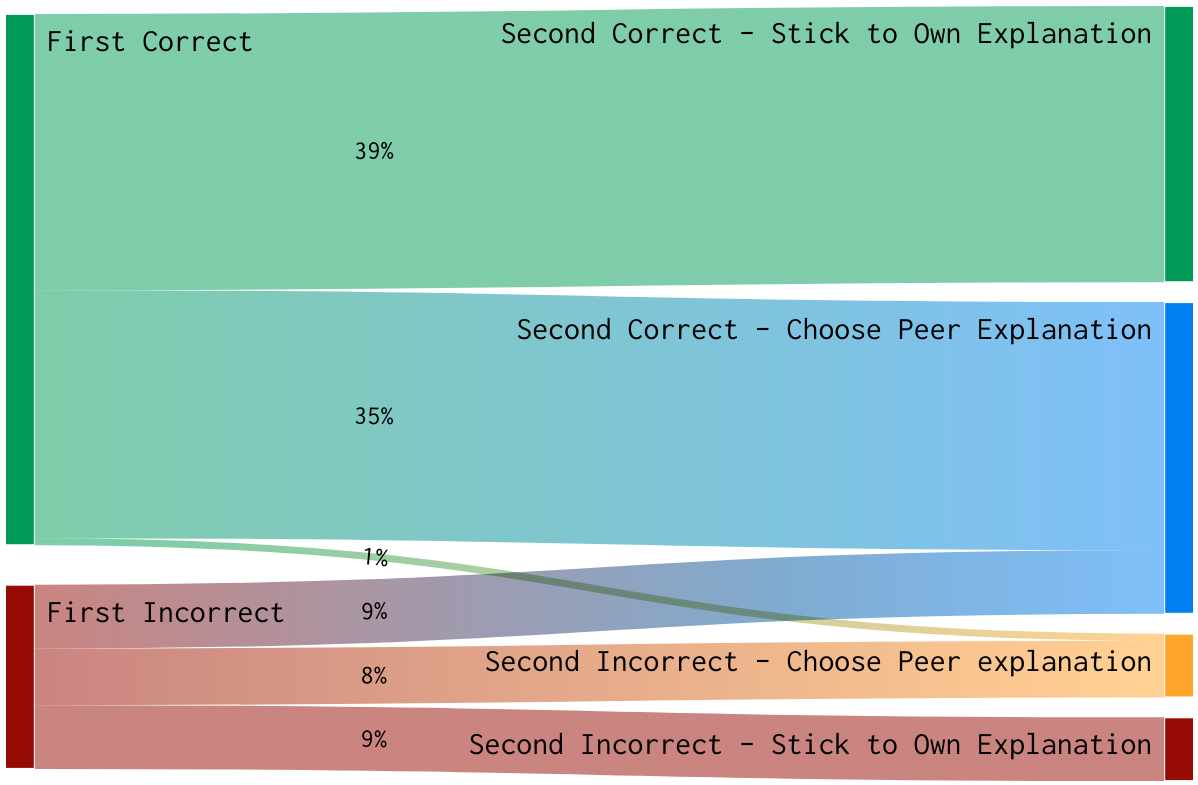
\includegraphics[width=0.6\linewidth]{img/transitions_final.png}
	\caption{The possible transition types that can occur in TMPI for student 
	answers between their first attempt (when they write their own 
	explanation), and the review step (when they are presented with peer 
	explanations). 
	The relative proportion of each transition type is shown in this Sankey 
	diagram for data from myDALITE.org}
	\label{fig:tmpi_sankey}
\end{figure}


The design and growing popularity of TMPI can be explained by the rise to 
prevalence of classroom based \textit{Peer Instruction} (PI) 
\cite{crouch_peer_2001}, often mediated by automated response systems (e.g. 
clickers).
Synchronous, classroom based PI is an effective component in the teaching 
practice of instructors looking to drive student engagement as part of an 
active learning experience \cite{charles_beyond_2015}. 
In discussing with peers \textit{after} they have formulated their own 
reasoning, students are engaged in a higher order thinking task from Bloom's 
taxonomy, as they evaluate what is the strongest argument, before answering 
again.

Prompting students to explain their reasoning is beneficial 
to their learning \cite{chi_eliciting_1994}. 
Deliberate practice of argumentation in defence of one's ideas has been shown 
to improve informal reasoning for science students \cite{venville_impact_2010}.
There exists empirical evidence on the positive relationship between 
constructing formally sound arguments and deep cognitive elaboration, as well 
as individual acquisition of knowledge \cite{stegmann_collaborative_2012}.

TMPI platforms augment asynchronous, multiple-choice formative assessment 
questions, by not only prompting students for their answer choice, but giving 
them an opportunity to explain their reasoning.
Moreover, students can receive a form of aggregated peer feedback on their 
explanations, in how many times their submissions are chosen as 
\textit{convincing} by their colleagues.
Finally, by capturing data on which explanations students find most convincing, 
TMPI affords teachers the opportunity to mitigate the ``expert blind spot'' 
\cite{nathan_expert_2001}, addressing student misconceptions they might not 
otherwise have thought of.

We situate our work in the context of computational argumentation, a sub-field 
of NLP focused on modelling the structure and quality of argumentative 
components of text.
Modelling argument ``quality'' is an area of active research, with direct 
applications in education, such as in automated scoring of 
persuasive essays written by students \cite{persing_modeling_2015} 
\cite{nguyen_argument_2018}.
In work more closely tied with peer instruction, it has been found that when 
students are asked to debate in dyads, there is a relationship between  
knowledge acquisition, and the quality of arguments the students produce, as 
measured by the presence of formal argumentative structures (e.g. claims, 
premise, etc.) \cite{garcia-mila_effect_2013}.

In a comprehensive survey of research on the assessment of argument quality, 
\cite{wachsmuth_computational_2017} outline a taxonomy of major quality 
dimensions for natural language, with three principal aspects: logic, rhetoric, 
and dialect. 
However experiments have also shown that the perceived quality of an argument 
can depend on the audience \cite{mercier_why_2011}. 
It is in this light that we adopt a more pragmatic measure of argument quality, 
centred on the premise that the goal of argumentation, is persuasion.

As students vote on their peer's explanations in TMPI, they may be evaluating 
the logical cogency (e.g. is this argument sound?), or its rhetorical quality 
(e.g. is this argument phrased well?). 
We set out to model the linguistic features common that may explain which 
student arguments are most \textit{convincing}.

It should be noted that there exists a significant, natural bias for the option 
``I stick to my own'' (top band in figure \ref{fig:tmpi_sankey}), and that a 
student who \textit{does} choose a peer's explanation, is choosing it 
\textit{as more convincing than their own}.

Therefore, we suggest that the ``vote'' data collected for each student's 
explanation in TMPI, is a proxy for argument quality, along the dimension of 
\textit{convincingness}, as judged by peer learners. 
This is a direct application of the argument mining (AM) task originally 
proposed by \cite{habernal_which_2016}: if crowd-workers are presented with a 
pair of arguments for the same stance of a debatable topic, can we predict 
which of the two they will choose as more convincing?
This task has already been extended to TMPI in previous work, wherein the 
objective is to predict which explanations students will choose as more 
convincing than their own \cite{bhatnagar_learnersourcing_2020}.

Student votes in TMPI can be aggregated into a \textit{convincingness} score, 
as a measure of how effective that explanation is in persuading peers to change 
their own answer.
Student explanations can then be ranked along such a score, allowing for 
instructors to gain insights on the thinking of their students with respect to 
specific content, and potentially even help students to improve how they 
communicate ideas within their discipline.
However aggregating these votes should be done with care: when a student 
chooses an explanation as convincing, they are doing so only with respect to 
the subset that were shown, as well as the one they wrote themselves.

The problem of aggregating the results of evaluative peer-judgments extends  
beyond TMPI.
For example, in response to the difficulty students can have providing a 
holistic score to their peers' work, there is a growing number of peer-review 
platforms built on \textit{comparative} judgments.
Notable examples include ComPAIR \cite{potter_compair:_2017} and 
JuxtaPeer \cite{cambre_juxtapeer:_2018}, both of which present students with a 
just a pair of their peers' submissions, and prompt the learner to evaluate 
them with respect to one another.
As in TMPI, students apply a comparative judgment to only the subset of peer 
content that they are shown during the review step.
There is a need for a principled approach to aggregating this learnersourced 
data, in a pedagogically relevant manner, despite the inevitable absence of 
some ``true'' ranking.

This sets the stage for our central research questions: 
\begin{itemize}
	\item[RQ1] since each student's ``vote'' in this context represents an 
	incomplete evaluative judgement, which rank aggregation 
	methods are best suited for ranking the quality of student 
	explanations in TMPI?
	\item[RQ2] once we establish a ranked list of explanations along the 
	dimension of \textit{convinciness}, can we model this construct, and 
	identify the linguistic features of the most effective student 
	explanations, as judged by their peers?
\end{itemize}

Work on modelling \textit{convincingness} has, in large part, been centred on 
web discourse data.
In the educational setting, previous work in automated scoring of persuasive 
essays has focused on modelling holistic scores given by \textit{experts} on 
longer form essays.
To our knowledge, we are among the first to aggregate and model student 
``votes'', in order to evaluate student explanations for their 
\textit{convincingness} as judged by \textit{peers}.

We suggest that the results of our work can inform the design of TMPI platforms.
However, in a broader context, we aim to contribute to the growing body of 
research surrounding technology-mediated peer-review, specifically where 
learners do not provide holistic scores, but generate their evaluative 
judgments in a comparative setting. 
Such platforms will invariably have to deal with at least three issues, which 
our work helps to address.

The first issue is about students: providing feedback to learners on the 
characteristics common to the most convincing arguments in their discipline, 
promotes learning and the development of critical reasoning skills.

The second issue is in providing support to teachers: in such platforms, the 
amount of data generated scales very quickly.
The data associated with each student-item pair includes many relevant 
variables: correct answer choice on first attempt, student explanation, subset 
of explanations shown, time spent writing and reading explanations, correct 
answer on second attempt, and the peer-explanation chosen as most convincing 
(see figure \ref{fig:make_pairs_a}).   
This amount of information can be overwhelming for instructors who use such 
tools regularly as part of formative assessment. 
Automatically identifying the highest, and lowest, quality student 
explanations, as judged by other students, can support instructors in providing 
timely feedback. 

A third related issue is in maintaining the integrity of such platforms: 
automatic filtering of irrelevant/malicious student explanations is paramount, 
since they may be shown to future students \cite{gagnon_filtering_2019}, a 
non-trivial task for natural language content, without expensive expert 
moderation.

This paper begins with an overview of related research in learnersourcing of 
student explanations, automatic short-answer grading, and argument quality 
ranking (section \ref{sec:related_work}).
We then describe our TMPI dataset, as well as publicly available reference 
datasets of argument quality, which we use to evaluate our methodology (section 
\ref{sec:datasets}).
Our most important contribution is in proposing a methodology for evaluating 
the quality of student explanations, along the dimension of 
\textit{convincingness}, in TMPI environments; we demonstrate this methodology 
in section \ref{sec:methodology} and propose evaluation metrics based on 
practical issues in TMPI environments.
Finally, we describe how we \textit{model} these convincingness ``scores'' so 
as to identify the linguistic features of explanations most often associated 
with high-quality explanations (section \ref{sec:model_results}).


\section{Related Work}\label{sec:related_work}

\subsection{Learnersourcing student explanations}
TMPI is a specific case of  \textit{learnersourcing} 
\cite{weir_learnersourcing_2015}, wherein students first generate content, and 
then help curate the content base, all as part of their own learning process.
Notable examples include PeerWise \cite{denny_peerwise:_2008} and RiPPLE 
\cite{khosravi_ripple_2019}, both of which have students generate learning 
resources, which are subsequently used and evaluated by peers as part of 
formative assessment activities.

One of the earliest efforts specifically leveraging peer judgments of 
peer-written explanations, is from the AXIS system \cite{williams_axis:_2016}, 
wherein students solved a problem, provided an explanation for their answer, 
and evaluated explanations written by their peers.
Using a reinforcement-learning approach known as ``multi-armed bandits'', the 
system was able to select peer-written explanations that were rated as helpful 
as those written by an expert.
The novel scheme proposed by \cite{kolhe_peer_2016} also applies the potential 
of learnersourcing to the task of short answer grading: the short answers 
submitted by students are evaluated by ``future'' peers who are presented with 
multiple choice questions, where the answer options are the short answers 
submitted by their ``past'' counterparts.
Our research follows from these studies in scaling to multiple domains, and 
focusing on how the vote data can be used more directly to model argument 
quality as judged by peers.



\subsection{Automated Writing Evaluation}

A central objective of our work is to evaluate the quality of student 
explanations in TMPI.
Under the hierarchy of automated grading methods proposed by  
\cite{burrows_eras_2015}, this task falls under the umbrella of automatic 
short-answer grading (ASAG); students must recall knowledge and express it 
in their own way, using natural language, using typically between 10-100 words. 
Their in-depth historical review of ASAG systems describes a shifting focus in 
methods, from matching patterns derived from answers written by experts, to 
machine-learning approaches, where n-grams and hand-crafted features are 
combined as input to supervised learning algorithms, such as decision trees and 
support vector machines.

For example, \cite{mohler_learning_2011} measure alignment between dependency 
parse tree structures of student answers, with those of an expert answer.
These alignment features are paired with lexical semantic similarity features 
that are both knowledge-based (e.g. using WordNet) and corpus-based (e.g. 
Latent Semantic Analysis), and used as input to support vector machines which 
learn to automatically grade short answers.

Another similar system proposed by \cite{sultan_fast_2016} starts with features 
measuring lexical and contextual alignment between similar word pairs from 
student answers and a reference answer, as well as semantic vector similarity 
using ``off-the-shelf'' word embeddings.  
They then augment their input with  ``domain-specific'' term-frequency and 
inverse document-frequency weights, to achieve their best results on several 
ASAG datasets using various validation schemes.
 
In addition to similarity features based on answer text, \cite{zhang_deep_2016} 
show that question-level (e.g. difficulty, expert-labelled knowledge 
components) and student-level features (e.g. pre-test scores, Bayesian 
Knowledge Tracing probability estimates) can improve performance on the ASAG 
task when input to a deep learning classifier.

While modelling the quality of TMPI explanations has much in common with the 
ASAG task, and can benefit from the features and methods from the systems 
mentioned above, a fundamental difference lies in how similarity to an expert 
explanation may not be the only appropriate reference.
The ``quality'' we are measuring is that which is observed by a group of peers, 
which may be quite different from how a teacher might explain a concept.

\subsection{Ranking Arguments for Quality}\label{sec:related_work:arg_quality}

Previous work on automated evaluation of long-form persuasive essays 
\cite{ghosh_coarse-grained_2016}, \cite{klebanov_argumentation_2016} 
\cite{nguyen_argument_2018} has focused on modelling the holistic scores given 
by experts.
Our work here does not set out to ``grade'' student explanations, but provide a 
ranked list for \textit{convincingness} as judged by a set of peers.

We cast this as a task in rank aggregation, with the objective combining the 
preferences of multiple agents into a single representative ranked list.
It has long been understood that obtaining pairwise preference data may be 
less prone to error on the part of the annotator, as it is a simpler task than 
rating on scales with more gradations.
The trade-off, of course is the quadratic scaling in the number of pairs one 
can generate. 
This is relevant in TMPI, since each student is choosing one explanation as 
the most convincing only in relation to the subset of others that are shown, 
and the potential permutations of explanations different students may see is 
intractably large for a typical question answered by 100+ students.

A classical approach specifically proposed by \cite{raman_methods_2014} for 
ordinal peer grading data is the Bradley-Terry (BT) model.
The BT model \cite{bradley_rank_1952} for aggregating pairwise preference data 
into a ranked list, assumes that predicting the winner of a pairwise 
``match-up'' between any two items is associated with the difference in the 
latent ``strength'' parameters for those two items, and these parameters can be 
calculated using maximum likelihood estimation.

The BT method has been extended to incorporate the quality of contributions of 
different annotators in a crowdsourced setting when evaluating relative reading 
level in a pair passages \cite{chen_pairwise_2013}. 

Specifically in the context of evaluating argument convincingness from pairwise 
preference data, one of the first approaches proposed is based on constructing 
an ``argument graph'', where a weighted edge is drawn from node A to node B for 
every pair where argument A is labelled as more convincing than argument B. 
After filtering passage pairs that lead to cycles in the graph, PageRank scores 
are derived from this directed acyclic graph, and are used as the gold-standard 
rank for convincingness \cite{habernal_which_2016}.
(This dataset is included in our study, from now on labelled as \textbf{UKP}.)

More recently, a relatively simpler heuristic WinRate score has been shown to 
be a competitive alternative for the same dataset, wherein the rank score of an 
argument is simply the (normalized) number of times that argument has been 
chosen as more convincing in a pair, divided by the number of pairs it appears 
in \cite{potash_ranking_2019}.

Finally, a neural approach based on RankNet has recently yielded state of the 
art results, by joining two Bidirectional Long-Short-Term Memory Networks in a 
Siamese architecture. By appending a softmax layer to the output, pairwise 
preferences and overall ranks were jointly modelled in publicly available 
datasets \cite{gleize_are_2019}.
(This dataset is also included in our study as a reference, labelled as 
\textbf{IBM\_Evi}.)

The key difference between to keep in mind between the above mentionned studies 
in modelling the quality rankings of arguments, and that of TMPI explanations, 
is that the students are not indifferent crowd-labellers: each student will 
have just submitted their own explanation justifying their answer choice, and 
we analyze the aggregate of their choices as they indicate when a peer may have 
explained something better than themselves.

We will explore two of these options as part of our methodology in our rank 
aggregation step, via several related methods: the probabilistic Bradley-Terry 
model, one of its variants (the Elo rating system), and the simple heuristic 
scoring model, ``WinRate''.
(We omit a neural approach in this study, as we consider the work on 
interpreting the model results from a neural model for pedagogical purposes, 
out of the scope of this paper.
The methods we chose have several readily available implementations in 
different programming languages, and we err on the side of simplicity when 
possible in our methodological choices.)



\section{Data}\label{sec:datasets}

\begin{table}
	\caption{
		Examples of argument pairs from each reference argument mining 
		datasets. 
		These examples were selected because they were incorrectly classified 
		by all of our models, and demonstrate the challenging nature of the 
		task. 
		In each case, the argument labelled as more convincing is in 
		\textit{italics}.
	}
	\label{tab:sample_obs}
	\begin{subtable}[t]{\textwidth}
		\begin{table}
\centering
\caption{A pair of arguments from the UKP dataset, both with the stance PRO, for the prompt topic: ``should-physical-education-be-mandatory-in-schools--yes-''. Argument a1 is labelled as more convincing.}
\begin{tabular}{p{6cm}|p{6cm}}
\toprule
                                                                              a1 &                                                                                    a2 \\
\midrule
 How are we supposed to curb childhood obesity if we don't start at a young age? &  physical education is a waste of time and therefore should not be studied in schools \\
\bottomrule
\end{tabular}
\end{table}

	\end{subtable}
	\begin{subtable}[t]{\textwidth}
		%\begin{table}
\centering
\caption{"
              A pair of arguments from the IBM\_ArgQ dataset, 
              for the prompt topic: ``privacy''. 
              Argument a1 is labelled as more convincing.
              }
\begin{tabular}{p{6cm}|p{6cm}}
\toprule
                                                                                                                    a1 &                                                                                                                                                                                            a2 \\
\midrule
 if a company is not willing to openly say what they are going to do with my data, they shouldn't be allowed to do it. &  if you are against information privacy laws, then you should not object to having a publicly accessible microphone in your home that others can use to listen to your private conversations. \\
\bottomrule
\end{tabular}
%\end{table}

	\end{subtable}
\end{table}

\begin{table}
	\caption{
		Examples of argument pairs from Physics and Ethics disciplines, taken 
		from our TMPI environment. 
		These examples were selected because they were incorrectly classified 
		by all of our models, and demonstrate the challenging nature of the 
		task. 
		In each case, the argument labelled as more convincing is in 
		\textit{italics}.}
	\label{tab:sample_obs_dalite}
	\begin{subtable}[t]{\textwidth}
		\begin{tabular}{p{7cm}|p{7cm}}
\toprule
                                                                                                                                                                                                                                                 rationale &                                                                                                                                      chosen\_rationale \\
\midrule
 The graph shows constant positive acceleration and then constant negative acceleration. This means that the velocity-time graph should have a positive slope and then a negative slope, and graph C is the only option that satisfies those requirements. &  1st, acceleration is +, indicating an increase in velocity.\textbackslash r\textbackslash nthen, acceleration is suddenly and without warning negative, and velocity is reduced. \\
\bottomrule
\end{tabular}

	\end{subtable}
	\begin{subtable}[t]{\textwidth}
	%\begin{table}
\centering
\caption{
              Student explanations from \textbf{TMPI} in an Ethics MOOC, 
              for the question prompt: ``Assuming that motorcycle drivers are 
              willing to pay their own medical bills, should they be allowed to 
              ride without a helmet?''. 
%              Argument a1 is labelled as more convincing.
              }
\begin{tabular}{p{6cm}|p{6cm}}
\toprule
                                                                                
               a1 
&                                                                               
                                     a2
 \\
\midrule
\textit{ Law should always to make for the good of their people.If wearing 
helmet help,then it should be enforce.Also,you cannot assure that every 
motorcycle in the country would want to  pay. } &  I believe that motorcycle 
helmets should be mandatory for ALL motorcycle drivers . Although they may be 
willing to pay their own medical bills , you ca n't pay anything if you 're not 
alive to do so . Motorcycle wrecks can kill the driver , leaving the drivers 
family with funeral expenses and the like . The family may not be able to 
afford it . Wearing a helmet increases possibility of surviving a crash that 
you may not otherwise survive . So yes , motorcycle helmets should be mandatory 
even if the rider is willing to pay their own medical expenses .. \\
\bottomrule
\end{tabular}
%\end{table}

	\end{subtable}
\end{table}


\subsection{Argument Mining Datasets}
Much of our methodology is inspired by work on modelling argument quality along 
the dimension of \textit{convincingness}, as described in section 
\ref{sec:related_work:arg_quality}. 
In order to contextualize the performance of these methods in our educational 
setting, we apply the same methods to publicly available datasets from the 
AM research community as well, and present the results. 
These datasets are described in table \ref{tab:data_summary}, alongside the 
TMPI data at the heart of our study. 

The \textbf{UKP} dataset \cite{habernal_which_2016} is one of the first set of 
labelled argument pairs to be released publicly.
Crowd-workers were presented with pairs of arguments on the same stance of a 
debate prompt, and were asked to choose which was more convincing.
The authors of the \textbf{IBM\_ArgQ} dataset \cite{toledo_automatic_2019} 
offer a dataset that is similarly labelled, but much more tightly curated, with 
strict controls on argument word count and relative difference in lengths in 
each pair.
This was partly in response to the observation that crowd labels could often be 
predicted simply by choosing the longer text from the pair.
The labelled argument pairs in the \textbf{IBM\_Evi} dataset 
\cite{gleize_are_2019} are actually generated by scraping Wikipedia, and the 
crowd workers were asked to choose the argument from the pair that provided the 
more compelling evidence in support of the debate stance.

As described above in our section on related work, these datasets were released 
not just with the labelled argument pairs, but holistic rank scores for each 
argument, that were each derived in different ways. 
We will be comparing our proposed \textit{measures} of convincingness to these 
rank scores in section \ref{sec:methodology_eval}.


\subsection{DALITE}\label{sec:dataset_dalite}
The central data for this study come from myDALITE.org, which is a hosted 
instance of an open-source project, 
\verb|dalite|\footnote{\url{https://github.com/SALTISES4/dalite-ng}}, 
maintained by a Canadian researcher-practitioner partnership, 
\href{saltise.ca}{SALTISE}, focused on supporting teachers in the development 
of active learning pedagogy.
The data comes from introductory level university science courses, and 
generally spans different teachers at different colleges and universities in 
Canada. 
The \textit{Ethics} dataset comes from a popular MOOC, wherein the TMPI prompts 
are slightly different from the \textit{Physics} and \textit{Chemistry} 
prompts, in that there is no ``correct'' answer choice, and that the goal is to 
have students choose a side of an argument, and justify their choice.
Table \ref{tab:data_summary} gives an overview of the datasets included in this 
study.


\begin{table}
	\begin{tabular}{llrrrrrrr}
\toprule
       &         &  topics &   args &   pairs & args/topic &  pairs/topic & pairs/arg &       wc \\
source & dataset &         &        &         &            &              &           &          \\
\midrule
Arg Mining & IBM\_ArgQ &      22 &   3474 &    9125 &  158 (144) &    415 (333) &     5 (1) &   24 (1) \\
       & IBM\_Evi &      41 &   1513 &    5274 &    37 (14) &     129 (69) &     7 (3) &   30 (3) \\
       & UKP &      32 &   1052 &   11650 &     33 (3) &     364 (71) &    22 (3) &  49 (14) \\
DALITE & Chemistry &      36 &   4778 &   38742 &   133 (29) &   1076 (313) &     7 (1) &   29 (6) \\
       & Ethics &      28 &  20195 &  159379 &  721 (492) &  5692 (4962) &     7 (1) &   48 (8) \\
       & Physics &      76 &  10840 &   96337 &   143 (42) &   1268 (517) &     7 (2) &   27 (5) \\
\bottomrule
\end{tabular}

	\caption{
		Summary statistics for reference datasets from argument mining research 
		community, and DALITE, a TMPI environment used mostly in undergraduate 
		science courses in Canada. 
		In the argument reference datasets \textit{topic} are debate prompts 
		shown to crowdsourcing workers (e.g. \textit{``social media does more 
		good than harm''}), while a \textit{topic} in DALITE is a question item.
		The explanations given by students are analagous to the ``arguments'',  
		which are then assembled into pairs based on what was shown, and 
		eventually chosen by each student.
		\textit{wc} is the average number of tokens in each 
		argument/explanation in each topic.
		All averaged quantities are followed by a standard deviation in 
		parentheses.
	}
	\label{tab:data_summary}
\end{table}

To stay consistent with the argument mining reference dataset terminology, we 
refer to a question-item as a ``topic''.
Student explanations from DALITE are divided up by the associated question item 
prompts.
The transformation of TMPI student explanations (``args'') into ``pairs'' is 
described in section \ref{sec:methodology}. 
The filtering of DALITE data is based on the following three steps:
\begin{itemize}
	\item approximately 1 in 10 students decide that they want their 
	explanations to be shared with only with their instructor, and not seen by 
	other students, nor used for the purposes of research.
	The answers of these students are removed from the dataset. 
	\item There is no simple and reliable way to determine whether students 
	choose this option ``genuinely'' (because the shown alternatives were not 
	sufficiently convincing), or because they did not want to read their peers' 
	explanations.
	For this reason, we only include observations where students explicitly 
	change explanations (whether for their own answer choice, or for a 
	different answer choice, regardless of correctness.) 
	There is a strong bias for students to simply choose `\textit{I stick to my 
	own rationale}, and so this reduces our data by approximately 50\%.
	\item Many question items have been completed by several hundreds of 
	students. 
	As such, almost half of all student explanations have only been shown to 
	another peer; thus we retain only those student answers that have been 
	presented to at least 5 other students.
	\item As a platform for formative assessment, not all instructors provide 
	credit for the explanations students write, and there are invariably some 
	students who do not put much effort into writing good explanations.
	We include only those student answers that have at least 10 words.
	\item after the previous two steps, we only include data from those 
	questions that have at least 100 remaining student answers.
	\item we remove any duplicate pairs before the rank aggregation step that 
	have the same ``winning'' label, as explanations that appear earlier on in 
	the lifetime of a new question are bound to be shown more often to future 
	students.
\end{itemize}

We see in table \ref{tab:data_summary} that the resulting datasets from the 
different disciplines in our TMPI dataset are comparable to the reference AM 
datasets (just proportionately larger).
The division of the TMPI data into multiple disciplines, despite the source the 
same platform, is because we assume that in modelling the quality of 
explanations, different features will be important for each.

\section{Methodology}\label{sec:methodology}

We borrow our methodological approach from research in argument mining, 
specifically related to modelling argument quality along the dimension of 
\textit{convincingness}.
A common approach is to curate pairs of arguments made in defence of the same 
stance on the same topic.
These pairs are then presented to crowd-workers, whose task it is to label 
which of the two is more convincing. 
The pairwise comparisons can then be aggregated using rank-aggregation 
methods so as to produce a overall ranked list of arguments.
We extend this work to the domain of TMPI, and define prediction tasks that not 
only aim to validate this methodology, but help answer our specific research 
questions.

\subsection{Rank Aggregation}\label{sec:rank_agg}
The raw data emerging from a TMPI platform is tabular, in the form of 
student-item observations.
As shown in figure \ref{fig:make_pairs_a}(a), the fields include the item 
prompt, the student's \textit{first} answer choice, their accompanying 
explanation, the peer explanations shown on the review step (as in figure 
\ref{fig:question_review}), the student's 
\textit{second} answer choice, and the peer explanation they chose as most 
convincing (\verb|None| if they choose to ``stick to their own''), as well as 
timestamps for the first and second attempt.

After the filtering steps described above, we take the TMPI observations for 
each question, and construct explanation pairs, as in figure 
\ref{fig:make_pairs_a}(b).

\begin{figure}[H]
	\centering
	\def\svgscale{0.40}
	\input{img/make_pairs_a.pdf_tex}
	\caption{
	Example of student-item observations from a TMPI environment. 
	This figure follows from figure \protect\ref{fig:tmpi}.
	(a) Student $s_{30}$ chose the correct \textbf{D} as the answer on 
	their first attempt, and provided the explanation $e_{30}$ in the 
	dataset for this question. 
	The student is shown a subset of explanations from previous students for 
	\textbf{D}, as well as for \textbf{A} (the most popular incorrect 
	answer). 
	The student decides to keep the same answer choice \textbf{D}, and 
	indicates that the explanation $e_{25}$ is the most convincing.
	This is referred to as a \textit{Right}$\rightarrow$\textit{Right} 
	transition.
	(b) This observation is transformed into 8 explanation pairs. The first 
	pair is for the choice of $e_{25}$ over what the student wrote themselves, 
	and the other seven are for the choice of $e_{25}$ over the other shown 
	explanations. 
	The pairs are labelled as such that $e_{25}$ is the more convincing of the 
	pair. 
	(c) This pairwise preference data is aggregated global ranked list of 
	student explanations for this question, where each explanation is assigned 
	a real-valued rank score (using the methods described in section 
	\protect\ref{sec:rank_agg}).
}
\label{fig:make_pairs_a}
\end{figure}

Using these explanation pairs, we apply the following rank aggregation 
techniques in order to derive a real valued \textit{convincingness} rank score, 
as in figure \ref{fig:make_pairs_a}(c).

\begin{enumerate}
	
	\item \textbf{WinRate\_raw}, defined as the ratio of times an explanation 
	is 
	chosen to the number of times it was shown.
	This method does not take into account \textit{which} peer explanations 
	were shown to each student, neglecting the potential impact of comparative 
	judgment.
	
	\item \textbf{WinRate}: as described in \cite{potash_ranking_2019}, this 
	measure argument quality is defined as the number of times it is chosen as 
	more convincing in a pairwise comparison, normalized for the number pairs 
	in which it appears. 
	In the context of TMPI, when we calculate the \textit{WinRate} of a student 
	eplanation after the data transformation depicted in figure 
	\ref{fig:make_pairs_a}a and figure \ref{fig:make_pairs_a}b, we take a step 
	towards including the effect of the comparative judgement, as pairs are 
	specifically constructed for each observation from the explanation that was 
	chosen, and the ones that were shown.
	
	\item \textbf{BT} score, which is the argument ``quality'' parameter 
	estimated for each explanation, according to the \textit{Bradley-Terry} 
	model, where the probability of argument A being chosen over argument B is 
	given by 
	
	$$
	P(a>b) = 
	\frac{1}{1+e^{\beta_b-\beta_a}}
	$$
	where $\beta_i$ is the latent strength parameter of argument $i$. 
	
	We decompose each student-item observation into argument pairs, where the 
	chosen explanation is paired with each of the other shown ones, and the 
	pair is labelled with $y=-/+1$, depending on whether the chosen explanation 
	is first/second in the pair.
	Assuming there are $N$ explanations, labelled by $K$ students, and $S_K$ 
	labelled pairs,the latent strength parameters are estimated by maximizing 
	the log-likelihood given by:
	$$
	\ell(\boldsymbol{\beta})=\sum_{K}\sum_{(i,j)\epsilon S_K}^{} 
	\log\frac{1}{1+e^{\beta_i - \beta_j}}
	$$
	subject to $\sum_{i}\beta_i=0$.
	
	
	\item The \textbf{Elo} rating system \cite{elo_rating_1978}, which was 
	originally proposed for ranking chess players, has been successfully used 
	in adaptive learning environments (see \cite{pelanek_applications_2016} for 
	a review). 
	This rating method can be seen as a heuristic re-parametrization of the 
	\textbf{BT} method above, where the probability of argument A being chosen 
	over argument B is given by
	$$
	P(a>b) = P_{ab} = \frac{1}{1+10^{(\beta_b-\beta_a)/\delta}}
	$$
	where $\delta$ is a constant. 
	All arguments are initialized with an initial strength of $\beta_0$, and 
	the rating of any argument is only updated after it appears in a pairwise 
	comparison with another.
	The rating update rule transfers latent ``strength'' rating points from the 
	loser, to the 
	winner, in proportion to the difference in strength:
	
	$$
	\beta_a':=\beta_a+K(P_{ab} - \beta_a)
	$$
	
	While the \textbf{BT} model can be thought of a \textit{consensus} 
	approach (all rank scores are re-calculated after each pair is seen), 
	\textbf{Elo} ratings are dynamic and implicitly give more weight 
	to recent data \cite{aldous_elo_2017}.
	
	\item \textbf{Crowd-BT} \cite{chen_pairwise_2013} is an extension of the 
	\textbf{BT} model, tailored to settings where different annotators may have 
	assigned opposite labels to the same pairs, and the reliability of each 
	annotator may vary significantly. 
	A reliability parameter $\eta_k$ is estimated for each student, 
	
	$$
	\eta_k \equiv P(a >_k b | a >b )
	$$
	
	where $\eta_k \approx 1$ if the student  $k$ agrees with most other 
	students, and $\eta_k \approx 0$ if the student is in opposition to their 
	peers.
	This changes the model of argument $a$ being chosen over $b$ by student $k$ 
	to 
	$$
	P(a >_k b) = 
	\eta_k \frac{e^{\beta_a}}{e^{\beta_a}+e^{\beta_b}} + (1-\eta_k) 
	\frac{e^{\beta_b}}{e^{\beta_a}+e^{\beta_b}}
	$$
	and the log-likelilood maximized for estimation to 
	
	$$
	\ell(\boldsymbol{\eta},\boldsymbol{\beta})=\sum_{K}\sum_{(i,j)\epsilon 
		S_K}^{} 
	\log \left[ \eta_k \frac{e^{\beta_a}}{e^{\beta_a}+e^{\beta_b}} + (1-\eta_k) 
	\frac{e^{\beta_b}}{e^{\beta_a}+e^{\beta_b}} \right]
	$$
	
\end{enumerate}

How we evaluate the fit of these rank aggregation methods to our data is 
described in section \ref{sec:methodology_eval}

\subsection{Modelling rank scores}\label{sec:features}
We build on the results from the previous section to now predict these 
aggregate scores for each explanation, using linguistic properties of those 
explanations.
We address \textbf{RQ2} with a regression task of predicting the argument 
\textit{convincingness} scores via a feature-rich document vector.

Recent experimental results posted state-of-the-art results for this same 
regression task on a large argument mining dataset, using a neural embeddings 
in a bidirectional encoder representations from transformers (BERT) 
\cite{gretz_large-scale_2019}.
However we favour a feature-rich approach and simpler learning algorithms, 
keeping in mind downstream priorities such as interpretability for teachers in 
their reporting tools.

The list of features included here are derived from related work in argument 
mining \cite{habernal_which_2016}\cite{persing_end--end_2016} on student 
essays, automatic short answer scoring \cite{mohler_text--text_2009}.

\begin{itemize}
	
	\item Surface Features: 
	sentence count, 
	max/mean word length, 
	max/mean sentence length;
	
	\item Lexical: 
	uni-grams, 
	type-token ratio, 
	number of keywords (defined by open-source discipline specific 
	text-book), 
	number of equations (captured by a regular expression);
	
	\item Syntactic: 
	POS n-grams (e.g. \textit{nouns, prepositions, 
		verbs,conjunctions,negation, adjectives, adverbs, punctuation}), 
	modal verbs (e.g. \textit{must, should, can, might}),
%	contextuality/formality measure \cite{heylighen_variation_2002},
	dependency tree depth;
	
	\item Semantic:
	\begin{itemize}
		\item Using pre-trained GloVe \cite{pennington_glove:_2014} vectors, we 
		calculate similarity metrics to i) all other explanations, ii) the 
		question item text, and, when available, iii) a teacher provided 
		``expert'' explanation.
		\item we derive our own discipline specific embedding vectors, trained 
		on corresponding open-source textbooks\footnote{https://openstax.org}. 
		We experiment with a word-based vector space model, Latent Semantic 
		Indexing (\verb|LSI|) \cite{deerwester_indexing_1990}, due to its 
		prevalence in text analytics in educational data mining literature, as 
		well as \verb|Doc2Vec| \cite{le_distributed_2014}, which directly 
		models the compositionality of all the words in a 
		sentence\footnote{model implementations from 
		https://radimrehurek.com/gensim/index.html}.
		We take the text of the question prompt, as well as an ``expert 
		explanation'' provided by teachers for each question, and determine the 
		10 most relevant sub-sections of the textbook.
		For each student explanation, we then calculate the mininum, maximum, 
		and mean cosine similarity to these 10 discipline specific ``reference 
		texts''.
		 
	\end{itemize}
		
%	\item Co-reference \cite{persing_end--end_2016}: 
%	fraction of entities from the prompt mentioned in each sentence, 
%	averaged over all sentences (using neural Co-reference resolution)
%	vector cosine similarity between student explanation and prompt, 
%	and answer choices; 
	
	\item Readability:
	Fleish-Kincaid reading ease and grade level,
	Coleman-Liau,
	automated readability index, 
	spelling errors
	
\end{itemize}

Features typical to NLP analyses in the context writing analytics that are not 
included here are cohesion, sentiment, and psycho-linguistic features, as they 
do not seem pertinent for shorter responses that deal with STEM disciplines.

\subsection{Regression Models}

The machine learning models we explore for the regression task are also 
inspired from writing analytics literature, as well as the design objective, of 
maximizing interpretability: the ability to explain predictions of which 
students explanations are most \textit{convincing} is paramount in providing 
pedagogical support to students an teachers.

As has been described in related work, argument \textit{length} is a difficult 
baseline to beat when modelling \textit{convincingness} in pariwise 
preference data.
The greater the amount of words, the greater the opportunity to construct a 
convincing argument, and as such, we set explanation \verb|Length| (the number 
of whitespace seperated tokens) as our regression baseline as well. 
The models we include in this study are \verb|Linear| regression, 
\verb|Decision Tree| regression, and \verb|Random Forest| regressors.

So as to provide context with the current state of the art in point-wise 
prediction of argument \textit{convincingness}, we also fine-tune a pre-trained 
bi-directional neural transformer model, \verb|BERT|, with argument mining 
reference datasets, as well as the TMPI data from our three disciplines. 
In line with the best performing model in \cite{gretz_large-scale_2019}, we go 
beyond this, and train a different model where the input is augmented with the 
question prompt: it is combined with the student explanation, separated the 
model-specific \verb|[SEP]| token, and input as a pair of text sequences during 
fine-tuning and inference (henceforth be referred to as \verb|BERT_Q)|).

Finally, in the \textbf{Physics} and \textbf{Chemistry} datasets from our TMPI 
platform, many of the questions are accompanied by a \textit{expert} 
explanation, written by the teacher/author of the question (the purpose of 
which is to present a model text for teh student to read after they have 
submitted their second answer choice in the review step).
When available, we also examine \verb|BERT_A|, where we append this 
\textit{expert} explanation with the student explanation as input to the 
transformer (instead of the topic prompt).
The theoretical grounding for the use of these models in the study of 
\textit{convincingness} stems from the different tasks upon which the base BERT 
model was pre-trained for: predicting masked words seems to conferred the BERT 
model with syntactic and semantic knowledge of language, while the 
next-sentence prediction task seems to be one of the reasons for successful 
transfer learning demonstrated on Glue benchmark tasks, such 
question-answering, and sentence classification. 


In each of \verb|BERT|, \verb|BERT_Q| and \verb|BERT_A|, the contextual 
embedding of the model-specific \verb|[CLS]| token in the last layer of the 
fine-tuned transformer, is fed as input into a fully dense regression layer, so 
as to output a predicted \textit{convincingness} score.

 
\subsection{Evaluation of methodology}\label{sec:methodology_eval}

In order to evaluate our choice of rank aggregation method, and address our 
research question RQ1, we perform several validation tests.

The reference argument mining datasets that we use for this study, along 
with annotated pairwise preference data, each include their own derived 
aggregated rank score for each argument (described in 
\ref{sec:related_work:arg_quality}).
We begin our evaluation of the soundness of our choice of simpler rank 
aggregation methods, by measuring the correlation between our ranking scores, 
and the reference scores, on the AM datasets.
For each topic in the different AM datasets, we calculate the Pearson 
correlation between the ``reference'' score of each argument, and the simpler 
scores we choose to include in our methodology (\textit{WinRate},\textit{BT}, 
\textit{Elo}. We cannot include \textit{CrowdBT} here, as the AM datasets do 
not include an identifier for ``annotator'').
The distribution of Pearson correlation coefficients across the different 
topics are shown in the box plots in figure \ref{fig:corr_to_reference_score}.

\begin{figure}[H]
	\centering
	\scalebox{0.5}{%% Creator: Matplotlib, PGF backend
%%
%% To include the figure in your LaTeX document, write
%%   \input{<filename>.pgf}
%%
%% Make sure the required packages are loaded in your preamble
%%   \usepackage{pgf}
%%
%% and, on pdftex
%%   \usepackage[utf8]{inputenc}\DeclareUnicodeCharacter{2212}{-}
%%
%% or, on luatex and xetex
%%   \usepackage{unicode-math}
%%
%% Figures using additional raster images can only be included by \input if
%% they are in the same directory as the main LaTeX file. For loading figures
%% from other directories you can use the `import` package
%%   \usepackage{import}
%%
%% and then include the figures with
%%   \import{<path to file>}{<filename>.pgf}
%%
%% Matplotlib used the following preamble
%%
\begingroup%
\makeatletter%
\begin{pgfpicture}%
\pgfpathrectangle{\pgfpointorigin}{\pgfqpoint{9.000000in}{6.000000in}}%
\pgfusepath{use as bounding box, clip}%
\begin{pgfscope}%
\pgfsetbuttcap%
\pgfsetmiterjoin%
\definecolor{currentfill}{rgb}{1.000000,1.000000,1.000000}%
\pgfsetfillcolor{currentfill}%
\pgfsetlinewidth{0.000000pt}%
\definecolor{currentstroke}{rgb}{1.000000,1.000000,1.000000}%
\pgfsetstrokecolor{currentstroke}%
\pgfsetdash{}{0pt}%
\pgfpathmoveto{\pgfqpoint{0.000000in}{0.000000in}}%
\pgfpathlineto{\pgfqpoint{9.000000in}{0.000000in}}%
\pgfpathlineto{\pgfqpoint{9.000000in}{6.000000in}}%
\pgfpathlineto{\pgfqpoint{0.000000in}{6.000000in}}%
\pgfpathclose%
\pgfusepath{fill}%
\end{pgfscope}%
\begin{pgfscope}%
\pgfsetbuttcap%
\pgfsetmiterjoin%
\definecolor{currentfill}{rgb}{0.898039,0.898039,0.898039}%
\pgfsetfillcolor{currentfill}%
\pgfsetlinewidth{0.000000pt}%
\definecolor{currentstroke}{rgb}{0.000000,0.000000,0.000000}%
\pgfsetstrokecolor{currentstroke}%
\pgfsetstrokeopacity{0.000000}%
\pgfsetdash{}{0pt}%
\pgfpathmoveto{\pgfqpoint{1.125000in}{0.660000in}}%
\pgfpathlineto{\pgfqpoint{8.100000in}{0.660000in}}%
\pgfpathlineto{\pgfqpoint{8.100000in}{5.280000in}}%
\pgfpathlineto{\pgfqpoint{1.125000in}{5.280000in}}%
\pgfpathclose%
\pgfusepath{fill}%
\end{pgfscope}%
\begin{pgfscope}%
\pgfsetbuttcap%
\pgfsetroundjoin%
\definecolor{currentfill}{rgb}{0.333333,0.333333,0.333333}%
\pgfsetfillcolor{currentfill}%
\pgfsetlinewidth{0.803000pt}%
\definecolor{currentstroke}{rgb}{0.333333,0.333333,0.333333}%
\pgfsetstrokecolor{currentstroke}%
\pgfsetdash{}{0pt}%
\pgfsys@defobject{currentmarker}{\pgfqpoint{0.000000in}{-0.048611in}}{\pgfqpoint{0.000000in}{0.000000in}}{%
\pgfpathmoveto{\pgfqpoint{0.000000in}{0.000000in}}%
\pgfpathlineto{\pgfqpoint{0.000000in}{-0.048611in}}%
\pgfusepath{stroke,fill}%
}%
\begin{pgfscope}%
\pgfsys@transformshift{2.287500in}{0.660000in}%
\pgfsys@useobject{currentmarker}{}%
\end{pgfscope}%
\end{pgfscope}%
\begin{pgfscope}%
\definecolor{textcolor}{rgb}{0.333333,0.333333,0.333333}%
\pgfsetstrokecolor{textcolor}%
\pgfsetfillcolor{textcolor}%
\pgftext[x=2.287500in,y=0.562778in,,top]{\color{textcolor}\rmfamily\fontsize{10.000000}{12.000000}\selectfont IBM\_ArgQ}%
\end{pgfscope}%
\begin{pgfscope}%
\pgfsetbuttcap%
\pgfsetroundjoin%
\definecolor{currentfill}{rgb}{0.333333,0.333333,0.333333}%
\pgfsetfillcolor{currentfill}%
\pgfsetlinewidth{0.803000pt}%
\definecolor{currentstroke}{rgb}{0.333333,0.333333,0.333333}%
\pgfsetstrokecolor{currentstroke}%
\pgfsetdash{}{0pt}%
\pgfsys@defobject{currentmarker}{\pgfqpoint{0.000000in}{-0.048611in}}{\pgfqpoint{0.000000in}{0.000000in}}{%
\pgfpathmoveto{\pgfqpoint{0.000000in}{0.000000in}}%
\pgfpathlineto{\pgfqpoint{0.000000in}{-0.048611in}}%
\pgfusepath{stroke,fill}%
}%
\begin{pgfscope}%
\pgfsys@transformshift{4.612500in}{0.660000in}%
\pgfsys@useobject{currentmarker}{}%
\end{pgfscope}%
\end{pgfscope}%
\begin{pgfscope}%
\definecolor{textcolor}{rgb}{0.333333,0.333333,0.333333}%
\pgfsetstrokecolor{textcolor}%
\pgfsetfillcolor{textcolor}%
\pgftext[x=4.612500in,y=0.562778in,,top]{\color{textcolor}\rmfamily\fontsize{10.000000}{12.000000}\selectfont IBM\_Evi}%
\end{pgfscope}%
\begin{pgfscope}%
\pgfsetbuttcap%
\pgfsetroundjoin%
\definecolor{currentfill}{rgb}{0.333333,0.333333,0.333333}%
\pgfsetfillcolor{currentfill}%
\pgfsetlinewidth{0.803000pt}%
\definecolor{currentstroke}{rgb}{0.333333,0.333333,0.333333}%
\pgfsetstrokecolor{currentstroke}%
\pgfsetdash{}{0pt}%
\pgfsys@defobject{currentmarker}{\pgfqpoint{0.000000in}{-0.048611in}}{\pgfqpoint{0.000000in}{0.000000in}}{%
\pgfpathmoveto{\pgfqpoint{0.000000in}{0.000000in}}%
\pgfpathlineto{\pgfqpoint{0.000000in}{-0.048611in}}%
\pgfusepath{stroke,fill}%
}%
\begin{pgfscope}%
\pgfsys@transformshift{6.937500in}{0.660000in}%
\pgfsys@useobject{currentmarker}{}%
\end{pgfscope}%
\end{pgfscope}%
\begin{pgfscope}%
\definecolor{textcolor}{rgb}{0.333333,0.333333,0.333333}%
\pgfsetstrokecolor{textcolor}%
\pgfsetfillcolor{textcolor}%
\pgftext[x=6.937500in,y=0.562778in,,top]{\color{textcolor}\rmfamily\fontsize{10.000000}{12.000000}\selectfont UKP}%
\end{pgfscope}%
\begin{pgfscope}%
\definecolor{textcolor}{rgb}{0.333333,0.333333,0.333333}%
\pgfsetstrokecolor{textcolor}%
\pgfsetfillcolor{textcolor}%
\pgftext[x=4.612500in,y=0.383766in,,top]{\color{textcolor}\rmfamily\fontsize{12.000000}{14.400000}\selectfont Dataset}%
\end{pgfscope}%
\begin{pgfscope}%
\pgfpathrectangle{\pgfqpoint{1.125000in}{0.660000in}}{\pgfqpoint{6.975000in}{4.620000in}}%
\pgfusepath{clip}%
\pgfsetrectcap%
\pgfsetroundjoin%
\pgfsetlinewidth{0.803000pt}%
\definecolor{currentstroke}{rgb}{1.000000,1.000000,1.000000}%
\pgfsetstrokecolor{currentstroke}%
\pgfsetdash{}{0pt}%
\pgfpathmoveto{\pgfqpoint{1.125000in}{0.820588in}}%
\pgfpathlineto{\pgfqpoint{8.100000in}{0.820588in}}%
\pgfusepath{stroke}%
\end{pgfscope}%
\begin{pgfscope}%
\pgfsetbuttcap%
\pgfsetroundjoin%
\definecolor{currentfill}{rgb}{0.333333,0.333333,0.333333}%
\pgfsetfillcolor{currentfill}%
\pgfsetlinewidth{0.803000pt}%
\definecolor{currentstroke}{rgb}{0.333333,0.333333,0.333333}%
\pgfsetstrokecolor{currentstroke}%
\pgfsetdash{}{0pt}%
\pgfsys@defobject{currentmarker}{\pgfqpoint{-0.048611in}{0.000000in}}{\pgfqpoint{0.000000in}{0.000000in}}{%
\pgfpathmoveto{\pgfqpoint{0.000000in}{0.000000in}}%
\pgfpathlineto{\pgfqpoint{-0.048611in}{0.000000in}}%
\pgfusepath{stroke,fill}%
}%
\begin{pgfscope}%
\pgfsys@transformshift{1.125000in}{0.820588in}%
\pgfsys@useobject{currentmarker}{}%
\end{pgfscope}%
\end{pgfscope}%
\begin{pgfscope}%
\definecolor{textcolor}{rgb}{0.333333,0.333333,0.333333}%
\pgfsetstrokecolor{textcolor}%
\pgfsetfillcolor{textcolor}%
\pgftext[x=0.850308in, y=0.772363in, left, base]{\color{textcolor}\rmfamily\fontsize{10.000000}{12.000000}\selectfont \(\displaystyle 0.0\)}%
\end{pgfscope}%
\begin{pgfscope}%
\pgfpathrectangle{\pgfqpoint{1.125000in}{0.660000in}}{\pgfqpoint{6.975000in}{4.620000in}}%
\pgfusepath{clip}%
\pgfsetrectcap%
\pgfsetroundjoin%
\pgfsetlinewidth{0.803000pt}%
\definecolor{currentstroke}{rgb}{1.000000,1.000000,1.000000}%
\pgfsetstrokecolor{currentstroke}%
\pgfsetdash{}{0pt}%
\pgfpathmoveto{\pgfqpoint{1.125000in}{1.808824in}}%
\pgfpathlineto{\pgfqpoint{8.100000in}{1.808824in}}%
\pgfusepath{stroke}%
\end{pgfscope}%
\begin{pgfscope}%
\pgfsetbuttcap%
\pgfsetroundjoin%
\definecolor{currentfill}{rgb}{0.333333,0.333333,0.333333}%
\pgfsetfillcolor{currentfill}%
\pgfsetlinewidth{0.803000pt}%
\definecolor{currentstroke}{rgb}{0.333333,0.333333,0.333333}%
\pgfsetstrokecolor{currentstroke}%
\pgfsetdash{}{0pt}%
\pgfsys@defobject{currentmarker}{\pgfqpoint{-0.048611in}{0.000000in}}{\pgfqpoint{0.000000in}{0.000000in}}{%
\pgfpathmoveto{\pgfqpoint{0.000000in}{0.000000in}}%
\pgfpathlineto{\pgfqpoint{-0.048611in}{0.000000in}}%
\pgfusepath{stroke,fill}%
}%
\begin{pgfscope}%
\pgfsys@transformshift{1.125000in}{1.808824in}%
\pgfsys@useobject{currentmarker}{}%
\end{pgfscope}%
\end{pgfscope}%
\begin{pgfscope}%
\definecolor{textcolor}{rgb}{0.333333,0.333333,0.333333}%
\pgfsetstrokecolor{textcolor}%
\pgfsetfillcolor{textcolor}%
\pgftext[x=0.850308in, y=1.760598in, left, base]{\color{textcolor}\rmfamily\fontsize{10.000000}{12.000000}\selectfont \(\displaystyle 0.2\)}%
\end{pgfscope}%
\begin{pgfscope}%
\pgfpathrectangle{\pgfqpoint{1.125000in}{0.660000in}}{\pgfqpoint{6.975000in}{4.620000in}}%
\pgfusepath{clip}%
\pgfsetrectcap%
\pgfsetroundjoin%
\pgfsetlinewidth{0.803000pt}%
\definecolor{currentstroke}{rgb}{1.000000,1.000000,1.000000}%
\pgfsetstrokecolor{currentstroke}%
\pgfsetdash{}{0pt}%
\pgfpathmoveto{\pgfqpoint{1.125000in}{2.797059in}}%
\pgfpathlineto{\pgfqpoint{8.100000in}{2.797059in}}%
\pgfusepath{stroke}%
\end{pgfscope}%
\begin{pgfscope}%
\pgfsetbuttcap%
\pgfsetroundjoin%
\definecolor{currentfill}{rgb}{0.333333,0.333333,0.333333}%
\pgfsetfillcolor{currentfill}%
\pgfsetlinewidth{0.803000pt}%
\definecolor{currentstroke}{rgb}{0.333333,0.333333,0.333333}%
\pgfsetstrokecolor{currentstroke}%
\pgfsetdash{}{0pt}%
\pgfsys@defobject{currentmarker}{\pgfqpoint{-0.048611in}{0.000000in}}{\pgfqpoint{0.000000in}{0.000000in}}{%
\pgfpathmoveto{\pgfqpoint{0.000000in}{0.000000in}}%
\pgfpathlineto{\pgfqpoint{-0.048611in}{0.000000in}}%
\pgfusepath{stroke,fill}%
}%
\begin{pgfscope}%
\pgfsys@transformshift{1.125000in}{2.797059in}%
\pgfsys@useobject{currentmarker}{}%
\end{pgfscope}%
\end{pgfscope}%
\begin{pgfscope}%
\definecolor{textcolor}{rgb}{0.333333,0.333333,0.333333}%
\pgfsetstrokecolor{textcolor}%
\pgfsetfillcolor{textcolor}%
\pgftext[x=0.850308in, y=2.748834in, left, base]{\color{textcolor}\rmfamily\fontsize{10.000000}{12.000000}\selectfont \(\displaystyle 0.4\)}%
\end{pgfscope}%
\begin{pgfscope}%
\pgfpathrectangle{\pgfqpoint{1.125000in}{0.660000in}}{\pgfqpoint{6.975000in}{4.620000in}}%
\pgfusepath{clip}%
\pgfsetrectcap%
\pgfsetroundjoin%
\pgfsetlinewidth{0.803000pt}%
\definecolor{currentstroke}{rgb}{1.000000,1.000000,1.000000}%
\pgfsetstrokecolor{currentstroke}%
\pgfsetdash{}{0pt}%
\pgfpathmoveto{\pgfqpoint{1.125000in}{3.785294in}}%
\pgfpathlineto{\pgfqpoint{8.100000in}{3.785294in}}%
\pgfusepath{stroke}%
\end{pgfscope}%
\begin{pgfscope}%
\pgfsetbuttcap%
\pgfsetroundjoin%
\definecolor{currentfill}{rgb}{0.333333,0.333333,0.333333}%
\pgfsetfillcolor{currentfill}%
\pgfsetlinewidth{0.803000pt}%
\definecolor{currentstroke}{rgb}{0.333333,0.333333,0.333333}%
\pgfsetstrokecolor{currentstroke}%
\pgfsetdash{}{0pt}%
\pgfsys@defobject{currentmarker}{\pgfqpoint{-0.048611in}{0.000000in}}{\pgfqpoint{0.000000in}{0.000000in}}{%
\pgfpathmoveto{\pgfqpoint{0.000000in}{0.000000in}}%
\pgfpathlineto{\pgfqpoint{-0.048611in}{0.000000in}}%
\pgfusepath{stroke,fill}%
}%
\begin{pgfscope}%
\pgfsys@transformshift{1.125000in}{3.785294in}%
\pgfsys@useobject{currentmarker}{}%
\end{pgfscope}%
\end{pgfscope}%
\begin{pgfscope}%
\definecolor{textcolor}{rgb}{0.333333,0.333333,0.333333}%
\pgfsetstrokecolor{textcolor}%
\pgfsetfillcolor{textcolor}%
\pgftext[x=0.850308in, y=3.737069in, left, base]{\color{textcolor}\rmfamily\fontsize{10.000000}{12.000000}\selectfont \(\displaystyle 0.6\)}%
\end{pgfscope}%
\begin{pgfscope}%
\pgfpathrectangle{\pgfqpoint{1.125000in}{0.660000in}}{\pgfqpoint{6.975000in}{4.620000in}}%
\pgfusepath{clip}%
\pgfsetrectcap%
\pgfsetroundjoin%
\pgfsetlinewidth{0.803000pt}%
\definecolor{currentstroke}{rgb}{1.000000,1.000000,1.000000}%
\pgfsetstrokecolor{currentstroke}%
\pgfsetdash{}{0pt}%
\pgfpathmoveto{\pgfqpoint{1.125000in}{4.773529in}}%
\pgfpathlineto{\pgfqpoint{8.100000in}{4.773529in}}%
\pgfusepath{stroke}%
\end{pgfscope}%
\begin{pgfscope}%
\pgfsetbuttcap%
\pgfsetroundjoin%
\definecolor{currentfill}{rgb}{0.333333,0.333333,0.333333}%
\pgfsetfillcolor{currentfill}%
\pgfsetlinewidth{0.803000pt}%
\definecolor{currentstroke}{rgb}{0.333333,0.333333,0.333333}%
\pgfsetstrokecolor{currentstroke}%
\pgfsetdash{}{0pt}%
\pgfsys@defobject{currentmarker}{\pgfqpoint{-0.048611in}{0.000000in}}{\pgfqpoint{0.000000in}{0.000000in}}{%
\pgfpathmoveto{\pgfqpoint{0.000000in}{0.000000in}}%
\pgfpathlineto{\pgfqpoint{-0.048611in}{0.000000in}}%
\pgfusepath{stroke,fill}%
}%
\begin{pgfscope}%
\pgfsys@transformshift{1.125000in}{4.773529in}%
\pgfsys@useobject{currentmarker}{}%
\end{pgfscope}%
\end{pgfscope}%
\begin{pgfscope}%
\definecolor{textcolor}{rgb}{0.333333,0.333333,0.333333}%
\pgfsetstrokecolor{textcolor}%
\pgfsetfillcolor{textcolor}%
\pgftext[x=0.850308in, y=4.725304in, left, base]{\color{textcolor}\rmfamily\fontsize{10.000000}{12.000000}\selectfont \(\displaystyle 0.8\)}%
\end{pgfscope}%
\begin{pgfscope}%
\definecolor{textcolor}{rgb}{0.333333,0.333333,0.333333}%
\pgfsetstrokecolor{textcolor}%
\pgfsetfillcolor{textcolor}%
\pgftext[x=0.794752in,y=2.970000in,,bottom,rotate=90.000000]{\color{textcolor}\rmfamily\fontsize{12.000000}{14.400000}\selectfont Correlation to Reference Score}%
\end{pgfscope}%
\begin{pgfscope}%
\pgfpathrectangle{\pgfqpoint{1.125000in}{0.660000in}}{\pgfqpoint{6.975000in}{4.620000in}}%
\pgfusepath{clip}%
\pgfsetbuttcap%
\pgfsetmiterjoin%
\definecolor{currentfill}{rgb}{0.800490,0.353431,0.285784}%
\pgfsetfillcolor{currentfill}%
\pgfsetlinewidth{1.505625pt}%
\definecolor{currentstroke}{rgb}{0.282353,0.282353,0.282353}%
\pgfsetstrokecolor{currentstroke}%
\pgfsetdash{}{0pt}%
\pgfpathmoveto{\pgfqpoint{1.363700in}{3.118235in}}%
\pgfpathlineto{\pgfqpoint{1.971300in}{3.118235in}}%
\pgfpathlineto{\pgfqpoint{1.971300in}{3.921176in}}%
\pgfpathlineto{\pgfqpoint{1.363700in}{3.921176in}}%
\pgfpathlineto{\pgfqpoint{1.363700in}{3.118235in}}%
\pgfpathclose%
\pgfusepath{stroke,fill}%
\end{pgfscope}%
\begin{pgfscope}%
\pgfpathrectangle{\pgfqpoint{1.125000in}{0.660000in}}{\pgfqpoint{6.975000in}{4.620000in}}%
\pgfusepath{clip}%
\pgfsetbuttcap%
\pgfsetmiterjoin%
\definecolor{currentfill}{rgb}{0.271078,0.524020,0.674020}%
\pgfsetfillcolor{currentfill}%
\pgfsetlinewidth{1.505625pt}%
\definecolor{currentstroke}{rgb}{0.282353,0.282353,0.282353}%
\pgfsetstrokecolor{currentstroke}%
\pgfsetdash{}{0pt}%
\pgfpathmoveto{\pgfqpoint{1.983700in}{3.204706in}}%
\pgfpathlineto{\pgfqpoint{2.591300in}{3.204706in}}%
\pgfpathlineto{\pgfqpoint{2.591300in}{4.118824in}}%
\pgfpathlineto{\pgfqpoint{1.983700in}{4.118824in}}%
\pgfpathlineto{\pgfqpoint{1.983700in}{3.204706in}}%
\pgfpathclose%
\pgfusepath{stroke,fill}%
\end{pgfscope}%
\begin{pgfscope}%
\pgfpathrectangle{\pgfqpoint{1.125000in}{0.660000in}}{\pgfqpoint{6.975000in}{4.620000in}}%
\pgfusepath{clip}%
\pgfsetbuttcap%
\pgfsetmiterjoin%
\definecolor{currentfill}{rgb}{0.621078,0.591667,0.800490}%
\pgfsetfillcolor{currentfill}%
\pgfsetlinewidth{1.505625pt}%
\definecolor{currentstroke}{rgb}{0.282353,0.282353,0.282353}%
\pgfsetstrokecolor{currentstroke}%
\pgfsetdash{}{0pt}%
\pgfpathmoveto{\pgfqpoint{2.603700in}{3.550588in}}%
\pgfpathlineto{\pgfqpoint{3.211300in}{3.550588in}}%
\pgfpathlineto{\pgfqpoint{3.211300in}{4.254706in}}%
\pgfpathlineto{\pgfqpoint{2.603700in}{4.254706in}}%
\pgfpathlineto{\pgfqpoint{2.603700in}{3.550588in}}%
\pgfpathclose%
\pgfusepath{stroke,fill}%
\end{pgfscope}%
\begin{pgfscope}%
\pgfpathrectangle{\pgfqpoint{1.125000in}{0.660000in}}{\pgfqpoint{6.975000in}{4.620000in}}%
\pgfusepath{clip}%
\pgfsetbuttcap%
\pgfsetmiterjoin%
\definecolor{currentfill}{rgb}{0.800490,0.353431,0.285784}%
\pgfsetfillcolor{currentfill}%
\pgfsetlinewidth{1.505625pt}%
\definecolor{currentstroke}{rgb}{0.282353,0.282353,0.282353}%
\pgfsetstrokecolor{currentstroke}%
\pgfsetdash{}{0pt}%
\pgfpathmoveto{\pgfqpoint{3.688700in}{1.660588in}}%
\pgfpathlineto{\pgfqpoint{4.296300in}{1.660588in}}%
\pgfpathlineto{\pgfqpoint{4.296300in}{2.747647in}}%
\pgfpathlineto{\pgfqpoint{3.688700in}{2.747647in}}%
\pgfpathlineto{\pgfqpoint{3.688700in}{1.660588in}}%
\pgfpathclose%
\pgfusepath{stroke,fill}%
\end{pgfscope}%
\begin{pgfscope}%
\pgfpathrectangle{\pgfqpoint{1.125000in}{0.660000in}}{\pgfqpoint{6.975000in}{4.620000in}}%
\pgfusepath{clip}%
\pgfsetbuttcap%
\pgfsetmiterjoin%
\definecolor{currentfill}{rgb}{0.271078,0.524020,0.674020}%
\pgfsetfillcolor{currentfill}%
\pgfsetlinewidth{1.505625pt}%
\definecolor{currentstroke}{rgb}{0.282353,0.282353,0.282353}%
\pgfsetstrokecolor{currentstroke}%
\pgfsetdash{}{0pt}%
\pgfpathmoveto{\pgfqpoint{4.308700in}{1.462941in}}%
\pgfpathlineto{\pgfqpoint{4.916300in}{1.462941in}}%
\pgfpathlineto{\pgfqpoint{4.916300in}{2.994706in}}%
\pgfpathlineto{\pgfqpoint{4.308700in}{2.994706in}}%
\pgfpathlineto{\pgfqpoint{4.308700in}{1.462941in}}%
\pgfpathclose%
\pgfusepath{stroke,fill}%
\end{pgfscope}%
\begin{pgfscope}%
\pgfpathrectangle{\pgfqpoint{1.125000in}{0.660000in}}{\pgfqpoint{6.975000in}{4.620000in}}%
\pgfusepath{clip}%
\pgfsetbuttcap%
\pgfsetmiterjoin%
\definecolor{currentfill}{rgb}{0.621078,0.591667,0.800490}%
\pgfsetfillcolor{currentfill}%
\pgfsetlinewidth{1.505625pt}%
\definecolor{currentstroke}{rgb}{0.282353,0.282353,0.282353}%
\pgfsetstrokecolor{currentstroke}%
\pgfsetdash{}{0pt}%
\pgfpathmoveto{\pgfqpoint{4.928700in}{1.710000in}}%
\pgfpathlineto{\pgfqpoint{5.536300in}{1.710000in}}%
\pgfpathlineto{\pgfqpoint{5.536300in}{2.846471in}}%
\pgfpathlineto{\pgfqpoint{4.928700in}{2.846471in}}%
\pgfpathlineto{\pgfqpoint{4.928700in}{1.710000in}}%
\pgfpathclose%
\pgfusepath{stroke,fill}%
\end{pgfscope}%
\begin{pgfscope}%
\pgfpathrectangle{\pgfqpoint{1.125000in}{0.660000in}}{\pgfqpoint{6.975000in}{4.620000in}}%
\pgfusepath{clip}%
\pgfsetbuttcap%
\pgfsetmiterjoin%
\definecolor{currentfill}{rgb}{0.800490,0.353431,0.285784}%
\pgfsetfillcolor{currentfill}%
\pgfsetlinewidth{1.505625pt}%
\definecolor{currentstroke}{rgb}{0.282353,0.282353,0.282353}%
\pgfsetstrokecolor{currentstroke}%
\pgfsetdash{}{0pt}%
\pgfpathmoveto{\pgfqpoint{6.013700in}{3.377647in}}%
\pgfpathlineto{\pgfqpoint{6.621300in}{3.377647in}}%
\pgfpathlineto{\pgfqpoint{6.621300in}{4.069412in}}%
\pgfpathlineto{\pgfqpoint{6.013700in}{4.069412in}}%
\pgfpathlineto{\pgfqpoint{6.013700in}{3.377647in}}%
\pgfpathclose%
\pgfusepath{stroke,fill}%
\end{pgfscope}%
\begin{pgfscope}%
\pgfpathrectangle{\pgfqpoint{1.125000in}{0.660000in}}{\pgfqpoint{6.975000in}{4.620000in}}%
\pgfusepath{clip}%
\pgfsetbuttcap%
\pgfsetmiterjoin%
\definecolor{currentfill}{rgb}{0.271078,0.524020,0.674020}%
\pgfsetfillcolor{currentfill}%
\pgfsetlinewidth{1.505625pt}%
\definecolor{currentstroke}{rgb}{0.282353,0.282353,0.282353}%
\pgfsetstrokecolor{currentstroke}%
\pgfsetdash{}{0pt}%
\pgfpathmoveto{\pgfqpoint{6.633700in}{4.118824in}}%
\pgfpathlineto{\pgfqpoint{7.241300in}{4.118824in}}%
\pgfpathlineto{\pgfqpoint{7.241300in}{4.538824in}}%
\pgfpathlineto{\pgfqpoint{6.633700in}{4.538824in}}%
\pgfpathlineto{\pgfqpoint{6.633700in}{4.118824in}}%
\pgfpathclose%
\pgfusepath{stroke,fill}%
\end{pgfscope}%
\begin{pgfscope}%
\pgfpathrectangle{\pgfqpoint{1.125000in}{0.660000in}}{\pgfqpoint{6.975000in}{4.620000in}}%
\pgfusepath{clip}%
\pgfsetbuttcap%
\pgfsetmiterjoin%
\definecolor{currentfill}{rgb}{0.621078,0.591667,0.800490}%
\pgfsetfillcolor{currentfill}%
\pgfsetlinewidth{1.505625pt}%
\definecolor{currentstroke}{rgb}{0.282353,0.282353,0.282353}%
\pgfsetstrokecolor{currentstroke}%
\pgfsetdash{}{0pt}%
\pgfpathmoveto{\pgfqpoint{7.253700in}{3.760588in}}%
\pgfpathlineto{\pgfqpoint{7.861300in}{3.760588in}}%
\pgfpathlineto{\pgfqpoint{7.861300in}{4.291765in}}%
\pgfpathlineto{\pgfqpoint{7.253700in}{4.291765in}}%
\pgfpathlineto{\pgfqpoint{7.253700in}{3.760588in}}%
\pgfpathclose%
\pgfusepath{stroke,fill}%
\end{pgfscope}%
\begin{pgfscope}%
\pgfpathrectangle{\pgfqpoint{1.125000in}{0.660000in}}{\pgfqpoint{6.975000in}{4.620000in}}%
\pgfusepath{clip}%
\pgfsetbuttcap%
\pgfsetmiterjoin%
\definecolor{currentfill}{rgb}{0.800490,0.353431,0.285784}%
\pgfsetfillcolor{currentfill}%
\pgfsetlinewidth{0.752812pt}%
\definecolor{currentstroke}{rgb}{0.282353,0.282353,0.282353}%
\pgfsetstrokecolor{currentstroke}%
\pgfsetdash{}{0pt}%
\pgfpathmoveto{\pgfqpoint{2.287500in}{0.820588in}}%
\pgfpathlineto{\pgfqpoint{2.287500in}{0.820588in}}%
\pgfpathlineto{\pgfqpoint{2.287500in}{0.820588in}}%
\pgfpathlineto{\pgfqpoint{2.287500in}{0.820588in}}%
\pgfpathclose%
\pgfusepath{stroke,fill}%
\end{pgfscope}%
\begin{pgfscope}%
\pgfpathrectangle{\pgfqpoint{1.125000in}{0.660000in}}{\pgfqpoint{6.975000in}{4.620000in}}%
\pgfusepath{clip}%
\pgfsetbuttcap%
\pgfsetmiterjoin%
\definecolor{currentfill}{rgb}{0.271078,0.524020,0.674020}%
\pgfsetfillcolor{currentfill}%
\pgfsetlinewidth{0.752812pt}%
\definecolor{currentstroke}{rgb}{0.282353,0.282353,0.282353}%
\pgfsetstrokecolor{currentstroke}%
\pgfsetdash{}{0pt}%
\pgfpathmoveto{\pgfqpoint{2.287500in}{0.820588in}}%
\pgfpathlineto{\pgfqpoint{2.287500in}{0.820588in}}%
\pgfpathlineto{\pgfqpoint{2.287500in}{0.820588in}}%
\pgfpathlineto{\pgfqpoint{2.287500in}{0.820588in}}%
\pgfpathclose%
\pgfusepath{stroke,fill}%
\end{pgfscope}%
\begin{pgfscope}%
\pgfpathrectangle{\pgfqpoint{1.125000in}{0.660000in}}{\pgfqpoint{6.975000in}{4.620000in}}%
\pgfusepath{clip}%
\pgfsetbuttcap%
\pgfsetmiterjoin%
\definecolor{currentfill}{rgb}{0.621078,0.591667,0.800490}%
\pgfsetfillcolor{currentfill}%
\pgfsetlinewidth{0.752812pt}%
\definecolor{currentstroke}{rgb}{0.282353,0.282353,0.282353}%
\pgfsetstrokecolor{currentstroke}%
\pgfsetdash{}{0pt}%
\pgfpathmoveto{\pgfqpoint{2.287500in}{0.820588in}}%
\pgfpathlineto{\pgfqpoint{2.287500in}{0.820588in}}%
\pgfpathlineto{\pgfqpoint{2.287500in}{0.820588in}}%
\pgfpathlineto{\pgfqpoint{2.287500in}{0.820588in}}%
\pgfpathclose%
\pgfusepath{stroke,fill}%
\end{pgfscope}%
\begin{pgfscope}%
\pgfpathrectangle{\pgfqpoint{1.125000in}{0.660000in}}{\pgfqpoint{6.975000in}{4.620000in}}%
\pgfusepath{clip}%
\pgfsetrectcap%
\pgfsetroundjoin%
\pgfsetlinewidth{1.505625pt}%
\definecolor{currentstroke}{rgb}{0.282353,0.282353,0.282353}%
\pgfsetstrokecolor{currentstroke}%
\pgfsetdash{}{0pt}%
\pgfpathmoveto{\pgfqpoint{1.667500in}{3.118235in}}%
\pgfpathlineto{\pgfqpoint{1.667500in}{2.599412in}}%
\pgfusepath{stroke}%
\end{pgfscope}%
\begin{pgfscope}%
\pgfpathrectangle{\pgfqpoint{1.125000in}{0.660000in}}{\pgfqpoint{6.975000in}{4.620000in}}%
\pgfusepath{clip}%
\pgfsetrectcap%
\pgfsetroundjoin%
\pgfsetlinewidth{1.505625pt}%
\definecolor{currentstroke}{rgb}{0.282353,0.282353,0.282353}%
\pgfsetstrokecolor{currentstroke}%
\pgfsetdash{}{0pt}%
\pgfpathmoveto{\pgfqpoint{1.667500in}{3.921176in}}%
\pgfpathlineto{\pgfqpoint{1.667500in}{4.724118in}}%
\pgfusepath{stroke}%
\end{pgfscope}%
\begin{pgfscope}%
\pgfpathrectangle{\pgfqpoint{1.125000in}{0.660000in}}{\pgfqpoint{6.975000in}{4.620000in}}%
\pgfusepath{clip}%
\pgfsetrectcap%
\pgfsetroundjoin%
\pgfsetlinewidth{1.505625pt}%
\definecolor{currentstroke}{rgb}{0.282353,0.282353,0.282353}%
\pgfsetstrokecolor{currentstroke}%
\pgfsetdash{}{0pt}%
\pgfpathmoveto{\pgfqpoint{1.515600in}{2.599412in}}%
\pgfpathlineto{\pgfqpoint{1.819400in}{2.599412in}}%
\pgfusepath{stroke}%
\end{pgfscope}%
\begin{pgfscope}%
\pgfpathrectangle{\pgfqpoint{1.125000in}{0.660000in}}{\pgfqpoint{6.975000in}{4.620000in}}%
\pgfusepath{clip}%
\pgfsetrectcap%
\pgfsetroundjoin%
\pgfsetlinewidth{1.505625pt}%
\definecolor{currentstroke}{rgb}{0.282353,0.282353,0.282353}%
\pgfsetstrokecolor{currentstroke}%
\pgfsetdash{}{0pt}%
\pgfpathmoveto{\pgfqpoint{1.515600in}{4.724118in}}%
\pgfpathlineto{\pgfqpoint{1.819400in}{4.724118in}}%
\pgfusepath{stroke}%
\end{pgfscope}%
\begin{pgfscope}%
\pgfpathrectangle{\pgfqpoint{1.125000in}{0.660000in}}{\pgfqpoint{6.975000in}{4.620000in}}%
\pgfusepath{clip}%
\pgfsetrectcap%
\pgfsetroundjoin%
\pgfsetlinewidth{1.505625pt}%
\definecolor{currentstroke}{rgb}{0.282353,0.282353,0.282353}%
\pgfsetstrokecolor{currentstroke}%
\pgfsetdash{}{0pt}%
\pgfpathmoveto{\pgfqpoint{2.287500in}{3.204706in}}%
\pgfpathlineto{\pgfqpoint{2.287500in}{2.747647in}}%
\pgfusepath{stroke}%
\end{pgfscope}%
\begin{pgfscope}%
\pgfpathrectangle{\pgfqpoint{1.125000in}{0.660000in}}{\pgfqpoint{6.975000in}{4.620000in}}%
\pgfusepath{clip}%
\pgfsetrectcap%
\pgfsetroundjoin%
\pgfsetlinewidth{1.505625pt}%
\definecolor{currentstroke}{rgb}{0.282353,0.282353,0.282353}%
\pgfsetstrokecolor{currentstroke}%
\pgfsetdash{}{0pt}%
\pgfpathmoveto{\pgfqpoint{2.287500in}{4.118824in}}%
\pgfpathlineto{\pgfqpoint{2.287500in}{4.724118in}}%
\pgfusepath{stroke}%
\end{pgfscope}%
\begin{pgfscope}%
\pgfpathrectangle{\pgfqpoint{1.125000in}{0.660000in}}{\pgfqpoint{6.975000in}{4.620000in}}%
\pgfusepath{clip}%
\pgfsetrectcap%
\pgfsetroundjoin%
\pgfsetlinewidth{1.505625pt}%
\definecolor{currentstroke}{rgb}{0.282353,0.282353,0.282353}%
\pgfsetstrokecolor{currentstroke}%
\pgfsetdash{}{0pt}%
\pgfpathmoveto{\pgfqpoint{2.135600in}{2.747647in}}%
\pgfpathlineto{\pgfqpoint{2.439400in}{2.747647in}}%
\pgfusepath{stroke}%
\end{pgfscope}%
\begin{pgfscope}%
\pgfpathrectangle{\pgfqpoint{1.125000in}{0.660000in}}{\pgfqpoint{6.975000in}{4.620000in}}%
\pgfusepath{clip}%
\pgfsetrectcap%
\pgfsetroundjoin%
\pgfsetlinewidth{1.505625pt}%
\definecolor{currentstroke}{rgb}{0.282353,0.282353,0.282353}%
\pgfsetstrokecolor{currentstroke}%
\pgfsetdash{}{0pt}%
\pgfpathmoveto{\pgfqpoint{2.135600in}{4.724118in}}%
\pgfpathlineto{\pgfqpoint{2.439400in}{4.724118in}}%
\pgfusepath{stroke}%
\end{pgfscope}%
\begin{pgfscope}%
\pgfpathrectangle{\pgfqpoint{1.125000in}{0.660000in}}{\pgfqpoint{6.975000in}{4.620000in}}%
\pgfusepath{clip}%
\pgfsetrectcap%
\pgfsetroundjoin%
\pgfsetlinewidth{1.505625pt}%
\definecolor{currentstroke}{rgb}{0.282353,0.282353,0.282353}%
\pgfsetstrokecolor{currentstroke}%
\pgfsetdash{}{0pt}%
\pgfpathmoveto{\pgfqpoint{2.907500in}{3.550588in}}%
\pgfpathlineto{\pgfqpoint{2.907500in}{2.895882in}}%
\pgfusepath{stroke}%
\end{pgfscope}%
\begin{pgfscope}%
\pgfpathrectangle{\pgfqpoint{1.125000in}{0.660000in}}{\pgfqpoint{6.975000in}{4.620000in}}%
\pgfusepath{clip}%
\pgfsetrectcap%
\pgfsetroundjoin%
\pgfsetlinewidth{1.505625pt}%
\definecolor{currentstroke}{rgb}{0.282353,0.282353,0.282353}%
\pgfsetstrokecolor{currentstroke}%
\pgfsetdash{}{0pt}%
\pgfpathmoveto{\pgfqpoint{2.907500in}{4.254706in}}%
\pgfpathlineto{\pgfqpoint{2.907500in}{4.674706in}}%
\pgfusepath{stroke}%
\end{pgfscope}%
\begin{pgfscope}%
\pgfpathrectangle{\pgfqpoint{1.125000in}{0.660000in}}{\pgfqpoint{6.975000in}{4.620000in}}%
\pgfusepath{clip}%
\pgfsetrectcap%
\pgfsetroundjoin%
\pgfsetlinewidth{1.505625pt}%
\definecolor{currentstroke}{rgb}{0.282353,0.282353,0.282353}%
\pgfsetstrokecolor{currentstroke}%
\pgfsetdash{}{0pt}%
\pgfpathmoveto{\pgfqpoint{2.755600in}{2.895882in}}%
\pgfpathlineto{\pgfqpoint{3.059400in}{2.895882in}}%
\pgfusepath{stroke}%
\end{pgfscope}%
\begin{pgfscope}%
\pgfpathrectangle{\pgfqpoint{1.125000in}{0.660000in}}{\pgfqpoint{6.975000in}{4.620000in}}%
\pgfusepath{clip}%
\pgfsetrectcap%
\pgfsetroundjoin%
\pgfsetlinewidth{1.505625pt}%
\definecolor{currentstroke}{rgb}{0.282353,0.282353,0.282353}%
\pgfsetstrokecolor{currentstroke}%
\pgfsetdash{}{0pt}%
\pgfpathmoveto{\pgfqpoint{2.755600in}{4.674706in}}%
\pgfpathlineto{\pgfqpoint{3.059400in}{4.674706in}}%
\pgfusepath{stroke}%
\end{pgfscope}%
\begin{pgfscope}%
\pgfpathrectangle{\pgfqpoint{1.125000in}{0.660000in}}{\pgfqpoint{6.975000in}{4.620000in}}%
\pgfusepath{clip}%
\pgfsetrectcap%
\pgfsetroundjoin%
\pgfsetlinewidth{1.505625pt}%
\definecolor{currentstroke}{rgb}{0.282353,0.282353,0.282353}%
\pgfsetstrokecolor{currentstroke}%
\pgfsetdash{}{0pt}%
\pgfpathmoveto{\pgfqpoint{3.992500in}{1.660588in}}%
\pgfpathlineto{\pgfqpoint{3.992500in}{0.919412in}}%
\pgfusepath{stroke}%
\end{pgfscope}%
\begin{pgfscope}%
\pgfpathrectangle{\pgfqpoint{1.125000in}{0.660000in}}{\pgfqpoint{6.975000in}{4.620000in}}%
\pgfusepath{clip}%
\pgfsetrectcap%
\pgfsetroundjoin%
\pgfsetlinewidth{1.505625pt}%
\definecolor{currentstroke}{rgb}{0.282353,0.282353,0.282353}%
\pgfsetstrokecolor{currentstroke}%
\pgfsetdash{}{0pt}%
\pgfpathmoveto{\pgfqpoint{3.992500in}{2.747647in}}%
\pgfpathlineto{\pgfqpoint{3.992500in}{3.439412in}}%
\pgfusepath{stroke}%
\end{pgfscope}%
\begin{pgfscope}%
\pgfpathrectangle{\pgfqpoint{1.125000in}{0.660000in}}{\pgfqpoint{6.975000in}{4.620000in}}%
\pgfusepath{clip}%
\pgfsetrectcap%
\pgfsetroundjoin%
\pgfsetlinewidth{1.505625pt}%
\definecolor{currentstroke}{rgb}{0.282353,0.282353,0.282353}%
\pgfsetstrokecolor{currentstroke}%
\pgfsetdash{}{0pt}%
\pgfpathmoveto{\pgfqpoint{3.840600in}{0.919412in}}%
\pgfpathlineto{\pgfqpoint{4.144400in}{0.919412in}}%
\pgfusepath{stroke}%
\end{pgfscope}%
\begin{pgfscope}%
\pgfpathrectangle{\pgfqpoint{1.125000in}{0.660000in}}{\pgfqpoint{6.975000in}{4.620000in}}%
\pgfusepath{clip}%
\pgfsetrectcap%
\pgfsetroundjoin%
\pgfsetlinewidth{1.505625pt}%
\definecolor{currentstroke}{rgb}{0.282353,0.282353,0.282353}%
\pgfsetstrokecolor{currentstroke}%
\pgfsetdash{}{0pt}%
\pgfpathmoveto{\pgfqpoint{3.840600in}{3.439412in}}%
\pgfpathlineto{\pgfqpoint{4.144400in}{3.439412in}}%
\pgfusepath{stroke}%
\end{pgfscope}%
\begin{pgfscope}%
\pgfpathrectangle{\pgfqpoint{1.125000in}{0.660000in}}{\pgfqpoint{6.975000in}{4.620000in}}%
\pgfusepath{clip}%
\pgfsetbuttcap%
\pgfsetmiterjoin%
\definecolor{currentfill}{rgb}{0.282353,0.282353,0.282353}%
\pgfsetfillcolor{currentfill}%
\pgfsetlinewidth{1.003750pt}%
\definecolor{currentstroke}{rgb}{0.282353,0.282353,0.282353}%
\pgfsetstrokecolor{currentstroke}%
\pgfsetdash{}{0pt}%
\pgfsys@defobject{currentmarker}{\pgfqpoint{-0.029463in}{-0.049105in}}{\pgfqpoint{0.029463in}{0.049105in}}{%
\pgfpathmoveto{\pgfqpoint{-0.000000in}{-0.049105in}}%
\pgfpathlineto{\pgfqpoint{0.029463in}{0.000000in}}%
\pgfpathlineto{\pgfqpoint{0.000000in}{0.049105in}}%
\pgfpathlineto{\pgfqpoint{-0.029463in}{0.000000in}}%
\pgfpathclose%
\pgfusepath{stroke,fill}%
}%
\begin{pgfscope}%
\pgfsys@transformshift{3.992500in}{4.773529in}%
\pgfsys@useobject{currentmarker}{}%
\end{pgfscope}%
\end{pgfscope}%
\begin{pgfscope}%
\pgfpathrectangle{\pgfqpoint{1.125000in}{0.660000in}}{\pgfqpoint{6.975000in}{4.620000in}}%
\pgfusepath{clip}%
\pgfsetrectcap%
\pgfsetroundjoin%
\pgfsetlinewidth{1.505625pt}%
\definecolor{currentstroke}{rgb}{0.282353,0.282353,0.282353}%
\pgfsetstrokecolor{currentstroke}%
\pgfsetdash{}{0pt}%
\pgfpathmoveto{\pgfqpoint{4.612500in}{1.462941in}}%
\pgfpathlineto{\pgfqpoint{4.612500in}{0.870000in}}%
\pgfusepath{stroke}%
\end{pgfscope}%
\begin{pgfscope}%
\pgfpathrectangle{\pgfqpoint{1.125000in}{0.660000in}}{\pgfqpoint{6.975000in}{4.620000in}}%
\pgfusepath{clip}%
\pgfsetrectcap%
\pgfsetroundjoin%
\pgfsetlinewidth{1.505625pt}%
\definecolor{currentstroke}{rgb}{0.282353,0.282353,0.282353}%
\pgfsetstrokecolor{currentstroke}%
\pgfsetdash{}{0pt}%
\pgfpathmoveto{\pgfqpoint{4.612500in}{2.994706in}}%
\pgfpathlineto{\pgfqpoint{4.612500in}{4.032353in}}%
\pgfusepath{stroke}%
\end{pgfscope}%
\begin{pgfscope}%
\pgfpathrectangle{\pgfqpoint{1.125000in}{0.660000in}}{\pgfqpoint{6.975000in}{4.620000in}}%
\pgfusepath{clip}%
\pgfsetrectcap%
\pgfsetroundjoin%
\pgfsetlinewidth{1.505625pt}%
\definecolor{currentstroke}{rgb}{0.282353,0.282353,0.282353}%
\pgfsetstrokecolor{currentstroke}%
\pgfsetdash{}{0pt}%
\pgfpathmoveto{\pgfqpoint{4.460600in}{0.870000in}}%
\pgfpathlineto{\pgfqpoint{4.764400in}{0.870000in}}%
\pgfusepath{stroke}%
\end{pgfscope}%
\begin{pgfscope}%
\pgfpathrectangle{\pgfqpoint{1.125000in}{0.660000in}}{\pgfqpoint{6.975000in}{4.620000in}}%
\pgfusepath{clip}%
\pgfsetrectcap%
\pgfsetroundjoin%
\pgfsetlinewidth{1.505625pt}%
\definecolor{currentstroke}{rgb}{0.282353,0.282353,0.282353}%
\pgfsetstrokecolor{currentstroke}%
\pgfsetdash{}{0pt}%
\pgfpathmoveto{\pgfqpoint{4.460600in}{4.032353in}}%
\pgfpathlineto{\pgfqpoint{4.764400in}{4.032353in}}%
\pgfusepath{stroke}%
\end{pgfscope}%
\begin{pgfscope}%
\pgfpathrectangle{\pgfqpoint{1.125000in}{0.660000in}}{\pgfqpoint{6.975000in}{4.620000in}}%
\pgfusepath{clip}%
\pgfsetrectcap%
\pgfsetroundjoin%
\pgfsetlinewidth{1.505625pt}%
\definecolor{currentstroke}{rgb}{0.282353,0.282353,0.282353}%
\pgfsetstrokecolor{currentstroke}%
\pgfsetdash{}{0pt}%
\pgfpathmoveto{\pgfqpoint{5.232500in}{1.710000in}}%
\pgfpathlineto{\pgfqpoint{5.232500in}{0.919412in}}%
\pgfusepath{stroke}%
\end{pgfscope}%
\begin{pgfscope}%
\pgfpathrectangle{\pgfqpoint{1.125000in}{0.660000in}}{\pgfqpoint{6.975000in}{4.620000in}}%
\pgfusepath{clip}%
\pgfsetrectcap%
\pgfsetroundjoin%
\pgfsetlinewidth{1.505625pt}%
\definecolor{currentstroke}{rgb}{0.282353,0.282353,0.282353}%
\pgfsetstrokecolor{currentstroke}%
\pgfsetdash{}{0pt}%
\pgfpathmoveto{\pgfqpoint{5.232500in}{2.846471in}}%
\pgfpathlineto{\pgfqpoint{5.232500in}{4.427647in}}%
\pgfusepath{stroke}%
\end{pgfscope}%
\begin{pgfscope}%
\pgfpathrectangle{\pgfqpoint{1.125000in}{0.660000in}}{\pgfqpoint{6.975000in}{4.620000in}}%
\pgfusepath{clip}%
\pgfsetrectcap%
\pgfsetroundjoin%
\pgfsetlinewidth{1.505625pt}%
\definecolor{currentstroke}{rgb}{0.282353,0.282353,0.282353}%
\pgfsetstrokecolor{currentstroke}%
\pgfsetdash{}{0pt}%
\pgfpathmoveto{\pgfqpoint{5.080600in}{0.919412in}}%
\pgfpathlineto{\pgfqpoint{5.384400in}{0.919412in}}%
\pgfusepath{stroke}%
\end{pgfscope}%
\begin{pgfscope}%
\pgfpathrectangle{\pgfqpoint{1.125000in}{0.660000in}}{\pgfqpoint{6.975000in}{4.620000in}}%
\pgfusepath{clip}%
\pgfsetrectcap%
\pgfsetroundjoin%
\pgfsetlinewidth{1.505625pt}%
\definecolor{currentstroke}{rgb}{0.282353,0.282353,0.282353}%
\pgfsetstrokecolor{currentstroke}%
\pgfsetdash{}{0pt}%
\pgfpathmoveto{\pgfqpoint{5.080600in}{4.427647in}}%
\pgfpathlineto{\pgfqpoint{5.384400in}{4.427647in}}%
\pgfusepath{stroke}%
\end{pgfscope}%
\begin{pgfscope}%
\pgfpathrectangle{\pgfqpoint{1.125000in}{0.660000in}}{\pgfqpoint{6.975000in}{4.620000in}}%
\pgfusepath{clip}%
\pgfsetrectcap%
\pgfsetroundjoin%
\pgfsetlinewidth{1.505625pt}%
\definecolor{currentstroke}{rgb}{0.282353,0.282353,0.282353}%
\pgfsetstrokecolor{currentstroke}%
\pgfsetdash{}{0pt}%
\pgfpathmoveto{\pgfqpoint{6.317500in}{3.377647in}}%
\pgfpathlineto{\pgfqpoint{6.317500in}{2.846471in}}%
\pgfusepath{stroke}%
\end{pgfscope}%
\begin{pgfscope}%
\pgfpathrectangle{\pgfqpoint{1.125000in}{0.660000in}}{\pgfqpoint{6.975000in}{4.620000in}}%
\pgfusepath{clip}%
\pgfsetrectcap%
\pgfsetroundjoin%
\pgfsetlinewidth{1.505625pt}%
\definecolor{currentstroke}{rgb}{0.282353,0.282353,0.282353}%
\pgfsetstrokecolor{currentstroke}%
\pgfsetdash{}{0pt}%
\pgfpathmoveto{\pgfqpoint{6.317500in}{4.069412in}}%
\pgfpathlineto{\pgfqpoint{6.317500in}{4.921765in}}%
\pgfusepath{stroke}%
\end{pgfscope}%
\begin{pgfscope}%
\pgfpathrectangle{\pgfqpoint{1.125000in}{0.660000in}}{\pgfqpoint{6.975000in}{4.620000in}}%
\pgfusepath{clip}%
\pgfsetrectcap%
\pgfsetroundjoin%
\pgfsetlinewidth{1.505625pt}%
\definecolor{currentstroke}{rgb}{0.282353,0.282353,0.282353}%
\pgfsetstrokecolor{currentstroke}%
\pgfsetdash{}{0pt}%
\pgfpathmoveto{\pgfqpoint{6.165600in}{2.846471in}}%
\pgfpathlineto{\pgfqpoint{6.469400in}{2.846471in}}%
\pgfusepath{stroke}%
\end{pgfscope}%
\begin{pgfscope}%
\pgfpathrectangle{\pgfqpoint{1.125000in}{0.660000in}}{\pgfqpoint{6.975000in}{4.620000in}}%
\pgfusepath{clip}%
\pgfsetrectcap%
\pgfsetroundjoin%
\pgfsetlinewidth{1.505625pt}%
\definecolor{currentstroke}{rgb}{0.282353,0.282353,0.282353}%
\pgfsetstrokecolor{currentstroke}%
\pgfsetdash{}{0pt}%
\pgfpathmoveto{\pgfqpoint{6.165600in}{4.921765in}}%
\pgfpathlineto{\pgfqpoint{6.469400in}{4.921765in}}%
\pgfusepath{stroke}%
\end{pgfscope}%
\begin{pgfscope}%
\pgfpathrectangle{\pgfqpoint{1.125000in}{0.660000in}}{\pgfqpoint{6.975000in}{4.620000in}}%
\pgfusepath{clip}%
\pgfsetrectcap%
\pgfsetroundjoin%
\pgfsetlinewidth{1.505625pt}%
\definecolor{currentstroke}{rgb}{0.282353,0.282353,0.282353}%
\pgfsetstrokecolor{currentstroke}%
\pgfsetdash{}{0pt}%
\pgfpathmoveto{\pgfqpoint{6.937500in}{4.118824in}}%
\pgfpathlineto{\pgfqpoint{6.937500in}{3.538235in}}%
\pgfusepath{stroke}%
\end{pgfscope}%
\begin{pgfscope}%
\pgfpathrectangle{\pgfqpoint{1.125000in}{0.660000in}}{\pgfqpoint{6.975000in}{4.620000in}}%
\pgfusepath{clip}%
\pgfsetrectcap%
\pgfsetroundjoin%
\pgfsetlinewidth{1.505625pt}%
\definecolor{currentstroke}{rgb}{0.282353,0.282353,0.282353}%
\pgfsetstrokecolor{currentstroke}%
\pgfsetdash{}{0pt}%
\pgfpathmoveto{\pgfqpoint{6.937500in}{4.538824in}}%
\pgfpathlineto{\pgfqpoint{6.937500in}{5.070000in}}%
\pgfusepath{stroke}%
\end{pgfscope}%
\begin{pgfscope}%
\pgfpathrectangle{\pgfqpoint{1.125000in}{0.660000in}}{\pgfqpoint{6.975000in}{4.620000in}}%
\pgfusepath{clip}%
\pgfsetrectcap%
\pgfsetroundjoin%
\pgfsetlinewidth{1.505625pt}%
\definecolor{currentstroke}{rgb}{0.282353,0.282353,0.282353}%
\pgfsetstrokecolor{currentstroke}%
\pgfsetdash{}{0pt}%
\pgfpathmoveto{\pgfqpoint{6.785600in}{3.538235in}}%
\pgfpathlineto{\pgfqpoint{7.089400in}{3.538235in}}%
\pgfusepath{stroke}%
\end{pgfscope}%
\begin{pgfscope}%
\pgfpathrectangle{\pgfqpoint{1.125000in}{0.660000in}}{\pgfqpoint{6.975000in}{4.620000in}}%
\pgfusepath{clip}%
\pgfsetrectcap%
\pgfsetroundjoin%
\pgfsetlinewidth{1.505625pt}%
\definecolor{currentstroke}{rgb}{0.282353,0.282353,0.282353}%
\pgfsetstrokecolor{currentstroke}%
\pgfsetdash{}{0pt}%
\pgfpathmoveto{\pgfqpoint{6.785600in}{5.070000in}}%
\pgfpathlineto{\pgfqpoint{7.089400in}{5.070000in}}%
\pgfusepath{stroke}%
\end{pgfscope}%
\begin{pgfscope}%
\pgfpathrectangle{\pgfqpoint{1.125000in}{0.660000in}}{\pgfqpoint{6.975000in}{4.620000in}}%
\pgfusepath{clip}%
\pgfsetbuttcap%
\pgfsetmiterjoin%
\definecolor{currentfill}{rgb}{0.282353,0.282353,0.282353}%
\pgfsetfillcolor{currentfill}%
\pgfsetlinewidth{1.003750pt}%
\definecolor{currentstroke}{rgb}{0.282353,0.282353,0.282353}%
\pgfsetstrokecolor{currentstroke}%
\pgfsetdash{}{0pt}%
\pgfsys@defobject{currentmarker}{\pgfqpoint{-0.029463in}{-0.049105in}}{\pgfqpoint{0.029463in}{0.049105in}}{%
\pgfpathmoveto{\pgfqpoint{-0.000000in}{-0.049105in}}%
\pgfpathlineto{\pgfqpoint{0.029463in}{0.000000in}}%
\pgfpathlineto{\pgfqpoint{0.000000in}{0.049105in}}%
\pgfpathlineto{\pgfqpoint{-0.029463in}{0.000000in}}%
\pgfpathclose%
\pgfusepath{stroke,fill}%
}%
\begin{pgfscope}%
\pgfsys@transformshift{6.937500in}{2.994706in}%
\pgfsys@useobject{currentmarker}{}%
\end{pgfscope}%
\begin{pgfscope}%
\pgfsys@transformshift{6.937500in}{2.846471in}%
\pgfsys@useobject{currentmarker}{}%
\end{pgfscope}%
\end{pgfscope}%
\begin{pgfscope}%
\pgfpathrectangle{\pgfqpoint{1.125000in}{0.660000in}}{\pgfqpoint{6.975000in}{4.620000in}}%
\pgfusepath{clip}%
\pgfsetrectcap%
\pgfsetroundjoin%
\pgfsetlinewidth{1.505625pt}%
\definecolor{currentstroke}{rgb}{0.282353,0.282353,0.282353}%
\pgfsetstrokecolor{currentstroke}%
\pgfsetdash{}{0pt}%
\pgfpathmoveto{\pgfqpoint{7.557500in}{3.760588in}}%
\pgfpathlineto{\pgfqpoint{7.557500in}{3.142941in}}%
\pgfusepath{stroke}%
\end{pgfscope}%
\begin{pgfscope}%
\pgfpathrectangle{\pgfqpoint{1.125000in}{0.660000in}}{\pgfqpoint{6.975000in}{4.620000in}}%
\pgfusepath{clip}%
\pgfsetrectcap%
\pgfsetroundjoin%
\pgfsetlinewidth{1.505625pt}%
\definecolor{currentstroke}{rgb}{0.282353,0.282353,0.282353}%
\pgfsetstrokecolor{currentstroke}%
\pgfsetdash{}{0pt}%
\pgfpathmoveto{\pgfqpoint{7.557500in}{4.291765in}}%
\pgfpathlineto{\pgfqpoint{7.557500in}{4.971176in}}%
\pgfusepath{stroke}%
\end{pgfscope}%
\begin{pgfscope}%
\pgfpathrectangle{\pgfqpoint{1.125000in}{0.660000in}}{\pgfqpoint{6.975000in}{4.620000in}}%
\pgfusepath{clip}%
\pgfsetrectcap%
\pgfsetroundjoin%
\pgfsetlinewidth{1.505625pt}%
\definecolor{currentstroke}{rgb}{0.282353,0.282353,0.282353}%
\pgfsetstrokecolor{currentstroke}%
\pgfsetdash{}{0pt}%
\pgfpathmoveto{\pgfqpoint{7.405600in}{3.142941in}}%
\pgfpathlineto{\pgfqpoint{7.709400in}{3.142941in}}%
\pgfusepath{stroke}%
\end{pgfscope}%
\begin{pgfscope}%
\pgfpathrectangle{\pgfqpoint{1.125000in}{0.660000in}}{\pgfqpoint{6.975000in}{4.620000in}}%
\pgfusepath{clip}%
\pgfsetrectcap%
\pgfsetroundjoin%
\pgfsetlinewidth{1.505625pt}%
\definecolor{currentstroke}{rgb}{0.282353,0.282353,0.282353}%
\pgfsetstrokecolor{currentstroke}%
\pgfsetdash{}{0pt}%
\pgfpathmoveto{\pgfqpoint{7.405600in}{4.971176in}}%
\pgfpathlineto{\pgfqpoint{7.709400in}{4.971176in}}%
\pgfusepath{stroke}%
\end{pgfscope}%
\begin{pgfscope}%
\pgfpathrectangle{\pgfqpoint{1.125000in}{0.660000in}}{\pgfqpoint{6.975000in}{4.620000in}}%
\pgfusepath{clip}%
\pgfsetbuttcap%
\pgfsetmiterjoin%
\definecolor{currentfill}{rgb}{0.282353,0.282353,0.282353}%
\pgfsetfillcolor{currentfill}%
\pgfsetlinewidth{1.003750pt}%
\definecolor{currentstroke}{rgb}{0.282353,0.282353,0.282353}%
\pgfsetstrokecolor{currentstroke}%
\pgfsetdash{}{0pt}%
\pgfsys@defobject{currentmarker}{\pgfqpoint{-0.029463in}{-0.049105in}}{\pgfqpoint{0.029463in}{0.049105in}}{%
\pgfpathmoveto{\pgfqpoint{-0.000000in}{-0.049105in}}%
\pgfpathlineto{\pgfqpoint{0.029463in}{0.000000in}}%
\pgfpathlineto{\pgfqpoint{0.000000in}{0.049105in}}%
\pgfpathlineto{\pgfqpoint{-0.029463in}{0.000000in}}%
\pgfpathclose%
\pgfusepath{stroke,fill}%
}%
\begin{pgfscope}%
\pgfsys@transformshift{7.557500in}{2.747647in}%
\pgfsys@useobject{currentmarker}{}%
\end{pgfscope}%
\end{pgfscope}%
\begin{pgfscope}%
\pgfpathrectangle{\pgfqpoint{1.125000in}{0.660000in}}{\pgfqpoint{6.975000in}{4.620000in}}%
\pgfusepath{clip}%
\pgfsetrectcap%
\pgfsetroundjoin%
\pgfsetlinewidth{1.505625pt}%
\definecolor{currentstroke}{rgb}{0.282353,0.282353,0.282353}%
\pgfsetstrokecolor{currentstroke}%
\pgfsetdash{}{0pt}%
\pgfpathmoveto{\pgfqpoint{1.363700in}{3.488824in}}%
\pgfpathlineto{\pgfqpoint{1.971300in}{3.488824in}}%
\pgfusepath{stroke}%
\end{pgfscope}%
\begin{pgfscope}%
\pgfpathrectangle{\pgfqpoint{1.125000in}{0.660000in}}{\pgfqpoint{6.975000in}{4.620000in}}%
\pgfusepath{clip}%
\pgfsetrectcap%
\pgfsetroundjoin%
\pgfsetlinewidth{1.505625pt}%
\definecolor{currentstroke}{rgb}{0.282353,0.282353,0.282353}%
\pgfsetstrokecolor{currentstroke}%
\pgfsetdash{}{0pt}%
\pgfpathmoveto{\pgfqpoint{1.983700in}{3.587647in}}%
\pgfpathlineto{\pgfqpoint{2.591300in}{3.587647in}}%
\pgfusepath{stroke}%
\end{pgfscope}%
\begin{pgfscope}%
\pgfpathrectangle{\pgfqpoint{1.125000in}{0.660000in}}{\pgfqpoint{6.975000in}{4.620000in}}%
\pgfusepath{clip}%
\pgfsetrectcap%
\pgfsetroundjoin%
\pgfsetlinewidth{1.505625pt}%
\definecolor{currentstroke}{rgb}{0.282353,0.282353,0.282353}%
\pgfsetstrokecolor{currentstroke}%
\pgfsetdash{}{0pt}%
\pgfpathmoveto{\pgfqpoint{2.603700in}{3.711176in}}%
\pgfpathlineto{\pgfqpoint{3.211300in}{3.711176in}}%
\pgfusepath{stroke}%
\end{pgfscope}%
\begin{pgfscope}%
\pgfpathrectangle{\pgfqpoint{1.125000in}{0.660000in}}{\pgfqpoint{6.975000in}{4.620000in}}%
\pgfusepath{clip}%
\pgfsetrectcap%
\pgfsetroundjoin%
\pgfsetlinewidth{1.505625pt}%
\definecolor{currentstroke}{rgb}{0.282353,0.282353,0.282353}%
\pgfsetstrokecolor{currentstroke}%
\pgfsetdash{}{0pt}%
\pgfpathmoveto{\pgfqpoint{3.688700in}{2.006471in}}%
\pgfpathlineto{\pgfqpoint{4.296300in}{2.006471in}}%
\pgfusepath{stroke}%
\end{pgfscope}%
\begin{pgfscope}%
\pgfpathrectangle{\pgfqpoint{1.125000in}{0.660000in}}{\pgfqpoint{6.975000in}{4.620000in}}%
\pgfusepath{clip}%
\pgfsetrectcap%
\pgfsetroundjoin%
\pgfsetlinewidth{1.505625pt}%
\definecolor{currentstroke}{rgb}{0.282353,0.282353,0.282353}%
\pgfsetstrokecolor{currentstroke}%
\pgfsetdash{}{0pt}%
\pgfpathmoveto{\pgfqpoint{4.308700in}{2.253529in}}%
\pgfpathlineto{\pgfqpoint{4.916300in}{2.253529in}}%
\pgfusepath{stroke}%
\end{pgfscope}%
\begin{pgfscope}%
\pgfpathrectangle{\pgfqpoint{1.125000in}{0.660000in}}{\pgfqpoint{6.975000in}{4.620000in}}%
\pgfusepath{clip}%
\pgfsetrectcap%
\pgfsetroundjoin%
\pgfsetlinewidth{1.505625pt}%
\definecolor{currentstroke}{rgb}{0.282353,0.282353,0.282353}%
\pgfsetstrokecolor{currentstroke}%
\pgfsetdash{}{0pt}%
\pgfpathmoveto{\pgfqpoint{4.928700in}{2.352353in}}%
\pgfpathlineto{\pgfqpoint{5.536300in}{2.352353in}}%
\pgfusepath{stroke}%
\end{pgfscope}%
\begin{pgfscope}%
\pgfpathrectangle{\pgfqpoint{1.125000in}{0.660000in}}{\pgfqpoint{6.975000in}{4.620000in}}%
\pgfusepath{clip}%
\pgfsetrectcap%
\pgfsetroundjoin%
\pgfsetlinewidth{1.505625pt}%
\definecolor{currentstroke}{rgb}{0.282353,0.282353,0.282353}%
\pgfsetstrokecolor{currentstroke}%
\pgfsetdash{}{0pt}%
\pgfpathmoveto{\pgfqpoint{6.013700in}{3.760588in}}%
\pgfpathlineto{\pgfqpoint{6.621300in}{3.760588in}}%
\pgfusepath{stroke}%
\end{pgfscope}%
\begin{pgfscope}%
\pgfpathrectangle{\pgfqpoint{1.125000in}{0.660000in}}{\pgfqpoint{6.975000in}{4.620000in}}%
\pgfusepath{clip}%
\pgfsetrectcap%
\pgfsetroundjoin%
\pgfsetlinewidth{1.505625pt}%
\definecolor{currentstroke}{rgb}{0.282353,0.282353,0.282353}%
\pgfsetstrokecolor{currentstroke}%
\pgfsetdash{}{0pt}%
\pgfpathmoveto{\pgfqpoint{6.633700in}{4.378235in}}%
\pgfpathlineto{\pgfqpoint{7.241300in}{4.378235in}}%
\pgfusepath{stroke}%
\end{pgfscope}%
\begin{pgfscope}%
\pgfpathrectangle{\pgfqpoint{1.125000in}{0.660000in}}{\pgfqpoint{6.975000in}{4.620000in}}%
\pgfusepath{clip}%
\pgfsetrectcap%
\pgfsetroundjoin%
\pgfsetlinewidth{1.505625pt}%
\definecolor{currentstroke}{rgb}{0.282353,0.282353,0.282353}%
\pgfsetstrokecolor{currentstroke}%
\pgfsetdash{}{0pt}%
\pgfpathmoveto{\pgfqpoint{7.253700in}{4.106471in}}%
\pgfpathlineto{\pgfqpoint{7.861300in}{4.106471in}}%
\pgfusepath{stroke}%
\end{pgfscope}%
\begin{pgfscope}%
\pgfsetrectcap%
\pgfsetmiterjoin%
\pgfsetlinewidth{1.003750pt}%
\definecolor{currentstroke}{rgb}{1.000000,1.000000,1.000000}%
\pgfsetstrokecolor{currentstroke}%
\pgfsetdash{}{0pt}%
\pgfpathmoveto{\pgfqpoint{1.125000in}{0.660000in}}%
\pgfpathlineto{\pgfqpoint{1.125000in}{5.280000in}}%
\pgfusepath{stroke}%
\end{pgfscope}%
\begin{pgfscope}%
\pgfsetrectcap%
\pgfsetmiterjoin%
\pgfsetlinewidth{1.003750pt}%
\definecolor{currentstroke}{rgb}{1.000000,1.000000,1.000000}%
\pgfsetstrokecolor{currentstroke}%
\pgfsetdash{}{0pt}%
\pgfpathmoveto{\pgfqpoint{8.100000in}{0.660000in}}%
\pgfpathlineto{\pgfqpoint{8.100000in}{5.280000in}}%
\pgfusepath{stroke}%
\end{pgfscope}%
\begin{pgfscope}%
\pgfsetrectcap%
\pgfsetmiterjoin%
\pgfsetlinewidth{1.003750pt}%
\definecolor{currentstroke}{rgb}{1.000000,1.000000,1.000000}%
\pgfsetstrokecolor{currentstroke}%
\pgfsetdash{}{0pt}%
\pgfpathmoveto{\pgfqpoint{1.125000in}{0.660000in}}%
\pgfpathlineto{\pgfqpoint{8.100000in}{0.660000in}}%
\pgfusepath{stroke}%
\end{pgfscope}%
\begin{pgfscope}%
\pgfsetrectcap%
\pgfsetmiterjoin%
\pgfsetlinewidth{1.003750pt}%
\definecolor{currentstroke}{rgb}{1.000000,1.000000,1.000000}%
\pgfsetstrokecolor{currentstroke}%
\pgfsetdash{}{0pt}%
\pgfpathmoveto{\pgfqpoint{1.125000in}{5.280000in}}%
\pgfpathlineto{\pgfqpoint{8.100000in}{5.280000in}}%
\pgfusepath{stroke}%
\end{pgfscope}%
\begin{pgfscope}%
\pgfsetbuttcap%
\pgfsetmiterjoin%
\definecolor{currentfill}{rgb}{0.898039,0.898039,0.898039}%
\pgfsetfillcolor{currentfill}%
\pgfsetfillopacity{0.800000}%
\pgfsetlinewidth{0.501875pt}%
\definecolor{currentstroke}{rgb}{0.800000,0.800000,0.800000}%
\pgfsetstrokecolor{currentstroke}%
\pgfsetstrokeopacity{0.800000}%
\pgfsetdash{}{0pt}%
\pgfpathmoveto{\pgfqpoint{6.526172in}{0.729444in}}%
\pgfpathlineto{\pgfqpoint{8.002778in}{0.729444in}}%
\pgfpathquadraticcurveto{\pgfqpoint{8.030556in}{0.729444in}}{\pgfqpoint{8.030556in}{0.757222in}}%
\pgfpathlineto{\pgfqpoint{8.030556in}{1.541944in}}%
\pgfpathquadraticcurveto{\pgfqpoint{8.030556in}{1.569721in}}{\pgfqpoint{8.002778in}{1.569721in}}%
\pgfpathlineto{\pgfqpoint{6.526172in}{1.569721in}}%
\pgfpathquadraticcurveto{\pgfqpoint{6.498394in}{1.569721in}}{\pgfqpoint{6.498394in}{1.541944in}}%
\pgfpathlineto{\pgfqpoint{6.498394in}{0.757222in}}%
\pgfpathquadraticcurveto{\pgfqpoint{6.498394in}{0.729444in}}{\pgfqpoint{6.526172in}{0.729444in}}%
\pgfpathclose%
\pgfusepath{stroke,fill}%
\end{pgfscope}%
\begin{pgfscope}%
\definecolor{textcolor}{rgb}{0.000000,0.000000,0.000000}%
\pgfsetstrokecolor{textcolor}%
\pgfsetfillcolor{textcolor}%
\pgftext[x=6.553950in,y=1.398425in,left,base]{\color{textcolor}\rmfamily\fontsize{12.000000}{14.400000}\selectfont Rank Score Method}%
\end{pgfscope}%
\begin{pgfscope}%
\pgfsetbuttcap%
\pgfsetmiterjoin%
\definecolor{currentfill}{rgb}{0.800490,0.353431,0.285784}%
\pgfsetfillcolor{currentfill}%
\pgfsetlinewidth{0.752812pt}%
\definecolor{currentstroke}{rgb}{0.282353,0.282353,0.282353}%
\pgfsetstrokecolor{currentstroke}%
\pgfsetdash{}{0pt}%
\pgfpathmoveto{\pgfqpoint{6.644104in}{1.199352in}}%
\pgfpathlineto{\pgfqpoint{6.921882in}{1.199352in}}%
\pgfpathlineto{\pgfqpoint{6.921882in}{1.296574in}}%
\pgfpathlineto{\pgfqpoint{6.644104in}{1.296574in}}%
\pgfpathclose%
\pgfusepath{stroke,fill}%
\end{pgfscope}%
\begin{pgfscope}%
\definecolor{textcolor}{rgb}{0.000000,0.000000,0.000000}%
\pgfsetstrokecolor{textcolor}%
\pgfsetfillcolor{textcolor}%
\pgftext[x=7.032993in,y=1.199352in,left,base]{\color{textcolor}\rmfamily\fontsize{10.000000}{12.000000}\selectfont WinRate}%
\end{pgfscope}%
\begin{pgfscope}%
\pgfsetbuttcap%
\pgfsetmiterjoin%
\definecolor{currentfill}{rgb}{0.271078,0.524020,0.674020}%
\pgfsetfillcolor{currentfill}%
\pgfsetlinewidth{0.752812pt}%
\definecolor{currentstroke}{rgb}{0.282353,0.282353,0.282353}%
\pgfsetstrokecolor{currentstroke}%
\pgfsetdash{}{0pt}%
\pgfpathmoveto{\pgfqpoint{6.644104in}{1.005679in}}%
\pgfpathlineto{\pgfqpoint{6.921882in}{1.005679in}}%
\pgfpathlineto{\pgfqpoint{6.921882in}{1.102901in}}%
\pgfpathlineto{\pgfqpoint{6.644104in}{1.102901in}}%
\pgfpathclose%
\pgfusepath{stroke,fill}%
\end{pgfscope}%
\begin{pgfscope}%
\definecolor{textcolor}{rgb}{0.000000,0.000000,0.000000}%
\pgfsetstrokecolor{textcolor}%
\pgfsetfillcolor{textcolor}%
\pgftext[x=7.032993in,y=1.005679in,left,base]{\color{textcolor}\rmfamily\fontsize{10.000000}{12.000000}\selectfont Bradley Terry}%
\end{pgfscope}%
\begin{pgfscope}%
\pgfsetbuttcap%
\pgfsetmiterjoin%
\definecolor{currentfill}{rgb}{0.621078,0.591667,0.800490}%
\pgfsetfillcolor{currentfill}%
\pgfsetlinewidth{0.752812pt}%
\definecolor{currentstroke}{rgb}{0.282353,0.282353,0.282353}%
\pgfsetstrokecolor{currentstroke}%
\pgfsetdash{}{0pt}%
\pgfpathmoveto{\pgfqpoint{6.644104in}{0.812006in}}%
\pgfpathlineto{\pgfqpoint{6.921882in}{0.812006in}}%
\pgfpathlineto{\pgfqpoint{6.921882in}{0.909228in}}%
\pgfpathlineto{\pgfqpoint{6.644104in}{0.909228in}}%
\pgfpathclose%
\pgfusepath{stroke,fill}%
\end{pgfscope}%
\begin{pgfscope}%
\definecolor{textcolor}{rgb}{0.000000,0.000000,0.000000}%
\pgfsetstrokecolor{textcolor}%
\pgfsetfillcolor{textcolor}%
\pgftext[x=7.032993in,y=0.812006in,left,base]{\color{textcolor}\rmfamily\fontsize{10.000000}{12.000000}\selectfont Elo}%
\end{pgfscope}%
\end{pgfpicture}%
\makeatother%
\endgroup%
}
	\caption{Distribution of Pearson correlation coefficients measured between 
		``reference'' rank scores, and the rank aggregation methods (WinRate, 
		BT, 
		Elo) used in our proposed methodology, across the different topics of 
		the 
		reference argument mining datasets.}
	\label{fig:corr_to_reference_score}
\end{figure}

While the variance across topics of the correlation coefficients between the 
``out-of-the-box'' reference scores and our simpler rank-aggregation scores is 
quite large, the median lies between 0.5 and 0.7 for the \textbf{UKP} and 
\textbf{IBM\_ArgQ} datasets.
These are significantly higher than for \textbf{IBM\_Evi}, likely because the 
reference scores for this set are dependant on a specific Bi-LSTM architecture.
The relative alignment between our chosen rank aggregation techniques 
(\textit{WinRate}, \textit{Bradley-Terry}, and \textit{Elo}), and the modified 
PageRank score provided with \textbf{UKP}, indicates that all capture 
approximately the same information about overall \textit{convincingness}.
Also of note is the correlation between the \textbf{IBM\_ArgQ} reference rank 
score, and the methods we include in our methodology. 
The reference score here was actively collected by the authors of dataset, 
first by presenting crowd workers with individual arguments, and prompting them 
to give a binary score of 1/0, based on whether ``they found the passage 
suitable for use in a debate'', and then averaging the score over all labellers.
The correlation between \textit{WinRate}, \textit{Bradley-Terry}, and 
\textit{Elo}, and this actively collected reference score, would indicate that 
these methods capture a ``true'' ranked list.
   
In order to evaluate a measure of \textit{reliability} of these rankings, we 
employ a validation scheme similar to one proposed by \cite{jones_peer_2015}.
Students are randomly split into two batches, and their answers are used to 
derive two independent sets of rank scores, as shown in figure 
\ref{fig:evaluate_rankings}. 


\begin{figure}[H]
	\centering
	\scalebox{0.5}{\input{img/evaluate_rankings.pdf_tex}}
	\caption{
		Evaluating of \textit{reliability} of rank scores: for each question, 
		student answers are divided into two batches, yielding two batches of 
		corresponding pairs, and two aggregated rankings.
		Two measures of reliability of the derived rankings are shown with the 
		yellow arrows: 
		i) the rank scores of each batch of students can be used to predict the 
		pairwise preferences of the other batch, and 
		ii) the Kendall tau correlation coefficient can be calculated between 
		the two independently derived ranked lists for each batch of students. 
	}
	\label{fig:evaluate_rankings}
\end{figure}

We apply these evaluations of reliability on the derived rank scores from the 
pairwise preference data from \verb|dalite|, and dis-aggregate the results by 
possible TMPI transition types (figures \ref{fig:acc_by_batch} and 
\ref{fig:corr_by_batch}.

\begin{figure}[H]
	\centering
	\scalebox{0.6}{%% Creator: Matplotlib, PGF backend
%%
%% To include the figure in your LaTeX document, write
%%   \input{<filename>.pgf}
%%
%% Make sure the required packages are loaded in your preamble
%%   \usepackage{pgf}
%%
%% and, on pdftex
%%   \usepackage[utf8]{inputenc}\DeclareUnicodeCharacter{2212}{-}
%%
%% or, on luatex and xetex
%%   \usepackage{unicode-math}
%%
%% Figures using additional raster images can only be included by \input if
%% they are in the same directory as the main LaTeX file. For loading figures
%% from other directories you can use the `import` package
%%   \usepackage{import}
%%
%% and then include the figures with
%%   \import{<path to file>}{<filename>.pgf}
%%
%% Matplotlib used the following preamble
%%
\begingroup%
\makeatletter%
\begin{pgfpicture}%
\pgfpathrectangle{\pgfpointorigin}{\pgfqpoint{6.000000in}{4.000000in}}%
\pgfusepath{use as bounding box, clip}%
\begin{pgfscope}%
\pgfsetbuttcap%
\pgfsetmiterjoin%
\definecolor{currentfill}{rgb}{1.000000,1.000000,1.000000}%
\pgfsetfillcolor{currentfill}%
\pgfsetlinewidth{0.000000pt}%
\definecolor{currentstroke}{rgb}{1.000000,1.000000,1.000000}%
\pgfsetstrokecolor{currentstroke}%
\pgfsetdash{}{0pt}%
\pgfpathmoveto{\pgfqpoint{0.000000in}{0.000000in}}%
\pgfpathlineto{\pgfqpoint{6.000000in}{0.000000in}}%
\pgfpathlineto{\pgfqpoint{6.000000in}{4.000000in}}%
\pgfpathlineto{\pgfqpoint{0.000000in}{4.000000in}}%
\pgfpathclose%
\pgfusepath{fill}%
\end{pgfscope}%
\begin{pgfscope}%
\pgfsetbuttcap%
\pgfsetmiterjoin%
\definecolor{currentfill}{rgb}{0.898039,0.898039,0.898039}%
\pgfsetfillcolor{currentfill}%
\pgfsetlinewidth{0.000000pt}%
\definecolor{currentstroke}{rgb}{0.000000,0.000000,0.000000}%
\pgfsetstrokecolor{currentstroke}%
\pgfsetstrokeopacity{0.000000}%
\pgfsetdash{}{0pt}%
\pgfpathmoveto{\pgfqpoint{0.750000in}{0.440000in}}%
\pgfpathlineto{\pgfqpoint{5.400000in}{0.440000in}}%
\pgfpathlineto{\pgfqpoint{5.400000in}{3.520000in}}%
\pgfpathlineto{\pgfqpoint{0.750000in}{3.520000in}}%
\pgfpathclose%
\pgfusepath{fill}%
\end{pgfscope}%
\begin{pgfscope}%
\pgfpathrectangle{\pgfqpoint{0.750000in}{0.440000in}}{\pgfqpoint{4.650000in}{3.080000in}}%
\pgfusepath{clip}%
\pgfsetrectcap%
\pgfsetroundjoin%
\pgfsetlinewidth{0.803000pt}%
\definecolor{currentstroke}{rgb}{1.000000,1.000000,1.000000}%
\pgfsetstrokecolor{currentstroke}%
\pgfsetdash{}{0pt}%
\pgfpathmoveto{\pgfqpoint{1.196212in}{0.440000in}}%
\pgfpathlineto{\pgfqpoint{1.196212in}{3.520000in}}%
\pgfusepath{stroke}%
\end{pgfscope}%
\begin{pgfscope}%
\pgfsetbuttcap%
\pgfsetroundjoin%
\definecolor{currentfill}{rgb}{0.333333,0.333333,0.333333}%
\pgfsetfillcolor{currentfill}%
\pgfsetlinewidth{0.803000pt}%
\definecolor{currentstroke}{rgb}{0.333333,0.333333,0.333333}%
\pgfsetstrokecolor{currentstroke}%
\pgfsetdash{}{0pt}%
\pgfsys@defobject{currentmarker}{\pgfqpoint{0.000000in}{-0.048611in}}{\pgfqpoint{0.000000in}{0.000000in}}{%
\pgfpathmoveto{\pgfqpoint{0.000000in}{0.000000in}}%
\pgfpathlineto{\pgfqpoint{0.000000in}{-0.048611in}}%
\pgfusepath{stroke,fill}%
}%
\begin{pgfscope}%
\pgfsys@transformshift{1.196212in}{0.440000in}%
\pgfsys@useobject{currentmarker}{}%
\end{pgfscope}%
\end{pgfscope}%
\begin{pgfscope}%
\definecolor{textcolor}{rgb}{0.333333,0.333333,0.333333}%
\pgfsetstrokecolor{textcolor}%
\pgfsetfillcolor{textcolor}%
\pgftext[x=1.196212in,y=0.342778in,,top]{\color{textcolor}\rmfamily\fontsize{10.000000}{12.000000}\selectfont CrowdBT}%
\end{pgfscope}%
\begin{pgfscope}%
\pgfpathrectangle{\pgfqpoint{0.750000in}{0.440000in}}{\pgfqpoint{4.650000in}{3.080000in}}%
\pgfusepath{clip}%
\pgfsetrectcap%
\pgfsetroundjoin%
\pgfsetlinewidth{0.803000pt}%
\definecolor{currentstroke}{rgb}{1.000000,1.000000,1.000000}%
\pgfsetstrokecolor{currentstroke}%
\pgfsetdash{}{0pt}%
\pgfpathmoveto{\pgfqpoint{2.135606in}{0.440000in}}%
\pgfpathlineto{\pgfqpoint{2.135606in}{3.520000in}}%
\pgfusepath{stroke}%
\end{pgfscope}%
\begin{pgfscope}%
\pgfsetbuttcap%
\pgfsetroundjoin%
\definecolor{currentfill}{rgb}{0.333333,0.333333,0.333333}%
\pgfsetfillcolor{currentfill}%
\pgfsetlinewidth{0.803000pt}%
\definecolor{currentstroke}{rgb}{0.333333,0.333333,0.333333}%
\pgfsetstrokecolor{currentstroke}%
\pgfsetdash{}{0pt}%
\pgfsys@defobject{currentmarker}{\pgfqpoint{0.000000in}{-0.048611in}}{\pgfqpoint{0.000000in}{0.000000in}}{%
\pgfpathmoveto{\pgfqpoint{0.000000in}{0.000000in}}%
\pgfpathlineto{\pgfqpoint{0.000000in}{-0.048611in}}%
\pgfusepath{stroke,fill}%
}%
\begin{pgfscope}%
\pgfsys@transformshift{2.135606in}{0.440000in}%
\pgfsys@useobject{currentmarker}{}%
\end{pgfscope}%
\end{pgfscope}%
\begin{pgfscope}%
\definecolor{textcolor}{rgb}{0.333333,0.333333,0.333333}%
\pgfsetstrokecolor{textcolor}%
\pgfsetfillcolor{textcolor}%
\pgftext[x=2.135606in,y=0.342778in,,top]{\color{textcolor}\rmfamily\fontsize{10.000000}{12.000000}\selectfont BT}%
\end{pgfscope}%
\begin{pgfscope}%
\pgfpathrectangle{\pgfqpoint{0.750000in}{0.440000in}}{\pgfqpoint{4.650000in}{3.080000in}}%
\pgfusepath{clip}%
\pgfsetrectcap%
\pgfsetroundjoin%
\pgfsetlinewidth{0.803000pt}%
\definecolor{currentstroke}{rgb}{1.000000,1.000000,1.000000}%
\pgfsetstrokecolor{currentstroke}%
\pgfsetdash{}{0pt}%
\pgfpathmoveto{\pgfqpoint{3.075000in}{0.440000in}}%
\pgfpathlineto{\pgfqpoint{3.075000in}{3.520000in}}%
\pgfusepath{stroke}%
\end{pgfscope}%
\begin{pgfscope}%
\pgfsetbuttcap%
\pgfsetroundjoin%
\definecolor{currentfill}{rgb}{0.333333,0.333333,0.333333}%
\pgfsetfillcolor{currentfill}%
\pgfsetlinewidth{0.803000pt}%
\definecolor{currentstroke}{rgb}{0.333333,0.333333,0.333333}%
\pgfsetstrokecolor{currentstroke}%
\pgfsetdash{}{0pt}%
\pgfsys@defobject{currentmarker}{\pgfqpoint{0.000000in}{-0.048611in}}{\pgfqpoint{0.000000in}{0.000000in}}{%
\pgfpathmoveto{\pgfqpoint{0.000000in}{0.000000in}}%
\pgfpathlineto{\pgfqpoint{0.000000in}{-0.048611in}}%
\pgfusepath{stroke,fill}%
}%
\begin{pgfscope}%
\pgfsys@transformshift{3.075000in}{0.440000in}%
\pgfsys@useobject{currentmarker}{}%
\end{pgfscope}%
\end{pgfscope}%
\begin{pgfscope}%
\definecolor{textcolor}{rgb}{0.333333,0.333333,0.333333}%
\pgfsetstrokecolor{textcolor}%
\pgfsetfillcolor{textcolor}%
\pgftext[x=3.075000in,y=0.342778in,,top]{\color{textcolor}\rmfamily\fontsize{10.000000}{12.000000}\selectfont Elo}%
\end{pgfscope}%
\begin{pgfscope}%
\pgfpathrectangle{\pgfqpoint{0.750000in}{0.440000in}}{\pgfqpoint{4.650000in}{3.080000in}}%
\pgfusepath{clip}%
\pgfsetrectcap%
\pgfsetroundjoin%
\pgfsetlinewidth{0.803000pt}%
\definecolor{currentstroke}{rgb}{1.000000,1.000000,1.000000}%
\pgfsetstrokecolor{currentstroke}%
\pgfsetdash{}{0pt}%
\pgfpathmoveto{\pgfqpoint{4.014394in}{0.440000in}}%
\pgfpathlineto{\pgfqpoint{4.014394in}{3.520000in}}%
\pgfusepath{stroke}%
\end{pgfscope}%
\begin{pgfscope}%
\pgfsetbuttcap%
\pgfsetroundjoin%
\definecolor{currentfill}{rgb}{0.333333,0.333333,0.333333}%
\pgfsetfillcolor{currentfill}%
\pgfsetlinewidth{0.803000pt}%
\definecolor{currentstroke}{rgb}{0.333333,0.333333,0.333333}%
\pgfsetstrokecolor{currentstroke}%
\pgfsetdash{}{0pt}%
\pgfsys@defobject{currentmarker}{\pgfqpoint{0.000000in}{-0.048611in}}{\pgfqpoint{0.000000in}{0.000000in}}{%
\pgfpathmoveto{\pgfqpoint{0.000000in}{0.000000in}}%
\pgfpathlineto{\pgfqpoint{0.000000in}{-0.048611in}}%
\pgfusepath{stroke,fill}%
}%
\begin{pgfscope}%
\pgfsys@transformshift{4.014394in}{0.440000in}%
\pgfsys@useobject{currentmarker}{}%
\end{pgfscope}%
\end{pgfscope}%
\begin{pgfscope}%
\definecolor{textcolor}{rgb}{0.333333,0.333333,0.333333}%
\pgfsetstrokecolor{textcolor}%
\pgfsetfillcolor{textcolor}%
\pgftext[x=4.014394in,y=0.342778in,,top]{\color{textcolor}\rmfamily\fontsize{10.000000}{12.000000}\selectfont WinRate}%
\end{pgfscope}%
\begin{pgfscope}%
\pgfpathrectangle{\pgfqpoint{0.750000in}{0.440000in}}{\pgfqpoint{4.650000in}{3.080000in}}%
\pgfusepath{clip}%
\pgfsetrectcap%
\pgfsetroundjoin%
\pgfsetlinewidth{0.803000pt}%
\definecolor{currentstroke}{rgb}{1.000000,1.000000,1.000000}%
\pgfsetstrokecolor{currentstroke}%
\pgfsetdash{}{0pt}%
\pgfpathmoveto{\pgfqpoint{4.953788in}{0.440000in}}%
\pgfpathlineto{\pgfqpoint{4.953788in}{3.520000in}}%
\pgfusepath{stroke}%
\end{pgfscope}%
\begin{pgfscope}%
\pgfsetbuttcap%
\pgfsetroundjoin%
\definecolor{currentfill}{rgb}{0.333333,0.333333,0.333333}%
\pgfsetfillcolor{currentfill}%
\pgfsetlinewidth{0.803000pt}%
\definecolor{currentstroke}{rgb}{0.333333,0.333333,0.333333}%
\pgfsetstrokecolor{currentstroke}%
\pgfsetdash{}{0pt}%
\pgfsys@defobject{currentmarker}{\pgfqpoint{0.000000in}{-0.048611in}}{\pgfqpoint{0.000000in}{0.000000in}}{%
\pgfpathmoveto{\pgfqpoint{0.000000in}{0.000000in}}%
\pgfpathlineto{\pgfqpoint{0.000000in}{-0.048611in}}%
\pgfusepath{stroke,fill}%
}%
\begin{pgfscope}%
\pgfsys@transformshift{4.953788in}{0.440000in}%
\pgfsys@useobject{currentmarker}{}%
\end{pgfscope}%
\end{pgfscope}%
\begin{pgfscope}%
\definecolor{textcolor}{rgb}{0.333333,0.333333,0.333333}%
\pgfsetstrokecolor{textcolor}%
\pgfsetfillcolor{textcolor}%
\pgftext[x=4.953788in,y=0.342778in,,top]{\color{textcolor}\rmfamily\fontsize{10.000000}{12.000000}\selectfont Length}%
\end{pgfscope}%
\begin{pgfscope}%
\definecolor{textcolor}{rgb}{0.333333,0.333333,0.333333}%
\pgfsetstrokecolor{textcolor}%
\pgfsetfillcolor{textcolor}%
\pgftext[x=3.075000in,y=0.163766in,,top]{\color{textcolor}\rmfamily\fontsize{12.000000}{14.400000}\selectfont Rank Score Type}%
\end{pgfscope}%
\begin{pgfscope}%
\pgfpathrectangle{\pgfqpoint{0.750000in}{0.440000in}}{\pgfqpoint{4.650000in}{3.080000in}}%
\pgfusepath{clip}%
\pgfsetrectcap%
\pgfsetroundjoin%
\pgfsetlinewidth{0.803000pt}%
\definecolor{currentstroke}{rgb}{1.000000,1.000000,1.000000}%
\pgfsetstrokecolor{currentstroke}%
\pgfsetdash{}{0pt}%
\pgfpathmoveto{\pgfqpoint{0.750000in}{0.440000in}}%
\pgfpathlineto{\pgfqpoint{5.400000in}{0.440000in}}%
\pgfusepath{stroke}%
\end{pgfscope}%
\begin{pgfscope}%
\pgfsetbuttcap%
\pgfsetroundjoin%
\definecolor{currentfill}{rgb}{0.333333,0.333333,0.333333}%
\pgfsetfillcolor{currentfill}%
\pgfsetlinewidth{0.803000pt}%
\definecolor{currentstroke}{rgb}{0.333333,0.333333,0.333333}%
\pgfsetstrokecolor{currentstroke}%
\pgfsetdash{}{0pt}%
\pgfsys@defobject{currentmarker}{\pgfqpoint{-0.048611in}{0.000000in}}{\pgfqpoint{0.000000in}{0.000000in}}{%
\pgfpathmoveto{\pgfqpoint{0.000000in}{0.000000in}}%
\pgfpathlineto{\pgfqpoint{-0.048611in}{0.000000in}}%
\pgfusepath{stroke,fill}%
}%
\begin{pgfscope}%
\pgfsys@transformshift{0.750000in}{0.440000in}%
\pgfsys@useobject{currentmarker}{}%
\end{pgfscope}%
\end{pgfscope}%
\begin{pgfscope}%
\definecolor{textcolor}{rgb}{0.333333,0.333333,0.333333}%
\pgfsetstrokecolor{textcolor}%
\pgfsetfillcolor{textcolor}%
\pgftext[x=0.475308in, y=0.391775in, left, base]{\color{textcolor}\rmfamily\fontsize{10.000000}{12.000000}\selectfont \(\displaystyle 0.5\)}%
\end{pgfscope}%
\begin{pgfscope}%
\pgfpathrectangle{\pgfqpoint{0.750000in}{0.440000in}}{\pgfqpoint{4.650000in}{3.080000in}}%
\pgfusepath{clip}%
\pgfsetrectcap%
\pgfsetroundjoin%
\pgfsetlinewidth{0.803000pt}%
\definecolor{currentstroke}{rgb}{1.000000,1.000000,1.000000}%
\pgfsetstrokecolor{currentstroke}%
\pgfsetdash{}{0pt}%
\pgfpathmoveto{\pgfqpoint{0.750000in}{1.056000in}}%
\pgfpathlineto{\pgfqpoint{5.400000in}{1.056000in}}%
\pgfusepath{stroke}%
\end{pgfscope}%
\begin{pgfscope}%
\pgfsetbuttcap%
\pgfsetroundjoin%
\definecolor{currentfill}{rgb}{0.333333,0.333333,0.333333}%
\pgfsetfillcolor{currentfill}%
\pgfsetlinewidth{0.803000pt}%
\definecolor{currentstroke}{rgb}{0.333333,0.333333,0.333333}%
\pgfsetstrokecolor{currentstroke}%
\pgfsetdash{}{0pt}%
\pgfsys@defobject{currentmarker}{\pgfqpoint{-0.048611in}{0.000000in}}{\pgfqpoint{0.000000in}{0.000000in}}{%
\pgfpathmoveto{\pgfqpoint{0.000000in}{0.000000in}}%
\pgfpathlineto{\pgfqpoint{-0.048611in}{0.000000in}}%
\pgfusepath{stroke,fill}%
}%
\begin{pgfscope}%
\pgfsys@transformshift{0.750000in}{1.056000in}%
\pgfsys@useobject{currentmarker}{}%
\end{pgfscope}%
\end{pgfscope}%
\begin{pgfscope}%
\definecolor{textcolor}{rgb}{0.333333,0.333333,0.333333}%
\pgfsetstrokecolor{textcolor}%
\pgfsetfillcolor{textcolor}%
\pgftext[x=0.475308in, y=1.007775in, left, base]{\color{textcolor}\rmfamily\fontsize{10.000000}{12.000000}\selectfont \(\displaystyle 0.6\)}%
\end{pgfscope}%
\begin{pgfscope}%
\pgfpathrectangle{\pgfqpoint{0.750000in}{0.440000in}}{\pgfqpoint{4.650000in}{3.080000in}}%
\pgfusepath{clip}%
\pgfsetrectcap%
\pgfsetroundjoin%
\pgfsetlinewidth{0.803000pt}%
\definecolor{currentstroke}{rgb}{1.000000,1.000000,1.000000}%
\pgfsetstrokecolor{currentstroke}%
\pgfsetdash{}{0pt}%
\pgfpathmoveto{\pgfqpoint{0.750000in}{1.672000in}}%
\pgfpathlineto{\pgfqpoint{5.400000in}{1.672000in}}%
\pgfusepath{stroke}%
\end{pgfscope}%
\begin{pgfscope}%
\pgfsetbuttcap%
\pgfsetroundjoin%
\definecolor{currentfill}{rgb}{0.333333,0.333333,0.333333}%
\pgfsetfillcolor{currentfill}%
\pgfsetlinewidth{0.803000pt}%
\definecolor{currentstroke}{rgb}{0.333333,0.333333,0.333333}%
\pgfsetstrokecolor{currentstroke}%
\pgfsetdash{}{0pt}%
\pgfsys@defobject{currentmarker}{\pgfqpoint{-0.048611in}{0.000000in}}{\pgfqpoint{0.000000in}{0.000000in}}{%
\pgfpathmoveto{\pgfqpoint{0.000000in}{0.000000in}}%
\pgfpathlineto{\pgfqpoint{-0.048611in}{0.000000in}}%
\pgfusepath{stroke,fill}%
}%
\begin{pgfscope}%
\pgfsys@transformshift{0.750000in}{1.672000in}%
\pgfsys@useobject{currentmarker}{}%
\end{pgfscope}%
\end{pgfscope}%
\begin{pgfscope}%
\definecolor{textcolor}{rgb}{0.333333,0.333333,0.333333}%
\pgfsetstrokecolor{textcolor}%
\pgfsetfillcolor{textcolor}%
\pgftext[x=0.475308in, y=1.623775in, left, base]{\color{textcolor}\rmfamily\fontsize{10.000000}{12.000000}\selectfont \(\displaystyle 0.7\)}%
\end{pgfscope}%
\begin{pgfscope}%
\pgfpathrectangle{\pgfqpoint{0.750000in}{0.440000in}}{\pgfqpoint{4.650000in}{3.080000in}}%
\pgfusepath{clip}%
\pgfsetrectcap%
\pgfsetroundjoin%
\pgfsetlinewidth{0.803000pt}%
\definecolor{currentstroke}{rgb}{1.000000,1.000000,1.000000}%
\pgfsetstrokecolor{currentstroke}%
\pgfsetdash{}{0pt}%
\pgfpathmoveto{\pgfqpoint{0.750000in}{2.288000in}}%
\pgfpathlineto{\pgfqpoint{5.400000in}{2.288000in}}%
\pgfusepath{stroke}%
\end{pgfscope}%
\begin{pgfscope}%
\pgfsetbuttcap%
\pgfsetroundjoin%
\definecolor{currentfill}{rgb}{0.333333,0.333333,0.333333}%
\pgfsetfillcolor{currentfill}%
\pgfsetlinewidth{0.803000pt}%
\definecolor{currentstroke}{rgb}{0.333333,0.333333,0.333333}%
\pgfsetstrokecolor{currentstroke}%
\pgfsetdash{}{0pt}%
\pgfsys@defobject{currentmarker}{\pgfqpoint{-0.048611in}{0.000000in}}{\pgfqpoint{0.000000in}{0.000000in}}{%
\pgfpathmoveto{\pgfqpoint{0.000000in}{0.000000in}}%
\pgfpathlineto{\pgfqpoint{-0.048611in}{0.000000in}}%
\pgfusepath{stroke,fill}%
}%
\begin{pgfscope}%
\pgfsys@transformshift{0.750000in}{2.288000in}%
\pgfsys@useobject{currentmarker}{}%
\end{pgfscope}%
\end{pgfscope}%
\begin{pgfscope}%
\definecolor{textcolor}{rgb}{0.333333,0.333333,0.333333}%
\pgfsetstrokecolor{textcolor}%
\pgfsetfillcolor{textcolor}%
\pgftext[x=0.475308in, y=2.239775in, left, base]{\color{textcolor}\rmfamily\fontsize{10.000000}{12.000000}\selectfont \(\displaystyle 0.8\)}%
\end{pgfscope}%
\begin{pgfscope}%
\pgfpathrectangle{\pgfqpoint{0.750000in}{0.440000in}}{\pgfqpoint{4.650000in}{3.080000in}}%
\pgfusepath{clip}%
\pgfsetrectcap%
\pgfsetroundjoin%
\pgfsetlinewidth{0.803000pt}%
\definecolor{currentstroke}{rgb}{1.000000,1.000000,1.000000}%
\pgfsetstrokecolor{currentstroke}%
\pgfsetdash{}{0pt}%
\pgfpathmoveto{\pgfqpoint{0.750000in}{2.904000in}}%
\pgfpathlineto{\pgfqpoint{5.400000in}{2.904000in}}%
\pgfusepath{stroke}%
\end{pgfscope}%
\begin{pgfscope}%
\pgfsetbuttcap%
\pgfsetroundjoin%
\definecolor{currentfill}{rgb}{0.333333,0.333333,0.333333}%
\pgfsetfillcolor{currentfill}%
\pgfsetlinewidth{0.803000pt}%
\definecolor{currentstroke}{rgb}{0.333333,0.333333,0.333333}%
\pgfsetstrokecolor{currentstroke}%
\pgfsetdash{}{0pt}%
\pgfsys@defobject{currentmarker}{\pgfqpoint{-0.048611in}{0.000000in}}{\pgfqpoint{0.000000in}{0.000000in}}{%
\pgfpathmoveto{\pgfqpoint{0.000000in}{0.000000in}}%
\pgfpathlineto{\pgfqpoint{-0.048611in}{0.000000in}}%
\pgfusepath{stroke,fill}%
}%
\begin{pgfscope}%
\pgfsys@transformshift{0.750000in}{2.904000in}%
\pgfsys@useobject{currentmarker}{}%
\end{pgfscope}%
\end{pgfscope}%
\begin{pgfscope}%
\definecolor{textcolor}{rgb}{0.333333,0.333333,0.333333}%
\pgfsetstrokecolor{textcolor}%
\pgfsetfillcolor{textcolor}%
\pgftext[x=0.475308in, y=2.855775in, left, base]{\color{textcolor}\rmfamily\fontsize{10.000000}{12.000000}\selectfont \(\displaystyle 0.9\)}%
\end{pgfscope}%
\begin{pgfscope}%
\pgfpathrectangle{\pgfqpoint{0.750000in}{0.440000in}}{\pgfqpoint{4.650000in}{3.080000in}}%
\pgfusepath{clip}%
\pgfsetrectcap%
\pgfsetroundjoin%
\pgfsetlinewidth{0.803000pt}%
\definecolor{currentstroke}{rgb}{1.000000,1.000000,1.000000}%
\pgfsetstrokecolor{currentstroke}%
\pgfsetdash{}{0pt}%
\pgfpathmoveto{\pgfqpoint{0.750000in}{3.520000in}}%
\pgfpathlineto{\pgfqpoint{5.400000in}{3.520000in}}%
\pgfusepath{stroke}%
\end{pgfscope}%
\begin{pgfscope}%
\pgfsetbuttcap%
\pgfsetroundjoin%
\definecolor{currentfill}{rgb}{0.333333,0.333333,0.333333}%
\pgfsetfillcolor{currentfill}%
\pgfsetlinewidth{0.803000pt}%
\definecolor{currentstroke}{rgb}{0.333333,0.333333,0.333333}%
\pgfsetstrokecolor{currentstroke}%
\pgfsetdash{}{0pt}%
\pgfsys@defobject{currentmarker}{\pgfqpoint{-0.048611in}{0.000000in}}{\pgfqpoint{0.000000in}{0.000000in}}{%
\pgfpathmoveto{\pgfqpoint{0.000000in}{0.000000in}}%
\pgfpathlineto{\pgfqpoint{-0.048611in}{0.000000in}}%
\pgfusepath{stroke,fill}%
}%
\begin{pgfscope}%
\pgfsys@transformshift{0.750000in}{3.520000in}%
\pgfsys@useobject{currentmarker}{}%
\end{pgfscope}%
\end{pgfscope}%
\begin{pgfscope}%
\definecolor{textcolor}{rgb}{0.333333,0.333333,0.333333}%
\pgfsetstrokecolor{textcolor}%
\pgfsetfillcolor{textcolor}%
\pgftext[x=0.475308in, y=3.471775in, left, base]{\color{textcolor}\rmfamily\fontsize{10.000000}{12.000000}\selectfont \(\displaystyle 1.0\)}%
\end{pgfscope}%
\begin{pgfscope}%
\definecolor{textcolor}{rgb}{0.333333,0.333333,0.333333}%
\pgfsetstrokecolor{textcolor}%
\pgfsetfillcolor{textcolor}%
\pgftext[x=0.419752in,y=1.980000in,,bottom,rotate=90.000000]{\color{textcolor}\rmfamily\fontsize{12.000000}{14.400000}\selectfont Pairwise Classification Accuracy}%
\end{pgfscope}%
\begin{pgfscope}%
\pgfpathrectangle{\pgfqpoint{0.750000in}{0.440000in}}{\pgfqpoint{4.650000in}{3.080000in}}%
\pgfusepath{clip}%
\pgfsetbuttcap%
\pgfsetmiterjoin%
\definecolor{currentfill}{rgb}{0.133333,0.545098,0.133333}%
\pgfsetfillcolor{currentfill}%
\pgfsetlinewidth{0.000000pt}%
\definecolor{currentstroke}{rgb}{0.000000,0.000000,0.000000}%
\pgfsetstrokecolor{currentstroke}%
\pgfsetstrokeopacity{0.000000}%
\pgfsetdash{}{0pt}%
\pgfpathmoveto{\pgfqpoint{0.961364in}{-2.640000in}}%
\pgfpathlineto{\pgfqpoint{1.078788in}{-2.640000in}}%
\pgfpathlineto{\pgfqpoint{1.078788in}{2.719200in}}%
\pgfpathlineto{\pgfqpoint{0.961364in}{2.719200in}}%
\pgfpathclose%
\pgfusepath{fill}%
\end{pgfscope}%
\begin{pgfscope}%
\pgfpathrectangle{\pgfqpoint{0.750000in}{0.440000in}}{\pgfqpoint{4.650000in}{3.080000in}}%
\pgfusepath{clip}%
\pgfsetbuttcap%
\pgfsetmiterjoin%
\definecolor{currentfill}{rgb}{0.133333,0.545098,0.133333}%
\pgfsetfillcolor{currentfill}%
\pgfsetlinewidth{0.000000pt}%
\definecolor{currentstroke}{rgb}{0.000000,0.000000,0.000000}%
\pgfsetstrokecolor{currentstroke}%
\pgfsetstrokeopacity{0.000000}%
\pgfsetdash{}{0pt}%
\pgfpathmoveto{\pgfqpoint{1.900758in}{-2.640000in}}%
\pgfpathlineto{\pgfqpoint{2.018182in}{-2.640000in}}%
\pgfpathlineto{\pgfqpoint{2.018182in}{2.842400in}}%
\pgfpathlineto{\pgfqpoint{1.900758in}{2.842400in}}%
\pgfpathclose%
\pgfusepath{fill}%
\end{pgfscope}%
\begin{pgfscope}%
\pgfpathrectangle{\pgfqpoint{0.750000in}{0.440000in}}{\pgfqpoint{4.650000in}{3.080000in}}%
\pgfusepath{clip}%
\pgfsetbuttcap%
\pgfsetmiterjoin%
\definecolor{currentfill}{rgb}{0.133333,0.545098,0.133333}%
\pgfsetfillcolor{currentfill}%
\pgfsetlinewidth{0.000000pt}%
\definecolor{currentstroke}{rgb}{0.000000,0.000000,0.000000}%
\pgfsetstrokecolor{currentstroke}%
\pgfsetstrokeopacity{0.000000}%
\pgfsetdash{}{0pt}%
\pgfpathmoveto{\pgfqpoint{2.840152in}{-2.640000in}}%
\pgfpathlineto{\pgfqpoint{2.957576in}{-2.640000in}}%
\pgfpathlineto{\pgfqpoint{2.957576in}{2.904000in}}%
\pgfpathlineto{\pgfqpoint{2.840152in}{2.904000in}}%
\pgfpathclose%
\pgfusepath{fill}%
\end{pgfscope}%
\begin{pgfscope}%
\pgfpathrectangle{\pgfqpoint{0.750000in}{0.440000in}}{\pgfqpoint{4.650000in}{3.080000in}}%
\pgfusepath{clip}%
\pgfsetbuttcap%
\pgfsetmiterjoin%
\definecolor{currentfill}{rgb}{0.133333,0.545098,0.133333}%
\pgfsetfillcolor{currentfill}%
\pgfsetlinewidth{0.000000pt}%
\definecolor{currentstroke}{rgb}{0.000000,0.000000,0.000000}%
\pgfsetstrokecolor{currentstroke}%
\pgfsetstrokeopacity{0.000000}%
\pgfsetdash{}{0pt}%
\pgfpathmoveto{\pgfqpoint{3.779545in}{-2.640000in}}%
\pgfpathlineto{\pgfqpoint{3.896970in}{-2.640000in}}%
\pgfpathlineto{\pgfqpoint{3.896970in}{2.965600in}}%
\pgfpathlineto{\pgfqpoint{3.779545in}{2.965600in}}%
\pgfpathclose%
\pgfusepath{fill}%
\end{pgfscope}%
\begin{pgfscope}%
\pgfpathrectangle{\pgfqpoint{0.750000in}{0.440000in}}{\pgfqpoint{4.650000in}{3.080000in}}%
\pgfusepath{clip}%
\pgfsetbuttcap%
\pgfsetmiterjoin%
\definecolor{currentfill}{rgb}{0.133333,0.545098,0.133333}%
\pgfsetfillcolor{currentfill}%
\pgfsetlinewidth{0.000000pt}%
\definecolor{currentstroke}{rgb}{0.000000,0.000000,0.000000}%
\pgfsetstrokecolor{currentstroke}%
\pgfsetstrokeopacity{0.000000}%
\pgfsetdash{}{0pt}%
\pgfpathmoveto{\pgfqpoint{4.718939in}{-2.640000in}}%
\pgfpathlineto{\pgfqpoint{4.836364in}{-2.640000in}}%
\pgfpathlineto{\pgfqpoint{4.836364in}{2.164800in}}%
\pgfpathlineto{\pgfqpoint{4.718939in}{2.164800in}}%
\pgfpathclose%
\pgfusepath{fill}%
\end{pgfscope}%
\begin{pgfscope}%
\pgfpathrectangle{\pgfqpoint{0.750000in}{0.440000in}}{\pgfqpoint{4.650000in}{3.080000in}}%
\pgfusepath{clip}%
\pgfsetbuttcap%
\pgfsetmiterjoin%
\definecolor{currentfill}{rgb}{1.000000,0.843137,0.000000}%
\pgfsetfillcolor{currentfill}%
\pgfsetlinewidth{0.000000pt}%
\definecolor{currentstroke}{rgb}{0.000000,0.000000,0.000000}%
\pgfsetstrokecolor{currentstroke}%
\pgfsetstrokeopacity{0.000000}%
\pgfsetdash{}{0pt}%
\pgfpathmoveto{\pgfqpoint{1.078788in}{-2.640000in}}%
\pgfpathlineto{\pgfqpoint{1.196212in}{-2.640000in}}%
\pgfpathlineto{\pgfqpoint{1.196212in}{2.411200in}}%
\pgfpathlineto{\pgfqpoint{1.078788in}{2.411200in}}%
\pgfpathclose%
\pgfusepath{fill}%
\end{pgfscope}%
\begin{pgfscope}%
\pgfpathrectangle{\pgfqpoint{0.750000in}{0.440000in}}{\pgfqpoint{4.650000in}{3.080000in}}%
\pgfusepath{clip}%
\pgfsetbuttcap%
\pgfsetmiterjoin%
\definecolor{currentfill}{rgb}{1.000000,0.843137,0.000000}%
\pgfsetfillcolor{currentfill}%
\pgfsetlinewidth{0.000000pt}%
\definecolor{currentstroke}{rgb}{0.000000,0.000000,0.000000}%
\pgfsetstrokecolor{currentstroke}%
\pgfsetstrokeopacity{0.000000}%
\pgfsetdash{}{0pt}%
\pgfpathmoveto{\pgfqpoint{2.018182in}{-2.640000in}}%
\pgfpathlineto{\pgfqpoint{2.135606in}{-2.640000in}}%
\pgfpathlineto{\pgfqpoint{2.135606in}{2.596000in}}%
\pgfpathlineto{\pgfqpoint{2.018182in}{2.596000in}}%
\pgfpathclose%
\pgfusepath{fill}%
\end{pgfscope}%
\begin{pgfscope}%
\pgfpathrectangle{\pgfqpoint{0.750000in}{0.440000in}}{\pgfqpoint{4.650000in}{3.080000in}}%
\pgfusepath{clip}%
\pgfsetbuttcap%
\pgfsetmiterjoin%
\definecolor{currentfill}{rgb}{1.000000,0.843137,0.000000}%
\pgfsetfillcolor{currentfill}%
\pgfsetlinewidth{0.000000pt}%
\definecolor{currentstroke}{rgb}{0.000000,0.000000,0.000000}%
\pgfsetstrokecolor{currentstroke}%
\pgfsetstrokeopacity{0.000000}%
\pgfsetdash{}{0pt}%
\pgfpathmoveto{\pgfqpoint{2.957576in}{-2.640000in}}%
\pgfpathlineto{\pgfqpoint{3.075000in}{-2.640000in}}%
\pgfpathlineto{\pgfqpoint{3.075000in}{2.842400in}}%
\pgfpathlineto{\pgfqpoint{2.957576in}{2.842400in}}%
\pgfpathclose%
\pgfusepath{fill}%
\end{pgfscope}%
\begin{pgfscope}%
\pgfpathrectangle{\pgfqpoint{0.750000in}{0.440000in}}{\pgfqpoint{4.650000in}{3.080000in}}%
\pgfusepath{clip}%
\pgfsetbuttcap%
\pgfsetmiterjoin%
\definecolor{currentfill}{rgb}{1.000000,0.843137,0.000000}%
\pgfsetfillcolor{currentfill}%
\pgfsetlinewidth{0.000000pt}%
\definecolor{currentstroke}{rgb}{0.000000,0.000000,0.000000}%
\pgfsetstrokecolor{currentstroke}%
\pgfsetstrokeopacity{0.000000}%
\pgfsetdash{}{0pt}%
\pgfpathmoveto{\pgfqpoint{3.896970in}{-2.640000in}}%
\pgfpathlineto{\pgfqpoint{4.014394in}{-2.640000in}}%
\pgfpathlineto{\pgfqpoint{4.014394in}{2.904000in}}%
\pgfpathlineto{\pgfqpoint{3.896970in}{2.904000in}}%
\pgfpathclose%
\pgfusepath{fill}%
\end{pgfscope}%
\begin{pgfscope}%
\pgfpathrectangle{\pgfqpoint{0.750000in}{0.440000in}}{\pgfqpoint{4.650000in}{3.080000in}}%
\pgfusepath{clip}%
\pgfsetbuttcap%
\pgfsetmiterjoin%
\definecolor{currentfill}{rgb}{1.000000,0.843137,0.000000}%
\pgfsetfillcolor{currentfill}%
\pgfsetlinewidth{0.000000pt}%
\definecolor{currentstroke}{rgb}{0.000000,0.000000,0.000000}%
\pgfsetstrokecolor{currentstroke}%
\pgfsetstrokeopacity{0.000000}%
\pgfsetdash{}{0pt}%
\pgfpathmoveto{\pgfqpoint{4.836364in}{-2.640000in}}%
\pgfpathlineto{\pgfqpoint{4.953788in}{-2.640000in}}%
\pgfpathlineto{\pgfqpoint{4.953788in}{2.288000in}}%
\pgfpathlineto{\pgfqpoint{4.836364in}{2.288000in}}%
\pgfpathclose%
\pgfusepath{fill}%
\end{pgfscope}%
\begin{pgfscope}%
\pgfpathrectangle{\pgfqpoint{0.750000in}{0.440000in}}{\pgfqpoint{4.650000in}{3.080000in}}%
\pgfusepath{clip}%
\pgfsetbuttcap%
\pgfsetmiterjoin%
\definecolor{currentfill}{rgb}{0.392157,0.584314,0.929412}%
\pgfsetfillcolor{currentfill}%
\pgfsetlinewidth{0.000000pt}%
\definecolor{currentstroke}{rgb}{0.000000,0.000000,0.000000}%
\pgfsetstrokecolor{currentstroke}%
\pgfsetstrokeopacity{0.000000}%
\pgfsetdash{}{0pt}%
\pgfpathmoveto{\pgfqpoint{1.196212in}{-2.640000in}}%
\pgfpathlineto{\pgfqpoint{1.313636in}{-2.640000in}}%
\pgfpathlineto{\pgfqpoint{1.313636in}{2.719200in}}%
\pgfpathlineto{\pgfqpoint{1.196212in}{2.719200in}}%
\pgfpathclose%
\pgfusepath{fill}%
\end{pgfscope}%
\begin{pgfscope}%
\pgfpathrectangle{\pgfqpoint{0.750000in}{0.440000in}}{\pgfqpoint{4.650000in}{3.080000in}}%
\pgfusepath{clip}%
\pgfsetbuttcap%
\pgfsetmiterjoin%
\definecolor{currentfill}{rgb}{0.392157,0.584314,0.929412}%
\pgfsetfillcolor{currentfill}%
\pgfsetlinewidth{0.000000pt}%
\definecolor{currentstroke}{rgb}{0.000000,0.000000,0.000000}%
\pgfsetstrokecolor{currentstroke}%
\pgfsetstrokeopacity{0.000000}%
\pgfsetdash{}{0pt}%
\pgfpathmoveto{\pgfqpoint{2.135606in}{-2.640000in}}%
\pgfpathlineto{\pgfqpoint{2.253030in}{-2.640000in}}%
\pgfpathlineto{\pgfqpoint{2.253030in}{2.842400in}}%
\pgfpathlineto{\pgfqpoint{2.135606in}{2.842400in}}%
\pgfpathclose%
\pgfusepath{fill}%
\end{pgfscope}%
\begin{pgfscope}%
\pgfpathrectangle{\pgfqpoint{0.750000in}{0.440000in}}{\pgfqpoint{4.650000in}{3.080000in}}%
\pgfusepath{clip}%
\pgfsetbuttcap%
\pgfsetmiterjoin%
\definecolor{currentfill}{rgb}{0.392157,0.584314,0.929412}%
\pgfsetfillcolor{currentfill}%
\pgfsetlinewidth{0.000000pt}%
\definecolor{currentstroke}{rgb}{0.000000,0.000000,0.000000}%
\pgfsetstrokecolor{currentstroke}%
\pgfsetstrokeopacity{0.000000}%
\pgfsetdash{}{0pt}%
\pgfpathmoveto{\pgfqpoint{3.075000in}{-2.640000in}}%
\pgfpathlineto{\pgfqpoint{3.192424in}{-2.640000in}}%
\pgfpathlineto{\pgfqpoint{3.192424in}{2.904000in}}%
\pgfpathlineto{\pgfqpoint{3.075000in}{2.904000in}}%
\pgfpathclose%
\pgfusepath{fill}%
\end{pgfscope}%
\begin{pgfscope}%
\pgfpathrectangle{\pgfqpoint{0.750000in}{0.440000in}}{\pgfqpoint{4.650000in}{3.080000in}}%
\pgfusepath{clip}%
\pgfsetbuttcap%
\pgfsetmiterjoin%
\definecolor{currentfill}{rgb}{0.392157,0.584314,0.929412}%
\pgfsetfillcolor{currentfill}%
\pgfsetlinewidth{0.000000pt}%
\definecolor{currentstroke}{rgb}{0.000000,0.000000,0.000000}%
\pgfsetstrokecolor{currentstroke}%
\pgfsetstrokeopacity{0.000000}%
\pgfsetdash{}{0pt}%
\pgfpathmoveto{\pgfqpoint{4.014394in}{-2.640000in}}%
\pgfpathlineto{\pgfqpoint{4.131818in}{-2.640000in}}%
\pgfpathlineto{\pgfqpoint{4.131818in}{3.027200in}}%
\pgfpathlineto{\pgfqpoint{4.014394in}{3.027200in}}%
\pgfpathclose%
\pgfusepath{fill}%
\end{pgfscope}%
\begin{pgfscope}%
\pgfpathrectangle{\pgfqpoint{0.750000in}{0.440000in}}{\pgfqpoint{4.650000in}{3.080000in}}%
\pgfusepath{clip}%
\pgfsetbuttcap%
\pgfsetmiterjoin%
\definecolor{currentfill}{rgb}{0.392157,0.584314,0.929412}%
\pgfsetfillcolor{currentfill}%
\pgfsetlinewidth{0.000000pt}%
\definecolor{currentstroke}{rgb}{0.000000,0.000000,0.000000}%
\pgfsetstrokecolor{currentstroke}%
\pgfsetstrokeopacity{0.000000}%
\pgfsetdash{}{0pt}%
\pgfpathmoveto{\pgfqpoint{4.953788in}{-2.640000in}}%
\pgfpathlineto{\pgfqpoint{5.071212in}{-2.640000in}}%
\pgfpathlineto{\pgfqpoint{5.071212in}{2.411200in}}%
\pgfpathlineto{\pgfqpoint{4.953788in}{2.411200in}}%
\pgfpathclose%
\pgfusepath{fill}%
\end{pgfscope}%
\begin{pgfscope}%
\pgfpathrectangle{\pgfqpoint{0.750000in}{0.440000in}}{\pgfqpoint{4.650000in}{3.080000in}}%
\pgfusepath{clip}%
\pgfsetbuttcap%
\pgfsetmiterjoin%
\definecolor{currentfill}{rgb}{0.698039,0.133333,0.133333}%
\pgfsetfillcolor{currentfill}%
\pgfsetlinewidth{0.000000pt}%
\definecolor{currentstroke}{rgb}{0.000000,0.000000,0.000000}%
\pgfsetstrokecolor{currentstroke}%
\pgfsetstrokeopacity{0.000000}%
\pgfsetdash{}{0pt}%
\pgfpathmoveto{\pgfqpoint{1.313636in}{-2.640000in}}%
\pgfpathlineto{\pgfqpoint{1.431061in}{-2.640000in}}%
\pgfpathlineto{\pgfqpoint{1.431061in}{2.103200in}}%
\pgfpathlineto{\pgfqpoint{1.313636in}{2.103200in}}%
\pgfpathclose%
\pgfusepath{fill}%
\end{pgfscope}%
\begin{pgfscope}%
\pgfpathrectangle{\pgfqpoint{0.750000in}{0.440000in}}{\pgfqpoint{4.650000in}{3.080000in}}%
\pgfusepath{clip}%
\pgfsetbuttcap%
\pgfsetmiterjoin%
\definecolor{currentfill}{rgb}{0.698039,0.133333,0.133333}%
\pgfsetfillcolor{currentfill}%
\pgfsetlinewidth{0.000000pt}%
\definecolor{currentstroke}{rgb}{0.000000,0.000000,0.000000}%
\pgfsetstrokecolor{currentstroke}%
\pgfsetstrokeopacity{0.000000}%
\pgfsetdash{}{0pt}%
\pgfpathmoveto{\pgfqpoint{2.253030in}{-2.640000in}}%
\pgfpathlineto{\pgfqpoint{2.370455in}{-2.640000in}}%
\pgfpathlineto{\pgfqpoint{2.370455in}{2.288000in}}%
\pgfpathlineto{\pgfqpoint{2.253030in}{2.288000in}}%
\pgfpathclose%
\pgfusepath{fill}%
\end{pgfscope}%
\begin{pgfscope}%
\pgfpathrectangle{\pgfqpoint{0.750000in}{0.440000in}}{\pgfqpoint{4.650000in}{3.080000in}}%
\pgfusepath{clip}%
\pgfsetbuttcap%
\pgfsetmiterjoin%
\definecolor{currentfill}{rgb}{0.698039,0.133333,0.133333}%
\pgfsetfillcolor{currentfill}%
\pgfsetlinewidth{0.000000pt}%
\definecolor{currentstroke}{rgb}{0.000000,0.000000,0.000000}%
\pgfsetstrokecolor{currentstroke}%
\pgfsetstrokeopacity{0.000000}%
\pgfsetdash{}{0pt}%
\pgfpathmoveto{\pgfqpoint{3.192424in}{-2.640000in}}%
\pgfpathlineto{\pgfqpoint{3.309848in}{-2.640000in}}%
\pgfpathlineto{\pgfqpoint{3.309848in}{2.411200in}}%
\pgfpathlineto{\pgfqpoint{3.192424in}{2.411200in}}%
\pgfpathclose%
\pgfusepath{fill}%
\end{pgfscope}%
\begin{pgfscope}%
\pgfpathrectangle{\pgfqpoint{0.750000in}{0.440000in}}{\pgfqpoint{4.650000in}{3.080000in}}%
\pgfusepath{clip}%
\pgfsetbuttcap%
\pgfsetmiterjoin%
\definecolor{currentfill}{rgb}{0.698039,0.133333,0.133333}%
\pgfsetfillcolor{currentfill}%
\pgfsetlinewidth{0.000000pt}%
\definecolor{currentstroke}{rgb}{0.000000,0.000000,0.000000}%
\pgfsetstrokecolor{currentstroke}%
\pgfsetstrokeopacity{0.000000}%
\pgfsetdash{}{0pt}%
\pgfpathmoveto{\pgfqpoint{4.131818in}{-2.640000in}}%
\pgfpathlineto{\pgfqpoint{4.249242in}{-2.640000in}}%
\pgfpathlineto{\pgfqpoint{4.249242in}{2.596000in}}%
\pgfpathlineto{\pgfqpoint{4.131818in}{2.596000in}}%
\pgfpathclose%
\pgfusepath{fill}%
\end{pgfscope}%
\begin{pgfscope}%
\pgfpathrectangle{\pgfqpoint{0.750000in}{0.440000in}}{\pgfqpoint{4.650000in}{3.080000in}}%
\pgfusepath{clip}%
\pgfsetbuttcap%
\pgfsetmiterjoin%
\definecolor{currentfill}{rgb}{0.698039,0.133333,0.133333}%
\pgfsetfillcolor{currentfill}%
\pgfsetlinewidth{0.000000pt}%
\definecolor{currentstroke}{rgb}{0.000000,0.000000,0.000000}%
\pgfsetstrokecolor{currentstroke}%
\pgfsetstrokeopacity{0.000000}%
\pgfsetdash{}{0pt}%
\pgfpathmoveto{\pgfqpoint{5.071212in}{-2.640000in}}%
\pgfpathlineto{\pgfqpoint{5.188636in}{-2.640000in}}%
\pgfpathlineto{\pgfqpoint{5.188636in}{1.548800in}}%
\pgfpathlineto{\pgfqpoint{5.071212in}{1.548800in}}%
\pgfpathclose%
\pgfusepath{fill}%
\end{pgfscope}%
\begin{pgfscope}%
\pgfpathrectangle{\pgfqpoint{0.750000in}{0.440000in}}{\pgfqpoint{4.650000in}{3.080000in}}%
\pgfusepath{clip}%
\pgfsetbuttcap%
\pgfsetroundjoin%
\pgfsetlinewidth{1.505625pt}%
\definecolor{currentstroke}{rgb}{0.827451,0.827451,0.827451}%
\pgfsetstrokecolor{currentstroke}%
\pgfsetdash{}{0pt}%
\pgfpathmoveto{\pgfqpoint{1.020076in}{2.466207in}}%
\pgfpathlineto{\pgfqpoint{1.020076in}{2.972193in}}%
\pgfusepath{stroke}%
\end{pgfscope}%
\begin{pgfscope}%
\pgfpathrectangle{\pgfqpoint{0.750000in}{0.440000in}}{\pgfqpoint{4.650000in}{3.080000in}}%
\pgfusepath{clip}%
\pgfsetbuttcap%
\pgfsetroundjoin%
\pgfsetlinewidth{1.505625pt}%
\definecolor{currentstroke}{rgb}{0.827451,0.827451,0.827451}%
\pgfsetstrokecolor{currentstroke}%
\pgfsetdash{}{0pt}%
\pgfpathmoveto{\pgfqpoint{1.959470in}{2.540216in}}%
\pgfpathlineto{\pgfqpoint{1.959470in}{3.144584in}}%
\pgfusepath{stroke}%
\end{pgfscope}%
\begin{pgfscope}%
\pgfpathrectangle{\pgfqpoint{0.750000in}{0.440000in}}{\pgfqpoint{4.650000in}{3.080000in}}%
\pgfusepath{clip}%
\pgfsetbuttcap%
\pgfsetroundjoin%
\pgfsetlinewidth{1.505625pt}%
\definecolor{currentstroke}{rgb}{0.827451,0.827451,0.827451}%
\pgfsetstrokecolor{currentstroke}%
\pgfsetdash{}{0pt}%
\pgfpathmoveto{\pgfqpoint{2.898864in}{2.631584in}}%
\pgfpathlineto{\pgfqpoint{2.898864in}{3.176416in}}%
\pgfusepath{stroke}%
\end{pgfscope}%
\begin{pgfscope}%
\pgfpathrectangle{\pgfqpoint{0.750000in}{0.440000in}}{\pgfqpoint{4.650000in}{3.080000in}}%
\pgfusepath{clip}%
\pgfsetbuttcap%
\pgfsetroundjoin%
\pgfsetlinewidth{1.505625pt}%
\definecolor{currentstroke}{rgb}{0.827451,0.827451,0.827451}%
\pgfsetstrokecolor{currentstroke}%
\pgfsetdash{}{0pt}%
\pgfpathmoveto{\pgfqpoint{3.838258in}{2.675454in}}%
\pgfpathlineto{\pgfqpoint{3.838258in}{3.255746in}}%
\pgfusepath{stroke}%
\end{pgfscope}%
\begin{pgfscope}%
\pgfpathrectangle{\pgfqpoint{0.750000in}{0.440000in}}{\pgfqpoint{4.650000in}{3.080000in}}%
\pgfusepath{clip}%
\pgfsetbuttcap%
\pgfsetroundjoin%
\pgfsetlinewidth{1.505625pt}%
\definecolor{currentstroke}{rgb}{0.827451,0.827451,0.827451}%
\pgfsetstrokecolor{currentstroke}%
\pgfsetdash{}{0pt}%
\pgfpathmoveto{\pgfqpoint{4.777652in}{1.866277in}}%
\pgfpathlineto{\pgfqpoint{4.777652in}{2.463323in}}%
\pgfusepath{stroke}%
\end{pgfscope}%
\begin{pgfscope}%
\pgfpathrectangle{\pgfqpoint{0.750000in}{0.440000in}}{\pgfqpoint{4.650000in}{3.080000in}}%
\pgfusepath{clip}%
\pgfsetbuttcap%
\pgfsetroundjoin%
\pgfsetlinewidth{1.505625pt}%
\definecolor{currentstroke}{rgb}{0.827451,0.827451,0.827451}%
\pgfsetstrokecolor{currentstroke}%
\pgfsetdash{}{0pt}%
\pgfpathmoveto{\pgfqpoint{1.137500in}{2.019709in}}%
\pgfpathlineto{\pgfqpoint{1.137500in}{2.802691in}}%
\pgfusepath{stroke}%
\end{pgfscope}%
\begin{pgfscope}%
\pgfpathrectangle{\pgfqpoint{0.750000in}{0.440000in}}{\pgfqpoint{4.650000in}{3.080000in}}%
\pgfusepath{clip}%
\pgfsetbuttcap%
\pgfsetroundjoin%
\pgfsetlinewidth{1.505625pt}%
\definecolor{currentstroke}{rgb}{0.827451,0.827451,0.827451}%
\pgfsetstrokecolor{currentstroke}%
\pgfsetdash{}{0pt}%
\pgfpathmoveto{\pgfqpoint{2.076894in}{2.139453in}}%
\pgfpathlineto{\pgfqpoint{2.076894in}{3.052547in}}%
\pgfusepath{stroke}%
\end{pgfscope}%
\begin{pgfscope}%
\pgfpathrectangle{\pgfqpoint{0.750000in}{0.440000in}}{\pgfqpoint{4.650000in}{3.080000in}}%
\pgfusepath{clip}%
\pgfsetbuttcap%
\pgfsetroundjoin%
\pgfsetlinewidth{1.505625pt}%
\definecolor{currentstroke}{rgb}{0.827451,0.827451,0.827451}%
\pgfsetstrokecolor{currentstroke}%
\pgfsetdash{}{0pt}%
\pgfpathmoveto{\pgfqpoint{3.016288in}{2.254674in}}%
\pgfpathlineto{\pgfqpoint{3.016288in}{3.430126in}}%
\pgfusepath{stroke}%
\end{pgfscope}%
\begin{pgfscope}%
\pgfpathrectangle{\pgfqpoint{0.750000in}{0.440000in}}{\pgfqpoint{4.650000in}{3.080000in}}%
\pgfusepath{clip}%
\pgfsetbuttcap%
\pgfsetroundjoin%
\pgfsetlinewidth{1.505625pt}%
\definecolor{currentstroke}{rgb}{0.827451,0.827451,0.827451}%
\pgfsetstrokecolor{currentstroke}%
\pgfsetdash{}{0pt}%
\pgfpathmoveto{\pgfqpoint{3.955682in}{2.591791in}}%
\pgfpathlineto{\pgfqpoint{3.955682in}{3.216209in}}%
\pgfusepath{stroke}%
\end{pgfscope}%
\begin{pgfscope}%
\pgfpathrectangle{\pgfqpoint{0.750000in}{0.440000in}}{\pgfqpoint{4.650000in}{3.080000in}}%
\pgfusepath{clip}%
\pgfsetbuttcap%
\pgfsetroundjoin%
\pgfsetlinewidth{1.505625pt}%
\definecolor{currentstroke}{rgb}{0.827451,0.827451,0.827451}%
\pgfsetstrokecolor{currentstroke}%
\pgfsetdash{}{0pt}%
\pgfpathmoveto{\pgfqpoint{4.895076in}{1.753843in}}%
\pgfpathlineto{\pgfqpoint{4.895076in}{2.822157in}}%
\pgfusepath{stroke}%
\end{pgfscope}%
\begin{pgfscope}%
\pgfpathrectangle{\pgfqpoint{0.750000in}{0.440000in}}{\pgfqpoint{4.650000in}{3.080000in}}%
\pgfusepath{clip}%
\pgfsetbuttcap%
\pgfsetroundjoin%
\pgfsetlinewidth{1.505625pt}%
\definecolor{currentstroke}{rgb}{0.827451,0.827451,0.827451}%
\pgfsetstrokecolor{currentstroke}%
\pgfsetdash{}{0pt}%
\pgfpathmoveto{\pgfqpoint{1.254924in}{2.395677in}}%
\pgfpathlineto{\pgfqpoint{1.254924in}{3.042723in}}%
\pgfusepath{stroke}%
\end{pgfscope}%
\begin{pgfscope}%
\pgfpathrectangle{\pgfqpoint{0.750000in}{0.440000in}}{\pgfqpoint{4.650000in}{3.080000in}}%
\pgfusepath{clip}%
\pgfsetbuttcap%
\pgfsetroundjoin%
\pgfsetlinewidth{1.505625pt}%
\definecolor{currentstroke}{rgb}{0.827451,0.827451,0.827451}%
\pgfsetstrokecolor{currentstroke}%
\pgfsetdash{}{0pt}%
\pgfpathmoveto{\pgfqpoint{2.194318in}{2.473975in}}%
\pgfpathlineto{\pgfqpoint{2.194318in}{3.210825in}}%
\pgfusepath{stroke}%
\end{pgfscope}%
\begin{pgfscope}%
\pgfpathrectangle{\pgfqpoint{0.750000in}{0.440000in}}{\pgfqpoint{4.650000in}{3.080000in}}%
\pgfusepath{clip}%
\pgfsetbuttcap%
\pgfsetroundjoin%
\pgfsetlinewidth{1.505625pt}%
\definecolor{currentstroke}{rgb}{0.827451,0.827451,0.827451}%
\pgfsetstrokecolor{currentstroke}%
\pgfsetdash{}{0pt}%
\pgfpathmoveto{\pgfqpoint{3.133712in}{2.504357in}}%
\pgfpathlineto{\pgfqpoint{3.133712in}{3.303643in}}%
\pgfusepath{stroke}%
\end{pgfscope}%
\begin{pgfscope}%
\pgfpathrectangle{\pgfqpoint{0.750000in}{0.440000in}}{\pgfqpoint{4.650000in}{3.080000in}}%
\pgfusepath{clip}%
\pgfsetbuttcap%
\pgfsetroundjoin%
\pgfsetlinewidth{1.505625pt}%
\definecolor{currentstroke}{rgb}{0.827451,0.827451,0.827451}%
\pgfsetstrokecolor{currentstroke}%
\pgfsetdash{}{0pt}%
\pgfpathmoveto{\pgfqpoint{4.073106in}{2.624587in}}%
\pgfpathlineto{\pgfqpoint{4.073106in}{3.429813in}}%
\pgfusepath{stroke}%
\end{pgfscope}%
\begin{pgfscope}%
\pgfpathrectangle{\pgfqpoint{0.750000in}{0.440000in}}{\pgfqpoint{4.650000in}{3.080000in}}%
\pgfusepath{clip}%
\pgfsetbuttcap%
\pgfsetroundjoin%
\pgfsetlinewidth{1.505625pt}%
\definecolor{currentstroke}{rgb}{0.827451,0.827451,0.827451}%
\pgfsetstrokecolor{currentstroke}%
\pgfsetdash{}{0pt}%
\pgfpathmoveto{\pgfqpoint{5.012500in}{2.023616in}}%
\pgfpathlineto{\pgfqpoint{5.012500in}{2.798784in}}%
\pgfusepath{stroke}%
\end{pgfscope}%
\begin{pgfscope}%
\pgfpathrectangle{\pgfqpoint{0.750000in}{0.440000in}}{\pgfqpoint{4.650000in}{3.080000in}}%
\pgfusepath{clip}%
\pgfsetbuttcap%
\pgfsetroundjoin%
\pgfsetlinewidth{1.505625pt}%
\definecolor{currentstroke}{rgb}{0.827451,0.827451,0.827451}%
\pgfsetstrokecolor{currentstroke}%
\pgfsetdash{}{0pt}%
\pgfpathmoveto{\pgfqpoint{1.372348in}{1.497561in}}%
\pgfpathlineto{\pgfqpoint{1.372348in}{2.708839in}}%
\pgfusepath{stroke}%
\end{pgfscope}%
\begin{pgfscope}%
\pgfpathrectangle{\pgfqpoint{0.750000in}{0.440000in}}{\pgfqpoint{4.650000in}{3.080000in}}%
\pgfusepath{clip}%
\pgfsetbuttcap%
\pgfsetroundjoin%
\pgfsetlinewidth{1.505625pt}%
\definecolor{currentstroke}{rgb}{0.827451,0.827451,0.827451}%
\pgfsetstrokecolor{currentstroke}%
\pgfsetdash{}{0pt}%
\pgfpathmoveto{\pgfqpoint{2.311742in}{1.744287in}}%
\pgfpathlineto{\pgfqpoint{2.311742in}{2.831713in}}%
\pgfusepath{stroke}%
\end{pgfscope}%
\begin{pgfscope}%
\pgfpathrectangle{\pgfqpoint{0.750000in}{0.440000in}}{\pgfqpoint{4.650000in}{3.080000in}}%
\pgfusepath{clip}%
\pgfsetbuttcap%
\pgfsetroundjoin%
\pgfsetlinewidth{1.505625pt}%
\definecolor{currentstroke}{rgb}{0.827451,0.827451,0.827451}%
\pgfsetstrokecolor{currentstroke}%
\pgfsetdash{}{0pt}%
\pgfpathmoveto{\pgfqpoint{3.251136in}{1.851038in}}%
\pgfpathlineto{\pgfqpoint{3.251136in}{2.971362in}}%
\pgfusepath{stroke}%
\end{pgfscope}%
\begin{pgfscope}%
\pgfpathrectangle{\pgfqpoint{0.750000in}{0.440000in}}{\pgfqpoint{4.650000in}{3.080000in}}%
\pgfusepath{clip}%
\pgfsetbuttcap%
\pgfsetroundjoin%
\pgfsetlinewidth{1.505625pt}%
\definecolor{currentstroke}{rgb}{0.827451,0.827451,0.827451}%
\pgfsetstrokecolor{currentstroke}%
\pgfsetdash{}{0pt}%
\pgfpathmoveto{\pgfqpoint{4.190530in}{1.957248in}}%
\pgfpathlineto{\pgfqpoint{4.190530in}{3.234752in}}%
\pgfusepath{stroke}%
\end{pgfscope}%
\begin{pgfscope}%
\pgfpathrectangle{\pgfqpoint{0.750000in}{0.440000in}}{\pgfqpoint{4.650000in}{3.080000in}}%
\pgfusepath{clip}%
\pgfsetbuttcap%
\pgfsetroundjoin%
\pgfsetlinewidth{1.505625pt}%
\definecolor{currentstroke}{rgb}{0.827451,0.827451,0.827451}%
\pgfsetstrokecolor{currentstroke}%
\pgfsetdash{}{0pt}%
\pgfpathmoveto{\pgfqpoint{5.129924in}{1.079225in}}%
\pgfpathlineto{\pgfqpoint{5.129924in}{2.018375in}}%
\pgfusepath{stroke}%
\end{pgfscope}%
\begin{pgfscope}%
\pgfpathrectangle{\pgfqpoint{0.750000in}{0.440000in}}{\pgfqpoint{4.650000in}{3.080000in}}%
\pgfusepath{clip}%
\pgfsetbuttcap%
\pgfsetroundjoin%
\definecolor{currentfill}{rgb}{0.827451,0.827451,0.827451}%
\pgfsetfillcolor{currentfill}%
\pgfsetlinewidth{1.003750pt}%
\definecolor{currentstroke}{rgb}{0.827451,0.827451,0.827451}%
\pgfsetstrokecolor{currentstroke}%
\pgfsetdash{}{0pt}%
\pgfsys@defobject{currentmarker}{\pgfqpoint{-0.041667in}{-0.000000in}}{\pgfqpoint{0.041667in}{0.000000in}}{%
\pgfpathmoveto{\pgfqpoint{0.041667in}{-0.000000in}}%
\pgfpathlineto{\pgfqpoint{-0.041667in}{0.000000in}}%
\pgfusepath{stroke,fill}%
}%
\begin{pgfscope}%
\pgfsys@transformshift{1.020076in}{2.466207in}%
\pgfsys@useobject{currentmarker}{}%
\end{pgfscope}%
\begin{pgfscope}%
\pgfsys@transformshift{1.959470in}{2.540216in}%
\pgfsys@useobject{currentmarker}{}%
\end{pgfscope}%
\begin{pgfscope}%
\pgfsys@transformshift{2.898864in}{2.631584in}%
\pgfsys@useobject{currentmarker}{}%
\end{pgfscope}%
\begin{pgfscope}%
\pgfsys@transformshift{3.838258in}{2.675454in}%
\pgfsys@useobject{currentmarker}{}%
\end{pgfscope}%
\begin{pgfscope}%
\pgfsys@transformshift{4.777652in}{1.866277in}%
\pgfsys@useobject{currentmarker}{}%
\end{pgfscope}%
\end{pgfscope}%
\begin{pgfscope}%
\pgfpathrectangle{\pgfqpoint{0.750000in}{0.440000in}}{\pgfqpoint{4.650000in}{3.080000in}}%
\pgfusepath{clip}%
\pgfsetbuttcap%
\pgfsetroundjoin%
\definecolor{currentfill}{rgb}{0.827451,0.827451,0.827451}%
\pgfsetfillcolor{currentfill}%
\pgfsetlinewidth{1.003750pt}%
\definecolor{currentstroke}{rgb}{0.827451,0.827451,0.827451}%
\pgfsetstrokecolor{currentstroke}%
\pgfsetdash{}{0pt}%
\pgfsys@defobject{currentmarker}{\pgfqpoint{-0.041667in}{-0.000000in}}{\pgfqpoint{0.041667in}{0.000000in}}{%
\pgfpathmoveto{\pgfqpoint{0.041667in}{-0.000000in}}%
\pgfpathlineto{\pgfqpoint{-0.041667in}{0.000000in}}%
\pgfusepath{stroke,fill}%
}%
\begin{pgfscope}%
\pgfsys@transformshift{1.020076in}{2.972193in}%
\pgfsys@useobject{currentmarker}{}%
\end{pgfscope}%
\begin{pgfscope}%
\pgfsys@transformshift{1.959470in}{3.144584in}%
\pgfsys@useobject{currentmarker}{}%
\end{pgfscope}%
\begin{pgfscope}%
\pgfsys@transformshift{2.898864in}{3.176416in}%
\pgfsys@useobject{currentmarker}{}%
\end{pgfscope}%
\begin{pgfscope}%
\pgfsys@transformshift{3.838258in}{3.255746in}%
\pgfsys@useobject{currentmarker}{}%
\end{pgfscope}%
\begin{pgfscope}%
\pgfsys@transformshift{4.777652in}{2.463323in}%
\pgfsys@useobject{currentmarker}{}%
\end{pgfscope}%
\end{pgfscope}%
\begin{pgfscope}%
\pgfpathrectangle{\pgfqpoint{0.750000in}{0.440000in}}{\pgfqpoint{4.650000in}{3.080000in}}%
\pgfusepath{clip}%
\pgfsetbuttcap%
\pgfsetroundjoin%
\definecolor{currentfill}{rgb}{0.827451,0.827451,0.827451}%
\pgfsetfillcolor{currentfill}%
\pgfsetlinewidth{1.003750pt}%
\definecolor{currentstroke}{rgb}{0.827451,0.827451,0.827451}%
\pgfsetstrokecolor{currentstroke}%
\pgfsetdash{}{0pt}%
\pgfsys@defobject{currentmarker}{\pgfqpoint{-0.041667in}{-0.000000in}}{\pgfqpoint{0.041667in}{0.000000in}}{%
\pgfpathmoveto{\pgfqpoint{0.041667in}{-0.000000in}}%
\pgfpathlineto{\pgfqpoint{-0.041667in}{0.000000in}}%
\pgfusepath{stroke,fill}%
}%
\begin{pgfscope}%
\pgfsys@transformshift{1.137500in}{2.019709in}%
\pgfsys@useobject{currentmarker}{}%
\end{pgfscope}%
\begin{pgfscope}%
\pgfsys@transformshift{2.076894in}{2.139453in}%
\pgfsys@useobject{currentmarker}{}%
\end{pgfscope}%
\begin{pgfscope}%
\pgfsys@transformshift{3.016288in}{2.254674in}%
\pgfsys@useobject{currentmarker}{}%
\end{pgfscope}%
\begin{pgfscope}%
\pgfsys@transformshift{3.955682in}{2.591791in}%
\pgfsys@useobject{currentmarker}{}%
\end{pgfscope}%
\begin{pgfscope}%
\pgfsys@transformshift{4.895076in}{1.753843in}%
\pgfsys@useobject{currentmarker}{}%
\end{pgfscope}%
\end{pgfscope}%
\begin{pgfscope}%
\pgfpathrectangle{\pgfqpoint{0.750000in}{0.440000in}}{\pgfqpoint{4.650000in}{3.080000in}}%
\pgfusepath{clip}%
\pgfsetbuttcap%
\pgfsetroundjoin%
\definecolor{currentfill}{rgb}{0.827451,0.827451,0.827451}%
\pgfsetfillcolor{currentfill}%
\pgfsetlinewidth{1.003750pt}%
\definecolor{currentstroke}{rgb}{0.827451,0.827451,0.827451}%
\pgfsetstrokecolor{currentstroke}%
\pgfsetdash{}{0pt}%
\pgfsys@defobject{currentmarker}{\pgfqpoint{-0.041667in}{-0.000000in}}{\pgfqpoint{0.041667in}{0.000000in}}{%
\pgfpathmoveto{\pgfqpoint{0.041667in}{-0.000000in}}%
\pgfpathlineto{\pgfqpoint{-0.041667in}{0.000000in}}%
\pgfusepath{stroke,fill}%
}%
\begin{pgfscope}%
\pgfsys@transformshift{1.137500in}{2.802691in}%
\pgfsys@useobject{currentmarker}{}%
\end{pgfscope}%
\begin{pgfscope}%
\pgfsys@transformshift{2.076894in}{3.052547in}%
\pgfsys@useobject{currentmarker}{}%
\end{pgfscope}%
\begin{pgfscope}%
\pgfsys@transformshift{3.016288in}{3.430126in}%
\pgfsys@useobject{currentmarker}{}%
\end{pgfscope}%
\begin{pgfscope}%
\pgfsys@transformshift{3.955682in}{3.216209in}%
\pgfsys@useobject{currentmarker}{}%
\end{pgfscope}%
\begin{pgfscope}%
\pgfsys@transformshift{4.895076in}{2.822157in}%
\pgfsys@useobject{currentmarker}{}%
\end{pgfscope}%
\end{pgfscope}%
\begin{pgfscope}%
\pgfpathrectangle{\pgfqpoint{0.750000in}{0.440000in}}{\pgfqpoint{4.650000in}{3.080000in}}%
\pgfusepath{clip}%
\pgfsetbuttcap%
\pgfsetroundjoin%
\definecolor{currentfill}{rgb}{0.827451,0.827451,0.827451}%
\pgfsetfillcolor{currentfill}%
\pgfsetlinewidth{1.003750pt}%
\definecolor{currentstroke}{rgb}{0.827451,0.827451,0.827451}%
\pgfsetstrokecolor{currentstroke}%
\pgfsetdash{}{0pt}%
\pgfsys@defobject{currentmarker}{\pgfqpoint{-0.041667in}{-0.000000in}}{\pgfqpoint{0.041667in}{0.000000in}}{%
\pgfpathmoveto{\pgfqpoint{0.041667in}{-0.000000in}}%
\pgfpathlineto{\pgfqpoint{-0.041667in}{0.000000in}}%
\pgfusepath{stroke,fill}%
}%
\begin{pgfscope}%
\pgfsys@transformshift{1.254924in}{2.395677in}%
\pgfsys@useobject{currentmarker}{}%
\end{pgfscope}%
\begin{pgfscope}%
\pgfsys@transformshift{2.194318in}{2.473975in}%
\pgfsys@useobject{currentmarker}{}%
\end{pgfscope}%
\begin{pgfscope}%
\pgfsys@transformshift{3.133712in}{2.504357in}%
\pgfsys@useobject{currentmarker}{}%
\end{pgfscope}%
\begin{pgfscope}%
\pgfsys@transformshift{4.073106in}{2.624587in}%
\pgfsys@useobject{currentmarker}{}%
\end{pgfscope}%
\begin{pgfscope}%
\pgfsys@transformshift{5.012500in}{2.023616in}%
\pgfsys@useobject{currentmarker}{}%
\end{pgfscope}%
\end{pgfscope}%
\begin{pgfscope}%
\pgfpathrectangle{\pgfqpoint{0.750000in}{0.440000in}}{\pgfqpoint{4.650000in}{3.080000in}}%
\pgfusepath{clip}%
\pgfsetbuttcap%
\pgfsetroundjoin%
\definecolor{currentfill}{rgb}{0.827451,0.827451,0.827451}%
\pgfsetfillcolor{currentfill}%
\pgfsetlinewidth{1.003750pt}%
\definecolor{currentstroke}{rgb}{0.827451,0.827451,0.827451}%
\pgfsetstrokecolor{currentstroke}%
\pgfsetdash{}{0pt}%
\pgfsys@defobject{currentmarker}{\pgfqpoint{-0.041667in}{-0.000000in}}{\pgfqpoint{0.041667in}{0.000000in}}{%
\pgfpathmoveto{\pgfqpoint{0.041667in}{-0.000000in}}%
\pgfpathlineto{\pgfqpoint{-0.041667in}{0.000000in}}%
\pgfusepath{stroke,fill}%
}%
\begin{pgfscope}%
\pgfsys@transformshift{1.254924in}{3.042723in}%
\pgfsys@useobject{currentmarker}{}%
\end{pgfscope}%
\begin{pgfscope}%
\pgfsys@transformshift{2.194318in}{3.210825in}%
\pgfsys@useobject{currentmarker}{}%
\end{pgfscope}%
\begin{pgfscope}%
\pgfsys@transformshift{3.133712in}{3.303643in}%
\pgfsys@useobject{currentmarker}{}%
\end{pgfscope}%
\begin{pgfscope}%
\pgfsys@transformshift{4.073106in}{3.429813in}%
\pgfsys@useobject{currentmarker}{}%
\end{pgfscope}%
\begin{pgfscope}%
\pgfsys@transformshift{5.012500in}{2.798784in}%
\pgfsys@useobject{currentmarker}{}%
\end{pgfscope}%
\end{pgfscope}%
\begin{pgfscope}%
\pgfpathrectangle{\pgfqpoint{0.750000in}{0.440000in}}{\pgfqpoint{4.650000in}{3.080000in}}%
\pgfusepath{clip}%
\pgfsetbuttcap%
\pgfsetroundjoin%
\definecolor{currentfill}{rgb}{0.827451,0.827451,0.827451}%
\pgfsetfillcolor{currentfill}%
\pgfsetlinewidth{1.003750pt}%
\definecolor{currentstroke}{rgb}{0.827451,0.827451,0.827451}%
\pgfsetstrokecolor{currentstroke}%
\pgfsetdash{}{0pt}%
\pgfsys@defobject{currentmarker}{\pgfqpoint{-0.041667in}{-0.000000in}}{\pgfqpoint{0.041667in}{0.000000in}}{%
\pgfpathmoveto{\pgfqpoint{0.041667in}{-0.000000in}}%
\pgfpathlineto{\pgfqpoint{-0.041667in}{0.000000in}}%
\pgfusepath{stroke,fill}%
}%
\begin{pgfscope}%
\pgfsys@transformshift{1.372348in}{1.497561in}%
\pgfsys@useobject{currentmarker}{}%
\end{pgfscope}%
\begin{pgfscope}%
\pgfsys@transformshift{2.311742in}{1.744287in}%
\pgfsys@useobject{currentmarker}{}%
\end{pgfscope}%
\begin{pgfscope}%
\pgfsys@transformshift{3.251136in}{1.851038in}%
\pgfsys@useobject{currentmarker}{}%
\end{pgfscope}%
\begin{pgfscope}%
\pgfsys@transformshift{4.190530in}{1.957248in}%
\pgfsys@useobject{currentmarker}{}%
\end{pgfscope}%
\begin{pgfscope}%
\pgfsys@transformshift{5.129924in}{1.079225in}%
\pgfsys@useobject{currentmarker}{}%
\end{pgfscope}%
\end{pgfscope}%
\begin{pgfscope}%
\pgfpathrectangle{\pgfqpoint{0.750000in}{0.440000in}}{\pgfqpoint{4.650000in}{3.080000in}}%
\pgfusepath{clip}%
\pgfsetbuttcap%
\pgfsetroundjoin%
\definecolor{currentfill}{rgb}{0.827451,0.827451,0.827451}%
\pgfsetfillcolor{currentfill}%
\pgfsetlinewidth{1.003750pt}%
\definecolor{currentstroke}{rgb}{0.827451,0.827451,0.827451}%
\pgfsetstrokecolor{currentstroke}%
\pgfsetdash{}{0pt}%
\pgfsys@defobject{currentmarker}{\pgfqpoint{-0.041667in}{-0.000000in}}{\pgfqpoint{0.041667in}{0.000000in}}{%
\pgfpathmoveto{\pgfqpoint{0.041667in}{-0.000000in}}%
\pgfpathlineto{\pgfqpoint{-0.041667in}{0.000000in}}%
\pgfusepath{stroke,fill}%
}%
\begin{pgfscope}%
\pgfsys@transformshift{1.372348in}{2.708839in}%
\pgfsys@useobject{currentmarker}{}%
\end{pgfscope}%
\begin{pgfscope}%
\pgfsys@transformshift{2.311742in}{2.831713in}%
\pgfsys@useobject{currentmarker}{}%
\end{pgfscope}%
\begin{pgfscope}%
\pgfsys@transformshift{3.251136in}{2.971362in}%
\pgfsys@useobject{currentmarker}{}%
\end{pgfscope}%
\begin{pgfscope}%
\pgfsys@transformshift{4.190530in}{3.234752in}%
\pgfsys@useobject{currentmarker}{}%
\end{pgfscope}%
\begin{pgfscope}%
\pgfsys@transformshift{5.129924in}{2.018375in}%
\pgfsys@useobject{currentmarker}{}%
\end{pgfscope}%
\end{pgfscope}%
\begin{pgfscope}%
\pgfsetrectcap%
\pgfsetmiterjoin%
\pgfsetlinewidth{1.003750pt}%
\definecolor{currentstroke}{rgb}{1.000000,1.000000,1.000000}%
\pgfsetstrokecolor{currentstroke}%
\pgfsetdash{}{0pt}%
\pgfpathmoveto{\pgfqpoint{0.750000in}{0.440000in}}%
\pgfpathlineto{\pgfqpoint{0.750000in}{3.520000in}}%
\pgfusepath{stroke}%
\end{pgfscope}%
\begin{pgfscope}%
\pgfsetrectcap%
\pgfsetmiterjoin%
\pgfsetlinewidth{1.003750pt}%
\definecolor{currentstroke}{rgb}{1.000000,1.000000,1.000000}%
\pgfsetstrokecolor{currentstroke}%
\pgfsetdash{}{0pt}%
\pgfpathmoveto{\pgfqpoint{5.400000in}{0.440000in}}%
\pgfpathlineto{\pgfqpoint{5.400000in}{3.520000in}}%
\pgfusepath{stroke}%
\end{pgfscope}%
\begin{pgfscope}%
\pgfsetrectcap%
\pgfsetmiterjoin%
\pgfsetlinewidth{1.003750pt}%
\definecolor{currentstroke}{rgb}{1.000000,1.000000,1.000000}%
\pgfsetstrokecolor{currentstroke}%
\pgfsetdash{}{0pt}%
\pgfpathmoveto{\pgfqpoint{0.750000in}{0.440000in}}%
\pgfpathlineto{\pgfqpoint{5.400000in}{0.440000in}}%
\pgfusepath{stroke}%
\end{pgfscope}%
\begin{pgfscope}%
\pgfsetrectcap%
\pgfsetmiterjoin%
\pgfsetlinewidth{1.003750pt}%
\definecolor{currentstroke}{rgb}{1.000000,1.000000,1.000000}%
\pgfsetstrokecolor{currentstroke}%
\pgfsetdash{}{0pt}%
\pgfpathmoveto{\pgfqpoint{0.750000in}{3.520000in}}%
\pgfpathlineto{\pgfqpoint{5.400000in}{3.520000in}}%
\pgfusepath{stroke}%
\end{pgfscope}%
\begin{pgfscope}%
\pgfsetbuttcap%
\pgfsetmiterjoin%
\definecolor{currentfill}{rgb}{0.898039,0.898039,0.898039}%
\pgfsetfillcolor{currentfill}%
\pgfsetfillopacity{0.800000}%
\pgfsetlinewidth{0.501875pt}%
\definecolor{currentstroke}{rgb}{0.800000,0.800000,0.800000}%
\pgfsetstrokecolor{currentstroke}%
\pgfsetstrokeopacity{0.800000}%
\pgfsetdash{}{0pt}%
\pgfpathmoveto{\pgfqpoint{2.348919in}{0.509444in}}%
\pgfpathlineto{\pgfqpoint{3.801081in}{0.509444in}}%
\pgfpathquadraticcurveto{\pgfqpoint{3.828859in}{0.509444in}}{\pgfqpoint{3.828859in}{0.537222in}}%
\pgfpathlineto{\pgfqpoint{3.828859in}{1.298024in}}%
\pgfpathquadraticcurveto{\pgfqpoint{3.828859in}{1.325802in}}{\pgfqpoint{3.801081in}{1.325802in}}%
\pgfpathlineto{\pgfqpoint{2.348919in}{1.325802in}}%
\pgfpathquadraticcurveto{\pgfqpoint{2.321141in}{1.325802in}}{\pgfqpoint{2.321141in}{1.298024in}}%
\pgfpathlineto{\pgfqpoint{2.321141in}{0.537222in}}%
\pgfpathquadraticcurveto{\pgfqpoint{2.321141in}{0.509444in}}{\pgfqpoint{2.348919in}{0.509444in}}%
\pgfpathclose%
\pgfusepath{stroke,fill}%
\end{pgfscope}%
\begin{pgfscope}%
\pgfsetbuttcap%
\pgfsetmiterjoin%
\definecolor{currentfill}{rgb}{0.133333,0.545098,0.133333}%
\pgfsetfillcolor{currentfill}%
\pgfsetlinewidth{0.000000pt}%
\definecolor{currentstroke}{rgb}{0.000000,0.000000,0.000000}%
\pgfsetstrokecolor{currentstroke}%
\pgfsetstrokeopacity{0.000000}%
\pgfsetdash{}{0pt}%
\pgfpathmoveto{\pgfqpoint{2.376697in}{1.173024in}}%
\pgfpathlineto{\pgfqpoint{2.654474in}{1.173024in}}%
\pgfpathlineto{\pgfqpoint{2.654474in}{1.270247in}}%
\pgfpathlineto{\pgfqpoint{2.376697in}{1.270247in}}%
\pgfpathclose%
\pgfusepath{fill}%
\end{pgfscope}%
\begin{pgfscope}%
\definecolor{textcolor}{rgb}{0.000000,0.000000,0.000000}%
\pgfsetstrokecolor{textcolor}%
\pgfsetfillcolor{textcolor}%
\pgftext[x=2.765586in,y=1.173024in,left,base]{\color{textcolor}\rmfamily\fontsize{10.000000}{12.000000}\selectfont
 Right $\rightarrow$ Right}%
\end{pgfscope}%
\begin{pgfscope}%
\pgfsetbuttcap%
\pgfsetmiterjoin%
\definecolor{currentfill}{rgb}{1.000000,0.843137,0.000000}%
\pgfsetfillcolor{currentfill}%
\pgfsetlinewidth{0.000000pt}%
\definecolor{currentstroke}{rgb}{0.000000,0.000000,0.000000}%
\pgfsetstrokecolor{currentstroke}%
\pgfsetstrokeopacity{0.000000}%
\pgfsetdash{}{0pt}%
\pgfpathmoveto{\pgfqpoint{2.376697in}{0.979352in}}%
\pgfpathlineto{\pgfqpoint{2.654474in}{0.979352in}}%
\pgfpathlineto{\pgfqpoint{2.654474in}{1.076574in}}%
\pgfpathlineto{\pgfqpoint{2.376697in}{1.076574in}}%
\pgfpathclose%
\pgfusepath{fill}%
\end{pgfscope}%
\begin{pgfscope}%
\definecolor{textcolor}{rgb}{0.000000,0.000000,0.000000}%
\pgfsetstrokecolor{textcolor}%
\pgfsetfillcolor{textcolor}%
\pgftext[x=2.765586in,y=0.979352in,left,base]{\color{textcolor}\rmfamily\fontsize{10.000000}{12.000000}\selectfont
 Right $\rightarrow$ Wrong}%
\end{pgfscope}%
\begin{pgfscope}%
\pgfsetbuttcap%
\pgfsetmiterjoin%
\definecolor{currentfill}{rgb}{0.392157,0.584314,0.929412}%
\pgfsetfillcolor{currentfill}%
\pgfsetlinewidth{0.000000pt}%
\definecolor{currentstroke}{rgb}{0.000000,0.000000,0.000000}%
\pgfsetstrokecolor{currentstroke}%
\pgfsetstrokeopacity{0.000000}%
\pgfsetdash{}{0pt}%
\pgfpathmoveto{\pgfqpoint{2.376697in}{0.785679in}}%
\pgfpathlineto{\pgfqpoint{2.654474in}{0.785679in}}%
\pgfpathlineto{\pgfqpoint{2.654474in}{0.882901in}}%
\pgfpathlineto{\pgfqpoint{2.376697in}{0.882901in}}%
\pgfpathclose%
\pgfusepath{fill}%
\end{pgfscope}%
\begin{pgfscope}%
\definecolor{textcolor}{rgb}{0.000000,0.000000,0.000000}%
\pgfsetstrokecolor{textcolor}%
\pgfsetfillcolor{textcolor}%
\pgftext[x=2.765586in,y=0.785679in,left,base]{\color{textcolor}\rmfamily\fontsize{10.000000}{12.000000}\selectfont
 Wrong $\rightarrow$ Right}%
\end{pgfscope}%
\begin{pgfscope}%
\pgfsetbuttcap%
\pgfsetmiterjoin%
\definecolor{currentfill}{rgb}{0.698039,0.133333,0.133333}%
\pgfsetfillcolor{currentfill}%
\pgfsetlinewidth{0.000000pt}%
\definecolor{currentstroke}{rgb}{0.000000,0.000000,0.000000}%
\pgfsetstrokecolor{currentstroke}%
\pgfsetstrokeopacity{0.000000}%
\pgfsetdash{}{0pt}%
\pgfpathmoveto{\pgfqpoint{2.376697in}{0.592006in}}%
\pgfpathlineto{\pgfqpoint{2.654474in}{0.592006in}}%
\pgfpathlineto{\pgfqpoint{2.654474in}{0.689228in}}%
\pgfpathlineto{\pgfqpoint{2.376697in}{0.689228in}}%
\pgfpathclose%
\pgfusepath{fill}%
\end{pgfscope}%
\begin{pgfscope}%
\definecolor{textcolor}{rgb}{0.000000,0.000000,0.000000}%
\pgfsetstrokecolor{textcolor}%
\pgfsetfillcolor{textcolor}%
\pgftext[x=2.765586in,y=0.592006in,left,base]{\color{textcolor}\rmfamily\fontsize{10.000000}{12.000000}\selectfont
 Wrong $\rightarrow$ Wrong}%
\end{pgfscope}%
\end{pgfpicture}%
\makeatother%
\endgroup%
}
	\caption{
		Comparing the average pairwise classification accuracy of different 
		rank aggregation scores in predicting which argument is more convincing 
		from a pair. 
		Rank scores are calculated with the vote data of half the students, and 
		tested on the pairs generated by the other half. 
		Data is averaged across all questions, dis-aggregated by different TMPI 
		transition types. 
	}
	\label{fig:acc_by_batch}
\end{figure}

It should be noted that, as shown in the relative proportions of the Sankey 
diagram (figure \ref{fig:tmpi_sankey}, the vast majority of the data is 
represented in the Right$\rightarrow$Right transition (the rarest transition is 
Right$\rightarrow$Wrong).
When we consider using the rankings derived from one batch of students, and use 
them to predict the pairwise preferences of the other batch, the classification 
accuracies are roughly equivalent across the different rank score methods 
(figure \ref{fig:acc_by_batch}).
All of the methods outperform a baseline ``Length'' method, which is where the 
pairwise preference is chosen by simply choosing the explanation with the most 
words.

However there seems to be a slight advantage with the \textit{Elo} method in 
evaluating the reliability of the rankings across independent batches of 
students if we consider the alignment between the rankings themselves (figure 
\ref{fig:corr_by_batch}).


\begin{figure}[H]
	\centering
	\scalebox{0.6}{%% Creator: Matplotlib, PGF backend
%%
%% To include the figure in your LaTeX document, write
%%   \input{<filename>.pgf}
%%
%% Make sure the required packages are loaded in your preamble
%%   \usepackage{pgf}
%%
%% and, on pdftex
%%   \usepackage[utf8]{inputenc}\DeclareUnicodeCharacter{2212}{-}
%%
%% or, on luatex and xetex
%%   \usepackage{unicode-math}
%%
%% Figures using additional raster images can only be included by \input if
%% they are in the same directory as the main LaTeX file. For loading figures
%% from other directories you can use the `import` package
%%   \usepackage{import}
%%
%% and then include the figures with
%%   \import{<path to file>}{<filename>.pgf}
%%
%% Matplotlib used the following preamble
%%
\begingroup%
\makeatletter%
\begin{pgfpicture}%
\pgfpathrectangle{\pgfpointorigin}{\pgfqpoint{11.000000in}{9.000000in}}%
\pgfusepath{use as bounding box, clip}%
\begin{pgfscope}%
\pgfsetbuttcap%
\pgfsetmiterjoin%
\definecolor{currentfill}{rgb}{1.000000,1.000000,1.000000}%
\pgfsetfillcolor{currentfill}%
\pgfsetlinewidth{0.000000pt}%
\definecolor{currentstroke}{rgb}{1.000000,1.000000,1.000000}%
\pgfsetstrokecolor{currentstroke}%
\pgfsetdash{}{0pt}%
\pgfpathmoveto{\pgfqpoint{0.000000in}{0.000000in}}%
\pgfpathlineto{\pgfqpoint{11.000000in}{0.000000in}}%
\pgfpathlineto{\pgfqpoint{11.000000in}{9.000000in}}%
\pgfpathlineto{\pgfqpoint{0.000000in}{9.000000in}}%
\pgfpathclose%
\pgfusepath{fill}%
\end{pgfscope}%
\begin{pgfscope}%
\pgfsetbuttcap%
\pgfsetmiterjoin%
\definecolor{currentfill}{rgb}{0.898039,0.898039,0.898039}%
\pgfsetfillcolor{currentfill}%
\pgfsetlinewidth{0.000000pt}%
\definecolor{currentstroke}{rgb}{0.000000,0.000000,0.000000}%
\pgfsetstrokecolor{currentstroke}%
\pgfsetstrokeopacity{0.000000}%
\pgfsetdash{}{0pt}%
\pgfpathmoveto{\pgfqpoint{1.375000in}{0.990000in}}%
\pgfpathlineto{\pgfqpoint{9.900000in}{0.990000in}}%
\pgfpathlineto{\pgfqpoint{9.900000in}{7.920000in}}%
\pgfpathlineto{\pgfqpoint{1.375000in}{7.920000in}}%
\pgfpathclose%
\pgfusepath{fill}%
\end{pgfscope}%
\begin{pgfscope}%
\pgfpathrectangle{\pgfqpoint{1.375000in}{0.990000in}}{\pgfqpoint{8.525000in}{6.930000in}}%
\pgfusepath{clip}%
\pgfsetrectcap%
\pgfsetroundjoin%
\pgfsetlinewidth{0.803000pt}%
\definecolor{currentstroke}{rgb}{1.000000,1.000000,1.000000}%
\pgfsetstrokecolor{currentstroke}%
\pgfsetdash{}{0pt}%
\pgfpathmoveto{\pgfqpoint{2.193056in}{0.990000in}}%
\pgfpathlineto{\pgfqpoint{2.193056in}{7.920000in}}%
\pgfusepath{stroke}%
\end{pgfscope}%
\begin{pgfscope}%
\pgfsetbuttcap%
\pgfsetroundjoin%
\definecolor{currentfill}{rgb}{0.333333,0.333333,0.333333}%
\pgfsetfillcolor{currentfill}%
\pgfsetlinewidth{0.803000pt}%
\definecolor{currentstroke}{rgb}{0.333333,0.333333,0.333333}%
\pgfsetstrokecolor{currentstroke}%
\pgfsetdash{}{0pt}%
\pgfsys@defobject{currentmarker}{\pgfqpoint{0.000000in}{-0.048611in}}{\pgfqpoint{0.000000in}{0.000000in}}{%
\pgfpathmoveto{\pgfqpoint{0.000000in}{0.000000in}}%
\pgfpathlineto{\pgfqpoint{0.000000in}{-0.048611in}}%
\pgfusepath{stroke,fill}%
}%
\begin{pgfscope}%
\pgfsys@transformshift{2.193056in}{0.990000in}%
\pgfsys@useobject{currentmarker}{}%
\end{pgfscope}%
\end{pgfscope}%
\begin{pgfscope}%
\definecolor{textcolor}{rgb}{0.333333,0.333333,0.333333}%
\pgfsetstrokecolor{textcolor}%
\pgfsetfillcolor{textcolor}%
\pgftext[x=2.193056in,y=0.892778in,,top]{\color{textcolor}\rmfamily\fontsize{10.000000}{12.000000}\selectfont CrowdBT}%
\end{pgfscope}%
\begin{pgfscope}%
\pgfpathrectangle{\pgfqpoint{1.375000in}{0.990000in}}{\pgfqpoint{8.525000in}{6.930000in}}%
\pgfusepath{clip}%
\pgfsetrectcap%
\pgfsetroundjoin%
\pgfsetlinewidth{0.803000pt}%
\definecolor{currentstroke}{rgb}{1.000000,1.000000,1.000000}%
\pgfsetstrokecolor{currentstroke}%
\pgfsetdash{}{0pt}%
\pgfpathmoveto{\pgfqpoint{4.489352in}{0.990000in}}%
\pgfpathlineto{\pgfqpoint{4.489352in}{7.920000in}}%
\pgfusepath{stroke}%
\end{pgfscope}%
\begin{pgfscope}%
\pgfsetbuttcap%
\pgfsetroundjoin%
\definecolor{currentfill}{rgb}{0.333333,0.333333,0.333333}%
\pgfsetfillcolor{currentfill}%
\pgfsetlinewidth{0.803000pt}%
\definecolor{currentstroke}{rgb}{0.333333,0.333333,0.333333}%
\pgfsetstrokecolor{currentstroke}%
\pgfsetdash{}{0pt}%
\pgfsys@defobject{currentmarker}{\pgfqpoint{0.000000in}{-0.048611in}}{\pgfqpoint{0.000000in}{0.000000in}}{%
\pgfpathmoveto{\pgfqpoint{0.000000in}{0.000000in}}%
\pgfpathlineto{\pgfqpoint{0.000000in}{-0.048611in}}%
\pgfusepath{stroke,fill}%
}%
\begin{pgfscope}%
\pgfsys@transformshift{4.489352in}{0.990000in}%
\pgfsys@useobject{currentmarker}{}%
\end{pgfscope}%
\end{pgfscope}%
\begin{pgfscope}%
\definecolor{textcolor}{rgb}{0.333333,0.333333,0.333333}%
\pgfsetstrokecolor{textcolor}%
\pgfsetfillcolor{textcolor}%
\pgftext[x=4.489352in,y=0.892778in,,top]{\color{textcolor}\rmfamily\fontsize{10.000000}{12.000000}\selectfont BT}%
\end{pgfscope}%
\begin{pgfscope}%
\pgfpathrectangle{\pgfqpoint{1.375000in}{0.990000in}}{\pgfqpoint{8.525000in}{6.930000in}}%
\pgfusepath{clip}%
\pgfsetrectcap%
\pgfsetroundjoin%
\pgfsetlinewidth{0.803000pt}%
\definecolor{currentstroke}{rgb}{1.000000,1.000000,1.000000}%
\pgfsetstrokecolor{currentstroke}%
\pgfsetdash{}{0pt}%
\pgfpathmoveto{\pgfqpoint{6.785648in}{0.990000in}}%
\pgfpathlineto{\pgfqpoint{6.785648in}{7.920000in}}%
\pgfusepath{stroke}%
\end{pgfscope}%
\begin{pgfscope}%
\pgfsetbuttcap%
\pgfsetroundjoin%
\definecolor{currentfill}{rgb}{0.333333,0.333333,0.333333}%
\pgfsetfillcolor{currentfill}%
\pgfsetlinewidth{0.803000pt}%
\definecolor{currentstroke}{rgb}{0.333333,0.333333,0.333333}%
\pgfsetstrokecolor{currentstroke}%
\pgfsetdash{}{0pt}%
\pgfsys@defobject{currentmarker}{\pgfqpoint{0.000000in}{-0.048611in}}{\pgfqpoint{0.000000in}{0.000000in}}{%
\pgfpathmoveto{\pgfqpoint{0.000000in}{0.000000in}}%
\pgfpathlineto{\pgfqpoint{0.000000in}{-0.048611in}}%
\pgfusepath{stroke,fill}%
}%
\begin{pgfscope}%
\pgfsys@transformshift{6.785648in}{0.990000in}%
\pgfsys@useobject{currentmarker}{}%
\end{pgfscope}%
\end{pgfscope}%
\begin{pgfscope}%
\definecolor{textcolor}{rgb}{0.333333,0.333333,0.333333}%
\pgfsetstrokecolor{textcolor}%
\pgfsetfillcolor{textcolor}%
\pgftext[x=6.785648in,y=0.892778in,,top]{\color{textcolor}\rmfamily\fontsize{10.000000}{12.000000}\selectfont Elo}%
\end{pgfscope}%
\begin{pgfscope}%
\pgfpathrectangle{\pgfqpoint{1.375000in}{0.990000in}}{\pgfqpoint{8.525000in}{6.930000in}}%
\pgfusepath{clip}%
\pgfsetrectcap%
\pgfsetroundjoin%
\pgfsetlinewidth{0.803000pt}%
\definecolor{currentstroke}{rgb}{1.000000,1.000000,1.000000}%
\pgfsetstrokecolor{currentstroke}%
\pgfsetdash{}{0pt}%
\pgfpathmoveto{\pgfqpoint{9.081944in}{0.990000in}}%
\pgfpathlineto{\pgfqpoint{9.081944in}{7.920000in}}%
\pgfusepath{stroke}%
\end{pgfscope}%
\begin{pgfscope}%
\pgfsetbuttcap%
\pgfsetroundjoin%
\definecolor{currentfill}{rgb}{0.333333,0.333333,0.333333}%
\pgfsetfillcolor{currentfill}%
\pgfsetlinewidth{0.803000pt}%
\definecolor{currentstroke}{rgb}{0.333333,0.333333,0.333333}%
\pgfsetstrokecolor{currentstroke}%
\pgfsetdash{}{0pt}%
\pgfsys@defobject{currentmarker}{\pgfqpoint{0.000000in}{-0.048611in}}{\pgfqpoint{0.000000in}{0.000000in}}{%
\pgfpathmoveto{\pgfqpoint{0.000000in}{0.000000in}}%
\pgfpathlineto{\pgfqpoint{0.000000in}{-0.048611in}}%
\pgfusepath{stroke,fill}%
}%
\begin{pgfscope}%
\pgfsys@transformshift{9.081944in}{0.990000in}%
\pgfsys@useobject{currentmarker}{}%
\end{pgfscope}%
\end{pgfscope}%
\begin{pgfscope}%
\definecolor{textcolor}{rgb}{0.333333,0.333333,0.333333}%
\pgfsetstrokecolor{textcolor}%
\pgfsetfillcolor{textcolor}%
\pgftext[x=9.081944in,y=0.892778in,,top]{\color{textcolor}\rmfamily\fontsize{10.000000}{12.000000}\selectfont WinRate}%
\end{pgfscope}%
\begin{pgfscope}%
\definecolor{textcolor}{rgb}{0.333333,0.333333,0.333333}%
\pgfsetstrokecolor{textcolor}%
\pgfsetfillcolor{textcolor}%
\pgftext[x=5.637500in,y=0.713766in,,top]{\color{textcolor}\rmfamily\fontsize{12.000000}{14.400000}\selectfont Rank Score Type}%
\end{pgfscope}%
\begin{pgfscope}%
\pgfpathrectangle{\pgfqpoint{1.375000in}{0.990000in}}{\pgfqpoint{8.525000in}{6.930000in}}%
\pgfusepath{clip}%
\pgfsetrectcap%
\pgfsetroundjoin%
\pgfsetlinewidth{0.803000pt}%
\definecolor{currentstroke}{rgb}{1.000000,1.000000,1.000000}%
\pgfsetstrokecolor{currentstroke}%
\pgfsetdash{}{0pt}%
\pgfpathmoveto{\pgfqpoint{1.375000in}{0.990000in}}%
\pgfpathlineto{\pgfqpoint{9.900000in}{0.990000in}}%
\pgfusepath{stroke}%
\end{pgfscope}%
\begin{pgfscope}%
\pgfsetbuttcap%
\pgfsetroundjoin%
\definecolor{currentfill}{rgb}{0.333333,0.333333,0.333333}%
\pgfsetfillcolor{currentfill}%
\pgfsetlinewidth{0.803000pt}%
\definecolor{currentstroke}{rgb}{0.333333,0.333333,0.333333}%
\pgfsetstrokecolor{currentstroke}%
\pgfsetdash{}{0pt}%
\pgfsys@defobject{currentmarker}{\pgfqpoint{-0.048611in}{0.000000in}}{\pgfqpoint{0.000000in}{0.000000in}}{%
\pgfpathmoveto{\pgfqpoint{0.000000in}{0.000000in}}%
\pgfpathlineto{\pgfqpoint{-0.048611in}{0.000000in}}%
\pgfusepath{stroke,fill}%
}%
\begin{pgfscope}%
\pgfsys@transformshift{1.375000in}{0.990000in}%
\pgfsys@useobject{currentmarker}{}%
\end{pgfscope}%
\end{pgfscope}%
\begin{pgfscope}%
\definecolor{textcolor}{rgb}{0.333333,0.333333,0.333333}%
\pgfsetstrokecolor{textcolor}%
\pgfsetfillcolor{textcolor}%
\pgftext[x=1.100308in, y=0.941775in, left, base]{\color{textcolor}\rmfamily\fontsize{10.000000}{12.000000}\selectfont \(\displaystyle 0.0\)}%
\end{pgfscope}%
\begin{pgfscope}%
\pgfpathrectangle{\pgfqpoint{1.375000in}{0.990000in}}{\pgfqpoint{8.525000in}{6.930000in}}%
\pgfusepath{clip}%
\pgfsetrectcap%
\pgfsetroundjoin%
\pgfsetlinewidth{0.803000pt}%
\definecolor{currentstroke}{rgb}{1.000000,1.000000,1.000000}%
\pgfsetstrokecolor{currentstroke}%
\pgfsetdash{}{0pt}%
\pgfpathmoveto{\pgfqpoint{1.375000in}{2.376000in}}%
\pgfpathlineto{\pgfqpoint{9.900000in}{2.376000in}}%
\pgfusepath{stroke}%
\end{pgfscope}%
\begin{pgfscope}%
\pgfsetbuttcap%
\pgfsetroundjoin%
\definecolor{currentfill}{rgb}{0.333333,0.333333,0.333333}%
\pgfsetfillcolor{currentfill}%
\pgfsetlinewidth{0.803000pt}%
\definecolor{currentstroke}{rgb}{0.333333,0.333333,0.333333}%
\pgfsetstrokecolor{currentstroke}%
\pgfsetdash{}{0pt}%
\pgfsys@defobject{currentmarker}{\pgfqpoint{-0.048611in}{0.000000in}}{\pgfqpoint{0.000000in}{0.000000in}}{%
\pgfpathmoveto{\pgfqpoint{0.000000in}{0.000000in}}%
\pgfpathlineto{\pgfqpoint{-0.048611in}{0.000000in}}%
\pgfusepath{stroke,fill}%
}%
\begin{pgfscope}%
\pgfsys@transformshift{1.375000in}{2.376000in}%
\pgfsys@useobject{currentmarker}{}%
\end{pgfscope}%
\end{pgfscope}%
\begin{pgfscope}%
\definecolor{textcolor}{rgb}{0.333333,0.333333,0.333333}%
\pgfsetstrokecolor{textcolor}%
\pgfsetfillcolor{textcolor}%
\pgftext[x=1.100308in, y=2.327775in, left, base]{\color{textcolor}\rmfamily\fontsize{10.000000}{12.000000}\selectfont \(\displaystyle 0.2\)}%
\end{pgfscope}%
\begin{pgfscope}%
\pgfpathrectangle{\pgfqpoint{1.375000in}{0.990000in}}{\pgfqpoint{8.525000in}{6.930000in}}%
\pgfusepath{clip}%
\pgfsetrectcap%
\pgfsetroundjoin%
\pgfsetlinewidth{0.803000pt}%
\definecolor{currentstroke}{rgb}{1.000000,1.000000,1.000000}%
\pgfsetstrokecolor{currentstroke}%
\pgfsetdash{}{0pt}%
\pgfpathmoveto{\pgfqpoint{1.375000in}{3.762000in}}%
\pgfpathlineto{\pgfqpoint{9.900000in}{3.762000in}}%
\pgfusepath{stroke}%
\end{pgfscope}%
\begin{pgfscope}%
\pgfsetbuttcap%
\pgfsetroundjoin%
\definecolor{currentfill}{rgb}{0.333333,0.333333,0.333333}%
\pgfsetfillcolor{currentfill}%
\pgfsetlinewidth{0.803000pt}%
\definecolor{currentstroke}{rgb}{0.333333,0.333333,0.333333}%
\pgfsetstrokecolor{currentstroke}%
\pgfsetdash{}{0pt}%
\pgfsys@defobject{currentmarker}{\pgfqpoint{-0.048611in}{0.000000in}}{\pgfqpoint{0.000000in}{0.000000in}}{%
\pgfpathmoveto{\pgfqpoint{0.000000in}{0.000000in}}%
\pgfpathlineto{\pgfqpoint{-0.048611in}{0.000000in}}%
\pgfusepath{stroke,fill}%
}%
\begin{pgfscope}%
\pgfsys@transformshift{1.375000in}{3.762000in}%
\pgfsys@useobject{currentmarker}{}%
\end{pgfscope}%
\end{pgfscope}%
\begin{pgfscope}%
\definecolor{textcolor}{rgb}{0.333333,0.333333,0.333333}%
\pgfsetstrokecolor{textcolor}%
\pgfsetfillcolor{textcolor}%
\pgftext[x=1.100308in, y=3.713775in, left, base]{\color{textcolor}\rmfamily\fontsize{10.000000}{12.000000}\selectfont \(\displaystyle 0.4\)}%
\end{pgfscope}%
\begin{pgfscope}%
\pgfpathrectangle{\pgfqpoint{1.375000in}{0.990000in}}{\pgfqpoint{8.525000in}{6.930000in}}%
\pgfusepath{clip}%
\pgfsetrectcap%
\pgfsetroundjoin%
\pgfsetlinewidth{0.803000pt}%
\definecolor{currentstroke}{rgb}{1.000000,1.000000,1.000000}%
\pgfsetstrokecolor{currentstroke}%
\pgfsetdash{}{0pt}%
\pgfpathmoveto{\pgfqpoint{1.375000in}{5.148000in}}%
\pgfpathlineto{\pgfqpoint{9.900000in}{5.148000in}}%
\pgfusepath{stroke}%
\end{pgfscope}%
\begin{pgfscope}%
\pgfsetbuttcap%
\pgfsetroundjoin%
\definecolor{currentfill}{rgb}{0.333333,0.333333,0.333333}%
\pgfsetfillcolor{currentfill}%
\pgfsetlinewidth{0.803000pt}%
\definecolor{currentstroke}{rgb}{0.333333,0.333333,0.333333}%
\pgfsetstrokecolor{currentstroke}%
\pgfsetdash{}{0pt}%
\pgfsys@defobject{currentmarker}{\pgfqpoint{-0.048611in}{0.000000in}}{\pgfqpoint{0.000000in}{0.000000in}}{%
\pgfpathmoveto{\pgfqpoint{0.000000in}{0.000000in}}%
\pgfpathlineto{\pgfqpoint{-0.048611in}{0.000000in}}%
\pgfusepath{stroke,fill}%
}%
\begin{pgfscope}%
\pgfsys@transformshift{1.375000in}{5.148000in}%
\pgfsys@useobject{currentmarker}{}%
\end{pgfscope}%
\end{pgfscope}%
\begin{pgfscope}%
\definecolor{textcolor}{rgb}{0.333333,0.333333,0.333333}%
\pgfsetstrokecolor{textcolor}%
\pgfsetfillcolor{textcolor}%
\pgftext[x=1.100308in, y=5.099775in, left, base]{\color{textcolor}\rmfamily\fontsize{10.000000}{12.000000}\selectfont \(\displaystyle 0.6\)}%
\end{pgfscope}%
\begin{pgfscope}%
\pgfpathrectangle{\pgfqpoint{1.375000in}{0.990000in}}{\pgfqpoint{8.525000in}{6.930000in}}%
\pgfusepath{clip}%
\pgfsetrectcap%
\pgfsetroundjoin%
\pgfsetlinewidth{0.803000pt}%
\definecolor{currentstroke}{rgb}{1.000000,1.000000,1.000000}%
\pgfsetstrokecolor{currentstroke}%
\pgfsetdash{}{0pt}%
\pgfpathmoveto{\pgfqpoint{1.375000in}{6.534000in}}%
\pgfpathlineto{\pgfqpoint{9.900000in}{6.534000in}}%
\pgfusepath{stroke}%
\end{pgfscope}%
\begin{pgfscope}%
\pgfsetbuttcap%
\pgfsetroundjoin%
\definecolor{currentfill}{rgb}{0.333333,0.333333,0.333333}%
\pgfsetfillcolor{currentfill}%
\pgfsetlinewidth{0.803000pt}%
\definecolor{currentstroke}{rgb}{0.333333,0.333333,0.333333}%
\pgfsetstrokecolor{currentstroke}%
\pgfsetdash{}{0pt}%
\pgfsys@defobject{currentmarker}{\pgfqpoint{-0.048611in}{0.000000in}}{\pgfqpoint{0.000000in}{0.000000in}}{%
\pgfpathmoveto{\pgfqpoint{0.000000in}{0.000000in}}%
\pgfpathlineto{\pgfqpoint{-0.048611in}{0.000000in}}%
\pgfusepath{stroke,fill}%
}%
\begin{pgfscope}%
\pgfsys@transformshift{1.375000in}{6.534000in}%
\pgfsys@useobject{currentmarker}{}%
\end{pgfscope}%
\end{pgfscope}%
\begin{pgfscope}%
\definecolor{textcolor}{rgb}{0.333333,0.333333,0.333333}%
\pgfsetstrokecolor{textcolor}%
\pgfsetfillcolor{textcolor}%
\pgftext[x=1.100308in, y=6.485775in, left, base]{\color{textcolor}\rmfamily\fontsize{10.000000}{12.000000}\selectfont \(\displaystyle 0.8\)}%
\end{pgfscope}%
\begin{pgfscope}%
\pgfpathrectangle{\pgfqpoint{1.375000in}{0.990000in}}{\pgfqpoint{8.525000in}{6.930000in}}%
\pgfusepath{clip}%
\pgfsetrectcap%
\pgfsetroundjoin%
\pgfsetlinewidth{0.803000pt}%
\definecolor{currentstroke}{rgb}{1.000000,1.000000,1.000000}%
\pgfsetstrokecolor{currentstroke}%
\pgfsetdash{}{0pt}%
\pgfpathmoveto{\pgfqpoint{1.375000in}{7.920000in}}%
\pgfpathlineto{\pgfqpoint{9.900000in}{7.920000in}}%
\pgfusepath{stroke}%
\end{pgfscope}%
\begin{pgfscope}%
\pgfsetbuttcap%
\pgfsetroundjoin%
\definecolor{currentfill}{rgb}{0.333333,0.333333,0.333333}%
\pgfsetfillcolor{currentfill}%
\pgfsetlinewidth{0.803000pt}%
\definecolor{currentstroke}{rgb}{0.333333,0.333333,0.333333}%
\pgfsetstrokecolor{currentstroke}%
\pgfsetdash{}{0pt}%
\pgfsys@defobject{currentmarker}{\pgfqpoint{-0.048611in}{0.000000in}}{\pgfqpoint{0.000000in}{0.000000in}}{%
\pgfpathmoveto{\pgfqpoint{0.000000in}{0.000000in}}%
\pgfpathlineto{\pgfqpoint{-0.048611in}{0.000000in}}%
\pgfusepath{stroke,fill}%
}%
\begin{pgfscope}%
\pgfsys@transformshift{1.375000in}{7.920000in}%
\pgfsys@useobject{currentmarker}{}%
\end{pgfscope}%
\end{pgfscope}%
\begin{pgfscope}%
\definecolor{textcolor}{rgb}{0.333333,0.333333,0.333333}%
\pgfsetstrokecolor{textcolor}%
\pgfsetfillcolor{textcolor}%
\pgftext[x=1.100308in, y=7.871775in, left, base]{\color{textcolor}\rmfamily\fontsize{10.000000}{12.000000}\selectfont \(\displaystyle 1.0\)}%
\end{pgfscope}%
\begin{pgfscope}%
\definecolor{textcolor}{rgb}{0.333333,0.333333,0.333333}%
\pgfsetstrokecolor{textcolor}%
\pgfsetfillcolor{textcolor}%
\pgftext[x=1.044752in,y=4.455000in,,bottom,rotate=90.000000]{\color{textcolor}\rmfamily\fontsize{12.000000}{14.400000}\selectfont Pearson Correlation}%
\end{pgfscope}%
\begin{pgfscope}%
\pgfpathrectangle{\pgfqpoint{1.375000in}{0.990000in}}{\pgfqpoint{8.525000in}{6.930000in}}%
\pgfusepath{clip}%
\pgfsetbuttcap%
\pgfsetroundjoin%
\definecolor{currentfill}{rgb}{0.133333,0.545098,0.133333}%
\pgfsetfillcolor{currentfill}%
\pgfsetlinewidth{0.501875pt}%
\definecolor{currentstroke}{rgb}{0.133333,0.545098,0.133333}%
\pgfsetstrokecolor{currentstroke}%
\pgfsetdash{}{0pt}%
\pgfsys@defobject{currentmarker}{\pgfqpoint{-0.041667in}{-0.041667in}}{\pgfqpoint{0.041667in}{0.041667in}}{%
\pgfpathmoveto{\pgfqpoint{0.000000in}{-0.041667in}}%
\pgfpathcurveto{\pgfqpoint{0.011050in}{-0.041667in}}{\pgfqpoint{0.021649in}{-0.037276in}}{\pgfqpoint{0.029463in}{-0.029463in}}%
\pgfpathcurveto{\pgfqpoint{0.037276in}{-0.021649in}}{\pgfqpoint{0.041667in}{-0.011050in}}{\pgfqpoint{0.041667in}{0.000000in}}%
\pgfpathcurveto{\pgfqpoint{0.041667in}{0.011050in}}{\pgfqpoint{0.037276in}{0.021649in}}{\pgfqpoint{0.029463in}{0.029463in}}%
\pgfpathcurveto{\pgfqpoint{0.021649in}{0.037276in}}{\pgfqpoint{0.011050in}{0.041667in}}{\pgfqpoint{0.000000in}{0.041667in}}%
\pgfpathcurveto{\pgfqpoint{-0.011050in}{0.041667in}}{\pgfqpoint{-0.021649in}{0.037276in}}{\pgfqpoint{-0.029463in}{0.029463in}}%
\pgfpathcurveto{\pgfqpoint{-0.037276in}{0.021649in}}{\pgfqpoint{-0.041667in}{0.011050in}}{\pgfqpoint{-0.041667in}{0.000000in}}%
\pgfpathcurveto{\pgfqpoint{-0.041667in}{-0.011050in}}{\pgfqpoint{-0.037276in}{-0.021649in}}{\pgfqpoint{-0.029463in}{-0.029463in}}%
\pgfpathcurveto{\pgfqpoint{-0.021649in}{-0.037276in}}{\pgfqpoint{-0.011050in}{-0.041667in}}{\pgfqpoint{0.000000in}{-0.041667in}}%
\pgfpathclose%
\pgfusepath{stroke,fill}%
}%
\begin{pgfscope}%
\pgfsys@transformshift{1.762500in}{3.692700in}%
\pgfsys@useobject{currentmarker}{}%
\end{pgfscope}%
\begin{pgfscope}%
\pgfsys@transformshift{4.058796in}{5.563800in}%
\pgfsys@useobject{currentmarker}{}%
\end{pgfscope}%
\begin{pgfscope}%
\pgfsys@transformshift{6.355093in}{7.088400in}%
\pgfsys@useobject{currentmarker}{}%
\end{pgfscope}%
\begin{pgfscope}%
\pgfsys@transformshift{8.651389in}{3.969900in}%
\pgfsys@useobject{currentmarker}{}%
\end{pgfscope}%
\end{pgfscope}%
\begin{pgfscope}%
\pgfpathrectangle{\pgfqpoint{1.375000in}{0.990000in}}{\pgfqpoint{8.525000in}{6.930000in}}%
\pgfusepath{clip}%
\pgfsetbuttcap%
\pgfsetroundjoin%
\definecolor{currentfill}{rgb}{1.000000,0.843137,0.000000}%
\pgfsetfillcolor{currentfill}%
\pgfsetlinewidth{0.501875pt}%
\definecolor{currentstroke}{rgb}{1.000000,0.843137,0.000000}%
\pgfsetstrokecolor{currentstroke}%
\pgfsetdash{}{0pt}%
\pgfsys@defobject{currentmarker}{\pgfqpoint{-0.041667in}{-0.041667in}}{\pgfqpoint{0.041667in}{0.041667in}}{%
\pgfpathmoveto{\pgfqpoint{0.000000in}{-0.041667in}}%
\pgfpathcurveto{\pgfqpoint{0.011050in}{-0.041667in}}{\pgfqpoint{0.021649in}{-0.037276in}}{\pgfqpoint{0.029463in}{-0.029463in}}%
\pgfpathcurveto{\pgfqpoint{0.037276in}{-0.021649in}}{\pgfqpoint{0.041667in}{-0.011050in}}{\pgfqpoint{0.041667in}{0.000000in}}%
\pgfpathcurveto{\pgfqpoint{0.041667in}{0.011050in}}{\pgfqpoint{0.037276in}{0.021649in}}{\pgfqpoint{0.029463in}{0.029463in}}%
\pgfpathcurveto{\pgfqpoint{0.021649in}{0.037276in}}{\pgfqpoint{0.011050in}{0.041667in}}{\pgfqpoint{0.000000in}{0.041667in}}%
\pgfpathcurveto{\pgfqpoint{-0.011050in}{0.041667in}}{\pgfqpoint{-0.021649in}{0.037276in}}{\pgfqpoint{-0.029463in}{0.029463in}}%
\pgfpathcurveto{\pgfqpoint{-0.037276in}{0.021649in}}{\pgfqpoint{-0.041667in}{0.011050in}}{\pgfqpoint{-0.041667in}{0.000000in}}%
\pgfpathcurveto{\pgfqpoint{-0.041667in}{-0.011050in}}{\pgfqpoint{-0.037276in}{-0.021649in}}{\pgfqpoint{-0.029463in}{-0.029463in}}%
\pgfpathcurveto{\pgfqpoint{-0.021649in}{-0.037276in}}{\pgfqpoint{-0.011050in}{-0.041667in}}{\pgfqpoint{0.000000in}{-0.041667in}}%
\pgfpathclose%
\pgfusepath{stroke,fill}%
}%
\begin{pgfscope}%
\pgfsys@transformshift{2.049537in}{3.207600in}%
\pgfsys@useobject{currentmarker}{}%
\end{pgfscope}%
\begin{pgfscope}%
\pgfsys@transformshift{4.345833in}{5.148000in}%
\pgfsys@useobject{currentmarker}{}%
\end{pgfscope}%
\begin{pgfscope}%
\pgfsys@transformshift{6.642130in}{6.256800in}%
\pgfsys@useobject{currentmarker}{}%
\end{pgfscope}%
\begin{pgfscope}%
\pgfsys@transformshift{8.938426in}{4.801500in}%
\pgfsys@useobject{currentmarker}{}%
\end{pgfscope}%
\end{pgfscope}%
\begin{pgfscope}%
\pgfpathrectangle{\pgfqpoint{1.375000in}{0.990000in}}{\pgfqpoint{8.525000in}{6.930000in}}%
\pgfusepath{clip}%
\pgfsetbuttcap%
\pgfsetroundjoin%
\definecolor{currentfill}{rgb}{0.392157,0.584314,0.929412}%
\pgfsetfillcolor{currentfill}%
\pgfsetlinewidth{0.501875pt}%
\definecolor{currentstroke}{rgb}{0.392157,0.584314,0.929412}%
\pgfsetstrokecolor{currentstroke}%
\pgfsetdash{}{0pt}%
\pgfsys@defobject{currentmarker}{\pgfqpoint{-0.041667in}{-0.041667in}}{\pgfqpoint{0.041667in}{0.041667in}}{%
\pgfpathmoveto{\pgfqpoint{0.000000in}{-0.041667in}}%
\pgfpathcurveto{\pgfqpoint{0.011050in}{-0.041667in}}{\pgfqpoint{0.021649in}{-0.037276in}}{\pgfqpoint{0.029463in}{-0.029463in}}%
\pgfpathcurveto{\pgfqpoint{0.037276in}{-0.021649in}}{\pgfqpoint{0.041667in}{-0.011050in}}{\pgfqpoint{0.041667in}{0.000000in}}%
\pgfpathcurveto{\pgfqpoint{0.041667in}{0.011050in}}{\pgfqpoint{0.037276in}{0.021649in}}{\pgfqpoint{0.029463in}{0.029463in}}%
\pgfpathcurveto{\pgfqpoint{0.021649in}{0.037276in}}{\pgfqpoint{0.011050in}{0.041667in}}{\pgfqpoint{0.000000in}{0.041667in}}%
\pgfpathcurveto{\pgfqpoint{-0.011050in}{0.041667in}}{\pgfqpoint{-0.021649in}{0.037276in}}{\pgfqpoint{-0.029463in}{0.029463in}}%
\pgfpathcurveto{\pgfqpoint{-0.037276in}{0.021649in}}{\pgfqpoint{-0.041667in}{0.011050in}}{\pgfqpoint{-0.041667in}{0.000000in}}%
\pgfpathcurveto{\pgfqpoint{-0.041667in}{-0.011050in}}{\pgfqpoint{-0.037276in}{-0.021649in}}{\pgfqpoint{-0.029463in}{-0.029463in}}%
\pgfpathcurveto{\pgfqpoint{-0.021649in}{-0.037276in}}{\pgfqpoint{-0.011050in}{-0.041667in}}{\pgfqpoint{0.000000in}{-0.041667in}}%
\pgfpathclose%
\pgfusepath{stroke,fill}%
}%
\begin{pgfscope}%
\pgfsys@transformshift{2.336574in}{3.762000in}%
\pgfsys@useobject{currentmarker}{}%
\end{pgfscope}%
\begin{pgfscope}%
\pgfsys@transformshift{4.632870in}{5.563800in}%
\pgfsys@useobject{currentmarker}{}%
\end{pgfscope}%
\begin{pgfscope}%
\pgfsys@transformshift{6.929167in}{6.811200in}%
\pgfsys@useobject{currentmarker}{}%
\end{pgfscope}%
\begin{pgfscope}%
\pgfsys@transformshift{9.225463in}{5.771700in}%
\pgfsys@useobject{currentmarker}{}%
\end{pgfscope}%
\end{pgfscope}%
\begin{pgfscope}%
\pgfpathrectangle{\pgfqpoint{1.375000in}{0.990000in}}{\pgfqpoint{8.525000in}{6.930000in}}%
\pgfusepath{clip}%
\pgfsetbuttcap%
\pgfsetroundjoin%
\definecolor{currentfill}{rgb}{0.698039,0.133333,0.133333}%
\pgfsetfillcolor{currentfill}%
\pgfsetlinewidth{0.501875pt}%
\definecolor{currentstroke}{rgb}{0.698039,0.133333,0.133333}%
\pgfsetstrokecolor{currentstroke}%
\pgfsetdash{}{0pt}%
\pgfsys@defobject{currentmarker}{\pgfqpoint{-0.041667in}{-0.041667in}}{\pgfqpoint{0.041667in}{0.041667in}}{%
\pgfpathmoveto{\pgfqpoint{0.000000in}{-0.041667in}}%
\pgfpathcurveto{\pgfqpoint{0.011050in}{-0.041667in}}{\pgfqpoint{0.021649in}{-0.037276in}}{\pgfqpoint{0.029463in}{-0.029463in}}%
\pgfpathcurveto{\pgfqpoint{0.037276in}{-0.021649in}}{\pgfqpoint{0.041667in}{-0.011050in}}{\pgfqpoint{0.041667in}{0.000000in}}%
\pgfpathcurveto{\pgfqpoint{0.041667in}{0.011050in}}{\pgfqpoint{0.037276in}{0.021649in}}{\pgfqpoint{0.029463in}{0.029463in}}%
\pgfpathcurveto{\pgfqpoint{0.021649in}{0.037276in}}{\pgfqpoint{0.011050in}{0.041667in}}{\pgfqpoint{0.000000in}{0.041667in}}%
\pgfpathcurveto{\pgfqpoint{-0.011050in}{0.041667in}}{\pgfqpoint{-0.021649in}{0.037276in}}{\pgfqpoint{-0.029463in}{0.029463in}}%
\pgfpathcurveto{\pgfqpoint{-0.037276in}{0.021649in}}{\pgfqpoint{-0.041667in}{0.011050in}}{\pgfqpoint{-0.041667in}{0.000000in}}%
\pgfpathcurveto{\pgfqpoint{-0.041667in}{-0.011050in}}{\pgfqpoint{-0.037276in}{-0.021649in}}{\pgfqpoint{-0.029463in}{-0.029463in}}%
\pgfpathcurveto{\pgfqpoint{-0.021649in}{-0.037276in}}{\pgfqpoint{-0.011050in}{-0.041667in}}{\pgfqpoint{0.000000in}{-0.041667in}}%
\pgfpathclose%
\pgfusepath{stroke,fill}%
}%
\begin{pgfscope}%
\pgfsys@transformshift{2.623611in}{3.346200in}%
\pgfsys@useobject{currentmarker}{}%
\end{pgfscope}%
\begin{pgfscope}%
\pgfsys@transformshift{4.919907in}{4.662900in}%
\pgfsys@useobject{currentmarker}{}%
\end{pgfscope}%
\begin{pgfscope}%
\pgfsys@transformshift{7.216204in}{5.563800in}%
\pgfsys@useobject{currentmarker}{}%
\end{pgfscope}%
\begin{pgfscope}%
\pgfsys@transformshift{9.512500in}{4.455000in}%
\pgfsys@useobject{currentmarker}{}%
\end{pgfscope}%
\end{pgfscope}%
\begin{pgfscope}%
\pgfpathrectangle{\pgfqpoint{1.375000in}{0.990000in}}{\pgfqpoint{8.525000in}{6.930000in}}%
\pgfusepath{clip}%
\pgfsetbuttcap%
\pgfsetroundjoin%
\pgfsetlinewidth{1.505625pt}%
\definecolor{currentstroke}{rgb}{0.133333,0.545098,0.133333}%
\pgfsetstrokecolor{currentstroke}%
\pgfsetstrokeopacity{0.300000}%
\pgfsetdash{}{0pt}%
\pgfpathmoveto{\pgfqpoint{1.762500in}{3.172950in}}%
\pgfpathlineto{\pgfqpoint{1.762500in}{4.212450in}}%
\pgfusepath{stroke}%
\end{pgfscope}%
\begin{pgfscope}%
\pgfpathrectangle{\pgfqpoint{1.375000in}{0.990000in}}{\pgfqpoint{8.525000in}{6.930000in}}%
\pgfusepath{clip}%
\pgfsetbuttcap%
\pgfsetroundjoin%
\pgfsetlinewidth{1.505625pt}%
\definecolor{currentstroke}{rgb}{0.133333,0.545098,0.133333}%
\pgfsetstrokecolor{currentstroke}%
\pgfsetstrokeopacity{0.300000}%
\pgfsetdash{}{0pt}%
\pgfpathmoveto{\pgfqpoint{4.058796in}{5.009400in}}%
\pgfpathlineto{\pgfqpoint{4.058796in}{6.118200in}}%
\pgfusepath{stroke}%
\end{pgfscope}%
\begin{pgfscope}%
\pgfpathrectangle{\pgfqpoint{1.375000in}{0.990000in}}{\pgfqpoint{8.525000in}{6.930000in}}%
\pgfusepath{clip}%
\pgfsetbuttcap%
\pgfsetroundjoin%
\pgfsetlinewidth{1.505625pt}%
\definecolor{currentstroke}{rgb}{0.133333,0.545098,0.133333}%
\pgfsetstrokecolor{currentstroke}%
\pgfsetstrokeopacity{0.300000}%
\pgfsetdash{}{0pt}%
\pgfpathmoveto{\pgfqpoint{6.355093in}{6.291450in}}%
\pgfpathlineto{\pgfqpoint{6.355093in}{7.885350in}}%
\pgfusepath{stroke}%
\end{pgfscope}%
\begin{pgfscope}%
\pgfpathrectangle{\pgfqpoint{1.375000in}{0.990000in}}{\pgfqpoint{8.525000in}{6.930000in}}%
\pgfusepath{clip}%
\pgfsetbuttcap%
\pgfsetroundjoin%
\pgfsetlinewidth{1.505625pt}%
\definecolor{currentstroke}{rgb}{0.133333,0.545098,0.133333}%
\pgfsetstrokecolor{currentstroke}%
\pgfsetstrokeopacity{0.300000}%
\pgfsetdash{}{0pt}%
\pgfpathmoveto{\pgfqpoint{8.651389in}{3.346200in}}%
\pgfpathlineto{\pgfqpoint{8.651389in}{4.593600in}}%
\pgfusepath{stroke}%
\end{pgfscope}%
\begin{pgfscope}%
\pgfpathrectangle{\pgfqpoint{1.375000in}{0.990000in}}{\pgfqpoint{8.525000in}{6.930000in}}%
\pgfusepath{clip}%
\pgfsetbuttcap%
\pgfsetroundjoin%
\pgfsetlinewidth{1.505625pt}%
\definecolor{currentstroke}{rgb}{1.000000,0.843137,0.000000}%
\pgfsetstrokecolor{currentstroke}%
\pgfsetstrokeopacity{0.300000}%
\pgfsetdash{}{0pt}%
\pgfpathmoveto{\pgfqpoint{2.049537in}{2.514600in}}%
\pgfpathlineto{\pgfqpoint{2.049537in}{3.900600in}}%
\pgfusepath{stroke}%
\end{pgfscope}%
\begin{pgfscope}%
\pgfpathrectangle{\pgfqpoint{1.375000in}{0.990000in}}{\pgfqpoint{8.525000in}{6.930000in}}%
\pgfusepath{clip}%
\pgfsetbuttcap%
\pgfsetroundjoin%
\pgfsetlinewidth{1.505625pt}%
\definecolor{currentstroke}{rgb}{1.000000,0.843137,0.000000}%
\pgfsetstrokecolor{currentstroke}%
\pgfsetstrokeopacity{0.300000}%
\pgfsetdash{}{0pt}%
\pgfpathmoveto{\pgfqpoint{4.345833in}{4.212450in}}%
\pgfpathlineto{\pgfqpoint{4.345833in}{6.083550in}}%
\pgfusepath{stroke}%
\end{pgfscope}%
\begin{pgfscope}%
\pgfpathrectangle{\pgfqpoint{1.375000in}{0.990000in}}{\pgfqpoint{8.525000in}{6.930000in}}%
\pgfusepath{clip}%
\pgfsetbuttcap%
\pgfsetroundjoin%
\pgfsetlinewidth{1.505625pt}%
\definecolor{currentstroke}{rgb}{1.000000,0.843137,0.000000}%
\pgfsetstrokecolor{currentstroke}%
\pgfsetstrokeopacity{0.300000}%
\pgfsetdash{}{0pt}%
\pgfpathmoveto{\pgfqpoint{6.642130in}{5.078700in}}%
\pgfpathlineto{\pgfqpoint{6.642130in}{7.434900in}}%
\pgfusepath{stroke}%
\end{pgfscope}%
\begin{pgfscope}%
\pgfpathrectangle{\pgfqpoint{1.375000in}{0.990000in}}{\pgfqpoint{8.525000in}{6.930000in}}%
\pgfusepath{clip}%
\pgfsetbuttcap%
\pgfsetroundjoin%
\pgfsetlinewidth{1.505625pt}%
\definecolor{currentstroke}{rgb}{1.000000,0.843137,0.000000}%
\pgfsetstrokecolor{currentstroke}%
\pgfsetstrokeopacity{0.300000}%
\pgfsetdash{}{0pt}%
\pgfpathmoveto{\pgfqpoint{8.938426in}{3.935250in}}%
\pgfpathlineto{\pgfqpoint{8.938426in}{5.667750in}}%
\pgfusepath{stroke}%
\end{pgfscope}%
\begin{pgfscope}%
\pgfpathrectangle{\pgfqpoint{1.375000in}{0.990000in}}{\pgfqpoint{8.525000in}{6.930000in}}%
\pgfusepath{clip}%
\pgfsetbuttcap%
\pgfsetroundjoin%
\pgfsetlinewidth{1.505625pt}%
\definecolor{currentstroke}{rgb}{0.392157,0.584314,0.929412}%
\pgfsetstrokecolor{currentstroke}%
\pgfsetstrokeopacity{0.300000}%
\pgfsetdash{}{0pt}%
\pgfpathmoveto{\pgfqpoint{2.336574in}{3.069000in}}%
\pgfpathlineto{\pgfqpoint{2.336574in}{4.455000in}}%
\pgfusepath{stroke}%
\end{pgfscope}%
\begin{pgfscope}%
\pgfpathrectangle{\pgfqpoint{1.375000in}{0.990000in}}{\pgfqpoint{8.525000in}{6.930000in}}%
\pgfusepath{clip}%
\pgfsetbuttcap%
\pgfsetroundjoin%
\pgfsetlinewidth{1.505625pt}%
\definecolor{currentstroke}{rgb}{0.392157,0.584314,0.929412}%
\pgfsetstrokecolor{currentstroke}%
\pgfsetstrokeopacity{0.300000}%
\pgfsetdash{}{0pt}%
\pgfpathmoveto{\pgfqpoint{4.632870in}{4.662900in}}%
\pgfpathlineto{\pgfqpoint{4.632870in}{6.464700in}}%
\pgfusepath{stroke}%
\end{pgfscope}%
\begin{pgfscope}%
\pgfpathrectangle{\pgfqpoint{1.375000in}{0.990000in}}{\pgfqpoint{8.525000in}{6.930000in}}%
\pgfusepath{clip}%
\pgfsetbuttcap%
\pgfsetroundjoin%
\pgfsetlinewidth{1.505625pt}%
\definecolor{currentstroke}{rgb}{0.392157,0.584314,0.929412}%
\pgfsetstrokecolor{currentstroke}%
\pgfsetstrokeopacity{0.300000}%
\pgfsetdash{}{0pt}%
\pgfpathmoveto{\pgfqpoint{6.929167in}{5.702400in}}%
\pgfpathlineto{\pgfqpoint{6.929167in}{7.920000in}}%
\pgfusepath{stroke}%
\end{pgfscope}%
\begin{pgfscope}%
\pgfpathrectangle{\pgfqpoint{1.375000in}{0.990000in}}{\pgfqpoint{8.525000in}{6.930000in}}%
\pgfusepath{clip}%
\pgfsetbuttcap%
\pgfsetroundjoin%
\pgfsetlinewidth{1.505625pt}%
\definecolor{currentstroke}{rgb}{0.392157,0.584314,0.929412}%
\pgfsetstrokecolor{currentstroke}%
\pgfsetstrokeopacity{0.300000}%
\pgfsetdash{}{0pt}%
\pgfpathmoveto{\pgfqpoint{9.225463in}{4.801500in}}%
\pgfpathlineto{\pgfqpoint{9.225463in}{6.741900in}}%
\pgfusepath{stroke}%
\end{pgfscope}%
\begin{pgfscope}%
\pgfpathrectangle{\pgfqpoint{1.375000in}{0.990000in}}{\pgfqpoint{8.525000in}{6.930000in}}%
\pgfusepath{clip}%
\pgfsetbuttcap%
\pgfsetroundjoin%
\pgfsetlinewidth{1.505625pt}%
\definecolor{currentstroke}{rgb}{0.698039,0.133333,0.133333}%
\pgfsetstrokecolor{currentstroke}%
\pgfsetstrokeopacity{0.300000}%
\pgfsetdash{}{0pt}%
\pgfpathmoveto{\pgfqpoint{2.623611in}{2.583900in}}%
\pgfpathlineto{\pgfqpoint{2.623611in}{4.108500in}}%
\pgfusepath{stroke}%
\end{pgfscope}%
\begin{pgfscope}%
\pgfpathrectangle{\pgfqpoint{1.375000in}{0.990000in}}{\pgfqpoint{8.525000in}{6.930000in}}%
\pgfusepath{clip}%
\pgfsetbuttcap%
\pgfsetroundjoin%
\pgfsetlinewidth{1.505625pt}%
\definecolor{currentstroke}{rgb}{0.698039,0.133333,0.133333}%
\pgfsetstrokecolor{currentstroke}%
\pgfsetstrokeopacity{0.300000}%
\pgfsetdash{}{0pt}%
\pgfpathmoveto{\pgfqpoint{4.919907in}{3.658050in}}%
\pgfpathlineto{\pgfqpoint{4.919907in}{5.667750in}}%
\pgfusepath{stroke}%
\end{pgfscope}%
\begin{pgfscope}%
\pgfpathrectangle{\pgfqpoint{1.375000in}{0.990000in}}{\pgfqpoint{8.525000in}{6.930000in}}%
\pgfusepath{clip}%
\pgfsetbuttcap%
\pgfsetroundjoin%
\pgfsetlinewidth{1.505625pt}%
\definecolor{currentstroke}{rgb}{0.698039,0.133333,0.133333}%
\pgfsetstrokecolor{currentstroke}%
\pgfsetstrokeopacity{0.300000}%
\pgfsetdash{}{0pt}%
\pgfpathmoveto{\pgfqpoint{7.216204in}{4.385700in}}%
\pgfpathlineto{\pgfqpoint{7.216204in}{6.741900in}}%
\pgfusepath{stroke}%
\end{pgfscope}%
\begin{pgfscope}%
\pgfpathrectangle{\pgfqpoint{1.375000in}{0.990000in}}{\pgfqpoint{8.525000in}{6.930000in}}%
\pgfusepath{clip}%
\pgfsetbuttcap%
\pgfsetroundjoin%
\pgfsetlinewidth{1.505625pt}%
\definecolor{currentstroke}{rgb}{0.698039,0.133333,0.133333}%
\pgfsetstrokecolor{currentstroke}%
\pgfsetstrokeopacity{0.300000}%
\pgfsetdash{}{0pt}%
\pgfpathmoveto{\pgfqpoint{9.512500in}{3.415500in}}%
\pgfpathlineto{\pgfqpoint{9.512500in}{5.494500in}}%
\pgfusepath{stroke}%
\end{pgfscope}%
\begin{pgfscope}%
\pgfpathrectangle{\pgfqpoint{1.375000in}{0.990000in}}{\pgfqpoint{8.525000in}{6.930000in}}%
\pgfusepath{clip}%
\pgfsetrectcap%
\pgfsetroundjoin%
\pgfsetlinewidth{1.505625pt}%
\definecolor{currentstroke}{rgb}{0.133333,0.545098,0.133333}%
\pgfsetstrokecolor{currentstroke}%
\pgfsetstrokeopacity{0.300000}%
\pgfsetdash{}{0pt}%
\pgfpathmoveto{\pgfqpoint{1.762500in}{3.692700in}}%
\pgfpathlineto{\pgfqpoint{4.058796in}{5.563800in}}%
\pgfpathlineto{\pgfqpoint{6.355093in}{7.088400in}}%
\pgfpathlineto{\pgfqpoint{8.651389in}{3.969900in}}%
\pgfusepath{stroke}%
\end{pgfscope}%
\begin{pgfscope}%
\pgfpathrectangle{\pgfqpoint{1.375000in}{0.990000in}}{\pgfqpoint{8.525000in}{6.930000in}}%
\pgfusepath{clip}%
\pgfsetrectcap%
\pgfsetroundjoin%
\pgfsetlinewidth{1.505625pt}%
\definecolor{currentstroke}{rgb}{1.000000,0.843137,0.000000}%
\pgfsetstrokecolor{currentstroke}%
\pgfsetstrokeopacity{0.300000}%
\pgfsetdash{}{0pt}%
\pgfpathmoveto{\pgfqpoint{2.049537in}{3.207600in}}%
\pgfpathlineto{\pgfqpoint{4.345833in}{5.148000in}}%
\pgfpathlineto{\pgfqpoint{6.642130in}{6.256800in}}%
\pgfpathlineto{\pgfqpoint{8.938426in}{4.801500in}}%
\pgfusepath{stroke}%
\end{pgfscope}%
\begin{pgfscope}%
\pgfpathrectangle{\pgfqpoint{1.375000in}{0.990000in}}{\pgfqpoint{8.525000in}{6.930000in}}%
\pgfusepath{clip}%
\pgfsetrectcap%
\pgfsetroundjoin%
\pgfsetlinewidth{1.505625pt}%
\definecolor{currentstroke}{rgb}{0.392157,0.584314,0.929412}%
\pgfsetstrokecolor{currentstroke}%
\pgfsetstrokeopacity{0.300000}%
\pgfsetdash{}{0pt}%
\pgfpathmoveto{\pgfqpoint{2.336574in}{3.762000in}}%
\pgfpathlineto{\pgfqpoint{4.632870in}{5.563800in}}%
\pgfpathlineto{\pgfqpoint{6.929167in}{6.811200in}}%
\pgfpathlineto{\pgfqpoint{9.225463in}{5.771700in}}%
\pgfusepath{stroke}%
\end{pgfscope}%
\begin{pgfscope}%
\pgfpathrectangle{\pgfqpoint{1.375000in}{0.990000in}}{\pgfqpoint{8.525000in}{6.930000in}}%
\pgfusepath{clip}%
\pgfsetrectcap%
\pgfsetroundjoin%
\pgfsetlinewidth{1.505625pt}%
\definecolor{currentstroke}{rgb}{0.698039,0.133333,0.133333}%
\pgfsetstrokecolor{currentstroke}%
\pgfsetstrokeopacity{0.300000}%
\pgfsetdash{}{0pt}%
\pgfpathmoveto{\pgfqpoint{2.623611in}{3.346200in}}%
\pgfpathlineto{\pgfqpoint{4.919907in}{4.662900in}}%
\pgfpathlineto{\pgfqpoint{7.216204in}{5.563800in}}%
\pgfpathlineto{\pgfqpoint{9.512500in}{4.455000in}}%
\pgfusepath{stroke}%
\end{pgfscope}%
\begin{pgfscope}%
\pgfsetrectcap%
\pgfsetmiterjoin%
\pgfsetlinewidth{1.003750pt}%
\definecolor{currentstroke}{rgb}{1.000000,1.000000,1.000000}%
\pgfsetstrokecolor{currentstroke}%
\pgfsetdash{}{0pt}%
\pgfpathmoveto{\pgfqpoint{1.375000in}{0.990000in}}%
\pgfpathlineto{\pgfqpoint{1.375000in}{7.920000in}}%
\pgfusepath{stroke}%
\end{pgfscope}%
\begin{pgfscope}%
\pgfsetrectcap%
\pgfsetmiterjoin%
\pgfsetlinewidth{1.003750pt}%
\definecolor{currentstroke}{rgb}{1.000000,1.000000,1.000000}%
\pgfsetstrokecolor{currentstroke}%
\pgfsetdash{}{0pt}%
\pgfpathmoveto{\pgfqpoint{9.900000in}{0.990000in}}%
\pgfpathlineto{\pgfqpoint{9.900000in}{7.920000in}}%
\pgfusepath{stroke}%
\end{pgfscope}%
\begin{pgfscope}%
\pgfsetrectcap%
\pgfsetmiterjoin%
\pgfsetlinewidth{1.003750pt}%
\definecolor{currentstroke}{rgb}{1.000000,1.000000,1.000000}%
\pgfsetstrokecolor{currentstroke}%
\pgfsetdash{}{0pt}%
\pgfpathmoveto{\pgfqpoint{1.375000in}{0.990000in}}%
\pgfpathlineto{\pgfqpoint{9.900000in}{0.990000in}}%
\pgfusepath{stroke}%
\end{pgfscope}%
\begin{pgfscope}%
\pgfsetrectcap%
\pgfsetmiterjoin%
\pgfsetlinewidth{1.003750pt}%
\definecolor{currentstroke}{rgb}{1.000000,1.000000,1.000000}%
\pgfsetstrokecolor{currentstroke}%
\pgfsetdash{}{0pt}%
\pgfpathmoveto{\pgfqpoint{1.375000in}{7.920000in}}%
\pgfpathlineto{\pgfqpoint{9.900000in}{7.920000in}}%
\pgfusepath{stroke}%
\end{pgfscope}%
\begin{pgfscope}%
\pgfsetbuttcap%
\pgfsetmiterjoin%
\definecolor{currentfill}{rgb}{0.898039,0.898039,0.898039}%
\pgfsetfillcolor{currentfill}%
\pgfsetfillopacity{0.800000}%
\pgfsetlinewidth{0.501875pt}%
\definecolor{currentstroke}{rgb}{0.800000,0.800000,0.800000}%
\pgfsetstrokecolor{currentstroke}%
\pgfsetstrokeopacity{0.800000}%
\pgfsetdash{}{0pt}%
\pgfpathmoveto{\pgfqpoint{8.350616in}{7.034198in}}%
\pgfpathlineto{\pgfqpoint{9.802778in}{7.034198in}}%
\pgfpathquadraticcurveto{\pgfqpoint{9.830556in}{7.034198in}}{\pgfqpoint{9.830556in}{7.061976in}}%
\pgfpathlineto{\pgfqpoint{9.830556in}{7.822778in}}%
\pgfpathquadraticcurveto{\pgfqpoint{9.830556in}{7.850556in}}{\pgfqpoint{9.802778in}{7.850556in}}%
\pgfpathlineto{\pgfqpoint{8.350616in}{7.850556in}}%
\pgfpathquadraticcurveto{\pgfqpoint{8.322838in}{7.850556in}}{\pgfqpoint{8.322838in}{7.822778in}}%
\pgfpathlineto{\pgfqpoint{8.322838in}{7.061976in}}%
\pgfpathquadraticcurveto{\pgfqpoint{8.322838in}{7.034198in}}{\pgfqpoint{8.350616in}{7.034198in}}%
\pgfpathclose%
\pgfusepath{stroke,fill}%
\end{pgfscope}%
\begin{pgfscope}%
\pgfsetbuttcap%
\pgfsetroundjoin%
\definecolor{currentfill}{rgb}{0.133333,0.545098,0.133333}%
\pgfsetfillcolor{currentfill}%
\pgfsetlinewidth{0.501875pt}%
\definecolor{currentstroke}{rgb}{0.133333,0.545098,0.133333}%
\pgfsetstrokecolor{currentstroke}%
\pgfsetdash{}{0pt}%
\pgfsys@defobject{currentmarker}{\pgfqpoint{-0.041667in}{-0.041667in}}{\pgfqpoint{0.041667in}{0.041667in}}{%
\pgfpathmoveto{\pgfqpoint{0.000000in}{-0.041667in}}%
\pgfpathcurveto{\pgfqpoint{0.011050in}{-0.041667in}}{\pgfqpoint{0.021649in}{-0.037276in}}{\pgfqpoint{0.029463in}{-0.029463in}}%
\pgfpathcurveto{\pgfqpoint{0.037276in}{-0.021649in}}{\pgfqpoint{0.041667in}{-0.011050in}}{\pgfqpoint{0.041667in}{0.000000in}}%
\pgfpathcurveto{\pgfqpoint{0.041667in}{0.011050in}}{\pgfqpoint{0.037276in}{0.021649in}}{\pgfqpoint{0.029463in}{0.029463in}}%
\pgfpathcurveto{\pgfqpoint{0.021649in}{0.037276in}}{\pgfqpoint{0.011050in}{0.041667in}}{\pgfqpoint{0.000000in}{0.041667in}}%
\pgfpathcurveto{\pgfqpoint{-0.011050in}{0.041667in}}{\pgfqpoint{-0.021649in}{0.037276in}}{\pgfqpoint{-0.029463in}{0.029463in}}%
\pgfpathcurveto{\pgfqpoint{-0.037276in}{0.021649in}}{\pgfqpoint{-0.041667in}{0.011050in}}{\pgfqpoint{-0.041667in}{0.000000in}}%
\pgfpathcurveto{\pgfqpoint{-0.041667in}{-0.011050in}}{\pgfqpoint{-0.037276in}{-0.021649in}}{\pgfqpoint{-0.029463in}{-0.029463in}}%
\pgfpathcurveto{\pgfqpoint{-0.021649in}{-0.037276in}}{\pgfqpoint{-0.011050in}{-0.041667in}}{\pgfqpoint{0.000000in}{-0.041667in}}%
\pgfpathclose%
\pgfusepath{stroke,fill}%
}%
\begin{pgfscope}%
\pgfsys@transformshift{8.517282in}{7.734236in}%
\pgfsys@useobject{currentmarker}{}%
\end{pgfscope}%
\end{pgfscope}%
\begin{pgfscope}%
\definecolor{textcolor}{rgb}{0.000000,0.000000,0.000000}%
\pgfsetstrokecolor{textcolor}%
\pgfsetfillcolor{textcolor}%
\pgftext[x=8.767282in,y=7.697778in,left,base]{\color{textcolor}\rmfamily\fontsize{10.000000}{12.000000}\selectfont Right -> Right}%
\end{pgfscope}%
\begin{pgfscope}%
\pgfsetbuttcap%
\pgfsetroundjoin%
\definecolor{currentfill}{rgb}{1.000000,0.843137,0.000000}%
\pgfsetfillcolor{currentfill}%
\pgfsetlinewidth{0.501875pt}%
\definecolor{currentstroke}{rgb}{1.000000,0.843137,0.000000}%
\pgfsetstrokecolor{currentstroke}%
\pgfsetdash{}{0pt}%
\pgfsys@defobject{currentmarker}{\pgfqpoint{-0.041667in}{-0.041667in}}{\pgfqpoint{0.041667in}{0.041667in}}{%
\pgfpathmoveto{\pgfqpoint{0.000000in}{-0.041667in}}%
\pgfpathcurveto{\pgfqpoint{0.011050in}{-0.041667in}}{\pgfqpoint{0.021649in}{-0.037276in}}{\pgfqpoint{0.029463in}{-0.029463in}}%
\pgfpathcurveto{\pgfqpoint{0.037276in}{-0.021649in}}{\pgfqpoint{0.041667in}{-0.011050in}}{\pgfqpoint{0.041667in}{0.000000in}}%
\pgfpathcurveto{\pgfqpoint{0.041667in}{0.011050in}}{\pgfqpoint{0.037276in}{0.021649in}}{\pgfqpoint{0.029463in}{0.029463in}}%
\pgfpathcurveto{\pgfqpoint{0.021649in}{0.037276in}}{\pgfqpoint{0.011050in}{0.041667in}}{\pgfqpoint{0.000000in}{0.041667in}}%
\pgfpathcurveto{\pgfqpoint{-0.011050in}{0.041667in}}{\pgfqpoint{-0.021649in}{0.037276in}}{\pgfqpoint{-0.029463in}{0.029463in}}%
\pgfpathcurveto{\pgfqpoint{-0.037276in}{0.021649in}}{\pgfqpoint{-0.041667in}{0.011050in}}{\pgfqpoint{-0.041667in}{0.000000in}}%
\pgfpathcurveto{\pgfqpoint{-0.041667in}{-0.011050in}}{\pgfqpoint{-0.037276in}{-0.021649in}}{\pgfqpoint{-0.029463in}{-0.029463in}}%
\pgfpathcurveto{\pgfqpoint{-0.021649in}{-0.037276in}}{\pgfqpoint{-0.011050in}{-0.041667in}}{\pgfqpoint{0.000000in}{-0.041667in}}%
\pgfpathclose%
\pgfusepath{stroke,fill}%
}%
\begin{pgfscope}%
\pgfsys@transformshift{8.517282in}{7.540563in}%
\pgfsys@useobject{currentmarker}{}%
\end{pgfscope}%
\end{pgfscope}%
\begin{pgfscope}%
\definecolor{textcolor}{rgb}{0.000000,0.000000,0.000000}%
\pgfsetstrokecolor{textcolor}%
\pgfsetfillcolor{textcolor}%
\pgftext[x=8.767282in,y=7.504105in,left,base]{\color{textcolor}\rmfamily\fontsize{10.000000}{12.000000}\selectfont Right -> Wrong}%
\end{pgfscope}%
\begin{pgfscope}%
\pgfsetbuttcap%
\pgfsetroundjoin%
\definecolor{currentfill}{rgb}{0.392157,0.584314,0.929412}%
\pgfsetfillcolor{currentfill}%
\pgfsetlinewidth{0.501875pt}%
\definecolor{currentstroke}{rgb}{0.392157,0.584314,0.929412}%
\pgfsetstrokecolor{currentstroke}%
\pgfsetdash{}{0pt}%
\pgfsys@defobject{currentmarker}{\pgfqpoint{-0.041667in}{-0.041667in}}{\pgfqpoint{0.041667in}{0.041667in}}{%
\pgfpathmoveto{\pgfqpoint{0.000000in}{-0.041667in}}%
\pgfpathcurveto{\pgfqpoint{0.011050in}{-0.041667in}}{\pgfqpoint{0.021649in}{-0.037276in}}{\pgfqpoint{0.029463in}{-0.029463in}}%
\pgfpathcurveto{\pgfqpoint{0.037276in}{-0.021649in}}{\pgfqpoint{0.041667in}{-0.011050in}}{\pgfqpoint{0.041667in}{0.000000in}}%
\pgfpathcurveto{\pgfqpoint{0.041667in}{0.011050in}}{\pgfqpoint{0.037276in}{0.021649in}}{\pgfqpoint{0.029463in}{0.029463in}}%
\pgfpathcurveto{\pgfqpoint{0.021649in}{0.037276in}}{\pgfqpoint{0.011050in}{0.041667in}}{\pgfqpoint{0.000000in}{0.041667in}}%
\pgfpathcurveto{\pgfqpoint{-0.011050in}{0.041667in}}{\pgfqpoint{-0.021649in}{0.037276in}}{\pgfqpoint{-0.029463in}{0.029463in}}%
\pgfpathcurveto{\pgfqpoint{-0.037276in}{0.021649in}}{\pgfqpoint{-0.041667in}{0.011050in}}{\pgfqpoint{-0.041667in}{0.000000in}}%
\pgfpathcurveto{\pgfqpoint{-0.041667in}{-0.011050in}}{\pgfqpoint{-0.037276in}{-0.021649in}}{\pgfqpoint{-0.029463in}{-0.029463in}}%
\pgfpathcurveto{\pgfqpoint{-0.021649in}{-0.037276in}}{\pgfqpoint{-0.011050in}{-0.041667in}}{\pgfqpoint{0.000000in}{-0.041667in}}%
\pgfpathclose%
\pgfusepath{stroke,fill}%
}%
\begin{pgfscope}%
\pgfsys@transformshift{8.517282in}{7.346891in}%
\pgfsys@useobject{currentmarker}{}%
\end{pgfscope}%
\end{pgfscope}%
\begin{pgfscope}%
\definecolor{textcolor}{rgb}{0.000000,0.000000,0.000000}%
\pgfsetstrokecolor{textcolor}%
\pgfsetfillcolor{textcolor}%
\pgftext[x=8.767282in,y=7.310432in,left,base]{\color{textcolor}\rmfamily\fontsize{10.000000}{12.000000}\selectfont Wrong -> Right}%
\end{pgfscope}%
\begin{pgfscope}%
\pgfsetbuttcap%
\pgfsetroundjoin%
\definecolor{currentfill}{rgb}{0.698039,0.133333,0.133333}%
\pgfsetfillcolor{currentfill}%
\pgfsetlinewidth{0.501875pt}%
\definecolor{currentstroke}{rgb}{0.698039,0.133333,0.133333}%
\pgfsetstrokecolor{currentstroke}%
\pgfsetdash{}{0pt}%
\pgfsys@defobject{currentmarker}{\pgfqpoint{-0.041667in}{-0.041667in}}{\pgfqpoint{0.041667in}{0.041667in}}{%
\pgfpathmoveto{\pgfqpoint{0.000000in}{-0.041667in}}%
\pgfpathcurveto{\pgfqpoint{0.011050in}{-0.041667in}}{\pgfqpoint{0.021649in}{-0.037276in}}{\pgfqpoint{0.029463in}{-0.029463in}}%
\pgfpathcurveto{\pgfqpoint{0.037276in}{-0.021649in}}{\pgfqpoint{0.041667in}{-0.011050in}}{\pgfqpoint{0.041667in}{0.000000in}}%
\pgfpathcurveto{\pgfqpoint{0.041667in}{0.011050in}}{\pgfqpoint{0.037276in}{0.021649in}}{\pgfqpoint{0.029463in}{0.029463in}}%
\pgfpathcurveto{\pgfqpoint{0.021649in}{0.037276in}}{\pgfqpoint{0.011050in}{0.041667in}}{\pgfqpoint{0.000000in}{0.041667in}}%
\pgfpathcurveto{\pgfqpoint{-0.011050in}{0.041667in}}{\pgfqpoint{-0.021649in}{0.037276in}}{\pgfqpoint{-0.029463in}{0.029463in}}%
\pgfpathcurveto{\pgfqpoint{-0.037276in}{0.021649in}}{\pgfqpoint{-0.041667in}{0.011050in}}{\pgfqpoint{-0.041667in}{0.000000in}}%
\pgfpathcurveto{\pgfqpoint{-0.041667in}{-0.011050in}}{\pgfqpoint{-0.037276in}{-0.021649in}}{\pgfqpoint{-0.029463in}{-0.029463in}}%
\pgfpathcurveto{\pgfqpoint{-0.021649in}{-0.037276in}}{\pgfqpoint{-0.011050in}{-0.041667in}}{\pgfqpoint{0.000000in}{-0.041667in}}%
\pgfpathclose%
\pgfusepath{stroke,fill}%
}%
\begin{pgfscope}%
\pgfsys@transformshift{8.517282in}{7.153218in}%
\pgfsys@useobject{currentmarker}{}%
\end{pgfscope}%
\end{pgfscope}%
\begin{pgfscope}%
\definecolor{textcolor}{rgb}{0.000000,0.000000,0.000000}%
\pgfsetstrokecolor{textcolor}%
\pgfsetfillcolor{textcolor}%
\pgftext[x=8.767282in,y=7.116759in,left,base]{\color{textcolor}\rmfamily\fontsize{10.000000}{12.000000}\selectfont Wrong -> Wrong}%
\end{pgfscope}%
\end{pgfpicture}%
\makeatother%
\endgroup%
}
	\caption{
		Mean of Pearson correlation coefficients between independent rank 
		scores, derived from two independent batches of students, averaged over 
		all questions, dis-aggregated by different TMPI transition types.
	}
	\label{fig:corr_by_batch}
\end{figure}

In practice, after choosing the most reliable rank-aggregation scoring method, 
the second step of our proposed methodology is to address our second research 
question, \textbf{RQ2}, and build feature-rich supervised regression models to 
predict the individual argument scores.
We choose our feature sets based on relevant related research, as described in 
section \ref{sec:features}, and use Pearson and Spearman correlation 
coefficients to performance, as is standard practice in the litterature on 
pointwise prediction of argument quality along the dimension of 
\textit{convincingess}. 
 
In order to estimate the generalizability of these models to new question 
items, we employ a ``cross-topic'' cross-validation scheme, wherein we hold out 
all of the answers on one question item as the test set, training models on all 
of the answers for all other question items in the same discipline.
This approach is meant to capture discipline specific linguistic patterns, 
while addressing a the ``cold-start'' problem for new items before vote data 
can be collected.

Once feature-rich models are trained and tested under this validation scheme, 
we inspect these using \textit{permutation importance}, based on 
\textit{feature importance} introduced by \cite{breiman_random_2001} for random 
forests, and generalized to be model agnostic by \cite{fisher_all_2019}: each 
feature is randomly permuted for a set number of repetitions, and the 
importance of that feature is measured by the average decrease in performance 
of the model on the un-perturbed dataset.



\section{Results \& Discussion}\label{sec:model_results}

\subsection{Results - Argument Mining Datasets}
One of the contributions of this study is to propose a methodology for the 
analysis of learnersourced explanation quality labels inside 
TMPI learning environments. 
More broadly speaking, our work can inform the design of any 
technology-mediated comparative peer evaluation platform. 

We begin by applying this methodology on publicly available argument-mining 
datasets in table \ref{tab:arg_mining_y_ref}, wherein we use the linguistic 
features described in section \ref{sec:features} (excluding those linked to any 
specific disciplinary textbook).
We train our different models to predict the real-valued 
\textit{convincingness} score provided by these datasets, and report the 
state-of-the-art (\textit{SotA}) Pearson and Spearman correlation coefficients.

\begin{table}
	\parbox{.45\linewidth}{
		\centering
		\begin{tabular}{llrl}
\toprule
y\_reference &   UKP &  IBM\_ArgQ & IBM\_Evi \\
model  &       &           &         \\
\midrule
Length &  0.33 &      0.14 &    0.15 \\
Linear &  0.23 &      0.14 &    0.28 \\
DTree  &     - &      0.17 &    0.25 \\
RF     &  0.34 &      0.25 &    0.33 \\
SotA   &  0.49 &      0.42 &       - \\
\bottomrule
\end{tabular}

		\subcaption{Pearson correlation}
	}
	\hfill
	\parbox{.45\linewidth}{
		\centering
		\begin{tabular}{llrl}
\toprule
y\_reference &   UKP &  IBM\_ArgQ & IBM\_Evi \\
model  &       &           &         \\
\midrule
Length &  0.59 &      0.14 &    0.15 \\
Linear &  0.33 &      0.17 &    0.35 \\
DTree  &     - &      0.20 &    0.24 \\
RF     &  0.46 &      0.23 &    0.32 \\
SotA   &  0.67 &      0.41 &       - \\
BERT   &  0.36 &      0.34 &     0.5 \\
BERT\_Q &  0.37 &      0.37 &    0.55 \\
\bottomrule
\end{tabular}

		\subcaption{Spearman correlation}
	}
\caption{Average correlation (under cross-topic validation scheme) between
	convincingness score predicted by different models, and the different 
	``ground truth'' reference score accompanying different argument mining 
	datasets}
\label{tab:arg_mining_y_ref}
\end{table}

It should be noted that the real-valued \textit{reference} scores that are 
provided with the argument mining datasets, and are the target variables for 
the model training in table \ref{tab:arg_mining_y_ref}, are each 
calculated in different ways. 
For example, in the \textbf{UKP} dataset, the ground truth 
\textit{convincingess} score provided for each argument by the authors, is 
derived by constructing an argument graph, and calculating a variant of the 
PageRank score, after removing cycles induced by the pairwise data (e.g. cases 
where \textit{A} is more convincing \textit{B}, \textit{B} is more convincing 
than \textit{C}, but \textit{C} is more convincing that \textit{A}).
For \textbf{IBM\_ArgQ}, the real-valued score is the mean of multiple binary 
``relevance judgments'' explicitly collected by the authors from a set of 
crowd-labellers.
Finally, the real-valued score accompanying arguments in \textbf{IBM\_Evi} are 
the output of a regression layer that is appended to a two-armed siamese 
Bi-LSTM model, wherein only one arm is provided with the a GloVe embedding of 
the input argument.

So as to be able to more consistently compare the impact of our methodological 
choices across datasets, in tables \ref{tab:arg_mining_y_winrate} and 
\ref{tab:arg_mining_y_BT}, we 
train our models to predict a target variable that can be calculated from any 
pairwise preference dataset, namely \textit{WinRate} and \textit{BT}.
To the best of our knowledge, we are the first to propose, evaluate, and 
susequently model a common set of rank aggregation methods for the calculation 
of pointwise argument quality scores from pairwise preference data.

\begin{table}
	\parbox{.45\linewidth}{
		\centering
		\begin{tabular}{lrrr}
\toprule
y\_winrate &   UKP &  IBM\_ArgQ &  IBM\_Evi \\
model  &       &           &          \\
\midrule
Length &  0.58 &      0.13 &     0.13 \\
Linear &  0.18 &      0.23 &     0.17 \\
DTree  &  0.46 &      0.21 &     0.21 \\
RF     &  0.60 &      0.28 &     0.30 \\
BERT   &  0.71 &      0.52 &     0.46 \\
BERT\_Q &  0.72 &      0.51 &     0.48 \\
\bottomrule
\end{tabular}

		\subcaption{Pearson correlation}
	}
	\hfill
	\parbox{.45\linewidth}{
		\centering
		\begin{tabular}{lrrr}
\toprule
y\_winrate &   UKP &  IBM\_ArgQ &  IBM\_Evi \\
model  &       &           &          \\
\midrule
Length &  0.61 &      0.12 &     0.11 \\
Linear &  0.22 &      0.24 &     0.20 \\
DTree  &  0.45 &      0.21 &     0.19 \\
RF     &  0.59 &      0.28 &     0.30 \\
BERT   &  0.70 &      0.51 &     0.44 \\
BERT\_Q &  0.70 &      0.51 &     0.46 \\
\bottomrule
\end{tabular}

		\subcaption{Spearman correlation}
	}
	\caption{
		Average correlation (under cross-topic validation scheme) between 
		convincingness score predicted by different models, and the 
		convincingness score as given by the \textit{winrate} across pairwise 
		preference data, for different argument mining datasets
	}
	\label{tab:arg_mining_y_winrate}
\end{table}


\begin{table}
	\parbox{.45\linewidth}{
		\centering
		\begin{tabular}{lrrl}
\toprule
\textit{BT} &   UKP &  IBM\_ArgQ & IBM\_Evi \\
  &       &           &         \\
\midrule
Length &  0.54 &      0.16 &    0.11 \\
Linear &  0.20 &      0.18 &     0.2 \\
DTree  &  0.42 &      0.21 &       - \\
RF     &  0.58 &      0.31 &     0.3 \\
BERT   &  0.60 &      \textbf{0.55} &     0.5 \\
BERT\_Q &  \textbf{0.64} &      0.55 &    \textbf{0.52} \\
\bottomrule
\end{tabular}

		\subcaption{Pearson correlation}
	}
	\hfill
	\parbox{.45\linewidth}{
		\centering
		\begin{tabular}{lrrl}
\toprule
y\_BT &   UKP &  IBM\_ArgQ & IBM\_Evi \\
model  &       &           &         \\
\midrule
Length &  0.59 &      0.15 &    0.11 \\
Linear &  0.30 &      0.25 &    0.24 \\
DTree  &  0.41 &      0.22 &       - \\
RF     &  0.57 &      0.29 &    0.29 \\
BERT   &  0.65 &      0.55 &    0.48 \\
BERT\_Q &  0.69 &      0.54 &    0.49 \\
\bottomrule
\end{tabular}

		\subcaption{Spearman correlation}
	}
	\caption{
		Average correlation (under cross-topic validation scheme) between 
		convincingness score predicted by different models, and the 
		convincingness score as given by the \textit{Bradley-Terry} score 
		across pairwise preference data, for different argument mining datasets
	}
	\label{tab:arg_mining_y_BT}
\end{table}

While our best performing feature-rich model (\verb|Random Forests|) beats the 
\verb|Length| baseline, the fine-tuned neural transformer model \verb|BERT_Q| 
dramatically outperforms all methods.
This pattern holds across the three reference datasets, when all trained for 
the same task, under the same cross-topic validation scheme, in line with 
similar results from the literature described in section \ref{sec:related_work}.

Training our regressors to learn the \textit{WinRate}  and 
\textit{Bradley-Terry} scores yields better correlations than when we model the 
\textit{reference} scores accompanying the datasets.
Besides beyond consistent and independent of model architecture, 
\textit{WinRate} \textit{BT} may well better represent the overall quality of 
each argument.

\subsection{Results - TMPI discipline specific datasets}
We apply this same methodology to our three TMPI discipline-specific datasets 
in tables \ref{tab:dalite_winrate} and \ref{tab:dalite_BT}, and observe that 
\verb|BERT_Q| is also the best performing model.

The success of the neural approach over feaure-rich regressors raises a barrier 
to our objective of identifying the linguistic properties of what students find 
convincing in their peers' explantions.
However it should be noted that \verb|Length| baseline is also very effective 
for \textbf{Physics} and \textbf{Chemistry}, and that \verb|BERT| may be 
getting much of its information from the number of empty tokens required when 
padding the different inputs to equal length.
The feature-rich \verb|Random Forest| model achieves almost the same 
performance \textit{without} access to the informative explanation length.

Nonetheless, for the \textbf{Physics} and \textbf{Chemistry} disciplines, no 
models significantly outperform the \verb|Length| baseline, which seems to 
indicate that more work is needed in determining the features of those longer 
explanations that they find most convincing.
This is true also when our rank aggregated score jointly estimates the 
student's agreement with their peer's, as in the \textbf{CrowdBT} score 
(results in table \ref{tab:dalite_crowdBT}).

The gain in performance over the \verb|Length| baseline is most pronounced for 
\textbf{Ethics}.
This may be best explained by the inherent similarities between the 
\textbf{Ethics} TMPI data, and the argument mining datasets: the topic prompts 
are subjective and personal, and the available answer options students are to 
choose from are also limited to two opposing stances of an argument, as can be 
seen in the sample data in tables \ref{tab:sample_obs} and 
\ref{tab:sample_obs_dalite}. 

Finally, augmenting the input of \verb|BERT| to incorporate the question 
prompt, in \verb|BERT_Q|, yields virtually no improvement.
This pattern also holds true for the argument mining datasets.
This may indicate that unlike the potential \textit{correctness} of a student 
explanation, its \textit{convincingness} may be independent of the question 
prompt.
The slight decrease in performance of \verb|BERT_A| may reflect that 
explanations written by content experts are fundamentally different from 
student explanations, and do not help model \textit{convincingness} as judged 
by peers.

\begin{table}
	\parbox{.45\linewidth}{
		\centering
	\begin{tabular}{llrr}
\toprule
\textit{WinRate} & Ethics &  Physics &  Chemistry \\
	  &        &          &            \\
\midrule
Length &   0.16 &     			0.36 &       		0.32 \\
Linear &   0.17 &     			0.19 &       		0.14 \\
DTree  &   0.22 &     			0.27 &       		0.25 \\
RF     &   0.26 &     			0.35 &       		0.31 \\
BERT   &   \textbf{0.29} &     0.38 &       		\textbf{0.34} \\
BERT\_Q &   0.29 &     			\textbf{0.39} &       0.34 \\
BERT\_A &      - &     			0.37 &       		0.31 \\
\bottomrule
\end{tabular}

		\subcaption{Pearson correlation}
	}
	\hfill
	\parbox{.45\linewidth}{
		\centering
	\begin{tabular}{lrrr}
\toprule
y\_winrate &  Ethics &  Physics &  Chemistry \\
model  &         &          &            \\
\midrule
Length &    0.24 &     0.34 &       0.32 \\
Linear &    0.21 &     0.25 &       0.19 \\
DTree  &    0.23 &     0.27 &       0.27 \\
RF     &    0.26 &     0.33 &       0.31 \\
BERT\_Q &    0.29 &     0.36 &       0.33 \\
\bottomrule
\end{tabular}

		\subcaption{Spearman correlation}
	}
	\caption{
		Average correlation (under cross-topic validation scheme)between 
		convincingness score predicted by different models, and the 
		convincingness score as given by the \textit{winrate} across pairwise 
		preference data, for different disciplinary datasets from TMPI 
		environment
	}
	\label{tab:dalite_winrate}
\end{table}


\begin{table}
	\parbox{.45\linewidth}{
		\centering
		\begin{tabular}{llrr}
\toprule
y\_BT & Ethics &  Physics &  Chemistry \\
model  &        &          &            \\
\midrule
Length &   0.17 &     0.37 &       0.36 \\
Linear &   0.21 &     0.27 &       0.21 \\
DTree  &   0.21 &     0.31 &       0.26 \\
RF     &   0.25 &     0.35 &       0.35 \\
BERT   &   0.32 &     0.40 &       0.37 \\
BERT\_Q &   0.31 &     0.40 &       0.37 \\
BERT\_A &      - &     0.38 &       0.36 \\
\bottomrule
\end{tabular}

		\subcaption{Pearson correlation}
	}
	\hfill
	\parbox{.45\linewidth}{
		\centering
		\begin{tabular}{lrrr}
\toprule
y\_BT &  Ethics &  Physics &  Chemistry \\
model  &         &          &            \\
\midrule
Length &    0.26 &     0.34 &       0.33 \\
Linear &    0.26 &     0.30 &       0.24 \\
DTree  &    0.22 &     0.29 &       0.25 \\
RF     &    0.26 &     0.33 &       0.32 \\
BERT\_Q &    0.31 &     0.37 &       0.33 \\
\bottomrule
\end{tabular}

		\subcaption{Spearman correlation}
	}
	\caption{
		Average correlation (under cross-topic validation scheme) between 
		convincingness score predicted by different models, and the 
		convincingness score as given by the \textit{Bradley-Terry} score 
		across pairwise preference data, for different disciplinary datasets 
		from TMPI environment
	}
	\label{tab:dalite_BT}
\end{table}

It should be noted that under our cross-topic validation scheme, different 
question-level folds witness significantly better agreement between model 
predictions and rank aggregated \textit{convincingness} scores.

In both \textbf{Physics} and \textbf{Chemistry}, the question-level folds where 
our models performed \textit{worst} were with question prompts which ask 
students to choose one true statement from among a selection (e.g. 
\textit{Which of the following statements about the force of gravity is 
false? a) ..., b) ...,}).
We posit that the language students use to formulate their explanations in such 
a multiple choice question item, many describing their internal process of 
elimination to find the correct answer choice, include patterns our models are 
not able to learn in the training data.

\begin{table}
	\parbox{.45\linewidth}{
		\centering
		\begin{tabular}{lrrr}
\toprule
y\_crowdBT &  Ethics &  Physics &  Chemistry \\
model  &         &          &            \\
\midrule
Length &    0.17 &     0.38 &       0.36 \\
Linear &    0.19 &     0.25 &       0.20 \\
DTree  &    0.24 &     0.30 &       0.27 \\
RF     &    0.28 &     0.37 &       0.35 \\
BERT\_Q &    0.32 &     0.41 &       0.37 \\
\bottomrule
\end{tabular}

		\subcaption{Pearson correlation}
	}
	\hfill
	\parbox{.45\linewidth}{
		\centering
		\begin{tabular}{llrr}
\toprule
\textit{crowdBT} & Ethics &  Physics &  Chemistry \\
  &        &          &            \\
\midrule
Length &   0.25 &     0.34 &       \textbf{0.33} \\
Linear &   0.23 &     0.29 &       0.23 \\
DTree  &   0.23 &     0.28 &       0.27 \\
RF     &   0.27 &     0.33 &       0.32 \\
BERT   &   \textbf{0.31} &     \textbf{0.36} &       0.32 \\
BERT\_Q &    0.3 &     0.36 &       0.33 \\
BERT\_A &      - &     0.35 &       0.32 \\
\bottomrule
\end{tabular}

		\subcaption{Spearman correlation}
	}
	\caption{
		Average correlation (under cross-topic validation scheme) between 
		convincingness score predicted by different models, and the 
		convincingness score as given by the \textit{Crowd-BT} scores across 
		pairwise preference data, for different disciplinary datasets from TMPI 
		environment
	}
	\label{tab:dalite_crowdBT}
\end{table}

\begin{table}
	\parbox{.45\linewidth}{
		\centering
		\begin{tabular}{llrr}
\toprule
y\_winrate\_nopairs & Ethics &  Physics &  Chemistry \\
model  &        &          &            \\
\midrule
Length &   0.13 &     0.22 &       0.22 \\
Linear &   0.07 &     0.09 &       0.09 \\
DTree  &   0.14 &     0.18 &       0.12 \\
RF     &   0.18 &     0.19 &       0.13 \\
BERT   &   0.21 &     0.23 &       0.20 \\
BERT\_Q &    0.2 &     0.23 &       0.20 \\
BERT\_A &      - &     0.20 &       0.18 \\
\bottomrule
\end{tabular}

		\subcaption{Pearson correlation}
	}
	\hfill
	\parbox{.45\linewidth}{
	\centering
		\begin{tabular}{llrr}
\toprule
y\_winrate\_nopairs & Ethics &  Physics &  Chemistry \\
model  &        &          &            \\
\midrule
Length &   0.26 &     0.24 &       0.25 \\
Linear &   0.19 &     0.18 &       0.14 \\
DTree  &    0.2 &     0.19 &       0.14 \\
RF     &   0.24 &     0.22 &       0.18 \\
BERT   &   0.27 &     0.25 &       0.24 \\
BERT\_Q &   0.27 &     0.25 &       0.24 \\
BERT\_A &      - &     0.23 &       0.21 \\
\bottomrule
\end{tabular}

		\subcaption{Spearman correlation}
	}
	\caption{
		Average correlation (under cross-topic validation scheme) between 
		convincingness score predicted by different models, and the 
		convincingness score as given by the \textit{raw winrate} across 
		pairwise preference data, for different disciplinary datasets from TMPI 
		environment
	}
	\label{tab:dalite_winrate_nopairs}
\end{table}

Our contributions are centred on our research questions stated at the beginning 
of this study. 
In terms of \textbf{RQ1}, we present a methodology grounded in argument mining 
research and empirically demonstrate its validity in the context of TMPI.
We present the result of different approaches to rank aggregation from pairwise 
preference data so as to calculate a \textit{convincingness} score for each 
student explanation.
The pairwise transformation of TMPI data, into a format similar to research 
from argument research (as described in figure \ref{fig:make_pairs_a}) allows 
for a comparison to related work. 
The modelling results when we train out models to predict the \textit{raw 
winrate} are significantly worse (table \ref{tab:dalite_winrate_nopairs}) than 
any of the other rank aggregation methods.
This confirms the findings of \cite{potash_ranking_2019}, who first proposed 
that the heuristic, pairwise \textit{winrate} as a more reliable regression 
target.
(While the \textit{Elo} rank aggregation score is much faster than \textit{BT}, 
our modelling results were by far worse than the alteranatives described in the 
tables here.)
With such simple methods as \textit{winrate} and the \textit{Bradley-Terry} 
scores to measure and rank student explanations in a TMPI environment, 
instructors reports can focus attention of the points where students may have 
gaps in their knowledge, based on their reading/evaluating of their peers' 
explanations.


\subsection{Controlling for explanation length}

The competitive performance of the baseline \verb|Length| confirms the 
intuition that students generally will find more convincing content in longer 
explanations.
While working on a subset of the data is less than ideal from a methodological 
perspective, for practical purposes, in terms of being able to offer students 
and teachers actionable feedback, there is value in controlling for length, and 
then inspecting model results, trained and tested on only a subset explanations 
of comparable length.

In tables \ref{tab:reference_longest}, \ref{tab:winrate_longest} and 
\ref{tab:BT_longest}, we show the performance of our models trained and 
evaluated on the longest arguments only. 
For each dataset, we calculate the 75th percentile of argument word count, and 
keep only those in the top quartile for each topic.
When comparing with the corresponding result on the full datasets for the same 
regression targets (tables \ref{tab:arg_mining_y_ref} 
\ref{tab:arg_mining_y_winrate}, and \ref{tab:arg_mining_y_BT} respectively), we 
see a dramatic reduction in performance of even the state-of-the-art BERT 
models.
We even have our feature-rich random forest model posting the best 
cross-validated Pearson correlation score for the \textbf{IBM\_Evi} dataset 
when controlling length and regressing to the \textit{Bradley Terry} score.

\begin{table}
	\parbox{.45\linewidth}{
		\centering
		\begin{tabular}{llrl}
\toprule
y\_reference\_longest &   UKP &  IBM\_ArgQ & IBM\_Evi \\
model  &       &           &         \\
\midrule
Length &  0.38 &      0.19 &    0.22 \\
Linear &  0.26 &      0.13 &    0.25 \\
DTree  &     - &      0.14 &       - \\
RF     &     - &      0.25 &    0.34 \\
BERT\_Q &  0.11 &      0.31 &    0.23 \\
\bottomrule
\end{tabular}

		\subcaption{Pearson correlation}
	}
	\hfill
	\parbox{.45\linewidth}{
		\centering
		\begin{tabular}{llrl}
\toprule
y\_reference\_longest &   UKP &  IBM\_ArgQ & IBM\_Evi \\
model  &       &           &         \\
\midrule
Length &  0.36 &      0.17 &    0.29 \\
Linear &  0.27 &      0.13 &    0.33 \\
DTree  &     - &      0.13 &       - \\
RF     &  0.29 &      0.25 &    0.33 \\
BERT\_Q &  0.12 &      0.29 &    0.24 \\
\bottomrule
\end{tabular}

		\subcaption{Spearman correlation}
	}
	\caption{
		Average correlation (under cross-topic validation scheme) between 
		convincingness score predicted by different models, and the 
		convincingness score as given by the \textit{Reference} scores across 
		pairwise preference data, for different disciplinary datasets from 
		reference argument mining datasets, on subset of data which includes 
		only the explanations within the top quartile of word counts.
	}
	\label{tab:reference_longest}
\end{table}


\begin{table}
	\parbox{.45\linewidth}{
		\centering
		\begin{tabular}{llrl}
\toprule
y\_winrate\_longest &   UKP &  IBM\_ArgQ & IBM\_Evi \\
model  &       &           &         \\
\midrule
Length &  0.38 &      0.21 &    0.28 \\
Linear &  0.34 &      0.14 &    0.31 \\
DTree  &     - &      0.22 &       - \\
RF     &  0.32 &      0.30 &    0.35 \\
BERT\_Q &  0.23 &      0.44 &    0.31 \\
\bottomrule
\end{tabular}

		\subcaption{Pearson correlation}
	}
	\hfill
	\parbox{.45\linewidth}{
		\centering
		\begin{tabular}{llrl}
\toprule
\textit{winrate\_longest} &   UKP &  IBM\_ArgQ & IBM\_Evi \\
model  &       &           &         \\
\midrule
Length &  0.35 &      0.22 &    0.25 \\
Linear &   0.3 &      0.17 &    0.27 \\
DTree  &     - &      0.20 &       - \\
RF     &  0.33 &      0.27 &    0.29 \\
BERT\_Q &  0.23 &      0.44 &     0.3 \\
\bottomrule
\end{tabular}

		\subcaption{Spearman correlation}
	}
	\caption{
		Average correlation (under cross-topic validation scheme) between 
		convincingness score predicted by different models, and the 
		convincingness score as given by the \textit{WinRate} across pairwise 
		preference data, for different disciplinary datasets from reference 
		argument mining datasets, on subset of data which includes only the 
		explanations within the top quartile of word counts.
	}
	\label{tab:winrate_longest}
\end{table}


\begin{table}
	\parbox{.45\linewidth}{
		\centering
		\begin{tabular}{llrl}
\toprule
\textit{BT} &   UKP &  IBM\_ArgQ & IBM\_Evi \\
\textit{longest}  &       &           &         \\
\midrule
Length &  \textbf{0.42} &      0.24 &    0.22 \\
Linear &  0.29 &      0.17 &    0.26 \\
DTree  &     - &      0.25 &       - \\
RF     &  0.35 &      0.31 &    \textbf{0.34} \\
BERT\_Q &  0.26 &      \textbf{0.51} &     0.30 \\
\bottomrule
\end{tabular}

		\subcaption{Pearson correlation}
	}
	\hfill
	\parbox{.45\linewidth}{
		\centering
		\begin{tabular}{llrl}
\toprule
y\_BT\_longest &   UKP &  IBM\_ArgQ & IBM\_Evi \\
model  &       &           &         \\
\midrule
Length &  0.39 &      0.24 &    0.26 \\
Linear &   0.3 &      0.19 &    0.33 \\
DTree  &     - &      0.24 &       - \\
RF     &  0.35 &      0.32 &    0.31 \\
BERT\_Q &  0.26 &      0.48 &     0.3 \\
\bottomrule
\end{tabular}

		\subcaption{Spearman correlation}
	}
	\caption{
		Average correlation (under cross-topic validation scheme) between 
		convincingness score predicted by different models, and the 
		convincingness score as given by the \textit{BradleyTerry} across 
		pairwise preference data, for different disciplinary datasets from 
		reference argument mining datasets, on subset of data which includes 
		only the explanations within the top quartile of word counts.
	}
	\label{tab:BT_longest}
\end{table}



\begin{table}
	\parbox{.45\linewidth}{
		\centering
		\begin{tabular}{lrlr}
\toprule
\textit{WinRate} &  Ethics & Physics &  
Chemistry \\
\textit{longest}  &         &         &            \\
\midrule
Length &    0.07 &     0.20 &       \textbf{0.19} \\
Linear &    0.06 &    0.13 &       0.14 \\
DTree  &    0.07 &       - &       0.16 \\
RF     &    0.08 &    0.15 &       0.19 \\
BERT\_Q &    \textbf{0.15} &    \textbf{0.23} &       0.15 \\
\bottomrule
\end{tabular}

		\subcaption{Pearson correlation}
	}
	\hfill
	\parbox{.45\linewidth}{
		\centering
		\begin{tabular}{lrlr}
\toprule
\textit{WinRate} &  Ethics & Physics &  Chemistry \\
\textit{longest}  &         &         &            \\
\midrule
Length &    0.10 &     0.20 &       \textbf{0.21} \\
Linear &    0.06 &    0.14 &       0.13 \\
DTree  &    0.07 &       - &       0.15 \\
RF     &    0.08 &    0.16 &       0.19 \\
BERT\_Q &    \textbf{0.15} &    \textbf{0.23} &       0.15 \\
\bottomrule
\end{tabular}

		\subcaption{Spearman correlation}
	}
	\caption{
		Average correlation (under cross-topic validation scheme) between 
		convincingness score predicted by different models, and the 
		convincingness score as given by the \textit{WinRate} across pairwise 
		preference data, for different disciplinary datasets from TMPI 
		environment, on subset of data which includes only the explanations 
		within the top quartile of word counts
	}
	\label{tab:dalite_winrate_longest}
\end{table}


\begin{table}
	\parbox{.45\linewidth}{
		\centering
		\begin{tabular}{llrr}
\toprule
y\_BT\_longest & Ethics &  Physics &  Chemistry \\
model  &        &          &            \\
\midrule
Length &   0.08 &     0.26 &       0.23 \\
Linear &   0.05 &     0.18 &       0.17 \\
DTree  &      - &     0.19 &       0.15 \\
RF     &   0.08 &     0.24 &       0.20 \\
BERT\_Q &   0.17 &     0.28 &       0.13 \\
\bottomrule
\end{tabular}

		\subcaption{Pearson correlation}
	}
	\hfill
	\parbox{.45\linewidth}{
		\centering
		\begin{tabular}{llrr}
\toprule
y\_BT\_longest & Ethics &  Physics &  Chemistry \\
model  &        &          &            \\
\midrule
Length &   0.11 &     0.22 &       0.23 \\
Linear &   0.07 &     0.16 &       0.15 \\
DTree  &      - &     0.16 &       0.17 \\
RF     &   0.07 &     0.18 &       0.23 \\
BERT\_Q &   0.17 &     0.26 &       0.13 \\
\bottomrule
\end{tabular}

		\subcaption{Spearman correlation}
	}
	\caption{
		Average correlation (under cross-topic validation scheme) between 
		convincingness score predicted by different models, and the 
		convincingness score as given by the \textit{WinRate} across pairwise 
		preference data, for different disciplinary datasets from TMPI 
		environment, on subset of data which includes only the explanations 
		within the top quartile of word counts
	}
	\label{tab:dalite_BT_longest}
\end{table}


\subsection{Model inspection for important linguistic features}
In an effort to provide insight into our \textbf{RQ2}, we look at out best 
performing folds of our regression task, and note the features with the highest 
permutation importance:

\begin{itemize}
	\item Type Token Ratio
	\item Dale-Chall Readability score
	\item Number Equations
	\item Vector Similarity to others (GloVe)
	\item Vector Similiarity to related portion of textbook using LSI
	\item Number of spelling errors
	\item Fleich Kincaid reading ease score
	\item Mathematical expressions used as a \textit{noun subject} for a verb  
	e.g. $F=ma$ \textit{tells us that ...}
\end{itemize}

Another approach we explore to determine which linguistic features are most 
associated with explanations that are deemed \textit{convincing} by students, 
is taking our best performing neural transformer model, \verb|BERT_Q|, and 
finding the features most correlated with its predicted rankings. 
We find that the same features which are list above, are also those most highly 
correlated with the predicted \textit{convincingness} score.

It is these types of features that can provide pedagogical insight to 
instructors when parsing through data generated inside TMPI based activities.
These features are predictive of what the students find most convincing in 
their peer's explanations, and hence offer a much needed lens into how students 
operate when at the upper levels of Bloom's taxonomy, evaluating each others' 
words in a comparative setting.

\section{Limitations \& Future Work}

Two of the most important differences between TMPI data, and datasets from 
argument mining research in \textit{convincingness}, are centred on the 
``student as labeller''. 

First, in a traditional crowdsourcing setting, the people who choose the most 
convincing explanations are not the ones who wrote them.
In TMPI, the student will be comparing their peers' explanations with each 
other, but against the explanation they just submitted as well.
The effect of this can be seen in the 1 in 2 chance that students decide to 
``stick to their own'' explanation in this TMPI platform. 

Second, typical crowdsourcing tasks include filtering questions which are meant 
to ensure that the workers are qualified and taking the task seriously.
While the \textit{crowdBT} rank aggregation method jointly estimates the 
student's ``seriousness'' at the labelling task, the almost null improvement of 
regression results in table \ref{tab:dalite_crowdBT} seem to indicate that this 
may not be the best approach: the measure of how much a student ``agrees'' with 
the rest of the crowd may not be a useful piece of information in estimating 
the overall convincingness.
Some of the next steps in our research will be to include student-level and 
question-level features into our analysis (e.g. student strength, question 
difficulty).
However the challenge therein lies in ceding the advantage conferred by our 
methodological choice of relying on the linguistic properties of the text 
alone: the ``cold-start'' problem becomes prohibitive for inference when we do 
not have any skill estimates for students new to the system, or difficulty 
estimates for new questions items.

Other directions for future work include improving the performance of 
feature-rich models by incorporating ``argument structure'' features, which 
require the identification of \textit{claims} and \textit{premises} as a 
feature engineering step.
The combination of such argument-features with a neural model has been shown to 
be effective in the grading of persuasive essays \cite{nguyen_argument_2018}.

Another important step to take is to confirm whether showing students 
\textit{convincing} explanations can improve learning, or drive engagement. 
A previous study has shown that how instructors integrate TMPI with their 
in-class instruction has an impact on learning gains across the semester 
\cite{bhatnagar_analysis_2015}. 
It remains to be shown that providing feedback to students and their 
instructors, on the relative \textit{convincingness} of different student 
explanations has a beneficial impact on learning.




\section{Acknowledgements}
Funding for the development of myDALITE.org is made possible by 
\textit{Entente-Canada-Quebec}, and the \textit{Ministère de l'Éducation et 
Enseignment Supérieure du Québec}. Funding for this research was made possible 
by the support of the Canadian Social Sciences and Humanities Research Council 
\textit{Insight} Grant. This project would not have been possible without the 
SALTISE/S4 network of researcher practitioners, and the students using 
myDALITE.org who consented to share their learning traces with the research 
community.

 

% REMOVE NOCITE OR IT WILL LIST EVERYTHING IN YOUR DATABASE AS A REFERENCE
%\nocite{*}

\bibliographystyle{acmtrans}
\bibliography{MyLibrary}

\end{document}

%%%%%%%%%%%%%%%%%%%
% Archive

%The goal \textbf{RQ1} is establish which rank aggregation methods are best 
%suited for the context of TMPI, such that one can take the comparative 
%preference data from many students who each see different subsets of peer 
%explanations.

%We experiment with vector space models with different document representations:
%\begin{enumerate}
%	\item LSA vectors (10,50,100 components) \cite{deerwester_indexing_1990}
%	\item Glove embeddings \cite{pennington_glove:_2014}
%	\item BERT embeddings \cite{devlin_bert_2018}, out-of-the-box, and 
%	fine-tuned for the current classification task
%\end{enumerate}

%\begin{figure}
%	\scalebox{0.6}{%% Creator: Matplotlib, PGF backend
%%
%% To include the figure in your LaTeX document, write
%%   \input{<filename>.pgf}
%%
%% Make sure the required packages are loaded in your preamble
%%   \usepackage{pgf}
%%
%% and, on pdftex
%%   \usepackage[utf8]{inputenc}\DeclareUnicodeCharacter{2212}{-}
%%
%% or, on luatex and xetex
%%   \usepackage{unicode-math}
%%
%% Figures using additional raster images can only be included by \input if
%% they are in the same directory as the main LaTeX file. For loading figures
%% from other directories you can use the `import` package
%%   \usepackage{import}
%%
%% and then include the figures with
%%   \import{<path to file>}{<filename>.pgf}
%%
%% Matplotlib used the following preamble
%%
\begingroup%
\makeatletter%
\begin{pgfpicture}%
\pgfpathrectangle{\pgfpointorigin}{\pgfqpoint{11.000000in}{9.000000in}}%
\pgfusepath{use as bounding box, clip}%
\begin{pgfscope}%
\pgfsetbuttcap%
\pgfsetmiterjoin%
\definecolor{currentfill}{rgb}{1.000000,1.000000,1.000000}%
\pgfsetfillcolor{currentfill}%
\pgfsetlinewidth{0.000000pt}%
\definecolor{currentstroke}{rgb}{1.000000,1.000000,1.000000}%
\pgfsetstrokecolor{currentstroke}%
\pgfsetdash{}{0pt}%
\pgfpathmoveto{\pgfqpoint{0.000000in}{0.000000in}}%
\pgfpathlineto{\pgfqpoint{11.000000in}{0.000000in}}%
\pgfpathlineto{\pgfqpoint{11.000000in}{9.000000in}}%
\pgfpathlineto{\pgfqpoint{0.000000in}{9.000000in}}%
\pgfpathclose%
\pgfusepath{fill}%
\end{pgfscope}%
\begin{pgfscope}%
\pgfsetbuttcap%
\pgfsetmiterjoin%
\definecolor{currentfill}{rgb}{1.000000,1.000000,1.000000}%
\pgfsetfillcolor{currentfill}%
\pgfsetlinewidth{0.000000pt}%
\definecolor{currentstroke}{rgb}{0.000000,0.000000,0.000000}%
\pgfsetstrokecolor{currentstroke}%
\pgfsetstrokeopacity{0.000000}%
\pgfsetdash{}{0pt}%
\pgfpathmoveto{\pgfqpoint{0.370679in}{4.795679in}}%
\pgfpathlineto{\pgfqpoint{4.505259in}{4.795679in}}%
\pgfpathlineto{\pgfqpoint{4.505259in}{8.850000in}}%
\pgfpathlineto{\pgfqpoint{0.370679in}{8.850000in}}%
\pgfpathclose%
\pgfusepath{fill}%
\end{pgfscope}%
\begin{pgfscope}%
\pgfpathrectangle{\pgfqpoint{0.370679in}{4.795679in}}{\pgfqpoint{4.134580in}{4.054321in}}%
\pgfusepath{clip}%
\pgfsetbuttcap%
\pgfsetroundjoin%
\definecolor{currentfill}{rgb}{0.803699,0.447598,0.357081}%
\pgfsetfillcolor{currentfill}%
\pgfsetlinewidth{0.501875pt}%
\definecolor{currentstroke}{rgb}{1.000000,1.000000,1.000000}%
\pgfsetstrokecolor{currentstroke}%
\pgfsetdash{}{0pt}%
\pgfpathmoveto{\pgfqpoint{0.370679in}{8.850000in}}%
\pgfpathlineto{\pgfqpoint{1.404324in}{8.850000in}}%
\pgfpathlineto{\pgfqpoint{1.404324in}{7.836420in}}%
\pgfpathlineto{\pgfqpoint{0.370679in}{7.836420in}}%
\pgfpathlineto{\pgfqpoint{0.370679in}{8.850000in}}%
\pgfusepath{stroke,fill}%
\end{pgfscope}%
\begin{pgfscope}%
\pgfpathrectangle{\pgfqpoint{0.370679in}{4.795679in}}{\pgfqpoint{4.134580in}{4.054321in}}%
\pgfusepath{clip}%
\pgfsetbuttcap%
\pgfsetroundjoin%
\pgfsetlinewidth{0.501875pt}%
\definecolor{currentstroke}{rgb}{1.000000,1.000000,1.000000}%
\pgfsetstrokecolor{currentstroke}%
\pgfsetdash{}{0pt}%
\pgfpathmoveto{\pgfqpoint{1.404324in}{8.850000in}}%
\pgfpathlineto{\pgfqpoint{2.437969in}{8.850000in}}%
\pgfpathlineto{\pgfqpoint{2.437969in}{7.836420in}}%
\pgfpathlineto{\pgfqpoint{1.404324in}{7.836420in}}%
\pgfpathlineto{\pgfqpoint{1.404324in}{8.850000in}}%
\pgfusepath{stroke}%
\end{pgfscope}%
\begin{pgfscope}%
\pgfpathrectangle{\pgfqpoint{0.370679in}{4.795679in}}{\pgfqpoint{4.134580in}{4.054321in}}%
\pgfusepath{clip}%
\pgfsetbuttcap%
\pgfsetroundjoin%
\pgfsetlinewidth{0.501875pt}%
\definecolor{currentstroke}{rgb}{1.000000,1.000000,1.000000}%
\pgfsetstrokecolor{currentstroke}%
\pgfsetdash{}{0pt}%
\pgfpathmoveto{\pgfqpoint{2.437969in}{8.850000in}}%
\pgfpathlineto{\pgfqpoint{3.471614in}{8.850000in}}%
\pgfpathlineto{\pgfqpoint{3.471614in}{7.836420in}}%
\pgfpathlineto{\pgfqpoint{2.437969in}{7.836420in}}%
\pgfpathlineto{\pgfqpoint{2.437969in}{8.850000in}}%
\pgfusepath{stroke}%
\end{pgfscope}%
\begin{pgfscope}%
\pgfpathrectangle{\pgfqpoint{0.370679in}{4.795679in}}{\pgfqpoint{4.134580in}{4.054321in}}%
\pgfusepath{clip}%
\pgfsetbuttcap%
\pgfsetroundjoin%
\pgfsetlinewidth{0.501875pt}%
\definecolor{currentstroke}{rgb}{1.000000,1.000000,1.000000}%
\pgfsetstrokecolor{currentstroke}%
\pgfsetdash{}{0pt}%
\pgfpathmoveto{\pgfqpoint{3.471614in}{8.850000in}}%
\pgfpathlineto{\pgfqpoint{4.505259in}{8.850000in}}%
\pgfpathlineto{\pgfqpoint{4.505259in}{7.836420in}}%
\pgfpathlineto{\pgfqpoint{3.471614in}{7.836420in}}%
\pgfpathlineto{\pgfqpoint{3.471614in}{8.850000in}}%
\pgfusepath{stroke}%
\end{pgfscope}%
\begin{pgfscope}%
\pgfpathrectangle{\pgfqpoint{0.370679in}{4.795679in}}{\pgfqpoint{4.134580in}{4.054321in}}%
\pgfusepath{clip}%
\pgfsetbuttcap%
\pgfsetroundjoin%
\definecolor{currentfill}{rgb}{0.938619,0.825790,0.797110}%
\pgfsetfillcolor{currentfill}%
\pgfsetlinewidth{0.501875pt}%
\definecolor{currentstroke}{rgb}{1.000000,1.000000,1.000000}%
\pgfsetstrokecolor{currentstroke}%
\pgfsetdash{}{0pt}%
\pgfpathmoveto{\pgfqpoint{0.370679in}{7.836420in}}%
\pgfpathlineto{\pgfqpoint{1.404324in}{7.836420in}}%
\pgfpathlineto{\pgfqpoint{1.404324in}{6.822839in}}%
\pgfpathlineto{\pgfqpoint{0.370679in}{6.822839in}}%
\pgfpathlineto{\pgfqpoint{0.370679in}{7.836420in}}%
\pgfusepath{stroke,fill}%
\end{pgfscope}%
\begin{pgfscope}%
\pgfpathrectangle{\pgfqpoint{0.370679in}{4.795679in}}{\pgfqpoint{4.134580in}{4.054321in}}%
\pgfusepath{clip}%
\pgfsetbuttcap%
\pgfsetroundjoin%
\definecolor{currentfill}{rgb}{0.947838,0.851629,0.827174}%
\pgfsetfillcolor{currentfill}%
\pgfsetlinewidth{0.501875pt}%
\definecolor{currentstroke}{rgb}{1.000000,1.000000,1.000000}%
\pgfsetstrokecolor{currentstroke}%
\pgfsetdash{}{0pt}%
\pgfpathmoveto{\pgfqpoint{1.404324in}{7.836420in}}%
\pgfpathlineto{\pgfqpoint{2.437969in}{7.836420in}}%
\pgfpathlineto{\pgfqpoint{2.437969in}{6.822839in}}%
\pgfpathlineto{\pgfqpoint{1.404324in}{6.822839in}}%
\pgfpathlineto{\pgfqpoint{1.404324in}{7.836420in}}%
\pgfusepath{stroke,fill}%
\end{pgfscope}%
\begin{pgfscope}%
\pgfpathrectangle{\pgfqpoint{0.370679in}{4.795679in}}{\pgfqpoint{4.134580in}{4.054321in}}%
\pgfusepath{clip}%
\pgfsetbuttcap%
\pgfsetroundjoin%
\pgfsetlinewidth{0.501875pt}%
\definecolor{currentstroke}{rgb}{1.000000,1.000000,1.000000}%
\pgfsetstrokecolor{currentstroke}%
\pgfsetdash{}{0pt}%
\pgfpathmoveto{\pgfqpoint{2.437969in}{7.836420in}}%
\pgfpathlineto{\pgfqpoint{3.471614in}{7.836420in}}%
\pgfpathlineto{\pgfqpoint{3.471614in}{6.822839in}}%
\pgfpathlineto{\pgfqpoint{2.437969in}{6.822839in}}%
\pgfpathlineto{\pgfqpoint{2.437969in}{7.836420in}}%
\pgfusepath{stroke}%
\end{pgfscope}%
\begin{pgfscope}%
\pgfpathrectangle{\pgfqpoint{0.370679in}{4.795679in}}{\pgfqpoint{4.134580in}{4.054321in}}%
\pgfusepath{clip}%
\pgfsetbuttcap%
\pgfsetroundjoin%
\pgfsetlinewidth{0.501875pt}%
\definecolor{currentstroke}{rgb}{1.000000,1.000000,1.000000}%
\pgfsetstrokecolor{currentstroke}%
\pgfsetdash{}{0pt}%
\pgfpathmoveto{\pgfqpoint{3.471614in}{7.836420in}}%
\pgfpathlineto{\pgfqpoint{4.505259in}{7.836420in}}%
\pgfpathlineto{\pgfqpoint{4.505259in}{6.822839in}}%
\pgfpathlineto{\pgfqpoint{3.471614in}{6.822839in}}%
\pgfpathlineto{\pgfqpoint{3.471614in}{7.836420in}}%
\pgfusepath{stroke}%
\end{pgfscope}%
\begin{pgfscope}%
\pgfpathrectangle{\pgfqpoint{0.370679in}{4.795679in}}{\pgfqpoint{4.134580in}{4.054321in}}%
\pgfusepath{clip}%
\pgfsetbuttcap%
\pgfsetroundjoin%
\definecolor{currentfill}{rgb}{0.562107,0.706843,0.775800}%
\pgfsetfillcolor{currentfill}%
\pgfsetlinewidth{0.501875pt}%
\definecolor{currentstroke}{rgb}{1.000000,1.000000,1.000000}%
\pgfsetstrokecolor{currentstroke}%
\pgfsetdash{}{0pt}%
\pgfpathmoveto{\pgfqpoint{0.370679in}{6.822839in}}%
\pgfpathlineto{\pgfqpoint{1.404324in}{6.822839in}}%
\pgfpathlineto{\pgfqpoint{1.404324in}{5.809259in}}%
\pgfpathlineto{\pgfqpoint{0.370679in}{5.809259in}}%
\pgfpathlineto{\pgfqpoint{0.370679in}{6.822839in}}%
\pgfusepath{stroke,fill}%
\end{pgfscope}%
\begin{pgfscope}%
\pgfpathrectangle{\pgfqpoint{0.370679in}{4.795679in}}{\pgfqpoint{4.134580in}{4.054321in}}%
\pgfusepath{clip}%
\pgfsetbuttcap%
\pgfsetroundjoin%
\definecolor{currentfill}{rgb}{0.562107,0.706843,0.775800}%
\pgfsetfillcolor{currentfill}%
\pgfsetlinewidth{0.501875pt}%
\definecolor{currentstroke}{rgb}{1.000000,1.000000,1.000000}%
\pgfsetstrokecolor{currentstroke}%
\pgfsetdash{}{0pt}%
\pgfpathmoveto{\pgfqpoint{1.404324in}{6.822839in}}%
\pgfpathlineto{\pgfqpoint{2.437969in}{6.822839in}}%
\pgfpathlineto{\pgfqpoint{2.437969in}{5.809259in}}%
\pgfpathlineto{\pgfqpoint{1.404324in}{5.809259in}}%
\pgfpathlineto{\pgfqpoint{1.404324in}{6.822839in}}%
\pgfusepath{stroke,fill}%
\end{pgfscope}%
\begin{pgfscope}%
\pgfpathrectangle{\pgfqpoint{0.370679in}{4.795679in}}{\pgfqpoint{4.134580in}{4.054321in}}%
\pgfusepath{clip}%
\pgfsetbuttcap%
\pgfsetroundjoin%
\definecolor{currentfill}{rgb}{0.471681,0.645112,0.727740}%
\pgfsetfillcolor{currentfill}%
\pgfsetlinewidth{0.501875pt}%
\definecolor{currentstroke}{rgb}{1.000000,1.000000,1.000000}%
\pgfsetstrokecolor{currentstroke}%
\pgfsetdash{}{0pt}%
\pgfpathmoveto{\pgfqpoint{2.437969in}{6.822839in}}%
\pgfpathlineto{\pgfqpoint{3.471614in}{6.822839in}}%
\pgfpathlineto{\pgfqpoint{3.471614in}{5.809259in}}%
\pgfpathlineto{\pgfqpoint{2.437969in}{5.809259in}}%
\pgfpathlineto{\pgfqpoint{2.437969in}{6.822839in}}%
\pgfusepath{stroke,fill}%
\end{pgfscope}%
\begin{pgfscope}%
\pgfpathrectangle{\pgfqpoint{0.370679in}{4.795679in}}{\pgfqpoint{4.134580in}{4.054321in}}%
\pgfusepath{clip}%
\pgfsetbuttcap%
\pgfsetroundjoin%
\pgfsetlinewidth{0.501875pt}%
\definecolor{currentstroke}{rgb}{1.000000,1.000000,1.000000}%
\pgfsetstrokecolor{currentstroke}%
\pgfsetdash{}{0pt}%
\pgfpathmoveto{\pgfqpoint{3.471614in}{6.822839in}}%
\pgfpathlineto{\pgfqpoint{4.505259in}{6.822839in}}%
\pgfpathlineto{\pgfqpoint{4.505259in}{5.809259in}}%
\pgfpathlineto{\pgfqpoint{3.471614in}{5.809259in}}%
\pgfpathlineto{\pgfqpoint{3.471614in}{6.822839in}}%
\pgfusepath{stroke}%
\end{pgfscope}%
\begin{pgfscope}%
\pgfpathrectangle{\pgfqpoint{0.370679in}{4.795679in}}{\pgfqpoint{4.134580in}{4.054321in}}%
\pgfusepath{clip}%
\pgfsetbuttcap%
\pgfsetroundjoin%
\definecolor{currentfill}{rgb}{0.909289,0.743574,0.701451}%
\pgfsetfillcolor{currentfill}%
\pgfsetlinewidth{0.501875pt}%
\definecolor{currentstroke}{rgb}{1.000000,1.000000,1.000000}%
\pgfsetstrokecolor{currentstroke}%
\pgfsetdash{}{0pt}%
\pgfpathmoveto{\pgfqpoint{0.370679in}{5.809259in}}%
\pgfpathlineto{\pgfqpoint{1.404324in}{5.809259in}}%
\pgfpathlineto{\pgfqpoint{1.404324in}{4.795679in}}%
\pgfpathlineto{\pgfqpoint{0.370679in}{4.795679in}}%
\pgfpathlineto{\pgfqpoint{0.370679in}{5.809259in}}%
\pgfusepath{stroke,fill}%
\end{pgfscope}%
\begin{pgfscope}%
\pgfpathrectangle{\pgfqpoint{0.370679in}{4.795679in}}{\pgfqpoint{4.134580in}{4.054321in}}%
\pgfusepath{clip}%
\pgfsetbuttcap%
\pgfsetroundjoin%
\definecolor{currentfill}{rgb}{0.885825,0.677802,0.624924}%
\pgfsetfillcolor{currentfill}%
\pgfsetlinewidth{0.501875pt}%
\definecolor{currentstroke}{rgb}{1.000000,1.000000,1.000000}%
\pgfsetstrokecolor{currentstroke}%
\pgfsetdash{}{0pt}%
\pgfpathmoveto{\pgfqpoint{1.404324in}{5.809259in}}%
\pgfpathlineto{\pgfqpoint{2.437969in}{5.809259in}}%
\pgfpathlineto{\pgfqpoint{2.437969in}{4.795679in}}%
\pgfpathlineto{\pgfqpoint{1.404324in}{4.795679in}}%
\pgfpathlineto{\pgfqpoint{1.404324in}{5.809259in}}%
\pgfusepath{stroke,fill}%
\end{pgfscope}%
\begin{pgfscope}%
\pgfpathrectangle{\pgfqpoint{0.370679in}{4.795679in}}{\pgfqpoint{4.134580in}{4.054321in}}%
\pgfusepath{clip}%
\pgfsetbuttcap%
\pgfsetroundjoin%
\definecolor{currentfill}{rgb}{0.929133,0.957400,0.970867}%
\pgfsetfillcolor{currentfill}%
\pgfsetlinewidth{0.501875pt}%
\definecolor{currentstroke}{rgb}{1.000000,1.000000,1.000000}%
\pgfsetstrokecolor{currentstroke}%
\pgfsetdash{}{0pt}%
\pgfpathmoveto{\pgfqpoint{2.437969in}{5.809259in}}%
\pgfpathlineto{\pgfqpoint{3.471614in}{5.809259in}}%
\pgfpathlineto{\pgfqpoint{3.471614in}{4.795679in}}%
\pgfpathlineto{\pgfqpoint{2.437969in}{4.795679in}}%
\pgfpathlineto{\pgfqpoint{2.437969in}{5.809259in}}%
\pgfusepath{stroke,fill}%
\end{pgfscope}%
\begin{pgfscope}%
\pgfpathrectangle{\pgfqpoint{0.370679in}{4.795679in}}{\pgfqpoint{4.134580in}{4.054321in}}%
\pgfusepath{clip}%
\pgfsetbuttcap%
\pgfsetroundjoin%
\definecolor{currentfill}{rgb}{0.578065,0.717737,0.784281}%
\pgfsetfillcolor{currentfill}%
\pgfsetlinewidth{0.501875pt}%
\definecolor{currentstroke}{rgb}{1.000000,1.000000,1.000000}%
\pgfsetstrokecolor{currentstroke}%
\pgfsetdash{}{0pt}%
\pgfpathmoveto{\pgfqpoint{3.471614in}{5.809259in}}%
\pgfpathlineto{\pgfqpoint{4.505259in}{5.809259in}}%
\pgfpathlineto{\pgfqpoint{4.505259in}{4.795679in}}%
\pgfpathlineto{\pgfqpoint{3.471614in}{4.795679in}}%
\pgfpathlineto{\pgfqpoint{3.471614in}{5.809259in}}%
\pgfusepath{stroke,fill}%
\end{pgfscope}%
\begin{pgfscope}%
\pgfsetbuttcap%
\pgfsetroundjoin%
\definecolor{currentfill}{rgb}{0.000000,0.000000,0.000000}%
\pgfsetfillcolor{currentfill}%
\pgfsetlinewidth{0.803000pt}%
\definecolor{currentstroke}{rgb}{0.000000,0.000000,0.000000}%
\pgfsetstrokecolor{currentstroke}%
\pgfsetdash{}{0pt}%
\pgfsys@defobject{currentmarker}{\pgfqpoint{0.000000in}{-0.048611in}}{\pgfqpoint{0.000000in}{0.000000in}}{%
\pgfpathmoveto{\pgfqpoint{0.000000in}{0.000000in}}%
\pgfpathlineto{\pgfqpoint{0.000000in}{-0.048611in}}%
\pgfusepath{stroke,fill}%
}%
\begin{pgfscope}%
\pgfsys@transformshift{0.887501in}{4.795679in}%
\pgfsys@useobject{currentmarker}{}%
\end{pgfscope}%
\end{pgfscope}%
\begin{pgfscope}%
\definecolor{textcolor}{rgb}{0.000000,0.000000,0.000000}%
\pgfsetstrokecolor{textcolor}%
\pgfsetfillcolor{textcolor}%
\pgftext[x=0.887501in,y=4.698457in,,top]{\color{textcolor}\rmfamily\fontsize{10.000000}{12.000000}\selectfont BT}%
\end{pgfscope}%
\begin{pgfscope}%
\pgfsetbuttcap%
\pgfsetroundjoin%
\definecolor{currentfill}{rgb}{0.000000,0.000000,0.000000}%
\pgfsetfillcolor{currentfill}%
\pgfsetlinewidth{0.803000pt}%
\definecolor{currentstroke}{rgb}{0.000000,0.000000,0.000000}%
\pgfsetstrokecolor{currentstroke}%
\pgfsetdash{}{0pt}%
\pgfsys@defobject{currentmarker}{\pgfqpoint{0.000000in}{-0.048611in}}{\pgfqpoint{0.000000in}{0.000000in}}{%
\pgfpathmoveto{\pgfqpoint{0.000000in}{0.000000in}}%
\pgfpathlineto{\pgfqpoint{0.000000in}{-0.048611in}}%
\pgfusepath{stroke,fill}%
}%
\begin{pgfscope}%
\pgfsys@transformshift{1.921146in}{4.795679in}%
\pgfsys@useobject{currentmarker}{}%
\end{pgfscope}%
\end{pgfscope}%
\begin{pgfscope}%
\definecolor{textcolor}{rgb}{0.000000,0.000000,0.000000}%
\pgfsetstrokecolor{textcolor}%
\pgfsetfillcolor{textcolor}%
\pgftext[x=1.921146in,y=4.698457in,,top]{\color{textcolor}\rmfamily\fontsize{10.000000}{12.000000}\selectfont crowd\_BT}%
\end{pgfscope}%
\begin{pgfscope}%
\pgfsetbuttcap%
\pgfsetroundjoin%
\definecolor{currentfill}{rgb}{0.000000,0.000000,0.000000}%
\pgfsetfillcolor{currentfill}%
\pgfsetlinewidth{0.803000pt}%
\definecolor{currentstroke}{rgb}{0.000000,0.000000,0.000000}%
\pgfsetstrokecolor{currentstroke}%
\pgfsetdash{}{0pt}%
\pgfsys@defobject{currentmarker}{\pgfqpoint{0.000000in}{-0.048611in}}{\pgfqpoint{0.000000in}{0.000000in}}{%
\pgfpathmoveto{\pgfqpoint{0.000000in}{0.000000in}}%
\pgfpathlineto{\pgfqpoint{0.000000in}{-0.048611in}}%
\pgfusepath{stroke,fill}%
}%
\begin{pgfscope}%
\pgfsys@transformshift{2.954791in}{4.795679in}%
\pgfsys@useobject{currentmarker}{}%
\end{pgfscope}%
\end{pgfscope}%
\begin{pgfscope}%
\definecolor{textcolor}{rgb}{0.000000,0.000000,0.000000}%
\pgfsetstrokecolor{textcolor}%
\pgfsetfillcolor{textcolor}%
\pgftext[x=2.954791in,y=4.698457in,,top]{\color{textcolor}\rmfamily\fontsize{10.000000}{12.000000}\selectfont elo}%
\end{pgfscope}%
\begin{pgfscope}%
\pgfsetbuttcap%
\pgfsetroundjoin%
\definecolor{currentfill}{rgb}{0.000000,0.000000,0.000000}%
\pgfsetfillcolor{currentfill}%
\pgfsetlinewidth{0.803000pt}%
\definecolor{currentstroke}{rgb}{0.000000,0.000000,0.000000}%
\pgfsetstrokecolor{currentstroke}%
\pgfsetdash{}{0pt}%
\pgfsys@defobject{currentmarker}{\pgfqpoint{0.000000in}{-0.048611in}}{\pgfqpoint{0.000000in}{0.000000in}}{%
\pgfpathmoveto{\pgfqpoint{0.000000in}{0.000000in}}%
\pgfpathlineto{\pgfqpoint{0.000000in}{-0.048611in}}%
\pgfusepath{stroke,fill}%
}%
\begin{pgfscope}%
\pgfsys@transformshift{3.988436in}{4.795679in}%
\pgfsys@useobject{currentmarker}{}%
\end{pgfscope}%
\end{pgfscope}%
\begin{pgfscope}%
\definecolor{textcolor}{rgb}{0.000000,0.000000,0.000000}%
\pgfsetstrokecolor{textcolor}%
\pgfsetfillcolor{textcolor}%
\pgftext[x=3.988436in,y=4.698457in,,top]{\color{textcolor}\rmfamily\fontsize{10.000000}{12.000000}\selectfont wc}%
\end{pgfscope}%
\begin{pgfscope}%
\pgfsetbuttcap%
\pgfsetroundjoin%
\definecolor{currentfill}{rgb}{0.000000,0.000000,0.000000}%
\pgfsetfillcolor{currentfill}%
\pgfsetlinewidth{0.803000pt}%
\definecolor{currentstroke}{rgb}{0.000000,0.000000,0.000000}%
\pgfsetstrokecolor{currentstroke}%
\pgfsetdash{}{0pt}%
\pgfsys@defobject{currentmarker}{\pgfqpoint{-0.048611in}{0.000000in}}{\pgfqpoint{0.000000in}{0.000000in}}{%
\pgfpathmoveto{\pgfqpoint{0.000000in}{0.000000in}}%
\pgfpathlineto{\pgfqpoint{-0.048611in}{0.000000in}}%
\pgfusepath{stroke,fill}%
}%
\begin{pgfscope}%
\pgfsys@transformshift{0.370679in}{8.343210in}%
\pgfsys@useobject{currentmarker}{}%
\end{pgfscope}%
\end{pgfscope}%
\begin{pgfscope}%
\definecolor{textcolor}{rgb}{0.000000,0.000000,0.000000}%
\pgfsetstrokecolor{textcolor}%
\pgfsetfillcolor{textcolor}%
\pgftext[x=0.246451in, y=7.783564in, left, base,rotate=90.000000]{\color{textcolor}\rmfamily\fontsize{10.000000}{12.000000}\selectfont crowd\_BT}%
\end{pgfscope}%
\begin{pgfscope}%
\pgfsetbuttcap%
\pgfsetroundjoin%
\definecolor{currentfill}{rgb}{0.000000,0.000000,0.000000}%
\pgfsetfillcolor{currentfill}%
\pgfsetlinewidth{0.803000pt}%
\definecolor{currentstroke}{rgb}{0.000000,0.000000,0.000000}%
\pgfsetstrokecolor{currentstroke}%
\pgfsetdash{}{0pt}%
\pgfsys@defobject{currentmarker}{\pgfqpoint{-0.048611in}{0.000000in}}{\pgfqpoint{0.000000in}{0.000000in}}{%
\pgfpathmoveto{\pgfqpoint{0.000000in}{0.000000in}}%
\pgfpathlineto{\pgfqpoint{-0.048611in}{0.000000in}}%
\pgfusepath{stroke,fill}%
}%
\begin{pgfscope}%
\pgfsys@transformshift{0.370679in}{7.329630in}%
\pgfsys@useobject{currentmarker}{}%
\end{pgfscope}%
\end{pgfscope}%
\begin{pgfscope}%
\definecolor{textcolor}{rgb}{0.000000,0.000000,0.000000}%
\pgfsetstrokecolor{textcolor}%
\pgfsetfillcolor{textcolor}%
\pgftext[x=0.246451in, y=7.208102in, left, base,rotate=90.000000]{\color{textcolor}\rmfamily\fontsize{10.000000}{12.000000}\selectfont elo}%
\end{pgfscope}%
\begin{pgfscope}%
\pgfsetbuttcap%
\pgfsetroundjoin%
\definecolor{currentfill}{rgb}{0.000000,0.000000,0.000000}%
\pgfsetfillcolor{currentfill}%
\pgfsetlinewidth{0.803000pt}%
\definecolor{currentstroke}{rgb}{0.000000,0.000000,0.000000}%
\pgfsetstrokecolor{currentstroke}%
\pgfsetdash{}{0pt}%
\pgfsys@defobject{currentmarker}{\pgfqpoint{-0.048611in}{0.000000in}}{\pgfqpoint{0.000000in}{0.000000in}}{%
\pgfpathmoveto{\pgfqpoint{0.000000in}{0.000000in}}%
\pgfpathlineto{\pgfqpoint{-0.048611in}{0.000000in}}%
\pgfusepath{stroke,fill}%
}%
\begin{pgfscope}%
\pgfsys@transformshift{0.370679in}{6.316049in}%
\pgfsys@useobject{currentmarker}{}%
\end{pgfscope}%
\end{pgfscope}%
\begin{pgfscope}%
\definecolor{textcolor}{rgb}{0.000000,0.000000,0.000000}%
\pgfsetstrokecolor{textcolor}%
\pgfsetfillcolor{textcolor}%
\pgftext[x=0.246451in, y=6.206096in, left, base,rotate=90.000000]{\color{textcolor}\rmfamily\fontsize{10.000000}{12.000000}\selectfont wc}%
\end{pgfscope}%
\begin{pgfscope}%
\pgfsetbuttcap%
\pgfsetroundjoin%
\definecolor{currentfill}{rgb}{0.000000,0.000000,0.000000}%
\pgfsetfillcolor{currentfill}%
\pgfsetlinewidth{0.803000pt}%
\definecolor{currentstroke}{rgb}{0.000000,0.000000,0.000000}%
\pgfsetstrokecolor{currentstroke}%
\pgfsetdash{}{0pt}%
\pgfsys@defobject{currentmarker}{\pgfqpoint{-0.048611in}{0.000000in}}{\pgfqpoint{0.000000in}{0.000000in}}{%
\pgfpathmoveto{\pgfqpoint{0.000000in}{0.000000in}}%
\pgfpathlineto{\pgfqpoint{-0.048611in}{0.000000in}}%
\pgfusepath{stroke,fill}%
}%
\begin{pgfscope}%
\pgfsys@transformshift{0.370679in}{5.302469in}%
\pgfsys@useobject{currentmarker}{}%
\end{pgfscope}%
\end{pgfscope}%
\begin{pgfscope}%
\definecolor{textcolor}{rgb}{0.000000,0.000000,0.000000}%
\pgfsetstrokecolor{textcolor}%
\pgfsetfillcolor{textcolor}%
\pgftext[x=0.246451in, y=4.895061in, left, base,rotate=90.000000]{\color{textcolor}\rmfamily\fontsize{10.000000}{12.000000}\selectfont winrate}%
\end{pgfscope}%
\begin{pgfscope}%
\definecolor{textcolor}{rgb}{0.000000,0.000000,0.000000}%
\pgfsetstrokecolor{textcolor}%
\pgfsetfillcolor{textcolor}%
\pgftext[x=2.696380in,y=8.089815in,left,base]{\color{textcolor}\rmfamily\fontsize{14.000000}{16.800000}\selectfont Right -> Right}%
\end{pgfscope}%
\begin{pgfscope}%
\pgfsetbuttcap%
\pgfsetmiterjoin%
\definecolor{currentfill}{rgb}{1.000000,1.000000,1.000000}%
\pgfsetfillcolor{currentfill}%
\pgfsetlinewidth{0.000000pt}%
\definecolor{currentstroke}{rgb}{0.000000,0.000000,0.000000}%
\pgfsetstrokecolor{currentstroke}%
\pgfsetstrokeopacity{0.000000}%
\pgfsetdash{}{0pt}%
\pgfpathmoveto{\pgfqpoint{5.681775in}{4.795679in}}%
\pgfpathlineto{\pgfqpoint{9.816355in}{4.795679in}}%
\pgfpathlineto{\pgfqpoint{9.816355in}{8.850000in}}%
\pgfpathlineto{\pgfqpoint{5.681775in}{8.850000in}}%
\pgfpathclose%
\pgfusepath{fill}%
\end{pgfscope}%
\begin{pgfscope}%
\pgfpathrectangle{\pgfqpoint{5.681775in}{4.795679in}}{\pgfqpoint{4.134580in}{4.054321in}}%
\pgfusepath{clip}%
\pgfsetbuttcap%
\pgfsetroundjoin%
\definecolor{currentfill}{rgb}{0.787777,0.402967,0.305152}%
\pgfsetfillcolor{currentfill}%
\pgfsetlinewidth{0.501875pt}%
\definecolor{currentstroke}{rgb}{1.000000,1.000000,1.000000}%
\pgfsetstrokecolor{currentstroke}%
\pgfsetdash{}{0pt}%
\pgfpathmoveto{\pgfqpoint{5.681775in}{8.850000in}}%
\pgfpathlineto{\pgfqpoint{6.715420in}{8.850000in}}%
\pgfpathlineto{\pgfqpoint{6.715420in}{7.836420in}}%
\pgfpathlineto{\pgfqpoint{5.681775in}{7.836420in}}%
\pgfpathlineto{\pgfqpoint{5.681775in}{8.850000in}}%
\pgfusepath{stroke,fill}%
\end{pgfscope}%
\begin{pgfscope}%
\pgfpathrectangle{\pgfqpoint{5.681775in}{4.795679in}}{\pgfqpoint{4.134580in}{4.054321in}}%
\pgfusepath{clip}%
\pgfsetbuttcap%
\pgfsetroundjoin%
\pgfsetlinewidth{0.501875pt}%
\definecolor{currentstroke}{rgb}{1.000000,1.000000,1.000000}%
\pgfsetstrokecolor{currentstroke}%
\pgfsetdash{}{0pt}%
\pgfpathmoveto{\pgfqpoint{6.715420in}{8.850000in}}%
\pgfpathlineto{\pgfqpoint{7.749065in}{8.850000in}}%
\pgfpathlineto{\pgfqpoint{7.749065in}{7.836420in}}%
\pgfpathlineto{\pgfqpoint{6.715420in}{7.836420in}}%
\pgfpathlineto{\pgfqpoint{6.715420in}{8.850000in}}%
\pgfusepath{stroke}%
\end{pgfscope}%
\begin{pgfscope}%
\pgfpathrectangle{\pgfqpoint{5.681775in}{4.795679in}}{\pgfqpoint{4.134580in}{4.054321in}}%
\pgfusepath{clip}%
\pgfsetbuttcap%
\pgfsetroundjoin%
\pgfsetlinewidth{0.501875pt}%
\definecolor{currentstroke}{rgb}{1.000000,1.000000,1.000000}%
\pgfsetstrokecolor{currentstroke}%
\pgfsetdash{}{0pt}%
\pgfpathmoveto{\pgfqpoint{7.749065in}{8.850000in}}%
\pgfpathlineto{\pgfqpoint{8.782710in}{8.850000in}}%
\pgfpathlineto{\pgfqpoint{8.782710in}{7.836420in}}%
\pgfpathlineto{\pgfqpoint{7.749065in}{7.836420in}}%
\pgfpathlineto{\pgfqpoint{7.749065in}{8.850000in}}%
\pgfusepath{stroke}%
\end{pgfscope}%
\begin{pgfscope}%
\pgfpathrectangle{\pgfqpoint{5.681775in}{4.795679in}}{\pgfqpoint{4.134580in}{4.054321in}}%
\pgfusepath{clip}%
\pgfsetbuttcap%
\pgfsetroundjoin%
\pgfsetlinewidth{0.501875pt}%
\definecolor{currentstroke}{rgb}{1.000000,1.000000,1.000000}%
\pgfsetstrokecolor{currentstroke}%
\pgfsetdash{}{0pt}%
\pgfpathmoveto{\pgfqpoint{8.782710in}{8.850000in}}%
\pgfpathlineto{\pgfqpoint{9.816355in}{8.850000in}}%
\pgfpathlineto{\pgfqpoint{9.816355in}{7.836420in}}%
\pgfpathlineto{\pgfqpoint{8.782710in}{7.836420in}}%
\pgfpathlineto{\pgfqpoint{8.782710in}{8.850000in}}%
\pgfusepath{stroke}%
\end{pgfscope}%
\begin{pgfscope}%
\pgfpathrectangle{\pgfqpoint{5.681775in}{4.795679in}}{\pgfqpoint{4.134580in}{4.054321in}}%
\pgfusepath{clip}%
\pgfsetbuttcap%
\pgfsetroundjoin%
\definecolor{currentfill}{rgb}{0.891691,0.694245,0.644056}%
\pgfsetfillcolor{currentfill}%
\pgfsetlinewidth{0.501875pt}%
\definecolor{currentstroke}{rgb}{1.000000,1.000000,1.000000}%
\pgfsetstrokecolor{currentstroke}%
\pgfsetdash{}{0pt}%
\pgfpathmoveto{\pgfqpoint{5.681775in}{7.836420in}}%
\pgfpathlineto{\pgfqpoint{6.715420in}{7.836420in}}%
\pgfpathlineto{\pgfqpoint{6.715420in}{6.822839in}}%
\pgfpathlineto{\pgfqpoint{5.681775in}{6.822839in}}%
\pgfpathlineto{\pgfqpoint{5.681775in}{7.836420in}}%
\pgfusepath{stroke,fill}%
\end{pgfscope}%
\begin{pgfscope}%
\pgfpathrectangle{\pgfqpoint{5.681775in}{4.795679in}}{\pgfqpoint{4.134580in}{4.054321in}}%
\pgfusepath{clip}%
\pgfsetbuttcap%
\pgfsetroundjoin%
\definecolor{currentfill}{rgb}{0.910965,0.748272,0.706917}%
\pgfsetfillcolor{currentfill}%
\pgfsetlinewidth{0.501875pt}%
\definecolor{currentstroke}{rgb}{1.000000,1.000000,1.000000}%
\pgfsetstrokecolor{currentstroke}%
\pgfsetdash{}{0pt}%
\pgfpathmoveto{\pgfqpoint{6.715420in}{7.836420in}}%
\pgfpathlineto{\pgfqpoint{7.749065in}{7.836420in}}%
\pgfpathlineto{\pgfqpoint{7.749065in}{6.822839in}}%
\pgfpathlineto{\pgfqpoint{6.715420in}{6.822839in}}%
\pgfpathlineto{\pgfqpoint{6.715420in}{7.836420in}}%
\pgfusepath{stroke,fill}%
\end{pgfscope}%
\begin{pgfscope}%
\pgfpathrectangle{\pgfqpoint{5.681775in}{4.795679in}}{\pgfqpoint{4.134580in}{4.054321in}}%
\pgfusepath{clip}%
\pgfsetbuttcap%
\pgfsetroundjoin%
\pgfsetlinewidth{0.501875pt}%
\definecolor{currentstroke}{rgb}{1.000000,1.000000,1.000000}%
\pgfsetstrokecolor{currentstroke}%
\pgfsetdash{}{0pt}%
\pgfpathmoveto{\pgfqpoint{7.749065in}{7.836420in}}%
\pgfpathlineto{\pgfqpoint{8.782710in}{7.836420in}}%
\pgfpathlineto{\pgfqpoint{8.782710in}{6.822839in}}%
\pgfpathlineto{\pgfqpoint{7.749065in}{6.822839in}}%
\pgfpathlineto{\pgfqpoint{7.749065in}{7.836420in}}%
\pgfusepath{stroke}%
\end{pgfscope}%
\begin{pgfscope}%
\pgfpathrectangle{\pgfqpoint{5.681775in}{4.795679in}}{\pgfqpoint{4.134580in}{4.054321in}}%
\pgfusepath{clip}%
\pgfsetbuttcap%
\pgfsetroundjoin%
\pgfsetlinewidth{0.501875pt}%
\definecolor{currentstroke}{rgb}{1.000000,1.000000,1.000000}%
\pgfsetstrokecolor{currentstroke}%
\pgfsetdash{}{0pt}%
\pgfpathmoveto{\pgfqpoint{8.782710in}{7.836420in}}%
\pgfpathlineto{\pgfqpoint{9.816355in}{7.836420in}}%
\pgfpathlineto{\pgfqpoint{9.816355in}{6.822839in}}%
\pgfpathlineto{\pgfqpoint{8.782710in}{6.822839in}}%
\pgfpathlineto{\pgfqpoint{8.782710in}{7.836420in}}%
\pgfusepath{stroke}%
\end{pgfscope}%
\begin{pgfscope}%
\pgfpathrectangle{\pgfqpoint{5.681775in}{4.795679in}}{\pgfqpoint{4.134580in}{4.054321in}}%
\pgfusepath{clip}%
\pgfsetbuttcap%
\pgfsetroundjoin%
\definecolor{currentfill}{rgb}{0.484979,0.654190,0.734808}%
\pgfsetfillcolor{currentfill}%
\pgfsetlinewidth{0.501875pt}%
\definecolor{currentstroke}{rgb}{1.000000,1.000000,1.000000}%
\pgfsetstrokecolor{currentstroke}%
\pgfsetdash{}{0pt}%
\pgfpathmoveto{\pgfqpoint{5.681775in}{6.822839in}}%
\pgfpathlineto{\pgfqpoint{6.715420in}{6.822839in}}%
\pgfpathlineto{\pgfqpoint{6.715420in}{5.809259in}}%
\pgfpathlineto{\pgfqpoint{5.681775in}{5.809259in}}%
\pgfpathlineto{\pgfqpoint{5.681775in}{6.822839in}}%
\pgfusepath{stroke,fill}%
\end{pgfscope}%
\begin{pgfscope}%
\pgfpathrectangle{\pgfqpoint{5.681775in}{4.795679in}}{\pgfqpoint{4.134580in}{4.054321in}}%
\pgfusepath{clip}%
\pgfsetbuttcap%
\pgfsetroundjoin%
\definecolor{currentfill}{rgb}{0.516894,0.675977,0.751770}%
\pgfsetfillcolor{currentfill}%
\pgfsetlinewidth{0.501875pt}%
\definecolor{currentstroke}{rgb}{1.000000,1.000000,1.000000}%
\pgfsetstrokecolor{currentstroke}%
\pgfsetdash{}{0pt}%
\pgfpathmoveto{\pgfqpoint{6.715420in}{6.822839in}}%
\pgfpathlineto{\pgfqpoint{7.749065in}{6.822839in}}%
\pgfpathlineto{\pgfqpoint{7.749065in}{5.809259in}}%
\pgfpathlineto{\pgfqpoint{6.715420in}{5.809259in}}%
\pgfpathlineto{\pgfqpoint{6.715420in}{6.822839in}}%
\pgfusepath{stroke,fill}%
\end{pgfscope}%
\begin{pgfscope}%
\pgfpathrectangle{\pgfqpoint{5.681775in}{4.795679in}}{\pgfqpoint{4.134580in}{4.054321in}}%
\pgfusepath{clip}%
\pgfsetbuttcap%
\pgfsetroundjoin%
\definecolor{currentfill}{rgb}{0.450404,0.630587,0.716432}%
\pgfsetfillcolor{currentfill}%
\pgfsetlinewidth{0.501875pt}%
\definecolor{currentstroke}{rgb}{1.000000,1.000000,1.000000}%
\pgfsetstrokecolor{currentstroke}%
\pgfsetdash{}{0pt}%
\pgfpathmoveto{\pgfqpoint{7.749065in}{6.822839in}}%
\pgfpathlineto{\pgfqpoint{8.782710in}{6.822839in}}%
\pgfpathlineto{\pgfqpoint{8.782710in}{5.809259in}}%
\pgfpathlineto{\pgfqpoint{7.749065in}{5.809259in}}%
\pgfpathlineto{\pgfqpoint{7.749065in}{6.822839in}}%
\pgfusepath{stroke,fill}%
\end{pgfscope}%
\begin{pgfscope}%
\pgfpathrectangle{\pgfqpoint{5.681775in}{4.795679in}}{\pgfqpoint{4.134580in}{4.054321in}}%
\pgfusepath{clip}%
\pgfsetbuttcap%
\pgfsetroundjoin%
\pgfsetlinewidth{0.501875pt}%
\definecolor{currentstroke}{rgb}{1.000000,1.000000,1.000000}%
\pgfsetstrokecolor{currentstroke}%
\pgfsetdash{}{0pt}%
\pgfpathmoveto{\pgfqpoint{8.782710in}{6.822839in}}%
\pgfpathlineto{\pgfqpoint{9.816355in}{6.822839in}}%
\pgfpathlineto{\pgfqpoint{9.816355in}{5.809259in}}%
\pgfpathlineto{\pgfqpoint{8.782710in}{5.809259in}}%
\pgfpathlineto{\pgfqpoint{8.782710in}{6.822839in}}%
\pgfusepath{stroke}%
\end{pgfscope}%
\begin{pgfscope}%
\pgfpathrectangle{\pgfqpoint{5.681775in}{4.795679in}}{\pgfqpoint{4.134580in}{4.054321in}}%
\pgfusepath{clip}%
\pgfsetbuttcap%
\pgfsetroundjoin%
\definecolor{currentfill}{rgb}{0.864874,0.619076,0.556597}%
\pgfsetfillcolor{currentfill}%
\pgfsetlinewidth{0.501875pt}%
\definecolor{currentstroke}{rgb}{1.000000,1.000000,1.000000}%
\pgfsetstrokecolor{currentstroke}%
\pgfsetdash{}{0pt}%
\pgfpathmoveto{\pgfqpoint{5.681775in}{5.809259in}}%
\pgfpathlineto{\pgfqpoint{6.715420in}{5.809259in}}%
\pgfpathlineto{\pgfqpoint{6.715420in}{4.795679in}}%
\pgfpathlineto{\pgfqpoint{5.681775in}{4.795679in}}%
\pgfpathlineto{\pgfqpoint{5.681775in}{5.809259in}}%
\pgfusepath{stroke,fill}%
\end{pgfscope}%
\begin{pgfscope}%
\pgfpathrectangle{\pgfqpoint{5.681775in}{4.795679in}}{\pgfqpoint{4.134580in}{4.054321in}}%
\pgfusepath{clip}%
\pgfsetbuttcap%
\pgfsetroundjoin%
\definecolor{currentfill}{rgb}{0.868226,0.628473,0.567529}%
\pgfsetfillcolor{currentfill}%
\pgfsetlinewidth{0.501875pt}%
\definecolor{currentstroke}{rgb}{1.000000,1.000000,1.000000}%
\pgfsetstrokecolor{currentstroke}%
\pgfsetdash{}{0pt}%
\pgfpathmoveto{\pgfqpoint{6.715420in}{5.809259in}}%
\pgfpathlineto{\pgfqpoint{7.749065in}{5.809259in}}%
\pgfpathlineto{\pgfqpoint{7.749065in}{4.795679in}}%
\pgfpathlineto{\pgfqpoint{6.715420in}{4.795679in}}%
\pgfpathlineto{\pgfqpoint{6.715420in}{5.809259in}}%
\pgfusepath{stroke,fill}%
\end{pgfscope}%
\begin{pgfscope}%
\pgfpathrectangle{\pgfqpoint{5.681775in}{4.795679in}}{\pgfqpoint{4.134580in}{4.054321in}}%
\pgfusepath{clip}%
\pgfsetbuttcap%
\pgfsetroundjoin%
\definecolor{currentfill}{rgb}{0.931915,0.806998,0.775245}%
\pgfsetfillcolor{currentfill}%
\pgfsetlinewidth{0.501875pt}%
\definecolor{currentstroke}{rgb}{1.000000,1.000000,1.000000}%
\pgfsetstrokecolor{currentstroke}%
\pgfsetdash{}{0pt}%
\pgfpathmoveto{\pgfqpoint{7.749065in}{5.809259in}}%
\pgfpathlineto{\pgfqpoint{8.782710in}{5.809259in}}%
\pgfpathlineto{\pgfqpoint{8.782710in}{4.795679in}}%
\pgfpathlineto{\pgfqpoint{7.749065in}{4.795679in}}%
\pgfpathlineto{\pgfqpoint{7.749065in}{5.809259in}}%
\pgfusepath{stroke,fill}%
\end{pgfscope}%
\begin{pgfscope}%
\pgfpathrectangle{\pgfqpoint{5.681775in}{4.795679in}}{\pgfqpoint{4.134580in}{4.054321in}}%
\pgfusepath{clip}%
\pgfsetbuttcap%
\pgfsetroundjoin%
\definecolor{currentfill}{rgb}{0.527532,0.683240,0.757424}%
\pgfsetfillcolor{currentfill}%
\pgfsetlinewidth{0.501875pt}%
\definecolor{currentstroke}{rgb}{1.000000,1.000000,1.000000}%
\pgfsetstrokecolor{currentstroke}%
\pgfsetdash{}{0pt}%
\pgfpathmoveto{\pgfqpoint{8.782710in}{5.809259in}}%
\pgfpathlineto{\pgfqpoint{9.816355in}{5.809259in}}%
\pgfpathlineto{\pgfqpoint{9.816355in}{4.795679in}}%
\pgfpathlineto{\pgfqpoint{8.782710in}{4.795679in}}%
\pgfpathlineto{\pgfqpoint{8.782710in}{5.809259in}}%
\pgfusepath{stroke,fill}%
\end{pgfscope}%
\begin{pgfscope}%
\pgfsetbuttcap%
\pgfsetroundjoin%
\definecolor{currentfill}{rgb}{0.000000,0.000000,0.000000}%
\pgfsetfillcolor{currentfill}%
\pgfsetlinewidth{0.803000pt}%
\definecolor{currentstroke}{rgb}{0.000000,0.000000,0.000000}%
\pgfsetstrokecolor{currentstroke}%
\pgfsetdash{}{0pt}%
\pgfsys@defobject{currentmarker}{\pgfqpoint{0.000000in}{-0.048611in}}{\pgfqpoint{0.000000in}{0.000000in}}{%
\pgfpathmoveto{\pgfqpoint{0.000000in}{0.000000in}}%
\pgfpathlineto{\pgfqpoint{0.000000in}{-0.048611in}}%
\pgfusepath{stroke,fill}%
}%
\begin{pgfscope}%
\pgfsys@transformshift{6.198597in}{4.795679in}%
\pgfsys@useobject{currentmarker}{}%
\end{pgfscope}%
\end{pgfscope}%
\begin{pgfscope}%
\definecolor{textcolor}{rgb}{0.000000,0.000000,0.000000}%
\pgfsetstrokecolor{textcolor}%
\pgfsetfillcolor{textcolor}%
\pgftext[x=6.198597in,y=4.698457in,,top]{\color{textcolor}\rmfamily\fontsize{10.000000}{12.000000}\selectfont BT}%
\end{pgfscope}%
\begin{pgfscope}%
\pgfsetbuttcap%
\pgfsetroundjoin%
\definecolor{currentfill}{rgb}{0.000000,0.000000,0.000000}%
\pgfsetfillcolor{currentfill}%
\pgfsetlinewidth{0.803000pt}%
\definecolor{currentstroke}{rgb}{0.000000,0.000000,0.000000}%
\pgfsetstrokecolor{currentstroke}%
\pgfsetdash{}{0pt}%
\pgfsys@defobject{currentmarker}{\pgfqpoint{0.000000in}{-0.048611in}}{\pgfqpoint{0.000000in}{0.000000in}}{%
\pgfpathmoveto{\pgfqpoint{0.000000in}{0.000000in}}%
\pgfpathlineto{\pgfqpoint{0.000000in}{-0.048611in}}%
\pgfusepath{stroke,fill}%
}%
\begin{pgfscope}%
\pgfsys@transformshift{7.232242in}{4.795679in}%
\pgfsys@useobject{currentmarker}{}%
\end{pgfscope}%
\end{pgfscope}%
\begin{pgfscope}%
\definecolor{textcolor}{rgb}{0.000000,0.000000,0.000000}%
\pgfsetstrokecolor{textcolor}%
\pgfsetfillcolor{textcolor}%
\pgftext[x=7.232242in,y=4.698457in,,top]{\color{textcolor}\rmfamily\fontsize{10.000000}{12.000000}\selectfont crowd\_BT}%
\end{pgfscope}%
\begin{pgfscope}%
\pgfsetbuttcap%
\pgfsetroundjoin%
\definecolor{currentfill}{rgb}{0.000000,0.000000,0.000000}%
\pgfsetfillcolor{currentfill}%
\pgfsetlinewidth{0.803000pt}%
\definecolor{currentstroke}{rgb}{0.000000,0.000000,0.000000}%
\pgfsetstrokecolor{currentstroke}%
\pgfsetdash{}{0pt}%
\pgfsys@defobject{currentmarker}{\pgfqpoint{0.000000in}{-0.048611in}}{\pgfqpoint{0.000000in}{0.000000in}}{%
\pgfpathmoveto{\pgfqpoint{0.000000in}{0.000000in}}%
\pgfpathlineto{\pgfqpoint{0.000000in}{-0.048611in}}%
\pgfusepath{stroke,fill}%
}%
\begin{pgfscope}%
\pgfsys@transformshift{8.265887in}{4.795679in}%
\pgfsys@useobject{currentmarker}{}%
\end{pgfscope}%
\end{pgfscope}%
\begin{pgfscope}%
\definecolor{textcolor}{rgb}{0.000000,0.000000,0.000000}%
\pgfsetstrokecolor{textcolor}%
\pgfsetfillcolor{textcolor}%
\pgftext[x=8.265887in,y=4.698457in,,top]{\color{textcolor}\rmfamily\fontsize{10.000000}{12.000000}\selectfont elo}%
\end{pgfscope}%
\begin{pgfscope}%
\pgfsetbuttcap%
\pgfsetroundjoin%
\definecolor{currentfill}{rgb}{0.000000,0.000000,0.000000}%
\pgfsetfillcolor{currentfill}%
\pgfsetlinewidth{0.803000pt}%
\definecolor{currentstroke}{rgb}{0.000000,0.000000,0.000000}%
\pgfsetstrokecolor{currentstroke}%
\pgfsetdash{}{0pt}%
\pgfsys@defobject{currentmarker}{\pgfqpoint{0.000000in}{-0.048611in}}{\pgfqpoint{0.000000in}{0.000000in}}{%
\pgfpathmoveto{\pgfqpoint{0.000000in}{0.000000in}}%
\pgfpathlineto{\pgfqpoint{0.000000in}{-0.048611in}}%
\pgfusepath{stroke,fill}%
}%
\begin{pgfscope}%
\pgfsys@transformshift{9.299532in}{4.795679in}%
\pgfsys@useobject{currentmarker}{}%
\end{pgfscope}%
\end{pgfscope}%
\begin{pgfscope}%
\definecolor{textcolor}{rgb}{0.000000,0.000000,0.000000}%
\pgfsetstrokecolor{textcolor}%
\pgfsetfillcolor{textcolor}%
\pgftext[x=9.299532in,y=4.698457in,,top]{\color{textcolor}\rmfamily\fontsize{10.000000}{12.000000}\selectfont wc}%
\end{pgfscope}%
\begin{pgfscope}%
\pgfsetbuttcap%
\pgfsetroundjoin%
\definecolor{currentfill}{rgb}{0.000000,0.000000,0.000000}%
\pgfsetfillcolor{currentfill}%
\pgfsetlinewidth{0.803000pt}%
\definecolor{currentstroke}{rgb}{0.000000,0.000000,0.000000}%
\pgfsetstrokecolor{currentstroke}%
\pgfsetdash{}{0pt}%
\pgfsys@defobject{currentmarker}{\pgfqpoint{-0.048611in}{0.000000in}}{\pgfqpoint{0.000000in}{0.000000in}}{%
\pgfpathmoveto{\pgfqpoint{0.000000in}{0.000000in}}%
\pgfpathlineto{\pgfqpoint{-0.048611in}{0.000000in}}%
\pgfusepath{stroke,fill}%
}%
\begin{pgfscope}%
\pgfsys@transformshift{5.681775in}{8.343210in}%
\pgfsys@useobject{currentmarker}{}%
\end{pgfscope}%
\end{pgfscope}%
\begin{pgfscope}%
\definecolor{textcolor}{rgb}{0.000000,0.000000,0.000000}%
\pgfsetstrokecolor{textcolor}%
\pgfsetfillcolor{textcolor}%
\pgftext[x=5.557547in, y=7.783564in, left, base,rotate=90.000000]{\color{textcolor}\rmfamily\fontsize{10.000000}{12.000000}\selectfont crowd\_BT}%
\end{pgfscope}%
\begin{pgfscope}%
\pgfsetbuttcap%
\pgfsetroundjoin%
\definecolor{currentfill}{rgb}{0.000000,0.000000,0.000000}%
\pgfsetfillcolor{currentfill}%
\pgfsetlinewidth{0.803000pt}%
\definecolor{currentstroke}{rgb}{0.000000,0.000000,0.000000}%
\pgfsetstrokecolor{currentstroke}%
\pgfsetdash{}{0pt}%
\pgfsys@defobject{currentmarker}{\pgfqpoint{-0.048611in}{0.000000in}}{\pgfqpoint{0.000000in}{0.000000in}}{%
\pgfpathmoveto{\pgfqpoint{0.000000in}{0.000000in}}%
\pgfpathlineto{\pgfqpoint{-0.048611in}{0.000000in}}%
\pgfusepath{stroke,fill}%
}%
\begin{pgfscope}%
\pgfsys@transformshift{5.681775in}{7.329630in}%
\pgfsys@useobject{currentmarker}{}%
\end{pgfscope}%
\end{pgfscope}%
\begin{pgfscope}%
\definecolor{textcolor}{rgb}{0.000000,0.000000,0.000000}%
\pgfsetstrokecolor{textcolor}%
\pgfsetfillcolor{textcolor}%
\pgftext[x=5.557547in, y=7.208102in, left, base,rotate=90.000000]{\color{textcolor}\rmfamily\fontsize{10.000000}{12.000000}\selectfont elo}%
\end{pgfscope}%
\begin{pgfscope}%
\pgfsetbuttcap%
\pgfsetroundjoin%
\definecolor{currentfill}{rgb}{0.000000,0.000000,0.000000}%
\pgfsetfillcolor{currentfill}%
\pgfsetlinewidth{0.803000pt}%
\definecolor{currentstroke}{rgb}{0.000000,0.000000,0.000000}%
\pgfsetstrokecolor{currentstroke}%
\pgfsetdash{}{0pt}%
\pgfsys@defobject{currentmarker}{\pgfqpoint{-0.048611in}{0.000000in}}{\pgfqpoint{0.000000in}{0.000000in}}{%
\pgfpathmoveto{\pgfqpoint{0.000000in}{0.000000in}}%
\pgfpathlineto{\pgfqpoint{-0.048611in}{0.000000in}}%
\pgfusepath{stroke,fill}%
}%
\begin{pgfscope}%
\pgfsys@transformshift{5.681775in}{6.316049in}%
\pgfsys@useobject{currentmarker}{}%
\end{pgfscope}%
\end{pgfscope}%
\begin{pgfscope}%
\definecolor{textcolor}{rgb}{0.000000,0.000000,0.000000}%
\pgfsetstrokecolor{textcolor}%
\pgfsetfillcolor{textcolor}%
\pgftext[x=5.557547in, y=6.206096in, left, base,rotate=90.000000]{\color{textcolor}\rmfamily\fontsize{10.000000}{12.000000}\selectfont wc}%
\end{pgfscope}%
\begin{pgfscope}%
\pgfsetbuttcap%
\pgfsetroundjoin%
\definecolor{currentfill}{rgb}{0.000000,0.000000,0.000000}%
\pgfsetfillcolor{currentfill}%
\pgfsetlinewidth{0.803000pt}%
\definecolor{currentstroke}{rgb}{0.000000,0.000000,0.000000}%
\pgfsetstrokecolor{currentstroke}%
\pgfsetdash{}{0pt}%
\pgfsys@defobject{currentmarker}{\pgfqpoint{-0.048611in}{0.000000in}}{\pgfqpoint{0.000000in}{0.000000in}}{%
\pgfpathmoveto{\pgfqpoint{0.000000in}{0.000000in}}%
\pgfpathlineto{\pgfqpoint{-0.048611in}{0.000000in}}%
\pgfusepath{stroke,fill}%
}%
\begin{pgfscope}%
\pgfsys@transformshift{5.681775in}{5.302469in}%
\pgfsys@useobject{currentmarker}{}%
\end{pgfscope}%
\end{pgfscope}%
\begin{pgfscope}%
\definecolor{textcolor}{rgb}{0.000000,0.000000,0.000000}%
\pgfsetstrokecolor{textcolor}%
\pgfsetfillcolor{textcolor}%
\pgftext[x=5.557547in, y=4.895061in, left, base,rotate=90.000000]{\color{textcolor}\rmfamily\fontsize{10.000000}{12.000000}\selectfont winrate}%
\end{pgfscope}%
\begin{pgfscope}%
\definecolor{textcolor}{rgb}{0.000000,0.000000,0.000000}%
\pgfsetstrokecolor{textcolor}%
\pgfsetfillcolor{textcolor}%
\pgftext[x=8.007476in,y=8.089815in,left,base]{\color{textcolor}\rmfamily\fontsize{14.000000}{16.800000}\selectfont Right -> Wrong}%
\end{pgfscope}%
\begin{pgfscope}%
\pgfsetbuttcap%
\pgfsetmiterjoin%
\definecolor{currentfill}{rgb}{1.000000,1.000000,1.000000}%
\pgfsetfillcolor{currentfill}%
\pgfsetlinewidth{0.000000pt}%
\definecolor{currentstroke}{rgb}{0.000000,0.000000,0.000000}%
\pgfsetstrokecolor{currentstroke}%
\pgfsetstrokeopacity{0.000000}%
\pgfsetdash{}{0pt}%
\pgfpathmoveto{\pgfqpoint{0.370679in}{0.370679in}}%
\pgfpathlineto{\pgfqpoint{4.505259in}{0.370679in}}%
\pgfpathlineto{\pgfqpoint{4.505259in}{4.425000in}}%
\pgfpathlineto{\pgfqpoint{0.370679in}{4.425000in}}%
\pgfpathclose%
\pgfusepath{fill}%
\end{pgfscope}%
\begin{pgfscope}%
\pgfpathrectangle{\pgfqpoint{0.370679in}{0.370679in}}{\pgfqpoint{4.134580in}{4.054321in}}%
\pgfusepath{clip}%
\pgfsetbuttcap%
\pgfsetroundjoin%
\definecolor{currentfill}{rgb}{0.802023,0.442900,0.351615}%
\pgfsetfillcolor{currentfill}%
\pgfsetlinewidth{0.501875pt}%
\definecolor{currentstroke}{rgb}{1.000000,1.000000,1.000000}%
\pgfsetstrokecolor{currentstroke}%
\pgfsetdash{}{0pt}%
\pgfpathmoveto{\pgfqpoint{0.370679in}{4.425000in}}%
\pgfpathlineto{\pgfqpoint{1.404324in}{4.425000in}}%
\pgfpathlineto{\pgfqpoint{1.404324in}{3.411420in}}%
\pgfpathlineto{\pgfqpoint{0.370679in}{3.411420in}}%
\pgfpathlineto{\pgfqpoint{0.370679in}{4.425000in}}%
\pgfusepath{stroke,fill}%
\end{pgfscope}%
\begin{pgfscope}%
\pgfpathrectangle{\pgfqpoint{0.370679in}{0.370679in}}{\pgfqpoint{4.134580in}{4.054321in}}%
\pgfusepath{clip}%
\pgfsetbuttcap%
\pgfsetroundjoin%
\pgfsetlinewidth{0.501875pt}%
\definecolor{currentstroke}{rgb}{1.000000,1.000000,1.000000}%
\pgfsetstrokecolor{currentstroke}%
\pgfsetdash{}{0pt}%
\pgfpathmoveto{\pgfqpoint{1.404324in}{4.425000in}}%
\pgfpathlineto{\pgfqpoint{2.437969in}{4.425000in}}%
\pgfpathlineto{\pgfqpoint{2.437969in}{3.411420in}}%
\pgfpathlineto{\pgfqpoint{1.404324in}{3.411420in}}%
\pgfpathlineto{\pgfqpoint{1.404324in}{4.425000in}}%
\pgfusepath{stroke}%
\end{pgfscope}%
\begin{pgfscope}%
\pgfpathrectangle{\pgfqpoint{0.370679in}{0.370679in}}{\pgfqpoint{4.134580in}{4.054321in}}%
\pgfusepath{clip}%
\pgfsetbuttcap%
\pgfsetroundjoin%
\pgfsetlinewidth{0.501875pt}%
\definecolor{currentstroke}{rgb}{1.000000,1.000000,1.000000}%
\pgfsetstrokecolor{currentstroke}%
\pgfsetdash{}{0pt}%
\pgfpathmoveto{\pgfqpoint{2.437969in}{4.425000in}}%
\pgfpathlineto{\pgfqpoint{3.471614in}{4.425000in}}%
\pgfpathlineto{\pgfqpoint{3.471614in}{3.411420in}}%
\pgfpathlineto{\pgfqpoint{2.437969in}{3.411420in}}%
\pgfpathlineto{\pgfqpoint{2.437969in}{4.425000in}}%
\pgfusepath{stroke}%
\end{pgfscope}%
\begin{pgfscope}%
\pgfpathrectangle{\pgfqpoint{0.370679in}{0.370679in}}{\pgfqpoint{4.134580in}{4.054321in}}%
\pgfusepath{clip}%
\pgfsetbuttcap%
\pgfsetroundjoin%
\pgfsetlinewidth{0.501875pt}%
\definecolor{currentstroke}{rgb}{1.000000,1.000000,1.000000}%
\pgfsetstrokecolor{currentstroke}%
\pgfsetdash{}{0pt}%
\pgfpathmoveto{\pgfqpoint{3.471614in}{4.425000in}}%
\pgfpathlineto{\pgfqpoint{4.505259in}{4.425000in}}%
\pgfpathlineto{\pgfqpoint{4.505259in}{3.411420in}}%
\pgfpathlineto{\pgfqpoint{3.471614in}{3.411420in}}%
\pgfpathlineto{\pgfqpoint{3.471614in}{4.425000in}}%
\pgfusepath{stroke}%
\end{pgfscope}%
\begin{pgfscope}%
\pgfpathrectangle{\pgfqpoint{0.370679in}{0.370679in}}{\pgfqpoint{4.134580in}{4.054321in}}%
\pgfusepath{clip}%
\pgfsetbuttcap%
\pgfsetroundjoin%
\definecolor{currentfill}{rgb}{0.847276,0.569747,0.499202}%
\pgfsetfillcolor{currentfill}%
\pgfsetlinewidth{0.501875pt}%
\definecolor{currentstroke}{rgb}{1.000000,1.000000,1.000000}%
\pgfsetstrokecolor{currentstroke}%
\pgfsetdash{}{0pt}%
\pgfpathmoveto{\pgfqpoint{0.370679in}{3.411420in}}%
\pgfpathlineto{\pgfqpoint{1.404324in}{3.411420in}}%
\pgfpathlineto{\pgfqpoint{1.404324in}{2.397839in}}%
\pgfpathlineto{\pgfqpoint{0.370679in}{2.397839in}}%
\pgfpathlineto{\pgfqpoint{0.370679in}{3.411420in}}%
\pgfusepath{stroke,fill}%
\end{pgfscope}%
\begin{pgfscope}%
\pgfpathrectangle{\pgfqpoint{0.370679in}{0.370679in}}{\pgfqpoint{4.134580in}{4.054321in}}%
\pgfusepath{clip}%
\pgfsetbuttcap%
\pgfsetroundjoin%
\definecolor{currentfill}{rgb}{0.845600,0.565049,0.493736}%
\pgfsetfillcolor{currentfill}%
\pgfsetlinewidth{0.501875pt}%
\definecolor{currentstroke}{rgb}{1.000000,1.000000,1.000000}%
\pgfsetstrokecolor{currentstroke}%
\pgfsetdash{}{0pt}%
\pgfpathmoveto{\pgfqpoint{1.404324in}{3.411420in}}%
\pgfpathlineto{\pgfqpoint{2.437969in}{3.411420in}}%
\pgfpathlineto{\pgfqpoint{2.437969in}{2.397839in}}%
\pgfpathlineto{\pgfqpoint{1.404324in}{2.397839in}}%
\pgfpathlineto{\pgfqpoint{1.404324in}{3.411420in}}%
\pgfusepath{stroke,fill}%
\end{pgfscope}%
\begin{pgfscope}%
\pgfpathrectangle{\pgfqpoint{0.370679in}{0.370679in}}{\pgfqpoint{4.134580in}{4.054321in}}%
\pgfusepath{clip}%
\pgfsetbuttcap%
\pgfsetroundjoin%
\pgfsetlinewidth{0.501875pt}%
\definecolor{currentstroke}{rgb}{1.000000,1.000000,1.000000}%
\pgfsetstrokecolor{currentstroke}%
\pgfsetdash{}{0pt}%
\pgfpathmoveto{\pgfqpoint{2.437969in}{3.411420in}}%
\pgfpathlineto{\pgfqpoint{3.471614in}{3.411420in}}%
\pgfpathlineto{\pgfqpoint{3.471614in}{2.397839in}}%
\pgfpathlineto{\pgfqpoint{2.437969in}{2.397839in}}%
\pgfpathlineto{\pgfqpoint{2.437969in}{3.411420in}}%
\pgfusepath{stroke}%
\end{pgfscope}%
\begin{pgfscope}%
\pgfpathrectangle{\pgfqpoint{0.370679in}{0.370679in}}{\pgfqpoint{4.134580in}{4.054321in}}%
\pgfusepath{clip}%
\pgfsetbuttcap%
\pgfsetroundjoin%
\pgfsetlinewidth{0.501875pt}%
\definecolor{currentstroke}{rgb}{1.000000,1.000000,1.000000}%
\pgfsetstrokecolor{currentstroke}%
\pgfsetdash{}{0pt}%
\pgfpathmoveto{\pgfqpoint{3.471614in}{3.411420in}}%
\pgfpathlineto{\pgfqpoint{4.505259in}{3.411420in}}%
\pgfpathlineto{\pgfqpoint{4.505259in}{2.397839in}}%
\pgfpathlineto{\pgfqpoint{3.471614in}{2.397839in}}%
\pgfpathlineto{\pgfqpoint{3.471614in}{3.411420in}}%
\pgfusepath{stroke}%
\end{pgfscope}%
\begin{pgfscope}%
\pgfpathrectangle{\pgfqpoint{0.370679in}{0.370679in}}{\pgfqpoint{4.134580in}{4.054321in}}%
\pgfusepath{clip}%
\pgfsetbuttcap%
\pgfsetroundjoin%
\definecolor{currentfill}{rgb}{0.500936,0.665084,0.743289}%
\pgfsetfillcolor{currentfill}%
\pgfsetlinewidth{0.501875pt}%
\definecolor{currentstroke}{rgb}{1.000000,1.000000,1.000000}%
\pgfsetstrokecolor{currentstroke}%
\pgfsetdash{}{0pt}%
\pgfpathmoveto{\pgfqpoint{0.370679in}{2.397839in}}%
\pgfpathlineto{\pgfqpoint{1.404324in}{2.397839in}}%
\pgfpathlineto{\pgfqpoint{1.404324in}{1.384259in}}%
\pgfpathlineto{\pgfqpoint{0.370679in}{1.384259in}}%
\pgfpathlineto{\pgfqpoint{0.370679in}{2.397839in}}%
\pgfusepath{stroke,fill}%
\end{pgfscope}%
\begin{pgfscope}%
\pgfpathrectangle{\pgfqpoint{0.370679in}{0.370679in}}{\pgfqpoint{4.134580in}{4.054321in}}%
\pgfusepath{clip}%
\pgfsetbuttcap%
\pgfsetroundjoin%
\definecolor{currentfill}{rgb}{0.578065,0.717737,0.784281}%
\pgfsetfillcolor{currentfill}%
\pgfsetlinewidth{0.501875pt}%
\definecolor{currentstroke}{rgb}{1.000000,1.000000,1.000000}%
\pgfsetstrokecolor{currentstroke}%
\pgfsetdash{}{0pt}%
\pgfpathmoveto{\pgfqpoint{1.404324in}{2.397839in}}%
\pgfpathlineto{\pgfqpoint{2.437969in}{2.397839in}}%
\pgfpathlineto{\pgfqpoint{2.437969in}{1.384259in}}%
\pgfpathlineto{\pgfqpoint{1.404324in}{1.384259in}}%
\pgfpathlineto{\pgfqpoint{1.404324in}{2.397839in}}%
\pgfusepath{stroke,fill}%
\end{pgfscope}%
\begin{pgfscope}%
\pgfpathrectangle{\pgfqpoint{0.370679in}{0.370679in}}{\pgfqpoint{4.134580in}{4.054321in}}%
\pgfusepath{clip}%
\pgfsetbuttcap%
\pgfsetroundjoin%
\definecolor{currentfill}{rgb}{0.522213,0.679609,0.754597}%
\pgfsetfillcolor{currentfill}%
\pgfsetlinewidth{0.501875pt}%
\definecolor{currentstroke}{rgb}{1.000000,1.000000,1.000000}%
\pgfsetstrokecolor{currentstroke}%
\pgfsetdash{}{0pt}%
\pgfpathmoveto{\pgfqpoint{2.437969in}{2.397839in}}%
\pgfpathlineto{\pgfqpoint{3.471614in}{2.397839in}}%
\pgfpathlineto{\pgfqpoint{3.471614in}{1.384259in}}%
\pgfpathlineto{\pgfqpoint{2.437969in}{1.384259in}}%
\pgfpathlineto{\pgfqpoint{2.437969in}{2.397839in}}%
\pgfusepath{stroke,fill}%
\end{pgfscope}%
\begin{pgfscope}%
\pgfpathrectangle{\pgfqpoint{0.370679in}{0.370679in}}{\pgfqpoint{4.134580in}{4.054321in}}%
\pgfusepath{clip}%
\pgfsetbuttcap%
\pgfsetroundjoin%
\pgfsetlinewidth{0.501875pt}%
\definecolor{currentstroke}{rgb}{1.000000,1.000000,1.000000}%
\pgfsetstrokecolor{currentstroke}%
\pgfsetdash{}{0pt}%
\pgfpathmoveto{\pgfqpoint{3.471614in}{2.397839in}}%
\pgfpathlineto{\pgfqpoint{4.505259in}{2.397839in}}%
\pgfpathlineto{\pgfqpoint{4.505259in}{1.384259in}}%
\pgfpathlineto{\pgfqpoint{3.471614in}{1.384259in}}%
\pgfpathlineto{\pgfqpoint{3.471614in}{2.397839in}}%
\pgfusepath{stroke}%
\end{pgfscope}%
\begin{pgfscope}%
\pgfpathrectangle{\pgfqpoint{0.370679in}{0.370679in}}{\pgfqpoint{4.134580in}{4.054321in}}%
\pgfusepath{clip}%
\pgfsetbuttcap%
\pgfsetroundjoin%
\definecolor{currentfill}{rgb}{0.567426,0.710474,0.778627}%
\pgfsetfillcolor{currentfill}%
\pgfsetlinewidth{0.501875pt}%
\definecolor{currentstroke}{rgb}{1.000000,1.000000,1.000000}%
\pgfsetstrokecolor{currentstroke}%
\pgfsetdash{}{0pt}%
\pgfpathmoveto{\pgfqpoint{0.370679in}{1.384259in}}%
\pgfpathlineto{\pgfqpoint{1.404324in}{1.384259in}}%
\pgfpathlineto{\pgfqpoint{1.404324in}{0.370679in}}%
\pgfpathlineto{\pgfqpoint{0.370679in}{0.370679in}}%
\pgfpathlineto{\pgfqpoint{0.370679in}{1.384259in}}%
\pgfusepath{stroke,fill}%
\end{pgfscope}%
\begin{pgfscope}%
\pgfpathrectangle{\pgfqpoint{0.370679in}{0.370679in}}{\pgfqpoint{4.134580in}{4.054321in}}%
\pgfusepath{clip}%
\pgfsetbuttcap%
\pgfsetroundjoin%
\definecolor{currentfill}{rgb}{0.628597,0.752234,0.811138}%
\pgfsetfillcolor{currentfill}%
\pgfsetlinewidth{0.501875pt}%
\definecolor{currentstroke}{rgb}{1.000000,1.000000,1.000000}%
\pgfsetstrokecolor{currentstroke}%
\pgfsetdash{}{0pt}%
\pgfpathmoveto{\pgfqpoint{1.404324in}{1.384259in}}%
\pgfpathlineto{\pgfqpoint{2.437969in}{1.384259in}}%
\pgfpathlineto{\pgfqpoint{2.437969in}{0.370679in}}%
\pgfpathlineto{\pgfqpoint{1.404324in}{0.370679in}}%
\pgfpathlineto{\pgfqpoint{1.404324in}{1.384259in}}%
\pgfusepath{stroke,fill}%
\end{pgfscope}%
\begin{pgfscope}%
\pgfpathrectangle{\pgfqpoint{0.370679in}{0.370679in}}{\pgfqpoint{4.134580in}{4.054321in}}%
\pgfusepath{clip}%
\pgfsetbuttcap%
\pgfsetroundjoin%
\definecolor{currentfill}{rgb}{0.695087,0.797624,0.846477}%
\pgfsetfillcolor{currentfill}%
\pgfsetlinewidth{0.501875pt}%
\definecolor{currentstroke}{rgb}{1.000000,1.000000,1.000000}%
\pgfsetstrokecolor{currentstroke}%
\pgfsetdash{}{0pt}%
\pgfpathmoveto{\pgfqpoint{2.437969in}{1.384259in}}%
\pgfpathlineto{\pgfqpoint{3.471614in}{1.384259in}}%
\pgfpathlineto{\pgfqpoint{3.471614in}{0.370679in}}%
\pgfpathlineto{\pgfqpoint{2.437969in}{0.370679in}}%
\pgfpathlineto{\pgfqpoint{2.437969in}{1.384259in}}%
\pgfusepath{stroke,fill}%
\end{pgfscope}%
\begin{pgfscope}%
\pgfpathrectangle{\pgfqpoint{0.370679in}{0.370679in}}{\pgfqpoint{4.134580in}{4.054321in}}%
\pgfusepath{clip}%
\pgfsetbuttcap%
\pgfsetroundjoin%
\definecolor{currentfill}{rgb}{0.410510,0.603352,0.695229}%
\pgfsetfillcolor{currentfill}%
\pgfsetlinewidth{0.501875pt}%
\definecolor{currentstroke}{rgb}{1.000000,1.000000,1.000000}%
\pgfsetstrokecolor{currentstroke}%
\pgfsetdash{}{0pt}%
\pgfpathmoveto{\pgfqpoint{3.471614in}{1.384259in}}%
\pgfpathlineto{\pgfqpoint{4.505259in}{1.384259in}}%
\pgfpathlineto{\pgfqpoint{4.505259in}{0.370679in}}%
\pgfpathlineto{\pgfqpoint{3.471614in}{0.370679in}}%
\pgfpathlineto{\pgfqpoint{3.471614in}{1.384259in}}%
\pgfusepath{stroke,fill}%
\end{pgfscope}%
\begin{pgfscope}%
\pgfsetbuttcap%
\pgfsetroundjoin%
\definecolor{currentfill}{rgb}{0.000000,0.000000,0.000000}%
\pgfsetfillcolor{currentfill}%
\pgfsetlinewidth{0.803000pt}%
\definecolor{currentstroke}{rgb}{0.000000,0.000000,0.000000}%
\pgfsetstrokecolor{currentstroke}%
\pgfsetdash{}{0pt}%
\pgfsys@defobject{currentmarker}{\pgfqpoint{0.000000in}{-0.048611in}}{\pgfqpoint{0.000000in}{0.000000in}}{%
\pgfpathmoveto{\pgfqpoint{0.000000in}{0.000000in}}%
\pgfpathlineto{\pgfqpoint{0.000000in}{-0.048611in}}%
\pgfusepath{stroke,fill}%
}%
\begin{pgfscope}%
\pgfsys@transformshift{0.887501in}{0.370679in}%
\pgfsys@useobject{currentmarker}{}%
\end{pgfscope}%
\end{pgfscope}%
\begin{pgfscope}%
\definecolor{textcolor}{rgb}{0.000000,0.000000,0.000000}%
\pgfsetstrokecolor{textcolor}%
\pgfsetfillcolor{textcolor}%
\pgftext[x=0.887501in,y=0.273457in,,top]{\color{textcolor}\rmfamily\fontsize{10.000000}{12.000000}\selectfont BT}%
\end{pgfscope}%
\begin{pgfscope}%
\pgfsetbuttcap%
\pgfsetroundjoin%
\definecolor{currentfill}{rgb}{0.000000,0.000000,0.000000}%
\pgfsetfillcolor{currentfill}%
\pgfsetlinewidth{0.803000pt}%
\definecolor{currentstroke}{rgb}{0.000000,0.000000,0.000000}%
\pgfsetstrokecolor{currentstroke}%
\pgfsetdash{}{0pt}%
\pgfsys@defobject{currentmarker}{\pgfqpoint{0.000000in}{-0.048611in}}{\pgfqpoint{0.000000in}{0.000000in}}{%
\pgfpathmoveto{\pgfqpoint{0.000000in}{0.000000in}}%
\pgfpathlineto{\pgfqpoint{0.000000in}{-0.048611in}}%
\pgfusepath{stroke,fill}%
}%
\begin{pgfscope}%
\pgfsys@transformshift{1.921146in}{0.370679in}%
\pgfsys@useobject{currentmarker}{}%
\end{pgfscope}%
\end{pgfscope}%
\begin{pgfscope}%
\definecolor{textcolor}{rgb}{0.000000,0.000000,0.000000}%
\pgfsetstrokecolor{textcolor}%
\pgfsetfillcolor{textcolor}%
\pgftext[x=1.921146in,y=0.273457in,,top]{\color{textcolor}\rmfamily\fontsize{10.000000}{12.000000}\selectfont crowd\_BT}%
\end{pgfscope}%
\begin{pgfscope}%
\pgfsetbuttcap%
\pgfsetroundjoin%
\definecolor{currentfill}{rgb}{0.000000,0.000000,0.000000}%
\pgfsetfillcolor{currentfill}%
\pgfsetlinewidth{0.803000pt}%
\definecolor{currentstroke}{rgb}{0.000000,0.000000,0.000000}%
\pgfsetstrokecolor{currentstroke}%
\pgfsetdash{}{0pt}%
\pgfsys@defobject{currentmarker}{\pgfqpoint{0.000000in}{-0.048611in}}{\pgfqpoint{0.000000in}{0.000000in}}{%
\pgfpathmoveto{\pgfqpoint{0.000000in}{0.000000in}}%
\pgfpathlineto{\pgfqpoint{0.000000in}{-0.048611in}}%
\pgfusepath{stroke,fill}%
}%
\begin{pgfscope}%
\pgfsys@transformshift{2.954791in}{0.370679in}%
\pgfsys@useobject{currentmarker}{}%
\end{pgfscope}%
\end{pgfscope}%
\begin{pgfscope}%
\definecolor{textcolor}{rgb}{0.000000,0.000000,0.000000}%
\pgfsetstrokecolor{textcolor}%
\pgfsetfillcolor{textcolor}%
\pgftext[x=2.954791in,y=0.273457in,,top]{\color{textcolor}\rmfamily\fontsize{10.000000}{12.000000}\selectfont elo}%
\end{pgfscope}%
\begin{pgfscope}%
\pgfsetbuttcap%
\pgfsetroundjoin%
\definecolor{currentfill}{rgb}{0.000000,0.000000,0.000000}%
\pgfsetfillcolor{currentfill}%
\pgfsetlinewidth{0.803000pt}%
\definecolor{currentstroke}{rgb}{0.000000,0.000000,0.000000}%
\pgfsetstrokecolor{currentstroke}%
\pgfsetdash{}{0pt}%
\pgfsys@defobject{currentmarker}{\pgfqpoint{0.000000in}{-0.048611in}}{\pgfqpoint{0.000000in}{0.000000in}}{%
\pgfpathmoveto{\pgfqpoint{0.000000in}{0.000000in}}%
\pgfpathlineto{\pgfqpoint{0.000000in}{-0.048611in}}%
\pgfusepath{stroke,fill}%
}%
\begin{pgfscope}%
\pgfsys@transformshift{3.988436in}{0.370679in}%
\pgfsys@useobject{currentmarker}{}%
\end{pgfscope}%
\end{pgfscope}%
\begin{pgfscope}%
\definecolor{textcolor}{rgb}{0.000000,0.000000,0.000000}%
\pgfsetstrokecolor{textcolor}%
\pgfsetfillcolor{textcolor}%
\pgftext[x=3.988436in,y=0.273457in,,top]{\color{textcolor}\rmfamily\fontsize{10.000000}{12.000000}\selectfont wc}%
\end{pgfscope}%
\begin{pgfscope}%
\pgfsetbuttcap%
\pgfsetroundjoin%
\definecolor{currentfill}{rgb}{0.000000,0.000000,0.000000}%
\pgfsetfillcolor{currentfill}%
\pgfsetlinewidth{0.803000pt}%
\definecolor{currentstroke}{rgb}{0.000000,0.000000,0.000000}%
\pgfsetstrokecolor{currentstroke}%
\pgfsetdash{}{0pt}%
\pgfsys@defobject{currentmarker}{\pgfqpoint{-0.048611in}{0.000000in}}{\pgfqpoint{0.000000in}{0.000000in}}{%
\pgfpathmoveto{\pgfqpoint{0.000000in}{0.000000in}}%
\pgfpathlineto{\pgfqpoint{-0.048611in}{0.000000in}}%
\pgfusepath{stroke,fill}%
}%
\begin{pgfscope}%
\pgfsys@transformshift{0.370679in}{3.918210in}%
\pgfsys@useobject{currentmarker}{}%
\end{pgfscope}%
\end{pgfscope}%
\begin{pgfscope}%
\definecolor{textcolor}{rgb}{0.000000,0.000000,0.000000}%
\pgfsetstrokecolor{textcolor}%
\pgfsetfillcolor{textcolor}%
\pgftext[x=0.246451in, y=3.358564in, left, base,rotate=90.000000]{\color{textcolor}\rmfamily\fontsize{10.000000}{12.000000}\selectfont crowd\_BT}%
\end{pgfscope}%
\begin{pgfscope}%
\pgfsetbuttcap%
\pgfsetroundjoin%
\definecolor{currentfill}{rgb}{0.000000,0.000000,0.000000}%
\pgfsetfillcolor{currentfill}%
\pgfsetlinewidth{0.803000pt}%
\definecolor{currentstroke}{rgb}{0.000000,0.000000,0.000000}%
\pgfsetstrokecolor{currentstroke}%
\pgfsetdash{}{0pt}%
\pgfsys@defobject{currentmarker}{\pgfqpoint{-0.048611in}{0.000000in}}{\pgfqpoint{0.000000in}{0.000000in}}{%
\pgfpathmoveto{\pgfqpoint{0.000000in}{0.000000in}}%
\pgfpathlineto{\pgfqpoint{-0.048611in}{0.000000in}}%
\pgfusepath{stroke,fill}%
}%
\begin{pgfscope}%
\pgfsys@transformshift{0.370679in}{2.904630in}%
\pgfsys@useobject{currentmarker}{}%
\end{pgfscope}%
\end{pgfscope}%
\begin{pgfscope}%
\definecolor{textcolor}{rgb}{0.000000,0.000000,0.000000}%
\pgfsetstrokecolor{textcolor}%
\pgfsetfillcolor{textcolor}%
\pgftext[x=0.246451in, y=2.783102in, left, base,rotate=90.000000]{\color{textcolor}\rmfamily\fontsize{10.000000}{12.000000}\selectfont elo}%
\end{pgfscope}%
\begin{pgfscope}%
\pgfsetbuttcap%
\pgfsetroundjoin%
\definecolor{currentfill}{rgb}{0.000000,0.000000,0.000000}%
\pgfsetfillcolor{currentfill}%
\pgfsetlinewidth{0.803000pt}%
\definecolor{currentstroke}{rgb}{0.000000,0.000000,0.000000}%
\pgfsetstrokecolor{currentstroke}%
\pgfsetdash{}{0pt}%
\pgfsys@defobject{currentmarker}{\pgfqpoint{-0.048611in}{0.000000in}}{\pgfqpoint{0.000000in}{0.000000in}}{%
\pgfpathmoveto{\pgfqpoint{0.000000in}{0.000000in}}%
\pgfpathlineto{\pgfqpoint{-0.048611in}{0.000000in}}%
\pgfusepath{stroke,fill}%
}%
\begin{pgfscope}%
\pgfsys@transformshift{0.370679in}{1.891049in}%
\pgfsys@useobject{currentmarker}{}%
\end{pgfscope}%
\end{pgfscope}%
\begin{pgfscope}%
\definecolor{textcolor}{rgb}{0.000000,0.000000,0.000000}%
\pgfsetstrokecolor{textcolor}%
\pgfsetfillcolor{textcolor}%
\pgftext[x=0.246451in, y=1.781096in, left, base,rotate=90.000000]{\color{textcolor}\rmfamily\fontsize{10.000000}{12.000000}\selectfont wc}%
\end{pgfscope}%
\begin{pgfscope}%
\pgfsetbuttcap%
\pgfsetroundjoin%
\definecolor{currentfill}{rgb}{0.000000,0.000000,0.000000}%
\pgfsetfillcolor{currentfill}%
\pgfsetlinewidth{0.803000pt}%
\definecolor{currentstroke}{rgb}{0.000000,0.000000,0.000000}%
\pgfsetstrokecolor{currentstroke}%
\pgfsetdash{}{0pt}%
\pgfsys@defobject{currentmarker}{\pgfqpoint{-0.048611in}{0.000000in}}{\pgfqpoint{0.000000in}{0.000000in}}{%
\pgfpathmoveto{\pgfqpoint{0.000000in}{0.000000in}}%
\pgfpathlineto{\pgfqpoint{-0.048611in}{0.000000in}}%
\pgfusepath{stroke,fill}%
}%
\begin{pgfscope}%
\pgfsys@transformshift{0.370679in}{0.877469in}%
\pgfsys@useobject{currentmarker}{}%
\end{pgfscope}%
\end{pgfscope}%
\begin{pgfscope}%
\definecolor{textcolor}{rgb}{0.000000,0.000000,0.000000}%
\pgfsetstrokecolor{textcolor}%
\pgfsetfillcolor{textcolor}%
\pgftext[x=0.246451in, y=0.470061in, left, base,rotate=90.000000]{\color{textcolor}\rmfamily\fontsize{10.000000}{12.000000}\selectfont winrate}%
\end{pgfscope}%
\begin{pgfscope}%
\definecolor{textcolor}{rgb}{0.000000,0.000000,0.000000}%
\pgfsetstrokecolor{textcolor}%
\pgfsetfillcolor{textcolor}%
\pgftext[x=2.696380in,y=3.664815in,left,base]{\color{textcolor}\rmfamily\fontsize{14.000000}{16.800000}\selectfont Wrong -> Right}%
\end{pgfscope}%
\begin{pgfscope}%
\pgfsetbuttcap%
\pgfsetmiterjoin%
\definecolor{currentfill}{rgb}{1.000000,1.000000,1.000000}%
\pgfsetfillcolor{currentfill}%
\pgfsetlinewidth{0.000000pt}%
\definecolor{currentstroke}{rgb}{0.000000,0.000000,0.000000}%
\pgfsetstrokecolor{currentstroke}%
\pgfsetstrokeopacity{0.000000}%
\pgfsetdash{}{0pt}%
\pgfpathmoveto{\pgfqpoint{5.681775in}{0.370679in}}%
\pgfpathlineto{\pgfqpoint{9.816355in}{0.370679in}}%
\pgfpathlineto{\pgfqpoint{9.816355in}{4.425000in}}%
\pgfpathlineto{\pgfqpoint{5.681775in}{4.425000in}}%
\pgfpathclose%
\pgfusepath{fill}%
\end{pgfscope}%
\begin{pgfscope}%
\pgfpathrectangle{\pgfqpoint{5.681775in}{0.370679in}}{\pgfqpoint{4.134580in}{4.054321in}}%
\pgfusepath{clip}%
\pgfsetbuttcap%
\pgfsetroundjoin%
\definecolor{currentfill}{rgb}{0.805375,0.452296,0.362547}%
\pgfsetfillcolor{currentfill}%
\pgfsetlinewidth{0.501875pt}%
\definecolor{currentstroke}{rgb}{1.000000,1.000000,1.000000}%
\pgfsetstrokecolor{currentstroke}%
\pgfsetdash{}{0pt}%
\pgfpathmoveto{\pgfqpoint{5.681775in}{4.425000in}}%
\pgfpathlineto{\pgfqpoint{6.715420in}{4.425000in}}%
\pgfpathlineto{\pgfqpoint{6.715420in}{3.411420in}}%
\pgfpathlineto{\pgfqpoint{5.681775in}{3.411420in}}%
\pgfpathlineto{\pgfqpoint{5.681775in}{4.425000in}}%
\pgfusepath{stroke,fill}%
\end{pgfscope}%
\begin{pgfscope}%
\pgfpathrectangle{\pgfqpoint{5.681775in}{0.370679in}}{\pgfqpoint{4.134580in}{4.054321in}}%
\pgfusepath{clip}%
\pgfsetbuttcap%
\pgfsetroundjoin%
\pgfsetlinewidth{0.501875pt}%
\definecolor{currentstroke}{rgb}{1.000000,1.000000,1.000000}%
\pgfsetstrokecolor{currentstroke}%
\pgfsetdash{}{0pt}%
\pgfpathmoveto{\pgfqpoint{6.715420in}{4.425000in}}%
\pgfpathlineto{\pgfqpoint{7.749065in}{4.425000in}}%
\pgfpathlineto{\pgfqpoint{7.749065in}{3.411420in}}%
\pgfpathlineto{\pgfqpoint{6.715420in}{3.411420in}}%
\pgfpathlineto{\pgfqpoint{6.715420in}{4.425000in}}%
\pgfusepath{stroke}%
\end{pgfscope}%
\begin{pgfscope}%
\pgfpathrectangle{\pgfqpoint{5.681775in}{0.370679in}}{\pgfqpoint{4.134580in}{4.054321in}}%
\pgfusepath{clip}%
\pgfsetbuttcap%
\pgfsetroundjoin%
\pgfsetlinewidth{0.501875pt}%
\definecolor{currentstroke}{rgb}{1.000000,1.000000,1.000000}%
\pgfsetstrokecolor{currentstroke}%
\pgfsetdash{}{0pt}%
\pgfpathmoveto{\pgfqpoint{7.749065in}{4.425000in}}%
\pgfpathlineto{\pgfqpoint{8.782710in}{4.425000in}}%
\pgfpathlineto{\pgfqpoint{8.782710in}{3.411420in}}%
\pgfpathlineto{\pgfqpoint{7.749065in}{3.411420in}}%
\pgfpathlineto{\pgfqpoint{7.749065in}{4.425000in}}%
\pgfusepath{stroke}%
\end{pgfscope}%
\begin{pgfscope}%
\pgfpathrectangle{\pgfqpoint{5.681775in}{0.370679in}}{\pgfqpoint{4.134580in}{4.054321in}}%
\pgfusepath{clip}%
\pgfsetbuttcap%
\pgfsetroundjoin%
\pgfsetlinewidth{0.501875pt}%
\definecolor{currentstroke}{rgb}{1.000000,1.000000,1.000000}%
\pgfsetstrokecolor{currentstroke}%
\pgfsetdash{}{0pt}%
\pgfpathmoveto{\pgfqpoint{8.782710in}{4.425000in}}%
\pgfpathlineto{\pgfqpoint{9.816355in}{4.425000in}}%
\pgfpathlineto{\pgfqpoint{9.816355in}{3.411420in}}%
\pgfpathlineto{\pgfqpoint{8.782710in}{3.411420in}}%
\pgfpathlineto{\pgfqpoint{8.782710in}{4.425000in}}%
\pgfusepath{stroke}%
\end{pgfscope}%
\begin{pgfscope}%
\pgfpathrectangle{\pgfqpoint{5.681775in}{0.370679in}}{\pgfqpoint{4.134580in}{4.054321in}}%
\pgfusepath{clip}%
\pgfsetbuttcap%
\pgfsetroundjoin%
\definecolor{currentfill}{rgb}{0.912641,0.752970,0.712384}%
\pgfsetfillcolor{currentfill}%
\pgfsetlinewidth{0.501875pt}%
\definecolor{currentstroke}{rgb}{1.000000,1.000000,1.000000}%
\pgfsetstrokecolor{currentstroke}%
\pgfsetdash{}{0pt}%
\pgfpathmoveto{\pgfqpoint{5.681775in}{3.411420in}}%
\pgfpathlineto{\pgfqpoint{6.715420in}{3.411420in}}%
\pgfpathlineto{\pgfqpoint{6.715420in}{2.397839in}}%
\pgfpathlineto{\pgfqpoint{5.681775in}{2.397839in}}%
\pgfpathlineto{\pgfqpoint{5.681775in}{3.411420in}}%
\pgfusepath{stroke,fill}%
\end{pgfscope}%
\begin{pgfscope}%
\pgfpathrectangle{\pgfqpoint{5.681775in}{0.370679in}}{\pgfqpoint{4.134580in}{4.054321in}}%
\pgfusepath{clip}%
\pgfsetbuttcap%
\pgfsetroundjoin%
\definecolor{currentfill}{rgb}{0.910965,0.748272,0.706917}%
\pgfsetfillcolor{currentfill}%
\pgfsetlinewidth{0.501875pt}%
\definecolor{currentstroke}{rgb}{1.000000,1.000000,1.000000}%
\pgfsetstrokecolor{currentstroke}%
\pgfsetdash{}{0pt}%
\pgfpathmoveto{\pgfqpoint{6.715420in}{3.411420in}}%
\pgfpathlineto{\pgfqpoint{7.749065in}{3.411420in}}%
\pgfpathlineto{\pgfqpoint{7.749065in}{2.397839in}}%
\pgfpathlineto{\pgfqpoint{6.715420in}{2.397839in}}%
\pgfpathlineto{\pgfqpoint{6.715420in}{3.411420in}}%
\pgfusepath{stroke,fill}%
\end{pgfscope}%
\begin{pgfscope}%
\pgfpathrectangle{\pgfqpoint{5.681775in}{0.370679in}}{\pgfqpoint{4.134580in}{4.054321in}}%
\pgfusepath{clip}%
\pgfsetbuttcap%
\pgfsetroundjoin%
\pgfsetlinewidth{0.501875pt}%
\definecolor{currentstroke}{rgb}{1.000000,1.000000,1.000000}%
\pgfsetstrokecolor{currentstroke}%
\pgfsetdash{}{0pt}%
\pgfpathmoveto{\pgfqpoint{7.749065in}{3.411420in}}%
\pgfpathlineto{\pgfqpoint{8.782710in}{3.411420in}}%
\pgfpathlineto{\pgfqpoint{8.782710in}{2.397839in}}%
\pgfpathlineto{\pgfqpoint{7.749065in}{2.397839in}}%
\pgfpathlineto{\pgfqpoint{7.749065in}{3.411420in}}%
\pgfusepath{stroke}%
\end{pgfscope}%
\begin{pgfscope}%
\pgfpathrectangle{\pgfqpoint{5.681775in}{0.370679in}}{\pgfqpoint{4.134580in}{4.054321in}}%
\pgfusepath{clip}%
\pgfsetbuttcap%
\pgfsetroundjoin%
\pgfsetlinewidth{0.501875pt}%
\definecolor{currentstroke}{rgb}{1.000000,1.000000,1.000000}%
\pgfsetstrokecolor{currentstroke}%
\pgfsetdash{}{0pt}%
\pgfpathmoveto{\pgfqpoint{8.782710in}{3.411420in}}%
\pgfpathlineto{\pgfqpoint{9.816355in}{3.411420in}}%
\pgfpathlineto{\pgfqpoint{9.816355in}{2.397839in}}%
\pgfpathlineto{\pgfqpoint{8.782710in}{2.397839in}}%
\pgfpathlineto{\pgfqpoint{8.782710in}{3.411420in}}%
\pgfusepath{stroke}%
\end{pgfscope}%
\begin{pgfscope}%
\pgfpathrectangle{\pgfqpoint{5.681775in}{0.370679in}}{\pgfqpoint{4.134580in}{4.054321in}}%
\pgfusepath{clip}%
\pgfsetbuttcap%
\pgfsetroundjoin%
\definecolor{currentfill}{rgb}{0.607320,0.737709,0.799830}%
\pgfsetfillcolor{currentfill}%
\pgfsetlinewidth{0.501875pt}%
\definecolor{currentstroke}{rgb}{1.000000,1.000000,1.000000}%
\pgfsetstrokecolor{currentstroke}%
\pgfsetdash{}{0pt}%
\pgfpathmoveto{\pgfqpoint{5.681775in}{2.397839in}}%
\pgfpathlineto{\pgfqpoint{6.715420in}{2.397839in}}%
\pgfpathlineto{\pgfqpoint{6.715420in}{1.384259in}}%
\pgfpathlineto{\pgfqpoint{5.681775in}{1.384259in}}%
\pgfpathlineto{\pgfqpoint{5.681775in}{2.397839in}}%
\pgfusepath{stroke,fill}%
\end{pgfscope}%
\begin{pgfscope}%
\pgfpathrectangle{\pgfqpoint{5.681775in}{0.370679in}}{\pgfqpoint{4.134580in}{4.054321in}}%
\pgfusepath{clip}%
\pgfsetbuttcap%
\pgfsetroundjoin%
\definecolor{currentfill}{rgb}{0.679130,0.786731,0.837996}%
\pgfsetfillcolor{currentfill}%
\pgfsetlinewidth{0.501875pt}%
\definecolor{currentstroke}{rgb}{1.000000,1.000000,1.000000}%
\pgfsetstrokecolor{currentstroke}%
\pgfsetdash{}{0pt}%
\pgfpathmoveto{\pgfqpoint{6.715420in}{2.397839in}}%
\pgfpathlineto{\pgfqpoint{7.749065in}{2.397839in}}%
\pgfpathlineto{\pgfqpoint{7.749065in}{1.384259in}}%
\pgfpathlineto{\pgfqpoint{6.715420in}{1.384259in}}%
\pgfpathlineto{\pgfqpoint{6.715420in}{2.397839in}}%
\pgfusepath{stroke,fill}%
\end{pgfscope}%
\begin{pgfscope}%
\pgfpathrectangle{\pgfqpoint{5.681775in}{0.370679in}}{\pgfqpoint{4.134580in}{4.054321in}}%
\pgfusepath{clip}%
\pgfsetbuttcap%
\pgfsetroundjoin%
\definecolor{currentfill}{rgb}{0.583384,0.721368,0.787108}%
\pgfsetfillcolor{currentfill}%
\pgfsetlinewidth{0.501875pt}%
\definecolor{currentstroke}{rgb}{1.000000,1.000000,1.000000}%
\pgfsetstrokecolor{currentstroke}%
\pgfsetdash{}{0pt}%
\pgfpathmoveto{\pgfqpoint{7.749065in}{2.397839in}}%
\pgfpathlineto{\pgfqpoint{8.782710in}{2.397839in}}%
\pgfpathlineto{\pgfqpoint{8.782710in}{1.384259in}}%
\pgfpathlineto{\pgfqpoint{7.749065in}{1.384259in}}%
\pgfpathlineto{\pgfqpoint{7.749065in}{2.397839in}}%
\pgfusepath{stroke,fill}%
\end{pgfscope}%
\begin{pgfscope}%
\pgfpathrectangle{\pgfqpoint{5.681775in}{0.370679in}}{\pgfqpoint{4.134580in}{4.054321in}}%
\pgfusepath{clip}%
\pgfsetbuttcap%
\pgfsetroundjoin%
\pgfsetlinewidth{0.501875pt}%
\definecolor{currentstroke}{rgb}{1.000000,1.000000,1.000000}%
\pgfsetstrokecolor{currentstroke}%
\pgfsetdash{}{0pt}%
\pgfpathmoveto{\pgfqpoint{8.782710in}{2.397839in}}%
\pgfpathlineto{\pgfqpoint{9.816355in}{2.397839in}}%
\pgfpathlineto{\pgfqpoint{9.816355in}{1.384259in}}%
\pgfpathlineto{\pgfqpoint{8.782710in}{1.384259in}}%
\pgfpathlineto{\pgfqpoint{8.782710in}{2.397839in}}%
\pgfusepath{stroke}%
\end{pgfscope}%
\begin{pgfscope}%
\pgfpathrectangle{\pgfqpoint{5.681775in}{0.370679in}}{\pgfqpoint{4.134580in}{4.054321in}}%
\pgfusepath{clip}%
\pgfsetbuttcap%
\pgfsetroundjoin%
\definecolor{currentfill}{rgb}{0.975492,0.929146,0.917366}%
\pgfsetfillcolor{currentfill}%
\pgfsetlinewidth{0.501875pt}%
\definecolor{currentstroke}{rgb}{1.000000,1.000000,1.000000}%
\pgfsetstrokecolor{currentstroke}%
\pgfsetdash{}{0pt}%
\pgfpathmoveto{\pgfqpoint{5.681775in}{1.384259in}}%
\pgfpathlineto{\pgfqpoint{6.715420in}{1.384259in}}%
\pgfpathlineto{\pgfqpoint{6.715420in}{0.370679in}}%
\pgfpathlineto{\pgfqpoint{5.681775in}{0.370679in}}%
\pgfpathlineto{\pgfqpoint{5.681775in}{1.384259in}}%
\pgfusepath{stroke,fill}%
\end{pgfscope}%
\begin{pgfscope}%
\pgfpathrectangle{\pgfqpoint{5.681775in}{0.370679in}}{\pgfqpoint{4.134580in}{4.054321in}}%
\pgfusepath{clip}%
\pgfsetbuttcap%
\pgfsetroundjoin%
\definecolor{currentfill}{rgb}{0.946162,0.846931,0.821707}%
\pgfsetfillcolor{currentfill}%
\pgfsetlinewidth{0.501875pt}%
\definecolor{currentstroke}{rgb}{1.000000,1.000000,1.000000}%
\pgfsetstrokecolor{currentstroke}%
\pgfsetdash{}{0pt}%
\pgfpathmoveto{\pgfqpoint{6.715420in}{1.384259in}}%
\pgfpathlineto{\pgfqpoint{7.749065in}{1.384259in}}%
\pgfpathlineto{\pgfqpoint{7.749065in}{0.370679in}}%
\pgfpathlineto{\pgfqpoint{6.715420in}{0.370679in}}%
\pgfpathlineto{\pgfqpoint{6.715420in}{1.384259in}}%
\pgfusepath{stroke,fill}%
\end{pgfscope}%
\begin{pgfscope}%
\pgfpathrectangle{\pgfqpoint{5.681775in}{0.370679in}}{\pgfqpoint{4.134580in}{4.054321in}}%
\pgfusepath{clip}%
\pgfsetbuttcap%
\pgfsetroundjoin%
\definecolor{currentfill}{rgb}{0.825408,0.886590,0.915740}%
\pgfsetfillcolor{currentfill}%
\pgfsetlinewidth{0.501875pt}%
\definecolor{currentstroke}{rgb}{1.000000,1.000000,1.000000}%
\pgfsetstrokecolor{currentstroke}%
\pgfsetdash{}{0pt}%
\pgfpathmoveto{\pgfqpoint{7.749065in}{1.384259in}}%
\pgfpathlineto{\pgfqpoint{8.782710in}{1.384259in}}%
\pgfpathlineto{\pgfqpoint{8.782710in}{0.370679in}}%
\pgfpathlineto{\pgfqpoint{7.749065in}{0.370679in}}%
\pgfpathlineto{\pgfqpoint{7.749065in}{1.384259in}}%
\pgfusepath{stroke,fill}%
\end{pgfscope}%
\begin{pgfscope}%
\pgfpathrectangle{\pgfqpoint{5.681775in}{0.370679in}}{\pgfqpoint{4.134580in}{4.054321in}}%
\pgfusepath{clip}%
\pgfsetbuttcap%
\pgfsetroundjoin%
\definecolor{currentfill}{rgb}{0.602001,0.734077,0.797003}%
\pgfsetfillcolor{currentfill}%
\pgfsetlinewidth{0.501875pt}%
\definecolor{currentstroke}{rgb}{1.000000,1.000000,1.000000}%
\pgfsetstrokecolor{currentstroke}%
\pgfsetdash{}{0pt}%
\pgfpathmoveto{\pgfqpoint{8.782710in}{1.384259in}}%
\pgfpathlineto{\pgfqpoint{9.816355in}{1.384259in}}%
\pgfpathlineto{\pgfqpoint{9.816355in}{0.370679in}}%
\pgfpathlineto{\pgfqpoint{8.782710in}{0.370679in}}%
\pgfpathlineto{\pgfqpoint{8.782710in}{1.384259in}}%
\pgfusepath{stroke,fill}%
\end{pgfscope}%
\begin{pgfscope}%
\pgfsetbuttcap%
\pgfsetroundjoin%
\definecolor{currentfill}{rgb}{0.000000,0.000000,0.000000}%
\pgfsetfillcolor{currentfill}%
\pgfsetlinewidth{0.803000pt}%
\definecolor{currentstroke}{rgb}{0.000000,0.000000,0.000000}%
\pgfsetstrokecolor{currentstroke}%
\pgfsetdash{}{0pt}%
\pgfsys@defobject{currentmarker}{\pgfqpoint{0.000000in}{-0.048611in}}{\pgfqpoint{0.000000in}{0.000000in}}{%
\pgfpathmoveto{\pgfqpoint{0.000000in}{0.000000in}}%
\pgfpathlineto{\pgfqpoint{0.000000in}{-0.048611in}}%
\pgfusepath{stroke,fill}%
}%
\begin{pgfscope}%
\pgfsys@transformshift{6.198597in}{0.370679in}%
\pgfsys@useobject{currentmarker}{}%
\end{pgfscope}%
\end{pgfscope}%
\begin{pgfscope}%
\definecolor{textcolor}{rgb}{0.000000,0.000000,0.000000}%
\pgfsetstrokecolor{textcolor}%
\pgfsetfillcolor{textcolor}%
\pgftext[x=6.198597in,y=0.273457in,,top]{\color{textcolor}\rmfamily\fontsize{10.000000}{12.000000}\selectfont BT}%
\end{pgfscope}%
\begin{pgfscope}%
\pgfsetbuttcap%
\pgfsetroundjoin%
\definecolor{currentfill}{rgb}{0.000000,0.000000,0.000000}%
\pgfsetfillcolor{currentfill}%
\pgfsetlinewidth{0.803000pt}%
\definecolor{currentstroke}{rgb}{0.000000,0.000000,0.000000}%
\pgfsetstrokecolor{currentstroke}%
\pgfsetdash{}{0pt}%
\pgfsys@defobject{currentmarker}{\pgfqpoint{0.000000in}{-0.048611in}}{\pgfqpoint{0.000000in}{0.000000in}}{%
\pgfpathmoveto{\pgfqpoint{0.000000in}{0.000000in}}%
\pgfpathlineto{\pgfqpoint{0.000000in}{-0.048611in}}%
\pgfusepath{stroke,fill}%
}%
\begin{pgfscope}%
\pgfsys@transformshift{7.232242in}{0.370679in}%
\pgfsys@useobject{currentmarker}{}%
\end{pgfscope}%
\end{pgfscope}%
\begin{pgfscope}%
\definecolor{textcolor}{rgb}{0.000000,0.000000,0.000000}%
\pgfsetstrokecolor{textcolor}%
\pgfsetfillcolor{textcolor}%
\pgftext[x=7.232242in,y=0.273457in,,top]{\color{textcolor}\rmfamily\fontsize{10.000000}{12.000000}\selectfont crowd\_BT}%
\end{pgfscope}%
\begin{pgfscope}%
\pgfsetbuttcap%
\pgfsetroundjoin%
\definecolor{currentfill}{rgb}{0.000000,0.000000,0.000000}%
\pgfsetfillcolor{currentfill}%
\pgfsetlinewidth{0.803000pt}%
\definecolor{currentstroke}{rgb}{0.000000,0.000000,0.000000}%
\pgfsetstrokecolor{currentstroke}%
\pgfsetdash{}{0pt}%
\pgfsys@defobject{currentmarker}{\pgfqpoint{0.000000in}{-0.048611in}}{\pgfqpoint{0.000000in}{0.000000in}}{%
\pgfpathmoveto{\pgfqpoint{0.000000in}{0.000000in}}%
\pgfpathlineto{\pgfqpoint{0.000000in}{-0.048611in}}%
\pgfusepath{stroke,fill}%
}%
\begin{pgfscope}%
\pgfsys@transformshift{8.265887in}{0.370679in}%
\pgfsys@useobject{currentmarker}{}%
\end{pgfscope}%
\end{pgfscope}%
\begin{pgfscope}%
\definecolor{textcolor}{rgb}{0.000000,0.000000,0.000000}%
\pgfsetstrokecolor{textcolor}%
\pgfsetfillcolor{textcolor}%
\pgftext[x=8.265887in,y=0.273457in,,top]{\color{textcolor}\rmfamily\fontsize{10.000000}{12.000000}\selectfont elo}%
\end{pgfscope}%
\begin{pgfscope}%
\pgfsetbuttcap%
\pgfsetroundjoin%
\definecolor{currentfill}{rgb}{0.000000,0.000000,0.000000}%
\pgfsetfillcolor{currentfill}%
\pgfsetlinewidth{0.803000pt}%
\definecolor{currentstroke}{rgb}{0.000000,0.000000,0.000000}%
\pgfsetstrokecolor{currentstroke}%
\pgfsetdash{}{0pt}%
\pgfsys@defobject{currentmarker}{\pgfqpoint{0.000000in}{-0.048611in}}{\pgfqpoint{0.000000in}{0.000000in}}{%
\pgfpathmoveto{\pgfqpoint{0.000000in}{0.000000in}}%
\pgfpathlineto{\pgfqpoint{0.000000in}{-0.048611in}}%
\pgfusepath{stroke,fill}%
}%
\begin{pgfscope}%
\pgfsys@transformshift{9.299532in}{0.370679in}%
\pgfsys@useobject{currentmarker}{}%
\end{pgfscope}%
\end{pgfscope}%
\begin{pgfscope}%
\definecolor{textcolor}{rgb}{0.000000,0.000000,0.000000}%
\pgfsetstrokecolor{textcolor}%
\pgfsetfillcolor{textcolor}%
\pgftext[x=9.299532in,y=0.273457in,,top]{\color{textcolor}\rmfamily\fontsize{10.000000}{12.000000}\selectfont wc}%
\end{pgfscope}%
\begin{pgfscope}%
\pgfsetbuttcap%
\pgfsetroundjoin%
\definecolor{currentfill}{rgb}{0.000000,0.000000,0.000000}%
\pgfsetfillcolor{currentfill}%
\pgfsetlinewidth{0.803000pt}%
\definecolor{currentstroke}{rgb}{0.000000,0.000000,0.000000}%
\pgfsetstrokecolor{currentstroke}%
\pgfsetdash{}{0pt}%
\pgfsys@defobject{currentmarker}{\pgfqpoint{-0.048611in}{0.000000in}}{\pgfqpoint{0.000000in}{0.000000in}}{%
\pgfpathmoveto{\pgfqpoint{0.000000in}{0.000000in}}%
\pgfpathlineto{\pgfqpoint{-0.048611in}{0.000000in}}%
\pgfusepath{stroke,fill}%
}%
\begin{pgfscope}%
\pgfsys@transformshift{5.681775in}{3.918210in}%
\pgfsys@useobject{currentmarker}{}%
\end{pgfscope}%
\end{pgfscope}%
\begin{pgfscope}%
\definecolor{textcolor}{rgb}{0.000000,0.000000,0.000000}%
\pgfsetstrokecolor{textcolor}%
\pgfsetfillcolor{textcolor}%
\pgftext[x=5.557547in, y=3.358564in, left, base,rotate=90.000000]{\color{textcolor}\rmfamily\fontsize{10.000000}{12.000000}\selectfont crowd\_BT}%
\end{pgfscope}%
\begin{pgfscope}%
\pgfsetbuttcap%
\pgfsetroundjoin%
\definecolor{currentfill}{rgb}{0.000000,0.000000,0.000000}%
\pgfsetfillcolor{currentfill}%
\pgfsetlinewidth{0.803000pt}%
\definecolor{currentstroke}{rgb}{0.000000,0.000000,0.000000}%
\pgfsetstrokecolor{currentstroke}%
\pgfsetdash{}{0pt}%
\pgfsys@defobject{currentmarker}{\pgfqpoint{-0.048611in}{0.000000in}}{\pgfqpoint{0.000000in}{0.000000in}}{%
\pgfpathmoveto{\pgfqpoint{0.000000in}{0.000000in}}%
\pgfpathlineto{\pgfqpoint{-0.048611in}{0.000000in}}%
\pgfusepath{stroke,fill}%
}%
\begin{pgfscope}%
\pgfsys@transformshift{5.681775in}{2.904630in}%
\pgfsys@useobject{currentmarker}{}%
\end{pgfscope}%
\end{pgfscope}%
\begin{pgfscope}%
\definecolor{textcolor}{rgb}{0.000000,0.000000,0.000000}%
\pgfsetstrokecolor{textcolor}%
\pgfsetfillcolor{textcolor}%
\pgftext[x=5.557547in, y=2.783102in, left, base,rotate=90.000000]{\color{textcolor}\rmfamily\fontsize{10.000000}{12.000000}\selectfont elo}%
\end{pgfscope}%
\begin{pgfscope}%
\pgfsetbuttcap%
\pgfsetroundjoin%
\definecolor{currentfill}{rgb}{0.000000,0.000000,0.000000}%
\pgfsetfillcolor{currentfill}%
\pgfsetlinewidth{0.803000pt}%
\definecolor{currentstroke}{rgb}{0.000000,0.000000,0.000000}%
\pgfsetstrokecolor{currentstroke}%
\pgfsetdash{}{0pt}%
\pgfsys@defobject{currentmarker}{\pgfqpoint{-0.048611in}{0.000000in}}{\pgfqpoint{0.000000in}{0.000000in}}{%
\pgfpathmoveto{\pgfqpoint{0.000000in}{0.000000in}}%
\pgfpathlineto{\pgfqpoint{-0.048611in}{0.000000in}}%
\pgfusepath{stroke,fill}%
}%
\begin{pgfscope}%
\pgfsys@transformshift{5.681775in}{1.891049in}%
\pgfsys@useobject{currentmarker}{}%
\end{pgfscope}%
\end{pgfscope}%
\begin{pgfscope}%
\definecolor{textcolor}{rgb}{0.000000,0.000000,0.000000}%
\pgfsetstrokecolor{textcolor}%
\pgfsetfillcolor{textcolor}%
\pgftext[x=5.557547in, y=1.781096in, left, base,rotate=90.000000]{\color{textcolor}\rmfamily\fontsize{10.000000}{12.000000}\selectfont wc}%
\end{pgfscope}%
\begin{pgfscope}%
\pgfsetbuttcap%
\pgfsetroundjoin%
\definecolor{currentfill}{rgb}{0.000000,0.000000,0.000000}%
\pgfsetfillcolor{currentfill}%
\pgfsetlinewidth{0.803000pt}%
\definecolor{currentstroke}{rgb}{0.000000,0.000000,0.000000}%
\pgfsetstrokecolor{currentstroke}%
\pgfsetdash{}{0pt}%
\pgfsys@defobject{currentmarker}{\pgfqpoint{-0.048611in}{0.000000in}}{\pgfqpoint{0.000000in}{0.000000in}}{%
\pgfpathmoveto{\pgfqpoint{0.000000in}{0.000000in}}%
\pgfpathlineto{\pgfqpoint{-0.048611in}{0.000000in}}%
\pgfusepath{stroke,fill}%
}%
\begin{pgfscope}%
\pgfsys@transformshift{5.681775in}{0.877469in}%
\pgfsys@useobject{currentmarker}{}%
\end{pgfscope}%
\end{pgfscope}%
\begin{pgfscope}%
\definecolor{textcolor}{rgb}{0.000000,0.000000,0.000000}%
\pgfsetstrokecolor{textcolor}%
\pgfsetfillcolor{textcolor}%
\pgftext[x=5.557547in, y=0.470061in, left, base,rotate=90.000000]{\color{textcolor}\rmfamily\fontsize{10.000000}{12.000000}\selectfont winrate}%
\end{pgfscope}%
\begin{pgfscope}%
\definecolor{textcolor}{rgb}{0.000000,0.000000,0.000000}%
\pgfsetstrokecolor{textcolor}%
\pgfsetfillcolor{textcolor}%
\pgftext[x=8.007476in,y=3.664815in,left,base]{\color{textcolor}\rmfamily\fontsize{14.000000}{16.800000}\selectfont Wrong -> Wrong}%
\end{pgfscope}%
\begin{pgfscope}%
\pgfpathrectangle{\pgfqpoint{4.763670in}{5.809259in}}{\pgfqpoint{0.101358in}{2.027161in}}%
\pgfusepath{clip}%
\pgfsetbuttcap%
\pgfsetmiterjoin%
\definecolor{currentfill}{rgb}{1.000000,1.000000,1.000000}%
\pgfsetfillcolor{currentfill}%
\pgfsetlinewidth{0.010037pt}%
\definecolor{currentstroke}{rgb}{1.000000,1.000000,1.000000}%
\pgfsetstrokecolor{currentstroke}%
\pgfsetdash{}{0pt}%
\pgfpathmoveto{\pgfqpoint{4.763670in}{5.809259in}}%
\pgfpathlineto{\pgfqpoint{4.763670in}{5.817178in}}%
\pgfpathlineto{\pgfqpoint{4.763670in}{7.828501in}}%
\pgfpathlineto{\pgfqpoint{4.763670in}{7.836420in}}%
\pgfpathlineto{\pgfqpoint{4.865028in}{7.836420in}}%
\pgfpathlineto{\pgfqpoint{4.865028in}{7.828501in}}%
\pgfpathlineto{\pgfqpoint{4.865028in}{5.817178in}}%
\pgfpathlineto{\pgfqpoint{4.865028in}{5.809259in}}%
\pgfpathclose%
\pgfusepath{stroke,fill}%
\end{pgfscope}%
\begin{pgfscope}%
\pgfsys@transformshift{4.760000in}{5.810000in}%
\pgftext[left,bottom]{
\includegraphics[interpolate=true,width=0.110000in,height=2.030000in]{img/corr_plot-img0.png}}%
\end{pgfscope}%
\begin{pgfscope}%
\pgfsetbuttcap%
\pgfsetroundjoin%
\definecolor{currentfill}{rgb}{0.000000,0.000000,0.000000}%
\pgfsetfillcolor{currentfill}%
\pgfsetlinewidth{0.803000pt}%
\definecolor{currentstroke}{rgb}{0.000000,0.000000,0.000000}%
\pgfsetstrokecolor{currentstroke}%
\pgfsetdash{}{0pt}%
\pgfsys@defobject{currentmarker}{\pgfqpoint{0.000000in}{0.000000in}}{\pgfqpoint{0.048611in}{0.000000in}}{%
\pgfpathmoveto{\pgfqpoint{0.000000in}{0.000000in}}%
\pgfpathlineto{\pgfqpoint{0.048611in}{0.000000in}}%
\pgfusepath{stroke,fill}%
}%
\begin{pgfscope}%
\pgfsys@transformshift{4.865028in}{5.809259in}%
\pgfsys@useobject{currentmarker}{}%
\end{pgfscope}%
\end{pgfscope}%
\begin{pgfscope}%
\definecolor{textcolor}{rgb}{0.000000,0.000000,0.000000}%
\pgfsetstrokecolor{textcolor}%
\pgfsetfillcolor{textcolor}%
\pgftext[x=4.962251in, y=5.761034in, left, base]{\color{textcolor}\rmfamily\fontsize{10.000000}{12.000000}\selectfont \(\displaystyle 0.0\)}%
\end{pgfscope}%
\begin{pgfscope}%
\pgfsetbuttcap%
\pgfsetroundjoin%
\definecolor{currentfill}{rgb}{0.000000,0.000000,0.000000}%
\pgfsetfillcolor{currentfill}%
\pgfsetlinewidth{0.803000pt}%
\definecolor{currentstroke}{rgb}{0.000000,0.000000,0.000000}%
\pgfsetstrokecolor{currentstroke}%
\pgfsetdash{}{0pt}%
\pgfsys@defobject{currentmarker}{\pgfqpoint{0.000000in}{0.000000in}}{\pgfqpoint{0.048611in}{0.000000in}}{%
\pgfpathmoveto{\pgfqpoint{0.000000in}{0.000000in}}%
\pgfpathlineto{\pgfqpoint{0.048611in}{0.000000in}}%
\pgfusepath{stroke,fill}%
}%
\begin{pgfscope}%
\pgfsys@transformshift{4.865028in}{6.214691in}%
\pgfsys@useobject{currentmarker}{}%
\end{pgfscope}%
\end{pgfscope}%
\begin{pgfscope}%
\definecolor{textcolor}{rgb}{0.000000,0.000000,0.000000}%
\pgfsetstrokecolor{textcolor}%
\pgfsetfillcolor{textcolor}%
\pgftext[x=4.962251in, y=6.166466in, left, base]{\color{textcolor}\rmfamily\fontsize{10.000000}{12.000000}\selectfont \(\displaystyle 0.2\)}%
\end{pgfscope}%
\begin{pgfscope}%
\pgfsetbuttcap%
\pgfsetroundjoin%
\definecolor{currentfill}{rgb}{0.000000,0.000000,0.000000}%
\pgfsetfillcolor{currentfill}%
\pgfsetlinewidth{0.803000pt}%
\definecolor{currentstroke}{rgb}{0.000000,0.000000,0.000000}%
\pgfsetstrokecolor{currentstroke}%
\pgfsetdash{}{0pt}%
\pgfsys@defobject{currentmarker}{\pgfqpoint{0.000000in}{0.000000in}}{\pgfqpoint{0.048611in}{0.000000in}}{%
\pgfpathmoveto{\pgfqpoint{0.000000in}{0.000000in}}%
\pgfpathlineto{\pgfqpoint{0.048611in}{0.000000in}}%
\pgfusepath{stroke,fill}%
}%
\begin{pgfscope}%
\pgfsys@transformshift{4.865028in}{6.620123in}%
\pgfsys@useobject{currentmarker}{}%
\end{pgfscope}%
\end{pgfscope}%
\begin{pgfscope}%
\definecolor{textcolor}{rgb}{0.000000,0.000000,0.000000}%
\pgfsetstrokecolor{textcolor}%
\pgfsetfillcolor{textcolor}%
\pgftext[x=4.962251in, y=6.571898in, left, base]{\color{textcolor}\rmfamily\fontsize{10.000000}{12.000000}\selectfont \(\displaystyle 0.4\)}%
\end{pgfscope}%
\begin{pgfscope}%
\pgfsetbuttcap%
\pgfsetroundjoin%
\definecolor{currentfill}{rgb}{0.000000,0.000000,0.000000}%
\pgfsetfillcolor{currentfill}%
\pgfsetlinewidth{0.803000pt}%
\definecolor{currentstroke}{rgb}{0.000000,0.000000,0.000000}%
\pgfsetstrokecolor{currentstroke}%
\pgfsetdash{}{0pt}%
\pgfsys@defobject{currentmarker}{\pgfqpoint{0.000000in}{0.000000in}}{\pgfqpoint{0.048611in}{0.000000in}}{%
\pgfpathmoveto{\pgfqpoint{0.000000in}{0.000000in}}%
\pgfpathlineto{\pgfqpoint{0.048611in}{0.000000in}}%
\pgfusepath{stroke,fill}%
}%
\begin{pgfscope}%
\pgfsys@transformshift{4.865028in}{7.025556in}%
\pgfsys@useobject{currentmarker}{}%
\end{pgfscope}%
\end{pgfscope}%
\begin{pgfscope}%
\definecolor{textcolor}{rgb}{0.000000,0.000000,0.000000}%
\pgfsetstrokecolor{textcolor}%
\pgfsetfillcolor{textcolor}%
\pgftext[x=4.962251in, y=6.977330in, left, base]{\color{textcolor}\rmfamily\fontsize{10.000000}{12.000000}\selectfont \(\displaystyle 0.6\)}%
\end{pgfscope}%
\begin{pgfscope}%
\pgfsetbuttcap%
\pgfsetroundjoin%
\definecolor{currentfill}{rgb}{0.000000,0.000000,0.000000}%
\pgfsetfillcolor{currentfill}%
\pgfsetlinewidth{0.803000pt}%
\definecolor{currentstroke}{rgb}{0.000000,0.000000,0.000000}%
\pgfsetstrokecolor{currentstroke}%
\pgfsetdash{}{0pt}%
\pgfsys@defobject{currentmarker}{\pgfqpoint{0.000000in}{0.000000in}}{\pgfqpoint{0.048611in}{0.000000in}}{%
\pgfpathmoveto{\pgfqpoint{0.000000in}{0.000000in}}%
\pgfpathlineto{\pgfqpoint{0.048611in}{0.000000in}}%
\pgfusepath{stroke,fill}%
}%
\begin{pgfscope}%
\pgfsys@transformshift{4.865028in}{7.430988in}%
\pgfsys@useobject{currentmarker}{}%
\end{pgfscope}%
\end{pgfscope}%
\begin{pgfscope}%
\definecolor{textcolor}{rgb}{0.000000,0.000000,0.000000}%
\pgfsetstrokecolor{textcolor}%
\pgfsetfillcolor{textcolor}%
\pgftext[x=4.962251in, y=7.382762in, left, base]{\color{textcolor}\rmfamily\fontsize{10.000000}{12.000000}\selectfont \(\displaystyle 0.8\)}%
\end{pgfscope}%
\begin{pgfscope}%
\pgfsetbuttcap%
\pgfsetroundjoin%
\definecolor{currentfill}{rgb}{0.000000,0.000000,0.000000}%
\pgfsetfillcolor{currentfill}%
\pgfsetlinewidth{0.803000pt}%
\definecolor{currentstroke}{rgb}{0.000000,0.000000,0.000000}%
\pgfsetstrokecolor{currentstroke}%
\pgfsetdash{}{0pt}%
\pgfsys@defobject{currentmarker}{\pgfqpoint{0.000000in}{0.000000in}}{\pgfqpoint{0.048611in}{0.000000in}}{%
\pgfpathmoveto{\pgfqpoint{0.000000in}{0.000000in}}%
\pgfpathlineto{\pgfqpoint{0.048611in}{0.000000in}}%
\pgfusepath{stroke,fill}%
}%
\begin{pgfscope}%
\pgfsys@transformshift{4.865028in}{7.836420in}%
\pgfsys@useobject{currentmarker}{}%
\end{pgfscope}%
\end{pgfscope}%
\begin{pgfscope}%
\definecolor{textcolor}{rgb}{0.000000,0.000000,0.000000}%
\pgfsetstrokecolor{textcolor}%
\pgfsetfillcolor{textcolor}%
\pgftext[x=4.962251in, y=7.788194in, left, base]{\color{textcolor}\rmfamily\fontsize{10.000000}{12.000000}\selectfont \(\displaystyle 1.0\)}%
\end{pgfscope}%
\begin{pgfscope}%
\pgfsetbuttcap%
\pgfsetmiterjoin%
\pgfsetlinewidth{0.000000pt}%
\definecolor{currentstroke}{rgb}{0.000000,0.000000,0.000000}%
\pgfsetstrokecolor{currentstroke}%
\pgfsetdash{}{0pt}%
\pgfpathmoveto{\pgfqpoint{4.763670in}{5.809259in}}%
\pgfpathlineto{\pgfqpoint{4.763670in}{5.817178in}}%
\pgfpathlineto{\pgfqpoint{4.763670in}{7.828501in}}%
\pgfpathlineto{\pgfqpoint{4.763670in}{7.836420in}}%
\pgfpathlineto{\pgfqpoint{4.865028in}{7.836420in}}%
\pgfpathlineto{\pgfqpoint{4.865028in}{7.828501in}}%
\pgfpathlineto{\pgfqpoint{4.865028in}{5.817178in}}%
\pgfpathlineto{\pgfqpoint{4.865028in}{5.809259in}}%
\pgfpathclose%
\pgfusepath{}%
\end{pgfscope}%
\begin{pgfscope}%
\pgfpathrectangle{\pgfqpoint{10.074766in}{5.809259in}}{\pgfqpoint{0.101358in}{2.027161in}}%
\pgfusepath{clip}%
\pgfsetbuttcap%
\pgfsetmiterjoin%
\definecolor{currentfill}{rgb}{1.000000,1.000000,1.000000}%
\pgfsetfillcolor{currentfill}%
\pgfsetlinewidth{0.010037pt}%
\definecolor{currentstroke}{rgb}{1.000000,1.000000,1.000000}%
\pgfsetstrokecolor{currentstroke}%
\pgfsetdash{}{0pt}%
\pgfpathmoveto{\pgfqpoint{10.074766in}{5.809259in}}%
\pgfpathlineto{\pgfqpoint{10.074766in}{5.817178in}}%
\pgfpathlineto{\pgfqpoint{10.074766in}{7.828501in}}%
\pgfpathlineto{\pgfqpoint{10.074766in}{7.836420in}}%
\pgfpathlineto{\pgfqpoint{10.176124in}{7.836420in}}%
\pgfpathlineto{\pgfqpoint{10.176124in}{7.828501in}}%
\pgfpathlineto{\pgfqpoint{10.176124in}{5.817178in}}%
\pgfpathlineto{\pgfqpoint{10.176124in}{5.809259in}}%
\pgfpathclose%
\pgfusepath{stroke,fill}%
\end{pgfscope}%
\begin{pgfscope}%
\pgfsys@transformshift{10.070000in}{5.810000in}%
\pgftext[left,bottom]{
\includegraphics[interpolate=true,width=0.110000in,height=2.030000in]{img/corr_plot-img1.png}}%
\end{pgfscope}%
\begin{pgfscope}%
\pgfsetbuttcap%
\pgfsetroundjoin%
\definecolor{currentfill}{rgb}{0.000000,0.000000,0.000000}%
\pgfsetfillcolor{currentfill}%
\pgfsetlinewidth{0.803000pt}%
\definecolor{currentstroke}{rgb}{0.000000,0.000000,0.000000}%
\pgfsetstrokecolor{currentstroke}%
\pgfsetdash{}{0pt}%
\pgfsys@defobject{currentmarker}{\pgfqpoint{0.000000in}{0.000000in}}{\pgfqpoint{0.048611in}{0.000000in}}{%
\pgfpathmoveto{\pgfqpoint{0.000000in}{0.000000in}}%
\pgfpathlineto{\pgfqpoint{0.048611in}{0.000000in}}%
\pgfusepath{stroke,fill}%
}%
\begin{pgfscope}%
\pgfsys@transformshift{10.176124in}{5.809259in}%
\pgfsys@useobject{currentmarker}{}%
\end{pgfscope}%
\end{pgfscope}%
\begin{pgfscope}%
\definecolor{textcolor}{rgb}{0.000000,0.000000,0.000000}%
\pgfsetstrokecolor{textcolor}%
\pgfsetfillcolor{textcolor}%
\pgftext[x=10.273346in, y=5.761034in, left, base]{\color{textcolor}\rmfamily\fontsize{10.000000}{12.000000}\selectfont \(\displaystyle 0.0\)}%
\end{pgfscope}%
\begin{pgfscope}%
\pgfsetbuttcap%
\pgfsetroundjoin%
\definecolor{currentfill}{rgb}{0.000000,0.000000,0.000000}%
\pgfsetfillcolor{currentfill}%
\pgfsetlinewidth{0.803000pt}%
\definecolor{currentstroke}{rgb}{0.000000,0.000000,0.000000}%
\pgfsetstrokecolor{currentstroke}%
\pgfsetdash{}{0pt}%
\pgfsys@defobject{currentmarker}{\pgfqpoint{0.000000in}{0.000000in}}{\pgfqpoint{0.048611in}{0.000000in}}{%
\pgfpathmoveto{\pgfqpoint{0.000000in}{0.000000in}}%
\pgfpathlineto{\pgfqpoint{0.048611in}{0.000000in}}%
\pgfusepath{stroke,fill}%
}%
\begin{pgfscope}%
\pgfsys@transformshift{10.176124in}{6.214691in}%
\pgfsys@useobject{currentmarker}{}%
\end{pgfscope}%
\end{pgfscope}%
\begin{pgfscope}%
\definecolor{textcolor}{rgb}{0.000000,0.000000,0.000000}%
\pgfsetstrokecolor{textcolor}%
\pgfsetfillcolor{textcolor}%
\pgftext[x=10.273346in, y=6.166466in, left, base]{\color{textcolor}\rmfamily\fontsize{10.000000}{12.000000}\selectfont \(\displaystyle 0.2\)}%
\end{pgfscope}%
\begin{pgfscope}%
\pgfsetbuttcap%
\pgfsetroundjoin%
\definecolor{currentfill}{rgb}{0.000000,0.000000,0.000000}%
\pgfsetfillcolor{currentfill}%
\pgfsetlinewidth{0.803000pt}%
\definecolor{currentstroke}{rgb}{0.000000,0.000000,0.000000}%
\pgfsetstrokecolor{currentstroke}%
\pgfsetdash{}{0pt}%
\pgfsys@defobject{currentmarker}{\pgfqpoint{0.000000in}{0.000000in}}{\pgfqpoint{0.048611in}{0.000000in}}{%
\pgfpathmoveto{\pgfqpoint{0.000000in}{0.000000in}}%
\pgfpathlineto{\pgfqpoint{0.048611in}{0.000000in}}%
\pgfusepath{stroke,fill}%
}%
\begin{pgfscope}%
\pgfsys@transformshift{10.176124in}{6.620123in}%
\pgfsys@useobject{currentmarker}{}%
\end{pgfscope}%
\end{pgfscope}%
\begin{pgfscope}%
\definecolor{textcolor}{rgb}{0.000000,0.000000,0.000000}%
\pgfsetstrokecolor{textcolor}%
\pgfsetfillcolor{textcolor}%
\pgftext[x=10.273346in, y=6.571898in, left, base]{\color{textcolor}\rmfamily\fontsize{10.000000}{12.000000}\selectfont \(\displaystyle 0.4\)}%
\end{pgfscope}%
\begin{pgfscope}%
\pgfsetbuttcap%
\pgfsetroundjoin%
\definecolor{currentfill}{rgb}{0.000000,0.000000,0.000000}%
\pgfsetfillcolor{currentfill}%
\pgfsetlinewidth{0.803000pt}%
\definecolor{currentstroke}{rgb}{0.000000,0.000000,0.000000}%
\pgfsetstrokecolor{currentstroke}%
\pgfsetdash{}{0pt}%
\pgfsys@defobject{currentmarker}{\pgfqpoint{0.000000in}{0.000000in}}{\pgfqpoint{0.048611in}{0.000000in}}{%
\pgfpathmoveto{\pgfqpoint{0.000000in}{0.000000in}}%
\pgfpathlineto{\pgfqpoint{0.048611in}{0.000000in}}%
\pgfusepath{stroke,fill}%
}%
\begin{pgfscope}%
\pgfsys@transformshift{10.176124in}{7.025556in}%
\pgfsys@useobject{currentmarker}{}%
\end{pgfscope}%
\end{pgfscope}%
\begin{pgfscope}%
\definecolor{textcolor}{rgb}{0.000000,0.000000,0.000000}%
\pgfsetstrokecolor{textcolor}%
\pgfsetfillcolor{textcolor}%
\pgftext[x=10.273346in, y=6.977330in, left, base]{\color{textcolor}\rmfamily\fontsize{10.000000}{12.000000}\selectfont \(\displaystyle 0.6\)}%
\end{pgfscope}%
\begin{pgfscope}%
\pgfsetbuttcap%
\pgfsetroundjoin%
\definecolor{currentfill}{rgb}{0.000000,0.000000,0.000000}%
\pgfsetfillcolor{currentfill}%
\pgfsetlinewidth{0.803000pt}%
\definecolor{currentstroke}{rgb}{0.000000,0.000000,0.000000}%
\pgfsetstrokecolor{currentstroke}%
\pgfsetdash{}{0pt}%
\pgfsys@defobject{currentmarker}{\pgfqpoint{0.000000in}{0.000000in}}{\pgfqpoint{0.048611in}{0.000000in}}{%
\pgfpathmoveto{\pgfqpoint{0.000000in}{0.000000in}}%
\pgfpathlineto{\pgfqpoint{0.048611in}{0.000000in}}%
\pgfusepath{stroke,fill}%
}%
\begin{pgfscope}%
\pgfsys@transformshift{10.176124in}{7.430988in}%
\pgfsys@useobject{currentmarker}{}%
\end{pgfscope}%
\end{pgfscope}%
\begin{pgfscope}%
\definecolor{textcolor}{rgb}{0.000000,0.000000,0.000000}%
\pgfsetstrokecolor{textcolor}%
\pgfsetfillcolor{textcolor}%
\pgftext[x=10.273346in, y=7.382762in, left, base]{\color{textcolor}\rmfamily\fontsize{10.000000}{12.000000}\selectfont \(\displaystyle 0.8\)}%
\end{pgfscope}%
\begin{pgfscope}%
\pgfsetbuttcap%
\pgfsetroundjoin%
\definecolor{currentfill}{rgb}{0.000000,0.000000,0.000000}%
\pgfsetfillcolor{currentfill}%
\pgfsetlinewidth{0.803000pt}%
\definecolor{currentstroke}{rgb}{0.000000,0.000000,0.000000}%
\pgfsetstrokecolor{currentstroke}%
\pgfsetdash{}{0pt}%
\pgfsys@defobject{currentmarker}{\pgfqpoint{0.000000in}{0.000000in}}{\pgfqpoint{0.048611in}{0.000000in}}{%
\pgfpathmoveto{\pgfqpoint{0.000000in}{0.000000in}}%
\pgfpathlineto{\pgfqpoint{0.048611in}{0.000000in}}%
\pgfusepath{stroke,fill}%
}%
\begin{pgfscope}%
\pgfsys@transformshift{10.176124in}{7.836420in}%
\pgfsys@useobject{currentmarker}{}%
\end{pgfscope}%
\end{pgfscope}%
\begin{pgfscope}%
\definecolor{textcolor}{rgb}{0.000000,0.000000,0.000000}%
\pgfsetstrokecolor{textcolor}%
\pgfsetfillcolor{textcolor}%
\pgftext[x=10.273346in, y=7.788194in, left, base]{\color{textcolor}\rmfamily\fontsize{10.000000}{12.000000}\selectfont \(\displaystyle 1.0\)}%
\end{pgfscope}%
\begin{pgfscope}%
\pgfsetbuttcap%
\pgfsetmiterjoin%
\pgfsetlinewidth{0.000000pt}%
\definecolor{currentstroke}{rgb}{0.000000,0.000000,0.000000}%
\pgfsetstrokecolor{currentstroke}%
\pgfsetdash{}{0pt}%
\pgfpathmoveto{\pgfqpoint{10.074766in}{5.809259in}}%
\pgfpathlineto{\pgfqpoint{10.074766in}{5.817178in}}%
\pgfpathlineto{\pgfqpoint{10.074766in}{7.828501in}}%
\pgfpathlineto{\pgfqpoint{10.074766in}{7.836420in}}%
\pgfpathlineto{\pgfqpoint{10.176124in}{7.836420in}}%
\pgfpathlineto{\pgfqpoint{10.176124in}{7.828501in}}%
\pgfpathlineto{\pgfqpoint{10.176124in}{5.817178in}}%
\pgfpathlineto{\pgfqpoint{10.176124in}{5.809259in}}%
\pgfpathclose%
\pgfusepath{}%
\end{pgfscope}%
\begin{pgfscope}%
\pgfpathrectangle{\pgfqpoint{4.763670in}{1.384259in}}{\pgfqpoint{0.101358in}{2.027161in}}%
\pgfusepath{clip}%
\pgfsetbuttcap%
\pgfsetmiterjoin%
\definecolor{currentfill}{rgb}{1.000000,1.000000,1.000000}%
\pgfsetfillcolor{currentfill}%
\pgfsetlinewidth{0.010037pt}%
\definecolor{currentstroke}{rgb}{1.000000,1.000000,1.000000}%
\pgfsetstrokecolor{currentstroke}%
\pgfsetdash{}{0pt}%
\pgfpathmoveto{\pgfqpoint{4.763670in}{1.384259in}}%
\pgfpathlineto{\pgfqpoint{4.763670in}{1.392178in}}%
\pgfpathlineto{\pgfqpoint{4.763670in}{3.403501in}}%
\pgfpathlineto{\pgfqpoint{4.763670in}{3.411420in}}%
\pgfpathlineto{\pgfqpoint{4.865028in}{3.411420in}}%
\pgfpathlineto{\pgfqpoint{4.865028in}{3.403501in}}%
\pgfpathlineto{\pgfqpoint{4.865028in}{1.392178in}}%
\pgfpathlineto{\pgfqpoint{4.865028in}{1.384259in}}%
\pgfpathclose%
\pgfusepath{stroke,fill}%
\end{pgfscope}%
\begin{pgfscope}%
\pgfsys@transformshift{4.760000in}{1.380000in}%
\pgftext[left,bottom]{
\includegraphics[interpolate=true,width=0.110000in,height=2.030000in]{img/corr_plot-img2.png}}%
\end{pgfscope}%
\begin{pgfscope}%
\pgfsetbuttcap%
\pgfsetroundjoin%
\definecolor{currentfill}{rgb}{0.000000,0.000000,0.000000}%
\pgfsetfillcolor{currentfill}%
\pgfsetlinewidth{0.803000pt}%
\definecolor{currentstroke}{rgb}{0.000000,0.000000,0.000000}%
\pgfsetstrokecolor{currentstroke}%
\pgfsetdash{}{0pt}%
\pgfsys@defobject{currentmarker}{\pgfqpoint{0.000000in}{0.000000in}}{\pgfqpoint{0.048611in}{0.000000in}}{%
\pgfpathmoveto{\pgfqpoint{0.000000in}{0.000000in}}%
\pgfpathlineto{\pgfqpoint{0.048611in}{0.000000in}}%
\pgfusepath{stroke,fill}%
}%
\begin{pgfscope}%
\pgfsys@transformshift{4.865028in}{1.384259in}%
\pgfsys@useobject{currentmarker}{}%
\end{pgfscope}%
\end{pgfscope}%
\begin{pgfscope}%
\definecolor{textcolor}{rgb}{0.000000,0.000000,0.000000}%
\pgfsetstrokecolor{textcolor}%
\pgfsetfillcolor{textcolor}%
\pgftext[x=4.962251in, y=1.336034in, left, base]{\color{textcolor}\rmfamily\fontsize{10.000000}{12.000000}\selectfont \(\displaystyle 0.0\)}%
\end{pgfscope}%
\begin{pgfscope}%
\pgfsetbuttcap%
\pgfsetroundjoin%
\definecolor{currentfill}{rgb}{0.000000,0.000000,0.000000}%
\pgfsetfillcolor{currentfill}%
\pgfsetlinewidth{0.803000pt}%
\definecolor{currentstroke}{rgb}{0.000000,0.000000,0.000000}%
\pgfsetstrokecolor{currentstroke}%
\pgfsetdash{}{0pt}%
\pgfsys@defobject{currentmarker}{\pgfqpoint{0.000000in}{0.000000in}}{\pgfqpoint{0.048611in}{0.000000in}}{%
\pgfpathmoveto{\pgfqpoint{0.000000in}{0.000000in}}%
\pgfpathlineto{\pgfqpoint{0.048611in}{0.000000in}}%
\pgfusepath{stroke,fill}%
}%
\begin{pgfscope}%
\pgfsys@transformshift{4.865028in}{1.789691in}%
\pgfsys@useobject{currentmarker}{}%
\end{pgfscope}%
\end{pgfscope}%
\begin{pgfscope}%
\definecolor{textcolor}{rgb}{0.000000,0.000000,0.000000}%
\pgfsetstrokecolor{textcolor}%
\pgfsetfillcolor{textcolor}%
\pgftext[x=4.962251in, y=1.741466in, left, base]{\color{textcolor}\rmfamily\fontsize{10.000000}{12.000000}\selectfont \(\displaystyle 0.2\)}%
\end{pgfscope}%
\begin{pgfscope}%
\pgfsetbuttcap%
\pgfsetroundjoin%
\definecolor{currentfill}{rgb}{0.000000,0.000000,0.000000}%
\pgfsetfillcolor{currentfill}%
\pgfsetlinewidth{0.803000pt}%
\definecolor{currentstroke}{rgb}{0.000000,0.000000,0.000000}%
\pgfsetstrokecolor{currentstroke}%
\pgfsetdash{}{0pt}%
\pgfsys@defobject{currentmarker}{\pgfqpoint{0.000000in}{0.000000in}}{\pgfqpoint{0.048611in}{0.000000in}}{%
\pgfpathmoveto{\pgfqpoint{0.000000in}{0.000000in}}%
\pgfpathlineto{\pgfqpoint{0.048611in}{0.000000in}}%
\pgfusepath{stroke,fill}%
}%
\begin{pgfscope}%
\pgfsys@transformshift{4.865028in}{2.195123in}%
\pgfsys@useobject{currentmarker}{}%
\end{pgfscope}%
\end{pgfscope}%
\begin{pgfscope}%
\definecolor{textcolor}{rgb}{0.000000,0.000000,0.000000}%
\pgfsetstrokecolor{textcolor}%
\pgfsetfillcolor{textcolor}%
\pgftext[x=4.962251in, y=2.146898in, left, base]{\color{textcolor}\rmfamily\fontsize{10.000000}{12.000000}\selectfont \(\displaystyle 0.4\)}%
\end{pgfscope}%
\begin{pgfscope}%
\pgfsetbuttcap%
\pgfsetroundjoin%
\definecolor{currentfill}{rgb}{0.000000,0.000000,0.000000}%
\pgfsetfillcolor{currentfill}%
\pgfsetlinewidth{0.803000pt}%
\definecolor{currentstroke}{rgb}{0.000000,0.000000,0.000000}%
\pgfsetstrokecolor{currentstroke}%
\pgfsetdash{}{0pt}%
\pgfsys@defobject{currentmarker}{\pgfqpoint{0.000000in}{0.000000in}}{\pgfqpoint{0.048611in}{0.000000in}}{%
\pgfpathmoveto{\pgfqpoint{0.000000in}{0.000000in}}%
\pgfpathlineto{\pgfqpoint{0.048611in}{0.000000in}}%
\pgfusepath{stroke,fill}%
}%
\begin{pgfscope}%
\pgfsys@transformshift{4.865028in}{2.600556in}%
\pgfsys@useobject{currentmarker}{}%
\end{pgfscope}%
\end{pgfscope}%
\begin{pgfscope}%
\definecolor{textcolor}{rgb}{0.000000,0.000000,0.000000}%
\pgfsetstrokecolor{textcolor}%
\pgfsetfillcolor{textcolor}%
\pgftext[x=4.962251in, y=2.552330in, left, base]{\color{textcolor}\rmfamily\fontsize{10.000000}{12.000000}\selectfont \(\displaystyle 0.6\)}%
\end{pgfscope}%
\begin{pgfscope}%
\pgfsetbuttcap%
\pgfsetroundjoin%
\definecolor{currentfill}{rgb}{0.000000,0.000000,0.000000}%
\pgfsetfillcolor{currentfill}%
\pgfsetlinewidth{0.803000pt}%
\definecolor{currentstroke}{rgb}{0.000000,0.000000,0.000000}%
\pgfsetstrokecolor{currentstroke}%
\pgfsetdash{}{0pt}%
\pgfsys@defobject{currentmarker}{\pgfqpoint{0.000000in}{0.000000in}}{\pgfqpoint{0.048611in}{0.000000in}}{%
\pgfpathmoveto{\pgfqpoint{0.000000in}{0.000000in}}%
\pgfpathlineto{\pgfqpoint{0.048611in}{0.000000in}}%
\pgfusepath{stroke,fill}%
}%
\begin{pgfscope}%
\pgfsys@transformshift{4.865028in}{3.005988in}%
\pgfsys@useobject{currentmarker}{}%
\end{pgfscope}%
\end{pgfscope}%
\begin{pgfscope}%
\definecolor{textcolor}{rgb}{0.000000,0.000000,0.000000}%
\pgfsetstrokecolor{textcolor}%
\pgfsetfillcolor{textcolor}%
\pgftext[x=4.962251in, y=2.957762in, left, base]{\color{textcolor}\rmfamily\fontsize{10.000000}{12.000000}\selectfont \(\displaystyle 0.8\)}%
\end{pgfscope}%
\begin{pgfscope}%
\pgfsetbuttcap%
\pgfsetroundjoin%
\definecolor{currentfill}{rgb}{0.000000,0.000000,0.000000}%
\pgfsetfillcolor{currentfill}%
\pgfsetlinewidth{0.803000pt}%
\definecolor{currentstroke}{rgb}{0.000000,0.000000,0.000000}%
\pgfsetstrokecolor{currentstroke}%
\pgfsetdash{}{0pt}%
\pgfsys@defobject{currentmarker}{\pgfqpoint{0.000000in}{0.000000in}}{\pgfqpoint{0.048611in}{0.000000in}}{%
\pgfpathmoveto{\pgfqpoint{0.000000in}{0.000000in}}%
\pgfpathlineto{\pgfqpoint{0.048611in}{0.000000in}}%
\pgfusepath{stroke,fill}%
}%
\begin{pgfscope}%
\pgfsys@transformshift{4.865028in}{3.411420in}%
\pgfsys@useobject{currentmarker}{}%
\end{pgfscope}%
\end{pgfscope}%
\begin{pgfscope}%
\definecolor{textcolor}{rgb}{0.000000,0.000000,0.000000}%
\pgfsetstrokecolor{textcolor}%
\pgfsetfillcolor{textcolor}%
\pgftext[x=4.962251in, y=3.363194in, left, base]{\color{textcolor}\rmfamily\fontsize{10.000000}{12.000000}\selectfont \(\displaystyle 1.0\)}%
\end{pgfscope}%
\begin{pgfscope}%
\pgfsetbuttcap%
\pgfsetmiterjoin%
\pgfsetlinewidth{0.000000pt}%
\definecolor{currentstroke}{rgb}{0.000000,0.000000,0.000000}%
\pgfsetstrokecolor{currentstroke}%
\pgfsetdash{}{0pt}%
\pgfpathmoveto{\pgfqpoint{4.763670in}{1.384259in}}%
\pgfpathlineto{\pgfqpoint{4.763670in}{1.392178in}}%
\pgfpathlineto{\pgfqpoint{4.763670in}{3.403501in}}%
\pgfpathlineto{\pgfqpoint{4.763670in}{3.411420in}}%
\pgfpathlineto{\pgfqpoint{4.865028in}{3.411420in}}%
\pgfpathlineto{\pgfqpoint{4.865028in}{3.403501in}}%
\pgfpathlineto{\pgfqpoint{4.865028in}{1.392178in}}%
\pgfpathlineto{\pgfqpoint{4.865028in}{1.384259in}}%
\pgfpathclose%
\pgfusepath{}%
\end{pgfscope}%
\begin{pgfscope}%
\pgfpathrectangle{\pgfqpoint{10.074766in}{1.384259in}}{\pgfqpoint{0.101358in}{2.027161in}}%
\pgfusepath{clip}%
\pgfsetbuttcap%
\pgfsetmiterjoin%
\definecolor{currentfill}{rgb}{1.000000,1.000000,1.000000}%
\pgfsetfillcolor{currentfill}%
\pgfsetlinewidth{0.010037pt}%
\definecolor{currentstroke}{rgb}{1.000000,1.000000,1.000000}%
\pgfsetstrokecolor{currentstroke}%
\pgfsetdash{}{0pt}%
\pgfpathmoveto{\pgfqpoint{10.074766in}{1.384259in}}%
\pgfpathlineto{\pgfqpoint{10.074766in}{1.392178in}}%
\pgfpathlineto{\pgfqpoint{10.074766in}{3.403501in}}%
\pgfpathlineto{\pgfqpoint{10.074766in}{3.411420in}}%
\pgfpathlineto{\pgfqpoint{10.176124in}{3.411420in}}%
\pgfpathlineto{\pgfqpoint{10.176124in}{3.403501in}}%
\pgfpathlineto{\pgfqpoint{10.176124in}{1.392178in}}%
\pgfpathlineto{\pgfqpoint{10.176124in}{1.384259in}}%
\pgfpathclose%
\pgfusepath{stroke,fill}%
\end{pgfscope}%
\begin{pgfscope}%
\pgfsys@transformshift{10.070000in}{1.380000in}%
\pgftext[left,bottom]{
\includegraphics[interpolate=true,width=0.110000in,height=2.030000in]{img/corr_plot-img3.png}}%
\end{pgfscope}%
\begin{pgfscope}%
\pgfsetbuttcap%
\pgfsetroundjoin%
\definecolor{currentfill}{rgb}{0.000000,0.000000,0.000000}%
\pgfsetfillcolor{currentfill}%
\pgfsetlinewidth{0.803000pt}%
\definecolor{currentstroke}{rgb}{0.000000,0.000000,0.000000}%
\pgfsetstrokecolor{currentstroke}%
\pgfsetdash{}{0pt}%
\pgfsys@defobject{currentmarker}{\pgfqpoint{0.000000in}{0.000000in}}{\pgfqpoint{0.048611in}{0.000000in}}{%
\pgfpathmoveto{\pgfqpoint{0.000000in}{0.000000in}}%
\pgfpathlineto{\pgfqpoint{0.048611in}{0.000000in}}%
\pgfusepath{stroke,fill}%
}%
\begin{pgfscope}%
\pgfsys@transformshift{10.176124in}{1.384259in}%
\pgfsys@useobject{currentmarker}{}%
\end{pgfscope}%
\end{pgfscope}%
\begin{pgfscope}%
\definecolor{textcolor}{rgb}{0.000000,0.000000,0.000000}%
\pgfsetstrokecolor{textcolor}%
\pgfsetfillcolor{textcolor}%
\pgftext[x=10.273346in, y=1.336034in, left, base]{\color{textcolor}\rmfamily\fontsize{10.000000}{12.000000}\selectfont \(\displaystyle 0.0\)}%
\end{pgfscope}%
\begin{pgfscope}%
\pgfsetbuttcap%
\pgfsetroundjoin%
\definecolor{currentfill}{rgb}{0.000000,0.000000,0.000000}%
\pgfsetfillcolor{currentfill}%
\pgfsetlinewidth{0.803000pt}%
\definecolor{currentstroke}{rgb}{0.000000,0.000000,0.000000}%
\pgfsetstrokecolor{currentstroke}%
\pgfsetdash{}{0pt}%
\pgfsys@defobject{currentmarker}{\pgfqpoint{0.000000in}{0.000000in}}{\pgfqpoint{0.048611in}{0.000000in}}{%
\pgfpathmoveto{\pgfqpoint{0.000000in}{0.000000in}}%
\pgfpathlineto{\pgfqpoint{0.048611in}{0.000000in}}%
\pgfusepath{stroke,fill}%
}%
\begin{pgfscope}%
\pgfsys@transformshift{10.176124in}{1.789691in}%
\pgfsys@useobject{currentmarker}{}%
\end{pgfscope}%
\end{pgfscope}%
\begin{pgfscope}%
\definecolor{textcolor}{rgb}{0.000000,0.000000,0.000000}%
\pgfsetstrokecolor{textcolor}%
\pgfsetfillcolor{textcolor}%
\pgftext[x=10.273346in, y=1.741466in, left, base]{\color{textcolor}\rmfamily\fontsize{10.000000}{12.000000}\selectfont \(\displaystyle 0.2\)}%
\end{pgfscope}%
\begin{pgfscope}%
\pgfsetbuttcap%
\pgfsetroundjoin%
\definecolor{currentfill}{rgb}{0.000000,0.000000,0.000000}%
\pgfsetfillcolor{currentfill}%
\pgfsetlinewidth{0.803000pt}%
\definecolor{currentstroke}{rgb}{0.000000,0.000000,0.000000}%
\pgfsetstrokecolor{currentstroke}%
\pgfsetdash{}{0pt}%
\pgfsys@defobject{currentmarker}{\pgfqpoint{0.000000in}{0.000000in}}{\pgfqpoint{0.048611in}{0.000000in}}{%
\pgfpathmoveto{\pgfqpoint{0.000000in}{0.000000in}}%
\pgfpathlineto{\pgfqpoint{0.048611in}{0.000000in}}%
\pgfusepath{stroke,fill}%
}%
\begin{pgfscope}%
\pgfsys@transformshift{10.176124in}{2.195123in}%
\pgfsys@useobject{currentmarker}{}%
\end{pgfscope}%
\end{pgfscope}%
\begin{pgfscope}%
\definecolor{textcolor}{rgb}{0.000000,0.000000,0.000000}%
\pgfsetstrokecolor{textcolor}%
\pgfsetfillcolor{textcolor}%
\pgftext[x=10.273346in, y=2.146898in, left, base]{\color{textcolor}\rmfamily\fontsize{10.000000}{12.000000}\selectfont \(\displaystyle 0.4\)}%
\end{pgfscope}%
\begin{pgfscope}%
\pgfsetbuttcap%
\pgfsetroundjoin%
\definecolor{currentfill}{rgb}{0.000000,0.000000,0.000000}%
\pgfsetfillcolor{currentfill}%
\pgfsetlinewidth{0.803000pt}%
\definecolor{currentstroke}{rgb}{0.000000,0.000000,0.000000}%
\pgfsetstrokecolor{currentstroke}%
\pgfsetdash{}{0pt}%
\pgfsys@defobject{currentmarker}{\pgfqpoint{0.000000in}{0.000000in}}{\pgfqpoint{0.048611in}{0.000000in}}{%
\pgfpathmoveto{\pgfqpoint{0.000000in}{0.000000in}}%
\pgfpathlineto{\pgfqpoint{0.048611in}{0.000000in}}%
\pgfusepath{stroke,fill}%
}%
\begin{pgfscope}%
\pgfsys@transformshift{10.176124in}{2.600556in}%
\pgfsys@useobject{currentmarker}{}%
\end{pgfscope}%
\end{pgfscope}%
\begin{pgfscope}%
\definecolor{textcolor}{rgb}{0.000000,0.000000,0.000000}%
\pgfsetstrokecolor{textcolor}%
\pgfsetfillcolor{textcolor}%
\pgftext[x=10.273346in, y=2.552330in, left, base]{\color{textcolor}\rmfamily\fontsize{10.000000}{12.000000}\selectfont \(\displaystyle 0.6\)}%
\end{pgfscope}%
\begin{pgfscope}%
\pgfsetbuttcap%
\pgfsetroundjoin%
\definecolor{currentfill}{rgb}{0.000000,0.000000,0.000000}%
\pgfsetfillcolor{currentfill}%
\pgfsetlinewidth{0.803000pt}%
\definecolor{currentstroke}{rgb}{0.000000,0.000000,0.000000}%
\pgfsetstrokecolor{currentstroke}%
\pgfsetdash{}{0pt}%
\pgfsys@defobject{currentmarker}{\pgfqpoint{0.000000in}{0.000000in}}{\pgfqpoint{0.048611in}{0.000000in}}{%
\pgfpathmoveto{\pgfqpoint{0.000000in}{0.000000in}}%
\pgfpathlineto{\pgfqpoint{0.048611in}{0.000000in}}%
\pgfusepath{stroke,fill}%
}%
\begin{pgfscope}%
\pgfsys@transformshift{10.176124in}{3.005988in}%
\pgfsys@useobject{currentmarker}{}%
\end{pgfscope}%
\end{pgfscope}%
\begin{pgfscope}%
\definecolor{textcolor}{rgb}{0.000000,0.000000,0.000000}%
\pgfsetstrokecolor{textcolor}%
\pgfsetfillcolor{textcolor}%
\pgftext[x=10.273346in, y=2.957762in, left, base]{\color{textcolor}\rmfamily\fontsize{10.000000}{12.000000}\selectfont \(\displaystyle 0.8\)}%
\end{pgfscope}%
\begin{pgfscope}%
\pgfsetbuttcap%
\pgfsetroundjoin%
\definecolor{currentfill}{rgb}{0.000000,0.000000,0.000000}%
\pgfsetfillcolor{currentfill}%
\pgfsetlinewidth{0.803000pt}%
\definecolor{currentstroke}{rgb}{0.000000,0.000000,0.000000}%
\pgfsetstrokecolor{currentstroke}%
\pgfsetdash{}{0pt}%
\pgfsys@defobject{currentmarker}{\pgfqpoint{0.000000in}{0.000000in}}{\pgfqpoint{0.048611in}{0.000000in}}{%
\pgfpathmoveto{\pgfqpoint{0.000000in}{0.000000in}}%
\pgfpathlineto{\pgfqpoint{0.048611in}{0.000000in}}%
\pgfusepath{stroke,fill}%
}%
\begin{pgfscope}%
\pgfsys@transformshift{10.176124in}{3.411420in}%
\pgfsys@useobject{currentmarker}{}%
\end{pgfscope}%
\end{pgfscope}%
\begin{pgfscope}%
\definecolor{textcolor}{rgb}{0.000000,0.000000,0.000000}%
\pgfsetstrokecolor{textcolor}%
\pgfsetfillcolor{textcolor}%
\pgftext[x=10.273346in, y=3.363194in, left, base]{\color{textcolor}\rmfamily\fontsize{10.000000}{12.000000}\selectfont \(\displaystyle 1.0\)}%
\end{pgfscope}%
\begin{pgfscope}%
\pgfsetbuttcap%
\pgfsetmiterjoin%
\pgfsetlinewidth{0.000000pt}%
\definecolor{currentstroke}{rgb}{0.000000,0.000000,0.000000}%
\pgfsetstrokecolor{currentstroke}%
\pgfsetdash{}{0pt}%
\pgfpathmoveto{\pgfqpoint{10.074766in}{1.384259in}}%
\pgfpathlineto{\pgfqpoint{10.074766in}{1.392178in}}%
\pgfpathlineto{\pgfqpoint{10.074766in}{3.403501in}}%
\pgfpathlineto{\pgfqpoint{10.074766in}{3.411420in}}%
\pgfpathlineto{\pgfqpoint{10.176124in}{3.411420in}}%
\pgfpathlineto{\pgfqpoint{10.176124in}{3.403501in}}%
\pgfpathlineto{\pgfqpoint{10.176124in}{1.392178in}}%
\pgfpathlineto{\pgfqpoint{10.176124in}{1.384259in}}%
\pgfpathclose%
\pgfusepath{}%
\end{pgfscope}%
\end{pgfpicture}%
\makeatother%
\endgroup%
}
%	\caption{
%		Correlation between different Ranking Scores for each explanation,  
%		disaggregated by transition type  
%	}
%	\label{fig:acc_by_rank_score_type}
%\end{figure}

%employ a time-series based cross-validation scheme:
%at each timestep, we calculate the aggregated argument \textit{convincingness} 
%scores from past students, and set out to predict: which arguments will be 
%chosen as more convincing from the pairs constructed for the current student?  
%\begin{figure}
%	\centering
%	\def\svgscale{0.5}
%	\input{img/make_pairs_time_series.pdf_tex}
%	\caption{
%		All of the pairs constructed for answers by students $i<=30$ are used 
%		to learn rank scores $\sigma$, which are evaluated in their ability to 
%		predict the label in the held out test set: argument pairs constructed 
%		from the answer of student $i=31$.
%		We must exclude those pairs which include the 31st student, as this 
%		explanation is unseen in the training set, and does not have a rank 
%		score 
%	}
%	\label{fig:make_pairs_time_series}
%\end{figure}


%\begin{figure}[H]
%	\centering
%	\def\svgscale{0.5}
%	\input{img/rankingreliability.pdf_tex}
%	\caption{
%		Validation scheme for evaluating reliability of rankings.
%		At each time step $\tau$ we take all students $i<=\tau$, and split 
%		student into two batches (chosen at alternating time steps)
%		We learn rankings for each of these batches, and evaluate the Kendall 
%		Tau rank correlation as estimate of reliability of the rankings.
%	}
%	\label{fig:rank_reliability}
%\end{figure}

%\begin{figure}
%	\scalebox{0.6}{%% Creator: Matplotlib, PGF backend
%%
%% To include the figure in your LaTeX document, write
%%   \input{<filename>.pgf}
%%
%% Make sure the required packages are loaded in your preamble
%%   \usepackage{pgf}
%%
%% and, on pdftex
%%   \usepackage[utf8]{inputenc}\DeclareUnicodeCharacter{2212}{-}
%%
%% or, on luatex and xetex
%%   \usepackage{unicode-math}
%%
%% Figures using additional raster images can only be included by \input if
%% they are in the same directory as the main LaTeX file. For loading figures
%% from other directories you can use the `import` package
%%   \usepackage{import}
%%
%% and then include the figures with
%%   \import{<path to file>}{<filename>.pgf}
%%
%% Matplotlib used the following preamble
%%
\begingroup%
\makeatletter%
\begin{pgfpicture}%
\pgfpathrectangle{\pgfpointorigin}{\pgfqpoint{6.400000in}{4.800000in}}%
\pgfusepath{use as bounding box, clip}%
\begin{pgfscope}%
\pgfsetbuttcap%
\pgfsetmiterjoin%
\definecolor{currentfill}{rgb}{1.000000,1.000000,1.000000}%
\pgfsetfillcolor{currentfill}%
\pgfsetlinewidth{0.000000pt}%
\definecolor{currentstroke}{rgb}{1.000000,1.000000,1.000000}%
\pgfsetstrokecolor{currentstroke}%
\pgfsetdash{}{0pt}%
\pgfpathmoveto{\pgfqpoint{0.000000in}{0.000000in}}%
\pgfpathlineto{\pgfqpoint{6.400000in}{0.000000in}}%
\pgfpathlineto{\pgfqpoint{6.400000in}{4.800000in}}%
\pgfpathlineto{\pgfqpoint{0.000000in}{4.800000in}}%
\pgfpathclose%
\pgfusepath{fill}%
\end{pgfscope}%
\begin{pgfscope}%
\pgfsetbuttcap%
\pgfsetmiterjoin%
\definecolor{currentfill}{rgb}{0.917647,0.917647,0.949020}%
\pgfsetfillcolor{currentfill}%
\pgfsetlinewidth{0.000000pt}%
\definecolor{currentstroke}{rgb}{0.000000,0.000000,0.000000}%
\pgfsetstrokecolor{currentstroke}%
\pgfsetstrokeopacity{0.000000}%
\pgfsetdash{}{0pt}%
\pgfpathmoveto{\pgfqpoint{0.800000in}{0.528000in}}%
\pgfpathlineto{\pgfqpoint{5.760000in}{0.528000in}}%
\pgfpathlineto{\pgfqpoint{5.760000in}{4.224000in}}%
\pgfpathlineto{\pgfqpoint{0.800000in}{4.224000in}}%
\pgfpathclose%
\pgfusepath{fill}%
\end{pgfscope}%
\begin{pgfscope}%
\definecolor{textcolor}{rgb}{0.150000,0.150000,0.150000}%
\pgfsetstrokecolor{textcolor}%
\pgfsetfillcolor{textcolor}%
\pgftext[x=2.040000in,y=0.396056in,,top]{\color{textcolor}\sffamily\fontsize{11.000000}{13.200000}\selectfont Win Rate}%
\end{pgfscope}%
\begin{pgfscope}%
\definecolor{textcolor}{rgb}{0.150000,0.150000,0.150000}%
\pgfsetstrokecolor{textcolor}%
\pgfsetfillcolor{textcolor}%
\pgftext[x=4.520000in,y=0.396056in,,top]{\color{textcolor}\sffamily\fontsize{11.000000}{13.200000}\selectfont Bradley-Terry}%
\end{pgfscope}%
\begin{pgfscope}%
\definecolor{textcolor}{rgb}{0.150000,0.150000,0.150000}%
\pgfsetstrokecolor{textcolor}%
\pgfsetfillcolor{textcolor}%
\pgftext[x=3.280000in,y=0.205315in,,top]{\color{textcolor}\sffamily\fontsize{12.000000}{14.400000}\selectfont Convincingness Score Type}%
\end{pgfscope}%
\begin{pgfscope}%
\pgfpathrectangle{\pgfqpoint{0.800000in}{0.528000in}}{\pgfqpoint{4.960000in}{3.696000in}}%
\pgfusepath{clip}%
\pgfsetroundcap%
\pgfsetroundjoin%
\pgfsetlinewidth{1.003750pt}%
\definecolor{currentstroke}{rgb}{1.000000,1.000000,1.000000}%
\pgfsetstrokecolor{currentstroke}%
\pgfsetdash{}{0pt}%
\pgfpathmoveto{\pgfqpoint{0.800000in}{0.528000in}}%
\pgfpathlineto{\pgfqpoint{5.760000in}{0.528000in}}%
\pgfusepath{stroke}%
\end{pgfscope}%
\begin{pgfscope}%
\definecolor{textcolor}{rgb}{0.150000,0.150000,0.150000}%
\pgfsetstrokecolor{textcolor}%
\pgfsetfillcolor{textcolor}%
\pgftext[x=0.473727in, y=0.475193in, left, base]{\color{textcolor}\sffamily\fontsize{11.000000}{13.200000}\selectfont \(\displaystyle 0.5\)}%
\end{pgfscope}%
\begin{pgfscope}%
\pgfpathrectangle{\pgfqpoint{0.800000in}{0.528000in}}{\pgfqpoint{4.960000in}{3.696000in}}%
\pgfusepath{clip}%
\pgfsetroundcap%
\pgfsetroundjoin%
\pgfsetlinewidth{1.003750pt}%
\definecolor{currentstroke}{rgb}{1.000000,1.000000,1.000000}%
\pgfsetstrokecolor{currentstroke}%
\pgfsetdash{}{0pt}%
\pgfpathmoveto{\pgfqpoint{0.800000in}{1.267200in}}%
\pgfpathlineto{\pgfqpoint{5.760000in}{1.267200in}}%
\pgfusepath{stroke}%
\end{pgfscope}%
\begin{pgfscope}%
\definecolor{textcolor}{rgb}{0.150000,0.150000,0.150000}%
\pgfsetstrokecolor{textcolor}%
\pgfsetfillcolor{textcolor}%
\pgftext[x=0.473727in, y=1.214393in, left, base]{\color{textcolor}\sffamily\fontsize{11.000000}{13.200000}\selectfont \(\displaystyle 0.6\)}%
\end{pgfscope}%
\begin{pgfscope}%
\pgfpathrectangle{\pgfqpoint{0.800000in}{0.528000in}}{\pgfqpoint{4.960000in}{3.696000in}}%
\pgfusepath{clip}%
\pgfsetroundcap%
\pgfsetroundjoin%
\pgfsetlinewidth{1.003750pt}%
\definecolor{currentstroke}{rgb}{1.000000,1.000000,1.000000}%
\pgfsetstrokecolor{currentstroke}%
\pgfsetdash{}{0pt}%
\pgfpathmoveto{\pgfqpoint{0.800000in}{2.006400in}}%
\pgfpathlineto{\pgfqpoint{5.760000in}{2.006400in}}%
\pgfusepath{stroke}%
\end{pgfscope}%
\begin{pgfscope}%
\definecolor{textcolor}{rgb}{0.150000,0.150000,0.150000}%
\pgfsetstrokecolor{textcolor}%
\pgfsetfillcolor{textcolor}%
\pgftext[x=0.473727in, y=1.953593in, left, base]{\color{textcolor}\sffamily\fontsize{11.000000}{13.200000}\selectfont \(\displaystyle 0.7\)}%
\end{pgfscope}%
\begin{pgfscope}%
\pgfpathrectangle{\pgfqpoint{0.800000in}{0.528000in}}{\pgfqpoint{4.960000in}{3.696000in}}%
\pgfusepath{clip}%
\pgfsetroundcap%
\pgfsetroundjoin%
\pgfsetlinewidth{1.003750pt}%
\definecolor{currentstroke}{rgb}{1.000000,1.000000,1.000000}%
\pgfsetstrokecolor{currentstroke}%
\pgfsetdash{}{0pt}%
\pgfpathmoveto{\pgfqpoint{0.800000in}{2.745600in}}%
\pgfpathlineto{\pgfqpoint{5.760000in}{2.745600in}}%
\pgfusepath{stroke}%
\end{pgfscope}%
\begin{pgfscope}%
\definecolor{textcolor}{rgb}{0.150000,0.150000,0.150000}%
\pgfsetstrokecolor{textcolor}%
\pgfsetfillcolor{textcolor}%
\pgftext[x=0.473727in, y=2.692793in, left, base]{\color{textcolor}\sffamily\fontsize{11.000000}{13.200000}\selectfont \(\displaystyle 0.8\)}%
\end{pgfscope}%
\begin{pgfscope}%
\pgfpathrectangle{\pgfqpoint{0.800000in}{0.528000in}}{\pgfqpoint{4.960000in}{3.696000in}}%
\pgfusepath{clip}%
\pgfsetroundcap%
\pgfsetroundjoin%
\pgfsetlinewidth{1.003750pt}%
\definecolor{currentstroke}{rgb}{1.000000,1.000000,1.000000}%
\pgfsetstrokecolor{currentstroke}%
\pgfsetdash{}{0pt}%
\pgfpathmoveto{\pgfqpoint{0.800000in}{3.484800in}}%
\pgfpathlineto{\pgfqpoint{5.760000in}{3.484800in}}%
\pgfusepath{stroke}%
\end{pgfscope}%
\begin{pgfscope}%
\definecolor{textcolor}{rgb}{0.150000,0.150000,0.150000}%
\pgfsetstrokecolor{textcolor}%
\pgfsetfillcolor{textcolor}%
\pgftext[x=0.473727in, y=3.431993in, left, base]{\color{textcolor}\sffamily\fontsize{11.000000}{13.200000}\selectfont \(\displaystyle 0.9\)}%
\end{pgfscope}%
\begin{pgfscope}%
\pgfpathrectangle{\pgfqpoint{0.800000in}{0.528000in}}{\pgfqpoint{4.960000in}{3.696000in}}%
\pgfusepath{clip}%
\pgfsetroundcap%
\pgfsetroundjoin%
\pgfsetlinewidth{1.003750pt}%
\definecolor{currentstroke}{rgb}{1.000000,1.000000,1.000000}%
\pgfsetstrokecolor{currentstroke}%
\pgfsetdash{}{0pt}%
\pgfpathmoveto{\pgfqpoint{0.800000in}{4.224000in}}%
\pgfpathlineto{\pgfqpoint{5.760000in}{4.224000in}}%
\pgfusepath{stroke}%
\end{pgfscope}%
\begin{pgfscope}%
\definecolor{textcolor}{rgb}{0.150000,0.150000,0.150000}%
\pgfsetstrokecolor{textcolor}%
\pgfsetfillcolor{textcolor}%
\pgftext[x=0.473727in, y=4.171193in, left, base]{\color{textcolor}\sffamily\fontsize{11.000000}{13.200000}\selectfont \(\displaystyle 1.0\)}%
\end{pgfscope}%
\begin{pgfscope}%
\definecolor{textcolor}{rgb}{0.150000,0.150000,0.150000}%
\pgfsetstrokecolor{textcolor}%
\pgfsetfillcolor{textcolor}%
\pgftext[x=0.418171in,y=2.376000in,,bottom,rotate=90.000000]{\color{textcolor}\sffamily\fontsize{12.000000}{14.400000}\selectfont Average pairwise classification accuracy}%
\end{pgfscope}%
\begin{pgfscope}%
\pgfpathrectangle{\pgfqpoint{0.800000in}{0.528000in}}{\pgfqpoint{4.960000in}{3.696000in}}%
\pgfusepath{clip}%
\pgfsetbuttcap%
\pgfsetroundjoin%
\definecolor{currentfill}{rgb}{0.298039,0.447059,0.690196}%
\pgfsetfillcolor{currentfill}%
\pgfsetlinewidth{2.032594pt}%
\definecolor{currentstroke}{rgb}{0.298039,0.447059,0.690196}%
\pgfsetstrokecolor{currentstroke}%
\pgfsetdash{}{0pt}%
\pgfsys@defobject{currentmarker}{\pgfqpoint{-0.046999in}{-0.046999in}}{\pgfqpoint{0.046999in}{0.046999in}}{%
\pgfpathmoveto{\pgfqpoint{0.000000in}{-0.046999in}}%
\pgfpathcurveto{\pgfqpoint{0.012464in}{-0.046999in}}{\pgfqpoint{0.024420in}{-0.042047in}}{\pgfqpoint{0.033234in}{-0.033234in}}%
\pgfpathcurveto{\pgfqpoint{0.042047in}{-0.024420in}}{\pgfqpoint{0.046999in}{-0.012464in}}{\pgfqpoint{0.046999in}{0.000000in}}%
\pgfpathcurveto{\pgfqpoint{0.046999in}{0.012464in}}{\pgfqpoint{0.042047in}{0.024420in}}{\pgfqpoint{0.033234in}{0.033234in}}%
\pgfpathcurveto{\pgfqpoint{0.024420in}{0.042047in}}{\pgfqpoint{0.012464in}{0.046999in}}{\pgfqpoint{0.000000in}{0.046999in}}%
\pgfpathcurveto{\pgfqpoint{-0.012464in}{0.046999in}}{\pgfqpoint{-0.024420in}{0.042047in}}{\pgfqpoint{-0.033234in}{0.033234in}}%
\pgfpathcurveto{\pgfqpoint{-0.042047in}{0.024420in}}{\pgfqpoint{-0.046999in}{0.012464in}}{\pgfqpoint{-0.046999in}{0.000000in}}%
\pgfpathcurveto{\pgfqpoint{-0.046999in}{-0.012464in}}{\pgfqpoint{-0.042047in}{-0.024420in}}{\pgfqpoint{-0.033234in}{-0.033234in}}%
\pgfpathcurveto{\pgfqpoint{-0.024420in}{-0.042047in}}{\pgfqpoint{-0.012464in}{-0.046999in}}{\pgfqpoint{0.000000in}{-0.046999in}}%
\pgfpathclose%
\pgfusepath{stroke,fill}%
}%
\begin{pgfscope}%
\pgfsys@transformshift{2.040000in}{2.566051in}%
\pgfsys@useobject{currentmarker}{}%
\end{pgfscope}%
\begin{pgfscope}%
\pgfsys@transformshift{4.520000in}{3.295093in}%
\pgfsys@useobject{currentmarker}{}%
\end{pgfscope}%
\end{pgfscope}%
\begin{pgfscope}%
\pgfpathrectangle{\pgfqpoint{0.800000in}{0.528000in}}{\pgfqpoint{4.960000in}{3.696000in}}%
\pgfusepath{clip}%
\pgfsetroundcap%
\pgfsetroundjoin%
\pgfsetlinewidth{2.710125pt}%
\definecolor{currentstroke}{rgb}{0.298039,0.447059,0.690196}%
\pgfsetstrokecolor{currentstroke}%
\pgfsetdash{}{0pt}%
\pgfpathmoveto{\pgfqpoint{2.040000in}{2.566051in}}%
\pgfpathlineto{\pgfqpoint{4.520000in}{3.295093in}}%
\pgfusepath{stroke}%
\end{pgfscope}%
\begin{pgfscope}%
\pgfpathrectangle{\pgfqpoint{0.800000in}{0.528000in}}{\pgfqpoint{4.960000in}{3.696000in}}%
\pgfusepath{clip}%
\pgfsetroundcap%
\pgfsetroundjoin%
\pgfsetlinewidth{2.710125pt}%
\definecolor{currentstroke}{rgb}{0.298039,0.447059,0.690196}%
\pgfsetstrokecolor{currentstroke}%
\pgfsetdash{}{0pt}%
\pgfpathmoveto{\pgfqpoint{2.040000in}{2.542865in}}%
\pgfpathlineto{\pgfqpoint{2.040000in}{2.589916in}}%
\pgfusepath{stroke}%
\end{pgfscope}%
\begin{pgfscope}%
\pgfpathrectangle{\pgfqpoint{0.800000in}{0.528000in}}{\pgfqpoint{4.960000in}{3.696000in}}%
\pgfusepath{clip}%
\pgfsetroundcap%
\pgfsetroundjoin%
\pgfsetlinewidth{2.710125pt}%
\definecolor{currentstroke}{rgb}{0.298039,0.447059,0.690196}%
\pgfsetstrokecolor{currentstroke}%
\pgfsetdash{}{0pt}%
\pgfpathmoveto{\pgfqpoint{4.520000in}{3.279739in}}%
\pgfpathlineto{\pgfqpoint{4.520000in}{3.309502in}}%
\pgfusepath{stroke}%
\end{pgfscope}%
\begin{pgfscope}%
\pgfpathrectangle{\pgfqpoint{0.800000in}{0.528000in}}{\pgfqpoint{4.960000in}{3.696000in}}%
\pgfusepath{clip}%
\pgfsetbuttcap%
\pgfsetroundjoin%
\definecolor{currentfill}{rgb}{0.866667,0.517647,0.321569}%
\pgfsetfillcolor{currentfill}%
\pgfsetlinewidth{2.032594pt}%
\definecolor{currentstroke}{rgb}{0.866667,0.517647,0.321569}%
\pgfsetstrokecolor{currentstroke}%
\pgfsetdash{}{0pt}%
\pgfsys@defobject{currentmarker}{\pgfqpoint{-0.046999in}{-0.046999in}}{\pgfqpoint{0.046999in}{0.046999in}}{%
\pgfpathmoveto{\pgfqpoint{0.000000in}{-0.046999in}}%
\pgfpathcurveto{\pgfqpoint{0.012464in}{-0.046999in}}{\pgfqpoint{0.024420in}{-0.042047in}}{\pgfqpoint{0.033234in}{-0.033234in}}%
\pgfpathcurveto{\pgfqpoint{0.042047in}{-0.024420in}}{\pgfqpoint{0.046999in}{-0.012464in}}{\pgfqpoint{0.046999in}{0.000000in}}%
\pgfpathcurveto{\pgfqpoint{0.046999in}{0.012464in}}{\pgfqpoint{0.042047in}{0.024420in}}{\pgfqpoint{0.033234in}{0.033234in}}%
\pgfpathcurveto{\pgfqpoint{0.024420in}{0.042047in}}{\pgfqpoint{0.012464in}{0.046999in}}{\pgfqpoint{0.000000in}{0.046999in}}%
\pgfpathcurveto{\pgfqpoint{-0.012464in}{0.046999in}}{\pgfqpoint{-0.024420in}{0.042047in}}{\pgfqpoint{-0.033234in}{0.033234in}}%
\pgfpathcurveto{\pgfqpoint{-0.042047in}{0.024420in}}{\pgfqpoint{-0.046999in}{0.012464in}}{\pgfqpoint{-0.046999in}{0.000000in}}%
\pgfpathcurveto{\pgfqpoint{-0.046999in}{-0.012464in}}{\pgfqpoint{-0.042047in}{-0.024420in}}{\pgfqpoint{-0.033234in}{-0.033234in}}%
\pgfpathcurveto{\pgfqpoint{-0.024420in}{-0.042047in}}{\pgfqpoint{-0.012464in}{-0.046999in}}{\pgfqpoint{0.000000in}{-0.046999in}}%
\pgfpathclose%
\pgfusepath{stroke,fill}%
}%
\begin{pgfscope}%
\pgfsys@transformshift{2.040000in}{1.721564in}%
\pgfsys@useobject{currentmarker}{}%
\end{pgfscope}%
\begin{pgfscope}%
\pgfsys@transformshift{4.520000in}{2.701132in}%
\pgfsys@useobject{currentmarker}{}%
\end{pgfscope}%
\end{pgfscope}%
\begin{pgfscope}%
\pgfpathrectangle{\pgfqpoint{0.800000in}{0.528000in}}{\pgfqpoint{4.960000in}{3.696000in}}%
\pgfusepath{clip}%
\pgfsetroundcap%
\pgfsetroundjoin%
\pgfsetlinewidth{2.710125pt}%
\definecolor{currentstroke}{rgb}{0.866667,0.517647,0.321569}%
\pgfsetstrokecolor{currentstroke}%
\pgfsetdash{}{0pt}%
\pgfpathmoveto{\pgfqpoint{2.040000in}{1.721564in}}%
\pgfpathlineto{\pgfqpoint{4.520000in}{2.701132in}}%
\pgfusepath{stroke}%
\end{pgfscope}%
\begin{pgfscope}%
\pgfpathrectangle{\pgfqpoint{0.800000in}{0.528000in}}{\pgfqpoint{4.960000in}{3.696000in}}%
\pgfusepath{clip}%
\pgfsetroundcap%
\pgfsetroundjoin%
\pgfsetlinewidth{2.710125pt}%
\definecolor{currentstroke}{rgb}{0.866667,0.517647,0.321569}%
\pgfsetstrokecolor{currentstroke}%
\pgfsetdash{}{0pt}%
\pgfpathmoveto{\pgfqpoint{2.040000in}{1.678376in}}%
\pgfpathlineto{\pgfqpoint{2.040000in}{1.768101in}}%
\pgfusepath{stroke}%
\end{pgfscope}%
\begin{pgfscope}%
\pgfpathrectangle{\pgfqpoint{0.800000in}{0.528000in}}{\pgfqpoint{4.960000in}{3.696000in}}%
\pgfusepath{clip}%
\pgfsetroundcap%
\pgfsetroundjoin%
\pgfsetlinewidth{2.710125pt}%
\definecolor{currentstroke}{rgb}{0.866667,0.517647,0.321569}%
\pgfsetstrokecolor{currentstroke}%
\pgfsetdash{}{0pt}%
\pgfpathmoveto{\pgfqpoint{4.520000in}{2.670186in}}%
\pgfpathlineto{\pgfqpoint{4.520000in}{2.732434in}}%
\pgfusepath{stroke}%
\end{pgfscope}%
\begin{pgfscope}%
\pgfsetrectcap%
\pgfsetmiterjoin%
\pgfsetlinewidth{1.254687pt}%
\definecolor{currentstroke}{rgb}{1.000000,1.000000,1.000000}%
\pgfsetstrokecolor{currentstroke}%
\pgfsetdash{}{0pt}%
\pgfpathmoveto{\pgfqpoint{0.800000in}{0.528000in}}%
\pgfpathlineto{\pgfqpoint{0.800000in}{4.224000in}}%
\pgfusepath{stroke}%
\end{pgfscope}%
\begin{pgfscope}%
\pgfsetrectcap%
\pgfsetmiterjoin%
\pgfsetlinewidth{1.254687pt}%
\definecolor{currentstroke}{rgb}{1.000000,1.000000,1.000000}%
\pgfsetstrokecolor{currentstroke}%
\pgfsetdash{}{0pt}%
\pgfpathmoveto{\pgfqpoint{5.760000in}{0.528000in}}%
\pgfpathlineto{\pgfqpoint{5.760000in}{4.224000in}}%
\pgfusepath{stroke}%
\end{pgfscope}%
\begin{pgfscope}%
\pgfsetrectcap%
\pgfsetmiterjoin%
\pgfsetlinewidth{1.254687pt}%
\definecolor{currentstroke}{rgb}{1.000000,1.000000,1.000000}%
\pgfsetstrokecolor{currentstroke}%
\pgfsetdash{}{0pt}%
\pgfpathmoveto{\pgfqpoint{0.800000in}{0.528000in}}%
\pgfpathlineto{\pgfqpoint{5.760000in}{0.528000in}}%
\pgfusepath{stroke}%
\end{pgfscope}%
\begin{pgfscope}%
\pgfsetrectcap%
\pgfsetmiterjoin%
\pgfsetlinewidth{1.254687pt}%
\definecolor{currentstroke}{rgb}{1.000000,1.000000,1.000000}%
\pgfsetstrokecolor{currentstroke}%
\pgfsetdash{}{0pt}%
\pgfpathmoveto{\pgfqpoint{0.800000in}{4.224000in}}%
\pgfpathlineto{\pgfqpoint{5.760000in}{4.224000in}}%
\pgfusepath{stroke}%
\end{pgfscope}%
\begin{pgfscope}%
\pgfpathrectangle{\pgfqpoint{0.800000in}{0.528000in}}{\pgfqpoint{4.960000in}{3.696000in}}%
\pgfusepath{clip}%
\pgfsetbuttcap%
\pgfsetroundjoin%
\definecolor{currentfill}{rgb}{0.333333,0.658824,0.407843}%
\pgfsetfillcolor{currentfill}%
\pgfsetlinewidth{2.032594pt}%
\definecolor{currentstroke}{rgb}{0.333333,0.658824,0.407843}%
\pgfsetstrokecolor{currentstroke}%
\pgfsetdash{}{0pt}%
\pgfsys@defobject{currentmarker}{\pgfqpoint{-0.046999in}{-0.046999in}}{\pgfqpoint{0.046999in}{0.046999in}}{%
\pgfpathmoveto{\pgfqpoint{0.000000in}{-0.046999in}}%
\pgfpathcurveto{\pgfqpoint{0.012464in}{-0.046999in}}{\pgfqpoint{0.024420in}{-0.042047in}}{\pgfqpoint{0.033234in}{-0.033234in}}%
\pgfpathcurveto{\pgfqpoint{0.042047in}{-0.024420in}}{\pgfqpoint{0.046999in}{-0.012464in}}{\pgfqpoint{0.046999in}{0.000000in}}%
\pgfpathcurveto{\pgfqpoint{0.046999in}{0.012464in}}{\pgfqpoint{0.042047in}{0.024420in}}{\pgfqpoint{0.033234in}{0.033234in}}%
\pgfpathcurveto{\pgfqpoint{0.024420in}{0.042047in}}{\pgfqpoint{0.012464in}{0.046999in}}{\pgfqpoint{0.000000in}{0.046999in}}%
\pgfpathcurveto{\pgfqpoint{-0.012464in}{0.046999in}}{\pgfqpoint{-0.024420in}{0.042047in}}{\pgfqpoint{-0.033234in}{0.033234in}}%
\pgfpathcurveto{\pgfqpoint{-0.042047in}{0.024420in}}{\pgfqpoint{-0.046999in}{0.012464in}}{\pgfqpoint{-0.046999in}{0.000000in}}%
\pgfpathcurveto{\pgfqpoint{-0.046999in}{-0.012464in}}{\pgfqpoint{-0.042047in}{-0.024420in}}{\pgfqpoint{-0.033234in}{-0.033234in}}%
\pgfpathcurveto{\pgfqpoint{-0.024420in}{-0.042047in}}{\pgfqpoint{-0.012464in}{-0.046999in}}{\pgfqpoint{0.000000in}{-0.046999in}}%
\pgfpathclose%
\pgfusepath{stroke,fill}%
}%
\begin{pgfscope}%
\pgfsys@transformshift{2.040000in}{1.646102in}%
\pgfsys@useobject{currentmarker}{}%
\end{pgfscope}%
\begin{pgfscope}%
\pgfsys@transformshift{4.520000in}{2.727964in}%
\pgfsys@useobject{currentmarker}{}%
\end{pgfscope}%
\end{pgfscope}%
\begin{pgfscope}%
\pgfpathrectangle{\pgfqpoint{0.800000in}{0.528000in}}{\pgfqpoint{4.960000in}{3.696000in}}%
\pgfusepath{clip}%
\pgfsetroundcap%
\pgfsetroundjoin%
\pgfsetlinewidth{2.710125pt}%
\definecolor{currentstroke}{rgb}{0.333333,0.658824,0.407843}%
\pgfsetstrokecolor{currentstroke}%
\pgfsetdash{}{0pt}%
\pgfpathmoveto{\pgfqpoint{2.040000in}{1.646102in}}%
\pgfpathlineto{\pgfqpoint{4.520000in}{2.727964in}}%
\pgfusepath{stroke}%
\end{pgfscope}%
\begin{pgfscope}%
\pgfpathrectangle{\pgfqpoint{0.800000in}{0.528000in}}{\pgfqpoint{4.960000in}{3.696000in}}%
\pgfusepath{clip}%
\pgfsetroundcap%
\pgfsetroundjoin%
\pgfsetlinewidth{2.710125pt}%
\definecolor{currentstroke}{rgb}{0.333333,0.658824,0.407843}%
\pgfsetstrokecolor{currentstroke}%
\pgfsetdash{}{0pt}%
\pgfpathmoveto{\pgfqpoint{2.040000in}{1.607114in}}%
\pgfpathlineto{\pgfqpoint{2.040000in}{1.685746in}}%
\pgfusepath{stroke}%
\end{pgfscope}%
\begin{pgfscope}%
\pgfpathrectangle{\pgfqpoint{0.800000in}{0.528000in}}{\pgfqpoint{4.960000in}{3.696000in}}%
\pgfusepath{clip}%
\pgfsetroundcap%
\pgfsetroundjoin%
\pgfsetlinewidth{2.710125pt}%
\definecolor{currentstroke}{rgb}{0.333333,0.658824,0.407843}%
\pgfsetstrokecolor{currentstroke}%
\pgfsetdash{}{0pt}%
\pgfpathmoveto{\pgfqpoint{4.520000in}{2.699271in}}%
\pgfpathlineto{\pgfqpoint{4.520000in}{2.755141in}}%
\pgfusepath{stroke}%
\end{pgfscope}%
\begin{pgfscope}%
\pgfsetbuttcap%
\pgfsetmiterjoin%
\definecolor{currentfill}{rgb}{0.917647,0.917647,0.949020}%
\pgfsetfillcolor{currentfill}%
\pgfsetfillopacity{0.800000}%
\pgfsetlinewidth{1.003750pt}%
\definecolor{currentstroke}{rgb}{0.800000,0.800000,0.800000}%
\pgfsetstrokecolor{currentstroke}%
\pgfsetstrokeopacity{0.800000}%
\pgfsetdash{}{0pt}%
\pgfpathmoveto{\pgfqpoint{0.906944in}{3.263217in}}%
\pgfpathlineto{\pgfqpoint{2.031627in}{3.263217in}}%
\pgfpathquadraticcurveto{\pgfqpoint{2.062183in}{3.263217in}}{\pgfqpoint{2.062183in}{3.293772in}}%
\pgfpathlineto{\pgfqpoint{2.062183in}{4.117056in}}%
\pgfpathquadraticcurveto{\pgfqpoint{2.062183in}{4.147611in}}{\pgfqpoint{2.031627in}{4.147611in}}%
\pgfpathlineto{\pgfqpoint{0.906944in}{4.147611in}}%
\pgfpathquadraticcurveto{\pgfqpoint{0.876389in}{4.147611in}}{\pgfqpoint{0.876389in}{4.117056in}}%
\pgfpathlineto{\pgfqpoint{0.876389in}{3.293772in}}%
\pgfpathquadraticcurveto{\pgfqpoint{0.876389in}{3.263217in}}{\pgfqpoint{0.906944in}{3.263217in}}%
\pgfpathclose%
\pgfusepath{stroke,fill}%
\end{pgfscope}%
\begin{pgfscope}%
\definecolor{textcolor}{rgb}{0.150000,0.150000,0.150000}%
\pgfsetstrokecolor{textcolor}%
\pgfsetfillcolor{textcolor}%
\pgftext[x=1.206940in,y=3.990049in,left,base]{\color{textcolor}\sffamily\fontsize{10.200000}{12.240000}\selectfont discipline}%
\end{pgfscope}%
\begin{pgfscope}%
\pgfsetbuttcap%
\pgfsetroundjoin%
\definecolor{currentfill}{rgb}{0.298039,0.447059,0.690196}%
\pgfsetfillcolor{currentfill}%
\pgfsetlinewidth{2.032594pt}%
\definecolor{currentstroke}{rgb}{0.298039,0.447059,0.690196}%
\pgfsetstrokecolor{currentstroke}%
\pgfsetdash{}{0pt}%
\pgfsys@defobject{currentmarker}{\pgfqpoint{-0.046999in}{-0.046999in}}{\pgfqpoint{0.046999in}{0.046999in}}{%
\pgfpathmoveto{\pgfqpoint{0.000000in}{-0.046999in}}%
\pgfpathcurveto{\pgfqpoint{0.012464in}{-0.046999in}}{\pgfqpoint{0.024420in}{-0.042047in}}{\pgfqpoint{0.033234in}{-0.033234in}}%
\pgfpathcurveto{\pgfqpoint{0.042047in}{-0.024420in}}{\pgfqpoint{0.046999in}{-0.012464in}}{\pgfqpoint{0.046999in}{0.000000in}}%
\pgfpathcurveto{\pgfqpoint{0.046999in}{0.012464in}}{\pgfqpoint{0.042047in}{0.024420in}}{\pgfqpoint{0.033234in}{0.033234in}}%
\pgfpathcurveto{\pgfqpoint{0.024420in}{0.042047in}}{\pgfqpoint{0.012464in}{0.046999in}}{\pgfqpoint{0.000000in}{0.046999in}}%
\pgfpathcurveto{\pgfqpoint{-0.012464in}{0.046999in}}{\pgfqpoint{-0.024420in}{0.042047in}}{\pgfqpoint{-0.033234in}{0.033234in}}%
\pgfpathcurveto{\pgfqpoint{-0.042047in}{0.024420in}}{\pgfqpoint{-0.046999in}{0.012464in}}{\pgfqpoint{-0.046999in}{0.000000in}}%
\pgfpathcurveto{\pgfqpoint{-0.046999in}{-0.012464in}}{\pgfqpoint{-0.042047in}{-0.024420in}}{\pgfqpoint{-0.033234in}{-0.033234in}}%
\pgfpathcurveto{\pgfqpoint{-0.024420in}{-0.042047in}}{\pgfqpoint{-0.012464in}{-0.046999in}}{\pgfqpoint{0.000000in}{-0.046999in}}%
\pgfpathclose%
\pgfusepath{stroke,fill}%
}%
\begin{pgfscope}%
\pgfsys@transformshift{1.090278in}{3.819814in}%
\pgfsys@useobject{currentmarker}{}%
\end{pgfscope}%
\end{pgfscope}%
\begin{pgfscope}%
\definecolor{textcolor}{rgb}{0.150000,0.150000,0.150000}%
\pgfsetstrokecolor{textcolor}%
\pgfsetfillcolor{textcolor}%
\pgftext[x=1.365278in,y=3.779710in,left,base]{\color{textcolor}\sffamily\fontsize{11.000000}{13.200000}\selectfont Physics}%
\end{pgfscope}%
\begin{pgfscope}%
\pgfsetbuttcap%
\pgfsetroundjoin%
\definecolor{currentfill}{rgb}{0.866667,0.517647,0.321569}%
\pgfsetfillcolor{currentfill}%
\pgfsetlinewidth{2.032594pt}%
\definecolor{currentstroke}{rgb}{0.866667,0.517647,0.321569}%
\pgfsetstrokecolor{currentstroke}%
\pgfsetdash{}{0pt}%
\pgfsys@defobject{currentmarker}{\pgfqpoint{-0.046999in}{-0.046999in}}{\pgfqpoint{0.046999in}{0.046999in}}{%
\pgfpathmoveto{\pgfqpoint{0.000000in}{-0.046999in}}%
\pgfpathcurveto{\pgfqpoint{0.012464in}{-0.046999in}}{\pgfqpoint{0.024420in}{-0.042047in}}{\pgfqpoint{0.033234in}{-0.033234in}}%
\pgfpathcurveto{\pgfqpoint{0.042047in}{-0.024420in}}{\pgfqpoint{0.046999in}{-0.012464in}}{\pgfqpoint{0.046999in}{0.000000in}}%
\pgfpathcurveto{\pgfqpoint{0.046999in}{0.012464in}}{\pgfqpoint{0.042047in}{0.024420in}}{\pgfqpoint{0.033234in}{0.033234in}}%
\pgfpathcurveto{\pgfqpoint{0.024420in}{0.042047in}}{\pgfqpoint{0.012464in}{0.046999in}}{\pgfqpoint{0.000000in}{0.046999in}}%
\pgfpathcurveto{\pgfqpoint{-0.012464in}{0.046999in}}{\pgfqpoint{-0.024420in}{0.042047in}}{\pgfqpoint{-0.033234in}{0.033234in}}%
\pgfpathcurveto{\pgfqpoint{-0.042047in}{0.024420in}}{\pgfqpoint{-0.046999in}{0.012464in}}{\pgfqpoint{-0.046999in}{0.000000in}}%
\pgfpathcurveto{\pgfqpoint{-0.046999in}{-0.012464in}}{\pgfqpoint{-0.042047in}{-0.024420in}}{\pgfqpoint{-0.033234in}{-0.033234in}}%
\pgfpathcurveto{\pgfqpoint{-0.024420in}{-0.042047in}}{\pgfqpoint{-0.012464in}{-0.046999in}}{\pgfqpoint{0.000000in}{-0.046999in}}%
\pgfpathclose%
\pgfusepath{stroke,fill}%
}%
\begin{pgfscope}%
\pgfsys@transformshift{1.090278in}{3.606909in}%
\pgfsys@useobject{currentmarker}{}%
\end{pgfscope}%
\end{pgfscope}%
\begin{pgfscope}%
\definecolor{textcolor}{rgb}{0.150000,0.150000,0.150000}%
\pgfsetstrokecolor{textcolor}%
\pgfsetfillcolor{textcolor}%
\pgftext[x=1.365278in,y=3.566805in,left,base]{\color{textcolor}\sffamily\fontsize{11.000000}{13.200000}\selectfont Chemistry}%
\end{pgfscope}%
\begin{pgfscope}%
\pgfsetbuttcap%
\pgfsetroundjoin%
\definecolor{currentfill}{rgb}{0.333333,0.658824,0.407843}%
\pgfsetfillcolor{currentfill}%
\pgfsetlinewidth{2.032594pt}%
\definecolor{currentstroke}{rgb}{0.333333,0.658824,0.407843}%
\pgfsetstrokecolor{currentstroke}%
\pgfsetdash{}{0pt}%
\pgfsys@defobject{currentmarker}{\pgfqpoint{-0.046999in}{-0.046999in}}{\pgfqpoint{0.046999in}{0.046999in}}{%
\pgfpathmoveto{\pgfqpoint{0.000000in}{-0.046999in}}%
\pgfpathcurveto{\pgfqpoint{0.012464in}{-0.046999in}}{\pgfqpoint{0.024420in}{-0.042047in}}{\pgfqpoint{0.033234in}{-0.033234in}}%
\pgfpathcurveto{\pgfqpoint{0.042047in}{-0.024420in}}{\pgfqpoint{0.046999in}{-0.012464in}}{\pgfqpoint{0.046999in}{0.000000in}}%
\pgfpathcurveto{\pgfqpoint{0.046999in}{0.012464in}}{\pgfqpoint{0.042047in}{0.024420in}}{\pgfqpoint{0.033234in}{0.033234in}}%
\pgfpathcurveto{\pgfqpoint{0.024420in}{0.042047in}}{\pgfqpoint{0.012464in}{0.046999in}}{\pgfqpoint{0.000000in}{0.046999in}}%
\pgfpathcurveto{\pgfqpoint{-0.012464in}{0.046999in}}{\pgfqpoint{-0.024420in}{0.042047in}}{\pgfqpoint{-0.033234in}{0.033234in}}%
\pgfpathcurveto{\pgfqpoint{-0.042047in}{0.024420in}}{\pgfqpoint{-0.046999in}{0.012464in}}{\pgfqpoint{-0.046999in}{0.000000in}}%
\pgfpathcurveto{\pgfqpoint{-0.046999in}{-0.012464in}}{\pgfqpoint{-0.042047in}{-0.024420in}}{\pgfqpoint{-0.033234in}{-0.033234in}}%
\pgfpathcurveto{\pgfqpoint{-0.024420in}{-0.042047in}}{\pgfqpoint{-0.012464in}{-0.046999in}}{\pgfqpoint{0.000000in}{-0.046999in}}%
\pgfpathclose%
\pgfusepath{stroke,fill}%
}%
\begin{pgfscope}%
\pgfsys@transformshift{1.090278in}{3.394004in}%
\pgfsys@useobject{currentmarker}{}%
\end{pgfscope}%
\end{pgfscope}%
\begin{pgfscope}%
\definecolor{textcolor}{rgb}{0.150000,0.150000,0.150000}%
\pgfsetstrokecolor{textcolor}%
\pgfsetfillcolor{textcolor}%
\pgftext[x=1.365278in,y=3.353900in,left,base]{\color{textcolor}\sffamily\fontsize{11.000000}{13.200000}\selectfont Biology}%
\end{pgfscope}%
\end{pgfpicture}%
\makeatother%
\endgroup%
}
%	\caption{
%		Comparing the classification accuracy of different rank aggregation 
%		scores in predicting which argument is more convincing from a pair, 
%		under a time-series cross-validation scheme. Data is averaged across 
%		all questions and times steps, for different disciplinary subsets of 
%		TMPI data. 
%	}
%	\label{fig:acc_by_rank_score_type}
%\end{figure}


%\begin{figure}
%	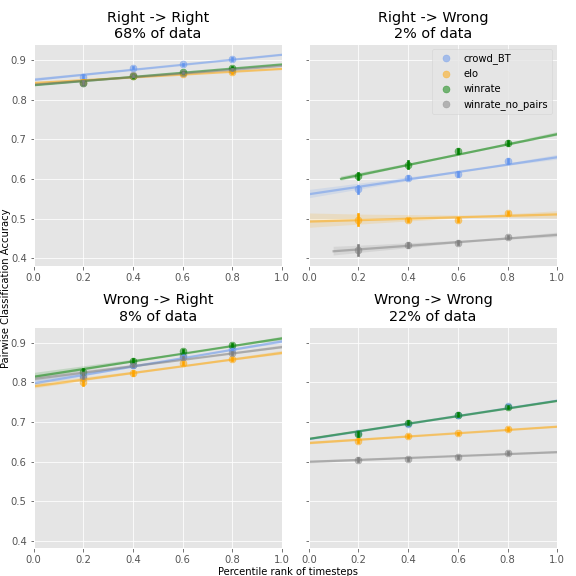
\includegraphics[width=\linewidth]{img/acc_vs_time_Physics_ada.png}
%	\caption{to do}
%	\label{fig:acc_vs_time}
%\end{figure}

%One part of this methodological contribution is to frame the analysis as an 
%information retrieval task: given a set of TMPI observations for students who 
%each select a peer's explanation as more convincing than their own, taking 
%into 
%account the subset of explanations they are presented with, can we 
%predict, based on linguistic properties of the explanations alone, which ones 
%will be in the top-K most \textit{convincing}?
%
%Figure \ref{fig:prec_at_K} gives an overview of our modelling results on the 
%TMPI data collected from myDALITE.org using the methodology we describe above.
%Each dot represents a question/topic from one of the reference AM datasets, or 
%from a discipline from our TMPI data.
%We plot the \textit{precision @ K} (where $K={1,3,5}$) of our feature-rich 
%regression model, as a function of the explanations/arguments in the held-out 
%test set.
%(
%The TMPI data all have a minimum of $N=20$ answers, due to the filtering 
%criteria we describe in section \ref{sec:dataset_dalite}, and the 
%disaagregation by word-count quartile.
%We do not apply same filters on the AM datasets, which explains why they are 
%all at the left of our plots.
%)
%
%\begin{figure}[H]
%	\scalebox{0.5}{%% Creator: Matplotlib, PGF backend
%%
%% To include the figure in your LaTeX document, write
%%   \input{<filename>.pgf}
%%
%% Make sure the required packages are loaded in your preamble
%%   \usepackage{pgf}
%%
%% and, on pdftex
%%   \usepackage[utf8]{inputenc}\DeclareUnicodeCharacter{2212}{-}
%%
%% or, on luatex and xetex
%%   \usepackage{unicode-math}
%%
%% Figures using additional raster images can only be included by \input if
%% they are in the same directory as the main LaTeX file. For loading figures
%% from other directories you can use the `import` package
%%   \usepackage{import}
%%
%% and then include the figures with
%%   \import{<path to file>}{<filename>.pgf}
%%
%% Matplotlib used the following preamble
%%
\begingroup%
\makeatletter%
\begin{pgfpicture}%
\pgfpathrectangle{\pgfpointorigin}{\pgfqpoint{12.000000in}{9.000000in}}%
\pgfusepath{use as bounding box, clip}%
\begin{pgfscope}%
\pgfsetbuttcap%
\pgfsetmiterjoin%
\definecolor{currentfill}{rgb}{1.000000,1.000000,1.000000}%
\pgfsetfillcolor{currentfill}%
\pgfsetlinewidth{0.000000pt}%
\definecolor{currentstroke}{rgb}{1.000000,1.000000,1.000000}%
\pgfsetstrokecolor{currentstroke}%
\pgfsetdash{}{0pt}%
\pgfpathmoveto{\pgfqpoint{0.000000in}{0.000000in}}%
\pgfpathlineto{\pgfqpoint{12.000000in}{0.000000in}}%
\pgfpathlineto{\pgfqpoint{12.000000in}{9.000000in}}%
\pgfpathlineto{\pgfqpoint{0.000000in}{9.000000in}}%
\pgfpathclose%
\pgfusepath{fill}%
\end{pgfscope}%
\begin{pgfscope}%
\pgfsetbuttcap%
\pgfsetmiterjoin%
\definecolor{currentfill}{rgb}{0.898039,0.898039,0.898039}%
\pgfsetfillcolor{currentfill}%
\pgfsetlinewidth{0.000000pt}%
\definecolor{currentstroke}{rgb}{0.000000,0.000000,0.000000}%
\pgfsetstrokecolor{currentstroke}%
\pgfsetstrokeopacity{0.000000}%
\pgfsetdash{}{0pt}%
\pgfpathmoveto{\pgfqpoint{0.628395in}{6.075720in}}%
\pgfpathlineto{\pgfqpoint{5.925000in}{6.075720in}}%
\pgfpathlineto{\pgfqpoint{5.925000in}{8.627778in}}%
\pgfpathlineto{\pgfqpoint{0.628395in}{8.627778in}}%
\pgfpathclose%
\pgfusepath{fill}%
\end{pgfscope}%
\begin{pgfscope}%
\pgfpathrectangle{\pgfqpoint{0.628395in}{6.075720in}}{\pgfqpoint{5.296605in}{2.552058in}}%
\pgfusepath{clip}%
\pgfsetrectcap%
\pgfsetroundjoin%
\pgfsetlinewidth{0.803000pt}%
\definecolor{currentstroke}{rgb}{1.000000,1.000000,1.000000}%
\pgfsetstrokecolor{currentstroke}%
\pgfsetdash{}{0pt}%
\pgfpathmoveto{\pgfqpoint{0.628395in}{6.075720in}}%
\pgfpathlineto{\pgfqpoint{0.628395in}{8.627778in}}%
\pgfusepath{stroke}%
\end{pgfscope}%
\begin{pgfscope}%
\pgfsetbuttcap%
\pgfsetroundjoin%
\definecolor{currentfill}{rgb}{0.333333,0.333333,0.333333}%
\pgfsetfillcolor{currentfill}%
\pgfsetlinewidth{0.803000pt}%
\definecolor{currentstroke}{rgb}{0.333333,0.333333,0.333333}%
\pgfsetstrokecolor{currentstroke}%
\pgfsetdash{}{0pt}%
\pgfsys@defobject{currentmarker}{\pgfqpoint{0.000000in}{-0.048611in}}{\pgfqpoint{0.000000in}{0.000000in}}{%
\pgfpathmoveto{\pgfqpoint{0.000000in}{0.000000in}}%
\pgfpathlineto{\pgfqpoint{0.000000in}{-0.048611in}}%
\pgfusepath{stroke,fill}%
}%
\begin{pgfscope}%
\pgfsys@transformshift{0.628395in}{6.075720in}%
\pgfsys@useobject{currentmarker}{}%
\end{pgfscope}%
\end{pgfscope}%
\begin{pgfscope}%
\pgfpathrectangle{\pgfqpoint{0.628395in}{6.075720in}}{\pgfqpoint{5.296605in}{2.552058in}}%
\pgfusepath{clip}%
\pgfsetrectcap%
\pgfsetroundjoin%
\pgfsetlinewidth{0.803000pt}%
\definecolor{currentstroke}{rgb}{1.000000,1.000000,1.000000}%
\pgfsetstrokecolor{currentstroke}%
\pgfsetdash{}{0pt}%
\pgfpathmoveto{\pgfqpoint{1.591414in}{6.075720in}}%
\pgfpathlineto{\pgfqpoint{1.591414in}{8.627778in}}%
\pgfusepath{stroke}%
\end{pgfscope}%
\begin{pgfscope}%
\pgfsetbuttcap%
\pgfsetroundjoin%
\definecolor{currentfill}{rgb}{0.333333,0.333333,0.333333}%
\pgfsetfillcolor{currentfill}%
\pgfsetlinewidth{0.803000pt}%
\definecolor{currentstroke}{rgb}{0.333333,0.333333,0.333333}%
\pgfsetstrokecolor{currentstroke}%
\pgfsetdash{}{0pt}%
\pgfsys@defobject{currentmarker}{\pgfqpoint{0.000000in}{-0.048611in}}{\pgfqpoint{0.000000in}{0.000000in}}{%
\pgfpathmoveto{\pgfqpoint{0.000000in}{0.000000in}}%
\pgfpathlineto{\pgfqpoint{0.000000in}{-0.048611in}}%
\pgfusepath{stroke,fill}%
}%
\begin{pgfscope}%
\pgfsys@transformshift{1.591414in}{6.075720in}%
\pgfsys@useobject{currentmarker}{}%
\end{pgfscope}%
\end{pgfscope}%
\begin{pgfscope}%
\pgfpathrectangle{\pgfqpoint{0.628395in}{6.075720in}}{\pgfqpoint{5.296605in}{2.552058in}}%
\pgfusepath{clip}%
\pgfsetrectcap%
\pgfsetroundjoin%
\pgfsetlinewidth{0.803000pt}%
\definecolor{currentstroke}{rgb}{1.000000,1.000000,1.000000}%
\pgfsetstrokecolor{currentstroke}%
\pgfsetdash{}{0pt}%
\pgfpathmoveto{\pgfqpoint{2.554433in}{6.075720in}}%
\pgfpathlineto{\pgfqpoint{2.554433in}{8.627778in}}%
\pgfusepath{stroke}%
\end{pgfscope}%
\begin{pgfscope}%
\pgfsetbuttcap%
\pgfsetroundjoin%
\definecolor{currentfill}{rgb}{0.333333,0.333333,0.333333}%
\pgfsetfillcolor{currentfill}%
\pgfsetlinewidth{0.803000pt}%
\definecolor{currentstroke}{rgb}{0.333333,0.333333,0.333333}%
\pgfsetstrokecolor{currentstroke}%
\pgfsetdash{}{0pt}%
\pgfsys@defobject{currentmarker}{\pgfqpoint{0.000000in}{-0.048611in}}{\pgfqpoint{0.000000in}{0.000000in}}{%
\pgfpathmoveto{\pgfqpoint{0.000000in}{0.000000in}}%
\pgfpathlineto{\pgfqpoint{0.000000in}{-0.048611in}}%
\pgfusepath{stroke,fill}%
}%
\begin{pgfscope}%
\pgfsys@transformshift{2.554433in}{6.075720in}%
\pgfsys@useobject{currentmarker}{}%
\end{pgfscope}%
\end{pgfscope}%
\begin{pgfscope}%
\pgfpathrectangle{\pgfqpoint{0.628395in}{6.075720in}}{\pgfqpoint{5.296605in}{2.552058in}}%
\pgfusepath{clip}%
\pgfsetrectcap%
\pgfsetroundjoin%
\pgfsetlinewidth{0.803000pt}%
\definecolor{currentstroke}{rgb}{1.000000,1.000000,1.000000}%
\pgfsetstrokecolor{currentstroke}%
\pgfsetdash{}{0pt}%
\pgfpathmoveto{\pgfqpoint{3.517452in}{6.075720in}}%
\pgfpathlineto{\pgfqpoint{3.517452in}{8.627778in}}%
\pgfusepath{stroke}%
\end{pgfscope}%
\begin{pgfscope}%
\pgfsetbuttcap%
\pgfsetroundjoin%
\definecolor{currentfill}{rgb}{0.333333,0.333333,0.333333}%
\pgfsetfillcolor{currentfill}%
\pgfsetlinewidth{0.803000pt}%
\definecolor{currentstroke}{rgb}{0.333333,0.333333,0.333333}%
\pgfsetstrokecolor{currentstroke}%
\pgfsetdash{}{0pt}%
\pgfsys@defobject{currentmarker}{\pgfqpoint{0.000000in}{-0.048611in}}{\pgfqpoint{0.000000in}{0.000000in}}{%
\pgfpathmoveto{\pgfqpoint{0.000000in}{0.000000in}}%
\pgfpathlineto{\pgfqpoint{0.000000in}{-0.048611in}}%
\pgfusepath{stroke,fill}%
}%
\begin{pgfscope}%
\pgfsys@transformshift{3.517452in}{6.075720in}%
\pgfsys@useobject{currentmarker}{}%
\end{pgfscope}%
\end{pgfscope}%
\begin{pgfscope}%
\pgfpathrectangle{\pgfqpoint{0.628395in}{6.075720in}}{\pgfqpoint{5.296605in}{2.552058in}}%
\pgfusepath{clip}%
\pgfsetrectcap%
\pgfsetroundjoin%
\pgfsetlinewidth{0.803000pt}%
\definecolor{currentstroke}{rgb}{1.000000,1.000000,1.000000}%
\pgfsetstrokecolor{currentstroke}%
\pgfsetdash{}{0pt}%
\pgfpathmoveto{\pgfqpoint{4.480471in}{6.075720in}}%
\pgfpathlineto{\pgfqpoint{4.480471in}{8.627778in}}%
\pgfusepath{stroke}%
\end{pgfscope}%
\begin{pgfscope}%
\pgfsetbuttcap%
\pgfsetroundjoin%
\definecolor{currentfill}{rgb}{0.333333,0.333333,0.333333}%
\pgfsetfillcolor{currentfill}%
\pgfsetlinewidth{0.803000pt}%
\definecolor{currentstroke}{rgb}{0.333333,0.333333,0.333333}%
\pgfsetstrokecolor{currentstroke}%
\pgfsetdash{}{0pt}%
\pgfsys@defobject{currentmarker}{\pgfqpoint{0.000000in}{-0.048611in}}{\pgfqpoint{0.000000in}{0.000000in}}{%
\pgfpathmoveto{\pgfqpoint{0.000000in}{0.000000in}}%
\pgfpathlineto{\pgfqpoint{0.000000in}{-0.048611in}}%
\pgfusepath{stroke,fill}%
}%
\begin{pgfscope}%
\pgfsys@transformshift{4.480471in}{6.075720in}%
\pgfsys@useobject{currentmarker}{}%
\end{pgfscope}%
\end{pgfscope}%
\begin{pgfscope}%
\pgfpathrectangle{\pgfqpoint{0.628395in}{6.075720in}}{\pgfqpoint{5.296605in}{2.552058in}}%
\pgfusepath{clip}%
\pgfsetrectcap%
\pgfsetroundjoin%
\pgfsetlinewidth{0.803000pt}%
\definecolor{currentstroke}{rgb}{1.000000,1.000000,1.000000}%
\pgfsetstrokecolor{currentstroke}%
\pgfsetdash{}{0pt}%
\pgfpathmoveto{\pgfqpoint{5.443490in}{6.075720in}}%
\pgfpathlineto{\pgfqpoint{5.443490in}{8.627778in}}%
\pgfusepath{stroke}%
\end{pgfscope}%
\begin{pgfscope}%
\pgfsetbuttcap%
\pgfsetroundjoin%
\definecolor{currentfill}{rgb}{0.333333,0.333333,0.333333}%
\pgfsetfillcolor{currentfill}%
\pgfsetlinewidth{0.803000pt}%
\definecolor{currentstroke}{rgb}{0.333333,0.333333,0.333333}%
\pgfsetstrokecolor{currentstroke}%
\pgfsetdash{}{0pt}%
\pgfsys@defobject{currentmarker}{\pgfqpoint{0.000000in}{-0.048611in}}{\pgfqpoint{0.000000in}{0.000000in}}{%
\pgfpathmoveto{\pgfqpoint{0.000000in}{0.000000in}}%
\pgfpathlineto{\pgfqpoint{0.000000in}{-0.048611in}}%
\pgfusepath{stroke,fill}%
}%
\begin{pgfscope}%
\pgfsys@transformshift{5.443490in}{6.075720in}%
\pgfsys@useobject{currentmarker}{}%
\end{pgfscope}%
\end{pgfscope}%
\begin{pgfscope}%
\pgfpathrectangle{\pgfqpoint{0.628395in}{6.075720in}}{\pgfqpoint{5.296605in}{2.552058in}}%
\pgfusepath{clip}%
\pgfsetrectcap%
\pgfsetroundjoin%
\pgfsetlinewidth{0.803000pt}%
\definecolor{currentstroke}{rgb}{1.000000,1.000000,1.000000}%
\pgfsetstrokecolor{currentstroke}%
\pgfsetdash{}{0pt}%
\pgfpathmoveto{\pgfqpoint{0.628395in}{6.186679in}}%
\pgfpathlineto{\pgfqpoint{5.925000in}{6.186679in}}%
\pgfusepath{stroke}%
\end{pgfscope}%
\begin{pgfscope}%
\pgfsetbuttcap%
\pgfsetroundjoin%
\definecolor{currentfill}{rgb}{0.333333,0.333333,0.333333}%
\pgfsetfillcolor{currentfill}%
\pgfsetlinewidth{0.803000pt}%
\definecolor{currentstroke}{rgb}{0.333333,0.333333,0.333333}%
\pgfsetstrokecolor{currentstroke}%
\pgfsetdash{}{0pt}%
\pgfsys@defobject{currentmarker}{\pgfqpoint{-0.048611in}{0.000000in}}{\pgfqpoint{0.000000in}{0.000000in}}{%
\pgfpathmoveto{\pgfqpoint{0.000000in}{0.000000in}}%
\pgfpathlineto{\pgfqpoint{-0.048611in}{0.000000in}}%
\pgfusepath{stroke,fill}%
}%
\begin{pgfscope}%
\pgfsys@transformshift{0.628395in}{6.186679in}%
\pgfsys@useobject{currentmarker}{}%
\end{pgfscope}%
\end{pgfscope}%
\begin{pgfscope}%
\definecolor{textcolor}{rgb}{0.333333,0.333333,0.333333}%
\pgfsetstrokecolor{textcolor}%
\pgfsetfillcolor{textcolor}%
\pgftext[x=0.353703in, y=6.138454in, left, base]{\color{textcolor}\rmfamily\fontsize{10.000000}{12.000000}\selectfont \(\displaystyle 0.0\)}%
\end{pgfscope}%
\begin{pgfscope}%
\pgfpathrectangle{\pgfqpoint{0.628395in}{6.075720in}}{\pgfqpoint{5.296605in}{2.552058in}}%
\pgfusepath{clip}%
\pgfsetrectcap%
\pgfsetroundjoin%
\pgfsetlinewidth{0.803000pt}%
\definecolor{currentstroke}{rgb}{1.000000,1.000000,1.000000}%
\pgfsetstrokecolor{currentstroke}%
\pgfsetdash{}{0pt}%
\pgfpathmoveto{\pgfqpoint{0.628395in}{6.630515in}}%
\pgfpathlineto{\pgfqpoint{5.925000in}{6.630515in}}%
\pgfusepath{stroke}%
\end{pgfscope}%
\begin{pgfscope}%
\pgfsetbuttcap%
\pgfsetroundjoin%
\definecolor{currentfill}{rgb}{0.333333,0.333333,0.333333}%
\pgfsetfillcolor{currentfill}%
\pgfsetlinewidth{0.803000pt}%
\definecolor{currentstroke}{rgb}{0.333333,0.333333,0.333333}%
\pgfsetstrokecolor{currentstroke}%
\pgfsetdash{}{0pt}%
\pgfsys@defobject{currentmarker}{\pgfqpoint{-0.048611in}{0.000000in}}{\pgfqpoint{0.000000in}{0.000000in}}{%
\pgfpathmoveto{\pgfqpoint{0.000000in}{0.000000in}}%
\pgfpathlineto{\pgfqpoint{-0.048611in}{0.000000in}}%
\pgfusepath{stroke,fill}%
}%
\begin{pgfscope}%
\pgfsys@transformshift{0.628395in}{6.630515in}%
\pgfsys@useobject{currentmarker}{}%
\end{pgfscope}%
\end{pgfscope}%
\begin{pgfscope}%
\definecolor{textcolor}{rgb}{0.333333,0.333333,0.333333}%
\pgfsetstrokecolor{textcolor}%
\pgfsetfillcolor{textcolor}%
\pgftext[x=0.353703in, y=6.582290in, left, base]{\color{textcolor}\rmfamily\fontsize{10.000000}{12.000000}\selectfont \(\displaystyle 0.2\)}%
\end{pgfscope}%
\begin{pgfscope}%
\pgfpathrectangle{\pgfqpoint{0.628395in}{6.075720in}}{\pgfqpoint{5.296605in}{2.552058in}}%
\pgfusepath{clip}%
\pgfsetrectcap%
\pgfsetroundjoin%
\pgfsetlinewidth{0.803000pt}%
\definecolor{currentstroke}{rgb}{1.000000,1.000000,1.000000}%
\pgfsetstrokecolor{currentstroke}%
\pgfsetdash{}{0pt}%
\pgfpathmoveto{\pgfqpoint{0.628395in}{7.074351in}}%
\pgfpathlineto{\pgfqpoint{5.925000in}{7.074351in}}%
\pgfusepath{stroke}%
\end{pgfscope}%
\begin{pgfscope}%
\pgfsetbuttcap%
\pgfsetroundjoin%
\definecolor{currentfill}{rgb}{0.333333,0.333333,0.333333}%
\pgfsetfillcolor{currentfill}%
\pgfsetlinewidth{0.803000pt}%
\definecolor{currentstroke}{rgb}{0.333333,0.333333,0.333333}%
\pgfsetstrokecolor{currentstroke}%
\pgfsetdash{}{0pt}%
\pgfsys@defobject{currentmarker}{\pgfqpoint{-0.048611in}{0.000000in}}{\pgfqpoint{0.000000in}{0.000000in}}{%
\pgfpathmoveto{\pgfqpoint{0.000000in}{0.000000in}}%
\pgfpathlineto{\pgfqpoint{-0.048611in}{0.000000in}}%
\pgfusepath{stroke,fill}%
}%
\begin{pgfscope}%
\pgfsys@transformshift{0.628395in}{7.074351in}%
\pgfsys@useobject{currentmarker}{}%
\end{pgfscope}%
\end{pgfscope}%
\begin{pgfscope}%
\definecolor{textcolor}{rgb}{0.333333,0.333333,0.333333}%
\pgfsetstrokecolor{textcolor}%
\pgfsetfillcolor{textcolor}%
\pgftext[x=0.353703in, y=7.026126in, left, base]{\color{textcolor}\rmfamily\fontsize{10.000000}{12.000000}\selectfont \(\displaystyle 0.4\)}%
\end{pgfscope}%
\begin{pgfscope}%
\pgfpathrectangle{\pgfqpoint{0.628395in}{6.075720in}}{\pgfqpoint{5.296605in}{2.552058in}}%
\pgfusepath{clip}%
\pgfsetrectcap%
\pgfsetroundjoin%
\pgfsetlinewidth{0.803000pt}%
\definecolor{currentstroke}{rgb}{1.000000,1.000000,1.000000}%
\pgfsetstrokecolor{currentstroke}%
\pgfsetdash{}{0pt}%
\pgfpathmoveto{\pgfqpoint{0.628395in}{7.518188in}}%
\pgfpathlineto{\pgfqpoint{5.925000in}{7.518188in}}%
\pgfusepath{stroke}%
\end{pgfscope}%
\begin{pgfscope}%
\pgfsetbuttcap%
\pgfsetroundjoin%
\definecolor{currentfill}{rgb}{0.333333,0.333333,0.333333}%
\pgfsetfillcolor{currentfill}%
\pgfsetlinewidth{0.803000pt}%
\definecolor{currentstroke}{rgb}{0.333333,0.333333,0.333333}%
\pgfsetstrokecolor{currentstroke}%
\pgfsetdash{}{0pt}%
\pgfsys@defobject{currentmarker}{\pgfqpoint{-0.048611in}{0.000000in}}{\pgfqpoint{0.000000in}{0.000000in}}{%
\pgfpathmoveto{\pgfqpoint{0.000000in}{0.000000in}}%
\pgfpathlineto{\pgfqpoint{-0.048611in}{0.000000in}}%
\pgfusepath{stroke,fill}%
}%
\begin{pgfscope}%
\pgfsys@transformshift{0.628395in}{7.518188in}%
\pgfsys@useobject{currentmarker}{}%
\end{pgfscope}%
\end{pgfscope}%
\begin{pgfscope}%
\definecolor{textcolor}{rgb}{0.333333,0.333333,0.333333}%
\pgfsetstrokecolor{textcolor}%
\pgfsetfillcolor{textcolor}%
\pgftext[x=0.353703in, y=7.469962in, left, base]{\color{textcolor}\rmfamily\fontsize{10.000000}{12.000000}\selectfont \(\displaystyle 0.6\)}%
\end{pgfscope}%
\begin{pgfscope}%
\pgfpathrectangle{\pgfqpoint{0.628395in}{6.075720in}}{\pgfqpoint{5.296605in}{2.552058in}}%
\pgfusepath{clip}%
\pgfsetrectcap%
\pgfsetroundjoin%
\pgfsetlinewidth{0.803000pt}%
\definecolor{currentstroke}{rgb}{1.000000,1.000000,1.000000}%
\pgfsetstrokecolor{currentstroke}%
\pgfsetdash{}{0pt}%
\pgfpathmoveto{\pgfqpoint{0.628395in}{7.962024in}}%
\pgfpathlineto{\pgfqpoint{5.925000in}{7.962024in}}%
\pgfusepath{stroke}%
\end{pgfscope}%
\begin{pgfscope}%
\pgfsetbuttcap%
\pgfsetroundjoin%
\definecolor{currentfill}{rgb}{0.333333,0.333333,0.333333}%
\pgfsetfillcolor{currentfill}%
\pgfsetlinewidth{0.803000pt}%
\definecolor{currentstroke}{rgb}{0.333333,0.333333,0.333333}%
\pgfsetstrokecolor{currentstroke}%
\pgfsetdash{}{0pt}%
\pgfsys@defobject{currentmarker}{\pgfqpoint{-0.048611in}{0.000000in}}{\pgfqpoint{0.000000in}{0.000000in}}{%
\pgfpathmoveto{\pgfqpoint{0.000000in}{0.000000in}}%
\pgfpathlineto{\pgfqpoint{-0.048611in}{0.000000in}}%
\pgfusepath{stroke,fill}%
}%
\begin{pgfscope}%
\pgfsys@transformshift{0.628395in}{7.962024in}%
\pgfsys@useobject{currentmarker}{}%
\end{pgfscope}%
\end{pgfscope}%
\begin{pgfscope}%
\definecolor{textcolor}{rgb}{0.333333,0.333333,0.333333}%
\pgfsetstrokecolor{textcolor}%
\pgfsetfillcolor{textcolor}%
\pgftext[x=0.353703in, y=7.913799in, left, base]{\color{textcolor}\rmfamily\fontsize{10.000000}{12.000000}\selectfont \(\displaystyle 0.8\)}%
\end{pgfscope}%
\begin{pgfscope}%
\pgfpathrectangle{\pgfqpoint{0.628395in}{6.075720in}}{\pgfqpoint{5.296605in}{2.552058in}}%
\pgfusepath{clip}%
\pgfsetrectcap%
\pgfsetroundjoin%
\pgfsetlinewidth{0.803000pt}%
\definecolor{currentstroke}{rgb}{1.000000,1.000000,1.000000}%
\pgfsetstrokecolor{currentstroke}%
\pgfsetdash{}{0pt}%
\pgfpathmoveto{\pgfqpoint{0.628395in}{8.405860in}}%
\pgfpathlineto{\pgfqpoint{5.925000in}{8.405860in}}%
\pgfusepath{stroke}%
\end{pgfscope}%
\begin{pgfscope}%
\pgfsetbuttcap%
\pgfsetroundjoin%
\definecolor{currentfill}{rgb}{0.333333,0.333333,0.333333}%
\pgfsetfillcolor{currentfill}%
\pgfsetlinewidth{0.803000pt}%
\definecolor{currentstroke}{rgb}{0.333333,0.333333,0.333333}%
\pgfsetstrokecolor{currentstroke}%
\pgfsetdash{}{0pt}%
\pgfsys@defobject{currentmarker}{\pgfqpoint{-0.048611in}{0.000000in}}{\pgfqpoint{0.000000in}{0.000000in}}{%
\pgfpathmoveto{\pgfqpoint{0.000000in}{0.000000in}}%
\pgfpathlineto{\pgfqpoint{-0.048611in}{0.000000in}}%
\pgfusepath{stroke,fill}%
}%
\begin{pgfscope}%
\pgfsys@transformshift{0.628395in}{8.405860in}%
\pgfsys@useobject{currentmarker}{}%
\end{pgfscope}%
\end{pgfscope}%
\begin{pgfscope}%
\definecolor{textcolor}{rgb}{0.333333,0.333333,0.333333}%
\pgfsetstrokecolor{textcolor}%
\pgfsetfillcolor{textcolor}%
\pgftext[x=0.353703in, y=8.357635in, left, base]{\color{textcolor}\rmfamily\fontsize{10.000000}{12.000000}\selectfont \(\displaystyle 1.0\)}%
\end{pgfscope}%
\begin{pgfscope}%
\definecolor{textcolor}{rgb}{0.333333,0.333333,0.333333}%
\pgfsetstrokecolor{textcolor}%
\pgfsetfillcolor{textcolor}%
\pgftext[x=0.298148in,y=7.351749in,,bottom,rotate=90.000000]{\color{textcolor}\rmfamily\fontsize{12.000000}{14.400000}\selectfont prec@1}%
\end{pgfscope}%
\begin{pgfscope}%
\pgfpathrectangle{\pgfqpoint{0.628395in}{6.075720in}}{\pgfqpoint{5.296605in}{2.552058in}}%
\pgfusepath{clip}%
\pgfsetbuttcap%
\pgfsetroundjoin%
\definecolor{currentfill}{rgb}{0.886275,0.290196,0.200000}%
\pgfsetfillcolor{currentfill}%
\pgfsetfillopacity{0.500000}%
\pgfsetlinewidth{0.752812pt}%
\definecolor{currentstroke}{rgb}{1.000000,1.000000,1.000000}%
\pgfsetstrokecolor{currentstroke}%
\pgfsetstrokeopacity{0.500000}%
\pgfsetdash{}{0pt}%
\pgfpathmoveto{\pgfqpoint{1.495112in}{6.145012in}}%
\pgfpathcurveto{\pgfqpoint{1.506162in}{6.145012in}}{\pgfqpoint{1.516761in}{6.149403in}}{\pgfqpoint{1.524575in}{6.157216in}}%
\pgfpathcurveto{\pgfqpoint{1.532389in}{6.165030in}}{\pgfqpoint{1.536779in}{6.175629in}}{\pgfqpoint{1.536779in}{6.186679in}}%
\pgfpathcurveto{\pgfqpoint{1.536779in}{6.197729in}}{\pgfqpoint{1.532389in}{6.208328in}}{\pgfqpoint{1.524575in}{6.216142in}}%
\pgfpathcurveto{\pgfqpoint{1.516761in}{6.223956in}}{\pgfqpoint{1.506162in}{6.228346in}}{\pgfqpoint{1.495112in}{6.228346in}}%
\pgfpathcurveto{\pgfqpoint{1.484062in}{6.228346in}}{\pgfqpoint{1.473463in}{6.223956in}}{\pgfqpoint{1.465649in}{6.216142in}}%
\pgfpathcurveto{\pgfqpoint{1.457836in}{6.208328in}}{\pgfqpoint{1.453446in}{6.197729in}}{\pgfqpoint{1.453446in}{6.186679in}}%
\pgfpathcurveto{\pgfqpoint{1.453446in}{6.175629in}}{\pgfqpoint{1.457836in}{6.165030in}}{\pgfqpoint{1.465649in}{6.157216in}}%
\pgfpathcurveto{\pgfqpoint{1.473463in}{6.149403in}}{\pgfqpoint{1.484062in}{6.145012in}}{\pgfqpoint{1.495112in}{6.145012in}}%
\pgfpathclose%
\pgfusepath{stroke,fill}%
\end{pgfscope}%
\begin{pgfscope}%
\pgfpathrectangle{\pgfqpoint{0.628395in}{6.075720in}}{\pgfqpoint{5.296605in}{2.552058in}}%
\pgfusepath{clip}%
\pgfsetbuttcap%
\pgfsetroundjoin%
\definecolor{currentfill}{rgb}{0.886275,0.290196,0.200000}%
\pgfsetfillcolor{currentfill}%
\pgfsetfillopacity{0.500000}%
\pgfsetlinewidth{0.752812pt}%
\definecolor{currentstroke}{rgb}{1.000000,1.000000,1.000000}%
\pgfsetstrokecolor{currentstroke}%
\pgfsetstrokeopacity{0.500000}%
\pgfsetdash{}{0pt}%
\pgfpathmoveto{\pgfqpoint{1.495112in}{6.145012in}}%
\pgfpathcurveto{\pgfqpoint{1.506162in}{6.145012in}}{\pgfqpoint{1.516761in}{6.149403in}}{\pgfqpoint{1.524575in}{6.157216in}}%
\pgfpathcurveto{\pgfqpoint{1.532389in}{6.165030in}}{\pgfqpoint{1.536779in}{6.175629in}}{\pgfqpoint{1.536779in}{6.186679in}}%
\pgfpathcurveto{\pgfqpoint{1.536779in}{6.197729in}}{\pgfqpoint{1.532389in}{6.208328in}}{\pgfqpoint{1.524575in}{6.216142in}}%
\pgfpathcurveto{\pgfqpoint{1.516761in}{6.223956in}}{\pgfqpoint{1.506162in}{6.228346in}}{\pgfqpoint{1.495112in}{6.228346in}}%
\pgfpathcurveto{\pgfqpoint{1.484062in}{6.228346in}}{\pgfqpoint{1.473463in}{6.223956in}}{\pgfqpoint{1.465649in}{6.216142in}}%
\pgfpathcurveto{\pgfqpoint{1.457836in}{6.208328in}}{\pgfqpoint{1.453446in}{6.197729in}}{\pgfqpoint{1.453446in}{6.186679in}}%
\pgfpathcurveto{\pgfqpoint{1.453446in}{6.175629in}}{\pgfqpoint{1.457836in}{6.165030in}}{\pgfqpoint{1.465649in}{6.157216in}}%
\pgfpathcurveto{\pgfqpoint{1.473463in}{6.149403in}}{\pgfqpoint{1.484062in}{6.145012in}}{\pgfqpoint{1.495112in}{6.145012in}}%
\pgfpathclose%
\pgfusepath{stroke,fill}%
\end{pgfscope}%
\begin{pgfscope}%
\pgfpathrectangle{\pgfqpoint{0.628395in}{6.075720in}}{\pgfqpoint{5.296605in}{2.552058in}}%
\pgfusepath{clip}%
\pgfsetbuttcap%
\pgfsetroundjoin%
\definecolor{currentfill}{rgb}{0.886275,0.290196,0.200000}%
\pgfsetfillcolor{currentfill}%
\pgfsetfillopacity{0.500000}%
\pgfsetlinewidth{0.752812pt}%
\definecolor{currentstroke}{rgb}{1.000000,1.000000,1.000000}%
\pgfsetstrokecolor{currentstroke}%
\pgfsetstrokeopacity{0.500000}%
\pgfsetdash{}{0pt}%
\pgfpathmoveto{\pgfqpoint{1.495112in}{6.145012in}}%
\pgfpathcurveto{\pgfqpoint{1.506162in}{6.145012in}}{\pgfqpoint{1.516761in}{6.149403in}}{\pgfqpoint{1.524575in}{6.157216in}}%
\pgfpathcurveto{\pgfqpoint{1.532389in}{6.165030in}}{\pgfqpoint{1.536779in}{6.175629in}}{\pgfqpoint{1.536779in}{6.186679in}}%
\pgfpathcurveto{\pgfqpoint{1.536779in}{6.197729in}}{\pgfqpoint{1.532389in}{6.208328in}}{\pgfqpoint{1.524575in}{6.216142in}}%
\pgfpathcurveto{\pgfqpoint{1.516761in}{6.223956in}}{\pgfqpoint{1.506162in}{6.228346in}}{\pgfqpoint{1.495112in}{6.228346in}}%
\pgfpathcurveto{\pgfqpoint{1.484062in}{6.228346in}}{\pgfqpoint{1.473463in}{6.223956in}}{\pgfqpoint{1.465649in}{6.216142in}}%
\pgfpathcurveto{\pgfqpoint{1.457836in}{6.208328in}}{\pgfqpoint{1.453446in}{6.197729in}}{\pgfqpoint{1.453446in}{6.186679in}}%
\pgfpathcurveto{\pgfqpoint{1.453446in}{6.175629in}}{\pgfqpoint{1.457836in}{6.165030in}}{\pgfqpoint{1.465649in}{6.157216in}}%
\pgfpathcurveto{\pgfqpoint{1.473463in}{6.149403in}}{\pgfqpoint{1.484062in}{6.145012in}}{\pgfqpoint{1.495112in}{6.145012in}}%
\pgfpathclose%
\pgfusepath{stroke,fill}%
\end{pgfscope}%
\begin{pgfscope}%
\pgfpathrectangle{\pgfqpoint{0.628395in}{6.075720in}}{\pgfqpoint{5.296605in}{2.552058in}}%
\pgfusepath{clip}%
\pgfsetbuttcap%
\pgfsetroundjoin%
\definecolor{currentfill}{rgb}{0.886275,0.290196,0.200000}%
\pgfsetfillcolor{currentfill}%
\pgfsetfillopacity{0.500000}%
\pgfsetlinewidth{0.752812pt}%
\definecolor{currentstroke}{rgb}{1.000000,1.000000,1.000000}%
\pgfsetstrokecolor{currentstroke}%
\pgfsetstrokeopacity{0.500000}%
\pgfsetdash{}{0pt}%
\pgfpathmoveto{\pgfqpoint{1.495112in}{8.364193in}}%
\pgfpathcurveto{\pgfqpoint{1.506162in}{8.364193in}}{\pgfqpoint{1.516761in}{8.368584in}}{\pgfqpoint{1.524575in}{8.376397in}}%
\pgfpathcurveto{\pgfqpoint{1.532389in}{8.384211in}}{\pgfqpoint{1.536779in}{8.394810in}}{\pgfqpoint{1.536779in}{8.405860in}}%
\pgfpathcurveto{\pgfqpoint{1.536779in}{8.416910in}}{\pgfqpoint{1.532389in}{8.427509in}}{\pgfqpoint{1.524575in}{8.435323in}}%
\pgfpathcurveto{\pgfqpoint{1.516761in}{8.443136in}}{\pgfqpoint{1.506162in}{8.447527in}}{\pgfqpoint{1.495112in}{8.447527in}}%
\pgfpathcurveto{\pgfqpoint{1.484062in}{8.447527in}}{\pgfqpoint{1.473463in}{8.443136in}}{\pgfqpoint{1.465649in}{8.435323in}}%
\pgfpathcurveto{\pgfqpoint{1.457836in}{8.427509in}}{\pgfqpoint{1.453446in}{8.416910in}}{\pgfqpoint{1.453446in}{8.405860in}}%
\pgfpathcurveto{\pgfqpoint{1.453446in}{8.394810in}}{\pgfqpoint{1.457836in}{8.384211in}}{\pgfqpoint{1.465649in}{8.376397in}}%
\pgfpathcurveto{\pgfqpoint{1.473463in}{8.368584in}}{\pgfqpoint{1.484062in}{8.364193in}}{\pgfqpoint{1.495112in}{8.364193in}}%
\pgfpathclose%
\pgfusepath{stroke,fill}%
\end{pgfscope}%
\begin{pgfscope}%
\pgfpathrectangle{\pgfqpoint{0.628395in}{6.075720in}}{\pgfqpoint{5.296605in}{2.552058in}}%
\pgfusepath{clip}%
\pgfsetbuttcap%
\pgfsetroundjoin%
\definecolor{currentfill}{rgb}{0.886275,0.290196,0.200000}%
\pgfsetfillcolor{currentfill}%
\pgfsetfillopacity{0.500000}%
\pgfsetlinewidth{0.752812pt}%
\definecolor{currentstroke}{rgb}{1.000000,1.000000,1.000000}%
\pgfsetstrokecolor{currentstroke}%
\pgfsetstrokeopacity{0.500000}%
\pgfsetdash{}{0pt}%
\pgfpathmoveto{\pgfqpoint{1.495112in}{6.145012in}}%
\pgfpathcurveto{\pgfqpoint{1.506162in}{6.145012in}}{\pgfqpoint{1.516761in}{6.149403in}}{\pgfqpoint{1.524575in}{6.157216in}}%
\pgfpathcurveto{\pgfqpoint{1.532389in}{6.165030in}}{\pgfqpoint{1.536779in}{6.175629in}}{\pgfqpoint{1.536779in}{6.186679in}}%
\pgfpathcurveto{\pgfqpoint{1.536779in}{6.197729in}}{\pgfqpoint{1.532389in}{6.208328in}}{\pgfqpoint{1.524575in}{6.216142in}}%
\pgfpathcurveto{\pgfqpoint{1.516761in}{6.223956in}}{\pgfqpoint{1.506162in}{6.228346in}}{\pgfqpoint{1.495112in}{6.228346in}}%
\pgfpathcurveto{\pgfqpoint{1.484062in}{6.228346in}}{\pgfqpoint{1.473463in}{6.223956in}}{\pgfqpoint{1.465649in}{6.216142in}}%
\pgfpathcurveto{\pgfqpoint{1.457836in}{6.208328in}}{\pgfqpoint{1.453446in}{6.197729in}}{\pgfqpoint{1.453446in}{6.186679in}}%
\pgfpathcurveto{\pgfqpoint{1.453446in}{6.175629in}}{\pgfqpoint{1.457836in}{6.165030in}}{\pgfqpoint{1.465649in}{6.157216in}}%
\pgfpathcurveto{\pgfqpoint{1.473463in}{6.149403in}}{\pgfqpoint{1.484062in}{6.145012in}}{\pgfqpoint{1.495112in}{6.145012in}}%
\pgfpathclose%
\pgfusepath{stroke,fill}%
\end{pgfscope}%
\begin{pgfscope}%
\pgfpathrectangle{\pgfqpoint{0.628395in}{6.075720in}}{\pgfqpoint{5.296605in}{2.552058in}}%
\pgfusepath{clip}%
\pgfsetbuttcap%
\pgfsetroundjoin%
\definecolor{currentfill}{rgb}{0.886275,0.290196,0.200000}%
\pgfsetfillcolor{currentfill}%
\pgfsetfillopacity{0.500000}%
\pgfsetlinewidth{0.752812pt}%
\definecolor{currentstroke}{rgb}{1.000000,1.000000,1.000000}%
\pgfsetstrokecolor{currentstroke}%
\pgfsetstrokeopacity{0.500000}%
\pgfsetdash{}{0pt}%
\pgfpathmoveto{\pgfqpoint{1.495112in}{6.145012in}}%
\pgfpathcurveto{\pgfqpoint{1.506162in}{6.145012in}}{\pgfqpoint{1.516761in}{6.149403in}}{\pgfqpoint{1.524575in}{6.157216in}}%
\pgfpathcurveto{\pgfqpoint{1.532389in}{6.165030in}}{\pgfqpoint{1.536779in}{6.175629in}}{\pgfqpoint{1.536779in}{6.186679in}}%
\pgfpathcurveto{\pgfqpoint{1.536779in}{6.197729in}}{\pgfqpoint{1.532389in}{6.208328in}}{\pgfqpoint{1.524575in}{6.216142in}}%
\pgfpathcurveto{\pgfqpoint{1.516761in}{6.223956in}}{\pgfqpoint{1.506162in}{6.228346in}}{\pgfqpoint{1.495112in}{6.228346in}}%
\pgfpathcurveto{\pgfqpoint{1.484062in}{6.228346in}}{\pgfqpoint{1.473463in}{6.223956in}}{\pgfqpoint{1.465649in}{6.216142in}}%
\pgfpathcurveto{\pgfqpoint{1.457836in}{6.208328in}}{\pgfqpoint{1.453446in}{6.197729in}}{\pgfqpoint{1.453446in}{6.186679in}}%
\pgfpathcurveto{\pgfqpoint{1.453446in}{6.175629in}}{\pgfqpoint{1.457836in}{6.165030in}}{\pgfqpoint{1.465649in}{6.157216in}}%
\pgfpathcurveto{\pgfqpoint{1.473463in}{6.149403in}}{\pgfqpoint{1.484062in}{6.145012in}}{\pgfqpoint{1.495112in}{6.145012in}}%
\pgfpathclose%
\pgfusepath{stroke,fill}%
\end{pgfscope}%
\begin{pgfscope}%
\pgfpathrectangle{\pgfqpoint{0.628395in}{6.075720in}}{\pgfqpoint{5.296605in}{2.552058in}}%
\pgfusepath{clip}%
\pgfsetbuttcap%
\pgfsetroundjoin%
\definecolor{currentfill}{rgb}{0.886275,0.290196,0.200000}%
\pgfsetfillcolor{currentfill}%
\pgfsetfillopacity{0.500000}%
\pgfsetlinewidth{0.752812pt}%
\definecolor{currentstroke}{rgb}{1.000000,1.000000,1.000000}%
\pgfsetstrokecolor{currentstroke}%
\pgfsetstrokeopacity{0.500000}%
\pgfsetdash{}{0pt}%
\pgfpathmoveto{\pgfqpoint{1.495112in}{6.145012in}}%
\pgfpathcurveto{\pgfqpoint{1.506162in}{6.145012in}}{\pgfqpoint{1.516761in}{6.149403in}}{\pgfqpoint{1.524575in}{6.157216in}}%
\pgfpathcurveto{\pgfqpoint{1.532389in}{6.165030in}}{\pgfqpoint{1.536779in}{6.175629in}}{\pgfqpoint{1.536779in}{6.186679in}}%
\pgfpathcurveto{\pgfqpoint{1.536779in}{6.197729in}}{\pgfqpoint{1.532389in}{6.208328in}}{\pgfqpoint{1.524575in}{6.216142in}}%
\pgfpathcurveto{\pgfqpoint{1.516761in}{6.223956in}}{\pgfqpoint{1.506162in}{6.228346in}}{\pgfqpoint{1.495112in}{6.228346in}}%
\pgfpathcurveto{\pgfqpoint{1.484062in}{6.228346in}}{\pgfqpoint{1.473463in}{6.223956in}}{\pgfqpoint{1.465649in}{6.216142in}}%
\pgfpathcurveto{\pgfqpoint{1.457836in}{6.208328in}}{\pgfqpoint{1.453446in}{6.197729in}}{\pgfqpoint{1.453446in}{6.186679in}}%
\pgfpathcurveto{\pgfqpoint{1.453446in}{6.175629in}}{\pgfqpoint{1.457836in}{6.165030in}}{\pgfqpoint{1.465649in}{6.157216in}}%
\pgfpathcurveto{\pgfqpoint{1.473463in}{6.149403in}}{\pgfqpoint{1.484062in}{6.145012in}}{\pgfqpoint{1.495112in}{6.145012in}}%
\pgfpathclose%
\pgfusepath{stroke,fill}%
\end{pgfscope}%
\begin{pgfscope}%
\pgfpathrectangle{\pgfqpoint{0.628395in}{6.075720in}}{\pgfqpoint{5.296605in}{2.552058in}}%
\pgfusepath{clip}%
\pgfsetbuttcap%
\pgfsetroundjoin%
\definecolor{currentfill}{rgb}{0.886275,0.290196,0.200000}%
\pgfsetfillcolor{currentfill}%
\pgfsetfillopacity{0.500000}%
\pgfsetlinewidth{0.752812pt}%
\definecolor{currentstroke}{rgb}{1.000000,1.000000,1.000000}%
\pgfsetstrokecolor{currentstroke}%
\pgfsetstrokeopacity{0.500000}%
\pgfsetdash{}{0pt}%
\pgfpathmoveto{\pgfqpoint{1.495112in}{6.145012in}}%
\pgfpathcurveto{\pgfqpoint{1.506162in}{6.145012in}}{\pgfqpoint{1.516761in}{6.149403in}}{\pgfqpoint{1.524575in}{6.157216in}}%
\pgfpathcurveto{\pgfqpoint{1.532389in}{6.165030in}}{\pgfqpoint{1.536779in}{6.175629in}}{\pgfqpoint{1.536779in}{6.186679in}}%
\pgfpathcurveto{\pgfqpoint{1.536779in}{6.197729in}}{\pgfqpoint{1.532389in}{6.208328in}}{\pgfqpoint{1.524575in}{6.216142in}}%
\pgfpathcurveto{\pgfqpoint{1.516761in}{6.223956in}}{\pgfqpoint{1.506162in}{6.228346in}}{\pgfqpoint{1.495112in}{6.228346in}}%
\pgfpathcurveto{\pgfqpoint{1.484062in}{6.228346in}}{\pgfqpoint{1.473463in}{6.223956in}}{\pgfqpoint{1.465649in}{6.216142in}}%
\pgfpathcurveto{\pgfqpoint{1.457836in}{6.208328in}}{\pgfqpoint{1.453446in}{6.197729in}}{\pgfqpoint{1.453446in}{6.186679in}}%
\pgfpathcurveto{\pgfqpoint{1.453446in}{6.175629in}}{\pgfqpoint{1.457836in}{6.165030in}}{\pgfqpoint{1.465649in}{6.157216in}}%
\pgfpathcurveto{\pgfqpoint{1.473463in}{6.149403in}}{\pgfqpoint{1.484062in}{6.145012in}}{\pgfqpoint{1.495112in}{6.145012in}}%
\pgfpathclose%
\pgfusepath{stroke,fill}%
\end{pgfscope}%
\begin{pgfscope}%
\pgfpathrectangle{\pgfqpoint{0.628395in}{6.075720in}}{\pgfqpoint{5.296605in}{2.552058in}}%
\pgfusepath{clip}%
\pgfsetbuttcap%
\pgfsetroundjoin%
\definecolor{currentfill}{rgb}{0.886275,0.290196,0.200000}%
\pgfsetfillcolor{currentfill}%
\pgfsetfillopacity{0.500000}%
\pgfsetlinewidth{0.752812pt}%
\definecolor{currentstroke}{rgb}{1.000000,1.000000,1.000000}%
\pgfsetstrokecolor{currentstroke}%
\pgfsetstrokeopacity{0.500000}%
\pgfsetdash{}{0pt}%
\pgfpathmoveto{\pgfqpoint{1.495112in}{6.145012in}}%
\pgfpathcurveto{\pgfqpoint{1.506162in}{6.145012in}}{\pgfqpoint{1.516761in}{6.149403in}}{\pgfqpoint{1.524575in}{6.157216in}}%
\pgfpathcurveto{\pgfqpoint{1.532389in}{6.165030in}}{\pgfqpoint{1.536779in}{6.175629in}}{\pgfqpoint{1.536779in}{6.186679in}}%
\pgfpathcurveto{\pgfqpoint{1.536779in}{6.197729in}}{\pgfqpoint{1.532389in}{6.208328in}}{\pgfqpoint{1.524575in}{6.216142in}}%
\pgfpathcurveto{\pgfqpoint{1.516761in}{6.223956in}}{\pgfqpoint{1.506162in}{6.228346in}}{\pgfqpoint{1.495112in}{6.228346in}}%
\pgfpathcurveto{\pgfqpoint{1.484062in}{6.228346in}}{\pgfqpoint{1.473463in}{6.223956in}}{\pgfqpoint{1.465649in}{6.216142in}}%
\pgfpathcurveto{\pgfqpoint{1.457836in}{6.208328in}}{\pgfqpoint{1.453446in}{6.197729in}}{\pgfqpoint{1.453446in}{6.186679in}}%
\pgfpathcurveto{\pgfqpoint{1.453446in}{6.175629in}}{\pgfqpoint{1.457836in}{6.165030in}}{\pgfqpoint{1.465649in}{6.157216in}}%
\pgfpathcurveto{\pgfqpoint{1.473463in}{6.149403in}}{\pgfqpoint{1.484062in}{6.145012in}}{\pgfqpoint{1.495112in}{6.145012in}}%
\pgfpathclose%
\pgfusepath{stroke,fill}%
\end{pgfscope}%
\begin{pgfscope}%
\pgfpathrectangle{\pgfqpoint{0.628395in}{6.075720in}}{\pgfqpoint{5.296605in}{2.552058in}}%
\pgfusepath{clip}%
\pgfsetbuttcap%
\pgfsetroundjoin%
\definecolor{currentfill}{rgb}{0.886275,0.290196,0.200000}%
\pgfsetfillcolor{currentfill}%
\pgfsetfillopacity{0.500000}%
\pgfsetlinewidth{0.752812pt}%
\definecolor{currentstroke}{rgb}{1.000000,1.000000,1.000000}%
\pgfsetstrokecolor{currentstroke}%
\pgfsetstrokeopacity{0.500000}%
\pgfsetdash{}{0pt}%
\pgfpathmoveto{\pgfqpoint{1.495112in}{6.145012in}}%
\pgfpathcurveto{\pgfqpoint{1.506162in}{6.145012in}}{\pgfqpoint{1.516761in}{6.149403in}}{\pgfqpoint{1.524575in}{6.157216in}}%
\pgfpathcurveto{\pgfqpoint{1.532389in}{6.165030in}}{\pgfqpoint{1.536779in}{6.175629in}}{\pgfqpoint{1.536779in}{6.186679in}}%
\pgfpathcurveto{\pgfqpoint{1.536779in}{6.197729in}}{\pgfqpoint{1.532389in}{6.208328in}}{\pgfqpoint{1.524575in}{6.216142in}}%
\pgfpathcurveto{\pgfqpoint{1.516761in}{6.223956in}}{\pgfqpoint{1.506162in}{6.228346in}}{\pgfqpoint{1.495112in}{6.228346in}}%
\pgfpathcurveto{\pgfqpoint{1.484062in}{6.228346in}}{\pgfqpoint{1.473463in}{6.223956in}}{\pgfqpoint{1.465649in}{6.216142in}}%
\pgfpathcurveto{\pgfqpoint{1.457836in}{6.208328in}}{\pgfqpoint{1.453446in}{6.197729in}}{\pgfqpoint{1.453446in}{6.186679in}}%
\pgfpathcurveto{\pgfqpoint{1.453446in}{6.175629in}}{\pgfqpoint{1.457836in}{6.165030in}}{\pgfqpoint{1.465649in}{6.157216in}}%
\pgfpathcurveto{\pgfqpoint{1.473463in}{6.149403in}}{\pgfqpoint{1.484062in}{6.145012in}}{\pgfqpoint{1.495112in}{6.145012in}}%
\pgfpathclose%
\pgfusepath{stroke,fill}%
\end{pgfscope}%
\begin{pgfscope}%
\pgfpathrectangle{\pgfqpoint{0.628395in}{6.075720in}}{\pgfqpoint{5.296605in}{2.552058in}}%
\pgfusepath{clip}%
\pgfsetbuttcap%
\pgfsetroundjoin%
\definecolor{currentfill}{rgb}{0.886275,0.290196,0.200000}%
\pgfsetfillcolor{currentfill}%
\pgfsetfillopacity{0.500000}%
\pgfsetlinewidth{0.752812pt}%
\definecolor{currentstroke}{rgb}{1.000000,1.000000,1.000000}%
\pgfsetstrokecolor{currentstroke}%
\pgfsetstrokeopacity{0.500000}%
\pgfsetdash{}{0pt}%
\pgfpathmoveto{\pgfqpoint{1.495112in}{6.145012in}}%
\pgfpathcurveto{\pgfqpoint{1.506162in}{6.145012in}}{\pgfqpoint{1.516761in}{6.149403in}}{\pgfqpoint{1.524575in}{6.157216in}}%
\pgfpathcurveto{\pgfqpoint{1.532389in}{6.165030in}}{\pgfqpoint{1.536779in}{6.175629in}}{\pgfqpoint{1.536779in}{6.186679in}}%
\pgfpathcurveto{\pgfqpoint{1.536779in}{6.197729in}}{\pgfqpoint{1.532389in}{6.208328in}}{\pgfqpoint{1.524575in}{6.216142in}}%
\pgfpathcurveto{\pgfqpoint{1.516761in}{6.223956in}}{\pgfqpoint{1.506162in}{6.228346in}}{\pgfqpoint{1.495112in}{6.228346in}}%
\pgfpathcurveto{\pgfqpoint{1.484062in}{6.228346in}}{\pgfqpoint{1.473463in}{6.223956in}}{\pgfqpoint{1.465649in}{6.216142in}}%
\pgfpathcurveto{\pgfqpoint{1.457836in}{6.208328in}}{\pgfqpoint{1.453446in}{6.197729in}}{\pgfqpoint{1.453446in}{6.186679in}}%
\pgfpathcurveto{\pgfqpoint{1.453446in}{6.175629in}}{\pgfqpoint{1.457836in}{6.165030in}}{\pgfqpoint{1.465649in}{6.157216in}}%
\pgfpathcurveto{\pgfqpoint{1.473463in}{6.149403in}}{\pgfqpoint{1.484062in}{6.145012in}}{\pgfqpoint{1.495112in}{6.145012in}}%
\pgfpathclose%
\pgfusepath{stroke,fill}%
\end{pgfscope}%
\begin{pgfscope}%
\pgfpathrectangle{\pgfqpoint{0.628395in}{6.075720in}}{\pgfqpoint{5.296605in}{2.552058in}}%
\pgfusepath{clip}%
\pgfsetbuttcap%
\pgfsetroundjoin%
\definecolor{currentfill}{rgb}{0.886275,0.290196,0.200000}%
\pgfsetfillcolor{currentfill}%
\pgfsetfillopacity{0.500000}%
\pgfsetlinewidth{0.752812pt}%
\definecolor{currentstroke}{rgb}{1.000000,1.000000,1.000000}%
\pgfsetstrokecolor{currentstroke}%
\pgfsetstrokeopacity{0.500000}%
\pgfsetdash{}{0pt}%
\pgfpathmoveto{\pgfqpoint{1.495112in}{6.145012in}}%
\pgfpathcurveto{\pgfqpoint{1.506162in}{6.145012in}}{\pgfqpoint{1.516761in}{6.149403in}}{\pgfqpoint{1.524575in}{6.157216in}}%
\pgfpathcurveto{\pgfqpoint{1.532389in}{6.165030in}}{\pgfqpoint{1.536779in}{6.175629in}}{\pgfqpoint{1.536779in}{6.186679in}}%
\pgfpathcurveto{\pgfqpoint{1.536779in}{6.197729in}}{\pgfqpoint{1.532389in}{6.208328in}}{\pgfqpoint{1.524575in}{6.216142in}}%
\pgfpathcurveto{\pgfqpoint{1.516761in}{6.223956in}}{\pgfqpoint{1.506162in}{6.228346in}}{\pgfqpoint{1.495112in}{6.228346in}}%
\pgfpathcurveto{\pgfqpoint{1.484062in}{6.228346in}}{\pgfqpoint{1.473463in}{6.223956in}}{\pgfqpoint{1.465649in}{6.216142in}}%
\pgfpathcurveto{\pgfqpoint{1.457836in}{6.208328in}}{\pgfqpoint{1.453446in}{6.197729in}}{\pgfqpoint{1.453446in}{6.186679in}}%
\pgfpathcurveto{\pgfqpoint{1.453446in}{6.175629in}}{\pgfqpoint{1.457836in}{6.165030in}}{\pgfqpoint{1.465649in}{6.157216in}}%
\pgfpathcurveto{\pgfqpoint{1.473463in}{6.149403in}}{\pgfqpoint{1.484062in}{6.145012in}}{\pgfqpoint{1.495112in}{6.145012in}}%
\pgfpathclose%
\pgfusepath{stroke,fill}%
\end{pgfscope}%
\begin{pgfscope}%
\pgfpathrectangle{\pgfqpoint{0.628395in}{6.075720in}}{\pgfqpoint{5.296605in}{2.552058in}}%
\pgfusepath{clip}%
\pgfsetbuttcap%
\pgfsetroundjoin%
\definecolor{currentfill}{rgb}{0.886275,0.290196,0.200000}%
\pgfsetfillcolor{currentfill}%
\pgfsetfillopacity{0.500000}%
\pgfsetlinewidth{0.752812pt}%
\definecolor{currentstroke}{rgb}{1.000000,1.000000,1.000000}%
\pgfsetstrokecolor{currentstroke}%
\pgfsetstrokeopacity{0.500000}%
\pgfsetdash{}{0pt}%
\pgfpathmoveto{\pgfqpoint{1.495112in}{6.145012in}}%
\pgfpathcurveto{\pgfqpoint{1.506162in}{6.145012in}}{\pgfqpoint{1.516761in}{6.149403in}}{\pgfqpoint{1.524575in}{6.157216in}}%
\pgfpathcurveto{\pgfqpoint{1.532389in}{6.165030in}}{\pgfqpoint{1.536779in}{6.175629in}}{\pgfqpoint{1.536779in}{6.186679in}}%
\pgfpathcurveto{\pgfqpoint{1.536779in}{6.197729in}}{\pgfqpoint{1.532389in}{6.208328in}}{\pgfqpoint{1.524575in}{6.216142in}}%
\pgfpathcurveto{\pgfqpoint{1.516761in}{6.223956in}}{\pgfqpoint{1.506162in}{6.228346in}}{\pgfqpoint{1.495112in}{6.228346in}}%
\pgfpathcurveto{\pgfqpoint{1.484062in}{6.228346in}}{\pgfqpoint{1.473463in}{6.223956in}}{\pgfqpoint{1.465649in}{6.216142in}}%
\pgfpathcurveto{\pgfqpoint{1.457836in}{6.208328in}}{\pgfqpoint{1.453446in}{6.197729in}}{\pgfqpoint{1.453446in}{6.186679in}}%
\pgfpathcurveto{\pgfqpoint{1.453446in}{6.175629in}}{\pgfqpoint{1.457836in}{6.165030in}}{\pgfqpoint{1.465649in}{6.157216in}}%
\pgfpathcurveto{\pgfqpoint{1.473463in}{6.149403in}}{\pgfqpoint{1.484062in}{6.145012in}}{\pgfqpoint{1.495112in}{6.145012in}}%
\pgfpathclose%
\pgfusepath{stroke,fill}%
\end{pgfscope}%
\begin{pgfscope}%
\pgfpathrectangle{\pgfqpoint{0.628395in}{6.075720in}}{\pgfqpoint{5.296605in}{2.552058in}}%
\pgfusepath{clip}%
\pgfsetbuttcap%
\pgfsetroundjoin%
\definecolor{currentfill}{rgb}{0.886275,0.290196,0.200000}%
\pgfsetfillcolor{currentfill}%
\pgfsetfillopacity{0.500000}%
\pgfsetlinewidth{0.752812pt}%
\definecolor{currentstroke}{rgb}{1.000000,1.000000,1.000000}%
\pgfsetstrokecolor{currentstroke}%
\pgfsetstrokeopacity{0.500000}%
\pgfsetdash{}{0pt}%
\pgfpathmoveto{\pgfqpoint{1.495112in}{8.364193in}}%
\pgfpathcurveto{\pgfqpoint{1.506162in}{8.364193in}}{\pgfqpoint{1.516761in}{8.368584in}}{\pgfqpoint{1.524575in}{8.376397in}}%
\pgfpathcurveto{\pgfqpoint{1.532389in}{8.384211in}}{\pgfqpoint{1.536779in}{8.394810in}}{\pgfqpoint{1.536779in}{8.405860in}}%
\pgfpathcurveto{\pgfqpoint{1.536779in}{8.416910in}}{\pgfqpoint{1.532389in}{8.427509in}}{\pgfqpoint{1.524575in}{8.435323in}}%
\pgfpathcurveto{\pgfqpoint{1.516761in}{8.443136in}}{\pgfqpoint{1.506162in}{8.447527in}}{\pgfqpoint{1.495112in}{8.447527in}}%
\pgfpathcurveto{\pgfqpoint{1.484062in}{8.447527in}}{\pgfqpoint{1.473463in}{8.443136in}}{\pgfqpoint{1.465649in}{8.435323in}}%
\pgfpathcurveto{\pgfqpoint{1.457836in}{8.427509in}}{\pgfqpoint{1.453446in}{8.416910in}}{\pgfqpoint{1.453446in}{8.405860in}}%
\pgfpathcurveto{\pgfqpoint{1.453446in}{8.394810in}}{\pgfqpoint{1.457836in}{8.384211in}}{\pgfqpoint{1.465649in}{8.376397in}}%
\pgfpathcurveto{\pgfqpoint{1.473463in}{8.368584in}}{\pgfqpoint{1.484062in}{8.364193in}}{\pgfqpoint{1.495112in}{8.364193in}}%
\pgfpathclose%
\pgfusepath{stroke,fill}%
\end{pgfscope}%
\begin{pgfscope}%
\pgfpathrectangle{\pgfqpoint{0.628395in}{6.075720in}}{\pgfqpoint{5.296605in}{2.552058in}}%
\pgfusepath{clip}%
\pgfsetbuttcap%
\pgfsetroundjoin%
\definecolor{currentfill}{rgb}{0.886275,0.290196,0.200000}%
\pgfsetfillcolor{currentfill}%
\pgfsetfillopacity{0.500000}%
\pgfsetlinewidth{0.752812pt}%
\definecolor{currentstroke}{rgb}{1.000000,1.000000,1.000000}%
\pgfsetstrokecolor{currentstroke}%
\pgfsetstrokeopacity{0.500000}%
\pgfsetdash{}{0pt}%
\pgfpathmoveto{\pgfqpoint{1.495112in}{6.145012in}}%
\pgfpathcurveto{\pgfqpoint{1.506162in}{6.145012in}}{\pgfqpoint{1.516761in}{6.149403in}}{\pgfqpoint{1.524575in}{6.157216in}}%
\pgfpathcurveto{\pgfqpoint{1.532389in}{6.165030in}}{\pgfqpoint{1.536779in}{6.175629in}}{\pgfqpoint{1.536779in}{6.186679in}}%
\pgfpathcurveto{\pgfqpoint{1.536779in}{6.197729in}}{\pgfqpoint{1.532389in}{6.208328in}}{\pgfqpoint{1.524575in}{6.216142in}}%
\pgfpathcurveto{\pgfqpoint{1.516761in}{6.223956in}}{\pgfqpoint{1.506162in}{6.228346in}}{\pgfqpoint{1.495112in}{6.228346in}}%
\pgfpathcurveto{\pgfqpoint{1.484062in}{6.228346in}}{\pgfqpoint{1.473463in}{6.223956in}}{\pgfqpoint{1.465649in}{6.216142in}}%
\pgfpathcurveto{\pgfqpoint{1.457836in}{6.208328in}}{\pgfqpoint{1.453446in}{6.197729in}}{\pgfqpoint{1.453446in}{6.186679in}}%
\pgfpathcurveto{\pgfqpoint{1.453446in}{6.175629in}}{\pgfqpoint{1.457836in}{6.165030in}}{\pgfqpoint{1.465649in}{6.157216in}}%
\pgfpathcurveto{\pgfqpoint{1.473463in}{6.149403in}}{\pgfqpoint{1.484062in}{6.145012in}}{\pgfqpoint{1.495112in}{6.145012in}}%
\pgfpathclose%
\pgfusepath{stroke,fill}%
\end{pgfscope}%
\begin{pgfscope}%
\pgfpathrectangle{\pgfqpoint{0.628395in}{6.075720in}}{\pgfqpoint{5.296605in}{2.552058in}}%
\pgfusepath{clip}%
\pgfsetbuttcap%
\pgfsetroundjoin%
\definecolor{currentfill}{rgb}{0.886275,0.290196,0.200000}%
\pgfsetfillcolor{currentfill}%
\pgfsetfillopacity{0.500000}%
\pgfsetlinewidth{0.752812pt}%
\definecolor{currentstroke}{rgb}{1.000000,1.000000,1.000000}%
\pgfsetstrokecolor{currentstroke}%
\pgfsetstrokeopacity{0.500000}%
\pgfsetdash{}{0pt}%
\pgfpathmoveto{\pgfqpoint{1.495112in}{6.145012in}}%
\pgfpathcurveto{\pgfqpoint{1.506162in}{6.145012in}}{\pgfqpoint{1.516761in}{6.149403in}}{\pgfqpoint{1.524575in}{6.157216in}}%
\pgfpathcurveto{\pgfqpoint{1.532389in}{6.165030in}}{\pgfqpoint{1.536779in}{6.175629in}}{\pgfqpoint{1.536779in}{6.186679in}}%
\pgfpathcurveto{\pgfqpoint{1.536779in}{6.197729in}}{\pgfqpoint{1.532389in}{6.208328in}}{\pgfqpoint{1.524575in}{6.216142in}}%
\pgfpathcurveto{\pgfqpoint{1.516761in}{6.223956in}}{\pgfqpoint{1.506162in}{6.228346in}}{\pgfqpoint{1.495112in}{6.228346in}}%
\pgfpathcurveto{\pgfqpoint{1.484062in}{6.228346in}}{\pgfqpoint{1.473463in}{6.223956in}}{\pgfqpoint{1.465649in}{6.216142in}}%
\pgfpathcurveto{\pgfqpoint{1.457836in}{6.208328in}}{\pgfqpoint{1.453446in}{6.197729in}}{\pgfqpoint{1.453446in}{6.186679in}}%
\pgfpathcurveto{\pgfqpoint{1.453446in}{6.175629in}}{\pgfqpoint{1.457836in}{6.165030in}}{\pgfqpoint{1.465649in}{6.157216in}}%
\pgfpathcurveto{\pgfqpoint{1.473463in}{6.149403in}}{\pgfqpoint{1.484062in}{6.145012in}}{\pgfqpoint{1.495112in}{6.145012in}}%
\pgfpathclose%
\pgfusepath{stroke,fill}%
\end{pgfscope}%
\begin{pgfscope}%
\pgfpathrectangle{\pgfqpoint{0.628395in}{6.075720in}}{\pgfqpoint{5.296605in}{2.552058in}}%
\pgfusepath{clip}%
\pgfsetbuttcap%
\pgfsetroundjoin%
\definecolor{currentfill}{rgb}{0.886275,0.290196,0.200000}%
\pgfsetfillcolor{currentfill}%
\pgfsetfillopacity{0.500000}%
\pgfsetlinewidth{0.752812pt}%
\definecolor{currentstroke}{rgb}{1.000000,1.000000,1.000000}%
\pgfsetstrokecolor{currentstroke}%
\pgfsetstrokeopacity{0.500000}%
\pgfsetdash{}{0pt}%
\pgfpathmoveto{\pgfqpoint{1.495112in}{8.364193in}}%
\pgfpathcurveto{\pgfqpoint{1.506162in}{8.364193in}}{\pgfqpoint{1.516761in}{8.368584in}}{\pgfqpoint{1.524575in}{8.376397in}}%
\pgfpathcurveto{\pgfqpoint{1.532389in}{8.384211in}}{\pgfqpoint{1.536779in}{8.394810in}}{\pgfqpoint{1.536779in}{8.405860in}}%
\pgfpathcurveto{\pgfqpoint{1.536779in}{8.416910in}}{\pgfqpoint{1.532389in}{8.427509in}}{\pgfqpoint{1.524575in}{8.435323in}}%
\pgfpathcurveto{\pgfqpoint{1.516761in}{8.443136in}}{\pgfqpoint{1.506162in}{8.447527in}}{\pgfqpoint{1.495112in}{8.447527in}}%
\pgfpathcurveto{\pgfqpoint{1.484062in}{8.447527in}}{\pgfqpoint{1.473463in}{8.443136in}}{\pgfqpoint{1.465649in}{8.435323in}}%
\pgfpathcurveto{\pgfqpoint{1.457836in}{8.427509in}}{\pgfqpoint{1.453446in}{8.416910in}}{\pgfqpoint{1.453446in}{8.405860in}}%
\pgfpathcurveto{\pgfqpoint{1.453446in}{8.394810in}}{\pgfqpoint{1.457836in}{8.384211in}}{\pgfqpoint{1.465649in}{8.376397in}}%
\pgfpathcurveto{\pgfqpoint{1.473463in}{8.368584in}}{\pgfqpoint{1.484062in}{8.364193in}}{\pgfqpoint{1.495112in}{8.364193in}}%
\pgfpathclose%
\pgfusepath{stroke,fill}%
\end{pgfscope}%
\begin{pgfscope}%
\pgfpathrectangle{\pgfqpoint{0.628395in}{6.075720in}}{\pgfqpoint{5.296605in}{2.552058in}}%
\pgfusepath{clip}%
\pgfsetbuttcap%
\pgfsetroundjoin%
\definecolor{currentfill}{rgb}{0.886275,0.290196,0.200000}%
\pgfsetfillcolor{currentfill}%
\pgfsetfillopacity{0.500000}%
\pgfsetlinewidth{0.752812pt}%
\definecolor{currentstroke}{rgb}{1.000000,1.000000,1.000000}%
\pgfsetstrokecolor{currentstroke}%
\pgfsetstrokeopacity{0.500000}%
\pgfsetdash{}{0pt}%
\pgfpathmoveto{\pgfqpoint{1.495112in}{6.145012in}}%
\pgfpathcurveto{\pgfqpoint{1.506162in}{6.145012in}}{\pgfqpoint{1.516761in}{6.149403in}}{\pgfqpoint{1.524575in}{6.157216in}}%
\pgfpathcurveto{\pgfqpoint{1.532389in}{6.165030in}}{\pgfqpoint{1.536779in}{6.175629in}}{\pgfqpoint{1.536779in}{6.186679in}}%
\pgfpathcurveto{\pgfqpoint{1.536779in}{6.197729in}}{\pgfqpoint{1.532389in}{6.208328in}}{\pgfqpoint{1.524575in}{6.216142in}}%
\pgfpathcurveto{\pgfqpoint{1.516761in}{6.223956in}}{\pgfqpoint{1.506162in}{6.228346in}}{\pgfqpoint{1.495112in}{6.228346in}}%
\pgfpathcurveto{\pgfqpoint{1.484062in}{6.228346in}}{\pgfqpoint{1.473463in}{6.223956in}}{\pgfqpoint{1.465649in}{6.216142in}}%
\pgfpathcurveto{\pgfqpoint{1.457836in}{6.208328in}}{\pgfqpoint{1.453446in}{6.197729in}}{\pgfqpoint{1.453446in}{6.186679in}}%
\pgfpathcurveto{\pgfqpoint{1.453446in}{6.175629in}}{\pgfqpoint{1.457836in}{6.165030in}}{\pgfqpoint{1.465649in}{6.157216in}}%
\pgfpathcurveto{\pgfqpoint{1.473463in}{6.149403in}}{\pgfqpoint{1.484062in}{6.145012in}}{\pgfqpoint{1.495112in}{6.145012in}}%
\pgfpathclose%
\pgfusepath{stroke,fill}%
\end{pgfscope}%
\begin{pgfscope}%
\pgfpathrectangle{\pgfqpoint{0.628395in}{6.075720in}}{\pgfqpoint{5.296605in}{2.552058in}}%
\pgfusepath{clip}%
\pgfsetbuttcap%
\pgfsetroundjoin%
\definecolor{currentfill}{rgb}{0.886275,0.290196,0.200000}%
\pgfsetfillcolor{currentfill}%
\pgfsetfillopacity{0.500000}%
\pgfsetlinewidth{0.752812pt}%
\definecolor{currentstroke}{rgb}{1.000000,1.000000,1.000000}%
\pgfsetstrokecolor{currentstroke}%
\pgfsetstrokeopacity{0.500000}%
\pgfsetdash{}{0pt}%
\pgfpathmoveto{\pgfqpoint{1.495112in}{6.145012in}}%
\pgfpathcurveto{\pgfqpoint{1.506162in}{6.145012in}}{\pgfqpoint{1.516761in}{6.149403in}}{\pgfqpoint{1.524575in}{6.157216in}}%
\pgfpathcurveto{\pgfqpoint{1.532389in}{6.165030in}}{\pgfqpoint{1.536779in}{6.175629in}}{\pgfqpoint{1.536779in}{6.186679in}}%
\pgfpathcurveto{\pgfqpoint{1.536779in}{6.197729in}}{\pgfqpoint{1.532389in}{6.208328in}}{\pgfqpoint{1.524575in}{6.216142in}}%
\pgfpathcurveto{\pgfqpoint{1.516761in}{6.223956in}}{\pgfqpoint{1.506162in}{6.228346in}}{\pgfqpoint{1.495112in}{6.228346in}}%
\pgfpathcurveto{\pgfqpoint{1.484062in}{6.228346in}}{\pgfqpoint{1.473463in}{6.223956in}}{\pgfqpoint{1.465649in}{6.216142in}}%
\pgfpathcurveto{\pgfqpoint{1.457836in}{6.208328in}}{\pgfqpoint{1.453446in}{6.197729in}}{\pgfqpoint{1.453446in}{6.186679in}}%
\pgfpathcurveto{\pgfqpoint{1.453446in}{6.175629in}}{\pgfqpoint{1.457836in}{6.165030in}}{\pgfqpoint{1.465649in}{6.157216in}}%
\pgfpathcurveto{\pgfqpoint{1.473463in}{6.149403in}}{\pgfqpoint{1.484062in}{6.145012in}}{\pgfqpoint{1.495112in}{6.145012in}}%
\pgfpathclose%
\pgfusepath{stroke,fill}%
\end{pgfscope}%
\begin{pgfscope}%
\pgfpathrectangle{\pgfqpoint{0.628395in}{6.075720in}}{\pgfqpoint{5.296605in}{2.552058in}}%
\pgfusepath{clip}%
\pgfsetbuttcap%
\pgfsetroundjoin%
\definecolor{currentfill}{rgb}{0.886275,0.290196,0.200000}%
\pgfsetfillcolor{currentfill}%
\pgfsetfillopacity{0.500000}%
\pgfsetlinewidth{0.752812pt}%
\definecolor{currentstroke}{rgb}{1.000000,1.000000,1.000000}%
\pgfsetstrokecolor{currentstroke}%
\pgfsetstrokeopacity{0.500000}%
\pgfsetdash{}{0pt}%
\pgfpathmoveto{\pgfqpoint{1.398810in}{6.145012in}}%
\pgfpathcurveto{\pgfqpoint{1.409860in}{6.145012in}}{\pgfqpoint{1.420459in}{6.149403in}}{\pgfqpoint{1.428273in}{6.157216in}}%
\pgfpathcurveto{\pgfqpoint{1.436087in}{6.165030in}}{\pgfqpoint{1.440477in}{6.175629in}}{\pgfqpoint{1.440477in}{6.186679in}}%
\pgfpathcurveto{\pgfqpoint{1.440477in}{6.197729in}}{\pgfqpoint{1.436087in}{6.208328in}}{\pgfqpoint{1.428273in}{6.216142in}}%
\pgfpathcurveto{\pgfqpoint{1.420459in}{6.223956in}}{\pgfqpoint{1.409860in}{6.228346in}}{\pgfqpoint{1.398810in}{6.228346in}}%
\pgfpathcurveto{\pgfqpoint{1.387760in}{6.228346in}}{\pgfqpoint{1.377161in}{6.223956in}}{\pgfqpoint{1.369347in}{6.216142in}}%
\pgfpathcurveto{\pgfqpoint{1.361534in}{6.208328in}}{\pgfqpoint{1.357144in}{6.197729in}}{\pgfqpoint{1.357144in}{6.186679in}}%
\pgfpathcurveto{\pgfqpoint{1.357144in}{6.175629in}}{\pgfqpoint{1.361534in}{6.165030in}}{\pgfqpoint{1.369347in}{6.157216in}}%
\pgfpathcurveto{\pgfqpoint{1.377161in}{6.149403in}}{\pgfqpoint{1.387760in}{6.145012in}}{\pgfqpoint{1.398810in}{6.145012in}}%
\pgfpathclose%
\pgfusepath{stroke,fill}%
\end{pgfscope}%
\begin{pgfscope}%
\pgfpathrectangle{\pgfqpoint{0.628395in}{6.075720in}}{\pgfqpoint{5.296605in}{2.552058in}}%
\pgfusepath{clip}%
\pgfsetbuttcap%
\pgfsetroundjoin%
\definecolor{currentfill}{rgb}{0.886275,0.290196,0.200000}%
\pgfsetfillcolor{currentfill}%
\pgfsetfillopacity{0.500000}%
\pgfsetlinewidth{0.752812pt}%
\definecolor{currentstroke}{rgb}{1.000000,1.000000,1.000000}%
\pgfsetstrokecolor{currentstroke}%
\pgfsetstrokeopacity{0.500000}%
\pgfsetdash{}{0pt}%
\pgfpathmoveto{\pgfqpoint{1.398810in}{6.145012in}}%
\pgfpathcurveto{\pgfqpoint{1.409860in}{6.145012in}}{\pgfqpoint{1.420459in}{6.149403in}}{\pgfqpoint{1.428273in}{6.157216in}}%
\pgfpathcurveto{\pgfqpoint{1.436087in}{6.165030in}}{\pgfqpoint{1.440477in}{6.175629in}}{\pgfqpoint{1.440477in}{6.186679in}}%
\pgfpathcurveto{\pgfqpoint{1.440477in}{6.197729in}}{\pgfqpoint{1.436087in}{6.208328in}}{\pgfqpoint{1.428273in}{6.216142in}}%
\pgfpathcurveto{\pgfqpoint{1.420459in}{6.223956in}}{\pgfqpoint{1.409860in}{6.228346in}}{\pgfqpoint{1.398810in}{6.228346in}}%
\pgfpathcurveto{\pgfqpoint{1.387760in}{6.228346in}}{\pgfqpoint{1.377161in}{6.223956in}}{\pgfqpoint{1.369347in}{6.216142in}}%
\pgfpathcurveto{\pgfqpoint{1.361534in}{6.208328in}}{\pgfqpoint{1.357144in}{6.197729in}}{\pgfqpoint{1.357144in}{6.186679in}}%
\pgfpathcurveto{\pgfqpoint{1.357144in}{6.175629in}}{\pgfqpoint{1.361534in}{6.165030in}}{\pgfqpoint{1.369347in}{6.157216in}}%
\pgfpathcurveto{\pgfqpoint{1.377161in}{6.149403in}}{\pgfqpoint{1.387760in}{6.145012in}}{\pgfqpoint{1.398810in}{6.145012in}}%
\pgfpathclose%
\pgfusepath{stroke,fill}%
\end{pgfscope}%
\begin{pgfscope}%
\pgfpathrectangle{\pgfqpoint{0.628395in}{6.075720in}}{\pgfqpoint{5.296605in}{2.552058in}}%
\pgfusepath{clip}%
\pgfsetbuttcap%
\pgfsetroundjoin%
\definecolor{currentfill}{rgb}{0.886275,0.290196,0.200000}%
\pgfsetfillcolor{currentfill}%
\pgfsetfillopacity{0.500000}%
\pgfsetlinewidth{0.752812pt}%
\definecolor{currentstroke}{rgb}{1.000000,1.000000,1.000000}%
\pgfsetstrokecolor{currentstroke}%
\pgfsetstrokeopacity{0.500000}%
\pgfsetdash{}{0pt}%
\pgfpathmoveto{\pgfqpoint{1.398810in}{8.364193in}}%
\pgfpathcurveto{\pgfqpoint{1.409860in}{8.364193in}}{\pgfqpoint{1.420459in}{8.368584in}}{\pgfqpoint{1.428273in}{8.376397in}}%
\pgfpathcurveto{\pgfqpoint{1.436087in}{8.384211in}}{\pgfqpoint{1.440477in}{8.394810in}}{\pgfqpoint{1.440477in}{8.405860in}}%
\pgfpathcurveto{\pgfqpoint{1.440477in}{8.416910in}}{\pgfqpoint{1.436087in}{8.427509in}}{\pgfqpoint{1.428273in}{8.435323in}}%
\pgfpathcurveto{\pgfqpoint{1.420459in}{8.443136in}}{\pgfqpoint{1.409860in}{8.447527in}}{\pgfqpoint{1.398810in}{8.447527in}}%
\pgfpathcurveto{\pgfqpoint{1.387760in}{8.447527in}}{\pgfqpoint{1.377161in}{8.443136in}}{\pgfqpoint{1.369347in}{8.435323in}}%
\pgfpathcurveto{\pgfqpoint{1.361534in}{8.427509in}}{\pgfqpoint{1.357144in}{8.416910in}}{\pgfqpoint{1.357144in}{8.405860in}}%
\pgfpathcurveto{\pgfqpoint{1.357144in}{8.394810in}}{\pgfqpoint{1.361534in}{8.384211in}}{\pgfqpoint{1.369347in}{8.376397in}}%
\pgfpathcurveto{\pgfqpoint{1.377161in}{8.368584in}}{\pgfqpoint{1.387760in}{8.364193in}}{\pgfqpoint{1.398810in}{8.364193in}}%
\pgfpathclose%
\pgfusepath{stroke,fill}%
\end{pgfscope}%
\begin{pgfscope}%
\pgfpathrectangle{\pgfqpoint{0.628395in}{6.075720in}}{\pgfqpoint{5.296605in}{2.552058in}}%
\pgfusepath{clip}%
\pgfsetbuttcap%
\pgfsetroundjoin%
\definecolor{currentfill}{rgb}{0.886275,0.290196,0.200000}%
\pgfsetfillcolor{currentfill}%
\pgfsetfillopacity{0.500000}%
\pgfsetlinewidth{0.752812pt}%
\definecolor{currentstroke}{rgb}{1.000000,1.000000,1.000000}%
\pgfsetstrokecolor{currentstroke}%
\pgfsetstrokeopacity{0.500000}%
\pgfsetdash{}{0pt}%
\pgfpathmoveto{\pgfqpoint{1.302508in}{6.145012in}}%
\pgfpathcurveto{\pgfqpoint{1.313558in}{6.145012in}}{\pgfqpoint{1.324158in}{6.149403in}}{\pgfqpoint{1.331971in}{6.157216in}}%
\pgfpathcurveto{\pgfqpoint{1.339785in}{6.165030in}}{\pgfqpoint{1.344175in}{6.175629in}}{\pgfqpoint{1.344175in}{6.186679in}}%
\pgfpathcurveto{\pgfqpoint{1.344175in}{6.197729in}}{\pgfqpoint{1.339785in}{6.208328in}}{\pgfqpoint{1.331971in}{6.216142in}}%
\pgfpathcurveto{\pgfqpoint{1.324158in}{6.223956in}}{\pgfqpoint{1.313558in}{6.228346in}}{\pgfqpoint{1.302508in}{6.228346in}}%
\pgfpathcurveto{\pgfqpoint{1.291458in}{6.228346in}}{\pgfqpoint{1.280859in}{6.223956in}}{\pgfqpoint{1.273046in}{6.216142in}}%
\pgfpathcurveto{\pgfqpoint{1.265232in}{6.208328in}}{\pgfqpoint{1.260842in}{6.197729in}}{\pgfqpoint{1.260842in}{6.186679in}}%
\pgfpathcurveto{\pgfqpoint{1.260842in}{6.175629in}}{\pgfqpoint{1.265232in}{6.165030in}}{\pgfqpoint{1.273046in}{6.157216in}}%
\pgfpathcurveto{\pgfqpoint{1.280859in}{6.149403in}}{\pgfqpoint{1.291458in}{6.145012in}}{\pgfqpoint{1.302508in}{6.145012in}}%
\pgfpathclose%
\pgfusepath{stroke,fill}%
\end{pgfscope}%
\begin{pgfscope}%
\pgfpathrectangle{\pgfqpoint{0.628395in}{6.075720in}}{\pgfqpoint{5.296605in}{2.552058in}}%
\pgfusepath{clip}%
\pgfsetbuttcap%
\pgfsetroundjoin%
\definecolor{currentfill}{rgb}{0.886275,0.290196,0.200000}%
\pgfsetfillcolor{currentfill}%
\pgfsetfillopacity{0.500000}%
\pgfsetlinewidth{0.752812pt}%
\definecolor{currentstroke}{rgb}{1.000000,1.000000,1.000000}%
\pgfsetstrokecolor{currentstroke}%
\pgfsetstrokeopacity{0.500000}%
\pgfsetdash{}{0pt}%
\pgfpathmoveto{\pgfqpoint{1.398810in}{8.364193in}}%
\pgfpathcurveto{\pgfqpoint{1.409860in}{8.364193in}}{\pgfqpoint{1.420459in}{8.368584in}}{\pgfqpoint{1.428273in}{8.376397in}}%
\pgfpathcurveto{\pgfqpoint{1.436087in}{8.384211in}}{\pgfqpoint{1.440477in}{8.394810in}}{\pgfqpoint{1.440477in}{8.405860in}}%
\pgfpathcurveto{\pgfqpoint{1.440477in}{8.416910in}}{\pgfqpoint{1.436087in}{8.427509in}}{\pgfqpoint{1.428273in}{8.435323in}}%
\pgfpathcurveto{\pgfqpoint{1.420459in}{8.443136in}}{\pgfqpoint{1.409860in}{8.447527in}}{\pgfqpoint{1.398810in}{8.447527in}}%
\pgfpathcurveto{\pgfqpoint{1.387760in}{8.447527in}}{\pgfqpoint{1.377161in}{8.443136in}}{\pgfqpoint{1.369347in}{8.435323in}}%
\pgfpathcurveto{\pgfqpoint{1.361534in}{8.427509in}}{\pgfqpoint{1.357144in}{8.416910in}}{\pgfqpoint{1.357144in}{8.405860in}}%
\pgfpathcurveto{\pgfqpoint{1.357144in}{8.394810in}}{\pgfqpoint{1.361534in}{8.384211in}}{\pgfqpoint{1.369347in}{8.376397in}}%
\pgfpathcurveto{\pgfqpoint{1.377161in}{8.368584in}}{\pgfqpoint{1.387760in}{8.364193in}}{\pgfqpoint{1.398810in}{8.364193in}}%
\pgfpathclose%
\pgfusepath{stroke,fill}%
\end{pgfscope}%
\begin{pgfscope}%
\pgfpathrectangle{\pgfqpoint{0.628395in}{6.075720in}}{\pgfqpoint{5.296605in}{2.552058in}}%
\pgfusepath{clip}%
\pgfsetbuttcap%
\pgfsetroundjoin%
\definecolor{currentfill}{rgb}{0.886275,0.290196,0.200000}%
\pgfsetfillcolor{currentfill}%
\pgfsetfillopacity{0.500000}%
\pgfsetlinewidth{0.752812pt}%
\definecolor{currentstroke}{rgb}{1.000000,1.000000,1.000000}%
\pgfsetstrokecolor{currentstroke}%
\pgfsetstrokeopacity{0.500000}%
\pgfsetdash{}{0pt}%
\pgfpathmoveto{\pgfqpoint{1.398810in}{6.145012in}}%
\pgfpathcurveto{\pgfqpoint{1.409860in}{6.145012in}}{\pgfqpoint{1.420459in}{6.149403in}}{\pgfqpoint{1.428273in}{6.157216in}}%
\pgfpathcurveto{\pgfqpoint{1.436087in}{6.165030in}}{\pgfqpoint{1.440477in}{6.175629in}}{\pgfqpoint{1.440477in}{6.186679in}}%
\pgfpathcurveto{\pgfqpoint{1.440477in}{6.197729in}}{\pgfqpoint{1.436087in}{6.208328in}}{\pgfqpoint{1.428273in}{6.216142in}}%
\pgfpathcurveto{\pgfqpoint{1.420459in}{6.223956in}}{\pgfqpoint{1.409860in}{6.228346in}}{\pgfqpoint{1.398810in}{6.228346in}}%
\pgfpathcurveto{\pgfqpoint{1.387760in}{6.228346in}}{\pgfqpoint{1.377161in}{6.223956in}}{\pgfqpoint{1.369347in}{6.216142in}}%
\pgfpathcurveto{\pgfqpoint{1.361534in}{6.208328in}}{\pgfqpoint{1.357144in}{6.197729in}}{\pgfqpoint{1.357144in}{6.186679in}}%
\pgfpathcurveto{\pgfqpoint{1.357144in}{6.175629in}}{\pgfqpoint{1.361534in}{6.165030in}}{\pgfqpoint{1.369347in}{6.157216in}}%
\pgfpathcurveto{\pgfqpoint{1.377161in}{6.149403in}}{\pgfqpoint{1.387760in}{6.145012in}}{\pgfqpoint{1.398810in}{6.145012in}}%
\pgfpathclose%
\pgfusepath{stroke,fill}%
\end{pgfscope}%
\begin{pgfscope}%
\pgfpathrectangle{\pgfqpoint{0.628395in}{6.075720in}}{\pgfqpoint{5.296605in}{2.552058in}}%
\pgfusepath{clip}%
\pgfsetbuttcap%
\pgfsetroundjoin%
\definecolor{currentfill}{rgb}{0.886275,0.290196,0.200000}%
\pgfsetfillcolor{currentfill}%
\pgfsetfillopacity{0.500000}%
\pgfsetlinewidth{0.752812pt}%
\definecolor{currentstroke}{rgb}{1.000000,1.000000,1.000000}%
\pgfsetstrokecolor{currentstroke}%
\pgfsetstrokeopacity{0.500000}%
\pgfsetdash{}{0pt}%
\pgfpathmoveto{\pgfqpoint{1.398810in}{6.145012in}}%
\pgfpathcurveto{\pgfqpoint{1.409860in}{6.145012in}}{\pgfqpoint{1.420459in}{6.149403in}}{\pgfqpoint{1.428273in}{6.157216in}}%
\pgfpathcurveto{\pgfqpoint{1.436087in}{6.165030in}}{\pgfqpoint{1.440477in}{6.175629in}}{\pgfqpoint{1.440477in}{6.186679in}}%
\pgfpathcurveto{\pgfqpoint{1.440477in}{6.197729in}}{\pgfqpoint{1.436087in}{6.208328in}}{\pgfqpoint{1.428273in}{6.216142in}}%
\pgfpathcurveto{\pgfqpoint{1.420459in}{6.223956in}}{\pgfqpoint{1.409860in}{6.228346in}}{\pgfqpoint{1.398810in}{6.228346in}}%
\pgfpathcurveto{\pgfqpoint{1.387760in}{6.228346in}}{\pgfqpoint{1.377161in}{6.223956in}}{\pgfqpoint{1.369347in}{6.216142in}}%
\pgfpathcurveto{\pgfqpoint{1.361534in}{6.208328in}}{\pgfqpoint{1.357144in}{6.197729in}}{\pgfqpoint{1.357144in}{6.186679in}}%
\pgfpathcurveto{\pgfqpoint{1.357144in}{6.175629in}}{\pgfqpoint{1.361534in}{6.165030in}}{\pgfqpoint{1.369347in}{6.157216in}}%
\pgfpathcurveto{\pgfqpoint{1.377161in}{6.149403in}}{\pgfqpoint{1.387760in}{6.145012in}}{\pgfqpoint{1.398810in}{6.145012in}}%
\pgfpathclose%
\pgfusepath{stroke,fill}%
\end{pgfscope}%
\begin{pgfscope}%
\pgfpathrectangle{\pgfqpoint{0.628395in}{6.075720in}}{\pgfqpoint{5.296605in}{2.552058in}}%
\pgfusepath{clip}%
\pgfsetbuttcap%
\pgfsetroundjoin%
\definecolor{currentfill}{rgb}{0.886275,0.290196,0.200000}%
\pgfsetfillcolor{currentfill}%
\pgfsetfillopacity{0.500000}%
\pgfsetlinewidth{0.752812pt}%
\definecolor{currentstroke}{rgb}{1.000000,1.000000,1.000000}%
\pgfsetstrokecolor{currentstroke}%
\pgfsetstrokeopacity{0.500000}%
\pgfsetdash{}{0pt}%
\pgfpathmoveto{\pgfqpoint{1.302508in}{6.145012in}}%
\pgfpathcurveto{\pgfqpoint{1.313558in}{6.145012in}}{\pgfqpoint{1.324158in}{6.149403in}}{\pgfqpoint{1.331971in}{6.157216in}}%
\pgfpathcurveto{\pgfqpoint{1.339785in}{6.165030in}}{\pgfqpoint{1.344175in}{6.175629in}}{\pgfqpoint{1.344175in}{6.186679in}}%
\pgfpathcurveto{\pgfqpoint{1.344175in}{6.197729in}}{\pgfqpoint{1.339785in}{6.208328in}}{\pgfqpoint{1.331971in}{6.216142in}}%
\pgfpathcurveto{\pgfqpoint{1.324158in}{6.223956in}}{\pgfqpoint{1.313558in}{6.228346in}}{\pgfqpoint{1.302508in}{6.228346in}}%
\pgfpathcurveto{\pgfqpoint{1.291458in}{6.228346in}}{\pgfqpoint{1.280859in}{6.223956in}}{\pgfqpoint{1.273046in}{6.216142in}}%
\pgfpathcurveto{\pgfqpoint{1.265232in}{6.208328in}}{\pgfqpoint{1.260842in}{6.197729in}}{\pgfqpoint{1.260842in}{6.186679in}}%
\pgfpathcurveto{\pgfqpoint{1.260842in}{6.175629in}}{\pgfqpoint{1.265232in}{6.165030in}}{\pgfqpoint{1.273046in}{6.157216in}}%
\pgfpathcurveto{\pgfqpoint{1.280859in}{6.149403in}}{\pgfqpoint{1.291458in}{6.145012in}}{\pgfqpoint{1.302508in}{6.145012in}}%
\pgfpathclose%
\pgfusepath{stroke,fill}%
\end{pgfscope}%
\begin{pgfscope}%
\pgfpathrectangle{\pgfqpoint{0.628395in}{6.075720in}}{\pgfqpoint{5.296605in}{2.552058in}}%
\pgfusepath{clip}%
\pgfsetbuttcap%
\pgfsetroundjoin%
\definecolor{currentfill}{rgb}{0.886275,0.290196,0.200000}%
\pgfsetfillcolor{currentfill}%
\pgfsetfillopacity{0.500000}%
\pgfsetlinewidth{0.752812pt}%
\definecolor{currentstroke}{rgb}{1.000000,1.000000,1.000000}%
\pgfsetstrokecolor{currentstroke}%
\pgfsetstrokeopacity{0.500000}%
\pgfsetdash{}{0pt}%
\pgfpathmoveto{\pgfqpoint{1.302508in}{6.145012in}}%
\pgfpathcurveto{\pgfqpoint{1.313558in}{6.145012in}}{\pgfqpoint{1.324158in}{6.149403in}}{\pgfqpoint{1.331971in}{6.157216in}}%
\pgfpathcurveto{\pgfqpoint{1.339785in}{6.165030in}}{\pgfqpoint{1.344175in}{6.175629in}}{\pgfqpoint{1.344175in}{6.186679in}}%
\pgfpathcurveto{\pgfqpoint{1.344175in}{6.197729in}}{\pgfqpoint{1.339785in}{6.208328in}}{\pgfqpoint{1.331971in}{6.216142in}}%
\pgfpathcurveto{\pgfqpoint{1.324158in}{6.223956in}}{\pgfqpoint{1.313558in}{6.228346in}}{\pgfqpoint{1.302508in}{6.228346in}}%
\pgfpathcurveto{\pgfqpoint{1.291458in}{6.228346in}}{\pgfqpoint{1.280859in}{6.223956in}}{\pgfqpoint{1.273046in}{6.216142in}}%
\pgfpathcurveto{\pgfqpoint{1.265232in}{6.208328in}}{\pgfqpoint{1.260842in}{6.197729in}}{\pgfqpoint{1.260842in}{6.186679in}}%
\pgfpathcurveto{\pgfqpoint{1.260842in}{6.175629in}}{\pgfqpoint{1.265232in}{6.165030in}}{\pgfqpoint{1.273046in}{6.157216in}}%
\pgfpathcurveto{\pgfqpoint{1.280859in}{6.149403in}}{\pgfqpoint{1.291458in}{6.145012in}}{\pgfqpoint{1.302508in}{6.145012in}}%
\pgfpathclose%
\pgfusepath{stroke,fill}%
\end{pgfscope}%
\begin{pgfscope}%
\pgfpathrectangle{\pgfqpoint{0.628395in}{6.075720in}}{\pgfqpoint{5.296605in}{2.552058in}}%
\pgfusepath{clip}%
\pgfsetbuttcap%
\pgfsetroundjoin%
\definecolor{currentfill}{rgb}{0.886275,0.290196,0.200000}%
\pgfsetfillcolor{currentfill}%
\pgfsetfillopacity{0.500000}%
\pgfsetlinewidth{0.752812pt}%
\definecolor{currentstroke}{rgb}{1.000000,1.000000,1.000000}%
\pgfsetstrokecolor{currentstroke}%
\pgfsetstrokeopacity{0.500000}%
\pgfsetdash{}{0pt}%
\pgfpathmoveto{\pgfqpoint{1.302508in}{6.145012in}}%
\pgfpathcurveto{\pgfqpoint{1.313558in}{6.145012in}}{\pgfqpoint{1.324158in}{6.149403in}}{\pgfqpoint{1.331971in}{6.157216in}}%
\pgfpathcurveto{\pgfqpoint{1.339785in}{6.165030in}}{\pgfqpoint{1.344175in}{6.175629in}}{\pgfqpoint{1.344175in}{6.186679in}}%
\pgfpathcurveto{\pgfqpoint{1.344175in}{6.197729in}}{\pgfqpoint{1.339785in}{6.208328in}}{\pgfqpoint{1.331971in}{6.216142in}}%
\pgfpathcurveto{\pgfqpoint{1.324158in}{6.223956in}}{\pgfqpoint{1.313558in}{6.228346in}}{\pgfqpoint{1.302508in}{6.228346in}}%
\pgfpathcurveto{\pgfqpoint{1.291458in}{6.228346in}}{\pgfqpoint{1.280859in}{6.223956in}}{\pgfqpoint{1.273046in}{6.216142in}}%
\pgfpathcurveto{\pgfqpoint{1.265232in}{6.208328in}}{\pgfqpoint{1.260842in}{6.197729in}}{\pgfqpoint{1.260842in}{6.186679in}}%
\pgfpathcurveto{\pgfqpoint{1.260842in}{6.175629in}}{\pgfqpoint{1.265232in}{6.165030in}}{\pgfqpoint{1.273046in}{6.157216in}}%
\pgfpathcurveto{\pgfqpoint{1.280859in}{6.149403in}}{\pgfqpoint{1.291458in}{6.145012in}}{\pgfqpoint{1.302508in}{6.145012in}}%
\pgfpathclose%
\pgfusepath{stroke,fill}%
\end{pgfscope}%
\begin{pgfscope}%
\pgfpathrectangle{\pgfqpoint{0.628395in}{6.075720in}}{\pgfqpoint{5.296605in}{2.552058in}}%
\pgfusepath{clip}%
\pgfsetbuttcap%
\pgfsetroundjoin%
\definecolor{currentfill}{rgb}{0.886275,0.290196,0.200000}%
\pgfsetfillcolor{currentfill}%
\pgfsetfillopacity{0.500000}%
\pgfsetlinewidth{0.752812pt}%
\definecolor{currentstroke}{rgb}{1.000000,1.000000,1.000000}%
\pgfsetstrokecolor{currentstroke}%
\pgfsetstrokeopacity{0.500000}%
\pgfsetdash{}{0pt}%
\pgfpathmoveto{\pgfqpoint{1.302508in}{6.145012in}}%
\pgfpathcurveto{\pgfqpoint{1.313558in}{6.145012in}}{\pgfqpoint{1.324158in}{6.149403in}}{\pgfqpoint{1.331971in}{6.157216in}}%
\pgfpathcurveto{\pgfqpoint{1.339785in}{6.165030in}}{\pgfqpoint{1.344175in}{6.175629in}}{\pgfqpoint{1.344175in}{6.186679in}}%
\pgfpathcurveto{\pgfqpoint{1.344175in}{6.197729in}}{\pgfqpoint{1.339785in}{6.208328in}}{\pgfqpoint{1.331971in}{6.216142in}}%
\pgfpathcurveto{\pgfqpoint{1.324158in}{6.223956in}}{\pgfqpoint{1.313558in}{6.228346in}}{\pgfqpoint{1.302508in}{6.228346in}}%
\pgfpathcurveto{\pgfqpoint{1.291458in}{6.228346in}}{\pgfqpoint{1.280859in}{6.223956in}}{\pgfqpoint{1.273046in}{6.216142in}}%
\pgfpathcurveto{\pgfqpoint{1.265232in}{6.208328in}}{\pgfqpoint{1.260842in}{6.197729in}}{\pgfqpoint{1.260842in}{6.186679in}}%
\pgfpathcurveto{\pgfqpoint{1.260842in}{6.175629in}}{\pgfqpoint{1.265232in}{6.165030in}}{\pgfqpoint{1.273046in}{6.157216in}}%
\pgfpathcurveto{\pgfqpoint{1.280859in}{6.149403in}}{\pgfqpoint{1.291458in}{6.145012in}}{\pgfqpoint{1.302508in}{6.145012in}}%
\pgfpathclose%
\pgfusepath{stroke,fill}%
\end{pgfscope}%
\begin{pgfscope}%
\pgfpathrectangle{\pgfqpoint{0.628395in}{6.075720in}}{\pgfqpoint{5.296605in}{2.552058in}}%
\pgfusepath{clip}%
\pgfsetbuttcap%
\pgfsetroundjoin%
\definecolor{currentfill}{rgb}{0.886275,0.290196,0.200000}%
\pgfsetfillcolor{currentfill}%
\pgfsetfillopacity{0.500000}%
\pgfsetlinewidth{0.752812pt}%
\definecolor{currentstroke}{rgb}{1.000000,1.000000,1.000000}%
\pgfsetstrokecolor{currentstroke}%
\pgfsetstrokeopacity{0.500000}%
\pgfsetdash{}{0pt}%
\pgfpathmoveto{\pgfqpoint{1.206206in}{6.145012in}}%
\pgfpathcurveto{\pgfqpoint{1.217257in}{6.145012in}}{\pgfqpoint{1.227856in}{6.149403in}}{\pgfqpoint{1.235669in}{6.157216in}}%
\pgfpathcurveto{\pgfqpoint{1.243483in}{6.165030in}}{\pgfqpoint{1.247873in}{6.175629in}}{\pgfqpoint{1.247873in}{6.186679in}}%
\pgfpathcurveto{\pgfqpoint{1.247873in}{6.197729in}}{\pgfqpoint{1.243483in}{6.208328in}}{\pgfqpoint{1.235669in}{6.216142in}}%
\pgfpathcurveto{\pgfqpoint{1.227856in}{6.223956in}}{\pgfqpoint{1.217257in}{6.228346in}}{\pgfqpoint{1.206206in}{6.228346in}}%
\pgfpathcurveto{\pgfqpoint{1.195156in}{6.228346in}}{\pgfqpoint{1.184557in}{6.223956in}}{\pgfqpoint{1.176744in}{6.216142in}}%
\pgfpathcurveto{\pgfqpoint{1.168930in}{6.208328in}}{\pgfqpoint{1.164540in}{6.197729in}}{\pgfqpoint{1.164540in}{6.186679in}}%
\pgfpathcurveto{\pgfqpoint{1.164540in}{6.175629in}}{\pgfqpoint{1.168930in}{6.165030in}}{\pgfqpoint{1.176744in}{6.157216in}}%
\pgfpathcurveto{\pgfqpoint{1.184557in}{6.149403in}}{\pgfqpoint{1.195156in}{6.145012in}}{\pgfqpoint{1.206206in}{6.145012in}}%
\pgfpathclose%
\pgfusepath{stroke,fill}%
\end{pgfscope}%
\begin{pgfscope}%
\pgfpathrectangle{\pgfqpoint{0.628395in}{6.075720in}}{\pgfqpoint{5.296605in}{2.552058in}}%
\pgfusepath{clip}%
\pgfsetbuttcap%
\pgfsetroundjoin%
\definecolor{currentfill}{rgb}{0.886275,0.290196,0.200000}%
\pgfsetfillcolor{currentfill}%
\pgfsetfillopacity{0.500000}%
\pgfsetlinewidth{0.752812pt}%
\definecolor{currentstroke}{rgb}{1.000000,1.000000,1.000000}%
\pgfsetstrokecolor{currentstroke}%
\pgfsetstrokeopacity{0.500000}%
\pgfsetdash{}{0pt}%
\pgfpathmoveto{\pgfqpoint{1.206206in}{8.364193in}}%
\pgfpathcurveto{\pgfqpoint{1.217257in}{8.364193in}}{\pgfqpoint{1.227856in}{8.368584in}}{\pgfqpoint{1.235669in}{8.376397in}}%
\pgfpathcurveto{\pgfqpoint{1.243483in}{8.384211in}}{\pgfqpoint{1.247873in}{8.394810in}}{\pgfqpoint{1.247873in}{8.405860in}}%
\pgfpathcurveto{\pgfqpoint{1.247873in}{8.416910in}}{\pgfqpoint{1.243483in}{8.427509in}}{\pgfqpoint{1.235669in}{8.435323in}}%
\pgfpathcurveto{\pgfqpoint{1.227856in}{8.443136in}}{\pgfqpoint{1.217257in}{8.447527in}}{\pgfqpoint{1.206206in}{8.447527in}}%
\pgfpathcurveto{\pgfqpoint{1.195156in}{8.447527in}}{\pgfqpoint{1.184557in}{8.443136in}}{\pgfqpoint{1.176744in}{8.435323in}}%
\pgfpathcurveto{\pgfqpoint{1.168930in}{8.427509in}}{\pgfqpoint{1.164540in}{8.416910in}}{\pgfqpoint{1.164540in}{8.405860in}}%
\pgfpathcurveto{\pgfqpoint{1.164540in}{8.394810in}}{\pgfqpoint{1.168930in}{8.384211in}}{\pgfqpoint{1.176744in}{8.376397in}}%
\pgfpathcurveto{\pgfqpoint{1.184557in}{8.368584in}}{\pgfqpoint{1.195156in}{8.364193in}}{\pgfqpoint{1.206206in}{8.364193in}}%
\pgfpathclose%
\pgfusepath{stroke,fill}%
\end{pgfscope}%
\begin{pgfscope}%
\pgfpathrectangle{\pgfqpoint{0.628395in}{6.075720in}}{\pgfqpoint{5.296605in}{2.552058in}}%
\pgfusepath{clip}%
\pgfsetbuttcap%
\pgfsetroundjoin%
\definecolor{currentfill}{rgb}{0.203922,0.541176,0.741176}%
\pgfsetfillcolor{currentfill}%
\pgfsetfillopacity{0.500000}%
\pgfsetlinewidth{0.752812pt}%
\definecolor{currentstroke}{rgb}{1.000000,1.000000,1.000000}%
\pgfsetstrokecolor{currentstroke}%
\pgfsetstrokeopacity{0.500000}%
\pgfsetdash{}{0pt}%
\pgfpathmoveto{\pgfqpoint{14.784776in}{6.145012in}}%
\pgfpathcurveto{\pgfqpoint{14.795826in}{6.145012in}}{\pgfqpoint{14.806425in}{6.149403in}}{\pgfqpoint{14.814238in}{6.157216in}}%
\pgfpathcurveto{\pgfqpoint{14.822052in}{6.165030in}}{\pgfqpoint{14.826442in}{6.175629in}}{\pgfqpoint{14.826442in}{6.186679in}}%
\pgfpathcurveto{\pgfqpoint{14.826442in}{6.197729in}}{\pgfqpoint{14.822052in}{6.208328in}}{\pgfqpoint{14.814238in}{6.216142in}}%
\pgfpathcurveto{\pgfqpoint{14.806425in}{6.223956in}}{\pgfqpoint{14.795826in}{6.228346in}}{\pgfqpoint{14.784776in}{6.228346in}}%
\pgfpathcurveto{\pgfqpoint{14.773726in}{6.228346in}}{\pgfqpoint{14.763126in}{6.223956in}}{\pgfqpoint{14.755313in}{6.216142in}}%
\pgfpathcurveto{\pgfqpoint{14.747499in}{6.208328in}}{\pgfqpoint{14.743109in}{6.197729in}}{\pgfqpoint{14.743109in}{6.186679in}}%
\pgfpathcurveto{\pgfqpoint{14.743109in}{6.175629in}}{\pgfqpoint{14.747499in}{6.165030in}}{\pgfqpoint{14.755313in}{6.157216in}}%
\pgfpathcurveto{\pgfqpoint{14.763126in}{6.149403in}}{\pgfqpoint{14.773726in}{6.145012in}}{\pgfqpoint{14.784776in}{6.145012in}}%
\pgfpathclose%
\pgfusepath{stroke,fill}%
\end{pgfscope}%
\begin{pgfscope}%
\pgfpathrectangle{\pgfqpoint{0.628395in}{6.075720in}}{\pgfqpoint{5.296605in}{2.552058in}}%
\pgfusepath{clip}%
\pgfsetbuttcap%
\pgfsetroundjoin%
\definecolor{currentfill}{rgb}{0.203922,0.541176,0.741176}%
\pgfsetfillcolor{currentfill}%
\pgfsetfillopacity{0.500000}%
\pgfsetlinewidth{0.752812pt}%
\definecolor{currentstroke}{rgb}{1.000000,1.000000,1.000000}%
\pgfsetstrokecolor{currentstroke}%
\pgfsetstrokeopacity{0.500000}%
\pgfsetdash{}{0pt}%
\pgfpathmoveto{\pgfqpoint{11.799416in}{6.145012in}}%
\pgfpathcurveto{\pgfqpoint{11.810467in}{6.145012in}}{\pgfqpoint{11.821066in}{6.149403in}}{\pgfqpoint{11.828879in}{6.157216in}}%
\pgfpathcurveto{\pgfqpoint{11.836693in}{6.165030in}}{\pgfqpoint{11.841083in}{6.175629in}}{\pgfqpoint{11.841083in}{6.186679in}}%
\pgfpathcurveto{\pgfqpoint{11.841083in}{6.197729in}}{\pgfqpoint{11.836693in}{6.208328in}}{\pgfqpoint{11.828879in}{6.216142in}}%
\pgfpathcurveto{\pgfqpoint{11.821066in}{6.223956in}}{\pgfqpoint{11.810467in}{6.228346in}}{\pgfqpoint{11.799416in}{6.228346in}}%
\pgfpathcurveto{\pgfqpoint{11.788366in}{6.228346in}}{\pgfqpoint{11.777767in}{6.223956in}}{\pgfqpoint{11.769954in}{6.216142in}}%
\pgfpathcurveto{\pgfqpoint{11.762140in}{6.208328in}}{\pgfqpoint{11.757750in}{6.197729in}}{\pgfqpoint{11.757750in}{6.186679in}}%
\pgfpathcurveto{\pgfqpoint{11.757750in}{6.175629in}}{\pgfqpoint{11.762140in}{6.165030in}}{\pgfqpoint{11.769954in}{6.157216in}}%
\pgfpathcurveto{\pgfqpoint{11.777767in}{6.149403in}}{\pgfqpoint{11.788366in}{6.145012in}}{\pgfqpoint{11.799416in}{6.145012in}}%
\pgfpathclose%
\pgfusepath{stroke,fill}%
\end{pgfscope}%
\begin{pgfscope}%
\pgfpathrectangle{\pgfqpoint{0.628395in}{6.075720in}}{\pgfqpoint{5.296605in}{2.552058in}}%
\pgfusepath{clip}%
\pgfsetbuttcap%
\pgfsetroundjoin%
\definecolor{currentfill}{rgb}{0.203922,0.541176,0.741176}%
\pgfsetfillcolor{currentfill}%
\pgfsetfillopacity{0.500000}%
\pgfsetlinewidth{0.752812pt}%
\definecolor{currentstroke}{rgb}{1.000000,1.000000,1.000000}%
\pgfsetstrokecolor{currentstroke}%
\pgfsetstrokeopacity{0.500000}%
\pgfsetdash{}{0pt}%
\pgfpathmoveto{\pgfqpoint{5.539792in}{6.145012in}}%
\pgfpathcurveto{\pgfqpoint{5.550842in}{6.145012in}}{\pgfqpoint{5.561442in}{6.149403in}}{\pgfqpoint{5.569255in}{6.157216in}}%
\pgfpathcurveto{\pgfqpoint{5.577069in}{6.165030in}}{\pgfqpoint{5.581459in}{6.175629in}}{\pgfqpoint{5.581459in}{6.186679in}}%
\pgfpathcurveto{\pgfqpoint{5.581459in}{6.197729in}}{\pgfqpoint{5.577069in}{6.208328in}}{\pgfqpoint{5.569255in}{6.216142in}}%
\pgfpathcurveto{\pgfqpoint{5.561442in}{6.223956in}}{\pgfqpoint{5.550842in}{6.228346in}}{\pgfqpoint{5.539792in}{6.228346in}}%
\pgfpathcurveto{\pgfqpoint{5.528742in}{6.228346in}}{\pgfqpoint{5.518143in}{6.223956in}}{\pgfqpoint{5.510330in}{6.216142in}}%
\pgfpathcurveto{\pgfqpoint{5.502516in}{6.208328in}}{\pgfqpoint{5.498126in}{6.197729in}}{\pgfqpoint{5.498126in}{6.186679in}}%
\pgfpathcurveto{\pgfqpoint{5.498126in}{6.175629in}}{\pgfqpoint{5.502516in}{6.165030in}}{\pgfqpoint{5.510330in}{6.157216in}}%
\pgfpathcurveto{\pgfqpoint{5.518143in}{6.149403in}}{\pgfqpoint{5.528742in}{6.145012in}}{\pgfqpoint{5.539792in}{6.145012in}}%
\pgfpathclose%
\pgfusepath{stroke,fill}%
\end{pgfscope}%
\begin{pgfscope}%
\pgfpathrectangle{\pgfqpoint{0.628395in}{6.075720in}}{\pgfqpoint{5.296605in}{2.552058in}}%
\pgfusepath{clip}%
\pgfsetbuttcap%
\pgfsetroundjoin%
\definecolor{currentfill}{rgb}{0.203922,0.541176,0.741176}%
\pgfsetfillcolor{currentfill}%
\pgfsetfillopacity{0.500000}%
\pgfsetlinewidth{0.752812pt}%
\definecolor{currentstroke}{rgb}{1.000000,1.000000,1.000000}%
\pgfsetstrokecolor{currentstroke}%
\pgfsetstrokeopacity{0.500000}%
\pgfsetdash{}{0pt}%
\pgfpathmoveto{\pgfqpoint{5.539792in}{6.145012in}}%
\pgfpathcurveto{\pgfqpoint{5.550842in}{6.145012in}}{\pgfqpoint{5.561442in}{6.149403in}}{\pgfqpoint{5.569255in}{6.157216in}}%
\pgfpathcurveto{\pgfqpoint{5.577069in}{6.165030in}}{\pgfqpoint{5.581459in}{6.175629in}}{\pgfqpoint{5.581459in}{6.186679in}}%
\pgfpathcurveto{\pgfqpoint{5.581459in}{6.197729in}}{\pgfqpoint{5.577069in}{6.208328in}}{\pgfqpoint{5.569255in}{6.216142in}}%
\pgfpathcurveto{\pgfqpoint{5.561442in}{6.223956in}}{\pgfqpoint{5.550842in}{6.228346in}}{\pgfqpoint{5.539792in}{6.228346in}}%
\pgfpathcurveto{\pgfqpoint{5.528742in}{6.228346in}}{\pgfqpoint{5.518143in}{6.223956in}}{\pgfqpoint{5.510330in}{6.216142in}}%
\pgfpathcurveto{\pgfqpoint{5.502516in}{6.208328in}}{\pgfqpoint{5.498126in}{6.197729in}}{\pgfqpoint{5.498126in}{6.186679in}}%
\pgfpathcurveto{\pgfqpoint{5.498126in}{6.175629in}}{\pgfqpoint{5.502516in}{6.165030in}}{\pgfqpoint{5.510330in}{6.157216in}}%
\pgfpathcurveto{\pgfqpoint{5.518143in}{6.149403in}}{\pgfqpoint{5.528742in}{6.145012in}}{\pgfqpoint{5.539792in}{6.145012in}}%
\pgfpathclose%
\pgfusepath{stroke,fill}%
\end{pgfscope}%
\begin{pgfscope}%
\pgfpathrectangle{\pgfqpoint{0.628395in}{6.075720in}}{\pgfqpoint{5.296605in}{2.552058in}}%
\pgfusepath{clip}%
\pgfsetbuttcap%
\pgfsetroundjoin%
\definecolor{currentfill}{rgb}{0.203922,0.541176,0.741176}%
\pgfsetfillcolor{currentfill}%
\pgfsetfillopacity{0.500000}%
\pgfsetlinewidth{0.752812pt}%
\definecolor{currentstroke}{rgb}{1.000000,1.000000,1.000000}%
\pgfsetstrokecolor{currentstroke}%
\pgfsetstrokeopacity{0.500000}%
\pgfsetdash{}{0pt}%
\pgfpathmoveto{\pgfqpoint{4.384169in}{6.145012in}}%
\pgfpathcurveto{\pgfqpoint{4.395220in}{6.145012in}}{\pgfqpoint{4.405819in}{6.149403in}}{\pgfqpoint{4.413632in}{6.157216in}}%
\pgfpathcurveto{\pgfqpoint{4.421446in}{6.165030in}}{\pgfqpoint{4.425836in}{6.175629in}}{\pgfqpoint{4.425836in}{6.186679in}}%
\pgfpathcurveto{\pgfqpoint{4.425836in}{6.197729in}}{\pgfqpoint{4.421446in}{6.208328in}}{\pgfqpoint{4.413632in}{6.216142in}}%
\pgfpathcurveto{\pgfqpoint{4.405819in}{6.223956in}}{\pgfqpoint{4.395220in}{6.228346in}}{\pgfqpoint{4.384169in}{6.228346in}}%
\pgfpathcurveto{\pgfqpoint{4.373119in}{6.228346in}}{\pgfqpoint{4.362520in}{6.223956in}}{\pgfqpoint{4.354707in}{6.216142in}}%
\pgfpathcurveto{\pgfqpoint{4.346893in}{6.208328in}}{\pgfqpoint{4.342503in}{6.197729in}}{\pgfqpoint{4.342503in}{6.186679in}}%
\pgfpathcurveto{\pgfqpoint{4.342503in}{6.175629in}}{\pgfqpoint{4.346893in}{6.165030in}}{\pgfqpoint{4.354707in}{6.157216in}}%
\pgfpathcurveto{\pgfqpoint{4.362520in}{6.149403in}}{\pgfqpoint{4.373119in}{6.145012in}}{\pgfqpoint{4.384169in}{6.145012in}}%
\pgfpathclose%
\pgfusepath{stroke,fill}%
\end{pgfscope}%
\begin{pgfscope}%
\pgfpathrectangle{\pgfqpoint{0.628395in}{6.075720in}}{\pgfqpoint{5.296605in}{2.552058in}}%
\pgfusepath{clip}%
\pgfsetbuttcap%
\pgfsetroundjoin%
\definecolor{currentfill}{rgb}{0.203922,0.541176,0.741176}%
\pgfsetfillcolor{currentfill}%
\pgfsetfillopacity{0.500000}%
\pgfsetlinewidth{0.752812pt}%
\definecolor{currentstroke}{rgb}{1.000000,1.000000,1.000000}%
\pgfsetstrokecolor{currentstroke}%
\pgfsetstrokeopacity{0.500000}%
\pgfsetdash{}{0pt}%
\pgfpathmoveto{\pgfqpoint{3.613754in}{6.145012in}}%
\pgfpathcurveto{\pgfqpoint{3.624804in}{6.145012in}}{\pgfqpoint{3.635403in}{6.149403in}}{\pgfqpoint{3.643217in}{6.157216in}}%
\pgfpathcurveto{\pgfqpoint{3.651031in}{6.165030in}}{\pgfqpoint{3.655421in}{6.175629in}}{\pgfqpoint{3.655421in}{6.186679in}}%
\pgfpathcurveto{\pgfqpoint{3.655421in}{6.197729in}}{\pgfqpoint{3.651031in}{6.208328in}}{\pgfqpoint{3.643217in}{6.216142in}}%
\pgfpathcurveto{\pgfqpoint{3.635403in}{6.223956in}}{\pgfqpoint{3.624804in}{6.228346in}}{\pgfqpoint{3.613754in}{6.228346in}}%
\pgfpathcurveto{\pgfqpoint{3.602704in}{6.228346in}}{\pgfqpoint{3.592105in}{6.223956in}}{\pgfqpoint{3.584291in}{6.216142in}}%
\pgfpathcurveto{\pgfqpoint{3.576478in}{6.208328in}}{\pgfqpoint{3.572088in}{6.197729in}}{\pgfqpoint{3.572088in}{6.186679in}}%
\pgfpathcurveto{\pgfqpoint{3.572088in}{6.175629in}}{\pgfqpoint{3.576478in}{6.165030in}}{\pgfqpoint{3.584291in}{6.157216in}}%
\pgfpathcurveto{\pgfqpoint{3.592105in}{6.149403in}}{\pgfqpoint{3.602704in}{6.145012in}}{\pgfqpoint{3.613754in}{6.145012in}}%
\pgfpathclose%
\pgfusepath{stroke,fill}%
\end{pgfscope}%
\begin{pgfscope}%
\pgfpathrectangle{\pgfqpoint{0.628395in}{6.075720in}}{\pgfqpoint{5.296605in}{2.552058in}}%
\pgfusepath{clip}%
\pgfsetbuttcap%
\pgfsetroundjoin%
\definecolor{currentfill}{rgb}{0.203922,0.541176,0.741176}%
\pgfsetfillcolor{currentfill}%
\pgfsetfillopacity{0.500000}%
\pgfsetlinewidth{0.752812pt}%
\definecolor{currentstroke}{rgb}{1.000000,1.000000,1.000000}%
\pgfsetstrokecolor{currentstroke}%
\pgfsetstrokeopacity{0.500000}%
\pgfsetdash{}{0pt}%
\pgfpathmoveto{\pgfqpoint{3.998962in}{6.145012in}}%
\pgfpathcurveto{\pgfqpoint{4.010012in}{6.145012in}}{\pgfqpoint{4.020611in}{6.149403in}}{\pgfqpoint{4.028425in}{6.157216in}}%
\pgfpathcurveto{\pgfqpoint{4.036238in}{6.165030in}}{\pgfqpoint{4.040628in}{6.175629in}}{\pgfqpoint{4.040628in}{6.186679in}}%
\pgfpathcurveto{\pgfqpoint{4.040628in}{6.197729in}}{\pgfqpoint{4.036238in}{6.208328in}}{\pgfqpoint{4.028425in}{6.216142in}}%
\pgfpathcurveto{\pgfqpoint{4.020611in}{6.223956in}}{\pgfqpoint{4.010012in}{6.228346in}}{\pgfqpoint{3.998962in}{6.228346in}}%
\pgfpathcurveto{\pgfqpoint{3.987912in}{6.228346in}}{\pgfqpoint{3.977313in}{6.223956in}}{\pgfqpoint{3.969499in}{6.216142in}}%
\pgfpathcurveto{\pgfqpoint{3.961685in}{6.208328in}}{\pgfqpoint{3.957295in}{6.197729in}}{\pgfqpoint{3.957295in}{6.186679in}}%
\pgfpathcurveto{\pgfqpoint{3.957295in}{6.175629in}}{\pgfqpoint{3.961685in}{6.165030in}}{\pgfqpoint{3.969499in}{6.157216in}}%
\pgfpathcurveto{\pgfqpoint{3.977313in}{6.149403in}}{\pgfqpoint{3.987912in}{6.145012in}}{\pgfqpoint{3.998962in}{6.145012in}}%
\pgfpathclose%
\pgfusepath{stroke,fill}%
\end{pgfscope}%
\begin{pgfscope}%
\pgfpathrectangle{\pgfqpoint{0.628395in}{6.075720in}}{\pgfqpoint{5.296605in}{2.552058in}}%
\pgfusepath{clip}%
\pgfsetbuttcap%
\pgfsetroundjoin%
\definecolor{currentfill}{rgb}{0.203922,0.541176,0.741176}%
\pgfsetfillcolor{currentfill}%
\pgfsetfillopacity{0.500000}%
\pgfsetlinewidth{0.752812pt}%
\definecolor{currentstroke}{rgb}{1.000000,1.000000,1.000000}%
\pgfsetstrokecolor{currentstroke}%
\pgfsetstrokeopacity{0.500000}%
\pgfsetdash{}{0pt}%
\pgfpathmoveto{\pgfqpoint{3.324848in}{6.145012in}}%
\pgfpathcurveto{\pgfqpoint{3.335899in}{6.145012in}}{\pgfqpoint{3.346498in}{6.149403in}}{\pgfqpoint{3.354311in}{6.157216in}}%
\pgfpathcurveto{\pgfqpoint{3.362125in}{6.165030in}}{\pgfqpoint{3.366515in}{6.175629in}}{\pgfqpoint{3.366515in}{6.186679in}}%
\pgfpathcurveto{\pgfqpoint{3.366515in}{6.197729in}}{\pgfqpoint{3.362125in}{6.208328in}}{\pgfqpoint{3.354311in}{6.216142in}}%
\pgfpathcurveto{\pgfqpoint{3.346498in}{6.223956in}}{\pgfqpoint{3.335899in}{6.228346in}}{\pgfqpoint{3.324848in}{6.228346in}}%
\pgfpathcurveto{\pgfqpoint{3.313798in}{6.228346in}}{\pgfqpoint{3.303199in}{6.223956in}}{\pgfqpoint{3.295386in}{6.216142in}}%
\pgfpathcurveto{\pgfqpoint{3.287572in}{6.208328in}}{\pgfqpoint{3.283182in}{6.197729in}}{\pgfqpoint{3.283182in}{6.186679in}}%
\pgfpathcurveto{\pgfqpoint{3.283182in}{6.175629in}}{\pgfqpoint{3.287572in}{6.165030in}}{\pgfqpoint{3.295386in}{6.157216in}}%
\pgfpathcurveto{\pgfqpoint{3.303199in}{6.149403in}}{\pgfqpoint{3.313798in}{6.145012in}}{\pgfqpoint{3.324848in}{6.145012in}}%
\pgfpathclose%
\pgfusepath{stroke,fill}%
\end{pgfscope}%
\begin{pgfscope}%
\pgfpathrectangle{\pgfqpoint{0.628395in}{6.075720in}}{\pgfqpoint{5.296605in}{2.552058in}}%
\pgfusepath{clip}%
\pgfsetbuttcap%
\pgfsetroundjoin%
\definecolor{currentfill}{rgb}{0.203922,0.541176,0.741176}%
\pgfsetfillcolor{currentfill}%
\pgfsetfillopacity{0.500000}%
\pgfsetlinewidth{0.752812pt}%
\definecolor{currentstroke}{rgb}{1.000000,1.000000,1.000000}%
\pgfsetstrokecolor{currentstroke}%
\pgfsetstrokeopacity{0.500000}%
\pgfsetdash{}{0pt}%
\pgfpathmoveto{\pgfqpoint{3.421150in}{6.145012in}}%
\pgfpathcurveto{\pgfqpoint{3.432200in}{6.145012in}}{\pgfqpoint{3.442800in}{6.149403in}}{\pgfqpoint{3.450613in}{6.157216in}}%
\pgfpathcurveto{\pgfqpoint{3.458427in}{6.165030in}}{\pgfqpoint{3.462817in}{6.175629in}}{\pgfqpoint{3.462817in}{6.186679in}}%
\pgfpathcurveto{\pgfqpoint{3.462817in}{6.197729in}}{\pgfqpoint{3.458427in}{6.208328in}}{\pgfqpoint{3.450613in}{6.216142in}}%
\pgfpathcurveto{\pgfqpoint{3.442800in}{6.223956in}}{\pgfqpoint{3.432200in}{6.228346in}}{\pgfqpoint{3.421150in}{6.228346in}}%
\pgfpathcurveto{\pgfqpoint{3.410100in}{6.228346in}}{\pgfqpoint{3.399501in}{6.223956in}}{\pgfqpoint{3.391688in}{6.216142in}}%
\pgfpathcurveto{\pgfqpoint{3.383874in}{6.208328in}}{\pgfqpoint{3.379484in}{6.197729in}}{\pgfqpoint{3.379484in}{6.186679in}}%
\pgfpathcurveto{\pgfqpoint{3.379484in}{6.175629in}}{\pgfqpoint{3.383874in}{6.165030in}}{\pgfqpoint{3.391688in}{6.157216in}}%
\pgfpathcurveto{\pgfqpoint{3.399501in}{6.149403in}}{\pgfqpoint{3.410100in}{6.145012in}}{\pgfqpoint{3.421150in}{6.145012in}}%
\pgfpathclose%
\pgfusepath{stroke,fill}%
\end{pgfscope}%
\begin{pgfscope}%
\pgfpathrectangle{\pgfqpoint{0.628395in}{6.075720in}}{\pgfqpoint{5.296605in}{2.552058in}}%
\pgfusepath{clip}%
\pgfsetbuttcap%
\pgfsetroundjoin%
\definecolor{currentfill}{rgb}{0.203922,0.541176,0.741176}%
\pgfsetfillcolor{currentfill}%
\pgfsetfillopacity{0.500000}%
\pgfsetlinewidth{0.752812pt}%
\definecolor{currentstroke}{rgb}{1.000000,1.000000,1.000000}%
\pgfsetstrokecolor{currentstroke}%
\pgfsetstrokeopacity{0.500000}%
\pgfsetdash{}{0pt}%
\pgfpathmoveto{\pgfqpoint{3.613754in}{6.145012in}}%
\pgfpathcurveto{\pgfqpoint{3.624804in}{6.145012in}}{\pgfqpoint{3.635403in}{6.149403in}}{\pgfqpoint{3.643217in}{6.157216in}}%
\pgfpathcurveto{\pgfqpoint{3.651031in}{6.165030in}}{\pgfqpoint{3.655421in}{6.175629in}}{\pgfqpoint{3.655421in}{6.186679in}}%
\pgfpathcurveto{\pgfqpoint{3.655421in}{6.197729in}}{\pgfqpoint{3.651031in}{6.208328in}}{\pgfqpoint{3.643217in}{6.216142in}}%
\pgfpathcurveto{\pgfqpoint{3.635403in}{6.223956in}}{\pgfqpoint{3.624804in}{6.228346in}}{\pgfqpoint{3.613754in}{6.228346in}}%
\pgfpathcurveto{\pgfqpoint{3.602704in}{6.228346in}}{\pgfqpoint{3.592105in}{6.223956in}}{\pgfqpoint{3.584291in}{6.216142in}}%
\pgfpathcurveto{\pgfqpoint{3.576478in}{6.208328in}}{\pgfqpoint{3.572088in}{6.197729in}}{\pgfqpoint{3.572088in}{6.186679in}}%
\pgfpathcurveto{\pgfqpoint{3.572088in}{6.175629in}}{\pgfqpoint{3.576478in}{6.165030in}}{\pgfqpoint{3.584291in}{6.157216in}}%
\pgfpathcurveto{\pgfqpoint{3.592105in}{6.149403in}}{\pgfqpoint{3.602704in}{6.145012in}}{\pgfqpoint{3.613754in}{6.145012in}}%
\pgfpathclose%
\pgfusepath{stroke,fill}%
\end{pgfscope}%
\begin{pgfscope}%
\pgfpathrectangle{\pgfqpoint{0.628395in}{6.075720in}}{\pgfqpoint{5.296605in}{2.552058in}}%
\pgfusepath{clip}%
\pgfsetbuttcap%
\pgfsetroundjoin%
\definecolor{currentfill}{rgb}{0.203922,0.541176,0.741176}%
\pgfsetfillcolor{currentfill}%
\pgfsetfillopacity{0.500000}%
\pgfsetlinewidth{0.752812pt}%
\definecolor{currentstroke}{rgb}{1.000000,1.000000,1.000000}%
\pgfsetstrokecolor{currentstroke}%
\pgfsetstrokeopacity{0.500000}%
\pgfsetdash{}{0pt}%
\pgfpathmoveto{\pgfqpoint{3.228547in}{6.145012in}}%
\pgfpathcurveto{\pgfqpoint{3.239597in}{6.145012in}}{\pgfqpoint{3.250196in}{6.149403in}}{\pgfqpoint{3.258009in}{6.157216in}}%
\pgfpathcurveto{\pgfqpoint{3.265823in}{6.165030in}}{\pgfqpoint{3.270213in}{6.175629in}}{\pgfqpoint{3.270213in}{6.186679in}}%
\pgfpathcurveto{\pgfqpoint{3.270213in}{6.197729in}}{\pgfqpoint{3.265823in}{6.208328in}}{\pgfqpoint{3.258009in}{6.216142in}}%
\pgfpathcurveto{\pgfqpoint{3.250196in}{6.223956in}}{\pgfqpoint{3.239597in}{6.228346in}}{\pgfqpoint{3.228547in}{6.228346in}}%
\pgfpathcurveto{\pgfqpoint{3.217496in}{6.228346in}}{\pgfqpoint{3.206897in}{6.223956in}}{\pgfqpoint{3.199084in}{6.216142in}}%
\pgfpathcurveto{\pgfqpoint{3.191270in}{6.208328in}}{\pgfqpoint{3.186880in}{6.197729in}}{\pgfqpoint{3.186880in}{6.186679in}}%
\pgfpathcurveto{\pgfqpoint{3.186880in}{6.175629in}}{\pgfqpoint{3.191270in}{6.165030in}}{\pgfqpoint{3.199084in}{6.157216in}}%
\pgfpathcurveto{\pgfqpoint{3.206897in}{6.149403in}}{\pgfqpoint{3.217496in}{6.145012in}}{\pgfqpoint{3.228547in}{6.145012in}}%
\pgfpathclose%
\pgfusepath{stroke,fill}%
\end{pgfscope}%
\begin{pgfscope}%
\pgfpathrectangle{\pgfqpoint{0.628395in}{6.075720in}}{\pgfqpoint{5.296605in}{2.552058in}}%
\pgfusepath{clip}%
\pgfsetbuttcap%
\pgfsetroundjoin%
\definecolor{currentfill}{rgb}{0.203922,0.541176,0.741176}%
\pgfsetfillcolor{currentfill}%
\pgfsetfillopacity{0.500000}%
\pgfsetlinewidth{0.752812pt}%
\definecolor{currentstroke}{rgb}{1.000000,1.000000,1.000000}%
\pgfsetstrokecolor{currentstroke}%
\pgfsetstrokeopacity{0.500000}%
\pgfsetdash{}{0pt}%
\pgfpathmoveto{\pgfqpoint{3.324848in}{6.145012in}}%
\pgfpathcurveto{\pgfqpoint{3.335899in}{6.145012in}}{\pgfqpoint{3.346498in}{6.149403in}}{\pgfqpoint{3.354311in}{6.157216in}}%
\pgfpathcurveto{\pgfqpoint{3.362125in}{6.165030in}}{\pgfqpoint{3.366515in}{6.175629in}}{\pgfqpoint{3.366515in}{6.186679in}}%
\pgfpathcurveto{\pgfqpoint{3.366515in}{6.197729in}}{\pgfqpoint{3.362125in}{6.208328in}}{\pgfqpoint{3.354311in}{6.216142in}}%
\pgfpathcurveto{\pgfqpoint{3.346498in}{6.223956in}}{\pgfqpoint{3.335899in}{6.228346in}}{\pgfqpoint{3.324848in}{6.228346in}}%
\pgfpathcurveto{\pgfqpoint{3.313798in}{6.228346in}}{\pgfqpoint{3.303199in}{6.223956in}}{\pgfqpoint{3.295386in}{6.216142in}}%
\pgfpathcurveto{\pgfqpoint{3.287572in}{6.208328in}}{\pgfqpoint{3.283182in}{6.197729in}}{\pgfqpoint{3.283182in}{6.186679in}}%
\pgfpathcurveto{\pgfqpoint{3.283182in}{6.175629in}}{\pgfqpoint{3.287572in}{6.165030in}}{\pgfqpoint{3.295386in}{6.157216in}}%
\pgfpathcurveto{\pgfqpoint{3.303199in}{6.149403in}}{\pgfqpoint{3.313798in}{6.145012in}}{\pgfqpoint{3.324848in}{6.145012in}}%
\pgfpathclose%
\pgfusepath{stroke,fill}%
\end{pgfscope}%
\begin{pgfscope}%
\pgfpathrectangle{\pgfqpoint{0.628395in}{6.075720in}}{\pgfqpoint{5.296605in}{2.552058in}}%
\pgfusepath{clip}%
\pgfsetbuttcap%
\pgfsetroundjoin%
\definecolor{currentfill}{rgb}{0.203922,0.541176,0.741176}%
\pgfsetfillcolor{currentfill}%
\pgfsetfillopacity{0.500000}%
\pgfsetlinewidth{0.752812pt}%
\definecolor{currentstroke}{rgb}{1.000000,1.000000,1.000000}%
\pgfsetstrokecolor{currentstroke}%
\pgfsetstrokeopacity{0.500000}%
\pgfsetdash{}{0pt}%
\pgfpathmoveto{\pgfqpoint{2.843339in}{6.145012in}}%
\pgfpathcurveto{\pgfqpoint{2.854389in}{6.145012in}}{\pgfqpoint{2.864988in}{6.149403in}}{\pgfqpoint{2.872802in}{6.157216in}}%
\pgfpathcurveto{\pgfqpoint{2.880615in}{6.165030in}}{\pgfqpoint{2.885006in}{6.175629in}}{\pgfqpoint{2.885006in}{6.186679in}}%
\pgfpathcurveto{\pgfqpoint{2.885006in}{6.197729in}}{\pgfqpoint{2.880615in}{6.208328in}}{\pgfqpoint{2.872802in}{6.216142in}}%
\pgfpathcurveto{\pgfqpoint{2.864988in}{6.223956in}}{\pgfqpoint{2.854389in}{6.228346in}}{\pgfqpoint{2.843339in}{6.228346in}}%
\pgfpathcurveto{\pgfqpoint{2.832289in}{6.228346in}}{\pgfqpoint{2.821690in}{6.223956in}}{\pgfqpoint{2.813876in}{6.216142in}}%
\pgfpathcurveto{\pgfqpoint{2.806063in}{6.208328in}}{\pgfqpoint{2.801672in}{6.197729in}}{\pgfqpoint{2.801672in}{6.186679in}}%
\pgfpathcurveto{\pgfqpoint{2.801672in}{6.175629in}}{\pgfqpoint{2.806063in}{6.165030in}}{\pgfqpoint{2.813876in}{6.157216in}}%
\pgfpathcurveto{\pgfqpoint{2.821690in}{6.149403in}}{\pgfqpoint{2.832289in}{6.145012in}}{\pgfqpoint{2.843339in}{6.145012in}}%
\pgfpathclose%
\pgfusepath{stroke,fill}%
\end{pgfscope}%
\begin{pgfscope}%
\pgfpathrectangle{\pgfqpoint{0.628395in}{6.075720in}}{\pgfqpoint{5.296605in}{2.552058in}}%
\pgfusepath{clip}%
\pgfsetbuttcap%
\pgfsetroundjoin%
\definecolor{currentfill}{rgb}{0.203922,0.541176,0.741176}%
\pgfsetfillcolor{currentfill}%
\pgfsetfillopacity{0.500000}%
\pgfsetlinewidth{0.752812pt}%
\definecolor{currentstroke}{rgb}{1.000000,1.000000,1.000000}%
\pgfsetstrokecolor{currentstroke}%
\pgfsetstrokeopacity{0.500000}%
\pgfsetdash{}{0pt}%
\pgfpathmoveto{\pgfqpoint{2.939641in}{6.145012in}}%
\pgfpathcurveto{\pgfqpoint{2.950691in}{6.145012in}}{\pgfqpoint{2.961290in}{6.149403in}}{\pgfqpoint{2.969104in}{6.157216in}}%
\pgfpathcurveto{\pgfqpoint{2.976917in}{6.165030in}}{\pgfqpoint{2.981307in}{6.175629in}}{\pgfqpoint{2.981307in}{6.186679in}}%
\pgfpathcurveto{\pgfqpoint{2.981307in}{6.197729in}}{\pgfqpoint{2.976917in}{6.208328in}}{\pgfqpoint{2.969104in}{6.216142in}}%
\pgfpathcurveto{\pgfqpoint{2.961290in}{6.223956in}}{\pgfqpoint{2.950691in}{6.228346in}}{\pgfqpoint{2.939641in}{6.228346in}}%
\pgfpathcurveto{\pgfqpoint{2.928591in}{6.228346in}}{\pgfqpoint{2.917992in}{6.223956in}}{\pgfqpoint{2.910178in}{6.216142in}}%
\pgfpathcurveto{\pgfqpoint{2.902364in}{6.208328in}}{\pgfqpoint{2.897974in}{6.197729in}}{\pgfqpoint{2.897974in}{6.186679in}}%
\pgfpathcurveto{\pgfqpoint{2.897974in}{6.175629in}}{\pgfqpoint{2.902364in}{6.165030in}}{\pgfqpoint{2.910178in}{6.157216in}}%
\pgfpathcurveto{\pgfqpoint{2.917992in}{6.149403in}}{\pgfqpoint{2.928591in}{6.145012in}}{\pgfqpoint{2.939641in}{6.145012in}}%
\pgfpathclose%
\pgfusepath{stroke,fill}%
\end{pgfscope}%
\begin{pgfscope}%
\pgfpathrectangle{\pgfqpoint{0.628395in}{6.075720in}}{\pgfqpoint{5.296605in}{2.552058in}}%
\pgfusepath{clip}%
\pgfsetbuttcap%
\pgfsetroundjoin%
\definecolor{currentfill}{rgb}{0.203922,0.541176,0.741176}%
\pgfsetfillcolor{currentfill}%
\pgfsetfillopacity{0.500000}%
\pgfsetlinewidth{0.752812pt}%
\definecolor{currentstroke}{rgb}{1.000000,1.000000,1.000000}%
\pgfsetstrokecolor{currentstroke}%
\pgfsetstrokeopacity{0.500000}%
\pgfsetdash{}{0pt}%
\pgfpathmoveto{\pgfqpoint{2.939641in}{6.145012in}}%
\pgfpathcurveto{\pgfqpoint{2.950691in}{6.145012in}}{\pgfqpoint{2.961290in}{6.149403in}}{\pgfqpoint{2.969104in}{6.157216in}}%
\pgfpathcurveto{\pgfqpoint{2.976917in}{6.165030in}}{\pgfqpoint{2.981307in}{6.175629in}}{\pgfqpoint{2.981307in}{6.186679in}}%
\pgfpathcurveto{\pgfqpoint{2.981307in}{6.197729in}}{\pgfqpoint{2.976917in}{6.208328in}}{\pgfqpoint{2.969104in}{6.216142in}}%
\pgfpathcurveto{\pgfqpoint{2.961290in}{6.223956in}}{\pgfqpoint{2.950691in}{6.228346in}}{\pgfqpoint{2.939641in}{6.228346in}}%
\pgfpathcurveto{\pgfqpoint{2.928591in}{6.228346in}}{\pgfqpoint{2.917992in}{6.223956in}}{\pgfqpoint{2.910178in}{6.216142in}}%
\pgfpathcurveto{\pgfqpoint{2.902364in}{6.208328in}}{\pgfqpoint{2.897974in}{6.197729in}}{\pgfqpoint{2.897974in}{6.186679in}}%
\pgfpathcurveto{\pgfqpoint{2.897974in}{6.175629in}}{\pgfqpoint{2.902364in}{6.165030in}}{\pgfqpoint{2.910178in}{6.157216in}}%
\pgfpathcurveto{\pgfqpoint{2.917992in}{6.149403in}}{\pgfqpoint{2.928591in}{6.145012in}}{\pgfqpoint{2.939641in}{6.145012in}}%
\pgfpathclose%
\pgfusepath{stroke,fill}%
\end{pgfscope}%
\begin{pgfscope}%
\pgfpathrectangle{\pgfqpoint{0.628395in}{6.075720in}}{\pgfqpoint{5.296605in}{2.552058in}}%
\pgfusepath{clip}%
\pgfsetbuttcap%
\pgfsetroundjoin%
\definecolor{currentfill}{rgb}{0.203922,0.541176,0.741176}%
\pgfsetfillcolor{currentfill}%
\pgfsetfillopacity{0.500000}%
\pgfsetlinewidth{0.752812pt}%
\definecolor{currentstroke}{rgb}{1.000000,1.000000,1.000000}%
\pgfsetstrokecolor{currentstroke}%
\pgfsetstrokeopacity{0.500000}%
\pgfsetdash{}{0pt}%
\pgfpathmoveto{\pgfqpoint{2.650735in}{8.364193in}}%
\pgfpathcurveto{\pgfqpoint{2.661785in}{8.364193in}}{\pgfqpoint{2.672384in}{8.368584in}}{\pgfqpoint{2.680198in}{8.376397in}}%
\pgfpathcurveto{\pgfqpoint{2.688011in}{8.384211in}}{\pgfqpoint{2.692402in}{8.394810in}}{\pgfqpoint{2.692402in}{8.405860in}}%
\pgfpathcurveto{\pgfqpoint{2.692402in}{8.416910in}}{\pgfqpoint{2.688011in}{8.427509in}}{\pgfqpoint{2.680198in}{8.435323in}}%
\pgfpathcurveto{\pgfqpoint{2.672384in}{8.443136in}}{\pgfqpoint{2.661785in}{8.447527in}}{\pgfqpoint{2.650735in}{8.447527in}}%
\pgfpathcurveto{\pgfqpoint{2.639685in}{8.447527in}}{\pgfqpoint{2.629086in}{8.443136in}}{\pgfqpoint{2.621272in}{8.435323in}}%
\pgfpathcurveto{\pgfqpoint{2.613459in}{8.427509in}}{\pgfqpoint{2.609068in}{8.416910in}}{\pgfqpoint{2.609068in}{8.405860in}}%
\pgfpathcurveto{\pgfqpoint{2.609068in}{8.394810in}}{\pgfqpoint{2.613459in}{8.384211in}}{\pgfqpoint{2.621272in}{8.376397in}}%
\pgfpathcurveto{\pgfqpoint{2.629086in}{8.368584in}}{\pgfqpoint{2.639685in}{8.364193in}}{\pgfqpoint{2.650735in}{8.364193in}}%
\pgfpathclose%
\pgfusepath{stroke,fill}%
\end{pgfscope}%
\begin{pgfscope}%
\pgfpathrectangle{\pgfqpoint{0.628395in}{6.075720in}}{\pgfqpoint{5.296605in}{2.552058in}}%
\pgfusepath{clip}%
\pgfsetbuttcap%
\pgfsetroundjoin%
\definecolor{currentfill}{rgb}{0.203922,0.541176,0.741176}%
\pgfsetfillcolor{currentfill}%
\pgfsetfillopacity{0.500000}%
\pgfsetlinewidth{0.752812pt}%
\definecolor{currentstroke}{rgb}{1.000000,1.000000,1.000000}%
\pgfsetstrokecolor{currentstroke}%
\pgfsetstrokeopacity{0.500000}%
\pgfsetdash{}{0pt}%
\pgfpathmoveto{\pgfqpoint{2.747037in}{8.364193in}}%
\pgfpathcurveto{\pgfqpoint{2.758087in}{8.364193in}}{\pgfqpoint{2.768686in}{8.368584in}}{\pgfqpoint{2.776500in}{8.376397in}}%
\pgfpathcurveto{\pgfqpoint{2.784313in}{8.384211in}}{\pgfqpoint{2.788704in}{8.394810in}}{\pgfqpoint{2.788704in}{8.405860in}}%
\pgfpathcurveto{\pgfqpoint{2.788704in}{8.416910in}}{\pgfqpoint{2.784313in}{8.427509in}}{\pgfqpoint{2.776500in}{8.435323in}}%
\pgfpathcurveto{\pgfqpoint{2.768686in}{8.443136in}}{\pgfqpoint{2.758087in}{8.447527in}}{\pgfqpoint{2.747037in}{8.447527in}}%
\pgfpathcurveto{\pgfqpoint{2.735987in}{8.447527in}}{\pgfqpoint{2.725388in}{8.443136in}}{\pgfqpoint{2.717574in}{8.435323in}}%
\pgfpathcurveto{\pgfqpoint{2.709761in}{8.427509in}}{\pgfqpoint{2.705370in}{8.416910in}}{\pgfqpoint{2.705370in}{8.405860in}}%
\pgfpathcurveto{\pgfqpoint{2.705370in}{8.394810in}}{\pgfqpoint{2.709761in}{8.384211in}}{\pgfqpoint{2.717574in}{8.376397in}}%
\pgfpathcurveto{\pgfqpoint{2.725388in}{8.368584in}}{\pgfqpoint{2.735987in}{8.364193in}}{\pgfqpoint{2.747037in}{8.364193in}}%
\pgfpathclose%
\pgfusepath{stroke,fill}%
\end{pgfscope}%
\begin{pgfscope}%
\pgfpathrectangle{\pgfqpoint{0.628395in}{6.075720in}}{\pgfqpoint{5.296605in}{2.552058in}}%
\pgfusepath{clip}%
\pgfsetbuttcap%
\pgfsetroundjoin%
\definecolor{currentfill}{rgb}{0.203922,0.541176,0.741176}%
\pgfsetfillcolor{currentfill}%
\pgfsetfillopacity{0.500000}%
\pgfsetlinewidth{0.752812pt}%
\definecolor{currentstroke}{rgb}{1.000000,1.000000,1.000000}%
\pgfsetstrokecolor{currentstroke}%
\pgfsetstrokeopacity{0.500000}%
\pgfsetdash{}{0pt}%
\pgfpathmoveto{\pgfqpoint{1.880320in}{6.145012in}}%
\pgfpathcurveto{\pgfqpoint{1.891370in}{6.145012in}}{\pgfqpoint{1.901969in}{6.149403in}}{\pgfqpoint{1.909783in}{6.157216in}}%
\pgfpathcurveto{\pgfqpoint{1.917596in}{6.165030in}}{\pgfqpoint{1.921986in}{6.175629in}}{\pgfqpoint{1.921986in}{6.186679in}}%
\pgfpathcurveto{\pgfqpoint{1.921986in}{6.197729in}}{\pgfqpoint{1.917596in}{6.208328in}}{\pgfqpoint{1.909783in}{6.216142in}}%
\pgfpathcurveto{\pgfqpoint{1.901969in}{6.223956in}}{\pgfqpoint{1.891370in}{6.228346in}}{\pgfqpoint{1.880320in}{6.228346in}}%
\pgfpathcurveto{\pgfqpoint{1.869270in}{6.228346in}}{\pgfqpoint{1.858671in}{6.223956in}}{\pgfqpoint{1.850857in}{6.216142in}}%
\pgfpathcurveto{\pgfqpoint{1.843043in}{6.208328in}}{\pgfqpoint{1.838653in}{6.197729in}}{\pgfqpoint{1.838653in}{6.186679in}}%
\pgfpathcurveto{\pgfqpoint{1.838653in}{6.175629in}}{\pgfqpoint{1.843043in}{6.165030in}}{\pgfqpoint{1.850857in}{6.157216in}}%
\pgfpathcurveto{\pgfqpoint{1.858671in}{6.149403in}}{\pgfqpoint{1.869270in}{6.145012in}}{\pgfqpoint{1.880320in}{6.145012in}}%
\pgfpathclose%
\pgfusepath{stroke,fill}%
\end{pgfscope}%
\begin{pgfscope}%
\pgfpathrectangle{\pgfqpoint{0.628395in}{6.075720in}}{\pgfqpoint{5.296605in}{2.552058in}}%
\pgfusepath{clip}%
\pgfsetbuttcap%
\pgfsetroundjoin%
\definecolor{currentfill}{rgb}{0.203922,0.541176,0.741176}%
\pgfsetfillcolor{currentfill}%
\pgfsetfillopacity{0.500000}%
\pgfsetlinewidth{0.752812pt}%
\definecolor{currentstroke}{rgb}{1.000000,1.000000,1.000000}%
\pgfsetstrokecolor{currentstroke}%
\pgfsetstrokeopacity{0.500000}%
\pgfsetdash{}{0pt}%
\pgfpathmoveto{\pgfqpoint{2.265527in}{6.145012in}}%
\pgfpathcurveto{\pgfqpoint{2.276578in}{6.145012in}}{\pgfqpoint{2.287177in}{6.149403in}}{\pgfqpoint{2.294990in}{6.157216in}}%
\pgfpathcurveto{\pgfqpoint{2.302804in}{6.165030in}}{\pgfqpoint{2.307194in}{6.175629in}}{\pgfqpoint{2.307194in}{6.186679in}}%
\pgfpathcurveto{\pgfqpoint{2.307194in}{6.197729in}}{\pgfqpoint{2.302804in}{6.208328in}}{\pgfqpoint{2.294990in}{6.216142in}}%
\pgfpathcurveto{\pgfqpoint{2.287177in}{6.223956in}}{\pgfqpoint{2.276578in}{6.228346in}}{\pgfqpoint{2.265527in}{6.228346in}}%
\pgfpathcurveto{\pgfqpoint{2.254477in}{6.228346in}}{\pgfqpoint{2.243878in}{6.223956in}}{\pgfqpoint{2.236065in}{6.216142in}}%
\pgfpathcurveto{\pgfqpoint{2.228251in}{6.208328in}}{\pgfqpoint{2.223861in}{6.197729in}}{\pgfqpoint{2.223861in}{6.186679in}}%
\pgfpathcurveto{\pgfqpoint{2.223861in}{6.175629in}}{\pgfqpoint{2.228251in}{6.165030in}}{\pgfqpoint{2.236065in}{6.157216in}}%
\pgfpathcurveto{\pgfqpoint{2.243878in}{6.149403in}}{\pgfqpoint{2.254477in}{6.145012in}}{\pgfqpoint{2.265527in}{6.145012in}}%
\pgfpathclose%
\pgfusepath{stroke,fill}%
\end{pgfscope}%
\begin{pgfscope}%
\pgfpathrectangle{\pgfqpoint{0.628395in}{6.075720in}}{\pgfqpoint{5.296605in}{2.552058in}}%
\pgfusepath{clip}%
\pgfsetbuttcap%
\pgfsetroundjoin%
\definecolor{currentfill}{rgb}{0.203922,0.541176,0.741176}%
\pgfsetfillcolor{currentfill}%
\pgfsetfillopacity{0.500000}%
\pgfsetlinewidth{0.752812pt}%
\definecolor{currentstroke}{rgb}{1.000000,1.000000,1.000000}%
\pgfsetstrokecolor{currentstroke}%
\pgfsetstrokeopacity{0.500000}%
\pgfsetdash{}{0pt}%
\pgfpathmoveto{\pgfqpoint{1.976622in}{6.145012in}}%
\pgfpathcurveto{\pgfqpoint{1.987672in}{6.145012in}}{\pgfqpoint{1.998271in}{6.149403in}}{\pgfqpoint{2.006085in}{6.157216in}}%
\pgfpathcurveto{\pgfqpoint{2.013898in}{6.165030in}}{\pgfqpoint{2.018288in}{6.175629in}}{\pgfqpoint{2.018288in}{6.186679in}}%
\pgfpathcurveto{\pgfqpoint{2.018288in}{6.197729in}}{\pgfqpoint{2.013898in}{6.208328in}}{\pgfqpoint{2.006085in}{6.216142in}}%
\pgfpathcurveto{\pgfqpoint{1.998271in}{6.223956in}}{\pgfqpoint{1.987672in}{6.228346in}}{\pgfqpoint{1.976622in}{6.228346in}}%
\pgfpathcurveto{\pgfqpoint{1.965572in}{6.228346in}}{\pgfqpoint{1.954973in}{6.223956in}}{\pgfqpoint{1.947159in}{6.216142in}}%
\pgfpathcurveto{\pgfqpoint{1.939345in}{6.208328in}}{\pgfqpoint{1.934955in}{6.197729in}}{\pgfqpoint{1.934955in}{6.186679in}}%
\pgfpathcurveto{\pgfqpoint{1.934955in}{6.175629in}}{\pgfqpoint{1.939345in}{6.165030in}}{\pgfqpoint{1.947159in}{6.157216in}}%
\pgfpathcurveto{\pgfqpoint{1.954973in}{6.149403in}}{\pgfqpoint{1.965572in}{6.145012in}}{\pgfqpoint{1.976622in}{6.145012in}}%
\pgfpathclose%
\pgfusepath{stroke,fill}%
\end{pgfscope}%
\begin{pgfscope}%
\pgfpathrectangle{\pgfqpoint{0.628395in}{6.075720in}}{\pgfqpoint{5.296605in}{2.552058in}}%
\pgfusepath{clip}%
\pgfsetbuttcap%
\pgfsetroundjoin%
\definecolor{currentfill}{rgb}{0.203922,0.541176,0.741176}%
\pgfsetfillcolor{currentfill}%
\pgfsetfillopacity{0.500000}%
\pgfsetlinewidth{0.752812pt}%
\definecolor{currentstroke}{rgb}{1.000000,1.000000,1.000000}%
\pgfsetstrokecolor{currentstroke}%
\pgfsetstrokeopacity{0.500000}%
\pgfsetdash{}{0pt}%
\pgfpathmoveto{\pgfqpoint{1.976622in}{6.145012in}}%
\pgfpathcurveto{\pgfqpoint{1.987672in}{6.145012in}}{\pgfqpoint{1.998271in}{6.149403in}}{\pgfqpoint{2.006085in}{6.157216in}}%
\pgfpathcurveto{\pgfqpoint{2.013898in}{6.165030in}}{\pgfqpoint{2.018288in}{6.175629in}}{\pgfqpoint{2.018288in}{6.186679in}}%
\pgfpathcurveto{\pgfqpoint{2.018288in}{6.197729in}}{\pgfqpoint{2.013898in}{6.208328in}}{\pgfqpoint{2.006085in}{6.216142in}}%
\pgfpathcurveto{\pgfqpoint{1.998271in}{6.223956in}}{\pgfqpoint{1.987672in}{6.228346in}}{\pgfqpoint{1.976622in}{6.228346in}}%
\pgfpathcurveto{\pgfqpoint{1.965572in}{6.228346in}}{\pgfqpoint{1.954973in}{6.223956in}}{\pgfqpoint{1.947159in}{6.216142in}}%
\pgfpathcurveto{\pgfqpoint{1.939345in}{6.208328in}}{\pgfqpoint{1.934955in}{6.197729in}}{\pgfqpoint{1.934955in}{6.186679in}}%
\pgfpathcurveto{\pgfqpoint{1.934955in}{6.175629in}}{\pgfqpoint{1.939345in}{6.165030in}}{\pgfqpoint{1.947159in}{6.157216in}}%
\pgfpathcurveto{\pgfqpoint{1.954973in}{6.149403in}}{\pgfqpoint{1.965572in}{6.145012in}}{\pgfqpoint{1.976622in}{6.145012in}}%
\pgfpathclose%
\pgfusepath{stroke,fill}%
\end{pgfscope}%
\begin{pgfscope}%
\pgfpathrectangle{\pgfqpoint{0.628395in}{6.075720in}}{\pgfqpoint{5.296605in}{2.552058in}}%
\pgfusepath{clip}%
\pgfsetbuttcap%
\pgfsetroundjoin%
\definecolor{currentfill}{rgb}{0.203922,0.541176,0.741176}%
\pgfsetfillcolor{currentfill}%
\pgfsetfillopacity{0.500000}%
\pgfsetlinewidth{0.752812pt}%
\definecolor{currentstroke}{rgb}{1.000000,1.000000,1.000000}%
\pgfsetstrokecolor{currentstroke}%
\pgfsetstrokeopacity{0.500000}%
\pgfsetdash{}{0pt}%
\pgfpathmoveto{\pgfqpoint{1.495112in}{6.145012in}}%
\pgfpathcurveto{\pgfqpoint{1.506162in}{6.145012in}}{\pgfqpoint{1.516761in}{6.149403in}}{\pgfqpoint{1.524575in}{6.157216in}}%
\pgfpathcurveto{\pgfqpoint{1.532389in}{6.165030in}}{\pgfqpoint{1.536779in}{6.175629in}}{\pgfqpoint{1.536779in}{6.186679in}}%
\pgfpathcurveto{\pgfqpoint{1.536779in}{6.197729in}}{\pgfqpoint{1.532389in}{6.208328in}}{\pgfqpoint{1.524575in}{6.216142in}}%
\pgfpathcurveto{\pgfqpoint{1.516761in}{6.223956in}}{\pgfqpoint{1.506162in}{6.228346in}}{\pgfqpoint{1.495112in}{6.228346in}}%
\pgfpathcurveto{\pgfqpoint{1.484062in}{6.228346in}}{\pgfqpoint{1.473463in}{6.223956in}}{\pgfqpoint{1.465649in}{6.216142in}}%
\pgfpathcurveto{\pgfqpoint{1.457836in}{6.208328in}}{\pgfqpoint{1.453446in}{6.197729in}}{\pgfqpoint{1.453446in}{6.186679in}}%
\pgfpathcurveto{\pgfqpoint{1.453446in}{6.175629in}}{\pgfqpoint{1.457836in}{6.165030in}}{\pgfqpoint{1.465649in}{6.157216in}}%
\pgfpathcurveto{\pgfqpoint{1.473463in}{6.149403in}}{\pgfqpoint{1.484062in}{6.145012in}}{\pgfqpoint{1.495112in}{6.145012in}}%
\pgfpathclose%
\pgfusepath{stroke,fill}%
\end{pgfscope}%
\begin{pgfscope}%
\pgfpathrectangle{\pgfqpoint{0.628395in}{6.075720in}}{\pgfqpoint{5.296605in}{2.552058in}}%
\pgfusepath{clip}%
\pgfsetbuttcap%
\pgfsetroundjoin%
\definecolor{currentfill}{rgb}{0.596078,0.556863,0.835294}%
\pgfsetfillcolor{currentfill}%
\pgfsetfillopacity{0.500000}%
\pgfsetlinewidth{0.752812pt}%
\definecolor{currentstroke}{rgb}{1.000000,1.000000,1.000000}%
\pgfsetstrokecolor{currentstroke}%
\pgfsetstrokeopacity{0.500000}%
\pgfsetdash{}{0pt}%
\pgfpathmoveto{\pgfqpoint{2.458131in}{6.145012in}}%
\pgfpathcurveto{\pgfqpoint{2.469181in}{6.145012in}}{\pgfqpoint{2.479780in}{6.149403in}}{\pgfqpoint{2.487594in}{6.157216in}}%
\pgfpathcurveto{\pgfqpoint{2.495408in}{6.165030in}}{\pgfqpoint{2.499798in}{6.175629in}}{\pgfqpoint{2.499798in}{6.186679in}}%
\pgfpathcurveto{\pgfqpoint{2.499798in}{6.197729in}}{\pgfqpoint{2.495408in}{6.208328in}}{\pgfqpoint{2.487594in}{6.216142in}}%
\pgfpathcurveto{\pgfqpoint{2.479780in}{6.223956in}}{\pgfqpoint{2.469181in}{6.228346in}}{\pgfqpoint{2.458131in}{6.228346in}}%
\pgfpathcurveto{\pgfqpoint{2.447081in}{6.228346in}}{\pgfqpoint{2.436482in}{6.223956in}}{\pgfqpoint{2.428668in}{6.216142in}}%
\pgfpathcurveto{\pgfqpoint{2.420855in}{6.208328in}}{\pgfqpoint{2.416465in}{6.197729in}}{\pgfqpoint{2.416465in}{6.186679in}}%
\pgfpathcurveto{\pgfqpoint{2.416465in}{6.175629in}}{\pgfqpoint{2.420855in}{6.165030in}}{\pgfqpoint{2.428668in}{6.157216in}}%
\pgfpathcurveto{\pgfqpoint{2.436482in}{6.149403in}}{\pgfqpoint{2.447081in}{6.145012in}}{\pgfqpoint{2.458131in}{6.145012in}}%
\pgfpathclose%
\pgfusepath{stroke,fill}%
\end{pgfscope}%
\begin{pgfscope}%
\pgfpathrectangle{\pgfqpoint{0.628395in}{6.075720in}}{\pgfqpoint{5.296605in}{2.552058in}}%
\pgfusepath{clip}%
\pgfsetbuttcap%
\pgfsetroundjoin%
\definecolor{currentfill}{rgb}{0.596078,0.556863,0.835294}%
\pgfsetfillcolor{currentfill}%
\pgfsetfillopacity{0.500000}%
\pgfsetlinewidth{0.752812pt}%
\definecolor{currentstroke}{rgb}{1.000000,1.000000,1.000000}%
\pgfsetstrokecolor{currentstroke}%
\pgfsetstrokeopacity{0.500000}%
\pgfsetdash{}{0pt}%
\pgfpathmoveto{\pgfqpoint{2.072924in}{6.145012in}}%
\pgfpathcurveto{\pgfqpoint{2.083974in}{6.145012in}}{\pgfqpoint{2.094573in}{6.149403in}}{\pgfqpoint{2.102386in}{6.157216in}}%
\pgfpathcurveto{\pgfqpoint{2.110200in}{6.165030in}}{\pgfqpoint{2.114590in}{6.175629in}}{\pgfqpoint{2.114590in}{6.186679in}}%
\pgfpathcurveto{\pgfqpoint{2.114590in}{6.197729in}}{\pgfqpoint{2.110200in}{6.208328in}}{\pgfqpoint{2.102386in}{6.216142in}}%
\pgfpathcurveto{\pgfqpoint{2.094573in}{6.223956in}}{\pgfqpoint{2.083974in}{6.228346in}}{\pgfqpoint{2.072924in}{6.228346in}}%
\pgfpathcurveto{\pgfqpoint{2.061874in}{6.228346in}}{\pgfqpoint{2.051274in}{6.223956in}}{\pgfqpoint{2.043461in}{6.216142in}}%
\pgfpathcurveto{\pgfqpoint{2.035647in}{6.208328in}}{\pgfqpoint{2.031257in}{6.197729in}}{\pgfqpoint{2.031257in}{6.186679in}}%
\pgfpathcurveto{\pgfqpoint{2.031257in}{6.175629in}}{\pgfqpoint{2.035647in}{6.165030in}}{\pgfqpoint{2.043461in}{6.157216in}}%
\pgfpathcurveto{\pgfqpoint{2.051274in}{6.149403in}}{\pgfqpoint{2.061874in}{6.145012in}}{\pgfqpoint{2.072924in}{6.145012in}}%
\pgfpathclose%
\pgfusepath{stroke,fill}%
\end{pgfscope}%
\begin{pgfscope}%
\pgfpathrectangle{\pgfqpoint{0.628395in}{6.075720in}}{\pgfqpoint{5.296605in}{2.552058in}}%
\pgfusepath{clip}%
\pgfsetbuttcap%
\pgfsetroundjoin%
\definecolor{currentfill}{rgb}{0.596078,0.556863,0.835294}%
\pgfsetfillcolor{currentfill}%
\pgfsetfillopacity{0.500000}%
\pgfsetlinewidth{0.752812pt}%
\definecolor{currentstroke}{rgb}{1.000000,1.000000,1.000000}%
\pgfsetstrokecolor{currentstroke}%
\pgfsetstrokeopacity{0.500000}%
\pgfsetdash{}{0pt}%
\pgfpathmoveto{\pgfqpoint{2.169226in}{6.145012in}}%
\pgfpathcurveto{\pgfqpoint{2.180276in}{6.145012in}}{\pgfqpoint{2.190875in}{6.149403in}}{\pgfqpoint{2.198688in}{6.157216in}}%
\pgfpathcurveto{\pgfqpoint{2.206502in}{6.165030in}}{\pgfqpoint{2.210892in}{6.175629in}}{\pgfqpoint{2.210892in}{6.186679in}}%
\pgfpathcurveto{\pgfqpoint{2.210892in}{6.197729in}}{\pgfqpoint{2.206502in}{6.208328in}}{\pgfqpoint{2.198688in}{6.216142in}}%
\pgfpathcurveto{\pgfqpoint{2.190875in}{6.223956in}}{\pgfqpoint{2.180276in}{6.228346in}}{\pgfqpoint{2.169226in}{6.228346in}}%
\pgfpathcurveto{\pgfqpoint{2.158175in}{6.228346in}}{\pgfqpoint{2.147576in}{6.223956in}}{\pgfqpoint{2.139763in}{6.216142in}}%
\pgfpathcurveto{\pgfqpoint{2.131949in}{6.208328in}}{\pgfqpoint{2.127559in}{6.197729in}}{\pgfqpoint{2.127559in}{6.186679in}}%
\pgfpathcurveto{\pgfqpoint{2.127559in}{6.175629in}}{\pgfqpoint{2.131949in}{6.165030in}}{\pgfqpoint{2.139763in}{6.157216in}}%
\pgfpathcurveto{\pgfqpoint{2.147576in}{6.149403in}}{\pgfqpoint{2.158175in}{6.145012in}}{\pgfqpoint{2.169226in}{6.145012in}}%
\pgfpathclose%
\pgfusepath{stroke,fill}%
\end{pgfscope}%
\begin{pgfscope}%
\pgfpathrectangle{\pgfqpoint{0.628395in}{6.075720in}}{\pgfqpoint{5.296605in}{2.552058in}}%
\pgfusepath{clip}%
\pgfsetbuttcap%
\pgfsetroundjoin%
\definecolor{currentfill}{rgb}{0.596078,0.556863,0.835294}%
\pgfsetfillcolor{currentfill}%
\pgfsetfillopacity{0.500000}%
\pgfsetlinewidth{0.752812pt}%
\definecolor{currentstroke}{rgb}{1.000000,1.000000,1.000000}%
\pgfsetstrokecolor{currentstroke}%
\pgfsetstrokeopacity{0.500000}%
\pgfsetdash{}{0pt}%
\pgfpathmoveto{\pgfqpoint{2.072924in}{6.145012in}}%
\pgfpathcurveto{\pgfqpoint{2.083974in}{6.145012in}}{\pgfqpoint{2.094573in}{6.149403in}}{\pgfqpoint{2.102386in}{6.157216in}}%
\pgfpathcurveto{\pgfqpoint{2.110200in}{6.165030in}}{\pgfqpoint{2.114590in}{6.175629in}}{\pgfqpoint{2.114590in}{6.186679in}}%
\pgfpathcurveto{\pgfqpoint{2.114590in}{6.197729in}}{\pgfqpoint{2.110200in}{6.208328in}}{\pgfqpoint{2.102386in}{6.216142in}}%
\pgfpathcurveto{\pgfqpoint{2.094573in}{6.223956in}}{\pgfqpoint{2.083974in}{6.228346in}}{\pgfqpoint{2.072924in}{6.228346in}}%
\pgfpathcurveto{\pgfqpoint{2.061874in}{6.228346in}}{\pgfqpoint{2.051274in}{6.223956in}}{\pgfqpoint{2.043461in}{6.216142in}}%
\pgfpathcurveto{\pgfqpoint{2.035647in}{6.208328in}}{\pgfqpoint{2.031257in}{6.197729in}}{\pgfqpoint{2.031257in}{6.186679in}}%
\pgfpathcurveto{\pgfqpoint{2.031257in}{6.175629in}}{\pgfqpoint{2.035647in}{6.165030in}}{\pgfqpoint{2.043461in}{6.157216in}}%
\pgfpathcurveto{\pgfqpoint{2.051274in}{6.149403in}}{\pgfqpoint{2.061874in}{6.145012in}}{\pgfqpoint{2.072924in}{6.145012in}}%
\pgfpathclose%
\pgfusepath{stroke,fill}%
\end{pgfscope}%
\begin{pgfscope}%
\pgfpathrectangle{\pgfqpoint{0.628395in}{6.075720in}}{\pgfqpoint{5.296605in}{2.552058in}}%
\pgfusepath{clip}%
\pgfsetbuttcap%
\pgfsetroundjoin%
\definecolor{currentfill}{rgb}{0.596078,0.556863,0.835294}%
\pgfsetfillcolor{currentfill}%
\pgfsetfillopacity{0.500000}%
\pgfsetlinewidth{0.752812pt}%
\definecolor{currentstroke}{rgb}{1.000000,1.000000,1.000000}%
\pgfsetstrokecolor{currentstroke}%
\pgfsetstrokeopacity{0.500000}%
\pgfsetdash{}{0pt}%
\pgfpathmoveto{\pgfqpoint{1.880320in}{6.145012in}}%
\pgfpathcurveto{\pgfqpoint{1.891370in}{6.145012in}}{\pgfqpoint{1.901969in}{6.149403in}}{\pgfqpoint{1.909783in}{6.157216in}}%
\pgfpathcurveto{\pgfqpoint{1.917596in}{6.165030in}}{\pgfqpoint{1.921986in}{6.175629in}}{\pgfqpoint{1.921986in}{6.186679in}}%
\pgfpathcurveto{\pgfqpoint{1.921986in}{6.197729in}}{\pgfqpoint{1.917596in}{6.208328in}}{\pgfqpoint{1.909783in}{6.216142in}}%
\pgfpathcurveto{\pgfqpoint{1.901969in}{6.223956in}}{\pgfqpoint{1.891370in}{6.228346in}}{\pgfqpoint{1.880320in}{6.228346in}}%
\pgfpathcurveto{\pgfqpoint{1.869270in}{6.228346in}}{\pgfqpoint{1.858671in}{6.223956in}}{\pgfqpoint{1.850857in}{6.216142in}}%
\pgfpathcurveto{\pgfqpoint{1.843043in}{6.208328in}}{\pgfqpoint{1.838653in}{6.197729in}}{\pgfqpoint{1.838653in}{6.186679in}}%
\pgfpathcurveto{\pgfqpoint{1.838653in}{6.175629in}}{\pgfqpoint{1.843043in}{6.165030in}}{\pgfqpoint{1.850857in}{6.157216in}}%
\pgfpathcurveto{\pgfqpoint{1.858671in}{6.149403in}}{\pgfqpoint{1.869270in}{6.145012in}}{\pgfqpoint{1.880320in}{6.145012in}}%
\pgfpathclose%
\pgfusepath{stroke,fill}%
\end{pgfscope}%
\begin{pgfscope}%
\pgfpathrectangle{\pgfqpoint{0.628395in}{6.075720in}}{\pgfqpoint{5.296605in}{2.552058in}}%
\pgfusepath{clip}%
\pgfsetbuttcap%
\pgfsetroundjoin%
\definecolor{currentfill}{rgb}{0.596078,0.556863,0.835294}%
\pgfsetfillcolor{currentfill}%
\pgfsetfillopacity{0.500000}%
\pgfsetlinewidth{0.752812pt}%
\definecolor{currentstroke}{rgb}{1.000000,1.000000,1.000000}%
\pgfsetstrokecolor{currentstroke}%
\pgfsetstrokeopacity{0.500000}%
\pgfsetdash{}{0pt}%
\pgfpathmoveto{\pgfqpoint{1.976622in}{6.145012in}}%
\pgfpathcurveto{\pgfqpoint{1.987672in}{6.145012in}}{\pgfqpoint{1.998271in}{6.149403in}}{\pgfqpoint{2.006085in}{6.157216in}}%
\pgfpathcurveto{\pgfqpoint{2.013898in}{6.165030in}}{\pgfqpoint{2.018288in}{6.175629in}}{\pgfqpoint{2.018288in}{6.186679in}}%
\pgfpathcurveto{\pgfqpoint{2.018288in}{6.197729in}}{\pgfqpoint{2.013898in}{6.208328in}}{\pgfqpoint{2.006085in}{6.216142in}}%
\pgfpathcurveto{\pgfqpoint{1.998271in}{6.223956in}}{\pgfqpoint{1.987672in}{6.228346in}}{\pgfqpoint{1.976622in}{6.228346in}}%
\pgfpathcurveto{\pgfqpoint{1.965572in}{6.228346in}}{\pgfqpoint{1.954973in}{6.223956in}}{\pgfqpoint{1.947159in}{6.216142in}}%
\pgfpathcurveto{\pgfqpoint{1.939345in}{6.208328in}}{\pgfqpoint{1.934955in}{6.197729in}}{\pgfqpoint{1.934955in}{6.186679in}}%
\pgfpathcurveto{\pgfqpoint{1.934955in}{6.175629in}}{\pgfqpoint{1.939345in}{6.165030in}}{\pgfqpoint{1.947159in}{6.157216in}}%
\pgfpathcurveto{\pgfqpoint{1.954973in}{6.149403in}}{\pgfqpoint{1.965572in}{6.145012in}}{\pgfqpoint{1.976622in}{6.145012in}}%
\pgfpathclose%
\pgfusepath{stroke,fill}%
\end{pgfscope}%
\begin{pgfscope}%
\pgfpathrectangle{\pgfqpoint{0.628395in}{6.075720in}}{\pgfqpoint{5.296605in}{2.552058in}}%
\pgfusepath{clip}%
\pgfsetbuttcap%
\pgfsetroundjoin%
\definecolor{currentfill}{rgb}{0.596078,0.556863,0.835294}%
\pgfsetfillcolor{currentfill}%
\pgfsetfillopacity{0.500000}%
\pgfsetlinewidth{0.752812pt}%
\definecolor{currentstroke}{rgb}{1.000000,1.000000,1.000000}%
\pgfsetstrokecolor{currentstroke}%
\pgfsetstrokeopacity{0.500000}%
\pgfsetdash{}{0pt}%
\pgfpathmoveto{\pgfqpoint{1.591414in}{6.145012in}}%
\pgfpathcurveto{\pgfqpoint{1.602464in}{6.145012in}}{\pgfqpoint{1.613063in}{6.149403in}}{\pgfqpoint{1.620877in}{6.157216in}}%
\pgfpathcurveto{\pgfqpoint{1.628690in}{6.165030in}}{\pgfqpoint{1.633081in}{6.175629in}}{\pgfqpoint{1.633081in}{6.186679in}}%
\pgfpathcurveto{\pgfqpoint{1.633081in}{6.197729in}}{\pgfqpoint{1.628690in}{6.208328in}}{\pgfqpoint{1.620877in}{6.216142in}}%
\pgfpathcurveto{\pgfqpoint{1.613063in}{6.223956in}}{\pgfqpoint{1.602464in}{6.228346in}}{\pgfqpoint{1.591414in}{6.228346in}}%
\pgfpathcurveto{\pgfqpoint{1.580364in}{6.228346in}}{\pgfqpoint{1.569765in}{6.223956in}}{\pgfqpoint{1.561951in}{6.216142in}}%
\pgfpathcurveto{\pgfqpoint{1.554138in}{6.208328in}}{\pgfqpoint{1.549747in}{6.197729in}}{\pgfqpoint{1.549747in}{6.186679in}}%
\pgfpathcurveto{\pgfqpoint{1.549747in}{6.175629in}}{\pgfqpoint{1.554138in}{6.165030in}}{\pgfqpoint{1.561951in}{6.157216in}}%
\pgfpathcurveto{\pgfqpoint{1.569765in}{6.149403in}}{\pgfqpoint{1.580364in}{6.145012in}}{\pgfqpoint{1.591414in}{6.145012in}}%
\pgfpathclose%
\pgfusepath{stroke,fill}%
\end{pgfscope}%
\begin{pgfscope}%
\pgfpathrectangle{\pgfqpoint{0.628395in}{6.075720in}}{\pgfqpoint{5.296605in}{2.552058in}}%
\pgfusepath{clip}%
\pgfsetbuttcap%
\pgfsetroundjoin%
\definecolor{currentfill}{rgb}{0.596078,0.556863,0.835294}%
\pgfsetfillcolor{currentfill}%
\pgfsetfillopacity{0.500000}%
\pgfsetlinewidth{0.752812pt}%
\definecolor{currentstroke}{rgb}{1.000000,1.000000,1.000000}%
\pgfsetstrokecolor{currentstroke}%
\pgfsetstrokeopacity{0.500000}%
\pgfsetdash{}{0pt}%
\pgfpathmoveto{\pgfqpoint{1.784018in}{8.364193in}}%
\pgfpathcurveto{\pgfqpoint{1.795068in}{8.364193in}}{\pgfqpoint{1.805667in}{8.368584in}}{\pgfqpoint{1.813481in}{8.376397in}}%
\pgfpathcurveto{\pgfqpoint{1.821294in}{8.384211in}}{\pgfqpoint{1.825685in}{8.394810in}}{\pgfqpoint{1.825685in}{8.405860in}}%
\pgfpathcurveto{\pgfqpoint{1.825685in}{8.416910in}}{\pgfqpoint{1.821294in}{8.427509in}}{\pgfqpoint{1.813481in}{8.435323in}}%
\pgfpathcurveto{\pgfqpoint{1.805667in}{8.443136in}}{\pgfqpoint{1.795068in}{8.447527in}}{\pgfqpoint{1.784018in}{8.447527in}}%
\pgfpathcurveto{\pgfqpoint{1.772968in}{8.447527in}}{\pgfqpoint{1.762369in}{8.443136in}}{\pgfqpoint{1.754555in}{8.435323in}}%
\pgfpathcurveto{\pgfqpoint{1.746742in}{8.427509in}}{\pgfqpoint{1.742351in}{8.416910in}}{\pgfqpoint{1.742351in}{8.405860in}}%
\pgfpathcurveto{\pgfqpoint{1.742351in}{8.394810in}}{\pgfqpoint{1.746742in}{8.384211in}}{\pgfqpoint{1.754555in}{8.376397in}}%
\pgfpathcurveto{\pgfqpoint{1.762369in}{8.368584in}}{\pgfqpoint{1.772968in}{8.364193in}}{\pgfqpoint{1.784018in}{8.364193in}}%
\pgfpathclose%
\pgfusepath{stroke,fill}%
\end{pgfscope}%
\begin{pgfscope}%
\pgfpathrectangle{\pgfqpoint{0.628395in}{6.075720in}}{\pgfqpoint{5.296605in}{2.552058in}}%
\pgfusepath{clip}%
\pgfsetbuttcap%
\pgfsetroundjoin%
\definecolor{currentfill}{rgb}{0.596078,0.556863,0.835294}%
\pgfsetfillcolor{currentfill}%
\pgfsetfillopacity{0.500000}%
\pgfsetlinewidth{0.752812pt}%
\definecolor{currentstroke}{rgb}{1.000000,1.000000,1.000000}%
\pgfsetstrokecolor{currentstroke}%
\pgfsetstrokeopacity{0.500000}%
\pgfsetdash{}{0pt}%
\pgfpathmoveto{\pgfqpoint{1.687716in}{6.145012in}}%
\pgfpathcurveto{\pgfqpoint{1.698766in}{6.145012in}}{\pgfqpoint{1.709365in}{6.149403in}}{\pgfqpoint{1.717179in}{6.157216in}}%
\pgfpathcurveto{\pgfqpoint{1.724992in}{6.165030in}}{\pgfqpoint{1.729383in}{6.175629in}}{\pgfqpoint{1.729383in}{6.186679in}}%
\pgfpathcurveto{\pgfqpoint{1.729383in}{6.197729in}}{\pgfqpoint{1.724992in}{6.208328in}}{\pgfqpoint{1.717179in}{6.216142in}}%
\pgfpathcurveto{\pgfqpoint{1.709365in}{6.223956in}}{\pgfqpoint{1.698766in}{6.228346in}}{\pgfqpoint{1.687716in}{6.228346in}}%
\pgfpathcurveto{\pgfqpoint{1.676666in}{6.228346in}}{\pgfqpoint{1.666067in}{6.223956in}}{\pgfqpoint{1.658253in}{6.216142in}}%
\pgfpathcurveto{\pgfqpoint{1.650440in}{6.208328in}}{\pgfqpoint{1.646049in}{6.197729in}}{\pgfqpoint{1.646049in}{6.186679in}}%
\pgfpathcurveto{\pgfqpoint{1.646049in}{6.175629in}}{\pgfqpoint{1.650440in}{6.165030in}}{\pgfqpoint{1.658253in}{6.157216in}}%
\pgfpathcurveto{\pgfqpoint{1.666067in}{6.149403in}}{\pgfqpoint{1.676666in}{6.145012in}}{\pgfqpoint{1.687716in}{6.145012in}}%
\pgfpathclose%
\pgfusepath{stroke,fill}%
\end{pgfscope}%
\begin{pgfscope}%
\pgfpathrectangle{\pgfqpoint{0.628395in}{6.075720in}}{\pgfqpoint{5.296605in}{2.552058in}}%
\pgfusepath{clip}%
\pgfsetbuttcap%
\pgfsetroundjoin%
\definecolor{currentfill}{rgb}{0.596078,0.556863,0.835294}%
\pgfsetfillcolor{currentfill}%
\pgfsetfillopacity{0.500000}%
\pgfsetlinewidth{0.752812pt}%
\definecolor{currentstroke}{rgb}{1.000000,1.000000,1.000000}%
\pgfsetstrokecolor{currentstroke}%
\pgfsetstrokeopacity{0.500000}%
\pgfsetdash{}{0pt}%
\pgfpathmoveto{\pgfqpoint{1.591414in}{6.145012in}}%
\pgfpathcurveto{\pgfqpoint{1.602464in}{6.145012in}}{\pgfqpoint{1.613063in}{6.149403in}}{\pgfqpoint{1.620877in}{6.157216in}}%
\pgfpathcurveto{\pgfqpoint{1.628690in}{6.165030in}}{\pgfqpoint{1.633081in}{6.175629in}}{\pgfqpoint{1.633081in}{6.186679in}}%
\pgfpathcurveto{\pgfqpoint{1.633081in}{6.197729in}}{\pgfqpoint{1.628690in}{6.208328in}}{\pgfqpoint{1.620877in}{6.216142in}}%
\pgfpathcurveto{\pgfqpoint{1.613063in}{6.223956in}}{\pgfqpoint{1.602464in}{6.228346in}}{\pgfqpoint{1.591414in}{6.228346in}}%
\pgfpathcurveto{\pgfqpoint{1.580364in}{6.228346in}}{\pgfqpoint{1.569765in}{6.223956in}}{\pgfqpoint{1.561951in}{6.216142in}}%
\pgfpathcurveto{\pgfqpoint{1.554138in}{6.208328in}}{\pgfqpoint{1.549747in}{6.197729in}}{\pgfqpoint{1.549747in}{6.186679in}}%
\pgfpathcurveto{\pgfqpoint{1.549747in}{6.175629in}}{\pgfqpoint{1.554138in}{6.165030in}}{\pgfqpoint{1.561951in}{6.157216in}}%
\pgfpathcurveto{\pgfqpoint{1.569765in}{6.149403in}}{\pgfqpoint{1.580364in}{6.145012in}}{\pgfqpoint{1.591414in}{6.145012in}}%
\pgfpathclose%
\pgfusepath{stroke,fill}%
\end{pgfscope}%
\begin{pgfscope}%
\pgfpathrectangle{\pgfqpoint{0.628395in}{6.075720in}}{\pgfqpoint{5.296605in}{2.552058in}}%
\pgfusepath{clip}%
\pgfsetbuttcap%
\pgfsetroundjoin%
\definecolor{currentfill}{rgb}{0.596078,0.556863,0.835294}%
\pgfsetfillcolor{currentfill}%
\pgfsetfillopacity{0.500000}%
\pgfsetlinewidth{0.752812pt}%
\definecolor{currentstroke}{rgb}{1.000000,1.000000,1.000000}%
\pgfsetstrokecolor{currentstroke}%
\pgfsetstrokeopacity{0.500000}%
\pgfsetdash{}{0pt}%
\pgfpathmoveto{\pgfqpoint{1.591414in}{6.145012in}}%
\pgfpathcurveto{\pgfqpoint{1.602464in}{6.145012in}}{\pgfqpoint{1.613063in}{6.149403in}}{\pgfqpoint{1.620877in}{6.157216in}}%
\pgfpathcurveto{\pgfqpoint{1.628690in}{6.165030in}}{\pgfqpoint{1.633081in}{6.175629in}}{\pgfqpoint{1.633081in}{6.186679in}}%
\pgfpathcurveto{\pgfqpoint{1.633081in}{6.197729in}}{\pgfqpoint{1.628690in}{6.208328in}}{\pgfqpoint{1.620877in}{6.216142in}}%
\pgfpathcurveto{\pgfqpoint{1.613063in}{6.223956in}}{\pgfqpoint{1.602464in}{6.228346in}}{\pgfqpoint{1.591414in}{6.228346in}}%
\pgfpathcurveto{\pgfqpoint{1.580364in}{6.228346in}}{\pgfqpoint{1.569765in}{6.223956in}}{\pgfqpoint{1.561951in}{6.216142in}}%
\pgfpathcurveto{\pgfqpoint{1.554138in}{6.208328in}}{\pgfqpoint{1.549747in}{6.197729in}}{\pgfqpoint{1.549747in}{6.186679in}}%
\pgfpathcurveto{\pgfqpoint{1.549747in}{6.175629in}}{\pgfqpoint{1.554138in}{6.165030in}}{\pgfqpoint{1.561951in}{6.157216in}}%
\pgfpathcurveto{\pgfqpoint{1.569765in}{6.149403in}}{\pgfqpoint{1.580364in}{6.145012in}}{\pgfqpoint{1.591414in}{6.145012in}}%
\pgfpathclose%
\pgfusepath{stroke,fill}%
\end{pgfscope}%
\begin{pgfscope}%
\pgfpathrectangle{\pgfqpoint{0.628395in}{6.075720in}}{\pgfqpoint{5.296605in}{2.552058in}}%
\pgfusepath{clip}%
\pgfsetbuttcap%
\pgfsetroundjoin%
\definecolor{currentfill}{rgb}{0.596078,0.556863,0.835294}%
\pgfsetfillcolor{currentfill}%
\pgfsetfillopacity{0.500000}%
\pgfsetlinewidth{0.752812pt}%
\definecolor{currentstroke}{rgb}{1.000000,1.000000,1.000000}%
\pgfsetstrokecolor{currentstroke}%
\pgfsetstrokeopacity{0.500000}%
\pgfsetdash{}{0pt}%
\pgfpathmoveto{\pgfqpoint{1.591414in}{6.145012in}}%
\pgfpathcurveto{\pgfqpoint{1.602464in}{6.145012in}}{\pgfqpoint{1.613063in}{6.149403in}}{\pgfqpoint{1.620877in}{6.157216in}}%
\pgfpathcurveto{\pgfqpoint{1.628690in}{6.165030in}}{\pgfqpoint{1.633081in}{6.175629in}}{\pgfqpoint{1.633081in}{6.186679in}}%
\pgfpathcurveto{\pgfqpoint{1.633081in}{6.197729in}}{\pgfqpoint{1.628690in}{6.208328in}}{\pgfqpoint{1.620877in}{6.216142in}}%
\pgfpathcurveto{\pgfqpoint{1.613063in}{6.223956in}}{\pgfqpoint{1.602464in}{6.228346in}}{\pgfqpoint{1.591414in}{6.228346in}}%
\pgfpathcurveto{\pgfqpoint{1.580364in}{6.228346in}}{\pgfqpoint{1.569765in}{6.223956in}}{\pgfqpoint{1.561951in}{6.216142in}}%
\pgfpathcurveto{\pgfqpoint{1.554138in}{6.208328in}}{\pgfqpoint{1.549747in}{6.197729in}}{\pgfqpoint{1.549747in}{6.186679in}}%
\pgfpathcurveto{\pgfqpoint{1.549747in}{6.175629in}}{\pgfqpoint{1.554138in}{6.165030in}}{\pgfqpoint{1.561951in}{6.157216in}}%
\pgfpathcurveto{\pgfqpoint{1.569765in}{6.149403in}}{\pgfqpoint{1.580364in}{6.145012in}}{\pgfqpoint{1.591414in}{6.145012in}}%
\pgfpathclose%
\pgfusepath{stroke,fill}%
\end{pgfscope}%
\begin{pgfscope}%
\pgfpathrectangle{\pgfqpoint{0.628395in}{6.075720in}}{\pgfqpoint{5.296605in}{2.552058in}}%
\pgfusepath{clip}%
\pgfsetbuttcap%
\pgfsetroundjoin%
\definecolor{currentfill}{rgb}{0.596078,0.556863,0.835294}%
\pgfsetfillcolor{currentfill}%
\pgfsetfillopacity{0.500000}%
\pgfsetlinewidth{0.752812pt}%
\definecolor{currentstroke}{rgb}{1.000000,1.000000,1.000000}%
\pgfsetstrokecolor{currentstroke}%
\pgfsetstrokeopacity{0.500000}%
\pgfsetdash{}{0pt}%
\pgfpathmoveto{\pgfqpoint{1.495112in}{6.145012in}}%
\pgfpathcurveto{\pgfqpoint{1.506162in}{6.145012in}}{\pgfqpoint{1.516761in}{6.149403in}}{\pgfqpoint{1.524575in}{6.157216in}}%
\pgfpathcurveto{\pgfqpoint{1.532389in}{6.165030in}}{\pgfqpoint{1.536779in}{6.175629in}}{\pgfqpoint{1.536779in}{6.186679in}}%
\pgfpathcurveto{\pgfqpoint{1.536779in}{6.197729in}}{\pgfqpoint{1.532389in}{6.208328in}}{\pgfqpoint{1.524575in}{6.216142in}}%
\pgfpathcurveto{\pgfqpoint{1.516761in}{6.223956in}}{\pgfqpoint{1.506162in}{6.228346in}}{\pgfqpoint{1.495112in}{6.228346in}}%
\pgfpathcurveto{\pgfqpoint{1.484062in}{6.228346in}}{\pgfqpoint{1.473463in}{6.223956in}}{\pgfqpoint{1.465649in}{6.216142in}}%
\pgfpathcurveto{\pgfqpoint{1.457836in}{6.208328in}}{\pgfqpoint{1.453446in}{6.197729in}}{\pgfqpoint{1.453446in}{6.186679in}}%
\pgfpathcurveto{\pgfqpoint{1.453446in}{6.175629in}}{\pgfqpoint{1.457836in}{6.165030in}}{\pgfqpoint{1.465649in}{6.157216in}}%
\pgfpathcurveto{\pgfqpoint{1.473463in}{6.149403in}}{\pgfqpoint{1.484062in}{6.145012in}}{\pgfqpoint{1.495112in}{6.145012in}}%
\pgfpathclose%
\pgfusepath{stroke,fill}%
\end{pgfscope}%
\begin{pgfscope}%
\pgfpathrectangle{\pgfqpoint{0.628395in}{6.075720in}}{\pgfqpoint{5.296605in}{2.552058in}}%
\pgfusepath{clip}%
\pgfsetbuttcap%
\pgfsetroundjoin%
\definecolor{currentfill}{rgb}{0.596078,0.556863,0.835294}%
\pgfsetfillcolor{currentfill}%
\pgfsetfillopacity{0.500000}%
\pgfsetlinewidth{0.752812pt}%
\definecolor{currentstroke}{rgb}{1.000000,1.000000,1.000000}%
\pgfsetstrokecolor{currentstroke}%
\pgfsetstrokeopacity{0.500000}%
\pgfsetdash{}{0pt}%
\pgfpathmoveto{\pgfqpoint{1.591414in}{8.364193in}}%
\pgfpathcurveto{\pgfqpoint{1.602464in}{8.364193in}}{\pgfqpoint{1.613063in}{8.368584in}}{\pgfqpoint{1.620877in}{8.376397in}}%
\pgfpathcurveto{\pgfqpoint{1.628690in}{8.384211in}}{\pgfqpoint{1.633081in}{8.394810in}}{\pgfqpoint{1.633081in}{8.405860in}}%
\pgfpathcurveto{\pgfqpoint{1.633081in}{8.416910in}}{\pgfqpoint{1.628690in}{8.427509in}}{\pgfqpoint{1.620877in}{8.435323in}}%
\pgfpathcurveto{\pgfqpoint{1.613063in}{8.443136in}}{\pgfqpoint{1.602464in}{8.447527in}}{\pgfqpoint{1.591414in}{8.447527in}}%
\pgfpathcurveto{\pgfqpoint{1.580364in}{8.447527in}}{\pgfqpoint{1.569765in}{8.443136in}}{\pgfqpoint{1.561951in}{8.435323in}}%
\pgfpathcurveto{\pgfqpoint{1.554138in}{8.427509in}}{\pgfqpoint{1.549747in}{8.416910in}}{\pgfqpoint{1.549747in}{8.405860in}}%
\pgfpathcurveto{\pgfqpoint{1.549747in}{8.394810in}}{\pgfqpoint{1.554138in}{8.384211in}}{\pgfqpoint{1.561951in}{8.376397in}}%
\pgfpathcurveto{\pgfqpoint{1.569765in}{8.368584in}}{\pgfqpoint{1.580364in}{8.364193in}}{\pgfqpoint{1.591414in}{8.364193in}}%
\pgfpathclose%
\pgfusepath{stroke,fill}%
\end{pgfscope}%
\begin{pgfscope}%
\pgfpathrectangle{\pgfqpoint{0.628395in}{6.075720in}}{\pgfqpoint{5.296605in}{2.552058in}}%
\pgfusepath{clip}%
\pgfsetbuttcap%
\pgfsetroundjoin%
\definecolor{currentfill}{rgb}{0.596078,0.556863,0.835294}%
\pgfsetfillcolor{currentfill}%
\pgfsetfillopacity{0.500000}%
\pgfsetlinewidth{0.752812pt}%
\definecolor{currentstroke}{rgb}{1.000000,1.000000,1.000000}%
\pgfsetstrokecolor{currentstroke}%
\pgfsetstrokeopacity{0.500000}%
\pgfsetdash{}{0pt}%
\pgfpathmoveto{\pgfqpoint{1.591414in}{6.145012in}}%
\pgfpathcurveto{\pgfqpoint{1.602464in}{6.145012in}}{\pgfqpoint{1.613063in}{6.149403in}}{\pgfqpoint{1.620877in}{6.157216in}}%
\pgfpathcurveto{\pgfqpoint{1.628690in}{6.165030in}}{\pgfqpoint{1.633081in}{6.175629in}}{\pgfqpoint{1.633081in}{6.186679in}}%
\pgfpathcurveto{\pgfqpoint{1.633081in}{6.197729in}}{\pgfqpoint{1.628690in}{6.208328in}}{\pgfqpoint{1.620877in}{6.216142in}}%
\pgfpathcurveto{\pgfqpoint{1.613063in}{6.223956in}}{\pgfqpoint{1.602464in}{6.228346in}}{\pgfqpoint{1.591414in}{6.228346in}}%
\pgfpathcurveto{\pgfqpoint{1.580364in}{6.228346in}}{\pgfqpoint{1.569765in}{6.223956in}}{\pgfqpoint{1.561951in}{6.216142in}}%
\pgfpathcurveto{\pgfqpoint{1.554138in}{6.208328in}}{\pgfqpoint{1.549747in}{6.197729in}}{\pgfqpoint{1.549747in}{6.186679in}}%
\pgfpathcurveto{\pgfqpoint{1.549747in}{6.175629in}}{\pgfqpoint{1.554138in}{6.165030in}}{\pgfqpoint{1.561951in}{6.157216in}}%
\pgfpathcurveto{\pgfqpoint{1.569765in}{6.149403in}}{\pgfqpoint{1.580364in}{6.145012in}}{\pgfqpoint{1.591414in}{6.145012in}}%
\pgfpathclose%
\pgfusepath{stroke,fill}%
\end{pgfscope}%
\begin{pgfscope}%
\pgfpathrectangle{\pgfqpoint{0.628395in}{6.075720in}}{\pgfqpoint{5.296605in}{2.552058in}}%
\pgfusepath{clip}%
\pgfsetbuttcap%
\pgfsetroundjoin%
\definecolor{currentfill}{rgb}{0.596078,0.556863,0.835294}%
\pgfsetfillcolor{currentfill}%
\pgfsetfillopacity{0.500000}%
\pgfsetlinewidth{0.752812pt}%
\definecolor{currentstroke}{rgb}{1.000000,1.000000,1.000000}%
\pgfsetstrokecolor{currentstroke}%
\pgfsetstrokeopacity{0.500000}%
\pgfsetdash{}{0pt}%
\pgfpathmoveto{\pgfqpoint{1.591414in}{6.145012in}}%
\pgfpathcurveto{\pgfqpoint{1.602464in}{6.145012in}}{\pgfqpoint{1.613063in}{6.149403in}}{\pgfqpoint{1.620877in}{6.157216in}}%
\pgfpathcurveto{\pgfqpoint{1.628690in}{6.165030in}}{\pgfqpoint{1.633081in}{6.175629in}}{\pgfqpoint{1.633081in}{6.186679in}}%
\pgfpathcurveto{\pgfqpoint{1.633081in}{6.197729in}}{\pgfqpoint{1.628690in}{6.208328in}}{\pgfqpoint{1.620877in}{6.216142in}}%
\pgfpathcurveto{\pgfqpoint{1.613063in}{6.223956in}}{\pgfqpoint{1.602464in}{6.228346in}}{\pgfqpoint{1.591414in}{6.228346in}}%
\pgfpathcurveto{\pgfqpoint{1.580364in}{6.228346in}}{\pgfqpoint{1.569765in}{6.223956in}}{\pgfqpoint{1.561951in}{6.216142in}}%
\pgfpathcurveto{\pgfqpoint{1.554138in}{6.208328in}}{\pgfqpoint{1.549747in}{6.197729in}}{\pgfqpoint{1.549747in}{6.186679in}}%
\pgfpathcurveto{\pgfqpoint{1.549747in}{6.175629in}}{\pgfqpoint{1.554138in}{6.165030in}}{\pgfqpoint{1.561951in}{6.157216in}}%
\pgfpathcurveto{\pgfqpoint{1.569765in}{6.149403in}}{\pgfqpoint{1.580364in}{6.145012in}}{\pgfqpoint{1.591414in}{6.145012in}}%
\pgfpathclose%
\pgfusepath{stroke,fill}%
\end{pgfscope}%
\begin{pgfscope}%
\pgfpathrectangle{\pgfqpoint{0.628395in}{6.075720in}}{\pgfqpoint{5.296605in}{2.552058in}}%
\pgfusepath{clip}%
\pgfsetbuttcap%
\pgfsetroundjoin%
\definecolor{currentfill}{rgb}{0.596078,0.556863,0.835294}%
\pgfsetfillcolor{currentfill}%
\pgfsetfillopacity{0.500000}%
\pgfsetlinewidth{0.752812pt}%
\definecolor{currentstroke}{rgb}{1.000000,1.000000,1.000000}%
\pgfsetstrokecolor{currentstroke}%
\pgfsetstrokeopacity{0.500000}%
\pgfsetdash{}{0pt}%
\pgfpathmoveto{\pgfqpoint{1.495112in}{6.145012in}}%
\pgfpathcurveto{\pgfqpoint{1.506162in}{6.145012in}}{\pgfqpoint{1.516761in}{6.149403in}}{\pgfqpoint{1.524575in}{6.157216in}}%
\pgfpathcurveto{\pgfqpoint{1.532389in}{6.165030in}}{\pgfqpoint{1.536779in}{6.175629in}}{\pgfqpoint{1.536779in}{6.186679in}}%
\pgfpathcurveto{\pgfqpoint{1.536779in}{6.197729in}}{\pgfqpoint{1.532389in}{6.208328in}}{\pgfqpoint{1.524575in}{6.216142in}}%
\pgfpathcurveto{\pgfqpoint{1.516761in}{6.223956in}}{\pgfqpoint{1.506162in}{6.228346in}}{\pgfqpoint{1.495112in}{6.228346in}}%
\pgfpathcurveto{\pgfqpoint{1.484062in}{6.228346in}}{\pgfqpoint{1.473463in}{6.223956in}}{\pgfqpoint{1.465649in}{6.216142in}}%
\pgfpathcurveto{\pgfqpoint{1.457836in}{6.208328in}}{\pgfqpoint{1.453446in}{6.197729in}}{\pgfqpoint{1.453446in}{6.186679in}}%
\pgfpathcurveto{\pgfqpoint{1.453446in}{6.175629in}}{\pgfqpoint{1.457836in}{6.165030in}}{\pgfqpoint{1.465649in}{6.157216in}}%
\pgfpathcurveto{\pgfqpoint{1.473463in}{6.149403in}}{\pgfqpoint{1.484062in}{6.145012in}}{\pgfqpoint{1.495112in}{6.145012in}}%
\pgfpathclose%
\pgfusepath{stroke,fill}%
\end{pgfscope}%
\begin{pgfscope}%
\pgfpathrectangle{\pgfqpoint{0.628395in}{6.075720in}}{\pgfqpoint{5.296605in}{2.552058in}}%
\pgfusepath{clip}%
\pgfsetbuttcap%
\pgfsetroundjoin%
\definecolor{currentfill}{rgb}{0.596078,0.556863,0.835294}%
\pgfsetfillcolor{currentfill}%
\pgfsetfillopacity{0.500000}%
\pgfsetlinewidth{0.752812pt}%
\definecolor{currentstroke}{rgb}{1.000000,1.000000,1.000000}%
\pgfsetstrokecolor{currentstroke}%
\pgfsetstrokeopacity{0.500000}%
\pgfsetdash{}{0pt}%
\pgfpathmoveto{\pgfqpoint{1.398810in}{6.145012in}}%
\pgfpathcurveto{\pgfqpoint{1.409860in}{6.145012in}}{\pgfqpoint{1.420459in}{6.149403in}}{\pgfqpoint{1.428273in}{6.157216in}}%
\pgfpathcurveto{\pgfqpoint{1.436087in}{6.165030in}}{\pgfqpoint{1.440477in}{6.175629in}}{\pgfqpoint{1.440477in}{6.186679in}}%
\pgfpathcurveto{\pgfqpoint{1.440477in}{6.197729in}}{\pgfqpoint{1.436087in}{6.208328in}}{\pgfqpoint{1.428273in}{6.216142in}}%
\pgfpathcurveto{\pgfqpoint{1.420459in}{6.223956in}}{\pgfqpoint{1.409860in}{6.228346in}}{\pgfqpoint{1.398810in}{6.228346in}}%
\pgfpathcurveto{\pgfqpoint{1.387760in}{6.228346in}}{\pgfqpoint{1.377161in}{6.223956in}}{\pgfqpoint{1.369347in}{6.216142in}}%
\pgfpathcurveto{\pgfqpoint{1.361534in}{6.208328in}}{\pgfqpoint{1.357144in}{6.197729in}}{\pgfqpoint{1.357144in}{6.186679in}}%
\pgfpathcurveto{\pgfqpoint{1.357144in}{6.175629in}}{\pgfqpoint{1.361534in}{6.165030in}}{\pgfqpoint{1.369347in}{6.157216in}}%
\pgfpathcurveto{\pgfqpoint{1.377161in}{6.149403in}}{\pgfqpoint{1.387760in}{6.145012in}}{\pgfqpoint{1.398810in}{6.145012in}}%
\pgfpathclose%
\pgfusepath{stroke,fill}%
\end{pgfscope}%
\begin{pgfscope}%
\pgfpathrectangle{\pgfqpoint{0.628395in}{6.075720in}}{\pgfqpoint{5.296605in}{2.552058in}}%
\pgfusepath{clip}%
\pgfsetbuttcap%
\pgfsetroundjoin%
\definecolor{currentfill}{rgb}{0.596078,0.556863,0.835294}%
\pgfsetfillcolor{currentfill}%
\pgfsetfillopacity{0.500000}%
\pgfsetlinewidth{0.752812pt}%
\definecolor{currentstroke}{rgb}{1.000000,1.000000,1.000000}%
\pgfsetstrokecolor{currentstroke}%
\pgfsetstrokeopacity{0.500000}%
\pgfsetdash{}{0pt}%
\pgfpathmoveto{\pgfqpoint{1.495112in}{6.145012in}}%
\pgfpathcurveto{\pgfqpoint{1.506162in}{6.145012in}}{\pgfqpoint{1.516761in}{6.149403in}}{\pgfqpoint{1.524575in}{6.157216in}}%
\pgfpathcurveto{\pgfqpoint{1.532389in}{6.165030in}}{\pgfqpoint{1.536779in}{6.175629in}}{\pgfqpoint{1.536779in}{6.186679in}}%
\pgfpathcurveto{\pgfqpoint{1.536779in}{6.197729in}}{\pgfqpoint{1.532389in}{6.208328in}}{\pgfqpoint{1.524575in}{6.216142in}}%
\pgfpathcurveto{\pgfqpoint{1.516761in}{6.223956in}}{\pgfqpoint{1.506162in}{6.228346in}}{\pgfqpoint{1.495112in}{6.228346in}}%
\pgfpathcurveto{\pgfqpoint{1.484062in}{6.228346in}}{\pgfqpoint{1.473463in}{6.223956in}}{\pgfqpoint{1.465649in}{6.216142in}}%
\pgfpathcurveto{\pgfqpoint{1.457836in}{6.208328in}}{\pgfqpoint{1.453446in}{6.197729in}}{\pgfqpoint{1.453446in}{6.186679in}}%
\pgfpathcurveto{\pgfqpoint{1.453446in}{6.175629in}}{\pgfqpoint{1.457836in}{6.165030in}}{\pgfqpoint{1.465649in}{6.157216in}}%
\pgfpathcurveto{\pgfqpoint{1.473463in}{6.149403in}}{\pgfqpoint{1.484062in}{6.145012in}}{\pgfqpoint{1.495112in}{6.145012in}}%
\pgfpathclose%
\pgfusepath{stroke,fill}%
\end{pgfscope}%
\begin{pgfscope}%
\pgfpathrectangle{\pgfqpoint{0.628395in}{6.075720in}}{\pgfqpoint{5.296605in}{2.552058in}}%
\pgfusepath{clip}%
\pgfsetbuttcap%
\pgfsetroundjoin%
\definecolor{currentfill}{rgb}{0.596078,0.556863,0.835294}%
\pgfsetfillcolor{currentfill}%
\pgfsetfillopacity{0.500000}%
\pgfsetlinewidth{0.752812pt}%
\definecolor{currentstroke}{rgb}{1.000000,1.000000,1.000000}%
\pgfsetstrokecolor{currentstroke}%
\pgfsetstrokeopacity{0.500000}%
\pgfsetdash{}{0pt}%
\pgfpathmoveto{\pgfqpoint{1.495112in}{6.145012in}}%
\pgfpathcurveto{\pgfqpoint{1.506162in}{6.145012in}}{\pgfqpoint{1.516761in}{6.149403in}}{\pgfqpoint{1.524575in}{6.157216in}}%
\pgfpathcurveto{\pgfqpoint{1.532389in}{6.165030in}}{\pgfqpoint{1.536779in}{6.175629in}}{\pgfqpoint{1.536779in}{6.186679in}}%
\pgfpathcurveto{\pgfqpoint{1.536779in}{6.197729in}}{\pgfqpoint{1.532389in}{6.208328in}}{\pgfqpoint{1.524575in}{6.216142in}}%
\pgfpathcurveto{\pgfqpoint{1.516761in}{6.223956in}}{\pgfqpoint{1.506162in}{6.228346in}}{\pgfqpoint{1.495112in}{6.228346in}}%
\pgfpathcurveto{\pgfqpoint{1.484062in}{6.228346in}}{\pgfqpoint{1.473463in}{6.223956in}}{\pgfqpoint{1.465649in}{6.216142in}}%
\pgfpathcurveto{\pgfqpoint{1.457836in}{6.208328in}}{\pgfqpoint{1.453446in}{6.197729in}}{\pgfqpoint{1.453446in}{6.186679in}}%
\pgfpathcurveto{\pgfqpoint{1.453446in}{6.175629in}}{\pgfqpoint{1.457836in}{6.165030in}}{\pgfqpoint{1.465649in}{6.157216in}}%
\pgfpathcurveto{\pgfqpoint{1.473463in}{6.149403in}}{\pgfqpoint{1.484062in}{6.145012in}}{\pgfqpoint{1.495112in}{6.145012in}}%
\pgfpathclose%
\pgfusepath{stroke,fill}%
\end{pgfscope}%
\begin{pgfscope}%
\pgfpathrectangle{\pgfqpoint{0.628395in}{6.075720in}}{\pgfqpoint{5.296605in}{2.552058in}}%
\pgfusepath{clip}%
\pgfsetbuttcap%
\pgfsetroundjoin%
\definecolor{currentfill}{rgb}{0.596078,0.556863,0.835294}%
\pgfsetfillcolor{currentfill}%
\pgfsetfillopacity{0.500000}%
\pgfsetlinewidth{0.752812pt}%
\definecolor{currentstroke}{rgb}{1.000000,1.000000,1.000000}%
\pgfsetstrokecolor{currentstroke}%
\pgfsetstrokeopacity{0.500000}%
\pgfsetdash{}{0pt}%
\pgfpathmoveto{\pgfqpoint{1.495112in}{6.145012in}}%
\pgfpathcurveto{\pgfqpoint{1.506162in}{6.145012in}}{\pgfqpoint{1.516761in}{6.149403in}}{\pgfqpoint{1.524575in}{6.157216in}}%
\pgfpathcurveto{\pgfqpoint{1.532389in}{6.165030in}}{\pgfqpoint{1.536779in}{6.175629in}}{\pgfqpoint{1.536779in}{6.186679in}}%
\pgfpathcurveto{\pgfqpoint{1.536779in}{6.197729in}}{\pgfqpoint{1.532389in}{6.208328in}}{\pgfqpoint{1.524575in}{6.216142in}}%
\pgfpathcurveto{\pgfqpoint{1.516761in}{6.223956in}}{\pgfqpoint{1.506162in}{6.228346in}}{\pgfqpoint{1.495112in}{6.228346in}}%
\pgfpathcurveto{\pgfqpoint{1.484062in}{6.228346in}}{\pgfqpoint{1.473463in}{6.223956in}}{\pgfqpoint{1.465649in}{6.216142in}}%
\pgfpathcurveto{\pgfqpoint{1.457836in}{6.208328in}}{\pgfqpoint{1.453446in}{6.197729in}}{\pgfqpoint{1.453446in}{6.186679in}}%
\pgfpathcurveto{\pgfqpoint{1.453446in}{6.175629in}}{\pgfqpoint{1.457836in}{6.165030in}}{\pgfqpoint{1.465649in}{6.157216in}}%
\pgfpathcurveto{\pgfqpoint{1.473463in}{6.149403in}}{\pgfqpoint{1.484062in}{6.145012in}}{\pgfqpoint{1.495112in}{6.145012in}}%
\pgfpathclose%
\pgfusepath{stroke,fill}%
\end{pgfscope}%
\begin{pgfscope}%
\pgfpathrectangle{\pgfqpoint{0.628395in}{6.075720in}}{\pgfqpoint{5.296605in}{2.552058in}}%
\pgfusepath{clip}%
\pgfsetbuttcap%
\pgfsetroundjoin%
\definecolor{currentfill}{rgb}{0.596078,0.556863,0.835294}%
\pgfsetfillcolor{currentfill}%
\pgfsetfillopacity{0.500000}%
\pgfsetlinewidth{0.752812pt}%
\definecolor{currentstroke}{rgb}{1.000000,1.000000,1.000000}%
\pgfsetstrokecolor{currentstroke}%
\pgfsetstrokeopacity{0.500000}%
\pgfsetdash{}{0pt}%
\pgfpathmoveto{\pgfqpoint{1.398810in}{6.145012in}}%
\pgfpathcurveto{\pgfqpoint{1.409860in}{6.145012in}}{\pgfqpoint{1.420459in}{6.149403in}}{\pgfqpoint{1.428273in}{6.157216in}}%
\pgfpathcurveto{\pgfqpoint{1.436087in}{6.165030in}}{\pgfqpoint{1.440477in}{6.175629in}}{\pgfqpoint{1.440477in}{6.186679in}}%
\pgfpathcurveto{\pgfqpoint{1.440477in}{6.197729in}}{\pgfqpoint{1.436087in}{6.208328in}}{\pgfqpoint{1.428273in}{6.216142in}}%
\pgfpathcurveto{\pgfqpoint{1.420459in}{6.223956in}}{\pgfqpoint{1.409860in}{6.228346in}}{\pgfqpoint{1.398810in}{6.228346in}}%
\pgfpathcurveto{\pgfqpoint{1.387760in}{6.228346in}}{\pgfqpoint{1.377161in}{6.223956in}}{\pgfqpoint{1.369347in}{6.216142in}}%
\pgfpathcurveto{\pgfqpoint{1.361534in}{6.208328in}}{\pgfqpoint{1.357144in}{6.197729in}}{\pgfqpoint{1.357144in}{6.186679in}}%
\pgfpathcurveto{\pgfqpoint{1.357144in}{6.175629in}}{\pgfqpoint{1.361534in}{6.165030in}}{\pgfqpoint{1.369347in}{6.157216in}}%
\pgfpathcurveto{\pgfqpoint{1.377161in}{6.149403in}}{\pgfqpoint{1.387760in}{6.145012in}}{\pgfqpoint{1.398810in}{6.145012in}}%
\pgfpathclose%
\pgfusepath{stroke,fill}%
\end{pgfscope}%
\begin{pgfscope}%
\pgfpathrectangle{\pgfqpoint{0.628395in}{6.075720in}}{\pgfqpoint{5.296605in}{2.552058in}}%
\pgfusepath{clip}%
\pgfsetbuttcap%
\pgfsetroundjoin%
\definecolor{currentfill}{rgb}{0.596078,0.556863,0.835294}%
\pgfsetfillcolor{currentfill}%
\pgfsetfillopacity{0.500000}%
\pgfsetlinewidth{0.752812pt}%
\definecolor{currentstroke}{rgb}{1.000000,1.000000,1.000000}%
\pgfsetstrokecolor{currentstroke}%
\pgfsetstrokeopacity{0.500000}%
\pgfsetdash{}{0pt}%
\pgfpathmoveto{\pgfqpoint{1.495112in}{8.364193in}}%
\pgfpathcurveto{\pgfqpoint{1.506162in}{8.364193in}}{\pgfqpoint{1.516761in}{8.368584in}}{\pgfqpoint{1.524575in}{8.376397in}}%
\pgfpathcurveto{\pgfqpoint{1.532389in}{8.384211in}}{\pgfqpoint{1.536779in}{8.394810in}}{\pgfqpoint{1.536779in}{8.405860in}}%
\pgfpathcurveto{\pgfqpoint{1.536779in}{8.416910in}}{\pgfqpoint{1.532389in}{8.427509in}}{\pgfqpoint{1.524575in}{8.435323in}}%
\pgfpathcurveto{\pgfqpoint{1.516761in}{8.443136in}}{\pgfqpoint{1.506162in}{8.447527in}}{\pgfqpoint{1.495112in}{8.447527in}}%
\pgfpathcurveto{\pgfqpoint{1.484062in}{8.447527in}}{\pgfqpoint{1.473463in}{8.443136in}}{\pgfqpoint{1.465649in}{8.435323in}}%
\pgfpathcurveto{\pgfqpoint{1.457836in}{8.427509in}}{\pgfqpoint{1.453446in}{8.416910in}}{\pgfqpoint{1.453446in}{8.405860in}}%
\pgfpathcurveto{\pgfqpoint{1.453446in}{8.394810in}}{\pgfqpoint{1.457836in}{8.384211in}}{\pgfqpoint{1.465649in}{8.376397in}}%
\pgfpathcurveto{\pgfqpoint{1.473463in}{8.368584in}}{\pgfqpoint{1.484062in}{8.364193in}}{\pgfqpoint{1.495112in}{8.364193in}}%
\pgfpathclose%
\pgfusepath{stroke,fill}%
\end{pgfscope}%
\begin{pgfscope}%
\pgfpathrectangle{\pgfqpoint{0.628395in}{6.075720in}}{\pgfqpoint{5.296605in}{2.552058in}}%
\pgfusepath{clip}%
\pgfsetbuttcap%
\pgfsetroundjoin%
\definecolor{currentfill}{rgb}{0.596078,0.556863,0.835294}%
\pgfsetfillcolor{currentfill}%
\pgfsetfillopacity{0.500000}%
\pgfsetlinewidth{0.752812pt}%
\definecolor{currentstroke}{rgb}{1.000000,1.000000,1.000000}%
\pgfsetstrokecolor{currentstroke}%
\pgfsetstrokeopacity{0.500000}%
\pgfsetdash{}{0pt}%
\pgfpathmoveto{\pgfqpoint{1.495112in}{6.145012in}}%
\pgfpathcurveto{\pgfqpoint{1.506162in}{6.145012in}}{\pgfqpoint{1.516761in}{6.149403in}}{\pgfqpoint{1.524575in}{6.157216in}}%
\pgfpathcurveto{\pgfqpoint{1.532389in}{6.165030in}}{\pgfqpoint{1.536779in}{6.175629in}}{\pgfqpoint{1.536779in}{6.186679in}}%
\pgfpathcurveto{\pgfqpoint{1.536779in}{6.197729in}}{\pgfqpoint{1.532389in}{6.208328in}}{\pgfqpoint{1.524575in}{6.216142in}}%
\pgfpathcurveto{\pgfqpoint{1.516761in}{6.223956in}}{\pgfqpoint{1.506162in}{6.228346in}}{\pgfqpoint{1.495112in}{6.228346in}}%
\pgfpathcurveto{\pgfqpoint{1.484062in}{6.228346in}}{\pgfqpoint{1.473463in}{6.223956in}}{\pgfqpoint{1.465649in}{6.216142in}}%
\pgfpathcurveto{\pgfqpoint{1.457836in}{6.208328in}}{\pgfqpoint{1.453446in}{6.197729in}}{\pgfqpoint{1.453446in}{6.186679in}}%
\pgfpathcurveto{\pgfqpoint{1.453446in}{6.175629in}}{\pgfqpoint{1.457836in}{6.165030in}}{\pgfqpoint{1.465649in}{6.157216in}}%
\pgfpathcurveto{\pgfqpoint{1.473463in}{6.149403in}}{\pgfqpoint{1.484062in}{6.145012in}}{\pgfqpoint{1.495112in}{6.145012in}}%
\pgfpathclose%
\pgfusepath{stroke,fill}%
\end{pgfscope}%
\begin{pgfscope}%
\pgfpathrectangle{\pgfqpoint{0.628395in}{6.075720in}}{\pgfqpoint{5.296605in}{2.552058in}}%
\pgfusepath{clip}%
\pgfsetbuttcap%
\pgfsetroundjoin%
\definecolor{currentfill}{rgb}{0.596078,0.556863,0.835294}%
\pgfsetfillcolor{currentfill}%
\pgfsetfillopacity{0.500000}%
\pgfsetlinewidth{0.752812pt}%
\definecolor{currentstroke}{rgb}{1.000000,1.000000,1.000000}%
\pgfsetstrokecolor{currentstroke}%
\pgfsetstrokeopacity{0.500000}%
\pgfsetdash{}{0pt}%
\pgfpathmoveto{\pgfqpoint{1.206206in}{6.145012in}}%
\pgfpathcurveto{\pgfqpoint{1.217257in}{6.145012in}}{\pgfqpoint{1.227856in}{6.149403in}}{\pgfqpoint{1.235669in}{6.157216in}}%
\pgfpathcurveto{\pgfqpoint{1.243483in}{6.165030in}}{\pgfqpoint{1.247873in}{6.175629in}}{\pgfqpoint{1.247873in}{6.186679in}}%
\pgfpathcurveto{\pgfqpoint{1.247873in}{6.197729in}}{\pgfqpoint{1.243483in}{6.208328in}}{\pgfqpoint{1.235669in}{6.216142in}}%
\pgfpathcurveto{\pgfqpoint{1.227856in}{6.223956in}}{\pgfqpoint{1.217257in}{6.228346in}}{\pgfqpoint{1.206206in}{6.228346in}}%
\pgfpathcurveto{\pgfqpoint{1.195156in}{6.228346in}}{\pgfqpoint{1.184557in}{6.223956in}}{\pgfqpoint{1.176744in}{6.216142in}}%
\pgfpathcurveto{\pgfqpoint{1.168930in}{6.208328in}}{\pgfqpoint{1.164540in}{6.197729in}}{\pgfqpoint{1.164540in}{6.186679in}}%
\pgfpathcurveto{\pgfqpoint{1.164540in}{6.175629in}}{\pgfqpoint{1.168930in}{6.165030in}}{\pgfqpoint{1.176744in}{6.157216in}}%
\pgfpathcurveto{\pgfqpoint{1.184557in}{6.149403in}}{\pgfqpoint{1.195156in}{6.145012in}}{\pgfqpoint{1.206206in}{6.145012in}}%
\pgfpathclose%
\pgfusepath{stroke,fill}%
\end{pgfscope}%
\begin{pgfscope}%
\pgfpathrectangle{\pgfqpoint{0.628395in}{6.075720in}}{\pgfqpoint{5.296605in}{2.552058in}}%
\pgfusepath{clip}%
\pgfsetbuttcap%
\pgfsetroundjoin%
\definecolor{currentfill}{rgb}{0.596078,0.556863,0.835294}%
\pgfsetfillcolor{currentfill}%
\pgfsetfillopacity{0.500000}%
\pgfsetlinewidth{0.752812pt}%
\definecolor{currentstroke}{rgb}{1.000000,1.000000,1.000000}%
\pgfsetstrokecolor{currentstroke}%
\pgfsetstrokeopacity{0.500000}%
\pgfsetdash{}{0pt}%
\pgfpathmoveto{\pgfqpoint{1.398810in}{6.145012in}}%
\pgfpathcurveto{\pgfqpoint{1.409860in}{6.145012in}}{\pgfqpoint{1.420459in}{6.149403in}}{\pgfqpoint{1.428273in}{6.157216in}}%
\pgfpathcurveto{\pgfqpoint{1.436087in}{6.165030in}}{\pgfqpoint{1.440477in}{6.175629in}}{\pgfqpoint{1.440477in}{6.186679in}}%
\pgfpathcurveto{\pgfqpoint{1.440477in}{6.197729in}}{\pgfqpoint{1.436087in}{6.208328in}}{\pgfqpoint{1.428273in}{6.216142in}}%
\pgfpathcurveto{\pgfqpoint{1.420459in}{6.223956in}}{\pgfqpoint{1.409860in}{6.228346in}}{\pgfqpoint{1.398810in}{6.228346in}}%
\pgfpathcurveto{\pgfqpoint{1.387760in}{6.228346in}}{\pgfqpoint{1.377161in}{6.223956in}}{\pgfqpoint{1.369347in}{6.216142in}}%
\pgfpathcurveto{\pgfqpoint{1.361534in}{6.208328in}}{\pgfqpoint{1.357144in}{6.197729in}}{\pgfqpoint{1.357144in}{6.186679in}}%
\pgfpathcurveto{\pgfqpoint{1.357144in}{6.175629in}}{\pgfqpoint{1.361534in}{6.165030in}}{\pgfqpoint{1.369347in}{6.157216in}}%
\pgfpathcurveto{\pgfqpoint{1.377161in}{6.149403in}}{\pgfqpoint{1.387760in}{6.145012in}}{\pgfqpoint{1.398810in}{6.145012in}}%
\pgfpathclose%
\pgfusepath{stroke,fill}%
\end{pgfscope}%
\begin{pgfscope}%
\pgfpathrectangle{\pgfqpoint{0.628395in}{6.075720in}}{\pgfqpoint{5.296605in}{2.552058in}}%
\pgfusepath{clip}%
\pgfsetbuttcap%
\pgfsetroundjoin%
\definecolor{currentfill}{rgb}{0.596078,0.556863,0.835294}%
\pgfsetfillcolor{currentfill}%
\pgfsetfillopacity{0.500000}%
\pgfsetlinewidth{0.752812pt}%
\definecolor{currentstroke}{rgb}{1.000000,1.000000,1.000000}%
\pgfsetstrokecolor{currentstroke}%
\pgfsetstrokeopacity{0.500000}%
\pgfsetdash{}{0pt}%
\pgfpathmoveto{\pgfqpoint{1.398810in}{6.145012in}}%
\pgfpathcurveto{\pgfqpoint{1.409860in}{6.145012in}}{\pgfqpoint{1.420459in}{6.149403in}}{\pgfqpoint{1.428273in}{6.157216in}}%
\pgfpathcurveto{\pgfqpoint{1.436087in}{6.165030in}}{\pgfqpoint{1.440477in}{6.175629in}}{\pgfqpoint{1.440477in}{6.186679in}}%
\pgfpathcurveto{\pgfqpoint{1.440477in}{6.197729in}}{\pgfqpoint{1.436087in}{6.208328in}}{\pgfqpoint{1.428273in}{6.216142in}}%
\pgfpathcurveto{\pgfqpoint{1.420459in}{6.223956in}}{\pgfqpoint{1.409860in}{6.228346in}}{\pgfqpoint{1.398810in}{6.228346in}}%
\pgfpathcurveto{\pgfqpoint{1.387760in}{6.228346in}}{\pgfqpoint{1.377161in}{6.223956in}}{\pgfqpoint{1.369347in}{6.216142in}}%
\pgfpathcurveto{\pgfqpoint{1.361534in}{6.208328in}}{\pgfqpoint{1.357144in}{6.197729in}}{\pgfqpoint{1.357144in}{6.186679in}}%
\pgfpathcurveto{\pgfqpoint{1.357144in}{6.175629in}}{\pgfqpoint{1.361534in}{6.165030in}}{\pgfqpoint{1.369347in}{6.157216in}}%
\pgfpathcurveto{\pgfqpoint{1.377161in}{6.149403in}}{\pgfqpoint{1.387760in}{6.145012in}}{\pgfqpoint{1.398810in}{6.145012in}}%
\pgfpathclose%
\pgfusepath{stroke,fill}%
\end{pgfscope}%
\begin{pgfscope}%
\pgfpathrectangle{\pgfqpoint{0.628395in}{6.075720in}}{\pgfqpoint{5.296605in}{2.552058in}}%
\pgfusepath{clip}%
\pgfsetbuttcap%
\pgfsetroundjoin%
\definecolor{currentfill}{rgb}{0.596078,0.556863,0.835294}%
\pgfsetfillcolor{currentfill}%
\pgfsetfillopacity{0.500000}%
\pgfsetlinewidth{0.752812pt}%
\definecolor{currentstroke}{rgb}{1.000000,1.000000,1.000000}%
\pgfsetstrokecolor{currentstroke}%
\pgfsetstrokeopacity{0.500000}%
\pgfsetdash{}{0pt}%
\pgfpathmoveto{\pgfqpoint{1.109905in}{6.145012in}}%
\pgfpathcurveto{\pgfqpoint{1.120955in}{6.145012in}}{\pgfqpoint{1.131554in}{6.149403in}}{\pgfqpoint{1.139367in}{6.157216in}}%
\pgfpathcurveto{\pgfqpoint{1.147181in}{6.165030in}}{\pgfqpoint{1.151571in}{6.175629in}}{\pgfqpoint{1.151571in}{6.186679in}}%
\pgfpathcurveto{\pgfqpoint{1.151571in}{6.197729in}}{\pgfqpoint{1.147181in}{6.208328in}}{\pgfqpoint{1.139367in}{6.216142in}}%
\pgfpathcurveto{\pgfqpoint{1.131554in}{6.223956in}}{\pgfqpoint{1.120955in}{6.228346in}}{\pgfqpoint{1.109905in}{6.228346in}}%
\pgfpathcurveto{\pgfqpoint{1.098854in}{6.228346in}}{\pgfqpoint{1.088255in}{6.223956in}}{\pgfqpoint{1.080442in}{6.216142in}}%
\pgfpathcurveto{\pgfqpoint{1.072628in}{6.208328in}}{\pgfqpoint{1.068238in}{6.197729in}}{\pgfqpoint{1.068238in}{6.186679in}}%
\pgfpathcurveto{\pgfqpoint{1.068238in}{6.175629in}}{\pgfqpoint{1.072628in}{6.165030in}}{\pgfqpoint{1.080442in}{6.157216in}}%
\pgfpathcurveto{\pgfqpoint{1.088255in}{6.149403in}}{\pgfqpoint{1.098854in}{6.145012in}}{\pgfqpoint{1.109905in}{6.145012in}}%
\pgfpathclose%
\pgfusepath{stroke,fill}%
\end{pgfscope}%
\begin{pgfscope}%
\pgfpathrectangle{\pgfqpoint{0.628395in}{6.075720in}}{\pgfqpoint{5.296605in}{2.552058in}}%
\pgfusepath{clip}%
\pgfsetbuttcap%
\pgfsetroundjoin%
\definecolor{currentfill}{rgb}{0.596078,0.556863,0.835294}%
\pgfsetfillcolor{currentfill}%
\pgfsetfillopacity{0.500000}%
\pgfsetlinewidth{0.752812pt}%
\definecolor{currentstroke}{rgb}{1.000000,1.000000,1.000000}%
\pgfsetstrokecolor{currentstroke}%
\pgfsetstrokeopacity{0.500000}%
\pgfsetdash{}{0pt}%
\pgfpathmoveto{\pgfqpoint{1.206206in}{6.145012in}}%
\pgfpathcurveto{\pgfqpoint{1.217257in}{6.145012in}}{\pgfqpoint{1.227856in}{6.149403in}}{\pgfqpoint{1.235669in}{6.157216in}}%
\pgfpathcurveto{\pgfqpoint{1.243483in}{6.165030in}}{\pgfqpoint{1.247873in}{6.175629in}}{\pgfqpoint{1.247873in}{6.186679in}}%
\pgfpathcurveto{\pgfqpoint{1.247873in}{6.197729in}}{\pgfqpoint{1.243483in}{6.208328in}}{\pgfqpoint{1.235669in}{6.216142in}}%
\pgfpathcurveto{\pgfqpoint{1.227856in}{6.223956in}}{\pgfqpoint{1.217257in}{6.228346in}}{\pgfqpoint{1.206206in}{6.228346in}}%
\pgfpathcurveto{\pgfqpoint{1.195156in}{6.228346in}}{\pgfqpoint{1.184557in}{6.223956in}}{\pgfqpoint{1.176744in}{6.216142in}}%
\pgfpathcurveto{\pgfqpoint{1.168930in}{6.208328in}}{\pgfqpoint{1.164540in}{6.197729in}}{\pgfqpoint{1.164540in}{6.186679in}}%
\pgfpathcurveto{\pgfqpoint{1.164540in}{6.175629in}}{\pgfqpoint{1.168930in}{6.165030in}}{\pgfqpoint{1.176744in}{6.157216in}}%
\pgfpathcurveto{\pgfqpoint{1.184557in}{6.149403in}}{\pgfqpoint{1.195156in}{6.145012in}}{\pgfqpoint{1.206206in}{6.145012in}}%
\pgfpathclose%
\pgfusepath{stroke,fill}%
\end{pgfscope}%
\begin{pgfscope}%
\pgfpathrectangle{\pgfqpoint{0.628395in}{6.075720in}}{\pgfqpoint{5.296605in}{2.552058in}}%
\pgfusepath{clip}%
\pgfsetbuttcap%
\pgfsetroundjoin%
\definecolor{currentfill}{rgb}{0.596078,0.556863,0.835294}%
\pgfsetfillcolor{currentfill}%
\pgfsetfillopacity{0.500000}%
\pgfsetlinewidth{0.752812pt}%
\definecolor{currentstroke}{rgb}{1.000000,1.000000,1.000000}%
\pgfsetstrokecolor{currentstroke}%
\pgfsetstrokeopacity{0.500000}%
\pgfsetdash{}{0pt}%
\pgfpathmoveto{\pgfqpoint{1.302508in}{6.145012in}}%
\pgfpathcurveto{\pgfqpoint{1.313558in}{6.145012in}}{\pgfqpoint{1.324158in}{6.149403in}}{\pgfqpoint{1.331971in}{6.157216in}}%
\pgfpathcurveto{\pgfqpoint{1.339785in}{6.165030in}}{\pgfqpoint{1.344175in}{6.175629in}}{\pgfqpoint{1.344175in}{6.186679in}}%
\pgfpathcurveto{\pgfqpoint{1.344175in}{6.197729in}}{\pgfqpoint{1.339785in}{6.208328in}}{\pgfqpoint{1.331971in}{6.216142in}}%
\pgfpathcurveto{\pgfqpoint{1.324158in}{6.223956in}}{\pgfqpoint{1.313558in}{6.228346in}}{\pgfqpoint{1.302508in}{6.228346in}}%
\pgfpathcurveto{\pgfqpoint{1.291458in}{6.228346in}}{\pgfqpoint{1.280859in}{6.223956in}}{\pgfqpoint{1.273046in}{6.216142in}}%
\pgfpathcurveto{\pgfqpoint{1.265232in}{6.208328in}}{\pgfqpoint{1.260842in}{6.197729in}}{\pgfqpoint{1.260842in}{6.186679in}}%
\pgfpathcurveto{\pgfqpoint{1.260842in}{6.175629in}}{\pgfqpoint{1.265232in}{6.165030in}}{\pgfqpoint{1.273046in}{6.157216in}}%
\pgfpathcurveto{\pgfqpoint{1.280859in}{6.149403in}}{\pgfqpoint{1.291458in}{6.145012in}}{\pgfqpoint{1.302508in}{6.145012in}}%
\pgfpathclose%
\pgfusepath{stroke,fill}%
\end{pgfscope}%
\begin{pgfscope}%
\pgfpathrectangle{\pgfqpoint{0.628395in}{6.075720in}}{\pgfqpoint{5.296605in}{2.552058in}}%
\pgfusepath{clip}%
\pgfsetbuttcap%
\pgfsetroundjoin%
\definecolor{currentfill}{rgb}{0.596078,0.556863,0.835294}%
\pgfsetfillcolor{currentfill}%
\pgfsetfillopacity{0.500000}%
\pgfsetlinewidth{0.752812pt}%
\definecolor{currentstroke}{rgb}{1.000000,1.000000,1.000000}%
\pgfsetstrokecolor{currentstroke}%
\pgfsetstrokeopacity{0.500000}%
\pgfsetdash{}{0pt}%
\pgfpathmoveto{\pgfqpoint{1.302508in}{8.364193in}}%
\pgfpathcurveto{\pgfqpoint{1.313558in}{8.364193in}}{\pgfqpoint{1.324158in}{8.368584in}}{\pgfqpoint{1.331971in}{8.376397in}}%
\pgfpathcurveto{\pgfqpoint{1.339785in}{8.384211in}}{\pgfqpoint{1.344175in}{8.394810in}}{\pgfqpoint{1.344175in}{8.405860in}}%
\pgfpathcurveto{\pgfqpoint{1.344175in}{8.416910in}}{\pgfqpoint{1.339785in}{8.427509in}}{\pgfqpoint{1.331971in}{8.435323in}}%
\pgfpathcurveto{\pgfqpoint{1.324158in}{8.443136in}}{\pgfqpoint{1.313558in}{8.447527in}}{\pgfqpoint{1.302508in}{8.447527in}}%
\pgfpathcurveto{\pgfqpoint{1.291458in}{8.447527in}}{\pgfqpoint{1.280859in}{8.443136in}}{\pgfqpoint{1.273046in}{8.435323in}}%
\pgfpathcurveto{\pgfqpoint{1.265232in}{8.427509in}}{\pgfqpoint{1.260842in}{8.416910in}}{\pgfqpoint{1.260842in}{8.405860in}}%
\pgfpathcurveto{\pgfqpoint{1.260842in}{8.394810in}}{\pgfqpoint{1.265232in}{8.384211in}}{\pgfqpoint{1.273046in}{8.376397in}}%
\pgfpathcurveto{\pgfqpoint{1.280859in}{8.368584in}}{\pgfqpoint{1.291458in}{8.364193in}}{\pgfqpoint{1.302508in}{8.364193in}}%
\pgfpathclose%
\pgfusepath{stroke,fill}%
\end{pgfscope}%
\begin{pgfscope}%
\pgfpathrectangle{\pgfqpoint{0.628395in}{6.075720in}}{\pgfqpoint{5.296605in}{2.552058in}}%
\pgfusepath{clip}%
\pgfsetbuttcap%
\pgfsetroundjoin%
\definecolor{currentfill}{rgb}{0.596078,0.556863,0.835294}%
\pgfsetfillcolor{currentfill}%
\pgfsetfillopacity{0.500000}%
\pgfsetlinewidth{0.752812pt}%
\definecolor{currentstroke}{rgb}{1.000000,1.000000,1.000000}%
\pgfsetstrokecolor{currentstroke}%
\pgfsetstrokeopacity{0.500000}%
\pgfsetdash{}{0pt}%
\pgfpathmoveto{\pgfqpoint{1.206206in}{6.145012in}}%
\pgfpathcurveto{\pgfqpoint{1.217257in}{6.145012in}}{\pgfqpoint{1.227856in}{6.149403in}}{\pgfqpoint{1.235669in}{6.157216in}}%
\pgfpathcurveto{\pgfqpoint{1.243483in}{6.165030in}}{\pgfqpoint{1.247873in}{6.175629in}}{\pgfqpoint{1.247873in}{6.186679in}}%
\pgfpathcurveto{\pgfqpoint{1.247873in}{6.197729in}}{\pgfqpoint{1.243483in}{6.208328in}}{\pgfqpoint{1.235669in}{6.216142in}}%
\pgfpathcurveto{\pgfqpoint{1.227856in}{6.223956in}}{\pgfqpoint{1.217257in}{6.228346in}}{\pgfqpoint{1.206206in}{6.228346in}}%
\pgfpathcurveto{\pgfqpoint{1.195156in}{6.228346in}}{\pgfqpoint{1.184557in}{6.223956in}}{\pgfqpoint{1.176744in}{6.216142in}}%
\pgfpathcurveto{\pgfqpoint{1.168930in}{6.208328in}}{\pgfqpoint{1.164540in}{6.197729in}}{\pgfqpoint{1.164540in}{6.186679in}}%
\pgfpathcurveto{\pgfqpoint{1.164540in}{6.175629in}}{\pgfqpoint{1.168930in}{6.165030in}}{\pgfqpoint{1.176744in}{6.157216in}}%
\pgfpathcurveto{\pgfqpoint{1.184557in}{6.149403in}}{\pgfqpoint{1.195156in}{6.145012in}}{\pgfqpoint{1.206206in}{6.145012in}}%
\pgfpathclose%
\pgfusepath{stroke,fill}%
\end{pgfscope}%
\begin{pgfscope}%
\pgfpathrectangle{\pgfqpoint{0.628395in}{6.075720in}}{\pgfqpoint{5.296605in}{2.552058in}}%
\pgfusepath{clip}%
\pgfsetbuttcap%
\pgfsetroundjoin%
\definecolor{currentfill}{rgb}{0.596078,0.556863,0.835294}%
\pgfsetfillcolor{currentfill}%
\pgfsetfillopacity{0.500000}%
\pgfsetlinewidth{0.752812pt}%
\definecolor{currentstroke}{rgb}{1.000000,1.000000,1.000000}%
\pgfsetstrokecolor{currentstroke}%
\pgfsetstrokeopacity{0.500000}%
\pgfsetdash{}{0pt}%
\pgfpathmoveto{\pgfqpoint{1.206206in}{6.145012in}}%
\pgfpathcurveto{\pgfqpoint{1.217257in}{6.145012in}}{\pgfqpoint{1.227856in}{6.149403in}}{\pgfqpoint{1.235669in}{6.157216in}}%
\pgfpathcurveto{\pgfqpoint{1.243483in}{6.165030in}}{\pgfqpoint{1.247873in}{6.175629in}}{\pgfqpoint{1.247873in}{6.186679in}}%
\pgfpathcurveto{\pgfqpoint{1.247873in}{6.197729in}}{\pgfqpoint{1.243483in}{6.208328in}}{\pgfqpoint{1.235669in}{6.216142in}}%
\pgfpathcurveto{\pgfqpoint{1.227856in}{6.223956in}}{\pgfqpoint{1.217257in}{6.228346in}}{\pgfqpoint{1.206206in}{6.228346in}}%
\pgfpathcurveto{\pgfqpoint{1.195156in}{6.228346in}}{\pgfqpoint{1.184557in}{6.223956in}}{\pgfqpoint{1.176744in}{6.216142in}}%
\pgfpathcurveto{\pgfqpoint{1.168930in}{6.208328in}}{\pgfqpoint{1.164540in}{6.197729in}}{\pgfqpoint{1.164540in}{6.186679in}}%
\pgfpathcurveto{\pgfqpoint{1.164540in}{6.175629in}}{\pgfqpoint{1.168930in}{6.165030in}}{\pgfqpoint{1.176744in}{6.157216in}}%
\pgfpathcurveto{\pgfqpoint{1.184557in}{6.149403in}}{\pgfqpoint{1.195156in}{6.145012in}}{\pgfqpoint{1.206206in}{6.145012in}}%
\pgfpathclose%
\pgfusepath{stroke,fill}%
\end{pgfscope}%
\begin{pgfscope}%
\pgfpathrectangle{\pgfqpoint{0.628395in}{6.075720in}}{\pgfqpoint{5.296605in}{2.552058in}}%
\pgfusepath{clip}%
\pgfsetbuttcap%
\pgfsetroundjoin%
\definecolor{currentfill}{rgb}{0.596078,0.556863,0.835294}%
\pgfsetfillcolor{currentfill}%
\pgfsetfillopacity{0.500000}%
\pgfsetlinewidth{0.752812pt}%
\definecolor{currentstroke}{rgb}{1.000000,1.000000,1.000000}%
\pgfsetstrokecolor{currentstroke}%
\pgfsetstrokeopacity{0.500000}%
\pgfsetdash{}{0pt}%
\pgfpathmoveto{\pgfqpoint{1.206206in}{6.145012in}}%
\pgfpathcurveto{\pgfqpoint{1.217257in}{6.145012in}}{\pgfqpoint{1.227856in}{6.149403in}}{\pgfqpoint{1.235669in}{6.157216in}}%
\pgfpathcurveto{\pgfqpoint{1.243483in}{6.165030in}}{\pgfqpoint{1.247873in}{6.175629in}}{\pgfqpoint{1.247873in}{6.186679in}}%
\pgfpathcurveto{\pgfqpoint{1.247873in}{6.197729in}}{\pgfqpoint{1.243483in}{6.208328in}}{\pgfqpoint{1.235669in}{6.216142in}}%
\pgfpathcurveto{\pgfqpoint{1.227856in}{6.223956in}}{\pgfqpoint{1.217257in}{6.228346in}}{\pgfqpoint{1.206206in}{6.228346in}}%
\pgfpathcurveto{\pgfqpoint{1.195156in}{6.228346in}}{\pgfqpoint{1.184557in}{6.223956in}}{\pgfqpoint{1.176744in}{6.216142in}}%
\pgfpathcurveto{\pgfqpoint{1.168930in}{6.208328in}}{\pgfqpoint{1.164540in}{6.197729in}}{\pgfqpoint{1.164540in}{6.186679in}}%
\pgfpathcurveto{\pgfqpoint{1.164540in}{6.175629in}}{\pgfqpoint{1.168930in}{6.165030in}}{\pgfqpoint{1.176744in}{6.157216in}}%
\pgfpathcurveto{\pgfqpoint{1.184557in}{6.149403in}}{\pgfqpoint{1.195156in}{6.145012in}}{\pgfqpoint{1.206206in}{6.145012in}}%
\pgfpathclose%
\pgfusepath{stroke,fill}%
\end{pgfscope}%
\begin{pgfscope}%
\pgfpathrectangle{\pgfqpoint{0.628395in}{6.075720in}}{\pgfqpoint{5.296605in}{2.552058in}}%
\pgfusepath{clip}%
\pgfsetbuttcap%
\pgfsetroundjoin%
\definecolor{currentfill}{rgb}{0.596078,0.556863,0.835294}%
\pgfsetfillcolor{currentfill}%
\pgfsetfillopacity{0.500000}%
\pgfsetlinewidth{0.752812pt}%
\definecolor{currentstroke}{rgb}{1.000000,1.000000,1.000000}%
\pgfsetstrokecolor{currentstroke}%
\pgfsetstrokeopacity{0.500000}%
\pgfsetdash{}{0pt}%
\pgfpathmoveto{\pgfqpoint{1.206206in}{8.364193in}}%
\pgfpathcurveto{\pgfqpoint{1.217257in}{8.364193in}}{\pgfqpoint{1.227856in}{8.368584in}}{\pgfqpoint{1.235669in}{8.376397in}}%
\pgfpathcurveto{\pgfqpoint{1.243483in}{8.384211in}}{\pgfqpoint{1.247873in}{8.394810in}}{\pgfqpoint{1.247873in}{8.405860in}}%
\pgfpathcurveto{\pgfqpoint{1.247873in}{8.416910in}}{\pgfqpoint{1.243483in}{8.427509in}}{\pgfqpoint{1.235669in}{8.435323in}}%
\pgfpathcurveto{\pgfqpoint{1.227856in}{8.443136in}}{\pgfqpoint{1.217257in}{8.447527in}}{\pgfqpoint{1.206206in}{8.447527in}}%
\pgfpathcurveto{\pgfqpoint{1.195156in}{8.447527in}}{\pgfqpoint{1.184557in}{8.443136in}}{\pgfqpoint{1.176744in}{8.435323in}}%
\pgfpathcurveto{\pgfqpoint{1.168930in}{8.427509in}}{\pgfqpoint{1.164540in}{8.416910in}}{\pgfqpoint{1.164540in}{8.405860in}}%
\pgfpathcurveto{\pgfqpoint{1.164540in}{8.394810in}}{\pgfqpoint{1.168930in}{8.384211in}}{\pgfqpoint{1.176744in}{8.376397in}}%
\pgfpathcurveto{\pgfqpoint{1.184557in}{8.368584in}}{\pgfqpoint{1.195156in}{8.364193in}}{\pgfqpoint{1.206206in}{8.364193in}}%
\pgfpathclose%
\pgfusepath{stroke,fill}%
\end{pgfscope}%
\begin{pgfscope}%
\pgfpathrectangle{\pgfqpoint{0.628395in}{6.075720in}}{\pgfqpoint{5.296605in}{2.552058in}}%
\pgfusepath{clip}%
\pgfsetbuttcap%
\pgfsetroundjoin%
\definecolor{currentfill}{rgb}{0.596078,0.556863,0.835294}%
\pgfsetfillcolor{currentfill}%
\pgfsetfillopacity{0.500000}%
\pgfsetlinewidth{0.752812pt}%
\definecolor{currentstroke}{rgb}{1.000000,1.000000,1.000000}%
\pgfsetstrokecolor{currentstroke}%
\pgfsetstrokeopacity{0.500000}%
\pgfsetdash{}{0pt}%
\pgfpathmoveto{\pgfqpoint{1.206206in}{6.145012in}}%
\pgfpathcurveto{\pgfqpoint{1.217257in}{6.145012in}}{\pgfqpoint{1.227856in}{6.149403in}}{\pgfqpoint{1.235669in}{6.157216in}}%
\pgfpathcurveto{\pgfqpoint{1.243483in}{6.165030in}}{\pgfqpoint{1.247873in}{6.175629in}}{\pgfqpoint{1.247873in}{6.186679in}}%
\pgfpathcurveto{\pgfqpoint{1.247873in}{6.197729in}}{\pgfqpoint{1.243483in}{6.208328in}}{\pgfqpoint{1.235669in}{6.216142in}}%
\pgfpathcurveto{\pgfqpoint{1.227856in}{6.223956in}}{\pgfqpoint{1.217257in}{6.228346in}}{\pgfqpoint{1.206206in}{6.228346in}}%
\pgfpathcurveto{\pgfqpoint{1.195156in}{6.228346in}}{\pgfqpoint{1.184557in}{6.223956in}}{\pgfqpoint{1.176744in}{6.216142in}}%
\pgfpathcurveto{\pgfqpoint{1.168930in}{6.208328in}}{\pgfqpoint{1.164540in}{6.197729in}}{\pgfqpoint{1.164540in}{6.186679in}}%
\pgfpathcurveto{\pgfqpoint{1.164540in}{6.175629in}}{\pgfqpoint{1.168930in}{6.165030in}}{\pgfqpoint{1.176744in}{6.157216in}}%
\pgfpathcurveto{\pgfqpoint{1.184557in}{6.149403in}}{\pgfqpoint{1.195156in}{6.145012in}}{\pgfqpoint{1.206206in}{6.145012in}}%
\pgfpathclose%
\pgfusepath{stroke,fill}%
\end{pgfscope}%
\begin{pgfscope}%
\pgfpathrectangle{\pgfqpoint{0.628395in}{6.075720in}}{\pgfqpoint{5.296605in}{2.552058in}}%
\pgfusepath{clip}%
\pgfsetbuttcap%
\pgfsetroundjoin%
\definecolor{currentfill}{rgb}{0.596078,0.556863,0.835294}%
\pgfsetfillcolor{currentfill}%
\pgfsetfillopacity{0.500000}%
\pgfsetlinewidth{0.752812pt}%
\definecolor{currentstroke}{rgb}{1.000000,1.000000,1.000000}%
\pgfsetstrokecolor{currentstroke}%
\pgfsetstrokeopacity{0.500000}%
\pgfsetdash{}{0pt}%
\pgfpathmoveto{\pgfqpoint{1.013603in}{8.364193in}}%
\pgfpathcurveto{\pgfqpoint{1.024653in}{8.364193in}}{\pgfqpoint{1.035252in}{8.368584in}}{\pgfqpoint{1.043065in}{8.376397in}}%
\pgfpathcurveto{\pgfqpoint{1.050879in}{8.384211in}}{\pgfqpoint{1.055269in}{8.394810in}}{\pgfqpoint{1.055269in}{8.405860in}}%
\pgfpathcurveto{\pgfqpoint{1.055269in}{8.416910in}}{\pgfqpoint{1.050879in}{8.427509in}}{\pgfqpoint{1.043065in}{8.435323in}}%
\pgfpathcurveto{\pgfqpoint{1.035252in}{8.443136in}}{\pgfqpoint{1.024653in}{8.447527in}}{\pgfqpoint{1.013603in}{8.447527in}}%
\pgfpathcurveto{\pgfqpoint{1.002553in}{8.447527in}}{\pgfqpoint{0.991953in}{8.443136in}}{\pgfqpoint{0.984140in}{8.435323in}}%
\pgfpathcurveto{\pgfqpoint{0.976326in}{8.427509in}}{\pgfqpoint{0.971936in}{8.416910in}}{\pgfqpoint{0.971936in}{8.405860in}}%
\pgfpathcurveto{\pgfqpoint{0.971936in}{8.394810in}}{\pgfqpoint{0.976326in}{8.384211in}}{\pgfqpoint{0.984140in}{8.376397in}}%
\pgfpathcurveto{\pgfqpoint{0.991953in}{8.368584in}}{\pgfqpoint{1.002553in}{8.364193in}}{\pgfqpoint{1.013603in}{8.364193in}}%
\pgfpathclose%
\pgfusepath{stroke,fill}%
\end{pgfscope}%
\begin{pgfscope}%
\pgfpathrectangle{\pgfqpoint{0.628395in}{6.075720in}}{\pgfqpoint{5.296605in}{2.552058in}}%
\pgfusepath{clip}%
\pgfsetbuttcap%
\pgfsetroundjoin%
\definecolor{currentfill}{rgb}{0.596078,0.556863,0.835294}%
\pgfsetfillcolor{currentfill}%
\pgfsetfillopacity{0.500000}%
\pgfsetlinewidth{0.752812pt}%
\definecolor{currentstroke}{rgb}{1.000000,1.000000,1.000000}%
\pgfsetstrokecolor{currentstroke}%
\pgfsetstrokeopacity{0.500000}%
\pgfsetdash{}{0pt}%
\pgfpathmoveto{\pgfqpoint{1.109905in}{6.145012in}}%
\pgfpathcurveto{\pgfqpoint{1.120955in}{6.145012in}}{\pgfqpoint{1.131554in}{6.149403in}}{\pgfqpoint{1.139367in}{6.157216in}}%
\pgfpathcurveto{\pgfqpoint{1.147181in}{6.165030in}}{\pgfqpoint{1.151571in}{6.175629in}}{\pgfqpoint{1.151571in}{6.186679in}}%
\pgfpathcurveto{\pgfqpoint{1.151571in}{6.197729in}}{\pgfqpoint{1.147181in}{6.208328in}}{\pgfqpoint{1.139367in}{6.216142in}}%
\pgfpathcurveto{\pgfqpoint{1.131554in}{6.223956in}}{\pgfqpoint{1.120955in}{6.228346in}}{\pgfqpoint{1.109905in}{6.228346in}}%
\pgfpathcurveto{\pgfqpoint{1.098854in}{6.228346in}}{\pgfqpoint{1.088255in}{6.223956in}}{\pgfqpoint{1.080442in}{6.216142in}}%
\pgfpathcurveto{\pgfqpoint{1.072628in}{6.208328in}}{\pgfqpoint{1.068238in}{6.197729in}}{\pgfqpoint{1.068238in}{6.186679in}}%
\pgfpathcurveto{\pgfqpoint{1.068238in}{6.175629in}}{\pgfqpoint{1.072628in}{6.165030in}}{\pgfqpoint{1.080442in}{6.157216in}}%
\pgfpathcurveto{\pgfqpoint{1.088255in}{6.149403in}}{\pgfqpoint{1.098854in}{6.145012in}}{\pgfqpoint{1.109905in}{6.145012in}}%
\pgfpathclose%
\pgfusepath{stroke,fill}%
\end{pgfscope}%
\begin{pgfscope}%
\pgfpathrectangle{\pgfqpoint{0.628395in}{6.075720in}}{\pgfqpoint{5.296605in}{2.552058in}}%
\pgfusepath{clip}%
\pgfsetbuttcap%
\pgfsetroundjoin%
\definecolor{currentfill}{rgb}{0.596078,0.556863,0.835294}%
\pgfsetfillcolor{currentfill}%
\pgfsetfillopacity{0.500000}%
\pgfsetlinewidth{0.752812pt}%
\definecolor{currentstroke}{rgb}{1.000000,1.000000,1.000000}%
\pgfsetstrokecolor{currentstroke}%
\pgfsetstrokeopacity{0.500000}%
\pgfsetdash{}{0pt}%
\pgfpathmoveto{\pgfqpoint{1.109905in}{6.145012in}}%
\pgfpathcurveto{\pgfqpoint{1.120955in}{6.145012in}}{\pgfqpoint{1.131554in}{6.149403in}}{\pgfqpoint{1.139367in}{6.157216in}}%
\pgfpathcurveto{\pgfqpoint{1.147181in}{6.165030in}}{\pgfqpoint{1.151571in}{6.175629in}}{\pgfqpoint{1.151571in}{6.186679in}}%
\pgfpathcurveto{\pgfqpoint{1.151571in}{6.197729in}}{\pgfqpoint{1.147181in}{6.208328in}}{\pgfqpoint{1.139367in}{6.216142in}}%
\pgfpathcurveto{\pgfqpoint{1.131554in}{6.223956in}}{\pgfqpoint{1.120955in}{6.228346in}}{\pgfqpoint{1.109905in}{6.228346in}}%
\pgfpathcurveto{\pgfqpoint{1.098854in}{6.228346in}}{\pgfqpoint{1.088255in}{6.223956in}}{\pgfqpoint{1.080442in}{6.216142in}}%
\pgfpathcurveto{\pgfqpoint{1.072628in}{6.208328in}}{\pgfqpoint{1.068238in}{6.197729in}}{\pgfqpoint{1.068238in}{6.186679in}}%
\pgfpathcurveto{\pgfqpoint{1.068238in}{6.175629in}}{\pgfqpoint{1.072628in}{6.165030in}}{\pgfqpoint{1.080442in}{6.157216in}}%
\pgfpathcurveto{\pgfqpoint{1.088255in}{6.149403in}}{\pgfqpoint{1.098854in}{6.145012in}}{\pgfqpoint{1.109905in}{6.145012in}}%
\pgfpathclose%
\pgfusepath{stroke,fill}%
\end{pgfscope}%
\begin{pgfscope}%
\pgfpathrectangle{\pgfqpoint{0.628395in}{6.075720in}}{\pgfqpoint{5.296605in}{2.552058in}}%
\pgfusepath{clip}%
\pgfsetbuttcap%
\pgfsetroundjoin%
\definecolor{currentfill}{rgb}{0.596078,0.556863,0.835294}%
\pgfsetfillcolor{currentfill}%
\pgfsetfillopacity{0.500000}%
\pgfsetlinewidth{0.752812pt}%
\definecolor{currentstroke}{rgb}{1.000000,1.000000,1.000000}%
\pgfsetstrokecolor{currentstroke}%
\pgfsetstrokeopacity{0.500000}%
\pgfsetdash{}{0pt}%
\pgfpathmoveto{\pgfqpoint{1.109905in}{6.145012in}}%
\pgfpathcurveto{\pgfqpoint{1.120955in}{6.145012in}}{\pgfqpoint{1.131554in}{6.149403in}}{\pgfqpoint{1.139367in}{6.157216in}}%
\pgfpathcurveto{\pgfqpoint{1.147181in}{6.165030in}}{\pgfqpoint{1.151571in}{6.175629in}}{\pgfqpoint{1.151571in}{6.186679in}}%
\pgfpathcurveto{\pgfqpoint{1.151571in}{6.197729in}}{\pgfqpoint{1.147181in}{6.208328in}}{\pgfqpoint{1.139367in}{6.216142in}}%
\pgfpathcurveto{\pgfqpoint{1.131554in}{6.223956in}}{\pgfqpoint{1.120955in}{6.228346in}}{\pgfqpoint{1.109905in}{6.228346in}}%
\pgfpathcurveto{\pgfqpoint{1.098854in}{6.228346in}}{\pgfqpoint{1.088255in}{6.223956in}}{\pgfqpoint{1.080442in}{6.216142in}}%
\pgfpathcurveto{\pgfqpoint{1.072628in}{6.208328in}}{\pgfqpoint{1.068238in}{6.197729in}}{\pgfqpoint{1.068238in}{6.186679in}}%
\pgfpathcurveto{\pgfqpoint{1.068238in}{6.175629in}}{\pgfqpoint{1.072628in}{6.165030in}}{\pgfqpoint{1.080442in}{6.157216in}}%
\pgfpathcurveto{\pgfqpoint{1.088255in}{6.149403in}}{\pgfqpoint{1.098854in}{6.145012in}}{\pgfqpoint{1.109905in}{6.145012in}}%
\pgfpathclose%
\pgfusepath{stroke,fill}%
\end{pgfscope}%
\begin{pgfscope}%
\pgfpathrectangle{\pgfqpoint{0.628395in}{6.075720in}}{\pgfqpoint{5.296605in}{2.552058in}}%
\pgfusepath{clip}%
\pgfsetbuttcap%
\pgfsetroundjoin%
\definecolor{currentfill}{rgb}{0.596078,0.556863,0.835294}%
\pgfsetfillcolor{currentfill}%
\pgfsetfillopacity{0.500000}%
\pgfsetlinewidth{0.752812pt}%
\definecolor{currentstroke}{rgb}{1.000000,1.000000,1.000000}%
\pgfsetstrokecolor{currentstroke}%
\pgfsetstrokeopacity{0.500000}%
\pgfsetdash{}{0pt}%
\pgfpathmoveto{\pgfqpoint{1.013603in}{6.145012in}}%
\pgfpathcurveto{\pgfqpoint{1.024653in}{6.145012in}}{\pgfqpoint{1.035252in}{6.149403in}}{\pgfqpoint{1.043065in}{6.157216in}}%
\pgfpathcurveto{\pgfqpoint{1.050879in}{6.165030in}}{\pgfqpoint{1.055269in}{6.175629in}}{\pgfqpoint{1.055269in}{6.186679in}}%
\pgfpathcurveto{\pgfqpoint{1.055269in}{6.197729in}}{\pgfqpoint{1.050879in}{6.208328in}}{\pgfqpoint{1.043065in}{6.216142in}}%
\pgfpathcurveto{\pgfqpoint{1.035252in}{6.223956in}}{\pgfqpoint{1.024653in}{6.228346in}}{\pgfqpoint{1.013603in}{6.228346in}}%
\pgfpathcurveto{\pgfqpoint{1.002553in}{6.228346in}}{\pgfqpoint{0.991953in}{6.223956in}}{\pgfqpoint{0.984140in}{6.216142in}}%
\pgfpathcurveto{\pgfqpoint{0.976326in}{6.208328in}}{\pgfqpoint{0.971936in}{6.197729in}}{\pgfqpoint{0.971936in}{6.186679in}}%
\pgfpathcurveto{\pgfqpoint{0.971936in}{6.175629in}}{\pgfqpoint{0.976326in}{6.165030in}}{\pgfqpoint{0.984140in}{6.157216in}}%
\pgfpathcurveto{\pgfqpoint{0.991953in}{6.149403in}}{\pgfqpoint{1.002553in}{6.145012in}}{\pgfqpoint{1.013603in}{6.145012in}}%
\pgfpathclose%
\pgfusepath{stroke,fill}%
\end{pgfscope}%
\begin{pgfscope}%
\pgfpathrectangle{\pgfqpoint{0.628395in}{6.075720in}}{\pgfqpoint{5.296605in}{2.552058in}}%
\pgfusepath{clip}%
\pgfsetbuttcap%
\pgfsetroundjoin%
\definecolor{currentfill}{rgb}{0.466667,0.466667,0.466667}%
\pgfsetfillcolor{currentfill}%
\pgfsetfillopacity{0.500000}%
\pgfsetlinewidth{0.752812pt}%
\definecolor{currentstroke}{rgb}{1.000000,1.000000,1.000000}%
\pgfsetstrokecolor{currentstroke}%
\pgfsetstrokeopacity{0.500000}%
\pgfsetdash{}{0pt}%
\pgfpathmoveto{\pgfqpoint{56.579804in}{6.145012in}}%
\pgfpathcurveto{\pgfqpoint{56.590854in}{6.145012in}}{\pgfqpoint{56.601453in}{6.149403in}}{\pgfqpoint{56.609267in}{6.157216in}}%
\pgfpathcurveto{\pgfqpoint{56.617081in}{6.165030in}}{\pgfqpoint{56.621471in}{6.175629in}}{\pgfqpoint{56.621471in}{6.186679in}}%
\pgfpathcurveto{\pgfqpoint{56.621471in}{6.197729in}}{\pgfqpoint{56.617081in}{6.208328in}}{\pgfqpoint{56.609267in}{6.216142in}}%
\pgfpathcurveto{\pgfqpoint{56.601453in}{6.223956in}}{\pgfqpoint{56.590854in}{6.228346in}}{\pgfqpoint{56.579804in}{6.228346in}}%
\pgfpathcurveto{\pgfqpoint{56.568754in}{6.228346in}}{\pgfqpoint{56.558155in}{6.223956in}}{\pgfqpoint{56.550341in}{6.216142in}}%
\pgfpathcurveto{\pgfqpoint{56.542528in}{6.208328in}}{\pgfqpoint{56.538138in}{6.197729in}}{\pgfqpoint{56.538138in}{6.186679in}}%
\pgfpathcurveto{\pgfqpoint{56.538138in}{6.175629in}}{\pgfqpoint{56.542528in}{6.165030in}}{\pgfqpoint{56.550341in}{6.157216in}}%
\pgfpathcurveto{\pgfqpoint{56.558155in}{6.149403in}}{\pgfqpoint{56.568754in}{6.145012in}}{\pgfqpoint{56.579804in}{6.145012in}}%
\pgfpathclose%
\pgfusepath{stroke,fill}%
\end{pgfscope}%
\begin{pgfscope}%
\pgfpathrectangle{\pgfqpoint{0.628395in}{6.075720in}}{\pgfqpoint{5.296605in}{2.552058in}}%
\pgfusepath{clip}%
\pgfsetbuttcap%
\pgfsetroundjoin%
\definecolor{currentfill}{rgb}{0.466667,0.466667,0.466667}%
\pgfsetfillcolor{currentfill}%
\pgfsetfillopacity{0.500000}%
\pgfsetlinewidth{0.752812pt}%
\definecolor{currentstroke}{rgb}{1.000000,1.000000,1.000000}%
\pgfsetstrokecolor{currentstroke}%
\pgfsetstrokeopacity{0.500000}%
\pgfsetdash{}{0pt}%
\pgfpathmoveto{\pgfqpoint{45.408783in}{6.145012in}}%
\pgfpathcurveto{\pgfqpoint{45.419833in}{6.145012in}}{\pgfqpoint{45.430432in}{6.149403in}}{\pgfqpoint{45.438246in}{6.157216in}}%
\pgfpathcurveto{\pgfqpoint{45.446059in}{6.165030in}}{\pgfqpoint{45.450449in}{6.175629in}}{\pgfqpoint{45.450449in}{6.186679in}}%
\pgfpathcurveto{\pgfqpoint{45.450449in}{6.197729in}}{\pgfqpoint{45.446059in}{6.208328in}}{\pgfqpoint{45.438246in}{6.216142in}}%
\pgfpathcurveto{\pgfqpoint{45.430432in}{6.223956in}}{\pgfqpoint{45.419833in}{6.228346in}}{\pgfqpoint{45.408783in}{6.228346in}}%
\pgfpathcurveto{\pgfqpoint{45.397733in}{6.228346in}}{\pgfqpoint{45.387134in}{6.223956in}}{\pgfqpoint{45.379320in}{6.216142in}}%
\pgfpathcurveto{\pgfqpoint{45.371506in}{6.208328in}}{\pgfqpoint{45.367116in}{6.197729in}}{\pgfqpoint{45.367116in}{6.186679in}}%
\pgfpathcurveto{\pgfqpoint{45.367116in}{6.175629in}}{\pgfqpoint{45.371506in}{6.165030in}}{\pgfqpoint{45.379320in}{6.157216in}}%
\pgfpathcurveto{\pgfqpoint{45.387134in}{6.149403in}}{\pgfqpoint{45.397733in}{6.145012in}}{\pgfqpoint{45.408783in}{6.145012in}}%
\pgfpathclose%
\pgfusepath{stroke,fill}%
\end{pgfscope}%
\begin{pgfscope}%
\pgfpathrectangle{\pgfqpoint{0.628395in}{6.075720in}}{\pgfqpoint{5.296605in}{2.552058in}}%
\pgfusepath{clip}%
\pgfsetbuttcap%
\pgfsetroundjoin%
\definecolor{currentfill}{rgb}{0.466667,0.466667,0.466667}%
\pgfsetfillcolor{currentfill}%
\pgfsetfillopacity{0.500000}%
\pgfsetlinewidth{0.752812pt}%
\definecolor{currentstroke}{rgb}{1.000000,1.000000,1.000000}%
\pgfsetstrokecolor{currentstroke}%
\pgfsetstrokeopacity{0.500000}%
\pgfsetdash{}{0pt}%
\pgfpathmoveto{\pgfqpoint{30.481987in}{6.145012in}}%
\pgfpathcurveto{\pgfqpoint{30.493037in}{6.145012in}}{\pgfqpoint{30.503636in}{6.149403in}}{\pgfqpoint{30.511450in}{6.157216in}}%
\pgfpathcurveto{\pgfqpoint{30.519263in}{6.165030in}}{\pgfqpoint{30.523653in}{6.175629in}}{\pgfqpoint{30.523653in}{6.186679in}}%
\pgfpathcurveto{\pgfqpoint{30.523653in}{6.197729in}}{\pgfqpoint{30.519263in}{6.208328in}}{\pgfqpoint{30.511450in}{6.216142in}}%
\pgfpathcurveto{\pgfqpoint{30.503636in}{6.223956in}}{\pgfqpoint{30.493037in}{6.228346in}}{\pgfqpoint{30.481987in}{6.228346in}}%
\pgfpathcurveto{\pgfqpoint{30.470937in}{6.228346in}}{\pgfqpoint{30.460338in}{6.223956in}}{\pgfqpoint{30.452524in}{6.216142in}}%
\pgfpathcurveto{\pgfqpoint{30.444710in}{6.208328in}}{\pgfqpoint{30.440320in}{6.197729in}}{\pgfqpoint{30.440320in}{6.186679in}}%
\pgfpathcurveto{\pgfqpoint{30.440320in}{6.175629in}}{\pgfqpoint{30.444710in}{6.165030in}}{\pgfqpoint{30.452524in}{6.157216in}}%
\pgfpathcurveto{\pgfqpoint{30.460338in}{6.149403in}}{\pgfqpoint{30.470937in}{6.145012in}}{\pgfqpoint{30.481987in}{6.145012in}}%
\pgfpathclose%
\pgfusepath{stroke,fill}%
\end{pgfscope}%
\begin{pgfscope}%
\pgfpathrectangle{\pgfqpoint{0.628395in}{6.075720in}}{\pgfqpoint{5.296605in}{2.552058in}}%
\pgfusepath{clip}%
\pgfsetbuttcap%
\pgfsetroundjoin%
\definecolor{currentfill}{rgb}{0.466667,0.466667,0.466667}%
\pgfsetfillcolor{currentfill}%
\pgfsetfillopacity{0.500000}%
\pgfsetlinewidth{0.752812pt}%
\definecolor{currentstroke}{rgb}{1.000000,1.000000,1.000000}%
\pgfsetstrokecolor{currentstroke}%
\pgfsetstrokeopacity{0.500000}%
\pgfsetdash{}{0pt}%
\pgfpathmoveto{\pgfqpoint{26.148401in}{6.145012in}}%
\pgfpathcurveto{\pgfqpoint{26.159451in}{6.145012in}}{\pgfqpoint{26.170050in}{6.149403in}}{\pgfqpoint{26.177864in}{6.157216in}}%
\pgfpathcurveto{\pgfqpoint{26.185677in}{6.165030in}}{\pgfqpoint{26.190068in}{6.175629in}}{\pgfqpoint{26.190068in}{6.186679in}}%
\pgfpathcurveto{\pgfqpoint{26.190068in}{6.197729in}}{\pgfqpoint{26.185677in}{6.208328in}}{\pgfqpoint{26.177864in}{6.216142in}}%
\pgfpathcurveto{\pgfqpoint{26.170050in}{6.223956in}}{\pgfqpoint{26.159451in}{6.228346in}}{\pgfqpoint{26.148401in}{6.228346in}}%
\pgfpathcurveto{\pgfqpoint{26.137351in}{6.228346in}}{\pgfqpoint{26.126752in}{6.223956in}}{\pgfqpoint{26.118938in}{6.216142in}}%
\pgfpathcurveto{\pgfqpoint{26.111125in}{6.208328in}}{\pgfqpoint{26.106734in}{6.197729in}}{\pgfqpoint{26.106734in}{6.186679in}}%
\pgfpathcurveto{\pgfqpoint{26.106734in}{6.175629in}}{\pgfqpoint{26.111125in}{6.165030in}}{\pgfqpoint{26.118938in}{6.157216in}}%
\pgfpathcurveto{\pgfqpoint{26.126752in}{6.149403in}}{\pgfqpoint{26.137351in}{6.145012in}}{\pgfqpoint{26.148401in}{6.145012in}}%
\pgfpathclose%
\pgfusepath{stroke,fill}%
\end{pgfscope}%
\begin{pgfscope}%
\pgfpathrectangle{\pgfqpoint{0.628395in}{6.075720in}}{\pgfqpoint{5.296605in}{2.552058in}}%
\pgfusepath{clip}%
\pgfsetbuttcap%
\pgfsetroundjoin%
\definecolor{currentfill}{rgb}{0.466667,0.466667,0.466667}%
\pgfsetfillcolor{currentfill}%
\pgfsetfillopacity{0.500000}%
\pgfsetlinewidth{0.752812pt}%
\definecolor{currentstroke}{rgb}{1.000000,1.000000,1.000000}%
\pgfsetstrokecolor{currentstroke}%
\pgfsetstrokeopacity{0.500000}%
\pgfsetdash{}{0pt}%
\pgfpathmoveto{\pgfqpoint{24.703872in}{6.145012in}}%
\pgfpathcurveto{\pgfqpoint{24.714922in}{6.145012in}}{\pgfqpoint{24.725521in}{6.149403in}}{\pgfqpoint{24.733335in}{6.157216in}}%
\pgfpathcurveto{\pgfqpoint{24.741149in}{6.165030in}}{\pgfqpoint{24.745539in}{6.175629in}}{\pgfqpoint{24.745539in}{6.186679in}}%
\pgfpathcurveto{\pgfqpoint{24.745539in}{6.197729in}}{\pgfqpoint{24.741149in}{6.208328in}}{\pgfqpoint{24.733335in}{6.216142in}}%
\pgfpathcurveto{\pgfqpoint{24.725521in}{6.223956in}}{\pgfqpoint{24.714922in}{6.228346in}}{\pgfqpoint{24.703872in}{6.228346in}}%
\pgfpathcurveto{\pgfqpoint{24.692822in}{6.228346in}}{\pgfqpoint{24.682223in}{6.223956in}}{\pgfqpoint{24.674409in}{6.216142in}}%
\pgfpathcurveto{\pgfqpoint{24.666596in}{6.208328in}}{\pgfqpoint{24.662206in}{6.197729in}}{\pgfqpoint{24.662206in}{6.186679in}}%
\pgfpathcurveto{\pgfqpoint{24.662206in}{6.175629in}}{\pgfqpoint{24.666596in}{6.165030in}}{\pgfqpoint{24.674409in}{6.157216in}}%
\pgfpathcurveto{\pgfqpoint{24.682223in}{6.149403in}}{\pgfqpoint{24.692822in}{6.145012in}}{\pgfqpoint{24.703872in}{6.145012in}}%
\pgfpathclose%
\pgfusepath{stroke,fill}%
\end{pgfscope}%
\begin{pgfscope}%
\pgfpathrectangle{\pgfqpoint{0.628395in}{6.075720in}}{\pgfqpoint{5.296605in}{2.552058in}}%
\pgfusepath{clip}%
\pgfsetbuttcap%
\pgfsetroundjoin%
\definecolor{currentfill}{rgb}{0.466667,0.466667,0.466667}%
\pgfsetfillcolor{currentfill}%
\pgfsetfillopacity{0.500000}%
\pgfsetlinewidth{0.752812pt}%
\definecolor{currentstroke}{rgb}{1.000000,1.000000,1.000000}%
\pgfsetstrokecolor{currentstroke}%
\pgfsetstrokeopacity{0.500000}%
\pgfsetdash{}{0pt}%
\pgfpathmoveto{\pgfqpoint{24.607570in}{6.145012in}}%
\pgfpathcurveto{\pgfqpoint{24.618620in}{6.145012in}}{\pgfqpoint{24.629220in}{6.149403in}}{\pgfqpoint{24.637033in}{6.157216in}}%
\pgfpathcurveto{\pgfqpoint{24.644847in}{6.165030in}}{\pgfqpoint{24.649237in}{6.175629in}}{\pgfqpoint{24.649237in}{6.186679in}}%
\pgfpathcurveto{\pgfqpoint{24.649237in}{6.197729in}}{\pgfqpoint{24.644847in}{6.208328in}}{\pgfqpoint{24.637033in}{6.216142in}}%
\pgfpathcurveto{\pgfqpoint{24.629220in}{6.223956in}}{\pgfqpoint{24.618620in}{6.228346in}}{\pgfqpoint{24.607570in}{6.228346in}}%
\pgfpathcurveto{\pgfqpoint{24.596520in}{6.228346in}}{\pgfqpoint{24.585921in}{6.223956in}}{\pgfqpoint{24.578108in}{6.216142in}}%
\pgfpathcurveto{\pgfqpoint{24.570294in}{6.208328in}}{\pgfqpoint{24.565904in}{6.197729in}}{\pgfqpoint{24.565904in}{6.186679in}}%
\pgfpathcurveto{\pgfqpoint{24.565904in}{6.175629in}}{\pgfqpoint{24.570294in}{6.165030in}}{\pgfqpoint{24.578108in}{6.157216in}}%
\pgfpathcurveto{\pgfqpoint{24.585921in}{6.149403in}}{\pgfqpoint{24.596520in}{6.145012in}}{\pgfqpoint{24.607570in}{6.145012in}}%
\pgfpathclose%
\pgfusepath{stroke,fill}%
\end{pgfscope}%
\begin{pgfscope}%
\pgfpathrectangle{\pgfqpoint{0.628395in}{6.075720in}}{\pgfqpoint{5.296605in}{2.552058in}}%
\pgfusepath{clip}%
\pgfsetbuttcap%
\pgfsetroundjoin%
\definecolor{currentfill}{rgb}{0.466667,0.466667,0.466667}%
\pgfsetfillcolor{currentfill}%
\pgfsetfillopacity{0.500000}%
\pgfsetlinewidth{0.752812pt}%
\definecolor{currentstroke}{rgb}{1.000000,1.000000,1.000000}%
\pgfsetstrokecolor{currentstroke}%
\pgfsetstrokeopacity{0.500000}%
\pgfsetdash{}{0pt}%
\pgfpathmoveto{\pgfqpoint{19.792475in}{6.145012in}}%
\pgfpathcurveto{\pgfqpoint{19.803525in}{6.145012in}}{\pgfqpoint{19.814124in}{6.149403in}}{\pgfqpoint{19.821938in}{6.157216in}}%
\pgfpathcurveto{\pgfqpoint{19.829751in}{6.165030in}}{\pgfqpoint{19.834142in}{6.175629in}}{\pgfqpoint{19.834142in}{6.186679in}}%
\pgfpathcurveto{\pgfqpoint{19.834142in}{6.197729in}}{\pgfqpoint{19.829751in}{6.208328in}}{\pgfqpoint{19.821938in}{6.216142in}}%
\pgfpathcurveto{\pgfqpoint{19.814124in}{6.223956in}}{\pgfqpoint{19.803525in}{6.228346in}}{\pgfqpoint{19.792475in}{6.228346in}}%
\pgfpathcurveto{\pgfqpoint{19.781425in}{6.228346in}}{\pgfqpoint{19.770826in}{6.223956in}}{\pgfqpoint{19.763012in}{6.216142in}}%
\pgfpathcurveto{\pgfqpoint{19.755199in}{6.208328in}}{\pgfqpoint{19.750808in}{6.197729in}}{\pgfqpoint{19.750808in}{6.186679in}}%
\pgfpathcurveto{\pgfqpoint{19.750808in}{6.175629in}}{\pgfqpoint{19.755199in}{6.165030in}}{\pgfqpoint{19.763012in}{6.157216in}}%
\pgfpathcurveto{\pgfqpoint{19.770826in}{6.149403in}}{\pgfqpoint{19.781425in}{6.145012in}}{\pgfqpoint{19.792475in}{6.145012in}}%
\pgfpathclose%
\pgfusepath{stroke,fill}%
\end{pgfscope}%
\begin{pgfscope}%
\pgfpathrectangle{\pgfqpoint{0.628395in}{6.075720in}}{\pgfqpoint{5.296605in}{2.552058in}}%
\pgfusepath{clip}%
\pgfsetbuttcap%
\pgfsetroundjoin%
\definecolor{currentfill}{rgb}{0.466667,0.466667,0.466667}%
\pgfsetfillcolor{currentfill}%
\pgfsetfillopacity{0.500000}%
\pgfsetlinewidth{0.752812pt}%
\definecolor{currentstroke}{rgb}{1.000000,1.000000,1.000000}%
\pgfsetstrokecolor{currentstroke}%
\pgfsetstrokeopacity{0.500000}%
\pgfsetdash{}{0pt}%
\pgfpathmoveto{\pgfqpoint{19.888777in}{6.145012in}}%
\pgfpathcurveto{\pgfqpoint{19.899827in}{6.145012in}}{\pgfqpoint{19.910426in}{6.149403in}}{\pgfqpoint{19.918240in}{6.157216in}}%
\pgfpathcurveto{\pgfqpoint{19.926053in}{6.165030in}}{\pgfqpoint{19.930443in}{6.175629in}}{\pgfqpoint{19.930443in}{6.186679in}}%
\pgfpathcurveto{\pgfqpoint{19.930443in}{6.197729in}}{\pgfqpoint{19.926053in}{6.208328in}}{\pgfqpoint{19.918240in}{6.216142in}}%
\pgfpathcurveto{\pgfqpoint{19.910426in}{6.223956in}}{\pgfqpoint{19.899827in}{6.228346in}}{\pgfqpoint{19.888777in}{6.228346in}}%
\pgfpathcurveto{\pgfqpoint{19.877727in}{6.228346in}}{\pgfqpoint{19.867128in}{6.223956in}}{\pgfqpoint{19.859314in}{6.216142in}}%
\pgfpathcurveto{\pgfqpoint{19.851500in}{6.208328in}}{\pgfqpoint{19.847110in}{6.197729in}}{\pgfqpoint{19.847110in}{6.186679in}}%
\pgfpathcurveto{\pgfqpoint{19.847110in}{6.175629in}}{\pgfqpoint{19.851500in}{6.165030in}}{\pgfqpoint{19.859314in}{6.157216in}}%
\pgfpathcurveto{\pgfqpoint{19.867128in}{6.149403in}}{\pgfqpoint{19.877727in}{6.145012in}}{\pgfqpoint{19.888777in}{6.145012in}}%
\pgfpathclose%
\pgfusepath{stroke,fill}%
\end{pgfscope}%
\begin{pgfscope}%
\pgfpathrectangle{\pgfqpoint{0.628395in}{6.075720in}}{\pgfqpoint{5.296605in}{2.552058in}}%
\pgfusepath{clip}%
\pgfsetbuttcap%
\pgfsetroundjoin%
\definecolor{currentfill}{rgb}{0.466667,0.466667,0.466667}%
\pgfsetfillcolor{currentfill}%
\pgfsetfillopacity{0.500000}%
\pgfsetlinewidth{0.752812pt}%
\definecolor{currentstroke}{rgb}{1.000000,1.000000,1.000000}%
\pgfsetstrokecolor{currentstroke}%
\pgfsetstrokeopacity{0.500000}%
\pgfsetdash{}{0pt}%
\pgfpathmoveto{\pgfqpoint{19.696173in}{6.145012in}}%
\pgfpathcurveto{\pgfqpoint{19.707223in}{6.145012in}}{\pgfqpoint{19.717822in}{6.149403in}}{\pgfqpoint{19.725636in}{6.157216in}}%
\pgfpathcurveto{\pgfqpoint{19.733449in}{6.165030in}}{\pgfqpoint{19.737840in}{6.175629in}}{\pgfqpoint{19.737840in}{6.186679in}}%
\pgfpathcurveto{\pgfqpoint{19.737840in}{6.197729in}}{\pgfqpoint{19.733449in}{6.208328in}}{\pgfqpoint{19.725636in}{6.216142in}}%
\pgfpathcurveto{\pgfqpoint{19.717822in}{6.223956in}}{\pgfqpoint{19.707223in}{6.228346in}}{\pgfqpoint{19.696173in}{6.228346in}}%
\pgfpathcurveto{\pgfqpoint{19.685123in}{6.228346in}}{\pgfqpoint{19.674524in}{6.223956in}}{\pgfqpoint{19.666710in}{6.216142in}}%
\pgfpathcurveto{\pgfqpoint{19.658897in}{6.208328in}}{\pgfqpoint{19.654506in}{6.197729in}}{\pgfqpoint{19.654506in}{6.186679in}}%
\pgfpathcurveto{\pgfqpoint{19.654506in}{6.175629in}}{\pgfqpoint{19.658897in}{6.165030in}}{\pgfqpoint{19.666710in}{6.157216in}}%
\pgfpathcurveto{\pgfqpoint{19.674524in}{6.149403in}}{\pgfqpoint{19.685123in}{6.145012in}}{\pgfqpoint{19.696173in}{6.145012in}}%
\pgfpathclose%
\pgfusepath{stroke,fill}%
\end{pgfscope}%
\begin{pgfscope}%
\pgfpathrectangle{\pgfqpoint{0.628395in}{6.075720in}}{\pgfqpoint{5.296605in}{2.552058in}}%
\pgfusepath{clip}%
\pgfsetbuttcap%
\pgfsetroundjoin%
\definecolor{currentfill}{rgb}{0.466667,0.466667,0.466667}%
\pgfsetfillcolor{currentfill}%
\pgfsetfillopacity{0.500000}%
\pgfsetlinewidth{0.752812pt}%
\definecolor{currentstroke}{rgb}{1.000000,1.000000,1.000000}%
\pgfsetstrokecolor{currentstroke}%
\pgfsetstrokeopacity{0.500000}%
\pgfsetdash{}{0pt}%
\pgfpathmoveto{\pgfqpoint{17.770135in}{6.145012in}}%
\pgfpathcurveto{\pgfqpoint{17.781185in}{6.145012in}}{\pgfqpoint{17.791784in}{6.149403in}}{\pgfqpoint{17.799598in}{6.157216in}}%
\pgfpathcurveto{\pgfqpoint{17.807411in}{6.165030in}}{\pgfqpoint{17.811801in}{6.175629in}}{\pgfqpoint{17.811801in}{6.186679in}}%
\pgfpathcurveto{\pgfqpoint{17.811801in}{6.197729in}}{\pgfqpoint{17.807411in}{6.208328in}}{\pgfqpoint{17.799598in}{6.216142in}}%
\pgfpathcurveto{\pgfqpoint{17.791784in}{6.223956in}}{\pgfqpoint{17.781185in}{6.228346in}}{\pgfqpoint{17.770135in}{6.228346in}}%
\pgfpathcurveto{\pgfqpoint{17.759085in}{6.228346in}}{\pgfqpoint{17.748486in}{6.223956in}}{\pgfqpoint{17.740672in}{6.216142in}}%
\pgfpathcurveto{\pgfqpoint{17.732858in}{6.208328in}}{\pgfqpoint{17.728468in}{6.197729in}}{\pgfqpoint{17.728468in}{6.186679in}}%
\pgfpathcurveto{\pgfqpoint{17.728468in}{6.175629in}}{\pgfqpoint{17.732858in}{6.165030in}}{\pgfqpoint{17.740672in}{6.157216in}}%
\pgfpathcurveto{\pgfqpoint{17.748486in}{6.149403in}}{\pgfqpoint{17.759085in}{6.145012in}}{\pgfqpoint{17.770135in}{6.145012in}}%
\pgfpathclose%
\pgfusepath{stroke,fill}%
\end{pgfscope}%
\begin{pgfscope}%
\pgfpathrectangle{\pgfqpoint{0.628395in}{6.075720in}}{\pgfqpoint{5.296605in}{2.552058in}}%
\pgfusepath{clip}%
\pgfsetbuttcap%
\pgfsetroundjoin%
\definecolor{currentfill}{rgb}{0.466667,0.466667,0.466667}%
\pgfsetfillcolor{currentfill}%
\pgfsetfillopacity{0.500000}%
\pgfsetlinewidth{0.752812pt}%
\definecolor{currentstroke}{rgb}{1.000000,1.000000,1.000000}%
\pgfsetstrokecolor{currentstroke}%
\pgfsetstrokeopacity{0.500000}%
\pgfsetdash{}{0pt}%
\pgfpathmoveto{\pgfqpoint{17.192323in}{6.145012in}}%
\pgfpathcurveto{\pgfqpoint{17.203373in}{6.145012in}}{\pgfqpoint{17.213973in}{6.149403in}}{\pgfqpoint{17.221786in}{6.157216in}}%
\pgfpathcurveto{\pgfqpoint{17.229600in}{6.165030in}}{\pgfqpoint{17.233990in}{6.175629in}}{\pgfqpoint{17.233990in}{6.186679in}}%
\pgfpathcurveto{\pgfqpoint{17.233990in}{6.197729in}}{\pgfqpoint{17.229600in}{6.208328in}}{\pgfqpoint{17.221786in}{6.216142in}}%
\pgfpathcurveto{\pgfqpoint{17.213973in}{6.223956in}}{\pgfqpoint{17.203373in}{6.228346in}}{\pgfqpoint{17.192323in}{6.228346in}}%
\pgfpathcurveto{\pgfqpoint{17.181273in}{6.228346in}}{\pgfqpoint{17.170674in}{6.223956in}}{\pgfqpoint{17.162861in}{6.216142in}}%
\pgfpathcurveto{\pgfqpoint{17.155047in}{6.208328in}}{\pgfqpoint{17.150657in}{6.197729in}}{\pgfqpoint{17.150657in}{6.186679in}}%
\pgfpathcurveto{\pgfqpoint{17.150657in}{6.175629in}}{\pgfqpoint{17.155047in}{6.165030in}}{\pgfqpoint{17.162861in}{6.157216in}}%
\pgfpathcurveto{\pgfqpoint{17.170674in}{6.149403in}}{\pgfqpoint{17.181273in}{6.145012in}}{\pgfqpoint{17.192323in}{6.145012in}}%
\pgfpathclose%
\pgfusepath{stroke,fill}%
\end{pgfscope}%
\begin{pgfscope}%
\pgfpathrectangle{\pgfqpoint{0.628395in}{6.075720in}}{\pgfqpoint{5.296605in}{2.552058in}}%
\pgfusepath{clip}%
\pgfsetbuttcap%
\pgfsetroundjoin%
\definecolor{currentfill}{rgb}{0.466667,0.466667,0.466667}%
\pgfsetfillcolor{currentfill}%
\pgfsetfillopacity{0.500000}%
\pgfsetlinewidth{0.752812pt}%
\definecolor{currentstroke}{rgb}{1.000000,1.000000,1.000000}%
\pgfsetstrokecolor{currentstroke}%
\pgfsetstrokeopacity{0.500000}%
\pgfsetdash{}{0pt}%
\pgfpathmoveto{\pgfqpoint{16.229304in}{6.145012in}}%
\pgfpathcurveto{\pgfqpoint{16.240354in}{6.145012in}}{\pgfqpoint{16.250953in}{6.149403in}}{\pgfqpoint{16.258767in}{6.157216in}}%
\pgfpathcurveto{\pgfqpoint{16.266581in}{6.165030in}}{\pgfqpoint{16.270971in}{6.175629in}}{\pgfqpoint{16.270971in}{6.186679in}}%
\pgfpathcurveto{\pgfqpoint{16.270971in}{6.197729in}}{\pgfqpoint{16.266581in}{6.208328in}}{\pgfqpoint{16.258767in}{6.216142in}}%
\pgfpathcurveto{\pgfqpoint{16.250953in}{6.223956in}}{\pgfqpoint{16.240354in}{6.228346in}}{\pgfqpoint{16.229304in}{6.228346in}}%
\pgfpathcurveto{\pgfqpoint{16.218254in}{6.228346in}}{\pgfqpoint{16.207655in}{6.223956in}}{\pgfqpoint{16.199841in}{6.216142in}}%
\pgfpathcurveto{\pgfqpoint{16.192028in}{6.208328in}}{\pgfqpoint{16.187638in}{6.197729in}}{\pgfqpoint{16.187638in}{6.186679in}}%
\pgfpathcurveto{\pgfqpoint{16.187638in}{6.175629in}}{\pgfqpoint{16.192028in}{6.165030in}}{\pgfqpoint{16.199841in}{6.157216in}}%
\pgfpathcurveto{\pgfqpoint{16.207655in}{6.149403in}}{\pgfqpoint{16.218254in}{6.145012in}}{\pgfqpoint{16.229304in}{6.145012in}}%
\pgfpathclose%
\pgfusepath{stroke,fill}%
\end{pgfscope}%
\begin{pgfscope}%
\pgfpathrectangle{\pgfqpoint{0.628395in}{6.075720in}}{\pgfqpoint{5.296605in}{2.552058in}}%
\pgfusepath{clip}%
\pgfsetbuttcap%
\pgfsetroundjoin%
\definecolor{currentfill}{rgb}{0.466667,0.466667,0.466667}%
\pgfsetfillcolor{currentfill}%
\pgfsetfillopacity{0.500000}%
\pgfsetlinewidth{0.752812pt}%
\definecolor{currentstroke}{rgb}{1.000000,1.000000,1.000000}%
\pgfsetstrokecolor{currentstroke}%
\pgfsetstrokeopacity{0.500000}%
\pgfsetdash{}{0pt}%
\pgfpathmoveto{\pgfqpoint{16.229304in}{6.145012in}}%
\pgfpathcurveto{\pgfqpoint{16.240354in}{6.145012in}}{\pgfqpoint{16.250953in}{6.149403in}}{\pgfqpoint{16.258767in}{6.157216in}}%
\pgfpathcurveto{\pgfqpoint{16.266581in}{6.165030in}}{\pgfqpoint{16.270971in}{6.175629in}}{\pgfqpoint{16.270971in}{6.186679in}}%
\pgfpathcurveto{\pgfqpoint{16.270971in}{6.197729in}}{\pgfqpoint{16.266581in}{6.208328in}}{\pgfqpoint{16.258767in}{6.216142in}}%
\pgfpathcurveto{\pgfqpoint{16.250953in}{6.223956in}}{\pgfqpoint{16.240354in}{6.228346in}}{\pgfqpoint{16.229304in}{6.228346in}}%
\pgfpathcurveto{\pgfqpoint{16.218254in}{6.228346in}}{\pgfqpoint{16.207655in}{6.223956in}}{\pgfqpoint{16.199841in}{6.216142in}}%
\pgfpathcurveto{\pgfqpoint{16.192028in}{6.208328in}}{\pgfqpoint{16.187638in}{6.197729in}}{\pgfqpoint{16.187638in}{6.186679in}}%
\pgfpathcurveto{\pgfqpoint{16.187638in}{6.175629in}}{\pgfqpoint{16.192028in}{6.165030in}}{\pgfqpoint{16.199841in}{6.157216in}}%
\pgfpathcurveto{\pgfqpoint{16.207655in}{6.149403in}}{\pgfqpoint{16.218254in}{6.145012in}}{\pgfqpoint{16.229304in}{6.145012in}}%
\pgfpathclose%
\pgfusepath{stroke,fill}%
\end{pgfscope}%
\begin{pgfscope}%
\pgfpathrectangle{\pgfqpoint{0.628395in}{6.075720in}}{\pgfqpoint{5.296605in}{2.552058in}}%
\pgfusepath{clip}%
\pgfsetbuttcap%
\pgfsetroundjoin%
\definecolor{currentfill}{rgb}{0.466667,0.466667,0.466667}%
\pgfsetfillcolor{currentfill}%
\pgfsetfillopacity{0.500000}%
\pgfsetlinewidth{0.752812pt}%
\definecolor{currentstroke}{rgb}{1.000000,1.000000,1.000000}%
\pgfsetstrokecolor{currentstroke}%
\pgfsetstrokeopacity{0.500000}%
\pgfsetdash{}{0pt}%
\pgfpathmoveto{\pgfqpoint{15.940399in}{6.145012in}}%
\pgfpathcurveto{\pgfqpoint{15.951449in}{6.145012in}}{\pgfqpoint{15.962048in}{6.149403in}}{\pgfqpoint{15.969861in}{6.157216in}}%
\pgfpathcurveto{\pgfqpoint{15.977675in}{6.165030in}}{\pgfqpoint{15.982065in}{6.175629in}}{\pgfqpoint{15.982065in}{6.186679in}}%
\pgfpathcurveto{\pgfqpoint{15.982065in}{6.197729in}}{\pgfqpoint{15.977675in}{6.208328in}}{\pgfqpoint{15.969861in}{6.216142in}}%
\pgfpathcurveto{\pgfqpoint{15.962048in}{6.223956in}}{\pgfqpoint{15.951449in}{6.228346in}}{\pgfqpoint{15.940399in}{6.228346in}}%
\pgfpathcurveto{\pgfqpoint{15.929348in}{6.228346in}}{\pgfqpoint{15.918749in}{6.223956in}}{\pgfqpoint{15.910936in}{6.216142in}}%
\pgfpathcurveto{\pgfqpoint{15.903122in}{6.208328in}}{\pgfqpoint{15.898732in}{6.197729in}}{\pgfqpoint{15.898732in}{6.186679in}}%
\pgfpathcurveto{\pgfqpoint{15.898732in}{6.175629in}}{\pgfqpoint{15.903122in}{6.165030in}}{\pgfqpoint{15.910936in}{6.157216in}}%
\pgfpathcurveto{\pgfqpoint{15.918749in}{6.149403in}}{\pgfqpoint{15.929348in}{6.145012in}}{\pgfqpoint{15.940399in}{6.145012in}}%
\pgfpathclose%
\pgfusepath{stroke,fill}%
\end{pgfscope}%
\begin{pgfscope}%
\pgfpathrectangle{\pgfqpoint{0.628395in}{6.075720in}}{\pgfqpoint{5.296605in}{2.552058in}}%
\pgfusepath{clip}%
\pgfsetbuttcap%
\pgfsetroundjoin%
\definecolor{currentfill}{rgb}{0.466667,0.466667,0.466667}%
\pgfsetfillcolor{currentfill}%
\pgfsetfillopacity{0.500000}%
\pgfsetlinewidth{0.752812pt}%
\definecolor{currentstroke}{rgb}{1.000000,1.000000,1.000000}%
\pgfsetstrokecolor{currentstroke}%
\pgfsetstrokeopacity{0.500000}%
\pgfsetdash{}{0pt}%
\pgfpathmoveto{\pgfqpoint{15.362587in}{6.145012in}}%
\pgfpathcurveto{\pgfqpoint{15.373637in}{6.145012in}}{\pgfqpoint{15.384236in}{6.149403in}}{\pgfqpoint{15.392050in}{6.157216in}}%
\pgfpathcurveto{\pgfqpoint{15.399863in}{6.165030in}}{\pgfqpoint{15.404254in}{6.175629in}}{\pgfqpoint{15.404254in}{6.186679in}}%
\pgfpathcurveto{\pgfqpoint{15.404254in}{6.197729in}}{\pgfqpoint{15.399863in}{6.208328in}}{\pgfqpoint{15.392050in}{6.216142in}}%
\pgfpathcurveto{\pgfqpoint{15.384236in}{6.223956in}}{\pgfqpoint{15.373637in}{6.228346in}}{\pgfqpoint{15.362587in}{6.228346in}}%
\pgfpathcurveto{\pgfqpoint{15.351537in}{6.228346in}}{\pgfqpoint{15.340938in}{6.223956in}}{\pgfqpoint{15.333124in}{6.216142in}}%
\pgfpathcurveto{\pgfqpoint{15.325311in}{6.208328in}}{\pgfqpoint{15.320920in}{6.197729in}}{\pgfqpoint{15.320920in}{6.186679in}}%
\pgfpathcurveto{\pgfqpoint{15.320920in}{6.175629in}}{\pgfqpoint{15.325311in}{6.165030in}}{\pgfqpoint{15.333124in}{6.157216in}}%
\pgfpathcurveto{\pgfqpoint{15.340938in}{6.149403in}}{\pgfqpoint{15.351537in}{6.145012in}}{\pgfqpoint{15.362587in}{6.145012in}}%
\pgfpathclose%
\pgfusepath{stroke,fill}%
\end{pgfscope}%
\begin{pgfscope}%
\pgfpathrectangle{\pgfqpoint{0.628395in}{6.075720in}}{\pgfqpoint{5.296605in}{2.552058in}}%
\pgfusepath{clip}%
\pgfsetbuttcap%
\pgfsetroundjoin%
\definecolor{currentfill}{rgb}{0.466667,0.466667,0.466667}%
\pgfsetfillcolor{currentfill}%
\pgfsetfillopacity{0.500000}%
\pgfsetlinewidth{0.752812pt}%
\definecolor{currentstroke}{rgb}{1.000000,1.000000,1.000000}%
\pgfsetstrokecolor{currentstroke}%
\pgfsetstrokeopacity{0.500000}%
\pgfsetdash{}{0pt}%
\pgfpathmoveto{\pgfqpoint{15.651493in}{6.145012in}}%
\pgfpathcurveto{\pgfqpoint{15.662543in}{6.145012in}}{\pgfqpoint{15.673142in}{6.149403in}}{\pgfqpoint{15.680956in}{6.157216in}}%
\pgfpathcurveto{\pgfqpoint{15.688769in}{6.165030in}}{\pgfqpoint{15.693159in}{6.175629in}}{\pgfqpoint{15.693159in}{6.186679in}}%
\pgfpathcurveto{\pgfqpoint{15.693159in}{6.197729in}}{\pgfqpoint{15.688769in}{6.208328in}}{\pgfqpoint{15.680956in}{6.216142in}}%
\pgfpathcurveto{\pgfqpoint{15.673142in}{6.223956in}}{\pgfqpoint{15.662543in}{6.228346in}}{\pgfqpoint{15.651493in}{6.228346in}}%
\pgfpathcurveto{\pgfqpoint{15.640443in}{6.228346in}}{\pgfqpoint{15.629844in}{6.223956in}}{\pgfqpoint{15.622030in}{6.216142in}}%
\pgfpathcurveto{\pgfqpoint{15.614216in}{6.208328in}}{\pgfqpoint{15.609826in}{6.197729in}}{\pgfqpoint{15.609826in}{6.186679in}}%
\pgfpathcurveto{\pgfqpoint{15.609826in}{6.175629in}}{\pgfqpoint{15.614216in}{6.165030in}}{\pgfqpoint{15.622030in}{6.157216in}}%
\pgfpathcurveto{\pgfqpoint{15.629844in}{6.149403in}}{\pgfqpoint{15.640443in}{6.145012in}}{\pgfqpoint{15.651493in}{6.145012in}}%
\pgfpathclose%
\pgfusepath{stroke,fill}%
\end{pgfscope}%
\begin{pgfscope}%
\pgfpathrectangle{\pgfqpoint{0.628395in}{6.075720in}}{\pgfqpoint{5.296605in}{2.552058in}}%
\pgfusepath{clip}%
\pgfsetbuttcap%
\pgfsetroundjoin%
\definecolor{currentfill}{rgb}{0.466667,0.466667,0.466667}%
\pgfsetfillcolor{currentfill}%
\pgfsetfillopacity{0.500000}%
\pgfsetlinewidth{0.752812pt}%
\definecolor{currentstroke}{rgb}{1.000000,1.000000,1.000000}%
\pgfsetstrokecolor{currentstroke}%
\pgfsetstrokeopacity{0.500000}%
\pgfsetdash{}{0pt}%
\pgfpathmoveto{\pgfqpoint{15.844097in}{8.364193in}}%
\pgfpathcurveto{\pgfqpoint{15.855147in}{8.364193in}}{\pgfqpoint{15.865746in}{8.368584in}}{\pgfqpoint{15.873559in}{8.376397in}}%
\pgfpathcurveto{\pgfqpoint{15.881373in}{8.384211in}}{\pgfqpoint{15.885763in}{8.394810in}}{\pgfqpoint{15.885763in}{8.405860in}}%
\pgfpathcurveto{\pgfqpoint{15.885763in}{8.416910in}}{\pgfqpoint{15.881373in}{8.427509in}}{\pgfqpoint{15.873559in}{8.435323in}}%
\pgfpathcurveto{\pgfqpoint{15.865746in}{8.443136in}}{\pgfqpoint{15.855147in}{8.447527in}}{\pgfqpoint{15.844097in}{8.447527in}}%
\pgfpathcurveto{\pgfqpoint{15.833047in}{8.447527in}}{\pgfqpoint{15.822447in}{8.443136in}}{\pgfqpoint{15.814634in}{8.435323in}}%
\pgfpathcurveto{\pgfqpoint{15.806820in}{8.427509in}}{\pgfqpoint{15.802430in}{8.416910in}}{\pgfqpoint{15.802430in}{8.405860in}}%
\pgfpathcurveto{\pgfqpoint{15.802430in}{8.394810in}}{\pgfqpoint{15.806820in}{8.384211in}}{\pgfqpoint{15.814634in}{8.376397in}}%
\pgfpathcurveto{\pgfqpoint{15.822447in}{8.368584in}}{\pgfqpoint{15.833047in}{8.364193in}}{\pgfqpoint{15.844097in}{8.364193in}}%
\pgfpathclose%
\pgfusepath{stroke,fill}%
\end{pgfscope}%
\begin{pgfscope}%
\pgfpathrectangle{\pgfqpoint{0.628395in}{6.075720in}}{\pgfqpoint{5.296605in}{2.552058in}}%
\pgfusepath{clip}%
\pgfsetbuttcap%
\pgfsetroundjoin%
\definecolor{currentfill}{rgb}{0.466667,0.466667,0.466667}%
\pgfsetfillcolor{currentfill}%
\pgfsetfillopacity{0.500000}%
\pgfsetlinewidth{0.752812pt}%
\definecolor{currentstroke}{rgb}{1.000000,1.000000,1.000000}%
\pgfsetstrokecolor{currentstroke}%
\pgfsetstrokeopacity{0.500000}%
\pgfsetdash{}{0pt}%
\pgfpathmoveto{\pgfqpoint{14.881078in}{6.145012in}}%
\pgfpathcurveto{\pgfqpoint{14.892128in}{6.145012in}}{\pgfqpoint{14.902727in}{6.149403in}}{\pgfqpoint{14.910540in}{6.157216in}}%
\pgfpathcurveto{\pgfqpoint{14.918354in}{6.165030in}}{\pgfqpoint{14.922744in}{6.175629in}}{\pgfqpoint{14.922744in}{6.186679in}}%
\pgfpathcurveto{\pgfqpoint{14.922744in}{6.197729in}}{\pgfqpoint{14.918354in}{6.208328in}}{\pgfqpoint{14.910540in}{6.216142in}}%
\pgfpathcurveto{\pgfqpoint{14.902727in}{6.223956in}}{\pgfqpoint{14.892128in}{6.228346in}}{\pgfqpoint{14.881078in}{6.228346in}}%
\pgfpathcurveto{\pgfqpoint{14.870027in}{6.228346in}}{\pgfqpoint{14.859428in}{6.223956in}}{\pgfqpoint{14.851615in}{6.216142in}}%
\pgfpathcurveto{\pgfqpoint{14.843801in}{6.208328in}}{\pgfqpoint{14.839411in}{6.197729in}}{\pgfqpoint{14.839411in}{6.186679in}}%
\pgfpathcurveto{\pgfqpoint{14.839411in}{6.175629in}}{\pgfqpoint{14.843801in}{6.165030in}}{\pgfqpoint{14.851615in}{6.157216in}}%
\pgfpathcurveto{\pgfqpoint{14.859428in}{6.149403in}}{\pgfqpoint{14.870027in}{6.145012in}}{\pgfqpoint{14.881078in}{6.145012in}}%
\pgfpathclose%
\pgfusepath{stroke,fill}%
\end{pgfscope}%
\begin{pgfscope}%
\pgfpathrectangle{\pgfqpoint{0.628395in}{6.075720in}}{\pgfqpoint{5.296605in}{2.552058in}}%
\pgfusepath{clip}%
\pgfsetbuttcap%
\pgfsetroundjoin%
\definecolor{currentfill}{rgb}{0.466667,0.466667,0.466667}%
\pgfsetfillcolor{currentfill}%
\pgfsetfillopacity{0.500000}%
\pgfsetlinewidth{0.752812pt}%
\definecolor{currentstroke}{rgb}{1.000000,1.000000,1.000000}%
\pgfsetstrokecolor{currentstroke}%
\pgfsetstrokeopacity{0.500000}%
\pgfsetdash{}{0pt}%
\pgfpathmoveto{\pgfqpoint{13.725455in}{6.145012in}}%
\pgfpathcurveto{\pgfqpoint{13.736505in}{6.145012in}}{\pgfqpoint{13.747104in}{6.149403in}}{\pgfqpoint{13.754917in}{6.157216in}}%
\pgfpathcurveto{\pgfqpoint{13.762731in}{6.165030in}}{\pgfqpoint{13.767121in}{6.175629in}}{\pgfqpoint{13.767121in}{6.186679in}}%
\pgfpathcurveto{\pgfqpoint{13.767121in}{6.197729in}}{\pgfqpoint{13.762731in}{6.208328in}}{\pgfqpoint{13.754917in}{6.216142in}}%
\pgfpathcurveto{\pgfqpoint{13.747104in}{6.223956in}}{\pgfqpoint{13.736505in}{6.228346in}}{\pgfqpoint{13.725455in}{6.228346in}}%
\pgfpathcurveto{\pgfqpoint{13.714405in}{6.228346in}}{\pgfqpoint{13.703805in}{6.223956in}}{\pgfqpoint{13.695992in}{6.216142in}}%
\pgfpathcurveto{\pgfqpoint{13.688178in}{6.208328in}}{\pgfqpoint{13.683788in}{6.197729in}}{\pgfqpoint{13.683788in}{6.186679in}}%
\pgfpathcurveto{\pgfqpoint{13.683788in}{6.175629in}}{\pgfqpoint{13.688178in}{6.165030in}}{\pgfqpoint{13.695992in}{6.157216in}}%
\pgfpathcurveto{\pgfqpoint{13.703805in}{6.149403in}}{\pgfqpoint{13.714405in}{6.145012in}}{\pgfqpoint{13.725455in}{6.145012in}}%
\pgfpathclose%
\pgfusepath{stroke,fill}%
\end{pgfscope}%
\begin{pgfscope}%
\pgfpathrectangle{\pgfqpoint{0.628395in}{6.075720in}}{\pgfqpoint{5.296605in}{2.552058in}}%
\pgfusepath{clip}%
\pgfsetbuttcap%
\pgfsetroundjoin%
\definecolor{currentfill}{rgb}{0.466667,0.466667,0.466667}%
\pgfsetfillcolor{currentfill}%
\pgfsetfillopacity{0.500000}%
\pgfsetlinewidth{0.752812pt}%
\definecolor{currentstroke}{rgb}{1.000000,1.000000,1.000000}%
\pgfsetstrokecolor{currentstroke}%
\pgfsetstrokeopacity{0.500000}%
\pgfsetdash{}{0pt}%
\pgfpathmoveto{\pgfqpoint{9.584473in}{6.145012in}}%
\pgfpathcurveto{\pgfqpoint{9.595523in}{6.145012in}}{\pgfqpoint{9.606122in}{6.149403in}}{\pgfqpoint{9.613935in}{6.157216in}}%
\pgfpathcurveto{\pgfqpoint{9.621749in}{6.165030in}}{\pgfqpoint{9.626139in}{6.175629in}}{\pgfqpoint{9.626139in}{6.186679in}}%
\pgfpathcurveto{\pgfqpoint{9.626139in}{6.197729in}}{\pgfqpoint{9.621749in}{6.208328in}}{\pgfqpoint{9.613935in}{6.216142in}}%
\pgfpathcurveto{\pgfqpoint{9.606122in}{6.223956in}}{\pgfqpoint{9.595523in}{6.228346in}}{\pgfqpoint{9.584473in}{6.228346in}}%
\pgfpathcurveto{\pgfqpoint{9.573422in}{6.228346in}}{\pgfqpoint{9.562823in}{6.223956in}}{\pgfqpoint{9.555010in}{6.216142in}}%
\pgfpathcurveto{\pgfqpoint{9.547196in}{6.208328in}}{\pgfqpoint{9.542806in}{6.197729in}}{\pgfqpoint{9.542806in}{6.186679in}}%
\pgfpathcurveto{\pgfqpoint{9.542806in}{6.175629in}}{\pgfqpoint{9.547196in}{6.165030in}}{\pgfqpoint{9.555010in}{6.157216in}}%
\pgfpathcurveto{\pgfqpoint{9.562823in}{6.149403in}}{\pgfqpoint{9.573422in}{6.145012in}}{\pgfqpoint{9.584473in}{6.145012in}}%
\pgfpathclose%
\pgfusepath{stroke,fill}%
\end{pgfscope}%
\begin{pgfscope}%
\pgfpathrectangle{\pgfqpoint{0.628395in}{6.075720in}}{\pgfqpoint{5.296605in}{2.552058in}}%
\pgfusepath{clip}%
\pgfsetbuttcap%
\pgfsetroundjoin%
\definecolor{currentfill}{rgb}{0.466667,0.466667,0.466667}%
\pgfsetfillcolor{currentfill}%
\pgfsetfillopacity{0.500000}%
\pgfsetlinewidth{0.752812pt}%
\definecolor{currentstroke}{rgb}{1.000000,1.000000,1.000000}%
\pgfsetstrokecolor{currentstroke}%
\pgfsetstrokeopacity{0.500000}%
\pgfsetdash{}{0pt}%
\pgfpathmoveto{\pgfqpoint{8.910359in}{6.145012in}}%
\pgfpathcurveto{\pgfqpoint{8.921409in}{6.145012in}}{\pgfqpoint{8.932008in}{6.149403in}}{\pgfqpoint{8.939822in}{6.157216in}}%
\pgfpathcurveto{\pgfqpoint{8.947636in}{6.165030in}}{\pgfqpoint{8.952026in}{6.175629in}}{\pgfqpoint{8.952026in}{6.186679in}}%
\pgfpathcurveto{\pgfqpoint{8.952026in}{6.197729in}}{\pgfqpoint{8.947636in}{6.208328in}}{\pgfqpoint{8.939822in}{6.216142in}}%
\pgfpathcurveto{\pgfqpoint{8.932008in}{6.223956in}}{\pgfqpoint{8.921409in}{6.228346in}}{\pgfqpoint{8.910359in}{6.228346in}}%
\pgfpathcurveto{\pgfqpoint{8.899309in}{6.228346in}}{\pgfqpoint{8.888710in}{6.223956in}}{\pgfqpoint{8.880896in}{6.216142in}}%
\pgfpathcurveto{\pgfqpoint{8.873083in}{6.208328in}}{\pgfqpoint{8.868693in}{6.197729in}}{\pgfqpoint{8.868693in}{6.186679in}}%
\pgfpathcurveto{\pgfqpoint{8.868693in}{6.175629in}}{\pgfqpoint{8.873083in}{6.165030in}}{\pgfqpoint{8.880896in}{6.157216in}}%
\pgfpathcurveto{\pgfqpoint{8.888710in}{6.149403in}}{\pgfqpoint{8.899309in}{6.145012in}}{\pgfqpoint{8.910359in}{6.145012in}}%
\pgfpathclose%
\pgfusepath{stroke,fill}%
\end{pgfscope}%
\begin{pgfscope}%
\pgfpathrectangle{\pgfqpoint{0.628395in}{6.075720in}}{\pgfqpoint{5.296605in}{2.552058in}}%
\pgfusepath{clip}%
\pgfsetbuttcap%
\pgfsetroundjoin%
\definecolor{currentfill}{rgb}{0.466667,0.466667,0.466667}%
\pgfsetfillcolor{currentfill}%
\pgfsetfillopacity{0.500000}%
\pgfsetlinewidth{0.752812pt}%
\definecolor{currentstroke}{rgb}{1.000000,1.000000,1.000000}%
\pgfsetstrokecolor{currentstroke}%
\pgfsetstrokeopacity{0.500000}%
\pgfsetdash{}{0pt}%
\pgfpathmoveto{\pgfqpoint{8.814057in}{6.145012in}}%
\pgfpathcurveto{\pgfqpoint{8.825107in}{6.145012in}}{\pgfqpoint{8.835706in}{6.149403in}}{\pgfqpoint{8.843520in}{6.157216in}}%
\pgfpathcurveto{\pgfqpoint{8.851334in}{6.165030in}}{\pgfqpoint{8.855724in}{6.175629in}}{\pgfqpoint{8.855724in}{6.186679in}}%
\pgfpathcurveto{\pgfqpoint{8.855724in}{6.197729in}}{\pgfqpoint{8.851334in}{6.208328in}}{\pgfqpoint{8.843520in}{6.216142in}}%
\pgfpathcurveto{\pgfqpoint{8.835706in}{6.223956in}}{\pgfqpoint{8.825107in}{6.228346in}}{\pgfqpoint{8.814057in}{6.228346in}}%
\pgfpathcurveto{\pgfqpoint{8.803007in}{6.228346in}}{\pgfqpoint{8.792408in}{6.223956in}}{\pgfqpoint{8.784594in}{6.216142in}}%
\pgfpathcurveto{\pgfqpoint{8.776781in}{6.208328in}}{\pgfqpoint{8.772391in}{6.197729in}}{\pgfqpoint{8.772391in}{6.186679in}}%
\pgfpathcurveto{\pgfqpoint{8.772391in}{6.175629in}}{\pgfqpoint{8.776781in}{6.165030in}}{\pgfqpoint{8.784594in}{6.157216in}}%
\pgfpathcurveto{\pgfqpoint{8.792408in}{6.149403in}}{\pgfqpoint{8.803007in}{6.145012in}}{\pgfqpoint{8.814057in}{6.145012in}}%
\pgfpathclose%
\pgfusepath{stroke,fill}%
\end{pgfscope}%
\begin{pgfscope}%
\pgfpathrectangle{\pgfqpoint{0.628395in}{6.075720in}}{\pgfqpoint{5.296605in}{2.552058in}}%
\pgfusepath{clip}%
\pgfsetbuttcap%
\pgfsetroundjoin%
\definecolor{currentfill}{rgb}{0.466667,0.466667,0.466667}%
\pgfsetfillcolor{currentfill}%
\pgfsetfillopacity{0.500000}%
\pgfsetlinewidth{0.752812pt}%
\definecolor{currentstroke}{rgb}{1.000000,1.000000,1.000000}%
\pgfsetstrokecolor{currentstroke}%
\pgfsetstrokeopacity{0.500000}%
\pgfsetdash{}{0pt}%
\pgfpathmoveto{\pgfqpoint{8.236246in}{6.145012in}}%
\pgfpathcurveto{\pgfqpoint{8.247296in}{6.145012in}}{\pgfqpoint{8.257895in}{6.149403in}}{\pgfqpoint{8.265709in}{6.157216in}}%
\pgfpathcurveto{\pgfqpoint{8.273522in}{6.165030in}}{\pgfqpoint{8.277912in}{6.175629in}}{\pgfqpoint{8.277912in}{6.186679in}}%
\pgfpathcurveto{\pgfqpoint{8.277912in}{6.197729in}}{\pgfqpoint{8.273522in}{6.208328in}}{\pgfqpoint{8.265709in}{6.216142in}}%
\pgfpathcurveto{\pgfqpoint{8.257895in}{6.223956in}}{\pgfqpoint{8.247296in}{6.228346in}}{\pgfqpoint{8.236246in}{6.228346in}}%
\pgfpathcurveto{\pgfqpoint{8.225196in}{6.228346in}}{\pgfqpoint{8.214597in}{6.223956in}}{\pgfqpoint{8.206783in}{6.216142in}}%
\pgfpathcurveto{\pgfqpoint{8.198969in}{6.208328in}}{\pgfqpoint{8.194579in}{6.197729in}}{\pgfqpoint{8.194579in}{6.186679in}}%
\pgfpathcurveto{\pgfqpoint{8.194579in}{6.175629in}}{\pgfqpoint{8.198969in}{6.165030in}}{\pgfqpoint{8.206783in}{6.157216in}}%
\pgfpathcurveto{\pgfqpoint{8.214597in}{6.149403in}}{\pgfqpoint{8.225196in}{6.145012in}}{\pgfqpoint{8.236246in}{6.145012in}}%
\pgfpathclose%
\pgfusepath{stroke,fill}%
\end{pgfscope}%
\begin{pgfscope}%
\pgfpathrectangle{\pgfqpoint{0.628395in}{6.075720in}}{\pgfqpoint{5.296605in}{2.552058in}}%
\pgfusepath{clip}%
\pgfsetbuttcap%
\pgfsetroundjoin%
\definecolor{currentfill}{rgb}{0.466667,0.466667,0.466667}%
\pgfsetfillcolor{currentfill}%
\pgfsetfillopacity{0.500000}%
\pgfsetlinewidth{0.752812pt}%
\definecolor{currentstroke}{rgb}{1.000000,1.000000,1.000000}%
\pgfsetstrokecolor{currentstroke}%
\pgfsetstrokeopacity{0.500000}%
\pgfsetdash{}{0pt}%
\pgfpathmoveto{\pgfqpoint{8.621453in}{6.145012in}}%
\pgfpathcurveto{\pgfqpoint{8.632504in}{6.145012in}}{\pgfqpoint{8.643103in}{6.149403in}}{\pgfqpoint{8.650916in}{6.157216in}}%
\pgfpathcurveto{\pgfqpoint{8.658730in}{6.165030in}}{\pgfqpoint{8.663120in}{6.175629in}}{\pgfqpoint{8.663120in}{6.186679in}}%
\pgfpathcurveto{\pgfqpoint{8.663120in}{6.197729in}}{\pgfqpoint{8.658730in}{6.208328in}}{\pgfqpoint{8.650916in}{6.216142in}}%
\pgfpathcurveto{\pgfqpoint{8.643103in}{6.223956in}}{\pgfqpoint{8.632504in}{6.228346in}}{\pgfqpoint{8.621453in}{6.228346in}}%
\pgfpathcurveto{\pgfqpoint{8.610403in}{6.228346in}}{\pgfqpoint{8.599804in}{6.223956in}}{\pgfqpoint{8.591991in}{6.216142in}}%
\pgfpathcurveto{\pgfqpoint{8.584177in}{6.208328in}}{\pgfqpoint{8.579787in}{6.197729in}}{\pgfqpoint{8.579787in}{6.186679in}}%
\pgfpathcurveto{\pgfqpoint{8.579787in}{6.175629in}}{\pgfqpoint{8.584177in}{6.165030in}}{\pgfqpoint{8.591991in}{6.157216in}}%
\pgfpathcurveto{\pgfqpoint{8.599804in}{6.149403in}}{\pgfqpoint{8.610403in}{6.145012in}}{\pgfqpoint{8.621453in}{6.145012in}}%
\pgfpathclose%
\pgfusepath{stroke,fill}%
\end{pgfscope}%
\begin{pgfscope}%
\pgfpathrectangle{\pgfqpoint{0.628395in}{6.075720in}}{\pgfqpoint{5.296605in}{2.552058in}}%
\pgfusepath{clip}%
\pgfsetbuttcap%
\pgfsetroundjoin%
\definecolor{currentfill}{rgb}{0.466667,0.466667,0.466667}%
\pgfsetfillcolor{currentfill}%
\pgfsetfillopacity{0.500000}%
\pgfsetlinewidth{0.752812pt}%
\definecolor{currentstroke}{rgb}{1.000000,1.000000,1.000000}%
\pgfsetstrokecolor{currentstroke}%
\pgfsetstrokeopacity{0.500000}%
\pgfsetdash{}{0pt}%
\pgfpathmoveto{\pgfqpoint{7.369529in}{6.145012in}}%
\pgfpathcurveto{\pgfqpoint{7.380579in}{6.145012in}}{\pgfqpoint{7.391178in}{6.149403in}}{\pgfqpoint{7.398991in}{6.157216in}}%
\pgfpathcurveto{\pgfqpoint{7.406805in}{6.165030in}}{\pgfqpoint{7.411195in}{6.175629in}}{\pgfqpoint{7.411195in}{6.186679in}}%
\pgfpathcurveto{\pgfqpoint{7.411195in}{6.197729in}}{\pgfqpoint{7.406805in}{6.208328in}}{\pgfqpoint{7.398991in}{6.216142in}}%
\pgfpathcurveto{\pgfqpoint{7.391178in}{6.223956in}}{\pgfqpoint{7.380579in}{6.228346in}}{\pgfqpoint{7.369529in}{6.228346in}}%
\pgfpathcurveto{\pgfqpoint{7.358479in}{6.228346in}}{\pgfqpoint{7.347879in}{6.223956in}}{\pgfqpoint{7.340066in}{6.216142in}}%
\pgfpathcurveto{\pgfqpoint{7.332252in}{6.208328in}}{\pgfqpoint{7.327862in}{6.197729in}}{\pgfqpoint{7.327862in}{6.186679in}}%
\pgfpathcurveto{\pgfqpoint{7.327862in}{6.175629in}}{\pgfqpoint{7.332252in}{6.165030in}}{\pgfqpoint{7.340066in}{6.157216in}}%
\pgfpathcurveto{\pgfqpoint{7.347879in}{6.149403in}}{\pgfqpoint{7.358479in}{6.145012in}}{\pgfqpoint{7.369529in}{6.145012in}}%
\pgfpathclose%
\pgfusepath{stroke,fill}%
\end{pgfscope}%
\begin{pgfscope}%
\pgfpathrectangle{\pgfqpoint{0.628395in}{6.075720in}}{\pgfqpoint{5.296605in}{2.552058in}}%
\pgfusepath{clip}%
\pgfsetbuttcap%
\pgfsetroundjoin%
\definecolor{currentfill}{rgb}{0.466667,0.466667,0.466667}%
\pgfsetfillcolor{currentfill}%
\pgfsetfillopacity{0.500000}%
\pgfsetlinewidth{0.752812pt}%
\definecolor{currentstroke}{rgb}{1.000000,1.000000,1.000000}%
\pgfsetstrokecolor{currentstroke}%
\pgfsetstrokeopacity{0.500000}%
\pgfsetdash{}{0pt}%
\pgfpathmoveto{\pgfqpoint{5.925000in}{6.145012in}}%
\pgfpathcurveto{\pgfqpoint{5.936050in}{6.145012in}}{\pgfqpoint{5.946649in}{6.149403in}}{\pgfqpoint{5.954463in}{6.157216in}}%
\pgfpathcurveto{\pgfqpoint{5.962276in}{6.165030in}}{\pgfqpoint{5.966667in}{6.175629in}}{\pgfqpoint{5.966667in}{6.186679in}}%
\pgfpathcurveto{\pgfqpoint{5.966667in}{6.197729in}}{\pgfqpoint{5.962276in}{6.208328in}}{\pgfqpoint{5.954463in}{6.216142in}}%
\pgfpathcurveto{\pgfqpoint{5.946649in}{6.223956in}}{\pgfqpoint{5.936050in}{6.228346in}}{\pgfqpoint{5.925000in}{6.228346in}}%
\pgfpathcurveto{\pgfqpoint{5.913950in}{6.228346in}}{\pgfqpoint{5.903351in}{6.223956in}}{\pgfqpoint{5.895537in}{6.216142in}}%
\pgfpathcurveto{\pgfqpoint{5.887724in}{6.208328in}}{\pgfqpoint{5.883333in}{6.197729in}}{\pgfqpoint{5.883333in}{6.186679in}}%
\pgfpathcurveto{\pgfqpoint{5.883333in}{6.175629in}}{\pgfqpoint{5.887724in}{6.165030in}}{\pgfqpoint{5.895537in}{6.157216in}}%
\pgfpathcurveto{\pgfqpoint{5.903351in}{6.149403in}}{\pgfqpoint{5.913950in}{6.145012in}}{\pgfqpoint{5.925000in}{6.145012in}}%
\pgfpathclose%
\pgfusepath{stroke,fill}%
\end{pgfscope}%
\begin{pgfscope}%
\pgfpathrectangle{\pgfqpoint{0.628395in}{6.075720in}}{\pgfqpoint{5.296605in}{2.552058in}}%
\pgfusepath{clip}%
\pgfsetbuttcap%
\pgfsetroundjoin%
\definecolor{currentfill}{rgb}{0.466667,0.466667,0.466667}%
\pgfsetfillcolor{currentfill}%
\pgfsetfillopacity{0.500000}%
\pgfsetlinewidth{0.752812pt}%
\definecolor{currentstroke}{rgb}{1.000000,1.000000,1.000000}%
\pgfsetstrokecolor{currentstroke}%
\pgfsetstrokeopacity{0.500000}%
\pgfsetdash{}{0pt}%
\pgfpathmoveto{\pgfqpoint{5.058283in}{6.145012in}}%
\pgfpathcurveto{\pgfqpoint{5.069333in}{6.145012in}}{\pgfqpoint{5.079932in}{6.149403in}}{\pgfqpoint{5.087746in}{6.157216in}}%
\pgfpathcurveto{\pgfqpoint{5.095559in}{6.165030in}}{\pgfqpoint{5.099949in}{6.175629in}}{\pgfqpoint{5.099949in}{6.186679in}}%
\pgfpathcurveto{\pgfqpoint{5.099949in}{6.197729in}}{\pgfqpoint{5.095559in}{6.208328in}}{\pgfqpoint{5.087746in}{6.216142in}}%
\pgfpathcurveto{\pgfqpoint{5.079932in}{6.223956in}}{\pgfqpoint{5.069333in}{6.228346in}}{\pgfqpoint{5.058283in}{6.228346in}}%
\pgfpathcurveto{\pgfqpoint{5.047233in}{6.228346in}}{\pgfqpoint{5.036634in}{6.223956in}}{\pgfqpoint{5.028820in}{6.216142in}}%
\pgfpathcurveto{\pgfqpoint{5.021006in}{6.208328in}}{\pgfqpoint{5.016616in}{6.197729in}}{\pgfqpoint{5.016616in}{6.186679in}}%
\pgfpathcurveto{\pgfqpoint{5.016616in}{6.175629in}}{\pgfqpoint{5.021006in}{6.165030in}}{\pgfqpoint{5.028820in}{6.157216in}}%
\pgfpathcurveto{\pgfqpoint{5.036634in}{6.149403in}}{\pgfqpoint{5.047233in}{6.145012in}}{\pgfqpoint{5.058283in}{6.145012in}}%
\pgfpathclose%
\pgfusepath{stroke,fill}%
\end{pgfscope}%
\begin{pgfscope}%
\pgfpathrectangle{\pgfqpoint{0.628395in}{6.075720in}}{\pgfqpoint{5.296605in}{2.552058in}}%
\pgfusepath{clip}%
\pgfsetbuttcap%
\pgfsetroundjoin%
\definecolor{currentfill}{rgb}{0.466667,0.466667,0.466667}%
\pgfsetfillcolor{currentfill}%
\pgfsetfillopacity{0.500000}%
\pgfsetlinewidth{0.752812pt}%
\definecolor{currentstroke}{rgb}{1.000000,1.000000,1.000000}%
\pgfsetstrokecolor{currentstroke}%
\pgfsetstrokeopacity{0.500000}%
\pgfsetdash{}{0pt}%
\pgfpathmoveto{\pgfqpoint{3.517452in}{6.145012in}}%
\pgfpathcurveto{\pgfqpoint{3.528502in}{6.145012in}}{\pgfqpoint{3.539101in}{6.149403in}}{\pgfqpoint{3.546915in}{6.157216in}}%
\pgfpathcurveto{\pgfqpoint{3.554729in}{6.165030in}}{\pgfqpoint{3.559119in}{6.175629in}}{\pgfqpoint{3.559119in}{6.186679in}}%
\pgfpathcurveto{\pgfqpoint{3.559119in}{6.197729in}}{\pgfqpoint{3.554729in}{6.208328in}}{\pgfqpoint{3.546915in}{6.216142in}}%
\pgfpathcurveto{\pgfqpoint{3.539101in}{6.223956in}}{\pgfqpoint{3.528502in}{6.228346in}}{\pgfqpoint{3.517452in}{6.228346in}}%
\pgfpathcurveto{\pgfqpoint{3.506402in}{6.228346in}}{\pgfqpoint{3.495803in}{6.223956in}}{\pgfqpoint{3.487989in}{6.216142in}}%
\pgfpathcurveto{\pgfqpoint{3.480176in}{6.208328in}}{\pgfqpoint{3.475786in}{6.197729in}}{\pgfqpoint{3.475786in}{6.186679in}}%
\pgfpathcurveto{\pgfqpoint{3.475786in}{6.175629in}}{\pgfqpoint{3.480176in}{6.165030in}}{\pgfqpoint{3.487989in}{6.157216in}}%
\pgfpathcurveto{\pgfqpoint{3.495803in}{6.149403in}}{\pgfqpoint{3.506402in}{6.145012in}}{\pgfqpoint{3.517452in}{6.145012in}}%
\pgfpathclose%
\pgfusepath{stroke,fill}%
\end{pgfscope}%
\begin{pgfscope}%
\pgfpathrectangle{\pgfqpoint{0.628395in}{6.075720in}}{\pgfqpoint{5.296605in}{2.552058in}}%
\pgfusepath{clip}%
\pgfsetbuttcap%
\pgfsetroundjoin%
\definecolor{currentfill}{rgb}{0.984314,0.756863,0.368627}%
\pgfsetfillcolor{currentfill}%
\pgfsetfillopacity{0.500000}%
\pgfsetlinewidth{0.752812pt}%
\definecolor{currentstroke}{rgb}{1.000000,1.000000,1.000000}%
\pgfsetstrokecolor{currentstroke}%
\pgfsetstrokeopacity{0.500000}%
\pgfsetdash{}{0pt}%
\pgfpathmoveto{\pgfqpoint{7.851038in}{6.145012in}}%
\pgfpathcurveto{\pgfqpoint{7.862088in}{6.145012in}}{\pgfqpoint{7.872687in}{6.149403in}}{\pgfqpoint{7.880501in}{6.157216in}}%
\pgfpathcurveto{\pgfqpoint{7.888315in}{6.165030in}}{\pgfqpoint{7.892705in}{6.175629in}}{\pgfqpoint{7.892705in}{6.186679in}}%
\pgfpathcurveto{\pgfqpoint{7.892705in}{6.197729in}}{\pgfqpoint{7.888315in}{6.208328in}}{\pgfqpoint{7.880501in}{6.216142in}}%
\pgfpathcurveto{\pgfqpoint{7.872687in}{6.223956in}}{\pgfqpoint{7.862088in}{6.228346in}}{\pgfqpoint{7.851038in}{6.228346in}}%
\pgfpathcurveto{\pgfqpoint{7.839988in}{6.228346in}}{\pgfqpoint{7.829389in}{6.223956in}}{\pgfqpoint{7.821575in}{6.216142in}}%
\pgfpathcurveto{\pgfqpoint{7.813762in}{6.208328in}}{\pgfqpoint{7.809372in}{6.197729in}}{\pgfqpoint{7.809372in}{6.186679in}}%
\pgfpathcurveto{\pgfqpoint{7.809372in}{6.175629in}}{\pgfqpoint{7.813762in}{6.165030in}}{\pgfqpoint{7.821575in}{6.157216in}}%
\pgfpathcurveto{\pgfqpoint{7.829389in}{6.149403in}}{\pgfqpoint{7.839988in}{6.145012in}}{\pgfqpoint{7.851038in}{6.145012in}}%
\pgfpathclose%
\pgfusepath{stroke,fill}%
\end{pgfscope}%
\begin{pgfscope}%
\pgfpathrectangle{\pgfqpoint{0.628395in}{6.075720in}}{\pgfqpoint{5.296605in}{2.552058in}}%
\pgfusepath{clip}%
\pgfsetbuttcap%
\pgfsetroundjoin%
\definecolor{currentfill}{rgb}{0.984314,0.756863,0.368627}%
\pgfsetfillcolor{currentfill}%
\pgfsetfillopacity{0.500000}%
\pgfsetlinewidth{0.752812pt}%
\definecolor{currentstroke}{rgb}{1.000000,1.000000,1.000000}%
\pgfsetstrokecolor{currentstroke}%
\pgfsetstrokeopacity{0.500000}%
\pgfsetdash{}{0pt}%
\pgfpathmoveto{\pgfqpoint{7.465831in}{6.145012in}}%
\pgfpathcurveto{\pgfqpoint{7.476881in}{6.145012in}}{\pgfqpoint{7.487480in}{6.149403in}}{\pgfqpoint{7.495293in}{6.157216in}}%
\pgfpathcurveto{\pgfqpoint{7.503107in}{6.165030in}}{\pgfqpoint{7.507497in}{6.175629in}}{\pgfqpoint{7.507497in}{6.186679in}}%
\pgfpathcurveto{\pgfqpoint{7.507497in}{6.197729in}}{\pgfqpoint{7.503107in}{6.208328in}}{\pgfqpoint{7.495293in}{6.216142in}}%
\pgfpathcurveto{\pgfqpoint{7.487480in}{6.223956in}}{\pgfqpoint{7.476881in}{6.228346in}}{\pgfqpoint{7.465831in}{6.228346in}}%
\pgfpathcurveto{\pgfqpoint{7.454780in}{6.228346in}}{\pgfqpoint{7.444181in}{6.223956in}}{\pgfqpoint{7.436368in}{6.216142in}}%
\pgfpathcurveto{\pgfqpoint{7.428554in}{6.208328in}}{\pgfqpoint{7.424164in}{6.197729in}}{\pgfqpoint{7.424164in}{6.186679in}}%
\pgfpathcurveto{\pgfqpoint{7.424164in}{6.175629in}}{\pgfqpoint{7.428554in}{6.165030in}}{\pgfqpoint{7.436368in}{6.157216in}}%
\pgfpathcurveto{\pgfqpoint{7.444181in}{6.149403in}}{\pgfqpoint{7.454780in}{6.145012in}}{\pgfqpoint{7.465831in}{6.145012in}}%
\pgfpathclose%
\pgfusepath{stroke,fill}%
\end{pgfscope}%
\begin{pgfscope}%
\pgfpathrectangle{\pgfqpoint{0.628395in}{6.075720in}}{\pgfqpoint{5.296605in}{2.552058in}}%
\pgfusepath{clip}%
\pgfsetbuttcap%
\pgfsetroundjoin%
\definecolor{currentfill}{rgb}{0.984314,0.756863,0.368627}%
\pgfsetfillcolor{currentfill}%
\pgfsetfillopacity{0.500000}%
\pgfsetlinewidth{0.752812pt}%
\definecolor{currentstroke}{rgb}{1.000000,1.000000,1.000000}%
\pgfsetstrokecolor{currentstroke}%
\pgfsetstrokeopacity{0.500000}%
\pgfsetdash{}{0pt}%
\pgfpathmoveto{\pgfqpoint{5.925000in}{6.145012in}}%
\pgfpathcurveto{\pgfqpoint{5.936050in}{6.145012in}}{\pgfqpoint{5.946649in}{6.149403in}}{\pgfqpoint{5.954463in}{6.157216in}}%
\pgfpathcurveto{\pgfqpoint{5.962276in}{6.165030in}}{\pgfqpoint{5.966667in}{6.175629in}}{\pgfqpoint{5.966667in}{6.186679in}}%
\pgfpathcurveto{\pgfqpoint{5.966667in}{6.197729in}}{\pgfqpoint{5.962276in}{6.208328in}}{\pgfqpoint{5.954463in}{6.216142in}}%
\pgfpathcurveto{\pgfqpoint{5.946649in}{6.223956in}}{\pgfqpoint{5.936050in}{6.228346in}}{\pgfqpoint{5.925000in}{6.228346in}}%
\pgfpathcurveto{\pgfqpoint{5.913950in}{6.228346in}}{\pgfqpoint{5.903351in}{6.223956in}}{\pgfqpoint{5.895537in}{6.216142in}}%
\pgfpathcurveto{\pgfqpoint{5.887724in}{6.208328in}}{\pgfqpoint{5.883333in}{6.197729in}}{\pgfqpoint{5.883333in}{6.186679in}}%
\pgfpathcurveto{\pgfqpoint{5.883333in}{6.175629in}}{\pgfqpoint{5.887724in}{6.165030in}}{\pgfqpoint{5.895537in}{6.157216in}}%
\pgfpathcurveto{\pgfqpoint{5.903351in}{6.149403in}}{\pgfqpoint{5.913950in}{6.145012in}}{\pgfqpoint{5.925000in}{6.145012in}}%
\pgfpathclose%
\pgfusepath{stroke,fill}%
\end{pgfscope}%
\begin{pgfscope}%
\pgfpathrectangle{\pgfqpoint{0.628395in}{6.075720in}}{\pgfqpoint{5.296605in}{2.552058in}}%
\pgfusepath{clip}%
\pgfsetbuttcap%
\pgfsetroundjoin%
\definecolor{currentfill}{rgb}{0.984314,0.756863,0.368627}%
\pgfsetfillcolor{currentfill}%
\pgfsetfillopacity{0.500000}%
\pgfsetlinewidth{0.752812pt}%
\definecolor{currentstroke}{rgb}{1.000000,1.000000,1.000000}%
\pgfsetstrokecolor{currentstroke}%
\pgfsetstrokeopacity{0.500000}%
\pgfsetdash{}{0pt}%
\pgfpathmoveto{\pgfqpoint{5.154585in}{6.145012in}}%
\pgfpathcurveto{\pgfqpoint{5.165635in}{6.145012in}}{\pgfqpoint{5.176234in}{6.149403in}}{\pgfqpoint{5.184048in}{6.157216in}}%
\pgfpathcurveto{\pgfqpoint{5.191861in}{6.165030in}}{\pgfqpoint{5.196251in}{6.175629in}}{\pgfqpoint{5.196251in}{6.186679in}}%
\pgfpathcurveto{\pgfqpoint{5.196251in}{6.197729in}}{\pgfqpoint{5.191861in}{6.208328in}}{\pgfqpoint{5.184048in}{6.216142in}}%
\pgfpathcurveto{\pgfqpoint{5.176234in}{6.223956in}}{\pgfqpoint{5.165635in}{6.228346in}}{\pgfqpoint{5.154585in}{6.228346in}}%
\pgfpathcurveto{\pgfqpoint{5.143535in}{6.228346in}}{\pgfqpoint{5.132936in}{6.223956in}}{\pgfqpoint{5.125122in}{6.216142in}}%
\pgfpathcurveto{\pgfqpoint{5.117308in}{6.208328in}}{\pgfqpoint{5.112918in}{6.197729in}}{\pgfqpoint{5.112918in}{6.186679in}}%
\pgfpathcurveto{\pgfqpoint{5.112918in}{6.175629in}}{\pgfqpoint{5.117308in}{6.165030in}}{\pgfqpoint{5.125122in}{6.157216in}}%
\pgfpathcurveto{\pgfqpoint{5.132936in}{6.149403in}}{\pgfqpoint{5.143535in}{6.145012in}}{\pgfqpoint{5.154585in}{6.145012in}}%
\pgfpathclose%
\pgfusepath{stroke,fill}%
\end{pgfscope}%
\begin{pgfscope}%
\pgfpathrectangle{\pgfqpoint{0.628395in}{6.075720in}}{\pgfqpoint{5.296605in}{2.552058in}}%
\pgfusepath{clip}%
\pgfsetbuttcap%
\pgfsetroundjoin%
\definecolor{currentfill}{rgb}{0.984314,0.756863,0.368627}%
\pgfsetfillcolor{currentfill}%
\pgfsetfillopacity{0.500000}%
\pgfsetlinewidth{0.752812pt}%
\definecolor{currentstroke}{rgb}{1.000000,1.000000,1.000000}%
\pgfsetstrokecolor{currentstroke}%
\pgfsetstrokeopacity{0.500000}%
\pgfsetdash{}{0pt}%
\pgfpathmoveto{\pgfqpoint{5.539792in}{6.145012in}}%
\pgfpathcurveto{\pgfqpoint{5.550842in}{6.145012in}}{\pgfqpoint{5.561442in}{6.149403in}}{\pgfqpoint{5.569255in}{6.157216in}}%
\pgfpathcurveto{\pgfqpoint{5.577069in}{6.165030in}}{\pgfqpoint{5.581459in}{6.175629in}}{\pgfqpoint{5.581459in}{6.186679in}}%
\pgfpathcurveto{\pgfqpoint{5.581459in}{6.197729in}}{\pgfqpoint{5.577069in}{6.208328in}}{\pgfqpoint{5.569255in}{6.216142in}}%
\pgfpathcurveto{\pgfqpoint{5.561442in}{6.223956in}}{\pgfqpoint{5.550842in}{6.228346in}}{\pgfqpoint{5.539792in}{6.228346in}}%
\pgfpathcurveto{\pgfqpoint{5.528742in}{6.228346in}}{\pgfqpoint{5.518143in}{6.223956in}}{\pgfqpoint{5.510330in}{6.216142in}}%
\pgfpathcurveto{\pgfqpoint{5.502516in}{6.208328in}}{\pgfqpoint{5.498126in}{6.197729in}}{\pgfqpoint{5.498126in}{6.186679in}}%
\pgfpathcurveto{\pgfqpoint{5.498126in}{6.175629in}}{\pgfqpoint{5.502516in}{6.165030in}}{\pgfqpoint{5.510330in}{6.157216in}}%
\pgfpathcurveto{\pgfqpoint{5.518143in}{6.149403in}}{\pgfqpoint{5.528742in}{6.145012in}}{\pgfqpoint{5.539792in}{6.145012in}}%
\pgfpathclose%
\pgfusepath{stroke,fill}%
\end{pgfscope}%
\begin{pgfscope}%
\pgfpathrectangle{\pgfqpoint{0.628395in}{6.075720in}}{\pgfqpoint{5.296605in}{2.552058in}}%
\pgfusepath{clip}%
\pgfsetbuttcap%
\pgfsetroundjoin%
\definecolor{currentfill}{rgb}{0.984314,0.756863,0.368627}%
\pgfsetfillcolor{currentfill}%
\pgfsetfillopacity{0.500000}%
\pgfsetlinewidth{0.752812pt}%
\definecolor{currentstroke}{rgb}{1.000000,1.000000,1.000000}%
\pgfsetstrokecolor{currentstroke}%
\pgfsetstrokeopacity{0.500000}%
\pgfsetdash{}{0pt}%
\pgfpathmoveto{\pgfqpoint{5.539792in}{8.364193in}}%
\pgfpathcurveto{\pgfqpoint{5.550842in}{8.364193in}}{\pgfqpoint{5.561442in}{8.368584in}}{\pgfqpoint{5.569255in}{8.376397in}}%
\pgfpathcurveto{\pgfqpoint{5.577069in}{8.384211in}}{\pgfqpoint{5.581459in}{8.394810in}}{\pgfqpoint{5.581459in}{8.405860in}}%
\pgfpathcurveto{\pgfqpoint{5.581459in}{8.416910in}}{\pgfqpoint{5.577069in}{8.427509in}}{\pgfqpoint{5.569255in}{8.435323in}}%
\pgfpathcurveto{\pgfqpoint{5.561442in}{8.443136in}}{\pgfqpoint{5.550842in}{8.447527in}}{\pgfqpoint{5.539792in}{8.447527in}}%
\pgfpathcurveto{\pgfqpoint{5.528742in}{8.447527in}}{\pgfqpoint{5.518143in}{8.443136in}}{\pgfqpoint{5.510330in}{8.435323in}}%
\pgfpathcurveto{\pgfqpoint{5.502516in}{8.427509in}}{\pgfqpoint{5.498126in}{8.416910in}}{\pgfqpoint{5.498126in}{8.405860in}}%
\pgfpathcurveto{\pgfqpoint{5.498126in}{8.394810in}}{\pgfqpoint{5.502516in}{8.384211in}}{\pgfqpoint{5.510330in}{8.376397in}}%
\pgfpathcurveto{\pgfqpoint{5.518143in}{8.368584in}}{\pgfqpoint{5.528742in}{8.364193in}}{\pgfqpoint{5.539792in}{8.364193in}}%
\pgfpathclose%
\pgfusepath{stroke,fill}%
\end{pgfscope}%
\begin{pgfscope}%
\pgfpathrectangle{\pgfqpoint{0.628395in}{6.075720in}}{\pgfqpoint{5.296605in}{2.552058in}}%
\pgfusepath{clip}%
\pgfsetbuttcap%
\pgfsetroundjoin%
\definecolor{currentfill}{rgb}{0.984314,0.756863,0.368627}%
\pgfsetfillcolor{currentfill}%
\pgfsetfillopacity{0.500000}%
\pgfsetlinewidth{0.752812pt}%
\definecolor{currentstroke}{rgb}{1.000000,1.000000,1.000000}%
\pgfsetstrokecolor{currentstroke}%
\pgfsetstrokeopacity{0.500000}%
\pgfsetdash{}{0pt}%
\pgfpathmoveto{\pgfqpoint{5.347189in}{6.145012in}}%
\pgfpathcurveto{\pgfqpoint{5.358239in}{6.145012in}}{\pgfqpoint{5.368838in}{6.149403in}}{\pgfqpoint{5.376651in}{6.157216in}}%
\pgfpathcurveto{\pgfqpoint{5.384465in}{6.165030in}}{\pgfqpoint{5.388855in}{6.175629in}}{\pgfqpoint{5.388855in}{6.186679in}}%
\pgfpathcurveto{\pgfqpoint{5.388855in}{6.197729in}}{\pgfqpoint{5.384465in}{6.208328in}}{\pgfqpoint{5.376651in}{6.216142in}}%
\pgfpathcurveto{\pgfqpoint{5.368838in}{6.223956in}}{\pgfqpoint{5.358239in}{6.228346in}}{\pgfqpoint{5.347189in}{6.228346in}}%
\pgfpathcurveto{\pgfqpoint{5.336138in}{6.228346in}}{\pgfqpoint{5.325539in}{6.223956in}}{\pgfqpoint{5.317726in}{6.216142in}}%
\pgfpathcurveto{\pgfqpoint{5.309912in}{6.208328in}}{\pgfqpoint{5.305522in}{6.197729in}}{\pgfqpoint{5.305522in}{6.186679in}}%
\pgfpathcurveto{\pgfqpoint{5.305522in}{6.175629in}}{\pgfqpoint{5.309912in}{6.165030in}}{\pgfqpoint{5.317726in}{6.157216in}}%
\pgfpathcurveto{\pgfqpoint{5.325539in}{6.149403in}}{\pgfqpoint{5.336138in}{6.145012in}}{\pgfqpoint{5.347189in}{6.145012in}}%
\pgfpathclose%
\pgfusepath{stroke,fill}%
\end{pgfscope}%
\begin{pgfscope}%
\pgfpathrectangle{\pgfqpoint{0.628395in}{6.075720in}}{\pgfqpoint{5.296605in}{2.552058in}}%
\pgfusepath{clip}%
\pgfsetbuttcap%
\pgfsetroundjoin%
\definecolor{currentfill}{rgb}{0.984314,0.756863,0.368627}%
\pgfsetfillcolor{currentfill}%
\pgfsetfillopacity{0.500000}%
\pgfsetlinewidth{0.752812pt}%
\definecolor{currentstroke}{rgb}{1.000000,1.000000,1.000000}%
\pgfsetstrokecolor{currentstroke}%
\pgfsetstrokeopacity{0.500000}%
\pgfsetdash{}{0pt}%
\pgfpathmoveto{\pgfqpoint{5.443490in}{6.145012in}}%
\pgfpathcurveto{\pgfqpoint{5.454541in}{6.145012in}}{\pgfqpoint{5.465140in}{6.149403in}}{\pgfqpoint{5.472953in}{6.157216in}}%
\pgfpathcurveto{\pgfqpoint{5.480767in}{6.165030in}}{\pgfqpoint{5.485157in}{6.175629in}}{\pgfqpoint{5.485157in}{6.186679in}}%
\pgfpathcurveto{\pgfqpoint{5.485157in}{6.197729in}}{\pgfqpoint{5.480767in}{6.208328in}}{\pgfqpoint{5.472953in}{6.216142in}}%
\pgfpathcurveto{\pgfqpoint{5.465140in}{6.223956in}}{\pgfqpoint{5.454541in}{6.228346in}}{\pgfqpoint{5.443490in}{6.228346in}}%
\pgfpathcurveto{\pgfqpoint{5.432440in}{6.228346in}}{\pgfqpoint{5.421841in}{6.223956in}}{\pgfqpoint{5.414028in}{6.216142in}}%
\pgfpathcurveto{\pgfqpoint{5.406214in}{6.208328in}}{\pgfqpoint{5.401824in}{6.197729in}}{\pgfqpoint{5.401824in}{6.186679in}}%
\pgfpathcurveto{\pgfqpoint{5.401824in}{6.175629in}}{\pgfqpoint{5.406214in}{6.165030in}}{\pgfqpoint{5.414028in}{6.157216in}}%
\pgfpathcurveto{\pgfqpoint{5.421841in}{6.149403in}}{\pgfqpoint{5.432440in}{6.145012in}}{\pgfqpoint{5.443490in}{6.145012in}}%
\pgfpathclose%
\pgfusepath{stroke,fill}%
\end{pgfscope}%
\begin{pgfscope}%
\pgfpathrectangle{\pgfqpoint{0.628395in}{6.075720in}}{\pgfqpoint{5.296605in}{2.552058in}}%
\pgfusepath{clip}%
\pgfsetbuttcap%
\pgfsetroundjoin%
\definecolor{currentfill}{rgb}{0.984314,0.756863,0.368627}%
\pgfsetfillcolor{currentfill}%
\pgfsetfillopacity{0.500000}%
\pgfsetlinewidth{0.752812pt}%
\definecolor{currentstroke}{rgb}{1.000000,1.000000,1.000000}%
\pgfsetstrokecolor{currentstroke}%
\pgfsetstrokeopacity{0.500000}%
\pgfsetdash{}{0pt}%
\pgfpathmoveto{\pgfqpoint{4.961981in}{6.145012in}}%
\pgfpathcurveto{\pgfqpoint{4.973031in}{6.145012in}}{\pgfqpoint{4.983630in}{6.149403in}}{\pgfqpoint{4.991444in}{6.157216in}}%
\pgfpathcurveto{\pgfqpoint{4.999257in}{6.165030in}}{\pgfqpoint{5.003648in}{6.175629in}}{\pgfqpoint{5.003648in}{6.186679in}}%
\pgfpathcurveto{\pgfqpoint{5.003648in}{6.197729in}}{\pgfqpoint{4.999257in}{6.208328in}}{\pgfqpoint{4.991444in}{6.216142in}}%
\pgfpathcurveto{\pgfqpoint{4.983630in}{6.223956in}}{\pgfqpoint{4.973031in}{6.228346in}}{\pgfqpoint{4.961981in}{6.228346in}}%
\pgfpathcurveto{\pgfqpoint{4.950931in}{6.228346in}}{\pgfqpoint{4.940332in}{6.223956in}}{\pgfqpoint{4.932518in}{6.216142in}}%
\pgfpathcurveto{\pgfqpoint{4.924705in}{6.208328in}}{\pgfqpoint{4.920314in}{6.197729in}}{\pgfqpoint{4.920314in}{6.186679in}}%
\pgfpathcurveto{\pgfqpoint{4.920314in}{6.175629in}}{\pgfqpoint{4.924705in}{6.165030in}}{\pgfqpoint{4.932518in}{6.157216in}}%
\pgfpathcurveto{\pgfqpoint{4.940332in}{6.149403in}}{\pgfqpoint{4.950931in}{6.145012in}}{\pgfqpoint{4.961981in}{6.145012in}}%
\pgfpathclose%
\pgfusepath{stroke,fill}%
\end{pgfscope}%
\begin{pgfscope}%
\pgfpathrectangle{\pgfqpoint{0.628395in}{6.075720in}}{\pgfqpoint{5.296605in}{2.552058in}}%
\pgfusepath{clip}%
\pgfsetbuttcap%
\pgfsetroundjoin%
\definecolor{currentfill}{rgb}{0.984314,0.756863,0.368627}%
\pgfsetfillcolor{currentfill}%
\pgfsetfillopacity{0.500000}%
\pgfsetlinewidth{0.752812pt}%
\definecolor{currentstroke}{rgb}{1.000000,1.000000,1.000000}%
\pgfsetstrokecolor{currentstroke}%
\pgfsetstrokeopacity{0.500000}%
\pgfsetdash{}{0pt}%
\pgfpathmoveto{\pgfqpoint{4.673075in}{6.145012in}}%
\pgfpathcurveto{\pgfqpoint{4.684125in}{6.145012in}}{\pgfqpoint{4.694724in}{6.149403in}}{\pgfqpoint{4.702538in}{6.157216in}}%
\pgfpathcurveto{\pgfqpoint{4.710352in}{6.165030in}}{\pgfqpoint{4.714742in}{6.175629in}}{\pgfqpoint{4.714742in}{6.186679in}}%
\pgfpathcurveto{\pgfqpoint{4.714742in}{6.197729in}}{\pgfqpoint{4.710352in}{6.208328in}}{\pgfqpoint{4.702538in}{6.216142in}}%
\pgfpathcurveto{\pgfqpoint{4.694724in}{6.223956in}}{\pgfqpoint{4.684125in}{6.228346in}}{\pgfqpoint{4.673075in}{6.228346in}}%
\pgfpathcurveto{\pgfqpoint{4.662025in}{6.228346in}}{\pgfqpoint{4.651426in}{6.223956in}}{\pgfqpoint{4.643612in}{6.216142in}}%
\pgfpathcurveto{\pgfqpoint{4.635799in}{6.208328in}}{\pgfqpoint{4.631409in}{6.197729in}}{\pgfqpoint{4.631409in}{6.186679in}}%
\pgfpathcurveto{\pgfqpoint{4.631409in}{6.175629in}}{\pgfqpoint{4.635799in}{6.165030in}}{\pgfqpoint{4.643612in}{6.157216in}}%
\pgfpathcurveto{\pgfqpoint{4.651426in}{6.149403in}}{\pgfqpoint{4.662025in}{6.145012in}}{\pgfqpoint{4.673075in}{6.145012in}}%
\pgfpathclose%
\pgfusepath{stroke,fill}%
\end{pgfscope}%
\begin{pgfscope}%
\pgfpathrectangle{\pgfqpoint{0.628395in}{6.075720in}}{\pgfqpoint{5.296605in}{2.552058in}}%
\pgfusepath{clip}%
\pgfsetbuttcap%
\pgfsetroundjoin%
\definecolor{currentfill}{rgb}{0.984314,0.756863,0.368627}%
\pgfsetfillcolor{currentfill}%
\pgfsetfillopacity{0.500000}%
\pgfsetlinewidth{0.752812pt}%
\definecolor{currentstroke}{rgb}{1.000000,1.000000,1.000000}%
\pgfsetstrokecolor{currentstroke}%
\pgfsetstrokeopacity{0.500000}%
\pgfsetdash{}{0pt}%
\pgfpathmoveto{\pgfqpoint{5.154585in}{6.145012in}}%
\pgfpathcurveto{\pgfqpoint{5.165635in}{6.145012in}}{\pgfqpoint{5.176234in}{6.149403in}}{\pgfqpoint{5.184048in}{6.157216in}}%
\pgfpathcurveto{\pgfqpoint{5.191861in}{6.165030in}}{\pgfqpoint{5.196251in}{6.175629in}}{\pgfqpoint{5.196251in}{6.186679in}}%
\pgfpathcurveto{\pgfqpoint{5.196251in}{6.197729in}}{\pgfqpoint{5.191861in}{6.208328in}}{\pgfqpoint{5.184048in}{6.216142in}}%
\pgfpathcurveto{\pgfqpoint{5.176234in}{6.223956in}}{\pgfqpoint{5.165635in}{6.228346in}}{\pgfqpoint{5.154585in}{6.228346in}}%
\pgfpathcurveto{\pgfqpoint{5.143535in}{6.228346in}}{\pgfqpoint{5.132936in}{6.223956in}}{\pgfqpoint{5.125122in}{6.216142in}}%
\pgfpathcurveto{\pgfqpoint{5.117308in}{6.208328in}}{\pgfqpoint{5.112918in}{6.197729in}}{\pgfqpoint{5.112918in}{6.186679in}}%
\pgfpathcurveto{\pgfqpoint{5.112918in}{6.175629in}}{\pgfqpoint{5.117308in}{6.165030in}}{\pgfqpoint{5.125122in}{6.157216in}}%
\pgfpathcurveto{\pgfqpoint{5.132936in}{6.149403in}}{\pgfqpoint{5.143535in}{6.145012in}}{\pgfqpoint{5.154585in}{6.145012in}}%
\pgfpathclose%
\pgfusepath{stroke,fill}%
\end{pgfscope}%
\begin{pgfscope}%
\pgfpathrectangle{\pgfqpoint{0.628395in}{6.075720in}}{\pgfqpoint{5.296605in}{2.552058in}}%
\pgfusepath{clip}%
\pgfsetbuttcap%
\pgfsetroundjoin%
\definecolor{currentfill}{rgb}{0.984314,0.756863,0.368627}%
\pgfsetfillcolor{currentfill}%
\pgfsetfillopacity{0.500000}%
\pgfsetlinewidth{0.752812pt}%
\definecolor{currentstroke}{rgb}{1.000000,1.000000,1.000000}%
\pgfsetstrokecolor{currentstroke}%
\pgfsetstrokeopacity{0.500000}%
\pgfsetdash{}{0pt}%
\pgfpathmoveto{\pgfqpoint{5.154585in}{6.145012in}}%
\pgfpathcurveto{\pgfqpoint{5.165635in}{6.145012in}}{\pgfqpoint{5.176234in}{6.149403in}}{\pgfqpoint{5.184048in}{6.157216in}}%
\pgfpathcurveto{\pgfqpoint{5.191861in}{6.165030in}}{\pgfqpoint{5.196251in}{6.175629in}}{\pgfqpoint{5.196251in}{6.186679in}}%
\pgfpathcurveto{\pgfqpoint{5.196251in}{6.197729in}}{\pgfqpoint{5.191861in}{6.208328in}}{\pgfqpoint{5.184048in}{6.216142in}}%
\pgfpathcurveto{\pgfqpoint{5.176234in}{6.223956in}}{\pgfqpoint{5.165635in}{6.228346in}}{\pgfqpoint{5.154585in}{6.228346in}}%
\pgfpathcurveto{\pgfqpoint{5.143535in}{6.228346in}}{\pgfqpoint{5.132936in}{6.223956in}}{\pgfqpoint{5.125122in}{6.216142in}}%
\pgfpathcurveto{\pgfqpoint{5.117308in}{6.208328in}}{\pgfqpoint{5.112918in}{6.197729in}}{\pgfqpoint{5.112918in}{6.186679in}}%
\pgfpathcurveto{\pgfqpoint{5.112918in}{6.175629in}}{\pgfqpoint{5.117308in}{6.165030in}}{\pgfqpoint{5.125122in}{6.157216in}}%
\pgfpathcurveto{\pgfqpoint{5.132936in}{6.149403in}}{\pgfqpoint{5.143535in}{6.145012in}}{\pgfqpoint{5.154585in}{6.145012in}}%
\pgfpathclose%
\pgfusepath{stroke,fill}%
\end{pgfscope}%
\begin{pgfscope}%
\pgfpathrectangle{\pgfqpoint{0.628395in}{6.075720in}}{\pgfqpoint{5.296605in}{2.552058in}}%
\pgfusepath{clip}%
\pgfsetbuttcap%
\pgfsetroundjoin%
\definecolor{currentfill}{rgb}{0.984314,0.756863,0.368627}%
\pgfsetfillcolor{currentfill}%
\pgfsetfillopacity{0.500000}%
\pgfsetlinewidth{0.752812pt}%
\definecolor{currentstroke}{rgb}{1.000000,1.000000,1.000000}%
\pgfsetstrokecolor{currentstroke}%
\pgfsetstrokeopacity{0.500000}%
\pgfsetdash{}{0pt}%
\pgfpathmoveto{\pgfqpoint{4.769377in}{6.145012in}}%
\pgfpathcurveto{\pgfqpoint{4.780427in}{6.145012in}}{\pgfqpoint{4.791026in}{6.149403in}}{\pgfqpoint{4.798840in}{6.157216in}}%
\pgfpathcurveto{\pgfqpoint{4.806653in}{6.165030in}}{\pgfqpoint{4.811044in}{6.175629in}}{\pgfqpoint{4.811044in}{6.186679in}}%
\pgfpathcurveto{\pgfqpoint{4.811044in}{6.197729in}}{\pgfqpoint{4.806653in}{6.208328in}}{\pgfqpoint{4.798840in}{6.216142in}}%
\pgfpathcurveto{\pgfqpoint{4.791026in}{6.223956in}}{\pgfqpoint{4.780427in}{6.228346in}}{\pgfqpoint{4.769377in}{6.228346in}}%
\pgfpathcurveto{\pgfqpoint{4.758327in}{6.228346in}}{\pgfqpoint{4.747728in}{6.223956in}}{\pgfqpoint{4.739914in}{6.216142in}}%
\pgfpathcurveto{\pgfqpoint{4.732101in}{6.208328in}}{\pgfqpoint{4.727710in}{6.197729in}}{\pgfqpoint{4.727710in}{6.186679in}}%
\pgfpathcurveto{\pgfqpoint{4.727710in}{6.175629in}}{\pgfqpoint{4.732101in}{6.165030in}}{\pgfqpoint{4.739914in}{6.157216in}}%
\pgfpathcurveto{\pgfqpoint{4.747728in}{6.149403in}}{\pgfqpoint{4.758327in}{6.145012in}}{\pgfqpoint{4.769377in}{6.145012in}}%
\pgfpathclose%
\pgfusepath{stroke,fill}%
\end{pgfscope}%
\begin{pgfscope}%
\pgfpathrectangle{\pgfqpoint{0.628395in}{6.075720in}}{\pgfqpoint{5.296605in}{2.552058in}}%
\pgfusepath{clip}%
\pgfsetbuttcap%
\pgfsetroundjoin%
\definecolor{currentfill}{rgb}{0.984314,0.756863,0.368627}%
\pgfsetfillcolor{currentfill}%
\pgfsetfillopacity{0.500000}%
\pgfsetlinewidth{0.752812pt}%
\definecolor{currentstroke}{rgb}{1.000000,1.000000,1.000000}%
\pgfsetstrokecolor{currentstroke}%
\pgfsetstrokeopacity{0.500000}%
\pgfsetdash{}{0pt}%
\pgfpathmoveto{\pgfqpoint{4.576773in}{6.145012in}}%
\pgfpathcurveto{\pgfqpoint{4.587823in}{6.145012in}}{\pgfqpoint{4.598422in}{6.149403in}}{\pgfqpoint{4.606236in}{6.157216in}}%
\pgfpathcurveto{\pgfqpoint{4.614050in}{6.165030in}}{\pgfqpoint{4.618440in}{6.175629in}}{\pgfqpoint{4.618440in}{6.186679in}}%
\pgfpathcurveto{\pgfqpoint{4.618440in}{6.197729in}}{\pgfqpoint{4.614050in}{6.208328in}}{\pgfqpoint{4.606236in}{6.216142in}}%
\pgfpathcurveto{\pgfqpoint{4.598422in}{6.223956in}}{\pgfqpoint{4.587823in}{6.228346in}}{\pgfqpoint{4.576773in}{6.228346in}}%
\pgfpathcurveto{\pgfqpoint{4.565723in}{6.228346in}}{\pgfqpoint{4.555124in}{6.223956in}}{\pgfqpoint{4.547310in}{6.216142in}}%
\pgfpathcurveto{\pgfqpoint{4.539497in}{6.208328in}}{\pgfqpoint{4.535107in}{6.197729in}}{\pgfqpoint{4.535107in}{6.186679in}}%
\pgfpathcurveto{\pgfqpoint{4.535107in}{6.175629in}}{\pgfqpoint{4.539497in}{6.165030in}}{\pgfqpoint{4.547310in}{6.157216in}}%
\pgfpathcurveto{\pgfqpoint{4.555124in}{6.149403in}}{\pgfqpoint{4.565723in}{6.145012in}}{\pgfqpoint{4.576773in}{6.145012in}}%
\pgfpathclose%
\pgfusepath{stroke,fill}%
\end{pgfscope}%
\begin{pgfscope}%
\pgfpathrectangle{\pgfqpoint{0.628395in}{6.075720in}}{\pgfqpoint{5.296605in}{2.552058in}}%
\pgfusepath{clip}%
\pgfsetbuttcap%
\pgfsetroundjoin%
\definecolor{currentfill}{rgb}{0.984314,0.756863,0.368627}%
\pgfsetfillcolor{currentfill}%
\pgfsetfillopacity{0.500000}%
\pgfsetlinewidth{0.752812pt}%
\definecolor{currentstroke}{rgb}{1.000000,1.000000,1.000000}%
\pgfsetstrokecolor{currentstroke}%
\pgfsetstrokeopacity{0.500000}%
\pgfsetdash{}{0pt}%
\pgfpathmoveto{\pgfqpoint{4.769377in}{8.364193in}}%
\pgfpathcurveto{\pgfqpoint{4.780427in}{8.364193in}}{\pgfqpoint{4.791026in}{8.368584in}}{\pgfqpoint{4.798840in}{8.376397in}}%
\pgfpathcurveto{\pgfqpoint{4.806653in}{8.384211in}}{\pgfqpoint{4.811044in}{8.394810in}}{\pgfqpoint{4.811044in}{8.405860in}}%
\pgfpathcurveto{\pgfqpoint{4.811044in}{8.416910in}}{\pgfqpoint{4.806653in}{8.427509in}}{\pgfqpoint{4.798840in}{8.435323in}}%
\pgfpathcurveto{\pgfqpoint{4.791026in}{8.443136in}}{\pgfqpoint{4.780427in}{8.447527in}}{\pgfqpoint{4.769377in}{8.447527in}}%
\pgfpathcurveto{\pgfqpoint{4.758327in}{8.447527in}}{\pgfqpoint{4.747728in}{8.443136in}}{\pgfqpoint{4.739914in}{8.435323in}}%
\pgfpathcurveto{\pgfqpoint{4.732101in}{8.427509in}}{\pgfqpoint{4.727710in}{8.416910in}}{\pgfqpoint{4.727710in}{8.405860in}}%
\pgfpathcurveto{\pgfqpoint{4.727710in}{8.394810in}}{\pgfqpoint{4.732101in}{8.384211in}}{\pgfqpoint{4.739914in}{8.376397in}}%
\pgfpathcurveto{\pgfqpoint{4.747728in}{8.368584in}}{\pgfqpoint{4.758327in}{8.364193in}}{\pgfqpoint{4.769377in}{8.364193in}}%
\pgfpathclose%
\pgfusepath{stroke,fill}%
\end{pgfscope}%
\begin{pgfscope}%
\pgfpathrectangle{\pgfqpoint{0.628395in}{6.075720in}}{\pgfqpoint{5.296605in}{2.552058in}}%
\pgfusepath{clip}%
\pgfsetbuttcap%
\pgfsetroundjoin%
\definecolor{currentfill}{rgb}{0.984314,0.756863,0.368627}%
\pgfsetfillcolor{currentfill}%
\pgfsetfillopacity{0.500000}%
\pgfsetlinewidth{0.752812pt}%
\definecolor{currentstroke}{rgb}{1.000000,1.000000,1.000000}%
\pgfsetstrokecolor{currentstroke}%
\pgfsetstrokeopacity{0.500000}%
\pgfsetdash{}{0pt}%
\pgfpathmoveto{\pgfqpoint{4.673075in}{6.145012in}}%
\pgfpathcurveto{\pgfqpoint{4.684125in}{6.145012in}}{\pgfqpoint{4.694724in}{6.149403in}}{\pgfqpoint{4.702538in}{6.157216in}}%
\pgfpathcurveto{\pgfqpoint{4.710352in}{6.165030in}}{\pgfqpoint{4.714742in}{6.175629in}}{\pgfqpoint{4.714742in}{6.186679in}}%
\pgfpathcurveto{\pgfqpoint{4.714742in}{6.197729in}}{\pgfqpoint{4.710352in}{6.208328in}}{\pgfqpoint{4.702538in}{6.216142in}}%
\pgfpathcurveto{\pgfqpoint{4.694724in}{6.223956in}}{\pgfqpoint{4.684125in}{6.228346in}}{\pgfqpoint{4.673075in}{6.228346in}}%
\pgfpathcurveto{\pgfqpoint{4.662025in}{6.228346in}}{\pgfqpoint{4.651426in}{6.223956in}}{\pgfqpoint{4.643612in}{6.216142in}}%
\pgfpathcurveto{\pgfqpoint{4.635799in}{6.208328in}}{\pgfqpoint{4.631409in}{6.197729in}}{\pgfqpoint{4.631409in}{6.186679in}}%
\pgfpathcurveto{\pgfqpoint{4.631409in}{6.175629in}}{\pgfqpoint{4.635799in}{6.165030in}}{\pgfqpoint{4.643612in}{6.157216in}}%
\pgfpathcurveto{\pgfqpoint{4.651426in}{6.149403in}}{\pgfqpoint{4.662025in}{6.145012in}}{\pgfqpoint{4.673075in}{6.145012in}}%
\pgfpathclose%
\pgfusepath{stroke,fill}%
\end{pgfscope}%
\begin{pgfscope}%
\pgfpathrectangle{\pgfqpoint{0.628395in}{6.075720in}}{\pgfqpoint{5.296605in}{2.552058in}}%
\pgfusepath{clip}%
\pgfsetbuttcap%
\pgfsetroundjoin%
\definecolor{currentfill}{rgb}{0.984314,0.756863,0.368627}%
\pgfsetfillcolor{currentfill}%
\pgfsetfillopacity{0.500000}%
\pgfsetlinewidth{0.752812pt}%
\definecolor{currentstroke}{rgb}{1.000000,1.000000,1.000000}%
\pgfsetstrokecolor{currentstroke}%
\pgfsetstrokeopacity{0.500000}%
\pgfsetdash{}{0pt}%
\pgfpathmoveto{\pgfqpoint{4.673075in}{6.145012in}}%
\pgfpathcurveto{\pgfqpoint{4.684125in}{6.145012in}}{\pgfqpoint{4.694724in}{6.149403in}}{\pgfqpoint{4.702538in}{6.157216in}}%
\pgfpathcurveto{\pgfqpoint{4.710352in}{6.165030in}}{\pgfqpoint{4.714742in}{6.175629in}}{\pgfqpoint{4.714742in}{6.186679in}}%
\pgfpathcurveto{\pgfqpoint{4.714742in}{6.197729in}}{\pgfqpoint{4.710352in}{6.208328in}}{\pgfqpoint{4.702538in}{6.216142in}}%
\pgfpathcurveto{\pgfqpoint{4.694724in}{6.223956in}}{\pgfqpoint{4.684125in}{6.228346in}}{\pgfqpoint{4.673075in}{6.228346in}}%
\pgfpathcurveto{\pgfqpoint{4.662025in}{6.228346in}}{\pgfqpoint{4.651426in}{6.223956in}}{\pgfqpoint{4.643612in}{6.216142in}}%
\pgfpathcurveto{\pgfqpoint{4.635799in}{6.208328in}}{\pgfqpoint{4.631409in}{6.197729in}}{\pgfqpoint{4.631409in}{6.186679in}}%
\pgfpathcurveto{\pgfqpoint{4.631409in}{6.175629in}}{\pgfqpoint{4.635799in}{6.165030in}}{\pgfqpoint{4.643612in}{6.157216in}}%
\pgfpathcurveto{\pgfqpoint{4.651426in}{6.149403in}}{\pgfqpoint{4.662025in}{6.145012in}}{\pgfqpoint{4.673075in}{6.145012in}}%
\pgfpathclose%
\pgfusepath{stroke,fill}%
\end{pgfscope}%
\begin{pgfscope}%
\pgfpathrectangle{\pgfqpoint{0.628395in}{6.075720in}}{\pgfqpoint{5.296605in}{2.552058in}}%
\pgfusepath{clip}%
\pgfsetbuttcap%
\pgfsetroundjoin%
\definecolor{currentfill}{rgb}{0.984314,0.756863,0.368627}%
\pgfsetfillcolor{currentfill}%
\pgfsetfillopacity{0.500000}%
\pgfsetlinewidth{0.752812pt}%
\definecolor{currentstroke}{rgb}{1.000000,1.000000,1.000000}%
\pgfsetstrokecolor{currentstroke}%
\pgfsetstrokeopacity{0.500000}%
\pgfsetdash{}{0pt}%
\pgfpathmoveto{\pgfqpoint{4.673075in}{6.145012in}}%
\pgfpathcurveto{\pgfqpoint{4.684125in}{6.145012in}}{\pgfqpoint{4.694724in}{6.149403in}}{\pgfqpoint{4.702538in}{6.157216in}}%
\pgfpathcurveto{\pgfqpoint{4.710352in}{6.165030in}}{\pgfqpoint{4.714742in}{6.175629in}}{\pgfqpoint{4.714742in}{6.186679in}}%
\pgfpathcurveto{\pgfqpoint{4.714742in}{6.197729in}}{\pgfqpoint{4.710352in}{6.208328in}}{\pgfqpoint{4.702538in}{6.216142in}}%
\pgfpathcurveto{\pgfqpoint{4.694724in}{6.223956in}}{\pgfqpoint{4.684125in}{6.228346in}}{\pgfqpoint{4.673075in}{6.228346in}}%
\pgfpathcurveto{\pgfqpoint{4.662025in}{6.228346in}}{\pgfqpoint{4.651426in}{6.223956in}}{\pgfqpoint{4.643612in}{6.216142in}}%
\pgfpathcurveto{\pgfqpoint{4.635799in}{6.208328in}}{\pgfqpoint{4.631409in}{6.197729in}}{\pgfqpoint{4.631409in}{6.186679in}}%
\pgfpathcurveto{\pgfqpoint{4.631409in}{6.175629in}}{\pgfqpoint{4.635799in}{6.165030in}}{\pgfqpoint{4.643612in}{6.157216in}}%
\pgfpathcurveto{\pgfqpoint{4.651426in}{6.149403in}}{\pgfqpoint{4.662025in}{6.145012in}}{\pgfqpoint{4.673075in}{6.145012in}}%
\pgfpathclose%
\pgfusepath{stroke,fill}%
\end{pgfscope}%
\begin{pgfscope}%
\pgfpathrectangle{\pgfqpoint{0.628395in}{6.075720in}}{\pgfqpoint{5.296605in}{2.552058in}}%
\pgfusepath{clip}%
\pgfsetbuttcap%
\pgfsetroundjoin%
\definecolor{currentfill}{rgb}{0.984314,0.756863,0.368627}%
\pgfsetfillcolor{currentfill}%
\pgfsetfillopacity{0.500000}%
\pgfsetlinewidth{0.752812pt}%
\definecolor{currentstroke}{rgb}{1.000000,1.000000,1.000000}%
\pgfsetstrokecolor{currentstroke}%
\pgfsetstrokeopacity{0.500000}%
\pgfsetdash{}{0pt}%
\pgfpathmoveto{\pgfqpoint{4.384169in}{6.145012in}}%
\pgfpathcurveto{\pgfqpoint{4.395220in}{6.145012in}}{\pgfqpoint{4.405819in}{6.149403in}}{\pgfqpoint{4.413632in}{6.157216in}}%
\pgfpathcurveto{\pgfqpoint{4.421446in}{6.165030in}}{\pgfqpoint{4.425836in}{6.175629in}}{\pgfqpoint{4.425836in}{6.186679in}}%
\pgfpathcurveto{\pgfqpoint{4.425836in}{6.197729in}}{\pgfqpoint{4.421446in}{6.208328in}}{\pgfqpoint{4.413632in}{6.216142in}}%
\pgfpathcurveto{\pgfqpoint{4.405819in}{6.223956in}}{\pgfqpoint{4.395220in}{6.228346in}}{\pgfqpoint{4.384169in}{6.228346in}}%
\pgfpathcurveto{\pgfqpoint{4.373119in}{6.228346in}}{\pgfqpoint{4.362520in}{6.223956in}}{\pgfqpoint{4.354707in}{6.216142in}}%
\pgfpathcurveto{\pgfqpoint{4.346893in}{6.208328in}}{\pgfqpoint{4.342503in}{6.197729in}}{\pgfqpoint{4.342503in}{6.186679in}}%
\pgfpathcurveto{\pgfqpoint{4.342503in}{6.175629in}}{\pgfqpoint{4.346893in}{6.165030in}}{\pgfqpoint{4.354707in}{6.157216in}}%
\pgfpathcurveto{\pgfqpoint{4.362520in}{6.149403in}}{\pgfqpoint{4.373119in}{6.145012in}}{\pgfqpoint{4.384169in}{6.145012in}}%
\pgfpathclose%
\pgfusepath{stroke,fill}%
\end{pgfscope}%
\begin{pgfscope}%
\pgfpathrectangle{\pgfqpoint{0.628395in}{6.075720in}}{\pgfqpoint{5.296605in}{2.552058in}}%
\pgfusepath{clip}%
\pgfsetbuttcap%
\pgfsetroundjoin%
\definecolor{currentfill}{rgb}{0.984314,0.756863,0.368627}%
\pgfsetfillcolor{currentfill}%
\pgfsetfillopacity{0.500000}%
\pgfsetlinewidth{0.752812pt}%
\definecolor{currentstroke}{rgb}{1.000000,1.000000,1.000000}%
\pgfsetstrokecolor{currentstroke}%
\pgfsetstrokeopacity{0.500000}%
\pgfsetdash{}{0pt}%
\pgfpathmoveto{\pgfqpoint{4.480471in}{6.145012in}}%
\pgfpathcurveto{\pgfqpoint{4.491521in}{6.145012in}}{\pgfqpoint{4.502121in}{6.149403in}}{\pgfqpoint{4.509934in}{6.157216in}}%
\pgfpathcurveto{\pgfqpoint{4.517748in}{6.165030in}}{\pgfqpoint{4.522138in}{6.175629in}}{\pgfqpoint{4.522138in}{6.186679in}}%
\pgfpathcurveto{\pgfqpoint{4.522138in}{6.197729in}}{\pgfqpoint{4.517748in}{6.208328in}}{\pgfqpoint{4.509934in}{6.216142in}}%
\pgfpathcurveto{\pgfqpoint{4.502121in}{6.223956in}}{\pgfqpoint{4.491521in}{6.228346in}}{\pgfqpoint{4.480471in}{6.228346in}}%
\pgfpathcurveto{\pgfqpoint{4.469421in}{6.228346in}}{\pgfqpoint{4.458822in}{6.223956in}}{\pgfqpoint{4.451009in}{6.216142in}}%
\pgfpathcurveto{\pgfqpoint{4.443195in}{6.208328in}}{\pgfqpoint{4.438805in}{6.197729in}}{\pgfqpoint{4.438805in}{6.186679in}}%
\pgfpathcurveto{\pgfqpoint{4.438805in}{6.175629in}}{\pgfqpoint{4.443195in}{6.165030in}}{\pgfqpoint{4.451009in}{6.157216in}}%
\pgfpathcurveto{\pgfqpoint{4.458822in}{6.149403in}}{\pgfqpoint{4.469421in}{6.145012in}}{\pgfqpoint{4.480471in}{6.145012in}}%
\pgfpathclose%
\pgfusepath{stroke,fill}%
\end{pgfscope}%
\begin{pgfscope}%
\pgfpathrectangle{\pgfqpoint{0.628395in}{6.075720in}}{\pgfqpoint{5.296605in}{2.552058in}}%
\pgfusepath{clip}%
\pgfsetbuttcap%
\pgfsetroundjoin%
\definecolor{currentfill}{rgb}{0.984314,0.756863,0.368627}%
\pgfsetfillcolor{currentfill}%
\pgfsetfillopacity{0.500000}%
\pgfsetlinewidth{0.752812pt}%
\definecolor{currentstroke}{rgb}{1.000000,1.000000,1.000000}%
\pgfsetstrokecolor{currentstroke}%
\pgfsetstrokeopacity{0.500000}%
\pgfsetdash{}{0pt}%
\pgfpathmoveto{\pgfqpoint{4.384169in}{6.145012in}}%
\pgfpathcurveto{\pgfqpoint{4.395220in}{6.145012in}}{\pgfqpoint{4.405819in}{6.149403in}}{\pgfqpoint{4.413632in}{6.157216in}}%
\pgfpathcurveto{\pgfqpoint{4.421446in}{6.165030in}}{\pgfqpoint{4.425836in}{6.175629in}}{\pgfqpoint{4.425836in}{6.186679in}}%
\pgfpathcurveto{\pgfqpoint{4.425836in}{6.197729in}}{\pgfqpoint{4.421446in}{6.208328in}}{\pgfqpoint{4.413632in}{6.216142in}}%
\pgfpathcurveto{\pgfqpoint{4.405819in}{6.223956in}}{\pgfqpoint{4.395220in}{6.228346in}}{\pgfqpoint{4.384169in}{6.228346in}}%
\pgfpathcurveto{\pgfqpoint{4.373119in}{6.228346in}}{\pgfqpoint{4.362520in}{6.223956in}}{\pgfqpoint{4.354707in}{6.216142in}}%
\pgfpathcurveto{\pgfqpoint{4.346893in}{6.208328in}}{\pgfqpoint{4.342503in}{6.197729in}}{\pgfqpoint{4.342503in}{6.186679in}}%
\pgfpathcurveto{\pgfqpoint{4.342503in}{6.175629in}}{\pgfqpoint{4.346893in}{6.165030in}}{\pgfqpoint{4.354707in}{6.157216in}}%
\pgfpathcurveto{\pgfqpoint{4.362520in}{6.149403in}}{\pgfqpoint{4.373119in}{6.145012in}}{\pgfqpoint{4.384169in}{6.145012in}}%
\pgfpathclose%
\pgfusepath{stroke,fill}%
\end{pgfscope}%
\begin{pgfscope}%
\pgfpathrectangle{\pgfqpoint{0.628395in}{6.075720in}}{\pgfqpoint{5.296605in}{2.552058in}}%
\pgfusepath{clip}%
\pgfsetbuttcap%
\pgfsetroundjoin%
\definecolor{currentfill}{rgb}{0.984314,0.756863,0.368627}%
\pgfsetfillcolor{currentfill}%
\pgfsetfillopacity{0.500000}%
\pgfsetlinewidth{0.752812pt}%
\definecolor{currentstroke}{rgb}{1.000000,1.000000,1.000000}%
\pgfsetstrokecolor{currentstroke}%
\pgfsetstrokeopacity{0.500000}%
\pgfsetdash{}{0pt}%
\pgfpathmoveto{\pgfqpoint{4.287868in}{6.145012in}}%
\pgfpathcurveto{\pgfqpoint{4.298918in}{6.145012in}}{\pgfqpoint{4.309517in}{6.149403in}}{\pgfqpoint{4.317330in}{6.157216in}}%
\pgfpathcurveto{\pgfqpoint{4.325144in}{6.165030in}}{\pgfqpoint{4.329534in}{6.175629in}}{\pgfqpoint{4.329534in}{6.186679in}}%
\pgfpathcurveto{\pgfqpoint{4.329534in}{6.197729in}}{\pgfqpoint{4.325144in}{6.208328in}}{\pgfqpoint{4.317330in}{6.216142in}}%
\pgfpathcurveto{\pgfqpoint{4.309517in}{6.223956in}}{\pgfqpoint{4.298918in}{6.228346in}}{\pgfqpoint{4.287868in}{6.228346in}}%
\pgfpathcurveto{\pgfqpoint{4.276817in}{6.228346in}}{\pgfqpoint{4.266218in}{6.223956in}}{\pgfqpoint{4.258405in}{6.216142in}}%
\pgfpathcurveto{\pgfqpoint{4.250591in}{6.208328in}}{\pgfqpoint{4.246201in}{6.197729in}}{\pgfqpoint{4.246201in}{6.186679in}}%
\pgfpathcurveto{\pgfqpoint{4.246201in}{6.175629in}}{\pgfqpoint{4.250591in}{6.165030in}}{\pgfqpoint{4.258405in}{6.157216in}}%
\pgfpathcurveto{\pgfqpoint{4.266218in}{6.149403in}}{\pgfqpoint{4.276817in}{6.145012in}}{\pgfqpoint{4.287868in}{6.145012in}}%
\pgfpathclose%
\pgfusepath{stroke,fill}%
\end{pgfscope}%
\begin{pgfscope}%
\pgfpathrectangle{\pgfqpoint{0.628395in}{6.075720in}}{\pgfqpoint{5.296605in}{2.552058in}}%
\pgfusepath{clip}%
\pgfsetbuttcap%
\pgfsetroundjoin%
\definecolor{currentfill}{rgb}{0.984314,0.756863,0.368627}%
\pgfsetfillcolor{currentfill}%
\pgfsetfillopacity{0.500000}%
\pgfsetlinewidth{0.752812pt}%
\definecolor{currentstroke}{rgb}{1.000000,1.000000,1.000000}%
\pgfsetstrokecolor{currentstroke}%
\pgfsetstrokeopacity{0.500000}%
\pgfsetdash{}{0pt}%
\pgfpathmoveto{\pgfqpoint{3.998962in}{6.145012in}}%
\pgfpathcurveto{\pgfqpoint{4.010012in}{6.145012in}}{\pgfqpoint{4.020611in}{6.149403in}}{\pgfqpoint{4.028425in}{6.157216in}}%
\pgfpathcurveto{\pgfqpoint{4.036238in}{6.165030in}}{\pgfqpoint{4.040628in}{6.175629in}}{\pgfqpoint{4.040628in}{6.186679in}}%
\pgfpathcurveto{\pgfqpoint{4.040628in}{6.197729in}}{\pgfqpoint{4.036238in}{6.208328in}}{\pgfqpoint{4.028425in}{6.216142in}}%
\pgfpathcurveto{\pgfqpoint{4.020611in}{6.223956in}}{\pgfqpoint{4.010012in}{6.228346in}}{\pgfqpoint{3.998962in}{6.228346in}}%
\pgfpathcurveto{\pgfqpoint{3.987912in}{6.228346in}}{\pgfqpoint{3.977313in}{6.223956in}}{\pgfqpoint{3.969499in}{6.216142in}}%
\pgfpathcurveto{\pgfqpoint{3.961685in}{6.208328in}}{\pgfqpoint{3.957295in}{6.197729in}}{\pgfqpoint{3.957295in}{6.186679in}}%
\pgfpathcurveto{\pgfqpoint{3.957295in}{6.175629in}}{\pgfqpoint{3.961685in}{6.165030in}}{\pgfqpoint{3.969499in}{6.157216in}}%
\pgfpathcurveto{\pgfqpoint{3.977313in}{6.149403in}}{\pgfqpoint{3.987912in}{6.145012in}}{\pgfqpoint{3.998962in}{6.145012in}}%
\pgfpathclose%
\pgfusepath{stroke,fill}%
\end{pgfscope}%
\begin{pgfscope}%
\pgfpathrectangle{\pgfqpoint{0.628395in}{6.075720in}}{\pgfqpoint{5.296605in}{2.552058in}}%
\pgfusepath{clip}%
\pgfsetbuttcap%
\pgfsetroundjoin%
\definecolor{currentfill}{rgb}{0.984314,0.756863,0.368627}%
\pgfsetfillcolor{currentfill}%
\pgfsetfillopacity{0.500000}%
\pgfsetlinewidth{0.752812pt}%
\definecolor{currentstroke}{rgb}{1.000000,1.000000,1.000000}%
\pgfsetstrokecolor{currentstroke}%
\pgfsetstrokeopacity{0.500000}%
\pgfsetdash{}{0pt}%
\pgfpathmoveto{\pgfqpoint{3.902660in}{6.145012in}}%
\pgfpathcurveto{\pgfqpoint{3.913710in}{6.145012in}}{\pgfqpoint{3.924309in}{6.149403in}}{\pgfqpoint{3.932123in}{6.157216in}}%
\pgfpathcurveto{\pgfqpoint{3.939936in}{6.165030in}}{\pgfqpoint{3.944327in}{6.175629in}}{\pgfqpoint{3.944327in}{6.186679in}}%
\pgfpathcurveto{\pgfqpoint{3.944327in}{6.197729in}}{\pgfqpoint{3.939936in}{6.208328in}}{\pgfqpoint{3.932123in}{6.216142in}}%
\pgfpathcurveto{\pgfqpoint{3.924309in}{6.223956in}}{\pgfqpoint{3.913710in}{6.228346in}}{\pgfqpoint{3.902660in}{6.228346in}}%
\pgfpathcurveto{\pgfqpoint{3.891610in}{6.228346in}}{\pgfqpoint{3.881011in}{6.223956in}}{\pgfqpoint{3.873197in}{6.216142in}}%
\pgfpathcurveto{\pgfqpoint{3.865384in}{6.208328in}}{\pgfqpoint{3.860993in}{6.197729in}}{\pgfqpoint{3.860993in}{6.186679in}}%
\pgfpathcurveto{\pgfqpoint{3.860993in}{6.175629in}}{\pgfqpoint{3.865384in}{6.165030in}}{\pgfqpoint{3.873197in}{6.157216in}}%
\pgfpathcurveto{\pgfqpoint{3.881011in}{6.149403in}}{\pgfqpoint{3.891610in}{6.145012in}}{\pgfqpoint{3.902660in}{6.145012in}}%
\pgfpathclose%
\pgfusepath{stroke,fill}%
\end{pgfscope}%
\begin{pgfscope}%
\pgfpathrectangle{\pgfqpoint{0.628395in}{6.075720in}}{\pgfqpoint{5.296605in}{2.552058in}}%
\pgfusepath{clip}%
\pgfsetbuttcap%
\pgfsetroundjoin%
\definecolor{currentfill}{rgb}{0.984314,0.756863,0.368627}%
\pgfsetfillcolor{currentfill}%
\pgfsetfillopacity{0.500000}%
\pgfsetlinewidth{0.752812pt}%
\definecolor{currentstroke}{rgb}{1.000000,1.000000,1.000000}%
\pgfsetstrokecolor{currentstroke}%
\pgfsetstrokeopacity{0.500000}%
\pgfsetdash{}{0pt}%
\pgfpathmoveto{\pgfqpoint{3.902660in}{8.364193in}}%
\pgfpathcurveto{\pgfqpoint{3.913710in}{8.364193in}}{\pgfqpoint{3.924309in}{8.368584in}}{\pgfqpoint{3.932123in}{8.376397in}}%
\pgfpathcurveto{\pgfqpoint{3.939936in}{8.384211in}}{\pgfqpoint{3.944327in}{8.394810in}}{\pgfqpoint{3.944327in}{8.405860in}}%
\pgfpathcurveto{\pgfqpoint{3.944327in}{8.416910in}}{\pgfqpoint{3.939936in}{8.427509in}}{\pgfqpoint{3.932123in}{8.435323in}}%
\pgfpathcurveto{\pgfqpoint{3.924309in}{8.443136in}}{\pgfqpoint{3.913710in}{8.447527in}}{\pgfqpoint{3.902660in}{8.447527in}}%
\pgfpathcurveto{\pgfqpoint{3.891610in}{8.447527in}}{\pgfqpoint{3.881011in}{8.443136in}}{\pgfqpoint{3.873197in}{8.435323in}}%
\pgfpathcurveto{\pgfqpoint{3.865384in}{8.427509in}}{\pgfqpoint{3.860993in}{8.416910in}}{\pgfqpoint{3.860993in}{8.405860in}}%
\pgfpathcurveto{\pgfqpoint{3.860993in}{8.394810in}}{\pgfqpoint{3.865384in}{8.384211in}}{\pgfqpoint{3.873197in}{8.376397in}}%
\pgfpathcurveto{\pgfqpoint{3.881011in}{8.368584in}}{\pgfqpoint{3.891610in}{8.364193in}}{\pgfqpoint{3.902660in}{8.364193in}}%
\pgfpathclose%
\pgfusepath{stroke,fill}%
\end{pgfscope}%
\begin{pgfscope}%
\pgfpathrectangle{\pgfqpoint{0.628395in}{6.075720in}}{\pgfqpoint{5.296605in}{2.552058in}}%
\pgfusepath{clip}%
\pgfsetbuttcap%
\pgfsetroundjoin%
\definecolor{currentfill}{rgb}{0.984314,0.756863,0.368627}%
\pgfsetfillcolor{currentfill}%
\pgfsetfillopacity{0.500000}%
\pgfsetlinewidth{0.752812pt}%
\definecolor{currentstroke}{rgb}{1.000000,1.000000,1.000000}%
\pgfsetstrokecolor{currentstroke}%
\pgfsetstrokeopacity{0.500000}%
\pgfsetdash{}{0pt}%
\pgfpathmoveto{\pgfqpoint{4.191566in}{6.145012in}}%
\pgfpathcurveto{\pgfqpoint{4.202616in}{6.145012in}}{\pgfqpoint{4.213215in}{6.149403in}}{\pgfqpoint{4.221028in}{6.157216in}}%
\pgfpathcurveto{\pgfqpoint{4.228842in}{6.165030in}}{\pgfqpoint{4.233232in}{6.175629in}}{\pgfqpoint{4.233232in}{6.186679in}}%
\pgfpathcurveto{\pgfqpoint{4.233232in}{6.197729in}}{\pgfqpoint{4.228842in}{6.208328in}}{\pgfqpoint{4.221028in}{6.216142in}}%
\pgfpathcurveto{\pgfqpoint{4.213215in}{6.223956in}}{\pgfqpoint{4.202616in}{6.228346in}}{\pgfqpoint{4.191566in}{6.228346in}}%
\pgfpathcurveto{\pgfqpoint{4.180516in}{6.228346in}}{\pgfqpoint{4.169916in}{6.223956in}}{\pgfqpoint{4.162103in}{6.216142in}}%
\pgfpathcurveto{\pgfqpoint{4.154289in}{6.208328in}}{\pgfqpoint{4.149899in}{6.197729in}}{\pgfqpoint{4.149899in}{6.186679in}}%
\pgfpathcurveto{\pgfqpoint{4.149899in}{6.175629in}}{\pgfqpoint{4.154289in}{6.165030in}}{\pgfqpoint{4.162103in}{6.157216in}}%
\pgfpathcurveto{\pgfqpoint{4.169916in}{6.149403in}}{\pgfqpoint{4.180516in}{6.145012in}}{\pgfqpoint{4.191566in}{6.145012in}}%
\pgfpathclose%
\pgfusepath{stroke,fill}%
\end{pgfscope}%
\begin{pgfscope}%
\pgfpathrectangle{\pgfqpoint{0.628395in}{6.075720in}}{\pgfqpoint{5.296605in}{2.552058in}}%
\pgfusepath{clip}%
\pgfsetbuttcap%
\pgfsetroundjoin%
\definecolor{currentfill}{rgb}{0.984314,0.756863,0.368627}%
\pgfsetfillcolor{currentfill}%
\pgfsetfillopacity{0.500000}%
\pgfsetlinewidth{0.752812pt}%
\definecolor{currentstroke}{rgb}{1.000000,1.000000,1.000000}%
\pgfsetstrokecolor{currentstroke}%
\pgfsetstrokeopacity{0.500000}%
\pgfsetdash{}{0pt}%
\pgfpathmoveto{\pgfqpoint{3.902660in}{6.145012in}}%
\pgfpathcurveto{\pgfqpoint{3.913710in}{6.145012in}}{\pgfqpoint{3.924309in}{6.149403in}}{\pgfqpoint{3.932123in}{6.157216in}}%
\pgfpathcurveto{\pgfqpoint{3.939936in}{6.165030in}}{\pgfqpoint{3.944327in}{6.175629in}}{\pgfqpoint{3.944327in}{6.186679in}}%
\pgfpathcurveto{\pgfqpoint{3.944327in}{6.197729in}}{\pgfqpoint{3.939936in}{6.208328in}}{\pgfqpoint{3.932123in}{6.216142in}}%
\pgfpathcurveto{\pgfqpoint{3.924309in}{6.223956in}}{\pgfqpoint{3.913710in}{6.228346in}}{\pgfqpoint{3.902660in}{6.228346in}}%
\pgfpathcurveto{\pgfqpoint{3.891610in}{6.228346in}}{\pgfqpoint{3.881011in}{6.223956in}}{\pgfqpoint{3.873197in}{6.216142in}}%
\pgfpathcurveto{\pgfqpoint{3.865384in}{6.208328in}}{\pgfqpoint{3.860993in}{6.197729in}}{\pgfqpoint{3.860993in}{6.186679in}}%
\pgfpathcurveto{\pgfqpoint{3.860993in}{6.175629in}}{\pgfqpoint{3.865384in}{6.165030in}}{\pgfqpoint{3.873197in}{6.157216in}}%
\pgfpathcurveto{\pgfqpoint{3.881011in}{6.149403in}}{\pgfqpoint{3.891610in}{6.145012in}}{\pgfqpoint{3.902660in}{6.145012in}}%
\pgfpathclose%
\pgfusepath{stroke,fill}%
\end{pgfscope}%
\begin{pgfscope}%
\pgfpathrectangle{\pgfqpoint{0.628395in}{6.075720in}}{\pgfqpoint{5.296605in}{2.552058in}}%
\pgfusepath{clip}%
\pgfsetbuttcap%
\pgfsetroundjoin%
\definecolor{currentfill}{rgb}{0.984314,0.756863,0.368627}%
\pgfsetfillcolor{currentfill}%
\pgfsetfillopacity{0.500000}%
\pgfsetlinewidth{0.752812pt}%
\definecolor{currentstroke}{rgb}{1.000000,1.000000,1.000000}%
\pgfsetstrokecolor{currentstroke}%
\pgfsetstrokeopacity{0.500000}%
\pgfsetdash{}{0pt}%
\pgfpathmoveto{\pgfqpoint{3.998962in}{6.145012in}}%
\pgfpathcurveto{\pgfqpoint{4.010012in}{6.145012in}}{\pgfqpoint{4.020611in}{6.149403in}}{\pgfqpoint{4.028425in}{6.157216in}}%
\pgfpathcurveto{\pgfqpoint{4.036238in}{6.165030in}}{\pgfqpoint{4.040628in}{6.175629in}}{\pgfqpoint{4.040628in}{6.186679in}}%
\pgfpathcurveto{\pgfqpoint{4.040628in}{6.197729in}}{\pgfqpoint{4.036238in}{6.208328in}}{\pgfqpoint{4.028425in}{6.216142in}}%
\pgfpathcurveto{\pgfqpoint{4.020611in}{6.223956in}}{\pgfqpoint{4.010012in}{6.228346in}}{\pgfqpoint{3.998962in}{6.228346in}}%
\pgfpathcurveto{\pgfqpoint{3.987912in}{6.228346in}}{\pgfqpoint{3.977313in}{6.223956in}}{\pgfqpoint{3.969499in}{6.216142in}}%
\pgfpathcurveto{\pgfqpoint{3.961685in}{6.208328in}}{\pgfqpoint{3.957295in}{6.197729in}}{\pgfqpoint{3.957295in}{6.186679in}}%
\pgfpathcurveto{\pgfqpoint{3.957295in}{6.175629in}}{\pgfqpoint{3.961685in}{6.165030in}}{\pgfqpoint{3.969499in}{6.157216in}}%
\pgfpathcurveto{\pgfqpoint{3.977313in}{6.149403in}}{\pgfqpoint{3.987912in}{6.145012in}}{\pgfqpoint{3.998962in}{6.145012in}}%
\pgfpathclose%
\pgfusepath{stroke,fill}%
\end{pgfscope}%
\begin{pgfscope}%
\pgfpathrectangle{\pgfqpoint{0.628395in}{6.075720in}}{\pgfqpoint{5.296605in}{2.552058in}}%
\pgfusepath{clip}%
\pgfsetbuttcap%
\pgfsetroundjoin%
\definecolor{currentfill}{rgb}{0.984314,0.756863,0.368627}%
\pgfsetfillcolor{currentfill}%
\pgfsetfillopacity{0.500000}%
\pgfsetlinewidth{0.752812pt}%
\definecolor{currentstroke}{rgb}{1.000000,1.000000,1.000000}%
\pgfsetstrokecolor{currentstroke}%
\pgfsetstrokeopacity{0.500000}%
\pgfsetdash{}{0pt}%
\pgfpathmoveto{\pgfqpoint{3.998962in}{8.364193in}}%
\pgfpathcurveto{\pgfqpoint{4.010012in}{8.364193in}}{\pgfqpoint{4.020611in}{8.368584in}}{\pgfqpoint{4.028425in}{8.376397in}}%
\pgfpathcurveto{\pgfqpoint{4.036238in}{8.384211in}}{\pgfqpoint{4.040628in}{8.394810in}}{\pgfqpoint{4.040628in}{8.405860in}}%
\pgfpathcurveto{\pgfqpoint{4.040628in}{8.416910in}}{\pgfqpoint{4.036238in}{8.427509in}}{\pgfqpoint{4.028425in}{8.435323in}}%
\pgfpathcurveto{\pgfqpoint{4.020611in}{8.443136in}}{\pgfqpoint{4.010012in}{8.447527in}}{\pgfqpoint{3.998962in}{8.447527in}}%
\pgfpathcurveto{\pgfqpoint{3.987912in}{8.447527in}}{\pgfqpoint{3.977313in}{8.443136in}}{\pgfqpoint{3.969499in}{8.435323in}}%
\pgfpathcurveto{\pgfqpoint{3.961685in}{8.427509in}}{\pgfqpoint{3.957295in}{8.416910in}}{\pgfqpoint{3.957295in}{8.405860in}}%
\pgfpathcurveto{\pgfqpoint{3.957295in}{8.394810in}}{\pgfqpoint{3.961685in}{8.384211in}}{\pgfqpoint{3.969499in}{8.376397in}}%
\pgfpathcurveto{\pgfqpoint{3.977313in}{8.368584in}}{\pgfqpoint{3.987912in}{8.364193in}}{\pgfqpoint{3.998962in}{8.364193in}}%
\pgfpathclose%
\pgfusepath{stroke,fill}%
\end{pgfscope}%
\begin{pgfscope}%
\pgfpathrectangle{\pgfqpoint{0.628395in}{6.075720in}}{\pgfqpoint{5.296605in}{2.552058in}}%
\pgfusepath{clip}%
\pgfsetbuttcap%
\pgfsetroundjoin%
\definecolor{currentfill}{rgb}{0.984314,0.756863,0.368627}%
\pgfsetfillcolor{currentfill}%
\pgfsetfillopacity{0.500000}%
\pgfsetlinewidth{0.752812pt}%
\definecolor{currentstroke}{rgb}{1.000000,1.000000,1.000000}%
\pgfsetstrokecolor{currentstroke}%
\pgfsetstrokeopacity{0.500000}%
\pgfsetdash{}{0pt}%
\pgfpathmoveto{\pgfqpoint{3.902660in}{8.364193in}}%
\pgfpathcurveto{\pgfqpoint{3.913710in}{8.364193in}}{\pgfqpoint{3.924309in}{8.368584in}}{\pgfqpoint{3.932123in}{8.376397in}}%
\pgfpathcurveto{\pgfqpoint{3.939936in}{8.384211in}}{\pgfqpoint{3.944327in}{8.394810in}}{\pgfqpoint{3.944327in}{8.405860in}}%
\pgfpathcurveto{\pgfqpoint{3.944327in}{8.416910in}}{\pgfqpoint{3.939936in}{8.427509in}}{\pgfqpoint{3.932123in}{8.435323in}}%
\pgfpathcurveto{\pgfqpoint{3.924309in}{8.443136in}}{\pgfqpoint{3.913710in}{8.447527in}}{\pgfqpoint{3.902660in}{8.447527in}}%
\pgfpathcurveto{\pgfqpoint{3.891610in}{8.447527in}}{\pgfqpoint{3.881011in}{8.443136in}}{\pgfqpoint{3.873197in}{8.435323in}}%
\pgfpathcurveto{\pgfqpoint{3.865384in}{8.427509in}}{\pgfqpoint{3.860993in}{8.416910in}}{\pgfqpoint{3.860993in}{8.405860in}}%
\pgfpathcurveto{\pgfqpoint{3.860993in}{8.394810in}}{\pgfqpoint{3.865384in}{8.384211in}}{\pgfqpoint{3.873197in}{8.376397in}}%
\pgfpathcurveto{\pgfqpoint{3.881011in}{8.368584in}}{\pgfqpoint{3.891610in}{8.364193in}}{\pgfqpoint{3.902660in}{8.364193in}}%
\pgfpathclose%
\pgfusepath{stroke,fill}%
\end{pgfscope}%
\begin{pgfscope}%
\pgfpathrectangle{\pgfqpoint{0.628395in}{6.075720in}}{\pgfqpoint{5.296605in}{2.552058in}}%
\pgfusepath{clip}%
\pgfsetbuttcap%
\pgfsetroundjoin%
\definecolor{currentfill}{rgb}{0.984314,0.756863,0.368627}%
\pgfsetfillcolor{currentfill}%
\pgfsetfillopacity{0.500000}%
\pgfsetlinewidth{0.752812pt}%
\definecolor{currentstroke}{rgb}{1.000000,1.000000,1.000000}%
\pgfsetstrokecolor{currentstroke}%
\pgfsetstrokeopacity{0.500000}%
\pgfsetdash{}{0pt}%
\pgfpathmoveto{\pgfqpoint{3.902660in}{8.364193in}}%
\pgfpathcurveto{\pgfqpoint{3.913710in}{8.364193in}}{\pgfqpoint{3.924309in}{8.368584in}}{\pgfqpoint{3.932123in}{8.376397in}}%
\pgfpathcurveto{\pgfqpoint{3.939936in}{8.384211in}}{\pgfqpoint{3.944327in}{8.394810in}}{\pgfqpoint{3.944327in}{8.405860in}}%
\pgfpathcurveto{\pgfqpoint{3.944327in}{8.416910in}}{\pgfqpoint{3.939936in}{8.427509in}}{\pgfqpoint{3.932123in}{8.435323in}}%
\pgfpathcurveto{\pgfqpoint{3.924309in}{8.443136in}}{\pgfqpoint{3.913710in}{8.447527in}}{\pgfqpoint{3.902660in}{8.447527in}}%
\pgfpathcurveto{\pgfqpoint{3.891610in}{8.447527in}}{\pgfqpoint{3.881011in}{8.443136in}}{\pgfqpoint{3.873197in}{8.435323in}}%
\pgfpathcurveto{\pgfqpoint{3.865384in}{8.427509in}}{\pgfqpoint{3.860993in}{8.416910in}}{\pgfqpoint{3.860993in}{8.405860in}}%
\pgfpathcurveto{\pgfqpoint{3.860993in}{8.394810in}}{\pgfqpoint{3.865384in}{8.384211in}}{\pgfqpoint{3.873197in}{8.376397in}}%
\pgfpathcurveto{\pgfqpoint{3.881011in}{8.368584in}}{\pgfqpoint{3.891610in}{8.364193in}}{\pgfqpoint{3.902660in}{8.364193in}}%
\pgfpathclose%
\pgfusepath{stroke,fill}%
\end{pgfscope}%
\begin{pgfscope}%
\pgfpathrectangle{\pgfqpoint{0.628395in}{6.075720in}}{\pgfqpoint{5.296605in}{2.552058in}}%
\pgfusepath{clip}%
\pgfsetbuttcap%
\pgfsetroundjoin%
\definecolor{currentfill}{rgb}{0.984314,0.756863,0.368627}%
\pgfsetfillcolor{currentfill}%
\pgfsetfillopacity{0.500000}%
\pgfsetlinewidth{0.752812pt}%
\definecolor{currentstroke}{rgb}{1.000000,1.000000,1.000000}%
\pgfsetstrokecolor{currentstroke}%
\pgfsetstrokeopacity{0.500000}%
\pgfsetdash{}{0pt}%
\pgfpathmoveto{\pgfqpoint{3.902660in}{6.145012in}}%
\pgfpathcurveto{\pgfqpoint{3.913710in}{6.145012in}}{\pgfqpoint{3.924309in}{6.149403in}}{\pgfqpoint{3.932123in}{6.157216in}}%
\pgfpathcurveto{\pgfqpoint{3.939936in}{6.165030in}}{\pgfqpoint{3.944327in}{6.175629in}}{\pgfqpoint{3.944327in}{6.186679in}}%
\pgfpathcurveto{\pgfqpoint{3.944327in}{6.197729in}}{\pgfqpoint{3.939936in}{6.208328in}}{\pgfqpoint{3.932123in}{6.216142in}}%
\pgfpathcurveto{\pgfqpoint{3.924309in}{6.223956in}}{\pgfqpoint{3.913710in}{6.228346in}}{\pgfqpoint{3.902660in}{6.228346in}}%
\pgfpathcurveto{\pgfqpoint{3.891610in}{6.228346in}}{\pgfqpoint{3.881011in}{6.223956in}}{\pgfqpoint{3.873197in}{6.216142in}}%
\pgfpathcurveto{\pgfqpoint{3.865384in}{6.208328in}}{\pgfqpoint{3.860993in}{6.197729in}}{\pgfqpoint{3.860993in}{6.186679in}}%
\pgfpathcurveto{\pgfqpoint{3.860993in}{6.175629in}}{\pgfqpoint{3.865384in}{6.165030in}}{\pgfqpoint{3.873197in}{6.157216in}}%
\pgfpathcurveto{\pgfqpoint{3.881011in}{6.149403in}}{\pgfqpoint{3.891610in}{6.145012in}}{\pgfqpoint{3.902660in}{6.145012in}}%
\pgfpathclose%
\pgfusepath{stroke,fill}%
\end{pgfscope}%
\begin{pgfscope}%
\pgfpathrectangle{\pgfqpoint{0.628395in}{6.075720in}}{\pgfqpoint{5.296605in}{2.552058in}}%
\pgfusepath{clip}%
\pgfsetbuttcap%
\pgfsetroundjoin%
\definecolor{currentfill}{rgb}{0.984314,0.756863,0.368627}%
\pgfsetfillcolor{currentfill}%
\pgfsetfillopacity{0.500000}%
\pgfsetlinewidth{0.752812pt}%
\definecolor{currentstroke}{rgb}{1.000000,1.000000,1.000000}%
\pgfsetstrokecolor{currentstroke}%
\pgfsetstrokeopacity{0.500000}%
\pgfsetdash{}{0pt}%
\pgfpathmoveto{\pgfqpoint{3.806358in}{6.145012in}}%
\pgfpathcurveto{\pgfqpoint{3.817408in}{6.145012in}}{\pgfqpoint{3.828007in}{6.149403in}}{\pgfqpoint{3.835821in}{6.157216in}}%
\pgfpathcurveto{\pgfqpoint{3.843634in}{6.165030in}}{\pgfqpoint{3.848025in}{6.175629in}}{\pgfqpoint{3.848025in}{6.186679in}}%
\pgfpathcurveto{\pgfqpoint{3.848025in}{6.197729in}}{\pgfqpoint{3.843634in}{6.208328in}}{\pgfqpoint{3.835821in}{6.216142in}}%
\pgfpathcurveto{\pgfqpoint{3.828007in}{6.223956in}}{\pgfqpoint{3.817408in}{6.228346in}}{\pgfqpoint{3.806358in}{6.228346in}}%
\pgfpathcurveto{\pgfqpoint{3.795308in}{6.228346in}}{\pgfqpoint{3.784709in}{6.223956in}}{\pgfqpoint{3.776895in}{6.216142in}}%
\pgfpathcurveto{\pgfqpoint{3.769082in}{6.208328in}}{\pgfqpoint{3.764691in}{6.197729in}}{\pgfqpoint{3.764691in}{6.186679in}}%
\pgfpathcurveto{\pgfqpoint{3.764691in}{6.175629in}}{\pgfqpoint{3.769082in}{6.165030in}}{\pgfqpoint{3.776895in}{6.157216in}}%
\pgfpathcurveto{\pgfqpoint{3.784709in}{6.149403in}}{\pgfqpoint{3.795308in}{6.145012in}}{\pgfqpoint{3.806358in}{6.145012in}}%
\pgfpathclose%
\pgfusepath{stroke,fill}%
\end{pgfscope}%
\begin{pgfscope}%
\pgfpathrectangle{\pgfqpoint{0.628395in}{6.075720in}}{\pgfqpoint{5.296605in}{2.552058in}}%
\pgfusepath{clip}%
\pgfsetbuttcap%
\pgfsetroundjoin%
\definecolor{currentfill}{rgb}{0.984314,0.756863,0.368627}%
\pgfsetfillcolor{currentfill}%
\pgfsetfillopacity{0.500000}%
\pgfsetlinewidth{0.752812pt}%
\definecolor{currentstroke}{rgb}{1.000000,1.000000,1.000000}%
\pgfsetstrokecolor{currentstroke}%
\pgfsetstrokeopacity{0.500000}%
\pgfsetdash{}{0pt}%
\pgfpathmoveto{\pgfqpoint{3.710056in}{6.145012in}}%
\pgfpathcurveto{\pgfqpoint{3.721106in}{6.145012in}}{\pgfqpoint{3.731705in}{6.149403in}}{\pgfqpoint{3.739519in}{6.157216in}}%
\pgfpathcurveto{\pgfqpoint{3.747332in}{6.165030in}}{\pgfqpoint{3.751723in}{6.175629in}}{\pgfqpoint{3.751723in}{6.186679in}}%
\pgfpathcurveto{\pgfqpoint{3.751723in}{6.197729in}}{\pgfqpoint{3.747332in}{6.208328in}}{\pgfqpoint{3.739519in}{6.216142in}}%
\pgfpathcurveto{\pgfqpoint{3.731705in}{6.223956in}}{\pgfqpoint{3.721106in}{6.228346in}}{\pgfqpoint{3.710056in}{6.228346in}}%
\pgfpathcurveto{\pgfqpoint{3.699006in}{6.228346in}}{\pgfqpoint{3.688407in}{6.223956in}}{\pgfqpoint{3.680593in}{6.216142in}}%
\pgfpathcurveto{\pgfqpoint{3.672780in}{6.208328in}}{\pgfqpoint{3.668389in}{6.197729in}}{\pgfqpoint{3.668389in}{6.186679in}}%
\pgfpathcurveto{\pgfqpoint{3.668389in}{6.175629in}}{\pgfqpoint{3.672780in}{6.165030in}}{\pgfqpoint{3.680593in}{6.157216in}}%
\pgfpathcurveto{\pgfqpoint{3.688407in}{6.149403in}}{\pgfqpoint{3.699006in}{6.145012in}}{\pgfqpoint{3.710056in}{6.145012in}}%
\pgfpathclose%
\pgfusepath{stroke,fill}%
\end{pgfscope}%
\begin{pgfscope}%
\pgfpathrectangle{\pgfqpoint{0.628395in}{6.075720in}}{\pgfqpoint{5.296605in}{2.552058in}}%
\pgfusepath{clip}%
\pgfsetbuttcap%
\pgfsetroundjoin%
\definecolor{currentfill}{rgb}{0.984314,0.756863,0.368627}%
\pgfsetfillcolor{currentfill}%
\pgfsetfillopacity{0.500000}%
\pgfsetlinewidth{0.752812pt}%
\definecolor{currentstroke}{rgb}{1.000000,1.000000,1.000000}%
\pgfsetstrokecolor{currentstroke}%
\pgfsetstrokeopacity{0.500000}%
\pgfsetdash{}{0pt}%
\pgfpathmoveto{\pgfqpoint{3.710056in}{6.145012in}}%
\pgfpathcurveto{\pgfqpoint{3.721106in}{6.145012in}}{\pgfqpoint{3.731705in}{6.149403in}}{\pgfqpoint{3.739519in}{6.157216in}}%
\pgfpathcurveto{\pgfqpoint{3.747332in}{6.165030in}}{\pgfqpoint{3.751723in}{6.175629in}}{\pgfqpoint{3.751723in}{6.186679in}}%
\pgfpathcurveto{\pgfqpoint{3.751723in}{6.197729in}}{\pgfqpoint{3.747332in}{6.208328in}}{\pgfqpoint{3.739519in}{6.216142in}}%
\pgfpathcurveto{\pgfqpoint{3.731705in}{6.223956in}}{\pgfqpoint{3.721106in}{6.228346in}}{\pgfqpoint{3.710056in}{6.228346in}}%
\pgfpathcurveto{\pgfqpoint{3.699006in}{6.228346in}}{\pgfqpoint{3.688407in}{6.223956in}}{\pgfqpoint{3.680593in}{6.216142in}}%
\pgfpathcurveto{\pgfqpoint{3.672780in}{6.208328in}}{\pgfqpoint{3.668389in}{6.197729in}}{\pgfqpoint{3.668389in}{6.186679in}}%
\pgfpathcurveto{\pgfqpoint{3.668389in}{6.175629in}}{\pgfqpoint{3.672780in}{6.165030in}}{\pgfqpoint{3.680593in}{6.157216in}}%
\pgfpathcurveto{\pgfqpoint{3.688407in}{6.149403in}}{\pgfqpoint{3.699006in}{6.145012in}}{\pgfqpoint{3.710056in}{6.145012in}}%
\pgfpathclose%
\pgfusepath{stroke,fill}%
\end{pgfscope}%
\begin{pgfscope}%
\pgfpathrectangle{\pgfqpoint{0.628395in}{6.075720in}}{\pgfqpoint{5.296605in}{2.552058in}}%
\pgfusepath{clip}%
\pgfsetbuttcap%
\pgfsetroundjoin%
\definecolor{currentfill}{rgb}{0.984314,0.756863,0.368627}%
\pgfsetfillcolor{currentfill}%
\pgfsetfillopacity{0.500000}%
\pgfsetlinewidth{0.752812pt}%
\definecolor{currentstroke}{rgb}{1.000000,1.000000,1.000000}%
\pgfsetstrokecolor{currentstroke}%
\pgfsetstrokeopacity{0.500000}%
\pgfsetdash{}{0pt}%
\pgfpathmoveto{\pgfqpoint{3.613754in}{6.145012in}}%
\pgfpathcurveto{\pgfqpoint{3.624804in}{6.145012in}}{\pgfqpoint{3.635403in}{6.149403in}}{\pgfqpoint{3.643217in}{6.157216in}}%
\pgfpathcurveto{\pgfqpoint{3.651031in}{6.165030in}}{\pgfqpoint{3.655421in}{6.175629in}}{\pgfqpoint{3.655421in}{6.186679in}}%
\pgfpathcurveto{\pgfqpoint{3.655421in}{6.197729in}}{\pgfqpoint{3.651031in}{6.208328in}}{\pgfqpoint{3.643217in}{6.216142in}}%
\pgfpathcurveto{\pgfqpoint{3.635403in}{6.223956in}}{\pgfqpoint{3.624804in}{6.228346in}}{\pgfqpoint{3.613754in}{6.228346in}}%
\pgfpathcurveto{\pgfqpoint{3.602704in}{6.228346in}}{\pgfqpoint{3.592105in}{6.223956in}}{\pgfqpoint{3.584291in}{6.216142in}}%
\pgfpathcurveto{\pgfqpoint{3.576478in}{6.208328in}}{\pgfqpoint{3.572088in}{6.197729in}}{\pgfqpoint{3.572088in}{6.186679in}}%
\pgfpathcurveto{\pgfqpoint{3.572088in}{6.175629in}}{\pgfqpoint{3.576478in}{6.165030in}}{\pgfqpoint{3.584291in}{6.157216in}}%
\pgfpathcurveto{\pgfqpoint{3.592105in}{6.149403in}}{\pgfqpoint{3.602704in}{6.145012in}}{\pgfqpoint{3.613754in}{6.145012in}}%
\pgfpathclose%
\pgfusepath{stroke,fill}%
\end{pgfscope}%
\begin{pgfscope}%
\pgfpathrectangle{\pgfqpoint{0.628395in}{6.075720in}}{\pgfqpoint{5.296605in}{2.552058in}}%
\pgfusepath{clip}%
\pgfsetbuttcap%
\pgfsetroundjoin%
\definecolor{currentfill}{rgb}{0.984314,0.756863,0.368627}%
\pgfsetfillcolor{currentfill}%
\pgfsetfillopacity{0.500000}%
\pgfsetlinewidth{0.752812pt}%
\definecolor{currentstroke}{rgb}{1.000000,1.000000,1.000000}%
\pgfsetstrokecolor{currentstroke}%
\pgfsetstrokeopacity{0.500000}%
\pgfsetdash{}{0pt}%
\pgfpathmoveto{\pgfqpoint{3.613754in}{8.364193in}}%
\pgfpathcurveto{\pgfqpoint{3.624804in}{8.364193in}}{\pgfqpoint{3.635403in}{8.368584in}}{\pgfqpoint{3.643217in}{8.376397in}}%
\pgfpathcurveto{\pgfqpoint{3.651031in}{8.384211in}}{\pgfqpoint{3.655421in}{8.394810in}}{\pgfqpoint{3.655421in}{8.405860in}}%
\pgfpathcurveto{\pgfqpoint{3.655421in}{8.416910in}}{\pgfqpoint{3.651031in}{8.427509in}}{\pgfqpoint{3.643217in}{8.435323in}}%
\pgfpathcurveto{\pgfqpoint{3.635403in}{8.443136in}}{\pgfqpoint{3.624804in}{8.447527in}}{\pgfqpoint{3.613754in}{8.447527in}}%
\pgfpathcurveto{\pgfqpoint{3.602704in}{8.447527in}}{\pgfqpoint{3.592105in}{8.443136in}}{\pgfqpoint{3.584291in}{8.435323in}}%
\pgfpathcurveto{\pgfqpoint{3.576478in}{8.427509in}}{\pgfqpoint{3.572088in}{8.416910in}}{\pgfqpoint{3.572088in}{8.405860in}}%
\pgfpathcurveto{\pgfqpoint{3.572088in}{8.394810in}}{\pgfqpoint{3.576478in}{8.384211in}}{\pgfqpoint{3.584291in}{8.376397in}}%
\pgfpathcurveto{\pgfqpoint{3.592105in}{8.368584in}}{\pgfqpoint{3.602704in}{8.364193in}}{\pgfqpoint{3.613754in}{8.364193in}}%
\pgfpathclose%
\pgfusepath{stroke,fill}%
\end{pgfscope}%
\begin{pgfscope}%
\pgfpathrectangle{\pgfqpoint{0.628395in}{6.075720in}}{\pgfqpoint{5.296605in}{2.552058in}}%
\pgfusepath{clip}%
\pgfsetbuttcap%
\pgfsetroundjoin%
\definecolor{currentfill}{rgb}{0.984314,0.756863,0.368627}%
\pgfsetfillcolor{currentfill}%
\pgfsetfillopacity{0.500000}%
\pgfsetlinewidth{0.752812pt}%
\definecolor{currentstroke}{rgb}{1.000000,1.000000,1.000000}%
\pgfsetstrokecolor{currentstroke}%
\pgfsetstrokeopacity{0.500000}%
\pgfsetdash{}{0pt}%
\pgfpathmoveto{\pgfqpoint{3.613754in}{6.145012in}}%
\pgfpathcurveto{\pgfqpoint{3.624804in}{6.145012in}}{\pgfqpoint{3.635403in}{6.149403in}}{\pgfqpoint{3.643217in}{6.157216in}}%
\pgfpathcurveto{\pgfqpoint{3.651031in}{6.165030in}}{\pgfqpoint{3.655421in}{6.175629in}}{\pgfqpoint{3.655421in}{6.186679in}}%
\pgfpathcurveto{\pgfqpoint{3.655421in}{6.197729in}}{\pgfqpoint{3.651031in}{6.208328in}}{\pgfqpoint{3.643217in}{6.216142in}}%
\pgfpathcurveto{\pgfqpoint{3.635403in}{6.223956in}}{\pgfqpoint{3.624804in}{6.228346in}}{\pgfqpoint{3.613754in}{6.228346in}}%
\pgfpathcurveto{\pgfqpoint{3.602704in}{6.228346in}}{\pgfqpoint{3.592105in}{6.223956in}}{\pgfqpoint{3.584291in}{6.216142in}}%
\pgfpathcurveto{\pgfqpoint{3.576478in}{6.208328in}}{\pgfqpoint{3.572088in}{6.197729in}}{\pgfqpoint{3.572088in}{6.186679in}}%
\pgfpathcurveto{\pgfqpoint{3.572088in}{6.175629in}}{\pgfqpoint{3.576478in}{6.165030in}}{\pgfqpoint{3.584291in}{6.157216in}}%
\pgfpathcurveto{\pgfqpoint{3.592105in}{6.149403in}}{\pgfqpoint{3.602704in}{6.145012in}}{\pgfqpoint{3.613754in}{6.145012in}}%
\pgfpathclose%
\pgfusepath{stroke,fill}%
\end{pgfscope}%
\begin{pgfscope}%
\pgfpathrectangle{\pgfqpoint{0.628395in}{6.075720in}}{\pgfqpoint{5.296605in}{2.552058in}}%
\pgfusepath{clip}%
\pgfsetbuttcap%
\pgfsetroundjoin%
\definecolor{currentfill}{rgb}{0.984314,0.756863,0.368627}%
\pgfsetfillcolor{currentfill}%
\pgfsetfillopacity{0.500000}%
\pgfsetlinewidth{0.752812pt}%
\definecolor{currentstroke}{rgb}{1.000000,1.000000,1.000000}%
\pgfsetstrokecolor{currentstroke}%
\pgfsetstrokeopacity{0.500000}%
\pgfsetdash{}{0pt}%
\pgfpathmoveto{\pgfqpoint{3.517452in}{6.145012in}}%
\pgfpathcurveto{\pgfqpoint{3.528502in}{6.145012in}}{\pgfqpoint{3.539101in}{6.149403in}}{\pgfqpoint{3.546915in}{6.157216in}}%
\pgfpathcurveto{\pgfqpoint{3.554729in}{6.165030in}}{\pgfqpoint{3.559119in}{6.175629in}}{\pgfqpoint{3.559119in}{6.186679in}}%
\pgfpathcurveto{\pgfqpoint{3.559119in}{6.197729in}}{\pgfqpoint{3.554729in}{6.208328in}}{\pgfqpoint{3.546915in}{6.216142in}}%
\pgfpathcurveto{\pgfqpoint{3.539101in}{6.223956in}}{\pgfqpoint{3.528502in}{6.228346in}}{\pgfqpoint{3.517452in}{6.228346in}}%
\pgfpathcurveto{\pgfqpoint{3.506402in}{6.228346in}}{\pgfqpoint{3.495803in}{6.223956in}}{\pgfqpoint{3.487989in}{6.216142in}}%
\pgfpathcurveto{\pgfqpoint{3.480176in}{6.208328in}}{\pgfqpoint{3.475786in}{6.197729in}}{\pgfqpoint{3.475786in}{6.186679in}}%
\pgfpathcurveto{\pgfqpoint{3.475786in}{6.175629in}}{\pgfqpoint{3.480176in}{6.165030in}}{\pgfqpoint{3.487989in}{6.157216in}}%
\pgfpathcurveto{\pgfqpoint{3.495803in}{6.149403in}}{\pgfqpoint{3.506402in}{6.145012in}}{\pgfqpoint{3.517452in}{6.145012in}}%
\pgfpathclose%
\pgfusepath{stroke,fill}%
\end{pgfscope}%
\begin{pgfscope}%
\pgfpathrectangle{\pgfqpoint{0.628395in}{6.075720in}}{\pgfqpoint{5.296605in}{2.552058in}}%
\pgfusepath{clip}%
\pgfsetbuttcap%
\pgfsetroundjoin%
\definecolor{currentfill}{rgb}{0.984314,0.756863,0.368627}%
\pgfsetfillcolor{currentfill}%
\pgfsetfillopacity{0.500000}%
\pgfsetlinewidth{0.752812pt}%
\definecolor{currentstroke}{rgb}{1.000000,1.000000,1.000000}%
\pgfsetstrokecolor{currentstroke}%
\pgfsetstrokeopacity{0.500000}%
\pgfsetdash{}{0pt}%
\pgfpathmoveto{\pgfqpoint{3.421150in}{6.145012in}}%
\pgfpathcurveto{\pgfqpoint{3.432200in}{6.145012in}}{\pgfqpoint{3.442800in}{6.149403in}}{\pgfqpoint{3.450613in}{6.157216in}}%
\pgfpathcurveto{\pgfqpoint{3.458427in}{6.165030in}}{\pgfqpoint{3.462817in}{6.175629in}}{\pgfqpoint{3.462817in}{6.186679in}}%
\pgfpathcurveto{\pgfqpoint{3.462817in}{6.197729in}}{\pgfqpoint{3.458427in}{6.208328in}}{\pgfqpoint{3.450613in}{6.216142in}}%
\pgfpathcurveto{\pgfqpoint{3.442800in}{6.223956in}}{\pgfqpoint{3.432200in}{6.228346in}}{\pgfqpoint{3.421150in}{6.228346in}}%
\pgfpathcurveto{\pgfqpoint{3.410100in}{6.228346in}}{\pgfqpoint{3.399501in}{6.223956in}}{\pgfqpoint{3.391688in}{6.216142in}}%
\pgfpathcurveto{\pgfqpoint{3.383874in}{6.208328in}}{\pgfqpoint{3.379484in}{6.197729in}}{\pgfqpoint{3.379484in}{6.186679in}}%
\pgfpathcurveto{\pgfqpoint{3.379484in}{6.175629in}}{\pgfqpoint{3.383874in}{6.165030in}}{\pgfqpoint{3.391688in}{6.157216in}}%
\pgfpathcurveto{\pgfqpoint{3.399501in}{6.149403in}}{\pgfqpoint{3.410100in}{6.145012in}}{\pgfqpoint{3.421150in}{6.145012in}}%
\pgfpathclose%
\pgfusepath{stroke,fill}%
\end{pgfscope}%
\begin{pgfscope}%
\pgfpathrectangle{\pgfqpoint{0.628395in}{6.075720in}}{\pgfqpoint{5.296605in}{2.552058in}}%
\pgfusepath{clip}%
\pgfsetbuttcap%
\pgfsetroundjoin%
\definecolor{currentfill}{rgb}{0.984314,0.756863,0.368627}%
\pgfsetfillcolor{currentfill}%
\pgfsetfillopacity{0.500000}%
\pgfsetlinewidth{0.752812pt}%
\definecolor{currentstroke}{rgb}{1.000000,1.000000,1.000000}%
\pgfsetstrokecolor{currentstroke}%
\pgfsetstrokeopacity{0.500000}%
\pgfsetdash{}{0pt}%
\pgfpathmoveto{\pgfqpoint{3.517452in}{6.145012in}}%
\pgfpathcurveto{\pgfqpoint{3.528502in}{6.145012in}}{\pgfqpoint{3.539101in}{6.149403in}}{\pgfqpoint{3.546915in}{6.157216in}}%
\pgfpathcurveto{\pgfqpoint{3.554729in}{6.165030in}}{\pgfqpoint{3.559119in}{6.175629in}}{\pgfqpoint{3.559119in}{6.186679in}}%
\pgfpathcurveto{\pgfqpoint{3.559119in}{6.197729in}}{\pgfqpoint{3.554729in}{6.208328in}}{\pgfqpoint{3.546915in}{6.216142in}}%
\pgfpathcurveto{\pgfqpoint{3.539101in}{6.223956in}}{\pgfqpoint{3.528502in}{6.228346in}}{\pgfqpoint{3.517452in}{6.228346in}}%
\pgfpathcurveto{\pgfqpoint{3.506402in}{6.228346in}}{\pgfqpoint{3.495803in}{6.223956in}}{\pgfqpoint{3.487989in}{6.216142in}}%
\pgfpathcurveto{\pgfqpoint{3.480176in}{6.208328in}}{\pgfqpoint{3.475786in}{6.197729in}}{\pgfqpoint{3.475786in}{6.186679in}}%
\pgfpathcurveto{\pgfqpoint{3.475786in}{6.175629in}}{\pgfqpoint{3.480176in}{6.165030in}}{\pgfqpoint{3.487989in}{6.157216in}}%
\pgfpathcurveto{\pgfqpoint{3.495803in}{6.149403in}}{\pgfqpoint{3.506402in}{6.145012in}}{\pgfqpoint{3.517452in}{6.145012in}}%
\pgfpathclose%
\pgfusepath{stroke,fill}%
\end{pgfscope}%
\begin{pgfscope}%
\pgfpathrectangle{\pgfqpoint{0.628395in}{6.075720in}}{\pgfqpoint{5.296605in}{2.552058in}}%
\pgfusepath{clip}%
\pgfsetbuttcap%
\pgfsetroundjoin%
\definecolor{currentfill}{rgb}{0.984314,0.756863,0.368627}%
\pgfsetfillcolor{currentfill}%
\pgfsetfillopacity{0.500000}%
\pgfsetlinewidth{0.752812pt}%
\definecolor{currentstroke}{rgb}{1.000000,1.000000,1.000000}%
\pgfsetstrokecolor{currentstroke}%
\pgfsetstrokeopacity{0.500000}%
\pgfsetdash{}{0pt}%
\pgfpathmoveto{\pgfqpoint{3.613754in}{6.145012in}}%
\pgfpathcurveto{\pgfqpoint{3.624804in}{6.145012in}}{\pgfqpoint{3.635403in}{6.149403in}}{\pgfqpoint{3.643217in}{6.157216in}}%
\pgfpathcurveto{\pgfqpoint{3.651031in}{6.165030in}}{\pgfqpoint{3.655421in}{6.175629in}}{\pgfqpoint{3.655421in}{6.186679in}}%
\pgfpathcurveto{\pgfqpoint{3.655421in}{6.197729in}}{\pgfqpoint{3.651031in}{6.208328in}}{\pgfqpoint{3.643217in}{6.216142in}}%
\pgfpathcurveto{\pgfqpoint{3.635403in}{6.223956in}}{\pgfqpoint{3.624804in}{6.228346in}}{\pgfqpoint{3.613754in}{6.228346in}}%
\pgfpathcurveto{\pgfqpoint{3.602704in}{6.228346in}}{\pgfqpoint{3.592105in}{6.223956in}}{\pgfqpoint{3.584291in}{6.216142in}}%
\pgfpathcurveto{\pgfqpoint{3.576478in}{6.208328in}}{\pgfqpoint{3.572088in}{6.197729in}}{\pgfqpoint{3.572088in}{6.186679in}}%
\pgfpathcurveto{\pgfqpoint{3.572088in}{6.175629in}}{\pgfqpoint{3.576478in}{6.165030in}}{\pgfqpoint{3.584291in}{6.157216in}}%
\pgfpathcurveto{\pgfqpoint{3.592105in}{6.149403in}}{\pgfqpoint{3.602704in}{6.145012in}}{\pgfqpoint{3.613754in}{6.145012in}}%
\pgfpathclose%
\pgfusepath{stroke,fill}%
\end{pgfscope}%
\begin{pgfscope}%
\pgfpathrectangle{\pgfqpoint{0.628395in}{6.075720in}}{\pgfqpoint{5.296605in}{2.552058in}}%
\pgfusepath{clip}%
\pgfsetbuttcap%
\pgfsetroundjoin%
\definecolor{currentfill}{rgb}{0.984314,0.756863,0.368627}%
\pgfsetfillcolor{currentfill}%
\pgfsetfillopacity{0.500000}%
\pgfsetlinewidth{0.752812pt}%
\definecolor{currentstroke}{rgb}{1.000000,1.000000,1.000000}%
\pgfsetstrokecolor{currentstroke}%
\pgfsetstrokeopacity{0.500000}%
\pgfsetdash{}{0pt}%
\pgfpathmoveto{\pgfqpoint{3.421150in}{6.145012in}}%
\pgfpathcurveto{\pgfqpoint{3.432200in}{6.145012in}}{\pgfqpoint{3.442800in}{6.149403in}}{\pgfqpoint{3.450613in}{6.157216in}}%
\pgfpathcurveto{\pgfqpoint{3.458427in}{6.165030in}}{\pgfqpoint{3.462817in}{6.175629in}}{\pgfqpoint{3.462817in}{6.186679in}}%
\pgfpathcurveto{\pgfqpoint{3.462817in}{6.197729in}}{\pgfqpoint{3.458427in}{6.208328in}}{\pgfqpoint{3.450613in}{6.216142in}}%
\pgfpathcurveto{\pgfqpoint{3.442800in}{6.223956in}}{\pgfqpoint{3.432200in}{6.228346in}}{\pgfqpoint{3.421150in}{6.228346in}}%
\pgfpathcurveto{\pgfqpoint{3.410100in}{6.228346in}}{\pgfqpoint{3.399501in}{6.223956in}}{\pgfqpoint{3.391688in}{6.216142in}}%
\pgfpathcurveto{\pgfqpoint{3.383874in}{6.208328in}}{\pgfqpoint{3.379484in}{6.197729in}}{\pgfqpoint{3.379484in}{6.186679in}}%
\pgfpathcurveto{\pgfqpoint{3.379484in}{6.175629in}}{\pgfqpoint{3.383874in}{6.165030in}}{\pgfqpoint{3.391688in}{6.157216in}}%
\pgfpathcurveto{\pgfqpoint{3.399501in}{6.149403in}}{\pgfqpoint{3.410100in}{6.145012in}}{\pgfqpoint{3.421150in}{6.145012in}}%
\pgfpathclose%
\pgfusepath{stroke,fill}%
\end{pgfscope}%
\begin{pgfscope}%
\pgfpathrectangle{\pgfqpoint{0.628395in}{6.075720in}}{\pgfqpoint{5.296605in}{2.552058in}}%
\pgfusepath{clip}%
\pgfsetbuttcap%
\pgfsetroundjoin%
\definecolor{currentfill}{rgb}{0.984314,0.756863,0.368627}%
\pgfsetfillcolor{currentfill}%
\pgfsetfillopacity{0.500000}%
\pgfsetlinewidth{0.752812pt}%
\definecolor{currentstroke}{rgb}{1.000000,1.000000,1.000000}%
\pgfsetstrokecolor{currentstroke}%
\pgfsetstrokeopacity{0.500000}%
\pgfsetdash{}{0pt}%
\pgfpathmoveto{\pgfqpoint{3.613754in}{6.145012in}}%
\pgfpathcurveto{\pgfqpoint{3.624804in}{6.145012in}}{\pgfqpoint{3.635403in}{6.149403in}}{\pgfqpoint{3.643217in}{6.157216in}}%
\pgfpathcurveto{\pgfqpoint{3.651031in}{6.165030in}}{\pgfqpoint{3.655421in}{6.175629in}}{\pgfqpoint{3.655421in}{6.186679in}}%
\pgfpathcurveto{\pgfqpoint{3.655421in}{6.197729in}}{\pgfqpoint{3.651031in}{6.208328in}}{\pgfqpoint{3.643217in}{6.216142in}}%
\pgfpathcurveto{\pgfqpoint{3.635403in}{6.223956in}}{\pgfqpoint{3.624804in}{6.228346in}}{\pgfqpoint{3.613754in}{6.228346in}}%
\pgfpathcurveto{\pgfqpoint{3.602704in}{6.228346in}}{\pgfqpoint{3.592105in}{6.223956in}}{\pgfqpoint{3.584291in}{6.216142in}}%
\pgfpathcurveto{\pgfqpoint{3.576478in}{6.208328in}}{\pgfqpoint{3.572088in}{6.197729in}}{\pgfqpoint{3.572088in}{6.186679in}}%
\pgfpathcurveto{\pgfqpoint{3.572088in}{6.175629in}}{\pgfqpoint{3.576478in}{6.165030in}}{\pgfqpoint{3.584291in}{6.157216in}}%
\pgfpathcurveto{\pgfqpoint{3.592105in}{6.149403in}}{\pgfqpoint{3.602704in}{6.145012in}}{\pgfqpoint{3.613754in}{6.145012in}}%
\pgfpathclose%
\pgfusepath{stroke,fill}%
\end{pgfscope}%
\begin{pgfscope}%
\pgfpathrectangle{\pgfqpoint{0.628395in}{6.075720in}}{\pgfqpoint{5.296605in}{2.552058in}}%
\pgfusepath{clip}%
\pgfsetbuttcap%
\pgfsetroundjoin%
\definecolor{currentfill}{rgb}{0.984314,0.756863,0.368627}%
\pgfsetfillcolor{currentfill}%
\pgfsetfillopacity{0.500000}%
\pgfsetlinewidth{0.752812pt}%
\definecolor{currentstroke}{rgb}{1.000000,1.000000,1.000000}%
\pgfsetstrokecolor{currentstroke}%
\pgfsetstrokeopacity{0.500000}%
\pgfsetdash{}{0pt}%
\pgfpathmoveto{\pgfqpoint{3.613754in}{6.145012in}}%
\pgfpathcurveto{\pgfqpoint{3.624804in}{6.145012in}}{\pgfqpoint{3.635403in}{6.149403in}}{\pgfqpoint{3.643217in}{6.157216in}}%
\pgfpathcurveto{\pgfqpoint{3.651031in}{6.165030in}}{\pgfqpoint{3.655421in}{6.175629in}}{\pgfqpoint{3.655421in}{6.186679in}}%
\pgfpathcurveto{\pgfqpoint{3.655421in}{6.197729in}}{\pgfqpoint{3.651031in}{6.208328in}}{\pgfqpoint{3.643217in}{6.216142in}}%
\pgfpathcurveto{\pgfqpoint{3.635403in}{6.223956in}}{\pgfqpoint{3.624804in}{6.228346in}}{\pgfqpoint{3.613754in}{6.228346in}}%
\pgfpathcurveto{\pgfqpoint{3.602704in}{6.228346in}}{\pgfqpoint{3.592105in}{6.223956in}}{\pgfqpoint{3.584291in}{6.216142in}}%
\pgfpathcurveto{\pgfqpoint{3.576478in}{6.208328in}}{\pgfqpoint{3.572088in}{6.197729in}}{\pgfqpoint{3.572088in}{6.186679in}}%
\pgfpathcurveto{\pgfqpoint{3.572088in}{6.175629in}}{\pgfqpoint{3.576478in}{6.165030in}}{\pgfqpoint{3.584291in}{6.157216in}}%
\pgfpathcurveto{\pgfqpoint{3.592105in}{6.149403in}}{\pgfqpoint{3.602704in}{6.145012in}}{\pgfqpoint{3.613754in}{6.145012in}}%
\pgfpathclose%
\pgfusepath{stroke,fill}%
\end{pgfscope}%
\begin{pgfscope}%
\pgfpathrectangle{\pgfqpoint{0.628395in}{6.075720in}}{\pgfqpoint{5.296605in}{2.552058in}}%
\pgfusepath{clip}%
\pgfsetbuttcap%
\pgfsetroundjoin%
\definecolor{currentfill}{rgb}{0.984314,0.756863,0.368627}%
\pgfsetfillcolor{currentfill}%
\pgfsetfillopacity{0.500000}%
\pgfsetlinewidth{0.752812pt}%
\definecolor{currentstroke}{rgb}{1.000000,1.000000,1.000000}%
\pgfsetstrokecolor{currentstroke}%
\pgfsetstrokeopacity{0.500000}%
\pgfsetdash{}{0pt}%
\pgfpathmoveto{\pgfqpoint{3.228547in}{6.145012in}}%
\pgfpathcurveto{\pgfqpoint{3.239597in}{6.145012in}}{\pgfqpoint{3.250196in}{6.149403in}}{\pgfqpoint{3.258009in}{6.157216in}}%
\pgfpathcurveto{\pgfqpoint{3.265823in}{6.165030in}}{\pgfqpoint{3.270213in}{6.175629in}}{\pgfqpoint{3.270213in}{6.186679in}}%
\pgfpathcurveto{\pgfqpoint{3.270213in}{6.197729in}}{\pgfqpoint{3.265823in}{6.208328in}}{\pgfqpoint{3.258009in}{6.216142in}}%
\pgfpathcurveto{\pgfqpoint{3.250196in}{6.223956in}}{\pgfqpoint{3.239597in}{6.228346in}}{\pgfqpoint{3.228547in}{6.228346in}}%
\pgfpathcurveto{\pgfqpoint{3.217496in}{6.228346in}}{\pgfqpoint{3.206897in}{6.223956in}}{\pgfqpoint{3.199084in}{6.216142in}}%
\pgfpathcurveto{\pgfqpoint{3.191270in}{6.208328in}}{\pgfqpoint{3.186880in}{6.197729in}}{\pgfqpoint{3.186880in}{6.186679in}}%
\pgfpathcurveto{\pgfqpoint{3.186880in}{6.175629in}}{\pgfqpoint{3.191270in}{6.165030in}}{\pgfqpoint{3.199084in}{6.157216in}}%
\pgfpathcurveto{\pgfqpoint{3.206897in}{6.149403in}}{\pgfqpoint{3.217496in}{6.145012in}}{\pgfqpoint{3.228547in}{6.145012in}}%
\pgfpathclose%
\pgfusepath{stroke,fill}%
\end{pgfscope}%
\begin{pgfscope}%
\pgfpathrectangle{\pgfqpoint{0.628395in}{6.075720in}}{\pgfqpoint{5.296605in}{2.552058in}}%
\pgfusepath{clip}%
\pgfsetbuttcap%
\pgfsetroundjoin%
\definecolor{currentfill}{rgb}{0.984314,0.756863,0.368627}%
\pgfsetfillcolor{currentfill}%
\pgfsetfillopacity{0.500000}%
\pgfsetlinewidth{0.752812pt}%
\definecolor{currentstroke}{rgb}{1.000000,1.000000,1.000000}%
\pgfsetstrokecolor{currentstroke}%
\pgfsetstrokeopacity{0.500000}%
\pgfsetdash{}{0pt}%
\pgfpathmoveto{\pgfqpoint{3.517452in}{6.145012in}}%
\pgfpathcurveto{\pgfqpoint{3.528502in}{6.145012in}}{\pgfqpoint{3.539101in}{6.149403in}}{\pgfqpoint{3.546915in}{6.157216in}}%
\pgfpathcurveto{\pgfqpoint{3.554729in}{6.165030in}}{\pgfqpoint{3.559119in}{6.175629in}}{\pgfqpoint{3.559119in}{6.186679in}}%
\pgfpathcurveto{\pgfqpoint{3.559119in}{6.197729in}}{\pgfqpoint{3.554729in}{6.208328in}}{\pgfqpoint{3.546915in}{6.216142in}}%
\pgfpathcurveto{\pgfqpoint{3.539101in}{6.223956in}}{\pgfqpoint{3.528502in}{6.228346in}}{\pgfqpoint{3.517452in}{6.228346in}}%
\pgfpathcurveto{\pgfqpoint{3.506402in}{6.228346in}}{\pgfqpoint{3.495803in}{6.223956in}}{\pgfqpoint{3.487989in}{6.216142in}}%
\pgfpathcurveto{\pgfqpoint{3.480176in}{6.208328in}}{\pgfqpoint{3.475786in}{6.197729in}}{\pgfqpoint{3.475786in}{6.186679in}}%
\pgfpathcurveto{\pgfqpoint{3.475786in}{6.175629in}}{\pgfqpoint{3.480176in}{6.165030in}}{\pgfqpoint{3.487989in}{6.157216in}}%
\pgfpathcurveto{\pgfqpoint{3.495803in}{6.149403in}}{\pgfqpoint{3.506402in}{6.145012in}}{\pgfqpoint{3.517452in}{6.145012in}}%
\pgfpathclose%
\pgfusepath{stroke,fill}%
\end{pgfscope}%
\begin{pgfscope}%
\pgfpathrectangle{\pgfqpoint{0.628395in}{6.075720in}}{\pgfqpoint{5.296605in}{2.552058in}}%
\pgfusepath{clip}%
\pgfsetbuttcap%
\pgfsetroundjoin%
\definecolor{currentfill}{rgb}{0.984314,0.756863,0.368627}%
\pgfsetfillcolor{currentfill}%
\pgfsetfillopacity{0.500000}%
\pgfsetlinewidth{0.752812pt}%
\definecolor{currentstroke}{rgb}{1.000000,1.000000,1.000000}%
\pgfsetstrokecolor{currentstroke}%
\pgfsetstrokeopacity{0.500000}%
\pgfsetdash{}{0pt}%
\pgfpathmoveto{\pgfqpoint{3.517452in}{6.145012in}}%
\pgfpathcurveto{\pgfqpoint{3.528502in}{6.145012in}}{\pgfqpoint{3.539101in}{6.149403in}}{\pgfqpoint{3.546915in}{6.157216in}}%
\pgfpathcurveto{\pgfqpoint{3.554729in}{6.165030in}}{\pgfqpoint{3.559119in}{6.175629in}}{\pgfqpoint{3.559119in}{6.186679in}}%
\pgfpathcurveto{\pgfqpoint{3.559119in}{6.197729in}}{\pgfqpoint{3.554729in}{6.208328in}}{\pgfqpoint{3.546915in}{6.216142in}}%
\pgfpathcurveto{\pgfqpoint{3.539101in}{6.223956in}}{\pgfqpoint{3.528502in}{6.228346in}}{\pgfqpoint{3.517452in}{6.228346in}}%
\pgfpathcurveto{\pgfqpoint{3.506402in}{6.228346in}}{\pgfqpoint{3.495803in}{6.223956in}}{\pgfqpoint{3.487989in}{6.216142in}}%
\pgfpathcurveto{\pgfqpoint{3.480176in}{6.208328in}}{\pgfqpoint{3.475786in}{6.197729in}}{\pgfqpoint{3.475786in}{6.186679in}}%
\pgfpathcurveto{\pgfqpoint{3.475786in}{6.175629in}}{\pgfqpoint{3.480176in}{6.165030in}}{\pgfqpoint{3.487989in}{6.157216in}}%
\pgfpathcurveto{\pgfqpoint{3.495803in}{6.149403in}}{\pgfqpoint{3.506402in}{6.145012in}}{\pgfqpoint{3.517452in}{6.145012in}}%
\pgfpathclose%
\pgfusepath{stroke,fill}%
\end{pgfscope}%
\begin{pgfscope}%
\pgfpathrectangle{\pgfqpoint{0.628395in}{6.075720in}}{\pgfqpoint{5.296605in}{2.552058in}}%
\pgfusepath{clip}%
\pgfsetbuttcap%
\pgfsetroundjoin%
\definecolor{currentfill}{rgb}{0.984314,0.756863,0.368627}%
\pgfsetfillcolor{currentfill}%
\pgfsetfillopacity{0.500000}%
\pgfsetlinewidth{0.752812pt}%
\definecolor{currentstroke}{rgb}{1.000000,1.000000,1.000000}%
\pgfsetstrokecolor{currentstroke}%
\pgfsetstrokeopacity{0.500000}%
\pgfsetdash{}{0pt}%
\pgfpathmoveto{\pgfqpoint{3.421150in}{6.145012in}}%
\pgfpathcurveto{\pgfqpoint{3.432200in}{6.145012in}}{\pgfqpoint{3.442800in}{6.149403in}}{\pgfqpoint{3.450613in}{6.157216in}}%
\pgfpathcurveto{\pgfqpoint{3.458427in}{6.165030in}}{\pgfqpoint{3.462817in}{6.175629in}}{\pgfqpoint{3.462817in}{6.186679in}}%
\pgfpathcurveto{\pgfqpoint{3.462817in}{6.197729in}}{\pgfqpoint{3.458427in}{6.208328in}}{\pgfqpoint{3.450613in}{6.216142in}}%
\pgfpathcurveto{\pgfqpoint{3.442800in}{6.223956in}}{\pgfqpoint{3.432200in}{6.228346in}}{\pgfqpoint{3.421150in}{6.228346in}}%
\pgfpathcurveto{\pgfqpoint{3.410100in}{6.228346in}}{\pgfqpoint{3.399501in}{6.223956in}}{\pgfqpoint{3.391688in}{6.216142in}}%
\pgfpathcurveto{\pgfqpoint{3.383874in}{6.208328in}}{\pgfqpoint{3.379484in}{6.197729in}}{\pgfqpoint{3.379484in}{6.186679in}}%
\pgfpathcurveto{\pgfqpoint{3.379484in}{6.175629in}}{\pgfqpoint{3.383874in}{6.165030in}}{\pgfqpoint{3.391688in}{6.157216in}}%
\pgfpathcurveto{\pgfqpoint{3.399501in}{6.149403in}}{\pgfqpoint{3.410100in}{6.145012in}}{\pgfqpoint{3.421150in}{6.145012in}}%
\pgfpathclose%
\pgfusepath{stroke,fill}%
\end{pgfscope}%
\begin{pgfscope}%
\pgfpathrectangle{\pgfqpoint{0.628395in}{6.075720in}}{\pgfqpoint{5.296605in}{2.552058in}}%
\pgfusepath{clip}%
\pgfsetbuttcap%
\pgfsetroundjoin%
\definecolor{currentfill}{rgb}{0.984314,0.756863,0.368627}%
\pgfsetfillcolor{currentfill}%
\pgfsetfillopacity{0.500000}%
\pgfsetlinewidth{0.752812pt}%
\definecolor{currentstroke}{rgb}{1.000000,1.000000,1.000000}%
\pgfsetstrokecolor{currentstroke}%
\pgfsetstrokeopacity{0.500000}%
\pgfsetdash{}{0pt}%
\pgfpathmoveto{\pgfqpoint{3.421150in}{6.145012in}}%
\pgfpathcurveto{\pgfqpoint{3.432200in}{6.145012in}}{\pgfqpoint{3.442800in}{6.149403in}}{\pgfqpoint{3.450613in}{6.157216in}}%
\pgfpathcurveto{\pgfqpoint{3.458427in}{6.165030in}}{\pgfqpoint{3.462817in}{6.175629in}}{\pgfqpoint{3.462817in}{6.186679in}}%
\pgfpathcurveto{\pgfqpoint{3.462817in}{6.197729in}}{\pgfqpoint{3.458427in}{6.208328in}}{\pgfqpoint{3.450613in}{6.216142in}}%
\pgfpathcurveto{\pgfqpoint{3.442800in}{6.223956in}}{\pgfqpoint{3.432200in}{6.228346in}}{\pgfqpoint{3.421150in}{6.228346in}}%
\pgfpathcurveto{\pgfqpoint{3.410100in}{6.228346in}}{\pgfqpoint{3.399501in}{6.223956in}}{\pgfqpoint{3.391688in}{6.216142in}}%
\pgfpathcurveto{\pgfqpoint{3.383874in}{6.208328in}}{\pgfqpoint{3.379484in}{6.197729in}}{\pgfqpoint{3.379484in}{6.186679in}}%
\pgfpathcurveto{\pgfqpoint{3.379484in}{6.175629in}}{\pgfqpoint{3.383874in}{6.165030in}}{\pgfqpoint{3.391688in}{6.157216in}}%
\pgfpathcurveto{\pgfqpoint{3.399501in}{6.149403in}}{\pgfqpoint{3.410100in}{6.145012in}}{\pgfqpoint{3.421150in}{6.145012in}}%
\pgfpathclose%
\pgfusepath{stroke,fill}%
\end{pgfscope}%
\begin{pgfscope}%
\pgfpathrectangle{\pgfqpoint{0.628395in}{6.075720in}}{\pgfqpoint{5.296605in}{2.552058in}}%
\pgfusepath{clip}%
\pgfsetbuttcap%
\pgfsetroundjoin%
\definecolor{currentfill}{rgb}{0.984314,0.756863,0.368627}%
\pgfsetfillcolor{currentfill}%
\pgfsetfillopacity{0.500000}%
\pgfsetlinewidth{0.752812pt}%
\definecolor{currentstroke}{rgb}{1.000000,1.000000,1.000000}%
\pgfsetstrokecolor{currentstroke}%
\pgfsetstrokeopacity{0.500000}%
\pgfsetdash{}{0pt}%
\pgfpathmoveto{\pgfqpoint{3.421150in}{6.145012in}}%
\pgfpathcurveto{\pgfqpoint{3.432200in}{6.145012in}}{\pgfqpoint{3.442800in}{6.149403in}}{\pgfqpoint{3.450613in}{6.157216in}}%
\pgfpathcurveto{\pgfqpoint{3.458427in}{6.165030in}}{\pgfqpoint{3.462817in}{6.175629in}}{\pgfqpoint{3.462817in}{6.186679in}}%
\pgfpathcurveto{\pgfqpoint{3.462817in}{6.197729in}}{\pgfqpoint{3.458427in}{6.208328in}}{\pgfqpoint{3.450613in}{6.216142in}}%
\pgfpathcurveto{\pgfqpoint{3.442800in}{6.223956in}}{\pgfqpoint{3.432200in}{6.228346in}}{\pgfqpoint{3.421150in}{6.228346in}}%
\pgfpathcurveto{\pgfqpoint{3.410100in}{6.228346in}}{\pgfqpoint{3.399501in}{6.223956in}}{\pgfqpoint{3.391688in}{6.216142in}}%
\pgfpathcurveto{\pgfqpoint{3.383874in}{6.208328in}}{\pgfqpoint{3.379484in}{6.197729in}}{\pgfqpoint{3.379484in}{6.186679in}}%
\pgfpathcurveto{\pgfqpoint{3.379484in}{6.175629in}}{\pgfqpoint{3.383874in}{6.165030in}}{\pgfqpoint{3.391688in}{6.157216in}}%
\pgfpathcurveto{\pgfqpoint{3.399501in}{6.149403in}}{\pgfqpoint{3.410100in}{6.145012in}}{\pgfqpoint{3.421150in}{6.145012in}}%
\pgfpathclose%
\pgfusepath{stroke,fill}%
\end{pgfscope}%
\begin{pgfscope}%
\pgfpathrectangle{\pgfqpoint{0.628395in}{6.075720in}}{\pgfqpoint{5.296605in}{2.552058in}}%
\pgfusepath{clip}%
\pgfsetbuttcap%
\pgfsetroundjoin%
\definecolor{currentfill}{rgb}{0.984314,0.756863,0.368627}%
\pgfsetfillcolor{currentfill}%
\pgfsetfillopacity{0.500000}%
\pgfsetlinewidth{0.752812pt}%
\definecolor{currentstroke}{rgb}{1.000000,1.000000,1.000000}%
\pgfsetstrokecolor{currentstroke}%
\pgfsetstrokeopacity{0.500000}%
\pgfsetdash{}{0pt}%
\pgfpathmoveto{\pgfqpoint{3.228547in}{6.145012in}}%
\pgfpathcurveto{\pgfqpoint{3.239597in}{6.145012in}}{\pgfqpoint{3.250196in}{6.149403in}}{\pgfqpoint{3.258009in}{6.157216in}}%
\pgfpathcurveto{\pgfqpoint{3.265823in}{6.165030in}}{\pgfqpoint{3.270213in}{6.175629in}}{\pgfqpoint{3.270213in}{6.186679in}}%
\pgfpathcurveto{\pgfqpoint{3.270213in}{6.197729in}}{\pgfqpoint{3.265823in}{6.208328in}}{\pgfqpoint{3.258009in}{6.216142in}}%
\pgfpathcurveto{\pgfqpoint{3.250196in}{6.223956in}}{\pgfqpoint{3.239597in}{6.228346in}}{\pgfqpoint{3.228547in}{6.228346in}}%
\pgfpathcurveto{\pgfqpoint{3.217496in}{6.228346in}}{\pgfqpoint{3.206897in}{6.223956in}}{\pgfqpoint{3.199084in}{6.216142in}}%
\pgfpathcurveto{\pgfqpoint{3.191270in}{6.208328in}}{\pgfqpoint{3.186880in}{6.197729in}}{\pgfqpoint{3.186880in}{6.186679in}}%
\pgfpathcurveto{\pgfqpoint{3.186880in}{6.175629in}}{\pgfqpoint{3.191270in}{6.165030in}}{\pgfqpoint{3.199084in}{6.157216in}}%
\pgfpathcurveto{\pgfqpoint{3.206897in}{6.149403in}}{\pgfqpoint{3.217496in}{6.145012in}}{\pgfqpoint{3.228547in}{6.145012in}}%
\pgfpathclose%
\pgfusepath{stroke,fill}%
\end{pgfscope}%
\begin{pgfscope}%
\pgfpathrectangle{\pgfqpoint{0.628395in}{6.075720in}}{\pgfqpoint{5.296605in}{2.552058in}}%
\pgfusepath{clip}%
\pgfsetbuttcap%
\pgfsetroundjoin%
\definecolor{currentfill}{rgb}{0.984314,0.756863,0.368627}%
\pgfsetfillcolor{currentfill}%
\pgfsetfillopacity{0.500000}%
\pgfsetlinewidth{0.752812pt}%
\definecolor{currentstroke}{rgb}{1.000000,1.000000,1.000000}%
\pgfsetstrokecolor{currentstroke}%
\pgfsetstrokeopacity{0.500000}%
\pgfsetdash{}{0pt}%
\pgfpathmoveto{\pgfqpoint{3.132245in}{6.145012in}}%
\pgfpathcurveto{\pgfqpoint{3.143295in}{6.145012in}}{\pgfqpoint{3.153894in}{6.149403in}}{\pgfqpoint{3.161707in}{6.157216in}}%
\pgfpathcurveto{\pgfqpoint{3.169521in}{6.165030in}}{\pgfqpoint{3.173911in}{6.175629in}}{\pgfqpoint{3.173911in}{6.186679in}}%
\pgfpathcurveto{\pgfqpoint{3.173911in}{6.197729in}}{\pgfqpoint{3.169521in}{6.208328in}}{\pgfqpoint{3.161707in}{6.216142in}}%
\pgfpathcurveto{\pgfqpoint{3.153894in}{6.223956in}}{\pgfqpoint{3.143295in}{6.228346in}}{\pgfqpoint{3.132245in}{6.228346in}}%
\pgfpathcurveto{\pgfqpoint{3.121195in}{6.228346in}}{\pgfqpoint{3.110595in}{6.223956in}}{\pgfqpoint{3.102782in}{6.216142in}}%
\pgfpathcurveto{\pgfqpoint{3.094968in}{6.208328in}}{\pgfqpoint{3.090578in}{6.197729in}}{\pgfqpoint{3.090578in}{6.186679in}}%
\pgfpathcurveto{\pgfqpoint{3.090578in}{6.175629in}}{\pgfqpoint{3.094968in}{6.165030in}}{\pgfqpoint{3.102782in}{6.157216in}}%
\pgfpathcurveto{\pgfqpoint{3.110595in}{6.149403in}}{\pgfqpoint{3.121195in}{6.145012in}}{\pgfqpoint{3.132245in}{6.145012in}}%
\pgfpathclose%
\pgfusepath{stroke,fill}%
\end{pgfscope}%
\begin{pgfscope}%
\pgfpathrectangle{\pgfqpoint{0.628395in}{6.075720in}}{\pgfqpoint{5.296605in}{2.552058in}}%
\pgfusepath{clip}%
\pgfsetbuttcap%
\pgfsetroundjoin%
\definecolor{currentfill}{rgb}{0.984314,0.756863,0.368627}%
\pgfsetfillcolor{currentfill}%
\pgfsetfillopacity{0.500000}%
\pgfsetlinewidth{0.752812pt}%
\definecolor{currentstroke}{rgb}{1.000000,1.000000,1.000000}%
\pgfsetstrokecolor{currentstroke}%
\pgfsetstrokeopacity{0.500000}%
\pgfsetdash{}{0pt}%
\pgfpathmoveto{\pgfqpoint{3.324848in}{6.145012in}}%
\pgfpathcurveto{\pgfqpoint{3.335899in}{6.145012in}}{\pgfqpoint{3.346498in}{6.149403in}}{\pgfqpoint{3.354311in}{6.157216in}}%
\pgfpathcurveto{\pgfqpoint{3.362125in}{6.165030in}}{\pgfqpoint{3.366515in}{6.175629in}}{\pgfqpoint{3.366515in}{6.186679in}}%
\pgfpathcurveto{\pgfqpoint{3.366515in}{6.197729in}}{\pgfqpoint{3.362125in}{6.208328in}}{\pgfqpoint{3.354311in}{6.216142in}}%
\pgfpathcurveto{\pgfqpoint{3.346498in}{6.223956in}}{\pgfqpoint{3.335899in}{6.228346in}}{\pgfqpoint{3.324848in}{6.228346in}}%
\pgfpathcurveto{\pgfqpoint{3.313798in}{6.228346in}}{\pgfqpoint{3.303199in}{6.223956in}}{\pgfqpoint{3.295386in}{6.216142in}}%
\pgfpathcurveto{\pgfqpoint{3.287572in}{6.208328in}}{\pgfqpoint{3.283182in}{6.197729in}}{\pgfqpoint{3.283182in}{6.186679in}}%
\pgfpathcurveto{\pgfqpoint{3.283182in}{6.175629in}}{\pgfqpoint{3.287572in}{6.165030in}}{\pgfqpoint{3.295386in}{6.157216in}}%
\pgfpathcurveto{\pgfqpoint{3.303199in}{6.149403in}}{\pgfqpoint{3.313798in}{6.145012in}}{\pgfqpoint{3.324848in}{6.145012in}}%
\pgfpathclose%
\pgfusepath{stroke,fill}%
\end{pgfscope}%
\begin{pgfscope}%
\pgfpathrectangle{\pgfqpoint{0.628395in}{6.075720in}}{\pgfqpoint{5.296605in}{2.552058in}}%
\pgfusepath{clip}%
\pgfsetbuttcap%
\pgfsetroundjoin%
\definecolor{currentfill}{rgb}{0.984314,0.756863,0.368627}%
\pgfsetfillcolor{currentfill}%
\pgfsetfillopacity{0.500000}%
\pgfsetlinewidth{0.752812pt}%
\definecolor{currentstroke}{rgb}{1.000000,1.000000,1.000000}%
\pgfsetstrokecolor{currentstroke}%
\pgfsetstrokeopacity{0.500000}%
\pgfsetdash{}{0pt}%
\pgfpathmoveto{\pgfqpoint{3.421150in}{6.145012in}}%
\pgfpathcurveto{\pgfqpoint{3.432200in}{6.145012in}}{\pgfqpoint{3.442800in}{6.149403in}}{\pgfqpoint{3.450613in}{6.157216in}}%
\pgfpathcurveto{\pgfqpoint{3.458427in}{6.165030in}}{\pgfqpoint{3.462817in}{6.175629in}}{\pgfqpoint{3.462817in}{6.186679in}}%
\pgfpathcurveto{\pgfqpoint{3.462817in}{6.197729in}}{\pgfqpoint{3.458427in}{6.208328in}}{\pgfqpoint{3.450613in}{6.216142in}}%
\pgfpathcurveto{\pgfqpoint{3.442800in}{6.223956in}}{\pgfqpoint{3.432200in}{6.228346in}}{\pgfqpoint{3.421150in}{6.228346in}}%
\pgfpathcurveto{\pgfqpoint{3.410100in}{6.228346in}}{\pgfqpoint{3.399501in}{6.223956in}}{\pgfqpoint{3.391688in}{6.216142in}}%
\pgfpathcurveto{\pgfqpoint{3.383874in}{6.208328in}}{\pgfqpoint{3.379484in}{6.197729in}}{\pgfqpoint{3.379484in}{6.186679in}}%
\pgfpathcurveto{\pgfqpoint{3.379484in}{6.175629in}}{\pgfqpoint{3.383874in}{6.165030in}}{\pgfqpoint{3.391688in}{6.157216in}}%
\pgfpathcurveto{\pgfqpoint{3.399501in}{6.149403in}}{\pgfqpoint{3.410100in}{6.145012in}}{\pgfqpoint{3.421150in}{6.145012in}}%
\pgfpathclose%
\pgfusepath{stroke,fill}%
\end{pgfscope}%
\begin{pgfscope}%
\pgfpathrectangle{\pgfqpoint{0.628395in}{6.075720in}}{\pgfqpoint{5.296605in}{2.552058in}}%
\pgfusepath{clip}%
\pgfsetbuttcap%
\pgfsetroundjoin%
\definecolor{currentfill}{rgb}{0.984314,0.756863,0.368627}%
\pgfsetfillcolor{currentfill}%
\pgfsetfillopacity{0.500000}%
\pgfsetlinewidth{0.752812pt}%
\definecolor{currentstroke}{rgb}{1.000000,1.000000,1.000000}%
\pgfsetstrokecolor{currentstroke}%
\pgfsetstrokeopacity{0.500000}%
\pgfsetdash{}{0pt}%
\pgfpathmoveto{\pgfqpoint{3.228547in}{6.145012in}}%
\pgfpathcurveto{\pgfqpoint{3.239597in}{6.145012in}}{\pgfqpoint{3.250196in}{6.149403in}}{\pgfqpoint{3.258009in}{6.157216in}}%
\pgfpathcurveto{\pgfqpoint{3.265823in}{6.165030in}}{\pgfqpoint{3.270213in}{6.175629in}}{\pgfqpoint{3.270213in}{6.186679in}}%
\pgfpathcurveto{\pgfqpoint{3.270213in}{6.197729in}}{\pgfqpoint{3.265823in}{6.208328in}}{\pgfqpoint{3.258009in}{6.216142in}}%
\pgfpathcurveto{\pgfqpoint{3.250196in}{6.223956in}}{\pgfqpoint{3.239597in}{6.228346in}}{\pgfqpoint{3.228547in}{6.228346in}}%
\pgfpathcurveto{\pgfqpoint{3.217496in}{6.228346in}}{\pgfqpoint{3.206897in}{6.223956in}}{\pgfqpoint{3.199084in}{6.216142in}}%
\pgfpathcurveto{\pgfqpoint{3.191270in}{6.208328in}}{\pgfqpoint{3.186880in}{6.197729in}}{\pgfqpoint{3.186880in}{6.186679in}}%
\pgfpathcurveto{\pgfqpoint{3.186880in}{6.175629in}}{\pgfqpoint{3.191270in}{6.165030in}}{\pgfqpoint{3.199084in}{6.157216in}}%
\pgfpathcurveto{\pgfqpoint{3.206897in}{6.149403in}}{\pgfqpoint{3.217496in}{6.145012in}}{\pgfqpoint{3.228547in}{6.145012in}}%
\pgfpathclose%
\pgfusepath{stroke,fill}%
\end{pgfscope}%
\begin{pgfscope}%
\pgfpathrectangle{\pgfqpoint{0.628395in}{6.075720in}}{\pgfqpoint{5.296605in}{2.552058in}}%
\pgfusepath{clip}%
\pgfsetbuttcap%
\pgfsetroundjoin%
\definecolor{currentfill}{rgb}{0.984314,0.756863,0.368627}%
\pgfsetfillcolor{currentfill}%
\pgfsetfillopacity{0.500000}%
\pgfsetlinewidth{0.752812pt}%
\definecolor{currentstroke}{rgb}{1.000000,1.000000,1.000000}%
\pgfsetstrokecolor{currentstroke}%
\pgfsetstrokeopacity{0.500000}%
\pgfsetdash{}{0pt}%
\pgfpathmoveto{\pgfqpoint{3.324848in}{6.145012in}}%
\pgfpathcurveto{\pgfqpoint{3.335899in}{6.145012in}}{\pgfqpoint{3.346498in}{6.149403in}}{\pgfqpoint{3.354311in}{6.157216in}}%
\pgfpathcurveto{\pgfqpoint{3.362125in}{6.165030in}}{\pgfqpoint{3.366515in}{6.175629in}}{\pgfqpoint{3.366515in}{6.186679in}}%
\pgfpathcurveto{\pgfqpoint{3.366515in}{6.197729in}}{\pgfqpoint{3.362125in}{6.208328in}}{\pgfqpoint{3.354311in}{6.216142in}}%
\pgfpathcurveto{\pgfqpoint{3.346498in}{6.223956in}}{\pgfqpoint{3.335899in}{6.228346in}}{\pgfqpoint{3.324848in}{6.228346in}}%
\pgfpathcurveto{\pgfqpoint{3.313798in}{6.228346in}}{\pgfqpoint{3.303199in}{6.223956in}}{\pgfqpoint{3.295386in}{6.216142in}}%
\pgfpathcurveto{\pgfqpoint{3.287572in}{6.208328in}}{\pgfqpoint{3.283182in}{6.197729in}}{\pgfqpoint{3.283182in}{6.186679in}}%
\pgfpathcurveto{\pgfqpoint{3.283182in}{6.175629in}}{\pgfqpoint{3.287572in}{6.165030in}}{\pgfqpoint{3.295386in}{6.157216in}}%
\pgfpathcurveto{\pgfqpoint{3.303199in}{6.149403in}}{\pgfqpoint{3.313798in}{6.145012in}}{\pgfqpoint{3.324848in}{6.145012in}}%
\pgfpathclose%
\pgfusepath{stroke,fill}%
\end{pgfscope}%
\begin{pgfscope}%
\pgfpathrectangle{\pgfqpoint{0.628395in}{6.075720in}}{\pgfqpoint{5.296605in}{2.552058in}}%
\pgfusepath{clip}%
\pgfsetbuttcap%
\pgfsetroundjoin%
\definecolor{currentfill}{rgb}{0.984314,0.756863,0.368627}%
\pgfsetfillcolor{currentfill}%
\pgfsetfillopacity{0.500000}%
\pgfsetlinewidth{0.752812pt}%
\definecolor{currentstroke}{rgb}{1.000000,1.000000,1.000000}%
\pgfsetstrokecolor{currentstroke}%
\pgfsetstrokeopacity{0.500000}%
\pgfsetdash{}{0pt}%
\pgfpathmoveto{\pgfqpoint{3.228547in}{6.145012in}}%
\pgfpathcurveto{\pgfqpoint{3.239597in}{6.145012in}}{\pgfqpoint{3.250196in}{6.149403in}}{\pgfqpoint{3.258009in}{6.157216in}}%
\pgfpathcurveto{\pgfqpoint{3.265823in}{6.165030in}}{\pgfqpoint{3.270213in}{6.175629in}}{\pgfqpoint{3.270213in}{6.186679in}}%
\pgfpathcurveto{\pgfqpoint{3.270213in}{6.197729in}}{\pgfqpoint{3.265823in}{6.208328in}}{\pgfqpoint{3.258009in}{6.216142in}}%
\pgfpathcurveto{\pgfqpoint{3.250196in}{6.223956in}}{\pgfqpoint{3.239597in}{6.228346in}}{\pgfqpoint{3.228547in}{6.228346in}}%
\pgfpathcurveto{\pgfqpoint{3.217496in}{6.228346in}}{\pgfqpoint{3.206897in}{6.223956in}}{\pgfqpoint{3.199084in}{6.216142in}}%
\pgfpathcurveto{\pgfqpoint{3.191270in}{6.208328in}}{\pgfqpoint{3.186880in}{6.197729in}}{\pgfqpoint{3.186880in}{6.186679in}}%
\pgfpathcurveto{\pgfqpoint{3.186880in}{6.175629in}}{\pgfqpoint{3.191270in}{6.165030in}}{\pgfqpoint{3.199084in}{6.157216in}}%
\pgfpathcurveto{\pgfqpoint{3.206897in}{6.149403in}}{\pgfqpoint{3.217496in}{6.145012in}}{\pgfqpoint{3.228547in}{6.145012in}}%
\pgfpathclose%
\pgfusepath{stroke,fill}%
\end{pgfscope}%
\begin{pgfscope}%
\pgfpathrectangle{\pgfqpoint{0.628395in}{6.075720in}}{\pgfqpoint{5.296605in}{2.552058in}}%
\pgfusepath{clip}%
\pgfsetbuttcap%
\pgfsetroundjoin%
\definecolor{currentfill}{rgb}{0.984314,0.756863,0.368627}%
\pgfsetfillcolor{currentfill}%
\pgfsetfillopacity{0.500000}%
\pgfsetlinewidth{0.752812pt}%
\definecolor{currentstroke}{rgb}{1.000000,1.000000,1.000000}%
\pgfsetstrokecolor{currentstroke}%
\pgfsetstrokeopacity{0.500000}%
\pgfsetdash{}{0pt}%
\pgfpathmoveto{\pgfqpoint{3.324848in}{6.145012in}}%
\pgfpathcurveto{\pgfqpoint{3.335899in}{6.145012in}}{\pgfqpoint{3.346498in}{6.149403in}}{\pgfqpoint{3.354311in}{6.157216in}}%
\pgfpathcurveto{\pgfqpoint{3.362125in}{6.165030in}}{\pgfqpoint{3.366515in}{6.175629in}}{\pgfqpoint{3.366515in}{6.186679in}}%
\pgfpathcurveto{\pgfqpoint{3.366515in}{6.197729in}}{\pgfqpoint{3.362125in}{6.208328in}}{\pgfqpoint{3.354311in}{6.216142in}}%
\pgfpathcurveto{\pgfqpoint{3.346498in}{6.223956in}}{\pgfqpoint{3.335899in}{6.228346in}}{\pgfqpoint{3.324848in}{6.228346in}}%
\pgfpathcurveto{\pgfqpoint{3.313798in}{6.228346in}}{\pgfqpoint{3.303199in}{6.223956in}}{\pgfqpoint{3.295386in}{6.216142in}}%
\pgfpathcurveto{\pgfqpoint{3.287572in}{6.208328in}}{\pgfqpoint{3.283182in}{6.197729in}}{\pgfqpoint{3.283182in}{6.186679in}}%
\pgfpathcurveto{\pgfqpoint{3.283182in}{6.175629in}}{\pgfqpoint{3.287572in}{6.165030in}}{\pgfqpoint{3.295386in}{6.157216in}}%
\pgfpathcurveto{\pgfqpoint{3.303199in}{6.149403in}}{\pgfqpoint{3.313798in}{6.145012in}}{\pgfqpoint{3.324848in}{6.145012in}}%
\pgfpathclose%
\pgfusepath{stroke,fill}%
\end{pgfscope}%
\begin{pgfscope}%
\pgfpathrectangle{\pgfqpoint{0.628395in}{6.075720in}}{\pgfqpoint{5.296605in}{2.552058in}}%
\pgfusepath{clip}%
\pgfsetbuttcap%
\pgfsetroundjoin%
\definecolor{currentfill}{rgb}{0.984314,0.756863,0.368627}%
\pgfsetfillcolor{currentfill}%
\pgfsetfillopacity{0.500000}%
\pgfsetlinewidth{0.752812pt}%
\definecolor{currentstroke}{rgb}{1.000000,1.000000,1.000000}%
\pgfsetstrokecolor{currentstroke}%
\pgfsetstrokeopacity{0.500000}%
\pgfsetdash{}{0pt}%
\pgfpathmoveto{\pgfqpoint{3.228547in}{6.145012in}}%
\pgfpathcurveto{\pgfqpoint{3.239597in}{6.145012in}}{\pgfqpoint{3.250196in}{6.149403in}}{\pgfqpoint{3.258009in}{6.157216in}}%
\pgfpathcurveto{\pgfqpoint{3.265823in}{6.165030in}}{\pgfqpoint{3.270213in}{6.175629in}}{\pgfqpoint{3.270213in}{6.186679in}}%
\pgfpathcurveto{\pgfqpoint{3.270213in}{6.197729in}}{\pgfqpoint{3.265823in}{6.208328in}}{\pgfqpoint{3.258009in}{6.216142in}}%
\pgfpathcurveto{\pgfqpoint{3.250196in}{6.223956in}}{\pgfqpoint{3.239597in}{6.228346in}}{\pgfqpoint{3.228547in}{6.228346in}}%
\pgfpathcurveto{\pgfqpoint{3.217496in}{6.228346in}}{\pgfqpoint{3.206897in}{6.223956in}}{\pgfqpoint{3.199084in}{6.216142in}}%
\pgfpathcurveto{\pgfqpoint{3.191270in}{6.208328in}}{\pgfqpoint{3.186880in}{6.197729in}}{\pgfqpoint{3.186880in}{6.186679in}}%
\pgfpathcurveto{\pgfqpoint{3.186880in}{6.175629in}}{\pgfqpoint{3.191270in}{6.165030in}}{\pgfqpoint{3.199084in}{6.157216in}}%
\pgfpathcurveto{\pgfqpoint{3.206897in}{6.149403in}}{\pgfqpoint{3.217496in}{6.145012in}}{\pgfqpoint{3.228547in}{6.145012in}}%
\pgfpathclose%
\pgfusepath{stroke,fill}%
\end{pgfscope}%
\begin{pgfscope}%
\pgfpathrectangle{\pgfqpoint{0.628395in}{6.075720in}}{\pgfqpoint{5.296605in}{2.552058in}}%
\pgfusepath{clip}%
\pgfsetbuttcap%
\pgfsetroundjoin%
\definecolor{currentfill}{rgb}{0.984314,0.756863,0.368627}%
\pgfsetfillcolor{currentfill}%
\pgfsetfillopacity{0.500000}%
\pgfsetlinewidth{0.752812pt}%
\definecolor{currentstroke}{rgb}{1.000000,1.000000,1.000000}%
\pgfsetstrokecolor{currentstroke}%
\pgfsetstrokeopacity{0.500000}%
\pgfsetdash{}{0pt}%
\pgfpathmoveto{\pgfqpoint{3.228547in}{6.145012in}}%
\pgfpathcurveto{\pgfqpoint{3.239597in}{6.145012in}}{\pgfqpoint{3.250196in}{6.149403in}}{\pgfqpoint{3.258009in}{6.157216in}}%
\pgfpathcurveto{\pgfqpoint{3.265823in}{6.165030in}}{\pgfqpoint{3.270213in}{6.175629in}}{\pgfqpoint{3.270213in}{6.186679in}}%
\pgfpathcurveto{\pgfqpoint{3.270213in}{6.197729in}}{\pgfqpoint{3.265823in}{6.208328in}}{\pgfqpoint{3.258009in}{6.216142in}}%
\pgfpathcurveto{\pgfqpoint{3.250196in}{6.223956in}}{\pgfqpoint{3.239597in}{6.228346in}}{\pgfqpoint{3.228547in}{6.228346in}}%
\pgfpathcurveto{\pgfqpoint{3.217496in}{6.228346in}}{\pgfqpoint{3.206897in}{6.223956in}}{\pgfqpoint{3.199084in}{6.216142in}}%
\pgfpathcurveto{\pgfqpoint{3.191270in}{6.208328in}}{\pgfqpoint{3.186880in}{6.197729in}}{\pgfqpoint{3.186880in}{6.186679in}}%
\pgfpathcurveto{\pgfqpoint{3.186880in}{6.175629in}}{\pgfqpoint{3.191270in}{6.165030in}}{\pgfqpoint{3.199084in}{6.157216in}}%
\pgfpathcurveto{\pgfqpoint{3.206897in}{6.149403in}}{\pgfqpoint{3.217496in}{6.145012in}}{\pgfqpoint{3.228547in}{6.145012in}}%
\pgfpathclose%
\pgfusepath{stroke,fill}%
\end{pgfscope}%
\begin{pgfscope}%
\pgfpathrectangle{\pgfqpoint{0.628395in}{6.075720in}}{\pgfqpoint{5.296605in}{2.552058in}}%
\pgfusepath{clip}%
\pgfsetbuttcap%
\pgfsetroundjoin%
\definecolor{currentfill}{rgb}{0.984314,0.756863,0.368627}%
\pgfsetfillcolor{currentfill}%
\pgfsetfillopacity{0.500000}%
\pgfsetlinewidth{0.752812pt}%
\definecolor{currentstroke}{rgb}{1.000000,1.000000,1.000000}%
\pgfsetstrokecolor{currentstroke}%
\pgfsetstrokeopacity{0.500000}%
\pgfsetdash{}{0pt}%
\pgfpathmoveto{\pgfqpoint{3.228547in}{8.364193in}}%
\pgfpathcurveto{\pgfqpoint{3.239597in}{8.364193in}}{\pgfqpoint{3.250196in}{8.368584in}}{\pgfqpoint{3.258009in}{8.376397in}}%
\pgfpathcurveto{\pgfqpoint{3.265823in}{8.384211in}}{\pgfqpoint{3.270213in}{8.394810in}}{\pgfqpoint{3.270213in}{8.405860in}}%
\pgfpathcurveto{\pgfqpoint{3.270213in}{8.416910in}}{\pgfqpoint{3.265823in}{8.427509in}}{\pgfqpoint{3.258009in}{8.435323in}}%
\pgfpathcurveto{\pgfqpoint{3.250196in}{8.443136in}}{\pgfqpoint{3.239597in}{8.447527in}}{\pgfqpoint{3.228547in}{8.447527in}}%
\pgfpathcurveto{\pgfqpoint{3.217496in}{8.447527in}}{\pgfqpoint{3.206897in}{8.443136in}}{\pgfqpoint{3.199084in}{8.435323in}}%
\pgfpathcurveto{\pgfqpoint{3.191270in}{8.427509in}}{\pgfqpoint{3.186880in}{8.416910in}}{\pgfqpoint{3.186880in}{8.405860in}}%
\pgfpathcurveto{\pgfqpoint{3.186880in}{8.394810in}}{\pgfqpoint{3.191270in}{8.384211in}}{\pgfqpoint{3.199084in}{8.376397in}}%
\pgfpathcurveto{\pgfqpoint{3.206897in}{8.368584in}}{\pgfqpoint{3.217496in}{8.364193in}}{\pgfqpoint{3.228547in}{8.364193in}}%
\pgfpathclose%
\pgfusepath{stroke,fill}%
\end{pgfscope}%
\begin{pgfscope}%
\pgfpathrectangle{\pgfqpoint{0.628395in}{6.075720in}}{\pgfqpoint{5.296605in}{2.552058in}}%
\pgfusepath{clip}%
\pgfsetbuttcap%
\pgfsetroundjoin%
\definecolor{currentfill}{rgb}{0.984314,0.756863,0.368627}%
\pgfsetfillcolor{currentfill}%
\pgfsetfillopacity{0.500000}%
\pgfsetlinewidth{0.752812pt}%
\definecolor{currentstroke}{rgb}{1.000000,1.000000,1.000000}%
\pgfsetstrokecolor{currentstroke}%
\pgfsetstrokeopacity{0.500000}%
\pgfsetdash{}{0pt}%
\pgfpathmoveto{\pgfqpoint{3.132245in}{6.145012in}}%
\pgfpathcurveto{\pgfqpoint{3.143295in}{6.145012in}}{\pgfqpoint{3.153894in}{6.149403in}}{\pgfqpoint{3.161707in}{6.157216in}}%
\pgfpathcurveto{\pgfqpoint{3.169521in}{6.165030in}}{\pgfqpoint{3.173911in}{6.175629in}}{\pgfqpoint{3.173911in}{6.186679in}}%
\pgfpathcurveto{\pgfqpoint{3.173911in}{6.197729in}}{\pgfqpoint{3.169521in}{6.208328in}}{\pgfqpoint{3.161707in}{6.216142in}}%
\pgfpathcurveto{\pgfqpoint{3.153894in}{6.223956in}}{\pgfqpoint{3.143295in}{6.228346in}}{\pgfqpoint{3.132245in}{6.228346in}}%
\pgfpathcurveto{\pgfqpoint{3.121195in}{6.228346in}}{\pgfqpoint{3.110595in}{6.223956in}}{\pgfqpoint{3.102782in}{6.216142in}}%
\pgfpathcurveto{\pgfqpoint{3.094968in}{6.208328in}}{\pgfqpoint{3.090578in}{6.197729in}}{\pgfqpoint{3.090578in}{6.186679in}}%
\pgfpathcurveto{\pgfqpoint{3.090578in}{6.175629in}}{\pgfqpoint{3.094968in}{6.165030in}}{\pgfqpoint{3.102782in}{6.157216in}}%
\pgfpathcurveto{\pgfqpoint{3.110595in}{6.149403in}}{\pgfqpoint{3.121195in}{6.145012in}}{\pgfqpoint{3.132245in}{6.145012in}}%
\pgfpathclose%
\pgfusepath{stroke,fill}%
\end{pgfscope}%
\begin{pgfscope}%
\pgfpathrectangle{\pgfqpoint{0.628395in}{6.075720in}}{\pgfqpoint{5.296605in}{2.552058in}}%
\pgfusepath{clip}%
\pgfsetbuttcap%
\pgfsetroundjoin%
\definecolor{currentfill}{rgb}{0.984314,0.756863,0.368627}%
\pgfsetfillcolor{currentfill}%
\pgfsetfillopacity{0.500000}%
\pgfsetlinewidth{0.752812pt}%
\definecolor{currentstroke}{rgb}{1.000000,1.000000,1.000000}%
\pgfsetstrokecolor{currentstroke}%
\pgfsetstrokeopacity{0.500000}%
\pgfsetdash{}{0pt}%
\pgfpathmoveto{\pgfqpoint{3.132245in}{6.145012in}}%
\pgfpathcurveto{\pgfqpoint{3.143295in}{6.145012in}}{\pgfqpoint{3.153894in}{6.149403in}}{\pgfqpoint{3.161707in}{6.157216in}}%
\pgfpathcurveto{\pgfqpoint{3.169521in}{6.165030in}}{\pgfqpoint{3.173911in}{6.175629in}}{\pgfqpoint{3.173911in}{6.186679in}}%
\pgfpathcurveto{\pgfqpoint{3.173911in}{6.197729in}}{\pgfqpoint{3.169521in}{6.208328in}}{\pgfqpoint{3.161707in}{6.216142in}}%
\pgfpathcurveto{\pgfqpoint{3.153894in}{6.223956in}}{\pgfqpoint{3.143295in}{6.228346in}}{\pgfqpoint{3.132245in}{6.228346in}}%
\pgfpathcurveto{\pgfqpoint{3.121195in}{6.228346in}}{\pgfqpoint{3.110595in}{6.223956in}}{\pgfqpoint{3.102782in}{6.216142in}}%
\pgfpathcurveto{\pgfqpoint{3.094968in}{6.208328in}}{\pgfqpoint{3.090578in}{6.197729in}}{\pgfqpoint{3.090578in}{6.186679in}}%
\pgfpathcurveto{\pgfqpoint{3.090578in}{6.175629in}}{\pgfqpoint{3.094968in}{6.165030in}}{\pgfqpoint{3.102782in}{6.157216in}}%
\pgfpathcurveto{\pgfqpoint{3.110595in}{6.149403in}}{\pgfqpoint{3.121195in}{6.145012in}}{\pgfqpoint{3.132245in}{6.145012in}}%
\pgfpathclose%
\pgfusepath{stroke,fill}%
\end{pgfscope}%
\begin{pgfscope}%
\pgfpathrectangle{\pgfqpoint{0.628395in}{6.075720in}}{\pgfqpoint{5.296605in}{2.552058in}}%
\pgfusepath{clip}%
\pgfsetbuttcap%
\pgfsetroundjoin%
\definecolor{currentfill}{rgb}{0.984314,0.756863,0.368627}%
\pgfsetfillcolor{currentfill}%
\pgfsetfillopacity{0.500000}%
\pgfsetlinewidth{0.752812pt}%
\definecolor{currentstroke}{rgb}{1.000000,1.000000,1.000000}%
\pgfsetstrokecolor{currentstroke}%
\pgfsetstrokeopacity{0.500000}%
\pgfsetdash{}{0pt}%
\pgfpathmoveto{\pgfqpoint{3.228547in}{6.145012in}}%
\pgfpathcurveto{\pgfqpoint{3.239597in}{6.145012in}}{\pgfqpoint{3.250196in}{6.149403in}}{\pgfqpoint{3.258009in}{6.157216in}}%
\pgfpathcurveto{\pgfqpoint{3.265823in}{6.165030in}}{\pgfqpoint{3.270213in}{6.175629in}}{\pgfqpoint{3.270213in}{6.186679in}}%
\pgfpathcurveto{\pgfqpoint{3.270213in}{6.197729in}}{\pgfqpoint{3.265823in}{6.208328in}}{\pgfqpoint{3.258009in}{6.216142in}}%
\pgfpathcurveto{\pgfqpoint{3.250196in}{6.223956in}}{\pgfqpoint{3.239597in}{6.228346in}}{\pgfqpoint{3.228547in}{6.228346in}}%
\pgfpathcurveto{\pgfqpoint{3.217496in}{6.228346in}}{\pgfqpoint{3.206897in}{6.223956in}}{\pgfqpoint{3.199084in}{6.216142in}}%
\pgfpathcurveto{\pgfqpoint{3.191270in}{6.208328in}}{\pgfqpoint{3.186880in}{6.197729in}}{\pgfqpoint{3.186880in}{6.186679in}}%
\pgfpathcurveto{\pgfqpoint{3.186880in}{6.175629in}}{\pgfqpoint{3.191270in}{6.165030in}}{\pgfqpoint{3.199084in}{6.157216in}}%
\pgfpathcurveto{\pgfqpoint{3.206897in}{6.149403in}}{\pgfqpoint{3.217496in}{6.145012in}}{\pgfqpoint{3.228547in}{6.145012in}}%
\pgfpathclose%
\pgfusepath{stroke,fill}%
\end{pgfscope}%
\begin{pgfscope}%
\pgfpathrectangle{\pgfqpoint{0.628395in}{6.075720in}}{\pgfqpoint{5.296605in}{2.552058in}}%
\pgfusepath{clip}%
\pgfsetbuttcap%
\pgfsetroundjoin%
\definecolor{currentfill}{rgb}{0.984314,0.756863,0.368627}%
\pgfsetfillcolor{currentfill}%
\pgfsetfillopacity{0.500000}%
\pgfsetlinewidth{0.752812pt}%
\definecolor{currentstroke}{rgb}{1.000000,1.000000,1.000000}%
\pgfsetstrokecolor{currentstroke}%
\pgfsetstrokeopacity{0.500000}%
\pgfsetdash{}{0pt}%
\pgfpathmoveto{\pgfqpoint{3.132245in}{6.145012in}}%
\pgfpathcurveto{\pgfqpoint{3.143295in}{6.145012in}}{\pgfqpoint{3.153894in}{6.149403in}}{\pgfqpoint{3.161707in}{6.157216in}}%
\pgfpathcurveto{\pgfqpoint{3.169521in}{6.165030in}}{\pgfqpoint{3.173911in}{6.175629in}}{\pgfqpoint{3.173911in}{6.186679in}}%
\pgfpathcurveto{\pgfqpoint{3.173911in}{6.197729in}}{\pgfqpoint{3.169521in}{6.208328in}}{\pgfqpoint{3.161707in}{6.216142in}}%
\pgfpathcurveto{\pgfqpoint{3.153894in}{6.223956in}}{\pgfqpoint{3.143295in}{6.228346in}}{\pgfqpoint{3.132245in}{6.228346in}}%
\pgfpathcurveto{\pgfqpoint{3.121195in}{6.228346in}}{\pgfqpoint{3.110595in}{6.223956in}}{\pgfqpoint{3.102782in}{6.216142in}}%
\pgfpathcurveto{\pgfqpoint{3.094968in}{6.208328in}}{\pgfqpoint{3.090578in}{6.197729in}}{\pgfqpoint{3.090578in}{6.186679in}}%
\pgfpathcurveto{\pgfqpoint{3.090578in}{6.175629in}}{\pgfqpoint{3.094968in}{6.165030in}}{\pgfqpoint{3.102782in}{6.157216in}}%
\pgfpathcurveto{\pgfqpoint{3.110595in}{6.149403in}}{\pgfqpoint{3.121195in}{6.145012in}}{\pgfqpoint{3.132245in}{6.145012in}}%
\pgfpathclose%
\pgfusepath{stroke,fill}%
\end{pgfscope}%
\begin{pgfscope}%
\pgfpathrectangle{\pgfqpoint{0.628395in}{6.075720in}}{\pgfqpoint{5.296605in}{2.552058in}}%
\pgfusepath{clip}%
\pgfsetbuttcap%
\pgfsetroundjoin%
\definecolor{currentfill}{rgb}{0.984314,0.756863,0.368627}%
\pgfsetfillcolor{currentfill}%
\pgfsetfillopacity{0.500000}%
\pgfsetlinewidth{0.752812pt}%
\definecolor{currentstroke}{rgb}{1.000000,1.000000,1.000000}%
\pgfsetstrokecolor{currentstroke}%
\pgfsetstrokeopacity{0.500000}%
\pgfsetdash{}{0pt}%
\pgfpathmoveto{\pgfqpoint{3.132245in}{6.145012in}}%
\pgfpathcurveto{\pgfqpoint{3.143295in}{6.145012in}}{\pgfqpoint{3.153894in}{6.149403in}}{\pgfqpoint{3.161707in}{6.157216in}}%
\pgfpathcurveto{\pgfqpoint{3.169521in}{6.165030in}}{\pgfqpoint{3.173911in}{6.175629in}}{\pgfqpoint{3.173911in}{6.186679in}}%
\pgfpathcurveto{\pgfqpoint{3.173911in}{6.197729in}}{\pgfqpoint{3.169521in}{6.208328in}}{\pgfqpoint{3.161707in}{6.216142in}}%
\pgfpathcurveto{\pgfqpoint{3.153894in}{6.223956in}}{\pgfqpoint{3.143295in}{6.228346in}}{\pgfqpoint{3.132245in}{6.228346in}}%
\pgfpathcurveto{\pgfqpoint{3.121195in}{6.228346in}}{\pgfqpoint{3.110595in}{6.223956in}}{\pgfqpoint{3.102782in}{6.216142in}}%
\pgfpathcurveto{\pgfqpoint{3.094968in}{6.208328in}}{\pgfqpoint{3.090578in}{6.197729in}}{\pgfqpoint{3.090578in}{6.186679in}}%
\pgfpathcurveto{\pgfqpoint{3.090578in}{6.175629in}}{\pgfqpoint{3.094968in}{6.165030in}}{\pgfqpoint{3.102782in}{6.157216in}}%
\pgfpathcurveto{\pgfqpoint{3.110595in}{6.149403in}}{\pgfqpoint{3.121195in}{6.145012in}}{\pgfqpoint{3.132245in}{6.145012in}}%
\pgfpathclose%
\pgfusepath{stroke,fill}%
\end{pgfscope}%
\begin{pgfscope}%
\pgfpathrectangle{\pgfqpoint{0.628395in}{6.075720in}}{\pgfqpoint{5.296605in}{2.552058in}}%
\pgfusepath{clip}%
\pgfsetbuttcap%
\pgfsetroundjoin%
\definecolor{currentfill}{rgb}{0.984314,0.756863,0.368627}%
\pgfsetfillcolor{currentfill}%
\pgfsetfillopacity{0.500000}%
\pgfsetlinewidth{0.752812pt}%
\definecolor{currentstroke}{rgb}{1.000000,1.000000,1.000000}%
\pgfsetstrokecolor{currentstroke}%
\pgfsetstrokeopacity{0.500000}%
\pgfsetdash{}{0pt}%
\pgfpathmoveto{\pgfqpoint{3.132245in}{8.364193in}}%
\pgfpathcurveto{\pgfqpoint{3.143295in}{8.364193in}}{\pgfqpoint{3.153894in}{8.368584in}}{\pgfqpoint{3.161707in}{8.376397in}}%
\pgfpathcurveto{\pgfqpoint{3.169521in}{8.384211in}}{\pgfqpoint{3.173911in}{8.394810in}}{\pgfqpoint{3.173911in}{8.405860in}}%
\pgfpathcurveto{\pgfqpoint{3.173911in}{8.416910in}}{\pgfqpoint{3.169521in}{8.427509in}}{\pgfqpoint{3.161707in}{8.435323in}}%
\pgfpathcurveto{\pgfqpoint{3.153894in}{8.443136in}}{\pgfqpoint{3.143295in}{8.447527in}}{\pgfqpoint{3.132245in}{8.447527in}}%
\pgfpathcurveto{\pgfqpoint{3.121195in}{8.447527in}}{\pgfqpoint{3.110595in}{8.443136in}}{\pgfqpoint{3.102782in}{8.435323in}}%
\pgfpathcurveto{\pgfqpoint{3.094968in}{8.427509in}}{\pgfqpoint{3.090578in}{8.416910in}}{\pgfqpoint{3.090578in}{8.405860in}}%
\pgfpathcurveto{\pgfqpoint{3.090578in}{8.394810in}}{\pgfqpoint{3.094968in}{8.384211in}}{\pgfqpoint{3.102782in}{8.376397in}}%
\pgfpathcurveto{\pgfqpoint{3.110595in}{8.368584in}}{\pgfqpoint{3.121195in}{8.364193in}}{\pgfqpoint{3.132245in}{8.364193in}}%
\pgfpathclose%
\pgfusepath{stroke,fill}%
\end{pgfscope}%
\begin{pgfscope}%
\pgfpathrectangle{\pgfqpoint{0.628395in}{6.075720in}}{\pgfqpoint{5.296605in}{2.552058in}}%
\pgfusepath{clip}%
\pgfsetbuttcap%
\pgfsetroundjoin%
\definecolor{currentfill}{rgb}{0.984314,0.756863,0.368627}%
\pgfsetfillcolor{currentfill}%
\pgfsetfillopacity{0.500000}%
\pgfsetlinewidth{0.752812pt}%
\definecolor{currentstroke}{rgb}{1.000000,1.000000,1.000000}%
\pgfsetstrokecolor{currentstroke}%
\pgfsetstrokeopacity{0.500000}%
\pgfsetdash{}{0pt}%
\pgfpathmoveto{\pgfqpoint{3.035943in}{6.145012in}}%
\pgfpathcurveto{\pgfqpoint{3.046993in}{6.145012in}}{\pgfqpoint{3.057592in}{6.149403in}}{\pgfqpoint{3.065406in}{6.157216in}}%
\pgfpathcurveto{\pgfqpoint{3.073219in}{6.165030in}}{\pgfqpoint{3.077609in}{6.175629in}}{\pgfqpoint{3.077609in}{6.186679in}}%
\pgfpathcurveto{\pgfqpoint{3.077609in}{6.197729in}}{\pgfqpoint{3.073219in}{6.208328in}}{\pgfqpoint{3.065406in}{6.216142in}}%
\pgfpathcurveto{\pgfqpoint{3.057592in}{6.223956in}}{\pgfqpoint{3.046993in}{6.228346in}}{\pgfqpoint{3.035943in}{6.228346in}}%
\pgfpathcurveto{\pgfqpoint{3.024893in}{6.228346in}}{\pgfqpoint{3.014294in}{6.223956in}}{\pgfqpoint{3.006480in}{6.216142in}}%
\pgfpathcurveto{\pgfqpoint{2.998666in}{6.208328in}}{\pgfqpoint{2.994276in}{6.197729in}}{\pgfqpoint{2.994276in}{6.186679in}}%
\pgfpathcurveto{\pgfqpoint{2.994276in}{6.175629in}}{\pgfqpoint{2.998666in}{6.165030in}}{\pgfqpoint{3.006480in}{6.157216in}}%
\pgfpathcurveto{\pgfqpoint{3.014294in}{6.149403in}}{\pgfqpoint{3.024893in}{6.145012in}}{\pgfqpoint{3.035943in}{6.145012in}}%
\pgfpathclose%
\pgfusepath{stroke,fill}%
\end{pgfscope}%
\begin{pgfscope}%
\pgfpathrectangle{\pgfqpoint{0.628395in}{6.075720in}}{\pgfqpoint{5.296605in}{2.552058in}}%
\pgfusepath{clip}%
\pgfsetbuttcap%
\pgfsetroundjoin%
\definecolor{currentfill}{rgb}{0.984314,0.756863,0.368627}%
\pgfsetfillcolor{currentfill}%
\pgfsetfillopacity{0.500000}%
\pgfsetlinewidth{0.752812pt}%
\definecolor{currentstroke}{rgb}{1.000000,1.000000,1.000000}%
\pgfsetstrokecolor{currentstroke}%
\pgfsetstrokeopacity{0.500000}%
\pgfsetdash{}{0pt}%
\pgfpathmoveto{\pgfqpoint{3.035943in}{6.145012in}}%
\pgfpathcurveto{\pgfqpoint{3.046993in}{6.145012in}}{\pgfqpoint{3.057592in}{6.149403in}}{\pgfqpoint{3.065406in}{6.157216in}}%
\pgfpathcurveto{\pgfqpoint{3.073219in}{6.165030in}}{\pgfqpoint{3.077609in}{6.175629in}}{\pgfqpoint{3.077609in}{6.186679in}}%
\pgfpathcurveto{\pgfqpoint{3.077609in}{6.197729in}}{\pgfqpoint{3.073219in}{6.208328in}}{\pgfqpoint{3.065406in}{6.216142in}}%
\pgfpathcurveto{\pgfqpoint{3.057592in}{6.223956in}}{\pgfqpoint{3.046993in}{6.228346in}}{\pgfqpoint{3.035943in}{6.228346in}}%
\pgfpathcurveto{\pgfqpoint{3.024893in}{6.228346in}}{\pgfqpoint{3.014294in}{6.223956in}}{\pgfqpoint{3.006480in}{6.216142in}}%
\pgfpathcurveto{\pgfqpoint{2.998666in}{6.208328in}}{\pgfqpoint{2.994276in}{6.197729in}}{\pgfqpoint{2.994276in}{6.186679in}}%
\pgfpathcurveto{\pgfqpoint{2.994276in}{6.175629in}}{\pgfqpoint{2.998666in}{6.165030in}}{\pgfqpoint{3.006480in}{6.157216in}}%
\pgfpathcurveto{\pgfqpoint{3.014294in}{6.149403in}}{\pgfqpoint{3.024893in}{6.145012in}}{\pgfqpoint{3.035943in}{6.145012in}}%
\pgfpathclose%
\pgfusepath{stroke,fill}%
\end{pgfscope}%
\begin{pgfscope}%
\pgfpathrectangle{\pgfqpoint{0.628395in}{6.075720in}}{\pgfqpoint{5.296605in}{2.552058in}}%
\pgfusepath{clip}%
\pgfsetbuttcap%
\pgfsetroundjoin%
\definecolor{currentfill}{rgb}{0.984314,0.756863,0.368627}%
\pgfsetfillcolor{currentfill}%
\pgfsetfillopacity{0.500000}%
\pgfsetlinewidth{0.752812pt}%
\definecolor{currentstroke}{rgb}{1.000000,1.000000,1.000000}%
\pgfsetstrokecolor{currentstroke}%
\pgfsetstrokeopacity{0.500000}%
\pgfsetdash{}{0pt}%
\pgfpathmoveto{\pgfqpoint{3.035943in}{6.145012in}}%
\pgfpathcurveto{\pgfqpoint{3.046993in}{6.145012in}}{\pgfqpoint{3.057592in}{6.149403in}}{\pgfqpoint{3.065406in}{6.157216in}}%
\pgfpathcurveto{\pgfqpoint{3.073219in}{6.165030in}}{\pgfqpoint{3.077609in}{6.175629in}}{\pgfqpoint{3.077609in}{6.186679in}}%
\pgfpathcurveto{\pgfqpoint{3.077609in}{6.197729in}}{\pgfqpoint{3.073219in}{6.208328in}}{\pgfqpoint{3.065406in}{6.216142in}}%
\pgfpathcurveto{\pgfqpoint{3.057592in}{6.223956in}}{\pgfqpoint{3.046993in}{6.228346in}}{\pgfqpoint{3.035943in}{6.228346in}}%
\pgfpathcurveto{\pgfqpoint{3.024893in}{6.228346in}}{\pgfqpoint{3.014294in}{6.223956in}}{\pgfqpoint{3.006480in}{6.216142in}}%
\pgfpathcurveto{\pgfqpoint{2.998666in}{6.208328in}}{\pgfqpoint{2.994276in}{6.197729in}}{\pgfqpoint{2.994276in}{6.186679in}}%
\pgfpathcurveto{\pgfqpoint{2.994276in}{6.175629in}}{\pgfqpoint{2.998666in}{6.165030in}}{\pgfqpoint{3.006480in}{6.157216in}}%
\pgfpathcurveto{\pgfqpoint{3.014294in}{6.149403in}}{\pgfqpoint{3.024893in}{6.145012in}}{\pgfqpoint{3.035943in}{6.145012in}}%
\pgfpathclose%
\pgfusepath{stroke,fill}%
\end{pgfscope}%
\begin{pgfscope}%
\pgfpathrectangle{\pgfqpoint{0.628395in}{6.075720in}}{\pgfqpoint{5.296605in}{2.552058in}}%
\pgfusepath{clip}%
\pgfsetbuttcap%
\pgfsetroundjoin%
\definecolor{currentfill}{rgb}{0.984314,0.756863,0.368627}%
\pgfsetfillcolor{currentfill}%
\pgfsetfillopacity{0.500000}%
\pgfsetlinewidth{0.752812pt}%
\definecolor{currentstroke}{rgb}{1.000000,1.000000,1.000000}%
\pgfsetstrokecolor{currentstroke}%
\pgfsetstrokeopacity{0.500000}%
\pgfsetdash{}{0pt}%
\pgfpathmoveto{\pgfqpoint{2.939641in}{6.145012in}}%
\pgfpathcurveto{\pgfqpoint{2.950691in}{6.145012in}}{\pgfqpoint{2.961290in}{6.149403in}}{\pgfqpoint{2.969104in}{6.157216in}}%
\pgfpathcurveto{\pgfqpoint{2.976917in}{6.165030in}}{\pgfqpoint{2.981307in}{6.175629in}}{\pgfqpoint{2.981307in}{6.186679in}}%
\pgfpathcurveto{\pgfqpoint{2.981307in}{6.197729in}}{\pgfqpoint{2.976917in}{6.208328in}}{\pgfqpoint{2.969104in}{6.216142in}}%
\pgfpathcurveto{\pgfqpoint{2.961290in}{6.223956in}}{\pgfqpoint{2.950691in}{6.228346in}}{\pgfqpoint{2.939641in}{6.228346in}}%
\pgfpathcurveto{\pgfqpoint{2.928591in}{6.228346in}}{\pgfqpoint{2.917992in}{6.223956in}}{\pgfqpoint{2.910178in}{6.216142in}}%
\pgfpathcurveto{\pgfqpoint{2.902364in}{6.208328in}}{\pgfqpoint{2.897974in}{6.197729in}}{\pgfqpoint{2.897974in}{6.186679in}}%
\pgfpathcurveto{\pgfqpoint{2.897974in}{6.175629in}}{\pgfqpoint{2.902364in}{6.165030in}}{\pgfqpoint{2.910178in}{6.157216in}}%
\pgfpathcurveto{\pgfqpoint{2.917992in}{6.149403in}}{\pgfqpoint{2.928591in}{6.145012in}}{\pgfqpoint{2.939641in}{6.145012in}}%
\pgfpathclose%
\pgfusepath{stroke,fill}%
\end{pgfscope}%
\begin{pgfscope}%
\pgfpathrectangle{\pgfqpoint{0.628395in}{6.075720in}}{\pgfqpoint{5.296605in}{2.552058in}}%
\pgfusepath{clip}%
\pgfsetbuttcap%
\pgfsetroundjoin%
\definecolor{currentfill}{rgb}{0.984314,0.756863,0.368627}%
\pgfsetfillcolor{currentfill}%
\pgfsetfillopacity{0.500000}%
\pgfsetlinewidth{0.752812pt}%
\definecolor{currentstroke}{rgb}{1.000000,1.000000,1.000000}%
\pgfsetstrokecolor{currentstroke}%
\pgfsetstrokeopacity{0.500000}%
\pgfsetdash{}{0pt}%
\pgfpathmoveto{\pgfqpoint{2.939641in}{6.145012in}}%
\pgfpathcurveto{\pgfqpoint{2.950691in}{6.145012in}}{\pgfqpoint{2.961290in}{6.149403in}}{\pgfqpoint{2.969104in}{6.157216in}}%
\pgfpathcurveto{\pgfqpoint{2.976917in}{6.165030in}}{\pgfqpoint{2.981307in}{6.175629in}}{\pgfqpoint{2.981307in}{6.186679in}}%
\pgfpathcurveto{\pgfqpoint{2.981307in}{6.197729in}}{\pgfqpoint{2.976917in}{6.208328in}}{\pgfqpoint{2.969104in}{6.216142in}}%
\pgfpathcurveto{\pgfqpoint{2.961290in}{6.223956in}}{\pgfqpoint{2.950691in}{6.228346in}}{\pgfqpoint{2.939641in}{6.228346in}}%
\pgfpathcurveto{\pgfqpoint{2.928591in}{6.228346in}}{\pgfqpoint{2.917992in}{6.223956in}}{\pgfqpoint{2.910178in}{6.216142in}}%
\pgfpathcurveto{\pgfqpoint{2.902364in}{6.208328in}}{\pgfqpoint{2.897974in}{6.197729in}}{\pgfqpoint{2.897974in}{6.186679in}}%
\pgfpathcurveto{\pgfqpoint{2.897974in}{6.175629in}}{\pgfqpoint{2.902364in}{6.165030in}}{\pgfqpoint{2.910178in}{6.157216in}}%
\pgfpathcurveto{\pgfqpoint{2.917992in}{6.149403in}}{\pgfqpoint{2.928591in}{6.145012in}}{\pgfqpoint{2.939641in}{6.145012in}}%
\pgfpathclose%
\pgfusepath{stroke,fill}%
\end{pgfscope}%
\begin{pgfscope}%
\pgfpathrectangle{\pgfqpoint{0.628395in}{6.075720in}}{\pgfqpoint{5.296605in}{2.552058in}}%
\pgfusepath{clip}%
\pgfsetbuttcap%
\pgfsetroundjoin%
\definecolor{currentfill}{rgb}{0.984314,0.756863,0.368627}%
\pgfsetfillcolor{currentfill}%
\pgfsetfillopacity{0.500000}%
\pgfsetlinewidth{0.752812pt}%
\definecolor{currentstroke}{rgb}{1.000000,1.000000,1.000000}%
\pgfsetstrokecolor{currentstroke}%
\pgfsetstrokeopacity{0.500000}%
\pgfsetdash{}{0pt}%
\pgfpathmoveto{\pgfqpoint{3.035943in}{6.145012in}}%
\pgfpathcurveto{\pgfqpoint{3.046993in}{6.145012in}}{\pgfqpoint{3.057592in}{6.149403in}}{\pgfqpoint{3.065406in}{6.157216in}}%
\pgfpathcurveto{\pgfqpoint{3.073219in}{6.165030in}}{\pgfqpoint{3.077609in}{6.175629in}}{\pgfqpoint{3.077609in}{6.186679in}}%
\pgfpathcurveto{\pgfqpoint{3.077609in}{6.197729in}}{\pgfqpoint{3.073219in}{6.208328in}}{\pgfqpoint{3.065406in}{6.216142in}}%
\pgfpathcurveto{\pgfqpoint{3.057592in}{6.223956in}}{\pgfqpoint{3.046993in}{6.228346in}}{\pgfqpoint{3.035943in}{6.228346in}}%
\pgfpathcurveto{\pgfqpoint{3.024893in}{6.228346in}}{\pgfqpoint{3.014294in}{6.223956in}}{\pgfqpoint{3.006480in}{6.216142in}}%
\pgfpathcurveto{\pgfqpoint{2.998666in}{6.208328in}}{\pgfqpoint{2.994276in}{6.197729in}}{\pgfqpoint{2.994276in}{6.186679in}}%
\pgfpathcurveto{\pgfqpoint{2.994276in}{6.175629in}}{\pgfqpoint{2.998666in}{6.165030in}}{\pgfqpoint{3.006480in}{6.157216in}}%
\pgfpathcurveto{\pgfqpoint{3.014294in}{6.149403in}}{\pgfqpoint{3.024893in}{6.145012in}}{\pgfqpoint{3.035943in}{6.145012in}}%
\pgfpathclose%
\pgfusepath{stroke,fill}%
\end{pgfscope}%
\begin{pgfscope}%
\pgfpathrectangle{\pgfqpoint{0.628395in}{6.075720in}}{\pgfqpoint{5.296605in}{2.552058in}}%
\pgfusepath{clip}%
\pgfsetbuttcap%
\pgfsetroundjoin%
\definecolor{currentfill}{rgb}{0.984314,0.756863,0.368627}%
\pgfsetfillcolor{currentfill}%
\pgfsetfillopacity{0.500000}%
\pgfsetlinewidth{0.752812pt}%
\definecolor{currentstroke}{rgb}{1.000000,1.000000,1.000000}%
\pgfsetstrokecolor{currentstroke}%
\pgfsetstrokeopacity{0.500000}%
\pgfsetdash{}{0pt}%
\pgfpathmoveto{\pgfqpoint{3.132245in}{6.145012in}}%
\pgfpathcurveto{\pgfqpoint{3.143295in}{6.145012in}}{\pgfqpoint{3.153894in}{6.149403in}}{\pgfqpoint{3.161707in}{6.157216in}}%
\pgfpathcurveto{\pgfqpoint{3.169521in}{6.165030in}}{\pgfqpoint{3.173911in}{6.175629in}}{\pgfqpoint{3.173911in}{6.186679in}}%
\pgfpathcurveto{\pgfqpoint{3.173911in}{6.197729in}}{\pgfqpoint{3.169521in}{6.208328in}}{\pgfqpoint{3.161707in}{6.216142in}}%
\pgfpathcurveto{\pgfqpoint{3.153894in}{6.223956in}}{\pgfqpoint{3.143295in}{6.228346in}}{\pgfqpoint{3.132245in}{6.228346in}}%
\pgfpathcurveto{\pgfqpoint{3.121195in}{6.228346in}}{\pgfqpoint{3.110595in}{6.223956in}}{\pgfqpoint{3.102782in}{6.216142in}}%
\pgfpathcurveto{\pgfqpoint{3.094968in}{6.208328in}}{\pgfqpoint{3.090578in}{6.197729in}}{\pgfqpoint{3.090578in}{6.186679in}}%
\pgfpathcurveto{\pgfqpoint{3.090578in}{6.175629in}}{\pgfqpoint{3.094968in}{6.165030in}}{\pgfqpoint{3.102782in}{6.157216in}}%
\pgfpathcurveto{\pgfqpoint{3.110595in}{6.149403in}}{\pgfqpoint{3.121195in}{6.145012in}}{\pgfqpoint{3.132245in}{6.145012in}}%
\pgfpathclose%
\pgfusepath{stroke,fill}%
\end{pgfscope}%
\begin{pgfscope}%
\pgfpathrectangle{\pgfqpoint{0.628395in}{6.075720in}}{\pgfqpoint{5.296605in}{2.552058in}}%
\pgfusepath{clip}%
\pgfsetbuttcap%
\pgfsetroundjoin%
\definecolor{currentfill}{rgb}{0.984314,0.756863,0.368627}%
\pgfsetfillcolor{currentfill}%
\pgfsetfillopacity{0.500000}%
\pgfsetlinewidth{0.752812pt}%
\definecolor{currentstroke}{rgb}{1.000000,1.000000,1.000000}%
\pgfsetstrokecolor{currentstroke}%
\pgfsetstrokeopacity{0.500000}%
\pgfsetdash{}{0pt}%
\pgfpathmoveto{\pgfqpoint{2.650735in}{6.145012in}}%
\pgfpathcurveto{\pgfqpoint{2.661785in}{6.145012in}}{\pgfqpoint{2.672384in}{6.149403in}}{\pgfqpoint{2.680198in}{6.157216in}}%
\pgfpathcurveto{\pgfqpoint{2.688011in}{6.165030in}}{\pgfqpoint{2.692402in}{6.175629in}}{\pgfqpoint{2.692402in}{6.186679in}}%
\pgfpathcurveto{\pgfqpoint{2.692402in}{6.197729in}}{\pgfqpoint{2.688011in}{6.208328in}}{\pgfqpoint{2.680198in}{6.216142in}}%
\pgfpathcurveto{\pgfqpoint{2.672384in}{6.223956in}}{\pgfqpoint{2.661785in}{6.228346in}}{\pgfqpoint{2.650735in}{6.228346in}}%
\pgfpathcurveto{\pgfqpoint{2.639685in}{6.228346in}}{\pgfqpoint{2.629086in}{6.223956in}}{\pgfqpoint{2.621272in}{6.216142in}}%
\pgfpathcurveto{\pgfqpoint{2.613459in}{6.208328in}}{\pgfqpoint{2.609068in}{6.197729in}}{\pgfqpoint{2.609068in}{6.186679in}}%
\pgfpathcurveto{\pgfqpoint{2.609068in}{6.175629in}}{\pgfqpoint{2.613459in}{6.165030in}}{\pgfqpoint{2.621272in}{6.157216in}}%
\pgfpathcurveto{\pgfqpoint{2.629086in}{6.149403in}}{\pgfqpoint{2.639685in}{6.145012in}}{\pgfqpoint{2.650735in}{6.145012in}}%
\pgfpathclose%
\pgfusepath{stroke,fill}%
\end{pgfscope}%
\begin{pgfscope}%
\pgfpathrectangle{\pgfqpoint{0.628395in}{6.075720in}}{\pgfqpoint{5.296605in}{2.552058in}}%
\pgfusepath{clip}%
\pgfsetbuttcap%
\pgfsetroundjoin%
\definecolor{currentfill}{rgb}{0.556863,0.729412,0.258824}%
\pgfsetfillcolor{currentfill}%
\pgfsetfillopacity{0.500000}%
\pgfsetlinewidth{0.752812pt}%
\definecolor{currentstroke}{rgb}{1.000000,1.000000,1.000000}%
\pgfsetstrokecolor{currentstroke}%
\pgfsetstrokeopacity{0.500000}%
\pgfsetdash{}{0pt}%
\pgfpathmoveto{\pgfqpoint{5.443490in}{6.145012in}}%
\pgfpathcurveto{\pgfqpoint{5.454541in}{6.145012in}}{\pgfqpoint{5.465140in}{6.149403in}}{\pgfqpoint{5.472953in}{6.157216in}}%
\pgfpathcurveto{\pgfqpoint{5.480767in}{6.165030in}}{\pgfqpoint{5.485157in}{6.175629in}}{\pgfqpoint{5.485157in}{6.186679in}}%
\pgfpathcurveto{\pgfqpoint{5.485157in}{6.197729in}}{\pgfqpoint{5.480767in}{6.208328in}}{\pgfqpoint{5.472953in}{6.216142in}}%
\pgfpathcurveto{\pgfqpoint{5.465140in}{6.223956in}}{\pgfqpoint{5.454541in}{6.228346in}}{\pgfqpoint{5.443490in}{6.228346in}}%
\pgfpathcurveto{\pgfqpoint{5.432440in}{6.228346in}}{\pgfqpoint{5.421841in}{6.223956in}}{\pgfqpoint{5.414028in}{6.216142in}}%
\pgfpathcurveto{\pgfqpoint{5.406214in}{6.208328in}}{\pgfqpoint{5.401824in}{6.197729in}}{\pgfqpoint{5.401824in}{6.186679in}}%
\pgfpathcurveto{\pgfqpoint{5.401824in}{6.175629in}}{\pgfqpoint{5.406214in}{6.165030in}}{\pgfqpoint{5.414028in}{6.157216in}}%
\pgfpathcurveto{\pgfqpoint{5.421841in}{6.149403in}}{\pgfqpoint{5.432440in}{6.145012in}}{\pgfqpoint{5.443490in}{6.145012in}}%
\pgfpathclose%
\pgfusepath{stroke,fill}%
\end{pgfscope}%
\begin{pgfscope}%
\pgfpathrectangle{\pgfqpoint{0.628395in}{6.075720in}}{\pgfqpoint{5.296605in}{2.552058in}}%
\pgfusepath{clip}%
\pgfsetbuttcap%
\pgfsetroundjoin%
\definecolor{currentfill}{rgb}{0.556863,0.729412,0.258824}%
\pgfsetfillcolor{currentfill}%
\pgfsetfillopacity{0.500000}%
\pgfsetlinewidth{0.752812pt}%
\definecolor{currentstroke}{rgb}{1.000000,1.000000,1.000000}%
\pgfsetstrokecolor{currentstroke}%
\pgfsetstrokeopacity{0.500000}%
\pgfsetdash{}{0pt}%
\pgfpathmoveto{\pgfqpoint{5.347189in}{6.145012in}}%
\pgfpathcurveto{\pgfqpoint{5.358239in}{6.145012in}}{\pgfqpoint{5.368838in}{6.149403in}}{\pgfqpoint{5.376651in}{6.157216in}}%
\pgfpathcurveto{\pgfqpoint{5.384465in}{6.165030in}}{\pgfqpoint{5.388855in}{6.175629in}}{\pgfqpoint{5.388855in}{6.186679in}}%
\pgfpathcurveto{\pgfqpoint{5.388855in}{6.197729in}}{\pgfqpoint{5.384465in}{6.208328in}}{\pgfqpoint{5.376651in}{6.216142in}}%
\pgfpathcurveto{\pgfqpoint{5.368838in}{6.223956in}}{\pgfqpoint{5.358239in}{6.228346in}}{\pgfqpoint{5.347189in}{6.228346in}}%
\pgfpathcurveto{\pgfqpoint{5.336138in}{6.228346in}}{\pgfqpoint{5.325539in}{6.223956in}}{\pgfqpoint{5.317726in}{6.216142in}}%
\pgfpathcurveto{\pgfqpoint{5.309912in}{6.208328in}}{\pgfqpoint{5.305522in}{6.197729in}}{\pgfqpoint{5.305522in}{6.186679in}}%
\pgfpathcurveto{\pgfqpoint{5.305522in}{6.175629in}}{\pgfqpoint{5.309912in}{6.165030in}}{\pgfqpoint{5.317726in}{6.157216in}}%
\pgfpathcurveto{\pgfqpoint{5.325539in}{6.149403in}}{\pgfqpoint{5.336138in}{6.145012in}}{\pgfqpoint{5.347189in}{6.145012in}}%
\pgfpathclose%
\pgfusepath{stroke,fill}%
\end{pgfscope}%
\begin{pgfscope}%
\pgfpathrectangle{\pgfqpoint{0.628395in}{6.075720in}}{\pgfqpoint{5.296605in}{2.552058in}}%
\pgfusepath{clip}%
\pgfsetbuttcap%
\pgfsetroundjoin%
\definecolor{currentfill}{rgb}{0.556863,0.729412,0.258824}%
\pgfsetfillcolor{currentfill}%
\pgfsetfillopacity{0.500000}%
\pgfsetlinewidth{0.752812pt}%
\definecolor{currentstroke}{rgb}{1.000000,1.000000,1.000000}%
\pgfsetstrokecolor{currentstroke}%
\pgfsetstrokeopacity{0.500000}%
\pgfsetdash{}{0pt}%
\pgfpathmoveto{\pgfqpoint{4.673075in}{6.145012in}}%
\pgfpathcurveto{\pgfqpoint{4.684125in}{6.145012in}}{\pgfqpoint{4.694724in}{6.149403in}}{\pgfqpoint{4.702538in}{6.157216in}}%
\pgfpathcurveto{\pgfqpoint{4.710352in}{6.165030in}}{\pgfqpoint{4.714742in}{6.175629in}}{\pgfqpoint{4.714742in}{6.186679in}}%
\pgfpathcurveto{\pgfqpoint{4.714742in}{6.197729in}}{\pgfqpoint{4.710352in}{6.208328in}}{\pgfqpoint{4.702538in}{6.216142in}}%
\pgfpathcurveto{\pgfqpoint{4.694724in}{6.223956in}}{\pgfqpoint{4.684125in}{6.228346in}}{\pgfqpoint{4.673075in}{6.228346in}}%
\pgfpathcurveto{\pgfqpoint{4.662025in}{6.228346in}}{\pgfqpoint{4.651426in}{6.223956in}}{\pgfqpoint{4.643612in}{6.216142in}}%
\pgfpathcurveto{\pgfqpoint{4.635799in}{6.208328in}}{\pgfqpoint{4.631409in}{6.197729in}}{\pgfqpoint{4.631409in}{6.186679in}}%
\pgfpathcurveto{\pgfqpoint{4.631409in}{6.175629in}}{\pgfqpoint{4.635799in}{6.165030in}}{\pgfqpoint{4.643612in}{6.157216in}}%
\pgfpathcurveto{\pgfqpoint{4.651426in}{6.149403in}}{\pgfqpoint{4.662025in}{6.145012in}}{\pgfqpoint{4.673075in}{6.145012in}}%
\pgfpathclose%
\pgfusepath{stroke,fill}%
\end{pgfscope}%
\begin{pgfscope}%
\pgfpathrectangle{\pgfqpoint{0.628395in}{6.075720in}}{\pgfqpoint{5.296605in}{2.552058in}}%
\pgfusepath{clip}%
\pgfsetbuttcap%
\pgfsetroundjoin%
\definecolor{currentfill}{rgb}{0.556863,0.729412,0.258824}%
\pgfsetfillcolor{currentfill}%
\pgfsetfillopacity{0.500000}%
\pgfsetlinewidth{0.752812pt}%
\definecolor{currentstroke}{rgb}{1.000000,1.000000,1.000000}%
\pgfsetstrokecolor{currentstroke}%
\pgfsetstrokeopacity{0.500000}%
\pgfsetdash{}{0pt}%
\pgfpathmoveto{\pgfqpoint{4.673075in}{6.145012in}}%
\pgfpathcurveto{\pgfqpoint{4.684125in}{6.145012in}}{\pgfqpoint{4.694724in}{6.149403in}}{\pgfqpoint{4.702538in}{6.157216in}}%
\pgfpathcurveto{\pgfqpoint{4.710352in}{6.165030in}}{\pgfqpoint{4.714742in}{6.175629in}}{\pgfqpoint{4.714742in}{6.186679in}}%
\pgfpathcurveto{\pgfqpoint{4.714742in}{6.197729in}}{\pgfqpoint{4.710352in}{6.208328in}}{\pgfqpoint{4.702538in}{6.216142in}}%
\pgfpathcurveto{\pgfqpoint{4.694724in}{6.223956in}}{\pgfqpoint{4.684125in}{6.228346in}}{\pgfqpoint{4.673075in}{6.228346in}}%
\pgfpathcurveto{\pgfqpoint{4.662025in}{6.228346in}}{\pgfqpoint{4.651426in}{6.223956in}}{\pgfqpoint{4.643612in}{6.216142in}}%
\pgfpathcurveto{\pgfqpoint{4.635799in}{6.208328in}}{\pgfqpoint{4.631409in}{6.197729in}}{\pgfqpoint{4.631409in}{6.186679in}}%
\pgfpathcurveto{\pgfqpoint{4.631409in}{6.175629in}}{\pgfqpoint{4.635799in}{6.165030in}}{\pgfqpoint{4.643612in}{6.157216in}}%
\pgfpathcurveto{\pgfqpoint{4.651426in}{6.149403in}}{\pgfqpoint{4.662025in}{6.145012in}}{\pgfqpoint{4.673075in}{6.145012in}}%
\pgfpathclose%
\pgfusepath{stroke,fill}%
\end{pgfscope}%
\begin{pgfscope}%
\pgfpathrectangle{\pgfqpoint{0.628395in}{6.075720in}}{\pgfqpoint{5.296605in}{2.552058in}}%
\pgfusepath{clip}%
\pgfsetbuttcap%
\pgfsetroundjoin%
\definecolor{currentfill}{rgb}{0.556863,0.729412,0.258824}%
\pgfsetfillcolor{currentfill}%
\pgfsetfillopacity{0.500000}%
\pgfsetlinewidth{0.752812pt}%
\definecolor{currentstroke}{rgb}{1.000000,1.000000,1.000000}%
\pgfsetstrokecolor{currentstroke}%
\pgfsetstrokeopacity{0.500000}%
\pgfsetdash{}{0pt}%
\pgfpathmoveto{\pgfqpoint{4.673075in}{6.145012in}}%
\pgfpathcurveto{\pgfqpoint{4.684125in}{6.145012in}}{\pgfqpoint{4.694724in}{6.149403in}}{\pgfqpoint{4.702538in}{6.157216in}}%
\pgfpathcurveto{\pgfqpoint{4.710352in}{6.165030in}}{\pgfqpoint{4.714742in}{6.175629in}}{\pgfqpoint{4.714742in}{6.186679in}}%
\pgfpathcurveto{\pgfqpoint{4.714742in}{6.197729in}}{\pgfqpoint{4.710352in}{6.208328in}}{\pgfqpoint{4.702538in}{6.216142in}}%
\pgfpathcurveto{\pgfqpoint{4.694724in}{6.223956in}}{\pgfqpoint{4.684125in}{6.228346in}}{\pgfqpoint{4.673075in}{6.228346in}}%
\pgfpathcurveto{\pgfqpoint{4.662025in}{6.228346in}}{\pgfqpoint{4.651426in}{6.223956in}}{\pgfqpoint{4.643612in}{6.216142in}}%
\pgfpathcurveto{\pgfqpoint{4.635799in}{6.208328in}}{\pgfqpoint{4.631409in}{6.197729in}}{\pgfqpoint{4.631409in}{6.186679in}}%
\pgfpathcurveto{\pgfqpoint{4.631409in}{6.175629in}}{\pgfqpoint{4.635799in}{6.165030in}}{\pgfqpoint{4.643612in}{6.157216in}}%
\pgfpathcurveto{\pgfqpoint{4.651426in}{6.149403in}}{\pgfqpoint{4.662025in}{6.145012in}}{\pgfqpoint{4.673075in}{6.145012in}}%
\pgfpathclose%
\pgfusepath{stroke,fill}%
\end{pgfscope}%
\begin{pgfscope}%
\pgfpathrectangle{\pgfqpoint{0.628395in}{6.075720in}}{\pgfqpoint{5.296605in}{2.552058in}}%
\pgfusepath{clip}%
\pgfsetbuttcap%
\pgfsetroundjoin%
\definecolor{currentfill}{rgb}{0.556863,0.729412,0.258824}%
\pgfsetfillcolor{currentfill}%
\pgfsetfillopacity{0.500000}%
\pgfsetlinewidth{0.752812pt}%
\definecolor{currentstroke}{rgb}{1.000000,1.000000,1.000000}%
\pgfsetstrokecolor{currentstroke}%
\pgfsetstrokeopacity{0.500000}%
\pgfsetdash{}{0pt}%
\pgfpathmoveto{\pgfqpoint{4.384169in}{6.145012in}}%
\pgfpathcurveto{\pgfqpoint{4.395220in}{6.145012in}}{\pgfqpoint{4.405819in}{6.149403in}}{\pgfqpoint{4.413632in}{6.157216in}}%
\pgfpathcurveto{\pgfqpoint{4.421446in}{6.165030in}}{\pgfqpoint{4.425836in}{6.175629in}}{\pgfqpoint{4.425836in}{6.186679in}}%
\pgfpathcurveto{\pgfqpoint{4.425836in}{6.197729in}}{\pgfqpoint{4.421446in}{6.208328in}}{\pgfqpoint{4.413632in}{6.216142in}}%
\pgfpathcurveto{\pgfqpoint{4.405819in}{6.223956in}}{\pgfqpoint{4.395220in}{6.228346in}}{\pgfqpoint{4.384169in}{6.228346in}}%
\pgfpathcurveto{\pgfqpoint{4.373119in}{6.228346in}}{\pgfqpoint{4.362520in}{6.223956in}}{\pgfqpoint{4.354707in}{6.216142in}}%
\pgfpathcurveto{\pgfqpoint{4.346893in}{6.208328in}}{\pgfqpoint{4.342503in}{6.197729in}}{\pgfqpoint{4.342503in}{6.186679in}}%
\pgfpathcurveto{\pgfqpoint{4.342503in}{6.175629in}}{\pgfqpoint{4.346893in}{6.165030in}}{\pgfqpoint{4.354707in}{6.157216in}}%
\pgfpathcurveto{\pgfqpoint{4.362520in}{6.149403in}}{\pgfqpoint{4.373119in}{6.145012in}}{\pgfqpoint{4.384169in}{6.145012in}}%
\pgfpathclose%
\pgfusepath{stroke,fill}%
\end{pgfscope}%
\begin{pgfscope}%
\pgfpathrectangle{\pgfqpoint{0.628395in}{6.075720in}}{\pgfqpoint{5.296605in}{2.552058in}}%
\pgfusepath{clip}%
\pgfsetbuttcap%
\pgfsetroundjoin%
\definecolor{currentfill}{rgb}{0.556863,0.729412,0.258824}%
\pgfsetfillcolor{currentfill}%
\pgfsetfillopacity{0.500000}%
\pgfsetlinewidth{0.752812pt}%
\definecolor{currentstroke}{rgb}{1.000000,1.000000,1.000000}%
\pgfsetstrokecolor{currentstroke}%
\pgfsetstrokeopacity{0.500000}%
\pgfsetdash{}{0pt}%
\pgfpathmoveto{\pgfqpoint{4.287868in}{6.145012in}}%
\pgfpathcurveto{\pgfqpoint{4.298918in}{6.145012in}}{\pgfqpoint{4.309517in}{6.149403in}}{\pgfqpoint{4.317330in}{6.157216in}}%
\pgfpathcurveto{\pgfqpoint{4.325144in}{6.165030in}}{\pgfqpoint{4.329534in}{6.175629in}}{\pgfqpoint{4.329534in}{6.186679in}}%
\pgfpathcurveto{\pgfqpoint{4.329534in}{6.197729in}}{\pgfqpoint{4.325144in}{6.208328in}}{\pgfqpoint{4.317330in}{6.216142in}}%
\pgfpathcurveto{\pgfqpoint{4.309517in}{6.223956in}}{\pgfqpoint{4.298918in}{6.228346in}}{\pgfqpoint{4.287868in}{6.228346in}}%
\pgfpathcurveto{\pgfqpoint{4.276817in}{6.228346in}}{\pgfqpoint{4.266218in}{6.223956in}}{\pgfqpoint{4.258405in}{6.216142in}}%
\pgfpathcurveto{\pgfqpoint{4.250591in}{6.208328in}}{\pgfqpoint{4.246201in}{6.197729in}}{\pgfqpoint{4.246201in}{6.186679in}}%
\pgfpathcurveto{\pgfqpoint{4.246201in}{6.175629in}}{\pgfqpoint{4.250591in}{6.165030in}}{\pgfqpoint{4.258405in}{6.157216in}}%
\pgfpathcurveto{\pgfqpoint{4.266218in}{6.149403in}}{\pgfqpoint{4.276817in}{6.145012in}}{\pgfqpoint{4.287868in}{6.145012in}}%
\pgfpathclose%
\pgfusepath{stroke,fill}%
\end{pgfscope}%
\begin{pgfscope}%
\pgfpathrectangle{\pgfqpoint{0.628395in}{6.075720in}}{\pgfqpoint{5.296605in}{2.552058in}}%
\pgfusepath{clip}%
\pgfsetbuttcap%
\pgfsetroundjoin%
\definecolor{currentfill}{rgb}{0.556863,0.729412,0.258824}%
\pgfsetfillcolor{currentfill}%
\pgfsetfillopacity{0.500000}%
\pgfsetlinewidth{0.752812pt}%
\definecolor{currentstroke}{rgb}{1.000000,1.000000,1.000000}%
\pgfsetstrokecolor{currentstroke}%
\pgfsetstrokeopacity{0.500000}%
\pgfsetdash{}{0pt}%
\pgfpathmoveto{\pgfqpoint{4.384169in}{8.364193in}}%
\pgfpathcurveto{\pgfqpoint{4.395220in}{8.364193in}}{\pgfqpoint{4.405819in}{8.368584in}}{\pgfqpoint{4.413632in}{8.376397in}}%
\pgfpathcurveto{\pgfqpoint{4.421446in}{8.384211in}}{\pgfqpoint{4.425836in}{8.394810in}}{\pgfqpoint{4.425836in}{8.405860in}}%
\pgfpathcurveto{\pgfqpoint{4.425836in}{8.416910in}}{\pgfqpoint{4.421446in}{8.427509in}}{\pgfqpoint{4.413632in}{8.435323in}}%
\pgfpathcurveto{\pgfqpoint{4.405819in}{8.443136in}}{\pgfqpoint{4.395220in}{8.447527in}}{\pgfqpoint{4.384169in}{8.447527in}}%
\pgfpathcurveto{\pgfqpoint{4.373119in}{8.447527in}}{\pgfqpoint{4.362520in}{8.443136in}}{\pgfqpoint{4.354707in}{8.435323in}}%
\pgfpathcurveto{\pgfqpoint{4.346893in}{8.427509in}}{\pgfqpoint{4.342503in}{8.416910in}}{\pgfqpoint{4.342503in}{8.405860in}}%
\pgfpathcurveto{\pgfqpoint{4.342503in}{8.394810in}}{\pgfqpoint{4.346893in}{8.384211in}}{\pgfqpoint{4.354707in}{8.376397in}}%
\pgfpathcurveto{\pgfqpoint{4.362520in}{8.368584in}}{\pgfqpoint{4.373119in}{8.364193in}}{\pgfqpoint{4.384169in}{8.364193in}}%
\pgfpathclose%
\pgfusepath{stroke,fill}%
\end{pgfscope}%
\begin{pgfscope}%
\pgfpathrectangle{\pgfqpoint{0.628395in}{6.075720in}}{\pgfqpoint{5.296605in}{2.552058in}}%
\pgfusepath{clip}%
\pgfsetbuttcap%
\pgfsetroundjoin%
\definecolor{currentfill}{rgb}{0.556863,0.729412,0.258824}%
\pgfsetfillcolor{currentfill}%
\pgfsetfillopacity{0.500000}%
\pgfsetlinewidth{0.752812pt}%
\definecolor{currentstroke}{rgb}{1.000000,1.000000,1.000000}%
\pgfsetstrokecolor{currentstroke}%
\pgfsetstrokeopacity{0.500000}%
\pgfsetdash{}{0pt}%
\pgfpathmoveto{\pgfqpoint{4.384169in}{6.145012in}}%
\pgfpathcurveto{\pgfqpoint{4.395220in}{6.145012in}}{\pgfqpoint{4.405819in}{6.149403in}}{\pgfqpoint{4.413632in}{6.157216in}}%
\pgfpathcurveto{\pgfqpoint{4.421446in}{6.165030in}}{\pgfqpoint{4.425836in}{6.175629in}}{\pgfqpoint{4.425836in}{6.186679in}}%
\pgfpathcurveto{\pgfqpoint{4.425836in}{6.197729in}}{\pgfqpoint{4.421446in}{6.208328in}}{\pgfqpoint{4.413632in}{6.216142in}}%
\pgfpathcurveto{\pgfqpoint{4.405819in}{6.223956in}}{\pgfqpoint{4.395220in}{6.228346in}}{\pgfqpoint{4.384169in}{6.228346in}}%
\pgfpathcurveto{\pgfqpoint{4.373119in}{6.228346in}}{\pgfqpoint{4.362520in}{6.223956in}}{\pgfqpoint{4.354707in}{6.216142in}}%
\pgfpathcurveto{\pgfqpoint{4.346893in}{6.208328in}}{\pgfqpoint{4.342503in}{6.197729in}}{\pgfqpoint{4.342503in}{6.186679in}}%
\pgfpathcurveto{\pgfqpoint{4.342503in}{6.175629in}}{\pgfqpoint{4.346893in}{6.165030in}}{\pgfqpoint{4.354707in}{6.157216in}}%
\pgfpathcurveto{\pgfqpoint{4.362520in}{6.149403in}}{\pgfqpoint{4.373119in}{6.145012in}}{\pgfqpoint{4.384169in}{6.145012in}}%
\pgfpathclose%
\pgfusepath{stroke,fill}%
\end{pgfscope}%
\begin{pgfscope}%
\pgfpathrectangle{\pgfqpoint{0.628395in}{6.075720in}}{\pgfqpoint{5.296605in}{2.552058in}}%
\pgfusepath{clip}%
\pgfsetbuttcap%
\pgfsetroundjoin%
\definecolor{currentfill}{rgb}{0.556863,0.729412,0.258824}%
\pgfsetfillcolor{currentfill}%
\pgfsetfillopacity{0.500000}%
\pgfsetlinewidth{0.752812pt}%
\definecolor{currentstroke}{rgb}{1.000000,1.000000,1.000000}%
\pgfsetstrokecolor{currentstroke}%
\pgfsetstrokeopacity{0.500000}%
\pgfsetdash{}{0pt}%
\pgfpathmoveto{\pgfqpoint{4.384169in}{6.145012in}}%
\pgfpathcurveto{\pgfqpoint{4.395220in}{6.145012in}}{\pgfqpoint{4.405819in}{6.149403in}}{\pgfqpoint{4.413632in}{6.157216in}}%
\pgfpathcurveto{\pgfqpoint{4.421446in}{6.165030in}}{\pgfqpoint{4.425836in}{6.175629in}}{\pgfqpoint{4.425836in}{6.186679in}}%
\pgfpathcurveto{\pgfqpoint{4.425836in}{6.197729in}}{\pgfqpoint{4.421446in}{6.208328in}}{\pgfqpoint{4.413632in}{6.216142in}}%
\pgfpathcurveto{\pgfqpoint{4.405819in}{6.223956in}}{\pgfqpoint{4.395220in}{6.228346in}}{\pgfqpoint{4.384169in}{6.228346in}}%
\pgfpathcurveto{\pgfqpoint{4.373119in}{6.228346in}}{\pgfqpoint{4.362520in}{6.223956in}}{\pgfqpoint{4.354707in}{6.216142in}}%
\pgfpathcurveto{\pgfqpoint{4.346893in}{6.208328in}}{\pgfqpoint{4.342503in}{6.197729in}}{\pgfqpoint{4.342503in}{6.186679in}}%
\pgfpathcurveto{\pgfqpoint{4.342503in}{6.175629in}}{\pgfqpoint{4.346893in}{6.165030in}}{\pgfqpoint{4.354707in}{6.157216in}}%
\pgfpathcurveto{\pgfqpoint{4.362520in}{6.149403in}}{\pgfqpoint{4.373119in}{6.145012in}}{\pgfqpoint{4.384169in}{6.145012in}}%
\pgfpathclose%
\pgfusepath{stroke,fill}%
\end{pgfscope}%
\begin{pgfscope}%
\pgfpathrectangle{\pgfqpoint{0.628395in}{6.075720in}}{\pgfqpoint{5.296605in}{2.552058in}}%
\pgfusepath{clip}%
\pgfsetbuttcap%
\pgfsetroundjoin%
\definecolor{currentfill}{rgb}{0.556863,0.729412,0.258824}%
\pgfsetfillcolor{currentfill}%
\pgfsetfillopacity{0.500000}%
\pgfsetlinewidth{0.752812pt}%
\definecolor{currentstroke}{rgb}{1.000000,1.000000,1.000000}%
\pgfsetstrokecolor{currentstroke}%
\pgfsetstrokeopacity{0.500000}%
\pgfsetdash{}{0pt}%
\pgfpathmoveto{\pgfqpoint{4.191566in}{6.145012in}}%
\pgfpathcurveto{\pgfqpoint{4.202616in}{6.145012in}}{\pgfqpoint{4.213215in}{6.149403in}}{\pgfqpoint{4.221028in}{6.157216in}}%
\pgfpathcurveto{\pgfqpoint{4.228842in}{6.165030in}}{\pgfqpoint{4.233232in}{6.175629in}}{\pgfqpoint{4.233232in}{6.186679in}}%
\pgfpathcurveto{\pgfqpoint{4.233232in}{6.197729in}}{\pgfqpoint{4.228842in}{6.208328in}}{\pgfqpoint{4.221028in}{6.216142in}}%
\pgfpathcurveto{\pgfqpoint{4.213215in}{6.223956in}}{\pgfqpoint{4.202616in}{6.228346in}}{\pgfqpoint{4.191566in}{6.228346in}}%
\pgfpathcurveto{\pgfqpoint{4.180516in}{6.228346in}}{\pgfqpoint{4.169916in}{6.223956in}}{\pgfqpoint{4.162103in}{6.216142in}}%
\pgfpathcurveto{\pgfqpoint{4.154289in}{6.208328in}}{\pgfqpoint{4.149899in}{6.197729in}}{\pgfqpoint{4.149899in}{6.186679in}}%
\pgfpathcurveto{\pgfqpoint{4.149899in}{6.175629in}}{\pgfqpoint{4.154289in}{6.165030in}}{\pgfqpoint{4.162103in}{6.157216in}}%
\pgfpathcurveto{\pgfqpoint{4.169916in}{6.149403in}}{\pgfqpoint{4.180516in}{6.145012in}}{\pgfqpoint{4.191566in}{6.145012in}}%
\pgfpathclose%
\pgfusepath{stroke,fill}%
\end{pgfscope}%
\begin{pgfscope}%
\pgfpathrectangle{\pgfqpoint{0.628395in}{6.075720in}}{\pgfqpoint{5.296605in}{2.552058in}}%
\pgfusepath{clip}%
\pgfsetbuttcap%
\pgfsetroundjoin%
\definecolor{currentfill}{rgb}{0.556863,0.729412,0.258824}%
\pgfsetfillcolor{currentfill}%
\pgfsetfillopacity{0.500000}%
\pgfsetlinewidth{0.752812pt}%
\definecolor{currentstroke}{rgb}{1.000000,1.000000,1.000000}%
\pgfsetstrokecolor{currentstroke}%
\pgfsetstrokeopacity{0.500000}%
\pgfsetdash{}{0pt}%
\pgfpathmoveto{\pgfqpoint{4.095264in}{6.145012in}}%
\pgfpathcurveto{\pgfqpoint{4.106314in}{6.145012in}}{\pgfqpoint{4.116913in}{6.149403in}}{\pgfqpoint{4.124727in}{6.157216in}}%
\pgfpathcurveto{\pgfqpoint{4.132540in}{6.165030in}}{\pgfqpoint{4.136930in}{6.175629in}}{\pgfqpoint{4.136930in}{6.186679in}}%
\pgfpathcurveto{\pgfqpoint{4.136930in}{6.197729in}}{\pgfqpoint{4.132540in}{6.208328in}}{\pgfqpoint{4.124727in}{6.216142in}}%
\pgfpathcurveto{\pgfqpoint{4.116913in}{6.223956in}}{\pgfqpoint{4.106314in}{6.228346in}}{\pgfqpoint{4.095264in}{6.228346in}}%
\pgfpathcurveto{\pgfqpoint{4.084214in}{6.228346in}}{\pgfqpoint{4.073615in}{6.223956in}}{\pgfqpoint{4.065801in}{6.216142in}}%
\pgfpathcurveto{\pgfqpoint{4.057987in}{6.208328in}}{\pgfqpoint{4.053597in}{6.197729in}}{\pgfqpoint{4.053597in}{6.186679in}}%
\pgfpathcurveto{\pgfqpoint{4.053597in}{6.175629in}}{\pgfqpoint{4.057987in}{6.165030in}}{\pgfqpoint{4.065801in}{6.157216in}}%
\pgfpathcurveto{\pgfqpoint{4.073615in}{6.149403in}}{\pgfqpoint{4.084214in}{6.145012in}}{\pgfqpoint{4.095264in}{6.145012in}}%
\pgfpathclose%
\pgfusepath{stroke,fill}%
\end{pgfscope}%
\begin{pgfscope}%
\pgfpathrectangle{\pgfqpoint{0.628395in}{6.075720in}}{\pgfqpoint{5.296605in}{2.552058in}}%
\pgfusepath{clip}%
\pgfsetbuttcap%
\pgfsetroundjoin%
\definecolor{currentfill}{rgb}{0.556863,0.729412,0.258824}%
\pgfsetfillcolor{currentfill}%
\pgfsetfillopacity{0.500000}%
\pgfsetlinewidth{0.752812pt}%
\definecolor{currentstroke}{rgb}{1.000000,1.000000,1.000000}%
\pgfsetstrokecolor{currentstroke}%
\pgfsetstrokeopacity{0.500000}%
\pgfsetdash{}{0pt}%
\pgfpathmoveto{\pgfqpoint{3.806358in}{6.145012in}}%
\pgfpathcurveto{\pgfqpoint{3.817408in}{6.145012in}}{\pgfqpoint{3.828007in}{6.149403in}}{\pgfqpoint{3.835821in}{6.157216in}}%
\pgfpathcurveto{\pgfqpoint{3.843634in}{6.165030in}}{\pgfqpoint{3.848025in}{6.175629in}}{\pgfqpoint{3.848025in}{6.186679in}}%
\pgfpathcurveto{\pgfqpoint{3.848025in}{6.197729in}}{\pgfqpoint{3.843634in}{6.208328in}}{\pgfqpoint{3.835821in}{6.216142in}}%
\pgfpathcurveto{\pgfqpoint{3.828007in}{6.223956in}}{\pgfqpoint{3.817408in}{6.228346in}}{\pgfqpoint{3.806358in}{6.228346in}}%
\pgfpathcurveto{\pgfqpoint{3.795308in}{6.228346in}}{\pgfqpoint{3.784709in}{6.223956in}}{\pgfqpoint{3.776895in}{6.216142in}}%
\pgfpathcurveto{\pgfqpoint{3.769082in}{6.208328in}}{\pgfqpoint{3.764691in}{6.197729in}}{\pgfqpoint{3.764691in}{6.186679in}}%
\pgfpathcurveto{\pgfqpoint{3.764691in}{6.175629in}}{\pgfqpoint{3.769082in}{6.165030in}}{\pgfqpoint{3.776895in}{6.157216in}}%
\pgfpathcurveto{\pgfqpoint{3.784709in}{6.149403in}}{\pgfqpoint{3.795308in}{6.145012in}}{\pgfqpoint{3.806358in}{6.145012in}}%
\pgfpathclose%
\pgfusepath{stroke,fill}%
\end{pgfscope}%
\begin{pgfscope}%
\pgfpathrectangle{\pgfqpoint{0.628395in}{6.075720in}}{\pgfqpoint{5.296605in}{2.552058in}}%
\pgfusepath{clip}%
\pgfsetbuttcap%
\pgfsetroundjoin%
\definecolor{currentfill}{rgb}{0.556863,0.729412,0.258824}%
\pgfsetfillcolor{currentfill}%
\pgfsetfillopacity{0.500000}%
\pgfsetlinewidth{0.752812pt}%
\definecolor{currentstroke}{rgb}{1.000000,1.000000,1.000000}%
\pgfsetstrokecolor{currentstroke}%
\pgfsetstrokeopacity{0.500000}%
\pgfsetdash{}{0pt}%
\pgfpathmoveto{\pgfqpoint{3.998962in}{6.145012in}}%
\pgfpathcurveto{\pgfqpoint{4.010012in}{6.145012in}}{\pgfqpoint{4.020611in}{6.149403in}}{\pgfqpoint{4.028425in}{6.157216in}}%
\pgfpathcurveto{\pgfqpoint{4.036238in}{6.165030in}}{\pgfqpoint{4.040628in}{6.175629in}}{\pgfqpoint{4.040628in}{6.186679in}}%
\pgfpathcurveto{\pgfqpoint{4.040628in}{6.197729in}}{\pgfqpoint{4.036238in}{6.208328in}}{\pgfqpoint{4.028425in}{6.216142in}}%
\pgfpathcurveto{\pgfqpoint{4.020611in}{6.223956in}}{\pgfqpoint{4.010012in}{6.228346in}}{\pgfqpoint{3.998962in}{6.228346in}}%
\pgfpathcurveto{\pgfqpoint{3.987912in}{6.228346in}}{\pgfqpoint{3.977313in}{6.223956in}}{\pgfqpoint{3.969499in}{6.216142in}}%
\pgfpathcurveto{\pgfqpoint{3.961685in}{6.208328in}}{\pgfqpoint{3.957295in}{6.197729in}}{\pgfqpoint{3.957295in}{6.186679in}}%
\pgfpathcurveto{\pgfqpoint{3.957295in}{6.175629in}}{\pgfqpoint{3.961685in}{6.165030in}}{\pgfqpoint{3.969499in}{6.157216in}}%
\pgfpathcurveto{\pgfqpoint{3.977313in}{6.149403in}}{\pgfqpoint{3.987912in}{6.145012in}}{\pgfqpoint{3.998962in}{6.145012in}}%
\pgfpathclose%
\pgfusepath{stroke,fill}%
\end{pgfscope}%
\begin{pgfscope}%
\pgfpathrectangle{\pgfqpoint{0.628395in}{6.075720in}}{\pgfqpoint{5.296605in}{2.552058in}}%
\pgfusepath{clip}%
\pgfsetbuttcap%
\pgfsetroundjoin%
\definecolor{currentfill}{rgb}{0.556863,0.729412,0.258824}%
\pgfsetfillcolor{currentfill}%
\pgfsetfillopacity{0.500000}%
\pgfsetlinewidth{0.752812pt}%
\definecolor{currentstroke}{rgb}{1.000000,1.000000,1.000000}%
\pgfsetstrokecolor{currentstroke}%
\pgfsetstrokeopacity{0.500000}%
\pgfsetdash{}{0pt}%
\pgfpathmoveto{\pgfqpoint{3.902660in}{8.364193in}}%
\pgfpathcurveto{\pgfqpoint{3.913710in}{8.364193in}}{\pgfqpoint{3.924309in}{8.368584in}}{\pgfqpoint{3.932123in}{8.376397in}}%
\pgfpathcurveto{\pgfqpoint{3.939936in}{8.384211in}}{\pgfqpoint{3.944327in}{8.394810in}}{\pgfqpoint{3.944327in}{8.405860in}}%
\pgfpathcurveto{\pgfqpoint{3.944327in}{8.416910in}}{\pgfqpoint{3.939936in}{8.427509in}}{\pgfqpoint{3.932123in}{8.435323in}}%
\pgfpathcurveto{\pgfqpoint{3.924309in}{8.443136in}}{\pgfqpoint{3.913710in}{8.447527in}}{\pgfqpoint{3.902660in}{8.447527in}}%
\pgfpathcurveto{\pgfqpoint{3.891610in}{8.447527in}}{\pgfqpoint{3.881011in}{8.443136in}}{\pgfqpoint{3.873197in}{8.435323in}}%
\pgfpathcurveto{\pgfqpoint{3.865384in}{8.427509in}}{\pgfqpoint{3.860993in}{8.416910in}}{\pgfqpoint{3.860993in}{8.405860in}}%
\pgfpathcurveto{\pgfqpoint{3.860993in}{8.394810in}}{\pgfqpoint{3.865384in}{8.384211in}}{\pgfqpoint{3.873197in}{8.376397in}}%
\pgfpathcurveto{\pgfqpoint{3.881011in}{8.368584in}}{\pgfqpoint{3.891610in}{8.364193in}}{\pgfqpoint{3.902660in}{8.364193in}}%
\pgfpathclose%
\pgfusepath{stroke,fill}%
\end{pgfscope}%
\begin{pgfscope}%
\pgfpathrectangle{\pgfqpoint{0.628395in}{6.075720in}}{\pgfqpoint{5.296605in}{2.552058in}}%
\pgfusepath{clip}%
\pgfsetbuttcap%
\pgfsetroundjoin%
\definecolor{currentfill}{rgb}{0.556863,0.729412,0.258824}%
\pgfsetfillcolor{currentfill}%
\pgfsetfillopacity{0.500000}%
\pgfsetlinewidth{0.752812pt}%
\definecolor{currentstroke}{rgb}{1.000000,1.000000,1.000000}%
\pgfsetstrokecolor{currentstroke}%
\pgfsetstrokeopacity{0.500000}%
\pgfsetdash{}{0pt}%
\pgfpathmoveto{\pgfqpoint{3.517452in}{6.145012in}}%
\pgfpathcurveto{\pgfqpoint{3.528502in}{6.145012in}}{\pgfqpoint{3.539101in}{6.149403in}}{\pgfqpoint{3.546915in}{6.157216in}}%
\pgfpathcurveto{\pgfqpoint{3.554729in}{6.165030in}}{\pgfqpoint{3.559119in}{6.175629in}}{\pgfqpoint{3.559119in}{6.186679in}}%
\pgfpathcurveto{\pgfqpoint{3.559119in}{6.197729in}}{\pgfqpoint{3.554729in}{6.208328in}}{\pgfqpoint{3.546915in}{6.216142in}}%
\pgfpathcurveto{\pgfqpoint{3.539101in}{6.223956in}}{\pgfqpoint{3.528502in}{6.228346in}}{\pgfqpoint{3.517452in}{6.228346in}}%
\pgfpathcurveto{\pgfqpoint{3.506402in}{6.228346in}}{\pgfqpoint{3.495803in}{6.223956in}}{\pgfqpoint{3.487989in}{6.216142in}}%
\pgfpathcurveto{\pgfqpoint{3.480176in}{6.208328in}}{\pgfqpoint{3.475786in}{6.197729in}}{\pgfqpoint{3.475786in}{6.186679in}}%
\pgfpathcurveto{\pgfqpoint{3.475786in}{6.175629in}}{\pgfqpoint{3.480176in}{6.165030in}}{\pgfqpoint{3.487989in}{6.157216in}}%
\pgfpathcurveto{\pgfqpoint{3.495803in}{6.149403in}}{\pgfqpoint{3.506402in}{6.145012in}}{\pgfqpoint{3.517452in}{6.145012in}}%
\pgfpathclose%
\pgfusepath{stroke,fill}%
\end{pgfscope}%
\begin{pgfscope}%
\pgfpathrectangle{\pgfqpoint{0.628395in}{6.075720in}}{\pgfqpoint{5.296605in}{2.552058in}}%
\pgfusepath{clip}%
\pgfsetbuttcap%
\pgfsetroundjoin%
\definecolor{currentfill}{rgb}{0.556863,0.729412,0.258824}%
\pgfsetfillcolor{currentfill}%
\pgfsetfillopacity{0.500000}%
\pgfsetlinewidth{0.752812pt}%
\definecolor{currentstroke}{rgb}{1.000000,1.000000,1.000000}%
\pgfsetstrokecolor{currentstroke}%
\pgfsetstrokeopacity{0.500000}%
\pgfsetdash{}{0pt}%
\pgfpathmoveto{\pgfqpoint{3.324848in}{8.364193in}}%
\pgfpathcurveto{\pgfqpoint{3.335899in}{8.364193in}}{\pgfqpoint{3.346498in}{8.368584in}}{\pgfqpoint{3.354311in}{8.376397in}}%
\pgfpathcurveto{\pgfqpoint{3.362125in}{8.384211in}}{\pgfqpoint{3.366515in}{8.394810in}}{\pgfqpoint{3.366515in}{8.405860in}}%
\pgfpathcurveto{\pgfqpoint{3.366515in}{8.416910in}}{\pgfqpoint{3.362125in}{8.427509in}}{\pgfqpoint{3.354311in}{8.435323in}}%
\pgfpathcurveto{\pgfqpoint{3.346498in}{8.443136in}}{\pgfqpoint{3.335899in}{8.447527in}}{\pgfqpoint{3.324848in}{8.447527in}}%
\pgfpathcurveto{\pgfqpoint{3.313798in}{8.447527in}}{\pgfqpoint{3.303199in}{8.443136in}}{\pgfqpoint{3.295386in}{8.435323in}}%
\pgfpathcurveto{\pgfqpoint{3.287572in}{8.427509in}}{\pgfqpoint{3.283182in}{8.416910in}}{\pgfqpoint{3.283182in}{8.405860in}}%
\pgfpathcurveto{\pgfqpoint{3.283182in}{8.394810in}}{\pgfqpoint{3.287572in}{8.384211in}}{\pgfqpoint{3.295386in}{8.376397in}}%
\pgfpathcurveto{\pgfqpoint{3.303199in}{8.368584in}}{\pgfqpoint{3.313798in}{8.364193in}}{\pgfqpoint{3.324848in}{8.364193in}}%
\pgfpathclose%
\pgfusepath{stroke,fill}%
\end{pgfscope}%
\begin{pgfscope}%
\pgfpathrectangle{\pgfqpoint{0.628395in}{6.075720in}}{\pgfqpoint{5.296605in}{2.552058in}}%
\pgfusepath{clip}%
\pgfsetbuttcap%
\pgfsetroundjoin%
\definecolor{currentfill}{rgb}{0.556863,0.729412,0.258824}%
\pgfsetfillcolor{currentfill}%
\pgfsetfillopacity{0.500000}%
\pgfsetlinewidth{0.752812pt}%
\definecolor{currentstroke}{rgb}{1.000000,1.000000,1.000000}%
\pgfsetstrokecolor{currentstroke}%
\pgfsetstrokeopacity{0.500000}%
\pgfsetdash{}{0pt}%
\pgfpathmoveto{\pgfqpoint{3.517452in}{6.145012in}}%
\pgfpathcurveto{\pgfqpoint{3.528502in}{6.145012in}}{\pgfqpoint{3.539101in}{6.149403in}}{\pgfqpoint{3.546915in}{6.157216in}}%
\pgfpathcurveto{\pgfqpoint{3.554729in}{6.165030in}}{\pgfqpoint{3.559119in}{6.175629in}}{\pgfqpoint{3.559119in}{6.186679in}}%
\pgfpathcurveto{\pgfqpoint{3.559119in}{6.197729in}}{\pgfqpoint{3.554729in}{6.208328in}}{\pgfqpoint{3.546915in}{6.216142in}}%
\pgfpathcurveto{\pgfqpoint{3.539101in}{6.223956in}}{\pgfqpoint{3.528502in}{6.228346in}}{\pgfqpoint{3.517452in}{6.228346in}}%
\pgfpathcurveto{\pgfqpoint{3.506402in}{6.228346in}}{\pgfqpoint{3.495803in}{6.223956in}}{\pgfqpoint{3.487989in}{6.216142in}}%
\pgfpathcurveto{\pgfqpoint{3.480176in}{6.208328in}}{\pgfqpoint{3.475786in}{6.197729in}}{\pgfqpoint{3.475786in}{6.186679in}}%
\pgfpathcurveto{\pgfqpoint{3.475786in}{6.175629in}}{\pgfqpoint{3.480176in}{6.165030in}}{\pgfqpoint{3.487989in}{6.157216in}}%
\pgfpathcurveto{\pgfqpoint{3.495803in}{6.149403in}}{\pgfqpoint{3.506402in}{6.145012in}}{\pgfqpoint{3.517452in}{6.145012in}}%
\pgfpathclose%
\pgfusepath{stroke,fill}%
\end{pgfscope}%
\begin{pgfscope}%
\pgfpathrectangle{\pgfqpoint{0.628395in}{6.075720in}}{\pgfqpoint{5.296605in}{2.552058in}}%
\pgfusepath{clip}%
\pgfsetbuttcap%
\pgfsetroundjoin%
\definecolor{currentfill}{rgb}{0.556863,0.729412,0.258824}%
\pgfsetfillcolor{currentfill}%
\pgfsetfillopacity{0.500000}%
\pgfsetlinewidth{0.752812pt}%
\definecolor{currentstroke}{rgb}{1.000000,1.000000,1.000000}%
\pgfsetstrokecolor{currentstroke}%
\pgfsetstrokeopacity{0.500000}%
\pgfsetdash{}{0pt}%
\pgfpathmoveto{\pgfqpoint{3.517452in}{6.145012in}}%
\pgfpathcurveto{\pgfqpoint{3.528502in}{6.145012in}}{\pgfqpoint{3.539101in}{6.149403in}}{\pgfqpoint{3.546915in}{6.157216in}}%
\pgfpathcurveto{\pgfqpoint{3.554729in}{6.165030in}}{\pgfqpoint{3.559119in}{6.175629in}}{\pgfqpoint{3.559119in}{6.186679in}}%
\pgfpathcurveto{\pgfqpoint{3.559119in}{6.197729in}}{\pgfqpoint{3.554729in}{6.208328in}}{\pgfqpoint{3.546915in}{6.216142in}}%
\pgfpathcurveto{\pgfqpoint{3.539101in}{6.223956in}}{\pgfqpoint{3.528502in}{6.228346in}}{\pgfqpoint{3.517452in}{6.228346in}}%
\pgfpathcurveto{\pgfqpoint{3.506402in}{6.228346in}}{\pgfqpoint{3.495803in}{6.223956in}}{\pgfqpoint{3.487989in}{6.216142in}}%
\pgfpathcurveto{\pgfqpoint{3.480176in}{6.208328in}}{\pgfqpoint{3.475786in}{6.197729in}}{\pgfqpoint{3.475786in}{6.186679in}}%
\pgfpathcurveto{\pgfqpoint{3.475786in}{6.175629in}}{\pgfqpoint{3.480176in}{6.165030in}}{\pgfqpoint{3.487989in}{6.157216in}}%
\pgfpathcurveto{\pgfqpoint{3.495803in}{6.149403in}}{\pgfqpoint{3.506402in}{6.145012in}}{\pgfqpoint{3.517452in}{6.145012in}}%
\pgfpathclose%
\pgfusepath{stroke,fill}%
\end{pgfscope}%
\begin{pgfscope}%
\pgfpathrectangle{\pgfqpoint{0.628395in}{6.075720in}}{\pgfqpoint{5.296605in}{2.552058in}}%
\pgfusepath{clip}%
\pgfsetbuttcap%
\pgfsetroundjoin%
\definecolor{currentfill}{rgb}{0.556863,0.729412,0.258824}%
\pgfsetfillcolor{currentfill}%
\pgfsetfillopacity{0.500000}%
\pgfsetlinewidth{0.752812pt}%
\definecolor{currentstroke}{rgb}{1.000000,1.000000,1.000000}%
\pgfsetstrokecolor{currentstroke}%
\pgfsetstrokeopacity{0.500000}%
\pgfsetdash{}{0pt}%
\pgfpathmoveto{\pgfqpoint{3.421150in}{6.145012in}}%
\pgfpathcurveto{\pgfqpoint{3.432200in}{6.145012in}}{\pgfqpoint{3.442800in}{6.149403in}}{\pgfqpoint{3.450613in}{6.157216in}}%
\pgfpathcurveto{\pgfqpoint{3.458427in}{6.165030in}}{\pgfqpoint{3.462817in}{6.175629in}}{\pgfqpoint{3.462817in}{6.186679in}}%
\pgfpathcurveto{\pgfqpoint{3.462817in}{6.197729in}}{\pgfqpoint{3.458427in}{6.208328in}}{\pgfqpoint{3.450613in}{6.216142in}}%
\pgfpathcurveto{\pgfqpoint{3.442800in}{6.223956in}}{\pgfqpoint{3.432200in}{6.228346in}}{\pgfqpoint{3.421150in}{6.228346in}}%
\pgfpathcurveto{\pgfqpoint{3.410100in}{6.228346in}}{\pgfqpoint{3.399501in}{6.223956in}}{\pgfqpoint{3.391688in}{6.216142in}}%
\pgfpathcurveto{\pgfqpoint{3.383874in}{6.208328in}}{\pgfqpoint{3.379484in}{6.197729in}}{\pgfqpoint{3.379484in}{6.186679in}}%
\pgfpathcurveto{\pgfqpoint{3.379484in}{6.175629in}}{\pgfqpoint{3.383874in}{6.165030in}}{\pgfqpoint{3.391688in}{6.157216in}}%
\pgfpathcurveto{\pgfqpoint{3.399501in}{6.149403in}}{\pgfqpoint{3.410100in}{6.145012in}}{\pgfqpoint{3.421150in}{6.145012in}}%
\pgfpathclose%
\pgfusepath{stroke,fill}%
\end{pgfscope}%
\begin{pgfscope}%
\pgfpathrectangle{\pgfqpoint{0.628395in}{6.075720in}}{\pgfqpoint{5.296605in}{2.552058in}}%
\pgfusepath{clip}%
\pgfsetbuttcap%
\pgfsetroundjoin%
\definecolor{currentfill}{rgb}{0.556863,0.729412,0.258824}%
\pgfsetfillcolor{currentfill}%
\pgfsetfillopacity{0.500000}%
\pgfsetlinewidth{0.752812pt}%
\definecolor{currentstroke}{rgb}{1.000000,1.000000,1.000000}%
\pgfsetstrokecolor{currentstroke}%
\pgfsetstrokeopacity{0.500000}%
\pgfsetdash{}{0pt}%
\pgfpathmoveto{\pgfqpoint{3.132245in}{6.145012in}}%
\pgfpathcurveto{\pgfqpoint{3.143295in}{6.145012in}}{\pgfqpoint{3.153894in}{6.149403in}}{\pgfqpoint{3.161707in}{6.157216in}}%
\pgfpathcurveto{\pgfqpoint{3.169521in}{6.165030in}}{\pgfqpoint{3.173911in}{6.175629in}}{\pgfqpoint{3.173911in}{6.186679in}}%
\pgfpathcurveto{\pgfqpoint{3.173911in}{6.197729in}}{\pgfqpoint{3.169521in}{6.208328in}}{\pgfqpoint{3.161707in}{6.216142in}}%
\pgfpathcurveto{\pgfqpoint{3.153894in}{6.223956in}}{\pgfqpoint{3.143295in}{6.228346in}}{\pgfqpoint{3.132245in}{6.228346in}}%
\pgfpathcurveto{\pgfqpoint{3.121195in}{6.228346in}}{\pgfqpoint{3.110595in}{6.223956in}}{\pgfqpoint{3.102782in}{6.216142in}}%
\pgfpathcurveto{\pgfqpoint{3.094968in}{6.208328in}}{\pgfqpoint{3.090578in}{6.197729in}}{\pgfqpoint{3.090578in}{6.186679in}}%
\pgfpathcurveto{\pgfqpoint{3.090578in}{6.175629in}}{\pgfqpoint{3.094968in}{6.165030in}}{\pgfqpoint{3.102782in}{6.157216in}}%
\pgfpathcurveto{\pgfqpoint{3.110595in}{6.149403in}}{\pgfqpoint{3.121195in}{6.145012in}}{\pgfqpoint{3.132245in}{6.145012in}}%
\pgfpathclose%
\pgfusepath{stroke,fill}%
\end{pgfscope}%
\begin{pgfscope}%
\pgfpathrectangle{\pgfqpoint{0.628395in}{6.075720in}}{\pgfqpoint{5.296605in}{2.552058in}}%
\pgfusepath{clip}%
\pgfsetbuttcap%
\pgfsetroundjoin%
\definecolor{currentfill}{rgb}{0.556863,0.729412,0.258824}%
\pgfsetfillcolor{currentfill}%
\pgfsetfillopacity{0.500000}%
\pgfsetlinewidth{0.752812pt}%
\definecolor{currentstroke}{rgb}{1.000000,1.000000,1.000000}%
\pgfsetstrokecolor{currentstroke}%
\pgfsetstrokeopacity{0.500000}%
\pgfsetdash{}{0pt}%
\pgfpathmoveto{\pgfqpoint{3.132245in}{6.145012in}}%
\pgfpathcurveto{\pgfqpoint{3.143295in}{6.145012in}}{\pgfqpoint{3.153894in}{6.149403in}}{\pgfqpoint{3.161707in}{6.157216in}}%
\pgfpathcurveto{\pgfqpoint{3.169521in}{6.165030in}}{\pgfqpoint{3.173911in}{6.175629in}}{\pgfqpoint{3.173911in}{6.186679in}}%
\pgfpathcurveto{\pgfqpoint{3.173911in}{6.197729in}}{\pgfqpoint{3.169521in}{6.208328in}}{\pgfqpoint{3.161707in}{6.216142in}}%
\pgfpathcurveto{\pgfqpoint{3.153894in}{6.223956in}}{\pgfqpoint{3.143295in}{6.228346in}}{\pgfqpoint{3.132245in}{6.228346in}}%
\pgfpathcurveto{\pgfqpoint{3.121195in}{6.228346in}}{\pgfqpoint{3.110595in}{6.223956in}}{\pgfqpoint{3.102782in}{6.216142in}}%
\pgfpathcurveto{\pgfqpoint{3.094968in}{6.208328in}}{\pgfqpoint{3.090578in}{6.197729in}}{\pgfqpoint{3.090578in}{6.186679in}}%
\pgfpathcurveto{\pgfqpoint{3.090578in}{6.175629in}}{\pgfqpoint{3.094968in}{6.165030in}}{\pgfqpoint{3.102782in}{6.157216in}}%
\pgfpathcurveto{\pgfqpoint{3.110595in}{6.149403in}}{\pgfqpoint{3.121195in}{6.145012in}}{\pgfqpoint{3.132245in}{6.145012in}}%
\pgfpathclose%
\pgfusepath{stroke,fill}%
\end{pgfscope}%
\begin{pgfscope}%
\pgfpathrectangle{\pgfqpoint{0.628395in}{6.075720in}}{\pgfqpoint{5.296605in}{2.552058in}}%
\pgfusepath{clip}%
\pgfsetbuttcap%
\pgfsetroundjoin%
\definecolor{currentfill}{rgb}{0.556863,0.729412,0.258824}%
\pgfsetfillcolor{currentfill}%
\pgfsetfillopacity{0.500000}%
\pgfsetlinewidth{0.752812pt}%
\definecolor{currentstroke}{rgb}{1.000000,1.000000,1.000000}%
\pgfsetstrokecolor{currentstroke}%
\pgfsetstrokeopacity{0.500000}%
\pgfsetdash{}{0pt}%
\pgfpathmoveto{\pgfqpoint{2.939641in}{6.145012in}}%
\pgfpathcurveto{\pgfqpoint{2.950691in}{6.145012in}}{\pgfqpoint{2.961290in}{6.149403in}}{\pgfqpoint{2.969104in}{6.157216in}}%
\pgfpathcurveto{\pgfqpoint{2.976917in}{6.165030in}}{\pgfqpoint{2.981307in}{6.175629in}}{\pgfqpoint{2.981307in}{6.186679in}}%
\pgfpathcurveto{\pgfqpoint{2.981307in}{6.197729in}}{\pgfqpoint{2.976917in}{6.208328in}}{\pgfqpoint{2.969104in}{6.216142in}}%
\pgfpathcurveto{\pgfqpoint{2.961290in}{6.223956in}}{\pgfqpoint{2.950691in}{6.228346in}}{\pgfqpoint{2.939641in}{6.228346in}}%
\pgfpathcurveto{\pgfqpoint{2.928591in}{6.228346in}}{\pgfqpoint{2.917992in}{6.223956in}}{\pgfqpoint{2.910178in}{6.216142in}}%
\pgfpathcurveto{\pgfqpoint{2.902364in}{6.208328in}}{\pgfqpoint{2.897974in}{6.197729in}}{\pgfqpoint{2.897974in}{6.186679in}}%
\pgfpathcurveto{\pgfqpoint{2.897974in}{6.175629in}}{\pgfqpoint{2.902364in}{6.165030in}}{\pgfqpoint{2.910178in}{6.157216in}}%
\pgfpathcurveto{\pgfqpoint{2.917992in}{6.149403in}}{\pgfqpoint{2.928591in}{6.145012in}}{\pgfqpoint{2.939641in}{6.145012in}}%
\pgfpathclose%
\pgfusepath{stroke,fill}%
\end{pgfscope}%
\begin{pgfscope}%
\pgfpathrectangle{\pgfqpoint{0.628395in}{6.075720in}}{\pgfqpoint{5.296605in}{2.552058in}}%
\pgfusepath{clip}%
\pgfsetbuttcap%
\pgfsetroundjoin%
\definecolor{currentfill}{rgb}{0.556863,0.729412,0.258824}%
\pgfsetfillcolor{currentfill}%
\pgfsetfillopacity{0.500000}%
\pgfsetlinewidth{0.752812pt}%
\definecolor{currentstroke}{rgb}{1.000000,1.000000,1.000000}%
\pgfsetstrokecolor{currentstroke}%
\pgfsetstrokeopacity{0.500000}%
\pgfsetdash{}{0pt}%
\pgfpathmoveto{\pgfqpoint{3.035943in}{6.145012in}}%
\pgfpathcurveto{\pgfqpoint{3.046993in}{6.145012in}}{\pgfqpoint{3.057592in}{6.149403in}}{\pgfqpoint{3.065406in}{6.157216in}}%
\pgfpathcurveto{\pgfqpoint{3.073219in}{6.165030in}}{\pgfqpoint{3.077609in}{6.175629in}}{\pgfqpoint{3.077609in}{6.186679in}}%
\pgfpathcurveto{\pgfqpoint{3.077609in}{6.197729in}}{\pgfqpoint{3.073219in}{6.208328in}}{\pgfqpoint{3.065406in}{6.216142in}}%
\pgfpathcurveto{\pgfqpoint{3.057592in}{6.223956in}}{\pgfqpoint{3.046993in}{6.228346in}}{\pgfqpoint{3.035943in}{6.228346in}}%
\pgfpathcurveto{\pgfqpoint{3.024893in}{6.228346in}}{\pgfqpoint{3.014294in}{6.223956in}}{\pgfqpoint{3.006480in}{6.216142in}}%
\pgfpathcurveto{\pgfqpoint{2.998666in}{6.208328in}}{\pgfqpoint{2.994276in}{6.197729in}}{\pgfqpoint{2.994276in}{6.186679in}}%
\pgfpathcurveto{\pgfqpoint{2.994276in}{6.175629in}}{\pgfqpoint{2.998666in}{6.165030in}}{\pgfqpoint{3.006480in}{6.157216in}}%
\pgfpathcurveto{\pgfqpoint{3.014294in}{6.149403in}}{\pgfqpoint{3.024893in}{6.145012in}}{\pgfqpoint{3.035943in}{6.145012in}}%
\pgfpathclose%
\pgfusepath{stroke,fill}%
\end{pgfscope}%
\begin{pgfscope}%
\pgfpathrectangle{\pgfqpoint{0.628395in}{6.075720in}}{\pgfqpoint{5.296605in}{2.552058in}}%
\pgfusepath{clip}%
\pgfsetbuttcap%
\pgfsetroundjoin%
\definecolor{currentfill}{rgb}{0.556863,0.729412,0.258824}%
\pgfsetfillcolor{currentfill}%
\pgfsetfillopacity{0.500000}%
\pgfsetlinewidth{0.752812pt}%
\definecolor{currentstroke}{rgb}{1.000000,1.000000,1.000000}%
\pgfsetstrokecolor{currentstroke}%
\pgfsetstrokeopacity{0.500000}%
\pgfsetdash{}{0pt}%
\pgfpathmoveto{\pgfqpoint{3.035943in}{6.145012in}}%
\pgfpathcurveto{\pgfqpoint{3.046993in}{6.145012in}}{\pgfqpoint{3.057592in}{6.149403in}}{\pgfqpoint{3.065406in}{6.157216in}}%
\pgfpathcurveto{\pgfqpoint{3.073219in}{6.165030in}}{\pgfqpoint{3.077609in}{6.175629in}}{\pgfqpoint{3.077609in}{6.186679in}}%
\pgfpathcurveto{\pgfqpoint{3.077609in}{6.197729in}}{\pgfqpoint{3.073219in}{6.208328in}}{\pgfqpoint{3.065406in}{6.216142in}}%
\pgfpathcurveto{\pgfqpoint{3.057592in}{6.223956in}}{\pgfqpoint{3.046993in}{6.228346in}}{\pgfqpoint{3.035943in}{6.228346in}}%
\pgfpathcurveto{\pgfqpoint{3.024893in}{6.228346in}}{\pgfqpoint{3.014294in}{6.223956in}}{\pgfqpoint{3.006480in}{6.216142in}}%
\pgfpathcurveto{\pgfqpoint{2.998666in}{6.208328in}}{\pgfqpoint{2.994276in}{6.197729in}}{\pgfqpoint{2.994276in}{6.186679in}}%
\pgfpathcurveto{\pgfqpoint{2.994276in}{6.175629in}}{\pgfqpoint{2.998666in}{6.165030in}}{\pgfqpoint{3.006480in}{6.157216in}}%
\pgfpathcurveto{\pgfqpoint{3.014294in}{6.149403in}}{\pgfqpoint{3.024893in}{6.145012in}}{\pgfqpoint{3.035943in}{6.145012in}}%
\pgfpathclose%
\pgfusepath{stroke,fill}%
\end{pgfscope}%
\begin{pgfscope}%
\pgfpathrectangle{\pgfqpoint{0.628395in}{6.075720in}}{\pgfqpoint{5.296605in}{2.552058in}}%
\pgfusepath{clip}%
\pgfsetbuttcap%
\pgfsetroundjoin%
\definecolor{currentfill}{rgb}{0.556863,0.729412,0.258824}%
\pgfsetfillcolor{currentfill}%
\pgfsetfillopacity{0.500000}%
\pgfsetlinewidth{0.752812pt}%
\definecolor{currentstroke}{rgb}{1.000000,1.000000,1.000000}%
\pgfsetstrokecolor{currentstroke}%
\pgfsetstrokeopacity{0.500000}%
\pgfsetdash{}{0pt}%
\pgfpathmoveto{\pgfqpoint{3.132245in}{6.145012in}}%
\pgfpathcurveto{\pgfqpoint{3.143295in}{6.145012in}}{\pgfqpoint{3.153894in}{6.149403in}}{\pgfqpoint{3.161707in}{6.157216in}}%
\pgfpathcurveto{\pgfqpoint{3.169521in}{6.165030in}}{\pgfqpoint{3.173911in}{6.175629in}}{\pgfqpoint{3.173911in}{6.186679in}}%
\pgfpathcurveto{\pgfqpoint{3.173911in}{6.197729in}}{\pgfqpoint{3.169521in}{6.208328in}}{\pgfqpoint{3.161707in}{6.216142in}}%
\pgfpathcurveto{\pgfqpoint{3.153894in}{6.223956in}}{\pgfqpoint{3.143295in}{6.228346in}}{\pgfqpoint{3.132245in}{6.228346in}}%
\pgfpathcurveto{\pgfqpoint{3.121195in}{6.228346in}}{\pgfqpoint{3.110595in}{6.223956in}}{\pgfqpoint{3.102782in}{6.216142in}}%
\pgfpathcurveto{\pgfqpoint{3.094968in}{6.208328in}}{\pgfqpoint{3.090578in}{6.197729in}}{\pgfqpoint{3.090578in}{6.186679in}}%
\pgfpathcurveto{\pgfqpoint{3.090578in}{6.175629in}}{\pgfqpoint{3.094968in}{6.165030in}}{\pgfqpoint{3.102782in}{6.157216in}}%
\pgfpathcurveto{\pgfqpoint{3.110595in}{6.149403in}}{\pgfqpoint{3.121195in}{6.145012in}}{\pgfqpoint{3.132245in}{6.145012in}}%
\pgfpathclose%
\pgfusepath{stroke,fill}%
\end{pgfscope}%
\begin{pgfscope}%
\pgfpathrectangle{\pgfqpoint{0.628395in}{6.075720in}}{\pgfqpoint{5.296605in}{2.552058in}}%
\pgfusepath{clip}%
\pgfsetbuttcap%
\pgfsetroundjoin%
\definecolor{currentfill}{rgb}{0.556863,0.729412,0.258824}%
\pgfsetfillcolor{currentfill}%
\pgfsetfillopacity{0.500000}%
\pgfsetlinewidth{0.752812pt}%
\definecolor{currentstroke}{rgb}{1.000000,1.000000,1.000000}%
\pgfsetstrokecolor{currentstroke}%
\pgfsetstrokeopacity{0.500000}%
\pgfsetdash{}{0pt}%
\pgfpathmoveto{\pgfqpoint{3.132245in}{6.145012in}}%
\pgfpathcurveto{\pgfqpoint{3.143295in}{6.145012in}}{\pgfqpoint{3.153894in}{6.149403in}}{\pgfqpoint{3.161707in}{6.157216in}}%
\pgfpathcurveto{\pgfqpoint{3.169521in}{6.165030in}}{\pgfqpoint{3.173911in}{6.175629in}}{\pgfqpoint{3.173911in}{6.186679in}}%
\pgfpathcurveto{\pgfqpoint{3.173911in}{6.197729in}}{\pgfqpoint{3.169521in}{6.208328in}}{\pgfqpoint{3.161707in}{6.216142in}}%
\pgfpathcurveto{\pgfqpoint{3.153894in}{6.223956in}}{\pgfqpoint{3.143295in}{6.228346in}}{\pgfqpoint{3.132245in}{6.228346in}}%
\pgfpathcurveto{\pgfqpoint{3.121195in}{6.228346in}}{\pgfqpoint{3.110595in}{6.223956in}}{\pgfqpoint{3.102782in}{6.216142in}}%
\pgfpathcurveto{\pgfqpoint{3.094968in}{6.208328in}}{\pgfqpoint{3.090578in}{6.197729in}}{\pgfqpoint{3.090578in}{6.186679in}}%
\pgfpathcurveto{\pgfqpoint{3.090578in}{6.175629in}}{\pgfqpoint{3.094968in}{6.165030in}}{\pgfqpoint{3.102782in}{6.157216in}}%
\pgfpathcurveto{\pgfqpoint{3.110595in}{6.149403in}}{\pgfqpoint{3.121195in}{6.145012in}}{\pgfqpoint{3.132245in}{6.145012in}}%
\pgfpathclose%
\pgfusepath{stroke,fill}%
\end{pgfscope}%
\begin{pgfscope}%
\pgfpathrectangle{\pgfqpoint{0.628395in}{6.075720in}}{\pgfqpoint{5.296605in}{2.552058in}}%
\pgfusepath{clip}%
\pgfsetbuttcap%
\pgfsetroundjoin%
\definecolor{currentfill}{rgb}{0.556863,0.729412,0.258824}%
\pgfsetfillcolor{currentfill}%
\pgfsetfillopacity{0.500000}%
\pgfsetlinewidth{0.752812pt}%
\definecolor{currentstroke}{rgb}{1.000000,1.000000,1.000000}%
\pgfsetstrokecolor{currentstroke}%
\pgfsetstrokeopacity{0.500000}%
\pgfsetdash{}{0pt}%
\pgfpathmoveto{\pgfqpoint{3.324848in}{6.145012in}}%
\pgfpathcurveto{\pgfqpoint{3.335899in}{6.145012in}}{\pgfqpoint{3.346498in}{6.149403in}}{\pgfqpoint{3.354311in}{6.157216in}}%
\pgfpathcurveto{\pgfqpoint{3.362125in}{6.165030in}}{\pgfqpoint{3.366515in}{6.175629in}}{\pgfqpoint{3.366515in}{6.186679in}}%
\pgfpathcurveto{\pgfqpoint{3.366515in}{6.197729in}}{\pgfqpoint{3.362125in}{6.208328in}}{\pgfqpoint{3.354311in}{6.216142in}}%
\pgfpathcurveto{\pgfqpoint{3.346498in}{6.223956in}}{\pgfqpoint{3.335899in}{6.228346in}}{\pgfqpoint{3.324848in}{6.228346in}}%
\pgfpathcurveto{\pgfqpoint{3.313798in}{6.228346in}}{\pgfqpoint{3.303199in}{6.223956in}}{\pgfqpoint{3.295386in}{6.216142in}}%
\pgfpathcurveto{\pgfqpoint{3.287572in}{6.208328in}}{\pgfqpoint{3.283182in}{6.197729in}}{\pgfqpoint{3.283182in}{6.186679in}}%
\pgfpathcurveto{\pgfqpoint{3.283182in}{6.175629in}}{\pgfqpoint{3.287572in}{6.165030in}}{\pgfqpoint{3.295386in}{6.157216in}}%
\pgfpathcurveto{\pgfqpoint{3.303199in}{6.149403in}}{\pgfqpoint{3.313798in}{6.145012in}}{\pgfqpoint{3.324848in}{6.145012in}}%
\pgfpathclose%
\pgfusepath{stroke,fill}%
\end{pgfscope}%
\begin{pgfscope}%
\pgfpathrectangle{\pgfqpoint{0.628395in}{6.075720in}}{\pgfqpoint{5.296605in}{2.552058in}}%
\pgfusepath{clip}%
\pgfsetbuttcap%
\pgfsetroundjoin%
\definecolor{currentfill}{rgb}{0.556863,0.729412,0.258824}%
\pgfsetfillcolor{currentfill}%
\pgfsetfillopacity{0.500000}%
\pgfsetlinewidth{0.752812pt}%
\definecolor{currentstroke}{rgb}{1.000000,1.000000,1.000000}%
\pgfsetstrokecolor{currentstroke}%
\pgfsetstrokeopacity{0.500000}%
\pgfsetdash{}{0pt}%
\pgfpathmoveto{\pgfqpoint{3.132245in}{6.145012in}}%
\pgfpathcurveto{\pgfqpoint{3.143295in}{6.145012in}}{\pgfqpoint{3.153894in}{6.149403in}}{\pgfqpoint{3.161707in}{6.157216in}}%
\pgfpathcurveto{\pgfqpoint{3.169521in}{6.165030in}}{\pgfqpoint{3.173911in}{6.175629in}}{\pgfqpoint{3.173911in}{6.186679in}}%
\pgfpathcurveto{\pgfqpoint{3.173911in}{6.197729in}}{\pgfqpoint{3.169521in}{6.208328in}}{\pgfqpoint{3.161707in}{6.216142in}}%
\pgfpathcurveto{\pgfqpoint{3.153894in}{6.223956in}}{\pgfqpoint{3.143295in}{6.228346in}}{\pgfqpoint{3.132245in}{6.228346in}}%
\pgfpathcurveto{\pgfqpoint{3.121195in}{6.228346in}}{\pgfqpoint{3.110595in}{6.223956in}}{\pgfqpoint{3.102782in}{6.216142in}}%
\pgfpathcurveto{\pgfqpoint{3.094968in}{6.208328in}}{\pgfqpoint{3.090578in}{6.197729in}}{\pgfqpoint{3.090578in}{6.186679in}}%
\pgfpathcurveto{\pgfqpoint{3.090578in}{6.175629in}}{\pgfqpoint{3.094968in}{6.165030in}}{\pgfqpoint{3.102782in}{6.157216in}}%
\pgfpathcurveto{\pgfqpoint{3.110595in}{6.149403in}}{\pgfqpoint{3.121195in}{6.145012in}}{\pgfqpoint{3.132245in}{6.145012in}}%
\pgfpathclose%
\pgfusepath{stroke,fill}%
\end{pgfscope}%
\begin{pgfscope}%
\pgfpathrectangle{\pgfqpoint{0.628395in}{6.075720in}}{\pgfqpoint{5.296605in}{2.552058in}}%
\pgfusepath{clip}%
\pgfsetbuttcap%
\pgfsetroundjoin%
\definecolor{currentfill}{rgb}{0.556863,0.729412,0.258824}%
\pgfsetfillcolor{currentfill}%
\pgfsetfillopacity{0.500000}%
\pgfsetlinewidth{0.752812pt}%
\definecolor{currentstroke}{rgb}{1.000000,1.000000,1.000000}%
\pgfsetstrokecolor{currentstroke}%
\pgfsetstrokeopacity{0.500000}%
\pgfsetdash{}{0pt}%
\pgfpathmoveto{\pgfqpoint{3.228547in}{6.145012in}}%
\pgfpathcurveto{\pgfqpoint{3.239597in}{6.145012in}}{\pgfqpoint{3.250196in}{6.149403in}}{\pgfqpoint{3.258009in}{6.157216in}}%
\pgfpathcurveto{\pgfqpoint{3.265823in}{6.165030in}}{\pgfqpoint{3.270213in}{6.175629in}}{\pgfqpoint{3.270213in}{6.186679in}}%
\pgfpathcurveto{\pgfqpoint{3.270213in}{6.197729in}}{\pgfqpoint{3.265823in}{6.208328in}}{\pgfqpoint{3.258009in}{6.216142in}}%
\pgfpathcurveto{\pgfqpoint{3.250196in}{6.223956in}}{\pgfqpoint{3.239597in}{6.228346in}}{\pgfqpoint{3.228547in}{6.228346in}}%
\pgfpathcurveto{\pgfqpoint{3.217496in}{6.228346in}}{\pgfqpoint{3.206897in}{6.223956in}}{\pgfqpoint{3.199084in}{6.216142in}}%
\pgfpathcurveto{\pgfqpoint{3.191270in}{6.208328in}}{\pgfqpoint{3.186880in}{6.197729in}}{\pgfqpoint{3.186880in}{6.186679in}}%
\pgfpathcurveto{\pgfqpoint{3.186880in}{6.175629in}}{\pgfqpoint{3.191270in}{6.165030in}}{\pgfqpoint{3.199084in}{6.157216in}}%
\pgfpathcurveto{\pgfqpoint{3.206897in}{6.149403in}}{\pgfqpoint{3.217496in}{6.145012in}}{\pgfqpoint{3.228547in}{6.145012in}}%
\pgfpathclose%
\pgfusepath{stroke,fill}%
\end{pgfscope}%
\begin{pgfscope}%
\pgfpathrectangle{\pgfqpoint{0.628395in}{6.075720in}}{\pgfqpoint{5.296605in}{2.552058in}}%
\pgfusepath{clip}%
\pgfsetbuttcap%
\pgfsetroundjoin%
\definecolor{currentfill}{rgb}{0.556863,0.729412,0.258824}%
\pgfsetfillcolor{currentfill}%
\pgfsetfillopacity{0.500000}%
\pgfsetlinewidth{0.752812pt}%
\definecolor{currentstroke}{rgb}{1.000000,1.000000,1.000000}%
\pgfsetstrokecolor{currentstroke}%
\pgfsetstrokeopacity{0.500000}%
\pgfsetdash{}{0pt}%
\pgfpathmoveto{\pgfqpoint{3.228547in}{6.145012in}}%
\pgfpathcurveto{\pgfqpoint{3.239597in}{6.145012in}}{\pgfqpoint{3.250196in}{6.149403in}}{\pgfqpoint{3.258009in}{6.157216in}}%
\pgfpathcurveto{\pgfqpoint{3.265823in}{6.165030in}}{\pgfqpoint{3.270213in}{6.175629in}}{\pgfqpoint{3.270213in}{6.186679in}}%
\pgfpathcurveto{\pgfqpoint{3.270213in}{6.197729in}}{\pgfqpoint{3.265823in}{6.208328in}}{\pgfqpoint{3.258009in}{6.216142in}}%
\pgfpathcurveto{\pgfqpoint{3.250196in}{6.223956in}}{\pgfqpoint{3.239597in}{6.228346in}}{\pgfqpoint{3.228547in}{6.228346in}}%
\pgfpathcurveto{\pgfqpoint{3.217496in}{6.228346in}}{\pgfqpoint{3.206897in}{6.223956in}}{\pgfqpoint{3.199084in}{6.216142in}}%
\pgfpathcurveto{\pgfqpoint{3.191270in}{6.208328in}}{\pgfqpoint{3.186880in}{6.197729in}}{\pgfqpoint{3.186880in}{6.186679in}}%
\pgfpathcurveto{\pgfqpoint{3.186880in}{6.175629in}}{\pgfqpoint{3.191270in}{6.165030in}}{\pgfqpoint{3.199084in}{6.157216in}}%
\pgfpathcurveto{\pgfqpoint{3.206897in}{6.149403in}}{\pgfqpoint{3.217496in}{6.145012in}}{\pgfqpoint{3.228547in}{6.145012in}}%
\pgfpathclose%
\pgfusepath{stroke,fill}%
\end{pgfscope}%
\begin{pgfscope}%
\pgfpathrectangle{\pgfqpoint{0.628395in}{6.075720in}}{\pgfqpoint{5.296605in}{2.552058in}}%
\pgfusepath{clip}%
\pgfsetbuttcap%
\pgfsetroundjoin%
\definecolor{currentfill}{rgb}{0.556863,0.729412,0.258824}%
\pgfsetfillcolor{currentfill}%
\pgfsetfillopacity{0.500000}%
\pgfsetlinewidth{0.752812pt}%
\definecolor{currentstroke}{rgb}{1.000000,1.000000,1.000000}%
\pgfsetstrokecolor{currentstroke}%
\pgfsetstrokeopacity{0.500000}%
\pgfsetdash{}{0pt}%
\pgfpathmoveto{\pgfqpoint{3.132245in}{6.145012in}}%
\pgfpathcurveto{\pgfqpoint{3.143295in}{6.145012in}}{\pgfqpoint{3.153894in}{6.149403in}}{\pgfqpoint{3.161707in}{6.157216in}}%
\pgfpathcurveto{\pgfqpoint{3.169521in}{6.165030in}}{\pgfqpoint{3.173911in}{6.175629in}}{\pgfqpoint{3.173911in}{6.186679in}}%
\pgfpathcurveto{\pgfqpoint{3.173911in}{6.197729in}}{\pgfqpoint{3.169521in}{6.208328in}}{\pgfqpoint{3.161707in}{6.216142in}}%
\pgfpathcurveto{\pgfqpoint{3.153894in}{6.223956in}}{\pgfqpoint{3.143295in}{6.228346in}}{\pgfqpoint{3.132245in}{6.228346in}}%
\pgfpathcurveto{\pgfqpoint{3.121195in}{6.228346in}}{\pgfqpoint{3.110595in}{6.223956in}}{\pgfqpoint{3.102782in}{6.216142in}}%
\pgfpathcurveto{\pgfqpoint{3.094968in}{6.208328in}}{\pgfqpoint{3.090578in}{6.197729in}}{\pgfqpoint{3.090578in}{6.186679in}}%
\pgfpathcurveto{\pgfqpoint{3.090578in}{6.175629in}}{\pgfqpoint{3.094968in}{6.165030in}}{\pgfqpoint{3.102782in}{6.157216in}}%
\pgfpathcurveto{\pgfqpoint{3.110595in}{6.149403in}}{\pgfqpoint{3.121195in}{6.145012in}}{\pgfqpoint{3.132245in}{6.145012in}}%
\pgfpathclose%
\pgfusepath{stroke,fill}%
\end{pgfscope}%
\begin{pgfscope}%
\pgfpathrectangle{\pgfqpoint{0.628395in}{6.075720in}}{\pgfqpoint{5.296605in}{2.552058in}}%
\pgfusepath{clip}%
\pgfsetbuttcap%
\pgfsetroundjoin%
\definecolor{currentfill}{rgb}{0.556863,0.729412,0.258824}%
\pgfsetfillcolor{currentfill}%
\pgfsetfillopacity{0.500000}%
\pgfsetlinewidth{0.752812pt}%
\definecolor{currentstroke}{rgb}{1.000000,1.000000,1.000000}%
\pgfsetstrokecolor{currentstroke}%
\pgfsetstrokeopacity{0.500000}%
\pgfsetdash{}{0pt}%
\pgfpathmoveto{\pgfqpoint{3.132245in}{6.145012in}}%
\pgfpathcurveto{\pgfqpoint{3.143295in}{6.145012in}}{\pgfqpoint{3.153894in}{6.149403in}}{\pgfqpoint{3.161707in}{6.157216in}}%
\pgfpathcurveto{\pgfqpoint{3.169521in}{6.165030in}}{\pgfqpoint{3.173911in}{6.175629in}}{\pgfqpoint{3.173911in}{6.186679in}}%
\pgfpathcurveto{\pgfqpoint{3.173911in}{6.197729in}}{\pgfqpoint{3.169521in}{6.208328in}}{\pgfqpoint{3.161707in}{6.216142in}}%
\pgfpathcurveto{\pgfqpoint{3.153894in}{6.223956in}}{\pgfqpoint{3.143295in}{6.228346in}}{\pgfqpoint{3.132245in}{6.228346in}}%
\pgfpathcurveto{\pgfqpoint{3.121195in}{6.228346in}}{\pgfqpoint{3.110595in}{6.223956in}}{\pgfqpoint{3.102782in}{6.216142in}}%
\pgfpathcurveto{\pgfqpoint{3.094968in}{6.208328in}}{\pgfqpoint{3.090578in}{6.197729in}}{\pgfqpoint{3.090578in}{6.186679in}}%
\pgfpathcurveto{\pgfqpoint{3.090578in}{6.175629in}}{\pgfqpoint{3.094968in}{6.165030in}}{\pgfqpoint{3.102782in}{6.157216in}}%
\pgfpathcurveto{\pgfqpoint{3.110595in}{6.149403in}}{\pgfqpoint{3.121195in}{6.145012in}}{\pgfqpoint{3.132245in}{6.145012in}}%
\pgfpathclose%
\pgfusepath{stroke,fill}%
\end{pgfscope}%
\begin{pgfscope}%
\pgfpathrectangle{\pgfqpoint{0.628395in}{6.075720in}}{\pgfqpoint{5.296605in}{2.552058in}}%
\pgfusepath{clip}%
\pgfsetbuttcap%
\pgfsetroundjoin%
\definecolor{currentfill}{rgb}{0.556863,0.729412,0.258824}%
\pgfsetfillcolor{currentfill}%
\pgfsetfillopacity{0.500000}%
\pgfsetlinewidth{0.752812pt}%
\definecolor{currentstroke}{rgb}{1.000000,1.000000,1.000000}%
\pgfsetstrokecolor{currentstroke}%
\pgfsetstrokeopacity{0.500000}%
\pgfsetdash{}{0pt}%
\pgfpathmoveto{\pgfqpoint{2.939641in}{6.145012in}}%
\pgfpathcurveto{\pgfqpoint{2.950691in}{6.145012in}}{\pgfqpoint{2.961290in}{6.149403in}}{\pgfqpoint{2.969104in}{6.157216in}}%
\pgfpathcurveto{\pgfqpoint{2.976917in}{6.165030in}}{\pgfqpoint{2.981307in}{6.175629in}}{\pgfqpoint{2.981307in}{6.186679in}}%
\pgfpathcurveto{\pgfqpoint{2.981307in}{6.197729in}}{\pgfqpoint{2.976917in}{6.208328in}}{\pgfqpoint{2.969104in}{6.216142in}}%
\pgfpathcurveto{\pgfqpoint{2.961290in}{6.223956in}}{\pgfqpoint{2.950691in}{6.228346in}}{\pgfqpoint{2.939641in}{6.228346in}}%
\pgfpathcurveto{\pgfqpoint{2.928591in}{6.228346in}}{\pgfqpoint{2.917992in}{6.223956in}}{\pgfqpoint{2.910178in}{6.216142in}}%
\pgfpathcurveto{\pgfqpoint{2.902364in}{6.208328in}}{\pgfqpoint{2.897974in}{6.197729in}}{\pgfqpoint{2.897974in}{6.186679in}}%
\pgfpathcurveto{\pgfqpoint{2.897974in}{6.175629in}}{\pgfqpoint{2.902364in}{6.165030in}}{\pgfqpoint{2.910178in}{6.157216in}}%
\pgfpathcurveto{\pgfqpoint{2.917992in}{6.149403in}}{\pgfqpoint{2.928591in}{6.145012in}}{\pgfqpoint{2.939641in}{6.145012in}}%
\pgfpathclose%
\pgfusepath{stroke,fill}%
\end{pgfscope}%
\begin{pgfscope}%
\pgfpathrectangle{\pgfqpoint{0.628395in}{6.075720in}}{\pgfqpoint{5.296605in}{2.552058in}}%
\pgfusepath{clip}%
\pgfsetbuttcap%
\pgfsetroundjoin%
\definecolor{currentfill}{rgb}{0.556863,0.729412,0.258824}%
\pgfsetfillcolor{currentfill}%
\pgfsetfillopacity{0.500000}%
\pgfsetlinewidth{0.752812pt}%
\definecolor{currentstroke}{rgb}{1.000000,1.000000,1.000000}%
\pgfsetstrokecolor{currentstroke}%
\pgfsetstrokeopacity{0.500000}%
\pgfsetdash{}{0pt}%
\pgfpathmoveto{\pgfqpoint{3.035943in}{6.145012in}}%
\pgfpathcurveto{\pgfqpoint{3.046993in}{6.145012in}}{\pgfqpoint{3.057592in}{6.149403in}}{\pgfqpoint{3.065406in}{6.157216in}}%
\pgfpathcurveto{\pgfqpoint{3.073219in}{6.165030in}}{\pgfqpoint{3.077609in}{6.175629in}}{\pgfqpoint{3.077609in}{6.186679in}}%
\pgfpathcurveto{\pgfqpoint{3.077609in}{6.197729in}}{\pgfqpoint{3.073219in}{6.208328in}}{\pgfqpoint{3.065406in}{6.216142in}}%
\pgfpathcurveto{\pgfqpoint{3.057592in}{6.223956in}}{\pgfqpoint{3.046993in}{6.228346in}}{\pgfqpoint{3.035943in}{6.228346in}}%
\pgfpathcurveto{\pgfqpoint{3.024893in}{6.228346in}}{\pgfqpoint{3.014294in}{6.223956in}}{\pgfqpoint{3.006480in}{6.216142in}}%
\pgfpathcurveto{\pgfqpoint{2.998666in}{6.208328in}}{\pgfqpoint{2.994276in}{6.197729in}}{\pgfqpoint{2.994276in}{6.186679in}}%
\pgfpathcurveto{\pgfqpoint{2.994276in}{6.175629in}}{\pgfqpoint{2.998666in}{6.165030in}}{\pgfqpoint{3.006480in}{6.157216in}}%
\pgfpathcurveto{\pgfqpoint{3.014294in}{6.149403in}}{\pgfqpoint{3.024893in}{6.145012in}}{\pgfqpoint{3.035943in}{6.145012in}}%
\pgfpathclose%
\pgfusepath{stroke,fill}%
\end{pgfscope}%
\begin{pgfscope}%
\pgfpathrectangle{\pgfqpoint{0.628395in}{6.075720in}}{\pgfqpoint{5.296605in}{2.552058in}}%
\pgfusepath{clip}%
\pgfsetbuttcap%
\pgfsetroundjoin%
\definecolor{currentfill}{rgb}{0.556863,0.729412,0.258824}%
\pgfsetfillcolor{currentfill}%
\pgfsetfillopacity{0.500000}%
\pgfsetlinewidth{0.752812pt}%
\definecolor{currentstroke}{rgb}{1.000000,1.000000,1.000000}%
\pgfsetstrokecolor{currentstroke}%
\pgfsetstrokeopacity{0.500000}%
\pgfsetdash{}{0pt}%
\pgfpathmoveto{\pgfqpoint{3.035943in}{6.145012in}}%
\pgfpathcurveto{\pgfqpoint{3.046993in}{6.145012in}}{\pgfqpoint{3.057592in}{6.149403in}}{\pgfqpoint{3.065406in}{6.157216in}}%
\pgfpathcurveto{\pgfqpoint{3.073219in}{6.165030in}}{\pgfqpoint{3.077609in}{6.175629in}}{\pgfqpoint{3.077609in}{6.186679in}}%
\pgfpathcurveto{\pgfqpoint{3.077609in}{6.197729in}}{\pgfqpoint{3.073219in}{6.208328in}}{\pgfqpoint{3.065406in}{6.216142in}}%
\pgfpathcurveto{\pgfqpoint{3.057592in}{6.223956in}}{\pgfqpoint{3.046993in}{6.228346in}}{\pgfqpoint{3.035943in}{6.228346in}}%
\pgfpathcurveto{\pgfqpoint{3.024893in}{6.228346in}}{\pgfqpoint{3.014294in}{6.223956in}}{\pgfqpoint{3.006480in}{6.216142in}}%
\pgfpathcurveto{\pgfqpoint{2.998666in}{6.208328in}}{\pgfqpoint{2.994276in}{6.197729in}}{\pgfqpoint{2.994276in}{6.186679in}}%
\pgfpathcurveto{\pgfqpoint{2.994276in}{6.175629in}}{\pgfqpoint{2.998666in}{6.165030in}}{\pgfqpoint{3.006480in}{6.157216in}}%
\pgfpathcurveto{\pgfqpoint{3.014294in}{6.149403in}}{\pgfqpoint{3.024893in}{6.145012in}}{\pgfqpoint{3.035943in}{6.145012in}}%
\pgfpathclose%
\pgfusepath{stroke,fill}%
\end{pgfscope}%
\begin{pgfscope}%
\pgfpathrectangle{\pgfqpoint{0.628395in}{6.075720in}}{\pgfqpoint{5.296605in}{2.552058in}}%
\pgfusepath{clip}%
\pgfsetbuttcap%
\pgfsetroundjoin%
\definecolor{currentfill}{rgb}{1.000000,1.000000,1.000000}%
\pgfsetfillcolor{currentfill}%
\pgfsetlinewidth{1.505625pt}%
\definecolor{currentstroke}{rgb}{1.000000,1.000000,1.000000}%
\pgfsetstrokecolor{currentstroke}%
\pgfsetdash{}{0pt}%
\pgfsys@defobject{currentmarker}{\pgfqpoint{infin}{infin}}{\pgfqpoint{-infin}{-infin}}{%
\pgfusepath{stroke,fill}%
}%
\end{pgfscope}%
\begin{pgfscope}%
\pgfpathrectangle{\pgfqpoint{0.628395in}{6.075720in}}{\pgfqpoint{5.296605in}{2.552058in}}%
\pgfusepath{clip}%
\pgfsetbuttcap%
\pgfsetroundjoin%
\definecolor{currentfill}{rgb}{0.886275,0.290196,0.200000}%
\pgfsetfillcolor{currentfill}%
\pgfsetlinewidth{0.501875pt}%
\definecolor{currentstroke}{rgb}{0.886275,0.290196,0.200000}%
\pgfsetstrokecolor{currentstroke}%
\pgfsetdash{}{0pt}%
\pgfsys@defobject{currentmarker}{\pgfqpoint{-0.041667in}{-0.041667in}}{\pgfqpoint{0.041667in}{0.041667in}}{%
\pgfpathmoveto{\pgfqpoint{0.000000in}{-0.041667in}}%
\pgfpathcurveto{\pgfqpoint{0.011050in}{-0.041667in}}{\pgfqpoint{0.021649in}{-0.037276in}}{\pgfqpoint{0.029463in}{-0.029463in}}%
\pgfpathcurveto{\pgfqpoint{0.037276in}{-0.021649in}}{\pgfqpoint{0.041667in}{-0.011050in}}{\pgfqpoint{0.041667in}{0.000000in}}%
\pgfpathcurveto{\pgfqpoint{0.041667in}{0.011050in}}{\pgfqpoint{0.037276in}{0.021649in}}{\pgfqpoint{0.029463in}{0.029463in}}%
\pgfpathcurveto{\pgfqpoint{0.021649in}{0.037276in}}{\pgfqpoint{0.011050in}{0.041667in}}{\pgfqpoint{0.000000in}{0.041667in}}%
\pgfpathcurveto{\pgfqpoint{-0.011050in}{0.041667in}}{\pgfqpoint{-0.021649in}{0.037276in}}{\pgfqpoint{-0.029463in}{0.029463in}}%
\pgfpathcurveto{\pgfqpoint{-0.037276in}{0.021649in}}{\pgfqpoint{-0.041667in}{0.011050in}}{\pgfqpoint{-0.041667in}{0.000000in}}%
\pgfpathcurveto{\pgfqpoint{-0.041667in}{-0.011050in}}{\pgfqpoint{-0.037276in}{-0.021649in}}{\pgfqpoint{-0.029463in}{-0.029463in}}%
\pgfpathcurveto{\pgfqpoint{-0.021649in}{-0.037276in}}{\pgfqpoint{-0.011050in}{-0.041667in}}{\pgfqpoint{0.000000in}{-0.041667in}}%
\pgfpathclose%
\pgfusepath{stroke,fill}%
}%
\end{pgfscope}%
\begin{pgfscope}%
\pgfpathrectangle{\pgfqpoint{0.628395in}{6.075720in}}{\pgfqpoint{5.296605in}{2.552058in}}%
\pgfusepath{clip}%
\pgfsetbuttcap%
\pgfsetroundjoin%
\definecolor{currentfill}{rgb}{0.203922,0.541176,0.741176}%
\pgfsetfillcolor{currentfill}%
\pgfsetlinewidth{0.501875pt}%
\definecolor{currentstroke}{rgb}{0.203922,0.541176,0.741176}%
\pgfsetstrokecolor{currentstroke}%
\pgfsetdash{}{0pt}%
\pgfsys@defobject{currentmarker}{\pgfqpoint{-0.041667in}{-0.041667in}}{\pgfqpoint{0.041667in}{0.041667in}}{%
\pgfpathmoveto{\pgfqpoint{0.000000in}{-0.041667in}}%
\pgfpathcurveto{\pgfqpoint{0.011050in}{-0.041667in}}{\pgfqpoint{0.021649in}{-0.037276in}}{\pgfqpoint{0.029463in}{-0.029463in}}%
\pgfpathcurveto{\pgfqpoint{0.037276in}{-0.021649in}}{\pgfqpoint{0.041667in}{-0.011050in}}{\pgfqpoint{0.041667in}{0.000000in}}%
\pgfpathcurveto{\pgfqpoint{0.041667in}{0.011050in}}{\pgfqpoint{0.037276in}{0.021649in}}{\pgfqpoint{0.029463in}{0.029463in}}%
\pgfpathcurveto{\pgfqpoint{0.021649in}{0.037276in}}{\pgfqpoint{0.011050in}{0.041667in}}{\pgfqpoint{0.000000in}{0.041667in}}%
\pgfpathcurveto{\pgfqpoint{-0.011050in}{0.041667in}}{\pgfqpoint{-0.021649in}{0.037276in}}{\pgfqpoint{-0.029463in}{0.029463in}}%
\pgfpathcurveto{\pgfqpoint{-0.037276in}{0.021649in}}{\pgfqpoint{-0.041667in}{0.011050in}}{\pgfqpoint{-0.041667in}{0.000000in}}%
\pgfpathcurveto{\pgfqpoint{-0.041667in}{-0.011050in}}{\pgfqpoint{-0.037276in}{-0.021649in}}{\pgfqpoint{-0.029463in}{-0.029463in}}%
\pgfpathcurveto{\pgfqpoint{-0.021649in}{-0.037276in}}{\pgfqpoint{-0.011050in}{-0.041667in}}{\pgfqpoint{0.000000in}{-0.041667in}}%
\pgfpathclose%
\pgfusepath{stroke,fill}%
}%
\end{pgfscope}%
\begin{pgfscope}%
\pgfpathrectangle{\pgfqpoint{0.628395in}{6.075720in}}{\pgfqpoint{5.296605in}{2.552058in}}%
\pgfusepath{clip}%
\pgfsetbuttcap%
\pgfsetroundjoin%
\definecolor{currentfill}{rgb}{0.596078,0.556863,0.835294}%
\pgfsetfillcolor{currentfill}%
\pgfsetlinewidth{0.501875pt}%
\definecolor{currentstroke}{rgb}{0.596078,0.556863,0.835294}%
\pgfsetstrokecolor{currentstroke}%
\pgfsetdash{}{0pt}%
\pgfsys@defobject{currentmarker}{\pgfqpoint{-0.041667in}{-0.041667in}}{\pgfqpoint{0.041667in}{0.041667in}}{%
\pgfpathmoveto{\pgfqpoint{0.000000in}{-0.041667in}}%
\pgfpathcurveto{\pgfqpoint{0.011050in}{-0.041667in}}{\pgfqpoint{0.021649in}{-0.037276in}}{\pgfqpoint{0.029463in}{-0.029463in}}%
\pgfpathcurveto{\pgfqpoint{0.037276in}{-0.021649in}}{\pgfqpoint{0.041667in}{-0.011050in}}{\pgfqpoint{0.041667in}{0.000000in}}%
\pgfpathcurveto{\pgfqpoint{0.041667in}{0.011050in}}{\pgfqpoint{0.037276in}{0.021649in}}{\pgfqpoint{0.029463in}{0.029463in}}%
\pgfpathcurveto{\pgfqpoint{0.021649in}{0.037276in}}{\pgfqpoint{0.011050in}{0.041667in}}{\pgfqpoint{0.000000in}{0.041667in}}%
\pgfpathcurveto{\pgfqpoint{-0.011050in}{0.041667in}}{\pgfqpoint{-0.021649in}{0.037276in}}{\pgfqpoint{-0.029463in}{0.029463in}}%
\pgfpathcurveto{\pgfqpoint{-0.037276in}{0.021649in}}{\pgfqpoint{-0.041667in}{0.011050in}}{\pgfqpoint{-0.041667in}{0.000000in}}%
\pgfpathcurveto{\pgfqpoint{-0.041667in}{-0.011050in}}{\pgfqpoint{-0.037276in}{-0.021649in}}{\pgfqpoint{-0.029463in}{-0.029463in}}%
\pgfpathcurveto{\pgfqpoint{-0.021649in}{-0.037276in}}{\pgfqpoint{-0.011050in}{-0.041667in}}{\pgfqpoint{0.000000in}{-0.041667in}}%
\pgfpathclose%
\pgfusepath{stroke,fill}%
}%
\end{pgfscope}%
\begin{pgfscope}%
\pgfpathrectangle{\pgfqpoint{0.628395in}{6.075720in}}{\pgfqpoint{5.296605in}{2.552058in}}%
\pgfusepath{clip}%
\pgfsetbuttcap%
\pgfsetroundjoin%
\definecolor{currentfill}{rgb}{0.466667,0.466667,0.466667}%
\pgfsetfillcolor{currentfill}%
\pgfsetlinewidth{0.501875pt}%
\definecolor{currentstroke}{rgb}{0.466667,0.466667,0.466667}%
\pgfsetstrokecolor{currentstroke}%
\pgfsetdash{}{0pt}%
\pgfsys@defobject{currentmarker}{\pgfqpoint{-0.041667in}{-0.041667in}}{\pgfqpoint{0.041667in}{0.041667in}}{%
\pgfpathmoveto{\pgfqpoint{0.000000in}{-0.041667in}}%
\pgfpathcurveto{\pgfqpoint{0.011050in}{-0.041667in}}{\pgfqpoint{0.021649in}{-0.037276in}}{\pgfqpoint{0.029463in}{-0.029463in}}%
\pgfpathcurveto{\pgfqpoint{0.037276in}{-0.021649in}}{\pgfqpoint{0.041667in}{-0.011050in}}{\pgfqpoint{0.041667in}{0.000000in}}%
\pgfpathcurveto{\pgfqpoint{0.041667in}{0.011050in}}{\pgfqpoint{0.037276in}{0.021649in}}{\pgfqpoint{0.029463in}{0.029463in}}%
\pgfpathcurveto{\pgfqpoint{0.021649in}{0.037276in}}{\pgfqpoint{0.011050in}{0.041667in}}{\pgfqpoint{0.000000in}{0.041667in}}%
\pgfpathcurveto{\pgfqpoint{-0.011050in}{0.041667in}}{\pgfqpoint{-0.021649in}{0.037276in}}{\pgfqpoint{-0.029463in}{0.029463in}}%
\pgfpathcurveto{\pgfqpoint{-0.037276in}{0.021649in}}{\pgfqpoint{-0.041667in}{0.011050in}}{\pgfqpoint{-0.041667in}{0.000000in}}%
\pgfpathcurveto{\pgfqpoint{-0.041667in}{-0.011050in}}{\pgfqpoint{-0.037276in}{-0.021649in}}{\pgfqpoint{-0.029463in}{-0.029463in}}%
\pgfpathcurveto{\pgfqpoint{-0.021649in}{-0.037276in}}{\pgfqpoint{-0.011050in}{-0.041667in}}{\pgfqpoint{0.000000in}{-0.041667in}}%
\pgfpathclose%
\pgfusepath{stroke,fill}%
}%
\end{pgfscope}%
\begin{pgfscope}%
\pgfpathrectangle{\pgfqpoint{0.628395in}{6.075720in}}{\pgfqpoint{5.296605in}{2.552058in}}%
\pgfusepath{clip}%
\pgfsetbuttcap%
\pgfsetroundjoin%
\definecolor{currentfill}{rgb}{0.984314,0.756863,0.368627}%
\pgfsetfillcolor{currentfill}%
\pgfsetlinewidth{0.501875pt}%
\definecolor{currentstroke}{rgb}{0.984314,0.756863,0.368627}%
\pgfsetstrokecolor{currentstroke}%
\pgfsetdash{}{0pt}%
\pgfsys@defobject{currentmarker}{\pgfqpoint{-0.041667in}{-0.041667in}}{\pgfqpoint{0.041667in}{0.041667in}}{%
\pgfpathmoveto{\pgfqpoint{0.000000in}{-0.041667in}}%
\pgfpathcurveto{\pgfqpoint{0.011050in}{-0.041667in}}{\pgfqpoint{0.021649in}{-0.037276in}}{\pgfqpoint{0.029463in}{-0.029463in}}%
\pgfpathcurveto{\pgfqpoint{0.037276in}{-0.021649in}}{\pgfqpoint{0.041667in}{-0.011050in}}{\pgfqpoint{0.041667in}{0.000000in}}%
\pgfpathcurveto{\pgfqpoint{0.041667in}{0.011050in}}{\pgfqpoint{0.037276in}{0.021649in}}{\pgfqpoint{0.029463in}{0.029463in}}%
\pgfpathcurveto{\pgfqpoint{0.021649in}{0.037276in}}{\pgfqpoint{0.011050in}{0.041667in}}{\pgfqpoint{0.000000in}{0.041667in}}%
\pgfpathcurveto{\pgfqpoint{-0.011050in}{0.041667in}}{\pgfqpoint{-0.021649in}{0.037276in}}{\pgfqpoint{-0.029463in}{0.029463in}}%
\pgfpathcurveto{\pgfqpoint{-0.037276in}{0.021649in}}{\pgfqpoint{-0.041667in}{0.011050in}}{\pgfqpoint{-0.041667in}{0.000000in}}%
\pgfpathcurveto{\pgfqpoint{-0.041667in}{-0.011050in}}{\pgfqpoint{-0.037276in}{-0.021649in}}{\pgfqpoint{-0.029463in}{-0.029463in}}%
\pgfpathcurveto{\pgfqpoint{-0.021649in}{-0.037276in}}{\pgfqpoint{-0.011050in}{-0.041667in}}{\pgfqpoint{0.000000in}{-0.041667in}}%
\pgfpathclose%
\pgfusepath{stroke,fill}%
}%
\end{pgfscope}%
\begin{pgfscope}%
\pgfpathrectangle{\pgfqpoint{0.628395in}{6.075720in}}{\pgfqpoint{5.296605in}{2.552058in}}%
\pgfusepath{clip}%
\pgfsetbuttcap%
\pgfsetroundjoin%
\definecolor{currentfill}{rgb}{0.556863,0.729412,0.258824}%
\pgfsetfillcolor{currentfill}%
\pgfsetlinewidth{0.501875pt}%
\definecolor{currentstroke}{rgb}{0.556863,0.729412,0.258824}%
\pgfsetstrokecolor{currentstroke}%
\pgfsetdash{}{0pt}%
\pgfsys@defobject{currentmarker}{\pgfqpoint{-0.041667in}{-0.041667in}}{\pgfqpoint{0.041667in}{0.041667in}}{%
\pgfpathmoveto{\pgfqpoint{0.000000in}{-0.041667in}}%
\pgfpathcurveto{\pgfqpoint{0.011050in}{-0.041667in}}{\pgfqpoint{0.021649in}{-0.037276in}}{\pgfqpoint{0.029463in}{-0.029463in}}%
\pgfpathcurveto{\pgfqpoint{0.037276in}{-0.021649in}}{\pgfqpoint{0.041667in}{-0.011050in}}{\pgfqpoint{0.041667in}{0.000000in}}%
\pgfpathcurveto{\pgfqpoint{0.041667in}{0.011050in}}{\pgfqpoint{0.037276in}{0.021649in}}{\pgfqpoint{0.029463in}{0.029463in}}%
\pgfpathcurveto{\pgfqpoint{0.021649in}{0.037276in}}{\pgfqpoint{0.011050in}{0.041667in}}{\pgfqpoint{0.000000in}{0.041667in}}%
\pgfpathcurveto{\pgfqpoint{-0.011050in}{0.041667in}}{\pgfqpoint{-0.021649in}{0.037276in}}{\pgfqpoint{-0.029463in}{0.029463in}}%
\pgfpathcurveto{\pgfqpoint{-0.037276in}{0.021649in}}{\pgfqpoint{-0.041667in}{0.011050in}}{\pgfqpoint{-0.041667in}{0.000000in}}%
\pgfpathcurveto{\pgfqpoint{-0.041667in}{-0.011050in}}{\pgfqpoint{-0.037276in}{-0.021649in}}{\pgfqpoint{-0.029463in}{-0.029463in}}%
\pgfpathcurveto{\pgfqpoint{-0.021649in}{-0.037276in}}{\pgfqpoint{-0.011050in}{-0.041667in}}{\pgfqpoint{0.000000in}{-0.041667in}}%
\pgfpathclose%
\pgfusepath{stroke,fill}%
}%
\end{pgfscope}%
\begin{pgfscope}%
\pgfpathrectangle{\pgfqpoint{0.628395in}{6.075720in}}{\pgfqpoint{5.296605in}{2.552058in}}%
\pgfusepath{clip}%
\pgfsetbuttcap%
\pgfsetroundjoin%
\pgfsetlinewidth{1.505625pt}%
\definecolor{currentstroke}{rgb}{0.501961,0.501961,0.501961}%
\pgfsetstrokecolor{currentstroke}%
\pgfsetdash{{5.550000pt}{2.400000pt}}{0.000000pt}%
\pgfpathmoveto{\pgfqpoint{0.628395in}{8.405860in}}%
\pgfpathlineto{\pgfqpoint{0.724697in}{7.296270in}}%
\pgfpathlineto{\pgfqpoint{0.820999in}{6.926406in}}%
\pgfpathlineto{\pgfqpoint{0.917301in}{6.741474in}}%
\pgfpathlineto{\pgfqpoint{1.013603in}{6.630515in}}%
\pgfpathlineto{\pgfqpoint{1.109905in}{6.556543in}}%
\pgfpathlineto{\pgfqpoint{1.206206in}{6.503705in}}%
\pgfpathlineto{\pgfqpoint{1.302508in}{6.464077in}}%
\pgfpathlineto{\pgfqpoint{1.398810in}{6.433255in}}%
\pgfpathlineto{\pgfqpoint{1.495112in}{6.408597in}}%
\pgfpathlineto{\pgfqpoint{1.591414in}{6.388423in}}%
\pgfpathlineto{\pgfqpoint{1.687716in}{6.371611in}}%
\pgfpathlineto{\pgfqpoint{1.784018in}{6.357385in}}%
\pgfpathlineto{\pgfqpoint{1.880320in}{6.345192in}}%
\pgfpathlineto{\pgfqpoint{1.976622in}{6.334625in}}%
\pgfpathlineto{\pgfqpoint{2.072924in}{6.325378in}}%
\pgfpathlineto{\pgfqpoint{2.169226in}{6.317219in}}%
\pgfpathlineto{\pgfqpoint{2.265527in}{6.309967in}}%
\pgfpathlineto{\pgfqpoint{2.361829in}{6.303478in}}%
\pgfpathlineto{\pgfqpoint{2.458131in}{6.297638in}}%
\pgfpathlineto{\pgfqpoint{2.554433in}{6.292354in}}%
\pgfpathlineto{\pgfqpoint{2.650735in}{6.287551in}}%
\pgfpathlineto{\pgfqpoint{2.747037in}{6.283165in}}%
\pgfpathlineto{\pgfqpoint{2.843339in}{6.279145in}}%
\pgfpathlineto{\pgfqpoint{2.939641in}{6.275446in}}%
\pgfpathlineto{\pgfqpoint{3.035943in}{6.272032in}}%
\pgfpathlineto{\pgfqpoint{3.132245in}{6.268871in}}%
\pgfpathlineto{\pgfqpoint{3.228547in}{6.265936in}}%
\pgfpathlineto{\pgfqpoint{3.324848in}{6.263203in}}%
\pgfpathlineto{\pgfqpoint{3.421150in}{6.260652in}}%
\pgfpathlineto{\pgfqpoint{3.517452in}{6.258266in}}%
\pgfpathlineto{\pgfqpoint{3.613754in}{6.256029in}}%
\pgfpathlineto{\pgfqpoint{3.710056in}{6.253927in}}%
\pgfpathlineto{\pgfqpoint{3.806358in}{6.251949in}}%
\pgfpathlineto{\pgfqpoint{3.902660in}{6.250084in}}%
\pgfpathlineto{\pgfqpoint{3.998962in}{6.248323in}}%
\pgfpathlineto{\pgfqpoint{4.095264in}{6.246657in}}%
\pgfpathlineto{\pgfqpoint{4.191566in}{6.245079in}}%
\pgfpathlineto{\pgfqpoint{4.287868in}{6.243581in}}%
\pgfpathlineto{\pgfqpoint{4.384169in}{6.242159in}}%
\pgfpathlineto{\pgfqpoint{4.480471in}{6.240805in}}%
\pgfpathlineto{\pgfqpoint{4.576773in}{6.239517in}}%
\pgfpathlineto{\pgfqpoint{4.673075in}{6.238288in}}%
\pgfpathlineto{\pgfqpoint{4.769377in}{6.237115in}}%
\pgfpathlineto{\pgfqpoint{4.865679in}{6.235994in}}%
\pgfpathlineto{\pgfqpoint{4.961981in}{6.234922in}}%
\pgfpathlineto{\pgfqpoint{5.058283in}{6.233896in}}%
\pgfpathlineto{\pgfqpoint{5.154585in}{6.232912in}}%
\pgfpathlineto{\pgfqpoint{5.250887in}{6.231969in}}%
\pgfpathlineto{\pgfqpoint{5.347189in}{6.231063in}}%
\pgfpathlineto{\pgfqpoint{5.443490in}{6.230192in}}%
\pgfpathlineto{\pgfqpoint{5.539792in}{6.229356in}}%
\pgfpathlineto{\pgfqpoint{5.636094in}{6.228550in}}%
\pgfpathlineto{\pgfqpoint{5.732396in}{6.227775in}}%
\pgfusepath{stroke}%
\end{pgfscope}%
\begin{pgfscope}%
\pgfsetrectcap%
\pgfsetmiterjoin%
\pgfsetlinewidth{1.003750pt}%
\definecolor{currentstroke}{rgb}{1.000000,1.000000,1.000000}%
\pgfsetstrokecolor{currentstroke}%
\pgfsetdash{}{0pt}%
\pgfpathmoveto{\pgfqpoint{0.628395in}{6.075720in}}%
\pgfpathlineto{\pgfqpoint{0.628395in}{8.627778in}}%
\pgfusepath{stroke}%
\end{pgfscope}%
\begin{pgfscope}%
\pgfsetrectcap%
\pgfsetmiterjoin%
\pgfsetlinewidth{1.003750pt}%
\definecolor{currentstroke}{rgb}{1.000000,1.000000,1.000000}%
\pgfsetstrokecolor{currentstroke}%
\pgfsetdash{}{0pt}%
\pgfpathmoveto{\pgfqpoint{5.925000in}{6.075720in}}%
\pgfpathlineto{\pgfqpoint{5.925000in}{8.627778in}}%
\pgfusepath{stroke}%
\end{pgfscope}%
\begin{pgfscope}%
\pgfsetrectcap%
\pgfsetmiterjoin%
\pgfsetlinewidth{1.003750pt}%
\definecolor{currentstroke}{rgb}{1.000000,1.000000,1.000000}%
\pgfsetstrokecolor{currentstroke}%
\pgfsetdash{}{0pt}%
\pgfpathmoveto{\pgfqpoint{0.628395in}{6.075720in}}%
\pgfpathlineto{\pgfqpoint{5.925000in}{6.075720in}}%
\pgfusepath{stroke}%
\end{pgfscope}%
\begin{pgfscope}%
\pgfsetrectcap%
\pgfsetmiterjoin%
\pgfsetlinewidth{1.003750pt}%
\definecolor{currentstroke}{rgb}{1.000000,1.000000,1.000000}%
\pgfsetstrokecolor{currentstroke}%
\pgfsetdash{}{0pt}%
\pgfpathmoveto{\pgfqpoint{0.628395in}{8.627778in}}%
\pgfpathlineto{\pgfqpoint{5.925000in}{8.627778in}}%
\pgfusepath{stroke}%
\end{pgfscope}%
\begin{pgfscope}%
\definecolor{textcolor}{rgb}{0.000000,0.000000,0.000000}%
\pgfsetstrokecolor{textcolor}%
\pgfsetfillcolor{textcolor}%
\pgftext[x=3.276698in,y=8.711111in,,base]{\color{textcolor}\rmfamily\fontsize{14.400000}{17.280000}\selectfont Linear Regression}%
\end{pgfscope}%
\begin{pgfscope}%
\pgfsetbuttcap%
\pgfsetmiterjoin%
\definecolor{currentfill}{rgb}{0.898039,0.898039,0.898039}%
\pgfsetfillcolor{currentfill}%
\pgfsetlinewidth{0.000000pt}%
\definecolor{currentstroke}{rgb}{0.000000,0.000000,0.000000}%
\pgfsetstrokecolor{currentstroke}%
\pgfsetstrokeopacity{0.000000}%
\pgfsetdash{}{0pt}%
\pgfpathmoveto{\pgfqpoint{6.553395in}{6.075720in}}%
\pgfpathlineto{\pgfqpoint{11.850000in}{6.075720in}}%
\pgfpathlineto{\pgfqpoint{11.850000in}{8.627778in}}%
\pgfpathlineto{\pgfqpoint{6.553395in}{8.627778in}}%
\pgfpathclose%
\pgfusepath{fill}%
\end{pgfscope}%
\begin{pgfscope}%
\pgfpathrectangle{\pgfqpoint{6.553395in}{6.075720in}}{\pgfqpoint{5.296605in}{2.552058in}}%
\pgfusepath{clip}%
\pgfsetrectcap%
\pgfsetroundjoin%
\pgfsetlinewidth{0.803000pt}%
\definecolor{currentstroke}{rgb}{1.000000,1.000000,1.000000}%
\pgfsetstrokecolor{currentstroke}%
\pgfsetdash{}{0pt}%
\pgfpathmoveto{\pgfqpoint{6.553395in}{6.075720in}}%
\pgfpathlineto{\pgfqpoint{6.553395in}{8.627778in}}%
\pgfusepath{stroke}%
\end{pgfscope}%
\begin{pgfscope}%
\pgfsetbuttcap%
\pgfsetroundjoin%
\definecolor{currentfill}{rgb}{0.333333,0.333333,0.333333}%
\pgfsetfillcolor{currentfill}%
\pgfsetlinewidth{0.803000pt}%
\definecolor{currentstroke}{rgb}{0.333333,0.333333,0.333333}%
\pgfsetstrokecolor{currentstroke}%
\pgfsetdash{}{0pt}%
\pgfsys@defobject{currentmarker}{\pgfqpoint{0.000000in}{-0.048611in}}{\pgfqpoint{0.000000in}{0.000000in}}{%
\pgfpathmoveto{\pgfqpoint{0.000000in}{0.000000in}}%
\pgfpathlineto{\pgfqpoint{0.000000in}{-0.048611in}}%
\pgfusepath{stroke,fill}%
}%
\begin{pgfscope}%
\pgfsys@transformshift{6.553395in}{6.075720in}%
\pgfsys@useobject{currentmarker}{}%
\end{pgfscope}%
\end{pgfscope}%
\begin{pgfscope}%
\pgfpathrectangle{\pgfqpoint{6.553395in}{6.075720in}}{\pgfqpoint{5.296605in}{2.552058in}}%
\pgfusepath{clip}%
\pgfsetrectcap%
\pgfsetroundjoin%
\pgfsetlinewidth{0.803000pt}%
\definecolor{currentstroke}{rgb}{1.000000,1.000000,1.000000}%
\pgfsetstrokecolor{currentstroke}%
\pgfsetdash{}{0pt}%
\pgfpathmoveto{\pgfqpoint{7.516414in}{6.075720in}}%
\pgfpathlineto{\pgfqpoint{7.516414in}{8.627778in}}%
\pgfusepath{stroke}%
\end{pgfscope}%
\begin{pgfscope}%
\pgfsetbuttcap%
\pgfsetroundjoin%
\definecolor{currentfill}{rgb}{0.333333,0.333333,0.333333}%
\pgfsetfillcolor{currentfill}%
\pgfsetlinewidth{0.803000pt}%
\definecolor{currentstroke}{rgb}{0.333333,0.333333,0.333333}%
\pgfsetstrokecolor{currentstroke}%
\pgfsetdash{}{0pt}%
\pgfsys@defobject{currentmarker}{\pgfqpoint{0.000000in}{-0.048611in}}{\pgfqpoint{0.000000in}{0.000000in}}{%
\pgfpathmoveto{\pgfqpoint{0.000000in}{0.000000in}}%
\pgfpathlineto{\pgfqpoint{0.000000in}{-0.048611in}}%
\pgfusepath{stroke,fill}%
}%
\begin{pgfscope}%
\pgfsys@transformshift{7.516414in}{6.075720in}%
\pgfsys@useobject{currentmarker}{}%
\end{pgfscope}%
\end{pgfscope}%
\begin{pgfscope}%
\pgfpathrectangle{\pgfqpoint{6.553395in}{6.075720in}}{\pgfqpoint{5.296605in}{2.552058in}}%
\pgfusepath{clip}%
\pgfsetrectcap%
\pgfsetroundjoin%
\pgfsetlinewidth{0.803000pt}%
\definecolor{currentstroke}{rgb}{1.000000,1.000000,1.000000}%
\pgfsetstrokecolor{currentstroke}%
\pgfsetdash{}{0pt}%
\pgfpathmoveto{\pgfqpoint{8.479433in}{6.075720in}}%
\pgfpathlineto{\pgfqpoint{8.479433in}{8.627778in}}%
\pgfusepath{stroke}%
\end{pgfscope}%
\begin{pgfscope}%
\pgfsetbuttcap%
\pgfsetroundjoin%
\definecolor{currentfill}{rgb}{0.333333,0.333333,0.333333}%
\pgfsetfillcolor{currentfill}%
\pgfsetlinewidth{0.803000pt}%
\definecolor{currentstroke}{rgb}{0.333333,0.333333,0.333333}%
\pgfsetstrokecolor{currentstroke}%
\pgfsetdash{}{0pt}%
\pgfsys@defobject{currentmarker}{\pgfqpoint{0.000000in}{-0.048611in}}{\pgfqpoint{0.000000in}{0.000000in}}{%
\pgfpathmoveto{\pgfqpoint{0.000000in}{0.000000in}}%
\pgfpathlineto{\pgfqpoint{0.000000in}{-0.048611in}}%
\pgfusepath{stroke,fill}%
}%
\begin{pgfscope}%
\pgfsys@transformshift{8.479433in}{6.075720in}%
\pgfsys@useobject{currentmarker}{}%
\end{pgfscope}%
\end{pgfscope}%
\begin{pgfscope}%
\pgfpathrectangle{\pgfqpoint{6.553395in}{6.075720in}}{\pgfqpoint{5.296605in}{2.552058in}}%
\pgfusepath{clip}%
\pgfsetrectcap%
\pgfsetroundjoin%
\pgfsetlinewidth{0.803000pt}%
\definecolor{currentstroke}{rgb}{1.000000,1.000000,1.000000}%
\pgfsetstrokecolor{currentstroke}%
\pgfsetdash{}{0pt}%
\pgfpathmoveto{\pgfqpoint{9.442452in}{6.075720in}}%
\pgfpathlineto{\pgfqpoint{9.442452in}{8.627778in}}%
\pgfusepath{stroke}%
\end{pgfscope}%
\begin{pgfscope}%
\pgfsetbuttcap%
\pgfsetroundjoin%
\definecolor{currentfill}{rgb}{0.333333,0.333333,0.333333}%
\pgfsetfillcolor{currentfill}%
\pgfsetlinewidth{0.803000pt}%
\definecolor{currentstroke}{rgb}{0.333333,0.333333,0.333333}%
\pgfsetstrokecolor{currentstroke}%
\pgfsetdash{}{0pt}%
\pgfsys@defobject{currentmarker}{\pgfqpoint{0.000000in}{-0.048611in}}{\pgfqpoint{0.000000in}{0.000000in}}{%
\pgfpathmoveto{\pgfqpoint{0.000000in}{0.000000in}}%
\pgfpathlineto{\pgfqpoint{0.000000in}{-0.048611in}}%
\pgfusepath{stroke,fill}%
}%
\begin{pgfscope}%
\pgfsys@transformshift{9.442452in}{6.075720in}%
\pgfsys@useobject{currentmarker}{}%
\end{pgfscope}%
\end{pgfscope}%
\begin{pgfscope}%
\pgfpathrectangle{\pgfqpoint{6.553395in}{6.075720in}}{\pgfqpoint{5.296605in}{2.552058in}}%
\pgfusepath{clip}%
\pgfsetrectcap%
\pgfsetroundjoin%
\pgfsetlinewidth{0.803000pt}%
\definecolor{currentstroke}{rgb}{1.000000,1.000000,1.000000}%
\pgfsetstrokecolor{currentstroke}%
\pgfsetdash{}{0pt}%
\pgfpathmoveto{\pgfqpoint{10.405471in}{6.075720in}}%
\pgfpathlineto{\pgfqpoint{10.405471in}{8.627778in}}%
\pgfusepath{stroke}%
\end{pgfscope}%
\begin{pgfscope}%
\pgfsetbuttcap%
\pgfsetroundjoin%
\definecolor{currentfill}{rgb}{0.333333,0.333333,0.333333}%
\pgfsetfillcolor{currentfill}%
\pgfsetlinewidth{0.803000pt}%
\definecolor{currentstroke}{rgb}{0.333333,0.333333,0.333333}%
\pgfsetstrokecolor{currentstroke}%
\pgfsetdash{}{0pt}%
\pgfsys@defobject{currentmarker}{\pgfqpoint{0.000000in}{-0.048611in}}{\pgfqpoint{0.000000in}{0.000000in}}{%
\pgfpathmoveto{\pgfqpoint{0.000000in}{0.000000in}}%
\pgfpathlineto{\pgfqpoint{0.000000in}{-0.048611in}}%
\pgfusepath{stroke,fill}%
}%
\begin{pgfscope}%
\pgfsys@transformshift{10.405471in}{6.075720in}%
\pgfsys@useobject{currentmarker}{}%
\end{pgfscope}%
\end{pgfscope}%
\begin{pgfscope}%
\pgfpathrectangle{\pgfqpoint{6.553395in}{6.075720in}}{\pgfqpoint{5.296605in}{2.552058in}}%
\pgfusepath{clip}%
\pgfsetrectcap%
\pgfsetroundjoin%
\pgfsetlinewidth{0.803000pt}%
\definecolor{currentstroke}{rgb}{1.000000,1.000000,1.000000}%
\pgfsetstrokecolor{currentstroke}%
\pgfsetdash{}{0pt}%
\pgfpathmoveto{\pgfqpoint{11.368490in}{6.075720in}}%
\pgfpathlineto{\pgfqpoint{11.368490in}{8.627778in}}%
\pgfusepath{stroke}%
\end{pgfscope}%
\begin{pgfscope}%
\pgfsetbuttcap%
\pgfsetroundjoin%
\definecolor{currentfill}{rgb}{0.333333,0.333333,0.333333}%
\pgfsetfillcolor{currentfill}%
\pgfsetlinewidth{0.803000pt}%
\definecolor{currentstroke}{rgb}{0.333333,0.333333,0.333333}%
\pgfsetstrokecolor{currentstroke}%
\pgfsetdash{}{0pt}%
\pgfsys@defobject{currentmarker}{\pgfqpoint{0.000000in}{-0.048611in}}{\pgfqpoint{0.000000in}{0.000000in}}{%
\pgfpathmoveto{\pgfqpoint{0.000000in}{0.000000in}}%
\pgfpathlineto{\pgfqpoint{0.000000in}{-0.048611in}}%
\pgfusepath{stroke,fill}%
}%
\begin{pgfscope}%
\pgfsys@transformshift{11.368490in}{6.075720in}%
\pgfsys@useobject{currentmarker}{}%
\end{pgfscope}%
\end{pgfscope}%
\begin{pgfscope}%
\pgfpathrectangle{\pgfqpoint{6.553395in}{6.075720in}}{\pgfqpoint{5.296605in}{2.552058in}}%
\pgfusepath{clip}%
\pgfsetrectcap%
\pgfsetroundjoin%
\pgfsetlinewidth{0.803000pt}%
\definecolor{currentstroke}{rgb}{1.000000,1.000000,1.000000}%
\pgfsetstrokecolor{currentstroke}%
\pgfsetdash{}{0pt}%
\pgfpathmoveto{\pgfqpoint{6.553395in}{6.186679in}}%
\pgfpathlineto{\pgfqpoint{11.850000in}{6.186679in}}%
\pgfusepath{stroke}%
\end{pgfscope}%
\begin{pgfscope}%
\pgfsetbuttcap%
\pgfsetroundjoin%
\definecolor{currentfill}{rgb}{0.333333,0.333333,0.333333}%
\pgfsetfillcolor{currentfill}%
\pgfsetlinewidth{0.803000pt}%
\definecolor{currentstroke}{rgb}{0.333333,0.333333,0.333333}%
\pgfsetstrokecolor{currentstroke}%
\pgfsetdash{}{0pt}%
\pgfsys@defobject{currentmarker}{\pgfqpoint{-0.048611in}{0.000000in}}{\pgfqpoint{0.000000in}{0.000000in}}{%
\pgfpathmoveto{\pgfqpoint{0.000000in}{0.000000in}}%
\pgfpathlineto{\pgfqpoint{-0.048611in}{0.000000in}}%
\pgfusepath{stroke,fill}%
}%
\begin{pgfscope}%
\pgfsys@transformshift{6.553395in}{6.186679in}%
\pgfsys@useobject{currentmarker}{}%
\end{pgfscope}%
\end{pgfscope}%
\begin{pgfscope}%
\definecolor{textcolor}{rgb}{0.333333,0.333333,0.333333}%
\pgfsetstrokecolor{textcolor}%
\pgfsetfillcolor{textcolor}%
\pgftext[x=6.278703in, y=6.138454in, left, base]{\color{textcolor}\rmfamily\fontsize{10.000000}{12.000000}\selectfont \(\displaystyle 0.0\)}%
\end{pgfscope}%
\begin{pgfscope}%
\pgfpathrectangle{\pgfqpoint{6.553395in}{6.075720in}}{\pgfqpoint{5.296605in}{2.552058in}}%
\pgfusepath{clip}%
\pgfsetrectcap%
\pgfsetroundjoin%
\pgfsetlinewidth{0.803000pt}%
\definecolor{currentstroke}{rgb}{1.000000,1.000000,1.000000}%
\pgfsetstrokecolor{currentstroke}%
\pgfsetdash{}{0pt}%
\pgfpathmoveto{\pgfqpoint{6.553395in}{6.630515in}}%
\pgfpathlineto{\pgfqpoint{11.850000in}{6.630515in}}%
\pgfusepath{stroke}%
\end{pgfscope}%
\begin{pgfscope}%
\pgfsetbuttcap%
\pgfsetroundjoin%
\definecolor{currentfill}{rgb}{0.333333,0.333333,0.333333}%
\pgfsetfillcolor{currentfill}%
\pgfsetlinewidth{0.803000pt}%
\definecolor{currentstroke}{rgb}{0.333333,0.333333,0.333333}%
\pgfsetstrokecolor{currentstroke}%
\pgfsetdash{}{0pt}%
\pgfsys@defobject{currentmarker}{\pgfqpoint{-0.048611in}{0.000000in}}{\pgfqpoint{0.000000in}{0.000000in}}{%
\pgfpathmoveto{\pgfqpoint{0.000000in}{0.000000in}}%
\pgfpathlineto{\pgfqpoint{-0.048611in}{0.000000in}}%
\pgfusepath{stroke,fill}%
}%
\begin{pgfscope}%
\pgfsys@transformshift{6.553395in}{6.630515in}%
\pgfsys@useobject{currentmarker}{}%
\end{pgfscope}%
\end{pgfscope}%
\begin{pgfscope}%
\definecolor{textcolor}{rgb}{0.333333,0.333333,0.333333}%
\pgfsetstrokecolor{textcolor}%
\pgfsetfillcolor{textcolor}%
\pgftext[x=6.278703in, y=6.582290in, left, base]{\color{textcolor}\rmfamily\fontsize{10.000000}{12.000000}\selectfont \(\displaystyle 0.2\)}%
\end{pgfscope}%
\begin{pgfscope}%
\pgfpathrectangle{\pgfqpoint{6.553395in}{6.075720in}}{\pgfqpoint{5.296605in}{2.552058in}}%
\pgfusepath{clip}%
\pgfsetrectcap%
\pgfsetroundjoin%
\pgfsetlinewidth{0.803000pt}%
\definecolor{currentstroke}{rgb}{1.000000,1.000000,1.000000}%
\pgfsetstrokecolor{currentstroke}%
\pgfsetdash{}{0pt}%
\pgfpathmoveto{\pgfqpoint{6.553395in}{7.074351in}}%
\pgfpathlineto{\pgfqpoint{11.850000in}{7.074351in}}%
\pgfusepath{stroke}%
\end{pgfscope}%
\begin{pgfscope}%
\pgfsetbuttcap%
\pgfsetroundjoin%
\definecolor{currentfill}{rgb}{0.333333,0.333333,0.333333}%
\pgfsetfillcolor{currentfill}%
\pgfsetlinewidth{0.803000pt}%
\definecolor{currentstroke}{rgb}{0.333333,0.333333,0.333333}%
\pgfsetstrokecolor{currentstroke}%
\pgfsetdash{}{0pt}%
\pgfsys@defobject{currentmarker}{\pgfqpoint{-0.048611in}{0.000000in}}{\pgfqpoint{0.000000in}{0.000000in}}{%
\pgfpathmoveto{\pgfqpoint{0.000000in}{0.000000in}}%
\pgfpathlineto{\pgfqpoint{-0.048611in}{0.000000in}}%
\pgfusepath{stroke,fill}%
}%
\begin{pgfscope}%
\pgfsys@transformshift{6.553395in}{7.074351in}%
\pgfsys@useobject{currentmarker}{}%
\end{pgfscope}%
\end{pgfscope}%
\begin{pgfscope}%
\definecolor{textcolor}{rgb}{0.333333,0.333333,0.333333}%
\pgfsetstrokecolor{textcolor}%
\pgfsetfillcolor{textcolor}%
\pgftext[x=6.278703in, y=7.026126in, left, base]{\color{textcolor}\rmfamily\fontsize{10.000000}{12.000000}\selectfont \(\displaystyle 0.4\)}%
\end{pgfscope}%
\begin{pgfscope}%
\pgfpathrectangle{\pgfqpoint{6.553395in}{6.075720in}}{\pgfqpoint{5.296605in}{2.552058in}}%
\pgfusepath{clip}%
\pgfsetrectcap%
\pgfsetroundjoin%
\pgfsetlinewidth{0.803000pt}%
\definecolor{currentstroke}{rgb}{1.000000,1.000000,1.000000}%
\pgfsetstrokecolor{currentstroke}%
\pgfsetdash{}{0pt}%
\pgfpathmoveto{\pgfqpoint{6.553395in}{7.518188in}}%
\pgfpathlineto{\pgfqpoint{11.850000in}{7.518188in}}%
\pgfusepath{stroke}%
\end{pgfscope}%
\begin{pgfscope}%
\pgfsetbuttcap%
\pgfsetroundjoin%
\definecolor{currentfill}{rgb}{0.333333,0.333333,0.333333}%
\pgfsetfillcolor{currentfill}%
\pgfsetlinewidth{0.803000pt}%
\definecolor{currentstroke}{rgb}{0.333333,0.333333,0.333333}%
\pgfsetstrokecolor{currentstroke}%
\pgfsetdash{}{0pt}%
\pgfsys@defobject{currentmarker}{\pgfqpoint{-0.048611in}{0.000000in}}{\pgfqpoint{0.000000in}{0.000000in}}{%
\pgfpathmoveto{\pgfqpoint{0.000000in}{0.000000in}}%
\pgfpathlineto{\pgfqpoint{-0.048611in}{0.000000in}}%
\pgfusepath{stroke,fill}%
}%
\begin{pgfscope}%
\pgfsys@transformshift{6.553395in}{7.518188in}%
\pgfsys@useobject{currentmarker}{}%
\end{pgfscope}%
\end{pgfscope}%
\begin{pgfscope}%
\definecolor{textcolor}{rgb}{0.333333,0.333333,0.333333}%
\pgfsetstrokecolor{textcolor}%
\pgfsetfillcolor{textcolor}%
\pgftext[x=6.278703in, y=7.469962in, left, base]{\color{textcolor}\rmfamily\fontsize{10.000000}{12.000000}\selectfont \(\displaystyle 0.6\)}%
\end{pgfscope}%
\begin{pgfscope}%
\pgfpathrectangle{\pgfqpoint{6.553395in}{6.075720in}}{\pgfqpoint{5.296605in}{2.552058in}}%
\pgfusepath{clip}%
\pgfsetrectcap%
\pgfsetroundjoin%
\pgfsetlinewidth{0.803000pt}%
\definecolor{currentstroke}{rgb}{1.000000,1.000000,1.000000}%
\pgfsetstrokecolor{currentstroke}%
\pgfsetdash{}{0pt}%
\pgfpathmoveto{\pgfqpoint{6.553395in}{7.962024in}}%
\pgfpathlineto{\pgfqpoint{11.850000in}{7.962024in}}%
\pgfusepath{stroke}%
\end{pgfscope}%
\begin{pgfscope}%
\pgfsetbuttcap%
\pgfsetroundjoin%
\definecolor{currentfill}{rgb}{0.333333,0.333333,0.333333}%
\pgfsetfillcolor{currentfill}%
\pgfsetlinewidth{0.803000pt}%
\definecolor{currentstroke}{rgb}{0.333333,0.333333,0.333333}%
\pgfsetstrokecolor{currentstroke}%
\pgfsetdash{}{0pt}%
\pgfsys@defobject{currentmarker}{\pgfqpoint{-0.048611in}{0.000000in}}{\pgfqpoint{0.000000in}{0.000000in}}{%
\pgfpathmoveto{\pgfqpoint{0.000000in}{0.000000in}}%
\pgfpathlineto{\pgfqpoint{-0.048611in}{0.000000in}}%
\pgfusepath{stroke,fill}%
}%
\begin{pgfscope}%
\pgfsys@transformshift{6.553395in}{7.962024in}%
\pgfsys@useobject{currentmarker}{}%
\end{pgfscope}%
\end{pgfscope}%
\begin{pgfscope}%
\definecolor{textcolor}{rgb}{0.333333,0.333333,0.333333}%
\pgfsetstrokecolor{textcolor}%
\pgfsetfillcolor{textcolor}%
\pgftext[x=6.278703in, y=7.913799in, left, base]{\color{textcolor}\rmfamily\fontsize{10.000000}{12.000000}\selectfont \(\displaystyle 0.8\)}%
\end{pgfscope}%
\begin{pgfscope}%
\pgfpathrectangle{\pgfqpoint{6.553395in}{6.075720in}}{\pgfqpoint{5.296605in}{2.552058in}}%
\pgfusepath{clip}%
\pgfsetrectcap%
\pgfsetroundjoin%
\pgfsetlinewidth{0.803000pt}%
\definecolor{currentstroke}{rgb}{1.000000,1.000000,1.000000}%
\pgfsetstrokecolor{currentstroke}%
\pgfsetdash{}{0pt}%
\pgfpathmoveto{\pgfqpoint{6.553395in}{8.405860in}}%
\pgfpathlineto{\pgfqpoint{11.850000in}{8.405860in}}%
\pgfusepath{stroke}%
\end{pgfscope}%
\begin{pgfscope}%
\pgfsetbuttcap%
\pgfsetroundjoin%
\definecolor{currentfill}{rgb}{0.333333,0.333333,0.333333}%
\pgfsetfillcolor{currentfill}%
\pgfsetlinewidth{0.803000pt}%
\definecolor{currentstroke}{rgb}{0.333333,0.333333,0.333333}%
\pgfsetstrokecolor{currentstroke}%
\pgfsetdash{}{0pt}%
\pgfsys@defobject{currentmarker}{\pgfqpoint{-0.048611in}{0.000000in}}{\pgfqpoint{0.000000in}{0.000000in}}{%
\pgfpathmoveto{\pgfqpoint{0.000000in}{0.000000in}}%
\pgfpathlineto{\pgfqpoint{-0.048611in}{0.000000in}}%
\pgfusepath{stroke,fill}%
}%
\begin{pgfscope}%
\pgfsys@transformshift{6.553395in}{8.405860in}%
\pgfsys@useobject{currentmarker}{}%
\end{pgfscope}%
\end{pgfscope}%
\begin{pgfscope}%
\definecolor{textcolor}{rgb}{0.333333,0.333333,0.333333}%
\pgfsetstrokecolor{textcolor}%
\pgfsetfillcolor{textcolor}%
\pgftext[x=6.278703in, y=8.357635in, left, base]{\color{textcolor}\rmfamily\fontsize{10.000000}{12.000000}\selectfont \(\displaystyle 1.0\)}%
\end{pgfscope}%
\begin{pgfscope}%
\definecolor{textcolor}{rgb}{0.333333,0.333333,0.333333}%
\pgfsetstrokecolor{textcolor}%
\pgfsetfillcolor{textcolor}%
\pgftext[x=6.223147in,y=7.351749in,,bottom,rotate=90.000000]{\color{textcolor}\rmfamily\fontsize{12.000000}{14.400000}\selectfont prec@1}%
\end{pgfscope}%
\begin{pgfscope}%
\pgfpathrectangle{\pgfqpoint{6.553395in}{6.075720in}}{\pgfqpoint{5.296605in}{2.552058in}}%
\pgfusepath{clip}%
\pgfsetbuttcap%
\pgfsetroundjoin%
\definecolor{currentfill}{rgb}{0.886275,0.290196,0.200000}%
\pgfsetfillcolor{currentfill}%
\pgfsetfillopacity{0.500000}%
\pgfsetlinewidth{0.752812pt}%
\definecolor{currentstroke}{rgb}{1.000000,1.000000,1.000000}%
\pgfsetstrokecolor{currentstroke}%
\pgfsetstrokeopacity{0.500000}%
\pgfsetdash{}{0pt}%
\pgfpathmoveto{\pgfqpoint{7.420112in}{6.145012in}}%
\pgfpathcurveto{\pgfqpoint{7.431162in}{6.145012in}}{\pgfqpoint{7.441761in}{6.149403in}}{\pgfqpoint{7.449575in}{6.157216in}}%
\pgfpathcurveto{\pgfqpoint{7.457389in}{6.165030in}}{\pgfqpoint{7.461779in}{6.175629in}}{\pgfqpoint{7.461779in}{6.186679in}}%
\pgfpathcurveto{\pgfqpoint{7.461779in}{6.197729in}}{\pgfqpoint{7.457389in}{6.208328in}}{\pgfqpoint{7.449575in}{6.216142in}}%
\pgfpathcurveto{\pgfqpoint{7.441761in}{6.223956in}}{\pgfqpoint{7.431162in}{6.228346in}}{\pgfqpoint{7.420112in}{6.228346in}}%
\pgfpathcurveto{\pgfqpoint{7.409062in}{6.228346in}}{\pgfqpoint{7.398463in}{6.223956in}}{\pgfqpoint{7.390649in}{6.216142in}}%
\pgfpathcurveto{\pgfqpoint{7.382836in}{6.208328in}}{\pgfqpoint{7.378446in}{6.197729in}}{\pgfqpoint{7.378446in}{6.186679in}}%
\pgfpathcurveto{\pgfqpoint{7.378446in}{6.175629in}}{\pgfqpoint{7.382836in}{6.165030in}}{\pgfqpoint{7.390649in}{6.157216in}}%
\pgfpathcurveto{\pgfqpoint{7.398463in}{6.149403in}}{\pgfqpoint{7.409062in}{6.145012in}}{\pgfqpoint{7.420112in}{6.145012in}}%
\pgfpathclose%
\pgfusepath{stroke,fill}%
\end{pgfscope}%
\begin{pgfscope}%
\pgfpathrectangle{\pgfqpoint{6.553395in}{6.075720in}}{\pgfqpoint{5.296605in}{2.552058in}}%
\pgfusepath{clip}%
\pgfsetbuttcap%
\pgfsetroundjoin%
\definecolor{currentfill}{rgb}{0.886275,0.290196,0.200000}%
\pgfsetfillcolor{currentfill}%
\pgfsetfillopacity{0.500000}%
\pgfsetlinewidth{0.752812pt}%
\definecolor{currentstroke}{rgb}{1.000000,1.000000,1.000000}%
\pgfsetstrokecolor{currentstroke}%
\pgfsetstrokeopacity{0.500000}%
\pgfsetdash{}{0pt}%
\pgfpathmoveto{\pgfqpoint{7.420112in}{6.145012in}}%
\pgfpathcurveto{\pgfqpoint{7.431162in}{6.145012in}}{\pgfqpoint{7.441761in}{6.149403in}}{\pgfqpoint{7.449575in}{6.157216in}}%
\pgfpathcurveto{\pgfqpoint{7.457389in}{6.165030in}}{\pgfqpoint{7.461779in}{6.175629in}}{\pgfqpoint{7.461779in}{6.186679in}}%
\pgfpathcurveto{\pgfqpoint{7.461779in}{6.197729in}}{\pgfqpoint{7.457389in}{6.208328in}}{\pgfqpoint{7.449575in}{6.216142in}}%
\pgfpathcurveto{\pgfqpoint{7.441761in}{6.223956in}}{\pgfqpoint{7.431162in}{6.228346in}}{\pgfqpoint{7.420112in}{6.228346in}}%
\pgfpathcurveto{\pgfqpoint{7.409062in}{6.228346in}}{\pgfqpoint{7.398463in}{6.223956in}}{\pgfqpoint{7.390649in}{6.216142in}}%
\pgfpathcurveto{\pgfqpoint{7.382836in}{6.208328in}}{\pgfqpoint{7.378446in}{6.197729in}}{\pgfqpoint{7.378446in}{6.186679in}}%
\pgfpathcurveto{\pgfqpoint{7.378446in}{6.175629in}}{\pgfqpoint{7.382836in}{6.165030in}}{\pgfqpoint{7.390649in}{6.157216in}}%
\pgfpathcurveto{\pgfqpoint{7.398463in}{6.149403in}}{\pgfqpoint{7.409062in}{6.145012in}}{\pgfqpoint{7.420112in}{6.145012in}}%
\pgfpathclose%
\pgfusepath{stroke,fill}%
\end{pgfscope}%
\begin{pgfscope}%
\pgfpathrectangle{\pgfqpoint{6.553395in}{6.075720in}}{\pgfqpoint{5.296605in}{2.552058in}}%
\pgfusepath{clip}%
\pgfsetbuttcap%
\pgfsetroundjoin%
\definecolor{currentfill}{rgb}{0.886275,0.290196,0.200000}%
\pgfsetfillcolor{currentfill}%
\pgfsetfillopacity{0.500000}%
\pgfsetlinewidth{0.752812pt}%
\definecolor{currentstroke}{rgb}{1.000000,1.000000,1.000000}%
\pgfsetstrokecolor{currentstroke}%
\pgfsetstrokeopacity{0.500000}%
\pgfsetdash{}{0pt}%
\pgfpathmoveto{\pgfqpoint{7.420112in}{6.145012in}}%
\pgfpathcurveto{\pgfqpoint{7.431162in}{6.145012in}}{\pgfqpoint{7.441761in}{6.149403in}}{\pgfqpoint{7.449575in}{6.157216in}}%
\pgfpathcurveto{\pgfqpoint{7.457389in}{6.165030in}}{\pgfqpoint{7.461779in}{6.175629in}}{\pgfqpoint{7.461779in}{6.186679in}}%
\pgfpathcurveto{\pgfqpoint{7.461779in}{6.197729in}}{\pgfqpoint{7.457389in}{6.208328in}}{\pgfqpoint{7.449575in}{6.216142in}}%
\pgfpathcurveto{\pgfqpoint{7.441761in}{6.223956in}}{\pgfqpoint{7.431162in}{6.228346in}}{\pgfqpoint{7.420112in}{6.228346in}}%
\pgfpathcurveto{\pgfqpoint{7.409062in}{6.228346in}}{\pgfqpoint{7.398463in}{6.223956in}}{\pgfqpoint{7.390649in}{6.216142in}}%
\pgfpathcurveto{\pgfqpoint{7.382836in}{6.208328in}}{\pgfqpoint{7.378446in}{6.197729in}}{\pgfqpoint{7.378446in}{6.186679in}}%
\pgfpathcurveto{\pgfqpoint{7.378446in}{6.175629in}}{\pgfqpoint{7.382836in}{6.165030in}}{\pgfqpoint{7.390649in}{6.157216in}}%
\pgfpathcurveto{\pgfqpoint{7.398463in}{6.149403in}}{\pgfqpoint{7.409062in}{6.145012in}}{\pgfqpoint{7.420112in}{6.145012in}}%
\pgfpathclose%
\pgfusepath{stroke,fill}%
\end{pgfscope}%
\begin{pgfscope}%
\pgfpathrectangle{\pgfqpoint{6.553395in}{6.075720in}}{\pgfqpoint{5.296605in}{2.552058in}}%
\pgfusepath{clip}%
\pgfsetbuttcap%
\pgfsetroundjoin%
\definecolor{currentfill}{rgb}{0.886275,0.290196,0.200000}%
\pgfsetfillcolor{currentfill}%
\pgfsetfillopacity{0.500000}%
\pgfsetlinewidth{0.752812pt}%
\definecolor{currentstroke}{rgb}{1.000000,1.000000,1.000000}%
\pgfsetstrokecolor{currentstroke}%
\pgfsetstrokeopacity{0.500000}%
\pgfsetdash{}{0pt}%
\pgfpathmoveto{\pgfqpoint{7.420112in}{6.145012in}}%
\pgfpathcurveto{\pgfqpoint{7.431162in}{6.145012in}}{\pgfqpoint{7.441761in}{6.149403in}}{\pgfqpoint{7.449575in}{6.157216in}}%
\pgfpathcurveto{\pgfqpoint{7.457389in}{6.165030in}}{\pgfqpoint{7.461779in}{6.175629in}}{\pgfqpoint{7.461779in}{6.186679in}}%
\pgfpathcurveto{\pgfqpoint{7.461779in}{6.197729in}}{\pgfqpoint{7.457389in}{6.208328in}}{\pgfqpoint{7.449575in}{6.216142in}}%
\pgfpathcurveto{\pgfqpoint{7.441761in}{6.223956in}}{\pgfqpoint{7.431162in}{6.228346in}}{\pgfqpoint{7.420112in}{6.228346in}}%
\pgfpathcurveto{\pgfqpoint{7.409062in}{6.228346in}}{\pgfqpoint{7.398463in}{6.223956in}}{\pgfqpoint{7.390649in}{6.216142in}}%
\pgfpathcurveto{\pgfqpoint{7.382836in}{6.208328in}}{\pgfqpoint{7.378446in}{6.197729in}}{\pgfqpoint{7.378446in}{6.186679in}}%
\pgfpathcurveto{\pgfqpoint{7.378446in}{6.175629in}}{\pgfqpoint{7.382836in}{6.165030in}}{\pgfqpoint{7.390649in}{6.157216in}}%
\pgfpathcurveto{\pgfqpoint{7.398463in}{6.149403in}}{\pgfqpoint{7.409062in}{6.145012in}}{\pgfqpoint{7.420112in}{6.145012in}}%
\pgfpathclose%
\pgfusepath{stroke,fill}%
\end{pgfscope}%
\begin{pgfscope}%
\pgfpathrectangle{\pgfqpoint{6.553395in}{6.075720in}}{\pgfqpoint{5.296605in}{2.552058in}}%
\pgfusepath{clip}%
\pgfsetbuttcap%
\pgfsetroundjoin%
\definecolor{currentfill}{rgb}{0.886275,0.290196,0.200000}%
\pgfsetfillcolor{currentfill}%
\pgfsetfillopacity{0.500000}%
\pgfsetlinewidth{0.752812pt}%
\definecolor{currentstroke}{rgb}{1.000000,1.000000,1.000000}%
\pgfsetstrokecolor{currentstroke}%
\pgfsetstrokeopacity{0.500000}%
\pgfsetdash{}{0pt}%
\pgfpathmoveto{\pgfqpoint{7.420112in}{6.145012in}}%
\pgfpathcurveto{\pgfqpoint{7.431162in}{6.145012in}}{\pgfqpoint{7.441761in}{6.149403in}}{\pgfqpoint{7.449575in}{6.157216in}}%
\pgfpathcurveto{\pgfqpoint{7.457389in}{6.165030in}}{\pgfqpoint{7.461779in}{6.175629in}}{\pgfqpoint{7.461779in}{6.186679in}}%
\pgfpathcurveto{\pgfqpoint{7.461779in}{6.197729in}}{\pgfqpoint{7.457389in}{6.208328in}}{\pgfqpoint{7.449575in}{6.216142in}}%
\pgfpathcurveto{\pgfqpoint{7.441761in}{6.223956in}}{\pgfqpoint{7.431162in}{6.228346in}}{\pgfqpoint{7.420112in}{6.228346in}}%
\pgfpathcurveto{\pgfqpoint{7.409062in}{6.228346in}}{\pgfqpoint{7.398463in}{6.223956in}}{\pgfqpoint{7.390649in}{6.216142in}}%
\pgfpathcurveto{\pgfqpoint{7.382836in}{6.208328in}}{\pgfqpoint{7.378446in}{6.197729in}}{\pgfqpoint{7.378446in}{6.186679in}}%
\pgfpathcurveto{\pgfqpoint{7.378446in}{6.175629in}}{\pgfqpoint{7.382836in}{6.165030in}}{\pgfqpoint{7.390649in}{6.157216in}}%
\pgfpathcurveto{\pgfqpoint{7.398463in}{6.149403in}}{\pgfqpoint{7.409062in}{6.145012in}}{\pgfqpoint{7.420112in}{6.145012in}}%
\pgfpathclose%
\pgfusepath{stroke,fill}%
\end{pgfscope}%
\begin{pgfscope}%
\pgfpathrectangle{\pgfqpoint{6.553395in}{6.075720in}}{\pgfqpoint{5.296605in}{2.552058in}}%
\pgfusepath{clip}%
\pgfsetbuttcap%
\pgfsetroundjoin%
\definecolor{currentfill}{rgb}{0.886275,0.290196,0.200000}%
\pgfsetfillcolor{currentfill}%
\pgfsetfillopacity{0.500000}%
\pgfsetlinewidth{0.752812pt}%
\definecolor{currentstroke}{rgb}{1.000000,1.000000,1.000000}%
\pgfsetstrokecolor{currentstroke}%
\pgfsetstrokeopacity{0.500000}%
\pgfsetdash{}{0pt}%
\pgfpathmoveto{\pgfqpoint{7.420112in}{6.145012in}}%
\pgfpathcurveto{\pgfqpoint{7.431162in}{6.145012in}}{\pgfqpoint{7.441761in}{6.149403in}}{\pgfqpoint{7.449575in}{6.157216in}}%
\pgfpathcurveto{\pgfqpoint{7.457389in}{6.165030in}}{\pgfqpoint{7.461779in}{6.175629in}}{\pgfqpoint{7.461779in}{6.186679in}}%
\pgfpathcurveto{\pgfqpoint{7.461779in}{6.197729in}}{\pgfqpoint{7.457389in}{6.208328in}}{\pgfqpoint{7.449575in}{6.216142in}}%
\pgfpathcurveto{\pgfqpoint{7.441761in}{6.223956in}}{\pgfqpoint{7.431162in}{6.228346in}}{\pgfqpoint{7.420112in}{6.228346in}}%
\pgfpathcurveto{\pgfqpoint{7.409062in}{6.228346in}}{\pgfqpoint{7.398463in}{6.223956in}}{\pgfqpoint{7.390649in}{6.216142in}}%
\pgfpathcurveto{\pgfqpoint{7.382836in}{6.208328in}}{\pgfqpoint{7.378446in}{6.197729in}}{\pgfqpoint{7.378446in}{6.186679in}}%
\pgfpathcurveto{\pgfqpoint{7.378446in}{6.175629in}}{\pgfqpoint{7.382836in}{6.165030in}}{\pgfqpoint{7.390649in}{6.157216in}}%
\pgfpathcurveto{\pgfqpoint{7.398463in}{6.149403in}}{\pgfqpoint{7.409062in}{6.145012in}}{\pgfqpoint{7.420112in}{6.145012in}}%
\pgfpathclose%
\pgfusepath{stroke,fill}%
\end{pgfscope}%
\begin{pgfscope}%
\pgfpathrectangle{\pgfqpoint{6.553395in}{6.075720in}}{\pgfqpoint{5.296605in}{2.552058in}}%
\pgfusepath{clip}%
\pgfsetbuttcap%
\pgfsetroundjoin%
\definecolor{currentfill}{rgb}{0.886275,0.290196,0.200000}%
\pgfsetfillcolor{currentfill}%
\pgfsetfillopacity{0.500000}%
\pgfsetlinewidth{0.752812pt}%
\definecolor{currentstroke}{rgb}{1.000000,1.000000,1.000000}%
\pgfsetstrokecolor{currentstroke}%
\pgfsetstrokeopacity{0.500000}%
\pgfsetdash{}{0pt}%
\pgfpathmoveto{\pgfqpoint{7.420112in}{8.364193in}}%
\pgfpathcurveto{\pgfqpoint{7.431162in}{8.364193in}}{\pgfqpoint{7.441761in}{8.368584in}}{\pgfqpoint{7.449575in}{8.376397in}}%
\pgfpathcurveto{\pgfqpoint{7.457389in}{8.384211in}}{\pgfqpoint{7.461779in}{8.394810in}}{\pgfqpoint{7.461779in}{8.405860in}}%
\pgfpathcurveto{\pgfqpoint{7.461779in}{8.416910in}}{\pgfqpoint{7.457389in}{8.427509in}}{\pgfqpoint{7.449575in}{8.435323in}}%
\pgfpathcurveto{\pgfqpoint{7.441761in}{8.443136in}}{\pgfqpoint{7.431162in}{8.447527in}}{\pgfqpoint{7.420112in}{8.447527in}}%
\pgfpathcurveto{\pgfqpoint{7.409062in}{8.447527in}}{\pgfqpoint{7.398463in}{8.443136in}}{\pgfqpoint{7.390649in}{8.435323in}}%
\pgfpathcurveto{\pgfqpoint{7.382836in}{8.427509in}}{\pgfqpoint{7.378446in}{8.416910in}}{\pgfqpoint{7.378446in}{8.405860in}}%
\pgfpathcurveto{\pgfqpoint{7.378446in}{8.394810in}}{\pgfqpoint{7.382836in}{8.384211in}}{\pgfqpoint{7.390649in}{8.376397in}}%
\pgfpathcurveto{\pgfqpoint{7.398463in}{8.368584in}}{\pgfqpoint{7.409062in}{8.364193in}}{\pgfqpoint{7.420112in}{8.364193in}}%
\pgfpathclose%
\pgfusepath{stroke,fill}%
\end{pgfscope}%
\begin{pgfscope}%
\pgfpathrectangle{\pgfqpoint{6.553395in}{6.075720in}}{\pgfqpoint{5.296605in}{2.552058in}}%
\pgfusepath{clip}%
\pgfsetbuttcap%
\pgfsetroundjoin%
\definecolor{currentfill}{rgb}{0.886275,0.290196,0.200000}%
\pgfsetfillcolor{currentfill}%
\pgfsetfillopacity{0.500000}%
\pgfsetlinewidth{0.752812pt}%
\definecolor{currentstroke}{rgb}{1.000000,1.000000,1.000000}%
\pgfsetstrokecolor{currentstroke}%
\pgfsetstrokeopacity{0.500000}%
\pgfsetdash{}{0pt}%
\pgfpathmoveto{\pgfqpoint{7.420112in}{6.145012in}}%
\pgfpathcurveto{\pgfqpoint{7.431162in}{6.145012in}}{\pgfqpoint{7.441761in}{6.149403in}}{\pgfqpoint{7.449575in}{6.157216in}}%
\pgfpathcurveto{\pgfqpoint{7.457389in}{6.165030in}}{\pgfqpoint{7.461779in}{6.175629in}}{\pgfqpoint{7.461779in}{6.186679in}}%
\pgfpathcurveto{\pgfqpoint{7.461779in}{6.197729in}}{\pgfqpoint{7.457389in}{6.208328in}}{\pgfqpoint{7.449575in}{6.216142in}}%
\pgfpathcurveto{\pgfqpoint{7.441761in}{6.223956in}}{\pgfqpoint{7.431162in}{6.228346in}}{\pgfqpoint{7.420112in}{6.228346in}}%
\pgfpathcurveto{\pgfqpoint{7.409062in}{6.228346in}}{\pgfqpoint{7.398463in}{6.223956in}}{\pgfqpoint{7.390649in}{6.216142in}}%
\pgfpathcurveto{\pgfqpoint{7.382836in}{6.208328in}}{\pgfqpoint{7.378446in}{6.197729in}}{\pgfqpoint{7.378446in}{6.186679in}}%
\pgfpathcurveto{\pgfqpoint{7.378446in}{6.175629in}}{\pgfqpoint{7.382836in}{6.165030in}}{\pgfqpoint{7.390649in}{6.157216in}}%
\pgfpathcurveto{\pgfqpoint{7.398463in}{6.149403in}}{\pgfqpoint{7.409062in}{6.145012in}}{\pgfqpoint{7.420112in}{6.145012in}}%
\pgfpathclose%
\pgfusepath{stroke,fill}%
\end{pgfscope}%
\begin{pgfscope}%
\pgfpathrectangle{\pgfqpoint{6.553395in}{6.075720in}}{\pgfqpoint{5.296605in}{2.552058in}}%
\pgfusepath{clip}%
\pgfsetbuttcap%
\pgfsetroundjoin%
\definecolor{currentfill}{rgb}{0.886275,0.290196,0.200000}%
\pgfsetfillcolor{currentfill}%
\pgfsetfillopacity{0.500000}%
\pgfsetlinewidth{0.752812pt}%
\definecolor{currentstroke}{rgb}{1.000000,1.000000,1.000000}%
\pgfsetstrokecolor{currentstroke}%
\pgfsetstrokeopacity{0.500000}%
\pgfsetdash{}{0pt}%
\pgfpathmoveto{\pgfqpoint{7.420112in}{6.145012in}}%
\pgfpathcurveto{\pgfqpoint{7.431162in}{6.145012in}}{\pgfqpoint{7.441761in}{6.149403in}}{\pgfqpoint{7.449575in}{6.157216in}}%
\pgfpathcurveto{\pgfqpoint{7.457389in}{6.165030in}}{\pgfqpoint{7.461779in}{6.175629in}}{\pgfqpoint{7.461779in}{6.186679in}}%
\pgfpathcurveto{\pgfqpoint{7.461779in}{6.197729in}}{\pgfqpoint{7.457389in}{6.208328in}}{\pgfqpoint{7.449575in}{6.216142in}}%
\pgfpathcurveto{\pgfqpoint{7.441761in}{6.223956in}}{\pgfqpoint{7.431162in}{6.228346in}}{\pgfqpoint{7.420112in}{6.228346in}}%
\pgfpathcurveto{\pgfqpoint{7.409062in}{6.228346in}}{\pgfqpoint{7.398463in}{6.223956in}}{\pgfqpoint{7.390649in}{6.216142in}}%
\pgfpathcurveto{\pgfqpoint{7.382836in}{6.208328in}}{\pgfqpoint{7.378446in}{6.197729in}}{\pgfqpoint{7.378446in}{6.186679in}}%
\pgfpathcurveto{\pgfqpoint{7.378446in}{6.175629in}}{\pgfqpoint{7.382836in}{6.165030in}}{\pgfqpoint{7.390649in}{6.157216in}}%
\pgfpathcurveto{\pgfqpoint{7.398463in}{6.149403in}}{\pgfqpoint{7.409062in}{6.145012in}}{\pgfqpoint{7.420112in}{6.145012in}}%
\pgfpathclose%
\pgfusepath{stroke,fill}%
\end{pgfscope}%
\begin{pgfscope}%
\pgfpathrectangle{\pgfqpoint{6.553395in}{6.075720in}}{\pgfqpoint{5.296605in}{2.552058in}}%
\pgfusepath{clip}%
\pgfsetbuttcap%
\pgfsetroundjoin%
\definecolor{currentfill}{rgb}{0.886275,0.290196,0.200000}%
\pgfsetfillcolor{currentfill}%
\pgfsetfillopacity{0.500000}%
\pgfsetlinewidth{0.752812pt}%
\definecolor{currentstroke}{rgb}{1.000000,1.000000,1.000000}%
\pgfsetstrokecolor{currentstroke}%
\pgfsetstrokeopacity{0.500000}%
\pgfsetdash{}{0pt}%
\pgfpathmoveto{\pgfqpoint{7.420112in}{6.145012in}}%
\pgfpathcurveto{\pgfqpoint{7.431162in}{6.145012in}}{\pgfqpoint{7.441761in}{6.149403in}}{\pgfqpoint{7.449575in}{6.157216in}}%
\pgfpathcurveto{\pgfqpoint{7.457389in}{6.165030in}}{\pgfqpoint{7.461779in}{6.175629in}}{\pgfqpoint{7.461779in}{6.186679in}}%
\pgfpathcurveto{\pgfqpoint{7.461779in}{6.197729in}}{\pgfqpoint{7.457389in}{6.208328in}}{\pgfqpoint{7.449575in}{6.216142in}}%
\pgfpathcurveto{\pgfqpoint{7.441761in}{6.223956in}}{\pgfqpoint{7.431162in}{6.228346in}}{\pgfqpoint{7.420112in}{6.228346in}}%
\pgfpathcurveto{\pgfqpoint{7.409062in}{6.228346in}}{\pgfqpoint{7.398463in}{6.223956in}}{\pgfqpoint{7.390649in}{6.216142in}}%
\pgfpathcurveto{\pgfqpoint{7.382836in}{6.208328in}}{\pgfqpoint{7.378446in}{6.197729in}}{\pgfqpoint{7.378446in}{6.186679in}}%
\pgfpathcurveto{\pgfqpoint{7.378446in}{6.175629in}}{\pgfqpoint{7.382836in}{6.165030in}}{\pgfqpoint{7.390649in}{6.157216in}}%
\pgfpathcurveto{\pgfqpoint{7.398463in}{6.149403in}}{\pgfqpoint{7.409062in}{6.145012in}}{\pgfqpoint{7.420112in}{6.145012in}}%
\pgfpathclose%
\pgfusepath{stroke,fill}%
\end{pgfscope}%
\begin{pgfscope}%
\pgfpathrectangle{\pgfqpoint{6.553395in}{6.075720in}}{\pgfqpoint{5.296605in}{2.552058in}}%
\pgfusepath{clip}%
\pgfsetbuttcap%
\pgfsetroundjoin%
\definecolor{currentfill}{rgb}{0.886275,0.290196,0.200000}%
\pgfsetfillcolor{currentfill}%
\pgfsetfillopacity{0.500000}%
\pgfsetlinewidth{0.752812pt}%
\definecolor{currentstroke}{rgb}{1.000000,1.000000,1.000000}%
\pgfsetstrokecolor{currentstroke}%
\pgfsetstrokeopacity{0.500000}%
\pgfsetdash{}{0pt}%
\pgfpathmoveto{\pgfqpoint{7.420112in}{6.145012in}}%
\pgfpathcurveto{\pgfqpoint{7.431162in}{6.145012in}}{\pgfqpoint{7.441761in}{6.149403in}}{\pgfqpoint{7.449575in}{6.157216in}}%
\pgfpathcurveto{\pgfqpoint{7.457389in}{6.165030in}}{\pgfqpoint{7.461779in}{6.175629in}}{\pgfqpoint{7.461779in}{6.186679in}}%
\pgfpathcurveto{\pgfqpoint{7.461779in}{6.197729in}}{\pgfqpoint{7.457389in}{6.208328in}}{\pgfqpoint{7.449575in}{6.216142in}}%
\pgfpathcurveto{\pgfqpoint{7.441761in}{6.223956in}}{\pgfqpoint{7.431162in}{6.228346in}}{\pgfqpoint{7.420112in}{6.228346in}}%
\pgfpathcurveto{\pgfqpoint{7.409062in}{6.228346in}}{\pgfqpoint{7.398463in}{6.223956in}}{\pgfqpoint{7.390649in}{6.216142in}}%
\pgfpathcurveto{\pgfqpoint{7.382836in}{6.208328in}}{\pgfqpoint{7.378446in}{6.197729in}}{\pgfqpoint{7.378446in}{6.186679in}}%
\pgfpathcurveto{\pgfqpoint{7.378446in}{6.175629in}}{\pgfqpoint{7.382836in}{6.165030in}}{\pgfqpoint{7.390649in}{6.157216in}}%
\pgfpathcurveto{\pgfqpoint{7.398463in}{6.149403in}}{\pgfqpoint{7.409062in}{6.145012in}}{\pgfqpoint{7.420112in}{6.145012in}}%
\pgfpathclose%
\pgfusepath{stroke,fill}%
\end{pgfscope}%
\begin{pgfscope}%
\pgfpathrectangle{\pgfqpoint{6.553395in}{6.075720in}}{\pgfqpoint{5.296605in}{2.552058in}}%
\pgfusepath{clip}%
\pgfsetbuttcap%
\pgfsetroundjoin%
\definecolor{currentfill}{rgb}{0.886275,0.290196,0.200000}%
\pgfsetfillcolor{currentfill}%
\pgfsetfillopacity{0.500000}%
\pgfsetlinewidth{0.752812pt}%
\definecolor{currentstroke}{rgb}{1.000000,1.000000,1.000000}%
\pgfsetstrokecolor{currentstroke}%
\pgfsetstrokeopacity{0.500000}%
\pgfsetdash{}{0pt}%
\pgfpathmoveto{\pgfqpoint{7.420112in}{6.145012in}}%
\pgfpathcurveto{\pgfqpoint{7.431162in}{6.145012in}}{\pgfqpoint{7.441761in}{6.149403in}}{\pgfqpoint{7.449575in}{6.157216in}}%
\pgfpathcurveto{\pgfqpoint{7.457389in}{6.165030in}}{\pgfqpoint{7.461779in}{6.175629in}}{\pgfqpoint{7.461779in}{6.186679in}}%
\pgfpathcurveto{\pgfqpoint{7.461779in}{6.197729in}}{\pgfqpoint{7.457389in}{6.208328in}}{\pgfqpoint{7.449575in}{6.216142in}}%
\pgfpathcurveto{\pgfqpoint{7.441761in}{6.223956in}}{\pgfqpoint{7.431162in}{6.228346in}}{\pgfqpoint{7.420112in}{6.228346in}}%
\pgfpathcurveto{\pgfqpoint{7.409062in}{6.228346in}}{\pgfqpoint{7.398463in}{6.223956in}}{\pgfqpoint{7.390649in}{6.216142in}}%
\pgfpathcurveto{\pgfqpoint{7.382836in}{6.208328in}}{\pgfqpoint{7.378446in}{6.197729in}}{\pgfqpoint{7.378446in}{6.186679in}}%
\pgfpathcurveto{\pgfqpoint{7.378446in}{6.175629in}}{\pgfqpoint{7.382836in}{6.165030in}}{\pgfqpoint{7.390649in}{6.157216in}}%
\pgfpathcurveto{\pgfqpoint{7.398463in}{6.149403in}}{\pgfqpoint{7.409062in}{6.145012in}}{\pgfqpoint{7.420112in}{6.145012in}}%
\pgfpathclose%
\pgfusepath{stroke,fill}%
\end{pgfscope}%
\begin{pgfscope}%
\pgfpathrectangle{\pgfqpoint{6.553395in}{6.075720in}}{\pgfqpoint{5.296605in}{2.552058in}}%
\pgfusepath{clip}%
\pgfsetbuttcap%
\pgfsetroundjoin%
\definecolor{currentfill}{rgb}{0.886275,0.290196,0.200000}%
\pgfsetfillcolor{currentfill}%
\pgfsetfillopacity{0.500000}%
\pgfsetlinewidth{0.752812pt}%
\definecolor{currentstroke}{rgb}{1.000000,1.000000,1.000000}%
\pgfsetstrokecolor{currentstroke}%
\pgfsetstrokeopacity{0.500000}%
\pgfsetdash{}{0pt}%
\pgfpathmoveto{\pgfqpoint{7.420112in}{6.145012in}}%
\pgfpathcurveto{\pgfqpoint{7.431162in}{6.145012in}}{\pgfqpoint{7.441761in}{6.149403in}}{\pgfqpoint{7.449575in}{6.157216in}}%
\pgfpathcurveto{\pgfqpoint{7.457389in}{6.165030in}}{\pgfqpoint{7.461779in}{6.175629in}}{\pgfqpoint{7.461779in}{6.186679in}}%
\pgfpathcurveto{\pgfqpoint{7.461779in}{6.197729in}}{\pgfqpoint{7.457389in}{6.208328in}}{\pgfqpoint{7.449575in}{6.216142in}}%
\pgfpathcurveto{\pgfqpoint{7.441761in}{6.223956in}}{\pgfqpoint{7.431162in}{6.228346in}}{\pgfqpoint{7.420112in}{6.228346in}}%
\pgfpathcurveto{\pgfqpoint{7.409062in}{6.228346in}}{\pgfqpoint{7.398463in}{6.223956in}}{\pgfqpoint{7.390649in}{6.216142in}}%
\pgfpathcurveto{\pgfqpoint{7.382836in}{6.208328in}}{\pgfqpoint{7.378446in}{6.197729in}}{\pgfqpoint{7.378446in}{6.186679in}}%
\pgfpathcurveto{\pgfqpoint{7.378446in}{6.175629in}}{\pgfqpoint{7.382836in}{6.165030in}}{\pgfqpoint{7.390649in}{6.157216in}}%
\pgfpathcurveto{\pgfqpoint{7.398463in}{6.149403in}}{\pgfqpoint{7.409062in}{6.145012in}}{\pgfqpoint{7.420112in}{6.145012in}}%
\pgfpathclose%
\pgfusepath{stroke,fill}%
\end{pgfscope}%
\begin{pgfscope}%
\pgfpathrectangle{\pgfqpoint{6.553395in}{6.075720in}}{\pgfqpoint{5.296605in}{2.552058in}}%
\pgfusepath{clip}%
\pgfsetbuttcap%
\pgfsetroundjoin%
\definecolor{currentfill}{rgb}{0.886275,0.290196,0.200000}%
\pgfsetfillcolor{currentfill}%
\pgfsetfillopacity{0.500000}%
\pgfsetlinewidth{0.752812pt}%
\definecolor{currentstroke}{rgb}{1.000000,1.000000,1.000000}%
\pgfsetstrokecolor{currentstroke}%
\pgfsetstrokeopacity{0.500000}%
\pgfsetdash{}{0pt}%
\pgfpathmoveto{\pgfqpoint{7.420112in}{6.145012in}}%
\pgfpathcurveto{\pgfqpoint{7.431162in}{6.145012in}}{\pgfqpoint{7.441761in}{6.149403in}}{\pgfqpoint{7.449575in}{6.157216in}}%
\pgfpathcurveto{\pgfqpoint{7.457389in}{6.165030in}}{\pgfqpoint{7.461779in}{6.175629in}}{\pgfqpoint{7.461779in}{6.186679in}}%
\pgfpathcurveto{\pgfqpoint{7.461779in}{6.197729in}}{\pgfqpoint{7.457389in}{6.208328in}}{\pgfqpoint{7.449575in}{6.216142in}}%
\pgfpathcurveto{\pgfqpoint{7.441761in}{6.223956in}}{\pgfqpoint{7.431162in}{6.228346in}}{\pgfqpoint{7.420112in}{6.228346in}}%
\pgfpathcurveto{\pgfqpoint{7.409062in}{6.228346in}}{\pgfqpoint{7.398463in}{6.223956in}}{\pgfqpoint{7.390649in}{6.216142in}}%
\pgfpathcurveto{\pgfqpoint{7.382836in}{6.208328in}}{\pgfqpoint{7.378446in}{6.197729in}}{\pgfqpoint{7.378446in}{6.186679in}}%
\pgfpathcurveto{\pgfqpoint{7.378446in}{6.175629in}}{\pgfqpoint{7.382836in}{6.165030in}}{\pgfqpoint{7.390649in}{6.157216in}}%
\pgfpathcurveto{\pgfqpoint{7.398463in}{6.149403in}}{\pgfqpoint{7.409062in}{6.145012in}}{\pgfqpoint{7.420112in}{6.145012in}}%
\pgfpathclose%
\pgfusepath{stroke,fill}%
\end{pgfscope}%
\begin{pgfscope}%
\pgfpathrectangle{\pgfqpoint{6.553395in}{6.075720in}}{\pgfqpoint{5.296605in}{2.552058in}}%
\pgfusepath{clip}%
\pgfsetbuttcap%
\pgfsetroundjoin%
\definecolor{currentfill}{rgb}{0.886275,0.290196,0.200000}%
\pgfsetfillcolor{currentfill}%
\pgfsetfillopacity{0.500000}%
\pgfsetlinewidth{0.752812pt}%
\definecolor{currentstroke}{rgb}{1.000000,1.000000,1.000000}%
\pgfsetstrokecolor{currentstroke}%
\pgfsetstrokeopacity{0.500000}%
\pgfsetdash{}{0pt}%
\pgfpathmoveto{\pgfqpoint{7.420112in}{8.364193in}}%
\pgfpathcurveto{\pgfqpoint{7.431162in}{8.364193in}}{\pgfqpoint{7.441761in}{8.368584in}}{\pgfqpoint{7.449575in}{8.376397in}}%
\pgfpathcurveto{\pgfqpoint{7.457389in}{8.384211in}}{\pgfqpoint{7.461779in}{8.394810in}}{\pgfqpoint{7.461779in}{8.405860in}}%
\pgfpathcurveto{\pgfqpoint{7.461779in}{8.416910in}}{\pgfqpoint{7.457389in}{8.427509in}}{\pgfqpoint{7.449575in}{8.435323in}}%
\pgfpathcurveto{\pgfqpoint{7.441761in}{8.443136in}}{\pgfqpoint{7.431162in}{8.447527in}}{\pgfqpoint{7.420112in}{8.447527in}}%
\pgfpathcurveto{\pgfqpoint{7.409062in}{8.447527in}}{\pgfqpoint{7.398463in}{8.443136in}}{\pgfqpoint{7.390649in}{8.435323in}}%
\pgfpathcurveto{\pgfqpoint{7.382836in}{8.427509in}}{\pgfqpoint{7.378446in}{8.416910in}}{\pgfqpoint{7.378446in}{8.405860in}}%
\pgfpathcurveto{\pgfqpoint{7.378446in}{8.394810in}}{\pgfqpoint{7.382836in}{8.384211in}}{\pgfqpoint{7.390649in}{8.376397in}}%
\pgfpathcurveto{\pgfqpoint{7.398463in}{8.368584in}}{\pgfqpoint{7.409062in}{8.364193in}}{\pgfqpoint{7.420112in}{8.364193in}}%
\pgfpathclose%
\pgfusepath{stroke,fill}%
\end{pgfscope}%
\begin{pgfscope}%
\pgfpathrectangle{\pgfqpoint{6.553395in}{6.075720in}}{\pgfqpoint{5.296605in}{2.552058in}}%
\pgfusepath{clip}%
\pgfsetbuttcap%
\pgfsetroundjoin%
\definecolor{currentfill}{rgb}{0.886275,0.290196,0.200000}%
\pgfsetfillcolor{currentfill}%
\pgfsetfillopacity{0.500000}%
\pgfsetlinewidth{0.752812pt}%
\definecolor{currentstroke}{rgb}{1.000000,1.000000,1.000000}%
\pgfsetstrokecolor{currentstroke}%
\pgfsetstrokeopacity{0.500000}%
\pgfsetdash{}{0pt}%
\pgfpathmoveto{\pgfqpoint{7.420112in}{6.145012in}}%
\pgfpathcurveto{\pgfqpoint{7.431162in}{6.145012in}}{\pgfqpoint{7.441761in}{6.149403in}}{\pgfqpoint{7.449575in}{6.157216in}}%
\pgfpathcurveto{\pgfqpoint{7.457389in}{6.165030in}}{\pgfqpoint{7.461779in}{6.175629in}}{\pgfqpoint{7.461779in}{6.186679in}}%
\pgfpathcurveto{\pgfqpoint{7.461779in}{6.197729in}}{\pgfqpoint{7.457389in}{6.208328in}}{\pgfqpoint{7.449575in}{6.216142in}}%
\pgfpathcurveto{\pgfqpoint{7.441761in}{6.223956in}}{\pgfqpoint{7.431162in}{6.228346in}}{\pgfqpoint{7.420112in}{6.228346in}}%
\pgfpathcurveto{\pgfqpoint{7.409062in}{6.228346in}}{\pgfqpoint{7.398463in}{6.223956in}}{\pgfqpoint{7.390649in}{6.216142in}}%
\pgfpathcurveto{\pgfqpoint{7.382836in}{6.208328in}}{\pgfqpoint{7.378446in}{6.197729in}}{\pgfqpoint{7.378446in}{6.186679in}}%
\pgfpathcurveto{\pgfqpoint{7.378446in}{6.175629in}}{\pgfqpoint{7.382836in}{6.165030in}}{\pgfqpoint{7.390649in}{6.157216in}}%
\pgfpathcurveto{\pgfqpoint{7.398463in}{6.149403in}}{\pgfqpoint{7.409062in}{6.145012in}}{\pgfqpoint{7.420112in}{6.145012in}}%
\pgfpathclose%
\pgfusepath{stroke,fill}%
\end{pgfscope}%
\begin{pgfscope}%
\pgfpathrectangle{\pgfqpoint{6.553395in}{6.075720in}}{\pgfqpoint{5.296605in}{2.552058in}}%
\pgfusepath{clip}%
\pgfsetbuttcap%
\pgfsetroundjoin%
\definecolor{currentfill}{rgb}{0.886275,0.290196,0.200000}%
\pgfsetfillcolor{currentfill}%
\pgfsetfillopacity{0.500000}%
\pgfsetlinewidth{0.752812pt}%
\definecolor{currentstroke}{rgb}{1.000000,1.000000,1.000000}%
\pgfsetstrokecolor{currentstroke}%
\pgfsetstrokeopacity{0.500000}%
\pgfsetdash{}{0pt}%
\pgfpathmoveto{\pgfqpoint{7.420112in}{8.364193in}}%
\pgfpathcurveto{\pgfqpoint{7.431162in}{8.364193in}}{\pgfqpoint{7.441761in}{8.368584in}}{\pgfqpoint{7.449575in}{8.376397in}}%
\pgfpathcurveto{\pgfqpoint{7.457389in}{8.384211in}}{\pgfqpoint{7.461779in}{8.394810in}}{\pgfqpoint{7.461779in}{8.405860in}}%
\pgfpathcurveto{\pgfqpoint{7.461779in}{8.416910in}}{\pgfqpoint{7.457389in}{8.427509in}}{\pgfqpoint{7.449575in}{8.435323in}}%
\pgfpathcurveto{\pgfqpoint{7.441761in}{8.443136in}}{\pgfqpoint{7.431162in}{8.447527in}}{\pgfqpoint{7.420112in}{8.447527in}}%
\pgfpathcurveto{\pgfqpoint{7.409062in}{8.447527in}}{\pgfqpoint{7.398463in}{8.443136in}}{\pgfqpoint{7.390649in}{8.435323in}}%
\pgfpathcurveto{\pgfqpoint{7.382836in}{8.427509in}}{\pgfqpoint{7.378446in}{8.416910in}}{\pgfqpoint{7.378446in}{8.405860in}}%
\pgfpathcurveto{\pgfqpoint{7.378446in}{8.394810in}}{\pgfqpoint{7.382836in}{8.384211in}}{\pgfqpoint{7.390649in}{8.376397in}}%
\pgfpathcurveto{\pgfqpoint{7.398463in}{8.368584in}}{\pgfqpoint{7.409062in}{8.364193in}}{\pgfqpoint{7.420112in}{8.364193in}}%
\pgfpathclose%
\pgfusepath{stroke,fill}%
\end{pgfscope}%
\begin{pgfscope}%
\pgfpathrectangle{\pgfqpoint{6.553395in}{6.075720in}}{\pgfqpoint{5.296605in}{2.552058in}}%
\pgfusepath{clip}%
\pgfsetbuttcap%
\pgfsetroundjoin%
\definecolor{currentfill}{rgb}{0.886275,0.290196,0.200000}%
\pgfsetfillcolor{currentfill}%
\pgfsetfillopacity{0.500000}%
\pgfsetlinewidth{0.752812pt}%
\definecolor{currentstroke}{rgb}{1.000000,1.000000,1.000000}%
\pgfsetstrokecolor{currentstroke}%
\pgfsetstrokeopacity{0.500000}%
\pgfsetdash{}{0pt}%
\pgfpathmoveto{\pgfqpoint{7.420112in}{6.145012in}}%
\pgfpathcurveto{\pgfqpoint{7.431162in}{6.145012in}}{\pgfqpoint{7.441761in}{6.149403in}}{\pgfqpoint{7.449575in}{6.157216in}}%
\pgfpathcurveto{\pgfqpoint{7.457389in}{6.165030in}}{\pgfqpoint{7.461779in}{6.175629in}}{\pgfqpoint{7.461779in}{6.186679in}}%
\pgfpathcurveto{\pgfqpoint{7.461779in}{6.197729in}}{\pgfqpoint{7.457389in}{6.208328in}}{\pgfqpoint{7.449575in}{6.216142in}}%
\pgfpathcurveto{\pgfqpoint{7.441761in}{6.223956in}}{\pgfqpoint{7.431162in}{6.228346in}}{\pgfqpoint{7.420112in}{6.228346in}}%
\pgfpathcurveto{\pgfqpoint{7.409062in}{6.228346in}}{\pgfqpoint{7.398463in}{6.223956in}}{\pgfqpoint{7.390649in}{6.216142in}}%
\pgfpathcurveto{\pgfqpoint{7.382836in}{6.208328in}}{\pgfqpoint{7.378446in}{6.197729in}}{\pgfqpoint{7.378446in}{6.186679in}}%
\pgfpathcurveto{\pgfqpoint{7.378446in}{6.175629in}}{\pgfqpoint{7.382836in}{6.165030in}}{\pgfqpoint{7.390649in}{6.157216in}}%
\pgfpathcurveto{\pgfqpoint{7.398463in}{6.149403in}}{\pgfqpoint{7.409062in}{6.145012in}}{\pgfqpoint{7.420112in}{6.145012in}}%
\pgfpathclose%
\pgfusepath{stroke,fill}%
\end{pgfscope}%
\begin{pgfscope}%
\pgfpathrectangle{\pgfqpoint{6.553395in}{6.075720in}}{\pgfqpoint{5.296605in}{2.552058in}}%
\pgfusepath{clip}%
\pgfsetbuttcap%
\pgfsetroundjoin%
\definecolor{currentfill}{rgb}{0.886275,0.290196,0.200000}%
\pgfsetfillcolor{currentfill}%
\pgfsetfillopacity{0.500000}%
\pgfsetlinewidth{0.752812pt}%
\definecolor{currentstroke}{rgb}{1.000000,1.000000,1.000000}%
\pgfsetstrokecolor{currentstroke}%
\pgfsetstrokeopacity{0.500000}%
\pgfsetdash{}{0pt}%
\pgfpathmoveto{\pgfqpoint{7.420112in}{6.145012in}}%
\pgfpathcurveto{\pgfqpoint{7.431162in}{6.145012in}}{\pgfqpoint{7.441761in}{6.149403in}}{\pgfqpoint{7.449575in}{6.157216in}}%
\pgfpathcurveto{\pgfqpoint{7.457389in}{6.165030in}}{\pgfqpoint{7.461779in}{6.175629in}}{\pgfqpoint{7.461779in}{6.186679in}}%
\pgfpathcurveto{\pgfqpoint{7.461779in}{6.197729in}}{\pgfqpoint{7.457389in}{6.208328in}}{\pgfqpoint{7.449575in}{6.216142in}}%
\pgfpathcurveto{\pgfqpoint{7.441761in}{6.223956in}}{\pgfqpoint{7.431162in}{6.228346in}}{\pgfqpoint{7.420112in}{6.228346in}}%
\pgfpathcurveto{\pgfqpoint{7.409062in}{6.228346in}}{\pgfqpoint{7.398463in}{6.223956in}}{\pgfqpoint{7.390649in}{6.216142in}}%
\pgfpathcurveto{\pgfqpoint{7.382836in}{6.208328in}}{\pgfqpoint{7.378446in}{6.197729in}}{\pgfqpoint{7.378446in}{6.186679in}}%
\pgfpathcurveto{\pgfqpoint{7.378446in}{6.175629in}}{\pgfqpoint{7.382836in}{6.165030in}}{\pgfqpoint{7.390649in}{6.157216in}}%
\pgfpathcurveto{\pgfqpoint{7.398463in}{6.149403in}}{\pgfqpoint{7.409062in}{6.145012in}}{\pgfqpoint{7.420112in}{6.145012in}}%
\pgfpathclose%
\pgfusepath{stroke,fill}%
\end{pgfscope}%
\begin{pgfscope}%
\pgfpathrectangle{\pgfqpoint{6.553395in}{6.075720in}}{\pgfqpoint{5.296605in}{2.552058in}}%
\pgfusepath{clip}%
\pgfsetbuttcap%
\pgfsetroundjoin%
\definecolor{currentfill}{rgb}{0.886275,0.290196,0.200000}%
\pgfsetfillcolor{currentfill}%
\pgfsetfillopacity{0.500000}%
\pgfsetlinewidth{0.752812pt}%
\definecolor{currentstroke}{rgb}{1.000000,1.000000,1.000000}%
\pgfsetstrokecolor{currentstroke}%
\pgfsetstrokeopacity{0.500000}%
\pgfsetdash{}{0pt}%
\pgfpathmoveto{\pgfqpoint{7.323810in}{6.145012in}}%
\pgfpathcurveto{\pgfqpoint{7.334860in}{6.145012in}}{\pgfqpoint{7.345459in}{6.149403in}}{\pgfqpoint{7.353273in}{6.157216in}}%
\pgfpathcurveto{\pgfqpoint{7.361087in}{6.165030in}}{\pgfqpoint{7.365477in}{6.175629in}}{\pgfqpoint{7.365477in}{6.186679in}}%
\pgfpathcurveto{\pgfqpoint{7.365477in}{6.197729in}}{\pgfqpoint{7.361087in}{6.208328in}}{\pgfqpoint{7.353273in}{6.216142in}}%
\pgfpathcurveto{\pgfqpoint{7.345459in}{6.223956in}}{\pgfqpoint{7.334860in}{6.228346in}}{\pgfqpoint{7.323810in}{6.228346in}}%
\pgfpathcurveto{\pgfqpoint{7.312760in}{6.228346in}}{\pgfqpoint{7.302161in}{6.223956in}}{\pgfqpoint{7.294347in}{6.216142in}}%
\pgfpathcurveto{\pgfqpoint{7.286534in}{6.208328in}}{\pgfqpoint{7.282144in}{6.197729in}}{\pgfqpoint{7.282144in}{6.186679in}}%
\pgfpathcurveto{\pgfqpoint{7.282144in}{6.175629in}}{\pgfqpoint{7.286534in}{6.165030in}}{\pgfqpoint{7.294347in}{6.157216in}}%
\pgfpathcurveto{\pgfqpoint{7.302161in}{6.149403in}}{\pgfqpoint{7.312760in}{6.145012in}}{\pgfqpoint{7.323810in}{6.145012in}}%
\pgfpathclose%
\pgfusepath{stroke,fill}%
\end{pgfscope}%
\begin{pgfscope}%
\pgfpathrectangle{\pgfqpoint{6.553395in}{6.075720in}}{\pgfqpoint{5.296605in}{2.552058in}}%
\pgfusepath{clip}%
\pgfsetbuttcap%
\pgfsetroundjoin%
\definecolor{currentfill}{rgb}{0.886275,0.290196,0.200000}%
\pgfsetfillcolor{currentfill}%
\pgfsetfillopacity{0.500000}%
\pgfsetlinewidth{0.752812pt}%
\definecolor{currentstroke}{rgb}{1.000000,1.000000,1.000000}%
\pgfsetstrokecolor{currentstroke}%
\pgfsetstrokeopacity{0.500000}%
\pgfsetdash{}{0pt}%
\pgfpathmoveto{\pgfqpoint{7.323810in}{8.364193in}}%
\pgfpathcurveto{\pgfqpoint{7.334860in}{8.364193in}}{\pgfqpoint{7.345459in}{8.368584in}}{\pgfqpoint{7.353273in}{8.376397in}}%
\pgfpathcurveto{\pgfqpoint{7.361087in}{8.384211in}}{\pgfqpoint{7.365477in}{8.394810in}}{\pgfqpoint{7.365477in}{8.405860in}}%
\pgfpathcurveto{\pgfqpoint{7.365477in}{8.416910in}}{\pgfqpoint{7.361087in}{8.427509in}}{\pgfqpoint{7.353273in}{8.435323in}}%
\pgfpathcurveto{\pgfqpoint{7.345459in}{8.443136in}}{\pgfqpoint{7.334860in}{8.447527in}}{\pgfqpoint{7.323810in}{8.447527in}}%
\pgfpathcurveto{\pgfqpoint{7.312760in}{8.447527in}}{\pgfqpoint{7.302161in}{8.443136in}}{\pgfqpoint{7.294347in}{8.435323in}}%
\pgfpathcurveto{\pgfqpoint{7.286534in}{8.427509in}}{\pgfqpoint{7.282144in}{8.416910in}}{\pgfqpoint{7.282144in}{8.405860in}}%
\pgfpathcurveto{\pgfqpoint{7.282144in}{8.394810in}}{\pgfqpoint{7.286534in}{8.384211in}}{\pgfqpoint{7.294347in}{8.376397in}}%
\pgfpathcurveto{\pgfqpoint{7.302161in}{8.368584in}}{\pgfqpoint{7.312760in}{8.364193in}}{\pgfqpoint{7.323810in}{8.364193in}}%
\pgfpathclose%
\pgfusepath{stroke,fill}%
\end{pgfscope}%
\begin{pgfscope}%
\pgfpathrectangle{\pgfqpoint{6.553395in}{6.075720in}}{\pgfqpoint{5.296605in}{2.552058in}}%
\pgfusepath{clip}%
\pgfsetbuttcap%
\pgfsetroundjoin%
\definecolor{currentfill}{rgb}{0.886275,0.290196,0.200000}%
\pgfsetfillcolor{currentfill}%
\pgfsetfillopacity{0.500000}%
\pgfsetlinewidth{0.752812pt}%
\definecolor{currentstroke}{rgb}{1.000000,1.000000,1.000000}%
\pgfsetstrokecolor{currentstroke}%
\pgfsetstrokeopacity{0.500000}%
\pgfsetdash{}{0pt}%
\pgfpathmoveto{\pgfqpoint{7.323810in}{6.145012in}}%
\pgfpathcurveto{\pgfqpoint{7.334860in}{6.145012in}}{\pgfqpoint{7.345459in}{6.149403in}}{\pgfqpoint{7.353273in}{6.157216in}}%
\pgfpathcurveto{\pgfqpoint{7.361087in}{6.165030in}}{\pgfqpoint{7.365477in}{6.175629in}}{\pgfqpoint{7.365477in}{6.186679in}}%
\pgfpathcurveto{\pgfqpoint{7.365477in}{6.197729in}}{\pgfqpoint{7.361087in}{6.208328in}}{\pgfqpoint{7.353273in}{6.216142in}}%
\pgfpathcurveto{\pgfqpoint{7.345459in}{6.223956in}}{\pgfqpoint{7.334860in}{6.228346in}}{\pgfqpoint{7.323810in}{6.228346in}}%
\pgfpathcurveto{\pgfqpoint{7.312760in}{6.228346in}}{\pgfqpoint{7.302161in}{6.223956in}}{\pgfqpoint{7.294347in}{6.216142in}}%
\pgfpathcurveto{\pgfqpoint{7.286534in}{6.208328in}}{\pgfqpoint{7.282144in}{6.197729in}}{\pgfqpoint{7.282144in}{6.186679in}}%
\pgfpathcurveto{\pgfqpoint{7.282144in}{6.175629in}}{\pgfqpoint{7.286534in}{6.165030in}}{\pgfqpoint{7.294347in}{6.157216in}}%
\pgfpathcurveto{\pgfqpoint{7.302161in}{6.149403in}}{\pgfqpoint{7.312760in}{6.145012in}}{\pgfqpoint{7.323810in}{6.145012in}}%
\pgfpathclose%
\pgfusepath{stroke,fill}%
\end{pgfscope}%
\begin{pgfscope}%
\pgfpathrectangle{\pgfqpoint{6.553395in}{6.075720in}}{\pgfqpoint{5.296605in}{2.552058in}}%
\pgfusepath{clip}%
\pgfsetbuttcap%
\pgfsetroundjoin%
\definecolor{currentfill}{rgb}{0.886275,0.290196,0.200000}%
\pgfsetfillcolor{currentfill}%
\pgfsetfillopacity{0.500000}%
\pgfsetlinewidth{0.752812pt}%
\definecolor{currentstroke}{rgb}{1.000000,1.000000,1.000000}%
\pgfsetstrokecolor{currentstroke}%
\pgfsetstrokeopacity{0.500000}%
\pgfsetdash{}{0pt}%
\pgfpathmoveto{\pgfqpoint{7.227508in}{6.145012in}}%
\pgfpathcurveto{\pgfqpoint{7.238558in}{6.145012in}}{\pgfqpoint{7.249158in}{6.149403in}}{\pgfqpoint{7.256971in}{6.157216in}}%
\pgfpathcurveto{\pgfqpoint{7.264785in}{6.165030in}}{\pgfqpoint{7.269175in}{6.175629in}}{\pgfqpoint{7.269175in}{6.186679in}}%
\pgfpathcurveto{\pgfqpoint{7.269175in}{6.197729in}}{\pgfqpoint{7.264785in}{6.208328in}}{\pgfqpoint{7.256971in}{6.216142in}}%
\pgfpathcurveto{\pgfqpoint{7.249158in}{6.223956in}}{\pgfqpoint{7.238558in}{6.228346in}}{\pgfqpoint{7.227508in}{6.228346in}}%
\pgfpathcurveto{\pgfqpoint{7.216458in}{6.228346in}}{\pgfqpoint{7.205859in}{6.223956in}}{\pgfqpoint{7.198046in}{6.216142in}}%
\pgfpathcurveto{\pgfqpoint{7.190232in}{6.208328in}}{\pgfqpoint{7.185842in}{6.197729in}}{\pgfqpoint{7.185842in}{6.186679in}}%
\pgfpathcurveto{\pgfqpoint{7.185842in}{6.175629in}}{\pgfqpoint{7.190232in}{6.165030in}}{\pgfqpoint{7.198046in}{6.157216in}}%
\pgfpathcurveto{\pgfqpoint{7.205859in}{6.149403in}}{\pgfqpoint{7.216458in}{6.145012in}}{\pgfqpoint{7.227508in}{6.145012in}}%
\pgfpathclose%
\pgfusepath{stroke,fill}%
\end{pgfscope}%
\begin{pgfscope}%
\pgfpathrectangle{\pgfqpoint{6.553395in}{6.075720in}}{\pgfqpoint{5.296605in}{2.552058in}}%
\pgfusepath{clip}%
\pgfsetbuttcap%
\pgfsetroundjoin%
\definecolor{currentfill}{rgb}{0.886275,0.290196,0.200000}%
\pgfsetfillcolor{currentfill}%
\pgfsetfillopacity{0.500000}%
\pgfsetlinewidth{0.752812pt}%
\definecolor{currentstroke}{rgb}{1.000000,1.000000,1.000000}%
\pgfsetstrokecolor{currentstroke}%
\pgfsetstrokeopacity{0.500000}%
\pgfsetdash{}{0pt}%
\pgfpathmoveto{\pgfqpoint{7.323810in}{6.145012in}}%
\pgfpathcurveto{\pgfqpoint{7.334860in}{6.145012in}}{\pgfqpoint{7.345459in}{6.149403in}}{\pgfqpoint{7.353273in}{6.157216in}}%
\pgfpathcurveto{\pgfqpoint{7.361087in}{6.165030in}}{\pgfqpoint{7.365477in}{6.175629in}}{\pgfqpoint{7.365477in}{6.186679in}}%
\pgfpathcurveto{\pgfqpoint{7.365477in}{6.197729in}}{\pgfqpoint{7.361087in}{6.208328in}}{\pgfqpoint{7.353273in}{6.216142in}}%
\pgfpathcurveto{\pgfqpoint{7.345459in}{6.223956in}}{\pgfqpoint{7.334860in}{6.228346in}}{\pgfqpoint{7.323810in}{6.228346in}}%
\pgfpathcurveto{\pgfqpoint{7.312760in}{6.228346in}}{\pgfqpoint{7.302161in}{6.223956in}}{\pgfqpoint{7.294347in}{6.216142in}}%
\pgfpathcurveto{\pgfqpoint{7.286534in}{6.208328in}}{\pgfqpoint{7.282144in}{6.197729in}}{\pgfqpoint{7.282144in}{6.186679in}}%
\pgfpathcurveto{\pgfqpoint{7.282144in}{6.175629in}}{\pgfqpoint{7.286534in}{6.165030in}}{\pgfqpoint{7.294347in}{6.157216in}}%
\pgfpathcurveto{\pgfqpoint{7.302161in}{6.149403in}}{\pgfqpoint{7.312760in}{6.145012in}}{\pgfqpoint{7.323810in}{6.145012in}}%
\pgfpathclose%
\pgfusepath{stroke,fill}%
\end{pgfscope}%
\begin{pgfscope}%
\pgfpathrectangle{\pgfqpoint{6.553395in}{6.075720in}}{\pgfqpoint{5.296605in}{2.552058in}}%
\pgfusepath{clip}%
\pgfsetbuttcap%
\pgfsetroundjoin%
\definecolor{currentfill}{rgb}{0.886275,0.290196,0.200000}%
\pgfsetfillcolor{currentfill}%
\pgfsetfillopacity{0.500000}%
\pgfsetlinewidth{0.752812pt}%
\definecolor{currentstroke}{rgb}{1.000000,1.000000,1.000000}%
\pgfsetstrokecolor{currentstroke}%
\pgfsetstrokeopacity{0.500000}%
\pgfsetdash{}{0pt}%
\pgfpathmoveto{\pgfqpoint{7.323810in}{6.145012in}}%
\pgfpathcurveto{\pgfqpoint{7.334860in}{6.145012in}}{\pgfqpoint{7.345459in}{6.149403in}}{\pgfqpoint{7.353273in}{6.157216in}}%
\pgfpathcurveto{\pgfqpoint{7.361087in}{6.165030in}}{\pgfqpoint{7.365477in}{6.175629in}}{\pgfqpoint{7.365477in}{6.186679in}}%
\pgfpathcurveto{\pgfqpoint{7.365477in}{6.197729in}}{\pgfqpoint{7.361087in}{6.208328in}}{\pgfqpoint{7.353273in}{6.216142in}}%
\pgfpathcurveto{\pgfqpoint{7.345459in}{6.223956in}}{\pgfqpoint{7.334860in}{6.228346in}}{\pgfqpoint{7.323810in}{6.228346in}}%
\pgfpathcurveto{\pgfqpoint{7.312760in}{6.228346in}}{\pgfqpoint{7.302161in}{6.223956in}}{\pgfqpoint{7.294347in}{6.216142in}}%
\pgfpathcurveto{\pgfqpoint{7.286534in}{6.208328in}}{\pgfqpoint{7.282144in}{6.197729in}}{\pgfqpoint{7.282144in}{6.186679in}}%
\pgfpathcurveto{\pgfqpoint{7.282144in}{6.175629in}}{\pgfqpoint{7.286534in}{6.165030in}}{\pgfqpoint{7.294347in}{6.157216in}}%
\pgfpathcurveto{\pgfqpoint{7.302161in}{6.149403in}}{\pgfqpoint{7.312760in}{6.145012in}}{\pgfqpoint{7.323810in}{6.145012in}}%
\pgfpathclose%
\pgfusepath{stroke,fill}%
\end{pgfscope}%
\begin{pgfscope}%
\pgfpathrectangle{\pgfqpoint{6.553395in}{6.075720in}}{\pgfqpoint{5.296605in}{2.552058in}}%
\pgfusepath{clip}%
\pgfsetbuttcap%
\pgfsetroundjoin%
\definecolor{currentfill}{rgb}{0.886275,0.290196,0.200000}%
\pgfsetfillcolor{currentfill}%
\pgfsetfillopacity{0.500000}%
\pgfsetlinewidth{0.752812pt}%
\definecolor{currentstroke}{rgb}{1.000000,1.000000,1.000000}%
\pgfsetstrokecolor{currentstroke}%
\pgfsetstrokeopacity{0.500000}%
\pgfsetdash{}{0pt}%
\pgfpathmoveto{\pgfqpoint{7.323810in}{6.145012in}}%
\pgfpathcurveto{\pgfqpoint{7.334860in}{6.145012in}}{\pgfqpoint{7.345459in}{6.149403in}}{\pgfqpoint{7.353273in}{6.157216in}}%
\pgfpathcurveto{\pgfqpoint{7.361087in}{6.165030in}}{\pgfqpoint{7.365477in}{6.175629in}}{\pgfqpoint{7.365477in}{6.186679in}}%
\pgfpathcurveto{\pgfqpoint{7.365477in}{6.197729in}}{\pgfqpoint{7.361087in}{6.208328in}}{\pgfqpoint{7.353273in}{6.216142in}}%
\pgfpathcurveto{\pgfqpoint{7.345459in}{6.223956in}}{\pgfqpoint{7.334860in}{6.228346in}}{\pgfqpoint{7.323810in}{6.228346in}}%
\pgfpathcurveto{\pgfqpoint{7.312760in}{6.228346in}}{\pgfqpoint{7.302161in}{6.223956in}}{\pgfqpoint{7.294347in}{6.216142in}}%
\pgfpathcurveto{\pgfqpoint{7.286534in}{6.208328in}}{\pgfqpoint{7.282144in}{6.197729in}}{\pgfqpoint{7.282144in}{6.186679in}}%
\pgfpathcurveto{\pgfqpoint{7.282144in}{6.175629in}}{\pgfqpoint{7.286534in}{6.165030in}}{\pgfqpoint{7.294347in}{6.157216in}}%
\pgfpathcurveto{\pgfqpoint{7.302161in}{6.149403in}}{\pgfqpoint{7.312760in}{6.145012in}}{\pgfqpoint{7.323810in}{6.145012in}}%
\pgfpathclose%
\pgfusepath{stroke,fill}%
\end{pgfscope}%
\begin{pgfscope}%
\pgfpathrectangle{\pgfqpoint{6.553395in}{6.075720in}}{\pgfqpoint{5.296605in}{2.552058in}}%
\pgfusepath{clip}%
\pgfsetbuttcap%
\pgfsetroundjoin%
\definecolor{currentfill}{rgb}{0.886275,0.290196,0.200000}%
\pgfsetfillcolor{currentfill}%
\pgfsetfillopacity{0.500000}%
\pgfsetlinewidth{0.752812pt}%
\definecolor{currentstroke}{rgb}{1.000000,1.000000,1.000000}%
\pgfsetstrokecolor{currentstroke}%
\pgfsetstrokeopacity{0.500000}%
\pgfsetdash{}{0pt}%
\pgfpathmoveto{\pgfqpoint{7.227508in}{6.145012in}}%
\pgfpathcurveto{\pgfqpoint{7.238558in}{6.145012in}}{\pgfqpoint{7.249158in}{6.149403in}}{\pgfqpoint{7.256971in}{6.157216in}}%
\pgfpathcurveto{\pgfqpoint{7.264785in}{6.165030in}}{\pgfqpoint{7.269175in}{6.175629in}}{\pgfqpoint{7.269175in}{6.186679in}}%
\pgfpathcurveto{\pgfqpoint{7.269175in}{6.197729in}}{\pgfqpoint{7.264785in}{6.208328in}}{\pgfqpoint{7.256971in}{6.216142in}}%
\pgfpathcurveto{\pgfqpoint{7.249158in}{6.223956in}}{\pgfqpoint{7.238558in}{6.228346in}}{\pgfqpoint{7.227508in}{6.228346in}}%
\pgfpathcurveto{\pgfqpoint{7.216458in}{6.228346in}}{\pgfqpoint{7.205859in}{6.223956in}}{\pgfqpoint{7.198046in}{6.216142in}}%
\pgfpathcurveto{\pgfqpoint{7.190232in}{6.208328in}}{\pgfqpoint{7.185842in}{6.197729in}}{\pgfqpoint{7.185842in}{6.186679in}}%
\pgfpathcurveto{\pgfqpoint{7.185842in}{6.175629in}}{\pgfqpoint{7.190232in}{6.165030in}}{\pgfqpoint{7.198046in}{6.157216in}}%
\pgfpathcurveto{\pgfqpoint{7.205859in}{6.149403in}}{\pgfqpoint{7.216458in}{6.145012in}}{\pgfqpoint{7.227508in}{6.145012in}}%
\pgfpathclose%
\pgfusepath{stroke,fill}%
\end{pgfscope}%
\begin{pgfscope}%
\pgfpathrectangle{\pgfqpoint{6.553395in}{6.075720in}}{\pgfqpoint{5.296605in}{2.552058in}}%
\pgfusepath{clip}%
\pgfsetbuttcap%
\pgfsetroundjoin%
\definecolor{currentfill}{rgb}{0.886275,0.290196,0.200000}%
\pgfsetfillcolor{currentfill}%
\pgfsetfillopacity{0.500000}%
\pgfsetlinewidth{0.752812pt}%
\definecolor{currentstroke}{rgb}{1.000000,1.000000,1.000000}%
\pgfsetstrokecolor{currentstroke}%
\pgfsetstrokeopacity{0.500000}%
\pgfsetdash{}{0pt}%
\pgfpathmoveto{\pgfqpoint{7.227508in}{6.145012in}}%
\pgfpathcurveto{\pgfqpoint{7.238558in}{6.145012in}}{\pgfqpoint{7.249158in}{6.149403in}}{\pgfqpoint{7.256971in}{6.157216in}}%
\pgfpathcurveto{\pgfqpoint{7.264785in}{6.165030in}}{\pgfqpoint{7.269175in}{6.175629in}}{\pgfqpoint{7.269175in}{6.186679in}}%
\pgfpathcurveto{\pgfqpoint{7.269175in}{6.197729in}}{\pgfqpoint{7.264785in}{6.208328in}}{\pgfqpoint{7.256971in}{6.216142in}}%
\pgfpathcurveto{\pgfqpoint{7.249158in}{6.223956in}}{\pgfqpoint{7.238558in}{6.228346in}}{\pgfqpoint{7.227508in}{6.228346in}}%
\pgfpathcurveto{\pgfqpoint{7.216458in}{6.228346in}}{\pgfqpoint{7.205859in}{6.223956in}}{\pgfqpoint{7.198046in}{6.216142in}}%
\pgfpathcurveto{\pgfqpoint{7.190232in}{6.208328in}}{\pgfqpoint{7.185842in}{6.197729in}}{\pgfqpoint{7.185842in}{6.186679in}}%
\pgfpathcurveto{\pgfqpoint{7.185842in}{6.175629in}}{\pgfqpoint{7.190232in}{6.165030in}}{\pgfqpoint{7.198046in}{6.157216in}}%
\pgfpathcurveto{\pgfqpoint{7.205859in}{6.149403in}}{\pgfqpoint{7.216458in}{6.145012in}}{\pgfqpoint{7.227508in}{6.145012in}}%
\pgfpathclose%
\pgfusepath{stroke,fill}%
\end{pgfscope}%
\begin{pgfscope}%
\pgfpathrectangle{\pgfqpoint{6.553395in}{6.075720in}}{\pgfqpoint{5.296605in}{2.552058in}}%
\pgfusepath{clip}%
\pgfsetbuttcap%
\pgfsetroundjoin%
\definecolor{currentfill}{rgb}{0.886275,0.290196,0.200000}%
\pgfsetfillcolor{currentfill}%
\pgfsetfillopacity{0.500000}%
\pgfsetlinewidth{0.752812pt}%
\definecolor{currentstroke}{rgb}{1.000000,1.000000,1.000000}%
\pgfsetstrokecolor{currentstroke}%
\pgfsetstrokeopacity{0.500000}%
\pgfsetdash{}{0pt}%
\pgfpathmoveto{\pgfqpoint{7.227508in}{8.364193in}}%
\pgfpathcurveto{\pgfqpoint{7.238558in}{8.364193in}}{\pgfqpoint{7.249158in}{8.368584in}}{\pgfqpoint{7.256971in}{8.376397in}}%
\pgfpathcurveto{\pgfqpoint{7.264785in}{8.384211in}}{\pgfqpoint{7.269175in}{8.394810in}}{\pgfqpoint{7.269175in}{8.405860in}}%
\pgfpathcurveto{\pgfqpoint{7.269175in}{8.416910in}}{\pgfqpoint{7.264785in}{8.427509in}}{\pgfqpoint{7.256971in}{8.435323in}}%
\pgfpathcurveto{\pgfqpoint{7.249158in}{8.443136in}}{\pgfqpoint{7.238558in}{8.447527in}}{\pgfqpoint{7.227508in}{8.447527in}}%
\pgfpathcurveto{\pgfqpoint{7.216458in}{8.447527in}}{\pgfqpoint{7.205859in}{8.443136in}}{\pgfqpoint{7.198046in}{8.435323in}}%
\pgfpathcurveto{\pgfqpoint{7.190232in}{8.427509in}}{\pgfqpoint{7.185842in}{8.416910in}}{\pgfqpoint{7.185842in}{8.405860in}}%
\pgfpathcurveto{\pgfqpoint{7.185842in}{8.394810in}}{\pgfqpoint{7.190232in}{8.384211in}}{\pgfqpoint{7.198046in}{8.376397in}}%
\pgfpathcurveto{\pgfqpoint{7.205859in}{8.368584in}}{\pgfqpoint{7.216458in}{8.364193in}}{\pgfqpoint{7.227508in}{8.364193in}}%
\pgfpathclose%
\pgfusepath{stroke,fill}%
\end{pgfscope}%
\begin{pgfscope}%
\pgfpathrectangle{\pgfqpoint{6.553395in}{6.075720in}}{\pgfqpoint{5.296605in}{2.552058in}}%
\pgfusepath{clip}%
\pgfsetbuttcap%
\pgfsetroundjoin%
\definecolor{currentfill}{rgb}{0.886275,0.290196,0.200000}%
\pgfsetfillcolor{currentfill}%
\pgfsetfillopacity{0.500000}%
\pgfsetlinewidth{0.752812pt}%
\definecolor{currentstroke}{rgb}{1.000000,1.000000,1.000000}%
\pgfsetstrokecolor{currentstroke}%
\pgfsetstrokeopacity{0.500000}%
\pgfsetdash{}{0pt}%
\pgfpathmoveto{\pgfqpoint{7.227508in}{6.145012in}}%
\pgfpathcurveto{\pgfqpoint{7.238558in}{6.145012in}}{\pgfqpoint{7.249158in}{6.149403in}}{\pgfqpoint{7.256971in}{6.157216in}}%
\pgfpathcurveto{\pgfqpoint{7.264785in}{6.165030in}}{\pgfqpoint{7.269175in}{6.175629in}}{\pgfqpoint{7.269175in}{6.186679in}}%
\pgfpathcurveto{\pgfqpoint{7.269175in}{6.197729in}}{\pgfqpoint{7.264785in}{6.208328in}}{\pgfqpoint{7.256971in}{6.216142in}}%
\pgfpathcurveto{\pgfqpoint{7.249158in}{6.223956in}}{\pgfqpoint{7.238558in}{6.228346in}}{\pgfqpoint{7.227508in}{6.228346in}}%
\pgfpathcurveto{\pgfqpoint{7.216458in}{6.228346in}}{\pgfqpoint{7.205859in}{6.223956in}}{\pgfqpoint{7.198046in}{6.216142in}}%
\pgfpathcurveto{\pgfqpoint{7.190232in}{6.208328in}}{\pgfqpoint{7.185842in}{6.197729in}}{\pgfqpoint{7.185842in}{6.186679in}}%
\pgfpathcurveto{\pgfqpoint{7.185842in}{6.175629in}}{\pgfqpoint{7.190232in}{6.165030in}}{\pgfqpoint{7.198046in}{6.157216in}}%
\pgfpathcurveto{\pgfqpoint{7.205859in}{6.149403in}}{\pgfqpoint{7.216458in}{6.145012in}}{\pgfqpoint{7.227508in}{6.145012in}}%
\pgfpathclose%
\pgfusepath{stroke,fill}%
\end{pgfscope}%
\begin{pgfscope}%
\pgfpathrectangle{\pgfqpoint{6.553395in}{6.075720in}}{\pgfqpoint{5.296605in}{2.552058in}}%
\pgfusepath{clip}%
\pgfsetbuttcap%
\pgfsetroundjoin%
\definecolor{currentfill}{rgb}{0.886275,0.290196,0.200000}%
\pgfsetfillcolor{currentfill}%
\pgfsetfillopacity{0.500000}%
\pgfsetlinewidth{0.752812pt}%
\definecolor{currentstroke}{rgb}{1.000000,1.000000,1.000000}%
\pgfsetstrokecolor{currentstroke}%
\pgfsetstrokeopacity{0.500000}%
\pgfsetdash{}{0pt}%
\pgfpathmoveto{\pgfqpoint{7.131206in}{6.145012in}}%
\pgfpathcurveto{\pgfqpoint{7.142257in}{6.145012in}}{\pgfqpoint{7.152856in}{6.149403in}}{\pgfqpoint{7.160669in}{6.157216in}}%
\pgfpathcurveto{\pgfqpoint{7.168483in}{6.165030in}}{\pgfqpoint{7.172873in}{6.175629in}}{\pgfqpoint{7.172873in}{6.186679in}}%
\pgfpathcurveto{\pgfqpoint{7.172873in}{6.197729in}}{\pgfqpoint{7.168483in}{6.208328in}}{\pgfqpoint{7.160669in}{6.216142in}}%
\pgfpathcurveto{\pgfqpoint{7.152856in}{6.223956in}}{\pgfqpoint{7.142257in}{6.228346in}}{\pgfqpoint{7.131206in}{6.228346in}}%
\pgfpathcurveto{\pgfqpoint{7.120156in}{6.228346in}}{\pgfqpoint{7.109557in}{6.223956in}}{\pgfqpoint{7.101744in}{6.216142in}}%
\pgfpathcurveto{\pgfqpoint{7.093930in}{6.208328in}}{\pgfqpoint{7.089540in}{6.197729in}}{\pgfqpoint{7.089540in}{6.186679in}}%
\pgfpathcurveto{\pgfqpoint{7.089540in}{6.175629in}}{\pgfqpoint{7.093930in}{6.165030in}}{\pgfqpoint{7.101744in}{6.157216in}}%
\pgfpathcurveto{\pgfqpoint{7.109557in}{6.149403in}}{\pgfqpoint{7.120156in}{6.145012in}}{\pgfqpoint{7.131206in}{6.145012in}}%
\pgfpathclose%
\pgfusepath{stroke,fill}%
\end{pgfscope}%
\begin{pgfscope}%
\pgfpathrectangle{\pgfqpoint{6.553395in}{6.075720in}}{\pgfqpoint{5.296605in}{2.552058in}}%
\pgfusepath{clip}%
\pgfsetbuttcap%
\pgfsetroundjoin%
\definecolor{currentfill}{rgb}{0.886275,0.290196,0.200000}%
\pgfsetfillcolor{currentfill}%
\pgfsetfillopacity{0.500000}%
\pgfsetlinewidth{0.752812pt}%
\definecolor{currentstroke}{rgb}{1.000000,1.000000,1.000000}%
\pgfsetstrokecolor{currentstroke}%
\pgfsetstrokeopacity{0.500000}%
\pgfsetdash{}{0pt}%
\pgfpathmoveto{\pgfqpoint{7.131206in}{8.364193in}}%
\pgfpathcurveto{\pgfqpoint{7.142257in}{8.364193in}}{\pgfqpoint{7.152856in}{8.368584in}}{\pgfqpoint{7.160669in}{8.376397in}}%
\pgfpathcurveto{\pgfqpoint{7.168483in}{8.384211in}}{\pgfqpoint{7.172873in}{8.394810in}}{\pgfqpoint{7.172873in}{8.405860in}}%
\pgfpathcurveto{\pgfqpoint{7.172873in}{8.416910in}}{\pgfqpoint{7.168483in}{8.427509in}}{\pgfqpoint{7.160669in}{8.435323in}}%
\pgfpathcurveto{\pgfqpoint{7.152856in}{8.443136in}}{\pgfqpoint{7.142257in}{8.447527in}}{\pgfqpoint{7.131206in}{8.447527in}}%
\pgfpathcurveto{\pgfqpoint{7.120156in}{8.447527in}}{\pgfqpoint{7.109557in}{8.443136in}}{\pgfqpoint{7.101744in}{8.435323in}}%
\pgfpathcurveto{\pgfqpoint{7.093930in}{8.427509in}}{\pgfqpoint{7.089540in}{8.416910in}}{\pgfqpoint{7.089540in}{8.405860in}}%
\pgfpathcurveto{\pgfqpoint{7.089540in}{8.394810in}}{\pgfqpoint{7.093930in}{8.384211in}}{\pgfqpoint{7.101744in}{8.376397in}}%
\pgfpathcurveto{\pgfqpoint{7.109557in}{8.368584in}}{\pgfqpoint{7.120156in}{8.364193in}}{\pgfqpoint{7.131206in}{8.364193in}}%
\pgfpathclose%
\pgfusepath{stroke,fill}%
\end{pgfscope}%
\begin{pgfscope}%
\pgfpathrectangle{\pgfqpoint{6.553395in}{6.075720in}}{\pgfqpoint{5.296605in}{2.552058in}}%
\pgfusepath{clip}%
\pgfsetbuttcap%
\pgfsetroundjoin%
\definecolor{currentfill}{rgb}{0.203922,0.541176,0.741176}%
\pgfsetfillcolor{currentfill}%
\pgfsetfillopacity{0.500000}%
\pgfsetlinewidth{0.752812pt}%
\definecolor{currentstroke}{rgb}{1.000000,1.000000,1.000000}%
\pgfsetstrokecolor{currentstroke}%
\pgfsetstrokeopacity{0.500000}%
\pgfsetdash{}{0pt}%
\pgfpathmoveto{\pgfqpoint{20.709776in}{6.145012in}}%
\pgfpathcurveto{\pgfqpoint{20.720826in}{6.145012in}}{\pgfqpoint{20.731425in}{6.149403in}}{\pgfqpoint{20.739238in}{6.157216in}}%
\pgfpathcurveto{\pgfqpoint{20.747052in}{6.165030in}}{\pgfqpoint{20.751442in}{6.175629in}}{\pgfqpoint{20.751442in}{6.186679in}}%
\pgfpathcurveto{\pgfqpoint{20.751442in}{6.197729in}}{\pgfqpoint{20.747052in}{6.208328in}}{\pgfqpoint{20.739238in}{6.216142in}}%
\pgfpathcurveto{\pgfqpoint{20.731425in}{6.223956in}}{\pgfqpoint{20.720826in}{6.228346in}}{\pgfqpoint{20.709776in}{6.228346in}}%
\pgfpathcurveto{\pgfqpoint{20.698726in}{6.228346in}}{\pgfqpoint{20.688126in}{6.223956in}}{\pgfqpoint{20.680313in}{6.216142in}}%
\pgfpathcurveto{\pgfqpoint{20.672499in}{6.208328in}}{\pgfqpoint{20.668109in}{6.197729in}}{\pgfqpoint{20.668109in}{6.186679in}}%
\pgfpathcurveto{\pgfqpoint{20.668109in}{6.175629in}}{\pgfqpoint{20.672499in}{6.165030in}}{\pgfqpoint{20.680313in}{6.157216in}}%
\pgfpathcurveto{\pgfqpoint{20.688126in}{6.149403in}}{\pgfqpoint{20.698726in}{6.145012in}}{\pgfqpoint{20.709776in}{6.145012in}}%
\pgfpathclose%
\pgfusepath{stroke,fill}%
\end{pgfscope}%
\begin{pgfscope}%
\pgfpathrectangle{\pgfqpoint{6.553395in}{6.075720in}}{\pgfqpoint{5.296605in}{2.552058in}}%
\pgfusepath{clip}%
\pgfsetbuttcap%
\pgfsetroundjoin%
\definecolor{currentfill}{rgb}{0.203922,0.541176,0.741176}%
\pgfsetfillcolor{currentfill}%
\pgfsetfillopacity{0.500000}%
\pgfsetlinewidth{0.752812pt}%
\definecolor{currentstroke}{rgb}{1.000000,1.000000,1.000000}%
\pgfsetstrokecolor{currentstroke}%
\pgfsetstrokeopacity{0.500000}%
\pgfsetdash{}{0pt}%
\pgfpathmoveto{\pgfqpoint{17.724416in}{6.145012in}}%
\pgfpathcurveto{\pgfqpoint{17.735467in}{6.145012in}}{\pgfqpoint{17.746066in}{6.149403in}}{\pgfqpoint{17.753879in}{6.157216in}}%
\pgfpathcurveto{\pgfqpoint{17.761693in}{6.165030in}}{\pgfqpoint{17.766083in}{6.175629in}}{\pgfqpoint{17.766083in}{6.186679in}}%
\pgfpathcurveto{\pgfqpoint{17.766083in}{6.197729in}}{\pgfqpoint{17.761693in}{6.208328in}}{\pgfqpoint{17.753879in}{6.216142in}}%
\pgfpathcurveto{\pgfqpoint{17.746066in}{6.223956in}}{\pgfqpoint{17.735467in}{6.228346in}}{\pgfqpoint{17.724416in}{6.228346in}}%
\pgfpathcurveto{\pgfqpoint{17.713366in}{6.228346in}}{\pgfqpoint{17.702767in}{6.223956in}}{\pgfqpoint{17.694954in}{6.216142in}}%
\pgfpathcurveto{\pgfqpoint{17.687140in}{6.208328in}}{\pgfqpoint{17.682750in}{6.197729in}}{\pgfqpoint{17.682750in}{6.186679in}}%
\pgfpathcurveto{\pgfqpoint{17.682750in}{6.175629in}}{\pgfqpoint{17.687140in}{6.165030in}}{\pgfqpoint{17.694954in}{6.157216in}}%
\pgfpathcurveto{\pgfqpoint{17.702767in}{6.149403in}}{\pgfqpoint{17.713366in}{6.145012in}}{\pgfqpoint{17.724416in}{6.145012in}}%
\pgfpathclose%
\pgfusepath{stroke,fill}%
\end{pgfscope}%
\begin{pgfscope}%
\pgfpathrectangle{\pgfqpoint{6.553395in}{6.075720in}}{\pgfqpoint{5.296605in}{2.552058in}}%
\pgfusepath{clip}%
\pgfsetbuttcap%
\pgfsetroundjoin%
\definecolor{currentfill}{rgb}{0.203922,0.541176,0.741176}%
\pgfsetfillcolor{currentfill}%
\pgfsetfillopacity{0.500000}%
\pgfsetlinewidth{0.752812pt}%
\definecolor{currentstroke}{rgb}{1.000000,1.000000,1.000000}%
\pgfsetstrokecolor{currentstroke}%
\pgfsetstrokeopacity{0.500000}%
\pgfsetdash{}{0pt}%
\pgfpathmoveto{\pgfqpoint{11.464792in}{6.145012in}}%
\pgfpathcurveto{\pgfqpoint{11.475842in}{6.145012in}}{\pgfqpoint{11.486442in}{6.149403in}}{\pgfqpoint{11.494255in}{6.157216in}}%
\pgfpathcurveto{\pgfqpoint{11.502069in}{6.165030in}}{\pgfqpoint{11.506459in}{6.175629in}}{\pgfqpoint{11.506459in}{6.186679in}}%
\pgfpathcurveto{\pgfqpoint{11.506459in}{6.197729in}}{\pgfqpoint{11.502069in}{6.208328in}}{\pgfqpoint{11.494255in}{6.216142in}}%
\pgfpathcurveto{\pgfqpoint{11.486442in}{6.223956in}}{\pgfqpoint{11.475842in}{6.228346in}}{\pgfqpoint{11.464792in}{6.228346in}}%
\pgfpathcurveto{\pgfqpoint{11.453742in}{6.228346in}}{\pgfqpoint{11.443143in}{6.223956in}}{\pgfqpoint{11.435330in}{6.216142in}}%
\pgfpathcurveto{\pgfqpoint{11.427516in}{6.208328in}}{\pgfqpoint{11.423126in}{6.197729in}}{\pgfqpoint{11.423126in}{6.186679in}}%
\pgfpathcurveto{\pgfqpoint{11.423126in}{6.175629in}}{\pgfqpoint{11.427516in}{6.165030in}}{\pgfqpoint{11.435330in}{6.157216in}}%
\pgfpathcurveto{\pgfqpoint{11.443143in}{6.149403in}}{\pgfqpoint{11.453742in}{6.145012in}}{\pgfqpoint{11.464792in}{6.145012in}}%
\pgfpathclose%
\pgfusepath{stroke,fill}%
\end{pgfscope}%
\begin{pgfscope}%
\pgfpathrectangle{\pgfqpoint{6.553395in}{6.075720in}}{\pgfqpoint{5.296605in}{2.552058in}}%
\pgfusepath{clip}%
\pgfsetbuttcap%
\pgfsetroundjoin%
\definecolor{currentfill}{rgb}{0.203922,0.541176,0.741176}%
\pgfsetfillcolor{currentfill}%
\pgfsetfillopacity{0.500000}%
\pgfsetlinewidth{0.752812pt}%
\definecolor{currentstroke}{rgb}{1.000000,1.000000,1.000000}%
\pgfsetstrokecolor{currentstroke}%
\pgfsetstrokeopacity{0.500000}%
\pgfsetdash{}{0pt}%
\pgfpathmoveto{\pgfqpoint{11.464792in}{6.145012in}}%
\pgfpathcurveto{\pgfqpoint{11.475842in}{6.145012in}}{\pgfqpoint{11.486442in}{6.149403in}}{\pgfqpoint{11.494255in}{6.157216in}}%
\pgfpathcurveto{\pgfqpoint{11.502069in}{6.165030in}}{\pgfqpoint{11.506459in}{6.175629in}}{\pgfqpoint{11.506459in}{6.186679in}}%
\pgfpathcurveto{\pgfqpoint{11.506459in}{6.197729in}}{\pgfqpoint{11.502069in}{6.208328in}}{\pgfqpoint{11.494255in}{6.216142in}}%
\pgfpathcurveto{\pgfqpoint{11.486442in}{6.223956in}}{\pgfqpoint{11.475842in}{6.228346in}}{\pgfqpoint{11.464792in}{6.228346in}}%
\pgfpathcurveto{\pgfqpoint{11.453742in}{6.228346in}}{\pgfqpoint{11.443143in}{6.223956in}}{\pgfqpoint{11.435330in}{6.216142in}}%
\pgfpathcurveto{\pgfqpoint{11.427516in}{6.208328in}}{\pgfqpoint{11.423126in}{6.197729in}}{\pgfqpoint{11.423126in}{6.186679in}}%
\pgfpathcurveto{\pgfqpoint{11.423126in}{6.175629in}}{\pgfqpoint{11.427516in}{6.165030in}}{\pgfqpoint{11.435330in}{6.157216in}}%
\pgfpathcurveto{\pgfqpoint{11.443143in}{6.149403in}}{\pgfqpoint{11.453742in}{6.145012in}}{\pgfqpoint{11.464792in}{6.145012in}}%
\pgfpathclose%
\pgfusepath{stroke,fill}%
\end{pgfscope}%
\begin{pgfscope}%
\pgfpathrectangle{\pgfqpoint{6.553395in}{6.075720in}}{\pgfqpoint{5.296605in}{2.552058in}}%
\pgfusepath{clip}%
\pgfsetbuttcap%
\pgfsetroundjoin%
\definecolor{currentfill}{rgb}{0.203922,0.541176,0.741176}%
\pgfsetfillcolor{currentfill}%
\pgfsetfillopacity{0.500000}%
\pgfsetlinewidth{0.752812pt}%
\definecolor{currentstroke}{rgb}{1.000000,1.000000,1.000000}%
\pgfsetstrokecolor{currentstroke}%
\pgfsetstrokeopacity{0.500000}%
\pgfsetdash{}{0pt}%
\pgfpathmoveto{\pgfqpoint{10.309169in}{6.145012in}}%
\pgfpathcurveto{\pgfqpoint{10.320220in}{6.145012in}}{\pgfqpoint{10.330819in}{6.149403in}}{\pgfqpoint{10.338632in}{6.157216in}}%
\pgfpathcurveto{\pgfqpoint{10.346446in}{6.165030in}}{\pgfqpoint{10.350836in}{6.175629in}}{\pgfqpoint{10.350836in}{6.186679in}}%
\pgfpathcurveto{\pgfqpoint{10.350836in}{6.197729in}}{\pgfqpoint{10.346446in}{6.208328in}}{\pgfqpoint{10.338632in}{6.216142in}}%
\pgfpathcurveto{\pgfqpoint{10.330819in}{6.223956in}}{\pgfqpoint{10.320220in}{6.228346in}}{\pgfqpoint{10.309169in}{6.228346in}}%
\pgfpathcurveto{\pgfqpoint{10.298119in}{6.228346in}}{\pgfqpoint{10.287520in}{6.223956in}}{\pgfqpoint{10.279707in}{6.216142in}}%
\pgfpathcurveto{\pgfqpoint{10.271893in}{6.208328in}}{\pgfqpoint{10.267503in}{6.197729in}}{\pgfqpoint{10.267503in}{6.186679in}}%
\pgfpathcurveto{\pgfqpoint{10.267503in}{6.175629in}}{\pgfqpoint{10.271893in}{6.165030in}}{\pgfqpoint{10.279707in}{6.157216in}}%
\pgfpathcurveto{\pgfqpoint{10.287520in}{6.149403in}}{\pgfqpoint{10.298119in}{6.145012in}}{\pgfqpoint{10.309169in}{6.145012in}}%
\pgfpathclose%
\pgfusepath{stroke,fill}%
\end{pgfscope}%
\begin{pgfscope}%
\pgfpathrectangle{\pgfqpoint{6.553395in}{6.075720in}}{\pgfqpoint{5.296605in}{2.552058in}}%
\pgfusepath{clip}%
\pgfsetbuttcap%
\pgfsetroundjoin%
\definecolor{currentfill}{rgb}{0.203922,0.541176,0.741176}%
\pgfsetfillcolor{currentfill}%
\pgfsetfillopacity{0.500000}%
\pgfsetlinewidth{0.752812pt}%
\definecolor{currentstroke}{rgb}{1.000000,1.000000,1.000000}%
\pgfsetstrokecolor{currentstroke}%
\pgfsetstrokeopacity{0.500000}%
\pgfsetdash{}{0pt}%
\pgfpathmoveto{\pgfqpoint{9.538754in}{6.145012in}}%
\pgfpathcurveto{\pgfqpoint{9.549804in}{6.145012in}}{\pgfqpoint{9.560403in}{6.149403in}}{\pgfqpoint{9.568217in}{6.157216in}}%
\pgfpathcurveto{\pgfqpoint{9.576031in}{6.165030in}}{\pgfqpoint{9.580421in}{6.175629in}}{\pgfqpoint{9.580421in}{6.186679in}}%
\pgfpathcurveto{\pgfqpoint{9.580421in}{6.197729in}}{\pgfqpoint{9.576031in}{6.208328in}}{\pgfqpoint{9.568217in}{6.216142in}}%
\pgfpathcurveto{\pgfqpoint{9.560403in}{6.223956in}}{\pgfqpoint{9.549804in}{6.228346in}}{\pgfqpoint{9.538754in}{6.228346in}}%
\pgfpathcurveto{\pgfqpoint{9.527704in}{6.228346in}}{\pgfqpoint{9.517105in}{6.223956in}}{\pgfqpoint{9.509291in}{6.216142in}}%
\pgfpathcurveto{\pgfqpoint{9.501478in}{6.208328in}}{\pgfqpoint{9.497088in}{6.197729in}}{\pgfqpoint{9.497088in}{6.186679in}}%
\pgfpathcurveto{\pgfqpoint{9.497088in}{6.175629in}}{\pgfqpoint{9.501478in}{6.165030in}}{\pgfqpoint{9.509291in}{6.157216in}}%
\pgfpathcurveto{\pgfqpoint{9.517105in}{6.149403in}}{\pgfqpoint{9.527704in}{6.145012in}}{\pgfqpoint{9.538754in}{6.145012in}}%
\pgfpathclose%
\pgfusepath{stroke,fill}%
\end{pgfscope}%
\begin{pgfscope}%
\pgfpathrectangle{\pgfqpoint{6.553395in}{6.075720in}}{\pgfqpoint{5.296605in}{2.552058in}}%
\pgfusepath{clip}%
\pgfsetbuttcap%
\pgfsetroundjoin%
\definecolor{currentfill}{rgb}{0.203922,0.541176,0.741176}%
\pgfsetfillcolor{currentfill}%
\pgfsetfillopacity{0.500000}%
\pgfsetlinewidth{0.752812pt}%
\definecolor{currentstroke}{rgb}{1.000000,1.000000,1.000000}%
\pgfsetstrokecolor{currentstroke}%
\pgfsetstrokeopacity{0.500000}%
\pgfsetdash{}{0pt}%
\pgfpathmoveto{\pgfqpoint{9.923962in}{6.145012in}}%
\pgfpathcurveto{\pgfqpoint{9.935012in}{6.145012in}}{\pgfqpoint{9.945611in}{6.149403in}}{\pgfqpoint{9.953425in}{6.157216in}}%
\pgfpathcurveto{\pgfqpoint{9.961238in}{6.165030in}}{\pgfqpoint{9.965628in}{6.175629in}}{\pgfqpoint{9.965628in}{6.186679in}}%
\pgfpathcurveto{\pgfqpoint{9.965628in}{6.197729in}}{\pgfqpoint{9.961238in}{6.208328in}}{\pgfqpoint{9.953425in}{6.216142in}}%
\pgfpathcurveto{\pgfqpoint{9.945611in}{6.223956in}}{\pgfqpoint{9.935012in}{6.228346in}}{\pgfqpoint{9.923962in}{6.228346in}}%
\pgfpathcurveto{\pgfqpoint{9.912912in}{6.228346in}}{\pgfqpoint{9.902313in}{6.223956in}}{\pgfqpoint{9.894499in}{6.216142in}}%
\pgfpathcurveto{\pgfqpoint{9.886685in}{6.208328in}}{\pgfqpoint{9.882295in}{6.197729in}}{\pgfqpoint{9.882295in}{6.186679in}}%
\pgfpathcurveto{\pgfqpoint{9.882295in}{6.175629in}}{\pgfqpoint{9.886685in}{6.165030in}}{\pgfqpoint{9.894499in}{6.157216in}}%
\pgfpathcurveto{\pgfqpoint{9.902313in}{6.149403in}}{\pgfqpoint{9.912912in}{6.145012in}}{\pgfqpoint{9.923962in}{6.145012in}}%
\pgfpathclose%
\pgfusepath{stroke,fill}%
\end{pgfscope}%
\begin{pgfscope}%
\pgfpathrectangle{\pgfqpoint{6.553395in}{6.075720in}}{\pgfqpoint{5.296605in}{2.552058in}}%
\pgfusepath{clip}%
\pgfsetbuttcap%
\pgfsetroundjoin%
\definecolor{currentfill}{rgb}{0.203922,0.541176,0.741176}%
\pgfsetfillcolor{currentfill}%
\pgfsetfillopacity{0.500000}%
\pgfsetlinewidth{0.752812pt}%
\definecolor{currentstroke}{rgb}{1.000000,1.000000,1.000000}%
\pgfsetstrokecolor{currentstroke}%
\pgfsetstrokeopacity{0.500000}%
\pgfsetdash{}{0pt}%
\pgfpathmoveto{\pgfqpoint{9.249848in}{6.145012in}}%
\pgfpathcurveto{\pgfqpoint{9.260899in}{6.145012in}}{\pgfqpoint{9.271498in}{6.149403in}}{\pgfqpoint{9.279311in}{6.157216in}}%
\pgfpathcurveto{\pgfqpoint{9.287125in}{6.165030in}}{\pgfqpoint{9.291515in}{6.175629in}}{\pgfqpoint{9.291515in}{6.186679in}}%
\pgfpathcurveto{\pgfqpoint{9.291515in}{6.197729in}}{\pgfqpoint{9.287125in}{6.208328in}}{\pgfqpoint{9.279311in}{6.216142in}}%
\pgfpathcurveto{\pgfqpoint{9.271498in}{6.223956in}}{\pgfqpoint{9.260899in}{6.228346in}}{\pgfqpoint{9.249848in}{6.228346in}}%
\pgfpathcurveto{\pgfqpoint{9.238798in}{6.228346in}}{\pgfqpoint{9.228199in}{6.223956in}}{\pgfqpoint{9.220386in}{6.216142in}}%
\pgfpathcurveto{\pgfqpoint{9.212572in}{6.208328in}}{\pgfqpoint{9.208182in}{6.197729in}}{\pgfqpoint{9.208182in}{6.186679in}}%
\pgfpathcurveto{\pgfqpoint{9.208182in}{6.175629in}}{\pgfqpoint{9.212572in}{6.165030in}}{\pgfqpoint{9.220386in}{6.157216in}}%
\pgfpathcurveto{\pgfqpoint{9.228199in}{6.149403in}}{\pgfqpoint{9.238798in}{6.145012in}}{\pgfqpoint{9.249848in}{6.145012in}}%
\pgfpathclose%
\pgfusepath{stroke,fill}%
\end{pgfscope}%
\begin{pgfscope}%
\pgfpathrectangle{\pgfqpoint{6.553395in}{6.075720in}}{\pgfqpoint{5.296605in}{2.552058in}}%
\pgfusepath{clip}%
\pgfsetbuttcap%
\pgfsetroundjoin%
\definecolor{currentfill}{rgb}{0.203922,0.541176,0.741176}%
\pgfsetfillcolor{currentfill}%
\pgfsetfillopacity{0.500000}%
\pgfsetlinewidth{0.752812pt}%
\definecolor{currentstroke}{rgb}{1.000000,1.000000,1.000000}%
\pgfsetstrokecolor{currentstroke}%
\pgfsetstrokeopacity{0.500000}%
\pgfsetdash{}{0pt}%
\pgfpathmoveto{\pgfqpoint{9.346150in}{6.145012in}}%
\pgfpathcurveto{\pgfqpoint{9.357200in}{6.145012in}}{\pgfqpoint{9.367800in}{6.149403in}}{\pgfqpoint{9.375613in}{6.157216in}}%
\pgfpathcurveto{\pgfqpoint{9.383427in}{6.165030in}}{\pgfqpoint{9.387817in}{6.175629in}}{\pgfqpoint{9.387817in}{6.186679in}}%
\pgfpathcurveto{\pgfqpoint{9.387817in}{6.197729in}}{\pgfqpoint{9.383427in}{6.208328in}}{\pgfqpoint{9.375613in}{6.216142in}}%
\pgfpathcurveto{\pgfqpoint{9.367800in}{6.223956in}}{\pgfqpoint{9.357200in}{6.228346in}}{\pgfqpoint{9.346150in}{6.228346in}}%
\pgfpathcurveto{\pgfqpoint{9.335100in}{6.228346in}}{\pgfqpoint{9.324501in}{6.223956in}}{\pgfqpoint{9.316688in}{6.216142in}}%
\pgfpathcurveto{\pgfqpoint{9.308874in}{6.208328in}}{\pgfqpoint{9.304484in}{6.197729in}}{\pgfqpoint{9.304484in}{6.186679in}}%
\pgfpathcurveto{\pgfqpoint{9.304484in}{6.175629in}}{\pgfqpoint{9.308874in}{6.165030in}}{\pgfqpoint{9.316688in}{6.157216in}}%
\pgfpathcurveto{\pgfqpoint{9.324501in}{6.149403in}}{\pgfqpoint{9.335100in}{6.145012in}}{\pgfqpoint{9.346150in}{6.145012in}}%
\pgfpathclose%
\pgfusepath{stroke,fill}%
\end{pgfscope}%
\begin{pgfscope}%
\pgfpathrectangle{\pgfqpoint{6.553395in}{6.075720in}}{\pgfqpoint{5.296605in}{2.552058in}}%
\pgfusepath{clip}%
\pgfsetbuttcap%
\pgfsetroundjoin%
\definecolor{currentfill}{rgb}{0.203922,0.541176,0.741176}%
\pgfsetfillcolor{currentfill}%
\pgfsetfillopacity{0.500000}%
\pgfsetlinewidth{0.752812pt}%
\definecolor{currentstroke}{rgb}{1.000000,1.000000,1.000000}%
\pgfsetstrokecolor{currentstroke}%
\pgfsetstrokeopacity{0.500000}%
\pgfsetdash{}{0pt}%
\pgfpathmoveto{\pgfqpoint{9.538754in}{6.145012in}}%
\pgfpathcurveto{\pgfqpoint{9.549804in}{6.145012in}}{\pgfqpoint{9.560403in}{6.149403in}}{\pgfqpoint{9.568217in}{6.157216in}}%
\pgfpathcurveto{\pgfqpoint{9.576031in}{6.165030in}}{\pgfqpoint{9.580421in}{6.175629in}}{\pgfqpoint{9.580421in}{6.186679in}}%
\pgfpathcurveto{\pgfqpoint{9.580421in}{6.197729in}}{\pgfqpoint{9.576031in}{6.208328in}}{\pgfqpoint{9.568217in}{6.216142in}}%
\pgfpathcurveto{\pgfqpoint{9.560403in}{6.223956in}}{\pgfqpoint{9.549804in}{6.228346in}}{\pgfqpoint{9.538754in}{6.228346in}}%
\pgfpathcurveto{\pgfqpoint{9.527704in}{6.228346in}}{\pgfqpoint{9.517105in}{6.223956in}}{\pgfqpoint{9.509291in}{6.216142in}}%
\pgfpathcurveto{\pgfqpoint{9.501478in}{6.208328in}}{\pgfqpoint{9.497088in}{6.197729in}}{\pgfqpoint{9.497088in}{6.186679in}}%
\pgfpathcurveto{\pgfqpoint{9.497088in}{6.175629in}}{\pgfqpoint{9.501478in}{6.165030in}}{\pgfqpoint{9.509291in}{6.157216in}}%
\pgfpathcurveto{\pgfqpoint{9.517105in}{6.149403in}}{\pgfqpoint{9.527704in}{6.145012in}}{\pgfqpoint{9.538754in}{6.145012in}}%
\pgfpathclose%
\pgfusepath{stroke,fill}%
\end{pgfscope}%
\begin{pgfscope}%
\pgfpathrectangle{\pgfqpoint{6.553395in}{6.075720in}}{\pgfqpoint{5.296605in}{2.552058in}}%
\pgfusepath{clip}%
\pgfsetbuttcap%
\pgfsetroundjoin%
\definecolor{currentfill}{rgb}{0.203922,0.541176,0.741176}%
\pgfsetfillcolor{currentfill}%
\pgfsetfillopacity{0.500000}%
\pgfsetlinewidth{0.752812pt}%
\definecolor{currentstroke}{rgb}{1.000000,1.000000,1.000000}%
\pgfsetstrokecolor{currentstroke}%
\pgfsetstrokeopacity{0.500000}%
\pgfsetdash{}{0pt}%
\pgfpathmoveto{\pgfqpoint{9.153547in}{6.145012in}}%
\pgfpathcurveto{\pgfqpoint{9.164597in}{6.145012in}}{\pgfqpoint{9.175196in}{6.149403in}}{\pgfqpoint{9.183009in}{6.157216in}}%
\pgfpathcurveto{\pgfqpoint{9.190823in}{6.165030in}}{\pgfqpoint{9.195213in}{6.175629in}}{\pgfqpoint{9.195213in}{6.186679in}}%
\pgfpathcurveto{\pgfqpoint{9.195213in}{6.197729in}}{\pgfqpoint{9.190823in}{6.208328in}}{\pgfqpoint{9.183009in}{6.216142in}}%
\pgfpathcurveto{\pgfqpoint{9.175196in}{6.223956in}}{\pgfqpoint{9.164597in}{6.228346in}}{\pgfqpoint{9.153547in}{6.228346in}}%
\pgfpathcurveto{\pgfqpoint{9.142496in}{6.228346in}}{\pgfqpoint{9.131897in}{6.223956in}}{\pgfqpoint{9.124084in}{6.216142in}}%
\pgfpathcurveto{\pgfqpoint{9.116270in}{6.208328in}}{\pgfqpoint{9.111880in}{6.197729in}}{\pgfqpoint{9.111880in}{6.186679in}}%
\pgfpathcurveto{\pgfqpoint{9.111880in}{6.175629in}}{\pgfqpoint{9.116270in}{6.165030in}}{\pgfqpoint{9.124084in}{6.157216in}}%
\pgfpathcurveto{\pgfqpoint{9.131897in}{6.149403in}}{\pgfqpoint{9.142496in}{6.145012in}}{\pgfqpoint{9.153547in}{6.145012in}}%
\pgfpathclose%
\pgfusepath{stroke,fill}%
\end{pgfscope}%
\begin{pgfscope}%
\pgfpathrectangle{\pgfqpoint{6.553395in}{6.075720in}}{\pgfqpoint{5.296605in}{2.552058in}}%
\pgfusepath{clip}%
\pgfsetbuttcap%
\pgfsetroundjoin%
\definecolor{currentfill}{rgb}{0.203922,0.541176,0.741176}%
\pgfsetfillcolor{currentfill}%
\pgfsetfillopacity{0.500000}%
\pgfsetlinewidth{0.752812pt}%
\definecolor{currentstroke}{rgb}{1.000000,1.000000,1.000000}%
\pgfsetstrokecolor{currentstroke}%
\pgfsetstrokeopacity{0.500000}%
\pgfsetdash{}{0pt}%
\pgfpathmoveto{\pgfqpoint{9.249848in}{6.145012in}}%
\pgfpathcurveto{\pgfqpoint{9.260899in}{6.145012in}}{\pgfqpoint{9.271498in}{6.149403in}}{\pgfqpoint{9.279311in}{6.157216in}}%
\pgfpathcurveto{\pgfqpoint{9.287125in}{6.165030in}}{\pgfqpoint{9.291515in}{6.175629in}}{\pgfqpoint{9.291515in}{6.186679in}}%
\pgfpathcurveto{\pgfqpoint{9.291515in}{6.197729in}}{\pgfqpoint{9.287125in}{6.208328in}}{\pgfqpoint{9.279311in}{6.216142in}}%
\pgfpathcurveto{\pgfqpoint{9.271498in}{6.223956in}}{\pgfqpoint{9.260899in}{6.228346in}}{\pgfqpoint{9.249848in}{6.228346in}}%
\pgfpathcurveto{\pgfqpoint{9.238798in}{6.228346in}}{\pgfqpoint{9.228199in}{6.223956in}}{\pgfqpoint{9.220386in}{6.216142in}}%
\pgfpathcurveto{\pgfqpoint{9.212572in}{6.208328in}}{\pgfqpoint{9.208182in}{6.197729in}}{\pgfqpoint{9.208182in}{6.186679in}}%
\pgfpathcurveto{\pgfqpoint{9.208182in}{6.175629in}}{\pgfqpoint{9.212572in}{6.165030in}}{\pgfqpoint{9.220386in}{6.157216in}}%
\pgfpathcurveto{\pgfqpoint{9.228199in}{6.149403in}}{\pgfqpoint{9.238798in}{6.145012in}}{\pgfqpoint{9.249848in}{6.145012in}}%
\pgfpathclose%
\pgfusepath{stroke,fill}%
\end{pgfscope}%
\begin{pgfscope}%
\pgfpathrectangle{\pgfqpoint{6.553395in}{6.075720in}}{\pgfqpoint{5.296605in}{2.552058in}}%
\pgfusepath{clip}%
\pgfsetbuttcap%
\pgfsetroundjoin%
\definecolor{currentfill}{rgb}{0.203922,0.541176,0.741176}%
\pgfsetfillcolor{currentfill}%
\pgfsetfillopacity{0.500000}%
\pgfsetlinewidth{0.752812pt}%
\definecolor{currentstroke}{rgb}{1.000000,1.000000,1.000000}%
\pgfsetstrokecolor{currentstroke}%
\pgfsetstrokeopacity{0.500000}%
\pgfsetdash{}{0pt}%
\pgfpathmoveto{\pgfqpoint{8.768339in}{6.145012in}}%
\pgfpathcurveto{\pgfqpoint{8.779389in}{6.145012in}}{\pgfqpoint{8.789988in}{6.149403in}}{\pgfqpoint{8.797802in}{6.157216in}}%
\pgfpathcurveto{\pgfqpoint{8.805615in}{6.165030in}}{\pgfqpoint{8.810006in}{6.175629in}}{\pgfqpoint{8.810006in}{6.186679in}}%
\pgfpathcurveto{\pgfqpoint{8.810006in}{6.197729in}}{\pgfqpoint{8.805615in}{6.208328in}}{\pgfqpoint{8.797802in}{6.216142in}}%
\pgfpathcurveto{\pgfqpoint{8.789988in}{6.223956in}}{\pgfqpoint{8.779389in}{6.228346in}}{\pgfqpoint{8.768339in}{6.228346in}}%
\pgfpathcurveto{\pgfqpoint{8.757289in}{6.228346in}}{\pgfqpoint{8.746690in}{6.223956in}}{\pgfqpoint{8.738876in}{6.216142in}}%
\pgfpathcurveto{\pgfqpoint{8.731063in}{6.208328in}}{\pgfqpoint{8.726672in}{6.197729in}}{\pgfqpoint{8.726672in}{6.186679in}}%
\pgfpathcurveto{\pgfqpoint{8.726672in}{6.175629in}}{\pgfqpoint{8.731063in}{6.165030in}}{\pgfqpoint{8.738876in}{6.157216in}}%
\pgfpathcurveto{\pgfqpoint{8.746690in}{6.149403in}}{\pgfqpoint{8.757289in}{6.145012in}}{\pgfqpoint{8.768339in}{6.145012in}}%
\pgfpathclose%
\pgfusepath{stroke,fill}%
\end{pgfscope}%
\begin{pgfscope}%
\pgfpathrectangle{\pgfqpoint{6.553395in}{6.075720in}}{\pgfqpoint{5.296605in}{2.552058in}}%
\pgfusepath{clip}%
\pgfsetbuttcap%
\pgfsetroundjoin%
\definecolor{currentfill}{rgb}{0.203922,0.541176,0.741176}%
\pgfsetfillcolor{currentfill}%
\pgfsetfillopacity{0.500000}%
\pgfsetlinewidth{0.752812pt}%
\definecolor{currentstroke}{rgb}{1.000000,1.000000,1.000000}%
\pgfsetstrokecolor{currentstroke}%
\pgfsetstrokeopacity{0.500000}%
\pgfsetdash{}{0pt}%
\pgfpathmoveto{\pgfqpoint{8.864641in}{6.145012in}}%
\pgfpathcurveto{\pgfqpoint{8.875691in}{6.145012in}}{\pgfqpoint{8.886290in}{6.149403in}}{\pgfqpoint{8.894104in}{6.157216in}}%
\pgfpathcurveto{\pgfqpoint{8.901917in}{6.165030in}}{\pgfqpoint{8.906307in}{6.175629in}}{\pgfqpoint{8.906307in}{6.186679in}}%
\pgfpathcurveto{\pgfqpoint{8.906307in}{6.197729in}}{\pgfqpoint{8.901917in}{6.208328in}}{\pgfqpoint{8.894104in}{6.216142in}}%
\pgfpathcurveto{\pgfqpoint{8.886290in}{6.223956in}}{\pgfqpoint{8.875691in}{6.228346in}}{\pgfqpoint{8.864641in}{6.228346in}}%
\pgfpathcurveto{\pgfqpoint{8.853591in}{6.228346in}}{\pgfqpoint{8.842992in}{6.223956in}}{\pgfqpoint{8.835178in}{6.216142in}}%
\pgfpathcurveto{\pgfqpoint{8.827364in}{6.208328in}}{\pgfqpoint{8.822974in}{6.197729in}}{\pgfqpoint{8.822974in}{6.186679in}}%
\pgfpathcurveto{\pgfqpoint{8.822974in}{6.175629in}}{\pgfqpoint{8.827364in}{6.165030in}}{\pgfqpoint{8.835178in}{6.157216in}}%
\pgfpathcurveto{\pgfqpoint{8.842992in}{6.149403in}}{\pgfqpoint{8.853591in}{6.145012in}}{\pgfqpoint{8.864641in}{6.145012in}}%
\pgfpathclose%
\pgfusepath{stroke,fill}%
\end{pgfscope}%
\begin{pgfscope}%
\pgfpathrectangle{\pgfqpoint{6.553395in}{6.075720in}}{\pgfqpoint{5.296605in}{2.552058in}}%
\pgfusepath{clip}%
\pgfsetbuttcap%
\pgfsetroundjoin%
\definecolor{currentfill}{rgb}{0.203922,0.541176,0.741176}%
\pgfsetfillcolor{currentfill}%
\pgfsetfillopacity{0.500000}%
\pgfsetlinewidth{0.752812pt}%
\definecolor{currentstroke}{rgb}{1.000000,1.000000,1.000000}%
\pgfsetstrokecolor{currentstroke}%
\pgfsetstrokeopacity{0.500000}%
\pgfsetdash{}{0pt}%
\pgfpathmoveto{\pgfqpoint{8.864641in}{6.145012in}}%
\pgfpathcurveto{\pgfqpoint{8.875691in}{6.145012in}}{\pgfqpoint{8.886290in}{6.149403in}}{\pgfqpoint{8.894104in}{6.157216in}}%
\pgfpathcurveto{\pgfqpoint{8.901917in}{6.165030in}}{\pgfqpoint{8.906307in}{6.175629in}}{\pgfqpoint{8.906307in}{6.186679in}}%
\pgfpathcurveto{\pgfqpoint{8.906307in}{6.197729in}}{\pgfqpoint{8.901917in}{6.208328in}}{\pgfqpoint{8.894104in}{6.216142in}}%
\pgfpathcurveto{\pgfqpoint{8.886290in}{6.223956in}}{\pgfqpoint{8.875691in}{6.228346in}}{\pgfqpoint{8.864641in}{6.228346in}}%
\pgfpathcurveto{\pgfqpoint{8.853591in}{6.228346in}}{\pgfqpoint{8.842992in}{6.223956in}}{\pgfqpoint{8.835178in}{6.216142in}}%
\pgfpathcurveto{\pgfqpoint{8.827364in}{6.208328in}}{\pgfqpoint{8.822974in}{6.197729in}}{\pgfqpoint{8.822974in}{6.186679in}}%
\pgfpathcurveto{\pgfqpoint{8.822974in}{6.175629in}}{\pgfqpoint{8.827364in}{6.165030in}}{\pgfqpoint{8.835178in}{6.157216in}}%
\pgfpathcurveto{\pgfqpoint{8.842992in}{6.149403in}}{\pgfqpoint{8.853591in}{6.145012in}}{\pgfqpoint{8.864641in}{6.145012in}}%
\pgfpathclose%
\pgfusepath{stroke,fill}%
\end{pgfscope}%
\begin{pgfscope}%
\pgfpathrectangle{\pgfqpoint{6.553395in}{6.075720in}}{\pgfqpoint{5.296605in}{2.552058in}}%
\pgfusepath{clip}%
\pgfsetbuttcap%
\pgfsetroundjoin%
\definecolor{currentfill}{rgb}{0.203922,0.541176,0.741176}%
\pgfsetfillcolor{currentfill}%
\pgfsetfillopacity{0.500000}%
\pgfsetlinewidth{0.752812pt}%
\definecolor{currentstroke}{rgb}{1.000000,1.000000,1.000000}%
\pgfsetstrokecolor{currentstroke}%
\pgfsetstrokeopacity{0.500000}%
\pgfsetdash{}{0pt}%
\pgfpathmoveto{\pgfqpoint{8.575735in}{6.145012in}}%
\pgfpathcurveto{\pgfqpoint{8.586785in}{6.145012in}}{\pgfqpoint{8.597384in}{6.149403in}}{\pgfqpoint{8.605198in}{6.157216in}}%
\pgfpathcurveto{\pgfqpoint{8.613011in}{6.165030in}}{\pgfqpoint{8.617402in}{6.175629in}}{\pgfqpoint{8.617402in}{6.186679in}}%
\pgfpathcurveto{\pgfqpoint{8.617402in}{6.197729in}}{\pgfqpoint{8.613011in}{6.208328in}}{\pgfqpoint{8.605198in}{6.216142in}}%
\pgfpathcurveto{\pgfqpoint{8.597384in}{6.223956in}}{\pgfqpoint{8.586785in}{6.228346in}}{\pgfqpoint{8.575735in}{6.228346in}}%
\pgfpathcurveto{\pgfqpoint{8.564685in}{6.228346in}}{\pgfqpoint{8.554086in}{6.223956in}}{\pgfqpoint{8.546272in}{6.216142in}}%
\pgfpathcurveto{\pgfqpoint{8.538459in}{6.208328in}}{\pgfqpoint{8.534068in}{6.197729in}}{\pgfqpoint{8.534068in}{6.186679in}}%
\pgfpathcurveto{\pgfqpoint{8.534068in}{6.175629in}}{\pgfqpoint{8.538459in}{6.165030in}}{\pgfqpoint{8.546272in}{6.157216in}}%
\pgfpathcurveto{\pgfqpoint{8.554086in}{6.149403in}}{\pgfqpoint{8.564685in}{6.145012in}}{\pgfqpoint{8.575735in}{6.145012in}}%
\pgfpathclose%
\pgfusepath{stroke,fill}%
\end{pgfscope}%
\begin{pgfscope}%
\pgfpathrectangle{\pgfqpoint{6.553395in}{6.075720in}}{\pgfqpoint{5.296605in}{2.552058in}}%
\pgfusepath{clip}%
\pgfsetbuttcap%
\pgfsetroundjoin%
\definecolor{currentfill}{rgb}{0.203922,0.541176,0.741176}%
\pgfsetfillcolor{currentfill}%
\pgfsetfillopacity{0.500000}%
\pgfsetlinewidth{0.752812pt}%
\definecolor{currentstroke}{rgb}{1.000000,1.000000,1.000000}%
\pgfsetstrokecolor{currentstroke}%
\pgfsetstrokeopacity{0.500000}%
\pgfsetdash{}{0pt}%
\pgfpathmoveto{\pgfqpoint{8.672037in}{6.145012in}}%
\pgfpathcurveto{\pgfqpoint{8.683087in}{6.145012in}}{\pgfqpoint{8.693686in}{6.149403in}}{\pgfqpoint{8.701500in}{6.157216in}}%
\pgfpathcurveto{\pgfqpoint{8.709313in}{6.165030in}}{\pgfqpoint{8.713704in}{6.175629in}}{\pgfqpoint{8.713704in}{6.186679in}}%
\pgfpathcurveto{\pgfqpoint{8.713704in}{6.197729in}}{\pgfqpoint{8.709313in}{6.208328in}}{\pgfqpoint{8.701500in}{6.216142in}}%
\pgfpathcurveto{\pgfqpoint{8.693686in}{6.223956in}}{\pgfqpoint{8.683087in}{6.228346in}}{\pgfqpoint{8.672037in}{6.228346in}}%
\pgfpathcurveto{\pgfqpoint{8.660987in}{6.228346in}}{\pgfqpoint{8.650388in}{6.223956in}}{\pgfqpoint{8.642574in}{6.216142in}}%
\pgfpathcurveto{\pgfqpoint{8.634761in}{6.208328in}}{\pgfqpoint{8.630370in}{6.197729in}}{\pgfqpoint{8.630370in}{6.186679in}}%
\pgfpathcurveto{\pgfqpoint{8.630370in}{6.175629in}}{\pgfqpoint{8.634761in}{6.165030in}}{\pgfqpoint{8.642574in}{6.157216in}}%
\pgfpathcurveto{\pgfqpoint{8.650388in}{6.149403in}}{\pgfqpoint{8.660987in}{6.145012in}}{\pgfqpoint{8.672037in}{6.145012in}}%
\pgfpathclose%
\pgfusepath{stroke,fill}%
\end{pgfscope}%
\begin{pgfscope}%
\pgfpathrectangle{\pgfqpoint{6.553395in}{6.075720in}}{\pgfqpoint{5.296605in}{2.552058in}}%
\pgfusepath{clip}%
\pgfsetbuttcap%
\pgfsetroundjoin%
\definecolor{currentfill}{rgb}{0.203922,0.541176,0.741176}%
\pgfsetfillcolor{currentfill}%
\pgfsetfillopacity{0.500000}%
\pgfsetlinewidth{0.752812pt}%
\definecolor{currentstroke}{rgb}{1.000000,1.000000,1.000000}%
\pgfsetstrokecolor{currentstroke}%
\pgfsetstrokeopacity{0.500000}%
\pgfsetdash{}{0pt}%
\pgfpathmoveto{\pgfqpoint{7.805320in}{6.145012in}}%
\pgfpathcurveto{\pgfqpoint{7.816370in}{6.145012in}}{\pgfqpoint{7.826969in}{6.149403in}}{\pgfqpoint{7.834783in}{6.157216in}}%
\pgfpathcurveto{\pgfqpoint{7.842596in}{6.165030in}}{\pgfqpoint{7.846986in}{6.175629in}}{\pgfqpoint{7.846986in}{6.186679in}}%
\pgfpathcurveto{\pgfqpoint{7.846986in}{6.197729in}}{\pgfqpoint{7.842596in}{6.208328in}}{\pgfqpoint{7.834783in}{6.216142in}}%
\pgfpathcurveto{\pgfqpoint{7.826969in}{6.223956in}}{\pgfqpoint{7.816370in}{6.228346in}}{\pgfqpoint{7.805320in}{6.228346in}}%
\pgfpathcurveto{\pgfqpoint{7.794270in}{6.228346in}}{\pgfqpoint{7.783671in}{6.223956in}}{\pgfqpoint{7.775857in}{6.216142in}}%
\pgfpathcurveto{\pgfqpoint{7.768043in}{6.208328in}}{\pgfqpoint{7.763653in}{6.197729in}}{\pgfqpoint{7.763653in}{6.186679in}}%
\pgfpathcurveto{\pgfqpoint{7.763653in}{6.175629in}}{\pgfqpoint{7.768043in}{6.165030in}}{\pgfqpoint{7.775857in}{6.157216in}}%
\pgfpathcurveto{\pgfqpoint{7.783671in}{6.149403in}}{\pgfqpoint{7.794270in}{6.145012in}}{\pgfqpoint{7.805320in}{6.145012in}}%
\pgfpathclose%
\pgfusepath{stroke,fill}%
\end{pgfscope}%
\begin{pgfscope}%
\pgfpathrectangle{\pgfqpoint{6.553395in}{6.075720in}}{\pgfqpoint{5.296605in}{2.552058in}}%
\pgfusepath{clip}%
\pgfsetbuttcap%
\pgfsetroundjoin%
\definecolor{currentfill}{rgb}{0.203922,0.541176,0.741176}%
\pgfsetfillcolor{currentfill}%
\pgfsetfillopacity{0.500000}%
\pgfsetlinewidth{0.752812pt}%
\definecolor{currentstroke}{rgb}{1.000000,1.000000,1.000000}%
\pgfsetstrokecolor{currentstroke}%
\pgfsetstrokeopacity{0.500000}%
\pgfsetdash{}{0pt}%
\pgfpathmoveto{\pgfqpoint{8.190527in}{6.145012in}}%
\pgfpathcurveto{\pgfqpoint{8.201578in}{6.145012in}}{\pgfqpoint{8.212177in}{6.149403in}}{\pgfqpoint{8.219990in}{6.157216in}}%
\pgfpathcurveto{\pgfqpoint{8.227804in}{6.165030in}}{\pgfqpoint{8.232194in}{6.175629in}}{\pgfqpoint{8.232194in}{6.186679in}}%
\pgfpathcurveto{\pgfqpoint{8.232194in}{6.197729in}}{\pgfqpoint{8.227804in}{6.208328in}}{\pgfqpoint{8.219990in}{6.216142in}}%
\pgfpathcurveto{\pgfqpoint{8.212177in}{6.223956in}}{\pgfqpoint{8.201578in}{6.228346in}}{\pgfqpoint{8.190527in}{6.228346in}}%
\pgfpathcurveto{\pgfqpoint{8.179477in}{6.228346in}}{\pgfqpoint{8.168878in}{6.223956in}}{\pgfqpoint{8.161065in}{6.216142in}}%
\pgfpathcurveto{\pgfqpoint{8.153251in}{6.208328in}}{\pgfqpoint{8.148861in}{6.197729in}}{\pgfqpoint{8.148861in}{6.186679in}}%
\pgfpathcurveto{\pgfqpoint{8.148861in}{6.175629in}}{\pgfqpoint{8.153251in}{6.165030in}}{\pgfqpoint{8.161065in}{6.157216in}}%
\pgfpathcurveto{\pgfqpoint{8.168878in}{6.149403in}}{\pgfqpoint{8.179477in}{6.145012in}}{\pgfqpoint{8.190527in}{6.145012in}}%
\pgfpathclose%
\pgfusepath{stroke,fill}%
\end{pgfscope}%
\begin{pgfscope}%
\pgfpathrectangle{\pgfqpoint{6.553395in}{6.075720in}}{\pgfqpoint{5.296605in}{2.552058in}}%
\pgfusepath{clip}%
\pgfsetbuttcap%
\pgfsetroundjoin%
\definecolor{currentfill}{rgb}{0.203922,0.541176,0.741176}%
\pgfsetfillcolor{currentfill}%
\pgfsetfillopacity{0.500000}%
\pgfsetlinewidth{0.752812pt}%
\definecolor{currentstroke}{rgb}{1.000000,1.000000,1.000000}%
\pgfsetstrokecolor{currentstroke}%
\pgfsetstrokeopacity{0.500000}%
\pgfsetdash{}{0pt}%
\pgfpathmoveto{\pgfqpoint{7.901622in}{6.145012in}}%
\pgfpathcurveto{\pgfqpoint{7.912672in}{6.145012in}}{\pgfqpoint{7.923271in}{6.149403in}}{\pgfqpoint{7.931085in}{6.157216in}}%
\pgfpathcurveto{\pgfqpoint{7.938898in}{6.165030in}}{\pgfqpoint{7.943288in}{6.175629in}}{\pgfqpoint{7.943288in}{6.186679in}}%
\pgfpathcurveto{\pgfqpoint{7.943288in}{6.197729in}}{\pgfqpoint{7.938898in}{6.208328in}}{\pgfqpoint{7.931085in}{6.216142in}}%
\pgfpathcurveto{\pgfqpoint{7.923271in}{6.223956in}}{\pgfqpoint{7.912672in}{6.228346in}}{\pgfqpoint{7.901622in}{6.228346in}}%
\pgfpathcurveto{\pgfqpoint{7.890572in}{6.228346in}}{\pgfqpoint{7.879973in}{6.223956in}}{\pgfqpoint{7.872159in}{6.216142in}}%
\pgfpathcurveto{\pgfqpoint{7.864345in}{6.208328in}}{\pgfqpoint{7.859955in}{6.197729in}}{\pgfqpoint{7.859955in}{6.186679in}}%
\pgfpathcurveto{\pgfqpoint{7.859955in}{6.175629in}}{\pgfqpoint{7.864345in}{6.165030in}}{\pgfqpoint{7.872159in}{6.157216in}}%
\pgfpathcurveto{\pgfqpoint{7.879973in}{6.149403in}}{\pgfqpoint{7.890572in}{6.145012in}}{\pgfqpoint{7.901622in}{6.145012in}}%
\pgfpathclose%
\pgfusepath{stroke,fill}%
\end{pgfscope}%
\begin{pgfscope}%
\pgfpathrectangle{\pgfqpoint{6.553395in}{6.075720in}}{\pgfqpoint{5.296605in}{2.552058in}}%
\pgfusepath{clip}%
\pgfsetbuttcap%
\pgfsetroundjoin%
\definecolor{currentfill}{rgb}{0.203922,0.541176,0.741176}%
\pgfsetfillcolor{currentfill}%
\pgfsetfillopacity{0.500000}%
\pgfsetlinewidth{0.752812pt}%
\definecolor{currentstroke}{rgb}{1.000000,1.000000,1.000000}%
\pgfsetstrokecolor{currentstroke}%
\pgfsetstrokeopacity{0.500000}%
\pgfsetdash{}{0pt}%
\pgfpathmoveto{\pgfqpoint{7.901622in}{6.145012in}}%
\pgfpathcurveto{\pgfqpoint{7.912672in}{6.145012in}}{\pgfqpoint{7.923271in}{6.149403in}}{\pgfqpoint{7.931085in}{6.157216in}}%
\pgfpathcurveto{\pgfqpoint{7.938898in}{6.165030in}}{\pgfqpoint{7.943288in}{6.175629in}}{\pgfqpoint{7.943288in}{6.186679in}}%
\pgfpathcurveto{\pgfqpoint{7.943288in}{6.197729in}}{\pgfqpoint{7.938898in}{6.208328in}}{\pgfqpoint{7.931085in}{6.216142in}}%
\pgfpathcurveto{\pgfqpoint{7.923271in}{6.223956in}}{\pgfqpoint{7.912672in}{6.228346in}}{\pgfqpoint{7.901622in}{6.228346in}}%
\pgfpathcurveto{\pgfqpoint{7.890572in}{6.228346in}}{\pgfqpoint{7.879973in}{6.223956in}}{\pgfqpoint{7.872159in}{6.216142in}}%
\pgfpathcurveto{\pgfqpoint{7.864345in}{6.208328in}}{\pgfqpoint{7.859955in}{6.197729in}}{\pgfqpoint{7.859955in}{6.186679in}}%
\pgfpathcurveto{\pgfqpoint{7.859955in}{6.175629in}}{\pgfqpoint{7.864345in}{6.165030in}}{\pgfqpoint{7.872159in}{6.157216in}}%
\pgfpathcurveto{\pgfqpoint{7.879973in}{6.149403in}}{\pgfqpoint{7.890572in}{6.145012in}}{\pgfqpoint{7.901622in}{6.145012in}}%
\pgfpathclose%
\pgfusepath{stroke,fill}%
\end{pgfscope}%
\begin{pgfscope}%
\pgfpathrectangle{\pgfqpoint{6.553395in}{6.075720in}}{\pgfqpoint{5.296605in}{2.552058in}}%
\pgfusepath{clip}%
\pgfsetbuttcap%
\pgfsetroundjoin%
\definecolor{currentfill}{rgb}{0.203922,0.541176,0.741176}%
\pgfsetfillcolor{currentfill}%
\pgfsetfillopacity{0.500000}%
\pgfsetlinewidth{0.752812pt}%
\definecolor{currentstroke}{rgb}{1.000000,1.000000,1.000000}%
\pgfsetstrokecolor{currentstroke}%
\pgfsetstrokeopacity{0.500000}%
\pgfsetdash{}{0pt}%
\pgfpathmoveto{\pgfqpoint{7.420112in}{6.145012in}}%
\pgfpathcurveto{\pgfqpoint{7.431162in}{6.145012in}}{\pgfqpoint{7.441761in}{6.149403in}}{\pgfqpoint{7.449575in}{6.157216in}}%
\pgfpathcurveto{\pgfqpoint{7.457389in}{6.165030in}}{\pgfqpoint{7.461779in}{6.175629in}}{\pgfqpoint{7.461779in}{6.186679in}}%
\pgfpathcurveto{\pgfqpoint{7.461779in}{6.197729in}}{\pgfqpoint{7.457389in}{6.208328in}}{\pgfqpoint{7.449575in}{6.216142in}}%
\pgfpathcurveto{\pgfqpoint{7.441761in}{6.223956in}}{\pgfqpoint{7.431162in}{6.228346in}}{\pgfqpoint{7.420112in}{6.228346in}}%
\pgfpathcurveto{\pgfqpoint{7.409062in}{6.228346in}}{\pgfqpoint{7.398463in}{6.223956in}}{\pgfqpoint{7.390649in}{6.216142in}}%
\pgfpathcurveto{\pgfqpoint{7.382836in}{6.208328in}}{\pgfqpoint{7.378446in}{6.197729in}}{\pgfqpoint{7.378446in}{6.186679in}}%
\pgfpathcurveto{\pgfqpoint{7.378446in}{6.175629in}}{\pgfqpoint{7.382836in}{6.165030in}}{\pgfqpoint{7.390649in}{6.157216in}}%
\pgfpathcurveto{\pgfqpoint{7.398463in}{6.149403in}}{\pgfqpoint{7.409062in}{6.145012in}}{\pgfqpoint{7.420112in}{6.145012in}}%
\pgfpathclose%
\pgfusepath{stroke,fill}%
\end{pgfscope}%
\begin{pgfscope}%
\pgfpathrectangle{\pgfqpoint{6.553395in}{6.075720in}}{\pgfqpoint{5.296605in}{2.552058in}}%
\pgfusepath{clip}%
\pgfsetbuttcap%
\pgfsetroundjoin%
\definecolor{currentfill}{rgb}{0.596078,0.556863,0.835294}%
\pgfsetfillcolor{currentfill}%
\pgfsetfillopacity{0.500000}%
\pgfsetlinewidth{0.752812pt}%
\definecolor{currentstroke}{rgb}{1.000000,1.000000,1.000000}%
\pgfsetstrokecolor{currentstroke}%
\pgfsetstrokeopacity{0.500000}%
\pgfsetdash{}{0pt}%
\pgfpathmoveto{\pgfqpoint{8.383131in}{6.145012in}}%
\pgfpathcurveto{\pgfqpoint{8.394181in}{6.145012in}}{\pgfqpoint{8.404780in}{6.149403in}}{\pgfqpoint{8.412594in}{6.157216in}}%
\pgfpathcurveto{\pgfqpoint{8.420408in}{6.165030in}}{\pgfqpoint{8.424798in}{6.175629in}}{\pgfqpoint{8.424798in}{6.186679in}}%
\pgfpathcurveto{\pgfqpoint{8.424798in}{6.197729in}}{\pgfqpoint{8.420408in}{6.208328in}}{\pgfqpoint{8.412594in}{6.216142in}}%
\pgfpathcurveto{\pgfqpoint{8.404780in}{6.223956in}}{\pgfqpoint{8.394181in}{6.228346in}}{\pgfqpoint{8.383131in}{6.228346in}}%
\pgfpathcurveto{\pgfqpoint{8.372081in}{6.228346in}}{\pgfqpoint{8.361482in}{6.223956in}}{\pgfqpoint{8.353668in}{6.216142in}}%
\pgfpathcurveto{\pgfqpoint{8.345855in}{6.208328in}}{\pgfqpoint{8.341465in}{6.197729in}}{\pgfqpoint{8.341465in}{6.186679in}}%
\pgfpathcurveto{\pgfqpoint{8.341465in}{6.175629in}}{\pgfqpoint{8.345855in}{6.165030in}}{\pgfqpoint{8.353668in}{6.157216in}}%
\pgfpathcurveto{\pgfqpoint{8.361482in}{6.149403in}}{\pgfqpoint{8.372081in}{6.145012in}}{\pgfqpoint{8.383131in}{6.145012in}}%
\pgfpathclose%
\pgfusepath{stroke,fill}%
\end{pgfscope}%
\begin{pgfscope}%
\pgfpathrectangle{\pgfqpoint{6.553395in}{6.075720in}}{\pgfqpoint{5.296605in}{2.552058in}}%
\pgfusepath{clip}%
\pgfsetbuttcap%
\pgfsetroundjoin%
\definecolor{currentfill}{rgb}{0.596078,0.556863,0.835294}%
\pgfsetfillcolor{currentfill}%
\pgfsetfillopacity{0.500000}%
\pgfsetlinewidth{0.752812pt}%
\definecolor{currentstroke}{rgb}{1.000000,1.000000,1.000000}%
\pgfsetstrokecolor{currentstroke}%
\pgfsetstrokeopacity{0.500000}%
\pgfsetdash{}{0pt}%
\pgfpathmoveto{\pgfqpoint{7.997924in}{6.145012in}}%
\pgfpathcurveto{\pgfqpoint{8.008974in}{6.145012in}}{\pgfqpoint{8.019573in}{6.149403in}}{\pgfqpoint{8.027386in}{6.157216in}}%
\pgfpathcurveto{\pgfqpoint{8.035200in}{6.165030in}}{\pgfqpoint{8.039590in}{6.175629in}}{\pgfqpoint{8.039590in}{6.186679in}}%
\pgfpathcurveto{\pgfqpoint{8.039590in}{6.197729in}}{\pgfqpoint{8.035200in}{6.208328in}}{\pgfqpoint{8.027386in}{6.216142in}}%
\pgfpathcurveto{\pgfqpoint{8.019573in}{6.223956in}}{\pgfqpoint{8.008974in}{6.228346in}}{\pgfqpoint{7.997924in}{6.228346in}}%
\pgfpathcurveto{\pgfqpoint{7.986874in}{6.228346in}}{\pgfqpoint{7.976274in}{6.223956in}}{\pgfqpoint{7.968461in}{6.216142in}}%
\pgfpathcurveto{\pgfqpoint{7.960647in}{6.208328in}}{\pgfqpoint{7.956257in}{6.197729in}}{\pgfqpoint{7.956257in}{6.186679in}}%
\pgfpathcurveto{\pgfqpoint{7.956257in}{6.175629in}}{\pgfqpoint{7.960647in}{6.165030in}}{\pgfqpoint{7.968461in}{6.157216in}}%
\pgfpathcurveto{\pgfqpoint{7.976274in}{6.149403in}}{\pgfqpoint{7.986874in}{6.145012in}}{\pgfqpoint{7.997924in}{6.145012in}}%
\pgfpathclose%
\pgfusepath{stroke,fill}%
\end{pgfscope}%
\begin{pgfscope}%
\pgfpathrectangle{\pgfqpoint{6.553395in}{6.075720in}}{\pgfqpoint{5.296605in}{2.552058in}}%
\pgfusepath{clip}%
\pgfsetbuttcap%
\pgfsetroundjoin%
\definecolor{currentfill}{rgb}{0.596078,0.556863,0.835294}%
\pgfsetfillcolor{currentfill}%
\pgfsetfillopacity{0.500000}%
\pgfsetlinewidth{0.752812pt}%
\definecolor{currentstroke}{rgb}{1.000000,1.000000,1.000000}%
\pgfsetstrokecolor{currentstroke}%
\pgfsetstrokeopacity{0.500000}%
\pgfsetdash{}{0pt}%
\pgfpathmoveto{\pgfqpoint{8.094226in}{6.145012in}}%
\pgfpathcurveto{\pgfqpoint{8.105276in}{6.145012in}}{\pgfqpoint{8.115875in}{6.149403in}}{\pgfqpoint{8.123688in}{6.157216in}}%
\pgfpathcurveto{\pgfqpoint{8.131502in}{6.165030in}}{\pgfqpoint{8.135892in}{6.175629in}}{\pgfqpoint{8.135892in}{6.186679in}}%
\pgfpathcurveto{\pgfqpoint{8.135892in}{6.197729in}}{\pgfqpoint{8.131502in}{6.208328in}}{\pgfqpoint{8.123688in}{6.216142in}}%
\pgfpathcurveto{\pgfqpoint{8.115875in}{6.223956in}}{\pgfqpoint{8.105276in}{6.228346in}}{\pgfqpoint{8.094226in}{6.228346in}}%
\pgfpathcurveto{\pgfqpoint{8.083175in}{6.228346in}}{\pgfqpoint{8.072576in}{6.223956in}}{\pgfqpoint{8.064763in}{6.216142in}}%
\pgfpathcurveto{\pgfqpoint{8.056949in}{6.208328in}}{\pgfqpoint{8.052559in}{6.197729in}}{\pgfqpoint{8.052559in}{6.186679in}}%
\pgfpathcurveto{\pgfqpoint{8.052559in}{6.175629in}}{\pgfqpoint{8.056949in}{6.165030in}}{\pgfqpoint{8.064763in}{6.157216in}}%
\pgfpathcurveto{\pgfqpoint{8.072576in}{6.149403in}}{\pgfqpoint{8.083175in}{6.145012in}}{\pgfqpoint{8.094226in}{6.145012in}}%
\pgfpathclose%
\pgfusepath{stroke,fill}%
\end{pgfscope}%
\begin{pgfscope}%
\pgfpathrectangle{\pgfqpoint{6.553395in}{6.075720in}}{\pgfqpoint{5.296605in}{2.552058in}}%
\pgfusepath{clip}%
\pgfsetbuttcap%
\pgfsetroundjoin%
\definecolor{currentfill}{rgb}{0.596078,0.556863,0.835294}%
\pgfsetfillcolor{currentfill}%
\pgfsetfillopacity{0.500000}%
\pgfsetlinewidth{0.752812pt}%
\definecolor{currentstroke}{rgb}{1.000000,1.000000,1.000000}%
\pgfsetstrokecolor{currentstroke}%
\pgfsetstrokeopacity{0.500000}%
\pgfsetdash{}{0pt}%
\pgfpathmoveto{\pgfqpoint{7.997924in}{6.145012in}}%
\pgfpathcurveto{\pgfqpoint{8.008974in}{6.145012in}}{\pgfqpoint{8.019573in}{6.149403in}}{\pgfqpoint{8.027386in}{6.157216in}}%
\pgfpathcurveto{\pgfqpoint{8.035200in}{6.165030in}}{\pgfqpoint{8.039590in}{6.175629in}}{\pgfqpoint{8.039590in}{6.186679in}}%
\pgfpathcurveto{\pgfqpoint{8.039590in}{6.197729in}}{\pgfqpoint{8.035200in}{6.208328in}}{\pgfqpoint{8.027386in}{6.216142in}}%
\pgfpathcurveto{\pgfqpoint{8.019573in}{6.223956in}}{\pgfqpoint{8.008974in}{6.228346in}}{\pgfqpoint{7.997924in}{6.228346in}}%
\pgfpathcurveto{\pgfqpoint{7.986874in}{6.228346in}}{\pgfqpoint{7.976274in}{6.223956in}}{\pgfqpoint{7.968461in}{6.216142in}}%
\pgfpathcurveto{\pgfqpoint{7.960647in}{6.208328in}}{\pgfqpoint{7.956257in}{6.197729in}}{\pgfqpoint{7.956257in}{6.186679in}}%
\pgfpathcurveto{\pgfqpoint{7.956257in}{6.175629in}}{\pgfqpoint{7.960647in}{6.165030in}}{\pgfqpoint{7.968461in}{6.157216in}}%
\pgfpathcurveto{\pgfqpoint{7.976274in}{6.149403in}}{\pgfqpoint{7.986874in}{6.145012in}}{\pgfqpoint{7.997924in}{6.145012in}}%
\pgfpathclose%
\pgfusepath{stroke,fill}%
\end{pgfscope}%
\begin{pgfscope}%
\pgfpathrectangle{\pgfqpoint{6.553395in}{6.075720in}}{\pgfqpoint{5.296605in}{2.552058in}}%
\pgfusepath{clip}%
\pgfsetbuttcap%
\pgfsetroundjoin%
\definecolor{currentfill}{rgb}{0.596078,0.556863,0.835294}%
\pgfsetfillcolor{currentfill}%
\pgfsetfillopacity{0.500000}%
\pgfsetlinewidth{0.752812pt}%
\definecolor{currentstroke}{rgb}{1.000000,1.000000,1.000000}%
\pgfsetstrokecolor{currentstroke}%
\pgfsetstrokeopacity{0.500000}%
\pgfsetdash{}{0pt}%
\pgfpathmoveto{\pgfqpoint{7.805320in}{6.145012in}}%
\pgfpathcurveto{\pgfqpoint{7.816370in}{6.145012in}}{\pgfqpoint{7.826969in}{6.149403in}}{\pgfqpoint{7.834783in}{6.157216in}}%
\pgfpathcurveto{\pgfqpoint{7.842596in}{6.165030in}}{\pgfqpoint{7.846986in}{6.175629in}}{\pgfqpoint{7.846986in}{6.186679in}}%
\pgfpathcurveto{\pgfqpoint{7.846986in}{6.197729in}}{\pgfqpoint{7.842596in}{6.208328in}}{\pgfqpoint{7.834783in}{6.216142in}}%
\pgfpathcurveto{\pgfqpoint{7.826969in}{6.223956in}}{\pgfqpoint{7.816370in}{6.228346in}}{\pgfqpoint{7.805320in}{6.228346in}}%
\pgfpathcurveto{\pgfqpoint{7.794270in}{6.228346in}}{\pgfqpoint{7.783671in}{6.223956in}}{\pgfqpoint{7.775857in}{6.216142in}}%
\pgfpathcurveto{\pgfqpoint{7.768043in}{6.208328in}}{\pgfqpoint{7.763653in}{6.197729in}}{\pgfqpoint{7.763653in}{6.186679in}}%
\pgfpathcurveto{\pgfqpoint{7.763653in}{6.175629in}}{\pgfqpoint{7.768043in}{6.165030in}}{\pgfqpoint{7.775857in}{6.157216in}}%
\pgfpathcurveto{\pgfqpoint{7.783671in}{6.149403in}}{\pgfqpoint{7.794270in}{6.145012in}}{\pgfqpoint{7.805320in}{6.145012in}}%
\pgfpathclose%
\pgfusepath{stroke,fill}%
\end{pgfscope}%
\begin{pgfscope}%
\pgfpathrectangle{\pgfqpoint{6.553395in}{6.075720in}}{\pgfqpoint{5.296605in}{2.552058in}}%
\pgfusepath{clip}%
\pgfsetbuttcap%
\pgfsetroundjoin%
\definecolor{currentfill}{rgb}{0.596078,0.556863,0.835294}%
\pgfsetfillcolor{currentfill}%
\pgfsetfillopacity{0.500000}%
\pgfsetlinewidth{0.752812pt}%
\definecolor{currentstroke}{rgb}{1.000000,1.000000,1.000000}%
\pgfsetstrokecolor{currentstroke}%
\pgfsetstrokeopacity{0.500000}%
\pgfsetdash{}{0pt}%
\pgfpathmoveto{\pgfqpoint{7.901622in}{6.145012in}}%
\pgfpathcurveto{\pgfqpoint{7.912672in}{6.145012in}}{\pgfqpoint{7.923271in}{6.149403in}}{\pgfqpoint{7.931085in}{6.157216in}}%
\pgfpathcurveto{\pgfqpoint{7.938898in}{6.165030in}}{\pgfqpoint{7.943288in}{6.175629in}}{\pgfqpoint{7.943288in}{6.186679in}}%
\pgfpathcurveto{\pgfqpoint{7.943288in}{6.197729in}}{\pgfqpoint{7.938898in}{6.208328in}}{\pgfqpoint{7.931085in}{6.216142in}}%
\pgfpathcurveto{\pgfqpoint{7.923271in}{6.223956in}}{\pgfqpoint{7.912672in}{6.228346in}}{\pgfqpoint{7.901622in}{6.228346in}}%
\pgfpathcurveto{\pgfqpoint{7.890572in}{6.228346in}}{\pgfqpoint{7.879973in}{6.223956in}}{\pgfqpoint{7.872159in}{6.216142in}}%
\pgfpathcurveto{\pgfqpoint{7.864345in}{6.208328in}}{\pgfqpoint{7.859955in}{6.197729in}}{\pgfqpoint{7.859955in}{6.186679in}}%
\pgfpathcurveto{\pgfqpoint{7.859955in}{6.175629in}}{\pgfqpoint{7.864345in}{6.165030in}}{\pgfqpoint{7.872159in}{6.157216in}}%
\pgfpathcurveto{\pgfqpoint{7.879973in}{6.149403in}}{\pgfqpoint{7.890572in}{6.145012in}}{\pgfqpoint{7.901622in}{6.145012in}}%
\pgfpathclose%
\pgfusepath{stroke,fill}%
\end{pgfscope}%
\begin{pgfscope}%
\pgfpathrectangle{\pgfqpoint{6.553395in}{6.075720in}}{\pgfqpoint{5.296605in}{2.552058in}}%
\pgfusepath{clip}%
\pgfsetbuttcap%
\pgfsetroundjoin%
\definecolor{currentfill}{rgb}{0.596078,0.556863,0.835294}%
\pgfsetfillcolor{currentfill}%
\pgfsetfillopacity{0.500000}%
\pgfsetlinewidth{0.752812pt}%
\definecolor{currentstroke}{rgb}{1.000000,1.000000,1.000000}%
\pgfsetstrokecolor{currentstroke}%
\pgfsetstrokeopacity{0.500000}%
\pgfsetdash{}{0pt}%
\pgfpathmoveto{\pgfqpoint{7.516414in}{6.145012in}}%
\pgfpathcurveto{\pgfqpoint{7.527464in}{6.145012in}}{\pgfqpoint{7.538063in}{6.149403in}}{\pgfqpoint{7.545877in}{6.157216in}}%
\pgfpathcurveto{\pgfqpoint{7.553690in}{6.165030in}}{\pgfqpoint{7.558081in}{6.175629in}}{\pgfqpoint{7.558081in}{6.186679in}}%
\pgfpathcurveto{\pgfqpoint{7.558081in}{6.197729in}}{\pgfqpoint{7.553690in}{6.208328in}}{\pgfqpoint{7.545877in}{6.216142in}}%
\pgfpathcurveto{\pgfqpoint{7.538063in}{6.223956in}}{\pgfqpoint{7.527464in}{6.228346in}}{\pgfqpoint{7.516414in}{6.228346in}}%
\pgfpathcurveto{\pgfqpoint{7.505364in}{6.228346in}}{\pgfqpoint{7.494765in}{6.223956in}}{\pgfqpoint{7.486951in}{6.216142in}}%
\pgfpathcurveto{\pgfqpoint{7.479138in}{6.208328in}}{\pgfqpoint{7.474747in}{6.197729in}}{\pgfqpoint{7.474747in}{6.186679in}}%
\pgfpathcurveto{\pgfqpoint{7.474747in}{6.175629in}}{\pgfqpoint{7.479138in}{6.165030in}}{\pgfqpoint{7.486951in}{6.157216in}}%
\pgfpathcurveto{\pgfqpoint{7.494765in}{6.149403in}}{\pgfqpoint{7.505364in}{6.145012in}}{\pgfqpoint{7.516414in}{6.145012in}}%
\pgfpathclose%
\pgfusepath{stroke,fill}%
\end{pgfscope}%
\begin{pgfscope}%
\pgfpathrectangle{\pgfqpoint{6.553395in}{6.075720in}}{\pgfqpoint{5.296605in}{2.552058in}}%
\pgfusepath{clip}%
\pgfsetbuttcap%
\pgfsetroundjoin%
\definecolor{currentfill}{rgb}{0.596078,0.556863,0.835294}%
\pgfsetfillcolor{currentfill}%
\pgfsetfillopacity{0.500000}%
\pgfsetlinewidth{0.752812pt}%
\definecolor{currentstroke}{rgb}{1.000000,1.000000,1.000000}%
\pgfsetstrokecolor{currentstroke}%
\pgfsetstrokeopacity{0.500000}%
\pgfsetdash{}{0pt}%
\pgfpathmoveto{\pgfqpoint{7.709018in}{6.145012in}}%
\pgfpathcurveto{\pgfqpoint{7.720068in}{6.145012in}}{\pgfqpoint{7.730667in}{6.149403in}}{\pgfqpoint{7.738481in}{6.157216in}}%
\pgfpathcurveto{\pgfqpoint{7.746294in}{6.165030in}}{\pgfqpoint{7.750685in}{6.175629in}}{\pgfqpoint{7.750685in}{6.186679in}}%
\pgfpathcurveto{\pgfqpoint{7.750685in}{6.197729in}}{\pgfqpoint{7.746294in}{6.208328in}}{\pgfqpoint{7.738481in}{6.216142in}}%
\pgfpathcurveto{\pgfqpoint{7.730667in}{6.223956in}}{\pgfqpoint{7.720068in}{6.228346in}}{\pgfqpoint{7.709018in}{6.228346in}}%
\pgfpathcurveto{\pgfqpoint{7.697968in}{6.228346in}}{\pgfqpoint{7.687369in}{6.223956in}}{\pgfqpoint{7.679555in}{6.216142in}}%
\pgfpathcurveto{\pgfqpoint{7.671742in}{6.208328in}}{\pgfqpoint{7.667351in}{6.197729in}}{\pgfqpoint{7.667351in}{6.186679in}}%
\pgfpathcurveto{\pgfqpoint{7.667351in}{6.175629in}}{\pgfqpoint{7.671742in}{6.165030in}}{\pgfqpoint{7.679555in}{6.157216in}}%
\pgfpathcurveto{\pgfqpoint{7.687369in}{6.149403in}}{\pgfqpoint{7.697968in}{6.145012in}}{\pgfqpoint{7.709018in}{6.145012in}}%
\pgfpathclose%
\pgfusepath{stroke,fill}%
\end{pgfscope}%
\begin{pgfscope}%
\pgfpathrectangle{\pgfqpoint{6.553395in}{6.075720in}}{\pgfqpoint{5.296605in}{2.552058in}}%
\pgfusepath{clip}%
\pgfsetbuttcap%
\pgfsetroundjoin%
\definecolor{currentfill}{rgb}{0.596078,0.556863,0.835294}%
\pgfsetfillcolor{currentfill}%
\pgfsetfillopacity{0.500000}%
\pgfsetlinewidth{0.752812pt}%
\definecolor{currentstroke}{rgb}{1.000000,1.000000,1.000000}%
\pgfsetstrokecolor{currentstroke}%
\pgfsetstrokeopacity{0.500000}%
\pgfsetdash{}{0pt}%
\pgfpathmoveto{\pgfqpoint{7.612716in}{8.364193in}}%
\pgfpathcurveto{\pgfqpoint{7.623766in}{8.364193in}}{\pgfqpoint{7.634365in}{8.368584in}}{\pgfqpoint{7.642179in}{8.376397in}}%
\pgfpathcurveto{\pgfqpoint{7.649992in}{8.384211in}}{\pgfqpoint{7.654383in}{8.394810in}}{\pgfqpoint{7.654383in}{8.405860in}}%
\pgfpathcurveto{\pgfqpoint{7.654383in}{8.416910in}}{\pgfqpoint{7.649992in}{8.427509in}}{\pgfqpoint{7.642179in}{8.435323in}}%
\pgfpathcurveto{\pgfqpoint{7.634365in}{8.443136in}}{\pgfqpoint{7.623766in}{8.447527in}}{\pgfqpoint{7.612716in}{8.447527in}}%
\pgfpathcurveto{\pgfqpoint{7.601666in}{8.447527in}}{\pgfqpoint{7.591067in}{8.443136in}}{\pgfqpoint{7.583253in}{8.435323in}}%
\pgfpathcurveto{\pgfqpoint{7.575440in}{8.427509in}}{\pgfqpoint{7.571049in}{8.416910in}}{\pgfqpoint{7.571049in}{8.405860in}}%
\pgfpathcurveto{\pgfqpoint{7.571049in}{8.394810in}}{\pgfqpoint{7.575440in}{8.384211in}}{\pgfqpoint{7.583253in}{8.376397in}}%
\pgfpathcurveto{\pgfqpoint{7.591067in}{8.368584in}}{\pgfqpoint{7.601666in}{8.364193in}}{\pgfqpoint{7.612716in}{8.364193in}}%
\pgfpathclose%
\pgfusepath{stroke,fill}%
\end{pgfscope}%
\begin{pgfscope}%
\pgfpathrectangle{\pgfqpoint{6.553395in}{6.075720in}}{\pgfqpoint{5.296605in}{2.552058in}}%
\pgfusepath{clip}%
\pgfsetbuttcap%
\pgfsetroundjoin%
\definecolor{currentfill}{rgb}{0.596078,0.556863,0.835294}%
\pgfsetfillcolor{currentfill}%
\pgfsetfillopacity{0.500000}%
\pgfsetlinewidth{0.752812pt}%
\definecolor{currentstroke}{rgb}{1.000000,1.000000,1.000000}%
\pgfsetstrokecolor{currentstroke}%
\pgfsetstrokeopacity{0.500000}%
\pgfsetdash{}{0pt}%
\pgfpathmoveto{\pgfqpoint{7.516414in}{6.145012in}}%
\pgfpathcurveto{\pgfqpoint{7.527464in}{6.145012in}}{\pgfqpoint{7.538063in}{6.149403in}}{\pgfqpoint{7.545877in}{6.157216in}}%
\pgfpathcurveto{\pgfqpoint{7.553690in}{6.165030in}}{\pgfqpoint{7.558081in}{6.175629in}}{\pgfqpoint{7.558081in}{6.186679in}}%
\pgfpathcurveto{\pgfqpoint{7.558081in}{6.197729in}}{\pgfqpoint{7.553690in}{6.208328in}}{\pgfqpoint{7.545877in}{6.216142in}}%
\pgfpathcurveto{\pgfqpoint{7.538063in}{6.223956in}}{\pgfqpoint{7.527464in}{6.228346in}}{\pgfqpoint{7.516414in}{6.228346in}}%
\pgfpathcurveto{\pgfqpoint{7.505364in}{6.228346in}}{\pgfqpoint{7.494765in}{6.223956in}}{\pgfqpoint{7.486951in}{6.216142in}}%
\pgfpathcurveto{\pgfqpoint{7.479138in}{6.208328in}}{\pgfqpoint{7.474747in}{6.197729in}}{\pgfqpoint{7.474747in}{6.186679in}}%
\pgfpathcurveto{\pgfqpoint{7.474747in}{6.175629in}}{\pgfqpoint{7.479138in}{6.165030in}}{\pgfqpoint{7.486951in}{6.157216in}}%
\pgfpathcurveto{\pgfqpoint{7.494765in}{6.149403in}}{\pgfqpoint{7.505364in}{6.145012in}}{\pgfqpoint{7.516414in}{6.145012in}}%
\pgfpathclose%
\pgfusepath{stroke,fill}%
\end{pgfscope}%
\begin{pgfscope}%
\pgfpathrectangle{\pgfqpoint{6.553395in}{6.075720in}}{\pgfqpoint{5.296605in}{2.552058in}}%
\pgfusepath{clip}%
\pgfsetbuttcap%
\pgfsetroundjoin%
\definecolor{currentfill}{rgb}{0.596078,0.556863,0.835294}%
\pgfsetfillcolor{currentfill}%
\pgfsetfillopacity{0.500000}%
\pgfsetlinewidth{0.752812pt}%
\definecolor{currentstroke}{rgb}{1.000000,1.000000,1.000000}%
\pgfsetstrokecolor{currentstroke}%
\pgfsetstrokeopacity{0.500000}%
\pgfsetdash{}{0pt}%
\pgfpathmoveto{\pgfqpoint{7.516414in}{6.145012in}}%
\pgfpathcurveto{\pgfqpoint{7.527464in}{6.145012in}}{\pgfqpoint{7.538063in}{6.149403in}}{\pgfqpoint{7.545877in}{6.157216in}}%
\pgfpathcurveto{\pgfqpoint{7.553690in}{6.165030in}}{\pgfqpoint{7.558081in}{6.175629in}}{\pgfqpoint{7.558081in}{6.186679in}}%
\pgfpathcurveto{\pgfqpoint{7.558081in}{6.197729in}}{\pgfqpoint{7.553690in}{6.208328in}}{\pgfqpoint{7.545877in}{6.216142in}}%
\pgfpathcurveto{\pgfqpoint{7.538063in}{6.223956in}}{\pgfqpoint{7.527464in}{6.228346in}}{\pgfqpoint{7.516414in}{6.228346in}}%
\pgfpathcurveto{\pgfqpoint{7.505364in}{6.228346in}}{\pgfqpoint{7.494765in}{6.223956in}}{\pgfqpoint{7.486951in}{6.216142in}}%
\pgfpathcurveto{\pgfqpoint{7.479138in}{6.208328in}}{\pgfqpoint{7.474747in}{6.197729in}}{\pgfqpoint{7.474747in}{6.186679in}}%
\pgfpathcurveto{\pgfqpoint{7.474747in}{6.175629in}}{\pgfqpoint{7.479138in}{6.165030in}}{\pgfqpoint{7.486951in}{6.157216in}}%
\pgfpathcurveto{\pgfqpoint{7.494765in}{6.149403in}}{\pgfqpoint{7.505364in}{6.145012in}}{\pgfqpoint{7.516414in}{6.145012in}}%
\pgfpathclose%
\pgfusepath{stroke,fill}%
\end{pgfscope}%
\begin{pgfscope}%
\pgfpathrectangle{\pgfqpoint{6.553395in}{6.075720in}}{\pgfqpoint{5.296605in}{2.552058in}}%
\pgfusepath{clip}%
\pgfsetbuttcap%
\pgfsetroundjoin%
\definecolor{currentfill}{rgb}{0.596078,0.556863,0.835294}%
\pgfsetfillcolor{currentfill}%
\pgfsetfillopacity{0.500000}%
\pgfsetlinewidth{0.752812pt}%
\definecolor{currentstroke}{rgb}{1.000000,1.000000,1.000000}%
\pgfsetstrokecolor{currentstroke}%
\pgfsetstrokeopacity{0.500000}%
\pgfsetdash{}{0pt}%
\pgfpathmoveto{\pgfqpoint{7.516414in}{6.145012in}}%
\pgfpathcurveto{\pgfqpoint{7.527464in}{6.145012in}}{\pgfqpoint{7.538063in}{6.149403in}}{\pgfqpoint{7.545877in}{6.157216in}}%
\pgfpathcurveto{\pgfqpoint{7.553690in}{6.165030in}}{\pgfqpoint{7.558081in}{6.175629in}}{\pgfqpoint{7.558081in}{6.186679in}}%
\pgfpathcurveto{\pgfqpoint{7.558081in}{6.197729in}}{\pgfqpoint{7.553690in}{6.208328in}}{\pgfqpoint{7.545877in}{6.216142in}}%
\pgfpathcurveto{\pgfqpoint{7.538063in}{6.223956in}}{\pgfqpoint{7.527464in}{6.228346in}}{\pgfqpoint{7.516414in}{6.228346in}}%
\pgfpathcurveto{\pgfqpoint{7.505364in}{6.228346in}}{\pgfqpoint{7.494765in}{6.223956in}}{\pgfqpoint{7.486951in}{6.216142in}}%
\pgfpathcurveto{\pgfqpoint{7.479138in}{6.208328in}}{\pgfqpoint{7.474747in}{6.197729in}}{\pgfqpoint{7.474747in}{6.186679in}}%
\pgfpathcurveto{\pgfqpoint{7.474747in}{6.175629in}}{\pgfqpoint{7.479138in}{6.165030in}}{\pgfqpoint{7.486951in}{6.157216in}}%
\pgfpathcurveto{\pgfqpoint{7.494765in}{6.149403in}}{\pgfqpoint{7.505364in}{6.145012in}}{\pgfqpoint{7.516414in}{6.145012in}}%
\pgfpathclose%
\pgfusepath{stroke,fill}%
\end{pgfscope}%
\begin{pgfscope}%
\pgfpathrectangle{\pgfqpoint{6.553395in}{6.075720in}}{\pgfqpoint{5.296605in}{2.552058in}}%
\pgfusepath{clip}%
\pgfsetbuttcap%
\pgfsetroundjoin%
\definecolor{currentfill}{rgb}{0.596078,0.556863,0.835294}%
\pgfsetfillcolor{currentfill}%
\pgfsetfillopacity{0.500000}%
\pgfsetlinewidth{0.752812pt}%
\definecolor{currentstroke}{rgb}{1.000000,1.000000,1.000000}%
\pgfsetstrokecolor{currentstroke}%
\pgfsetstrokeopacity{0.500000}%
\pgfsetdash{}{0pt}%
\pgfpathmoveto{\pgfqpoint{7.420112in}{6.145012in}}%
\pgfpathcurveto{\pgfqpoint{7.431162in}{6.145012in}}{\pgfqpoint{7.441761in}{6.149403in}}{\pgfqpoint{7.449575in}{6.157216in}}%
\pgfpathcurveto{\pgfqpoint{7.457389in}{6.165030in}}{\pgfqpoint{7.461779in}{6.175629in}}{\pgfqpoint{7.461779in}{6.186679in}}%
\pgfpathcurveto{\pgfqpoint{7.461779in}{6.197729in}}{\pgfqpoint{7.457389in}{6.208328in}}{\pgfqpoint{7.449575in}{6.216142in}}%
\pgfpathcurveto{\pgfqpoint{7.441761in}{6.223956in}}{\pgfqpoint{7.431162in}{6.228346in}}{\pgfqpoint{7.420112in}{6.228346in}}%
\pgfpathcurveto{\pgfqpoint{7.409062in}{6.228346in}}{\pgfqpoint{7.398463in}{6.223956in}}{\pgfqpoint{7.390649in}{6.216142in}}%
\pgfpathcurveto{\pgfqpoint{7.382836in}{6.208328in}}{\pgfqpoint{7.378446in}{6.197729in}}{\pgfqpoint{7.378446in}{6.186679in}}%
\pgfpathcurveto{\pgfqpoint{7.378446in}{6.175629in}}{\pgfqpoint{7.382836in}{6.165030in}}{\pgfqpoint{7.390649in}{6.157216in}}%
\pgfpathcurveto{\pgfqpoint{7.398463in}{6.149403in}}{\pgfqpoint{7.409062in}{6.145012in}}{\pgfqpoint{7.420112in}{6.145012in}}%
\pgfpathclose%
\pgfusepath{stroke,fill}%
\end{pgfscope}%
\begin{pgfscope}%
\pgfpathrectangle{\pgfqpoint{6.553395in}{6.075720in}}{\pgfqpoint{5.296605in}{2.552058in}}%
\pgfusepath{clip}%
\pgfsetbuttcap%
\pgfsetroundjoin%
\definecolor{currentfill}{rgb}{0.596078,0.556863,0.835294}%
\pgfsetfillcolor{currentfill}%
\pgfsetfillopacity{0.500000}%
\pgfsetlinewidth{0.752812pt}%
\definecolor{currentstroke}{rgb}{1.000000,1.000000,1.000000}%
\pgfsetstrokecolor{currentstroke}%
\pgfsetstrokeopacity{0.500000}%
\pgfsetdash{}{0pt}%
\pgfpathmoveto{\pgfqpoint{7.516414in}{6.145012in}}%
\pgfpathcurveto{\pgfqpoint{7.527464in}{6.145012in}}{\pgfqpoint{7.538063in}{6.149403in}}{\pgfqpoint{7.545877in}{6.157216in}}%
\pgfpathcurveto{\pgfqpoint{7.553690in}{6.165030in}}{\pgfqpoint{7.558081in}{6.175629in}}{\pgfqpoint{7.558081in}{6.186679in}}%
\pgfpathcurveto{\pgfqpoint{7.558081in}{6.197729in}}{\pgfqpoint{7.553690in}{6.208328in}}{\pgfqpoint{7.545877in}{6.216142in}}%
\pgfpathcurveto{\pgfqpoint{7.538063in}{6.223956in}}{\pgfqpoint{7.527464in}{6.228346in}}{\pgfqpoint{7.516414in}{6.228346in}}%
\pgfpathcurveto{\pgfqpoint{7.505364in}{6.228346in}}{\pgfqpoint{7.494765in}{6.223956in}}{\pgfqpoint{7.486951in}{6.216142in}}%
\pgfpathcurveto{\pgfqpoint{7.479138in}{6.208328in}}{\pgfqpoint{7.474747in}{6.197729in}}{\pgfqpoint{7.474747in}{6.186679in}}%
\pgfpathcurveto{\pgfqpoint{7.474747in}{6.175629in}}{\pgfqpoint{7.479138in}{6.165030in}}{\pgfqpoint{7.486951in}{6.157216in}}%
\pgfpathcurveto{\pgfqpoint{7.494765in}{6.149403in}}{\pgfqpoint{7.505364in}{6.145012in}}{\pgfqpoint{7.516414in}{6.145012in}}%
\pgfpathclose%
\pgfusepath{stroke,fill}%
\end{pgfscope}%
\begin{pgfscope}%
\pgfpathrectangle{\pgfqpoint{6.553395in}{6.075720in}}{\pgfqpoint{5.296605in}{2.552058in}}%
\pgfusepath{clip}%
\pgfsetbuttcap%
\pgfsetroundjoin%
\definecolor{currentfill}{rgb}{0.596078,0.556863,0.835294}%
\pgfsetfillcolor{currentfill}%
\pgfsetfillopacity{0.500000}%
\pgfsetlinewidth{0.752812pt}%
\definecolor{currentstroke}{rgb}{1.000000,1.000000,1.000000}%
\pgfsetstrokecolor{currentstroke}%
\pgfsetstrokeopacity{0.500000}%
\pgfsetdash{}{0pt}%
\pgfpathmoveto{\pgfqpoint{7.516414in}{6.145012in}}%
\pgfpathcurveto{\pgfqpoint{7.527464in}{6.145012in}}{\pgfqpoint{7.538063in}{6.149403in}}{\pgfqpoint{7.545877in}{6.157216in}}%
\pgfpathcurveto{\pgfqpoint{7.553690in}{6.165030in}}{\pgfqpoint{7.558081in}{6.175629in}}{\pgfqpoint{7.558081in}{6.186679in}}%
\pgfpathcurveto{\pgfqpoint{7.558081in}{6.197729in}}{\pgfqpoint{7.553690in}{6.208328in}}{\pgfqpoint{7.545877in}{6.216142in}}%
\pgfpathcurveto{\pgfqpoint{7.538063in}{6.223956in}}{\pgfqpoint{7.527464in}{6.228346in}}{\pgfqpoint{7.516414in}{6.228346in}}%
\pgfpathcurveto{\pgfqpoint{7.505364in}{6.228346in}}{\pgfqpoint{7.494765in}{6.223956in}}{\pgfqpoint{7.486951in}{6.216142in}}%
\pgfpathcurveto{\pgfqpoint{7.479138in}{6.208328in}}{\pgfqpoint{7.474747in}{6.197729in}}{\pgfqpoint{7.474747in}{6.186679in}}%
\pgfpathcurveto{\pgfqpoint{7.474747in}{6.175629in}}{\pgfqpoint{7.479138in}{6.165030in}}{\pgfqpoint{7.486951in}{6.157216in}}%
\pgfpathcurveto{\pgfqpoint{7.494765in}{6.149403in}}{\pgfqpoint{7.505364in}{6.145012in}}{\pgfqpoint{7.516414in}{6.145012in}}%
\pgfpathclose%
\pgfusepath{stroke,fill}%
\end{pgfscope}%
\begin{pgfscope}%
\pgfpathrectangle{\pgfqpoint{6.553395in}{6.075720in}}{\pgfqpoint{5.296605in}{2.552058in}}%
\pgfusepath{clip}%
\pgfsetbuttcap%
\pgfsetroundjoin%
\definecolor{currentfill}{rgb}{0.596078,0.556863,0.835294}%
\pgfsetfillcolor{currentfill}%
\pgfsetfillopacity{0.500000}%
\pgfsetlinewidth{0.752812pt}%
\definecolor{currentstroke}{rgb}{1.000000,1.000000,1.000000}%
\pgfsetstrokecolor{currentstroke}%
\pgfsetstrokeopacity{0.500000}%
\pgfsetdash{}{0pt}%
\pgfpathmoveto{\pgfqpoint{7.516414in}{8.364193in}}%
\pgfpathcurveto{\pgfqpoint{7.527464in}{8.364193in}}{\pgfqpoint{7.538063in}{8.368584in}}{\pgfqpoint{7.545877in}{8.376397in}}%
\pgfpathcurveto{\pgfqpoint{7.553690in}{8.384211in}}{\pgfqpoint{7.558081in}{8.394810in}}{\pgfqpoint{7.558081in}{8.405860in}}%
\pgfpathcurveto{\pgfqpoint{7.558081in}{8.416910in}}{\pgfqpoint{7.553690in}{8.427509in}}{\pgfqpoint{7.545877in}{8.435323in}}%
\pgfpathcurveto{\pgfqpoint{7.538063in}{8.443136in}}{\pgfqpoint{7.527464in}{8.447527in}}{\pgfqpoint{7.516414in}{8.447527in}}%
\pgfpathcurveto{\pgfqpoint{7.505364in}{8.447527in}}{\pgfqpoint{7.494765in}{8.443136in}}{\pgfqpoint{7.486951in}{8.435323in}}%
\pgfpathcurveto{\pgfqpoint{7.479138in}{8.427509in}}{\pgfqpoint{7.474747in}{8.416910in}}{\pgfqpoint{7.474747in}{8.405860in}}%
\pgfpathcurveto{\pgfqpoint{7.474747in}{8.394810in}}{\pgfqpoint{7.479138in}{8.384211in}}{\pgfqpoint{7.486951in}{8.376397in}}%
\pgfpathcurveto{\pgfqpoint{7.494765in}{8.368584in}}{\pgfqpoint{7.505364in}{8.364193in}}{\pgfqpoint{7.516414in}{8.364193in}}%
\pgfpathclose%
\pgfusepath{stroke,fill}%
\end{pgfscope}%
\begin{pgfscope}%
\pgfpathrectangle{\pgfqpoint{6.553395in}{6.075720in}}{\pgfqpoint{5.296605in}{2.552058in}}%
\pgfusepath{clip}%
\pgfsetbuttcap%
\pgfsetroundjoin%
\definecolor{currentfill}{rgb}{0.596078,0.556863,0.835294}%
\pgfsetfillcolor{currentfill}%
\pgfsetfillopacity{0.500000}%
\pgfsetlinewidth{0.752812pt}%
\definecolor{currentstroke}{rgb}{1.000000,1.000000,1.000000}%
\pgfsetstrokecolor{currentstroke}%
\pgfsetstrokeopacity{0.500000}%
\pgfsetdash{}{0pt}%
\pgfpathmoveto{\pgfqpoint{7.420112in}{8.364193in}}%
\pgfpathcurveto{\pgfqpoint{7.431162in}{8.364193in}}{\pgfqpoint{7.441761in}{8.368584in}}{\pgfqpoint{7.449575in}{8.376397in}}%
\pgfpathcurveto{\pgfqpoint{7.457389in}{8.384211in}}{\pgfqpoint{7.461779in}{8.394810in}}{\pgfqpoint{7.461779in}{8.405860in}}%
\pgfpathcurveto{\pgfqpoint{7.461779in}{8.416910in}}{\pgfqpoint{7.457389in}{8.427509in}}{\pgfqpoint{7.449575in}{8.435323in}}%
\pgfpathcurveto{\pgfqpoint{7.441761in}{8.443136in}}{\pgfqpoint{7.431162in}{8.447527in}}{\pgfqpoint{7.420112in}{8.447527in}}%
\pgfpathcurveto{\pgfqpoint{7.409062in}{8.447527in}}{\pgfqpoint{7.398463in}{8.443136in}}{\pgfqpoint{7.390649in}{8.435323in}}%
\pgfpathcurveto{\pgfqpoint{7.382836in}{8.427509in}}{\pgfqpoint{7.378446in}{8.416910in}}{\pgfqpoint{7.378446in}{8.405860in}}%
\pgfpathcurveto{\pgfqpoint{7.378446in}{8.394810in}}{\pgfqpoint{7.382836in}{8.384211in}}{\pgfqpoint{7.390649in}{8.376397in}}%
\pgfpathcurveto{\pgfqpoint{7.398463in}{8.368584in}}{\pgfqpoint{7.409062in}{8.364193in}}{\pgfqpoint{7.420112in}{8.364193in}}%
\pgfpathclose%
\pgfusepath{stroke,fill}%
\end{pgfscope}%
\begin{pgfscope}%
\pgfpathrectangle{\pgfqpoint{6.553395in}{6.075720in}}{\pgfqpoint{5.296605in}{2.552058in}}%
\pgfusepath{clip}%
\pgfsetbuttcap%
\pgfsetroundjoin%
\definecolor{currentfill}{rgb}{0.596078,0.556863,0.835294}%
\pgfsetfillcolor{currentfill}%
\pgfsetfillopacity{0.500000}%
\pgfsetlinewidth{0.752812pt}%
\definecolor{currentstroke}{rgb}{1.000000,1.000000,1.000000}%
\pgfsetstrokecolor{currentstroke}%
\pgfsetstrokeopacity{0.500000}%
\pgfsetdash{}{0pt}%
\pgfpathmoveto{\pgfqpoint{7.323810in}{6.145012in}}%
\pgfpathcurveto{\pgfqpoint{7.334860in}{6.145012in}}{\pgfqpoint{7.345459in}{6.149403in}}{\pgfqpoint{7.353273in}{6.157216in}}%
\pgfpathcurveto{\pgfqpoint{7.361087in}{6.165030in}}{\pgfqpoint{7.365477in}{6.175629in}}{\pgfqpoint{7.365477in}{6.186679in}}%
\pgfpathcurveto{\pgfqpoint{7.365477in}{6.197729in}}{\pgfqpoint{7.361087in}{6.208328in}}{\pgfqpoint{7.353273in}{6.216142in}}%
\pgfpathcurveto{\pgfqpoint{7.345459in}{6.223956in}}{\pgfqpoint{7.334860in}{6.228346in}}{\pgfqpoint{7.323810in}{6.228346in}}%
\pgfpathcurveto{\pgfqpoint{7.312760in}{6.228346in}}{\pgfqpoint{7.302161in}{6.223956in}}{\pgfqpoint{7.294347in}{6.216142in}}%
\pgfpathcurveto{\pgfqpoint{7.286534in}{6.208328in}}{\pgfqpoint{7.282144in}{6.197729in}}{\pgfqpoint{7.282144in}{6.186679in}}%
\pgfpathcurveto{\pgfqpoint{7.282144in}{6.175629in}}{\pgfqpoint{7.286534in}{6.165030in}}{\pgfqpoint{7.294347in}{6.157216in}}%
\pgfpathcurveto{\pgfqpoint{7.302161in}{6.149403in}}{\pgfqpoint{7.312760in}{6.145012in}}{\pgfqpoint{7.323810in}{6.145012in}}%
\pgfpathclose%
\pgfusepath{stroke,fill}%
\end{pgfscope}%
\begin{pgfscope}%
\pgfpathrectangle{\pgfqpoint{6.553395in}{6.075720in}}{\pgfqpoint{5.296605in}{2.552058in}}%
\pgfusepath{clip}%
\pgfsetbuttcap%
\pgfsetroundjoin%
\definecolor{currentfill}{rgb}{0.596078,0.556863,0.835294}%
\pgfsetfillcolor{currentfill}%
\pgfsetfillopacity{0.500000}%
\pgfsetlinewidth{0.752812pt}%
\definecolor{currentstroke}{rgb}{1.000000,1.000000,1.000000}%
\pgfsetstrokecolor{currentstroke}%
\pgfsetstrokeopacity{0.500000}%
\pgfsetdash{}{0pt}%
\pgfpathmoveto{\pgfqpoint{7.420112in}{8.364193in}}%
\pgfpathcurveto{\pgfqpoint{7.431162in}{8.364193in}}{\pgfqpoint{7.441761in}{8.368584in}}{\pgfqpoint{7.449575in}{8.376397in}}%
\pgfpathcurveto{\pgfqpoint{7.457389in}{8.384211in}}{\pgfqpoint{7.461779in}{8.394810in}}{\pgfqpoint{7.461779in}{8.405860in}}%
\pgfpathcurveto{\pgfqpoint{7.461779in}{8.416910in}}{\pgfqpoint{7.457389in}{8.427509in}}{\pgfqpoint{7.449575in}{8.435323in}}%
\pgfpathcurveto{\pgfqpoint{7.441761in}{8.443136in}}{\pgfqpoint{7.431162in}{8.447527in}}{\pgfqpoint{7.420112in}{8.447527in}}%
\pgfpathcurveto{\pgfqpoint{7.409062in}{8.447527in}}{\pgfqpoint{7.398463in}{8.443136in}}{\pgfqpoint{7.390649in}{8.435323in}}%
\pgfpathcurveto{\pgfqpoint{7.382836in}{8.427509in}}{\pgfqpoint{7.378446in}{8.416910in}}{\pgfqpoint{7.378446in}{8.405860in}}%
\pgfpathcurveto{\pgfqpoint{7.378446in}{8.394810in}}{\pgfqpoint{7.382836in}{8.384211in}}{\pgfqpoint{7.390649in}{8.376397in}}%
\pgfpathcurveto{\pgfqpoint{7.398463in}{8.368584in}}{\pgfqpoint{7.409062in}{8.364193in}}{\pgfqpoint{7.420112in}{8.364193in}}%
\pgfpathclose%
\pgfusepath{stroke,fill}%
\end{pgfscope}%
\begin{pgfscope}%
\pgfpathrectangle{\pgfqpoint{6.553395in}{6.075720in}}{\pgfqpoint{5.296605in}{2.552058in}}%
\pgfusepath{clip}%
\pgfsetbuttcap%
\pgfsetroundjoin%
\definecolor{currentfill}{rgb}{0.596078,0.556863,0.835294}%
\pgfsetfillcolor{currentfill}%
\pgfsetfillopacity{0.500000}%
\pgfsetlinewidth{0.752812pt}%
\definecolor{currentstroke}{rgb}{1.000000,1.000000,1.000000}%
\pgfsetstrokecolor{currentstroke}%
\pgfsetstrokeopacity{0.500000}%
\pgfsetdash{}{0pt}%
\pgfpathmoveto{\pgfqpoint{7.420112in}{6.145012in}}%
\pgfpathcurveto{\pgfqpoint{7.431162in}{6.145012in}}{\pgfqpoint{7.441761in}{6.149403in}}{\pgfqpoint{7.449575in}{6.157216in}}%
\pgfpathcurveto{\pgfqpoint{7.457389in}{6.165030in}}{\pgfqpoint{7.461779in}{6.175629in}}{\pgfqpoint{7.461779in}{6.186679in}}%
\pgfpathcurveto{\pgfqpoint{7.461779in}{6.197729in}}{\pgfqpoint{7.457389in}{6.208328in}}{\pgfqpoint{7.449575in}{6.216142in}}%
\pgfpathcurveto{\pgfqpoint{7.441761in}{6.223956in}}{\pgfqpoint{7.431162in}{6.228346in}}{\pgfqpoint{7.420112in}{6.228346in}}%
\pgfpathcurveto{\pgfqpoint{7.409062in}{6.228346in}}{\pgfqpoint{7.398463in}{6.223956in}}{\pgfqpoint{7.390649in}{6.216142in}}%
\pgfpathcurveto{\pgfqpoint{7.382836in}{6.208328in}}{\pgfqpoint{7.378446in}{6.197729in}}{\pgfqpoint{7.378446in}{6.186679in}}%
\pgfpathcurveto{\pgfqpoint{7.378446in}{6.175629in}}{\pgfqpoint{7.382836in}{6.165030in}}{\pgfqpoint{7.390649in}{6.157216in}}%
\pgfpathcurveto{\pgfqpoint{7.398463in}{6.149403in}}{\pgfqpoint{7.409062in}{6.145012in}}{\pgfqpoint{7.420112in}{6.145012in}}%
\pgfpathclose%
\pgfusepath{stroke,fill}%
\end{pgfscope}%
\begin{pgfscope}%
\pgfpathrectangle{\pgfqpoint{6.553395in}{6.075720in}}{\pgfqpoint{5.296605in}{2.552058in}}%
\pgfusepath{clip}%
\pgfsetbuttcap%
\pgfsetroundjoin%
\definecolor{currentfill}{rgb}{0.596078,0.556863,0.835294}%
\pgfsetfillcolor{currentfill}%
\pgfsetfillopacity{0.500000}%
\pgfsetlinewidth{0.752812pt}%
\definecolor{currentstroke}{rgb}{1.000000,1.000000,1.000000}%
\pgfsetstrokecolor{currentstroke}%
\pgfsetstrokeopacity{0.500000}%
\pgfsetdash{}{0pt}%
\pgfpathmoveto{\pgfqpoint{7.420112in}{6.145012in}}%
\pgfpathcurveto{\pgfqpoint{7.431162in}{6.145012in}}{\pgfqpoint{7.441761in}{6.149403in}}{\pgfqpoint{7.449575in}{6.157216in}}%
\pgfpathcurveto{\pgfqpoint{7.457389in}{6.165030in}}{\pgfqpoint{7.461779in}{6.175629in}}{\pgfqpoint{7.461779in}{6.186679in}}%
\pgfpathcurveto{\pgfqpoint{7.461779in}{6.197729in}}{\pgfqpoint{7.457389in}{6.208328in}}{\pgfqpoint{7.449575in}{6.216142in}}%
\pgfpathcurveto{\pgfqpoint{7.441761in}{6.223956in}}{\pgfqpoint{7.431162in}{6.228346in}}{\pgfqpoint{7.420112in}{6.228346in}}%
\pgfpathcurveto{\pgfqpoint{7.409062in}{6.228346in}}{\pgfqpoint{7.398463in}{6.223956in}}{\pgfqpoint{7.390649in}{6.216142in}}%
\pgfpathcurveto{\pgfqpoint{7.382836in}{6.208328in}}{\pgfqpoint{7.378446in}{6.197729in}}{\pgfqpoint{7.378446in}{6.186679in}}%
\pgfpathcurveto{\pgfqpoint{7.378446in}{6.175629in}}{\pgfqpoint{7.382836in}{6.165030in}}{\pgfqpoint{7.390649in}{6.157216in}}%
\pgfpathcurveto{\pgfqpoint{7.398463in}{6.149403in}}{\pgfqpoint{7.409062in}{6.145012in}}{\pgfqpoint{7.420112in}{6.145012in}}%
\pgfpathclose%
\pgfusepath{stroke,fill}%
\end{pgfscope}%
\begin{pgfscope}%
\pgfpathrectangle{\pgfqpoint{6.553395in}{6.075720in}}{\pgfqpoint{5.296605in}{2.552058in}}%
\pgfusepath{clip}%
\pgfsetbuttcap%
\pgfsetroundjoin%
\definecolor{currentfill}{rgb}{0.596078,0.556863,0.835294}%
\pgfsetfillcolor{currentfill}%
\pgfsetfillopacity{0.500000}%
\pgfsetlinewidth{0.752812pt}%
\definecolor{currentstroke}{rgb}{1.000000,1.000000,1.000000}%
\pgfsetstrokecolor{currentstroke}%
\pgfsetstrokeopacity{0.500000}%
\pgfsetdash{}{0pt}%
\pgfpathmoveto{\pgfqpoint{7.323810in}{6.145012in}}%
\pgfpathcurveto{\pgfqpoint{7.334860in}{6.145012in}}{\pgfqpoint{7.345459in}{6.149403in}}{\pgfqpoint{7.353273in}{6.157216in}}%
\pgfpathcurveto{\pgfqpoint{7.361087in}{6.165030in}}{\pgfqpoint{7.365477in}{6.175629in}}{\pgfqpoint{7.365477in}{6.186679in}}%
\pgfpathcurveto{\pgfqpoint{7.365477in}{6.197729in}}{\pgfqpoint{7.361087in}{6.208328in}}{\pgfqpoint{7.353273in}{6.216142in}}%
\pgfpathcurveto{\pgfqpoint{7.345459in}{6.223956in}}{\pgfqpoint{7.334860in}{6.228346in}}{\pgfqpoint{7.323810in}{6.228346in}}%
\pgfpathcurveto{\pgfqpoint{7.312760in}{6.228346in}}{\pgfqpoint{7.302161in}{6.223956in}}{\pgfqpoint{7.294347in}{6.216142in}}%
\pgfpathcurveto{\pgfqpoint{7.286534in}{6.208328in}}{\pgfqpoint{7.282144in}{6.197729in}}{\pgfqpoint{7.282144in}{6.186679in}}%
\pgfpathcurveto{\pgfqpoint{7.282144in}{6.175629in}}{\pgfqpoint{7.286534in}{6.165030in}}{\pgfqpoint{7.294347in}{6.157216in}}%
\pgfpathcurveto{\pgfqpoint{7.302161in}{6.149403in}}{\pgfqpoint{7.312760in}{6.145012in}}{\pgfqpoint{7.323810in}{6.145012in}}%
\pgfpathclose%
\pgfusepath{stroke,fill}%
\end{pgfscope}%
\begin{pgfscope}%
\pgfpathrectangle{\pgfqpoint{6.553395in}{6.075720in}}{\pgfqpoint{5.296605in}{2.552058in}}%
\pgfusepath{clip}%
\pgfsetbuttcap%
\pgfsetroundjoin%
\definecolor{currentfill}{rgb}{0.596078,0.556863,0.835294}%
\pgfsetfillcolor{currentfill}%
\pgfsetfillopacity{0.500000}%
\pgfsetlinewidth{0.752812pt}%
\definecolor{currentstroke}{rgb}{1.000000,1.000000,1.000000}%
\pgfsetstrokecolor{currentstroke}%
\pgfsetstrokeopacity{0.500000}%
\pgfsetdash{}{0pt}%
\pgfpathmoveto{\pgfqpoint{7.420112in}{6.145012in}}%
\pgfpathcurveto{\pgfqpoint{7.431162in}{6.145012in}}{\pgfqpoint{7.441761in}{6.149403in}}{\pgfqpoint{7.449575in}{6.157216in}}%
\pgfpathcurveto{\pgfqpoint{7.457389in}{6.165030in}}{\pgfqpoint{7.461779in}{6.175629in}}{\pgfqpoint{7.461779in}{6.186679in}}%
\pgfpathcurveto{\pgfqpoint{7.461779in}{6.197729in}}{\pgfqpoint{7.457389in}{6.208328in}}{\pgfqpoint{7.449575in}{6.216142in}}%
\pgfpathcurveto{\pgfqpoint{7.441761in}{6.223956in}}{\pgfqpoint{7.431162in}{6.228346in}}{\pgfqpoint{7.420112in}{6.228346in}}%
\pgfpathcurveto{\pgfqpoint{7.409062in}{6.228346in}}{\pgfqpoint{7.398463in}{6.223956in}}{\pgfqpoint{7.390649in}{6.216142in}}%
\pgfpathcurveto{\pgfqpoint{7.382836in}{6.208328in}}{\pgfqpoint{7.378446in}{6.197729in}}{\pgfqpoint{7.378446in}{6.186679in}}%
\pgfpathcurveto{\pgfqpoint{7.378446in}{6.175629in}}{\pgfqpoint{7.382836in}{6.165030in}}{\pgfqpoint{7.390649in}{6.157216in}}%
\pgfpathcurveto{\pgfqpoint{7.398463in}{6.149403in}}{\pgfqpoint{7.409062in}{6.145012in}}{\pgfqpoint{7.420112in}{6.145012in}}%
\pgfpathclose%
\pgfusepath{stroke,fill}%
\end{pgfscope}%
\begin{pgfscope}%
\pgfpathrectangle{\pgfqpoint{6.553395in}{6.075720in}}{\pgfqpoint{5.296605in}{2.552058in}}%
\pgfusepath{clip}%
\pgfsetbuttcap%
\pgfsetroundjoin%
\definecolor{currentfill}{rgb}{0.596078,0.556863,0.835294}%
\pgfsetfillcolor{currentfill}%
\pgfsetfillopacity{0.500000}%
\pgfsetlinewidth{0.752812pt}%
\definecolor{currentstroke}{rgb}{1.000000,1.000000,1.000000}%
\pgfsetstrokecolor{currentstroke}%
\pgfsetstrokeopacity{0.500000}%
\pgfsetdash{}{0pt}%
\pgfpathmoveto{\pgfqpoint{7.420112in}{6.145012in}}%
\pgfpathcurveto{\pgfqpoint{7.431162in}{6.145012in}}{\pgfqpoint{7.441761in}{6.149403in}}{\pgfqpoint{7.449575in}{6.157216in}}%
\pgfpathcurveto{\pgfqpoint{7.457389in}{6.165030in}}{\pgfqpoint{7.461779in}{6.175629in}}{\pgfqpoint{7.461779in}{6.186679in}}%
\pgfpathcurveto{\pgfqpoint{7.461779in}{6.197729in}}{\pgfqpoint{7.457389in}{6.208328in}}{\pgfqpoint{7.449575in}{6.216142in}}%
\pgfpathcurveto{\pgfqpoint{7.441761in}{6.223956in}}{\pgfqpoint{7.431162in}{6.228346in}}{\pgfqpoint{7.420112in}{6.228346in}}%
\pgfpathcurveto{\pgfqpoint{7.409062in}{6.228346in}}{\pgfqpoint{7.398463in}{6.223956in}}{\pgfqpoint{7.390649in}{6.216142in}}%
\pgfpathcurveto{\pgfqpoint{7.382836in}{6.208328in}}{\pgfqpoint{7.378446in}{6.197729in}}{\pgfqpoint{7.378446in}{6.186679in}}%
\pgfpathcurveto{\pgfqpoint{7.378446in}{6.175629in}}{\pgfqpoint{7.382836in}{6.165030in}}{\pgfqpoint{7.390649in}{6.157216in}}%
\pgfpathcurveto{\pgfqpoint{7.398463in}{6.149403in}}{\pgfqpoint{7.409062in}{6.145012in}}{\pgfqpoint{7.420112in}{6.145012in}}%
\pgfpathclose%
\pgfusepath{stroke,fill}%
\end{pgfscope}%
\begin{pgfscope}%
\pgfpathrectangle{\pgfqpoint{6.553395in}{6.075720in}}{\pgfqpoint{5.296605in}{2.552058in}}%
\pgfusepath{clip}%
\pgfsetbuttcap%
\pgfsetroundjoin%
\definecolor{currentfill}{rgb}{0.596078,0.556863,0.835294}%
\pgfsetfillcolor{currentfill}%
\pgfsetfillopacity{0.500000}%
\pgfsetlinewidth{0.752812pt}%
\definecolor{currentstroke}{rgb}{1.000000,1.000000,1.000000}%
\pgfsetstrokecolor{currentstroke}%
\pgfsetstrokeopacity{0.500000}%
\pgfsetdash{}{0pt}%
\pgfpathmoveto{\pgfqpoint{7.131206in}{6.145012in}}%
\pgfpathcurveto{\pgfqpoint{7.142257in}{6.145012in}}{\pgfqpoint{7.152856in}{6.149403in}}{\pgfqpoint{7.160669in}{6.157216in}}%
\pgfpathcurveto{\pgfqpoint{7.168483in}{6.165030in}}{\pgfqpoint{7.172873in}{6.175629in}}{\pgfqpoint{7.172873in}{6.186679in}}%
\pgfpathcurveto{\pgfqpoint{7.172873in}{6.197729in}}{\pgfqpoint{7.168483in}{6.208328in}}{\pgfqpoint{7.160669in}{6.216142in}}%
\pgfpathcurveto{\pgfqpoint{7.152856in}{6.223956in}}{\pgfqpoint{7.142257in}{6.228346in}}{\pgfqpoint{7.131206in}{6.228346in}}%
\pgfpathcurveto{\pgfqpoint{7.120156in}{6.228346in}}{\pgfqpoint{7.109557in}{6.223956in}}{\pgfqpoint{7.101744in}{6.216142in}}%
\pgfpathcurveto{\pgfqpoint{7.093930in}{6.208328in}}{\pgfqpoint{7.089540in}{6.197729in}}{\pgfqpoint{7.089540in}{6.186679in}}%
\pgfpathcurveto{\pgfqpoint{7.089540in}{6.175629in}}{\pgfqpoint{7.093930in}{6.165030in}}{\pgfqpoint{7.101744in}{6.157216in}}%
\pgfpathcurveto{\pgfqpoint{7.109557in}{6.149403in}}{\pgfqpoint{7.120156in}{6.145012in}}{\pgfqpoint{7.131206in}{6.145012in}}%
\pgfpathclose%
\pgfusepath{stroke,fill}%
\end{pgfscope}%
\begin{pgfscope}%
\pgfpathrectangle{\pgfqpoint{6.553395in}{6.075720in}}{\pgfqpoint{5.296605in}{2.552058in}}%
\pgfusepath{clip}%
\pgfsetbuttcap%
\pgfsetroundjoin%
\definecolor{currentfill}{rgb}{0.596078,0.556863,0.835294}%
\pgfsetfillcolor{currentfill}%
\pgfsetfillopacity{0.500000}%
\pgfsetlinewidth{0.752812pt}%
\definecolor{currentstroke}{rgb}{1.000000,1.000000,1.000000}%
\pgfsetstrokecolor{currentstroke}%
\pgfsetstrokeopacity{0.500000}%
\pgfsetdash{}{0pt}%
\pgfpathmoveto{\pgfqpoint{7.323810in}{6.145012in}}%
\pgfpathcurveto{\pgfqpoint{7.334860in}{6.145012in}}{\pgfqpoint{7.345459in}{6.149403in}}{\pgfqpoint{7.353273in}{6.157216in}}%
\pgfpathcurveto{\pgfqpoint{7.361087in}{6.165030in}}{\pgfqpoint{7.365477in}{6.175629in}}{\pgfqpoint{7.365477in}{6.186679in}}%
\pgfpathcurveto{\pgfqpoint{7.365477in}{6.197729in}}{\pgfqpoint{7.361087in}{6.208328in}}{\pgfqpoint{7.353273in}{6.216142in}}%
\pgfpathcurveto{\pgfqpoint{7.345459in}{6.223956in}}{\pgfqpoint{7.334860in}{6.228346in}}{\pgfqpoint{7.323810in}{6.228346in}}%
\pgfpathcurveto{\pgfqpoint{7.312760in}{6.228346in}}{\pgfqpoint{7.302161in}{6.223956in}}{\pgfqpoint{7.294347in}{6.216142in}}%
\pgfpathcurveto{\pgfqpoint{7.286534in}{6.208328in}}{\pgfqpoint{7.282144in}{6.197729in}}{\pgfqpoint{7.282144in}{6.186679in}}%
\pgfpathcurveto{\pgfqpoint{7.282144in}{6.175629in}}{\pgfqpoint{7.286534in}{6.165030in}}{\pgfqpoint{7.294347in}{6.157216in}}%
\pgfpathcurveto{\pgfqpoint{7.302161in}{6.149403in}}{\pgfqpoint{7.312760in}{6.145012in}}{\pgfqpoint{7.323810in}{6.145012in}}%
\pgfpathclose%
\pgfusepath{stroke,fill}%
\end{pgfscope}%
\begin{pgfscope}%
\pgfpathrectangle{\pgfqpoint{6.553395in}{6.075720in}}{\pgfqpoint{5.296605in}{2.552058in}}%
\pgfusepath{clip}%
\pgfsetbuttcap%
\pgfsetroundjoin%
\definecolor{currentfill}{rgb}{0.596078,0.556863,0.835294}%
\pgfsetfillcolor{currentfill}%
\pgfsetfillopacity{0.500000}%
\pgfsetlinewidth{0.752812pt}%
\definecolor{currentstroke}{rgb}{1.000000,1.000000,1.000000}%
\pgfsetstrokecolor{currentstroke}%
\pgfsetstrokeopacity{0.500000}%
\pgfsetdash{}{0pt}%
\pgfpathmoveto{\pgfqpoint{7.323810in}{6.145012in}}%
\pgfpathcurveto{\pgfqpoint{7.334860in}{6.145012in}}{\pgfqpoint{7.345459in}{6.149403in}}{\pgfqpoint{7.353273in}{6.157216in}}%
\pgfpathcurveto{\pgfqpoint{7.361087in}{6.165030in}}{\pgfqpoint{7.365477in}{6.175629in}}{\pgfqpoint{7.365477in}{6.186679in}}%
\pgfpathcurveto{\pgfqpoint{7.365477in}{6.197729in}}{\pgfqpoint{7.361087in}{6.208328in}}{\pgfqpoint{7.353273in}{6.216142in}}%
\pgfpathcurveto{\pgfqpoint{7.345459in}{6.223956in}}{\pgfqpoint{7.334860in}{6.228346in}}{\pgfqpoint{7.323810in}{6.228346in}}%
\pgfpathcurveto{\pgfqpoint{7.312760in}{6.228346in}}{\pgfqpoint{7.302161in}{6.223956in}}{\pgfqpoint{7.294347in}{6.216142in}}%
\pgfpathcurveto{\pgfqpoint{7.286534in}{6.208328in}}{\pgfqpoint{7.282144in}{6.197729in}}{\pgfqpoint{7.282144in}{6.186679in}}%
\pgfpathcurveto{\pgfqpoint{7.282144in}{6.175629in}}{\pgfqpoint{7.286534in}{6.165030in}}{\pgfqpoint{7.294347in}{6.157216in}}%
\pgfpathcurveto{\pgfqpoint{7.302161in}{6.149403in}}{\pgfqpoint{7.312760in}{6.145012in}}{\pgfqpoint{7.323810in}{6.145012in}}%
\pgfpathclose%
\pgfusepath{stroke,fill}%
\end{pgfscope}%
\begin{pgfscope}%
\pgfpathrectangle{\pgfqpoint{6.553395in}{6.075720in}}{\pgfqpoint{5.296605in}{2.552058in}}%
\pgfusepath{clip}%
\pgfsetbuttcap%
\pgfsetroundjoin%
\definecolor{currentfill}{rgb}{0.596078,0.556863,0.835294}%
\pgfsetfillcolor{currentfill}%
\pgfsetfillopacity{0.500000}%
\pgfsetlinewidth{0.752812pt}%
\definecolor{currentstroke}{rgb}{1.000000,1.000000,1.000000}%
\pgfsetstrokecolor{currentstroke}%
\pgfsetstrokeopacity{0.500000}%
\pgfsetdash{}{0pt}%
\pgfpathmoveto{\pgfqpoint{7.034905in}{6.145012in}}%
\pgfpathcurveto{\pgfqpoint{7.045955in}{6.145012in}}{\pgfqpoint{7.056554in}{6.149403in}}{\pgfqpoint{7.064367in}{6.157216in}}%
\pgfpathcurveto{\pgfqpoint{7.072181in}{6.165030in}}{\pgfqpoint{7.076571in}{6.175629in}}{\pgfqpoint{7.076571in}{6.186679in}}%
\pgfpathcurveto{\pgfqpoint{7.076571in}{6.197729in}}{\pgfqpoint{7.072181in}{6.208328in}}{\pgfqpoint{7.064367in}{6.216142in}}%
\pgfpathcurveto{\pgfqpoint{7.056554in}{6.223956in}}{\pgfqpoint{7.045955in}{6.228346in}}{\pgfqpoint{7.034905in}{6.228346in}}%
\pgfpathcurveto{\pgfqpoint{7.023854in}{6.228346in}}{\pgfqpoint{7.013255in}{6.223956in}}{\pgfqpoint{7.005442in}{6.216142in}}%
\pgfpathcurveto{\pgfqpoint{6.997628in}{6.208328in}}{\pgfqpoint{6.993238in}{6.197729in}}{\pgfqpoint{6.993238in}{6.186679in}}%
\pgfpathcurveto{\pgfqpoint{6.993238in}{6.175629in}}{\pgfqpoint{6.997628in}{6.165030in}}{\pgfqpoint{7.005442in}{6.157216in}}%
\pgfpathcurveto{\pgfqpoint{7.013255in}{6.149403in}}{\pgfqpoint{7.023854in}{6.145012in}}{\pgfqpoint{7.034905in}{6.145012in}}%
\pgfpathclose%
\pgfusepath{stroke,fill}%
\end{pgfscope}%
\begin{pgfscope}%
\pgfpathrectangle{\pgfqpoint{6.553395in}{6.075720in}}{\pgfqpoint{5.296605in}{2.552058in}}%
\pgfusepath{clip}%
\pgfsetbuttcap%
\pgfsetroundjoin%
\definecolor{currentfill}{rgb}{0.596078,0.556863,0.835294}%
\pgfsetfillcolor{currentfill}%
\pgfsetfillopacity{0.500000}%
\pgfsetlinewidth{0.752812pt}%
\definecolor{currentstroke}{rgb}{1.000000,1.000000,1.000000}%
\pgfsetstrokecolor{currentstroke}%
\pgfsetstrokeopacity{0.500000}%
\pgfsetdash{}{0pt}%
\pgfpathmoveto{\pgfqpoint{7.131206in}{6.145012in}}%
\pgfpathcurveto{\pgfqpoint{7.142257in}{6.145012in}}{\pgfqpoint{7.152856in}{6.149403in}}{\pgfqpoint{7.160669in}{6.157216in}}%
\pgfpathcurveto{\pgfqpoint{7.168483in}{6.165030in}}{\pgfqpoint{7.172873in}{6.175629in}}{\pgfqpoint{7.172873in}{6.186679in}}%
\pgfpathcurveto{\pgfqpoint{7.172873in}{6.197729in}}{\pgfqpoint{7.168483in}{6.208328in}}{\pgfqpoint{7.160669in}{6.216142in}}%
\pgfpathcurveto{\pgfqpoint{7.152856in}{6.223956in}}{\pgfqpoint{7.142257in}{6.228346in}}{\pgfqpoint{7.131206in}{6.228346in}}%
\pgfpathcurveto{\pgfqpoint{7.120156in}{6.228346in}}{\pgfqpoint{7.109557in}{6.223956in}}{\pgfqpoint{7.101744in}{6.216142in}}%
\pgfpathcurveto{\pgfqpoint{7.093930in}{6.208328in}}{\pgfqpoint{7.089540in}{6.197729in}}{\pgfqpoint{7.089540in}{6.186679in}}%
\pgfpathcurveto{\pgfqpoint{7.089540in}{6.175629in}}{\pgfqpoint{7.093930in}{6.165030in}}{\pgfqpoint{7.101744in}{6.157216in}}%
\pgfpathcurveto{\pgfqpoint{7.109557in}{6.149403in}}{\pgfqpoint{7.120156in}{6.145012in}}{\pgfqpoint{7.131206in}{6.145012in}}%
\pgfpathclose%
\pgfusepath{stroke,fill}%
\end{pgfscope}%
\begin{pgfscope}%
\pgfpathrectangle{\pgfqpoint{6.553395in}{6.075720in}}{\pgfqpoint{5.296605in}{2.552058in}}%
\pgfusepath{clip}%
\pgfsetbuttcap%
\pgfsetroundjoin%
\definecolor{currentfill}{rgb}{0.596078,0.556863,0.835294}%
\pgfsetfillcolor{currentfill}%
\pgfsetfillopacity{0.500000}%
\pgfsetlinewidth{0.752812pt}%
\definecolor{currentstroke}{rgb}{1.000000,1.000000,1.000000}%
\pgfsetstrokecolor{currentstroke}%
\pgfsetstrokeopacity{0.500000}%
\pgfsetdash{}{0pt}%
\pgfpathmoveto{\pgfqpoint{7.227508in}{6.145012in}}%
\pgfpathcurveto{\pgfqpoint{7.238558in}{6.145012in}}{\pgfqpoint{7.249158in}{6.149403in}}{\pgfqpoint{7.256971in}{6.157216in}}%
\pgfpathcurveto{\pgfqpoint{7.264785in}{6.165030in}}{\pgfqpoint{7.269175in}{6.175629in}}{\pgfqpoint{7.269175in}{6.186679in}}%
\pgfpathcurveto{\pgfqpoint{7.269175in}{6.197729in}}{\pgfqpoint{7.264785in}{6.208328in}}{\pgfqpoint{7.256971in}{6.216142in}}%
\pgfpathcurveto{\pgfqpoint{7.249158in}{6.223956in}}{\pgfqpoint{7.238558in}{6.228346in}}{\pgfqpoint{7.227508in}{6.228346in}}%
\pgfpathcurveto{\pgfqpoint{7.216458in}{6.228346in}}{\pgfqpoint{7.205859in}{6.223956in}}{\pgfqpoint{7.198046in}{6.216142in}}%
\pgfpathcurveto{\pgfqpoint{7.190232in}{6.208328in}}{\pgfqpoint{7.185842in}{6.197729in}}{\pgfqpoint{7.185842in}{6.186679in}}%
\pgfpathcurveto{\pgfqpoint{7.185842in}{6.175629in}}{\pgfqpoint{7.190232in}{6.165030in}}{\pgfqpoint{7.198046in}{6.157216in}}%
\pgfpathcurveto{\pgfqpoint{7.205859in}{6.149403in}}{\pgfqpoint{7.216458in}{6.145012in}}{\pgfqpoint{7.227508in}{6.145012in}}%
\pgfpathclose%
\pgfusepath{stroke,fill}%
\end{pgfscope}%
\begin{pgfscope}%
\pgfpathrectangle{\pgfqpoint{6.553395in}{6.075720in}}{\pgfqpoint{5.296605in}{2.552058in}}%
\pgfusepath{clip}%
\pgfsetbuttcap%
\pgfsetroundjoin%
\definecolor{currentfill}{rgb}{0.596078,0.556863,0.835294}%
\pgfsetfillcolor{currentfill}%
\pgfsetfillopacity{0.500000}%
\pgfsetlinewidth{0.752812pt}%
\definecolor{currentstroke}{rgb}{1.000000,1.000000,1.000000}%
\pgfsetstrokecolor{currentstroke}%
\pgfsetstrokeopacity{0.500000}%
\pgfsetdash{}{0pt}%
\pgfpathmoveto{\pgfqpoint{7.227508in}{6.145012in}}%
\pgfpathcurveto{\pgfqpoint{7.238558in}{6.145012in}}{\pgfqpoint{7.249158in}{6.149403in}}{\pgfqpoint{7.256971in}{6.157216in}}%
\pgfpathcurveto{\pgfqpoint{7.264785in}{6.165030in}}{\pgfqpoint{7.269175in}{6.175629in}}{\pgfqpoint{7.269175in}{6.186679in}}%
\pgfpathcurveto{\pgfqpoint{7.269175in}{6.197729in}}{\pgfqpoint{7.264785in}{6.208328in}}{\pgfqpoint{7.256971in}{6.216142in}}%
\pgfpathcurveto{\pgfqpoint{7.249158in}{6.223956in}}{\pgfqpoint{7.238558in}{6.228346in}}{\pgfqpoint{7.227508in}{6.228346in}}%
\pgfpathcurveto{\pgfqpoint{7.216458in}{6.228346in}}{\pgfqpoint{7.205859in}{6.223956in}}{\pgfqpoint{7.198046in}{6.216142in}}%
\pgfpathcurveto{\pgfqpoint{7.190232in}{6.208328in}}{\pgfqpoint{7.185842in}{6.197729in}}{\pgfqpoint{7.185842in}{6.186679in}}%
\pgfpathcurveto{\pgfqpoint{7.185842in}{6.175629in}}{\pgfqpoint{7.190232in}{6.165030in}}{\pgfqpoint{7.198046in}{6.157216in}}%
\pgfpathcurveto{\pgfqpoint{7.205859in}{6.149403in}}{\pgfqpoint{7.216458in}{6.145012in}}{\pgfqpoint{7.227508in}{6.145012in}}%
\pgfpathclose%
\pgfusepath{stroke,fill}%
\end{pgfscope}%
\begin{pgfscope}%
\pgfpathrectangle{\pgfqpoint{6.553395in}{6.075720in}}{\pgfqpoint{5.296605in}{2.552058in}}%
\pgfusepath{clip}%
\pgfsetbuttcap%
\pgfsetroundjoin%
\definecolor{currentfill}{rgb}{0.596078,0.556863,0.835294}%
\pgfsetfillcolor{currentfill}%
\pgfsetfillopacity{0.500000}%
\pgfsetlinewidth{0.752812pt}%
\definecolor{currentstroke}{rgb}{1.000000,1.000000,1.000000}%
\pgfsetstrokecolor{currentstroke}%
\pgfsetstrokeopacity{0.500000}%
\pgfsetdash{}{0pt}%
\pgfpathmoveto{\pgfqpoint{7.131206in}{6.145012in}}%
\pgfpathcurveto{\pgfqpoint{7.142257in}{6.145012in}}{\pgfqpoint{7.152856in}{6.149403in}}{\pgfqpoint{7.160669in}{6.157216in}}%
\pgfpathcurveto{\pgfqpoint{7.168483in}{6.165030in}}{\pgfqpoint{7.172873in}{6.175629in}}{\pgfqpoint{7.172873in}{6.186679in}}%
\pgfpathcurveto{\pgfqpoint{7.172873in}{6.197729in}}{\pgfqpoint{7.168483in}{6.208328in}}{\pgfqpoint{7.160669in}{6.216142in}}%
\pgfpathcurveto{\pgfqpoint{7.152856in}{6.223956in}}{\pgfqpoint{7.142257in}{6.228346in}}{\pgfqpoint{7.131206in}{6.228346in}}%
\pgfpathcurveto{\pgfqpoint{7.120156in}{6.228346in}}{\pgfqpoint{7.109557in}{6.223956in}}{\pgfqpoint{7.101744in}{6.216142in}}%
\pgfpathcurveto{\pgfqpoint{7.093930in}{6.208328in}}{\pgfqpoint{7.089540in}{6.197729in}}{\pgfqpoint{7.089540in}{6.186679in}}%
\pgfpathcurveto{\pgfqpoint{7.089540in}{6.175629in}}{\pgfqpoint{7.093930in}{6.165030in}}{\pgfqpoint{7.101744in}{6.157216in}}%
\pgfpathcurveto{\pgfqpoint{7.109557in}{6.149403in}}{\pgfqpoint{7.120156in}{6.145012in}}{\pgfqpoint{7.131206in}{6.145012in}}%
\pgfpathclose%
\pgfusepath{stroke,fill}%
\end{pgfscope}%
\begin{pgfscope}%
\pgfpathrectangle{\pgfqpoint{6.553395in}{6.075720in}}{\pgfqpoint{5.296605in}{2.552058in}}%
\pgfusepath{clip}%
\pgfsetbuttcap%
\pgfsetroundjoin%
\definecolor{currentfill}{rgb}{0.596078,0.556863,0.835294}%
\pgfsetfillcolor{currentfill}%
\pgfsetfillopacity{0.500000}%
\pgfsetlinewidth{0.752812pt}%
\definecolor{currentstroke}{rgb}{1.000000,1.000000,1.000000}%
\pgfsetstrokecolor{currentstroke}%
\pgfsetstrokeopacity{0.500000}%
\pgfsetdash{}{0pt}%
\pgfpathmoveto{\pgfqpoint{7.131206in}{6.145012in}}%
\pgfpathcurveto{\pgfqpoint{7.142257in}{6.145012in}}{\pgfqpoint{7.152856in}{6.149403in}}{\pgfqpoint{7.160669in}{6.157216in}}%
\pgfpathcurveto{\pgfqpoint{7.168483in}{6.165030in}}{\pgfqpoint{7.172873in}{6.175629in}}{\pgfqpoint{7.172873in}{6.186679in}}%
\pgfpathcurveto{\pgfqpoint{7.172873in}{6.197729in}}{\pgfqpoint{7.168483in}{6.208328in}}{\pgfqpoint{7.160669in}{6.216142in}}%
\pgfpathcurveto{\pgfqpoint{7.152856in}{6.223956in}}{\pgfqpoint{7.142257in}{6.228346in}}{\pgfqpoint{7.131206in}{6.228346in}}%
\pgfpathcurveto{\pgfqpoint{7.120156in}{6.228346in}}{\pgfqpoint{7.109557in}{6.223956in}}{\pgfqpoint{7.101744in}{6.216142in}}%
\pgfpathcurveto{\pgfqpoint{7.093930in}{6.208328in}}{\pgfqpoint{7.089540in}{6.197729in}}{\pgfqpoint{7.089540in}{6.186679in}}%
\pgfpathcurveto{\pgfqpoint{7.089540in}{6.175629in}}{\pgfqpoint{7.093930in}{6.165030in}}{\pgfqpoint{7.101744in}{6.157216in}}%
\pgfpathcurveto{\pgfqpoint{7.109557in}{6.149403in}}{\pgfqpoint{7.120156in}{6.145012in}}{\pgfqpoint{7.131206in}{6.145012in}}%
\pgfpathclose%
\pgfusepath{stroke,fill}%
\end{pgfscope}%
\begin{pgfscope}%
\pgfpathrectangle{\pgfqpoint{6.553395in}{6.075720in}}{\pgfqpoint{5.296605in}{2.552058in}}%
\pgfusepath{clip}%
\pgfsetbuttcap%
\pgfsetroundjoin%
\definecolor{currentfill}{rgb}{0.596078,0.556863,0.835294}%
\pgfsetfillcolor{currentfill}%
\pgfsetfillopacity{0.500000}%
\pgfsetlinewidth{0.752812pt}%
\definecolor{currentstroke}{rgb}{1.000000,1.000000,1.000000}%
\pgfsetstrokecolor{currentstroke}%
\pgfsetstrokeopacity{0.500000}%
\pgfsetdash{}{0pt}%
\pgfpathmoveto{\pgfqpoint{7.131206in}{6.145012in}}%
\pgfpathcurveto{\pgfqpoint{7.142257in}{6.145012in}}{\pgfqpoint{7.152856in}{6.149403in}}{\pgfqpoint{7.160669in}{6.157216in}}%
\pgfpathcurveto{\pgfqpoint{7.168483in}{6.165030in}}{\pgfqpoint{7.172873in}{6.175629in}}{\pgfqpoint{7.172873in}{6.186679in}}%
\pgfpathcurveto{\pgfqpoint{7.172873in}{6.197729in}}{\pgfqpoint{7.168483in}{6.208328in}}{\pgfqpoint{7.160669in}{6.216142in}}%
\pgfpathcurveto{\pgfqpoint{7.152856in}{6.223956in}}{\pgfqpoint{7.142257in}{6.228346in}}{\pgfqpoint{7.131206in}{6.228346in}}%
\pgfpathcurveto{\pgfqpoint{7.120156in}{6.228346in}}{\pgfqpoint{7.109557in}{6.223956in}}{\pgfqpoint{7.101744in}{6.216142in}}%
\pgfpathcurveto{\pgfqpoint{7.093930in}{6.208328in}}{\pgfqpoint{7.089540in}{6.197729in}}{\pgfqpoint{7.089540in}{6.186679in}}%
\pgfpathcurveto{\pgfqpoint{7.089540in}{6.175629in}}{\pgfqpoint{7.093930in}{6.165030in}}{\pgfqpoint{7.101744in}{6.157216in}}%
\pgfpathcurveto{\pgfqpoint{7.109557in}{6.149403in}}{\pgfqpoint{7.120156in}{6.145012in}}{\pgfqpoint{7.131206in}{6.145012in}}%
\pgfpathclose%
\pgfusepath{stroke,fill}%
\end{pgfscope}%
\begin{pgfscope}%
\pgfpathrectangle{\pgfqpoint{6.553395in}{6.075720in}}{\pgfqpoint{5.296605in}{2.552058in}}%
\pgfusepath{clip}%
\pgfsetbuttcap%
\pgfsetroundjoin%
\definecolor{currentfill}{rgb}{0.596078,0.556863,0.835294}%
\pgfsetfillcolor{currentfill}%
\pgfsetfillopacity{0.500000}%
\pgfsetlinewidth{0.752812pt}%
\definecolor{currentstroke}{rgb}{1.000000,1.000000,1.000000}%
\pgfsetstrokecolor{currentstroke}%
\pgfsetstrokeopacity{0.500000}%
\pgfsetdash{}{0pt}%
\pgfpathmoveto{\pgfqpoint{7.131206in}{6.145012in}}%
\pgfpathcurveto{\pgfqpoint{7.142257in}{6.145012in}}{\pgfqpoint{7.152856in}{6.149403in}}{\pgfqpoint{7.160669in}{6.157216in}}%
\pgfpathcurveto{\pgfqpoint{7.168483in}{6.165030in}}{\pgfqpoint{7.172873in}{6.175629in}}{\pgfqpoint{7.172873in}{6.186679in}}%
\pgfpathcurveto{\pgfqpoint{7.172873in}{6.197729in}}{\pgfqpoint{7.168483in}{6.208328in}}{\pgfqpoint{7.160669in}{6.216142in}}%
\pgfpathcurveto{\pgfqpoint{7.152856in}{6.223956in}}{\pgfqpoint{7.142257in}{6.228346in}}{\pgfqpoint{7.131206in}{6.228346in}}%
\pgfpathcurveto{\pgfqpoint{7.120156in}{6.228346in}}{\pgfqpoint{7.109557in}{6.223956in}}{\pgfqpoint{7.101744in}{6.216142in}}%
\pgfpathcurveto{\pgfqpoint{7.093930in}{6.208328in}}{\pgfqpoint{7.089540in}{6.197729in}}{\pgfqpoint{7.089540in}{6.186679in}}%
\pgfpathcurveto{\pgfqpoint{7.089540in}{6.175629in}}{\pgfqpoint{7.093930in}{6.165030in}}{\pgfqpoint{7.101744in}{6.157216in}}%
\pgfpathcurveto{\pgfqpoint{7.109557in}{6.149403in}}{\pgfqpoint{7.120156in}{6.145012in}}{\pgfqpoint{7.131206in}{6.145012in}}%
\pgfpathclose%
\pgfusepath{stroke,fill}%
\end{pgfscope}%
\begin{pgfscope}%
\pgfpathrectangle{\pgfqpoint{6.553395in}{6.075720in}}{\pgfqpoint{5.296605in}{2.552058in}}%
\pgfusepath{clip}%
\pgfsetbuttcap%
\pgfsetroundjoin%
\definecolor{currentfill}{rgb}{0.596078,0.556863,0.835294}%
\pgfsetfillcolor{currentfill}%
\pgfsetfillopacity{0.500000}%
\pgfsetlinewidth{0.752812pt}%
\definecolor{currentstroke}{rgb}{1.000000,1.000000,1.000000}%
\pgfsetstrokecolor{currentstroke}%
\pgfsetstrokeopacity{0.500000}%
\pgfsetdash{}{0pt}%
\pgfpathmoveto{\pgfqpoint{7.131206in}{6.145012in}}%
\pgfpathcurveto{\pgfqpoint{7.142257in}{6.145012in}}{\pgfqpoint{7.152856in}{6.149403in}}{\pgfqpoint{7.160669in}{6.157216in}}%
\pgfpathcurveto{\pgfqpoint{7.168483in}{6.165030in}}{\pgfqpoint{7.172873in}{6.175629in}}{\pgfqpoint{7.172873in}{6.186679in}}%
\pgfpathcurveto{\pgfqpoint{7.172873in}{6.197729in}}{\pgfqpoint{7.168483in}{6.208328in}}{\pgfqpoint{7.160669in}{6.216142in}}%
\pgfpathcurveto{\pgfqpoint{7.152856in}{6.223956in}}{\pgfqpoint{7.142257in}{6.228346in}}{\pgfqpoint{7.131206in}{6.228346in}}%
\pgfpathcurveto{\pgfqpoint{7.120156in}{6.228346in}}{\pgfqpoint{7.109557in}{6.223956in}}{\pgfqpoint{7.101744in}{6.216142in}}%
\pgfpathcurveto{\pgfqpoint{7.093930in}{6.208328in}}{\pgfqpoint{7.089540in}{6.197729in}}{\pgfqpoint{7.089540in}{6.186679in}}%
\pgfpathcurveto{\pgfqpoint{7.089540in}{6.175629in}}{\pgfqpoint{7.093930in}{6.165030in}}{\pgfqpoint{7.101744in}{6.157216in}}%
\pgfpathcurveto{\pgfqpoint{7.109557in}{6.149403in}}{\pgfqpoint{7.120156in}{6.145012in}}{\pgfqpoint{7.131206in}{6.145012in}}%
\pgfpathclose%
\pgfusepath{stroke,fill}%
\end{pgfscope}%
\begin{pgfscope}%
\pgfpathrectangle{\pgfqpoint{6.553395in}{6.075720in}}{\pgfqpoint{5.296605in}{2.552058in}}%
\pgfusepath{clip}%
\pgfsetbuttcap%
\pgfsetroundjoin%
\definecolor{currentfill}{rgb}{0.596078,0.556863,0.835294}%
\pgfsetfillcolor{currentfill}%
\pgfsetfillopacity{0.500000}%
\pgfsetlinewidth{0.752812pt}%
\definecolor{currentstroke}{rgb}{1.000000,1.000000,1.000000}%
\pgfsetstrokecolor{currentstroke}%
\pgfsetstrokeopacity{0.500000}%
\pgfsetdash{}{0pt}%
\pgfpathmoveto{\pgfqpoint{6.938603in}{6.145012in}}%
\pgfpathcurveto{\pgfqpoint{6.949653in}{6.145012in}}{\pgfqpoint{6.960252in}{6.149403in}}{\pgfqpoint{6.968065in}{6.157216in}}%
\pgfpathcurveto{\pgfqpoint{6.975879in}{6.165030in}}{\pgfqpoint{6.980269in}{6.175629in}}{\pgfqpoint{6.980269in}{6.186679in}}%
\pgfpathcurveto{\pgfqpoint{6.980269in}{6.197729in}}{\pgfqpoint{6.975879in}{6.208328in}}{\pgfqpoint{6.968065in}{6.216142in}}%
\pgfpathcurveto{\pgfqpoint{6.960252in}{6.223956in}}{\pgfqpoint{6.949653in}{6.228346in}}{\pgfqpoint{6.938603in}{6.228346in}}%
\pgfpathcurveto{\pgfqpoint{6.927553in}{6.228346in}}{\pgfqpoint{6.916953in}{6.223956in}}{\pgfqpoint{6.909140in}{6.216142in}}%
\pgfpathcurveto{\pgfqpoint{6.901326in}{6.208328in}}{\pgfqpoint{6.896936in}{6.197729in}}{\pgfqpoint{6.896936in}{6.186679in}}%
\pgfpathcurveto{\pgfqpoint{6.896936in}{6.175629in}}{\pgfqpoint{6.901326in}{6.165030in}}{\pgfqpoint{6.909140in}{6.157216in}}%
\pgfpathcurveto{\pgfqpoint{6.916953in}{6.149403in}}{\pgfqpoint{6.927553in}{6.145012in}}{\pgfqpoint{6.938603in}{6.145012in}}%
\pgfpathclose%
\pgfusepath{stroke,fill}%
\end{pgfscope}%
\begin{pgfscope}%
\pgfpathrectangle{\pgfqpoint{6.553395in}{6.075720in}}{\pgfqpoint{5.296605in}{2.552058in}}%
\pgfusepath{clip}%
\pgfsetbuttcap%
\pgfsetroundjoin%
\definecolor{currentfill}{rgb}{0.596078,0.556863,0.835294}%
\pgfsetfillcolor{currentfill}%
\pgfsetfillopacity{0.500000}%
\pgfsetlinewidth{0.752812pt}%
\definecolor{currentstroke}{rgb}{1.000000,1.000000,1.000000}%
\pgfsetstrokecolor{currentstroke}%
\pgfsetstrokeopacity{0.500000}%
\pgfsetdash{}{0pt}%
\pgfpathmoveto{\pgfqpoint{7.034905in}{8.364193in}}%
\pgfpathcurveto{\pgfqpoint{7.045955in}{8.364193in}}{\pgfqpoint{7.056554in}{8.368584in}}{\pgfqpoint{7.064367in}{8.376397in}}%
\pgfpathcurveto{\pgfqpoint{7.072181in}{8.384211in}}{\pgfqpoint{7.076571in}{8.394810in}}{\pgfqpoint{7.076571in}{8.405860in}}%
\pgfpathcurveto{\pgfqpoint{7.076571in}{8.416910in}}{\pgfqpoint{7.072181in}{8.427509in}}{\pgfqpoint{7.064367in}{8.435323in}}%
\pgfpathcurveto{\pgfqpoint{7.056554in}{8.443136in}}{\pgfqpoint{7.045955in}{8.447527in}}{\pgfqpoint{7.034905in}{8.447527in}}%
\pgfpathcurveto{\pgfqpoint{7.023854in}{8.447527in}}{\pgfqpoint{7.013255in}{8.443136in}}{\pgfqpoint{7.005442in}{8.435323in}}%
\pgfpathcurveto{\pgfqpoint{6.997628in}{8.427509in}}{\pgfqpoint{6.993238in}{8.416910in}}{\pgfqpoint{6.993238in}{8.405860in}}%
\pgfpathcurveto{\pgfqpoint{6.993238in}{8.394810in}}{\pgfqpoint{6.997628in}{8.384211in}}{\pgfqpoint{7.005442in}{8.376397in}}%
\pgfpathcurveto{\pgfqpoint{7.013255in}{8.368584in}}{\pgfqpoint{7.023854in}{8.364193in}}{\pgfqpoint{7.034905in}{8.364193in}}%
\pgfpathclose%
\pgfusepath{stroke,fill}%
\end{pgfscope}%
\begin{pgfscope}%
\pgfpathrectangle{\pgfqpoint{6.553395in}{6.075720in}}{\pgfqpoint{5.296605in}{2.552058in}}%
\pgfusepath{clip}%
\pgfsetbuttcap%
\pgfsetroundjoin%
\definecolor{currentfill}{rgb}{0.596078,0.556863,0.835294}%
\pgfsetfillcolor{currentfill}%
\pgfsetfillopacity{0.500000}%
\pgfsetlinewidth{0.752812pt}%
\definecolor{currentstroke}{rgb}{1.000000,1.000000,1.000000}%
\pgfsetstrokecolor{currentstroke}%
\pgfsetstrokeopacity{0.500000}%
\pgfsetdash{}{0pt}%
\pgfpathmoveto{\pgfqpoint{7.034905in}{6.145012in}}%
\pgfpathcurveto{\pgfqpoint{7.045955in}{6.145012in}}{\pgfqpoint{7.056554in}{6.149403in}}{\pgfqpoint{7.064367in}{6.157216in}}%
\pgfpathcurveto{\pgfqpoint{7.072181in}{6.165030in}}{\pgfqpoint{7.076571in}{6.175629in}}{\pgfqpoint{7.076571in}{6.186679in}}%
\pgfpathcurveto{\pgfqpoint{7.076571in}{6.197729in}}{\pgfqpoint{7.072181in}{6.208328in}}{\pgfqpoint{7.064367in}{6.216142in}}%
\pgfpathcurveto{\pgfqpoint{7.056554in}{6.223956in}}{\pgfqpoint{7.045955in}{6.228346in}}{\pgfqpoint{7.034905in}{6.228346in}}%
\pgfpathcurveto{\pgfqpoint{7.023854in}{6.228346in}}{\pgfqpoint{7.013255in}{6.223956in}}{\pgfqpoint{7.005442in}{6.216142in}}%
\pgfpathcurveto{\pgfqpoint{6.997628in}{6.208328in}}{\pgfqpoint{6.993238in}{6.197729in}}{\pgfqpoint{6.993238in}{6.186679in}}%
\pgfpathcurveto{\pgfqpoint{6.993238in}{6.175629in}}{\pgfqpoint{6.997628in}{6.165030in}}{\pgfqpoint{7.005442in}{6.157216in}}%
\pgfpathcurveto{\pgfqpoint{7.013255in}{6.149403in}}{\pgfqpoint{7.023854in}{6.145012in}}{\pgfqpoint{7.034905in}{6.145012in}}%
\pgfpathclose%
\pgfusepath{stroke,fill}%
\end{pgfscope}%
\begin{pgfscope}%
\pgfpathrectangle{\pgfqpoint{6.553395in}{6.075720in}}{\pgfqpoint{5.296605in}{2.552058in}}%
\pgfusepath{clip}%
\pgfsetbuttcap%
\pgfsetroundjoin%
\definecolor{currentfill}{rgb}{0.596078,0.556863,0.835294}%
\pgfsetfillcolor{currentfill}%
\pgfsetfillopacity{0.500000}%
\pgfsetlinewidth{0.752812pt}%
\definecolor{currentstroke}{rgb}{1.000000,1.000000,1.000000}%
\pgfsetstrokecolor{currentstroke}%
\pgfsetstrokeopacity{0.500000}%
\pgfsetdash{}{0pt}%
\pgfpathmoveto{\pgfqpoint{7.034905in}{8.364193in}}%
\pgfpathcurveto{\pgfqpoint{7.045955in}{8.364193in}}{\pgfqpoint{7.056554in}{8.368584in}}{\pgfqpoint{7.064367in}{8.376397in}}%
\pgfpathcurveto{\pgfqpoint{7.072181in}{8.384211in}}{\pgfqpoint{7.076571in}{8.394810in}}{\pgfqpoint{7.076571in}{8.405860in}}%
\pgfpathcurveto{\pgfqpoint{7.076571in}{8.416910in}}{\pgfqpoint{7.072181in}{8.427509in}}{\pgfqpoint{7.064367in}{8.435323in}}%
\pgfpathcurveto{\pgfqpoint{7.056554in}{8.443136in}}{\pgfqpoint{7.045955in}{8.447527in}}{\pgfqpoint{7.034905in}{8.447527in}}%
\pgfpathcurveto{\pgfqpoint{7.023854in}{8.447527in}}{\pgfqpoint{7.013255in}{8.443136in}}{\pgfqpoint{7.005442in}{8.435323in}}%
\pgfpathcurveto{\pgfqpoint{6.997628in}{8.427509in}}{\pgfqpoint{6.993238in}{8.416910in}}{\pgfqpoint{6.993238in}{8.405860in}}%
\pgfpathcurveto{\pgfqpoint{6.993238in}{8.394810in}}{\pgfqpoint{6.997628in}{8.384211in}}{\pgfqpoint{7.005442in}{8.376397in}}%
\pgfpathcurveto{\pgfqpoint{7.013255in}{8.368584in}}{\pgfqpoint{7.023854in}{8.364193in}}{\pgfqpoint{7.034905in}{8.364193in}}%
\pgfpathclose%
\pgfusepath{stroke,fill}%
\end{pgfscope}%
\begin{pgfscope}%
\pgfpathrectangle{\pgfqpoint{6.553395in}{6.075720in}}{\pgfqpoint{5.296605in}{2.552058in}}%
\pgfusepath{clip}%
\pgfsetbuttcap%
\pgfsetroundjoin%
\definecolor{currentfill}{rgb}{0.596078,0.556863,0.835294}%
\pgfsetfillcolor{currentfill}%
\pgfsetfillopacity{0.500000}%
\pgfsetlinewidth{0.752812pt}%
\definecolor{currentstroke}{rgb}{1.000000,1.000000,1.000000}%
\pgfsetstrokecolor{currentstroke}%
\pgfsetstrokeopacity{0.500000}%
\pgfsetdash{}{0pt}%
\pgfpathmoveto{\pgfqpoint{6.938603in}{6.145012in}}%
\pgfpathcurveto{\pgfqpoint{6.949653in}{6.145012in}}{\pgfqpoint{6.960252in}{6.149403in}}{\pgfqpoint{6.968065in}{6.157216in}}%
\pgfpathcurveto{\pgfqpoint{6.975879in}{6.165030in}}{\pgfqpoint{6.980269in}{6.175629in}}{\pgfqpoint{6.980269in}{6.186679in}}%
\pgfpathcurveto{\pgfqpoint{6.980269in}{6.197729in}}{\pgfqpoint{6.975879in}{6.208328in}}{\pgfqpoint{6.968065in}{6.216142in}}%
\pgfpathcurveto{\pgfqpoint{6.960252in}{6.223956in}}{\pgfqpoint{6.949653in}{6.228346in}}{\pgfqpoint{6.938603in}{6.228346in}}%
\pgfpathcurveto{\pgfqpoint{6.927553in}{6.228346in}}{\pgfqpoint{6.916953in}{6.223956in}}{\pgfqpoint{6.909140in}{6.216142in}}%
\pgfpathcurveto{\pgfqpoint{6.901326in}{6.208328in}}{\pgfqpoint{6.896936in}{6.197729in}}{\pgfqpoint{6.896936in}{6.186679in}}%
\pgfpathcurveto{\pgfqpoint{6.896936in}{6.175629in}}{\pgfqpoint{6.901326in}{6.165030in}}{\pgfqpoint{6.909140in}{6.157216in}}%
\pgfpathcurveto{\pgfqpoint{6.916953in}{6.149403in}}{\pgfqpoint{6.927553in}{6.145012in}}{\pgfqpoint{6.938603in}{6.145012in}}%
\pgfpathclose%
\pgfusepath{stroke,fill}%
\end{pgfscope}%
\begin{pgfscope}%
\pgfpathrectangle{\pgfqpoint{6.553395in}{6.075720in}}{\pgfqpoint{5.296605in}{2.552058in}}%
\pgfusepath{clip}%
\pgfsetbuttcap%
\pgfsetroundjoin%
\definecolor{currentfill}{rgb}{0.466667,0.466667,0.466667}%
\pgfsetfillcolor{currentfill}%
\pgfsetfillopacity{0.500000}%
\pgfsetlinewidth{0.752812pt}%
\definecolor{currentstroke}{rgb}{1.000000,1.000000,1.000000}%
\pgfsetstrokecolor{currentstroke}%
\pgfsetstrokeopacity{0.500000}%
\pgfsetdash{}{0pt}%
\pgfpathmoveto{\pgfqpoint{62.504804in}{6.145012in}}%
\pgfpathcurveto{\pgfqpoint{62.515854in}{6.145012in}}{\pgfqpoint{62.526453in}{6.149403in}}{\pgfqpoint{62.534267in}{6.157216in}}%
\pgfpathcurveto{\pgfqpoint{62.542081in}{6.165030in}}{\pgfqpoint{62.546471in}{6.175629in}}{\pgfqpoint{62.546471in}{6.186679in}}%
\pgfpathcurveto{\pgfqpoint{62.546471in}{6.197729in}}{\pgfqpoint{62.542081in}{6.208328in}}{\pgfqpoint{62.534267in}{6.216142in}}%
\pgfpathcurveto{\pgfqpoint{62.526453in}{6.223956in}}{\pgfqpoint{62.515854in}{6.228346in}}{\pgfqpoint{62.504804in}{6.228346in}}%
\pgfpathcurveto{\pgfqpoint{62.493754in}{6.228346in}}{\pgfqpoint{62.483155in}{6.223956in}}{\pgfqpoint{62.475341in}{6.216142in}}%
\pgfpathcurveto{\pgfqpoint{62.467528in}{6.208328in}}{\pgfqpoint{62.463138in}{6.197729in}}{\pgfqpoint{62.463138in}{6.186679in}}%
\pgfpathcurveto{\pgfqpoint{62.463138in}{6.175629in}}{\pgfqpoint{62.467528in}{6.165030in}}{\pgfqpoint{62.475341in}{6.157216in}}%
\pgfpathcurveto{\pgfqpoint{62.483155in}{6.149403in}}{\pgfqpoint{62.493754in}{6.145012in}}{\pgfqpoint{62.504804in}{6.145012in}}%
\pgfpathclose%
\pgfusepath{stroke,fill}%
\end{pgfscope}%
\begin{pgfscope}%
\pgfpathrectangle{\pgfqpoint{6.553395in}{6.075720in}}{\pgfqpoint{5.296605in}{2.552058in}}%
\pgfusepath{clip}%
\pgfsetbuttcap%
\pgfsetroundjoin%
\definecolor{currentfill}{rgb}{0.466667,0.466667,0.466667}%
\pgfsetfillcolor{currentfill}%
\pgfsetfillopacity{0.500000}%
\pgfsetlinewidth{0.752812pt}%
\definecolor{currentstroke}{rgb}{1.000000,1.000000,1.000000}%
\pgfsetstrokecolor{currentstroke}%
\pgfsetstrokeopacity{0.500000}%
\pgfsetdash{}{0pt}%
\pgfpathmoveto{\pgfqpoint{51.333783in}{6.145012in}}%
\pgfpathcurveto{\pgfqpoint{51.344833in}{6.145012in}}{\pgfqpoint{51.355432in}{6.149403in}}{\pgfqpoint{51.363246in}{6.157216in}}%
\pgfpathcurveto{\pgfqpoint{51.371059in}{6.165030in}}{\pgfqpoint{51.375449in}{6.175629in}}{\pgfqpoint{51.375449in}{6.186679in}}%
\pgfpathcurveto{\pgfqpoint{51.375449in}{6.197729in}}{\pgfqpoint{51.371059in}{6.208328in}}{\pgfqpoint{51.363246in}{6.216142in}}%
\pgfpathcurveto{\pgfqpoint{51.355432in}{6.223956in}}{\pgfqpoint{51.344833in}{6.228346in}}{\pgfqpoint{51.333783in}{6.228346in}}%
\pgfpathcurveto{\pgfqpoint{51.322733in}{6.228346in}}{\pgfqpoint{51.312134in}{6.223956in}}{\pgfqpoint{51.304320in}{6.216142in}}%
\pgfpathcurveto{\pgfqpoint{51.296506in}{6.208328in}}{\pgfqpoint{51.292116in}{6.197729in}}{\pgfqpoint{51.292116in}{6.186679in}}%
\pgfpathcurveto{\pgfqpoint{51.292116in}{6.175629in}}{\pgfqpoint{51.296506in}{6.165030in}}{\pgfqpoint{51.304320in}{6.157216in}}%
\pgfpathcurveto{\pgfqpoint{51.312134in}{6.149403in}}{\pgfqpoint{51.322733in}{6.145012in}}{\pgfqpoint{51.333783in}{6.145012in}}%
\pgfpathclose%
\pgfusepath{stroke,fill}%
\end{pgfscope}%
\begin{pgfscope}%
\pgfpathrectangle{\pgfqpoint{6.553395in}{6.075720in}}{\pgfqpoint{5.296605in}{2.552058in}}%
\pgfusepath{clip}%
\pgfsetbuttcap%
\pgfsetroundjoin%
\definecolor{currentfill}{rgb}{0.466667,0.466667,0.466667}%
\pgfsetfillcolor{currentfill}%
\pgfsetfillopacity{0.500000}%
\pgfsetlinewidth{0.752812pt}%
\definecolor{currentstroke}{rgb}{1.000000,1.000000,1.000000}%
\pgfsetstrokecolor{currentstroke}%
\pgfsetstrokeopacity{0.500000}%
\pgfsetdash{}{0pt}%
\pgfpathmoveto{\pgfqpoint{36.406987in}{6.145012in}}%
\pgfpathcurveto{\pgfqpoint{36.418037in}{6.145012in}}{\pgfqpoint{36.428636in}{6.149403in}}{\pgfqpoint{36.436450in}{6.157216in}}%
\pgfpathcurveto{\pgfqpoint{36.444263in}{6.165030in}}{\pgfqpoint{36.448653in}{6.175629in}}{\pgfqpoint{36.448653in}{6.186679in}}%
\pgfpathcurveto{\pgfqpoint{36.448653in}{6.197729in}}{\pgfqpoint{36.444263in}{6.208328in}}{\pgfqpoint{36.436450in}{6.216142in}}%
\pgfpathcurveto{\pgfqpoint{36.428636in}{6.223956in}}{\pgfqpoint{36.418037in}{6.228346in}}{\pgfqpoint{36.406987in}{6.228346in}}%
\pgfpathcurveto{\pgfqpoint{36.395937in}{6.228346in}}{\pgfqpoint{36.385338in}{6.223956in}}{\pgfqpoint{36.377524in}{6.216142in}}%
\pgfpathcurveto{\pgfqpoint{36.369710in}{6.208328in}}{\pgfqpoint{36.365320in}{6.197729in}}{\pgfqpoint{36.365320in}{6.186679in}}%
\pgfpathcurveto{\pgfqpoint{36.365320in}{6.175629in}}{\pgfqpoint{36.369710in}{6.165030in}}{\pgfqpoint{36.377524in}{6.157216in}}%
\pgfpathcurveto{\pgfqpoint{36.385338in}{6.149403in}}{\pgfqpoint{36.395937in}{6.145012in}}{\pgfqpoint{36.406987in}{6.145012in}}%
\pgfpathclose%
\pgfusepath{stroke,fill}%
\end{pgfscope}%
\begin{pgfscope}%
\pgfpathrectangle{\pgfqpoint{6.553395in}{6.075720in}}{\pgfqpoint{5.296605in}{2.552058in}}%
\pgfusepath{clip}%
\pgfsetbuttcap%
\pgfsetroundjoin%
\definecolor{currentfill}{rgb}{0.466667,0.466667,0.466667}%
\pgfsetfillcolor{currentfill}%
\pgfsetfillopacity{0.500000}%
\pgfsetlinewidth{0.752812pt}%
\definecolor{currentstroke}{rgb}{1.000000,1.000000,1.000000}%
\pgfsetstrokecolor{currentstroke}%
\pgfsetstrokeopacity{0.500000}%
\pgfsetdash{}{0pt}%
\pgfpathmoveto{\pgfqpoint{32.073401in}{6.145012in}}%
\pgfpathcurveto{\pgfqpoint{32.084451in}{6.145012in}}{\pgfqpoint{32.095050in}{6.149403in}}{\pgfqpoint{32.102864in}{6.157216in}}%
\pgfpathcurveto{\pgfqpoint{32.110677in}{6.165030in}}{\pgfqpoint{32.115068in}{6.175629in}}{\pgfqpoint{32.115068in}{6.186679in}}%
\pgfpathcurveto{\pgfqpoint{32.115068in}{6.197729in}}{\pgfqpoint{32.110677in}{6.208328in}}{\pgfqpoint{32.102864in}{6.216142in}}%
\pgfpathcurveto{\pgfqpoint{32.095050in}{6.223956in}}{\pgfqpoint{32.084451in}{6.228346in}}{\pgfqpoint{32.073401in}{6.228346in}}%
\pgfpathcurveto{\pgfqpoint{32.062351in}{6.228346in}}{\pgfqpoint{32.051752in}{6.223956in}}{\pgfqpoint{32.043938in}{6.216142in}}%
\pgfpathcurveto{\pgfqpoint{32.036125in}{6.208328in}}{\pgfqpoint{32.031734in}{6.197729in}}{\pgfqpoint{32.031734in}{6.186679in}}%
\pgfpathcurveto{\pgfqpoint{32.031734in}{6.175629in}}{\pgfqpoint{32.036125in}{6.165030in}}{\pgfqpoint{32.043938in}{6.157216in}}%
\pgfpathcurveto{\pgfqpoint{32.051752in}{6.149403in}}{\pgfqpoint{32.062351in}{6.145012in}}{\pgfqpoint{32.073401in}{6.145012in}}%
\pgfpathclose%
\pgfusepath{stroke,fill}%
\end{pgfscope}%
\begin{pgfscope}%
\pgfpathrectangle{\pgfqpoint{6.553395in}{6.075720in}}{\pgfqpoint{5.296605in}{2.552058in}}%
\pgfusepath{clip}%
\pgfsetbuttcap%
\pgfsetroundjoin%
\definecolor{currentfill}{rgb}{0.466667,0.466667,0.466667}%
\pgfsetfillcolor{currentfill}%
\pgfsetfillopacity{0.500000}%
\pgfsetlinewidth{0.752812pt}%
\definecolor{currentstroke}{rgb}{1.000000,1.000000,1.000000}%
\pgfsetstrokecolor{currentstroke}%
\pgfsetstrokeopacity{0.500000}%
\pgfsetdash{}{0pt}%
\pgfpathmoveto{\pgfqpoint{30.628872in}{6.145012in}}%
\pgfpathcurveto{\pgfqpoint{30.639922in}{6.145012in}}{\pgfqpoint{30.650521in}{6.149403in}}{\pgfqpoint{30.658335in}{6.157216in}}%
\pgfpathcurveto{\pgfqpoint{30.666149in}{6.165030in}}{\pgfqpoint{30.670539in}{6.175629in}}{\pgfqpoint{30.670539in}{6.186679in}}%
\pgfpathcurveto{\pgfqpoint{30.670539in}{6.197729in}}{\pgfqpoint{30.666149in}{6.208328in}}{\pgfqpoint{30.658335in}{6.216142in}}%
\pgfpathcurveto{\pgfqpoint{30.650521in}{6.223956in}}{\pgfqpoint{30.639922in}{6.228346in}}{\pgfqpoint{30.628872in}{6.228346in}}%
\pgfpathcurveto{\pgfqpoint{30.617822in}{6.228346in}}{\pgfqpoint{30.607223in}{6.223956in}}{\pgfqpoint{30.599409in}{6.216142in}}%
\pgfpathcurveto{\pgfqpoint{30.591596in}{6.208328in}}{\pgfqpoint{30.587206in}{6.197729in}}{\pgfqpoint{30.587206in}{6.186679in}}%
\pgfpathcurveto{\pgfqpoint{30.587206in}{6.175629in}}{\pgfqpoint{30.591596in}{6.165030in}}{\pgfqpoint{30.599409in}{6.157216in}}%
\pgfpathcurveto{\pgfqpoint{30.607223in}{6.149403in}}{\pgfqpoint{30.617822in}{6.145012in}}{\pgfqpoint{30.628872in}{6.145012in}}%
\pgfpathclose%
\pgfusepath{stroke,fill}%
\end{pgfscope}%
\begin{pgfscope}%
\pgfpathrectangle{\pgfqpoint{6.553395in}{6.075720in}}{\pgfqpoint{5.296605in}{2.552058in}}%
\pgfusepath{clip}%
\pgfsetbuttcap%
\pgfsetroundjoin%
\definecolor{currentfill}{rgb}{0.466667,0.466667,0.466667}%
\pgfsetfillcolor{currentfill}%
\pgfsetfillopacity{0.500000}%
\pgfsetlinewidth{0.752812pt}%
\definecolor{currentstroke}{rgb}{1.000000,1.000000,1.000000}%
\pgfsetstrokecolor{currentstroke}%
\pgfsetstrokeopacity{0.500000}%
\pgfsetdash{}{0pt}%
\pgfpathmoveto{\pgfqpoint{30.532570in}{6.145012in}}%
\pgfpathcurveto{\pgfqpoint{30.543620in}{6.145012in}}{\pgfqpoint{30.554220in}{6.149403in}}{\pgfqpoint{30.562033in}{6.157216in}}%
\pgfpathcurveto{\pgfqpoint{30.569847in}{6.165030in}}{\pgfqpoint{30.574237in}{6.175629in}}{\pgfqpoint{30.574237in}{6.186679in}}%
\pgfpathcurveto{\pgfqpoint{30.574237in}{6.197729in}}{\pgfqpoint{30.569847in}{6.208328in}}{\pgfqpoint{30.562033in}{6.216142in}}%
\pgfpathcurveto{\pgfqpoint{30.554220in}{6.223956in}}{\pgfqpoint{30.543620in}{6.228346in}}{\pgfqpoint{30.532570in}{6.228346in}}%
\pgfpathcurveto{\pgfqpoint{30.521520in}{6.228346in}}{\pgfqpoint{30.510921in}{6.223956in}}{\pgfqpoint{30.503108in}{6.216142in}}%
\pgfpathcurveto{\pgfqpoint{30.495294in}{6.208328in}}{\pgfqpoint{30.490904in}{6.197729in}}{\pgfqpoint{30.490904in}{6.186679in}}%
\pgfpathcurveto{\pgfqpoint{30.490904in}{6.175629in}}{\pgfqpoint{30.495294in}{6.165030in}}{\pgfqpoint{30.503108in}{6.157216in}}%
\pgfpathcurveto{\pgfqpoint{30.510921in}{6.149403in}}{\pgfqpoint{30.521520in}{6.145012in}}{\pgfqpoint{30.532570in}{6.145012in}}%
\pgfpathclose%
\pgfusepath{stroke,fill}%
\end{pgfscope}%
\begin{pgfscope}%
\pgfpathrectangle{\pgfqpoint{6.553395in}{6.075720in}}{\pgfqpoint{5.296605in}{2.552058in}}%
\pgfusepath{clip}%
\pgfsetbuttcap%
\pgfsetroundjoin%
\definecolor{currentfill}{rgb}{0.466667,0.466667,0.466667}%
\pgfsetfillcolor{currentfill}%
\pgfsetfillopacity{0.500000}%
\pgfsetlinewidth{0.752812pt}%
\definecolor{currentstroke}{rgb}{1.000000,1.000000,1.000000}%
\pgfsetstrokecolor{currentstroke}%
\pgfsetstrokeopacity{0.500000}%
\pgfsetdash{}{0pt}%
\pgfpathmoveto{\pgfqpoint{25.717475in}{6.145012in}}%
\pgfpathcurveto{\pgfqpoint{25.728525in}{6.145012in}}{\pgfqpoint{25.739124in}{6.149403in}}{\pgfqpoint{25.746938in}{6.157216in}}%
\pgfpathcurveto{\pgfqpoint{25.754751in}{6.165030in}}{\pgfqpoint{25.759142in}{6.175629in}}{\pgfqpoint{25.759142in}{6.186679in}}%
\pgfpathcurveto{\pgfqpoint{25.759142in}{6.197729in}}{\pgfqpoint{25.754751in}{6.208328in}}{\pgfqpoint{25.746938in}{6.216142in}}%
\pgfpathcurveto{\pgfqpoint{25.739124in}{6.223956in}}{\pgfqpoint{25.728525in}{6.228346in}}{\pgfqpoint{25.717475in}{6.228346in}}%
\pgfpathcurveto{\pgfqpoint{25.706425in}{6.228346in}}{\pgfqpoint{25.695826in}{6.223956in}}{\pgfqpoint{25.688012in}{6.216142in}}%
\pgfpathcurveto{\pgfqpoint{25.680199in}{6.208328in}}{\pgfqpoint{25.675808in}{6.197729in}}{\pgfqpoint{25.675808in}{6.186679in}}%
\pgfpathcurveto{\pgfqpoint{25.675808in}{6.175629in}}{\pgfqpoint{25.680199in}{6.165030in}}{\pgfqpoint{25.688012in}{6.157216in}}%
\pgfpathcurveto{\pgfqpoint{25.695826in}{6.149403in}}{\pgfqpoint{25.706425in}{6.145012in}}{\pgfqpoint{25.717475in}{6.145012in}}%
\pgfpathclose%
\pgfusepath{stroke,fill}%
\end{pgfscope}%
\begin{pgfscope}%
\pgfpathrectangle{\pgfqpoint{6.553395in}{6.075720in}}{\pgfqpoint{5.296605in}{2.552058in}}%
\pgfusepath{clip}%
\pgfsetbuttcap%
\pgfsetroundjoin%
\definecolor{currentfill}{rgb}{0.466667,0.466667,0.466667}%
\pgfsetfillcolor{currentfill}%
\pgfsetfillopacity{0.500000}%
\pgfsetlinewidth{0.752812pt}%
\definecolor{currentstroke}{rgb}{1.000000,1.000000,1.000000}%
\pgfsetstrokecolor{currentstroke}%
\pgfsetstrokeopacity{0.500000}%
\pgfsetdash{}{0pt}%
\pgfpathmoveto{\pgfqpoint{25.813777in}{6.145012in}}%
\pgfpathcurveto{\pgfqpoint{25.824827in}{6.145012in}}{\pgfqpoint{25.835426in}{6.149403in}}{\pgfqpoint{25.843240in}{6.157216in}}%
\pgfpathcurveto{\pgfqpoint{25.851053in}{6.165030in}}{\pgfqpoint{25.855443in}{6.175629in}}{\pgfqpoint{25.855443in}{6.186679in}}%
\pgfpathcurveto{\pgfqpoint{25.855443in}{6.197729in}}{\pgfqpoint{25.851053in}{6.208328in}}{\pgfqpoint{25.843240in}{6.216142in}}%
\pgfpathcurveto{\pgfqpoint{25.835426in}{6.223956in}}{\pgfqpoint{25.824827in}{6.228346in}}{\pgfqpoint{25.813777in}{6.228346in}}%
\pgfpathcurveto{\pgfqpoint{25.802727in}{6.228346in}}{\pgfqpoint{25.792128in}{6.223956in}}{\pgfqpoint{25.784314in}{6.216142in}}%
\pgfpathcurveto{\pgfqpoint{25.776500in}{6.208328in}}{\pgfqpoint{25.772110in}{6.197729in}}{\pgfqpoint{25.772110in}{6.186679in}}%
\pgfpathcurveto{\pgfqpoint{25.772110in}{6.175629in}}{\pgfqpoint{25.776500in}{6.165030in}}{\pgfqpoint{25.784314in}{6.157216in}}%
\pgfpathcurveto{\pgfqpoint{25.792128in}{6.149403in}}{\pgfqpoint{25.802727in}{6.145012in}}{\pgfqpoint{25.813777in}{6.145012in}}%
\pgfpathclose%
\pgfusepath{stroke,fill}%
\end{pgfscope}%
\begin{pgfscope}%
\pgfpathrectangle{\pgfqpoint{6.553395in}{6.075720in}}{\pgfqpoint{5.296605in}{2.552058in}}%
\pgfusepath{clip}%
\pgfsetbuttcap%
\pgfsetroundjoin%
\definecolor{currentfill}{rgb}{0.466667,0.466667,0.466667}%
\pgfsetfillcolor{currentfill}%
\pgfsetfillopacity{0.500000}%
\pgfsetlinewidth{0.752812pt}%
\definecolor{currentstroke}{rgb}{1.000000,1.000000,1.000000}%
\pgfsetstrokecolor{currentstroke}%
\pgfsetstrokeopacity{0.500000}%
\pgfsetdash{}{0pt}%
\pgfpathmoveto{\pgfqpoint{25.621173in}{6.145012in}}%
\pgfpathcurveto{\pgfqpoint{25.632223in}{6.145012in}}{\pgfqpoint{25.642822in}{6.149403in}}{\pgfqpoint{25.650636in}{6.157216in}}%
\pgfpathcurveto{\pgfqpoint{25.658449in}{6.165030in}}{\pgfqpoint{25.662840in}{6.175629in}}{\pgfqpoint{25.662840in}{6.186679in}}%
\pgfpathcurveto{\pgfqpoint{25.662840in}{6.197729in}}{\pgfqpoint{25.658449in}{6.208328in}}{\pgfqpoint{25.650636in}{6.216142in}}%
\pgfpathcurveto{\pgfqpoint{25.642822in}{6.223956in}}{\pgfqpoint{25.632223in}{6.228346in}}{\pgfqpoint{25.621173in}{6.228346in}}%
\pgfpathcurveto{\pgfqpoint{25.610123in}{6.228346in}}{\pgfqpoint{25.599524in}{6.223956in}}{\pgfqpoint{25.591710in}{6.216142in}}%
\pgfpathcurveto{\pgfqpoint{25.583897in}{6.208328in}}{\pgfqpoint{25.579506in}{6.197729in}}{\pgfqpoint{25.579506in}{6.186679in}}%
\pgfpathcurveto{\pgfqpoint{25.579506in}{6.175629in}}{\pgfqpoint{25.583897in}{6.165030in}}{\pgfqpoint{25.591710in}{6.157216in}}%
\pgfpathcurveto{\pgfqpoint{25.599524in}{6.149403in}}{\pgfqpoint{25.610123in}{6.145012in}}{\pgfqpoint{25.621173in}{6.145012in}}%
\pgfpathclose%
\pgfusepath{stroke,fill}%
\end{pgfscope}%
\begin{pgfscope}%
\pgfpathrectangle{\pgfqpoint{6.553395in}{6.075720in}}{\pgfqpoint{5.296605in}{2.552058in}}%
\pgfusepath{clip}%
\pgfsetbuttcap%
\pgfsetroundjoin%
\definecolor{currentfill}{rgb}{0.466667,0.466667,0.466667}%
\pgfsetfillcolor{currentfill}%
\pgfsetfillopacity{0.500000}%
\pgfsetlinewidth{0.752812pt}%
\definecolor{currentstroke}{rgb}{1.000000,1.000000,1.000000}%
\pgfsetstrokecolor{currentstroke}%
\pgfsetstrokeopacity{0.500000}%
\pgfsetdash{}{0pt}%
\pgfpathmoveto{\pgfqpoint{23.695135in}{6.145012in}}%
\pgfpathcurveto{\pgfqpoint{23.706185in}{6.145012in}}{\pgfqpoint{23.716784in}{6.149403in}}{\pgfqpoint{23.724598in}{6.157216in}}%
\pgfpathcurveto{\pgfqpoint{23.732411in}{6.165030in}}{\pgfqpoint{23.736801in}{6.175629in}}{\pgfqpoint{23.736801in}{6.186679in}}%
\pgfpathcurveto{\pgfqpoint{23.736801in}{6.197729in}}{\pgfqpoint{23.732411in}{6.208328in}}{\pgfqpoint{23.724598in}{6.216142in}}%
\pgfpathcurveto{\pgfqpoint{23.716784in}{6.223956in}}{\pgfqpoint{23.706185in}{6.228346in}}{\pgfqpoint{23.695135in}{6.228346in}}%
\pgfpathcurveto{\pgfqpoint{23.684085in}{6.228346in}}{\pgfqpoint{23.673486in}{6.223956in}}{\pgfqpoint{23.665672in}{6.216142in}}%
\pgfpathcurveto{\pgfqpoint{23.657858in}{6.208328in}}{\pgfqpoint{23.653468in}{6.197729in}}{\pgfqpoint{23.653468in}{6.186679in}}%
\pgfpathcurveto{\pgfqpoint{23.653468in}{6.175629in}}{\pgfqpoint{23.657858in}{6.165030in}}{\pgfqpoint{23.665672in}{6.157216in}}%
\pgfpathcurveto{\pgfqpoint{23.673486in}{6.149403in}}{\pgfqpoint{23.684085in}{6.145012in}}{\pgfqpoint{23.695135in}{6.145012in}}%
\pgfpathclose%
\pgfusepath{stroke,fill}%
\end{pgfscope}%
\begin{pgfscope}%
\pgfpathrectangle{\pgfqpoint{6.553395in}{6.075720in}}{\pgfqpoint{5.296605in}{2.552058in}}%
\pgfusepath{clip}%
\pgfsetbuttcap%
\pgfsetroundjoin%
\definecolor{currentfill}{rgb}{0.466667,0.466667,0.466667}%
\pgfsetfillcolor{currentfill}%
\pgfsetfillopacity{0.500000}%
\pgfsetlinewidth{0.752812pt}%
\definecolor{currentstroke}{rgb}{1.000000,1.000000,1.000000}%
\pgfsetstrokecolor{currentstroke}%
\pgfsetstrokeopacity{0.500000}%
\pgfsetdash{}{0pt}%
\pgfpathmoveto{\pgfqpoint{23.117323in}{6.145012in}}%
\pgfpathcurveto{\pgfqpoint{23.128373in}{6.145012in}}{\pgfqpoint{23.138973in}{6.149403in}}{\pgfqpoint{23.146786in}{6.157216in}}%
\pgfpathcurveto{\pgfqpoint{23.154600in}{6.165030in}}{\pgfqpoint{23.158990in}{6.175629in}}{\pgfqpoint{23.158990in}{6.186679in}}%
\pgfpathcurveto{\pgfqpoint{23.158990in}{6.197729in}}{\pgfqpoint{23.154600in}{6.208328in}}{\pgfqpoint{23.146786in}{6.216142in}}%
\pgfpathcurveto{\pgfqpoint{23.138973in}{6.223956in}}{\pgfqpoint{23.128373in}{6.228346in}}{\pgfqpoint{23.117323in}{6.228346in}}%
\pgfpathcurveto{\pgfqpoint{23.106273in}{6.228346in}}{\pgfqpoint{23.095674in}{6.223956in}}{\pgfqpoint{23.087861in}{6.216142in}}%
\pgfpathcurveto{\pgfqpoint{23.080047in}{6.208328in}}{\pgfqpoint{23.075657in}{6.197729in}}{\pgfqpoint{23.075657in}{6.186679in}}%
\pgfpathcurveto{\pgfqpoint{23.075657in}{6.175629in}}{\pgfqpoint{23.080047in}{6.165030in}}{\pgfqpoint{23.087861in}{6.157216in}}%
\pgfpathcurveto{\pgfqpoint{23.095674in}{6.149403in}}{\pgfqpoint{23.106273in}{6.145012in}}{\pgfqpoint{23.117323in}{6.145012in}}%
\pgfpathclose%
\pgfusepath{stroke,fill}%
\end{pgfscope}%
\begin{pgfscope}%
\pgfpathrectangle{\pgfqpoint{6.553395in}{6.075720in}}{\pgfqpoint{5.296605in}{2.552058in}}%
\pgfusepath{clip}%
\pgfsetbuttcap%
\pgfsetroundjoin%
\definecolor{currentfill}{rgb}{0.466667,0.466667,0.466667}%
\pgfsetfillcolor{currentfill}%
\pgfsetfillopacity{0.500000}%
\pgfsetlinewidth{0.752812pt}%
\definecolor{currentstroke}{rgb}{1.000000,1.000000,1.000000}%
\pgfsetstrokecolor{currentstroke}%
\pgfsetstrokeopacity{0.500000}%
\pgfsetdash{}{0pt}%
\pgfpathmoveto{\pgfqpoint{22.154304in}{6.145012in}}%
\pgfpathcurveto{\pgfqpoint{22.165354in}{6.145012in}}{\pgfqpoint{22.175953in}{6.149403in}}{\pgfqpoint{22.183767in}{6.157216in}}%
\pgfpathcurveto{\pgfqpoint{22.191581in}{6.165030in}}{\pgfqpoint{22.195971in}{6.175629in}}{\pgfqpoint{22.195971in}{6.186679in}}%
\pgfpathcurveto{\pgfqpoint{22.195971in}{6.197729in}}{\pgfqpoint{22.191581in}{6.208328in}}{\pgfqpoint{22.183767in}{6.216142in}}%
\pgfpathcurveto{\pgfqpoint{22.175953in}{6.223956in}}{\pgfqpoint{22.165354in}{6.228346in}}{\pgfqpoint{22.154304in}{6.228346in}}%
\pgfpathcurveto{\pgfqpoint{22.143254in}{6.228346in}}{\pgfqpoint{22.132655in}{6.223956in}}{\pgfqpoint{22.124841in}{6.216142in}}%
\pgfpathcurveto{\pgfqpoint{22.117028in}{6.208328in}}{\pgfqpoint{22.112638in}{6.197729in}}{\pgfqpoint{22.112638in}{6.186679in}}%
\pgfpathcurveto{\pgfqpoint{22.112638in}{6.175629in}}{\pgfqpoint{22.117028in}{6.165030in}}{\pgfqpoint{22.124841in}{6.157216in}}%
\pgfpathcurveto{\pgfqpoint{22.132655in}{6.149403in}}{\pgfqpoint{22.143254in}{6.145012in}}{\pgfqpoint{22.154304in}{6.145012in}}%
\pgfpathclose%
\pgfusepath{stroke,fill}%
\end{pgfscope}%
\begin{pgfscope}%
\pgfpathrectangle{\pgfqpoint{6.553395in}{6.075720in}}{\pgfqpoint{5.296605in}{2.552058in}}%
\pgfusepath{clip}%
\pgfsetbuttcap%
\pgfsetroundjoin%
\definecolor{currentfill}{rgb}{0.466667,0.466667,0.466667}%
\pgfsetfillcolor{currentfill}%
\pgfsetfillopacity{0.500000}%
\pgfsetlinewidth{0.752812pt}%
\definecolor{currentstroke}{rgb}{1.000000,1.000000,1.000000}%
\pgfsetstrokecolor{currentstroke}%
\pgfsetstrokeopacity{0.500000}%
\pgfsetdash{}{0pt}%
\pgfpathmoveto{\pgfqpoint{22.154304in}{6.145012in}}%
\pgfpathcurveto{\pgfqpoint{22.165354in}{6.145012in}}{\pgfqpoint{22.175953in}{6.149403in}}{\pgfqpoint{22.183767in}{6.157216in}}%
\pgfpathcurveto{\pgfqpoint{22.191581in}{6.165030in}}{\pgfqpoint{22.195971in}{6.175629in}}{\pgfqpoint{22.195971in}{6.186679in}}%
\pgfpathcurveto{\pgfqpoint{22.195971in}{6.197729in}}{\pgfqpoint{22.191581in}{6.208328in}}{\pgfqpoint{22.183767in}{6.216142in}}%
\pgfpathcurveto{\pgfqpoint{22.175953in}{6.223956in}}{\pgfqpoint{22.165354in}{6.228346in}}{\pgfqpoint{22.154304in}{6.228346in}}%
\pgfpathcurveto{\pgfqpoint{22.143254in}{6.228346in}}{\pgfqpoint{22.132655in}{6.223956in}}{\pgfqpoint{22.124841in}{6.216142in}}%
\pgfpathcurveto{\pgfqpoint{22.117028in}{6.208328in}}{\pgfqpoint{22.112638in}{6.197729in}}{\pgfqpoint{22.112638in}{6.186679in}}%
\pgfpathcurveto{\pgfqpoint{22.112638in}{6.175629in}}{\pgfqpoint{22.117028in}{6.165030in}}{\pgfqpoint{22.124841in}{6.157216in}}%
\pgfpathcurveto{\pgfqpoint{22.132655in}{6.149403in}}{\pgfqpoint{22.143254in}{6.145012in}}{\pgfqpoint{22.154304in}{6.145012in}}%
\pgfpathclose%
\pgfusepath{stroke,fill}%
\end{pgfscope}%
\begin{pgfscope}%
\pgfpathrectangle{\pgfqpoint{6.553395in}{6.075720in}}{\pgfqpoint{5.296605in}{2.552058in}}%
\pgfusepath{clip}%
\pgfsetbuttcap%
\pgfsetroundjoin%
\definecolor{currentfill}{rgb}{0.466667,0.466667,0.466667}%
\pgfsetfillcolor{currentfill}%
\pgfsetfillopacity{0.500000}%
\pgfsetlinewidth{0.752812pt}%
\definecolor{currentstroke}{rgb}{1.000000,1.000000,1.000000}%
\pgfsetstrokecolor{currentstroke}%
\pgfsetstrokeopacity{0.500000}%
\pgfsetdash{}{0pt}%
\pgfpathmoveto{\pgfqpoint{21.865399in}{6.145012in}}%
\pgfpathcurveto{\pgfqpoint{21.876449in}{6.145012in}}{\pgfqpoint{21.887048in}{6.149403in}}{\pgfqpoint{21.894861in}{6.157216in}}%
\pgfpathcurveto{\pgfqpoint{21.902675in}{6.165030in}}{\pgfqpoint{21.907065in}{6.175629in}}{\pgfqpoint{21.907065in}{6.186679in}}%
\pgfpathcurveto{\pgfqpoint{21.907065in}{6.197729in}}{\pgfqpoint{21.902675in}{6.208328in}}{\pgfqpoint{21.894861in}{6.216142in}}%
\pgfpathcurveto{\pgfqpoint{21.887048in}{6.223956in}}{\pgfqpoint{21.876449in}{6.228346in}}{\pgfqpoint{21.865399in}{6.228346in}}%
\pgfpathcurveto{\pgfqpoint{21.854348in}{6.228346in}}{\pgfqpoint{21.843749in}{6.223956in}}{\pgfqpoint{21.835936in}{6.216142in}}%
\pgfpathcurveto{\pgfqpoint{21.828122in}{6.208328in}}{\pgfqpoint{21.823732in}{6.197729in}}{\pgfqpoint{21.823732in}{6.186679in}}%
\pgfpathcurveto{\pgfqpoint{21.823732in}{6.175629in}}{\pgfqpoint{21.828122in}{6.165030in}}{\pgfqpoint{21.835936in}{6.157216in}}%
\pgfpathcurveto{\pgfqpoint{21.843749in}{6.149403in}}{\pgfqpoint{21.854348in}{6.145012in}}{\pgfqpoint{21.865399in}{6.145012in}}%
\pgfpathclose%
\pgfusepath{stroke,fill}%
\end{pgfscope}%
\begin{pgfscope}%
\pgfpathrectangle{\pgfqpoint{6.553395in}{6.075720in}}{\pgfqpoint{5.296605in}{2.552058in}}%
\pgfusepath{clip}%
\pgfsetbuttcap%
\pgfsetroundjoin%
\definecolor{currentfill}{rgb}{0.466667,0.466667,0.466667}%
\pgfsetfillcolor{currentfill}%
\pgfsetfillopacity{0.500000}%
\pgfsetlinewidth{0.752812pt}%
\definecolor{currentstroke}{rgb}{1.000000,1.000000,1.000000}%
\pgfsetstrokecolor{currentstroke}%
\pgfsetstrokeopacity{0.500000}%
\pgfsetdash{}{0pt}%
\pgfpathmoveto{\pgfqpoint{21.287587in}{6.145012in}}%
\pgfpathcurveto{\pgfqpoint{21.298637in}{6.145012in}}{\pgfqpoint{21.309236in}{6.149403in}}{\pgfqpoint{21.317050in}{6.157216in}}%
\pgfpathcurveto{\pgfqpoint{21.324863in}{6.165030in}}{\pgfqpoint{21.329254in}{6.175629in}}{\pgfqpoint{21.329254in}{6.186679in}}%
\pgfpathcurveto{\pgfqpoint{21.329254in}{6.197729in}}{\pgfqpoint{21.324863in}{6.208328in}}{\pgfqpoint{21.317050in}{6.216142in}}%
\pgfpathcurveto{\pgfqpoint{21.309236in}{6.223956in}}{\pgfqpoint{21.298637in}{6.228346in}}{\pgfqpoint{21.287587in}{6.228346in}}%
\pgfpathcurveto{\pgfqpoint{21.276537in}{6.228346in}}{\pgfqpoint{21.265938in}{6.223956in}}{\pgfqpoint{21.258124in}{6.216142in}}%
\pgfpathcurveto{\pgfqpoint{21.250311in}{6.208328in}}{\pgfqpoint{21.245920in}{6.197729in}}{\pgfqpoint{21.245920in}{6.186679in}}%
\pgfpathcurveto{\pgfqpoint{21.245920in}{6.175629in}}{\pgfqpoint{21.250311in}{6.165030in}}{\pgfqpoint{21.258124in}{6.157216in}}%
\pgfpathcurveto{\pgfqpoint{21.265938in}{6.149403in}}{\pgfqpoint{21.276537in}{6.145012in}}{\pgfqpoint{21.287587in}{6.145012in}}%
\pgfpathclose%
\pgfusepath{stroke,fill}%
\end{pgfscope}%
\begin{pgfscope}%
\pgfpathrectangle{\pgfqpoint{6.553395in}{6.075720in}}{\pgfqpoint{5.296605in}{2.552058in}}%
\pgfusepath{clip}%
\pgfsetbuttcap%
\pgfsetroundjoin%
\definecolor{currentfill}{rgb}{0.466667,0.466667,0.466667}%
\pgfsetfillcolor{currentfill}%
\pgfsetfillopacity{0.500000}%
\pgfsetlinewidth{0.752812pt}%
\definecolor{currentstroke}{rgb}{1.000000,1.000000,1.000000}%
\pgfsetstrokecolor{currentstroke}%
\pgfsetstrokeopacity{0.500000}%
\pgfsetdash{}{0pt}%
\pgfpathmoveto{\pgfqpoint{21.576493in}{6.145012in}}%
\pgfpathcurveto{\pgfqpoint{21.587543in}{6.145012in}}{\pgfqpoint{21.598142in}{6.149403in}}{\pgfqpoint{21.605956in}{6.157216in}}%
\pgfpathcurveto{\pgfqpoint{21.613769in}{6.165030in}}{\pgfqpoint{21.618159in}{6.175629in}}{\pgfqpoint{21.618159in}{6.186679in}}%
\pgfpathcurveto{\pgfqpoint{21.618159in}{6.197729in}}{\pgfqpoint{21.613769in}{6.208328in}}{\pgfqpoint{21.605956in}{6.216142in}}%
\pgfpathcurveto{\pgfqpoint{21.598142in}{6.223956in}}{\pgfqpoint{21.587543in}{6.228346in}}{\pgfqpoint{21.576493in}{6.228346in}}%
\pgfpathcurveto{\pgfqpoint{21.565443in}{6.228346in}}{\pgfqpoint{21.554844in}{6.223956in}}{\pgfqpoint{21.547030in}{6.216142in}}%
\pgfpathcurveto{\pgfqpoint{21.539216in}{6.208328in}}{\pgfqpoint{21.534826in}{6.197729in}}{\pgfqpoint{21.534826in}{6.186679in}}%
\pgfpathcurveto{\pgfqpoint{21.534826in}{6.175629in}}{\pgfqpoint{21.539216in}{6.165030in}}{\pgfqpoint{21.547030in}{6.157216in}}%
\pgfpathcurveto{\pgfqpoint{21.554844in}{6.149403in}}{\pgfqpoint{21.565443in}{6.145012in}}{\pgfqpoint{21.576493in}{6.145012in}}%
\pgfpathclose%
\pgfusepath{stroke,fill}%
\end{pgfscope}%
\begin{pgfscope}%
\pgfpathrectangle{\pgfqpoint{6.553395in}{6.075720in}}{\pgfqpoint{5.296605in}{2.552058in}}%
\pgfusepath{clip}%
\pgfsetbuttcap%
\pgfsetroundjoin%
\definecolor{currentfill}{rgb}{0.466667,0.466667,0.466667}%
\pgfsetfillcolor{currentfill}%
\pgfsetfillopacity{0.500000}%
\pgfsetlinewidth{0.752812pt}%
\definecolor{currentstroke}{rgb}{1.000000,1.000000,1.000000}%
\pgfsetstrokecolor{currentstroke}%
\pgfsetstrokeopacity{0.500000}%
\pgfsetdash{}{0pt}%
\pgfpathmoveto{\pgfqpoint{21.769097in}{6.145012in}}%
\pgfpathcurveto{\pgfqpoint{21.780147in}{6.145012in}}{\pgfqpoint{21.790746in}{6.149403in}}{\pgfqpoint{21.798559in}{6.157216in}}%
\pgfpathcurveto{\pgfqpoint{21.806373in}{6.165030in}}{\pgfqpoint{21.810763in}{6.175629in}}{\pgfqpoint{21.810763in}{6.186679in}}%
\pgfpathcurveto{\pgfqpoint{21.810763in}{6.197729in}}{\pgfqpoint{21.806373in}{6.208328in}}{\pgfqpoint{21.798559in}{6.216142in}}%
\pgfpathcurveto{\pgfqpoint{21.790746in}{6.223956in}}{\pgfqpoint{21.780147in}{6.228346in}}{\pgfqpoint{21.769097in}{6.228346in}}%
\pgfpathcurveto{\pgfqpoint{21.758047in}{6.228346in}}{\pgfqpoint{21.747447in}{6.223956in}}{\pgfqpoint{21.739634in}{6.216142in}}%
\pgfpathcurveto{\pgfqpoint{21.731820in}{6.208328in}}{\pgfqpoint{21.727430in}{6.197729in}}{\pgfqpoint{21.727430in}{6.186679in}}%
\pgfpathcurveto{\pgfqpoint{21.727430in}{6.175629in}}{\pgfqpoint{21.731820in}{6.165030in}}{\pgfqpoint{21.739634in}{6.157216in}}%
\pgfpathcurveto{\pgfqpoint{21.747447in}{6.149403in}}{\pgfqpoint{21.758047in}{6.145012in}}{\pgfqpoint{21.769097in}{6.145012in}}%
\pgfpathclose%
\pgfusepath{stroke,fill}%
\end{pgfscope}%
\begin{pgfscope}%
\pgfpathrectangle{\pgfqpoint{6.553395in}{6.075720in}}{\pgfqpoint{5.296605in}{2.552058in}}%
\pgfusepath{clip}%
\pgfsetbuttcap%
\pgfsetroundjoin%
\definecolor{currentfill}{rgb}{0.466667,0.466667,0.466667}%
\pgfsetfillcolor{currentfill}%
\pgfsetfillopacity{0.500000}%
\pgfsetlinewidth{0.752812pt}%
\definecolor{currentstroke}{rgb}{1.000000,1.000000,1.000000}%
\pgfsetstrokecolor{currentstroke}%
\pgfsetstrokeopacity{0.500000}%
\pgfsetdash{}{0pt}%
\pgfpathmoveto{\pgfqpoint{20.806078in}{6.145012in}}%
\pgfpathcurveto{\pgfqpoint{20.817128in}{6.145012in}}{\pgfqpoint{20.827727in}{6.149403in}}{\pgfqpoint{20.835540in}{6.157216in}}%
\pgfpathcurveto{\pgfqpoint{20.843354in}{6.165030in}}{\pgfqpoint{20.847744in}{6.175629in}}{\pgfqpoint{20.847744in}{6.186679in}}%
\pgfpathcurveto{\pgfqpoint{20.847744in}{6.197729in}}{\pgfqpoint{20.843354in}{6.208328in}}{\pgfqpoint{20.835540in}{6.216142in}}%
\pgfpathcurveto{\pgfqpoint{20.827727in}{6.223956in}}{\pgfqpoint{20.817128in}{6.228346in}}{\pgfqpoint{20.806078in}{6.228346in}}%
\pgfpathcurveto{\pgfqpoint{20.795027in}{6.228346in}}{\pgfqpoint{20.784428in}{6.223956in}}{\pgfqpoint{20.776615in}{6.216142in}}%
\pgfpathcurveto{\pgfqpoint{20.768801in}{6.208328in}}{\pgfqpoint{20.764411in}{6.197729in}}{\pgfqpoint{20.764411in}{6.186679in}}%
\pgfpathcurveto{\pgfqpoint{20.764411in}{6.175629in}}{\pgfqpoint{20.768801in}{6.165030in}}{\pgfqpoint{20.776615in}{6.157216in}}%
\pgfpathcurveto{\pgfqpoint{20.784428in}{6.149403in}}{\pgfqpoint{20.795027in}{6.145012in}}{\pgfqpoint{20.806078in}{6.145012in}}%
\pgfpathclose%
\pgfusepath{stroke,fill}%
\end{pgfscope}%
\begin{pgfscope}%
\pgfpathrectangle{\pgfqpoint{6.553395in}{6.075720in}}{\pgfqpoint{5.296605in}{2.552058in}}%
\pgfusepath{clip}%
\pgfsetbuttcap%
\pgfsetroundjoin%
\definecolor{currentfill}{rgb}{0.466667,0.466667,0.466667}%
\pgfsetfillcolor{currentfill}%
\pgfsetfillopacity{0.500000}%
\pgfsetlinewidth{0.752812pt}%
\definecolor{currentstroke}{rgb}{1.000000,1.000000,1.000000}%
\pgfsetstrokecolor{currentstroke}%
\pgfsetstrokeopacity{0.500000}%
\pgfsetdash{}{0pt}%
\pgfpathmoveto{\pgfqpoint{19.650455in}{6.145012in}}%
\pgfpathcurveto{\pgfqpoint{19.661505in}{6.145012in}}{\pgfqpoint{19.672104in}{6.149403in}}{\pgfqpoint{19.679917in}{6.157216in}}%
\pgfpathcurveto{\pgfqpoint{19.687731in}{6.165030in}}{\pgfqpoint{19.692121in}{6.175629in}}{\pgfqpoint{19.692121in}{6.186679in}}%
\pgfpathcurveto{\pgfqpoint{19.692121in}{6.197729in}}{\pgfqpoint{19.687731in}{6.208328in}}{\pgfqpoint{19.679917in}{6.216142in}}%
\pgfpathcurveto{\pgfqpoint{19.672104in}{6.223956in}}{\pgfqpoint{19.661505in}{6.228346in}}{\pgfqpoint{19.650455in}{6.228346in}}%
\pgfpathcurveto{\pgfqpoint{19.639405in}{6.228346in}}{\pgfqpoint{19.628805in}{6.223956in}}{\pgfqpoint{19.620992in}{6.216142in}}%
\pgfpathcurveto{\pgfqpoint{19.613178in}{6.208328in}}{\pgfqpoint{19.608788in}{6.197729in}}{\pgfqpoint{19.608788in}{6.186679in}}%
\pgfpathcurveto{\pgfqpoint{19.608788in}{6.175629in}}{\pgfqpoint{19.613178in}{6.165030in}}{\pgfqpoint{19.620992in}{6.157216in}}%
\pgfpathcurveto{\pgfqpoint{19.628805in}{6.149403in}}{\pgfqpoint{19.639405in}{6.145012in}}{\pgfqpoint{19.650455in}{6.145012in}}%
\pgfpathclose%
\pgfusepath{stroke,fill}%
\end{pgfscope}%
\begin{pgfscope}%
\pgfpathrectangle{\pgfqpoint{6.553395in}{6.075720in}}{\pgfqpoint{5.296605in}{2.552058in}}%
\pgfusepath{clip}%
\pgfsetbuttcap%
\pgfsetroundjoin%
\definecolor{currentfill}{rgb}{0.466667,0.466667,0.466667}%
\pgfsetfillcolor{currentfill}%
\pgfsetfillopacity{0.500000}%
\pgfsetlinewidth{0.752812pt}%
\definecolor{currentstroke}{rgb}{1.000000,1.000000,1.000000}%
\pgfsetstrokecolor{currentstroke}%
\pgfsetstrokeopacity{0.500000}%
\pgfsetdash{}{0pt}%
\pgfpathmoveto{\pgfqpoint{15.509473in}{6.145012in}}%
\pgfpathcurveto{\pgfqpoint{15.520523in}{6.145012in}}{\pgfqpoint{15.531122in}{6.149403in}}{\pgfqpoint{15.538935in}{6.157216in}}%
\pgfpathcurveto{\pgfqpoint{15.546749in}{6.165030in}}{\pgfqpoint{15.551139in}{6.175629in}}{\pgfqpoint{15.551139in}{6.186679in}}%
\pgfpathcurveto{\pgfqpoint{15.551139in}{6.197729in}}{\pgfqpoint{15.546749in}{6.208328in}}{\pgfqpoint{15.538935in}{6.216142in}}%
\pgfpathcurveto{\pgfqpoint{15.531122in}{6.223956in}}{\pgfqpoint{15.520523in}{6.228346in}}{\pgfqpoint{15.509473in}{6.228346in}}%
\pgfpathcurveto{\pgfqpoint{15.498422in}{6.228346in}}{\pgfqpoint{15.487823in}{6.223956in}}{\pgfqpoint{15.480010in}{6.216142in}}%
\pgfpathcurveto{\pgfqpoint{15.472196in}{6.208328in}}{\pgfqpoint{15.467806in}{6.197729in}}{\pgfqpoint{15.467806in}{6.186679in}}%
\pgfpathcurveto{\pgfqpoint{15.467806in}{6.175629in}}{\pgfqpoint{15.472196in}{6.165030in}}{\pgfqpoint{15.480010in}{6.157216in}}%
\pgfpathcurveto{\pgfqpoint{15.487823in}{6.149403in}}{\pgfqpoint{15.498422in}{6.145012in}}{\pgfqpoint{15.509473in}{6.145012in}}%
\pgfpathclose%
\pgfusepath{stroke,fill}%
\end{pgfscope}%
\begin{pgfscope}%
\pgfpathrectangle{\pgfqpoint{6.553395in}{6.075720in}}{\pgfqpoint{5.296605in}{2.552058in}}%
\pgfusepath{clip}%
\pgfsetbuttcap%
\pgfsetroundjoin%
\definecolor{currentfill}{rgb}{0.466667,0.466667,0.466667}%
\pgfsetfillcolor{currentfill}%
\pgfsetfillopacity{0.500000}%
\pgfsetlinewidth{0.752812pt}%
\definecolor{currentstroke}{rgb}{1.000000,1.000000,1.000000}%
\pgfsetstrokecolor{currentstroke}%
\pgfsetstrokeopacity{0.500000}%
\pgfsetdash{}{0pt}%
\pgfpathmoveto{\pgfqpoint{14.835359in}{6.145012in}}%
\pgfpathcurveto{\pgfqpoint{14.846409in}{6.145012in}}{\pgfqpoint{14.857008in}{6.149403in}}{\pgfqpoint{14.864822in}{6.157216in}}%
\pgfpathcurveto{\pgfqpoint{14.872636in}{6.165030in}}{\pgfqpoint{14.877026in}{6.175629in}}{\pgfqpoint{14.877026in}{6.186679in}}%
\pgfpathcurveto{\pgfqpoint{14.877026in}{6.197729in}}{\pgfqpoint{14.872636in}{6.208328in}}{\pgfqpoint{14.864822in}{6.216142in}}%
\pgfpathcurveto{\pgfqpoint{14.857008in}{6.223956in}}{\pgfqpoint{14.846409in}{6.228346in}}{\pgfqpoint{14.835359in}{6.228346in}}%
\pgfpathcurveto{\pgfqpoint{14.824309in}{6.228346in}}{\pgfqpoint{14.813710in}{6.223956in}}{\pgfqpoint{14.805896in}{6.216142in}}%
\pgfpathcurveto{\pgfqpoint{14.798083in}{6.208328in}}{\pgfqpoint{14.793693in}{6.197729in}}{\pgfqpoint{14.793693in}{6.186679in}}%
\pgfpathcurveto{\pgfqpoint{14.793693in}{6.175629in}}{\pgfqpoint{14.798083in}{6.165030in}}{\pgfqpoint{14.805896in}{6.157216in}}%
\pgfpathcurveto{\pgfqpoint{14.813710in}{6.149403in}}{\pgfqpoint{14.824309in}{6.145012in}}{\pgfqpoint{14.835359in}{6.145012in}}%
\pgfpathclose%
\pgfusepath{stroke,fill}%
\end{pgfscope}%
\begin{pgfscope}%
\pgfpathrectangle{\pgfqpoint{6.553395in}{6.075720in}}{\pgfqpoint{5.296605in}{2.552058in}}%
\pgfusepath{clip}%
\pgfsetbuttcap%
\pgfsetroundjoin%
\definecolor{currentfill}{rgb}{0.466667,0.466667,0.466667}%
\pgfsetfillcolor{currentfill}%
\pgfsetfillopacity{0.500000}%
\pgfsetlinewidth{0.752812pt}%
\definecolor{currentstroke}{rgb}{1.000000,1.000000,1.000000}%
\pgfsetstrokecolor{currentstroke}%
\pgfsetstrokeopacity{0.500000}%
\pgfsetdash{}{0pt}%
\pgfpathmoveto{\pgfqpoint{14.739057in}{6.145012in}}%
\pgfpathcurveto{\pgfqpoint{14.750107in}{6.145012in}}{\pgfqpoint{14.760706in}{6.149403in}}{\pgfqpoint{14.768520in}{6.157216in}}%
\pgfpathcurveto{\pgfqpoint{14.776334in}{6.165030in}}{\pgfqpoint{14.780724in}{6.175629in}}{\pgfqpoint{14.780724in}{6.186679in}}%
\pgfpathcurveto{\pgfqpoint{14.780724in}{6.197729in}}{\pgfqpoint{14.776334in}{6.208328in}}{\pgfqpoint{14.768520in}{6.216142in}}%
\pgfpathcurveto{\pgfqpoint{14.760706in}{6.223956in}}{\pgfqpoint{14.750107in}{6.228346in}}{\pgfqpoint{14.739057in}{6.228346in}}%
\pgfpathcurveto{\pgfqpoint{14.728007in}{6.228346in}}{\pgfqpoint{14.717408in}{6.223956in}}{\pgfqpoint{14.709594in}{6.216142in}}%
\pgfpathcurveto{\pgfqpoint{14.701781in}{6.208328in}}{\pgfqpoint{14.697391in}{6.197729in}}{\pgfqpoint{14.697391in}{6.186679in}}%
\pgfpathcurveto{\pgfqpoint{14.697391in}{6.175629in}}{\pgfqpoint{14.701781in}{6.165030in}}{\pgfqpoint{14.709594in}{6.157216in}}%
\pgfpathcurveto{\pgfqpoint{14.717408in}{6.149403in}}{\pgfqpoint{14.728007in}{6.145012in}}{\pgfqpoint{14.739057in}{6.145012in}}%
\pgfpathclose%
\pgfusepath{stroke,fill}%
\end{pgfscope}%
\begin{pgfscope}%
\pgfpathrectangle{\pgfqpoint{6.553395in}{6.075720in}}{\pgfqpoint{5.296605in}{2.552058in}}%
\pgfusepath{clip}%
\pgfsetbuttcap%
\pgfsetroundjoin%
\definecolor{currentfill}{rgb}{0.466667,0.466667,0.466667}%
\pgfsetfillcolor{currentfill}%
\pgfsetfillopacity{0.500000}%
\pgfsetlinewidth{0.752812pt}%
\definecolor{currentstroke}{rgb}{1.000000,1.000000,1.000000}%
\pgfsetstrokecolor{currentstroke}%
\pgfsetstrokeopacity{0.500000}%
\pgfsetdash{}{0pt}%
\pgfpathmoveto{\pgfqpoint{14.161246in}{6.145012in}}%
\pgfpathcurveto{\pgfqpoint{14.172296in}{6.145012in}}{\pgfqpoint{14.182895in}{6.149403in}}{\pgfqpoint{14.190709in}{6.157216in}}%
\pgfpathcurveto{\pgfqpoint{14.198522in}{6.165030in}}{\pgfqpoint{14.202912in}{6.175629in}}{\pgfqpoint{14.202912in}{6.186679in}}%
\pgfpathcurveto{\pgfqpoint{14.202912in}{6.197729in}}{\pgfqpoint{14.198522in}{6.208328in}}{\pgfqpoint{14.190709in}{6.216142in}}%
\pgfpathcurveto{\pgfqpoint{14.182895in}{6.223956in}}{\pgfqpoint{14.172296in}{6.228346in}}{\pgfqpoint{14.161246in}{6.228346in}}%
\pgfpathcurveto{\pgfqpoint{14.150196in}{6.228346in}}{\pgfqpoint{14.139597in}{6.223956in}}{\pgfqpoint{14.131783in}{6.216142in}}%
\pgfpathcurveto{\pgfqpoint{14.123969in}{6.208328in}}{\pgfqpoint{14.119579in}{6.197729in}}{\pgfqpoint{14.119579in}{6.186679in}}%
\pgfpathcurveto{\pgfqpoint{14.119579in}{6.175629in}}{\pgfqpoint{14.123969in}{6.165030in}}{\pgfqpoint{14.131783in}{6.157216in}}%
\pgfpathcurveto{\pgfqpoint{14.139597in}{6.149403in}}{\pgfqpoint{14.150196in}{6.145012in}}{\pgfqpoint{14.161246in}{6.145012in}}%
\pgfpathclose%
\pgfusepath{stroke,fill}%
\end{pgfscope}%
\begin{pgfscope}%
\pgfpathrectangle{\pgfqpoint{6.553395in}{6.075720in}}{\pgfqpoint{5.296605in}{2.552058in}}%
\pgfusepath{clip}%
\pgfsetbuttcap%
\pgfsetroundjoin%
\definecolor{currentfill}{rgb}{0.466667,0.466667,0.466667}%
\pgfsetfillcolor{currentfill}%
\pgfsetfillopacity{0.500000}%
\pgfsetlinewidth{0.752812pt}%
\definecolor{currentstroke}{rgb}{1.000000,1.000000,1.000000}%
\pgfsetstrokecolor{currentstroke}%
\pgfsetstrokeopacity{0.500000}%
\pgfsetdash{}{0pt}%
\pgfpathmoveto{\pgfqpoint{14.546453in}{6.145012in}}%
\pgfpathcurveto{\pgfqpoint{14.557504in}{6.145012in}}{\pgfqpoint{14.568103in}{6.149403in}}{\pgfqpoint{14.575916in}{6.157216in}}%
\pgfpathcurveto{\pgfqpoint{14.583730in}{6.165030in}}{\pgfqpoint{14.588120in}{6.175629in}}{\pgfqpoint{14.588120in}{6.186679in}}%
\pgfpathcurveto{\pgfqpoint{14.588120in}{6.197729in}}{\pgfqpoint{14.583730in}{6.208328in}}{\pgfqpoint{14.575916in}{6.216142in}}%
\pgfpathcurveto{\pgfqpoint{14.568103in}{6.223956in}}{\pgfqpoint{14.557504in}{6.228346in}}{\pgfqpoint{14.546453in}{6.228346in}}%
\pgfpathcurveto{\pgfqpoint{14.535403in}{6.228346in}}{\pgfqpoint{14.524804in}{6.223956in}}{\pgfqpoint{14.516991in}{6.216142in}}%
\pgfpathcurveto{\pgfqpoint{14.509177in}{6.208328in}}{\pgfqpoint{14.504787in}{6.197729in}}{\pgfqpoint{14.504787in}{6.186679in}}%
\pgfpathcurveto{\pgfqpoint{14.504787in}{6.175629in}}{\pgfqpoint{14.509177in}{6.165030in}}{\pgfqpoint{14.516991in}{6.157216in}}%
\pgfpathcurveto{\pgfqpoint{14.524804in}{6.149403in}}{\pgfqpoint{14.535403in}{6.145012in}}{\pgfqpoint{14.546453in}{6.145012in}}%
\pgfpathclose%
\pgfusepath{stroke,fill}%
\end{pgfscope}%
\begin{pgfscope}%
\pgfpathrectangle{\pgfqpoint{6.553395in}{6.075720in}}{\pgfqpoint{5.296605in}{2.552058in}}%
\pgfusepath{clip}%
\pgfsetbuttcap%
\pgfsetroundjoin%
\definecolor{currentfill}{rgb}{0.466667,0.466667,0.466667}%
\pgfsetfillcolor{currentfill}%
\pgfsetfillopacity{0.500000}%
\pgfsetlinewidth{0.752812pt}%
\definecolor{currentstroke}{rgb}{1.000000,1.000000,1.000000}%
\pgfsetstrokecolor{currentstroke}%
\pgfsetstrokeopacity{0.500000}%
\pgfsetdash{}{0pt}%
\pgfpathmoveto{\pgfqpoint{13.294529in}{6.145012in}}%
\pgfpathcurveto{\pgfqpoint{13.305579in}{6.145012in}}{\pgfqpoint{13.316178in}{6.149403in}}{\pgfqpoint{13.323991in}{6.157216in}}%
\pgfpathcurveto{\pgfqpoint{13.331805in}{6.165030in}}{\pgfqpoint{13.336195in}{6.175629in}}{\pgfqpoint{13.336195in}{6.186679in}}%
\pgfpathcurveto{\pgfqpoint{13.336195in}{6.197729in}}{\pgfqpoint{13.331805in}{6.208328in}}{\pgfqpoint{13.323991in}{6.216142in}}%
\pgfpathcurveto{\pgfqpoint{13.316178in}{6.223956in}}{\pgfqpoint{13.305579in}{6.228346in}}{\pgfqpoint{13.294529in}{6.228346in}}%
\pgfpathcurveto{\pgfqpoint{13.283479in}{6.228346in}}{\pgfqpoint{13.272879in}{6.223956in}}{\pgfqpoint{13.265066in}{6.216142in}}%
\pgfpathcurveto{\pgfqpoint{13.257252in}{6.208328in}}{\pgfqpoint{13.252862in}{6.197729in}}{\pgfqpoint{13.252862in}{6.186679in}}%
\pgfpathcurveto{\pgfqpoint{13.252862in}{6.175629in}}{\pgfqpoint{13.257252in}{6.165030in}}{\pgfqpoint{13.265066in}{6.157216in}}%
\pgfpathcurveto{\pgfqpoint{13.272879in}{6.149403in}}{\pgfqpoint{13.283479in}{6.145012in}}{\pgfqpoint{13.294529in}{6.145012in}}%
\pgfpathclose%
\pgfusepath{stroke,fill}%
\end{pgfscope}%
\begin{pgfscope}%
\pgfpathrectangle{\pgfqpoint{6.553395in}{6.075720in}}{\pgfqpoint{5.296605in}{2.552058in}}%
\pgfusepath{clip}%
\pgfsetbuttcap%
\pgfsetroundjoin%
\definecolor{currentfill}{rgb}{0.466667,0.466667,0.466667}%
\pgfsetfillcolor{currentfill}%
\pgfsetfillopacity{0.500000}%
\pgfsetlinewidth{0.752812pt}%
\definecolor{currentstroke}{rgb}{1.000000,1.000000,1.000000}%
\pgfsetstrokecolor{currentstroke}%
\pgfsetstrokeopacity{0.500000}%
\pgfsetdash{}{0pt}%
\pgfpathmoveto{\pgfqpoint{11.850000in}{6.145012in}}%
\pgfpathcurveto{\pgfqpoint{11.861050in}{6.145012in}}{\pgfqpoint{11.871649in}{6.149403in}}{\pgfqpoint{11.879463in}{6.157216in}}%
\pgfpathcurveto{\pgfqpoint{11.887276in}{6.165030in}}{\pgfqpoint{11.891667in}{6.175629in}}{\pgfqpoint{11.891667in}{6.186679in}}%
\pgfpathcurveto{\pgfqpoint{11.891667in}{6.197729in}}{\pgfqpoint{11.887276in}{6.208328in}}{\pgfqpoint{11.879463in}{6.216142in}}%
\pgfpathcurveto{\pgfqpoint{11.871649in}{6.223956in}}{\pgfqpoint{11.861050in}{6.228346in}}{\pgfqpoint{11.850000in}{6.228346in}}%
\pgfpathcurveto{\pgfqpoint{11.838950in}{6.228346in}}{\pgfqpoint{11.828351in}{6.223956in}}{\pgfqpoint{11.820537in}{6.216142in}}%
\pgfpathcurveto{\pgfqpoint{11.812724in}{6.208328in}}{\pgfqpoint{11.808333in}{6.197729in}}{\pgfqpoint{11.808333in}{6.186679in}}%
\pgfpathcurveto{\pgfqpoint{11.808333in}{6.175629in}}{\pgfqpoint{11.812724in}{6.165030in}}{\pgfqpoint{11.820537in}{6.157216in}}%
\pgfpathcurveto{\pgfqpoint{11.828351in}{6.149403in}}{\pgfqpoint{11.838950in}{6.145012in}}{\pgfqpoint{11.850000in}{6.145012in}}%
\pgfpathclose%
\pgfusepath{stroke,fill}%
\end{pgfscope}%
\begin{pgfscope}%
\pgfpathrectangle{\pgfqpoint{6.553395in}{6.075720in}}{\pgfqpoint{5.296605in}{2.552058in}}%
\pgfusepath{clip}%
\pgfsetbuttcap%
\pgfsetroundjoin%
\definecolor{currentfill}{rgb}{0.466667,0.466667,0.466667}%
\pgfsetfillcolor{currentfill}%
\pgfsetfillopacity{0.500000}%
\pgfsetlinewidth{0.752812pt}%
\definecolor{currentstroke}{rgb}{1.000000,1.000000,1.000000}%
\pgfsetstrokecolor{currentstroke}%
\pgfsetstrokeopacity{0.500000}%
\pgfsetdash{}{0pt}%
\pgfpathmoveto{\pgfqpoint{10.983283in}{6.145012in}}%
\pgfpathcurveto{\pgfqpoint{10.994333in}{6.145012in}}{\pgfqpoint{11.004932in}{6.149403in}}{\pgfqpoint{11.012746in}{6.157216in}}%
\pgfpathcurveto{\pgfqpoint{11.020559in}{6.165030in}}{\pgfqpoint{11.024949in}{6.175629in}}{\pgfqpoint{11.024949in}{6.186679in}}%
\pgfpathcurveto{\pgfqpoint{11.024949in}{6.197729in}}{\pgfqpoint{11.020559in}{6.208328in}}{\pgfqpoint{11.012746in}{6.216142in}}%
\pgfpathcurveto{\pgfqpoint{11.004932in}{6.223956in}}{\pgfqpoint{10.994333in}{6.228346in}}{\pgfqpoint{10.983283in}{6.228346in}}%
\pgfpathcurveto{\pgfqpoint{10.972233in}{6.228346in}}{\pgfqpoint{10.961634in}{6.223956in}}{\pgfqpoint{10.953820in}{6.216142in}}%
\pgfpathcurveto{\pgfqpoint{10.946006in}{6.208328in}}{\pgfqpoint{10.941616in}{6.197729in}}{\pgfqpoint{10.941616in}{6.186679in}}%
\pgfpathcurveto{\pgfqpoint{10.941616in}{6.175629in}}{\pgfqpoint{10.946006in}{6.165030in}}{\pgfqpoint{10.953820in}{6.157216in}}%
\pgfpathcurveto{\pgfqpoint{10.961634in}{6.149403in}}{\pgfqpoint{10.972233in}{6.145012in}}{\pgfqpoint{10.983283in}{6.145012in}}%
\pgfpathclose%
\pgfusepath{stroke,fill}%
\end{pgfscope}%
\begin{pgfscope}%
\pgfpathrectangle{\pgfqpoint{6.553395in}{6.075720in}}{\pgfqpoint{5.296605in}{2.552058in}}%
\pgfusepath{clip}%
\pgfsetbuttcap%
\pgfsetroundjoin%
\definecolor{currentfill}{rgb}{0.466667,0.466667,0.466667}%
\pgfsetfillcolor{currentfill}%
\pgfsetfillopacity{0.500000}%
\pgfsetlinewidth{0.752812pt}%
\definecolor{currentstroke}{rgb}{1.000000,1.000000,1.000000}%
\pgfsetstrokecolor{currentstroke}%
\pgfsetstrokeopacity{0.500000}%
\pgfsetdash{}{0pt}%
\pgfpathmoveto{\pgfqpoint{9.442452in}{6.145012in}}%
\pgfpathcurveto{\pgfqpoint{9.453502in}{6.145012in}}{\pgfqpoint{9.464101in}{6.149403in}}{\pgfqpoint{9.471915in}{6.157216in}}%
\pgfpathcurveto{\pgfqpoint{9.479729in}{6.165030in}}{\pgfqpoint{9.484119in}{6.175629in}}{\pgfqpoint{9.484119in}{6.186679in}}%
\pgfpathcurveto{\pgfqpoint{9.484119in}{6.197729in}}{\pgfqpoint{9.479729in}{6.208328in}}{\pgfqpoint{9.471915in}{6.216142in}}%
\pgfpathcurveto{\pgfqpoint{9.464101in}{6.223956in}}{\pgfqpoint{9.453502in}{6.228346in}}{\pgfqpoint{9.442452in}{6.228346in}}%
\pgfpathcurveto{\pgfqpoint{9.431402in}{6.228346in}}{\pgfqpoint{9.420803in}{6.223956in}}{\pgfqpoint{9.412989in}{6.216142in}}%
\pgfpathcurveto{\pgfqpoint{9.405176in}{6.208328in}}{\pgfqpoint{9.400786in}{6.197729in}}{\pgfqpoint{9.400786in}{6.186679in}}%
\pgfpathcurveto{\pgfqpoint{9.400786in}{6.175629in}}{\pgfqpoint{9.405176in}{6.165030in}}{\pgfqpoint{9.412989in}{6.157216in}}%
\pgfpathcurveto{\pgfqpoint{9.420803in}{6.149403in}}{\pgfqpoint{9.431402in}{6.145012in}}{\pgfqpoint{9.442452in}{6.145012in}}%
\pgfpathclose%
\pgfusepath{stroke,fill}%
\end{pgfscope}%
\begin{pgfscope}%
\pgfpathrectangle{\pgfqpoint{6.553395in}{6.075720in}}{\pgfqpoint{5.296605in}{2.552058in}}%
\pgfusepath{clip}%
\pgfsetbuttcap%
\pgfsetroundjoin%
\definecolor{currentfill}{rgb}{0.984314,0.756863,0.368627}%
\pgfsetfillcolor{currentfill}%
\pgfsetfillopacity{0.500000}%
\pgfsetlinewidth{0.752812pt}%
\definecolor{currentstroke}{rgb}{1.000000,1.000000,1.000000}%
\pgfsetstrokecolor{currentstroke}%
\pgfsetstrokeopacity{0.500000}%
\pgfsetdash{}{0pt}%
\pgfpathmoveto{\pgfqpoint{13.776038in}{6.145012in}}%
\pgfpathcurveto{\pgfqpoint{13.787088in}{6.145012in}}{\pgfqpoint{13.797687in}{6.149403in}}{\pgfqpoint{13.805501in}{6.157216in}}%
\pgfpathcurveto{\pgfqpoint{13.813315in}{6.165030in}}{\pgfqpoint{13.817705in}{6.175629in}}{\pgfqpoint{13.817705in}{6.186679in}}%
\pgfpathcurveto{\pgfqpoint{13.817705in}{6.197729in}}{\pgfqpoint{13.813315in}{6.208328in}}{\pgfqpoint{13.805501in}{6.216142in}}%
\pgfpathcurveto{\pgfqpoint{13.797687in}{6.223956in}}{\pgfqpoint{13.787088in}{6.228346in}}{\pgfqpoint{13.776038in}{6.228346in}}%
\pgfpathcurveto{\pgfqpoint{13.764988in}{6.228346in}}{\pgfqpoint{13.754389in}{6.223956in}}{\pgfqpoint{13.746575in}{6.216142in}}%
\pgfpathcurveto{\pgfqpoint{13.738762in}{6.208328in}}{\pgfqpoint{13.734372in}{6.197729in}}{\pgfqpoint{13.734372in}{6.186679in}}%
\pgfpathcurveto{\pgfqpoint{13.734372in}{6.175629in}}{\pgfqpoint{13.738762in}{6.165030in}}{\pgfqpoint{13.746575in}{6.157216in}}%
\pgfpathcurveto{\pgfqpoint{13.754389in}{6.149403in}}{\pgfqpoint{13.764988in}{6.145012in}}{\pgfqpoint{13.776038in}{6.145012in}}%
\pgfpathclose%
\pgfusepath{stroke,fill}%
\end{pgfscope}%
\begin{pgfscope}%
\pgfpathrectangle{\pgfqpoint{6.553395in}{6.075720in}}{\pgfqpoint{5.296605in}{2.552058in}}%
\pgfusepath{clip}%
\pgfsetbuttcap%
\pgfsetroundjoin%
\definecolor{currentfill}{rgb}{0.984314,0.756863,0.368627}%
\pgfsetfillcolor{currentfill}%
\pgfsetfillopacity{0.500000}%
\pgfsetlinewidth{0.752812pt}%
\definecolor{currentstroke}{rgb}{1.000000,1.000000,1.000000}%
\pgfsetstrokecolor{currentstroke}%
\pgfsetstrokeopacity{0.500000}%
\pgfsetdash{}{0pt}%
\pgfpathmoveto{\pgfqpoint{13.390831in}{6.145012in}}%
\pgfpathcurveto{\pgfqpoint{13.401881in}{6.145012in}}{\pgfqpoint{13.412480in}{6.149403in}}{\pgfqpoint{13.420293in}{6.157216in}}%
\pgfpathcurveto{\pgfqpoint{13.428107in}{6.165030in}}{\pgfqpoint{13.432497in}{6.175629in}}{\pgfqpoint{13.432497in}{6.186679in}}%
\pgfpathcurveto{\pgfqpoint{13.432497in}{6.197729in}}{\pgfqpoint{13.428107in}{6.208328in}}{\pgfqpoint{13.420293in}{6.216142in}}%
\pgfpathcurveto{\pgfqpoint{13.412480in}{6.223956in}}{\pgfqpoint{13.401881in}{6.228346in}}{\pgfqpoint{13.390831in}{6.228346in}}%
\pgfpathcurveto{\pgfqpoint{13.379780in}{6.228346in}}{\pgfqpoint{13.369181in}{6.223956in}}{\pgfqpoint{13.361368in}{6.216142in}}%
\pgfpathcurveto{\pgfqpoint{13.353554in}{6.208328in}}{\pgfqpoint{13.349164in}{6.197729in}}{\pgfqpoint{13.349164in}{6.186679in}}%
\pgfpathcurveto{\pgfqpoint{13.349164in}{6.175629in}}{\pgfqpoint{13.353554in}{6.165030in}}{\pgfqpoint{13.361368in}{6.157216in}}%
\pgfpathcurveto{\pgfqpoint{13.369181in}{6.149403in}}{\pgfqpoint{13.379780in}{6.145012in}}{\pgfqpoint{13.390831in}{6.145012in}}%
\pgfpathclose%
\pgfusepath{stroke,fill}%
\end{pgfscope}%
\begin{pgfscope}%
\pgfpathrectangle{\pgfqpoint{6.553395in}{6.075720in}}{\pgfqpoint{5.296605in}{2.552058in}}%
\pgfusepath{clip}%
\pgfsetbuttcap%
\pgfsetroundjoin%
\definecolor{currentfill}{rgb}{0.984314,0.756863,0.368627}%
\pgfsetfillcolor{currentfill}%
\pgfsetfillopacity{0.500000}%
\pgfsetlinewidth{0.752812pt}%
\definecolor{currentstroke}{rgb}{1.000000,1.000000,1.000000}%
\pgfsetstrokecolor{currentstroke}%
\pgfsetstrokeopacity{0.500000}%
\pgfsetdash{}{0pt}%
\pgfpathmoveto{\pgfqpoint{11.850000in}{6.145012in}}%
\pgfpathcurveto{\pgfqpoint{11.861050in}{6.145012in}}{\pgfqpoint{11.871649in}{6.149403in}}{\pgfqpoint{11.879463in}{6.157216in}}%
\pgfpathcurveto{\pgfqpoint{11.887276in}{6.165030in}}{\pgfqpoint{11.891667in}{6.175629in}}{\pgfqpoint{11.891667in}{6.186679in}}%
\pgfpathcurveto{\pgfqpoint{11.891667in}{6.197729in}}{\pgfqpoint{11.887276in}{6.208328in}}{\pgfqpoint{11.879463in}{6.216142in}}%
\pgfpathcurveto{\pgfqpoint{11.871649in}{6.223956in}}{\pgfqpoint{11.861050in}{6.228346in}}{\pgfqpoint{11.850000in}{6.228346in}}%
\pgfpathcurveto{\pgfqpoint{11.838950in}{6.228346in}}{\pgfqpoint{11.828351in}{6.223956in}}{\pgfqpoint{11.820537in}{6.216142in}}%
\pgfpathcurveto{\pgfqpoint{11.812724in}{6.208328in}}{\pgfqpoint{11.808333in}{6.197729in}}{\pgfqpoint{11.808333in}{6.186679in}}%
\pgfpathcurveto{\pgfqpoint{11.808333in}{6.175629in}}{\pgfqpoint{11.812724in}{6.165030in}}{\pgfqpoint{11.820537in}{6.157216in}}%
\pgfpathcurveto{\pgfqpoint{11.828351in}{6.149403in}}{\pgfqpoint{11.838950in}{6.145012in}}{\pgfqpoint{11.850000in}{6.145012in}}%
\pgfpathclose%
\pgfusepath{stroke,fill}%
\end{pgfscope}%
\begin{pgfscope}%
\pgfpathrectangle{\pgfqpoint{6.553395in}{6.075720in}}{\pgfqpoint{5.296605in}{2.552058in}}%
\pgfusepath{clip}%
\pgfsetbuttcap%
\pgfsetroundjoin%
\definecolor{currentfill}{rgb}{0.984314,0.756863,0.368627}%
\pgfsetfillcolor{currentfill}%
\pgfsetfillopacity{0.500000}%
\pgfsetlinewidth{0.752812pt}%
\definecolor{currentstroke}{rgb}{1.000000,1.000000,1.000000}%
\pgfsetstrokecolor{currentstroke}%
\pgfsetstrokeopacity{0.500000}%
\pgfsetdash{}{0pt}%
\pgfpathmoveto{\pgfqpoint{11.079585in}{6.145012in}}%
\pgfpathcurveto{\pgfqpoint{11.090635in}{6.145012in}}{\pgfqpoint{11.101234in}{6.149403in}}{\pgfqpoint{11.109048in}{6.157216in}}%
\pgfpathcurveto{\pgfqpoint{11.116861in}{6.165030in}}{\pgfqpoint{11.121251in}{6.175629in}}{\pgfqpoint{11.121251in}{6.186679in}}%
\pgfpathcurveto{\pgfqpoint{11.121251in}{6.197729in}}{\pgfqpoint{11.116861in}{6.208328in}}{\pgfqpoint{11.109048in}{6.216142in}}%
\pgfpathcurveto{\pgfqpoint{11.101234in}{6.223956in}}{\pgfqpoint{11.090635in}{6.228346in}}{\pgfqpoint{11.079585in}{6.228346in}}%
\pgfpathcurveto{\pgfqpoint{11.068535in}{6.228346in}}{\pgfqpoint{11.057936in}{6.223956in}}{\pgfqpoint{11.050122in}{6.216142in}}%
\pgfpathcurveto{\pgfqpoint{11.042308in}{6.208328in}}{\pgfqpoint{11.037918in}{6.197729in}}{\pgfqpoint{11.037918in}{6.186679in}}%
\pgfpathcurveto{\pgfqpoint{11.037918in}{6.175629in}}{\pgfqpoint{11.042308in}{6.165030in}}{\pgfqpoint{11.050122in}{6.157216in}}%
\pgfpathcurveto{\pgfqpoint{11.057936in}{6.149403in}}{\pgfqpoint{11.068535in}{6.145012in}}{\pgfqpoint{11.079585in}{6.145012in}}%
\pgfpathclose%
\pgfusepath{stroke,fill}%
\end{pgfscope}%
\begin{pgfscope}%
\pgfpathrectangle{\pgfqpoint{6.553395in}{6.075720in}}{\pgfqpoint{5.296605in}{2.552058in}}%
\pgfusepath{clip}%
\pgfsetbuttcap%
\pgfsetroundjoin%
\definecolor{currentfill}{rgb}{0.984314,0.756863,0.368627}%
\pgfsetfillcolor{currentfill}%
\pgfsetfillopacity{0.500000}%
\pgfsetlinewidth{0.752812pt}%
\definecolor{currentstroke}{rgb}{1.000000,1.000000,1.000000}%
\pgfsetstrokecolor{currentstroke}%
\pgfsetstrokeopacity{0.500000}%
\pgfsetdash{}{0pt}%
\pgfpathmoveto{\pgfqpoint{11.464792in}{6.145012in}}%
\pgfpathcurveto{\pgfqpoint{11.475842in}{6.145012in}}{\pgfqpoint{11.486442in}{6.149403in}}{\pgfqpoint{11.494255in}{6.157216in}}%
\pgfpathcurveto{\pgfqpoint{11.502069in}{6.165030in}}{\pgfqpoint{11.506459in}{6.175629in}}{\pgfqpoint{11.506459in}{6.186679in}}%
\pgfpathcurveto{\pgfqpoint{11.506459in}{6.197729in}}{\pgfqpoint{11.502069in}{6.208328in}}{\pgfqpoint{11.494255in}{6.216142in}}%
\pgfpathcurveto{\pgfqpoint{11.486442in}{6.223956in}}{\pgfqpoint{11.475842in}{6.228346in}}{\pgfqpoint{11.464792in}{6.228346in}}%
\pgfpathcurveto{\pgfqpoint{11.453742in}{6.228346in}}{\pgfqpoint{11.443143in}{6.223956in}}{\pgfqpoint{11.435330in}{6.216142in}}%
\pgfpathcurveto{\pgfqpoint{11.427516in}{6.208328in}}{\pgfqpoint{11.423126in}{6.197729in}}{\pgfqpoint{11.423126in}{6.186679in}}%
\pgfpathcurveto{\pgfqpoint{11.423126in}{6.175629in}}{\pgfqpoint{11.427516in}{6.165030in}}{\pgfqpoint{11.435330in}{6.157216in}}%
\pgfpathcurveto{\pgfqpoint{11.443143in}{6.149403in}}{\pgfqpoint{11.453742in}{6.145012in}}{\pgfqpoint{11.464792in}{6.145012in}}%
\pgfpathclose%
\pgfusepath{stroke,fill}%
\end{pgfscope}%
\begin{pgfscope}%
\pgfpathrectangle{\pgfqpoint{6.553395in}{6.075720in}}{\pgfqpoint{5.296605in}{2.552058in}}%
\pgfusepath{clip}%
\pgfsetbuttcap%
\pgfsetroundjoin%
\definecolor{currentfill}{rgb}{0.984314,0.756863,0.368627}%
\pgfsetfillcolor{currentfill}%
\pgfsetfillopacity{0.500000}%
\pgfsetlinewidth{0.752812pt}%
\definecolor{currentstroke}{rgb}{1.000000,1.000000,1.000000}%
\pgfsetstrokecolor{currentstroke}%
\pgfsetstrokeopacity{0.500000}%
\pgfsetdash{}{0pt}%
\pgfpathmoveto{\pgfqpoint{11.464792in}{6.145012in}}%
\pgfpathcurveto{\pgfqpoint{11.475842in}{6.145012in}}{\pgfqpoint{11.486442in}{6.149403in}}{\pgfqpoint{11.494255in}{6.157216in}}%
\pgfpathcurveto{\pgfqpoint{11.502069in}{6.165030in}}{\pgfqpoint{11.506459in}{6.175629in}}{\pgfqpoint{11.506459in}{6.186679in}}%
\pgfpathcurveto{\pgfqpoint{11.506459in}{6.197729in}}{\pgfqpoint{11.502069in}{6.208328in}}{\pgfqpoint{11.494255in}{6.216142in}}%
\pgfpathcurveto{\pgfqpoint{11.486442in}{6.223956in}}{\pgfqpoint{11.475842in}{6.228346in}}{\pgfqpoint{11.464792in}{6.228346in}}%
\pgfpathcurveto{\pgfqpoint{11.453742in}{6.228346in}}{\pgfqpoint{11.443143in}{6.223956in}}{\pgfqpoint{11.435330in}{6.216142in}}%
\pgfpathcurveto{\pgfqpoint{11.427516in}{6.208328in}}{\pgfqpoint{11.423126in}{6.197729in}}{\pgfqpoint{11.423126in}{6.186679in}}%
\pgfpathcurveto{\pgfqpoint{11.423126in}{6.175629in}}{\pgfqpoint{11.427516in}{6.165030in}}{\pgfqpoint{11.435330in}{6.157216in}}%
\pgfpathcurveto{\pgfqpoint{11.443143in}{6.149403in}}{\pgfqpoint{11.453742in}{6.145012in}}{\pgfqpoint{11.464792in}{6.145012in}}%
\pgfpathclose%
\pgfusepath{stroke,fill}%
\end{pgfscope}%
\begin{pgfscope}%
\pgfpathrectangle{\pgfqpoint{6.553395in}{6.075720in}}{\pgfqpoint{5.296605in}{2.552058in}}%
\pgfusepath{clip}%
\pgfsetbuttcap%
\pgfsetroundjoin%
\definecolor{currentfill}{rgb}{0.984314,0.756863,0.368627}%
\pgfsetfillcolor{currentfill}%
\pgfsetfillopacity{0.500000}%
\pgfsetlinewidth{0.752812pt}%
\definecolor{currentstroke}{rgb}{1.000000,1.000000,1.000000}%
\pgfsetstrokecolor{currentstroke}%
\pgfsetstrokeopacity{0.500000}%
\pgfsetdash{}{0pt}%
\pgfpathmoveto{\pgfqpoint{11.272189in}{6.145012in}}%
\pgfpathcurveto{\pgfqpoint{11.283239in}{6.145012in}}{\pgfqpoint{11.293838in}{6.149403in}}{\pgfqpoint{11.301651in}{6.157216in}}%
\pgfpathcurveto{\pgfqpoint{11.309465in}{6.165030in}}{\pgfqpoint{11.313855in}{6.175629in}}{\pgfqpoint{11.313855in}{6.186679in}}%
\pgfpathcurveto{\pgfqpoint{11.313855in}{6.197729in}}{\pgfqpoint{11.309465in}{6.208328in}}{\pgfqpoint{11.301651in}{6.216142in}}%
\pgfpathcurveto{\pgfqpoint{11.293838in}{6.223956in}}{\pgfqpoint{11.283239in}{6.228346in}}{\pgfqpoint{11.272189in}{6.228346in}}%
\pgfpathcurveto{\pgfqpoint{11.261138in}{6.228346in}}{\pgfqpoint{11.250539in}{6.223956in}}{\pgfqpoint{11.242726in}{6.216142in}}%
\pgfpathcurveto{\pgfqpoint{11.234912in}{6.208328in}}{\pgfqpoint{11.230522in}{6.197729in}}{\pgfqpoint{11.230522in}{6.186679in}}%
\pgfpathcurveto{\pgfqpoint{11.230522in}{6.175629in}}{\pgfqpoint{11.234912in}{6.165030in}}{\pgfqpoint{11.242726in}{6.157216in}}%
\pgfpathcurveto{\pgfqpoint{11.250539in}{6.149403in}}{\pgfqpoint{11.261138in}{6.145012in}}{\pgfqpoint{11.272189in}{6.145012in}}%
\pgfpathclose%
\pgfusepath{stroke,fill}%
\end{pgfscope}%
\begin{pgfscope}%
\pgfpathrectangle{\pgfqpoint{6.553395in}{6.075720in}}{\pgfqpoint{5.296605in}{2.552058in}}%
\pgfusepath{clip}%
\pgfsetbuttcap%
\pgfsetroundjoin%
\definecolor{currentfill}{rgb}{0.984314,0.756863,0.368627}%
\pgfsetfillcolor{currentfill}%
\pgfsetfillopacity{0.500000}%
\pgfsetlinewidth{0.752812pt}%
\definecolor{currentstroke}{rgb}{1.000000,1.000000,1.000000}%
\pgfsetstrokecolor{currentstroke}%
\pgfsetstrokeopacity{0.500000}%
\pgfsetdash{}{0pt}%
\pgfpathmoveto{\pgfqpoint{11.368490in}{6.145012in}}%
\pgfpathcurveto{\pgfqpoint{11.379541in}{6.145012in}}{\pgfqpoint{11.390140in}{6.149403in}}{\pgfqpoint{11.397953in}{6.157216in}}%
\pgfpathcurveto{\pgfqpoint{11.405767in}{6.165030in}}{\pgfqpoint{11.410157in}{6.175629in}}{\pgfqpoint{11.410157in}{6.186679in}}%
\pgfpathcurveto{\pgfqpoint{11.410157in}{6.197729in}}{\pgfqpoint{11.405767in}{6.208328in}}{\pgfqpoint{11.397953in}{6.216142in}}%
\pgfpathcurveto{\pgfqpoint{11.390140in}{6.223956in}}{\pgfqpoint{11.379541in}{6.228346in}}{\pgfqpoint{11.368490in}{6.228346in}}%
\pgfpathcurveto{\pgfqpoint{11.357440in}{6.228346in}}{\pgfqpoint{11.346841in}{6.223956in}}{\pgfqpoint{11.339028in}{6.216142in}}%
\pgfpathcurveto{\pgfqpoint{11.331214in}{6.208328in}}{\pgfqpoint{11.326824in}{6.197729in}}{\pgfqpoint{11.326824in}{6.186679in}}%
\pgfpathcurveto{\pgfqpoint{11.326824in}{6.175629in}}{\pgfqpoint{11.331214in}{6.165030in}}{\pgfqpoint{11.339028in}{6.157216in}}%
\pgfpathcurveto{\pgfqpoint{11.346841in}{6.149403in}}{\pgfqpoint{11.357440in}{6.145012in}}{\pgfqpoint{11.368490in}{6.145012in}}%
\pgfpathclose%
\pgfusepath{stroke,fill}%
\end{pgfscope}%
\begin{pgfscope}%
\pgfpathrectangle{\pgfqpoint{6.553395in}{6.075720in}}{\pgfqpoint{5.296605in}{2.552058in}}%
\pgfusepath{clip}%
\pgfsetbuttcap%
\pgfsetroundjoin%
\definecolor{currentfill}{rgb}{0.984314,0.756863,0.368627}%
\pgfsetfillcolor{currentfill}%
\pgfsetfillopacity{0.500000}%
\pgfsetlinewidth{0.752812pt}%
\definecolor{currentstroke}{rgb}{1.000000,1.000000,1.000000}%
\pgfsetstrokecolor{currentstroke}%
\pgfsetstrokeopacity{0.500000}%
\pgfsetdash{}{0pt}%
\pgfpathmoveto{\pgfqpoint{10.886981in}{6.145012in}}%
\pgfpathcurveto{\pgfqpoint{10.898031in}{6.145012in}}{\pgfqpoint{10.908630in}{6.149403in}}{\pgfqpoint{10.916444in}{6.157216in}}%
\pgfpathcurveto{\pgfqpoint{10.924257in}{6.165030in}}{\pgfqpoint{10.928648in}{6.175629in}}{\pgfqpoint{10.928648in}{6.186679in}}%
\pgfpathcurveto{\pgfqpoint{10.928648in}{6.197729in}}{\pgfqpoint{10.924257in}{6.208328in}}{\pgfqpoint{10.916444in}{6.216142in}}%
\pgfpathcurveto{\pgfqpoint{10.908630in}{6.223956in}}{\pgfqpoint{10.898031in}{6.228346in}}{\pgfqpoint{10.886981in}{6.228346in}}%
\pgfpathcurveto{\pgfqpoint{10.875931in}{6.228346in}}{\pgfqpoint{10.865332in}{6.223956in}}{\pgfqpoint{10.857518in}{6.216142in}}%
\pgfpathcurveto{\pgfqpoint{10.849705in}{6.208328in}}{\pgfqpoint{10.845314in}{6.197729in}}{\pgfqpoint{10.845314in}{6.186679in}}%
\pgfpathcurveto{\pgfqpoint{10.845314in}{6.175629in}}{\pgfqpoint{10.849705in}{6.165030in}}{\pgfqpoint{10.857518in}{6.157216in}}%
\pgfpathcurveto{\pgfqpoint{10.865332in}{6.149403in}}{\pgfqpoint{10.875931in}{6.145012in}}{\pgfqpoint{10.886981in}{6.145012in}}%
\pgfpathclose%
\pgfusepath{stroke,fill}%
\end{pgfscope}%
\begin{pgfscope}%
\pgfpathrectangle{\pgfqpoint{6.553395in}{6.075720in}}{\pgfqpoint{5.296605in}{2.552058in}}%
\pgfusepath{clip}%
\pgfsetbuttcap%
\pgfsetroundjoin%
\definecolor{currentfill}{rgb}{0.984314,0.756863,0.368627}%
\pgfsetfillcolor{currentfill}%
\pgfsetfillopacity{0.500000}%
\pgfsetlinewidth{0.752812pt}%
\definecolor{currentstroke}{rgb}{1.000000,1.000000,1.000000}%
\pgfsetstrokecolor{currentstroke}%
\pgfsetstrokeopacity{0.500000}%
\pgfsetdash{}{0pt}%
\pgfpathmoveto{\pgfqpoint{10.598075in}{6.145012in}}%
\pgfpathcurveto{\pgfqpoint{10.609125in}{6.145012in}}{\pgfqpoint{10.619724in}{6.149403in}}{\pgfqpoint{10.627538in}{6.157216in}}%
\pgfpathcurveto{\pgfqpoint{10.635352in}{6.165030in}}{\pgfqpoint{10.639742in}{6.175629in}}{\pgfqpoint{10.639742in}{6.186679in}}%
\pgfpathcurveto{\pgfqpoint{10.639742in}{6.197729in}}{\pgfqpoint{10.635352in}{6.208328in}}{\pgfqpoint{10.627538in}{6.216142in}}%
\pgfpathcurveto{\pgfqpoint{10.619724in}{6.223956in}}{\pgfqpoint{10.609125in}{6.228346in}}{\pgfqpoint{10.598075in}{6.228346in}}%
\pgfpathcurveto{\pgfqpoint{10.587025in}{6.228346in}}{\pgfqpoint{10.576426in}{6.223956in}}{\pgfqpoint{10.568612in}{6.216142in}}%
\pgfpathcurveto{\pgfqpoint{10.560799in}{6.208328in}}{\pgfqpoint{10.556409in}{6.197729in}}{\pgfqpoint{10.556409in}{6.186679in}}%
\pgfpathcurveto{\pgfqpoint{10.556409in}{6.175629in}}{\pgfqpoint{10.560799in}{6.165030in}}{\pgfqpoint{10.568612in}{6.157216in}}%
\pgfpathcurveto{\pgfqpoint{10.576426in}{6.149403in}}{\pgfqpoint{10.587025in}{6.145012in}}{\pgfqpoint{10.598075in}{6.145012in}}%
\pgfpathclose%
\pgfusepath{stroke,fill}%
\end{pgfscope}%
\begin{pgfscope}%
\pgfpathrectangle{\pgfqpoint{6.553395in}{6.075720in}}{\pgfqpoint{5.296605in}{2.552058in}}%
\pgfusepath{clip}%
\pgfsetbuttcap%
\pgfsetroundjoin%
\definecolor{currentfill}{rgb}{0.984314,0.756863,0.368627}%
\pgfsetfillcolor{currentfill}%
\pgfsetfillopacity{0.500000}%
\pgfsetlinewidth{0.752812pt}%
\definecolor{currentstroke}{rgb}{1.000000,1.000000,1.000000}%
\pgfsetstrokecolor{currentstroke}%
\pgfsetstrokeopacity{0.500000}%
\pgfsetdash{}{0pt}%
\pgfpathmoveto{\pgfqpoint{11.079585in}{6.145012in}}%
\pgfpathcurveto{\pgfqpoint{11.090635in}{6.145012in}}{\pgfqpoint{11.101234in}{6.149403in}}{\pgfqpoint{11.109048in}{6.157216in}}%
\pgfpathcurveto{\pgfqpoint{11.116861in}{6.165030in}}{\pgfqpoint{11.121251in}{6.175629in}}{\pgfqpoint{11.121251in}{6.186679in}}%
\pgfpathcurveto{\pgfqpoint{11.121251in}{6.197729in}}{\pgfqpoint{11.116861in}{6.208328in}}{\pgfqpoint{11.109048in}{6.216142in}}%
\pgfpathcurveto{\pgfqpoint{11.101234in}{6.223956in}}{\pgfqpoint{11.090635in}{6.228346in}}{\pgfqpoint{11.079585in}{6.228346in}}%
\pgfpathcurveto{\pgfqpoint{11.068535in}{6.228346in}}{\pgfqpoint{11.057936in}{6.223956in}}{\pgfqpoint{11.050122in}{6.216142in}}%
\pgfpathcurveto{\pgfqpoint{11.042308in}{6.208328in}}{\pgfqpoint{11.037918in}{6.197729in}}{\pgfqpoint{11.037918in}{6.186679in}}%
\pgfpathcurveto{\pgfqpoint{11.037918in}{6.175629in}}{\pgfqpoint{11.042308in}{6.165030in}}{\pgfqpoint{11.050122in}{6.157216in}}%
\pgfpathcurveto{\pgfqpoint{11.057936in}{6.149403in}}{\pgfqpoint{11.068535in}{6.145012in}}{\pgfqpoint{11.079585in}{6.145012in}}%
\pgfpathclose%
\pgfusepath{stroke,fill}%
\end{pgfscope}%
\begin{pgfscope}%
\pgfpathrectangle{\pgfqpoint{6.553395in}{6.075720in}}{\pgfqpoint{5.296605in}{2.552058in}}%
\pgfusepath{clip}%
\pgfsetbuttcap%
\pgfsetroundjoin%
\definecolor{currentfill}{rgb}{0.984314,0.756863,0.368627}%
\pgfsetfillcolor{currentfill}%
\pgfsetfillopacity{0.500000}%
\pgfsetlinewidth{0.752812pt}%
\definecolor{currentstroke}{rgb}{1.000000,1.000000,1.000000}%
\pgfsetstrokecolor{currentstroke}%
\pgfsetstrokeopacity{0.500000}%
\pgfsetdash{}{0pt}%
\pgfpathmoveto{\pgfqpoint{11.079585in}{6.145012in}}%
\pgfpathcurveto{\pgfqpoint{11.090635in}{6.145012in}}{\pgfqpoint{11.101234in}{6.149403in}}{\pgfqpoint{11.109048in}{6.157216in}}%
\pgfpathcurveto{\pgfqpoint{11.116861in}{6.165030in}}{\pgfqpoint{11.121251in}{6.175629in}}{\pgfqpoint{11.121251in}{6.186679in}}%
\pgfpathcurveto{\pgfqpoint{11.121251in}{6.197729in}}{\pgfqpoint{11.116861in}{6.208328in}}{\pgfqpoint{11.109048in}{6.216142in}}%
\pgfpathcurveto{\pgfqpoint{11.101234in}{6.223956in}}{\pgfqpoint{11.090635in}{6.228346in}}{\pgfqpoint{11.079585in}{6.228346in}}%
\pgfpathcurveto{\pgfqpoint{11.068535in}{6.228346in}}{\pgfqpoint{11.057936in}{6.223956in}}{\pgfqpoint{11.050122in}{6.216142in}}%
\pgfpathcurveto{\pgfqpoint{11.042308in}{6.208328in}}{\pgfqpoint{11.037918in}{6.197729in}}{\pgfqpoint{11.037918in}{6.186679in}}%
\pgfpathcurveto{\pgfqpoint{11.037918in}{6.175629in}}{\pgfqpoint{11.042308in}{6.165030in}}{\pgfqpoint{11.050122in}{6.157216in}}%
\pgfpathcurveto{\pgfqpoint{11.057936in}{6.149403in}}{\pgfqpoint{11.068535in}{6.145012in}}{\pgfqpoint{11.079585in}{6.145012in}}%
\pgfpathclose%
\pgfusepath{stroke,fill}%
\end{pgfscope}%
\begin{pgfscope}%
\pgfpathrectangle{\pgfqpoint{6.553395in}{6.075720in}}{\pgfqpoint{5.296605in}{2.552058in}}%
\pgfusepath{clip}%
\pgfsetbuttcap%
\pgfsetroundjoin%
\definecolor{currentfill}{rgb}{0.984314,0.756863,0.368627}%
\pgfsetfillcolor{currentfill}%
\pgfsetfillopacity{0.500000}%
\pgfsetlinewidth{0.752812pt}%
\definecolor{currentstroke}{rgb}{1.000000,1.000000,1.000000}%
\pgfsetstrokecolor{currentstroke}%
\pgfsetstrokeopacity{0.500000}%
\pgfsetdash{}{0pt}%
\pgfpathmoveto{\pgfqpoint{10.694377in}{6.145012in}}%
\pgfpathcurveto{\pgfqpoint{10.705427in}{6.145012in}}{\pgfqpoint{10.716026in}{6.149403in}}{\pgfqpoint{10.723840in}{6.157216in}}%
\pgfpathcurveto{\pgfqpoint{10.731653in}{6.165030in}}{\pgfqpoint{10.736044in}{6.175629in}}{\pgfqpoint{10.736044in}{6.186679in}}%
\pgfpathcurveto{\pgfqpoint{10.736044in}{6.197729in}}{\pgfqpoint{10.731653in}{6.208328in}}{\pgfqpoint{10.723840in}{6.216142in}}%
\pgfpathcurveto{\pgfqpoint{10.716026in}{6.223956in}}{\pgfqpoint{10.705427in}{6.228346in}}{\pgfqpoint{10.694377in}{6.228346in}}%
\pgfpathcurveto{\pgfqpoint{10.683327in}{6.228346in}}{\pgfqpoint{10.672728in}{6.223956in}}{\pgfqpoint{10.664914in}{6.216142in}}%
\pgfpathcurveto{\pgfqpoint{10.657101in}{6.208328in}}{\pgfqpoint{10.652710in}{6.197729in}}{\pgfqpoint{10.652710in}{6.186679in}}%
\pgfpathcurveto{\pgfqpoint{10.652710in}{6.175629in}}{\pgfqpoint{10.657101in}{6.165030in}}{\pgfqpoint{10.664914in}{6.157216in}}%
\pgfpathcurveto{\pgfqpoint{10.672728in}{6.149403in}}{\pgfqpoint{10.683327in}{6.145012in}}{\pgfqpoint{10.694377in}{6.145012in}}%
\pgfpathclose%
\pgfusepath{stroke,fill}%
\end{pgfscope}%
\begin{pgfscope}%
\pgfpathrectangle{\pgfqpoint{6.553395in}{6.075720in}}{\pgfqpoint{5.296605in}{2.552058in}}%
\pgfusepath{clip}%
\pgfsetbuttcap%
\pgfsetroundjoin%
\definecolor{currentfill}{rgb}{0.984314,0.756863,0.368627}%
\pgfsetfillcolor{currentfill}%
\pgfsetfillopacity{0.500000}%
\pgfsetlinewidth{0.752812pt}%
\definecolor{currentstroke}{rgb}{1.000000,1.000000,1.000000}%
\pgfsetstrokecolor{currentstroke}%
\pgfsetstrokeopacity{0.500000}%
\pgfsetdash{}{0pt}%
\pgfpathmoveto{\pgfqpoint{10.501773in}{6.145012in}}%
\pgfpathcurveto{\pgfqpoint{10.512823in}{6.145012in}}{\pgfqpoint{10.523422in}{6.149403in}}{\pgfqpoint{10.531236in}{6.157216in}}%
\pgfpathcurveto{\pgfqpoint{10.539050in}{6.165030in}}{\pgfqpoint{10.543440in}{6.175629in}}{\pgfqpoint{10.543440in}{6.186679in}}%
\pgfpathcurveto{\pgfqpoint{10.543440in}{6.197729in}}{\pgfqpoint{10.539050in}{6.208328in}}{\pgfqpoint{10.531236in}{6.216142in}}%
\pgfpathcurveto{\pgfqpoint{10.523422in}{6.223956in}}{\pgfqpoint{10.512823in}{6.228346in}}{\pgfqpoint{10.501773in}{6.228346in}}%
\pgfpathcurveto{\pgfqpoint{10.490723in}{6.228346in}}{\pgfqpoint{10.480124in}{6.223956in}}{\pgfqpoint{10.472310in}{6.216142in}}%
\pgfpathcurveto{\pgfqpoint{10.464497in}{6.208328in}}{\pgfqpoint{10.460107in}{6.197729in}}{\pgfqpoint{10.460107in}{6.186679in}}%
\pgfpathcurveto{\pgfqpoint{10.460107in}{6.175629in}}{\pgfqpoint{10.464497in}{6.165030in}}{\pgfqpoint{10.472310in}{6.157216in}}%
\pgfpathcurveto{\pgfqpoint{10.480124in}{6.149403in}}{\pgfqpoint{10.490723in}{6.145012in}}{\pgfqpoint{10.501773in}{6.145012in}}%
\pgfpathclose%
\pgfusepath{stroke,fill}%
\end{pgfscope}%
\begin{pgfscope}%
\pgfpathrectangle{\pgfqpoint{6.553395in}{6.075720in}}{\pgfqpoint{5.296605in}{2.552058in}}%
\pgfusepath{clip}%
\pgfsetbuttcap%
\pgfsetroundjoin%
\definecolor{currentfill}{rgb}{0.984314,0.756863,0.368627}%
\pgfsetfillcolor{currentfill}%
\pgfsetfillopacity{0.500000}%
\pgfsetlinewidth{0.752812pt}%
\definecolor{currentstroke}{rgb}{1.000000,1.000000,1.000000}%
\pgfsetstrokecolor{currentstroke}%
\pgfsetstrokeopacity{0.500000}%
\pgfsetdash{}{0pt}%
\pgfpathmoveto{\pgfqpoint{10.694377in}{6.145012in}}%
\pgfpathcurveto{\pgfqpoint{10.705427in}{6.145012in}}{\pgfqpoint{10.716026in}{6.149403in}}{\pgfqpoint{10.723840in}{6.157216in}}%
\pgfpathcurveto{\pgfqpoint{10.731653in}{6.165030in}}{\pgfqpoint{10.736044in}{6.175629in}}{\pgfqpoint{10.736044in}{6.186679in}}%
\pgfpathcurveto{\pgfqpoint{10.736044in}{6.197729in}}{\pgfqpoint{10.731653in}{6.208328in}}{\pgfqpoint{10.723840in}{6.216142in}}%
\pgfpathcurveto{\pgfqpoint{10.716026in}{6.223956in}}{\pgfqpoint{10.705427in}{6.228346in}}{\pgfqpoint{10.694377in}{6.228346in}}%
\pgfpathcurveto{\pgfqpoint{10.683327in}{6.228346in}}{\pgfqpoint{10.672728in}{6.223956in}}{\pgfqpoint{10.664914in}{6.216142in}}%
\pgfpathcurveto{\pgfqpoint{10.657101in}{6.208328in}}{\pgfqpoint{10.652710in}{6.197729in}}{\pgfqpoint{10.652710in}{6.186679in}}%
\pgfpathcurveto{\pgfqpoint{10.652710in}{6.175629in}}{\pgfqpoint{10.657101in}{6.165030in}}{\pgfqpoint{10.664914in}{6.157216in}}%
\pgfpathcurveto{\pgfqpoint{10.672728in}{6.149403in}}{\pgfqpoint{10.683327in}{6.145012in}}{\pgfqpoint{10.694377in}{6.145012in}}%
\pgfpathclose%
\pgfusepath{stroke,fill}%
\end{pgfscope}%
\begin{pgfscope}%
\pgfpathrectangle{\pgfqpoint{6.553395in}{6.075720in}}{\pgfqpoint{5.296605in}{2.552058in}}%
\pgfusepath{clip}%
\pgfsetbuttcap%
\pgfsetroundjoin%
\definecolor{currentfill}{rgb}{0.984314,0.756863,0.368627}%
\pgfsetfillcolor{currentfill}%
\pgfsetfillopacity{0.500000}%
\pgfsetlinewidth{0.752812pt}%
\definecolor{currentstroke}{rgb}{1.000000,1.000000,1.000000}%
\pgfsetstrokecolor{currentstroke}%
\pgfsetstrokeopacity{0.500000}%
\pgfsetdash{}{0pt}%
\pgfpathmoveto{\pgfqpoint{10.598075in}{6.145012in}}%
\pgfpathcurveto{\pgfqpoint{10.609125in}{6.145012in}}{\pgfqpoint{10.619724in}{6.149403in}}{\pgfqpoint{10.627538in}{6.157216in}}%
\pgfpathcurveto{\pgfqpoint{10.635352in}{6.165030in}}{\pgfqpoint{10.639742in}{6.175629in}}{\pgfqpoint{10.639742in}{6.186679in}}%
\pgfpathcurveto{\pgfqpoint{10.639742in}{6.197729in}}{\pgfqpoint{10.635352in}{6.208328in}}{\pgfqpoint{10.627538in}{6.216142in}}%
\pgfpathcurveto{\pgfqpoint{10.619724in}{6.223956in}}{\pgfqpoint{10.609125in}{6.228346in}}{\pgfqpoint{10.598075in}{6.228346in}}%
\pgfpathcurveto{\pgfqpoint{10.587025in}{6.228346in}}{\pgfqpoint{10.576426in}{6.223956in}}{\pgfqpoint{10.568612in}{6.216142in}}%
\pgfpathcurveto{\pgfqpoint{10.560799in}{6.208328in}}{\pgfqpoint{10.556409in}{6.197729in}}{\pgfqpoint{10.556409in}{6.186679in}}%
\pgfpathcurveto{\pgfqpoint{10.556409in}{6.175629in}}{\pgfqpoint{10.560799in}{6.165030in}}{\pgfqpoint{10.568612in}{6.157216in}}%
\pgfpathcurveto{\pgfqpoint{10.576426in}{6.149403in}}{\pgfqpoint{10.587025in}{6.145012in}}{\pgfqpoint{10.598075in}{6.145012in}}%
\pgfpathclose%
\pgfusepath{stroke,fill}%
\end{pgfscope}%
\begin{pgfscope}%
\pgfpathrectangle{\pgfqpoint{6.553395in}{6.075720in}}{\pgfqpoint{5.296605in}{2.552058in}}%
\pgfusepath{clip}%
\pgfsetbuttcap%
\pgfsetroundjoin%
\definecolor{currentfill}{rgb}{0.984314,0.756863,0.368627}%
\pgfsetfillcolor{currentfill}%
\pgfsetfillopacity{0.500000}%
\pgfsetlinewidth{0.752812pt}%
\definecolor{currentstroke}{rgb}{1.000000,1.000000,1.000000}%
\pgfsetstrokecolor{currentstroke}%
\pgfsetstrokeopacity{0.500000}%
\pgfsetdash{}{0pt}%
\pgfpathmoveto{\pgfqpoint{10.598075in}{6.145012in}}%
\pgfpathcurveto{\pgfqpoint{10.609125in}{6.145012in}}{\pgfqpoint{10.619724in}{6.149403in}}{\pgfqpoint{10.627538in}{6.157216in}}%
\pgfpathcurveto{\pgfqpoint{10.635352in}{6.165030in}}{\pgfqpoint{10.639742in}{6.175629in}}{\pgfqpoint{10.639742in}{6.186679in}}%
\pgfpathcurveto{\pgfqpoint{10.639742in}{6.197729in}}{\pgfqpoint{10.635352in}{6.208328in}}{\pgfqpoint{10.627538in}{6.216142in}}%
\pgfpathcurveto{\pgfqpoint{10.619724in}{6.223956in}}{\pgfqpoint{10.609125in}{6.228346in}}{\pgfqpoint{10.598075in}{6.228346in}}%
\pgfpathcurveto{\pgfqpoint{10.587025in}{6.228346in}}{\pgfqpoint{10.576426in}{6.223956in}}{\pgfqpoint{10.568612in}{6.216142in}}%
\pgfpathcurveto{\pgfqpoint{10.560799in}{6.208328in}}{\pgfqpoint{10.556409in}{6.197729in}}{\pgfqpoint{10.556409in}{6.186679in}}%
\pgfpathcurveto{\pgfqpoint{10.556409in}{6.175629in}}{\pgfqpoint{10.560799in}{6.165030in}}{\pgfqpoint{10.568612in}{6.157216in}}%
\pgfpathcurveto{\pgfqpoint{10.576426in}{6.149403in}}{\pgfqpoint{10.587025in}{6.145012in}}{\pgfqpoint{10.598075in}{6.145012in}}%
\pgfpathclose%
\pgfusepath{stroke,fill}%
\end{pgfscope}%
\begin{pgfscope}%
\pgfpathrectangle{\pgfqpoint{6.553395in}{6.075720in}}{\pgfqpoint{5.296605in}{2.552058in}}%
\pgfusepath{clip}%
\pgfsetbuttcap%
\pgfsetroundjoin%
\definecolor{currentfill}{rgb}{0.984314,0.756863,0.368627}%
\pgfsetfillcolor{currentfill}%
\pgfsetfillopacity{0.500000}%
\pgfsetlinewidth{0.752812pt}%
\definecolor{currentstroke}{rgb}{1.000000,1.000000,1.000000}%
\pgfsetstrokecolor{currentstroke}%
\pgfsetstrokeopacity{0.500000}%
\pgfsetdash{}{0pt}%
\pgfpathmoveto{\pgfqpoint{10.598075in}{6.145012in}}%
\pgfpathcurveto{\pgfqpoint{10.609125in}{6.145012in}}{\pgfqpoint{10.619724in}{6.149403in}}{\pgfqpoint{10.627538in}{6.157216in}}%
\pgfpathcurveto{\pgfqpoint{10.635352in}{6.165030in}}{\pgfqpoint{10.639742in}{6.175629in}}{\pgfqpoint{10.639742in}{6.186679in}}%
\pgfpathcurveto{\pgfqpoint{10.639742in}{6.197729in}}{\pgfqpoint{10.635352in}{6.208328in}}{\pgfqpoint{10.627538in}{6.216142in}}%
\pgfpathcurveto{\pgfqpoint{10.619724in}{6.223956in}}{\pgfqpoint{10.609125in}{6.228346in}}{\pgfqpoint{10.598075in}{6.228346in}}%
\pgfpathcurveto{\pgfqpoint{10.587025in}{6.228346in}}{\pgfqpoint{10.576426in}{6.223956in}}{\pgfqpoint{10.568612in}{6.216142in}}%
\pgfpathcurveto{\pgfqpoint{10.560799in}{6.208328in}}{\pgfqpoint{10.556409in}{6.197729in}}{\pgfqpoint{10.556409in}{6.186679in}}%
\pgfpathcurveto{\pgfqpoint{10.556409in}{6.175629in}}{\pgfqpoint{10.560799in}{6.165030in}}{\pgfqpoint{10.568612in}{6.157216in}}%
\pgfpathcurveto{\pgfqpoint{10.576426in}{6.149403in}}{\pgfqpoint{10.587025in}{6.145012in}}{\pgfqpoint{10.598075in}{6.145012in}}%
\pgfpathclose%
\pgfusepath{stroke,fill}%
\end{pgfscope}%
\begin{pgfscope}%
\pgfpathrectangle{\pgfqpoint{6.553395in}{6.075720in}}{\pgfqpoint{5.296605in}{2.552058in}}%
\pgfusepath{clip}%
\pgfsetbuttcap%
\pgfsetroundjoin%
\definecolor{currentfill}{rgb}{0.984314,0.756863,0.368627}%
\pgfsetfillcolor{currentfill}%
\pgfsetfillopacity{0.500000}%
\pgfsetlinewidth{0.752812pt}%
\definecolor{currentstroke}{rgb}{1.000000,1.000000,1.000000}%
\pgfsetstrokecolor{currentstroke}%
\pgfsetstrokeopacity{0.500000}%
\pgfsetdash{}{0pt}%
\pgfpathmoveto{\pgfqpoint{10.309169in}{6.145012in}}%
\pgfpathcurveto{\pgfqpoint{10.320220in}{6.145012in}}{\pgfqpoint{10.330819in}{6.149403in}}{\pgfqpoint{10.338632in}{6.157216in}}%
\pgfpathcurveto{\pgfqpoint{10.346446in}{6.165030in}}{\pgfqpoint{10.350836in}{6.175629in}}{\pgfqpoint{10.350836in}{6.186679in}}%
\pgfpathcurveto{\pgfqpoint{10.350836in}{6.197729in}}{\pgfqpoint{10.346446in}{6.208328in}}{\pgfqpoint{10.338632in}{6.216142in}}%
\pgfpathcurveto{\pgfqpoint{10.330819in}{6.223956in}}{\pgfqpoint{10.320220in}{6.228346in}}{\pgfqpoint{10.309169in}{6.228346in}}%
\pgfpathcurveto{\pgfqpoint{10.298119in}{6.228346in}}{\pgfqpoint{10.287520in}{6.223956in}}{\pgfqpoint{10.279707in}{6.216142in}}%
\pgfpathcurveto{\pgfqpoint{10.271893in}{6.208328in}}{\pgfqpoint{10.267503in}{6.197729in}}{\pgfqpoint{10.267503in}{6.186679in}}%
\pgfpathcurveto{\pgfqpoint{10.267503in}{6.175629in}}{\pgfqpoint{10.271893in}{6.165030in}}{\pgfqpoint{10.279707in}{6.157216in}}%
\pgfpathcurveto{\pgfqpoint{10.287520in}{6.149403in}}{\pgfqpoint{10.298119in}{6.145012in}}{\pgfqpoint{10.309169in}{6.145012in}}%
\pgfpathclose%
\pgfusepath{stroke,fill}%
\end{pgfscope}%
\begin{pgfscope}%
\pgfpathrectangle{\pgfqpoint{6.553395in}{6.075720in}}{\pgfqpoint{5.296605in}{2.552058in}}%
\pgfusepath{clip}%
\pgfsetbuttcap%
\pgfsetroundjoin%
\definecolor{currentfill}{rgb}{0.984314,0.756863,0.368627}%
\pgfsetfillcolor{currentfill}%
\pgfsetfillopacity{0.500000}%
\pgfsetlinewidth{0.752812pt}%
\definecolor{currentstroke}{rgb}{1.000000,1.000000,1.000000}%
\pgfsetstrokecolor{currentstroke}%
\pgfsetstrokeopacity{0.500000}%
\pgfsetdash{}{0pt}%
\pgfpathmoveto{\pgfqpoint{10.405471in}{6.145012in}}%
\pgfpathcurveto{\pgfqpoint{10.416521in}{6.145012in}}{\pgfqpoint{10.427121in}{6.149403in}}{\pgfqpoint{10.434934in}{6.157216in}}%
\pgfpathcurveto{\pgfqpoint{10.442748in}{6.165030in}}{\pgfqpoint{10.447138in}{6.175629in}}{\pgfqpoint{10.447138in}{6.186679in}}%
\pgfpathcurveto{\pgfqpoint{10.447138in}{6.197729in}}{\pgfqpoint{10.442748in}{6.208328in}}{\pgfqpoint{10.434934in}{6.216142in}}%
\pgfpathcurveto{\pgfqpoint{10.427121in}{6.223956in}}{\pgfqpoint{10.416521in}{6.228346in}}{\pgfqpoint{10.405471in}{6.228346in}}%
\pgfpathcurveto{\pgfqpoint{10.394421in}{6.228346in}}{\pgfqpoint{10.383822in}{6.223956in}}{\pgfqpoint{10.376009in}{6.216142in}}%
\pgfpathcurveto{\pgfqpoint{10.368195in}{6.208328in}}{\pgfqpoint{10.363805in}{6.197729in}}{\pgfqpoint{10.363805in}{6.186679in}}%
\pgfpathcurveto{\pgfqpoint{10.363805in}{6.175629in}}{\pgfqpoint{10.368195in}{6.165030in}}{\pgfqpoint{10.376009in}{6.157216in}}%
\pgfpathcurveto{\pgfqpoint{10.383822in}{6.149403in}}{\pgfqpoint{10.394421in}{6.145012in}}{\pgfqpoint{10.405471in}{6.145012in}}%
\pgfpathclose%
\pgfusepath{stroke,fill}%
\end{pgfscope}%
\begin{pgfscope}%
\pgfpathrectangle{\pgfqpoint{6.553395in}{6.075720in}}{\pgfqpoint{5.296605in}{2.552058in}}%
\pgfusepath{clip}%
\pgfsetbuttcap%
\pgfsetroundjoin%
\definecolor{currentfill}{rgb}{0.984314,0.756863,0.368627}%
\pgfsetfillcolor{currentfill}%
\pgfsetfillopacity{0.500000}%
\pgfsetlinewidth{0.752812pt}%
\definecolor{currentstroke}{rgb}{1.000000,1.000000,1.000000}%
\pgfsetstrokecolor{currentstroke}%
\pgfsetstrokeopacity{0.500000}%
\pgfsetdash{}{0pt}%
\pgfpathmoveto{\pgfqpoint{10.309169in}{6.145012in}}%
\pgfpathcurveto{\pgfqpoint{10.320220in}{6.145012in}}{\pgfqpoint{10.330819in}{6.149403in}}{\pgfqpoint{10.338632in}{6.157216in}}%
\pgfpathcurveto{\pgfqpoint{10.346446in}{6.165030in}}{\pgfqpoint{10.350836in}{6.175629in}}{\pgfqpoint{10.350836in}{6.186679in}}%
\pgfpathcurveto{\pgfqpoint{10.350836in}{6.197729in}}{\pgfqpoint{10.346446in}{6.208328in}}{\pgfqpoint{10.338632in}{6.216142in}}%
\pgfpathcurveto{\pgfqpoint{10.330819in}{6.223956in}}{\pgfqpoint{10.320220in}{6.228346in}}{\pgfqpoint{10.309169in}{6.228346in}}%
\pgfpathcurveto{\pgfqpoint{10.298119in}{6.228346in}}{\pgfqpoint{10.287520in}{6.223956in}}{\pgfqpoint{10.279707in}{6.216142in}}%
\pgfpathcurveto{\pgfqpoint{10.271893in}{6.208328in}}{\pgfqpoint{10.267503in}{6.197729in}}{\pgfqpoint{10.267503in}{6.186679in}}%
\pgfpathcurveto{\pgfqpoint{10.267503in}{6.175629in}}{\pgfqpoint{10.271893in}{6.165030in}}{\pgfqpoint{10.279707in}{6.157216in}}%
\pgfpathcurveto{\pgfqpoint{10.287520in}{6.149403in}}{\pgfqpoint{10.298119in}{6.145012in}}{\pgfqpoint{10.309169in}{6.145012in}}%
\pgfpathclose%
\pgfusepath{stroke,fill}%
\end{pgfscope}%
\begin{pgfscope}%
\pgfpathrectangle{\pgfqpoint{6.553395in}{6.075720in}}{\pgfqpoint{5.296605in}{2.552058in}}%
\pgfusepath{clip}%
\pgfsetbuttcap%
\pgfsetroundjoin%
\definecolor{currentfill}{rgb}{0.984314,0.756863,0.368627}%
\pgfsetfillcolor{currentfill}%
\pgfsetfillopacity{0.500000}%
\pgfsetlinewidth{0.752812pt}%
\definecolor{currentstroke}{rgb}{1.000000,1.000000,1.000000}%
\pgfsetstrokecolor{currentstroke}%
\pgfsetstrokeopacity{0.500000}%
\pgfsetdash{}{0pt}%
\pgfpathmoveto{\pgfqpoint{10.212868in}{6.145012in}}%
\pgfpathcurveto{\pgfqpoint{10.223918in}{6.145012in}}{\pgfqpoint{10.234517in}{6.149403in}}{\pgfqpoint{10.242330in}{6.157216in}}%
\pgfpathcurveto{\pgfqpoint{10.250144in}{6.165030in}}{\pgfqpoint{10.254534in}{6.175629in}}{\pgfqpoint{10.254534in}{6.186679in}}%
\pgfpathcurveto{\pgfqpoint{10.254534in}{6.197729in}}{\pgfqpoint{10.250144in}{6.208328in}}{\pgfqpoint{10.242330in}{6.216142in}}%
\pgfpathcurveto{\pgfqpoint{10.234517in}{6.223956in}}{\pgfqpoint{10.223918in}{6.228346in}}{\pgfqpoint{10.212868in}{6.228346in}}%
\pgfpathcurveto{\pgfqpoint{10.201817in}{6.228346in}}{\pgfqpoint{10.191218in}{6.223956in}}{\pgfqpoint{10.183405in}{6.216142in}}%
\pgfpathcurveto{\pgfqpoint{10.175591in}{6.208328in}}{\pgfqpoint{10.171201in}{6.197729in}}{\pgfqpoint{10.171201in}{6.186679in}}%
\pgfpathcurveto{\pgfqpoint{10.171201in}{6.175629in}}{\pgfqpoint{10.175591in}{6.165030in}}{\pgfqpoint{10.183405in}{6.157216in}}%
\pgfpathcurveto{\pgfqpoint{10.191218in}{6.149403in}}{\pgfqpoint{10.201817in}{6.145012in}}{\pgfqpoint{10.212868in}{6.145012in}}%
\pgfpathclose%
\pgfusepath{stroke,fill}%
\end{pgfscope}%
\begin{pgfscope}%
\pgfpathrectangle{\pgfqpoint{6.553395in}{6.075720in}}{\pgfqpoint{5.296605in}{2.552058in}}%
\pgfusepath{clip}%
\pgfsetbuttcap%
\pgfsetroundjoin%
\definecolor{currentfill}{rgb}{0.984314,0.756863,0.368627}%
\pgfsetfillcolor{currentfill}%
\pgfsetfillopacity{0.500000}%
\pgfsetlinewidth{0.752812pt}%
\definecolor{currentstroke}{rgb}{1.000000,1.000000,1.000000}%
\pgfsetstrokecolor{currentstroke}%
\pgfsetstrokeopacity{0.500000}%
\pgfsetdash{}{0pt}%
\pgfpathmoveto{\pgfqpoint{9.923962in}{6.145012in}}%
\pgfpathcurveto{\pgfqpoint{9.935012in}{6.145012in}}{\pgfqpoint{9.945611in}{6.149403in}}{\pgfqpoint{9.953425in}{6.157216in}}%
\pgfpathcurveto{\pgfqpoint{9.961238in}{6.165030in}}{\pgfqpoint{9.965628in}{6.175629in}}{\pgfqpoint{9.965628in}{6.186679in}}%
\pgfpathcurveto{\pgfqpoint{9.965628in}{6.197729in}}{\pgfqpoint{9.961238in}{6.208328in}}{\pgfqpoint{9.953425in}{6.216142in}}%
\pgfpathcurveto{\pgfqpoint{9.945611in}{6.223956in}}{\pgfqpoint{9.935012in}{6.228346in}}{\pgfqpoint{9.923962in}{6.228346in}}%
\pgfpathcurveto{\pgfqpoint{9.912912in}{6.228346in}}{\pgfqpoint{9.902313in}{6.223956in}}{\pgfqpoint{9.894499in}{6.216142in}}%
\pgfpathcurveto{\pgfqpoint{9.886685in}{6.208328in}}{\pgfqpoint{9.882295in}{6.197729in}}{\pgfqpoint{9.882295in}{6.186679in}}%
\pgfpathcurveto{\pgfqpoint{9.882295in}{6.175629in}}{\pgfqpoint{9.886685in}{6.165030in}}{\pgfqpoint{9.894499in}{6.157216in}}%
\pgfpathcurveto{\pgfqpoint{9.902313in}{6.149403in}}{\pgfqpoint{9.912912in}{6.145012in}}{\pgfqpoint{9.923962in}{6.145012in}}%
\pgfpathclose%
\pgfusepath{stroke,fill}%
\end{pgfscope}%
\begin{pgfscope}%
\pgfpathrectangle{\pgfqpoint{6.553395in}{6.075720in}}{\pgfqpoint{5.296605in}{2.552058in}}%
\pgfusepath{clip}%
\pgfsetbuttcap%
\pgfsetroundjoin%
\definecolor{currentfill}{rgb}{0.984314,0.756863,0.368627}%
\pgfsetfillcolor{currentfill}%
\pgfsetfillopacity{0.500000}%
\pgfsetlinewidth{0.752812pt}%
\definecolor{currentstroke}{rgb}{1.000000,1.000000,1.000000}%
\pgfsetstrokecolor{currentstroke}%
\pgfsetstrokeopacity{0.500000}%
\pgfsetdash{}{0pt}%
\pgfpathmoveto{\pgfqpoint{9.827660in}{6.145012in}}%
\pgfpathcurveto{\pgfqpoint{9.838710in}{6.145012in}}{\pgfqpoint{9.849309in}{6.149403in}}{\pgfqpoint{9.857123in}{6.157216in}}%
\pgfpathcurveto{\pgfqpoint{9.864936in}{6.165030in}}{\pgfqpoint{9.869327in}{6.175629in}}{\pgfqpoint{9.869327in}{6.186679in}}%
\pgfpathcurveto{\pgfqpoint{9.869327in}{6.197729in}}{\pgfqpoint{9.864936in}{6.208328in}}{\pgfqpoint{9.857123in}{6.216142in}}%
\pgfpathcurveto{\pgfqpoint{9.849309in}{6.223956in}}{\pgfqpoint{9.838710in}{6.228346in}}{\pgfqpoint{9.827660in}{6.228346in}}%
\pgfpathcurveto{\pgfqpoint{9.816610in}{6.228346in}}{\pgfqpoint{9.806011in}{6.223956in}}{\pgfqpoint{9.798197in}{6.216142in}}%
\pgfpathcurveto{\pgfqpoint{9.790384in}{6.208328in}}{\pgfqpoint{9.785993in}{6.197729in}}{\pgfqpoint{9.785993in}{6.186679in}}%
\pgfpathcurveto{\pgfqpoint{9.785993in}{6.175629in}}{\pgfqpoint{9.790384in}{6.165030in}}{\pgfqpoint{9.798197in}{6.157216in}}%
\pgfpathcurveto{\pgfqpoint{9.806011in}{6.149403in}}{\pgfqpoint{9.816610in}{6.145012in}}{\pgfqpoint{9.827660in}{6.145012in}}%
\pgfpathclose%
\pgfusepath{stroke,fill}%
\end{pgfscope}%
\begin{pgfscope}%
\pgfpathrectangle{\pgfqpoint{6.553395in}{6.075720in}}{\pgfqpoint{5.296605in}{2.552058in}}%
\pgfusepath{clip}%
\pgfsetbuttcap%
\pgfsetroundjoin%
\definecolor{currentfill}{rgb}{0.984314,0.756863,0.368627}%
\pgfsetfillcolor{currentfill}%
\pgfsetfillopacity{0.500000}%
\pgfsetlinewidth{0.752812pt}%
\definecolor{currentstroke}{rgb}{1.000000,1.000000,1.000000}%
\pgfsetstrokecolor{currentstroke}%
\pgfsetstrokeopacity{0.500000}%
\pgfsetdash{}{0pt}%
\pgfpathmoveto{\pgfqpoint{9.827660in}{8.364193in}}%
\pgfpathcurveto{\pgfqpoint{9.838710in}{8.364193in}}{\pgfqpoint{9.849309in}{8.368584in}}{\pgfqpoint{9.857123in}{8.376397in}}%
\pgfpathcurveto{\pgfqpoint{9.864936in}{8.384211in}}{\pgfqpoint{9.869327in}{8.394810in}}{\pgfqpoint{9.869327in}{8.405860in}}%
\pgfpathcurveto{\pgfqpoint{9.869327in}{8.416910in}}{\pgfqpoint{9.864936in}{8.427509in}}{\pgfqpoint{9.857123in}{8.435323in}}%
\pgfpathcurveto{\pgfqpoint{9.849309in}{8.443136in}}{\pgfqpoint{9.838710in}{8.447527in}}{\pgfqpoint{9.827660in}{8.447527in}}%
\pgfpathcurveto{\pgfqpoint{9.816610in}{8.447527in}}{\pgfqpoint{9.806011in}{8.443136in}}{\pgfqpoint{9.798197in}{8.435323in}}%
\pgfpathcurveto{\pgfqpoint{9.790384in}{8.427509in}}{\pgfqpoint{9.785993in}{8.416910in}}{\pgfqpoint{9.785993in}{8.405860in}}%
\pgfpathcurveto{\pgfqpoint{9.785993in}{8.394810in}}{\pgfqpoint{9.790384in}{8.384211in}}{\pgfqpoint{9.798197in}{8.376397in}}%
\pgfpathcurveto{\pgfqpoint{9.806011in}{8.368584in}}{\pgfqpoint{9.816610in}{8.364193in}}{\pgfqpoint{9.827660in}{8.364193in}}%
\pgfpathclose%
\pgfusepath{stroke,fill}%
\end{pgfscope}%
\begin{pgfscope}%
\pgfpathrectangle{\pgfqpoint{6.553395in}{6.075720in}}{\pgfqpoint{5.296605in}{2.552058in}}%
\pgfusepath{clip}%
\pgfsetbuttcap%
\pgfsetroundjoin%
\definecolor{currentfill}{rgb}{0.984314,0.756863,0.368627}%
\pgfsetfillcolor{currentfill}%
\pgfsetfillopacity{0.500000}%
\pgfsetlinewidth{0.752812pt}%
\definecolor{currentstroke}{rgb}{1.000000,1.000000,1.000000}%
\pgfsetstrokecolor{currentstroke}%
\pgfsetstrokeopacity{0.500000}%
\pgfsetdash{}{0pt}%
\pgfpathmoveto{\pgfqpoint{10.116566in}{6.145012in}}%
\pgfpathcurveto{\pgfqpoint{10.127616in}{6.145012in}}{\pgfqpoint{10.138215in}{6.149403in}}{\pgfqpoint{10.146028in}{6.157216in}}%
\pgfpathcurveto{\pgfqpoint{10.153842in}{6.165030in}}{\pgfqpoint{10.158232in}{6.175629in}}{\pgfqpoint{10.158232in}{6.186679in}}%
\pgfpathcurveto{\pgfqpoint{10.158232in}{6.197729in}}{\pgfqpoint{10.153842in}{6.208328in}}{\pgfqpoint{10.146028in}{6.216142in}}%
\pgfpathcurveto{\pgfqpoint{10.138215in}{6.223956in}}{\pgfqpoint{10.127616in}{6.228346in}}{\pgfqpoint{10.116566in}{6.228346in}}%
\pgfpathcurveto{\pgfqpoint{10.105516in}{6.228346in}}{\pgfqpoint{10.094916in}{6.223956in}}{\pgfqpoint{10.087103in}{6.216142in}}%
\pgfpathcurveto{\pgfqpoint{10.079289in}{6.208328in}}{\pgfqpoint{10.074899in}{6.197729in}}{\pgfqpoint{10.074899in}{6.186679in}}%
\pgfpathcurveto{\pgfqpoint{10.074899in}{6.175629in}}{\pgfqpoint{10.079289in}{6.165030in}}{\pgfqpoint{10.087103in}{6.157216in}}%
\pgfpathcurveto{\pgfqpoint{10.094916in}{6.149403in}}{\pgfqpoint{10.105516in}{6.145012in}}{\pgfqpoint{10.116566in}{6.145012in}}%
\pgfpathclose%
\pgfusepath{stroke,fill}%
\end{pgfscope}%
\begin{pgfscope}%
\pgfpathrectangle{\pgfqpoint{6.553395in}{6.075720in}}{\pgfqpoint{5.296605in}{2.552058in}}%
\pgfusepath{clip}%
\pgfsetbuttcap%
\pgfsetroundjoin%
\definecolor{currentfill}{rgb}{0.984314,0.756863,0.368627}%
\pgfsetfillcolor{currentfill}%
\pgfsetfillopacity{0.500000}%
\pgfsetlinewidth{0.752812pt}%
\definecolor{currentstroke}{rgb}{1.000000,1.000000,1.000000}%
\pgfsetstrokecolor{currentstroke}%
\pgfsetstrokeopacity{0.500000}%
\pgfsetdash{}{0pt}%
\pgfpathmoveto{\pgfqpoint{9.827660in}{6.145012in}}%
\pgfpathcurveto{\pgfqpoint{9.838710in}{6.145012in}}{\pgfqpoint{9.849309in}{6.149403in}}{\pgfqpoint{9.857123in}{6.157216in}}%
\pgfpathcurveto{\pgfqpoint{9.864936in}{6.165030in}}{\pgfqpoint{9.869327in}{6.175629in}}{\pgfqpoint{9.869327in}{6.186679in}}%
\pgfpathcurveto{\pgfqpoint{9.869327in}{6.197729in}}{\pgfqpoint{9.864936in}{6.208328in}}{\pgfqpoint{9.857123in}{6.216142in}}%
\pgfpathcurveto{\pgfqpoint{9.849309in}{6.223956in}}{\pgfqpoint{9.838710in}{6.228346in}}{\pgfqpoint{9.827660in}{6.228346in}}%
\pgfpathcurveto{\pgfqpoint{9.816610in}{6.228346in}}{\pgfqpoint{9.806011in}{6.223956in}}{\pgfqpoint{9.798197in}{6.216142in}}%
\pgfpathcurveto{\pgfqpoint{9.790384in}{6.208328in}}{\pgfqpoint{9.785993in}{6.197729in}}{\pgfqpoint{9.785993in}{6.186679in}}%
\pgfpathcurveto{\pgfqpoint{9.785993in}{6.175629in}}{\pgfqpoint{9.790384in}{6.165030in}}{\pgfqpoint{9.798197in}{6.157216in}}%
\pgfpathcurveto{\pgfqpoint{9.806011in}{6.149403in}}{\pgfqpoint{9.816610in}{6.145012in}}{\pgfqpoint{9.827660in}{6.145012in}}%
\pgfpathclose%
\pgfusepath{stroke,fill}%
\end{pgfscope}%
\begin{pgfscope}%
\pgfpathrectangle{\pgfqpoint{6.553395in}{6.075720in}}{\pgfqpoint{5.296605in}{2.552058in}}%
\pgfusepath{clip}%
\pgfsetbuttcap%
\pgfsetroundjoin%
\definecolor{currentfill}{rgb}{0.984314,0.756863,0.368627}%
\pgfsetfillcolor{currentfill}%
\pgfsetfillopacity{0.500000}%
\pgfsetlinewidth{0.752812pt}%
\definecolor{currentstroke}{rgb}{1.000000,1.000000,1.000000}%
\pgfsetstrokecolor{currentstroke}%
\pgfsetstrokeopacity{0.500000}%
\pgfsetdash{}{0pt}%
\pgfpathmoveto{\pgfqpoint{9.923962in}{6.145012in}}%
\pgfpathcurveto{\pgfqpoint{9.935012in}{6.145012in}}{\pgfqpoint{9.945611in}{6.149403in}}{\pgfqpoint{9.953425in}{6.157216in}}%
\pgfpathcurveto{\pgfqpoint{9.961238in}{6.165030in}}{\pgfqpoint{9.965628in}{6.175629in}}{\pgfqpoint{9.965628in}{6.186679in}}%
\pgfpathcurveto{\pgfqpoint{9.965628in}{6.197729in}}{\pgfqpoint{9.961238in}{6.208328in}}{\pgfqpoint{9.953425in}{6.216142in}}%
\pgfpathcurveto{\pgfqpoint{9.945611in}{6.223956in}}{\pgfqpoint{9.935012in}{6.228346in}}{\pgfqpoint{9.923962in}{6.228346in}}%
\pgfpathcurveto{\pgfqpoint{9.912912in}{6.228346in}}{\pgfqpoint{9.902313in}{6.223956in}}{\pgfqpoint{9.894499in}{6.216142in}}%
\pgfpathcurveto{\pgfqpoint{9.886685in}{6.208328in}}{\pgfqpoint{9.882295in}{6.197729in}}{\pgfqpoint{9.882295in}{6.186679in}}%
\pgfpathcurveto{\pgfqpoint{9.882295in}{6.175629in}}{\pgfqpoint{9.886685in}{6.165030in}}{\pgfqpoint{9.894499in}{6.157216in}}%
\pgfpathcurveto{\pgfqpoint{9.902313in}{6.149403in}}{\pgfqpoint{9.912912in}{6.145012in}}{\pgfqpoint{9.923962in}{6.145012in}}%
\pgfpathclose%
\pgfusepath{stroke,fill}%
\end{pgfscope}%
\begin{pgfscope}%
\pgfpathrectangle{\pgfqpoint{6.553395in}{6.075720in}}{\pgfqpoint{5.296605in}{2.552058in}}%
\pgfusepath{clip}%
\pgfsetbuttcap%
\pgfsetroundjoin%
\definecolor{currentfill}{rgb}{0.984314,0.756863,0.368627}%
\pgfsetfillcolor{currentfill}%
\pgfsetfillopacity{0.500000}%
\pgfsetlinewidth{0.752812pt}%
\definecolor{currentstroke}{rgb}{1.000000,1.000000,1.000000}%
\pgfsetstrokecolor{currentstroke}%
\pgfsetstrokeopacity{0.500000}%
\pgfsetdash{}{0pt}%
\pgfpathmoveto{\pgfqpoint{9.923962in}{8.364193in}}%
\pgfpathcurveto{\pgfqpoint{9.935012in}{8.364193in}}{\pgfqpoint{9.945611in}{8.368584in}}{\pgfqpoint{9.953425in}{8.376397in}}%
\pgfpathcurveto{\pgfqpoint{9.961238in}{8.384211in}}{\pgfqpoint{9.965628in}{8.394810in}}{\pgfqpoint{9.965628in}{8.405860in}}%
\pgfpathcurveto{\pgfqpoint{9.965628in}{8.416910in}}{\pgfqpoint{9.961238in}{8.427509in}}{\pgfqpoint{9.953425in}{8.435323in}}%
\pgfpathcurveto{\pgfqpoint{9.945611in}{8.443136in}}{\pgfqpoint{9.935012in}{8.447527in}}{\pgfqpoint{9.923962in}{8.447527in}}%
\pgfpathcurveto{\pgfqpoint{9.912912in}{8.447527in}}{\pgfqpoint{9.902313in}{8.443136in}}{\pgfqpoint{9.894499in}{8.435323in}}%
\pgfpathcurveto{\pgfqpoint{9.886685in}{8.427509in}}{\pgfqpoint{9.882295in}{8.416910in}}{\pgfqpoint{9.882295in}{8.405860in}}%
\pgfpathcurveto{\pgfqpoint{9.882295in}{8.394810in}}{\pgfqpoint{9.886685in}{8.384211in}}{\pgfqpoint{9.894499in}{8.376397in}}%
\pgfpathcurveto{\pgfqpoint{9.902313in}{8.368584in}}{\pgfqpoint{9.912912in}{8.364193in}}{\pgfqpoint{9.923962in}{8.364193in}}%
\pgfpathclose%
\pgfusepath{stroke,fill}%
\end{pgfscope}%
\begin{pgfscope}%
\pgfpathrectangle{\pgfqpoint{6.553395in}{6.075720in}}{\pgfqpoint{5.296605in}{2.552058in}}%
\pgfusepath{clip}%
\pgfsetbuttcap%
\pgfsetroundjoin%
\definecolor{currentfill}{rgb}{0.984314,0.756863,0.368627}%
\pgfsetfillcolor{currentfill}%
\pgfsetfillopacity{0.500000}%
\pgfsetlinewidth{0.752812pt}%
\definecolor{currentstroke}{rgb}{1.000000,1.000000,1.000000}%
\pgfsetstrokecolor{currentstroke}%
\pgfsetstrokeopacity{0.500000}%
\pgfsetdash{}{0pt}%
\pgfpathmoveto{\pgfqpoint{9.827660in}{6.145012in}}%
\pgfpathcurveto{\pgfqpoint{9.838710in}{6.145012in}}{\pgfqpoint{9.849309in}{6.149403in}}{\pgfqpoint{9.857123in}{6.157216in}}%
\pgfpathcurveto{\pgfqpoint{9.864936in}{6.165030in}}{\pgfqpoint{9.869327in}{6.175629in}}{\pgfqpoint{9.869327in}{6.186679in}}%
\pgfpathcurveto{\pgfqpoint{9.869327in}{6.197729in}}{\pgfqpoint{9.864936in}{6.208328in}}{\pgfqpoint{9.857123in}{6.216142in}}%
\pgfpathcurveto{\pgfqpoint{9.849309in}{6.223956in}}{\pgfqpoint{9.838710in}{6.228346in}}{\pgfqpoint{9.827660in}{6.228346in}}%
\pgfpathcurveto{\pgfqpoint{9.816610in}{6.228346in}}{\pgfqpoint{9.806011in}{6.223956in}}{\pgfqpoint{9.798197in}{6.216142in}}%
\pgfpathcurveto{\pgfqpoint{9.790384in}{6.208328in}}{\pgfqpoint{9.785993in}{6.197729in}}{\pgfqpoint{9.785993in}{6.186679in}}%
\pgfpathcurveto{\pgfqpoint{9.785993in}{6.175629in}}{\pgfqpoint{9.790384in}{6.165030in}}{\pgfqpoint{9.798197in}{6.157216in}}%
\pgfpathcurveto{\pgfqpoint{9.806011in}{6.149403in}}{\pgfqpoint{9.816610in}{6.145012in}}{\pgfqpoint{9.827660in}{6.145012in}}%
\pgfpathclose%
\pgfusepath{stroke,fill}%
\end{pgfscope}%
\begin{pgfscope}%
\pgfpathrectangle{\pgfqpoint{6.553395in}{6.075720in}}{\pgfqpoint{5.296605in}{2.552058in}}%
\pgfusepath{clip}%
\pgfsetbuttcap%
\pgfsetroundjoin%
\definecolor{currentfill}{rgb}{0.984314,0.756863,0.368627}%
\pgfsetfillcolor{currentfill}%
\pgfsetfillopacity{0.500000}%
\pgfsetlinewidth{0.752812pt}%
\definecolor{currentstroke}{rgb}{1.000000,1.000000,1.000000}%
\pgfsetstrokecolor{currentstroke}%
\pgfsetstrokeopacity{0.500000}%
\pgfsetdash{}{0pt}%
\pgfpathmoveto{\pgfqpoint{9.827660in}{8.364193in}}%
\pgfpathcurveto{\pgfqpoint{9.838710in}{8.364193in}}{\pgfqpoint{9.849309in}{8.368584in}}{\pgfqpoint{9.857123in}{8.376397in}}%
\pgfpathcurveto{\pgfqpoint{9.864936in}{8.384211in}}{\pgfqpoint{9.869327in}{8.394810in}}{\pgfqpoint{9.869327in}{8.405860in}}%
\pgfpathcurveto{\pgfqpoint{9.869327in}{8.416910in}}{\pgfqpoint{9.864936in}{8.427509in}}{\pgfqpoint{9.857123in}{8.435323in}}%
\pgfpathcurveto{\pgfqpoint{9.849309in}{8.443136in}}{\pgfqpoint{9.838710in}{8.447527in}}{\pgfqpoint{9.827660in}{8.447527in}}%
\pgfpathcurveto{\pgfqpoint{9.816610in}{8.447527in}}{\pgfqpoint{9.806011in}{8.443136in}}{\pgfqpoint{9.798197in}{8.435323in}}%
\pgfpathcurveto{\pgfqpoint{9.790384in}{8.427509in}}{\pgfqpoint{9.785993in}{8.416910in}}{\pgfqpoint{9.785993in}{8.405860in}}%
\pgfpathcurveto{\pgfqpoint{9.785993in}{8.394810in}}{\pgfqpoint{9.790384in}{8.384211in}}{\pgfqpoint{9.798197in}{8.376397in}}%
\pgfpathcurveto{\pgfqpoint{9.806011in}{8.368584in}}{\pgfqpoint{9.816610in}{8.364193in}}{\pgfqpoint{9.827660in}{8.364193in}}%
\pgfpathclose%
\pgfusepath{stroke,fill}%
\end{pgfscope}%
\begin{pgfscope}%
\pgfpathrectangle{\pgfqpoint{6.553395in}{6.075720in}}{\pgfqpoint{5.296605in}{2.552058in}}%
\pgfusepath{clip}%
\pgfsetbuttcap%
\pgfsetroundjoin%
\definecolor{currentfill}{rgb}{0.984314,0.756863,0.368627}%
\pgfsetfillcolor{currentfill}%
\pgfsetfillopacity{0.500000}%
\pgfsetlinewidth{0.752812pt}%
\definecolor{currentstroke}{rgb}{1.000000,1.000000,1.000000}%
\pgfsetstrokecolor{currentstroke}%
\pgfsetstrokeopacity{0.500000}%
\pgfsetdash{}{0pt}%
\pgfpathmoveto{\pgfqpoint{9.827660in}{6.145012in}}%
\pgfpathcurveto{\pgfqpoint{9.838710in}{6.145012in}}{\pgfqpoint{9.849309in}{6.149403in}}{\pgfqpoint{9.857123in}{6.157216in}}%
\pgfpathcurveto{\pgfqpoint{9.864936in}{6.165030in}}{\pgfqpoint{9.869327in}{6.175629in}}{\pgfqpoint{9.869327in}{6.186679in}}%
\pgfpathcurveto{\pgfqpoint{9.869327in}{6.197729in}}{\pgfqpoint{9.864936in}{6.208328in}}{\pgfqpoint{9.857123in}{6.216142in}}%
\pgfpathcurveto{\pgfqpoint{9.849309in}{6.223956in}}{\pgfqpoint{9.838710in}{6.228346in}}{\pgfqpoint{9.827660in}{6.228346in}}%
\pgfpathcurveto{\pgfqpoint{9.816610in}{6.228346in}}{\pgfqpoint{9.806011in}{6.223956in}}{\pgfqpoint{9.798197in}{6.216142in}}%
\pgfpathcurveto{\pgfqpoint{9.790384in}{6.208328in}}{\pgfqpoint{9.785993in}{6.197729in}}{\pgfqpoint{9.785993in}{6.186679in}}%
\pgfpathcurveto{\pgfqpoint{9.785993in}{6.175629in}}{\pgfqpoint{9.790384in}{6.165030in}}{\pgfqpoint{9.798197in}{6.157216in}}%
\pgfpathcurveto{\pgfqpoint{9.806011in}{6.149403in}}{\pgfqpoint{9.816610in}{6.145012in}}{\pgfqpoint{9.827660in}{6.145012in}}%
\pgfpathclose%
\pgfusepath{stroke,fill}%
\end{pgfscope}%
\begin{pgfscope}%
\pgfpathrectangle{\pgfqpoint{6.553395in}{6.075720in}}{\pgfqpoint{5.296605in}{2.552058in}}%
\pgfusepath{clip}%
\pgfsetbuttcap%
\pgfsetroundjoin%
\definecolor{currentfill}{rgb}{0.984314,0.756863,0.368627}%
\pgfsetfillcolor{currentfill}%
\pgfsetfillopacity{0.500000}%
\pgfsetlinewidth{0.752812pt}%
\definecolor{currentstroke}{rgb}{1.000000,1.000000,1.000000}%
\pgfsetstrokecolor{currentstroke}%
\pgfsetstrokeopacity{0.500000}%
\pgfsetdash{}{0pt}%
\pgfpathmoveto{\pgfqpoint{9.731358in}{6.145012in}}%
\pgfpathcurveto{\pgfqpoint{9.742408in}{6.145012in}}{\pgfqpoint{9.753007in}{6.149403in}}{\pgfqpoint{9.760821in}{6.157216in}}%
\pgfpathcurveto{\pgfqpoint{9.768634in}{6.165030in}}{\pgfqpoint{9.773025in}{6.175629in}}{\pgfqpoint{9.773025in}{6.186679in}}%
\pgfpathcurveto{\pgfqpoint{9.773025in}{6.197729in}}{\pgfqpoint{9.768634in}{6.208328in}}{\pgfqpoint{9.760821in}{6.216142in}}%
\pgfpathcurveto{\pgfqpoint{9.753007in}{6.223956in}}{\pgfqpoint{9.742408in}{6.228346in}}{\pgfqpoint{9.731358in}{6.228346in}}%
\pgfpathcurveto{\pgfqpoint{9.720308in}{6.228346in}}{\pgfqpoint{9.709709in}{6.223956in}}{\pgfqpoint{9.701895in}{6.216142in}}%
\pgfpathcurveto{\pgfqpoint{9.694082in}{6.208328in}}{\pgfqpoint{9.689691in}{6.197729in}}{\pgfqpoint{9.689691in}{6.186679in}}%
\pgfpathcurveto{\pgfqpoint{9.689691in}{6.175629in}}{\pgfqpoint{9.694082in}{6.165030in}}{\pgfqpoint{9.701895in}{6.157216in}}%
\pgfpathcurveto{\pgfqpoint{9.709709in}{6.149403in}}{\pgfqpoint{9.720308in}{6.145012in}}{\pgfqpoint{9.731358in}{6.145012in}}%
\pgfpathclose%
\pgfusepath{stroke,fill}%
\end{pgfscope}%
\begin{pgfscope}%
\pgfpathrectangle{\pgfqpoint{6.553395in}{6.075720in}}{\pgfqpoint{5.296605in}{2.552058in}}%
\pgfusepath{clip}%
\pgfsetbuttcap%
\pgfsetroundjoin%
\definecolor{currentfill}{rgb}{0.984314,0.756863,0.368627}%
\pgfsetfillcolor{currentfill}%
\pgfsetfillopacity{0.500000}%
\pgfsetlinewidth{0.752812pt}%
\definecolor{currentstroke}{rgb}{1.000000,1.000000,1.000000}%
\pgfsetstrokecolor{currentstroke}%
\pgfsetstrokeopacity{0.500000}%
\pgfsetdash{}{0pt}%
\pgfpathmoveto{\pgfqpoint{9.635056in}{6.145012in}}%
\pgfpathcurveto{\pgfqpoint{9.646106in}{6.145012in}}{\pgfqpoint{9.656705in}{6.149403in}}{\pgfqpoint{9.664519in}{6.157216in}}%
\pgfpathcurveto{\pgfqpoint{9.672332in}{6.165030in}}{\pgfqpoint{9.676723in}{6.175629in}}{\pgfqpoint{9.676723in}{6.186679in}}%
\pgfpathcurveto{\pgfqpoint{9.676723in}{6.197729in}}{\pgfqpoint{9.672332in}{6.208328in}}{\pgfqpoint{9.664519in}{6.216142in}}%
\pgfpathcurveto{\pgfqpoint{9.656705in}{6.223956in}}{\pgfqpoint{9.646106in}{6.228346in}}{\pgfqpoint{9.635056in}{6.228346in}}%
\pgfpathcurveto{\pgfqpoint{9.624006in}{6.228346in}}{\pgfqpoint{9.613407in}{6.223956in}}{\pgfqpoint{9.605593in}{6.216142in}}%
\pgfpathcurveto{\pgfqpoint{9.597780in}{6.208328in}}{\pgfqpoint{9.593389in}{6.197729in}}{\pgfqpoint{9.593389in}{6.186679in}}%
\pgfpathcurveto{\pgfqpoint{9.593389in}{6.175629in}}{\pgfqpoint{9.597780in}{6.165030in}}{\pgfqpoint{9.605593in}{6.157216in}}%
\pgfpathcurveto{\pgfqpoint{9.613407in}{6.149403in}}{\pgfqpoint{9.624006in}{6.145012in}}{\pgfqpoint{9.635056in}{6.145012in}}%
\pgfpathclose%
\pgfusepath{stroke,fill}%
\end{pgfscope}%
\begin{pgfscope}%
\pgfpathrectangle{\pgfqpoint{6.553395in}{6.075720in}}{\pgfqpoint{5.296605in}{2.552058in}}%
\pgfusepath{clip}%
\pgfsetbuttcap%
\pgfsetroundjoin%
\definecolor{currentfill}{rgb}{0.984314,0.756863,0.368627}%
\pgfsetfillcolor{currentfill}%
\pgfsetfillopacity{0.500000}%
\pgfsetlinewidth{0.752812pt}%
\definecolor{currentstroke}{rgb}{1.000000,1.000000,1.000000}%
\pgfsetstrokecolor{currentstroke}%
\pgfsetstrokeopacity{0.500000}%
\pgfsetdash{}{0pt}%
\pgfpathmoveto{\pgfqpoint{9.635056in}{6.145012in}}%
\pgfpathcurveto{\pgfqpoint{9.646106in}{6.145012in}}{\pgfqpoint{9.656705in}{6.149403in}}{\pgfqpoint{9.664519in}{6.157216in}}%
\pgfpathcurveto{\pgfqpoint{9.672332in}{6.165030in}}{\pgfqpoint{9.676723in}{6.175629in}}{\pgfqpoint{9.676723in}{6.186679in}}%
\pgfpathcurveto{\pgfqpoint{9.676723in}{6.197729in}}{\pgfqpoint{9.672332in}{6.208328in}}{\pgfqpoint{9.664519in}{6.216142in}}%
\pgfpathcurveto{\pgfqpoint{9.656705in}{6.223956in}}{\pgfqpoint{9.646106in}{6.228346in}}{\pgfqpoint{9.635056in}{6.228346in}}%
\pgfpathcurveto{\pgfqpoint{9.624006in}{6.228346in}}{\pgfqpoint{9.613407in}{6.223956in}}{\pgfqpoint{9.605593in}{6.216142in}}%
\pgfpathcurveto{\pgfqpoint{9.597780in}{6.208328in}}{\pgfqpoint{9.593389in}{6.197729in}}{\pgfqpoint{9.593389in}{6.186679in}}%
\pgfpathcurveto{\pgfqpoint{9.593389in}{6.175629in}}{\pgfqpoint{9.597780in}{6.165030in}}{\pgfqpoint{9.605593in}{6.157216in}}%
\pgfpathcurveto{\pgfqpoint{9.613407in}{6.149403in}}{\pgfqpoint{9.624006in}{6.145012in}}{\pgfqpoint{9.635056in}{6.145012in}}%
\pgfpathclose%
\pgfusepath{stroke,fill}%
\end{pgfscope}%
\begin{pgfscope}%
\pgfpathrectangle{\pgfqpoint{6.553395in}{6.075720in}}{\pgfqpoint{5.296605in}{2.552058in}}%
\pgfusepath{clip}%
\pgfsetbuttcap%
\pgfsetroundjoin%
\definecolor{currentfill}{rgb}{0.984314,0.756863,0.368627}%
\pgfsetfillcolor{currentfill}%
\pgfsetfillopacity{0.500000}%
\pgfsetlinewidth{0.752812pt}%
\definecolor{currentstroke}{rgb}{1.000000,1.000000,1.000000}%
\pgfsetstrokecolor{currentstroke}%
\pgfsetstrokeopacity{0.500000}%
\pgfsetdash{}{0pt}%
\pgfpathmoveto{\pgfqpoint{9.538754in}{6.145012in}}%
\pgfpathcurveto{\pgfqpoint{9.549804in}{6.145012in}}{\pgfqpoint{9.560403in}{6.149403in}}{\pgfqpoint{9.568217in}{6.157216in}}%
\pgfpathcurveto{\pgfqpoint{9.576031in}{6.165030in}}{\pgfqpoint{9.580421in}{6.175629in}}{\pgfqpoint{9.580421in}{6.186679in}}%
\pgfpathcurveto{\pgfqpoint{9.580421in}{6.197729in}}{\pgfqpoint{9.576031in}{6.208328in}}{\pgfqpoint{9.568217in}{6.216142in}}%
\pgfpathcurveto{\pgfqpoint{9.560403in}{6.223956in}}{\pgfqpoint{9.549804in}{6.228346in}}{\pgfqpoint{9.538754in}{6.228346in}}%
\pgfpathcurveto{\pgfqpoint{9.527704in}{6.228346in}}{\pgfqpoint{9.517105in}{6.223956in}}{\pgfqpoint{9.509291in}{6.216142in}}%
\pgfpathcurveto{\pgfqpoint{9.501478in}{6.208328in}}{\pgfqpoint{9.497088in}{6.197729in}}{\pgfqpoint{9.497088in}{6.186679in}}%
\pgfpathcurveto{\pgfqpoint{9.497088in}{6.175629in}}{\pgfqpoint{9.501478in}{6.165030in}}{\pgfqpoint{9.509291in}{6.157216in}}%
\pgfpathcurveto{\pgfqpoint{9.517105in}{6.149403in}}{\pgfqpoint{9.527704in}{6.145012in}}{\pgfqpoint{9.538754in}{6.145012in}}%
\pgfpathclose%
\pgfusepath{stroke,fill}%
\end{pgfscope}%
\begin{pgfscope}%
\pgfpathrectangle{\pgfqpoint{6.553395in}{6.075720in}}{\pgfqpoint{5.296605in}{2.552058in}}%
\pgfusepath{clip}%
\pgfsetbuttcap%
\pgfsetroundjoin%
\definecolor{currentfill}{rgb}{0.984314,0.756863,0.368627}%
\pgfsetfillcolor{currentfill}%
\pgfsetfillopacity{0.500000}%
\pgfsetlinewidth{0.752812pt}%
\definecolor{currentstroke}{rgb}{1.000000,1.000000,1.000000}%
\pgfsetstrokecolor{currentstroke}%
\pgfsetstrokeopacity{0.500000}%
\pgfsetdash{}{0pt}%
\pgfpathmoveto{\pgfqpoint{9.538754in}{6.145012in}}%
\pgfpathcurveto{\pgfqpoint{9.549804in}{6.145012in}}{\pgfqpoint{9.560403in}{6.149403in}}{\pgfqpoint{9.568217in}{6.157216in}}%
\pgfpathcurveto{\pgfqpoint{9.576031in}{6.165030in}}{\pgfqpoint{9.580421in}{6.175629in}}{\pgfqpoint{9.580421in}{6.186679in}}%
\pgfpathcurveto{\pgfqpoint{9.580421in}{6.197729in}}{\pgfqpoint{9.576031in}{6.208328in}}{\pgfqpoint{9.568217in}{6.216142in}}%
\pgfpathcurveto{\pgfqpoint{9.560403in}{6.223956in}}{\pgfqpoint{9.549804in}{6.228346in}}{\pgfqpoint{9.538754in}{6.228346in}}%
\pgfpathcurveto{\pgfqpoint{9.527704in}{6.228346in}}{\pgfqpoint{9.517105in}{6.223956in}}{\pgfqpoint{9.509291in}{6.216142in}}%
\pgfpathcurveto{\pgfqpoint{9.501478in}{6.208328in}}{\pgfqpoint{9.497088in}{6.197729in}}{\pgfqpoint{9.497088in}{6.186679in}}%
\pgfpathcurveto{\pgfqpoint{9.497088in}{6.175629in}}{\pgfqpoint{9.501478in}{6.165030in}}{\pgfqpoint{9.509291in}{6.157216in}}%
\pgfpathcurveto{\pgfqpoint{9.517105in}{6.149403in}}{\pgfqpoint{9.527704in}{6.145012in}}{\pgfqpoint{9.538754in}{6.145012in}}%
\pgfpathclose%
\pgfusepath{stroke,fill}%
\end{pgfscope}%
\begin{pgfscope}%
\pgfpathrectangle{\pgfqpoint{6.553395in}{6.075720in}}{\pgfqpoint{5.296605in}{2.552058in}}%
\pgfusepath{clip}%
\pgfsetbuttcap%
\pgfsetroundjoin%
\definecolor{currentfill}{rgb}{0.984314,0.756863,0.368627}%
\pgfsetfillcolor{currentfill}%
\pgfsetfillopacity{0.500000}%
\pgfsetlinewidth{0.752812pt}%
\definecolor{currentstroke}{rgb}{1.000000,1.000000,1.000000}%
\pgfsetstrokecolor{currentstroke}%
\pgfsetstrokeopacity{0.500000}%
\pgfsetdash{}{0pt}%
\pgfpathmoveto{\pgfqpoint{9.538754in}{6.145012in}}%
\pgfpathcurveto{\pgfqpoint{9.549804in}{6.145012in}}{\pgfqpoint{9.560403in}{6.149403in}}{\pgfqpoint{9.568217in}{6.157216in}}%
\pgfpathcurveto{\pgfqpoint{9.576031in}{6.165030in}}{\pgfqpoint{9.580421in}{6.175629in}}{\pgfqpoint{9.580421in}{6.186679in}}%
\pgfpathcurveto{\pgfqpoint{9.580421in}{6.197729in}}{\pgfqpoint{9.576031in}{6.208328in}}{\pgfqpoint{9.568217in}{6.216142in}}%
\pgfpathcurveto{\pgfqpoint{9.560403in}{6.223956in}}{\pgfqpoint{9.549804in}{6.228346in}}{\pgfqpoint{9.538754in}{6.228346in}}%
\pgfpathcurveto{\pgfqpoint{9.527704in}{6.228346in}}{\pgfqpoint{9.517105in}{6.223956in}}{\pgfqpoint{9.509291in}{6.216142in}}%
\pgfpathcurveto{\pgfqpoint{9.501478in}{6.208328in}}{\pgfqpoint{9.497088in}{6.197729in}}{\pgfqpoint{9.497088in}{6.186679in}}%
\pgfpathcurveto{\pgfqpoint{9.497088in}{6.175629in}}{\pgfqpoint{9.501478in}{6.165030in}}{\pgfqpoint{9.509291in}{6.157216in}}%
\pgfpathcurveto{\pgfqpoint{9.517105in}{6.149403in}}{\pgfqpoint{9.527704in}{6.145012in}}{\pgfqpoint{9.538754in}{6.145012in}}%
\pgfpathclose%
\pgfusepath{stroke,fill}%
\end{pgfscope}%
\begin{pgfscope}%
\pgfpathrectangle{\pgfqpoint{6.553395in}{6.075720in}}{\pgfqpoint{5.296605in}{2.552058in}}%
\pgfusepath{clip}%
\pgfsetbuttcap%
\pgfsetroundjoin%
\definecolor{currentfill}{rgb}{0.984314,0.756863,0.368627}%
\pgfsetfillcolor{currentfill}%
\pgfsetfillopacity{0.500000}%
\pgfsetlinewidth{0.752812pt}%
\definecolor{currentstroke}{rgb}{1.000000,1.000000,1.000000}%
\pgfsetstrokecolor{currentstroke}%
\pgfsetstrokeopacity{0.500000}%
\pgfsetdash{}{0pt}%
\pgfpathmoveto{\pgfqpoint{9.442452in}{6.145012in}}%
\pgfpathcurveto{\pgfqpoint{9.453502in}{6.145012in}}{\pgfqpoint{9.464101in}{6.149403in}}{\pgfqpoint{9.471915in}{6.157216in}}%
\pgfpathcurveto{\pgfqpoint{9.479729in}{6.165030in}}{\pgfqpoint{9.484119in}{6.175629in}}{\pgfqpoint{9.484119in}{6.186679in}}%
\pgfpathcurveto{\pgfqpoint{9.484119in}{6.197729in}}{\pgfqpoint{9.479729in}{6.208328in}}{\pgfqpoint{9.471915in}{6.216142in}}%
\pgfpathcurveto{\pgfqpoint{9.464101in}{6.223956in}}{\pgfqpoint{9.453502in}{6.228346in}}{\pgfqpoint{9.442452in}{6.228346in}}%
\pgfpathcurveto{\pgfqpoint{9.431402in}{6.228346in}}{\pgfqpoint{9.420803in}{6.223956in}}{\pgfqpoint{9.412989in}{6.216142in}}%
\pgfpathcurveto{\pgfqpoint{9.405176in}{6.208328in}}{\pgfqpoint{9.400786in}{6.197729in}}{\pgfqpoint{9.400786in}{6.186679in}}%
\pgfpathcurveto{\pgfqpoint{9.400786in}{6.175629in}}{\pgfqpoint{9.405176in}{6.165030in}}{\pgfqpoint{9.412989in}{6.157216in}}%
\pgfpathcurveto{\pgfqpoint{9.420803in}{6.149403in}}{\pgfqpoint{9.431402in}{6.145012in}}{\pgfqpoint{9.442452in}{6.145012in}}%
\pgfpathclose%
\pgfusepath{stroke,fill}%
\end{pgfscope}%
\begin{pgfscope}%
\pgfpathrectangle{\pgfqpoint{6.553395in}{6.075720in}}{\pgfqpoint{5.296605in}{2.552058in}}%
\pgfusepath{clip}%
\pgfsetbuttcap%
\pgfsetroundjoin%
\definecolor{currentfill}{rgb}{0.984314,0.756863,0.368627}%
\pgfsetfillcolor{currentfill}%
\pgfsetfillopacity{0.500000}%
\pgfsetlinewidth{0.752812pt}%
\definecolor{currentstroke}{rgb}{1.000000,1.000000,1.000000}%
\pgfsetstrokecolor{currentstroke}%
\pgfsetstrokeopacity{0.500000}%
\pgfsetdash{}{0pt}%
\pgfpathmoveto{\pgfqpoint{9.346150in}{8.364193in}}%
\pgfpathcurveto{\pgfqpoint{9.357200in}{8.364193in}}{\pgfqpoint{9.367800in}{8.368584in}}{\pgfqpoint{9.375613in}{8.376397in}}%
\pgfpathcurveto{\pgfqpoint{9.383427in}{8.384211in}}{\pgfqpoint{9.387817in}{8.394810in}}{\pgfqpoint{9.387817in}{8.405860in}}%
\pgfpathcurveto{\pgfqpoint{9.387817in}{8.416910in}}{\pgfqpoint{9.383427in}{8.427509in}}{\pgfqpoint{9.375613in}{8.435323in}}%
\pgfpathcurveto{\pgfqpoint{9.367800in}{8.443136in}}{\pgfqpoint{9.357200in}{8.447527in}}{\pgfqpoint{9.346150in}{8.447527in}}%
\pgfpathcurveto{\pgfqpoint{9.335100in}{8.447527in}}{\pgfqpoint{9.324501in}{8.443136in}}{\pgfqpoint{9.316688in}{8.435323in}}%
\pgfpathcurveto{\pgfqpoint{9.308874in}{8.427509in}}{\pgfqpoint{9.304484in}{8.416910in}}{\pgfqpoint{9.304484in}{8.405860in}}%
\pgfpathcurveto{\pgfqpoint{9.304484in}{8.394810in}}{\pgfqpoint{9.308874in}{8.384211in}}{\pgfqpoint{9.316688in}{8.376397in}}%
\pgfpathcurveto{\pgfqpoint{9.324501in}{8.368584in}}{\pgfqpoint{9.335100in}{8.364193in}}{\pgfqpoint{9.346150in}{8.364193in}}%
\pgfpathclose%
\pgfusepath{stroke,fill}%
\end{pgfscope}%
\begin{pgfscope}%
\pgfpathrectangle{\pgfqpoint{6.553395in}{6.075720in}}{\pgfqpoint{5.296605in}{2.552058in}}%
\pgfusepath{clip}%
\pgfsetbuttcap%
\pgfsetroundjoin%
\definecolor{currentfill}{rgb}{0.984314,0.756863,0.368627}%
\pgfsetfillcolor{currentfill}%
\pgfsetfillopacity{0.500000}%
\pgfsetlinewidth{0.752812pt}%
\definecolor{currentstroke}{rgb}{1.000000,1.000000,1.000000}%
\pgfsetstrokecolor{currentstroke}%
\pgfsetstrokeopacity{0.500000}%
\pgfsetdash{}{0pt}%
\pgfpathmoveto{\pgfqpoint{9.442452in}{6.145012in}}%
\pgfpathcurveto{\pgfqpoint{9.453502in}{6.145012in}}{\pgfqpoint{9.464101in}{6.149403in}}{\pgfqpoint{9.471915in}{6.157216in}}%
\pgfpathcurveto{\pgfqpoint{9.479729in}{6.165030in}}{\pgfqpoint{9.484119in}{6.175629in}}{\pgfqpoint{9.484119in}{6.186679in}}%
\pgfpathcurveto{\pgfqpoint{9.484119in}{6.197729in}}{\pgfqpoint{9.479729in}{6.208328in}}{\pgfqpoint{9.471915in}{6.216142in}}%
\pgfpathcurveto{\pgfqpoint{9.464101in}{6.223956in}}{\pgfqpoint{9.453502in}{6.228346in}}{\pgfqpoint{9.442452in}{6.228346in}}%
\pgfpathcurveto{\pgfqpoint{9.431402in}{6.228346in}}{\pgfqpoint{9.420803in}{6.223956in}}{\pgfqpoint{9.412989in}{6.216142in}}%
\pgfpathcurveto{\pgfqpoint{9.405176in}{6.208328in}}{\pgfqpoint{9.400786in}{6.197729in}}{\pgfqpoint{9.400786in}{6.186679in}}%
\pgfpathcurveto{\pgfqpoint{9.400786in}{6.175629in}}{\pgfqpoint{9.405176in}{6.165030in}}{\pgfqpoint{9.412989in}{6.157216in}}%
\pgfpathcurveto{\pgfqpoint{9.420803in}{6.149403in}}{\pgfqpoint{9.431402in}{6.145012in}}{\pgfqpoint{9.442452in}{6.145012in}}%
\pgfpathclose%
\pgfusepath{stroke,fill}%
\end{pgfscope}%
\begin{pgfscope}%
\pgfpathrectangle{\pgfqpoint{6.553395in}{6.075720in}}{\pgfqpoint{5.296605in}{2.552058in}}%
\pgfusepath{clip}%
\pgfsetbuttcap%
\pgfsetroundjoin%
\definecolor{currentfill}{rgb}{0.984314,0.756863,0.368627}%
\pgfsetfillcolor{currentfill}%
\pgfsetfillopacity{0.500000}%
\pgfsetlinewidth{0.752812pt}%
\definecolor{currentstroke}{rgb}{1.000000,1.000000,1.000000}%
\pgfsetstrokecolor{currentstroke}%
\pgfsetstrokeopacity{0.500000}%
\pgfsetdash{}{0pt}%
\pgfpathmoveto{\pgfqpoint{9.538754in}{6.145012in}}%
\pgfpathcurveto{\pgfqpoint{9.549804in}{6.145012in}}{\pgfqpoint{9.560403in}{6.149403in}}{\pgfqpoint{9.568217in}{6.157216in}}%
\pgfpathcurveto{\pgfqpoint{9.576031in}{6.165030in}}{\pgfqpoint{9.580421in}{6.175629in}}{\pgfqpoint{9.580421in}{6.186679in}}%
\pgfpathcurveto{\pgfqpoint{9.580421in}{6.197729in}}{\pgfqpoint{9.576031in}{6.208328in}}{\pgfqpoint{9.568217in}{6.216142in}}%
\pgfpathcurveto{\pgfqpoint{9.560403in}{6.223956in}}{\pgfqpoint{9.549804in}{6.228346in}}{\pgfqpoint{9.538754in}{6.228346in}}%
\pgfpathcurveto{\pgfqpoint{9.527704in}{6.228346in}}{\pgfqpoint{9.517105in}{6.223956in}}{\pgfqpoint{9.509291in}{6.216142in}}%
\pgfpathcurveto{\pgfqpoint{9.501478in}{6.208328in}}{\pgfqpoint{9.497088in}{6.197729in}}{\pgfqpoint{9.497088in}{6.186679in}}%
\pgfpathcurveto{\pgfqpoint{9.497088in}{6.175629in}}{\pgfqpoint{9.501478in}{6.165030in}}{\pgfqpoint{9.509291in}{6.157216in}}%
\pgfpathcurveto{\pgfqpoint{9.517105in}{6.149403in}}{\pgfqpoint{9.527704in}{6.145012in}}{\pgfqpoint{9.538754in}{6.145012in}}%
\pgfpathclose%
\pgfusepath{stroke,fill}%
\end{pgfscope}%
\begin{pgfscope}%
\pgfpathrectangle{\pgfqpoint{6.553395in}{6.075720in}}{\pgfqpoint{5.296605in}{2.552058in}}%
\pgfusepath{clip}%
\pgfsetbuttcap%
\pgfsetroundjoin%
\definecolor{currentfill}{rgb}{0.984314,0.756863,0.368627}%
\pgfsetfillcolor{currentfill}%
\pgfsetfillopacity{0.500000}%
\pgfsetlinewidth{0.752812pt}%
\definecolor{currentstroke}{rgb}{1.000000,1.000000,1.000000}%
\pgfsetstrokecolor{currentstroke}%
\pgfsetstrokeopacity{0.500000}%
\pgfsetdash{}{0pt}%
\pgfpathmoveto{\pgfqpoint{9.346150in}{8.364193in}}%
\pgfpathcurveto{\pgfqpoint{9.357200in}{8.364193in}}{\pgfqpoint{9.367800in}{8.368584in}}{\pgfqpoint{9.375613in}{8.376397in}}%
\pgfpathcurveto{\pgfqpoint{9.383427in}{8.384211in}}{\pgfqpoint{9.387817in}{8.394810in}}{\pgfqpoint{9.387817in}{8.405860in}}%
\pgfpathcurveto{\pgfqpoint{9.387817in}{8.416910in}}{\pgfqpoint{9.383427in}{8.427509in}}{\pgfqpoint{9.375613in}{8.435323in}}%
\pgfpathcurveto{\pgfqpoint{9.367800in}{8.443136in}}{\pgfqpoint{9.357200in}{8.447527in}}{\pgfqpoint{9.346150in}{8.447527in}}%
\pgfpathcurveto{\pgfqpoint{9.335100in}{8.447527in}}{\pgfqpoint{9.324501in}{8.443136in}}{\pgfqpoint{9.316688in}{8.435323in}}%
\pgfpathcurveto{\pgfqpoint{9.308874in}{8.427509in}}{\pgfqpoint{9.304484in}{8.416910in}}{\pgfqpoint{9.304484in}{8.405860in}}%
\pgfpathcurveto{\pgfqpoint{9.304484in}{8.394810in}}{\pgfqpoint{9.308874in}{8.384211in}}{\pgfqpoint{9.316688in}{8.376397in}}%
\pgfpathcurveto{\pgfqpoint{9.324501in}{8.368584in}}{\pgfqpoint{9.335100in}{8.364193in}}{\pgfqpoint{9.346150in}{8.364193in}}%
\pgfpathclose%
\pgfusepath{stroke,fill}%
\end{pgfscope}%
\begin{pgfscope}%
\pgfpathrectangle{\pgfqpoint{6.553395in}{6.075720in}}{\pgfqpoint{5.296605in}{2.552058in}}%
\pgfusepath{clip}%
\pgfsetbuttcap%
\pgfsetroundjoin%
\definecolor{currentfill}{rgb}{0.984314,0.756863,0.368627}%
\pgfsetfillcolor{currentfill}%
\pgfsetfillopacity{0.500000}%
\pgfsetlinewidth{0.752812pt}%
\definecolor{currentstroke}{rgb}{1.000000,1.000000,1.000000}%
\pgfsetstrokecolor{currentstroke}%
\pgfsetstrokeopacity{0.500000}%
\pgfsetdash{}{0pt}%
\pgfpathmoveto{\pgfqpoint{9.538754in}{6.145012in}}%
\pgfpathcurveto{\pgfqpoint{9.549804in}{6.145012in}}{\pgfqpoint{9.560403in}{6.149403in}}{\pgfqpoint{9.568217in}{6.157216in}}%
\pgfpathcurveto{\pgfqpoint{9.576031in}{6.165030in}}{\pgfqpoint{9.580421in}{6.175629in}}{\pgfqpoint{9.580421in}{6.186679in}}%
\pgfpathcurveto{\pgfqpoint{9.580421in}{6.197729in}}{\pgfqpoint{9.576031in}{6.208328in}}{\pgfqpoint{9.568217in}{6.216142in}}%
\pgfpathcurveto{\pgfqpoint{9.560403in}{6.223956in}}{\pgfqpoint{9.549804in}{6.228346in}}{\pgfqpoint{9.538754in}{6.228346in}}%
\pgfpathcurveto{\pgfqpoint{9.527704in}{6.228346in}}{\pgfqpoint{9.517105in}{6.223956in}}{\pgfqpoint{9.509291in}{6.216142in}}%
\pgfpathcurveto{\pgfqpoint{9.501478in}{6.208328in}}{\pgfqpoint{9.497088in}{6.197729in}}{\pgfqpoint{9.497088in}{6.186679in}}%
\pgfpathcurveto{\pgfqpoint{9.497088in}{6.175629in}}{\pgfqpoint{9.501478in}{6.165030in}}{\pgfqpoint{9.509291in}{6.157216in}}%
\pgfpathcurveto{\pgfqpoint{9.517105in}{6.149403in}}{\pgfqpoint{9.527704in}{6.145012in}}{\pgfqpoint{9.538754in}{6.145012in}}%
\pgfpathclose%
\pgfusepath{stroke,fill}%
\end{pgfscope}%
\begin{pgfscope}%
\pgfpathrectangle{\pgfqpoint{6.553395in}{6.075720in}}{\pgfqpoint{5.296605in}{2.552058in}}%
\pgfusepath{clip}%
\pgfsetbuttcap%
\pgfsetroundjoin%
\definecolor{currentfill}{rgb}{0.984314,0.756863,0.368627}%
\pgfsetfillcolor{currentfill}%
\pgfsetfillopacity{0.500000}%
\pgfsetlinewidth{0.752812pt}%
\definecolor{currentstroke}{rgb}{1.000000,1.000000,1.000000}%
\pgfsetstrokecolor{currentstroke}%
\pgfsetstrokeopacity{0.500000}%
\pgfsetdash{}{0pt}%
\pgfpathmoveto{\pgfqpoint{9.538754in}{6.145012in}}%
\pgfpathcurveto{\pgfqpoint{9.549804in}{6.145012in}}{\pgfqpoint{9.560403in}{6.149403in}}{\pgfqpoint{9.568217in}{6.157216in}}%
\pgfpathcurveto{\pgfqpoint{9.576031in}{6.165030in}}{\pgfqpoint{9.580421in}{6.175629in}}{\pgfqpoint{9.580421in}{6.186679in}}%
\pgfpathcurveto{\pgfqpoint{9.580421in}{6.197729in}}{\pgfqpoint{9.576031in}{6.208328in}}{\pgfqpoint{9.568217in}{6.216142in}}%
\pgfpathcurveto{\pgfqpoint{9.560403in}{6.223956in}}{\pgfqpoint{9.549804in}{6.228346in}}{\pgfqpoint{9.538754in}{6.228346in}}%
\pgfpathcurveto{\pgfqpoint{9.527704in}{6.228346in}}{\pgfqpoint{9.517105in}{6.223956in}}{\pgfqpoint{9.509291in}{6.216142in}}%
\pgfpathcurveto{\pgfqpoint{9.501478in}{6.208328in}}{\pgfqpoint{9.497088in}{6.197729in}}{\pgfqpoint{9.497088in}{6.186679in}}%
\pgfpathcurveto{\pgfqpoint{9.497088in}{6.175629in}}{\pgfqpoint{9.501478in}{6.165030in}}{\pgfqpoint{9.509291in}{6.157216in}}%
\pgfpathcurveto{\pgfqpoint{9.517105in}{6.149403in}}{\pgfqpoint{9.527704in}{6.145012in}}{\pgfqpoint{9.538754in}{6.145012in}}%
\pgfpathclose%
\pgfusepath{stroke,fill}%
\end{pgfscope}%
\begin{pgfscope}%
\pgfpathrectangle{\pgfqpoint{6.553395in}{6.075720in}}{\pgfqpoint{5.296605in}{2.552058in}}%
\pgfusepath{clip}%
\pgfsetbuttcap%
\pgfsetroundjoin%
\definecolor{currentfill}{rgb}{0.984314,0.756863,0.368627}%
\pgfsetfillcolor{currentfill}%
\pgfsetfillopacity{0.500000}%
\pgfsetlinewidth{0.752812pt}%
\definecolor{currentstroke}{rgb}{1.000000,1.000000,1.000000}%
\pgfsetstrokecolor{currentstroke}%
\pgfsetstrokeopacity{0.500000}%
\pgfsetdash{}{0pt}%
\pgfpathmoveto{\pgfqpoint{9.153547in}{6.145012in}}%
\pgfpathcurveto{\pgfqpoint{9.164597in}{6.145012in}}{\pgfqpoint{9.175196in}{6.149403in}}{\pgfqpoint{9.183009in}{6.157216in}}%
\pgfpathcurveto{\pgfqpoint{9.190823in}{6.165030in}}{\pgfqpoint{9.195213in}{6.175629in}}{\pgfqpoint{9.195213in}{6.186679in}}%
\pgfpathcurveto{\pgfqpoint{9.195213in}{6.197729in}}{\pgfqpoint{9.190823in}{6.208328in}}{\pgfqpoint{9.183009in}{6.216142in}}%
\pgfpathcurveto{\pgfqpoint{9.175196in}{6.223956in}}{\pgfqpoint{9.164597in}{6.228346in}}{\pgfqpoint{9.153547in}{6.228346in}}%
\pgfpathcurveto{\pgfqpoint{9.142496in}{6.228346in}}{\pgfqpoint{9.131897in}{6.223956in}}{\pgfqpoint{9.124084in}{6.216142in}}%
\pgfpathcurveto{\pgfqpoint{9.116270in}{6.208328in}}{\pgfqpoint{9.111880in}{6.197729in}}{\pgfqpoint{9.111880in}{6.186679in}}%
\pgfpathcurveto{\pgfqpoint{9.111880in}{6.175629in}}{\pgfqpoint{9.116270in}{6.165030in}}{\pgfqpoint{9.124084in}{6.157216in}}%
\pgfpathcurveto{\pgfqpoint{9.131897in}{6.149403in}}{\pgfqpoint{9.142496in}{6.145012in}}{\pgfqpoint{9.153547in}{6.145012in}}%
\pgfpathclose%
\pgfusepath{stroke,fill}%
\end{pgfscope}%
\begin{pgfscope}%
\pgfpathrectangle{\pgfqpoint{6.553395in}{6.075720in}}{\pgfqpoint{5.296605in}{2.552058in}}%
\pgfusepath{clip}%
\pgfsetbuttcap%
\pgfsetroundjoin%
\definecolor{currentfill}{rgb}{0.984314,0.756863,0.368627}%
\pgfsetfillcolor{currentfill}%
\pgfsetfillopacity{0.500000}%
\pgfsetlinewidth{0.752812pt}%
\definecolor{currentstroke}{rgb}{1.000000,1.000000,1.000000}%
\pgfsetstrokecolor{currentstroke}%
\pgfsetstrokeopacity{0.500000}%
\pgfsetdash{}{0pt}%
\pgfpathmoveto{\pgfqpoint{9.442452in}{6.145012in}}%
\pgfpathcurveto{\pgfqpoint{9.453502in}{6.145012in}}{\pgfqpoint{9.464101in}{6.149403in}}{\pgfqpoint{9.471915in}{6.157216in}}%
\pgfpathcurveto{\pgfqpoint{9.479729in}{6.165030in}}{\pgfqpoint{9.484119in}{6.175629in}}{\pgfqpoint{9.484119in}{6.186679in}}%
\pgfpathcurveto{\pgfqpoint{9.484119in}{6.197729in}}{\pgfqpoint{9.479729in}{6.208328in}}{\pgfqpoint{9.471915in}{6.216142in}}%
\pgfpathcurveto{\pgfqpoint{9.464101in}{6.223956in}}{\pgfqpoint{9.453502in}{6.228346in}}{\pgfqpoint{9.442452in}{6.228346in}}%
\pgfpathcurveto{\pgfqpoint{9.431402in}{6.228346in}}{\pgfqpoint{9.420803in}{6.223956in}}{\pgfqpoint{9.412989in}{6.216142in}}%
\pgfpathcurveto{\pgfqpoint{9.405176in}{6.208328in}}{\pgfqpoint{9.400786in}{6.197729in}}{\pgfqpoint{9.400786in}{6.186679in}}%
\pgfpathcurveto{\pgfqpoint{9.400786in}{6.175629in}}{\pgfqpoint{9.405176in}{6.165030in}}{\pgfqpoint{9.412989in}{6.157216in}}%
\pgfpathcurveto{\pgfqpoint{9.420803in}{6.149403in}}{\pgfqpoint{9.431402in}{6.145012in}}{\pgfqpoint{9.442452in}{6.145012in}}%
\pgfpathclose%
\pgfusepath{stroke,fill}%
\end{pgfscope}%
\begin{pgfscope}%
\pgfpathrectangle{\pgfqpoint{6.553395in}{6.075720in}}{\pgfqpoint{5.296605in}{2.552058in}}%
\pgfusepath{clip}%
\pgfsetbuttcap%
\pgfsetroundjoin%
\definecolor{currentfill}{rgb}{0.984314,0.756863,0.368627}%
\pgfsetfillcolor{currentfill}%
\pgfsetfillopacity{0.500000}%
\pgfsetlinewidth{0.752812pt}%
\definecolor{currentstroke}{rgb}{1.000000,1.000000,1.000000}%
\pgfsetstrokecolor{currentstroke}%
\pgfsetstrokeopacity{0.500000}%
\pgfsetdash{}{0pt}%
\pgfpathmoveto{\pgfqpoint{9.442452in}{6.145012in}}%
\pgfpathcurveto{\pgfqpoint{9.453502in}{6.145012in}}{\pgfqpoint{9.464101in}{6.149403in}}{\pgfqpoint{9.471915in}{6.157216in}}%
\pgfpathcurveto{\pgfqpoint{9.479729in}{6.165030in}}{\pgfqpoint{9.484119in}{6.175629in}}{\pgfqpoint{9.484119in}{6.186679in}}%
\pgfpathcurveto{\pgfqpoint{9.484119in}{6.197729in}}{\pgfqpoint{9.479729in}{6.208328in}}{\pgfqpoint{9.471915in}{6.216142in}}%
\pgfpathcurveto{\pgfqpoint{9.464101in}{6.223956in}}{\pgfqpoint{9.453502in}{6.228346in}}{\pgfqpoint{9.442452in}{6.228346in}}%
\pgfpathcurveto{\pgfqpoint{9.431402in}{6.228346in}}{\pgfqpoint{9.420803in}{6.223956in}}{\pgfqpoint{9.412989in}{6.216142in}}%
\pgfpathcurveto{\pgfqpoint{9.405176in}{6.208328in}}{\pgfqpoint{9.400786in}{6.197729in}}{\pgfqpoint{9.400786in}{6.186679in}}%
\pgfpathcurveto{\pgfqpoint{9.400786in}{6.175629in}}{\pgfqpoint{9.405176in}{6.165030in}}{\pgfqpoint{9.412989in}{6.157216in}}%
\pgfpathcurveto{\pgfqpoint{9.420803in}{6.149403in}}{\pgfqpoint{9.431402in}{6.145012in}}{\pgfqpoint{9.442452in}{6.145012in}}%
\pgfpathclose%
\pgfusepath{stroke,fill}%
\end{pgfscope}%
\begin{pgfscope}%
\pgfpathrectangle{\pgfqpoint{6.553395in}{6.075720in}}{\pgfqpoint{5.296605in}{2.552058in}}%
\pgfusepath{clip}%
\pgfsetbuttcap%
\pgfsetroundjoin%
\definecolor{currentfill}{rgb}{0.984314,0.756863,0.368627}%
\pgfsetfillcolor{currentfill}%
\pgfsetfillopacity{0.500000}%
\pgfsetlinewidth{0.752812pt}%
\definecolor{currentstroke}{rgb}{1.000000,1.000000,1.000000}%
\pgfsetstrokecolor{currentstroke}%
\pgfsetstrokeopacity{0.500000}%
\pgfsetdash{}{0pt}%
\pgfpathmoveto{\pgfqpoint{9.346150in}{8.364193in}}%
\pgfpathcurveto{\pgfqpoint{9.357200in}{8.364193in}}{\pgfqpoint{9.367800in}{8.368584in}}{\pgfqpoint{9.375613in}{8.376397in}}%
\pgfpathcurveto{\pgfqpoint{9.383427in}{8.384211in}}{\pgfqpoint{9.387817in}{8.394810in}}{\pgfqpoint{9.387817in}{8.405860in}}%
\pgfpathcurveto{\pgfqpoint{9.387817in}{8.416910in}}{\pgfqpoint{9.383427in}{8.427509in}}{\pgfqpoint{9.375613in}{8.435323in}}%
\pgfpathcurveto{\pgfqpoint{9.367800in}{8.443136in}}{\pgfqpoint{9.357200in}{8.447527in}}{\pgfqpoint{9.346150in}{8.447527in}}%
\pgfpathcurveto{\pgfqpoint{9.335100in}{8.447527in}}{\pgfqpoint{9.324501in}{8.443136in}}{\pgfqpoint{9.316688in}{8.435323in}}%
\pgfpathcurveto{\pgfqpoint{9.308874in}{8.427509in}}{\pgfqpoint{9.304484in}{8.416910in}}{\pgfqpoint{9.304484in}{8.405860in}}%
\pgfpathcurveto{\pgfqpoint{9.304484in}{8.394810in}}{\pgfqpoint{9.308874in}{8.384211in}}{\pgfqpoint{9.316688in}{8.376397in}}%
\pgfpathcurveto{\pgfqpoint{9.324501in}{8.368584in}}{\pgfqpoint{9.335100in}{8.364193in}}{\pgfqpoint{9.346150in}{8.364193in}}%
\pgfpathclose%
\pgfusepath{stroke,fill}%
\end{pgfscope}%
\begin{pgfscope}%
\pgfpathrectangle{\pgfqpoint{6.553395in}{6.075720in}}{\pgfqpoint{5.296605in}{2.552058in}}%
\pgfusepath{clip}%
\pgfsetbuttcap%
\pgfsetroundjoin%
\definecolor{currentfill}{rgb}{0.984314,0.756863,0.368627}%
\pgfsetfillcolor{currentfill}%
\pgfsetfillopacity{0.500000}%
\pgfsetlinewidth{0.752812pt}%
\definecolor{currentstroke}{rgb}{1.000000,1.000000,1.000000}%
\pgfsetstrokecolor{currentstroke}%
\pgfsetstrokeopacity{0.500000}%
\pgfsetdash{}{0pt}%
\pgfpathmoveto{\pgfqpoint{9.346150in}{6.145012in}}%
\pgfpathcurveto{\pgfqpoint{9.357200in}{6.145012in}}{\pgfqpoint{9.367800in}{6.149403in}}{\pgfqpoint{9.375613in}{6.157216in}}%
\pgfpathcurveto{\pgfqpoint{9.383427in}{6.165030in}}{\pgfqpoint{9.387817in}{6.175629in}}{\pgfqpoint{9.387817in}{6.186679in}}%
\pgfpathcurveto{\pgfqpoint{9.387817in}{6.197729in}}{\pgfqpoint{9.383427in}{6.208328in}}{\pgfqpoint{9.375613in}{6.216142in}}%
\pgfpathcurveto{\pgfqpoint{9.367800in}{6.223956in}}{\pgfqpoint{9.357200in}{6.228346in}}{\pgfqpoint{9.346150in}{6.228346in}}%
\pgfpathcurveto{\pgfqpoint{9.335100in}{6.228346in}}{\pgfqpoint{9.324501in}{6.223956in}}{\pgfqpoint{9.316688in}{6.216142in}}%
\pgfpathcurveto{\pgfqpoint{9.308874in}{6.208328in}}{\pgfqpoint{9.304484in}{6.197729in}}{\pgfqpoint{9.304484in}{6.186679in}}%
\pgfpathcurveto{\pgfqpoint{9.304484in}{6.175629in}}{\pgfqpoint{9.308874in}{6.165030in}}{\pgfqpoint{9.316688in}{6.157216in}}%
\pgfpathcurveto{\pgfqpoint{9.324501in}{6.149403in}}{\pgfqpoint{9.335100in}{6.145012in}}{\pgfqpoint{9.346150in}{6.145012in}}%
\pgfpathclose%
\pgfusepath{stroke,fill}%
\end{pgfscope}%
\begin{pgfscope}%
\pgfpathrectangle{\pgfqpoint{6.553395in}{6.075720in}}{\pgfqpoint{5.296605in}{2.552058in}}%
\pgfusepath{clip}%
\pgfsetbuttcap%
\pgfsetroundjoin%
\definecolor{currentfill}{rgb}{0.984314,0.756863,0.368627}%
\pgfsetfillcolor{currentfill}%
\pgfsetfillopacity{0.500000}%
\pgfsetlinewidth{0.752812pt}%
\definecolor{currentstroke}{rgb}{1.000000,1.000000,1.000000}%
\pgfsetstrokecolor{currentstroke}%
\pgfsetstrokeopacity{0.500000}%
\pgfsetdash{}{0pt}%
\pgfpathmoveto{\pgfqpoint{9.346150in}{6.145012in}}%
\pgfpathcurveto{\pgfqpoint{9.357200in}{6.145012in}}{\pgfqpoint{9.367800in}{6.149403in}}{\pgfqpoint{9.375613in}{6.157216in}}%
\pgfpathcurveto{\pgfqpoint{9.383427in}{6.165030in}}{\pgfqpoint{9.387817in}{6.175629in}}{\pgfqpoint{9.387817in}{6.186679in}}%
\pgfpathcurveto{\pgfqpoint{9.387817in}{6.197729in}}{\pgfqpoint{9.383427in}{6.208328in}}{\pgfqpoint{9.375613in}{6.216142in}}%
\pgfpathcurveto{\pgfqpoint{9.367800in}{6.223956in}}{\pgfqpoint{9.357200in}{6.228346in}}{\pgfqpoint{9.346150in}{6.228346in}}%
\pgfpathcurveto{\pgfqpoint{9.335100in}{6.228346in}}{\pgfqpoint{9.324501in}{6.223956in}}{\pgfqpoint{9.316688in}{6.216142in}}%
\pgfpathcurveto{\pgfqpoint{9.308874in}{6.208328in}}{\pgfqpoint{9.304484in}{6.197729in}}{\pgfqpoint{9.304484in}{6.186679in}}%
\pgfpathcurveto{\pgfqpoint{9.304484in}{6.175629in}}{\pgfqpoint{9.308874in}{6.165030in}}{\pgfqpoint{9.316688in}{6.157216in}}%
\pgfpathcurveto{\pgfqpoint{9.324501in}{6.149403in}}{\pgfqpoint{9.335100in}{6.145012in}}{\pgfqpoint{9.346150in}{6.145012in}}%
\pgfpathclose%
\pgfusepath{stroke,fill}%
\end{pgfscope}%
\begin{pgfscope}%
\pgfpathrectangle{\pgfqpoint{6.553395in}{6.075720in}}{\pgfqpoint{5.296605in}{2.552058in}}%
\pgfusepath{clip}%
\pgfsetbuttcap%
\pgfsetroundjoin%
\definecolor{currentfill}{rgb}{0.984314,0.756863,0.368627}%
\pgfsetfillcolor{currentfill}%
\pgfsetfillopacity{0.500000}%
\pgfsetlinewidth{0.752812pt}%
\definecolor{currentstroke}{rgb}{1.000000,1.000000,1.000000}%
\pgfsetstrokecolor{currentstroke}%
\pgfsetstrokeopacity{0.500000}%
\pgfsetdash{}{0pt}%
\pgfpathmoveto{\pgfqpoint{9.153547in}{6.145012in}}%
\pgfpathcurveto{\pgfqpoint{9.164597in}{6.145012in}}{\pgfqpoint{9.175196in}{6.149403in}}{\pgfqpoint{9.183009in}{6.157216in}}%
\pgfpathcurveto{\pgfqpoint{9.190823in}{6.165030in}}{\pgfqpoint{9.195213in}{6.175629in}}{\pgfqpoint{9.195213in}{6.186679in}}%
\pgfpathcurveto{\pgfqpoint{9.195213in}{6.197729in}}{\pgfqpoint{9.190823in}{6.208328in}}{\pgfqpoint{9.183009in}{6.216142in}}%
\pgfpathcurveto{\pgfqpoint{9.175196in}{6.223956in}}{\pgfqpoint{9.164597in}{6.228346in}}{\pgfqpoint{9.153547in}{6.228346in}}%
\pgfpathcurveto{\pgfqpoint{9.142496in}{6.228346in}}{\pgfqpoint{9.131897in}{6.223956in}}{\pgfqpoint{9.124084in}{6.216142in}}%
\pgfpathcurveto{\pgfqpoint{9.116270in}{6.208328in}}{\pgfqpoint{9.111880in}{6.197729in}}{\pgfqpoint{9.111880in}{6.186679in}}%
\pgfpathcurveto{\pgfqpoint{9.111880in}{6.175629in}}{\pgfqpoint{9.116270in}{6.165030in}}{\pgfqpoint{9.124084in}{6.157216in}}%
\pgfpathcurveto{\pgfqpoint{9.131897in}{6.149403in}}{\pgfqpoint{9.142496in}{6.145012in}}{\pgfqpoint{9.153547in}{6.145012in}}%
\pgfpathclose%
\pgfusepath{stroke,fill}%
\end{pgfscope}%
\begin{pgfscope}%
\pgfpathrectangle{\pgfqpoint{6.553395in}{6.075720in}}{\pgfqpoint{5.296605in}{2.552058in}}%
\pgfusepath{clip}%
\pgfsetbuttcap%
\pgfsetroundjoin%
\definecolor{currentfill}{rgb}{0.984314,0.756863,0.368627}%
\pgfsetfillcolor{currentfill}%
\pgfsetfillopacity{0.500000}%
\pgfsetlinewidth{0.752812pt}%
\definecolor{currentstroke}{rgb}{1.000000,1.000000,1.000000}%
\pgfsetstrokecolor{currentstroke}%
\pgfsetstrokeopacity{0.500000}%
\pgfsetdash{}{0pt}%
\pgfpathmoveto{\pgfqpoint{9.057245in}{6.145012in}}%
\pgfpathcurveto{\pgfqpoint{9.068295in}{6.145012in}}{\pgfqpoint{9.078894in}{6.149403in}}{\pgfqpoint{9.086707in}{6.157216in}}%
\pgfpathcurveto{\pgfqpoint{9.094521in}{6.165030in}}{\pgfqpoint{9.098911in}{6.175629in}}{\pgfqpoint{9.098911in}{6.186679in}}%
\pgfpathcurveto{\pgfqpoint{9.098911in}{6.197729in}}{\pgfqpoint{9.094521in}{6.208328in}}{\pgfqpoint{9.086707in}{6.216142in}}%
\pgfpathcurveto{\pgfqpoint{9.078894in}{6.223956in}}{\pgfqpoint{9.068295in}{6.228346in}}{\pgfqpoint{9.057245in}{6.228346in}}%
\pgfpathcurveto{\pgfqpoint{9.046195in}{6.228346in}}{\pgfqpoint{9.035595in}{6.223956in}}{\pgfqpoint{9.027782in}{6.216142in}}%
\pgfpathcurveto{\pgfqpoint{9.019968in}{6.208328in}}{\pgfqpoint{9.015578in}{6.197729in}}{\pgfqpoint{9.015578in}{6.186679in}}%
\pgfpathcurveto{\pgfqpoint{9.015578in}{6.175629in}}{\pgfqpoint{9.019968in}{6.165030in}}{\pgfqpoint{9.027782in}{6.157216in}}%
\pgfpathcurveto{\pgfqpoint{9.035595in}{6.149403in}}{\pgfqpoint{9.046195in}{6.145012in}}{\pgfqpoint{9.057245in}{6.145012in}}%
\pgfpathclose%
\pgfusepath{stroke,fill}%
\end{pgfscope}%
\begin{pgfscope}%
\pgfpathrectangle{\pgfqpoint{6.553395in}{6.075720in}}{\pgfqpoint{5.296605in}{2.552058in}}%
\pgfusepath{clip}%
\pgfsetbuttcap%
\pgfsetroundjoin%
\definecolor{currentfill}{rgb}{0.984314,0.756863,0.368627}%
\pgfsetfillcolor{currentfill}%
\pgfsetfillopacity{0.500000}%
\pgfsetlinewidth{0.752812pt}%
\definecolor{currentstroke}{rgb}{1.000000,1.000000,1.000000}%
\pgfsetstrokecolor{currentstroke}%
\pgfsetstrokeopacity{0.500000}%
\pgfsetdash{}{0pt}%
\pgfpathmoveto{\pgfqpoint{9.249848in}{6.145012in}}%
\pgfpathcurveto{\pgfqpoint{9.260899in}{6.145012in}}{\pgfqpoint{9.271498in}{6.149403in}}{\pgfqpoint{9.279311in}{6.157216in}}%
\pgfpathcurveto{\pgfqpoint{9.287125in}{6.165030in}}{\pgfqpoint{9.291515in}{6.175629in}}{\pgfqpoint{9.291515in}{6.186679in}}%
\pgfpathcurveto{\pgfqpoint{9.291515in}{6.197729in}}{\pgfqpoint{9.287125in}{6.208328in}}{\pgfqpoint{9.279311in}{6.216142in}}%
\pgfpathcurveto{\pgfqpoint{9.271498in}{6.223956in}}{\pgfqpoint{9.260899in}{6.228346in}}{\pgfqpoint{9.249848in}{6.228346in}}%
\pgfpathcurveto{\pgfqpoint{9.238798in}{6.228346in}}{\pgfqpoint{9.228199in}{6.223956in}}{\pgfqpoint{9.220386in}{6.216142in}}%
\pgfpathcurveto{\pgfqpoint{9.212572in}{6.208328in}}{\pgfqpoint{9.208182in}{6.197729in}}{\pgfqpoint{9.208182in}{6.186679in}}%
\pgfpathcurveto{\pgfqpoint{9.208182in}{6.175629in}}{\pgfqpoint{9.212572in}{6.165030in}}{\pgfqpoint{9.220386in}{6.157216in}}%
\pgfpathcurveto{\pgfqpoint{9.228199in}{6.149403in}}{\pgfqpoint{9.238798in}{6.145012in}}{\pgfqpoint{9.249848in}{6.145012in}}%
\pgfpathclose%
\pgfusepath{stroke,fill}%
\end{pgfscope}%
\begin{pgfscope}%
\pgfpathrectangle{\pgfqpoint{6.553395in}{6.075720in}}{\pgfqpoint{5.296605in}{2.552058in}}%
\pgfusepath{clip}%
\pgfsetbuttcap%
\pgfsetroundjoin%
\definecolor{currentfill}{rgb}{0.984314,0.756863,0.368627}%
\pgfsetfillcolor{currentfill}%
\pgfsetfillopacity{0.500000}%
\pgfsetlinewidth{0.752812pt}%
\definecolor{currentstroke}{rgb}{1.000000,1.000000,1.000000}%
\pgfsetstrokecolor{currentstroke}%
\pgfsetstrokeopacity{0.500000}%
\pgfsetdash{}{0pt}%
\pgfpathmoveto{\pgfqpoint{9.346150in}{6.145012in}}%
\pgfpathcurveto{\pgfqpoint{9.357200in}{6.145012in}}{\pgfqpoint{9.367800in}{6.149403in}}{\pgfqpoint{9.375613in}{6.157216in}}%
\pgfpathcurveto{\pgfqpoint{9.383427in}{6.165030in}}{\pgfqpoint{9.387817in}{6.175629in}}{\pgfqpoint{9.387817in}{6.186679in}}%
\pgfpathcurveto{\pgfqpoint{9.387817in}{6.197729in}}{\pgfqpoint{9.383427in}{6.208328in}}{\pgfqpoint{9.375613in}{6.216142in}}%
\pgfpathcurveto{\pgfqpoint{9.367800in}{6.223956in}}{\pgfqpoint{9.357200in}{6.228346in}}{\pgfqpoint{9.346150in}{6.228346in}}%
\pgfpathcurveto{\pgfqpoint{9.335100in}{6.228346in}}{\pgfqpoint{9.324501in}{6.223956in}}{\pgfqpoint{9.316688in}{6.216142in}}%
\pgfpathcurveto{\pgfqpoint{9.308874in}{6.208328in}}{\pgfqpoint{9.304484in}{6.197729in}}{\pgfqpoint{9.304484in}{6.186679in}}%
\pgfpathcurveto{\pgfqpoint{9.304484in}{6.175629in}}{\pgfqpoint{9.308874in}{6.165030in}}{\pgfqpoint{9.316688in}{6.157216in}}%
\pgfpathcurveto{\pgfqpoint{9.324501in}{6.149403in}}{\pgfqpoint{9.335100in}{6.145012in}}{\pgfqpoint{9.346150in}{6.145012in}}%
\pgfpathclose%
\pgfusepath{stroke,fill}%
\end{pgfscope}%
\begin{pgfscope}%
\pgfpathrectangle{\pgfqpoint{6.553395in}{6.075720in}}{\pgfqpoint{5.296605in}{2.552058in}}%
\pgfusepath{clip}%
\pgfsetbuttcap%
\pgfsetroundjoin%
\definecolor{currentfill}{rgb}{0.984314,0.756863,0.368627}%
\pgfsetfillcolor{currentfill}%
\pgfsetfillopacity{0.500000}%
\pgfsetlinewidth{0.752812pt}%
\definecolor{currentstroke}{rgb}{1.000000,1.000000,1.000000}%
\pgfsetstrokecolor{currentstroke}%
\pgfsetstrokeopacity{0.500000}%
\pgfsetdash{}{0pt}%
\pgfpathmoveto{\pgfqpoint{9.153547in}{6.145012in}}%
\pgfpathcurveto{\pgfqpoint{9.164597in}{6.145012in}}{\pgfqpoint{9.175196in}{6.149403in}}{\pgfqpoint{9.183009in}{6.157216in}}%
\pgfpathcurveto{\pgfqpoint{9.190823in}{6.165030in}}{\pgfqpoint{9.195213in}{6.175629in}}{\pgfqpoint{9.195213in}{6.186679in}}%
\pgfpathcurveto{\pgfqpoint{9.195213in}{6.197729in}}{\pgfqpoint{9.190823in}{6.208328in}}{\pgfqpoint{9.183009in}{6.216142in}}%
\pgfpathcurveto{\pgfqpoint{9.175196in}{6.223956in}}{\pgfqpoint{9.164597in}{6.228346in}}{\pgfqpoint{9.153547in}{6.228346in}}%
\pgfpathcurveto{\pgfqpoint{9.142496in}{6.228346in}}{\pgfqpoint{9.131897in}{6.223956in}}{\pgfqpoint{9.124084in}{6.216142in}}%
\pgfpathcurveto{\pgfqpoint{9.116270in}{6.208328in}}{\pgfqpoint{9.111880in}{6.197729in}}{\pgfqpoint{9.111880in}{6.186679in}}%
\pgfpathcurveto{\pgfqpoint{9.111880in}{6.175629in}}{\pgfqpoint{9.116270in}{6.165030in}}{\pgfqpoint{9.124084in}{6.157216in}}%
\pgfpathcurveto{\pgfqpoint{9.131897in}{6.149403in}}{\pgfqpoint{9.142496in}{6.145012in}}{\pgfqpoint{9.153547in}{6.145012in}}%
\pgfpathclose%
\pgfusepath{stroke,fill}%
\end{pgfscope}%
\begin{pgfscope}%
\pgfpathrectangle{\pgfqpoint{6.553395in}{6.075720in}}{\pgfqpoint{5.296605in}{2.552058in}}%
\pgfusepath{clip}%
\pgfsetbuttcap%
\pgfsetroundjoin%
\definecolor{currentfill}{rgb}{0.984314,0.756863,0.368627}%
\pgfsetfillcolor{currentfill}%
\pgfsetfillopacity{0.500000}%
\pgfsetlinewidth{0.752812pt}%
\definecolor{currentstroke}{rgb}{1.000000,1.000000,1.000000}%
\pgfsetstrokecolor{currentstroke}%
\pgfsetstrokeopacity{0.500000}%
\pgfsetdash{}{0pt}%
\pgfpathmoveto{\pgfqpoint{9.249848in}{8.364193in}}%
\pgfpathcurveto{\pgfqpoint{9.260899in}{8.364193in}}{\pgfqpoint{9.271498in}{8.368584in}}{\pgfqpoint{9.279311in}{8.376397in}}%
\pgfpathcurveto{\pgfqpoint{9.287125in}{8.384211in}}{\pgfqpoint{9.291515in}{8.394810in}}{\pgfqpoint{9.291515in}{8.405860in}}%
\pgfpathcurveto{\pgfqpoint{9.291515in}{8.416910in}}{\pgfqpoint{9.287125in}{8.427509in}}{\pgfqpoint{9.279311in}{8.435323in}}%
\pgfpathcurveto{\pgfqpoint{9.271498in}{8.443136in}}{\pgfqpoint{9.260899in}{8.447527in}}{\pgfqpoint{9.249848in}{8.447527in}}%
\pgfpathcurveto{\pgfqpoint{9.238798in}{8.447527in}}{\pgfqpoint{9.228199in}{8.443136in}}{\pgfqpoint{9.220386in}{8.435323in}}%
\pgfpathcurveto{\pgfqpoint{9.212572in}{8.427509in}}{\pgfqpoint{9.208182in}{8.416910in}}{\pgfqpoint{9.208182in}{8.405860in}}%
\pgfpathcurveto{\pgfqpoint{9.208182in}{8.394810in}}{\pgfqpoint{9.212572in}{8.384211in}}{\pgfqpoint{9.220386in}{8.376397in}}%
\pgfpathcurveto{\pgfqpoint{9.228199in}{8.368584in}}{\pgfqpoint{9.238798in}{8.364193in}}{\pgfqpoint{9.249848in}{8.364193in}}%
\pgfpathclose%
\pgfusepath{stroke,fill}%
\end{pgfscope}%
\begin{pgfscope}%
\pgfpathrectangle{\pgfqpoint{6.553395in}{6.075720in}}{\pgfqpoint{5.296605in}{2.552058in}}%
\pgfusepath{clip}%
\pgfsetbuttcap%
\pgfsetroundjoin%
\definecolor{currentfill}{rgb}{0.984314,0.756863,0.368627}%
\pgfsetfillcolor{currentfill}%
\pgfsetfillopacity{0.500000}%
\pgfsetlinewidth{0.752812pt}%
\definecolor{currentstroke}{rgb}{1.000000,1.000000,1.000000}%
\pgfsetstrokecolor{currentstroke}%
\pgfsetstrokeopacity{0.500000}%
\pgfsetdash{}{0pt}%
\pgfpathmoveto{\pgfqpoint{9.153547in}{6.145012in}}%
\pgfpathcurveto{\pgfqpoint{9.164597in}{6.145012in}}{\pgfqpoint{9.175196in}{6.149403in}}{\pgfqpoint{9.183009in}{6.157216in}}%
\pgfpathcurveto{\pgfqpoint{9.190823in}{6.165030in}}{\pgfqpoint{9.195213in}{6.175629in}}{\pgfqpoint{9.195213in}{6.186679in}}%
\pgfpathcurveto{\pgfqpoint{9.195213in}{6.197729in}}{\pgfqpoint{9.190823in}{6.208328in}}{\pgfqpoint{9.183009in}{6.216142in}}%
\pgfpathcurveto{\pgfqpoint{9.175196in}{6.223956in}}{\pgfqpoint{9.164597in}{6.228346in}}{\pgfqpoint{9.153547in}{6.228346in}}%
\pgfpathcurveto{\pgfqpoint{9.142496in}{6.228346in}}{\pgfqpoint{9.131897in}{6.223956in}}{\pgfqpoint{9.124084in}{6.216142in}}%
\pgfpathcurveto{\pgfqpoint{9.116270in}{6.208328in}}{\pgfqpoint{9.111880in}{6.197729in}}{\pgfqpoint{9.111880in}{6.186679in}}%
\pgfpathcurveto{\pgfqpoint{9.111880in}{6.175629in}}{\pgfqpoint{9.116270in}{6.165030in}}{\pgfqpoint{9.124084in}{6.157216in}}%
\pgfpathcurveto{\pgfqpoint{9.131897in}{6.149403in}}{\pgfqpoint{9.142496in}{6.145012in}}{\pgfqpoint{9.153547in}{6.145012in}}%
\pgfpathclose%
\pgfusepath{stroke,fill}%
\end{pgfscope}%
\begin{pgfscope}%
\pgfpathrectangle{\pgfqpoint{6.553395in}{6.075720in}}{\pgfqpoint{5.296605in}{2.552058in}}%
\pgfusepath{clip}%
\pgfsetbuttcap%
\pgfsetroundjoin%
\definecolor{currentfill}{rgb}{0.984314,0.756863,0.368627}%
\pgfsetfillcolor{currentfill}%
\pgfsetfillopacity{0.500000}%
\pgfsetlinewidth{0.752812pt}%
\definecolor{currentstroke}{rgb}{1.000000,1.000000,1.000000}%
\pgfsetstrokecolor{currentstroke}%
\pgfsetstrokeopacity{0.500000}%
\pgfsetdash{}{0pt}%
\pgfpathmoveto{\pgfqpoint{9.249848in}{6.145012in}}%
\pgfpathcurveto{\pgfqpoint{9.260899in}{6.145012in}}{\pgfqpoint{9.271498in}{6.149403in}}{\pgfqpoint{9.279311in}{6.157216in}}%
\pgfpathcurveto{\pgfqpoint{9.287125in}{6.165030in}}{\pgfqpoint{9.291515in}{6.175629in}}{\pgfqpoint{9.291515in}{6.186679in}}%
\pgfpathcurveto{\pgfqpoint{9.291515in}{6.197729in}}{\pgfqpoint{9.287125in}{6.208328in}}{\pgfqpoint{9.279311in}{6.216142in}}%
\pgfpathcurveto{\pgfqpoint{9.271498in}{6.223956in}}{\pgfqpoint{9.260899in}{6.228346in}}{\pgfqpoint{9.249848in}{6.228346in}}%
\pgfpathcurveto{\pgfqpoint{9.238798in}{6.228346in}}{\pgfqpoint{9.228199in}{6.223956in}}{\pgfqpoint{9.220386in}{6.216142in}}%
\pgfpathcurveto{\pgfqpoint{9.212572in}{6.208328in}}{\pgfqpoint{9.208182in}{6.197729in}}{\pgfqpoint{9.208182in}{6.186679in}}%
\pgfpathcurveto{\pgfqpoint{9.208182in}{6.175629in}}{\pgfqpoint{9.212572in}{6.165030in}}{\pgfqpoint{9.220386in}{6.157216in}}%
\pgfpathcurveto{\pgfqpoint{9.228199in}{6.149403in}}{\pgfqpoint{9.238798in}{6.145012in}}{\pgfqpoint{9.249848in}{6.145012in}}%
\pgfpathclose%
\pgfusepath{stroke,fill}%
\end{pgfscope}%
\begin{pgfscope}%
\pgfpathrectangle{\pgfqpoint{6.553395in}{6.075720in}}{\pgfqpoint{5.296605in}{2.552058in}}%
\pgfusepath{clip}%
\pgfsetbuttcap%
\pgfsetroundjoin%
\definecolor{currentfill}{rgb}{0.984314,0.756863,0.368627}%
\pgfsetfillcolor{currentfill}%
\pgfsetfillopacity{0.500000}%
\pgfsetlinewidth{0.752812pt}%
\definecolor{currentstroke}{rgb}{1.000000,1.000000,1.000000}%
\pgfsetstrokecolor{currentstroke}%
\pgfsetstrokeopacity{0.500000}%
\pgfsetdash{}{0pt}%
\pgfpathmoveto{\pgfqpoint{9.153547in}{6.145012in}}%
\pgfpathcurveto{\pgfqpoint{9.164597in}{6.145012in}}{\pgfqpoint{9.175196in}{6.149403in}}{\pgfqpoint{9.183009in}{6.157216in}}%
\pgfpathcurveto{\pgfqpoint{9.190823in}{6.165030in}}{\pgfqpoint{9.195213in}{6.175629in}}{\pgfqpoint{9.195213in}{6.186679in}}%
\pgfpathcurveto{\pgfqpoint{9.195213in}{6.197729in}}{\pgfqpoint{9.190823in}{6.208328in}}{\pgfqpoint{9.183009in}{6.216142in}}%
\pgfpathcurveto{\pgfqpoint{9.175196in}{6.223956in}}{\pgfqpoint{9.164597in}{6.228346in}}{\pgfqpoint{9.153547in}{6.228346in}}%
\pgfpathcurveto{\pgfqpoint{9.142496in}{6.228346in}}{\pgfqpoint{9.131897in}{6.223956in}}{\pgfqpoint{9.124084in}{6.216142in}}%
\pgfpathcurveto{\pgfqpoint{9.116270in}{6.208328in}}{\pgfqpoint{9.111880in}{6.197729in}}{\pgfqpoint{9.111880in}{6.186679in}}%
\pgfpathcurveto{\pgfqpoint{9.111880in}{6.175629in}}{\pgfqpoint{9.116270in}{6.165030in}}{\pgfqpoint{9.124084in}{6.157216in}}%
\pgfpathcurveto{\pgfqpoint{9.131897in}{6.149403in}}{\pgfqpoint{9.142496in}{6.145012in}}{\pgfqpoint{9.153547in}{6.145012in}}%
\pgfpathclose%
\pgfusepath{stroke,fill}%
\end{pgfscope}%
\begin{pgfscope}%
\pgfpathrectangle{\pgfqpoint{6.553395in}{6.075720in}}{\pgfqpoint{5.296605in}{2.552058in}}%
\pgfusepath{clip}%
\pgfsetbuttcap%
\pgfsetroundjoin%
\definecolor{currentfill}{rgb}{0.984314,0.756863,0.368627}%
\pgfsetfillcolor{currentfill}%
\pgfsetfillopacity{0.500000}%
\pgfsetlinewidth{0.752812pt}%
\definecolor{currentstroke}{rgb}{1.000000,1.000000,1.000000}%
\pgfsetstrokecolor{currentstroke}%
\pgfsetstrokeopacity{0.500000}%
\pgfsetdash{}{0pt}%
\pgfpathmoveto{\pgfqpoint{9.153547in}{6.145012in}}%
\pgfpathcurveto{\pgfqpoint{9.164597in}{6.145012in}}{\pgfqpoint{9.175196in}{6.149403in}}{\pgfqpoint{9.183009in}{6.157216in}}%
\pgfpathcurveto{\pgfqpoint{9.190823in}{6.165030in}}{\pgfqpoint{9.195213in}{6.175629in}}{\pgfqpoint{9.195213in}{6.186679in}}%
\pgfpathcurveto{\pgfqpoint{9.195213in}{6.197729in}}{\pgfqpoint{9.190823in}{6.208328in}}{\pgfqpoint{9.183009in}{6.216142in}}%
\pgfpathcurveto{\pgfqpoint{9.175196in}{6.223956in}}{\pgfqpoint{9.164597in}{6.228346in}}{\pgfqpoint{9.153547in}{6.228346in}}%
\pgfpathcurveto{\pgfqpoint{9.142496in}{6.228346in}}{\pgfqpoint{9.131897in}{6.223956in}}{\pgfqpoint{9.124084in}{6.216142in}}%
\pgfpathcurveto{\pgfqpoint{9.116270in}{6.208328in}}{\pgfqpoint{9.111880in}{6.197729in}}{\pgfqpoint{9.111880in}{6.186679in}}%
\pgfpathcurveto{\pgfqpoint{9.111880in}{6.175629in}}{\pgfqpoint{9.116270in}{6.165030in}}{\pgfqpoint{9.124084in}{6.157216in}}%
\pgfpathcurveto{\pgfqpoint{9.131897in}{6.149403in}}{\pgfqpoint{9.142496in}{6.145012in}}{\pgfqpoint{9.153547in}{6.145012in}}%
\pgfpathclose%
\pgfusepath{stroke,fill}%
\end{pgfscope}%
\begin{pgfscope}%
\pgfpathrectangle{\pgfqpoint{6.553395in}{6.075720in}}{\pgfqpoint{5.296605in}{2.552058in}}%
\pgfusepath{clip}%
\pgfsetbuttcap%
\pgfsetroundjoin%
\definecolor{currentfill}{rgb}{0.984314,0.756863,0.368627}%
\pgfsetfillcolor{currentfill}%
\pgfsetfillopacity{0.500000}%
\pgfsetlinewidth{0.752812pt}%
\definecolor{currentstroke}{rgb}{1.000000,1.000000,1.000000}%
\pgfsetstrokecolor{currentstroke}%
\pgfsetstrokeopacity{0.500000}%
\pgfsetdash{}{0pt}%
\pgfpathmoveto{\pgfqpoint{9.153547in}{6.145012in}}%
\pgfpathcurveto{\pgfqpoint{9.164597in}{6.145012in}}{\pgfqpoint{9.175196in}{6.149403in}}{\pgfqpoint{9.183009in}{6.157216in}}%
\pgfpathcurveto{\pgfqpoint{9.190823in}{6.165030in}}{\pgfqpoint{9.195213in}{6.175629in}}{\pgfqpoint{9.195213in}{6.186679in}}%
\pgfpathcurveto{\pgfqpoint{9.195213in}{6.197729in}}{\pgfqpoint{9.190823in}{6.208328in}}{\pgfqpoint{9.183009in}{6.216142in}}%
\pgfpathcurveto{\pgfqpoint{9.175196in}{6.223956in}}{\pgfqpoint{9.164597in}{6.228346in}}{\pgfqpoint{9.153547in}{6.228346in}}%
\pgfpathcurveto{\pgfqpoint{9.142496in}{6.228346in}}{\pgfqpoint{9.131897in}{6.223956in}}{\pgfqpoint{9.124084in}{6.216142in}}%
\pgfpathcurveto{\pgfqpoint{9.116270in}{6.208328in}}{\pgfqpoint{9.111880in}{6.197729in}}{\pgfqpoint{9.111880in}{6.186679in}}%
\pgfpathcurveto{\pgfqpoint{9.111880in}{6.175629in}}{\pgfqpoint{9.116270in}{6.165030in}}{\pgfqpoint{9.124084in}{6.157216in}}%
\pgfpathcurveto{\pgfqpoint{9.131897in}{6.149403in}}{\pgfqpoint{9.142496in}{6.145012in}}{\pgfqpoint{9.153547in}{6.145012in}}%
\pgfpathclose%
\pgfusepath{stroke,fill}%
\end{pgfscope}%
\begin{pgfscope}%
\pgfpathrectangle{\pgfqpoint{6.553395in}{6.075720in}}{\pgfqpoint{5.296605in}{2.552058in}}%
\pgfusepath{clip}%
\pgfsetbuttcap%
\pgfsetroundjoin%
\definecolor{currentfill}{rgb}{0.984314,0.756863,0.368627}%
\pgfsetfillcolor{currentfill}%
\pgfsetfillopacity{0.500000}%
\pgfsetlinewidth{0.752812pt}%
\definecolor{currentstroke}{rgb}{1.000000,1.000000,1.000000}%
\pgfsetstrokecolor{currentstroke}%
\pgfsetstrokeopacity{0.500000}%
\pgfsetdash{}{0pt}%
\pgfpathmoveto{\pgfqpoint{9.057245in}{6.145012in}}%
\pgfpathcurveto{\pgfqpoint{9.068295in}{6.145012in}}{\pgfqpoint{9.078894in}{6.149403in}}{\pgfqpoint{9.086707in}{6.157216in}}%
\pgfpathcurveto{\pgfqpoint{9.094521in}{6.165030in}}{\pgfqpoint{9.098911in}{6.175629in}}{\pgfqpoint{9.098911in}{6.186679in}}%
\pgfpathcurveto{\pgfqpoint{9.098911in}{6.197729in}}{\pgfqpoint{9.094521in}{6.208328in}}{\pgfqpoint{9.086707in}{6.216142in}}%
\pgfpathcurveto{\pgfqpoint{9.078894in}{6.223956in}}{\pgfqpoint{9.068295in}{6.228346in}}{\pgfqpoint{9.057245in}{6.228346in}}%
\pgfpathcurveto{\pgfqpoint{9.046195in}{6.228346in}}{\pgfqpoint{9.035595in}{6.223956in}}{\pgfqpoint{9.027782in}{6.216142in}}%
\pgfpathcurveto{\pgfqpoint{9.019968in}{6.208328in}}{\pgfqpoint{9.015578in}{6.197729in}}{\pgfqpoint{9.015578in}{6.186679in}}%
\pgfpathcurveto{\pgfqpoint{9.015578in}{6.175629in}}{\pgfqpoint{9.019968in}{6.165030in}}{\pgfqpoint{9.027782in}{6.157216in}}%
\pgfpathcurveto{\pgfqpoint{9.035595in}{6.149403in}}{\pgfqpoint{9.046195in}{6.145012in}}{\pgfqpoint{9.057245in}{6.145012in}}%
\pgfpathclose%
\pgfusepath{stroke,fill}%
\end{pgfscope}%
\begin{pgfscope}%
\pgfpathrectangle{\pgfqpoint{6.553395in}{6.075720in}}{\pgfqpoint{5.296605in}{2.552058in}}%
\pgfusepath{clip}%
\pgfsetbuttcap%
\pgfsetroundjoin%
\definecolor{currentfill}{rgb}{0.984314,0.756863,0.368627}%
\pgfsetfillcolor{currentfill}%
\pgfsetfillopacity{0.500000}%
\pgfsetlinewidth{0.752812pt}%
\definecolor{currentstroke}{rgb}{1.000000,1.000000,1.000000}%
\pgfsetstrokecolor{currentstroke}%
\pgfsetstrokeopacity{0.500000}%
\pgfsetdash{}{0pt}%
\pgfpathmoveto{\pgfqpoint{9.057245in}{6.145012in}}%
\pgfpathcurveto{\pgfqpoint{9.068295in}{6.145012in}}{\pgfqpoint{9.078894in}{6.149403in}}{\pgfqpoint{9.086707in}{6.157216in}}%
\pgfpathcurveto{\pgfqpoint{9.094521in}{6.165030in}}{\pgfqpoint{9.098911in}{6.175629in}}{\pgfqpoint{9.098911in}{6.186679in}}%
\pgfpathcurveto{\pgfqpoint{9.098911in}{6.197729in}}{\pgfqpoint{9.094521in}{6.208328in}}{\pgfqpoint{9.086707in}{6.216142in}}%
\pgfpathcurveto{\pgfqpoint{9.078894in}{6.223956in}}{\pgfqpoint{9.068295in}{6.228346in}}{\pgfqpoint{9.057245in}{6.228346in}}%
\pgfpathcurveto{\pgfqpoint{9.046195in}{6.228346in}}{\pgfqpoint{9.035595in}{6.223956in}}{\pgfqpoint{9.027782in}{6.216142in}}%
\pgfpathcurveto{\pgfqpoint{9.019968in}{6.208328in}}{\pgfqpoint{9.015578in}{6.197729in}}{\pgfqpoint{9.015578in}{6.186679in}}%
\pgfpathcurveto{\pgfqpoint{9.015578in}{6.175629in}}{\pgfqpoint{9.019968in}{6.165030in}}{\pgfqpoint{9.027782in}{6.157216in}}%
\pgfpathcurveto{\pgfqpoint{9.035595in}{6.149403in}}{\pgfqpoint{9.046195in}{6.145012in}}{\pgfqpoint{9.057245in}{6.145012in}}%
\pgfpathclose%
\pgfusepath{stroke,fill}%
\end{pgfscope}%
\begin{pgfscope}%
\pgfpathrectangle{\pgfqpoint{6.553395in}{6.075720in}}{\pgfqpoint{5.296605in}{2.552058in}}%
\pgfusepath{clip}%
\pgfsetbuttcap%
\pgfsetroundjoin%
\definecolor{currentfill}{rgb}{0.984314,0.756863,0.368627}%
\pgfsetfillcolor{currentfill}%
\pgfsetfillopacity{0.500000}%
\pgfsetlinewidth{0.752812pt}%
\definecolor{currentstroke}{rgb}{1.000000,1.000000,1.000000}%
\pgfsetstrokecolor{currentstroke}%
\pgfsetstrokeopacity{0.500000}%
\pgfsetdash{}{0pt}%
\pgfpathmoveto{\pgfqpoint{9.153547in}{6.145012in}}%
\pgfpathcurveto{\pgfqpoint{9.164597in}{6.145012in}}{\pgfqpoint{9.175196in}{6.149403in}}{\pgfqpoint{9.183009in}{6.157216in}}%
\pgfpathcurveto{\pgfqpoint{9.190823in}{6.165030in}}{\pgfqpoint{9.195213in}{6.175629in}}{\pgfqpoint{9.195213in}{6.186679in}}%
\pgfpathcurveto{\pgfqpoint{9.195213in}{6.197729in}}{\pgfqpoint{9.190823in}{6.208328in}}{\pgfqpoint{9.183009in}{6.216142in}}%
\pgfpathcurveto{\pgfqpoint{9.175196in}{6.223956in}}{\pgfqpoint{9.164597in}{6.228346in}}{\pgfqpoint{9.153547in}{6.228346in}}%
\pgfpathcurveto{\pgfqpoint{9.142496in}{6.228346in}}{\pgfqpoint{9.131897in}{6.223956in}}{\pgfqpoint{9.124084in}{6.216142in}}%
\pgfpathcurveto{\pgfqpoint{9.116270in}{6.208328in}}{\pgfqpoint{9.111880in}{6.197729in}}{\pgfqpoint{9.111880in}{6.186679in}}%
\pgfpathcurveto{\pgfqpoint{9.111880in}{6.175629in}}{\pgfqpoint{9.116270in}{6.165030in}}{\pgfqpoint{9.124084in}{6.157216in}}%
\pgfpathcurveto{\pgfqpoint{9.131897in}{6.149403in}}{\pgfqpoint{9.142496in}{6.145012in}}{\pgfqpoint{9.153547in}{6.145012in}}%
\pgfpathclose%
\pgfusepath{stroke,fill}%
\end{pgfscope}%
\begin{pgfscope}%
\pgfpathrectangle{\pgfqpoint{6.553395in}{6.075720in}}{\pgfqpoint{5.296605in}{2.552058in}}%
\pgfusepath{clip}%
\pgfsetbuttcap%
\pgfsetroundjoin%
\definecolor{currentfill}{rgb}{0.984314,0.756863,0.368627}%
\pgfsetfillcolor{currentfill}%
\pgfsetfillopacity{0.500000}%
\pgfsetlinewidth{0.752812pt}%
\definecolor{currentstroke}{rgb}{1.000000,1.000000,1.000000}%
\pgfsetstrokecolor{currentstroke}%
\pgfsetstrokeopacity{0.500000}%
\pgfsetdash{}{0pt}%
\pgfpathmoveto{\pgfqpoint{9.057245in}{6.145012in}}%
\pgfpathcurveto{\pgfqpoint{9.068295in}{6.145012in}}{\pgfqpoint{9.078894in}{6.149403in}}{\pgfqpoint{9.086707in}{6.157216in}}%
\pgfpathcurveto{\pgfqpoint{9.094521in}{6.165030in}}{\pgfqpoint{9.098911in}{6.175629in}}{\pgfqpoint{9.098911in}{6.186679in}}%
\pgfpathcurveto{\pgfqpoint{9.098911in}{6.197729in}}{\pgfqpoint{9.094521in}{6.208328in}}{\pgfqpoint{9.086707in}{6.216142in}}%
\pgfpathcurveto{\pgfqpoint{9.078894in}{6.223956in}}{\pgfqpoint{9.068295in}{6.228346in}}{\pgfqpoint{9.057245in}{6.228346in}}%
\pgfpathcurveto{\pgfqpoint{9.046195in}{6.228346in}}{\pgfqpoint{9.035595in}{6.223956in}}{\pgfqpoint{9.027782in}{6.216142in}}%
\pgfpathcurveto{\pgfqpoint{9.019968in}{6.208328in}}{\pgfqpoint{9.015578in}{6.197729in}}{\pgfqpoint{9.015578in}{6.186679in}}%
\pgfpathcurveto{\pgfqpoint{9.015578in}{6.175629in}}{\pgfqpoint{9.019968in}{6.165030in}}{\pgfqpoint{9.027782in}{6.157216in}}%
\pgfpathcurveto{\pgfqpoint{9.035595in}{6.149403in}}{\pgfqpoint{9.046195in}{6.145012in}}{\pgfqpoint{9.057245in}{6.145012in}}%
\pgfpathclose%
\pgfusepath{stroke,fill}%
\end{pgfscope}%
\begin{pgfscope}%
\pgfpathrectangle{\pgfqpoint{6.553395in}{6.075720in}}{\pgfqpoint{5.296605in}{2.552058in}}%
\pgfusepath{clip}%
\pgfsetbuttcap%
\pgfsetroundjoin%
\definecolor{currentfill}{rgb}{0.984314,0.756863,0.368627}%
\pgfsetfillcolor{currentfill}%
\pgfsetfillopacity{0.500000}%
\pgfsetlinewidth{0.752812pt}%
\definecolor{currentstroke}{rgb}{1.000000,1.000000,1.000000}%
\pgfsetstrokecolor{currentstroke}%
\pgfsetstrokeopacity{0.500000}%
\pgfsetdash{}{0pt}%
\pgfpathmoveto{\pgfqpoint{9.057245in}{6.145012in}}%
\pgfpathcurveto{\pgfqpoint{9.068295in}{6.145012in}}{\pgfqpoint{9.078894in}{6.149403in}}{\pgfqpoint{9.086707in}{6.157216in}}%
\pgfpathcurveto{\pgfqpoint{9.094521in}{6.165030in}}{\pgfqpoint{9.098911in}{6.175629in}}{\pgfqpoint{9.098911in}{6.186679in}}%
\pgfpathcurveto{\pgfqpoint{9.098911in}{6.197729in}}{\pgfqpoint{9.094521in}{6.208328in}}{\pgfqpoint{9.086707in}{6.216142in}}%
\pgfpathcurveto{\pgfqpoint{9.078894in}{6.223956in}}{\pgfqpoint{9.068295in}{6.228346in}}{\pgfqpoint{9.057245in}{6.228346in}}%
\pgfpathcurveto{\pgfqpoint{9.046195in}{6.228346in}}{\pgfqpoint{9.035595in}{6.223956in}}{\pgfqpoint{9.027782in}{6.216142in}}%
\pgfpathcurveto{\pgfqpoint{9.019968in}{6.208328in}}{\pgfqpoint{9.015578in}{6.197729in}}{\pgfqpoint{9.015578in}{6.186679in}}%
\pgfpathcurveto{\pgfqpoint{9.015578in}{6.175629in}}{\pgfqpoint{9.019968in}{6.165030in}}{\pgfqpoint{9.027782in}{6.157216in}}%
\pgfpathcurveto{\pgfqpoint{9.035595in}{6.149403in}}{\pgfqpoint{9.046195in}{6.145012in}}{\pgfqpoint{9.057245in}{6.145012in}}%
\pgfpathclose%
\pgfusepath{stroke,fill}%
\end{pgfscope}%
\begin{pgfscope}%
\pgfpathrectangle{\pgfqpoint{6.553395in}{6.075720in}}{\pgfqpoint{5.296605in}{2.552058in}}%
\pgfusepath{clip}%
\pgfsetbuttcap%
\pgfsetroundjoin%
\definecolor{currentfill}{rgb}{0.984314,0.756863,0.368627}%
\pgfsetfillcolor{currentfill}%
\pgfsetfillopacity{0.500000}%
\pgfsetlinewidth{0.752812pt}%
\definecolor{currentstroke}{rgb}{1.000000,1.000000,1.000000}%
\pgfsetstrokecolor{currentstroke}%
\pgfsetstrokeopacity{0.500000}%
\pgfsetdash{}{0pt}%
\pgfpathmoveto{\pgfqpoint{9.057245in}{6.145012in}}%
\pgfpathcurveto{\pgfqpoint{9.068295in}{6.145012in}}{\pgfqpoint{9.078894in}{6.149403in}}{\pgfqpoint{9.086707in}{6.157216in}}%
\pgfpathcurveto{\pgfqpoint{9.094521in}{6.165030in}}{\pgfqpoint{9.098911in}{6.175629in}}{\pgfqpoint{9.098911in}{6.186679in}}%
\pgfpathcurveto{\pgfqpoint{9.098911in}{6.197729in}}{\pgfqpoint{9.094521in}{6.208328in}}{\pgfqpoint{9.086707in}{6.216142in}}%
\pgfpathcurveto{\pgfqpoint{9.078894in}{6.223956in}}{\pgfqpoint{9.068295in}{6.228346in}}{\pgfqpoint{9.057245in}{6.228346in}}%
\pgfpathcurveto{\pgfqpoint{9.046195in}{6.228346in}}{\pgfqpoint{9.035595in}{6.223956in}}{\pgfqpoint{9.027782in}{6.216142in}}%
\pgfpathcurveto{\pgfqpoint{9.019968in}{6.208328in}}{\pgfqpoint{9.015578in}{6.197729in}}{\pgfqpoint{9.015578in}{6.186679in}}%
\pgfpathcurveto{\pgfqpoint{9.015578in}{6.175629in}}{\pgfqpoint{9.019968in}{6.165030in}}{\pgfqpoint{9.027782in}{6.157216in}}%
\pgfpathcurveto{\pgfqpoint{9.035595in}{6.149403in}}{\pgfqpoint{9.046195in}{6.145012in}}{\pgfqpoint{9.057245in}{6.145012in}}%
\pgfpathclose%
\pgfusepath{stroke,fill}%
\end{pgfscope}%
\begin{pgfscope}%
\pgfpathrectangle{\pgfqpoint{6.553395in}{6.075720in}}{\pgfqpoint{5.296605in}{2.552058in}}%
\pgfusepath{clip}%
\pgfsetbuttcap%
\pgfsetroundjoin%
\definecolor{currentfill}{rgb}{0.984314,0.756863,0.368627}%
\pgfsetfillcolor{currentfill}%
\pgfsetfillopacity{0.500000}%
\pgfsetlinewidth{0.752812pt}%
\definecolor{currentstroke}{rgb}{1.000000,1.000000,1.000000}%
\pgfsetstrokecolor{currentstroke}%
\pgfsetstrokeopacity{0.500000}%
\pgfsetdash{}{0pt}%
\pgfpathmoveto{\pgfqpoint{8.960943in}{6.145012in}}%
\pgfpathcurveto{\pgfqpoint{8.971993in}{6.145012in}}{\pgfqpoint{8.982592in}{6.149403in}}{\pgfqpoint{8.990406in}{6.157216in}}%
\pgfpathcurveto{\pgfqpoint{8.998219in}{6.165030in}}{\pgfqpoint{9.002609in}{6.175629in}}{\pgfqpoint{9.002609in}{6.186679in}}%
\pgfpathcurveto{\pgfqpoint{9.002609in}{6.197729in}}{\pgfqpoint{8.998219in}{6.208328in}}{\pgfqpoint{8.990406in}{6.216142in}}%
\pgfpathcurveto{\pgfqpoint{8.982592in}{6.223956in}}{\pgfqpoint{8.971993in}{6.228346in}}{\pgfqpoint{8.960943in}{6.228346in}}%
\pgfpathcurveto{\pgfqpoint{8.949893in}{6.228346in}}{\pgfqpoint{8.939294in}{6.223956in}}{\pgfqpoint{8.931480in}{6.216142in}}%
\pgfpathcurveto{\pgfqpoint{8.923666in}{6.208328in}}{\pgfqpoint{8.919276in}{6.197729in}}{\pgfqpoint{8.919276in}{6.186679in}}%
\pgfpathcurveto{\pgfqpoint{8.919276in}{6.175629in}}{\pgfqpoint{8.923666in}{6.165030in}}{\pgfqpoint{8.931480in}{6.157216in}}%
\pgfpathcurveto{\pgfqpoint{8.939294in}{6.149403in}}{\pgfqpoint{8.949893in}{6.145012in}}{\pgfqpoint{8.960943in}{6.145012in}}%
\pgfpathclose%
\pgfusepath{stroke,fill}%
\end{pgfscope}%
\begin{pgfscope}%
\pgfpathrectangle{\pgfqpoint{6.553395in}{6.075720in}}{\pgfqpoint{5.296605in}{2.552058in}}%
\pgfusepath{clip}%
\pgfsetbuttcap%
\pgfsetroundjoin%
\definecolor{currentfill}{rgb}{0.984314,0.756863,0.368627}%
\pgfsetfillcolor{currentfill}%
\pgfsetfillopacity{0.500000}%
\pgfsetlinewidth{0.752812pt}%
\definecolor{currentstroke}{rgb}{1.000000,1.000000,1.000000}%
\pgfsetstrokecolor{currentstroke}%
\pgfsetstrokeopacity{0.500000}%
\pgfsetdash{}{0pt}%
\pgfpathmoveto{\pgfqpoint{8.960943in}{8.364193in}}%
\pgfpathcurveto{\pgfqpoint{8.971993in}{8.364193in}}{\pgfqpoint{8.982592in}{8.368584in}}{\pgfqpoint{8.990406in}{8.376397in}}%
\pgfpathcurveto{\pgfqpoint{8.998219in}{8.384211in}}{\pgfqpoint{9.002609in}{8.394810in}}{\pgfqpoint{9.002609in}{8.405860in}}%
\pgfpathcurveto{\pgfqpoint{9.002609in}{8.416910in}}{\pgfqpoint{8.998219in}{8.427509in}}{\pgfqpoint{8.990406in}{8.435323in}}%
\pgfpathcurveto{\pgfqpoint{8.982592in}{8.443136in}}{\pgfqpoint{8.971993in}{8.447527in}}{\pgfqpoint{8.960943in}{8.447527in}}%
\pgfpathcurveto{\pgfqpoint{8.949893in}{8.447527in}}{\pgfqpoint{8.939294in}{8.443136in}}{\pgfqpoint{8.931480in}{8.435323in}}%
\pgfpathcurveto{\pgfqpoint{8.923666in}{8.427509in}}{\pgfqpoint{8.919276in}{8.416910in}}{\pgfqpoint{8.919276in}{8.405860in}}%
\pgfpathcurveto{\pgfqpoint{8.919276in}{8.394810in}}{\pgfqpoint{8.923666in}{8.384211in}}{\pgfqpoint{8.931480in}{8.376397in}}%
\pgfpathcurveto{\pgfqpoint{8.939294in}{8.368584in}}{\pgfqpoint{8.949893in}{8.364193in}}{\pgfqpoint{8.960943in}{8.364193in}}%
\pgfpathclose%
\pgfusepath{stroke,fill}%
\end{pgfscope}%
\begin{pgfscope}%
\pgfpathrectangle{\pgfqpoint{6.553395in}{6.075720in}}{\pgfqpoint{5.296605in}{2.552058in}}%
\pgfusepath{clip}%
\pgfsetbuttcap%
\pgfsetroundjoin%
\definecolor{currentfill}{rgb}{0.984314,0.756863,0.368627}%
\pgfsetfillcolor{currentfill}%
\pgfsetfillopacity{0.500000}%
\pgfsetlinewidth{0.752812pt}%
\definecolor{currentstroke}{rgb}{1.000000,1.000000,1.000000}%
\pgfsetstrokecolor{currentstroke}%
\pgfsetstrokeopacity{0.500000}%
\pgfsetdash{}{0pt}%
\pgfpathmoveto{\pgfqpoint{8.960943in}{6.145012in}}%
\pgfpathcurveto{\pgfqpoint{8.971993in}{6.145012in}}{\pgfqpoint{8.982592in}{6.149403in}}{\pgfqpoint{8.990406in}{6.157216in}}%
\pgfpathcurveto{\pgfqpoint{8.998219in}{6.165030in}}{\pgfqpoint{9.002609in}{6.175629in}}{\pgfqpoint{9.002609in}{6.186679in}}%
\pgfpathcurveto{\pgfqpoint{9.002609in}{6.197729in}}{\pgfqpoint{8.998219in}{6.208328in}}{\pgfqpoint{8.990406in}{6.216142in}}%
\pgfpathcurveto{\pgfqpoint{8.982592in}{6.223956in}}{\pgfqpoint{8.971993in}{6.228346in}}{\pgfqpoint{8.960943in}{6.228346in}}%
\pgfpathcurveto{\pgfqpoint{8.949893in}{6.228346in}}{\pgfqpoint{8.939294in}{6.223956in}}{\pgfqpoint{8.931480in}{6.216142in}}%
\pgfpathcurveto{\pgfqpoint{8.923666in}{6.208328in}}{\pgfqpoint{8.919276in}{6.197729in}}{\pgfqpoint{8.919276in}{6.186679in}}%
\pgfpathcurveto{\pgfqpoint{8.919276in}{6.175629in}}{\pgfqpoint{8.923666in}{6.165030in}}{\pgfqpoint{8.931480in}{6.157216in}}%
\pgfpathcurveto{\pgfqpoint{8.939294in}{6.149403in}}{\pgfqpoint{8.949893in}{6.145012in}}{\pgfqpoint{8.960943in}{6.145012in}}%
\pgfpathclose%
\pgfusepath{stroke,fill}%
\end{pgfscope}%
\begin{pgfscope}%
\pgfpathrectangle{\pgfqpoint{6.553395in}{6.075720in}}{\pgfqpoint{5.296605in}{2.552058in}}%
\pgfusepath{clip}%
\pgfsetbuttcap%
\pgfsetroundjoin%
\definecolor{currentfill}{rgb}{0.984314,0.756863,0.368627}%
\pgfsetfillcolor{currentfill}%
\pgfsetfillopacity{0.500000}%
\pgfsetlinewidth{0.752812pt}%
\definecolor{currentstroke}{rgb}{1.000000,1.000000,1.000000}%
\pgfsetstrokecolor{currentstroke}%
\pgfsetstrokeopacity{0.500000}%
\pgfsetdash{}{0pt}%
\pgfpathmoveto{\pgfqpoint{8.864641in}{6.145012in}}%
\pgfpathcurveto{\pgfqpoint{8.875691in}{6.145012in}}{\pgfqpoint{8.886290in}{6.149403in}}{\pgfqpoint{8.894104in}{6.157216in}}%
\pgfpathcurveto{\pgfqpoint{8.901917in}{6.165030in}}{\pgfqpoint{8.906307in}{6.175629in}}{\pgfqpoint{8.906307in}{6.186679in}}%
\pgfpathcurveto{\pgfqpoint{8.906307in}{6.197729in}}{\pgfqpoint{8.901917in}{6.208328in}}{\pgfqpoint{8.894104in}{6.216142in}}%
\pgfpathcurveto{\pgfqpoint{8.886290in}{6.223956in}}{\pgfqpoint{8.875691in}{6.228346in}}{\pgfqpoint{8.864641in}{6.228346in}}%
\pgfpathcurveto{\pgfqpoint{8.853591in}{6.228346in}}{\pgfqpoint{8.842992in}{6.223956in}}{\pgfqpoint{8.835178in}{6.216142in}}%
\pgfpathcurveto{\pgfqpoint{8.827364in}{6.208328in}}{\pgfqpoint{8.822974in}{6.197729in}}{\pgfqpoint{8.822974in}{6.186679in}}%
\pgfpathcurveto{\pgfqpoint{8.822974in}{6.175629in}}{\pgfqpoint{8.827364in}{6.165030in}}{\pgfqpoint{8.835178in}{6.157216in}}%
\pgfpathcurveto{\pgfqpoint{8.842992in}{6.149403in}}{\pgfqpoint{8.853591in}{6.145012in}}{\pgfqpoint{8.864641in}{6.145012in}}%
\pgfpathclose%
\pgfusepath{stroke,fill}%
\end{pgfscope}%
\begin{pgfscope}%
\pgfpathrectangle{\pgfqpoint{6.553395in}{6.075720in}}{\pgfqpoint{5.296605in}{2.552058in}}%
\pgfusepath{clip}%
\pgfsetbuttcap%
\pgfsetroundjoin%
\definecolor{currentfill}{rgb}{0.984314,0.756863,0.368627}%
\pgfsetfillcolor{currentfill}%
\pgfsetfillopacity{0.500000}%
\pgfsetlinewidth{0.752812pt}%
\definecolor{currentstroke}{rgb}{1.000000,1.000000,1.000000}%
\pgfsetstrokecolor{currentstroke}%
\pgfsetstrokeopacity{0.500000}%
\pgfsetdash{}{0pt}%
\pgfpathmoveto{\pgfqpoint{8.864641in}{6.145012in}}%
\pgfpathcurveto{\pgfqpoint{8.875691in}{6.145012in}}{\pgfqpoint{8.886290in}{6.149403in}}{\pgfqpoint{8.894104in}{6.157216in}}%
\pgfpathcurveto{\pgfqpoint{8.901917in}{6.165030in}}{\pgfqpoint{8.906307in}{6.175629in}}{\pgfqpoint{8.906307in}{6.186679in}}%
\pgfpathcurveto{\pgfqpoint{8.906307in}{6.197729in}}{\pgfqpoint{8.901917in}{6.208328in}}{\pgfqpoint{8.894104in}{6.216142in}}%
\pgfpathcurveto{\pgfqpoint{8.886290in}{6.223956in}}{\pgfqpoint{8.875691in}{6.228346in}}{\pgfqpoint{8.864641in}{6.228346in}}%
\pgfpathcurveto{\pgfqpoint{8.853591in}{6.228346in}}{\pgfqpoint{8.842992in}{6.223956in}}{\pgfqpoint{8.835178in}{6.216142in}}%
\pgfpathcurveto{\pgfqpoint{8.827364in}{6.208328in}}{\pgfqpoint{8.822974in}{6.197729in}}{\pgfqpoint{8.822974in}{6.186679in}}%
\pgfpathcurveto{\pgfqpoint{8.822974in}{6.175629in}}{\pgfqpoint{8.827364in}{6.165030in}}{\pgfqpoint{8.835178in}{6.157216in}}%
\pgfpathcurveto{\pgfqpoint{8.842992in}{6.149403in}}{\pgfqpoint{8.853591in}{6.145012in}}{\pgfqpoint{8.864641in}{6.145012in}}%
\pgfpathclose%
\pgfusepath{stroke,fill}%
\end{pgfscope}%
\begin{pgfscope}%
\pgfpathrectangle{\pgfqpoint{6.553395in}{6.075720in}}{\pgfqpoint{5.296605in}{2.552058in}}%
\pgfusepath{clip}%
\pgfsetbuttcap%
\pgfsetroundjoin%
\definecolor{currentfill}{rgb}{0.984314,0.756863,0.368627}%
\pgfsetfillcolor{currentfill}%
\pgfsetfillopacity{0.500000}%
\pgfsetlinewidth{0.752812pt}%
\definecolor{currentstroke}{rgb}{1.000000,1.000000,1.000000}%
\pgfsetstrokecolor{currentstroke}%
\pgfsetstrokeopacity{0.500000}%
\pgfsetdash{}{0pt}%
\pgfpathmoveto{\pgfqpoint{8.960943in}{6.145012in}}%
\pgfpathcurveto{\pgfqpoint{8.971993in}{6.145012in}}{\pgfqpoint{8.982592in}{6.149403in}}{\pgfqpoint{8.990406in}{6.157216in}}%
\pgfpathcurveto{\pgfqpoint{8.998219in}{6.165030in}}{\pgfqpoint{9.002609in}{6.175629in}}{\pgfqpoint{9.002609in}{6.186679in}}%
\pgfpathcurveto{\pgfqpoint{9.002609in}{6.197729in}}{\pgfqpoint{8.998219in}{6.208328in}}{\pgfqpoint{8.990406in}{6.216142in}}%
\pgfpathcurveto{\pgfqpoint{8.982592in}{6.223956in}}{\pgfqpoint{8.971993in}{6.228346in}}{\pgfqpoint{8.960943in}{6.228346in}}%
\pgfpathcurveto{\pgfqpoint{8.949893in}{6.228346in}}{\pgfqpoint{8.939294in}{6.223956in}}{\pgfqpoint{8.931480in}{6.216142in}}%
\pgfpathcurveto{\pgfqpoint{8.923666in}{6.208328in}}{\pgfqpoint{8.919276in}{6.197729in}}{\pgfqpoint{8.919276in}{6.186679in}}%
\pgfpathcurveto{\pgfqpoint{8.919276in}{6.175629in}}{\pgfqpoint{8.923666in}{6.165030in}}{\pgfqpoint{8.931480in}{6.157216in}}%
\pgfpathcurveto{\pgfqpoint{8.939294in}{6.149403in}}{\pgfqpoint{8.949893in}{6.145012in}}{\pgfqpoint{8.960943in}{6.145012in}}%
\pgfpathclose%
\pgfusepath{stroke,fill}%
\end{pgfscope}%
\begin{pgfscope}%
\pgfpathrectangle{\pgfqpoint{6.553395in}{6.075720in}}{\pgfqpoint{5.296605in}{2.552058in}}%
\pgfusepath{clip}%
\pgfsetbuttcap%
\pgfsetroundjoin%
\definecolor{currentfill}{rgb}{0.984314,0.756863,0.368627}%
\pgfsetfillcolor{currentfill}%
\pgfsetfillopacity{0.500000}%
\pgfsetlinewidth{0.752812pt}%
\definecolor{currentstroke}{rgb}{1.000000,1.000000,1.000000}%
\pgfsetstrokecolor{currentstroke}%
\pgfsetstrokeopacity{0.500000}%
\pgfsetdash{}{0pt}%
\pgfpathmoveto{\pgfqpoint{9.057245in}{6.145012in}}%
\pgfpathcurveto{\pgfqpoint{9.068295in}{6.145012in}}{\pgfqpoint{9.078894in}{6.149403in}}{\pgfqpoint{9.086707in}{6.157216in}}%
\pgfpathcurveto{\pgfqpoint{9.094521in}{6.165030in}}{\pgfqpoint{9.098911in}{6.175629in}}{\pgfqpoint{9.098911in}{6.186679in}}%
\pgfpathcurveto{\pgfqpoint{9.098911in}{6.197729in}}{\pgfqpoint{9.094521in}{6.208328in}}{\pgfqpoint{9.086707in}{6.216142in}}%
\pgfpathcurveto{\pgfqpoint{9.078894in}{6.223956in}}{\pgfqpoint{9.068295in}{6.228346in}}{\pgfqpoint{9.057245in}{6.228346in}}%
\pgfpathcurveto{\pgfqpoint{9.046195in}{6.228346in}}{\pgfqpoint{9.035595in}{6.223956in}}{\pgfqpoint{9.027782in}{6.216142in}}%
\pgfpathcurveto{\pgfqpoint{9.019968in}{6.208328in}}{\pgfqpoint{9.015578in}{6.197729in}}{\pgfqpoint{9.015578in}{6.186679in}}%
\pgfpathcurveto{\pgfqpoint{9.015578in}{6.175629in}}{\pgfqpoint{9.019968in}{6.165030in}}{\pgfqpoint{9.027782in}{6.157216in}}%
\pgfpathcurveto{\pgfqpoint{9.035595in}{6.149403in}}{\pgfqpoint{9.046195in}{6.145012in}}{\pgfqpoint{9.057245in}{6.145012in}}%
\pgfpathclose%
\pgfusepath{stroke,fill}%
\end{pgfscope}%
\begin{pgfscope}%
\pgfpathrectangle{\pgfqpoint{6.553395in}{6.075720in}}{\pgfqpoint{5.296605in}{2.552058in}}%
\pgfusepath{clip}%
\pgfsetbuttcap%
\pgfsetroundjoin%
\definecolor{currentfill}{rgb}{0.984314,0.756863,0.368627}%
\pgfsetfillcolor{currentfill}%
\pgfsetfillopacity{0.500000}%
\pgfsetlinewidth{0.752812pt}%
\definecolor{currentstroke}{rgb}{1.000000,1.000000,1.000000}%
\pgfsetstrokecolor{currentstroke}%
\pgfsetstrokeopacity{0.500000}%
\pgfsetdash{}{0pt}%
\pgfpathmoveto{\pgfqpoint{8.575735in}{6.145012in}}%
\pgfpathcurveto{\pgfqpoint{8.586785in}{6.145012in}}{\pgfqpoint{8.597384in}{6.149403in}}{\pgfqpoint{8.605198in}{6.157216in}}%
\pgfpathcurveto{\pgfqpoint{8.613011in}{6.165030in}}{\pgfqpoint{8.617402in}{6.175629in}}{\pgfqpoint{8.617402in}{6.186679in}}%
\pgfpathcurveto{\pgfqpoint{8.617402in}{6.197729in}}{\pgfqpoint{8.613011in}{6.208328in}}{\pgfqpoint{8.605198in}{6.216142in}}%
\pgfpathcurveto{\pgfqpoint{8.597384in}{6.223956in}}{\pgfqpoint{8.586785in}{6.228346in}}{\pgfqpoint{8.575735in}{6.228346in}}%
\pgfpathcurveto{\pgfqpoint{8.564685in}{6.228346in}}{\pgfqpoint{8.554086in}{6.223956in}}{\pgfqpoint{8.546272in}{6.216142in}}%
\pgfpathcurveto{\pgfqpoint{8.538459in}{6.208328in}}{\pgfqpoint{8.534068in}{6.197729in}}{\pgfqpoint{8.534068in}{6.186679in}}%
\pgfpathcurveto{\pgfqpoint{8.534068in}{6.175629in}}{\pgfqpoint{8.538459in}{6.165030in}}{\pgfqpoint{8.546272in}{6.157216in}}%
\pgfpathcurveto{\pgfqpoint{8.554086in}{6.149403in}}{\pgfqpoint{8.564685in}{6.145012in}}{\pgfqpoint{8.575735in}{6.145012in}}%
\pgfpathclose%
\pgfusepath{stroke,fill}%
\end{pgfscope}%
\begin{pgfscope}%
\pgfpathrectangle{\pgfqpoint{6.553395in}{6.075720in}}{\pgfqpoint{5.296605in}{2.552058in}}%
\pgfusepath{clip}%
\pgfsetbuttcap%
\pgfsetroundjoin%
\definecolor{currentfill}{rgb}{0.556863,0.729412,0.258824}%
\pgfsetfillcolor{currentfill}%
\pgfsetfillopacity{0.500000}%
\pgfsetlinewidth{0.752812pt}%
\definecolor{currentstroke}{rgb}{1.000000,1.000000,1.000000}%
\pgfsetstrokecolor{currentstroke}%
\pgfsetstrokeopacity{0.500000}%
\pgfsetdash{}{0pt}%
\pgfpathmoveto{\pgfqpoint{11.368490in}{6.145012in}}%
\pgfpathcurveto{\pgfqpoint{11.379541in}{6.145012in}}{\pgfqpoint{11.390140in}{6.149403in}}{\pgfqpoint{11.397953in}{6.157216in}}%
\pgfpathcurveto{\pgfqpoint{11.405767in}{6.165030in}}{\pgfqpoint{11.410157in}{6.175629in}}{\pgfqpoint{11.410157in}{6.186679in}}%
\pgfpathcurveto{\pgfqpoint{11.410157in}{6.197729in}}{\pgfqpoint{11.405767in}{6.208328in}}{\pgfqpoint{11.397953in}{6.216142in}}%
\pgfpathcurveto{\pgfqpoint{11.390140in}{6.223956in}}{\pgfqpoint{11.379541in}{6.228346in}}{\pgfqpoint{11.368490in}{6.228346in}}%
\pgfpathcurveto{\pgfqpoint{11.357440in}{6.228346in}}{\pgfqpoint{11.346841in}{6.223956in}}{\pgfqpoint{11.339028in}{6.216142in}}%
\pgfpathcurveto{\pgfqpoint{11.331214in}{6.208328in}}{\pgfqpoint{11.326824in}{6.197729in}}{\pgfqpoint{11.326824in}{6.186679in}}%
\pgfpathcurveto{\pgfqpoint{11.326824in}{6.175629in}}{\pgfqpoint{11.331214in}{6.165030in}}{\pgfqpoint{11.339028in}{6.157216in}}%
\pgfpathcurveto{\pgfqpoint{11.346841in}{6.149403in}}{\pgfqpoint{11.357440in}{6.145012in}}{\pgfqpoint{11.368490in}{6.145012in}}%
\pgfpathclose%
\pgfusepath{stroke,fill}%
\end{pgfscope}%
\begin{pgfscope}%
\pgfpathrectangle{\pgfqpoint{6.553395in}{6.075720in}}{\pgfqpoint{5.296605in}{2.552058in}}%
\pgfusepath{clip}%
\pgfsetbuttcap%
\pgfsetroundjoin%
\definecolor{currentfill}{rgb}{0.556863,0.729412,0.258824}%
\pgfsetfillcolor{currentfill}%
\pgfsetfillopacity{0.500000}%
\pgfsetlinewidth{0.752812pt}%
\definecolor{currentstroke}{rgb}{1.000000,1.000000,1.000000}%
\pgfsetstrokecolor{currentstroke}%
\pgfsetstrokeopacity{0.500000}%
\pgfsetdash{}{0pt}%
\pgfpathmoveto{\pgfqpoint{11.272189in}{6.145012in}}%
\pgfpathcurveto{\pgfqpoint{11.283239in}{6.145012in}}{\pgfqpoint{11.293838in}{6.149403in}}{\pgfqpoint{11.301651in}{6.157216in}}%
\pgfpathcurveto{\pgfqpoint{11.309465in}{6.165030in}}{\pgfqpoint{11.313855in}{6.175629in}}{\pgfqpoint{11.313855in}{6.186679in}}%
\pgfpathcurveto{\pgfqpoint{11.313855in}{6.197729in}}{\pgfqpoint{11.309465in}{6.208328in}}{\pgfqpoint{11.301651in}{6.216142in}}%
\pgfpathcurveto{\pgfqpoint{11.293838in}{6.223956in}}{\pgfqpoint{11.283239in}{6.228346in}}{\pgfqpoint{11.272189in}{6.228346in}}%
\pgfpathcurveto{\pgfqpoint{11.261138in}{6.228346in}}{\pgfqpoint{11.250539in}{6.223956in}}{\pgfqpoint{11.242726in}{6.216142in}}%
\pgfpathcurveto{\pgfqpoint{11.234912in}{6.208328in}}{\pgfqpoint{11.230522in}{6.197729in}}{\pgfqpoint{11.230522in}{6.186679in}}%
\pgfpathcurveto{\pgfqpoint{11.230522in}{6.175629in}}{\pgfqpoint{11.234912in}{6.165030in}}{\pgfqpoint{11.242726in}{6.157216in}}%
\pgfpathcurveto{\pgfqpoint{11.250539in}{6.149403in}}{\pgfqpoint{11.261138in}{6.145012in}}{\pgfqpoint{11.272189in}{6.145012in}}%
\pgfpathclose%
\pgfusepath{stroke,fill}%
\end{pgfscope}%
\begin{pgfscope}%
\pgfpathrectangle{\pgfqpoint{6.553395in}{6.075720in}}{\pgfqpoint{5.296605in}{2.552058in}}%
\pgfusepath{clip}%
\pgfsetbuttcap%
\pgfsetroundjoin%
\definecolor{currentfill}{rgb}{0.556863,0.729412,0.258824}%
\pgfsetfillcolor{currentfill}%
\pgfsetfillopacity{0.500000}%
\pgfsetlinewidth{0.752812pt}%
\definecolor{currentstroke}{rgb}{1.000000,1.000000,1.000000}%
\pgfsetstrokecolor{currentstroke}%
\pgfsetstrokeopacity{0.500000}%
\pgfsetdash{}{0pt}%
\pgfpathmoveto{\pgfqpoint{10.598075in}{6.145012in}}%
\pgfpathcurveto{\pgfqpoint{10.609125in}{6.145012in}}{\pgfqpoint{10.619724in}{6.149403in}}{\pgfqpoint{10.627538in}{6.157216in}}%
\pgfpathcurveto{\pgfqpoint{10.635352in}{6.165030in}}{\pgfqpoint{10.639742in}{6.175629in}}{\pgfqpoint{10.639742in}{6.186679in}}%
\pgfpathcurveto{\pgfqpoint{10.639742in}{6.197729in}}{\pgfqpoint{10.635352in}{6.208328in}}{\pgfqpoint{10.627538in}{6.216142in}}%
\pgfpathcurveto{\pgfqpoint{10.619724in}{6.223956in}}{\pgfqpoint{10.609125in}{6.228346in}}{\pgfqpoint{10.598075in}{6.228346in}}%
\pgfpathcurveto{\pgfqpoint{10.587025in}{6.228346in}}{\pgfqpoint{10.576426in}{6.223956in}}{\pgfqpoint{10.568612in}{6.216142in}}%
\pgfpathcurveto{\pgfqpoint{10.560799in}{6.208328in}}{\pgfqpoint{10.556409in}{6.197729in}}{\pgfqpoint{10.556409in}{6.186679in}}%
\pgfpathcurveto{\pgfqpoint{10.556409in}{6.175629in}}{\pgfqpoint{10.560799in}{6.165030in}}{\pgfqpoint{10.568612in}{6.157216in}}%
\pgfpathcurveto{\pgfqpoint{10.576426in}{6.149403in}}{\pgfqpoint{10.587025in}{6.145012in}}{\pgfqpoint{10.598075in}{6.145012in}}%
\pgfpathclose%
\pgfusepath{stroke,fill}%
\end{pgfscope}%
\begin{pgfscope}%
\pgfpathrectangle{\pgfqpoint{6.553395in}{6.075720in}}{\pgfqpoint{5.296605in}{2.552058in}}%
\pgfusepath{clip}%
\pgfsetbuttcap%
\pgfsetroundjoin%
\definecolor{currentfill}{rgb}{0.556863,0.729412,0.258824}%
\pgfsetfillcolor{currentfill}%
\pgfsetfillopacity{0.500000}%
\pgfsetlinewidth{0.752812pt}%
\definecolor{currentstroke}{rgb}{1.000000,1.000000,1.000000}%
\pgfsetstrokecolor{currentstroke}%
\pgfsetstrokeopacity{0.500000}%
\pgfsetdash{}{0pt}%
\pgfpathmoveto{\pgfqpoint{10.598075in}{6.145012in}}%
\pgfpathcurveto{\pgfqpoint{10.609125in}{6.145012in}}{\pgfqpoint{10.619724in}{6.149403in}}{\pgfqpoint{10.627538in}{6.157216in}}%
\pgfpathcurveto{\pgfqpoint{10.635352in}{6.165030in}}{\pgfqpoint{10.639742in}{6.175629in}}{\pgfqpoint{10.639742in}{6.186679in}}%
\pgfpathcurveto{\pgfqpoint{10.639742in}{6.197729in}}{\pgfqpoint{10.635352in}{6.208328in}}{\pgfqpoint{10.627538in}{6.216142in}}%
\pgfpathcurveto{\pgfqpoint{10.619724in}{6.223956in}}{\pgfqpoint{10.609125in}{6.228346in}}{\pgfqpoint{10.598075in}{6.228346in}}%
\pgfpathcurveto{\pgfqpoint{10.587025in}{6.228346in}}{\pgfqpoint{10.576426in}{6.223956in}}{\pgfqpoint{10.568612in}{6.216142in}}%
\pgfpathcurveto{\pgfqpoint{10.560799in}{6.208328in}}{\pgfqpoint{10.556409in}{6.197729in}}{\pgfqpoint{10.556409in}{6.186679in}}%
\pgfpathcurveto{\pgfqpoint{10.556409in}{6.175629in}}{\pgfqpoint{10.560799in}{6.165030in}}{\pgfqpoint{10.568612in}{6.157216in}}%
\pgfpathcurveto{\pgfqpoint{10.576426in}{6.149403in}}{\pgfqpoint{10.587025in}{6.145012in}}{\pgfqpoint{10.598075in}{6.145012in}}%
\pgfpathclose%
\pgfusepath{stroke,fill}%
\end{pgfscope}%
\begin{pgfscope}%
\pgfpathrectangle{\pgfqpoint{6.553395in}{6.075720in}}{\pgfqpoint{5.296605in}{2.552058in}}%
\pgfusepath{clip}%
\pgfsetbuttcap%
\pgfsetroundjoin%
\definecolor{currentfill}{rgb}{0.556863,0.729412,0.258824}%
\pgfsetfillcolor{currentfill}%
\pgfsetfillopacity{0.500000}%
\pgfsetlinewidth{0.752812pt}%
\definecolor{currentstroke}{rgb}{1.000000,1.000000,1.000000}%
\pgfsetstrokecolor{currentstroke}%
\pgfsetstrokeopacity{0.500000}%
\pgfsetdash{}{0pt}%
\pgfpathmoveto{\pgfqpoint{10.598075in}{6.145012in}}%
\pgfpathcurveto{\pgfqpoint{10.609125in}{6.145012in}}{\pgfqpoint{10.619724in}{6.149403in}}{\pgfqpoint{10.627538in}{6.157216in}}%
\pgfpathcurveto{\pgfqpoint{10.635352in}{6.165030in}}{\pgfqpoint{10.639742in}{6.175629in}}{\pgfqpoint{10.639742in}{6.186679in}}%
\pgfpathcurveto{\pgfqpoint{10.639742in}{6.197729in}}{\pgfqpoint{10.635352in}{6.208328in}}{\pgfqpoint{10.627538in}{6.216142in}}%
\pgfpathcurveto{\pgfqpoint{10.619724in}{6.223956in}}{\pgfqpoint{10.609125in}{6.228346in}}{\pgfqpoint{10.598075in}{6.228346in}}%
\pgfpathcurveto{\pgfqpoint{10.587025in}{6.228346in}}{\pgfqpoint{10.576426in}{6.223956in}}{\pgfqpoint{10.568612in}{6.216142in}}%
\pgfpathcurveto{\pgfqpoint{10.560799in}{6.208328in}}{\pgfqpoint{10.556409in}{6.197729in}}{\pgfqpoint{10.556409in}{6.186679in}}%
\pgfpathcurveto{\pgfqpoint{10.556409in}{6.175629in}}{\pgfqpoint{10.560799in}{6.165030in}}{\pgfqpoint{10.568612in}{6.157216in}}%
\pgfpathcurveto{\pgfqpoint{10.576426in}{6.149403in}}{\pgfqpoint{10.587025in}{6.145012in}}{\pgfqpoint{10.598075in}{6.145012in}}%
\pgfpathclose%
\pgfusepath{stroke,fill}%
\end{pgfscope}%
\begin{pgfscope}%
\pgfpathrectangle{\pgfqpoint{6.553395in}{6.075720in}}{\pgfqpoint{5.296605in}{2.552058in}}%
\pgfusepath{clip}%
\pgfsetbuttcap%
\pgfsetroundjoin%
\definecolor{currentfill}{rgb}{0.556863,0.729412,0.258824}%
\pgfsetfillcolor{currentfill}%
\pgfsetfillopacity{0.500000}%
\pgfsetlinewidth{0.752812pt}%
\definecolor{currentstroke}{rgb}{1.000000,1.000000,1.000000}%
\pgfsetstrokecolor{currentstroke}%
\pgfsetstrokeopacity{0.500000}%
\pgfsetdash{}{0pt}%
\pgfpathmoveto{\pgfqpoint{10.309169in}{6.145012in}}%
\pgfpathcurveto{\pgfqpoint{10.320220in}{6.145012in}}{\pgfqpoint{10.330819in}{6.149403in}}{\pgfqpoint{10.338632in}{6.157216in}}%
\pgfpathcurveto{\pgfqpoint{10.346446in}{6.165030in}}{\pgfqpoint{10.350836in}{6.175629in}}{\pgfqpoint{10.350836in}{6.186679in}}%
\pgfpathcurveto{\pgfqpoint{10.350836in}{6.197729in}}{\pgfqpoint{10.346446in}{6.208328in}}{\pgfqpoint{10.338632in}{6.216142in}}%
\pgfpathcurveto{\pgfqpoint{10.330819in}{6.223956in}}{\pgfqpoint{10.320220in}{6.228346in}}{\pgfqpoint{10.309169in}{6.228346in}}%
\pgfpathcurveto{\pgfqpoint{10.298119in}{6.228346in}}{\pgfqpoint{10.287520in}{6.223956in}}{\pgfqpoint{10.279707in}{6.216142in}}%
\pgfpathcurveto{\pgfqpoint{10.271893in}{6.208328in}}{\pgfqpoint{10.267503in}{6.197729in}}{\pgfqpoint{10.267503in}{6.186679in}}%
\pgfpathcurveto{\pgfqpoint{10.267503in}{6.175629in}}{\pgfqpoint{10.271893in}{6.165030in}}{\pgfqpoint{10.279707in}{6.157216in}}%
\pgfpathcurveto{\pgfqpoint{10.287520in}{6.149403in}}{\pgfqpoint{10.298119in}{6.145012in}}{\pgfqpoint{10.309169in}{6.145012in}}%
\pgfpathclose%
\pgfusepath{stroke,fill}%
\end{pgfscope}%
\begin{pgfscope}%
\pgfpathrectangle{\pgfqpoint{6.553395in}{6.075720in}}{\pgfqpoint{5.296605in}{2.552058in}}%
\pgfusepath{clip}%
\pgfsetbuttcap%
\pgfsetroundjoin%
\definecolor{currentfill}{rgb}{0.556863,0.729412,0.258824}%
\pgfsetfillcolor{currentfill}%
\pgfsetfillopacity{0.500000}%
\pgfsetlinewidth{0.752812pt}%
\definecolor{currentstroke}{rgb}{1.000000,1.000000,1.000000}%
\pgfsetstrokecolor{currentstroke}%
\pgfsetstrokeopacity{0.500000}%
\pgfsetdash{}{0pt}%
\pgfpathmoveto{\pgfqpoint{10.212868in}{6.145012in}}%
\pgfpathcurveto{\pgfqpoint{10.223918in}{6.145012in}}{\pgfqpoint{10.234517in}{6.149403in}}{\pgfqpoint{10.242330in}{6.157216in}}%
\pgfpathcurveto{\pgfqpoint{10.250144in}{6.165030in}}{\pgfqpoint{10.254534in}{6.175629in}}{\pgfqpoint{10.254534in}{6.186679in}}%
\pgfpathcurveto{\pgfqpoint{10.254534in}{6.197729in}}{\pgfqpoint{10.250144in}{6.208328in}}{\pgfqpoint{10.242330in}{6.216142in}}%
\pgfpathcurveto{\pgfqpoint{10.234517in}{6.223956in}}{\pgfqpoint{10.223918in}{6.228346in}}{\pgfqpoint{10.212868in}{6.228346in}}%
\pgfpathcurveto{\pgfqpoint{10.201817in}{6.228346in}}{\pgfqpoint{10.191218in}{6.223956in}}{\pgfqpoint{10.183405in}{6.216142in}}%
\pgfpathcurveto{\pgfqpoint{10.175591in}{6.208328in}}{\pgfqpoint{10.171201in}{6.197729in}}{\pgfqpoint{10.171201in}{6.186679in}}%
\pgfpathcurveto{\pgfqpoint{10.171201in}{6.175629in}}{\pgfqpoint{10.175591in}{6.165030in}}{\pgfqpoint{10.183405in}{6.157216in}}%
\pgfpathcurveto{\pgfqpoint{10.191218in}{6.149403in}}{\pgfqpoint{10.201817in}{6.145012in}}{\pgfqpoint{10.212868in}{6.145012in}}%
\pgfpathclose%
\pgfusepath{stroke,fill}%
\end{pgfscope}%
\begin{pgfscope}%
\pgfpathrectangle{\pgfqpoint{6.553395in}{6.075720in}}{\pgfqpoint{5.296605in}{2.552058in}}%
\pgfusepath{clip}%
\pgfsetbuttcap%
\pgfsetroundjoin%
\definecolor{currentfill}{rgb}{0.556863,0.729412,0.258824}%
\pgfsetfillcolor{currentfill}%
\pgfsetfillopacity{0.500000}%
\pgfsetlinewidth{0.752812pt}%
\definecolor{currentstroke}{rgb}{1.000000,1.000000,1.000000}%
\pgfsetstrokecolor{currentstroke}%
\pgfsetstrokeopacity{0.500000}%
\pgfsetdash{}{0pt}%
\pgfpathmoveto{\pgfqpoint{10.309169in}{6.145012in}}%
\pgfpathcurveto{\pgfqpoint{10.320220in}{6.145012in}}{\pgfqpoint{10.330819in}{6.149403in}}{\pgfqpoint{10.338632in}{6.157216in}}%
\pgfpathcurveto{\pgfqpoint{10.346446in}{6.165030in}}{\pgfqpoint{10.350836in}{6.175629in}}{\pgfqpoint{10.350836in}{6.186679in}}%
\pgfpathcurveto{\pgfqpoint{10.350836in}{6.197729in}}{\pgfqpoint{10.346446in}{6.208328in}}{\pgfqpoint{10.338632in}{6.216142in}}%
\pgfpathcurveto{\pgfqpoint{10.330819in}{6.223956in}}{\pgfqpoint{10.320220in}{6.228346in}}{\pgfqpoint{10.309169in}{6.228346in}}%
\pgfpathcurveto{\pgfqpoint{10.298119in}{6.228346in}}{\pgfqpoint{10.287520in}{6.223956in}}{\pgfqpoint{10.279707in}{6.216142in}}%
\pgfpathcurveto{\pgfqpoint{10.271893in}{6.208328in}}{\pgfqpoint{10.267503in}{6.197729in}}{\pgfqpoint{10.267503in}{6.186679in}}%
\pgfpathcurveto{\pgfqpoint{10.267503in}{6.175629in}}{\pgfqpoint{10.271893in}{6.165030in}}{\pgfqpoint{10.279707in}{6.157216in}}%
\pgfpathcurveto{\pgfqpoint{10.287520in}{6.149403in}}{\pgfqpoint{10.298119in}{6.145012in}}{\pgfqpoint{10.309169in}{6.145012in}}%
\pgfpathclose%
\pgfusepath{stroke,fill}%
\end{pgfscope}%
\begin{pgfscope}%
\pgfpathrectangle{\pgfqpoint{6.553395in}{6.075720in}}{\pgfqpoint{5.296605in}{2.552058in}}%
\pgfusepath{clip}%
\pgfsetbuttcap%
\pgfsetroundjoin%
\definecolor{currentfill}{rgb}{0.556863,0.729412,0.258824}%
\pgfsetfillcolor{currentfill}%
\pgfsetfillopacity{0.500000}%
\pgfsetlinewidth{0.752812pt}%
\definecolor{currentstroke}{rgb}{1.000000,1.000000,1.000000}%
\pgfsetstrokecolor{currentstroke}%
\pgfsetstrokeopacity{0.500000}%
\pgfsetdash{}{0pt}%
\pgfpathmoveto{\pgfqpoint{10.309169in}{6.145012in}}%
\pgfpathcurveto{\pgfqpoint{10.320220in}{6.145012in}}{\pgfqpoint{10.330819in}{6.149403in}}{\pgfqpoint{10.338632in}{6.157216in}}%
\pgfpathcurveto{\pgfqpoint{10.346446in}{6.165030in}}{\pgfqpoint{10.350836in}{6.175629in}}{\pgfqpoint{10.350836in}{6.186679in}}%
\pgfpathcurveto{\pgfqpoint{10.350836in}{6.197729in}}{\pgfqpoint{10.346446in}{6.208328in}}{\pgfqpoint{10.338632in}{6.216142in}}%
\pgfpathcurveto{\pgfqpoint{10.330819in}{6.223956in}}{\pgfqpoint{10.320220in}{6.228346in}}{\pgfqpoint{10.309169in}{6.228346in}}%
\pgfpathcurveto{\pgfqpoint{10.298119in}{6.228346in}}{\pgfqpoint{10.287520in}{6.223956in}}{\pgfqpoint{10.279707in}{6.216142in}}%
\pgfpathcurveto{\pgfqpoint{10.271893in}{6.208328in}}{\pgfqpoint{10.267503in}{6.197729in}}{\pgfqpoint{10.267503in}{6.186679in}}%
\pgfpathcurveto{\pgfqpoint{10.267503in}{6.175629in}}{\pgfqpoint{10.271893in}{6.165030in}}{\pgfqpoint{10.279707in}{6.157216in}}%
\pgfpathcurveto{\pgfqpoint{10.287520in}{6.149403in}}{\pgfqpoint{10.298119in}{6.145012in}}{\pgfqpoint{10.309169in}{6.145012in}}%
\pgfpathclose%
\pgfusepath{stroke,fill}%
\end{pgfscope}%
\begin{pgfscope}%
\pgfpathrectangle{\pgfqpoint{6.553395in}{6.075720in}}{\pgfqpoint{5.296605in}{2.552058in}}%
\pgfusepath{clip}%
\pgfsetbuttcap%
\pgfsetroundjoin%
\definecolor{currentfill}{rgb}{0.556863,0.729412,0.258824}%
\pgfsetfillcolor{currentfill}%
\pgfsetfillopacity{0.500000}%
\pgfsetlinewidth{0.752812pt}%
\definecolor{currentstroke}{rgb}{1.000000,1.000000,1.000000}%
\pgfsetstrokecolor{currentstroke}%
\pgfsetstrokeopacity{0.500000}%
\pgfsetdash{}{0pt}%
\pgfpathmoveto{\pgfqpoint{10.309169in}{6.145012in}}%
\pgfpathcurveto{\pgfqpoint{10.320220in}{6.145012in}}{\pgfqpoint{10.330819in}{6.149403in}}{\pgfqpoint{10.338632in}{6.157216in}}%
\pgfpathcurveto{\pgfqpoint{10.346446in}{6.165030in}}{\pgfqpoint{10.350836in}{6.175629in}}{\pgfqpoint{10.350836in}{6.186679in}}%
\pgfpathcurveto{\pgfqpoint{10.350836in}{6.197729in}}{\pgfqpoint{10.346446in}{6.208328in}}{\pgfqpoint{10.338632in}{6.216142in}}%
\pgfpathcurveto{\pgfqpoint{10.330819in}{6.223956in}}{\pgfqpoint{10.320220in}{6.228346in}}{\pgfqpoint{10.309169in}{6.228346in}}%
\pgfpathcurveto{\pgfqpoint{10.298119in}{6.228346in}}{\pgfqpoint{10.287520in}{6.223956in}}{\pgfqpoint{10.279707in}{6.216142in}}%
\pgfpathcurveto{\pgfqpoint{10.271893in}{6.208328in}}{\pgfqpoint{10.267503in}{6.197729in}}{\pgfqpoint{10.267503in}{6.186679in}}%
\pgfpathcurveto{\pgfqpoint{10.267503in}{6.175629in}}{\pgfqpoint{10.271893in}{6.165030in}}{\pgfqpoint{10.279707in}{6.157216in}}%
\pgfpathcurveto{\pgfqpoint{10.287520in}{6.149403in}}{\pgfqpoint{10.298119in}{6.145012in}}{\pgfqpoint{10.309169in}{6.145012in}}%
\pgfpathclose%
\pgfusepath{stroke,fill}%
\end{pgfscope}%
\begin{pgfscope}%
\pgfpathrectangle{\pgfqpoint{6.553395in}{6.075720in}}{\pgfqpoint{5.296605in}{2.552058in}}%
\pgfusepath{clip}%
\pgfsetbuttcap%
\pgfsetroundjoin%
\definecolor{currentfill}{rgb}{0.556863,0.729412,0.258824}%
\pgfsetfillcolor{currentfill}%
\pgfsetfillopacity{0.500000}%
\pgfsetlinewidth{0.752812pt}%
\definecolor{currentstroke}{rgb}{1.000000,1.000000,1.000000}%
\pgfsetstrokecolor{currentstroke}%
\pgfsetstrokeopacity{0.500000}%
\pgfsetdash{}{0pt}%
\pgfpathmoveto{\pgfqpoint{10.116566in}{6.145012in}}%
\pgfpathcurveto{\pgfqpoint{10.127616in}{6.145012in}}{\pgfqpoint{10.138215in}{6.149403in}}{\pgfqpoint{10.146028in}{6.157216in}}%
\pgfpathcurveto{\pgfqpoint{10.153842in}{6.165030in}}{\pgfqpoint{10.158232in}{6.175629in}}{\pgfqpoint{10.158232in}{6.186679in}}%
\pgfpathcurveto{\pgfqpoint{10.158232in}{6.197729in}}{\pgfqpoint{10.153842in}{6.208328in}}{\pgfqpoint{10.146028in}{6.216142in}}%
\pgfpathcurveto{\pgfqpoint{10.138215in}{6.223956in}}{\pgfqpoint{10.127616in}{6.228346in}}{\pgfqpoint{10.116566in}{6.228346in}}%
\pgfpathcurveto{\pgfqpoint{10.105516in}{6.228346in}}{\pgfqpoint{10.094916in}{6.223956in}}{\pgfqpoint{10.087103in}{6.216142in}}%
\pgfpathcurveto{\pgfqpoint{10.079289in}{6.208328in}}{\pgfqpoint{10.074899in}{6.197729in}}{\pgfqpoint{10.074899in}{6.186679in}}%
\pgfpathcurveto{\pgfqpoint{10.074899in}{6.175629in}}{\pgfqpoint{10.079289in}{6.165030in}}{\pgfqpoint{10.087103in}{6.157216in}}%
\pgfpathcurveto{\pgfqpoint{10.094916in}{6.149403in}}{\pgfqpoint{10.105516in}{6.145012in}}{\pgfqpoint{10.116566in}{6.145012in}}%
\pgfpathclose%
\pgfusepath{stroke,fill}%
\end{pgfscope}%
\begin{pgfscope}%
\pgfpathrectangle{\pgfqpoint{6.553395in}{6.075720in}}{\pgfqpoint{5.296605in}{2.552058in}}%
\pgfusepath{clip}%
\pgfsetbuttcap%
\pgfsetroundjoin%
\definecolor{currentfill}{rgb}{0.556863,0.729412,0.258824}%
\pgfsetfillcolor{currentfill}%
\pgfsetfillopacity{0.500000}%
\pgfsetlinewidth{0.752812pt}%
\definecolor{currentstroke}{rgb}{1.000000,1.000000,1.000000}%
\pgfsetstrokecolor{currentstroke}%
\pgfsetstrokeopacity{0.500000}%
\pgfsetdash{}{0pt}%
\pgfpathmoveto{\pgfqpoint{10.020264in}{6.145012in}}%
\pgfpathcurveto{\pgfqpoint{10.031314in}{6.145012in}}{\pgfqpoint{10.041913in}{6.149403in}}{\pgfqpoint{10.049727in}{6.157216in}}%
\pgfpathcurveto{\pgfqpoint{10.057540in}{6.165030in}}{\pgfqpoint{10.061930in}{6.175629in}}{\pgfqpoint{10.061930in}{6.186679in}}%
\pgfpathcurveto{\pgfqpoint{10.061930in}{6.197729in}}{\pgfqpoint{10.057540in}{6.208328in}}{\pgfqpoint{10.049727in}{6.216142in}}%
\pgfpathcurveto{\pgfqpoint{10.041913in}{6.223956in}}{\pgfqpoint{10.031314in}{6.228346in}}{\pgfqpoint{10.020264in}{6.228346in}}%
\pgfpathcurveto{\pgfqpoint{10.009214in}{6.228346in}}{\pgfqpoint{9.998615in}{6.223956in}}{\pgfqpoint{9.990801in}{6.216142in}}%
\pgfpathcurveto{\pgfqpoint{9.982987in}{6.208328in}}{\pgfqpoint{9.978597in}{6.197729in}}{\pgfqpoint{9.978597in}{6.186679in}}%
\pgfpathcurveto{\pgfqpoint{9.978597in}{6.175629in}}{\pgfqpoint{9.982987in}{6.165030in}}{\pgfqpoint{9.990801in}{6.157216in}}%
\pgfpathcurveto{\pgfqpoint{9.998615in}{6.149403in}}{\pgfqpoint{10.009214in}{6.145012in}}{\pgfqpoint{10.020264in}{6.145012in}}%
\pgfpathclose%
\pgfusepath{stroke,fill}%
\end{pgfscope}%
\begin{pgfscope}%
\pgfpathrectangle{\pgfqpoint{6.553395in}{6.075720in}}{\pgfqpoint{5.296605in}{2.552058in}}%
\pgfusepath{clip}%
\pgfsetbuttcap%
\pgfsetroundjoin%
\definecolor{currentfill}{rgb}{0.556863,0.729412,0.258824}%
\pgfsetfillcolor{currentfill}%
\pgfsetfillopacity{0.500000}%
\pgfsetlinewidth{0.752812pt}%
\definecolor{currentstroke}{rgb}{1.000000,1.000000,1.000000}%
\pgfsetstrokecolor{currentstroke}%
\pgfsetstrokeopacity{0.500000}%
\pgfsetdash{}{0pt}%
\pgfpathmoveto{\pgfqpoint{9.731358in}{6.145012in}}%
\pgfpathcurveto{\pgfqpoint{9.742408in}{6.145012in}}{\pgfqpoint{9.753007in}{6.149403in}}{\pgfqpoint{9.760821in}{6.157216in}}%
\pgfpathcurveto{\pgfqpoint{9.768634in}{6.165030in}}{\pgfqpoint{9.773025in}{6.175629in}}{\pgfqpoint{9.773025in}{6.186679in}}%
\pgfpathcurveto{\pgfqpoint{9.773025in}{6.197729in}}{\pgfqpoint{9.768634in}{6.208328in}}{\pgfqpoint{9.760821in}{6.216142in}}%
\pgfpathcurveto{\pgfqpoint{9.753007in}{6.223956in}}{\pgfqpoint{9.742408in}{6.228346in}}{\pgfqpoint{9.731358in}{6.228346in}}%
\pgfpathcurveto{\pgfqpoint{9.720308in}{6.228346in}}{\pgfqpoint{9.709709in}{6.223956in}}{\pgfqpoint{9.701895in}{6.216142in}}%
\pgfpathcurveto{\pgfqpoint{9.694082in}{6.208328in}}{\pgfqpoint{9.689691in}{6.197729in}}{\pgfqpoint{9.689691in}{6.186679in}}%
\pgfpathcurveto{\pgfqpoint{9.689691in}{6.175629in}}{\pgfqpoint{9.694082in}{6.165030in}}{\pgfqpoint{9.701895in}{6.157216in}}%
\pgfpathcurveto{\pgfqpoint{9.709709in}{6.149403in}}{\pgfqpoint{9.720308in}{6.145012in}}{\pgfqpoint{9.731358in}{6.145012in}}%
\pgfpathclose%
\pgfusepath{stroke,fill}%
\end{pgfscope}%
\begin{pgfscope}%
\pgfpathrectangle{\pgfqpoint{6.553395in}{6.075720in}}{\pgfqpoint{5.296605in}{2.552058in}}%
\pgfusepath{clip}%
\pgfsetbuttcap%
\pgfsetroundjoin%
\definecolor{currentfill}{rgb}{0.556863,0.729412,0.258824}%
\pgfsetfillcolor{currentfill}%
\pgfsetfillopacity{0.500000}%
\pgfsetlinewidth{0.752812pt}%
\definecolor{currentstroke}{rgb}{1.000000,1.000000,1.000000}%
\pgfsetstrokecolor{currentstroke}%
\pgfsetstrokeopacity{0.500000}%
\pgfsetdash{}{0pt}%
\pgfpathmoveto{\pgfqpoint{9.923962in}{6.145012in}}%
\pgfpathcurveto{\pgfqpoint{9.935012in}{6.145012in}}{\pgfqpoint{9.945611in}{6.149403in}}{\pgfqpoint{9.953425in}{6.157216in}}%
\pgfpathcurveto{\pgfqpoint{9.961238in}{6.165030in}}{\pgfqpoint{9.965628in}{6.175629in}}{\pgfqpoint{9.965628in}{6.186679in}}%
\pgfpathcurveto{\pgfqpoint{9.965628in}{6.197729in}}{\pgfqpoint{9.961238in}{6.208328in}}{\pgfqpoint{9.953425in}{6.216142in}}%
\pgfpathcurveto{\pgfqpoint{9.945611in}{6.223956in}}{\pgfqpoint{9.935012in}{6.228346in}}{\pgfqpoint{9.923962in}{6.228346in}}%
\pgfpathcurveto{\pgfqpoint{9.912912in}{6.228346in}}{\pgfqpoint{9.902313in}{6.223956in}}{\pgfqpoint{9.894499in}{6.216142in}}%
\pgfpathcurveto{\pgfqpoint{9.886685in}{6.208328in}}{\pgfqpoint{9.882295in}{6.197729in}}{\pgfqpoint{9.882295in}{6.186679in}}%
\pgfpathcurveto{\pgfqpoint{9.882295in}{6.175629in}}{\pgfqpoint{9.886685in}{6.165030in}}{\pgfqpoint{9.894499in}{6.157216in}}%
\pgfpathcurveto{\pgfqpoint{9.902313in}{6.149403in}}{\pgfqpoint{9.912912in}{6.145012in}}{\pgfqpoint{9.923962in}{6.145012in}}%
\pgfpathclose%
\pgfusepath{stroke,fill}%
\end{pgfscope}%
\begin{pgfscope}%
\pgfpathrectangle{\pgfqpoint{6.553395in}{6.075720in}}{\pgfqpoint{5.296605in}{2.552058in}}%
\pgfusepath{clip}%
\pgfsetbuttcap%
\pgfsetroundjoin%
\definecolor{currentfill}{rgb}{0.556863,0.729412,0.258824}%
\pgfsetfillcolor{currentfill}%
\pgfsetfillopacity{0.500000}%
\pgfsetlinewidth{0.752812pt}%
\definecolor{currentstroke}{rgb}{1.000000,1.000000,1.000000}%
\pgfsetstrokecolor{currentstroke}%
\pgfsetstrokeopacity{0.500000}%
\pgfsetdash{}{0pt}%
\pgfpathmoveto{\pgfqpoint{9.827660in}{6.145012in}}%
\pgfpathcurveto{\pgfqpoint{9.838710in}{6.145012in}}{\pgfqpoint{9.849309in}{6.149403in}}{\pgfqpoint{9.857123in}{6.157216in}}%
\pgfpathcurveto{\pgfqpoint{9.864936in}{6.165030in}}{\pgfqpoint{9.869327in}{6.175629in}}{\pgfqpoint{9.869327in}{6.186679in}}%
\pgfpathcurveto{\pgfqpoint{9.869327in}{6.197729in}}{\pgfqpoint{9.864936in}{6.208328in}}{\pgfqpoint{9.857123in}{6.216142in}}%
\pgfpathcurveto{\pgfqpoint{9.849309in}{6.223956in}}{\pgfqpoint{9.838710in}{6.228346in}}{\pgfqpoint{9.827660in}{6.228346in}}%
\pgfpathcurveto{\pgfqpoint{9.816610in}{6.228346in}}{\pgfqpoint{9.806011in}{6.223956in}}{\pgfqpoint{9.798197in}{6.216142in}}%
\pgfpathcurveto{\pgfqpoint{9.790384in}{6.208328in}}{\pgfqpoint{9.785993in}{6.197729in}}{\pgfqpoint{9.785993in}{6.186679in}}%
\pgfpathcurveto{\pgfqpoint{9.785993in}{6.175629in}}{\pgfqpoint{9.790384in}{6.165030in}}{\pgfqpoint{9.798197in}{6.157216in}}%
\pgfpathcurveto{\pgfqpoint{9.806011in}{6.149403in}}{\pgfqpoint{9.816610in}{6.145012in}}{\pgfqpoint{9.827660in}{6.145012in}}%
\pgfpathclose%
\pgfusepath{stroke,fill}%
\end{pgfscope}%
\begin{pgfscope}%
\pgfpathrectangle{\pgfqpoint{6.553395in}{6.075720in}}{\pgfqpoint{5.296605in}{2.552058in}}%
\pgfusepath{clip}%
\pgfsetbuttcap%
\pgfsetroundjoin%
\definecolor{currentfill}{rgb}{0.556863,0.729412,0.258824}%
\pgfsetfillcolor{currentfill}%
\pgfsetfillopacity{0.500000}%
\pgfsetlinewidth{0.752812pt}%
\definecolor{currentstroke}{rgb}{1.000000,1.000000,1.000000}%
\pgfsetstrokecolor{currentstroke}%
\pgfsetstrokeopacity{0.500000}%
\pgfsetdash{}{0pt}%
\pgfpathmoveto{\pgfqpoint{9.442452in}{6.145012in}}%
\pgfpathcurveto{\pgfqpoint{9.453502in}{6.145012in}}{\pgfqpoint{9.464101in}{6.149403in}}{\pgfqpoint{9.471915in}{6.157216in}}%
\pgfpathcurveto{\pgfqpoint{9.479729in}{6.165030in}}{\pgfqpoint{9.484119in}{6.175629in}}{\pgfqpoint{9.484119in}{6.186679in}}%
\pgfpathcurveto{\pgfqpoint{9.484119in}{6.197729in}}{\pgfqpoint{9.479729in}{6.208328in}}{\pgfqpoint{9.471915in}{6.216142in}}%
\pgfpathcurveto{\pgfqpoint{9.464101in}{6.223956in}}{\pgfqpoint{9.453502in}{6.228346in}}{\pgfqpoint{9.442452in}{6.228346in}}%
\pgfpathcurveto{\pgfqpoint{9.431402in}{6.228346in}}{\pgfqpoint{9.420803in}{6.223956in}}{\pgfqpoint{9.412989in}{6.216142in}}%
\pgfpathcurveto{\pgfqpoint{9.405176in}{6.208328in}}{\pgfqpoint{9.400786in}{6.197729in}}{\pgfqpoint{9.400786in}{6.186679in}}%
\pgfpathcurveto{\pgfqpoint{9.400786in}{6.175629in}}{\pgfqpoint{9.405176in}{6.165030in}}{\pgfqpoint{9.412989in}{6.157216in}}%
\pgfpathcurveto{\pgfqpoint{9.420803in}{6.149403in}}{\pgfqpoint{9.431402in}{6.145012in}}{\pgfqpoint{9.442452in}{6.145012in}}%
\pgfpathclose%
\pgfusepath{stroke,fill}%
\end{pgfscope}%
\begin{pgfscope}%
\pgfpathrectangle{\pgfqpoint{6.553395in}{6.075720in}}{\pgfqpoint{5.296605in}{2.552058in}}%
\pgfusepath{clip}%
\pgfsetbuttcap%
\pgfsetroundjoin%
\definecolor{currentfill}{rgb}{0.556863,0.729412,0.258824}%
\pgfsetfillcolor{currentfill}%
\pgfsetfillopacity{0.500000}%
\pgfsetlinewidth{0.752812pt}%
\definecolor{currentstroke}{rgb}{1.000000,1.000000,1.000000}%
\pgfsetstrokecolor{currentstroke}%
\pgfsetstrokeopacity{0.500000}%
\pgfsetdash{}{0pt}%
\pgfpathmoveto{\pgfqpoint{9.249848in}{6.145012in}}%
\pgfpathcurveto{\pgfqpoint{9.260899in}{6.145012in}}{\pgfqpoint{9.271498in}{6.149403in}}{\pgfqpoint{9.279311in}{6.157216in}}%
\pgfpathcurveto{\pgfqpoint{9.287125in}{6.165030in}}{\pgfqpoint{9.291515in}{6.175629in}}{\pgfqpoint{9.291515in}{6.186679in}}%
\pgfpathcurveto{\pgfqpoint{9.291515in}{6.197729in}}{\pgfqpoint{9.287125in}{6.208328in}}{\pgfqpoint{9.279311in}{6.216142in}}%
\pgfpathcurveto{\pgfqpoint{9.271498in}{6.223956in}}{\pgfqpoint{9.260899in}{6.228346in}}{\pgfqpoint{9.249848in}{6.228346in}}%
\pgfpathcurveto{\pgfqpoint{9.238798in}{6.228346in}}{\pgfqpoint{9.228199in}{6.223956in}}{\pgfqpoint{9.220386in}{6.216142in}}%
\pgfpathcurveto{\pgfqpoint{9.212572in}{6.208328in}}{\pgfqpoint{9.208182in}{6.197729in}}{\pgfqpoint{9.208182in}{6.186679in}}%
\pgfpathcurveto{\pgfqpoint{9.208182in}{6.175629in}}{\pgfqpoint{9.212572in}{6.165030in}}{\pgfqpoint{9.220386in}{6.157216in}}%
\pgfpathcurveto{\pgfqpoint{9.228199in}{6.149403in}}{\pgfqpoint{9.238798in}{6.145012in}}{\pgfqpoint{9.249848in}{6.145012in}}%
\pgfpathclose%
\pgfusepath{stroke,fill}%
\end{pgfscope}%
\begin{pgfscope}%
\pgfpathrectangle{\pgfqpoint{6.553395in}{6.075720in}}{\pgfqpoint{5.296605in}{2.552058in}}%
\pgfusepath{clip}%
\pgfsetbuttcap%
\pgfsetroundjoin%
\definecolor{currentfill}{rgb}{0.556863,0.729412,0.258824}%
\pgfsetfillcolor{currentfill}%
\pgfsetfillopacity{0.500000}%
\pgfsetlinewidth{0.752812pt}%
\definecolor{currentstroke}{rgb}{1.000000,1.000000,1.000000}%
\pgfsetstrokecolor{currentstroke}%
\pgfsetstrokeopacity{0.500000}%
\pgfsetdash{}{0pt}%
\pgfpathmoveto{\pgfqpoint{9.442452in}{6.145012in}}%
\pgfpathcurveto{\pgfqpoint{9.453502in}{6.145012in}}{\pgfqpoint{9.464101in}{6.149403in}}{\pgfqpoint{9.471915in}{6.157216in}}%
\pgfpathcurveto{\pgfqpoint{9.479729in}{6.165030in}}{\pgfqpoint{9.484119in}{6.175629in}}{\pgfqpoint{9.484119in}{6.186679in}}%
\pgfpathcurveto{\pgfqpoint{9.484119in}{6.197729in}}{\pgfqpoint{9.479729in}{6.208328in}}{\pgfqpoint{9.471915in}{6.216142in}}%
\pgfpathcurveto{\pgfqpoint{9.464101in}{6.223956in}}{\pgfqpoint{9.453502in}{6.228346in}}{\pgfqpoint{9.442452in}{6.228346in}}%
\pgfpathcurveto{\pgfqpoint{9.431402in}{6.228346in}}{\pgfqpoint{9.420803in}{6.223956in}}{\pgfqpoint{9.412989in}{6.216142in}}%
\pgfpathcurveto{\pgfqpoint{9.405176in}{6.208328in}}{\pgfqpoint{9.400786in}{6.197729in}}{\pgfqpoint{9.400786in}{6.186679in}}%
\pgfpathcurveto{\pgfqpoint{9.400786in}{6.175629in}}{\pgfqpoint{9.405176in}{6.165030in}}{\pgfqpoint{9.412989in}{6.157216in}}%
\pgfpathcurveto{\pgfqpoint{9.420803in}{6.149403in}}{\pgfqpoint{9.431402in}{6.145012in}}{\pgfqpoint{9.442452in}{6.145012in}}%
\pgfpathclose%
\pgfusepath{stroke,fill}%
\end{pgfscope}%
\begin{pgfscope}%
\pgfpathrectangle{\pgfqpoint{6.553395in}{6.075720in}}{\pgfqpoint{5.296605in}{2.552058in}}%
\pgfusepath{clip}%
\pgfsetbuttcap%
\pgfsetroundjoin%
\definecolor{currentfill}{rgb}{0.556863,0.729412,0.258824}%
\pgfsetfillcolor{currentfill}%
\pgfsetfillopacity{0.500000}%
\pgfsetlinewidth{0.752812pt}%
\definecolor{currentstroke}{rgb}{1.000000,1.000000,1.000000}%
\pgfsetstrokecolor{currentstroke}%
\pgfsetstrokeopacity{0.500000}%
\pgfsetdash{}{0pt}%
\pgfpathmoveto{\pgfqpoint{9.442452in}{6.145012in}}%
\pgfpathcurveto{\pgfqpoint{9.453502in}{6.145012in}}{\pgfqpoint{9.464101in}{6.149403in}}{\pgfqpoint{9.471915in}{6.157216in}}%
\pgfpathcurveto{\pgfqpoint{9.479729in}{6.165030in}}{\pgfqpoint{9.484119in}{6.175629in}}{\pgfqpoint{9.484119in}{6.186679in}}%
\pgfpathcurveto{\pgfqpoint{9.484119in}{6.197729in}}{\pgfqpoint{9.479729in}{6.208328in}}{\pgfqpoint{9.471915in}{6.216142in}}%
\pgfpathcurveto{\pgfqpoint{9.464101in}{6.223956in}}{\pgfqpoint{9.453502in}{6.228346in}}{\pgfqpoint{9.442452in}{6.228346in}}%
\pgfpathcurveto{\pgfqpoint{9.431402in}{6.228346in}}{\pgfqpoint{9.420803in}{6.223956in}}{\pgfqpoint{9.412989in}{6.216142in}}%
\pgfpathcurveto{\pgfqpoint{9.405176in}{6.208328in}}{\pgfqpoint{9.400786in}{6.197729in}}{\pgfqpoint{9.400786in}{6.186679in}}%
\pgfpathcurveto{\pgfqpoint{9.400786in}{6.175629in}}{\pgfqpoint{9.405176in}{6.165030in}}{\pgfqpoint{9.412989in}{6.157216in}}%
\pgfpathcurveto{\pgfqpoint{9.420803in}{6.149403in}}{\pgfqpoint{9.431402in}{6.145012in}}{\pgfqpoint{9.442452in}{6.145012in}}%
\pgfpathclose%
\pgfusepath{stroke,fill}%
\end{pgfscope}%
\begin{pgfscope}%
\pgfpathrectangle{\pgfqpoint{6.553395in}{6.075720in}}{\pgfqpoint{5.296605in}{2.552058in}}%
\pgfusepath{clip}%
\pgfsetbuttcap%
\pgfsetroundjoin%
\definecolor{currentfill}{rgb}{0.556863,0.729412,0.258824}%
\pgfsetfillcolor{currentfill}%
\pgfsetfillopacity{0.500000}%
\pgfsetlinewidth{0.752812pt}%
\definecolor{currentstroke}{rgb}{1.000000,1.000000,1.000000}%
\pgfsetstrokecolor{currentstroke}%
\pgfsetstrokeopacity{0.500000}%
\pgfsetdash{}{0pt}%
\pgfpathmoveto{\pgfqpoint{9.346150in}{6.145012in}}%
\pgfpathcurveto{\pgfqpoint{9.357200in}{6.145012in}}{\pgfqpoint{9.367800in}{6.149403in}}{\pgfqpoint{9.375613in}{6.157216in}}%
\pgfpathcurveto{\pgfqpoint{9.383427in}{6.165030in}}{\pgfqpoint{9.387817in}{6.175629in}}{\pgfqpoint{9.387817in}{6.186679in}}%
\pgfpathcurveto{\pgfqpoint{9.387817in}{6.197729in}}{\pgfqpoint{9.383427in}{6.208328in}}{\pgfqpoint{9.375613in}{6.216142in}}%
\pgfpathcurveto{\pgfqpoint{9.367800in}{6.223956in}}{\pgfqpoint{9.357200in}{6.228346in}}{\pgfqpoint{9.346150in}{6.228346in}}%
\pgfpathcurveto{\pgfqpoint{9.335100in}{6.228346in}}{\pgfqpoint{9.324501in}{6.223956in}}{\pgfqpoint{9.316688in}{6.216142in}}%
\pgfpathcurveto{\pgfqpoint{9.308874in}{6.208328in}}{\pgfqpoint{9.304484in}{6.197729in}}{\pgfqpoint{9.304484in}{6.186679in}}%
\pgfpathcurveto{\pgfqpoint{9.304484in}{6.175629in}}{\pgfqpoint{9.308874in}{6.165030in}}{\pgfqpoint{9.316688in}{6.157216in}}%
\pgfpathcurveto{\pgfqpoint{9.324501in}{6.149403in}}{\pgfqpoint{9.335100in}{6.145012in}}{\pgfqpoint{9.346150in}{6.145012in}}%
\pgfpathclose%
\pgfusepath{stroke,fill}%
\end{pgfscope}%
\begin{pgfscope}%
\pgfpathrectangle{\pgfqpoint{6.553395in}{6.075720in}}{\pgfqpoint{5.296605in}{2.552058in}}%
\pgfusepath{clip}%
\pgfsetbuttcap%
\pgfsetroundjoin%
\definecolor{currentfill}{rgb}{0.556863,0.729412,0.258824}%
\pgfsetfillcolor{currentfill}%
\pgfsetfillopacity{0.500000}%
\pgfsetlinewidth{0.752812pt}%
\definecolor{currentstroke}{rgb}{1.000000,1.000000,1.000000}%
\pgfsetstrokecolor{currentstroke}%
\pgfsetstrokeopacity{0.500000}%
\pgfsetdash{}{0pt}%
\pgfpathmoveto{\pgfqpoint{9.057245in}{6.145012in}}%
\pgfpathcurveto{\pgfqpoint{9.068295in}{6.145012in}}{\pgfqpoint{9.078894in}{6.149403in}}{\pgfqpoint{9.086707in}{6.157216in}}%
\pgfpathcurveto{\pgfqpoint{9.094521in}{6.165030in}}{\pgfqpoint{9.098911in}{6.175629in}}{\pgfqpoint{9.098911in}{6.186679in}}%
\pgfpathcurveto{\pgfqpoint{9.098911in}{6.197729in}}{\pgfqpoint{9.094521in}{6.208328in}}{\pgfqpoint{9.086707in}{6.216142in}}%
\pgfpathcurveto{\pgfqpoint{9.078894in}{6.223956in}}{\pgfqpoint{9.068295in}{6.228346in}}{\pgfqpoint{9.057245in}{6.228346in}}%
\pgfpathcurveto{\pgfqpoint{9.046195in}{6.228346in}}{\pgfqpoint{9.035595in}{6.223956in}}{\pgfqpoint{9.027782in}{6.216142in}}%
\pgfpathcurveto{\pgfqpoint{9.019968in}{6.208328in}}{\pgfqpoint{9.015578in}{6.197729in}}{\pgfqpoint{9.015578in}{6.186679in}}%
\pgfpathcurveto{\pgfqpoint{9.015578in}{6.175629in}}{\pgfqpoint{9.019968in}{6.165030in}}{\pgfqpoint{9.027782in}{6.157216in}}%
\pgfpathcurveto{\pgfqpoint{9.035595in}{6.149403in}}{\pgfqpoint{9.046195in}{6.145012in}}{\pgfqpoint{9.057245in}{6.145012in}}%
\pgfpathclose%
\pgfusepath{stroke,fill}%
\end{pgfscope}%
\begin{pgfscope}%
\pgfpathrectangle{\pgfqpoint{6.553395in}{6.075720in}}{\pgfqpoint{5.296605in}{2.552058in}}%
\pgfusepath{clip}%
\pgfsetbuttcap%
\pgfsetroundjoin%
\definecolor{currentfill}{rgb}{0.556863,0.729412,0.258824}%
\pgfsetfillcolor{currentfill}%
\pgfsetfillopacity{0.500000}%
\pgfsetlinewidth{0.752812pt}%
\definecolor{currentstroke}{rgb}{1.000000,1.000000,1.000000}%
\pgfsetstrokecolor{currentstroke}%
\pgfsetstrokeopacity{0.500000}%
\pgfsetdash{}{0pt}%
\pgfpathmoveto{\pgfqpoint{9.057245in}{6.145012in}}%
\pgfpathcurveto{\pgfqpoint{9.068295in}{6.145012in}}{\pgfqpoint{9.078894in}{6.149403in}}{\pgfqpoint{9.086707in}{6.157216in}}%
\pgfpathcurveto{\pgfqpoint{9.094521in}{6.165030in}}{\pgfqpoint{9.098911in}{6.175629in}}{\pgfqpoint{9.098911in}{6.186679in}}%
\pgfpathcurveto{\pgfqpoint{9.098911in}{6.197729in}}{\pgfqpoint{9.094521in}{6.208328in}}{\pgfqpoint{9.086707in}{6.216142in}}%
\pgfpathcurveto{\pgfqpoint{9.078894in}{6.223956in}}{\pgfqpoint{9.068295in}{6.228346in}}{\pgfqpoint{9.057245in}{6.228346in}}%
\pgfpathcurveto{\pgfqpoint{9.046195in}{6.228346in}}{\pgfqpoint{9.035595in}{6.223956in}}{\pgfqpoint{9.027782in}{6.216142in}}%
\pgfpathcurveto{\pgfqpoint{9.019968in}{6.208328in}}{\pgfqpoint{9.015578in}{6.197729in}}{\pgfqpoint{9.015578in}{6.186679in}}%
\pgfpathcurveto{\pgfqpoint{9.015578in}{6.175629in}}{\pgfqpoint{9.019968in}{6.165030in}}{\pgfqpoint{9.027782in}{6.157216in}}%
\pgfpathcurveto{\pgfqpoint{9.035595in}{6.149403in}}{\pgfqpoint{9.046195in}{6.145012in}}{\pgfqpoint{9.057245in}{6.145012in}}%
\pgfpathclose%
\pgfusepath{stroke,fill}%
\end{pgfscope}%
\begin{pgfscope}%
\pgfpathrectangle{\pgfqpoint{6.553395in}{6.075720in}}{\pgfqpoint{5.296605in}{2.552058in}}%
\pgfusepath{clip}%
\pgfsetbuttcap%
\pgfsetroundjoin%
\definecolor{currentfill}{rgb}{0.556863,0.729412,0.258824}%
\pgfsetfillcolor{currentfill}%
\pgfsetfillopacity{0.500000}%
\pgfsetlinewidth{0.752812pt}%
\definecolor{currentstroke}{rgb}{1.000000,1.000000,1.000000}%
\pgfsetstrokecolor{currentstroke}%
\pgfsetstrokeopacity{0.500000}%
\pgfsetdash{}{0pt}%
\pgfpathmoveto{\pgfqpoint{8.864641in}{6.145012in}}%
\pgfpathcurveto{\pgfqpoint{8.875691in}{6.145012in}}{\pgfqpoint{8.886290in}{6.149403in}}{\pgfqpoint{8.894104in}{6.157216in}}%
\pgfpathcurveto{\pgfqpoint{8.901917in}{6.165030in}}{\pgfqpoint{8.906307in}{6.175629in}}{\pgfqpoint{8.906307in}{6.186679in}}%
\pgfpathcurveto{\pgfqpoint{8.906307in}{6.197729in}}{\pgfqpoint{8.901917in}{6.208328in}}{\pgfqpoint{8.894104in}{6.216142in}}%
\pgfpathcurveto{\pgfqpoint{8.886290in}{6.223956in}}{\pgfqpoint{8.875691in}{6.228346in}}{\pgfqpoint{8.864641in}{6.228346in}}%
\pgfpathcurveto{\pgfqpoint{8.853591in}{6.228346in}}{\pgfqpoint{8.842992in}{6.223956in}}{\pgfqpoint{8.835178in}{6.216142in}}%
\pgfpathcurveto{\pgfqpoint{8.827364in}{6.208328in}}{\pgfqpoint{8.822974in}{6.197729in}}{\pgfqpoint{8.822974in}{6.186679in}}%
\pgfpathcurveto{\pgfqpoint{8.822974in}{6.175629in}}{\pgfqpoint{8.827364in}{6.165030in}}{\pgfqpoint{8.835178in}{6.157216in}}%
\pgfpathcurveto{\pgfqpoint{8.842992in}{6.149403in}}{\pgfqpoint{8.853591in}{6.145012in}}{\pgfqpoint{8.864641in}{6.145012in}}%
\pgfpathclose%
\pgfusepath{stroke,fill}%
\end{pgfscope}%
\begin{pgfscope}%
\pgfpathrectangle{\pgfqpoint{6.553395in}{6.075720in}}{\pgfqpoint{5.296605in}{2.552058in}}%
\pgfusepath{clip}%
\pgfsetbuttcap%
\pgfsetroundjoin%
\definecolor{currentfill}{rgb}{0.556863,0.729412,0.258824}%
\pgfsetfillcolor{currentfill}%
\pgfsetfillopacity{0.500000}%
\pgfsetlinewidth{0.752812pt}%
\definecolor{currentstroke}{rgb}{1.000000,1.000000,1.000000}%
\pgfsetstrokecolor{currentstroke}%
\pgfsetstrokeopacity{0.500000}%
\pgfsetdash{}{0pt}%
\pgfpathmoveto{\pgfqpoint{8.960943in}{6.145012in}}%
\pgfpathcurveto{\pgfqpoint{8.971993in}{6.145012in}}{\pgfqpoint{8.982592in}{6.149403in}}{\pgfqpoint{8.990406in}{6.157216in}}%
\pgfpathcurveto{\pgfqpoint{8.998219in}{6.165030in}}{\pgfqpoint{9.002609in}{6.175629in}}{\pgfqpoint{9.002609in}{6.186679in}}%
\pgfpathcurveto{\pgfqpoint{9.002609in}{6.197729in}}{\pgfqpoint{8.998219in}{6.208328in}}{\pgfqpoint{8.990406in}{6.216142in}}%
\pgfpathcurveto{\pgfqpoint{8.982592in}{6.223956in}}{\pgfqpoint{8.971993in}{6.228346in}}{\pgfqpoint{8.960943in}{6.228346in}}%
\pgfpathcurveto{\pgfqpoint{8.949893in}{6.228346in}}{\pgfqpoint{8.939294in}{6.223956in}}{\pgfqpoint{8.931480in}{6.216142in}}%
\pgfpathcurveto{\pgfqpoint{8.923666in}{6.208328in}}{\pgfqpoint{8.919276in}{6.197729in}}{\pgfqpoint{8.919276in}{6.186679in}}%
\pgfpathcurveto{\pgfqpoint{8.919276in}{6.175629in}}{\pgfqpoint{8.923666in}{6.165030in}}{\pgfqpoint{8.931480in}{6.157216in}}%
\pgfpathcurveto{\pgfqpoint{8.939294in}{6.149403in}}{\pgfqpoint{8.949893in}{6.145012in}}{\pgfqpoint{8.960943in}{6.145012in}}%
\pgfpathclose%
\pgfusepath{stroke,fill}%
\end{pgfscope}%
\begin{pgfscope}%
\pgfpathrectangle{\pgfqpoint{6.553395in}{6.075720in}}{\pgfqpoint{5.296605in}{2.552058in}}%
\pgfusepath{clip}%
\pgfsetbuttcap%
\pgfsetroundjoin%
\definecolor{currentfill}{rgb}{0.556863,0.729412,0.258824}%
\pgfsetfillcolor{currentfill}%
\pgfsetfillopacity{0.500000}%
\pgfsetlinewidth{0.752812pt}%
\definecolor{currentstroke}{rgb}{1.000000,1.000000,1.000000}%
\pgfsetstrokecolor{currentstroke}%
\pgfsetstrokeopacity{0.500000}%
\pgfsetdash{}{0pt}%
\pgfpathmoveto{\pgfqpoint{8.960943in}{6.145012in}}%
\pgfpathcurveto{\pgfqpoint{8.971993in}{6.145012in}}{\pgfqpoint{8.982592in}{6.149403in}}{\pgfqpoint{8.990406in}{6.157216in}}%
\pgfpathcurveto{\pgfqpoint{8.998219in}{6.165030in}}{\pgfqpoint{9.002609in}{6.175629in}}{\pgfqpoint{9.002609in}{6.186679in}}%
\pgfpathcurveto{\pgfqpoint{9.002609in}{6.197729in}}{\pgfqpoint{8.998219in}{6.208328in}}{\pgfqpoint{8.990406in}{6.216142in}}%
\pgfpathcurveto{\pgfqpoint{8.982592in}{6.223956in}}{\pgfqpoint{8.971993in}{6.228346in}}{\pgfqpoint{8.960943in}{6.228346in}}%
\pgfpathcurveto{\pgfqpoint{8.949893in}{6.228346in}}{\pgfqpoint{8.939294in}{6.223956in}}{\pgfqpoint{8.931480in}{6.216142in}}%
\pgfpathcurveto{\pgfqpoint{8.923666in}{6.208328in}}{\pgfqpoint{8.919276in}{6.197729in}}{\pgfqpoint{8.919276in}{6.186679in}}%
\pgfpathcurveto{\pgfqpoint{8.919276in}{6.175629in}}{\pgfqpoint{8.923666in}{6.165030in}}{\pgfqpoint{8.931480in}{6.157216in}}%
\pgfpathcurveto{\pgfqpoint{8.939294in}{6.149403in}}{\pgfqpoint{8.949893in}{6.145012in}}{\pgfqpoint{8.960943in}{6.145012in}}%
\pgfpathclose%
\pgfusepath{stroke,fill}%
\end{pgfscope}%
\begin{pgfscope}%
\pgfpathrectangle{\pgfqpoint{6.553395in}{6.075720in}}{\pgfqpoint{5.296605in}{2.552058in}}%
\pgfusepath{clip}%
\pgfsetbuttcap%
\pgfsetroundjoin%
\definecolor{currentfill}{rgb}{0.556863,0.729412,0.258824}%
\pgfsetfillcolor{currentfill}%
\pgfsetfillopacity{0.500000}%
\pgfsetlinewidth{0.752812pt}%
\definecolor{currentstroke}{rgb}{1.000000,1.000000,1.000000}%
\pgfsetstrokecolor{currentstroke}%
\pgfsetstrokeopacity{0.500000}%
\pgfsetdash{}{0pt}%
\pgfpathmoveto{\pgfqpoint{9.057245in}{6.145012in}}%
\pgfpathcurveto{\pgfqpoint{9.068295in}{6.145012in}}{\pgfqpoint{9.078894in}{6.149403in}}{\pgfqpoint{9.086707in}{6.157216in}}%
\pgfpathcurveto{\pgfqpoint{9.094521in}{6.165030in}}{\pgfqpoint{9.098911in}{6.175629in}}{\pgfqpoint{9.098911in}{6.186679in}}%
\pgfpathcurveto{\pgfqpoint{9.098911in}{6.197729in}}{\pgfqpoint{9.094521in}{6.208328in}}{\pgfqpoint{9.086707in}{6.216142in}}%
\pgfpathcurveto{\pgfqpoint{9.078894in}{6.223956in}}{\pgfqpoint{9.068295in}{6.228346in}}{\pgfqpoint{9.057245in}{6.228346in}}%
\pgfpathcurveto{\pgfqpoint{9.046195in}{6.228346in}}{\pgfqpoint{9.035595in}{6.223956in}}{\pgfqpoint{9.027782in}{6.216142in}}%
\pgfpathcurveto{\pgfqpoint{9.019968in}{6.208328in}}{\pgfqpoint{9.015578in}{6.197729in}}{\pgfqpoint{9.015578in}{6.186679in}}%
\pgfpathcurveto{\pgfqpoint{9.015578in}{6.175629in}}{\pgfqpoint{9.019968in}{6.165030in}}{\pgfqpoint{9.027782in}{6.157216in}}%
\pgfpathcurveto{\pgfqpoint{9.035595in}{6.149403in}}{\pgfqpoint{9.046195in}{6.145012in}}{\pgfqpoint{9.057245in}{6.145012in}}%
\pgfpathclose%
\pgfusepath{stroke,fill}%
\end{pgfscope}%
\begin{pgfscope}%
\pgfpathrectangle{\pgfqpoint{6.553395in}{6.075720in}}{\pgfqpoint{5.296605in}{2.552058in}}%
\pgfusepath{clip}%
\pgfsetbuttcap%
\pgfsetroundjoin%
\definecolor{currentfill}{rgb}{0.556863,0.729412,0.258824}%
\pgfsetfillcolor{currentfill}%
\pgfsetfillopacity{0.500000}%
\pgfsetlinewidth{0.752812pt}%
\definecolor{currentstroke}{rgb}{1.000000,1.000000,1.000000}%
\pgfsetstrokecolor{currentstroke}%
\pgfsetstrokeopacity{0.500000}%
\pgfsetdash{}{0pt}%
\pgfpathmoveto{\pgfqpoint{9.057245in}{6.145012in}}%
\pgfpathcurveto{\pgfqpoint{9.068295in}{6.145012in}}{\pgfqpoint{9.078894in}{6.149403in}}{\pgfqpoint{9.086707in}{6.157216in}}%
\pgfpathcurveto{\pgfqpoint{9.094521in}{6.165030in}}{\pgfqpoint{9.098911in}{6.175629in}}{\pgfqpoint{9.098911in}{6.186679in}}%
\pgfpathcurveto{\pgfqpoint{9.098911in}{6.197729in}}{\pgfqpoint{9.094521in}{6.208328in}}{\pgfqpoint{9.086707in}{6.216142in}}%
\pgfpathcurveto{\pgfqpoint{9.078894in}{6.223956in}}{\pgfqpoint{9.068295in}{6.228346in}}{\pgfqpoint{9.057245in}{6.228346in}}%
\pgfpathcurveto{\pgfqpoint{9.046195in}{6.228346in}}{\pgfqpoint{9.035595in}{6.223956in}}{\pgfqpoint{9.027782in}{6.216142in}}%
\pgfpathcurveto{\pgfqpoint{9.019968in}{6.208328in}}{\pgfqpoint{9.015578in}{6.197729in}}{\pgfqpoint{9.015578in}{6.186679in}}%
\pgfpathcurveto{\pgfqpoint{9.015578in}{6.175629in}}{\pgfqpoint{9.019968in}{6.165030in}}{\pgfqpoint{9.027782in}{6.157216in}}%
\pgfpathcurveto{\pgfqpoint{9.035595in}{6.149403in}}{\pgfqpoint{9.046195in}{6.145012in}}{\pgfqpoint{9.057245in}{6.145012in}}%
\pgfpathclose%
\pgfusepath{stroke,fill}%
\end{pgfscope}%
\begin{pgfscope}%
\pgfpathrectangle{\pgfqpoint{6.553395in}{6.075720in}}{\pgfqpoint{5.296605in}{2.552058in}}%
\pgfusepath{clip}%
\pgfsetbuttcap%
\pgfsetroundjoin%
\definecolor{currentfill}{rgb}{0.556863,0.729412,0.258824}%
\pgfsetfillcolor{currentfill}%
\pgfsetfillopacity{0.500000}%
\pgfsetlinewidth{0.752812pt}%
\definecolor{currentstroke}{rgb}{1.000000,1.000000,1.000000}%
\pgfsetstrokecolor{currentstroke}%
\pgfsetstrokeopacity{0.500000}%
\pgfsetdash{}{0pt}%
\pgfpathmoveto{\pgfqpoint{9.249848in}{6.145012in}}%
\pgfpathcurveto{\pgfqpoint{9.260899in}{6.145012in}}{\pgfqpoint{9.271498in}{6.149403in}}{\pgfqpoint{9.279311in}{6.157216in}}%
\pgfpathcurveto{\pgfqpoint{9.287125in}{6.165030in}}{\pgfqpoint{9.291515in}{6.175629in}}{\pgfqpoint{9.291515in}{6.186679in}}%
\pgfpathcurveto{\pgfqpoint{9.291515in}{6.197729in}}{\pgfqpoint{9.287125in}{6.208328in}}{\pgfqpoint{9.279311in}{6.216142in}}%
\pgfpathcurveto{\pgfqpoint{9.271498in}{6.223956in}}{\pgfqpoint{9.260899in}{6.228346in}}{\pgfqpoint{9.249848in}{6.228346in}}%
\pgfpathcurveto{\pgfqpoint{9.238798in}{6.228346in}}{\pgfqpoint{9.228199in}{6.223956in}}{\pgfqpoint{9.220386in}{6.216142in}}%
\pgfpathcurveto{\pgfqpoint{9.212572in}{6.208328in}}{\pgfqpoint{9.208182in}{6.197729in}}{\pgfqpoint{9.208182in}{6.186679in}}%
\pgfpathcurveto{\pgfqpoint{9.208182in}{6.175629in}}{\pgfqpoint{9.212572in}{6.165030in}}{\pgfqpoint{9.220386in}{6.157216in}}%
\pgfpathcurveto{\pgfqpoint{9.228199in}{6.149403in}}{\pgfqpoint{9.238798in}{6.145012in}}{\pgfqpoint{9.249848in}{6.145012in}}%
\pgfpathclose%
\pgfusepath{stroke,fill}%
\end{pgfscope}%
\begin{pgfscope}%
\pgfpathrectangle{\pgfqpoint{6.553395in}{6.075720in}}{\pgfqpoint{5.296605in}{2.552058in}}%
\pgfusepath{clip}%
\pgfsetbuttcap%
\pgfsetroundjoin%
\definecolor{currentfill}{rgb}{0.556863,0.729412,0.258824}%
\pgfsetfillcolor{currentfill}%
\pgfsetfillopacity{0.500000}%
\pgfsetlinewidth{0.752812pt}%
\definecolor{currentstroke}{rgb}{1.000000,1.000000,1.000000}%
\pgfsetstrokecolor{currentstroke}%
\pgfsetstrokeopacity{0.500000}%
\pgfsetdash{}{0pt}%
\pgfpathmoveto{\pgfqpoint{9.057245in}{8.364193in}}%
\pgfpathcurveto{\pgfqpoint{9.068295in}{8.364193in}}{\pgfqpoint{9.078894in}{8.368584in}}{\pgfqpoint{9.086707in}{8.376397in}}%
\pgfpathcurveto{\pgfqpoint{9.094521in}{8.384211in}}{\pgfqpoint{9.098911in}{8.394810in}}{\pgfqpoint{9.098911in}{8.405860in}}%
\pgfpathcurveto{\pgfqpoint{9.098911in}{8.416910in}}{\pgfqpoint{9.094521in}{8.427509in}}{\pgfqpoint{9.086707in}{8.435323in}}%
\pgfpathcurveto{\pgfqpoint{9.078894in}{8.443136in}}{\pgfqpoint{9.068295in}{8.447527in}}{\pgfqpoint{9.057245in}{8.447527in}}%
\pgfpathcurveto{\pgfqpoint{9.046195in}{8.447527in}}{\pgfqpoint{9.035595in}{8.443136in}}{\pgfqpoint{9.027782in}{8.435323in}}%
\pgfpathcurveto{\pgfqpoint{9.019968in}{8.427509in}}{\pgfqpoint{9.015578in}{8.416910in}}{\pgfqpoint{9.015578in}{8.405860in}}%
\pgfpathcurveto{\pgfqpoint{9.015578in}{8.394810in}}{\pgfqpoint{9.019968in}{8.384211in}}{\pgfqpoint{9.027782in}{8.376397in}}%
\pgfpathcurveto{\pgfqpoint{9.035595in}{8.368584in}}{\pgfqpoint{9.046195in}{8.364193in}}{\pgfqpoint{9.057245in}{8.364193in}}%
\pgfpathclose%
\pgfusepath{stroke,fill}%
\end{pgfscope}%
\begin{pgfscope}%
\pgfpathrectangle{\pgfqpoint{6.553395in}{6.075720in}}{\pgfqpoint{5.296605in}{2.552058in}}%
\pgfusepath{clip}%
\pgfsetbuttcap%
\pgfsetroundjoin%
\definecolor{currentfill}{rgb}{0.556863,0.729412,0.258824}%
\pgfsetfillcolor{currentfill}%
\pgfsetfillopacity{0.500000}%
\pgfsetlinewidth{0.752812pt}%
\definecolor{currentstroke}{rgb}{1.000000,1.000000,1.000000}%
\pgfsetstrokecolor{currentstroke}%
\pgfsetstrokeopacity{0.500000}%
\pgfsetdash{}{0pt}%
\pgfpathmoveto{\pgfqpoint{9.153547in}{6.145012in}}%
\pgfpathcurveto{\pgfqpoint{9.164597in}{6.145012in}}{\pgfqpoint{9.175196in}{6.149403in}}{\pgfqpoint{9.183009in}{6.157216in}}%
\pgfpathcurveto{\pgfqpoint{9.190823in}{6.165030in}}{\pgfqpoint{9.195213in}{6.175629in}}{\pgfqpoint{9.195213in}{6.186679in}}%
\pgfpathcurveto{\pgfqpoint{9.195213in}{6.197729in}}{\pgfqpoint{9.190823in}{6.208328in}}{\pgfqpoint{9.183009in}{6.216142in}}%
\pgfpathcurveto{\pgfqpoint{9.175196in}{6.223956in}}{\pgfqpoint{9.164597in}{6.228346in}}{\pgfqpoint{9.153547in}{6.228346in}}%
\pgfpathcurveto{\pgfqpoint{9.142496in}{6.228346in}}{\pgfqpoint{9.131897in}{6.223956in}}{\pgfqpoint{9.124084in}{6.216142in}}%
\pgfpathcurveto{\pgfqpoint{9.116270in}{6.208328in}}{\pgfqpoint{9.111880in}{6.197729in}}{\pgfqpoint{9.111880in}{6.186679in}}%
\pgfpathcurveto{\pgfqpoint{9.111880in}{6.175629in}}{\pgfqpoint{9.116270in}{6.165030in}}{\pgfqpoint{9.124084in}{6.157216in}}%
\pgfpathcurveto{\pgfqpoint{9.131897in}{6.149403in}}{\pgfqpoint{9.142496in}{6.145012in}}{\pgfqpoint{9.153547in}{6.145012in}}%
\pgfpathclose%
\pgfusepath{stroke,fill}%
\end{pgfscope}%
\begin{pgfscope}%
\pgfpathrectangle{\pgfqpoint{6.553395in}{6.075720in}}{\pgfqpoint{5.296605in}{2.552058in}}%
\pgfusepath{clip}%
\pgfsetbuttcap%
\pgfsetroundjoin%
\definecolor{currentfill}{rgb}{0.556863,0.729412,0.258824}%
\pgfsetfillcolor{currentfill}%
\pgfsetfillopacity{0.500000}%
\pgfsetlinewidth{0.752812pt}%
\definecolor{currentstroke}{rgb}{1.000000,1.000000,1.000000}%
\pgfsetstrokecolor{currentstroke}%
\pgfsetstrokeopacity{0.500000}%
\pgfsetdash{}{0pt}%
\pgfpathmoveto{\pgfqpoint{9.153547in}{6.145012in}}%
\pgfpathcurveto{\pgfqpoint{9.164597in}{6.145012in}}{\pgfqpoint{9.175196in}{6.149403in}}{\pgfqpoint{9.183009in}{6.157216in}}%
\pgfpathcurveto{\pgfqpoint{9.190823in}{6.165030in}}{\pgfqpoint{9.195213in}{6.175629in}}{\pgfqpoint{9.195213in}{6.186679in}}%
\pgfpathcurveto{\pgfqpoint{9.195213in}{6.197729in}}{\pgfqpoint{9.190823in}{6.208328in}}{\pgfqpoint{9.183009in}{6.216142in}}%
\pgfpathcurveto{\pgfqpoint{9.175196in}{6.223956in}}{\pgfqpoint{9.164597in}{6.228346in}}{\pgfqpoint{9.153547in}{6.228346in}}%
\pgfpathcurveto{\pgfqpoint{9.142496in}{6.228346in}}{\pgfqpoint{9.131897in}{6.223956in}}{\pgfqpoint{9.124084in}{6.216142in}}%
\pgfpathcurveto{\pgfqpoint{9.116270in}{6.208328in}}{\pgfqpoint{9.111880in}{6.197729in}}{\pgfqpoint{9.111880in}{6.186679in}}%
\pgfpathcurveto{\pgfqpoint{9.111880in}{6.175629in}}{\pgfqpoint{9.116270in}{6.165030in}}{\pgfqpoint{9.124084in}{6.157216in}}%
\pgfpathcurveto{\pgfqpoint{9.131897in}{6.149403in}}{\pgfqpoint{9.142496in}{6.145012in}}{\pgfqpoint{9.153547in}{6.145012in}}%
\pgfpathclose%
\pgfusepath{stroke,fill}%
\end{pgfscope}%
\begin{pgfscope}%
\pgfpathrectangle{\pgfqpoint{6.553395in}{6.075720in}}{\pgfqpoint{5.296605in}{2.552058in}}%
\pgfusepath{clip}%
\pgfsetbuttcap%
\pgfsetroundjoin%
\definecolor{currentfill}{rgb}{0.556863,0.729412,0.258824}%
\pgfsetfillcolor{currentfill}%
\pgfsetfillopacity{0.500000}%
\pgfsetlinewidth{0.752812pt}%
\definecolor{currentstroke}{rgb}{1.000000,1.000000,1.000000}%
\pgfsetstrokecolor{currentstroke}%
\pgfsetstrokeopacity{0.500000}%
\pgfsetdash{}{0pt}%
\pgfpathmoveto{\pgfqpoint{9.057245in}{6.145012in}}%
\pgfpathcurveto{\pgfqpoint{9.068295in}{6.145012in}}{\pgfqpoint{9.078894in}{6.149403in}}{\pgfqpoint{9.086707in}{6.157216in}}%
\pgfpathcurveto{\pgfqpoint{9.094521in}{6.165030in}}{\pgfqpoint{9.098911in}{6.175629in}}{\pgfqpoint{9.098911in}{6.186679in}}%
\pgfpathcurveto{\pgfqpoint{9.098911in}{6.197729in}}{\pgfqpoint{9.094521in}{6.208328in}}{\pgfqpoint{9.086707in}{6.216142in}}%
\pgfpathcurveto{\pgfqpoint{9.078894in}{6.223956in}}{\pgfqpoint{9.068295in}{6.228346in}}{\pgfqpoint{9.057245in}{6.228346in}}%
\pgfpathcurveto{\pgfqpoint{9.046195in}{6.228346in}}{\pgfqpoint{9.035595in}{6.223956in}}{\pgfqpoint{9.027782in}{6.216142in}}%
\pgfpathcurveto{\pgfqpoint{9.019968in}{6.208328in}}{\pgfqpoint{9.015578in}{6.197729in}}{\pgfqpoint{9.015578in}{6.186679in}}%
\pgfpathcurveto{\pgfqpoint{9.015578in}{6.175629in}}{\pgfqpoint{9.019968in}{6.165030in}}{\pgfqpoint{9.027782in}{6.157216in}}%
\pgfpathcurveto{\pgfqpoint{9.035595in}{6.149403in}}{\pgfqpoint{9.046195in}{6.145012in}}{\pgfqpoint{9.057245in}{6.145012in}}%
\pgfpathclose%
\pgfusepath{stroke,fill}%
\end{pgfscope}%
\begin{pgfscope}%
\pgfpathrectangle{\pgfqpoint{6.553395in}{6.075720in}}{\pgfqpoint{5.296605in}{2.552058in}}%
\pgfusepath{clip}%
\pgfsetbuttcap%
\pgfsetroundjoin%
\definecolor{currentfill}{rgb}{0.556863,0.729412,0.258824}%
\pgfsetfillcolor{currentfill}%
\pgfsetfillopacity{0.500000}%
\pgfsetlinewidth{0.752812pt}%
\definecolor{currentstroke}{rgb}{1.000000,1.000000,1.000000}%
\pgfsetstrokecolor{currentstroke}%
\pgfsetstrokeopacity{0.500000}%
\pgfsetdash{}{0pt}%
\pgfpathmoveto{\pgfqpoint{9.057245in}{6.145012in}}%
\pgfpathcurveto{\pgfqpoint{9.068295in}{6.145012in}}{\pgfqpoint{9.078894in}{6.149403in}}{\pgfqpoint{9.086707in}{6.157216in}}%
\pgfpathcurveto{\pgfqpoint{9.094521in}{6.165030in}}{\pgfqpoint{9.098911in}{6.175629in}}{\pgfqpoint{9.098911in}{6.186679in}}%
\pgfpathcurveto{\pgfqpoint{9.098911in}{6.197729in}}{\pgfqpoint{9.094521in}{6.208328in}}{\pgfqpoint{9.086707in}{6.216142in}}%
\pgfpathcurveto{\pgfqpoint{9.078894in}{6.223956in}}{\pgfqpoint{9.068295in}{6.228346in}}{\pgfqpoint{9.057245in}{6.228346in}}%
\pgfpathcurveto{\pgfqpoint{9.046195in}{6.228346in}}{\pgfqpoint{9.035595in}{6.223956in}}{\pgfqpoint{9.027782in}{6.216142in}}%
\pgfpathcurveto{\pgfqpoint{9.019968in}{6.208328in}}{\pgfqpoint{9.015578in}{6.197729in}}{\pgfqpoint{9.015578in}{6.186679in}}%
\pgfpathcurveto{\pgfqpoint{9.015578in}{6.175629in}}{\pgfqpoint{9.019968in}{6.165030in}}{\pgfqpoint{9.027782in}{6.157216in}}%
\pgfpathcurveto{\pgfqpoint{9.035595in}{6.149403in}}{\pgfqpoint{9.046195in}{6.145012in}}{\pgfqpoint{9.057245in}{6.145012in}}%
\pgfpathclose%
\pgfusepath{stroke,fill}%
\end{pgfscope}%
\begin{pgfscope}%
\pgfpathrectangle{\pgfqpoint{6.553395in}{6.075720in}}{\pgfqpoint{5.296605in}{2.552058in}}%
\pgfusepath{clip}%
\pgfsetbuttcap%
\pgfsetroundjoin%
\definecolor{currentfill}{rgb}{0.556863,0.729412,0.258824}%
\pgfsetfillcolor{currentfill}%
\pgfsetfillopacity{0.500000}%
\pgfsetlinewidth{0.752812pt}%
\definecolor{currentstroke}{rgb}{1.000000,1.000000,1.000000}%
\pgfsetstrokecolor{currentstroke}%
\pgfsetstrokeopacity{0.500000}%
\pgfsetdash{}{0pt}%
\pgfpathmoveto{\pgfqpoint{8.864641in}{6.145012in}}%
\pgfpathcurveto{\pgfqpoint{8.875691in}{6.145012in}}{\pgfqpoint{8.886290in}{6.149403in}}{\pgfqpoint{8.894104in}{6.157216in}}%
\pgfpathcurveto{\pgfqpoint{8.901917in}{6.165030in}}{\pgfqpoint{8.906307in}{6.175629in}}{\pgfqpoint{8.906307in}{6.186679in}}%
\pgfpathcurveto{\pgfqpoint{8.906307in}{6.197729in}}{\pgfqpoint{8.901917in}{6.208328in}}{\pgfqpoint{8.894104in}{6.216142in}}%
\pgfpathcurveto{\pgfqpoint{8.886290in}{6.223956in}}{\pgfqpoint{8.875691in}{6.228346in}}{\pgfqpoint{8.864641in}{6.228346in}}%
\pgfpathcurveto{\pgfqpoint{8.853591in}{6.228346in}}{\pgfqpoint{8.842992in}{6.223956in}}{\pgfqpoint{8.835178in}{6.216142in}}%
\pgfpathcurveto{\pgfqpoint{8.827364in}{6.208328in}}{\pgfqpoint{8.822974in}{6.197729in}}{\pgfqpoint{8.822974in}{6.186679in}}%
\pgfpathcurveto{\pgfqpoint{8.822974in}{6.175629in}}{\pgfqpoint{8.827364in}{6.165030in}}{\pgfqpoint{8.835178in}{6.157216in}}%
\pgfpathcurveto{\pgfqpoint{8.842992in}{6.149403in}}{\pgfqpoint{8.853591in}{6.145012in}}{\pgfqpoint{8.864641in}{6.145012in}}%
\pgfpathclose%
\pgfusepath{stroke,fill}%
\end{pgfscope}%
\begin{pgfscope}%
\pgfpathrectangle{\pgfqpoint{6.553395in}{6.075720in}}{\pgfqpoint{5.296605in}{2.552058in}}%
\pgfusepath{clip}%
\pgfsetbuttcap%
\pgfsetroundjoin%
\definecolor{currentfill}{rgb}{0.556863,0.729412,0.258824}%
\pgfsetfillcolor{currentfill}%
\pgfsetfillopacity{0.500000}%
\pgfsetlinewidth{0.752812pt}%
\definecolor{currentstroke}{rgb}{1.000000,1.000000,1.000000}%
\pgfsetstrokecolor{currentstroke}%
\pgfsetstrokeopacity{0.500000}%
\pgfsetdash{}{0pt}%
\pgfpathmoveto{\pgfqpoint{8.960943in}{6.145012in}}%
\pgfpathcurveto{\pgfqpoint{8.971993in}{6.145012in}}{\pgfqpoint{8.982592in}{6.149403in}}{\pgfqpoint{8.990406in}{6.157216in}}%
\pgfpathcurveto{\pgfqpoint{8.998219in}{6.165030in}}{\pgfqpoint{9.002609in}{6.175629in}}{\pgfqpoint{9.002609in}{6.186679in}}%
\pgfpathcurveto{\pgfqpoint{9.002609in}{6.197729in}}{\pgfqpoint{8.998219in}{6.208328in}}{\pgfqpoint{8.990406in}{6.216142in}}%
\pgfpathcurveto{\pgfqpoint{8.982592in}{6.223956in}}{\pgfqpoint{8.971993in}{6.228346in}}{\pgfqpoint{8.960943in}{6.228346in}}%
\pgfpathcurveto{\pgfqpoint{8.949893in}{6.228346in}}{\pgfqpoint{8.939294in}{6.223956in}}{\pgfqpoint{8.931480in}{6.216142in}}%
\pgfpathcurveto{\pgfqpoint{8.923666in}{6.208328in}}{\pgfqpoint{8.919276in}{6.197729in}}{\pgfqpoint{8.919276in}{6.186679in}}%
\pgfpathcurveto{\pgfqpoint{8.919276in}{6.175629in}}{\pgfqpoint{8.923666in}{6.165030in}}{\pgfqpoint{8.931480in}{6.157216in}}%
\pgfpathcurveto{\pgfqpoint{8.939294in}{6.149403in}}{\pgfqpoint{8.949893in}{6.145012in}}{\pgfqpoint{8.960943in}{6.145012in}}%
\pgfpathclose%
\pgfusepath{stroke,fill}%
\end{pgfscope}%
\begin{pgfscope}%
\pgfpathrectangle{\pgfqpoint{6.553395in}{6.075720in}}{\pgfqpoint{5.296605in}{2.552058in}}%
\pgfusepath{clip}%
\pgfsetbuttcap%
\pgfsetroundjoin%
\definecolor{currentfill}{rgb}{0.556863,0.729412,0.258824}%
\pgfsetfillcolor{currentfill}%
\pgfsetfillopacity{0.500000}%
\pgfsetlinewidth{0.752812pt}%
\definecolor{currentstroke}{rgb}{1.000000,1.000000,1.000000}%
\pgfsetstrokecolor{currentstroke}%
\pgfsetstrokeopacity{0.500000}%
\pgfsetdash{}{0pt}%
\pgfpathmoveto{\pgfqpoint{8.960943in}{6.145012in}}%
\pgfpathcurveto{\pgfqpoint{8.971993in}{6.145012in}}{\pgfqpoint{8.982592in}{6.149403in}}{\pgfqpoint{8.990406in}{6.157216in}}%
\pgfpathcurveto{\pgfqpoint{8.998219in}{6.165030in}}{\pgfqpoint{9.002609in}{6.175629in}}{\pgfqpoint{9.002609in}{6.186679in}}%
\pgfpathcurveto{\pgfqpoint{9.002609in}{6.197729in}}{\pgfqpoint{8.998219in}{6.208328in}}{\pgfqpoint{8.990406in}{6.216142in}}%
\pgfpathcurveto{\pgfqpoint{8.982592in}{6.223956in}}{\pgfqpoint{8.971993in}{6.228346in}}{\pgfqpoint{8.960943in}{6.228346in}}%
\pgfpathcurveto{\pgfqpoint{8.949893in}{6.228346in}}{\pgfqpoint{8.939294in}{6.223956in}}{\pgfqpoint{8.931480in}{6.216142in}}%
\pgfpathcurveto{\pgfqpoint{8.923666in}{6.208328in}}{\pgfqpoint{8.919276in}{6.197729in}}{\pgfqpoint{8.919276in}{6.186679in}}%
\pgfpathcurveto{\pgfqpoint{8.919276in}{6.175629in}}{\pgfqpoint{8.923666in}{6.165030in}}{\pgfqpoint{8.931480in}{6.157216in}}%
\pgfpathcurveto{\pgfqpoint{8.939294in}{6.149403in}}{\pgfqpoint{8.949893in}{6.145012in}}{\pgfqpoint{8.960943in}{6.145012in}}%
\pgfpathclose%
\pgfusepath{stroke,fill}%
\end{pgfscope}%
\begin{pgfscope}%
\pgfpathrectangle{\pgfqpoint{6.553395in}{6.075720in}}{\pgfqpoint{5.296605in}{2.552058in}}%
\pgfusepath{clip}%
\pgfsetbuttcap%
\pgfsetroundjoin%
\definecolor{currentfill}{rgb}{1.000000,1.000000,1.000000}%
\pgfsetfillcolor{currentfill}%
\pgfsetlinewidth{1.505625pt}%
\definecolor{currentstroke}{rgb}{1.000000,1.000000,1.000000}%
\pgfsetstrokecolor{currentstroke}%
\pgfsetdash{}{0pt}%
\pgfsys@defobject{currentmarker}{\pgfqpoint{infin}{infin}}{\pgfqpoint{-infin}{-infin}}{%
\pgfusepath{stroke,fill}%
}%
\end{pgfscope}%
\begin{pgfscope}%
\pgfpathrectangle{\pgfqpoint{6.553395in}{6.075720in}}{\pgfqpoint{5.296605in}{2.552058in}}%
\pgfusepath{clip}%
\pgfsetbuttcap%
\pgfsetroundjoin%
\definecolor{currentfill}{rgb}{0.886275,0.290196,0.200000}%
\pgfsetfillcolor{currentfill}%
\pgfsetlinewidth{0.501875pt}%
\definecolor{currentstroke}{rgb}{0.886275,0.290196,0.200000}%
\pgfsetstrokecolor{currentstroke}%
\pgfsetdash{}{0pt}%
\pgfsys@defobject{currentmarker}{\pgfqpoint{-0.041667in}{-0.041667in}}{\pgfqpoint{0.041667in}{0.041667in}}{%
\pgfpathmoveto{\pgfqpoint{0.000000in}{-0.041667in}}%
\pgfpathcurveto{\pgfqpoint{0.011050in}{-0.041667in}}{\pgfqpoint{0.021649in}{-0.037276in}}{\pgfqpoint{0.029463in}{-0.029463in}}%
\pgfpathcurveto{\pgfqpoint{0.037276in}{-0.021649in}}{\pgfqpoint{0.041667in}{-0.011050in}}{\pgfqpoint{0.041667in}{0.000000in}}%
\pgfpathcurveto{\pgfqpoint{0.041667in}{0.011050in}}{\pgfqpoint{0.037276in}{0.021649in}}{\pgfqpoint{0.029463in}{0.029463in}}%
\pgfpathcurveto{\pgfqpoint{0.021649in}{0.037276in}}{\pgfqpoint{0.011050in}{0.041667in}}{\pgfqpoint{0.000000in}{0.041667in}}%
\pgfpathcurveto{\pgfqpoint{-0.011050in}{0.041667in}}{\pgfqpoint{-0.021649in}{0.037276in}}{\pgfqpoint{-0.029463in}{0.029463in}}%
\pgfpathcurveto{\pgfqpoint{-0.037276in}{0.021649in}}{\pgfqpoint{-0.041667in}{0.011050in}}{\pgfqpoint{-0.041667in}{0.000000in}}%
\pgfpathcurveto{\pgfqpoint{-0.041667in}{-0.011050in}}{\pgfqpoint{-0.037276in}{-0.021649in}}{\pgfqpoint{-0.029463in}{-0.029463in}}%
\pgfpathcurveto{\pgfqpoint{-0.021649in}{-0.037276in}}{\pgfqpoint{-0.011050in}{-0.041667in}}{\pgfqpoint{0.000000in}{-0.041667in}}%
\pgfpathclose%
\pgfusepath{stroke,fill}%
}%
\end{pgfscope}%
\begin{pgfscope}%
\pgfpathrectangle{\pgfqpoint{6.553395in}{6.075720in}}{\pgfqpoint{5.296605in}{2.552058in}}%
\pgfusepath{clip}%
\pgfsetbuttcap%
\pgfsetroundjoin%
\definecolor{currentfill}{rgb}{0.203922,0.541176,0.741176}%
\pgfsetfillcolor{currentfill}%
\pgfsetlinewidth{0.501875pt}%
\definecolor{currentstroke}{rgb}{0.203922,0.541176,0.741176}%
\pgfsetstrokecolor{currentstroke}%
\pgfsetdash{}{0pt}%
\pgfsys@defobject{currentmarker}{\pgfqpoint{-0.041667in}{-0.041667in}}{\pgfqpoint{0.041667in}{0.041667in}}{%
\pgfpathmoveto{\pgfqpoint{0.000000in}{-0.041667in}}%
\pgfpathcurveto{\pgfqpoint{0.011050in}{-0.041667in}}{\pgfqpoint{0.021649in}{-0.037276in}}{\pgfqpoint{0.029463in}{-0.029463in}}%
\pgfpathcurveto{\pgfqpoint{0.037276in}{-0.021649in}}{\pgfqpoint{0.041667in}{-0.011050in}}{\pgfqpoint{0.041667in}{0.000000in}}%
\pgfpathcurveto{\pgfqpoint{0.041667in}{0.011050in}}{\pgfqpoint{0.037276in}{0.021649in}}{\pgfqpoint{0.029463in}{0.029463in}}%
\pgfpathcurveto{\pgfqpoint{0.021649in}{0.037276in}}{\pgfqpoint{0.011050in}{0.041667in}}{\pgfqpoint{0.000000in}{0.041667in}}%
\pgfpathcurveto{\pgfqpoint{-0.011050in}{0.041667in}}{\pgfqpoint{-0.021649in}{0.037276in}}{\pgfqpoint{-0.029463in}{0.029463in}}%
\pgfpathcurveto{\pgfqpoint{-0.037276in}{0.021649in}}{\pgfqpoint{-0.041667in}{0.011050in}}{\pgfqpoint{-0.041667in}{0.000000in}}%
\pgfpathcurveto{\pgfqpoint{-0.041667in}{-0.011050in}}{\pgfqpoint{-0.037276in}{-0.021649in}}{\pgfqpoint{-0.029463in}{-0.029463in}}%
\pgfpathcurveto{\pgfqpoint{-0.021649in}{-0.037276in}}{\pgfqpoint{-0.011050in}{-0.041667in}}{\pgfqpoint{0.000000in}{-0.041667in}}%
\pgfpathclose%
\pgfusepath{stroke,fill}%
}%
\end{pgfscope}%
\begin{pgfscope}%
\pgfpathrectangle{\pgfqpoint{6.553395in}{6.075720in}}{\pgfqpoint{5.296605in}{2.552058in}}%
\pgfusepath{clip}%
\pgfsetbuttcap%
\pgfsetroundjoin%
\definecolor{currentfill}{rgb}{0.596078,0.556863,0.835294}%
\pgfsetfillcolor{currentfill}%
\pgfsetlinewidth{0.501875pt}%
\definecolor{currentstroke}{rgb}{0.596078,0.556863,0.835294}%
\pgfsetstrokecolor{currentstroke}%
\pgfsetdash{}{0pt}%
\pgfsys@defobject{currentmarker}{\pgfqpoint{-0.041667in}{-0.041667in}}{\pgfqpoint{0.041667in}{0.041667in}}{%
\pgfpathmoveto{\pgfqpoint{0.000000in}{-0.041667in}}%
\pgfpathcurveto{\pgfqpoint{0.011050in}{-0.041667in}}{\pgfqpoint{0.021649in}{-0.037276in}}{\pgfqpoint{0.029463in}{-0.029463in}}%
\pgfpathcurveto{\pgfqpoint{0.037276in}{-0.021649in}}{\pgfqpoint{0.041667in}{-0.011050in}}{\pgfqpoint{0.041667in}{0.000000in}}%
\pgfpathcurveto{\pgfqpoint{0.041667in}{0.011050in}}{\pgfqpoint{0.037276in}{0.021649in}}{\pgfqpoint{0.029463in}{0.029463in}}%
\pgfpathcurveto{\pgfqpoint{0.021649in}{0.037276in}}{\pgfqpoint{0.011050in}{0.041667in}}{\pgfqpoint{0.000000in}{0.041667in}}%
\pgfpathcurveto{\pgfqpoint{-0.011050in}{0.041667in}}{\pgfqpoint{-0.021649in}{0.037276in}}{\pgfqpoint{-0.029463in}{0.029463in}}%
\pgfpathcurveto{\pgfqpoint{-0.037276in}{0.021649in}}{\pgfqpoint{-0.041667in}{0.011050in}}{\pgfqpoint{-0.041667in}{0.000000in}}%
\pgfpathcurveto{\pgfqpoint{-0.041667in}{-0.011050in}}{\pgfqpoint{-0.037276in}{-0.021649in}}{\pgfqpoint{-0.029463in}{-0.029463in}}%
\pgfpathcurveto{\pgfqpoint{-0.021649in}{-0.037276in}}{\pgfqpoint{-0.011050in}{-0.041667in}}{\pgfqpoint{0.000000in}{-0.041667in}}%
\pgfpathclose%
\pgfusepath{stroke,fill}%
}%
\end{pgfscope}%
\begin{pgfscope}%
\pgfpathrectangle{\pgfqpoint{6.553395in}{6.075720in}}{\pgfqpoint{5.296605in}{2.552058in}}%
\pgfusepath{clip}%
\pgfsetbuttcap%
\pgfsetroundjoin%
\definecolor{currentfill}{rgb}{0.466667,0.466667,0.466667}%
\pgfsetfillcolor{currentfill}%
\pgfsetlinewidth{0.501875pt}%
\definecolor{currentstroke}{rgb}{0.466667,0.466667,0.466667}%
\pgfsetstrokecolor{currentstroke}%
\pgfsetdash{}{0pt}%
\pgfsys@defobject{currentmarker}{\pgfqpoint{-0.041667in}{-0.041667in}}{\pgfqpoint{0.041667in}{0.041667in}}{%
\pgfpathmoveto{\pgfqpoint{0.000000in}{-0.041667in}}%
\pgfpathcurveto{\pgfqpoint{0.011050in}{-0.041667in}}{\pgfqpoint{0.021649in}{-0.037276in}}{\pgfqpoint{0.029463in}{-0.029463in}}%
\pgfpathcurveto{\pgfqpoint{0.037276in}{-0.021649in}}{\pgfqpoint{0.041667in}{-0.011050in}}{\pgfqpoint{0.041667in}{0.000000in}}%
\pgfpathcurveto{\pgfqpoint{0.041667in}{0.011050in}}{\pgfqpoint{0.037276in}{0.021649in}}{\pgfqpoint{0.029463in}{0.029463in}}%
\pgfpathcurveto{\pgfqpoint{0.021649in}{0.037276in}}{\pgfqpoint{0.011050in}{0.041667in}}{\pgfqpoint{0.000000in}{0.041667in}}%
\pgfpathcurveto{\pgfqpoint{-0.011050in}{0.041667in}}{\pgfqpoint{-0.021649in}{0.037276in}}{\pgfqpoint{-0.029463in}{0.029463in}}%
\pgfpathcurveto{\pgfqpoint{-0.037276in}{0.021649in}}{\pgfqpoint{-0.041667in}{0.011050in}}{\pgfqpoint{-0.041667in}{0.000000in}}%
\pgfpathcurveto{\pgfqpoint{-0.041667in}{-0.011050in}}{\pgfqpoint{-0.037276in}{-0.021649in}}{\pgfqpoint{-0.029463in}{-0.029463in}}%
\pgfpathcurveto{\pgfqpoint{-0.021649in}{-0.037276in}}{\pgfqpoint{-0.011050in}{-0.041667in}}{\pgfqpoint{0.000000in}{-0.041667in}}%
\pgfpathclose%
\pgfusepath{stroke,fill}%
}%
\end{pgfscope}%
\begin{pgfscope}%
\pgfpathrectangle{\pgfqpoint{6.553395in}{6.075720in}}{\pgfqpoint{5.296605in}{2.552058in}}%
\pgfusepath{clip}%
\pgfsetbuttcap%
\pgfsetroundjoin%
\definecolor{currentfill}{rgb}{0.984314,0.756863,0.368627}%
\pgfsetfillcolor{currentfill}%
\pgfsetlinewidth{0.501875pt}%
\definecolor{currentstroke}{rgb}{0.984314,0.756863,0.368627}%
\pgfsetstrokecolor{currentstroke}%
\pgfsetdash{}{0pt}%
\pgfsys@defobject{currentmarker}{\pgfqpoint{-0.041667in}{-0.041667in}}{\pgfqpoint{0.041667in}{0.041667in}}{%
\pgfpathmoveto{\pgfqpoint{0.000000in}{-0.041667in}}%
\pgfpathcurveto{\pgfqpoint{0.011050in}{-0.041667in}}{\pgfqpoint{0.021649in}{-0.037276in}}{\pgfqpoint{0.029463in}{-0.029463in}}%
\pgfpathcurveto{\pgfqpoint{0.037276in}{-0.021649in}}{\pgfqpoint{0.041667in}{-0.011050in}}{\pgfqpoint{0.041667in}{0.000000in}}%
\pgfpathcurveto{\pgfqpoint{0.041667in}{0.011050in}}{\pgfqpoint{0.037276in}{0.021649in}}{\pgfqpoint{0.029463in}{0.029463in}}%
\pgfpathcurveto{\pgfqpoint{0.021649in}{0.037276in}}{\pgfqpoint{0.011050in}{0.041667in}}{\pgfqpoint{0.000000in}{0.041667in}}%
\pgfpathcurveto{\pgfqpoint{-0.011050in}{0.041667in}}{\pgfqpoint{-0.021649in}{0.037276in}}{\pgfqpoint{-0.029463in}{0.029463in}}%
\pgfpathcurveto{\pgfqpoint{-0.037276in}{0.021649in}}{\pgfqpoint{-0.041667in}{0.011050in}}{\pgfqpoint{-0.041667in}{0.000000in}}%
\pgfpathcurveto{\pgfqpoint{-0.041667in}{-0.011050in}}{\pgfqpoint{-0.037276in}{-0.021649in}}{\pgfqpoint{-0.029463in}{-0.029463in}}%
\pgfpathcurveto{\pgfqpoint{-0.021649in}{-0.037276in}}{\pgfqpoint{-0.011050in}{-0.041667in}}{\pgfqpoint{0.000000in}{-0.041667in}}%
\pgfpathclose%
\pgfusepath{stroke,fill}%
}%
\end{pgfscope}%
\begin{pgfscope}%
\pgfpathrectangle{\pgfqpoint{6.553395in}{6.075720in}}{\pgfqpoint{5.296605in}{2.552058in}}%
\pgfusepath{clip}%
\pgfsetbuttcap%
\pgfsetroundjoin%
\definecolor{currentfill}{rgb}{0.556863,0.729412,0.258824}%
\pgfsetfillcolor{currentfill}%
\pgfsetlinewidth{0.501875pt}%
\definecolor{currentstroke}{rgb}{0.556863,0.729412,0.258824}%
\pgfsetstrokecolor{currentstroke}%
\pgfsetdash{}{0pt}%
\pgfsys@defobject{currentmarker}{\pgfqpoint{-0.041667in}{-0.041667in}}{\pgfqpoint{0.041667in}{0.041667in}}{%
\pgfpathmoveto{\pgfqpoint{0.000000in}{-0.041667in}}%
\pgfpathcurveto{\pgfqpoint{0.011050in}{-0.041667in}}{\pgfqpoint{0.021649in}{-0.037276in}}{\pgfqpoint{0.029463in}{-0.029463in}}%
\pgfpathcurveto{\pgfqpoint{0.037276in}{-0.021649in}}{\pgfqpoint{0.041667in}{-0.011050in}}{\pgfqpoint{0.041667in}{0.000000in}}%
\pgfpathcurveto{\pgfqpoint{0.041667in}{0.011050in}}{\pgfqpoint{0.037276in}{0.021649in}}{\pgfqpoint{0.029463in}{0.029463in}}%
\pgfpathcurveto{\pgfqpoint{0.021649in}{0.037276in}}{\pgfqpoint{0.011050in}{0.041667in}}{\pgfqpoint{0.000000in}{0.041667in}}%
\pgfpathcurveto{\pgfqpoint{-0.011050in}{0.041667in}}{\pgfqpoint{-0.021649in}{0.037276in}}{\pgfqpoint{-0.029463in}{0.029463in}}%
\pgfpathcurveto{\pgfqpoint{-0.037276in}{0.021649in}}{\pgfqpoint{-0.041667in}{0.011050in}}{\pgfqpoint{-0.041667in}{0.000000in}}%
\pgfpathcurveto{\pgfqpoint{-0.041667in}{-0.011050in}}{\pgfqpoint{-0.037276in}{-0.021649in}}{\pgfqpoint{-0.029463in}{-0.029463in}}%
\pgfpathcurveto{\pgfqpoint{-0.021649in}{-0.037276in}}{\pgfqpoint{-0.011050in}{-0.041667in}}{\pgfqpoint{0.000000in}{-0.041667in}}%
\pgfpathclose%
\pgfusepath{stroke,fill}%
}%
\end{pgfscope}%
\begin{pgfscope}%
\pgfpathrectangle{\pgfqpoint{6.553395in}{6.075720in}}{\pgfqpoint{5.296605in}{2.552058in}}%
\pgfusepath{clip}%
\pgfsetbuttcap%
\pgfsetroundjoin%
\pgfsetlinewidth{1.505625pt}%
\definecolor{currentstroke}{rgb}{0.501961,0.501961,0.501961}%
\pgfsetstrokecolor{currentstroke}%
\pgfsetdash{{5.550000pt}{2.400000pt}}{0.000000pt}%
\pgfpathmoveto{\pgfqpoint{6.553395in}{8.405860in}}%
\pgfpathlineto{\pgfqpoint{6.649697in}{7.296270in}}%
\pgfpathlineto{\pgfqpoint{6.745999in}{6.926406in}}%
\pgfpathlineto{\pgfqpoint{6.842301in}{6.741474in}}%
\pgfpathlineto{\pgfqpoint{6.938603in}{6.630515in}}%
\pgfpathlineto{\pgfqpoint{7.034905in}{6.556543in}}%
\pgfpathlineto{\pgfqpoint{7.131206in}{6.503705in}}%
\pgfpathlineto{\pgfqpoint{7.227508in}{6.464077in}}%
\pgfpathlineto{\pgfqpoint{7.323810in}{6.433255in}}%
\pgfpathlineto{\pgfqpoint{7.420112in}{6.408597in}}%
\pgfpathlineto{\pgfqpoint{7.516414in}{6.388423in}}%
\pgfpathlineto{\pgfqpoint{7.612716in}{6.371611in}}%
\pgfpathlineto{\pgfqpoint{7.709018in}{6.357385in}}%
\pgfpathlineto{\pgfqpoint{7.805320in}{6.345192in}}%
\pgfpathlineto{\pgfqpoint{7.901622in}{6.334625in}}%
\pgfpathlineto{\pgfqpoint{7.997924in}{6.325378in}}%
\pgfpathlineto{\pgfqpoint{8.094226in}{6.317219in}}%
\pgfpathlineto{\pgfqpoint{8.190527in}{6.309967in}}%
\pgfpathlineto{\pgfqpoint{8.286829in}{6.303478in}}%
\pgfpathlineto{\pgfqpoint{8.383131in}{6.297638in}}%
\pgfpathlineto{\pgfqpoint{8.479433in}{6.292354in}}%
\pgfpathlineto{\pgfqpoint{8.575735in}{6.287551in}}%
\pgfpathlineto{\pgfqpoint{8.672037in}{6.283165in}}%
\pgfpathlineto{\pgfqpoint{8.768339in}{6.279145in}}%
\pgfpathlineto{\pgfqpoint{8.864641in}{6.275446in}}%
\pgfpathlineto{\pgfqpoint{8.960943in}{6.272032in}}%
\pgfpathlineto{\pgfqpoint{9.057245in}{6.268871in}}%
\pgfpathlineto{\pgfqpoint{9.153547in}{6.265936in}}%
\pgfpathlineto{\pgfqpoint{9.249848in}{6.263203in}}%
\pgfpathlineto{\pgfqpoint{9.346150in}{6.260652in}}%
\pgfpathlineto{\pgfqpoint{9.442452in}{6.258266in}}%
\pgfpathlineto{\pgfqpoint{9.538754in}{6.256029in}}%
\pgfpathlineto{\pgfqpoint{9.635056in}{6.253927in}}%
\pgfpathlineto{\pgfqpoint{9.731358in}{6.251949in}}%
\pgfpathlineto{\pgfqpoint{9.827660in}{6.250084in}}%
\pgfpathlineto{\pgfqpoint{9.923962in}{6.248323in}}%
\pgfpathlineto{\pgfqpoint{10.020264in}{6.246657in}}%
\pgfpathlineto{\pgfqpoint{10.116566in}{6.245079in}}%
\pgfpathlineto{\pgfqpoint{10.212868in}{6.243581in}}%
\pgfpathlineto{\pgfqpoint{10.309169in}{6.242159in}}%
\pgfpathlineto{\pgfqpoint{10.405471in}{6.240805in}}%
\pgfpathlineto{\pgfqpoint{10.501773in}{6.239517in}}%
\pgfpathlineto{\pgfqpoint{10.598075in}{6.238288in}}%
\pgfpathlineto{\pgfqpoint{10.694377in}{6.237115in}}%
\pgfpathlineto{\pgfqpoint{10.790679in}{6.235994in}}%
\pgfpathlineto{\pgfqpoint{10.886981in}{6.234922in}}%
\pgfpathlineto{\pgfqpoint{10.983283in}{6.233896in}}%
\pgfpathlineto{\pgfqpoint{11.079585in}{6.232912in}}%
\pgfpathlineto{\pgfqpoint{11.175887in}{6.231969in}}%
\pgfpathlineto{\pgfqpoint{11.272189in}{6.231063in}}%
\pgfpathlineto{\pgfqpoint{11.368490in}{6.230192in}}%
\pgfpathlineto{\pgfqpoint{11.464792in}{6.229356in}}%
\pgfpathlineto{\pgfqpoint{11.561094in}{6.228550in}}%
\pgfpathlineto{\pgfqpoint{11.657396in}{6.227775in}}%
\pgfusepath{stroke}%
\end{pgfscope}%
\begin{pgfscope}%
\pgfsetrectcap%
\pgfsetmiterjoin%
\pgfsetlinewidth{1.003750pt}%
\definecolor{currentstroke}{rgb}{1.000000,1.000000,1.000000}%
\pgfsetstrokecolor{currentstroke}%
\pgfsetdash{}{0pt}%
\pgfpathmoveto{\pgfqpoint{6.553395in}{6.075720in}}%
\pgfpathlineto{\pgfqpoint{6.553395in}{8.627778in}}%
\pgfusepath{stroke}%
\end{pgfscope}%
\begin{pgfscope}%
\pgfsetrectcap%
\pgfsetmiterjoin%
\pgfsetlinewidth{1.003750pt}%
\definecolor{currentstroke}{rgb}{1.000000,1.000000,1.000000}%
\pgfsetstrokecolor{currentstroke}%
\pgfsetdash{}{0pt}%
\pgfpathmoveto{\pgfqpoint{11.850000in}{6.075720in}}%
\pgfpathlineto{\pgfqpoint{11.850000in}{8.627778in}}%
\pgfusepath{stroke}%
\end{pgfscope}%
\begin{pgfscope}%
\pgfsetrectcap%
\pgfsetmiterjoin%
\pgfsetlinewidth{1.003750pt}%
\definecolor{currentstroke}{rgb}{1.000000,1.000000,1.000000}%
\pgfsetstrokecolor{currentstroke}%
\pgfsetdash{}{0pt}%
\pgfpathmoveto{\pgfqpoint{6.553395in}{6.075720in}}%
\pgfpathlineto{\pgfqpoint{11.850000in}{6.075720in}}%
\pgfusepath{stroke}%
\end{pgfscope}%
\begin{pgfscope}%
\pgfsetrectcap%
\pgfsetmiterjoin%
\pgfsetlinewidth{1.003750pt}%
\definecolor{currentstroke}{rgb}{1.000000,1.000000,1.000000}%
\pgfsetstrokecolor{currentstroke}%
\pgfsetdash{}{0pt}%
\pgfpathmoveto{\pgfqpoint{6.553395in}{8.627778in}}%
\pgfpathlineto{\pgfqpoint{11.850000in}{8.627778in}}%
\pgfusepath{stroke}%
\end{pgfscope}%
\begin{pgfscope}%
\definecolor{textcolor}{rgb}{0.000000,0.000000,0.000000}%
\pgfsetstrokecolor{textcolor}%
\pgfsetfillcolor{textcolor}%
\pgftext[x=9.201697in,y=8.711111in,,base]{\color{textcolor}\rmfamily\fontsize{14.400000}{17.280000}\selectfont Decision Tree Regression}%
\end{pgfscope}%
\begin{pgfscope}%
\pgfsetbuttcap%
\pgfsetmiterjoin%
\definecolor{currentfill}{rgb}{0.898039,0.898039,0.898039}%
\pgfsetfillcolor{currentfill}%
\pgfsetlinewidth{0.000000pt}%
\definecolor{currentstroke}{rgb}{0.000000,0.000000,0.000000}%
\pgfsetstrokecolor{currentstroke}%
\pgfsetstrokeopacity{0.000000}%
\pgfsetdash{}{0pt}%
\pgfpathmoveto{\pgfqpoint{0.628395in}{3.325051in}}%
\pgfpathlineto{\pgfqpoint{5.925000in}{3.325051in}}%
\pgfpathlineto{\pgfqpoint{5.925000in}{5.877109in}}%
\pgfpathlineto{\pgfqpoint{0.628395in}{5.877109in}}%
\pgfpathclose%
\pgfusepath{fill}%
\end{pgfscope}%
\begin{pgfscope}%
\pgfpathrectangle{\pgfqpoint{0.628395in}{3.325051in}}{\pgfqpoint{5.296605in}{2.552058in}}%
\pgfusepath{clip}%
\pgfsetrectcap%
\pgfsetroundjoin%
\pgfsetlinewidth{0.803000pt}%
\definecolor{currentstroke}{rgb}{1.000000,1.000000,1.000000}%
\pgfsetstrokecolor{currentstroke}%
\pgfsetdash{}{0pt}%
\pgfpathmoveto{\pgfqpoint{0.628395in}{3.325051in}}%
\pgfpathlineto{\pgfqpoint{0.628395in}{5.877109in}}%
\pgfusepath{stroke}%
\end{pgfscope}%
\begin{pgfscope}%
\pgfsetbuttcap%
\pgfsetroundjoin%
\definecolor{currentfill}{rgb}{0.333333,0.333333,0.333333}%
\pgfsetfillcolor{currentfill}%
\pgfsetlinewidth{0.803000pt}%
\definecolor{currentstroke}{rgb}{0.333333,0.333333,0.333333}%
\pgfsetstrokecolor{currentstroke}%
\pgfsetdash{}{0pt}%
\pgfsys@defobject{currentmarker}{\pgfqpoint{0.000000in}{-0.048611in}}{\pgfqpoint{0.000000in}{0.000000in}}{%
\pgfpathmoveto{\pgfqpoint{0.000000in}{0.000000in}}%
\pgfpathlineto{\pgfqpoint{0.000000in}{-0.048611in}}%
\pgfusepath{stroke,fill}%
}%
\begin{pgfscope}%
\pgfsys@transformshift{0.628395in}{3.325051in}%
\pgfsys@useobject{currentmarker}{}%
\end{pgfscope}%
\end{pgfscope}%
\begin{pgfscope}%
\pgfpathrectangle{\pgfqpoint{0.628395in}{3.325051in}}{\pgfqpoint{5.296605in}{2.552058in}}%
\pgfusepath{clip}%
\pgfsetrectcap%
\pgfsetroundjoin%
\pgfsetlinewidth{0.803000pt}%
\definecolor{currentstroke}{rgb}{1.000000,1.000000,1.000000}%
\pgfsetstrokecolor{currentstroke}%
\pgfsetdash{}{0pt}%
\pgfpathmoveto{\pgfqpoint{1.591414in}{3.325051in}}%
\pgfpathlineto{\pgfqpoint{1.591414in}{5.877109in}}%
\pgfusepath{stroke}%
\end{pgfscope}%
\begin{pgfscope}%
\pgfsetbuttcap%
\pgfsetroundjoin%
\definecolor{currentfill}{rgb}{0.333333,0.333333,0.333333}%
\pgfsetfillcolor{currentfill}%
\pgfsetlinewidth{0.803000pt}%
\definecolor{currentstroke}{rgb}{0.333333,0.333333,0.333333}%
\pgfsetstrokecolor{currentstroke}%
\pgfsetdash{}{0pt}%
\pgfsys@defobject{currentmarker}{\pgfqpoint{0.000000in}{-0.048611in}}{\pgfqpoint{0.000000in}{0.000000in}}{%
\pgfpathmoveto{\pgfqpoint{0.000000in}{0.000000in}}%
\pgfpathlineto{\pgfqpoint{0.000000in}{-0.048611in}}%
\pgfusepath{stroke,fill}%
}%
\begin{pgfscope}%
\pgfsys@transformshift{1.591414in}{3.325051in}%
\pgfsys@useobject{currentmarker}{}%
\end{pgfscope}%
\end{pgfscope}%
\begin{pgfscope}%
\pgfpathrectangle{\pgfqpoint{0.628395in}{3.325051in}}{\pgfqpoint{5.296605in}{2.552058in}}%
\pgfusepath{clip}%
\pgfsetrectcap%
\pgfsetroundjoin%
\pgfsetlinewidth{0.803000pt}%
\definecolor{currentstroke}{rgb}{1.000000,1.000000,1.000000}%
\pgfsetstrokecolor{currentstroke}%
\pgfsetdash{}{0pt}%
\pgfpathmoveto{\pgfqpoint{2.554433in}{3.325051in}}%
\pgfpathlineto{\pgfqpoint{2.554433in}{5.877109in}}%
\pgfusepath{stroke}%
\end{pgfscope}%
\begin{pgfscope}%
\pgfsetbuttcap%
\pgfsetroundjoin%
\definecolor{currentfill}{rgb}{0.333333,0.333333,0.333333}%
\pgfsetfillcolor{currentfill}%
\pgfsetlinewidth{0.803000pt}%
\definecolor{currentstroke}{rgb}{0.333333,0.333333,0.333333}%
\pgfsetstrokecolor{currentstroke}%
\pgfsetdash{}{0pt}%
\pgfsys@defobject{currentmarker}{\pgfqpoint{0.000000in}{-0.048611in}}{\pgfqpoint{0.000000in}{0.000000in}}{%
\pgfpathmoveto{\pgfqpoint{0.000000in}{0.000000in}}%
\pgfpathlineto{\pgfqpoint{0.000000in}{-0.048611in}}%
\pgfusepath{stroke,fill}%
}%
\begin{pgfscope}%
\pgfsys@transformshift{2.554433in}{3.325051in}%
\pgfsys@useobject{currentmarker}{}%
\end{pgfscope}%
\end{pgfscope}%
\begin{pgfscope}%
\pgfpathrectangle{\pgfqpoint{0.628395in}{3.325051in}}{\pgfqpoint{5.296605in}{2.552058in}}%
\pgfusepath{clip}%
\pgfsetrectcap%
\pgfsetroundjoin%
\pgfsetlinewidth{0.803000pt}%
\definecolor{currentstroke}{rgb}{1.000000,1.000000,1.000000}%
\pgfsetstrokecolor{currentstroke}%
\pgfsetdash{}{0pt}%
\pgfpathmoveto{\pgfqpoint{3.517452in}{3.325051in}}%
\pgfpathlineto{\pgfqpoint{3.517452in}{5.877109in}}%
\pgfusepath{stroke}%
\end{pgfscope}%
\begin{pgfscope}%
\pgfsetbuttcap%
\pgfsetroundjoin%
\definecolor{currentfill}{rgb}{0.333333,0.333333,0.333333}%
\pgfsetfillcolor{currentfill}%
\pgfsetlinewidth{0.803000pt}%
\definecolor{currentstroke}{rgb}{0.333333,0.333333,0.333333}%
\pgfsetstrokecolor{currentstroke}%
\pgfsetdash{}{0pt}%
\pgfsys@defobject{currentmarker}{\pgfqpoint{0.000000in}{-0.048611in}}{\pgfqpoint{0.000000in}{0.000000in}}{%
\pgfpathmoveto{\pgfqpoint{0.000000in}{0.000000in}}%
\pgfpathlineto{\pgfqpoint{0.000000in}{-0.048611in}}%
\pgfusepath{stroke,fill}%
}%
\begin{pgfscope}%
\pgfsys@transformshift{3.517452in}{3.325051in}%
\pgfsys@useobject{currentmarker}{}%
\end{pgfscope}%
\end{pgfscope}%
\begin{pgfscope}%
\pgfpathrectangle{\pgfqpoint{0.628395in}{3.325051in}}{\pgfqpoint{5.296605in}{2.552058in}}%
\pgfusepath{clip}%
\pgfsetrectcap%
\pgfsetroundjoin%
\pgfsetlinewidth{0.803000pt}%
\definecolor{currentstroke}{rgb}{1.000000,1.000000,1.000000}%
\pgfsetstrokecolor{currentstroke}%
\pgfsetdash{}{0pt}%
\pgfpathmoveto{\pgfqpoint{4.480471in}{3.325051in}}%
\pgfpathlineto{\pgfqpoint{4.480471in}{5.877109in}}%
\pgfusepath{stroke}%
\end{pgfscope}%
\begin{pgfscope}%
\pgfsetbuttcap%
\pgfsetroundjoin%
\definecolor{currentfill}{rgb}{0.333333,0.333333,0.333333}%
\pgfsetfillcolor{currentfill}%
\pgfsetlinewidth{0.803000pt}%
\definecolor{currentstroke}{rgb}{0.333333,0.333333,0.333333}%
\pgfsetstrokecolor{currentstroke}%
\pgfsetdash{}{0pt}%
\pgfsys@defobject{currentmarker}{\pgfqpoint{0.000000in}{-0.048611in}}{\pgfqpoint{0.000000in}{0.000000in}}{%
\pgfpathmoveto{\pgfqpoint{0.000000in}{0.000000in}}%
\pgfpathlineto{\pgfqpoint{0.000000in}{-0.048611in}}%
\pgfusepath{stroke,fill}%
}%
\begin{pgfscope}%
\pgfsys@transformshift{4.480471in}{3.325051in}%
\pgfsys@useobject{currentmarker}{}%
\end{pgfscope}%
\end{pgfscope}%
\begin{pgfscope}%
\pgfpathrectangle{\pgfqpoint{0.628395in}{3.325051in}}{\pgfqpoint{5.296605in}{2.552058in}}%
\pgfusepath{clip}%
\pgfsetrectcap%
\pgfsetroundjoin%
\pgfsetlinewidth{0.803000pt}%
\definecolor{currentstroke}{rgb}{1.000000,1.000000,1.000000}%
\pgfsetstrokecolor{currentstroke}%
\pgfsetdash{}{0pt}%
\pgfpathmoveto{\pgfqpoint{5.443490in}{3.325051in}}%
\pgfpathlineto{\pgfqpoint{5.443490in}{5.877109in}}%
\pgfusepath{stroke}%
\end{pgfscope}%
\begin{pgfscope}%
\pgfsetbuttcap%
\pgfsetroundjoin%
\definecolor{currentfill}{rgb}{0.333333,0.333333,0.333333}%
\pgfsetfillcolor{currentfill}%
\pgfsetlinewidth{0.803000pt}%
\definecolor{currentstroke}{rgb}{0.333333,0.333333,0.333333}%
\pgfsetstrokecolor{currentstroke}%
\pgfsetdash{}{0pt}%
\pgfsys@defobject{currentmarker}{\pgfqpoint{0.000000in}{-0.048611in}}{\pgfqpoint{0.000000in}{0.000000in}}{%
\pgfpathmoveto{\pgfqpoint{0.000000in}{0.000000in}}%
\pgfpathlineto{\pgfqpoint{0.000000in}{-0.048611in}}%
\pgfusepath{stroke,fill}%
}%
\begin{pgfscope}%
\pgfsys@transformshift{5.443490in}{3.325051in}%
\pgfsys@useobject{currentmarker}{}%
\end{pgfscope}%
\end{pgfscope}%
\begin{pgfscope}%
\pgfpathrectangle{\pgfqpoint{0.628395in}{3.325051in}}{\pgfqpoint{5.296605in}{2.552058in}}%
\pgfusepath{clip}%
\pgfsetrectcap%
\pgfsetroundjoin%
\pgfsetlinewidth{0.803000pt}%
\definecolor{currentstroke}{rgb}{1.000000,1.000000,1.000000}%
\pgfsetstrokecolor{currentstroke}%
\pgfsetdash{}{0pt}%
\pgfpathmoveto{\pgfqpoint{0.628395in}{3.436010in}}%
\pgfpathlineto{\pgfqpoint{5.925000in}{3.436010in}}%
\pgfusepath{stroke}%
\end{pgfscope}%
\begin{pgfscope}%
\pgfsetbuttcap%
\pgfsetroundjoin%
\definecolor{currentfill}{rgb}{0.333333,0.333333,0.333333}%
\pgfsetfillcolor{currentfill}%
\pgfsetlinewidth{0.803000pt}%
\definecolor{currentstroke}{rgb}{0.333333,0.333333,0.333333}%
\pgfsetstrokecolor{currentstroke}%
\pgfsetdash{}{0pt}%
\pgfsys@defobject{currentmarker}{\pgfqpoint{-0.048611in}{0.000000in}}{\pgfqpoint{0.000000in}{0.000000in}}{%
\pgfpathmoveto{\pgfqpoint{0.000000in}{0.000000in}}%
\pgfpathlineto{\pgfqpoint{-0.048611in}{0.000000in}}%
\pgfusepath{stroke,fill}%
}%
\begin{pgfscope}%
\pgfsys@transformshift{0.628395in}{3.436010in}%
\pgfsys@useobject{currentmarker}{}%
\end{pgfscope}%
\end{pgfscope}%
\begin{pgfscope}%
\definecolor{textcolor}{rgb}{0.333333,0.333333,0.333333}%
\pgfsetstrokecolor{textcolor}%
\pgfsetfillcolor{textcolor}%
\pgftext[x=0.353703in, y=3.387785in, left, base]{\color{textcolor}\rmfamily\fontsize{10.000000}{12.000000}\selectfont \(\displaystyle 0.0\)}%
\end{pgfscope}%
\begin{pgfscope}%
\pgfpathrectangle{\pgfqpoint{0.628395in}{3.325051in}}{\pgfqpoint{5.296605in}{2.552058in}}%
\pgfusepath{clip}%
\pgfsetrectcap%
\pgfsetroundjoin%
\pgfsetlinewidth{0.803000pt}%
\definecolor{currentstroke}{rgb}{1.000000,1.000000,1.000000}%
\pgfsetstrokecolor{currentstroke}%
\pgfsetdash{}{0pt}%
\pgfpathmoveto{\pgfqpoint{0.628395in}{3.879846in}}%
\pgfpathlineto{\pgfqpoint{5.925000in}{3.879846in}}%
\pgfusepath{stroke}%
\end{pgfscope}%
\begin{pgfscope}%
\pgfsetbuttcap%
\pgfsetroundjoin%
\definecolor{currentfill}{rgb}{0.333333,0.333333,0.333333}%
\pgfsetfillcolor{currentfill}%
\pgfsetlinewidth{0.803000pt}%
\definecolor{currentstroke}{rgb}{0.333333,0.333333,0.333333}%
\pgfsetstrokecolor{currentstroke}%
\pgfsetdash{}{0pt}%
\pgfsys@defobject{currentmarker}{\pgfqpoint{-0.048611in}{0.000000in}}{\pgfqpoint{0.000000in}{0.000000in}}{%
\pgfpathmoveto{\pgfqpoint{0.000000in}{0.000000in}}%
\pgfpathlineto{\pgfqpoint{-0.048611in}{0.000000in}}%
\pgfusepath{stroke,fill}%
}%
\begin{pgfscope}%
\pgfsys@transformshift{0.628395in}{3.879846in}%
\pgfsys@useobject{currentmarker}{}%
\end{pgfscope}%
\end{pgfscope}%
\begin{pgfscope}%
\definecolor{textcolor}{rgb}{0.333333,0.333333,0.333333}%
\pgfsetstrokecolor{textcolor}%
\pgfsetfillcolor{textcolor}%
\pgftext[x=0.353703in, y=3.831621in, left, base]{\color{textcolor}\rmfamily\fontsize{10.000000}{12.000000}\selectfont \(\displaystyle 0.2\)}%
\end{pgfscope}%
\begin{pgfscope}%
\pgfpathrectangle{\pgfqpoint{0.628395in}{3.325051in}}{\pgfqpoint{5.296605in}{2.552058in}}%
\pgfusepath{clip}%
\pgfsetrectcap%
\pgfsetroundjoin%
\pgfsetlinewidth{0.803000pt}%
\definecolor{currentstroke}{rgb}{1.000000,1.000000,1.000000}%
\pgfsetstrokecolor{currentstroke}%
\pgfsetdash{}{0pt}%
\pgfpathmoveto{\pgfqpoint{0.628395in}{4.323682in}}%
\pgfpathlineto{\pgfqpoint{5.925000in}{4.323682in}}%
\pgfusepath{stroke}%
\end{pgfscope}%
\begin{pgfscope}%
\pgfsetbuttcap%
\pgfsetroundjoin%
\definecolor{currentfill}{rgb}{0.333333,0.333333,0.333333}%
\pgfsetfillcolor{currentfill}%
\pgfsetlinewidth{0.803000pt}%
\definecolor{currentstroke}{rgb}{0.333333,0.333333,0.333333}%
\pgfsetstrokecolor{currentstroke}%
\pgfsetdash{}{0pt}%
\pgfsys@defobject{currentmarker}{\pgfqpoint{-0.048611in}{0.000000in}}{\pgfqpoint{0.000000in}{0.000000in}}{%
\pgfpathmoveto{\pgfqpoint{0.000000in}{0.000000in}}%
\pgfpathlineto{\pgfqpoint{-0.048611in}{0.000000in}}%
\pgfusepath{stroke,fill}%
}%
\begin{pgfscope}%
\pgfsys@transformshift{0.628395in}{4.323682in}%
\pgfsys@useobject{currentmarker}{}%
\end{pgfscope}%
\end{pgfscope}%
\begin{pgfscope}%
\definecolor{textcolor}{rgb}{0.333333,0.333333,0.333333}%
\pgfsetstrokecolor{textcolor}%
\pgfsetfillcolor{textcolor}%
\pgftext[x=0.353703in, y=4.275457in, left, base]{\color{textcolor}\rmfamily\fontsize{10.000000}{12.000000}\selectfont \(\displaystyle 0.4\)}%
\end{pgfscope}%
\begin{pgfscope}%
\pgfpathrectangle{\pgfqpoint{0.628395in}{3.325051in}}{\pgfqpoint{5.296605in}{2.552058in}}%
\pgfusepath{clip}%
\pgfsetrectcap%
\pgfsetroundjoin%
\pgfsetlinewidth{0.803000pt}%
\definecolor{currentstroke}{rgb}{1.000000,1.000000,1.000000}%
\pgfsetstrokecolor{currentstroke}%
\pgfsetdash{}{0pt}%
\pgfpathmoveto{\pgfqpoint{0.628395in}{4.767519in}}%
\pgfpathlineto{\pgfqpoint{5.925000in}{4.767519in}}%
\pgfusepath{stroke}%
\end{pgfscope}%
\begin{pgfscope}%
\pgfsetbuttcap%
\pgfsetroundjoin%
\definecolor{currentfill}{rgb}{0.333333,0.333333,0.333333}%
\pgfsetfillcolor{currentfill}%
\pgfsetlinewidth{0.803000pt}%
\definecolor{currentstroke}{rgb}{0.333333,0.333333,0.333333}%
\pgfsetstrokecolor{currentstroke}%
\pgfsetdash{}{0pt}%
\pgfsys@defobject{currentmarker}{\pgfqpoint{-0.048611in}{0.000000in}}{\pgfqpoint{0.000000in}{0.000000in}}{%
\pgfpathmoveto{\pgfqpoint{0.000000in}{0.000000in}}%
\pgfpathlineto{\pgfqpoint{-0.048611in}{0.000000in}}%
\pgfusepath{stroke,fill}%
}%
\begin{pgfscope}%
\pgfsys@transformshift{0.628395in}{4.767519in}%
\pgfsys@useobject{currentmarker}{}%
\end{pgfscope}%
\end{pgfscope}%
\begin{pgfscope}%
\definecolor{textcolor}{rgb}{0.333333,0.333333,0.333333}%
\pgfsetstrokecolor{textcolor}%
\pgfsetfillcolor{textcolor}%
\pgftext[x=0.353703in, y=4.719293in, left, base]{\color{textcolor}\rmfamily\fontsize{10.000000}{12.000000}\selectfont \(\displaystyle 0.6\)}%
\end{pgfscope}%
\begin{pgfscope}%
\pgfpathrectangle{\pgfqpoint{0.628395in}{3.325051in}}{\pgfqpoint{5.296605in}{2.552058in}}%
\pgfusepath{clip}%
\pgfsetrectcap%
\pgfsetroundjoin%
\pgfsetlinewidth{0.803000pt}%
\definecolor{currentstroke}{rgb}{1.000000,1.000000,1.000000}%
\pgfsetstrokecolor{currentstroke}%
\pgfsetdash{}{0pt}%
\pgfpathmoveto{\pgfqpoint{0.628395in}{5.211355in}}%
\pgfpathlineto{\pgfqpoint{5.925000in}{5.211355in}}%
\pgfusepath{stroke}%
\end{pgfscope}%
\begin{pgfscope}%
\pgfsetbuttcap%
\pgfsetroundjoin%
\definecolor{currentfill}{rgb}{0.333333,0.333333,0.333333}%
\pgfsetfillcolor{currentfill}%
\pgfsetlinewidth{0.803000pt}%
\definecolor{currentstroke}{rgb}{0.333333,0.333333,0.333333}%
\pgfsetstrokecolor{currentstroke}%
\pgfsetdash{}{0pt}%
\pgfsys@defobject{currentmarker}{\pgfqpoint{-0.048611in}{0.000000in}}{\pgfqpoint{0.000000in}{0.000000in}}{%
\pgfpathmoveto{\pgfqpoint{0.000000in}{0.000000in}}%
\pgfpathlineto{\pgfqpoint{-0.048611in}{0.000000in}}%
\pgfusepath{stroke,fill}%
}%
\begin{pgfscope}%
\pgfsys@transformshift{0.628395in}{5.211355in}%
\pgfsys@useobject{currentmarker}{}%
\end{pgfscope}%
\end{pgfscope}%
\begin{pgfscope}%
\definecolor{textcolor}{rgb}{0.333333,0.333333,0.333333}%
\pgfsetstrokecolor{textcolor}%
\pgfsetfillcolor{textcolor}%
\pgftext[x=0.353703in, y=5.163129in, left, base]{\color{textcolor}\rmfamily\fontsize{10.000000}{12.000000}\selectfont \(\displaystyle 0.8\)}%
\end{pgfscope}%
\begin{pgfscope}%
\pgfpathrectangle{\pgfqpoint{0.628395in}{3.325051in}}{\pgfqpoint{5.296605in}{2.552058in}}%
\pgfusepath{clip}%
\pgfsetrectcap%
\pgfsetroundjoin%
\pgfsetlinewidth{0.803000pt}%
\definecolor{currentstroke}{rgb}{1.000000,1.000000,1.000000}%
\pgfsetstrokecolor{currentstroke}%
\pgfsetdash{}{0pt}%
\pgfpathmoveto{\pgfqpoint{0.628395in}{5.655191in}}%
\pgfpathlineto{\pgfqpoint{5.925000in}{5.655191in}}%
\pgfusepath{stroke}%
\end{pgfscope}%
\begin{pgfscope}%
\pgfsetbuttcap%
\pgfsetroundjoin%
\definecolor{currentfill}{rgb}{0.333333,0.333333,0.333333}%
\pgfsetfillcolor{currentfill}%
\pgfsetlinewidth{0.803000pt}%
\definecolor{currentstroke}{rgb}{0.333333,0.333333,0.333333}%
\pgfsetstrokecolor{currentstroke}%
\pgfsetdash{}{0pt}%
\pgfsys@defobject{currentmarker}{\pgfqpoint{-0.048611in}{0.000000in}}{\pgfqpoint{0.000000in}{0.000000in}}{%
\pgfpathmoveto{\pgfqpoint{0.000000in}{0.000000in}}%
\pgfpathlineto{\pgfqpoint{-0.048611in}{0.000000in}}%
\pgfusepath{stroke,fill}%
}%
\begin{pgfscope}%
\pgfsys@transformshift{0.628395in}{5.655191in}%
\pgfsys@useobject{currentmarker}{}%
\end{pgfscope}%
\end{pgfscope}%
\begin{pgfscope}%
\definecolor{textcolor}{rgb}{0.333333,0.333333,0.333333}%
\pgfsetstrokecolor{textcolor}%
\pgfsetfillcolor{textcolor}%
\pgftext[x=0.353703in, y=5.606966in, left, base]{\color{textcolor}\rmfamily\fontsize{10.000000}{12.000000}\selectfont \(\displaystyle 1.0\)}%
\end{pgfscope}%
\begin{pgfscope}%
\definecolor{textcolor}{rgb}{0.333333,0.333333,0.333333}%
\pgfsetstrokecolor{textcolor}%
\pgfsetfillcolor{textcolor}%
\pgftext[x=0.298148in,y=4.601080in,,bottom,rotate=90.000000]{\color{textcolor}\rmfamily\fontsize{12.000000}{14.400000}\selectfont prec@3}%
\end{pgfscope}%
\begin{pgfscope}%
\pgfpathrectangle{\pgfqpoint{0.628395in}{3.325051in}}{\pgfqpoint{5.296605in}{2.552058in}}%
\pgfusepath{clip}%
\pgfsetbuttcap%
\pgfsetroundjoin%
\definecolor{currentfill}{rgb}{0.886275,0.290196,0.200000}%
\pgfsetfillcolor{currentfill}%
\pgfsetfillopacity{0.500000}%
\pgfsetlinewidth{0.752812pt}%
\definecolor{currentstroke}{rgb}{1.000000,1.000000,1.000000}%
\pgfsetstrokecolor{currentstroke}%
\pgfsetstrokeopacity{0.500000}%
\pgfsetdash{}{0pt}%
\pgfpathmoveto{\pgfqpoint{1.495112in}{4.873797in}}%
\pgfpathcurveto{\pgfqpoint{1.506162in}{4.873797in}}{\pgfqpoint{1.516761in}{4.878188in}}{\pgfqpoint{1.524575in}{4.886001in}}%
\pgfpathcurveto{\pgfqpoint{1.532389in}{4.893815in}}{\pgfqpoint{1.536779in}{4.904414in}}{\pgfqpoint{1.536779in}{4.915464in}}%
\pgfpathcurveto{\pgfqpoint{1.536779in}{4.926514in}}{\pgfqpoint{1.532389in}{4.937113in}}{\pgfqpoint{1.524575in}{4.944927in}}%
\pgfpathcurveto{\pgfqpoint{1.516761in}{4.952740in}}{\pgfqpoint{1.506162in}{4.957131in}}{\pgfqpoint{1.495112in}{4.957131in}}%
\pgfpathcurveto{\pgfqpoint{1.484062in}{4.957131in}}{\pgfqpoint{1.473463in}{4.952740in}}{\pgfqpoint{1.465649in}{4.944927in}}%
\pgfpathcurveto{\pgfqpoint{1.457836in}{4.937113in}}{\pgfqpoint{1.453446in}{4.926514in}}{\pgfqpoint{1.453446in}{4.915464in}}%
\pgfpathcurveto{\pgfqpoint{1.453446in}{4.904414in}}{\pgfqpoint{1.457836in}{4.893815in}}{\pgfqpoint{1.465649in}{4.886001in}}%
\pgfpathcurveto{\pgfqpoint{1.473463in}{4.878188in}}{\pgfqpoint{1.484062in}{4.873797in}}{\pgfqpoint{1.495112in}{4.873797in}}%
\pgfpathclose%
\pgfusepath{stroke,fill}%
\end{pgfscope}%
\begin{pgfscope}%
\pgfpathrectangle{\pgfqpoint{0.628395in}{3.325051in}}{\pgfqpoint{5.296605in}{2.552058in}}%
\pgfusepath{clip}%
\pgfsetbuttcap%
\pgfsetroundjoin%
\definecolor{currentfill}{rgb}{0.886275,0.290196,0.200000}%
\pgfsetfillcolor{currentfill}%
\pgfsetfillopacity{0.500000}%
\pgfsetlinewidth{0.752812pt}%
\definecolor{currentstroke}{rgb}{1.000000,1.000000,1.000000}%
\pgfsetstrokecolor{currentstroke}%
\pgfsetstrokeopacity{0.500000}%
\pgfsetdash{}{0pt}%
\pgfpathmoveto{\pgfqpoint{1.495112in}{3.394343in}}%
\pgfpathcurveto{\pgfqpoint{1.506162in}{3.394343in}}{\pgfqpoint{1.516761in}{3.398734in}}{\pgfqpoint{1.524575in}{3.406547in}}%
\pgfpathcurveto{\pgfqpoint{1.532389in}{3.414361in}}{\pgfqpoint{1.536779in}{3.424960in}}{\pgfqpoint{1.536779in}{3.436010in}}%
\pgfpathcurveto{\pgfqpoint{1.536779in}{3.447060in}}{\pgfqpoint{1.532389in}{3.457659in}}{\pgfqpoint{1.524575in}{3.465473in}}%
\pgfpathcurveto{\pgfqpoint{1.516761in}{3.473286in}}{\pgfqpoint{1.506162in}{3.477677in}}{\pgfqpoint{1.495112in}{3.477677in}}%
\pgfpathcurveto{\pgfqpoint{1.484062in}{3.477677in}}{\pgfqpoint{1.473463in}{3.473286in}}{\pgfqpoint{1.465649in}{3.465473in}}%
\pgfpathcurveto{\pgfqpoint{1.457836in}{3.457659in}}{\pgfqpoint{1.453446in}{3.447060in}}{\pgfqpoint{1.453446in}{3.436010in}}%
\pgfpathcurveto{\pgfqpoint{1.453446in}{3.424960in}}{\pgfqpoint{1.457836in}{3.414361in}}{\pgfqpoint{1.465649in}{3.406547in}}%
\pgfpathcurveto{\pgfqpoint{1.473463in}{3.398734in}}{\pgfqpoint{1.484062in}{3.394343in}}{\pgfqpoint{1.495112in}{3.394343in}}%
\pgfpathclose%
\pgfusepath{stroke,fill}%
\end{pgfscope}%
\begin{pgfscope}%
\pgfpathrectangle{\pgfqpoint{0.628395in}{3.325051in}}{\pgfqpoint{5.296605in}{2.552058in}}%
\pgfusepath{clip}%
\pgfsetbuttcap%
\pgfsetroundjoin%
\definecolor{currentfill}{rgb}{0.886275,0.290196,0.200000}%
\pgfsetfillcolor{currentfill}%
\pgfsetfillopacity{0.500000}%
\pgfsetlinewidth{0.752812pt}%
\definecolor{currentstroke}{rgb}{1.000000,1.000000,1.000000}%
\pgfsetstrokecolor{currentstroke}%
\pgfsetstrokeopacity{0.500000}%
\pgfsetdash{}{0pt}%
\pgfpathmoveto{\pgfqpoint{1.495112in}{4.134070in}}%
\pgfpathcurveto{\pgfqpoint{1.506162in}{4.134070in}}{\pgfqpoint{1.516761in}{4.138461in}}{\pgfqpoint{1.524575in}{4.146274in}}%
\pgfpathcurveto{\pgfqpoint{1.532389in}{4.154088in}}{\pgfqpoint{1.536779in}{4.164687in}}{\pgfqpoint{1.536779in}{4.175737in}}%
\pgfpathcurveto{\pgfqpoint{1.536779in}{4.186787in}}{\pgfqpoint{1.532389in}{4.197386in}}{\pgfqpoint{1.524575in}{4.205200in}}%
\pgfpathcurveto{\pgfqpoint{1.516761in}{4.213013in}}{\pgfqpoint{1.506162in}{4.217404in}}{\pgfqpoint{1.495112in}{4.217404in}}%
\pgfpathcurveto{\pgfqpoint{1.484062in}{4.217404in}}{\pgfqpoint{1.473463in}{4.213013in}}{\pgfqpoint{1.465649in}{4.205200in}}%
\pgfpathcurveto{\pgfqpoint{1.457836in}{4.197386in}}{\pgfqpoint{1.453446in}{4.186787in}}{\pgfqpoint{1.453446in}{4.175737in}}%
\pgfpathcurveto{\pgfqpoint{1.453446in}{4.164687in}}{\pgfqpoint{1.457836in}{4.154088in}}{\pgfqpoint{1.465649in}{4.146274in}}%
\pgfpathcurveto{\pgfqpoint{1.473463in}{4.138461in}}{\pgfqpoint{1.484062in}{4.134070in}}{\pgfqpoint{1.495112in}{4.134070in}}%
\pgfpathclose%
\pgfusepath{stroke,fill}%
\end{pgfscope}%
\begin{pgfscope}%
\pgfpathrectangle{\pgfqpoint{0.628395in}{3.325051in}}{\pgfqpoint{5.296605in}{2.552058in}}%
\pgfusepath{clip}%
\pgfsetbuttcap%
\pgfsetroundjoin%
\definecolor{currentfill}{rgb}{0.886275,0.290196,0.200000}%
\pgfsetfillcolor{currentfill}%
\pgfsetfillopacity{0.500000}%
\pgfsetlinewidth{0.752812pt}%
\definecolor{currentstroke}{rgb}{1.000000,1.000000,1.000000}%
\pgfsetstrokecolor{currentstroke}%
\pgfsetstrokeopacity{0.500000}%
\pgfsetdash{}{0pt}%
\pgfpathmoveto{\pgfqpoint{1.495112in}{4.873797in}}%
\pgfpathcurveto{\pgfqpoint{1.506162in}{4.873797in}}{\pgfqpoint{1.516761in}{4.878188in}}{\pgfqpoint{1.524575in}{4.886001in}}%
\pgfpathcurveto{\pgfqpoint{1.532389in}{4.893815in}}{\pgfqpoint{1.536779in}{4.904414in}}{\pgfqpoint{1.536779in}{4.915464in}}%
\pgfpathcurveto{\pgfqpoint{1.536779in}{4.926514in}}{\pgfqpoint{1.532389in}{4.937113in}}{\pgfqpoint{1.524575in}{4.944927in}}%
\pgfpathcurveto{\pgfqpoint{1.516761in}{4.952740in}}{\pgfqpoint{1.506162in}{4.957131in}}{\pgfqpoint{1.495112in}{4.957131in}}%
\pgfpathcurveto{\pgfqpoint{1.484062in}{4.957131in}}{\pgfqpoint{1.473463in}{4.952740in}}{\pgfqpoint{1.465649in}{4.944927in}}%
\pgfpathcurveto{\pgfqpoint{1.457836in}{4.937113in}}{\pgfqpoint{1.453446in}{4.926514in}}{\pgfqpoint{1.453446in}{4.915464in}}%
\pgfpathcurveto{\pgfqpoint{1.453446in}{4.904414in}}{\pgfqpoint{1.457836in}{4.893815in}}{\pgfqpoint{1.465649in}{4.886001in}}%
\pgfpathcurveto{\pgfqpoint{1.473463in}{4.878188in}}{\pgfqpoint{1.484062in}{4.873797in}}{\pgfqpoint{1.495112in}{4.873797in}}%
\pgfpathclose%
\pgfusepath{stroke,fill}%
\end{pgfscope}%
\begin{pgfscope}%
\pgfpathrectangle{\pgfqpoint{0.628395in}{3.325051in}}{\pgfqpoint{5.296605in}{2.552058in}}%
\pgfusepath{clip}%
\pgfsetbuttcap%
\pgfsetroundjoin%
\definecolor{currentfill}{rgb}{0.886275,0.290196,0.200000}%
\pgfsetfillcolor{currentfill}%
\pgfsetfillopacity{0.500000}%
\pgfsetlinewidth{0.752812pt}%
\definecolor{currentstroke}{rgb}{1.000000,1.000000,1.000000}%
\pgfsetstrokecolor{currentstroke}%
\pgfsetstrokeopacity{0.500000}%
\pgfsetdash{}{0pt}%
\pgfpathmoveto{\pgfqpoint{1.495112in}{4.873797in}}%
\pgfpathcurveto{\pgfqpoint{1.506162in}{4.873797in}}{\pgfqpoint{1.516761in}{4.878188in}}{\pgfqpoint{1.524575in}{4.886001in}}%
\pgfpathcurveto{\pgfqpoint{1.532389in}{4.893815in}}{\pgfqpoint{1.536779in}{4.904414in}}{\pgfqpoint{1.536779in}{4.915464in}}%
\pgfpathcurveto{\pgfqpoint{1.536779in}{4.926514in}}{\pgfqpoint{1.532389in}{4.937113in}}{\pgfqpoint{1.524575in}{4.944927in}}%
\pgfpathcurveto{\pgfqpoint{1.516761in}{4.952740in}}{\pgfqpoint{1.506162in}{4.957131in}}{\pgfqpoint{1.495112in}{4.957131in}}%
\pgfpathcurveto{\pgfqpoint{1.484062in}{4.957131in}}{\pgfqpoint{1.473463in}{4.952740in}}{\pgfqpoint{1.465649in}{4.944927in}}%
\pgfpathcurveto{\pgfqpoint{1.457836in}{4.937113in}}{\pgfqpoint{1.453446in}{4.926514in}}{\pgfqpoint{1.453446in}{4.915464in}}%
\pgfpathcurveto{\pgfqpoint{1.453446in}{4.904414in}}{\pgfqpoint{1.457836in}{4.893815in}}{\pgfqpoint{1.465649in}{4.886001in}}%
\pgfpathcurveto{\pgfqpoint{1.473463in}{4.878188in}}{\pgfqpoint{1.484062in}{4.873797in}}{\pgfqpoint{1.495112in}{4.873797in}}%
\pgfpathclose%
\pgfusepath{stroke,fill}%
\end{pgfscope}%
\begin{pgfscope}%
\pgfpathrectangle{\pgfqpoint{0.628395in}{3.325051in}}{\pgfqpoint{5.296605in}{2.552058in}}%
\pgfusepath{clip}%
\pgfsetbuttcap%
\pgfsetroundjoin%
\definecolor{currentfill}{rgb}{0.886275,0.290196,0.200000}%
\pgfsetfillcolor{currentfill}%
\pgfsetfillopacity{0.500000}%
\pgfsetlinewidth{0.752812pt}%
\definecolor{currentstroke}{rgb}{1.000000,1.000000,1.000000}%
\pgfsetstrokecolor{currentstroke}%
\pgfsetstrokeopacity{0.500000}%
\pgfsetdash{}{0pt}%
\pgfpathmoveto{\pgfqpoint{1.495112in}{3.394343in}}%
\pgfpathcurveto{\pgfqpoint{1.506162in}{3.394343in}}{\pgfqpoint{1.516761in}{3.398734in}}{\pgfqpoint{1.524575in}{3.406547in}}%
\pgfpathcurveto{\pgfqpoint{1.532389in}{3.414361in}}{\pgfqpoint{1.536779in}{3.424960in}}{\pgfqpoint{1.536779in}{3.436010in}}%
\pgfpathcurveto{\pgfqpoint{1.536779in}{3.447060in}}{\pgfqpoint{1.532389in}{3.457659in}}{\pgfqpoint{1.524575in}{3.465473in}}%
\pgfpathcurveto{\pgfqpoint{1.516761in}{3.473286in}}{\pgfqpoint{1.506162in}{3.477677in}}{\pgfqpoint{1.495112in}{3.477677in}}%
\pgfpathcurveto{\pgfqpoint{1.484062in}{3.477677in}}{\pgfqpoint{1.473463in}{3.473286in}}{\pgfqpoint{1.465649in}{3.465473in}}%
\pgfpathcurveto{\pgfqpoint{1.457836in}{3.457659in}}{\pgfqpoint{1.453446in}{3.447060in}}{\pgfqpoint{1.453446in}{3.436010in}}%
\pgfpathcurveto{\pgfqpoint{1.453446in}{3.424960in}}{\pgfqpoint{1.457836in}{3.414361in}}{\pgfqpoint{1.465649in}{3.406547in}}%
\pgfpathcurveto{\pgfqpoint{1.473463in}{3.398734in}}{\pgfqpoint{1.484062in}{3.394343in}}{\pgfqpoint{1.495112in}{3.394343in}}%
\pgfpathclose%
\pgfusepath{stroke,fill}%
\end{pgfscope}%
\begin{pgfscope}%
\pgfpathrectangle{\pgfqpoint{0.628395in}{3.325051in}}{\pgfqpoint{5.296605in}{2.552058in}}%
\pgfusepath{clip}%
\pgfsetbuttcap%
\pgfsetroundjoin%
\definecolor{currentfill}{rgb}{0.886275,0.290196,0.200000}%
\pgfsetfillcolor{currentfill}%
\pgfsetfillopacity{0.500000}%
\pgfsetlinewidth{0.752812pt}%
\definecolor{currentstroke}{rgb}{1.000000,1.000000,1.000000}%
\pgfsetstrokecolor{currentstroke}%
\pgfsetstrokeopacity{0.500000}%
\pgfsetdash{}{0pt}%
\pgfpathmoveto{\pgfqpoint{1.495112in}{4.873797in}}%
\pgfpathcurveto{\pgfqpoint{1.506162in}{4.873797in}}{\pgfqpoint{1.516761in}{4.878188in}}{\pgfqpoint{1.524575in}{4.886001in}}%
\pgfpathcurveto{\pgfqpoint{1.532389in}{4.893815in}}{\pgfqpoint{1.536779in}{4.904414in}}{\pgfqpoint{1.536779in}{4.915464in}}%
\pgfpathcurveto{\pgfqpoint{1.536779in}{4.926514in}}{\pgfqpoint{1.532389in}{4.937113in}}{\pgfqpoint{1.524575in}{4.944927in}}%
\pgfpathcurveto{\pgfqpoint{1.516761in}{4.952740in}}{\pgfqpoint{1.506162in}{4.957131in}}{\pgfqpoint{1.495112in}{4.957131in}}%
\pgfpathcurveto{\pgfqpoint{1.484062in}{4.957131in}}{\pgfqpoint{1.473463in}{4.952740in}}{\pgfqpoint{1.465649in}{4.944927in}}%
\pgfpathcurveto{\pgfqpoint{1.457836in}{4.937113in}}{\pgfqpoint{1.453446in}{4.926514in}}{\pgfqpoint{1.453446in}{4.915464in}}%
\pgfpathcurveto{\pgfqpoint{1.453446in}{4.904414in}}{\pgfqpoint{1.457836in}{4.893815in}}{\pgfqpoint{1.465649in}{4.886001in}}%
\pgfpathcurveto{\pgfqpoint{1.473463in}{4.878188in}}{\pgfqpoint{1.484062in}{4.873797in}}{\pgfqpoint{1.495112in}{4.873797in}}%
\pgfpathclose%
\pgfusepath{stroke,fill}%
\end{pgfscope}%
\begin{pgfscope}%
\pgfpathrectangle{\pgfqpoint{0.628395in}{3.325051in}}{\pgfqpoint{5.296605in}{2.552058in}}%
\pgfusepath{clip}%
\pgfsetbuttcap%
\pgfsetroundjoin%
\definecolor{currentfill}{rgb}{0.886275,0.290196,0.200000}%
\pgfsetfillcolor{currentfill}%
\pgfsetfillopacity{0.500000}%
\pgfsetlinewidth{0.752812pt}%
\definecolor{currentstroke}{rgb}{1.000000,1.000000,1.000000}%
\pgfsetstrokecolor{currentstroke}%
\pgfsetstrokeopacity{0.500000}%
\pgfsetdash{}{0pt}%
\pgfpathmoveto{\pgfqpoint{1.495112in}{3.394343in}}%
\pgfpathcurveto{\pgfqpoint{1.506162in}{3.394343in}}{\pgfqpoint{1.516761in}{3.398734in}}{\pgfqpoint{1.524575in}{3.406547in}}%
\pgfpathcurveto{\pgfqpoint{1.532389in}{3.414361in}}{\pgfqpoint{1.536779in}{3.424960in}}{\pgfqpoint{1.536779in}{3.436010in}}%
\pgfpathcurveto{\pgfqpoint{1.536779in}{3.447060in}}{\pgfqpoint{1.532389in}{3.457659in}}{\pgfqpoint{1.524575in}{3.465473in}}%
\pgfpathcurveto{\pgfqpoint{1.516761in}{3.473286in}}{\pgfqpoint{1.506162in}{3.477677in}}{\pgfqpoint{1.495112in}{3.477677in}}%
\pgfpathcurveto{\pgfqpoint{1.484062in}{3.477677in}}{\pgfqpoint{1.473463in}{3.473286in}}{\pgfqpoint{1.465649in}{3.465473in}}%
\pgfpathcurveto{\pgfqpoint{1.457836in}{3.457659in}}{\pgfqpoint{1.453446in}{3.447060in}}{\pgfqpoint{1.453446in}{3.436010in}}%
\pgfpathcurveto{\pgfqpoint{1.453446in}{3.424960in}}{\pgfqpoint{1.457836in}{3.414361in}}{\pgfqpoint{1.465649in}{3.406547in}}%
\pgfpathcurveto{\pgfqpoint{1.473463in}{3.398734in}}{\pgfqpoint{1.484062in}{3.394343in}}{\pgfqpoint{1.495112in}{3.394343in}}%
\pgfpathclose%
\pgfusepath{stroke,fill}%
\end{pgfscope}%
\begin{pgfscope}%
\pgfpathrectangle{\pgfqpoint{0.628395in}{3.325051in}}{\pgfqpoint{5.296605in}{2.552058in}}%
\pgfusepath{clip}%
\pgfsetbuttcap%
\pgfsetroundjoin%
\definecolor{currentfill}{rgb}{0.886275,0.290196,0.200000}%
\pgfsetfillcolor{currentfill}%
\pgfsetfillopacity{0.500000}%
\pgfsetlinewidth{0.752812pt}%
\definecolor{currentstroke}{rgb}{1.000000,1.000000,1.000000}%
\pgfsetstrokecolor{currentstroke}%
\pgfsetstrokeopacity{0.500000}%
\pgfsetdash{}{0pt}%
\pgfpathmoveto{\pgfqpoint{1.495112in}{4.873797in}}%
\pgfpathcurveto{\pgfqpoint{1.506162in}{4.873797in}}{\pgfqpoint{1.516761in}{4.878188in}}{\pgfqpoint{1.524575in}{4.886001in}}%
\pgfpathcurveto{\pgfqpoint{1.532389in}{4.893815in}}{\pgfqpoint{1.536779in}{4.904414in}}{\pgfqpoint{1.536779in}{4.915464in}}%
\pgfpathcurveto{\pgfqpoint{1.536779in}{4.926514in}}{\pgfqpoint{1.532389in}{4.937113in}}{\pgfqpoint{1.524575in}{4.944927in}}%
\pgfpathcurveto{\pgfqpoint{1.516761in}{4.952740in}}{\pgfqpoint{1.506162in}{4.957131in}}{\pgfqpoint{1.495112in}{4.957131in}}%
\pgfpathcurveto{\pgfqpoint{1.484062in}{4.957131in}}{\pgfqpoint{1.473463in}{4.952740in}}{\pgfqpoint{1.465649in}{4.944927in}}%
\pgfpathcurveto{\pgfqpoint{1.457836in}{4.937113in}}{\pgfqpoint{1.453446in}{4.926514in}}{\pgfqpoint{1.453446in}{4.915464in}}%
\pgfpathcurveto{\pgfqpoint{1.453446in}{4.904414in}}{\pgfqpoint{1.457836in}{4.893815in}}{\pgfqpoint{1.465649in}{4.886001in}}%
\pgfpathcurveto{\pgfqpoint{1.473463in}{4.878188in}}{\pgfqpoint{1.484062in}{4.873797in}}{\pgfqpoint{1.495112in}{4.873797in}}%
\pgfpathclose%
\pgfusepath{stroke,fill}%
\end{pgfscope}%
\begin{pgfscope}%
\pgfpathrectangle{\pgfqpoint{0.628395in}{3.325051in}}{\pgfqpoint{5.296605in}{2.552058in}}%
\pgfusepath{clip}%
\pgfsetbuttcap%
\pgfsetroundjoin%
\definecolor{currentfill}{rgb}{0.886275,0.290196,0.200000}%
\pgfsetfillcolor{currentfill}%
\pgfsetfillopacity{0.500000}%
\pgfsetlinewidth{0.752812pt}%
\definecolor{currentstroke}{rgb}{1.000000,1.000000,1.000000}%
\pgfsetstrokecolor{currentstroke}%
\pgfsetstrokeopacity{0.500000}%
\pgfsetdash{}{0pt}%
\pgfpathmoveto{\pgfqpoint{1.495112in}{4.873797in}}%
\pgfpathcurveto{\pgfqpoint{1.506162in}{4.873797in}}{\pgfqpoint{1.516761in}{4.878188in}}{\pgfqpoint{1.524575in}{4.886001in}}%
\pgfpathcurveto{\pgfqpoint{1.532389in}{4.893815in}}{\pgfqpoint{1.536779in}{4.904414in}}{\pgfqpoint{1.536779in}{4.915464in}}%
\pgfpathcurveto{\pgfqpoint{1.536779in}{4.926514in}}{\pgfqpoint{1.532389in}{4.937113in}}{\pgfqpoint{1.524575in}{4.944927in}}%
\pgfpathcurveto{\pgfqpoint{1.516761in}{4.952740in}}{\pgfqpoint{1.506162in}{4.957131in}}{\pgfqpoint{1.495112in}{4.957131in}}%
\pgfpathcurveto{\pgfqpoint{1.484062in}{4.957131in}}{\pgfqpoint{1.473463in}{4.952740in}}{\pgfqpoint{1.465649in}{4.944927in}}%
\pgfpathcurveto{\pgfqpoint{1.457836in}{4.937113in}}{\pgfqpoint{1.453446in}{4.926514in}}{\pgfqpoint{1.453446in}{4.915464in}}%
\pgfpathcurveto{\pgfqpoint{1.453446in}{4.904414in}}{\pgfqpoint{1.457836in}{4.893815in}}{\pgfqpoint{1.465649in}{4.886001in}}%
\pgfpathcurveto{\pgfqpoint{1.473463in}{4.878188in}}{\pgfqpoint{1.484062in}{4.873797in}}{\pgfqpoint{1.495112in}{4.873797in}}%
\pgfpathclose%
\pgfusepath{stroke,fill}%
\end{pgfscope}%
\begin{pgfscope}%
\pgfpathrectangle{\pgfqpoint{0.628395in}{3.325051in}}{\pgfqpoint{5.296605in}{2.552058in}}%
\pgfusepath{clip}%
\pgfsetbuttcap%
\pgfsetroundjoin%
\definecolor{currentfill}{rgb}{0.886275,0.290196,0.200000}%
\pgfsetfillcolor{currentfill}%
\pgfsetfillopacity{0.500000}%
\pgfsetlinewidth{0.752812pt}%
\definecolor{currentstroke}{rgb}{1.000000,1.000000,1.000000}%
\pgfsetstrokecolor{currentstroke}%
\pgfsetstrokeopacity{0.500000}%
\pgfsetdash{}{0pt}%
\pgfpathmoveto{\pgfqpoint{1.495112in}{4.873797in}}%
\pgfpathcurveto{\pgfqpoint{1.506162in}{4.873797in}}{\pgfqpoint{1.516761in}{4.878188in}}{\pgfqpoint{1.524575in}{4.886001in}}%
\pgfpathcurveto{\pgfqpoint{1.532389in}{4.893815in}}{\pgfqpoint{1.536779in}{4.904414in}}{\pgfqpoint{1.536779in}{4.915464in}}%
\pgfpathcurveto{\pgfqpoint{1.536779in}{4.926514in}}{\pgfqpoint{1.532389in}{4.937113in}}{\pgfqpoint{1.524575in}{4.944927in}}%
\pgfpathcurveto{\pgfqpoint{1.516761in}{4.952740in}}{\pgfqpoint{1.506162in}{4.957131in}}{\pgfqpoint{1.495112in}{4.957131in}}%
\pgfpathcurveto{\pgfqpoint{1.484062in}{4.957131in}}{\pgfqpoint{1.473463in}{4.952740in}}{\pgfqpoint{1.465649in}{4.944927in}}%
\pgfpathcurveto{\pgfqpoint{1.457836in}{4.937113in}}{\pgfqpoint{1.453446in}{4.926514in}}{\pgfqpoint{1.453446in}{4.915464in}}%
\pgfpathcurveto{\pgfqpoint{1.453446in}{4.904414in}}{\pgfqpoint{1.457836in}{4.893815in}}{\pgfqpoint{1.465649in}{4.886001in}}%
\pgfpathcurveto{\pgfqpoint{1.473463in}{4.878188in}}{\pgfqpoint{1.484062in}{4.873797in}}{\pgfqpoint{1.495112in}{4.873797in}}%
\pgfpathclose%
\pgfusepath{stroke,fill}%
\end{pgfscope}%
\begin{pgfscope}%
\pgfpathrectangle{\pgfqpoint{0.628395in}{3.325051in}}{\pgfqpoint{5.296605in}{2.552058in}}%
\pgfusepath{clip}%
\pgfsetbuttcap%
\pgfsetroundjoin%
\definecolor{currentfill}{rgb}{0.886275,0.290196,0.200000}%
\pgfsetfillcolor{currentfill}%
\pgfsetfillopacity{0.500000}%
\pgfsetlinewidth{0.752812pt}%
\definecolor{currentstroke}{rgb}{1.000000,1.000000,1.000000}%
\pgfsetstrokecolor{currentstroke}%
\pgfsetstrokeopacity{0.500000}%
\pgfsetdash{}{0pt}%
\pgfpathmoveto{\pgfqpoint{1.495112in}{3.394343in}}%
\pgfpathcurveto{\pgfqpoint{1.506162in}{3.394343in}}{\pgfqpoint{1.516761in}{3.398734in}}{\pgfqpoint{1.524575in}{3.406547in}}%
\pgfpathcurveto{\pgfqpoint{1.532389in}{3.414361in}}{\pgfqpoint{1.536779in}{3.424960in}}{\pgfqpoint{1.536779in}{3.436010in}}%
\pgfpathcurveto{\pgfqpoint{1.536779in}{3.447060in}}{\pgfqpoint{1.532389in}{3.457659in}}{\pgfqpoint{1.524575in}{3.465473in}}%
\pgfpathcurveto{\pgfqpoint{1.516761in}{3.473286in}}{\pgfqpoint{1.506162in}{3.477677in}}{\pgfqpoint{1.495112in}{3.477677in}}%
\pgfpathcurveto{\pgfqpoint{1.484062in}{3.477677in}}{\pgfqpoint{1.473463in}{3.473286in}}{\pgfqpoint{1.465649in}{3.465473in}}%
\pgfpathcurveto{\pgfqpoint{1.457836in}{3.457659in}}{\pgfqpoint{1.453446in}{3.447060in}}{\pgfqpoint{1.453446in}{3.436010in}}%
\pgfpathcurveto{\pgfqpoint{1.453446in}{3.424960in}}{\pgfqpoint{1.457836in}{3.414361in}}{\pgfqpoint{1.465649in}{3.406547in}}%
\pgfpathcurveto{\pgfqpoint{1.473463in}{3.398734in}}{\pgfqpoint{1.484062in}{3.394343in}}{\pgfqpoint{1.495112in}{3.394343in}}%
\pgfpathclose%
\pgfusepath{stroke,fill}%
\end{pgfscope}%
\begin{pgfscope}%
\pgfpathrectangle{\pgfqpoint{0.628395in}{3.325051in}}{\pgfqpoint{5.296605in}{2.552058in}}%
\pgfusepath{clip}%
\pgfsetbuttcap%
\pgfsetroundjoin%
\definecolor{currentfill}{rgb}{0.886275,0.290196,0.200000}%
\pgfsetfillcolor{currentfill}%
\pgfsetfillopacity{0.500000}%
\pgfsetlinewidth{0.752812pt}%
\definecolor{currentstroke}{rgb}{1.000000,1.000000,1.000000}%
\pgfsetstrokecolor{currentstroke}%
\pgfsetstrokeopacity{0.500000}%
\pgfsetdash{}{0pt}%
\pgfpathmoveto{\pgfqpoint{1.495112in}{4.134070in}}%
\pgfpathcurveto{\pgfqpoint{1.506162in}{4.134070in}}{\pgfqpoint{1.516761in}{4.138461in}}{\pgfqpoint{1.524575in}{4.146274in}}%
\pgfpathcurveto{\pgfqpoint{1.532389in}{4.154088in}}{\pgfqpoint{1.536779in}{4.164687in}}{\pgfqpoint{1.536779in}{4.175737in}}%
\pgfpathcurveto{\pgfqpoint{1.536779in}{4.186787in}}{\pgfqpoint{1.532389in}{4.197386in}}{\pgfqpoint{1.524575in}{4.205200in}}%
\pgfpathcurveto{\pgfqpoint{1.516761in}{4.213013in}}{\pgfqpoint{1.506162in}{4.217404in}}{\pgfqpoint{1.495112in}{4.217404in}}%
\pgfpathcurveto{\pgfqpoint{1.484062in}{4.217404in}}{\pgfqpoint{1.473463in}{4.213013in}}{\pgfqpoint{1.465649in}{4.205200in}}%
\pgfpathcurveto{\pgfqpoint{1.457836in}{4.197386in}}{\pgfqpoint{1.453446in}{4.186787in}}{\pgfqpoint{1.453446in}{4.175737in}}%
\pgfpathcurveto{\pgfqpoint{1.453446in}{4.164687in}}{\pgfqpoint{1.457836in}{4.154088in}}{\pgfqpoint{1.465649in}{4.146274in}}%
\pgfpathcurveto{\pgfqpoint{1.473463in}{4.138461in}}{\pgfqpoint{1.484062in}{4.134070in}}{\pgfqpoint{1.495112in}{4.134070in}}%
\pgfpathclose%
\pgfusepath{stroke,fill}%
\end{pgfscope}%
\begin{pgfscope}%
\pgfpathrectangle{\pgfqpoint{0.628395in}{3.325051in}}{\pgfqpoint{5.296605in}{2.552058in}}%
\pgfusepath{clip}%
\pgfsetbuttcap%
\pgfsetroundjoin%
\definecolor{currentfill}{rgb}{0.886275,0.290196,0.200000}%
\pgfsetfillcolor{currentfill}%
\pgfsetfillopacity{0.500000}%
\pgfsetlinewidth{0.752812pt}%
\definecolor{currentstroke}{rgb}{1.000000,1.000000,1.000000}%
\pgfsetstrokecolor{currentstroke}%
\pgfsetstrokeopacity{0.500000}%
\pgfsetdash{}{0pt}%
\pgfpathmoveto{\pgfqpoint{1.495112in}{5.613524in}}%
\pgfpathcurveto{\pgfqpoint{1.506162in}{5.613524in}}{\pgfqpoint{1.516761in}{5.617914in}}{\pgfqpoint{1.524575in}{5.625728in}}%
\pgfpathcurveto{\pgfqpoint{1.532389in}{5.633542in}}{\pgfqpoint{1.536779in}{5.644141in}}{\pgfqpoint{1.536779in}{5.655191in}}%
\pgfpathcurveto{\pgfqpoint{1.536779in}{5.666241in}}{\pgfqpoint{1.532389in}{5.676840in}}{\pgfqpoint{1.524575in}{5.684654in}}%
\pgfpathcurveto{\pgfqpoint{1.516761in}{5.692467in}}{\pgfqpoint{1.506162in}{5.696858in}}{\pgfqpoint{1.495112in}{5.696858in}}%
\pgfpathcurveto{\pgfqpoint{1.484062in}{5.696858in}}{\pgfqpoint{1.473463in}{5.692467in}}{\pgfqpoint{1.465649in}{5.684654in}}%
\pgfpathcurveto{\pgfqpoint{1.457836in}{5.676840in}}{\pgfqpoint{1.453446in}{5.666241in}}{\pgfqpoint{1.453446in}{5.655191in}}%
\pgfpathcurveto{\pgfqpoint{1.453446in}{5.644141in}}{\pgfqpoint{1.457836in}{5.633542in}}{\pgfqpoint{1.465649in}{5.625728in}}%
\pgfpathcurveto{\pgfqpoint{1.473463in}{5.617914in}}{\pgfqpoint{1.484062in}{5.613524in}}{\pgfqpoint{1.495112in}{5.613524in}}%
\pgfpathclose%
\pgfusepath{stroke,fill}%
\end{pgfscope}%
\begin{pgfscope}%
\pgfpathrectangle{\pgfqpoint{0.628395in}{3.325051in}}{\pgfqpoint{5.296605in}{2.552058in}}%
\pgfusepath{clip}%
\pgfsetbuttcap%
\pgfsetroundjoin%
\definecolor{currentfill}{rgb}{0.886275,0.290196,0.200000}%
\pgfsetfillcolor{currentfill}%
\pgfsetfillopacity{0.500000}%
\pgfsetlinewidth{0.752812pt}%
\definecolor{currentstroke}{rgb}{1.000000,1.000000,1.000000}%
\pgfsetstrokecolor{currentstroke}%
\pgfsetstrokeopacity{0.500000}%
\pgfsetdash{}{0pt}%
\pgfpathmoveto{\pgfqpoint{1.495112in}{4.134070in}}%
\pgfpathcurveto{\pgfqpoint{1.506162in}{4.134070in}}{\pgfqpoint{1.516761in}{4.138461in}}{\pgfqpoint{1.524575in}{4.146274in}}%
\pgfpathcurveto{\pgfqpoint{1.532389in}{4.154088in}}{\pgfqpoint{1.536779in}{4.164687in}}{\pgfqpoint{1.536779in}{4.175737in}}%
\pgfpathcurveto{\pgfqpoint{1.536779in}{4.186787in}}{\pgfqpoint{1.532389in}{4.197386in}}{\pgfqpoint{1.524575in}{4.205200in}}%
\pgfpathcurveto{\pgfqpoint{1.516761in}{4.213013in}}{\pgfqpoint{1.506162in}{4.217404in}}{\pgfqpoint{1.495112in}{4.217404in}}%
\pgfpathcurveto{\pgfqpoint{1.484062in}{4.217404in}}{\pgfqpoint{1.473463in}{4.213013in}}{\pgfqpoint{1.465649in}{4.205200in}}%
\pgfpathcurveto{\pgfqpoint{1.457836in}{4.197386in}}{\pgfqpoint{1.453446in}{4.186787in}}{\pgfqpoint{1.453446in}{4.175737in}}%
\pgfpathcurveto{\pgfqpoint{1.453446in}{4.164687in}}{\pgfqpoint{1.457836in}{4.154088in}}{\pgfqpoint{1.465649in}{4.146274in}}%
\pgfpathcurveto{\pgfqpoint{1.473463in}{4.138461in}}{\pgfqpoint{1.484062in}{4.134070in}}{\pgfqpoint{1.495112in}{4.134070in}}%
\pgfpathclose%
\pgfusepath{stroke,fill}%
\end{pgfscope}%
\begin{pgfscope}%
\pgfpathrectangle{\pgfqpoint{0.628395in}{3.325051in}}{\pgfqpoint{5.296605in}{2.552058in}}%
\pgfusepath{clip}%
\pgfsetbuttcap%
\pgfsetroundjoin%
\definecolor{currentfill}{rgb}{0.886275,0.290196,0.200000}%
\pgfsetfillcolor{currentfill}%
\pgfsetfillopacity{0.500000}%
\pgfsetlinewidth{0.752812pt}%
\definecolor{currentstroke}{rgb}{1.000000,1.000000,1.000000}%
\pgfsetstrokecolor{currentstroke}%
\pgfsetstrokeopacity{0.500000}%
\pgfsetdash{}{0pt}%
\pgfpathmoveto{\pgfqpoint{1.495112in}{4.873797in}}%
\pgfpathcurveto{\pgfqpoint{1.506162in}{4.873797in}}{\pgfqpoint{1.516761in}{4.878188in}}{\pgfqpoint{1.524575in}{4.886001in}}%
\pgfpathcurveto{\pgfqpoint{1.532389in}{4.893815in}}{\pgfqpoint{1.536779in}{4.904414in}}{\pgfqpoint{1.536779in}{4.915464in}}%
\pgfpathcurveto{\pgfqpoint{1.536779in}{4.926514in}}{\pgfqpoint{1.532389in}{4.937113in}}{\pgfqpoint{1.524575in}{4.944927in}}%
\pgfpathcurveto{\pgfqpoint{1.516761in}{4.952740in}}{\pgfqpoint{1.506162in}{4.957131in}}{\pgfqpoint{1.495112in}{4.957131in}}%
\pgfpathcurveto{\pgfqpoint{1.484062in}{4.957131in}}{\pgfqpoint{1.473463in}{4.952740in}}{\pgfqpoint{1.465649in}{4.944927in}}%
\pgfpathcurveto{\pgfqpoint{1.457836in}{4.937113in}}{\pgfqpoint{1.453446in}{4.926514in}}{\pgfqpoint{1.453446in}{4.915464in}}%
\pgfpathcurveto{\pgfqpoint{1.453446in}{4.904414in}}{\pgfqpoint{1.457836in}{4.893815in}}{\pgfqpoint{1.465649in}{4.886001in}}%
\pgfpathcurveto{\pgfqpoint{1.473463in}{4.878188in}}{\pgfqpoint{1.484062in}{4.873797in}}{\pgfqpoint{1.495112in}{4.873797in}}%
\pgfpathclose%
\pgfusepath{stroke,fill}%
\end{pgfscope}%
\begin{pgfscope}%
\pgfpathrectangle{\pgfqpoint{0.628395in}{3.325051in}}{\pgfqpoint{5.296605in}{2.552058in}}%
\pgfusepath{clip}%
\pgfsetbuttcap%
\pgfsetroundjoin%
\definecolor{currentfill}{rgb}{0.886275,0.290196,0.200000}%
\pgfsetfillcolor{currentfill}%
\pgfsetfillopacity{0.500000}%
\pgfsetlinewidth{0.752812pt}%
\definecolor{currentstroke}{rgb}{1.000000,1.000000,1.000000}%
\pgfsetstrokecolor{currentstroke}%
\pgfsetstrokeopacity{0.500000}%
\pgfsetdash{}{0pt}%
\pgfpathmoveto{\pgfqpoint{1.495112in}{4.873797in}}%
\pgfpathcurveto{\pgfqpoint{1.506162in}{4.873797in}}{\pgfqpoint{1.516761in}{4.878188in}}{\pgfqpoint{1.524575in}{4.886001in}}%
\pgfpathcurveto{\pgfqpoint{1.532389in}{4.893815in}}{\pgfqpoint{1.536779in}{4.904414in}}{\pgfqpoint{1.536779in}{4.915464in}}%
\pgfpathcurveto{\pgfqpoint{1.536779in}{4.926514in}}{\pgfqpoint{1.532389in}{4.937113in}}{\pgfqpoint{1.524575in}{4.944927in}}%
\pgfpathcurveto{\pgfqpoint{1.516761in}{4.952740in}}{\pgfqpoint{1.506162in}{4.957131in}}{\pgfqpoint{1.495112in}{4.957131in}}%
\pgfpathcurveto{\pgfqpoint{1.484062in}{4.957131in}}{\pgfqpoint{1.473463in}{4.952740in}}{\pgfqpoint{1.465649in}{4.944927in}}%
\pgfpathcurveto{\pgfqpoint{1.457836in}{4.937113in}}{\pgfqpoint{1.453446in}{4.926514in}}{\pgfqpoint{1.453446in}{4.915464in}}%
\pgfpathcurveto{\pgfqpoint{1.453446in}{4.904414in}}{\pgfqpoint{1.457836in}{4.893815in}}{\pgfqpoint{1.465649in}{4.886001in}}%
\pgfpathcurveto{\pgfqpoint{1.473463in}{4.878188in}}{\pgfqpoint{1.484062in}{4.873797in}}{\pgfqpoint{1.495112in}{4.873797in}}%
\pgfpathclose%
\pgfusepath{stroke,fill}%
\end{pgfscope}%
\begin{pgfscope}%
\pgfpathrectangle{\pgfqpoint{0.628395in}{3.325051in}}{\pgfqpoint{5.296605in}{2.552058in}}%
\pgfusepath{clip}%
\pgfsetbuttcap%
\pgfsetroundjoin%
\definecolor{currentfill}{rgb}{0.886275,0.290196,0.200000}%
\pgfsetfillcolor{currentfill}%
\pgfsetfillopacity{0.500000}%
\pgfsetlinewidth{0.752812pt}%
\definecolor{currentstroke}{rgb}{1.000000,1.000000,1.000000}%
\pgfsetstrokecolor{currentstroke}%
\pgfsetstrokeopacity{0.500000}%
\pgfsetdash{}{0pt}%
\pgfpathmoveto{\pgfqpoint{1.495112in}{4.134070in}}%
\pgfpathcurveto{\pgfqpoint{1.506162in}{4.134070in}}{\pgfqpoint{1.516761in}{4.138461in}}{\pgfqpoint{1.524575in}{4.146274in}}%
\pgfpathcurveto{\pgfqpoint{1.532389in}{4.154088in}}{\pgfqpoint{1.536779in}{4.164687in}}{\pgfqpoint{1.536779in}{4.175737in}}%
\pgfpathcurveto{\pgfqpoint{1.536779in}{4.186787in}}{\pgfqpoint{1.532389in}{4.197386in}}{\pgfqpoint{1.524575in}{4.205200in}}%
\pgfpathcurveto{\pgfqpoint{1.516761in}{4.213013in}}{\pgfqpoint{1.506162in}{4.217404in}}{\pgfqpoint{1.495112in}{4.217404in}}%
\pgfpathcurveto{\pgfqpoint{1.484062in}{4.217404in}}{\pgfqpoint{1.473463in}{4.213013in}}{\pgfqpoint{1.465649in}{4.205200in}}%
\pgfpathcurveto{\pgfqpoint{1.457836in}{4.197386in}}{\pgfqpoint{1.453446in}{4.186787in}}{\pgfqpoint{1.453446in}{4.175737in}}%
\pgfpathcurveto{\pgfqpoint{1.453446in}{4.164687in}}{\pgfqpoint{1.457836in}{4.154088in}}{\pgfqpoint{1.465649in}{4.146274in}}%
\pgfpathcurveto{\pgfqpoint{1.473463in}{4.138461in}}{\pgfqpoint{1.484062in}{4.134070in}}{\pgfqpoint{1.495112in}{4.134070in}}%
\pgfpathclose%
\pgfusepath{stroke,fill}%
\end{pgfscope}%
\begin{pgfscope}%
\pgfpathrectangle{\pgfqpoint{0.628395in}{3.325051in}}{\pgfqpoint{5.296605in}{2.552058in}}%
\pgfusepath{clip}%
\pgfsetbuttcap%
\pgfsetroundjoin%
\definecolor{currentfill}{rgb}{0.886275,0.290196,0.200000}%
\pgfsetfillcolor{currentfill}%
\pgfsetfillopacity{0.500000}%
\pgfsetlinewidth{0.752812pt}%
\definecolor{currentstroke}{rgb}{1.000000,1.000000,1.000000}%
\pgfsetstrokecolor{currentstroke}%
\pgfsetstrokeopacity{0.500000}%
\pgfsetdash{}{0pt}%
\pgfpathmoveto{\pgfqpoint{1.495112in}{4.134070in}}%
\pgfpathcurveto{\pgfqpoint{1.506162in}{4.134070in}}{\pgfqpoint{1.516761in}{4.138461in}}{\pgfqpoint{1.524575in}{4.146274in}}%
\pgfpathcurveto{\pgfqpoint{1.532389in}{4.154088in}}{\pgfqpoint{1.536779in}{4.164687in}}{\pgfqpoint{1.536779in}{4.175737in}}%
\pgfpathcurveto{\pgfqpoint{1.536779in}{4.186787in}}{\pgfqpoint{1.532389in}{4.197386in}}{\pgfqpoint{1.524575in}{4.205200in}}%
\pgfpathcurveto{\pgfqpoint{1.516761in}{4.213013in}}{\pgfqpoint{1.506162in}{4.217404in}}{\pgfqpoint{1.495112in}{4.217404in}}%
\pgfpathcurveto{\pgfqpoint{1.484062in}{4.217404in}}{\pgfqpoint{1.473463in}{4.213013in}}{\pgfqpoint{1.465649in}{4.205200in}}%
\pgfpathcurveto{\pgfqpoint{1.457836in}{4.197386in}}{\pgfqpoint{1.453446in}{4.186787in}}{\pgfqpoint{1.453446in}{4.175737in}}%
\pgfpathcurveto{\pgfqpoint{1.453446in}{4.164687in}}{\pgfqpoint{1.457836in}{4.154088in}}{\pgfqpoint{1.465649in}{4.146274in}}%
\pgfpathcurveto{\pgfqpoint{1.473463in}{4.138461in}}{\pgfqpoint{1.484062in}{4.134070in}}{\pgfqpoint{1.495112in}{4.134070in}}%
\pgfpathclose%
\pgfusepath{stroke,fill}%
\end{pgfscope}%
\begin{pgfscope}%
\pgfpathrectangle{\pgfqpoint{0.628395in}{3.325051in}}{\pgfqpoint{5.296605in}{2.552058in}}%
\pgfusepath{clip}%
\pgfsetbuttcap%
\pgfsetroundjoin%
\definecolor{currentfill}{rgb}{0.886275,0.290196,0.200000}%
\pgfsetfillcolor{currentfill}%
\pgfsetfillopacity{0.500000}%
\pgfsetlinewidth{0.752812pt}%
\definecolor{currentstroke}{rgb}{1.000000,1.000000,1.000000}%
\pgfsetstrokecolor{currentstroke}%
\pgfsetstrokeopacity{0.500000}%
\pgfsetdash{}{0pt}%
\pgfpathmoveto{\pgfqpoint{1.398810in}{4.134070in}}%
\pgfpathcurveto{\pgfqpoint{1.409860in}{4.134070in}}{\pgfqpoint{1.420459in}{4.138461in}}{\pgfqpoint{1.428273in}{4.146274in}}%
\pgfpathcurveto{\pgfqpoint{1.436087in}{4.154088in}}{\pgfqpoint{1.440477in}{4.164687in}}{\pgfqpoint{1.440477in}{4.175737in}}%
\pgfpathcurveto{\pgfqpoint{1.440477in}{4.186787in}}{\pgfqpoint{1.436087in}{4.197386in}}{\pgfqpoint{1.428273in}{4.205200in}}%
\pgfpathcurveto{\pgfqpoint{1.420459in}{4.213013in}}{\pgfqpoint{1.409860in}{4.217404in}}{\pgfqpoint{1.398810in}{4.217404in}}%
\pgfpathcurveto{\pgfqpoint{1.387760in}{4.217404in}}{\pgfqpoint{1.377161in}{4.213013in}}{\pgfqpoint{1.369347in}{4.205200in}}%
\pgfpathcurveto{\pgfqpoint{1.361534in}{4.197386in}}{\pgfqpoint{1.357144in}{4.186787in}}{\pgfqpoint{1.357144in}{4.175737in}}%
\pgfpathcurveto{\pgfqpoint{1.357144in}{4.164687in}}{\pgfqpoint{1.361534in}{4.154088in}}{\pgfqpoint{1.369347in}{4.146274in}}%
\pgfpathcurveto{\pgfqpoint{1.377161in}{4.138461in}}{\pgfqpoint{1.387760in}{4.134070in}}{\pgfqpoint{1.398810in}{4.134070in}}%
\pgfpathclose%
\pgfusepath{stroke,fill}%
\end{pgfscope}%
\begin{pgfscope}%
\pgfpathrectangle{\pgfqpoint{0.628395in}{3.325051in}}{\pgfqpoint{5.296605in}{2.552058in}}%
\pgfusepath{clip}%
\pgfsetbuttcap%
\pgfsetroundjoin%
\definecolor{currentfill}{rgb}{0.886275,0.290196,0.200000}%
\pgfsetfillcolor{currentfill}%
\pgfsetfillopacity{0.500000}%
\pgfsetlinewidth{0.752812pt}%
\definecolor{currentstroke}{rgb}{1.000000,1.000000,1.000000}%
\pgfsetstrokecolor{currentstroke}%
\pgfsetstrokeopacity{0.500000}%
\pgfsetdash{}{0pt}%
\pgfpathmoveto{\pgfqpoint{1.398810in}{4.873797in}}%
\pgfpathcurveto{\pgfqpoint{1.409860in}{4.873797in}}{\pgfqpoint{1.420459in}{4.878188in}}{\pgfqpoint{1.428273in}{4.886001in}}%
\pgfpathcurveto{\pgfqpoint{1.436087in}{4.893815in}}{\pgfqpoint{1.440477in}{4.904414in}}{\pgfqpoint{1.440477in}{4.915464in}}%
\pgfpathcurveto{\pgfqpoint{1.440477in}{4.926514in}}{\pgfqpoint{1.436087in}{4.937113in}}{\pgfqpoint{1.428273in}{4.944927in}}%
\pgfpathcurveto{\pgfqpoint{1.420459in}{4.952740in}}{\pgfqpoint{1.409860in}{4.957131in}}{\pgfqpoint{1.398810in}{4.957131in}}%
\pgfpathcurveto{\pgfqpoint{1.387760in}{4.957131in}}{\pgfqpoint{1.377161in}{4.952740in}}{\pgfqpoint{1.369347in}{4.944927in}}%
\pgfpathcurveto{\pgfqpoint{1.361534in}{4.937113in}}{\pgfqpoint{1.357144in}{4.926514in}}{\pgfqpoint{1.357144in}{4.915464in}}%
\pgfpathcurveto{\pgfqpoint{1.357144in}{4.904414in}}{\pgfqpoint{1.361534in}{4.893815in}}{\pgfqpoint{1.369347in}{4.886001in}}%
\pgfpathcurveto{\pgfqpoint{1.377161in}{4.878188in}}{\pgfqpoint{1.387760in}{4.873797in}}{\pgfqpoint{1.398810in}{4.873797in}}%
\pgfpathclose%
\pgfusepath{stroke,fill}%
\end{pgfscope}%
\begin{pgfscope}%
\pgfpathrectangle{\pgfqpoint{0.628395in}{3.325051in}}{\pgfqpoint{5.296605in}{2.552058in}}%
\pgfusepath{clip}%
\pgfsetbuttcap%
\pgfsetroundjoin%
\definecolor{currentfill}{rgb}{0.886275,0.290196,0.200000}%
\pgfsetfillcolor{currentfill}%
\pgfsetfillopacity{0.500000}%
\pgfsetlinewidth{0.752812pt}%
\definecolor{currentstroke}{rgb}{1.000000,1.000000,1.000000}%
\pgfsetstrokecolor{currentstroke}%
\pgfsetstrokeopacity{0.500000}%
\pgfsetdash{}{0pt}%
\pgfpathmoveto{\pgfqpoint{1.398810in}{4.134070in}}%
\pgfpathcurveto{\pgfqpoint{1.409860in}{4.134070in}}{\pgfqpoint{1.420459in}{4.138461in}}{\pgfqpoint{1.428273in}{4.146274in}}%
\pgfpathcurveto{\pgfqpoint{1.436087in}{4.154088in}}{\pgfqpoint{1.440477in}{4.164687in}}{\pgfqpoint{1.440477in}{4.175737in}}%
\pgfpathcurveto{\pgfqpoint{1.440477in}{4.186787in}}{\pgfqpoint{1.436087in}{4.197386in}}{\pgfqpoint{1.428273in}{4.205200in}}%
\pgfpathcurveto{\pgfqpoint{1.420459in}{4.213013in}}{\pgfqpoint{1.409860in}{4.217404in}}{\pgfqpoint{1.398810in}{4.217404in}}%
\pgfpathcurveto{\pgfqpoint{1.387760in}{4.217404in}}{\pgfqpoint{1.377161in}{4.213013in}}{\pgfqpoint{1.369347in}{4.205200in}}%
\pgfpathcurveto{\pgfqpoint{1.361534in}{4.197386in}}{\pgfqpoint{1.357144in}{4.186787in}}{\pgfqpoint{1.357144in}{4.175737in}}%
\pgfpathcurveto{\pgfqpoint{1.357144in}{4.164687in}}{\pgfqpoint{1.361534in}{4.154088in}}{\pgfqpoint{1.369347in}{4.146274in}}%
\pgfpathcurveto{\pgfqpoint{1.377161in}{4.138461in}}{\pgfqpoint{1.387760in}{4.134070in}}{\pgfqpoint{1.398810in}{4.134070in}}%
\pgfpathclose%
\pgfusepath{stroke,fill}%
\end{pgfscope}%
\begin{pgfscope}%
\pgfpathrectangle{\pgfqpoint{0.628395in}{3.325051in}}{\pgfqpoint{5.296605in}{2.552058in}}%
\pgfusepath{clip}%
\pgfsetbuttcap%
\pgfsetroundjoin%
\definecolor{currentfill}{rgb}{0.886275,0.290196,0.200000}%
\pgfsetfillcolor{currentfill}%
\pgfsetfillopacity{0.500000}%
\pgfsetlinewidth{0.752812pt}%
\definecolor{currentstroke}{rgb}{1.000000,1.000000,1.000000}%
\pgfsetstrokecolor{currentstroke}%
\pgfsetstrokeopacity{0.500000}%
\pgfsetdash{}{0pt}%
\pgfpathmoveto{\pgfqpoint{1.302508in}{4.873797in}}%
\pgfpathcurveto{\pgfqpoint{1.313558in}{4.873797in}}{\pgfqpoint{1.324158in}{4.878188in}}{\pgfqpoint{1.331971in}{4.886001in}}%
\pgfpathcurveto{\pgfqpoint{1.339785in}{4.893815in}}{\pgfqpoint{1.344175in}{4.904414in}}{\pgfqpoint{1.344175in}{4.915464in}}%
\pgfpathcurveto{\pgfqpoint{1.344175in}{4.926514in}}{\pgfqpoint{1.339785in}{4.937113in}}{\pgfqpoint{1.331971in}{4.944927in}}%
\pgfpathcurveto{\pgfqpoint{1.324158in}{4.952740in}}{\pgfqpoint{1.313558in}{4.957131in}}{\pgfqpoint{1.302508in}{4.957131in}}%
\pgfpathcurveto{\pgfqpoint{1.291458in}{4.957131in}}{\pgfqpoint{1.280859in}{4.952740in}}{\pgfqpoint{1.273046in}{4.944927in}}%
\pgfpathcurveto{\pgfqpoint{1.265232in}{4.937113in}}{\pgfqpoint{1.260842in}{4.926514in}}{\pgfqpoint{1.260842in}{4.915464in}}%
\pgfpathcurveto{\pgfqpoint{1.260842in}{4.904414in}}{\pgfqpoint{1.265232in}{4.893815in}}{\pgfqpoint{1.273046in}{4.886001in}}%
\pgfpathcurveto{\pgfqpoint{1.280859in}{4.878188in}}{\pgfqpoint{1.291458in}{4.873797in}}{\pgfqpoint{1.302508in}{4.873797in}}%
\pgfpathclose%
\pgfusepath{stroke,fill}%
\end{pgfscope}%
\begin{pgfscope}%
\pgfpathrectangle{\pgfqpoint{0.628395in}{3.325051in}}{\pgfqpoint{5.296605in}{2.552058in}}%
\pgfusepath{clip}%
\pgfsetbuttcap%
\pgfsetroundjoin%
\definecolor{currentfill}{rgb}{0.886275,0.290196,0.200000}%
\pgfsetfillcolor{currentfill}%
\pgfsetfillopacity{0.500000}%
\pgfsetlinewidth{0.752812pt}%
\definecolor{currentstroke}{rgb}{1.000000,1.000000,1.000000}%
\pgfsetstrokecolor{currentstroke}%
\pgfsetstrokeopacity{0.500000}%
\pgfsetdash{}{0pt}%
\pgfpathmoveto{\pgfqpoint{1.398810in}{4.873797in}}%
\pgfpathcurveto{\pgfqpoint{1.409860in}{4.873797in}}{\pgfqpoint{1.420459in}{4.878188in}}{\pgfqpoint{1.428273in}{4.886001in}}%
\pgfpathcurveto{\pgfqpoint{1.436087in}{4.893815in}}{\pgfqpoint{1.440477in}{4.904414in}}{\pgfqpoint{1.440477in}{4.915464in}}%
\pgfpathcurveto{\pgfqpoint{1.440477in}{4.926514in}}{\pgfqpoint{1.436087in}{4.937113in}}{\pgfqpoint{1.428273in}{4.944927in}}%
\pgfpathcurveto{\pgfqpoint{1.420459in}{4.952740in}}{\pgfqpoint{1.409860in}{4.957131in}}{\pgfqpoint{1.398810in}{4.957131in}}%
\pgfpathcurveto{\pgfqpoint{1.387760in}{4.957131in}}{\pgfqpoint{1.377161in}{4.952740in}}{\pgfqpoint{1.369347in}{4.944927in}}%
\pgfpathcurveto{\pgfqpoint{1.361534in}{4.937113in}}{\pgfqpoint{1.357144in}{4.926514in}}{\pgfqpoint{1.357144in}{4.915464in}}%
\pgfpathcurveto{\pgfqpoint{1.357144in}{4.904414in}}{\pgfqpoint{1.361534in}{4.893815in}}{\pgfqpoint{1.369347in}{4.886001in}}%
\pgfpathcurveto{\pgfqpoint{1.377161in}{4.878188in}}{\pgfqpoint{1.387760in}{4.873797in}}{\pgfqpoint{1.398810in}{4.873797in}}%
\pgfpathclose%
\pgfusepath{stroke,fill}%
\end{pgfscope}%
\begin{pgfscope}%
\pgfpathrectangle{\pgfqpoint{0.628395in}{3.325051in}}{\pgfqpoint{5.296605in}{2.552058in}}%
\pgfusepath{clip}%
\pgfsetbuttcap%
\pgfsetroundjoin%
\definecolor{currentfill}{rgb}{0.886275,0.290196,0.200000}%
\pgfsetfillcolor{currentfill}%
\pgfsetfillopacity{0.500000}%
\pgfsetlinewidth{0.752812pt}%
\definecolor{currentstroke}{rgb}{1.000000,1.000000,1.000000}%
\pgfsetstrokecolor{currentstroke}%
\pgfsetstrokeopacity{0.500000}%
\pgfsetdash{}{0pt}%
\pgfpathmoveto{\pgfqpoint{1.398810in}{4.134070in}}%
\pgfpathcurveto{\pgfqpoint{1.409860in}{4.134070in}}{\pgfqpoint{1.420459in}{4.138461in}}{\pgfqpoint{1.428273in}{4.146274in}}%
\pgfpathcurveto{\pgfqpoint{1.436087in}{4.154088in}}{\pgfqpoint{1.440477in}{4.164687in}}{\pgfqpoint{1.440477in}{4.175737in}}%
\pgfpathcurveto{\pgfqpoint{1.440477in}{4.186787in}}{\pgfqpoint{1.436087in}{4.197386in}}{\pgfqpoint{1.428273in}{4.205200in}}%
\pgfpathcurveto{\pgfqpoint{1.420459in}{4.213013in}}{\pgfqpoint{1.409860in}{4.217404in}}{\pgfqpoint{1.398810in}{4.217404in}}%
\pgfpathcurveto{\pgfqpoint{1.387760in}{4.217404in}}{\pgfqpoint{1.377161in}{4.213013in}}{\pgfqpoint{1.369347in}{4.205200in}}%
\pgfpathcurveto{\pgfqpoint{1.361534in}{4.197386in}}{\pgfqpoint{1.357144in}{4.186787in}}{\pgfqpoint{1.357144in}{4.175737in}}%
\pgfpathcurveto{\pgfqpoint{1.357144in}{4.164687in}}{\pgfqpoint{1.361534in}{4.154088in}}{\pgfqpoint{1.369347in}{4.146274in}}%
\pgfpathcurveto{\pgfqpoint{1.377161in}{4.138461in}}{\pgfqpoint{1.387760in}{4.134070in}}{\pgfqpoint{1.398810in}{4.134070in}}%
\pgfpathclose%
\pgfusepath{stroke,fill}%
\end{pgfscope}%
\begin{pgfscope}%
\pgfpathrectangle{\pgfqpoint{0.628395in}{3.325051in}}{\pgfqpoint{5.296605in}{2.552058in}}%
\pgfusepath{clip}%
\pgfsetbuttcap%
\pgfsetroundjoin%
\definecolor{currentfill}{rgb}{0.886275,0.290196,0.200000}%
\pgfsetfillcolor{currentfill}%
\pgfsetfillopacity{0.500000}%
\pgfsetlinewidth{0.752812pt}%
\definecolor{currentstroke}{rgb}{1.000000,1.000000,1.000000}%
\pgfsetstrokecolor{currentstroke}%
\pgfsetstrokeopacity{0.500000}%
\pgfsetdash{}{0pt}%
\pgfpathmoveto{\pgfqpoint{1.398810in}{4.873797in}}%
\pgfpathcurveto{\pgfqpoint{1.409860in}{4.873797in}}{\pgfqpoint{1.420459in}{4.878188in}}{\pgfqpoint{1.428273in}{4.886001in}}%
\pgfpathcurveto{\pgfqpoint{1.436087in}{4.893815in}}{\pgfqpoint{1.440477in}{4.904414in}}{\pgfqpoint{1.440477in}{4.915464in}}%
\pgfpathcurveto{\pgfqpoint{1.440477in}{4.926514in}}{\pgfqpoint{1.436087in}{4.937113in}}{\pgfqpoint{1.428273in}{4.944927in}}%
\pgfpathcurveto{\pgfqpoint{1.420459in}{4.952740in}}{\pgfqpoint{1.409860in}{4.957131in}}{\pgfqpoint{1.398810in}{4.957131in}}%
\pgfpathcurveto{\pgfqpoint{1.387760in}{4.957131in}}{\pgfqpoint{1.377161in}{4.952740in}}{\pgfqpoint{1.369347in}{4.944927in}}%
\pgfpathcurveto{\pgfqpoint{1.361534in}{4.937113in}}{\pgfqpoint{1.357144in}{4.926514in}}{\pgfqpoint{1.357144in}{4.915464in}}%
\pgfpathcurveto{\pgfqpoint{1.357144in}{4.904414in}}{\pgfqpoint{1.361534in}{4.893815in}}{\pgfqpoint{1.369347in}{4.886001in}}%
\pgfpathcurveto{\pgfqpoint{1.377161in}{4.878188in}}{\pgfqpoint{1.387760in}{4.873797in}}{\pgfqpoint{1.398810in}{4.873797in}}%
\pgfpathclose%
\pgfusepath{stroke,fill}%
\end{pgfscope}%
\begin{pgfscope}%
\pgfpathrectangle{\pgfqpoint{0.628395in}{3.325051in}}{\pgfqpoint{5.296605in}{2.552058in}}%
\pgfusepath{clip}%
\pgfsetbuttcap%
\pgfsetroundjoin%
\definecolor{currentfill}{rgb}{0.886275,0.290196,0.200000}%
\pgfsetfillcolor{currentfill}%
\pgfsetfillopacity{0.500000}%
\pgfsetlinewidth{0.752812pt}%
\definecolor{currentstroke}{rgb}{1.000000,1.000000,1.000000}%
\pgfsetstrokecolor{currentstroke}%
\pgfsetstrokeopacity{0.500000}%
\pgfsetdash{}{0pt}%
\pgfpathmoveto{\pgfqpoint{1.302508in}{4.873797in}}%
\pgfpathcurveto{\pgfqpoint{1.313558in}{4.873797in}}{\pgfqpoint{1.324158in}{4.878188in}}{\pgfqpoint{1.331971in}{4.886001in}}%
\pgfpathcurveto{\pgfqpoint{1.339785in}{4.893815in}}{\pgfqpoint{1.344175in}{4.904414in}}{\pgfqpoint{1.344175in}{4.915464in}}%
\pgfpathcurveto{\pgfqpoint{1.344175in}{4.926514in}}{\pgfqpoint{1.339785in}{4.937113in}}{\pgfqpoint{1.331971in}{4.944927in}}%
\pgfpathcurveto{\pgfqpoint{1.324158in}{4.952740in}}{\pgfqpoint{1.313558in}{4.957131in}}{\pgfqpoint{1.302508in}{4.957131in}}%
\pgfpathcurveto{\pgfqpoint{1.291458in}{4.957131in}}{\pgfqpoint{1.280859in}{4.952740in}}{\pgfqpoint{1.273046in}{4.944927in}}%
\pgfpathcurveto{\pgfqpoint{1.265232in}{4.937113in}}{\pgfqpoint{1.260842in}{4.926514in}}{\pgfqpoint{1.260842in}{4.915464in}}%
\pgfpathcurveto{\pgfqpoint{1.260842in}{4.904414in}}{\pgfqpoint{1.265232in}{4.893815in}}{\pgfqpoint{1.273046in}{4.886001in}}%
\pgfpathcurveto{\pgfqpoint{1.280859in}{4.878188in}}{\pgfqpoint{1.291458in}{4.873797in}}{\pgfqpoint{1.302508in}{4.873797in}}%
\pgfpathclose%
\pgfusepath{stroke,fill}%
\end{pgfscope}%
\begin{pgfscope}%
\pgfpathrectangle{\pgfqpoint{0.628395in}{3.325051in}}{\pgfqpoint{5.296605in}{2.552058in}}%
\pgfusepath{clip}%
\pgfsetbuttcap%
\pgfsetroundjoin%
\definecolor{currentfill}{rgb}{0.886275,0.290196,0.200000}%
\pgfsetfillcolor{currentfill}%
\pgfsetfillopacity{0.500000}%
\pgfsetlinewidth{0.752812pt}%
\definecolor{currentstroke}{rgb}{1.000000,1.000000,1.000000}%
\pgfsetstrokecolor{currentstroke}%
\pgfsetstrokeopacity{0.500000}%
\pgfsetdash{}{0pt}%
\pgfpathmoveto{\pgfqpoint{1.302508in}{4.134070in}}%
\pgfpathcurveto{\pgfqpoint{1.313558in}{4.134070in}}{\pgfqpoint{1.324158in}{4.138461in}}{\pgfqpoint{1.331971in}{4.146274in}}%
\pgfpathcurveto{\pgfqpoint{1.339785in}{4.154088in}}{\pgfqpoint{1.344175in}{4.164687in}}{\pgfqpoint{1.344175in}{4.175737in}}%
\pgfpathcurveto{\pgfqpoint{1.344175in}{4.186787in}}{\pgfqpoint{1.339785in}{4.197386in}}{\pgfqpoint{1.331971in}{4.205200in}}%
\pgfpathcurveto{\pgfqpoint{1.324158in}{4.213013in}}{\pgfqpoint{1.313558in}{4.217404in}}{\pgfqpoint{1.302508in}{4.217404in}}%
\pgfpathcurveto{\pgfqpoint{1.291458in}{4.217404in}}{\pgfqpoint{1.280859in}{4.213013in}}{\pgfqpoint{1.273046in}{4.205200in}}%
\pgfpathcurveto{\pgfqpoint{1.265232in}{4.197386in}}{\pgfqpoint{1.260842in}{4.186787in}}{\pgfqpoint{1.260842in}{4.175737in}}%
\pgfpathcurveto{\pgfqpoint{1.260842in}{4.164687in}}{\pgfqpoint{1.265232in}{4.154088in}}{\pgfqpoint{1.273046in}{4.146274in}}%
\pgfpathcurveto{\pgfqpoint{1.280859in}{4.138461in}}{\pgfqpoint{1.291458in}{4.134070in}}{\pgfqpoint{1.302508in}{4.134070in}}%
\pgfpathclose%
\pgfusepath{stroke,fill}%
\end{pgfscope}%
\begin{pgfscope}%
\pgfpathrectangle{\pgfqpoint{0.628395in}{3.325051in}}{\pgfqpoint{5.296605in}{2.552058in}}%
\pgfusepath{clip}%
\pgfsetbuttcap%
\pgfsetroundjoin%
\definecolor{currentfill}{rgb}{0.886275,0.290196,0.200000}%
\pgfsetfillcolor{currentfill}%
\pgfsetfillopacity{0.500000}%
\pgfsetlinewidth{0.752812pt}%
\definecolor{currentstroke}{rgb}{1.000000,1.000000,1.000000}%
\pgfsetstrokecolor{currentstroke}%
\pgfsetstrokeopacity{0.500000}%
\pgfsetdash{}{0pt}%
\pgfpathmoveto{\pgfqpoint{1.302508in}{5.613524in}}%
\pgfpathcurveto{\pgfqpoint{1.313558in}{5.613524in}}{\pgfqpoint{1.324158in}{5.617914in}}{\pgfqpoint{1.331971in}{5.625728in}}%
\pgfpathcurveto{\pgfqpoint{1.339785in}{5.633542in}}{\pgfqpoint{1.344175in}{5.644141in}}{\pgfqpoint{1.344175in}{5.655191in}}%
\pgfpathcurveto{\pgfqpoint{1.344175in}{5.666241in}}{\pgfqpoint{1.339785in}{5.676840in}}{\pgfqpoint{1.331971in}{5.684654in}}%
\pgfpathcurveto{\pgfqpoint{1.324158in}{5.692467in}}{\pgfqpoint{1.313558in}{5.696858in}}{\pgfqpoint{1.302508in}{5.696858in}}%
\pgfpathcurveto{\pgfqpoint{1.291458in}{5.696858in}}{\pgfqpoint{1.280859in}{5.692467in}}{\pgfqpoint{1.273046in}{5.684654in}}%
\pgfpathcurveto{\pgfqpoint{1.265232in}{5.676840in}}{\pgfqpoint{1.260842in}{5.666241in}}{\pgfqpoint{1.260842in}{5.655191in}}%
\pgfpathcurveto{\pgfqpoint{1.260842in}{5.644141in}}{\pgfqpoint{1.265232in}{5.633542in}}{\pgfqpoint{1.273046in}{5.625728in}}%
\pgfpathcurveto{\pgfqpoint{1.280859in}{5.617914in}}{\pgfqpoint{1.291458in}{5.613524in}}{\pgfqpoint{1.302508in}{5.613524in}}%
\pgfpathclose%
\pgfusepath{stroke,fill}%
\end{pgfscope}%
\begin{pgfscope}%
\pgfpathrectangle{\pgfqpoint{0.628395in}{3.325051in}}{\pgfqpoint{5.296605in}{2.552058in}}%
\pgfusepath{clip}%
\pgfsetbuttcap%
\pgfsetroundjoin%
\definecolor{currentfill}{rgb}{0.886275,0.290196,0.200000}%
\pgfsetfillcolor{currentfill}%
\pgfsetfillopacity{0.500000}%
\pgfsetlinewidth{0.752812pt}%
\definecolor{currentstroke}{rgb}{1.000000,1.000000,1.000000}%
\pgfsetstrokecolor{currentstroke}%
\pgfsetstrokeopacity{0.500000}%
\pgfsetdash{}{0pt}%
\pgfpathmoveto{\pgfqpoint{1.302508in}{4.873797in}}%
\pgfpathcurveto{\pgfqpoint{1.313558in}{4.873797in}}{\pgfqpoint{1.324158in}{4.878188in}}{\pgfqpoint{1.331971in}{4.886001in}}%
\pgfpathcurveto{\pgfqpoint{1.339785in}{4.893815in}}{\pgfqpoint{1.344175in}{4.904414in}}{\pgfqpoint{1.344175in}{4.915464in}}%
\pgfpathcurveto{\pgfqpoint{1.344175in}{4.926514in}}{\pgfqpoint{1.339785in}{4.937113in}}{\pgfqpoint{1.331971in}{4.944927in}}%
\pgfpathcurveto{\pgfqpoint{1.324158in}{4.952740in}}{\pgfqpoint{1.313558in}{4.957131in}}{\pgfqpoint{1.302508in}{4.957131in}}%
\pgfpathcurveto{\pgfqpoint{1.291458in}{4.957131in}}{\pgfqpoint{1.280859in}{4.952740in}}{\pgfqpoint{1.273046in}{4.944927in}}%
\pgfpathcurveto{\pgfqpoint{1.265232in}{4.937113in}}{\pgfqpoint{1.260842in}{4.926514in}}{\pgfqpoint{1.260842in}{4.915464in}}%
\pgfpathcurveto{\pgfqpoint{1.260842in}{4.904414in}}{\pgfqpoint{1.265232in}{4.893815in}}{\pgfqpoint{1.273046in}{4.886001in}}%
\pgfpathcurveto{\pgfqpoint{1.280859in}{4.878188in}}{\pgfqpoint{1.291458in}{4.873797in}}{\pgfqpoint{1.302508in}{4.873797in}}%
\pgfpathclose%
\pgfusepath{stroke,fill}%
\end{pgfscope}%
\begin{pgfscope}%
\pgfpathrectangle{\pgfqpoint{0.628395in}{3.325051in}}{\pgfqpoint{5.296605in}{2.552058in}}%
\pgfusepath{clip}%
\pgfsetbuttcap%
\pgfsetroundjoin%
\definecolor{currentfill}{rgb}{0.886275,0.290196,0.200000}%
\pgfsetfillcolor{currentfill}%
\pgfsetfillopacity{0.500000}%
\pgfsetlinewidth{0.752812pt}%
\definecolor{currentstroke}{rgb}{1.000000,1.000000,1.000000}%
\pgfsetstrokecolor{currentstroke}%
\pgfsetstrokeopacity{0.500000}%
\pgfsetdash{}{0pt}%
\pgfpathmoveto{\pgfqpoint{1.206206in}{4.873797in}}%
\pgfpathcurveto{\pgfqpoint{1.217257in}{4.873797in}}{\pgfqpoint{1.227856in}{4.878188in}}{\pgfqpoint{1.235669in}{4.886001in}}%
\pgfpathcurveto{\pgfqpoint{1.243483in}{4.893815in}}{\pgfqpoint{1.247873in}{4.904414in}}{\pgfqpoint{1.247873in}{4.915464in}}%
\pgfpathcurveto{\pgfqpoint{1.247873in}{4.926514in}}{\pgfqpoint{1.243483in}{4.937113in}}{\pgfqpoint{1.235669in}{4.944927in}}%
\pgfpathcurveto{\pgfqpoint{1.227856in}{4.952740in}}{\pgfqpoint{1.217257in}{4.957131in}}{\pgfqpoint{1.206206in}{4.957131in}}%
\pgfpathcurveto{\pgfqpoint{1.195156in}{4.957131in}}{\pgfqpoint{1.184557in}{4.952740in}}{\pgfqpoint{1.176744in}{4.944927in}}%
\pgfpathcurveto{\pgfqpoint{1.168930in}{4.937113in}}{\pgfqpoint{1.164540in}{4.926514in}}{\pgfqpoint{1.164540in}{4.915464in}}%
\pgfpathcurveto{\pgfqpoint{1.164540in}{4.904414in}}{\pgfqpoint{1.168930in}{4.893815in}}{\pgfqpoint{1.176744in}{4.886001in}}%
\pgfpathcurveto{\pgfqpoint{1.184557in}{4.878188in}}{\pgfqpoint{1.195156in}{4.873797in}}{\pgfqpoint{1.206206in}{4.873797in}}%
\pgfpathclose%
\pgfusepath{stroke,fill}%
\end{pgfscope}%
\begin{pgfscope}%
\pgfpathrectangle{\pgfqpoint{0.628395in}{3.325051in}}{\pgfqpoint{5.296605in}{2.552058in}}%
\pgfusepath{clip}%
\pgfsetbuttcap%
\pgfsetroundjoin%
\definecolor{currentfill}{rgb}{0.886275,0.290196,0.200000}%
\pgfsetfillcolor{currentfill}%
\pgfsetfillopacity{0.500000}%
\pgfsetlinewidth{0.752812pt}%
\definecolor{currentstroke}{rgb}{1.000000,1.000000,1.000000}%
\pgfsetstrokecolor{currentstroke}%
\pgfsetstrokeopacity{0.500000}%
\pgfsetdash{}{0pt}%
\pgfpathmoveto{\pgfqpoint{1.206206in}{5.613524in}}%
\pgfpathcurveto{\pgfqpoint{1.217257in}{5.613524in}}{\pgfqpoint{1.227856in}{5.617914in}}{\pgfqpoint{1.235669in}{5.625728in}}%
\pgfpathcurveto{\pgfqpoint{1.243483in}{5.633542in}}{\pgfqpoint{1.247873in}{5.644141in}}{\pgfqpoint{1.247873in}{5.655191in}}%
\pgfpathcurveto{\pgfqpoint{1.247873in}{5.666241in}}{\pgfqpoint{1.243483in}{5.676840in}}{\pgfqpoint{1.235669in}{5.684654in}}%
\pgfpathcurveto{\pgfqpoint{1.227856in}{5.692467in}}{\pgfqpoint{1.217257in}{5.696858in}}{\pgfqpoint{1.206206in}{5.696858in}}%
\pgfpathcurveto{\pgfqpoint{1.195156in}{5.696858in}}{\pgfqpoint{1.184557in}{5.692467in}}{\pgfqpoint{1.176744in}{5.684654in}}%
\pgfpathcurveto{\pgfqpoint{1.168930in}{5.676840in}}{\pgfqpoint{1.164540in}{5.666241in}}{\pgfqpoint{1.164540in}{5.655191in}}%
\pgfpathcurveto{\pgfqpoint{1.164540in}{5.644141in}}{\pgfqpoint{1.168930in}{5.633542in}}{\pgfqpoint{1.176744in}{5.625728in}}%
\pgfpathcurveto{\pgfqpoint{1.184557in}{5.617914in}}{\pgfqpoint{1.195156in}{5.613524in}}{\pgfqpoint{1.206206in}{5.613524in}}%
\pgfpathclose%
\pgfusepath{stroke,fill}%
\end{pgfscope}%
\begin{pgfscope}%
\pgfpathrectangle{\pgfqpoint{0.628395in}{3.325051in}}{\pgfqpoint{5.296605in}{2.552058in}}%
\pgfusepath{clip}%
\pgfsetbuttcap%
\pgfsetroundjoin%
\definecolor{currentfill}{rgb}{0.203922,0.541176,0.741176}%
\pgfsetfillcolor{currentfill}%
\pgfsetfillopacity{0.500000}%
\pgfsetlinewidth{0.752812pt}%
\definecolor{currentstroke}{rgb}{1.000000,1.000000,1.000000}%
\pgfsetstrokecolor{currentstroke}%
\pgfsetstrokeopacity{0.500000}%
\pgfsetdash{}{0pt}%
\pgfpathmoveto{\pgfqpoint{14.784776in}{3.394343in}}%
\pgfpathcurveto{\pgfqpoint{14.795826in}{3.394343in}}{\pgfqpoint{14.806425in}{3.398734in}}{\pgfqpoint{14.814238in}{3.406547in}}%
\pgfpathcurveto{\pgfqpoint{14.822052in}{3.414361in}}{\pgfqpoint{14.826442in}{3.424960in}}{\pgfqpoint{14.826442in}{3.436010in}}%
\pgfpathcurveto{\pgfqpoint{14.826442in}{3.447060in}}{\pgfqpoint{14.822052in}{3.457659in}}{\pgfqpoint{14.814238in}{3.465473in}}%
\pgfpathcurveto{\pgfqpoint{14.806425in}{3.473286in}}{\pgfqpoint{14.795826in}{3.477677in}}{\pgfqpoint{14.784776in}{3.477677in}}%
\pgfpathcurveto{\pgfqpoint{14.773726in}{3.477677in}}{\pgfqpoint{14.763126in}{3.473286in}}{\pgfqpoint{14.755313in}{3.465473in}}%
\pgfpathcurveto{\pgfqpoint{14.747499in}{3.457659in}}{\pgfqpoint{14.743109in}{3.447060in}}{\pgfqpoint{14.743109in}{3.436010in}}%
\pgfpathcurveto{\pgfqpoint{14.743109in}{3.424960in}}{\pgfqpoint{14.747499in}{3.414361in}}{\pgfqpoint{14.755313in}{3.406547in}}%
\pgfpathcurveto{\pgfqpoint{14.763126in}{3.398734in}}{\pgfqpoint{14.773726in}{3.394343in}}{\pgfqpoint{14.784776in}{3.394343in}}%
\pgfpathclose%
\pgfusepath{stroke,fill}%
\end{pgfscope}%
\begin{pgfscope}%
\pgfpathrectangle{\pgfqpoint{0.628395in}{3.325051in}}{\pgfqpoint{5.296605in}{2.552058in}}%
\pgfusepath{clip}%
\pgfsetbuttcap%
\pgfsetroundjoin%
\definecolor{currentfill}{rgb}{0.203922,0.541176,0.741176}%
\pgfsetfillcolor{currentfill}%
\pgfsetfillopacity{0.500000}%
\pgfsetlinewidth{0.752812pt}%
\definecolor{currentstroke}{rgb}{1.000000,1.000000,1.000000}%
\pgfsetstrokecolor{currentstroke}%
\pgfsetstrokeopacity{0.500000}%
\pgfsetdash{}{0pt}%
\pgfpathmoveto{\pgfqpoint{11.799416in}{3.394343in}}%
\pgfpathcurveto{\pgfqpoint{11.810467in}{3.394343in}}{\pgfqpoint{11.821066in}{3.398734in}}{\pgfqpoint{11.828879in}{3.406547in}}%
\pgfpathcurveto{\pgfqpoint{11.836693in}{3.414361in}}{\pgfqpoint{11.841083in}{3.424960in}}{\pgfqpoint{11.841083in}{3.436010in}}%
\pgfpathcurveto{\pgfqpoint{11.841083in}{3.447060in}}{\pgfqpoint{11.836693in}{3.457659in}}{\pgfqpoint{11.828879in}{3.465473in}}%
\pgfpathcurveto{\pgfqpoint{11.821066in}{3.473286in}}{\pgfqpoint{11.810467in}{3.477677in}}{\pgfqpoint{11.799416in}{3.477677in}}%
\pgfpathcurveto{\pgfqpoint{11.788366in}{3.477677in}}{\pgfqpoint{11.777767in}{3.473286in}}{\pgfqpoint{11.769954in}{3.465473in}}%
\pgfpathcurveto{\pgfqpoint{11.762140in}{3.457659in}}{\pgfqpoint{11.757750in}{3.447060in}}{\pgfqpoint{11.757750in}{3.436010in}}%
\pgfpathcurveto{\pgfqpoint{11.757750in}{3.424960in}}{\pgfqpoint{11.762140in}{3.414361in}}{\pgfqpoint{11.769954in}{3.406547in}}%
\pgfpathcurveto{\pgfqpoint{11.777767in}{3.398734in}}{\pgfqpoint{11.788366in}{3.394343in}}{\pgfqpoint{11.799416in}{3.394343in}}%
\pgfpathclose%
\pgfusepath{stroke,fill}%
\end{pgfscope}%
\begin{pgfscope}%
\pgfpathrectangle{\pgfqpoint{0.628395in}{3.325051in}}{\pgfqpoint{5.296605in}{2.552058in}}%
\pgfusepath{clip}%
\pgfsetbuttcap%
\pgfsetroundjoin%
\definecolor{currentfill}{rgb}{0.203922,0.541176,0.741176}%
\pgfsetfillcolor{currentfill}%
\pgfsetfillopacity{0.500000}%
\pgfsetlinewidth{0.752812pt}%
\definecolor{currentstroke}{rgb}{1.000000,1.000000,1.000000}%
\pgfsetstrokecolor{currentstroke}%
\pgfsetstrokeopacity{0.500000}%
\pgfsetdash{}{0pt}%
\pgfpathmoveto{\pgfqpoint{5.539792in}{3.394343in}}%
\pgfpathcurveto{\pgfqpoint{5.550842in}{3.394343in}}{\pgfqpoint{5.561442in}{3.398734in}}{\pgfqpoint{5.569255in}{3.406547in}}%
\pgfpathcurveto{\pgfqpoint{5.577069in}{3.414361in}}{\pgfqpoint{5.581459in}{3.424960in}}{\pgfqpoint{5.581459in}{3.436010in}}%
\pgfpathcurveto{\pgfqpoint{5.581459in}{3.447060in}}{\pgfqpoint{5.577069in}{3.457659in}}{\pgfqpoint{5.569255in}{3.465473in}}%
\pgfpathcurveto{\pgfqpoint{5.561442in}{3.473286in}}{\pgfqpoint{5.550842in}{3.477677in}}{\pgfqpoint{5.539792in}{3.477677in}}%
\pgfpathcurveto{\pgfqpoint{5.528742in}{3.477677in}}{\pgfqpoint{5.518143in}{3.473286in}}{\pgfqpoint{5.510330in}{3.465473in}}%
\pgfpathcurveto{\pgfqpoint{5.502516in}{3.457659in}}{\pgfqpoint{5.498126in}{3.447060in}}{\pgfqpoint{5.498126in}{3.436010in}}%
\pgfpathcurveto{\pgfqpoint{5.498126in}{3.424960in}}{\pgfqpoint{5.502516in}{3.414361in}}{\pgfqpoint{5.510330in}{3.406547in}}%
\pgfpathcurveto{\pgfqpoint{5.518143in}{3.398734in}}{\pgfqpoint{5.528742in}{3.394343in}}{\pgfqpoint{5.539792in}{3.394343in}}%
\pgfpathclose%
\pgfusepath{stroke,fill}%
\end{pgfscope}%
\begin{pgfscope}%
\pgfpathrectangle{\pgfqpoint{0.628395in}{3.325051in}}{\pgfqpoint{5.296605in}{2.552058in}}%
\pgfusepath{clip}%
\pgfsetbuttcap%
\pgfsetroundjoin%
\definecolor{currentfill}{rgb}{0.203922,0.541176,0.741176}%
\pgfsetfillcolor{currentfill}%
\pgfsetfillopacity{0.500000}%
\pgfsetlinewidth{0.752812pt}%
\definecolor{currentstroke}{rgb}{1.000000,1.000000,1.000000}%
\pgfsetstrokecolor{currentstroke}%
\pgfsetstrokeopacity{0.500000}%
\pgfsetdash{}{0pt}%
\pgfpathmoveto{\pgfqpoint{5.539792in}{3.394343in}}%
\pgfpathcurveto{\pgfqpoint{5.550842in}{3.394343in}}{\pgfqpoint{5.561442in}{3.398734in}}{\pgfqpoint{5.569255in}{3.406547in}}%
\pgfpathcurveto{\pgfqpoint{5.577069in}{3.414361in}}{\pgfqpoint{5.581459in}{3.424960in}}{\pgfqpoint{5.581459in}{3.436010in}}%
\pgfpathcurveto{\pgfqpoint{5.581459in}{3.447060in}}{\pgfqpoint{5.577069in}{3.457659in}}{\pgfqpoint{5.569255in}{3.465473in}}%
\pgfpathcurveto{\pgfqpoint{5.561442in}{3.473286in}}{\pgfqpoint{5.550842in}{3.477677in}}{\pgfqpoint{5.539792in}{3.477677in}}%
\pgfpathcurveto{\pgfqpoint{5.528742in}{3.477677in}}{\pgfqpoint{5.518143in}{3.473286in}}{\pgfqpoint{5.510330in}{3.465473in}}%
\pgfpathcurveto{\pgfqpoint{5.502516in}{3.457659in}}{\pgfqpoint{5.498126in}{3.447060in}}{\pgfqpoint{5.498126in}{3.436010in}}%
\pgfpathcurveto{\pgfqpoint{5.498126in}{3.424960in}}{\pgfqpoint{5.502516in}{3.414361in}}{\pgfqpoint{5.510330in}{3.406547in}}%
\pgfpathcurveto{\pgfqpoint{5.518143in}{3.398734in}}{\pgfqpoint{5.528742in}{3.394343in}}{\pgfqpoint{5.539792in}{3.394343in}}%
\pgfpathclose%
\pgfusepath{stroke,fill}%
\end{pgfscope}%
\begin{pgfscope}%
\pgfpathrectangle{\pgfqpoint{0.628395in}{3.325051in}}{\pgfqpoint{5.296605in}{2.552058in}}%
\pgfusepath{clip}%
\pgfsetbuttcap%
\pgfsetroundjoin%
\definecolor{currentfill}{rgb}{0.203922,0.541176,0.741176}%
\pgfsetfillcolor{currentfill}%
\pgfsetfillopacity{0.500000}%
\pgfsetlinewidth{0.752812pt}%
\definecolor{currentstroke}{rgb}{1.000000,1.000000,1.000000}%
\pgfsetstrokecolor{currentstroke}%
\pgfsetstrokeopacity{0.500000}%
\pgfsetdash{}{0pt}%
\pgfpathmoveto{\pgfqpoint{4.384169in}{4.134070in}}%
\pgfpathcurveto{\pgfqpoint{4.395220in}{4.134070in}}{\pgfqpoint{4.405819in}{4.138461in}}{\pgfqpoint{4.413632in}{4.146274in}}%
\pgfpathcurveto{\pgfqpoint{4.421446in}{4.154088in}}{\pgfqpoint{4.425836in}{4.164687in}}{\pgfqpoint{4.425836in}{4.175737in}}%
\pgfpathcurveto{\pgfqpoint{4.425836in}{4.186787in}}{\pgfqpoint{4.421446in}{4.197386in}}{\pgfqpoint{4.413632in}{4.205200in}}%
\pgfpathcurveto{\pgfqpoint{4.405819in}{4.213013in}}{\pgfqpoint{4.395220in}{4.217404in}}{\pgfqpoint{4.384169in}{4.217404in}}%
\pgfpathcurveto{\pgfqpoint{4.373119in}{4.217404in}}{\pgfqpoint{4.362520in}{4.213013in}}{\pgfqpoint{4.354707in}{4.205200in}}%
\pgfpathcurveto{\pgfqpoint{4.346893in}{4.197386in}}{\pgfqpoint{4.342503in}{4.186787in}}{\pgfqpoint{4.342503in}{4.175737in}}%
\pgfpathcurveto{\pgfqpoint{4.342503in}{4.164687in}}{\pgfqpoint{4.346893in}{4.154088in}}{\pgfqpoint{4.354707in}{4.146274in}}%
\pgfpathcurveto{\pgfqpoint{4.362520in}{4.138461in}}{\pgfqpoint{4.373119in}{4.134070in}}{\pgfqpoint{4.384169in}{4.134070in}}%
\pgfpathclose%
\pgfusepath{stroke,fill}%
\end{pgfscope}%
\begin{pgfscope}%
\pgfpathrectangle{\pgfqpoint{0.628395in}{3.325051in}}{\pgfqpoint{5.296605in}{2.552058in}}%
\pgfusepath{clip}%
\pgfsetbuttcap%
\pgfsetroundjoin%
\definecolor{currentfill}{rgb}{0.203922,0.541176,0.741176}%
\pgfsetfillcolor{currentfill}%
\pgfsetfillopacity{0.500000}%
\pgfsetlinewidth{0.752812pt}%
\definecolor{currentstroke}{rgb}{1.000000,1.000000,1.000000}%
\pgfsetstrokecolor{currentstroke}%
\pgfsetstrokeopacity{0.500000}%
\pgfsetdash{}{0pt}%
\pgfpathmoveto{\pgfqpoint{3.613754in}{3.394343in}}%
\pgfpathcurveto{\pgfqpoint{3.624804in}{3.394343in}}{\pgfqpoint{3.635403in}{3.398734in}}{\pgfqpoint{3.643217in}{3.406547in}}%
\pgfpathcurveto{\pgfqpoint{3.651031in}{3.414361in}}{\pgfqpoint{3.655421in}{3.424960in}}{\pgfqpoint{3.655421in}{3.436010in}}%
\pgfpathcurveto{\pgfqpoint{3.655421in}{3.447060in}}{\pgfqpoint{3.651031in}{3.457659in}}{\pgfqpoint{3.643217in}{3.465473in}}%
\pgfpathcurveto{\pgfqpoint{3.635403in}{3.473286in}}{\pgfqpoint{3.624804in}{3.477677in}}{\pgfqpoint{3.613754in}{3.477677in}}%
\pgfpathcurveto{\pgfqpoint{3.602704in}{3.477677in}}{\pgfqpoint{3.592105in}{3.473286in}}{\pgfqpoint{3.584291in}{3.465473in}}%
\pgfpathcurveto{\pgfqpoint{3.576478in}{3.457659in}}{\pgfqpoint{3.572088in}{3.447060in}}{\pgfqpoint{3.572088in}{3.436010in}}%
\pgfpathcurveto{\pgfqpoint{3.572088in}{3.424960in}}{\pgfqpoint{3.576478in}{3.414361in}}{\pgfqpoint{3.584291in}{3.406547in}}%
\pgfpathcurveto{\pgfqpoint{3.592105in}{3.398734in}}{\pgfqpoint{3.602704in}{3.394343in}}{\pgfqpoint{3.613754in}{3.394343in}}%
\pgfpathclose%
\pgfusepath{stroke,fill}%
\end{pgfscope}%
\begin{pgfscope}%
\pgfpathrectangle{\pgfqpoint{0.628395in}{3.325051in}}{\pgfqpoint{5.296605in}{2.552058in}}%
\pgfusepath{clip}%
\pgfsetbuttcap%
\pgfsetroundjoin%
\definecolor{currentfill}{rgb}{0.203922,0.541176,0.741176}%
\pgfsetfillcolor{currentfill}%
\pgfsetfillopacity{0.500000}%
\pgfsetlinewidth{0.752812pt}%
\definecolor{currentstroke}{rgb}{1.000000,1.000000,1.000000}%
\pgfsetstrokecolor{currentstroke}%
\pgfsetstrokeopacity{0.500000}%
\pgfsetdash{}{0pt}%
\pgfpathmoveto{\pgfqpoint{3.998962in}{4.134070in}}%
\pgfpathcurveto{\pgfqpoint{4.010012in}{4.134070in}}{\pgfqpoint{4.020611in}{4.138461in}}{\pgfqpoint{4.028425in}{4.146274in}}%
\pgfpathcurveto{\pgfqpoint{4.036238in}{4.154088in}}{\pgfqpoint{4.040628in}{4.164687in}}{\pgfqpoint{4.040628in}{4.175737in}}%
\pgfpathcurveto{\pgfqpoint{4.040628in}{4.186787in}}{\pgfqpoint{4.036238in}{4.197386in}}{\pgfqpoint{4.028425in}{4.205200in}}%
\pgfpathcurveto{\pgfqpoint{4.020611in}{4.213013in}}{\pgfqpoint{4.010012in}{4.217404in}}{\pgfqpoint{3.998962in}{4.217404in}}%
\pgfpathcurveto{\pgfqpoint{3.987912in}{4.217404in}}{\pgfqpoint{3.977313in}{4.213013in}}{\pgfqpoint{3.969499in}{4.205200in}}%
\pgfpathcurveto{\pgfqpoint{3.961685in}{4.197386in}}{\pgfqpoint{3.957295in}{4.186787in}}{\pgfqpoint{3.957295in}{4.175737in}}%
\pgfpathcurveto{\pgfqpoint{3.957295in}{4.164687in}}{\pgfqpoint{3.961685in}{4.154088in}}{\pgfqpoint{3.969499in}{4.146274in}}%
\pgfpathcurveto{\pgfqpoint{3.977313in}{4.138461in}}{\pgfqpoint{3.987912in}{4.134070in}}{\pgfqpoint{3.998962in}{4.134070in}}%
\pgfpathclose%
\pgfusepath{stroke,fill}%
\end{pgfscope}%
\begin{pgfscope}%
\pgfpathrectangle{\pgfqpoint{0.628395in}{3.325051in}}{\pgfqpoint{5.296605in}{2.552058in}}%
\pgfusepath{clip}%
\pgfsetbuttcap%
\pgfsetroundjoin%
\definecolor{currentfill}{rgb}{0.203922,0.541176,0.741176}%
\pgfsetfillcolor{currentfill}%
\pgfsetfillopacity{0.500000}%
\pgfsetlinewidth{0.752812pt}%
\definecolor{currentstroke}{rgb}{1.000000,1.000000,1.000000}%
\pgfsetstrokecolor{currentstroke}%
\pgfsetstrokeopacity{0.500000}%
\pgfsetdash{}{0pt}%
\pgfpathmoveto{\pgfqpoint{3.324848in}{3.394343in}}%
\pgfpathcurveto{\pgfqpoint{3.335899in}{3.394343in}}{\pgfqpoint{3.346498in}{3.398734in}}{\pgfqpoint{3.354311in}{3.406547in}}%
\pgfpathcurveto{\pgfqpoint{3.362125in}{3.414361in}}{\pgfqpoint{3.366515in}{3.424960in}}{\pgfqpoint{3.366515in}{3.436010in}}%
\pgfpathcurveto{\pgfqpoint{3.366515in}{3.447060in}}{\pgfqpoint{3.362125in}{3.457659in}}{\pgfqpoint{3.354311in}{3.465473in}}%
\pgfpathcurveto{\pgfqpoint{3.346498in}{3.473286in}}{\pgfqpoint{3.335899in}{3.477677in}}{\pgfqpoint{3.324848in}{3.477677in}}%
\pgfpathcurveto{\pgfqpoint{3.313798in}{3.477677in}}{\pgfqpoint{3.303199in}{3.473286in}}{\pgfqpoint{3.295386in}{3.465473in}}%
\pgfpathcurveto{\pgfqpoint{3.287572in}{3.457659in}}{\pgfqpoint{3.283182in}{3.447060in}}{\pgfqpoint{3.283182in}{3.436010in}}%
\pgfpathcurveto{\pgfqpoint{3.283182in}{3.424960in}}{\pgfqpoint{3.287572in}{3.414361in}}{\pgfqpoint{3.295386in}{3.406547in}}%
\pgfpathcurveto{\pgfqpoint{3.303199in}{3.398734in}}{\pgfqpoint{3.313798in}{3.394343in}}{\pgfqpoint{3.324848in}{3.394343in}}%
\pgfpathclose%
\pgfusepath{stroke,fill}%
\end{pgfscope}%
\begin{pgfscope}%
\pgfpathrectangle{\pgfqpoint{0.628395in}{3.325051in}}{\pgfqpoint{5.296605in}{2.552058in}}%
\pgfusepath{clip}%
\pgfsetbuttcap%
\pgfsetroundjoin%
\definecolor{currentfill}{rgb}{0.203922,0.541176,0.741176}%
\pgfsetfillcolor{currentfill}%
\pgfsetfillopacity{0.500000}%
\pgfsetlinewidth{0.752812pt}%
\definecolor{currentstroke}{rgb}{1.000000,1.000000,1.000000}%
\pgfsetstrokecolor{currentstroke}%
\pgfsetstrokeopacity{0.500000}%
\pgfsetdash{}{0pt}%
\pgfpathmoveto{\pgfqpoint{3.421150in}{3.394343in}}%
\pgfpathcurveto{\pgfqpoint{3.432200in}{3.394343in}}{\pgfqpoint{3.442800in}{3.398734in}}{\pgfqpoint{3.450613in}{3.406547in}}%
\pgfpathcurveto{\pgfqpoint{3.458427in}{3.414361in}}{\pgfqpoint{3.462817in}{3.424960in}}{\pgfqpoint{3.462817in}{3.436010in}}%
\pgfpathcurveto{\pgfqpoint{3.462817in}{3.447060in}}{\pgfqpoint{3.458427in}{3.457659in}}{\pgfqpoint{3.450613in}{3.465473in}}%
\pgfpathcurveto{\pgfqpoint{3.442800in}{3.473286in}}{\pgfqpoint{3.432200in}{3.477677in}}{\pgfqpoint{3.421150in}{3.477677in}}%
\pgfpathcurveto{\pgfqpoint{3.410100in}{3.477677in}}{\pgfqpoint{3.399501in}{3.473286in}}{\pgfqpoint{3.391688in}{3.465473in}}%
\pgfpathcurveto{\pgfqpoint{3.383874in}{3.457659in}}{\pgfqpoint{3.379484in}{3.447060in}}{\pgfqpoint{3.379484in}{3.436010in}}%
\pgfpathcurveto{\pgfqpoint{3.379484in}{3.424960in}}{\pgfqpoint{3.383874in}{3.414361in}}{\pgfqpoint{3.391688in}{3.406547in}}%
\pgfpathcurveto{\pgfqpoint{3.399501in}{3.398734in}}{\pgfqpoint{3.410100in}{3.394343in}}{\pgfqpoint{3.421150in}{3.394343in}}%
\pgfpathclose%
\pgfusepath{stroke,fill}%
\end{pgfscope}%
\begin{pgfscope}%
\pgfpathrectangle{\pgfqpoint{0.628395in}{3.325051in}}{\pgfqpoint{5.296605in}{2.552058in}}%
\pgfusepath{clip}%
\pgfsetbuttcap%
\pgfsetroundjoin%
\definecolor{currentfill}{rgb}{0.203922,0.541176,0.741176}%
\pgfsetfillcolor{currentfill}%
\pgfsetfillopacity{0.500000}%
\pgfsetlinewidth{0.752812pt}%
\definecolor{currentstroke}{rgb}{1.000000,1.000000,1.000000}%
\pgfsetstrokecolor{currentstroke}%
\pgfsetstrokeopacity{0.500000}%
\pgfsetdash{}{0pt}%
\pgfpathmoveto{\pgfqpoint{3.613754in}{4.134070in}}%
\pgfpathcurveto{\pgfqpoint{3.624804in}{4.134070in}}{\pgfqpoint{3.635403in}{4.138461in}}{\pgfqpoint{3.643217in}{4.146274in}}%
\pgfpathcurveto{\pgfqpoint{3.651031in}{4.154088in}}{\pgfqpoint{3.655421in}{4.164687in}}{\pgfqpoint{3.655421in}{4.175737in}}%
\pgfpathcurveto{\pgfqpoint{3.655421in}{4.186787in}}{\pgfqpoint{3.651031in}{4.197386in}}{\pgfqpoint{3.643217in}{4.205200in}}%
\pgfpathcurveto{\pgfqpoint{3.635403in}{4.213013in}}{\pgfqpoint{3.624804in}{4.217404in}}{\pgfqpoint{3.613754in}{4.217404in}}%
\pgfpathcurveto{\pgfqpoint{3.602704in}{4.217404in}}{\pgfqpoint{3.592105in}{4.213013in}}{\pgfqpoint{3.584291in}{4.205200in}}%
\pgfpathcurveto{\pgfqpoint{3.576478in}{4.197386in}}{\pgfqpoint{3.572088in}{4.186787in}}{\pgfqpoint{3.572088in}{4.175737in}}%
\pgfpathcurveto{\pgfqpoint{3.572088in}{4.164687in}}{\pgfqpoint{3.576478in}{4.154088in}}{\pgfqpoint{3.584291in}{4.146274in}}%
\pgfpathcurveto{\pgfqpoint{3.592105in}{4.138461in}}{\pgfqpoint{3.602704in}{4.134070in}}{\pgfqpoint{3.613754in}{4.134070in}}%
\pgfpathclose%
\pgfusepath{stroke,fill}%
\end{pgfscope}%
\begin{pgfscope}%
\pgfpathrectangle{\pgfqpoint{0.628395in}{3.325051in}}{\pgfqpoint{5.296605in}{2.552058in}}%
\pgfusepath{clip}%
\pgfsetbuttcap%
\pgfsetroundjoin%
\definecolor{currentfill}{rgb}{0.203922,0.541176,0.741176}%
\pgfsetfillcolor{currentfill}%
\pgfsetfillopacity{0.500000}%
\pgfsetlinewidth{0.752812pt}%
\definecolor{currentstroke}{rgb}{1.000000,1.000000,1.000000}%
\pgfsetstrokecolor{currentstroke}%
\pgfsetstrokeopacity{0.500000}%
\pgfsetdash{}{0pt}%
\pgfpathmoveto{\pgfqpoint{3.228547in}{3.394343in}}%
\pgfpathcurveto{\pgfqpoint{3.239597in}{3.394343in}}{\pgfqpoint{3.250196in}{3.398734in}}{\pgfqpoint{3.258009in}{3.406547in}}%
\pgfpathcurveto{\pgfqpoint{3.265823in}{3.414361in}}{\pgfqpoint{3.270213in}{3.424960in}}{\pgfqpoint{3.270213in}{3.436010in}}%
\pgfpathcurveto{\pgfqpoint{3.270213in}{3.447060in}}{\pgfqpoint{3.265823in}{3.457659in}}{\pgfqpoint{3.258009in}{3.465473in}}%
\pgfpathcurveto{\pgfqpoint{3.250196in}{3.473286in}}{\pgfqpoint{3.239597in}{3.477677in}}{\pgfqpoint{3.228547in}{3.477677in}}%
\pgfpathcurveto{\pgfqpoint{3.217496in}{3.477677in}}{\pgfqpoint{3.206897in}{3.473286in}}{\pgfqpoint{3.199084in}{3.465473in}}%
\pgfpathcurveto{\pgfqpoint{3.191270in}{3.457659in}}{\pgfqpoint{3.186880in}{3.447060in}}{\pgfqpoint{3.186880in}{3.436010in}}%
\pgfpathcurveto{\pgfqpoint{3.186880in}{3.424960in}}{\pgfqpoint{3.191270in}{3.414361in}}{\pgfqpoint{3.199084in}{3.406547in}}%
\pgfpathcurveto{\pgfqpoint{3.206897in}{3.398734in}}{\pgfqpoint{3.217496in}{3.394343in}}{\pgfqpoint{3.228547in}{3.394343in}}%
\pgfpathclose%
\pgfusepath{stroke,fill}%
\end{pgfscope}%
\begin{pgfscope}%
\pgfpathrectangle{\pgfqpoint{0.628395in}{3.325051in}}{\pgfqpoint{5.296605in}{2.552058in}}%
\pgfusepath{clip}%
\pgfsetbuttcap%
\pgfsetroundjoin%
\definecolor{currentfill}{rgb}{0.203922,0.541176,0.741176}%
\pgfsetfillcolor{currentfill}%
\pgfsetfillopacity{0.500000}%
\pgfsetlinewidth{0.752812pt}%
\definecolor{currentstroke}{rgb}{1.000000,1.000000,1.000000}%
\pgfsetstrokecolor{currentstroke}%
\pgfsetstrokeopacity{0.500000}%
\pgfsetdash{}{0pt}%
\pgfpathmoveto{\pgfqpoint{3.324848in}{4.873797in}}%
\pgfpathcurveto{\pgfqpoint{3.335899in}{4.873797in}}{\pgfqpoint{3.346498in}{4.878188in}}{\pgfqpoint{3.354311in}{4.886001in}}%
\pgfpathcurveto{\pgfqpoint{3.362125in}{4.893815in}}{\pgfqpoint{3.366515in}{4.904414in}}{\pgfqpoint{3.366515in}{4.915464in}}%
\pgfpathcurveto{\pgfqpoint{3.366515in}{4.926514in}}{\pgfqpoint{3.362125in}{4.937113in}}{\pgfqpoint{3.354311in}{4.944927in}}%
\pgfpathcurveto{\pgfqpoint{3.346498in}{4.952740in}}{\pgfqpoint{3.335899in}{4.957131in}}{\pgfqpoint{3.324848in}{4.957131in}}%
\pgfpathcurveto{\pgfqpoint{3.313798in}{4.957131in}}{\pgfqpoint{3.303199in}{4.952740in}}{\pgfqpoint{3.295386in}{4.944927in}}%
\pgfpathcurveto{\pgfqpoint{3.287572in}{4.937113in}}{\pgfqpoint{3.283182in}{4.926514in}}{\pgfqpoint{3.283182in}{4.915464in}}%
\pgfpathcurveto{\pgfqpoint{3.283182in}{4.904414in}}{\pgfqpoint{3.287572in}{4.893815in}}{\pgfqpoint{3.295386in}{4.886001in}}%
\pgfpathcurveto{\pgfqpoint{3.303199in}{4.878188in}}{\pgfqpoint{3.313798in}{4.873797in}}{\pgfqpoint{3.324848in}{4.873797in}}%
\pgfpathclose%
\pgfusepath{stroke,fill}%
\end{pgfscope}%
\begin{pgfscope}%
\pgfpathrectangle{\pgfqpoint{0.628395in}{3.325051in}}{\pgfqpoint{5.296605in}{2.552058in}}%
\pgfusepath{clip}%
\pgfsetbuttcap%
\pgfsetroundjoin%
\definecolor{currentfill}{rgb}{0.203922,0.541176,0.741176}%
\pgfsetfillcolor{currentfill}%
\pgfsetfillopacity{0.500000}%
\pgfsetlinewidth{0.752812pt}%
\definecolor{currentstroke}{rgb}{1.000000,1.000000,1.000000}%
\pgfsetstrokecolor{currentstroke}%
\pgfsetstrokeopacity{0.500000}%
\pgfsetdash{}{0pt}%
\pgfpathmoveto{\pgfqpoint{2.843339in}{3.394343in}}%
\pgfpathcurveto{\pgfqpoint{2.854389in}{3.394343in}}{\pgfqpoint{2.864988in}{3.398734in}}{\pgfqpoint{2.872802in}{3.406547in}}%
\pgfpathcurveto{\pgfqpoint{2.880615in}{3.414361in}}{\pgfqpoint{2.885006in}{3.424960in}}{\pgfqpoint{2.885006in}{3.436010in}}%
\pgfpathcurveto{\pgfqpoint{2.885006in}{3.447060in}}{\pgfqpoint{2.880615in}{3.457659in}}{\pgfqpoint{2.872802in}{3.465473in}}%
\pgfpathcurveto{\pgfqpoint{2.864988in}{3.473286in}}{\pgfqpoint{2.854389in}{3.477677in}}{\pgfqpoint{2.843339in}{3.477677in}}%
\pgfpathcurveto{\pgfqpoint{2.832289in}{3.477677in}}{\pgfqpoint{2.821690in}{3.473286in}}{\pgfqpoint{2.813876in}{3.465473in}}%
\pgfpathcurveto{\pgfqpoint{2.806063in}{3.457659in}}{\pgfqpoint{2.801672in}{3.447060in}}{\pgfqpoint{2.801672in}{3.436010in}}%
\pgfpathcurveto{\pgfqpoint{2.801672in}{3.424960in}}{\pgfqpoint{2.806063in}{3.414361in}}{\pgfqpoint{2.813876in}{3.406547in}}%
\pgfpathcurveto{\pgfqpoint{2.821690in}{3.398734in}}{\pgfqpoint{2.832289in}{3.394343in}}{\pgfqpoint{2.843339in}{3.394343in}}%
\pgfpathclose%
\pgfusepath{stroke,fill}%
\end{pgfscope}%
\begin{pgfscope}%
\pgfpathrectangle{\pgfqpoint{0.628395in}{3.325051in}}{\pgfqpoint{5.296605in}{2.552058in}}%
\pgfusepath{clip}%
\pgfsetbuttcap%
\pgfsetroundjoin%
\definecolor{currentfill}{rgb}{0.203922,0.541176,0.741176}%
\pgfsetfillcolor{currentfill}%
\pgfsetfillopacity{0.500000}%
\pgfsetlinewidth{0.752812pt}%
\definecolor{currentstroke}{rgb}{1.000000,1.000000,1.000000}%
\pgfsetstrokecolor{currentstroke}%
\pgfsetstrokeopacity{0.500000}%
\pgfsetdash{}{0pt}%
\pgfpathmoveto{\pgfqpoint{2.939641in}{4.134070in}}%
\pgfpathcurveto{\pgfqpoint{2.950691in}{4.134070in}}{\pgfqpoint{2.961290in}{4.138461in}}{\pgfqpoint{2.969104in}{4.146274in}}%
\pgfpathcurveto{\pgfqpoint{2.976917in}{4.154088in}}{\pgfqpoint{2.981307in}{4.164687in}}{\pgfqpoint{2.981307in}{4.175737in}}%
\pgfpathcurveto{\pgfqpoint{2.981307in}{4.186787in}}{\pgfqpoint{2.976917in}{4.197386in}}{\pgfqpoint{2.969104in}{4.205200in}}%
\pgfpathcurveto{\pgfqpoint{2.961290in}{4.213013in}}{\pgfqpoint{2.950691in}{4.217404in}}{\pgfqpoint{2.939641in}{4.217404in}}%
\pgfpathcurveto{\pgfqpoint{2.928591in}{4.217404in}}{\pgfqpoint{2.917992in}{4.213013in}}{\pgfqpoint{2.910178in}{4.205200in}}%
\pgfpathcurveto{\pgfqpoint{2.902364in}{4.197386in}}{\pgfqpoint{2.897974in}{4.186787in}}{\pgfqpoint{2.897974in}{4.175737in}}%
\pgfpathcurveto{\pgfqpoint{2.897974in}{4.164687in}}{\pgfqpoint{2.902364in}{4.154088in}}{\pgfqpoint{2.910178in}{4.146274in}}%
\pgfpathcurveto{\pgfqpoint{2.917992in}{4.138461in}}{\pgfqpoint{2.928591in}{4.134070in}}{\pgfqpoint{2.939641in}{4.134070in}}%
\pgfpathclose%
\pgfusepath{stroke,fill}%
\end{pgfscope}%
\begin{pgfscope}%
\pgfpathrectangle{\pgfqpoint{0.628395in}{3.325051in}}{\pgfqpoint{5.296605in}{2.552058in}}%
\pgfusepath{clip}%
\pgfsetbuttcap%
\pgfsetroundjoin%
\definecolor{currentfill}{rgb}{0.203922,0.541176,0.741176}%
\pgfsetfillcolor{currentfill}%
\pgfsetfillopacity{0.500000}%
\pgfsetlinewidth{0.752812pt}%
\definecolor{currentstroke}{rgb}{1.000000,1.000000,1.000000}%
\pgfsetstrokecolor{currentstroke}%
\pgfsetstrokeopacity{0.500000}%
\pgfsetdash{}{0pt}%
\pgfpathmoveto{\pgfqpoint{2.939641in}{4.134070in}}%
\pgfpathcurveto{\pgfqpoint{2.950691in}{4.134070in}}{\pgfqpoint{2.961290in}{4.138461in}}{\pgfqpoint{2.969104in}{4.146274in}}%
\pgfpathcurveto{\pgfqpoint{2.976917in}{4.154088in}}{\pgfqpoint{2.981307in}{4.164687in}}{\pgfqpoint{2.981307in}{4.175737in}}%
\pgfpathcurveto{\pgfqpoint{2.981307in}{4.186787in}}{\pgfqpoint{2.976917in}{4.197386in}}{\pgfqpoint{2.969104in}{4.205200in}}%
\pgfpathcurveto{\pgfqpoint{2.961290in}{4.213013in}}{\pgfqpoint{2.950691in}{4.217404in}}{\pgfqpoint{2.939641in}{4.217404in}}%
\pgfpathcurveto{\pgfqpoint{2.928591in}{4.217404in}}{\pgfqpoint{2.917992in}{4.213013in}}{\pgfqpoint{2.910178in}{4.205200in}}%
\pgfpathcurveto{\pgfqpoint{2.902364in}{4.197386in}}{\pgfqpoint{2.897974in}{4.186787in}}{\pgfqpoint{2.897974in}{4.175737in}}%
\pgfpathcurveto{\pgfqpoint{2.897974in}{4.164687in}}{\pgfqpoint{2.902364in}{4.154088in}}{\pgfqpoint{2.910178in}{4.146274in}}%
\pgfpathcurveto{\pgfqpoint{2.917992in}{4.138461in}}{\pgfqpoint{2.928591in}{4.134070in}}{\pgfqpoint{2.939641in}{4.134070in}}%
\pgfpathclose%
\pgfusepath{stroke,fill}%
\end{pgfscope}%
\begin{pgfscope}%
\pgfpathrectangle{\pgfqpoint{0.628395in}{3.325051in}}{\pgfqpoint{5.296605in}{2.552058in}}%
\pgfusepath{clip}%
\pgfsetbuttcap%
\pgfsetroundjoin%
\definecolor{currentfill}{rgb}{0.203922,0.541176,0.741176}%
\pgfsetfillcolor{currentfill}%
\pgfsetfillopacity{0.500000}%
\pgfsetlinewidth{0.752812pt}%
\definecolor{currentstroke}{rgb}{1.000000,1.000000,1.000000}%
\pgfsetstrokecolor{currentstroke}%
\pgfsetstrokeopacity{0.500000}%
\pgfsetdash{}{0pt}%
\pgfpathmoveto{\pgfqpoint{2.650735in}{4.134070in}}%
\pgfpathcurveto{\pgfqpoint{2.661785in}{4.134070in}}{\pgfqpoint{2.672384in}{4.138461in}}{\pgfqpoint{2.680198in}{4.146274in}}%
\pgfpathcurveto{\pgfqpoint{2.688011in}{4.154088in}}{\pgfqpoint{2.692402in}{4.164687in}}{\pgfqpoint{2.692402in}{4.175737in}}%
\pgfpathcurveto{\pgfqpoint{2.692402in}{4.186787in}}{\pgfqpoint{2.688011in}{4.197386in}}{\pgfqpoint{2.680198in}{4.205200in}}%
\pgfpathcurveto{\pgfqpoint{2.672384in}{4.213013in}}{\pgfqpoint{2.661785in}{4.217404in}}{\pgfqpoint{2.650735in}{4.217404in}}%
\pgfpathcurveto{\pgfqpoint{2.639685in}{4.217404in}}{\pgfqpoint{2.629086in}{4.213013in}}{\pgfqpoint{2.621272in}{4.205200in}}%
\pgfpathcurveto{\pgfqpoint{2.613459in}{4.197386in}}{\pgfqpoint{2.609068in}{4.186787in}}{\pgfqpoint{2.609068in}{4.175737in}}%
\pgfpathcurveto{\pgfqpoint{2.609068in}{4.164687in}}{\pgfqpoint{2.613459in}{4.154088in}}{\pgfqpoint{2.621272in}{4.146274in}}%
\pgfpathcurveto{\pgfqpoint{2.629086in}{4.138461in}}{\pgfqpoint{2.639685in}{4.134070in}}{\pgfqpoint{2.650735in}{4.134070in}}%
\pgfpathclose%
\pgfusepath{stroke,fill}%
\end{pgfscope}%
\begin{pgfscope}%
\pgfpathrectangle{\pgfqpoint{0.628395in}{3.325051in}}{\pgfqpoint{5.296605in}{2.552058in}}%
\pgfusepath{clip}%
\pgfsetbuttcap%
\pgfsetroundjoin%
\definecolor{currentfill}{rgb}{0.203922,0.541176,0.741176}%
\pgfsetfillcolor{currentfill}%
\pgfsetfillopacity{0.500000}%
\pgfsetlinewidth{0.752812pt}%
\definecolor{currentstroke}{rgb}{1.000000,1.000000,1.000000}%
\pgfsetstrokecolor{currentstroke}%
\pgfsetstrokeopacity{0.500000}%
\pgfsetdash{}{0pt}%
\pgfpathmoveto{\pgfqpoint{2.747037in}{4.134070in}}%
\pgfpathcurveto{\pgfqpoint{2.758087in}{4.134070in}}{\pgfqpoint{2.768686in}{4.138461in}}{\pgfqpoint{2.776500in}{4.146274in}}%
\pgfpathcurveto{\pgfqpoint{2.784313in}{4.154088in}}{\pgfqpoint{2.788704in}{4.164687in}}{\pgfqpoint{2.788704in}{4.175737in}}%
\pgfpathcurveto{\pgfqpoint{2.788704in}{4.186787in}}{\pgfqpoint{2.784313in}{4.197386in}}{\pgfqpoint{2.776500in}{4.205200in}}%
\pgfpathcurveto{\pgfqpoint{2.768686in}{4.213013in}}{\pgfqpoint{2.758087in}{4.217404in}}{\pgfqpoint{2.747037in}{4.217404in}}%
\pgfpathcurveto{\pgfqpoint{2.735987in}{4.217404in}}{\pgfqpoint{2.725388in}{4.213013in}}{\pgfqpoint{2.717574in}{4.205200in}}%
\pgfpathcurveto{\pgfqpoint{2.709761in}{4.197386in}}{\pgfqpoint{2.705370in}{4.186787in}}{\pgfqpoint{2.705370in}{4.175737in}}%
\pgfpathcurveto{\pgfqpoint{2.705370in}{4.164687in}}{\pgfqpoint{2.709761in}{4.154088in}}{\pgfqpoint{2.717574in}{4.146274in}}%
\pgfpathcurveto{\pgfqpoint{2.725388in}{4.138461in}}{\pgfqpoint{2.735987in}{4.134070in}}{\pgfqpoint{2.747037in}{4.134070in}}%
\pgfpathclose%
\pgfusepath{stroke,fill}%
\end{pgfscope}%
\begin{pgfscope}%
\pgfpathrectangle{\pgfqpoint{0.628395in}{3.325051in}}{\pgfqpoint{5.296605in}{2.552058in}}%
\pgfusepath{clip}%
\pgfsetbuttcap%
\pgfsetroundjoin%
\definecolor{currentfill}{rgb}{0.203922,0.541176,0.741176}%
\pgfsetfillcolor{currentfill}%
\pgfsetfillopacity{0.500000}%
\pgfsetlinewidth{0.752812pt}%
\definecolor{currentstroke}{rgb}{1.000000,1.000000,1.000000}%
\pgfsetstrokecolor{currentstroke}%
\pgfsetstrokeopacity{0.500000}%
\pgfsetdash{}{0pt}%
\pgfpathmoveto{\pgfqpoint{1.880320in}{4.134070in}}%
\pgfpathcurveto{\pgfqpoint{1.891370in}{4.134070in}}{\pgfqpoint{1.901969in}{4.138461in}}{\pgfqpoint{1.909783in}{4.146274in}}%
\pgfpathcurveto{\pgfqpoint{1.917596in}{4.154088in}}{\pgfqpoint{1.921986in}{4.164687in}}{\pgfqpoint{1.921986in}{4.175737in}}%
\pgfpathcurveto{\pgfqpoint{1.921986in}{4.186787in}}{\pgfqpoint{1.917596in}{4.197386in}}{\pgfqpoint{1.909783in}{4.205200in}}%
\pgfpathcurveto{\pgfqpoint{1.901969in}{4.213013in}}{\pgfqpoint{1.891370in}{4.217404in}}{\pgfqpoint{1.880320in}{4.217404in}}%
\pgfpathcurveto{\pgfqpoint{1.869270in}{4.217404in}}{\pgfqpoint{1.858671in}{4.213013in}}{\pgfqpoint{1.850857in}{4.205200in}}%
\pgfpathcurveto{\pgfqpoint{1.843043in}{4.197386in}}{\pgfqpoint{1.838653in}{4.186787in}}{\pgfqpoint{1.838653in}{4.175737in}}%
\pgfpathcurveto{\pgfqpoint{1.838653in}{4.164687in}}{\pgfqpoint{1.843043in}{4.154088in}}{\pgfqpoint{1.850857in}{4.146274in}}%
\pgfpathcurveto{\pgfqpoint{1.858671in}{4.138461in}}{\pgfqpoint{1.869270in}{4.134070in}}{\pgfqpoint{1.880320in}{4.134070in}}%
\pgfpathclose%
\pgfusepath{stroke,fill}%
\end{pgfscope}%
\begin{pgfscope}%
\pgfpathrectangle{\pgfqpoint{0.628395in}{3.325051in}}{\pgfqpoint{5.296605in}{2.552058in}}%
\pgfusepath{clip}%
\pgfsetbuttcap%
\pgfsetroundjoin%
\definecolor{currentfill}{rgb}{0.203922,0.541176,0.741176}%
\pgfsetfillcolor{currentfill}%
\pgfsetfillopacity{0.500000}%
\pgfsetlinewidth{0.752812pt}%
\definecolor{currentstroke}{rgb}{1.000000,1.000000,1.000000}%
\pgfsetstrokecolor{currentstroke}%
\pgfsetstrokeopacity{0.500000}%
\pgfsetdash{}{0pt}%
\pgfpathmoveto{\pgfqpoint{2.265527in}{4.134070in}}%
\pgfpathcurveto{\pgfqpoint{2.276578in}{4.134070in}}{\pgfqpoint{2.287177in}{4.138461in}}{\pgfqpoint{2.294990in}{4.146274in}}%
\pgfpathcurveto{\pgfqpoint{2.302804in}{4.154088in}}{\pgfqpoint{2.307194in}{4.164687in}}{\pgfqpoint{2.307194in}{4.175737in}}%
\pgfpathcurveto{\pgfqpoint{2.307194in}{4.186787in}}{\pgfqpoint{2.302804in}{4.197386in}}{\pgfqpoint{2.294990in}{4.205200in}}%
\pgfpathcurveto{\pgfqpoint{2.287177in}{4.213013in}}{\pgfqpoint{2.276578in}{4.217404in}}{\pgfqpoint{2.265527in}{4.217404in}}%
\pgfpathcurveto{\pgfqpoint{2.254477in}{4.217404in}}{\pgfqpoint{2.243878in}{4.213013in}}{\pgfqpoint{2.236065in}{4.205200in}}%
\pgfpathcurveto{\pgfqpoint{2.228251in}{4.197386in}}{\pgfqpoint{2.223861in}{4.186787in}}{\pgfqpoint{2.223861in}{4.175737in}}%
\pgfpathcurveto{\pgfqpoint{2.223861in}{4.164687in}}{\pgfqpoint{2.228251in}{4.154088in}}{\pgfqpoint{2.236065in}{4.146274in}}%
\pgfpathcurveto{\pgfqpoint{2.243878in}{4.138461in}}{\pgfqpoint{2.254477in}{4.134070in}}{\pgfqpoint{2.265527in}{4.134070in}}%
\pgfpathclose%
\pgfusepath{stroke,fill}%
\end{pgfscope}%
\begin{pgfscope}%
\pgfpathrectangle{\pgfqpoint{0.628395in}{3.325051in}}{\pgfqpoint{5.296605in}{2.552058in}}%
\pgfusepath{clip}%
\pgfsetbuttcap%
\pgfsetroundjoin%
\definecolor{currentfill}{rgb}{0.203922,0.541176,0.741176}%
\pgfsetfillcolor{currentfill}%
\pgfsetfillopacity{0.500000}%
\pgfsetlinewidth{0.752812pt}%
\definecolor{currentstroke}{rgb}{1.000000,1.000000,1.000000}%
\pgfsetstrokecolor{currentstroke}%
\pgfsetstrokeopacity{0.500000}%
\pgfsetdash{}{0pt}%
\pgfpathmoveto{\pgfqpoint{1.976622in}{4.873797in}}%
\pgfpathcurveto{\pgfqpoint{1.987672in}{4.873797in}}{\pgfqpoint{1.998271in}{4.878188in}}{\pgfqpoint{2.006085in}{4.886001in}}%
\pgfpathcurveto{\pgfqpoint{2.013898in}{4.893815in}}{\pgfqpoint{2.018288in}{4.904414in}}{\pgfqpoint{2.018288in}{4.915464in}}%
\pgfpathcurveto{\pgfqpoint{2.018288in}{4.926514in}}{\pgfqpoint{2.013898in}{4.937113in}}{\pgfqpoint{2.006085in}{4.944927in}}%
\pgfpathcurveto{\pgfqpoint{1.998271in}{4.952740in}}{\pgfqpoint{1.987672in}{4.957131in}}{\pgfqpoint{1.976622in}{4.957131in}}%
\pgfpathcurveto{\pgfqpoint{1.965572in}{4.957131in}}{\pgfqpoint{1.954973in}{4.952740in}}{\pgfqpoint{1.947159in}{4.944927in}}%
\pgfpathcurveto{\pgfqpoint{1.939345in}{4.937113in}}{\pgfqpoint{1.934955in}{4.926514in}}{\pgfqpoint{1.934955in}{4.915464in}}%
\pgfpathcurveto{\pgfqpoint{1.934955in}{4.904414in}}{\pgfqpoint{1.939345in}{4.893815in}}{\pgfqpoint{1.947159in}{4.886001in}}%
\pgfpathcurveto{\pgfqpoint{1.954973in}{4.878188in}}{\pgfqpoint{1.965572in}{4.873797in}}{\pgfqpoint{1.976622in}{4.873797in}}%
\pgfpathclose%
\pgfusepath{stroke,fill}%
\end{pgfscope}%
\begin{pgfscope}%
\pgfpathrectangle{\pgfqpoint{0.628395in}{3.325051in}}{\pgfqpoint{5.296605in}{2.552058in}}%
\pgfusepath{clip}%
\pgfsetbuttcap%
\pgfsetroundjoin%
\definecolor{currentfill}{rgb}{0.203922,0.541176,0.741176}%
\pgfsetfillcolor{currentfill}%
\pgfsetfillopacity{0.500000}%
\pgfsetlinewidth{0.752812pt}%
\definecolor{currentstroke}{rgb}{1.000000,1.000000,1.000000}%
\pgfsetstrokecolor{currentstroke}%
\pgfsetstrokeopacity{0.500000}%
\pgfsetdash{}{0pt}%
\pgfpathmoveto{\pgfqpoint{1.976622in}{4.134070in}}%
\pgfpathcurveto{\pgfqpoint{1.987672in}{4.134070in}}{\pgfqpoint{1.998271in}{4.138461in}}{\pgfqpoint{2.006085in}{4.146274in}}%
\pgfpathcurveto{\pgfqpoint{2.013898in}{4.154088in}}{\pgfqpoint{2.018288in}{4.164687in}}{\pgfqpoint{2.018288in}{4.175737in}}%
\pgfpathcurveto{\pgfqpoint{2.018288in}{4.186787in}}{\pgfqpoint{2.013898in}{4.197386in}}{\pgfqpoint{2.006085in}{4.205200in}}%
\pgfpathcurveto{\pgfqpoint{1.998271in}{4.213013in}}{\pgfqpoint{1.987672in}{4.217404in}}{\pgfqpoint{1.976622in}{4.217404in}}%
\pgfpathcurveto{\pgfqpoint{1.965572in}{4.217404in}}{\pgfqpoint{1.954973in}{4.213013in}}{\pgfqpoint{1.947159in}{4.205200in}}%
\pgfpathcurveto{\pgfqpoint{1.939345in}{4.197386in}}{\pgfqpoint{1.934955in}{4.186787in}}{\pgfqpoint{1.934955in}{4.175737in}}%
\pgfpathcurveto{\pgfqpoint{1.934955in}{4.164687in}}{\pgfqpoint{1.939345in}{4.154088in}}{\pgfqpoint{1.947159in}{4.146274in}}%
\pgfpathcurveto{\pgfqpoint{1.954973in}{4.138461in}}{\pgfqpoint{1.965572in}{4.134070in}}{\pgfqpoint{1.976622in}{4.134070in}}%
\pgfpathclose%
\pgfusepath{stroke,fill}%
\end{pgfscope}%
\begin{pgfscope}%
\pgfpathrectangle{\pgfqpoint{0.628395in}{3.325051in}}{\pgfqpoint{5.296605in}{2.552058in}}%
\pgfusepath{clip}%
\pgfsetbuttcap%
\pgfsetroundjoin%
\definecolor{currentfill}{rgb}{0.203922,0.541176,0.741176}%
\pgfsetfillcolor{currentfill}%
\pgfsetfillopacity{0.500000}%
\pgfsetlinewidth{0.752812pt}%
\definecolor{currentstroke}{rgb}{1.000000,1.000000,1.000000}%
\pgfsetstrokecolor{currentstroke}%
\pgfsetstrokeopacity{0.500000}%
\pgfsetdash{}{0pt}%
\pgfpathmoveto{\pgfqpoint{1.495112in}{4.134070in}}%
\pgfpathcurveto{\pgfqpoint{1.506162in}{4.134070in}}{\pgfqpoint{1.516761in}{4.138461in}}{\pgfqpoint{1.524575in}{4.146274in}}%
\pgfpathcurveto{\pgfqpoint{1.532389in}{4.154088in}}{\pgfqpoint{1.536779in}{4.164687in}}{\pgfqpoint{1.536779in}{4.175737in}}%
\pgfpathcurveto{\pgfqpoint{1.536779in}{4.186787in}}{\pgfqpoint{1.532389in}{4.197386in}}{\pgfqpoint{1.524575in}{4.205200in}}%
\pgfpathcurveto{\pgfqpoint{1.516761in}{4.213013in}}{\pgfqpoint{1.506162in}{4.217404in}}{\pgfqpoint{1.495112in}{4.217404in}}%
\pgfpathcurveto{\pgfqpoint{1.484062in}{4.217404in}}{\pgfqpoint{1.473463in}{4.213013in}}{\pgfqpoint{1.465649in}{4.205200in}}%
\pgfpathcurveto{\pgfqpoint{1.457836in}{4.197386in}}{\pgfqpoint{1.453446in}{4.186787in}}{\pgfqpoint{1.453446in}{4.175737in}}%
\pgfpathcurveto{\pgfqpoint{1.453446in}{4.164687in}}{\pgfqpoint{1.457836in}{4.154088in}}{\pgfqpoint{1.465649in}{4.146274in}}%
\pgfpathcurveto{\pgfqpoint{1.473463in}{4.138461in}}{\pgfqpoint{1.484062in}{4.134070in}}{\pgfqpoint{1.495112in}{4.134070in}}%
\pgfpathclose%
\pgfusepath{stroke,fill}%
\end{pgfscope}%
\begin{pgfscope}%
\pgfpathrectangle{\pgfqpoint{0.628395in}{3.325051in}}{\pgfqpoint{5.296605in}{2.552058in}}%
\pgfusepath{clip}%
\pgfsetbuttcap%
\pgfsetroundjoin%
\definecolor{currentfill}{rgb}{0.596078,0.556863,0.835294}%
\pgfsetfillcolor{currentfill}%
\pgfsetfillopacity{0.500000}%
\pgfsetlinewidth{0.752812pt}%
\definecolor{currentstroke}{rgb}{1.000000,1.000000,1.000000}%
\pgfsetstrokecolor{currentstroke}%
\pgfsetstrokeopacity{0.500000}%
\pgfsetdash{}{0pt}%
\pgfpathmoveto{\pgfqpoint{2.458131in}{3.394343in}}%
\pgfpathcurveto{\pgfqpoint{2.469181in}{3.394343in}}{\pgfqpoint{2.479780in}{3.398734in}}{\pgfqpoint{2.487594in}{3.406547in}}%
\pgfpathcurveto{\pgfqpoint{2.495408in}{3.414361in}}{\pgfqpoint{2.499798in}{3.424960in}}{\pgfqpoint{2.499798in}{3.436010in}}%
\pgfpathcurveto{\pgfqpoint{2.499798in}{3.447060in}}{\pgfqpoint{2.495408in}{3.457659in}}{\pgfqpoint{2.487594in}{3.465473in}}%
\pgfpathcurveto{\pgfqpoint{2.479780in}{3.473286in}}{\pgfqpoint{2.469181in}{3.477677in}}{\pgfqpoint{2.458131in}{3.477677in}}%
\pgfpathcurveto{\pgfqpoint{2.447081in}{3.477677in}}{\pgfqpoint{2.436482in}{3.473286in}}{\pgfqpoint{2.428668in}{3.465473in}}%
\pgfpathcurveto{\pgfqpoint{2.420855in}{3.457659in}}{\pgfqpoint{2.416465in}{3.447060in}}{\pgfqpoint{2.416465in}{3.436010in}}%
\pgfpathcurveto{\pgfqpoint{2.416465in}{3.424960in}}{\pgfqpoint{2.420855in}{3.414361in}}{\pgfqpoint{2.428668in}{3.406547in}}%
\pgfpathcurveto{\pgfqpoint{2.436482in}{3.398734in}}{\pgfqpoint{2.447081in}{3.394343in}}{\pgfqpoint{2.458131in}{3.394343in}}%
\pgfpathclose%
\pgfusepath{stroke,fill}%
\end{pgfscope}%
\begin{pgfscope}%
\pgfpathrectangle{\pgfqpoint{0.628395in}{3.325051in}}{\pgfqpoint{5.296605in}{2.552058in}}%
\pgfusepath{clip}%
\pgfsetbuttcap%
\pgfsetroundjoin%
\definecolor{currentfill}{rgb}{0.596078,0.556863,0.835294}%
\pgfsetfillcolor{currentfill}%
\pgfsetfillopacity{0.500000}%
\pgfsetlinewidth{0.752812pt}%
\definecolor{currentstroke}{rgb}{1.000000,1.000000,1.000000}%
\pgfsetstrokecolor{currentstroke}%
\pgfsetstrokeopacity{0.500000}%
\pgfsetdash{}{0pt}%
\pgfpathmoveto{\pgfqpoint{2.072924in}{4.134070in}}%
\pgfpathcurveto{\pgfqpoint{2.083974in}{4.134070in}}{\pgfqpoint{2.094573in}{4.138461in}}{\pgfqpoint{2.102386in}{4.146274in}}%
\pgfpathcurveto{\pgfqpoint{2.110200in}{4.154088in}}{\pgfqpoint{2.114590in}{4.164687in}}{\pgfqpoint{2.114590in}{4.175737in}}%
\pgfpathcurveto{\pgfqpoint{2.114590in}{4.186787in}}{\pgfqpoint{2.110200in}{4.197386in}}{\pgfqpoint{2.102386in}{4.205200in}}%
\pgfpathcurveto{\pgfqpoint{2.094573in}{4.213013in}}{\pgfqpoint{2.083974in}{4.217404in}}{\pgfqpoint{2.072924in}{4.217404in}}%
\pgfpathcurveto{\pgfqpoint{2.061874in}{4.217404in}}{\pgfqpoint{2.051274in}{4.213013in}}{\pgfqpoint{2.043461in}{4.205200in}}%
\pgfpathcurveto{\pgfqpoint{2.035647in}{4.197386in}}{\pgfqpoint{2.031257in}{4.186787in}}{\pgfqpoint{2.031257in}{4.175737in}}%
\pgfpathcurveto{\pgfqpoint{2.031257in}{4.164687in}}{\pgfqpoint{2.035647in}{4.154088in}}{\pgfqpoint{2.043461in}{4.146274in}}%
\pgfpathcurveto{\pgfqpoint{2.051274in}{4.138461in}}{\pgfqpoint{2.061874in}{4.134070in}}{\pgfqpoint{2.072924in}{4.134070in}}%
\pgfpathclose%
\pgfusepath{stroke,fill}%
\end{pgfscope}%
\begin{pgfscope}%
\pgfpathrectangle{\pgfqpoint{0.628395in}{3.325051in}}{\pgfqpoint{5.296605in}{2.552058in}}%
\pgfusepath{clip}%
\pgfsetbuttcap%
\pgfsetroundjoin%
\definecolor{currentfill}{rgb}{0.596078,0.556863,0.835294}%
\pgfsetfillcolor{currentfill}%
\pgfsetfillopacity{0.500000}%
\pgfsetlinewidth{0.752812pt}%
\definecolor{currentstroke}{rgb}{1.000000,1.000000,1.000000}%
\pgfsetstrokecolor{currentstroke}%
\pgfsetstrokeopacity{0.500000}%
\pgfsetdash{}{0pt}%
\pgfpathmoveto{\pgfqpoint{2.169226in}{4.134070in}}%
\pgfpathcurveto{\pgfqpoint{2.180276in}{4.134070in}}{\pgfqpoint{2.190875in}{4.138461in}}{\pgfqpoint{2.198688in}{4.146274in}}%
\pgfpathcurveto{\pgfqpoint{2.206502in}{4.154088in}}{\pgfqpoint{2.210892in}{4.164687in}}{\pgfqpoint{2.210892in}{4.175737in}}%
\pgfpathcurveto{\pgfqpoint{2.210892in}{4.186787in}}{\pgfqpoint{2.206502in}{4.197386in}}{\pgfqpoint{2.198688in}{4.205200in}}%
\pgfpathcurveto{\pgfqpoint{2.190875in}{4.213013in}}{\pgfqpoint{2.180276in}{4.217404in}}{\pgfqpoint{2.169226in}{4.217404in}}%
\pgfpathcurveto{\pgfqpoint{2.158175in}{4.217404in}}{\pgfqpoint{2.147576in}{4.213013in}}{\pgfqpoint{2.139763in}{4.205200in}}%
\pgfpathcurveto{\pgfqpoint{2.131949in}{4.197386in}}{\pgfqpoint{2.127559in}{4.186787in}}{\pgfqpoint{2.127559in}{4.175737in}}%
\pgfpathcurveto{\pgfqpoint{2.127559in}{4.164687in}}{\pgfqpoint{2.131949in}{4.154088in}}{\pgfqpoint{2.139763in}{4.146274in}}%
\pgfpathcurveto{\pgfqpoint{2.147576in}{4.138461in}}{\pgfqpoint{2.158175in}{4.134070in}}{\pgfqpoint{2.169226in}{4.134070in}}%
\pgfpathclose%
\pgfusepath{stroke,fill}%
\end{pgfscope}%
\begin{pgfscope}%
\pgfpathrectangle{\pgfqpoint{0.628395in}{3.325051in}}{\pgfqpoint{5.296605in}{2.552058in}}%
\pgfusepath{clip}%
\pgfsetbuttcap%
\pgfsetroundjoin%
\definecolor{currentfill}{rgb}{0.596078,0.556863,0.835294}%
\pgfsetfillcolor{currentfill}%
\pgfsetfillopacity{0.500000}%
\pgfsetlinewidth{0.752812pt}%
\definecolor{currentstroke}{rgb}{1.000000,1.000000,1.000000}%
\pgfsetstrokecolor{currentstroke}%
\pgfsetstrokeopacity{0.500000}%
\pgfsetdash{}{0pt}%
\pgfpathmoveto{\pgfqpoint{2.072924in}{3.394343in}}%
\pgfpathcurveto{\pgfqpoint{2.083974in}{3.394343in}}{\pgfqpoint{2.094573in}{3.398734in}}{\pgfqpoint{2.102386in}{3.406547in}}%
\pgfpathcurveto{\pgfqpoint{2.110200in}{3.414361in}}{\pgfqpoint{2.114590in}{3.424960in}}{\pgfqpoint{2.114590in}{3.436010in}}%
\pgfpathcurveto{\pgfqpoint{2.114590in}{3.447060in}}{\pgfqpoint{2.110200in}{3.457659in}}{\pgfqpoint{2.102386in}{3.465473in}}%
\pgfpathcurveto{\pgfqpoint{2.094573in}{3.473286in}}{\pgfqpoint{2.083974in}{3.477677in}}{\pgfqpoint{2.072924in}{3.477677in}}%
\pgfpathcurveto{\pgfqpoint{2.061874in}{3.477677in}}{\pgfqpoint{2.051274in}{3.473286in}}{\pgfqpoint{2.043461in}{3.465473in}}%
\pgfpathcurveto{\pgfqpoint{2.035647in}{3.457659in}}{\pgfqpoint{2.031257in}{3.447060in}}{\pgfqpoint{2.031257in}{3.436010in}}%
\pgfpathcurveto{\pgfqpoint{2.031257in}{3.424960in}}{\pgfqpoint{2.035647in}{3.414361in}}{\pgfqpoint{2.043461in}{3.406547in}}%
\pgfpathcurveto{\pgfqpoint{2.051274in}{3.398734in}}{\pgfqpoint{2.061874in}{3.394343in}}{\pgfqpoint{2.072924in}{3.394343in}}%
\pgfpathclose%
\pgfusepath{stroke,fill}%
\end{pgfscope}%
\begin{pgfscope}%
\pgfpathrectangle{\pgfqpoint{0.628395in}{3.325051in}}{\pgfqpoint{5.296605in}{2.552058in}}%
\pgfusepath{clip}%
\pgfsetbuttcap%
\pgfsetroundjoin%
\definecolor{currentfill}{rgb}{0.596078,0.556863,0.835294}%
\pgfsetfillcolor{currentfill}%
\pgfsetfillopacity{0.500000}%
\pgfsetlinewidth{0.752812pt}%
\definecolor{currentstroke}{rgb}{1.000000,1.000000,1.000000}%
\pgfsetstrokecolor{currentstroke}%
\pgfsetstrokeopacity{0.500000}%
\pgfsetdash{}{0pt}%
\pgfpathmoveto{\pgfqpoint{1.880320in}{4.134070in}}%
\pgfpathcurveto{\pgfqpoint{1.891370in}{4.134070in}}{\pgfqpoint{1.901969in}{4.138461in}}{\pgfqpoint{1.909783in}{4.146274in}}%
\pgfpathcurveto{\pgfqpoint{1.917596in}{4.154088in}}{\pgfqpoint{1.921986in}{4.164687in}}{\pgfqpoint{1.921986in}{4.175737in}}%
\pgfpathcurveto{\pgfqpoint{1.921986in}{4.186787in}}{\pgfqpoint{1.917596in}{4.197386in}}{\pgfqpoint{1.909783in}{4.205200in}}%
\pgfpathcurveto{\pgfqpoint{1.901969in}{4.213013in}}{\pgfqpoint{1.891370in}{4.217404in}}{\pgfqpoint{1.880320in}{4.217404in}}%
\pgfpathcurveto{\pgfqpoint{1.869270in}{4.217404in}}{\pgfqpoint{1.858671in}{4.213013in}}{\pgfqpoint{1.850857in}{4.205200in}}%
\pgfpathcurveto{\pgfqpoint{1.843043in}{4.197386in}}{\pgfqpoint{1.838653in}{4.186787in}}{\pgfqpoint{1.838653in}{4.175737in}}%
\pgfpathcurveto{\pgfqpoint{1.838653in}{4.164687in}}{\pgfqpoint{1.843043in}{4.154088in}}{\pgfqpoint{1.850857in}{4.146274in}}%
\pgfpathcurveto{\pgfqpoint{1.858671in}{4.138461in}}{\pgfqpoint{1.869270in}{4.134070in}}{\pgfqpoint{1.880320in}{4.134070in}}%
\pgfpathclose%
\pgfusepath{stroke,fill}%
\end{pgfscope}%
\begin{pgfscope}%
\pgfpathrectangle{\pgfqpoint{0.628395in}{3.325051in}}{\pgfqpoint{5.296605in}{2.552058in}}%
\pgfusepath{clip}%
\pgfsetbuttcap%
\pgfsetroundjoin%
\definecolor{currentfill}{rgb}{0.596078,0.556863,0.835294}%
\pgfsetfillcolor{currentfill}%
\pgfsetfillopacity{0.500000}%
\pgfsetlinewidth{0.752812pt}%
\definecolor{currentstroke}{rgb}{1.000000,1.000000,1.000000}%
\pgfsetstrokecolor{currentstroke}%
\pgfsetstrokeopacity{0.500000}%
\pgfsetdash{}{0pt}%
\pgfpathmoveto{\pgfqpoint{1.976622in}{4.134070in}}%
\pgfpathcurveto{\pgfqpoint{1.987672in}{4.134070in}}{\pgfqpoint{1.998271in}{4.138461in}}{\pgfqpoint{2.006085in}{4.146274in}}%
\pgfpathcurveto{\pgfqpoint{2.013898in}{4.154088in}}{\pgfqpoint{2.018288in}{4.164687in}}{\pgfqpoint{2.018288in}{4.175737in}}%
\pgfpathcurveto{\pgfqpoint{2.018288in}{4.186787in}}{\pgfqpoint{2.013898in}{4.197386in}}{\pgfqpoint{2.006085in}{4.205200in}}%
\pgfpathcurveto{\pgfqpoint{1.998271in}{4.213013in}}{\pgfqpoint{1.987672in}{4.217404in}}{\pgfqpoint{1.976622in}{4.217404in}}%
\pgfpathcurveto{\pgfqpoint{1.965572in}{4.217404in}}{\pgfqpoint{1.954973in}{4.213013in}}{\pgfqpoint{1.947159in}{4.205200in}}%
\pgfpathcurveto{\pgfqpoint{1.939345in}{4.197386in}}{\pgfqpoint{1.934955in}{4.186787in}}{\pgfqpoint{1.934955in}{4.175737in}}%
\pgfpathcurveto{\pgfqpoint{1.934955in}{4.164687in}}{\pgfqpoint{1.939345in}{4.154088in}}{\pgfqpoint{1.947159in}{4.146274in}}%
\pgfpathcurveto{\pgfqpoint{1.954973in}{4.138461in}}{\pgfqpoint{1.965572in}{4.134070in}}{\pgfqpoint{1.976622in}{4.134070in}}%
\pgfpathclose%
\pgfusepath{stroke,fill}%
\end{pgfscope}%
\begin{pgfscope}%
\pgfpathrectangle{\pgfqpoint{0.628395in}{3.325051in}}{\pgfqpoint{5.296605in}{2.552058in}}%
\pgfusepath{clip}%
\pgfsetbuttcap%
\pgfsetroundjoin%
\definecolor{currentfill}{rgb}{0.596078,0.556863,0.835294}%
\pgfsetfillcolor{currentfill}%
\pgfsetfillopacity{0.500000}%
\pgfsetlinewidth{0.752812pt}%
\definecolor{currentstroke}{rgb}{1.000000,1.000000,1.000000}%
\pgfsetstrokecolor{currentstroke}%
\pgfsetstrokeopacity{0.500000}%
\pgfsetdash{}{0pt}%
\pgfpathmoveto{\pgfqpoint{1.591414in}{4.134070in}}%
\pgfpathcurveto{\pgfqpoint{1.602464in}{4.134070in}}{\pgfqpoint{1.613063in}{4.138461in}}{\pgfqpoint{1.620877in}{4.146274in}}%
\pgfpathcurveto{\pgfqpoint{1.628690in}{4.154088in}}{\pgfqpoint{1.633081in}{4.164687in}}{\pgfqpoint{1.633081in}{4.175737in}}%
\pgfpathcurveto{\pgfqpoint{1.633081in}{4.186787in}}{\pgfqpoint{1.628690in}{4.197386in}}{\pgfqpoint{1.620877in}{4.205200in}}%
\pgfpathcurveto{\pgfqpoint{1.613063in}{4.213013in}}{\pgfqpoint{1.602464in}{4.217404in}}{\pgfqpoint{1.591414in}{4.217404in}}%
\pgfpathcurveto{\pgfqpoint{1.580364in}{4.217404in}}{\pgfqpoint{1.569765in}{4.213013in}}{\pgfqpoint{1.561951in}{4.205200in}}%
\pgfpathcurveto{\pgfqpoint{1.554138in}{4.197386in}}{\pgfqpoint{1.549747in}{4.186787in}}{\pgfqpoint{1.549747in}{4.175737in}}%
\pgfpathcurveto{\pgfqpoint{1.549747in}{4.164687in}}{\pgfqpoint{1.554138in}{4.154088in}}{\pgfqpoint{1.561951in}{4.146274in}}%
\pgfpathcurveto{\pgfqpoint{1.569765in}{4.138461in}}{\pgfqpoint{1.580364in}{4.134070in}}{\pgfqpoint{1.591414in}{4.134070in}}%
\pgfpathclose%
\pgfusepath{stroke,fill}%
\end{pgfscope}%
\begin{pgfscope}%
\pgfpathrectangle{\pgfqpoint{0.628395in}{3.325051in}}{\pgfqpoint{5.296605in}{2.552058in}}%
\pgfusepath{clip}%
\pgfsetbuttcap%
\pgfsetroundjoin%
\definecolor{currentfill}{rgb}{0.596078,0.556863,0.835294}%
\pgfsetfillcolor{currentfill}%
\pgfsetfillopacity{0.500000}%
\pgfsetlinewidth{0.752812pt}%
\definecolor{currentstroke}{rgb}{1.000000,1.000000,1.000000}%
\pgfsetstrokecolor{currentstroke}%
\pgfsetstrokeopacity{0.500000}%
\pgfsetdash{}{0pt}%
\pgfpathmoveto{\pgfqpoint{1.784018in}{4.873797in}}%
\pgfpathcurveto{\pgfqpoint{1.795068in}{4.873797in}}{\pgfqpoint{1.805667in}{4.878188in}}{\pgfqpoint{1.813481in}{4.886001in}}%
\pgfpathcurveto{\pgfqpoint{1.821294in}{4.893815in}}{\pgfqpoint{1.825685in}{4.904414in}}{\pgfqpoint{1.825685in}{4.915464in}}%
\pgfpathcurveto{\pgfqpoint{1.825685in}{4.926514in}}{\pgfqpoint{1.821294in}{4.937113in}}{\pgfqpoint{1.813481in}{4.944927in}}%
\pgfpathcurveto{\pgfqpoint{1.805667in}{4.952740in}}{\pgfqpoint{1.795068in}{4.957131in}}{\pgfqpoint{1.784018in}{4.957131in}}%
\pgfpathcurveto{\pgfqpoint{1.772968in}{4.957131in}}{\pgfqpoint{1.762369in}{4.952740in}}{\pgfqpoint{1.754555in}{4.944927in}}%
\pgfpathcurveto{\pgfqpoint{1.746742in}{4.937113in}}{\pgfqpoint{1.742351in}{4.926514in}}{\pgfqpoint{1.742351in}{4.915464in}}%
\pgfpathcurveto{\pgfqpoint{1.742351in}{4.904414in}}{\pgfqpoint{1.746742in}{4.893815in}}{\pgfqpoint{1.754555in}{4.886001in}}%
\pgfpathcurveto{\pgfqpoint{1.762369in}{4.878188in}}{\pgfqpoint{1.772968in}{4.873797in}}{\pgfqpoint{1.784018in}{4.873797in}}%
\pgfpathclose%
\pgfusepath{stroke,fill}%
\end{pgfscope}%
\begin{pgfscope}%
\pgfpathrectangle{\pgfqpoint{0.628395in}{3.325051in}}{\pgfqpoint{5.296605in}{2.552058in}}%
\pgfusepath{clip}%
\pgfsetbuttcap%
\pgfsetroundjoin%
\definecolor{currentfill}{rgb}{0.596078,0.556863,0.835294}%
\pgfsetfillcolor{currentfill}%
\pgfsetfillopacity{0.500000}%
\pgfsetlinewidth{0.752812pt}%
\definecolor{currentstroke}{rgb}{1.000000,1.000000,1.000000}%
\pgfsetstrokecolor{currentstroke}%
\pgfsetstrokeopacity{0.500000}%
\pgfsetdash{}{0pt}%
\pgfpathmoveto{\pgfqpoint{1.687716in}{4.134070in}}%
\pgfpathcurveto{\pgfqpoint{1.698766in}{4.134070in}}{\pgfqpoint{1.709365in}{4.138461in}}{\pgfqpoint{1.717179in}{4.146274in}}%
\pgfpathcurveto{\pgfqpoint{1.724992in}{4.154088in}}{\pgfqpoint{1.729383in}{4.164687in}}{\pgfqpoint{1.729383in}{4.175737in}}%
\pgfpathcurveto{\pgfqpoint{1.729383in}{4.186787in}}{\pgfqpoint{1.724992in}{4.197386in}}{\pgfqpoint{1.717179in}{4.205200in}}%
\pgfpathcurveto{\pgfqpoint{1.709365in}{4.213013in}}{\pgfqpoint{1.698766in}{4.217404in}}{\pgfqpoint{1.687716in}{4.217404in}}%
\pgfpathcurveto{\pgfqpoint{1.676666in}{4.217404in}}{\pgfqpoint{1.666067in}{4.213013in}}{\pgfqpoint{1.658253in}{4.205200in}}%
\pgfpathcurveto{\pgfqpoint{1.650440in}{4.197386in}}{\pgfqpoint{1.646049in}{4.186787in}}{\pgfqpoint{1.646049in}{4.175737in}}%
\pgfpathcurveto{\pgfqpoint{1.646049in}{4.164687in}}{\pgfqpoint{1.650440in}{4.154088in}}{\pgfqpoint{1.658253in}{4.146274in}}%
\pgfpathcurveto{\pgfqpoint{1.666067in}{4.138461in}}{\pgfqpoint{1.676666in}{4.134070in}}{\pgfqpoint{1.687716in}{4.134070in}}%
\pgfpathclose%
\pgfusepath{stroke,fill}%
\end{pgfscope}%
\begin{pgfscope}%
\pgfpathrectangle{\pgfqpoint{0.628395in}{3.325051in}}{\pgfqpoint{5.296605in}{2.552058in}}%
\pgfusepath{clip}%
\pgfsetbuttcap%
\pgfsetroundjoin%
\definecolor{currentfill}{rgb}{0.596078,0.556863,0.835294}%
\pgfsetfillcolor{currentfill}%
\pgfsetfillopacity{0.500000}%
\pgfsetlinewidth{0.752812pt}%
\definecolor{currentstroke}{rgb}{1.000000,1.000000,1.000000}%
\pgfsetstrokecolor{currentstroke}%
\pgfsetstrokeopacity{0.500000}%
\pgfsetdash{}{0pt}%
\pgfpathmoveto{\pgfqpoint{1.591414in}{4.134070in}}%
\pgfpathcurveto{\pgfqpoint{1.602464in}{4.134070in}}{\pgfqpoint{1.613063in}{4.138461in}}{\pgfqpoint{1.620877in}{4.146274in}}%
\pgfpathcurveto{\pgfqpoint{1.628690in}{4.154088in}}{\pgfqpoint{1.633081in}{4.164687in}}{\pgfqpoint{1.633081in}{4.175737in}}%
\pgfpathcurveto{\pgfqpoint{1.633081in}{4.186787in}}{\pgfqpoint{1.628690in}{4.197386in}}{\pgfqpoint{1.620877in}{4.205200in}}%
\pgfpathcurveto{\pgfqpoint{1.613063in}{4.213013in}}{\pgfqpoint{1.602464in}{4.217404in}}{\pgfqpoint{1.591414in}{4.217404in}}%
\pgfpathcurveto{\pgfqpoint{1.580364in}{4.217404in}}{\pgfqpoint{1.569765in}{4.213013in}}{\pgfqpoint{1.561951in}{4.205200in}}%
\pgfpathcurveto{\pgfqpoint{1.554138in}{4.197386in}}{\pgfqpoint{1.549747in}{4.186787in}}{\pgfqpoint{1.549747in}{4.175737in}}%
\pgfpathcurveto{\pgfqpoint{1.549747in}{4.164687in}}{\pgfqpoint{1.554138in}{4.154088in}}{\pgfqpoint{1.561951in}{4.146274in}}%
\pgfpathcurveto{\pgfqpoint{1.569765in}{4.138461in}}{\pgfqpoint{1.580364in}{4.134070in}}{\pgfqpoint{1.591414in}{4.134070in}}%
\pgfpathclose%
\pgfusepath{stroke,fill}%
\end{pgfscope}%
\begin{pgfscope}%
\pgfpathrectangle{\pgfqpoint{0.628395in}{3.325051in}}{\pgfqpoint{5.296605in}{2.552058in}}%
\pgfusepath{clip}%
\pgfsetbuttcap%
\pgfsetroundjoin%
\definecolor{currentfill}{rgb}{0.596078,0.556863,0.835294}%
\pgfsetfillcolor{currentfill}%
\pgfsetfillopacity{0.500000}%
\pgfsetlinewidth{0.752812pt}%
\definecolor{currentstroke}{rgb}{1.000000,1.000000,1.000000}%
\pgfsetstrokecolor{currentstroke}%
\pgfsetstrokeopacity{0.500000}%
\pgfsetdash{}{0pt}%
\pgfpathmoveto{\pgfqpoint{1.591414in}{4.134070in}}%
\pgfpathcurveto{\pgfqpoint{1.602464in}{4.134070in}}{\pgfqpoint{1.613063in}{4.138461in}}{\pgfqpoint{1.620877in}{4.146274in}}%
\pgfpathcurveto{\pgfqpoint{1.628690in}{4.154088in}}{\pgfqpoint{1.633081in}{4.164687in}}{\pgfqpoint{1.633081in}{4.175737in}}%
\pgfpathcurveto{\pgfqpoint{1.633081in}{4.186787in}}{\pgfqpoint{1.628690in}{4.197386in}}{\pgfqpoint{1.620877in}{4.205200in}}%
\pgfpathcurveto{\pgfqpoint{1.613063in}{4.213013in}}{\pgfqpoint{1.602464in}{4.217404in}}{\pgfqpoint{1.591414in}{4.217404in}}%
\pgfpathcurveto{\pgfqpoint{1.580364in}{4.217404in}}{\pgfqpoint{1.569765in}{4.213013in}}{\pgfqpoint{1.561951in}{4.205200in}}%
\pgfpathcurveto{\pgfqpoint{1.554138in}{4.197386in}}{\pgfqpoint{1.549747in}{4.186787in}}{\pgfqpoint{1.549747in}{4.175737in}}%
\pgfpathcurveto{\pgfqpoint{1.549747in}{4.164687in}}{\pgfqpoint{1.554138in}{4.154088in}}{\pgfqpoint{1.561951in}{4.146274in}}%
\pgfpathcurveto{\pgfqpoint{1.569765in}{4.138461in}}{\pgfqpoint{1.580364in}{4.134070in}}{\pgfqpoint{1.591414in}{4.134070in}}%
\pgfpathclose%
\pgfusepath{stroke,fill}%
\end{pgfscope}%
\begin{pgfscope}%
\pgfpathrectangle{\pgfqpoint{0.628395in}{3.325051in}}{\pgfqpoint{5.296605in}{2.552058in}}%
\pgfusepath{clip}%
\pgfsetbuttcap%
\pgfsetroundjoin%
\definecolor{currentfill}{rgb}{0.596078,0.556863,0.835294}%
\pgfsetfillcolor{currentfill}%
\pgfsetfillopacity{0.500000}%
\pgfsetlinewidth{0.752812pt}%
\definecolor{currentstroke}{rgb}{1.000000,1.000000,1.000000}%
\pgfsetstrokecolor{currentstroke}%
\pgfsetstrokeopacity{0.500000}%
\pgfsetdash{}{0pt}%
\pgfpathmoveto{\pgfqpoint{1.591414in}{3.394343in}}%
\pgfpathcurveto{\pgfqpoint{1.602464in}{3.394343in}}{\pgfqpoint{1.613063in}{3.398734in}}{\pgfqpoint{1.620877in}{3.406547in}}%
\pgfpathcurveto{\pgfqpoint{1.628690in}{3.414361in}}{\pgfqpoint{1.633081in}{3.424960in}}{\pgfqpoint{1.633081in}{3.436010in}}%
\pgfpathcurveto{\pgfqpoint{1.633081in}{3.447060in}}{\pgfqpoint{1.628690in}{3.457659in}}{\pgfqpoint{1.620877in}{3.465473in}}%
\pgfpathcurveto{\pgfqpoint{1.613063in}{3.473286in}}{\pgfqpoint{1.602464in}{3.477677in}}{\pgfqpoint{1.591414in}{3.477677in}}%
\pgfpathcurveto{\pgfqpoint{1.580364in}{3.477677in}}{\pgfqpoint{1.569765in}{3.473286in}}{\pgfqpoint{1.561951in}{3.465473in}}%
\pgfpathcurveto{\pgfqpoint{1.554138in}{3.457659in}}{\pgfqpoint{1.549747in}{3.447060in}}{\pgfqpoint{1.549747in}{3.436010in}}%
\pgfpathcurveto{\pgfqpoint{1.549747in}{3.424960in}}{\pgfqpoint{1.554138in}{3.414361in}}{\pgfqpoint{1.561951in}{3.406547in}}%
\pgfpathcurveto{\pgfqpoint{1.569765in}{3.398734in}}{\pgfqpoint{1.580364in}{3.394343in}}{\pgfqpoint{1.591414in}{3.394343in}}%
\pgfpathclose%
\pgfusepath{stroke,fill}%
\end{pgfscope}%
\begin{pgfscope}%
\pgfpathrectangle{\pgfqpoint{0.628395in}{3.325051in}}{\pgfqpoint{5.296605in}{2.552058in}}%
\pgfusepath{clip}%
\pgfsetbuttcap%
\pgfsetroundjoin%
\definecolor{currentfill}{rgb}{0.596078,0.556863,0.835294}%
\pgfsetfillcolor{currentfill}%
\pgfsetfillopacity{0.500000}%
\pgfsetlinewidth{0.752812pt}%
\definecolor{currentstroke}{rgb}{1.000000,1.000000,1.000000}%
\pgfsetstrokecolor{currentstroke}%
\pgfsetstrokeopacity{0.500000}%
\pgfsetdash{}{0pt}%
\pgfpathmoveto{\pgfqpoint{1.495112in}{4.134070in}}%
\pgfpathcurveto{\pgfqpoint{1.506162in}{4.134070in}}{\pgfqpoint{1.516761in}{4.138461in}}{\pgfqpoint{1.524575in}{4.146274in}}%
\pgfpathcurveto{\pgfqpoint{1.532389in}{4.154088in}}{\pgfqpoint{1.536779in}{4.164687in}}{\pgfqpoint{1.536779in}{4.175737in}}%
\pgfpathcurveto{\pgfqpoint{1.536779in}{4.186787in}}{\pgfqpoint{1.532389in}{4.197386in}}{\pgfqpoint{1.524575in}{4.205200in}}%
\pgfpathcurveto{\pgfqpoint{1.516761in}{4.213013in}}{\pgfqpoint{1.506162in}{4.217404in}}{\pgfqpoint{1.495112in}{4.217404in}}%
\pgfpathcurveto{\pgfqpoint{1.484062in}{4.217404in}}{\pgfqpoint{1.473463in}{4.213013in}}{\pgfqpoint{1.465649in}{4.205200in}}%
\pgfpathcurveto{\pgfqpoint{1.457836in}{4.197386in}}{\pgfqpoint{1.453446in}{4.186787in}}{\pgfqpoint{1.453446in}{4.175737in}}%
\pgfpathcurveto{\pgfqpoint{1.453446in}{4.164687in}}{\pgfqpoint{1.457836in}{4.154088in}}{\pgfqpoint{1.465649in}{4.146274in}}%
\pgfpathcurveto{\pgfqpoint{1.473463in}{4.138461in}}{\pgfqpoint{1.484062in}{4.134070in}}{\pgfqpoint{1.495112in}{4.134070in}}%
\pgfpathclose%
\pgfusepath{stroke,fill}%
\end{pgfscope}%
\begin{pgfscope}%
\pgfpathrectangle{\pgfqpoint{0.628395in}{3.325051in}}{\pgfqpoint{5.296605in}{2.552058in}}%
\pgfusepath{clip}%
\pgfsetbuttcap%
\pgfsetroundjoin%
\definecolor{currentfill}{rgb}{0.596078,0.556863,0.835294}%
\pgfsetfillcolor{currentfill}%
\pgfsetfillopacity{0.500000}%
\pgfsetlinewidth{0.752812pt}%
\definecolor{currentstroke}{rgb}{1.000000,1.000000,1.000000}%
\pgfsetstrokecolor{currentstroke}%
\pgfsetstrokeopacity{0.500000}%
\pgfsetdash{}{0pt}%
\pgfpathmoveto{\pgfqpoint{1.591414in}{4.873797in}}%
\pgfpathcurveto{\pgfqpoint{1.602464in}{4.873797in}}{\pgfqpoint{1.613063in}{4.878188in}}{\pgfqpoint{1.620877in}{4.886001in}}%
\pgfpathcurveto{\pgfqpoint{1.628690in}{4.893815in}}{\pgfqpoint{1.633081in}{4.904414in}}{\pgfqpoint{1.633081in}{4.915464in}}%
\pgfpathcurveto{\pgfqpoint{1.633081in}{4.926514in}}{\pgfqpoint{1.628690in}{4.937113in}}{\pgfqpoint{1.620877in}{4.944927in}}%
\pgfpathcurveto{\pgfqpoint{1.613063in}{4.952740in}}{\pgfqpoint{1.602464in}{4.957131in}}{\pgfqpoint{1.591414in}{4.957131in}}%
\pgfpathcurveto{\pgfqpoint{1.580364in}{4.957131in}}{\pgfqpoint{1.569765in}{4.952740in}}{\pgfqpoint{1.561951in}{4.944927in}}%
\pgfpathcurveto{\pgfqpoint{1.554138in}{4.937113in}}{\pgfqpoint{1.549747in}{4.926514in}}{\pgfqpoint{1.549747in}{4.915464in}}%
\pgfpathcurveto{\pgfqpoint{1.549747in}{4.904414in}}{\pgfqpoint{1.554138in}{4.893815in}}{\pgfqpoint{1.561951in}{4.886001in}}%
\pgfpathcurveto{\pgfqpoint{1.569765in}{4.878188in}}{\pgfqpoint{1.580364in}{4.873797in}}{\pgfqpoint{1.591414in}{4.873797in}}%
\pgfpathclose%
\pgfusepath{stroke,fill}%
\end{pgfscope}%
\begin{pgfscope}%
\pgfpathrectangle{\pgfqpoint{0.628395in}{3.325051in}}{\pgfqpoint{5.296605in}{2.552058in}}%
\pgfusepath{clip}%
\pgfsetbuttcap%
\pgfsetroundjoin%
\definecolor{currentfill}{rgb}{0.596078,0.556863,0.835294}%
\pgfsetfillcolor{currentfill}%
\pgfsetfillopacity{0.500000}%
\pgfsetlinewidth{0.752812pt}%
\definecolor{currentstroke}{rgb}{1.000000,1.000000,1.000000}%
\pgfsetstrokecolor{currentstroke}%
\pgfsetstrokeopacity{0.500000}%
\pgfsetdash{}{0pt}%
\pgfpathmoveto{\pgfqpoint{1.591414in}{5.613524in}}%
\pgfpathcurveto{\pgfqpoint{1.602464in}{5.613524in}}{\pgfqpoint{1.613063in}{5.617914in}}{\pgfqpoint{1.620877in}{5.625728in}}%
\pgfpathcurveto{\pgfqpoint{1.628690in}{5.633542in}}{\pgfqpoint{1.633081in}{5.644141in}}{\pgfqpoint{1.633081in}{5.655191in}}%
\pgfpathcurveto{\pgfqpoint{1.633081in}{5.666241in}}{\pgfqpoint{1.628690in}{5.676840in}}{\pgfqpoint{1.620877in}{5.684654in}}%
\pgfpathcurveto{\pgfqpoint{1.613063in}{5.692467in}}{\pgfqpoint{1.602464in}{5.696858in}}{\pgfqpoint{1.591414in}{5.696858in}}%
\pgfpathcurveto{\pgfqpoint{1.580364in}{5.696858in}}{\pgfqpoint{1.569765in}{5.692467in}}{\pgfqpoint{1.561951in}{5.684654in}}%
\pgfpathcurveto{\pgfqpoint{1.554138in}{5.676840in}}{\pgfqpoint{1.549747in}{5.666241in}}{\pgfqpoint{1.549747in}{5.655191in}}%
\pgfpathcurveto{\pgfqpoint{1.549747in}{5.644141in}}{\pgfqpoint{1.554138in}{5.633542in}}{\pgfqpoint{1.561951in}{5.625728in}}%
\pgfpathcurveto{\pgfqpoint{1.569765in}{5.617914in}}{\pgfqpoint{1.580364in}{5.613524in}}{\pgfqpoint{1.591414in}{5.613524in}}%
\pgfpathclose%
\pgfusepath{stroke,fill}%
\end{pgfscope}%
\begin{pgfscope}%
\pgfpathrectangle{\pgfqpoint{0.628395in}{3.325051in}}{\pgfqpoint{5.296605in}{2.552058in}}%
\pgfusepath{clip}%
\pgfsetbuttcap%
\pgfsetroundjoin%
\definecolor{currentfill}{rgb}{0.596078,0.556863,0.835294}%
\pgfsetfillcolor{currentfill}%
\pgfsetfillopacity{0.500000}%
\pgfsetlinewidth{0.752812pt}%
\definecolor{currentstroke}{rgb}{1.000000,1.000000,1.000000}%
\pgfsetstrokecolor{currentstroke}%
\pgfsetstrokeopacity{0.500000}%
\pgfsetdash{}{0pt}%
\pgfpathmoveto{\pgfqpoint{1.591414in}{4.134070in}}%
\pgfpathcurveto{\pgfqpoint{1.602464in}{4.134070in}}{\pgfqpoint{1.613063in}{4.138461in}}{\pgfqpoint{1.620877in}{4.146274in}}%
\pgfpathcurveto{\pgfqpoint{1.628690in}{4.154088in}}{\pgfqpoint{1.633081in}{4.164687in}}{\pgfqpoint{1.633081in}{4.175737in}}%
\pgfpathcurveto{\pgfqpoint{1.633081in}{4.186787in}}{\pgfqpoint{1.628690in}{4.197386in}}{\pgfqpoint{1.620877in}{4.205200in}}%
\pgfpathcurveto{\pgfqpoint{1.613063in}{4.213013in}}{\pgfqpoint{1.602464in}{4.217404in}}{\pgfqpoint{1.591414in}{4.217404in}}%
\pgfpathcurveto{\pgfqpoint{1.580364in}{4.217404in}}{\pgfqpoint{1.569765in}{4.213013in}}{\pgfqpoint{1.561951in}{4.205200in}}%
\pgfpathcurveto{\pgfqpoint{1.554138in}{4.197386in}}{\pgfqpoint{1.549747in}{4.186787in}}{\pgfqpoint{1.549747in}{4.175737in}}%
\pgfpathcurveto{\pgfqpoint{1.549747in}{4.164687in}}{\pgfqpoint{1.554138in}{4.154088in}}{\pgfqpoint{1.561951in}{4.146274in}}%
\pgfpathcurveto{\pgfqpoint{1.569765in}{4.138461in}}{\pgfqpoint{1.580364in}{4.134070in}}{\pgfqpoint{1.591414in}{4.134070in}}%
\pgfpathclose%
\pgfusepath{stroke,fill}%
\end{pgfscope}%
\begin{pgfscope}%
\pgfpathrectangle{\pgfqpoint{0.628395in}{3.325051in}}{\pgfqpoint{5.296605in}{2.552058in}}%
\pgfusepath{clip}%
\pgfsetbuttcap%
\pgfsetroundjoin%
\definecolor{currentfill}{rgb}{0.596078,0.556863,0.835294}%
\pgfsetfillcolor{currentfill}%
\pgfsetfillopacity{0.500000}%
\pgfsetlinewidth{0.752812pt}%
\definecolor{currentstroke}{rgb}{1.000000,1.000000,1.000000}%
\pgfsetstrokecolor{currentstroke}%
\pgfsetstrokeopacity{0.500000}%
\pgfsetdash{}{0pt}%
\pgfpathmoveto{\pgfqpoint{1.495112in}{4.134070in}}%
\pgfpathcurveto{\pgfqpoint{1.506162in}{4.134070in}}{\pgfqpoint{1.516761in}{4.138461in}}{\pgfqpoint{1.524575in}{4.146274in}}%
\pgfpathcurveto{\pgfqpoint{1.532389in}{4.154088in}}{\pgfqpoint{1.536779in}{4.164687in}}{\pgfqpoint{1.536779in}{4.175737in}}%
\pgfpathcurveto{\pgfqpoint{1.536779in}{4.186787in}}{\pgfqpoint{1.532389in}{4.197386in}}{\pgfqpoint{1.524575in}{4.205200in}}%
\pgfpathcurveto{\pgfqpoint{1.516761in}{4.213013in}}{\pgfqpoint{1.506162in}{4.217404in}}{\pgfqpoint{1.495112in}{4.217404in}}%
\pgfpathcurveto{\pgfqpoint{1.484062in}{4.217404in}}{\pgfqpoint{1.473463in}{4.213013in}}{\pgfqpoint{1.465649in}{4.205200in}}%
\pgfpathcurveto{\pgfqpoint{1.457836in}{4.197386in}}{\pgfqpoint{1.453446in}{4.186787in}}{\pgfqpoint{1.453446in}{4.175737in}}%
\pgfpathcurveto{\pgfqpoint{1.453446in}{4.164687in}}{\pgfqpoint{1.457836in}{4.154088in}}{\pgfqpoint{1.465649in}{4.146274in}}%
\pgfpathcurveto{\pgfqpoint{1.473463in}{4.138461in}}{\pgfqpoint{1.484062in}{4.134070in}}{\pgfqpoint{1.495112in}{4.134070in}}%
\pgfpathclose%
\pgfusepath{stroke,fill}%
\end{pgfscope}%
\begin{pgfscope}%
\pgfpathrectangle{\pgfqpoint{0.628395in}{3.325051in}}{\pgfqpoint{5.296605in}{2.552058in}}%
\pgfusepath{clip}%
\pgfsetbuttcap%
\pgfsetroundjoin%
\definecolor{currentfill}{rgb}{0.596078,0.556863,0.835294}%
\pgfsetfillcolor{currentfill}%
\pgfsetfillopacity{0.500000}%
\pgfsetlinewidth{0.752812pt}%
\definecolor{currentstroke}{rgb}{1.000000,1.000000,1.000000}%
\pgfsetstrokecolor{currentstroke}%
\pgfsetstrokeopacity{0.500000}%
\pgfsetdash{}{0pt}%
\pgfpathmoveto{\pgfqpoint{1.398810in}{4.134070in}}%
\pgfpathcurveto{\pgfqpoint{1.409860in}{4.134070in}}{\pgfqpoint{1.420459in}{4.138461in}}{\pgfqpoint{1.428273in}{4.146274in}}%
\pgfpathcurveto{\pgfqpoint{1.436087in}{4.154088in}}{\pgfqpoint{1.440477in}{4.164687in}}{\pgfqpoint{1.440477in}{4.175737in}}%
\pgfpathcurveto{\pgfqpoint{1.440477in}{4.186787in}}{\pgfqpoint{1.436087in}{4.197386in}}{\pgfqpoint{1.428273in}{4.205200in}}%
\pgfpathcurveto{\pgfqpoint{1.420459in}{4.213013in}}{\pgfqpoint{1.409860in}{4.217404in}}{\pgfqpoint{1.398810in}{4.217404in}}%
\pgfpathcurveto{\pgfqpoint{1.387760in}{4.217404in}}{\pgfqpoint{1.377161in}{4.213013in}}{\pgfqpoint{1.369347in}{4.205200in}}%
\pgfpathcurveto{\pgfqpoint{1.361534in}{4.197386in}}{\pgfqpoint{1.357144in}{4.186787in}}{\pgfqpoint{1.357144in}{4.175737in}}%
\pgfpathcurveto{\pgfqpoint{1.357144in}{4.164687in}}{\pgfqpoint{1.361534in}{4.154088in}}{\pgfqpoint{1.369347in}{4.146274in}}%
\pgfpathcurveto{\pgfqpoint{1.377161in}{4.138461in}}{\pgfqpoint{1.387760in}{4.134070in}}{\pgfqpoint{1.398810in}{4.134070in}}%
\pgfpathclose%
\pgfusepath{stroke,fill}%
\end{pgfscope}%
\begin{pgfscope}%
\pgfpathrectangle{\pgfqpoint{0.628395in}{3.325051in}}{\pgfqpoint{5.296605in}{2.552058in}}%
\pgfusepath{clip}%
\pgfsetbuttcap%
\pgfsetroundjoin%
\definecolor{currentfill}{rgb}{0.596078,0.556863,0.835294}%
\pgfsetfillcolor{currentfill}%
\pgfsetfillopacity{0.500000}%
\pgfsetlinewidth{0.752812pt}%
\definecolor{currentstroke}{rgb}{1.000000,1.000000,1.000000}%
\pgfsetstrokecolor{currentstroke}%
\pgfsetstrokeopacity{0.500000}%
\pgfsetdash{}{0pt}%
\pgfpathmoveto{\pgfqpoint{1.495112in}{4.134070in}}%
\pgfpathcurveto{\pgfqpoint{1.506162in}{4.134070in}}{\pgfqpoint{1.516761in}{4.138461in}}{\pgfqpoint{1.524575in}{4.146274in}}%
\pgfpathcurveto{\pgfqpoint{1.532389in}{4.154088in}}{\pgfqpoint{1.536779in}{4.164687in}}{\pgfqpoint{1.536779in}{4.175737in}}%
\pgfpathcurveto{\pgfqpoint{1.536779in}{4.186787in}}{\pgfqpoint{1.532389in}{4.197386in}}{\pgfqpoint{1.524575in}{4.205200in}}%
\pgfpathcurveto{\pgfqpoint{1.516761in}{4.213013in}}{\pgfqpoint{1.506162in}{4.217404in}}{\pgfqpoint{1.495112in}{4.217404in}}%
\pgfpathcurveto{\pgfqpoint{1.484062in}{4.217404in}}{\pgfqpoint{1.473463in}{4.213013in}}{\pgfqpoint{1.465649in}{4.205200in}}%
\pgfpathcurveto{\pgfqpoint{1.457836in}{4.197386in}}{\pgfqpoint{1.453446in}{4.186787in}}{\pgfqpoint{1.453446in}{4.175737in}}%
\pgfpathcurveto{\pgfqpoint{1.453446in}{4.164687in}}{\pgfqpoint{1.457836in}{4.154088in}}{\pgfqpoint{1.465649in}{4.146274in}}%
\pgfpathcurveto{\pgfqpoint{1.473463in}{4.138461in}}{\pgfqpoint{1.484062in}{4.134070in}}{\pgfqpoint{1.495112in}{4.134070in}}%
\pgfpathclose%
\pgfusepath{stroke,fill}%
\end{pgfscope}%
\begin{pgfscope}%
\pgfpathrectangle{\pgfqpoint{0.628395in}{3.325051in}}{\pgfqpoint{5.296605in}{2.552058in}}%
\pgfusepath{clip}%
\pgfsetbuttcap%
\pgfsetroundjoin%
\definecolor{currentfill}{rgb}{0.596078,0.556863,0.835294}%
\pgfsetfillcolor{currentfill}%
\pgfsetfillopacity{0.500000}%
\pgfsetlinewidth{0.752812pt}%
\definecolor{currentstroke}{rgb}{1.000000,1.000000,1.000000}%
\pgfsetstrokecolor{currentstroke}%
\pgfsetstrokeopacity{0.500000}%
\pgfsetdash{}{0pt}%
\pgfpathmoveto{\pgfqpoint{1.495112in}{4.134070in}}%
\pgfpathcurveto{\pgfqpoint{1.506162in}{4.134070in}}{\pgfqpoint{1.516761in}{4.138461in}}{\pgfqpoint{1.524575in}{4.146274in}}%
\pgfpathcurveto{\pgfqpoint{1.532389in}{4.154088in}}{\pgfqpoint{1.536779in}{4.164687in}}{\pgfqpoint{1.536779in}{4.175737in}}%
\pgfpathcurveto{\pgfqpoint{1.536779in}{4.186787in}}{\pgfqpoint{1.532389in}{4.197386in}}{\pgfqpoint{1.524575in}{4.205200in}}%
\pgfpathcurveto{\pgfqpoint{1.516761in}{4.213013in}}{\pgfqpoint{1.506162in}{4.217404in}}{\pgfqpoint{1.495112in}{4.217404in}}%
\pgfpathcurveto{\pgfqpoint{1.484062in}{4.217404in}}{\pgfqpoint{1.473463in}{4.213013in}}{\pgfqpoint{1.465649in}{4.205200in}}%
\pgfpathcurveto{\pgfqpoint{1.457836in}{4.197386in}}{\pgfqpoint{1.453446in}{4.186787in}}{\pgfqpoint{1.453446in}{4.175737in}}%
\pgfpathcurveto{\pgfqpoint{1.453446in}{4.164687in}}{\pgfqpoint{1.457836in}{4.154088in}}{\pgfqpoint{1.465649in}{4.146274in}}%
\pgfpathcurveto{\pgfqpoint{1.473463in}{4.138461in}}{\pgfqpoint{1.484062in}{4.134070in}}{\pgfqpoint{1.495112in}{4.134070in}}%
\pgfpathclose%
\pgfusepath{stroke,fill}%
\end{pgfscope}%
\begin{pgfscope}%
\pgfpathrectangle{\pgfqpoint{0.628395in}{3.325051in}}{\pgfqpoint{5.296605in}{2.552058in}}%
\pgfusepath{clip}%
\pgfsetbuttcap%
\pgfsetroundjoin%
\definecolor{currentfill}{rgb}{0.596078,0.556863,0.835294}%
\pgfsetfillcolor{currentfill}%
\pgfsetfillopacity{0.500000}%
\pgfsetlinewidth{0.752812pt}%
\definecolor{currentstroke}{rgb}{1.000000,1.000000,1.000000}%
\pgfsetstrokecolor{currentstroke}%
\pgfsetstrokeopacity{0.500000}%
\pgfsetdash{}{0pt}%
\pgfpathmoveto{\pgfqpoint{1.495112in}{4.134070in}}%
\pgfpathcurveto{\pgfqpoint{1.506162in}{4.134070in}}{\pgfqpoint{1.516761in}{4.138461in}}{\pgfqpoint{1.524575in}{4.146274in}}%
\pgfpathcurveto{\pgfqpoint{1.532389in}{4.154088in}}{\pgfqpoint{1.536779in}{4.164687in}}{\pgfqpoint{1.536779in}{4.175737in}}%
\pgfpathcurveto{\pgfqpoint{1.536779in}{4.186787in}}{\pgfqpoint{1.532389in}{4.197386in}}{\pgfqpoint{1.524575in}{4.205200in}}%
\pgfpathcurveto{\pgfqpoint{1.516761in}{4.213013in}}{\pgfqpoint{1.506162in}{4.217404in}}{\pgfqpoint{1.495112in}{4.217404in}}%
\pgfpathcurveto{\pgfqpoint{1.484062in}{4.217404in}}{\pgfqpoint{1.473463in}{4.213013in}}{\pgfqpoint{1.465649in}{4.205200in}}%
\pgfpathcurveto{\pgfqpoint{1.457836in}{4.197386in}}{\pgfqpoint{1.453446in}{4.186787in}}{\pgfqpoint{1.453446in}{4.175737in}}%
\pgfpathcurveto{\pgfqpoint{1.453446in}{4.164687in}}{\pgfqpoint{1.457836in}{4.154088in}}{\pgfqpoint{1.465649in}{4.146274in}}%
\pgfpathcurveto{\pgfqpoint{1.473463in}{4.138461in}}{\pgfqpoint{1.484062in}{4.134070in}}{\pgfqpoint{1.495112in}{4.134070in}}%
\pgfpathclose%
\pgfusepath{stroke,fill}%
\end{pgfscope}%
\begin{pgfscope}%
\pgfpathrectangle{\pgfqpoint{0.628395in}{3.325051in}}{\pgfqpoint{5.296605in}{2.552058in}}%
\pgfusepath{clip}%
\pgfsetbuttcap%
\pgfsetroundjoin%
\definecolor{currentfill}{rgb}{0.596078,0.556863,0.835294}%
\pgfsetfillcolor{currentfill}%
\pgfsetfillopacity{0.500000}%
\pgfsetlinewidth{0.752812pt}%
\definecolor{currentstroke}{rgb}{1.000000,1.000000,1.000000}%
\pgfsetstrokecolor{currentstroke}%
\pgfsetstrokeopacity{0.500000}%
\pgfsetdash{}{0pt}%
\pgfpathmoveto{\pgfqpoint{1.398810in}{4.134070in}}%
\pgfpathcurveto{\pgfqpoint{1.409860in}{4.134070in}}{\pgfqpoint{1.420459in}{4.138461in}}{\pgfqpoint{1.428273in}{4.146274in}}%
\pgfpathcurveto{\pgfqpoint{1.436087in}{4.154088in}}{\pgfqpoint{1.440477in}{4.164687in}}{\pgfqpoint{1.440477in}{4.175737in}}%
\pgfpathcurveto{\pgfqpoint{1.440477in}{4.186787in}}{\pgfqpoint{1.436087in}{4.197386in}}{\pgfqpoint{1.428273in}{4.205200in}}%
\pgfpathcurveto{\pgfqpoint{1.420459in}{4.213013in}}{\pgfqpoint{1.409860in}{4.217404in}}{\pgfqpoint{1.398810in}{4.217404in}}%
\pgfpathcurveto{\pgfqpoint{1.387760in}{4.217404in}}{\pgfqpoint{1.377161in}{4.213013in}}{\pgfqpoint{1.369347in}{4.205200in}}%
\pgfpathcurveto{\pgfqpoint{1.361534in}{4.197386in}}{\pgfqpoint{1.357144in}{4.186787in}}{\pgfqpoint{1.357144in}{4.175737in}}%
\pgfpathcurveto{\pgfqpoint{1.357144in}{4.164687in}}{\pgfqpoint{1.361534in}{4.154088in}}{\pgfqpoint{1.369347in}{4.146274in}}%
\pgfpathcurveto{\pgfqpoint{1.377161in}{4.138461in}}{\pgfqpoint{1.387760in}{4.134070in}}{\pgfqpoint{1.398810in}{4.134070in}}%
\pgfpathclose%
\pgfusepath{stroke,fill}%
\end{pgfscope}%
\begin{pgfscope}%
\pgfpathrectangle{\pgfqpoint{0.628395in}{3.325051in}}{\pgfqpoint{5.296605in}{2.552058in}}%
\pgfusepath{clip}%
\pgfsetbuttcap%
\pgfsetroundjoin%
\definecolor{currentfill}{rgb}{0.596078,0.556863,0.835294}%
\pgfsetfillcolor{currentfill}%
\pgfsetfillopacity{0.500000}%
\pgfsetlinewidth{0.752812pt}%
\definecolor{currentstroke}{rgb}{1.000000,1.000000,1.000000}%
\pgfsetstrokecolor{currentstroke}%
\pgfsetstrokeopacity{0.500000}%
\pgfsetdash{}{0pt}%
\pgfpathmoveto{\pgfqpoint{1.495112in}{4.873797in}}%
\pgfpathcurveto{\pgfqpoint{1.506162in}{4.873797in}}{\pgfqpoint{1.516761in}{4.878188in}}{\pgfqpoint{1.524575in}{4.886001in}}%
\pgfpathcurveto{\pgfqpoint{1.532389in}{4.893815in}}{\pgfqpoint{1.536779in}{4.904414in}}{\pgfqpoint{1.536779in}{4.915464in}}%
\pgfpathcurveto{\pgfqpoint{1.536779in}{4.926514in}}{\pgfqpoint{1.532389in}{4.937113in}}{\pgfqpoint{1.524575in}{4.944927in}}%
\pgfpathcurveto{\pgfqpoint{1.516761in}{4.952740in}}{\pgfqpoint{1.506162in}{4.957131in}}{\pgfqpoint{1.495112in}{4.957131in}}%
\pgfpathcurveto{\pgfqpoint{1.484062in}{4.957131in}}{\pgfqpoint{1.473463in}{4.952740in}}{\pgfqpoint{1.465649in}{4.944927in}}%
\pgfpathcurveto{\pgfqpoint{1.457836in}{4.937113in}}{\pgfqpoint{1.453446in}{4.926514in}}{\pgfqpoint{1.453446in}{4.915464in}}%
\pgfpathcurveto{\pgfqpoint{1.453446in}{4.904414in}}{\pgfqpoint{1.457836in}{4.893815in}}{\pgfqpoint{1.465649in}{4.886001in}}%
\pgfpathcurveto{\pgfqpoint{1.473463in}{4.878188in}}{\pgfqpoint{1.484062in}{4.873797in}}{\pgfqpoint{1.495112in}{4.873797in}}%
\pgfpathclose%
\pgfusepath{stroke,fill}%
\end{pgfscope}%
\begin{pgfscope}%
\pgfpathrectangle{\pgfqpoint{0.628395in}{3.325051in}}{\pgfqpoint{5.296605in}{2.552058in}}%
\pgfusepath{clip}%
\pgfsetbuttcap%
\pgfsetroundjoin%
\definecolor{currentfill}{rgb}{0.596078,0.556863,0.835294}%
\pgfsetfillcolor{currentfill}%
\pgfsetfillopacity{0.500000}%
\pgfsetlinewidth{0.752812pt}%
\definecolor{currentstroke}{rgb}{1.000000,1.000000,1.000000}%
\pgfsetstrokecolor{currentstroke}%
\pgfsetstrokeopacity{0.500000}%
\pgfsetdash{}{0pt}%
\pgfpathmoveto{\pgfqpoint{1.495112in}{3.394343in}}%
\pgfpathcurveto{\pgfqpoint{1.506162in}{3.394343in}}{\pgfqpoint{1.516761in}{3.398734in}}{\pgfqpoint{1.524575in}{3.406547in}}%
\pgfpathcurveto{\pgfqpoint{1.532389in}{3.414361in}}{\pgfqpoint{1.536779in}{3.424960in}}{\pgfqpoint{1.536779in}{3.436010in}}%
\pgfpathcurveto{\pgfqpoint{1.536779in}{3.447060in}}{\pgfqpoint{1.532389in}{3.457659in}}{\pgfqpoint{1.524575in}{3.465473in}}%
\pgfpathcurveto{\pgfqpoint{1.516761in}{3.473286in}}{\pgfqpoint{1.506162in}{3.477677in}}{\pgfqpoint{1.495112in}{3.477677in}}%
\pgfpathcurveto{\pgfqpoint{1.484062in}{3.477677in}}{\pgfqpoint{1.473463in}{3.473286in}}{\pgfqpoint{1.465649in}{3.465473in}}%
\pgfpathcurveto{\pgfqpoint{1.457836in}{3.457659in}}{\pgfqpoint{1.453446in}{3.447060in}}{\pgfqpoint{1.453446in}{3.436010in}}%
\pgfpathcurveto{\pgfqpoint{1.453446in}{3.424960in}}{\pgfqpoint{1.457836in}{3.414361in}}{\pgfqpoint{1.465649in}{3.406547in}}%
\pgfpathcurveto{\pgfqpoint{1.473463in}{3.398734in}}{\pgfqpoint{1.484062in}{3.394343in}}{\pgfqpoint{1.495112in}{3.394343in}}%
\pgfpathclose%
\pgfusepath{stroke,fill}%
\end{pgfscope}%
\begin{pgfscope}%
\pgfpathrectangle{\pgfqpoint{0.628395in}{3.325051in}}{\pgfqpoint{5.296605in}{2.552058in}}%
\pgfusepath{clip}%
\pgfsetbuttcap%
\pgfsetroundjoin%
\definecolor{currentfill}{rgb}{0.596078,0.556863,0.835294}%
\pgfsetfillcolor{currentfill}%
\pgfsetfillopacity{0.500000}%
\pgfsetlinewidth{0.752812pt}%
\definecolor{currentstroke}{rgb}{1.000000,1.000000,1.000000}%
\pgfsetstrokecolor{currentstroke}%
\pgfsetstrokeopacity{0.500000}%
\pgfsetdash{}{0pt}%
\pgfpathmoveto{\pgfqpoint{1.206206in}{4.134070in}}%
\pgfpathcurveto{\pgfqpoint{1.217257in}{4.134070in}}{\pgfqpoint{1.227856in}{4.138461in}}{\pgfqpoint{1.235669in}{4.146274in}}%
\pgfpathcurveto{\pgfqpoint{1.243483in}{4.154088in}}{\pgfqpoint{1.247873in}{4.164687in}}{\pgfqpoint{1.247873in}{4.175737in}}%
\pgfpathcurveto{\pgfqpoint{1.247873in}{4.186787in}}{\pgfqpoint{1.243483in}{4.197386in}}{\pgfqpoint{1.235669in}{4.205200in}}%
\pgfpathcurveto{\pgfqpoint{1.227856in}{4.213013in}}{\pgfqpoint{1.217257in}{4.217404in}}{\pgfqpoint{1.206206in}{4.217404in}}%
\pgfpathcurveto{\pgfqpoint{1.195156in}{4.217404in}}{\pgfqpoint{1.184557in}{4.213013in}}{\pgfqpoint{1.176744in}{4.205200in}}%
\pgfpathcurveto{\pgfqpoint{1.168930in}{4.197386in}}{\pgfqpoint{1.164540in}{4.186787in}}{\pgfqpoint{1.164540in}{4.175737in}}%
\pgfpathcurveto{\pgfqpoint{1.164540in}{4.164687in}}{\pgfqpoint{1.168930in}{4.154088in}}{\pgfqpoint{1.176744in}{4.146274in}}%
\pgfpathcurveto{\pgfqpoint{1.184557in}{4.138461in}}{\pgfqpoint{1.195156in}{4.134070in}}{\pgfqpoint{1.206206in}{4.134070in}}%
\pgfpathclose%
\pgfusepath{stroke,fill}%
\end{pgfscope}%
\begin{pgfscope}%
\pgfpathrectangle{\pgfqpoint{0.628395in}{3.325051in}}{\pgfqpoint{5.296605in}{2.552058in}}%
\pgfusepath{clip}%
\pgfsetbuttcap%
\pgfsetroundjoin%
\definecolor{currentfill}{rgb}{0.596078,0.556863,0.835294}%
\pgfsetfillcolor{currentfill}%
\pgfsetfillopacity{0.500000}%
\pgfsetlinewidth{0.752812pt}%
\definecolor{currentstroke}{rgb}{1.000000,1.000000,1.000000}%
\pgfsetstrokecolor{currentstroke}%
\pgfsetstrokeopacity{0.500000}%
\pgfsetdash{}{0pt}%
\pgfpathmoveto{\pgfqpoint{1.398810in}{4.873797in}}%
\pgfpathcurveto{\pgfqpoint{1.409860in}{4.873797in}}{\pgfqpoint{1.420459in}{4.878188in}}{\pgfqpoint{1.428273in}{4.886001in}}%
\pgfpathcurveto{\pgfqpoint{1.436087in}{4.893815in}}{\pgfqpoint{1.440477in}{4.904414in}}{\pgfqpoint{1.440477in}{4.915464in}}%
\pgfpathcurveto{\pgfqpoint{1.440477in}{4.926514in}}{\pgfqpoint{1.436087in}{4.937113in}}{\pgfqpoint{1.428273in}{4.944927in}}%
\pgfpathcurveto{\pgfqpoint{1.420459in}{4.952740in}}{\pgfqpoint{1.409860in}{4.957131in}}{\pgfqpoint{1.398810in}{4.957131in}}%
\pgfpathcurveto{\pgfqpoint{1.387760in}{4.957131in}}{\pgfqpoint{1.377161in}{4.952740in}}{\pgfqpoint{1.369347in}{4.944927in}}%
\pgfpathcurveto{\pgfqpoint{1.361534in}{4.937113in}}{\pgfqpoint{1.357144in}{4.926514in}}{\pgfqpoint{1.357144in}{4.915464in}}%
\pgfpathcurveto{\pgfqpoint{1.357144in}{4.904414in}}{\pgfqpoint{1.361534in}{4.893815in}}{\pgfqpoint{1.369347in}{4.886001in}}%
\pgfpathcurveto{\pgfqpoint{1.377161in}{4.878188in}}{\pgfqpoint{1.387760in}{4.873797in}}{\pgfqpoint{1.398810in}{4.873797in}}%
\pgfpathclose%
\pgfusepath{stroke,fill}%
\end{pgfscope}%
\begin{pgfscope}%
\pgfpathrectangle{\pgfqpoint{0.628395in}{3.325051in}}{\pgfqpoint{5.296605in}{2.552058in}}%
\pgfusepath{clip}%
\pgfsetbuttcap%
\pgfsetroundjoin%
\definecolor{currentfill}{rgb}{0.596078,0.556863,0.835294}%
\pgfsetfillcolor{currentfill}%
\pgfsetfillopacity{0.500000}%
\pgfsetlinewidth{0.752812pt}%
\definecolor{currentstroke}{rgb}{1.000000,1.000000,1.000000}%
\pgfsetstrokecolor{currentstroke}%
\pgfsetstrokeopacity{0.500000}%
\pgfsetdash{}{0pt}%
\pgfpathmoveto{\pgfqpoint{1.398810in}{3.394343in}}%
\pgfpathcurveto{\pgfqpoint{1.409860in}{3.394343in}}{\pgfqpoint{1.420459in}{3.398734in}}{\pgfqpoint{1.428273in}{3.406547in}}%
\pgfpathcurveto{\pgfqpoint{1.436087in}{3.414361in}}{\pgfqpoint{1.440477in}{3.424960in}}{\pgfqpoint{1.440477in}{3.436010in}}%
\pgfpathcurveto{\pgfqpoint{1.440477in}{3.447060in}}{\pgfqpoint{1.436087in}{3.457659in}}{\pgfqpoint{1.428273in}{3.465473in}}%
\pgfpathcurveto{\pgfqpoint{1.420459in}{3.473286in}}{\pgfqpoint{1.409860in}{3.477677in}}{\pgfqpoint{1.398810in}{3.477677in}}%
\pgfpathcurveto{\pgfqpoint{1.387760in}{3.477677in}}{\pgfqpoint{1.377161in}{3.473286in}}{\pgfqpoint{1.369347in}{3.465473in}}%
\pgfpathcurveto{\pgfqpoint{1.361534in}{3.457659in}}{\pgfqpoint{1.357144in}{3.447060in}}{\pgfqpoint{1.357144in}{3.436010in}}%
\pgfpathcurveto{\pgfqpoint{1.357144in}{3.424960in}}{\pgfqpoint{1.361534in}{3.414361in}}{\pgfqpoint{1.369347in}{3.406547in}}%
\pgfpathcurveto{\pgfqpoint{1.377161in}{3.398734in}}{\pgfqpoint{1.387760in}{3.394343in}}{\pgfqpoint{1.398810in}{3.394343in}}%
\pgfpathclose%
\pgfusepath{stroke,fill}%
\end{pgfscope}%
\begin{pgfscope}%
\pgfpathrectangle{\pgfqpoint{0.628395in}{3.325051in}}{\pgfqpoint{5.296605in}{2.552058in}}%
\pgfusepath{clip}%
\pgfsetbuttcap%
\pgfsetroundjoin%
\definecolor{currentfill}{rgb}{0.596078,0.556863,0.835294}%
\pgfsetfillcolor{currentfill}%
\pgfsetfillopacity{0.500000}%
\pgfsetlinewidth{0.752812pt}%
\definecolor{currentstroke}{rgb}{1.000000,1.000000,1.000000}%
\pgfsetstrokecolor{currentstroke}%
\pgfsetstrokeopacity{0.500000}%
\pgfsetdash{}{0pt}%
\pgfpathmoveto{\pgfqpoint{1.109905in}{5.613524in}}%
\pgfpathcurveto{\pgfqpoint{1.120955in}{5.613524in}}{\pgfqpoint{1.131554in}{5.617914in}}{\pgfqpoint{1.139367in}{5.625728in}}%
\pgfpathcurveto{\pgfqpoint{1.147181in}{5.633542in}}{\pgfqpoint{1.151571in}{5.644141in}}{\pgfqpoint{1.151571in}{5.655191in}}%
\pgfpathcurveto{\pgfqpoint{1.151571in}{5.666241in}}{\pgfqpoint{1.147181in}{5.676840in}}{\pgfqpoint{1.139367in}{5.684654in}}%
\pgfpathcurveto{\pgfqpoint{1.131554in}{5.692467in}}{\pgfqpoint{1.120955in}{5.696858in}}{\pgfqpoint{1.109905in}{5.696858in}}%
\pgfpathcurveto{\pgfqpoint{1.098854in}{5.696858in}}{\pgfqpoint{1.088255in}{5.692467in}}{\pgfqpoint{1.080442in}{5.684654in}}%
\pgfpathcurveto{\pgfqpoint{1.072628in}{5.676840in}}{\pgfqpoint{1.068238in}{5.666241in}}{\pgfqpoint{1.068238in}{5.655191in}}%
\pgfpathcurveto{\pgfqpoint{1.068238in}{5.644141in}}{\pgfqpoint{1.072628in}{5.633542in}}{\pgfqpoint{1.080442in}{5.625728in}}%
\pgfpathcurveto{\pgfqpoint{1.088255in}{5.617914in}}{\pgfqpoint{1.098854in}{5.613524in}}{\pgfqpoint{1.109905in}{5.613524in}}%
\pgfpathclose%
\pgfusepath{stroke,fill}%
\end{pgfscope}%
\begin{pgfscope}%
\pgfpathrectangle{\pgfqpoint{0.628395in}{3.325051in}}{\pgfqpoint{5.296605in}{2.552058in}}%
\pgfusepath{clip}%
\pgfsetbuttcap%
\pgfsetroundjoin%
\definecolor{currentfill}{rgb}{0.596078,0.556863,0.835294}%
\pgfsetfillcolor{currentfill}%
\pgfsetfillopacity{0.500000}%
\pgfsetlinewidth{0.752812pt}%
\definecolor{currentstroke}{rgb}{1.000000,1.000000,1.000000}%
\pgfsetstrokecolor{currentstroke}%
\pgfsetstrokeopacity{0.500000}%
\pgfsetdash{}{0pt}%
\pgfpathmoveto{\pgfqpoint{1.206206in}{4.134070in}}%
\pgfpathcurveto{\pgfqpoint{1.217257in}{4.134070in}}{\pgfqpoint{1.227856in}{4.138461in}}{\pgfqpoint{1.235669in}{4.146274in}}%
\pgfpathcurveto{\pgfqpoint{1.243483in}{4.154088in}}{\pgfqpoint{1.247873in}{4.164687in}}{\pgfqpoint{1.247873in}{4.175737in}}%
\pgfpathcurveto{\pgfqpoint{1.247873in}{4.186787in}}{\pgfqpoint{1.243483in}{4.197386in}}{\pgfqpoint{1.235669in}{4.205200in}}%
\pgfpathcurveto{\pgfqpoint{1.227856in}{4.213013in}}{\pgfqpoint{1.217257in}{4.217404in}}{\pgfqpoint{1.206206in}{4.217404in}}%
\pgfpathcurveto{\pgfqpoint{1.195156in}{4.217404in}}{\pgfqpoint{1.184557in}{4.213013in}}{\pgfqpoint{1.176744in}{4.205200in}}%
\pgfpathcurveto{\pgfqpoint{1.168930in}{4.197386in}}{\pgfqpoint{1.164540in}{4.186787in}}{\pgfqpoint{1.164540in}{4.175737in}}%
\pgfpathcurveto{\pgfqpoint{1.164540in}{4.164687in}}{\pgfqpoint{1.168930in}{4.154088in}}{\pgfqpoint{1.176744in}{4.146274in}}%
\pgfpathcurveto{\pgfqpoint{1.184557in}{4.138461in}}{\pgfqpoint{1.195156in}{4.134070in}}{\pgfqpoint{1.206206in}{4.134070in}}%
\pgfpathclose%
\pgfusepath{stroke,fill}%
\end{pgfscope}%
\begin{pgfscope}%
\pgfpathrectangle{\pgfqpoint{0.628395in}{3.325051in}}{\pgfqpoint{5.296605in}{2.552058in}}%
\pgfusepath{clip}%
\pgfsetbuttcap%
\pgfsetroundjoin%
\definecolor{currentfill}{rgb}{0.596078,0.556863,0.835294}%
\pgfsetfillcolor{currentfill}%
\pgfsetfillopacity{0.500000}%
\pgfsetlinewidth{0.752812pt}%
\definecolor{currentstroke}{rgb}{1.000000,1.000000,1.000000}%
\pgfsetstrokecolor{currentstroke}%
\pgfsetstrokeopacity{0.500000}%
\pgfsetdash{}{0pt}%
\pgfpathmoveto{\pgfqpoint{1.302508in}{4.134070in}}%
\pgfpathcurveto{\pgfqpoint{1.313558in}{4.134070in}}{\pgfqpoint{1.324158in}{4.138461in}}{\pgfqpoint{1.331971in}{4.146274in}}%
\pgfpathcurveto{\pgfqpoint{1.339785in}{4.154088in}}{\pgfqpoint{1.344175in}{4.164687in}}{\pgfqpoint{1.344175in}{4.175737in}}%
\pgfpathcurveto{\pgfqpoint{1.344175in}{4.186787in}}{\pgfqpoint{1.339785in}{4.197386in}}{\pgfqpoint{1.331971in}{4.205200in}}%
\pgfpathcurveto{\pgfqpoint{1.324158in}{4.213013in}}{\pgfqpoint{1.313558in}{4.217404in}}{\pgfqpoint{1.302508in}{4.217404in}}%
\pgfpathcurveto{\pgfqpoint{1.291458in}{4.217404in}}{\pgfqpoint{1.280859in}{4.213013in}}{\pgfqpoint{1.273046in}{4.205200in}}%
\pgfpathcurveto{\pgfqpoint{1.265232in}{4.197386in}}{\pgfqpoint{1.260842in}{4.186787in}}{\pgfqpoint{1.260842in}{4.175737in}}%
\pgfpathcurveto{\pgfqpoint{1.260842in}{4.164687in}}{\pgfqpoint{1.265232in}{4.154088in}}{\pgfqpoint{1.273046in}{4.146274in}}%
\pgfpathcurveto{\pgfqpoint{1.280859in}{4.138461in}}{\pgfqpoint{1.291458in}{4.134070in}}{\pgfqpoint{1.302508in}{4.134070in}}%
\pgfpathclose%
\pgfusepath{stroke,fill}%
\end{pgfscope}%
\begin{pgfscope}%
\pgfpathrectangle{\pgfqpoint{0.628395in}{3.325051in}}{\pgfqpoint{5.296605in}{2.552058in}}%
\pgfusepath{clip}%
\pgfsetbuttcap%
\pgfsetroundjoin%
\definecolor{currentfill}{rgb}{0.596078,0.556863,0.835294}%
\pgfsetfillcolor{currentfill}%
\pgfsetfillopacity{0.500000}%
\pgfsetlinewidth{0.752812pt}%
\definecolor{currentstroke}{rgb}{1.000000,1.000000,1.000000}%
\pgfsetstrokecolor{currentstroke}%
\pgfsetstrokeopacity{0.500000}%
\pgfsetdash{}{0pt}%
\pgfpathmoveto{\pgfqpoint{1.302508in}{4.134070in}}%
\pgfpathcurveto{\pgfqpoint{1.313558in}{4.134070in}}{\pgfqpoint{1.324158in}{4.138461in}}{\pgfqpoint{1.331971in}{4.146274in}}%
\pgfpathcurveto{\pgfqpoint{1.339785in}{4.154088in}}{\pgfqpoint{1.344175in}{4.164687in}}{\pgfqpoint{1.344175in}{4.175737in}}%
\pgfpathcurveto{\pgfqpoint{1.344175in}{4.186787in}}{\pgfqpoint{1.339785in}{4.197386in}}{\pgfqpoint{1.331971in}{4.205200in}}%
\pgfpathcurveto{\pgfqpoint{1.324158in}{4.213013in}}{\pgfqpoint{1.313558in}{4.217404in}}{\pgfqpoint{1.302508in}{4.217404in}}%
\pgfpathcurveto{\pgfqpoint{1.291458in}{4.217404in}}{\pgfqpoint{1.280859in}{4.213013in}}{\pgfqpoint{1.273046in}{4.205200in}}%
\pgfpathcurveto{\pgfqpoint{1.265232in}{4.197386in}}{\pgfqpoint{1.260842in}{4.186787in}}{\pgfqpoint{1.260842in}{4.175737in}}%
\pgfpathcurveto{\pgfqpoint{1.260842in}{4.164687in}}{\pgfqpoint{1.265232in}{4.154088in}}{\pgfqpoint{1.273046in}{4.146274in}}%
\pgfpathcurveto{\pgfqpoint{1.280859in}{4.138461in}}{\pgfqpoint{1.291458in}{4.134070in}}{\pgfqpoint{1.302508in}{4.134070in}}%
\pgfpathclose%
\pgfusepath{stroke,fill}%
\end{pgfscope}%
\begin{pgfscope}%
\pgfpathrectangle{\pgfqpoint{0.628395in}{3.325051in}}{\pgfqpoint{5.296605in}{2.552058in}}%
\pgfusepath{clip}%
\pgfsetbuttcap%
\pgfsetroundjoin%
\definecolor{currentfill}{rgb}{0.596078,0.556863,0.835294}%
\pgfsetfillcolor{currentfill}%
\pgfsetfillopacity{0.500000}%
\pgfsetlinewidth{0.752812pt}%
\definecolor{currentstroke}{rgb}{1.000000,1.000000,1.000000}%
\pgfsetstrokecolor{currentstroke}%
\pgfsetstrokeopacity{0.500000}%
\pgfsetdash{}{0pt}%
\pgfpathmoveto{\pgfqpoint{1.206206in}{4.134070in}}%
\pgfpathcurveto{\pgfqpoint{1.217257in}{4.134070in}}{\pgfqpoint{1.227856in}{4.138461in}}{\pgfqpoint{1.235669in}{4.146274in}}%
\pgfpathcurveto{\pgfqpoint{1.243483in}{4.154088in}}{\pgfqpoint{1.247873in}{4.164687in}}{\pgfqpoint{1.247873in}{4.175737in}}%
\pgfpathcurveto{\pgfqpoint{1.247873in}{4.186787in}}{\pgfqpoint{1.243483in}{4.197386in}}{\pgfqpoint{1.235669in}{4.205200in}}%
\pgfpathcurveto{\pgfqpoint{1.227856in}{4.213013in}}{\pgfqpoint{1.217257in}{4.217404in}}{\pgfqpoint{1.206206in}{4.217404in}}%
\pgfpathcurveto{\pgfqpoint{1.195156in}{4.217404in}}{\pgfqpoint{1.184557in}{4.213013in}}{\pgfqpoint{1.176744in}{4.205200in}}%
\pgfpathcurveto{\pgfqpoint{1.168930in}{4.197386in}}{\pgfqpoint{1.164540in}{4.186787in}}{\pgfqpoint{1.164540in}{4.175737in}}%
\pgfpathcurveto{\pgfqpoint{1.164540in}{4.164687in}}{\pgfqpoint{1.168930in}{4.154088in}}{\pgfqpoint{1.176744in}{4.146274in}}%
\pgfpathcurveto{\pgfqpoint{1.184557in}{4.138461in}}{\pgfqpoint{1.195156in}{4.134070in}}{\pgfqpoint{1.206206in}{4.134070in}}%
\pgfpathclose%
\pgfusepath{stroke,fill}%
\end{pgfscope}%
\begin{pgfscope}%
\pgfpathrectangle{\pgfqpoint{0.628395in}{3.325051in}}{\pgfqpoint{5.296605in}{2.552058in}}%
\pgfusepath{clip}%
\pgfsetbuttcap%
\pgfsetroundjoin%
\definecolor{currentfill}{rgb}{0.596078,0.556863,0.835294}%
\pgfsetfillcolor{currentfill}%
\pgfsetfillopacity{0.500000}%
\pgfsetlinewidth{0.752812pt}%
\definecolor{currentstroke}{rgb}{1.000000,1.000000,1.000000}%
\pgfsetstrokecolor{currentstroke}%
\pgfsetstrokeopacity{0.500000}%
\pgfsetdash{}{0pt}%
\pgfpathmoveto{\pgfqpoint{1.206206in}{4.134070in}}%
\pgfpathcurveto{\pgfqpoint{1.217257in}{4.134070in}}{\pgfqpoint{1.227856in}{4.138461in}}{\pgfqpoint{1.235669in}{4.146274in}}%
\pgfpathcurveto{\pgfqpoint{1.243483in}{4.154088in}}{\pgfqpoint{1.247873in}{4.164687in}}{\pgfqpoint{1.247873in}{4.175737in}}%
\pgfpathcurveto{\pgfqpoint{1.247873in}{4.186787in}}{\pgfqpoint{1.243483in}{4.197386in}}{\pgfqpoint{1.235669in}{4.205200in}}%
\pgfpathcurveto{\pgfqpoint{1.227856in}{4.213013in}}{\pgfqpoint{1.217257in}{4.217404in}}{\pgfqpoint{1.206206in}{4.217404in}}%
\pgfpathcurveto{\pgfqpoint{1.195156in}{4.217404in}}{\pgfqpoint{1.184557in}{4.213013in}}{\pgfqpoint{1.176744in}{4.205200in}}%
\pgfpathcurveto{\pgfqpoint{1.168930in}{4.197386in}}{\pgfqpoint{1.164540in}{4.186787in}}{\pgfqpoint{1.164540in}{4.175737in}}%
\pgfpathcurveto{\pgfqpoint{1.164540in}{4.164687in}}{\pgfqpoint{1.168930in}{4.154088in}}{\pgfqpoint{1.176744in}{4.146274in}}%
\pgfpathcurveto{\pgfqpoint{1.184557in}{4.138461in}}{\pgfqpoint{1.195156in}{4.134070in}}{\pgfqpoint{1.206206in}{4.134070in}}%
\pgfpathclose%
\pgfusepath{stroke,fill}%
\end{pgfscope}%
\begin{pgfscope}%
\pgfpathrectangle{\pgfqpoint{0.628395in}{3.325051in}}{\pgfqpoint{5.296605in}{2.552058in}}%
\pgfusepath{clip}%
\pgfsetbuttcap%
\pgfsetroundjoin%
\definecolor{currentfill}{rgb}{0.596078,0.556863,0.835294}%
\pgfsetfillcolor{currentfill}%
\pgfsetfillopacity{0.500000}%
\pgfsetlinewidth{0.752812pt}%
\definecolor{currentstroke}{rgb}{1.000000,1.000000,1.000000}%
\pgfsetstrokecolor{currentstroke}%
\pgfsetstrokeopacity{0.500000}%
\pgfsetdash{}{0pt}%
\pgfpathmoveto{\pgfqpoint{1.206206in}{4.873797in}}%
\pgfpathcurveto{\pgfqpoint{1.217257in}{4.873797in}}{\pgfqpoint{1.227856in}{4.878188in}}{\pgfqpoint{1.235669in}{4.886001in}}%
\pgfpathcurveto{\pgfqpoint{1.243483in}{4.893815in}}{\pgfqpoint{1.247873in}{4.904414in}}{\pgfqpoint{1.247873in}{4.915464in}}%
\pgfpathcurveto{\pgfqpoint{1.247873in}{4.926514in}}{\pgfqpoint{1.243483in}{4.937113in}}{\pgfqpoint{1.235669in}{4.944927in}}%
\pgfpathcurveto{\pgfqpoint{1.227856in}{4.952740in}}{\pgfqpoint{1.217257in}{4.957131in}}{\pgfqpoint{1.206206in}{4.957131in}}%
\pgfpathcurveto{\pgfqpoint{1.195156in}{4.957131in}}{\pgfqpoint{1.184557in}{4.952740in}}{\pgfqpoint{1.176744in}{4.944927in}}%
\pgfpathcurveto{\pgfqpoint{1.168930in}{4.937113in}}{\pgfqpoint{1.164540in}{4.926514in}}{\pgfqpoint{1.164540in}{4.915464in}}%
\pgfpathcurveto{\pgfqpoint{1.164540in}{4.904414in}}{\pgfqpoint{1.168930in}{4.893815in}}{\pgfqpoint{1.176744in}{4.886001in}}%
\pgfpathcurveto{\pgfqpoint{1.184557in}{4.878188in}}{\pgfqpoint{1.195156in}{4.873797in}}{\pgfqpoint{1.206206in}{4.873797in}}%
\pgfpathclose%
\pgfusepath{stroke,fill}%
\end{pgfscope}%
\begin{pgfscope}%
\pgfpathrectangle{\pgfqpoint{0.628395in}{3.325051in}}{\pgfqpoint{5.296605in}{2.552058in}}%
\pgfusepath{clip}%
\pgfsetbuttcap%
\pgfsetroundjoin%
\definecolor{currentfill}{rgb}{0.596078,0.556863,0.835294}%
\pgfsetfillcolor{currentfill}%
\pgfsetfillopacity{0.500000}%
\pgfsetlinewidth{0.752812pt}%
\definecolor{currentstroke}{rgb}{1.000000,1.000000,1.000000}%
\pgfsetstrokecolor{currentstroke}%
\pgfsetstrokeopacity{0.500000}%
\pgfsetdash{}{0pt}%
\pgfpathmoveto{\pgfqpoint{1.206206in}{4.134070in}}%
\pgfpathcurveto{\pgfqpoint{1.217257in}{4.134070in}}{\pgfqpoint{1.227856in}{4.138461in}}{\pgfqpoint{1.235669in}{4.146274in}}%
\pgfpathcurveto{\pgfqpoint{1.243483in}{4.154088in}}{\pgfqpoint{1.247873in}{4.164687in}}{\pgfqpoint{1.247873in}{4.175737in}}%
\pgfpathcurveto{\pgfqpoint{1.247873in}{4.186787in}}{\pgfqpoint{1.243483in}{4.197386in}}{\pgfqpoint{1.235669in}{4.205200in}}%
\pgfpathcurveto{\pgfqpoint{1.227856in}{4.213013in}}{\pgfqpoint{1.217257in}{4.217404in}}{\pgfqpoint{1.206206in}{4.217404in}}%
\pgfpathcurveto{\pgfqpoint{1.195156in}{4.217404in}}{\pgfqpoint{1.184557in}{4.213013in}}{\pgfqpoint{1.176744in}{4.205200in}}%
\pgfpathcurveto{\pgfqpoint{1.168930in}{4.197386in}}{\pgfqpoint{1.164540in}{4.186787in}}{\pgfqpoint{1.164540in}{4.175737in}}%
\pgfpathcurveto{\pgfqpoint{1.164540in}{4.164687in}}{\pgfqpoint{1.168930in}{4.154088in}}{\pgfqpoint{1.176744in}{4.146274in}}%
\pgfpathcurveto{\pgfqpoint{1.184557in}{4.138461in}}{\pgfqpoint{1.195156in}{4.134070in}}{\pgfqpoint{1.206206in}{4.134070in}}%
\pgfpathclose%
\pgfusepath{stroke,fill}%
\end{pgfscope}%
\begin{pgfscope}%
\pgfpathrectangle{\pgfqpoint{0.628395in}{3.325051in}}{\pgfqpoint{5.296605in}{2.552058in}}%
\pgfusepath{clip}%
\pgfsetbuttcap%
\pgfsetroundjoin%
\definecolor{currentfill}{rgb}{0.596078,0.556863,0.835294}%
\pgfsetfillcolor{currentfill}%
\pgfsetfillopacity{0.500000}%
\pgfsetlinewidth{0.752812pt}%
\definecolor{currentstroke}{rgb}{1.000000,1.000000,1.000000}%
\pgfsetstrokecolor{currentstroke}%
\pgfsetstrokeopacity{0.500000}%
\pgfsetdash{}{0pt}%
\pgfpathmoveto{\pgfqpoint{1.206206in}{4.873797in}}%
\pgfpathcurveto{\pgfqpoint{1.217257in}{4.873797in}}{\pgfqpoint{1.227856in}{4.878188in}}{\pgfqpoint{1.235669in}{4.886001in}}%
\pgfpathcurveto{\pgfqpoint{1.243483in}{4.893815in}}{\pgfqpoint{1.247873in}{4.904414in}}{\pgfqpoint{1.247873in}{4.915464in}}%
\pgfpathcurveto{\pgfqpoint{1.247873in}{4.926514in}}{\pgfqpoint{1.243483in}{4.937113in}}{\pgfqpoint{1.235669in}{4.944927in}}%
\pgfpathcurveto{\pgfqpoint{1.227856in}{4.952740in}}{\pgfqpoint{1.217257in}{4.957131in}}{\pgfqpoint{1.206206in}{4.957131in}}%
\pgfpathcurveto{\pgfqpoint{1.195156in}{4.957131in}}{\pgfqpoint{1.184557in}{4.952740in}}{\pgfqpoint{1.176744in}{4.944927in}}%
\pgfpathcurveto{\pgfqpoint{1.168930in}{4.937113in}}{\pgfqpoint{1.164540in}{4.926514in}}{\pgfqpoint{1.164540in}{4.915464in}}%
\pgfpathcurveto{\pgfqpoint{1.164540in}{4.904414in}}{\pgfqpoint{1.168930in}{4.893815in}}{\pgfqpoint{1.176744in}{4.886001in}}%
\pgfpathcurveto{\pgfqpoint{1.184557in}{4.878188in}}{\pgfqpoint{1.195156in}{4.873797in}}{\pgfqpoint{1.206206in}{4.873797in}}%
\pgfpathclose%
\pgfusepath{stroke,fill}%
\end{pgfscope}%
\begin{pgfscope}%
\pgfpathrectangle{\pgfqpoint{0.628395in}{3.325051in}}{\pgfqpoint{5.296605in}{2.552058in}}%
\pgfusepath{clip}%
\pgfsetbuttcap%
\pgfsetroundjoin%
\definecolor{currentfill}{rgb}{0.596078,0.556863,0.835294}%
\pgfsetfillcolor{currentfill}%
\pgfsetfillopacity{0.500000}%
\pgfsetlinewidth{0.752812pt}%
\definecolor{currentstroke}{rgb}{1.000000,1.000000,1.000000}%
\pgfsetstrokecolor{currentstroke}%
\pgfsetstrokeopacity{0.500000}%
\pgfsetdash{}{0pt}%
\pgfpathmoveto{\pgfqpoint{1.013603in}{4.873797in}}%
\pgfpathcurveto{\pgfqpoint{1.024653in}{4.873797in}}{\pgfqpoint{1.035252in}{4.878188in}}{\pgfqpoint{1.043065in}{4.886001in}}%
\pgfpathcurveto{\pgfqpoint{1.050879in}{4.893815in}}{\pgfqpoint{1.055269in}{4.904414in}}{\pgfqpoint{1.055269in}{4.915464in}}%
\pgfpathcurveto{\pgfqpoint{1.055269in}{4.926514in}}{\pgfqpoint{1.050879in}{4.937113in}}{\pgfqpoint{1.043065in}{4.944927in}}%
\pgfpathcurveto{\pgfqpoint{1.035252in}{4.952740in}}{\pgfqpoint{1.024653in}{4.957131in}}{\pgfqpoint{1.013603in}{4.957131in}}%
\pgfpathcurveto{\pgfqpoint{1.002553in}{4.957131in}}{\pgfqpoint{0.991953in}{4.952740in}}{\pgfqpoint{0.984140in}{4.944927in}}%
\pgfpathcurveto{\pgfqpoint{0.976326in}{4.937113in}}{\pgfqpoint{0.971936in}{4.926514in}}{\pgfqpoint{0.971936in}{4.915464in}}%
\pgfpathcurveto{\pgfqpoint{0.971936in}{4.904414in}}{\pgfqpoint{0.976326in}{4.893815in}}{\pgfqpoint{0.984140in}{4.886001in}}%
\pgfpathcurveto{\pgfqpoint{0.991953in}{4.878188in}}{\pgfqpoint{1.002553in}{4.873797in}}{\pgfqpoint{1.013603in}{4.873797in}}%
\pgfpathclose%
\pgfusepath{stroke,fill}%
\end{pgfscope}%
\begin{pgfscope}%
\pgfpathrectangle{\pgfqpoint{0.628395in}{3.325051in}}{\pgfqpoint{5.296605in}{2.552058in}}%
\pgfusepath{clip}%
\pgfsetbuttcap%
\pgfsetroundjoin%
\definecolor{currentfill}{rgb}{0.596078,0.556863,0.835294}%
\pgfsetfillcolor{currentfill}%
\pgfsetfillopacity{0.500000}%
\pgfsetlinewidth{0.752812pt}%
\definecolor{currentstroke}{rgb}{1.000000,1.000000,1.000000}%
\pgfsetstrokecolor{currentstroke}%
\pgfsetstrokeopacity{0.500000}%
\pgfsetdash{}{0pt}%
\pgfpathmoveto{\pgfqpoint{1.109905in}{5.613524in}}%
\pgfpathcurveto{\pgfqpoint{1.120955in}{5.613524in}}{\pgfqpoint{1.131554in}{5.617914in}}{\pgfqpoint{1.139367in}{5.625728in}}%
\pgfpathcurveto{\pgfqpoint{1.147181in}{5.633542in}}{\pgfqpoint{1.151571in}{5.644141in}}{\pgfqpoint{1.151571in}{5.655191in}}%
\pgfpathcurveto{\pgfqpoint{1.151571in}{5.666241in}}{\pgfqpoint{1.147181in}{5.676840in}}{\pgfqpoint{1.139367in}{5.684654in}}%
\pgfpathcurveto{\pgfqpoint{1.131554in}{5.692467in}}{\pgfqpoint{1.120955in}{5.696858in}}{\pgfqpoint{1.109905in}{5.696858in}}%
\pgfpathcurveto{\pgfqpoint{1.098854in}{5.696858in}}{\pgfqpoint{1.088255in}{5.692467in}}{\pgfqpoint{1.080442in}{5.684654in}}%
\pgfpathcurveto{\pgfqpoint{1.072628in}{5.676840in}}{\pgfqpoint{1.068238in}{5.666241in}}{\pgfqpoint{1.068238in}{5.655191in}}%
\pgfpathcurveto{\pgfqpoint{1.068238in}{5.644141in}}{\pgfqpoint{1.072628in}{5.633542in}}{\pgfqpoint{1.080442in}{5.625728in}}%
\pgfpathcurveto{\pgfqpoint{1.088255in}{5.617914in}}{\pgfqpoint{1.098854in}{5.613524in}}{\pgfqpoint{1.109905in}{5.613524in}}%
\pgfpathclose%
\pgfusepath{stroke,fill}%
\end{pgfscope}%
\begin{pgfscope}%
\pgfpathrectangle{\pgfqpoint{0.628395in}{3.325051in}}{\pgfqpoint{5.296605in}{2.552058in}}%
\pgfusepath{clip}%
\pgfsetbuttcap%
\pgfsetroundjoin%
\definecolor{currentfill}{rgb}{0.596078,0.556863,0.835294}%
\pgfsetfillcolor{currentfill}%
\pgfsetfillopacity{0.500000}%
\pgfsetlinewidth{0.752812pt}%
\definecolor{currentstroke}{rgb}{1.000000,1.000000,1.000000}%
\pgfsetstrokecolor{currentstroke}%
\pgfsetstrokeopacity{0.500000}%
\pgfsetdash{}{0pt}%
\pgfpathmoveto{\pgfqpoint{1.109905in}{4.134070in}}%
\pgfpathcurveto{\pgfqpoint{1.120955in}{4.134070in}}{\pgfqpoint{1.131554in}{4.138461in}}{\pgfqpoint{1.139367in}{4.146274in}}%
\pgfpathcurveto{\pgfqpoint{1.147181in}{4.154088in}}{\pgfqpoint{1.151571in}{4.164687in}}{\pgfqpoint{1.151571in}{4.175737in}}%
\pgfpathcurveto{\pgfqpoint{1.151571in}{4.186787in}}{\pgfqpoint{1.147181in}{4.197386in}}{\pgfqpoint{1.139367in}{4.205200in}}%
\pgfpathcurveto{\pgfqpoint{1.131554in}{4.213013in}}{\pgfqpoint{1.120955in}{4.217404in}}{\pgfqpoint{1.109905in}{4.217404in}}%
\pgfpathcurveto{\pgfqpoint{1.098854in}{4.217404in}}{\pgfqpoint{1.088255in}{4.213013in}}{\pgfqpoint{1.080442in}{4.205200in}}%
\pgfpathcurveto{\pgfqpoint{1.072628in}{4.197386in}}{\pgfqpoint{1.068238in}{4.186787in}}{\pgfqpoint{1.068238in}{4.175737in}}%
\pgfpathcurveto{\pgfqpoint{1.068238in}{4.164687in}}{\pgfqpoint{1.072628in}{4.154088in}}{\pgfqpoint{1.080442in}{4.146274in}}%
\pgfpathcurveto{\pgfqpoint{1.088255in}{4.138461in}}{\pgfqpoint{1.098854in}{4.134070in}}{\pgfqpoint{1.109905in}{4.134070in}}%
\pgfpathclose%
\pgfusepath{stroke,fill}%
\end{pgfscope}%
\begin{pgfscope}%
\pgfpathrectangle{\pgfqpoint{0.628395in}{3.325051in}}{\pgfqpoint{5.296605in}{2.552058in}}%
\pgfusepath{clip}%
\pgfsetbuttcap%
\pgfsetroundjoin%
\definecolor{currentfill}{rgb}{0.596078,0.556863,0.835294}%
\pgfsetfillcolor{currentfill}%
\pgfsetfillopacity{0.500000}%
\pgfsetlinewidth{0.752812pt}%
\definecolor{currentstroke}{rgb}{1.000000,1.000000,1.000000}%
\pgfsetstrokecolor{currentstroke}%
\pgfsetstrokeopacity{0.500000}%
\pgfsetdash{}{0pt}%
\pgfpathmoveto{\pgfqpoint{1.109905in}{4.873797in}}%
\pgfpathcurveto{\pgfqpoint{1.120955in}{4.873797in}}{\pgfqpoint{1.131554in}{4.878188in}}{\pgfqpoint{1.139367in}{4.886001in}}%
\pgfpathcurveto{\pgfqpoint{1.147181in}{4.893815in}}{\pgfqpoint{1.151571in}{4.904414in}}{\pgfqpoint{1.151571in}{4.915464in}}%
\pgfpathcurveto{\pgfqpoint{1.151571in}{4.926514in}}{\pgfqpoint{1.147181in}{4.937113in}}{\pgfqpoint{1.139367in}{4.944927in}}%
\pgfpathcurveto{\pgfqpoint{1.131554in}{4.952740in}}{\pgfqpoint{1.120955in}{4.957131in}}{\pgfqpoint{1.109905in}{4.957131in}}%
\pgfpathcurveto{\pgfqpoint{1.098854in}{4.957131in}}{\pgfqpoint{1.088255in}{4.952740in}}{\pgfqpoint{1.080442in}{4.944927in}}%
\pgfpathcurveto{\pgfqpoint{1.072628in}{4.937113in}}{\pgfqpoint{1.068238in}{4.926514in}}{\pgfqpoint{1.068238in}{4.915464in}}%
\pgfpathcurveto{\pgfqpoint{1.068238in}{4.904414in}}{\pgfqpoint{1.072628in}{4.893815in}}{\pgfqpoint{1.080442in}{4.886001in}}%
\pgfpathcurveto{\pgfqpoint{1.088255in}{4.878188in}}{\pgfqpoint{1.098854in}{4.873797in}}{\pgfqpoint{1.109905in}{4.873797in}}%
\pgfpathclose%
\pgfusepath{stroke,fill}%
\end{pgfscope}%
\begin{pgfscope}%
\pgfpathrectangle{\pgfqpoint{0.628395in}{3.325051in}}{\pgfqpoint{5.296605in}{2.552058in}}%
\pgfusepath{clip}%
\pgfsetbuttcap%
\pgfsetroundjoin%
\definecolor{currentfill}{rgb}{0.596078,0.556863,0.835294}%
\pgfsetfillcolor{currentfill}%
\pgfsetfillopacity{0.500000}%
\pgfsetlinewidth{0.752812pt}%
\definecolor{currentstroke}{rgb}{1.000000,1.000000,1.000000}%
\pgfsetstrokecolor{currentstroke}%
\pgfsetstrokeopacity{0.500000}%
\pgfsetdash{}{0pt}%
\pgfpathmoveto{\pgfqpoint{1.013603in}{5.613524in}}%
\pgfpathcurveto{\pgfqpoint{1.024653in}{5.613524in}}{\pgfqpoint{1.035252in}{5.617914in}}{\pgfqpoint{1.043065in}{5.625728in}}%
\pgfpathcurveto{\pgfqpoint{1.050879in}{5.633542in}}{\pgfqpoint{1.055269in}{5.644141in}}{\pgfqpoint{1.055269in}{5.655191in}}%
\pgfpathcurveto{\pgfqpoint{1.055269in}{5.666241in}}{\pgfqpoint{1.050879in}{5.676840in}}{\pgfqpoint{1.043065in}{5.684654in}}%
\pgfpathcurveto{\pgfqpoint{1.035252in}{5.692467in}}{\pgfqpoint{1.024653in}{5.696858in}}{\pgfqpoint{1.013603in}{5.696858in}}%
\pgfpathcurveto{\pgfqpoint{1.002553in}{5.696858in}}{\pgfqpoint{0.991953in}{5.692467in}}{\pgfqpoint{0.984140in}{5.684654in}}%
\pgfpathcurveto{\pgfqpoint{0.976326in}{5.676840in}}{\pgfqpoint{0.971936in}{5.666241in}}{\pgfqpoint{0.971936in}{5.655191in}}%
\pgfpathcurveto{\pgfqpoint{0.971936in}{5.644141in}}{\pgfqpoint{0.976326in}{5.633542in}}{\pgfqpoint{0.984140in}{5.625728in}}%
\pgfpathcurveto{\pgfqpoint{0.991953in}{5.617914in}}{\pgfqpoint{1.002553in}{5.613524in}}{\pgfqpoint{1.013603in}{5.613524in}}%
\pgfpathclose%
\pgfusepath{stroke,fill}%
\end{pgfscope}%
\begin{pgfscope}%
\pgfpathrectangle{\pgfqpoint{0.628395in}{3.325051in}}{\pgfqpoint{5.296605in}{2.552058in}}%
\pgfusepath{clip}%
\pgfsetbuttcap%
\pgfsetroundjoin%
\definecolor{currentfill}{rgb}{0.466667,0.466667,0.466667}%
\pgfsetfillcolor{currentfill}%
\pgfsetfillopacity{0.500000}%
\pgfsetlinewidth{0.752812pt}%
\definecolor{currentstroke}{rgb}{1.000000,1.000000,1.000000}%
\pgfsetstrokecolor{currentstroke}%
\pgfsetstrokeopacity{0.500000}%
\pgfsetdash{}{0pt}%
\pgfpathmoveto{\pgfqpoint{56.579804in}{3.394343in}}%
\pgfpathcurveto{\pgfqpoint{56.590854in}{3.394343in}}{\pgfqpoint{56.601453in}{3.398734in}}{\pgfqpoint{56.609267in}{3.406547in}}%
\pgfpathcurveto{\pgfqpoint{56.617081in}{3.414361in}}{\pgfqpoint{56.621471in}{3.424960in}}{\pgfqpoint{56.621471in}{3.436010in}}%
\pgfpathcurveto{\pgfqpoint{56.621471in}{3.447060in}}{\pgfqpoint{56.617081in}{3.457659in}}{\pgfqpoint{56.609267in}{3.465473in}}%
\pgfpathcurveto{\pgfqpoint{56.601453in}{3.473286in}}{\pgfqpoint{56.590854in}{3.477677in}}{\pgfqpoint{56.579804in}{3.477677in}}%
\pgfpathcurveto{\pgfqpoint{56.568754in}{3.477677in}}{\pgfqpoint{56.558155in}{3.473286in}}{\pgfqpoint{56.550341in}{3.465473in}}%
\pgfpathcurveto{\pgfqpoint{56.542528in}{3.457659in}}{\pgfqpoint{56.538138in}{3.447060in}}{\pgfqpoint{56.538138in}{3.436010in}}%
\pgfpathcurveto{\pgfqpoint{56.538138in}{3.424960in}}{\pgfqpoint{56.542528in}{3.414361in}}{\pgfqpoint{56.550341in}{3.406547in}}%
\pgfpathcurveto{\pgfqpoint{56.558155in}{3.398734in}}{\pgfqpoint{56.568754in}{3.394343in}}{\pgfqpoint{56.579804in}{3.394343in}}%
\pgfpathclose%
\pgfusepath{stroke,fill}%
\end{pgfscope}%
\begin{pgfscope}%
\pgfpathrectangle{\pgfqpoint{0.628395in}{3.325051in}}{\pgfqpoint{5.296605in}{2.552058in}}%
\pgfusepath{clip}%
\pgfsetbuttcap%
\pgfsetroundjoin%
\definecolor{currentfill}{rgb}{0.466667,0.466667,0.466667}%
\pgfsetfillcolor{currentfill}%
\pgfsetfillopacity{0.500000}%
\pgfsetlinewidth{0.752812pt}%
\definecolor{currentstroke}{rgb}{1.000000,1.000000,1.000000}%
\pgfsetstrokecolor{currentstroke}%
\pgfsetstrokeopacity{0.500000}%
\pgfsetdash{}{0pt}%
\pgfpathmoveto{\pgfqpoint{45.408783in}{3.394343in}}%
\pgfpathcurveto{\pgfqpoint{45.419833in}{3.394343in}}{\pgfqpoint{45.430432in}{3.398734in}}{\pgfqpoint{45.438246in}{3.406547in}}%
\pgfpathcurveto{\pgfqpoint{45.446059in}{3.414361in}}{\pgfqpoint{45.450449in}{3.424960in}}{\pgfqpoint{45.450449in}{3.436010in}}%
\pgfpathcurveto{\pgfqpoint{45.450449in}{3.447060in}}{\pgfqpoint{45.446059in}{3.457659in}}{\pgfqpoint{45.438246in}{3.465473in}}%
\pgfpathcurveto{\pgfqpoint{45.430432in}{3.473286in}}{\pgfqpoint{45.419833in}{3.477677in}}{\pgfqpoint{45.408783in}{3.477677in}}%
\pgfpathcurveto{\pgfqpoint{45.397733in}{3.477677in}}{\pgfqpoint{45.387134in}{3.473286in}}{\pgfqpoint{45.379320in}{3.465473in}}%
\pgfpathcurveto{\pgfqpoint{45.371506in}{3.457659in}}{\pgfqpoint{45.367116in}{3.447060in}}{\pgfqpoint{45.367116in}{3.436010in}}%
\pgfpathcurveto{\pgfqpoint{45.367116in}{3.424960in}}{\pgfqpoint{45.371506in}{3.414361in}}{\pgfqpoint{45.379320in}{3.406547in}}%
\pgfpathcurveto{\pgfqpoint{45.387134in}{3.398734in}}{\pgfqpoint{45.397733in}{3.394343in}}{\pgfqpoint{45.408783in}{3.394343in}}%
\pgfpathclose%
\pgfusepath{stroke,fill}%
\end{pgfscope}%
\begin{pgfscope}%
\pgfpathrectangle{\pgfqpoint{0.628395in}{3.325051in}}{\pgfqpoint{5.296605in}{2.552058in}}%
\pgfusepath{clip}%
\pgfsetbuttcap%
\pgfsetroundjoin%
\definecolor{currentfill}{rgb}{0.466667,0.466667,0.466667}%
\pgfsetfillcolor{currentfill}%
\pgfsetfillopacity{0.500000}%
\pgfsetlinewidth{0.752812pt}%
\definecolor{currentstroke}{rgb}{1.000000,1.000000,1.000000}%
\pgfsetstrokecolor{currentstroke}%
\pgfsetstrokeopacity{0.500000}%
\pgfsetdash{}{0pt}%
\pgfpathmoveto{\pgfqpoint{30.481987in}{3.394343in}}%
\pgfpathcurveto{\pgfqpoint{30.493037in}{3.394343in}}{\pgfqpoint{30.503636in}{3.398734in}}{\pgfqpoint{30.511450in}{3.406547in}}%
\pgfpathcurveto{\pgfqpoint{30.519263in}{3.414361in}}{\pgfqpoint{30.523653in}{3.424960in}}{\pgfqpoint{30.523653in}{3.436010in}}%
\pgfpathcurveto{\pgfqpoint{30.523653in}{3.447060in}}{\pgfqpoint{30.519263in}{3.457659in}}{\pgfqpoint{30.511450in}{3.465473in}}%
\pgfpathcurveto{\pgfqpoint{30.503636in}{3.473286in}}{\pgfqpoint{30.493037in}{3.477677in}}{\pgfqpoint{30.481987in}{3.477677in}}%
\pgfpathcurveto{\pgfqpoint{30.470937in}{3.477677in}}{\pgfqpoint{30.460338in}{3.473286in}}{\pgfqpoint{30.452524in}{3.465473in}}%
\pgfpathcurveto{\pgfqpoint{30.444710in}{3.457659in}}{\pgfqpoint{30.440320in}{3.447060in}}{\pgfqpoint{30.440320in}{3.436010in}}%
\pgfpathcurveto{\pgfqpoint{30.440320in}{3.424960in}}{\pgfqpoint{30.444710in}{3.414361in}}{\pgfqpoint{30.452524in}{3.406547in}}%
\pgfpathcurveto{\pgfqpoint{30.460338in}{3.398734in}}{\pgfqpoint{30.470937in}{3.394343in}}{\pgfqpoint{30.481987in}{3.394343in}}%
\pgfpathclose%
\pgfusepath{stroke,fill}%
\end{pgfscope}%
\begin{pgfscope}%
\pgfpathrectangle{\pgfqpoint{0.628395in}{3.325051in}}{\pgfqpoint{5.296605in}{2.552058in}}%
\pgfusepath{clip}%
\pgfsetbuttcap%
\pgfsetroundjoin%
\definecolor{currentfill}{rgb}{0.466667,0.466667,0.466667}%
\pgfsetfillcolor{currentfill}%
\pgfsetfillopacity{0.500000}%
\pgfsetlinewidth{0.752812pt}%
\definecolor{currentstroke}{rgb}{1.000000,1.000000,1.000000}%
\pgfsetstrokecolor{currentstroke}%
\pgfsetstrokeopacity{0.500000}%
\pgfsetdash{}{0pt}%
\pgfpathmoveto{\pgfqpoint{26.148401in}{3.394343in}}%
\pgfpathcurveto{\pgfqpoint{26.159451in}{3.394343in}}{\pgfqpoint{26.170050in}{3.398734in}}{\pgfqpoint{26.177864in}{3.406547in}}%
\pgfpathcurveto{\pgfqpoint{26.185677in}{3.414361in}}{\pgfqpoint{26.190068in}{3.424960in}}{\pgfqpoint{26.190068in}{3.436010in}}%
\pgfpathcurveto{\pgfqpoint{26.190068in}{3.447060in}}{\pgfqpoint{26.185677in}{3.457659in}}{\pgfqpoint{26.177864in}{3.465473in}}%
\pgfpathcurveto{\pgfqpoint{26.170050in}{3.473286in}}{\pgfqpoint{26.159451in}{3.477677in}}{\pgfqpoint{26.148401in}{3.477677in}}%
\pgfpathcurveto{\pgfqpoint{26.137351in}{3.477677in}}{\pgfqpoint{26.126752in}{3.473286in}}{\pgfqpoint{26.118938in}{3.465473in}}%
\pgfpathcurveto{\pgfqpoint{26.111125in}{3.457659in}}{\pgfqpoint{26.106734in}{3.447060in}}{\pgfqpoint{26.106734in}{3.436010in}}%
\pgfpathcurveto{\pgfqpoint{26.106734in}{3.424960in}}{\pgfqpoint{26.111125in}{3.414361in}}{\pgfqpoint{26.118938in}{3.406547in}}%
\pgfpathcurveto{\pgfqpoint{26.126752in}{3.398734in}}{\pgfqpoint{26.137351in}{3.394343in}}{\pgfqpoint{26.148401in}{3.394343in}}%
\pgfpathclose%
\pgfusepath{stroke,fill}%
\end{pgfscope}%
\begin{pgfscope}%
\pgfpathrectangle{\pgfqpoint{0.628395in}{3.325051in}}{\pgfqpoint{5.296605in}{2.552058in}}%
\pgfusepath{clip}%
\pgfsetbuttcap%
\pgfsetroundjoin%
\definecolor{currentfill}{rgb}{0.466667,0.466667,0.466667}%
\pgfsetfillcolor{currentfill}%
\pgfsetfillopacity{0.500000}%
\pgfsetlinewidth{0.752812pt}%
\definecolor{currentstroke}{rgb}{1.000000,1.000000,1.000000}%
\pgfsetstrokecolor{currentstroke}%
\pgfsetstrokeopacity{0.500000}%
\pgfsetdash{}{0pt}%
\pgfpathmoveto{\pgfqpoint{24.703872in}{3.394343in}}%
\pgfpathcurveto{\pgfqpoint{24.714922in}{3.394343in}}{\pgfqpoint{24.725521in}{3.398734in}}{\pgfqpoint{24.733335in}{3.406547in}}%
\pgfpathcurveto{\pgfqpoint{24.741149in}{3.414361in}}{\pgfqpoint{24.745539in}{3.424960in}}{\pgfqpoint{24.745539in}{3.436010in}}%
\pgfpathcurveto{\pgfqpoint{24.745539in}{3.447060in}}{\pgfqpoint{24.741149in}{3.457659in}}{\pgfqpoint{24.733335in}{3.465473in}}%
\pgfpathcurveto{\pgfqpoint{24.725521in}{3.473286in}}{\pgfqpoint{24.714922in}{3.477677in}}{\pgfqpoint{24.703872in}{3.477677in}}%
\pgfpathcurveto{\pgfqpoint{24.692822in}{3.477677in}}{\pgfqpoint{24.682223in}{3.473286in}}{\pgfqpoint{24.674409in}{3.465473in}}%
\pgfpathcurveto{\pgfqpoint{24.666596in}{3.457659in}}{\pgfqpoint{24.662206in}{3.447060in}}{\pgfqpoint{24.662206in}{3.436010in}}%
\pgfpathcurveto{\pgfqpoint{24.662206in}{3.424960in}}{\pgfqpoint{24.666596in}{3.414361in}}{\pgfqpoint{24.674409in}{3.406547in}}%
\pgfpathcurveto{\pgfqpoint{24.682223in}{3.398734in}}{\pgfqpoint{24.692822in}{3.394343in}}{\pgfqpoint{24.703872in}{3.394343in}}%
\pgfpathclose%
\pgfusepath{stroke,fill}%
\end{pgfscope}%
\begin{pgfscope}%
\pgfpathrectangle{\pgfqpoint{0.628395in}{3.325051in}}{\pgfqpoint{5.296605in}{2.552058in}}%
\pgfusepath{clip}%
\pgfsetbuttcap%
\pgfsetroundjoin%
\definecolor{currentfill}{rgb}{0.466667,0.466667,0.466667}%
\pgfsetfillcolor{currentfill}%
\pgfsetfillopacity{0.500000}%
\pgfsetlinewidth{0.752812pt}%
\definecolor{currentstroke}{rgb}{1.000000,1.000000,1.000000}%
\pgfsetstrokecolor{currentstroke}%
\pgfsetstrokeopacity{0.500000}%
\pgfsetdash{}{0pt}%
\pgfpathmoveto{\pgfqpoint{24.607570in}{3.394343in}}%
\pgfpathcurveto{\pgfqpoint{24.618620in}{3.394343in}}{\pgfqpoint{24.629220in}{3.398734in}}{\pgfqpoint{24.637033in}{3.406547in}}%
\pgfpathcurveto{\pgfqpoint{24.644847in}{3.414361in}}{\pgfqpoint{24.649237in}{3.424960in}}{\pgfqpoint{24.649237in}{3.436010in}}%
\pgfpathcurveto{\pgfqpoint{24.649237in}{3.447060in}}{\pgfqpoint{24.644847in}{3.457659in}}{\pgfqpoint{24.637033in}{3.465473in}}%
\pgfpathcurveto{\pgfqpoint{24.629220in}{3.473286in}}{\pgfqpoint{24.618620in}{3.477677in}}{\pgfqpoint{24.607570in}{3.477677in}}%
\pgfpathcurveto{\pgfqpoint{24.596520in}{3.477677in}}{\pgfqpoint{24.585921in}{3.473286in}}{\pgfqpoint{24.578108in}{3.465473in}}%
\pgfpathcurveto{\pgfqpoint{24.570294in}{3.457659in}}{\pgfqpoint{24.565904in}{3.447060in}}{\pgfqpoint{24.565904in}{3.436010in}}%
\pgfpathcurveto{\pgfqpoint{24.565904in}{3.424960in}}{\pgfqpoint{24.570294in}{3.414361in}}{\pgfqpoint{24.578108in}{3.406547in}}%
\pgfpathcurveto{\pgfqpoint{24.585921in}{3.398734in}}{\pgfqpoint{24.596520in}{3.394343in}}{\pgfqpoint{24.607570in}{3.394343in}}%
\pgfpathclose%
\pgfusepath{stroke,fill}%
\end{pgfscope}%
\begin{pgfscope}%
\pgfpathrectangle{\pgfqpoint{0.628395in}{3.325051in}}{\pgfqpoint{5.296605in}{2.552058in}}%
\pgfusepath{clip}%
\pgfsetbuttcap%
\pgfsetroundjoin%
\definecolor{currentfill}{rgb}{0.466667,0.466667,0.466667}%
\pgfsetfillcolor{currentfill}%
\pgfsetfillopacity{0.500000}%
\pgfsetlinewidth{0.752812pt}%
\definecolor{currentstroke}{rgb}{1.000000,1.000000,1.000000}%
\pgfsetstrokecolor{currentstroke}%
\pgfsetstrokeopacity{0.500000}%
\pgfsetdash{}{0pt}%
\pgfpathmoveto{\pgfqpoint{19.792475in}{3.394343in}}%
\pgfpathcurveto{\pgfqpoint{19.803525in}{3.394343in}}{\pgfqpoint{19.814124in}{3.398734in}}{\pgfqpoint{19.821938in}{3.406547in}}%
\pgfpathcurveto{\pgfqpoint{19.829751in}{3.414361in}}{\pgfqpoint{19.834142in}{3.424960in}}{\pgfqpoint{19.834142in}{3.436010in}}%
\pgfpathcurveto{\pgfqpoint{19.834142in}{3.447060in}}{\pgfqpoint{19.829751in}{3.457659in}}{\pgfqpoint{19.821938in}{3.465473in}}%
\pgfpathcurveto{\pgfqpoint{19.814124in}{3.473286in}}{\pgfqpoint{19.803525in}{3.477677in}}{\pgfqpoint{19.792475in}{3.477677in}}%
\pgfpathcurveto{\pgfqpoint{19.781425in}{3.477677in}}{\pgfqpoint{19.770826in}{3.473286in}}{\pgfqpoint{19.763012in}{3.465473in}}%
\pgfpathcurveto{\pgfqpoint{19.755199in}{3.457659in}}{\pgfqpoint{19.750808in}{3.447060in}}{\pgfqpoint{19.750808in}{3.436010in}}%
\pgfpathcurveto{\pgfqpoint{19.750808in}{3.424960in}}{\pgfqpoint{19.755199in}{3.414361in}}{\pgfqpoint{19.763012in}{3.406547in}}%
\pgfpathcurveto{\pgfqpoint{19.770826in}{3.398734in}}{\pgfqpoint{19.781425in}{3.394343in}}{\pgfqpoint{19.792475in}{3.394343in}}%
\pgfpathclose%
\pgfusepath{stroke,fill}%
\end{pgfscope}%
\begin{pgfscope}%
\pgfpathrectangle{\pgfqpoint{0.628395in}{3.325051in}}{\pgfqpoint{5.296605in}{2.552058in}}%
\pgfusepath{clip}%
\pgfsetbuttcap%
\pgfsetroundjoin%
\definecolor{currentfill}{rgb}{0.466667,0.466667,0.466667}%
\pgfsetfillcolor{currentfill}%
\pgfsetfillopacity{0.500000}%
\pgfsetlinewidth{0.752812pt}%
\definecolor{currentstroke}{rgb}{1.000000,1.000000,1.000000}%
\pgfsetstrokecolor{currentstroke}%
\pgfsetstrokeopacity{0.500000}%
\pgfsetdash{}{0pt}%
\pgfpathmoveto{\pgfqpoint{19.888777in}{3.394343in}}%
\pgfpathcurveto{\pgfqpoint{19.899827in}{3.394343in}}{\pgfqpoint{19.910426in}{3.398734in}}{\pgfqpoint{19.918240in}{3.406547in}}%
\pgfpathcurveto{\pgfqpoint{19.926053in}{3.414361in}}{\pgfqpoint{19.930443in}{3.424960in}}{\pgfqpoint{19.930443in}{3.436010in}}%
\pgfpathcurveto{\pgfqpoint{19.930443in}{3.447060in}}{\pgfqpoint{19.926053in}{3.457659in}}{\pgfqpoint{19.918240in}{3.465473in}}%
\pgfpathcurveto{\pgfqpoint{19.910426in}{3.473286in}}{\pgfqpoint{19.899827in}{3.477677in}}{\pgfqpoint{19.888777in}{3.477677in}}%
\pgfpathcurveto{\pgfqpoint{19.877727in}{3.477677in}}{\pgfqpoint{19.867128in}{3.473286in}}{\pgfqpoint{19.859314in}{3.465473in}}%
\pgfpathcurveto{\pgfqpoint{19.851500in}{3.457659in}}{\pgfqpoint{19.847110in}{3.447060in}}{\pgfqpoint{19.847110in}{3.436010in}}%
\pgfpathcurveto{\pgfqpoint{19.847110in}{3.424960in}}{\pgfqpoint{19.851500in}{3.414361in}}{\pgfqpoint{19.859314in}{3.406547in}}%
\pgfpathcurveto{\pgfqpoint{19.867128in}{3.398734in}}{\pgfqpoint{19.877727in}{3.394343in}}{\pgfqpoint{19.888777in}{3.394343in}}%
\pgfpathclose%
\pgfusepath{stroke,fill}%
\end{pgfscope}%
\begin{pgfscope}%
\pgfpathrectangle{\pgfqpoint{0.628395in}{3.325051in}}{\pgfqpoint{5.296605in}{2.552058in}}%
\pgfusepath{clip}%
\pgfsetbuttcap%
\pgfsetroundjoin%
\definecolor{currentfill}{rgb}{0.466667,0.466667,0.466667}%
\pgfsetfillcolor{currentfill}%
\pgfsetfillopacity{0.500000}%
\pgfsetlinewidth{0.752812pt}%
\definecolor{currentstroke}{rgb}{1.000000,1.000000,1.000000}%
\pgfsetstrokecolor{currentstroke}%
\pgfsetstrokeopacity{0.500000}%
\pgfsetdash{}{0pt}%
\pgfpathmoveto{\pgfqpoint{19.696173in}{3.394343in}}%
\pgfpathcurveto{\pgfqpoint{19.707223in}{3.394343in}}{\pgfqpoint{19.717822in}{3.398734in}}{\pgfqpoint{19.725636in}{3.406547in}}%
\pgfpathcurveto{\pgfqpoint{19.733449in}{3.414361in}}{\pgfqpoint{19.737840in}{3.424960in}}{\pgfqpoint{19.737840in}{3.436010in}}%
\pgfpathcurveto{\pgfqpoint{19.737840in}{3.447060in}}{\pgfqpoint{19.733449in}{3.457659in}}{\pgfqpoint{19.725636in}{3.465473in}}%
\pgfpathcurveto{\pgfqpoint{19.717822in}{3.473286in}}{\pgfqpoint{19.707223in}{3.477677in}}{\pgfqpoint{19.696173in}{3.477677in}}%
\pgfpathcurveto{\pgfqpoint{19.685123in}{3.477677in}}{\pgfqpoint{19.674524in}{3.473286in}}{\pgfqpoint{19.666710in}{3.465473in}}%
\pgfpathcurveto{\pgfqpoint{19.658897in}{3.457659in}}{\pgfqpoint{19.654506in}{3.447060in}}{\pgfqpoint{19.654506in}{3.436010in}}%
\pgfpathcurveto{\pgfqpoint{19.654506in}{3.424960in}}{\pgfqpoint{19.658897in}{3.414361in}}{\pgfqpoint{19.666710in}{3.406547in}}%
\pgfpathcurveto{\pgfqpoint{19.674524in}{3.398734in}}{\pgfqpoint{19.685123in}{3.394343in}}{\pgfqpoint{19.696173in}{3.394343in}}%
\pgfpathclose%
\pgfusepath{stroke,fill}%
\end{pgfscope}%
\begin{pgfscope}%
\pgfpathrectangle{\pgfqpoint{0.628395in}{3.325051in}}{\pgfqpoint{5.296605in}{2.552058in}}%
\pgfusepath{clip}%
\pgfsetbuttcap%
\pgfsetroundjoin%
\definecolor{currentfill}{rgb}{0.466667,0.466667,0.466667}%
\pgfsetfillcolor{currentfill}%
\pgfsetfillopacity{0.500000}%
\pgfsetlinewidth{0.752812pt}%
\definecolor{currentstroke}{rgb}{1.000000,1.000000,1.000000}%
\pgfsetstrokecolor{currentstroke}%
\pgfsetstrokeopacity{0.500000}%
\pgfsetdash{}{0pt}%
\pgfpathmoveto{\pgfqpoint{17.770135in}{3.394343in}}%
\pgfpathcurveto{\pgfqpoint{17.781185in}{3.394343in}}{\pgfqpoint{17.791784in}{3.398734in}}{\pgfqpoint{17.799598in}{3.406547in}}%
\pgfpathcurveto{\pgfqpoint{17.807411in}{3.414361in}}{\pgfqpoint{17.811801in}{3.424960in}}{\pgfqpoint{17.811801in}{3.436010in}}%
\pgfpathcurveto{\pgfqpoint{17.811801in}{3.447060in}}{\pgfqpoint{17.807411in}{3.457659in}}{\pgfqpoint{17.799598in}{3.465473in}}%
\pgfpathcurveto{\pgfqpoint{17.791784in}{3.473286in}}{\pgfqpoint{17.781185in}{3.477677in}}{\pgfqpoint{17.770135in}{3.477677in}}%
\pgfpathcurveto{\pgfqpoint{17.759085in}{3.477677in}}{\pgfqpoint{17.748486in}{3.473286in}}{\pgfqpoint{17.740672in}{3.465473in}}%
\pgfpathcurveto{\pgfqpoint{17.732858in}{3.457659in}}{\pgfqpoint{17.728468in}{3.447060in}}{\pgfqpoint{17.728468in}{3.436010in}}%
\pgfpathcurveto{\pgfqpoint{17.728468in}{3.424960in}}{\pgfqpoint{17.732858in}{3.414361in}}{\pgfqpoint{17.740672in}{3.406547in}}%
\pgfpathcurveto{\pgfqpoint{17.748486in}{3.398734in}}{\pgfqpoint{17.759085in}{3.394343in}}{\pgfqpoint{17.770135in}{3.394343in}}%
\pgfpathclose%
\pgfusepath{stroke,fill}%
\end{pgfscope}%
\begin{pgfscope}%
\pgfpathrectangle{\pgfqpoint{0.628395in}{3.325051in}}{\pgfqpoint{5.296605in}{2.552058in}}%
\pgfusepath{clip}%
\pgfsetbuttcap%
\pgfsetroundjoin%
\definecolor{currentfill}{rgb}{0.466667,0.466667,0.466667}%
\pgfsetfillcolor{currentfill}%
\pgfsetfillopacity{0.500000}%
\pgfsetlinewidth{0.752812pt}%
\definecolor{currentstroke}{rgb}{1.000000,1.000000,1.000000}%
\pgfsetstrokecolor{currentstroke}%
\pgfsetstrokeopacity{0.500000}%
\pgfsetdash{}{0pt}%
\pgfpathmoveto{\pgfqpoint{17.192323in}{3.394343in}}%
\pgfpathcurveto{\pgfqpoint{17.203373in}{3.394343in}}{\pgfqpoint{17.213973in}{3.398734in}}{\pgfqpoint{17.221786in}{3.406547in}}%
\pgfpathcurveto{\pgfqpoint{17.229600in}{3.414361in}}{\pgfqpoint{17.233990in}{3.424960in}}{\pgfqpoint{17.233990in}{3.436010in}}%
\pgfpathcurveto{\pgfqpoint{17.233990in}{3.447060in}}{\pgfqpoint{17.229600in}{3.457659in}}{\pgfqpoint{17.221786in}{3.465473in}}%
\pgfpathcurveto{\pgfqpoint{17.213973in}{3.473286in}}{\pgfqpoint{17.203373in}{3.477677in}}{\pgfqpoint{17.192323in}{3.477677in}}%
\pgfpathcurveto{\pgfqpoint{17.181273in}{3.477677in}}{\pgfqpoint{17.170674in}{3.473286in}}{\pgfqpoint{17.162861in}{3.465473in}}%
\pgfpathcurveto{\pgfqpoint{17.155047in}{3.457659in}}{\pgfqpoint{17.150657in}{3.447060in}}{\pgfqpoint{17.150657in}{3.436010in}}%
\pgfpathcurveto{\pgfqpoint{17.150657in}{3.424960in}}{\pgfqpoint{17.155047in}{3.414361in}}{\pgfqpoint{17.162861in}{3.406547in}}%
\pgfpathcurveto{\pgfqpoint{17.170674in}{3.398734in}}{\pgfqpoint{17.181273in}{3.394343in}}{\pgfqpoint{17.192323in}{3.394343in}}%
\pgfpathclose%
\pgfusepath{stroke,fill}%
\end{pgfscope}%
\begin{pgfscope}%
\pgfpathrectangle{\pgfqpoint{0.628395in}{3.325051in}}{\pgfqpoint{5.296605in}{2.552058in}}%
\pgfusepath{clip}%
\pgfsetbuttcap%
\pgfsetroundjoin%
\definecolor{currentfill}{rgb}{0.466667,0.466667,0.466667}%
\pgfsetfillcolor{currentfill}%
\pgfsetfillopacity{0.500000}%
\pgfsetlinewidth{0.752812pt}%
\definecolor{currentstroke}{rgb}{1.000000,1.000000,1.000000}%
\pgfsetstrokecolor{currentstroke}%
\pgfsetstrokeopacity{0.500000}%
\pgfsetdash{}{0pt}%
\pgfpathmoveto{\pgfqpoint{16.229304in}{3.394343in}}%
\pgfpathcurveto{\pgfqpoint{16.240354in}{3.394343in}}{\pgfqpoint{16.250953in}{3.398734in}}{\pgfqpoint{16.258767in}{3.406547in}}%
\pgfpathcurveto{\pgfqpoint{16.266581in}{3.414361in}}{\pgfqpoint{16.270971in}{3.424960in}}{\pgfqpoint{16.270971in}{3.436010in}}%
\pgfpathcurveto{\pgfqpoint{16.270971in}{3.447060in}}{\pgfqpoint{16.266581in}{3.457659in}}{\pgfqpoint{16.258767in}{3.465473in}}%
\pgfpathcurveto{\pgfqpoint{16.250953in}{3.473286in}}{\pgfqpoint{16.240354in}{3.477677in}}{\pgfqpoint{16.229304in}{3.477677in}}%
\pgfpathcurveto{\pgfqpoint{16.218254in}{3.477677in}}{\pgfqpoint{16.207655in}{3.473286in}}{\pgfqpoint{16.199841in}{3.465473in}}%
\pgfpathcurveto{\pgfqpoint{16.192028in}{3.457659in}}{\pgfqpoint{16.187638in}{3.447060in}}{\pgfqpoint{16.187638in}{3.436010in}}%
\pgfpathcurveto{\pgfqpoint{16.187638in}{3.424960in}}{\pgfqpoint{16.192028in}{3.414361in}}{\pgfqpoint{16.199841in}{3.406547in}}%
\pgfpathcurveto{\pgfqpoint{16.207655in}{3.398734in}}{\pgfqpoint{16.218254in}{3.394343in}}{\pgfqpoint{16.229304in}{3.394343in}}%
\pgfpathclose%
\pgfusepath{stroke,fill}%
\end{pgfscope}%
\begin{pgfscope}%
\pgfpathrectangle{\pgfqpoint{0.628395in}{3.325051in}}{\pgfqpoint{5.296605in}{2.552058in}}%
\pgfusepath{clip}%
\pgfsetbuttcap%
\pgfsetroundjoin%
\definecolor{currentfill}{rgb}{0.466667,0.466667,0.466667}%
\pgfsetfillcolor{currentfill}%
\pgfsetfillopacity{0.500000}%
\pgfsetlinewidth{0.752812pt}%
\definecolor{currentstroke}{rgb}{1.000000,1.000000,1.000000}%
\pgfsetstrokecolor{currentstroke}%
\pgfsetstrokeopacity{0.500000}%
\pgfsetdash{}{0pt}%
\pgfpathmoveto{\pgfqpoint{16.229304in}{3.394343in}}%
\pgfpathcurveto{\pgfqpoint{16.240354in}{3.394343in}}{\pgfqpoint{16.250953in}{3.398734in}}{\pgfqpoint{16.258767in}{3.406547in}}%
\pgfpathcurveto{\pgfqpoint{16.266581in}{3.414361in}}{\pgfqpoint{16.270971in}{3.424960in}}{\pgfqpoint{16.270971in}{3.436010in}}%
\pgfpathcurveto{\pgfqpoint{16.270971in}{3.447060in}}{\pgfqpoint{16.266581in}{3.457659in}}{\pgfqpoint{16.258767in}{3.465473in}}%
\pgfpathcurveto{\pgfqpoint{16.250953in}{3.473286in}}{\pgfqpoint{16.240354in}{3.477677in}}{\pgfqpoint{16.229304in}{3.477677in}}%
\pgfpathcurveto{\pgfqpoint{16.218254in}{3.477677in}}{\pgfqpoint{16.207655in}{3.473286in}}{\pgfqpoint{16.199841in}{3.465473in}}%
\pgfpathcurveto{\pgfqpoint{16.192028in}{3.457659in}}{\pgfqpoint{16.187638in}{3.447060in}}{\pgfqpoint{16.187638in}{3.436010in}}%
\pgfpathcurveto{\pgfqpoint{16.187638in}{3.424960in}}{\pgfqpoint{16.192028in}{3.414361in}}{\pgfqpoint{16.199841in}{3.406547in}}%
\pgfpathcurveto{\pgfqpoint{16.207655in}{3.398734in}}{\pgfqpoint{16.218254in}{3.394343in}}{\pgfqpoint{16.229304in}{3.394343in}}%
\pgfpathclose%
\pgfusepath{stroke,fill}%
\end{pgfscope}%
\begin{pgfscope}%
\pgfpathrectangle{\pgfqpoint{0.628395in}{3.325051in}}{\pgfqpoint{5.296605in}{2.552058in}}%
\pgfusepath{clip}%
\pgfsetbuttcap%
\pgfsetroundjoin%
\definecolor{currentfill}{rgb}{0.466667,0.466667,0.466667}%
\pgfsetfillcolor{currentfill}%
\pgfsetfillopacity{0.500000}%
\pgfsetlinewidth{0.752812pt}%
\definecolor{currentstroke}{rgb}{1.000000,1.000000,1.000000}%
\pgfsetstrokecolor{currentstroke}%
\pgfsetstrokeopacity{0.500000}%
\pgfsetdash{}{0pt}%
\pgfpathmoveto{\pgfqpoint{15.940399in}{3.394343in}}%
\pgfpathcurveto{\pgfqpoint{15.951449in}{3.394343in}}{\pgfqpoint{15.962048in}{3.398734in}}{\pgfqpoint{15.969861in}{3.406547in}}%
\pgfpathcurveto{\pgfqpoint{15.977675in}{3.414361in}}{\pgfqpoint{15.982065in}{3.424960in}}{\pgfqpoint{15.982065in}{3.436010in}}%
\pgfpathcurveto{\pgfqpoint{15.982065in}{3.447060in}}{\pgfqpoint{15.977675in}{3.457659in}}{\pgfqpoint{15.969861in}{3.465473in}}%
\pgfpathcurveto{\pgfqpoint{15.962048in}{3.473286in}}{\pgfqpoint{15.951449in}{3.477677in}}{\pgfqpoint{15.940399in}{3.477677in}}%
\pgfpathcurveto{\pgfqpoint{15.929348in}{3.477677in}}{\pgfqpoint{15.918749in}{3.473286in}}{\pgfqpoint{15.910936in}{3.465473in}}%
\pgfpathcurveto{\pgfqpoint{15.903122in}{3.457659in}}{\pgfqpoint{15.898732in}{3.447060in}}{\pgfqpoint{15.898732in}{3.436010in}}%
\pgfpathcurveto{\pgfqpoint{15.898732in}{3.424960in}}{\pgfqpoint{15.903122in}{3.414361in}}{\pgfqpoint{15.910936in}{3.406547in}}%
\pgfpathcurveto{\pgfqpoint{15.918749in}{3.398734in}}{\pgfqpoint{15.929348in}{3.394343in}}{\pgfqpoint{15.940399in}{3.394343in}}%
\pgfpathclose%
\pgfusepath{stroke,fill}%
\end{pgfscope}%
\begin{pgfscope}%
\pgfpathrectangle{\pgfqpoint{0.628395in}{3.325051in}}{\pgfqpoint{5.296605in}{2.552058in}}%
\pgfusepath{clip}%
\pgfsetbuttcap%
\pgfsetroundjoin%
\definecolor{currentfill}{rgb}{0.466667,0.466667,0.466667}%
\pgfsetfillcolor{currentfill}%
\pgfsetfillopacity{0.500000}%
\pgfsetlinewidth{0.752812pt}%
\definecolor{currentstroke}{rgb}{1.000000,1.000000,1.000000}%
\pgfsetstrokecolor{currentstroke}%
\pgfsetstrokeopacity{0.500000}%
\pgfsetdash{}{0pt}%
\pgfpathmoveto{\pgfqpoint{15.362587in}{3.394343in}}%
\pgfpathcurveto{\pgfqpoint{15.373637in}{3.394343in}}{\pgfqpoint{15.384236in}{3.398734in}}{\pgfqpoint{15.392050in}{3.406547in}}%
\pgfpathcurveto{\pgfqpoint{15.399863in}{3.414361in}}{\pgfqpoint{15.404254in}{3.424960in}}{\pgfqpoint{15.404254in}{3.436010in}}%
\pgfpathcurveto{\pgfqpoint{15.404254in}{3.447060in}}{\pgfqpoint{15.399863in}{3.457659in}}{\pgfqpoint{15.392050in}{3.465473in}}%
\pgfpathcurveto{\pgfqpoint{15.384236in}{3.473286in}}{\pgfqpoint{15.373637in}{3.477677in}}{\pgfqpoint{15.362587in}{3.477677in}}%
\pgfpathcurveto{\pgfqpoint{15.351537in}{3.477677in}}{\pgfqpoint{15.340938in}{3.473286in}}{\pgfqpoint{15.333124in}{3.465473in}}%
\pgfpathcurveto{\pgfqpoint{15.325311in}{3.457659in}}{\pgfqpoint{15.320920in}{3.447060in}}{\pgfqpoint{15.320920in}{3.436010in}}%
\pgfpathcurveto{\pgfqpoint{15.320920in}{3.424960in}}{\pgfqpoint{15.325311in}{3.414361in}}{\pgfqpoint{15.333124in}{3.406547in}}%
\pgfpathcurveto{\pgfqpoint{15.340938in}{3.398734in}}{\pgfqpoint{15.351537in}{3.394343in}}{\pgfqpoint{15.362587in}{3.394343in}}%
\pgfpathclose%
\pgfusepath{stroke,fill}%
\end{pgfscope}%
\begin{pgfscope}%
\pgfpathrectangle{\pgfqpoint{0.628395in}{3.325051in}}{\pgfqpoint{5.296605in}{2.552058in}}%
\pgfusepath{clip}%
\pgfsetbuttcap%
\pgfsetroundjoin%
\definecolor{currentfill}{rgb}{0.466667,0.466667,0.466667}%
\pgfsetfillcolor{currentfill}%
\pgfsetfillopacity{0.500000}%
\pgfsetlinewidth{0.752812pt}%
\definecolor{currentstroke}{rgb}{1.000000,1.000000,1.000000}%
\pgfsetstrokecolor{currentstroke}%
\pgfsetstrokeopacity{0.500000}%
\pgfsetdash{}{0pt}%
\pgfpathmoveto{\pgfqpoint{15.651493in}{3.394343in}}%
\pgfpathcurveto{\pgfqpoint{15.662543in}{3.394343in}}{\pgfqpoint{15.673142in}{3.398734in}}{\pgfqpoint{15.680956in}{3.406547in}}%
\pgfpathcurveto{\pgfqpoint{15.688769in}{3.414361in}}{\pgfqpoint{15.693159in}{3.424960in}}{\pgfqpoint{15.693159in}{3.436010in}}%
\pgfpathcurveto{\pgfqpoint{15.693159in}{3.447060in}}{\pgfqpoint{15.688769in}{3.457659in}}{\pgfqpoint{15.680956in}{3.465473in}}%
\pgfpathcurveto{\pgfqpoint{15.673142in}{3.473286in}}{\pgfqpoint{15.662543in}{3.477677in}}{\pgfqpoint{15.651493in}{3.477677in}}%
\pgfpathcurveto{\pgfqpoint{15.640443in}{3.477677in}}{\pgfqpoint{15.629844in}{3.473286in}}{\pgfqpoint{15.622030in}{3.465473in}}%
\pgfpathcurveto{\pgfqpoint{15.614216in}{3.457659in}}{\pgfqpoint{15.609826in}{3.447060in}}{\pgfqpoint{15.609826in}{3.436010in}}%
\pgfpathcurveto{\pgfqpoint{15.609826in}{3.424960in}}{\pgfqpoint{15.614216in}{3.414361in}}{\pgfqpoint{15.622030in}{3.406547in}}%
\pgfpathcurveto{\pgfqpoint{15.629844in}{3.398734in}}{\pgfqpoint{15.640443in}{3.394343in}}{\pgfqpoint{15.651493in}{3.394343in}}%
\pgfpathclose%
\pgfusepath{stroke,fill}%
\end{pgfscope}%
\begin{pgfscope}%
\pgfpathrectangle{\pgfqpoint{0.628395in}{3.325051in}}{\pgfqpoint{5.296605in}{2.552058in}}%
\pgfusepath{clip}%
\pgfsetbuttcap%
\pgfsetroundjoin%
\definecolor{currentfill}{rgb}{0.466667,0.466667,0.466667}%
\pgfsetfillcolor{currentfill}%
\pgfsetfillopacity{0.500000}%
\pgfsetlinewidth{0.752812pt}%
\definecolor{currentstroke}{rgb}{1.000000,1.000000,1.000000}%
\pgfsetstrokecolor{currentstroke}%
\pgfsetstrokeopacity{0.500000}%
\pgfsetdash{}{0pt}%
\pgfpathmoveto{\pgfqpoint{15.844097in}{4.134070in}}%
\pgfpathcurveto{\pgfqpoint{15.855147in}{4.134070in}}{\pgfqpoint{15.865746in}{4.138461in}}{\pgfqpoint{15.873559in}{4.146274in}}%
\pgfpathcurveto{\pgfqpoint{15.881373in}{4.154088in}}{\pgfqpoint{15.885763in}{4.164687in}}{\pgfqpoint{15.885763in}{4.175737in}}%
\pgfpathcurveto{\pgfqpoint{15.885763in}{4.186787in}}{\pgfqpoint{15.881373in}{4.197386in}}{\pgfqpoint{15.873559in}{4.205200in}}%
\pgfpathcurveto{\pgfqpoint{15.865746in}{4.213013in}}{\pgfqpoint{15.855147in}{4.217404in}}{\pgfqpoint{15.844097in}{4.217404in}}%
\pgfpathcurveto{\pgfqpoint{15.833047in}{4.217404in}}{\pgfqpoint{15.822447in}{4.213013in}}{\pgfqpoint{15.814634in}{4.205200in}}%
\pgfpathcurveto{\pgfqpoint{15.806820in}{4.197386in}}{\pgfqpoint{15.802430in}{4.186787in}}{\pgfqpoint{15.802430in}{4.175737in}}%
\pgfpathcurveto{\pgfqpoint{15.802430in}{4.164687in}}{\pgfqpoint{15.806820in}{4.154088in}}{\pgfqpoint{15.814634in}{4.146274in}}%
\pgfpathcurveto{\pgfqpoint{15.822447in}{4.138461in}}{\pgfqpoint{15.833047in}{4.134070in}}{\pgfqpoint{15.844097in}{4.134070in}}%
\pgfpathclose%
\pgfusepath{stroke,fill}%
\end{pgfscope}%
\begin{pgfscope}%
\pgfpathrectangle{\pgfqpoint{0.628395in}{3.325051in}}{\pgfqpoint{5.296605in}{2.552058in}}%
\pgfusepath{clip}%
\pgfsetbuttcap%
\pgfsetroundjoin%
\definecolor{currentfill}{rgb}{0.466667,0.466667,0.466667}%
\pgfsetfillcolor{currentfill}%
\pgfsetfillopacity{0.500000}%
\pgfsetlinewidth{0.752812pt}%
\definecolor{currentstroke}{rgb}{1.000000,1.000000,1.000000}%
\pgfsetstrokecolor{currentstroke}%
\pgfsetstrokeopacity{0.500000}%
\pgfsetdash{}{0pt}%
\pgfpathmoveto{\pgfqpoint{14.881078in}{3.394343in}}%
\pgfpathcurveto{\pgfqpoint{14.892128in}{3.394343in}}{\pgfqpoint{14.902727in}{3.398734in}}{\pgfqpoint{14.910540in}{3.406547in}}%
\pgfpathcurveto{\pgfqpoint{14.918354in}{3.414361in}}{\pgfqpoint{14.922744in}{3.424960in}}{\pgfqpoint{14.922744in}{3.436010in}}%
\pgfpathcurveto{\pgfqpoint{14.922744in}{3.447060in}}{\pgfqpoint{14.918354in}{3.457659in}}{\pgfqpoint{14.910540in}{3.465473in}}%
\pgfpathcurveto{\pgfqpoint{14.902727in}{3.473286in}}{\pgfqpoint{14.892128in}{3.477677in}}{\pgfqpoint{14.881078in}{3.477677in}}%
\pgfpathcurveto{\pgfqpoint{14.870027in}{3.477677in}}{\pgfqpoint{14.859428in}{3.473286in}}{\pgfqpoint{14.851615in}{3.465473in}}%
\pgfpathcurveto{\pgfqpoint{14.843801in}{3.457659in}}{\pgfqpoint{14.839411in}{3.447060in}}{\pgfqpoint{14.839411in}{3.436010in}}%
\pgfpathcurveto{\pgfqpoint{14.839411in}{3.424960in}}{\pgfqpoint{14.843801in}{3.414361in}}{\pgfqpoint{14.851615in}{3.406547in}}%
\pgfpathcurveto{\pgfqpoint{14.859428in}{3.398734in}}{\pgfqpoint{14.870027in}{3.394343in}}{\pgfqpoint{14.881078in}{3.394343in}}%
\pgfpathclose%
\pgfusepath{stroke,fill}%
\end{pgfscope}%
\begin{pgfscope}%
\pgfpathrectangle{\pgfqpoint{0.628395in}{3.325051in}}{\pgfqpoint{5.296605in}{2.552058in}}%
\pgfusepath{clip}%
\pgfsetbuttcap%
\pgfsetroundjoin%
\definecolor{currentfill}{rgb}{0.466667,0.466667,0.466667}%
\pgfsetfillcolor{currentfill}%
\pgfsetfillopacity{0.500000}%
\pgfsetlinewidth{0.752812pt}%
\definecolor{currentstroke}{rgb}{1.000000,1.000000,1.000000}%
\pgfsetstrokecolor{currentstroke}%
\pgfsetstrokeopacity{0.500000}%
\pgfsetdash{}{0pt}%
\pgfpathmoveto{\pgfqpoint{13.725455in}{3.394343in}}%
\pgfpathcurveto{\pgfqpoint{13.736505in}{3.394343in}}{\pgfqpoint{13.747104in}{3.398734in}}{\pgfqpoint{13.754917in}{3.406547in}}%
\pgfpathcurveto{\pgfqpoint{13.762731in}{3.414361in}}{\pgfqpoint{13.767121in}{3.424960in}}{\pgfqpoint{13.767121in}{3.436010in}}%
\pgfpathcurveto{\pgfqpoint{13.767121in}{3.447060in}}{\pgfqpoint{13.762731in}{3.457659in}}{\pgfqpoint{13.754917in}{3.465473in}}%
\pgfpathcurveto{\pgfqpoint{13.747104in}{3.473286in}}{\pgfqpoint{13.736505in}{3.477677in}}{\pgfqpoint{13.725455in}{3.477677in}}%
\pgfpathcurveto{\pgfqpoint{13.714405in}{3.477677in}}{\pgfqpoint{13.703805in}{3.473286in}}{\pgfqpoint{13.695992in}{3.465473in}}%
\pgfpathcurveto{\pgfqpoint{13.688178in}{3.457659in}}{\pgfqpoint{13.683788in}{3.447060in}}{\pgfqpoint{13.683788in}{3.436010in}}%
\pgfpathcurveto{\pgfqpoint{13.683788in}{3.424960in}}{\pgfqpoint{13.688178in}{3.414361in}}{\pgfqpoint{13.695992in}{3.406547in}}%
\pgfpathcurveto{\pgfqpoint{13.703805in}{3.398734in}}{\pgfqpoint{13.714405in}{3.394343in}}{\pgfqpoint{13.725455in}{3.394343in}}%
\pgfpathclose%
\pgfusepath{stroke,fill}%
\end{pgfscope}%
\begin{pgfscope}%
\pgfpathrectangle{\pgfqpoint{0.628395in}{3.325051in}}{\pgfqpoint{5.296605in}{2.552058in}}%
\pgfusepath{clip}%
\pgfsetbuttcap%
\pgfsetroundjoin%
\definecolor{currentfill}{rgb}{0.466667,0.466667,0.466667}%
\pgfsetfillcolor{currentfill}%
\pgfsetfillopacity{0.500000}%
\pgfsetlinewidth{0.752812pt}%
\definecolor{currentstroke}{rgb}{1.000000,1.000000,1.000000}%
\pgfsetstrokecolor{currentstroke}%
\pgfsetstrokeopacity{0.500000}%
\pgfsetdash{}{0pt}%
\pgfpathmoveto{\pgfqpoint{9.584473in}{3.394343in}}%
\pgfpathcurveto{\pgfqpoint{9.595523in}{3.394343in}}{\pgfqpoint{9.606122in}{3.398734in}}{\pgfqpoint{9.613935in}{3.406547in}}%
\pgfpathcurveto{\pgfqpoint{9.621749in}{3.414361in}}{\pgfqpoint{9.626139in}{3.424960in}}{\pgfqpoint{9.626139in}{3.436010in}}%
\pgfpathcurveto{\pgfqpoint{9.626139in}{3.447060in}}{\pgfqpoint{9.621749in}{3.457659in}}{\pgfqpoint{9.613935in}{3.465473in}}%
\pgfpathcurveto{\pgfqpoint{9.606122in}{3.473286in}}{\pgfqpoint{9.595523in}{3.477677in}}{\pgfqpoint{9.584473in}{3.477677in}}%
\pgfpathcurveto{\pgfqpoint{9.573422in}{3.477677in}}{\pgfqpoint{9.562823in}{3.473286in}}{\pgfqpoint{9.555010in}{3.465473in}}%
\pgfpathcurveto{\pgfqpoint{9.547196in}{3.457659in}}{\pgfqpoint{9.542806in}{3.447060in}}{\pgfqpoint{9.542806in}{3.436010in}}%
\pgfpathcurveto{\pgfqpoint{9.542806in}{3.424960in}}{\pgfqpoint{9.547196in}{3.414361in}}{\pgfqpoint{9.555010in}{3.406547in}}%
\pgfpathcurveto{\pgfqpoint{9.562823in}{3.398734in}}{\pgfqpoint{9.573422in}{3.394343in}}{\pgfqpoint{9.584473in}{3.394343in}}%
\pgfpathclose%
\pgfusepath{stroke,fill}%
\end{pgfscope}%
\begin{pgfscope}%
\pgfpathrectangle{\pgfqpoint{0.628395in}{3.325051in}}{\pgfqpoint{5.296605in}{2.552058in}}%
\pgfusepath{clip}%
\pgfsetbuttcap%
\pgfsetroundjoin%
\definecolor{currentfill}{rgb}{0.466667,0.466667,0.466667}%
\pgfsetfillcolor{currentfill}%
\pgfsetfillopacity{0.500000}%
\pgfsetlinewidth{0.752812pt}%
\definecolor{currentstroke}{rgb}{1.000000,1.000000,1.000000}%
\pgfsetstrokecolor{currentstroke}%
\pgfsetstrokeopacity{0.500000}%
\pgfsetdash{}{0pt}%
\pgfpathmoveto{\pgfqpoint{8.910359in}{4.134070in}}%
\pgfpathcurveto{\pgfqpoint{8.921409in}{4.134070in}}{\pgfqpoint{8.932008in}{4.138461in}}{\pgfqpoint{8.939822in}{4.146274in}}%
\pgfpathcurveto{\pgfqpoint{8.947636in}{4.154088in}}{\pgfqpoint{8.952026in}{4.164687in}}{\pgfqpoint{8.952026in}{4.175737in}}%
\pgfpathcurveto{\pgfqpoint{8.952026in}{4.186787in}}{\pgfqpoint{8.947636in}{4.197386in}}{\pgfqpoint{8.939822in}{4.205200in}}%
\pgfpathcurveto{\pgfqpoint{8.932008in}{4.213013in}}{\pgfqpoint{8.921409in}{4.217404in}}{\pgfqpoint{8.910359in}{4.217404in}}%
\pgfpathcurveto{\pgfqpoint{8.899309in}{4.217404in}}{\pgfqpoint{8.888710in}{4.213013in}}{\pgfqpoint{8.880896in}{4.205200in}}%
\pgfpathcurveto{\pgfqpoint{8.873083in}{4.197386in}}{\pgfqpoint{8.868693in}{4.186787in}}{\pgfqpoint{8.868693in}{4.175737in}}%
\pgfpathcurveto{\pgfqpoint{8.868693in}{4.164687in}}{\pgfqpoint{8.873083in}{4.154088in}}{\pgfqpoint{8.880896in}{4.146274in}}%
\pgfpathcurveto{\pgfqpoint{8.888710in}{4.138461in}}{\pgfqpoint{8.899309in}{4.134070in}}{\pgfqpoint{8.910359in}{4.134070in}}%
\pgfpathclose%
\pgfusepath{stroke,fill}%
\end{pgfscope}%
\begin{pgfscope}%
\pgfpathrectangle{\pgfqpoint{0.628395in}{3.325051in}}{\pgfqpoint{5.296605in}{2.552058in}}%
\pgfusepath{clip}%
\pgfsetbuttcap%
\pgfsetroundjoin%
\definecolor{currentfill}{rgb}{0.466667,0.466667,0.466667}%
\pgfsetfillcolor{currentfill}%
\pgfsetfillopacity{0.500000}%
\pgfsetlinewidth{0.752812pt}%
\definecolor{currentstroke}{rgb}{1.000000,1.000000,1.000000}%
\pgfsetstrokecolor{currentstroke}%
\pgfsetstrokeopacity{0.500000}%
\pgfsetdash{}{0pt}%
\pgfpathmoveto{\pgfqpoint{8.814057in}{3.394343in}}%
\pgfpathcurveto{\pgfqpoint{8.825107in}{3.394343in}}{\pgfqpoint{8.835706in}{3.398734in}}{\pgfqpoint{8.843520in}{3.406547in}}%
\pgfpathcurveto{\pgfqpoint{8.851334in}{3.414361in}}{\pgfqpoint{8.855724in}{3.424960in}}{\pgfqpoint{8.855724in}{3.436010in}}%
\pgfpathcurveto{\pgfqpoint{8.855724in}{3.447060in}}{\pgfqpoint{8.851334in}{3.457659in}}{\pgfqpoint{8.843520in}{3.465473in}}%
\pgfpathcurveto{\pgfqpoint{8.835706in}{3.473286in}}{\pgfqpoint{8.825107in}{3.477677in}}{\pgfqpoint{8.814057in}{3.477677in}}%
\pgfpathcurveto{\pgfqpoint{8.803007in}{3.477677in}}{\pgfqpoint{8.792408in}{3.473286in}}{\pgfqpoint{8.784594in}{3.465473in}}%
\pgfpathcurveto{\pgfqpoint{8.776781in}{3.457659in}}{\pgfqpoint{8.772391in}{3.447060in}}{\pgfqpoint{8.772391in}{3.436010in}}%
\pgfpathcurveto{\pgfqpoint{8.772391in}{3.424960in}}{\pgfqpoint{8.776781in}{3.414361in}}{\pgfqpoint{8.784594in}{3.406547in}}%
\pgfpathcurveto{\pgfqpoint{8.792408in}{3.398734in}}{\pgfqpoint{8.803007in}{3.394343in}}{\pgfqpoint{8.814057in}{3.394343in}}%
\pgfpathclose%
\pgfusepath{stroke,fill}%
\end{pgfscope}%
\begin{pgfscope}%
\pgfpathrectangle{\pgfqpoint{0.628395in}{3.325051in}}{\pgfqpoint{5.296605in}{2.552058in}}%
\pgfusepath{clip}%
\pgfsetbuttcap%
\pgfsetroundjoin%
\definecolor{currentfill}{rgb}{0.466667,0.466667,0.466667}%
\pgfsetfillcolor{currentfill}%
\pgfsetfillopacity{0.500000}%
\pgfsetlinewidth{0.752812pt}%
\definecolor{currentstroke}{rgb}{1.000000,1.000000,1.000000}%
\pgfsetstrokecolor{currentstroke}%
\pgfsetstrokeopacity{0.500000}%
\pgfsetdash{}{0pt}%
\pgfpathmoveto{\pgfqpoint{8.236246in}{3.394343in}}%
\pgfpathcurveto{\pgfqpoint{8.247296in}{3.394343in}}{\pgfqpoint{8.257895in}{3.398734in}}{\pgfqpoint{8.265709in}{3.406547in}}%
\pgfpathcurveto{\pgfqpoint{8.273522in}{3.414361in}}{\pgfqpoint{8.277912in}{3.424960in}}{\pgfqpoint{8.277912in}{3.436010in}}%
\pgfpathcurveto{\pgfqpoint{8.277912in}{3.447060in}}{\pgfqpoint{8.273522in}{3.457659in}}{\pgfqpoint{8.265709in}{3.465473in}}%
\pgfpathcurveto{\pgfqpoint{8.257895in}{3.473286in}}{\pgfqpoint{8.247296in}{3.477677in}}{\pgfqpoint{8.236246in}{3.477677in}}%
\pgfpathcurveto{\pgfqpoint{8.225196in}{3.477677in}}{\pgfqpoint{8.214597in}{3.473286in}}{\pgfqpoint{8.206783in}{3.465473in}}%
\pgfpathcurveto{\pgfqpoint{8.198969in}{3.457659in}}{\pgfqpoint{8.194579in}{3.447060in}}{\pgfqpoint{8.194579in}{3.436010in}}%
\pgfpathcurveto{\pgfqpoint{8.194579in}{3.424960in}}{\pgfqpoint{8.198969in}{3.414361in}}{\pgfqpoint{8.206783in}{3.406547in}}%
\pgfpathcurveto{\pgfqpoint{8.214597in}{3.398734in}}{\pgfqpoint{8.225196in}{3.394343in}}{\pgfqpoint{8.236246in}{3.394343in}}%
\pgfpathclose%
\pgfusepath{stroke,fill}%
\end{pgfscope}%
\begin{pgfscope}%
\pgfpathrectangle{\pgfqpoint{0.628395in}{3.325051in}}{\pgfqpoint{5.296605in}{2.552058in}}%
\pgfusepath{clip}%
\pgfsetbuttcap%
\pgfsetroundjoin%
\definecolor{currentfill}{rgb}{0.466667,0.466667,0.466667}%
\pgfsetfillcolor{currentfill}%
\pgfsetfillopacity{0.500000}%
\pgfsetlinewidth{0.752812pt}%
\definecolor{currentstroke}{rgb}{1.000000,1.000000,1.000000}%
\pgfsetstrokecolor{currentstroke}%
\pgfsetstrokeopacity{0.500000}%
\pgfsetdash{}{0pt}%
\pgfpathmoveto{\pgfqpoint{8.621453in}{4.134070in}}%
\pgfpathcurveto{\pgfqpoint{8.632504in}{4.134070in}}{\pgfqpoint{8.643103in}{4.138461in}}{\pgfqpoint{8.650916in}{4.146274in}}%
\pgfpathcurveto{\pgfqpoint{8.658730in}{4.154088in}}{\pgfqpoint{8.663120in}{4.164687in}}{\pgfqpoint{8.663120in}{4.175737in}}%
\pgfpathcurveto{\pgfqpoint{8.663120in}{4.186787in}}{\pgfqpoint{8.658730in}{4.197386in}}{\pgfqpoint{8.650916in}{4.205200in}}%
\pgfpathcurveto{\pgfqpoint{8.643103in}{4.213013in}}{\pgfqpoint{8.632504in}{4.217404in}}{\pgfqpoint{8.621453in}{4.217404in}}%
\pgfpathcurveto{\pgfqpoint{8.610403in}{4.217404in}}{\pgfqpoint{8.599804in}{4.213013in}}{\pgfqpoint{8.591991in}{4.205200in}}%
\pgfpathcurveto{\pgfqpoint{8.584177in}{4.197386in}}{\pgfqpoint{8.579787in}{4.186787in}}{\pgfqpoint{8.579787in}{4.175737in}}%
\pgfpathcurveto{\pgfqpoint{8.579787in}{4.164687in}}{\pgfqpoint{8.584177in}{4.154088in}}{\pgfqpoint{8.591991in}{4.146274in}}%
\pgfpathcurveto{\pgfqpoint{8.599804in}{4.138461in}}{\pgfqpoint{8.610403in}{4.134070in}}{\pgfqpoint{8.621453in}{4.134070in}}%
\pgfpathclose%
\pgfusepath{stroke,fill}%
\end{pgfscope}%
\begin{pgfscope}%
\pgfpathrectangle{\pgfqpoint{0.628395in}{3.325051in}}{\pgfqpoint{5.296605in}{2.552058in}}%
\pgfusepath{clip}%
\pgfsetbuttcap%
\pgfsetroundjoin%
\definecolor{currentfill}{rgb}{0.466667,0.466667,0.466667}%
\pgfsetfillcolor{currentfill}%
\pgfsetfillopacity{0.500000}%
\pgfsetlinewidth{0.752812pt}%
\definecolor{currentstroke}{rgb}{1.000000,1.000000,1.000000}%
\pgfsetstrokecolor{currentstroke}%
\pgfsetstrokeopacity{0.500000}%
\pgfsetdash{}{0pt}%
\pgfpathmoveto{\pgfqpoint{7.369529in}{3.394343in}}%
\pgfpathcurveto{\pgfqpoint{7.380579in}{3.394343in}}{\pgfqpoint{7.391178in}{3.398734in}}{\pgfqpoint{7.398991in}{3.406547in}}%
\pgfpathcurveto{\pgfqpoint{7.406805in}{3.414361in}}{\pgfqpoint{7.411195in}{3.424960in}}{\pgfqpoint{7.411195in}{3.436010in}}%
\pgfpathcurveto{\pgfqpoint{7.411195in}{3.447060in}}{\pgfqpoint{7.406805in}{3.457659in}}{\pgfqpoint{7.398991in}{3.465473in}}%
\pgfpathcurveto{\pgfqpoint{7.391178in}{3.473286in}}{\pgfqpoint{7.380579in}{3.477677in}}{\pgfqpoint{7.369529in}{3.477677in}}%
\pgfpathcurveto{\pgfqpoint{7.358479in}{3.477677in}}{\pgfqpoint{7.347879in}{3.473286in}}{\pgfqpoint{7.340066in}{3.465473in}}%
\pgfpathcurveto{\pgfqpoint{7.332252in}{3.457659in}}{\pgfqpoint{7.327862in}{3.447060in}}{\pgfqpoint{7.327862in}{3.436010in}}%
\pgfpathcurveto{\pgfqpoint{7.327862in}{3.424960in}}{\pgfqpoint{7.332252in}{3.414361in}}{\pgfqpoint{7.340066in}{3.406547in}}%
\pgfpathcurveto{\pgfqpoint{7.347879in}{3.398734in}}{\pgfqpoint{7.358479in}{3.394343in}}{\pgfqpoint{7.369529in}{3.394343in}}%
\pgfpathclose%
\pgfusepath{stroke,fill}%
\end{pgfscope}%
\begin{pgfscope}%
\pgfpathrectangle{\pgfqpoint{0.628395in}{3.325051in}}{\pgfqpoint{5.296605in}{2.552058in}}%
\pgfusepath{clip}%
\pgfsetbuttcap%
\pgfsetroundjoin%
\definecolor{currentfill}{rgb}{0.466667,0.466667,0.466667}%
\pgfsetfillcolor{currentfill}%
\pgfsetfillopacity{0.500000}%
\pgfsetlinewidth{0.752812pt}%
\definecolor{currentstroke}{rgb}{1.000000,1.000000,1.000000}%
\pgfsetstrokecolor{currentstroke}%
\pgfsetstrokeopacity{0.500000}%
\pgfsetdash{}{0pt}%
\pgfpathmoveto{\pgfqpoint{5.925000in}{3.394343in}}%
\pgfpathcurveto{\pgfqpoint{5.936050in}{3.394343in}}{\pgfqpoint{5.946649in}{3.398734in}}{\pgfqpoint{5.954463in}{3.406547in}}%
\pgfpathcurveto{\pgfqpoint{5.962276in}{3.414361in}}{\pgfqpoint{5.966667in}{3.424960in}}{\pgfqpoint{5.966667in}{3.436010in}}%
\pgfpathcurveto{\pgfqpoint{5.966667in}{3.447060in}}{\pgfqpoint{5.962276in}{3.457659in}}{\pgfqpoint{5.954463in}{3.465473in}}%
\pgfpathcurveto{\pgfqpoint{5.946649in}{3.473286in}}{\pgfqpoint{5.936050in}{3.477677in}}{\pgfqpoint{5.925000in}{3.477677in}}%
\pgfpathcurveto{\pgfqpoint{5.913950in}{3.477677in}}{\pgfqpoint{5.903351in}{3.473286in}}{\pgfqpoint{5.895537in}{3.465473in}}%
\pgfpathcurveto{\pgfqpoint{5.887724in}{3.457659in}}{\pgfqpoint{5.883333in}{3.447060in}}{\pgfqpoint{5.883333in}{3.436010in}}%
\pgfpathcurveto{\pgfqpoint{5.883333in}{3.424960in}}{\pgfqpoint{5.887724in}{3.414361in}}{\pgfqpoint{5.895537in}{3.406547in}}%
\pgfpathcurveto{\pgfqpoint{5.903351in}{3.398734in}}{\pgfqpoint{5.913950in}{3.394343in}}{\pgfqpoint{5.925000in}{3.394343in}}%
\pgfpathclose%
\pgfusepath{stroke,fill}%
\end{pgfscope}%
\begin{pgfscope}%
\pgfpathrectangle{\pgfqpoint{0.628395in}{3.325051in}}{\pgfqpoint{5.296605in}{2.552058in}}%
\pgfusepath{clip}%
\pgfsetbuttcap%
\pgfsetroundjoin%
\definecolor{currentfill}{rgb}{0.466667,0.466667,0.466667}%
\pgfsetfillcolor{currentfill}%
\pgfsetfillopacity{0.500000}%
\pgfsetlinewidth{0.752812pt}%
\definecolor{currentstroke}{rgb}{1.000000,1.000000,1.000000}%
\pgfsetstrokecolor{currentstroke}%
\pgfsetstrokeopacity{0.500000}%
\pgfsetdash{}{0pt}%
\pgfpathmoveto{\pgfqpoint{5.058283in}{3.394343in}}%
\pgfpathcurveto{\pgfqpoint{5.069333in}{3.394343in}}{\pgfqpoint{5.079932in}{3.398734in}}{\pgfqpoint{5.087746in}{3.406547in}}%
\pgfpathcurveto{\pgfqpoint{5.095559in}{3.414361in}}{\pgfqpoint{5.099949in}{3.424960in}}{\pgfqpoint{5.099949in}{3.436010in}}%
\pgfpathcurveto{\pgfqpoint{5.099949in}{3.447060in}}{\pgfqpoint{5.095559in}{3.457659in}}{\pgfqpoint{5.087746in}{3.465473in}}%
\pgfpathcurveto{\pgfqpoint{5.079932in}{3.473286in}}{\pgfqpoint{5.069333in}{3.477677in}}{\pgfqpoint{5.058283in}{3.477677in}}%
\pgfpathcurveto{\pgfqpoint{5.047233in}{3.477677in}}{\pgfqpoint{5.036634in}{3.473286in}}{\pgfqpoint{5.028820in}{3.465473in}}%
\pgfpathcurveto{\pgfqpoint{5.021006in}{3.457659in}}{\pgfqpoint{5.016616in}{3.447060in}}{\pgfqpoint{5.016616in}{3.436010in}}%
\pgfpathcurveto{\pgfqpoint{5.016616in}{3.424960in}}{\pgfqpoint{5.021006in}{3.414361in}}{\pgfqpoint{5.028820in}{3.406547in}}%
\pgfpathcurveto{\pgfqpoint{5.036634in}{3.398734in}}{\pgfqpoint{5.047233in}{3.394343in}}{\pgfqpoint{5.058283in}{3.394343in}}%
\pgfpathclose%
\pgfusepath{stroke,fill}%
\end{pgfscope}%
\begin{pgfscope}%
\pgfpathrectangle{\pgfqpoint{0.628395in}{3.325051in}}{\pgfqpoint{5.296605in}{2.552058in}}%
\pgfusepath{clip}%
\pgfsetbuttcap%
\pgfsetroundjoin%
\definecolor{currentfill}{rgb}{0.466667,0.466667,0.466667}%
\pgfsetfillcolor{currentfill}%
\pgfsetfillopacity{0.500000}%
\pgfsetlinewidth{0.752812pt}%
\definecolor{currentstroke}{rgb}{1.000000,1.000000,1.000000}%
\pgfsetstrokecolor{currentstroke}%
\pgfsetstrokeopacity{0.500000}%
\pgfsetdash{}{0pt}%
\pgfpathmoveto{\pgfqpoint{3.517452in}{4.134070in}}%
\pgfpathcurveto{\pgfqpoint{3.528502in}{4.134070in}}{\pgfqpoint{3.539101in}{4.138461in}}{\pgfqpoint{3.546915in}{4.146274in}}%
\pgfpathcurveto{\pgfqpoint{3.554729in}{4.154088in}}{\pgfqpoint{3.559119in}{4.164687in}}{\pgfqpoint{3.559119in}{4.175737in}}%
\pgfpathcurveto{\pgfqpoint{3.559119in}{4.186787in}}{\pgfqpoint{3.554729in}{4.197386in}}{\pgfqpoint{3.546915in}{4.205200in}}%
\pgfpathcurveto{\pgfqpoint{3.539101in}{4.213013in}}{\pgfqpoint{3.528502in}{4.217404in}}{\pgfqpoint{3.517452in}{4.217404in}}%
\pgfpathcurveto{\pgfqpoint{3.506402in}{4.217404in}}{\pgfqpoint{3.495803in}{4.213013in}}{\pgfqpoint{3.487989in}{4.205200in}}%
\pgfpathcurveto{\pgfqpoint{3.480176in}{4.197386in}}{\pgfqpoint{3.475786in}{4.186787in}}{\pgfqpoint{3.475786in}{4.175737in}}%
\pgfpathcurveto{\pgfqpoint{3.475786in}{4.164687in}}{\pgfqpoint{3.480176in}{4.154088in}}{\pgfqpoint{3.487989in}{4.146274in}}%
\pgfpathcurveto{\pgfqpoint{3.495803in}{4.138461in}}{\pgfqpoint{3.506402in}{4.134070in}}{\pgfqpoint{3.517452in}{4.134070in}}%
\pgfpathclose%
\pgfusepath{stroke,fill}%
\end{pgfscope}%
\begin{pgfscope}%
\pgfpathrectangle{\pgfqpoint{0.628395in}{3.325051in}}{\pgfqpoint{5.296605in}{2.552058in}}%
\pgfusepath{clip}%
\pgfsetbuttcap%
\pgfsetroundjoin%
\definecolor{currentfill}{rgb}{0.984314,0.756863,0.368627}%
\pgfsetfillcolor{currentfill}%
\pgfsetfillopacity{0.500000}%
\pgfsetlinewidth{0.752812pt}%
\definecolor{currentstroke}{rgb}{1.000000,1.000000,1.000000}%
\pgfsetstrokecolor{currentstroke}%
\pgfsetstrokeopacity{0.500000}%
\pgfsetdash{}{0pt}%
\pgfpathmoveto{\pgfqpoint{7.851038in}{3.394343in}}%
\pgfpathcurveto{\pgfqpoint{7.862088in}{3.394343in}}{\pgfqpoint{7.872687in}{3.398734in}}{\pgfqpoint{7.880501in}{3.406547in}}%
\pgfpathcurveto{\pgfqpoint{7.888315in}{3.414361in}}{\pgfqpoint{7.892705in}{3.424960in}}{\pgfqpoint{7.892705in}{3.436010in}}%
\pgfpathcurveto{\pgfqpoint{7.892705in}{3.447060in}}{\pgfqpoint{7.888315in}{3.457659in}}{\pgfqpoint{7.880501in}{3.465473in}}%
\pgfpathcurveto{\pgfqpoint{7.872687in}{3.473286in}}{\pgfqpoint{7.862088in}{3.477677in}}{\pgfqpoint{7.851038in}{3.477677in}}%
\pgfpathcurveto{\pgfqpoint{7.839988in}{3.477677in}}{\pgfqpoint{7.829389in}{3.473286in}}{\pgfqpoint{7.821575in}{3.465473in}}%
\pgfpathcurveto{\pgfqpoint{7.813762in}{3.457659in}}{\pgfqpoint{7.809372in}{3.447060in}}{\pgfqpoint{7.809372in}{3.436010in}}%
\pgfpathcurveto{\pgfqpoint{7.809372in}{3.424960in}}{\pgfqpoint{7.813762in}{3.414361in}}{\pgfqpoint{7.821575in}{3.406547in}}%
\pgfpathcurveto{\pgfqpoint{7.829389in}{3.398734in}}{\pgfqpoint{7.839988in}{3.394343in}}{\pgfqpoint{7.851038in}{3.394343in}}%
\pgfpathclose%
\pgfusepath{stroke,fill}%
\end{pgfscope}%
\begin{pgfscope}%
\pgfpathrectangle{\pgfqpoint{0.628395in}{3.325051in}}{\pgfqpoint{5.296605in}{2.552058in}}%
\pgfusepath{clip}%
\pgfsetbuttcap%
\pgfsetroundjoin%
\definecolor{currentfill}{rgb}{0.984314,0.756863,0.368627}%
\pgfsetfillcolor{currentfill}%
\pgfsetfillopacity{0.500000}%
\pgfsetlinewidth{0.752812pt}%
\definecolor{currentstroke}{rgb}{1.000000,1.000000,1.000000}%
\pgfsetstrokecolor{currentstroke}%
\pgfsetstrokeopacity{0.500000}%
\pgfsetdash{}{0pt}%
\pgfpathmoveto{\pgfqpoint{7.465831in}{3.394343in}}%
\pgfpathcurveto{\pgfqpoint{7.476881in}{3.394343in}}{\pgfqpoint{7.487480in}{3.398734in}}{\pgfqpoint{7.495293in}{3.406547in}}%
\pgfpathcurveto{\pgfqpoint{7.503107in}{3.414361in}}{\pgfqpoint{7.507497in}{3.424960in}}{\pgfqpoint{7.507497in}{3.436010in}}%
\pgfpathcurveto{\pgfqpoint{7.507497in}{3.447060in}}{\pgfqpoint{7.503107in}{3.457659in}}{\pgfqpoint{7.495293in}{3.465473in}}%
\pgfpathcurveto{\pgfqpoint{7.487480in}{3.473286in}}{\pgfqpoint{7.476881in}{3.477677in}}{\pgfqpoint{7.465831in}{3.477677in}}%
\pgfpathcurveto{\pgfqpoint{7.454780in}{3.477677in}}{\pgfqpoint{7.444181in}{3.473286in}}{\pgfqpoint{7.436368in}{3.465473in}}%
\pgfpathcurveto{\pgfqpoint{7.428554in}{3.457659in}}{\pgfqpoint{7.424164in}{3.447060in}}{\pgfqpoint{7.424164in}{3.436010in}}%
\pgfpathcurveto{\pgfqpoint{7.424164in}{3.424960in}}{\pgfqpoint{7.428554in}{3.414361in}}{\pgfqpoint{7.436368in}{3.406547in}}%
\pgfpathcurveto{\pgfqpoint{7.444181in}{3.398734in}}{\pgfqpoint{7.454780in}{3.394343in}}{\pgfqpoint{7.465831in}{3.394343in}}%
\pgfpathclose%
\pgfusepath{stroke,fill}%
\end{pgfscope}%
\begin{pgfscope}%
\pgfpathrectangle{\pgfqpoint{0.628395in}{3.325051in}}{\pgfqpoint{5.296605in}{2.552058in}}%
\pgfusepath{clip}%
\pgfsetbuttcap%
\pgfsetroundjoin%
\definecolor{currentfill}{rgb}{0.984314,0.756863,0.368627}%
\pgfsetfillcolor{currentfill}%
\pgfsetfillopacity{0.500000}%
\pgfsetlinewidth{0.752812pt}%
\definecolor{currentstroke}{rgb}{1.000000,1.000000,1.000000}%
\pgfsetstrokecolor{currentstroke}%
\pgfsetstrokeopacity{0.500000}%
\pgfsetdash{}{0pt}%
\pgfpathmoveto{\pgfqpoint{5.925000in}{3.394343in}}%
\pgfpathcurveto{\pgfqpoint{5.936050in}{3.394343in}}{\pgfqpoint{5.946649in}{3.398734in}}{\pgfqpoint{5.954463in}{3.406547in}}%
\pgfpathcurveto{\pgfqpoint{5.962276in}{3.414361in}}{\pgfqpoint{5.966667in}{3.424960in}}{\pgfqpoint{5.966667in}{3.436010in}}%
\pgfpathcurveto{\pgfqpoint{5.966667in}{3.447060in}}{\pgfqpoint{5.962276in}{3.457659in}}{\pgfqpoint{5.954463in}{3.465473in}}%
\pgfpathcurveto{\pgfqpoint{5.946649in}{3.473286in}}{\pgfqpoint{5.936050in}{3.477677in}}{\pgfqpoint{5.925000in}{3.477677in}}%
\pgfpathcurveto{\pgfqpoint{5.913950in}{3.477677in}}{\pgfqpoint{5.903351in}{3.473286in}}{\pgfqpoint{5.895537in}{3.465473in}}%
\pgfpathcurveto{\pgfqpoint{5.887724in}{3.457659in}}{\pgfqpoint{5.883333in}{3.447060in}}{\pgfqpoint{5.883333in}{3.436010in}}%
\pgfpathcurveto{\pgfqpoint{5.883333in}{3.424960in}}{\pgfqpoint{5.887724in}{3.414361in}}{\pgfqpoint{5.895537in}{3.406547in}}%
\pgfpathcurveto{\pgfqpoint{5.903351in}{3.398734in}}{\pgfqpoint{5.913950in}{3.394343in}}{\pgfqpoint{5.925000in}{3.394343in}}%
\pgfpathclose%
\pgfusepath{stroke,fill}%
\end{pgfscope}%
\begin{pgfscope}%
\pgfpathrectangle{\pgfqpoint{0.628395in}{3.325051in}}{\pgfqpoint{5.296605in}{2.552058in}}%
\pgfusepath{clip}%
\pgfsetbuttcap%
\pgfsetroundjoin%
\definecolor{currentfill}{rgb}{0.984314,0.756863,0.368627}%
\pgfsetfillcolor{currentfill}%
\pgfsetfillopacity{0.500000}%
\pgfsetlinewidth{0.752812pt}%
\definecolor{currentstroke}{rgb}{1.000000,1.000000,1.000000}%
\pgfsetstrokecolor{currentstroke}%
\pgfsetstrokeopacity{0.500000}%
\pgfsetdash{}{0pt}%
\pgfpathmoveto{\pgfqpoint{5.154585in}{4.134070in}}%
\pgfpathcurveto{\pgfqpoint{5.165635in}{4.134070in}}{\pgfqpoint{5.176234in}{4.138461in}}{\pgfqpoint{5.184048in}{4.146274in}}%
\pgfpathcurveto{\pgfqpoint{5.191861in}{4.154088in}}{\pgfqpoint{5.196251in}{4.164687in}}{\pgfqpoint{5.196251in}{4.175737in}}%
\pgfpathcurveto{\pgfqpoint{5.196251in}{4.186787in}}{\pgfqpoint{5.191861in}{4.197386in}}{\pgfqpoint{5.184048in}{4.205200in}}%
\pgfpathcurveto{\pgfqpoint{5.176234in}{4.213013in}}{\pgfqpoint{5.165635in}{4.217404in}}{\pgfqpoint{5.154585in}{4.217404in}}%
\pgfpathcurveto{\pgfqpoint{5.143535in}{4.217404in}}{\pgfqpoint{5.132936in}{4.213013in}}{\pgfqpoint{5.125122in}{4.205200in}}%
\pgfpathcurveto{\pgfqpoint{5.117308in}{4.197386in}}{\pgfqpoint{5.112918in}{4.186787in}}{\pgfqpoint{5.112918in}{4.175737in}}%
\pgfpathcurveto{\pgfqpoint{5.112918in}{4.164687in}}{\pgfqpoint{5.117308in}{4.154088in}}{\pgfqpoint{5.125122in}{4.146274in}}%
\pgfpathcurveto{\pgfqpoint{5.132936in}{4.138461in}}{\pgfqpoint{5.143535in}{4.134070in}}{\pgfqpoint{5.154585in}{4.134070in}}%
\pgfpathclose%
\pgfusepath{stroke,fill}%
\end{pgfscope}%
\begin{pgfscope}%
\pgfpathrectangle{\pgfqpoint{0.628395in}{3.325051in}}{\pgfqpoint{5.296605in}{2.552058in}}%
\pgfusepath{clip}%
\pgfsetbuttcap%
\pgfsetroundjoin%
\definecolor{currentfill}{rgb}{0.984314,0.756863,0.368627}%
\pgfsetfillcolor{currentfill}%
\pgfsetfillopacity{0.500000}%
\pgfsetlinewidth{0.752812pt}%
\definecolor{currentstroke}{rgb}{1.000000,1.000000,1.000000}%
\pgfsetstrokecolor{currentstroke}%
\pgfsetstrokeopacity{0.500000}%
\pgfsetdash{}{0pt}%
\pgfpathmoveto{\pgfqpoint{5.539792in}{4.873797in}}%
\pgfpathcurveto{\pgfqpoint{5.550842in}{4.873797in}}{\pgfqpoint{5.561442in}{4.878188in}}{\pgfqpoint{5.569255in}{4.886001in}}%
\pgfpathcurveto{\pgfqpoint{5.577069in}{4.893815in}}{\pgfqpoint{5.581459in}{4.904414in}}{\pgfqpoint{5.581459in}{4.915464in}}%
\pgfpathcurveto{\pgfqpoint{5.581459in}{4.926514in}}{\pgfqpoint{5.577069in}{4.937113in}}{\pgfqpoint{5.569255in}{4.944927in}}%
\pgfpathcurveto{\pgfqpoint{5.561442in}{4.952740in}}{\pgfqpoint{5.550842in}{4.957131in}}{\pgfqpoint{5.539792in}{4.957131in}}%
\pgfpathcurveto{\pgfqpoint{5.528742in}{4.957131in}}{\pgfqpoint{5.518143in}{4.952740in}}{\pgfqpoint{5.510330in}{4.944927in}}%
\pgfpathcurveto{\pgfqpoint{5.502516in}{4.937113in}}{\pgfqpoint{5.498126in}{4.926514in}}{\pgfqpoint{5.498126in}{4.915464in}}%
\pgfpathcurveto{\pgfqpoint{5.498126in}{4.904414in}}{\pgfqpoint{5.502516in}{4.893815in}}{\pgfqpoint{5.510330in}{4.886001in}}%
\pgfpathcurveto{\pgfqpoint{5.518143in}{4.878188in}}{\pgfqpoint{5.528742in}{4.873797in}}{\pgfqpoint{5.539792in}{4.873797in}}%
\pgfpathclose%
\pgfusepath{stroke,fill}%
\end{pgfscope}%
\begin{pgfscope}%
\pgfpathrectangle{\pgfqpoint{0.628395in}{3.325051in}}{\pgfqpoint{5.296605in}{2.552058in}}%
\pgfusepath{clip}%
\pgfsetbuttcap%
\pgfsetroundjoin%
\definecolor{currentfill}{rgb}{0.984314,0.756863,0.368627}%
\pgfsetfillcolor{currentfill}%
\pgfsetfillopacity{0.500000}%
\pgfsetlinewidth{0.752812pt}%
\definecolor{currentstroke}{rgb}{1.000000,1.000000,1.000000}%
\pgfsetstrokecolor{currentstroke}%
\pgfsetstrokeopacity{0.500000}%
\pgfsetdash{}{0pt}%
\pgfpathmoveto{\pgfqpoint{5.539792in}{4.873797in}}%
\pgfpathcurveto{\pgfqpoint{5.550842in}{4.873797in}}{\pgfqpoint{5.561442in}{4.878188in}}{\pgfqpoint{5.569255in}{4.886001in}}%
\pgfpathcurveto{\pgfqpoint{5.577069in}{4.893815in}}{\pgfqpoint{5.581459in}{4.904414in}}{\pgfqpoint{5.581459in}{4.915464in}}%
\pgfpathcurveto{\pgfqpoint{5.581459in}{4.926514in}}{\pgfqpoint{5.577069in}{4.937113in}}{\pgfqpoint{5.569255in}{4.944927in}}%
\pgfpathcurveto{\pgfqpoint{5.561442in}{4.952740in}}{\pgfqpoint{5.550842in}{4.957131in}}{\pgfqpoint{5.539792in}{4.957131in}}%
\pgfpathcurveto{\pgfqpoint{5.528742in}{4.957131in}}{\pgfqpoint{5.518143in}{4.952740in}}{\pgfqpoint{5.510330in}{4.944927in}}%
\pgfpathcurveto{\pgfqpoint{5.502516in}{4.937113in}}{\pgfqpoint{5.498126in}{4.926514in}}{\pgfqpoint{5.498126in}{4.915464in}}%
\pgfpathcurveto{\pgfqpoint{5.498126in}{4.904414in}}{\pgfqpoint{5.502516in}{4.893815in}}{\pgfqpoint{5.510330in}{4.886001in}}%
\pgfpathcurveto{\pgfqpoint{5.518143in}{4.878188in}}{\pgfqpoint{5.528742in}{4.873797in}}{\pgfqpoint{5.539792in}{4.873797in}}%
\pgfpathclose%
\pgfusepath{stroke,fill}%
\end{pgfscope}%
\begin{pgfscope}%
\pgfpathrectangle{\pgfqpoint{0.628395in}{3.325051in}}{\pgfqpoint{5.296605in}{2.552058in}}%
\pgfusepath{clip}%
\pgfsetbuttcap%
\pgfsetroundjoin%
\definecolor{currentfill}{rgb}{0.984314,0.756863,0.368627}%
\pgfsetfillcolor{currentfill}%
\pgfsetfillopacity{0.500000}%
\pgfsetlinewidth{0.752812pt}%
\definecolor{currentstroke}{rgb}{1.000000,1.000000,1.000000}%
\pgfsetstrokecolor{currentstroke}%
\pgfsetstrokeopacity{0.500000}%
\pgfsetdash{}{0pt}%
\pgfpathmoveto{\pgfqpoint{5.347189in}{3.394343in}}%
\pgfpathcurveto{\pgfqpoint{5.358239in}{3.394343in}}{\pgfqpoint{5.368838in}{3.398734in}}{\pgfqpoint{5.376651in}{3.406547in}}%
\pgfpathcurveto{\pgfqpoint{5.384465in}{3.414361in}}{\pgfqpoint{5.388855in}{3.424960in}}{\pgfqpoint{5.388855in}{3.436010in}}%
\pgfpathcurveto{\pgfqpoint{5.388855in}{3.447060in}}{\pgfqpoint{5.384465in}{3.457659in}}{\pgfqpoint{5.376651in}{3.465473in}}%
\pgfpathcurveto{\pgfqpoint{5.368838in}{3.473286in}}{\pgfqpoint{5.358239in}{3.477677in}}{\pgfqpoint{5.347189in}{3.477677in}}%
\pgfpathcurveto{\pgfqpoint{5.336138in}{3.477677in}}{\pgfqpoint{5.325539in}{3.473286in}}{\pgfqpoint{5.317726in}{3.465473in}}%
\pgfpathcurveto{\pgfqpoint{5.309912in}{3.457659in}}{\pgfqpoint{5.305522in}{3.447060in}}{\pgfqpoint{5.305522in}{3.436010in}}%
\pgfpathcurveto{\pgfqpoint{5.305522in}{3.424960in}}{\pgfqpoint{5.309912in}{3.414361in}}{\pgfqpoint{5.317726in}{3.406547in}}%
\pgfpathcurveto{\pgfqpoint{5.325539in}{3.398734in}}{\pgfqpoint{5.336138in}{3.394343in}}{\pgfqpoint{5.347189in}{3.394343in}}%
\pgfpathclose%
\pgfusepath{stroke,fill}%
\end{pgfscope}%
\begin{pgfscope}%
\pgfpathrectangle{\pgfqpoint{0.628395in}{3.325051in}}{\pgfqpoint{5.296605in}{2.552058in}}%
\pgfusepath{clip}%
\pgfsetbuttcap%
\pgfsetroundjoin%
\definecolor{currentfill}{rgb}{0.984314,0.756863,0.368627}%
\pgfsetfillcolor{currentfill}%
\pgfsetfillopacity{0.500000}%
\pgfsetlinewidth{0.752812pt}%
\definecolor{currentstroke}{rgb}{1.000000,1.000000,1.000000}%
\pgfsetstrokecolor{currentstroke}%
\pgfsetstrokeopacity{0.500000}%
\pgfsetdash{}{0pt}%
\pgfpathmoveto{\pgfqpoint{5.443490in}{4.134070in}}%
\pgfpathcurveto{\pgfqpoint{5.454541in}{4.134070in}}{\pgfqpoint{5.465140in}{4.138461in}}{\pgfqpoint{5.472953in}{4.146274in}}%
\pgfpathcurveto{\pgfqpoint{5.480767in}{4.154088in}}{\pgfqpoint{5.485157in}{4.164687in}}{\pgfqpoint{5.485157in}{4.175737in}}%
\pgfpathcurveto{\pgfqpoint{5.485157in}{4.186787in}}{\pgfqpoint{5.480767in}{4.197386in}}{\pgfqpoint{5.472953in}{4.205200in}}%
\pgfpathcurveto{\pgfqpoint{5.465140in}{4.213013in}}{\pgfqpoint{5.454541in}{4.217404in}}{\pgfqpoint{5.443490in}{4.217404in}}%
\pgfpathcurveto{\pgfqpoint{5.432440in}{4.217404in}}{\pgfqpoint{5.421841in}{4.213013in}}{\pgfqpoint{5.414028in}{4.205200in}}%
\pgfpathcurveto{\pgfqpoint{5.406214in}{4.197386in}}{\pgfqpoint{5.401824in}{4.186787in}}{\pgfqpoint{5.401824in}{4.175737in}}%
\pgfpathcurveto{\pgfqpoint{5.401824in}{4.164687in}}{\pgfqpoint{5.406214in}{4.154088in}}{\pgfqpoint{5.414028in}{4.146274in}}%
\pgfpathcurveto{\pgfqpoint{5.421841in}{4.138461in}}{\pgfqpoint{5.432440in}{4.134070in}}{\pgfqpoint{5.443490in}{4.134070in}}%
\pgfpathclose%
\pgfusepath{stroke,fill}%
\end{pgfscope}%
\begin{pgfscope}%
\pgfpathrectangle{\pgfqpoint{0.628395in}{3.325051in}}{\pgfqpoint{5.296605in}{2.552058in}}%
\pgfusepath{clip}%
\pgfsetbuttcap%
\pgfsetroundjoin%
\definecolor{currentfill}{rgb}{0.984314,0.756863,0.368627}%
\pgfsetfillcolor{currentfill}%
\pgfsetfillopacity{0.500000}%
\pgfsetlinewidth{0.752812pt}%
\definecolor{currentstroke}{rgb}{1.000000,1.000000,1.000000}%
\pgfsetstrokecolor{currentstroke}%
\pgfsetstrokeopacity{0.500000}%
\pgfsetdash{}{0pt}%
\pgfpathmoveto{\pgfqpoint{4.961981in}{4.873797in}}%
\pgfpathcurveto{\pgfqpoint{4.973031in}{4.873797in}}{\pgfqpoint{4.983630in}{4.878188in}}{\pgfqpoint{4.991444in}{4.886001in}}%
\pgfpathcurveto{\pgfqpoint{4.999257in}{4.893815in}}{\pgfqpoint{5.003648in}{4.904414in}}{\pgfqpoint{5.003648in}{4.915464in}}%
\pgfpathcurveto{\pgfqpoint{5.003648in}{4.926514in}}{\pgfqpoint{4.999257in}{4.937113in}}{\pgfqpoint{4.991444in}{4.944927in}}%
\pgfpathcurveto{\pgfqpoint{4.983630in}{4.952740in}}{\pgfqpoint{4.973031in}{4.957131in}}{\pgfqpoint{4.961981in}{4.957131in}}%
\pgfpathcurveto{\pgfqpoint{4.950931in}{4.957131in}}{\pgfqpoint{4.940332in}{4.952740in}}{\pgfqpoint{4.932518in}{4.944927in}}%
\pgfpathcurveto{\pgfqpoint{4.924705in}{4.937113in}}{\pgfqpoint{4.920314in}{4.926514in}}{\pgfqpoint{4.920314in}{4.915464in}}%
\pgfpathcurveto{\pgfqpoint{4.920314in}{4.904414in}}{\pgfqpoint{4.924705in}{4.893815in}}{\pgfqpoint{4.932518in}{4.886001in}}%
\pgfpathcurveto{\pgfqpoint{4.940332in}{4.878188in}}{\pgfqpoint{4.950931in}{4.873797in}}{\pgfqpoint{4.961981in}{4.873797in}}%
\pgfpathclose%
\pgfusepath{stroke,fill}%
\end{pgfscope}%
\begin{pgfscope}%
\pgfpathrectangle{\pgfqpoint{0.628395in}{3.325051in}}{\pgfqpoint{5.296605in}{2.552058in}}%
\pgfusepath{clip}%
\pgfsetbuttcap%
\pgfsetroundjoin%
\definecolor{currentfill}{rgb}{0.984314,0.756863,0.368627}%
\pgfsetfillcolor{currentfill}%
\pgfsetfillopacity{0.500000}%
\pgfsetlinewidth{0.752812pt}%
\definecolor{currentstroke}{rgb}{1.000000,1.000000,1.000000}%
\pgfsetstrokecolor{currentstroke}%
\pgfsetstrokeopacity{0.500000}%
\pgfsetdash{}{0pt}%
\pgfpathmoveto{\pgfqpoint{4.673075in}{3.394343in}}%
\pgfpathcurveto{\pgfqpoint{4.684125in}{3.394343in}}{\pgfqpoint{4.694724in}{3.398734in}}{\pgfqpoint{4.702538in}{3.406547in}}%
\pgfpathcurveto{\pgfqpoint{4.710352in}{3.414361in}}{\pgfqpoint{4.714742in}{3.424960in}}{\pgfqpoint{4.714742in}{3.436010in}}%
\pgfpathcurveto{\pgfqpoint{4.714742in}{3.447060in}}{\pgfqpoint{4.710352in}{3.457659in}}{\pgfqpoint{4.702538in}{3.465473in}}%
\pgfpathcurveto{\pgfqpoint{4.694724in}{3.473286in}}{\pgfqpoint{4.684125in}{3.477677in}}{\pgfqpoint{4.673075in}{3.477677in}}%
\pgfpathcurveto{\pgfqpoint{4.662025in}{3.477677in}}{\pgfqpoint{4.651426in}{3.473286in}}{\pgfqpoint{4.643612in}{3.465473in}}%
\pgfpathcurveto{\pgfqpoint{4.635799in}{3.457659in}}{\pgfqpoint{4.631409in}{3.447060in}}{\pgfqpoint{4.631409in}{3.436010in}}%
\pgfpathcurveto{\pgfqpoint{4.631409in}{3.424960in}}{\pgfqpoint{4.635799in}{3.414361in}}{\pgfqpoint{4.643612in}{3.406547in}}%
\pgfpathcurveto{\pgfqpoint{4.651426in}{3.398734in}}{\pgfqpoint{4.662025in}{3.394343in}}{\pgfqpoint{4.673075in}{3.394343in}}%
\pgfpathclose%
\pgfusepath{stroke,fill}%
\end{pgfscope}%
\begin{pgfscope}%
\pgfpathrectangle{\pgfqpoint{0.628395in}{3.325051in}}{\pgfqpoint{5.296605in}{2.552058in}}%
\pgfusepath{clip}%
\pgfsetbuttcap%
\pgfsetroundjoin%
\definecolor{currentfill}{rgb}{0.984314,0.756863,0.368627}%
\pgfsetfillcolor{currentfill}%
\pgfsetfillopacity{0.500000}%
\pgfsetlinewidth{0.752812pt}%
\definecolor{currentstroke}{rgb}{1.000000,1.000000,1.000000}%
\pgfsetstrokecolor{currentstroke}%
\pgfsetstrokeopacity{0.500000}%
\pgfsetdash{}{0pt}%
\pgfpathmoveto{\pgfqpoint{5.154585in}{3.394343in}}%
\pgfpathcurveto{\pgfqpoint{5.165635in}{3.394343in}}{\pgfqpoint{5.176234in}{3.398734in}}{\pgfqpoint{5.184048in}{3.406547in}}%
\pgfpathcurveto{\pgfqpoint{5.191861in}{3.414361in}}{\pgfqpoint{5.196251in}{3.424960in}}{\pgfqpoint{5.196251in}{3.436010in}}%
\pgfpathcurveto{\pgfqpoint{5.196251in}{3.447060in}}{\pgfqpoint{5.191861in}{3.457659in}}{\pgfqpoint{5.184048in}{3.465473in}}%
\pgfpathcurveto{\pgfqpoint{5.176234in}{3.473286in}}{\pgfqpoint{5.165635in}{3.477677in}}{\pgfqpoint{5.154585in}{3.477677in}}%
\pgfpathcurveto{\pgfqpoint{5.143535in}{3.477677in}}{\pgfqpoint{5.132936in}{3.473286in}}{\pgfqpoint{5.125122in}{3.465473in}}%
\pgfpathcurveto{\pgfqpoint{5.117308in}{3.457659in}}{\pgfqpoint{5.112918in}{3.447060in}}{\pgfqpoint{5.112918in}{3.436010in}}%
\pgfpathcurveto{\pgfqpoint{5.112918in}{3.424960in}}{\pgfqpoint{5.117308in}{3.414361in}}{\pgfqpoint{5.125122in}{3.406547in}}%
\pgfpathcurveto{\pgfqpoint{5.132936in}{3.398734in}}{\pgfqpoint{5.143535in}{3.394343in}}{\pgfqpoint{5.154585in}{3.394343in}}%
\pgfpathclose%
\pgfusepath{stroke,fill}%
\end{pgfscope}%
\begin{pgfscope}%
\pgfpathrectangle{\pgfqpoint{0.628395in}{3.325051in}}{\pgfqpoint{5.296605in}{2.552058in}}%
\pgfusepath{clip}%
\pgfsetbuttcap%
\pgfsetroundjoin%
\definecolor{currentfill}{rgb}{0.984314,0.756863,0.368627}%
\pgfsetfillcolor{currentfill}%
\pgfsetfillopacity{0.500000}%
\pgfsetlinewidth{0.752812pt}%
\definecolor{currentstroke}{rgb}{1.000000,1.000000,1.000000}%
\pgfsetstrokecolor{currentstroke}%
\pgfsetstrokeopacity{0.500000}%
\pgfsetdash{}{0pt}%
\pgfpathmoveto{\pgfqpoint{5.154585in}{4.134070in}}%
\pgfpathcurveto{\pgfqpoint{5.165635in}{4.134070in}}{\pgfqpoint{5.176234in}{4.138461in}}{\pgfqpoint{5.184048in}{4.146274in}}%
\pgfpathcurveto{\pgfqpoint{5.191861in}{4.154088in}}{\pgfqpoint{5.196251in}{4.164687in}}{\pgfqpoint{5.196251in}{4.175737in}}%
\pgfpathcurveto{\pgfqpoint{5.196251in}{4.186787in}}{\pgfqpoint{5.191861in}{4.197386in}}{\pgfqpoint{5.184048in}{4.205200in}}%
\pgfpathcurveto{\pgfqpoint{5.176234in}{4.213013in}}{\pgfqpoint{5.165635in}{4.217404in}}{\pgfqpoint{5.154585in}{4.217404in}}%
\pgfpathcurveto{\pgfqpoint{5.143535in}{4.217404in}}{\pgfqpoint{5.132936in}{4.213013in}}{\pgfqpoint{5.125122in}{4.205200in}}%
\pgfpathcurveto{\pgfqpoint{5.117308in}{4.197386in}}{\pgfqpoint{5.112918in}{4.186787in}}{\pgfqpoint{5.112918in}{4.175737in}}%
\pgfpathcurveto{\pgfqpoint{5.112918in}{4.164687in}}{\pgfqpoint{5.117308in}{4.154088in}}{\pgfqpoint{5.125122in}{4.146274in}}%
\pgfpathcurveto{\pgfqpoint{5.132936in}{4.138461in}}{\pgfqpoint{5.143535in}{4.134070in}}{\pgfqpoint{5.154585in}{4.134070in}}%
\pgfpathclose%
\pgfusepath{stroke,fill}%
\end{pgfscope}%
\begin{pgfscope}%
\pgfpathrectangle{\pgfqpoint{0.628395in}{3.325051in}}{\pgfqpoint{5.296605in}{2.552058in}}%
\pgfusepath{clip}%
\pgfsetbuttcap%
\pgfsetroundjoin%
\definecolor{currentfill}{rgb}{0.984314,0.756863,0.368627}%
\pgfsetfillcolor{currentfill}%
\pgfsetfillopacity{0.500000}%
\pgfsetlinewidth{0.752812pt}%
\definecolor{currentstroke}{rgb}{1.000000,1.000000,1.000000}%
\pgfsetstrokecolor{currentstroke}%
\pgfsetstrokeopacity{0.500000}%
\pgfsetdash{}{0pt}%
\pgfpathmoveto{\pgfqpoint{4.769377in}{4.134070in}}%
\pgfpathcurveto{\pgfqpoint{4.780427in}{4.134070in}}{\pgfqpoint{4.791026in}{4.138461in}}{\pgfqpoint{4.798840in}{4.146274in}}%
\pgfpathcurveto{\pgfqpoint{4.806653in}{4.154088in}}{\pgfqpoint{4.811044in}{4.164687in}}{\pgfqpoint{4.811044in}{4.175737in}}%
\pgfpathcurveto{\pgfqpoint{4.811044in}{4.186787in}}{\pgfqpoint{4.806653in}{4.197386in}}{\pgfqpoint{4.798840in}{4.205200in}}%
\pgfpathcurveto{\pgfqpoint{4.791026in}{4.213013in}}{\pgfqpoint{4.780427in}{4.217404in}}{\pgfqpoint{4.769377in}{4.217404in}}%
\pgfpathcurveto{\pgfqpoint{4.758327in}{4.217404in}}{\pgfqpoint{4.747728in}{4.213013in}}{\pgfqpoint{4.739914in}{4.205200in}}%
\pgfpathcurveto{\pgfqpoint{4.732101in}{4.197386in}}{\pgfqpoint{4.727710in}{4.186787in}}{\pgfqpoint{4.727710in}{4.175737in}}%
\pgfpathcurveto{\pgfqpoint{4.727710in}{4.164687in}}{\pgfqpoint{4.732101in}{4.154088in}}{\pgfqpoint{4.739914in}{4.146274in}}%
\pgfpathcurveto{\pgfqpoint{4.747728in}{4.138461in}}{\pgfqpoint{4.758327in}{4.134070in}}{\pgfqpoint{4.769377in}{4.134070in}}%
\pgfpathclose%
\pgfusepath{stroke,fill}%
\end{pgfscope}%
\begin{pgfscope}%
\pgfpathrectangle{\pgfqpoint{0.628395in}{3.325051in}}{\pgfqpoint{5.296605in}{2.552058in}}%
\pgfusepath{clip}%
\pgfsetbuttcap%
\pgfsetroundjoin%
\definecolor{currentfill}{rgb}{0.984314,0.756863,0.368627}%
\pgfsetfillcolor{currentfill}%
\pgfsetfillopacity{0.500000}%
\pgfsetlinewidth{0.752812pt}%
\definecolor{currentstroke}{rgb}{1.000000,1.000000,1.000000}%
\pgfsetstrokecolor{currentstroke}%
\pgfsetstrokeopacity{0.500000}%
\pgfsetdash{}{0pt}%
\pgfpathmoveto{\pgfqpoint{4.576773in}{3.394343in}}%
\pgfpathcurveto{\pgfqpoint{4.587823in}{3.394343in}}{\pgfqpoint{4.598422in}{3.398734in}}{\pgfqpoint{4.606236in}{3.406547in}}%
\pgfpathcurveto{\pgfqpoint{4.614050in}{3.414361in}}{\pgfqpoint{4.618440in}{3.424960in}}{\pgfqpoint{4.618440in}{3.436010in}}%
\pgfpathcurveto{\pgfqpoint{4.618440in}{3.447060in}}{\pgfqpoint{4.614050in}{3.457659in}}{\pgfqpoint{4.606236in}{3.465473in}}%
\pgfpathcurveto{\pgfqpoint{4.598422in}{3.473286in}}{\pgfqpoint{4.587823in}{3.477677in}}{\pgfqpoint{4.576773in}{3.477677in}}%
\pgfpathcurveto{\pgfqpoint{4.565723in}{3.477677in}}{\pgfqpoint{4.555124in}{3.473286in}}{\pgfqpoint{4.547310in}{3.465473in}}%
\pgfpathcurveto{\pgfqpoint{4.539497in}{3.457659in}}{\pgfqpoint{4.535107in}{3.447060in}}{\pgfqpoint{4.535107in}{3.436010in}}%
\pgfpathcurveto{\pgfqpoint{4.535107in}{3.424960in}}{\pgfqpoint{4.539497in}{3.414361in}}{\pgfqpoint{4.547310in}{3.406547in}}%
\pgfpathcurveto{\pgfqpoint{4.555124in}{3.398734in}}{\pgfqpoint{4.565723in}{3.394343in}}{\pgfqpoint{4.576773in}{3.394343in}}%
\pgfpathclose%
\pgfusepath{stroke,fill}%
\end{pgfscope}%
\begin{pgfscope}%
\pgfpathrectangle{\pgfqpoint{0.628395in}{3.325051in}}{\pgfqpoint{5.296605in}{2.552058in}}%
\pgfusepath{clip}%
\pgfsetbuttcap%
\pgfsetroundjoin%
\definecolor{currentfill}{rgb}{0.984314,0.756863,0.368627}%
\pgfsetfillcolor{currentfill}%
\pgfsetfillopacity{0.500000}%
\pgfsetlinewidth{0.752812pt}%
\definecolor{currentstroke}{rgb}{1.000000,1.000000,1.000000}%
\pgfsetstrokecolor{currentstroke}%
\pgfsetstrokeopacity{0.500000}%
\pgfsetdash{}{0pt}%
\pgfpathmoveto{\pgfqpoint{4.769377in}{4.134070in}}%
\pgfpathcurveto{\pgfqpoint{4.780427in}{4.134070in}}{\pgfqpoint{4.791026in}{4.138461in}}{\pgfqpoint{4.798840in}{4.146274in}}%
\pgfpathcurveto{\pgfqpoint{4.806653in}{4.154088in}}{\pgfqpoint{4.811044in}{4.164687in}}{\pgfqpoint{4.811044in}{4.175737in}}%
\pgfpathcurveto{\pgfqpoint{4.811044in}{4.186787in}}{\pgfqpoint{4.806653in}{4.197386in}}{\pgfqpoint{4.798840in}{4.205200in}}%
\pgfpathcurveto{\pgfqpoint{4.791026in}{4.213013in}}{\pgfqpoint{4.780427in}{4.217404in}}{\pgfqpoint{4.769377in}{4.217404in}}%
\pgfpathcurveto{\pgfqpoint{4.758327in}{4.217404in}}{\pgfqpoint{4.747728in}{4.213013in}}{\pgfqpoint{4.739914in}{4.205200in}}%
\pgfpathcurveto{\pgfqpoint{4.732101in}{4.197386in}}{\pgfqpoint{4.727710in}{4.186787in}}{\pgfqpoint{4.727710in}{4.175737in}}%
\pgfpathcurveto{\pgfqpoint{4.727710in}{4.164687in}}{\pgfqpoint{4.732101in}{4.154088in}}{\pgfqpoint{4.739914in}{4.146274in}}%
\pgfpathcurveto{\pgfqpoint{4.747728in}{4.138461in}}{\pgfqpoint{4.758327in}{4.134070in}}{\pgfqpoint{4.769377in}{4.134070in}}%
\pgfpathclose%
\pgfusepath{stroke,fill}%
\end{pgfscope}%
\begin{pgfscope}%
\pgfpathrectangle{\pgfqpoint{0.628395in}{3.325051in}}{\pgfqpoint{5.296605in}{2.552058in}}%
\pgfusepath{clip}%
\pgfsetbuttcap%
\pgfsetroundjoin%
\definecolor{currentfill}{rgb}{0.984314,0.756863,0.368627}%
\pgfsetfillcolor{currentfill}%
\pgfsetfillopacity{0.500000}%
\pgfsetlinewidth{0.752812pt}%
\definecolor{currentstroke}{rgb}{1.000000,1.000000,1.000000}%
\pgfsetstrokecolor{currentstroke}%
\pgfsetstrokeopacity{0.500000}%
\pgfsetdash{}{0pt}%
\pgfpathmoveto{\pgfqpoint{4.673075in}{3.394343in}}%
\pgfpathcurveto{\pgfqpoint{4.684125in}{3.394343in}}{\pgfqpoint{4.694724in}{3.398734in}}{\pgfqpoint{4.702538in}{3.406547in}}%
\pgfpathcurveto{\pgfqpoint{4.710352in}{3.414361in}}{\pgfqpoint{4.714742in}{3.424960in}}{\pgfqpoint{4.714742in}{3.436010in}}%
\pgfpathcurveto{\pgfqpoint{4.714742in}{3.447060in}}{\pgfqpoint{4.710352in}{3.457659in}}{\pgfqpoint{4.702538in}{3.465473in}}%
\pgfpathcurveto{\pgfqpoint{4.694724in}{3.473286in}}{\pgfqpoint{4.684125in}{3.477677in}}{\pgfqpoint{4.673075in}{3.477677in}}%
\pgfpathcurveto{\pgfqpoint{4.662025in}{3.477677in}}{\pgfqpoint{4.651426in}{3.473286in}}{\pgfqpoint{4.643612in}{3.465473in}}%
\pgfpathcurveto{\pgfqpoint{4.635799in}{3.457659in}}{\pgfqpoint{4.631409in}{3.447060in}}{\pgfqpoint{4.631409in}{3.436010in}}%
\pgfpathcurveto{\pgfqpoint{4.631409in}{3.424960in}}{\pgfqpoint{4.635799in}{3.414361in}}{\pgfqpoint{4.643612in}{3.406547in}}%
\pgfpathcurveto{\pgfqpoint{4.651426in}{3.398734in}}{\pgfqpoint{4.662025in}{3.394343in}}{\pgfqpoint{4.673075in}{3.394343in}}%
\pgfpathclose%
\pgfusepath{stroke,fill}%
\end{pgfscope}%
\begin{pgfscope}%
\pgfpathrectangle{\pgfqpoint{0.628395in}{3.325051in}}{\pgfqpoint{5.296605in}{2.552058in}}%
\pgfusepath{clip}%
\pgfsetbuttcap%
\pgfsetroundjoin%
\definecolor{currentfill}{rgb}{0.984314,0.756863,0.368627}%
\pgfsetfillcolor{currentfill}%
\pgfsetfillopacity{0.500000}%
\pgfsetlinewidth{0.752812pt}%
\definecolor{currentstroke}{rgb}{1.000000,1.000000,1.000000}%
\pgfsetstrokecolor{currentstroke}%
\pgfsetstrokeopacity{0.500000}%
\pgfsetdash{}{0pt}%
\pgfpathmoveto{\pgfqpoint{4.673075in}{4.134070in}}%
\pgfpathcurveto{\pgfqpoint{4.684125in}{4.134070in}}{\pgfqpoint{4.694724in}{4.138461in}}{\pgfqpoint{4.702538in}{4.146274in}}%
\pgfpathcurveto{\pgfqpoint{4.710352in}{4.154088in}}{\pgfqpoint{4.714742in}{4.164687in}}{\pgfqpoint{4.714742in}{4.175737in}}%
\pgfpathcurveto{\pgfqpoint{4.714742in}{4.186787in}}{\pgfqpoint{4.710352in}{4.197386in}}{\pgfqpoint{4.702538in}{4.205200in}}%
\pgfpathcurveto{\pgfqpoint{4.694724in}{4.213013in}}{\pgfqpoint{4.684125in}{4.217404in}}{\pgfqpoint{4.673075in}{4.217404in}}%
\pgfpathcurveto{\pgfqpoint{4.662025in}{4.217404in}}{\pgfqpoint{4.651426in}{4.213013in}}{\pgfqpoint{4.643612in}{4.205200in}}%
\pgfpathcurveto{\pgfqpoint{4.635799in}{4.197386in}}{\pgfqpoint{4.631409in}{4.186787in}}{\pgfqpoint{4.631409in}{4.175737in}}%
\pgfpathcurveto{\pgfqpoint{4.631409in}{4.164687in}}{\pgfqpoint{4.635799in}{4.154088in}}{\pgfqpoint{4.643612in}{4.146274in}}%
\pgfpathcurveto{\pgfqpoint{4.651426in}{4.138461in}}{\pgfqpoint{4.662025in}{4.134070in}}{\pgfqpoint{4.673075in}{4.134070in}}%
\pgfpathclose%
\pgfusepath{stroke,fill}%
\end{pgfscope}%
\begin{pgfscope}%
\pgfpathrectangle{\pgfqpoint{0.628395in}{3.325051in}}{\pgfqpoint{5.296605in}{2.552058in}}%
\pgfusepath{clip}%
\pgfsetbuttcap%
\pgfsetroundjoin%
\definecolor{currentfill}{rgb}{0.984314,0.756863,0.368627}%
\pgfsetfillcolor{currentfill}%
\pgfsetfillopacity{0.500000}%
\pgfsetlinewidth{0.752812pt}%
\definecolor{currentstroke}{rgb}{1.000000,1.000000,1.000000}%
\pgfsetstrokecolor{currentstroke}%
\pgfsetstrokeopacity{0.500000}%
\pgfsetdash{}{0pt}%
\pgfpathmoveto{\pgfqpoint{4.673075in}{4.134070in}}%
\pgfpathcurveto{\pgfqpoint{4.684125in}{4.134070in}}{\pgfqpoint{4.694724in}{4.138461in}}{\pgfqpoint{4.702538in}{4.146274in}}%
\pgfpathcurveto{\pgfqpoint{4.710352in}{4.154088in}}{\pgfqpoint{4.714742in}{4.164687in}}{\pgfqpoint{4.714742in}{4.175737in}}%
\pgfpathcurveto{\pgfqpoint{4.714742in}{4.186787in}}{\pgfqpoint{4.710352in}{4.197386in}}{\pgfqpoint{4.702538in}{4.205200in}}%
\pgfpathcurveto{\pgfqpoint{4.694724in}{4.213013in}}{\pgfqpoint{4.684125in}{4.217404in}}{\pgfqpoint{4.673075in}{4.217404in}}%
\pgfpathcurveto{\pgfqpoint{4.662025in}{4.217404in}}{\pgfqpoint{4.651426in}{4.213013in}}{\pgfqpoint{4.643612in}{4.205200in}}%
\pgfpathcurveto{\pgfqpoint{4.635799in}{4.197386in}}{\pgfqpoint{4.631409in}{4.186787in}}{\pgfqpoint{4.631409in}{4.175737in}}%
\pgfpathcurveto{\pgfqpoint{4.631409in}{4.164687in}}{\pgfqpoint{4.635799in}{4.154088in}}{\pgfqpoint{4.643612in}{4.146274in}}%
\pgfpathcurveto{\pgfqpoint{4.651426in}{4.138461in}}{\pgfqpoint{4.662025in}{4.134070in}}{\pgfqpoint{4.673075in}{4.134070in}}%
\pgfpathclose%
\pgfusepath{stroke,fill}%
\end{pgfscope}%
\begin{pgfscope}%
\pgfpathrectangle{\pgfqpoint{0.628395in}{3.325051in}}{\pgfqpoint{5.296605in}{2.552058in}}%
\pgfusepath{clip}%
\pgfsetbuttcap%
\pgfsetroundjoin%
\definecolor{currentfill}{rgb}{0.984314,0.756863,0.368627}%
\pgfsetfillcolor{currentfill}%
\pgfsetfillopacity{0.500000}%
\pgfsetlinewidth{0.752812pt}%
\definecolor{currentstroke}{rgb}{1.000000,1.000000,1.000000}%
\pgfsetstrokecolor{currentstroke}%
\pgfsetstrokeopacity{0.500000}%
\pgfsetdash{}{0pt}%
\pgfpathmoveto{\pgfqpoint{4.384169in}{4.134070in}}%
\pgfpathcurveto{\pgfqpoint{4.395220in}{4.134070in}}{\pgfqpoint{4.405819in}{4.138461in}}{\pgfqpoint{4.413632in}{4.146274in}}%
\pgfpathcurveto{\pgfqpoint{4.421446in}{4.154088in}}{\pgfqpoint{4.425836in}{4.164687in}}{\pgfqpoint{4.425836in}{4.175737in}}%
\pgfpathcurveto{\pgfqpoint{4.425836in}{4.186787in}}{\pgfqpoint{4.421446in}{4.197386in}}{\pgfqpoint{4.413632in}{4.205200in}}%
\pgfpathcurveto{\pgfqpoint{4.405819in}{4.213013in}}{\pgfqpoint{4.395220in}{4.217404in}}{\pgfqpoint{4.384169in}{4.217404in}}%
\pgfpathcurveto{\pgfqpoint{4.373119in}{4.217404in}}{\pgfqpoint{4.362520in}{4.213013in}}{\pgfqpoint{4.354707in}{4.205200in}}%
\pgfpathcurveto{\pgfqpoint{4.346893in}{4.197386in}}{\pgfqpoint{4.342503in}{4.186787in}}{\pgfqpoint{4.342503in}{4.175737in}}%
\pgfpathcurveto{\pgfqpoint{4.342503in}{4.164687in}}{\pgfqpoint{4.346893in}{4.154088in}}{\pgfqpoint{4.354707in}{4.146274in}}%
\pgfpathcurveto{\pgfqpoint{4.362520in}{4.138461in}}{\pgfqpoint{4.373119in}{4.134070in}}{\pgfqpoint{4.384169in}{4.134070in}}%
\pgfpathclose%
\pgfusepath{stroke,fill}%
\end{pgfscope}%
\begin{pgfscope}%
\pgfpathrectangle{\pgfqpoint{0.628395in}{3.325051in}}{\pgfqpoint{5.296605in}{2.552058in}}%
\pgfusepath{clip}%
\pgfsetbuttcap%
\pgfsetroundjoin%
\definecolor{currentfill}{rgb}{0.984314,0.756863,0.368627}%
\pgfsetfillcolor{currentfill}%
\pgfsetfillopacity{0.500000}%
\pgfsetlinewidth{0.752812pt}%
\definecolor{currentstroke}{rgb}{1.000000,1.000000,1.000000}%
\pgfsetstrokecolor{currentstroke}%
\pgfsetstrokeopacity{0.500000}%
\pgfsetdash{}{0pt}%
\pgfpathmoveto{\pgfqpoint{4.480471in}{4.134070in}}%
\pgfpathcurveto{\pgfqpoint{4.491521in}{4.134070in}}{\pgfqpoint{4.502121in}{4.138461in}}{\pgfqpoint{4.509934in}{4.146274in}}%
\pgfpathcurveto{\pgfqpoint{4.517748in}{4.154088in}}{\pgfqpoint{4.522138in}{4.164687in}}{\pgfqpoint{4.522138in}{4.175737in}}%
\pgfpathcurveto{\pgfqpoint{4.522138in}{4.186787in}}{\pgfqpoint{4.517748in}{4.197386in}}{\pgfqpoint{4.509934in}{4.205200in}}%
\pgfpathcurveto{\pgfqpoint{4.502121in}{4.213013in}}{\pgfqpoint{4.491521in}{4.217404in}}{\pgfqpoint{4.480471in}{4.217404in}}%
\pgfpathcurveto{\pgfqpoint{4.469421in}{4.217404in}}{\pgfqpoint{4.458822in}{4.213013in}}{\pgfqpoint{4.451009in}{4.205200in}}%
\pgfpathcurveto{\pgfqpoint{4.443195in}{4.197386in}}{\pgfqpoint{4.438805in}{4.186787in}}{\pgfqpoint{4.438805in}{4.175737in}}%
\pgfpathcurveto{\pgfqpoint{4.438805in}{4.164687in}}{\pgfqpoint{4.443195in}{4.154088in}}{\pgfqpoint{4.451009in}{4.146274in}}%
\pgfpathcurveto{\pgfqpoint{4.458822in}{4.138461in}}{\pgfqpoint{4.469421in}{4.134070in}}{\pgfqpoint{4.480471in}{4.134070in}}%
\pgfpathclose%
\pgfusepath{stroke,fill}%
\end{pgfscope}%
\begin{pgfscope}%
\pgfpathrectangle{\pgfqpoint{0.628395in}{3.325051in}}{\pgfqpoint{5.296605in}{2.552058in}}%
\pgfusepath{clip}%
\pgfsetbuttcap%
\pgfsetroundjoin%
\definecolor{currentfill}{rgb}{0.984314,0.756863,0.368627}%
\pgfsetfillcolor{currentfill}%
\pgfsetfillopacity{0.500000}%
\pgfsetlinewidth{0.752812pt}%
\definecolor{currentstroke}{rgb}{1.000000,1.000000,1.000000}%
\pgfsetstrokecolor{currentstroke}%
\pgfsetstrokeopacity{0.500000}%
\pgfsetdash{}{0pt}%
\pgfpathmoveto{\pgfqpoint{4.384169in}{4.134070in}}%
\pgfpathcurveto{\pgfqpoint{4.395220in}{4.134070in}}{\pgfqpoint{4.405819in}{4.138461in}}{\pgfqpoint{4.413632in}{4.146274in}}%
\pgfpathcurveto{\pgfqpoint{4.421446in}{4.154088in}}{\pgfqpoint{4.425836in}{4.164687in}}{\pgfqpoint{4.425836in}{4.175737in}}%
\pgfpathcurveto{\pgfqpoint{4.425836in}{4.186787in}}{\pgfqpoint{4.421446in}{4.197386in}}{\pgfqpoint{4.413632in}{4.205200in}}%
\pgfpathcurveto{\pgfqpoint{4.405819in}{4.213013in}}{\pgfqpoint{4.395220in}{4.217404in}}{\pgfqpoint{4.384169in}{4.217404in}}%
\pgfpathcurveto{\pgfqpoint{4.373119in}{4.217404in}}{\pgfqpoint{4.362520in}{4.213013in}}{\pgfqpoint{4.354707in}{4.205200in}}%
\pgfpathcurveto{\pgfqpoint{4.346893in}{4.197386in}}{\pgfqpoint{4.342503in}{4.186787in}}{\pgfqpoint{4.342503in}{4.175737in}}%
\pgfpathcurveto{\pgfqpoint{4.342503in}{4.164687in}}{\pgfqpoint{4.346893in}{4.154088in}}{\pgfqpoint{4.354707in}{4.146274in}}%
\pgfpathcurveto{\pgfqpoint{4.362520in}{4.138461in}}{\pgfqpoint{4.373119in}{4.134070in}}{\pgfqpoint{4.384169in}{4.134070in}}%
\pgfpathclose%
\pgfusepath{stroke,fill}%
\end{pgfscope}%
\begin{pgfscope}%
\pgfpathrectangle{\pgfqpoint{0.628395in}{3.325051in}}{\pgfqpoint{5.296605in}{2.552058in}}%
\pgfusepath{clip}%
\pgfsetbuttcap%
\pgfsetroundjoin%
\definecolor{currentfill}{rgb}{0.984314,0.756863,0.368627}%
\pgfsetfillcolor{currentfill}%
\pgfsetfillopacity{0.500000}%
\pgfsetlinewidth{0.752812pt}%
\definecolor{currentstroke}{rgb}{1.000000,1.000000,1.000000}%
\pgfsetstrokecolor{currentstroke}%
\pgfsetstrokeopacity{0.500000}%
\pgfsetdash{}{0pt}%
\pgfpathmoveto{\pgfqpoint{4.287868in}{3.394343in}}%
\pgfpathcurveto{\pgfqpoint{4.298918in}{3.394343in}}{\pgfqpoint{4.309517in}{3.398734in}}{\pgfqpoint{4.317330in}{3.406547in}}%
\pgfpathcurveto{\pgfqpoint{4.325144in}{3.414361in}}{\pgfqpoint{4.329534in}{3.424960in}}{\pgfqpoint{4.329534in}{3.436010in}}%
\pgfpathcurveto{\pgfqpoint{4.329534in}{3.447060in}}{\pgfqpoint{4.325144in}{3.457659in}}{\pgfqpoint{4.317330in}{3.465473in}}%
\pgfpathcurveto{\pgfqpoint{4.309517in}{3.473286in}}{\pgfqpoint{4.298918in}{3.477677in}}{\pgfqpoint{4.287868in}{3.477677in}}%
\pgfpathcurveto{\pgfqpoint{4.276817in}{3.477677in}}{\pgfqpoint{4.266218in}{3.473286in}}{\pgfqpoint{4.258405in}{3.465473in}}%
\pgfpathcurveto{\pgfqpoint{4.250591in}{3.457659in}}{\pgfqpoint{4.246201in}{3.447060in}}{\pgfqpoint{4.246201in}{3.436010in}}%
\pgfpathcurveto{\pgfqpoint{4.246201in}{3.424960in}}{\pgfqpoint{4.250591in}{3.414361in}}{\pgfqpoint{4.258405in}{3.406547in}}%
\pgfpathcurveto{\pgfqpoint{4.266218in}{3.398734in}}{\pgfqpoint{4.276817in}{3.394343in}}{\pgfqpoint{4.287868in}{3.394343in}}%
\pgfpathclose%
\pgfusepath{stroke,fill}%
\end{pgfscope}%
\begin{pgfscope}%
\pgfpathrectangle{\pgfqpoint{0.628395in}{3.325051in}}{\pgfqpoint{5.296605in}{2.552058in}}%
\pgfusepath{clip}%
\pgfsetbuttcap%
\pgfsetroundjoin%
\definecolor{currentfill}{rgb}{0.984314,0.756863,0.368627}%
\pgfsetfillcolor{currentfill}%
\pgfsetfillopacity{0.500000}%
\pgfsetlinewidth{0.752812pt}%
\definecolor{currentstroke}{rgb}{1.000000,1.000000,1.000000}%
\pgfsetstrokecolor{currentstroke}%
\pgfsetstrokeopacity{0.500000}%
\pgfsetdash{}{0pt}%
\pgfpathmoveto{\pgfqpoint{3.998962in}{4.134070in}}%
\pgfpathcurveto{\pgfqpoint{4.010012in}{4.134070in}}{\pgfqpoint{4.020611in}{4.138461in}}{\pgfqpoint{4.028425in}{4.146274in}}%
\pgfpathcurveto{\pgfqpoint{4.036238in}{4.154088in}}{\pgfqpoint{4.040628in}{4.164687in}}{\pgfqpoint{4.040628in}{4.175737in}}%
\pgfpathcurveto{\pgfqpoint{4.040628in}{4.186787in}}{\pgfqpoint{4.036238in}{4.197386in}}{\pgfqpoint{4.028425in}{4.205200in}}%
\pgfpathcurveto{\pgfqpoint{4.020611in}{4.213013in}}{\pgfqpoint{4.010012in}{4.217404in}}{\pgfqpoint{3.998962in}{4.217404in}}%
\pgfpathcurveto{\pgfqpoint{3.987912in}{4.217404in}}{\pgfqpoint{3.977313in}{4.213013in}}{\pgfqpoint{3.969499in}{4.205200in}}%
\pgfpathcurveto{\pgfqpoint{3.961685in}{4.197386in}}{\pgfqpoint{3.957295in}{4.186787in}}{\pgfqpoint{3.957295in}{4.175737in}}%
\pgfpathcurveto{\pgfqpoint{3.957295in}{4.164687in}}{\pgfqpoint{3.961685in}{4.154088in}}{\pgfqpoint{3.969499in}{4.146274in}}%
\pgfpathcurveto{\pgfqpoint{3.977313in}{4.138461in}}{\pgfqpoint{3.987912in}{4.134070in}}{\pgfqpoint{3.998962in}{4.134070in}}%
\pgfpathclose%
\pgfusepath{stroke,fill}%
\end{pgfscope}%
\begin{pgfscope}%
\pgfpathrectangle{\pgfqpoint{0.628395in}{3.325051in}}{\pgfqpoint{5.296605in}{2.552058in}}%
\pgfusepath{clip}%
\pgfsetbuttcap%
\pgfsetroundjoin%
\definecolor{currentfill}{rgb}{0.984314,0.756863,0.368627}%
\pgfsetfillcolor{currentfill}%
\pgfsetfillopacity{0.500000}%
\pgfsetlinewidth{0.752812pt}%
\definecolor{currentstroke}{rgb}{1.000000,1.000000,1.000000}%
\pgfsetstrokecolor{currentstroke}%
\pgfsetstrokeopacity{0.500000}%
\pgfsetdash{}{0pt}%
\pgfpathmoveto{\pgfqpoint{3.902660in}{4.134070in}}%
\pgfpathcurveto{\pgfqpoint{3.913710in}{4.134070in}}{\pgfqpoint{3.924309in}{4.138461in}}{\pgfqpoint{3.932123in}{4.146274in}}%
\pgfpathcurveto{\pgfqpoint{3.939936in}{4.154088in}}{\pgfqpoint{3.944327in}{4.164687in}}{\pgfqpoint{3.944327in}{4.175737in}}%
\pgfpathcurveto{\pgfqpoint{3.944327in}{4.186787in}}{\pgfqpoint{3.939936in}{4.197386in}}{\pgfqpoint{3.932123in}{4.205200in}}%
\pgfpathcurveto{\pgfqpoint{3.924309in}{4.213013in}}{\pgfqpoint{3.913710in}{4.217404in}}{\pgfqpoint{3.902660in}{4.217404in}}%
\pgfpathcurveto{\pgfqpoint{3.891610in}{4.217404in}}{\pgfqpoint{3.881011in}{4.213013in}}{\pgfqpoint{3.873197in}{4.205200in}}%
\pgfpathcurveto{\pgfqpoint{3.865384in}{4.197386in}}{\pgfqpoint{3.860993in}{4.186787in}}{\pgfqpoint{3.860993in}{4.175737in}}%
\pgfpathcurveto{\pgfqpoint{3.860993in}{4.164687in}}{\pgfqpoint{3.865384in}{4.154088in}}{\pgfqpoint{3.873197in}{4.146274in}}%
\pgfpathcurveto{\pgfqpoint{3.881011in}{4.138461in}}{\pgfqpoint{3.891610in}{4.134070in}}{\pgfqpoint{3.902660in}{4.134070in}}%
\pgfpathclose%
\pgfusepath{stroke,fill}%
\end{pgfscope}%
\begin{pgfscope}%
\pgfpathrectangle{\pgfqpoint{0.628395in}{3.325051in}}{\pgfqpoint{5.296605in}{2.552058in}}%
\pgfusepath{clip}%
\pgfsetbuttcap%
\pgfsetroundjoin%
\definecolor{currentfill}{rgb}{0.984314,0.756863,0.368627}%
\pgfsetfillcolor{currentfill}%
\pgfsetfillopacity{0.500000}%
\pgfsetlinewidth{0.752812pt}%
\definecolor{currentstroke}{rgb}{1.000000,1.000000,1.000000}%
\pgfsetstrokecolor{currentstroke}%
\pgfsetstrokeopacity{0.500000}%
\pgfsetdash{}{0pt}%
\pgfpathmoveto{\pgfqpoint{3.902660in}{4.134070in}}%
\pgfpathcurveto{\pgfqpoint{3.913710in}{4.134070in}}{\pgfqpoint{3.924309in}{4.138461in}}{\pgfqpoint{3.932123in}{4.146274in}}%
\pgfpathcurveto{\pgfqpoint{3.939936in}{4.154088in}}{\pgfqpoint{3.944327in}{4.164687in}}{\pgfqpoint{3.944327in}{4.175737in}}%
\pgfpathcurveto{\pgfqpoint{3.944327in}{4.186787in}}{\pgfqpoint{3.939936in}{4.197386in}}{\pgfqpoint{3.932123in}{4.205200in}}%
\pgfpathcurveto{\pgfqpoint{3.924309in}{4.213013in}}{\pgfqpoint{3.913710in}{4.217404in}}{\pgfqpoint{3.902660in}{4.217404in}}%
\pgfpathcurveto{\pgfqpoint{3.891610in}{4.217404in}}{\pgfqpoint{3.881011in}{4.213013in}}{\pgfqpoint{3.873197in}{4.205200in}}%
\pgfpathcurveto{\pgfqpoint{3.865384in}{4.197386in}}{\pgfqpoint{3.860993in}{4.186787in}}{\pgfqpoint{3.860993in}{4.175737in}}%
\pgfpathcurveto{\pgfqpoint{3.860993in}{4.164687in}}{\pgfqpoint{3.865384in}{4.154088in}}{\pgfqpoint{3.873197in}{4.146274in}}%
\pgfpathcurveto{\pgfqpoint{3.881011in}{4.138461in}}{\pgfqpoint{3.891610in}{4.134070in}}{\pgfqpoint{3.902660in}{4.134070in}}%
\pgfpathclose%
\pgfusepath{stroke,fill}%
\end{pgfscope}%
\begin{pgfscope}%
\pgfpathrectangle{\pgfqpoint{0.628395in}{3.325051in}}{\pgfqpoint{5.296605in}{2.552058in}}%
\pgfusepath{clip}%
\pgfsetbuttcap%
\pgfsetroundjoin%
\definecolor{currentfill}{rgb}{0.984314,0.756863,0.368627}%
\pgfsetfillcolor{currentfill}%
\pgfsetfillopacity{0.500000}%
\pgfsetlinewidth{0.752812pt}%
\definecolor{currentstroke}{rgb}{1.000000,1.000000,1.000000}%
\pgfsetstrokecolor{currentstroke}%
\pgfsetstrokeopacity{0.500000}%
\pgfsetdash{}{0pt}%
\pgfpathmoveto{\pgfqpoint{4.191566in}{4.134070in}}%
\pgfpathcurveto{\pgfqpoint{4.202616in}{4.134070in}}{\pgfqpoint{4.213215in}{4.138461in}}{\pgfqpoint{4.221028in}{4.146274in}}%
\pgfpathcurveto{\pgfqpoint{4.228842in}{4.154088in}}{\pgfqpoint{4.233232in}{4.164687in}}{\pgfqpoint{4.233232in}{4.175737in}}%
\pgfpathcurveto{\pgfqpoint{4.233232in}{4.186787in}}{\pgfqpoint{4.228842in}{4.197386in}}{\pgfqpoint{4.221028in}{4.205200in}}%
\pgfpathcurveto{\pgfqpoint{4.213215in}{4.213013in}}{\pgfqpoint{4.202616in}{4.217404in}}{\pgfqpoint{4.191566in}{4.217404in}}%
\pgfpathcurveto{\pgfqpoint{4.180516in}{4.217404in}}{\pgfqpoint{4.169916in}{4.213013in}}{\pgfqpoint{4.162103in}{4.205200in}}%
\pgfpathcurveto{\pgfqpoint{4.154289in}{4.197386in}}{\pgfqpoint{4.149899in}{4.186787in}}{\pgfqpoint{4.149899in}{4.175737in}}%
\pgfpathcurveto{\pgfqpoint{4.149899in}{4.164687in}}{\pgfqpoint{4.154289in}{4.154088in}}{\pgfqpoint{4.162103in}{4.146274in}}%
\pgfpathcurveto{\pgfqpoint{4.169916in}{4.138461in}}{\pgfqpoint{4.180516in}{4.134070in}}{\pgfqpoint{4.191566in}{4.134070in}}%
\pgfpathclose%
\pgfusepath{stroke,fill}%
\end{pgfscope}%
\begin{pgfscope}%
\pgfpathrectangle{\pgfqpoint{0.628395in}{3.325051in}}{\pgfqpoint{5.296605in}{2.552058in}}%
\pgfusepath{clip}%
\pgfsetbuttcap%
\pgfsetroundjoin%
\definecolor{currentfill}{rgb}{0.984314,0.756863,0.368627}%
\pgfsetfillcolor{currentfill}%
\pgfsetfillopacity{0.500000}%
\pgfsetlinewidth{0.752812pt}%
\definecolor{currentstroke}{rgb}{1.000000,1.000000,1.000000}%
\pgfsetstrokecolor{currentstroke}%
\pgfsetstrokeopacity{0.500000}%
\pgfsetdash{}{0pt}%
\pgfpathmoveto{\pgfqpoint{3.902660in}{4.873797in}}%
\pgfpathcurveto{\pgfqpoint{3.913710in}{4.873797in}}{\pgfqpoint{3.924309in}{4.878188in}}{\pgfqpoint{3.932123in}{4.886001in}}%
\pgfpathcurveto{\pgfqpoint{3.939936in}{4.893815in}}{\pgfqpoint{3.944327in}{4.904414in}}{\pgfqpoint{3.944327in}{4.915464in}}%
\pgfpathcurveto{\pgfqpoint{3.944327in}{4.926514in}}{\pgfqpoint{3.939936in}{4.937113in}}{\pgfqpoint{3.932123in}{4.944927in}}%
\pgfpathcurveto{\pgfqpoint{3.924309in}{4.952740in}}{\pgfqpoint{3.913710in}{4.957131in}}{\pgfqpoint{3.902660in}{4.957131in}}%
\pgfpathcurveto{\pgfqpoint{3.891610in}{4.957131in}}{\pgfqpoint{3.881011in}{4.952740in}}{\pgfqpoint{3.873197in}{4.944927in}}%
\pgfpathcurveto{\pgfqpoint{3.865384in}{4.937113in}}{\pgfqpoint{3.860993in}{4.926514in}}{\pgfqpoint{3.860993in}{4.915464in}}%
\pgfpathcurveto{\pgfqpoint{3.860993in}{4.904414in}}{\pgfqpoint{3.865384in}{4.893815in}}{\pgfqpoint{3.873197in}{4.886001in}}%
\pgfpathcurveto{\pgfqpoint{3.881011in}{4.878188in}}{\pgfqpoint{3.891610in}{4.873797in}}{\pgfqpoint{3.902660in}{4.873797in}}%
\pgfpathclose%
\pgfusepath{stroke,fill}%
\end{pgfscope}%
\begin{pgfscope}%
\pgfpathrectangle{\pgfqpoint{0.628395in}{3.325051in}}{\pgfqpoint{5.296605in}{2.552058in}}%
\pgfusepath{clip}%
\pgfsetbuttcap%
\pgfsetroundjoin%
\definecolor{currentfill}{rgb}{0.984314,0.756863,0.368627}%
\pgfsetfillcolor{currentfill}%
\pgfsetfillopacity{0.500000}%
\pgfsetlinewidth{0.752812pt}%
\definecolor{currentstroke}{rgb}{1.000000,1.000000,1.000000}%
\pgfsetstrokecolor{currentstroke}%
\pgfsetstrokeopacity{0.500000}%
\pgfsetdash{}{0pt}%
\pgfpathmoveto{\pgfqpoint{3.998962in}{3.394343in}}%
\pgfpathcurveto{\pgfqpoint{4.010012in}{3.394343in}}{\pgfqpoint{4.020611in}{3.398734in}}{\pgfqpoint{4.028425in}{3.406547in}}%
\pgfpathcurveto{\pgfqpoint{4.036238in}{3.414361in}}{\pgfqpoint{4.040628in}{3.424960in}}{\pgfqpoint{4.040628in}{3.436010in}}%
\pgfpathcurveto{\pgfqpoint{4.040628in}{3.447060in}}{\pgfqpoint{4.036238in}{3.457659in}}{\pgfqpoint{4.028425in}{3.465473in}}%
\pgfpathcurveto{\pgfqpoint{4.020611in}{3.473286in}}{\pgfqpoint{4.010012in}{3.477677in}}{\pgfqpoint{3.998962in}{3.477677in}}%
\pgfpathcurveto{\pgfqpoint{3.987912in}{3.477677in}}{\pgfqpoint{3.977313in}{3.473286in}}{\pgfqpoint{3.969499in}{3.465473in}}%
\pgfpathcurveto{\pgfqpoint{3.961685in}{3.457659in}}{\pgfqpoint{3.957295in}{3.447060in}}{\pgfqpoint{3.957295in}{3.436010in}}%
\pgfpathcurveto{\pgfqpoint{3.957295in}{3.424960in}}{\pgfqpoint{3.961685in}{3.414361in}}{\pgfqpoint{3.969499in}{3.406547in}}%
\pgfpathcurveto{\pgfqpoint{3.977313in}{3.398734in}}{\pgfqpoint{3.987912in}{3.394343in}}{\pgfqpoint{3.998962in}{3.394343in}}%
\pgfpathclose%
\pgfusepath{stroke,fill}%
\end{pgfscope}%
\begin{pgfscope}%
\pgfpathrectangle{\pgfqpoint{0.628395in}{3.325051in}}{\pgfqpoint{5.296605in}{2.552058in}}%
\pgfusepath{clip}%
\pgfsetbuttcap%
\pgfsetroundjoin%
\definecolor{currentfill}{rgb}{0.984314,0.756863,0.368627}%
\pgfsetfillcolor{currentfill}%
\pgfsetfillopacity{0.500000}%
\pgfsetlinewidth{0.752812pt}%
\definecolor{currentstroke}{rgb}{1.000000,1.000000,1.000000}%
\pgfsetstrokecolor{currentstroke}%
\pgfsetstrokeopacity{0.500000}%
\pgfsetdash{}{0pt}%
\pgfpathmoveto{\pgfqpoint{3.998962in}{4.873797in}}%
\pgfpathcurveto{\pgfqpoint{4.010012in}{4.873797in}}{\pgfqpoint{4.020611in}{4.878188in}}{\pgfqpoint{4.028425in}{4.886001in}}%
\pgfpathcurveto{\pgfqpoint{4.036238in}{4.893815in}}{\pgfqpoint{4.040628in}{4.904414in}}{\pgfqpoint{4.040628in}{4.915464in}}%
\pgfpathcurveto{\pgfqpoint{4.040628in}{4.926514in}}{\pgfqpoint{4.036238in}{4.937113in}}{\pgfqpoint{4.028425in}{4.944927in}}%
\pgfpathcurveto{\pgfqpoint{4.020611in}{4.952740in}}{\pgfqpoint{4.010012in}{4.957131in}}{\pgfqpoint{3.998962in}{4.957131in}}%
\pgfpathcurveto{\pgfqpoint{3.987912in}{4.957131in}}{\pgfqpoint{3.977313in}{4.952740in}}{\pgfqpoint{3.969499in}{4.944927in}}%
\pgfpathcurveto{\pgfqpoint{3.961685in}{4.937113in}}{\pgfqpoint{3.957295in}{4.926514in}}{\pgfqpoint{3.957295in}{4.915464in}}%
\pgfpathcurveto{\pgfqpoint{3.957295in}{4.904414in}}{\pgfqpoint{3.961685in}{4.893815in}}{\pgfqpoint{3.969499in}{4.886001in}}%
\pgfpathcurveto{\pgfqpoint{3.977313in}{4.878188in}}{\pgfqpoint{3.987912in}{4.873797in}}{\pgfqpoint{3.998962in}{4.873797in}}%
\pgfpathclose%
\pgfusepath{stroke,fill}%
\end{pgfscope}%
\begin{pgfscope}%
\pgfpathrectangle{\pgfqpoint{0.628395in}{3.325051in}}{\pgfqpoint{5.296605in}{2.552058in}}%
\pgfusepath{clip}%
\pgfsetbuttcap%
\pgfsetroundjoin%
\definecolor{currentfill}{rgb}{0.984314,0.756863,0.368627}%
\pgfsetfillcolor{currentfill}%
\pgfsetfillopacity{0.500000}%
\pgfsetlinewidth{0.752812pt}%
\definecolor{currentstroke}{rgb}{1.000000,1.000000,1.000000}%
\pgfsetstrokecolor{currentstroke}%
\pgfsetstrokeopacity{0.500000}%
\pgfsetdash{}{0pt}%
\pgfpathmoveto{\pgfqpoint{3.902660in}{4.873797in}}%
\pgfpathcurveto{\pgfqpoint{3.913710in}{4.873797in}}{\pgfqpoint{3.924309in}{4.878188in}}{\pgfqpoint{3.932123in}{4.886001in}}%
\pgfpathcurveto{\pgfqpoint{3.939936in}{4.893815in}}{\pgfqpoint{3.944327in}{4.904414in}}{\pgfqpoint{3.944327in}{4.915464in}}%
\pgfpathcurveto{\pgfqpoint{3.944327in}{4.926514in}}{\pgfqpoint{3.939936in}{4.937113in}}{\pgfqpoint{3.932123in}{4.944927in}}%
\pgfpathcurveto{\pgfqpoint{3.924309in}{4.952740in}}{\pgfqpoint{3.913710in}{4.957131in}}{\pgfqpoint{3.902660in}{4.957131in}}%
\pgfpathcurveto{\pgfqpoint{3.891610in}{4.957131in}}{\pgfqpoint{3.881011in}{4.952740in}}{\pgfqpoint{3.873197in}{4.944927in}}%
\pgfpathcurveto{\pgfqpoint{3.865384in}{4.937113in}}{\pgfqpoint{3.860993in}{4.926514in}}{\pgfqpoint{3.860993in}{4.915464in}}%
\pgfpathcurveto{\pgfqpoint{3.860993in}{4.904414in}}{\pgfqpoint{3.865384in}{4.893815in}}{\pgfqpoint{3.873197in}{4.886001in}}%
\pgfpathcurveto{\pgfqpoint{3.881011in}{4.878188in}}{\pgfqpoint{3.891610in}{4.873797in}}{\pgfqpoint{3.902660in}{4.873797in}}%
\pgfpathclose%
\pgfusepath{stroke,fill}%
\end{pgfscope}%
\begin{pgfscope}%
\pgfpathrectangle{\pgfqpoint{0.628395in}{3.325051in}}{\pgfqpoint{5.296605in}{2.552058in}}%
\pgfusepath{clip}%
\pgfsetbuttcap%
\pgfsetroundjoin%
\definecolor{currentfill}{rgb}{0.984314,0.756863,0.368627}%
\pgfsetfillcolor{currentfill}%
\pgfsetfillopacity{0.500000}%
\pgfsetlinewidth{0.752812pt}%
\definecolor{currentstroke}{rgb}{1.000000,1.000000,1.000000}%
\pgfsetstrokecolor{currentstroke}%
\pgfsetstrokeopacity{0.500000}%
\pgfsetdash{}{0pt}%
\pgfpathmoveto{\pgfqpoint{3.902660in}{4.134070in}}%
\pgfpathcurveto{\pgfqpoint{3.913710in}{4.134070in}}{\pgfqpoint{3.924309in}{4.138461in}}{\pgfqpoint{3.932123in}{4.146274in}}%
\pgfpathcurveto{\pgfqpoint{3.939936in}{4.154088in}}{\pgfqpoint{3.944327in}{4.164687in}}{\pgfqpoint{3.944327in}{4.175737in}}%
\pgfpathcurveto{\pgfqpoint{3.944327in}{4.186787in}}{\pgfqpoint{3.939936in}{4.197386in}}{\pgfqpoint{3.932123in}{4.205200in}}%
\pgfpathcurveto{\pgfqpoint{3.924309in}{4.213013in}}{\pgfqpoint{3.913710in}{4.217404in}}{\pgfqpoint{3.902660in}{4.217404in}}%
\pgfpathcurveto{\pgfqpoint{3.891610in}{4.217404in}}{\pgfqpoint{3.881011in}{4.213013in}}{\pgfqpoint{3.873197in}{4.205200in}}%
\pgfpathcurveto{\pgfqpoint{3.865384in}{4.197386in}}{\pgfqpoint{3.860993in}{4.186787in}}{\pgfqpoint{3.860993in}{4.175737in}}%
\pgfpathcurveto{\pgfqpoint{3.860993in}{4.164687in}}{\pgfqpoint{3.865384in}{4.154088in}}{\pgfqpoint{3.873197in}{4.146274in}}%
\pgfpathcurveto{\pgfqpoint{3.881011in}{4.138461in}}{\pgfqpoint{3.891610in}{4.134070in}}{\pgfqpoint{3.902660in}{4.134070in}}%
\pgfpathclose%
\pgfusepath{stroke,fill}%
\end{pgfscope}%
\begin{pgfscope}%
\pgfpathrectangle{\pgfqpoint{0.628395in}{3.325051in}}{\pgfqpoint{5.296605in}{2.552058in}}%
\pgfusepath{clip}%
\pgfsetbuttcap%
\pgfsetroundjoin%
\definecolor{currentfill}{rgb}{0.984314,0.756863,0.368627}%
\pgfsetfillcolor{currentfill}%
\pgfsetfillopacity{0.500000}%
\pgfsetlinewidth{0.752812pt}%
\definecolor{currentstroke}{rgb}{1.000000,1.000000,1.000000}%
\pgfsetstrokecolor{currentstroke}%
\pgfsetstrokeopacity{0.500000}%
\pgfsetdash{}{0pt}%
\pgfpathmoveto{\pgfqpoint{3.902660in}{3.394343in}}%
\pgfpathcurveto{\pgfqpoint{3.913710in}{3.394343in}}{\pgfqpoint{3.924309in}{3.398734in}}{\pgfqpoint{3.932123in}{3.406547in}}%
\pgfpathcurveto{\pgfqpoint{3.939936in}{3.414361in}}{\pgfqpoint{3.944327in}{3.424960in}}{\pgfqpoint{3.944327in}{3.436010in}}%
\pgfpathcurveto{\pgfqpoint{3.944327in}{3.447060in}}{\pgfqpoint{3.939936in}{3.457659in}}{\pgfqpoint{3.932123in}{3.465473in}}%
\pgfpathcurveto{\pgfqpoint{3.924309in}{3.473286in}}{\pgfqpoint{3.913710in}{3.477677in}}{\pgfqpoint{3.902660in}{3.477677in}}%
\pgfpathcurveto{\pgfqpoint{3.891610in}{3.477677in}}{\pgfqpoint{3.881011in}{3.473286in}}{\pgfqpoint{3.873197in}{3.465473in}}%
\pgfpathcurveto{\pgfqpoint{3.865384in}{3.457659in}}{\pgfqpoint{3.860993in}{3.447060in}}{\pgfqpoint{3.860993in}{3.436010in}}%
\pgfpathcurveto{\pgfqpoint{3.860993in}{3.424960in}}{\pgfqpoint{3.865384in}{3.414361in}}{\pgfqpoint{3.873197in}{3.406547in}}%
\pgfpathcurveto{\pgfqpoint{3.881011in}{3.398734in}}{\pgfqpoint{3.891610in}{3.394343in}}{\pgfqpoint{3.902660in}{3.394343in}}%
\pgfpathclose%
\pgfusepath{stroke,fill}%
\end{pgfscope}%
\begin{pgfscope}%
\pgfpathrectangle{\pgfqpoint{0.628395in}{3.325051in}}{\pgfqpoint{5.296605in}{2.552058in}}%
\pgfusepath{clip}%
\pgfsetbuttcap%
\pgfsetroundjoin%
\definecolor{currentfill}{rgb}{0.984314,0.756863,0.368627}%
\pgfsetfillcolor{currentfill}%
\pgfsetfillopacity{0.500000}%
\pgfsetlinewidth{0.752812pt}%
\definecolor{currentstroke}{rgb}{1.000000,1.000000,1.000000}%
\pgfsetstrokecolor{currentstroke}%
\pgfsetstrokeopacity{0.500000}%
\pgfsetdash{}{0pt}%
\pgfpathmoveto{\pgfqpoint{3.806358in}{3.394343in}}%
\pgfpathcurveto{\pgfqpoint{3.817408in}{3.394343in}}{\pgfqpoint{3.828007in}{3.398734in}}{\pgfqpoint{3.835821in}{3.406547in}}%
\pgfpathcurveto{\pgfqpoint{3.843634in}{3.414361in}}{\pgfqpoint{3.848025in}{3.424960in}}{\pgfqpoint{3.848025in}{3.436010in}}%
\pgfpathcurveto{\pgfqpoint{3.848025in}{3.447060in}}{\pgfqpoint{3.843634in}{3.457659in}}{\pgfqpoint{3.835821in}{3.465473in}}%
\pgfpathcurveto{\pgfqpoint{3.828007in}{3.473286in}}{\pgfqpoint{3.817408in}{3.477677in}}{\pgfqpoint{3.806358in}{3.477677in}}%
\pgfpathcurveto{\pgfqpoint{3.795308in}{3.477677in}}{\pgfqpoint{3.784709in}{3.473286in}}{\pgfqpoint{3.776895in}{3.465473in}}%
\pgfpathcurveto{\pgfqpoint{3.769082in}{3.457659in}}{\pgfqpoint{3.764691in}{3.447060in}}{\pgfqpoint{3.764691in}{3.436010in}}%
\pgfpathcurveto{\pgfqpoint{3.764691in}{3.424960in}}{\pgfqpoint{3.769082in}{3.414361in}}{\pgfqpoint{3.776895in}{3.406547in}}%
\pgfpathcurveto{\pgfqpoint{3.784709in}{3.398734in}}{\pgfqpoint{3.795308in}{3.394343in}}{\pgfqpoint{3.806358in}{3.394343in}}%
\pgfpathclose%
\pgfusepath{stroke,fill}%
\end{pgfscope}%
\begin{pgfscope}%
\pgfpathrectangle{\pgfqpoint{0.628395in}{3.325051in}}{\pgfqpoint{5.296605in}{2.552058in}}%
\pgfusepath{clip}%
\pgfsetbuttcap%
\pgfsetroundjoin%
\definecolor{currentfill}{rgb}{0.984314,0.756863,0.368627}%
\pgfsetfillcolor{currentfill}%
\pgfsetfillopacity{0.500000}%
\pgfsetlinewidth{0.752812pt}%
\definecolor{currentstroke}{rgb}{1.000000,1.000000,1.000000}%
\pgfsetstrokecolor{currentstroke}%
\pgfsetstrokeopacity{0.500000}%
\pgfsetdash{}{0pt}%
\pgfpathmoveto{\pgfqpoint{3.710056in}{3.394343in}}%
\pgfpathcurveto{\pgfqpoint{3.721106in}{3.394343in}}{\pgfqpoint{3.731705in}{3.398734in}}{\pgfqpoint{3.739519in}{3.406547in}}%
\pgfpathcurveto{\pgfqpoint{3.747332in}{3.414361in}}{\pgfqpoint{3.751723in}{3.424960in}}{\pgfqpoint{3.751723in}{3.436010in}}%
\pgfpathcurveto{\pgfqpoint{3.751723in}{3.447060in}}{\pgfqpoint{3.747332in}{3.457659in}}{\pgfqpoint{3.739519in}{3.465473in}}%
\pgfpathcurveto{\pgfqpoint{3.731705in}{3.473286in}}{\pgfqpoint{3.721106in}{3.477677in}}{\pgfqpoint{3.710056in}{3.477677in}}%
\pgfpathcurveto{\pgfqpoint{3.699006in}{3.477677in}}{\pgfqpoint{3.688407in}{3.473286in}}{\pgfqpoint{3.680593in}{3.465473in}}%
\pgfpathcurveto{\pgfqpoint{3.672780in}{3.457659in}}{\pgfqpoint{3.668389in}{3.447060in}}{\pgfqpoint{3.668389in}{3.436010in}}%
\pgfpathcurveto{\pgfqpoint{3.668389in}{3.424960in}}{\pgfqpoint{3.672780in}{3.414361in}}{\pgfqpoint{3.680593in}{3.406547in}}%
\pgfpathcurveto{\pgfqpoint{3.688407in}{3.398734in}}{\pgfqpoint{3.699006in}{3.394343in}}{\pgfqpoint{3.710056in}{3.394343in}}%
\pgfpathclose%
\pgfusepath{stroke,fill}%
\end{pgfscope}%
\begin{pgfscope}%
\pgfpathrectangle{\pgfqpoint{0.628395in}{3.325051in}}{\pgfqpoint{5.296605in}{2.552058in}}%
\pgfusepath{clip}%
\pgfsetbuttcap%
\pgfsetroundjoin%
\definecolor{currentfill}{rgb}{0.984314,0.756863,0.368627}%
\pgfsetfillcolor{currentfill}%
\pgfsetfillopacity{0.500000}%
\pgfsetlinewidth{0.752812pt}%
\definecolor{currentstroke}{rgb}{1.000000,1.000000,1.000000}%
\pgfsetstrokecolor{currentstroke}%
\pgfsetstrokeopacity{0.500000}%
\pgfsetdash{}{0pt}%
\pgfpathmoveto{\pgfqpoint{3.710056in}{4.134070in}}%
\pgfpathcurveto{\pgfqpoint{3.721106in}{4.134070in}}{\pgfqpoint{3.731705in}{4.138461in}}{\pgfqpoint{3.739519in}{4.146274in}}%
\pgfpathcurveto{\pgfqpoint{3.747332in}{4.154088in}}{\pgfqpoint{3.751723in}{4.164687in}}{\pgfqpoint{3.751723in}{4.175737in}}%
\pgfpathcurveto{\pgfqpoint{3.751723in}{4.186787in}}{\pgfqpoint{3.747332in}{4.197386in}}{\pgfqpoint{3.739519in}{4.205200in}}%
\pgfpathcurveto{\pgfqpoint{3.731705in}{4.213013in}}{\pgfqpoint{3.721106in}{4.217404in}}{\pgfqpoint{3.710056in}{4.217404in}}%
\pgfpathcurveto{\pgfqpoint{3.699006in}{4.217404in}}{\pgfqpoint{3.688407in}{4.213013in}}{\pgfqpoint{3.680593in}{4.205200in}}%
\pgfpathcurveto{\pgfqpoint{3.672780in}{4.197386in}}{\pgfqpoint{3.668389in}{4.186787in}}{\pgfqpoint{3.668389in}{4.175737in}}%
\pgfpathcurveto{\pgfqpoint{3.668389in}{4.164687in}}{\pgfqpoint{3.672780in}{4.154088in}}{\pgfqpoint{3.680593in}{4.146274in}}%
\pgfpathcurveto{\pgfqpoint{3.688407in}{4.138461in}}{\pgfqpoint{3.699006in}{4.134070in}}{\pgfqpoint{3.710056in}{4.134070in}}%
\pgfpathclose%
\pgfusepath{stroke,fill}%
\end{pgfscope}%
\begin{pgfscope}%
\pgfpathrectangle{\pgfqpoint{0.628395in}{3.325051in}}{\pgfqpoint{5.296605in}{2.552058in}}%
\pgfusepath{clip}%
\pgfsetbuttcap%
\pgfsetroundjoin%
\definecolor{currentfill}{rgb}{0.984314,0.756863,0.368627}%
\pgfsetfillcolor{currentfill}%
\pgfsetfillopacity{0.500000}%
\pgfsetlinewidth{0.752812pt}%
\definecolor{currentstroke}{rgb}{1.000000,1.000000,1.000000}%
\pgfsetstrokecolor{currentstroke}%
\pgfsetstrokeopacity{0.500000}%
\pgfsetdash{}{0pt}%
\pgfpathmoveto{\pgfqpoint{3.613754in}{4.134070in}}%
\pgfpathcurveto{\pgfqpoint{3.624804in}{4.134070in}}{\pgfqpoint{3.635403in}{4.138461in}}{\pgfqpoint{3.643217in}{4.146274in}}%
\pgfpathcurveto{\pgfqpoint{3.651031in}{4.154088in}}{\pgfqpoint{3.655421in}{4.164687in}}{\pgfqpoint{3.655421in}{4.175737in}}%
\pgfpathcurveto{\pgfqpoint{3.655421in}{4.186787in}}{\pgfqpoint{3.651031in}{4.197386in}}{\pgfqpoint{3.643217in}{4.205200in}}%
\pgfpathcurveto{\pgfqpoint{3.635403in}{4.213013in}}{\pgfqpoint{3.624804in}{4.217404in}}{\pgfqpoint{3.613754in}{4.217404in}}%
\pgfpathcurveto{\pgfqpoint{3.602704in}{4.217404in}}{\pgfqpoint{3.592105in}{4.213013in}}{\pgfqpoint{3.584291in}{4.205200in}}%
\pgfpathcurveto{\pgfqpoint{3.576478in}{4.197386in}}{\pgfqpoint{3.572088in}{4.186787in}}{\pgfqpoint{3.572088in}{4.175737in}}%
\pgfpathcurveto{\pgfqpoint{3.572088in}{4.164687in}}{\pgfqpoint{3.576478in}{4.154088in}}{\pgfqpoint{3.584291in}{4.146274in}}%
\pgfpathcurveto{\pgfqpoint{3.592105in}{4.138461in}}{\pgfqpoint{3.602704in}{4.134070in}}{\pgfqpoint{3.613754in}{4.134070in}}%
\pgfpathclose%
\pgfusepath{stroke,fill}%
\end{pgfscope}%
\begin{pgfscope}%
\pgfpathrectangle{\pgfqpoint{0.628395in}{3.325051in}}{\pgfqpoint{5.296605in}{2.552058in}}%
\pgfusepath{clip}%
\pgfsetbuttcap%
\pgfsetroundjoin%
\definecolor{currentfill}{rgb}{0.984314,0.756863,0.368627}%
\pgfsetfillcolor{currentfill}%
\pgfsetfillopacity{0.500000}%
\pgfsetlinewidth{0.752812pt}%
\definecolor{currentstroke}{rgb}{1.000000,1.000000,1.000000}%
\pgfsetstrokecolor{currentstroke}%
\pgfsetstrokeopacity{0.500000}%
\pgfsetdash{}{0pt}%
\pgfpathmoveto{\pgfqpoint{3.613754in}{4.134070in}}%
\pgfpathcurveto{\pgfqpoint{3.624804in}{4.134070in}}{\pgfqpoint{3.635403in}{4.138461in}}{\pgfqpoint{3.643217in}{4.146274in}}%
\pgfpathcurveto{\pgfqpoint{3.651031in}{4.154088in}}{\pgfqpoint{3.655421in}{4.164687in}}{\pgfqpoint{3.655421in}{4.175737in}}%
\pgfpathcurveto{\pgfqpoint{3.655421in}{4.186787in}}{\pgfqpoint{3.651031in}{4.197386in}}{\pgfqpoint{3.643217in}{4.205200in}}%
\pgfpathcurveto{\pgfqpoint{3.635403in}{4.213013in}}{\pgfqpoint{3.624804in}{4.217404in}}{\pgfqpoint{3.613754in}{4.217404in}}%
\pgfpathcurveto{\pgfqpoint{3.602704in}{4.217404in}}{\pgfqpoint{3.592105in}{4.213013in}}{\pgfqpoint{3.584291in}{4.205200in}}%
\pgfpathcurveto{\pgfqpoint{3.576478in}{4.197386in}}{\pgfqpoint{3.572088in}{4.186787in}}{\pgfqpoint{3.572088in}{4.175737in}}%
\pgfpathcurveto{\pgfqpoint{3.572088in}{4.164687in}}{\pgfqpoint{3.576478in}{4.154088in}}{\pgfqpoint{3.584291in}{4.146274in}}%
\pgfpathcurveto{\pgfqpoint{3.592105in}{4.138461in}}{\pgfqpoint{3.602704in}{4.134070in}}{\pgfqpoint{3.613754in}{4.134070in}}%
\pgfpathclose%
\pgfusepath{stroke,fill}%
\end{pgfscope}%
\begin{pgfscope}%
\pgfpathrectangle{\pgfqpoint{0.628395in}{3.325051in}}{\pgfqpoint{5.296605in}{2.552058in}}%
\pgfusepath{clip}%
\pgfsetbuttcap%
\pgfsetroundjoin%
\definecolor{currentfill}{rgb}{0.984314,0.756863,0.368627}%
\pgfsetfillcolor{currentfill}%
\pgfsetfillopacity{0.500000}%
\pgfsetlinewidth{0.752812pt}%
\definecolor{currentstroke}{rgb}{1.000000,1.000000,1.000000}%
\pgfsetstrokecolor{currentstroke}%
\pgfsetstrokeopacity{0.500000}%
\pgfsetdash{}{0pt}%
\pgfpathmoveto{\pgfqpoint{3.613754in}{3.394343in}}%
\pgfpathcurveto{\pgfqpoint{3.624804in}{3.394343in}}{\pgfqpoint{3.635403in}{3.398734in}}{\pgfqpoint{3.643217in}{3.406547in}}%
\pgfpathcurveto{\pgfqpoint{3.651031in}{3.414361in}}{\pgfqpoint{3.655421in}{3.424960in}}{\pgfqpoint{3.655421in}{3.436010in}}%
\pgfpathcurveto{\pgfqpoint{3.655421in}{3.447060in}}{\pgfqpoint{3.651031in}{3.457659in}}{\pgfqpoint{3.643217in}{3.465473in}}%
\pgfpathcurveto{\pgfqpoint{3.635403in}{3.473286in}}{\pgfqpoint{3.624804in}{3.477677in}}{\pgfqpoint{3.613754in}{3.477677in}}%
\pgfpathcurveto{\pgfqpoint{3.602704in}{3.477677in}}{\pgfqpoint{3.592105in}{3.473286in}}{\pgfqpoint{3.584291in}{3.465473in}}%
\pgfpathcurveto{\pgfqpoint{3.576478in}{3.457659in}}{\pgfqpoint{3.572088in}{3.447060in}}{\pgfqpoint{3.572088in}{3.436010in}}%
\pgfpathcurveto{\pgfqpoint{3.572088in}{3.424960in}}{\pgfqpoint{3.576478in}{3.414361in}}{\pgfqpoint{3.584291in}{3.406547in}}%
\pgfpathcurveto{\pgfqpoint{3.592105in}{3.398734in}}{\pgfqpoint{3.602704in}{3.394343in}}{\pgfqpoint{3.613754in}{3.394343in}}%
\pgfpathclose%
\pgfusepath{stroke,fill}%
\end{pgfscope}%
\begin{pgfscope}%
\pgfpathrectangle{\pgfqpoint{0.628395in}{3.325051in}}{\pgfqpoint{5.296605in}{2.552058in}}%
\pgfusepath{clip}%
\pgfsetbuttcap%
\pgfsetroundjoin%
\definecolor{currentfill}{rgb}{0.984314,0.756863,0.368627}%
\pgfsetfillcolor{currentfill}%
\pgfsetfillopacity{0.500000}%
\pgfsetlinewidth{0.752812pt}%
\definecolor{currentstroke}{rgb}{1.000000,1.000000,1.000000}%
\pgfsetstrokecolor{currentstroke}%
\pgfsetstrokeopacity{0.500000}%
\pgfsetdash{}{0pt}%
\pgfpathmoveto{\pgfqpoint{3.517452in}{4.134070in}}%
\pgfpathcurveto{\pgfqpoint{3.528502in}{4.134070in}}{\pgfqpoint{3.539101in}{4.138461in}}{\pgfqpoint{3.546915in}{4.146274in}}%
\pgfpathcurveto{\pgfqpoint{3.554729in}{4.154088in}}{\pgfqpoint{3.559119in}{4.164687in}}{\pgfqpoint{3.559119in}{4.175737in}}%
\pgfpathcurveto{\pgfqpoint{3.559119in}{4.186787in}}{\pgfqpoint{3.554729in}{4.197386in}}{\pgfqpoint{3.546915in}{4.205200in}}%
\pgfpathcurveto{\pgfqpoint{3.539101in}{4.213013in}}{\pgfqpoint{3.528502in}{4.217404in}}{\pgfqpoint{3.517452in}{4.217404in}}%
\pgfpathcurveto{\pgfqpoint{3.506402in}{4.217404in}}{\pgfqpoint{3.495803in}{4.213013in}}{\pgfqpoint{3.487989in}{4.205200in}}%
\pgfpathcurveto{\pgfqpoint{3.480176in}{4.197386in}}{\pgfqpoint{3.475786in}{4.186787in}}{\pgfqpoint{3.475786in}{4.175737in}}%
\pgfpathcurveto{\pgfqpoint{3.475786in}{4.164687in}}{\pgfqpoint{3.480176in}{4.154088in}}{\pgfqpoint{3.487989in}{4.146274in}}%
\pgfpathcurveto{\pgfqpoint{3.495803in}{4.138461in}}{\pgfqpoint{3.506402in}{4.134070in}}{\pgfqpoint{3.517452in}{4.134070in}}%
\pgfpathclose%
\pgfusepath{stroke,fill}%
\end{pgfscope}%
\begin{pgfscope}%
\pgfpathrectangle{\pgfqpoint{0.628395in}{3.325051in}}{\pgfqpoint{5.296605in}{2.552058in}}%
\pgfusepath{clip}%
\pgfsetbuttcap%
\pgfsetroundjoin%
\definecolor{currentfill}{rgb}{0.984314,0.756863,0.368627}%
\pgfsetfillcolor{currentfill}%
\pgfsetfillopacity{0.500000}%
\pgfsetlinewidth{0.752812pt}%
\definecolor{currentstroke}{rgb}{1.000000,1.000000,1.000000}%
\pgfsetstrokecolor{currentstroke}%
\pgfsetstrokeopacity{0.500000}%
\pgfsetdash{}{0pt}%
\pgfpathmoveto{\pgfqpoint{3.421150in}{4.134070in}}%
\pgfpathcurveto{\pgfqpoint{3.432200in}{4.134070in}}{\pgfqpoint{3.442800in}{4.138461in}}{\pgfqpoint{3.450613in}{4.146274in}}%
\pgfpathcurveto{\pgfqpoint{3.458427in}{4.154088in}}{\pgfqpoint{3.462817in}{4.164687in}}{\pgfqpoint{3.462817in}{4.175737in}}%
\pgfpathcurveto{\pgfqpoint{3.462817in}{4.186787in}}{\pgfqpoint{3.458427in}{4.197386in}}{\pgfqpoint{3.450613in}{4.205200in}}%
\pgfpathcurveto{\pgfqpoint{3.442800in}{4.213013in}}{\pgfqpoint{3.432200in}{4.217404in}}{\pgfqpoint{3.421150in}{4.217404in}}%
\pgfpathcurveto{\pgfqpoint{3.410100in}{4.217404in}}{\pgfqpoint{3.399501in}{4.213013in}}{\pgfqpoint{3.391688in}{4.205200in}}%
\pgfpathcurveto{\pgfqpoint{3.383874in}{4.197386in}}{\pgfqpoint{3.379484in}{4.186787in}}{\pgfqpoint{3.379484in}{4.175737in}}%
\pgfpathcurveto{\pgfqpoint{3.379484in}{4.164687in}}{\pgfqpoint{3.383874in}{4.154088in}}{\pgfqpoint{3.391688in}{4.146274in}}%
\pgfpathcurveto{\pgfqpoint{3.399501in}{4.138461in}}{\pgfqpoint{3.410100in}{4.134070in}}{\pgfqpoint{3.421150in}{4.134070in}}%
\pgfpathclose%
\pgfusepath{stroke,fill}%
\end{pgfscope}%
\begin{pgfscope}%
\pgfpathrectangle{\pgfqpoint{0.628395in}{3.325051in}}{\pgfqpoint{5.296605in}{2.552058in}}%
\pgfusepath{clip}%
\pgfsetbuttcap%
\pgfsetroundjoin%
\definecolor{currentfill}{rgb}{0.984314,0.756863,0.368627}%
\pgfsetfillcolor{currentfill}%
\pgfsetfillopacity{0.500000}%
\pgfsetlinewidth{0.752812pt}%
\definecolor{currentstroke}{rgb}{1.000000,1.000000,1.000000}%
\pgfsetstrokecolor{currentstroke}%
\pgfsetstrokeopacity{0.500000}%
\pgfsetdash{}{0pt}%
\pgfpathmoveto{\pgfqpoint{3.517452in}{4.134070in}}%
\pgfpathcurveto{\pgfqpoint{3.528502in}{4.134070in}}{\pgfqpoint{3.539101in}{4.138461in}}{\pgfqpoint{3.546915in}{4.146274in}}%
\pgfpathcurveto{\pgfqpoint{3.554729in}{4.154088in}}{\pgfqpoint{3.559119in}{4.164687in}}{\pgfqpoint{3.559119in}{4.175737in}}%
\pgfpathcurveto{\pgfqpoint{3.559119in}{4.186787in}}{\pgfqpoint{3.554729in}{4.197386in}}{\pgfqpoint{3.546915in}{4.205200in}}%
\pgfpathcurveto{\pgfqpoint{3.539101in}{4.213013in}}{\pgfqpoint{3.528502in}{4.217404in}}{\pgfqpoint{3.517452in}{4.217404in}}%
\pgfpathcurveto{\pgfqpoint{3.506402in}{4.217404in}}{\pgfqpoint{3.495803in}{4.213013in}}{\pgfqpoint{3.487989in}{4.205200in}}%
\pgfpathcurveto{\pgfqpoint{3.480176in}{4.197386in}}{\pgfqpoint{3.475786in}{4.186787in}}{\pgfqpoint{3.475786in}{4.175737in}}%
\pgfpathcurveto{\pgfqpoint{3.475786in}{4.164687in}}{\pgfqpoint{3.480176in}{4.154088in}}{\pgfqpoint{3.487989in}{4.146274in}}%
\pgfpathcurveto{\pgfqpoint{3.495803in}{4.138461in}}{\pgfqpoint{3.506402in}{4.134070in}}{\pgfqpoint{3.517452in}{4.134070in}}%
\pgfpathclose%
\pgfusepath{stroke,fill}%
\end{pgfscope}%
\begin{pgfscope}%
\pgfpathrectangle{\pgfqpoint{0.628395in}{3.325051in}}{\pgfqpoint{5.296605in}{2.552058in}}%
\pgfusepath{clip}%
\pgfsetbuttcap%
\pgfsetroundjoin%
\definecolor{currentfill}{rgb}{0.984314,0.756863,0.368627}%
\pgfsetfillcolor{currentfill}%
\pgfsetfillopacity{0.500000}%
\pgfsetlinewidth{0.752812pt}%
\definecolor{currentstroke}{rgb}{1.000000,1.000000,1.000000}%
\pgfsetstrokecolor{currentstroke}%
\pgfsetstrokeopacity{0.500000}%
\pgfsetdash{}{0pt}%
\pgfpathmoveto{\pgfqpoint{3.613754in}{4.134070in}}%
\pgfpathcurveto{\pgfqpoint{3.624804in}{4.134070in}}{\pgfqpoint{3.635403in}{4.138461in}}{\pgfqpoint{3.643217in}{4.146274in}}%
\pgfpathcurveto{\pgfqpoint{3.651031in}{4.154088in}}{\pgfqpoint{3.655421in}{4.164687in}}{\pgfqpoint{3.655421in}{4.175737in}}%
\pgfpathcurveto{\pgfqpoint{3.655421in}{4.186787in}}{\pgfqpoint{3.651031in}{4.197386in}}{\pgfqpoint{3.643217in}{4.205200in}}%
\pgfpathcurveto{\pgfqpoint{3.635403in}{4.213013in}}{\pgfqpoint{3.624804in}{4.217404in}}{\pgfqpoint{3.613754in}{4.217404in}}%
\pgfpathcurveto{\pgfqpoint{3.602704in}{4.217404in}}{\pgfqpoint{3.592105in}{4.213013in}}{\pgfqpoint{3.584291in}{4.205200in}}%
\pgfpathcurveto{\pgfqpoint{3.576478in}{4.197386in}}{\pgfqpoint{3.572088in}{4.186787in}}{\pgfqpoint{3.572088in}{4.175737in}}%
\pgfpathcurveto{\pgfqpoint{3.572088in}{4.164687in}}{\pgfqpoint{3.576478in}{4.154088in}}{\pgfqpoint{3.584291in}{4.146274in}}%
\pgfpathcurveto{\pgfqpoint{3.592105in}{4.138461in}}{\pgfqpoint{3.602704in}{4.134070in}}{\pgfqpoint{3.613754in}{4.134070in}}%
\pgfpathclose%
\pgfusepath{stroke,fill}%
\end{pgfscope}%
\begin{pgfscope}%
\pgfpathrectangle{\pgfqpoint{0.628395in}{3.325051in}}{\pgfqpoint{5.296605in}{2.552058in}}%
\pgfusepath{clip}%
\pgfsetbuttcap%
\pgfsetroundjoin%
\definecolor{currentfill}{rgb}{0.984314,0.756863,0.368627}%
\pgfsetfillcolor{currentfill}%
\pgfsetfillopacity{0.500000}%
\pgfsetlinewidth{0.752812pt}%
\definecolor{currentstroke}{rgb}{1.000000,1.000000,1.000000}%
\pgfsetstrokecolor{currentstroke}%
\pgfsetstrokeopacity{0.500000}%
\pgfsetdash{}{0pt}%
\pgfpathmoveto{\pgfqpoint{3.421150in}{3.394343in}}%
\pgfpathcurveto{\pgfqpoint{3.432200in}{3.394343in}}{\pgfqpoint{3.442800in}{3.398734in}}{\pgfqpoint{3.450613in}{3.406547in}}%
\pgfpathcurveto{\pgfqpoint{3.458427in}{3.414361in}}{\pgfqpoint{3.462817in}{3.424960in}}{\pgfqpoint{3.462817in}{3.436010in}}%
\pgfpathcurveto{\pgfqpoint{3.462817in}{3.447060in}}{\pgfqpoint{3.458427in}{3.457659in}}{\pgfqpoint{3.450613in}{3.465473in}}%
\pgfpathcurveto{\pgfqpoint{3.442800in}{3.473286in}}{\pgfqpoint{3.432200in}{3.477677in}}{\pgfqpoint{3.421150in}{3.477677in}}%
\pgfpathcurveto{\pgfqpoint{3.410100in}{3.477677in}}{\pgfqpoint{3.399501in}{3.473286in}}{\pgfqpoint{3.391688in}{3.465473in}}%
\pgfpathcurveto{\pgfqpoint{3.383874in}{3.457659in}}{\pgfqpoint{3.379484in}{3.447060in}}{\pgfqpoint{3.379484in}{3.436010in}}%
\pgfpathcurveto{\pgfqpoint{3.379484in}{3.424960in}}{\pgfqpoint{3.383874in}{3.414361in}}{\pgfqpoint{3.391688in}{3.406547in}}%
\pgfpathcurveto{\pgfqpoint{3.399501in}{3.398734in}}{\pgfqpoint{3.410100in}{3.394343in}}{\pgfqpoint{3.421150in}{3.394343in}}%
\pgfpathclose%
\pgfusepath{stroke,fill}%
\end{pgfscope}%
\begin{pgfscope}%
\pgfpathrectangle{\pgfqpoint{0.628395in}{3.325051in}}{\pgfqpoint{5.296605in}{2.552058in}}%
\pgfusepath{clip}%
\pgfsetbuttcap%
\pgfsetroundjoin%
\definecolor{currentfill}{rgb}{0.984314,0.756863,0.368627}%
\pgfsetfillcolor{currentfill}%
\pgfsetfillopacity{0.500000}%
\pgfsetlinewidth{0.752812pt}%
\definecolor{currentstroke}{rgb}{1.000000,1.000000,1.000000}%
\pgfsetstrokecolor{currentstroke}%
\pgfsetstrokeopacity{0.500000}%
\pgfsetdash{}{0pt}%
\pgfpathmoveto{\pgfqpoint{3.613754in}{3.394343in}}%
\pgfpathcurveto{\pgfqpoint{3.624804in}{3.394343in}}{\pgfqpoint{3.635403in}{3.398734in}}{\pgfqpoint{3.643217in}{3.406547in}}%
\pgfpathcurveto{\pgfqpoint{3.651031in}{3.414361in}}{\pgfqpoint{3.655421in}{3.424960in}}{\pgfqpoint{3.655421in}{3.436010in}}%
\pgfpathcurveto{\pgfqpoint{3.655421in}{3.447060in}}{\pgfqpoint{3.651031in}{3.457659in}}{\pgfqpoint{3.643217in}{3.465473in}}%
\pgfpathcurveto{\pgfqpoint{3.635403in}{3.473286in}}{\pgfqpoint{3.624804in}{3.477677in}}{\pgfqpoint{3.613754in}{3.477677in}}%
\pgfpathcurveto{\pgfqpoint{3.602704in}{3.477677in}}{\pgfqpoint{3.592105in}{3.473286in}}{\pgfqpoint{3.584291in}{3.465473in}}%
\pgfpathcurveto{\pgfqpoint{3.576478in}{3.457659in}}{\pgfqpoint{3.572088in}{3.447060in}}{\pgfqpoint{3.572088in}{3.436010in}}%
\pgfpathcurveto{\pgfqpoint{3.572088in}{3.424960in}}{\pgfqpoint{3.576478in}{3.414361in}}{\pgfqpoint{3.584291in}{3.406547in}}%
\pgfpathcurveto{\pgfqpoint{3.592105in}{3.398734in}}{\pgfqpoint{3.602704in}{3.394343in}}{\pgfqpoint{3.613754in}{3.394343in}}%
\pgfpathclose%
\pgfusepath{stroke,fill}%
\end{pgfscope}%
\begin{pgfscope}%
\pgfpathrectangle{\pgfqpoint{0.628395in}{3.325051in}}{\pgfqpoint{5.296605in}{2.552058in}}%
\pgfusepath{clip}%
\pgfsetbuttcap%
\pgfsetroundjoin%
\definecolor{currentfill}{rgb}{0.984314,0.756863,0.368627}%
\pgfsetfillcolor{currentfill}%
\pgfsetfillopacity{0.500000}%
\pgfsetlinewidth{0.752812pt}%
\definecolor{currentstroke}{rgb}{1.000000,1.000000,1.000000}%
\pgfsetstrokecolor{currentstroke}%
\pgfsetstrokeopacity{0.500000}%
\pgfsetdash{}{0pt}%
\pgfpathmoveto{\pgfqpoint{3.613754in}{3.394343in}}%
\pgfpathcurveto{\pgfqpoint{3.624804in}{3.394343in}}{\pgfqpoint{3.635403in}{3.398734in}}{\pgfqpoint{3.643217in}{3.406547in}}%
\pgfpathcurveto{\pgfqpoint{3.651031in}{3.414361in}}{\pgfqpoint{3.655421in}{3.424960in}}{\pgfqpoint{3.655421in}{3.436010in}}%
\pgfpathcurveto{\pgfqpoint{3.655421in}{3.447060in}}{\pgfqpoint{3.651031in}{3.457659in}}{\pgfqpoint{3.643217in}{3.465473in}}%
\pgfpathcurveto{\pgfqpoint{3.635403in}{3.473286in}}{\pgfqpoint{3.624804in}{3.477677in}}{\pgfqpoint{3.613754in}{3.477677in}}%
\pgfpathcurveto{\pgfqpoint{3.602704in}{3.477677in}}{\pgfqpoint{3.592105in}{3.473286in}}{\pgfqpoint{3.584291in}{3.465473in}}%
\pgfpathcurveto{\pgfqpoint{3.576478in}{3.457659in}}{\pgfqpoint{3.572088in}{3.447060in}}{\pgfqpoint{3.572088in}{3.436010in}}%
\pgfpathcurveto{\pgfqpoint{3.572088in}{3.424960in}}{\pgfqpoint{3.576478in}{3.414361in}}{\pgfqpoint{3.584291in}{3.406547in}}%
\pgfpathcurveto{\pgfqpoint{3.592105in}{3.398734in}}{\pgfqpoint{3.602704in}{3.394343in}}{\pgfqpoint{3.613754in}{3.394343in}}%
\pgfpathclose%
\pgfusepath{stroke,fill}%
\end{pgfscope}%
\begin{pgfscope}%
\pgfpathrectangle{\pgfqpoint{0.628395in}{3.325051in}}{\pgfqpoint{5.296605in}{2.552058in}}%
\pgfusepath{clip}%
\pgfsetbuttcap%
\pgfsetroundjoin%
\definecolor{currentfill}{rgb}{0.984314,0.756863,0.368627}%
\pgfsetfillcolor{currentfill}%
\pgfsetfillopacity{0.500000}%
\pgfsetlinewidth{0.752812pt}%
\definecolor{currentstroke}{rgb}{1.000000,1.000000,1.000000}%
\pgfsetstrokecolor{currentstroke}%
\pgfsetstrokeopacity{0.500000}%
\pgfsetdash{}{0pt}%
\pgfpathmoveto{\pgfqpoint{3.228547in}{3.394343in}}%
\pgfpathcurveto{\pgfqpoint{3.239597in}{3.394343in}}{\pgfqpoint{3.250196in}{3.398734in}}{\pgfqpoint{3.258009in}{3.406547in}}%
\pgfpathcurveto{\pgfqpoint{3.265823in}{3.414361in}}{\pgfqpoint{3.270213in}{3.424960in}}{\pgfqpoint{3.270213in}{3.436010in}}%
\pgfpathcurveto{\pgfqpoint{3.270213in}{3.447060in}}{\pgfqpoint{3.265823in}{3.457659in}}{\pgfqpoint{3.258009in}{3.465473in}}%
\pgfpathcurveto{\pgfqpoint{3.250196in}{3.473286in}}{\pgfqpoint{3.239597in}{3.477677in}}{\pgfqpoint{3.228547in}{3.477677in}}%
\pgfpathcurveto{\pgfqpoint{3.217496in}{3.477677in}}{\pgfqpoint{3.206897in}{3.473286in}}{\pgfqpoint{3.199084in}{3.465473in}}%
\pgfpathcurveto{\pgfqpoint{3.191270in}{3.457659in}}{\pgfqpoint{3.186880in}{3.447060in}}{\pgfqpoint{3.186880in}{3.436010in}}%
\pgfpathcurveto{\pgfqpoint{3.186880in}{3.424960in}}{\pgfqpoint{3.191270in}{3.414361in}}{\pgfqpoint{3.199084in}{3.406547in}}%
\pgfpathcurveto{\pgfqpoint{3.206897in}{3.398734in}}{\pgfqpoint{3.217496in}{3.394343in}}{\pgfqpoint{3.228547in}{3.394343in}}%
\pgfpathclose%
\pgfusepath{stroke,fill}%
\end{pgfscope}%
\begin{pgfscope}%
\pgfpathrectangle{\pgfqpoint{0.628395in}{3.325051in}}{\pgfqpoint{5.296605in}{2.552058in}}%
\pgfusepath{clip}%
\pgfsetbuttcap%
\pgfsetroundjoin%
\definecolor{currentfill}{rgb}{0.984314,0.756863,0.368627}%
\pgfsetfillcolor{currentfill}%
\pgfsetfillopacity{0.500000}%
\pgfsetlinewidth{0.752812pt}%
\definecolor{currentstroke}{rgb}{1.000000,1.000000,1.000000}%
\pgfsetstrokecolor{currentstroke}%
\pgfsetstrokeopacity{0.500000}%
\pgfsetdash{}{0pt}%
\pgfpathmoveto{\pgfqpoint{3.517452in}{4.134070in}}%
\pgfpathcurveto{\pgfqpoint{3.528502in}{4.134070in}}{\pgfqpoint{3.539101in}{4.138461in}}{\pgfqpoint{3.546915in}{4.146274in}}%
\pgfpathcurveto{\pgfqpoint{3.554729in}{4.154088in}}{\pgfqpoint{3.559119in}{4.164687in}}{\pgfqpoint{3.559119in}{4.175737in}}%
\pgfpathcurveto{\pgfqpoint{3.559119in}{4.186787in}}{\pgfqpoint{3.554729in}{4.197386in}}{\pgfqpoint{3.546915in}{4.205200in}}%
\pgfpathcurveto{\pgfqpoint{3.539101in}{4.213013in}}{\pgfqpoint{3.528502in}{4.217404in}}{\pgfqpoint{3.517452in}{4.217404in}}%
\pgfpathcurveto{\pgfqpoint{3.506402in}{4.217404in}}{\pgfqpoint{3.495803in}{4.213013in}}{\pgfqpoint{3.487989in}{4.205200in}}%
\pgfpathcurveto{\pgfqpoint{3.480176in}{4.197386in}}{\pgfqpoint{3.475786in}{4.186787in}}{\pgfqpoint{3.475786in}{4.175737in}}%
\pgfpathcurveto{\pgfqpoint{3.475786in}{4.164687in}}{\pgfqpoint{3.480176in}{4.154088in}}{\pgfqpoint{3.487989in}{4.146274in}}%
\pgfpathcurveto{\pgfqpoint{3.495803in}{4.138461in}}{\pgfqpoint{3.506402in}{4.134070in}}{\pgfqpoint{3.517452in}{4.134070in}}%
\pgfpathclose%
\pgfusepath{stroke,fill}%
\end{pgfscope}%
\begin{pgfscope}%
\pgfpathrectangle{\pgfqpoint{0.628395in}{3.325051in}}{\pgfqpoint{5.296605in}{2.552058in}}%
\pgfusepath{clip}%
\pgfsetbuttcap%
\pgfsetroundjoin%
\definecolor{currentfill}{rgb}{0.984314,0.756863,0.368627}%
\pgfsetfillcolor{currentfill}%
\pgfsetfillopacity{0.500000}%
\pgfsetlinewidth{0.752812pt}%
\definecolor{currentstroke}{rgb}{1.000000,1.000000,1.000000}%
\pgfsetstrokecolor{currentstroke}%
\pgfsetstrokeopacity{0.500000}%
\pgfsetdash{}{0pt}%
\pgfpathmoveto{\pgfqpoint{3.517452in}{4.134070in}}%
\pgfpathcurveto{\pgfqpoint{3.528502in}{4.134070in}}{\pgfqpoint{3.539101in}{4.138461in}}{\pgfqpoint{3.546915in}{4.146274in}}%
\pgfpathcurveto{\pgfqpoint{3.554729in}{4.154088in}}{\pgfqpoint{3.559119in}{4.164687in}}{\pgfqpoint{3.559119in}{4.175737in}}%
\pgfpathcurveto{\pgfqpoint{3.559119in}{4.186787in}}{\pgfqpoint{3.554729in}{4.197386in}}{\pgfqpoint{3.546915in}{4.205200in}}%
\pgfpathcurveto{\pgfqpoint{3.539101in}{4.213013in}}{\pgfqpoint{3.528502in}{4.217404in}}{\pgfqpoint{3.517452in}{4.217404in}}%
\pgfpathcurveto{\pgfqpoint{3.506402in}{4.217404in}}{\pgfqpoint{3.495803in}{4.213013in}}{\pgfqpoint{3.487989in}{4.205200in}}%
\pgfpathcurveto{\pgfqpoint{3.480176in}{4.197386in}}{\pgfqpoint{3.475786in}{4.186787in}}{\pgfqpoint{3.475786in}{4.175737in}}%
\pgfpathcurveto{\pgfqpoint{3.475786in}{4.164687in}}{\pgfqpoint{3.480176in}{4.154088in}}{\pgfqpoint{3.487989in}{4.146274in}}%
\pgfpathcurveto{\pgfqpoint{3.495803in}{4.138461in}}{\pgfqpoint{3.506402in}{4.134070in}}{\pgfqpoint{3.517452in}{4.134070in}}%
\pgfpathclose%
\pgfusepath{stroke,fill}%
\end{pgfscope}%
\begin{pgfscope}%
\pgfpathrectangle{\pgfqpoint{0.628395in}{3.325051in}}{\pgfqpoint{5.296605in}{2.552058in}}%
\pgfusepath{clip}%
\pgfsetbuttcap%
\pgfsetroundjoin%
\definecolor{currentfill}{rgb}{0.984314,0.756863,0.368627}%
\pgfsetfillcolor{currentfill}%
\pgfsetfillopacity{0.500000}%
\pgfsetlinewidth{0.752812pt}%
\definecolor{currentstroke}{rgb}{1.000000,1.000000,1.000000}%
\pgfsetstrokecolor{currentstroke}%
\pgfsetstrokeopacity{0.500000}%
\pgfsetdash{}{0pt}%
\pgfpathmoveto{\pgfqpoint{3.421150in}{3.394343in}}%
\pgfpathcurveto{\pgfqpoint{3.432200in}{3.394343in}}{\pgfqpoint{3.442800in}{3.398734in}}{\pgfqpoint{3.450613in}{3.406547in}}%
\pgfpathcurveto{\pgfqpoint{3.458427in}{3.414361in}}{\pgfqpoint{3.462817in}{3.424960in}}{\pgfqpoint{3.462817in}{3.436010in}}%
\pgfpathcurveto{\pgfqpoint{3.462817in}{3.447060in}}{\pgfqpoint{3.458427in}{3.457659in}}{\pgfqpoint{3.450613in}{3.465473in}}%
\pgfpathcurveto{\pgfqpoint{3.442800in}{3.473286in}}{\pgfqpoint{3.432200in}{3.477677in}}{\pgfqpoint{3.421150in}{3.477677in}}%
\pgfpathcurveto{\pgfqpoint{3.410100in}{3.477677in}}{\pgfqpoint{3.399501in}{3.473286in}}{\pgfqpoint{3.391688in}{3.465473in}}%
\pgfpathcurveto{\pgfqpoint{3.383874in}{3.457659in}}{\pgfqpoint{3.379484in}{3.447060in}}{\pgfqpoint{3.379484in}{3.436010in}}%
\pgfpathcurveto{\pgfqpoint{3.379484in}{3.424960in}}{\pgfqpoint{3.383874in}{3.414361in}}{\pgfqpoint{3.391688in}{3.406547in}}%
\pgfpathcurveto{\pgfqpoint{3.399501in}{3.398734in}}{\pgfqpoint{3.410100in}{3.394343in}}{\pgfqpoint{3.421150in}{3.394343in}}%
\pgfpathclose%
\pgfusepath{stroke,fill}%
\end{pgfscope}%
\begin{pgfscope}%
\pgfpathrectangle{\pgfqpoint{0.628395in}{3.325051in}}{\pgfqpoint{5.296605in}{2.552058in}}%
\pgfusepath{clip}%
\pgfsetbuttcap%
\pgfsetroundjoin%
\definecolor{currentfill}{rgb}{0.984314,0.756863,0.368627}%
\pgfsetfillcolor{currentfill}%
\pgfsetfillopacity{0.500000}%
\pgfsetlinewidth{0.752812pt}%
\definecolor{currentstroke}{rgb}{1.000000,1.000000,1.000000}%
\pgfsetstrokecolor{currentstroke}%
\pgfsetstrokeopacity{0.500000}%
\pgfsetdash{}{0pt}%
\pgfpathmoveto{\pgfqpoint{3.421150in}{4.134070in}}%
\pgfpathcurveto{\pgfqpoint{3.432200in}{4.134070in}}{\pgfqpoint{3.442800in}{4.138461in}}{\pgfqpoint{3.450613in}{4.146274in}}%
\pgfpathcurveto{\pgfqpoint{3.458427in}{4.154088in}}{\pgfqpoint{3.462817in}{4.164687in}}{\pgfqpoint{3.462817in}{4.175737in}}%
\pgfpathcurveto{\pgfqpoint{3.462817in}{4.186787in}}{\pgfqpoint{3.458427in}{4.197386in}}{\pgfqpoint{3.450613in}{4.205200in}}%
\pgfpathcurveto{\pgfqpoint{3.442800in}{4.213013in}}{\pgfqpoint{3.432200in}{4.217404in}}{\pgfqpoint{3.421150in}{4.217404in}}%
\pgfpathcurveto{\pgfqpoint{3.410100in}{4.217404in}}{\pgfqpoint{3.399501in}{4.213013in}}{\pgfqpoint{3.391688in}{4.205200in}}%
\pgfpathcurveto{\pgfqpoint{3.383874in}{4.197386in}}{\pgfqpoint{3.379484in}{4.186787in}}{\pgfqpoint{3.379484in}{4.175737in}}%
\pgfpathcurveto{\pgfqpoint{3.379484in}{4.164687in}}{\pgfqpoint{3.383874in}{4.154088in}}{\pgfqpoint{3.391688in}{4.146274in}}%
\pgfpathcurveto{\pgfqpoint{3.399501in}{4.138461in}}{\pgfqpoint{3.410100in}{4.134070in}}{\pgfqpoint{3.421150in}{4.134070in}}%
\pgfpathclose%
\pgfusepath{stroke,fill}%
\end{pgfscope}%
\begin{pgfscope}%
\pgfpathrectangle{\pgfqpoint{0.628395in}{3.325051in}}{\pgfqpoint{5.296605in}{2.552058in}}%
\pgfusepath{clip}%
\pgfsetbuttcap%
\pgfsetroundjoin%
\definecolor{currentfill}{rgb}{0.984314,0.756863,0.368627}%
\pgfsetfillcolor{currentfill}%
\pgfsetfillopacity{0.500000}%
\pgfsetlinewidth{0.752812pt}%
\definecolor{currentstroke}{rgb}{1.000000,1.000000,1.000000}%
\pgfsetstrokecolor{currentstroke}%
\pgfsetstrokeopacity{0.500000}%
\pgfsetdash{}{0pt}%
\pgfpathmoveto{\pgfqpoint{3.421150in}{4.873797in}}%
\pgfpathcurveto{\pgfqpoint{3.432200in}{4.873797in}}{\pgfqpoint{3.442800in}{4.878188in}}{\pgfqpoint{3.450613in}{4.886001in}}%
\pgfpathcurveto{\pgfqpoint{3.458427in}{4.893815in}}{\pgfqpoint{3.462817in}{4.904414in}}{\pgfqpoint{3.462817in}{4.915464in}}%
\pgfpathcurveto{\pgfqpoint{3.462817in}{4.926514in}}{\pgfqpoint{3.458427in}{4.937113in}}{\pgfqpoint{3.450613in}{4.944927in}}%
\pgfpathcurveto{\pgfqpoint{3.442800in}{4.952740in}}{\pgfqpoint{3.432200in}{4.957131in}}{\pgfqpoint{3.421150in}{4.957131in}}%
\pgfpathcurveto{\pgfqpoint{3.410100in}{4.957131in}}{\pgfqpoint{3.399501in}{4.952740in}}{\pgfqpoint{3.391688in}{4.944927in}}%
\pgfpathcurveto{\pgfqpoint{3.383874in}{4.937113in}}{\pgfqpoint{3.379484in}{4.926514in}}{\pgfqpoint{3.379484in}{4.915464in}}%
\pgfpathcurveto{\pgfqpoint{3.379484in}{4.904414in}}{\pgfqpoint{3.383874in}{4.893815in}}{\pgfqpoint{3.391688in}{4.886001in}}%
\pgfpathcurveto{\pgfqpoint{3.399501in}{4.878188in}}{\pgfqpoint{3.410100in}{4.873797in}}{\pgfqpoint{3.421150in}{4.873797in}}%
\pgfpathclose%
\pgfusepath{stroke,fill}%
\end{pgfscope}%
\begin{pgfscope}%
\pgfpathrectangle{\pgfqpoint{0.628395in}{3.325051in}}{\pgfqpoint{5.296605in}{2.552058in}}%
\pgfusepath{clip}%
\pgfsetbuttcap%
\pgfsetroundjoin%
\definecolor{currentfill}{rgb}{0.984314,0.756863,0.368627}%
\pgfsetfillcolor{currentfill}%
\pgfsetfillopacity{0.500000}%
\pgfsetlinewidth{0.752812pt}%
\definecolor{currentstroke}{rgb}{1.000000,1.000000,1.000000}%
\pgfsetstrokecolor{currentstroke}%
\pgfsetstrokeopacity{0.500000}%
\pgfsetdash{}{0pt}%
\pgfpathmoveto{\pgfqpoint{3.228547in}{4.873797in}}%
\pgfpathcurveto{\pgfqpoint{3.239597in}{4.873797in}}{\pgfqpoint{3.250196in}{4.878188in}}{\pgfqpoint{3.258009in}{4.886001in}}%
\pgfpathcurveto{\pgfqpoint{3.265823in}{4.893815in}}{\pgfqpoint{3.270213in}{4.904414in}}{\pgfqpoint{3.270213in}{4.915464in}}%
\pgfpathcurveto{\pgfqpoint{3.270213in}{4.926514in}}{\pgfqpoint{3.265823in}{4.937113in}}{\pgfqpoint{3.258009in}{4.944927in}}%
\pgfpathcurveto{\pgfqpoint{3.250196in}{4.952740in}}{\pgfqpoint{3.239597in}{4.957131in}}{\pgfqpoint{3.228547in}{4.957131in}}%
\pgfpathcurveto{\pgfqpoint{3.217496in}{4.957131in}}{\pgfqpoint{3.206897in}{4.952740in}}{\pgfqpoint{3.199084in}{4.944927in}}%
\pgfpathcurveto{\pgfqpoint{3.191270in}{4.937113in}}{\pgfqpoint{3.186880in}{4.926514in}}{\pgfqpoint{3.186880in}{4.915464in}}%
\pgfpathcurveto{\pgfqpoint{3.186880in}{4.904414in}}{\pgfqpoint{3.191270in}{4.893815in}}{\pgfqpoint{3.199084in}{4.886001in}}%
\pgfpathcurveto{\pgfqpoint{3.206897in}{4.878188in}}{\pgfqpoint{3.217496in}{4.873797in}}{\pgfqpoint{3.228547in}{4.873797in}}%
\pgfpathclose%
\pgfusepath{stroke,fill}%
\end{pgfscope}%
\begin{pgfscope}%
\pgfpathrectangle{\pgfqpoint{0.628395in}{3.325051in}}{\pgfqpoint{5.296605in}{2.552058in}}%
\pgfusepath{clip}%
\pgfsetbuttcap%
\pgfsetroundjoin%
\definecolor{currentfill}{rgb}{0.984314,0.756863,0.368627}%
\pgfsetfillcolor{currentfill}%
\pgfsetfillopacity{0.500000}%
\pgfsetlinewidth{0.752812pt}%
\definecolor{currentstroke}{rgb}{1.000000,1.000000,1.000000}%
\pgfsetstrokecolor{currentstroke}%
\pgfsetstrokeopacity{0.500000}%
\pgfsetdash{}{0pt}%
\pgfpathmoveto{\pgfqpoint{3.132245in}{4.134070in}}%
\pgfpathcurveto{\pgfqpoint{3.143295in}{4.134070in}}{\pgfqpoint{3.153894in}{4.138461in}}{\pgfqpoint{3.161707in}{4.146274in}}%
\pgfpathcurveto{\pgfqpoint{3.169521in}{4.154088in}}{\pgfqpoint{3.173911in}{4.164687in}}{\pgfqpoint{3.173911in}{4.175737in}}%
\pgfpathcurveto{\pgfqpoint{3.173911in}{4.186787in}}{\pgfqpoint{3.169521in}{4.197386in}}{\pgfqpoint{3.161707in}{4.205200in}}%
\pgfpathcurveto{\pgfqpoint{3.153894in}{4.213013in}}{\pgfqpoint{3.143295in}{4.217404in}}{\pgfqpoint{3.132245in}{4.217404in}}%
\pgfpathcurveto{\pgfqpoint{3.121195in}{4.217404in}}{\pgfqpoint{3.110595in}{4.213013in}}{\pgfqpoint{3.102782in}{4.205200in}}%
\pgfpathcurveto{\pgfqpoint{3.094968in}{4.197386in}}{\pgfqpoint{3.090578in}{4.186787in}}{\pgfqpoint{3.090578in}{4.175737in}}%
\pgfpathcurveto{\pgfqpoint{3.090578in}{4.164687in}}{\pgfqpoint{3.094968in}{4.154088in}}{\pgfqpoint{3.102782in}{4.146274in}}%
\pgfpathcurveto{\pgfqpoint{3.110595in}{4.138461in}}{\pgfqpoint{3.121195in}{4.134070in}}{\pgfqpoint{3.132245in}{4.134070in}}%
\pgfpathclose%
\pgfusepath{stroke,fill}%
\end{pgfscope}%
\begin{pgfscope}%
\pgfpathrectangle{\pgfqpoint{0.628395in}{3.325051in}}{\pgfqpoint{5.296605in}{2.552058in}}%
\pgfusepath{clip}%
\pgfsetbuttcap%
\pgfsetroundjoin%
\definecolor{currentfill}{rgb}{0.984314,0.756863,0.368627}%
\pgfsetfillcolor{currentfill}%
\pgfsetfillopacity{0.500000}%
\pgfsetlinewidth{0.752812pt}%
\definecolor{currentstroke}{rgb}{1.000000,1.000000,1.000000}%
\pgfsetstrokecolor{currentstroke}%
\pgfsetstrokeopacity{0.500000}%
\pgfsetdash{}{0pt}%
\pgfpathmoveto{\pgfqpoint{3.324848in}{3.394343in}}%
\pgfpathcurveto{\pgfqpoint{3.335899in}{3.394343in}}{\pgfqpoint{3.346498in}{3.398734in}}{\pgfqpoint{3.354311in}{3.406547in}}%
\pgfpathcurveto{\pgfqpoint{3.362125in}{3.414361in}}{\pgfqpoint{3.366515in}{3.424960in}}{\pgfqpoint{3.366515in}{3.436010in}}%
\pgfpathcurveto{\pgfqpoint{3.366515in}{3.447060in}}{\pgfqpoint{3.362125in}{3.457659in}}{\pgfqpoint{3.354311in}{3.465473in}}%
\pgfpathcurveto{\pgfqpoint{3.346498in}{3.473286in}}{\pgfqpoint{3.335899in}{3.477677in}}{\pgfqpoint{3.324848in}{3.477677in}}%
\pgfpathcurveto{\pgfqpoint{3.313798in}{3.477677in}}{\pgfqpoint{3.303199in}{3.473286in}}{\pgfqpoint{3.295386in}{3.465473in}}%
\pgfpathcurveto{\pgfqpoint{3.287572in}{3.457659in}}{\pgfqpoint{3.283182in}{3.447060in}}{\pgfqpoint{3.283182in}{3.436010in}}%
\pgfpathcurveto{\pgfqpoint{3.283182in}{3.424960in}}{\pgfqpoint{3.287572in}{3.414361in}}{\pgfqpoint{3.295386in}{3.406547in}}%
\pgfpathcurveto{\pgfqpoint{3.303199in}{3.398734in}}{\pgfqpoint{3.313798in}{3.394343in}}{\pgfqpoint{3.324848in}{3.394343in}}%
\pgfpathclose%
\pgfusepath{stroke,fill}%
\end{pgfscope}%
\begin{pgfscope}%
\pgfpathrectangle{\pgfqpoint{0.628395in}{3.325051in}}{\pgfqpoint{5.296605in}{2.552058in}}%
\pgfusepath{clip}%
\pgfsetbuttcap%
\pgfsetroundjoin%
\definecolor{currentfill}{rgb}{0.984314,0.756863,0.368627}%
\pgfsetfillcolor{currentfill}%
\pgfsetfillopacity{0.500000}%
\pgfsetlinewidth{0.752812pt}%
\definecolor{currentstroke}{rgb}{1.000000,1.000000,1.000000}%
\pgfsetstrokecolor{currentstroke}%
\pgfsetstrokeopacity{0.500000}%
\pgfsetdash{}{0pt}%
\pgfpathmoveto{\pgfqpoint{3.421150in}{4.134070in}}%
\pgfpathcurveto{\pgfqpoint{3.432200in}{4.134070in}}{\pgfqpoint{3.442800in}{4.138461in}}{\pgfqpoint{3.450613in}{4.146274in}}%
\pgfpathcurveto{\pgfqpoint{3.458427in}{4.154088in}}{\pgfqpoint{3.462817in}{4.164687in}}{\pgfqpoint{3.462817in}{4.175737in}}%
\pgfpathcurveto{\pgfqpoint{3.462817in}{4.186787in}}{\pgfqpoint{3.458427in}{4.197386in}}{\pgfqpoint{3.450613in}{4.205200in}}%
\pgfpathcurveto{\pgfqpoint{3.442800in}{4.213013in}}{\pgfqpoint{3.432200in}{4.217404in}}{\pgfqpoint{3.421150in}{4.217404in}}%
\pgfpathcurveto{\pgfqpoint{3.410100in}{4.217404in}}{\pgfqpoint{3.399501in}{4.213013in}}{\pgfqpoint{3.391688in}{4.205200in}}%
\pgfpathcurveto{\pgfqpoint{3.383874in}{4.197386in}}{\pgfqpoint{3.379484in}{4.186787in}}{\pgfqpoint{3.379484in}{4.175737in}}%
\pgfpathcurveto{\pgfqpoint{3.379484in}{4.164687in}}{\pgfqpoint{3.383874in}{4.154088in}}{\pgfqpoint{3.391688in}{4.146274in}}%
\pgfpathcurveto{\pgfqpoint{3.399501in}{4.138461in}}{\pgfqpoint{3.410100in}{4.134070in}}{\pgfqpoint{3.421150in}{4.134070in}}%
\pgfpathclose%
\pgfusepath{stroke,fill}%
\end{pgfscope}%
\begin{pgfscope}%
\pgfpathrectangle{\pgfqpoint{0.628395in}{3.325051in}}{\pgfqpoint{5.296605in}{2.552058in}}%
\pgfusepath{clip}%
\pgfsetbuttcap%
\pgfsetroundjoin%
\definecolor{currentfill}{rgb}{0.984314,0.756863,0.368627}%
\pgfsetfillcolor{currentfill}%
\pgfsetfillopacity{0.500000}%
\pgfsetlinewidth{0.752812pt}%
\definecolor{currentstroke}{rgb}{1.000000,1.000000,1.000000}%
\pgfsetstrokecolor{currentstroke}%
\pgfsetstrokeopacity{0.500000}%
\pgfsetdash{}{0pt}%
\pgfpathmoveto{\pgfqpoint{3.228547in}{3.394343in}}%
\pgfpathcurveto{\pgfqpoint{3.239597in}{3.394343in}}{\pgfqpoint{3.250196in}{3.398734in}}{\pgfqpoint{3.258009in}{3.406547in}}%
\pgfpathcurveto{\pgfqpoint{3.265823in}{3.414361in}}{\pgfqpoint{3.270213in}{3.424960in}}{\pgfqpoint{3.270213in}{3.436010in}}%
\pgfpathcurveto{\pgfqpoint{3.270213in}{3.447060in}}{\pgfqpoint{3.265823in}{3.457659in}}{\pgfqpoint{3.258009in}{3.465473in}}%
\pgfpathcurveto{\pgfqpoint{3.250196in}{3.473286in}}{\pgfqpoint{3.239597in}{3.477677in}}{\pgfqpoint{3.228547in}{3.477677in}}%
\pgfpathcurveto{\pgfqpoint{3.217496in}{3.477677in}}{\pgfqpoint{3.206897in}{3.473286in}}{\pgfqpoint{3.199084in}{3.465473in}}%
\pgfpathcurveto{\pgfqpoint{3.191270in}{3.457659in}}{\pgfqpoint{3.186880in}{3.447060in}}{\pgfqpoint{3.186880in}{3.436010in}}%
\pgfpathcurveto{\pgfqpoint{3.186880in}{3.424960in}}{\pgfqpoint{3.191270in}{3.414361in}}{\pgfqpoint{3.199084in}{3.406547in}}%
\pgfpathcurveto{\pgfqpoint{3.206897in}{3.398734in}}{\pgfqpoint{3.217496in}{3.394343in}}{\pgfqpoint{3.228547in}{3.394343in}}%
\pgfpathclose%
\pgfusepath{stroke,fill}%
\end{pgfscope}%
\begin{pgfscope}%
\pgfpathrectangle{\pgfqpoint{0.628395in}{3.325051in}}{\pgfqpoint{5.296605in}{2.552058in}}%
\pgfusepath{clip}%
\pgfsetbuttcap%
\pgfsetroundjoin%
\definecolor{currentfill}{rgb}{0.984314,0.756863,0.368627}%
\pgfsetfillcolor{currentfill}%
\pgfsetfillopacity{0.500000}%
\pgfsetlinewidth{0.752812pt}%
\definecolor{currentstroke}{rgb}{1.000000,1.000000,1.000000}%
\pgfsetstrokecolor{currentstroke}%
\pgfsetstrokeopacity{0.500000}%
\pgfsetdash{}{0pt}%
\pgfpathmoveto{\pgfqpoint{3.324848in}{4.134070in}}%
\pgfpathcurveto{\pgfqpoint{3.335899in}{4.134070in}}{\pgfqpoint{3.346498in}{4.138461in}}{\pgfqpoint{3.354311in}{4.146274in}}%
\pgfpathcurveto{\pgfqpoint{3.362125in}{4.154088in}}{\pgfqpoint{3.366515in}{4.164687in}}{\pgfqpoint{3.366515in}{4.175737in}}%
\pgfpathcurveto{\pgfqpoint{3.366515in}{4.186787in}}{\pgfqpoint{3.362125in}{4.197386in}}{\pgfqpoint{3.354311in}{4.205200in}}%
\pgfpathcurveto{\pgfqpoint{3.346498in}{4.213013in}}{\pgfqpoint{3.335899in}{4.217404in}}{\pgfqpoint{3.324848in}{4.217404in}}%
\pgfpathcurveto{\pgfqpoint{3.313798in}{4.217404in}}{\pgfqpoint{3.303199in}{4.213013in}}{\pgfqpoint{3.295386in}{4.205200in}}%
\pgfpathcurveto{\pgfqpoint{3.287572in}{4.197386in}}{\pgfqpoint{3.283182in}{4.186787in}}{\pgfqpoint{3.283182in}{4.175737in}}%
\pgfpathcurveto{\pgfqpoint{3.283182in}{4.164687in}}{\pgfqpoint{3.287572in}{4.154088in}}{\pgfqpoint{3.295386in}{4.146274in}}%
\pgfpathcurveto{\pgfqpoint{3.303199in}{4.138461in}}{\pgfqpoint{3.313798in}{4.134070in}}{\pgfqpoint{3.324848in}{4.134070in}}%
\pgfpathclose%
\pgfusepath{stroke,fill}%
\end{pgfscope}%
\begin{pgfscope}%
\pgfpathrectangle{\pgfqpoint{0.628395in}{3.325051in}}{\pgfqpoint{5.296605in}{2.552058in}}%
\pgfusepath{clip}%
\pgfsetbuttcap%
\pgfsetroundjoin%
\definecolor{currentfill}{rgb}{0.984314,0.756863,0.368627}%
\pgfsetfillcolor{currentfill}%
\pgfsetfillopacity{0.500000}%
\pgfsetlinewidth{0.752812pt}%
\definecolor{currentstroke}{rgb}{1.000000,1.000000,1.000000}%
\pgfsetstrokecolor{currentstroke}%
\pgfsetstrokeopacity{0.500000}%
\pgfsetdash{}{0pt}%
\pgfpathmoveto{\pgfqpoint{3.228547in}{3.394343in}}%
\pgfpathcurveto{\pgfqpoint{3.239597in}{3.394343in}}{\pgfqpoint{3.250196in}{3.398734in}}{\pgfqpoint{3.258009in}{3.406547in}}%
\pgfpathcurveto{\pgfqpoint{3.265823in}{3.414361in}}{\pgfqpoint{3.270213in}{3.424960in}}{\pgfqpoint{3.270213in}{3.436010in}}%
\pgfpathcurveto{\pgfqpoint{3.270213in}{3.447060in}}{\pgfqpoint{3.265823in}{3.457659in}}{\pgfqpoint{3.258009in}{3.465473in}}%
\pgfpathcurveto{\pgfqpoint{3.250196in}{3.473286in}}{\pgfqpoint{3.239597in}{3.477677in}}{\pgfqpoint{3.228547in}{3.477677in}}%
\pgfpathcurveto{\pgfqpoint{3.217496in}{3.477677in}}{\pgfqpoint{3.206897in}{3.473286in}}{\pgfqpoint{3.199084in}{3.465473in}}%
\pgfpathcurveto{\pgfqpoint{3.191270in}{3.457659in}}{\pgfqpoint{3.186880in}{3.447060in}}{\pgfqpoint{3.186880in}{3.436010in}}%
\pgfpathcurveto{\pgfqpoint{3.186880in}{3.424960in}}{\pgfqpoint{3.191270in}{3.414361in}}{\pgfqpoint{3.199084in}{3.406547in}}%
\pgfpathcurveto{\pgfqpoint{3.206897in}{3.398734in}}{\pgfqpoint{3.217496in}{3.394343in}}{\pgfqpoint{3.228547in}{3.394343in}}%
\pgfpathclose%
\pgfusepath{stroke,fill}%
\end{pgfscope}%
\begin{pgfscope}%
\pgfpathrectangle{\pgfqpoint{0.628395in}{3.325051in}}{\pgfqpoint{5.296605in}{2.552058in}}%
\pgfusepath{clip}%
\pgfsetbuttcap%
\pgfsetroundjoin%
\definecolor{currentfill}{rgb}{0.984314,0.756863,0.368627}%
\pgfsetfillcolor{currentfill}%
\pgfsetfillopacity{0.500000}%
\pgfsetlinewidth{0.752812pt}%
\definecolor{currentstroke}{rgb}{1.000000,1.000000,1.000000}%
\pgfsetstrokecolor{currentstroke}%
\pgfsetstrokeopacity{0.500000}%
\pgfsetdash{}{0pt}%
\pgfpathmoveto{\pgfqpoint{3.324848in}{4.873797in}}%
\pgfpathcurveto{\pgfqpoint{3.335899in}{4.873797in}}{\pgfqpoint{3.346498in}{4.878188in}}{\pgfqpoint{3.354311in}{4.886001in}}%
\pgfpathcurveto{\pgfqpoint{3.362125in}{4.893815in}}{\pgfqpoint{3.366515in}{4.904414in}}{\pgfqpoint{3.366515in}{4.915464in}}%
\pgfpathcurveto{\pgfqpoint{3.366515in}{4.926514in}}{\pgfqpoint{3.362125in}{4.937113in}}{\pgfqpoint{3.354311in}{4.944927in}}%
\pgfpathcurveto{\pgfqpoint{3.346498in}{4.952740in}}{\pgfqpoint{3.335899in}{4.957131in}}{\pgfqpoint{3.324848in}{4.957131in}}%
\pgfpathcurveto{\pgfqpoint{3.313798in}{4.957131in}}{\pgfqpoint{3.303199in}{4.952740in}}{\pgfqpoint{3.295386in}{4.944927in}}%
\pgfpathcurveto{\pgfqpoint{3.287572in}{4.937113in}}{\pgfqpoint{3.283182in}{4.926514in}}{\pgfqpoint{3.283182in}{4.915464in}}%
\pgfpathcurveto{\pgfqpoint{3.283182in}{4.904414in}}{\pgfqpoint{3.287572in}{4.893815in}}{\pgfqpoint{3.295386in}{4.886001in}}%
\pgfpathcurveto{\pgfqpoint{3.303199in}{4.878188in}}{\pgfqpoint{3.313798in}{4.873797in}}{\pgfqpoint{3.324848in}{4.873797in}}%
\pgfpathclose%
\pgfusepath{stroke,fill}%
\end{pgfscope}%
\begin{pgfscope}%
\pgfpathrectangle{\pgfqpoint{0.628395in}{3.325051in}}{\pgfqpoint{5.296605in}{2.552058in}}%
\pgfusepath{clip}%
\pgfsetbuttcap%
\pgfsetroundjoin%
\definecolor{currentfill}{rgb}{0.984314,0.756863,0.368627}%
\pgfsetfillcolor{currentfill}%
\pgfsetfillopacity{0.500000}%
\pgfsetlinewidth{0.752812pt}%
\definecolor{currentstroke}{rgb}{1.000000,1.000000,1.000000}%
\pgfsetstrokecolor{currentstroke}%
\pgfsetstrokeopacity{0.500000}%
\pgfsetdash{}{0pt}%
\pgfpathmoveto{\pgfqpoint{3.228547in}{4.134070in}}%
\pgfpathcurveto{\pgfqpoint{3.239597in}{4.134070in}}{\pgfqpoint{3.250196in}{4.138461in}}{\pgfqpoint{3.258009in}{4.146274in}}%
\pgfpathcurveto{\pgfqpoint{3.265823in}{4.154088in}}{\pgfqpoint{3.270213in}{4.164687in}}{\pgfqpoint{3.270213in}{4.175737in}}%
\pgfpathcurveto{\pgfqpoint{3.270213in}{4.186787in}}{\pgfqpoint{3.265823in}{4.197386in}}{\pgfqpoint{3.258009in}{4.205200in}}%
\pgfpathcurveto{\pgfqpoint{3.250196in}{4.213013in}}{\pgfqpoint{3.239597in}{4.217404in}}{\pgfqpoint{3.228547in}{4.217404in}}%
\pgfpathcurveto{\pgfqpoint{3.217496in}{4.217404in}}{\pgfqpoint{3.206897in}{4.213013in}}{\pgfqpoint{3.199084in}{4.205200in}}%
\pgfpathcurveto{\pgfqpoint{3.191270in}{4.197386in}}{\pgfqpoint{3.186880in}{4.186787in}}{\pgfqpoint{3.186880in}{4.175737in}}%
\pgfpathcurveto{\pgfqpoint{3.186880in}{4.164687in}}{\pgfqpoint{3.191270in}{4.154088in}}{\pgfqpoint{3.199084in}{4.146274in}}%
\pgfpathcurveto{\pgfqpoint{3.206897in}{4.138461in}}{\pgfqpoint{3.217496in}{4.134070in}}{\pgfqpoint{3.228547in}{4.134070in}}%
\pgfpathclose%
\pgfusepath{stroke,fill}%
\end{pgfscope}%
\begin{pgfscope}%
\pgfpathrectangle{\pgfqpoint{0.628395in}{3.325051in}}{\pgfqpoint{5.296605in}{2.552058in}}%
\pgfusepath{clip}%
\pgfsetbuttcap%
\pgfsetroundjoin%
\definecolor{currentfill}{rgb}{0.984314,0.756863,0.368627}%
\pgfsetfillcolor{currentfill}%
\pgfsetfillopacity{0.500000}%
\pgfsetlinewidth{0.752812pt}%
\definecolor{currentstroke}{rgb}{1.000000,1.000000,1.000000}%
\pgfsetstrokecolor{currentstroke}%
\pgfsetstrokeopacity{0.500000}%
\pgfsetdash{}{0pt}%
\pgfpathmoveto{\pgfqpoint{3.228547in}{4.134070in}}%
\pgfpathcurveto{\pgfqpoint{3.239597in}{4.134070in}}{\pgfqpoint{3.250196in}{4.138461in}}{\pgfqpoint{3.258009in}{4.146274in}}%
\pgfpathcurveto{\pgfqpoint{3.265823in}{4.154088in}}{\pgfqpoint{3.270213in}{4.164687in}}{\pgfqpoint{3.270213in}{4.175737in}}%
\pgfpathcurveto{\pgfqpoint{3.270213in}{4.186787in}}{\pgfqpoint{3.265823in}{4.197386in}}{\pgfqpoint{3.258009in}{4.205200in}}%
\pgfpathcurveto{\pgfqpoint{3.250196in}{4.213013in}}{\pgfqpoint{3.239597in}{4.217404in}}{\pgfqpoint{3.228547in}{4.217404in}}%
\pgfpathcurveto{\pgfqpoint{3.217496in}{4.217404in}}{\pgfqpoint{3.206897in}{4.213013in}}{\pgfqpoint{3.199084in}{4.205200in}}%
\pgfpathcurveto{\pgfqpoint{3.191270in}{4.197386in}}{\pgfqpoint{3.186880in}{4.186787in}}{\pgfqpoint{3.186880in}{4.175737in}}%
\pgfpathcurveto{\pgfqpoint{3.186880in}{4.164687in}}{\pgfqpoint{3.191270in}{4.154088in}}{\pgfqpoint{3.199084in}{4.146274in}}%
\pgfpathcurveto{\pgfqpoint{3.206897in}{4.138461in}}{\pgfqpoint{3.217496in}{4.134070in}}{\pgfqpoint{3.228547in}{4.134070in}}%
\pgfpathclose%
\pgfusepath{stroke,fill}%
\end{pgfscope}%
\begin{pgfscope}%
\pgfpathrectangle{\pgfqpoint{0.628395in}{3.325051in}}{\pgfqpoint{5.296605in}{2.552058in}}%
\pgfusepath{clip}%
\pgfsetbuttcap%
\pgfsetroundjoin%
\definecolor{currentfill}{rgb}{0.984314,0.756863,0.368627}%
\pgfsetfillcolor{currentfill}%
\pgfsetfillopacity{0.500000}%
\pgfsetlinewidth{0.752812pt}%
\definecolor{currentstroke}{rgb}{1.000000,1.000000,1.000000}%
\pgfsetstrokecolor{currentstroke}%
\pgfsetstrokeopacity{0.500000}%
\pgfsetdash{}{0pt}%
\pgfpathmoveto{\pgfqpoint{3.228547in}{4.873797in}}%
\pgfpathcurveto{\pgfqpoint{3.239597in}{4.873797in}}{\pgfqpoint{3.250196in}{4.878188in}}{\pgfqpoint{3.258009in}{4.886001in}}%
\pgfpathcurveto{\pgfqpoint{3.265823in}{4.893815in}}{\pgfqpoint{3.270213in}{4.904414in}}{\pgfqpoint{3.270213in}{4.915464in}}%
\pgfpathcurveto{\pgfqpoint{3.270213in}{4.926514in}}{\pgfqpoint{3.265823in}{4.937113in}}{\pgfqpoint{3.258009in}{4.944927in}}%
\pgfpathcurveto{\pgfqpoint{3.250196in}{4.952740in}}{\pgfqpoint{3.239597in}{4.957131in}}{\pgfqpoint{3.228547in}{4.957131in}}%
\pgfpathcurveto{\pgfqpoint{3.217496in}{4.957131in}}{\pgfqpoint{3.206897in}{4.952740in}}{\pgfqpoint{3.199084in}{4.944927in}}%
\pgfpathcurveto{\pgfqpoint{3.191270in}{4.937113in}}{\pgfqpoint{3.186880in}{4.926514in}}{\pgfqpoint{3.186880in}{4.915464in}}%
\pgfpathcurveto{\pgfqpoint{3.186880in}{4.904414in}}{\pgfqpoint{3.191270in}{4.893815in}}{\pgfqpoint{3.199084in}{4.886001in}}%
\pgfpathcurveto{\pgfqpoint{3.206897in}{4.878188in}}{\pgfqpoint{3.217496in}{4.873797in}}{\pgfqpoint{3.228547in}{4.873797in}}%
\pgfpathclose%
\pgfusepath{stroke,fill}%
\end{pgfscope}%
\begin{pgfscope}%
\pgfpathrectangle{\pgfqpoint{0.628395in}{3.325051in}}{\pgfqpoint{5.296605in}{2.552058in}}%
\pgfusepath{clip}%
\pgfsetbuttcap%
\pgfsetroundjoin%
\definecolor{currentfill}{rgb}{0.984314,0.756863,0.368627}%
\pgfsetfillcolor{currentfill}%
\pgfsetfillopacity{0.500000}%
\pgfsetlinewidth{0.752812pt}%
\definecolor{currentstroke}{rgb}{1.000000,1.000000,1.000000}%
\pgfsetstrokecolor{currentstroke}%
\pgfsetstrokeopacity{0.500000}%
\pgfsetdash{}{0pt}%
\pgfpathmoveto{\pgfqpoint{3.132245in}{4.134070in}}%
\pgfpathcurveto{\pgfqpoint{3.143295in}{4.134070in}}{\pgfqpoint{3.153894in}{4.138461in}}{\pgfqpoint{3.161707in}{4.146274in}}%
\pgfpathcurveto{\pgfqpoint{3.169521in}{4.154088in}}{\pgfqpoint{3.173911in}{4.164687in}}{\pgfqpoint{3.173911in}{4.175737in}}%
\pgfpathcurveto{\pgfqpoint{3.173911in}{4.186787in}}{\pgfqpoint{3.169521in}{4.197386in}}{\pgfqpoint{3.161707in}{4.205200in}}%
\pgfpathcurveto{\pgfqpoint{3.153894in}{4.213013in}}{\pgfqpoint{3.143295in}{4.217404in}}{\pgfqpoint{3.132245in}{4.217404in}}%
\pgfpathcurveto{\pgfqpoint{3.121195in}{4.217404in}}{\pgfqpoint{3.110595in}{4.213013in}}{\pgfqpoint{3.102782in}{4.205200in}}%
\pgfpathcurveto{\pgfqpoint{3.094968in}{4.197386in}}{\pgfqpoint{3.090578in}{4.186787in}}{\pgfqpoint{3.090578in}{4.175737in}}%
\pgfpathcurveto{\pgfqpoint{3.090578in}{4.164687in}}{\pgfqpoint{3.094968in}{4.154088in}}{\pgfqpoint{3.102782in}{4.146274in}}%
\pgfpathcurveto{\pgfqpoint{3.110595in}{4.138461in}}{\pgfqpoint{3.121195in}{4.134070in}}{\pgfqpoint{3.132245in}{4.134070in}}%
\pgfpathclose%
\pgfusepath{stroke,fill}%
\end{pgfscope}%
\begin{pgfscope}%
\pgfpathrectangle{\pgfqpoint{0.628395in}{3.325051in}}{\pgfqpoint{5.296605in}{2.552058in}}%
\pgfusepath{clip}%
\pgfsetbuttcap%
\pgfsetroundjoin%
\definecolor{currentfill}{rgb}{0.984314,0.756863,0.368627}%
\pgfsetfillcolor{currentfill}%
\pgfsetfillopacity{0.500000}%
\pgfsetlinewidth{0.752812pt}%
\definecolor{currentstroke}{rgb}{1.000000,1.000000,1.000000}%
\pgfsetstrokecolor{currentstroke}%
\pgfsetstrokeopacity{0.500000}%
\pgfsetdash{}{0pt}%
\pgfpathmoveto{\pgfqpoint{3.132245in}{4.134070in}}%
\pgfpathcurveto{\pgfqpoint{3.143295in}{4.134070in}}{\pgfqpoint{3.153894in}{4.138461in}}{\pgfqpoint{3.161707in}{4.146274in}}%
\pgfpathcurveto{\pgfqpoint{3.169521in}{4.154088in}}{\pgfqpoint{3.173911in}{4.164687in}}{\pgfqpoint{3.173911in}{4.175737in}}%
\pgfpathcurveto{\pgfqpoint{3.173911in}{4.186787in}}{\pgfqpoint{3.169521in}{4.197386in}}{\pgfqpoint{3.161707in}{4.205200in}}%
\pgfpathcurveto{\pgfqpoint{3.153894in}{4.213013in}}{\pgfqpoint{3.143295in}{4.217404in}}{\pgfqpoint{3.132245in}{4.217404in}}%
\pgfpathcurveto{\pgfqpoint{3.121195in}{4.217404in}}{\pgfqpoint{3.110595in}{4.213013in}}{\pgfqpoint{3.102782in}{4.205200in}}%
\pgfpathcurveto{\pgfqpoint{3.094968in}{4.197386in}}{\pgfqpoint{3.090578in}{4.186787in}}{\pgfqpoint{3.090578in}{4.175737in}}%
\pgfpathcurveto{\pgfqpoint{3.090578in}{4.164687in}}{\pgfqpoint{3.094968in}{4.154088in}}{\pgfqpoint{3.102782in}{4.146274in}}%
\pgfpathcurveto{\pgfqpoint{3.110595in}{4.138461in}}{\pgfqpoint{3.121195in}{4.134070in}}{\pgfqpoint{3.132245in}{4.134070in}}%
\pgfpathclose%
\pgfusepath{stroke,fill}%
\end{pgfscope}%
\begin{pgfscope}%
\pgfpathrectangle{\pgfqpoint{0.628395in}{3.325051in}}{\pgfqpoint{5.296605in}{2.552058in}}%
\pgfusepath{clip}%
\pgfsetbuttcap%
\pgfsetroundjoin%
\definecolor{currentfill}{rgb}{0.984314,0.756863,0.368627}%
\pgfsetfillcolor{currentfill}%
\pgfsetfillopacity{0.500000}%
\pgfsetlinewidth{0.752812pt}%
\definecolor{currentstroke}{rgb}{1.000000,1.000000,1.000000}%
\pgfsetstrokecolor{currentstroke}%
\pgfsetstrokeopacity{0.500000}%
\pgfsetdash{}{0pt}%
\pgfpathmoveto{\pgfqpoint{3.228547in}{4.134070in}}%
\pgfpathcurveto{\pgfqpoint{3.239597in}{4.134070in}}{\pgfqpoint{3.250196in}{4.138461in}}{\pgfqpoint{3.258009in}{4.146274in}}%
\pgfpathcurveto{\pgfqpoint{3.265823in}{4.154088in}}{\pgfqpoint{3.270213in}{4.164687in}}{\pgfqpoint{3.270213in}{4.175737in}}%
\pgfpathcurveto{\pgfqpoint{3.270213in}{4.186787in}}{\pgfqpoint{3.265823in}{4.197386in}}{\pgfqpoint{3.258009in}{4.205200in}}%
\pgfpathcurveto{\pgfqpoint{3.250196in}{4.213013in}}{\pgfqpoint{3.239597in}{4.217404in}}{\pgfqpoint{3.228547in}{4.217404in}}%
\pgfpathcurveto{\pgfqpoint{3.217496in}{4.217404in}}{\pgfqpoint{3.206897in}{4.213013in}}{\pgfqpoint{3.199084in}{4.205200in}}%
\pgfpathcurveto{\pgfqpoint{3.191270in}{4.197386in}}{\pgfqpoint{3.186880in}{4.186787in}}{\pgfqpoint{3.186880in}{4.175737in}}%
\pgfpathcurveto{\pgfqpoint{3.186880in}{4.164687in}}{\pgfqpoint{3.191270in}{4.154088in}}{\pgfqpoint{3.199084in}{4.146274in}}%
\pgfpathcurveto{\pgfqpoint{3.206897in}{4.138461in}}{\pgfqpoint{3.217496in}{4.134070in}}{\pgfqpoint{3.228547in}{4.134070in}}%
\pgfpathclose%
\pgfusepath{stroke,fill}%
\end{pgfscope}%
\begin{pgfscope}%
\pgfpathrectangle{\pgfqpoint{0.628395in}{3.325051in}}{\pgfqpoint{5.296605in}{2.552058in}}%
\pgfusepath{clip}%
\pgfsetbuttcap%
\pgfsetroundjoin%
\definecolor{currentfill}{rgb}{0.984314,0.756863,0.368627}%
\pgfsetfillcolor{currentfill}%
\pgfsetfillopacity{0.500000}%
\pgfsetlinewidth{0.752812pt}%
\definecolor{currentstroke}{rgb}{1.000000,1.000000,1.000000}%
\pgfsetstrokecolor{currentstroke}%
\pgfsetstrokeopacity{0.500000}%
\pgfsetdash{}{0pt}%
\pgfpathmoveto{\pgfqpoint{3.132245in}{3.394343in}}%
\pgfpathcurveto{\pgfqpoint{3.143295in}{3.394343in}}{\pgfqpoint{3.153894in}{3.398734in}}{\pgfqpoint{3.161707in}{3.406547in}}%
\pgfpathcurveto{\pgfqpoint{3.169521in}{3.414361in}}{\pgfqpoint{3.173911in}{3.424960in}}{\pgfqpoint{3.173911in}{3.436010in}}%
\pgfpathcurveto{\pgfqpoint{3.173911in}{3.447060in}}{\pgfqpoint{3.169521in}{3.457659in}}{\pgfqpoint{3.161707in}{3.465473in}}%
\pgfpathcurveto{\pgfqpoint{3.153894in}{3.473286in}}{\pgfqpoint{3.143295in}{3.477677in}}{\pgfqpoint{3.132245in}{3.477677in}}%
\pgfpathcurveto{\pgfqpoint{3.121195in}{3.477677in}}{\pgfqpoint{3.110595in}{3.473286in}}{\pgfqpoint{3.102782in}{3.465473in}}%
\pgfpathcurveto{\pgfqpoint{3.094968in}{3.457659in}}{\pgfqpoint{3.090578in}{3.447060in}}{\pgfqpoint{3.090578in}{3.436010in}}%
\pgfpathcurveto{\pgfqpoint{3.090578in}{3.424960in}}{\pgfqpoint{3.094968in}{3.414361in}}{\pgfqpoint{3.102782in}{3.406547in}}%
\pgfpathcurveto{\pgfqpoint{3.110595in}{3.398734in}}{\pgfqpoint{3.121195in}{3.394343in}}{\pgfqpoint{3.132245in}{3.394343in}}%
\pgfpathclose%
\pgfusepath{stroke,fill}%
\end{pgfscope}%
\begin{pgfscope}%
\pgfpathrectangle{\pgfqpoint{0.628395in}{3.325051in}}{\pgfqpoint{5.296605in}{2.552058in}}%
\pgfusepath{clip}%
\pgfsetbuttcap%
\pgfsetroundjoin%
\definecolor{currentfill}{rgb}{0.984314,0.756863,0.368627}%
\pgfsetfillcolor{currentfill}%
\pgfsetfillopacity{0.500000}%
\pgfsetlinewidth{0.752812pt}%
\definecolor{currentstroke}{rgb}{1.000000,1.000000,1.000000}%
\pgfsetstrokecolor{currentstroke}%
\pgfsetstrokeopacity{0.500000}%
\pgfsetdash{}{0pt}%
\pgfpathmoveto{\pgfqpoint{3.132245in}{4.134070in}}%
\pgfpathcurveto{\pgfqpoint{3.143295in}{4.134070in}}{\pgfqpoint{3.153894in}{4.138461in}}{\pgfqpoint{3.161707in}{4.146274in}}%
\pgfpathcurveto{\pgfqpoint{3.169521in}{4.154088in}}{\pgfqpoint{3.173911in}{4.164687in}}{\pgfqpoint{3.173911in}{4.175737in}}%
\pgfpathcurveto{\pgfqpoint{3.173911in}{4.186787in}}{\pgfqpoint{3.169521in}{4.197386in}}{\pgfqpoint{3.161707in}{4.205200in}}%
\pgfpathcurveto{\pgfqpoint{3.153894in}{4.213013in}}{\pgfqpoint{3.143295in}{4.217404in}}{\pgfqpoint{3.132245in}{4.217404in}}%
\pgfpathcurveto{\pgfqpoint{3.121195in}{4.217404in}}{\pgfqpoint{3.110595in}{4.213013in}}{\pgfqpoint{3.102782in}{4.205200in}}%
\pgfpathcurveto{\pgfqpoint{3.094968in}{4.197386in}}{\pgfqpoint{3.090578in}{4.186787in}}{\pgfqpoint{3.090578in}{4.175737in}}%
\pgfpathcurveto{\pgfqpoint{3.090578in}{4.164687in}}{\pgfqpoint{3.094968in}{4.154088in}}{\pgfqpoint{3.102782in}{4.146274in}}%
\pgfpathcurveto{\pgfqpoint{3.110595in}{4.138461in}}{\pgfqpoint{3.121195in}{4.134070in}}{\pgfqpoint{3.132245in}{4.134070in}}%
\pgfpathclose%
\pgfusepath{stroke,fill}%
\end{pgfscope}%
\begin{pgfscope}%
\pgfpathrectangle{\pgfqpoint{0.628395in}{3.325051in}}{\pgfqpoint{5.296605in}{2.552058in}}%
\pgfusepath{clip}%
\pgfsetbuttcap%
\pgfsetroundjoin%
\definecolor{currentfill}{rgb}{0.984314,0.756863,0.368627}%
\pgfsetfillcolor{currentfill}%
\pgfsetfillopacity{0.500000}%
\pgfsetlinewidth{0.752812pt}%
\definecolor{currentstroke}{rgb}{1.000000,1.000000,1.000000}%
\pgfsetstrokecolor{currentstroke}%
\pgfsetstrokeopacity{0.500000}%
\pgfsetdash{}{0pt}%
\pgfpathmoveto{\pgfqpoint{3.132245in}{4.134070in}}%
\pgfpathcurveto{\pgfqpoint{3.143295in}{4.134070in}}{\pgfqpoint{3.153894in}{4.138461in}}{\pgfqpoint{3.161707in}{4.146274in}}%
\pgfpathcurveto{\pgfqpoint{3.169521in}{4.154088in}}{\pgfqpoint{3.173911in}{4.164687in}}{\pgfqpoint{3.173911in}{4.175737in}}%
\pgfpathcurveto{\pgfqpoint{3.173911in}{4.186787in}}{\pgfqpoint{3.169521in}{4.197386in}}{\pgfqpoint{3.161707in}{4.205200in}}%
\pgfpathcurveto{\pgfqpoint{3.153894in}{4.213013in}}{\pgfqpoint{3.143295in}{4.217404in}}{\pgfqpoint{3.132245in}{4.217404in}}%
\pgfpathcurveto{\pgfqpoint{3.121195in}{4.217404in}}{\pgfqpoint{3.110595in}{4.213013in}}{\pgfqpoint{3.102782in}{4.205200in}}%
\pgfpathcurveto{\pgfqpoint{3.094968in}{4.197386in}}{\pgfqpoint{3.090578in}{4.186787in}}{\pgfqpoint{3.090578in}{4.175737in}}%
\pgfpathcurveto{\pgfqpoint{3.090578in}{4.164687in}}{\pgfqpoint{3.094968in}{4.154088in}}{\pgfqpoint{3.102782in}{4.146274in}}%
\pgfpathcurveto{\pgfqpoint{3.110595in}{4.138461in}}{\pgfqpoint{3.121195in}{4.134070in}}{\pgfqpoint{3.132245in}{4.134070in}}%
\pgfpathclose%
\pgfusepath{stroke,fill}%
\end{pgfscope}%
\begin{pgfscope}%
\pgfpathrectangle{\pgfqpoint{0.628395in}{3.325051in}}{\pgfqpoint{5.296605in}{2.552058in}}%
\pgfusepath{clip}%
\pgfsetbuttcap%
\pgfsetroundjoin%
\definecolor{currentfill}{rgb}{0.984314,0.756863,0.368627}%
\pgfsetfillcolor{currentfill}%
\pgfsetfillopacity{0.500000}%
\pgfsetlinewidth{0.752812pt}%
\definecolor{currentstroke}{rgb}{1.000000,1.000000,1.000000}%
\pgfsetstrokecolor{currentstroke}%
\pgfsetstrokeopacity{0.500000}%
\pgfsetdash{}{0pt}%
\pgfpathmoveto{\pgfqpoint{3.035943in}{4.134070in}}%
\pgfpathcurveto{\pgfqpoint{3.046993in}{4.134070in}}{\pgfqpoint{3.057592in}{4.138461in}}{\pgfqpoint{3.065406in}{4.146274in}}%
\pgfpathcurveto{\pgfqpoint{3.073219in}{4.154088in}}{\pgfqpoint{3.077609in}{4.164687in}}{\pgfqpoint{3.077609in}{4.175737in}}%
\pgfpathcurveto{\pgfqpoint{3.077609in}{4.186787in}}{\pgfqpoint{3.073219in}{4.197386in}}{\pgfqpoint{3.065406in}{4.205200in}}%
\pgfpathcurveto{\pgfqpoint{3.057592in}{4.213013in}}{\pgfqpoint{3.046993in}{4.217404in}}{\pgfqpoint{3.035943in}{4.217404in}}%
\pgfpathcurveto{\pgfqpoint{3.024893in}{4.217404in}}{\pgfqpoint{3.014294in}{4.213013in}}{\pgfqpoint{3.006480in}{4.205200in}}%
\pgfpathcurveto{\pgfqpoint{2.998666in}{4.197386in}}{\pgfqpoint{2.994276in}{4.186787in}}{\pgfqpoint{2.994276in}{4.175737in}}%
\pgfpathcurveto{\pgfqpoint{2.994276in}{4.164687in}}{\pgfqpoint{2.998666in}{4.154088in}}{\pgfqpoint{3.006480in}{4.146274in}}%
\pgfpathcurveto{\pgfqpoint{3.014294in}{4.138461in}}{\pgfqpoint{3.024893in}{4.134070in}}{\pgfqpoint{3.035943in}{4.134070in}}%
\pgfpathclose%
\pgfusepath{stroke,fill}%
\end{pgfscope}%
\begin{pgfscope}%
\pgfpathrectangle{\pgfqpoint{0.628395in}{3.325051in}}{\pgfqpoint{5.296605in}{2.552058in}}%
\pgfusepath{clip}%
\pgfsetbuttcap%
\pgfsetroundjoin%
\definecolor{currentfill}{rgb}{0.984314,0.756863,0.368627}%
\pgfsetfillcolor{currentfill}%
\pgfsetfillopacity{0.500000}%
\pgfsetlinewidth{0.752812pt}%
\definecolor{currentstroke}{rgb}{1.000000,1.000000,1.000000}%
\pgfsetstrokecolor{currentstroke}%
\pgfsetstrokeopacity{0.500000}%
\pgfsetdash{}{0pt}%
\pgfpathmoveto{\pgfqpoint{3.035943in}{4.134070in}}%
\pgfpathcurveto{\pgfqpoint{3.046993in}{4.134070in}}{\pgfqpoint{3.057592in}{4.138461in}}{\pgfqpoint{3.065406in}{4.146274in}}%
\pgfpathcurveto{\pgfqpoint{3.073219in}{4.154088in}}{\pgfqpoint{3.077609in}{4.164687in}}{\pgfqpoint{3.077609in}{4.175737in}}%
\pgfpathcurveto{\pgfqpoint{3.077609in}{4.186787in}}{\pgfqpoint{3.073219in}{4.197386in}}{\pgfqpoint{3.065406in}{4.205200in}}%
\pgfpathcurveto{\pgfqpoint{3.057592in}{4.213013in}}{\pgfqpoint{3.046993in}{4.217404in}}{\pgfqpoint{3.035943in}{4.217404in}}%
\pgfpathcurveto{\pgfqpoint{3.024893in}{4.217404in}}{\pgfqpoint{3.014294in}{4.213013in}}{\pgfqpoint{3.006480in}{4.205200in}}%
\pgfpathcurveto{\pgfqpoint{2.998666in}{4.197386in}}{\pgfqpoint{2.994276in}{4.186787in}}{\pgfqpoint{2.994276in}{4.175737in}}%
\pgfpathcurveto{\pgfqpoint{2.994276in}{4.164687in}}{\pgfqpoint{2.998666in}{4.154088in}}{\pgfqpoint{3.006480in}{4.146274in}}%
\pgfpathcurveto{\pgfqpoint{3.014294in}{4.138461in}}{\pgfqpoint{3.024893in}{4.134070in}}{\pgfqpoint{3.035943in}{4.134070in}}%
\pgfpathclose%
\pgfusepath{stroke,fill}%
\end{pgfscope}%
\begin{pgfscope}%
\pgfpathrectangle{\pgfqpoint{0.628395in}{3.325051in}}{\pgfqpoint{5.296605in}{2.552058in}}%
\pgfusepath{clip}%
\pgfsetbuttcap%
\pgfsetroundjoin%
\definecolor{currentfill}{rgb}{0.984314,0.756863,0.368627}%
\pgfsetfillcolor{currentfill}%
\pgfsetfillopacity{0.500000}%
\pgfsetlinewidth{0.752812pt}%
\definecolor{currentstroke}{rgb}{1.000000,1.000000,1.000000}%
\pgfsetstrokecolor{currentstroke}%
\pgfsetstrokeopacity{0.500000}%
\pgfsetdash{}{0pt}%
\pgfpathmoveto{\pgfqpoint{3.035943in}{3.394343in}}%
\pgfpathcurveto{\pgfqpoint{3.046993in}{3.394343in}}{\pgfqpoint{3.057592in}{3.398734in}}{\pgfqpoint{3.065406in}{3.406547in}}%
\pgfpathcurveto{\pgfqpoint{3.073219in}{3.414361in}}{\pgfqpoint{3.077609in}{3.424960in}}{\pgfqpoint{3.077609in}{3.436010in}}%
\pgfpathcurveto{\pgfqpoint{3.077609in}{3.447060in}}{\pgfqpoint{3.073219in}{3.457659in}}{\pgfqpoint{3.065406in}{3.465473in}}%
\pgfpathcurveto{\pgfqpoint{3.057592in}{3.473286in}}{\pgfqpoint{3.046993in}{3.477677in}}{\pgfqpoint{3.035943in}{3.477677in}}%
\pgfpathcurveto{\pgfqpoint{3.024893in}{3.477677in}}{\pgfqpoint{3.014294in}{3.473286in}}{\pgfqpoint{3.006480in}{3.465473in}}%
\pgfpathcurveto{\pgfqpoint{2.998666in}{3.457659in}}{\pgfqpoint{2.994276in}{3.447060in}}{\pgfqpoint{2.994276in}{3.436010in}}%
\pgfpathcurveto{\pgfqpoint{2.994276in}{3.424960in}}{\pgfqpoint{2.998666in}{3.414361in}}{\pgfqpoint{3.006480in}{3.406547in}}%
\pgfpathcurveto{\pgfqpoint{3.014294in}{3.398734in}}{\pgfqpoint{3.024893in}{3.394343in}}{\pgfqpoint{3.035943in}{3.394343in}}%
\pgfpathclose%
\pgfusepath{stroke,fill}%
\end{pgfscope}%
\begin{pgfscope}%
\pgfpathrectangle{\pgfqpoint{0.628395in}{3.325051in}}{\pgfqpoint{5.296605in}{2.552058in}}%
\pgfusepath{clip}%
\pgfsetbuttcap%
\pgfsetroundjoin%
\definecolor{currentfill}{rgb}{0.984314,0.756863,0.368627}%
\pgfsetfillcolor{currentfill}%
\pgfsetfillopacity{0.500000}%
\pgfsetlinewidth{0.752812pt}%
\definecolor{currentstroke}{rgb}{1.000000,1.000000,1.000000}%
\pgfsetstrokecolor{currentstroke}%
\pgfsetstrokeopacity{0.500000}%
\pgfsetdash{}{0pt}%
\pgfpathmoveto{\pgfqpoint{2.939641in}{4.134070in}}%
\pgfpathcurveto{\pgfqpoint{2.950691in}{4.134070in}}{\pgfqpoint{2.961290in}{4.138461in}}{\pgfqpoint{2.969104in}{4.146274in}}%
\pgfpathcurveto{\pgfqpoint{2.976917in}{4.154088in}}{\pgfqpoint{2.981307in}{4.164687in}}{\pgfqpoint{2.981307in}{4.175737in}}%
\pgfpathcurveto{\pgfqpoint{2.981307in}{4.186787in}}{\pgfqpoint{2.976917in}{4.197386in}}{\pgfqpoint{2.969104in}{4.205200in}}%
\pgfpathcurveto{\pgfqpoint{2.961290in}{4.213013in}}{\pgfqpoint{2.950691in}{4.217404in}}{\pgfqpoint{2.939641in}{4.217404in}}%
\pgfpathcurveto{\pgfqpoint{2.928591in}{4.217404in}}{\pgfqpoint{2.917992in}{4.213013in}}{\pgfqpoint{2.910178in}{4.205200in}}%
\pgfpathcurveto{\pgfqpoint{2.902364in}{4.197386in}}{\pgfqpoint{2.897974in}{4.186787in}}{\pgfqpoint{2.897974in}{4.175737in}}%
\pgfpathcurveto{\pgfqpoint{2.897974in}{4.164687in}}{\pgfqpoint{2.902364in}{4.154088in}}{\pgfqpoint{2.910178in}{4.146274in}}%
\pgfpathcurveto{\pgfqpoint{2.917992in}{4.138461in}}{\pgfqpoint{2.928591in}{4.134070in}}{\pgfqpoint{2.939641in}{4.134070in}}%
\pgfpathclose%
\pgfusepath{stroke,fill}%
\end{pgfscope}%
\begin{pgfscope}%
\pgfpathrectangle{\pgfqpoint{0.628395in}{3.325051in}}{\pgfqpoint{5.296605in}{2.552058in}}%
\pgfusepath{clip}%
\pgfsetbuttcap%
\pgfsetroundjoin%
\definecolor{currentfill}{rgb}{0.984314,0.756863,0.368627}%
\pgfsetfillcolor{currentfill}%
\pgfsetfillopacity{0.500000}%
\pgfsetlinewidth{0.752812pt}%
\definecolor{currentstroke}{rgb}{1.000000,1.000000,1.000000}%
\pgfsetstrokecolor{currentstroke}%
\pgfsetstrokeopacity{0.500000}%
\pgfsetdash{}{0pt}%
\pgfpathmoveto{\pgfqpoint{2.939641in}{4.134070in}}%
\pgfpathcurveto{\pgfqpoint{2.950691in}{4.134070in}}{\pgfqpoint{2.961290in}{4.138461in}}{\pgfqpoint{2.969104in}{4.146274in}}%
\pgfpathcurveto{\pgfqpoint{2.976917in}{4.154088in}}{\pgfqpoint{2.981307in}{4.164687in}}{\pgfqpoint{2.981307in}{4.175737in}}%
\pgfpathcurveto{\pgfqpoint{2.981307in}{4.186787in}}{\pgfqpoint{2.976917in}{4.197386in}}{\pgfqpoint{2.969104in}{4.205200in}}%
\pgfpathcurveto{\pgfqpoint{2.961290in}{4.213013in}}{\pgfqpoint{2.950691in}{4.217404in}}{\pgfqpoint{2.939641in}{4.217404in}}%
\pgfpathcurveto{\pgfqpoint{2.928591in}{4.217404in}}{\pgfqpoint{2.917992in}{4.213013in}}{\pgfqpoint{2.910178in}{4.205200in}}%
\pgfpathcurveto{\pgfqpoint{2.902364in}{4.197386in}}{\pgfqpoint{2.897974in}{4.186787in}}{\pgfqpoint{2.897974in}{4.175737in}}%
\pgfpathcurveto{\pgfqpoint{2.897974in}{4.164687in}}{\pgfqpoint{2.902364in}{4.154088in}}{\pgfqpoint{2.910178in}{4.146274in}}%
\pgfpathcurveto{\pgfqpoint{2.917992in}{4.138461in}}{\pgfqpoint{2.928591in}{4.134070in}}{\pgfqpoint{2.939641in}{4.134070in}}%
\pgfpathclose%
\pgfusepath{stroke,fill}%
\end{pgfscope}%
\begin{pgfscope}%
\pgfpathrectangle{\pgfqpoint{0.628395in}{3.325051in}}{\pgfqpoint{5.296605in}{2.552058in}}%
\pgfusepath{clip}%
\pgfsetbuttcap%
\pgfsetroundjoin%
\definecolor{currentfill}{rgb}{0.984314,0.756863,0.368627}%
\pgfsetfillcolor{currentfill}%
\pgfsetfillopacity{0.500000}%
\pgfsetlinewidth{0.752812pt}%
\definecolor{currentstroke}{rgb}{1.000000,1.000000,1.000000}%
\pgfsetstrokecolor{currentstroke}%
\pgfsetstrokeopacity{0.500000}%
\pgfsetdash{}{0pt}%
\pgfpathmoveto{\pgfqpoint{3.035943in}{3.394343in}}%
\pgfpathcurveto{\pgfqpoint{3.046993in}{3.394343in}}{\pgfqpoint{3.057592in}{3.398734in}}{\pgfqpoint{3.065406in}{3.406547in}}%
\pgfpathcurveto{\pgfqpoint{3.073219in}{3.414361in}}{\pgfqpoint{3.077609in}{3.424960in}}{\pgfqpoint{3.077609in}{3.436010in}}%
\pgfpathcurveto{\pgfqpoint{3.077609in}{3.447060in}}{\pgfqpoint{3.073219in}{3.457659in}}{\pgfqpoint{3.065406in}{3.465473in}}%
\pgfpathcurveto{\pgfqpoint{3.057592in}{3.473286in}}{\pgfqpoint{3.046993in}{3.477677in}}{\pgfqpoint{3.035943in}{3.477677in}}%
\pgfpathcurveto{\pgfqpoint{3.024893in}{3.477677in}}{\pgfqpoint{3.014294in}{3.473286in}}{\pgfqpoint{3.006480in}{3.465473in}}%
\pgfpathcurveto{\pgfqpoint{2.998666in}{3.457659in}}{\pgfqpoint{2.994276in}{3.447060in}}{\pgfqpoint{2.994276in}{3.436010in}}%
\pgfpathcurveto{\pgfqpoint{2.994276in}{3.424960in}}{\pgfqpoint{2.998666in}{3.414361in}}{\pgfqpoint{3.006480in}{3.406547in}}%
\pgfpathcurveto{\pgfqpoint{3.014294in}{3.398734in}}{\pgfqpoint{3.024893in}{3.394343in}}{\pgfqpoint{3.035943in}{3.394343in}}%
\pgfpathclose%
\pgfusepath{stroke,fill}%
\end{pgfscope}%
\begin{pgfscope}%
\pgfpathrectangle{\pgfqpoint{0.628395in}{3.325051in}}{\pgfqpoint{5.296605in}{2.552058in}}%
\pgfusepath{clip}%
\pgfsetbuttcap%
\pgfsetroundjoin%
\definecolor{currentfill}{rgb}{0.984314,0.756863,0.368627}%
\pgfsetfillcolor{currentfill}%
\pgfsetfillopacity{0.500000}%
\pgfsetlinewidth{0.752812pt}%
\definecolor{currentstroke}{rgb}{1.000000,1.000000,1.000000}%
\pgfsetstrokecolor{currentstroke}%
\pgfsetstrokeopacity{0.500000}%
\pgfsetdash{}{0pt}%
\pgfpathmoveto{\pgfqpoint{3.132245in}{4.134070in}}%
\pgfpathcurveto{\pgfqpoint{3.143295in}{4.134070in}}{\pgfqpoint{3.153894in}{4.138461in}}{\pgfqpoint{3.161707in}{4.146274in}}%
\pgfpathcurveto{\pgfqpoint{3.169521in}{4.154088in}}{\pgfqpoint{3.173911in}{4.164687in}}{\pgfqpoint{3.173911in}{4.175737in}}%
\pgfpathcurveto{\pgfqpoint{3.173911in}{4.186787in}}{\pgfqpoint{3.169521in}{4.197386in}}{\pgfqpoint{3.161707in}{4.205200in}}%
\pgfpathcurveto{\pgfqpoint{3.153894in}{4.213013in}}{\pgfqpoint{3.143295in}{4.217404in}}{\pgfqpoint{3.132245in}{4.217404in}}%
\pgfpathcurveto{\pgfqpoint{3.121195in}{4.217404in}}{\pgfqpoint{3.110595in}{4.213013in}}{\pgfqpoint{3.102782in}{4.205200in}}%
\pgfpathcurveto{\pgfqpoint{3.094968in}{4.197386in}}{\pgfqpoint{3.090578in}{4.186787in}}{\pgfqpoint{3.090578in}{4.175737in}}%
\pgfpathcurveto{\pgfqpoint{3.090578in}{4.164687in}}{\pgfqpoint{3.094968in}{4.154088in}}{\pgfqpoint{3.102782in}{4.146274in}}%
\pgfpathcurveto{\pgfqpoint{3.110595in}{4.138461in}}{\pgfqpoint{3.121195in}{4.134070in}}{\pgfqpoint{3.132245in}{4.134070in}}%
\pgfpathclose%
\pgfusepath{stroke,fill}%
\end{pgfscope}%
\begin{pgfscope}%
\pgfpathrectangle{\pgfqpoint{0.628395in}{3.325051in}}{\pgfqpoint{5.296605in}{2.552058in}}%
\pgfusepath{clip}%
\pgfsetbuttcap%
\pgfsetroundjoin%
\definecolor{currentfill}{rgb}{0.984314,0.756863,0.368627}%
\pgfsetfillcolor{currentfill}%
\pgfsetfillopacity{0.500000}%
\pgfsetlinewidth{0.752812pt}%
\definecolor{currentstroke}{rgb}{1.000000,1.000000,1.000000}%
\pgfsetstrokecolor{currentstroke}%
\pgfsetstrokeopacity{0.500000}%
\pgfsetdash{}{0pt}%
\pgfpathmoveto{\pgfqpoint{2.650735in}{4.873797in}}%
\pgfpathcurveto{\pgfqpoint{2.661785in}{4.873797in}}{\pgfqpoint{2.672384in}{4.878188in}}{\pgfqpoint{2.680198in}{4.886001in}}%
\pgfpathcurveto{\pgfqpoint{2.688011in}{4.893815in}}{\pgfqpoint{2.692402in}{4.904414in}}{\pgfqpoint{2.692402in}{4.915464in}}%
\pgfpathcurveto{\pgfqpoint{2.692402in}{4.926514in}}{\pgfqpoint{2.688011in}{4.937113in}}{\pgfqpoint{2.680198in}{4.944927in}}%
\pgfpathcurveto{\pgfqpoint{2.672384in}{4.952740in}}{\pgfqpoint{2.661785in}{4.957131in}}{\pgfqpoint{2.650735in}{4.957131in}}%
\pgfpathcurveto{\pgfqpoint{2.639685in}{4.957131in}}{\pgfqpoint{2.629086in}{4.952740in}}{\pgfqpoint{2.621272in}{4.944927in}}%
\pgfpathcurveto{\pgfqpoint{2.613459in}{4.937113in}}{\pgfqpoint{2.609068in}{4.926514in}}{\pgfqpoint{2.609068in}{4.915464in}}%
\pgfpathcurveto{\pgfqpoint{2.609068in}{4.904414in}}{\pgfqpoint{2.613459in}{4.893815in}}{\pgfqpoint{2.621272in}{4.886001in}}%
\pgfpathcurveto{\pgfqpoint{2.629086in}{4.878188in}}{\pgfqpoint{2.639685in}{4.873797in}}{\pgfqpoint{2.650735in}{4.873797in}}%
\pgfpathclose%
\pgfusepath{stroke,fill}%
\end{pgfscope}%
\begin{pgfscope}%
\pgfpathrectangle{\pgfqpoint{0.628395in}{3.325051in}}{\pgfqpoint{5.296605in}{2.552058in}}%
\pgfusepath{clip}%
\pgfsetbuttcap%
\pgfsetroundjoin%
\definecolor{currentfill}{rgb}{0.556863,0.729412,0.258824}%
\pgfsetfillcolor{currentfill}%
\pgfsetfillopacity{0.500000}%
\pgfsetlinewidth{0.752812pt}%
\definecolor{currentstroke}{rgb}{1.000000,1.000000,1.000000}%
\pgfsetstrokecolor{currentstroke}%
\pgfsetstrokeopacity{0.500000}%
\pgfsetdash{}{0pt}%
\pgfpathmoveto{\pgfqpoint{5.443490in}{3.394343in}}%
\pgfpathcurveto{\pgfqpoint{5.454541in}{3.394343in}}{\pgfqpoint{5.465140in}{3.398734in}}{\pgfqpoint{5.472953in}{3.406547in}}%
\pgfpathcurveto{\pgfqpoint{5.480767in}{3.414361in}}{\pgfqpoint{5.485157in}{3.424960in}}{\pgfqpoint{5.485157in}{3.436010in}}%
\pgfpathcurveto{\pgfqpoint{5.485157in}{3.447060in}}{\pgfqpoint{5.480767in}{3.457659in}}{\pgfqpoint{5.472953in}{3.465473in}}%
\pgfpathcurveto{\pgfqpoint{5.465140in}{3.473286in}}{\pgfqpoint{5.454541in}{3.477677in}}{\pgfqpoint{5.443490in}{3.477677in}}%
\pgfpathcurveto{\pgfqpoint{5.432440in}{3.477677in}}{\pgfqpoint{5.421841in}{3.473286in}}{\pgfqpoint{5.414028in}{3.465473in}}%
\pgfpathcurveto{\pgfqpoint{5.406214in}{3.457659in}}{\pgfqpoint{5.401824in}{3.447060in}}{\pgfqpoint{5.401824in}{3.436010in}}%
\pgfpathcurveto{\pgfqpoint{5.401824in}{3.424960in}}{\pgfqpoint{5.406214in}{3.414361in}}{\pgfqpoint{5.414028in}{3.406547in}}%
\pgfpathcurveto{\pgfqpoint{5.421841in}{3.398734in}}{\pgfqpoint{5.432440in}{3.394343in}}{\pgfqpoint{5.443490in}{3.394343in}}%
\pgfpathclose%
\pgfusepath{stroke,fill}%
\end{pgfscope}%
\begin{pgfscope}%
\pgfpathrectangle{\pgfqpoint{0.628395in}{3.325051in}}{\pgfqpoint{5.296605in}{2.552058in}}%
\pgfusepath{clip}%
\pgfsetbuttcap%
\pgfsetroundjoin%
\definecolor{currentfill}{rgb}{0.556863,0.729412,0.258824}%
\pgfsetfillcolor{currentfill}%
\pgfsetfillopacity{0.500000}%
\pgfsetlinewidth{0.752812pt}%
\definecolor{currentstroke}{rgb}{1.000000,1.000000,1.000000}%
\pgfsetstrokecolor{currentstroke}%
\pgfsetstrokeopacity{0.500000}%
\pgfsetdash{}{0pt}%
\pgfpathmoveto{\pgfqpoint{5.347189in}{3.394343in}}%
\pgfpathcurveto{\pgfqpoint{5.358239in}{3.394343in}}{\pgfqpoint{5.368838in}{3.398734in}}{\pgfqpoint{5.376651in}{3.406547in}}%
\pgfpathcurveto{\pgfqpoint{5.384465in}{3.414361in}}{\pgfqpoint{5.388855in}{3.424960in}}{\pgfqpoint{5.388855in}{3.436010in}}%
\pgfpathcurveto{\pgfqpoint{5.388855in}{3.447060in}}{\pgfqpoint{5.384465in}{3.457659in}}{\pgfqpoint{5.376651in}{3.465473in}}%
\pgfpathcurveto{\pgfqpoint{5.368838in}{3.473286in}}{\pgfqpoint{5.358239in}{3.477677in}}{\pgfqpoint{5.347189in}{3.477677in}}%
\pgfpathcurveto{\pgfqpoint{5.336138in}{3.477677in}}{\pgfqpoint{5.325539in}{3.473286in}}{\pgfqpoint{5.317726in}{3.465473in}}%
\pgfpathcurveto{\pgfqpoint{5.309912in}{3.457659in}}{\pgfqpoint{5.305522in}{3.447060in}}{\pgfqpoint{5.305522in}{3.436010in}}%
\pgfpathcurveto{\pgfqpoint{5.305522in}{3.424960in}}{\pgfqpoint{5.309912in}{3.414361in}}{\pgfqpoint{5.317726in}{3.406547in}}%
\pgfpathcurveto{\pgfqpoint{5.325539in}{3.398734in}}{\pgfqpoint{5.336138in}{3.394343in}}{\pgfqpoint{5.347189in}{3.394343in}}%
\pgfpathclose%
\pgfusepath{stroke,fill}%
\end{pgfscope}%
\begin{pgfscope}%
\pgfpathrectangle{\pgfqpoint{0.628395in}{3.325051in}}{\pgfqpoint{5.296605in}{2.552058in}}%
\pgfusepath{clip}%
\pgfsetbuttcap%
\pgfsetroundjoin%
\definecolor{currentfill}{rgb}{0.556863,0.729412,0.258824}%
\pgfsetfillcolor{currentfill}%
\pgfsetfillopacity{0.500000}%
\pgfsetlinewidth{0.752812pt}%
\definecolor{currentstroke}{rgb}{1.000000,1.000000,1.000000}%
\pgfsetstrokecolor{currentstroke}%
\pgfsetstrokeopacity{0.500000}%
\pgfsetdash{}{0pt}%
\pgfpathmoveto{\pgfqpoint{4.673075in}{4.134070in}}%
\pgfpathcurveto{\pgfqpoint{4.684125in}{4.134070in}}{\pgfqpoint{4.694724in}{4.138461in}}{\pgfqpoint{4.702538in}{4.146274in}}%
\pgfpathcurveto{\pgfqpoint{4.710352in}{4.154088in}}{\pgfqpoint{4.714742in}{4.164687in}}{\pgfqpoint{4.714742in}{4.175737in}}%
\pgfpathcurveto{\pgfqpoint{4.714742in}{4.186787in}}{\pgfqpoint{4.710352in}{4.197386in}}{\pgfqpoint{4.702538in}{4.205200in}}%
\pgfpathcurveto{\pgfqpoint{4.694724in}{4.213013in}}{\pgfqpoint{4.684125in}{4.217404in}}{\pgfqpoint{4.673075in}{4.217404in}}%
\pgfpathcurveto{\pgfqpoint{4.662025in}{4.217404in}}{\pgfqpoint{4.651426in}{4.213013in}}{\pgfqpoint{4.643612in}{4.205200in}}%
\pgfpathcurveto{\pgfqpoint{4.635799in}{4.197386in}}{\pgfqpoint{4.631409in}{4.186787in}}{\pgfqpoint{4.631409in}{4.175737in}}%
\pgfpathcurveto{\pgfqpoint{4.631409in}{4.164687in}}{\pgfqpoint{4.635799in}{4.154088in}}{\pgfqpoint{4.643612in}{4.146274in}}%
\pgfpathcurveto{\pgfqpoint{4.651426in}{4.138461in}}{\pgfqpoint{4.662025in}{4.134070in}}{\pgfqpoint{4.673075in}{4.134070in}}%
\pgfpathclose%
\pgfusepath{stroke,fill}%
\end{pgfscope}%
\begin{pgfscope}%
\pgfpathrectangle{\pgfqpoint{0.628395in}{3.325051in}}{\pgfqpoint{5.296605in}{2.552058in}}%
\pgfusepath{clip}%
\pgfsetbuttcap%
\pgfsetroundjoin%
\definecolor{currentfill}{rgb}{0.556863,0.729412,0.258824}%
\pgfsetfillcolor{currentfill}%
\pgfsetfillopacity{0.500000}%
\pgfsetlinewidth{0.752812pt}%
\definecolor{currentstroke}{rgb}{1.000000,1.000000,1.000000}%
\pgfsetstrokecolor{currentstroke}%
\pgfsetstrokeopacity{0.500000}%
\pgfsetdash{}{0pt}%
\pgfpathmoveto{\pgfqpoint{4.673075in}{3.394343in}}%
\pgfpathcurveto{\pgfqpoint{4.684125in}{3.394343in}}{\pgfqpoint{4.694724in}{3.398734in}}{\pgfqpoint{4.702538in}{3.406547in}}%
\pgfpathcurveto{\pgfqpoint{4.710352in}{3.414361in}}{\pgfqpoint{4.714742in}{3.424960in}}{\pgfqpoint{4.714742in}{3.436010in}}%
\pgfpathcurveto{\pgfqpoint{4.714742in}{3.447060in}}{\pgfqpoint{4.710352in}{3.457659in}}{\pgfqpoint{4.702538in}{3.465473in}}%
\pgfpathcurveto{\pgfqpoint{4.694724in}{3.473286in}}{\pgfqpoint{4.684125in}{3.477677in}}{\pgfqpoint{4.673075in}{3.477677in}}%
\pgfpathcurveto{\pgfqpoint{4.662025in}{3.477677in}}{\pgfqpoint{4.651426in}{3.473286in}}{\pgfqpoint{4.643612in}{3.465473in}}%
\pgfpathcurveto{\pgfqpoint{4.635799in}{3.457659in}}{\pgfqpoint{4.631409in}{3.447060in}}{\pgfqpoint{4.631409in}{3.436010in}}%
\pgfpathcurveto{\pgfqpoint{4.631409in}{3.424960in}}{\pgfqpoint{4.635799in}{3.414361in}}{\pgfqpoint{4.643612in}{3.406547in}}%
\pgfpathcurveto{\pgfqpoint{4.651426in}{3.398734in}}{\pgfqpoint{4.662025in}{3.394343in}}{\pgfqpoint{4.673075in}{3.394343in}}%
\pgfpathclose%
\pgfusepath{stroke,fill}%
\end{pgfscope}%
\begin{pgfscope}%
\pgfpathrectangle{\pgfqpoint{0.628395in}{3.325051in}}{\pgfqpoint{5.296605in}{2.552058in}}%
\pgfusepath{clip}%
\pgfsetbuttcap%
\pgfsetroundjoin%
\definecolor{currentfill}{rgb}{0.556863,0.729412,0.258824}%
\pgfsetfillcolor{currentfill}%
\pgfsetfillopacity{0.500000}%
\pgfsetlinewidth{0.752812pt}%
\definecolor{currentstroke}{rgb}{1.000000,1.000000,1.000000}%
\pgfsetstrokecolor{currentstroke}%
\pgfsetstrokeopacity{0.500000}%
\pgfsetdash{}{0pt}%
\pgfpathmoveto{\pgfqpoint{4.673075in}{4.134070in}}%
\pgfpathcurveto{\pgfqpoint{4.684125in}{4.134070in}}{\pgfqpoint{4.694724in}{4.138461in}}{\pgfqpoint{4.702538in}{4.146274in}}%
\pgfpathcurveto{\pgfqpoint{4.710352in}{4.154088in}}{\pgfqpoint{4.714742in}{4.164687in}}{\pgfqpoint{4.714742in}{4.175737in}}%
\pgfpathcurveto{\pgfqpoint{4.714742in}{4.186787in}}{\pgfqpoint{4.710352in}{4.197386in}}{\pgfqpoint{4.702538in}{4.205200in}}%
\pgfpathcurveto{\pgfqpoint{4.694724in}{4.213013in}}{\pgfqpoint{4.684125in}{4.217404in}}{\pgfqpoint{4.673075in}{4.217404in}}%
\pgfpathcurveto{\pgfqpoint{4.662025in}{4.217404in}}{\pgfqpoint{4.651426in}{4.213013in}}{\pgfqpoint{4.643612in}{4.205200in}}%
\pgfpathcurveto{\pgfqpoint{4.635799in}{4.197386in}}{\pgfqpoint{4.631409in}{4.186787in}}{\pgfqpoint{4.631409in}{4.175737in}}%
\pgfpathcurveto{\pgfqpoint{4.631409in}{4.164687in}}{\pgfqpoint{4.635799in}{4.154088in}}{\pgfqpoint{4.643612in}{4.146274in}}%
\pgfpathcurveto{\pgfqpoint{4.651426in}{4.138461in}}{\pgfqpoint{4.662025in}{4.134070in}}{\pgfqpoint{4.673075in}{4.134070in}}%
\pgfpathclose%
\pgfusepath{stroke,fill}%
\end{pgfscope}%
\begin{pgfscope}%
\pgfpathrectangle{\pgfqpoint{0.628395in}{3.325051in}}{\pgfqpoint{5.296605in}{2.552058in}}%
\pgfusepath{clip}%
\pgfsetbuttcap%
\pgfsetroundjoin%
\definecolor{currentfill}{rgb}{0.556863,0.729412,0.258824}%
\pgfsetfillcolor{currentfill}%
\pgfsetfillopacity{0.500000}%
\pgfsetlinewidth{0.752812pt}%
\definecolor{currentstroke}{rgb}{1.000000,1.000000,1.000000}%
\pgfsetstrokecolor{currentstroke}%
\pgfsetstrokeopacity{0.500000}%
\pgfsetdash{}{0pt}%
\pgfpathmoveto{\pgfqpoint{4.384169in}{4.134070in}}%
\pgfpathcurveto{\pgfqpoint{4.395220in}{4.134070in}}{\pgfqpoint{4.405819in}{4.138461in}}{\pgfqpoint{4.413632in}{4.146274in}}%
\pgfpathcurveto{\pgfqpoint{4.421446in}{4.154088in}}{\pgfqpoint{4.425836in}{4.164687in}}{\pgfqpoint{4.425836in}{4.175737in}}%
\pgfpathcurveto{\pgfqpoint{4.425836in}{4.186787in}}{\pgfqpoint{4.421446in}{4.197386in}}{\pgfqpoint{4.413632in}{4.205200in}}%
\pgfpathcurveto{\pgfqpoint{4.405819in}{4.213013in}}{\pgfqpoint{4.395220in}{4.217404in}}{\pgfqpoint{4.384169in}{4.217404in}}%
\pgfpathcurveto{\pgfqpoint{4.373119in}{4.217404in}}{\pgfqpoint{4.362520in}{4.213013in}}{\pgfqpoint{4.354707in}{4.205200in}}%
\pgfpathcurveto{\pgfqpoint{4.346893in}{4.197386in}}{\pgfqpoint{4.342503in}{4.186787in}}{\pgfqpoint{4.342503in}{4.175737in}}%
\pgfpathcurveto{\pgfqpoint{4.342503in}{4.164687in}}{\pgfqpoint{4.346893in}{4.154088in}}{\pgfqpoint{4.354707in}{4.146274in}}%
\pgfpathcurveto{\pgfqpoint{4.362520in}{4.138461in}}{\pgfqpoint{4.373119in}{4.134070in}}{\pgfqpoint{4.384169in}{4.134070in}}%
\pgfpathclose%
\pgfusepath{stroke,fill}%
\end{pgfscope}%
\begin{pgfscope}%
\pgfpathrectangle{\pgfqpoint{0.628395in}{3.325051in}}{\pgfqpoint{5.296605in}{2.552058in}}%
\pgfusepath{clip}%
\pgfsetbuttcap%
\pgfsetroundjoin%
\definecolor{currentfill}{rgb}{0.556863,0.729412,0.258824}%
\pgfsetfillcolor{currentfill}%
\pgfsetfillopacity{0.500000}%
\pgfsetlinewidth{0.752812pt}%
\definecolor{currentstroke}{rgb}{1.000000,1.000000,1.000000}%
\pgfsetstrokecolor{currentstroke}%
\pgfsetstrokeopacity{0.500000}%
\pgfsetdash{}{0pt}%
\pgfpathmoveto{\pgfqpoint{4.287868in}{4.134070in}}%
\pgfpathcurveto{\pgfqpoint{4.298918in}{4.134070in}}{\pgfqpoint{4.309517in}{4.138461in}}{\pgfqpoint{4.317330in}{4.146274in}}%
\pgfpathcurveto{\pgfqpoint{4.325144in}{4.154088in}}{\pgfqpoint{4.329534in}{4.164687in}}{\pgfqpoint{4.329534in}{4.175737in}}%
\pgfpathcurveto{\pgfqpoint{4.329534in}{4.186787in}}{\pgfqpoint{4.325144in}{4.197386in}}{\pgfqpoint{4.317330in}{4.205200in}}%
\pgfpathcurveto{\pgfqpoint{4.309517in}{4.213013in}}{\pgfqpoint{4.298918in}{4.217404in}}{\pgfqpoint{4.287868in}{4.217404in}}%
\pgfpathcurveto{\pgfqpoint{4.276817in}{4.217404in}}{\pgfqpoint{4.266218in}{4.213013in}}{\pgfqpoint{4.258405in}{4.205200in}}%
\pgfpathcurveto{\pgfqpoint{4.250591in}{4.197386in}}{\pgfqpoint{4.246201in}{4.186787in}}{\pgfqpoint{4.246201in}{4.175737in}}%
\pgfpathcurveto{\pgfqpoint{4.246201in}{4.164687in}}{\pgfqpoint{4.250591in}{4.154088in}}{\pgfqpoint{4.258405in}{4.146274in}}%
\pgfpathcurveto{\pgfqpoint{4.266218in}{4.138461in}}{\pgfqpoint{4.276817in}{4.134070in}}{\pgfqpoint{4.287868in}{4.134070in}}%
\pgfpathclose%
\pgfusepath{stroke,fill}%
\end{pgfscope}%
\begin{pgfscope}%
\pgfpathrectangle{\pgfqpoint{0.628395in}{3.325051in}}{\pgfqpoint{5.296605in}{2.552058in}}%
\pgfusepath{clip}%
\pgfsetbuttcap%
\pgfsetroundjoin%
\definecolor{currentfill}{rgb}{0.556863,0.729412,0.258824}%
\pgfsetfillcolor{currentfill}%
\pgfsetfillopacity{0.500000}%
\pgfsetlinewidth{0.752812pt}%
\definecolor{currentstroke}{rgb}{1.000000,1.000000,1.000000}%
\pgfsetstrokecolor{currentstroke}%
\pgfsetstrokeopacity{0.500000}%
\pgfsetdash{}{0pt}%
\pgfpathmoveto{\pgfqpoint{4.384169in}{4.873797in}}%
\pgfpathcurveto{\pgfqpoint{4.395220in}{4.873797in}}{\pgfqpoint{4.405819in}{4.878188in}}{\pgfqpoint{4.413632in}{4.886001in}}%
\pgfpathcurveto{\pgfqpoint{4.421446in}{4.893815in}}{\pgfqpoint{4.425836in}{4.904414in}}{\pgfqpoint{4.425836in}{4.915464in}}%
\pgfpathcurveto{\pgfqpoint{4.425836in}{4.926514in}}{\pgfqpoint{4.421446in}{4.937113in}}{\pgfqpoint{4.413632in}{4.944927in}}%
\pgfpathcurveto{\pgfqpoint{4.405819in}{4.952740in}}{\pgfqpoint{4.395220in}{4.957131in}}{\pgfqpoint{4.384169in}{4.957131in}}%
\pgfpathcurveto{\pgfqpoint{4.373119in}{4.957131in}}{\pgfqpoint{4.362520in}{4.952740in}}{\pgfqpoint{4.354707in}{4.944927in}}%
\pgfpathcurveto{\pgfqpoint{4.346893in}{4.937113in}}{\pgfqpoint{4.342503in}{4.926514in}}{\pgfqpoint{4.342503in}{4.915464in}}%
\pgfpathcurveto{\pgfqpoint{4.342503in}{4.904414in}}{\pgfqpoint{4.346893in}{4.893815in}}{\pgfqpoint{4.354707in}{4.886001in}}%
\pgfpathcurveto{\pgfqpoint{4.362520in}{4.878188in}}{\pgfqpoint{4.373119in}{4.873797in}}{\pgfqpoint{4.384169in}{4.873797in}}%
\pgfpathclose%
\pgfusepath{stroke,fill}%
\end{pgfscope}%
\begin{pgfscope}%
\pgfpathrectangle{\pgfqpoint{0.628395in}{3.325051in}}{\pgfqpoint{5.296605in}{2.552058in}}%
\pgfusepath{clip}%
\pgfsetbuttcap%
\pgfsetroundjoin%
\definecolor{currentfill}{rgb}{0.556863,0.729412,0.258824}%
\pgfsetfillcolor{currentfill}%
\pgfsetfillopacity{0.500000}%
\pgfsetlinewidth{0.752812pt}%
\definecolor{currentstroke}{rgb}{1.000000,1.000000,1.000000}%
\pgfsetstrokecolor{currentstroke}%
\pgfsetstrokeopacity{0.500000}%
\pgfsetdash{}{0pt}%
\pgfpathmoveto{\pgfqpoint{4.384169in}{3.394343in}}%
\pgfpathcurveto{\pgfqpoint{4.395220in}{3.394343in}}{\pgfqpoint{4.405819in}{3.398734in}}{\pgfqpoint{4.413632in}{3.406547in}}%
\pgfpathcurveto{\pgfqpoint{4.421446in}{3.414361in}}{\pgfqpoint{4.425836in}{3.424960in}}{\pgfqpoint{4.425836in}{3.436010in}}%
\pgfpathcurveto{\pgfqpoint{4.425836in}{3.447060in}}{\pgfqpoint{4.421446in}{3.457659in}}{\pgfqpoint{4.413632in}{3.465473in}}%
\pgfpathcurveto{\pgfqpoint{4.405819in}{3.473286in}}{\pgfqpoint{4.395220in}{3.477677in}}{\pgfqpoint{4.384169in}{3.477677in}}%
\pgfpathcurveto{\pgfqpoint{4.373119in}{3.477677in}}{\pgfqpoint{4.362520in}{3.473286in}}{\pgfqpoint{4.354707in}{3.465473in}}%
\pgfpathcurveto{\pgfqpoint{4.346893in}{3.457659in}}{\pgfqpoint{4.342503in}{3.447060in}}{\pgfqpoint{4.342503in}{3.436010in}}%
\pgfpathcurveto{\pgfqpoint{4.342503in}{3.424960in}}{\pgfqpoint{4.346893in}{3.414361in}}{\pgfqpoint{4.354707in}{3.406547in}}%
\pgfpathcurveto{\pgfqpoint{4.362520in}{3.398734in}}{\pgfqpoint{4.373119in}{3.394343in}}{\pgfqpoint{4.384169in}{3.394343in}}%
\pgfpathclose%
\pgfusepath{stroke,fill}%
\end{pgfscope}%
\begin{pgfscope}%
\pgfpathrectangle{\pgfqpoint{0.628395in}{3.325051in}}{\pgfqpoint{5.296605in}{2.552058in}}%
\pgfusepath{clip}%
\pgfsetbuttcap%
\pgfsetroundjoin%
\definecolor{currentfill}{rgb}{0.556863,0.729412,0.258824}%
\pgfsetfillcolor{currentfill}%
\pgfsetfillopacity{0.500000}%
\pgfsetlinewidth{0.752812pt}%
\definecolor{currentstroke}{rgb}{1.000000,1.000000,1.000000}%
\pgfsetstrokecolor{currentstroke}%
\pgfsetstrokeopacity{0.500000}%
\pgfsetdash{}{0pt}%
\pgfpathmoveto{\pgfqpoint{4.384169in}{4.134070in}}%
\pgfpathcurveto{\pgfqpoint{4.395220in}{4.134070in}}{\pgfqpoint{4.405819in}{4.138461in}}{\pgfqpoint{4.413632in}{4.146274in}}%
\pgfpathcurveto{\pgfqpoint{4.421446in}{4.154088in}}{\pgfqpoint{4.425836in}{4.164687in}}{\pgfqpoint{4.425836in}{4.175737in}}%
\pgfpathcurveto{\pgfqpoint{4.425836in}{4.186787in}}{\pgfqpoint{4.421446in}{4.197386in}}{\pgfqpoint{4.413632in}{4.205200in}}%
\pgfpathcurveto{\pgfqpoint{4.405819in}{4.213013in}}{\pgfqpoint{4.395220in}{4.217404in}}{\pgfqpoint{4.384169in}{4.217404in}}%
\pgfpathcurveto{\pgfqpoint{4.373119in}{4.217404in}}{\pgfqpoint{4.362520in}{4.213013in}}{\pgfqpoint{4.354707in}{4.205200in}}%
\pgfpathcurveto{\pgfqpoint{4.346893in}{4.197386in}}{\pgfqpoint{4.342503in}{4.186787in}}{\pgfqpoint{4.342503in}{4.175737in}}%
\pgfpathcurveto{\pgfqpoint{4.342503in}{4.164687in}}{\pgfqpoint{4.346893in}{4.154088in}}{\pgfqpoint{4.354707in}{4.146274in}}%
\pgfpathcurveto{\pgfqpoint{4.362520in}{4.138461in}}{\pgfqpoint{4.373119in}{4.134070in}}{\pgfqpoint{4.384169in}{4.134070in}}%
\pgfpathclose%
\pgfusepath{stroke,fill}%
\end{pgfscope}%
\begin{pgfscope}%
\pgfpathrectangle{\pgfqpoint{0.628395in}{3.325051in}}{\pgfqpoint{5.296605in}{2.552058in}}%
\pgfusepath{clip}%
\pgfsetbuttcap%
\pgfsetroundjoin%
\definecolor{currentfill}{rgb}{0.556863,0.729412,0.258824}%
\pgfsetfillcolor{currentfill}%
\pgfsetfillopacity{0.500000}%
\pgfsetlinewidth{0.752812pt}%
\definecolor{currentstroke}{rgb}{1.000000,1.000000,1.000000}%
\pgfsetstrokecolor{currentstroke}%
\pgfsetstrokeopacity{0.500000}%
\pgfsetdash{}{0pt}%
\pgfpathmoveto{\pgfqpoint{4.191566in}{4.134070in}}%
\pgfpathcurveto{\pgfqpoint{4.202616in}{4.134070in}}{\pgfqpoint{4.213215in}{4.138461in}}{\pgfqpoint{4.221028in}{4.146274in}}%
\pgfpathcurveto{\pgfqpoint{4.228842in}{4.154088in}}{\pgfqpoint{4.233232in}{4.164687in}}{\pgfqpoint{4.233232in}{4.175737in}}%
\pgfpathcurveto{\pgfqpoint{4.233232in}{4.186787in}}{\pgfqpoint{4.228842in}{4.197386in}}{\pgfqpoint{4.221028in}{4.205200in}}%
\pgfpathcurveto{\pgfqpoint{4.213215in}{4.213013in}}{\pgfqpoint{4.202616in}{4.217404in}}{\pgfqpoint{4.191566in}{4.217404in}}%
\pgfpathcurveto{\pgfqpoint{4.180516in}{4.217404in}}{\pgfqpoint{4.169916in}{4.213013in}}{\pgfqpoint{4.162103in}{4.205200in}}%
\pgfpathcurveto{\pgfqpoint{4.154289in}{4.197386in}}{\pgfqpoint{4.149899in}{4.186787in}}{\pgfqpoint{4.149899in}{4.175737in}}%
\pgfpathcurveto{\pgfqpoint{4.149899in}{4.164687in}}{\pgfqpoint{4.154289in}{4.154088in}}{\pgfqpoint{4.162103in}{4.146274in}}%
\pgfpathcurveto{\pgfqpoint{4.169916in}{4.138461in}}{\pgfqpoint{4.180516in}{4.134070in}}{\pgfqpoint{4.191566in}{4.134070in}}%
\pgfpathclose%
\pgfusepath{stroke,fill}%
\end{pgfscope}%
\begin{pgfscope}%
\pgfpathrectangle{\pgfqpoint{0.628395in}{3.325051in}}{\pgfqpoint{5.296605in}{2.552058in}}%
\pgfusepath{clip}%
\pgfsetbuttcap%
\pgfsetroundjoin%
\definecolor{currentfill}{rgb}{0.556863,0.729412,0.258824}%
\pgfsetfillcolor{currentfill}%
\pgfsetfillopacity{0.500000}%
\pgfsetlinewidth{0.752812pt}%
\definecolor{currentstroke}{rgb}{1.000000,1.000000,1.000000}%
\pgfsetstrokecolor{currentstroke}%
\pgfsetstrokeopacity{0.500000}%
\pgfsetdash{}{0pt}%
\pgfpathmoveto{\pgfqpoint{4.095264in}{3.394343in}}%
\pgfpathcurveto{\pgfqpoint{4.106314in}{3.394343in}}{\pgfqpoint{4.116913in}{3.398734in}}{\pgfqpoint{4.124727in}{3.406547in}}%
\pgfpathcurveto{\pgfqpoint{4.132540in}{3.414361in}}{\pgfqpoint{4.136930in}{3.424960in}}{\pgfqpoint{4.136930in}{3.436010in}}%
\pgfpathcurveto{\pgfqpoint{4.136930in}{3.447060in}}{\pgfqpoint{4.132540in}{3.457659in}}{\pgfqpoint{4.124727in}{3.465473in}}%
\pgfpathcurveto{\pgfqpoint{4.116913in}{3.473286in}}{\pgfqpoint{4.106314in}{3.477677in}}{\pgfqpoint{4.095264in}{3.477677in}}%
\pgfpathcurveto{\pgfqpoint{4.084214in}{3.477677in}}{\pgfqpoint{4.073615in}{3.473286in}}{\pgfqpoint{4.065801in}{3.465473in}}%
\pgfpathcurveto{\pgfqpoint{4.057987in}{3.457659in}}{\pgfqpoint{4.053597in}{3.447060in}}{\pgfqpoint{4.053597in}{3.436010in}}%
\pgfpathcurveto{\pgfqpoint{4.053597in}{3.424960in}}{\pgfqpoint{4.057987in}{3.414361in}}{\pgfqpoint{4.065801in}{3.406547in}}%
\pgfpathcurveto{\pgfqpoint{4.073615in}{3.398734in}}{\pgfqpoint{4.084214in}{3.394343in}}{\pgfqpoint{4.095264in}{3.394343in}}%
\pgfpathclose%
\pgfusepath{stroke,fill}%
\end{pgfscope}%
\begin{pgfscope}%
\pgfpathrectangle{\pgfqpoint{0.628395in}{3.325051in}}{\pgfqpoint{5.296605in}{2.552058in}}%
\pgfusepath{clip}%
\pgfsetbuttcap%
\pgfsetroundjoin%
\definecolor{currentfill}{rgb}{0.556863,0.729412,0.258824}%
\pgfsetfillcolor{currentfill}%
\pgfsetfillopacity{0.500000}%
\pgfsetlinewidth{0.752812pt}%
\definecolor{currentstroke}{rgb}{1.000000,1.000000,1.000000}%
\pgfsetstrokecolor{currentstroke}%
\pgfsetstrokeopacity{0.500000}%
\pgfsetdash{}{0pt}%
\pgfpathmoveto{\pgfqpoint{3.806358in}{4.134070in}}%
\pgfpathcurveto{\pgfqpoint{3.817408in}{4.134070in}}{\pgfqpoint{3.828007in}{4.138461in}}{\pgfqpoint{3.835821in}{4.146274in}}%
\pgfpathcurveto{\pgfqpoint{3.843634in}{4.154088in}}{\pgfqpoint{3.848025in}{4.164687in}}{\pgfqpoint{3.848025in}{4.175737in}}%
\pgfpathcurveto{\pgfqpoint{3.848025in}{4.186787in}}{\pgfqpoint{3.843634in}{4.197386in}}{\pgfqpoint{3.835821in}{4.205200in}}%
\pgfpathcurveto{\pgfqpoint{3.828007in}{4.213013in}}{\pgfqpoint{3.817408in}{4.217404in}}{\pgfqpoint{3.806358in}{4.217404in}}%
\pgfpathcurveto{\pgfqpoint{3.795308in}{4.217404in}}{\pgfqpoint{3.784709in}{4.213013in}}{\pgfqpoint{3.776895in}{4.205200in}}%
\pgfpathcurveto{\pgfqpoint{3.769082in}{4.197386in}}{\pgfqpoint{3.764691in}{4.186787in}}{\pgfqpoint{3.764691in}{4.175737in}}%
\pgfpathcurveto{\pgfqpoint{3.764691in}{4.164687in}}{\pgfqpoint{3.769082in}{4.154088in}}{\pgfqpoint{3.776895in}{4.146274in}}%
\pgfpathcurveto{\pgfqpoint{3.784709in}{4.138461in}}{\pgfqpoint{3.795308in}{4.134070in}}{\pgfqpoint{3.806358in}{4.134070in}}%
\pgfpathclose%
\pgfusepath{stroke,fill}%
\end{pgfscope}%
\begin{pgfscope}%
\pgfpathrectangle{\pgfqpoint{0.628395in}{3.325051in}}{\pgfqpoint{5.296605in}{2.552058in}}%
\pgfusepath{clip}%
\pgfsetbuttcap%
\pgfsetroundjoin%
\definecolor{currentfill}{rgb}{0.556863,0.729412,0.258824}%
\pgfsetfillcolor{currentfill}%
\pgfsetfillopacity{0.500000}%
\pgfsetlinewidth{0.752812pt}%
\definecolor{currentstroke}{rgb}{1.000000,1.000000,1.000000}%
\pgfsetstrokecolor{currentstroke}%
\pgfsetstrokeopacity{0.500000}%
\pgfsetdash{}{0pt}%
\pgfpathmoveto{\pgfqpoint{3.998962in}{4.134070in}}%
\pgfpathcurveto{\pgfqpoint{4.010012in}{4.134070in}}{\pgfqpoint{4.020611in}{4.138461in}}{\pgfqpoint{4.028425in}{4.146274in}}%
\pgfpathcurveto{\pgfqpoint{4.036238in}{4.154088in}}{\pgfqpoint{4.040628in}{4.164687in}}{\pgfqpoint{4.040628in}{4.175737in}}%
\pgfpathcurveto{\pgfqpoint{4.040628in}{4.186787in}}{\pgfqpoint{4.036238in}{4.197386in}}{\pgfqpoint{4.028425in}{4.205200in}}%
\pgfpathcurveto{\pgfqpoint{4.020611in}{4.213013in}}{\pgfqpoint{4.010012in}{4.217404in}}{\pgfqpoint{3.998962in}{4.217404in}}%
\pgfpathcurveto{\pgfqpoint{3.987912in}{4.217404in}}{\pgfqpoint{3.977313in}{4.213013in}}{\pgfqpoint{3.969499in}{4.205200in}}%
\pgfpathcurveto{\pgfqpoint{3.961685in}{4.197386in}}{\pgfqpoint{3.957295in}{4.186787in}}{\pgfqpoint{3.957295in}{4.175737in}}%
\pgfpathcurveto{\pgfqpoint{3.957295in}{4.164687in}}{\pgfqpoint{3.961685in}{4.154088in}}{\pgfqpoint{3.969499in}{4.146274in}}%
\pgfpathcurveto{\pgfqpoint{3.977313in}{4.138461in}}{\pgfqpoint{3.987912in}{4.134070in}}{\pgfqpoint{3.998962in}{4.134070in}}%
\pgfpathclose%
\pgfusepath{stroke,fill}%
\end{pgfscope}%
\begin{pgfscope}%
\pgfpathrectangle{\pgfqpoint{0.628395in}{3.325051in}}{\pgfqpoint{5.296605in}{2.552058in}}%
\pgfusepath{clip}%
\pgfsetbuttcap%
\pgfsetroundjoin%
\definecolor{currentfill}{rgb}{0.556863,0.729412,0.258824}%
\pgfsetfillcolor{currentfill}%
\pgfsetfillopacity{0.500000}%
\pgfsetlinewidth{0.752812pt}%
\definecolor{currentstroke}{rgb}{1.000000,1.000000,1.000000}%
\pgfsetstrokecolor{currentstroke}%
\pgfsetstrokeopacity{0.500000}%
\pgfsetdash{}{0pt}%
\pgfpathmoveto{\pgfqpoint{3.902660in}{4.134070in}}%
\pgfpathcurveto{\pgfqpoint{3.913710in}{4.134070in}}{\pgfqpoint{3.924309in}{4.138461in}}{\pgfqpoint{3.932123in}{4.146274in}}%
\pgfpathcurveto{\pgfqpoint{3.939936in}{4.154088in}}{\pgfqpoint{3.944327in}{4.164687in}}{\pgfqpoint{3.944327in}{4.175737in}}%
\pgfpathcurveto{\pgfqpoint{3.944327in}{4.186787in}}{\pgfqpoint{3.939936in}{4.197386in}}{\pgfqpoint{3.932123in}{4.205200in}}%
\pgfpathcurveto{\pgfqpoint{3.924309in}{4.213013in}}{\pgfqpoint{3.913710in}{4.217404in}}{\pgfqpoint{3.902660in}{4.217404in}}%
\pgfpathcurveto{\pgfqpoint{3.891610in}{4.217404in}}{\pgfqpoint{3.881011in}{4.213013in}}{\pgfqpoint{3.873197in}{4.205200in}}%
\pgfpathcurveto{\pgfqpoint{3.865384in}{4.197386in}}{\pgfqpoint{3.860993in}{4.186787in}}{\pgfqpoint{3.860993in}{4.175737in}}%
\pgfpathcurveto{\pgfqpoint{3.860993in}{4.164687in}}{\pgfqpoint{3.865384in}{4.154088in}}{\pgfqpoint{3.873197in}{4.146274in}}%
\pgfpathcurveto{\pgfqpoint{3.881011in}{4.138461in}}{\pgfqpoint{3.891610in}{4.134070in}}{\pgfqpoint{3.902660in}{4.134070in}}%
\pgfpathclose%
\pgfusepath{stroke,fill}%
\end{pgfscope}%
\begin{pgfscope}%
\pgfpathrectangle{\pgfqpoint{0.628395in}{3.325051in}}{\pgfqpoint{5.296605in}{2.552058in}}%
\pgfusepath{clip}%
\pgfsetbuttcap%
\pgfsetroundjoin%
\definecolor{currentfill}{rgb}{0.556863,0.729412,0.258824}%
\pgfsetfillcolor{currentfill}%
\pgfsetfillopacity{0.500000}%
\pgfsetlinewidth{0.752812pt}%
\definecolor{currentstroke}{rgb}{1.000000,1.000000,1.000000}%
\pgfsetstrokecolor{currentstroke}%
\pgfsetstrokeopacity{0.500000}%
\pgfsetdash{}{0pt}%
\pgfpathmoveto{\pgfqpoint{3.517452in}{3.394343in}}%
\pgfpathcurveto{\pgfqpoint{3.528502in}{3.394343in}}{\pgfqpoint{3.539101in}{3.398734in}}{\pgfqpoint{3.546915in}{3.406547in}}%
\pgfpathcurveto{\pgfqpoint{3.554729in}{3.414361in}}{\pgfqpoint{3.559119in}{3.424960in}}{\pgfqpoint{3.559119in}{3.436010in}}%
\pgfpathcurveto{\pgfqpoint{3.559119in}{3.447060in}}{\pgfqpoint{3.554729in}{3.457659in}}{\pgfqpoint{3.546915in}{3.465473in}}%
\pgfpathcurveto{\pgfqpoint{3.539101in}{3.473286in}}{\pgfqpoint{3.528502in}{3.477677in}}{\pgfqpoint{3.517452in}{3.477677in}}%
\pgfpathcurveto{\pgfqpoint{3.506402in}{3.477677in}}{\pgfqpoint{3.495803in}{3.473286in}}{\pgfqpoint{3.487989in}{3.465473in}}%
\pgfpathcurveto{\pgfqpoint{3.480176in}{3.457659in}}{\pgfqpoint{3.475786in}{3.447060in}}{\pgfqpoint{3.475786in}{3.436010in}}%
\pgfpathcurveto{\pgfqpoint{3.475786in}{3.424960in}}{\pgfqpoint{3.480176in}{3.414361in}}{\pgfqpoint{3.487989in}{3.406547in}}%
\pgfpathcurveto{\pgfqpoint{3.495803in}{3.398734in}}{\pgfqpoint{3.506402in}{3.394343in}}{\pgfqpoint{3.517452in}{3.394343in}}%
\pgfpathclose%
\pgfusepath{stroke,fill}%
\end{pgfscope}%
\begin{pgfscope}%
\pgfpathrectangle{\pgfqpoint{0.628395in}{3.325051in}}{\pgfqpoint{5.296605in}{2.552058in}}%
\pgfusepath{clip}%
\pgfsetbuttcap%
\pgfsetroundjoin%
\definecolor{currentfill}{rgb}{0.556863,0.729412,0.258824}%
\pgfsetfillcolor{currentfill}%
\pgfsetfillopacity{0.500000}%
\pgfsetlinewidth{0.752812pt}%
\definecolor{currentstroke}{rgb}{1.000000,1.000000,1.000000}%
\pgfsetstrokecolor{currentstroke}%
\pgfsetstrokeopacity{0.500000}%
\pgfsetdash{}{0pt}%
\pgfpathmoveto{\pgfqpoint{3.324848in}{4.873797in}}%
\pgfpathcurveto{\pgfqpoint{3.335899in}{4.873797in}}{\pgfqpoint{3.346498in}{4.878188in}}{\pgfqpoint{3.354311in}{4.886001in}}%
\pgfpathcurveto{\pgfqpoint{3.362125in}{4.893815in}}{\pgfqpoint{3.366515in}{4.904414in}}{\pgfqpoint{3.366515in}{4.915464in}}%
\pgfpathcurveto{\pgfqpoint{3.366515in}{4.926514in}}{\pgfqpoint{3.362125in}{4.937113in}}{\pgfqpoint{3.354311in}{4.944927in}}%
\pgfpathcurveto{\pgfqpoint{3.346498in}{4.952740in}}{\pgfqpoint{3.335899in}{4.957131in}}{\pgfqpoint{3.324848in}{4.957131in}}%
\pgfpathcurveto{\pgfqpoint{3.313798in}{4.957131in}}{\pgfqpoint{3.303199in}{4.952740in}}{\pgfqpoint{3.295386in}{4.944927in}}%
\pgfpathcurveto{\pgfqpoint{3.287572in}{4.937113in}}{\pgfqpoint{3.283182in}{4.926514in}}{\pgfqpoint{3.283182in}{4.915464in}}%
\pgfpathcurveto{\pgfqpoint{3.283182in}{4.904414in}}{\pgfqpoint{3.287572in}{4.893815in}}{\pgfqpoint{3.295386in}{4.886001in}}%
\pgfpathcurveto{\pgfqpoint{3.303199in}{4.878188in}}{\pgfqpoint{3.313798in}{4.873797in}}{\pgfqpoint{3.324848in}{4.873797in}}%
\pgfpathclose%
\pgfusepath{stroke,fill}%
\end{pgfscope}%
\begin{pgfscope}%
\pgfpathrectangle{\pgfqpoint{0.628395in}{3.325051in}}{\pgfqpoint{5.296605in}{2.552058in}}%
\pgfusepath{clip}%
\pgfsetbuttcap%
\pgfsetroundjoin%
\definecolor{currentfill}{rgb}{0.556863,0.729412,0.258824}%
\pgfsetfillcolor{currentfill}%
\pgfsetfillopacity{0.500000}%
\pgfsetlinewidth{0.752812pt}%
\definecolor{currentstroke}{rgb}{1.000000,1.000000,1.000000}%
\pgfsetstrokecolor{currentstroke}%
\pgfsetstrokeopacity{0.500000}%
\pgfsetdash{}{0pt}%
\pgfpathmoveto{\pgfqpoint{3.517452in}{3.394343in}}%
\pgfpathcurveto{\pgfqpoint{3.528502in}{3.394343in}}{\pgfqpoint{3.539101in}{3.398734in}}{\pgfqpoint{3.546915in}{3.406547in}}%
\pgfpathcurveto{\pgfqpoint{3.554729in}{3.414361in}}{\pgfqpoint{3.559119in}{3.424960in}}{\pgfqpoint{3.559119in}{3.436010in}}%
\pgfpathcurveto{\pgfqpoint{3.559119in}{3.447060in}}{\pgfqpoint{3.554729in}{3.457659in}}{\pgfqpoint{3.546915in}{3.465473in}}%
\pgfpathcurveto{\pgfqpoint{3.539101in}{3.473286in}}{\pgfqpoint{3.528502in}{3.477677in}}{\pgfqpoint{3.517452in}{3.477677in}}%
\pgfpathcurveto{\pgfqpoint{3.506402in}{3.477677in}}{\pgfqpoint{3.495803in}{3.473286in}}{\pgfqpoint{3.487989in}{3.465473in}}%
\pgfpathcurveto{\pgfqpoint{3.480176in}{3.457659in}}{\pgfqpoint{3.475786in}{3.447060in}}{\pgfqpoint{3.475786in}{3.436010in}}%
\pgfpathcurveto{\pgfqpoint{3.475786in}{3.424960in}}{\pgfqpoint{3.480176in}{3.414361in}}{\pgfqpoint{3.487989in}{3.406547in}}%
\pgfpathcurveto{\pgfqpoint{3.495803in}{3.398734in}}{\pgfqpoint{3.506402in}{3.394343in}}{\pgfqpoint{3.517452in}{3.394343in}}%
\pgfpathclose%
\pgfusepath{stroke,fill}%
\end{pgfscope}%
\begin{pgfscope}%
\pgfpathrectangle{\pgfqpoint{0.628395in}{3.325051in}}{\pgfqpoint{5.296605in}{2.552058in}}%
\pgfusepath{clip}%
\pgfsetbuttcap%
\pgfsetroundjoin%
\definecolor{currentfill}{rgb}{0.556863,0.729412,0.258824}%
\pgfsetfillcolor{currentfill}%
\pgfsetfillopacity{0.500000}%
\pgfsetlinewidth{0.752812pt}%
\definecolor{currentstroke}{rgb}{1.000000,1.000000,1.000000}%
\pgfsetstrokecolor{currentstroke}%
\pgfsetstrokeopacity{0.500000}%
\pgfsetdash{}{0pt}%
\pgfpathmoveto{\pgfqpoint{3.517452in}{4.134070in}}%
\pgfpathcurveto{\pgfqpoint{3.528502in}{4.134070in}}{\pgfqpoint{3.539101in}{4.138461in}}{\pgfqpoint{3.546915in}{4.146274in}}%
\pgfpathcurveto{\pgfqpoint{3.554729in}{4.154088in}}{\pgfqpoint{3.559119in}{4.164687in}}{\pgfqpoint{3.559119in}{4.175737in}}%
\pgfpathcurveto{\pgfqpoint{3.559119in}{4.186787in}}{\pgfqpoint{3.554729in}{4.197386in}}{\pgfqpoint{3.546915in}{4.205200in}}%
\pgfpathcurveto{\pgfqpoint{3.539101in}{4.213013in}}{\pgfqpoint{3.528502in}{4.217404in}}{\pgfqpoint{3.517452in}{4.217404in}}%
\pgfpathcurveto{\pgfqpoint{3.506402in}{4.217404in}}{\pgfqpoint{3.495803in}{4.213013in}}{\pgfqpoint{3.487989in}{4.205200in}}%
\pgfpathcurveto{\pgfqpoint{3.480176in}{4.197386in}}{\pgfqpoint{3.475786in}{4.186787in}}{\pgfqpoint{3.475786in}{4.175737in}}%
\pgfpathcurveto{\pgfqpoint{3.475786in}{4.164687in}}{\pgfqpoint{3.480176in}{4.154088in}}{\pgfqpoint{3.487989in}{4.146274in}}%
\pgfpathcurveto{\pgfqpoint{3.495803in}{4.138461in}}{\pgfqpoint{3.506402in}{4.134070in}}{\pgfqpoint{3.517452in}{4.134070in}}%
\pgfpathclose%
\pgfusepath{stroke,fill}%
\end{pgfscope}%
\begin{pgfscope}%
\pgfpathrectangle{\pgfqpoint{0.628395in}{3.325051in}}{\pgfqpoint{5.296605in}{2.552058in}}%
\pgfusepath{clip}%
\pgfsetbuttcap%
\pgfsetroundjoin%
\definecolor{currentfill}{rgb}{0.556863,0.729412,0.258824}%
\pgfsetfillcolor{currentfill}%
\pgfsetfillopacity{0.500000}%
\pgfsetlinewidth{0.752812pt}%
\definecolor{currentstroke}{rgb}{1.000000,1.000000,1.000000}%
\pgfsetstrokecolor{currentstroke}%
\pgfsetstrokeopacity{0.500000}%
\pgfsetdash{}{0pt}%
\pgfpathmoveto{\pgfqpoint{3.421150in}{4.873797in}}%
\pgfpathcurveto{\pgfqpoint{3.432200in}{4.873797in}}{\pgfqpoint{3.442800in}{4.878188in}}{\pgfqpoint{3.450613in}{4.886001in}}%
\pgfpathcurveto{\pgfqpoint{3.458427in}{4.893815in}}{\pgfqpoint{3.462817in}{4.904414in}}{\pgfqpoint{3.462817in}{4.915464in}}%
\pgfpathcurveto{\pgfqpoint{3.462817in}{4.926514in}}{\pgfqpoint{3.458427in}{4.937113in}}{\pgfqpoint{3.450613in}{4.944927in}}%
\pgfpathcurveto{\pgfqpoint{3.442800in}{4.952740in}}{\pgfqpoint{3.432200in}{4.957131in}}{\pgfqpoint{3.421150in}{4.957131in}}%
\pgfpathcurveto{\pgfqpoint{3.410100in}{4.957131in}}{\pgfqpoint{3.399501in}{4.952740in}}{\pgfqpoint{3.391688in}{4.944927in}}%
\pgfpathcurveto{\pgfqpoint{3.383874in}{4.937113in}}{\pgfqpoint{3.379484in}{4.926514in}}{\pgfqpoint{3.379484in}{4.915464in}}%
\pgfpathcurveto{\pgfqpoint{3.379484in}{4.904414in}}{\pgfqpoint{3.383874in}{4.893815in}}{\pgfqpoint{3.391688in}{4.886001in}}%
\pgfpathcurveto{\pgfqpoint{3.399501in}{4.878188in}}{\pgfqpoint{3.410100in}{4.873797in}}{\pgfqpoint{3.421150in}{4.873797in}}%
\pgfpathclose%
\pgfusepath{stroke,fill}%
\end{pgfscope}%
\begin{pgfscope}%
\pgfpathrectangle{\pgfqpoint{0.628395in}{3.325051in}}{\pgfqpoint{5.296605in}{2.552058in}}%
\pgfusepath{clip}%
\pgfsetbuttcap%
\pgfsetroundjoin%
\definecolor{currentfill}{rgb}{0.556863,0.729412,0.258824}%
\pgfsetfillcolor{currentfill}%
\pgfsetfillopacity{0.500000}%
\pgfsetlinewidth{0.752812pt}%
\definecolor{currentstroke}{rgb}{1.000000,1.000000,1.000000}%
\pgfsetstrokecolor{currentstroke}%
\pgfsetstrokeopacity{0.500000}%
\pgfsetdash{}{0pt}%
\pgfpathmoveto{\pgfqpoint{3.132245in}{4.134070in}}%
\pgfpathcurveto{\pgfqpoint{3.143295in}{4.134070in}}{\pgfqpoint{3.153894in}{4.138461in}}{\pgfqpoint{3.161707in}{4.146274in}}%
\pgfpathcurveto{\pgfqpoint{3.169521in}{4.154088in}}{\pgfqpoint{3.173911in}{4.164687in}}{\pgfqpoint{3.173911in}{4.175737in}}%
\pgfpathcurveto{\pgfqpoint{3.173911in}{4.186787in}}{\pgfqpoint{3.169521in}{4.197386in}}{\pgfqpoint{3.161707in}{4.205200in}}%
\pgfpathcurveto{\pgfqpoint{3.153894in}{4.213013in}}{\pgfqpoint{3.143295in}{4.217404in}}{\pgfqpoint{3.132245in}{4.217404in}}%
\pgfpathcurveto{\pgfqpoint{3.121195in}{4.217404in}}{\pgfqpoint{3.110595in}{4.213013in}}{\pgfqpoint{3.102782in}{4.205200in}}%
\pgfpathcurveto{\pgfqpoint{3.094968in}{4.197386in}}{\pgfqpoint{3.090578in}{4.186787in}}{\pgfqpoint{3.090578in}{4.175737in}}%
\pgfpathcurveto{\pgfqpoint{3.090578in}{4.164687in}}{\pgfqpoint{3.094968in}{4.154088in}}{\pgfqpoint{3.102782in}{4.146274in}}%
\pgfpathcurveto{\pgfqpoint{3.110595in}{4.138461in}}{\pgfqpoint{3.121195in}{4.134070in}}{\pgfqpoint{3.132245in}{4.134070in}}%
\pgfpathclose%
\pgfusepath{stroke,fill}%
\end{pgfscope}%
\begin{pgfscope}%
\pgfpathrectangle{\pgfqpoint{0.628395in}{3.325051in}}{\pgfqpoint{5.296605in}{2.552058in}}%
\pgfusepath{clip}%
\pgfsetbuttcap%
\pgfsetroundjoin%
\definecolor{currentfill}{rgb}{0.556863,0.729412,0.258824}%
\pgfsetfillcolor{currentfill}%
\pgfsetfillopacity{0.500000}%
\pgfsetlinewidth{0.752812pt}%
\definecolor{currentstroke}{rgb}{1.000000,1.000000,1.000000}%
\pgfsetstrokecolor{currentstroke}%
\pgfsetstrokeopacity{0.500000}%
\pgfsetdash{}{0pt}%
\pgfpathmoveto{\pgfqpoint{3.132245in}{4.134070in}}%
\pgfpathcurveto{\pgfqpoint{3.143295in}{4.134070in}}{\pgfqpoint{3.153894in}{4.138461in}}{\pgfqpoint{3.161707in}{4.146274in}}%
\pgfpathcurveto{\pgfqpoint{3.169521in}{4.154088in}}{\pgfqpoint{3.173911in}{4.164687in}}{\pgfqpoint{3.173911in}{4.175737in}}%
\pgfpathcurveto{\pgfqpoint{3.173911in}{4.186787in}}{\pgfqpoint{3.169521in}{4.197386in}}{\pgfqpoint{3.161707in}{4.205200in}}%
\pgfpathcurveto{\pgfqpoint{3.153894in}{4.213013in}}{\pgfqpoint{3.143295in}{4.217404in}}{\pgfqpoint{3.132245in}{4.217404in}}%
\pgfpathcurveto{\pgfqpoint{3.121195in}{4.217404in}}{\pgfqpoint{3.110595in}{4.213013in}}{\pgfqpoint{3.102782in}{4.205200in}}%
\pgfpathcurveto{\pgfqpoint{3.094968in}{4.197386in}}{\pgfqpoint{3.090578in}{4.186787in}}{\pgfqpoint{3.090578in}{4.175737in}}%
\pgfpathcurveto{\pgfqpoint{3.090578in}{4.164687in}}{\pgfqpoint{3.094968in}{4.154088in}}{\pgfqpoint{3.102782in}{4.146274in}}%
\pgfpathcurveto{\pgfqpoint{3.110595in}{4.138461in}}{\pgfqpoint{3.121195in}{4.134070in}}{\pgfqpoint{3.132245in}{4.134070in}}%
\pgfpathclose%
\pgfusepath{stroke,fill}%
\end{pgfscope}%
\begin{pgfscope}%
\pgfpathrectangle{\pgfqpoint{0.628395in}{3.325051in}}{\pgfqpoint{5.296605in}{2.552058in}}%
\pgfusepath{clip}%
\pgfsetbuttcap%
\pgfsetroundjoin%
\definecolor{currentfill}{rgb}{0.556863,0.729412,0.258824}%
\pgfsetfillcolor{currentfill}%
\pgfsetfillopacity{0.500000}%
\pgfsetlinewidth{0.752812pt}%
\definecolor{currentstroke}{rgb}{1.000000,1.000000,1.000000}%
\pgfsetstrokecolor{currentstroke}%
\pgfsetstrokeopacity{0.500000}%
\pgfsetdash{}{0pt}%
\pgfpathmoveto{\pgfqpoint{2.939641in}{4.134070in}}%
\pgfpathcurveto{\pgfqpoint{2.950691in}{4.134070in}}{\pgfqpoint{2.961290in}{4.138461in}}{\pgfqpoint{2.969104in}{4.146274in}}%
\pgfpathcurveto{\pgfqpoint{2.976917in}{4.154088in}}{\pgfqpoint{2.981307in}{4.164687in}}{\pgfqpoint{2.981307in}{4.175737in}}%
\pgfpathcurveto{\pgfqpoint{2.981307in}{4.186787in}}{\pgfqpoint{2.976917in}{4.197386in}}{\pgfqpoint{2.969104in}{4.205200in}}%
\pgfpathcurveto{\pgfqpoint{2.961290in}{4.213013in}}{\pgfqpoint{2.950691in}{4.217404in}}{\pgfqpoint{2.939641in}{4.217404in}}%
\pgfpathcurveto{\pgfqpoint{2.928591in}{4.217404in}}{\pgfqpoint{2.917992in}{4.213013in}}{\pgfqpoint{2.910178in}{4.205200in}}%
\pgfpathcurveto{\pgfqpoint{2.902364in}{4.197386in}}{\pgfqpoint{2.897974in}{4.186787in}}{\pgfqpoint{2.897974in}{4.175737in}}%
\pgfpathcurveto{\pgfqpoint{2.897974in}{4.164687in}}{\pgfqpoint{2.902364in}{4.154088in}}{\pgfqpoint{2.910178in}{4.146274in}}%
\pgfpathcurveto{\pgfqpoint{2.917992in}{4.138461in}}{\pgfqpoint{2.928591in}{4.134070in}}{\pgfqpoint{2.939641in}{4.134070in}}%
\pgfpathclose%
\pgfusepath{stroke,fill}%
\end{pgfscope}%
\begin{pgfscope}%
\pgfpathrectangle{\pgfqpoint{0.628395in}{3.325051in}}{\pgfqpoint{5.296605in}{2.552058in}}%
\pgfusepath{clip}%
\pgfsetbuttcap%
\pgfsetroundjoin%
\definecolor{currentfill}{rgb}{0.556863,0.729412,0.258824}%
\pgfsetfillcolor{currentfill}%
\pgfsetfillopacity{0.500000}%
\pgfsetlinewidth{0.752812pt}%
\definecolor{currentstroke}{rgb}{1.000000,1.000000,1.000000}%
\pgfsetstrokecolor{currentstroke}%
\pgfsetstrokeopacity{0.500000}%
\pgfsetdash{}{0pt}%
\pgfpathmoveto{\pgfqpoint{3.035943in}{4.134070in}}%
\pgfpathcurveto{\pgfqpoint{3.046993in}{4.134070in}}{\pgfqpoint{3.057592in}{4.138461in}}{\pgfqpoint{3.065406in}{4.146274in}}%
\pgfpathcurveto{\pgfqpoint{3.073219in}{4.154088in}}{\pgfqpoint{3.077609in}{4.164687in}}{\pgfqpoint{3.077609in}{4.175737in}}%
\pgfpathcurveto{\pgfqpoint{3.077609in}{4.186787in}}{\pgfqpoint{3.073219in}{4.197386in}}{\pgfqpoint{3.065406in}{4.205200in}}%
\pgfpathcurveto{\pgfqpoint{3.057592in}{4.213013in}}{\pgfqpoint{3.046993in}{4.217404in}}{\pgfqpoint{3.035943in}{4.217404in}}%
\pgfpathcurveto{\pgfqpoint{3.024893in}{4.217404in}}{\pgfqpoint{3.014294in}{4.213013in}}{\pgfqpoint{3.006480in}{4.205200in}}%
\pgfpathcurveto{\pgfqpoint{2.998666in}{4.197386in}}{\pgfqpoint{2.994276in}{4.186787in}}{\pgfqpoint{2.994276in}{4.175737in}}%
\pgfpathcurveto{\pgfqpoint{2.994276in}{4.164687in}}{\pgfqpoint{2.998666in}{4.154088in}}{\pgfqpoint{3.006480in}{4.146274in}}%
\pgfpathcurveto{\pgfqpoint{3.014294in}{4.138461in}}{\pgfqpoint{3.024893in}{4.134070in}}{\pgfqpoint{3.035943in}{4.134070in}}%
\pgfpathclose%
\pgfusepath{stroke,fill}%
\end{pgfscope}%
\begin{pgfscope}%
\pgfpathrectangle{\pgfqpoint{0.628395in}{3.325051in}}{\pgfqpoint{5.296605in}{2.552058in}}%
\pgfusepath{clip}%
\pgfsetbuttcap%
\pgfsetroundjoin%
\definecolor{currentfill}{rgb}{0.556863,0.729412,0.258824}%
\pgfsetfillcolor{currentfill}%
\pgfsetfillopacity{0.500000}%
\pgfsetlinewidth{0.752812pt}%
\definecolor{currentstroke}{rgb}{1.000000,1.000000,1.000000}%
\pgfsetstrokecolor{currentstroke}%
\pgfsetstrokeopacity{0.500000}%
\pgfsetdash{}{0pt}%
\pgfpathmoveto{\pgfqpoint{3.035943in}{4.873797in}}%
\pgfpathcurveto{\pgfqpoint{3.046993in}{4.873797in}}{\pgfqpoint{3.057592in}{4.878188in}}{\pgfqpoint{3.065406in}{4.886001in}}%
\pgfpathcurveto{\pgfqpoint{3.073219in}{4.893815in}}{\pgfqpoint{3.077609in}{4.904414in}}{\pgfqpoint{3.077609in}{4.915464in}}%
\pgfpathcurveto{\pgfqpoint{3.077609in}{4.926514in}}{\pgfqpoint{3.073219in}{4.937113in}}{\pgfqpoint{3.065406in}{4.944927in}}%
\pgfpathcurveto{\pgfqpoint{3.057592in}{4.952740in}}{\pgfqpoint{3.046993in}{4.957131in}}{\pgfqpoint{3.035943in}{4.957131in}}%
\pgfpathcurveto{\pgfqpoint{3.024893in}{4.957131in}}{\pgfqpoint{3.014294in}{4.952740in}}{\pgfqpoint{3.006480in}{4.944927in}}%
\pgfpathcurveto{\pgfqpoint{2.998666in}{4.937113in}}{\pgfqpoint{2.994276in}{4.926514in}}{\pgfqpoint{2.994276in}{4.915464in}}%
\pgfpathcurveto{\pgfqpoint{2.994276in}{4.904414in}}{\pgfqpoint{2.998666in}{4.893815in}}{\pgfqpoint{3.006480in}{4.886001in}}%
\pgfpathcurveto{\pgfqpoint{3.014294in}{4.878188in}}{\pgfqpoint{3.024893in}{4.873797in}}{\pgfqpoint{3.035943in}{4.873797in}}%
\pgfpathclose%
\pgfusepath{stroke,fill}%
\end{pgfscope}%
\begin{pgfscope}%
\pgfpathrectangle{\pgfqpoint{0.628395in}{3.325051in}}{\pgfqpoint{5.296605in}{2.552058in}}%
\pgfusepath{clip}%
\pgfsetbuttcap%
\pgfsetroundjoin%
\definecolor{currentfill}{rgb}{0.556863,0.729412,0.258824}%
\pgfsetfillcolor{currentfill}%
\pgfsetfillopacity{0.500000}%
\pgfsetlinewidth{0.752812pt}%
\definecolor{currentstroke}{rgb}{1.000000,1.000000,1.000000}%
\pgfsetstrokecolor{currentstroke}%
\pgfsetstrokeopacity{0.500000}%
\pgfsetdash{}{0pt}%
\pgfpathmoveto{\pgfqpoint{3.132245in}{4.134070in}}%
\pgfpathcurveto{\pgfqpoint{3.143295in}{4.134070in}}{\pgfqpoint{3.153894in}{4.138461in}}{\pgfqpoint{3.161707in}{4.146274in}}%
\pgfpathcurveto{\pgfqpoint{3.169521in}{4.154088in}}{\pgfqpoint{3.173911in}{4.164687in}}{\pgfqpoint{3.173911in}{4.175737in}}%
\pgfpathcurveto{\pgfqpoint{3.173911in}{4.186787in}}{\pgfqpoint{3.169521in}{4.197386in}}{\pgfqpoint{3.161707in}{4.205200in}}%
\pgfpathcurveto{\pgfqpoint{3.153894in}{4.213013in}}{\pgfqpoint{3.143295in}{4.217404in}}{\pgfqpoint{3.132245in}{4.217404in}}%
\pgfpathcurveto{\pgfqpoint{3.121195in}{4.217404in}}{\pgfqpoint{3.110595in}{4.213013in}}{\pgfqpoint{3.102782in}{4.205200in}}%
\pgfpathcurveto{\pgfqpoint{3.094968in}{4.197386in}}{\pgfqpoint{3.090578in}{4.186787in}}{\pgfqpoint{3.090578in}{4.175737in}}%
\pgfpathcurveto{\pgfqpoint{3.090578in}{4.164687in}}{\pgfqpoint{3.094968in}{4.154088in}}{\pgfqpoint{3.102782in}{4.146274in}}%
\pgfpathcurveto{\pgfqpoint{3.110595in}{4.138461in}}{\pgfqpoint{3.121195in}{4.134070in}}{\pgfqpoint{3.132245in}{4.134070in}}%
\pgfpathclose%
\pgfusepath{stroke,fill}%
\end{pgfscope}%
\begin{pgfscope}%
\pgfpathrectangle{\pgfqpoint{0.628395in}{3.325051in}}{\pgfqpoint{5.296605in}{2.552058in}}%
\pgfusepath{clip}%
\pgfsetbuttcap%
\pgfsetroundjoin%
\definecolor{currentfill}{rgb}{0.556863,0.729412,0.258824}%
\pgfsetfillcolor{currentfill}%
\pgfsetfillopacity{0.500000}%
\pgfsetlinewidth{0.752812pt}%
\definecolor{currentstroke}{rgb}{1.000000,1.000000,1.000000}%
\pgfsetstrokecolor{currentstroke}%
\pgfsetstrokeopacity{0.500000}%
\pgfsetdash{}{0pt}%
\pgfpathmoveto{\pgfqpoint{3.132245in}{3.394343in}}%
\pgfpathcurveto{\pgfqpoint{3.143295in}{3.394343in}}{\pgfqpoint{3.153894in}{3.398734in}}{\pgfqpoint{3.161707in}{3.406547in}}%
\pgfpathcurveto{\pgfqpoint{3.169521in}{3.414361in}}{\pgfqpoint{3.173911in}{3.424960in}}{\pgfqpoint{3.173911in}{3.436010in}}%
\pgfpathcurveto{\pgfqpoint{3.173911in}{3.447060in}}{\pgfqpoint{3.169521in}{3.457659in}}{\pgfqpoint{3.161707in}{3.465473in}}%
\pgfpathcurveto{\pgfqpoint{3.153894in}{3.473286in}}{\pgfqpoint{3.143295in}{3.477677in}}{\pgfqpoint{3.132245in}{3.477677in}}%
\pgfpathcurveto{\pgfqpoint{3.121195in}{3.477677in}}{\pgfqpoint{3.110595in}{3.473286in}}{\pgfqpoint{3.102782in}{3.465473in}}%
\pgfpathcurveto{\pgfqpoint{3.094968in}{3.457659in}}{\pgfqpoint{3.090578in}{3.447060in}}{\pgfqpoint{3.090578in}{3.436010in}}%
\pgfpathcurveto{\pgfqpoint{3.090578in}{3.424960in}}{\pgfqpoint{3.094968in}{3.414361in}}{\pgfqpoint{3.102782in}{3.406547in}}%
\pgfpathcurveto{\pgfqpoint{3.110595in}{3.398734in}}{\pgfqpoint{3.121195in}{3.394343in}}{\pgfqpoint{3.132245in}{3.394343in}}%
\pgfpathclose%
\pgfusepath{stroke,fill}%
\end{pgfscope}%
\begin{pgfscope}%
\pgfpathrectangle{\pgfqpoint{0.628395in}{3.325051in}}{\pgfqpoint{5.296605in}{2.552058in}}%
\pgfusepath{clip}%
\pgfsetbuttcap%
\pgfsetroundjoin%
\definecolor{currentfill}{rgb}{0.556863,0.729412,0.258824}%
\pgfsetfillcolor{currentfill}%
\pgfsetfillopacity{0.500000}%
\pgfsetlinewidth{0.752812pt}%
\definecolor{currentstroke}{rgb}{1.000000,1.000000,1.000000}%
\pgfsetstrokecolor{currentstroke}%
\pgfsetstrokeopacity{0.500000}%
\pgfsetdash{}{0pt}%
\pgfpathmoveto{\pgfqpoint{3.324848in}{3.394343in}}%
\pgfpathcurveto{\pgfqpoint{3.335899in}{3.394343in}}{\pgfqpoint{3.346498in}{3.398734in}}{\pgfqpoint{3.354311in}{3.406547in}}%
\pgfpathcurveto{\pgfqpoint{3.362125in}{3.414361in}}{\pgfqpoint{3.366515in}{3.424960in}}{\pgfqpoint{3.366515in}{3.436010in}}%
\pgfpathcurveto{\pgfqpoint{3.366515in}{3.447060in}}{\pgfqpoint{3.362125in}{3.457659in}}{\pgfqpoint{3.354311in}{3.465473in}}%
\pgfpathcurveto{\pgfqpoint{3.346498in}{3.473286in}}{\pgfqpoint{3.335899in}{3.477677in}}{\pgfqpoint{3.324848in}{3.477677in}}%
\pgfpathcurveto{\pgfqpoint{3.313798in}{3.477677in}}{\pgfqpoint{3.303199in}{3.473286in}}{\pgfqpoint{3.295386in}{3.465473in}}%
\pgfpathcurveto{\pgfqpoint{3.287572in}{3.457659in}}{\pgfqpoint{3.283182in}{3.447060in}}{\pgfqpoint{3.283182in}{3.436010in}}%
\pgfpathcurveto{\pgfqpoint{3.283182in}{3.424960in}}{\pgfqpoint{3.287572in}{3.414361in}}{\pgfqpoint{3.295386in}{3.406547in}}%
\pgfpathcurveto{\pgfqpoint{3.303199in}{3.398734in}}{\pgfqpoint{3.313798in}{3.394343in}}{\pgfqpoint{3.324848in}{3.394343in}}%
\pgfpathclose%
\pgfusepath{stroke,fill}%
\end{pgfscope}%
\begin{pgfscope}%
\pgfpathrectangle{\pgfqpoint{0.628395in}{3.325051in}}{\pgfqpoint{5.296605in}{2.552058in}}%
\pgfusepath{clip}%
\pgfsetbuttcap%
\pgfsetroundjoin%
\definecolor{currentfill}{rgb}{0.556863,0.729412,0.258824}%
\pgfsetfillcolor{currentfill}%
\pgfsetfillopacity{0.500000}%
\pgfsetlinewidth{0.752812pt}%
\definecolor{currentstroke}{rgb}{1.000000,1.000000,1.000000}%
\pgfsetstrokecolor{currentstroke}%
\pgfsetstrokeopacity{0.500000}%
\pgfsetdash{}{0pt}%
\pgfpathmoveto{\pgfqpoint{3.132245in}{4.134070in}}%
\pgfpathcurveto{\pgfqpoint{3.143295in}{4.134070in}}{\pgfqpoint{3.153894in}{4.138461in}}{\pgfqpoint{3.161707in}{4.146274in}}%
\pgfpathcurveto{\pgfqpoint{3.169521in}{4.154088in}}{\pgfqpoint{3.173911in}{4.164687in}}{\pgfqpoint{3.173911in}{4.175737in}}%
\pgfpathcurveto{\pgfqpoint{3.173911in}{4.186787in}}{\pgfqpoint{3.169521in}{4.197386in}}{\pgfqpoint{3.161707in}{4.205200in}}%
\pgfpathcurveto{\pgfqpoint{3.153894in}{4.213013in}}{\pgfqpoint{3.143295in}{4.217404in}}{\pgfqpoint{3.132245in}{4.217404in}}%
\pgfpathcurveto{\pgfqpoint{3.121195in}{4.217404in}}{\pgfqpoint{3.110595in}{4.213013in}}{\pgfqpoint{3.102782in}{4.205200in}}%
\pgfpathcurveto{\pgfqpoint{3.094968in}{4.197386in}}{\pgfqpoint{3.090578in}{4.186787in}}{\pgfqpoint{3.090578in}{4.175737in}}%
\pgfpathcurveto{\pgfqpoint{3.090578in}{4.164687in}}{\pgfqpoint{3.094968in}{4.154088in}}{\pgfqpoint{3.102782in}{4.146274in}}%
\pgfpathcurveto{\pgfqpoint{3.110595in}{4.138461in}}{\pgfqpoint{3.121195in}{4.134070in}}{\pgfqpoint{3.132245in}{4.134070in}}%
\pgfpathclose%
\pgfusepath{stroke,fill}%
\end{pgfscope}%
\begin{pgfscope}%
\pgfpathrectangle{\pgfqpoint{0.628395in}{3.325051in}}{\pgfqpoint{5.296605in}{2.552058in}}%
\pgfusepath{clip}%
\pgfsetbuttcap%
\pgfsetroundjoin%
\definecolor{currentfill}{rgb}{0.556863,0.729412,0.258824}%
\pgfsetfillcolor{currentfill}%
\pgfsetfillopacity{0.500000}%
\pgfsetlinewidth{0.752812pt}%
\definecolor{currentstroke}{rgb}{1.000000,1.000000,1.000000}%
\pgfsetstrokecolor{currentstroke}%
\pgfsetstrokeopacity{0.500000}%
\pgfsetdash{}{0pt}%
\pgfpathmoveto{\pgfqpoint{3.228547in}{4.134070in}}%
\pgfpathcurveto{\pgfqpoint{3.239597in}{4.134070in}}{\pgfqpoint{3.250196in}{4.138461in}}{\pgfqpoint{3.258009in}{4.146274in}}%
\pgfpathcurveto{\pgfqpoint{3.265823in}{4.154088in}}{\pgfqpoint{3.270213in}{4.164687in}}{\pgfqpoint{3.270213in}{4.175737in}}%
\pgfpathcurveto{\pgfqpoint{3.270213in}{4.186787in}}{\pgfqpoint{3.265823in}{4.197386in}}{\pgfqpoint{3.258009in}{4.205200in}}%
\pgfpathcurveto{\pgfqpoint{3.250196in}{4.213013in}}{\pgfqpoint{3.239597in}{4.217404in}}{\pgfqpoint{3.228547in}{4.217404in}}%
\pgfpathcurveto{\pgfqpoint{3.217496in}{4.217404in}}{\pgfqpoint{3.206897in}{4.213013in}}{\pgfqpoint{3.199084in}{4.205200in}}%
\pgfpathcurveto{\pgfqpoint{3.191270in}{4.197386in}}{\pgfqpoint{3.186880in}{4.186787in}}{\pgfqpoint{3.186880in}{4.175737in}}%
\pgfpathcurveto{\pgfqpoint{3.186880in}{4.164687in}}{\pgfqpoint{3.191270in}{4.154088in}}{\pgfqpoint{3.199084in}{4.146274in}}%
\pgfpathcurveto{\pgfqpoint{3.206897in}{4.138461in}}{\pgfqpoint{3.217496in}{4.134070in}}{\pgfqpoint{3.228547in}{4.134070in}}%
\pgfpathclose%
\pgfusepath{stroke,fill}%
\end{pgfscope}%
\begin{pgfscope}%
\pgfpathrectangle{\pgfqpoint{0.628395in}{3.325051in}}{\pgfqpoint{5.296605in}{2.552058in}}%
\pgfusepath{clip}%
\pgfsetbuttcap%
\pgfsetroundjoin%
\definecolor{currentfill}{rgb}{0.556863,0.729412,0.258824}%
\pgfsetfillcolor{currentfill}%
\pgfsetfillopacity{0.500000}%
\pgfsetlinewidth{0.752812pt}%
\definecolor{currentstroke}{rgb}{1.000000,1.000000,1.000000}%
\pgfsetstrokecolor{currentstroke}%
\pgfsetstrokeopacity{0.500000}%
\pgfsetdash{}{0pt}%
\pgfpathmoveto{\pgfqpoint{3.228547in}{3.394343in}}%
\pgfpathcurveto{\pgfqpoint{3.239597in}{3.394343in}}{\pgfqpoint{3.250196in}{3.398734in}}{\pgfqpoint{3.258009in}{3.406547in}}%
\pgfpathcurveto{\pgfqpoint{3.265823in}{3.414361in}}{\pgfqpoint{3.270213in}{3.424960in}}{\pgfqpoint{3.270213in}{3.436010in}}%
\pgfpathcurveto{\pgfqpoint{3.270213in}{3.447060in}}{\pgfqpoint{3.265823in}{3.457659in}}{\pgfqpoint{3.258009in}{3.465473in}}%
\pgfpathcurveto{\pgfqpoint{3.250196in}{3.473286in}}{\pgfqpoint{3.239597in}{3.477677in}}{\pgfqpoint{3.228547in}{3.477677in}}%
\pgfpathcurveto{\pgfqpoint{3.217496in}{3.477677in}}{\pgfqpoint{3.206897in}{3.473286in}}{\pgfqpoint{3.199084in}{3.465473in}}%
\pgfpathcurveto{\pgfqpoint{3.191270in}{3.457659in}}{\pgfqpoint{3.186880in}{3.447060in}}{\pgfqpoint{3.186880in}{3.436010in}}%
\pgfpathcurveto{\pgfqpoint{3.186880in}{3.424960in}}{\pgfqpoint{3.191270in}{3.414361in}}{\pgfqpoint{3.199084in}{3.406547in}}%
\pgfpathcurveto{\pgfqpoint{3.206897in}{3.398734in}}{\pgfqpoint{3.217496in}{3.394343in}}{\pgfqpoint{3.228547in}{3.394343in}}%
\pgfpathclose%
\pgfusepath{stroke,fill}%
\end{pgfscope}%
\begin{pgfscope}%
\pgfpathrectangle{\pgfqpoint{0.628395in}{3.325051in}}{\pgfqpoint{5.296605in}{2.552058in}}%
\pgfusepath{clip}%
\pgfsetbuttcap%
\pgfsetroundjoin%
\definecolor{currentfill}{rgb}{0.556863,0.729412,0.258824}%
\pgfsetfillcolor{currentfill}%
\pgfsetfillopacity{0.500000}%
\pgfsetlinewidth{0.752812pt}%
\definecolor{currentstroke}{rgb}{1.000000,1.000000,1.000000}%
\pgfsetstrokecolor{currentstroke}%
\pgfsetstrokeopacity{0.500000}%
\pgfsetdash{}{0pt}%
\pgfpathmoveto{\pgfqpoint{3.132245in}{3.394343in}}%
\pgfpathcurveto{\pgfqpoint{3.143295in}{3.394343in}}{\pgfqpoint{3.153894in}{3.398734in}}{\pgfqpoint{3.161707in}{3.406547in}}%
\pgfpathcurveto{\pgfqpoint{3.169521in}{3.414361in}}{\pgfqpoint{3.173911in}{3.424960in}}{\pgfqpoint{3.173911in}{3.436010in}}%
\pgfpathcurveto{\pgfqpoint{3.173911in}{3.447060in}}{\pgfqpoint{3.169521in}{3.457659in}}{\pgfqpoint{3.161707in}{3.465473in}}%
\pgfpathcurveto{\pgfqpoint{3.153894in}{3.473286in}}{\pgfqpoint{3.143295in}{3.477677in}}{\pgfqpoint{3.132245in}{3.477677in}}%
\pgfpathcurveto{\pgfqpoint{3.121195in}{3.477677in}}{\pgfqpoint{3.110595in}{3.473286in}}{\pgfqpoint{3.102782in}{3.465473in}}%
\pgfpathcurveto{\pgfqpoint{3.094968in}{3.457659in}}{\pgfqpoint{3.090578in}{3.447060in}}{\pgfqpoint{3.090578in}{3.436010in}}%
\pgfpathcurveto{\pgfqpoint{3.090578in}{3.424960in}}{\pgfqpoint{3.094968in}{3.414361in}}{\pgfqpoint{3.102782in}{3.406547in}}%
\pgfpathcurveto{\pgfqpoint{3.110595in}{3.398734in}}{\pgfqpoint{3.121195in}{3.394343in}}{\pgfqpoint{3.132245in}{3.394343in}}%
\pgfpathclose%
\pgfusepath{stroke,fill}%
\end{pgfscope}%
\begin{pgfscope}%
\pgfpathrectangle{\pgfqpoint{0.628395in}{3.325051in}}{\pgfqpoint{5.296605in}{2.552058in}}%
\pgfusepath{clip}%
\pgfsetbuttcap%
\pgfsetroundjoin%
\definecolor{currentfill}{rgb}{0.556863,0.729412,0.258824}%
\pgfsetfillcolor{currentfill}%
\pgfsetfillopacity{0.500000}%
\pgfsetlinewidth{0.752812pt}%
\definecolor{currentstroke}{rgb}{1.000000,1.000000,1.000000}%
\pgfsetstrokecolor{currentstroke}%
\pgfsetstrokeopacity{0.500000}%
\pgfsetdash{}{0pt}%
\pgfpathmoveto{\pgfqpoint{3.132245in}{3.394343in}}%
\pgfpathcurveto{\pgfqpoint{3.143295in}{3.394343in}}{\pgfqpoint{3.153894in}{3.398734in}}{\pgfqpoint{3.161707in}{3.406547in}}%
\pgfpathcurveto{\pgfqpoint{3.169521in}{3.414361in}}{\pgfqpoint{3.173911in}{3.424960in}}{\pgfqpoint{3.173911in}{3.436010in}}%
\pgfpathcurveto{\pgfqpoint{3.173911in}{3.447060in}}{\pgfqpoint{3.169521in}{3.457659in}}{\pgfqpoint{3.161707in}{3.465473in}}%
\pgfpathcurveto{\pgfqpoint{3.153894in}{3.473286in}}{\pgfqpoint{3.143295in}{3.477677in}}{\pgfqpoint{3.132245in}{3.477677in}}%
\pgfpathcurveto{\pgfqpoint{3.121195in}{3.477677in}}{\pgfqpoint{3.110595in}{3.473286in}}{\pgfqpoint{3.102782in}{3.465473in}}%
\pgfpathcurveto{\pgfqpoint{3.094968in}{3.457659in}}{\pgfqpoint{3.090578in}{3.447060in}}{\pgfqpoint{3.090578in}{3.436010in}}%
\pgfpathcurveto{\pgfqpoint{3.090578in}{3.424960in}}{\pgfqpoint{3.094968in}{3.414361in}}{\pgfqpoint{3.102782in}{3.406547in}}%
\pgfpathcurveto{\pgfqpoint{3.110595in}{3.398734in}}{\pgfqpoint{3.121195in}{3.394343in}}{\pgfqpoint{3.132245in}{3.394343in}}%
\pgfpathclose%
\pgfusepath{stroke,fill}%
\end{pgfscope}%
\begin{pgfscope}%
\pgfpathrectangle{\pgfqpoint{0.628395in}{3.325051in}}{\pgfqpoint{5.296605in}{2.552058in}}%
\pgfusepath{clip}%
\pgfsetbuttcap%
\pgfsetroundjoin%
\definecolor{currentfill}{rgb}{0.556863,0.729412,0.258824}%
\pgfsetfillcolor{currentfill}%
\pgfsetfillopacity{0.500000}%
\pgfsetlinewidth{0.752812pt}%
\definecolor{currentstroke}{rgb}{1.000000,1.000000,1.000000}%
\pgfsetstrokecolor{currentstroke}%
\pgfsetstrokeopacity{0.500000}%
\pgfsetdash{}{0pt}%
\pgfpathmoveto{\pgfqpoint{2.939641in}{4.134070in}}%
\pgfpathcurveto{\pgfqpoint{2.950691in}{4.134070in}}{\pgfqpoint{2.961290in}{4.138461in}}{\pgfqpoint{2.969104in}{4.146274in}}%
\pgfpathcurveto{\pgfqpoint{2.976917in}{4.154088in}}{\pgfqpoint{2.981307in}{4.164687in}}{\pgfqpoint{2.981307in}{4.175737in}}%
\pgfpathcurveto{\pgfqpoint{2.981307in}{4.186787in}}{\pgfqpoint{2.976917in}{4.197386in}}{\pgfqpoint{2.969104in}{4.205200in}}%
\pgfpathcurveto{\pgfqpoint{2.961290in}{4.213013in}}{\pgfqpoint{2.950691in}{4.217404in}}{\pgfqpoint{2.939641in}{4.217404in}}%
\pgfpathcurveto{\pgfqpoint{2.928591in}{4.217404in}}{\pgfqpoint{2.917992in}{4.213013in}}{\pgfqpoint{2.910178in}{4.205200in}}%
\pgfpathcurveto{\pgfqpoint{2.902364in}{4.197386in}}{\pgfqpoint{2.897974in}{4.186787in}}{\pgfqpoint{2.897974in}{4.175737in}}%
\pgfpathcurveto{\pgfqpoint{2.897974in}{4.164687in}}{\pgfqpoint{2.902364in}{4.154088in}}{\pgfqpoint{2.910178in}{4.146274in}}%
\pgfpathcurveto{\pgfqpoint{2.917992in}{4.138461in}}{\pgfqpoint{2.928591in}{4.134070in}}{\pgfqpoint{2.939641in}{4.134070in}}%
\pgfpathclose%
\pgfusepath{stroke,fill}%
\end{pgfscope}%
\begin{pgfscope}%
\pgfpathrectangle{\pgfqpoint{0.628395in}{3.325051in}}{\pgfqpoint{5.296605in}{2.552058in}}%
\pgfusepath{clip}%
\pgfsetbuttcap%
\pgfsetroundjoin%
\definecolor{currentfill}{rgb}{0.556863,0.729412,0.258824}%
\pgfsetfillcolor{currentfill}%
\pgfsetfillopacity{0.500000}%
\pgfsetlinewidth{0.752812pt}%
\definecolor{currentstroke}{rgb}{1.000000,1.000000,1.000000}%
\pgfsetstrokecolor{currentstroke}%
\pgfsetstrokeopacity{0.500000}%
\pgfsetdash{}{0pt}%
\pgfpathmoveto{\pgfqpoint{3.035943in}{3.394343in}}%
\pgfpathcurveto{\pgfqpoint{3.046993in}{3.394343in}}{\pgfqpoint{3.057592in}{3.398734in}}{\pgfqpoint{3.065406in}{3.406547in}}%
\pgfpathcurveto{\pgfqpoint{3.073219in}{3.414361in}}{\pgfqpoint{3.077609in}{3.424960in}}{\pgfqpoint{3.077609in}{3.436010in}}%
\pgfpathcurveto{\pgfqpoint{3.077609in}{3.447060in}}{\pgfqpoint{3.073219in}{3.457659in}}{\pgfqpoint{3.065406in}{3.465473in}}%
\pgfpathcurveto{\pgfqpoint{3.057592in}{3.473286in}}{\pgfqpoint{3.046993in}{3.477677in}}{\pgfqpoint{3.035943in}{3.477677in}}%
\pgfpathcurveto{\pgfqpoint{3.024893in}{3.477677in}}{\pgfqpoint{3.014294in}{3.473286in}}{\pgfqpoint{3.006480in}{3.465473in}}%
\pgfpathcurveto{\pgfqpoint{2.998666in}{3.457659in}}{\pgfqpoint{2.994276in}{3.447060in}}{\pgfqpoint{2.994276in}{3.436010in}}%
\pgfpathcurveto{\pgfqpoint{2.994276in}{3.424960in}}{\pgfqpoint{2.998666in}{3.414361in}}{\pgfqpoint{3.006480in}{3.406547in}}%
\pgfpathcurveto{\pgfqpoint{3.014294in}{3.398734in}}{\pgfqpoint{3.024893in}{3.394343in}}{\pgfqpoint{3.035943in}{3.394343in}}%
\pgfpathclose%
\pgfusepath{stroke,fill}%
\end{pgfscope}%
\begin{pgfscope}%
\pgfpathrectangle{\pgfqpoint{0.628395in}{3.325051in}}{\pgfqpoint{5.296605in}{2.552058in}}%
\pgfusepath{clip}%
\pgfsetbuttcap%
\pgfsetroundjoin%
\definecolor{currentfill}{rgb}{0.556863,0.729412,0.258824}%
\pgfsetfillcolor{currentfill}%
\pgfsetfillopacity{0.500000}%
\pgfsetlinewidth{0.752812pt}%
\definecolor{currentstroke}{rgb}{1.000000,1.000000,1.000000}%
\pgfsetstrokecolor{currentstroke}%
\pgfsetstrokeopacity{0.500000}%
\pgfsetdash{}{0pt}%
\pgfpathmoveto{\pgfqpoint{3.035943in}{3.394343in}}%
\pgfpathcurveto{\pgfqpoint{3.046993in}{3.394343in}}{\pgfqpoint{3.057592in}{3.398734in}}{\pgfqpoint{3.065406in}{3.406547in}}%
\pgfpathcurveto{\pgfqpoint{3.073219in}{3.414361in}}{\pgfqpoint{3.077609in}{3.424960in}}{\pgfqpoint{3.077609in}{3.436010in}}%
\pgfpathcurveto{\pgfqpoint{3.077609in}{3.447060in}}{\pgfqpoint{3.073219in}{3.457659in}}{\pgfqpoint{3.065406in}{3.465473in}}%
\pgfpathcurveto{\pgfqpoint{3.057592in}{3.473286in}}{\pgfqpoint{3.046993in}{3.477677in}}{\pgfqpoint{3.035943in}{3.477677in}}%
\pgfpathcurveto{\pgfqpoint{3.024893in}{3.477677in}}{\pgfqpoint{3.014294in}{3.473286in}}{\pgfqpoint{3.006480in}{3.465473in}}%
\pgfpathcurveto{\pgfqpoint{2.998666in}{3.457659in}}{\pgfqpoint{2.994276in}{3.447060in}}{\pgfqpoint{2.994276in}{3.436010in}}%
\pgfpathcurveto{\pgfqpoint{2.994276in}{3.424960in}}{\pgfqpoint{2.998666in}{3.414361in}}{\pgfqpoint{3.006480in}{3.406547in}}%
\pgfpathcurveto{\pgfqpoint{3.014294in}{3.398734in}}{\pgfqpoint{3.024893in}{3.394343in}}{\pgfqpoint{3.035943in}{3.394343in}}%
\pgfpathclose%
\pgfusepath{stroke,fill}%
\end{pgfscope}%
\begin{pgfscope}%
\pgfpathrectangle{\pgfqpoint{0.628395in}{3.325051in}}{\pgfqpoint{5.296605in}{2.552058in}}%
\pgfusepath{clip}%
\pgfsetbuttcap%
\pgfsetroundjoin%
\definecolor{currentfill}{rgb}{1.000000,1.000000,1.000000}%
\pgfsetfillcolor{currentfill}%
\pgfsetlinewidth{1.505625pt}%
\definecolor{currentstroke}{rgb}{1.000000,1.000000,1.000000}%
\pgfsetstrokecolor{currentstroke}%
\pgfsetdash{}{0pt}%
\pgfsys@defobject{currentmarker}{\pgfqpoint{infin}{infin}}{\pgfqpoint{-infin}{-infin}}{%
\pgfusepath{stroke,fill}%
}%
\end{pgfscope}%
\begin{pgfscope}%
\pgfpathrectangle{\pgfqpoint{0.628395in}{3.325051in}}{\pgfqpoint{5.296605in}{2.552058in}}%
\pgfusepath{clip}%
\pgfsetbuttcap%
\pgfsetroundjoin%
\definecolor{currentfill}{rgb}{0.886275,0.290196,0.200000}%
\pgfsetfillcolor{currentfill}%
\pgfsetlinewidth{0.501875pt}%
\definecolor{currentstroke}{rgb}{0.886275,0.290196,0.200000}%
\pgfsetstrokecolor{currentstroke}%
\pgfsetdash{}{0pt}%
\pgfsys@defobject{currentmarker}{\pgfqpoint{-0.041667in}{-0.041667in}}{\pgfqpoint{0.041667in}{0.041667in}}{%
\pgfpathmoveto{\pgfqpoint{0.000000in}{-0.041667in}}%
\pgfpathcurveto{\pgfqpoint{0.011050in}{-0.041667in}}{\pgfqpoint{0.021649in}{-0.037276in}}{\pgfqpoint{0.029463in}{-0.029463in}}%
\pgfpathcurveto{\pgfqpoint{0.037276in}{-0.021649in}}{\pgfqpoint{0.041667in}{-0.011050in}}{\pgfqpoint{0.041667in}{0.000000in}}%
\pgfpathcurveto{\pgfqpoint{0.041667in}{0.011050in}}{\pgfqpoint{0.037276in}{0.021649in}}{\pgfqpoint{0.029463in}{0.029463in}}%
\pgfpathcurveto{\pgfqpoint{0.021649in}{0.037276in}}{\pgfqpoint{0.011050in}{0.041667in}}{\pgfqpoint{0.000000in}{0.041667in}}%
\pgfpathcurveto{\pgfqpoint{-0.011050in}{0.041667in}}{\pgfqpoint{-0.021649in}{0.037276in}}{\pgfqpoint{-0.029463in}{0.029463in}}%
\pgfpathcurveto{\pgfqpoint{-0.037276in}{0.021649in}}{\pgfqpoint{-0.041667in}{0.011050in}}{\pgfqpoint{-0.041667in}{0.000000in}}%
\pgfpathcurveto{\pgfqpoint{-0.041667in}{-0.011050in}}{\pgfqpoint{-0.037276in}{-0.021649in}}{\pgfqpoint{-0.029463in}{-0.029463in}}%
\pgfpathcurveto{\pgfqpoint{-0.021649in}{-0.037276in}}{\pgfqpoint{-0.011050in}{-0.041667in}}{\pgfqpoint{0.000000in}{-0.041667in}}%
\pgfpathclose%
\pgfusepath{stroke,fill}%
}%
\end{pgfscope}%
\begin{pgfscope}%
\pgfpathrectangle{\pgfqpoint{0.628395in}{3.325051in}}{\pgfqpoint{5.296605in}{2.552058in}}%
\pgfusepath{clip}%
\pgfsetbuttcap%
\pgfsetroundjoin%
\definecolor{currentfill}{rgb}{0.203922,0.541176,0.741176}%
\pgfsetfillcolor{currentfill}%
\pgfsetlinewidth{0.501875pt}%
\definecolor{currentstroke}{rgb}{0.203922,0.541176,0.741176}%
\pgfsetstrokecolor{currentstroke}%
\pgfsetdash{}{0pt}%
\pgfsys@defobject{currentmarker}{\pgfqpoint{-0.041667in}{-0.041667in}}{\pgfqpoint{0.041667in}{0.041667in}}{%
\pgfpathmoveto{\pgfqpoint{0.000000in}{-0.041667in}}%
\pgfpathcurveto{\pgfqpoint{0.011050in}{-0.041667in}}{\pgfqpoint{0.021649in}{-0.037276in}}{\pgfqpoint{0.029463in}{-0.029463in}}%
\pgfpathcurveto{\pgfqpoint{0.037276in}{-0.021649in}}{\pgfqpoint{0.041667in}{-0.011050in}}{\pgfqpoint{0.041667in}{0.000000in}}%
\pgfpathcurveto{\pgfqpoint{0.041667in}{0.011050in}}{\pgfqpoint{0.037276in}{0.021649in}}{\pgfqpoint{0.029463in}{0.029463in}}%
\pgfpathcurveto{\pgfqpoint{0.021649in}{0.037276in}}{\pgfqpoint{0.011050in}{0.041667in}}{\pgfqpoint{0.000000in}{0.041667in}}%
\pgfpathcurveto{\pgfqpoint{-0.011050in}{0.041667in}}{\pgfqpoint{-0.021649in}{0.037276in}}{\pgfqpoint{-0.029463in}{0.029463in}}%
\pgfpathcurveto{\pgfqpoint{-0.037276in}{0.021649in}}{\pgfqpoint{-0.041667in}{0.011050in}}{\pgfqpoint{-0.041667in}{0.000000in}}%
\pgfpathcurveto{\pgfqpoint{-0.041667in}{-0.011050in}}{\pgfqpoint{-0.037276in}{-0.021649in}}{\pgfqpoint{-0.029463in}{-0.029463in}}%
\pgfpathcurveto{\pgfqpoint{-0.021649in}{-0.037276in}}{\pgfqpoint{-0.011050in}{-0.041667in}}{\pgfqpoint{0.000000in}{-0.041667in}}%
\pgfpathclose%
\pgfusepath{stroke,fill}%
}%
\end{pgfscope}%
\begin{pgfscope}%
\pgfpathrectangle{\pgfqpoint{0.628395in}{3.325051in}}{\pgfqpoint{5.296605in}{2.552058in}}%
\pgfusepath{clip}%
\pgfsetbuttcap%
\pgfsetroundjoin%
\definecolor{currentfill}{rgb}{0.596078,0.556863,0.835294}%
\pgfsetfillcolor{currentfill}%
\pgfsetlinewidth{0.501875pt}%
\definecolor{currentstroke}{rgb}{0.596078,0.556863,0.835294}%
\pgfsetstrokecolor{currentstroke}%
\pgfsetdash{}{0pt}%
\pgfsys@defobject{currentmarker}{\pgfqpoint{-0.041667in}{-0.041667in}}{\pgfqpoint{0.041667in}{0.041667in}}{%
\pgfpathmoveto{\pgfqpoint{0.000000in}{-0.041667in}}%
\pgfpathcurveto{\pgfqpoint{0.011050in}{-0.041667in}}{\pgfqpoint{0.021649in}{-0.037276in}}{\pgfqpoint{0.029463in}{-0.029463in}}%
\pgfpathcurveto{\pgfqpoint{0.037276in}{-0.021649in}}{\pgfqpoint{0.041667in}{-0.011050in}}{\pgfqpoint{0.041667in}{0.000000in}}%
\pgfpathcurveto{\pgfqpoint{0.041667in}{0.011050in}}{\pgfqpoint{0.037276in}{0.021649in}}{\pgfqpoint{0.029463in}{0.029463in}}%
\pgfpathcurveto{\pgfqpoint{0.021649in}{0.037276in}}{\pgfqpoint{0.011050in}{0.041667in}}{\pgfqpoint{0.000000in}{0.041667in}}%
\pgfpathcurveto{\pgfqpoint{-0.011050in}{0.041667in}}{\pgfqpoint{-0.021649in}{0.037276in}}{\pgfqpoint{-0.029463in}{0.029463in}}%
\pgfpathcurveto{\pgfqpoint{-0.037276in}{0.021649in}}{\pgfqpoint{-0.041667in}{0.011050in}}{\pgfqpoint{-0.041667in}{0.000000in}}%
\pgfpathcurveto{\pgfqpoint{-0.041667in}{-0.011050in}}{\pgfqpoint{-0.037276in}{-0.021649in}}{\pgfqpoint{-0.029463in}{-0.029463in}}%
\pgfpathcurveto{\pgfqpoint{-0.021649in}{-0.037276in}}{\pgfqpoint{-0.011050in}{-0.041667in}}{\pgfqpoint{0.000000in}{-0.041667in}}%
\pgfpathclose%
\pgfusepath{stroke,fill}%
}%
\end{pgfscope}%
\begin{pgfscope}%
\pgfpathrectangle{\pgfqpoint{0.628395in}{3.325051in}}{\pgfqpoint{5.296605in}{2.552058in}}%
\pgfusepath{clip}%
\pgfsetbuttcap%
\pgfsetroundjoin%
\definecolor{currentfill}{rgb}{0.466667,0.466667,0.466667}%
\pgfsetfillcolor{currentfill}%
\pgfsetlinewidth{0.501875pt}%
\definecolor{currentstroke}{rgb}{0.466667,0.466667,0.466667}%
\pgfsetstrokecolor{currentstroke}%
\pgfsetdash{}{0pt}%
\pgfsys@defobject{currentmarker}{\pgfqpoint{-0.041667in}{-0.041667in}}{\pgfqpoint{0.041667in}{0.041667in}}{%
\pgfpathmoveto{\pgfqpoint{0.000000in}{-0.041667in}}%
\pgfpathcurveto{\pgfqpoint{0.011050in}{-0.041667in}}{\pgfqpoint{0.021649in}{-0.037276in}}{\pgfqpoint{0.029463in}{-0.029463in}}%
\pgfpathcurveto{\pgfqpoint{0.037276in}{-0.021649in}}{\pgfqpoint{0.041667in}{-0.011050in}}{\pgfqpoint{0.041667in}{0.000000in}}%
\pgfpathcurveto{\pgfqpoint{0.041667in}{0.011050in}}{\pgfqpoint{0.037276in}{0.021649in}}{\pgfqpoint{0.029463in}{0.029463in}}%
\pgfpathcurveto{\pgfqpoint{0.021649in}{0.037276in}}{\pgfqpoint{0.011050in}{0.041667in}}{\pgfqpoint{0.000000in}{0.041667in}}%
\pgfpathcurveto{\pgfqpoint{-0.011050in}{0.041667in}}{\pgfqpoint{-0.021649in}{0.037276in}}{\pgfqpoint{-0.029463in}{0.029463in}}%
\pgfpathcurveto{\pgfqpoint{-0.037276in}{0.021649in}}{\pgfqpoint{-0.041667in}{0.011050in}}{\pgfqpoint{-0.041667in}{0.000000in}}%
\pgfpathcurveto{\pgfqpoint{-0.041667in}{-0.011050in}}{\pgfqpoint{-0.037276in}{-0.021649in}}{\pgfqpoint{-0.029463in}{-0.029463in}}%
\pgfpathcurveto{\pgfqpoint{-0.021649in}{-0.037276in}}{\pgfqpoint{-0.011050in}{-0.041667in}}{\pgfqpoint{0.000000in}{-0.041667in}}%
\pgfpathclose%
\pgfusepath{stroke,fill}%
}%
\end{pgfscope}%
\begin{pgfscope}%
\pgfpathrectangle{\pgfqpoint{0.628395in}{3.325051in}}{\pgfqpoint{5.296605in}{2.552058in}}%
\pgfusepath{clip}%
\pgfsetbuttcap%
\pgfsetroundjoin%
\definecolor{currentfill}{rgb}{0.984314,0.756863,0.368627}%
\pgfsetfillcolor{currentfill}%
\pgfsetlinewidth{0.501875pt}%
\definecolor{currentstroke}{rgb}{0.984314,0.756863,0.368627}%
\pgfsetstrokecolor{currentstroke}%
\pgfsetdash{}{0pt}%
\pgfsys@defobject{currentmarker}{\pgfqpoint{-0.041667in}{-0.041667in}}{\pgfqpoint{0.041667in}{0.041667in}}{%
\pgfpathmoveto{\pgfqpoint{0.000000in}{-0.041667in}}%
\pgfpathcurveto{\pgfqpoint{0.011050in}{-0.041667in}}{\pgfqpoint{0.021649in}{-0.037276in}}{\pgfqpoint{0.029463in}{-0.029463in}}%
\pgfpathcurveto{\pgfqpoint{0.037276in}{-0.021649in}}{\pgfqpoint{0.041667in}{-0.011050in}}{\pgfqpoint{0.041667in}{0.000000in}}%
\pgfpathcurveto{\pgfqpoint{0.041667in}{0.011050in}}{\pgfqpoint{0.037276in}{0.021649in}}{\pgfqpoint{0.029463in}{0.029463in}}%
\pgfpathcurveto{\pgfqpoint{0.021649in}{0.037276in}}{\pgfqpoint{0.011050in}{0.041667in}}{\pgfqpoint{0.000000in}{0.041667in}}%
\pgfpathcurveto{\pgfqpoint{-0.011050in}{0.041667in}}{\pgfqpoint{-0.021649in}{0.037276in}}{\pgfqpoint{-0.029463in}{0.029463in}}%
\pgfpathcurveto{\pgfqpoint{-0.037276in}{0.021649in}}{\pgfqpoint{-0.041667in}{0.011050in}}{\pgfqpoint{-0.041667in}{0.000000in}}%
\pgfpathcurveto{\pgfqpoint{-0.041667in}{-0.011050in}}{\pgfqpoint{-0.037276in}{-0.021649in}}{\pgfqpoint{-0.029463in}{-0.029463in}}%
\pgfpathcurveto{\pgfqpoint{-0.021649in}{-0.037276in}}{\pgfqpoint{-0.011050in}{-0.041667in}}{\pgfqpoint{0.000000in}{-0.041667in}}%
\pgfpathclose%
\pgfusepath{stroke,fill}%
}%
\end{pgfscope}%
\begin{pgfscope}%
\pgfpathrectangle{\pgfqpoint{0.628395in}{3.325051in}}{\pgfqpoint{5.296605in}{2.552058in}}%
\pgfusepath{clip}%
\pgfsetbuttcap%
\pgfsetroundjoin%
\definecolor{currentfill}{rgb}{0.556863,0.729412,0.258824}%
\pgfsetfillcolor{currentfill}%
\pgfsetlinewidth{0.501875pt}%
\definecolor{currentstroke}{rgb}{0.556863,0.729412,0.258824}%
\pgfsetstrokecolor{currentstroke}%
\pgfsetdash{}{0pt}%
\pgfsys@defobject{currentmarker}{\pgfqpoint{-0.041667in}{-0.041667in}}{\pgfqpoint{0.041667in}{0.041667in}}{%
\pgfpathmoveto{\pgfqpoint{0.000000in}{-0.041667in}}%
\pgfpathcurveto{\pgfqpoint{0.011050in}{-0.041667in}}{\pgfqpoint{0.021649in}{-0.037276in}}{\pgfqpoint{0.029463in}{-0.029463in}}%
\pgfpathcurveto{\pgfqpoint{0.037276in}{-0.021649in}}{\pgfqpoint{0.041667in}{-0.011050in}}{\pgfqpoint{0.041667in}{0.000000in}}%
\pgfpathcurveto{\pgfqpoint{0.041667in}{0.011050in}}{\pgfqpoint{0.037276in}{0.021649in}}{\pgfqpoint{0.029463in}{0.029463in}}%
\pgfpathcurveto{\pgfqpoint{0.021649in}{0.037276in}}{\pgfqpoint{0.011050in}{0.041667in}}{\pgfqpoint{0.000000in}{0.041667in}}%
\pgfpathcurveto{\pgfqpoint{-0.011050in}{0.041667in}}{\pgfqpoint{-0.021649in}{0.037276in}}{\pgfqpoint{-0.029463in}{0.029463in}}%
\pgfpathcurveto{\pgfqpoint{-0.037276in}{0.021649in}}{\pgfqpoint{-0.041667in}{0.011050in}}{\pgfqpoint{-0.041667in}{0.000000in}}%
\pgfpathcurveto{\pgfqpoint{-0.041667in}{-0.011050in}}{\pgfqpoint{-0.037276in}{-0.021649in}}{\pgfqpoint{-0.029463in}{-0.029463in}}%
\pgfpathcurveto{\pgfqpoint{-0.021649in}{-0.037276in}}{\pgfqpoint{-0.011050in}{-0.041667in}}{\pgfqpoint{0.000000in}{-0.041667in}}%
\pgfpathclose%
\pgfusepath{stroke,fill}%
}%
\end{pgfscope}%
\begin{pgfscope}%
\pgfpathrectangle{\pgfqpoint{0.628395in}{3.325051in}}{\pgfqpoint{5.296605in}{2.552058in}}%
\pgfusepath{clip}%
\pgfsetbuttcap%
\pgfsetroundjoin%
\pgfsetlinewidth{1.505625pt}%
\definecolor{currentstroke}{rgb}{0.501961,0.501961,0.501961}%
\pgfsetstrokecolor{currentstroke}%
\pgfsetdash{{5.550000pt}{2.400000pt}}{0.000000pt}%
\pgfpathmoveto{\pgfqpoint{0.800871in}{5.887109in}}%
\pgfpathlineto{\pgfqpoint{0.820999in}{5.655191in}}%
\pgfpathlineto{\pgfqpoint{0.917301in}{5.100396in}}%
\pgfpathlineto{\pgfqpoint{1.013603in}{4.767519in}}%
\pgfpathlineto{\pgfqpoint{1.109905in}{4.545600in}}%
\pgfpathlineto{\pgfqpoint{1.206206in}{4.387088in}}%
\pgfpathlineto{\pgfqpoint{1.302508in}{4.268203in}}%
\pgfpathlineto{\pgfqpoint{1.398810in}{4.175737in}}%
\pgfpathlineto{\pgfqpoint{1.495112in}{4.101764in}}%
\pgfpathlineto{\pgfqpoint{1.591414in}{4.041241in}}%
\pgfpathlineto{\pgfqpoint{1.687716in}{3.990805in}}%
\pgfpathlineto{\pgfqpoint{1.784018in}{3.948129in}}%
\pgfpathlineto{\pgfqpoint{1.880320in}{3.911549in}}%
\pgfpathlineto{\pgfqpoint{1.976622in}{3.879846in}}%
\pgfpathlineto{\pgfqpoint{2.072924in}{3.852106in}}%
\pgfpathlineto{\pgfqpoint{2.169226in}{3.827630in}}%
\pgfpathlineto{\pgfqpoint{2.265527in}{3.805874in}}%
\pgfpathlineto{\pgfqpoint{2.361829in}{3.786407in}}%
\pgfpathlineto{\pgfqpoint{2.458131in}{3.768887in}}%
\pgfpathlineto{\pgfqpoint{2.554433in}{3.753036in}}%
\pgfpathlineto{\pgfqpoint{2.650735in}{3.738626in}}%
\pgfpathlineto{\pgfqpoint{2.747037in}{3.725468in}}%
\pgfpathlineto{\pgfqpoint{2.843339in}{3.713408in}}%
\pgfpathlineto{\pgfqpoint{2.939641in}{3.702312in}}%
\pgfpathlineto{\pgfqpoint{3.035943in}{3.692069in}}%
\pgfpathlineto{\pgfqpoint{3.132245in}{3.682586in}}%
\pgfpathlineto{\pgfqpoint{3.228547in}{3.673779in}}%
\pgfpathlineto{\pgfqpoint{3.324848in}{3.665580in}}%
\pgfpathlineto{\pgfqpoint{3.421150in}{3.657928in}}%
\pgfpathlineto{\pgfqpoint{3.517452in}{3.650769in}}%
\pgfpathlineto{\pgfqpoint{3.613754in}{3.644058in}}%
\pgfpathlineto{\pgfqpoint{3.710056in}{3.637754in}}%
\pgfpathlineto{\pgfqpoint{3.806358in}{3.631820in}}%
\pgfpathlineto{\pgfqpoint{3.902660in}{3.626226in}}%
\pgfpathlineto{\pgfqpoint{3.998962in}{3.620942in}}%
\pgfpathlineto{\pgfqpoint{4.095264in}{3.615944in}}%
\pgfpathlineto{\pgfqpoint{4.191566in}{3.611209in}}%
\pgfpathlineto{\pgfqpoint{4.287868in}{3.606716in}}%
\pgfpathlineto{\pgfqpoint{4.384169in}{3.602449in}}%
\pgfpathlineto{\pgfqpoint{4.480471in}{3.598389in}}%
\pgfpathlineto{\pgfqpoint{4.576773in}{3.594523in}}%
\pgfpathlineto{\pgfqpoint{4.673075in}{3.590837in}}%
\pgfpathlineto{\pgfqpoint{4.769377in}{3.587318in}}%
\pgfpathlineto{\pgfqpoint{4.865679in}{3.583955in}}%
\pgfpathlineto{\pgfqpoint{4.961981in}{3.580739in}}%
\pgfpathlineto{\pgfqpoint{5.058283in}{3.577660in}}%
\pgfpathlineto{\pgfqpoint{5.154585in}{3.574709in}}%
\pgfpathlineto{\pgfqpoint{5.250887in}{3.571878in}}%
\pgfpathlineto{\pgfqpoint{5.347189in}{3.569161in}}%
\pgfpathlineto{\pgfqpoint{5.443490in}{3.566550in}}%
\pgfpathlineto{\pgfqpoint{5.539792in}{3.564040in}}%
\pgfpathlineto{\pgfqpoint{5.636094in}{3.561624in}}%
\pgfpathlineto{\pgfqpoint{5.732396in}{3.559298in}}%
\pgfusepath{stroke}%
\end{pgfscope}%
\begin{pgfscope}%
\pgfsetrectcap%
\pgfsetmiterjoin%
\pgfsetlinewidth{1.003750pt}%
\definecolor{currentstroke}{rgb}{1.000000,1.000000,1.000000}%
\pgfsetstrokecolor{currentstroke}%
\pgfsetdash{}{0pt}%
\pgfpathmoveto{\pgfqpoint{0.628395in}{3.325051in}}%
\pgfpathlineto{\pgfqpoint{0.628395in}{5.877109in}}%
\pgfusepath{stroke}%
\end{pgfscope}%
\begin{pgfscope}%
\pgfsetrectcap%
\pgfsetmiterjoin%
\pgfsetlinewidth{1.003750pt}%
\definecolor{currentstroke}{rgb}{1.000000,1.000000,1.000000}%
\pgfsetstrokecolor{currentstroke}%
\pgfsetdash{}{0pt}%
\pgfpathmoveto{\pgfqpoint{5.925000in}{3.325051in}}%
\pgfpathlineto{\pgfqpoint{5.925000in}{5.877109in}}%
\pgfusepath{stroke}%
\end{pgfscope}%
\begin{pgfscope}%
\pgfsetrectcap%
\pgfsetmiterjoin%
\pgfsetlinewidth{1.003750pt}%
\definecolor{currentstroke}{rgb}{1.000000,1.000000,1.000000}%
\pgfsetstrokecolor{currentstroke}%
\pgfsetdash{}{0pt}%
\pgfpathmoveto{\pgfqpoint{0.628395in}{3.325051in}}%
\pgfpathlineto{\pgfqpoint{5.925000in}{3.325051in}}%
\pgfusepath{stroke}%
\end{pgfscope}%
\begin{pgfscope}%
\pgfsetrectcap%
\pgfsetmiterjoin%
\pgfsetlinewidth{1.003750pt}%
\definecolor{currentstroke}{rgb}{1.000000,1.000000,1.000000}%
\pgfsetstrokecolor{currentstroke}%
\pgfsetdash{}{0pt}%
\pgfpathmoveto{\pgfqpoint{0.628395in}{5.877109in}}%
\pgfpathlineto{\pgfqpoint{5.925000in}{5.877109in}}%
\pgfusepath{stroke}%
\end{pgfscope}%
\begin{pgfscope}%
\pgfsetbuttcap%
\pgfsetmiterjoin%
\definecolor{currentfill}{rgb}{0.898039,0.898039,0.898039}%
\pgfsetfillcolor{currentfill}%
\pgfsetlinewidth{0.000000pt}%
\definecolor{currentstroke}{rgb}{0.000000,0.000000,0.000000}%
\pgfsetstrokecolor{currentstroke}%
\pgfsetstrokeopacity{0.000000}%
\pgfsetdash{}{0pt}%
\pgfpathmoveto{\pgfqpoint{6.553395in}{3.325051in}}%
\pgfpathlineto{\pgfqpoint{11.850000in}{3.325051in}}%
\pgfpathlineto{\pgfqpoint{11.850000in}{5.877109in}}%
\pgfpathlineto{\pgfqpoint{6.553395in}{5.877109in}}%
\pgfpathclose%
\pgfusepath{fill}%
\end{pgfscope}%
\begin{pgfscope}%
\pgfpathrectangle{\pgfqpoint{6.553395in}{3.325051in}}{\pgfqpoint{5.296605in}{2.552058in}}%
\pgfusepath{clip}%
\pgfsetrectcap%
\pgfsetroundjoin%
\pgfsetlinewidth{0.803000pt}%
\definecolor{currentstroke}{rgb}{1.000000,1.000000,1.000000}%
\pgfsetstrokecolor{currentstroke}%
\pgfsetdash{}{0pt}%
\pgfpathmoveto{\pgfqpoint{6.553395in}{3.325051in}}%
\pgfpathlineto{\pgfqpoint{6.553395in}{5.877109in}}%
\pgfusepath{stroke}%
\end{pgfscope}%
\begin{pgfscope}%
\pgfsetbuttcap%
\pgfsetroundjoin%
\definecolor{currentfill}{rgb}{0.333333,0.333333,0.333333}%
\pgfsetfillcolor{currentfill}%
\pgfsetlinewidth{0.803000pt}%
\definecolor{currentstroke}{rgb}{0.333333,0.333333,0.333333}%
\pgfsetstrokecolor{currentstroke}%
\pgfsetdash{}{0pt}%
\pgfsys@defobject{currentmarker}{\pgfqpoint{0.000000in}{-0.048611in}}{\pgfqpoint{0.000000in}{0.000000in}}{%
\pgfpathmoveto{\pgfqpoint{0.000000in}{0.000000in}}%
\pgfpathlineto{\pgfqpoint{0.000000in}{-0.048611in}}%
\pgfusepath{stroke,fill}%
}%
\begin{pgfscope}%
\pgfsys@transformshift{6.553395in}{3.325051in}%
\pgfsys@useobject{currentmarker}{}%
\end{pgfscope}%
\end{pgfscope}%
\begin{pgfscope}%
\pgfpathrectangle{\pgfqpoint{6.553395in}{3.325051in}}{\pgfqpoint{5.296605in}{2.552058in}}%
\pgfusepath{clip}%
\pgfsetrectcap%
\pgfsetroundjoin%
\pgfsetlinewidth{0.803000pt}%
\definecolor{currentstroke}{rgb}{1.000000,1.000000,1.000000}%
\pgfsetstrokecolor{currentstroke}%
\pgfsetdash{}{0pt}%
\pgfpathmoveto{\pgfqpoint{7.516414in}{3.325051in}}%
\pgfpathlineto{\pgfqpoint{7.516414in}{5.877109in}}%
\pgfusepath{stroke}%
\end{pgfscope}%
\begin{pgfscope}%
\pgfsetbuttcap%
\pgfsetroundjoin%
\definecolor{currentfill}{rgb}{0.333333,0.333333,0.333333}%
\pgfsetfillcolor{currentfill}%
\pgfsetlinewidth{0.803000pt}%
\definecolor{currentstroke}{rgb}{0.333333,0.333333,0.333333}%
\pgfsetstrokecolor{currentstroke}%
\pgfsetdash{}{0pt}%
\pgfsys@defobject{currentmarker}{\pgfqpoint{0.000000in}{-0.048611in}}{\pgfqpoint{0.000000in}{0.000000in}}{%
\pgfpathmoveto{\pgfqpoint{0.000000in}{0.000000in}}%
\pgfpathlineto{\pgfqpoint{0.000000in}{-0.048611in}}%
\pgfusepath{stroke,fill}%
}%
\begin{pgfscope}%
\pgfsys@transformshift{7.516414in}{3.325051in}%
\pgfsys@useobject{currentmarker}{}%
\end{pgfscope}%
\end{pgfscope}%
\begin{pgfscope}%
\pgfpathrectangle{\pgfqpoint{6.553395in}{3.325051in}}{\pgfqpoint{5.296605in}{2.552058in}}%
\pgfusepath{clip}%
\pgfsetrectcap%
\pgfsetroundjoin%
\pgfsetlinewidth{0.803000pt}%
\definecolor{currentstroke}{rgb}{1.000000,1.000000,1.000000}%
\pgfsetstrokecolor{currentstroke}%
\pgfsetdash{}{0pt}%
\pgfpathmoveto{\pgfqpoint{8.479433in}{3.325051in}}%
\pgfpathlineto{\pgfqpoint{8.479433in}{5.877109in}}%
\pgfusepath{stroke}%
\end{pgfscope}%
\begin{pgfscope}%
\pgfsetbuttcap%
\pgfsetroundjoin%
\definecolor{currentfill}{rgb}{0.333333,0.333333,0.333333}%
\pgfsetfillcolor{currentfill}%
\pgfsetlinewidth{0.803000pt}%
\definecolor{currentstroke}{rgb}{0.333333,0.333333,0.333333}%
\pgfsetstrokecolor{currentstroke}%
\pgfsetdash{}{0pt}%
\pgfsys@defobject{currentmarker}{\pgfqpoint{0.000000in}{-0.048611in}}{\pgfqpoint{0.000000in}{0.000000in}}{%
\pgfpathmoveto{\pgfqpoint{0.000000in}{0.000000in}}%
\pgfpathlineto{\pgfqpoint{0.000000in}{-0.048611in}}%
\pgfusepath{stroke,fill}%
}%
\begin{pgfscope}%
\pgfsys@transformshift{8.479433in}{3.325051in}%
\pgfsys@useobject{currentmarker}{}%
\end{pgfscope}%
\end{pgfscope}%
\begin{pgfscope}%
\pgfpathrectangle{\pgfqpoint{6.553395in}{3.325051in}}{\pgfqpoint{5.296605in}{2.552058in}}%
\pgfusepath{clip}%
\pgfsetrectcap%
\pgfsetroundjoin%
\pgfsetlinewidth{0.803000pt}%
\definecolor{currentstroke}{rgb}{1.000000,1.000000,1.000000}%
\pgfsetstrokecolor{currentstroke}%
\pgfsetdash{}{0pt}%
\pgfpathmoveto{\pgfqpoint{9.442452in}{3.325051in}}%
\pgfpathlineto{\pgfqpoint{9.442452in}{5.877109in}}%
\pgfusepath{stroke}%
\end{pgfscope}%
\begin{pgfscope}%
\pgfsetbuttcap%
\pgfsetroundjoin%
\definecolor{currentfill}{rgb}{0.333333,0.333333,0.333333}%
\pgfsetfillcolor{currentfill}%
\pgfsetlinewidth{0.803000pt}%
\definecolor{currentstroke}{rgb}{0.333333,0.333333,0.333333}%
\pgfsetstrokecolor{currentstroke}%
\pgfsetdash{}{0pt}%
\pgfsys@defobject{currentmarker}{\pgfqpoint{0.000000in}{-0.048611in}}{\pgfqpoint{0.000000in}{0.000000in}}{%
\pgfpathmoveto{\pgfqpoint{0.000000in}{0.000000in}}%
\pgfpathlineto{\pgfqpoint{0.000000in}{-0.048611in}}%
\pgfusepath{stroke,fill}%
}%
\begin{pgfscope}%
\pgfsys@transformshift{9.442452in}{3.325051in}%
\pgfsys@useobject{currentmarker}{}%
\end{pgfscope}%
\end{pgfscope}%
\begin{pgfscope}%
\pgfpathrectangle{\pgfqpoint{6.553395in}{3.325051in}}{\pgfqpoint{5.296605in}{2.552058in}}%
\pgfusepath{clip}%
\pgfsetrectcap%
\pgfsetroundjoin%
\pgfsetlinewidth{0.803000pt}%
\definecolor{currentstroke}{rgb}{1.000000,1.000000,1.000000}%
\pgfsetstrokecolor{currentstroke}%
\pgfsetdash{}{0pt}%
\pgfpathmoveto{\pgfqpoint{10.405471in}{3.325051in}}%
\pgfpathlineto{\pgfqpoint{10.405471in}{5.877109in}}%
\pgfusepath{stroke}%
\end{pgfscope}%
\begin{pgfscope}%
\pgfsetbuttcap%
\pgfsetroundjoin%
\definecolor{currentfill}{rgb}{0.333333,0.333333,0.333333}%
\pgfsetfillcolor{currentfill}%
\pgfsetlinewidth{0.803000pt}%
\definecolor{currentstroke}{rgb}{0.333333,0.333333,0.333333}%
\pgfsetstrokecolor{currentstroke}%
\pgfsetdash{}{0pt}%
\pgfsys@defobject{currentmarker}{\pgfqpoint{0.000000in}{-0.048611in}}{\pgfqpoint{0.000000in}{0.000000in}}{%
\pgfpathmoveto{\pgfqpoint{0.000000in}{0.000000in}}%
\pgfpathlineto{\pgfqpoint{0.000000in}{-0.048611in}}%
\pgfusepath{stroke,fill}%
}%
\begin{pgfscope}%
\pgfsys@transformshift{10.405471in}{3.325051in}%
\pgfsys@useobject{currentmarker}{}%
\end{pgfscope}%
\end{pgfscope}%
\begin{pgfscope}%
\pgfpathrectangle{\pgfqpoint{6.553395in}{3.325051in}}{\pgfqpoint{5.296605in}{2.552058in}}%
\pgfusepath{clip}%
\pgfsetrectcap%
\pgfsetroundjoin%
\pgfsetlinewidth{0.803000pt}%
\definecolor{currentstroke}{rgb}{1.000000,1.000000,1.000000}%
\pgfsetstrokecolor{currentstroke}%
\pgfsetdash{}{0pt}%
\pgfpathmoveto{\pgfqpoint{11.368490in}{3.325051in}}%
\pgfpathlineto{\pgfqpoint{11.368490in}{5.877109in}}%
\pgfusepath{stroke}%
\end{pgfscope}%
\begin{pgfscope}%
\pgfsetbuttcap%
\pgfsetroundjoin%
\definecolor{currentfill}{rgb}{0.333333,0.333333,0.333333}%
\pgfsetfillcolor{currentfill}%
\pgfsetlinewidth{0.803000pt}%
\definecolor{currentstroke}{rgb}{0.333333,0.333333,0.333333}%
\pgfsetstrokecolor{currentstroke}%
\pgfsetdash{}{0pt}%
\pgfsys@defobject{currentmarker}{\pgfqpoint{0.000000in}{-0.048611in}}{\pgfqpoint{0.000000in}{0.000000in}}{%
\pgfpathmoveto{\pgfqpoint{0.000000in}{0.000000in}}%
\pgfpathlineto{\pgfqpoint{0.000000in}{-0.048611in}}%
\pgfusepath{stroke,fill}%
}%
\begin{pgfscope}%
\pgfsys@transformshift{11.368490in}{3.325051in}%
\pgfsys@useobject{currentmarker}{}%
\end{pgfscope}%
\end{pgfscope}%
\begin{pgfscope}%
\pgfpathrectangle{\pgfqpoint{6.553395in}{3.325051in}}{\pgfqpoint{5.296605in}{2.552058in}}%
\pgfusepath{clip}%
\pgfsetrectcap%
\pgfsetroundjoin%
\pgfsetlinewidth{0.803000pt}%
\definecolor{currentstroke}{rgb}{1.000000,1.000000,1.000000}%
\pgfsetstrokecolor{currentstroke}%
\pgfsetdash{}{0pt}%
\pgfpathmoveto{\pgfqpoint{6.553395in}{3.436010in}}%
\pgfpathlineto{\pgfqpoint{11.850000in}{3.436010in}}%
\pgfusepath{stroke}%
\end{pgfscope}%
\begin{pgfscope}%
\pgfsetbuttcap%
\pgfsetroundjoin%
\definecolor{currentfill}{rgb}{0.333333,0.333333,0.333333}%
\pgfsetfillcolor{currentfill}%
\pgfsetlinewidth{0.803000pt}%
\definecolor{currentstroke}{rgb}{0.333333,0.333333,0.333333}%
\pgfsetstrokecolor{currentstroke}%
\pgfsetdash{}{0pt}%
\pgfsys@defobject{currentmarker}{\pgfqpoint{-0.048611in}{0.000000in}}{\pgfqpoint{0.000000in}{0.000000in}}{%
\pgfpathmoveto{\pgfqpoint{0.000000in}{0.000000in}}%
\pgfpathlineto{\pgfqpoint{-0.048611in}{0.000000in}}%
\pgfusepath{stroke,fill}%
}%
\begin{pgfscope}%
\pgfsys@transformshift{6.553395in}{3.436010in}%
\pgfsys@useobject{currentmarker}{}%
\end{pgfscope}%
\end{pgfscope}%
\begin{pgfscope}%
\definecolor{textcolor}{rgb}{0.333333,0.333333,0.333333}%
\pgfsetstrokecolor{textcolor}%
\pgfsetfillcolor{textcolor}%
\pgftext[x=6.278703in, y=3.387785in, left, base]{\color{textcolor}\rmfamily\fontsize{10.000000}{12.000000}\selectfont \(\displaystyle 0.0\)}%
\end{pgfscope}%
\begin{pgfscope}%
\pgfpathrectangle{\pgfqpoint{6.553395in}{3.325051in}}{\pgfqpoint{5.296605in}{2.552058in}}%
\pgfusepath{clip}%
\pgfsetrectcap%
\pgfsetroundjoin%
\pgfsetlinewidth{0.803000pt}%
\definecolor{currentstroke}{rgb}{1.000000,1.000000,1.000000}%
\pgfsetstrokecolor{currentstroke}%
\pgfsetdash{}{0pt}%
\pgfpathmoveto{\pgfqpoint{6.553395in}{3.879846in}}%
\pgfpathlineto{\pgfqpoint{11.850000in}{3.879846in}}%
\pgfusepath{stroke}%
\end{pgfscope}%
\begin{pgfscope}%
\pgfsetbuttcap%
\pgfsetroundjoin%
\definecolor{currentfill}{rgb}{0.333333,0.333333,0.333333}%
\pgfsetfillcolor{currentfill}%
\pgfsetlinewidth{0.803000pt}%
\definecolor{currentstroke}{rgb}{0.333333,0.333333,0.333333}%
\pgfsetstrokecolor{currentstroke}%
\pgfsetdash{}{0pt}%
\pgfsys@defobject{currentmarker}{\pgfqpoint{-0.048611in}{0.000000in}}{\pgfqpoint{0.000000in}{0.000000in}}{%
\pgfpathmoveto{\pgfqpoint{0.000000in}{0.000000in}}%
\pgfpathlineto{\pgfqpoint{-0.048611in}{0.000000in}}%
\pgfusepath{stroke,fill}%
}%
\begin{pgfscope}%
\pgfsys@transformshift{6.553395in}{3.879846in}%
\pgfsys@useobject{currentmarker}{}%
\end{pgfscope}%
\end{pgfscope}%
\begin{pgfscope}%
\definecolor{textcolor}{rgb}{0.333333,0.333333,0.333333}%
\pgfsetstrokecolor{textcolor}%
\pgfsetfillcolor{textcolor}%
\pgftext[x=6.278703in, y=3.831621in, left, base]{\color{textcolor}\rmfamily\fontsize{10.000000}{12.000000}\selectfont \(\displaystyle 0.2\)}%
\end{pgfscope}%
\begin{pgfscope}%
\pgfpathrectangle{\pgfqpoint{6.553395in}{3.325051in}}{\pgfqpoint{5.296605in}{2.552058in}}%
\pgfusepath{clip}%
\pgfsetrectcap%
\pgfsetroundjoin%
\pgfsetlinewidth{0.803000pt}%
\definecolor{currentstroke}{rgb}{1.000000,1.000000,1.000000}%
\pgfsetstrokecolor{currentstroke}%
\pgfsetdash{}{0pt}%
\pgfpathmoveto{\pgfqpoint{6.553395in}{4.323682in}}%
\pgfpathlineto{\pgfqpoint{11.850000in}{4.323682in}}%
\pgfusepath{stroke}%
\end{pgfscope}%
\begin{pgfscope}%
\pgfsetbuttcap%
\pgfsetroundjoin%
\definecolor{currentfill}{rgb}{0.333333,0.333333,0.333333}%
\pgfsetfillcolor{currentfill}%
\pgfsetlinewidth{0.803000pt}%
\definecolor{currentstroke}{rgb}{0.333333,0.333333,0.333333}%
\pgfsetstrokecolor{currentstroke}%
\pgfsetdash{}{0pt}%
\pgfsys@defobject{currentmarker}{\pgfqpoint{-0.048611in}{0.000000in}}{\pgfqpoint{0.000000in}{0.000000in}}{%
\pgfpathmoveto{\pgfqpoint{0.000000in}{0.000000in}}%
\pgfpathlineto{\pgfqpoint{-0.048611in}{0.000000in}}%
\pgfusepath{stroke,fill}%
}%
\begin{pgfscope}%
\pgfsys@transformshift{6.553395in}{4.323682in}%
\pgfsys@useobject{currentmarker}{}%
\end{pgfscope}%
\end{pgfscope}%
\begin{pgfscope}%
\definecolor{textcolor}{rgb}{0.333333,0.333333,0.333333}%
\pgfsetstrokecolor{textcolor}%
\pgfsetfillcolor{textcolor}%
\pgftext[x=6.278703in, y=4.275457in, left, base]{\color{textcolor}\rmfamily\fontsize{10.000000}{12.000000}\selectfont \(\displaystyle 0.4\)}%
\end{pgfscope}%
\begin{pgfscope}%
\pgfpathrectangle{\pgfqpoint{6.553395in}{3.325051in}}{\pgfqpoint{5.296605in}{2.552058in}}%
\pgfusepath{clip}%
\pgfsetrectcap%
\pgfsetroundjoin%
\pgfsetlinewidth{0.803000pt}%
\definecolor{currentstroke}{rgb}{1.000000,1.000000,1.000000}%
\pgfsetstrokecolor{currentstroke}%
\pgfsetdash{}{0pt}%
\pgfpathmoveto{\pgfqpoint{6.553395in}{4.767519in}}%
\pgfpathlineto{\pgfqpoint{11.850000in}{4.767519in}}%
\pgfusepath{stroke}%
\end{pgfscope}%
\begin{pgfscope}%
\pgfsetbuttcap%
\pgfsetroundjoin%
\definecolor{currentfill}{rgb}{0.333333,0.333333,0.333333}%
\pgfsetfillcolor{currentfill}%
\pgfsetlinewidth{0.803000pt}%
\definecolor{currentstroke}{rgb}{0.333333,0.333333,0.333333}%
\pgfsetstrokecolor{currentstroke}%
\pgfsetdash{}{0pt}%
\pgfsys@defobject{currentmarker}{\pgfqpoint{-0.048611in}{0.000000in}}{\pgfqpoint{0.000000in}{0.000000in}}{%
\pgfpathmoveto{\pgfqpoint{0.000000in}{0.000000in}}%
\pgfpathlineto{\pgfqpoint{-0.048611in}{0.000000in}}%
\pgfusepath{stroke,fill}%
}%
\begin{pgfscope}%
\pgfsys@transformshift{6.553395in}{4.767519in}%
\pgfsys@useobject{currentmarker}{}%
\end{pgfscope}%
\end{pgfscope}%
\begin{pgfscope}%
\definecolor{textcolor}{rgb}{0.333333,0.333333,0.333333}%
\pgfsetstrokecolor{textcolor}%
\pgfsetfillcolor{textcolor}%
\pgftext[x=6.278703in, y=4.719293in, left, base]{\color{textcolor}\rmfamily\fontsize{10.000000}{12.000000}\selectfont \(\displaystyle 0.6\)}%
\end{pgfscope}%
\begin{pgfscope}%
\pgfpathrectangle{\pgfqpoint{6.553395in}{3.325051in}}{\pgfqpoint{5.296605in}{2.552058in}}%
\pgfusepath{clip}%
\pgfsetrectcap%
\pgfsetroundjoin%
\pgfsetlinewidth{0.803000pt}%
\definecolor{currentstroke}{rgb}{1.000000,1.000000,1.000000}%
\pgfsetstrokecolor{currentstroke}%
\pgfsetdash{}{0pt}%
\pgfpathmoveto{\pgfqpoint{6.553395in}{5.211355in}}%
\pgfpathlineto{\pgfqpoint{11.850000in}{5.211355in}}%
\pgfusepath{stroke}%
\end{pgfscope}%
\begin{pgfscope}%
\pgfsetbuttcap%
\pgfsetroundjoin%
\definecolor{currentfill}{rgb}{0.333333,0.333333,0.333333}%
\pgfsetfillcolor{currentfill}%
\pgfsetlinewidth{0.803000pt}%
\definecolor{currentstroke}{rgb}{0.333333,0.333333,0.333333}%
\pgfsetstrokecolor{currentstroke}%
\pgfsetdash{}{0pt}%
\pgfsys@defobject{currentmarker}{\pgfqpoint{-0.048611in}{0.000000in}}{\pgfqpoint{0.000000in}{0.000000in}}{%
\pgfpathmoveto{\pgfqpoint{0.000000in}{0.000000in}}%
\pgfpathlineto{\pgfqpoint{-0.048611in}{0.000000in}}%
\pgfusepath{stroke,fill}%
}%
\begin{pgfscope}%
\pgfsys@transformshift{6.553395in}{5.211355in}%
\pgfsys@useobject{currentmarker}{}%
\end{pgfscope}%
\end{pgfscope}%
\begin{pgfscope}%
\definecolor{textcolor}{rgb}{0.333333,0.333333,0.333333}%
\pgfsetstrokecolor{textcolor}%
\pgfsetfillcolor{textcolor}%
\pgftext[x=6.278703in, y=5.163129in, left, base]{\color{textcolor}\rmfamily\fontsize{10.000000}{12.000000}\selectfont \(\displaystyle 0.8\)}%
\end{pgfscope}%
\begin{pgfscope}%
\pgfpathrectangle{\pgfqpoint{6.553395in}{3.325051in}}{\pgfqpoint{5.296605in}{2.552058in}}%
\pgfusepath{clip}%
\pgfsetrectcap%
\pgfsetroundjoin%
\pgfsetlinewidth{0.803000pt}%
\definecolor{currentstroke}{rgb}{1.000000,1.000000,1.000000}%
\pgfsetstrokecolor{currentstroke}%
\pgfsetdash{}{0pt}%
\pgfpathmoveto{\pgfqpoint{6.553395in}{5.655191in}}%
\pgfpathlineto{\pgfqpoint{11.850000in}{5.655191in}}%
\pgfusepath{stroke}%
\end{pgfscope}%
\begin{pgfscope}%
\pgfsetbuttcap%
\pgfsetroundjoin%
\definecolor{currentfill}{rgb}{0.333333,0.333333,0.333333}%
\pgfsetfillcolor{currentfill}%
\pgfsetlinewidth{0.803000pt}%
\definecolor{currentstroke}{rgb}{0.333333,0.333333,0.333333}%
\pgfsetstrokecolor{currentstroke}%
\pgfsetdash{}{0pt}%
\pgfsys@defobject{currentmarker}{\pgfqpoint{-0.048611in}{0.000000in}}{\pgfqpoint{0.000000in}{0.000000in}}{%
\pgfpathmoveto{\pgfqpoint{0.000000in}{0.000000in}}%
\pgfpathlineto{\pgfqpoint{-0.048611in}{0.000000in}}%
\pgfusepath{stroke,fill}%
}%
\begin{pgfscope}%
\pgfsys@transformshift{6.553395in}{5.655191in}%
\pgfsys@useobject{currentmarker}{}%
\end{pgfscope}%
\end{pgfscope}%
\begin{pgfscope}%
\definecolor{textcolor}{rgb}{0.333333,0.333333,0.333333}%
\pgfsetstrokecolor{textcolor}%
\pgfsetfillcolor{textcolor}%
\pgftext[x=6.278703in, y=5.606966in, left, base]{\color{textcolor}\rmfamily\fontsize{10.000000}{12.000000}\selectfont \(\displaystyle 1.0\)}%
\end{pgfscope}%
\begin{pgfscope}%
\definecolor{textcolor}{rgb}{0.333333,0.333333,0.333333}%
\pgfsetstrokecolor{textcolor}%
\pgfsetfillcolor{textcolor}%
\pgftext[x=6.223147in,y=4.601080in,,bottom,rotate=90.000000]{\color{textcolor}\rmfamily\fontsize{12.000000}{14.400000}\selectfont prec@3}%
\end{pgfscope}%
\begin{pgfscope}%
\pgfpathrectangle{\pgfqpoint{6.553395in}{3.325051in}}{\pgfqpoint{5.296605in}{2.552058in}}%
\pgfusepath{clip}%
\pgfsetbuttcap%
\pgfsetroundjoin%
\definecolor{currentfill}{rgb}{0.886275,0.290196,0.200000}%
\pgfsetfillcolor{currentfill}%
\pgfsetfillopacity{0.500000}%
\pgfsetlinewidth{0.752812pt}%
\definecolor{currentstroke}{rgb}{1.000000,1.000000,1.000000}%
\pgfsetstrokecolor{currentstroke}%
\pgfsetstrokeopacity{0.500000}%
\pgfsetdash{}{0pt}%
\pgfpathmoveto{\pgfqpoint{7.420112in}{4.873797in}}%
\pgfpathcurveto{\pgfqpoint{7.431162in}{4.873797in}}{\pgfqpoint{7.441761in}{4.878188in}}{\pgfqpoint{7.449575in}{4.886001in}}%
\pgfpathcurveto{\pgfqpoint{7.457389in}{4.893815in}}{\pgfqpoint{7.461779in}{4.904414in}}{\pgfqpoint{7.461779in}{4.915464in}}%
\pgfpathcurveto{\pgfqpoint{7.461779in}{4.926514in}}{\pgfqpoint{7.457389in}{4.937113in}}{\pgfqpoint{7.449575in}{4.944927in}}%
\pgfpathcurveto{\pgfqpoint{7.441761in}{4.952740in}}{\pgfqpoint{7.431162in}{4.957131in}}{\pgfqpoint{7.420112in}{4.957131in}}%
\pgfpathcurveto{\pgfqpoint{7.409062in}{4.957131in}}{\pgfqpoint{7.398463in}{4.952740in}}{\pgfqpoint{7.390649in}{4.944927in}}%
\pgfpathcurveto{\pgfqpoint{7.382836in}{4.937113in}}{\pgfqpoint{7.378446in}{4.926514in}}{\pgfqpoint{7.378446in}{4.915464in}}%
\pgfpathcurveto{\pgfqpoint{7.378446in}{4.904414in}}{\pgfqpoint{7.382836in}{4.893815in}}{\pgfqpoint{7.390649in}{4.886001in}}%
\pgfpathcurveto{\pgfqpoint{7.398463in}{4.878188in}}{\pgfqpoint{7.409062in}{4.873797in}}{\pgfqpoint{7.420112in}{4.873797in}}%
\pgfpathclose%
\pgfusepath{stroke,fill}%
\end{pgfscope}%
\begin{pgfscope}%
\pgfpathrectangle{\pgfqpoint{6.553395in}{3.325051in}}{\pgfqpoint{5.296605in}{2.552058in}}%
\pgfusepath{clip}%
\pgfsetbuttcap%
\pgfsetroundjoin%
\definecolor{currentfill}{rgb}{0.886275,0.290196,0.200000}%
\pgfsetfillcolor{currentfill}%
\pgfsetfillopacity{0.500000}%
\pgfsetlinewidth{0.752812pt}%
\definecolor{currentstroke}{rgb}{1.000000,1.000000,1.000000}%
\pgfsetstrokecolor{currentstroke}%
\pgfsetstrokeopacity{0.500000}%
\pgfsetdash{}{0pt}%
\pgfpathmoveto{\pgfqpoint{7.420112in}{3.394343in}}%
\pgfpathcurveto{\pgfqpoint{7.431162in}{3.394343in}}{\pgfqpoint{7.441761in}{3.398734in}}{\pgfqpoint{7.449575in}{3.406547in}}%
\pgfpathcurveto{\pgfqpoint{7.457389in}{3.414361in}}{\pgfqpoint{7.461779in}{3.424960in}}{\pgfqpoint{7.461779in}{3.436010in}}%
\pgfpathcurveto{\pgfqpoint{7.461779in}{3.447060in}}{\pgfqpoint{7.457389in}{3.457659in}}{\pgfqpoint{7.449575in}{3.465473in}}%
\pgfpathcurveto{\pgfqpoint{7.441761in}{3.473286in}}{\pgfqpoint{7.431162in}{3.477677in}}{\pgfqpoint{7.420112in}{3.477677in}}%
\pgfpathcurveto{\pgfqpoint{7.409062in}{3.477677in}}{\pgfqpoint{7.398463in}{3.473286in}}{\pgfqpoint{7.390649in}{3.465473in}}%
\pgfpathcurveto{\pgfqpoint{7.382836in}{3.457659in}}{\pgfqpoint{7.378446in}{3.447060in}}{\pgfqpoint{7.378446in}{3.436010in}}%
\pgfpathcurveto{\pgfqpoint{7.378446in}{3.424960in}}{\pgfqpoint{7.382836in}{3.414361in}}{\pgfqpoint{7.390649in}{3.406547in}}%
\pgfpathcurveto{\pgfqpoint{7.398463in}{3.398734in}}{\pgfqpoint{7.409062in}{3.394343in}}{\pgfqpoint{7.420112in}{3.394343in}}%
\pgfpathclose%
\pgfusepath{stroke,fill}%
\end{pgfscope}%
\begin{pgfscope}%
\pgfpathrectangle{\pgfqpoint{6.553395in}{3.325051in}}{\pgfqpoint{5.296605in}{2.552058in}}%
\pgfusepath{clip}%
\pgfsetbuttcap%
\pgfsetroundjoin%
\definecolor{currentfill}{rgb}{0.886275,0.290196,0.200000}%
\pgfsetfillcolor{currentfill}%
\pgfsetfillopacity{0.500000}%
\pgfsetlinewidth{0.752812pt}%
\definecolor{currentstroke}{rgb}{1.000000,1.000000,1.000000}%
\pgfsetstrokecolor{currentstroke}%
\pgfsetstrokeopacity{0.500000}%
\pgfsetdash{}{0pt}%
\pgfpathmoveto{\pgfqpoint{7.420112in}{4.134070in}}%
\pgfpathcurveto{\pgfqpoint{7.431162in}{4.134070in}}{\pgfqpoint{7.441761in}{4.138461in}}{\pgfqpoint{7.449575in}{4.146274in}}%
\pgfpathcurveto{\pgfqpoint{7.457389in}{4.154088in}}{\pgfqpoint{7.461779in}{4.164687in}}{\pgfqpoint{7.461779in}{4.175737in}}%
\pgfpathcurveto{\pgfqpoint{7.461779in}{4.186787in}}{\pgfqpoint{7.457389in}{4.197386in}}{\pgfqpoint{7.449575in}{4.205200in}}%
\pgfpathcurveto{\pgfqpoint{7.441761in}{4.213013in}}{\pgfqpoint{7.431162in}{4.217404in}}{\pgfqpoint{7.420112in}{4.217404in}}%
\pgfpathcurveto{\pgfqpoint{7.409062in}{4.217404in}}{\pgfqpoint{7.398463in}{4.213013in}}{\pgfqpoint{7.390649in}{4.205200in}}%
\pgfpathcurveto{\pgfqpoint{7.382836in}{4.197386in}}{\pgfqpoint{7.378446in}{4.186787in}}{\pgfqpoint{7.378446in}{4.175737in}}%
\pgfpathcurveto{\pgfqpoint{7.378446in}{4.164687in}}{\pgfqpoint{7.382836in}{4.154088in}}{\pgfqpoint{7.390649in}{4.146274in}}%
\pgfpathcurveto{\pgfqpoint{7.398463in}{4.138461in}}{\pgfqpoint{7.409062in}{4.134070in}}{\pgfqpoint{7.420112in}{4.134070in}}%
\pgfpathclose%
\pgfusepath{stroke,fill}%
\end{pgfscope}%
\begin{pgfscope}%
\pgfpathrectangle{\pgfqpoint{6.553395in}{3.325051in}}{\pgfqpoint{5.296605in}{2.552058in}}%
\pgfusepath{clip}%
\pgfsetbuttcap%
\pgfsetroundjoin%
\definecolor{currentfill}{rgb}{0.886275,0.290196,0.200000}%
\pgfsetfillcolor{currentfill}%
\pgfsetfillopacity{0.500000}%
\pgfsetlinewidth{0.752812pt}%
\definecolor{currentstroke}{rgb}{1.000000,1.000000,1.000000}%
\pgfsetstrokecolor{currentstroke}%
\pgfsetstrokeopacity{0.500000}%
\pgfsetdash{}{0pt}%
\pgfpathmoveto{\pgfqpoint{7.420112in}{4.134070in}}%
\pgfpathcurveto{\pgfqpoint{7.431162in}{4.134070in}}{\pgfqpoint{7.441761in}{4.138461in}}{\pgfqpoint{7.449575in}{4.146274in}}%
\pgfpathcurveto{\pgfqpoint{7.457389in}{4.154088in}}{\pgfqpoint{7.461779in}{4.164687in}}{\pgfqpoint{7.461779in}{4.175737in}}%
\pgfpathcurveto{\pgfqpoint{7.461779in}{4.186787in}}{\pgfqpoint{7.457389in}{4.197386in}}{\pgfqpoint{7.449575in}{4.205200in}}%
\pgfpathcurveto{\pgfqpoint{7.441761in}{4.213013in}}{\pgfqpoint{7.431162in}{4.217404in}}{\pgfqpoint{7.420112in}{4.217404in}}%
\pgfpathcurveto{\pgfqpoint{7.409062in}{4.217404in}}{\pgfqpoint{7.398463in}{4.213013in}}{\pgfqpoint{7.390649in}{4.205200in}}%
\pgfpathcurveto{\pgfqpoint{7.382836in}{4.197386in}}{\pgfqpoint{7.378446in}{4.186787in}}{\pgfqpoint{7.378446in}{4.175737in}}%
\pgfpathcurveto{\pgfqpoint{7.378446in}{4.164687in}}{\pgfqpoint{7.382836in}{4.154088in}}{\pgfqpoint{7.390649in}{4.146274in}}%
\pgfpathcurveto{\pgfqpoint{7.398463in}{4.138461in}}{\pgfqpoint{7.409062in}{4.134070in}}{\pgfqpoint{7.420112in}{4.134070in}}%
\pgfpathclose%
\pgfusepath{stroke,fill}%
\end{pgfscope}%
\begin{pgfscope}%
\pgfpathrectangle{\pgfqpoint{6.553395in}{3.325051in}}{\pgfqpoint{5.296605in}{2.552058in}}%
\pgfusepath{clip}%
\pgfsetbuttcap%
\pgfsetroundjoin%
\definecolor{currentfill}{rgb}{0.886275,0.290196,0.200000}%
\pgfsetfillcolor{currentfill}%
\pgfsetfillopacity{0.500000}%
\pgfsetlinewidth{0.752812pt}%
\definecolor{currentstroke}{rgb}{1.000000,1.000000,1.000000}%
\pgfsetstrokecolor{currentstroke}%
\pgfsetstrokeopacity{0.500000}%
\pgfsetdash{}{0pt}%
\pgfpathmoveto{\pgfqpoint{7.420112in}{4.134070in}}%
\pgfpathcurveto{\pgfqpoint{7.431162in}{4.134070in}}{\pgfqpoint{7.441761in}{4.138461in}}{\pgfqpoint{7.449575in}{4.146274in}}%
\pgfpathcurveto{\pgfqpoint{7.457389in}{4.154088in}}{\pgfqpoint{7.461779in}{4.164687in}}{\pgfqpoint{7.461779in}{4.175737in}}%
\pgfpathcurveto{\pgfqpoint{7.461779in}{4.186787in}}{\pgfqpoint{7.457389in}{4.197386in}}{\pgfqpoint{7.449575in}{4.205200in}}%
\pgfpathcurveto{\pgfqpoint{7.441761in}{4.213013in}}{\pgfqpoint{7.431162in}{4.217404in}}{\pgfqpoint{7.420112in}{4.217404in}}%
\pgfpathcurveto{\pgfqpoint{7.409062in}{4.217404in}}{\pgfqpoint{7.398463in}{4.213013in}}{\pgfqpoint{7.390649in}{4.205200in}}%
\pgfpathcurveto{\pgfqpoint{7.382836in}{4.197386in}}{\pgfqpoint{7.378446in}{4.186787in}}{\pgfqpoint{7.378446in}{4.175737in}}%
\pgfpathcurveto{\pgfqpoint{7.378446in}{4.164687in}}{\pgfqpoint{7.382836in}{4.154088in}}{\pgfqpoint{7.390649in}{4.146274in}}%
\pgfpathcurveto{\pgfqpoint{7.398463in}{4.138461in}}{\pgfqpoint{7.409062in}{4.134070in}}{\pgfqpoint{7.420112in}{4.134070in}}%
\pgfpathclose%
\pgfusepath{stroke,fill}%
\end{pgfscope}%
\begin{pgfscope}%
\pgfpathrectangle{\pgfqpoint{6.553395in}{3.325051in}}{\pgfqpoint{5.296605in}{2.552058in}}%
\pgfusepath{clip}%
\pgfsetbuttcap%
\pgfsetroundjoin%
\definecolor{currentfill}{rgb}{0.886275,0.290196,0.200000}%
\pgfsetfillcolor{currentfill}%
\pgfsetfillopacity{0.500000}%
\pgfsetlinewidth{0.752812pt}%
\definecolor{currentstroke}{rgb}{1.000000,1.000000,1.000000}%
\pgfsetstrokecolor{currentstroke}%
\pgfsetstrokeopacity{0.500000}%
\pgfsetdash{}{0pt}%
\pgfpathmoveto{\pgfqpoint{7.420112in}{3.394343in}}%
\pgfpathcurveto{\pgfqpoint{7.431162in}{3.394343in}}{\pgfqpoint{7.441761in}{3.398734in}}{\pgfqpoint{7.449575in}{3.406547in}}%
\pgfpathcurveto{\pgfqpoint{7.457389in}{3.414361in}}{\pgfqpoint{7.461779in}{3.424960in}}{\pgfqpoint{7.461779in}{3.436010in}}%
\pgfpathcurveto{\pgfqpoint{7.461779in}{3.447060in}}{\pgfqpoint{7.457389in}{3.457659in}}{\pgfqpoint{7.449575in}{3.465473in}}%
\pgfpathcurveto{\pgfqpoint{7.441761in}{3.473286in}}{\pgfqpoint{7.431162in}{3.477677in}}{\pgfqpoint{7.420112in}{3.477677in}}%
\pgfpathcurveto{\pgfqpoint{7.409062in}{3.477677in}}{\pgfqpoint{7.398463in}{3.473286in}}{\pgfqpoint{7.390649in}{3.465473in}}%
\pgfpathcurveto{\pgfqpoint{7.382836in}{3.457659in}}{\pgfqpoint{7.378446in}{3.447060in}}{\pgfqpoint{7.378446in}{3.436010in}}%
\pgfpathcurveto{\pgfqpoint{7.378446in}{3.424960in}}{\pgfqpoint{7.382836in}{3.414361in}}{\pgfqpoint{7.390649in}{3.406547in}}%
\pgfpathcurveto{\pgfqpoint{7.398463in}{3.398734in}}{\pgfqpoint{7.409062in}{3.394343in}}{\pgfqpoint{7.420112in}{3.394343in}}%
\pgfpathclose%
\pgfusepath{stroke,fill}%
\end{pgfscope}%
\begin{pgfscope}%
\pgfpathrectangle{\pgfqpoint{6.553395in}{3.325051in}}{\pgfqpoint{5.296605in}{2.552058in}}%
\pgfusepath{clip}%
\pgfsetbuttcap%
\pgfsetroundjoin%
\definecolor{currentfill}{rgb}{0.886275,0.290196,0.200000}%
\pgfsetfillcolor{currentfill}%
\pgfsetfillopacity{0.500000}%
\pgfsetlinewidth{0.752812pt}%
\definecolor{currentstroke}{rgb}{1.000000,1.000000,1.000000}%
\pgfsetstrokecolor{currentstroke}%
\pgfsetstrokeopacity{0.500000}%
\pgfsetdash{}{0pt}%
\pgfpathmoveto{\pgfqpoint{7.420112in}{4.134070in}}%
\pgfpathcurveto{\pgfqpoint{7.431162in}{4.134070in}}{\pgfqpoint{7.441761in}{4.138461in}}{\pgfqpoint{7.449575in}{4.146274in}}%
\pgfpathcurveto{\pgfqpoint{7.457389in}{4.154088in}}{\pgfqpoint{7.461779in}{4.164687in}}{\pgfqpoint{7.461779in}{4.175737in}}%
\pgfpathcurveto{\pgfqpoint{7.461779in}{4.186787in}}{\pgfqpoint{7.457389in}{4.197386in}}{\pgfqpoint{7.449575in}{4.205200in}}%
\pgfpathcurveto{\pgfqpoint{7.441761in}{4.213013in}}{\pgfqpoint{7.431162in}{4.217404in}}{\pgfqpoint{7.420112in}{4.217404in}}%
\pgfpathcurveto{\pgfqpoint{7.409062in}{4.217404in}}{\pgfqpoint{7.398463in}{4.213013in}}{\pgfqpoint{7.390649in}{4.205200in}}%
\pgfpathcurveto{\pgfqpoint{7.382836in}{4.197386in}}{\pgfqpoint{7.378446in}{4.186787in}}{\pgfqpoint{7.378446in}{4.175737in}}%
\pgfpathcurveto{\pgfqpoint{7.378446in}{4.164687in}}{\pgfqpoint{7.382836in}{4.154088in}}{\pgfqpoint{7.390649in}{4.146274in}}%
\pgfpathcurveto{\pgfqpoint{7.398463in}{4.138461in}}{\pgfqpoint{7.409062in}{4.134070in}}{\pgfqpoint{7.420112in}{4.134070in}}%
\pgfpathclose%
\pgfusepath{stroke,fill}%
\end{pgfscope}%
\begin{pgfscope}%
\pgfpathrectangle{\pgfqpoint{6.553395in}{3.325051in}}{\pgfqpoint{5.296605in}{2.552058in}}%
\pgfusepath{clip}%
\pgfsetbuttcap%
\pgfsetroundjoin%
\definecolor{currentfill}{rgb}{0.886275,0.290196,0.200000}%
\pgfsetfillcolor{currentfill}%
\pgfsetfillopacity{0.500000}%
\pgfsetlinewidth{0.752812pt}%
\definecolor{currentstroke}{rgb}{1.000000,1.000000,1.000000}%
\pgfsetstrokecolor{currentstroke}%
\pgfsetstrokeopacity{0.500000}%
\pgfsetdash{}{0pt}%
\pgfpathmoveto{\pgfqpoint{7.420112in}{4.134070in}}%
\pgfpathcurveto{\pgfqpoint{7.431162in}{4.134070in}}{\pgfqpoint{7.441761in}{4.138461in}}{\pgfqpoint{7.449575in}{4.146274in}}%
\pgfpathcurveto{\pgfqpoint{7.457389in}{4.154088in}}{\pgfqpoint{7.461779in}{4.164687in}}{\pgfqpoint{7.461779in}{4.175737in}}%
\pgfpathcurveto{\pgfqpoint{7.461779in}{4.186787in}}{\pgfqpoint{7.457389in}{4.197386in}}{\pgfqpoint{7.449575in}{4.205200in}}%
\pgfpathcurveto{\pgfqpoint{7.441761in}{4.213013in}}{\pgfqpoint{7.431162in}{4.217404in}}{\pgfqpoint{7.420112in}{4.217404in}}%
\pgfpathcurveto{\pgfqpoint{7.409062in}{4.217404in}}{\pgfqpoint{7.398463in}{4.213013in}}{\pgfqpoint{7.390649in}{4.205200in}}%
\pgfpathcurveto{\pgfqpoint{7.382836in}{4.197386in}}{\pgfqpoint{7.378446in}{4.186787in}}{\pgfqpoint{7.378446in}{4.175737in}}%
\pgfpathcurveto{\pgfqpoint{7.378446in}{4.164687in}}{\pgfqpoint{7.382836in}{4.154088in}}{\pgfqpoint{7.390649in}{4.146274in}}%
\pgfpathcurveto{\pgfqpoint{7.398463in}{4.138461in}}{\pgfqpoint{7.409062in}{4.134070in}}{\pgfqpoint{7.420112in}{4.134070in}}%
\pgfpathclose%
\pgfusepath{stroke,fill}%
\end{pgfscope}%
\begin{pgfscope}%
\pgfpathrectangle{\pgfqpoint{6.553395in}{3.325051in}}{\pgfqpoint{5.296605in}{2.552058in}}%
\pgfusepath{clip}%
\pgfsetbuttcap%
\pgfsetroundjoin%
\definecolor{currentfill}{rgb}{0.886275,0.290196,0.200000}%
\pgfsetfillcolor{currentfill}%
\pgfsetfillopacity{0.500000}%
\pgfsetlinewidth{0.752812pt}%
\definecolor{currentstroke}{rgb}{1.000000,1.000000,1.000000}%
\pgfsetstrokecolor{currentstroke}%
\pgfsetstrokeopacity{0.500000}%
\pgfsetdash{}{0pt}%
\pgfpathmoveto{\pgfqpoint{7.420112in}{4.134070in}}%
\pgfpathcurveto{\pgfqpoint{7.431162in}{4.134070in}}{\pgfqpoint{7.441761in}{4.138461in}}{\pgfqpoint{7.449575in}{4.146274in}}%
\pgfpathcurveto{\pgfqpoint{7.457389in}{4.154088in}}{\pgfqpoint{7.461779in}{4.164687in}}{\pgfqpoint{7.461779in}{4.175737in}}%
\pgfpathcurveto{\pgfqpoint{7.461779in}{4.186787in}}{\pgfqpoint{7.457389in}{4.197386in}}{\pgfqpoint{7.449575in}{4.205200in}}%
\pgfpathcurveto{\pgfqpoint{7.441761in}{4.213013in}}{\pgfqpoint{7.431162in}{4.217404in}}{\pgfqpoint{7.420112in}{4.217404in}}%
\pgfpathcurveto{\pgfqpoint{7.409062in}{4.217404in}}{\pgfqpoint{7.398463in}{4.213013in}}{\pgfqpoint{7.390649in}{4.205200in}}%
\pgfpathcurveto{\pgfqpoint{7.382836in}{4.197386in}}{\pgfqpoint{7.378446in}{4.186787in}}{\pgfqpoint{7.378446in}{4.175737in}}%
\pgfpathcurveto{\pgfqpoint{7.378446in}{4.164687in}}{\pgfqpoint{7.382836in}{4.154088in}}{\pgfqpoint{7.390649in}{4.146274in}}%
\pgfpathcurveto{\pgfqpoint{7.398463in}{4.138461in}}{\pgfqpoint{7.409062in}{4.134070in}}{\pgfqpoint{7.420112in}{4.134070in}}%
\pgfpathclose%
\pgfusepath{stroke,fill}%
\end{pgfscope}%
\begin{pgfscope}%
\pgfpathrectangle{\pgfqpoint{6.553395in}{3.325051in}}{\pgfqpoint{5.296605in}{2.552058in}}%
\pgfusepath{clip}%
\pgfsetbuttcap%
\pgfsetroundjoin%
\definecolor{currentfill}{rgb}{0.886275,0.290196,0.200000}%
\pgfsetfillcolor{currentfill}%
\pgfsetfillopacity{0.500000}%
\pgfsetlinewidth{0.752812pt}%
\definecolor{currentstroke}{rgb}{1.000000,1.000000,1.000000}%
\pgfsetstrokecolor{currentstroke}%
\pgfsetstrokeopacity{0.500000}%
\pgfsetdash{}{0pt}%
\pgfpathmoveto{\pgfqpoint{7.420112in}{4.873797in}}%
\pgfpathcurveto{\pgfqpoint{7.431162in}{4.873797in}}{\pgfqpoint{7.441761in}{4.878188in}}{\pgfqpoint{7.449575in}{4.886001in}}%
\pgfpathcurveto{\pgfqpoint{7.457389in}{4.893815in}}{\pgfqpoint{7.461779in}{4.904414in}}{\pgfqpoint{7.461779in}{4.915464in}}%
\pgfpathcurveto{\pgfqpoint{7.461779in}{4.926514in}}{\pgfqpoint{7.457389in}{4.937113in}}{\pgfqpoint{7.449575in}{4.944927in}}%
\pgfpathcurveto{\pgfqpoint{7.441761in}{4.952740in}}{\pgfqpoint{7.431162in}{4.957131in}}{\pgfqpoint{7.420112in}{4.957131in}}%
\pgfpathcurveto{\pgfqpoint{7.409062in}{4.957131in}}{\pgfqpoint{7.398463in}{4.952740in}}{\pgfqpoint{7.390649in}{4.944927in}}%
\pgfpathcurveto{\pgfqpoint{7.382836in}{4.937113in}}{\pgfqpoint{7.378446in}{4.926514in}}{\pgfqpoint{7.378446in}{4.915464in}}%
\pgfpathcurveto{\pgfqpoint{7.378446in}{4.904414in}}{\pgfqpoint{7.382836in}{4.893815in}}{\pgfqpoint{7.390649in}{4.886001in}}%
\pgfpathcurveto{\pgfqpoint{7.398463in}{4.878188in}}{\pgfqpoint{7.409062in}{4.873797in}}{\pgfqpoint{7.420112in}{4.873797in}}%
\pgfpathclose%
\pgfusepath{stroke,fill}%
\end{pgfscope}%
\begin{pgfscope}%
\pgfpathrectangle{\pgfqpoint{6.553395in}{3.325051in}}{\pgfqpoint{5.296605in}{2.552058in}}%
\pgfusepath{clip}%
\pgfsetbuttcap%
\pgfsetroundjoin%
\definecolor{currentfill}{rgb}{0.886275,0.290196,0.200000}%
\pgfsetfillcolor{currentfill}%
\pgfsetfillopacity{0.500000}%
\pgfsetlinewidth{0.752812pt}%
\definecolor{currentstroke}{rgb}{1.000000,1.000000,1.000000}%
\pgfsetstrokecolor{currentstroke}%
\pgfsetstrokeopacity{0.500000}%
\pgfsetdash{}{0pt}%
\pgfpathmoveto{\pgfqpoint{7.420112in}{4.873797in}}%
\pgfpathcurveto{\pgfqpoint{7.431162in}{4.873797in}}{\pgfqpoint{7.441761in}{4.878188in}}{\pgfqpoint{7.449575in}{4.886001in}}%
\pgfpathcurveto{\pgfqpoint{7.457389in}{4.893815in}}{\pgfqpoint{7.461779in}{4.904414in}}{\pgfqpoint{7.461779in}{4.915464in}}%
\pgfpathcurveto{\pgfqpoint{7.461779in}{4.926514in}}{\pgfqpoint{7.457389in}{4.937113in}}{\pgfqpoint{7.449575in}{4.944927in}}%
\pgfpathcurveto{\pgfqpoint{7.441761in}{4.952740in}}{\pgfqpoint{7.431162in}{4.957131in}}{\pgfqpoint{7.420112in}{4.957131in}}%
\pgfpathcurveto{\pgfqpoint{7.409062in}{4.957131in}}{\pgfqpoint{7.398463in}{4.952740in}}{\pgfqpoint{7.390649in}{4.944927in}}%
\pgfpathcurveto{\pgfqpoint{7.382836in}{4.937113in}}{\pgfqpoint{7.378446in}{4.926514in}}{\pgfqpoint{7.378446in}{4.915464in}}%
\pgfpathcurveto{\pgfqpoint{7.378446in}{4.904414in}}{\pgfqpoint{7.382836in}{4.893815in}}{\pgfqpoint{7.390649in}{4.886001in}}%
\pgfpathcurveto{\pgfqpoint{7.398463in}{4.878188in}}{\pgfqpoint{7.409062in}{4.873797in}}{\pgfqpoint{7.420112in}{4.873797in}}%
\pgfpathclose%
\pgfusepath{stroke,fill}%
\end{pgfscope}%
\begin{pgfscope}%
\pgfpathrectangle{\pgfqpoint{6.553395in}{3.325051in}}{\pgfqpoint{5.296605in}{2.552058in}}%
\pgfusepath{clip}%
\pgfsetbuttcap%
\pgfsetroundjoin%
\definecolor{currentfill}{rgb}{0.886275,0.290196,0.200000}%
\pgfsetfillcolor{currentfill}%
\pgfsetfillopacity{0.500000}%
\pgfsetlinewidth{0.752812pt}%
\definecolor{currentstroke}{rgb}{1.000000,1.000000,1.000000}%
\pgfsetstrokecolor{currentstroke}%
\pgfsetstrokeopacity{0.500000}%
\pgfsetdash{}{0pt}%
\pgfpathmoveto{\pgfqpoint{7.420112in}{4.873797in}}%
\pgfpathcurveto{\pgfqpoint{7.431162in}{4.873797in}}{\pgfqpoint{7.441761in}{4.878188in}}{\pgfqpoint{7.449575in}{4.886001in}}%
\pgfpathcurveto{\pgfqpoint{7.457389in}{4.893815in}}{\pgfqpoint{7.461779in}{4.904414in}}{\pgfqpoint{7.461779in}{4.915464in}}%
\pgfpathcurveto{\pgfqpoint{7.461779in}{4.926514in}}{\pgfqpoint{7.457389in}{4.937113in}}{\pgfqpoint{7.449575in}{4.944927in}}%
\pgfpathcurveto{\pgfqpoint{7.441761in}{4.952740in}}{\pgfqpoint{7.431162in}{4.957131in}}{\pgfqpoint{7.420112in}{4.957131in}}%
\pgfpathcurveto{\pgfqpoint{7.409062in}{4.957131in}}{\pgfqpoint{7.398463in}{4.952740in}}{\pgfqpoint{7.390649in}{4.944927in}}%
\pgfpathcurveto{\pgfqpoint{7.382836in}{4.937113in}}{\pgfqpoint{7.378446in}{4.926514in}}{\pgfqpoint{7.378446in}{4.915464in}}%
\pgfpathcurveto{\pgfqpoint{7.378446in}{4.904414in}}{\pgfqpoint{7.382836in}{4.893815in}}{\pgfqpoint{7.390649in}{4.886001in}}%
\pgfpathcurveto{\pgfqpoint{7.398463in}{4.878188in}}{\pgfqpoint{7.409062in}{4.873797in}}{\pgfqpoint{7.420112in}{4.873797in}}%
\pgfpathclose%
\pgfusepath{stroke,fill}%
\end{pgfscope}%
\begin{pgfscope}%
\pgfpathrectangle{\pgfqpoint{6.553395in}{3.325051in}}{\pgfqpoint{5.296605in}{2.552058in}}%
\pgfusepath{clip}%
\pgfsetbuttcap%
\pgfsetroundjoin%
\definecolor{currentfill}{rgb}{0.886275,0.290196,0.200000}%
\pgfsetfillcolor{currentfill}%
\pgfsetfillopacity{0.500000}%
\pgfsetlinewidth{0.752812pt}%
\definecolor{currentstroke}{rgb}{1.000000,1.000000,1.000000}%
\pgfsetstrokecolor{currentstroke}%
\pgfsetstrokeopacity{0.500000}%
\pgfsetdash{}{0pt}%
\pgfpathmoveto{\pgfqpoint{7.420112in}{4.134070in}}%
\pgfpathcurveto{\pgfqpoint{7.431162in}{4.134070in}}{\pgfqpoint{7.441761in}{4.138461in}}{\pgfqpoint{7.449575in}{4.146274in}}%
\pgfpathcurveto{\pgfqpoint{7.457389in}{4.154088in}}{\pgfqpoint{7.461779in}{4.164687in}}{\pgfqpoint{7.461779in}{4.175737in}}%
\pgfpathcurveto{\pgfqpoint{7.461779in}{4.186787in}}{\pgfqpoint{7.457389in}{4.197386in}}{\pgfqpoint{7.449575in}{4.205200in}}%
\pgfpathcurveto{\pgfqpoint{7.441761in}{4.213013in}}{\pgfqpoint{7.431162in}{4.217404in}}{\pgfqpoint{7.420112in}{4.217404in}}%
\pgfpathcurveto{\pgfqpoint{7.409062in}{4.217404in}}{\pgfqpoint{7.398463in}{4.213013in}}{\pgfqpoint{7.390649in}{4.205200in}}%
\pgfpathcurveto{\pgfqpoint{7.382836in}{4.197386in}}{\pgfqpoint{7.378446in}{4.186787in}}{\pgfqpoint{7.378446in}{4.175737in}}%
\pgfpathcurveto{\pgfqpoint{7.378446in}{4.164687in}}{\pgfqpoint{7.382836in}{4.154088in}}{\pgfqpoint{7.390649in}{4.146274in}}%
\pgfpathcurveto{\pgfqpoint{7.398463in}{4.138461in}}{\pgfqpoint{7.409062in}{4.134070in}}{\pgfqpoint{7.420112in}{4.134070in}}%
\pgfpathclose%
\pgfusepath{stroke,fill}%
\end{pgfscope}%
\begin{pgfscope}%
\pgfpathrectangle{\pgfqpoint{6.553395in}{3.325051in}}{\pgfqpoint{5.296605in}{2.552058in}}%
\pgfusepath{clip}%
\pgfsetbuttcap%
\pgfsetroundjoin%
\definecolor{currentfill}{rgb}{0.886275,0.290196,0.200000}%
\pgfsetfillcolor{currentfill}%
\pgfsetfillopacity{0.500000}%
\pgfsetlinewidth{0.752812pt}%
\definecolor{currentstroke}{rgb}{1.000000,1.000000,1.000000}%
\pgfsetstrokecolor{currentstroke}%
\pgfsetstrokeopacity{0.500000}%
\pgfsetdash{}{0pt}%
\pgfpathmoveto{\pgfqpoint{7.420112in}{4.134070in}}%
\pgfpathcurveto{\pgfqpoint{7.431162in}{4.134070in}}{\pgfqpoint{7.441761in}{4.138461in}}{\pgfqpoint{7.449575in}{4.146274in}}%
\pgfpathcurveto{\pgfqpoint{7.457389in}{4.154088in}}{\pgfqpoint{7.461779in}{4.164687in}}{\pgfqpoint{7.461779in}{4.175737in}}%
\pgfpathcurveto{\pgfqpoint{7.461779in}{4.186787in}}{\pgfqpoint{7.457389in}{4.197386in}}{\pgfqpoint{7.449575in}{4.205200in}}%
\pgfpathcurveto{\pgfqpoint{7.441761in}{4.213013in}}{\pgfqpoint{7.431162in}{4.217404in}}{\pgfqpoint{7.420112in}{4.217404in}}%
\pgfpathcurveto{\pgfqpoint{7.409062in}{4.217404in}}{\pgfqpoint{7.398463in}{4.213013in}}{\pgfqpoint{7.390649in}{4.205200in}}%
\pgfpathcurveto{\pgfqpoint{7.382836in}{4.197386in}}{\pgfqpoint{7.378446in}{4.186787in}}{\pgfqpoint{7.378446in}{4.175737in}}%
\pgfpathcurveto{\pgfqpoint{7.378446in}{4.164687in}}{\pgfqpoint{7.382836in}{4.154088in}}{\pgfqpoint{7.390649in}{4.146274in}}%
\pgfpathcurveto{\pgfqpoint{7.398463in}{4.138461in}}{\pgfqpoint{7.409062in}{4.134070in}}{\pgfqpoint{7.420112in}{4.134070in}}%
\pgfpathclose%
\pgfusepath{stroke,fill}%
\end{pgfscope}%
\begin{pgfscope}%
\pgfpathrectangle{\pgfqpoint{6.553395in}{3.325051in}}{\pgfqpoint{5.296605in}{2.552058in}}%
\pgfusepath{clip}%
\pgfsetbuttcap%
\pgfsetroundjoin%
\definecolor{currentfill}{rgb}{0.886275,0.290196,0.200000}%
\pgfsetfillcolor{currentfill}%
\pgfsetfillopacity{0.500000}%
\pgfsetlinewidth{0.752812pt}%
\definecolor{currentstroke}{rgb}{1.000000,1.000000,1.000000}%
\pgfsetstrokecolor{currentstroke}%
\pgfsetstrokeopacity{0.500000}%
\pgfsetdash{}{0pt}%
\pgfpathmoveto{\pgfqpoint{7.420112in}{4.134070in}}%
\pgfpathcurveto{\pgfqpoint{7.431162in}{4.134070in}}{\pgfqpoint{7.441761in}{4.138461in}}{\pgfqpoint{7.449575in}{4.146274in}}%
\pgfpathcurveto{\pgfqpoint{7.457389in}{4.154088in}}{\pgfqpoint{7.461779in}{4.164687in}}{\pgfqpoint{7.461779in}{4.175737in}}%
\pgfpathcurveto{\pgfqpoint{7.461779in}{4.186787in}}{\pgfqpoint{7.457389in}{4.197386in}}{\pgfqpoint{7.449575in}{4.205200in}}%
\pgfpathcurveto{\pgfqpoint{7.441761in}{4.213013in}}{\pgfqpoint{7.431162in}{4.217404in}}{\pgfqpoint{7.420112in}{4.217404in}}%
\pgfpathcurveto{\pgfqpoint{7.409062in}{4.217404in}}{\pgfqpoint{7.398463in}{4.213013in}}{\pgfqpoint{7.390649in}{4.205200in}}%
\pgfpathcurveto{\pgfqpoint{7.382836in}{4.197386in}}{\pgfqpoint{7.378446in}{4.186787in}}{\pgfqpoint{7.378446in}{4.175737in}}%
\pgfpathcurveto{\pgfqpoint{7.378446in}{4.164687in}}{\pgfqpoint{7.382836in}{4.154088in}}{\pgfqpoint{7.390649in}{4.146274in}}%
\pgfpathcurveto{\pgfqpoint{7.398463in}{4.138461in}}{\pgfqpoint{7.409062in}{4.134070in}}{\pgfqpoint{7.420112in}{4.134070in}}%
\pgfpathclose%
\pgfusepath{stroke,fill}%
\end{pgfscope}%
\begin{pgfscope}%
\pgfpathrectangle{\pgfqpoint{6.553395in}{3.325051in}}{\pgfqpoint{5.296605in}{2.552058in}}%
\pgfusepath{clip}%
\pgfsetbuttcap%
\pgfsetroundjoin%
\definecolor{currentfill}{rgb}{0.886275,0.290196,0.200000}%
\pgfsetfillcolor{currentfill}%
\pgfsetfillopacity{0.500000}%
\pgfsetlinewidth{0.752812pt}%
\definecolor{currentstroke}{rgb}{1.000000,1.000000,1.000000}%
\pgfsetstrokecolor{currentstroke}%
\pgfsetstrokeopacity{0.500000}%
\pgfsetdash{}{0pt}%
\pgfpathmoveto{\pgfqpoint{7.420112in}{4.134070in}}%
\pgfpathcurveto{\pgfqpoint{7.431162in}{4.134070in}}{\pgfqpoint{7.441761in}{4.138461in}}{\pgfqpoint{7.449575in}{4.146274in}}%
\pgfpathcurveto{\pgfqpoint{7.457389in}{4.154088in}}{\pgfqpoint{7.461779in}{4.164687in}}{\pgfqpoint{7.461779in}{4.175737in}}%
\pgfpathcurveto{\pgfqpoint{7.461779in}{4.186787in}}{\pgfqpoint{7.457389in}{4.197386in}}{\pgfqpoint{7.449575in}{4.205200in}}%
\pgfpathcurveto{\pgfqpoint{7.441761in}{4.213013in}}{\pgfqpoint{7.431162in}{4.217404in}}{\pgfqpoint{7.420112in}{4.217404in}}%
\pgfpathcurveto{\pgfqpoint{7.409062in}{4.217404in}}{\pgfqpoint{7.398463in}{4.213013in}}{\pgfqpoint{7.390649in}{4.205200in}}%
\pgfpathcurveto{\pgfqpoint{7.382836in}{4.197386in}}{\pgfqpoint{7.378446in}{4.186787in}}{\pgfqpoint{7.378446in}{4.175737in}}%
\pgfpathcurveto{\pgfqpoint{7.378446in}{4.164687in}}{\pgfqpoint{7.382836in}{4.154088in}}{\pgfqpoint{7.390649in}{4.146274in}}%
\pgfpathcurveto{\pgfqpoint{7.398463in}{4.138461in}}{\pgfqpoint{7.409062in}{4.134070in}}{\pgfqpoint{7.420112in}{4.134070in}}%
\pgfpathclose%
\pgfusepath{stroke,fill}%
\end{pgfscope}%
\begin{pgfscope}%
\pgfpathrectangle{\pgfqpoint{6.553395in}{3.325051in}}{\pgfqpoint{5.296605in}{2.552058in}}%
\pgfusepath{clip}%
\pgfsetbuttcap%
\pgfsetroundjoin%
\definecolor{currentfill}{rgb}{0.886275,0.290196,0.200000}%
\pgfsetfillcolor{currentfill}%
\pgfsetfillopacity{0.500000}%
\pgfsetlinewidth{0.752812pt}%
\definecolor{currentstroke}{rgb}{1.000000,1.000000,1.000000}%
\pgfsetstrokecolor{currentstroke}%
\pgfsetstrokeopacity{0.500000}%
\pgfsetdash{}{0pt}%
\pgfpathmoveto{\pgfqpoint{7.420112in}{4.134070in}}%
\pgfpathcurveto{\pgfqpoint{7.431162in}{4.134070in}}{\pgfqpoint{7.441761in}{4.138461in}}{\pgfqpoint{7.449575in}{4.146274in}}%
\pgfpathcurveto{\pgfqpoint{7.457389in}{4.154088in}}{\pgfqpoint{7.461779in}{4.164687in}}{\pgfqpoint{7.461779in}{4.175737in}}%
\pgfpathcurveto{\pgfqpoint{7.461779in}{4.186787in}}{\pgfqpoint{7.457389in}{4.197386in}}{\pgfqpoint{7.449575in}{4.205200in}}%
\pgfpathcurveto{\pgfqpoint{7.441761in}{4.213013in}}{\pgfqpoint{7.431162in}{4.217404in}}{\pgfqpoint{7.420112in}{4.217404in}}%
\pgfpathcurveto{\pgfqpoint{7.409062in}{4.217404in}}{\pgfqpoint{7.398463in}{4.213013in}}{\pgfqpoint{7.390649in}{4.205200in}}%
\pgfpathcurveto{\pgfqpoint{7.382836in}{4.197386in}}{\pgfqpoint{7.378446in}{4.186787in}}{\pgfqpoint{7.378446in}{4.175737in}}%
\pgfpathcurveto{\pgfqpoint{7.378446in}{4.164687in}}{\pgfqpoint{7.382836in}{4.154088in}}{\pgfqpoint{7.390649in}{4.146274in}}%
\pgfpathcurveto{\pgfqpoint{7.398463in}{4.138461in}}{\pgfqpoint{7.409062in}{4.134070in}}{\pgfqpoint{7.420112in}{4.134070in}}%
\pgfpathclose%
\pgfusepath{stroke,fill}%
\end{pgfscope}%
\begin{pgfscope}%
\pgfpathrectangle{\pgfqpoint{6.553395in}{3.325051in}}{\pgfqpoint{5.296605in}{2.552058in}}%
\pgfusepath{clip}%
\pgfsetbuttcap%
\pgfsetroundjoin%
\definecolor{currentfill}{rgb}{0.886275,0.290196,0.200000}%
\pgfsetfillcolor{currentfill}%
\pgfsetfillopacity{0.500000}%
\pgfsetlinewidth{0.752812pt}%
\definecolor{currentstroke}{rgb}{1.000000,1.000000,1.000000}%
\pgfsetstrokecolor{currentstroke}%
\pgfsetstrokeopacity{0.500000}%
\pgfsetdash{}{0pt}%
\pgfpathmoveto{\pgfqpoint{7.420112in}{3.394343in}}%
\pgfpathcurveto{\pgfqpoint{7.431162in}{3.394343in}}{\pgfqpoint{7.441761in}{3.398734in}}{\pgfqpoint{7.449575in}{3.406547in}}%
\pgfpathcurveto{\pgfqpoint{7.457389in}{3.414361in}}{\pgfqpoint{7.461779in}{3.424960in}}{\pgfqpoint{7.461779in}{3.436010in}}%
\pgfpathcurveto{\pgfqpoint{7.461779in}{3.447060in}}{\pgfqpoint{7.457389in}{3.457659in}}{\pgfqpoint{7.449575in}{3.465473in}}%
\pgfpathcurveto{\pgfqpoint{7.441761in}{3.473286in}}{\pgfqpoint{7.431162in}{3.477677in}}{\pgfqpoint{7.420112in}{3.477677in}}%
\pgfpathcurveto{\pgfqpoint{7.409062in}{3.477677in}}{\pgfqpoint{7.398463in}{3.473286in}}{\pgfqpoint{7.390649in}{3.465473in}}%
\pgfpathcurveto{\pgfqpoint{7.382836in}{3.457659in}}{\pgfqpoint{7.378446in}{3.447060in}}{\pgfqpoint{7.378446in}{3.436010in}}%
\pgfpathcurveto{\pgfqpoint{7.378446in}{3.424960in}}{\pgfqpoint{7.382836in}{3.414361in}}{\pgfqpoint{7.390649in}{3.406547in}}%
\pgfpathcurveto{\pgfqpoint{7.398463in}{3.398734in}}{\pgfqpoint{7.409062in}{3.394343in}}{\pgfqpoint{7.420112in}{3.394343in}}%
\pgfpathclose%
\pgfusepath{stroke,fill}%
\end{pgfscope}%
\begin{pgfscope}%
\pgfpathrectangle{\pgfqpoint{6.553395in}{3.325051in}}{\pgfqpoint{5.296605in}{2.552058in}}%
\pgfusepath{clip}%
\pgfsetbuttcap%
\pgfsetroundjoin%
\definecolor{currentfill}{rgb}{0.886275,0.290196,0.200000}%
\pgfsetfillcolor{currentfill}%
\pgfsetfillopacity{0.500000}%
\pgfsetlinewidth{0.752812pt}%
\definecolor{currentstroke}{rgb}{1.000000,1.000000,1.000000}%
\pgfsetstrokecolor{currentstroke}%
\pgfsetstrokeopacity{0.500000}%
\pgfsetdash{}{0pt}%
\pgfpathmoveto{\pgfqpoint{7.420112in}{4.873797in}}%
\pgfpathcurveto{\pgfqpoint{7.431162in}{4.873797in}}{\pgfqpoint{7.441761in}{4.878188in}}{\pgfqpoint{7.449575in}{4.886001in}}%
\pgfpathcurveto{\pgfqpoint{7.457389in}{4.893815in}}{\pgfqpoint{7.461779in}{4.904414in}}{\pgfqpoint{7.461779in}{4.915464in}}%
\pgfpathcurveto{\pgfqpoint{7.461779in}{4.926514in}}{\pgfqpoint{7.457389in}{4.937113in}}{\pgfqpoint{7.449575in}{4.944927in}}%
\pgfpathcurveto{\pgfqpoint{7.441761in}{4.952740in}}{\pgfqpoint{7.431162in}{4.957131in}}{\pgfqpoint{7.420112in}{4.957131in}}%
\pgfpathcurveto{\pgfqpoint{7.409062in}{4.957131in}}{\pgfqpoint{7.398463in}{4.952740in}}{\pgfqpoint{7.390649in}{4.944927in}}%
\pgfpathcurveto{\pgfqpoint{7.382836in}{4.937113in}}{\pgfqpoint{7.378446in}{4.926514in}}{\pgfqpoint{7.378446in}{4.915464in}}%
\pgfpathcurveto{\pgfqpoint{7.378446in}{4.904414in}}{\pgfqpoint{7.382836in}{4.893815in}}{\pgfqpoint{7.390649in}{4.886001in}}%
\pgfpathcurveto{\pgfqpoint{7.398463in}{4.878188in}}{\pgfqpoint{7.409062in}{4.873797in}}{\pgfqpoint{7.420112in}{4.873797in}}%
\pgfpathclose%
\pgfusepath{stroke,fill}%
\end{pgfscope}%
\begin{pgfscope}%
\pgfpathrectangle{\pgfqpoint{6.553395in}{3.325051in}}{\pgfqpoint{5.296605in}{2.552058in}}%
\pgfusepath{clip}%
\pgfsetbuttcap%
\pgfsetroundjoin%
\definecolor{currentfill}{rgb}{0.886275,0.290196,0.200000}%
\pgfsetfillcolor{currentfill}%
\pgfsetfillopacity{0.500000}%
\pgfsetlinewidth{0.752812pt}%
\definecolor{currentstroke}{rgb}{1.000000,1.000000,1.000000}%
\pgfsetstrokecolor{currentstroke}%
\pgfsetstrokeopacity{0.500000}%
\pgfsetdash{}{0pt}%
\pgfpathmoveto{\pgfqpoint{7.323810in}{4.134070in}}%
\pgfpathcurveto{\pgfqpoint{7.334860in}{4.134070in}}{\pgfqpoint{7.345459in}{4.138461in}}{\pgfqpoint{7.353273in}{4.146274in}}%
\pgfpathcurveto{\pgfqpoint{7.361087in}{4.154088in}}{\pgfqpoint{7.365477in}{4.164687in}}{\pgfqpoint{7.365477in}{4.175737in}}%
\pgfpathcurveto{\pgfqpoint{7.365477in}{4.186787in}}{\pgfqpoint{7.361087in}{4.197386in}}{\pgfqpoint{7.353273in}{4.205200in}}%
\pgfpathcurveto{\pgfqpoint{7.345459in}{4.213013in}}{\pgfqpoint{7.334860in}{4.217404in}}{\pgfqpoint{7.323810in}{4.217404in}}%
\pgfpathcurveto{\pgfqpoint{7.312760in}{4.217404in}}{\pgfqpoint{7.302161in}{4.213013in}}{\pgfqpoint{7.294347in}{4.205200in}}%
\pgfpathcurveto{\pgfqpoint{7.286534in}{4.197386in}}{\pgfqpoint{7.282144in}{4.186787in}}{\pgfqpoint{7.282144in}{4.175737in}}%
\pgfpathcurveto{\pgfqpoint{7.282144in}{4.164687in}}{\pgfqpoint{7.286534in}{4.154088in}}{\pgfqpoint{7.294347in}{4.146274in}}%
\pgfpathcurveto{\pgfqpoint{7.302161in}{4.138461in}}{\pgfqpoint{7.312760in}{4.134070in}}{\pgfqpoint{7.323810in}{4.134070in}}%
\pgfpathclose%
\pgfusepath{stroke,fill}%
\end{pgfscope}%
\begin{pgfscope}%
\pgfpathrectangle{\pgfqpoint{6.553395in}{3.325051in}}{\pgfqpoint{5.296605in}{2.552058in}}%
\pgfusepath{clip}%
\pgfsetbuttcap%
\pgfsetroundjoin%
\definecolor{currentfill}{rgb}{0.886275,0.290196,0.200000}%
\pgfsetfillcolor{currentfill}%
\pgfsetfillopacity{0.500000}%
\pgfsetlinewidth{0.752812pt}%
\definecolor{currentstroke}{rgb}{1.000000,1.000000,1.000000}%
\pgfsetstrokecolor{currentstroke}%
\pgfsetstrokeopacity{0.500000}%
\pgfsetdash{}{0pt}%
\pgfpathmoveto{\pgfqpoint{7.323810in}{4.134070in}}%
\pgfpathcurveto{\pgfqpoint{7.334860in}{4.134070in}}{\pgfqpoint{7.345459in}{4.138461in}}{\pgfqpoint{7.353273in}{4.146274in}}%
\pgfpathcurveto{\pgfqpoint{7.361087in}{4.154088in}}{\pgfqpoint{7.365477in}{4.164687in}}{\pgfqpoint{7.365477in}{4.175737in}}%
\pgfpathcurveto{\pgfqpoint{7.365477in}{4.186787in}}{\pgfqpoint{7.361087in}{4.197386in}}{\pgfqpoint{7.353273in}{4.205200in}}%
\pgfpathcurveto{\pgfqpoint{7.345459in}{4.213013in}}{\pgfqpoint{7.334860in}{4.217404in}}{\pgfqpoint{7.323810in}{4.217404in}}%
\pgfpathcurveto{\pgfqpoint{7.312760in}{4.217404in}}{\pgfqpoint{7.302161in}{4.213013in}}{\pgfqpoint{7.294347in}{4.205200in}}%
\pgfpathcurveto{\pgfqpoint{7.286534in}{4.197386in}}{\pgfqpoint{7.282144in}{4.186787in}}{\pgfqpoint{7.282144in}{4.175737in}}%
\pgfpathcurveto{\pgfqpoint{7.282144in}{4.164687in}}{\pgfqpoint{7.286534in}{4.154088in}}{\pgfqpoint{7.294347in}{4.146274in}}%
\pgfpathcurveto{\pgfqpoint{7.302161in}{4.138461in}}{\pgfqpoint{7.312760in}{4.134070in}}{\pgfqpoint{7.323810in}{4.134070in}}%
\pgfpathclose%
\pgfusepath{stroke,fill}%
\end{pgfscope}%
\begin{pgfscope}%
\pgfpathrectangle{\pgfqpoint{6.553395in}{3.325051in}}{\pgfqpoint{5.296605in}{2.552058in}}%
\pgfusepath{clip}%
\pgfsetbuttcap%
\pgfsetroundjoin%
\definecolor{currentfill}{rgb}{0.886275,0.290196,0.200000}%
\pgfsetfillcolor{currentfill}%
\pgfsetfillopacity{0.500000}%
\pgfsetlinewidth{0.752812pt}%
\definecolor{currentstroke}{rgb}{1.000000,1.000000,1.000000}%
\pgfsetstrokecolor{currentstroke}%
\pgfsetstrokeopacity{0.500000}%
\pgfsetdash{}{0pt}%
\pgfpathmoveto{\pgfqpoint{7.323810in}{4.134070in}}%
\pgfpathcurveto{\pgfqpoint{7.334860in}{4.134070in}}{\pgfqpoint{7.345459in}{4.138461in}}{\pgfqpoint{7.353273in}{4.146274in}}%
\pgfpathcurveto{\pgfqpoint{7.361087in}{4.154088in}}{\pgfqpoint{7.365477in}{4.164687in}}{\pgfqpoint{7.365477in}{4.175737in}}%
\pgfpathcurveto{\pgfqpoint{7.365477in}{4.186787in}}{\pgfqpoint{7.361087in}{4.197386in}}{\pgfqpoint{7.353273in}{4.205200in}}%
\pgfpathcurveto{\pgfqpoint{7.345459in}{4.213013in}}{\pgfqpoint{7.334860in}{4.217404in}}{\pgfqpoint{7.323810in}{4.217404in}}%
\pgfpathcurveto{\pgfqpoint{7.312760in}{4.217404in}}{\pgfqpoint{7.302161in}{4.213013in}}{\pgfqpoint{7.294347in}{4.205200in}}%
\pgfpathcurveto{\pgfqpoint{7.286534in}{4.197386in}}{\pgfqpoint{7.282144in}{4.186787in}}{\pgfqpoint{7.282144in}{4.175737in}}%
\pgfpathcurveto{\pgfqpoint{7.282144in}{4.164687in}}{\pgfqpoint{7.286534in}{4.154088in}}{\pgfqpoint{7.294347in}{4.146274in}}%
\pgfpathcurveto{\pgfqpoint{7.302161in}{4.138461in}}{\pgfqpoint{7.312760in}{4.134070in}}{\pgfqpoint{7.323810in}{4.134070in}}%
\pgfpathclose%
\pgfusepath{stroke,fill}%
\end{pgfscope}%
\begin{pgfscope}%
\pgfpathrectangle{\pgfqpoint{6.553395in}{3.325051in}}{\pgfqpoint{5.296605in}{2.552058in}}%
\pgfusepath{clip}%
\pgfsetbuttcap%
\pgfsetroundjoin%
\definecolor{currentfill}{rgb}{0.886275,0.290196,0.200000}%
\pgfsetfillcolor{currentfill}%
\pgfsetfillopacity{0.500000}%
\pgfsetlinewidth{0.752812pt}%
\definecolor{currentstroke}{rgb}{1.000000,1.000000,1.000000}%
\pgfsetstrokecolor{currentstroke}%
\pgfsetstrokeopacity{0.500000}%
\pgfsetdash{}{0pt}%
\pgfpathmoveto{\pgfqpoint{7.227508in}{4.134070in}}%
\pgfpathcurveto{\pgfqpoint{7.238558in}{4.134070in}}{\pgfqpoint{7.249158in}{4.138461in}}{\pgfqpoint{7.256971in}{4.146274in}}%
\pgfpathcurveto{\pgfqpoint{7.264785in}{4.154088in}}{\pgfqpoint{7.269175in}{4.164687in}}{\pgfqpoint{7.269175in}{4.175737in}}%
\pgfpathcurveto{\pgfqpoint{7.269175in}{4.186787in}}{\pgfqpoint{7.264785in}{4.197386in}}{\pgfqpoint{7.256971in}{4.205200in}}%
\pgfpathcurveto{\pgfqpoint{7.249158in}{4.213013in}}{\pgfqpoint{7.238558in}{4.217404in}}{\pgfqpoint{7.227508in}{4.217404in}}%
\pgfpathcurveto{\pgfqpoint{7.216458in}{4.217404in}}{\pgfqpoint{7.205859in}{4.213013in}}{\pgfqpoint{7.198046in}{4.205200in}}%
\pgfpathcurveto{\pgfqpoint{7.190232in}{4.197386in}}{\pgfqpoint{7.185842in}{4.186787in}}{\pgfqpoint{7.185842in}{4.175737in}}%
\pgfpathcurveto{\pgfqpoint{7.185842in}{4.164687in}}{\pgfqpoint{7.190232in}{4.154088in}}{\pgfqpoint{7.198046in}{4.146274in}}%
\pgfpathcurveto{\pgfqpoint{7.205859in}{4.138461in}}{\pgfqpoint{7.216458in}{4.134070in}}{\pgfqpoint{7.227508in}{4.134070in}}%
\pgfpathclose%
\pgfusepath{stroke,fill}%
\end{pgfscope}%
\begin{pgfscope}%
\pgfpathrectangle{\pgfqpoint{6.553395in}{3.325051in}}{\pgfqpoint{5.296605in}{2.552058in}}%
\pgfusepath{clip}%
\pgfsetbuttcap%
\pgfsetroundjoin%
\definecolor{currentfill}{rgb}{0.886275,0.290196,0.200000}%
\pgfsetfillcolor{currentfill}%
\pgfsetfillopacity{0.500000}%
\pgfsetlinewidth{0.752812pt}%
\definecolor{currentstroke}{rgb}{1.000000,1.000000,1.000000}%
\pgfsetstrokecolor{currentstroke}%
\pgfsetstrokeopacity{0.500000}%
\pgfsetdash{}{0pt}%
\pgfpathmoveto{\pgfqpoint{7.323810in}{4.873797in}}%
\pgfpathcurveto{\pgfqpoint{7.334860in}{4.873797in}}{\pgfqpoint{7.345459in}{4.878188in}}{\pgfqpoint{7.353273in}{4.886001in}}%
\pgfpathcurveto{\pgfqpoint{7.361087in}{4.893815in}}{\pgfqpoint{7.365477in}{4.904414in}}{\pgfqpoint{7.365477in}{4.915464in}}%
\pgfpathcurveto{\pgfqpoint{7.365477in}{4.926514in}}{\pgfqpoint{7.361087in}{4.937113in}}{\pgfqpoint{7.353273in}{4.944927in}}%
\pgfpathcurveto{\pgfqpoint{7.345459in}{4.952740in}}{\pgfqpoint{7.334860in}{4.957131in}}{\pgfqpoint{7.323810in}{4.957131in}}%
\pgfpathcurveto{\pgfqpoint{7.312760in}{4.957131in}}{\pgfqpoint{7.302161in}{4.952740in}}{\pgfqpoint{7.294347in}{4.944927in}}%
\pgfpathcurveto{\pgfqpoint{7.286534in}{4.937113in}}{\pgfqpoint{7.282144in}{4.926514in}}{\pgfqpoint{7.282144in}{4.915464in}}%
\pgfpathcurveto{\pgfqpoint{7.282144in}{4.904414in}}{\pgfqpoint{7.286534in}{4.893815in}}{\pgfqpoint{7.294347in}{4.886001in}}%
\pgfpathcurveto{\pgfqpoint{7.302161in}{4.878188in}}{\pgfqpoint{7.312760in}{4.873797in}}{\pgfqpoint{7.323810in}{4.873797in}}%
\pgfpathclose%
\pgfusepath{stroke,fill}%
\end{pgfscope}%
\begin{pgfscope}%
\pgfpathrectangle{\pgfqpoint{6.553395in}{3.325051in}}{\pgfqpoint{5.296605in}{2.552058in}}%
\pgfusepath{clip}%
\pgfsetbuttcap%
\pgfsetroundjoin%
\definecolor{currentfill}{rgb}{0.886275,0.290196,0.200000}%
\pgfsetfillcolor{currentfill}%
\pgfsetfillopacity{0.500000}%
\pgfsetlinewidth{0.752812pt}%
\definecolor{currentstroke}{rgb}{1.000000,1.000000,1.000000}%
\pgfsetstrokecolor{currentstroke}%
\pgfsetstrokeopacity{0.500000}%
\pgfsetdash{}{0pt}%
\pgfpathmoveto{\pgfqpoint{7.323810in}{4.134070in}}%
\pgfpathcurveto{\pgfqpoint{7.334860in}{4.134070in}}{\pgfqpoint{7.345459in}{4.138461in}}{\pgfqpoint{7.353273in}{4.146274in}}%
\pgfpathcurveto{\pgfqpoint{7.361087in}{4.154088in}}{\pgfqpoint{7.365477in}{4.164687in}}{\pgfqpoint{7.365477in}{4.175737in}}%
\pgfpathcurveto{\pgfqpoint{7.365477in}{4.186787in}}{\pgfqpoint{7.361087in}{4.197386in}}{\pgfqpoint{7.353273in}{4.205200in}}%
\pgfpathcurveto{\pgfqpoint{7.345459in}{4.213013in}}{\pgfqpoint{7.334860in}{4.217404in}}{\pgfqpoint{7.323810in}{4.217404in}}%
\pgfpathcurveto{\pgfqpoint{7.312760in}{4.217404in}}{\pgfqpoint{7.302161in}{4.213013in}}{\pgfqpoint{7.294347in}{4.205200in}}%
\pgfpathcurveto{\pgfqpoint{7.286534in}{4.197386in}}{\pgfqpoint{7.282144in}{4.186787in}}{\pgfqpoint{7.282144in}{4.175737in}}%
\pgfpathcurveto{\pgfqpoint{7.282144in}{4.164687in}}{\pgfqpoint{7.286534in}{4.154088in}}{\pgfqpoint{7.294347in}{4.146274in}}%
\pgfpathcurveto{\pgfqpoint{7.302161in}{4.138461in}}{\pgfqpoint{7.312760in}{4.134070in}}{\pgfqpoint{7.323810in}{4.134070in}}%
\pgfpathclose%
\pgfusepath{stroke,fill}%
\end{pgfscope}%
\begin{pgfscope}%
\pgfpathrectangle{\pgfqpoint{6.553395in}{3.325051in}}{\pgfqpoint{5.296605in}{2.552058in}}%
\pgfusepath{clip}%
\pgfsetbuttcap%
\pgfsetroundjoin%
\definecolor{currentfill}{rgb}{0.886275,0.290196,0.200000}%
\pgfsetfillcolor{currentfill}%
\pgfsetfillopacity{0.500000}%
\pgfsetlinewidth{0.752812pt}%
\definecolor{currentstroke}{rgb}{1.000000,1.000000,1.000000}%
\pgfsetstrokecolor{currentstroke}%
\pgfsetstrokeopacity{0.500000}%
\pgfsetdash{}{0pt}%
\pgfpathmoveto{\pgfqpoint{7.323810in}{4.873797in}}%
\pgfpathcurveto{\pgfqpoint{7.334860in}{4.873797in}}{\pgfqpoint{7.345459in}{4.878188in}}{\pgfqpoint{7.353273in}{4.886001in}}%
\pgfpathcurveto{\pgfqpoint{7.361087in}{4.893815in}}{\pgfqpoint{7.365477in}{4.904414in}}{\pgfqpoint{7.365477in}{4.915464in}}%
\pgfpathcurveto{\pgfqpoint{7.365477in}{4.926514in}}{\pgfqpoint{7.361087in}{4.937113in}}{\pgfqpoint{7.353273in}{4.944927in}}%
\pgfpathcurveto{\pgfqpoint{7.345459in}{4.952740in}}{\pgfqpoint{7.334860in}{4.957131in}}{\pgfqpoint{7.323810in}{4.957131in}}%
\pgfpathcurveto{\pgfqpoint{7.312760in}{4.957131in}}{\pgfqpoint{7.302161in}{4.952740in}}{\pgfqpoint{7.294347in}{4.944927in}}%
\pgfpathcurveto{\pgfqpoint{7.286534in}{4.937113in}}{\pgfqpoint{7.282144in}{4.926514in}}{\pgfqpoint{7.282144in}{4.915464in}}%
\pgfpathcurveto{\pgfqpoint{7.282144in}{4.904414in}}{\pgfqpoint{7.286534in}{4.893815in}}{\pgfqpoint{7.294347in}{4.886001in}}%
\pgfpathcurveto{\pgfqpoint{7.302161in}{4.878188in}}{\pgfqpoint{7.312760in}{4.873797in}}{\pgfqpoint{7.323810in}{4.873797in}}%
\pgfpathclose%
\pgfusepath{stroke,fill}%
\end{pgfscope}%
\begin{pgfscope}%
\pgfpathrectangle{\pgfqpoint{6.553395in}{3.325051in}}{\pgfqpoint{5.296605in}{2.552058in}}%
\pgfusepath{clip}%
\pgfsetbuttcap%
\pgfsetroundjoin%
\definecolor{currentfill}{rgb}{0.886275,0.290196,0.200000}%
\pgfsetfillcolor{currentfill}%
\pgfsetfillopacity{0.500000}%
\pgfsetlinewidth{0.752812pt}%
\definecolor{currentstroke}{rgb}{1.000000,1.000000,1.000000}%
\pgfsetstrokecolor{currentstroke}%
\pgfsetstrokeopacity{0.500000}%
\pgfsetdash{}{0pt}%
\pgfpathmoveto{\pgfqpoint{7.227508in}{4.873797in}}%
\pgfpathcurveto{\pgfqpoint{7.238558in}{4.873797in}}{\pgfqpoint{7.249158in}{4.878188in}}{\pgfqpoint{7.256971in}{4.886001in}}%
\pgfpathcurveto{\pgfqpoint{7.264785in}{4.893815in}}{\pgfqpoint{7.269175in}{4.904414in}}{\pgfqpoint{7.269175in}{4.915464in}}%
\pgfpathcurveto{\pgfqpoint{7.269175in}{4.926514in}}{\pgfqpoint{7.264785in}{4.937113in}}{\pgfqpoint{7.256971in}{4.944927in}}%
\pgfpathcurveto{\pgfqpoint{7.249158in}{4.952740in}}{\pgfqpoint{7.238558in}{4.957131in}}{\pgfqpoint{7.227508in}{4.957131in}}%
\pgfpathcurveto{\pgfqpoint{7.216458in}{4.957131in}}{\pgfqpoint{7.205859in}{4.952740in}}{\pgfqpoint{7.198046in}{4.944927in}}%
\pgfpathcurveto{\pgfqpoint{7.190232in}{4.937113in}}{\pgfqpoint{7.185842in}{4.926514in}}{\pgfqpoint{7.185842in}{4.915464in}}%
\pgfpathcurveto{\pgfqpoint{7.185842in}{4.904414in}}{\pgfqpoint{7.190232in}{4.893815in}}{\pgfqpoint{7.198046in}{4.886001in}}%
\pgfpathcurveto{\pgfqpoint{7.205859in}{4.878188in}}{\pgfqpoint{7.216458in}{4.873797in}}{\pgfqpoint{7.227508in}{4.873797in}}%
\pgfpathclose%
\pgfusepath{stroke,fill}%
\end{pgfscope}%
\begin{pgfscope}%
\pgfpathrectangle{\pgfqpoint{6.553395in}{3.325051in}}{\pgfqpoint{5.296605in}{2.552058in}}%
\pgfusepath{clip}%
\pgfsetbuttcap%
\pgfsetroundjoin%
\definecolor{currentfill}{rgb}{0.886275,0.290196,0.200000}%
\pgfsetfillcolor{currentfill}%
\pgfsetfillopacity{0.500000}%
\pgfsetlinewidth{0.752812pt}%
\definecolor{currentstroke}{rgb}{1.000000,1.000000,1.000000}%
\pgfsetstrokecolor{currentstroke}%
\pgfsetstrokeopacity{0.500000}%
\pgfsetdash{}{0pt}%
\pgfpathmoveto{\pgfqpoint{7.227508in}{4.134070in}}%
\pgfpathcurveto{\pgfqpoint{7.238558in}{4.134070in}}{\pgfqpoint{7.249158in}{4.138461in}}{\pgfqpoint{7.256971in}{4.146274in}}%
\pgfpathcurveto{\pgfqpoint{7.264785in}{4.154088in}}{\pgfqpoint{7.269175in}{4.164687in}}{\pgfqpoint{7.269175in}{4.175737in}}%
\pgfpathcurveto{\pgfqpoint{7.269175in}{4.186787in}}{\pgfqpoint{7.264785in}{4.197386in}}{\pgfqpoint{7.256971in}{4.205200in}}%
\pgfpathcurveto{\pgfqpoint{7.249158in}{4.213013in}}{\pgfqpoint{7.238558in}{4.217404in}}{\pgfqpoint{7.227508in}{4.217404in}}%
\pgfpathcurveto{\pgfqpoint{7.216458in}{4.217404in}}{\pgfqpoint{7.205859in}{4.213013in}}{\pgfqpoint{7.198046in}{4.205200in}}%
\pgfpathcurveto{\pgfqpoint{7.190232in}{4.197386in}}{\pgfqpoint{7.185842in}{4.186787in}}{\pgfqpoint{7.185842in}{4.175737in}}%
\pgfpathcurveto{\pgfqpoint{7.185842in}{4.164687in}}{\pgfqpoint{7.190232in}{4.154088in}}{\pgfqpoint{7.198046in}{4.146274in}}%
\pgfpathcurveto{\pgfqpoint{7.205859in}{4.138461in}}{\pgfqpoint{7.216458in}{4.134070in}}{\pgfqpoint{7.227508in}{4.134070in}}%
\pgfpathclose%
\pgfusepath{stroke,fill}%
\end{pgfscope}%
\begin{pgfscope}%
\pgfpathrectangle{\pgfqpoint{6.553395in}{3.325051in}}{\pgfqpoint{5.296605in}{2.552058in}}%
\pgfusepath{clip}%
\pgfsetbuttcap%
\pgfsetroundjoin%
\definecolor{currentfill}{rgb}{0.886275,0.290196,0.200000}%
\pgfsetfillcolor{currentfill}%
\pgfsetfillopacity{0.500000}%
\pgfsetlinewidth{0.752812pt}%
\definecolor{currentstroke}{rgb}{1.000000,1.000000,1.000000}%
\pgfsetstrokecolor{currentstroke}%
\pgfsetstrokeopacity{0.500000}%
\pgfsetdash{}{0pt}%
\pgfpathmoveto{\pgfqpoint{7.227508in}{4.134070in}}%
\pgfpathcurveto{\pgfqpoint{7.238558in}{4.134070in}}{\pgfqpoint{7.249158in}{4.138461in}}{\pgfqpoint{7.256971in}{4.146274in}}%
\pgfpathcurveto{\pgfqpoint{7.264785in}{4.154088in}}{\pgfqpoint{7.269175in}{4.164687in}}{\pgfqpoint{7.269175in}{4.175737in}}%
\pgfpathcurveto{\pgfqpoint{7.269175in}{4.186787in}}{\pgfqpoint{7.264785in}{4.197386in}}{\pgfqpoint{7.256971in}{4.205200in}}%
\pgfpathcurveto{\pgfqpoint{7.249158in}{4.213013in}}{\pgfqpoint{7.238558in}{4.217404in}}{\pgfqpoint{7.227508in}{4.217404in}}%
\pgfpathcurveto{\pgfqpoint{7.216458in}{4.217404in}}{\pgfqpoint{7.205859in}{4.213013in}}{\pgfqpoint{7.198046in}{4.205200in}}%
\pgfpathcurveto{\pgfqpoint{7.190232in}{4.197386in}}{\pgfqpoint{7.185842in}{4.186787in}}{\pgfqpoint{7.185842in}{4.175737in}}%
\pgfpathcurveto{\pgfqpoint{7.185842in}{4.164687in}}{\pgfqpoint{7.190232in}{4.154088in}}{\pgfqpoint{7.198046in}{4.146274in}}%
\pgfpathcurveto{\pgfqpoint{7.205859in}{4.138461in}}{\pgfqpoint{7.216458in}{4.134070in}}{\pgfqpoint{7.227508in}{4.134070in}}%
\pgfpathclose%
\pgfusepath{stroke,fill}%
\end{pgfscope}%
\begin{pgfscope}%
\pgfpathrectangle{\pgfqpoint{6.553395in}{3.325051in}}{\pgfqpoint{5.296605in}{2.552058in}}%
\pgfusepath{clip}%
\pgfsetbuttcap%
\pgfsetroundjoin%
\definecolor{currentfill}{rgb}{0.886275,0.290196,0.200000}%
\pgfsetfillcolor{currentfill}%
\pgfsetfillopacity{0.500000}%
\pgfsetlinewidth{0.752812pt}%
\definecolor{currentstroke}{rgb}{1.000000,1.000000,1.000000}%
\pgfsetstrokecolor{currentstroke}%
\pgfsetstrokeopacity{0.500000}%
\pgfsetdash{}{0pt}%
\pgfpathmoveto{\pgfqpoint{7.227508in}{3.394343in}}%
\pgfpathcurveto{\pgfqpoint{7.238558in}{3.394343in}}{\pgfqpoint{7.249158in}{3.398734in}}{\pgfqpoint{7.256971in}{3.406547in}}%
\pgfpathcurveto{\pgfqpoint{7.264785in}{3.414361in}}{\pgfqpoint{7.269175in}{3.424960in}}{\pgfqpoint{7.269175in}{3.436010in}}%
\pgfpathcurveto{\pgfqpoint{7.269175in}{3.447060in}}{\pgfqpoint{7.264785in}{3.457659in}}{\pgfqpoint{7.256971in}{3.465473in}}%
\pgfpathcurveto{\pgfqpoint{7.249158in}{3.473286in}}{\pgfqpoint{7.238558in}{3.477677in}}{\pgfqpoint{7.227508in}{3.477677in}}%
\pgfpathcurveto{\pgfqpoint{7.216458in}{3.477677in}}{\pgfqpoint{7.205859in}{3.473286in}}{\pgfqpoint{7.198046in}{3.465473in}}%
\pgfpathcurveto{\pgfqpoint{7.190232in}{3.457659in}}{\pgfqpoint{7.185842in}{3.447060in}}{\pgfqpoint{7.185842in}{3.436010in}}%
\pgfpathcurveto{\pgfqpoint{7.185842in}{3.424960in}}{\pgfqpoint{7.190232in}{3.414361in}}{\pgfqpoint{7.198046in}{3.406547in}}%
\pgfpathcurveto{\pgfqpoint{7.205859in}{3.398734in}}{\pgfqpoint{7.216458in}{3.394343in}}{\pgfqpoint{7.227508in}{3.394343in}}%
\pgfpathclose%
\pgfusepath{stroke,fill}%
\end{pgfscope}%
\begin{pgfscope}%
\pgfpathrectangle{\pgfqpoint{6.553395in}{3.325051in}}{\pgfqpoint{5.296605in}{2.552058in}}%
\pgfusepath{clip}%
\pgfsetbuttcap%
\pgfsetroundjoin%
\definecolor{currentfill}{rgb}{0.886275,0.290196,0.200000}%
\pgfsetfillcolor{currentfill}%
\pgfsetfillopacity{0.500000}%
\pgfsetlinewidth{0.752812pt}%
\definecolor{currentstroke}{rgb}{1.000000,1.000000,1.000000}%
\pgfsetstrokecolor{currentstroke}%
\pgfsetstrokeopacity{0.500000}%
\pgfsetdash{}{0pt}%
\pgfpathmoveto{\pgfqpoint{7.131206in}{4.134070in}}%
\pgfpathcurveto{\pgfqpoint{7.142257in}{4.134070in}}{\pgfqpoint{7.152856in}{4.138461in}}{\pgfqpoint{7.160669in}{4.146274in}}%
\pgfpathcurveto{\pgfqpoint{7.168483in}{4.154088in}}{\pgfqpoint{7.172873in}{4.164687in}}{\pgfqpoint{7.172873in}{4.175737in}}%
\pgfpathcurveto{\pgfqpoint{7.172873in}{4.186787in}}{\pgfqpoint{7.168483in}{4.197386in}}{\pgfqpoint{7.160669in}{4.205200in}}%
\pgfpathcurveto{\pgfqpoint{7.152856in}{4.213013in}}{\pgfqpoint{7.142257in}{4.217404in}}{\pgfqpoint{7.131206in}{4.217404in}}%
\pgfpathcurveto{\pgfqpoint{7.120156in}{4.217404in}}{\pgfqpoint{7.109557in}{4.213013in}}{\pgfqpoint{7.101744in}{4.205200in}}%
\pgfpathcurveto{\pgfqpoint{7.093930in}{4.197386in}}{\pgfqpoint{7.089540in}{4.186787in}}{\pgfqpoint{7.089540in}{4.175737in}}%
\pgfpathcurveto{\pgfqpoint{7.089540in}{4.164687in}}{\pgfqpoint{7.093930in}{4.154088in}}{\pgfqpoint{7.101744in}{4.146274in}}%
\pgfpathcurveto{\pgfqpoint{7.109557in}{4.138461in}}{\pgfqpoint{7.120156in}{4.134070in}}{\pgfqpoint{7.131206in}{4.134070in}}%
\pgfpathclose%
\pgfusepath{stroke,fill}%
\end{pgfscope}%
\begin{pgfscope}%
\pgfpathrectangle{\pgfqpoint{6.553395in}{3.325051in}}{\pgfqpoint{5.296605in}{2.552058in}}%
\pgfusepath{clip}%
\pgfsetbuttcap%
\pgfsetroundjoin%
\definecolor{currentfill}{rgb}{0.886275,0.290196,0.200000}%
\pgfsetfillcolor{currentfill}%
\pgfsetfillopacity{0.500000}%
\pgfsetlinewidth{0.752812pt}%
\definecolor{currentstroke}{rgb}{1.000000,1.000000,1.000000}%
\pgfsetstrokecolor{currentstroke}%
\pgfsetstrokeopacity{0.500000}%
\pgfsetdash{}{0pt}%
\pgfpathmoveto{\pgfqpoint{7.131206in}{4.134070in}}%
\pgfpathcurveto{\pgfqpoint{7.142257in}{4.134070in}}{\pgfqpoint{7.152856in}{4.138461in}}{\pgfqpoint{7.160669in}{4.146274in}}%
\pgfpathcurveto{\pgfqpoint{7.168483in}{4.154088in}}{\pgfqpoint{7.172873in}{4.164687in}}{\pgfqpoint{7.172873in}{4.175737in}}%
\pgfpathcurveto{\pgfqpoint{7.172873in}{4.186787in}}{\pgfqpoint{7.168483in}{4.197386in}}{\pgfqpoint{7.160669in}{4.205200in}}%
\pgfpathcurveto{\pgfqpoint{7.152856in}{4.213013in}}{\pgfqpoint{7.142257in}{4.217404in}}{\pgfqpoint{7.131206in}{4.217404in}}%
\pgfpathcurveto{\pgfqpoint{7.120156in}{4.217404in}}{\pgfqpoint{7.109557in}{4.213013in}}{\pgfqpoint{7.101744in}{4.205200in}}%
\pgfpathcurveto{\pgfqpoint{7.093930in}{4.197386in}}{\pgfqpoint{7.089540in}{4.186787in}}{\pgfqpoint{7.089540in}{4.175737in}}%
\pgfpathcurveto{\pgfqpoint{7.089540in}{4.164687in}}{\pgfqpoint{7.093930in}{4.154088in}}{\pgfqpoint{7.101744in}{4.146274in}}%
\pgfpathcurveto{\pgfqpoint{7.109557in}{4.138461in}}{\pgfqpoint{7.120156in}{4.134070in}}{\pgfqpoint{7.131206in}{4.134070in}}%
\pgfpathclose%
\pgfusepath{stroke,fill}%
\end{pgfscope}%
\begin{pgfscope}%
\pgfpathrectangle{\pgfqpoint{6.553395in}{3.325051in}}{\pgfqpoint{5.296605in}{2.552058in}}%
\pgfusepath{clip}%
\pgfsetbuttcap%
\pgfsetroundjoin%
\definecolor{currentfill}{rgb}{0.203922,0.541176,0.741176}%
\pgfsetfillcolor{currentfill}%
\pgfsetfillopacity{0.500000}%
\pgfsetlinewidth{0.752812pt}%
\definecolor{currentstroke}{rgb}{1.000000,1.000000,1.000000}%
\pgfsetstrokecolor{currentstroke}%
\pgfsetstrokeopacity{0.500000}%
\pgfsetdash{}{0pt}%
\pgfpathmoveto{\pgfqpoint{20.709776in}{3.394343in}}%
\pgfpathcurveto{\pgfqpoint{20.720826in}{3.394343in}}{\pgfqpoint{20.731425in}{3.398734in}}{\pgfqpoint{20.739238in}{3.406547in}}%
\pgfpathcurveto{\pgfqpoint{20.747052in}{3.414361in}}{\pgfqpoint{20.751442in}{3.424960in}}{\pgfqpoint{20.751442in}{3.436010in}}%
\pgfpathcurveto{\pgfqpoint{20.751442in}{3.447060in}}{\pgfqpoint{20.747052in}{3.457659in}}{\pgfqpoint{20.739238in}{3.465473in}}%
\pgfpathcurveto{\pgfqpoint{20.731425in}{3.473286in}}{\pgfqpoint{20.720826in}{3.477677in}}{\pgfqpoint{20.709776in}{3.477677in}}%
\pgfpathcurveto{\pgfqpoint{20.698726in}{3.477677in}}{\pgfqpoint{20.688126in}{3.473286in}}{\pgfqpoint{20.680313in}{3.465473in}}%
\pgfpathcurveto{\pgfqpoint{20.672499in}{3.457659in}}{\pgfqpoint{20.668109in}{3.447060in}}{\pgfqpoint{20.668109in}{3.436010in}}%
\pgfpathcurveto{\pgfqpoint{20.668109in}{3.424960in}}{\pgfqpoint{20.672499in}{3.414361in}}{\pgfqpoint{20.680313in}{3.406547in}}%
\pgfpathcurveto{\pgfqpoint{20.688126in}{3.398734in}}{\pgfqpoint{20.698726in}{3.394343in}}{\pgfqpoint{20.709776in}{3.394343in}}%
\pgfpathclose%
\pgfusepath{stroke,fill}%
\end{pgfscope}%
\begin{pgfscope}%
\pgfpathrectangle{\pgfqpoint{6.553395in}{3.325051in}}{\pgfqpoint{5.296605in}{2.552058in}}%
\pgfusepath{clip}%
\pgfsetbuttcap%
\pgfsetroundjoin%
\definecolor{currentfill}{rgb}{0.203922,0.541176,0.741176}%
\pgfsetfillcolor{currentfill}%
\pgfsetfillopacity{0.500000}%
\pgfsetlinewidth{0.752812pt}%
\definecolor{currentstroke}{rgb}{1.000000,1.000000,1.000000}%
\pgfsetstrokecolor{currentstroke}%
\pgfsetstrokeopacity{0.500000}%
\pgfsetdash{}{0pt}%
\pgfpathmoveto{\pgfqpoint{17.724416in}{3.394343in}}%
\pgfpathcurveto{\pgfqpoint{17.735467in}{3.394343in}}{\pgfqpoint{17.746066in}{3.398734in}}{\pgfqpoint{17.753879in}{3.406547in}}%
\pgfpathcurveto{\pgfqpoint{17.761693in}{3.414361in}}{\pgfqpoint{17.766083in}{3.424960in}}{\pgfqpoint{17.766083in}{3.436010in}}%
\pgfpathcurveto{\pgfqpoint{17.766083in}{3.447060in}}{\pgfqpoint{17.761693in}{3.457659in}}{\pgfqpoint{17.753879in}{3.465473in}}%
\pgfpathcurveto{\pgfqpoint{17.746066in}{3.473286in}}{\pgfqpoint{17.735467in}{3.477677in}}{\pgfqpoint{17.724416in}{3.477677in}}%
\pgfpathcurveto{\pgfqpoint{17.713366in}{3.477677in}}{\pgfqpoint{17.702767in}{3.473286in}}{\pgfqpoint{17.694954in}{3.465473in}}%
\pgfpathcurveto{\pgfqpoint{17.687140in}{3.457659in}}{\pgfqpoint{17.682750in}{3.447060in}}{\pgfqpoint{17.682750in}{3.436010in}}%
\pgfpathcurveto{\pgfqpoint{17.682750in}{3.424960in}}{\pgfqpoint{17.687140in}{3.414361in}}{\pgfqpoint{17.694954in}{3.406547in}}%
\pgfpathcurveto{\pgfqpoint{17.702767in}{3.398734in}}{\pgfqpoint{17.713366in}{3.394343in}}{\pgfqpoint{17.724416in}{3.394343in}}%
\pgfpathclose%
\pgfusepath{stroke,fill}%
\end{pgfscope}%
\begin{pgfscope}%
\pgfpathrectangle{\pgfqpoint{6.553395in}{3.325051in}}{\pgfqpoint{5.296605in}{2.552058in}}%
\pgfusepath{clip}%
\pgfsetbuttcap%
\pgfsetroundjoin%
\definecolor{currentfill}{rgb}{0.203922,0.541176,0.741176}%
\pgfsetfillcolor{currentfill}%
\pgfsetfillopacity{0.500000}%
\pgfsetlinewidth{0.752812pt}%
\definecolor{currentstroke}{rgb}{1.000000,1.000000,1.000000}%
\pgfsetstrokecolor{currentstroke}%
\pgfsetstrokeopacity{0.500000}%
\pgfsetdash{}{0pt}%
\pgfpathmoveto{\pgfqpoint{11.464792in}{4.134070in}}%
\pgfpathcurveto{\pgfqpoint{11.475842in}{4.134070in}}{\pgfqpoint{11.486442in}{4.138461in}}{\pgfqpoint{11.494255in}{4.146274in}}%
\pgfpathcurveto{\pgfqpoint{11.502069in}{4.154088in}}{\pgfqpoint{11.506459in}{4.164687in}}{\pgfqpoint{11.506459in}{4.175737in}}%
\pgfpathcurveto{\pgfqpoint{11.506459in}{4.186787in}}{\pgfqpoint{11.502069in}{4.197386in}}{\pgfqpoint{11.494255in}{4.205200in}}%
\pgfpathcurveto{\pgfqpoint{11.486442in}{4.213013in}}{\pgfqpoint{11.475842in}{4.217404in}}{\pgfqpoint{11.464792in}{4.217404in}}%
\pgfpathcurveto{\pgfqpoint{11.453742in}{4.217404in}}{\pgfqpoint{11.443143in}{4.213013in}}{\pgfqpoint{11.435330in}{4.205200in}}%
\pgfpathcurveto{\pgfqpoint{11.427516in}{4.197386in}}{\pgfqpoint{11.423126in}{4.186787in}}{\pgfqpoint{11.423126in}{4.175737in}}%
\pgfpathcurveto{\pgfqpoint{11.423126in}{4.164687in}}{\pgfqpoint{11.427516in}{4.154088in}}{\pgfqpoint{11.435330in}{4.146274in}}%
\pgfpathcurveto{\pgfqpoint{11.443143in}{4.138461in}}{\pgfqpoint{11.453742in}{4.134070in}}{\pgfqpoint{11.464792in}{4.134070in}}%
\pgfpathclose%
\pgfusepath{stroke,fill}%
\end{pgfscope}%
\begin{pgfscope}%
\pgfpathrectangle{\pgfqpoint{6.553395in}{3.325051in}}{\pgfqpoint{5.296605in}{2.552058in}}%
\pgfusepath{clip}%
\pgfsetbuttcap%
\pgfsetroundjoin%
\definecolor{currentfill}{rgb}{0.203922,0.541176,0.741176}%
\pgfsetfillcolor{currentfill}%
\pgfsetfillopacity{0.500000}%
\pgfsetlinewidth{0.752812pt}%
\definecolor{currentstroke}{rgb}{1.000000,1.000000,1.000000}%
\pgfsetstrokecolor{currentstroke}%
\pgfsetstrokeopacity{0.500000}%
\pgfsetdash{}{0pt}%
\pgfpathmoveto{\pgfqpoint{11.464792in}{3.394343in}}%
\pgfpathcurveto{\pgfqpoint{11.475842in}{3.394343in}}{\pgfqpoint{11.486442in}{3.398734in}}{\pgfqpoint{11.494255in}{3.406547in}}%
\pgfpathcurveto{\pgfqpoint{11.502069in}{3.414361in}}{\pgfqpoint{11.506459in}{3.424960in}}{\pgfqpoint{11.506459in}{3.436010in}}%
\pgfpathcurveto{\pgfqpoint{11.506459in}{3.447060in}}{\pgfqpoint{11.502069in}{3.457659in}}{\pgfqpoint{11.494255in}{3.465473in}}%
\pgfpathcurveto{\pgfqpoint{11.486442in}{3.473286in}}{\pgfqpoint{11.475842in}{3.477677in}}{\pgfqpoint{11.464792in}{3.477677in}}%
\pgfpathcurveto{\pgfqpoint{11.453742in}{3.477677in}}{\pgfqpoint{11.443143in}{3.473286in}}{\pgfqpoint{11.435330in}{3.465473in}}%
\pgfpathcurveto{\pgfqpoint{11.427516in}{3.457659in}}{\pgfqpoint{11.423126in}{3.447060in}}{\pgfqpoint{11.423126in}{3.436010in}}%
\pgfpathcurveto{\pgfqpoint{11.423126in}{3.424960in}}{\pgfqpoint{11.427516in}{3.414361in}}{\pgfqpoint{11.435330in}{3.406547in}}%
\pgfpathcurveto{\pgfqpoint{11.443143in}{3.398734in}}{\pgfqpoint{11.453742in}{3.394343in}}{\pgfqpoint{11.464792in}{3.394343in}}%
\pgfpathclose%
\pgfusepath{stroke,fill}%
\end{pgfscope}%
\begin{pgfscope}%
\pgfpathrectangle{\pgfqpoint{6.553395in}{3.325051in}}{\pgfqpoint{5.296605in}{2.552058in}}%
\pgfusepath{clip}%
\pgfsetbuttcap%
\pgfsetroundjoin%
\definecolor{currentfill}{rgb}{0.203922,0.541176,0.741176}%
\pgfsetfillcolor{currentfill}%
\pgfsetfillopacity{0.500000}%
\pgfsetlinewidth{0.752812pt}%
\definecolor{currentstroke}{rgb}{1.000000,1.000000,1.000000}%
\pgfsetstrokecolor{currentstroke}%
\pgfsetstrokeopacity{0.500000}%
\pgfsetdash{}{0pt}%
\pgfpathmoveto{\pgfqpoint{10.309169in}{4.134070in}}%
\pgfpathcurveto{\pgfqpoint{10.320220in}{4.134070in}}{\pgfqpoint{10.330819in}{4.138461in}}{\pgfqpoint{10.338632in}{4.146274in}}%
\pgfpathcurveto{\pgfqpoint{10.346446in}{4.154088in}}{\pgfqpoint{10.350836in}{4.164687in}}{\pgfqpoint{10.350836in}{4.175737in}}%
\pgfpathcurveto{\pgfqpoint{10.350836in}{4.186787in}}{\pgfqpoint{10.346446in}{4.197386in}}{\pgfqpoint{10.338632in}{4.205200in}}%
\pgfpathcurveto{\pgfqpoint{10.330819in}{4.213013in}}{\pgfqpoint{10.320220in}{4.217404in}}{\pgfqpoint{10.309169in}{4.217404in}}%
\pgfpathcurveto{\pgfqpoint{10.298119in}{4.217404in}}{\pgfqpoint{10.287520in}{4.213013in}}{\pgfqpoint{10.279707in}{4.205200in}}%
\pgfpathcurveto{\pgfqpoint{10.271893in}{4.197386in}}{\pgfqpoint{10.267503in}{4.186787in}}{\pgfqpoint{10.267503in}{4.175737in}}%
\pgfpathcurveto{\pgfqpoint{10.267503in}{4.164687in}}{\pgfqpoint{10.271893in}{4.154088in}}{\pgfqpoint{10.279707in}{4.146274in}}%
\pgfpathcurveto{\pgfqpoint{10.287520in}{4.138461in}}{\pgfqpoint{10.298119in}{4.134070in}}{\pgfqpoint{10.309169in}{4.134070in}}%
\pgfpathclose%
\pgfusepath{stroke,fill}%
\end{pgfscope}%
\begin{pgfscope}%
\pgfpathrectangle{\pgfqpoint{6.553395in}{3.325051in}}{\pgfqpoint{5.296605in}{2.552058in}}%
\pgfusepath{clip}%
\pgfsetbuttcap%
\pgfsetroundjoin%
\definecolor{currentfill}{rgb}{0.203922,0.541176,0.741176}%
\pgfsetfillcolor{currentfill}%
\pgfsetfillopacity{0.500000}%
\pgfsetlinewidth{0.752812pt}%
\definecolor{currentstroke}{rgb}{1.000000,1.000000,1.000000}%
\pgfsetstrokecolor{currentstroke}%
\pgfsetstrokeopacity{0.500000}%
\pgfsetdash{}{0pt}%
\pgfpathmoveto{\pgfqpoint{9.538754in}{3.394343in}}%
\pgfpathcurveto{\pgfqpoint{9.549804in}{3.394343in}}{\pgfqpoint{9.560403in}{3.398734in}}{\pgfqpoint{9.568217in}{3.406547in}}%
\pgfpathcurveto{\pgfqpoint{9.576031in}{3.414361in}}{\pgfqpoint{9.580421in}{3.424960in}}{\pgfqpoint{9.580421in}{3.436010in}}%
\pgfpathcurveto{\pgfqpoint{9.580421in}{3.447060in}}{\pgfqpoint{9.576031in}{3.457659in}}{\pgfqpoint{9.568217in}{3.465473in}}%
\pgfpathcurveto{\pgfqpoint{9.560403in}{3.473286in}}{\pgfqpoint{9.549804in}{3.477677in}}{\pgfqpoint{9.538754in}{3.477677in}}%
\pgfpathcurveto{\pgfqpoint{9.527704in}{3.477677in}}{\pgfqpoint{9.517105in}{3.473286in}}{\pgfqpoint{9.509291in}{3.465473in}}%
\pgfpathcurveto{\pgfqpoint{9.501478in}{3.457659in}}{\pgfqpoint{9.497088in}{3.447060in}}{\pgfqpoint{9.497088in}{3.436010in}}%
\pgfpathcurveto{\pgfqpoint{9.497088in}{3.424960in}}{\pgfqpoint{9.501478in}{3.414361in}}{\pgfqpoint{9.509291in}{3.406547in}}%
\pgfpathcurveto{\pgfqpoint{9.517105in}{3.398734in}}{\pgfqpoint{9.527704in}{3.394343in}}{\pgfqpoint{9.538754in}{3.394343in}}%
\pgfpathclose%
\pgfusepath{stroke,fill}%
\end{pgfscope}%
\begin{pgfscope}%
\pgfpathrectangle{\pgfqpoint{6.553395in}{3.325051in}}{\pgfqpoint{5.296605in}{2.552058in}}%
\pgfusepath{clip}%
\pgfsetbuttcap%
\pgfsetroundjoin%
\definecolor{currentfill}{rgb}{0.203922,0.541176,0.741176}%
\pgfsetfillcolor{currentfill}%
\pgfsetfillopacity{0.500000}%
\pgfsetlinewidth{0.752812pt}%
\definecolor{currentstroke}{rgb}{1.000000,1.000000,1.000000}%
\pgfsetstrokecolor{currentstroke}%
\pgfsetstrokeopacity{0.500000}%
\pgfsetdash{}{0pt}%
\pgfpathmoveto{\pgfqpoint{9.923962in}{3.394343in}}%
\pgfpathcurveto{\pgfqpoint{9.935012in}{3.394343in}}{\pgfqpoint{9.945611in}{3.398734in}}{\pgfqpoint{9.953425in}{3.406547in}}%
\pgfpathcurveto{\pgfqpoint{9.961238in}{3.414361in}}{\pgfqpoint{9.965628in}{3.424960in}}{\pgfqpoint{9.965628in}{3.436010in}}%
\pgfpathcurveto{\pgfqpoint{9.965628in}{3.447060in}}{\pgfqpoint{9.961238in}{3.457659in}}{\pgfqpoint{9.953425in}{3.465473in}}%
\pgfpathcurveto{\pgfqpoint{9.945611in}{3.473286in}}{\pgfqpoint{9.935012in}{3.477677in}}{\pgfqpoint{9.923962in}{3.477677in}}%
\pgfpathcurveto{\pgfqpoint{9.912912in}{3.477677in}}{\pgfqpoint{9.902313in}{3.473286in}}{\pgfqpoint{9.894499in}{3.465473in}}%
\pgfpathcurveto{\pgfqpoint{9.886685in}{3.457659in}}{\pgfqpoint{9.882295in}{3.447060in}}{\pgfqpoint{9.882295in}{3.436010in}}%
\pgfpathcurveto{\pgfqpoint{9.882295in}{3.424960in}}{\pgfqpoint{9.886685in}{3.414361in}}{\pgfqpoint{9.894499in}{3.406547in}}%
\pgfpathcurveto{\pgfqpoint{9.902313in}{3.398734in}}{\pgfqpoint{9.912912in}{3.394343in}}{\pgfqpoint{9.923962in}{3.394343in}}%
\pgfpathclose%
\pgfusepath{stroke,fill}%
\end{pgfscope}%
\begin{pgfscope}%
\pgfpathrectangle{\pgfqpoint{6.553395in}{3.325051in}}{\pgfqpoint{5.296605in}{2.552058in}}%
\pgfusepath{clip}%
\pgfsetbuttcap%
\pgfsetroundjoin%
\definecolor{currentfill}{rgb}{0.203922,0.541176,0.741176}%
\pgfsetfillcolor{currentfill}%
\pgfsetfillopacity{0.500000}%
\pgfsetlinewidth{0.752812pt}%
\definecolor{currentstroke}{rgb}{1.000000,1.000000,1.000000}%
\pgfsetstrokecolor{currentstroke}%
\pgfsetstrokeopacity{0.500000}%
\pgfsetdash{}{0pt}%
\pgfpathmoveto{\pgfqpoint{9.249848in}{3.394343in}}%
\pgfpathcurveto{\pgfqpoint{9.260899in}{3.394343in}}{\pgfqpoint{9.271498in}{3.398734in}}{\pgfqpoint{9.279311in}{3.406547in}}%
\pgfpathcurveto{\pgfqpoint{9.287125in}{3.414361in}}{\pgfqpoint{9.291515in}{3.424960in}}{\pgfqpoint{9.291515in}{3.436010in}}%
\pgfpathcurveto{\pgfqpoint{9.291515in}{3.447060in}}{\pgfqpoint{9.287125in}{3.457659in}}{\pgfqpoint{9.279311in}{3.465473in}}%
\pgfpathcurveto{\pgfqpoint{9.271498in}{3.473286in}}{\pgfqpoint{9.260899in}{3.477677in}}{\pgfqpoint{9.249848in}{3.477677in}}%
\pgfpathcurveto{\pgfqpoint{9.238798in}{3.477677in}}{\pgfqpoint{9.228199in}{3.473286in}}{\pgfqpoint{9.220386in}{3.465473in}}%
\pgfpathcurveto{\pgfqpoint{9.212572in}{3.457659in}}{\pgfqpoint{9.208182in}{3.447060in}}{\pgfqpoint{9.208182in}{3.436010in}}%
\pgfpathcurveto{\pgfqpoint{9.208182in}{3.424960in}}{\pgfqpoint{9.212572in}{3.414361in}}{\pgfqpoint{9.220386in}{3.406547in}}%
\pgfpathcurveto{\pgfqpoint{9.228199in}{3.398734in}}{\pgfqpoint{9.238798in}{3.394343in}}{\pgfqpoint{9.249848in}{3.394343in}}%
\pgfpathclose%
\pgfusepath{stroke,fill}%
\end{pgfscope}%
\begin{pgfscope}%
\pgfpathrectangle{\pgfqpoint{6.553395in}{3.325051in}}{\pgfqpoint{5.296605in}{2.552058in}}%
\pgfusepath{clip}%
\pgfsetbuttcap%
\pgfsetroundjoin%
\definecolor{currentfill}{rgb}{0.203922,0.541176,0.741176}%
\pgfsetfillcolor{currentfill}%
\pgfsetfillopacity{0.500000}%
\pgfsetlinewidth{0.752812pt}%
\definecolor{currentstroke}{rgb}{1.000000,1.000000,1.000000}%
\pgfsetstrokecolor{currentstroke}%
\pgfsetstrokeopacity{0.500000}%
\pgfsetdash{}{0pt}%
\pgfpathmoveto{\pgfqpoint{9.346150in}{3.394343in}}%
\pgfpathcurveto{\pgfqpoint{9.357200in}{3.394343in}}{\pgfqpoint{9.367800in}{3.398734in}}{\pgfqpoint{9.375613in}{3.406547in}}%
\pgfpathcurveto{\pgfqpoint{9.383427in}{3.414361in}}{\pgfqpoint{9.387817in}{3.424960in}}{\pgfqpoint{9.387817in}{3.436010in}}%
\pgfpathcurveto{\pgfqpoint{9.387817in}{3.447060in}}{\pgfqpoint{9.383427in}{3.457659in}}{\pgfqpoint{9.375613in}{3.465473in}}%
\pgfpathcurveto{\pgfqpoint{9.367800in}{3.473286in}}{\pgfqpoint{9.357200in}{3.477677in}}{\pgfqpoint{9.346150in}{3.477677in}}%
\pgfpathcurveto{\pgfqpoint{9.335100in}{3.477677in}}{\pgfqpoint{9.324501in}{3.473286in}}{\pgfqpoint{9.316688in}{3.465473in}}%
\pgfpathcurveto{\pgfqpoint{9.308874in}{3.457659in}}{\pgfqpoint{9.304484in}{3.447060in}}{\pgfqpoint{9.304484in}{3.436010in}}%
\pgfpathcurveto{\pgfqpoint{9.304484in}{3.424960in}}{\pgfqpoint{9.308874in}{3.414361in}}{\pgfqpoint{9.316688in}{3.406547in}}%
\pgfpathcurveto{\pgfqpoint{9.324501in}{3.398734in}}{\pgfqpoint{9.335100in}{3.394343in}}{\pgfqpoint{9.346150in}{3.394343in}}%
\pgfpathclose%
\pgfusepath{stroke,fill}%
\end{pgfscope}%
\begin{pgfscope}%
\pgfpathrectangle{\pgfqpoint{6.553395in}{3.325051in}}{\pgfqpoint{5.296605in}{2.552058in}}%
\pgfusepath{clip}%
\pgfsetbuttcap%
\pgfsetroundjoin%
\definecolor{currentfill}{rgb}{0.203922,0.541176,0.741176}%
\pgfsetfillcolor{currentfill}%
\pgfsetfillopacity{0.500000}%
\pgfsetlinewidth{0.752812pt}%
\definecolor{currentstroke}{rgb}{1.000000,1.000000,1.000000}%
\pgfsetstrokecolor{currentstroke}%
\pgfsetstrokeopacity{0.500000}%
\pgfsetdash{}{0pt}%
\pgfpathmoveto{\pgfqpoint{9.538754in}{4.134070in}}%
\pgfpathcurveto{\pgfqpoint{9.549804in}{4.134070in}}{\pgfqpoint{9.560403in}{4.138461in}}{\pgfqpoint{9.568217in}{4.146274in}}%
\pgfpathcurveto{\pgfqpoint{9.576031in}{4.154088in}}{\pgfqpoint{9.580421in}{4.164687in}}{\pgfqpoint{9.580421in}{4.175737in}}%
\pgfpathcurveto{\pgfqpoint{9.580421in}{4.186787in}}{\pgfqpoint{9.576031in}{4.197386in}}{\pgfqpoint{9.568217in}{4.205200in}}%
\pgfpathcurveto{\pgfqpoint{9.560403in}{4.213013in}}{\pgfqpoint{9.549804in}{4.217404in}}{\pgfqpoint{9.538754in}{4.217404in}}%
\pgfpathcurveto{\pgfqpoint{9.527704in}{4.217404in}}{\pgfqpoint{9.517105in}{4.213013in}}{\pgfqpoint{9.509291in}{4.205200in}}%
\pgfpathcurveto{\pgfqpoint{9.501478in}{4.197386in}}{\pgfqpoint{9.497088in}{4.186787in}}{\pgfqpoint{9.497088in}{4.175737in}}%
\pgfpathcurveto{\pgfqpoint{9.497088in}{4.164687in}}{\pgfqpoint{9.501478in}{4.154088in}}{\pgfqpoint{9.509291in}{4.146274in}}%
\pgfpathcurveto{\pgfqpoint{9.517105in}{4.138461in}}{\pgfqpoint{9.527704in}{4.134070in}}{\pgfqpoint{9.538754in}{4.134070in}}%
\pgfpathclose%
\pgfusepath{stroke,fill}%
\end{pgfscope}%
\begin{pgfscope}%
\pgfpathrectangle{\pgfqpoint{6.553395in}{3.325051in}}{\pgfqpoint{5.296605in}{2.552058in}}%
\pgfusepath{clip}%
\pgfsetbuttcap%
\pgfsetroundjoin%
\definecolor{currentfill}{rgb}{0.203922,0.541176,0.741176}%
\pgfsetfillcolor{currentfill}%
\pgfsetfillopacity{0.500000}%
\pgfsetlinewidth{0.752812pt}%
\definecolor{currentstroke}{rgb}{1.000000,1.000000,1.000000}%
\pgfsetstrokecolor{currentstroke}%
\pgfsetstrokeopacity{0.500000}%
\pgfsetdash{}{0pt}%
\pgfpathmoveto{\pgfqpoint{9.153547in}{3.394343in}}%
\pgfpathcurveto{\pgfqpoint{9.164597in}{3.394343in}}{\pgfqpoint{9.175196in}{3.398734in}}{\pgfqpoint{9.183009in}{3.406547in}}%
\pgfpathcurveto{\pgfqpoint{9.190823in}{3.414361in}}{\pgfqpoint{9.195213in}{3.424960in}}{\pgfqpoint{9.195213in}{3.436010in}}%
\pgfpathcurveto{\pgfqpoint{9.195213in}{3.447060in}}{\pgfqpoint{9.190823in}{3.457659in}}{\pgfqpoint{9.183009in}{3.465473in}}%
\pgfpathcurveto{\pgfqpoint{9.175196in}{3.473286in}}{\pgfqpoint{9.164597in}{3.477677in}}{\pgfqpoint{9.153547in}{3.477677in}}%
\pgfpathcurveto{\pgfqpoint{9.142496in}{3.477677in}}{\pgfqpoint{9.131897in}{3.473286in}}{\pgfqpoint{9.124084in}{3.465473in}}%
\pgfpathcurveto{\pgfqpoint{9.116270in}{3.457659in}}{\pgfqpoint{9.111880in}{3.447060in}}{\pgfqpoint{9.111880in}{3.436010in}}%
\pgfpathcurveto{\pgfqpoint{9.111880in}{3.424960in}}{\pgfqpoint{9.116270in}{3.414361in}}{\pgfqpoint{9.124084in}{3.406547in}}%
\pgfpathcurveto{\pgfqpoint{9.131897in}{3.398734in}}{\pgfqpoint{9.142496in}{3.394343in}}{\pgfqpoint{9.153547in}{3.394343in}}%
\pgfpathclose%
\pgfusepath{stroke,fill}%
\end{pgfscope}%
\begin{pgfscope}%
\pgfpathrectangle{\pgfqpoint{6.553395in}{3.325051in}}{\pgfqpoint{5.296605in}{2.552058in}}%
\pgfusepath{clip}%
\pgfsetbuttcap%
\pgfsetroundjoin%
\definecolor{currentfill}{rgb}{0.203922,0.541176,0.741176}%
\pgfsetfillcolor{currentfill}%
\pgfsetfillopacity{0.500000}%
\pgfsetlinewidth{0.752812pt}%
\definecolor{currentstroke}{rgb}{1.000000,1.000000,1.000000}%
\pgfsetstrokecolor{currentstroke}%
\pgfsetstrokeopacity{0.500000}%
\pgfsetdash{}{0pt}%
\pgfpathmoveto{\pgfqpoint{9.249848in}{3.394343in}}%
\pgfpathcurveto{\pgfqpoint{9.260899in}{3.394343in}}{\pgfqpoint{9.271498in}{3.398734in}}{\pgfqpoint{9.279311in}{3.406547in}}%
\pgfpathcurveto{\pgfqpoint{9.287125in}{3.414361in}}{\pgfqpoint{9.291515in}{3.424960in}}{\pgfqpoint{9.291515in}{3.436010in}}%
\pgfpathcurveto{\pgfqpoint{9.291515in}{3.447060in}}{\pgfqpoint{9.287125in}{3.457659in}}{\pgfqpoint{9.279311in}{3.465473in}}%
\pgfpathcurveto{\pgfqpoint{9.271498in}{3.473286in}}{\pgfqpoint{9.260899in}{3.477677in}}{\pgfqpoint{9.249848in}{3.477677in}}%
\pgfpathcurveto{\pgfqpoint{9.238798in}{3.477677in}}{\pgfqpoint{9.228199in}{3.473286in}}{\pgfqpoint{9.220386in}{3.465473in}}%
\pgfpathcurveto{\pgfqpoint{9.212572in}{3.457659in}}{\pgfqpoint{9.208182in}{3.447060in}}{\pgfqpoint{9.208182in}{3.436010in}}%
\pgfpathcurveto{\pgfqpoint{9.208182in}{3.424960in}}{\pgfqpoint{9.212572in}{3.414361in}}{\pgfqpoint{9.220386in}{3.406547in}}%
\pgfpathcurveto{\pgfqpoint{9.228199in}{3.398734in}}{\pgfqpoint{9.238798in}{3.394343in}}{\pgfqpoint{9.249848in}{3.394343in}}%
\pgfpathclose%
\pgfusepath{stroke,fill}%
\end{pgfscope}%
\begin{pgfscope}%
\pgfpathrectangle{\pgfqpoint{6.553395in}{3.325051in}}{\pgfqpoint{5.296605in}{2.552058in}}%
\pgfusepath{clip}%
\pgfsetbuttcap%
\pgfsetroundjoin%
\definecolor{currentfill}{rgb}{0.203922,0.541176,0.741176}%
\pgfsetfillcolor{currentfill}%
\pgfsetfillopacity{0.500000}%
\pgfsetlinewidth{0.752812pt}%
\definecolor{currentstroke}{rgb}{1.000000,1.000000,1.000000}%
\pgfsetstrokecolor{currentstroke}%
\pgfsetstrokeopacity{0.500000}%
\pgfsetdash{}{0pt}%
\pgfpathmoveto{\pgfqpoint{8.768339in}{4.134070in}}%
\pgfpathcurveto{\pgfqpoint{8.779389in}{4.134070in}}{\pgfqpoint{8.789988in}{4.138461in}}{\pgfqpoint{8.797802in}{4.146274in}}%
\pgfpathcurveto{\pgfqpoint{8.805615in}{4.154088in}}{\pgfqpoint{8.810006in}{4.164687in}}{\pgfqpoint{8.810006in}{4.175737in}}%
\pgfpathcurveto{\pgfqpoint{8.810006in}{4.186787in}}{\pgfqpoint{8.805615in}{4.197386in}}{\pgfqpoint{8.797802in}{4.205200in}}%
\pgfpathcurveto{\pgfqpoint{8.789988in}{4.213013in}}{\pgfqpoint{8.779389in}{4.217404in}}{\pgfqpoint{8.768339in}{4.217404in}}%
\pgfpathcurveto{\pgfqpoint{8.757289in}{4.217404in}}{\pgfqpoint{8.746690in}{4.213013in}}{\pgfqpoint{8.738876in}{4.205200in}}%
\pgfpathcurveto{\pgfqpoint{8.731063in}{4.197386in}}{\pgfqpoint{8.726672in}{4.186787in}}{\pgfqpoint{8.726672in}{4.175737in}}%
\pgfpathcurveto{\pgfqpoint{8.726672in}{4.164687in}}{\pgfqpoint{8.731063in}{4.154088in}}{\pgfqpoint{8.738876in}{4.146274in}}%
\pgfpathcurveto{\pgfqpoint{8.746690in}{4.138461in}}{\pgfqpoint{8.757289in}{4.134070in}}{\pgfqpoint{8.768339in}{4.134070in}}%
\pgfpathclose%
\pgfusepath{stroke,fill}%
\end{pgfscope}%
\begin{pgfscope}%
\pgfpathrectangle{\pgfqpoint{6.553395in}{3.325051in}}{\pgfqpoint{5.296605in}{2.552058in}}%
\pgfusepath{clip}%
\pgfsetbuttcap%
\pgfsetroundjoin%
\definecolor{currentfill}{rgb}{0.203922,0.541176,0.741176}%
\pgfsetfillcolor{currentfill}%
\pgfsetfillopacity{0.500000}%
\pgfsetlinewidth{0.752812pt}%
\definecolor{currentstroke}{rgb}{1.000000,1.000000,1.000000}%
\pgfsetstrokecolor{currentstroke}%
\pgfsetstrokeopacity{0.500000}%
\pgfsetdash{}{0pt}%
\pgfpathmoveto{\pgfqpoint{8.864641in}{4.134070in}}%
\pgfpathcurveto{\pgfqpoint{8.875691in}{4.134070in}}{\pgfqpoint{8.886290in}{4.138461in}}{\pgfqpoint{8.894104in}{4.146274in}}%
\pgfpathcurveto{\pgfqpoint{8.901917in}{4.154088in}}{\pgfqpoint{8.906307in}{4.164687in}}{\pgfqpoint{8.906307in}{4.175737in}}%
\pgfpathcurveto{\pgfqpoint{8.906307in}{4.186787in}}{\pgfqpoint{8.901917in}{4.197386in}}{\pgfqpoint{8.894104in}{4.205200in}}%
\pgfpathcurveto{\pgfqpoint{8.886290in}{4.213013in}}{\pgfqpoint{8.875691in}{4.217404in}}{\pgfqpoint{8.864641in}{4.217404in}}%
\pgfpathcurveto{\pgfqpoint{8.853591in}{4.217404in}}{\pgfqpoint{8.842992in}{4.213013in}}{\pgfqpoint{8.835178in}{4.205200in}}%
\pgfpathcurveto{\pgfqpoint{8.827364in}{4.197386in}}{\pgfqpoint{8.822974in}{4.186787in}}{\pgfqpoint{8.822974in}{4.175737in}}%
\pgfpathcurveto{\pgfqpoint{8.822974in}{4.164687in}}{\pgfqpoint{8.827364in}{4.154088in}}{\pgfqpoint{8.835178in}{4.146274in}}%
\pgfpathcurveto{\pgfqpoint{8.842992in}{4.138461in}}{\pgfqpoint{8.853591in}{4.134070in}}{\pgfqpoint{8.864641in}{4.134070in}}%
\pgfpathclose%
\pgfusepath{stroke,fill}%
\end{pgfscope}%
\begin{pgfscope}%
\pgfpathrectangle{\pgfqpoint{6.553395in}{3.325051in}}{\pgfqpoint{5.296605in}{2.552058in}}%
\pgfusepath{clip}%
\pgfsetbuttcap%
\pgfsetroundjoin%
\definecolor{currentfill}{rgb}{0.203922,0.541176,0.741176}%
\pgfsetfillcolor{currentfill}%
\pgfsetfillopacity{0.500000}%
\pgfsetlinewidth{0.752812pt}%
\definecolor{currentstroke}{rgb}{1.000000,1.000000,1.000000}%
\pgfsetstrokecolor{currentstroke}%
\pgfsetstrokeopacity{0.500000}%
\pgfsetdash{}{0pt}%
\pgfpathmoveto{\pgfqpoint{8.864641in}{4.134070in}}%
\pgfpathcurveto{\pgfqpoint{8.875691in}{4.134070in}}{\pgfqpoint{8.886290in}{4.138461in}}{\pgfqpoint{8.894104in}{4.146274in}}%
\pgfpathcurveto{\pgfqpoint{8.901917in}{4.154088in}}{\pgfqpoint{8.906307in}{4.164687in}}{\pgfqpoint{8.906307in}{4.175737in}}%
\pgfpathcurveto{\pgfqpoint{8.906307in}{4.186787in}}{\pgfqpoint{8.901917in}{4.197386in}}{\pgfqpoint{8.894104in}{4.205200in}}%
\pgfpathcurveto{\pgfqpoint{8.886290in}{4.213013in}}{\pgfqpoint{8.875691in}{4.217404in}}{\pgfqpoint{8.864641in}{4.217404in}}%
\pgfpathcurveto{\pgfqpoint{8.853591in}{4.217404in}}{\pgfqpoint{8.842992in}{4.213013in}}{\pgfqpoint{8.835178in}{4.205200in}}%
\pgfpathcurveto{\pgfqpoint{8.827364in}{4.197386in}}{\pgfqpoint{8.822974in}{4.186787in}}{\pgfqpoint{8.822974in}{4.175737in}}%
\pgfpathcurveto{\pgfqpoint{8.822974in}{4.164687in}}{\pgfqpoint{8.827364in}{4.154088in}}{\pgfqpoint{8.835178in}{4.146274in}}%
\pgfpathcurveto{\pgfqpoint{8.842992in}{4.138461in}}{\pgfqpoint{8.853591in}{4.134070in}}{\pgfqpoint{8.864641in}{4.134070in}}%
\pgfpathclose%
\pgfusepath{stroke,fill}%
\end{pgfscope}%
\begin{pgfscope}%
\pgfpathrectangle{\pgfqpoint{6.553395in}{3.325051in}}{\pgfqpoint{5.296605in}{2.552058in}}%
\pgfusepath{clip}%
\pgfsetbuttcap%
\pgfsetroundjoin%
\definecolor{currentfill}{rgb}{0.203922,0.541176,0.741176}%
\pgfsetfillcolor{currentfill}%
\pgfsetfillopacity{0.500000}%
\pgfsetlinewidth{0.752812pt}%
\definecolor{currentstroke}{rgb}{1.000000,1.000000,1.000000}%
\pgfsetstrokecolor{currentstroke}%
\pgfsetstrokeopacity{0.500000}%
\pgfsetdash{}{0pt}%
\pgfpathmoveto{\pgfqpoint{8.575735in}{3.394343in}}%
\pgfpathcurveto{\pgfqpoint{8.586785in}{3.394343in}}{\pgfqpoint{8.597384in}{3.398734in}}{\pgfqpoint{8.605198in}{3.406547in}}%
\pgfpathcurveto{\pgfqpoint{8.613011in}{3.414361in}}{\pgfqpoint{8.617402in}{3.424960in}}{\pgfqpoint{8.617402in}{3.436010in}}%
\pgfpathcurveto{\pgfqpoint{8.617402in}{3.447060in}}{\pgfqpoint{8.613011in}{3.457659in}}{\pgfqpoint{8.605198in}{3.465473in}}%
\pgfpathcurveto{\pgfqpoint{8.597384in}{3.473286in}}{\pgfqpoint{8.586785in}{3.477677in}}{\pgfqpoint{8.575735in}{3.477677in}}%
\pgfpathcurveto{\pgfqpoint{8.564685in}{3.477677in}}{\pgfqpoint{8.554086in}{3.473286in}}{\pgfqpoint{8.546272in}{3.465473in}}%
\pgfpathcurveto{\pgfqpoint{8.538459in}{3.457659in}}{\pgfqpoint{8.534068in}{3.447060in}}{\pgfqpoint{8.534068in}{3.436010in}}%
\pgfpathcurveto{\pgfqpoint{8.534068in}{3.424960in}}{\pgfqpoint{8.538459in}{3.414361in}}{\pgfqpoint{8.546272in}{3.406547in}}%
\pgfpathcurveto{\pgfqpoint{8.554086in}{3.398734in}}{\pgfqpoint{8.564685in}{3.394343in}}{\pgfqpoint{8.575735in}{3.394343in}}%
\pgfpathclose%
\pgfusepath{stroke,fill}%
\end{pgfscope}%
\begin{pgfscope}%
\pgfpathrectangle{\pgfqpoint{6.553395in}{3.325051in}}{\pgfqpoint{5.296605in}{2.552058in}}%
\pgfusepath{clip}%
\pgfsetbuttcap%
\pgfsetroundjoin%
\definecolor{currentfill}{rgb}{0.203922,0.541176,0.741176}%
\pgfsetfillcolor{currentfill}%
\pgfsetfillopacity{0.500000}%
\pgfsetlinewidth{0.752812pt}%
\definecolor{currentstroke}{rgb}{1.000000,1.000000,1.000000}%
\pgfsetstrokecolor{currentstroke}%
\pgfsetstrokeopacity{0.500000}%
\pgfsetdash{}{0pt}%
\pgfpathmoveto{\pgfqpoint{8.672037in}{3.394343in}}%
\pgfpathcurveto{\pgfqpoint{8.683087in}{3.394343in}}{\pgfqpoint{8.693686in}{3.398734in}}{\pgfqpoint{8.701500in}{3.406547in}}%
\pgfpathcurveto{\pgfqpoint{8.709313in}{3.414361in}}{\pgfqpoint{8.713704in}{3.424960in}}{\pgfqpoint{8.713704in}{3.436010in}}%
\pgfpathcurveto{\pgfqpoint{8.713704in}{3.447060in}}{\pgfqpoint{8.709313in}{3.457659in}}{\pgfqpoint{8.701500in}{3.465473in}}%
\pgfpathcurveto{\pgfqpoint{8.693686in}{3.473286in}}{\pgfqpoint{8.683087in}{3.477677in}}{\pgfqpoint{8.672037in}{3.477677in}}%
\pgfpathcurveto{\pgfqpoint{8.660987in}{3.477677in}}{\pgfqpoint{8.650388in}{3.473286in}}{\pgfqpoint{8.642574in}{3.465473in}}%
\pgfpathcurveto{\pgfqpoint{8.634761in}{3.457659in}}{\pgfqpoint{8.630370in}{3.447060in}}{\pgfqpoint{8.630370in}{3.436010in}}%
\pgfpathcurveto{\pgfqpoint{8.630370in}{3.424960in}}{\pgfqpoint{8.634761in}{3.414361in}}{\pgfqpoint{8.642574in}{3.406547in}}%
\pgfpathcurveto{\pgfqpoint{8.650388in}{3.398734in}}{\pgfqpoint{8.660987in}{3.394343in}}{\pgfqpoint{8.672037in}{3.394343in}}%
\pgfpathclose%
\pgfusepath{stroke,fill}%
\end{pgfscope}%
\begin{pgfscope}%
\pgfpathrectangle{\pgfqpoint{6.553395in}{3.325051in}}{\pgfqpoint{5.296605in}{2.552058in}}%
\pgfusepath{clip}%
\pgfsetbuttcap%
\pgfsetroundjoin%
\definecolor{currentfill}{rgb}{0.203922,0.541176,0.741176}%
\pgfsetfillcolor{currentfill}%
\pgfsetfillopacity{0.500000}%
\pgfsetlinewidth{0.752812pt}%
\definecolor{currentstroke}{rgb}{1.000000,1.000000,1.000000}%
\pgfsetstrokecolor{currentstroke}%
\pgfsetstrokeopacity{0.500000}%
\pgfsetdash{}{0pt}%
\pgfpathmoveto{\pgfqpoint{7.805320in}{3.394343in}}%
\pgfpathcurveto{\pgfqpoint{7.816370in}{3.394343in}}{\pgfqpoint{7.826969in}{3.398734in}}{\pgfqpoint{7.834783in}{3.406547in}}%
\pgfpathcurveto{\pgfqpoint{7.842596in}{3.414361in}}{\pgfqpoint{7.846986in}{3.424960in}}{\pgfqpoint{7.846986in}{3.436010in}}%
\pgfpathcurveto{\pgfqpoint{7.846986in}{3.447060in}}{\pgfqpoint{7.842596in}{3.457659in}}{\pgfqpoint{7.834783in}{3.465473in}}%
\pgfpathcurveto{\pgfqpoint{7.826969in}{3.473286in}}{\pgfqpoint{7.816370in}{3.477677in}}{\pgfqpoint{7.805320in}{3.477677in}}%
\pgfpathcurveto{\pgfqpoint{7.794270in}{3.477677in}}{\pgfqpoint{7.783671in}{3.473286in}}{\pgfqpoint{7.775857in}{3.465473in}}%
\pgfpathcurveto{\pgfqpoint{7.768043in}{3.457659in}}{\pgfqpoint{7.763653in}{3.447060in}}{\pgfqpoint{7.763653in}{3.436010in}}%
\pgfpathcurveto{\pgfqpoint{7.763653in}{3.424960in}}{\pgfqpoint{7.768043in}{3.414361in}}{\pgfqpoint{7.775857in}{3.406547in}}%
\pgfpathcurveto{\pgfqpoint{7.783671in}{3.398734in}}{\pgfqpoint{7.794270in}{3.394343in}}{\pgfqpoint{7.805320in}{3.394343in}}%
\pgfpathclose%
\pgfusepath{stroke,fill}%
\end{pgfscope}%
\begin{pgfscope}%
\pgfpathrectangle{\pgfqpoint{6.553395in}{3.325051in}}{\pgfqpoint{5.296605in}{2.552058in}}%
\pgfusepath{clip}%
\pgfsetbuttcap%
\pgfsetroundjoin%
\definecolor{currentfill}{rgb}{0.203922,0.541176,0.741176}%
\pgfsetfillcolor{currentfill}%
\pgfsetfillopacity{0.500000}%
\pgfsetlinewidth{0.752812pt}%
\definecolor{currentstroke}{rgb}{1.000000,1.000000,1.000000}%
\pgfsetstrokecolor{currentstroke}%
\pgfsetstrokeopacity{0.500000}%
\pgfsetdash{}{0pt}%
\pgfpathmoveto{\pgfqpoint{8.190527in}{3.394343in}}%
\pgfpathcurveto{\pgfqpoint{8.201578in}{3.394343in}}{\pgfqpoint{8.212177in}{3.398734in}}{\pgfqpoint{8.219990in}{3.406547in}}%
\pgfpathcurveto{\pgfqpoint{8.227804in}{3.414361in}}{\pgfqpoint{8.232194in}{3.424960in}}{\pgfqpoint{8.232194in}{3.436010in}}%
\pgfpathcurveto{\pgfqpoint{8.232194in}{3.447060in}}{\pgfqpoint{8.227804in}{3.457659in}}{\pgfqpoint{8.219990in}{3.465473in}}%
\pgfpathcurveto{\pgfqpoint{8.212177in}{3.473286in}}{\pgfqpoint{8.201578in}{3.477677in}}{\pgfqpoint{8.190527in}{3.477677in}}%
\pgfpathcurveto{\pgfqpoint{8.179477in}{3.477677in}}{\pgfqpoint{8.168878in}{3.473286in}}{\pgfqpoint{8.161065in}{3.465473in}}%
\pgfpathcurveto{\pgfqpoint{8.153251in}{3.457659in}}{\pgfqpoint{8.148861in}{3.447060in}}{\pgfqpoint{8.148861in}{3.436010in}}%
\pgfpathcurveto{\pgfqpoint{8.148861in}{3.424960in}}{\pgfqpoint{8.153251in}{3.414361in}}{\pgfqpoint{8.161065in}{3.406547in}}%
\pgfpathcurveto{\pgfqpoint{8.168878in}{3.398734in}}{\pgfqpoint{8.179477in}{3.394343in}}{\pgfqpoint{8.190527in}{3.394343in}}%
\pgfpathclose%
\pgfusepath{stroke,fill}%
\end{pgfscope}%
\begin{pgfscope}%
\pgfpathrectangle{\pgfqpoint{6.553395in}{3.325051in}}{\pgfqpoint{5.296605in}{2.552058in}}%
\pgfusepath{clip}%
\pgfsetbuttcap%
\pgfsetroundjoin%
\definecolor{currentfill}{rgb}{0.203922,0.541176,0.741176}%
\pgfsetfillcolor{currentfill}%
\pgfsetfillopacity{0.500000}%
\pgfsetlinewidth{0.752812pt}%
\definecolor{currentstroke}{rgb}{1.000000,1.000000,1.000000}%
\pgfsetstrokecolor{currentstroke}%
\pgfsetstrokeopacity{0.500000}%
\pgfsetdash{}{0pt}%
\pgfpathmoveto{\pgfqpoint{7.901622in}{4.134070in}}%
\pgfpathcurveto{\pgfqpoint{7.912672in}{4.134070in}}{\pgfqpoint{7.923271in}{4.138461in}}{\pgfqpoint{7.931085in}{4.146274in}}%
\pgfpathcurveto{\pgfqpoint{7.938898in}{4.154088in}}{\pgfqpoint{7.943288in}{4.164687in}}{\pgfqpoint{7.943288in}{4.175737in}}%
\pgfpathcurveto{\pgfqpoint{7.943288in}{4.186787in}}{\pgfqpoint{7.938898in}{4.197386in}}{\pgfqpoint{7.931085in}{4.205200in}}%
\pgfpathcurveto{\pgfqpoint{7.923271in}{4.213013in}}{\pgfqpoint{7.912672in}{4.217404in}}{\pgfqpoint{7.901622in}{4.217404in}}%
\pgfpathcurveto{\pgfqpoint{7.890572in}{4.217404in}}{\pgfqpoint{7.879973in}{4.213013in}}{\pgfqpoint{7.872159in}{4.205200in}}%
\pgfpathcurveto{\pgfqpoint{7.864345in}{4.197386in}}{\pgfqpoint{7.859955in}{4.186787in}}{\pgfqpoint{7.859955in}{4.175737in}}%
\pgfpathcurveto{\pgfqpoint{7.859955in}{4.164687in}}{\pgfqpoint{7.864345in}{4.154088in}}{\pgfqpoint{7.872159in}{4.146274in}}%
\pgfpathcurveto{\pgfqpoint{7.879973in}{4.138461in}}{\pgfqpoint{7.890572in}{4.134070in}}{\pgfqpoint{7.901622in}{4.134070in}}%
\pgfpathclose%
\pgfusepath{stroke,fill}%
\end{pgfscope}%
\begin{pgfscope}%
\pgfpathrectangle{\pgfqpoint{6.553395in}{3.325051in}}{\pgfqpoint{5.296605in}{2.552058in}}%
\pgfusepath{clip}%
\pgfsetbuttcap%
\pgfsetroundjoin%
\definecolor{currentfill}{rgb}{0.203922,0.541176,0.741176}%
\pgfsetfillcolor{currentfill}%
\pgfsetfillopacity{0.500000}%
\pgfsetlinewidth{0.752812pt}%
\definecolor{currentstroke}{rgb}{1.000000,1.000000,1.000000}%
\pgfsetstrokecolor{currentstroke}%
\pgfsetstrokeopacity{0.500000}%
\pgfsetdash{}{0pt}%
\pgfpathmoveto{\pgfqpoint{7.901622in}{4.134070in}}%
\pgfpathcurveto{\pgfqpoint{7.912672in}{4.134070in}}{\pgfqpoint{7.923271in}{4.138461in}}{\pgfqpoint{7.931085in}{4.146274in}}%
\pgfpathcurveto{\pgfqpoint{7.938898in}{4.154088in}}{\pgfqpoint{7.943288in}{4.164687in}}{\pgfqpoint{7.943288in}{4.175737in}}%
\pgfpathcurveto{\pgfqpoint{7.943288in}{4.186787in}}{\pgfqpoint{7.938898in}{4.197386in}}{\pgfqpoint{7.931085in}{4.205200in}}%
\pgfpathcurveto{\pgfqpoint{7.923271in}{4.213013in}}{\pgfqpoint{7.912672in}{4.217404in}}{\pgfqpoint{7.901622in}{4.217404in}}%
\pgfpathcurveto{\pgfqpoint{7.890572in}{4.217404in}}{\pgfqpoint{7.879973in}{4.213013in}}{\pgfqpoint{7.872159in}{4.205200in}}%
\pgfpathcurveto{\pgfqpoint{7.864345in}{4.197386in}}{\pgfqpoint{7.859955in}{4.186787in}}{\pgfqpoint{7.859955in}{4.175737in}}%
\pgfpathcurveto{\pgfqpoint{7.859955in}{4.164687in}}{\pgfqpoint{7.864345in}{4.154088in}}{\pgfqpoint{7.872159in}{4.146274in}}%
\pgfpathcurveto{\pgfqpoint{7.879973in}{4.138461in}}{\pgfqpoint{7.890572in}{4.134070in}}{\pgfqpoint{7.901622in}{4.134070in}}%
\pgfpathclose%
\pgfusepath{stroke,fill}%
\end{pgfscope}%
\begin{pgfscope}%
\pgfpathrectangle{\pgfqpoint{6.553395in}{3.325051in}}{\pgfqpoint{5.296605in}{2.552058in}}%
\pgfusepath{clip}%
\pgfsetbuttcap%
\pgfsetroundjoin%
\definecolor{currentfill}{rgb}{0.203922,0.541176,0.741176}%
\pgfsetfillcolor{currentfill}%
\pgfsetfillopacity{0.500000}%
\pgfsetlinewidth{0.752812pt}%
\definecolor{currentstroke}{rgb}{1.000000,1.000000,1.000000}%
\pgfsetstrokecolor{currentstroke}%
\pgfsetstrokeopacity{0.500000}%
\pgfsetdash{}{0pt}%
\pgfpathmoveto{\pgfqpoint{7.420112in}{4.873797in}}%
\pgfpathcurveto{\pgfqpoint{7.431162in}{4.873797in}}{\pgfqpoint{7.441761in}{4.878188in}}{\pgfqpoint{7.449575in}{4.886001in}}%
\pgfpathcurveto{\pgfqpoint{7.457389in}{4.893815in}}{\pgfqpoint{7.461779in}{4.904414in}}{\pgfqpoint{7.461779in}{4.915464in}}%
\pgfpathcurveto{\pgfqpoint{7.461779in}{4.926514in}}{\pgfqpoint{7.457389in}{4.937113in}}{\pgfqpoint{7.449575in}{4.944927in}}%
\pgfpathcurveto{\pgfqpoint{7.441761in}{4.952740in}}{\pgfqpoint{7.431162in}{4.957131in}}{\pgfqpoint{7.420112in}{4.957131in}}%
\pgfpathcurveto{\pgfqpoint{7.409062in}{4.957131in}}{\pgfqpoint{7.398463in}{4.952740in}}{\pgfqpoint{7.390649in}{4.944927in}}%
\pgfpathcurveto{\pgfqpoint{7.382836in}{4.937113in}}{\pgfqpoint{7.378446in}{4.926514in}}{\pgfqpoint{7.378446in}{4.915464in}}%
\pgfpathcurveto{\pgfqpoint{7.378446in}{4.904414in}}{\pgfqpoint{7.382836in}{4.893815in}}{\pgfqpoint{7.390649in}{4.886001in}}%
\pgfpathcurveto{\pgfqpoint{7.398463in}{4.878188in}}{\pgfqpoint{7.409062in}{4.873797in}}{\pgfqpoint{7.420112in}{4.873797in}}%
\pgfpathclose%
\pgfusepath{stroke,fill}%
\end{pgfscope}%
\begin{pgfscope}%
\pgfpathrectangle{\pgfqpoint{6.553395in}{3.325051in}}{\pgfqpoint{5.296605in}{2.552058in}}%
\pgfusepath{clip}%
\pgfsetbuttcap%
\pgfsetroundjoin%
\definecolor{currentfill}{rgb}{0.596078,0.556863,0.835294}%
\pgfsetfillcolor{currentfill}%
\pgfsetfillopacity{0.500000}%
\pgfsetlinewidth{0.752812pt}%
\definecolor{currentstroke}{rgb}{1.000000,1.000000,1.000000}%
\pgfsetstrokecolor{currentstroke}%
\pgfsetstrokeopacity{0.500000}%
\pgfsetdash{}{0pt}%
\pgfpathmoveto{\pgfqpoint{8.383131in}{3.394343in}}%
\pgfpathcurveto{\pgfqpoint{8.394181in}{3.394343in}}{\pgfqpoint{8.404780in}{3.398734in}}{\pgfqpoint{8.412594in}{3.406547in}}%
\pgfpathcurveto{\pgfqpoint{8.420408in}{3.414361in}}{\pgfqpoint{8.424798in}{3.424960in}}{\pgfqpoint{8.424798in}{3.436010in}}%
\pgfpathcurveto{\pgfqpoint{8.424798in}{3.447060in}}{\pgfqpoint{8.420408in}{3.457659in}}{\pgfqpoint{8.412594in}{3.465473in}}%
\pgfpathcurveto{\pgfqpoint{8.404780in}{3.473286in}}{\pgfqpoint{8.394181in}{3.477677in}}{\pgfqpoint{8.383131in}{3.477677in}}%
\pgfpathcurveto{\pgfqpoint{8.372081in}{3.477677in}}{\pgfqpoint{8.361482in}{3.473286in}}{\pgfqpoint{8.353668in}{3.465473in}}%
\pgfpathcurveto{\pgfqpoint{8.345855in}{3.457659in}}{\pgfqpoint{8.341465in}{3.447060in}}{\pgfqpoint{8.341465in}{3.436010in}}%
\pgfpathcurveto{\pgfqpoint{8.341465in}{3.424960in}}{\pgfqpoint{8.345855in}{3.414361in}}{\pgfqpoint{8.353668in}{3.406547in}}%
\pgfpathcurveto{\pgfqpoint{8.361482in}{3.398734in}}{\pgfqpoint{8.372081in}{3.394343in}}{\pgfqpoint{8.383131in}{3.394343in}}%
\pgfpathclose%
\pgfusepath{stroke,fill}%
\end{pgfscope}%
\begin{pgfscope}%
\pgfpathrectangle{\pgfqpoint{6.553395in}{3.325051in}}{\pgfqpoint{5.296605in}{2.552058in}}%
\pgfusepath{clip}%
\pgfsetbuttcap%
\pgfsetroundjoin%
\definecolor{currentfill}{rgb}{0.596078,0.556863,0.835294}%
\pgfsetfillcolor{currentfill}%
\pgfsetfillopacity{0.500000}%
\pgfsetlinewidth{0.752812pt}%
\definecolor{currentstroke}{rgb}{1.000000,1.000000,1.000000}%
\pgfsetstrokecolor{currentstroke}%
\pgfsetstrokeopacity{0.500000}%
\pgfsetdash{}{0pt}%
\pgfpathmoveto{\pgfqpoint{7.997924in}{4.134070in}}%
\pgfpathcurveto{\pgfqpoint{8.008974in}{4.134070in}}{\pgfqpoint{8.019573in}{4.138461in}}{\pgfqpoint{8.027386in}{4.146274in}}%
\pgfpathcurveto{\pgfqpoint{8.035200in}{4.154088in}}{\pgfqpoint{8.039590in}{4.164687in}}{\pgfqpoint{8.039590in}{4.175737in}}%
\pgfpathcurveto{\pgfqpoint{8.039590in}{4.186787in}}{\pgfqpoint{8.035200in}{4.197386in}}{\pgfqpoint{8.027386in}{4.205200in}}%
\pgfpathcurveto{\pgfqpoint{8.019573in}{4.213013in}}{\pgfqpoint{8.008974in}{4.217404in}}{\pgfqpoint{7.997924in}{4.217404in}}%
\pgfpathcurveto{\pgfqpoint{7.986874in}{4.217404in}}{\pgfqpoint{7.976274in}{4.213013in}}{\pgfqpoint{7.968461in}{4.205200in}}%
\pgfpathcurveto{\pgfqpoint{7.960647in}{4.197386in}}{\pgfqpoint{7.956257in}{4.186787in}}{\pgfqpoint{7.956257in}{4.175737in}}%
\pgfpathcurveto{\pgfqpoint{7.956257in}{4.164687in}}{\pgfqpoint{7.960647in}{4.154088in}}{\pgfqpoint{7.968461in}{4.146274in}}%
\pgfpathcurveto{\pgfqpoint{7.976274in}{4.138461in}}{\pgfqpoint{7.986874in}{4.134070in}}{\pgfqpoint{7.997924in}{4.134070in}}%
\pgfpathclose%
\pgfusepath{stroke,fill}%
\end{pgfscope}%
\begin{pgfscope}%
\pgfpathrectangle{\pgfqpoint{6.553395in}{3.325051in}}{\pgfqpoint{5.296605in}{2.552058in}}%
\pgfusepath{clip}%
\pgfsetbuttcap%
\pgfsetroundjoin%
\definecolor{currentfill}{rgb}{0.596078,0.556863,0.835294}%
\pgfsetfillcolor{currentfill}%
\pgfsetfillopacity{0.500000}%
\pgfsetlinewidth{0.752812pt}%
\definecolor{currentstroke}{rgb}{1.000000,1.000000,1.000000}%
\pgfsetstrokecolor{currentstroke}%
\pgfsetstrokeopacity{0.500000}%
\pgfsetdash{}{0pt}%
\pgfpathmoveto{\pgfqpoint{8.094226in}{3.394343in}}%
\pgfpathcurveto{\pgfqpoint{8.105276in}{3.394343in}}{\pgfqpoint{8.115875in}{3.398734in}}{\pgfqpoint{8.123688in}{3.406547in}}%
\pgfpathcurveto{\pgfqpoint{8.131502in}{3.414361in}}{\pgfqpoint{8.135892in}{3.424960in}}{\pgfqpoint{8.135892in}{3.436010in}}%
\pgfpathcurveto{\pgfqpoint{8.135892in}{3.447060in}}{\pgfqpoint{8.131502in}{3.457659in}}{\pgfqpoint{8.123688in}{3.465473in}}%
\pgfpathcurveto{\pgfqpoint{8.115875in}{3.473286in}}{\pgfqpoint{8.105276in}{3.477677in}}{\pgfqpoint{8.094226in}{3.477677in}}%
\pgfpathcurveto{\pgfqpoint{8.083175in}{3.477677in}}{\pgfqpoint{8.072576in}{3.473286in}}{\pgfqpoint{8.064763in}{3.465473in}}%
\pgfpathcurveto{\pgfqpoint{8.056949in}{3.457659in}}{\pgfqpoint{8.052559in}{3.447060in}}{\pgfqpoint{8.052559in}{3.436010in}}%
\pgfpathcurveto{\pgfqpoint{8.052559in}{3.424960in}}{\pgfqpoint{8.056949in}{3.414361in}}{\pgfqpoint{8.064763in}{3.406547in}}%
\pgfpathcurveto{\pgfqpoint{8.072576in}{3.398734in}}{\pgfqpoint{8.083175in}{3.394343in}}{\pgfqpoint{8.094226in}{3.394343in}}%
\pgfpathclose%
\pgfusepath{stroke,fill}%
\end{pgfscope}%
\begin{pgfscope}%
\pgfpathrectangle{\pgfqpoint{6.553395in}{3.325051in}}{\pgfqpoint{5.296605in}{2.552058in}}%
\pgfusepath{clip}%
\pgfsetbuttcap%
\pgfsetroundjoin%
\definecolor{currentfill}{rgb}{0.596078,0.556863,0.835294}%
\pgfsetfillcolor{currentfill}%
\pgfsetfillopacity{0.500000}%
\pgfsetlinewidth{0.752812pt}%
\definecolor{currentstroke}{rgb}{1.000000,1.000000,1.000000}%
\pgfsetstrokecolor{currentstroke}%
\pgfsetstrokeopacity{0.500000}%
\pgfsetdash{}{0pt}%
\pgfpathmoveto{\pgfqpoint{7.997924in}{4.134070in}}%
\pgfpathcurveto{\pgfqpoint{8.008974in}{4.134070in}}{\pgfqpoint{8.019573in}{4.138461in}}{\pgfqpoint{8.027386in}{4.146274in}}%
\pgfpathcurveto{\pgfqpoint{8.035200in}{4.154088in}}{\pgfqpoint{8.039590in}{4.164687in}}{\pgfqpoint{8.039590in}{4.175737in}}%
\pgfpathcurveto{\pgfqpoint{8.039590in}{4.186787in}}{\pgfqpoint{8.035200in}{4.197386in}}{\pgfqpoint{8.027386in}{4.205200in}}%
\pgfpathcurveto{\pgfqpoint{8.019573in}{4.213013in}}{\pgfqpoint{8.008974in}{4.217404in}}{\pgfqpoint{7.997924in}{4.217404in}}%
\pgfpathcurveto{\pgfqpoint{7.986874in}{4.217404in}}{\pgfqpoint{7.976274in}{4.213013in}}{\pgfqpoint{7.968461in}{4.205200in}}%
\pgfpathcurveto{\pgfqpoint{7.960647in}{4.197386in}}{\pgfqpoint{7.956257in}{4.186787in}}{\pgfqpoint{7.956257in}{4.175737in}}%
\pgfpathcurveto{\pgfqpoint{7.956257in}{4.164687in}}{\pgfqpoint{7.960647in}{4.154088in}}{\pgfqpoint{7.968461in}{4.146274in}}%
\pgfpathcurveto{\pgfqpoint{7.976274in}{4.138461in}}{\pgfqpoint{7.986874in}{4.134070in}}{\pgfqpoint{7.997924in}{4.134070in}}%
\pgfpathclose%
\pgfusepath{stroke,fill}%
\end{pgfscope}%
\begin{pgfscope}%
\pgfpathrectangle{\pgfqpoint{6.553395in}{3.325051in}}{\pgfqpoint{5.296605in}{2.552058in}}%
\pgfusepath{clip}%
\pgfsetbuttcap%
\pgfsetroundjoin%
\definecolor{currentfill}{rgb}{0.596078,0.556863,0.835294}%
\pgfsetfillcolor{currentfill}%
\pgfsetfillopacity{0.500000}%
\pgfsetlinewidth{0.752812pt}%
\definecolor{currentstroke}{rgb}{1.000000,1.000000,1.000000}%
\pgfsetstrokecolor{currentstroke}%
\pgfsetstrokeopacity{0.500000}%
\pgfsetdash{}{0pt}%
\pgfpathmoveto{\pgfqpoint{7.805320in}{4.873797in}}%
\pgfpathcurveto{\pgfqpoint{7.816370in}{4.873797in}}{\pgfqpoint{7.826969in}{4.878188in}}{\pgfqpoint{7.834783in}{4.886001in}}%
\pgfpathcurveto{\pgfqpoint{7.842596in}{4.893815in}}{\pgfqpoint{7.846986in}{4.904414in}}{\pgfqpoint{7.846986in}{4.915464in}}%
\pgfpathcurveto{\pgfqpoint{7.846986in}{4.926514in}}{\pgfqpoint{7.842596in}{4.937113in}}{\pgfqpoint{7.834783in}{4.944927in}}%
\pgfpathcurveto{\pgfqpoint{7.826969in}{4.952740in}}{\pgfqpoint{7.816370in}{4.957131in}}{\pgfqpoint{7.805320in}{4.957131in}}%
\pgfpathcurveto{\pgfqpoint{7.794270in}{4.957131in}}{\pgfqpoint{7.783671in}{4.952740in}}{\pgfqpoint{7.775857in}{4.944927in}}%
\pgfpathcurveto{\pgfqpoint{7.768043in}{4.937113in}}{\pgfqpoint{7.763653in}{4.926514in}}{\pgfqpoint{7.763653in}{4.915464in}}%
\pgfpathcurveto{\pgfqpoint{7.763653in}{4.904414in}}{\pgfqpoint{7.768043in}{4.893815in}}{\pgfqpoint{7.775857in}{4.886001in}}%
\pgfpathcurveto{\pgfqpoint{7.783671in}{4.878188in}}{\pgfqpoint{7.794270in}{4.873797in}}{\pgfqpoint{7.805320in}{4.873797in}}%
\pgfpathclose%
\pgfusepath{stroke,fill}%
\end{pgfscope}%
\begin{pgfscope}%
\pgfpathrectangle{\pgfqpoint{6.553395in}{3.325051in}}{\pgfqpoint{5.296605in}{2.552058in}}%
\pgfusepath{clip}%
\pgfsetbuttcap%
\pgfsetroundjoin%
\definecolor{currentfill}{rgb}{0.596078,0.556863,0.835294}%
\pgfsetfillcolor{currentfill}%
\pgfsetfillopacity{0.500000}%
\pgfsetlinewidth{0.752812pt}%
\definecolor{currentstroke}{rgb}{1.000000,1.000000,1.000000}%
\pgfsetstrokecolor{currentstroke}%
\pgfsetstrokeopacity{0.500000}%
\pgfsetdash{}{0pt}%
\pgfpathmoveto{\pgfqpoint{7.901622in}{3.394343in}}%
\pgfpathcurveto{\pgfqpoint{7.912672in}{3.394343in}}{\pgfqpoint{7.923271in}{3.398734in}}{\pgfqpoint{7.931085in}{3.406547in}}%
\pgfpathcurveto{\pgfqpoint{7.938898in}{3.414361in}}{\pgfqpoint{7.943288in}{3.424960in}}{\pgfqpoint{7.943288in}{3.436010in}}%
\pgfpathcurveto{\pgfqpoint{7.943288in}{3.447060in}}{\pgfqpoint{7.938898in}{3.457659in}}{\pgfqpoint{7.931085in}{3.465473in}}%
\pgfpathcurveto{\pgfqpoint{7.923271in}{3.473286in}}{\pgfqpoint{7.912672in}{3.477677in}}{\pgfqpoint{7.901622in}{3.477677in}}%
\pgfpathcurveto{\pgfqpoint{7.890572in}{3.477677in}}{\pgfqpoint{7.879973in}{3.473286in}}{\pgfqpoint{7.872159in}{3.465473in}}%
\pgfpathcurveto{\pgfqpoint{7.864345in}{3.457659in}}{\pgfqpoint{7.859955in}{3.447060in}}{\pgfqpoint{7.859955in}{3.436010in}}%
\pgfpathcurveto{\pgfqpoint{7.859955in}{3.424960in}}{\pgfqpoint{7.864345in}{3.414361in}}{\pgfqpoint{7.872159in}{3.406547in}}%
\pgfpathcurveto{\pgfqpoint{7.879973in}{3.398734in}}{\pgfqpoint{7.890572in}{3.394343in}}{\pgfqpoint{7.901622in}{3.394343in}}%
\pgfpathclose%
\pgfusepath{stroke,fill}%
\end{pgfscope}%
\begin{pgfscope}%
\pgfpathrectangle{\pgfqpoint{6.553395in}{3.325051in}}{\pgfqpoint{5.296605in}{2.552058in}}%
\pgfusepath{clip}%
\pgfsetbuttcap%
\pgfsetroundjoin%
\definecolor{currentfill}{rgb}{0.596078,0.556863,0.835294}%
\pgfsetfillcolor{currentfill}%
\pgfsetfillopacity{0.500000}%
\pgfsetlinewidth{0.752812pt}%
\definecolor{currentstroke}{rgb}{1.000000,1.000000,1.000000}%
\pgfsetstrokecolor{currentstroke}%
\pgfsetstrokeopacity{0.500000}%
\pgfsetdash{}{0pt}%
\pgfpathmoveto{\pgfqpoint{7.516414in}{4.134070in}}%
\pgfpathcurveto{\pgfqpoint{7.527464in}{4.134070in}}{\pgfqpoint{7.538063in}{4.138461in}}{\pgfqpoint{7.545877in}{4.146274in}}%
\pgfpathcurveto{\pgfqpoint{7.553690in}{4.154088in}}{\pgfqpoint{7.558081in}{4.164687in}}{\pgfqpoint{7.558081in}{4.175737in}}%
\pgfpathcurveto{\pgfqpoint{7.558081in}{4.186787in}}{\pgfqpoint{7.553690in}{4.197386in}}{\pgfqpoint{7.545877in}{4.205200in}}%
\pgfpathcurveto{\pgfqpoint{7.538063in}{4.213013in}}{\pgfqpoint{7.527464in}{4.217404in}}{\pgfqpoint{7.516414in}{4.217404in}}%
\pgfpathcurveto{\pgfqpoint{7.505364in}{4.217404in}}{\pgfqpoint{7.494765in}{4.213013in}}{\pgfqpoint{7.486951in}{4.205200in}}%
\pgfpathcurveto{\pgfqpoint{7.479138in}{4.197386in}}{\pgfqpoint{7.474747in}{4.186787in}}{\pgfqpoint{7.474747in}{4.175737in}}%
\pgfpathcurveto{\pgfqpoint{7.474747in}{4.164687in}}{\pgfqpoint{7.479138in}{4.154088in}}{\pgfqpoint{7.486951in}{4.146274in}}%
\pgfpathcurveto{\pgfqpoint{7.494765in}{4.138461in}}{\pgfqpoint{7.505364in}{4.134070in}}{\pgfqpoint{7.516414in}{4.134070in}}%
\pgfpathclose%
\pgfusepath{stroke,fill}%
\end{pgfscope}%
\begin{pgfscope}%
\pgfpathrectangle{\pgfqpoint{6.553395in}{3.325051in}}{\pgfqpoint{5.296605in}{2.552058in}}%
\pgfusepath{clip}%
\pgfsetbuttcap%
\pgfsetroundjoin%
\definecolor{currentfill}{rgb}{0.596078,0.556863,0.835294}%
\pgfsetfillcolor{currentfill}%
\pgfsetfillopacity{0.500000}%
\pgfsetlinewidth{0.752812pt}%
\definecolor{currentstroke}{rgb}{1.000000,1.000000,1.000000}%
\pgfsetstrokecolor{currentstroke}%
\pgfsetstrokeopacity{0.500000}%
\pgfsetdash{}{0pt}%
\pgfpathmoveto{\pgfqpoint{7.709018in}{3.394343in}}%
\pgfpathcurveto{\pgfqpoint{7.720068in}{3.394343in}}{\pgfqpoint{7.730667in}{3.398734in}}{\pgfqpoint{7.738481in}{3.406547in}}%
\pgfpathcurveto{\pgfqpoint{7.746294in}{3.414361in}}{\pgfqpoint{7.750685in}{3.424960in}}{\pgfqpoint{7.750685in}{3.436010in}}%
\pgfpathcurveto{\pgfqpoint{7.750685in}{3.447060in}}{\pgfqpoint{7.746294in}{3.457659in}}{\pgfqpoint{7.738481in}{3.465473in}}%
\pgfpathcurveto{\pgfqpoint{7.730667in}{3.473286in}}{\pgfqpoint{7.720068in}{3.477677in}}{\pgfqpoint{7.709018in}{3.477677in}}%
\pgfpathcurveto{\pgfqpoint{7.697968in}{3.477677in}}{\pgfqpoint{7.687369in}{3.473286in}}{\pgfqpoint{7.679555in}{3.465473in}}%
\pgfpathcurveto{\pgfqpoint{7.671742in}{3.457659in}}{\pgfqpoint{7.667351in}{3.447060in}}{\pgfqpoint{7.667351in}{3.436010in}}%
\pgfpathcurveto{\pgfqpoint{7.667351in}{3.424960in}}{\pgfqpoint{7.671742in}{3.414361in}}{\pgfqpoint{7.679555in}{3.406547in}}%
\pgfpathcurveto{\pgfqpoint{7.687369in}{3.398734in}}{\pgfqpoint{7.697968in}{3.394343in}}{\pgfqpoint{7.709018in}{3.394343in}}%
\pgfpathclose%
\pgfusepath{stroke,fill}%
\end{pgfscope}%
\begin{pgfscope}%
\pgfpathrectangle{\pgfqpoint{6.553395in}{3.325051in}}{\pgfqpoint{5.296605in}{2.552058in}}%
\pgfusepath{clip}%
\pgfsetbuttcap%
\pgfsetroundjoin%
\definecolor{currentfill}{rgb}{0.596078,0.556863,0.835294}%
\pgfsetfillcolor{currentfill}%
\pgfsetfillopacity{0.500000}%
\pgfsetlinewidth{0.752812pt}%
\definecolor{currentstroke}{rgb}{1.000000,1.000000,1.000000}%
\pgfsetstrokecolor{currentstroke}%
\pgfsetstrokeopacity{0.500000}%
\pgfsetdash{}{0pt}%
\pgfpathmoveto{\pgfqpoint{7.612716in}{4.134070in}}%
\pgfpathcurveto{\pgfqpoint{7.623766in}{4.134070in}}{\pgfqpoint{7.634365in}{4.138461in}}{\pgfqpoint{7.642179in}{4.146274in}}%
\pgfpathcurveto{\pgfqpoint{7.649992in}{4.154088in}}{\pgfqpoint{7.654383in}{4.164687in}}{\pgfqpoint{7.654383in}{4.175737in}}%
\pgfpathcurveto{\pgfqpoint{7.654383in}{4.186787in}}{\pgfqpoint{7.649992in}{4.197386in}}{\pgfqpoint{7.642179in}{4.205200in}}%
\pgfpathcurveto{\pgfqpoint{7.634365in}{4.213013in}}{\pgfqpoint{7.623766in}{4.217404in}}{\pgfqpoint{7.612716in}{4.217404in}}%
\pgfpathcurveto{\pgfqpoint{7.601666in}{4.217404in}}{\pgfqpoint{7.591067in}{4.213013in}}{\pgfqpoint{7.583253in}{4.205200in}}%
\pgfpathcurveto{\pgfqpoint{7.575440in}{4.197386in}}{\pgfqpoint{7.571049in}{4.186787in}}{\pgfqpoint{7.571049in}{4.175737in}}%
\pgfpathcurveto{\pgfqpoint{7.571049in}{4.164687in}}{\pgfqpoint{7.575440in}{4.154088in}}{\pgfqpoint{7.583253in}{4.146274in}}%
\pgfpathcurveto{\pgfqpoint{7.591067in}{4.138461in}}{\pgfqpoint{7.601666in}{4.134070in}}{\pgfqpoint{7.612716in}{4.134070in}}%
\pgfpathclose%
\pgfusepath{stroke,fill}%
\end{pgfscope}%
\begin{pgfscope}%
\pgfpathrectangle{\pgfqpoint{6.553395in}{3.325051in}}{\pgfqpoint{5.296605in}{2.552058in}}%
\pgfusepath{clip}%
\pgfsetbuttcap%
\pgfsetroundjoin%
\definecolor{currentfill}{rgb}{0.596078,0.556863,0.835294}%
\pgfsetfillcolor{currentfill}%
\pgfsetfillopacity{0.500000}%
\pgfsetlinewidth{0.752812pt}%
\definecolor{currentstroke}{rgb}{1.000000,1.000000,1.000000}%
\pgfsetstrokecolor{currentstroke}%
\pgfsetstrokeopacity{0.500000}%
\pgfsetdash{}{0pt}%
\pgfpathmoveto{\pgfqpoint{7.516414in}{3.394343in}}%
\pgfpathcurveto{\pgfqpoint{7.527464in}{3.394343in}}{\pgfqpoint{7.538063in}{3.398734in}}{\pgfqpoint{7.545877in}{3.406547in}}%
\pgfpathcurveto{\pgfqpoint{7.553690in}{3.414361in}}{\pgfqpoint{7.558081in}{3.424960in}}{\pgfqpoint{7.558081in}{3.436010in}}%
\pgfpathcurveto{\pgfqpoint{7.558081in}{3.447060in}}{\pgfqpoint{7.553690in}{3.457659in}}{\pgfqpoint{7.545877in}{3.465473in}}%
\pgfpathcurveto{\pgfqpoint{7.538063in}{3.473286in}}{\pgfqpoint{7.527464in}{3.477677in}}{\pgfqpoint{7.516414in}{3.477677in}}%
\pgfpathcurveto{\pgfqpoint{7.505364in}{3.477677in}}{\pgfqpoint{7.494765in}{3.473286in}}{\pgfqpoint{7.486951in}{3.465473in}}%
\pgfpathcurveto{\pgfqpoint{7.479138in}{3.457659in}}{\pgfqpoint{7.474747in}{3.447060in}}{\pgfqpoint{7.474747in}{3.436010in}}%
\pgfpathcurveto{\pgfqpoint{7.474747in}{3.424960in}}{\pgfqpoint{7.479138in}{3.414361in}}{\pgfqpoint{7.486951in}{3.406547in}}%
\pgfpathcurveto{\pgfqpoint{7.494765in}{3.398734in}}{\pgfqpoint{7.505364in}{3.394343in}}{\pgfqpoint{7.516414in}{3.394343in}}%
\pgfpathclose%
\pgfusepath{stroke,fill}%
\end{pgfscope}%
\begin{pgfscope}%
\pgfpathrectangle{\pgfqpoint{6.553395in}{3.325051in}}{\pgfqpoint{5.296605in}{2.552058in}}%
\pgfusepath{clip}%
\pgfsetbuttcap%
\pgfsetroundjoin%
\definecolor{currentfill}{rgb}{0.596078,0.556863,0.835294}%
\pgfsetfillcolor{currentfill}%
\pgfsetfillopacity{0.500000}%
\pgfsetlinewidth{0.752812pt}%
\definecolor{currentstroke}{rgb}{1.000000,1.000000,1.000000}%
\pgfsetstrokecolor{currentstroke}%
\pgfsetstrokeopacity{0.500000}%
\pgfsetdash{}{0pt}%
\pgfpathmoveto{\pgfqpoint{7.516414in}{4.873797in}}%
\pgfpathcurveto{\pgfqpoint{7.527464in}{4.873797in}}{\pgfqpoint{7.538063in}{4.878188in}}{\pgfqpoint{7.545877in}{4.886001in}}%
\pgfpathcurveto{\pgfqpoint{7.553690in}{4.893815in}}{\pgfqpoint{7.558081in}{4.904414in}}{\pgfqpoint{7.558081in}{4.915464in}}%
\pgfpathcurveto{\pgfqpoint{7.558081in}{4.926514in}}{\pgfqpoint{7.553690in}{4.937113in}}{\pgfqpoint{7.545877in}{4.944927in}}%
\pgfpathcurveto{\pgfqpoint{7.538063in}{4.952740in}}{\pgfqpoint{7.527464in}{4.957131in}}{\pgfqpoint{7.516414in}{4.957131in}}%
\pgfpathcurveto{\pgfqpoint{7.505364in}{4.957131in}}{\pgfqpoint{7.494765in}{4.952740in}}{\pgfqpoint{7.486951in}{4.944927in}}%
\pgfpathcurveto{\pgfqpoint{7.479138in}{4.937113in}}{\pgfqpoint{7.474747in}{4.926514in}}{\pgfqpoint{7.474747in}{4.915464in}}%
\pgfpathcurveto{\pgfqpoint{7.474747in}{4.904414in}}{\pgfqpoint{7.479138in}{4.893815in}}{\pgfqpoint{7.486951in}{4.886001in}}%
\pgfpathcurveto{\pgfqpoint{7.494765in}{4.878188in}}{\pgfqpoint{7.505364in}{4.873797in}}{\pgfqpoint{7.516414in}{4.873797in}}%
\pgfpathclose%
\pgfusepath{stroke,fill}%
\end{pgfscope}%
\begin{pgfscope}%
\pgfpathrectangle{\pgfqpoint{6.553395in}{3.325051in}}{\pgfqpoint{5.296605in}{2.552058in}}%
\pgfusepath{clip}%
\pgfsetbuttcap%
\pgfsetroundjoin%
\definecolor{currentfill}{rgb}{0.596078,0.556863,0.835294}%
\pgfsetfillcolor{currentfill}%
\pgfsetfillopacity{0.500000}%
\pgfsetlinewidth{0.752812pt}%
\definecolor{currentstroke}{rgb}{1.000000,1.000000,1.000000}%
\pgfsetstrokecolor{currentstroke}%
\pgfsetstrokeopacity{0.500000}%
\pgfsetdash{}{0pt}%
\pgfpathmoveto{\pgfqpoint{7.516414in}{4.873797in}}%
\pgfpathcurveto{\pgfqpoint{7.527464in}{4.873797in}}{\pgfqpoint{7.538063in}{4.878188in}}{\pgfqpoint{7.545877in}{4.886001in}}%
\pgfpathcurveto{\pgfqpoint{7.553690in}{4.893815in}}{\pgfqpoint{7.558081in}{4.904414in}}{\pgfqpoint{7.558081in}{4.915464in}}%
\pgfpathcurveto{\pgfqpoint{7.558081in}{4.926514in}}{\pgfqpoint{7.553690in}{4.937113in}}{\pgfqpoint{7.545877in}{4.944927in}}%
\pgfpathcurveto{\pgfqpoint{7.538063in}{4.952740in}}{\pgfqpoint{7.527464in}{4.957131in}}{\pgfqpoint{7.516414in}{4.957131in}}%
\pgfpathcurveto{\pgfqpoint{7.505364in}{4.957131in}}{\pgfqpoint{7.494765in}{4.952740in}}{\pgfqpoint{7.486951in}{4.944927in}}%
\pgfpathcurveto{\pgfqpoint{7.479138in}{4.937113in}}{\pgfqpoint{7.474747in}{4.926514in}}{\pgfqpoint{7.474747in}{4.915464in}}%
\pgfpathcurveto{\pgfqpoint{7.474747in}{4.904414in}}{\pgfqpoint{7.479138in}{4.893815in}}{\pgfqpoint{7.486951in}{4.886001in}}%
\pgfpathcurveto{\pgfqpoint{7.494765in}{4.878188in}}{\pgfqpoint{7.505364in}{4.873797in}}{\pgfqpoint{7.516414in}{4.873797in}}%
\pgfpathclose%
\pgfusepath{stroke,fill}%
\end{pgfscope}%
\begin{pgfscope}%
\pgfpathrectangle{\pgfqpoint{6.553395in}{3.325051in}}{\pgfqpoint{5.296605in}{2.552058in}}%
\pgfusepath{clip}%
\pgfsetbuttcap%
\pgfsetroundjoin%
\definecolor{currentfill}{rgb}{0.596078,0.556863,0.835294}%
\pgfsetfillcolor{currentfill}%
\pgfsetfillopacity{0.500000}%
\pgfsetlinewidth{0.752812pt}%
\definecolor{currentstroke}{rgb}{1.000000,1.000000,1.000000}%
\pgfsetstrokecolor{currentstroke}%
\pgfsetstrokeopacity{0.500000}%
\pgfsetdash{}{0pt}%
\pgfpathmoveto{\pgfqpoint{7.420112in}{4.134070in}}%
\pgfpathcurveto{\pgfqpoint{7.431162in}{4.134070in}}{\pgfqpoint{7.441761in}{4.138461in}}{\pgfqpoint{7.449575in}{4.146274in}}%
\pgfpathcurveto{\pgfqpoint{7.457389in}{4.154088in}}{\pgfqpoint{7.461779in}{4.164687in}}{\pgfqpoint{7.461779in}{4.175737in}}%
\pgfpathcurveto{\pgfqpoint{7.461779in}{4.186787in}}{\pgfqpoint{7.457389in}{4.197386in}}{\pgfqpoint{7.449575in}{4.205200in}}%
\pgfpathcurveto{\pgfqpoint{7.441761in}{4.213013in}}{\pgfqpoint{7.431162in}{4.217404in}}{\pgfqpoint{7.420112in}{4.217404in}}%
\pgfpathcurveto{\pgfqpoint{7.409062in}{4.217404in}}{\pgfqpoint{7.398463in}{4.213013in}}{\pgfqpoint{7.390649in}{4.205200in}}%
\pgfpathcurveto{\pgfqpoint{7.382836in}{4.197386in}}{\pgfqpoint{7.378446in}{4.186787in}}{\pgfqpoint{7.378446in}{4.175737in}}%
\pgfpathcurveto{\pgfqpoint{7.378446in}{4.164687in}}{\pgfqpoint{7.382836in}{4.154088in}}{\pgfqpoint{7.390649in}{4.146274in}}%
\pgfpathcurveto{\pgfqpoint{7.398463in}{4.138461in}}{\pgfqpoint{7.409062in}{4.134070in}}{\pgfqpoint{7.420112in}{4.134070in}}%
\pgfpathclose%
\pgfusepath{stroke,fill}%
\end{pgfscope}%
\begin{pgfscope}%
\pgfpathrectangle{\pgfqpoint{6.553395in}{3.325051in}}{\pgfqpoint{5.296605in}{2.552058in}}%
\pgfusepath{clip}%
\pgfsetbuttcap%
\pgfsetroundjoin%
\definecolor{currentfill}{rgb}{0.596078,0.556863,0.835294}%
\pgfsetfillcolor{currentfill}%
\pgfsetfillopacity{0.500000}%
\pgfsetlinewidth{0.752812pt}%
\definecolor{currentstroke}{rgb}{1.000000,1.000000,1.000000}%
\pgfsetstrokecolor{currentstroke}%
\pgfsetstrokeopacity{0.500000}%
\pgfsetdash{}{0pt}%
\pgfpathmoveto{\pgfqpoint{7.516414in}{4.873797in}}%
\pgfpathcurveto{\pgfqpoint{7.527464in}{4.873797in}}{\pgfqpoint{7.538063in}{4.878188in}}{\pgfqpoint{7.545877in}{4.886001in}}%
\pgfpathcurveto{\pgfqpoint{7.553690in}{4.893815in}}{\pgfqpoint{7.558081in}{4.904414in}}{\pgfqpoint{7.558081in}{4.915464in}}%
\pgfpathcurveto{\pgfqpoint{7.558081in}{4.926514in}}{\pgfqpoint{7.553690in}{4.937113in}}{\pgfqpoint{7.545877in}{4.944927in}}%
\pgfpathcurveto{\pgfqpoint{7.538063in}{4.952740in}}{\pgfqpoint{7.527464in}{4.957131in}}{\pgfqpoint{7.516414in}{4.957131in}}%
\pgfpathcurveto{\pgfqpoint{7.505364in}{4.957131in}}{\pgfqpoint{7.494765in}{4.952740in}}{\pgfqpoint{7.486951in}{4.944927in}}%
\pgfpathcurveto{\pgfqpoint{7.479138in}{4.937113in}}{\pgfqpoint{7.474747in}{4.926514in}}{\pgfqpoint{7.474747in}{4.915464in}}%
\pgfpathcurveto{\pgfqpoint{7.474747in}{4.904414in}}{\pgfqpoint{7.479138in}{4.893815in}}{\pgfqpoint{7.486951in}{4.886001in}}%
\pgfpathcurveto{\pgfqpoint{7.494765in}{4.878188in}}{\pgfqpoint{7.505364in}{4.873797in}}{\pgfqpoint{7.516414in}{4.873797in}}%
\pgfpathclose%
\pgfusepath{stroke,fill}%
\end{pgfscope}%
\begin{pgfscope}%
\pgfpathrectangle{\pgfqpoint{6.553395in}{3.325051in}}{\pgfqpoint{5.296605in}{2.552058in}}%
\pgfusepath{clip}%
\pgfsetbuttcap%
\pgfsetroundjoin%
\definecolor{currentfill}{rgb}{0.596078,0.556863,0.835294}%
\pgfsetfillcolor{currentfill}%
\pgfsetfillopacity{0.500000}%
\pgfsetlinewidth{0.752812pt}%
\definecolor{currentstroke}{rgb}{1.000000,1.000000,1.000000}%
\pgfsetstrokecolor{currentstroke}%
\pgfsetstrokeopacity{0.500000}%
\pgfsetdash{}{0pt}%
\pgfpathmoveto{\pgfqpoint{7.516414in}{3.394343in}}%
\pgfpathcurveto{\pgfqpoint{7.527464in}{3.394343in}}{\pgfqpoint{7.538063in}{3.398734in}}{\pgfqpoint{7.545877in}{3.406547in}}%
\pgfpathcurveto{\pgfqpoint{7.553690in}{3.414361in}}{\pgfqpoint{7.558081in}{3.424960in}}{\pgfqpoint{7.558081in}{3.436010in}}%
\pgfpathcurveto{\pgfqpoint{7.558081in}{3.447060in}}{\pgfqpoint{7.553690in}{3.457659in}}{\pgfqpoint{7.545877in}{3.465473in}}%
\pgfpathcurveto{\pgfqpoint{7.538063in}{3.473286in}}{\pgfqpoint{7.527464in}{3.477677in}}{\pgfqpoint{7.516414in}{3.477677in}}%
\pgfpathcurveto{\pgfqpoint{7.505364in}{3.477677in}}{\pgfqpoint{7.494765in}{3.473286in}}{\pgfqpoint{7.486951in}{3.465473in}}%
\pgfpathcurveto{\pgfqpoint{7.479138in}{3.457659in}}{\pgfqpoint{7.474747in}{3.447060in}}{\pgfqpoint{7.474747in}{3.436010in}}%
\pgfpathcurveto{\pgfqpoint{7.474747in}{3.424960in}}{\pgfqpoint{7.479138in}{3.414361in}}{\pgfqpoint{7.486951in}{3.406547in}}%
\pgfpathcurveto{\pgfqpoint{7.494765in}{3.398734in}}{\pgfqpoint{7.505364in}{3.394343in}}{\pgfqpoint{7.516414in}{3.394343in}}%
\pgfpathclose%
\pgfusepath{stroke,fill}%
\end{pgfscope}%
\begin{pgfscope}%
\pgfpathrectangle{\pgfqpoint{6.553395in}{3.325051in}}{\pgfqpoint{5.296605in}{2.552058in}}%
\pgfusepath{clip}%
\pgfsetbuttcap%
\pgfsetroundjoin%
\definecolor{currentfill}{rgb}{0.596078,0.556863,0.835294}%
\pgfsetfillcolor{currentfill}%
\pgfsetfillopacity{0.500000}%
\pgfsetlinewidth{0.752812pt}%
\definecolor{currentstroke}{rgb}{1.000000,1.000000,1.000000}%
\pgfsetstrokecolor{currentstroke}%
\pgfsetstrokeopacity{0.500000}%
\pgfsetdash{}{0pt}%
\pgfpathmoveto{\pgfqpoint{7.516414in}{4.873797in}}%
\pgfpathcurveto{\pgfqpoint{7.527464in}{4.873797in}}{\pgfqpoint{7.538063in}{4.878188in}}{\pgfqpoint{7.545877in}{4.886001in}}%
\pgfpathcurveto{\pgfqpoint{7.553690in}{4.893815in}}{\pgfqpoint{7.558081in}{4.904414in}}{\pgfqpoint{7.558081in}{4.915464in}}%
\pgfpathcurveto{\pgfqpoint{7.558081in}{4.926514in}}{\pgfqpoint{7.553690in}{4.937113in}}{\pgfqpoint{7.545877in}{4.944927in}}%
\pgfpathcurveto{\pgfqpoint{7.538063in}{4.952740in}}{\pgfqpoint{7.527464in}{4.957131in}}{\pgfqpoint{7.516414in}{4.957131in}}%
\pgfpathcurveto{\pgfqpoint{7.505364in}{4.957131in}}{\pgfqpoint{7.494765in}{4.952740in}}{\pgfqpoint{7.486951in}{4.944927in}}%
\pgfpathcurveto{\pgfqpoint{7.479138in}{4.937113in}}{\pgfqpoint{7.474747in}{4.926514in}}{\pgfqpoint{7.474747in}{4.915464in}}%
\pgfpathcurveto{\pgfqpoint{7.474747in}{4.904414in}}{\pgfqpoint{7.479138in}{4.893815in}}{\pgfqpoint{7.486951in}{4.886001in}}%
\pgfpathcurveto{\pgfqpoint{7.494765in}{4.878188in}}{\pgfqpoint{7.505364in}{4.873797in}}{\pgfqpoint{7.516414in}{4.873797in}}%
\pgfpathclose%
\pgfusepath{stroke,fill}%
\end{pgfscope}%
\begin{pgfscope}%
\pgfpathrectangle{\pgfqpoint{6.553395in}{3.325051in}}{\pgfqpoint{5.296605in}{2.552058in}}%
\pgfusepath{clip}%
\pgfsetbuttcap%
\pgfsetroundjoin%
\definecolor{currentfill}{rgb}{0.596078,0.556863,0.835294}%
\pgfsetfillcolor{currentfill}%
\pgfsetfillopacity{0.500000}%
\pgfsetlinewidth{0.752812pt}%
\definecolor{currentstroke}{rgb}{1.000000,1.000000,1.000000}%
\pgfsetstrokecolor{currentstroke}%
\pgfsetstrokeopacity{0.500000}%
\pgfsetdash{}{0pt}%
\pgfpathmoveto{\pgfqpoint{7.420112in}{4.873797in}}%
\pgfpathcurveto{\pgfqpoint{7.431162in}{4.873797in}}{\pgfqpoint{7.441761in}{4.878188in}}{\pgfqpoint{7.449575in}{4.886001in}}%
\pgfpathcurveto{\pgfqpoint{7.457389in}{4.893815in}}{\pgfqpoint{7.461779in}{4.904414in}}{\pgfqpoint{7.461779in}{4.915464in}}%
\pgfpathcurveto{\pgfqpoint{7.461779in}{4.926514in}}{\pgfqpoint{7.457389in}{4.937113in}}{\pgfqpoint{7.449575in}{4.944927in}}%
\pgfpathcurveto{\pgfqpoint{7.441761in}{4.952740in}}{\pgfqpoint{7.431162in}{4.957131in}}{\pgfqpoint{7.420112in}{4.957131in}}%
\pgfpathcurveto{\pgfqpoint{7.409062in}{4.957131in}}{\pgfqpoint{7.398463in}{4.952740in}}{\pgfqpoint{7.390649in}{4.944927in}}%
\pgfpathcurveto{\pgfqpoint{7.382836in}{4.937113in}}{\pgfqpoint{7.378446in}{4.926514in}}{\pgfqpoint{7.378446in}{4.915464in}}%
\pgfpathcurveto{\pgfqpoint{7.378446in}{4.904414in}}{\pgfqpoint{7.382836in}{4.893815in}}{\pgfqpoint{7.390649in}{4.886001in}}%
\pgfpathcurveto{\pgfqpoint{7.398463in}{4.878188in}}{\pgfqpoint{7.409062in}{4.873797in}}{\pgfqpoint{7.420112in}{4.873797in}}%
\pgfpathclose%
\pgfusepath{stroke,fill}%
\end{pgfscope}%
\begin{pgfscope}%
\pgfpathrectangle{\pgfqpoint{6.553395in}{3.325051in}}{\pgfqpoint{5.296605in}{2.552058in}}%
\pgfusepath{clip}%
\pgfsetbuttcap%
\pgfsetroundjoin%
\definecolor{currentfill}{rgb}{0.596078,0.556863,0.835294}%
\pgfsetfillcolor{currentfill}%
\pgfsetfillopacity{0.500000}%
\pgfsetlinewidth{0.752812pt}%
\definecolor{currentstroke}{rgb}{1.000000,1.000000,1.000000}%
\pgfsetstrokecolor{currentstroke}%
\pgfsetstrokeopacity{0.500000}%
\pgfsetdash{}{0pt}%
\pgfpathmoveto{\pgfqpoint{7.323810in}{3.394343in}}%
\pgfpathcurveto{\pgfqpoint{7.334860in}{3.394343in}}{\pgfqpoint{7.345459in}{3.398734in}}{\pgfqpoint{7.353273in}{3.406547in}}%
\pgfpathcurveto{\pgfqpoint{7.361087in}{3.414361in}}{\pgfqpoint{7.365477in}{3.424960in}}{\pgfqpoint{7.365477in}{3.436010in}}%
\pgfpathcurveto{\pgfqpoint{7.365477in}{3.447060in}}{\pgfqpoint{7.361087in}{3.457659in}}{\pgfqpoint{7.353273in}{3.465473in}}%
\pgfpathcurveto{\pgfqpoint{7.345459in}{3.473286in}}{\pgfqpoint{7.334860in}{3.477677in}}{\pgfqpoint{7.323810in}{3.477677in}}%
\pgfpathcurveto{\pgfqpoint{7.312760in}{3.477677in}}{\pgfqpoint{7.302161in}{3.473286in}}{\pgfqpoint{7.294347in}{3.465473in}}%
\pgfpathcurveto{\pgfqpoint{7.286534in}{3.457659in}}{\pgfqpoint{7.282144in}{3.447060in}}{\pgfqpoint{7.282144in}{3.436010in}}%
\pgfpathcurveto{\pgfqpoint{7.282144in}{3.424960in}}{\pgfqpoint{7.286534in}{3.414361in}}{\pgfqpoint{7.294347in}{3.406547in}}%
\pgfpathcurveto{\pgfqpoint{7.302161in}{3.398734in}}{\pgfqpoint{7.312760in}{3.394343in}}{\pgfqpoint{7.323810in}{3.394343in}}%
\pgfpathclose%
\pgfusepath{stroke,fill}%
\end{pgfscope}%
\begin{pgfscope}%
\pgfpathrectangle{\pgfqpoint{6.553395in}{3.325051in}}{\pgfqpoint{5.296605in}{2.552058in}}%
\pgfusepath{clip}%
\pgfsetbuttcap%
\pgfsetroundjoin%
\definecolor{currentfill}{rgb}{0.596078,0.556863,0.835294}%
\pgfsetfillcolor{currentfill}%
\pgfsetfillopacity{0.500000}%
\pgfsetlinewidth{0.752812pt}%
\definecolor{currentstroke}{rgb}{1.000000,1.000000,1.000000}%
\pgfsetstrokecolor{currentstroke}%
\pgfsetstrokeopacity{0.500000}%
\pgfsetdash{}{0pt}%
\pgfpathmoveto{\pgfqpoint{7.420112in}{4.873797in}}%
\pgfpathcurveto{\pgfqpoint{7.431162in}{4.873797in}}{\pgfqpoint{7.441761in}{4.878188in}}{\pgfqpoint{7.449575in}{4.886001in}}%
\pgfpathcurveto{\pgfqpoint{7.457389in}{4.893815in}}{\pgfqpoint{7.461779in}{4.904414in}}{\pgfqpoint{7.461779in}{4.915464in}}%
\pgfpathcurveto{\pgfqpoint{7.461779in}{4.926514in}}{\pgfqpoint{7.457389in}{4.937113in}}{\pgfqpoint{7.449575in}{4.944927in}}%
\pgfpathcurveto{\pgfqpoint{7.441761in}{4.952740in}}{\pgfqpoint{7.431162in}{4.957131in}}{\pgfqpoint{7.420112in}{4.957131in}}%
\pgfpathcurveto{\pgfqpoint{7.409062in}{4.957131in}}{\pgfqpoint{7.398463in}{4.952740in}}{\pgfqpoint{7.390649in}{4.944927in}}%
\pgfpathcurveto{\pgfqpoint{7.382836in}{4.937113in}}{\pgfqpoint{7.378446in}{4.926514in}}{\pgfqpoint{7.378446in}{4.915464in}}%
\pgfpathcurveto{\pgfqpoint{7.378446in}{4.904414in}}{\pgfqpoint{7.382836in}{4.893815in}}{\pgfqpoint{7.390649in}{4.886001in}}%
\pgfpathcurveto{\pgfqpoint{7.398463in}{4.878188in}}{\pgfqpoint{7.409062in}{4.873797in}}{\pgfqpoint{7.420112in}{4.873797in}}%
\pgfpathclose%
\pgfusepath{stroke,fill}%
\end{pgfscope}%
\begin{pgfscope}%
\pgfpathrectangle{\pgfqpoint{6.553395in}{3.325051in}}{\pgfqpoint{5.296605in}{2.552058in}}%
\pgfusepath{clip}%
\pgfsetbuttcap%
\pgfsetroundjoin%
\definecolor{currentfill}{rgb}{0.596078,0.556863,0.835294}%
\pgfsetfillcolor{currentfill}%
\pgfsetfillopacity{0.500000}%
\pgfsetlinewidth{0.752812pt}%
\definecolor{currentstroke}{rgb}{1.000000,1.000000,1.000000}%
\pgfsetstrokecolor{currentstroke}%
\pgfsetstrokeopacity{0.500000}%
\pgfsetdash{}{0pt}%
\pgfpathmoveto{\pgfqpoint{7.420112in}{3.394343in}}%
\pgfpathcurveto{\pgfqpoint{7.431162in}{3.394343in}}{\pgfqpoint{7.441761in}{3.398734in}}{\pgfqpoint{7.449575in}{3.406547in}}%
\pgfpathcurveto{\pgfqpoint{7.457389in}{3.414361in}}{\pgfqpoint{7.461779in}{3.424960in}}{\pgfqpoint{7.461779in}{3.436010in}}%
\pgfpathcurveto{\pgfqpoint{7.461779in}{3.447060in}}{\pgfqpoint{7.457389in}{3.457659in}}{\pgfqpoint{7.449575in}{3.465473in}}%
\pgfpathcurveto{\pgfqpoint{7.441761in}{3.473286in}}{\pgfqpoint{7.431162in}{3.477677in}}{\pgfqpoint{7.420112in}{3.477677in}}%
\pgfpathcurveto{\pgfqpoint{7.409062in}{3.477677in}}{\pgfqpoint{7.398463in}{3.473286in}}{\pgfqpoint{7.390649in}{3.465473in}}%
\pgfpathcurveto{\pgfqpoint{7.382836in}{3.457659in}}{\pgfqpoint{7.378446in}{3.447060in}}{\pgfqpoint{7.378446in}{3.436010in}}%
\pgfpathcurveto{\pgfqpoint{7.378446in}{3.424960in}}{\pgfqpoint{7.382836in}{3.414361in}}{\pgfqpoint{7.390649in}{3.406547in}}%
\pgfpathcurveto{\pgfqpoint{7.398463in}{3.398734in}}{\pgfqpoint{7.409062in}{3.394343in}}{\pgfqpoint{7.420112in}{3.394343in}}%
\pgfpathclose%
\pgfusepath{stroke,fill}%
\end{pgfscope}%
\begin{pgfscope}%
\pgfpathrectangle{\pgfqpoint{6.553395in}{3.325051in}}{\pgfqpoint{5.296605in}{2.552058in}}%
\pgfusepath{clip}%
\pgfsetbuttcap%
\pgfsetroundjoin%
\definecolor{currentfill}{rgb}{0.596078,0.556863,0.835294}%
\pgfsetfillcolor{currentfill}%
\pgfsetfillopacity{0.500000}%
\pgfsetlinewidth{0.752812pt}%
\definecolor{currentstroke}{rgb}{1.000000,1.000000,1.000000}%
\pgfsetstrokecolor{currentstroke}%
\pgfsetstrokeopacity{0.500000}%
\pgfsetdash{}{0pt}%
\pgfpathmoveto{\pgfqpoint{7.420112in}{3.394343in}}%
\pgfpathcurveto{\pgfqpoint{7.431162in}{3.394343in}}{\pgfqpoint{7.441761in}{3.398734in}}{\pgfqpoint{7.449575in}{3.406547in}}%
\pgfpathcurveto{\pgfqpoint{7.457389in}{3.414361in}}{\pgfqpoint{7.461779in}{3.424960in}}{\pgfqpoint{7.461779in}{3.436010in}}%
\pgfpathcurveto{\pgfqpoint{7.461779in}{3.447060in}}{\pgfqpoint{7.457389in}{3.457659in}}{\pgfqpoint{7.449575in}{3.465473in}}%
\pgfpathcurveto{\pgfqpoint{7.441761in}{3.473286in}}{\pgfqpoint{7.431162in}{3.477677in}}{\pgfqpoint{7.420112in}{3.477677in}}%
\pgfpathcurveto{\pgfqpoint{7.409062in}{3.477677in}}{\pgfqpoint{7.398463in}{3.473286in}}{\pgfqpoint{7.390649in}{3.465473in}}%
\pgfpathcurveto{\pgfqpoint{7.382836in}{3.457659in}}{\pgfqpoint{7.378446in}{3.447060in}}{\pgfqpoint{7.378446in}{3.436010in}}%
\pgfpathcurveto{\pgfqpoint{7.378446in}{3.424960in}}{\pgfqpoint{7.382836in}{3.414361in}}{\pgfqpoint{7.390649in}{3.406547in}}%
\pgfpathcurveto{\pgfqpoint{7.398463in}{3.398734in}}{\pgfqpoint{7.409062in}{3.394343in}}{\pgfqpoint{7.420112in}{3.394343in}}%
\pgfpathclose%
\pgfusepath{stroke,fill}%
\end{pgfscope}%
\begin{pgfscope}%
\pgfpathrectangle{\pgfqpoint{6.553395in}{3.325051in}}{\pgfqpoint{5.296605in}{2.552058in}}%
\pgfusepath{clip}%
\pgfsetbuttcap%
\pgfsetroundjoin%
\definecolor{currentfill}{rgb}{0.596078,0.556863,0.835294}%
\pgfsetfillcolor{currentfill}%
\pgfsetfillopacity{0.500000}%
\pgfsetlinewidth{0.752812pt}%
\definecolor{currentstroke}{rgb}{1.000000,1.000000,1.000000}%
\pgfsetstrokecolor{currentstroke}%
\pgfsetstrokeopacity{0.500000}%
\pgfsetdash{}{0pt}%
\pgfpathmoveto{\pgfqpoint{7.323810in}{4.134070in}}%
\pgfpathcurveto{\pgfqpoint{7.334860in}{4.134070in}}{\pgfqpoint{7.345459in}{4.138461in}}{\pgfqpoint{7.353273in}{4.146274in}}%
\pgfpathcurveto{\pgfqpoint{7.361087in}{4.154088in}}{\pgfqpoint{7.365477in}{4.164687in}}{\pgfqpoint{7.365477in}{4.175737in}}%
\pgfpathcurveto{\pgfqpoint{7.365477in}{4.186787in}}{\pgfqpoint{7.361087in}{4.197386in}}{\pgfqpoint{7.353273in}{4.205200in}}%
\pgfpathcurveto{\pgfqpoint{7.345459in}{4.213013in}}{\pgfqpoint{7.334860in}{4.217404in}}{\pgfqpoint{7.323810in}{4.217404in}}%
\pgfpathcurveto{\pgfqpoint{7.312760in}{4.217404in}}{\pgfqpoint{7.302161in}{4.213013in}}{\pgfqpoint{7.294347in}{4.205200in}}%
\pgfpathcurveto{\pgfqpoint{7.286534in}{4.197386in}}{\pgfqpoint{7.282144in}{4.186787in}}{\pgfqpoint{7.282144in}{4.175737in}}%
\pgfpathcurveto{\pgfqpoint{7.282144in}{4.164687in}}{\pgfqpoint{7.286534in}{4.154088in}}{\pgfqpoint{7.294347in}{4.146274in}}%
\pgfpathcurveto{\pgfqpoint{7.302161in}{4.138461in}}{\pgfqpoint{7.312760in}{4.134070in}}{\pgfqpoint{7.323810in}{4.134070in}}%
\pgfpathclose%
\pgfusepath{stroke,fill}%
\end{pgfscope}%
\begin{pgfscope}%
\pgfpathrectangle{\pgfqpoint{6.553395in}{3.325051in}}{\pgfqpoint{5.296605in}{2.552058in}}%
\pgfusepath{clip}%
\pgfsetbuttcap%
\pgfsetroundjoin%
\definecolor{currentfill}{rgb}{0.596078,0.556863,0.835294}%
\pgfsetfillcolor{currentfill}%
\pgfsetfillopacity{0.500000}%
\pgfsetlinewidth{0.752812pt}%
\definecolor{currentstroke}{rgb}{1.000000,1.000000,1.000000}%
\pgfsetstrokecolor{currentstroke}%
\pgfsetstrokeopacity{0.500000}%
\pgfsetdash{}{0pt}%
\pgfpathmoveto{\pgfqpoint{7.420112in}{4.134070in}}%
\pgfpathcurveto{\pgfqpoint{7.431162in}{4.134070in}}{\pgfqpoint{7.441761in}{4.138461in}}{\pgfqpoint{7.449575in}{4.146274in}}%
\pgfpathcurveto{\pgfqpoint{7.457389in}{4.154088in}}{\pgfqpoint{7.461779in}{4.164687in}}{\pgfqpoint{7.461779in}{4.175737in}}%
\pgfpathcurveto{\pgfqpoint{7.461779in}{4.186787in}}{\pgfqpoint{7.457389in}{4.197386in}}{\pgfqpoint{7.449575in}{4.205200in}}%
\pgfpathcurveto{\pgfqpoint{7.441761in}{4.213013in}}{\pgfqpoint{7.431162in}{4.217404in}}{\pgfqpoint{7.420112in}{4.217404in}}%
\pgfpathcurveto{\pgfqpoint{7.409062in}{4.217404in}}{\pgfqpoint{7.398463in}{4.213013in}}{\pgfqpoint{7.390649in}{4.205200in}}%
\pgfpathcurveto{\pgfqpoint{7.382836in}{4.197386in}}{\pgfqpoint{7.378446in}{4.186787in}}{\pgfqpoint{7.378446in}{4.175737in}}%
\pgfpathcurveto{\pgfqpoint{7.378446in}{4.164687in}}{\pgfqpoint{7.382836in}{4.154088in}}{\pgfqpoint{7.390649in}{4.146274in}}%
\pgfpathcurveto{\pgfqpoint{7.398463in}{4.138461in}}{\pgfqpoint{7.409062in}{4.134070in}}{\pgfqpoint{7.420112in}{4.134070in}}%
\pgfpathclose%
\pgfusepath{stroke,fill}%
\end{pgfscope}%
\begin{pgfscope}%
\pgfpathrectangle{\pgfqpoint{6.553395in}{3.325051in}}{\pgfqpoint{5.296605in}{2.552058in}}%
\pgfusepath{clip}%
\pgfsetbuttcap%
\pgfsetroundjoin%
\definecolor{currentfill}{rgb}{0.596078,0.556863,0.835294}%
\pgfsetfillcolor{currentfill}%
\pgfsetfillopacity{0.500000}%
\pgfsetlinewidth{0.752812pt}%
\definecolor{currentstroke}{rgb}{1.000000,1.000000,1.000000}%
\pgfsetstrokecolor{currentstroke}%
\pgfsetstrokeopacity{0.500000}%
\pgfsetdash{}{0pt}%
\pgfpathmoveto{\pgfqpoint{7.420112in}{3.394343in}}%
\pgfpathcurveto{\pgfqpoint{7.431162in}{3.394343in}}{\pgfqpoint{7.441761in}{3.398734in}}{\pgfqpoint{7.449575in}{3.406547in}}%
\pgfpathcurveto{\pgfqpoint{7.457389in}{3.414361in}}{\pgfqpoint{7.461779in}{3.424960in}}{\pgfqpoint{7.461779in}{3.436010in}}%
\pgfpathcurveto{\pgfqpoint{7.461779in}{3.447060in}}{\pgfqpoint{7.457389in}{3.457659in}}{\pgfqpoint{7.449575in}{3.465473in}}%
\pgfpathcurveto{\pgfqpoint{7.441761in}{3.473286in}}{\pgfqpoint{7.431162in}{3.477677in}}{\pgfqpoint{7.420112in}{3.477677in}}%
\pgfpathcurveto{\pgfqpoint{7.409062in}{3.477677in}}{\pgfqpoint{7.398463in}{3.473286in}}{\pgfqpoint{7.390649in}{3.465473in}}%
\pgfpathcurveto{\pgfqpoint{7.382836in}{3.457659in}}{\pgfqpoint{7.378446in}{3.447060in}}{\pgfqpoint{7.378446in}{3.436010in}}%
\pgfpathcurveto{\pgfqpoint{7.378446in}{3.424960in}}{\pgfqpoint{7.382836in}{3.414361in}}{\pgfqpoint{7.390649in}{3.406547in}}%
\pgfpathcurveto{\pgfqpoint{7.398463in}{3.398734in}}{\pgfqpoint{7.409062in}{3.394343in}}{\pgfqpoint{7.420112in}{3.394343in}}%
\pgfpathclose%
\pgfusepath{stroke,fill}%
\end{pgfscope}%
\begin{pgfscope}%
\pgfpathrectangle{\pgfqpoint{6.553395in}{3.325051in}}{\pgfqpoint{5.296605in}{2.552058in}}%
\pgfusepath{clip}%
\pgfsetbuttcap%
\pgfsetroundjoin%
\definecolor{currentfill}{rgb}{0.596078,0.556863,0.835294}%
\pgfsetfillcolor{currentfill}%
\pgfsetfillopacity{0.500000}%
\pgfsetlinewidth{0.752812pt}%
\definecolor{currentstroke}{rgb}{1.000000,1.000000,1.000000}%
\pgfsetstrokecolor{currentstroke}%
\pgfsetstrokeopacity{0.500000}%
\pgfsetdash{}{0pt}%
\pgfpathmoveto{\pgfqpoint{7.131206in}{4.134070in}}%
\pgfpathcurveto{\pgfqpoint{7.142257in}{4.134070in}}{\pgfqpoint{7.152856in}{4.138461in}}{\pgfqpoint{7.160669in}{4.146274in}}%
\pgfpathcurveto{\pgfqpoint{7.168483in}{4.154088in}}{\pgfqpoint{7.172873in}{4.164687in}}{\pgfqpoint{7.172873in}{4.175737in}}%
\pgfpathcurveto{\pgfqpoint{7.172873in}{4.186787in}}{\pgfqpoint{7.168483in}{4.197386in}}{\pgfqpoint{7.160669in}{4.205200in}}%
\pgfpathcurveto{\pgfqpoint{7.152856in}{4.213013in}}{\pgfqpoint{7.142257in}{4.217404in}}{\pgfqpoint{7.131206in}{4.217404in}}%
\pgfpathcurveto{\pgfqpoint{7.120156in}{4.217404in}}{\pgfqpoint{7.109557in}{4.213013in}}{\pgfqpoint{7.101744in}{4.205200in}}%
\pgfpathcurveto{\pgfqpoint{7.093930in}{4.197386in}}{\pgfqpoint{7.089540in}{4.186787in}}{\pgfqpoint{7.089540in}{4.175737in}}%
\pgfpathcurveto{\pgfqpoint{7.089540in}{4.164687in}}{\pgfqpoint{7.093930in}{4.154088in}}{\pgfqpoint{7.101744in}{4.146274in}}%
\pgfpathcurveto{\pgfqpoint{7.109557in}{4.138461in}}{\pgfqpoint{7.120156in}{4.134070in}}{\pgfqpoint{7.131206in}{4.134070in}}%
\pgfpathclose%
\pgfusepath{stroke,fill}%
\end{pgfscope}%
\begin{pgfscope}%
\pgfpathrectangle{\pgfqpoint{6.553395in}{3.325051in}}{\pgfqpoint{5.296605in}{2.552058in}}%
\pgfusepath{clip}%
\pgfsetbuttcap%
\pgfsetroundjoin%
\definecolor{currentfill}{rgb}{0.596078,0.556863,0.835294}%
\pgfsetfillcolor{currentfill}%
\pgfsetfillopacity{0.500000}%
\pgfsetlinewidth{0.752812pt}%
\definecolor{currentstroke}{rgb}{1.000000,1.000000,1.000000}%
\pgfsetstrokecolor{currentstroke}%
\pgfsetstrokeopacity{0.500000}%
\pgfsetdash{}{0pt}%
\pgfpathmoveto{\pgfqpoint{7.323810in}{4.873797in}}%
\pgfpathcurveto{\pgfqpoint{7.334860in}{4.873797in}}{\pgfqpoint{7.345459in}{4.878188in}}{\pgfqpoint{7.353273in}{4.886001in}}%
\pgfpathcurveto{\pgfqpoint{7.361087in}{4.893815in}}{\pgfqpoint{7.365477in}{4.904414in}}{\pgfqpoint{7.365477in}{4.915464in}}%
\pgfpathcurveto{\pgfqpoint{7.365477in}{4.926514in}}{\pgfqpoint{7.361087in}{4.937113in}}{\pgfqpoint{7.353273in}{4.944927in}}%
\pgfpathcurveto{\pgfqpoint{7.345459in}{4.952740in}}{\pgfqpoint{7.334860in}{4.957131in}}{\pgfqpoint{7.323810in}{4.957131in}}%
\pgfpathcurveto{\pgfqpoint{7.312760in}{4.957131in}}{\pgfqpoint{7.302161in}{4.952740in}}{\pgfqpoint{7.294347in}{4.944927in}}%
\pgfpathcurveto{\pgfqpoint{7.286534in}{4.937113in}}{\pgfqpoint{7.282144in}{4.926514in}}{\pgfqpoint{7.282144in}{4.915464in}}%
\pgfpathcurveto{\pgfqpoint{7.282144in}{4.904414in}}{\pgfqpoint{7.286534in}{4.893815in}}{\pgfqpoint{7.294347in}{4.886001in}}%
\pgfpathcurveto{\pgfqpoint{7.302161in}{4.878188in}}{\pgfqpoint{7.312760in}{4.873797in}}{\pgfqpoint{7.323810in}{4.873797in}}%
\pgfpathclose%
\pgfusepath{stroke,fill}%
\end{pgfscope}%
\begin{pgfscope}%
\pgfpathrectangle{\pgfqpoint{6.553395in}{3.325051in}}{\pgfqpoint{5.296605in}{2.552058in}}%
\pgfusepath{clip}%
\pgfsetbuttcap%
\pgfsetroundjoin%
\definecolor{currentfill}{rgb}{0.596078,0.556863,0.835294}%
\pgfsetfillcolor{currentfill}%
\pgfsetfillopacity{0.500000}%
\pgfsetlinewidth{0.752812pt}%
\definecolor{currentstroke}{rgb}{1.000000,1.000000,1.000000}%
\pgfsetstrokecolor{currentstroke}%
\pgfsetstrokeopacity{0.500000}%
\pgfsetdash{}{0pt}%
\pgfpathmoveto{\pgfqpoint{7.323810in}{4.134070in}}%
\pgfpathcurveto{\pgfqpoint{7.334860in}{4.134070in}}{\pgfqpoint{7.345459in}{4.138461in}}{\pgfqpoint{7.353273in}{4.146274in}}%
\pgfpathcurveto{\pgfqpoint{7.361087in}{4.154088in}}{\pgfqpoint{7.365477in}{4.164687in}}{\pgfqpoint{7.365477in}{4.175737in}}%
\pgfpathcurveto{\pgfqpoint{7.365477in}{4.186787in}}{\pgfqpoint{7.361087in}{4.197386in}}{\pgfqpoint{7.353273in}{4.205200in}}%
\pgfpathcurveto{\pgfqpoint{7.345459in}{4.213013in}}{\pgfqpoint{7.334860in}{4.217404in}}{\pgfqpoint{7.323810in}{4.217404in}}%
\pgfpathcurveto{\pgfqpoint{7.312760in}{4.217404in}}{\pgfqpoint{7.302161in}{4.213013in}}{\pgfqpoint{7.294347in}{4.205200in}}%
\pgfpathcurveto{\pgfqpoint{7.286534in}{4.197386in}}{\pgfqpoint{7.282144in}{4.186787in}}{\pgfqpoint{7.282144in}{4.175737in}}%
\pgfpathcurveto{\pgfqpoint{7.282144in}{4.164687in}}{\pgfqpoint{7.286534in}{4.154088in}}{\pgfqpoint{7.294347in}{4.146274in}}%
\pgfpathcurveto{\pgfqpoint{7.302161in}{4.138461in}}{\pgfqpoint{7.312760in}{4.134070in}}{\pgfqpoint{7.323810in}{4.134070in}}%
\pgfpathclose%
\pgfusepath{stroke,fill}%
\end{pgfscope}%
\begin{pgfscope}%
\pgfpathrectangle{\pgfqpoint{6.553395in}{3.325051in}}{\pgfqpoint{5.296605in}{2.552058in}}%
\pgfusepath{clip}%
\pgfsetbuttcap%
\pgfsetroundjoin%
\definecolor{currentfill}{rgb}{0.596078,0.556863,0.835294}%
\pgfsetfillcolor{currentfill}%
\pgfsetfillopacity{0.500000}%
\pgfsetlinewidth{0.752812pt}%
\definecolor{currentstroke}{rgb}{1.000000,1.000000,1.000000}%
\pgfsetstrokecolor{currentstroke}%
\pgfsetstrokeopacity{0.500000}%
\pgfsetdash{}{0pt}%
\pgfpathmoveto{\pgfqpoint{7.034905in}{5.613524in}}%
\pgfpathcurveto{\pgfqpoint{7.045955in}{5.613524in}}{\pgfqpoint{7.056554in}{5.617914in}}{\pgfqpoint{7.064367in}{5.625728in}}%
\pgfpathcurveto{\pgfqpoint{7.072181in}{5.633542in}}{\pgfqpoint{7.076571in}{5.644141in}}{\pgfqpoint{7.076571in}{5.655191in}}%
\pgfpathcurveto{\pgfqpoint{7.076571in}{5.666241in}}{\pgfqpoint{7.072181in}{5.676840in}}{\pgfqpoint{7.064367in}{5.684654in}}%
\pgfpathcurveto{\pgfqpoint{7.056554in}{5.692467in}}{\pgfqpoint{7.045955in}{5.696858in}}{\pgfqpoint{7.034905in}{5.696858in}}%
\pgfpathcurveto{\pgfqpoint{7.023854in}{5.696858in}}{\pgfqpoint{7.013255in}{5.692467in}}{\pgfqpoint{7.005442in}{5.684654in}}%
\pgfpathcurveto{\pgfqpoint{6.997628in}{5.676840in}}{\pgfqpoint{6.993238in}{5.666241in}}{\pgfqpoint{6.993238in}{5.655191in}}%
\pgfpathcurveto{\pgfqpoint{6.993238in}{5.644141in}}{\pgfqpoint{6.997628in}{5.633542in}}{\pgfqpoint{7.005442in}{5.625728in}}%
\pgfpathcurveto{\pgfqpoint{7.013255in}{5.617914in}}{\pgfqpoint{7.023854in}{5.613524in}}{\pgfqpoint{7.034905in}{5.613524in}}%
\pgfpathclose%
\pgfusepath{stroke,fill}%
\end{pgfscope}%
\begin{pgfscope}%
\pgfpathrectangle{\pgfqpoint{6.553395in}{3.325051in}}{\pgfqpoint{5.296605in}{2.552058in}}%
\pgfusepath{clip}%
\pgfsetbuttcap%
\pgfsetroundjoin%
\definecolor{currentfill}{rgb}{0.596078,0.556863,0.835294}%
\pgfsetfillcolor{currentfill}%
\pgfsetfillopacity{0.500000}%
\pgfsetlinewidth{0.752812pt}%
\definecolor{currentstroke}{rgb}{1.000000,1.000000,1.000000}%
\pgfsetstrokecolor{currentstroke}%
\pgfsetstrokeopacity{0.500000}%
\pgfsetdash{}{0pt}%
\pgfpathmoveto{\pgfqpoint{7.131206in}{4.134070in}}%
\pgfpathcurveto{\pgfqpoint{7.142257in}{4.134070in}}{\pgfqpoint{7.152856in}{4.138461in}}{\pgfqpoint{7.160669in}{4.146274in}}%
\pgfpathcurveto{\pgfqpoint{7.168483in}{4.154088in}}{\pgfqpoint{7.172873in}{4.164687in}}{\pgfqpoint{7.172873in}{4.175737in}}%
\pgfpathcurveto{\pgfqpoint{7.172873in}{4.186787in}}{\pgfqpoint{7.168483in}{4.197386in}}{\pgfqpoint{7.160669in}{4.205200in}}%
\pgfpathcurveto{\pgfqpoint{7.152856in}{4.213013in}}{\pgfqpoint{7.142257in}{4.217404in}}{\pgfqpoint{7.131206in}{4.217404in}}%
\pgfpathcurveto{\pgfqpoint{7.120156in}{4.217404in}}{\pgfqpoint{7.109557in}{4.213013in}}{\pgfqpoint{7.101744in}{4.205200in}}%
\pgfpathcurveto{\pgfqpoint{7.093930in}{4.197386in}}{\pgfqpoint{7.089540in}{4.186787in}}{\pgfqpoint{7.089540in}{4.175737in}}%
\pgfpathcurveto{\pgfqpoint{7.089540in}{4.164687in}}{\pgfqpoint{7.093930in}{4.154088in}}{\pgfqpoint{7.101744in}{4.146274in}}%
\pgfpathcurveto{\pgfqpoint{7.109557in}{4.138461in}}{\pgfqpoint{7.120156in}{4.134070in}}{\pgfqpoint{7.131206in}{4.134070in}}%
\pgfpathclose%
\pgfusepath{stroke,fill}%
\end{pgfscope}%
\begin{pgfscope}%
\pgfpathrectangle{\pgfqpoint{6.553395in}{3.325051in}}{\pgfqpoint{5.296605in}{2.552058in}}%
\pgfusepath{clip}%
\pgfsetbuttcap%
\pgfsetroundjoin%
\definecolor{currentfill}{rgb}{0.596078,0.556863,0.835294}%
\pgfsetfillcolor{currentfill}%
\pgfsetfillopacity{0.500000}%
\pgfsetlinewidth{0.752812pt}%
\definecolor{currentstroke}{rgb}{1.000000,1.000000,1.000000}%
\pgfsetstrokecolor{currentstroke}%
\pgfsetstrokeopacity{0.500000}%
\pgfsetdash{}{0pt}%
\pgfpathmoveto{\pgfqpoint{7.227508in}{4.134070in}}%
\pgfpathcurveto{\pgfqpoint{7.238558in}{4.134070in}}{\pgfqpoint{7.249158in}{4.138461in}}{\pgfqpoint{7.256971in}{4.146274in}}%
\pgfpathcurveto{\pgfqpoint{7.264785in}{4.154088in}}{\pgfqpoint{7.269175in}{4.164687in}}{\pgfqpoint{7.269175in}{4.175737in}}%
\pgfpathcurveto{\pgfqpoint{7.269175in}{4.186787in}}{\pgfqpoint{7.264785in}{4.197386in}}{\pgfqpoint{7.256971in}{4.205200in}}%
\pgfpathcurveto{\pgfqpoint{7.249158in}{4.213013in}}{\pgfqpoint{7.238558in}{4.217404in}}{\pgfqpoint{7.227508in}{4.217404in}}%
\pgfpathcurveto{\pgfqpoint{7.216458in}{4.217404in}}{\pgfqpoint{7.205859in}{4.213013in}}{\pgfqpoint{7.198046in}{4.205200in}}%
\pgfpathcurveto{\pgfqpoint{7.190232in}{4.197386in}}{\pgfqpoint{7.185842in}{4.186787in}}{\pgfqpoint{7.185842in}{4.175737in}}%
\pgfpathcurveto{\pgfqpoint{7.185842in}{4.164687in}}{\pgfqpoint{7.190232in}{4.154088in}}{\pgfqpoint{7.198046in}{4.146274in}}%
\pgfpathcurveto{\pgfqpoint{7.205859in}{4.138461in}}{\pgfqpoint{7.216458in}{4.134070in}}{\pgfqpoint{7.227508in}{4.134070in}}%
\pgfpathclose%
\pgfusepath{stroke,fill}%
\end{pgfscope}%
\begin{pgfscope}%
\pgfpathrectangle{\pgfqpoint{6.553395in}{3.325051in}}{\pgfqpoint{5.296605in}{2.552058in}}%
\pgfusepath{clip}%
\pgfsetbuttcap%
\pgfsetroundjoin%
\definecolor{currentfill}{rgb}{0.596078,0.556863,0.835294}%
\pgfsetfillcolor{currentfill}%
\pgfsetfillopacity{0.500000}%
\pgfsetlinewidth{0.752812pt}%
\definecolor{currentstroke}{rgb}{1.000000,1.000000,1.000000}%
\pgfsetstrokecolor{currentstroke}%
\pgfsetstrokeopacity{0.500000}%
\pgfsetdash{}{0pt}%
\pgfpathmoveto{\pgfqpoint{7.227508in}{4.134070in}}%
\pgfpathcurveto{\pgfqpoint{7.238558in}{4.134070in}}{\pgfqpoint{7.249158in}{4.138461in}}{\pgfqpoint{7.256971in}{4.146274in}}%
\pgfpathcurveto{\pgfqpoint{7.264785in}{4.154088in}}{\pgfqpoint{7.269175in}{4.164687in}}{\pgfqpoint{7.269175in}{4.175737in}}%
\pgfpathcurveto{\pgfqpoint{7.269175in}{4.186787in}}{\pgfqpoint{7.264785in}{4.197386in}}{\pgfqpoint{7.256971in}{4.205200in}}%
\pgfpathcurveto{\pgfqpoint{7.249158in}{4.213013in}}{\pgfqpoint{7.238558in}{4.217404in}}{\pgfqpoint{7.227508in}{4.217404in}}%
\pgfpathcurveto{\pgfqpoint{7.216458in}{4.217404in}}{\pgfqpoint{7.205859in}{4.213013in}}{\pgfqpoint{7.198046in}{4.205200in}}%
\pgfpathcurveto{\pgfqpoint{7.190232in}{4.197386in}}{\pgfqpoint{7.185842in}{4.186787in}}{\pgfqpoint{7.185842in}{4.175737in}}%
\pgfpathcurveto{\pgfqpoint{7.185842in}{4.164687in}}{\pgfqpoint{7.190232in}{4.154088in}}{\pgfqpoint{7.198046in}{4.146274in}}%
\pgfpathcurveto{\pgfqpoint{7.205859in}{4.138461in}}{\pgfqpoint{7.216458in}{4.134070in}}{\pgfqpoint{7.227508in}{4.134070in}}%
\pgfpathclose%
\pgfusepath{stroke,fill}%
\end{pgfscope}%
\begin{pgfscope}%
\pgfpathrectangle{\pgfqpoint{6.553395in}{3.325051in}}{\pgfqpoint{5.296605in}{2.552058in}}%
\pgfusepath{clip}%
\pgfsetbuttcap%
\pgfsetroundjoin%
\definecolor{currentfill}{rgb}{0.596078,0.556863,0.835294}%
\pgfsetfillcolor{currentfill}%
\pgfsetfillopacity{0.500000}%
\pgfsetlinewidth{0.752812pt}%
\definecolor{currentstroke}{rgb}{1.000000,1.000000,1.000000}%
\pgfsetstrokecolor{currentstroke}%
\pgfsetstrokeopacity{0.500000}%
\pgfsetdash{}{0pt}%
\pgfpathmoveto{\pgfqpoint{7.131206in}{4.873797in}}%
\pgfpathcurveto{\pgfqpoint{7.142257in}{4.873797in}}{\pgfqpoint{7.152856in}{4.878188in}}{\pgfqpoint{7.160669in}{4.886001in}}%
\pgfpathcurveto{\pgfqpoint{7.168483in}{4.893815in}}{\pgfqpoint{7.172873in}{4.904414in}}{\pgfqpoint{7.172873in}{4.915464in}}%
\pgfpathcurveto{\pgfqpoint{7.172873in}{4.926514in}}{\pgfqpoint{7.168483in}{4.937113in}}{\pgfqpoint{7.160669in}{4.944927in}}%
\pgfpathcurveto{\pgfqpoint{7.152856in}{4.952740in}}{\pgfqpoint{7.142257in}{4.957131in}}{\pgfqpoint{7.131206in}{4.957131in}}%
\pgfpathcurveto{\pgfqpoint{7.120156in}{4.957131in}}{\pgfqpoint{7.109557in}{4.952740in}}{\pgfqpoint{7.101744in}{4.944927in}}%
\pgfpathcurveto{\pgfqpoint{7.093930in}{4.937113in}}{\pgfqpoint{7.089540in}{4.926514in}}{\pgfqpoint{7.089540in}{4.915464in}}%
\pgfpathcurveto{\pgfqpoint{7.089540in}{4.904414in}}{\pgfqpoint{7.093930in}{4.893815in}}{\pgfqpoint{7.101744in}{4.886001in}}%
\pgfpathcurveto{\pgfqpoint{7.109557in}{4.878188in}}{\pgfqpoint{7.120156in}{4.873797in}}{\pgfqpoint{7.131206in}{4.873797in}}%
\pgfpathclose%
\pgfusepath{stroke,fill}%
\end{pgfscope}%
\begin{pgfscope}%
\pgfpathrectangle{\pgfqpoint{6.553395in}{3.325051in}}{\pgfqpoint{5.296605in}{2.552058in}}%
\pgfusepath{clip}%
\pgfsetbuttcap%
\pgfsetroundjoin%
\definecolor{currentfill}{rgb}{0.596078,0.556863,0.835294}%
\pgfsetfillcolor{currentfill}%
\pgfsetfillopacity{0.500000}%
\pgfsetlinewidth{0.752812pt}%
\definecolor{currentstroke}{rgb}{1.000000,1.000000,1.000000}%
\pgfsetstrokecolor{currentstroke}%
\pgfsetstrokeopacity{0.500000}%
\pgfsetdash{}{0pt}%
\pgfpathmoveto{\pgfqpoint{7.131206in}{4.134070in}}%
\pgfpathcurveto{\pgfqpoint{7.142257in}{4.134070in}}{\pgfqpoint{7.152856in}{4.138461in}}{\pgfqpoint{7.160669in}{4.146274in}}%
\pgfpathcurveto{\pgfqpoint{7.168483in}{4.154088in}}{\pgfqpoint{7.172873in}{4.164687in}}{\pgfqpoint{7.172873in}{4.175737in}}%
\pgfpathcurveto{\pgfqpoint{7.172873in}{4.186787in}}{\pgfqpoint{7.168483in}{4.197386in}}{\pgfqpoint{7.160669in}{4.205200in}}%
\pgfpathcurveto{\pgfqpoint{7.152856in}{4.213013in}}{\pgfqpoint{7.142257in}{4.217404in}}{\pgfqpoint{7.131206in}{4.217404in}}%
\pgfpathcurveto{\pgfqpoint{7.120156in}{4.217404in}}{\pgfqpoint{7.109557in}{4.213013in}}{\pgfqpoint{7.101744in}{4.205200in}}%
\pgfpathcurveto{\pgfqpoint{7.093930in}{4.197386in}}{\pgfqpoint{7.089540in}{4.186787in}}{\pgfqpoint{7.089540in}{4.175737in}}%
\pgfpathcurveto{\pgfqpoint{7.089540in}{4.164687in}}{\pgfqpoint{7.093930in}{4.154088in}}{\pgfqpoint{7.101744in}{4.146274in}}%
\pgfpathcurveto{\pgfqpoint{7.109557in}{4.138461in}}{\pgfqpoint{7.120156in}{4.134070in}}{\pgfqpoint{7.131206in}{4.134070in}}%
\pgfpathclose%
\pgfusepath{stroke,fill}%
\end{pgfscope}%
\begin{pgfscope}%
\pgfpathrectangle{\pgfqpoint{6.553395in}{3.325051in}}{\pgfqpoint{5.296605in}{2.552058in}}%
\pgfusepath{clip}%
\pgfsetbuttcap%
\pgfsetroundjoin%
\definecolor{currentfill}{rgb}{0.596078,0.556863,0.835294}%
\pgfsetfillcolor{currentfill}%
\pgfsetfillopacity{0.500000}%
\pgfsetlinewidth{0.752812pt}%
\definecolor{currentstroke}{rgb}{1.000000,1.000000,1.000000}%
\pgfsetstrokecolor{currentstroke}%
\pgfsetstrokeopacity{0.500000}%
\pgfsetdash{}{0pt}%
\pgfpathmoveto{\pgfqpoint{7.131206in}{4.873797in}}%
\pgfpathcurveto{\pgfqpoint{7.142257in}{4.873797in}}{\pgfqpoint{7.152856in}{4.878188in}}{\pgfqpoint{7.160669in}{4.886001in}}%
\pgfpathcurveto{\pgfqpoint{7.168483in}{4.893815in}}{\pgfqpoint{7.172873in}{4.904414in}}{\pgfqpoint{7.172873in}{4.915464in}}%
\pgfpathcurveto{\pgfqpoint{7.172873in}{4.926514in}}{\pgfqpoint{7.168483in}{4.937113in}}{\pgfqpoint{7.160669in}{4.944927in}}%
\pgfpathcurveto{\pgfqpoint{7.152856in}{4.952740in}}{\pgfqpoint{7.142257in}{4.957131in}}{\pgfqpoint{7.131206in}{4.957131in}}%
\pgfpathcurveto{\pgfqpoint{7.120156in}{4.957131in}}{\pgfqpoint{7.109557in}{4.952740in}}{\pgfqpoint{7.101744in}{4.944927in}}%
\pgfpathcurveto{\pgfqpoint{7.093930in}{4.937113in}}{\pgfqpoint{7.089540in}{4.926514in}}{\pgfqpoint{7.089540in}{4.915464in}}%
\pgfpathcurveto{\pgfqpoint{7.089540in}{4.904414in}}{\pgfqpoint{7.093930in}{4.893815in}}{\pgfqpoint{7.101744in}{4.886001in}}%
\pgfpathcurveto{\pgfqpoint{7.109557in}{4.878188in}}{\pgfqpoint{7.120156in}{4.873797in}}{\pgfqpoint{7.131206in}{4.873797in}}%
\pgfpathclose%
\pgfusepath{stroke,fill}%
\end{pgfscope}%
\begin{pgfscope}%
\pgfpathrectangle{\pgfqpoint{6.553395in}{3.325051in}}{\pgfqpoint{5.296605in}{2.552058in}}%
\pgfusepath{clip}%
\pgfsetbuttcap%
\pgfsetroundjoin%
\definecolor{currentfill}{rgb}{0.596078,0.556863,0.835294}%
\pgfsetfillcolor{currentfill}%
\pgfsetfillopacity{0.500000}%
\pgfsetlinewidth{0.752812pt}%
\definecolor{currentstroke}{rgb}{1.000000,1.000000,1.000000}%
\pgfsetstrokecolor{currentstroke}%
\pgfsetstrokeopacity{0.500000}%
\pgfsetdash{}{0pt}%
\pgfpathmoveto{\pgfqpoint{7.131206in}{3.394343in}}%
\pgfpathcurveto{\pgfqpoint{7.142257in}{3.394343in}}{\pgfqpoint{7.152856in}{3.398734in}}{\pgfqpoint{7.160669in}{3.406547in}}%
\pgfpathcurveto{\pgfqpoint{7.168483in}{3.414361in}}{\pgfqpoint{7.172873in}{3.424960in}}{\pgfqpoint{7.172873in}{3.436010in}}%
\pgfpathcurveto{\pgfqpoint{7.172873in}{3.447060in}}{\pgfqpoint{7.168483in}{3.457659in}}{\pgfqpoint{7.160669in}{3.465473in}}%
\pgfpathcurveto{\pgfqpoint{7.152856in}{3.473286in}}{\pgfqpoint{7.142257in}{3.477677in}}{\pgfqpoint{7.131206in}{3.477677in}}%
\pgfpathcurveto{\pgfqpoint{7.120156in}{3.477677in}}{\pgfqpoint{7.109557in}{3.473286in}}{\pgfqpoint{7.101744in}{3.465473in}}%
\pgfpathcurveto{\pgfqpoint{7.093930in}{3.457659in}}{\pgfqpoint{7.089540in}{3.447060in}}{\pgfqpoint{7.089540in}{3.436010in}}%
\pgfpathcurveto{\pgfqpoint{7.089540in}{3.424960in}}{\pgfqpoint{7.093930in}{3.414361in}}{\pgfqpoint{7.101744in}{3.406547in}}%
\pgfpathcurveto{\pgfqpoint{7.109557in}{3.398734in}}{\pgfqpoint{7.120156in}{3.394343in}}{\pgfqpoint{7.131206in}{3.394343in}}%
\pgfpathclose%
\pgfusepath{stroke,fill}%
\end{pgfscope}%
\begin{pgfscope}%
\pgfpathrectangle{\pgfqpoint{6.553395in}{3.325051in}}{\pgfqpoint{5.296605in}{2.552058in}}%
\pgfusepath{clip}%
\pgfsetbuttcap%
\pgfsetroundjoin%
\definecolor{currentfill}{rgb}{0.596078,0.556863,0.835294}%
\pgfsetfillcolor{currentfill}%
\pgfsetfillopacity{0.500000}%
\pgfsetlinewidth{0.752812pt}%
\definecolor{currentstroke}{rgb}{1.000000,1.000000,1.000000}%
\pgfsetstrokecolor{currentstroke}%
\pgfsetstrokeopacity{0.500000}%
\pgfsetdash{}{0pt}%
\pgfpathmoveto{\pgfqpoint{7.131206in}{4.134070in}}%
\pgfpathcurveto{\pgfqpoint{7.142257in}{4.134070in}}{\pgfqpoint{7.152856in}{4.138461in}}{\pgfqpoint{7.160669in}{4.146274in}}%
\pgfpathcurveto{\pgfqpoint{7.168483in}{4.154088in}}{\pgfqpoint{7.172873in}{4.164687in}}{\pgfqpoint{7.172873in}{4.175737in}}%
\pgfpathcurveto{\pgfqpoint{7.172873in}{4.186787in}}{\pgfqpoint{7.168483in}{4.197386in}}{\pgfqpoint{7.160669in}{4.205200in}}%
\pgfpathcurveto{\pgfqpoint{7.152856in}{4.213013in}}{\pgfqpoint{7.142257in}{4.217404in}}{\pgfqpoint{7.131206in}{4.217404in}}%
\pgfpathcurveto{\pgfqpoint{7.120156in}{4.217404in}}{\pgfqpoint{7.109557in}{4.213013in}}{\pgfqpoint{7.101744in}{4.205200in}}%
\pgfpathcurveto{\pgfqpoint{7.093930in}{4.197386in}}{\pgfqpoint{7.089540in}{4.186787in}}{\pgfqpoint{7.089540in}{4.175737in}}%
\pgfpathcurveto{\pgfqpoint{7.089540in}{4.164687in}}{\pgfqpoint{7.093930in}{4.154088in}}{\pgfqpoint{7.101744in}{4.146274in}}%
\pgfpathcurveto{\pgfqpoint{7.109557in}{4.138461in}}{\pgfqpoint{7.120156in}{4.134070in}}{\pgfqpoint{7.131206in}{4.134070in}}%
\pgfpathclose%
\pgfusepath{stroke,fill}%
\end{pgfscope}%
\begin{pgfscope}%
\pgfpathrectangle{\pgfqpoint{6.553395in}{3.325051in}}{\pgfqpoint{5.296605in}{2.552058in}}%
\pgfusepath{clip}%
\pgfsetbuttcap%
\pgfsetroundjoin%
\definecolor{currentfill}{rgb}{0.596078,0.556863,0.835294}%
\pgfsetfillcolor{currentfill}%
\pgfsetfillopacity{0.500000}%
\pgfsetlinewidth{0.752812pt}%
\definecolor{currentstroke}{rgb}{1.000000,1.000000,1.000000}%
\pgfsetstrokecolor{currentstroke}%
\pgfsetstrokeopacity{0.500000}%
\pgfsetdash{}{0pt}%
\pgfpathmoveto{\pgfqpoint{6.938603in}{4.873797in}}%
\pgfpathcurveto{\pgfqpoint{6.949653in}{4.873797in}}{\pgfqpoint{6.960252in}{4.878188in}}{\pgfqpoint{6.968065in}{4.886001in}}%
\pgfpathcurveto{\pgfqpoint{6.975879in}{4.893815in}}{\pgfqpoint{6.980269in}{4.904414in}}{\pgfqpoint{6.980269in}{4.915464in}}%
\pgfpathcurveto{\pgfqpoint{6.980269in}{4.926514in}}{\pgfqpoint{6.975879in}{4.937113in}}{\pgfqpoint{6.968065in}{4.944927in}}%
\pgfpathcurveto{\pgfqpoint{6.960252in}{4.952740in}}{\pgfqpoint{6.949653in}{4.957131in}}{\pgfqpoint{6.938603in}{4.957131in}}%
\pgfpathcurveto{\pgfqpoint{6.927553in}{4.957131in}}{\pgfqpoint{6.916953in}{4.952740in}}{\pgfqpoint{6.909140in}{4.944927in}}%
\pgfpathcurveto{\pgfqpoint{6.901326in}{4.937113in}}{\pgfqpoint{6.896936in}{4.926514in}}{\pgfqpoint{6.896936in}{4.915464in}}%
\pgfpathcurveto{\pgfqpoint{6.896936in}{4.904414in}}{\pgfqpoint{6.901326in}{4.893815in}}{\pgfqpoint{6.909140in}{4.886001in}}%
\pgfpathcurveto{\pgfqpoint{6.916953in}{4.878188in}}{\pgfqpoint{6.927553in}{4.873797in}}{\pgfqpoint{6.938603in}{4.873797in}}%
\pgfpathclose%
\pgfusepath{stroke,fill}%
\end{pgfscope}%
\begin{pgfscope}%
\pgfpathrectangle{\pgfqpoint{6.553395in}{3.325051in}}{\pgfqpoint{5.296605in}{2.552058in}}%
\pgfusepath{clip}%
\pgfsetbuttcap%
\pgfsetroundjoin%
\definecolor{currentfill}{rgb}{0.596078,0.556863,0.835294}%
\pgfsetfillcolor{currentfill}%
\pgfsetfillopacity{0.500000}%
\pgfsetlinewidth{0.752812pt}%
\definecolor{currentstroke}{rgb}{1.000000,1.000000,1.000000}%
\pgfsetstrokecolor{currentstroke}%
\pgfsetstrokeopacity{0.500000}%
\pgfsetdash{}{0pt}%
\pgfpathmoveto{\pgfqpoint{7.034905in}{4.873797in}}%
\pgfpathcurveto{\pgfqpoint{7.045955in}{4.873797in}}{\pgfqpoint{7.056554in}{4.878188in}}{\pgfqpoint{7.064367in}{4.886001in}}%
\pgfpathcurveto{\pgfqpoint{7.072181in}{4.893815in}}{\pgfqpoint{7.076571in}{4.904414in}}{\pgfqpoint{7.076571in}{4.915464in}}%
\pgfpathcurveto{\pgfqpoint{7.076571in}{4.926514in}}{\pgfqpoint{7.072181in}{4.937113in}}{\pgfqpoint{7.064367in}{4.944927in}}%
\pgfpathcurveto{\pgfqpoint{7.056554in}{4.952740in}}{\pgfqpoint{7.045955in}{4.957131in}}{\pgfqpoint{7.034905in}{4.957131in}}%
\pgfpathcurveto{\pgfqpoint{7.023854in}{4.957131in}}{\pgfqpoint{7.013255in}{4.952740in}}{\pgfqpoint{7.005442in}{4.944927in}}%
\pgfpathcurveto{\pgfqpoint{6.997628in}{4.937113in}}{\pgfqpoint{6.993238in}{4.926514in}}{\pgfqpoint{6.993238in}{4.915464in}}%
\pgfpathcurveto{\pgfqpoint{6.993238in}{4.904414in}}{\pgfqpoint{6.997628in}{4.893815in}}{\pgfqpoint{7.005442in}{4.886001in}}%
\pgfpathcurveto{\pgfqpoint{7.013255in}{4.878188in}}{\pgfqpoint{7.023854in}{4.873797in}}{\pgfqpoint{7.034905in}{4.873797in}}%
\pgfpathclose%
\pgfusepath{stroke,fill}%
\end{pgfscope}%
\begin{pgfscope}%
\pgfpathrectangle{\pgfqpoint{6.553395in}{3.325051in}}{\pgfqpoint{5.296605in}{2.552058in}}%
\pgfusepath{clip}%
\pgfsetbuttcap%
\pgfsetroundjoin%
\definecolor{currentfill}{rgb}{0.596078,0.556863,0.835294}%
\pgfsetfillcolor{currentfill}%
\pgfsetfillopacity{0.500000}%
\pgfsetlinewidth{0.752812pt}%
\definecolor{currentstroke}{rgb}{1.000000,1.000000,1.000000}%
\pgfsetstrokecolor{currentstroke}%
\pgfsetstrokeopacity{0.500000}%
\pgfsetdash{}{0pt}%
\pgfpathmoveto{\pgfqpoint{7.034905in}{4.134070in}}%
\pgfpathcurveto{\pgfqpoint{7.045955in}{4.134070in}}{\pgfqpoint{7.056554in}{4.138461in}}{\pgfqpoint{7.064367in}{4.146274in}}%
\pgfpathcurveto{\pgfqpoint{7.072181in}{4.154088in}}{\pgfqpoint{7.076571in}{4.164687in}}{\pgfqpoint{7.076571in}{4.175737in}}%
\pgfpathcurveto{\pgfqpoint{7.076571in}{4.186787in}}{\pgfqpoint{7.072181in}{4.197386in}}{\pgfqpoint{7.064367in}{4.205200in}}%
\pgfpathcurveto{\pgfqpoint{7.056554in}{4.213013in}}{\pgfqpoint{7.045955in}{4.217404in}}{\pgfqpoint{7.034905in}{4.217404in}}%
\pgfpathcurveto{\pgfqpoint{7.023854in}{4.217404in}}{\pgfqpoint{7.013255in}{4.213013in}}{\pgfqpoint{7.005442in}{4.205200in}}%
\pgfpathcurveto{\pgfqpoint{6.997628in}{4.197386in}}{\pgfqpoint{6.993238in}{4.186787in}}{\pgfqpoint{6.993238in}{4.175737in}}%
\pgfpathcurveto{\pgfqpoint{6.993238in}{4.164687in}}{\pgfqpoint{6.997628in}{4.154088in}}{\pgfqpoint{7.005442in}{4.146274in}}%
\pgfpathcurveto{\pgfqpoint{7.013255in}{4.138461in}}{\pgfqpoint{7.023854in}{4.134070in}}{\pgfqpoint{7.034905in}{4.134070in}}%
\pgfpathclose%
\pgfusepath{stroke,fill}%
\end{pgfscope}%
\begin{pgfscope}%
\pgfpathrectangle{\pgfqpoint{6.553395in}{3.325051in}}{\pgfqpoint{5.296605in}{2.552058in}}%
\pgfusepath{clip}%
\pgfsetbuttcap%
\pgfsetroundjoin%
\definecolor{currentfill}{rgb}{0.596078,0.556863,0.835294}%
\pgfsetfillcolor{currentfill}%
\pgfsetfillopacity{0.500000}%
\pgfsetlinewidth{0.752812pt}%
\definecolor{currentstroke}{rgb}{1.000000,1.000000,1.000000}%
\pgfsetstrokecolor{currentstroke}%
\pgfsetstrokeopacity{0.500000}%
\pgfsetdash{}{0pt}%
\pgfpathmoveto{\pgfqpoint{7.034905in}{4.873797in}}%
\pgfpathcurveto{\pgfqpoint{7.045955in}{4.873797in}}{\pgfqpoint{7.056554in}{4.878188in}}{\pgfqpoint{7.064367in}{4.886001in}}%
\pgfpathcurveto{\pgfqpoint{7.072181in}{4.893815in}}{\pgfqpoint{7.076571in}{4.904414in}}{\pgfqpoint{7.076571in}{4.915464in}}%
\pgfpathcurveto{\pgfqpoint{7.076571in}{4.926514in}}{\pgfqpoint{7.072181in}{4.937113in}}{\pgfqpoint{7.064367in}{4.944927in}}%
\pgfpathcurveto{\pgfqpoint{7.056554in}{4.952740in}}{\pgfqpoint{7.045955in}{4.957131in}}{\pgfqpoint{7.034905in}{4.957131in}}%
\pgfpathcurveto{\pgfqpoint{7.023854in}{4.957131in}}{\pgfqpoint{7.013255in}{4.952740in}}{\pgfqpoint{7.005442in}{4.944927in}}%
\pgfpathcurveto{\pgfqpoint{6.997628in}{4.937113in}}{\pgfqpoint{6.993238in}{4.926514in}}{\pgfqpoint{6.993238in}{4.915464in}}%
\pgfpathcurveto{\pgfqpoint{6.993238in}{4.904414in}}{\pgfqpoint{6.997628in}{4.893815in}}{\pgfqpoint{7.005442in}{4.886001in}}%
\pgfpathcurveto{\pgfqpoint{7.013255in}{4.878188in}}{\pgfqpoint{7.023854in}{4.873797in}}{\pgfqpoint{7.034905in}{4.873797in}}%
\pgfpathclose%
\pgfusepath{stroke,fill}%
\end{pgfscope}%
\begin{pgfscope}%
\pgfpathrectangle{\pgfqpoint{6.553395in}{3.325051in}}{\pgfqpoint{5.296605in}{2.552058in}}%
\pgfusepath{clip}%
\pgfsetbuttcap%
\pgfsetroundjoin%
\definecolor{currentfill}{rgb}{0.596078,0.556863,0.835294}%
\pgfsetfillcolor{currentfill}%
\pgfsetfillopacity{0.500000}%
\pgfsetlinewidth{0.752812pt}%
\definecolor{currentstroke}{rgb}{1.000000,1.000000,1.000000}%
\pgfsetstrokecolor{currentstroke}%
\pgfsetstrokeopacity{0.500000}%
\pgfsetdash{}{0pt}%
\pgfpathmoveto{\pgfqpoint{6.938603in}{4.873797in}}%
\pgfpathcurveto{\pgfqpoint{6.949653in}{4.873797in}}{\pgfqpoint{6.960252in}{4.878188in}}{\pgfqpoint{6.968065in}{4.886001in}}%
\pgfpathcurveto{\pgfqpoint{6.975879in}{4.893815in}}{\pgfqpoint{6.980269in}{4.904414in}}{\pgfqpoint{6.980269in}{4.915464in}}%
\pgfpathcurveto{\pgfqpoint{6.980269in}{4.926514in}}{\pgfqpoint{6.975879in}{4.937113in}}{\pgfqpoint{6.968065in}{4.944927in}}%
\pgfpathcurveto{\pgfqpoint{6.960252in}{4.952740in}}{\pgfqpoint{6.949653in}{4.957131in}}{\pgfqpoint{6.938603in}{4.957131in}}%
\pgfpathcurveto{\pgfqpoint{6.927553in}{4.957131in}}{\pgfqpoint{6.916953in}{4.952740in}}{\pgfqpoint{6.909140in}{4.944927in}}%
\pgfpathcurveto{\pgfqpoint{6.901326in}{4.937113in}}{\pgfqpoint{6.896936in}{4.926514in}}{\pgfqpoint{6.896936in}{4.915464in}}%
\pgfpathcurveto{\pgfqpoint{6.896936in}{4.904414in}}{\pgfqpoint{6.901326in}{4.893815in}}{\pgfqpoint{6.909140in}{4.886001in}}%
\pgfpathcurveto{\pgfqpoint{6.916953in}{4.878188in}}{\pgfqpoint{6.927553in}{4.873797in}}{\pgfqpoint{6.938603in}{4.873797in}}%
\pgfpathclose%
\pgfusepath{stroke,fill}%
\end{pgfscope}%
\begin{pgfscope}%
\pgfpathrectangle{\pgfqpoint{6.553395in}{3.325051in}}{\pgfqpoint{5.296605in}{2.552058in}}%
\pgfusepath{clip}%
\pgfsetbuttcap%
\pgfsetroundjoin%
\definecolor{currentfill}{rgb}{0.466667,0.466667,0.466667}%
\pgfsetfillcolor{currentfill}%
\pgfsetfillopacity{0.500000}%
\pgfsetlinewidth{0.752812pt}%
\definecolor{currentstroke}{rgb}{1.000000,1.000000,1.000000}%
\pgfsetstrokecolor{currentstroke}%
\pgfsetstrokeopacity{0.500000}%
\pgfsetdash{}{0pt}%
\pgfpathmoveto{\pgfqpoint{62.504804in}{3.394343in}}%
\pgfpathcurveto{\pgfqpoint{62.515854in}{3.394343in}}{\pgfqpoint{62.526453in}{3.398734in}}{\pgfqpoint{62.534267in}{3.406547in}}%
\pgfpathcurveto{\pgfqpoint{62.542081in}{3.414361in}}{\pgfqpoint{62.546471in}{3.424960in}}{\pgfqpoint{62.546471in}{3.436010in}}%
\pgfpathcurveto{\pgfqpoint{62.546471in}{3.447060in}}{\pgfqpoint{62.542081in}{3.457659in}}{\pgfqpoint{62.534267in}{3.465473in}}%
\pgfpathcurveto{\pgfqpoint{62.526453in}{3.473286in}}{\pgfqpoint{62.515854in}{3.477677in}}{\pgfqpoint{62.504804in}{3.477677in}}%
\pgfpathcurveto{\pgfqpoint{62.493754in}{3.477677in}}{\pgfqpoint{62.483155in}{3.473286in}}{\pgfqpoint{62.475341in}{3.465473in}}%
\pgfpathcurveto{\pgfqpoint{62.467528in}{3.457659in}}{\pgfqpoint{62.463138in}{3.447060in}}{\pgfqpoint{62.463138in}{3.436010in}}%
\pgfpathcurveto{\pgfqpoint{62.463138in}{3.424960in}}{\pgfqpoint{62.467528in}{3.414361in}}{\pgfqpoint{62.475341in}{3.406547in}}%
\pgfpathcurveto{\pgfqpoint{62.483155in}{3.398734in}}{\pgfqpoint{62.493754in}{3.394343in}}{\pgfqpoint{62.504804in}{3.394343in}}%
\pgfpathclose%
\pgfusepath{stroke,fill}%
\end{pgfscope}%
\begin{pgfscope}%
\pgfpathrectangle{\pgfqpoint{6.553395in}{3.325051in}}{\pgfqpoint{5.296605in}{2.552058in}}%
\pgfusepath{clip}%
\pgfsetbuttcap%
\pgfsetroundjoin%
\definecolor{currentfill}{rgb}{0.466667,0.466667,0.466667}%
\pgfsetfillcolor{currentfill}%
\pgfsetfillopacity{0.500000}%
\pgfsetlinewidth{0.752812pt}%
\definecolor{currentstroke}{rgb}{1.000000,1.000000,1.000000}%
\pgfsetstrokecolor{currentstroke}%
\pgfsetstrokeopacity{0.500000}%
\pgfsetdash{}{0pt}%
\pgfpathmoveto{\pgfqpoint{51.333783in}{3.394343in}}%
\pgfpathcurveto{\pgfqpoint{51.344833in}{3.394343in}}{\pgfqpoint{51.355432in}{3.398734in}}{\pgfqpoint{51.363246in}{3.406547in}}%
\pgfpathcurveto{\pgfqpoint{51.371059in}{3.414361in}}{\pgfqpoint{51.375449in}{3.424960in}}{\pgfqpoint{51.375449in}{3.436010in}}%
\pgfpathcurveto{\pgfqpoint{51.375449in}{3.447060in}}{\pgfqpoint{51.371059in}{3.457659in}}{\pgfqpoint{51.363246in}{3.465473in}}%
\pgfpathcurveto{\pgfqpoint{51.355432in}{3.473286in}}{\pgfqpoint{51.344833in}{3.477677in}}{\pgfqpoint{51.333783in}{3.477677in}}%
\pgfpathcurveto{\pgfqpoint{51.322733in}{3.477677in}}{\pgfqpoint{51.312134in}{3.473286in}}{\pgfqpoint{51.304320in}{3.465473in}}%
\pgfpathcurveto{\pgfqpoint{51.296506in}{3.457659in}}{\pgfqpoint{51.292116in}{3.447060in}}{\pgfqpoint{51.292116in}{3.436010in}}%
\pgfpathcurveto{\pgfqpoint{51.292116in}{3.424960in}}{\pgfqpoint{51.296506in}{3.414361in}}{\pgfqpoint{51.304320in}{3.406547in}}%
\pgfpathcurveto{\pgfqpoint{51.312134in}{3.398734in}}{\pgfqpoint{51.322733in}{3.394343in}}{\pgfqpoint{51.333783in}{3.394343in}}%
\pgfpathclose%
\pgfusepath{stroke,fill}%
\end{pgfscope}%
\begin{pgfscope}%
\pgfpathrectangle{\pgfqpoint{6.553395in}{3.325051in}}{\pgfqpoint{5.296605in}{2.552058in}}%
\pgfusepath{clip}%
\pgfsetbuttcap%
\pgfsetroundjoin%
\definecolor{currentfill}{rgb}{0.466667,0.466667,0.466667}%
\pgfsetfillcolor{currentfill}%
\pgfsetfillopacity{0.500000}%
\pgfsetlinewidth{0.752812pt}%
\definecolor{currentstroke}{rgb}{1.000000,1.000000,1.000000}%
\pgfsetstrokecolor{currentstroke}%
\pgfsetstrokeopacity{0.500000}%
\pgfsetdash{}{0pt}%
\pgfpathmoveto{\pgfqpoint{36.406987in}{4.134070in}}%
\pgfpathcurveto{\pgfqpoint{36.418037in}{4.134070in}}{\pgfqpoint{36.428636in}{4.138461in}}{\pgfqpoint{36.436450in}{4.146274in}}%
\pgfpathcurveto{\pgfqpoint{36.444263in}{4.154088in}}{\pgfqpoint{36.448653in}{4.164687in}}{\pgfqpoint{36.448653in}{4.175737in}}%
\pgfpathcurveto{\pgfqpoint{36.448653in}{4.186787in}}{\pgfqpoint{36.444263in}{4.197386in}}{\pgfqpoint{36.436450in}{4.205200in}}%
\pgfpathcurveto{\pgfqpoint{36.428636in}{4.213013in}}{\pgfqpoint{36.418037in}{4.217404in}}{\pgfqpoint{36.406987in}{4.217404in}}%
\pgfpathcurveto{\pgfqpoint{36.395937in}{4.217404in}}{\pgfqpoint{36.385338in}{4.213013in}}{\pgfqpoint{36.377524in}{4.205200in}}%
\pgfpathcurveto{\pgfqpoint{36.369710in}{4.197386in}}{\pgfqpoint{36.365320in}{4.186787in}}{\pgfqpoint{36.365320in}{4.175737in}}%
\pgfpathcurveto{\pgfqpoint{36.365320in}{4.164687in}}{\pgfqpoint{36.369710in}{4.154088in}}{\pgfqpoint{36.377524in}{4.146274in}}%
\pgfpathcurveto{\pgfqpoint{36.385338in}{4.138461in}}{\pgfqpoint{36.395937in}{4.134070in}}{\pgfqpoint{36.406987in}{4.134070in}}%
\pgfpathclose%
\pgfusepath{stroke,fill}%
\end{pgfscope}%
\begin{pgfscope}%
\pgfpathrectangle{\pgfqpoint{6.553395in}{3.325051in}}{\pgfqpoint{5.296605in}{2.552058in}}%
\pgfusepath{clip}%
\pgfsetbuttcap%
\pgfsetroundjoin%
\definecolor{currentfill}{rgb}{0.466667,0.466667,0.466667}%
\pgfsetfillcolor{currentfill}%
\pgfsetfillopacity{0.500000}%
\pgfsetlinewidth{0.752812pt}%
\definecolor{currentstroke}{rgb}{1.000000,1.000000,1.000000}%
\pgfsetstrokecolor{currentstroke}%
\pgfsetstrokeopacity{0.500000}%
\pgfsetdash{}{0pt}%
\pgfpathmoveto{\pgfqpoint{32.073401in}{3.394343in}}%
\pgfpathcurveto{\pgfqpoint{32.084451in}{3.394343in}}{\pgfqpoint{32.095050in}{3.398734in}}{\pgfqpoint{32.102864in}{3.406547in}}%
\pgfpathcurveto{\pgfqpoint{32.110677in}{3.414361in}}{\pgfqpoint{32.115068in}{3.424960in}}{\pgfqpoint{32.115068in}{3.436010in}}%
\pgfpathcurveto{\pgfqpoint{32.115068in}{3.447060in}}{\pgfqpoint{32.110677in}{3.457659in}}{\pgfqpoint{32.102864in}{3.465473in}}%
\pgfpathcurveto{\pgfqpoint{32.095050in}{3.473286in}}{\pgfqpoint{32.084451in}{3.477677in}}{\pgfqpoint{32.073401in}{3.477677in}}%
\pgfpathcurveto{\pgfqpoint{32.062351in}{3.477677in}}{\pgfqpoint{32.051752in}{3.473286in}}{\pgfqpoint{32.043938in}{3.465473in}}%
\pgfpathcurveto{\pgfqpoint{32.036125in}{3.457659in}}{\pgfqpoint{32.031734in}{3.447060in}}{\pgfqpoint{32.031734in}{3.436010in}}%
\pgfpathcurveto{\pgfqpoint{32.031734in}{3.424960in}}{\pgfqpoint{32.036125in}{3.414361in}}{\pgfqpoint{32.043938in}{3.406547in}}%
\pgfpathcurveto{\pgfqpoint{32.051752in}{3.398734in}}{\pgfqpoint{32.062351in}{3.394343in}}{\pgfqpoint{32.073401in}{3.394343in}}%
\pgfpathclose%
\pgfusepath{stroke,fill}%
\end{pgfscope}%
\begin{pgfscope}%
\pgfpathrectangle{\pgfqpoint{6.553395in}{3.325051in}}{\pgfqpoint{5.296605in}{2.552058in}}%
\pgfusepath{clip}%
\pgfsetbuttcap%
\pgfsetroundjoin%
\definecolor{currentfill}{rgb}{0.466667,0.466667,0.466667}%
\pgfsetfillcolor{currentfill}%
\pgfsetfillopacity{0.500000}%
\pgfsetlinewidth{0.752812pt}%
\definecolor{currentstroke}{rgb}{1.000000,1.000000,1.000000}%
\pgfsetstrokecolor{currentstroke}%
\pgfsetstrokeopacity{0.500000}%
\pgfsetdash{}{0pt}%
\pgfpathmoveto{\pgfqpoint{30.628872in}{3.394343in}}%
\pgfpathcurveto{\pgfqpoint{30.639922in}{3.394343in}}{\pgfqpoint{30.650521in}{3.398734in}}{\pgfqpoint{30.658335in}{3.406547in}}%
\pgfpathcurveto{\pgfqpoint{30.666149in}{3.414361in}}{\pgfqpoint{30.670539in}{3.424960in}}{\pgfqpoint{30.670539in}{3.436010in}}%
\pgfpathcurveto{\pgfqpoint{30.670539in}{3.447060in}}{\pgfqpoint{30.666149in}{3.457659in}}{\pgfqpoint{30.658335in}{3.465473in}}%
\pgfpathcurveto{\pgfqpoint{30.650521in}{3.473286in}}{\pgfqpoint{30.639922in}{3.477677in}}{\pgfqpoint{30.628872in}{3.477677in}}%
\pgfpathcurveto{\pgfqpoint{30.617822in}{3.477677in}}{\pgfqpoint{30.607223in}{3.473286in}}{\pgfqpoint{30.599409in}{3.465473in}}%
\pgfpathcurveto{\pgfqpoint{30.591596in}{3.457659in}}{\pgfqpoint{30.587206in}{3.447060in}}{\pgfqpoint{30.587206in}{3.436010in}}%
\pgfpathcurveto{\pgfqpoint{30.587206in}{3.424960in}}{\pgfqpoint{30.591596in}{3.414361in}}{\pgfqpoint{30.599409in}{3.406547in}}%
\pgfpathcurveto{\pgfqpoint{30.607223in}{3.398734in}}{\pgfqpoint{30.617822in}{3.394343in}}{\pgfqpoint{30.628872in}{3.394343in}}%
\pgfpathclose%
\pgfusepath{stroke,fill}%
\end{pgfscope}%
\begin{pgfscope}%
\pgfpathrectangle{\pgfqpoint{6.553395in}{3.325051in}}{\pgfqpoint{5.296605in}{2.552058in}}%
\pgfusepath{clip}%
\pgfsetbuttcap%
\pgfsetroundjoin%
\definecolor{currentfill}{rgb}{0.466667,0.466667,0.466667}%
\pgfsetfillcolor{currentfill}%
\pgfsetfillopacity{0.500000}%
\pgfsetlinewidth{0.752812pt}%
\definecolor{currentstroke}{rgb}{1.000000,1.000000,1.000000}%
\pgfsetstrokecolor{currentstroke}%
\pgfsetstrokeopacity{0.500000}%
\pgfsetdash{}{0pt}%
\pgfpathmoveto{\pgfqpoint{30.532570in}{3.394343in}}%
\pgfpathcurveto{\pgfqpoint{30.543620in}{3.394343in}}{\pgfqpoint{30.554220in}{3.398734in}}{\pgfqpoint{30.562033in}{3.406547in}}%
\pgfpathcurveto{\pgfqpoint{30.569847in}{3.414361in}}{\pgfqpoint{30.574237in}{3.424960in}}{\pgfqpoint{30.574237in}{3.436010in}}%
\pgfpathcurveto{\pgfqpoint{30.574237in}{3.447060in}}{\pgfqpoint{30.569847in}{3.457659in}}{\pgfqpoint{30.562033in}{3.465473in}}%
\pgfpathcurveto{\pgfqpoint{30.554220in}{3.473286in}}{\pgfqpoint{30.543620in}{3.477677in}}{\pgfqpoint{30.532570in}{3.477677in}}%
\pgfpathcurveto{\pgfqpoint{30.521520in}{3.477677in}}{\pgfqpoint{30.510921in}{3.473286in}}{\pgfqpoint{30.503108in}{3.465473in}}%
\pgfpathcurveto{\pgfqpoint{30.495294in}{3.457659in}}{\pgfqpoint{30.490904in}{3.447060in}}{\pgfqpoint{30.490904in}{3.436010in}}%
\pgfpathcurveto{\pgfqpoint{30.490904in}{3.424960in}}{\pgfqpoint{30.495294in}{3.414361in}}{\pgfqpoint{30.503108in}{3.406547in}}%
\pgfpathcurveto{\pgfqpoint{30.510921in}{3.398734in}}{\pgfqpoint{30.521520in}{3.394343in}}{\pgfqpoint{30.532570in}{3.394343in}}%
\pgfpathclose%
\pgfusepath{stroke,fill}%
\end{pgfscope}%
\begin{pgfscope}%
\pgfpathrectangle{\pgfqpoint{6.553395in}{3.325051in}}{\pgfqpoint{5.296605in}{2.552058in}}%
\pgfusepath{clip}%
\pgfsetbuttcap%
\pgfsetroundjoin%
\definecolor{currentfill}{rgb}{0.466667,0.466667,0.466667}%
\pgfsetfillcolor{currentfill}%
\pgfsetfillopacity{0.500000}%
\pgfsetlinewidth{0.752812pt}%
\definecolor{currentstroke}{rgb}{1.000000,1.000000,1.000000}%
\pgfsetstrokecolor{currentstroke}%
\pgfsetstrokeopacity{0.500000}%
\pgfsetdash{}{0pt}%
\pgfpathmoveto{\pgfqpoint{25.717475in}{3.394343in}}%
\pgfpathcurveto{\pgfqpoint{25.728525in}{3.394343in}}{\pgfqpoint{25.739124in}{3.398734in}}{\pgfqpoint{25.746938in}{3.406547in}}%
\pgfpathcurveto{\pgfqpoint{25.754751in}{3.414361in}}{\pgfqpoint{25.759142in}{3.424960in}}{\pgfqpoint{25.759142in}{3.436010in}}%
\pgfpathcurveto{\pgfqpoint{25.759142in}{3.447060in}}{\pgfqpoint{25.754751in}{3.457659in}}{\pgfqpoint{25.746938in}{3.465473in}}%
\pgfpathcurveto{\pgfqpoint{25.739124in}{3.473286in}}{\pgfqpoint{25.728525in}{3.477677in}}{\pgfqpoint{25.717475in}{3.477677in}}%
\pgfpathcurveto{\pgfqpoint{25.706425in}{3.477677in}}{\pgfqpoint{25.695826in}{3.473286in}}{\pgfqpoint{25.688012in}{3.465473in}}%
\pgfpathcurveto{\pgfqpoint{25.680199in}{3.457659in}}{\pgfqpoint{25.675808in}{3.447060in}}{\pgfqpoint{25.675808in}{3.436010in}}%
\pgfpathcurveto{\pgfqpoint{25.675808in}{3.424960in}}{\pgfqpoint{25.680199in}{3.414361in}}{\pgfqpoint{25.688012in}{3.406547in}}%
\pgfpathcurveto{\pgfqpoint{25.695826in}{3.398734in}}{\pgfqpoint{25.706425in}{3.394343in}}{\pgfqpoint{25.717475in}{3.394343in}}%
\pgfpathclose%
\pgfusepath{stroke,fill}%
\end{pgfscope}%
\begin{pgfscope}%
\pgfpathrectangle{\pgfqpoint{6.553395in}{3.325051in}}{\pgfqpoint{5.296605in}{2.552058in}}%
\pgfusepath{clip}%
\pgfsetbuttcap%
\pgfsetroundjoin%
\definecolor{currentfill}{rgb}{0.466667,0.466667,0.466667}%
\pgfsetfillcolor{currentfill}%
\pgfsetfillopacity{0.500000}%
\pgfsetlinewidth{0.752812pt}%
\definecolor{currentstroke}{rgb}{1.000000,1.000000,1.000000}%
\pgfsetstrokecolor{currentstroke}%
\pgfsetstrokeopacity{0.500000}%
\pgfsetdash{}{0pt}%
\pgfpathmoveto{\pgfqpoint{25.813777in}{3.394343in}}%
\pgfpathcurveto{\pgfqpoint{25.824827in}{3.394343in}}{\pgfqpoint{25.835426in}{3.398734in}}{\pgfqpoint{25.843240in}{3.406547in}}%
\pgfpathcurveto{\pgfqpoint{25.851053in}{3.414361in}}{\pgfqpoint{25.855443in}{3.424960in}}{\pgfqpoint{25.855443in}{3.436010in}}%
\pgfpathcurveto{\pgfqpoint{25.855443in}{3.447060in}}{\pgfqpoint{25.851053in}{3.457659in}}{\pgfqpoint{25.843240in}{3.465473in}}%
\pgfpathcurveto{\pgfqpoint{25.835426in}{3.473286in}}{\pgfqpoint{25.824827in}{3.477677in}}{\pgfqpoint{25.813777in}{3.477677in}}%
\pgfpathcurveto{\pgfqpoint{25.802727in}{3.477677in}}{\pgfqpoint{25.792128in}{3.473286in}}{\pgfqpoint{25.784314in}{3.465473in}}%
\pgfpathcurveto{\pgfqpoint{25.776500in}{3.457659in}}{\pgfqpoint{25.772110in}{3.447060in}}{\pgfqpoint{25.772110in}{3.436010in}}%
\pgfpathcurveto{\pgfqpoint{25.772110in}{3.424960in}}{\pgfqpoint{25.776500in}{3.414361in}}{\pgfqpoint{25.784314in}{3.406547in}}%
\pgfpathcurveto{\pgfqpoint{25.792128in}{3.398734in}}{\pgfqpoint{25.802727in}{3.394343in}}{\pgfqpoint{25.813777in}{3.394343in}}%
\pgfpathclose%
\pgfusepath{stroke,fill}%
\end{pgfscope}%
\begin{pgfscope}%
\pgfpathrectangle{\pgfqpoint{6.553395in}{3.325051in}}{\pgfqpoint{5.296605in}{2.552058in}}%
\pgfusepath{clip}%
\pgfsetbuttcap%
\pgfsetroundjoin%
\definecolor{currentfill}{rgb}{0.466667,0.466667,0.466667}%
\pgfsetfillcolor{currentfill}%
\pgfsetfillopacity{0.500000}%
\pgfsetlinewidth{0.752812pt}%
\definecolor{currentstroke}{rgb}{1.000000,1.000000,1.000000}%
\pgfsetstrokecolor{currentstroke}%
\pgfsetstrokeopacity{0.500000}%
\pgfsetdash{}{0pt}%
\pgfpathmoveto{\pgfqpoint{25.621173in}{3.394343in}}%
\pgfpathcurveto{\pgfqpoint{25.632223in}{3.394343in}}{\pgfqpoint{25.642822in}{3.398734in}}{\pgfqpoint{25.650636in}{3.406547in}}%
\pgfpathcurveto{\pgfqpoint{25.658449in}{3.414361in}}{\pgfqpoint{25.662840in}{3.424960in}}{\pgfqpoint{25.662840in}{3.436010in}}%
\pgfpathcurveto{\pgfqpoint{25.662840in}{3.447060in}}{\pgfqpoint{25.658449in}{3.457659in}}{\pgfqpoint{25.650636in}{3.465473in}}%
\pgfpathcurveto{\pgfqpoint{25.642822in}{3.473286in}}{\pgfqpoint{25.632223in}{3.477677in}}{\pgfqpoint{25.621173in}{3.477677in}}%
\pgfpathcurveto{\pgfqpoint{25.610123in}{3.477677in}}{\pgfqpoint{25.599524in}{3.473286in}}{\pgfqpoint{25.591710in}{3.465473in}}%
\pgfpathcurveto{\pgfqpoint{25.583897in}{3.457659in}}{\pgfqpoint{25.579506in}{3.447060in}}{\pgfqpoint{25.579506in}{3.436010in}}%
\pgfpathcurveto{\pgfqpoint{25.579506in}{3.424960in}}{\pgfqpoint{25.583897in}{3.414361in}}{\pgfqpoint{25.591710in}{3.406547in}}%
\pgfpathcurveto{\pgfqpoint{25.599524in}{3.398734in}}{\pgfqpoint{25.610123in}{3.394343in}}{\pgfqpoint{25.621173in}{3.394343in}}%
\pgfpathclose%
\pgfusepath{stroke,fill}%
\end{pgfscope}%
\begin{pgfscope}%
\pgfpathrectangle{\pgfqpoint{6.553395in}{3.325051in}}{\pgfqpoint{5.296605in}{2.552058in}}%
\pgfusepath{clip}%
\pgfsetbuttcap%
\pgfsetroundjoin%
\definecolor{currentfill}{rgb}{0.466667,0.466667,0.466667}%
\pgfsetfillcolor{currentfill}%
\pgfsetfillopacity{0.500000}%
\pgfsetlinewidth{0.752812pt}%
\definecolor{currentstroke}{rgb}{1.000000,1.000000,1.000000}%
\pgfsetstrokecolor{currentstroke}%
\pgfsetstrokeopacity{0.500000}%
\pgfsetdash{}{0pt}%
\pgfpathmoveto{\pgfqpoint{23.695135in}{3.394343in}}%
\pgfpathcurveto{\pgfqpoint{23.706185in}{3.394343in}}{\pgfqpoint{23.716784in}{3.398734in}}{\pgfqpoint{23.724598in}{3.406547in}}%
\pgfpathcurveto{\pgfqpoint{23.732411in}{3.414361in}}{\pgfqpoint{23.736801in}{3.424960in}}{\pgfqpoint{23.736801in}{3.436010in}}%
\pgfpathcurveto{\pgfqpoint{23.736801in}{3.447060in}}{\pgfqpoint{23.732411in}{3.457659in}}{\pgfqpoint{23.724598in}{3.465473in}}%
\pgfpathcurveto{\pgfqpoint{23.716784in}{3.473286in}}{\pgfqpoint{23.706185in}{3.477677in}}{\pgfqpoint{23.695135in}{3.477677in}}%
\pgfpathcurveto{\pgfqpoint{23.684085in}{3.477677in}}{\pgfqpoint{23.673486in}{3.473286in}}{\pgfqpoint{23.665672in}{3.465473in}}%
\pgfpathcurveto{\pgfqpoint{23.657858in}{3.457659in}}{\pgfqpoint{23.653468in}{3.447060in}}{\pgfqpoint{23.653468in}{3.436010in}}%
\pgfpathcurveto{\pgfqpoint{23.653468in}{3.424960in}}{\pgfqpoint{23.657858in}{3.414361in}}{\pgfqpoint{23.665672in}{3.406547in}}%
\pgfpathcurveto{\pgfqpoint{23.673486in}{3.398734in}}{\pgfqpoint{23.684085in}{3.394343in}}{\pgfqpoint{23.695135in}{3.394343in}}%
\pgfpathclose%
\pgfusepath{stroke,fill}%
\end{pgfscope}%
\begin{pgfscope}%
\pgfpathrectangle{\pgfqpoint{6.553395in}{3.325051in}}{\pgfqpoint{5.296605in}{2.552058in}}%
\pgfusepath{clip}%
\pgfsetbuttcap%
\pgfsetroundjoin%
\definecolor{currentfill}{rgb}{0.466667,0.466667,0.466667}%
\pgfsetfillcolor{currentfill}%
\pgfsetfillopacity{0.500000}%
\pgfsetlinewidth{0.752812pt}%
\definecolor{currentstroke}{rgb}{1.000000,1.000000,1.000000}%
\pgfsetstrokecolor{currentstroke}%
\pgfsetstrokeopacity{0.500000}%
\pgfsetdash{}{0pt}%
\pgfpathmoveto{\pgfqpoint{23.117323in}{3.394343in}}%
\pgfpathcurveto{\pgfqpoint{23.128373in}{3.394343in}}{\pgfqpoint{23.138973in}{3.398734in}}{\pgfqpoint{23.146786in}{3.406547in}}%
\pgfpathcurveto{\pgfqpoint{23.154600in}{3.414361in}}{\pgfqpoint{23.158990in}{3.424960in}}{\pgfqpoint{23.158990in}{3.436010in}}%
\pgfpathcurveto{\pgfqpoint{23.158990in}{3.447060in}}{\pgfqpoint{23.154600in}{3.457659in}}{\pgfqpoint{23.146786in}{3.465473in}}%
\pgfpathcurveto{\pgfqpoint{23.138973in}{3.473286in}}{\pgfqpoint{23.128373in}{3.477677in}}{\pgfqpoint{23.117323in}{3.477677in}}%
\pgfpathcurveto{\pgfqpoint{23.106273in}{3.477677in}}{\pgfqpoint{23.095674in}{3.473286in}}{\pgfqpoint{23.087861in}{3.465473in}}%
\pgfpathcurveto{\pgfqpoint{23.080047in}{3.457659in}}{\pgfqpoint{23.075657in}{3.447060in}}{\pgfqpoint{23.075657in}{3.436010in}}%
\pgfpathcurveto{\pgfqpoint{23.075657in}{3.424960in}}{\pgfqpoint{23.080047in}{3.414361in}}{\pgfqpoint{23.087861in}{3.406547in}}%
\pgfpathcurveto{\pgfqpoint{23.095674in}{3.398734in}}{\pgfqpoint{23.106273in}{3.394343in}}{\pgfqpoint{23.117323in}{3.394343in}}%
\pgfpathclose%
\pgfusepath{stroke,fill}%
\end{pgfscope}%
\begin{pgfscope}%
\pgfpathrectangle{\pgfqpoint{6.553395in}{3.325051in}}{\pgfqpoint{5.296605in}{2.552058in}}%
\pgfusepath{clip}%
\pgfsetbuttcap%
\pgfsetroundjoin%
\definecolor{currentfill}{rgb}{0.466667,0.466667,0.466667}%
\pgfsetfillcolor{currentfill}%
\pgfsetfillopacity{0.500000}%
\pgfsetlinewidth{0.752812pt}%
\definecolor{currentstroke}{rgb}{1.000000,1.000000,1.000000}%
\pgfsetstrokecolor{currentstroke}%
\pgfsetstrokeopacity{0.500000}%
\pgfsetdash{}{0pt}%
\pgfpathmoveto{\pgfqpoint{22.154304in}{4.134070in}}%
\pgfpathcurveto{\pgfqpoint{22.165354in}{4.134070in}}{\pgfqpoint{22.175953in}{4.138461in}}{\pgfqpoint{22.183767in}{4.146274in}}%
\pgfpathcurveto{\pgfqpoint{22.191581in}{4.154088in}}{\pgfqpoint{22.195971in}{4.164687in}}{\pgfqpoint{22.195971in}{4.175737in}}%
\pgfpathcurveto{\pgfqpoint{22.195971in}{4.186787in}}{\pgfqpoint{22.191581in}{4.197386in}}{\pgfqpoint{22.183767in}{4.205200in}}%
\pgfpathcurveto{\pgfqpoint{22.175953in}{4.213013in}}{\pgfqpoint{22.165354in}{4.217404in}}{\pgfqpoint{22.154304in}{4.217404in}}%
\pgfpathcurveto{\pgfqpoint{22.143254in}{4.217404in}}{\pgfqpoint{22.132655in}{4.213013in}}{\pgfqpoint{22.124841in}{4.205200in}}%
\pgfpathcurveto{\pgfqpoint{22.117028in}{4.197386in}}{\pgfqpoint{22.112638in}{4.186787in}}{\pgfqpoint{22.112638in}{4.175737in}}%
\pgfpathcurveto{\pgfqpoint{22.112638in}{4.164687in}}{\pgfqpoint{22.117028in}{4.154088in}}{\pgfqpoint{22.124841in}{4.146274in}}%
\pgfpathcurveto{\pgfqpoint{22.132655in}{4.138461in}}{\pgfqpoint{22.143254in}{4.134070in}}{\pgfqpoint{22.154304in}{4.134070in}}%
\pgfpathclose%
\pgfusepath{stroke,fill}%
\end{pgfscope}%
\begin{pgfscope}%
\pgfpathrectangle{\pgfqpoint{6.553395in}{3.325051in}}{\pgfqpoint{5.296605in}{2.552058in}}%
\pgfusepath{clip}%
\pgfsetbuttcap%
\pgfsetroundjoin%
\definecolor{currentfill}{rgb}{0.466667,0.466667,0.466667}%
\pgfsetfillcolor{currentfill}%
\pgfsetfillopacity{0.500000}%
\pgfsetlinewidth{0.752812pt}%
\definecolor{currentstroke}{rgb}{1.000000,1.000000,1.000000}%
\pgfsetstrokecolor{currentstroke}%
\pgfsetstrokeopacity{0.500000}%
\pgfsetdash{}{0pt}%
\pgfpathmoveto{\pgfqpoint{22.154304in}{3.394343in}}%
\pgfpathcurveto{\pgfqpoint{22.165354in}{3.394343in}}{\pgfqpoint{22.175953in}{3.398734in}}{\pgfqpoint{22.183767in}{3.406547in}}%
\pgfpathcurveto{\pgfqpoint{22.191581in}{3.414361in}}{\pgfqpoint{22.195971in}{3.424960in}}{\pgfqpoint{22.195971in}{3.436010in}}%
\pgfpathcurveto{\pgfqpoint{22.195971in}{3.447060in}}{\pgfqpoint{22.191581in}{3.457659in}}{\pgfqpoint{22.183767in}{3.465473in}}%
\pgfpathcurveto{\pgfqpoint{22.175953in}{3.473286in}}{\pgfqpoint{22.165354in}{3.477677in}}{\pgfqpoint{22.154304in}{3.477677in}}%
\pgfpathcurveto{\pgfqpoint{22.143254in}{3.477677in}}{\pgfqpoint{22.132655in}{3.473286in}}{\pgfqpoint{22.124841in}{3.465473in}}%
\pgfpathcurveto{\pgfqpoint{22.117028in}{3.457659in}}{\pgfqpoint{22.112638in}{3.447060in}}{\pgfqpoint{22.112638in}{3.436010in}}%
\pgfpathcurveto{\pgfqpoint{22.112638in}{3.424960in}}{\pgfqpoint{22.117028in}{3.414361in}}{\pgfqpoint{22.124841in}{3.406547in}}%
\pgfpathcurveto{\pgfqpoint{22.132655in}{3.398734in}}{\pgfqpoint{22.143254in}{3.394343in}}{\pgfqpoint{22.154304in}{3.394343in}}%
\pgfpathclose%
\pgfusepath{stroke,fill}%
\end{pgfscope}%
\begin{pgfscope}%
\pgfpathrectangle{\pgfqpoint{6.553395in}{3.325051in}}{\pgfqpoint{5.296605in}{2.552058in}}%
\pgfusepath{clip}%
\pgfsetbuttcap%
\pgfsetroundjoin%
\definecolor{currentfill}{rgb}{0.466667,0.466667,0.466667}%
\pgfsetfillcolor{currentfill}%
\pgfsetfillopacity{0.500000}%
\pgfsetlinewidth{0.752812pt}%
\definecolor{currentstroke}{rgb}{1.000000,1.000000,1.000000}%
\pgfsetstrokecolor{currentstroke}%
\pgfsetstrokeopacity{0.500000}%
\pgfsetdash{}{0pt}%
\pgfpathmoveto{\pgfqpoint{21.865399in}{3.394343in}}%
\pgfpathcurveto{\pgfqpoint{21.876449in}{3.394343in}}{\pgfqpoint{21.887048in}{3.398734in}}{\pgfqpoint{21.894861in}{3.406547in}}%
\pgfpathcurveto{\pgfqpoint{21.902675in}{3.414361in}}{\pgfqpoint{21.907065in}{3.424960in}}{\pgfqpoint{21.907065in}{3.436010in}}%
\pgfpathcurveto{\pgfqpoint{21.907065in}{3.447060in}}{\pgfqpoint{21.902675in}{3.457659in}}{\pgfqpoint{21.894861in}{3.465473in}}%
\pgfpathcurveto{\pgfqpoint{21.887048in}{3.473286in}}{\pgfqpoint{21.876449in}{3.477677in}}{\pgfqpoint{21.865399in}{3.477677in}}%
\pgfpathcurveto{\pgfqpoint{21.854348in}{3.477677in}}{\pgfqpoint{21.843749in}{3.473286in}}{\pgfqpoint{21.835936in}{3.465473in}}%
\pgfpathcurveto{\pgfqpoint{21.828122in}{3.457659in}}{\pgfqpoint{21.823732in}{3.447060in}}{\pgfqpoint{21.823732in}{3.436010in}}%
\pgfpathcurveto{\pgfqpoint{21.823732in}{3.424960in}}{\pgfqpoint{21.828122in}{3.414361in}}{\pgfqpoint{21.835936in}{3.406547in}}%
\pgfpathcurveto{\pgfqpoint{21.843749in}{3.398734in}}{\pgfqpoint{21.854348in}{3.394343in}}{\pgfqpoint{21.865399in}{3.394343in}}%
\pgfpathclose%
\pgfusepath{stroke,fill}%
\end{pgfscope}%
\begin{pgfscope}%
\pgfpathrectangle{\pgfqpoint{6.553395in}{3.325051in}}{\pgfqpoint{5.296605in}{2.552058in}}%
\pgfusepath{clip}%
\pgfsetbuttcap%
\pgfsetroundjoin%
\definecolor{currentfill}{rgb}{0.466667,0.466667,0.466667}%
\pgfsetfillcolor{currentfill}%
\pgfsetfillopacity{0.500000}%
\pgfsetlinewidth{0.752812pt}%
\definecolor{currentstroke}{rgb}{1.000000,1.000000,1.000000}%
\pgfsetstrokecolor{currentstroke}%
\pgfsetstrokeopacity{0.500000}%
\pgfsetdash{}{0pt}%
\pgfpathmoveto{\pgfqpoint{21.287587in}{3.394343in}}%
\pgfpathcurveto{\pgfqpoint{21.298637in}{3.394343in}}{\pgfqpoint{21.309236in}{3.398734in}}{\pgfqpoint{21.317050in}{3.406547in}}%
\pgfpathcurveto{\pgfqpoint{21.324863in}{3.414361in}}{\pgfqpoint{21.329254in}{3.424960in}}{\pgfqpoint{21.329254in}{3.436010in}}%
\pgfpathcurveto{\pgfqpoint{21.329254in}{3.447060in}}{\pgfqpoint{21.324863in}{3.457659in}}{\pgfqpoint{21.317050in}{3.465473in}}%
\pgfpathcurveto{\pgfqpoint{21.309236in}{3.473286in}}{\pgfqpoint{21.298637in}{3.477677in}}{\pgfqpoint{21.287587in}{3.477677in}}%
\pgfpathcurveto{\pgfqpoint{21.276537in}{3.477677in}}{\pgfqpoint{21.265938in}{3.473286in}}{\pgfqpoint{21.258124in}{3.465473in}}%
\pgfpathcurveto{\pgfqpoint{21.250311in}{3.457659in}}{\pgfqpoint{21.245920in}{3.447060in}}{\pgfqpoint{21.245920in}{3.436010in}}%
\pgfpathcurveto{\pgfqpoint{21.245920in}{3.424960in}}{\pgfqpoint{21.250311in}{3.414361in}}{\pgfqpoint{21.258124in}{3.406547in}}%
\pgfpathcurveto{\pgfqpoint{21.265938in}{3.398734in}}{\pgfqpoint{21.276537in}{3.394343in}}{\pgfqpoint{21.287587in}{3.394343in}}%
\pgfpathclose%
\pgfusepath{stroke,fill}%
\end{pgfscope}%
\begin{pgfscope}%
\pgfpathrectangle{\pgfqpoint{6.553395in}{3.325051in}}{\pgfqpoint{5.296605in}{2.552058in}}%
\pgfusepath{clip}%
\pgfsetbuttcap%
\pgfsetroundjoin%
\definecolor{currentfill}{rgb}{0.466667,0.466667,0.466667}%
\pgfsetfillcolor{currentfill}%
\pgfsetfillopacity{0.500000}%
\pgfsetlinewidth{0.752812pt}%
\definecolor{currentstroke}{rgb}{1.000000,1.000000,1.000000}%
\pgfsetstrokecolor{currentstroke}%
\pgfsetstrokeopacity{0.500000}%
\pgfsetdash{}{0pt}%
\pgfpathmoveto{\pgfqpoint{21.576493in}{3.394343in}}%
\pgfpathcurveto{\pgfqpoint{21.587543in}{3.394343in}}{\pgfqpoint{21.598142in}{3.398734in}}{\pgfqpoint{21.605956in}{3.406547in}}%
\pgfpathcurveto{\pgfqpoint{21.613769in}{3.414361in}}{\pgfqpoint{21.618159in}{3.424960in}}{\pgfqpoint{21.618159in}{3.436010in}}%
\pgfpathcurveto{\pgfqpoint{21.618159in}{3.447060in}}{\pgfqpoint{21.613769in}{3.457659in}}{\pgfqpoint{21.605956in}{3.465473in}}%
\pgfpathcurveto{\pgfqpoint{21.598142in}{3.473286in}}{\pgfqpoint{21.587543in}{3.477677in}}{\pgfqpoint{21.576493in}{3.477677in}}%
\pgfpathcurveto{\pgfqpoint{21.565443in}{3.477677in}}{\pgfqpoint{21.554844in}{3.473286in}}{\pgfqpoint{21.547030in}{3.465473in}}%
\pgfpathcurveto{\pgfqpoint{21.539216in}{3.457659in}}{\pgfqpoint{21.534826in}{3.447060in}}{\pgfqpoint{21.534826in}{3.436010in}}%
\pgfpathcurveto{\pgfqpoint{21.534826in}{3.424960in}}{\pgfqpoint{21.539216in}{3.414361in}}{\pgfqpoint{21.547030in}{3.406547in}}%
\pgfpathcurveto{\pgfqpoint{21.554844in}{3.398734in}}{\pgfqpoint{21.565443in}{3.394343in}}{\pgfqpoint{21.576493in}{3.394343in}}%
\pgfpathclose%
\pgfusepath{stroke,fill}%
\end{pgfscope}%
\begin{pgfscope}%
\pgfpathrectangle{\pgfqpoint{6.553395in}{3.325051in}}{\pgfqpoint{5.296605in}{2.552058in}}%
\pgfusepath{clip}%
\pgfsetbuttcap%
\pgfsetroundjoin%
\definecolor{currentfill}{rgb}{0.466667,0.466667,0.466667}%
\pgfsetfillcolor{currentfill}%
\pgfsetfillopacity{0.500000}%
\pgfsetlinewidth{0.752812pt}%
\definecolor{currentstroke}{rgb}{1.000000,1.000000,1.000000}%
\pgfsetstrokecolor{currentstroke}%
\pgfsetstrokeopacity{0.500000}%
\pgfsetdash{}{0pt}%
\pgfpathmoveto{\pgfqpoint{21.769097in}{3.394343in}}%
\pgfpathcurveto{\pgfqpoint{21.780147in}{3.394343in}}{\pgfqpoint{21.790746in}{3.398734in}}{\pgfqpoint{21.798559in}{3.406547in}}%
\pgfpathcurveto{\pgfqpoint{21.806373in}{3.414361in}}{\pgfqpoint{21.810763in}{3.424960in}}{\pgfqpoint{21.810763in}{3.436010in}}%
\pgfpathcurveto{\pgfqpoint{21.810763in}{3.447060in}}{\pgfqpoint{21.806373in}{3.457659in}}{\pgfqpoint{21.798559in}{3.465473in}}%
\pgfpathcurveto{\pgfqpoint{21.790746in}{3.473286in}}{\pgfqpoint{21.780147in}{3.477677in}}{\pgfqpoint{21.769097in}{3.477677in}}%
\pgfpathcurveto{\pgfqpoint{21.758047in}{3.477677in}}{\pgfqpoint{21.747447in}{3.473286in}}{\pgfqpoint{21.739634in}{3.465473in}}%
\pgfpathcurveto{\pgfqpoint{21.731820in}{3.457659in}}{\pgfqpoint{21.727430in}{3.447060in}}{\pgfqpoint{21.727430in}{3.436010in}}%
\pgfpathcurveto{\pgfqpoint{21.727430in}{3.424960in}}{\pgfqpoint{21.731820in}{3.414361in}}{\pgfqpoint{21.739634in}{3.406547in}}%
\pgfpathcurveto{\pgfqpoint{21.747447in}{3.398734in}}{\pgfqpoint{21.758047in}{3.394343in}}{\pgfqpoint{21.769097in}{3.394343in}}%
\pgfpathclose%
\pgfusepath{stroke,fill}%
\end{pgfscope}%
\begin{pgfscope}%
\pgfpathrectangle{\pgfqpoint{6.553395in}{3.325051in}}{\pgfqpoint{5.296605in}{2.552058in}}%
\pgfusepath{clip}%
\pgfsetbuttcap%
\pgfsetroundjoin%
\definecolor{currentfill}{rgb}{0.466667,0.466667,0.466667}%
\pgfsetfillcolor{currentfill}%
\pgfsetfillopacity{0.500000}%
\pgfsetlinewidth{0.752812pt}%
\definecolor{currentstroke}{rgb}{1.000000,1.000000,1.000000}%
\pgfsetstrokecolor{currentstroke}%
\pgfsetstrokeopacity{0.500000}%
\pgfsetdash{}{0pt}%
\pgfpathmoveto{\pgfqpoint{20.806078in}{3.394343in}}%
\pgfpathcurveto{\pgfqpoint{20.817128in}{3.394343in}}{\pgfqpoint{20.827727in}{3.398734in}}{\pgfqpoint{20.835540in}{3.406547in}}%
\pgfpathcurveto{\pgfqpoint{20.843354in}{3.414361in}}{\pgfqpoint{20.847744in}{3.424960in}}{\pgfqpoint{20.847744in}{3.436010in}}%
\pgfpathcurveto{\pgfqpoint{20.847744in}{3.447060in}}{\pgfqpoint{20.843354in}{3.457659in}}{\pgfqpoint{20.835540in}{3.465473in}}%
\pgfpathcurveto{\pgfqpoint{20.827727in}{3.473286in}}{\pgfqpoint{20.817128in}{3.477677in}}{\pgfqpoint{20.806078in}{3.477677in}}%
\pgfpathcurveto{\pgfqpoint{20.795027in}{3.477677in}}{\pgfqpoint{20.784428in}{3.473286in}}{\pgfqpoint{20.776615in}{3.465473in}}%
\pgfpathcurveto{\pgfqpoint{20.768801in}{3.457659in}}{\pgfqpoint{20.764411in}{3.447060in}}{\pgfqpoint{20.764411in}{3.436010in}}%
\pgfpathcurveto{\pgfqpoint{20.764411in}{3.424960in}}{\pgfqpoint{20.768801in}{3.414361in}}{\pgfqpoint{20.776615in}{3.406547in}}%
\pgfpathcurveto{\pgfqpoint{20.784428in}{3.398734in}}{\pgfqpoint{20.795027in}{3.394343in}}{\pgfqpoint{20.806078in}{3.394343in}}%
\pgfpathclose%
\pgfusepath{stroke,fill}%
\end{pgfscope}%
\begin{pgfscope}%
\pgfpathrectangle{\pgfqpoint{6.553395in}{3.325051in}}{\pgfqpoint{5.296605in}{2.552058in}}%
\pgfusepath{clip}%
\pgfsetbuttcap%
\pgfsetroundjoin%
\definecolor{currentfill}{rgb}{0.466667,0.466667,0.466667}%
\pgfsetfillcolor{currentfill}%
\pgfsetfillopacity{0.500000}%
\pgfsetlinewidth{0.752812pt}%
\definecolor{currentstroke}{rgb}{1.000000,1.000000,1.000000}%
\pgfsetstrokecolor{currentstroke}%
\pgfsetstrokeopacity{0.500000}%
\pgfsetdash{}{0pt}%
\pgfpathmoveto{\pgfqpoint{19.650455in}{3.394343in}}%
\pgfpathcurveto{\pgfqpoint{19.661505in}{3.394343in}}{\pgfqpoint{19.672104in}{3.398734in}}{\pgfqpoint{19.679917in}{3.406547in}}%
\pgfpathcurveto{\pgfqpoint{19.687731in}{3.414361in}}{\pgfqpoint{19.692121in}{3.424960in}}{\pgfqpoint{19.692121in}{3.436010in}}%
\pgfpathcurveto{\pgfqpoint{19.692121in}{3.447060in}}{\pgfqpoint{19.687731in}{3.457659in}}{\pgfqpoint{19.679917in}{3.465473in}}%
\pgfpathcurveto{\pgfqpoint{19.672104in}{3.473286in}}{\pgfqpoint{19.661505in}{3.477677in}}{\pgfqpoint{19.650455in}{3.477677in}}%
\pgfpathcurveto{\pgfqpoint{19.639405in}{3.477677in}}{\pgfqpoint{19.628805in}{3.473286in}}{\pgfqpoint{19.620992in}{3.465473in}}%
\pgfpathcurveto{\pgfqpoint{19.613178in}{3.457659in}}{\pgfqpoint{19.608788in}{3.447060in}}{\pgfqpoint{19.608788in}{3.436010in}}%
\pgfpathcurveto{\pgfqpoint{19.608788in}{3.424960in}}{\pgfqpoint{19.613178in}{3.414361in}}{\pgfqpoint{19.620992in}{3.406547in}}%
\pgfpathcurveto{\pgfqpoint{19.628805in}{3.398734in}}{\pgfqpoint{19.639405in}{3.394343in}}{\pgfqpoint{19.650455in}{3.394343in}}%
\pgfpathclose%
\pgfusepath{stroke,fill}%
\end{pgfscope}%
\begin{pgfscope}%
\pgfpathrectangle{\pgfqpoint{6.553395in}{3.325051in}}{\pgfqpoint{5.296605in}{2.552058in}}%
\pgfusepath{clip}%
\pgfsetbuttcap%
\pgfsetroundjoin%
\definecolor{currentfill}{rgb}{0.466667,0.466667,0.466667}%
\pgfsetfillcolor{currentfill}%
\pgfsetfillopacity{0.500000}%
\pgfsetlinewidth{0.752812pt}%
\definecolor{currentstroke}{rgb}{1.000000,1.000000,1.000000}%
\pgfsetstrokecolor{currentstroke}%
\pgfsetstrokeopacity{0.500000}%
\pgfsetdash{}{0pt}%
\pgfpathmoveto{\pgfqpoint{15.509473in}{3.394343in}}%
\pgfpathcurveto{\pgfqpoint{15.520523in}{3.394343in}}{\pgfqpoint{15.531122in}{3.398734in}}{\pgfqpoint{15.538935in}{3.406547in}}%
\pgfpathcurveto{\pgfqpoint{15.546749in}{3.414361in}}{\pgfqpoint{15.551139in}{3.424960in}}{\pgfqpoint{15.551139in}{3.436010in}}%
\pgfpathcurveto{\pgfqpoint{15.551139in}{3.447060in}}{\pgfqpoint{15.546749in}{3.457659in}}{\pgfqpoint{15.538935in}{3.465473in}}%
\pgfpathcurveto{\pgfqpoint{15.531122in}{3.473286in}}{\pgfqpoint{15.520523in}{3.477677in}}{\pgfqpoint{15.509473in}{3.477677in}}%
\pgfpathcurveto{\pgfqpoint{15.498422in}{3.477677in}}{\pgfqpoint{15.487823in}{3.473286in}}{\pgfqpoint{15.480010in}{3.465473in}}%
\pgfpathcurveto{\pgfqpoint{15.472196in}{3.457659in}}{\pgfqpoint{15.467806in}{3.447060in}}{\pgfqpoint{15.467806in}{3.436010in}}%
\pgfpathcurveto{\pgfqpoint{15.467806in}{3.424960in}}{\pgfqpoint{15.472196in}{3.414361in}}{\pgfqpoint{15.480010in}{3.406547in}}%
\pgfpathcurveto{\pgfqpoint{15.487823in}{3.398734in}}{\pgfqpoint{15.498422in}{3.394343in}}{\pgfqpoint{15.509473in}{3.394343in}}%
\pgfpathclose%
\pgfusepath{stroke,fill}%
\end{pgfscope}%
\begin{pgfscope}%
\pgfpathrectangle{\pgfqpoint{6.553395in}{3.325051in}}{\pgfqpoint{5.296605in}{2.552058in}}%
\pgfusepath{clip}%
\pgfsetbuttcap%
\pgfsetroundjoin%
\definecolor{currentfill}{rgb}{0.466667,0.466667,0.466667}%
\pgfsetfillcolor{currentfill}%
\pgfsetfillopacity{0.500000}%
\pgfsetlinewidth{0.752812pt}%
\definecolor{currentstroke}{rgb}{1.000000,1.000000,1.000000}%
\pgfsetstrokecolor{currentstroke}%
\pgfsetstrokeopacity{0.500000}%
\pgfsetdash{}{0pt}%
\pgfpathmoveto{\pgfqpoint{14.835359in}{3.394343in}}%
\pgfpathcurveto{\pgfqpoint{14.846409in}{3.394343in}}{\pgfqpoint{14.857008in}{3.398734in}}{\pgfqpoint{14.864822in}{3.406547in}}%
\pgfpathcurveto{\pgfqpoint{14.872636in}{3.414361in}}{\pgfqpoint{14.877026in}{3.424960in}}{\pgfqpoint{14.877026in}{3.436010in}}%
\pgfpathcurveto{\pgfqpoint{14.877026in}{3.447060in}}{\pgfqpoint{14.872636in}{3.457659in}}{\pgfqpoint{14.864822in}{3.465473in}}%
\pgfpathcurveto{\pgfqpoint{14.857008in}{3.473286in}}{\pgfqpoint{14.846409in}{3.477677in}}{\pgfqpoint{14.835359in}{3.477677in}}%
\pgfpathcurveto{\pgfqpoint{14.824309in}{3.477677in}}{\pgfqpoint{14.813710in}{3.473286in}}{\pgfqpoint{14.805896in}{3.465473in}}%
\pgfpathcurveto{\pgfqpoint{14.798083in}{3.457659in}}{\pgfqpoint{14.793693in}{3.447060in}}{\pgfqpoint{14.793693in}{3.436010in}}%
\pgfpathcurveto{\pgfqpoint{14.793693in}{3.424960in}}{\pgfqpoint{14.798083in}{3.414361in}}{\pgfqpoint{14.805896in}{3.406547in}}%
\pgfpathcurveto{\pgfqpoint{14.813710in}{3.398734in}}{\pgfqpoint{14.824309in}{3.394343in}}{\pgfqpoint{14.835359in}{3.394343in}}%
\pgfpathclose%
\pgfusepath{stroke,fill}%
\end{pgfscope}%
\begin{pgfscope}%
\pgfpathrectangle{\pgfqpoint{6.553395in}{3.325051in}}{\pgfqpoint{5.296605in}{2.552058in}}%
\pgfusepath{clip}%
\pgfsetbuttcap%
\pgfsetroundjoin%
\definecolor{currentfill}{rgb}{0.466667,0.466667,0.466667}%
\pgfsetfillcolor{currentfill}%
\pgfsetfillopacity{0.500000}%
\pgfsetlinewidth{0.752812pt}%
\definecolor{currentstroke}{rgb}{1.000000,1.000000,1.000000}%
\pgfsetstrokecolor{currentstroke}%
\pgfsetstrokeopacity{0.500000}%
\pgfsetdash{}{0pt}%
\pgfpathmoveto{\pgfqpoint{14.739057in}{3.394343in}}%
\pgfpathcurveto{\pgfqpoint{14.750107in}{3.394343in}}{\pgfqpoint{14.760706in}{3.398734in}}{\pgfqpoint{14.768520in}{3.406547in}}%
\pgfpathcurveto{\pgfqpoint{14.776334in}{3.414361in}}{\pgfqpoint{14.780724in}{3.424960in}}{\pgfqpoint{14.780724in}{3.436010in}}%
\pgfpathcurveto{\pgfqpoint{14.780724in}{3.447060in}}{\pgfqpoint{14.776334in}{3.457659in}}{\pgfqpoint{14.768520in}{3.465473in}}%
\pgfpathcurveto{\pgfqpoint{14.760706in}{3.473286in}}{\pgfqpoint{14.750107in}{3.477677in}}{\pgfqpoint{14.739057in}{3.477677in}}%
\pgfpathcurveto{\pgfqpoint{14.728007in}{3.477677in}}{\pgfqpoint{14.717408in}{3.473286in}}{\pgfqpoint{14.709594in}{3.465473in}}%
\pgfpathcurveto{\pgfqpoint{14.701781in}{3.457659in}}{\pgfqpoint{14.697391in}{3.447060in}}{\pgfqpoint{14.697391in}{3.436010in}}%
\pgfpathcurveto{\pgfqpoint{14.697391in}{3.424960in}}{\pgfqpoint{14.701781in}{3.414361in}}{\pgfqpoint{14.709594in}{3.406547in}}%
\pgfpathcurveto{\pgfqpoint{14.717408in}{3.398734in}}{\pgfqpoint{14.728007in}{3.394343in}}{\pgfqpoint{14.739057in}{3.394343in}}%
\pgfpathclose%
\pgfusepath{stroke,fill}%
\end{pgfscope}%
\begin{pgfscope}%
\pgfpathrectangle{\pgfqpoint{6.553395in}{3.325051in}}{\pgfqpoint{5.296605in}{2.552058in}}%
\pgfusepath{clip}%
\pgfsetbuttcap%
\pgfsetroundjoin%
\definecolor{currentfill}{rgb}{0.466667,0.466667,0.466667}%
\pgfsetfillcolor{currentfill}%
\pgfsetfillopacity{0.500000}%
\pgfsetlinewidth{0.752812pt}%
\definecolor{currentstroke}{rgb}{1.000000,1.000000,1.000000}%
\pgfsetstrokecolor{currentstroke}%
\pgfsetstrokeopacity{0.500000}%
\pgfsetdash{}{0pt}%
\pgfpathmoveto{\pgfqpoint{14.161246in}{3.394343in}}%
\pgfpathcurveto{\pgfqpoint{14.172296in}{3.394343in}}{\pgfqpoint{14.182895in}{3.398734in}}{\pgfqpoint{14.190709in}{3.406547in}}%
\pgfpathcurveto{\pgfqpoint{14.198522in}{3.414361in}}{\pgfqpoint{14.202912in}{3.424960in}}{\pgfqpoint{14.202912in}{3.436010in}}%
\pgfpathcurveto{\pgfqpoint{14.202912in}{3.447060in}}{\pgfqpoint{14.198522in}{3.457659in}}{\pgfqpoint{14.190709in}{3.465473in}}%
\pgfpathcurveto{\pgfqpoint{14.182895in}{3.473286in}}{\pgfqpoint{14.172296in}{3.477677in}}{\pgfqpoint{14.161246in}{3.477677in}}%
\pgfpathcurveto{\pgfqpoint{14.150196in}{3.477677in}}{\pgfqpoint{14.139597in}{3.473286in}}{\pgfqpoint{14.131783in}{3.465473in}}%
\pgfpathcurveto{\pgfqpoint{14.123969in}{3.457659in}}{\pgfqpoint{14.119579in}{3.447060in}}{\pgfqpoint{14.119579in}{3.436010in}}%
\pgfpathcurveto{\pgfqpoint{14.119579in}{3.424960in}}{\pgfqpoint{14.123969in}{3.414361in}}{\pgfqpoint{14.131783in}{3.406547in}}%
\pgfpathcurveto{\pgfqpoint{14.139597in}{3.398734in}}{\pgfqpoint{14.150196in}{3.394343in}}{\pgfqpoint{14.161246in}{3.394343in}}%
\pgfpathclose%
\pgfusepath{stroke,fill}%
\end{pgfscope}%
\begin{pgfscope}%
\pgfpathrectangle{\pgfqpoint{6.553395in}{3.325051in}}{\pgfqpoint{5.296605in}{2.552058in}}%
\pgfusepath{clip}%
\pgfsetbuttcap%
\pgfsetroundjoin%
\definecolor{currentfill}{rgb}{0.466667,0.466667,0.466667}%
\pgfsetfillcolor{currentfill}%
\pgfsetfillopacity{0.500000}%
\pgfsetlinewidth{0.752812pt}%
\definecolor{currentstroke}{rgb}{1.000000,1.000000,1.000000}%
\pgfsetstrokecolor{currentstroke}%
\pgfsetstrokeopacity{0.500000}%
\pgfsetdash{}{0pt}%
\pgfpathmoveto{\pgfqpoint{14.546453in}{3.394343in}}%
\pgfpathcurveto{\pgfqpoint{14.557504in}{3.394343in}}{\pgfqpoint{14.568103in}{3.398734in}}{\pgfqpoint{14.575916in}{3.406547in}}%
\pgfpathcurveto{\pgfqpoint{14.583730in}{3.414361in}}{\pgfqpoint{14.588120in}{3.424960in}}{\pgfqpoint{14.588120in}{3.436010in}}%
\pgfpathcurveto{\pgfqpoint{14.588120in}{3.447060in}}{\pgfqpoint{14.583730in}{3.457659in}}{\pgfqpoint{14.575916in}{3.465473in}}%
\pgfpathcurveto{\pgfqpoint{14.568103in}{3.473286in}}{\pgfqpoint{14.557504in}{3.477677in}}{\pgfqpoint{14.546453in}{3.477677in}}%
\pgfpathcurveto{\pgfqpoint{14.535403in}{3.477677in}}{\pgfqpoint{14.524804in}{3.473286in}}{\pgfqpoint{14.516991in}{3.465473in}}%
\pgfpathcurveto{\pgfqpoint{14.509177in}{3.457659in}}{\pgfqpoint{14.504787in}{3.447060in}}{\pgfqpoint{14.504787in}{3.436010in}}%
\pgfpathcurveto{\pgfqpoint{14.504787in}{3.424960in}}{\pgfqpoint{14.509177in}{3.414361in}}{\pgfqpoint{14.516991in}{3.406547in}}%
\pgfpathcurveto{\pgfqpoint{14.524804in}{3.398734in}}{\pgfqpoint{14.535403in}{3.394343in}}{\pgfqpoint{14.546453in}{3.394343in}}%
\pgfpathclose%
\pgfusepath{stroke,fill}%
\end{pgfscope}%
\begin{pgfscope}%
\pgfpathrectangle{\pgfqpoint{6.553395in}{3.325051in}}{\pgfqpoint{5.296605in}{2.552058in}}%
\pgfusepath{clip}%
\pgfsetbuttcap%
\pgfsetroundjoin%
\definecolor{currentfill}{rgb}{0.466667,0.466667,0.466667}%
\pgfsetfillcolor{currentfill}%
\pgfsetfillopacity{0.500000}%
\pgfsetlinewidth{0.752812pt}%
\definecolor{currentstroke}{rgb}{1.000000,1.000000,1.000000}%
\pgfsetstrokecolor{currentstroke}%
\pgfsetstrokeopacity{0.500000}%
\pgfsetdash{}{0pt}%
\pgfpathmoveto{\pgfqpoint{13.294529in}{3.394343in}}%
\pgfpathcurveto{\pgfqpoint{13.305579in}{3.394343in}}{\pgfqpoint{13.316178in}{3.398734in}}{\pgfqpoint{13.323991in}{3.406547in}}%
\pgfpathcurveto{\pgfqpoint{13.331805in}{3.414361in}}{\pgfqpoint{13.336195in}{3.424960in}}{\pgfqpoint{13.336195in}{3.436010in}}%
\pgfpathcurveto{\pgfqpoint{13.336195in}{3.447060in}}{\pgfqpoint{13.331805in}{3.457659in}}{\pgfqpoint{13.323991in}{3.465473in}}%
\pgfpathcurveto{\pgfqpoint{13.316178in}{3.473286in}}{\pgfqpoint{13.305579in}{3.477677in}}{\pgfqpoint{13.294529in}{3.477677in}}%
\pgfpathcurveto{\pgfqpoint{13.283479in}{3.477677in}}{\pgfqpoint{13.272879in}{3.473286in}}{\pgfqpoint{13.265066in}{3.465473in}}%
\pgfpathcurveto{\pgfqpoint{13.257252in}{3.457659in}}{\pgfqpoint{13.252862in}{3.447060in}}{\pgfqpoint{13.252862in}{3.436010in}}%
\pgfpathcurveto{\pgfqpoint{13.252862in}{3.424960in}}{\pgfqpoint{13.257252in}{3.414361in}}{\pgfqpoint{13.265066in}{3.406547in}}%
\pgfpathcurveto{\pgfqpoint{13.272879in}{3.398734in}}{\pgfqpoint{13.283479in}{3.394343in}}{\pgfqpoint{13.294529in}{3.394343in}}%
\pgfpathclose%
\pgfusepath{stroke,fill}%
\end{pgfscope}%
\begin{pgfscope}%
\pgfpathrectangle{\pgfqpoint{6.553395in}{3.325051in}}{\pgfqpoint{5.296605in}{2.552058in}}%
\pgfusepath{clip}%
\pgfsetbuttcap%
\pgfsetroundjoin%
\definecolor{currentfill}{rgb}{0.466667,0.466667,0.466667}%
\pgfsetfillcolor{currentfill}%
\pgfsetfillopacity{0.500000}%
\pgfsetlinewidth{0.752812pt}%
\definecolor{currentstroke}{rgb}{1.000000,1.000000,1.000000}%
\pgfsetstrokecolor{currentstroke}%
\pgfsetstrokeopacity{0.500000}%
\pgfsetdash{}{0pt}%
\pgfpathmoveto{\pgfqpoint{11.850000in}{4.134070in}}%
\pgfpathcurveto{\pgfqpoint{11.861050in}{4.134070in}}{\pgfqpoint{11.871649in}{4.138461in}}{\pgfqpoint{11.879463in}{4.146274in}}%
\pgfpathcurveto{\pgfqpoint{11.887276in}{4.154088in}}{\pgfqpoint{11.891667in}{4.164687in}}{\pgfqpoint{11.891667in}{4.175737in}}%
\pgfpathcurveto{\pgfqpoint{11.891667in}{4.186787in}}{\pgfqpoint{11.887276in}{4.197386in}}{\pgfqpoint{11.879463in}{4.205200in}}%
\pgfpathcurveto{\pgfqpoint{11.871649in}{4.213013in}}{\pgfqpoint{11.861050in}{4.217404in}}{\pgfqpoint{11.850000in}{4.217404in}}%
\pgfpathcurveto{\pgfqpoint{11.838950in}{4.217404in}}{\pgfqpoint{11.828351in}{4.213013in}}{\pgfqpoint{11.820537in}{4.205200in}}%
\pgfpathcurveto{\pgfqpoint{11.812724in}{4.197386in}}{\pgfqpoint{11.808333in}{4.186787in}}{\pgfqpoint{11.808333in}{4.175737in}}%
\pgfpathcurveto{\pgfqpoint{11.808333in}{4.164687in}}{\pgfqpoint{11.812724in}{4.154088in}}{\pgfqpoint{11.820537in}{4.146274in}}%
\pgfpathcurveto{\pgfqpoint{11.828351in}{4.138461in}}{\pgfqpoint{11.838950in}{4.134070in}}{\pgfqpoint{11.850000in}{4.134070in}}%
\pgfpathclose%
\pgfusepath{stroke,fill}%
\end{pgfscope}%
\begin{pgfscope}%
\pgfpathrectangle{\pgfqpoint{6.553395in}{3.325051in}}{\pgfqpoint{5.296605in}{2.552058in}}%
\pgfusepath{clip}%
\pgfsetbuttcap%
\pgfsetroundjoin%
\definecolor{currentfill}{rgb}{0.466667,0.466667,0.466667}%
\pgfsetfillcolor{currentfill}%
\pgfsetfillopacity{0.500000}%
\pgfsetlinewidth{0.752812pt}%
\definecolor{currentstroke}{rgb}{1.000000,1.000000,1.000000}%
\pgfsetstrokecolor{currentstroke}%
\pgfsetstrokeopacity{0.500000}%
\pgfsetdash{}{0pt}%
\pgfpathmoveto{\pgfqpoint{10.983283in}{3.394343in}}%
\pgfpathcurveto{\pgfqpoint{10.994333in}{3.394343in}}{\pgfqpoint{11.004932in}{3.398734in}}{\pgfqpoint{11.012746in}{3.406547in}}%
\pgfpathcurveto{\pgfqpoint{11.020559in}{3.414361in}}{\pgfqpoint{11.024949in}{3.424960in}}{\pgfqpoint{11.024949in}{3.436010in}}%
\pgfpathcurveto{\pgfqpoint{11.024949in}{3.447060in}}{\pgfqpoint{11.020559in}{3.457659in}}{\pgfqpoint{11.012746in}{3.465473in}}%
\pgfpathcurveto{\pgfqpoint{11.004932in}{3.473286in}}{\pgfqpoint{10.994333in}{3.477677in}}{\pgfqpoint{10.983283in}{3.477677in}}%
\pgfpathcurveto{\pgfqpoint{10.972233in}{3.477677in}}{\pgfqpoint{10.961634in}{3.473286in}}{\pgfqpoint{10.953820in}{3.465473in}}%
\pgfpathcurveto{\pgfqpoint{10.946006in}{3.457659in}}{\pgfqpoint{10.941616in}{3.447060in}}{\pgfqpoint{10.941616in}{3.436010in}}%
\pgfpathcurveto{\pgfqpoint{10.941616in}{3.424960in}}{\pgfqpoint{10.946006in}{3.414361in}}{\pgfqpoint{10.953820in}{3.406547in}}%
\pgfpathcurveto{\pgfqpoint{10.961634in}{3.398734in}}{\pgfqpoint{10.972233in}{3.394343in}}{\pgfqpoint{10.983283in}{3.394343in}}%
\pgfpathclose%
\pgfusepath{stroke,fill}%
\end{pgfscope}%
\begin{pgfscope}%
\pgfpathrectangle{\pgfqpoint{6.553395in}{3.325051in}}{\pgfqpoint{5.296605in}{2.552058in}}%
\pgfusepath{clip}%
\pgfsetbuttcap%
\pgfsetroundjoin%
\definecolor{currentfill}{rgb}{0.466667,0.466667,0.466667}%
\pgfsetfillcolor{currentfill}%
\pgfsetfillopacity{0.500000}%
\pgfsetlinewidth{0.752812pt}%
\definecolor{currentstroke}{rgb}{1.000000,1.000000,1.000000}%
\pgfsetstrokecolor{currentstroke}%
\pgfsetstrokeopacity{0.500000}%
\pgfsetdash{}{0pt}%
\pgfpathmoveto{\pgfqpoint{9.442452in}{3.394343in}}%
\pgfpathcurveto{\pgfqpoint{9.453502in}{3.394343in}}{\pgfqpoint{9.464101in}{3.398734in}}{\pgfqpoint{9.471915in}{3.406547in}}%
\pgfpathcurveto{\pgfqpoint{9.479729in}{3.414361in}}{\pgfqpoint{9.484119in}{3.424960in}}{\pgfqpoint{9.484119in}{3.436010in}}%
\pgfpathcurveto{\pgfqpoint{9.484119in}{3.447060in}}{\pgfqpoint{9.479729in}{3.457659in}}{\pgfqpoint{9.471915in}{3.465473in}}%
\pgfpathcurveto{\pgfqpoint{9.464101in}{3.473286in}}{\pgfqpoint{9.453502in}{3.477677in}}{\pgfqpoint{9.442452in}{3.477677in}}%
\pgfpathcurveto{\pgfqpoint{9.431402in}{3.477677in}}{\pgfqpoint{9.420803in}{3.473286in}}{\pgfqpoint{9.412989in}{3.465473in}}%
\pgfpathcurveto{\pgfqpoint{9.405176in}{3.457659in}}{\pgfqpoint{9.400786in}{3.447060in}}{\pgfqpoint{9.400786in}{3.436010in}}%
\pgfpathcurveto{\pgfqpoint{9.400786in}{3.424960in}}{\pgfqpoint{9.405176in}{3.414361in}}{\pgfqpoint{9.412989in}{3.406547in}}%
\pgfpathcurveto{\pgfqpoint{9.420803in}{3.398734in}}{\pgfqpoint{9.431402in}{3.394343in}}{\pgfqpoint{9.442452in}{3.394343in}}%
\pgfpathclose%
\pgfusepath{stroke,fill}%
\end{pgfscope}%
\begin{pgfscope}%
\pgfpathrectangle{\pgfqpoint{6.553395in}{3.325051in}}{\pgfqpoint{5.296605in}{2.552058in}}%
\pgfusepath{clip}%
\pgfsetbuttcap%
\pgfsetroundjoin%
\definecolor{currentfill}{rgb}{0.984314,0.756863,0.368627}%
\pgfsetfillcolor{currentfill}%
\pgfsetfillopacity{0.500000}%
\pgfsetlinewidth{0.752812pt}%
\definecolor{currentstroke}{rgb}{1.000000,1.000000,1.000000}%
\pgfsetstrokecolor{currentstroke}%
\pgfsetstrokeopacity{0.500000}%
\pgfsetdash{}{0pt}%
\pgfpathmoveto{\pgfqpoint{13.776038in}{3.394343in}}%
\pgfpathcurveto{\pgfqpoint{13.787088in}{3.394343in}}{\pgfqpoint{13.797687in}{3.398734in}}{\pgfqpoint{13.805501in}{3.406547in}}%
\pgfpathcurveto{\pgfqpoint{13.813315in}{3.414361in}}{\pgfqpoint{13.817705in}{3.424960in}}{\pgfqpoint{13.817705in}{3.436010in}}%
\pgfpathcurveto{\pgfqpoint{13.817705in}{3.447060in}}{\pgfqpoint{13.813315in}{3.457659in}}{\pgfqpoint{13.805501in}{3.465473in}}%
\pgfpathcurveto{\pgfqpoint{13.797687in}{3.473286in}}{\pgfqpoint{13.787088in}{3.477677in}}{\pgfqpoint{13.776038in}{3.477677in}}%
\pgfpathcurveto{\pgfqpoint{13.764988in}{3.477677in}}{\pgfqpoint{13.754389in}{3.473286in}}{\pgfqpoint{13.746575in}{3.465473in}}%
\pgfpathcurveto{\pgfqpoint{13.738762in}{3.457659in}}{\pgfqpoint{13.734372in}{3.447060in}}{\pgfqpoint{13.734372in}{3.436010in}}%
\pgfpathcurveto{\pgfqpoint{13.734372in}{3.424960in}}{\pgfqpoint{13.738762in}{3.414361in}}{\pgfqpoint{13.746575in}{3.406547in}}%
\pgfpathcurveto{\pgfqpoint{13.754389in}{3.398734in}}{\pgfqpoint{13.764988in}{3.394343in}}{\pgfqpoint{13.776038in}{3.394343in}}%
\pgfpathclose%
\pgfusepath{stroke,fill}%
\end{pgfscope}%
\begin{pgfscope}%
\pgfpathrectangle{\pgfqpoint{6.553395in}{3.325051in}}{\pgfqpoint{5.296605in}{2.552058in}}%
\pgfusepath{clip}%
\pgfsetbuttcap%
\pgfsetroundjoin%
\definecolor{currentfill}{rgb}{0.984314,0.756863,0.368627}%
\pgfsetfillcolor{currentfill}%
\pgfsetfillopacity{0.500000}%
\pgfsetlinewidth{0.752812pt}%
\definecolor{currentstroke}{rgb}{1.000000,1.000000,1.000000}%
\pgfsetstrokecolor{currentstroke}%
\pgfsetstrokeopacity{0.500000}%
\pgfsetdash{}{0pt}%
\pgfpathmoveto{\pgfqpoint{13.390831in}{4.134070in}}%
\pgfpathcurveto{\pgfqpoint{13.401881in}{4.134070in}}{\pgfqpoint{13.412480in}{4.138461in}}{\pgfqpoint{13.420293in}{4.146274in}}%
\pgfpathcurveto{\pgfqpoint{13.428107in}{4.154088in}}{\pgfqpoint{13.432497in}{4.164687in}}{\pgfqpoint{13.432497in}{4.175737in}}%
\pgfpathcurveto{\pgfqpoint{13.432497in}{4.186787in}}{\pgfqpoint{13.428107in}{4.197386in}}{\pgfqpoint{13.420293in}{4.205200in}}%
\pgfpathcurveto{\pgfqpoint{13.412480in}{4.213013in}}{\pgfqpoint{13.401881in}{4.217404in}}{\pgfqpoint{13.390831in}{4.217404in}}%
\pgfpathcurveto{\pgfqpoint{13.379780in}{4.217404in}}{\pgfqpoint{13.369181in}{4.213013in}}{\pgfqpoint{13.361368in}{4.205200in}}%
\pgfpathcurveto{\pgfqpoint{13.353554in}{4.197386in}}{\pgfqpoint{13.349164in}{4.186787in}}{\pgfqpoint{13.349164in}{4.175737in}}%
\pgfpathcurveto{\pgfqpoint{13.349164in}{4.164687in}}{\pgfqpoint{13.353554in}{4.154088in}}{\pgfqpoint{13.361368in}{4.146274in}}%
\pgfpathcurveto{\pgfqpoint{13.369181in}{4.138461in}}{\pgfqpoint{13.379780in}{4.134070in}}{\pgfqpoint{13.390831in}{4.134070in}}%
\pgfpathclose%
\pgfusepath{stroke,fill}%
\end{pgfscope}%
\begin{pgfscope}%
\pgfpathrectangle{\pgfqpoint{6.553395in}{3.325051in}}{\pgfqpoint{5.296605in}{2.552058in}}%
\pgfusepath{clip}%
\pgfsetbuttcap%
\pgfsetroundjoin%
\definecolor{currentfill}{rgb}{0.984314,0.756863,0.368627}%
\pgfsetfillcolor{currentfill}%
\pgfsetfillopacity{0.500000}%
\pgfsetlinewidth{0.752812pt}%
\definecolor{currentstroke}{rgb}{1.000000,1.000000,1.000000}%
\pgfsetstrokecolor{currentstroke}%
\pgfsetstrokeopacity{0.500000}%
\pgfsetdash{}{0pt}%
\pgfpathmoveto{\pgfqpoint{11.850000in}{4.134070in}}%
\pgfpathcurveto{\pgfqpoint{11.861050in}{4.134070in}}{\pgfqpoint{11.871649in}{4.138461in}}{\pgfqpoint{11.879463in}{4.146274in}}%
\pgfpathcurveto{\pgfqpoint{11.887276in}{4.154088in}}{\pgfqpoint{11.891667in}{4.164687in}}{\pgfqpoint{11.891667in}{4.175737in}}%
\pgfpathcurveto{\pgfqpoint{11.891667in}{4.186787in}}{\pgfqpoint{11.887276in}{4.197386in}}{\pgfqpoint{11.879463in}{4.205200in}}%
\pgfpathcurveto{\pgfqpoint{11.871649in}{4.213013in}}{\pgfqpoint{11.861050in}{4.217404in}}{\pgfqpoint{11.850000in}{4.217404in}}%
\pgfpathcurveto{\pgfqpoint{11.838950in}{4.217404in}}{\pgfqpoint{11.828351in}{4.213013in}}{\pgfqpoint{11.820537in}{4.205200in}}%
\pgfpathcurveto{\pgfqpoint{11.812724in}{4.197386in}}{\pgfqpoint{11.808333in}{4.186787in}}{\pgfqpoint{11.808333in}{4.175737in}}%
\pgfpathcurveto{\pgfqpoint{11.808333in}{4.164687in}}{\pgfqpoint{11.812724in}{4.154088in}}{\pgfqpoint{11.820537in}{4.146274in}}%
\pgfpathcurveto{\pgfqpoint{11.828351in}{4.138461in}}{\pgfqpoint{11.838950in}{4.134070in}}{\pgfqpoint{11.850000in}{4.134070in}}%
\pgfpathclose%
\pgfusepath{stroke,fill}%
\end{pgfscope}%
\begin{pgfscope}%
\pgfpathrectangle{\pgfqpoint{6.553395in}{3.325051in}}{\pgfqpoint{5.296605in}{2.552058in}}%
\pgfusepath{clip}%
\pgfsetbuttcap%
\pgfsetroundjoin%
\definecolor{currentfill}{rgb}{0.984314,0.756863,0.368627}%
\pgfsetfillcolor{currentfill}%
\pgfsetfillopacity{0.500000}%
\pgfsetlinewidth{0.752812pt}%
\definecolor{currentstroke}{rgb}{1.000000,1.000000,1.000000}%
\pgfsetstrokecolor{currentstroke}%
\pgfsetstrokeopacity{0.500000}%
\pgfsetdash{}{0pt}%
\pgfpathmoveto{\pgfqpoint{11.079585in}{4.134070in}}%
\pgfpathcurveto{\pgfqpoint{11.090635in}{4.134070in}}{\pgfqpoint{11.101234in}{4.138461in}}{\pgfqpoint{11.109048in}{4.146274in}}%
\pgfpathcurveto{\pgfqpoint{11.116861in}{4.154088in}}{\pgfqpoint{11.121251in}{4.164687in}}{\pgfqpoint{11.121251in}{4.175737in}}%
\pgfpathcurveto{\pgfqpoint{11.121251in}{4.186787in}}{\pgfqpoint{11.116861in}{4.197386in}}{\pgfqpoint{11.109048in}{4.205200in}}%
\pgfpathcurveto{\pgfqpoint{11.101234in}{4.213013in}}{\pgfqpoint{11.090635in}{4.217404in}}{\pgfqpoint{11.079585in}{4.217404in}}%
\pgfpathcurveto{\pgfqpoint{11.068535in}{4.217404in}}{\pgfqpoint{11.057936in}{4.213013in}}{\pgfqpoint{11.050122in}{4.205200in}}%
\pgfpathcurveto{\pgfqpoint{11.042308in}{4.197386in}}{\pgfqpoint{11.037918in}{4.186787in}}{\pgfqpoint{11.037918in}{4.175737in}}%
\pgfpathcurveto{\pgfqpoint{11.037918in}{4.164687in}}{\pgfqpoint{11.042308in}{4.154088in}}{\pgfqpoint{11.050122in}{4.146274in}}%
\pgfpathcurveto{\pgfqpoint{11.057936in}{4.138461in}}{\pgfqpoint{11.068535in}{4.134070in}}{\pgfqpoint{11.079585in}{4.134070in}}%
\pgfpathclose%
\pgfusepath{stroke,fill}%
\end{pgfscope}%
\begin{pgfscope}%
\pgfpathrectangle{\pgfqpoint{6.553395in}{3.325051in}}{\pgfqpoint{5.296605in}{2.552058in}}%
\pgfusepath{clip}%
\pgfsetbuttcap%
\pgfsetroundjoin%
\definecolor{currentfill}{rgb}{0.984314,0.756863,0.368627}%
\pgfsetfillcolor{currentfill}%
\pgfsetfillopacity{0.500000}%
\pgfsetlinewidth{0.752812pt}%
\definecolor{currentstroke}{rgb}{1.000000,1.000000,1.000000}%
\pgfsetstrokecolor{currentstroke}%
\pgfsetstrokeopacity{0.500000}%
\pgfsetdash{}{0pt}%
\pgfpathmoveto{\pgfqpoint{11.464792in}{3.394343in}}%
\pgfpathcurveto{\pgfqpoint{11.475842in}{3.394343in}}{\pgfqpoint{11.486442in}{3.398734in}}{\pgfqpoint{11.494255in}{3.406547in}}%
\pgfpathcurveto{\pgfqpoint{11.502069in}{3.414361in}}{\pgfqpoint{11.506459in}{3.424960in}}{\pgfqpoint{11.506459in}{3.436010in}}%
\pgfpathcurveto{\pgfqpoint{11.506459in}{3.447060in}}{\pgfqpoint{11.502069in}{3.457659in}}{\pgfqpoint{11.494255in}{3.465473in}}%
\pgfpathcurveto{\pgfqpoint{11.486442in}{3.473286in}}{\pgfqpoint{11.475842in}{3.477677in}}{\pgfqpoint{11.464792in}{3.477677in}}%
\pgfpathcurveto{\pgfqpoint{11.453742in}{3.477677in}}{\pgfqpoint{11.443143in}{3.473286in}}{\pgfqpoint{11.435330in}{3.465473in}}%
\pgfpathcurveto{\pgfqpoint{11.427516in}{3.457659in}}{\pgfqpoint{11.423126in}{3.447060in}}{\pgfqpoint{11.423126in}{3.436010in}}%
\pgfpathcurveto{\pgfqpoint{11.423126in}{3.424960in}}{\pgfqpoint{11.427516in}{3.414361in}}{\pgfqpoint{11.435330in}{3.406547in}}%
\pgfpathcurveto{\pgfqpoint{11.443143in}{3.398734in}}{\pgfqpoint{11.453742in}{3.394343in}}{\pgfqpoint{11.464792in}{3.394343in}}%
\pgfpathclose%
\pgfusepath{stroke,fill}%
\end{pgfscope}%
\begin{pgfscope}%
\pgfpathrectangle{\pgfqpoint{6.553395in}{3.325051in}}{\pgfqpoint{5.296605in}{2.552058in}}%
\pgfusepath{clip}%
\pgfsetbuttcap%
\pgfsetroundjoin%
\definecolor{currentfill}{rgb}{0.984314,0.756863,0.368627}%
\pgfsetfillcolor{currentfill}%
\pgfsetfillopacity{0.500000}%
\pgfsetlinewidth{0.752812pt}%
\definecolor{currentstroke}{rgb}{1.000000,1.000000,1.000000}%
\pgfsetstrokecolor{currentstroke}%
\pgfsetstrokeopacity{0.500000}%
\pgfsetdash{}{0pt}%
\pgfpathmoveto{\pgfqpoint{11.464792in}{3.394343in}}%
\pgfpathcurveto{\pgfqpoint{11.475842in}{3.394343in}}{\pgfqpoint{11.486442in}{3.398734in}}{\pgfqpoint{11.494255in}{3.406547in}}%
\pgfpathcurveto{\pgfqpoint{11.502069in}{3.414361in}}{\pgfqpoint{11.506459in}{3.424960in}}{\pgfqpoint{11.506459in}{3.436010in}}%
\pgfpathcurveto{\pgfqpoint{11.506459in}{3.447060in}}{\pgfqpoint{11.502069in}{3.457659in}}{\pgfqpoint{11.494255in}{3.465473in}}%
\pgfpathcurveto{\pgfqpoint{11.486442in}{3.473286in}}{\pgfqpoint{11.475842in}{3.477677in}}{\pgfqpoint{11.464792in}{3.477677in}}%
\pgfpathcurveto{\pgfqpoint{11.453742in}{3.477677in}}{\pgfqpoint{11.443143in}{3.473286in}}{\pgfqpoint{11.435330in}{3.465473in}}%
\pgfpathcurveto{\pgfqpoint{11.427516in}{3.457659in}}{\pgfqpoint{11.423126in}{3.447060in}}{\pgfqpoint{11.423126in}{3.436010in}}%
\pgfpathcurveto{\pgfqpoint{11.423126in}{3.424960in}}{\pgfqpoint{11.427516in}{3.414361in}}{\pgfqpoint{11.435330in}{3.406547in}}%
\pgfpathcurveto{\pgfqpoint{11.443143in}{3.398734in}}{\pgfqpoint{11.453742in}{3.394343in}}{\pgfqpoint{11.464792in}{3.394343in}}%
\pgfpathclose%
\pgfusepath{stroke,fill}%
\end{pgfscope}%
\begin{pgfscope}%
\pgfpathrectangle{\pgfqpoint{6.553395in}{3.325051in}}{\pgfqpoint{5.296605in}{2.552058in}}%
\pgfusepath{clip}%
\pgfsetbuttcap%
\pgfsetroundjoin%
\definecolor{currentfill}{rgb}{0.984314,0.756863,0.368627}%
\pgfsetfillcolor{currentfill}%
\pgfsetfillopacity{0.500000}%
\pgfsetlinewidth{0.752812pt}%
\definecolor{currentstroke}{rgb}{1.000000,1.000000,1.000000}%
\pgfsetstrokecolor{currentstroke}%
\pgfsetstrokeopacity{0.500000}%
\pgfsetdash{}{0pt}%
\pgfpathmoveto{\pgfqpoint{11.272189in}{3.394343in}}%
\pgfpathcurveto{\pgfqpoint{11.283239in}{3.394343in}}{\pgfqpoint{11.293838in}{3.398734in}}{\pgfqpoint{11.301651in}{3.406547in}}%
\pgfpathcurveto{\pgfqpoint{11.309465in}{3.414361in}}{\pgfqpoint{11.313855in}{3.424960in}}{\pgfqpoint{11.313855in}{3.436010in}}%
\pgfpathcurveto{\pgfqpoint{11.313855in}{3.447060in}}{\pgfqpoint{11.309465in}{3.457659in}}{\pgfqpoint{11.301651in}{3.465473in}}%
\pgfpathcurveto{\pgfqpoint{11.293838in}{3.473286in}}{\pgfqpoint{11.283239in}{3.477677in}}{\pgfqpoint{11.272189in}{3.477677in}}%
\pgfpathcurveto{\pgfqpoint{11.261138in}{3.477677in}}{\pgfqpoint{11.250539in}{3.473286in}}{\pgfqpoint{11.242726in}{3.465473in}}%
\pgfpathcurveto{\pgfqpoint{11.234912in}{3.457659in}}{\pgfqpoint{11.230522in}{3.447060in}}{\pgfqpoint{11.230522in}{3.436010in}}%
\pgfpathcurveto{\pgfqpoint{11.230522in}{3.424960in}}{\pgfqpoint{11.234912in}{3.414361in}}{\pgfqpoint{11.242726in}{3.406547in}}%
\pgfpathcurveto{\pgfqpoint{11.250539in}{3.398734in}}{\pgfqpoint{11.261138in}{3.394343in}}{\pgfqpoint{11.272189in}{3.394343in}}%
\pgfpathclose%
\pgfusepath{stroke,fill}%
\end{pgfscope}%
\begin{pgfscope}%
\pgfpathrectangle{\pgfqpoint{6.553395in}{3.325051in}}{\pgfqpoint{5.296605in}{2.552058in}}%
\pgfusepath{clip}%
\pgfsetbuttcap%
\pgfsetroundjoin%
\definecolor{currentfill}{rgb}{0.984314,0.756863,0.368627}%
\pgfsetfillcolor{currentfill}%
\pgfsetfillopacity{0.500000}%
\pgfsetlinewidth{0.752812pt}%
\definecolor{currentstroke}{rgb}{1.000000,1.000000,1.000000}%
\pgfsetstrokecolor{currentstroke}%
\pgfsetstrokeopacity{0.500000}%
\pgfsetdash{}{0pt}%
\pgfpathmoveto{\pgfqpoint{11.368490in}{3.394343in}}%
\pgfpathcurveto{\pgfqpoint{11.379541in}{3.394343in}}{\pgfqpoint{11.390140in}{3.398734in}}{\pgfqpoint{11.397953in}{3.406547in}}%
\pgfpathcurveto{\pgfqpoint{11.405767in}{3.414361in}}{\pgfqpoint{11.410157in}{3.424960in}}{\pgfqpoint{11.410157in}{3.436010in}}%
\pgfpathcurveto{\pgfqpoint{11.410157in}{3.447060in}}{\pgfqpoint{11.405767in}{3.457659in}}{\pgfqpoint{11.397953in}{3.465473in}}%
\pgfpathcurveto{\pgfqpoint{11.390140in}{3.473286in}}{\pgfqpoint{11.379541in}{3.477677in}}{\pgfqpoint{11.368490in}{3.477677in}}%
\pgfpathcurveto{\pgfqpoint{11.357440in}{3.477677in}}{\pgfqpoint{11.346841in}{3.473286in}}{\pgfqpoint{11.339028in}{3.465473in}}%
\pgfpathcurveto{\pgfqpoint{11.331214in}{3.457659in}}{\pgfqpoint{11.326824in}{3.447060in}}{\pgfqpoint{11.326824in}{3.436010in}}%
\pgfpathcurveto{\pgfqpoint{11.326824in}{3.424960in}}{\pgfqpoint{11.331214in}{3.414361in}}{\pgfqpoint{11.339028in}{3.406547in}}%
\pgfpathcurveto{\pgfqpoint{11.346841in}{3.398734in}}{\pgfqpoint{11.357440in}{3.394343in}}{\pgfqpoint{11.368490in}{3.394343in}}%
\pgfpathclose%
\pgfusepath{stroke,fill}%
\end{pgfscope}%
\begin{pgfscope}%
\pgfpathrectangle{\pgfqpoint{6.553395in}{3.325051in}}{\pgfqpoint{5.296605in}{2.552058in}}%
\pgfusepath{clip}%
\pgfsetbuttcap%
\pgfsetroundjoin%
\definecolor{currentfill}{rgb}{0.984314,0.756863,0.368627}%
\pgfsetfillcolor{currentfill}%
\pgfsetfillopacity{0.500000}%
\pgfsetlinewidth{0.752812pt}%
\definecolor{currentstroke}{rgb}{1.000000,1.000000,1.000000}%
\pgfsetstrokecolor{currentstroke}%
\pgfsetstrokeopacity{0.500000}%
\pgfsetdash{}{0pt}%
\pgfpathmoveto{\pgfqpoint{10.886981in}{3.394343in}}%
\pgfpathcurveto{\pgfqpoint{10.898031in}{3.394343in}}{\pgfqpoint{10.908630in}{3.398734in}}{\pgfqpoint{10.916444in}{3.406547in}}%
\pgfpathcurveto{\pgfqpoint{10.924257in}{3.414361in}}{\pgfqpoint{10.928648in}{3.424960in}}{\pgfqpoint{10.928648in}{3.436010in}}%
\pgfpathcurveto{\pgfqpoint{10.928648in}{3.447060in}}{\pgfqpoint{10.924257in}{3.457659in}}{\pgfqpoint{10.916444in}{3.465473in}}%
\pgfpathcurveto{\pgfqpoint{10.908630in}{3.473286in}}{\pgfqpoint{10.898031in}{3.477677in}}{\pgfqpoint{10.886981in}{3.477677in}}%
\pgfpathcurveto{\pgfqpoint{10.875931in}{3.477677in}}{\pgfqpoint{10.865332in}{3.473286in}}{\pgfqpoint{10.857518in}{3.465473in}}%
\pgfpathcurveto{\pgfqpoint{10.849705in}{3.457659in}}{\pgfqpoint{10.845314in}{3.447060in}}{\pgfqpoint{10.845314in}{3.436010in}}%
\pgfpathcurveto{\pgfqpoint{10.845314in}{3.424960in}}{\pgfqpoint{10.849705in}{3.414361in}}{\pgfqpoint{10.857518in}{3.406547in}}%
\pgfpathcurveto{\pgfqpoint{10.865332in}{3.398734in}}{\pgfqpoint{10.875931in}{3.394343in}}{\pgfqpoint{10.886981in}{3.394343in}}%
\pgfpathclose%
\pgfusepath{stroke,fill}%
\end{pgfscope}%
\begin{pgfscope}%
\pgfpathrectangle{\pgfqpoint{6.553395in}{3.325051in}}{\pgfqpoint{5.296605in}{2.552058in}}%
\pgfusepath{clip}%
\pgfsetbuttcap%
\pgfsetroundjoin%
\definecolor{currentfill}{rgb}{0.984314,0.756863,0.368627}%
\pgfsetfillcolor{currentfill}%
\pgfsetfillopacity{0.500000}%
\pgfsetlinewidth{0.752812pt}%
\definecolor{currentstroke}{rgb}{1.000000,1.000000,1.000000}%
\pgfsetstrokecolor{currentstroke}%
\pgfsetstrokeopacity{0.500000}%
\pgfsetdash{}{0pt}%
\pgfpathmoveto{\pgfqpoint{10.598075in}{3.394343in}}%
\pgfpathcurveto{\pgfqpoint{10.609125in}{3.394343in}}{\pgfqpoint{10.619724in}{3.398734in}}{\pgfqpoint{10.627538in}{3.406547in}}%
\pgfpathcurveto{\pgfqpoint{10.635352in}{3.414361in}}{\pgfqpoint{10.639742in}{3.424960in}}{\pgfqpoint{10.639742in}{3.436010in}}%
\pgfpathcurveto{\pgfqpoint{10.639742in}{3.447060in}}{\pgfqpoint{10.635352in}{3.457659in}}{\pgfqpoint{10.627538in}{3.465473in}}%
\pgfpathcurveto{\pgfqpoint{10.619724in}{3.473286in}}{\pgfqpoint{10.609125in}{3.477677in}}{\pgfqpoint{10.598075in}{3.477677in}}%
\pgfpathcurveto{\pgfqpoint{10.587025in}{3.477677in}}{\pgfqpoint{10.576426in}{3.473286in}}{\pgfqpoint{10.568612in}{3.465473in}}%
\pgfpathcurveto{\pgfqpoint{10.560799in}{3.457659in}}{\pgfqpoint{10.556409in}{3.447060in}}{\pgfqpoint{10.556409in}{3.436010in}}%
\pgfpathcurveto{\pgfqpoint{10.556409in}{3.424960in}}{\pgfqpoint{10.560799in}{3.414361in}}{\pgfqpoint{10.568612in}{3.406547in}}%
\pgfpathcurveto{\pgfqpoint{10.576426in}{3.398734in}}{\pgfqpoint{10.587025in}{3.394343in}}{\pgfqpoint{10.598075in}{3.394343in}}%
\pgfpathclose%
\pgfusepath{stroke,fill}%
\end{pgfscope}%
\begin{pgfscope}%
\pgfpathrectangle{\pgfqpoint{6.553395in}{3.325051in}}{\pgfqpoint{5.296605in}{2.552058in}}%
\pgfusepath{clip}%
\pgfsetbuttcap%
\pgfsetroundjoin%
\definecolor{currentfill}{rgb}{0.984314,0.756863,0.368627}%
\pgfsetfillcolor{currentfill}%
\pgfsetfillopacity{0.500000}%
\pgfsetlinewidth{0.752812pt}%
\definecolor{currentstroke}{rgb}{1.000000,1.000000,1.000000}%
\pgfsetstrokecolor{currentstroke}%
\pgfsetstrokeopacity{0.500000}%
\pgfsetdash{}{0pt}%
\pgfpathmoveto{\pgfqpoint{11.079585in}{3.394343in}}%
\pgfpathcurveto{\pgfqpoint{11.090635in}{3.394343in}}{\pgfqpoint{11.101234in}{3.398734in}}{\pgfqpoint{11.109048in}{3.406547in}}%
\pgfpathcurveto{\pgfqpoint{11.116861in}{3.414361in}}{\pgfqpoint{11.121251in}{3.424960in}}{\pgfqpoint{11.121251in}{3.436010in}}%
\pgfpathcurveto{\pgfqpoint{11.121251in}{3.447060in}}{\pgfqpoint{11.116861in}{3.457659in}}{\pgfqpoint{11.109048in}{3.465473in}}%
\pgfpathcurveto{\pgfqpoint{11.101234in}{3.473286in}}{\pgfqpoint{11.090635in}{3.477677in}}{\pgfqpoint{11.079585in}{3.477677in}}%
\pgfpathcurveto{\pgfqpoint{11.068535in}{3.477677in}}{\pgfqpoint{11.057936in}{3.473286in}}{\pgfqpoint{11.050122in}{3.465473in}}%
\pgfpathcurveto{\pgfqpoint{11.042308in}{3.457659in}}{\pgfqpoint{11.037918in}{3.447060in}}{\pgfqpoint{11.037918in}{3.436010in}}%
\pgfpathcurveto{\pgfqpoint{11.037918in}{3.424960in}}{\pgfqpoint{11.042308in}{3.414361in}}{\pgfqpoint{11.050122in}{3.406547in}}%
\pgfpathcurveto{\pgfqpoint{11.057936in}{3.398734in}}{\pgfqpoint{11.068535in}{3.394343in}}{\pgfqpoint{11.079585in}{3.394343in}}%
\pgfpathclose%
\pgfusepath{stroke,fill}%
\end{pgfscope}%
\begin{pgfscope}%
\pgfpathrectangle{\pgfqpoint{6.553395in}{3.325051in}}{\pgfqpoint{5.296605in}{2.552058in}}%
\pgfusepath{clip}%
\pgfsetbuttcap%
\pgfsetroundjoin%
\definecolor{currentfill}{rgb}{0.984314,0.756863,0.368627}%
\pgfsetfillcolor{currentfill}%
\pgfsetfillopacity{0.500000}%
\pgfsetlinewidth{0.752812pt}%
\definecolor{currentstroke}{rgb}{1.000000,1.000000,1.000000}%
\pgfsetstrokecolor{currentstroke}%
\pgfsetstrokeopacity{0.500000}%
\pgfsetdash{}{0pt}%
\pgfpathmoveto{\pgfqpoint{11.079585in}{3.394343in}}%
\pgfpathcurveto{\pgfqpoint{11.090635in}{3.394343in}}{\pgfqpoint{11.101234in}{3.398734in}}{\pgfqpoint{11.109048in}{3.406547in}}%
\pgfpathcurveto{\pgfqpoint{11.116861in}{3.414361in}}{\pgfqpoint{11.121251in}{3.424960in}}{\pgfqpoint{11.121251in}{3.436010in}}%
\pgfpathcurveto{\pgfqpoint{11.121251in}{3.447060in}}{\pgfqpoint{11.116861in}{3.457659in}}{\pgfqpoint{11.109048in}{3.465473in}}%
\pgfpathcurveto{\pgfqpoint{11.101234in}{3.473286in}}{\pgfqpoint{11.090635in}{3.477677in}}{\pgfqpoint{11.079585in}{3.477677in}}%
\pgfpathcurveto{\pgfqpoint{11.068535in}{3.477677in}}{\pgfqpoint{11.057936in}{3.473286in}}{\pgfqpoint{11.050122in}{3.465473in}}%
\pgfpathcurveto{\pgfqpoint{11.042308in}{3.457659in}}{\pgfqpoint{11.037918in}{3.447060in}}{\pgfqpoint{11.037918in}{3.436010in}}%
\pgfpathcurveto{\pgfqpoint{11.037918in}{3.424960in}}{\pgfqpoint{11.042308in}{3.414361in}}{\pgfqpoint{11.050122in}{3.406547in}}%
\pgfpathcurveto{\pgfqpoint{11.057936in}{3.398734in}}{\pgfqpoint{11.068535in}{3.394343in}}{\pgfqpoint{11.079585in}{3.394343in}}%
\pgfpathclose%
\pgfusepath{stroke,fill}%
\end{pgfscope}%
\begin{pgfscope}%
\pgfpathrectangle{\pgfqpoint{6.553395in}{3.325051in}}{\pgfqpoint{5.296605in}{2.552058in}}%
\pgfusepath{clip}%
\pgfsetbuttcap%
\pgfsetroundjoin%
\definecolor{currentfill}{rgb}{0.984314,0.756863,0.368627}%
\pgfsetfillcolor{currentfill}%
\pgfsetfillopacity{0.500000}%
\pgfsetlinewidth{0.752812pt}%
\definecolor{currentstroke}{rgb}{1.000000,1.000000,1.000000}%
\pgfsetstrokecolor{currentstroke}%
\pgfsetstrokeopacity{0.500000}%
\pgfsetdash{}{0pt}%
\pgfpathmoveto{\pgfqpoint{10.694377in}{4.134070in}}%
\pgfpathcurveto{\pgfqpoint{10.705427in}{4.134070in}}{\pgfqpoint{10.716026in}{4.138461in}}{\pgfqpoint{10.723840in}{4.146274in}}%
\pgfpathcurveto{\pgfqpoint{10.731653in}{4.154088in}}{\pgfqpoint{10.736044in}{4.164687in}}{\pgfqpoint{10.736044in}{4.175737in}}%
\pgfpathcurveto{\pgfqpoint{10.736044in}{4.186787in}}{\pgfqpoint{10.731653in}{4.197386in}}{\pgfqpoint{10.723840in}{4.205200in}}%
\pgfpathcurveto{\pgfqpoint{10.716026in}{4.213013in}}{\pgfqpoint{10.705427in}{4.217404in}}{\pgfqpoint{10.694377in}{4.217404in}}%
\pgfpathcurveto{\pgfqpoint{10.683327in}{4.217404in}}{\pgfqpoint{10.672728in}{4.213013in}}{\pgfqpoint{10.664914in}{4.205200in}}%
\pgfpathcurveto{\pgfqpoint{10.657101in}{4.197386in}}{\pgfqpoint{10.652710in}{4.186787in}}{\pgfqpoint{10.652710in}{4.175737in}}%
\pgfpathcurveto{\pgfqpoint{10.652710in}{4.164687in}}{\pgfqpoint{10.657101in}{4.154088in}}{\pgfqpoint{10.664914in}{4.146274in}}%
\pgfpathcurveto{\pgfqpoint{10.672728in}{4.138461in}}{\pgfqpoint{10.683327in}{4.134070in}}{\pgfqpoint{10.694377in}{4.134070in}}%
\pgfpathclose%
\pgfusepath{stroke,fill}%
\end{pgfscope}%
\begin{pgfscope}%
\pgfpathrectangle{\pgfqpoint{6.553395in}{3.325051in}}{\pgfqpoint{5.296605in}{2.552058in}}%
\pgfusepath{clip}%
\pgfsetbuttcap%
\pgfsetroundjoin%
\definecolor{currentfill}{rgb}{0.984314,0.756863,0.368627}%
\pgfsetfillcolor{currentfill}%
\pgfsetfillopacity{0.500000}%
\pgfsetlinewidth{0.752812pt}%
\definecolor{currentstroke}{rgb}{1.000000,1.000000,1.000000}%
\pgfsetstrokecolor{currentstroke}%
\pgfsetstrokeopacity{0.500000}%
\pgfsetdash{}{0pt}%
\pgfpathmoveto{\pgfqpoint{10.501773in}{3.394343in}}%
\pgfpathcurveto{\pgfqpoint{10.512823in}{3.394343in}}{\pgfqpoint{10.523422in}{3.398734in}}{\pgfqpoint{10.531236in}{3.406547in}}%
\pgfpathcurveto{\pgfqpoint{10.539050in}{3.414361in}}{\pgfqpoint{10.543440in}{3.424960in}}{\pgfqpoint{10.543440in}{3.436010in}}%
\pgfpathcurveto{\pgfqpoint{10.543440in}{3.447060in}}{\pgfqpoint{10.539050in}{3.457659in}}{\pgfqpoint{10.531236in}{3.465473in}}%
\pgfpathcurveto{\pgfqpoint{10.523422in}{3.473286in}}{\pgfqpoint{10.512823in}{3.477677in}}{\pgfqpoint{10.501773in}{3.477677in}}%
\pgfpathcurveto{\pgfqpoint{10.490723in}{3.477677in}}{\pgfqpoint{10.480124in}{3.473286in}}{\pgfqpoint{10.472310in}{3.465473in}}%
\pgfpathcurveto{\pgfqpoint{10.464497in}{3.457659in}}{\pgfqpoint{10.460107in}{3.447060in}}{\pgfqpoint{10.460107in}{3.436010in}}%
\pgfpathcurveto{\pgfqpoint{10.460107in}{3.424960in}}{\pgfqpoint{10.464497in}{3.414361in}}{\pgfqpoint{10.472310in}{3.406547in}}%
\pgfpathcurveto{\pgfqpoint{10.480124in}{3.398734in}}{\pgfqpoint{10.490723in}{3.394343in}}{\pgfqpoint{10.501773in}{3.394343in}}%
\pgfpathclose%
\pgfusepath{stroke,fill}%
\end{pgfscope}%
\begin{pgfscope}%
\pgfpathrectangle{\pgfqpoint{6.553395in}{3.325051in}}{\pgfqpoint{5.296605in}{2.552058in}}%
\pgfusepath{clip}%
\pgfsetbuttcap%
\pgfsetroundjoin%
\definecolor{currentfill}{rgb}{0.984314,0.756863,0.368627}%
\pgfsetfillcolor{currentfill}%
\pgfsetfillopacity{0.500000}%
\pgfsetlinewidth{0.752812pt}%
\definecolor{currentstroke}{rgb}{1.000000,1.000000,1.000000}%
\pgfsetstrokecolor{currentstroke}%
\pgfsetstrokeopacity{0.500000}%
\pgfsetdash{}{0pt}%
\pgfpathmoveto{\pgfqpoint{10.694377in}{3.394343in}}%
\pgfpathcurveto{\pgfqpoint{10.705427in}{3.394343in}}{\pgfqpoint{10.716026in}{3.398734in}}{\pgfqpoint{10.723840in}{3.406547in}}%
\pgfpathcurveto{\pgfqpoint{10.731653in}{3.414361in}}{\pgfqpoint{10.736044in}{3.424960in}}{\pgfqpoint{10.736044in}{3.436010in}}%
\pgfpathcurveto{\pgfqpoint{10.736044in}{3.447060in}}{\pgfqpoint{10.731653in}{3.457659in}}{\pgfqpoint{10.723840in}{3.465473in}}%
\pgfpathcurveto{\pgfqpoint{10.716026in}{3.473286in}}{\pgfqpoint{10.705427in}{3.477677in}}{\pgfqpoint{10.694377in}{3.477677in}}%
\pgfpathcurveto{\pgfqpoint{10.683327in}{3.477677in}}{\pgfqpoint{10.672728in}{3.473286in}}{\pgfqpoint{10.664914in}{3.465473in}}%
\pgfpathcurveto{\pgfqpoint{10.657101in}{3.457659in}}{\pgfqpoint{10.652710in}{3.447060in}}{\pgfqpoint{10.652710in}{3.436010in}}%
\pgfpathcurveto{\pgfqpoint{10.652710in}{3.424960in}}{\pgfqpoint{10.657101in}{3.414361in}}{\pgfqpoint{10.664914in}{3.406547in}}%
\pgfpathcurveto{\pgfqpoint{10.672728in}{3.398734in}}{\pgfqpoint{10.683327in}{3.394343in}}{\pgfqpoint{10.694377in}{3.394343in}}%
\pgfpathclose%
\pgfusepath{stroke,fill}%
\end{pgfscope}%
\begin{pgfscope}%
\pgfpathrectangle{\pgfqpoint{6.553395in}{3.325051in}}{\pgfqpoint{5.296605in}{2.552058in}}%
\pgfusepath{clip}%
\pgfsetbuttcap%
\pgfsetroundjoin%
\definecolor{currentfill}{rgb}{0.984314,0.756863,0.368627}%
\pgfsetfillcolor{currentfill}%
\pgfsetfillopacity{0.500000}%
\pgfsetlinewidth{0.752812pt}%
\definecolor{currentstroke}{rgb}{1.000000,1.000000,1.000000}%
\pgfsetstrokecolor{currentstroke}%
\pgfsetstrokeopacity{0.500000}%
\pgfsetdash{}{0pt}%
\pgfpathmoveto{\pgfqpoint{10.598075in}{4.134070in}}%
\pgfpathcurveto{\pgfqpoint{10.609125in}{4.134070in}}{\pgfqpoint{10.619724in}{4.138461in}}{\pgfqpoint{10.627538in}{4.146274in}}%
\pgfpathcurveto{\pgfqpoint{10.635352in}{4.154088in}}{\pgfqpoint{10.639742in}{4.164687in}}{\pgfqpoint{10.639742in}{4.175737in}}%
\pgfpathcurveto{\pgfqpoint{10.639742in}{4.186787in}}{\pgfqpoint{10.635352in}{4.197386in}}{\pgfqpoint{10.627538in}{4.205200in}}%
\pgfpathcurveto{\pgfqpoint{10.619724in}{4.213013in}}{\pgfqpoint{10.609125in}{4.217404in}}{\pgfqpoint{10.598075in}{4.217404in}}%
\pgfpathcurveto{\pgfqpoint{10.587025in}{4.217404in}}{\pgfqpoint{10.576426in}{4.213013in}}{\pgfqpoint{10.568612in}{4.205200in}}%
\pgfpathcurveto{\pgfqpoint{10.560799in}{4.197386in}}{\pgfqpoint{10.556409in}{4.186787in}}{\pgfqpoint{10.556409in}{4.175737in}}%
\pgfpathcurveto{\pgfqpoint{10.556409in}{4.164687in}}{\pgfqpoint{10.560799in}{4.154088in}}{\pgfqpoint{10.568612in}{4.146274in}}%
\pgfpathcurveto{\pgfqpoint{10.576426in}{4.138461in}}{\pgfqpoint{10.587025in}{4.134070in}}{\pgfqpoint{10.598075in}{4.134070in}}%
\pgfpathclose%
\pgfusepath{stroke,fill}%
\end{pgfscope}%
\begin{pgfscope}%
\pgfpathrectangle{\pgfqpoint{6.553395in}{3.325051in}}{\pgfqpoint{5.296605in}{2.552058in}}%
\pgfusepath{clip}%
\pgfsetbuttcap%
\pgfsetroundjoin%
\definecolor{currentfill}{rgb}{0.984314,0.756863,0.368627}%
\pgfsetfillcolor{currentfill}%
\pgfsetfillopacity{0.500000}%
\pgfsetlinewidth{0.752812pt}%
\definecolor{currentstroke}{rgb}{1.000000,1.000000,1.000000}%
\pgfsetstrokecolor{currentstroke}%
\pgfsetstrokeopacity{0.500000}%
\pgfsetdash{}{0pt}%
\pgfpathmoveto{\pgfqpoint{10.598075in}{4.134070in}}%
\pgfpathcurveto{\pgfqpoint{10.609125in}{4.134070in}}{\pgfqpoint{10.619724in}{4.138461in}}{\pgfqpoint{10.627538in}{4.146274in}}%
\pgfpathcurveto{\pgfqpoint{10.635352in}{4.154088in}}{\pgfqpoint{10.639742in}{4.164687in}}{\pgfqpoint{10.639742in}{4.175737in}}%
\pgfpathcurveto{\pgfqpoint{10.639742in}{4.186787in}}{\pgfqpoint{10.635352in}{4.197386in}}{\pgfqpoint{10.627538in}{4.205200in}}%
\pgfpathcurveto{\pgfqpoint{10.619724in}{4.213013in}}{\pgfqpoint{10.609125in}{4.217404in}}{\pgfqpoint{10.598075in}{4.217404in}}%
\pgfpathcurveto{\pgfqpoint{10.587025in}{4.217404in}}{\pgfqpoint{10.576426in}{4.213013in}}{\pgfqpoint{10.568612in}{4.205200in}}%
\pgfpathcurveto{\pgfqpoint{10.560799in}{4.197386in}}{\pgfqpoint{10.556409in}{4.186787in}}{\pgfqpoint{10.556409in}{4.175737in}}%
\pgfpathcurveto{\pgfqpoint{10.556409in}{4.164687in}}{\pgfqpoint{10.560799in}{4.154088in}}{\pgfqpoint{10.568612in}{4.146274in}}%
\pgfpathcurveto{\pgfqpoint{10.576426in}{4.138461in}}{\pgfqpoint{10.587025in}{4.134070in}}{\pgfqpoint{10.598075in}{4.134070in}}%
\pgfpathclose%
\pgfusepath{stroke,fill}%
\end{pgfscope}%
\begin{pgfscope}%
\pgfpathrectangle{\pgfqpoint{6.553395in}{3.325051in}}{\pgfqpoint{5.296605in}{2.552058in}}%
\pgfusepath{clip}%
\pgfsetbuttcap%
\pgfsetroundjoin%
\definecolor{currentfill}{rgb}{0.984314,0.756863,0.368627}%
\pgfsetfillcolor{currentfill}%
\pgfsetfillopacity{0.500000}%
\pgfsetlinewidth{0.752812pt}%
\definecolor{currentstroke}{rgb}{1.000000,1.000000,1.000000}%
\pgfsetstrokecolor{currentstroke}%
\pgfsetstrokeopacity{0.500000}%
\pgfsetdash{}{0pt}%
\pgfpathmoveto{\pgfqpoint{10.598075in}{4.134070in}}%
\pgfpathcurveto{\pgfqpoint{10.609125in}{4.134070in}}{\pgfqpoint{10.619724in}{4.138461in}}{\pgfqpoint{10.627538in}{4.146274in}}%
\pgfpathcurveto{\pgfqpoint{10.635352in}{4.154088in}}{\pgfqpoint{10.639742in}{4.164687in}}{\pgfqpoint{10.639742in}{4.175737in}}%
\pgfpathcurveto{\pgfqpoint{10.639742in}{4.186787in}}{\pgfqpoint{10.635352in}{4.197386in}}{\pgfqpoint{10.627538in}{4.205200in}}%
\pgfpathcurveto{\pgfqpoint{10.619724in}{4.213013in}}{\pgfqpoint{10.609125in}{4.217404in}}{\pgfqpoint{10.598075in}{4.217404in}}%
\pgfpathcurveto{\pgfqpoint{10.587025in}{4.217404in}}{\pgfqpoint{10.576426in}{4.213013in}}{\pgfqpoint{10.568612in}{4.205200in}}%
\pgfpathcurveto{\pgfqpoint{10.560799in}{4.197386in}}{\pgfqpoint{10.556409in}{4.186787in}}{\pgfqpoint{10.556409in}{4.175737in}}%
\pgfpathcurveto{\pgfqpoint{10.556409in}{4.164687in}}{\pgfqpoint{10.560799in}{4.154088in}}{\pgfqpoint{10.568612in}{4.146274in}}%
\pgfpathcurveto{\pgfqpoint{10.576426in}{4.138461in}}{\pgfqpoint{10.587025in}{4.134070in}}{\pgfqpoint{10.598075in}{4.134070in}}%
\pgfpathclose%
\pgfusepath{stroke,fill}%
\end{pgfscope}%
\begin{pgfscope}%
\pgfpathrectangle{\pgfqpoint{6.553395in}{3.325051in}}{\pgfqpoint{5.296605in}{2.552058in}}%
\pgfusepath{clip}%
\pgfsetbuttcap%
\pgfsetroundjoin%
\definecolor{currentfill}{rgb}{0.984314,0.756863,0.368627}%
\pgfsetfillcolor{currentfill}%
\pgfsetfillopacity{0.500000}%
\pgfsetlinewidth{0.752812pt}%
\definecolor{currentstroke}{rgb}{1.000000,1.000000,1.000000}%
\pgfsetstrokecolor{currentstroke}%
\pgfsetstrokeopacity{0.500000}%
\pgfsetdash{}{0pt}%
\pgfpathmoveto{\pgfqpoint{10.309169in}{4.134070in}}%
\pgfpathcurveto{\pgfqpoint{10.320220in}{4.134070in}}{\pgfqpoint{10.330819in}{4.138461in}}{\pgfqpoint{10.338632in}{4.146274in}}%
\pgfpathcurveto{\pgfqpoint{10.346446in}{4.154088in}}{\pgfqpoint{10.350836in}{4.164687in}}{\pgfqpoint{10.350836in}{4.175737in}}%
\pgfpathcurveto{\pgfqpoint{10.350836in}{4.186787in}}{\pgfqpoint{10.346446in}{4.197386in}}{\pgfqpoint{10.338632in}{4.205200in}}%
\pgfpathcurveto{\pgfqpoint{10.330819in}{4.213013in}}{\pgfqpoint{10.320220in}{4.217404in}}{\pgfqpoint{10.309169in}{4.217404in}}%
\pgfpathcurveto{\pgfqpoint{10.298119in}{4.217404in}}{\pgfqpoint{10.287520in}{4.213013in}}{\pgfqpoint{10.279707in}{4.205200in}}%
\pgfpathcurveto{\pgfqpoint{10.271893in}{4.197386in}}{\pgfqpoint{10.267503in}{4.186787in}}{\pgfqpoint{10.267503in}{4.175737in}}%
\pgfpathcurveto{\pgfqpoint{10.267503in}{4.164687in}}{\pgfqpoint{10.271893in}{4.154088in}}{\pgfqpoint{10.279707in}{4.146274in}}%
\pgfpathcurveto{\pgfqpoint{10.287520in}{4.138461in}}{\pgfqpoint{10.298119in}{4.134070in}}{\pgfqpoint{10.309169in}{4.134070in}}%
\pgfpathclose%
\pgfusepath{stroke,fill}%
\end{pgfscope}%
\begin{pgfscope}%
\pgfpathrectangle{\pgfqpoint{6.553395in}{3.325051in}}{\pgfqpoint{5.296605in}{2.552058in}}%
\pgfusepath{clip}%
\pgfsetbuttcap%
\pgfsetroundjoin%
\definecolor{currentfill}{rgb}{0.984314,0.756863,0.368627}%
\pgfsetfillcolor{currentfill}%
\pgfsetfillopacity{0.500000}%
\pgfsetlinewidth{0.752812pt}%
\definecolor{currentstroke}{rgb}{1.000000,1.000000,1.000000}%
\pgfsetstrokecolor{currentstroke}%
\pgfsetstrokeopacity{0.500000}%
\pgfsetdash{}{0pt}%
\pgfpathmoveto{\pgfqpoint{10.405471in}{4.134070in}}%
\pgfpathcurveto{\pgfqpoint{10.416521in}{4.134070in}}{\pgfqpoint{10.427121in}{4.138461in}}{\pgfqpoint{10.434934in}{4.146274in}}%
\pgfpathcurveto{\pgfqpoint{10.442748in}{4.154088in}}{\pgfqpoint{10.447138in}{4.164687in}}{\pgfqpoint{10.447138in}{4.175737in}}%
\pgfpathcurveto{\pgfqpoint{10.447138in}{4.186787in}}{\pgfqpoint{10.442748in}{4.197386in}}{\pgfqpoint{10.434934in}{4.205200in}}%
\pgfpathcurveto{\pgfqpoint{10.427121in}{4.213013in}}{\pgfqpoint{10.416521in}{4.217404in}}{\pgfqpoint{10.405471in}{4.217404in}}%
\pgfpathcurveto{\pgfqpoint{10.394421in}{4.217404in}}{\pgfqpoint{10.383822in}{4.213013in}}{\pgfqpoint{10.376009in}{4.205200in}}%
\pgfpathcurveto{\pgfqpoint{10.368195in}{4.197386in}}{\pgfqpoint{10.363805in}{4.186787in}}{\pgfqpoint{10.363805in}{4.175737in}}%
\pgfpathcurveto{\pgfqpoint{10.363805in}{4.164687in}}{\pgfqpoint{10.368195in}{4.154088in}}{\pgfqpoint{10.376009in}{4.146274in}}%
\pgfpathcurveto{\pgfqpoint{10.383822in}{4.138461in}}{\pgfqpoint{10.394421in}{4.134070in}}{\pgfqpoint{10.405471in}{4.134070in}}%
\pgfpathclose%
\pgfusepath{stroke,fill}%
\end{pgfscope}%
\begin{pgfscope}%
\pgfpathrectangle{\pgfqpoint{6.553395in}{3.325051in}}{\pgfqpoint{5.296605in}{2.552058in}}%
\pgfusepath{clip}%
\pgfsetbuttcap%
\pgfsetroundjoin%
\definecolor{currentfill}{rgb}{0.984314,0.756863,0.368627}%
\pgfsetfillcolor{currentfill}%
\pgfsetfillopacity{0.500000}%
\pgfsetlinewidth{0.752812pt}%
\definecolor{currentstroke}{rgb}{1.000000,1.000000,1.000000}%
\pgfsetstrokecolor{currentstroke}%
\pgfsetstrokeopacity{0.500000}%
\pgfsetdash{}{0pt}%
\pgfpathmoveto{\pgfqpoint{10.309169in}{3.394343in}}%
\pgfpathcurveto{\pgfqpoint{10.320220in}{3.394343in}}{\pgfqpoint{10.330819in}{3.398734in}}{\pgfqpoint{10.338632in}{3.406547in}}%
\pgfpathcurveto{\pgfqpoint{10.346446in}{3.414361in}}{\pgfqpoint{10.350836in}{3.424960in}}{\pgfqpoint{10.350836in}{3.436010in}}%
\pgfpathcurveto{\pgfqpoint{10.350836in}{3.447060in}}{\pgfqpoint{10.346446in}{3.457659in}}{\pgfqpoint{10.338632in}{3.465473in}}%
\pgfpathcurveto{\pgfqpoint{10.330819in}{3.473286in}}{\pgfqpoint{10.320220in}{3.477677in}}{\pgfqpoint{10.309169in}{3.477677in}}%
\pgfpathcurveto{\pgfqpoint{10.298119in}{3.477677in}}{\pgfqpoint{10.287520in}{3.473286in}}{\pgfqpoint{10.279707in}{3.465473in}}%
\pgfpathcurveto{\pgfqpoint{10.271893in}{3.457659in}}{\pgfqpoint{10.267503in}{3.447060in}}{\pgfqpoint{10.267503in}{3.436010in}}%
\pgfpathcurveto{\pgfqpoint{10.267503in}{3.424960in}}{\pgfqpoint{10.271893in}{3.414361in}}{\pgfqpoint{10.279707in}{3.406547in}}%
\pgfpathcurveto{\pgfqpoint{10.287520in}{3.398734in}}{\pgfqpoint{10.298119in}{3.394343in}}{\pgfqpoint{10.309169in}{3.394343in}}%
\pgfpathclose%
\pgfusepath{stroke,fill}%
\end{pgfscope}%
\begin{pgfscope}%
\pgfpathrectangle{\pgfqpoint{6.553395in}{3.325051in}}{\pgfqpoint{5.296605in}{2.552058in}}%
\pgfusepath{clip}%
\pgfsetbuttcap%
\pgfsetroundjoin%
\definecolor{currentfill}{rgb}{0.984314,0.756863,0.368627}%
\pgfsetfillcolor{currentfill}%
\pgfsetfillopacity{0.500000}%
\pgfsetlinewidth{0.752812pt}%
\definecolor{currentstroke}{rgb}{1.000000,1.000000,1.000000}%
\pgfsetstrokecolor{currentstroke}%
\pgfsetstrokeopacity{0.500000}%
\pgfsetdash{}{0pt}%
\pgfpathmoveto{\pgfqpoint{10.212868in}{3.394343in}}%
\pgfpathcurveto{\pgfqpoint{10.223918in}{3.394343in}}{\pgfqpoint{10.234517in}{3.398734in}}{\pgfqpoint{10.242330in}{3.406547in}}%
\pgfpathcurveto{\pgfqpoint{10.250144in}{3.414361in}}{\pgfqpoint{10.254534in}{3.424960in}}{\pgfqpoint{10.254534in}{3.436010in}}%
\pgfpathcurveto{\pgfqpoint{10.254534in}{3.447060in}}{\pgfqpoint{10.250144in}{3.457659in}}{\pgfqpoint{10.242330in}{3.465473in}}%
\pgfpathcurveto{\pgfqpoint{10.234517in}{3.473286in}}{\pgfqpoint{10.223918in}{3.477677in}}{\pgfqpoint{10.212868in}{3.477677in}}%
\pgfpathcurveto{\pgfqpoint{10.201817in}{3.477677in}}{\pgfqpoint{10.191218in}{3.473286in}}{\pgfqpoint{10.183405in}{3.465473in}}%
\pgfpathcurveto{\pgfqpoint{10.175591in}{3.457659in}}{\pgfqpoint{10.171201in}{3.447060in}}{\pgfqpoint{10.171201in}{3.436010in}}%
\pgfpathcurveto{\pgfqpoint{10.171201in}{3.424960in}}{\pgfqpoint{10.175591in}{3.414361in}}{\pgfqpoint{10.183405in}{3.406547in}}%
\pgfpathcurveto{\pgfqpoint{10.191218in}{3.398734in}}{\pgfqpoint{10.201817in}{3.394343in}}{\pgfqpoint{10.212868in}{3.394343in}}%
\pgfpathclose%
\pgfusepath{stroke,fill}%
\end{pgfscope}%
\begin{pgfscope}%
\pgfpathrectangle{\pgfqpoint{6.553395in}{3.325051in}}{\pgfqpoint{5.296605in}{2.552058in}}%
\pgfusepath{clip}%
\pgfsetbuttcap%
\pgfsetroundjoin%
\definecolor{currentfill}{rgb}{0.984314,0.756863,0.368627}%
\pgfsetfillcolor{currentfill}%
\pgfsetfillopacity{0.500000}%
\pgfsetlinewidth{0.752812pt}%
\definecolor{currentstroke}{rgb}{1.000000,1.000000,1.000000}%
\pgfsetstrokecolor{currentstroke}%
\pgfsetstrokeopacity{0.500000}%
\pgfsetdash{}{0pt}%
\pgfpathmoveto{\pgfqpoint{9.923962in}{3.394343in}}%
\pgfpathcurveto{\pgfqpoint{9.935012in}{3.394343in}}{\pgfqpoint{9.945611in}{3.398734in}}{\pgfqpoint{9.953425in}{3.406547in}}%
\pgfpathcurveto{\pgfqpoint{9.961238in}{3.414361in}}{\pgfqpoint{9.965628in}{3.424960in}}{\pgfqpoint{9.965628in}{3.436010in}}%
\pgfpathcurveto{\pgfqpoint{9.965628in}{3.447060in}}{\pgfqpoint{9.961238in}{3.457659in}}{\pgfqpoint{9.953425in}{3.465473in}}%
\pgfpathcurveto{\pgfqpoint{9.945611in}{3.473286in}}{\pgfqpoint{9.935012in}{3.477677in}}{\pgfqpoint{9.923962in}{3.477677in}}%
\pgfpathcurveto{\pgfqpoint{9.912912in}{3.477677in}}{\pgfqpoint{9.902313in}{3.473286in}}{\pgfqpoint{9.894499in}{3.465473in}}%
\pgfpathcurveto{\pgfqpoint{9.886685in}{3.457659in}}{\pgfqpoint{9.882295in}{3.447060in}}{\pgfqpoint{9.882295in}{3.436010in}}%
\pgfpathcurveto{\pgfqpoint{9.882295in}{3.424960in}}{\pgfqpoint{9.886685in}{3.414361in}}{\pgfqpoint{9.894499in}{3.406547in}}%
\pgfpathcurveto{\pgfqpoint{9.902313in}{3.398734in}}{\pgfqpoint{9.912912in}{3.394343in}}{\pgfqpoint{9.923962in}{3.394343in}}%
\pgfpathclose%
\pgfusepath{stroke,fill}%
\end{pgfscope}%
\begin{pgfscope}%
\pgfpathrectangle{\pgfqpoint{6.553395in}{3.325051in}}{\pgfqpoint{5.296605in}{2.552058in}}%
\pgfusepath{clip}%
\pgfsetbuttcap%
\pgfsetroundjoin%
\definecolor{currentfill}{rgb}{0.984314,0.756863,0.368627}%
\pgfsetfillcolor{currentfill}%
\pgfsetfillopacity{0.500000}%
\pgfsetlinewidth{0.752812pt}%
\definecolor{currentstroke}{rgb}{1.000000,1.000000,1.000000}%
\pgfsetstrokecolor{currentstroke}%
\pgfsetstrokeopacity{0.500000}%
\pgfsetdash{}{0pt}%
\pgfpathmoveto{\pgfqpoint{9.827660in}{3.394343in}}%
\pgfpathcurveto{\pgfqpoint{9.838710in}{3.394343in}}{\pgfqpoint{9.849309in}{3.398734in}}{\pgfqpoint{9.857123in}{3.406547in}}%
\pgfpathcurveto{\pgfqpoint{9.864936in}{3.414361in}}{\pgfqpoint{9.869327in}{3.424960in}}{\pgfqpoint{9.869327in}{3.436010in}}%
\pgfpathcurveto{\pgfqpoint{9.869327in}{3.447060in}}{\pgfqpoint{9.864936in}{3.457659in}}{\pgfqpoint{9.857123in}{3.465473in}}%
\pgfpathcurveto{\pgfqpoint{9.849309in}{3.473286in}}{\pgfqpoint{9.838710in}{3.477677in}}{\pgfqpoint{9.827660in}{3.477677in}}%
\pgfpathcurveto{\pgfqpoint{9.816610in}{3.477677in}}{\pgfqpoint{9.806011in}{3.473286in}}{\pgfqpoint{9.798197in}{3.465473in}}%
\pgfpathcurveto{\pgfqpoint{9.790384in}{3.457659in}}{\pgfqpoint{9.785993in}{3.447060in}}{\pgfqpoint{9.785993in}{3.436010in}}%
\pgfpathcurveto{\pgfqpoint{9.785993in}{3.424960in}}{\pgfqpoint{9.790384in}{3.414361in}}{\pgfqpoint{9.798197in}{3.406547in}}%
\pgfpathcurveto{\pgfqpoint{9.806011in}{3.398734in}}{\pgfqpoint{9.816610in}{3.394343in}}{\pgfqpoint{9.827660in}{3.394343in}}%
\pgfpathclose%
\pgfusepath{stroke,fill}%
\end{pgfscope}%
\begin{pgfscope}%
\pgfpathrectangle{\pgfqpoint{6.553395in}{3.325051in}}{\pgfqpoint{5.296605in}{2.552058in}}%
\pgfusepath{clip}%
\pgfsetbuttcap%
\pgfsetroundjoin%
\definecolor{currentfill}{rgb}{0.984314,0.756863,0.368627}%
\pgfsetfillcolor{currentfill}%
\pgfsetfillopacity{0.500000}%
\pgfsetlinewidth{0.752812pt}%
\definecolor{currentstroke}{rgb}{1.000000,1.000000,1.000000}%
\pgfsetstrokecolor{currentstroke}%
\pgfsetstrokeopacity{0.500000}%
\pgfsetdash{}{0pt}%
\pgfpathmoveto{\pgfqpoint{9.827660in}{4.134070in}}%
\pgfpathcurveto{\pgfqpoint{9.838710in}{4.134070in}}{\pgfqpoint{9.849309in}{4.138461in}}{\pgfqpoint{9.857123in}{4.146274in}}%
\pgfpathcurveto{\pgfqpoint{9.864936in}{4.154088in}}{\pgfqpoint{9.869327in}{4.164687in}}{\pgfqpoint{9.869327in}{4.175737in}}%
\pgfpathcurveto{\pgfqpoint{9.869327in}{4.186787in}}{\pgfqpoint{9.864936in}{4.197386in}}{\pgfqpoint{9.857123in}{4.205200in}}%
\pgfpathcurveto{\pgfqpoint{9.849309in}{4.213013in}}{\pgfqpoint{9.838710in}{4.217404in}}{\pgfqpoint{9.827660in}{4.217404in}}%
\pgfpathcurveto{\pgfqpoint{9.816610in}{4.217404in}}{\pgfqpoint{9.806011in}{4.213013in}}{\pgfqpoint{9.798197in}{4.205200in}}%
\pgfpathcurveto{\pgfqpoint{9.790384in}{4.197386in}}{\pgfqpoint{9.785993in}{4.186787in}}{\pgfqpoint{9.785993in}{4.175737in}}%
\pgfpathcurveto{\pgfqpoint{9.785993in}{4.164687in}}{\pgfqpoint{9.790384in}{4.154088in}}{\pgfqpoint{9.798197in}{4.146274in}}%
\pgfpathcurveto{\pgfqpoint{9.806011in}{4.138461in}}{\pgfqpoint{9.816610in}{4.134070in}}{\pgfqpoint{9.827660in}{4.134070in}}%
\pgfpathclose%
\pgfusepath{stroke,fill}%
\end{pgfscope}%
\begin{pgfscope}%
\pgfpathrectangle{\pgfqpoint{6.553395in}{3.325051in}}{\pgfqpoint{5.296605in}{2.552058in}}%
\pgfusepath{clip}%
\pgfsetbuttcap%
\pgfsetroundjoin%
\definecolor{currentfill}{rgb}{0.984314,0.756863,0.368627}%
\pgfsetfillcolor{currentfill}%
\pgfsetfillopacity{0.500000}%
\pgfsetlinewidth{0.752812pt}%
\definecolor{currentstroke}{rgb}{1.000000,1.000000,1.000000}%
\pgfsetstrokecolor{currentstroke}%
\pgfsetstrokeopacity{0.500000}%
\pgfsetdash{}{0pt}%
\pgfpathmoveto{\pgfqpoint{10.116566in}{3.394343in}}%
\pgfpathcurveto{\pgfqpoint{10.127616in}{3.394343in}}{\pgfqpoint{10.138215in}{3.398734in}}{\pgfqpoint{10.146028in}{3.406547in}}%
\pgfpathcurveto{\pgfqpoint{10.153842in}{3.414361in}}{\pgfqpoint{10.158232in}{3.424960in}}{\pgfqpoint{10.158232in}{3.436010in}}%
\pgfpathcurveto{\pgfqpoint{10.158232in}{3.447060in}}{\pgfqpoint{10.153842in}{3.457659in}}{\pgfqpoint{10.146028in}{3.465473in}}%
\pgfpathcurveto{\pgfqpoint{10.138215in}{3.473286in}}{\pgfqpoint{10.127616in}{3.477677in}}{\pgfqpoint{10.116566in}{3.477677in}}%
\pgfpathcurveto{\pgfqpoint{10.105516in}{3.477677in}}{\pgfqpoint{10.094916in}{3.473286in}}{\pgfqpoint{10.087103in}{3.465473in}}%
\pgfpathcurveto{\pgfqpoint{10.079289in}{3.457659in}}{\pgfqpoint{10.074899in}{3.447060in}}{\pgfqpoint{10.074899in}{3.436010in}}%
\pgfpathcurveto{\pgfqpoint{10.074899in}{3.424960in}}{\pgfqpoint{10.079289in}{3.414361in}}{\pgfqpoint{10.087103in}{3.406547in}}%
\pgfpathcurveto{\pgfqpoint{10.094916in}{3.398734in}}{\pgfqpoint{10.105516in}{3.394343in}}{\pgfqpoint{10.116566in}{3.394343in}}%
\pgfpathclose%
\pgfusepath{stroke,fill}%
\end{pgfscope}%
\begin{pgfscope}%
\pgfpathrectangle{\pgfqpoint{6.553395in}{3.325051in}}{\pgfqpoint{5.296605in}{2.552058in}}%
\pgfusepath{clip}%
\pgfsetbuttcap%
\pgfsetroundjoin%
\definecolor{currentfill}{rgb}{0.984314,0.756863,0.368627}%
\pgfsetfillcolor{currentfill}%
\pgfsetfillopacity{0.500000}%
\pgfsetlinewidth{0.752812pt}%
\definecolor{currentstroke}{rgb}{1.000000,1.000000,1.000000}%
\pgfsetstrokecolor{currentstroke}%
\pgfsetstrokeopacity{0.500000}%
\pgfsetdash{}{0pt}%
\pgfpathmoveto{\pgfqpoint{9.827660in}{3.394343in}}%
\pgfpathcurveto{\pgfqpoint{9.838710in}{3.394343in}}{\pgfqpoint{9.849309in}{3.398734in}}{\pgfqpoint{9.857123in}{3.406547in}}%
\pgfpathcurveto{\pgfqpoint{9.864936in}{3.414361in}}{\pgfqpoint{9.869327in}{3.424960in}}{\pgfqpoint{9.869327in}{3.436010in}}%
\pgfpathcurveto{\pgfqpoint{9.869327in}{3.447060in}}{\pgfqpoint{9.864936in}{3.457659in}}{\pgfqpoint{9.857123in}{3.465473in}}%
\pgfpathcurveto{\pgfqpoint{9.849309in}{3.473286in}}{\pgfqpoint{9.838710in}{3.477677in}}{\pgfqpoint{9.827660in}{3.477677in}}%
\pgfpathcurveto{\pgfqpoint{9.816610in}{3.477677in}}{\pgfqpoint{9.806011in}{3.473286in}}{\pgfqpoint{9.798197in}{3.465473in}}%
\pgfpathcurveto{\pgfqpoint{9.790384in}{3.457659in}}{\pgfqpoint{9.785993in}{3.447060in}}{\pgfqpoint{9.785993in}{3.436010in}}%
\pgfpathcurveto{\pgfqpoint{9.785993in}{3.424960in}}{\pgfqpoint{9.790384in}{3.414361in}}{\pgfqpoint{9.798197in}{3.406547in}}%
\pgfpathcurveto{\pgfqpoint{9.806011in}{3.398734in}}{\pgfqpoint{9.816610in}{3.394343in}}{\pgfqpoint{9.827660in}{3.394343in}}%
\pgfpathclose%
\pgfusepath{stroke,fill}%
\end{pgfscope}%
\begin{pgfscope}%
\pgfpathrectangle{\pgfqpoint{6.553395in}{3.325051in}}{\pgfqpoint{5.296605in}{2.552058in}}%
\pgfusepath{clip}%
\pgfsetbuttcap%
\pgfsetroundjoin%
\definecolor{currentfill}{rgb}{0.984314,0.756863,0.368627}%
\pgfsetfillcolor{currentfill}%
\pgfsetfillopacity{0.500000}%
\pgfsetlinewidth{0.752812pt}%
\definecolor{currentstroke}{rgb}{1.000000,1.000000,1.000000}%
\pgfsetstrokecolor{currentstroke}%
\pgfsetstrokeopacity{0.500000}%
\pgfsetdash{}{0pt}%
\pgfpathmoveto{\pgfqpoint{9.923962in}{3.394343in}}%
\pgfpathcurveto{\pgfqpoint{9.935012in}{3.394343in}}{\pgfqpoint{9.945611in}{3.398734in}}{\pgfqpoint{9.953425in}{3.406547in}}%
\pgfpathcurveto{\pgfqpoint{9.961238in}{3.414361in}}{\pgfqpoint{9.965628in}{3.424960in}}{\pgfqpoint{9.965628in}{3.436010in}}%
\pgfpathcurveto{\pgfqpoint{9.965628in}{3.447060in}}{\pgfqpoint{9.961238in}{3.457659in}}{\pgfqpoint{9.953425in}{3.465473in}}%
\pgfpathcurveto{\pgfqpoint{9.945611in}{3.473286in}}{\pgfqpoint{9.935012in}{3.477677in}}{\pgfqpoint{9.923962in}{3.477677in}}%
\pgfpathcurveto{\pgfqpoint{9.912912in}{3.477677in}}{\pgfqpoint{9.902313in}{3.473286in}}{\pgfqpoint{9.894499in}{3.465473in}}%
\pgfpathcurveto{\pgfqpoint{9.886685in}{3.457659in}}{\pgfqpoint{9.882295in}{3.447060in}}{\pgfqpoint{9.882295in}{3.436010in}}%
\pgfpathcurveto{\pgfqpoint{9.882295in}{3.424960in}}{\pgfqpoint{9.886685in}{3.414361in}}{\pgfqpoint{9.894499in}{3.406547in}}%
\pgfpathcurveto{\pgfqpoint{9.902313in}{3.398734in}}{\pgfqpoint{9.912912in}{3.394343in}}{\pgfqpoint{9.923962in}{3.394343in}}%
\pgfpathclose%
\pgfusepath{stroke,fill}%
\end{pgfscope}%
\begin{pgfscope}%
\pgfpathrectangle{\pgfqpoint{6.553395in}{3.325051in}}{\pgfqpoint{5.296605in}{2.552058in}}%
\pgfusepath{clip}%
\pgfsetbuttcap%
\pgfsetroundjoin%
\definecolor{currentfill}{rgb}{0.984314,0.756863,0.368627}%
\pgfsetfillcolor{currentfill}%
\pgfsetfillopacity{0.500000}%
\pgfsetlinewidth{0.752812pt}%
\definecolor{currentstroke}{rgb}{1.000000,1.000000,1.000000}%
\pgfsetstrokecolor{currentstroke}%
\pgfsetstrokeopacity{0.500000}%
\pgfsetdash{}{0pt}%
\pgfpathmoveto{\pgfqpoint{9.923962in}{4.134070in}}%
\pgfpathcurveto{\pgfqpoint{9.935012in}{4.134070in}}{\pgfqpoint{9.945611in}{4.138461in}}{\pgfqpoint{9.953425in}{4.146274in}}%
\pgfpathcurveto{\pgfqpoint{9.961238in}{4.154088in}}{\pgfqpoint{9.965628in}{4.164687in}}{\pgfqpoint{9.965628in}{4.175737in}}%
\pgfpathcurveto{\pgfqpoint{9.965628in}{4.186787in}}{\pgfqpoint{9.961238in}{4.197386in}}{\pgfqpoint{9.953425in}{4.205200in}}%
\pgfpathcurveto{\pgfqpoint{9.945611in}{4.213013in}}{\pgfqpoint{9.935012in}{4.217404in}}{\pgfqpoint{9.923962in}{4.217404in}}%
\pgfpathcurveto{\pgfqpoint{9.912912in}{4.217404in}}{\pgfqpoint{9.902313in}{4.213013in}}{\pgfqpoint{9.894499in}{4.205200in}}%
\pgfpathcurveto{\pgfqpoint{9.886685in}{4.197386in}}{\pgfqpoint{9.882295in}{4.186787in}}{\pgfqpoint{9.882295in}{4.175737in}}%
\pgfpathcurveto{\pgfqpoint{9.882295in}{4.164687in}}{\pgfqpoint{9.886685in}{4.154088in}}{\pgfqpoint{9.894499in}{4.146274in}}%
\pgfpathcurveto{\pgfqpoint{9.902313in}{4.138461in}}{\pgfqpoint{9.912912in}{4.134070in}}{\pgfqpoint{9.923962in}{4.134070in}}%
\pgfpathclose%
\pgfusepath{stroke,fill}%
\end{pgfscope}%
\begin{pgfscope}%
\pgfpathrectangle{\pgfqpoint{6.553395in}{3.325051in}}{\pgfqpoint{5.296605in}{2.552058in}}%
\pgfusepath{clip}%
\pgfsetbuttcap%
\pgfsetroundjoin%
\definecolor{currentfill}{rgb}{0.984314,0.756863,0.368627}%
\pgfsetfillcolor{currentfill}%
\pgfsetfillopacity{0.500000}%
\pgfsetlinewidth{0.752812pt}%
\definecolor{currentstroke}{rgb}{1.000000,1.000000,1.000000}%
\pgfsetstrokecolor{currentstroke}%
\pgfsetstrokeopacity{0.500000}%
\pgfsetdash{}{0pt}%
\pgfpathmoveto{\pgfqpoint{9.827660in}{3.394343in}}%
\pgfpathcurveto{\pgfqpoint{9.838710in}{3.394343in}}{\pgfqpoint{9.849309in}{3.398734in}}{\pgfqpoint{9.857123in}{3.406547in}}%
\pgfpathcurveto{\pgfqpoint{9.864936in}{3.414361in}}{\pgfqpoint{9.869327in}{3.424960in}}{\pgfqpoint{9.869327in}{3.436010in}}%
\pgfpathcurveto{\pgfqpoint{9.869327in}{3.447060in}}{\pgfqpoint{9.864936in}{3.457659in}}{\pgfqpoint{9.857123in}{3.465473in}}%
\pgfpathcurveto{\pgfqpoint{9.849309in}{3.473286in}}{\pgfqpoint{9.838710in}{3.477677in}}{\pgfqpoint{9.827660in}{3.477677in}}%
\pgfpathcurveto{\pgfqpoint{9.816610in}{3.477677in}}{\pgfqpoint{9.806011in}{3.473286in}}{\pgfqpoint{9.798197in}{3.465473in}}%
\pgfpathcurveto{\pgfqpoint{9.790384in}{3.457659in}}{\pgfqpoint{9.785993in}{3.447060in}}{\pgfqpoint{9.785993in}{3.436010in}}%
\pgfpathcurveto{\pgfqpoint{9.785993in}{3.424960in}}{\pgfqpoint{9.790384in}{3.414361in}}{\pgfqpoint{9.798197in}{3.406547in}}%
\pgfpathcurveto{\pgfqpoint{9.806011in}{3.398734in}}{\pgfqpoint{9.816610in}{3.394343in}}{\pgfqpoint{9.827660in}{3.394343in}}%
\pgfpathclose%
\pgfusepath{stroke,fill}%
\end{pgfscope}%
\begin{pgfscope}%
\pgfpathrectangle{\pgfqpoint{6.553395in}{3.325051in}}{\pgfqpoint{5.296605in}{2.552058in}}%
\pgfusepath{clip}%
\pgfsetbuttcap%
\pgfsetroundjoin%
\definecolor{currentfill}{rgb}{0.984314,0.756863,0.368627}%
\pgfsetfillcolor{currentfill}%
\pgfsetfillopacity{0.500000}%
\pgfsetlinewidth{0.752812pt}%
\definecolor{currentstroke}{rgb}{1.000000,1.000000,1.000000}%
\pgfsetstrokecolor{currentstroke}%
\pgfsetstrokeopacity{0.500000}%
\pgfsetdash{}{0pt}%
\pgfpathmoveto{\pgfqpoint{9.827660in}{4.873797in}}%
\pgfpathcurveto{\pgfqpoint{9.838710in}{4.873797in}}{\pgfqpoint{9.849309in}{4.878188in}}{\pgfqpoint{9.857123in}{4.886001in}}%
\pgfpathcurveto{\pgfqpoint{9.864936in}{4.893815in}}{\pgfqpoint{9.869327in}{4.904414in}}{\pgfqpoint{9.869327in}{4.915464in}}%
\pgfpathcurveto{\pgfqpoint{9.869327in}{4.926514in}}{\pgfqpoint{9.864936in}{4.937113in}}{\pgfqpoint{9.857123in}{4.944927in}}%
\pgfpathcurveto{\pgfqpoint{9.849309in}{4.952740in}}{\pgfqpoint{9.838710in}{4.957131in}}{\pgfqpoint{9.827660in}{4.957131in}}%
\pgfpathcurveto{\pgfqpoint{9.816610in}{4.957131in}}{\pgfqpoint{9.806011in}{4.952740in}}{\pgfqpoint{9.798197in}{4.944927in}}%
\pgfpathcurveto{\pgfqpoint{9.790384in}{4.937113in}}{\pgfqpoint{9.785993in}{4.926514in}}{\pgfqpoint{9.785993in}{4.915464in}}%
\pgfpathcurveto{\pgfqpoint{9.785993in}{4.904414in}}{\pgfqpoint{9.790384in}{4.893815in}}{\pgfqpoint{9.798197in}{4.886001in}}%
\pgfpathcurveto{\pgfqpoint{9.806011in}{4.878188in}}{\pgfqpoint{9.816610in}{4.873797in}}{\pgfqpoint{9.827660in}{4.873797in}}%
\pgfpathclose%
\pgfusepath{stroke,fill}%
\end{pgfscope}%
\begin{pgfscope}%
\pgfpathrectangle{\pgfqpoint{6.553395in}{3.325051in}}{\pgfqpoint{5.296605in}{2.552058in}}%
\pgfusepath{clip}%
\pgfsetbuttcap%
\pgfsetroundjoin%
\definecolor{currentfill}{rgb}{0.984314,0.756863,0.368627}%
\pgfsetfillcolor{currentfill}%
\pgfsetfillopacity{0.500000}%
\pgfsetlinewidth{0.752812pt}%
\definecolor{currentstroke}{rgb}{1.000000,1.000000,1.000000}%
\pgfsetstrokecolor{currentstroke}%
\pgfsetstrokeopacity{0.500000}%
\pgfsetdash{}{0pt}%
\pgfpathmoveto{\pgfqpoint{9.827660in}{3.394343in}}%
\pgfpathcurveto{\pgfqpoint{9.838710in}{3.394343in}}{\pgfqpoint{9.849309in}{3.398734in}}{\pgfqpoint{9.857123in}{3.406547in}}%
\pgfpathcurveto{\pgfqpoint{9.864936in}{3.414361in}}{\pgfqpoint{9.869327in}{3.424960in}}{\pgfqpoint{9.869327in}{3.436010in}}%
\pgfpathcurveto{\pgfqpoint{9.869327in}{3.447060in}}{\pgfqpoint{9.864936in}{3.457659in}}{\pgfqpoint{9.857123in}{3.465473in}}%
\pgfpathcurveto{\pgfqpoint{9.849309in}{3.473286in}}{\pgfqpoint{9.838710in}{3.477677in}}{\pgfqpoint{9.827660in}{3.477677in}}%
\pgfpathcurveto{\pgfqpoint{9.816610in}{3.477677in}}{\pgfqpoint{9.806011in}{3.473286in}}{\pgfqpoint{9.798197in}{3.465473in}}%
\pgfpathcurveto{\pgfqpoint{9.790384in}{3.457659in}}{\pgfqpoint{9.785993in}{3.447060in}}{\pgfqpoint{9.785993in}{3.436010in}}%
\pgfpathcurveto{\pgfqpoint{9.785993in}{3.424960in}}{\pgfqpoint{9.790384in}{3.414361in}}{\pgfqpoint{9.798197in}{3.406547in}}%
\pgfpathcurveto{\pgfqpoint{9.806011in}{3.398734in}}{\pgfqpoint{9.816610in}{3.394343in}}{\pgfqpoint{9.827660in}{3.394343in}}%
\pgfpathclose%
\pgfusepath{stroke,fill}%
\end{pgfscope}%
\begin{pgfscope}%
\pgfpathrectangle{\pgfqpoint{6.553395in}{3.325051in}}{\pgfqpoint{5.296605in}{2.552058in}}%
\pgfusepath{clip}%
\pgfsetbuttcap%
\pgfsetroundjoin%
\definecolor{currentfill}{rgb}{0.984314,0.756863,0.368627}%
\pgfsetfillcolor{currentfill}%
\pgfsetfillopacity{0.500000}%
\pgfsetlinewidth{0.752812pt}%
\definecolor{currentstroke}{rgb}{1.000000,1.000000,1.000000}%
\pgfsetstrokecolor{currentstroke}%
\pgfsetstrokeopacity{0.500000}%
\pgfsetdash{}{0pt}%
\pgfpathmoveto{\pgfqpoint{9.731358in}{3.394343in}}%
\pgfpathcurveto{\pgfqpoint{9.742408in}{3.394343in}}{\pgfqpoint{9.753007in}{3.398734in}}{\pgfqpoint{9.760821in}{3.406547in}}%
\pgfpathcurveto{\pgfqpoint{9.768634in}{3.414361in}}{\pgfqpoint{9.773025in}{3.424960in}}{\pgfqpoint{9.773025in}{3.436010in}}%
\pgfpathcurveto{\pgfqpoint{9.773025in}{3.447060in}}{\pgfqpoint{9.768634in}{3.457659in}}{\pgfqpoint{9.760821in}{3.465473in}}%
\pgfpathcurveto{\pgfqpoint{9.753007in}{3.473286in}}{\pgfqpoint{9.742408in}{3.477677in}}{\pgfqpoint{9.731358in}{3.477677in}}%
\pgfpathcurveto{\pgfqpoint{9.720308in}{3.477677in}}{\pgfqpoint{9.709709in}{3.473286in}}{\pgfqpoint{9.701895in}{3.465473in}}%
\pgfpathcurveto{\pgfqpoint{9.694082in}{3.457659in}}{\pgfqpoint{9.689691in}{3.447060in}}{\pgfqpoint{9.689691in}{3.436010in}}%
\pgfpathcurveto{\pgfqpoint{9.689691in}{3.424960in}}{\pgfqpoint{9.694082in}{3.414361in}}{\pgfqpoint{9.701895in}{3.406547in}}%
\pgfpathcurveto{\pgfqpoint{9.709709in}{3.398734in}}{\pgfqpoint{9.720308in}{3.394343in}}{\pgfqpoint{9.731358in}{3.394343in}}%
\pgfpathclose%
\pgfusepath{stroke,fill}%
\end{pgfscope}%
\begin{pgfscope}%
\pgfpathrectangle{\pgfqpoint{6.553395in}{3.325051in}}{\pgfqpoint{5.296605in}{2.552058in}}%
\pgfusepath{clip}%
\pgfsetbuttcap%
\pgfsetroundjoin%
\definecolor{currentfill}{rgb}{0.984314,0.756863,0.368627}%
\pgfsetfillcolor{currentfill}%
\pgfsetfillopacity{0.500000}%
\pgfsetlinewidth{0.752812pt}%
\definecolor{currentstroke}{rgb}{1.000000,1.000000,1.000000}%
\pgfsetstrokecolor{currentstroke}%
\pgfsetstrokeopacity{0.500000}%
\pgfsetdash{}{0pt}%
\pgfpathmoveto{\pgfqpoint{9.635056in}{3.394343in}}%
\pgfpathcurveto{\pgfqpoint{9.646106in}{3.394343in}}{\pgfqpoint{9.656705in}{3.398734in}}{\pgfqpoint{9.664519in}{3.406547in}}%
\pgfpathcurveto{\pgfqpoint{9.672332in}{3.414361in}}{\pgfqpoint{9.676723in}{3.424960in}}{\pgfqpoint{9.676723in}{3.436010in}}%
\pgfpathcurveto{\pgfqpoint{9.676723in}{3.447060in}}{\pgfqpoint{9.672332in}{3.457659in}}{\pgfqpoint{9.664519in}{3.465473in}}%
\pgfpathcurveto{\pgfqpoint{9.656705in}{3.473286in}}{\pgfqpoint{9.646106in}{3.477677in}}{\pgfqpoint{9.635056in}{3.477677in}}%
\pgfpathcurveto{\pgfqpoint{9.624006in}{3.477677in}}{\pgfqpoint{9.613407in}{3.473286in}}{\pgfqpoint{9.605593in}{3.465473in}}%
\pgfpathcurveto{\pgfqpoint{9.597780in}{3.457659in}}{\pgfqpoint{9.593389in}{3.447060in}}{\pgfqpoint{9.593389in}{3.436010in}}%
\pgfpathcurveto{\pgfqpoint{9.593389in}{3.424960in}}{\pgfqpoint{9.597780in}{3.414361in}}{\pgfqpoint{9.605593in}{3.406547in}}%
\pgfpathcurveto{\pgfqpoint{9.613407in}{3.398734in}}{\pgfqpoint{9.624006in}{3.394343in}}{\pgfqpoint{9.635056in}{3.394343in}}%
\pgfpathclose%
\pgfusepath{stroke,fill}%
\end{pgfscope}%
\begin{pgfscope}%
\pgfpathrectangle{\pgfqpoint{6.553395in}{3.325051in}}{\pgfqpoint{5.296605in}{2.552058in}}%
\pgfusepath{clip}%
\pgfsetbuttcap%
\pgfsetroundjoin%
\definecolor{currentfill}{rgb}{0.984314,0.756863,0.368627}%
\pgfsetfillcolor{currentfill}%
\pgfsetfillopacity{0.500000}%
\pgfsetlinewidth{0.752812pt}%
\definecolor{currentstroke}{rgb}{1.000000,1.000000,1.000000}%
\pgfsetstrokecolor{currentstroke}%
\pgfsetstrokeopacity{0.500000}%
\pgfsetdash{}{0pt}%
\pgfpathmoveto{\pgfqpoint{9.635056in}{3.394343in}}%
\pgfpathcurveto{\pgfqpoint{9.646106in}{3.394343in}}{\pgfqpoint{9.656705in}{3.398734in}}{\pgfqpoint{9.664519in}{3.406547in}}%
\pgfpathcurveto{\pgfqpoint{9.672332in}{3.414361in}}{\pgfqpoint{9.676723in}{3.424960in}}{\pgfqpoint{9.676723in}{3.436010in}}%
\pgfpathcurveto{\pgfqpoint{9.676723in}{3.447060in}}{\pgfqpoint{9.672332in}{3.457659in}}{\pgfqpoint{9.664519in}{3.465473in}}%
\pgfpathcurveto{\pgfqpoint{9.656705in}{3.473286in}}{\pgfqpoint{9.646106in}{3.477677in}}{\pgfqpoint{9.635056in}{3.477677in}}%
\pgfpathcurveto{\pgfqpoint{9.624006in}{3.477677in}}{\pgfqpoint{9.613407in}{3.473286in}}{\pgfqpoint{9.605593in}{3.465473in}}%
\pgfpathcurveto{\pgfqpoint{9.597780in}{3.457659in}}{\pgfqpoint{9.593389in}{3.447060in}}{\pgfqpoint{9.593389in}{3.436010in}}%
\pgfpathcurveto{\pgfqpoint{9.593389in}{3.424960in}}{\pgfqpoint{9.597780in}{3.414361in}}{\pgfqpoint{9.605593in}{3.406547in}}%
\pgfpathcurveto{\pgfqpoint{9.613407in}{3.398734in}}{\pgfqpoint{9.624006in}{3.394343in}}{\pgfqpoint{9.635056in}{3.394343in}}%
\pgfpathclose%
\pgfusepath{stroke,fill}%
\end{pgfscope}%
\begin{pgfscope}%
\pgfpathrectangle{\pgfqpoint{6.553395in}{3.325051in}}{\pgfqpoint{5.296605in}{2.552058in}}%
\pgfusepath{clip}%
\pgfsetbuttcap%
\pgfsetroundjoin%
\definecolor{currentfill}{rgb}{0.984314,0.756863,0.368627}%
\pgfsetfillcolor{currentfill}%
\pgfsetfillopacity{0.500000}%
\pgfsetlinewidth{0.752812pt}%
\definecolor{currentstroke}{rgb}{1.000000,1.000000,1.000000}%
\pgfsetstrokecolor{currentstroke}%
\pgfsetstrokeopacity{0.500000}%
\pgfsetdash{}{0pt}%
\pgfpathmoveto{\pgfqpoint{9.538754in}{4.134070in}}%
\pgfpathcurveto{\pgfqpoint{9.549804in}{4.134070in}}{\pgfqpoint{9.560403in}{4.138461in}}{\pgfqpoint{9.568217in}{4.146274in}}%
\pgfpathcurveto{\pgfqpoint{9.576031in}{4.154088in}}{\pgfqpoint{9.580421in}{4.164687in}}{\pgfqpoint{9.580421in}{4.175737in}}%
\pgfpathcurveto{\pgfqpoint{9.580421in}{4.186787in}}{\pgfqpoint{9.576031in}{4.197386in}}{\pgfqpoint{9.568217in}{4.205200in}}%
\pgfpathcurveto{\pgfqpoint{9.560403in}{4.213013in}}{\pgfqpoint{9.549804in}{4.217404in}}{\pgfqpoint{9.538754in}{4.217404in}}%
\pgfpathcurveto{\pgfqpoint{9.527704in}{4.217404in}}{\pgfqpoint{9.517105in}{4.213013in}}{\pgfqpoint{9.509291in}{4.205200in}}%
\pgfpathcurveto{\pgfqpoint{9.501478in}{4.197386in}}{\pgfqpoint{9.497088in}{4.186787in}}{\pgfqpoint{9.497088in}{4.175737in}}%
\pgfpathcurveto{\pgfqpoint{9.497088in}{4.164687in}}{\pgfqpoint{9.501478in}{4.154088in}}{\pgfqpoint{9.509291in}{4.146274in}}%
\pgfpathcurveto{\pgfqpoint{9.517105in}{4.138461in}}{\pgfqpoint{9.527704in}{4.134070in}}{\pgfqpoint{9.538754in}{4.134070in}}%
\pgfpathclose%
\pgfusepath{stroke,fill}%
\end{pgfscope}%
\begin{pgfscope}%
\pgfpathrectangle{\pgfqpoint{6.553395in}{3.325051in}}{\pgfqpoint{5.296605in}{2.552058in}}%
\pgfusepath{clip}%
\pgfsetbuttcap%
\pgfsetroundjoin%
\definecolor{currentfill}{rgb}{0.984314,0.756863,0.368627}%
\pgfsetfillcolor{currentfill}%
\pgfsetfillopacity{0.500000}%
\pgfsetlinewidth{0.752812pt}%
\definecolor{currentstroke}{rgb}{1.000000,1.000000,1.000000}%
\pgfsetstrokecolor{currentstroke}%
\pgfsetstrokeopacity{0.500000}%
\pgfsetdash{}{0pt}%
\pgfpathmoveto{\pgfqpoint{9.538754in}{3.394343in}}%
\pgfpathcurveto{\pgfqpoint{9.549804in}{3.394343in}}{\pgfqpoint{9.560403in}{3.398734in}}{\pgfqpoint{9.568217in}{3.406547in}}%
\pgfpathcurveto{\pgfqpoint{9.576031in}{3.414361in}}{\pgfqpoint{9.580421in}{3.424960in}}{\pgfqpoint{9.580421in}{3.436010in}}%
\pgfpathcurveto{\pgfqpoint{9.580421in}{3.447060in}}{\pgfqpoint{9.576031in}{3.457659in}}{\pgfqpoint{9.568217in}{3.465473in}}%
\pgfpathcurveto{\pgfqpoint{9.560403in}{3.473286in}}{\pgfqpoint{9.549804in}{3.477677in}}{\pgfqpoint{9.538754in}{3.477677in}}%
\pgfpathcurveto{\pgfqpoint{9.527704in}{3.477677in}}{\pgfqpoint{9.517105in}{3.473286in}}{\pgfqpoint{9.509291in}{3.465473in}}%
\pgfpathcurveto{\pgfqpoint{9.501478in}{3.457659in}}{\pgfqpoint{9.497088in}{3.447060in}}{\pgfqpoint{9.497088in}{3.436010in}}%
\pgfpathcurveto{\pgfqpoint{9.497088in}{3.424960in}}{\pgfqpoint{9.501478in}{3.414361in}}{\pgfqpoint{9.509291in}{3.406547in}}%
\pgfpathcurveto{\pgfqpoint{9.517105in}{3.398734in}}{\pgfqpoint{9.527704in}{3.394343in}}{\pgfqpoint{9.538754in}{3.394343in}}%
\pgfpathclose%
\pgfusepath{stroke,fill}%
\end{pgfscope}%
\begin{pgfscope}%
\pgfpathrectangle{\pgfqpoint{6.553395in}{3.325051in}}{\pgfqpoint{5.296605in}{2.552058in}}%
\pgfusepath{clip}%
\pgfsetbuttcap%
\pgfsetroundjoin%
\definecolor{currentfill}{rgb}{0.984314,0.756863,0.368627}%
\pgfsetfillcolor{currentfill}%
\pgfsetfillopacity{0.500000}%
\pgfsetlinewidth{0.752812pt}%
\definecolor{currentstroke}{rgb}{1.000000,1.000000,1.000000}%
\pgfsetstrokecolor{currentstroke}%
\pgfsetstrokeopacity{0.500000}%
\pgfsetdash{}{0pt}%
\pgfpathmoveto{\pgfqpoint{9.538754in}{3.394343in}}%
\pgfpathcurveto{\pgfqpoint{9.549804in}{3.394343in}}{\pgfqpoint{9.560403in}{3.398734in}}{\pgfqpoint{9.568217in}{3.406547in}}%
\pgfpathcurveto{\pgfqpoint{9.576031in}{3.414361in}}{\pgfqpoint{9.580421in}{3.424960in}}{\pgfqpoint{9.580421in}{3.436010in}}%
\pgfpathcurveto{\pgfqpoint{9.580421in}{3.447060in}}{\pgfqpoint{9.576031in}{3.457659in}}{\pgfqpoint{9.568217in}{3.465473in}}%
\pgfpathcurveto{\pgfqpoint{9.560403in}{3.473286in}}{\pgfqpoint{9.549804in}{3.477677in}}{\pgfqpoint{9.538754in}{3.477677in}}%
\pgfpathcurveto{\pgfqpoint{9.527704in}{3.477677in}}{\pgfqpoint{9.517105in}{3.473286in}}{\pgfqpoint{9.509291in}{3.465473in}}%
\pgfpathcurveto{\pgfqpoint{9.501478in}{3.457659in}}{\pgfqpoint{9.497088in}{3.447060in}}{\pgfqpoint{9.497088in}{3.436010in}}%
\pgfpathcurveto{\pgfqpoint{9.497088in}{3.424960in}}{\pgfqpoint{9.501478in}{3.414361in}}{\pgfqpoint{9.509291in}{3.406547in}}%
\pgfpathcurveto{\pgfqpoint{9.517105in}{3.398734in}}{\pgfqpoint{9.527704in}{3.394343in}}{\pgfqpoint{9.538754in}{3.394343in}}%
\pgfpathclose%
\pgfusepath{stroke,fill}%
\end{pgfscope}%
\begin{pgfscope}%
\pgfpathrectangle{\pgfqpoint{6.553395in}{3.325051in}}{\pgfqpoint{5.296605in}{2.552058in}}%
\pgfusepath{clip}%
\pgfsetbuttcap%
\pgfsetroundjoin%
\definecolor{currentfill}{rgb}{0.984314,0.756863,0.368627}%
\pgfsetfillcolor{currentfill}%
\pgfsetfillopacity{0.500000}%
\pgfsetlinewidth{0.752812pt}%
\definecolor{currentstroke}{rgb}{1.000000,1.000000,1.000000}%
\pgfsetstrokecolor{currentstroke}%
\pgfsetstrokeopacity{0.500000}%
\pgfsetdash{}{0pt}%
\pgfpathmoveto{\pgfqpoint{9.442452in}{3.394343in}}%
\pgfpathcurveto{\pgfqpoint{9.453502in}{3.394343in}}{\pgfqpoint{9.464101in}{3.398734in}}{\pgfqpoint{9.471915in}{3.406547in}}%
\pgfpathcurveto{\pgfqpoint{9.479729in}{3.414361in}}{\pgfqpoint{9.484119in}{3.424960in}}{\pgfqpoint{9.484119in}{3.436010in}}%
\pgfpathcurveto{\pgfqpoint{9.484119in}{3.447060in}}{\pgfqpoint{9.479729in}{3.457659in}}{\pgfqpoint{9.471915in}{3.465473in}}%
\pgfpathcurveto{\pgfqpoint{9.464101in}{3.473286in}}{\pgfqpoint{9.453502in}{3.477677in}}{\pgfqpoint{9.442452in}{3.477677in}}%
\pgfpathcurveto{\pgfqpoint{9.431402in}{3.477677in}}{\pgfqpoint{9.420803in}{3.473286in}}{\pgfqpoint{9.412989in}{3.465473in}}%
\pgfpathcurveto{\pgfqpoint{9.405176in}{3.457659in}}{\pgfqpoint{9.400786in}{3.447060in}}{\pgfqpoint{9.400786in}{3.436010in}}%
\pgfpathcurveto{\pgfqpoint{9.400786in}{3.424960in}}{\pgfqpoint{9.405176in}{3.414361in}}{\pgfqpoint{9.412989in}{3.406547in}}%
\pgfpathcurveto{\pgfqpoint{9.420803in}{3.398734in}}{\pgfqpoint{9.431402in}{3.394343in}}{\pgfqpoint{9.442452in}{3.394343in}}%
\pgfpathclose%
\pgfusepath{stroke,fill}%
\end{pgfscope}%
\begin{pgfscope}%
\pgfpathrectangle{\pgfqpoint{6.553395in}{3.325051in}}{\pgfqpoint{5.296605in}{2.552058in}}%
\pgfusepath{clip}%
\pgfsetbuttcap%
\pgfsetroundjoin%
\definecolor{currentfill}{rgb}{0.984314,0.756863,0.368627}%
\pgfsetfillcolor{currentfill}%
\pgfsetfillopacity{0.500000}%
\pgfsetlinewidth{0.752812pt}%
\definecolor{currentstroke}{rgb}{1.000000,1.000000,1.000000}%
\pgfsetstrokecolor{currentstroke}%
\pgfsetstrokeopacity{0.500000}%
\pgfsetdash{}{0pt}%
\pgfpathmoveto{\pgfqpoint{9.346150in}{4.134070in}}%
\pgfpathcurveto{\pgfqpoint{9.357200in}{4.134070in}}{\pgfqpoint{9.367800in}{4.138461in}}{\pgfqpoint{9.375613in}{4.146274in}}%
\pgfpathcurveto{\pgfqpoint{9.383427in}{4.154088in}}{\pgfqpoint{9.387817in}{4.164687in}}{\pgfqpoint{9.387817in}{4.175737in}}%
\pgfpathcurveto{\pgfqpoint{9.387817in}{4.186787in}}{\pgfqpoint{9.383427in}{4.197386in}}{\pgfqpoint{9.375613in}{4.205200in}}%
\pgfpathcurveto{\pgfqpoint{9.367800in}{4.213013in}}{\pgfqpoint{9.357200in}{4.217404in}}{\pgfqpoint{9.346150in}{4.217404in}}%
\pgfpathcurveto{\pgfqpoint{9.335100in}{4.217404in}}{\pgfqpoint{9.324501in}{4.213013in}}{\pgfqpoint{9.316688in}{4.205200in}}%
\pgfpathcurveto{\pgfqpoint{9.308874in}{4.197386in}}{\pgfqpoint{9.304484in}{4.186787in}}{\pgfqpoint{9.304484in}{4.175737in}}%
\pgfpathcurveto{\pgfqpoint{9.304484in}{4.164687in}}{\pgfqpoint{9.308874in}{4.154088in}}{\pgfqpoint{9.316688in}{4.146274in}}%
\pgfpathcurveto{\pgfqpoint{9.324501in}{4.138461in}}{\pgfqpoint{9.335100in}{4.134070in}}{\pgfqpoint{9.346150in}{4.134070in}}%
\pgfpathclose%
\pgfusepath{stroke,fill}%
\end{pgfscope}%
\begin{pgfscope}%
\pgfpathrectangle{\pgfqpoint{6.553395in}{3.325051in}}{\pgfqpoint{5.296605in}{2.552058in}}%
\pgfusepath{clip}%
\pgfsetbuttcap%
\pgfsetroundjoin%
\definecolor{currentfill}{rgb}{0.984314,0.756863,0.368627}%
\pgfsetfillcolor{currentfill}%
\pgfsetfillopacity{0.500000}%
\pgfsetlinewidth{0.752812pt}%
\definecolor{currentstroke}{rgb}{1.000000,1.000000,1.000000}%
\pgfsetstrokecolor{currentstroke}%
\pgfsetstrokeopacity{0.500000}%
\pgfsetdash{}{0pt}%
\pgfpathmoveto{\pgfqpoint{9.442452in}{3.394343in}}%
\pgfpathcurveto{\pgfqpoint{9.453502in}{3.394343in}}{\pgfqpoint{9.464101in}{3.398734in}}{\pgfqpoint{9.471915in}{3.406547in}}%
\pgfpathcurveto{\pgfqpoint{9.479729in}{3.414361in}}{\pgfqpoint{9.484119in}{3.424960in}}{\pgfqpoint{9.484119in}{3.436010in}}%
\pgfpathcurveto{\pgfqpoint{9.484119in}{3.447060in}}{\pgfqpoint{9.479729in}{3.457659in}}{\pgfqpoint{9.471915in}{3.465473in}}%
\pgfpathcurveto{\pgfqpoint{9.464101in}{3.473286in}}{\pgfqpoint{9.453502in}{3.477677in}}{\pgfqpoint{9.442452in}{3.477677in}}%
\pgfpathcurveto{\pgfqpoint{9.431402in}{3.477677in}}{\pgfqpoint{9.420803in}{3.473286in}}{\pgfqpoint{9.412989in}{3.465473in}}%
\pgfpathcurveto{\pgfqpoint{9.405176in}{3.457659in}}{\pgfqpoint{9.400786in}{3.447060in}}{\pgfqpoint{9.400786in}{3.436010in}}%
\pgfpathcurveto{\pgfqpoint{9.400786in}{3.424960in}}{\pgfqpoint{9.405176in}{3.414361in}}{\pgfqpoint{9.412989in}{3.406547in}}%
\pgfpathcurveto{\pgfqpoint{9.420803in}{3.398734in}}{\pgfqpoint{9.431402in}{3.394343in}}{\pgfqpoint{9.442452in}{3.394343in}}%
\pgfpathclose%
\pgfusepath{stroke,fill}%
\end{pgfscope}%
\begin{pgfscope}%
\pgfpathrectangle{\pgfqpoint{6.553395in}{3.325051in}}{\pgfqpoint{5.296605in}{2.552058in}}%
\pgfusepath{clip}%
\pgfsetbuttcap%
\pgfsetroundjoin%
\definecolor{currentfill}{rgb}{0.984314,0.756863,0.368627}%
\pgfsetfillcolor{currentfill}%
\pgfsetfillopacity{0.500000}%
\pgfsetlinewidth{0.752812pt}%
\definecolor{currentstroke}{rgb}{1.000000,1.000000,1.000000}%
\pgfsetstrokecolor{currentstroke}%
\pgfsetstrokeopacity{0.500000}%
\pgfsetdash{}{0pt}%
\pgfpathmoveto{\pgfqpoint{9.538754in}{4.134070in}}%
\pgfpathcurveto{\pgfqpoint{9.549804in}{4.134070in}}{\pgfqpoint{9.560403in}{4.138461in}}{\pgfqpoint{9.568217in}{4.146274in}}%
\pgfpathcurveto{\pgfqpoint{9.576031in}{4.154088in}}{\pgfqpoint{9.580421in}{4.164687in}}{\pgfqpoint{9.580421in}{4.175737in}}%
\pgfpathcurveto{\pgfqpoint{9.580421in}{4.186787in}}{\pgfqpoint{9.576031in}{4.197386in}}{\pgfqpoint{9.568217in}{4.205200in}}%
\pgfpathcurveto{\pgfqpoint{9.560403in}{4.213013in}}{\pgfqpoint{9.549804in}{4.217404in}}{\pgfqpoint{9.538754in}{4.217404in}}%
\pgfpathcurveto{\pgfqpoint{9.527704in}{4.217404in}}{\pgfqpoint{9.517105in}{4.213013in}}{\pgfqpoint{9.509291in}{4.205200in}}%
\pgfpathcurveto{\pgfqpoint{9.501478in}{4.197386in}}{\pgfqpoint{9.497088in}{4.186787in}}{\pgfqpoint{9.497088in}{4.175737in}}%
\pgfpathcurveto{\pgfqpoint{9.497088in}{4.164687in}}{\pgfqpoint{9.501478in}{4.154088in}}{\pgfqpoint{9.509291in}{4.146274in}}%
\pgfpathcurveto{\pgfqpoint{9.517105in}{4.138461in}}{\pgfqpoint{9.527704in}{4.134070in}}{\pgfqpoint{9.538754in}{4.134070in}}%
\pgfpathclose%
\pgfusepath{stroke,fill}%
\end{pgfscope}%
\begin{pgfscope}%
\pgfpathrectangle{\pgfqpoint{6.553395in}{3.325051in}}{\pgfqpoint{5.296605in}{2.552058in}}%
\pgfusepath{clip}%
\pgfsetbuttcap%
\pgfsetroundjoin%
\definecolor{currentfill}{rgb}{0.984314,0.756863,0.368627}%
\pgfsetfillcolor{currentfill}%
\pgfsetfillopacity{0.500000}%
\pgfsetlinewidth{0.752812pt}%
\definecolor{currentstroke}{rgb}{1.000000,1.000000,1.000000}%
\pgfsetstrokecolor{currentstroke}%
\pgfsetstrokeopacity{0.500000}%
\pgfsetdash{}{0pt}%
\pgfpathmoveto{\pgfqpoint{9.346150in}{4.873797in}}%
\pgfpathcurveto{\pgfqpoint{9.357200in}{4.873797in}}{\pgfqpoint{9.367800in}{4.878188in}}{\pgfqpoint{9.375613in}{4.886001in}}%
\pgfpathcurveto{\pgfqpoint{9.383427in}{4.893815in}}{\pgfqpoint{9.387817in}{4.904414in}}{\pgfqpoint{9.387817in}{4.915464in}}%
\pgfpathcurveto{\pgfqpoint{9.387817in}{4.926514in}}{\pgfqpoint{9.383427in}{4.937113in}}{\pgfqpoint{9.375613in}{4.944927in}}%
\pgfpathcurveto{\pgfqpoint{9.367800in}{4.952740in}}{\pgfqpoint{9.357200in}{4.957131in}}{\pgfqpoint{9.346150in}{4.957131in}}%
\pgfpathcurveto{\pgfqpoint{9.335100in}{4.957131in}}{\pgfqpoint{9.324501in}{4.952740in}}{\pgfqpoint{9.316688in}{4.944927in}}%
\pgfpathcurveto{\pgfqpoint{9.308874in}{4.937113in}}{\pgfqpoint{9.304484in}{4.926514in}}{\pgfqpoint{9.304484in}{4.915464in}}%
\pgfpathcurveto{\pgfqpoint{9.304484in}{4.904414in}}{\pgfqpoint{9.308874in}{4.893815in}}{\pgfqpoint{9.316688in}{4.886001in}}%
\pgfpathcurveto{\pgfqpoint{9.324501in}{4.878188in}}{\pgfqpoint{9.335100in}{4.873797in}}{\pgfqpoint{9.346150in}{4.873797in}}%
\pgfpathclose%
\pgfusepath{stroke,fill}%
\end{pgfscope}%
\begin{pgfscope}%
\pgfpathrectangle{\pgfqpoint{6.553395in}{3.325051in}}{\pgfqpoint{5.296605in}{2.552058in}}%
\pgfusepath{clip}%
\pgfsetbuttcap%
\pgfsetroundjoin%
\definecolor{currentfill}{rgb}{0.984314,0.756863,0.368627}%
\pgfsetfillcolor{currentfill}%
\pgfsetfillopacity{0.500000}%
\pgfsetlinewidth{0.752812pt}%
\definecolor{currentstroke}{rgb}{1.000000,1.000000,1.000000}%
\pgfsetstrokecolor{currentstroke}%
\pgfsetstrokeopacity{0.500000}%
\pgfsetdash{}{0pt}%
\pgfpathmoveto{\pgfqpoint{9.538754in}{3.394343in}}%
\pgfpathcurveto{\pgfqpoint{9.549804in}{3.394343in}}{\pgfqpoint{9.560403in}{3.398734in}}{\pgfqpoint{9.568217in}{3.406547in}}%
\pgfpathcurveto{\pgfqpoint{9.576031in}{3.414361in}}{\pgfqpoint{9.580421in}{3.424960in}}{\pgfqpoint{9.580421in}{3.436010in}}%
\pgfpathcurveto{\pgfqpoint{9.580421in}{3.447060in}}{\pgfqpoint{9.576031in}{3.457659in}}{\pgfqpoint{9.568217in}{3.465473in}}%
\pgfpathcurveto{\pgfqpoint{9.560403in}{3.473286in}}{\pgfqpoint{9.549804in}{3.477677in}}{\pgfqpoint{9.538754in}{3.477677in}}%
\pgfpathcurveto{\pgfqpoint{9.527704in}{3.477677in}}{\pgfqpoint{9.517105in}{3.473286in}}{\pgfqpoint{9.509291in}{3.465473in}}%
\pgfpathcurveto{\pgfqpoint{9.501478in}{3.457659in}}{\pgfqpoint{9.497088in}{3.447060in}}{\pgfqpoint{9.497088in}{3.436010in}}%
\pgfpathcurveto{\pgfqpoint{9.497088in}{3.424960in}}{\pgfqpoint{9.501478in}{3.414361in}}{\pgfqpoint{9.509291in}{3.406547in}}%
\pgfpathcurveto{\pgfqpoint{9.517105in}{3.398734in}}{\pgfqpoint{9.527704in}{3.394343in}}{\pgfqpoint{9.538754in}{3.394343in}}%
\pgfpathclose%
\pgfusepath{stroke,fill}%
\end{pgfscope}%
\begin{pgfscope}%
\pgfpathrectangle{\pgfqpoint{6.553395in}{3.325051in}}{\pgfqpoint{5.296605in}{2.552058in}}%
\pgfusepath{clip}%
\pgfsetbuttcap%
\pgfsetroundjoin%
\definecolor{currentfill}{rgb}{0.984314,0.756863,0.368627}%
\pgfsetfillcolor{currentfill}%
\pgfsetfillopacity{0.500000}%
\pgfsetlinewidth{0.752812pt}%
\definecolor{currentstroke}{rgb}{1.000000,1.000000,1.000000}%
\pgfsetstrokecolor{currentstroke}%
\pgfsetstrokeopacity{0.500000}%
\pgfsetdash{}{0pt}%
\pgfpathmoveto{\pgfqpoint{9.538754in}{3.394343in}}%
\pgfpathcurveto{\pgfqpoint{9.549804in}{3.394343in}}{\pgfqpoint{9.560403in}{3.398734in}}{\pgfqpoint{9.568217in}{3.406547in}}%
\pgfpathcurveto{\pgfqpoint{9.576031in}{3.414361in}}{\pgfqpoint{9.580421in}{3.424960in}}{\pgfqpoint{9.580421in}{3.436010in}}%
\pgfpathcurveto{\pgfqpoint{9.580421in}{3.447060in}}{\pgfqpoint{9.576031in}{3.457659in}}{\pgfqpoint{9.568217in}{3.465473in}}%
\pgfpathcurveto{\pgfqpoint{9.560403in}{3.473286in}}{\pgfqpoint{9.549804in}{3.477677in}}{\pgfqpoint{9.538754in}{3.477677in}}%
\pgfpathcurveto{\pgfqpoint{9.527704in}{3.477677in}}{\pgfqpoint{9.517105in}{3.473286in}}{\pgfqpoint{9.509291in}{3.465473in}}%
\pgfpathcurveto{\pgfqpoint{9.501478in}{3.457659in}}{\pgfqpoint{9.497088in}{3.447060in}}{\pgfqpoint{9.497088in}{3.436010in}}%
\pgfpathcurveto{\pgfqpoint{9.497088in}{3.424960in}}{\pgfqpoint{9.501478in}{3.414361in}}{\pgfqpoint{9.509291in}{3.406547in}}%
\pgfpathcurveto{\pgfqpoint{9.517105in}{3.398734in}}{\pgfqpoint{9.527704in}{3.394343in}}{\pgfqpoint{9.538754in}{3.394343in}}%
\pgfpathclose%
\pgfusepath{stroke,fill}%
\end{pgfscope}%
\begin{pgfscope}%
\pgfpathrectangle{\pgfqpoint{6.553395in}{3.325051in}}{\pgfqpoint{5.296605in}{2.552058in}}%
\pgfusepath{clip}%
\pgfsetbuttcap%
\pgfsetroundjoin%
\definecolor{currentfill}{rgb}{0.984314,0.756863,0.368627}%
\pgfsetfillcolor{currentfill}%
\pgfsetfillopacity{0.500000}%
\pgfsetlinewidth{0.752812pt}%
\definecolor{currentstroke}{rgb}{1.000000,1.000000,1.000000}%
\pgfsetstrokecolor{currentstroke}%
\pgfsetstrokeopacity{0.500000}%
\pgfsetdash{}{0pt}%
\pgfpathmoveto{\pgfqpoint{9.153547in}{3.394343in}}%
\pgfpathcurveto{\pgfqpoint{9.164597in}{3.394343in}}{\pgfqpoint{9.175196in}{3.398734in}}{\pgfqpoint{9.183009in}{3.406547in}}%
\pgfpathcurveto{\pgfqpoint{9.190823in}{3.414361in}}{\pgfqpoint{9.195213in}{3.424960in}}{\pgfqpoint{9.195213in}{3.436010in}}%
\pgfpathcurveto{\pgfqpoint{9.195213in}{3.447060in}}{\pgfqpoint{9.190823in}{3.457659in}}{\pgfqpoint{9.183009in}{3.465473in}}%
\pgfpathcurveto{\pgfqpoint{9.175196in}{3.473286in}}{\pgfqpoint{9.164597in}{3.477677in}}{\pgfqpoint{9.153547in}{3.477677in}}%
\pgfpathcurveto{\pgfqpoint{9.142496in}{3.477677in}}{\pgfqpoint{9.131897in}{3.473286in}}{\pgfqpoint{9.124084in}{3.465473in}}%
\pgfpathcurveto{\pgfqpoint{9.116270in}{3.457659in}}{\pgfqpoint{9.111880in}{3.447060in}}{\pgfqpoint{9.111880in}{3.436010in}}%
\pgfpathcurveto{\pgfqpoint{9.111880in}{3.424960in}}{\pgfqpoint{9.116270in}{3.414361in}}{\pgfqpoint{9.124084in}{3.406547in}}%
\pgfpathcurveto{\pgfqpoint{9.131897in}{3.398734in}}{\pgfqpoint{9.142496in}{3.394343in}}{\pgfqpoint{9.153547in}{3.394343in}}%
\pgfpathclose%
\pgfusepath{stroke,fill}%
\end{pgfscope}%
\begin{pgfscope}%
\pgfpathrectangle{\pgfqpoint{6.553395in}{3.325051in}}{\pgfqpoint{5.296605in}{2.552058in}}%
\pgfusepath{clip}%
\pgfsetbuttcap%
\pgfsetroundjoin%
\definecolor{currentfill}{rgb}{0.984314,0.756863,0.368627}%
\pgfsetfillcolor{currentfill}%
\pgfsetfillopacity{0.500000}%
\pgfsetlinewidth{0.752812pt}%
\definecolor{currentstroke}{rgb}{1.000000,1.000000,1.000000}%
\pgfsetstrokecolor{currentstroke}%
\pgfsetstrokeopacity{0.500000}%
\pgfsetdash{}{0pt}%
\pgfpathmoveto{\pgfqpoint{9.442452in}{4.134070in}}%
\pgfpathcurveto{\pgfqpoint{9.453502in}{4.134070in}}{\pgfqpoint{9.464101in}{4.138461in}}{\pgfqpoint{9.471915in}{4.146274in}}%
\pgfpathcurveto{\pgfqpoint{9.479729in}{4.154088in}}{\pgfqpoint{9.484119in}{4.164687in}}{\pgfqpoint{9.484119in}{4.175737in}}%
\pgfpathcurveto{\pgfqpoint{9.484119in}{4.186787in}}{\pgfqpoint{9.479729in}{4.197386in}}{\pgfqpoint{9.471915in}{4.205200in}}%
\pgfpathcurveto{\pgfqpoint{9.464101in}{4.213013in}}{\pgfqpoint{9.453502in}{4.217404in}}{\pgfqpoint{9.442452in}{4.217404in}}%
\pgfpathcurveto{\pgfqpoint{9.431402in}{4.217404in}}{\pgfqpoint{9.420803in}{4.213013in}}{\pgfqpoint{9.412989in}{4.205200in}}%
\pgfpathcurveto{\pgfqpoint{9.405176in}{4.197386in}}{\pgfqpoint{9.400786in}{4.186787in}}{\pgfqpoint{9.400786in}{4.175737in}}%
\pgfpathcurveto{\pgfqpoint{9.400786in}{4.164687in}}{\pgfqpoint{9.405176in}{4.154088in}}{\pgfqpoint{9.412989in}{4.146274in}}%
\pgfpathcurveto{\pgfqpoint{9.420803in}{4.138461in}}{\pgfqpoint{9.431402in}{4.134070in}}{\pgfqpoint{9.442452in}{4.134070in}}%
\pgfpathclose%
\pgfusepath{stroke,fill}%
\end{pgfscope}%
\begin{pgfscope}%
\pgfpathrectangle{\pgfqpoint{6.553395in}{3.325051in}}{\pgfqpoint{5.296605in}{2.552058in}}%
\pgfusepath{clip}%
\pgfsetbuttcap%
\pgfsetroundjoin%
\definecolor{currentfill}{rgb}{0.984314,0.756863,0.368627}%
\pgfsetfillcolor{currentfill}%
\pgfsetfillopacity{0.500000}%
\pgfsetlinewidth{0.752812pt}%
\definecolor{currentstroke}{rgb}{1.000000,1.000000,1.000000}%
\pgfsetstrokecolor{currentstroke}%
\pgfsetstrokeopacity{0.500000}%
\pgfsetdash{}{0pt}%
\pgfpathmoveto{\pgfqpoint{9.442452in}{3.394343in}}%
\pgfpathcurveto{\pgfqpoint{9.453502in}{3.394343in}}{\pgfqpoint{9.464101in}{3.398734in}}{\pgfqpoint{9.471915in}{3.406547in}}%
\pgfpathcurveto{\pgfqpoint{9.479729in}{3.414361in}}{\pgfqpoint{9.484119in}{3.424960in}}{\pgfqpoint{9.484119in}{3.436010in}}%
\pgfpathcurveto{\pgfqpoint{9.484119in}{3.447060in}}{\pgfqpoint{9.479729in}{3.457659in}}{\pgfqpoint{9.471915in}{3.465473in}}%
\pgfpathcurveto{\pgfqpoint{9.464101in}{3.473286in}}{\pgfqpoint{9.453502in}{3.477677in}}{\pgfqpoint{9.442452in}{3.477677in}}%
\pgfpathcurveto{\pgfqpoint{9.431402in}{3.477677in}}{\pgfqpoint{9.420803in}{3.473286in}}{\pgfqpoint{9.412989in}{3.465473in}}%
\pgfpathcurveto{\pgfqpoint{9.405176in}{3.457659in}}{\pgfqpoint{9.400786in}{3.447060in}}{\pgfqpoint{9.400786in}{3.436010in}}%
\pgfpathcurveto{\pgfqpoint{9.400786in}{3.424960in}}{\pgfqpoint{9.405176in}{3.414361in}}{\pgfqpoint{9.412989in}{3.406547in}}%
\pgfpathcurveto{\pgfqpoint{9.420803in}{3.398734in}}{\pgfqpoint{9.431402in}{3.394343in}}{\pgfqpoint{9.442452in}{3.394343in}}%
\pgfpathclose%
\pgfusepath{stroke,fill}%
\end{pgfscope}%
\begin{pgfscope}%
\pgfpathrectangle{\pgfqpoint{6.553395in}{3.325051in}}{\pgfqpoint{5.296605in}{2.552058in}}%
\pgfusepath{clip}%
\pgfsetbuttcap%
\pgfsetroundjoin%
\definecolor{currentfill}{rgb}{0.984314,0.756863,0.368627}%
\pgfsetfillcolor{currentfill}%
\pgfsetfillopacity{0.500000}%
\pgfsetlinewidth{0.752812pt}%
\definecolor{currentstroke}{rgb}{1.000000,1.000000,1.000000}%
\pgfsetstrokecolor{currentstroke}%
\pgfsetstrokeopacity{0.500000}%
\pgfsetdash{}{0pt}%
\pgfpathmoveto{\pgfqpoint{9.346150in}{4.134070in}}%
\pgfpathcurveto{\pgfqpoint{9.357200in}{4.134070in}}{\pgfqpoint{9.367800in}{4.138461in}}{\pgfqpoint{9.375613in}{4.146274in}}%
\pgfpathcurveto{\pgfqpoint{9.383427in}{4.154088in}}{\pgfqpoint{9.387817in}{4.164687in}}{\pgfqpoint{9.387817in}{4.175737in}}%
\pgfpathcurveto{\pgfqpoint{9.387817in}{4.186787in}}{\pgfqpoint{9.383427in}{4.197386in}}{\pgfqpoint{9.375613in}{4.205200in}}%
\pgfpathcurveto{\pgfqpoint{9.367800in}{4.213013in}}{\pgfqpoint{9.357200in}{4.217404in}}{\pgfqpoint{9.346150in}{4.217404in}}%
\pgfpathcurveto{\pgfqpoint{9.335100in}{4.217404in}}{\pgfqpoint{9.324501in}{4.213013in}}{\pgfqpoint{9.316688in}{4.205200in}}%
\pgfpathcurveto{\pgfqpoint{9.308874in}{4.197386in}}{\pgfqpoint{9.304484in}{4.186787in}}{\pgfqpoint{9.304484in}{4.175737in}}%
\pgfpathcurveto{\pgfqpoint{9.304484in}{4.164687in}}{\pgfqpoint{9.308874in}{4.154088in}}{\pgfqpoint{9.316688in}{4.146274in}}%
\pgfpathcurveto{\pgfqpoint{9.324501in}{4.138461in}}{\pgfqpoint{9.335100in}{4.134070in}}{\pgfqpoint{9.346150in}{4.134070in}}%
\pgfpathclose%
\pgfusepath{stroke,fill}%
\end{pgfscope}%
\begin{pgfscope}%
\pgfpathrectangle{\pgfqpoint{6.553395in}{3.325051in}}{\pgfqpoint{5.296605in}{2.552058in}}%
\pgfusepath{clip}%
\pgfsetbuttcap%
\pgfsetroundjoin%
\definecolor{currentfill}{rgb}{0.984314,0.756863,0.368627}%
\pgfsetfillcolor{currentfill}%
\pgfsetfillopacity{0.500000}%
\pgfsetlinewidth{0.752812pt}%
\definecolor{currentstroke}{rgb}{1.000000,1.000000,1.000000}%
\pgfsetstrokecolor{currentstroke}%
\pgfsetstrokeopacity{0.500000}%
\pgfsetdash{}{0pt}%
\pgfpathmoveto{\pgfqpoint{9.346150in}{3.394343in}}%
\pgfpathcurveto{\pgfqpoint{9.357200in}{3.394343in}}{\pgfqpoint{9.367800in}{3.398734in}}{\pgfqpoint{9.375613in}{3.406547in}}%
\pgfpathcurveto{\pgfqpoint{9.383427in}{3.414361in}}{\pgfqpoint{9.387817in}{3.424960in}}{\pgfqpoint{9.387817in}{3.436010in}}%
\pgfpathcurveto{\pgfqpoint{9.387817in}{3.447060in}}{\pgfqpoint{9.383427in}{3.457659in}}{\pgfqpoint{9.375613in}{3.465473in}}%
\pgfpathcurveto{\pgfqpoint{9.367800in}{3.473286in}}{\pgfqpoint{9.357200in}{3.477677in}}{\pgfqpoint{9.346150in}{3.477677in}}%
\pgfpathcurveto{\pgfqpoint{9.335100in}{3.477677in}}{\pgfqpoint{9.324501in}{3.473286in}}{\pgfqpoint{9.316688in}{3.465473in}}%
\pgfpathcurveto{\pgfqpoint{9.308874in}{3.457659in}}{\pgfqpoint{9.304484in}{3.447060in}}{\pgfqpoint{9.304484in}{3.436010in}}%
\pgfpathcurveto{\pgfqpoint{9.304484in}{3.424960in}}{\pgfqpoint{9.308874in}{3.414361in}}{\pgfqpoint{9.316688in}{3.406547in}}%
\pgfpathcurveto{\pgfqpoint{9.324501in}{3.398734in}}{\pgfqpoint{9.335100in}{3.394343in}}{\pgfqpoint{9.346150in}{3.394343in}}%
\pgfpathclose%
\pgfusepath{stroke,fill}%
\end{pgfscope}%
\begin{pgfscope}%
\pgfpathrectangle{\pgfqpoint{6.553395in}{3.325051in}}{\pgfqpoint{5.296605in}{2.552058in}}%
\pgfusepath{clip}%
\pgfsetbuttcap%
\pgfsetroundjoin%
\definecolor{currentfill}{rgb}{0.984314,0.756863,0.368627}%
\pgfsetfillcolor{currentfill}%
\pgfsetfillopacity{0.500000}%
\pgfsetlinewidth{0.752812pt}%
\definecolor{currentstroke}{rgb}{1.000000,1.000000,1.000000}%
\pgfsetstrokecolor{currentstroke}%
\pgfsetstrokeopacity{0.500000}%
\pgfsetdash{}{0pt}%
\pgfpathmoveto{\pgfqpoint{9.346150in}{4.873797in}}%
\pgfpathcurveto{\pgfqpoint{9.357200in}{4.873797in}}{\pgfqpoint{9.367800in}{4.878188in}}{\pgfqpoint{9.375613in}{4.886001in}}%
\pgfpathcurveto{\pgfqpoint{9.383427in}{4.893815in}}{\pgfqpoint{9.387817in}{4.904414in}}{\pgfqpoint{9.387817in}{4.915464in}}%
\pgfpathcurveto{\pgfqpoint{9.387817in}{4.926514in}}{\pgfqpoint{9.383427in}{4.937113in}}{\pgfqpoint{9.375613in}{4.944927in}}%
\pgfpathcurveto{\pgfqpoint{9.367800in}{4.952740in}}{\pgfqpoint{9.357200in}{4.957131in}}{\pgfqpoint{9.346150in}{4.957131in}}%
\pgfpathcurveto{\pgfqpoint{9.335100in}{4.957131in}}{\pgfqpoint{9.324501in}{4.952740in}}{\pgfqpoint{9.316688in}{4.944927in}}%
\pgfpathcurveto{\pgfqpoint{9.308874in}{4.937113in}}{\pgfqpoint{9.304484in}{4.926514in}}{\pgfqpoint{9.304484in}{4.915464in}}%
\pgfpathcurveto{\pgfqpoint{9.304484in}{4.904414in}}{\pgfqpoint{9.308874in}{4.893815in}}{\pgfqpoint{9.316688in}{4.886001in}}%
\pgfpathcurveto{\pgfqpoint{9.324501in}{4.878188in}}{\pgfqpoint{9.335100in}{4.873797in}}{\pgfqpoint{9.346150in}{4.873797in}}%
\pgfpathclose%
\pgfusepath{stroke,fill}%
\end{pgfscope}%
\begin{pgfscope}%
\pgfpathrectangle{\pgfqpoint{6.553395in}{3.325051in}}{\pgfqpoint{5.296605in}{2.552058in}}%
\pgfusepath{clip}%
\pgfsetbuttcap%
\pgfsetroundjoin%
\definecolor{currentfill}{rgb}{0.984314,0.756863,0.368627}%
\pgfsetfillcolor{currentfill}%
\pgfsetfillopacity{0.500000}%
\pgfsetlinewidth{0.752812pt}%
\definecolor{currentstroke}{rgb}{1.000000,1.000000,1.000000}%
\pgfsetstrokecolor{currentstroke}%
\pgfsetstrokeopacity{0.500000}%
\pgfsetdash{}{0pt}%
\pgfpathmoveto{\pgfqpoint{9.153547in}{3.394343in}}%
\pgfpathcurveto{\pgfqpoint{9.164597in}{3.394343in}}{\pgfqpoint{9.175196in}{3.398734in}}{\pgfqpoint{9.183009in}{3.406547in}}%
\pgfpathcurveto{\pgfqpoint{9.190823in}{3.414361in}}{\pgfqpoint{9.195213in}{3.424960in}}{\pgfqpoint{9.195213in}{3.436010in}}%
\pgfpathcurveto{\pgfqpoint{9.195213in}{3.447060in}}{\pgfqpoint{9.190823in}{3.457659in}}{\pgfqpoint{9.183009in}{3.465473in}}%
\pgfpathcurveto{\pgfqpoint{9.175196in}{3.473286in}}{\pgfqpoint{9.164597in}{3.477677in}}{\pgfqpoint{9.153547in}{3.477677in}}%
\pgfpathcurveto{\pgfqpoint{9.142496in}{3.477677in}}{\pgfqpoint{9.131897in}{3.473286in}}{\pgfqpoint{9.124084in}{3.465473in}}%
\pgfpathcurveto{\pgfqpoint{9.116270in}{3.457659in}}{\pgfqpoint{9.111880in}{3.447060in}}{\pgfqpoint{9.111880in}{3.436010in}}%
\pgfpathcurveto{\pgfqpoint{9.111880in}{3.424960in}}{\pgfqpoint{9.116270in}{3.414361in}}{\pgfqpoint{9.124084in}{3.406547in}}%
\pgfpathcurveto{\pgfqpoint{9.131897in}{3.398734in}}{\pgfqpoint{9.142496in}{3.394343in}}{\pgfqpoint{9.153547in}{3.394343in}}%
\pgfpathclose%
\pgfusepath{stroke,fill}%
\end{pgfscope}%
\begin{pgfscope}%
\pgfpathrectangle{\pgfqpoint{6.553395in}{3.325051in}}{\pgfqpoint{5.296605in}{2.552058in}}%
\pgfusepath{clip}%
\pgfsetbuttcap%
\pgfsetroundjoin%
\definecolor{currentfill}{rgb}{0.984314,0.756863,0.368627}%
\pgfsetfillcolor{currentfill}%
\pgfsetfillopacity{0.500000}%
\pgfsetlinewidth{0.752812pt}%
\definecolor{currentstroke}{rgb}{1.000000,1.000000,1.000000}%
\pgfsetstrokecolor{currentstroke}%
\pgfsetstrokeopacity{0.500000}%
\pgfsetdash{}{0pt}%
\pgfpathmoveto{\pgfqpoint{9.057245in}{3.394343in}}%
\pgfpathcurveto{\pgfqpoint{9.068295in}{3.394343in}}{\pgfqpoint{9.078894in}{3.398734in}}{\pgfqpoint{9.086707in}{3.406547in}}%
\pgfpathcurveto{\pgfqpoint{9.094521in}{3.414361in}}{\pgfqpoint{9.098911in}{3.424960in}}{\pgfqpoint{9.098911in}{3.436010in}}%
\pgfpathcurveto{\pgfqpoint{9.098911in}{3.447060in}}{\pgfqpoint{9.094521in}{3.457659in}}{\pgfqpoint{9.086707in}{3.465473in}}%
\pgfpathcurveto{\pgfqpoint{9.078894in}{3.473286in}}{\pgfqpoint{9.068295in}{3.477677in}}{\pgfqpoint{9.057245in}{3.477677in}}%
\pgfpathcurveto{\pgfqpoint{9.046195in}{3.477677in}}{\pgfqpoint{9.035595in}{3.473286in}}{\pgfqpoint{9.027782in}{3.465473in}}%
\pgfpathcurveto{\pgfqpoint{9.019968in}{3.457659in}}{\pgfqpoint{9.015578in}{3.447060in}}{\pgfqpoint{9.015578in}{3.436010in}}%
\pgfpathcurveto{\pgfqpoint{9.015578in}{3.424960in}}{\pgfqpoint{9.019968in}{3.414361in}}{\pgfqpoint{9.027782in}{3.406547in}}%
\pgfpathcurveto{\pgfqpoint{9.035595in}{3.398734in}}{\pgfqpoint{9.046195in}{3.394343in}}{\pgfqpoint{9.057245in}{3.394343in}}%
\pgfpathclose%
\pgfusepath{stroke,fill}%
\end{pgfscope}%
\begin{pgfscope}%
\pgfpathrectangle{\pgfqpoint{6.553395in}{3.325051in}}{\pgfqpoint{5.296605in}{2.552058in}}%
\pgfusepath{clip}%
\pgfsetbuttcap%
\pgfsetroundjoin%
\definecolor{currentfill}{rgb}{0.984314,0.756863,0.368627}%
\pgfsetfillcolor{currentfill}%
\pgfsetfillopacity{0.500000}%
\pgfsetlinewidth{0.752812pt}%
\definecolor{currentstroke}{rgb}{1.000000,1.000000,1.000000}%
\pgfsetstrokecolor{currentstroke}%
\pgfsetstrokeopacity{0.500000}%
\pgfsetdash{}{0pt}%
\pgfpathmoveto{\pgfqpoint{9.249848in}{3.394343in}}%
\pgfpathcurveto{\pgfqpoint{9.260899in}{3.394343in}}{\pgfqpoint{9.271498in}{3.398734in}}{\pgfqpoint{9.279311in}{3.406547in}}%
\pgfpathcurveto{\pgfqpoint{9.287125in}{3.414361in}}{\pgfqpoint{9.291515in}{3.424960in}}{\pgfqpoint{9.291515in}{3.436010in}}%
\pgfpathcurveto{\pgfqpoint{9.291515in}{3.447060in}}{\pgfqpoint{9.287125in}{3.457659in}}{\pgfqpoint{9.279311in}{3.465473in}}%
\pgfpathcurveto{\pgfqpoint{9.271498in}{3.473286in}}{\pgfqpoint{9.260899in}{3.477677in}}{\pgfqpoint{9.249848in}{3.477677in}}%
\pgfpathcurveto{\pgfqpoint{9.238798in}{3.477677in}}{\pgfqpoint{9.228199in}{3.473286in}}{\pgfqpoint{9.220386in}{3.465473in}}%
\pgfpathcurveto{\pgfqpoint{9.212572in}{3.457659in}}{\pgfqpoint{9.208182in}{3.447060in}}{\pgfqpoint{9.208182in}{3.436010in}}%
\pgfpathcurveto{\pgfqpoint{9.208182in}{3.424960in}}{\pgfqpoint{9.212572in}{3.414361in}}{\pgfqpoint{9.220386in}{3.406547in}}%
\pgfpathcurveto{\pgfqpoint{9.228199in}{3.398734in}}{\pgfqpoint{9.238798in}{3.394343in}}{\pgfqpoint{9.249848in}{3.394343in}}%
\pgfpathclose%
\pgfusepath{stroke,fill}%
\end{pgfscope}%
\begin{pgfscope}%
\pgfpathrectangle{\pgfqpoint{6.553395in}{3.325051in}}{\pgfqpoint{5.296605in}{2.552058in}}%
\pgfusepath{clip}%
\pgfsetbuttcap%
\pgfsetroundjoin%
\definecolor{currentfill}{rgb}{0.984314,0.756863,0.368627}%
\pgfsetfillcolor{currentfill}%
\pgfsetfillopacity{0.500000}%
\pgfsetlinewidth{0.752812pt}%
\definecolor{currentstroke}{rgb}{1.000000,1.000000,1.000000}%
\pgfsetstrokecolor{currentstroke}%
\pgfsetstrokeopacity{0.500000}%
\pgfsetdash{}{0pt}%
\pgfpathmoveto{\pgfqpoint{9.346150in}{3.394343in}}%
\pgfpathcurveto{\pgfqpoint{9.357200in}{3.394343in}}{\pgfqpoint{9.367800in}{3.398734in}}{\pgfqpoint{9.375613in}{3.406547in}}%
\pgfpathcurveto{\pgfqpoint{9.383427in}{3.414361in}}{\pgfqpoint{9.387817in}{3.424960in}}{\pgfqpoint{9.387817in}{3.436010in}}%
\pgfpathcurveto{\pgfqpoint{9.387817in}{3.447060in}}{\pgfqpoint{9.383427in}{3.457659in}}{\pgfqpoint{9.375613in}{3.465473in}}%
\pgfpathcurveto{\pgfqpoint{9.367800in}{3.473286in}}{\pgfqpoint{9.357200in}{3.477677in}}{\pgfqpoint{9.346150in}{3.477677in}}%
\pgfpathcurveto{\pgfqpoint{9.335100in}{3.477677in}}{\pgfqpoint{9.324501in}{3.473286in}}{\pgfqpoint{9.316688in}{3.465473in}}%
\pgfpathcurveto{\pgfqpoint{9.308874in}{3.457659in}}{\pgfqpoint{9.304484in}{3.447060in}}{\pgfqpoint{9.304484in}{3.436010in}}%
\pgfpathcurveto{\pgfqpoint{9.304484in}{3.424960in}}{\pgfqpoint{9.308874in}{3.414361in}}{\pgfqpoint{9.316688in}{3.406547in}}%
\pgfpathcurveto{\pgfqpoint{9.324501in}{3.398734in}}{\pgfqpoint{9.335100in}{3.394343in}}{\pgfqpoint{9.346150in}{3.394343in}}%
\pgfpathclose%
\pgfusepath{stroke,fill}%
\end{pgfscope}%
\begin{pgfscope}%
\pgfpathrectangle{\pgfqpoint{6.553395in}{3.325051in}}{\pgfqpoint{5.296605in}{2.552058in}}%
\pgfusepath{clip}%
\pgfsetbuttcap%
\pgfsetroundjoin%
\definecolor{currentfill}{rgb}{0.984314,0.756863,0.368627}%
\pgfsetfillcolor{currentfill}%
\pgfsetfillopacity{0.500000}%
\pgfsetlinewidth{0.752812pt}%
\definecolor{currentstroke}{rgb}{1.000000,1.000000,1.000000}%
\pgfsetstrokecolor{currentstroke}%
\pgfsetstrokeopacity{0.500000}%
\pgfsetdash{}{0pt}%
\pgfpathmoveto{\pgfqpoint{9.153547in}{4.134070in}}%
\pgfpathcurveto{\pgfqpoint{9.164597in}{4.134070in}}{\pgfqpoint{9.175196in}{4.138461in}}{\pgfqpoint{9.183009in}{4.146274in}}%
\pgfpathcurveto{\pgfqpoint{9.190823in}{4.154088in}}{\pgfqpoint{9.195213in}{4.164687in}}{\pgfqpoint{9.195213in}{4.175737in}}%
\pgfpathcurveto{\pgfqpoint{9.195213in}{4.186787in}}{\pgfqpoint{9.190823in}{4.197386in}}{\pgfqpoint{9.183009in}{4.205200in}}%
\pgfpathcurveto{\pgfqpoint{9.175196in}{4.213013in}}{\pgfqpoint{9.164597in}{4.217404in}}{\pgfqpoint{9.153547in}{4.217404in}}%
\pgfpathcurveto{\pgfqpoint{9.142496in}{4.217404in}}{\pgfqpoint{9.131897in}{4.213013in}}{\pgfqpoint{9.124084in}{4.205200in}}%
\pgfpathcurveto{\pgfqpoint{9.116270in}{4.197386in}}{\pgfqpoint{9.111880in}{4.186787in}}{\pgfqpoint{9.111880in}{4.175737in}}%
\pgfpathcurveto{\pgfqpoint{9.111880in}{4.164687in}}{\pgfqpoint{9.116270in}{4.154088in}}{\pgfqpoint{9.124084in}{4.146274in}}%
\pgfpathcurveto{\pgfqpoint{9.131897in}{4.138461in}}{\pgfqpoint{9.142496in}{4.134070in}}{\pgfqpoint{9.153547in}{4.134070in}}%
\pgfpathclose%
\pgfusepath{stroke,fill}%
\end{pgfscope}%
\begin{pgfscope}%
\pgfpathrectangle{\pgfqpoint{6.553395in}{3.325051in}}{\pgfqpoint{5.296605in}{2.552058in}}%
\pgfusepath{clip}%
\pgfsetbuttcap%
\pgfsetroundjoin%
\definecolor{currentfill}{rgb}{0.984314,0.756863,0.368627}%
\pgfsetfillcolor{currentfill}%
\pgfsetfillopacity{0.500000}%
\pgfsetlinewidth{0.752812pt}%
\definecolor{currentstroke}{rgb}{1.000000,1.000000,1.000000}%
\pgfsetstrokecolor{currentstroke}%
\pgfsetstrokeopacity{0.500000}%
\pgfsetdash{}{0pt}%
\pgfpathmoveto{\pgfqpoint{9.249848in}{4.873797in}}%
\pgfpathcurveto{\pgfqpoint{9.260899in}{4.873797in}}{\pgfqpoint{9.271498in}{4.878188in}}{\pgfqpoint{9.279311in}{4.886001in}}%
\pgfpathcurveto{\pgfqpoint{9.287125in}{4.893815in}}{\pgfqpoint{9.291515in}{4.904414in}}{\pgfqpoint{9.291515in}{4.915464in}}%
\pgfpathcurveto{\pgfqpoint{9.291515in}{4.926514in}}{\pgfqpoint{9.287125in}{4.937113in}}{\pgfqpoint{9.279311in}{4.944927in}}%
\pgfpathcurveto{\pgfqpoint{9.271498in}{4.952740in}}{\pgfqpoint{9.260899in}{4.957131in}}{\pgfqpoint{9.249848in}{4.957131in}}%
\pgfpathcurveto{\pgfqpoint{9.238798in}{4.957131in}}{\pgfqpoint{9.228199in}{4.952740in}}{\pgfqpoint{9.220386in}{4.944927in}}%
\pgfpathcurveto{\pgfqpoint{9.212572in}{4.937113in}}{\pgfqpoint{9.208182in}{4.926514in}}{\pgfqpoint{9.208182in}{4.915464in}}%
\pgfpathcurveto{\pgfqpoint{9.208182in}{4.904414in}}{\pgfqpoint{9.212572in}{4.893815in}}{\pgfqpoint{9.220386in}{4.886001in}}%
\pgfpathcurveto{\pgfqpoint{9.228199in}{4.878188in}}{\pgfqpoint{9.238798in}{4.873797in}}{\pgfqpoint{9.249848in}{4.873797in}}%
\pgfpathclose%
\pgfusepath{stroke,fill}%
\end{pgfscope}%
\begin{pgfscope}%
\pgfpathrectangle{\pgfqpoint{6.553395in}{3.325051in}}{\pgfqpoint{5.296605in}{2.552058in}}%
\pgfusepath{clip}%
\pgfsetbuttcap%
\pgfsetroundjoin%
\definecolor{currentfill}{rgb}{0.984314,0.756863,0.368627}%
\pgfsetfillcolor{currentfill}%
\pgfsetfillopacity{0.500000}%
\pgfsetlinewidth{0.752812pt}%
\definecolor{currentstroke}{rgb}{1.000000,1.000000,1.000000}%
\pgfsetstrokecolor{currentstroke}%
\pgfsetstrokeopacity{0.500000}%
\pgfsetdash{}{0pt}%
\pgfpathmoveto{\pgfqpoint{9.153547in}{4.134070in}}%
\pgfpathcurveto{\pgfqpoint{9.164597in}{4.134070in}}{\pgfqpoint{9.175196in}{4.138461in}}{\pgfqpoint{9.183009in}{4.146274in}}%
\pgfpathcurveto{\pgfqpoint{9.190823in}{4.154088in}}{\pgfqpoint{9.195213in}{4.164687in}}{\pgfqpoint{9.195213in}{4.175737in}}%
\pgfpathcurveto{\pgfqpoint{9.195213in}{4.186787in}}{\pgfqpoint{9.190823in}{4.197386in}}{\pgfqpoint{9.183009in}{4.205200in}}%
\pgfpathcurveto{\pgfqpoint{9.175196in}{4.213013in}}{\pgfqpoint{9.164597in}{4.217404in}}{\pgfqpoint{9.153547in}{4.217404in}}%
\pgfpathcurveto{\pgfqpoint{9.142496in}{4.217404in}}{\pgfqpoint{9.131897in}{4.213013in}}{\pgfqpoint{9.124084in}{4.205200in}}%
\pgfpathcurveto{\pgfqpoint{9.116270in}{4.197386in}}{\pgfqpoint{9.111880in}{4.186787in}}{\pgfqpoint{9.111880in}{4.175737in}}%
\pgfpathcurveto{\pgfqpoint{9.111880in}{4.164687in}}{\pgfqpoint{9.116270in}{4.154088in}}{\pgfqpoint{9.124084in}{4.146274in}}%
\pgfpathcurveto{\pgfqpoint{9.131897in}{4.138461in}}{\pgfqpoint{9.142496in}{4.134070in}}{\pgfqpoint{9.153547in}{4.134070in}}%
\pgfpathclose%
\pgfusepath{stroke,fill}%
\end{pgfscope}%
\begin{pgfscope}%
\pgfpathrectangle{\pgfqpoint{6.553395in}{3.325051in}}{\pgfqpoint{5.296605in}{2.552058in}}%
\pgfusepath{clip}%
\pgfsetbuttcap%
\pgfsetroundjoin%
\definecolor{currentfill}{rgb}{0.984314,0.756863,0.368627}%
\pgfsetfillcolor{currentfill}%
\pgfsetfillopacity{0.500000}%
\pgfsetlinewidth{0.752812pt}%
\definecolor{currentstroke}{rgb}{1.000000,1.000000,1.000000}%
\pgfsetstrokecolor{currentstroke}%
\pgfsetstrokeopacity{0.500000}%
\pgfsetdash{}{0pt}%
\pgfpathmoveto{\pgfqpoint{9.249848in}{4.134070in}}%
\pgfpathcurveto{\pgfqpoint{9.260899in}{4.134070in}}{\pgfqpoint{9.271498in}{4.138461in}}{\pgfqpoint{9.279311in}{4.146274in}}%
\pgfpathcurveto{\pgfqpoint{9.287125in}{4.154088in}}{\pgfqpoint{9.291515in}{4.164687in}}{\pgfqpoint{9.291515in}{4.175737in}}%
\pgfpathcurveto{\pgfqpoint{9.291515in}{4.186787in}}{\pgfqpoint{9.287125in}{4.197386in}}{\pgfqpoint{9.279311in}{4.205200in}}%
\pgfpathcurveto{\pgfqpoint{9.271498in}{4.213013in}}{\pgfqpoint{9.260899in}{4.217404in}}{\pgfqpoint{9.249848in}{4.217404in}}%
\pgfpathcurveto{\pgfqpoint{9.238798in}{4.217404in}}{\pgfqpoint{9.228199in}{4.213013in}}{\pgfqpoint{9.220386in}{4.205200in}}%
\pgfpathcurveto{\pgfqpoint{9.212572in}{4.197386in}}{\pgfqpoint{9.208182in}{4.186787in}}{\pgfqpoint{9.208182in}{4.175737in}}%
\pgfpathcurveto{\pgfqpoint{9.208182in}{4.164687in}}{\pgfqpoint{9.212572in}{4.154088in}}{\pgfqpoint{9.220386in}{4.146274in}}%
\pgfpathcurveto{\pgfqpoint{9.228199in}{4.138461in}}{\pgfqpoint{9.238798in}{4.134070in}}{\pgfqpoint{9.249848in}{4.134070in}}%
\pgfpathclose%
\pgfusepath{stroke,fill}%
\end{pgfscope}%
\begin{pgfscope}%
\pgfpathrectangle{\pgfqpoint{6.553395in}{3.325051in}}{\pgfqpoint{5.296605in}{2.552058in}}%
\pgfusepath{clip}%
\pgfsetbuttcap%
\pgfsetroundjoin%
\definecolor{currentfill}{rgb}{0.984314,0.756863,0.368627}%
\pgfsetfillcolor{currentfill}%
\pgfsetfillopacity{0.500000}%
\pgfsetlinewidth{0.752812pt}%
\definecolor{currentstroke}{rgb}{1.000000,1.000000,1.000000}%
\pgfsetstrokecolor{currentstroke}%
\pgfsetstrokeopacity{0.500000}%
\pgfsetdash{}{0pt}%
\pgfpathmoveto{\pgfqpoint{9.153547in}{3.394343in}}%
\pgfpathcurveto{\pgfqpoint{9.164597in}{3.394343in}}{\pgfqpoint{9.175196in}{3.398734in}}{\pgfqpoint{9.183009in}{3.406547in}}%
\pgfpathcurveto{\pgfqpoint{9.190823in}{3.414361in}}{\pgfqpoint{9.195213in}{3.424960in}}{\pgfqpoint{9.195213in}{3.436010in}}%
\pgfpathcurveto{\pgfqpoint{9.195213in}{3.447060in}}{\pgfqpoint{9.190823in}{3.457659in}}{\pgfqpoint{9.183009in}{3.465473in}}%
\pgfpathcurveto{\pgfqpoint{9.175196in}{3.473286in}}{\pgfqpoint{9.164597in}{3.477677in}}{\pgfqpoint{9.153547in}{3.477677in}}%
\pgfpathcurveto{\pgfqpoint{9.142496in}{3.477677in}}{\pgfqpoint{9.131897in}{3.473286in}}{\pgfqpoint{9.124084in}{3.465473in}}%
\pgfpathcurveto{\pgfqpoint{9.116270in}{3.457659in}}{\pgfqpoint{9.111880in}{3.447060in}}{\pgfqpoint{9.111880in}{3.436010in}}%
\pgfpathcurveto{\pgfqpoint{9.111880in}{3.424960in}}{\pgfqpoint{9.116270in}{3.414361in}}{\pgfqpoint{9.124084in}{3.406547in}}%
\pgfpathcurveto{\pgfqpoint{9.131897in}{3.398734in}}{\pgfqpoint{9.142496in}{3.394343in}}{\pgfqpoint{9.153547in}{3.394343in}}%
\pgfpathclose%
\pgfusepath{stroke,fill}%
\end{pgfscope}%
\begin{pgfscope}%
\pgfpathrectangle{\pgfqpoint{6.553395in}{3.325051in}}{\pgfqpoint{5.296605in}{2.552058in}}%
\pgfusepath{clip}%
\pgfsetbuttcap%
\pgfsetroundjoin%
\definecolor{currentfill}{rgb}{0.984314,0.756863,0.368627}%
\pgfsetfillcolor{currentfill}%
\pgfsetfillopacity{0.500000}%
\pgfsetlinewidth{0.752812pt}%
\definecolor{currentstroke}{rgb}{1.000000,1.000000,1.000000}%
\pgfsetstrokecolor{currentstroke}%
\pgfsetstrokeopacity{0.500000}%
\pgfsetdash{}{0pt}%
\pgfpathmoveto{\pgfqpoint{9.153547in}{4.134070in}}%
\pgfpathcurveto{\pgfqpoint{9.164597in}{4.134070in}}{\pgfqpoint{9.175196in}{4.138461in}}{\pgfqpoint{9.183009in}{4.146274in}}%
\pgfpathcurveto{\pgfqpoint{9.190823in}{4.154088in}}{\pgfqpoint{9.195213in}{4.164687in}}{\pgfqpoint{9.195213in}{4.175737in}}%
\pgfpathcurveto{\pgfqpoint{9.195213in}{4.186787in}}{\pgfqpoint{9.190823in}{4.197386in}}{\pgfqpoint{9.183009in}{4.205200in}}%
\pgfpathcurveto{\pgfqpoint{9.175196in}{4.213013in}}{\pgfqpoint{9.164597in}{4.217404in}}{\pgfqpoint{9.153547in}{4.217404in}}%
\pgfpathcurveto{\pgfqpoint{9.142496in}{4.217404in}}{\pgfqpoint{9.131897in}{4.213013in}}{\pgfqpoint{9.124084in}{4.205200in}}%
\pgfpathcurveto{\pgfqpoint{9.116270in}{4.197386in}}{\pgfqpoint{9.111880in}{4.186787in}}{\pgfqpoint{9.111880in}{4.175737in}}%
\pgfpathcurveto{\pgfqpoint{9.111880in}{4.164687in}}{\pgfqpoint{9.116270in}{4.154088in}}{\pgfqpoint{9.124084in}{4.146274in}}%
\pgfpathcurveto{\pgfqpoint{9.131897in}{4.138461in}}{\pgfqpoint{9.142496in}{4.134070in}}{\pgfqpoint{9.153547in}{4.134070in}}%
\pgfpathclose%
\pgfusepath{stroke,fill}%
\end{pgfscope}%
\begin{pgfscope}%
\pgfpathrectangle{\pgfqpoint{6.553395in}{3.325051in}}{\pgfqpoint{5.296605in}{2.552058in}}%
\pgfusepath{clip}%
\pgfsetbuttcap%
\pgfsetroundjoin%
\definecolor{currentfill}{rgb}{0.984314,0.756863,0.368627}%
\pgfsetfillcolor{currentfill}%
\pgfsetfillopacity{0.500000}%
\pgfsetlinewidth{0.752812pt}%
\definecolor{currentstroke}{rgb}{1.000000,1.000000,1.000000}%
\pgfsetstrokecolor{currentstroke}%
\pgfsetstrokeopacity{0.500000}%
\pgfsetdash{}{0pt}%
\pgfpathmoveto{\pgfqpoint{9.153547in}{4.134070in}}%
\pgfpathcurveto{\pgfqpoint{9.164597in}{4.134070in}}{\pgfqpoint{9.175196in}{4.138461in}}{\pgfqpoint{9.183009in}{4.146274in}}%
\pgfpathcurveto{\pgfqpoint{9.190823in}{4.154088in}}{\pgfqpoint{9.195213in}{4.164687in}}{\pgfqpoint{9.195213in}{4.175737in}}%
\pgfpathcurveto{\pgfqpoint{9.195213in}{4.186787in}}{\pgfqpoint{9.190823in}{4.197386in}}{\pgfqpoint{9.183009in}{4.205200in}}%
\pgfpathcurveto{\pgfqpoint{9.175196in}{4.213013in}}{\pgfqpoint{9.164597in}{4.217404in}}{\pgfqpoint{9.153547in}{4.217404in}}%
\pgfpathcurveto{\pgfqpoint{9.142496in}{4.217404in}}{\pgfqpoint{9.131897in}{4.213013in}}{\pgfqpoint{9.124084in}{4.205200in}}%
\pgfpathcurveto{\pgfqpoint{9.116270in}{4.197386in}}{\pgfqpoint{9.111880in}{4.186787in}}{\pgfqpoint{9.111880in}{4.175737in}}%
\pgfpathcurveto{\pgfqpoint{9.111880in}{4.164687in}}{\pgfqpoint{9.116270in}{4.154088in}}{\pgfqpoint{9.124084in}{4.146274in}}%
\pgfpathcurveto{\pgfqpoint{9.131897in}{4.138461in}}{\pgfqpoint{9.142496in}{4.134070in}}{\pgfqpoint{9.153547in}{4.134070in}}%
\pgfpathclose%
\pgfusepath{stroke,fill}%
\end{pgfscope}%
\begin{pgfscope}%
\pgfpathrectangle{\pgfqpoint{6.553395in}{3.325051in}}{\pgfqpoint{5.296605in}{2.552058in}}%
\pgfusepath{clip}%
\pgfsetbuttcap%
\pgfsetroundjoin%
\definecolor{currentfill}{rgb}{0.984314,0.756863,0.368627}%
\pgfsetfillcolor{currentfill}%
\pgfsetfillopacity{0.500000}%
\pgfsetlinewidth{0.752812pt}%
\definecolor{currentstroke}{rgb}{1.000000,1.000000,1.000000}%
\pgfsetstrokecolor{currentstroke}%
\pgfsetstrokeopacity{0.500000}%
\pgfsetdash{}{0pt}%
\pgfpathmoveto{\pgfqpoint{9.057245in}{4.873797in}}%
\pgfpathcurveto{\pgfqpoint{9.068295in}{4.873797in}}{\pgfqpoint{9.078894in}{4.878188in}}{\pgfqpoint{9.086707in}{4.886001in}}%
\pgfpathcurveto{\pgfqpoint{9.094521in}{4.893815in}}{\pgfqpoint{9.098911in}{4.904414in}}{\pgfqpoint{9.098911in}{4.915464in}}%
\pgfpathcurveto{\pgfqpoint{9.098911in}{4.926514in}}{\pgfqpoint{9.094521in}{4.937113in}}{\pgfqpoint{9.086707in}{4.944927in}}%
\pgfpathcurveto{\pgfqpoint{9.078894in}{4.952740in}}{\pgfqpoint{9.068295in}{4.957131in}}{\pgfqpoint{9.057245in}{4.957131in}}%
\pgfpathcurveto{\pgfqpoint{9.046195in}{4.957131in}}{\pgfqpoint{9.035595in}{4.952740in}}{\pgfqpoint{9.027782in}{4.944927in}}%
\pgfpathcurveto{\pgfqpoint{9.019968in}{4.937113in}}{\pgfqpoint{9.015578in}{4.926514in}}{\pgfqpoint{9.015578in}{4.915464in}}%
\pgfpathcurveto{\pgfqpoint{9.015578in}{4.904414in}}{\pgfqpoint{9.019968in}{4.893815in}}{\pgfqpoint{9.027782in}{4.886001in}}%
\pgfpathcurveto{\pgfqpoint{9.035595in}{4.878188in}}{\pgfqpoint{9.046195in}{4.873797in}}{\pgfqpoint{9.057245in}{4.873797in}}%
\pgfpathclose%
\pgfusepath{stroke,fill}%
\end{pgfscope}%
\begin{pgfscope}%
\pgfpathrectangle{\pgfqpoint{6.553395in}{3.325051in}}{\pgfqpoint{5.296605in}{2.552058in}}%
\pgfusepath{clip}%
\pgfsetbuttcap%
\pgfsetroundjoin%
\definecolor{currentfill}{rgb}{0.984314,0.756863,0.368627}%
\pgfsetfillcolor{currentfill}%
\pgfsetfillopacity{0.500000}%
\pgfsetlinewidth{0.752812pt}%
\definecolor{currentstroke}{rgb}{1.000000,1.000000,1.000000}%
\pgfsetstrokecolor{currentstroke}%
\pgfsetstrokeopacity{0.500000}%
\pgfsetdash{}{0pt}%
\pgfpathmoveto{\pgfqpoint{9.057245in}{3.394343in}}%
\pgfpathcurveto{\pgfqpoint{9.068295in}{3.394343in}}{\pgfqpoint{9.078894in}{3.398734in}}{\pgfqpoint{9.086707in}{3.406547in}}%
\pgfpathcurveto{\pgfqpoint{9.094521in}{3.414361in}}{\pgfqpoint{9.098911in}{3.424960in}}{\pgfqpoint{9.098911in}{3.436010in}}%
\pgfpathcurveto{\pgfqpoint{9.098911in}{3.447060in}}{\pgfqpoint{9.094521in}{3.457659in}}{\pgfqpoint{9.086707in}{3.465473in}}%
\pgfpathcurveto{\pgfqpoint{9.078894in}{3.473286in}}{\pgfqpoint{9.068295in}{3.477677in}}{\pgfqpoint{9.057245in}{3.477677in}}%
\pgfpathcurveto{\pgfqpoint{9.046195in}{3.477677in}}{\pgfqpoint{9.035595in}{3.473286in}}{\pgfqpoint{9.027782in}{3.465473in}}%
\pgfpathcurveto{\pgfqpoint{9.019968in}{3.457659in}}{\pgfqpoint{9.015578in}{3.447060in}}{\pgfqpoint{9.015578in}{3.436010in}}%
\pgfpathcurveto{\pgfqpoint{9.015578in}{3.424960in}}{\pgfqpoint{9.019968in}{3.414361in}}{\pgfqpoint{9.027782in}{3.406547in}}%
\pgfpathcurveto{\pgfqpoint{9.035595in}{3.398734in}}{\pgfqpoint{9.046195in}{3.394343in}}{\pgfqpoint{9.057245in}{3.394343in}}%
\pgfpathclose%
\pgfusepath{stroke,fill}%
\end{pgfscope}%
\begin{pgfscope}%
\pgfpathrectangle{\pgfqpoint{6.553395in}{3.325051in}}{\pgfqpoint{5.296605in}{2.552058in}}%
\pgfusepath{clip}%
\pgfsetbuttcap%
\pgfsetroundjoin%
\definecolor{currentfill}{rgb}{0.984314,0.756863,0.368627}%
\pgfsetfillcolor{currentfill}%
\pgfsetfillopacity{0.500000}%
\pgfsetlinewidth{0.752812pt}%
\definecolor{currentstroke}{rgb}{1.000000,1.000000,1.000000}%
\pgfsetstrokecolor{currentstroke}%
\pgfsetstrokeopacity{0.500000}%
\pgfsetdash{}{0pt}%
\pgfpathmoveto{\pgfqpoint{9.153547in}{3.394343in}}%
\pgfpathcurveto{\pgfqpoint{9.164597in}{3.394343in}}{\pgfqpoint{9.175196in}{3.398734in}}{\pgfqpoint{9.183009in}{3.406547in}}%
\pgfpathcurveto{\pgfqpoint{9.190823in}{3.414361in}}{\pgfqpoint{9.195213in}{3.424960in}}{\pgfqpoint{9.195213in}{3.436010in}}%
\pgfpathcurveto{\pgfqpoint{9.195213in}{3.447060in}}{\pgfqpoint{9.190823in}{3.457659in}}{\pgfqpoint{9.183009in}{3.465473in}}%
\pgfpathcurveto{\pgfqpoint{9.175196in}{3.473286in}}{\pgfqpoint{9.164597in}{3.477677in}}{\pgfqpoint{9.153547in}{3.477677in}}%
\pgfpathcurveto{\pgfqpoint{9.142496in}{3.477677in}}{\pgfqpoint{9.131897in}{3.473286in}}{\pgfqpoint{9.124084in}{3.465473in}}%
\pgfpathcurveto{\pgfqpoint{9.116270in}{3.457659in}}{\pgfqpoint{9.111880in}{3.447060in}}{\pgfqpoint{9.111880in}{3.436010in}}%
\pgfpathcurveto{\pgfqpoint{9.111880in}{3.424960in}}{\pgfqpoint{9.116270in}{3.414361in}}{\pgfqpoint{9.124084in}{3.406547in}}%
\pgfpathcurveto{\pgfqpoint{9.131897in}{3.398734in}}{\pgfqpoint{9.142496in}{3.394343in}}{\pgfqpoint{9.153547in}{3.394343in}}%
\pgfpathclose%
\pgfusepath{stroke,fill}%
\end{pgfscope}%
\begin{pgfscope}%
\pgfpathrectangle{\pgfqpoint{6.553395in}{3.325051in}}{\pgfqpoint{5.296605in}{2.552058in}}%
\pgfusepath{clip}%
\pgfsetbuttcap%
\pgfsetroundjoin%
\definecolor{currentfill}{rgb}{0.984314,0.756863,0.368627}%
\pgfsetfillcolor{currentfill}%
\pgfsetfillopacity{0.500000}%
\pgfsetlinewidth{0.752812pt}%
\definecolor{currentstroke}{rgb}{1.000000,1.000000,1.000000}%
\pgfsetstrokecolor{currentstroke}%
\pgfsetstrokeopacity{0.500000}%
\pgfsetdash{}{0pt}%
\pgfpathmoveto{\pgfqpoint{9.057245in}{3.394343in}}%
\pgfpathcurveto{\pgfqpoint{9.068295in}{3.394343in}}{\pgfqpoint{9.078894in}{3.398734in}}{\pgfqpoint{9.086707in}{3.406547in}}%
\pgfpathcurveto{\pgfqpoint{9.094521in}{3.414361in}}{\pgfqpoint{9.098911in}{3.424960in}}{\pgfqpoint{9.098911in}{3.436010in}}%
\pgfpathcurveto{\pgfqpoint{9.098911in}{3.447060in}}{\pgfqpoint{9.094521in}{3.457659in}}{\pgfqpoint{9.086707in}{3.465473in}}%
\pgfpathcurveto{\pgfqpoint{9.078894in}{3.473286in}}{\pgfqpoint{9.068295in}{3.477677in}}{\pgfqpoint{9.057245in}{3.477677in}}%
\pgfpathcurveto{\pgfqpoint{9.046195in}{3.477677in}}{\pgfqpoint{9.035595in}{3.473286in}}{\pgfqpoint{9.027782in}{3.465473in}}%
\pgfpathcurveto{\pgfqpoint{9.019968in}{3.457659in}}{\pgfqpoint{9.015578in}{3.447060in}}{\pgfqpoint{9.015578in}{3.436010in}}%
\pgfpathcurveto{\pgfqpoint{9.015578in}{3.424960in}}{\pgfqpoint{9.019968in}{3.414361in}}{\pgfqpoint{9.027782in}{3.406547in}}%
\pgfpathcurveto{\pgfqpoint{9.035595in}{3.398734in}}{\pgfqpoint{9.046195in}{3.394343in}}{\pgfqpoint{9.057245in}{3.394343in}}%
\pgfpathclose%
\pgfusepath{stroke,fill}%
\end{pgfscope}%
\begin{pgfscope}%
\pgfpathrectangle{\pgfqpoint{6.553395in}{3.325051in}}{\pgfqpoint{5.296605in}{2.552058in}}%
\pgfusepath{clip}%
\pgfsetbuttcap%
\pgfsetroundjoin%
\definecolor{currentfill}{rgb}{0.984314,0.756863,0.368627}%
\pgfsetfillcolor{currentfill}%
\pgfsetfillopacity{0.500000}%
\pgfsetlinewidth{0.752812pt}%
\definecolor{currentstroke}{rgb}{1.000000,1.000000,1.000000}%
\pgfsetstrokecolor{currentstroke}%
\pgfsetstrokeopacity{0.500000}%
\pgfsetdash{}{0pt}%
\pgfpathmoveto{\pgfqpoint{9.057245in}{4.134070in}}%
\pgfpathcurveto{\pgfqpoint{9.068295in}{4.134070in}}{\pgfqpoint{9.078894in}{4.138461in}}{\pgfqpoint{9.086707in}{4.146274in}}%
\pgfpathcurveto{\pgfqpoint{9.094521in}{4.154088in}}{\pgfqpoint{9.098911in}{4.164687in}}{\pgfqpoint{9.098911in}{4.175737in}}%
\pgfpathcurveto{\pgfqpoint{9.098911in}{4.186787in}}{\pgfqpoint{9.094521in}{4.197386in}}{\pgfqpoint{9.086707in}{4.205200in}}%
\pgfpathcurveto{\pgfqpoint{9.078894in}{4.213013in}}{\pgfqpoint{9.068295in}{4.217404in}}{\pgfqpoint{9.057245in}{4.217404in}}%
\pgfpathcurveto{\pgfqpoint{9.046195in}{4.217404in}}{\pgfqpoint{9.035595in}{4.213013in}}{\pgfqpoint{9.027782in}{4.205200in}}%
\pgfpathcurveto{\pgfqpoint{9.019968in}{4.197386in}}{\pgfqpoint{9.015578in}{4.186787in}}{\pgfqpoint{9.015578in}{4.175737in}}%
\pgfpathcurveto{\pgfqpoint{9.015578in}{4.164687in}}{\pgfqpoint{9.019968in}{4.154088in}}{\pgfqpoint{9.027782in}{4.146274in}}%
\pgfpathcurveto{\pgfqpoint{9.035595in}{4.138461in}}{\pgfqpoint{9.046195in}{4.134070in}}{\pgfqpoint{9.057245in}{4.134070in}}%
\pgfpathclose%
\pgfusepath{stroke,fill}%
\end{pgfscope}%
\begin{pgfscope}%
\pgfpathrectangle{\pgfqpoint{6.553395in}{3.325051in}}{\pgfqpoint{5.296605in}{2.552058in}}%
\pgfusepath{clip}%
\pgfsetbuttcap%
\pgfsetroundjoin%
\definecolor{currentfill}{rgb}{0.984314,0.756863,0.368627}%
\pgfsetfillcolor{currentfill}%
\pgfsetfillopacity{0.500000}%
\pgfsetlinewidth{0.752812pt}%
\definecolor{currentstroke}{rgb}{1.000000,1.000000,1.000000}%
\pgfsetstrokecolor{currentstroke}%
\pgfsetstrokeopacity{0.500000}%
\pgfsetdash{}{0pt}%
\pgfpathmoveto{\pgfqpoint{9.057245in}{3.394343in}}%
\pgfpathcurveto{\pgfqpoint{9.068295in}{3.394343in}}{\pgfqpoint{9.078894in}{3.398734in}}{\pgfqpoint{9.086707in}{3.406547in}}%
\pgfpathcurveto{\pgfqpoint{9.094521in}{3.414361in}}{\pgfqpoint{9.098911in}{3.424960in}}{\pgfqpoint{9.098911in}{3.436010in}}%
\pgfpathcurveto{\pgfqpoint{9.098911in}{3.447060in}}{\pgfqpoint{9.094521in}{3.457659in}}{\pgfqpoint{9.086707in}{3.465473in}}%
\pgfpathcurveto{\pgfqpoint{9.078894in}{3.473286in}}{\pgfqpoint{9.068295in}{3.477677in}}{\pgfqpoint{9.057245in}{3.477677in}}%
\pgfpathcurveto{\pgfqpoint{9.046195in}{3.477677in}}{\pgfqpoint{9.035595in}{3.473286in}}{\pgfqpoint{9.027782in}{3.465473in}}%
\pgfpathcurveto{\pgfqpoint{9.019968in}{3.457659in}}{\pgfqpoint{9.015578in}{3.447060in}}{\pgfqpoint{9.015578in}{3.436010in}}%
\pgfpathcurveto{\pgfqpoint{9.015578in}{3.424960in}}{\pgfqpoint{9.019968in}{3.414361in}}{\pgfqpoint{9.027782in}{3.406547in}}%
\pgfpathcurveto{\pgfqpoint{9.035595in}{3.398734in}}{\pgfqpoint{9.046195in}{3.394343in}}{\pgfqpoint{9.057245in}{3.394343in}}%
\pgfpathclose%
\pgfusepath{stroke,fill}%
\end{pgfscope}%
\begin{pgfscope}%
\pgfpathrectangle{\pgfqpoint{6.553395in}{3.325051in}}{\pgfqpoint{5.296605in}{2.552058in}}%
\pgfusepath{clip}%
\pgfsetbuttcap%
\pgfsetroundjoin%
\definecolor{currentfill}{rgb}{0.984314,0.756863,0.368627}%
\pgfsetfillcolor{currentfill}%
\pgfsetfillopacity{0.500000}%
\pgfsetlinewidth{0.752812pt}%
\definecolor{currentstroke}{rgb}{1.000000,1.000000,1.000000}%
\pgfsetstrokecolor{currentstroke}%
\pgfsetstrokeopacity{0.500000}%
\pgfsetdash{}{0pt}%
\pgfpathmoveto{\pgfqpoint{8.960943in}{4.134070in}}%
\pgfpathcurveto{\pgfqpoint{8.971993in}{4.134070in}}{\pgfqpoint{8.982592in}{4.138461in}}{\pgfqpoint{8.990406in}{4.146274in}}%
\pgfpathcurveto{\pgfqpoint{8.998219in}{4.154088in}}{\pgfqpoint{9.002609in}{4.164687in}}{\pgfqpoint{9.002609in}{4.175737in}}%
\pgfpathcurveto{\pgfqpoint{9.002609in}{4.186787in}}{\pgfqpoint{8.998219in}{4.197386in}}{\pgfqpoint{8.990406in}{4.205200in}}%
\pgfpathcurveto{\pgfqpoint{8.982592in}{4.213013in}}{\pgfqpoint{8.971993in}{4.217404in}}{\pgfqpoint{8.960943in}{4.217404in}}%
\pgfpathcurveto{\pgfqpoint{8.949893in}{4.217404in}}{\pgfqpoint{8.939294in}{4.213013in}}{\pgfqpoint{8.931480in}{4.205200in}}%
\pgfpathcurveto{\pgfqpoint{8.923666in}{4.197386in}}{\pgfqpoint{8.919276in}{4.186787in}}{\pgfqpoint{8.919276in}{4.175737in}}%
\pgfpathcurveto{\pgfqpoint{8.919276in}{4.164687in}}{\pgfqpoint{8.923666in}{4.154088in}}{\pgfqpoint{8.931480in}{4.146274in}}%
\pgfpathcurveto{\pgfqpoint{8.939294in}{4.138461in}}{\pgfqpoint{8.949893in}{4.134070in}}{\pgfqpoint{8.960943in}{4.134070in}}%
\pgfpathclose%
\pgfusepath{stroke,fill}%
\end{pgfscope}%
\begin{pgfscope}%
\pgfpathrectangle{\pgfqpoint{6.553395in}{3.325051in}}{\pgfqpoint{5.296605in}{2.552058in}}%
\pgfusepath{clip}%
\pgfsetbuttcap%
\pgfsetroundjoin%
\definecolor{currentfill}{rgb}{0.984314,0.756863,0.368627}%
\pgfsetfillcolor{currentfill}%
\pgfsetfillopacity{0.500000}%
\pgfsetlinewidth{0.752812pt}%
\definecolor{currentstroke}{rgb}{1.000000,1.000000,1.000000}%
\pgfsetstrokecolor{currentstroke}%
\pgfsetstrokeopacity{0.500000}%
\pgfsetdash{}{0pt}%
\pgfpathmoveto{\pgfqpoint{8.960943in}{4.873797in}}%
\pgfpathcurveto{\pgfqpoint{8.971993in}{4.873797in}}{\pgfqpoint{8.982592in}{4.878188in}}{\pgfqpoint{8.990406in}{4.886001in}}%
\pgfpathcurveto{\pgfqpoint{8.998219in}{4.893815in}}{\pgfqpoint{9.002609in}{4.904414in}}{\pgfqpoint{9.002609in}{4.915464in}}%
\pgfpathcurveto{\pgfqpoint{9.002609in}{4.926514in}}{\pgfqpoint{8.998219in}{4.937113in}}{\pgfqpoint{8.990406in}{4.944927in}}%
\pgfpathcurveto{\pgfqpoint{8.982592in}{4.952740in}}{\pgfqpoint{8.971993in}{4.957131in}}{\pgfqpoint{8.960943in}{4.957131in}}%
\pgfpathcurveto{\pgfqpoint{8.949893in}{4.957131in}}{\pgfqpoint{8.939294in}{4.952740in}}{\pgfqpoint{8.931480in}{4.944927in}}%
\pgfpathcurveto{\pgfqpoint{8.923666in}{4.937113in}}{\pgfqpoint{8.919276in}{4.926514in}}{\pgfqpoint{8.919276in}{4.915464in}}%
\pgfpathcurveto{\pgfqpoint{8.919276in}{4.904414in}}{\pgfqpoint{8.923666in}{4.893815in}}{\pgfqpoint{8.931480in}{4.886001in}}%
\pgfpathcurveto{\pgfqpoint{8.939294in}{4.878188in}}{\pgfqpoint{8.949893in}{4.873797in}}{\pgfqpoint{8.960943in}{4.873797in}}%
\pgfpathclose%
\pgfusepath{stroke,fill}%
\end{pgfscope}%
\begin{pgfscope}%
\pgfpathrectangle{\pgfqpoint{6.553395in}{3.325051in}}{\pgfqpoint{5.296605in}{2.552058in}}%
\pgfusepath{clip}%
\pgfsetbuttcap%
\pgfsetroundjoin%
\definecolor{currentfill}{rgb}{0.984314,0.756863,0.368627}%
\pgfsetfillcolor{currentfill}%
\pgfsetfillopacity{0.500000}%
\pgfsetlinewidth{0.752812pt}%
\definecolor{currentstroke}{rgb}{1.000000,1.000000,1.000000}%
\pgfsetstrokecolor{currentstroke}%
\pgfsetstrokeopacity{0.500000}%
\pgfsetdash{}{0pt}%
\pgfpathmoveto{\pgfqpoint{8.960943in}{3.394343in}}%
\pgfpathcurveto{\pgfqpoint{8.971993in}{3.394343in}}{\pgfqpoint{8.982592in}{3.398734in}}{\pgfqpoint{8.990406in}{3.406547in}}%
\pgfpathcurveto{\pgfqpoint{8.998219in}{3.414361in}}{\pgfqpoint{9.002609in}{3.424960in}}{\pgfqpoint{9.002609in}{3.436010in}}%
\pgfpathcurveto{\pgfqpoint{9.002609in}{3.447060in}}{\pgfqpoint{8.998219in}{3.457659in}}{\pgfqpoint{8.990406in}{3.465473in}}%
\pgfpathcurveto{\pgfqpoint{8.982592in}{3.473286in}}{\pgfqpoint{8.971993in}{3.477677in}}{\pgfqpoint{8.960943in}{3.477677in}}%
\pgfpathcurveto{\pgfqpoint{8.949893in}{3.477677in}}{\pgfqpoint{8.939294in}{3.473286in}}{\pgfqpoint{8.931480in}{3.465473in}}%
\pgfpathcurveto{\pgfqpoint{8.923666in}{3.457659in}}{\pgfqpoint{8.919276in}{3.447060in}}{\pgfqpoint{8.919276in}{3.436010in}}%
\pgfpathcurveto{\pgfqpoint{8.919276in}{3.424960in}}{\pgfqpoint{8.923666in}{3.414361in}}{\pgfqpoint{8.931480in}{3.406547in}}%
\pgfpathcurveto{\pgfqpoint{8.939294in}{3.398734in}}{\pgfqpoint{8.949893in}{3.394343in}}{\pgfqpoint{8.960943in}{3.394343in}}%
\pgfpathclose%
\pgfusepath{stroke,fill}%
\end{pgfscope}%
\begin{pgfscope}%
\pgfpathrectangle{\pgfqpoint{6.553395in}{3.325051in}}{\pgfqpoint{5.296605in}{2.552058in}}%
\pgfusepath{clip}%
\pgfsetbuttcap%
\pgfsetroundjoin%
\definecolor{currentfill}{rgb}{0.984314,0.756863,0.368627}%
\pgfsetfillcolor{currentfill}%
\pgfsetfillopacity{0.500000}%
\pgfsetlinewidth{0.752812pt}%
\definecolor{currentstroke}{rgb}{1.000000,1.000000,1.000000}%
\pgfsetstrokecolor{currentstroke}%
\pgfsetstrokeopacity{0.500000}%
\pgfsetdash{}{0pt}%
\pgfpathmoveto{\pgfqpoint{8.864641in}{3.394343in}}%
\pgfpathcurveto{\pgfqpoint{8.875691in}{3.394343in}}{\pgfqpoint{8.886290in}{3.398734in}}{\pgfqpoint{8.894104in}{3.406547in}}%
\pgfpathcurveto{\pgfqpoint{8.901917in}{3.414361in}}{\pgfqpoint{8.906307in}{3.424960in}}{\pgfqpoint{8.906307in}{3.436010in}}%
\pgfpathcurveto{\pgfqpoint{8.906307in}{3.447060in}}{\pgfqpoint{8.901917in}{3.457659in}}{\pgfqpoint{8.894104in}{3.465473in}}%
\pgfpathcurveto{\pgfqpoint{8.886290in}{3.473286in}}{\pgfqpoint{8.875691in}{3.477677in}}{\pgfqpoint{8.864641in}{3.477677in}}%
\pgfpathcurveto{\pgfqpoint{8.853591in}{3.477677in}}{\pgfqpoint{8.842992in}{3.473286in}}{\pgfqpoint{8.835178in}{3.465473in}}%
\pgfpathcurveto{\pgfqpoint{8.827364in}{3.457659in}}{\pgfqpoint{8.822974in}{3.447060in}}{\pgfqpoint{8.822974in}{3.436010in}}%
\pgfpathcurveto{\pgfqpoint{8.822974in}{3.424960in}}{\pgfqpoint{8.827364in}{3.414361in}}{\pgfqpoint{8.835178in}{3.406547in}}%
\pgfpathcurveto{\pgfqpoint{8.842992in}{3.398734in}}{\pgfqpoint{8.853591in}{3.394343in}}{\pgfqpoint{8.864641in}{3.394343in}}%
\pgfpathclose%
\pgfusepath{stroke,fill}%
\end{pgfscope}%
\begin{pgfscope}%
\pgfpathrectangle{\pgfqpoint{6.553395in}{3.325051in}}{\pgfqpoint{5.296605in}{2.552058in}}%
\pgfusepath{clip}%
\pgfsetbuttcap%
\pgfsetroundjoin%
\definecolor{currentfill}{rgb}{0.984314,0.756863,0.368627}%
\pgfsetfillcolor{currentfill}%
\pgfsetfillopacity{0.500000}%
\pgfsetlinewidth{0.752812pt}%
\definecolor{currentstroke}{rgb}{1.000000,1.000000,1.000000}%
\pgfsetstrokecolor{currentstroke}%
\pgfsetstrokeopacity{0.500000}%
\pgfsetdash{}{0pt}%
\pgfpathmoveto{\pgfqpoint{8.864641in}{4.134070in}}%
\pgfpathcurveto{\pgfqpoint{8.875691in}{4.134070in}}{\pgfqpoint{8.886290in}{4.138461in}}{\pgfqpoint{8.894104in}{4.146274in}}%
\pgfpathcurveto{\pgfqpoint{8.901917in}{4.154088in}}{\pgfqpoint{8.906307in}{4.164687in}}{\pgfqpoint{8.906307in}{4.175737in}}%
\pgfpathcurveto{\pgfqpoint{8.906307in}{4.186787in}}{\pgfqpoint{8.901917in}{4.197386in}}{\pgfqpoint{8.894104in}{4.205200in}}%
\pgfpathcurveto{\pgfqpoint{8.886290in}{4.213013in}}{\pgfqpoint{8.875691in}{4.217404in}}{\pgfqpoint{8.864641in}{4.217404in}}%
\pgfpathcurveto{\pgfqpoint{8.853591in}{4.217404in}}{\pgfqpoint{8.842992in}{4.213013in}}{\pgfqpoint{8.835178in}{4.205200in}}%
\pgfpathcurveto{\pgfqpoint{8.827364in}{4.197386in}}{\pgfqpoint{8.822974in}{4.186787in}}{\pgfqpoint{8.822974in}{4.175737in}}%
\pgfpathcurveto{\pgfqpoint{8.822974in}{4.164687in}}{\pgfqpoint{8.827364in}{4.154088in}}{\pgfqpoint{8.835178in}{4.146274in}}%
\pgfpathcurveto{\pgfqpoint{8.842992in}{4.138461in}}{\pgfqpoint{8.853591in}{4.134070in}}{\pgfqpoint{8.864641in}{4.134070in}}%
\pgfpathclose%
\pgfusepath{stroke,fill}%
\end{pgfscope}%
\begin{pgfscope}%
\pgfpathrectangle{\pgfqpoint{6.553395in}{3.325051in}}{\pgfqpoint{5.296605in}{2.552058in}}%
\pgfusepath{clip}%
\pgfsetbuttcap%
\pgfsetroundjoin%
\definecolor{currentfill}{rgb}{0.984314,0.756863,0.368627}%
\pgfsetfillcolor{currentfill}%
\pgfsetfillopacity{0.500000}%
\pgfsetlinewidth{0.752812pt}%
\definecolor{currentstroke}{rgb}{1.000000,1.000000,1.000000}%
\pgfsetstrokecolor{currentstroke}%
\pgfsetstrokeopacity{0.500000}%
\pgfsetdash{}{0pt}%
\pgfpathmoveto{\pgfqpoint{8.960943in}{3.394343in}}%
\pgfpathcurveto{\pgfqpoint{8.971993in}{3.394343in}}{\pgfqpoint{8.982592in}{3.398734in}}{\pgfqpoint{8.990406in}{3.406547in}}%
\pgfpathcurveto{\pgfqpoint{8.998219in}{3.414361in}}{\pgfqpoint{9.002609in}{3.424960in}}{\pgfqpoint{9.002609in}{3.436010in}}%
\pgfpathcurveto{\pgfqpoint{9.002609in}{3.447060in}}{\pgfqpoint{8.998219in}{3.457659in}}{\pgfqpoint{8.990406in}{3.465473in}}%
\pgfpathcurveto{\pgfqpoint{8.982592in}{3.473286in}}{\pgfqpoint{8.971993in}{3.477677in}}{\pgfqpoint{8.960943in}{3.477677in}}%
\pgfpathcurveto{\pgfqpoint{8.949893in}{3.477677in}}{\pgfqpoint{8.939294in}{3.473286in}}{\pgfqpoint{8.931480in}{3.465473in}}%
\pgfpathcurveto{\pgfqpoint{8.923666in}{3.457659in}}{\pgfqpoint{8.919276in}{3.447060in}}{\pgfqpoint{8.919276in}{3.436010in}}%
\pgfpathcurveto{\pgfqpoint{8.919276in}{3.424960in}}{\pgfqpoint{8.923666in}{3.414361in}}{\pgfqpoint{8.931480in}{3.406547in}}%
\pgfpathcurveto{\pgfqpoint{8.939294in}{3.398734in}}{\pgfqpoint{8.949893in}{3.394343in}}{\pgfqpoint{8.960943in}{3.394343in}}%
\pgfpathclose%
\pgfusepath{stroke,fill}%
\end{pgfscope}%
\begin{pgfscope}%
\pgfpathrectangle{\pgfqpoint{6.553395in}{3.325051in}}{\pgfqpoint{5.296605in}{2.552058in}}%
\pgfusepath{clip}%
\pgfsetbuttcap%
\pgfsetroundjoin%
\definecolor{currentfill}{rgb}{0.984314,0.756863,0.368627}%
\pgfsetfillcolor{currentfill}%
\pgfsetfillopacity{0.500000}%
\pgfsetlinewidth{0.752812pt}%
\definecolor{currentstroke}{rgb}{1.000000,1.000000,1.000000}%
\pgfsetstrokecolor{currentstroke}%
\pgfsetstrokeopacity{0.500000}%
\pgfsetdash{}{0pt}%
\pgfpathmoveto{\pgfqpoint{9.057245in}{4.873797in}}%
\pgfpathcurveto{\pgfqpoint{9.068295in}{4.873797in}}{\pgfqpoint{9.078894in}{4.878188in}}{\pgfqpoint{9.086707in}{4.886001in}}%
\pgfpathcurveto{\pgfqpoint{9.094521in}{4.893815in}}{\pgfqpoint{9.098911in}{4.904414in}}{\pgfqpoint{9.098911in}{4.915464in}}%
\pgfpathcurveto{\pgfqpoint{9.098911in}{4.926514in}}{\pgfqpoint{9.094521in}{4.937113in}}{\pgfqpoint{9.086707in}{4.944927in}}%
\pgfpathcurveto{\pgfqpoint{9.078894in}{4.952740in}}{\pgfqpoint{9.068295in}{4.957131in}}{\pgfqpoint{9.057245in}{4.957131in}}%
\pgfpathcurveto{\pgfqpoint{9.046195in}{4.957131in}}{\pgfqpoint{9.035595in}{4.952740in}}{\pgfqpoint{9.027782in}{4.944927in}}%
\pgfpathcurveto{\pgfqpoint{9.019968in}{4.937113in}}{\pgfqpoint{9.015578in}{4.926514in}}{\pgfqpoint{9.015578in}{4.915464in}}%
\pgfpathcurveto{\pgfqpoint{9.015578in}{4.904414in}}{\pgfqpoint{9.019968in}{4.893815in}}{\pgfqpoint{9.027782in}{4.886001in}}%
\pgfpathcurveto{\pgfqpoint{9.035595in}{4.878188in}}{\pgfqpoint{9.046195in}{4.873797in}}{\pgfqpoint{9.057245in}{4.873797in}}%
\pgfpathclose%
\pgfusepath{stroke,fill}%
\end{pgfscope}%
\begin{pgfscope}%
\pgfpathrectangle{\pgfqpoint{6.553395in}{3.325051in}}{\pgfqpoint{5.296605in}{2.552058in}}%
\pgfusepath{clip}%
\pgfsetbuttcap%
\pgfsetroundjoin%
\definecolor{currentfill}{rgb}{0.984314,0.756863,0.368627}%
\pgfsetfillcolor{currentfill}%
\pgfsetfillopacity{0.500000}%
\pgfsetlinewidth{0.752812pt}%
\definecolor{currentstroke}{rgb}{1.000000,1.000000,1.000000}%
\pgfsetstrokecolor{currentstroke}%
\pgfsetstrokeopacity{0.500000}%
\pgfsetdash{}{0pt}%
\pgfpathmoveto{\pgfqpoint{8.575735in}{4.134070in}}%
\pgfpathcurveto{\pgfqpoint{8.586785in}{4.134070in}}{\pgfqpoint{8.597384in}{4.138461in}}{\pgfqpoint{8.605198in}{4.146274in}}%
\pgfpathcurveto{\pgfqpoint{8.613011in}{4.154088in}}{\pgfqpoint{8.617402in}{4.164687in}}{\pgfqpoint{8.617402in}{4.175737in}}%
\pgfpathcurveto{\pgfqpoint{8.617402in}{4.186787in}}{\pgfqpoint{8.613011in}{4.197386in}}{\pgfqpoint{8.605198in}{4.205200in}}%
\pgfpathcurveto{\pgfqpoint{8.597384in}{4.213013in}}{\pgfqpoint{8.586785in}{4.217404in}}{\pgfqpoint{8.575735in}{4.217404in}}%
\pgfpathcurveto{\pgfqpoint{8.564685in}{4.217404in}}{\pgfqpoint{8.554086in}{4.213013in}}{\pgfqpoint{8.546272in}{4.205200in}}%
\pgfpathcurveto{\pgfqpoint{8.538459in}{4.197386in}}{\pgfqpoint{8.534068in}{4.186787in}}{\pgfqpoint{8.534068in}{4.175737in}}%
\pgfpathcurveto{\pgfqpoint{8.534068in}{4.164687in}}{\pgfqpoint{8.538459in}{4.154088in}}{\pgfqpoint{8.546272in}{4.146274in}}%
\pgfpathcurveto{\pgfqpoint{8.554086in}{4.138461in}}{\pgfqpoint{8.564685in}{4.134070in}}{\pgfqpoint{8.575735in}{4.134070in}}%
\pgfpathclose%
\pgfusepath{stroke,fill}%
\end{pgfscope}%
\begin{pgfscope}%
\pgfpathrectangle{\pgfqpoint{6.553395in}{3.325051in}}{\pgfqpoint{5.296605in}{2.552058in}}%
\pgfusepath{clip}%
\pgfsetbuttcap%
\pgfsetroundjoin%
\definecolor{currentfill}{rgb}{0.556863,0.729412,0.258824}%
\pgfsetfillcolor{currentfill}%
\pgfsetfillopacity{0.500000}%
\pgfsetlinewidth{0.752812pt}%
\definecolor{currentstroke}{rgb}{1.000000,1.000000,1.000000}%
\pgfsetstrokecolor{currentstroke}%
\pgfsetstrokeopacity{0.500000}%
\pgfsetdash{}{0pt}%
\pgfpathmoveto{\pgfqpoint{11.368490in}{3.394343in}}%
\pgfpathcurveto{\pgfqpoint{11.379541in}{3.394343in}}{\pgfqpoint{11.390140in}{3.398734in}}{\pgfqpoint{11.397953in}{3.406547in}}%
\pgfpathcurveto{\pgfqpoint{11.405767in}{3.414361in}}{\pgfqpoint{11.410157in}{3.424960in}}{\pgfqpoint{11.410157in}{3.436010in}}%
\pgfpathcurveto{\pgfqpoint{11.410157in}{3.447060in}}{\pgfqpoint{11.405767in}{3.457659in}}{\pgfqpoint{11.397953in}{3.465473in}}%
\pgfpathcurveto{\pgfqpoint{11.390140in}{3.473286in}}{\pgfqpoint{11.379541in}{3.477677in}}{\pgfqpoint{11.368490in}{3.477677in}}%
\pgfpathcurveto{\pgfqpoint{11.357440in}{3.477677in}}{\pgfqpoint{11.346841in}{3.473286in}}{\pgfqpoint{11.339028in}{3.465473in}}%
\pgfpathcurveto{\pgfqpoint{11.331214in}{3.457659in}}{\pgfqpoint{11.326824in}{3.447060in}}{\pgfqpoint{11.326824in}{3.436010in}}%
\pgfpathcurveto{\pgfqpoint{11.326824in}{3.424960in}}{\pgfqpoint{11.331214in}{3.414361in}}{\pgfqpoint{11.339028in}{3.406547in}}%
\pgfpathcurveto{\pgfqpoint{11.346841in}{3.398734in}}{\pgfqpoint{11.357440in}{3.394343in}}{\pgfqpoint{11.368490in}{3.394343in}}%
\pgfpathclose%
\pgfusepath{stroke,fill}%
\end{pgfscope}%
\begin{pgfscope}%
\pgfpathrectangle{\pgfqpoint{6.553395in}{3.325051in}}{\pgfqpoint{5.296605in}{2.552058in}}%
\pgfusepath{clip}%
\pgfsetbuttcap%
\pgfsetroundjoin%
\definecolor{currentfill}{rgb}{0.556863,0.729412,0.258824}%
\pgfsetfillcolor{currentfill}%
\pgfsetfillopacity{0.500000}%
\pgfsetlinewidth{0.752812pt}%
\definecolor{currentstroke}{rgb}{1.000000,1.000000,1.000000}%
\pgfsetstrokecolor{currentstroke}%
\pgfsetstrokeopacity{0.500000}%
\pgfsetdash{}{0pt}%
\pgfpathmoveto{\pgfqpoint{11.272189in}{3.394343in}}%
\pgfpathcurveto{\pgfqpoint{11.283239in}{3.394343in}}{\pgfqpoint{11.293838in}{3.398734in}}{\pgfqpoint{11.301651in}{3.406547in}}%
\pgfpathcurveto{\pgfqpoint{11.309465in}{3.414361in}}{\pgfqpoint{11.313855in}{3.424960in}}{\pgfqpoint{11.313855in}{3.436010in}}%
\pgfpathcurveto{\pgfqpoint{11.313855in}{3.447060in}}{\pgfqpoint{11.309465in}{3.457659in}}{\pgfqpoint{11.301651in}{3.465473in}}%
\pgfpathcurveto{\pgfqpoint{11.293838in}{3.473286in}}{\pgfqpoint{11.283239in}{3.477677in}}{\pgfqpoint{11.272189in}{3.477677in}}%
\pgfpathcurveto{\pgfqpoint{11.261138in}{3.477677in}}{\pgfqpoint{11.250539in}{3.473286in}}{\pgfqpoint{11.242726in}{3.465473in}}%
\pgfpathcurveto{\pgfqpoint{11.234912in}{3.457659in}}{\pgfqpoint{11.230522in}{3.447060in}}{\pgfqpoint{11.230522in}{3.436010in}}%
\pgfpathcurveto{\pgfqpoint{11.230522in}{3.424960in}}{\pgfqpoint{11.234912in}{3.414361in}}{\pgfqpoint{11.242726in}{3.406547in}}%
\pgfpathcurveto{\pgfqpoint{11.250539in}{3.398734in}}{\pgfqpoint{11.261138in}{3.394343in}}{\pgfqpoint{11.272189in}{3.394343in}}%
\pgfpathclose%
\pgfusepath{stroke,fill}%
\end{pgfscope}%
\begin{pgfscope}%
\pgfpathrectangle{\pgfqpoint{6.553395in}{3.325051in}}{\pgfqpoint{5.296605in}{2.552058in}}%
\pgfusepath{clip}%
\pgfsetbuttcap%
\pgfsetroundjoin%
\definecolor{currentfill}{rgb}{0.556863,0.729412,0.258824}%
\pgfsetfillcolor{currentfill}%
\pgfsetfillopacity{0.500000}%
\pgfsetlinewidth{0.752812pt}%
\definecolor{currentstroke}{rgb}{1.000000,1.000000,1.000000}%
\pgfsetstrokecolor{currentstroke}%
\pgfsetstrokeopacity{0.500000}%
\pgfsetdash{}{0pt}%
\pgfpathmoveto{\pgfqpoint{10.598075in}{3.394343in}}%
\pgfpathcurveto{\pgfqpoint{10.609125in}{3.394343in}}{\pgfqpoint{10.619724in}{3.398734in}}{\pgfqpoint{10.627538in}{3.406547in}}%
\pgfpathcurveto{\pgfqpoint{10.635352in}{3.414361in}}{\pgfqpoint{10.639742in}{3.424960in}}{\pgfqpoint{10.639742in}{3.436010in}}%
\pgfpathcurveto{\pgfqpoint{10.639742in}{3.447060in}}{\pgfqpoint{10.635352in}{3.457659in}}{\pgfqpoint{10.627538in}{3.465473in}}%
\pgfpathcurveto{\pgfqpoint{10.619724in}{3.473286in}}{\pgfqpoint{10.609125in}{3.477677in}}{\pgfqpoint{10.598075in}{3.477677in}}%
\pgfpathcurveto{\pgfqpoint{10.587025in}{3.477677in}}{\pgfqpoint{10.576426in}{3.473286in}}{\pgfqpoint{10.568612in}{3.465473in}}%
\pgfpathcurveto{\pgfqpoint{10.560799in}{3.457659in}}{\pgfqpoint{10.556409in}{3.447060in}}{\pgfqpoint{10.556409in}{3.436010in}}%
\pgfpathcurveto{\pgfqpoint{10.556409in}{3.424960in}}{\pgfqpoint{10.560799in}{3.414361in}}{\pgfqpoint{10.568612in}{3.406547in}}%
\pgfpathcurveto{\pgfqpoint{10.576426in}{3.398734in}}{\pgfqpoint{10.587025in}{3.394343in}}{\pgfqpoint{10.598075in}{3.394343in}}%
\pgfpathclose%
\pgfusepath{stroke,fill}%
\end{pgfscope}%
\begin{pgfscope}%
\pgfpathrectangle{\pgfqpoint{6.553395in}{3.325051in}}{\pgfqpoint{5.296605in}{2.552058in}}%
\pgfusepath{clip}%
\pgfsetbuttcap%
\pgfsetroundjoin%
\definecolor{currentfill}{rgb}{0.556863,0.729412,0.258824}%
\pgfsetfillcolor{currentfill}%
\pgfsetfillopacity{0.500000}%
\pgfsetlinewidth{0.752812pt}%
\definecolor{currentstroke}{rgb}{1.000000,1.000000,1.000000}%
\pgfsetstrokecolor{currentstroke}%
\pgfsetstrokeopacity{0.500000}%
\pgfsetdash{}{0pt}%
\pgfpathmoveto{\pgfqpoint{10.598075in}{3.394343in}}%
\pgfpathcurveto{\pgfqpoint{10.609125in}{3.394343in}}{\pgfqpoint{10.619724in}{3.398734in}}{\pgfqpoint{10.627538in}{3.406547in}}%
\pgfpathcurveto{\pgfqpoint{10.635352in}{3.414361in}}{\pgfqpoint{10.639742in}{3.424960in}}{\pgfqpoint{10.639742in}{3.436010in}}%
\pgfpathcurveto{\pgfqpoint{10.639742in}{3.447060in}}{\pgfqpoint{10.635352in}{3.457659in}}{\pgfqpoint{10.627538in}{3.465473in}}%
\pgfpathcurveto{\pgfqpoint{10.619724in}{3.473286in}}{\pgfqpoint{10.609125in}{3.477677in}}{\pgfqpoint{10.598075in}{3.477677in}}%
\pgfpathcurveto{\pgfqpoint{10.587025in}{3.477677in}}{\pgfqpoint{10.576426in}{3.473286in}}{\pgfqpoint{10.568612in}{3.465473in}}%
\pgfpathcurveto{\pgfqpoint{10.560799in}{3.457659in}}{\pgfqpoint{10.556409in}{3.447060in}}{\pgfqpoint{10.556409in}{3.436010in}}%
\pgfpathcurveto{\pgfqpoint{10.556409in}{3.424960in}}{\pgfqpoint{10.560799in}{3.414361in}}{\pgfqpoint{10.568612in}{3.406547in}}%
\pgfpathcurveto{\pgfqpoint{10.576426in}{3.398734in}}{\pgfqpoint{10.587025in}{3.394343in}}{\pgfqpoint{10.598075in}{3.394343in}}%
\pgfpathclose%
\pgfusepath{stroke,fill}%
\end{pgfscope}%
\begin{pgfscope}%
\pgfpathrectangle{\pgfqpoint{6.553395in}{3.325051in}}{\pgfqpoint{5.296605in}{2.552058in}}%
\pgfusepath{clip}%
\pgfsetbuttcap%
\pgfsetroundjoin%
\definecolor{currentfill}{rgb}{0.556863,0.729412,0.258824}%
\pgfsetfillcolor{currentfill}%
\pgfsetfillopacity{0.500000}%
\pgfsetlinewidth{0.752812pt}%
\definecolor{currentstroke}{rgb}{1.000000,1.000000,1.000000}%
\pgfsetstrokecolor{currentstroke}%
\pgfsetstrokeopacity{0.500000}%
\pgfsetdash{}{0pt}%
\pgfpathmoveto{\pgfqpoint{10.598075in}{3.394343in}}%
\pgfpathcurveto{\pgfqpoint{10.609125in}{3.394343in}}{\pgfqpoint{10.619724in}{3.398734in}}{\pgfqpoint{10.627538in}{3.406547in}}%
\pgfpathcurveto{\pgfqpoint{10.635352in}{3.414361in}}{\pgfqpoint{10.639742in}{3.424960in}}{\pgfqpoint{10.639742in}{3.436010in}}%
\pgfpathcurveto{\pgfqpoint{10.639742in}{3.447060in}}{\pgfqpoint{10.635352in}{3.457659in}}{\pgfqpoint{10.627538in}{3.465473in}}%
\pgfpathcurveto{\pgfqpoint{10.619724in}{3.473286in}}{\pgfqpoint{10.609125in}{3.477677in}}{\pgfqpoint{10.598075in}{3.477677in}}%
\pgfpathcurveto{\pgfqpoint{10.587025in}{3.477677in}}{\pgfqpoint{10.576426in}{3.473286in}}{\pgfqpoint{10.568612in}{3.465473in}}%
\pgfpathcurveto{\pgfqpoint{10.560799in}{3.457659in}}{\pgfqpoint{10.556409in}{3.447060in}}{\pgfqpoint{10.556409in}{3.436010in}}%
\pgfpathcurveto{\pgfqpoint{10.556409in}{3.424960in}}{\pgfqpoint{10.560799in}{3.414361in}}{\pgfqpoint{10.568612in}{3.406547in}}%
\pgfpathcurveto{\pgfqpoint{10.576426in}{3.398734in}}{\pgfqpoint{10.587025in}{3.394343in}}{\pgfqpoint{10.598075in}{3.394343in}}%
\pgfpathclose%
\pgfusepath{stroke,fill}%
\end{pgfscope}%
\begin{pgfscope}%
\pgfpathrectangle{\pgfqpoint{6.553395in}{3.325051in}}{\pgfqpoint{5.296605in}{2.552058in}}%
\pgfusepath{clip}%
\pgfsetbuttcap%
\pgfsetroundjoin%
\definecolor{currentfill}{rgb}{0.556863,0.729412,0.258824}%
\pgfsetfillcolor{currentfill}%
\pgfsetfillopacity{0.500000}%
\pgfsetlinewidth{0.752812pt}%
\definecolor{currentstroke}{rgb}{1.000000,1.000000,1.000000}%
\pgfsetstrokecolor{currentstroke}%
\pgfsetstrokeopacity{0.500000}%
\pgfsetdash{}{0pt}%
\pgfpathmoveto{\pgfqpoint{10.309169in}{3.394343in}}%
\pgfpathcurveto{\pgfqpoint{10.320220in}{3.394343in}}{\pgfqpoint{10.330819in}{3.398734in}}{\pgfqpoint{10.338632in}{3.406547in}}%
\pgfpathcurveto{\pgfqpoint{10.346446in}{3.414361in}}{\pgfqpoint{10.350836in}{3.424960in}}{\pgfqpoint{10.350836in}{3.436010in}}%
\pgfpathcurveto{\pgfqpoint{10.350836in}{3.447060in}}{\pgfqpoint{10.346446in}{3.457659in}}{\pgfqpoint{10.338632in}{3.465473in}}%
\pgfpathcurveto{\pgfqpoint{10.330819in}{3.473286in}}{\pgfqpoint{10.320220in}{3.477677in}}{\pgfqpoint{10.309169in}{3.477677in}}%
\pgfpathcurveto{\pgfqpoint{10.298119in}{3.477677in}}{\pgfqpoint{10.287520in}{3.473286in}}{\pgfqpoint{10.279707in}{3.465473in}}%
\pgfpathcurveto{\pgfqpoint{10.271893in}{3.457659in}}{\pgfqpoint{10.267503in}{3.447060in}}{\pgfqpoint{10.267503in}{3.436010in}}%
\pgfpathcurveto{\pgfqpoint{10.267503in}{3.424960in}}{\pgfqpoint{10.271893in}{3.414361in}}{\pgfqpoint{10.279707in}{3.406547in}}%
\pgfpathcurveto{\pgfqpoint{10.287520in}{3.398734in}}{\pgfqpoint{10.298119in}{3.394343in}}{\pgfqpoint{10.309169in}{3.394343in}}%
\pgfpathclose%
\pgfusepath{stroke,fill}%
\end{pgfscope}%
\begin{pgfscope}%
\pgfpathrectangle{\pgfqpoint{6.553395in}{3.325051in}}{\pgfqpoint{5.296605in}{2.552058in}}%
\pgfusepath{clip}%
\pgfsetbuttcap%
\pgfsetroundjoin%
\definecolor{currentfill}{rgb}{0.556863,0.729412,0.258824}%
\pgfsetfillcolor{currentfill}%
\pgfsetfillopacity{0.500000}%
\pgfsetlinewidth{0.752812pt}%
\definecolor{currentstroke}{rgb}{1.000000,1.000000,1.000000}%
\pgfsetstrokecolor{currentstroke}%
\pgfsetstrokeopacity{0.500000}%
\pgfsetdash{}{0pt}%
\pgfpathmoveto{\pgfqpoint{10.212868in}{3.394343in}}%
\pgfpathcurveto{\pgfqpoint{10.223918in}{3.394343in}}{\pgfqpoint{10.234517in}{3.398734in}}{\pgfqpoint{10.242330in}{3.406547in}}%
\pgfpathcurveto{\pgfqpoint{10.250144in}{3.414361in}}{\pgfqpoint{10.254534in}{3.424960in}}{\pgfqpoint{10.254534in}{3.436010in}}%
\pgfpathcurveto{\pgfqpoint{10.254534in}{3.447060in}}{\pgfqpoint{10.250144in}{3.457659in}}{\pgfqpoint{10.242330in}{3.465473in}}%
\pgfpathcurveto{\pgfqpoint{10.234517in}{3.473286in}}{\pgfqpoint{10.223918in}{3.477677in}}{\pgfqpoint{10.212868in}{3.477677in}}%
\pgfpathcurveto{\pgfqpoint{10.201817in}{3.477677in}}{\pgfqpoint{10.191218in}{3.473286in}}{\pgfqpoint{10.183405in}{3.465473in}}%
\pgfpathcurveto{\pgfqpoint{10.175591in}{3.457659in}}{\pgfqpoint{10.171201in}{3.447060in}}{\pgfqpoint{10.171201in}{3.436010in}}%
\pgfpathcurveto{\pgfqpoint{10.171201in}{3.424960in}}{\pgfqpoint{10.175591in}{3.414361in}}{\pgfqpoint{10.183405in}{3.406547in}}%
\pgfpathcurveto{\pgfqpoint{10.191218in}{3.398734in}}{\pgfqpoint{10.201817in}{3.394343in}}{\pgfqpoint{10.212868in}{3.394343in}}%
\pgfpathclose%
\pgfusepath{stroke,fill}%
\end{pgfscope}%
\begin{pgfscope}%
\pgfpathrectangle{\pgfqpoint{6.553395in}{3.325051in}}{\pgfqpoint{5.296605in}{2.552058in}}%
\pgfusepath{clip}%
\pgfsetbuttcap%
\pgfsetroundjoin%
\definecolor{currentfill}{rgb}{0.556863,0.729412,0.258824}%
\pgfsetfillcolor{currentfill}%
\pgfsetfillopacity{0.500000}%
\pgfsetlinewidth{0.752812pt}%
\definecolor{currentstroke}{rgb}{1.000000,1.000000,1.000000}%
\pgfsetstrokecolor{currentstroke}%
\pgfsetstrokeopacity{0.500000}%
\pgfsetdash{}{0pt}%
\pgfpathmoveto{\pgfqpoint{10.309169in}{3.394343in}}%
\pgfpathcurveto{\pgfqpoint{10.320220in}{3.394343in}}{\pgfqpoint{10.330819in}{3.398734in}}{\pgfqpoint{10.338632in}{3.406547in}}%
\pgfpathcurveto{\pgfqpoint{10.346446in}{3.414361in}}{\pgfqpoint{10.350836in}{3.424960in}}{\pgfqpoint{10.350836in}{3.436010in}}%
\pgfpathcurveto{\pgfqpoint{10.350836in}{3.447060in}}{\pgfqpoint{10.346446in}{3.457659in}}{\pgfqpoint{10.338632in}{3.465473in}}%
\pgfpathcurveto{\pgfqpoint{10.330819in}{3.473286in}}{\pgfqpoint{10.320220in}{3.477677in}}{\pgfqpoint{10.309169in}{3.477677in}}%
\pgfpathcurveto{\pgfqpoint{10.298119in}{3.477677in}}{\pgfqpoint{10.287520in}{3.473286in}}{\pgfqpoint{10.279707in}{3.465473in}}%
\pgfpathcurveto{\pgfqpoint{10.271893in}{3.457659in}}{\pgfqpoint{10.267503in}{3.447060in}}{\pgfqpoint{10.267503in}{3.436010in}}%
\pgfpathcurveto{\pgfqpoint{10.267503in}{3.424960in}}{\pgfqpoint{10.271893in}{3.414361in}}{\pgfqpoint{10.279707in}{3.406547in}}%
\pgfpathcurveto{\pgfqpoint{10.287520in}{3.398734in}}{\pgfqpoint{10.298119in}{3.394343in}}{\pgfqpoint{10.309169in}{3.394343in}}%
\pgfpathclose%
\pgfusepath{stroke,fill}%
\end{pgfscope}%
\begin{pgfscope}%
\pgfpathrectangle{\pgfqpoint{6.553395in}{3.325051in}}{\pgfqpoint{5.296605in}{2.552058in}}%
\pgfusepath{clip}%
\pgfsetbuttcap%
\pgfsetroundjoin%
\definecolor{currentfill}{rgb}{0.556863,0.729412,0.258824}%
\pgfsetfillcolor{currentfill}%
\pgfsetfillopacity{0.500000}%
\pgfsetlinewidth{0.752812pt}%
\definecolor{currentstroke}{rgb}{1.000000,1.000000,1.000000}%
\pgfsetstrokecolor{currentstroke}%
\pgfsetstrokeopacity{0.500000}%
\pgfsetdash{}{0pt}%
\pgfpathmoveto{\pgfqpoint{10.309169in}{3.394343in}}%
\pgfpathcurveto{\pgfqpoint{10.320220in}{3.394343in}}{\pgfqpoint{10.330819in}{3.398734in}}{\pgfqpoint{10.338632in}{3.406547in}}%
\pgfpathcurveto{\pgfqpoint{10.346446in}{3.414361in}}{\pgfqpoint{10.350836in}{3.424960in}}{\pgfqpoint{10.350836in}{3.436010in}}%
\pgfpathcurveto{\pgfqpoint{10.350836in}{3.447060in}}{\pgfqpoint{10.346446in}{3.457659in}}{\pgfqpoint{10.338632in}{3.465473in}}%
\pgfpathcurveto{\pgfqpoint{10.330819in}{3.473286in}}{\pgfqpoint{10.320220in}{3.477677in}}{\pgfqpoint{10.309169in}{3.477677in}}%
\pgfpathcurveto{\pgfqpoint{10.298119in}{3.477677in}}{\pgfqpoint{10.287520in}{3.473286in}}{\pgfqpoint{10.279707in}{3.465473in}}%
\pgfpathcurveto{\pgfqpoint{10.271893in}{3.457659in}}{\pgfqpoint{10.267503in}{3.447060in}}{\pgfqpoint{10.267503in}{3.436010in}}%
\pgfpathcurveto{\pgfqpoint{10.267503in}{3.424960in}}{\pgfqpoint{10.271893in}{3.414361in}}{\pgfqpoint{10.279707in}{3.406547in}}%
\pgfpathcurveto{\pgfqpoint{10.287520in}{3.398734in}}{\pgfqpoint{10.298119in}{3.394343in}}{\pgfqpoint{10.309169in}{3.394343in}}%
\pgfpathclose%
\pgfusepath{stroke,fill}%
\end{pgfscope}%
\begin{pgfscope}%
\pgfpathrectangle{\pgfqpoint{6.553395in}{3.325051in}}{\pgfqpoint{5.296605in}{2.552058in}}%
\pgfusepath{clip}%
\pgfsetbuttcap%
\pgfsetroundjoin%
\definecolor{currentfill}{rgb}{0.556863,0.729412,0.258824}%
\pgfsetfillcolor{currentfill}%
\pgfsetfillopacity{0.500000}%
\pgfsetlinewidth{0.752812pt}%
\definecolor{currentstroke}{rgb}{1.000000,1.000000,1.000000}%
\pgfsetstrokecolor{currentstroke}%
\pgfsetstrokeopacity{0.500000}%
\pgfsetdash{}{0pt}%
\pgfpathmoveto{\pgfqpoint{10.309169in}{3.394343in}}%
\pgfpathcurveto{\pgfqpoint{10.320220in}{3.394343in}}{\pgfqpoint{10.330819in}{3.398734in}}{\pgfqpoint{10.338632in}{3.406547in}}%
\pgfpathcurveto{\pgfqpoint{10.346446in}{3.414361in}}{\pgfqpoint{10.350836in}{3.424960in}}{\pgfqpoint{10.350836in}{3.436010in}}%
\pgfpathcurveto{\pgfqpoint{10.350836in}{3.447060in}}{\pgfqpoint{10.346446in}{3.457659in}}{\pgfqpoint{10.338632in}{3.465473in}}%
\pgfpathcurveto{\pgfqpoint{10.330819in}{3.473286in}}{\pgfqpoint{10.320220in}{3.477677in}}{\pgfqpoint{10.309169in}{3.477677in}}%
\pgfpathcurveto{\pgfqpoint{10.298119in}{3.477677in}}{\pgfqpoint{10.287520in}{3.473286in}}{\pgfqpoint{10.279707in}{3.465473in}}%
\pgfpathcurveto{\pgfqpoint{10.271893in}{3.457659in}}{\pgfqpoint{10.267503in}{3.447060in}}{\pgfqpoint{10.267503in}{3.436010in}}%
\pgfpathcurveto{\pgfqpoint{10.267503in}{3.424960in}}{\pgfqpoint{10.271893in}{3.414361in}}{\pgfqpoint{10.279707in}{3.406547in}}%
\pgfpathcurveto{\pgfqpoint{10.287520in}{3.398734in}}{\pgfqpoint{10.298119in}{3.394343in}}{\pgfqpoint{10.309169in}{3.394343in}}%
\pgfpathclose%
\pgfusepath{stroke,fill}%
\end{pgfscope}%
\begin{pgfscope}%
\pgfpathrectangle{\pgfqpoint{6.553395in}{3.325051in}}{\pgfqpoint{5.296605in}{2.552058in}}%
\pgfusepath{clip}%
\pgfsetbuttcap%
\pgfsetroundjoin%
\definecolor{currentfill}{rgb}{0.556863,0.729412,0.258824}%
\pgfsetfillcolor{currentfill}%
\pgfsetfillopacity{0.500000}%
\pgfsetlinewidth{0.752812pt}%
\definecolor{currentstroke}{rgb}{1.000000,1.000000,1.000000}%
\pgfsetstrokecolor{currentstroke}%
\pgfsetstrokeopacity{0.500000}%
\pgfsetdash{}{0pt}%
\pgfpathmoveto{\pgfqpoint{10.116566in}{4.134070in}}%
\pgfpathcurveto{\pgfqpoint{10.127616in}{4.134070in}}{\pgfqpoint{10.138215in}{4.138461in}}{\pgfqpoint{10.146028in}{4.146274in}}%
\pgfpathcurveto{\pgfqpoint{10.153842in}{4.154088in}}{\pgfqpoint{10.158232in}{4.164687in}}{\pgfqpoint{10.158232in}{4.175737in}}%
\pgfpathcurveto{\pgfqpoint{10.158232in}{4.186787in}}{\pgfqpoint{10.153842in}{4.197386in}}{\pgfqpoint{10.146028in}{4.205200in}}%
\pgfpathcurveto{\pgfqpoint{10.138215in}{4.213013in}}{\pgfqpoint{10.127616in}{4.217404in}}{\pgfqpoint{10.116566in}{4.217404in}}%
\pgfpathcurveto{\pgfqpoint{10.105516in}{4.217404in}}{\pgfqpoint{10.094916in}{4.213013in}}{\pgfqpoint{10.087103in}{4.205200in}}%
\pgfpathcurveto{\pgfqpoint{10.079289in}{4.197386in}}{\pgfqpoint{10.074899in}{4.186787in}}{\pgfqpoint{10.074899in}{4.175737in}}%
\pgfpathcurveto{\pgfqpoint{10.074899in}{4.164687in}}{\pgfqpoint{10.079289in}{4.154088in}}{\pgfqpoint{10.087103in}{4.146274in}}%
\pgfpathcurveto{\pgfqpoint{10.094916in}{4.138461in}}{\pgfqpoint{10.105516in}{4.134070in}}{\pgfqpoint{10.116566in}{4.134070in}}%
\pgfpathclose%
\pgfusepath{stroke,fill}%
\end{pgfscope}%
\begin{pgfscope}%
\pgfpathrectangle{\pgfqpoint{6.553395in}{3.325051in}}{\pgfqpoint{5.296605in}{2.552058in}}%
\pgfusepath{clip}%
\pgfsetbuttcap%
\pgfsetroundjoin%
\definecolor{currentfill}{rgb}{0.556863,0.729412,0.258824}%
\pgfsetfillcolor{currentfill}%
\pgfsetfillopacity{0.500000}%
\pgfsetlinewidth{0.752812pt}%
\definecolor{currentstroke}{rgb}{1.000000,1.000000,1.000000}%
\pgfsetstrokecolor{currentstroke}%
\pgfsetstrokeopacity{0.500000}%
\pgfsetdash{}{0pt}%
\pgfpathmoveto{\pgfqpoint{10.020264in}{4.134070in}}%
\pgfpathcurveto{\pgfqpoint{10.031314in}{4.134070in}}{\pgfqpoint{10.041913in}{4.138461in}}{\pgfqpoint{10.049727in}{4.146274in}}%
\pgfpathcurveto{\pgfqpoint{10.057540in}{4.154088in}}{\pgfqpoint{10.061930in}{4.164687in}}{\pgfqpoint{10.061930in}{4.175737in}}%
\pgfpathcurveto{\pgfqpoint{10.061930in}{4.186787in}}{\pgfqpoint{10.057540in}{4.197386in}}{\pgfqpoint{10.049727in}{4.205200in}}%
\pgfpathcurveto{\pgfqpoint{10.041913in}{4.213013in}}{\pgfqpoint{10.031314in}{4.217404in}}{\pgfqpoint{10.020264in}{4.217404in}}%
\pgfpathcurveto{\pgfqpoint{10.009214in}{4.217404in}}{\pgfqpoint{9.998615in}{4.213013in}}{\pgfqpoint{9.990801in}{4.205200in}}%
\pgfpathcurveto{\pgfqpoint{9.982987in}{4.197386in}}{\pgfqpoint{9.978597in}{4.186787in}}{\pgfqpoint{9.978597in}{4.175737in}}%
\pgfpathcurveto{\pgfqpoint{9.978597in}{4.164687in}}{\pgfqpoint{9.982987in}{4.154088in}}{\pgfqpoint{9.990801in}{4.146274in}}%
\pgfpathcurveto{\pgfqpoint{9.998615in}{4.138461in}}{\pgfqpoint{10.009214in}{4.134070in}}{\pgfqpoint{10.020264in}{4.134070in}}%
\pgfpathclose%
\pgfusepath{stroke,fill}%
\end{pgfscope}%
\begin{pgfscope}%
\pgfpathrectangle{\pgfqpoint{6.553395in}{3.325051in}}{\pgfqpoint{5.296605in}{2.552058in}}%
\pgfusepath{clip}%
\pgfsetbuttcap%
\pgfsetroundjoin%
\definecolor{currentfill}{rgb}{0.556863,0.729412,0.258824}%
\pgfsetfillcolor{currentfill}%
\pgfsetfillopacity{0.500000}%
\pgfsetlinewidth{0.752812pt}%
\definecolor{currentstroke}{rgb}{1.000000,1.000000,1.000000}%
\pgfsetstrokecolor{currentstroke}%
\pgfsetstrokeopacity{0.500000}%
\pgfsetdash{}{0pt}%
\pgfpathmoveto{\pgfqpoint{9.731358in}{3.394343in}}%
\pgfpathcurveto{\pgfqpoint{9.742408in}{3.394343in}}{\pgfqpoint{9.753007in}{3.398734in}}{\pgfqpoint{9.760821in}{3.406547in}}%
\pgfpathcurveto{\pgfqpoint{9.768634in}{3.414361in}}{\pgfqpoint{9.773025in}{3.424960in}}{\pgfqpoint{9.773025in}{3.436010in}}%
\pgfpathcurveto{\pgfqpoint{9.773025in}{3.447060in}}{\pgfqpoint{9.768634in}{3.457659in}}{\pgfqpoint{9.760821in}{3.465473in}}%
\pgfpathcurveto{\pgfqpoint{9.753007in}{3.473286in}}{\pgfqpoint{9.742408in}{3.477677in}}{\pgfqpoint{9.731358in}{3.477677in}}%
\pgfpathcurveto{\pgfqpoint{9.720308in}{3.477677in}}{\pgfqpoint{9.709709in}{3.473286in}}{\pgfqpoint{9.701895in}{3.465473in}}%
\pgfpathcurveto{\pgfqpoint{9.694082in}{3.457659in}}{\pgfqpoint{9.689691in}{3.447060in}}{\pgfqpoint{9.689691in}{3.436010in}}%
\pgfpathcurveto{\pgfqpoint{9.689691in}{3.424960in}}{\pgfqpoint{9.694082in}{3.414361in}}{\pgfqpoint{9.701895in}{3.406547in}}%
\pgfpathcurveto{\pgfqpoint{9.709709in}{3.398734in}}{\pgfqpoint{9.720308in}{3.394343in}}{\pgfqpoint{9.731358in}{3.394343in}}%
\pgfpathclose%
\pgfusepath{stroke,fill}%
\end{pgfscope}%
\begin{pgfscope}%
\pgfpathrectangle{\pgfqpoint{6.553395in}{3.325051in}}{\pgfqpoint{5.296605in}{2.552058in}}%
\pgfusepath{clip}%
\pgfsetbuttcap%
\pgfsetroundjoin%
\definecolor{currentfill}{rgb}{0.556863,0.729412,0.258824}%
\pgfsetfillcolor{currentfill}%
\pgfsetfillopacity{0.500000}%
\pgfsetlinewidth{0.752812pt}%
\definecolor{currentstroke}{rgb}{1.000000,1.000000,1.000000}%
\pgfsetstrokecolor{currentstroke}%
\pgfsetstrokeopacity{0.500000}%
\pgfsetdash{}{0pt}%
\pgfpathmoveto{\pgfqpoint{9.923962in}{4.134070in}}%
\pgfpathcurveto{\pgfqpoint{9.935012in}{4.134070in}}{\pgfqpoint{9.945611in}{4.138461in}}{\pgfqpoint{9.953425in}{4.146274in}}%
\pgfpathcurveto{\pgfqpoint{9.961238in}{4.154088in}}{\pgfqpoint{9.965628in}{4.164687in}}{\pgfqpoint{9.965628in}{4.175737in}}%
\pgfpathcurveto{\pgfqpoint{9.965628in}{4.186787in}}{\pgfqpoint{9.961238in}{4.197386in}}{\pgfqpoint{9.953425in}{4.205200in}}%
\pgfpathcurveto{\pgfqpoint{9.945611in}{4.213013in}}{\pgfqpoint{9.935012in}{4.217404in}}{\pgfqpoint{9.923962in}{4.217404in}}%
\pgfpathcurveto{\pgfqpoint{9.912912in}{4.217404in}}{\pgfqpoint{9.902313in}{4.213013in}}{\pgfqpoint{9.894499in}{4.205200in}}%
\pgfpathcurveto{\pgfqpoint{9.886685in}{4.197386in}}{\pgfqpoint{9.882295in}{4.186787in}}{\pgfqpoint{9.882295in}{4.175737in}}%
\pgfpathcurveto{\pgfqpoint{9.882295in}{4.164687in}}{\pgfqpoint{9.886685in}{4.154088in}}{\pgfqpoint{9.894499in}{4.146274in}}%
\pgfpathcurveto{\pgfqpoint{9.902313in}{4.138461in}}{\pgfqpoint{9.912912in}{4.134070in}}{\pgfqpoint{9.923962in}{4.134070in}}%
\pgfpathclose%
\pgfusepath{stroke,fill}%
\end{pgfscope}%
\begin{pgfscope}%
\pgfpathrectangle{\pgfqpoint{6.553395in}{3.325051in}}{\pgfqpoint{5.296605in}{2.552058in}}%
\pgfusepath{clip}%
\pgfsetbuttcap%
\pgfsetroundjoin%
\definecolor{currentfill}{rgb}{0.556863,0.729412,0.258824}%
\pgfsetfillcolor{currentfill}%
\pgfsetfillopacity{0.500000}%
\pgfsetlinewidth{0.752812pt}%
\definecolor{currentstroke}{rgb}{1.000000,1.000000,1.000000}%
\pgfsetstrokecolor{currentstroke}%
\pgfsetstrokeopacity{0.500000}%
\pgfsetdash{}{0pt}%
\pgfpathmoveto{\pgfqpoint{9.827660in}{3.394343in}}%
\pgfpathcurveto{\pgfqpoint{9.838710in}{3.394343in}}{\pgfqpoint{9.849309in}{3.398734in}}{\pgfqpoint{9.857123in}{3.406547in}}%
\pgfpathcurveto{\pgfqpoint{9.864936in}{3.414361in}}{\pgfqpoint{9.869327in}{3.424960in}}{\pgfqpoint{9.869327in}{3.436010in}}%
\pgfpathcurveto{\pgfqpoint{9.869327in}{3.447060in}}{\pgfqpoint{9.864936in}{3.457659in}}{\pgfqpoint{9.857123in}{3.465473in}}%
\pgfpathcurveto{\pgfqpoint{9.849309in}{3.473286in}}{\pgfqpoint{9.838710in}{3.477677in}}{\pgfqpoint{9.827660in}{3.477677in}}%
\pgfpathcurveto{\pgfqpoint{9.816610in}{3.477677in}}{\pgfqpoint{9.806011in}{3.473286in}}{\pgfqpoint{9.798197in}{3.465473in}}%
\pgfpathcurveto{\pgfqpoint{9.790384in}{3.457659in}}{\pgfqpoint{9.785993in}{3.447060in}}{\pgfqpoint{9.785993in}{3.436010in}}%
\pgfpathcurveto{\pgfqpoint{9.785993in}{3.424960in}}{\pgfqpoint{9.790384in}{3.414361in}}{\pgfqpoint{9.798197in}{3.406547in}}%
\pgfpathcurveto{\pgfqpoint{9.806011in}{3.398734in}}{\pgfqpoint{9.816610in}{3.394343in}}{\pgfqpoint{9.827660in}{3.394343in}}%
\pgfpathclose%
\pgfusepath{stroke,fill}%
\end{pgfscope}%
\begin{pgfscope}%
\pgfpathrectangle{\pgfqpoint{6.553395in}{3.325051in}}{\pgfqpoint{5.296605in}{2.552058in}}%
\pgfusepath{clip}%
\pgfsetbuttcap%
\pgfsetroundjoin%
\definecolor{currentfill}{rgb}{0.556863,0.729412,0.258824}%
\pgfsetfillcolor{currentfill}%
\pgfsetfillopacity{0.500000}%
\pgfsetlinewidth{0.752812pt}%
\definecolor{currentstroke}{rgb}{1.000000,1.000000,1.000000}%
\pgfsetstrokecolor{currentstroke}%
\pgfsetstrokeopacity{0.500000}%
\pgfsetdash{}{0pt}%
\pgfpathmoveto{\pgfqpoint{9.442452in}{3.394343in}}%
\pgfpathcurveto{\pgfqpoint{9.453502in}{3.394343in}}{\pgfqpoint{9.464101in}{3.398734in}}{\pgfqpoint{9.471915in}{3.406547in}}%
\pgfpathcurveto{\pgfqpoint{9.479729in}{3.414361in}}{\pgfqpoint{9.484119in}{3.424960in}}{\pgfqpoint{9.484119in}{3.436010in}}%
\pgfpathcurveto{\pgfqpoint{9.484119in}{3.447060in}}{\pgfqpoint{9.479729in}{3.457659in}}{\pgfqpoint{9.471915in}{3.465473in}}%
\pgfpathcurveto{\pgfqpoint{9.464101in}{3.473286in}}{\pgfqpoint{9.453502in}{3.477677in}}{\pgfqpoint{9.442452in}{3.477677in}}%
\pgfpathcurveto{\pgfqpoint{9.431402in}{3.477677in}}{\pgfqpoint{9.420803in}{3.473286in}}{\pgfqpoint{9.412989in}{3.465473in}}%
\pgfpathcurveto{\pgfqpoint{9.405176in}{3.457659in}}{\pgfqpoint{9.400786in}{3.447060in}}{\pgfqpoint{9.400786in}{3.436010in}}%
\pgfpathcurveto{\pgfqpoint{9.400786in}{3.424960in}}{\pgfqpoint{9.405176in}{3.414361in}}{\pgfqpoint{9.412989in}{3.406547in}}%
\pgfpathcurveto{\pgfqpoint{9.420803in}{3.398734in}}{\pgfqpoint{9.431402in}{3.394343in}}{\pgfqpoint{9.442452in}{3.394343in}}%
\pgfpathclose%
\pgfusepath{stroke,fill}%
\end{pgfscope}%
\begin{pgfscope}%
\pgfpathrectangle{\pgfqpoint{6.553395in}{3.325051in}}{\pgfqpoint{5.296605in}{2.552058in}}%
\pgfusepath{clip}%
\pgfsetbuttcap%
\pgfsetroundjoin%
\definecolor{currentfill}{rgb}{0.556863,0.729412,0.258824}%
\pgfsetfillcolor{currentfill}%
\pgfsetfillopacity{0.500000}%
\pgfsetlinewidth{0.752812pt}%
\definecolor{currentstroke}{rgb}{1.000000,1.000000,1.000000}%
\pgfsetstrokecolor{currentstroke}%
\pgfsetstrokeopacity{0.500000}%
\pgfsetdash{}{0pt}%
\pgfpathmoveto{\pgfqpoint{9.249848in}{3.394343in}}%
\pgfpathcurveto{\pgfqpoint{9.260899in}{3.394343in}}{\pgfqpoint{9.271498in}{3.398734in}}{\pgfqpoint{9.279311in}{3.406547in}}%
\pgfpathcurveto{\pgfqpoint{9.287125in}{3.414361in}}{\pgfqpoint{9.291515in}{3.424960in}}{\pgfqpoint{9.291515in}{3.436010in}}%
\pgfpathcurveto{\pgfqpoint{9.291515in}{3.447060in}}{\pgfqpoint{9.287125in}{3.457659in}}{\pgfqpoint{9.279311in}{3.465473in}}%
\pgfpathcurveto{\pgfqpoint{9.271498in}{3.473286in}}{\pgfqpoint{9.260899in}{3.477677in}}{\pgfqpoint{9.249848in}{3.477677in}}%
\pgfpathcurveto{\pgfqpoint{9.238798in}{3.477677in}}{\pgfqpoint{9.228199in}{3.473286in}}{\pgfqpoint{9.220386in}{3.465473in}}%
\pgfpathcurveto{\pgfqpoint{9.212572in}{3.457659in}}{\pgfqpoint{9.208182in}{3.447060in}}{\pgfqpoint{9.208182in}{3.436010in}}%
\pgfpathcurveto{\pgfqpoint{9.208182in}{3.424960in}}{\pgfqpoint{9.212572in}{3.414361in}}{\pgfqpoint{9.220386in}{3.406547in}}%
\pgfpathcurveto{\pgfqpoint{9.228199in}{3.398734in}}{\pgfqpoint{9.238798in}{3.394343in}}{\pgfqpoint{9.249848in}{3.394343in}}%
\pgfpathclose%
\pgfusepath{stroke,fill}%
\end{pgfscope}%
\begin{pgfscope}%
\pgfpathrectangle{\pgfqpoint{6.553395in}{3.325051in}}{\pgfqpoint{5.296605in}{2.552058in}}%
\pgfusepath{clip}%
\pgfsetbuttcap%
\pgfsetroundjoin%
\definecolor{currentfill}{rgb}{0.556863,0.729412,0.258824}%
\pgfsetfillcolor{currentfill}%
\pgfsetfillopacity{0.500000}%
\pgfsetlinewidth{0.752812pt}%
\definecolor{currentstroke}{rgb}{1.000000,1.000000,1.000000}%
\pgfsetstrokecolor{currentstroke}%
\pgfsetstrokeopacity{0.500000}%
\pgfsetdash{}{0pt}%
\pgfpathmoveto{\pgfqpoint{9.442452in}{4.134070in}}%
\pgfpathcurveto{\pgfqpoint{9.453502in}{4.134070in}}{\pgfqpoint{9.464101in}{4.138461in}}{\pgfqpoint{9.471915in}{4.146274in}}%
\pgfpathcurveto{\pgfqpoint{9.479729in}{4.154088in}}{\pgfqpoint{9.484119in}{4.164687in}}{\pgfqpoint{9.484119in}{4.175737in}}%
\pgfpathcurveto{\pgfqpoint{9.484119in}{4.186787in}}{\pgfqpoint{9.479729in}{4.197386in}}{\pgfqpoint{9.471915in}{4.205200in}}%
\pgfpathcurveto{\pgfqpoint{9.464101in}{4.213013in}}{\pgfqpoint{9.453502in}{4.217404in}}{\pgfqpoint{9.442452in}{4.217404in}}%
\pgfpathcurveto{\pgfqpoint{9.431402in}{4.217404in}}{\pgfqpoint{9.420803in}{4.213013in}}{\pgfqpoint{9.412989in}{4.205200in}}%
\pgfpathcurveto{\pgfqpoint{9.405176in}{4.197386in}}{\pgfqpoint{9.400786in}{4.186787in}}{\pgfqpoint{9.400786in}{4.175737in}}%
\pgfpathcurveto{\pgfqpoint{9.400786in}{4.164687in}}{\pgfqpoint{9.405176in}{4.154088in}}{\pgfqpoint{9.412989in}{4.146274in}}%
\pgfpathcurveto{\pgfqpoint{9.420803in}{4.138461in}}{\pgfqpoint{9.431402in}{4.134070in}}{\pgfqpoint{9.442452in}{4.134070in}}%
\pgfpathclose%
\pgfusepath{stroke,fill}%
\end{pgfscope}%
\begin{pgfscope}%
\pgfpathrectangle{\pgfqpoint{6.553395in}{3.325051in}}{\pgfqpoint{5.296605in}{2.552058in}}%
\pgfusepath{clip}%
\pgfsetbuttcap%
\pgfsetroundjoin%
\definecolor{currentfill}{rgb}{0.556863,0.729412,0.258824}%
\pgfsetfillcolor{currentfill}%
\pgfsetfillopacity{0.500000}%
\pgfsetlinewidth{0.752812pt}%
\definecolor{currentstroke}{rgb}{1.000000,1.000000,1.000000}%
\pgfsetstrokecolor{currentstroke}%
\pgfsetstrokeopacity{0.500000}%
\pgfsetdash{}{0pt}%
\pgfpathmoveto{\pgfqpoint{9.442452in}{3.394343in}}%
\pgfpathcurveto{\pgfqpoint{9.453502in}{3.394343in}}{\pgfqpoint{9.464101in}{3.398734in}}{\pgfqpoint{9.471915in}{3.406547in}}%
\pgfpathcurveto{\pgfqpoint{9.479729in}{3.414361in}}{\pgfqpoint{9.484119in}{3.424960in}}{\pgfqpoint{9.484119in}{3.436010in}}%
\pgfpathcurveto{\pgfqpoint{9.484119in}{3.447060in}}{\pgfqpoint{9.479729in}{3.457659in}}{\pgfqpoint{9.471915in}{3.465473in}}%
\pgfpathcurveto{\pgfqpoint{9.464101in}{3.473286in}}{\pgfqpoint{9.453502in}{3.477677in}}{\pgfqpoint{9.442452in}{3.477677in}}%
\pgfpathcurveto{\pgfqpoint{9.431402in}{3.477677in}}{\pgfqpoint{9.420803in}{3.473286in}}{\pgfqpoint{9.412989in}{3.465473in}}%
\pgfpathcurveto{\pgfqpoint{9.405176in}{3.457659in}}{\pgfqpoint{9.400786in}{3.447060in}}{\pgfqpoint{9.400786in}{3.436010in}}%
\pgfpathcurveto{\pgfqpoint{9.400786in}{3.424960in}}{\pgfqpoint{9.405176in}{3.414361in}}{\pgfqpoint{9.412989in}{3.406547in}}%
\pgfpathcurveto{\pgfqpoint{9.420803in}{3.398734in}}{\pgfqpoint{9.431402in}{3.394343in}}{\pgfqpoint{9.442452in}{3.394343in}}%
\pgfpathclose%
\pgfusepath{stroke,fill}%
\end{pgfscope}%
\begin{pgfscope}%
\pgfpathrectangle{\pgfqpoint{6.553395in}{3.325051in}}{\pgfqpoint{5.296605in}{2.552058in}}%
\pgfusepath{clip}%
\pgfsetbuttcap%
\pgfsetroundjoin%
\definecolor{currentfill}{rgb}{0.556863,0.729412,0.258824}%
\pgfsetfillcolor{currentfill}%
\pgfsetfillopacity{0.500000}%
\pgfsetlinewidth{0.752812pt}%
\definecolor{currentstroke}{rgb}{1.000000,1.000000,1.000000}%
\pgfsetstrokecolor{currentstroke}%
\pgfsetstrokeopacity{0.500000}%
\pgfsetdash{}{0pt}%
\pgfpathmoveto{\pgfqpoint{9.346150in}{4.134070in}}%
\pgfpathcurveto{\pgfqpoint{9.357200in}{4.134070in}}{\pgfqpoint{9.367800in}{4.138461in}}{\pgfqpoint{9.375613in}{4.146274in}}%
\pgfpathcurveto{\pgfqpoint{9.383427in}{4.154088in}}{\pgfqpoint{9.387817in}{4.164687in}}{\pgfqpoint{9.387817in}{4.175737in}}%
\pgfpathcurveto{\pgfqpoint{9.387817in}{4.186787in}}{\pgfqpoint{9.383427in}{4.197386in}}{\pgfqpoint{9.375613in}{4.205200in}}%
\pgfpathcurveto{\pgfqpoint{9.367800in}{4.213013in}}{\pgfqpoint{9.357200in}{4.217404in}}{\pgfqpoint{9.346150in}{4.217404in}}%
\pgfpathcurveto{\pgfqpoint{9.335100in}{4.217404in}}{\pgfqpoint{9.324501in}{4.213013in}}{\pgfqpoint{9.316688in}{4.205200in}}%
\pgfpathcurveto{\pgfqpoint{9.308874in}{4.197386in}}{\pgfqpoint{9.304484in}{4.186787in}}{\pgfqpoint{9.304484in}{4.175737in}}%
\pgfpathcurveto{\pgfqpoint{9.304484in}{4.164687in}}{\pgfqpoint{9.308874in}{4.154088in}}{\pgfqpoint{9.316688in}{4.146274in}}%
\pgfpathcurveto{\pgfqpoint{9.324501in}{4.138461in}}{\pgfqpoint{9.335100in}{4.134070in}}{\pgfqpoint{9.346150in}{4.134070in}}%
\pgfpathclose%
\pgfusepath{stroke,fill}%
\end{pgfscope}%
\begin{pgfscope}%
\pgfpathrectangle{\pgfqpoint{6.553395in}{3.325051in}}{\pgfqpoint{5.296605in}{2.552058in}}%
\pgfusepath{clip}%
\pgfsetbuttcap%
\pgfsetroundjoin%
\definecolor{currentfill}{rgb}{0.556863,0.729412,0.258824}%
\pgfsetfillcolor{currentfill}%
\pgfsetfillopacity{0.500000}%
\pgfsetlinewidth{0.752812pt}%
\definecolor{currentstroke}{rgb}{1.000000,1.000000,1.000000}%
\pgfsetstrokecolor{currentstroke}%
\pgfsetstrokeopacity{0.500000}%
\pgfsetdash{}{0pt}%
\pgfpathmoveto{\pgfqpoint{9.057245in}{4.134070in}}%
\pgfpathcurveto{\pgfqpoint{9.068295in}{4.134070in}}{\pgfqpoint{9.078894in}{4.138461in}}{\pgfqpoint{9.086707in}{4.146274in}}%
\pgfpathcurveto{\pgfqpoint{9.094521in}{4.154088in}}{\pgfqpoint{9.098911in}{4.164687in}}{\pgfqpoint{9.098911in}{4.175737in}}%
\pgfpathcurveto{\pgfqpoint{9.098911in}{4.186787in}}{\pgfqpoint{9.094521in}{4.197386in}}{\pgfqpoint{9.086707in}{4.205200in}}%
\pgfpathcurveto{\pgfqpoint{9.078894in}{4.213013in}}{\pgfqpoint{9.068295in}{4.217404in}}{\pgfqpoint{9.057245in}{4.217404in}}%
\pgfpathcurveto{\pgfqpoint{9.046195in}{4.217404in}}{\pgfqpoint{9.035595in}{4.213013in}}{\pgfqpoint{9.027782in}{4.205200in}}%
\pgfpathcurveto{\pgfqpoint{9.019968in}{4.197386in}}{\pgfqpoint{9.015578in}{4.186787in}}{\pgfqpoint{9.015578in}{4.175737in}}%
\pgfpathcurveto{\pgfqpoint{9.015578in}{4.164687in}}{\pgfqpoint{9.019968in}{4.154088in}}{\pgfqpoint{9.027782in}{4.146274in}}%
\pgfpathcurveto{\pgfqpoint{9.035595in}{4.138461in}}{\pgfqpoint{9.046195in}{4.134070in}}{\pgfqpoint{9.057245in}{4.134070in}}%
\pgfpathclose%
\pgfusepath{stroke,fill}%
\end{pgfscope}%
\begin{pgfscope}%
\pgfpathrectangle{\pgfqpoint{6.553395in}{3.325051in}}{\pgfqpoint{5.296605in}{2.552058in}}%
\pgfusepath{clip}%
\pgfsetbuttcap%
\pgfsetroundjoin%
\definecolor{currentfill}{rgb}{0.556863,0.729412,0.258824}%
\pgfsetfillcolor{currentfill}%
\pgfsetfillopacity{0.500000}%
\pgfsetlinewidth{0.752812pt}%
\definecolor{currentstroke}{rgb}{1.000000,1.000000,1.000000}%
\pgfsetstrokecolor{currentstroke}%
\pgfsetstrokeopacity{0.500000}%
\pgfsetdash{}{0pt}%
\pgfpathmoveto{\pgfqpoint{9.057245in}{3.394343in}}%
\pgfpathcurveto{\pgfqpoint{9.068295in}{3.394343in}}{\pgfqpoint{9.078894in}{3.398734in}}{\pgfqpoint{9.086707in}{3.406547in}}%
\pgfpathcurveto{\pgfqpoint{9.094521in}{3.414361in}}{\pgfqpoint{9.098911in}{3.424960in}}{\pgfqpoint{9.098911in}{3.436010in}}%
\pgfpathcurveto{\pgfqpoint{9.098911in}{3.447060in}}{\pgfqpoint{9.094521in}{3.457659in}}{\pgfqpoint{9.086707in}{3.465473in}}%
\pgfpathcurveto{\pgfqpoint{9.078894in}{3.473286in}}{\pgfqpoint{9.068295in}{3.477677in}}{\pgfqpoint{9.057245in}{3.477677in}}%
\pgfpathcurveto{\pgfqpoint{9.046195in}{3.477677in}}{\pgfqpoint{9.035595in}{3.473286in}}{\pgfqpoint{9.027782in}{3.465473in}}%
\pgfpathcurveto{\pgfqpoint{9.019968in}{3.457659in}}{\pgfqpoint{9.015578in}{3.447060in}}{\pgfqpoint{9.015578in}{3.436010in}}%
\pgfpathcurveto{\pgfqpoint{9.015578in}{3.424960in}}{\pgfqpoint{9.019968in}{3.414361in}}{\pgfqpoint{9.027782in}{3.406547in}}%
\pgfpathcurveto{\pgfqpoint{9.035595in}{3.398734in}}{\pgfqpoint{9.046195in}{3.394343in}}{\pgfqpoint{9.057245in}{3.394343in}}%
\pgfpathclose%
\pgfusepath{stroke,fill}%
\end{pgfscope}%
\begin{pgfscope}%
\pgfpathrectangle{\pgfqpoint{6.553395in}{3.325051in}}{\pgfqpoint{5.296605in}{2.552058in}}%
\pgfusepath{clip}%
\pgfsetbuttcap%
\pgfsetroundjoin%
\definecolor{currentfill}{rgb}{0.556863,0.729412,0.258824}%
\pgfsetfillcolor{currentfill}%
\pgfsetfillopacity{0.500000}%
\pgfsetlinewidth{0.752812pt}%
\definecolor{currentstroke}{rgb}{1.000000,1.000000,1.000000}%
\pgfsetstrokecolor{currentstroke}%
\pgfsetstrokeopacity{0.500000}%
\pgfsetdash{}{0pt}%
\pgfpathmoveto{\pgfqpoint{8.864641in}{4.134070in}}%
\pgfpathcurveto{\pgfqpoint{8.875691in}{4.134070in}}{\pgfqpoint{8.886290in}{4.138461in}}{\pgfqpoint{8.894104in}{4.146274in}}%
\pgfpathcurveto{\pgfqpoint{8.901917in}{4.154088in}}{\pgfqpoint{8.906307in}{4.164687in}}{\pgfqpoint{8.906307in}{4.175737in}}%
\pgfpathcurveto{\pgfqpoint{8.906307in}{4.186787in}}{\pgfqpoint{8.901917in}{4.197386in}}{\pgfqpoint{8.894104in}{4.205200in}}%
\pgfpathcurveto{\pgfqpoint{8.886290in}{4.213013in}}{\pgfqpoint{8.875691in}{4.217404in}}{\pgfqpoint{8.864641in}{4.217404in}}%
\pgfpathcurveto{\pgfqpoint{8.853591in}{4.217404in}}{\pgfqpoint{8.842992in}{4.213013in}}{\pgfqpoint{8.835178in}{4.205200in}}%
\pgfpathcurveto{\pgfqpoint{8.827364in}{4.197386in}}{\pgfqpoint{8.822974in}{4.186787in}}{\pgfqpoint{8.822974in}{4.175737in}}%
\pgfpathcurveto{\pgfqpoint{8.822974in}{4.164687in}}{\pgfqpoint{8.827364in}{4.154088in}}{\pgfqpoint{8.835178in}{4.146274in}}%
\pgfpathcurveto{\pgfqpoint{8.842992in}{4.138461in}}{\pgfqpoint{8.853591in}{4.134070in}}{\pgfqpoint{8.864641in}{4.134070in}}%
\pgfpathclose%
\pgfusepath{stroke,fill}%
\end{pgfscope}%
\begin{pgfscope}%
\pgfpathrectangle{\pgfqpoint{6.553395in}{3.325051in}}{\pgfqpoint{5.296605in}{2.552058in}}%
\pgfusepath{clip}%
\pgfsetbuttcap%
\pgfsetroundjoin%
\definecolor{currentfill}{rgb}{0.556863,0.729412,0.258824}%
\pgfsetfillcolor{currentfill}%
\pgfsetfillopacity{0.500000}%
\pgfsetlinewidth{0.752812pt}%
\definecolor{currentstroke}{rgb}{1.000000,1.000000,1.000000}%
\pgfsetstrokecolor{currentstroke}%
\pgfsetstrokeopacity{0.500000}%
\pgfsetdash{}{0pt}%
\pgfpathmoveto{\pgfqpoint{8.960943in}{4.134070in}}%
\pgfpathcurveto{\pgfqpoint{8.971993in}{4.134070in}}{\pgfqpoint{8.982592in}{4.138461in}}{\pgfqpoint{8.990406in}{4.146274in}}%
\pgfpathcurveto{\pgfqpoint{8.998219in}{4.154088in}}{\pgfqpoint{9.002609in}{4.164687in}}{\pgfqpoint{9.002609in}{4.175737in}}%
\pgfpathcurveto{\pgfqpoint{9.002609in}{4.186787in}}{\pgfqpoint{8.998219in}{4.197386in}}{\pgfqpoint{8.990406in}{4.205200in}}%
\pgfpathcurveto{\pgfqpoint{8.982592in}{4.213013in}}{\pgfqpoint{8.971993in}{4.217404in}}{\pgfqpoint{8.960943in}{4.217404in}}%
\pgfpathcurveto{\pgfqpoint{8.949893in}{4.217404in}}{\pgfqpoint{8.939294in}{4.213013in}}{\pgfqpoint{8.931480in}{4.205200in}}%
\pgfpathcurveto{\pgfqpoint{8.923666in}{4.197386in}}{\pgfqpoint{8.919276in}{4.186787in}}{\pgfqpoint{8.919276in}{4.175737in}}%
\pgfpathcurveto{\pgfqpoint{8.919276in}{4.164687in}}{\pgfqpoint{8.923666in}{4.154088in}}{\pgfqpoint{8.931480in}{4.146274in}}%
\pgfpathcurveto{\pgfqpoint{8.939294in}{4.138461in}}{\pgfqpoint{8.949893in}{4.134070in}}{\pgfqpoint{8.960943in}{4.134070in}}%
\pgfpathclose%
\pgfusepath{stroke,fill}%
\end{pgfscope}%
\begin{pgfscope}%
\pgfpathrectangle{\pgfqpoint{6.553395in}{3.325051in}}{\pgfqpoint{5.296605in}{2.552058in}}%
\pgfusepath{clip}%
\pgfsetbuttcap%
\pgfsetroundjoin%
\definecolor{currentfill}{rgb}{0.556863,0.729412,0.258824}%
\pgfsetfillcolor{currentfill}%
\pgfsetfillopacity{0.500000}%
\pgfsetlinewidth{0.752812pt}%
\definecolor{currentstroke}{rgb}{1.000000,1.000000,1.000000}%
\pgfsetstrokecolor{currentstroke}%
\pgfsetstrokeopacity{0.500000}%
\pgfsetdash{}{0pt}%
\pgfpathmoveto{\pgfqpoint{8.960943in}{3.394343in}}%
\pgfpathcurveto{\pgfqpoint{8.971993in}{3.394343in}}{\pgfqpoint{8.982592in}{3.398734in}}{\pgfqpoint{8.990406in}{3.406547in}}%
\pgfpathcurveto{\pgfqpoint{8.998219in}{3.414361in}}{\pgfqpoint{9.002609in}{3.424960in}}{\pgfqpoint{9.002609in}{3.436010in}}%
\pgfpathcurveto{\pgfqpoint{9.002609in}{3.447060in}}{\pgfqpoint{8.998219in}{3.457659in}}{\pgfqpoint{8.990406in}{3.465473in}}%
\pgfpathcurveto{\pgfqpoint{8.982592in}{3.473286in}}{\pgfqpoint{8.971993in}{3.477677in}}{\pgfqpoint{8.960943in}{3.477677in}}%
\pgfpathcurveto{\pgfqpoint{8.949893in}{3.477677in}}{\pgfqpoint{8.939294in}{3.473286in}}{\pgfqpoint{8.931480in}{3.465473in}}%
\pgfpathcurveto{\pgfqpoint{8.923666in}{3.457659in}}{\pgfqpoint{8.919276in}{3.447060in}}{\pgfqpoint{8.919276in}{3.436010in}}%
\pgfpathcurveto{\pgfqpoint{8.919276in}{3.424960in}}{\pgfqpoint{8.923666in}{3.414361in}}{\pgfqpoint{8.931480in}{3.406547in}}%
\pgfpathcurveto{\pgfqpoint{8.939294in}{3.398734in}}{\pgfqpoint{8.949893in}{3.394343in}}{\pgfqpoint{8.960943in}{3.394343in}}%
\pgfpathclose%
\pgfusepath{stroke,fill}%
\end{pgfscope}%
\begin{pgfscope}%
\pgfpathrectangle{\pgfqpoint{6.553395in}{3.325051in}}{\pgfqpoint{5.296605in}{2.552058in}}%
\pgfusepath{clip}%
\pgfsetbuttcap%
\pgfsetroundjoin%
\definecolor{currentfill}{rgb}{0.556863,0.729412,0.258824}%
\pgfsetfillcolor{currentfill}%
\pgfsetfillopacity{0.500000}%
\pgfsetlinewidth{0.752812pt}%
\definecolor{currentstroke}{rgb}{1.000000,1.000000,1.000000}%
\pgfsetstrokecolor{currentstroke}%
\pgfsetstrokeopacity{0.500000}%
\pgfsetdash{}{0pt}%
\pgfpathmoveto{\pgfqpoint{9.057245in}{3.394343in}}%
\pgfpathcurveto{\pgfqpoint{9.068295in}{3.394343in}}{\pgfqpoint{9.078894in}{3.398734in}}{\pgfqpoint{9.086707in}{3.406547in}}%
\pgfpathcurveto{\pgfqpoint{9.094521in}{3.414361in}}{\pgfqpoint{9.098911in}{3.424960in}}{\pgfqpoint{9.098911in}{3.436010in}}%
\pgfpathcurveto{\pgfqpoint{9.098911in}{3.447060in}}{\pgfqpoint{9.094521in}{3.457659in}}{\pgfqpoint{9.086707in}{3.465473in}}%
\pgfpathcurveto{\pgfqpoint{9.078894in}{3.473286in}}{\pgfqpoint{9.068295in}{3.477677in}}{\pgfqpoint{9.057245in}{3.477677in}}%
\pgfpathcurveto{\pgfqpoint{9.046195in}{3.477677in}}{\pgfqpoint{9.035595in}{3.473286in}}{\pgfqpoint{9.027782in}{3.465473in}}%
\pgfpathcurveto{\pgfqpoint{9.019968in}{3.457659in}}{\pgfqpoint{9.015578in}{3.447060in}}{\pgfqpoint{9.015578in}{3.436010in}}%
\pgfpathcurveto{\pgfqpoint{9.015578in}{3.424960in}}{\pgfqpoint{9.019968in}{3.414361in}}{\pgfqpoint{9.027782in}{3.406547in}}%
\pgfpathcurveto{\pgfqpoint{9.035595in}{3.398734in}}{\pgfqpoint{9.046195in}{3.394343in}}{\pgfqpoint{9.057245in}{3.394343in}}%
\pgfpathclose%
\pgfusepath{stroke,fill}%
\end{pgfscope}%
\begin{pgfscope}%
\pgfpathrectangle{\pgfqpoint{6.553395in}{3.325051in}}{\pgfqpoint{5.296605in}{2.552058in}}%
\pgfusepath{clip}%
\pgfsetbuttcap%
\pgfsetroundjoin%
\definecolor{currentfill}{rgb}{0.556863,0.729412,0.258824}%
\pgfsetfillcolor{currentfill}%
\pgfsetfillopacity{0.500000}%
\pgfsetlinewidth{0.752812pt}%
\definecolor{currentstroke}{rgb}{1.000000,1.000000,1.000000}%
\pgfsetstrokecolor{currentstroke}%
\pgfsetstrokeopacity{0.500000}%
\pgfsetdash{}{0pt}%
\pgfpathmoveto{\pgfqpoint{9.057245in}{3.394343in}}%
\pgfpathcurveto{\pgfqpoint{9.068295in}{3.394343in}}{\pgfqpoint{9.078894in}{3.398734in}}{\pgfqpoint{9.086707in}{3.406547in}}%
\pgfpathcurveto{\pgfqpoint{9.094521in}{3.414361in}}{\pgfqpoint{9.098911in}{3.424960in}}{\pgfqpoint{9.098911in}{3.436010in}}%
\pgfpathcurveto{\pgfqpoint{9.098911in}{3.447060in}}{\pgfqpoint{9.094521in}{3.457659in}}{\pgfqpoint{9.086707in}{3.465473in}}%
\pgfpathcurveto{\pgfqpoint{9.078894in}{3.473286in}}{\pgfqpoint{9.068295in}{3.477677in}}{\pgfqpoint{9.057245in}{3.477677in}}%
\pgfpathcurveto{\pgfqpoint{9.046195in}{3.477677in}}{\pgfqpoint{9.035595in}{3.473286in}}{\pgfqpoint{9.027782in}{3.465473in}}%
\pgfpathcurveto{\pgfqpoint{9.019968in}{3.457659in}}{\pgfqpoint{9.015578in}{3.447060in}}{\pgfqpoint{9.015578in}{3.436010in}}%
\pgfpathcurveto{\pgfqpoint{9.015578in}{3.424960in}}{\pgfqpoint{9.019968in}{3.414361in}}{\pgfqpoint{9.027782in}{3.406547in}}%
\pgfpathcurveto{\pgfqpoint{9.035595in}{3.398734in}}{\pgfqpoint{9.046195in}{3.394343in}}{\pgfqpoint{9.057245in}{3.394343in}}%
\pgfpathclose%
\pgfusepath{stroke,fill}%
\end{pgfscope}%
\begin{pgfscope}%
\pgfpathrectangle{\pgfqpoint{6.553395in}{3.325051in}}{\pgfqpoint{5.296605in}{2.552058in}}%
\pgfusepath{clip}%
\pgfsetbuttcap%
\pgfsetroundjoin%
\definecolor{currentfill}{rgb}{0.556863,0.729412,0.258824}%
\pgfsetfillcolor{currentfill}%
\pgfsetfillopacity{0.500000}%
\pgfsetlinewidth{0.752812pt}%
\definecolor{currentstroke}{rgb}{1.000000,1.000000,1.000000}%
\pgfsetstrokecolor{currentstroke}%
\pgfsetstrokeopacity{0.500000}%
\pgfsetdash{}{0pt}%
\pgfpathmoveto{\pgfqpoint{9.249848in}{3.394343in}}%
\pgfpathcurveto{\pgfqpoint{9.260899in}{3.394343in}}{\pgfqpoint{9.271498in}{3.398734in}}{\pgfqpoint{9.279311in}{3.406547in}}%
\pgfpathcurveto{\pgfqpoint{9.287125in}{3.414361in}}{\pgfqpoint{9.291515in}{3.424960in}}{\pgfqpoint{9.291515in}{3.436010in}}%
\pgfpathcurveto{\pgfqpoint{9.291515in}{3.447060in}}{\pgfqpoint{9.287125in}{3.457659in}}{\pgfqpoint{9.279311in}{3.465473in}}%
\pgfpathcurveto{\pgfqpoint{9.271498in}{3.473286in}}{\pgfqpoint{9.260899in}{3.477677in}}{\pgfqpoint{9.249848in}{3.477677in}}%
\pgfpathcurveto{\pgfqpoint{9.238798in}{3.477677in}}{\pgfqpoint{9.228199in}{3.473286in}}{\pgfqpoint{9.220386in}{3.465473in}}%
\pgfpathcurveto{\pgfqpoint{9.212572in}{3.457659in}}{\pgfqpoint{9.208182in}{3.447060in}}{\pgfqpoint{9.208182in}{3.436010in}}%
\pgfpathcurveto{\pgfqpoint{9.208182in}{3.424960in}}{\pgfqpoint{9.212572in}{3.414361in}}{\pgfqpoint{9.220386in}{3.406547in}}%
\pgfpathcurveto{\pgfqpoint{9.228199in}{3.398734in}}{\pgfqpoint{9.238798in}{3.394343in}}{\pgfqpoint{9.249848in}{3.394343in}}%
\pgfpathclose%
\pgfusepath{stroke,fill}%
\end{pgfscope}%
\begin{pgfscope}%
\pgfpathrectangle{\pgfqpoint{6.553395in}{3.325051in}}{\pgfqpoint{5.296605in}{2.552058in}}%
\pgfusepath{clip}%
\pgfsetbuttcap%
\pgfsetroundjoin%
\definecolor{currentfill}{rgb}{0.556863,0.729412,0.258824}%
\pgfsetfillcolor{currentfill}%
\pgfsetfillopacity{0.500000}%
\pgfsetlinewidth{0.752812pt}%
\definecolor{currentstroke}{rgb}{1.000000,1.000000,1.000000}%
\pgfsetstrokecolor{currentstroke}%
\pgfsetstrokeopacity{0.500000}%
\pgfsetdash{}{0pt}%
\pgfpathmoveto{\pgfqpoint{9.057245in}{4.134070in}}%
\pgfpathcurveto{\pgfqpoint{9.068295in}{4.134070in}}{\pgfqpoint{9.078894in}{4.138461in}}{\pgfqpoint{9.086707in}{4.146274in}}%
\pgfpathcurveto{\pgfqpoint{9.094521in}{4.154088in}}{\pgfqpoint{9.098911in}{4.164687in}}{\pgfqpoint{9.098911in}{4.175737in}}%
\pgfpathcurveto{\pgfqpoint{9.098911in}{4.186787in}}{\pgfqpoint{9.094521in}{4.197386in}}{\pgfqpoint{9.086707in}{4.205200in}}%
\pgfpathcurveto{\pgfqpoint{9.078894in}{4.213013in}}{\pgfqpoint{9.068295in}{4.217404in}}{\pgfqpoint{9.057245in}{4.217404in}}%
\pgfpathcurveto{\pgfqpoint{9.046195in}{4.217404in}}{\pgfqpoint{9.035595in}{4.213013in}}{\pgfqpoint{9.027782in}{4.205200in}}%
\pgfpathcurveto{\pgfqpoint{9.019968in}{4.197386in}}{\pgfqpoint{9.015578in}{4.186787in}}{\pgfqpoint{9.015578in}{4.175737in}}%
\pgfpathcurveto{\pgfqpoint{9.015578in}{4.164687in}}{\pgfqpoint{9.019968in}{4.154088in}}{\pgfqpoint{9.027782in}{4.146274in}}%
\pgfpathcurveto{\pgfqpoint{9.035595in}{4.138461in}}{\pgfqpoint{9.046195in}{4.134070in}}{\pgfqpoint{9.057245in}{4.134070in}}%
\pgfpathclose%
\pgfusepath{stroke,fill}%
\end{pgfscope}%
\begin{pgfscope}%
\pgfpathrectangle{\pgfqpoint{6.553395in}{3.325051in}}{\pgfqpoint{5.296605in}{2.552058in}}%
\pgfusepath{clip}%
\pgfsetbuttcap%
\pgfsetroundjoin%
\definecolor{currentfill}{rgb}{0.556863,0.729412,0.258824}%
\pgfsetfillcolor{currentfill}%
\pgfsetfillopacity{0.500000}%
\pgfsetlinewidth{0.752812pt}%
\definecolor{currentstroke}{rgb}{1.000000,1.000000,1.000000}%
\pgfsetstrokecolor{currentstroke}%
\pgfsetstrokeopacity{0.500000}%
\pgfsetdash{}{0pt}%
\pgfpathmoveto{\pgfqpoint{9.153547in}{3.394343in}}%
\pgfpathcurveto{\pgfqpoint{9.164597in}{3.394343in}}{\pgfqpoint{9.175196in}{3.398734in}}{\pgfqpoint{9.183009in}{3.406547in}}%
\pgfpathcurveto{\pgfqpoint{9.190823in}{3.414361in}}{\pgfqpoint{9.195213in}{3.424960in}}{\pgfqpoint{9.195213in}{3.436010in}}%
\pgfpathcurveto{\pgfqpoint{9.195213in}{3.447060in}}{\pgfqpoint{9.190823in}{3.457659in}}{\pgfqpoint{9.183009in}{3.465473in}}%
\pgfpathcurveto{\pgfqpoint{9.175196in}{3.473286in}}{\pgfqpoint{9.164597in}{3.477677in}}{\pgfqpoint{9.153547in}{3.477677in}}%
\pgfpathcurveto{\pgfqpoint{9.142496in}{3.477677in}}{\pgfqpoint{9.131897in}{3.473286in}}{\pgfqpoint{9.124084in}{3.465473in}}%
\pgfpathcurveto{\pgfqpoint{9.116270in}{3.457659in}}{\pgfqpoint{9.111880in}{3.447060in}}{\pgfqpoint{9.111880in}{3.436010in}}%
\pgfpathcurveto{\pgfqpoint{9.111880in}{3.424960in}}{\pgfqpoint{9.116270in}{3.414361in}}{\pgfqpoint{9.124084in}{3.406547in}}%
\pgfpathcurveto{\pgfqpoint{9.131897in}{3.398734in}}{\pgfqpoint{9.142496in}{3.394343in}}{\pgfqpoint{9.153547in}{3.394343in}}%
\pgfpathclose%
\pgfusepath{stroke,fill}%
\end{pgfscope}%
\begin{pgfscope}%
\pgfpathrectangle{\pgfqpoint{6.553395in}{3.325051in}}{\pgfqpoint{5.296605in}{2.552058in}}%
\pgfusepath{clip}%
\pgfsetbuttcap%
\pgfsetroundjoin%
\definecolor{currentfill}{rgb}{0.556863,0.729412,0.258824}%
\pgfsetfillcolor{currentfill}%
\pgfsetfillopacity{0.500000}%
\pgfsetlinewidth{0.752812pt}%
\definecolor{currentstroke}{rgb}{1.000000,1.000000,1.000000}%
\pgfsetstrokecolor{currentstroke}%
\pgfsetstrokeopacity{0.500000}%
\pgfsetdash{}{0pt}%
\pgfpathmoveto{\pgfqpoint{9.153547in}{3.394343in}}%
\pgfpathcurveto{\pgfqpoint{9.164597in}{3.394343in}}{\pgfqpoint{9.175196in}{3.398734in}}{\pgfqpoint{9.183009in}{3.406547in}}%
\pgfpathcurveto{\pgfqpoint{9.190823in}{3.414361in}}{\pgfqpoint{9.195213in}{3.424960in}}{\pgfqpoint{9.195213in}{3.436010in}}%
\pgfpathcurveto{\pgfqpoint{9.195213in}{3.447060in}}{\pgfqpoint{9.190823in}{3.457659in}}{\pgfqpoint{9.183009in}{3.465473in}}%
\pgfpathcurveto{\pgfqpoint{9.175196in}{3.473286in}}{\pgfqpoint{9.164597in}{3.477677in}}{\pgfqpoint{9.153547in}{3.477677in}}%
\pgfpathcurveto{\pgfqpoint{9.142496in}{3.477677in}}{\pgfqpoint{9.131897in}{3.473286in}}{\pgfqpoint{9.124084in}{3.465473in}}%
\pgfpathcurveto{\pgfqpoint{9.116270in}{3.457659in}}{\pgfqpoint{9.111880in}{3.447060in}}{\pgfqpoint{9.111880in}{3.436010in}}%
\pgfpathcurveto{\pgfqpoint{9.111880in}{3.424960in}}{\pgfqpoint{9.116270in}{3.414361in}}{\pgfqpoint{9.124084in}{3.406547in}}%
\pgfpathcurveto{\pgfqpoint{9.131897in}{3.398734in}}{\pgfqpoint{9.142496in}{3.394343in}}{\pgfqpoint{9.153547in}{3.394343in}}%
\pgfpathclose%
\pgfusepath{stroke,fill}%
\end{pgfscope}%
\begin{pgfscope}%
\pgfpathrectangle{\pgfqpoint{6.553395in}{3.325051in}}{\pgfqpoint{5.296605in}{2.552058in}}%
\pgfusepath{clip}%
\pgfsetbuttcap%
\pgfsetroundjoin%
\definecolor{currentfill}{rgb}{0.556863,0.729412,0.258824}%
\pgfsetfillcolor{currentfill}%
\pgfsetfillopacity{0.500000}%
\pgfsetlinewidth{0.752812pt}%
\definecolor{currentstroke}{rgb}{1.000000,1.000000,1.000000}%
\pgfsetstrokecolor{currentstroke}%
\pgfsetstrokeopacity{0.500000}%
\pgfsetdash{}{0pt}%
\pgfpathmoveto{\pgfqpoint{9.057245in}{3.394343in}}%
\pgfpathcurveto{\pgfqpoint{9.068295in}{3.394343in}}{\pgfqpoint{9.078894in}{3.398734in}}{\pgfqpoint{9.086707in}{3.406547in}}%
\pgfpathcurveto{\pgfqpoint{9.094521in}{3.414361in}}{\pgfqpoint{9.098911in}{3.424960in}}{\pgfqpoint{9.098911in}{3.436010in}}%
\pgfpathcurveto{\pgfqpoint{9.098911in}{3.447060in}}{\pgfqpoint{9.094521in}{3.457659in}}{\pgfqpoint{9.086707in}{3.465473in}}%
\pgfpathcurveto{\pgfqpoint{9.078894in}{3.473286in}}{\pgfqpoint{9.068295in}{3.477677in}}{\pgfqpoint{9.057245in}{3.477677in}}%
\pgfpathcurveto{\pgfqpoint{9.046195in}{3.477677in}}{\pgfqpoint{9.035595in}{3.473286in}}{\pgfqpoint{9.027782in}{3.465473in}}%
\pgfpathcurveto{\pgfqpoint{9.019968in}{3.457659in}}{\pgfqpoint{9.015578in}{3.447060in}}{\pgfqpoint{9.015578in}{3.436010in}}%
\pgfpathcurveto{\pgfqpoint{9.015578in}{3.424960in}}{\pgfqpoint{9.019968in}{3.414361in}}{\pgfqpoint{9.027782in}{3.406547in}}%
\pgfpathcurveto{\pgfqpoint{9.035595in}{3.398734in}}{\pgfqpoint{9.046195in}{3.394343in}}{\pgfqpoint{9.057245in}{3.394343in}}%
\pgfpathclose%
\pgfusepath{stroke,fill}%
\end{pgfscope}%
\begin{pgfscope}%
\pgfpathrectangle{\pgfqpoint{6.553395in}{3.325051in}}{\pgfqpoint{5.296605in}{2.552058in}}%
\pgfusepath{clip}%
\pgfsetbuttcap%
\pgfsetroundjoin%
\definecolor{currentfill}{rgb}{0.556863,0.729412,0.258824}%
\pgfsetfillcolor{currentfill}%
\pgfsetfillopacity{0.500000}%
\pgfsetlinewidth{0.752812pt}%
\definecolor{currentstroke}{rgb}{1.000000,1.000000,1.000000}%
\pgfsetstrokecolor{currentstroke}%
\pgfsetstrokeopacity{0.500000}%
\pgfsetdash{}{0pt}%
\pgfpathmoveto{\pgfqpoint{9.057245in}{4.134070in}}%
\pgfpathcurveto{\pgfqpoint{9.068295in}{4.134070in}}{\pgfqpoint{9.078894in}{4.138461in}}{\pgfqpoint{9.086707in}{4.146274in}}%
\pgfpathcurveto{\pgfqpoint{9.094521in}{4.154088in}}{\pgfqpoint{9.098911in}{4.164687in}}{\pgfqpoint{9.098911in}{4.175737in}}%
\pgfpathcurveto{\pgfqpoint{9.098911in}{4.186787in}}{\pgfqpoint{9.094521in}{4.197386in}}{\pgfqpoint{9.086707in}{4.205200in}}%
\pgfpathcurveto{\pgfqpoint{9.078894in}{4.213013in}}{\pgfqpoint{9.068295in}{4.217404in}}{\pgfqpoint{9.057245in}{4.217404in}}%
\pgfpathcurveto{\pgfqpoint{9.046195in}{4.217404in}}{\pgfqpoint{9.035595in}{4.213013in}}{\pgfqpoint{9.027782in}{4.205200in}}%
\pgfpathcurveto{\pgfqpoint{9.019968in}{4.197386in}}{\pgfqpoint{9.015578in}{4.186787in}}{\pgfqpoint{9.015578in}{4.175737in}}%
\pgfpathcurveto{\pgfqpoint{9.015578in}{4.164687in}}{\pgfqpoint{9.019968in}{4.154088in}}{\pgfqpoint{9.027782in}{4.146274in}}%
\pgfpathcurveto{\pgfqpoint{9.035595in}{4.138461in}}{\pgfqpoint{9.046195in}{4.134070in}}{\pgfqpoint{9.057245in}{4.134070in}}%
\pgfpathclose%
\pgfusepath{stroke,fill}%
\end{pgfscope}%
\begin{pgfscope}%
\pgfpathrectangle{\pgfqpoint{6.553395in}{3.325051in}}{\pgfqpoint{5.296605in}{2.552058in}}%
\pgfusepath{clip}%
\pgfsetbuttcap%
\pgfsetroundjoin%
\definecolor{currentfill}{rgb}{0.556863,0.729412,0.258824}%
\pgfsetfillcolor{currentfill}%
\pgfsetfillopacity{0.500000}%
\pgfsetlinewidth{0.752812pt}%
\definecolor{currentstroke}{rgb}{1.000000,1.000000,1.000000}%
\pgfsetstrokecolor{currentstroke}%
\pgfsetstrokeopacity{0.500000}%
\pgfsetdash{}{0pt}%
\pgfpathmoveto{\pgfqpoint{8.864641in}{3.394343in}}%
\pgfpathcurveto{\pgfqpoint{8.875691in}{3.394343in}}{\pgfqpoint{8.886290in}{3.398734in}}{\pgfqpoint{8.894104in}{3.406547in}}%
\pgfpathcurveto{\pgfqpoint{8.901917in}{3.414361in}}{\pgfqpoint{8.906307in}{3.424960in}}{\pgfqpoint{8.906307in}{3.436010in}}%
\pgfpathcurveto{\pgfqpoint{8.906307in}{3.447060in}}{\pgfqpoint{8.901917in}{3.457659in}}{\pgfqpoint{8.894104in}{3.465473in}}%
\pgfpathcurveto{\pgfqpoint{8.886290in}{3.473286in}}{\pgfqpoint{8.875691in}{3.477677in}}{\pgfqpoint{8.864641in}{3.477677in}}%
\pgfpathcurveto{\pgfqpoint{8.853591in}{3.477677in}}{\pgfqpoint{8.842992in}{3.473286in}}{\pgfqpoint{8.835178in}{3.465473in}}%
\pgfpathcurveto{\pgfqpoint{8.827364in}{3.457659in}}{\pgfqpoint{8.822974in}{3.447060in}}{\pgfqpoint{8.822974in}{3.436010in}}%
\pgfpathcurveto{\pgfqpoint{8.822974in}{3.424960in}}{\pgfqpoint{8.827364in}{3.414361in}}{\pgfqpoint{8.835178in}{3.406547in}}%
\pgfpathcurveto{\pgfqpoint{8.842992in}{3.398734in}}{\pgfqpoint{8.853591in}{3.394343in}}{\pgfqpoint{8.864641in}{3.394343in}}%
\pgfpathclose%
\pgfusepath{stroke,fill}%
\end{pgfscope}%
\begin{pgfscope}%
\pgfpathrectangle{\pgfqpoint{6.553395in}{3.325051in}}{\pgfqpoint{5.296605in}{2.552058in}}%
\pgfusepath{clip}%
\pgfsetbuttcap%
\pgfsetroundjoin%
\definecolor{currentfill}{rgb}{0.556863,0.729412,0.258824}%
\pgfsetfillcolor{currentfill}%
\pgfsetfillopacity{0.500000}%
\pgfsetlinewidth{0.752812pt}%
\definecolor{currentstroke}{rgb}{1.000000,1.000000,1.000000}%
\pgfsetstrokecolor{currentstroke}%
\pgfsetstrokeopacity{0.500000}%
\pgfsetdash{}{0pt}%
\pgfpathmoveto{\pgfqpoint{8.960943in}{4.134070in}}%
\pgfpathcurveto{\pgfqpoint{8.971993in}{4.134070in}}{\pgfqpoint{8.982592in}{4.138461in}}{\pgfqpoint{8.990406in}{4.146274in}}%
\pgfpathcurveto{\pgfqpoint{8.998219in}{4.154088in}}{\pgfqpoint{9.002609in}{4.164687in}}{\pgfqpoint{9.002609in}{4.175737in}}%
\pgfpathcurveto{\pgfqpoint{9.002609in}{4.186787in}}{\pgfqpoint{8.998219in}{4.197386in}}{\pgfqpoint{8.990406in}{4.205200in}}%
\pgfpathcurveto{\pgfqpoint{8.982592in}{4.213013in}}{\pgfqpoint{8.971993in}{4.217404in}}{\pgfqpoint{8.960943in}{4.217404in}}%
\pgfpathcurveto{\pgfqpoint{8.949893in}{4.217404in}}{\pgfqpoint{8.939294in}{4.213013in}}{\pgfqpoint{8.931480in}{4.205200in}}%
\pgfpathcurveto{\pgfqpoint{8.923666in}{4.197386in}}{\pgfqpoint{8.919276in}{4.186787in}}{\pgfqpoint{8.919276in}{4.175737in}}%
\pgfpathcurveto{\pgfqpoint{8.919276in}{4.164687in}}{\pgfqpoint{8.923666in}{4.154088in}}{\pgfqpoint{8.931480in}{4.146274in}}%
\pgfpathcurveto{\pgfqpoint{8.939294in}{4.138461in}}{\pgfqpoint{8.949893in}{4.134070in}}{\pgfqpoint{8.960943in}{4.134070in}}%
\pgfpathclose%
\pgfusepath{stroke,fill}%
\end{pgfscope}%
\begin{pgfscope}%
\pgfpathrectangle{\pgfqpoint{6.553395in}{3.325051in}}{\pgfqpoint{5.296605in}{2.552058in}}%
\pgfusepath{clip}%
\pgfsetbuttcap%
\pgfsetroundjoin%
\definecolor{currentfill}{rgb}{0.556863,0.729412,0.258824}%
\pgfsetfillcolor{currentfill}%
\pgfsetfillopacity{0.500000}%
\pgfsetlinewidth{0.752812pt}%
\definecolor{currentstroke}{rgb}{1.000000,1.000000,1.000000}%
\pgfsetstrokecolor{currentstroke}%
\pgfsetstrokeopacity{0.500000}%
\pgfsetdash{}{0pt}%
\pgfpathmoveto{\pgfqpoint{8.960943in}{3.394343in}}%
\pgfpathcurveto{\pgfqpoint{8.971993in}{3.394343in}}{\pgfqpoint{8.982592in}{3.398734in}}{\pgfqpoint{8.990406in}{3.406547in}}%
\pgfpathcurveto{\pgfqpoint{8.998219in}{3.414361in}}{\pgfqpoint{9.002609in}{3.424960in}}{\pgfqpoint{9.002609in}{3.436010in}}%
\pgfpathcurveto{\pgfqpoint{9.002609in}{3.447060in}}{\pgfqpoint{8.998219in}{3.457659in}}{\pgfqpoint{8.990406in}{3.465473in}}%
\pgfpathcurveto{\pgfqpoint{8.982592in}{3.473286in}}{\pgfqpoint{8.971993in}{3.477677in}}{\pgfqpoint{8.960943in}{3.477677in}}%
\pgfpathcurveto{\pgfqpoint{8.949893in}{3.477677in}}{\pgfqpoint{8.939294in}{3.473286in}}{\pgfqpoint{8.931480in}{3.465473in}}%
\pgfpathcurveto{\pgfqpoint{8.923666in}{3.457659in}}{\pgfqpoint{8.919276in}{3.447060in}}{\pgfqpoint{8.919276in}{3.436010in}}%
\pgfpathcurveto{\pgfqpoint{8.919276in}{3.424960in}}{\pgfqpoint{8.923666in}{3.414361in}}{\pgfqpoint{8.931480in}{3.406547in}}%
\pgfpathcurveto{\pgfqpoint{8.939294in}{3.398734in}}{\pgfqpoint{8.949893in}{3.394343in}}{\pgfqpoint{8.960943in}{3.394343in}}%
\pgfpathclose%
\pgfusepath{stroke,fill}%
\end{pgfscope}%
\begin{pgfscope}%
\pgfpathrectangle{\pgfqpoint{6.553395in}{3.325051in}}{\pgfqpoint{5.296605in}{2.552058in}}%
\pgfusepath{clip}%
\pgfsetbuttcap%
\pgfsetroundjoin%
\definecolor{currentfill}{rgb}{1.000000,1.000000,1.000000}%
\pgfsetfillcolor{currentfill}%
\pgfsetlinewidth{1.505625pt}%
\definecolor{currentstroke}{rgb}{1.000000,1.000000,1.000000}%
\pgfsetstrokecolor{currentstroke}%
\pgfsetdash{}{0pt}%
\pgfsys@defobject{currentmarker}{\pgfqpoint{infin}{infin}}{\pgfqpoint{-infin}{-infin}}{%
\pgfusepath{stroke,fill}%
}%
\end{pgfscope}%
\begin{pgfscope}%
\pgfpathrectangle{\pgfqpoint{6.553395in}{3.325051in}}{\pgfqpoint{5.296605in}{2.552058in}}%
\pgfusepath{clip}%
\pgfsetbuttcap%
\pgfsetroundjoin%
\definecolor{currentfill}{rgb}{0.886275,0.290196,0.200000}%
\pgfsetfillcolor{currentfill}%
\pgfsetlinewidth{0.501875pt}%
\definecolor{currentstroke}{rgb}{0.886275,0.290196,0.200000}%
\pgfsetstrokecolor{currentstroke}%
\pgfsetdash{}{0pt}%
\pgfsys@defobject{currentmarker}{\pgfqpoint{-0.041667in}{-0.041667in}}{\pgfqpoint{0.041667in}{0.041667in}}{%
\pgfpathmoveto{\pgfqpoint{0.000000in}{-0.041667in}}%
\pgfpathcurveto{\pgfqpoint{0.011050in}{-0.041667in}}{\pgfqpoint{0.021649in}{-0.037276in}}{\pgfqpoint{0.029463in}{-0.029463in}}%
\pgfpathcurveto{\pgfqpoint{0.037276in}{-0.021649in}}{\pgfqpoint{0.041667in}{-0.011050in}}{\pgfqpoint{0.041667in}{0.000000in}}%
\pgfpathcurveto{\pgfqpoint{0.041667in}{0.011050in}}{\pgfqpoint{0.037276in}{0.021649in}}{\pgfqpoint{0.029463in}{0.029463in}}%
\pgfpathcurveto{\pgfqpoint{0.021649in}{0.037276in}}{\pgfqpoint{0.011050in}{0.041667in}}{\pgfqpoint{0.000000in}{0.041667in}}%
\pgfpathcurveto{\pgfqpoint{-0.011050in}{0.041667in}}{\pgfqpoint{-0.021649in}{0.037276in}}{\pgfqpoint{-0.029463in}{0.029463in}}%
\pgfpathcurveto{\pgfqpoint{-0.037276in}{0.021649in}}{\pgfqpoint{-0.041667in}{0.011050in}}{\pgfqpoint{-0.041667in}{0.000000in}}%
\pgfpathcurveto{\pgfqpoint{-0.041667in}{-0.011050in}}{\pgfqpoint{-0.037276in}{-0.021649in}}{\pgfqpoint{-0.029463in}{-0.029463in}}%
\pgfpathcurveto{\pgfqpoint{-0.021649in}{-0.037276in}}{\pgfqpoint{-0.011050in}{-0.041667in}}{\pgfqpoint{0.000000in}{-0.041667in}}%
\pgfpathclose%
\pgfusepath{stroke,fill}%
}%
\end{pgfscope}%
\begin{pgfscope}%
\pgfpathrectangle{\pgfqpoint{6.553395in}{3.325051in}}{\pgfqpoint{5.296605in}{2.552058in}}%
\pgfusepath{clip}%
\pgfsetbuttcap%
\pgfsetroundjoin%
\definecolor{currentfill}{rgb}{0.203922,0.541176,0.741176}%
\pgfsetfillcolor{currentfill}%
\pgfsetlinewidth{0.501875pt}%
\definecolor{currentstroke}{rgb}{0.203922,0.541176,0.741176}%
\pgfsetstrokecolor{currentstroke}%
\pgfsetdash{}{0pt}%
\pgfsys@defobject{currentmarker}{\pgfqpoint{-0.041667in}{-0.041667in}}{\pgfqpoint{0.041667in}{0.041667in}}{%
\pgfpathmoveto{\pgfqpoint{0.000000in}{-0.041667in}}%
\pgfpathcurveto{\pgfqpoint{0.011050in}{-0.041667in}}{\pgfqpoint{0.021649in}{-0.037276in}}{\pgfqpoint{0.029463in}{-0.029463in}}%
\pgfpathcurveto{\pgfqpoint{0.037276in}{-0.021649in}}{\pgfqpoint{0.041667in}{-0.011050in}}{\pgfqpoint{0.041667in}{0.000000in}}%
\pgfpathcurveto{\pgfqpoint{0.041667in}{0.011050in}}{\pgfqpoint{0.037276in}{0.021649in}}{\pgfqpoint{0.029463in}{0.029463in}}%
\pgfpathcurveto{\pgfqpoint{0.021649in}{0.037276in}}{\pgfqpoint{0.011050in}{0.041667in}}{\pgfqpoint{0.000000in}{0.041667in}}%
\pgfpathcurveto{\pgfqpoint{-0.011050in}{0.041667in}}{\pgfqpoint{-0.021649in}{0.037276in}}{\pgfqpoint{-0.029463in}{0.029463in}}%
\pgfpathcurveto{\pgfqpoint{-0.037276in}{0.021649in}}{\pgfqpoint{-0.041667in}{0.011050in}}{\pgfqpoint{-0.041667in}{0.000000in}}%
\pgfpathcurveto{\pgfqpoint{-0.041667in}{-0.011050in}}{\pgfqpoint{-0.037276in}{-0.021649in}}{\pgfqpoint{-0.029463in}{-0.029463in}}%
\pgfpathcurveto{\pgfqpoint{-0.021649in}{-0.037276in}}{\pgfqpoint{-0.011050in}{-0.041667in}}{\pgfqpoint{0.000000in}{-0.041667in}}%
\pgfpathclose%
\pgfusepath{stroke,fill}%
}%
\end{pgfscope}%
\begin{pgfscope}%
\pgfpathrectangle{\pgfqpoint{6.553395in}{3.325051in}}{\pgfqpoint{5.296605in}{2.552058in}}%
\pgfusepath{clip}%
\pgfsetbuttcap%
\pgfsetroundjoin%
\definecolor{currentfill}{rgb}{0.596078,0.556863,0.835294}%
\pgfsetfillcolor{currentfill}%
\pgfsetlinewidth{0.501875pt}%
\definecolor{currentstroke}{rgb}{0.596078,0.556863,0.835294}%
\pgfsetstrokecolor{currentstroke}%
\pgfsetdash{}{0pt}%
\pgfsys@defobject{currentmarker}{\pgfqpoint{-0.041667in}{-0.041667in}}{\pgfqpoint{0.041667in}{0.041667in}}{%
\pgfpathmoveto{\pgfqpoint{0.000000in}{-0.041667in}}%
\pgfpathcurveto{\pgfqpoint{0.011050in}{-0.041667in}}{\pgfqpoint{0.021649in}{-0.037276in}}{\pgfqpoint{0.029463in}{-0.029463in}}%
\pgfpathcurveto{\pgfqpoint{0.037276in}{-0.021649in}}{\pgfqpoint{0.041667in}{-0.011050in}}{\pgfqpoint{0.041667in}{0.000000in}}%
\pgfpathcurveto{\pgfqpoint{0.041667in}{0.011050in}}{\pgfqpoint{0.037276in}{0.021649in}}{\pgfqpoint{0.029463in}{0.029463in}}%
\pgfpathcurveto{\pgfqpoint{0.021649in}{0.037276in}}{\pgfqpoint{0.011050in}{0.041667in}}{\pgfqpoint{0.000000in}{0.041667in}}%
\pgfpathcurveto{\pgfqpoint{-0.011050in}{0.041667in}}{\pgfqpoint{-0.021649in}{0.037276in}}{\pgfqpoint{-0.029463in}{0.029463in}}%
\pgfpathcurveto{\pgfqpoint{-0.037276in}{0.021649in}}{\pgfqpoint{-0.041667in}{0.011050in}}{\pgfqpoint{-0.041667in}{0.000000in}}%
\pgfpathcurveto{\pgfqpoint{-0.041667in}{-0.011050in}}{\pgfqpoint{-0.037276in}{-0.021649in}}{\pgfqpoint{-0.029463in}{-0.029463in}}%
\pgfpathcurveto{\pgfqpoint{-0.021649in}{-0.037276in}}{\pgfqpoint{-0.011050in}{-0.041667in}}{\pgfqpoint{0.000000in}{-0.041667in}}%
\pgfpathclose%
\pgfusepath{stroke,fill}%
}%
\end{pgfscope}%
\begin{pgfscope}%
\pgfpathrectangle{\pgfqpoint{6.553395in}{3.325051in}}{\pgfqpoint{5.296605in}{2.552058in}}%
\pgfusepath{clip}%
\pgfsetbuttcap%
\pgfsetroundjoin%
\definecolor{currentfill}{rgb}{0.466667,0.466667,0.466667}%
\pgfsetfillcolor{currentfill}%
\pgfsetlinewidth{0.501875pt}%
\definecolor{currentstroke}{rgb}{0.466667,0.466667,0.466667}%
\pgfsetstrokecolor{currentstroke}%
\pgfsetdash{}{0pt}%
\pgfsys@defobject{currentmarker}{\pgfqpoint{-0.041667in}{-0.041667in}}{\pgfqpoint{0.041667in}{0.041667in}}{%
\pgfpathmoveto{\pgfqpoint{0.000000in}{-0.041667in}}%
\pgfpathcurveto{\pgfqpoint{0.011050in}{-0.041667in}}{\pgfqpoint{0.021649in}{-0.037276in}}{\pgfqpoint{0.029463in}{-0.029463in}}%
\pgfpathcurveto{\pgfqpoint{0.037276in}{-0.021649in}}{\pgfqpoint{0.041667in}{-0.011050in}}{\pgfqpoint{0.041667in}{0.000000in}}%
\pgfpathcurveto{\pgfqpoint{0.041667in}{0.011050in}}{\pgfqpoint{0.037276in}{0.021649in}}{\pgfqpoint{0.029463in}{0.029463in}}%
\pgfpathcurveto{\pgfqpoint{0.021649in}{0.037276in}}{\pgfqpoint{0.011050in}{0.041667in}}{\pgfqpoint{0.000000in}{0.041667in}}%
\pgfpathcurveto{\pgfqpoint{-0.011050in}{0.041667in}}{\pgfqpoint{-0.021649in}{0.037276in}}{\pgfqpoint{-0.029463in}{0.029463in}}%
\pgfpathcurveto{\pgfqpoint{-0.037276in}{0.021649in}}{\pgfqpoint{-0.041667in}{0.011050in}}{\pgfqpoint{-0.041667in}{0.000000in}}%
\pgfpathcurveto{\pgfqpoint{-0.041667in}{-0.011050in}}{\pgfqpoint{-0.037276in}{-0.021649in}}{\pgfqpoint{-0.029463in}{-0.029463in}}%
\pgfpathcurveto{\pgfqpoint{-0.021649in}{-0.037276in}}{\pgfqpoint{-0.011050in}{-0.041667in}}{\pgfqpoint{0.000000in}{-0.041667in}}%
\pgfpathclose%
\pgfusepath{stroke,fill}%
}%
\end{pgfscope}%
\begin{pgfscope}%
\pgfpathrectangle{\pgfqpoint{6.553395in}{3.325051in}}{\pgfqpoint{5.296605in}{2.552058in}}%
\pgfusepath{clip}%
\pgfsetbuttcap%
\pgfsetroundjoin%
\definecolor{currentfill}{rgb}{0.984314,0.756863,0.368627}%
\pgfsetfillcolor{currentfill}%
\pgfsetlinewidth{0.501875pt}%
\definecolor{currentstroke}{rgb}{0.984314,0.756863,0.368627}%
\pgfsetstrokecolor{currentstroke}%
\pgfsetdash{}{0pt}%
\pgfsys@defobject{currentmarker}{\pgfqpoint{-0.041667in}{-0.041667in}}{\pgfqpoint{0.041667in}{0.041667in}}{%
\pgfpathmoveto{\pgfqpoint{0.000000in}{-0.041667in}}%
\pgfpathcurveto{\pgfqpoint{0.011050in}{-0.041667in}}{\pgfqpoint{0.021649in}{-0.037276in}}{\pgfqpoint{0.029463in}{-0.029463in}}%
\pgfpathcurveto{\pgfqpoint{0.037276in}{-0.021649in}}{\pgfqpoint{0.041667in}{-0.011050in}}{\pgfqpoint{0.041667in}{0.000000in}}%
\pgfpathcurveto{\pgfqpoint{0.041667in}{0.011050in}}{\pgfqpoint{0.037276in}{0.021649in}}{\pgfqpoint{0.029463in}{0.029463in}}%
\pgfpathcurveto{\pgfqpoint{0.021649in}{0.037276in}}{\pgfqpoint{0.011050in}{0.041667in}}{\pgfqpoint{0.000000in}{0.041667in}}%
\pgfpathcurveto{\pgfqpoint{-0.011050in}{0.041667in}}{\pgfqpoint{-0.021649in}{0.037276in}}{\pgfqpoint{-0.029463in}{0.029463in}}%
\pgfpathcurveto{\pgfqpoint{-0.037276in}{0.021649in}}{\pgfqpoint{-0.041667in}{0.011050in}}{\pgfqpoint{-0.041667in}{0.000000in}}%
\pgfpathcurveto{\pgfqpoint{-0.041667in}{-0.011050in}}{\pgfqpoint{-0.037276in}{-0.021649in}}{\pgfqpoint{-0.029463in}{-0.029463in}}%
\pgfpathcurveto{\pgfqpoint{-0.021649in}{-0.037276in}}{\pgfqpoint{-0.011050in}{-0.041667in}}{\pgfqpoint{0.000000in}{-0.041667in}}%
\pgfpathclose%
\pgfusepath{stroke,fill}%
}%
\end{pgfscope}%
\begin{pgfscope}%
\pgfpathrectangle{\pgfqpoint{6.553395in}{3.325051in}}{\pgfqpoint{5.296605in}{2.552058in}}%
\pgfusepath{clip}%
\pgfsetbuttcap%
\pgfsetroundjoin%
\definecolor{currentfill}{rgb}{0.556863,0.729412,0.258824}%
\pgfsetfillcolor{currentfill}%
\pgfsetlinewidth{0.501875pt}%
\definecolor{currentstroke}{rgb}{0.556863,0.729412,0.258824}%
\pgfsetstrokecolor{currentstroke}%
\pgfsetdash{}{0pt}%
\pgfsys@defobject{currentmarker}{\pgfqpoint{-0.041667in}{-0.041667in}}{\pgfqpoint{0.041667in}{0.041667in}}{%
\pgfpathmoveto{\pgfqpoint{0.000000in}{-0.041667in}}%
\pgfpathcurveto{\pgfqpoint{0.011050in}{-0.041667in}}{\pgfqpoint{0.021649in}{-0.037276in}}{\pgfqpoint{0.029463in}{-0.029463in}}%
\pgfpathcurveto{\pgfqpoint{0.037276in}{-0.021649in}}{\pgfqpoint{0.041667in}{-0.011050in}}{\pgfqpoint{0.041667in}{0.000000in}}%
\pgfpathcurveto{\pgfqpoint{0.041667in}{0.011050in}}{\pgfqpoint{0.037276in}{0.021649in}}{\pgfqpoint{0.029463in}{0.029463in}}%
\pgfpathcurveto{\pgfqpoint{0.021649in}{0.037276in}}{\pgfqpoint{0.011050in}{0.041667in}}{\pgfqpoint{0.000000in}{0.041667in}}%
\pgfpathcurveto{\pgfqpoint{-0.011050in}{0.041667in}}{\pgfqpoint{-0.021649in}{0.037276in}}{\pgfqpoint{-0.029463in}{0.029463in}}%
\pgfpathcurveto{\pgfqpoint{-0.037276in}{0.021649in}}{\pgfqpoint{-0.041667in}{0.011050in}}{\pgfqpoint{-0.041667in}{0.000000in}}%
\pgfpathcurveto{\pgfqpoint{-0.041667in}{-0.011050in}}{\pgfqpoint{-0.037276in}{-0.021649in}}{\pgfqpoint{-0.029463in}{-0.029463in}}%
\pgfpathcurveto{\pgfqpoint{-0.021649in}{-0.037276in}}{\pgfqpoint{-0.011050in}{-0.041667in}}{\pgfqpoint{0.000000in}{-0.041667in}}%
\pgfpathclose%
\pgfusepath{stroke,fill}%
}%
\end{pgfscope}%
\begin{pgfscope}%
\pgfpathrectangle{\pgfqpoint{6.553395in}{3.325051in}}{\pgfqpoint{5.296605in}{2.552058in}}%
\pgfusepath{clip}%
\pgfsetbuttcap%
\pgfsetroundjoin%
\pgfsetlinewidth{1.505625pt}%
\definecolor{currentstroke}{rgb}{0.501961,0.501961,0.501961}%
\pgfsetstrokecolor{currentstroke}%
\pgfsetdash{{5.550000pt}{2.400000pt}}{0.000000pt}%
\pgfpathmoveto{\pgfqpoint{6.725871in}{5.887109in}}%
\pgfpathlineto{\pgfqpoint{6.745999in}{5.655191in}}%
\pgfpathlineto{\pgfqpoint{6.842301in}{5.100396in}}%
\pgfpathlineto{\pgfqpoint{6.938603in}{4.767519in}}%
\pgfpathlineto{\pgfqpoint{7.034905in}{4.545600in}}%
\pgfpathlineto{\pgfqpoint{7.131206in}{4.387088in}}%
\pgfpathlineto{\pgfqpoint{7.227508in}{4.268203in}}%
\pgfpathlineto{\pgfqpoint{7.323810in}{4.175737in}}%
\pgfpathlineto{\pgfqpoint{7.420112in}{4.101764in}}%
\pgfpathlineto{\pgfqpoint{7.516414in}{4.041241in}}%
\pgfpathlineto{\pgfqpoint{7.612716in}{3.990805in}}%
\pgfpathlineto{\pgfqpoint{7.709018in}{3.948129in}}%
\pgfpathlineto{\pgfqpoint{7.805320in}{3.911549in}}%
\pgfpathlineto{\pgfqpoint{7.901622in}{3.879846in}}%
\pgfpathlineto{\pgfqpoint{7.997924in}{3.852106in}}%
\pgfpathlineto{\pgfqpoint{8.094226in}{3.827630in}}%
\pgfpathlineto{\pgfqpoint{8.190527in}{3.805874in}}%
\pgfpathlineto{\pgfqpoint{8.286829in}{3.786407in}}%
\pgfpathlineto{\pgfqpoint{8.383131in}{3.768887in}}%
\pgfpathlineto{\pgfqpoint{8.479433in}{3.753036in}}%
\pgfpathlineto{\pgfqpoint{8.575735in}{3.738626in}}%
\pgfpathlineto{\pgfqpoint{8.672037in}{3.725468in}}%
\pgfpathlineto{\pgfqpoint{8.768339in}{3.713408in}}%
\pgfpathlineto{\pgfqpoint{8.864641in}{3.702312in}}%
\pgfpathlineto{\pgfqpoint{8.960943in}{3.692069in}}%
\pgfpathlineto{\pgfqpoint{9.057245in}{3.682586in}}%
\pgfpathlineto{\pgfqpoint{9.153547in}{3.673779in}}%
\pgfpathlineto{\pgfqpoint{9.249848in}{3.665580in}}%
\pgfpathlineto{\pgfqpoint{9.346150in}{3.657928in}}%
\pgfpathlineto{\pgfqpoint{9.442452in}{3.650769in}}%
\pgfpathlineto{\pgfqpoint{9.538754in}{3.644058in}}%
\pgfpathlineto{\pgfqpoint{9.635056in}{3.637754in}}%
\pgfpathlineto{\pgfqpoint{9.731358in}{3.631820in}}%
\pgfpathlineto{\pgfqpoint{9.827660in}{3.626226in}}%
\pgfpathlineto{\pgfqpoint{9.923962in}{3.620942in}}%
\pgfpathlineto{\pgfqpoint{10.020264in}{3.615944in}}%
\pgfpathlineto{\pgfqpoint{10.116566in}{3.611209in}}%
\pgfpathlineto{\pgfqpoint{10.212868in}{3.606716in}}%
\pgfpathlineto{\pgfqpoint{10.309169in}{3.602449in}}%
\pgfpathlineto{\pgfqpoint{10.405471in}{3.598389in}}%
\pgfpathlineto{\pgfqpoint{10.501773in}{3.594523in}}%
\pgfpathlineto{\pgfqpoint{10.598075in}{3.590837in}}%
\pgfpathlineto{\pgfqpoint{10.694377in}{3.587318in}}%
\pgfpathlineto{\pgfqpoint{10.790679in}{3.583955in}}%
\pgfpathlineto{\pgfqpoint{10.886981in}{3.580739in}}%
\pgfpathlineto{\pgfqpoint{10.983283in}{3.577660in}}%
\pgfpathlineto{\pgfqpoint{11.079585in}{3.574709in}}%
\pgfpathlineto{\pgfqpoint{11.175887in}{3.571878in}}%
\pgfpathlineto{\pgfqpoint{11.272189in}{3.569161in}}%
\pgfpathlineto{\pgfqpoint{11.368490in}{3.566550in}}%
\pgfpathlineto{\pgfqpoint{11.464792in}{3.564040in}}%
\pgfpathlineto{\pgfqpoint{11.561094in}{3.561624in}}%
\pgfpathlineto{\pgfqpoint{11.657396in}{3.559298in}}%
\pgfusepath{stroke}%
\end{pgfscope}%
\begin{pgfscope}%
\pgfsetrectcap%
\pgfsetmiterjoin%
\pgfsetlinewidth{1.003750pt}%
\definecolor{currentstroke}{rgb}{1.000000,1.000000,1.000000}%
\pgfsetstrokecolor{currentstroke}%
\pgfsetdash{}{0pt}%
\pgfpathmoveto{\pgfqpoint{6.553395in}{3.325051in}}%
\pgfpathlineto{\pgfqpoint{6.553395in}{5.877109in}}%
\pgfusepath{stroke}%
\end{pgfscope}%
\begin{pgfscope}%
\pgfsetrectcap%
\pgfsetmiterjoin%
\pgfsetlinewidth{1.003750pt}%
\definecolor{currentstroke}{rgb}{1.000000,1.000000,1.000000}%
\pgfsetstrokecolor{currentstroke}%
\pgfsetdash{}{0pt}%
\pgfpathmoveto{\pgfqpoint{11.850000in}{3.325051in}}%
\pgfpathlineto{\pgfqpoint{11.850000in}{5.877109in}}%
\pgfusepath{stroke}%
\end{pgfscope}%
\begin{pgfscope}%
\pgfsetrectcap%
\pgfsetmiterjoin%
\pgfsetlinewidth{1.003750pt}%
\definecolor{currentstroke}{rgb}{1.000000,1.000000,1.000000}%
\pgfsetstrokecolor{currentstroke}%
\pgfsetdash{}{0pt}%
\pgfpathmoveto{\pgfqpoint{6.553395in}{3.325051in}}%
\pgfpathlineto{\pgfqpoint{11.850000in}{3.325051in}}%
\pgfusepath{stroke}%
\end{pgfscope}%
\begin{pgfscope}%
\pgfsetrectcap%
\pgfsetmiterjoin%
\pgfsetlinewidth{1.003750pt}%
\definecolor{currentstroke}{rgb}{1.000000,1.000000,1.000000}%
\pgfsetstrokecolor{currentstroke}%
\pgfsetdash{}{0pt}%
\pgfpathmoveto{\pgfqpoint{6.553395in}{5.877109in}}%
\pgfpathlineto{\pgfqpoint{11.850000in}{5.877109in}}%
\pgfusepath{stroke}%
\end{pgfscope}%
\begin{pgfscope}%
\pgfsetbuttcap%
\pgfsetmiterjoin%
\definecolor{currentfill}{rgb}{0.898039,0.898039,0.898039}%
\pgfsetfillcolor{currentfill}%
\pgfsetlinewidth{0.000000pt}%
\definecolor{currentstroke}{rgb}{0.000000,0.000000,0.000000}%
\pgfsetstrokecolor{currentstroke}%
\pgfsetstrokeopacity{0.000000}%
\pgfsetdash{}{0pt}%
\pgfpathmoveto{\pgfqpoint{0.628395in}{0.574382in}}%
\pgfpathlineto{\pgfqpoint{5.925000in}{0.574382in}}%
\pgfpathlineto{\pgfqpoint{5.925000in}{3.126440in}}%
\pgfpathlineto{\pgfqpoint{0.628395in}{3.126440in}}%
\pgfpathclose%
\pgfusepath{fill}%
\end{pgfscope}%
\begin{pgfscope}%
\pgfpathrectangle{\pgfqpoint{0.628395in}{0.574382in}}{\pgfqpoint{5.296605in}{2.552058in}}%
\pgfusepath{clip}%
\pgfsetrectcap%
\pgfsetroundjoin%
\pgfsetlinewidth{0.803000pt}%
\definecolor{currentstroke}{rgb}{1.000000,1.000000,1.000000}%
\pgfsetstrokecolor{currentstroke}%
\pgfsetdash{}{0pt}%
\pgfpathmoveto{\pgfqpoint{0.628395in}{0.574382in}}%
\pgfpathlineto{\pgfqpoint{0.628395in}{3.126440in}}%
\pgfusepath{stroke}%
\end{pgfscope}%
\begin{pgfscope}%
\pgfsetbuttcap%
\pgfsetroundjoin%
\definecolor{currentfill}{rgb}{0.333333,0.333333,0.333333}%
\pgfsetfillcolor{currentfill}%
\pgfsetlinewidth{0.803000pt}%
\definecolor{currentstroke}{rgb}{0.333333,0.333333,0.333333}%
\pgfsetstrokecolor{currentstroke}%
\pgfsetdash{}{0pt}%
\pgfsys@defobject{currentmarker}{\pgfqpoint{0.000000in}{-0.048611in}}{\pgfqpoint{0.000000in}{0.000000in}}{%
\pgfpathmoveto{\pgfqpoint{0.000000in}{0.000000in}}%
\pgfpathlineto{\pgfqpoint{0.000000in}{-0.048611in}}%
\pgfusepath{stroke,fill}%
}%
\begin{pgfscope}%
\pgfsys@transformshift{0.628395in}{0.574382in}%
\pgfsys@useobject{currentmarker}{}%
\end{pgfscope}%
\end{pgfscope}%
\begin{pgfscope}%
\definecolor{textcolor}{rgb}{0.333333,0.333333,0.333333}%
\pgfsetstrokecolor{textcolor}%
\pgfsetfillcolor{textcolor}%
\pgftext[x=0.628395in,y=0.477160in,,top]{\color{textcolor}\rmfamily\fontsize{10.000000}{12.000000}\selectfont \(\displaystyle 0\)}%
\end{pgfscope}%
\begin{pgfscope}%
\pgfpathrectangle{\pgfqpoint{0.628395in}{0.574382in}}{\pgfqpoint{5.296605in}{2.552058in}}%
\pgfusepath{clip}%
\pgfsetrectcap%
\pgfsetroundjoin%
\pgfsetlinewidth{0.803000pt}%
\definecolor{currentstroke}{rgb}{1.000000,1.000000,1.000000}%
\pgfsetstrokecolor{currentstroke}%
\pgfsetdash{}{0pt}%
\pgfpathmoveto{\pgfqpoint{1.591414in}{0.574382in}}%
\pgfpathlineto{\pgfqpoint{1.591414in}{3.126440in}}%
\pgfusepath{stroke}%
\end{pgfscope}%
\begin{pgfscope}%
\pgfsetbuttcap%
\pgfsetroundjoin%
\definecolor{currentfill}{rgb}{0.333333,0.333333,0.333333}%
\pgfsetfillcolor{currentfill}%
\pgfsetlinewidth{0.803000pt}%
\definecolor{currentstroke}{rgb}{0.333333,0.333333,0.333333}%
\pgfsetstrokecolor{currentstroke}%
\pgfsetdash{}{0pt}%
\pgfsys@defobject{currentmarker}{\pgfqpoint{0.000000in}{-0.048611in}}{\pgfqpoint{0.000000in}{0.000000in}}{%
\pgfpathmoveto{\pgfqpoint{0.000000in}{0.000000in}}%
\pgfpathlineto{\pgfqpoint{0.000000in}{-0.048611in}}%
\pgfusepath{stroke,fill}%
}%
\begin{pgfscope}%
\pgfsys@transformshift{1.591414in}{0.574382in}%
\pgfsys@useobject{currentmarker}{}%
\end{pgfscope}%
\end{pgfscope}%
\begin{pgfscope}%
\definecolor{textcolor}{rgb}{0.333333,0.333333,0.333333}%
\pgfsetstrokecolor{textcolor}%
\pgfsetfillcolor{textcolor}%
\pgftext[x=1.591414in,y=0.477160in,,top]{\color{textcolor}\rmfamily\fontsize{10.000000}{12.000000}\selectfont \(\displaystyle 10\)}%
\end{pgfscope}%
\begin{pgfscope}%
\pgfpathrectangle{\pgfqpoint{0.628395in}{0.574382in}}{\pgfqpoint{5.296605in}{2.552058in}}%
\pgfusepath{clip}%
\pgfsetrectcap%
\pgfsetroundjoin%
\pgfsetlinewidth{0.803000pt}%
\definecolor{currentstroke}{rgb}{1.000000,1.000000,1.000000}%
\pgfsetstrokecolor{currentstroke}%
\pgfsetdash{}{0pt}%
\pgfpathmoveto{\pgfqpoint{2.554433in}{0.574382in}}%
\pgfpathlineto{\pgfqpoint{2.554433in}{3.126440in}}%
\pgfusepath{stroke}%
\end{pgfscope}%
\begin{pgfscope}%
\pgfsetbuttcap%
\pgfsetroundjoin%
\definecolor{currentfill}{rgb}{0.333333,0.333333,0.333333}%
\pgfsetfillcolor{currentfill}%
\pgfsetlinewidth{0.803000pt}%
\definecolor{currentstroke}{rgb}{0.333333,0.333333,0.333333}%
\pgfsetstrokecolor{currentstroke}%
\pgfsetdash{}{0pt}%
\pgfsys@defobject{currentmarker}{\pgfqpoint{0.000000in}{-0.048611in}}{\pgfqpoint{0.000000in}{0.000000in}}{%
\pgfpathmoveto{\pgfqpoint{0.000000in}{0.000000in}}%
\pgfpathlineto{\pgfqpoint{0.000000in}{-0.048611in}}%
\pgfusepath{stroke,fill}%
}%
\begin{pgfscope}%
\pgfsys@transformshift{2.554433in}{0.574382in}%
\pgfsys@useobject{currentmarker}{}%
\end{pgfscope}%
\end{pgfscope}%
\begin{pgfscope}%
\definecolor{textcolor}{rgb}{0.333333,0.333333,0.333333}%
\pgfsetstrokecolor{textcolor}%
\pgfsetfillcolor{textcolor}%
\pgftext[x=2.554433in,y=0.477160in,,top]{\color{textcolor}\rmfamily\fontsize{10.000000}{12.000000}\selectfont \(\displaystyle 20\)}%
\end{pgfscope}%
\begin{pgfscope}%
\pgfpathrectangle{\pgfqpoint{0.628395in}{0.574382in}}{\pgfqpoint{5.296605in}{2.552058in}}%
\pgfusepath{clip}%
\pgfsetrectcap%
\pgfsetroundjoin%
\pgfsetlinewidth{0.803000pt}%
\definecolor{currentstroke}{rgb}{1.000000,1.000000,1.000000}%
\pgfsetstrokecolor{currentstroke}%
\pgfsetdash{}{0pt}%
\pgfpathmoveto{\pgfqpoint{3.517452in}{0.574382in}}%
\pgfpathlineto{\pgfqpoint{3.517452in}{3.126440in}}%
\pgfusepath{stroke}%
\end{pgfscope}%
\begin{pgfscope}%
\pgfsetbuttcap%
\pgfsetroundjoin%
\definecolor{currentfill}{rgb}{0.333333,0.333333,0.333333}%
\pgfsetfillcolor{currentfill}%
\pgfsetlinewidth{0.803000pt}%
\definecolor{currentstroke}{rgb}{0.333333,0.333333,0.333333}%
\pgfsetstrokecolor{currentstroke}%
\pgfsetdash{}{0pt}%
\pgfsys@defobject{currentmarker}{\pgfqpoint{0.000000in}{-0.048611in}}{\pgfqpoint{0.000000in}{0.000000in}}{%
\pgfpathmoveto{\pgfqpoint{0.000000in}{0.000000in}}%
\pgfpathlineto{\pgfqpoint{0.000000in}{-0.048611in}}%
\pgfusepath{stroke,fill}%
}%
\begin{pgfscope}%
\pgfsys@transformshift{3.517452in}{0.574382in}%
\pgfsys@useobject{currentmarker}{}%
\end{pgfscope}%
\end{pgfscope}%
\begin{pgfscope}%
\definecolor{textcolor}{rgb}{0.333333,0.333333,0.333333}%
\pgfsetstrokecolor{textcolor}%
\pgfsetfillcolor{textcolor}%
\pgftext[x=3.517452in,y=0.477160in,,top]{\color{textcolor}\rmfamily\fontsize{10.000000}{12.000000}\selectfont \(\displaystyle 30\)}%
\end{pgfscope}%
\begin{pgfscope}%
\pgfpathrectangle{\pgfqpoint{0.628395in}{0.574382in}}{\pgfqpoint{5.296605in}{2.552058in}}%
\pgfusepath{clip}%
\pgfsetrectcap%
\pgfsetroundjoin%
\pgfsetlinewidth{0.803000pt}%
\definecolor{currentstroke}{rgb}{1.000000,1.000000,1.000000}%
\pgfsetstrokecolor{currentstroke}%
\pgfsetdash{}{0pt}%
\pgfpathmoveto{\pgfqpoint{4.480471in}{0.574382in}}%
\pgfpathlineto{\pgfqpoint{4.480471in}{3.126440in}}%
\pgfusepath{stroke}%
\end{pgfscope}%
\begin{pgfscope}%
\pgfsetbuttcap%
\pgfsetroundjoin%
\definecolor{currentfill}{rgb}{0.333333,0.333333,0.333333}%
\pgfsetfillcolor{currentfill}%
\pgfsetlinewidth{0.803000pt}%
\definecolor{currentstroke}{rgb}{0.333333,0.333333,0.333333}%
\pgfsetstrokecolor{currentstroke}%
\pgfsetdash{}{0pt}%
\pgfsys@defobject{currentmarker}{\pgfqpoint{0.000000in}{-0.048611in}}{\pgfqpoint{0.000000in}{0.000000in}}{%
\pgfpathmoveto{\pgfqpoint{0.000000in}{0.000000in}}%
\pgfpathlineto{\pgfqpoint{0.000000in}{-0.048611in}}%
\pgfusepath{stroke,fill}%
}%
\begin{pgfscope}%
\pgfsys@transformshift{4.480471in}{0.574382in}%
\pgfsys@useobject{currentmarker}{}%
\end{pgfscope}%
\end{pgfscope}%
\begin{pgfscope}%
\definecolor{textcolor}{rgb}{0.333333,0.333333,0.333333}%
\pgfsetstrokecolor{textcolor}%
\pgfsetfillcolor{textcolor}%
\pgftext[x=4.480471in,y=0.477160in,,top]{\color{textcolor}\rmfamily\fontsize{10.000000}{12.000000}\selectfont \(\displaystyle 40\)}%
\end{pgfscope}%
\begin{pgfscope}%
\pgfpathrectangle{\pgfqpoint{0.628395in}{0.574382in}}{\pgfqpoint{5.296605in}{2.552058in}}%
\pgfusepath{clip}%
\pgfsetrectcap%
\pgfsetroundjoin%
\pgfsetlinewidth{0.803000pt}%
\definecolor{currentstroke}{rgb}{1.000000,1.000000,1.000000}%
\pgfsetstrokecolor{currentstroke}%
\pgfsetdash{}{0pt}%
\pgfpathmoveto{\pgfqpoint{5.443490in}{0.574382in}}%
\pgfpathlineto{\pgfqpoint{5.443490in}{3.126440in}}%
\pgfusepath{stroke}%
\end{pgfscope}%
\begin{pgfscope}%
\pgfsetbuttcap%
\pgfsetroundjoin%
\definecolor{currentfill}{rgb}{0.333333,0.333333,0.333333}%
\pgfsetfillcolor{currentfill}%
\pgfsetlinewidth{0.803000pt}%
\definecolor{currentstroke}{rgb}{0.333333,0.333333,0.333333}%
\pgfsetstrokecolor{currentstroke}%
\pgfsetdash{}{0pt}%
\pgfsys@defobject{currentmarker}{\pgfqpoint{0.000000in}{-0.048611in}}{\pgfqpoint{0.000000in}{0.000000in}}{%
\pgfpathmoveto{\pgfqpoint{0.000000in}{0.000000in}}%
\pgfpathlineto{\pgfqpoint{0.000000in}{-0.048611in}}%
\pgfusepath{stroke,fill}%
}%
\begin{pgfscope}%
\pgfsys@transformshift{5.443490in}{0.574382in}%
\pgfsys@useobject{currentmarker}{}%
\end{pgfscope}%
\end{pgfscope}%
\begin{pgfscope}%
\definecolor{textcolor}{rgb}{0.333333,0.333333,0.333333}%
\pgfsetstrokecolor{textcolor}%
\pgfsetfillcolor{textcolor}%
\pgftext[x=5.443490in,y=0.477160in,,top]{\color{textcolor}\rmfamily\fontsize{10.000000}{12.000000}\selectfont \(\displaystyle 50\)}%
\end{pgfscope}%
\begin{pgfscope}%
\definecolor{textcolor}{rgb}{0.333333,0.333333,0.333333}%
\pgfsetstrokecolor{textcolor}%
\pgfsetfillcolor{textcolor}%
\pgftext[x=3.276698in,y=0.298147in,,top]{\color{textcolor}\rmfamily\fontsize{12.000000}{14.400000}\selectfont N}%
\end{pgfscope}%
\begin{pgfscope}%
\pgfpathrectangle{\pgfqpoint{0.628395in}{0.574382in}}{\pgfqpoint{5.296605in}{2.552058in}}%
\pgfusepath{clip}%
\pgfsetrectcap%
\pgfsetroundjoin%
\pgfsetlinewidth{0.803000pt}%
\definecolor{currentstroke}{rgb}{1.000000,1.000000,1.000000}%
\pgfsetstrokecolor{currentstroke}%
\pgfsetdash{}{0pt}%
\pgfpathmoveto{\pgfqpoint{0.628395in}{0.685341in}}%
\pgfpathlineto{\pgfqpoint{5.925000in}{0.685341in}}%
\pgfusepath{stroke}%
\end{pgfscope}%
\begin{pgfscope}%
\pgfsetbuttcap%
\pgfsetroundjoin%
\definecolor{currentfill}{rgb}{0.333333,0.333333,0.333333}%
\pgfsetfillcolor{currentfill}%
\pgfsetlinewidth{0.803000pt}%
\definecolor{currentstroke}{rgb}{0.333333,0.333333,0.333333}%
\pgfsetstrokecolor{currentstroke}%
\pgfsetdash{}{0pt}%
\pgfsys@defobject{currentmarker}{\pgfqpoint{-0.048611in}{0.000000in}}{\pgfqpoint{0.000000in}{0.000000in}}{%
\pgfpathmoveto{\pgfqpoint{0.000000in}{0.000000in}}%
\pgfpathlineto{\pgfqpoint{-0.048611in}{0.000000in}}%
\pgfusepath{stroke,fill}%
}%
\begin{pgfscope}%
\pgfsys@transformshift{0.628395in}{0.685341in}%
\pgfsys@useobject{currentmarker}{}%
\end{pgfscope}%
\end{pgfscope}%
\begin{pgfscope}%
\definecolor{textcolor}{rgb}{0.333333,0.333333,0.333333}%
\pgfsetstrokecolor{textcolor}%
\pgfsetfillcolor{textcolor}%
\pgftext[x=0.353703in, y=0.637116in, left, base]{\color{textcolor}\rmfamily\fontsize{10.000000}{12.000000}\selectfont \(\displaystyle 0.0\)}%
\end{pgfscope}%
\begin{pgfscope}%
\pgfpathrectangle{\pgfqpoint{0.628395in}{0.574382in}}{\pgfqpoint{5.296605in}{2.552058in}}%
\pgfusepath{clip}%
\pgfsetrectcap%
\pgfsetroundjoin%
\pgfsetlinewidth{0.803000pt}%
\definecolor{currentstroke}{rgb}{1.000000,1.000000,1.000000}%
\pgfsetstrokecolor{currentstroke}%
\pgfsetdash{}{0pt}%
\pgfpathmoveto{\pgfqpoint{0.628395in}{1.129177in}}%
\pgfpathlineto{\pgfqpoint{5.925000in}{1.129177in}}%
\pgfusepath{stroke}%
\end{pgfscope}%
\begin{pgfscope}%
\pgfsetbuttcap%
\pgfsetroundjoin%
\definecolor{currentfill}{rgb}{0.333333,0.333333,0.333333}%
\pgfsetfillcolor{currentfill}%
\pgfsetlinewidth{0.803000pt}%
\definecolor{currentstroke}{rgb}{0.333333,0.333333,0.333333}%
\pgfsetstrokecolor{currentstroke}%
\pgfsetdash{}{0pt}%
\pgfsys@defobject{currentmarker}{\pgfqpoint{-0.048611in}{0.000000in}}{\pgfqpoint{0.000000in}{0.000000in}}{%
\pgfpathmoveto{\pgfqpoint{0.000000in}{0.000000in}}%
\pgfpathlineto{\pgfqpoint{-0.048611in}{0.000000in}}%
\pgfusepath{stroke,fill}%
}%
\begin{pgfscope}%
\pgfsys@transformshift{0.628395in}{1.129177in}%
\pgfsys@useobject{currentmarker}{}%
\end{pgfscope}%
\end{pgfscope}%
\begin{pgfscope}%
\definecolor{textcolor}{rgb}{0.333333,0.333333,0.333333}%
\pgfsetstrokecolor{textcolor}%
\pgfsetfillcolor{textcolor}%
\pgftext[x=0.353703in, y=1.080952in, left, base]{\color{textcolor}\rmfamily\fontsize{10.000000}{12.000000}\selectfont \(\displaystyle 0.2\)}%
\end{pgfscope}%
\begin{pgfscope}%
\pgfpathrectangle{\pgfqpoint{0.628395in}{0.574382in}}{\pgfqpoint{5.296605in}{2.552058in}}%
\pgfusepath{clip}%
\pgfsetrectcap%
\pgfsetroundjoin%
\pgfsetlinewidth{0.803000pt}%
\definecolor{currentstroke}{rgb}{1.000000,1.000000,1.000000}%
\pgfsetstrokecolor{currentstroke}%
\pgfsetdash{}{0pt}%
\pgfpathmoveto{\pgfqpoint{0.628395in}{1.573013in}}%
\pgfpathlineto{\pgfqpoint{5.925000in}{1.573013in}}%
\pgfusepath{stroke}%
\end{pgfscope}%
\begin{pgfscope}%
\pgfsetbuttcap%
\pgfsetroundjoin%
\definecolor{currentfill}{rgb}{0.333333,0.333333,0.333333}%
\pgfsetfillcolor{currentfill}%
\pgfsetlinewidth{0.803000pt}%
\definecolor{currentstroke}{rgb}{0.333333,0.333333,0.333333}%
\pgfsetstrokecolor{currentstroke}%
\pgfsetdash{}{0pt}%
\pgfsys@defobject{currentmarker}{\pgfqpoint{-0.048611in}{0.000000in}}{\pgfqpoint{0.000000in}{0.000000in}}{%
\pgfpathmoveto{\pgfqpoint{0.000000in}{0.000000in}}%
\pgfpathlineto{\pgfqpoint{-0.048611in}{0.000000in}}%
\pgfusepath{stroke,fill}%
}%
\begin{pgfscope}%
\pgfsys@transformshift{0.628395in}{1.573013in}%
\pgfsys@useobject{currentmarker}{}%
\end{pgfscope}%
\end{pgfscope}%
\begin{pgfscope}%
\definecolor{textcolor}{rgb}{0.333333,0.333333,0.333333}%
\pgfsetstrokecolor{textcolor}%
\pgfsetfillcolor{textcolor}%
\pgftext[x=0.353703in, y=1.524788in, left, base]{\color{textcolor}\rmfamily\fontsize{10.000000}{12.000000}\selectfont \(\displaystyle 0.4\)}%
\end{pgfscope}%
\begin{pgfscope}%
\pgfpathrectangle{\pgfqpoint{0.628395in}{0.574382in}}{\pgfqpoint{5.296605in}{2.552058in}}%
\pgfusepath{clip}%
\pgfsetrectcap%
\pgfsetroundjoin%
\pgfsetlinewidth{0.803000pt}%
\definecolor{currentstroke}{rgb}{1.000000,1.000000,1.000000}%
\pgfsetstrokecolor{currentstroke}%
\pgfsetdash{}{0pt}%
\pgfpathmoveto{\pgfqpoint{0.628395in}{2.016849in}}%
\pgfpathlineto{\pgfqpoint{5.925000in}{2.016849in}}%
\pgfusepath{stroke}%
\end{pgfscope}%
\begin{pgfscope}%
\pgfsetbuttcap%
\pgfsetroundjoin%
\definecolor{currentfill}{rgb}{0.333333,0.333333,0.333333}%
\pgfsetfillcolor{currentfill}%
\pgfsetlinewidth{0.803000pt}%
\definecolor{currentstroke}{rgb}{0.333333,0.333333,0.333333}%
\pgfsetstrokecolor{currentstroke}%
\pgfsetdash{}{0pt}%
\pgfsys@defobject{currentmarker}{\pgfqpoint{-0.048611in}{0.000000in}}{\pgfqpoint{0.000000in}{0.000000in}}{%
\pgfpathmoveto{\pgfqpoint{0.000000in}{0.000000in}}%
\pgfpathlineto{\pgfqpoint{-0.048611in}{0.000000in}}%
\pgfusepath{stroke,fill}%
}%
\begin{pgfscope}%
\pgfsys@transformshift{0.628395in}{2.016849in}%
\pgfsys@useobject{currentmarker}{}%
\end{pgfscope}%
\end{pgfscope}%
\begin{pgfscope}%
\definecolor{textcolor}{rgb}{0.333333,0.333333,0.333333}%
\pgfsetstrokecolor{textcolor}%
\pgfsetfillcolor{textcolor}%
\pgftext[x=0.353703in, y=1.968624in, left, base]{\color{textcolor}\rmfamily\fontsize{10.000000}{12.000000}\selectfont \(\displaystyle 0.6\)}%
\end{pgfscope}%
\begin{pgfscope}%
\pgfpathrectangle{\pgfqpoint{0.628395in}{0.574382in}}{\pgfqpoint{5.296605in}{2.552058in}}%
\pgfusepath{clip}%
\pgfsetrectcap%
\pgfsetroundjoin%
\pgfsetlinewidth{0.803000pt}%
\definecolor{currentstroke}{rgb}{1.000000,1.000000,1.000000}%
\pgfsetstrokecolor{currentstroke}%
\pgfsetdash{}{0pt}%
\pgfpathmoveto{\pgfqpoint{0.628395in}{2.460686in}}%
\pgfpathlineto{\pgfqpoint{5.925000in}{2.460686in}}%
\pgfusepath{stroke}%
\end{pgfscope}%
\begin{pgfscope}%
\pgfsetbuttcap%
\pgfsetroundjoin%
\definecolor{currentfill}{rgb}{0.333333,0.333333,0.333333}%
\pgfsetfillcolor{currentfill}%
\pgfsetlinewidth{0.803000pt}%
\definecolor{currentstroke}{rgb}{0.333333,0.333333,0.333333}%
\pgfsetstrokecolor{currentstroke}%
\pgfsetdash{}{0pt}%
\pgfsys@defobject{currentmarker}{\pgfqpoint{-0.048611in}{0.000000in}}{\pgfqpoint{0.000000in}{0.000000in}}{%
\pgfpathmoveto{\pgfqpoint{0.000000in}{0.000000in}}%
\pgfpathlineto{\pgfqpoint{-0.048611in}{0.000000in}}%
\pgfusepath{stroke,fill}%
}%
\begin{pgfscope}%
\pgfsys@transformshift{0.628395in}{2.460686in}%
\pgfsys@useobject{currentmarker}{}%
\end{pgfscope}%
\end{pgfscope}%
\begin{pgfscope}%
\definecolor{textcolor}{rgb}{0.333333,0.333333,0.333333}%
\pgfsetstrokecolor{textcolor}%
\pgfsetfillcolor{textcolor}%
\pgftext[x=0.353703in, y=2.412460in, left, base]{\color{textcolor}\rmfamily\fontsize{10.000000}{12.000000}\selectfont \(\displaystyle 0.8\)}%
\end{pgfscope}%
\begin{pgfscope}%
\pgfpathrectangle{\pgfqpoint{0.628395in}{0.574382in}}{\pgfqpoint{5.296605in}{2.552058in}}%
\pgfusepath{clip}%
\pgfsetrectcap%
\pgfsetroundjoin%
\pgfsetlinewidth{0.803000pt}%
\definecolor{currentstroke}{rgb}{1.000000,1.000000,1.000000}%
\pgfsetstrokecolor{currentstroke}%
\pgfsetdash{}{0pt}%
\pgfpathmoveto{\pgfqpoint{0.628395in}{2.904522in}}%
\pgfpathlineto{\pgfqpoint{5.925000in}{2.904522in}}%
\pgfusepath{stroke}%
\end{pgfscope}%
\begin{pgfscope}%
\pgfsetbuttcap%
\pgfsetroundjoin%
\definecolor{currentfill}{rgb}{0.333333,0.333333,0.333333}%
\pgfsetfillcolor{currentfill}%
\pgfsetlinewidth{0.803000pt}%
\definecolor{currentstroke}{rgb}{0.333333,0.333333,0.333333}%
\pgfsetstrokecolor{currentstroke}%
\pgfsetdash{}{0pt}%
\pgfsys@defobject{currentmarker}{\pgfqpoint{-0.048611in}{0.000000in}}{\pgfqpoint{0.000000in}{0.000000in}}{%
\pgfpathmoveto{\pgfqpoint{0.000000in}{0.000000in}}%
\pgfpathlineto{\pgfqpoint{-0.048611in}{0.000000in}}%
\pgfusepath{stroke,fill}%
}%
\begin{pgfscope}%
\pgfsys@transformshift{0.628395in}{2.904522in}%
\pgfsys@useobject{currentmarker}{}%
\end{pgfscope}%
\end{pgfscope}%
\begin{pgfscope}%
\definecolor{textcolor}{rgb}{0.333333,0.333333,0.333333}%
\pgfsetstrokecolor{textcolor}%
\pgfsetfillcolor{textcolor}%
\pgftext[x=0.353703in, y=2.856297in, left, base]{\color{textcolor}\rmfamily\fontsize{10.000000}{12.000000}\selectfont \(\displaystyle 1.0\)}%
\end{pgfscope}%
\begin{pgfscope}%
\definecolor{textcolor}{rgb}{0.333333,0.333333,0.333333}%
\pgfsetstrokecolor{textcolor}%
\pgfsetfillcolor{textcolor}%
\pgftext[x=0.298148in,y=1.850411in,,bottom,rotate=90.000000]{\color{textcolor}\rmfamily\fontsize{12.000000}{14.400000}\selectfont prec@5}%
\end{pgfscope}%
\begin{pgfscope}%
\pgfpathrectangle{\pgfqpoint{0.628395in}{0.574382in}}{\pgfqpoint{5.296605in}{2.552058in}}%
\pgfusepath{clip}%
\pgfsetbuttcap%
\pgfsetroundjoin%
\definecolor{currentfill}{rgb}{0.886275,0.290196,0.200000}%
\pgfsetfillcolor{currentfill}%
\pgfsetfillopacity{0.500000}%
\pgfsetlinewidth{0.752812pt}%
\definecolor{currentstroke}{rgb}{1.000000,1.000000,1.000000}%
\pgfsetstrokecolor{currentstroke}%
\pgfsetstrokeopacity{0.500000}%
\pgfsetdash{}{0pt}%
\pgfpathmoveto{\pgfqpoint{1.495112in}{1.975183in}}%
\pgfpathcurveto{\pgfqpoint{1.506162in}{1.975183in}}{\pgfqpoint{1.516761in}{1.979573in}}{\pgfqpoint{1.524575in}{1.987387in}}%
\pgfpathcurveto{\pgfqpoint{1.532389in}{1.995200in}}{\pgfqpoint{1.536779in}{2.005799in}}{\pgfqpoint{1.536779in}{2.016849in}}%
\pgfpathcurveto{\pgfqpoint{1.536779in}{2.027900in}}{\pgfqpoint{1.532389in}{2.038499in}}{\pgfqpoint{1.524575in}{2.046312in}}%
\pgfpathcurveto{\pgfqpoint{1.516761in}{2.054126in}}{\pgfqpoint{1.506162in}{2.058516in}}{\pgfqpoint{1.495112in}{2.058516in}}%
\pgfpathcurveto{\pgfqpoint{1.484062in}{2.058516in}}{\pgfqpoint{1.473463in}{2.054126in}}{\pgfqpoint{1.465649in}{2.046312in}}%
\pgfpathcurveto{\pgfqpoint{1.457836in}{2.038499in}}{\pgfqpoint{1.453446in}{2.027900in}}{\pgfqpoint{1.453446in}{2.016849in}}%
\pgfpathcurveto{\pgfqpoint{1.453446in}{2.005799in}}{\pgfqpoint{1.457836in}{1.995200in}}{\pgfqpoint{1.465649in}{1.987387in}}%
\pgfpathcurveto{\pgfqpoint{1.473463in}{1.979573in}}{\pgfqpoint{1.484062in}{1.975183in}}{\pgfqpoint{1.495112in}{1.975183in}}%
\pgfpathclose%
\pgfusepath{stroke,fill}%
\end{pgfscope}%
\begin{pgfscope}%
\pgfpathrectangle{\pgfqpoint{0.628395in}{0.574382in}}{\pgfqpoint{5.296605in}{2.552058in}}%
\pgfusepath{clip}%
\pgfsetbuttcap%
\pgfsetroundjoin%
\definecolor{currentfill}{rgb}{0.886275,0.290196,0.200000}%
\pgfsetfillcolor{currentfill}%
\pgfsetfillopacity{0.500000}%
\pgfsetlinewidth{0.752812pt}%
\definecolor{currentstroke}{rgb}{1.000000,1.000000,1.000000}%
\pgfsetstrokecolor{currentstroke}%
\pgfsetstrokeopacity{0.500000}%
\pgfsetdash{}{0pt}%
\pgfpathmoveto{\pgfqpoint{1.495112in}{1.531347in}}%
\pgfpathcurveto{\pgfqpoint{1.506162in}{1.531347in}}{\pgfqpoint{1.516761in}{1.535737in}}{\pgfqpoint{1.524575in}{1.543551in}}%
\pgfpathcurveto{\pgfqpoint{1.532389in}{1.551364in}}{\pgfqpoint{1.536779in}{1.561963in}}{\pgfqpoint{1.536779in}{1.573013in}}%
\pgfpathcurveto{\pgfqpoint{1.536779in}{1.584063in}}{\pgfqpoint{1.532389in}{1.594662in}}{\pgfqpoint{1.524575in}{1.602476in}}%
\pgfpathcurveto{\pgfqpoint{1.516761in}{1.610290in}}{\pgfqpoint{1.506162in}{1.614680in}}{\pgfqpoint{1.495112in}{1.614680in}}%
\pgfpathcurveto{\pgfqpoint{1.484062in}{1.614680in}}{\pgfqpoint{1.473463in}{1.610290in}}{\pgfqpoint{1.465649in}{1.602476in}}%
\pgfpathcurveto{\pgfqpoint{1.457836in}{1.594662in}}{\pgfqpoint{1.453446in}{1.584063in}}{\pgfqpoint{1.453446in}{1.573013in}}%
\pgfpathcurveto{\pgfqpoint{1.453446in}{1.561963in}}{\pgfqpoint{1.457836in}{1.551364in}}{\pgfqpoint{1.465649in}{1.543551in}}%
\pgfpathcurveto{\pgfqpoint{1.473463in}{1.535737in}}{\pgfqpoint{1.484062in}{1.531347in}}{\pgfqpoint{1.495112in}{1.531347in}}%
\pgfpathclose%
\pgfusepath{stroke,fill}%
\end{pgfscope}%
\begin{pgfscope}%
\pgfpathrectangle{\pgfqpoint{0.628395in}{0.574382in}}{\pgfqpoint{5.296605in}{2.552058in}}%
\pgfusepath{clip}%
\pgfsetbuttcap%
\pgfsetroundjoin%
\definecolor{currentfill}{rgb}{0.886275,0.290196,0.200000}%
\pgfsetfillcolor{currentfill}%
\pgfsetfillopacity{0.500000}%
\pgfsetlinewidth{0.752812pt}%
\definecolor{currentstroke}{rgb}{1.000000,1.000000,1.000000}%
\pgfsetstrokecolor{currentstroke}%
\pgfsetstrokeopacity{0.500000}%
\pgfsetdash{}{0pt}%
\pgfpathmoveto{\pgfqpoint{1.495112in}{1.531347in}}%
\pgfpathcurveto{\pgfqpoint{1.506162in}{1.531347in}}{\pgfqpoint{1.516761in}{1.535737in}}{\pgfqpoint{1.524575in}{1.543551in}}%
\pgfpathcurveto{\pgfqpoint{1.532389in}{1.551364in}}{\pgfqpoint{1.536779in}{1.561963in}}{\pgfqpoint{1.536779in}{1.573013in}}%
\pgfpathcurveto{\pgfqpoint{1.536779in}{1.584063in}}{\pgfqpoint{1.532389in}{1.594662in}}{\pgfqpoint{1.524575in}{1.602476in}}%
\pgfpathcurveto{\pgfqpoint{1.516761in}{1.610290in}}{\pgfqpoint{1.506162in}{1.614680in}}{\pgfqpoint{1.495112in}{1.614680in}}%
\pgfpathcurveto{\pgfqpoint{1.484062in}{1.614680in}}{\pgfqpoint{1.473463in}{1.610290in}}{\pgfqpoint{1.465649in}{1.602476in}}%
\pgfpathcurveto{\pgfqpoint{1.457836in}{1.594662in}}{\pgfqpoint{1.453446in}{1.584063in}}{\pgfqpoint{1.453446in}{1.573013in}}%
\pgfpathcurveto{\pgfqpoint{1.453446in}{1.561963in}}{\pgfqpoint{1.457836in}{1.551364in}}{\pgfqpoint{1.465649in}{1.543551in}}%
\pgfpathcurveto{\pgfqpoint{1.473463in}{1.535737in}}{\pgfqpoint{1.484062in}{1.531347in}}{\pgfqpoint{1.495112in}{1.531347in}}%
\pgfpathclose%
\pgfusepath{stroke,fill}%
\end{pgfscope}%
\begin{pgfscope}%
\pgfpathrectangle{\pgfqpoint{0.628395in}{0.574382in}}{\pgfqpoint{5.296605in}{2.552058in}}%
\pgfusepath{clip}%
\pgfsetbuttcap%
\pgfsetroundjoin%
\definecolor{currentfill}{rgb}{0.886275,0.290196,0.200000}%
\pgfsetfillcolor{currentfill}%
\pgfsetfillopacity{0.500000}%
\pgfsetlinewidth{0.752812pt}%
\definecolor{currentstroke}{rgb}{1.000000,1.000000,1.000000}%
\pgfsetstrokecolor{currentstroke}%
\pgfsetstrokeopacity{0.500000}%
\pgfsetdash{}{0pt}%
\pgfpathmoveto{\pgfqpoint{1.495112in}{2.862855in}}%
\pgfpathcurveto{\pgfqpoint{1.506162in}{2.862855in}}{\pgfqpoint{1.516761in}{2.867245in}}{\pgfqpoint{1.524575in}{2.875059in}}%
\pgfpathcurveto{\pgfqpoint{1.532389in}{2.882873in}}{\pgfqpoint{1.536779in}{2.893472in}}{\pgfqpoint{1.536779in}{2.904522in}}%
\pgfpathcurveto{\pgfqpoint{1.536779in}{2.915572in}}{\pgfqpoint{1.532389in}{2.926171in}}{\pgfqpoint{1.524575in}{2.933985in}}%
\pgfpathcurveto{\pgfqpoint{1.516761in}{2.941798in}}{\pgfqpoint{1.506162in}{2.946188in}}{\pgfqpoint{1.495112in}{2.946188in}}%
\pgfpathcurveto{\pgfqpoint{1.484062in}{2.946188in}}{\pgfqpoint{1.473463in}{2.941798in}}{\pgfqpoint{1.465649in}{2.933985in}}%
\pgfpathcurveto{\pgfqpoint{1.457836in}{2.926171in}}{\pgfqpoint{1.453446in}{2.915572in}}{\pgfqpoint{1.453446in}{2.904522in}}%
\pgfpathcurveto{\pgfqpoint{1.453446in}{2.893472in}}{\pgfqpoint{1.457836in}{2.882873in}}{\pgfqpoint{1.465649in}{2.875059in}}%
\pgfpathcurveto{\pgfqpoint{1.473463in}{2.867245in}}{\pgfqpoint{1.484062in}{2.862855in}}{\pgfqpoint{1.495112in}{2.862855in}}%
\pgfpathclose%
\pgfusepath{stroke,fill}%
\end{pgfscope}%
\begin{pgfscope}%
\pgfpathrectangle{\pgfqpoint{0.628395in}{0.574382in}}{\pgfqpoint{5.296605in}{2.552058in}}%
\pgfusepath{clip}%
\pgfsetbuttcap%
\pgfsetroundjoin%
\definecolor{currentfill}{rgb}{0.886275,0.290196,0.200000}%
\pgfsetfillcolor{currentfill}%
\pgfsetfillopacity{0.500000}%
\pgfsetlinewidth{0.752812pt}%
\definecolor{currentstroke}{rgb}{1.000000,1.000000,1.000000}%
\pgfsetstrokecolor{currentstroke}%
\pgfsetstrokeopacity{0.500000}%
\pgfsetdash{}{0pt}%
\pgfpathmoveto{\pgfqpoint{1.495112in}{2.419019in}}%
\pgfpathcurveto{\pgfqpoint{1.506162in}{2.419019in}}{\pgfqpoint{1.516761in}{2.423409in}}{\pgfqpoint{1.524575in}{2.431223in}}%
\pgfpathcurveto{\pgfqpoint{1.532389in}{2.439036in}}{\pgfqpoint{1.536779in}{2.449636in}}{\pgfqpoint{1.536779in}{2.460686in}}%
\pgfpathcurveto{\pgfqpoint{1.536779in}{2.471736in}}{\pgfqpoint{1.532389in}{2.482335in}}{\pgfqpoint{1.524575in}{2.490148in}}%
\pgfpathcurveto{\pgfqpoint{1.516761in}{2.497962in}}{\pgfqpoint{1.506162in}{2.502352in}}{\pgfqpoint{1.495112in}{2.502352in}}%
\pgfpathcurveto{\pgfqpoint{1.484062in}{2.502352in}}{\pgfqpoint{1.473463in}{2.497962in}}{\pgfqpoint{1.465649in}{2.490148in}}%
\pgfpathcurveto{\pgfqpoint{1.457836in}{2.482335in}}{\pgfqpoint{1.453446in}{2.471736in}}{\pgfqpoint{1.453446in}{2.460686in}}%
\pgfpathcurveto{\pgfqpoint{1.453446in}{2.449636in}}{\pgfqpoint{1.457836in}{2.439036in}}{\pgfqpoint{1.465649in}{2.431223in}}%
\pgfpathcurveto{\pgfqpoint{1.473463in}{2.423409in}}{\pgfqpoint{1.484062in}{2.419019in}}{\pgfqpoint{1.495112in}{2.419019in}}%
\pgfpathclose%
\pgfusepath{stroke,fill}%
\end{pgfscope}%
\begin{pgfscope}%
\pgfpathrectangle{\pgfqpoint{0.628395in}{0.574382in}}{\pgfqpoint{5.296605in}{2.552058in}}%
\pgfusepath{clip}%
\pgfsetbuttcap%
\pgfsetroundjoin%
\definecolor{currentfill}{rgb}{0.886275,0.290196,0.200000}%
\pgfsetfillcolor{currentfill}%
\pgfsetfillopacity{0.500000}%
\pgfsetlinewidth{0.752812pt}%
\definecolor{currentstroke}{rgb}{1.000000,1.000000,1.000000}%
\pgfsetstrokecolor{currentstroke}%
\pgfsetstrokeopacity{0.500000}%
\pgfsetdash{}{0pt}%
\pgfpathmoveto{\pgfqpoint{1.495112in}{1.975183in}}%
\pgfpathcurveto{\pgfqpoint{1.506162in}{1.975183in}}{\pgfqpoint{1.516761in}{1.979573in}}{\pgfqpoint{1.524575in}{1.987387in}}%
\pgfpathcurveto{\pgfqpoint{1.532389in}{1.995200in}}{\pgfqpoint{1.536779in}{2.005799in}}{\pgfqpoint{1.536779in}{2.016849in}}%
\pgfpathcurveto{\pgfqpoint{1.536779in}{2.027900in}}{\pgfqpoint{1.532389in}{2.038499in}}{\pgfqpoint{1.524575in}{2.046312in}}%
\pgfpathcurveto{\pgfqpoint{1.516761in}{2.054126in}}{\pgfqpoint{1.506162in}{2.058516in}}{\pgfqpoint{1.495112in}{2.058516in}}%
\pgfpathcurveto{\pgfqpoint{1.484062in}{2.058516in}}{\pgfqpoint{1.473463in}{2.054126in}}{\pgfqpoint{1.465649in}{2.046312in}}%
\pgfpathcurveto{\pgfqpoint{1.457836in}{2.038499in}}{\pgfqpoint{1.453446in}{2.027900in}}{\pgfqpoint{1.453446in}{2.016849in}}%
\pgfpathcurveto{\pgfqpoint{1.453446in}{2.005799in}}{\pgfqpoint{1.457836in}{1.995200in}}{\pgfqpoint{1.465649in}{1.987387in}}%
\pgfpathcurveto{\pgfqpoint{1.473463in}{1.979573in}}{\pgfqpoint{1.484062in}{1.975183in}}{\pgfqpoint{1.495112in}{1.975183in}}%
\pgfpathclose%
\pgfusepath{stroke,fill}%
\end{pgfscope}%
\begin{pgfscope}%
\pgfpathrectangle{\pgfqpoint{0.628395in}{0.574382in}}{\pgfqpoint{5.296605in}{2.552058in}}%
\pgfusepath{clip}%
\pgfsetbuttcap%
\pgfsetroundjoin%
\definecolor{currentfill}{rgb}{0.886275,0.290196,0.200000}%
\pgfsetfillcolor{currentfill}%
\pgfsetfillopacity{0.500000}%
\pgfsetlinewidth{0.752812pt}%
\definecolor{currentstroke}{rgb}{1.000000,1.000000,1.000000}%
\pgfsetstrokecolor{currentstroke}%
\pgfsetstrokeopacity{0.500000}%
\pgfsetdash{}{0pt}%
\pgfpathmoveto{\pgfqpoint{1.495112in}{2.419019in}}%
\pgfpathcurveto{\pgfqpoint{1.506162in}{2.419019in}}{\pgfqpoint{1.516761in}{2.423409in}}{\pgfqpoint{1.524575in}{2.431223in}}%
\pgfpathcurveto{\pgfqpoint{1.532389in}{2.439036in}}{\pgfqpoint{1.536779in}{2.449636in}}{\pgfqpoint{1.536779in}{2.460686in}}%
\pgfpathcurveto{\pgfqpoint{1.536779in}{2.471736in}}{\pgfqpoint{1.532389in}{2.482335in}}{\pgfqpoint{1.524575in}{2.490148in}}%
\pgfpathcurveto{\pgfqpoint{1.516761in}{2.497962in}}{\pgfqpoint{1.506162in}{2.502352in}}{\pgfqpoint{1.495112in}{2.502352in}}%
\pgfpathcurveto{\pgfqpoint{1.484062in}{2.502352in}}{\pgfqpoint{1.473463in}{2.497962in}}{\pgfqpoint{1.465649in}{2.490148in}}%
\pgfpathcurveto{\pgfqpoint{1.457836in}{2.482335in}}{\pgfqpoint{1.453446in}{2.471736in}}{\pgfqpoint{1.453446in}{2.460686in}}%
\pgfpathcurveto{\pgfqpoint{1.453446in}{2.449636in}}{\pgfqpoint{1.457836in}{2.439036in}}{\pgfqpoint{1.465649in}{2.431223in}}%
\pgfpathcurveto{\pgfqpoint{1.473463in}{2.423409in}}{\pgfqpoint{1.484062in}{2.419019in}}{\pgfqpoint{1.495112in}{2.419019in}}%
\pgfpathclose%
\pgfusepath{stroke,fill}%
\end{pgfscope}%
\begin{pgfscope}%
\pgfpathrectangle{\pgfqpoint{0.628395in}{0.574382in}}{\pgfqpoint{5.296605in}{2.552058in}}%
\pgfusepath{clip}%
\pgfsetbuttcap%
\pgfsetroundjoin%
\definecolor{currentfill}{rgb}{0.886275,0.290196,0.200000}%
\pgfsetfillcolor{currentfill}%
\pgfsetfillopacity{0.500000}%
\pgfsetlinewidth{0.752812pt}%
\definecolor{currentstroke}{rgb}{1.000000,1.000000,1.000000}%
\pgfsetstrokecolor{currentstroke}%
\pgfsetstrokeopacity{0.500000}%
\pgfsetdash{}{0pt}%
\pgfpathmoveto{\pgfqpoint{1.495112in}{1.531347in}}%
\pgfpathcurveto{\pgfqpoint{1.506162in}{1.531347in}}{\pgfqpoint{1.516761in}{1.535737in}}{\pgfqpoint{1.524575in}{1.543551in}}%
\pgfpathcurveto{\pgfqpoint{1.532389in}{1.551364in}}{\pgfqpoint{1.536779in}{1.561963in}}{\pgfqpoint{1.536779in}{1.573013in}}%
\pgfpathcurveto{\pgfqpoint{1.536779in}{1.584063in}}{\pgfqpoint{1.532389in}{1.594662in}}{\pgfqpoint{1.524575in}{1.602476in}}%
\pgfpathcurveto{\pgfqpoint{1.516761in}{1.610290in}}{\pgfqpoint{1.506162in}{1.614680in}}{\pgfqpoint{1.495112in}{1.614680in}}%
\pgfpathcurveto{\pgfqpoint{1.484062in}{1.614680in}}{\pgfqpoint{1.473463in}{1.610290in}}{\pgfqpoint{1.465649in}{1.602476in}}%
\pgfpathcurveto{\pgfqpoint{1.457836in}{1.594662in}}{\pgfqpoint{1.453446in}{1.584063in}}{\pgfqpoint{1.453446in}{1.573013in}}%
\pgfpathcurveto{\pgfqpoint{1.453446in}{1.561963in}}{\pgfqpoint{1.457836in}{1.551364in}}{\pgfqpoint{1.465649in}{1.543551in}}%
\pgfpathcurveto{\pgfqpoint{1.473463in}{1.535737in}}{\pgfqpoint{1.484062in}{1.531347in}}{\pgfqpoint{1.495112in}{1.531347in}}%
\pgfpathclose%
\pgfusepath{stroke,fill}%
\end{pgfscope}%
\begin{pgfscope}%
\pgfpathrectangle{\pgfqpoint{0.628395in}{0.574382in}}{\pgfqpoint{5.296605in}{2.552058in}}%
\pgfusepath{clip}%
\pgfsetbuttcap%
\pgfsetroundjoin%
\definecolor{currentfill}{rgb}{0.886275,0.290196,0.200000}%
\pgfsetfillcolor{currentfill}%
\pgfsetfillopacity{0.500000}%
\pgfsetlinewidth{0.752812pt}%
\definecolor{currentstroke}{rgb}{1.000000,1.000000,1.000000}%
\pgfsetstrokecolor{currentstroke}%
\pgfsetstrokeopacity{0.500000}%
\pgfsetdash{}{0pt}%
\pgfpathmoveto{\pgfqpoint{1.495112in}{2.419019in}}%
\pgfpathcurveto{\pgfqpoint{1.506162in}{2.419019in}}{\pgfqpoint{1.516761in}{2.423409in}}{\pgfqpoint{1.524575in}{2.431223in}}%
\pgfpathcurveto{\pgfqpoint{1.532389in}{2.439036in}}{\pgfqpoint{1.536779in}{2.449636in}}{\pgfqpoint{1.536779in}{2.460686in}}%
\pgfpathcurveto{\pgfqpoint{1.536779in}{2.471736in}}{\pgfqpoint{1.532389in}{2.482335in}}{\pgfqpoint{1.524575in}{2.490148in}}%
\pgfpathcurveto{\pgfqpoint{1.516761in}{2.497962in}}{\pgfqpoint{1.506162in}{2.502352in}}{\pgfqpoint{1.495112in}{2.502352in}}%
\pgfpathcurveto{\pgfqpoint{1.484062in}{2.502352in}}{\pgfqpoint{1.473463in}{2.497962in}}{\pgfqpoint{1.465649in}{2.490148in}}%
\pgfpathcurveto{\pgfqpoint{1.457836in}{2.482335in}}{\pgfqpoint{1.453446in}{2.471736in}}{\pgfqpoint{1.453446in}{2.460686in}}%
\pgfpathcurveto{\pgfqpoint{1.453446in}{2.449636in}}{\pgfqpoint{1.457836in}{2.439036in}}{\pgfqpoint{1.465649in}{2.431223in}}%
\pgfpathcurveto{\pgfqpoint{1.473463in}{2.423409in}}{\pgfqpoint{1.484062in}{2.419019in}}{\pgfqpoint{1.495112in}{2.419019in}}%
\pgfpathclose%
\pgfusepath{stroke,fill}%
\end{pgfscope}%
\begin{pgfscope}%
\pgfpathrectangle{\pgfqpoint{0.628395in}{0.574382in}}{\pgfqpoint{5.296605in}{2.552058in}}%
\pgfusepath{clip}%
\pgfsetbuttcap%
\pgfsetroundjoin%
\definecolor{currentfill}{rgb}{0.886275,0.290196,0.200000}%
\pgfsetfillcolor{currentfill}%
\pgfsetfillopacity{0.500000}%
\pgfsetlinewidth{0.752812pt}%
\definecolor{currentstroke}{rgb}{1.000000,1.000000,1.000000}%
\pgfsetstrokecolor{currentstroke}%
\pgfsetstrokeopacity{0.500000}%
\pgfsetdash{}{0pt}%
\pgfpathmoveto{\pgfqpoint{1.495112in}{2.419019in}}%
\pgfpathcurveto{\pgfqpoint{1.506162in}{2.419019in}}{\pgfqpoint{1.516761in}{2.423409in}}{\pgfqpoint{1.524575in}{2.431223in}}%
\pgfpathcurveto{\pgfqpoint{1.532389in}{2.439036in}}{\pgfqpoint{1.536779in}{2.449636in}}{\pgfqpoint{1.536779in}{2.460686in}}%
\pgfpathcurveto{\pgfqpoint{1.536779in}{2.471736in}}{\pgfqpoint{1.532389in}{2.482335in}}{\pgfqpoint{1.524575in}{2.490148in}}%
\pgfpathcurveto{\pgfqpoint{1.516761in}{2.497962in}}{\pgfqpoint{1.506162in}{2.502352in}}{\pgfqpoint{1.495112in}{2.502352in}}%
\pgfpathcurveto{\pgfqpoint{1.484062in}{2.502352in}}{\pgfqpoint{1.473463in}{2.497962in}}{\pgfqpoint{1.465649in}{2.490148in}}%
\pgfpathcurveto{\pgfqpoint{1.457836in}{2.482335in}}{\pgfqpoint{1.453446in}{2.471736in}}{\pgfqpoint{1.453446in}{2.460686in}}%
\pgfpathcurveto{\pgfqpoint{1.453446in}{2.449636in}}{\pgfqpoint{1.457836in}{2.439036in}}{\pgfqpoint{1.465649in}{2.431223in}}%
\pgfpathcurveto{\pgfqpoint{1.473463in}{2.423409in}}{\pgfqpoint{1.484062in}{2.419019in}}{\pgfqpoint{1.495112in}{2.419019in}}%
\pgfpathclose%
\pgfusepath{stroke,fill}%
\end{pgfscope}%
\begin{pgfscope}%
\pgfpathrectangle{\pgfqpoint{0.628395in}{0.574382in}}{\pgfqpoint{5.296605in}{2.552058in}}%
\pgfusepath{clip}%
\pgfsetbuttcap%
\pgfsetroundjoin%
\definecolor{currentfill}{rgb}{0.886275,0.290196,0.200000}%
\pgfsetfillcolor{currentfill}%
\pgfsetfillopacity{0.500000}%
\pgfsetlinewidth{0.752812pt}%
\definecolor{currentstroke}{rgb}{1.000000,1.000000,1.000000}%
\pgfsetstrokecolor{currentstroke}%
\pgfsetstrokeopacity{0.500000}%
\pgfsetdash{}{0pt}%
\pgfpathmoveto{\pgfqpoint{1.495112in}{1.975183in}}%
\pgfpathcurveto{\pgfqpoint{1.506162in}{1.975183in}}{\pgfqpoint{1.516761in}{1.979573in}}{\pgfqpoint{1.524575in}{1.987387in}}%
\pgfpathcurveto{\pgfqpoint{1.532389in}{1.995200in}}{\pgfqpoint{1.536779in}{2.005799in}}{\pgfqpoint{1.536779in}{2.016849in}}%
\pgfpathcurveto{\pgfqpoint{1.536779in}{2.027900in}}{\pgfqpoint{1.532389in}{2.038499in}}{\pgfqpoint{1.524575in}{2.046312in}}%
\pgfpathcurveto{\pgfqpoint{1.516761in}{2.054126in}}{\pgfqpoint{1.506162in}{2.058516in}}{\pgfqpoint{1.495112in}{2.058516in}}%
\pgfpathcurveto{\pgfqpoint{1.484062in}{2.058516in}}{\pgfqpoint{1.473463in}{2.054126in}}{\pgfqpoint{1.465649in}{2.046312in}}%
\pgfpathcurveto{\pgfqpoint{1.457836in}{2.038499in}}{\pgfqpoint{1.453446in}{2.027900in}}{\pgfqpoint{1.453446in}{2.016849in}}%
\pgfpathcurveto{\pgfqpoint{1.453446in}{2.005799in}}{\pgfqpoint{1.457836in}{1.995200in}}{\pgfqpoint{1.465649in}{1.987387in}}%
\pgfpathcurveto{\pgfqpoint{1.473463in}{1.979573in}}{\pgfqpoint{1.484062in}{1.975183in}}{\pgfqpoint{1.495112in}{1.975183in}}%
\pgfpathclose%
\pgfusepath{stroke,fill}%
\end{pgfscope}%
\begin{pgfscope}%
\pgfpathrectangle{\pgfqpoint{0.628395in}{0.574382in}}{\pgfqpoint{5.296605in}{2.552058in}}%
\pgfusepath{clip}%
\pgfsetbuttcap%
\pgfsetroundjoin%
\definecolor{currentfill}{rgb}{0.886275,0.290196,0.200000}%
\pgfsetfillcolor{currentfill}%
\pgfsetfillopacity{0.500000}%
\pgfsetlinewidth{0.752812pt}%
\definecolor{currentstroke}{rgb}{1.000000,1.000000,1.000000}%
\pgfsetstrokecolor{currentstroke}%
\pgfsetstrokeopacity{0.500000}%
\pgfsetdash{}{0pt}%
\pgfpathmoveto{\pgfqpoint{1.495112in}{1.531347in}}%
\pgfpathcurveto{\pgfqpoint{1.506162in}{1.531347in}}{\pgfqpoint{1.516761in}{1.535737in}}{\pgfqpoint{1.524575in}{1.543551in}}%
\pgfpathcurveto{\pgfqpoint{1.532389in}{1.551364in}}{\pgfqpoint{1.536779in}{1.561963in}}{\pgfqpoint{1.536779in}{1.573013in}}%
\pgfpathcurveto{\pgfqpoint{1.536779in}{1.584063in}}{\pgfqpoint{1.532389in}{1.594662in}}{\pgfqpoint{1.524575in}{1.602476in}}%
\pgfpathcurveto{\pgfqpoint{1.516761in}{1.610290in}}{\pgfqpoint{1.506162in}{1.614680in}}{\pgfqpoint{1.495112in}{1.614680in}}%
\pgfpathcurveto{\pgfqpoint{1.484062in}{1.614680in}}{\pgfqpoint{1.473463in}{1.610290in}}{\pgfqpoint{1.465649in}{1.602476in}}%
\pgfpathcurveto{\pgfqpoint{1.457836in}{1.594662in}}{\pgfqpoint{1.453446in}{1.584063in}}{\pgfqpoint{1.453446in}{1.573013in}}%
\pgfpathcurveto{\pgfqpoint{1.453446in}{1.561963in}}{\pgfqpoint{1.457836in}{1.551364in}}{\pgfqpoint{1.465649in}{1.543551in}}%
\pgfpathcurveto{\pgfqpoint{1.473463in}{1.535737in}}{\pgfqpoint{1.484062in}{1.531347in}}{\pgfqpoint{1.495112in}{1.531347in}}%
\pgfpathclose%
\pgfusepath{stroke,fill}%
\end{pgfscope}%
\begin{pgfscope}%
\pgfpathrectangle{\pgfqpoint{0.628395in}{0.574382in}}{\pgfqpoint{5.296605in}{2.552058in}}%
\pgfusepath{clip}%
\pgfsetbuttcap%
\pgfsetroundjoin%
\definecolor{currentfill}{rgb}{0.886275,0.290196,0.200000}%
\pgfsetfillcolor{currentfill}%
\pgfsetfillopacity{0.500000}%
\pgfsetlinewidth{0.752812pt}%
\definecolor{currentstroke}{rgb}{1.000000,1.000000,1.000000}%
\pgfsetstrokecolor{currentstroke}%
\pgfsetstrokeopacity{0.500000}%
\pgfsetdash{}{0pt}%
\pgfpathmoveto{\pgfqpoint{1.495112in}{1.531347in}}%
\pgfpathcurveto{\pgfqpoint{1.506162in}{1.531347in}}{\pgfqpoint{1.516761in}{1.535737in}}{\pgfqpoint{1.524575in}{1.543551in}}%
\pgfpathcurveto{\pgfqpoint{1.532389in}{1.551364in}}{\pgfqpoint{1.536779in}{1.561963in}}{\pgfqpoint{1.536779in}{1.573013in}}%
\pgfpathcurveto{\pgfqpoint{1.536779in}{1.584063in}}{\pgfqpoint{1.532389in}{1.594662in}}{\pgfqpoint{1.524575in}{1.602476in}}%
\pgfpathcurveto{\pgfqpoint{1.516761in}{1.610290in}}{\pgfqpoint{1.506162in}{1.614680in}}{\pgfqpoint{1.495112in}{1.614680in}}%
\pgfpathcurveto{\pgfqpoint{1.484062in}{1.614680in}}{\pgfqpoint{1.473463in}{1.610290in}}{\pgfqpoint{1.465649in}{1.602476in}}%
\pgfpathcurveto{\pgfqpoint{1.457836in}{1.594662in}}{\pgfqpoint{1.453446in}{1.584063in}}{\pgfqpoint{1.453446in}{1.573013in}}%
\pgfpathcurveto{\pgfqpoint{1.453446in}{1.561963in}}{\pgfqpoint{1.457836in}{1.551364in}}{\pgfqpoint{1.465649in}{1.543551in}}%
\pgfpathcurveto{\pgfqpoint{1.473463in}{1.535737in}}{\pgfqpoint{1.484062in}{1.531347in}}{\pgfqpoint{1.495112in}{1.531347in}}%
\pgfpathclose%
\pgfusepath{stroke,fill}%
\end{pgfscope}%
\begin{pgfscope}%
\pgfpathrectangle{\pgfqpoint{0.628395in}{0.574382in}}{\pgfqpoint{5.296605in}{2.552058in}}%
\pgfusepath{clip}%
\pgfsetbuttcap%
\pgfsetroundjoin%
\definecolor{currentfill}{rgb}{0.886275,0.290196,0.200000}%
\pgfsetfillcolor{currentfill}%
\pgfsetfillopacity{0.500000}%
\pgfsetlinewidth{0.752812pt}%
\definecolor{currentstroke}{rgb}{1.000000,1.000000,1.000000}%
\pgfsetstrokecolor{currentstroke}%
\pgfsetstrokeopacity{0.500000}%
\pgfsetdash{}{0pt}%
\pgfpathmoveto{\pgfqpoint{1.495112in}{2.419019in}}%
\pgfpathcurveto{\pgfqpoint{1.506162in}{2.419019in}}{\pgfqpoint{1.516761in}{2.423409in}}{\pgfqpoint{1.524575in}{2.431223in}}%
\pgfpathcurveto{\pgfqpoint{1.532389in}{2.439036in}}{\pgfqpoint{1.536779in}{2.449636in}}{\pgfqpoint{1.536779in}{2.460686in}}%
\pgfpathcurveto{\pgfqpoint{1.536779in}{2.471736in}}{\pgfqpoint{1.532389in}{2.482335in}}{\pgfqpoint{1.524575in}{2.490148in}}%
\pgfpathcurveto{\pgfqpoint{1.516761in}{2.497962in}}{\pgfqpoint{1.506162in}{2.502352in}}{\pgfqpoint{1.495112in}{2.502352in}}%
\pgfpathcurveto{\pgfqpoint{1.484062in}{2.502352in}}{\pgfqpoint{1.473463in}{2.497962in}}{\pgfqpoint{1.465649in}{2.490148in}}%
\pgfpathcurveto{\pgfqpoint{1.457836in}{2.482335in}}{\pgfqpoint{1.453446in}{2.471736in}}{\pgfqpoint{1.453446in}{2.460686in}}%
\pgfpathcurveto{\pgfqpoint{1.453446in}{2.449636in}}{\pgfqpoint{1.457836in}{2.439036in}}{\pgfqpoint{1.465649in}{2.431223in}}%
\pgfpathcurveto{\pgfqpoint{1.473463in}{2.423409in}}{\pgfqpoint{1.484062in}{2.419019in}}{\pgfqpoint{1.495112in}{2.419019in}}%
\pgfpathclose%
\pgfusepath{stroke,fill}%
\end{pgfscope}%
\begin{pgfscope}%
\pgfpathrectangle{\pgfqpoint{0.628395in}{0.574382in}}{\pgfqpoint{5.296605in}{2.552058in}}%
\pgfusepath{clip}%
\pgfsetbuttcap%
\pgfsetroundjoin%
\definecolor{currentfill}{rgb}{0.886275,0.290196,0.200000}%
\pgfsetfillcolor{currentfill}%
\pgfsetfillopacity{0.500000}%
\pgfsetlinewidth{0.752812pt}%
\definecolor{currentstroke}{rgb}{1.000000,1.000000,1.000000}%
\pgfsetstrokecolor{currentstroke}%
\pgfsetstrokeopacity{0.500000}%
\pgfsetdash{}{0pt}%
\pgfpathmoveto{\pgfqpoint{1.495112in}{1.975183in}}%
\pgfpathcurveto{\pgfqpoint{1.506162in}{1.975183in}}{\pgfqpoint{1.516761in}{1.979573in}}{\pgfqpoint{1.524575in}{1.987387in}}%
\pgfpathcurveto{\pgfqpoint{1.532389in}{1.995200in}}{\pgfqpoint{1.536779in}{2.005799in}}{\pgfqpoint{1.536779in}{2.016849in}}%
\pgfpathcurveto{\pgfqpoint{1.536779in}{2.027900in}}{\pgfqpoint{1.532389in}{2.038499in}}{\pgfqpoint{1.524575in}{2.046312in}}%
\pgfpathcurveto{\pgfqpoint{1.516761in}{2.054126in}}{\pgfqpoint{1.506162in}{2.058516in}}{\pgfqpoint{1.495112in}{2.058516in}}%
\pgfpathcurveto{\pgfqpoint{1.484062in}{2.058516in}}{\pgfqpoint{1.473463in}{2.054126in}}{\pgfqpoint{1.465649in}{2.046312in}}%
\pgfpathcurveto{\pgfqpoint{1.457836in}{2.038499in}}{\pgfqpoint{1.453446in}{2.027900in}}{\pgfqpoint{1.453446in}{2.016849in}}%
\pgfpathcurveto{\pgfqpoint{1.453446in}{2.005799in}}{\pgfqpoint{1.457836in}{1.995200in}}{\pgfqpoint{1.465649in}{1.987387in}}%
\pgfpathcurveto{\pgfqpoint{1.473463in}{1.979573in}}{\pgfqpoint{1.484062in}{1.975183in}}{\pgfqpoint{1.495112in}{1.975183in}}%
\pgfpathclose%
\pgfusepath{stroke,fill}%
\end{pgfscope}%
\begin{pgfscope}%
\pgfpathrectangle{\pgfqpoint{0.628395in}{0.574382in}}{\pgfqpoint{5.296605in}{2.552058in}}%
\pgfusepath{clip}%
\pgfsetbuttcap%
\pgfsetroundjoin%
\definecolor{currentfill}{rgb}{0.886275,0.290196,0.200000}%
\pgfsetfillcolor{currentfill}%
\pgfsetfillopacity{0.500000}%
\pgfsetlinewidth{0.752812pt}%
\definecolor{currentstroke}{rgb}{1.000000,1.000000,1.000000}%
\pgfsetstrokecolor{currentstroke}%
\pgfsetstrokeopacity{0.500000}%
\pgfsetdash{}{0pt}%
\pgfpathmoveto{\pgfqpoint{1.495112in}{1.975183in}}%
\pgfpathcurveto{\pgfqpoint{1.506162in}{1.975183in}}{\pgfqpoint{1.516761in}{1.979573in}}{\pgfqpoint{1.524575in}{1.987387in}}%
\pgfpathcurveto{\pgfqpoint{1.532389in}{1.995200in}}{\pgfqpoint{1.536779in}{2.005799in}}{\pgfqpoint{1.536779in}{2.016849in}}%
\pgfpathcurveto{\pgfqpoint{1.536779in}{2.027900in}}{\pgfqpoint{1.532389in}{2.038499in}}{\pgfqpoint{1.524575in}{2.046312in}}%
\pgfpathcurveto{\pgfqpoint{1.516761in}{2.054126in}}{\pgfqpoint{1.506162in}{2.058516in}}{\pgfqpoint{1.495112in}{2.058516in}}%
\pgfpathcurveto{\pgfqpoint{1.484062in}{2.058516in}}{\pgfqpoint{1.473463in}{2.054126in}}{\pgfqpoint{1.465649in}{2.046312in}}%
\pgfpathcurveto{\pgfqpoint{1.457836in}{2.038499in}}{\pgfqpoint{1.453446in}{2.027900in}}{\pgfqpoint{1.453446in}{2.016849in}}%
\pgfpathcurveto{\pgfqpoint{1.453446in}{2.005799in}}{\pgfqpoint{1.457836in}{1.995200in}}{\pgfqpoint{1.465649in}{1.987387in}}%
\pgfpathcurveto{\pgfqpoint{1.473463in}{1.979573in}}{\pgfqpoint{1.484062in}{1.975183in}}{\pgfqpoint{1.495112in}{1.975183in}}%
\pgfpathclose%
\pgfusepath{stroke,fill}%
\end{pgfscope}%
\begin{pgfscope}%
\pgfpathrectangle{\pgfqpoint{0.628395in}{0.574382in}}{\pgfqpoint{5.296605in}{2.552058in}}%
\pgfusepath{clip}%
\pgfsetbuttcap%
\pgfsetroundjoin%
\definecolor{currentfill}{rgb}{0.886275,0.290196,0.200000}%
\pgfsetfillcolor{currentfill}%
\pgfsetfillopacity{0.500000}%
\pgfsetlinewidth{0.752812pt}%
\definecolor{currentstroke}{rgb}{1.000000,1.000000,1.000000}%
\pgfsetstrokecolor{currentstroke}%
\pgfsetstrokeopacity{0.500000}%
\pgfsetdash{}{0pt}%
\pgfpathmoveto{\pgfqpoint{1.495112in}{1.531347in}}%
\pgfpathcurveto{\pgfqpoint{1.506162in}{1.531347in}}{\pgfqpoint{1.516761in}{1.535737in}}{\pgfqpoint{1.524575in}{1.543551in}}%
\pgfpathcurveto{\pgfqpoint{1.532389in}{1.551364in}}{\pgfqpoint{1.536779in}{1.561963in}}{\pgfqpoint{1.536779in}{1.573013in}}%
\pgfpathcurveto{\pgfqpoint{1.536779in}{1.584063in}}{\pgfqpoint{1.532389in}{1.594662in}}{\pgfqpoint{1.524575in}{1.602476in}}%
\pgfpathcurveto{\pgfqpoint{1.516761in}{1.610290in}}{\pgfqpoint{1.506162in}{1.614680in}}{\pgfqpoint{1.495112in}{1.614680in}}%
\pgfpathcurveto{\pgfqpoint{1.484062in}{1.614680in}}{\pgfqpoint{1.473463in}{1.610290in}}{\pgfqpoint{1.465649in}{1.602476in}}%
\pgfpathcurveto{\pgfqpoint{1.457836in}{1.594662in}}{\pgfqpoint{1.453446in}{1.584063in}}{\pgfqpoint{1.453446in}{1.573013in}}%
\pgfpathcurveto{\pgfqpoint{1.453446in}{1.561963in}}{\pgfqpoint{1.457836in}{1.551364in}}{\pgfqpoint{1.465649in}{1.543551in}}%
\pgfpathcurveto{\pgfqpoint{1.473463in}{1.535737in}}{\pgfqpoint{1.484062in}{1.531347in}}{\pgfqpoint{1.495112in}{1.531347in}}%
\pgfpathclose%
\pgfusepath{stroke,fill}%
\end{pgfscope}%
\begin{pgfscope}%
\pgfpathrectangle{\pgfqpoint{0.628395in}{0.574382in}}{\pgfqpoint{5.296605in}{2.552058in}}%
\pgfusepath{clip}%
\pgfsetbuttcap%
\pgfsetroundjoin%
\definecolor{currentfill}{rgb}{0.886275,0.290196,0.200000}%
\pgfsetfillcolor{currentfill}%
\pgfsetfillopacity{0.500000}%
\pgfsetlinewidth{0.752812pt}%
\definecolor{currentstroke}{rgb}{1.000000,1.000000,1.000000}%
\pgfsetstrokecolor{currentstroke}%
\pgfsetstrokeopacity{0.500000}%
\pgfsetdash{}{0pt}%
\pgfpathmoveto{\pgfqpoint{1.495112in}{1.531347in}}%
\pgfpathcurveto{\pgfqpoint{1.506162in}{1.531347in}}{\pgfqpoint{1.516761in}{1.535737in}}{\pgfqpoint{1.524575in}{1.543551in}}%
\pgfpathcurveto{\pgfqpoint{1.532389in}{1.551364in}}{\pgfqpoint{1.536779in}{1.561963in}}{\pgfqpoint{1.536779in}{1.573013in}}%
\pgfpathcurveto{\pgfqpoint{1.536779in}{1.584063in}}{\pgfqpoint{1.532389in}{1.594662in}}{\pgfqpoint{1.524575in}{1.602476in}}%
\pgfpathcurveto{\pgfqpoint{1.516761in}{1.610290in}}{\pgfqpoint{1.506162in}{1.614680in}}{\pgfqpoint{1.495112in}{1.614680in}}%
\pgfpathcurveto{\pgfqpoint{1.484062in}{1.614680in}}{\pgfqpoint{1.473463in}{1.610290in}}{\pgfqpoint{1.465649in}{1.602476in}}%
\pgfpathcurveto{\pgfqpoint{1.457836in}{1.594662in}}{\pgfqpoint{1.453446in}{1.584063in}}{\pgfqpoint{1.453446in}{1.573013in}}%
\pgfpathcurveto{\pgfqpoint{1.453446in}{1.561963in}}{\pgfqpoint{1.457836in}{1.551364in}}{\pgfqpoint{1.465649in}{1.543551in}}%
\pgfpathcurveto{\pgfqpoint{1.473463in}{1.535737in}}{\pgfqpoint{1.484062in}{1.531347in}}{\pgfqpoint{1.495112in}{1.531347in}}%
\pgfpathclose%
\pgfusepath{stroke,fill}%
\end{pgfscope}%
\begin{pgfscope}%
\pgfpathrectangle{\pgfqpoint{0.628395in}{0.574382in}}{\pgfqpoint{5.296605in}{2.552058in}}%
\pgfusepath{clip}%
\pgfsetbuttcap%
\pgfsetroundjoin%
\definecolor{currentfill}{rgb}{0.886275,0.290196,0.200000}%
\pgfsetfillcolor{currentfill}%
\pgfsetfillopacity{0.500000}%
\pgfsetlinewidth{0.752812pt}%
\definecolor{currentstroke}{rgb}{1.000000,1.000000,1.000000}%
\pgfsetstrokecolor{currentstroke}%
\pgfsetstrokeopacity{0.500000}%
\pgfsetdash{}{0pt}%
\pgfpathmoveto{\pgfqpoint{1.495112in}{2.419019in}}%
\pgfpathcurveto{\pgfqpoint{1.506162in}{2.419019in}}{\pgfqpoint{1.516761in}{2.423409in}}{\pgfqpoint{1.524575in}{2.431223in}}%
\pgfpathcurveto{\pgfqpoint{1.532389in}{2.439036in}}{\pgfqpoint{1.536779in}{2.449636in}}{\pgfqpoint{1.536779in}{2.460686in}}%
\pgfpathcurveto{\pgfqpoint{1.536779in}{2.471736in}}{\pgfqpoint{1.532389in}{2.482335in}}{\pgfqpoint{1.524575in}{2.490148in}}%
\pgfpathcurveto{\pgfqpoint{1.516761in}{2.497962in}}{\pgfqpoint{1.506162in}{2.502352in}}{\pgfqpoint{1.495112in}{2.502352in}}%
\pgfpathcurveto{\pgfqpoint{1.484062in}{2.502352in}}{\pgfqpoint{1.473463in}{2.497962in}}{\pgfqpoint{1.465649in}{2.490148in}}%
\pgfpathcurveto{\pgfqpoint{1.457836in}{2.482335in}}{\pgfqpoint{1.453446in}{2.471736in}}{\pgfqpoint{1.453446in}{2.460686in}}%
\pgfpathcurveto{\pgfqpoint{1.453446in}{2.449636in}}{\pgfqpoint{1.457836in}{2.439036in}}{\pgfqpoint{1.465649in}{2.431223in}}%
\pgfpathcurveto{\pgfqpoint{1.473463in}{2.423409in}}{\pgfqpoint{1.484062in}{2.419019in}}{\pgfqpoint{1.495112in}{2.419019in}}%
\pgfpathclose%
\pgfusepath{stroke,fill}%
\end{pgfscope}%
\begin{pgfscope}%
\pgfpathrectangle{\pgfqpoint{0.628395in}{0.574382in}}{\pgfqpoint{5.296605in}{2.552058in}}%
\pgfusepath{clip}%
\pgfsetbuttcap%
\pgfsetroundjoin%
\definecolor{currentfill}{rgb}{0.886275,0.290196,0.200000}%
\pgfsetfillcolor{currentfill}%
\pgfsetfillopacity{0.500000}%
\pgfsetlinewidth{0.752812pt}%
\definecolor{currentstroke}{rgb}{1.000000,1.000000,1.000000}%
\pgfsetstrokecolor{currentstroke}%
\pgfsetstrokeopacity{0.500000}%
\pgfsetdash{}{0pt}%
\pgfpathmoveto{\pgfqpoint{1.398810in}{1.975183in}}%
\pgfpathcurveto{\pgfqpoint{1.409860in}{1.975183in}}{\pgfqpoint{1.420459in}{1.979573in}}{\pgfqpoint{1.428273in}{1.987387in}}%
\pgfpathcurveto{\pgfqpoint{1.436087in}{1.995200in}}{\pgfqpoint{1.440477in}{2.005799in}}{\pgfqpoint{1.440477in}{2.016849in}}%
\pgfpathcurveto{\pgfqpoint{1.440477in}{2.027900in}}{\pgfqpoint{1.436087in}{2.038499in}}{\pgfqpoint{1.428273in}{2.046312in}}%
\pgfpathcurveto{\pgfqpoint{1.420459in}{2.054126in}}{\pgfqpoint{1.409860in}{2.058516in}}{\pgfqpoint{1.398810in}{2.058516in}}%
\pgfpathcurveto{\pgfqpoint{1.387760in}{2.058516in}}{\pgfqpoint{1.377161in}{2.054126in}}{\pgfqpoint{1.369347in}{2.046312in}}%
\pgfpathcurveto{\pgfqpoint{1.361534in}{2.038499in}}{\pgfqpoint{1.357144in}{2.027900in}}{\pgfqpoint{1.357144in}{2.016849in}}%
\pgfpathcurveto{\pgfqpoint{1.357144in}{2.005799in}}{\pgfqpoint{1.361534in}{1.995200in}}{\pgfqpoint{1.369347in}{1.987387in}}%
\pgfpathcurveto{\pgfqpoint{1.377161in}{1.979573in}}{\pgfqpoint{1.387760in}{1.975183in}}{\pgfqpoint{1.398810in}{1.975183in}}%
\pgfpathclose%
\pgfusepath{stroke,fill}%
\end{pgfscope}%
\begin{pgfscope}%
\pgfpathrectangle{\pgfqpoint{0.628395in}{0.574382in}}{\pgfqpoint{5.296605in}{2.552058in}}%
\pgfusepath{clip}%
\pgfsetbuttcap%
\pgfsetroundjoin%
\definecolor{currentfill}{rgb}{0.886275,0.290196,0.200000}%
\pgfsetfillcolor{currentfill}%
\pgfsetfillopacity{0.500000}%
\pgfsetlinewidth{0.752812pt}%
\definecolor{currentstroke}{rgb}{1.000000,1.000000,1.000000}%
\pgfsetstrokecolor{currentstroke}%
\pgfsetstrokeopacity{0.500000}%
\pgfsetdash{}{0pt}%
\pgfpathmoveto{\pgfqpoint{1.398810in}{2.419019in}}%
\pgfpathcurveto{\pgfqpoint{1.409860in}{2.419019in}}{\pgfqpoint{1.420459in}{2.423409in}}{\pgfqpoint{1.428273in}{2.431223in}}%
\pgfpathcurveto{\pgfqpoint{1.436087in}{2.439036in}}{\pgfqpoint{1.440477in}{2.449636in}}{\pgfqpoint{1.440477in}{2.460686in}}%
\pgfpathcurveto{\pgfqpoint{1.440477in}{2.471736in}}{\pgfqpoint{1.436087in}{2.482335in}}{\pgfqpoint{1.428273in}{2.490148in}}%
\pgfpathcurveto{\pgfqpoint{1.420459in}{2.497962in}}{\pgfqpoint{1.409860in}{2.502352in}}{\pgfqpoint{1.398810in}{2.502352in}}%
\pgfpathcurveto{\pgfqpoint{1.387760in}{2.502352in}}{\pgfqpoint{1.377161in}{2.497962in}}{\pgfqpoint{1.369347in}{2.490148in}}%
\pgfpathcurveto{\pgfqpoint{1.361534in}{2.482335in}}{\pgfqpoint{1.357144in}{2.471736in}}{\pgfqpoint{1.357144in}{2.460686in}}%
\pgfpathcurveto{\pgfqpoint{1.357144in}{2.449636in}}{\pgfqpoint{1.361534in}{2.439036in}}{\pgfqpoint{1.369347in}{2.431223in}}%
\pgfpathcurveto{\pgfqpoint{1.377161in}{2.423409in}}{\pgfqpoint{1.387760in}{2.419019in}}{\pgfqpoint{1.398810in}{2.419019in}}%
\pgfpathclose%
\pgfusepath{stroke,fill}%
\end{pgfscope}%
\begin{pgfscope}%
\pgfpathrectangle{\pgfqpoint{0.628395in}{0.574382in}}{\pgfqpoint{5.296605in}{2.552058in}}%
\pgfusepath{clip}%
\pgfsetbuttcap%
\pgfsetroundjoin%
\definecolor{currentfill}{rgb}{0.886275,0.290196,0.200000}%
\pgfsetfillcolor{currentfill}%
\pgfsetfillopacity{0.500000}%
\pgfsetlinewidth{0.752812pt}%
\definecolor{currentstroke}{rgb}{1.000000,1.000000,1.000000}%
\pgfsetstrokecolor{currentstroke}%
\pgfsetstrokeopacity{0.500000}%
\pgfsetdash{}{0pt}%
\pgfpathmoveto{\pgfqpoint{1.398810in}{2.419019in}}%
\pgfpathcurveto{\pgfqpoint{1.409860in}{2.419019in}}{\pgfqpoint{1.420459in}{2.423409in}}{\pgfqpoint{1.428273in}{2.431223in}}%
\pgfpathcurveto{\pgfqpoint{1.436087in}{2.439036in}}{\pgfqpoint{1.440477in}{2.449636in}}{\pgfqpoint{1.440477in}{2.460686in}}%
\pgfpathcurveto{\pgfqpoint{1.440477in}{2.471736in}}{\pgfqpoint{1.436087in}{2.482335in}}{\pgfqpoint{1.428273in}{2.490148in}}%
\pgfpathcurveto{\pgfqpoint{1.420459in}{2.497962in}}{\pgfqpoint{1.409860in}{2.502352in}}{\pgfqpoint{1.398810in}{2.502352in}}%
\pgfpathcurveto{\pgfqpoint{1.387760in}{2.502352in}}{\pgfqpoint{1.377161in}{2.497962in}}{\pgfqpoint{1.369347in}{2.490148in}}%
\pgfpathcurveto{\pgfqpoint{1.361534in}{2.482335in}}{\pgfqpoint{1.357144in}{2.471736in}}{\pgfqpoint{1.357144in}{2.460686in}}%
\pgfpathcurveto{\pgfqpoint{1.357144in}{2.449636in}}{\pgfqpoint{1.361534in}{2.439036in}}{\pgfqpoint{1.369347in}{2.431223in}}%
\pgfpathcurveto{\pgfqpoint{1.377161in}{2.423409in}}{\pgfqpoint{1.387760in}{2.419019in}}{\pgfqpoint{1.398810in}{2.419019in}}%
\pgfpathclose%
\pgfusepath{stroke,fill}%
\end{pgfscope}%
\begin{pgfscope}%
\pgfpathrectangle{\pgfqpoint{0.628395in}{0.574382in}}{\pgfqpoint{5.296605in}{2.552058in}}%
\pgfusepath{clip}%
\pgfsetbuttcap%
\pgfsetroundjoin%
\definecolor{currentfill}{rgb}{0.886275,0.290196,0.200000}%
\pgfsetfillcolor{currentfill}%
\pgfsetfillopacity{0.500000}%
\pgfsetlinewidth{0.752812pt}%
\definecolor{currentstroke}{rgb}{1.000000,1.000000,1.000000}%
\pgfsetstrokecolor{currentstroke}%
\pgfsetstrokeopacity{0.500000}%
\pgfsetdash{}{0pt}%
\pgfpathmoveto{\pgfqpoint{1.302508in}{1.975183in}}%
\pgfpathcurveto{\pgfqpoint{1.313558in}{1.975183in}}{\pgfqpoint{1.324158in}{1.979573in}}{\pgfqpoint{1.331971in}{1.987387in}}%
\pgfpathcurveto{\pgfqpoint{1.339785in}{1.995200in}}{\pgfqpoint{1.344175in}{2.005799in}}{\pgfqpoint{1.344175in}{2.016849in}}%
\pgfpathcurveto{\pgfqpoint{1.344175in}{2.027900in}}{\pgfqpoint{1.339785in}{2.038499in}}{\pgfqpoint{1.331971in}{2.046312in}}%
\pgfpathcurveto{\pgfqpoint{1.324158in}{2.054126in}}{\pgfqpoint{1.313558in}{2.058516in}}{\pgfqpoint{1.302508in}{2.058516in}}%
\pgfpathcurveto{\pgfqpoint{1.291458in}{2.058516in}}{\pgfqpoint{1.280859in}{2.054126in}}{\pgfqpoint{1.273046in}{2.046312in}}%
\pgfpathcurveto{\pgfqpoint{1.265232in}{2.038499in}}{\pgfqpoint{1.260842in}{2.027900in}}{\pgfqpoint{1.260842in}{2.016849in}}%
\pgfpathcurveto{\pgfqpoint{1.260842in}{2.005799in}}{\pgfqpoint{1.265232in}{1.995200in}}{\pgfqpoint{1.273046in}{1.987387in}}%
\pgfpathcurveto{\pgfqpoint{1.280859in}{1.979573in}}{\pgfqpoint{1.291458in}{1.975183in}}{\pgfqpoint{1.302508in}{1.975183in}}%
\pgfpathclose%
\pgfusepath{stroke,fill}%
\end{pgfscope}%
\begin{pgfscope}%
\pgfpathrectangle{\pgfqpoint{0.628395in}{0.574382in}}{\pgfqpoint{5.296605in}{2.552058in}}%
\pgfusepath{clip}%
\pgfsetbuttcap%
\pgfsetroundjoin%
\definecolor{currentfill}{rgb}{0.886275,0.290196,0.200000}%
\pgfsetfillcolor{currentfill}%
\pgfsetfillopacity{0.500000}%
\pgfsetlinewidth{0.752812pt}%
\definecolor{currentstroke}{rgb}{1.000000,1.000000,1.000000}%
\pgfsetstrokecolor{currentstroke}%
\pgfsetstrokeopacity{0.500000}%
\pgfsetdash{}{0pt}%
\pgfpathmoveto{\pgfqpoint{1.398810in}{1.975183in}}%
\pgfpathcurveto{\pgfqpoint{1.409860in}{1.975183in}}{\pgfqpoint{1.420459in}{1.979573in}}{\pgfqpoint{1.428273in}{1.987387in}}%
\pgfpathcurveto{\pgfqpoint{1.436087in}{1.995200in}}{\pgfqpoint{1.440477in}{2.005799in}}{\pgfqpoint{1.440477in}{2.016849in}}%
\pgfpathcurveto{\pgfqpoint{1.440477in}{2.027900in}}{\pgfqpoint{1.436087in}{2.038499in}}{\pgfqpoint{1.428273in}{2.046312in}}%
\pgfpathcurveto{\pgfqpoint{1.420459in}{2.054126in}}{\pgfqpoint{1.409860in}{2.058516in}}{\pgfqpoint{1.398810in}{2.058516in}}%
\pgfpathcurveto{\pgfqpoint{1.387760in}{2.058516in}}{\pgfqpoint{1.377161in}{2.054126in}}{\pgfqpoint{1.369347in}{2.046312in}}%
\pgfpathcurveto{\pgfqpoint{1.361534in}{2.038499in}}{\pgfqpoint{1.357144in}{2.027900in}}{\pgfqpoint{1.357144in}{2.016849in}}%
\pgfpathcurveto{\pgfqpoint{1.357144in}{2.005799in}}{\pgfqpoint{1.361534in}{1.995200in}}{\pgfqpoint{1.369347in}{1.987387in}}%
\pgfpathcurveto{\pgfqpoint{1.377161in}{1.979573in}}{\pgfqpoint{1.387760in}{1.975183in}}{\pgfqpoint{1.398810in}{1.975183in}}%
\pgfpathclose%
\pgfusepath{stroke,fill}%
\end{pgfscope}%
\begin{pgfscope}%
\pgfpathrectangle{\pgfqpoint{0.628395in}{0.574382in}}{\pgfqpoint{5.296605in}{2.552058in}}%
\pgfusepath{clip}%
\pgfsetbuttcap%
\pgfsetroundjoin%
\definecolor{currentfill}{rgb}{0.886275,0.290196,0.200000}%
\pgfsetfillcolor{currentfill}%
\pgfsetfillopacity{0.500000}%
\pgfsetlinewidth{0.752812pt}%
\definecolor{currentstroke}{rgb}{1.000000,1.000000,1.000000}%
\pgfsetstrokecolor{currentstroke}%
\pgfsetstrokeopacity{0.500000}%
\pgfsetdash{}{0pt}%
\pgfpathmoveto{\pgfqpoint{1.398810in}{2.419019in}}%
\pgfpathcurveto{\pgfqpoint{1.409860in}{2.419019in}}{\pgfqpoint{1.420459in}{2.423409in}}{\pgfqpoint{1.428273in}{2.431223in}}%
\pgfpathcurveto{\pgfqpoint{1.436087in}{2.439036in}}{\pgfqpoint{1.440477in}{2.449636in}}{\pgfqpoint{1.440477in}{2.460686in}}%
\pgfpathcurveto{\pgfqpoint{1.440477in}{2.471736in}}{\pgfqpoint{1.436087in}{2.482335in}}{\pgfqpoint{1.428273in}{2.490148in}}%
\pgfpathcurveto{\pgfqpoint{1.420459in}{2.497962in}}{\pgfqpoint{1.409860in}{2.502352in}}{\pgfqpoint{1.398810in}{2.502352in}}%
\pgfpathcurveto{\pgfqpoint{1.387760in}{2.502352in}}{\pgfqpoint{1.377161in}{2.497962in}}{\pgfqpoint{1.369347in}{2.490148in}}%
\pgfpathcurveto{\pgfqpoint{1.361534in}{2.482335in}}{\pgfqpoint{1.357144in}{2.471736in}}{\pgfqpoint{1.357144in}{2.460686in}}%
\pgfpathcurveto{\pgfqpoint{1.357144in}{2.449636in}}{\pgfqpoint{1.361534in}{2.439036in}}{\pgfqpoint{1.369347in}{2.431223in}}%
\pgfpathcurveto{\pgfqpoint{1.377161in}{2.423409in}}{\pgfqpoint{1.387760in}{2.419019in}}{\pgfqpoint{1.398810in}{2.419019in}}%
\pgfpathclose%
\pgfusepath{stroke,fill}%
\end{pgfscope}%
\begin{pgfscope}%
\pgfpathrectangle{\pgfqpoint{0.628395in}{0.574382in}}{\pgfqpoint{5.296605in}{2.552058in}}%
\pgfusepath{clip}%
\pgfsetbuttcap%
\pgfsetroundjoin%
\definecolor{currentfill}{rgb}{0.886275,0.290196,0.200000}%
\pgfsetfillcolor{currentfill}%
\pgfsetfillopacity{0.500000}%
\pgfsetlinewidth{0.752812pt}%
\definecolor{currentstroke}{rgb}{1.000000,1.000000,1.000000}%
\pgfsetstrokecolor{currentstroke}%
\pgfsetstrokeopacity{0.500000}%
\pgfsetdash{}{0pt}%
\pgfpathmoveto{\pgfqpoint{1.398810in}{1.975183in}}%
\pgfpathcurveto{\pgfqpoint{1.409860in}{1.975183in}}{\pgfqpoint{1.420459in}{1.979573in}}{\pgfqpoint{1.428273in}{1.987387in}}%
\pgfpathcurveto{\pgfqpoint{1.436087in}{1.995200in}}{\pgfqpoint{1.440477in}{2.005799in}}{\pgfqpoint{1.440477in}{2.016849in}}%
\pgfpathcurveto{\pgfqpoint{1.440477in}{2.027900in}}{\pgfqpoint{1.436087in}{2.038499in}}{\pgfqpoint{1.428273in}{2.046312in}}%
\pgfpathcurveto{\pgfqpoint{1.420459in}{2.054126in}}{\pgfqpoint{1.409860in}{2.058516in}}{\pgfqpoint{1.398810in}{2.058516in}}%
\pgfpathcurveto{\pgfqpoint{1.387760in}{2.058516in}}{\pgfqpoint{1.377161in}{2.054126in}}{\pgfqpoint{1.369347in}{2.046312in}}%
\pgfpathcurveto{\pgfqpoint{1.361534in}{2.038499in}}{\pgfqpoint{1.357144in}{2.027900in}}{\pgfqpoint{1.357144in}{2.016849in}}%
\pgfpathcurveto{\pgfqpoint{1.357144in}{2.005799in}}{\pgfqpoint{1.361534in}{1.995200in}}{\pgfqpoint{1.369347in}{1.987387in}}%
\pgfpathcurveto{\pgfqpoint{1.377161in}{1.979573in}}{\pgfqpoint{1.387760in}{1.975183in}}{\pgfqpoint{1.398810in}{1.975183in}}%
\pgfpathclose%
\pgfusepath{stroke,fill}%
\end{pgfscope}%
\begin{pgfscope}%
\pgfpathrectangle{\pgfqpoint{0.628395in}{0.574382in}}{\pgfqpoint{5.296605in}{2.552058in}}%
\pgfusepath{clip}%
\pgfsetbuttcap%
\pgfsetroundjoin%
\definecolor{currentfill}{rgb}{0.886275,0.290196,0.200000}%
\pgfsetfillcolor{currentfill}%
\pgfsetfillopacity{0.500000}%
\pgfsetlinewidth{0.752812pt}%
\definecolor{currentstroke}{rgb}{1.000000,1.000000,1.000000}%
\pgfsetstrokecolor{currentstroke}%
\pgfsetstrokeopacity{0.500000}%
\pgfsetdash{}{0pt}%
\pgfpathmoveto{\pgfqpoint{1.302508in}{2.419019in}}%
\pgfpathcurveto{\pgfqpoint{1.313558in}{2.419019in}}{\pgfqpoint{1.324158in}{2.423409in}}{\pgfqpoint{1.331971in}{2.431223in}}%
\pgfpathcurveto{\pgfqpoint{1.339785in}{2.439036in}}{\pgfqpoint{1.344175in}{2.449636in}}{\pgfqpoint{1.344175in}{2.460686in}}%
\pgfpathcurveto{\pgfqpoint{1.344175in}{2.471736in}}{\pgfqpoint{1.339785in}{2.482335in}}{\pgfqpoint{1.331971in}{2.490148in}}%
\pgfpathcurveto{\pgfqpoint{1.324158in}{2.497962in}}{\pgfqpoint{1.313558in}{2.502352in}}{\pgfqpoint{1.302508in}{2.502352in}}%
\pgfpathcurveto{\pgfqpoint{1.291458in}{2.502352in}}{\pgfqpoint{1.280859in}{2.497962in}}{\pgfqpoint{1.273046in}{2.490148in}}%
\pgfpathcurveto{\pgfqpoint{1.265232in}{2.482335in}}{\pgfqpoint{1.260842in}{2.471736in}}{\pgfqpoint{1.260842in}{2.460686in}}%
\pgfpathcurveto{\pgfqpoint{1.260842in}{2.449636in}}{\pgfqpoint{1.265232in}{2.439036in}}{\pgfqpoint{1.273046in}{2.431223in}}%
\pgfpathcurveto{\pgfqpoint{1.280859in}{2.423409in}}{\pgfqpoint{1.291458in}{2.419019in}}{\pgfqpoint{1.302508in}{2.419019in}}%
\pgfpathclose%
\pgfusepath{stroke,fill}%
\end{pgfscope}%
\begin{pgfscope}%
\pgfpathrectangle{\pgfqpoint{0.628395in}{0.574382in}}{\pgfqpoint{5.296605in}{2.552058in}}%
\pgfusepath{clip}%
\pgfsetbuttcap%
\pgfsetroundjoin%
\definecolor{currentfill}{rgb}{0.886275,0.290196,0.200000}%
\pgfsetfillcolor{currentfill}%
\pgfsetfillopacity{0.500000}%
\pgfsetlinewidth{0.752812pt}%
\definecolor{currentstroke}{rgb}{1.000000,1.000000,1.000000}%
\pgfsetstrokecolor{currentstroke}%
\pgfsetstrokeopacity{0.500000}%
\pgfsetdash{}{0pt}%
\pgfpathmoveto{\pgfqpoint{1.302508in}{2.419019in}}%
\pgfpathcurveto{\pgfqpoint{1.313558in}{2.419019in}}{\pgfqpoint{1.324158in}{2.423409in}}{\pgfqpoint{1.331971in}{2.431223in}}%
\pgfpathcurveto{\pgfqpoint{1.339785in}{2.439036in}}{\pgfqpoint{1.344175in}{2.449636in}}{\pgfqpoint{1.344175in}{2.460686in}}%
\pgfpathcurveto{\pgfqpoint{1.344175in}{2.471736in}}{\pgfqpoint{1.339785in}{2.482335in}}{\pgfqpoint{1.331971in}{2.490148in}}%
\pgfpathcurveto{\pgfqpoint{1.324158in}{2.497962in}}{\pgfqpoint{1.313558in}{2.502352in}}{\pgfqpoint{1.302508in}{2.502352in}}%
\pgfpathcurveto{\pgfqpoint{1.291458in}{2.502352in}}{\pgfqpoint{1.280859in}{2.497962in}}{\pgfqpoint{1.273046in}{2.490148in}}%
\pgfpathcurveto{\pgfqpoint{1.265232in}{2.482335in}}{\pgfqpoint{1.260842in}{2.471736in}}{\pgfqpoint{1.260842in}{2.460686in}}%
\pgfpathcurveto{\pgfqpoint{1.260842in}{2.449636in}}{\pgfqpoint{1.265232in}{2.439036in}}{\pgfqpoint{1.273046in}{2.431223in}}%
\pgfpathcurveto{\pgfqpoint{1.280859in}{2.423409in}}{\pgfqpoint{1.291458in}{2.419019in}}{\pgfqpoint{1.302508in}{2.419019in}}%
\pgfpathclose%
\pgfusepath{stroke,fill}%
\end{pgfscope}%
\begin{pgfscope}%
\pgfpathrectangle{\pgfqpoint{0.628395in}{0.574382in}}{\pgfqpoint{5.296605in}{2.552058in}}%
\pgfusepath{clip}%
\pgfsetbuttcap%
\pgfsetroundjoin%
\definecolor{currentfill}{rgb}{0.886275,0.290196,0.200000}%
\pgfsetfillcolor{currentfill}%
\pgfsetfillopacity{0.500000}%
\pgfsetlinewidth{0.752812pt}%
\definecolor{currentstroke}{rgb}{1.000000,1.000000,1.000000}%
\pgfsetstrokecolor{currentstroke}%
\pgfsetstrokeopacity{0.500000}%
\pgfsetdash{}{0pt}%
\pgfpathmoveto{\pgfqpoint{1.302508in}{2.419019in}}%
\pgfpathcurveto{\pgfqpoint{1.313558in}{2.419019in}}{\pgfqpoint{1.324158in}{2.423409in}}{\pgfqpoint{1.331971in}{2.431223in}}%
\pgfpathcurveto{\pgfqpoint{1.339785in}{2.439036in}}{\pgfqpoint{1.344175in}{2.449636in}}{\pgfqpoint{1.344175in}{2.460686in}}%
\pgfpathcurveto{\pgfqpoint{1.344175in}{2.471736in}}{\pgfqpoint{1.339785in}{2.482335in}}{\pgfqpoint{1.331971in}{2.490148in}}%
\pgfpathcurveto{\pgfqpoint{1.324158in}{2.497962in}}{\pgfqpoint{1.313558in}{2.502352in}}{\pgfqpoint{1.302508in}{2.502352in}}%
\pgfpathcurveto{\pgfqpoint{1.291458in}{2.502352in}}{\pgfqpoint{1.280859in}{2.497962in}}{\pgfqpoint{1.273046in}{2.490148in}}%
\pgfpathcurveto{\pgfqpoint{1.265232in}{2.482335in}}{\pgfqpoint{1.260842in}{2.471736in}}{\pgfqpoint{1.260842in}{2.460686in}}%
\pgfpathcurveto{\pgfqpoint{1.260842in}{2.449636in}}{\pgfqpoint{1.265232in}{2.439036in}}{\pgfqpoint{1.273046in}{2.431223in}}%
\pgfpathcurveto{\pgfqpoint{1.280859in}{2.423409in}}{\pgfqpoint{1.291458in}{2.419019in}}{\pgfqpoint{1.302508in}{2.419019in}}%
\pgfpathclose%
\pgfusepath{stroke,fill}%
\end{pgfscope}%
\begin{pgfscope}%
\pgfpathrectangle{\pgfqpoint{0.628395in}{0.574382in}}{\pgfqpoint{5.296605in}{2.552058in}}%
\pgfusepath{clip}%
\pgfsetbuttcap%
\pgfsetroundjoin%
\definecolor{currentfill}{rgb}{0.886275,0.290196,0.200000}%
\pgfsetfillcolor{currentfill}%
\pgfsetfillopacity{0.500000}%
\pgfsetlinewidth{0.752812pt}%
\definecolor{currentstroke}{rgb}{1.000000,1.000000,1.000000}%
\pgfsetstrokecolor{currentstroke}%
\pgfsetstrokeopacity{0.500000}%
\pgfsetdash{}{0pt}%
\pgfpathmoveto{\pgfqpoint{1.302508in}{1.975183in}}%
\pgfpathcurveto{\pgfqpoint{1.313558in}{1.975183in}}{\pgfqpoint{1.324158in}{1.979573in}}{\pgfqpoint{1.331971in}{1.987387in}}%
\pgfpathcurveto{\pgfqpoint{1.339785in}{1.995200in}}{\pgfqpoint{1.344175in}{2.005799in}}{\pgfqpoint{1.344175in}{2.016849in}}%
\pgfpathcurveto{\pgfqpoint{1.344175in}{2.027900in}}{\pgfqpoint{1.339785in}{2.038499in}}{\pgfqpoint{1.331971in}{2.046312in}}%
\pgfpathcurveto{\pgfqpoint{1.324158in}{2.054126in}}{\pgfqpoint{1.313558in}{2.058516in}}{\pgfqpoint{1.302508in}{2.058516in}}%
\pgfpathcurveto{\pgfqpoint{1.291458in}{2.058516in}}{\pgfqpoint{1.280859in}{2.054126in}}{\pgfqpoint{1.273046in}{2.046312in}}%
\pgfpathcurveto{\pgfqpoint{1.265232in}{2.038499in}}{\pgfqpoint{1.260842in}{2.027900in}}{\pgfqpoint{1.260842in}{2.016849in}}%
\pgfpathcurveto{\pgfqpoint{1.260842in}{2.005799in}}{\pgfqpoint{1.265232in}{1.995200in}}{\pgfqpoint{1.273046in}{1.987387in}}%
\pgfpathcurveto{\pgfqpoint{1.280859in}{1.979573in}}{\pgfqpoint{1.291458in}{1.975183in}}{\pgfqpoint{1.302508in}{1.975183in}}%
\pgfpathclose%
\pgfusepath{stroke,fill}%
\end{pgfscope}%
\begin{pgfscope}%
\pgfpathrectangle{\pgfqpoint{0.628395in}{0.574382in}}{\pgfqpoint{5.296605in}{2.552058in}}%
\pgfusepath{clip}%
\pgfsetbuttcap%
\pgfsetroundjoin%
\definecolor{currentfill}{rgb}{0.886275,0.290196,0.200000}%
\pgfsetfillcolor{currentfill}%
\pgfsetfillopacity{0.500000}%
\pgfsetlinewidth{0.752812pt}%
\definecolor{currentstroke}{rgb}{1.000000,1.000000,1.000000}%
\pgfsetstrokecolor{currentstroke}%
\pgfsetstrokeopacity{0.500000}%
\pgfsetdash{}{0pt}%
\pgfpathmoveto{\pgfqpoint{1.206206in}{2.419019in}}%
\pgfpathcurveto{\pgfqpoint{1.217257in}{2.419019in}}{\pgfqpoint{1.227856in}{2.423409in}}{\pgfqpoint{1.235669in}{2.431223in}}%
\pgfpathcurveto{\pgfqpoint{1.243483in}{2.439036in}}{\pgfqpoint{1.247873in}{2.449636in}}{\pgfqpoint{1.247873in}{2.460686in}}%
\pgfpathcurveto{\pgfqpoint{1.247873in}{2.471736in}}{\pgfqpoint{1.243483in}{2.482335in}}{\pgfqpoint{1.235669in}{2.490148in}}%
\pgfpathcurveto{\pgfqpoint{1.227856in}{2.497962in}}{\pgfqpoint{1.217257in}{2.502352in}}{\pgfqpoint{1.206206in}{2.502352in}}%
\pgfpathcurveto{\pgfqpoint{1.195156in}{2.502352in}}{\pgfqpoint{1.184557in}{2.497962in}}{\pgfqpoint{1.176744in}{2.490148in}}%
\pgfpathcurveto{\pgfqpoint{1.168930in}{2.482335in}}{\pgfqpoint{1.164540in}{2.471736in}}{\pgfqpoint{1.164540in}{2.460686in}}%
\pgfpathcurveto{\pgfqpoint{1.164540in}{2.449636in}}{\pgfqpoint{1.168930in}{2.439036in}}{\pgfqpoint{1.176744in}{2.431223in}}%
\pgfpathcurveto{\pgfqpoint{1.184557in}{2.423409in}}{\pgfqpoint{1.195156in}{2.419019in}}{\pgfqpoint{1.206206in}{2.419019in}}%
\pgfpathclose%
\pgfusepath{stroke,fill}%
\end{pgfscope}%
\begin{pgfscope}%
\pgfpathrectangle{\pgfqpoint{0.628395in}{0.574382in}}{\pgfqpoint{5.296605in}{2.552058in}}%
\pgfusepath{clip}%
\pgfsetbuttcap%
\pgfsetroundjoin%
\definecolor{currentfill}{rgb}{0.886275,0.290196,0.200000}%
\pgfsetfillcolor{currentfill}%
\pgfsetfillopacity{0.500000}%
\pgfsetlinewidth{0.752812pt}%
\definecolor{currentstroke}{rgb}{1.000000,1.000000,1.000000}%
\pgfsetstrokecolor{currentstroke}%
\pgfsetstrokeopacity{0.500000}%
\pgfsetdash{}{0pt}%
\pgfpathmoveto{\pgfqpoint{1.206206in}{2.419019in}}%
\pgfpathcurveto{\pgfqpoint{1.217257in}{2.419019in}}{\pgfqpoint{1.227856in}{2.423409in}}{\pgfqpoint{1.235669in}{2.431223in}}%
\pgfpathcurveto{\pgfqpoint{1.243483in}{2.439036in}}{\pgfqpoint{1.247873in}{2.449636in}}{\pgfqpoint{1.247873in}{2.460686in}}%
\pgfpathcurveto{\pgfqpoint{1.247873in}{2.471736in}}{\pgfqpoint{1.243483in}{2.482335in}}{\pgfqpoint{1.235669in}{2.490148in}}%
\pgfpathcurveto{\pgfqpoint{1.227856in}{2.497962in}}{\pgfqpoint{1.217257in}{2.502352in}}{\pgfqpoint{1.206206in}{2.502352in}}%
\pgfpathcurveto{\pgfqpoint{1.195156in}{2.502352in}}{\pgfqpoint{1.184557in}{2.497962in}}{\pgfqpoint{1.176744in}{2.490148in}}%
\pgfpathcurveto{\pgfqpoint{1.168930in}{2.482335in}}{\pgfqpoint{1.164540in}{2.471736in}}{\pgfqpoint{1.164540in}{2.460686in}}%
\pgfpathcurveto{\pgfqpoint{1.164540in}{2.449636in}}{\pgfqpoint{1.168930in}{2.439036in}}{\pgfqpoint{1.176744in}{2.431223in}}%
\pgfpathcurveto{\pgfqpoint{1.184557in}{2.423409in}}{\pgfqpoint{1.195156in}{2.419019in}}{\pgfqpoint{1.206206in}{2.419019in}}%
\pgfpathclose%
\pgfusepath{stroke,fill}%
\end{pgfscope}%
\begin{pgfscope}%
\pgfpathrectangle{\pgfqpoint{0.628395in}{0.574382in}}{\pgfqpoint{5.296605in}{2.552058in}}%
\pgfusepath{clip}%
\pgfsetbuttcap%
\pgfsetroundjoin%
\definecolor{currentfill}{rgb}{0.203922,0.541176,0.741176}%
\pgfsetfillcolor{currentfill}%
\pgfsetfillopacity{0.500000}%
\pgfsetlinewidth{0.752812pt}%
\definecolor{currentstroke}{rgb}{1.000000,1.000000,1.000000}%
\pgfsetstrokecolor{currentstroke}%
\pgfsetstrokeopacity{0.500000}%
\pgfsetdash{}{0pt}%
\pgfpathmoveto{\pgfqpoint{14.784776in}{0.643674in}}%
\pgfpathcurveto{\pgfqpoint{14.795826in}{0.643674in}}{\pgfqpoint{14.806425in}{0.648065in}}{\pgfqpoint{14.814238in}{0.655878in}}%
\pgfpathcurveto{\pgfqpoint{14.822052in}{0.663692in}}{\pgfqpoint{14.826442in}{0.674291in}}{\pgfqpoint{14.826442in}{0.685341in}}%
\pgfpathcurveto{\pgfqpoint{14.826442in}{0.696391in}}{\pgfqpoint{14.822052in}{0.706990in}}{\pgfqpoint{14.814238in}{0.714804in}}%
\pgfpathcurveto{\pgfqpoint{14.806425in}{0.722617in}}{\pgfqpoint{14.795826in}{0.727008in}}{\pgfqpoint{14.784776in}{0.727008in}}%
\pgfpathcurveto{\pgfqpoint{14.773726in}{0.727008in}}{\pgfqpoint{14.763126in}{0.722617in}}{\pgfqpoint{14.755313in}{0.714804in}}%
\pgfpathcurveto{\pgfqpoint{14.747499in}{0.706990in}}{\pgfqpoint{14.743109in}{0.696391in}}{\pgfqpoint{14.743109in}{0.685341in}}%
\pgfpathcurveto{\pgfqpoint{14.743109in}{0.674291in}}{\pgfqpoint{14.747499in}{0.663692in}}{\pgfqpoint{14.755313in}{0.655878in}}%
\pgfpathcurveto{\pgfqpoint{14.763126in}{0.648065in}}{\pgfqpoint{14.773726in}{0.643674in}}{\pgfqpoint{14.784776in}{0.643674in}}%
\pgfpathclose%
\pgfusepath{stroke,fill}%
\end{pgfscope}%
\begin{pgfscope}%
\pgfpathrectangle{\pgfqpoint{0.628395in}{0.574382in}}{\pgfqpoint{5.296605in}{2.552058in}}%
\pgfusepath{clip}%
\pgfsetbuttcap%
\pgfsetroundjoin%
\definecolor{currentfill}{rgb}{0.203922,0.541176,0.741176}%
\pgfsetfillcolor{currentfill}%
\pgfsetfillopacity{0.500000}%
\pgfsetlinewidth{0.752812pt}%
\definecolor{currentstroke}{rgb}{1.000000,1.000000,1.000000}%
\pgfsetstrokecolor{currentstroke}%
\pgfsetstrokeopacity{0.500000}%
\pgfsetdash{}{0pt}%
\pgfpathmoveto{\pgfqpoint{11.799416in}{1.531347in}}%
\pgfpathcurveto{\pgfqpoint{11.810467in}{1.531347in}}{\pgfqpoint{11.821066in}{1.535737in}}{\pgfqpoint{11.828879in}{1.543551in}}%
\pgfpathcurveto{\pgfqpoint{11.836693in}{1.551364in}}{\pgfqpoint{11.841083in}{1.561963in}}{\pgfqpoint{11.841083in}{1.573013in}}%
\pgfpathcurveto{\pgfqpoint{11.841083in}{1.584063in}}{\pgfqpoint{11.836693in}{1.594662in}}{\pgfqpoint{11.828879in}{1.602476in}}%
\pgfpathcurveto{\pgfqpoint{11.821066in}{1.610290in}}{\pgfqpoint{11.810467in}{1.614680in}}{\pgfqpoint{11.799416in}{1.614680in}}%
\pgfpathcurveto{\pgfqpoint{11.788366in}{1.614680in}}{\pgfqpoint{11.777767in}{1.610290in}}{\pgfqpoint{11.769954in}{1.602476in}}%
\pgfpathcurveto{\pgfqpoint{11.762140in}{1.594662in}}{\pgfqpoint{11.757750in}{1.584063in}}{\pgfqpoint{11.757750in}{1.573013in}}%
\pgfpathcurveto{\pgfqpoint{11.757750in}{1.561963in}}{\pgfqpoint{11.762140in}{1.551364in}}{\pgfqpoint{11.769954in}{1.543551in}}%
\pgfpathcurveto{\pgfqpoint{11.777767in}{1.535737in}}{\pgfqpoint{11.788366in}{1.531347in}}{\pgfqpoint{11.799416in}{1.531347in}}%
\pgfpathclose%
\pgfusepath{stroke,fill}%
\end{pgfscope}%
\begin{pgfscope}%
\pgfpathrectangle{\pgfqpoint{0.628395in}{0.574382in}}{\pgfqpoint{5.296605in}{2.552058in}}%
\pgfusepath{clip}%
\pgfsetbuttcap%
\pgfsetroundjoin%
\definecolor{currentfill}{rgb}{0.203922,0.541176,0.741176}%
\pgfsetfillcolor{currentfill}%
\pgfsetfillopacity{0.500000}%
\pgfsetlinewidth{0.752812pt}%
\definecolor{currentstroke}{rgb}{1.000000,1.000000,1.000000}%
\pgfsetstrokecolor{currentstroke}%
\pgfsetstrokeopacity{0.500000}%
\pgfsetdash{}{0pt}%
\pgfpathmoveto{\pgfqpoint{5.539792in}{1.531347in}}%
\pgfpathcurveto{\pgfqpoint{5.550842in}{1.531347in}}{\pgfqpoint{5.561442in}{1.535737in}}{\pgfqpoint{5.569255in}{1.543551in}}%
\pgfpathcurveto{\pgfqpoint{5.577069in}{1.551364in}}{\pgfqpoint{5.581459in}{1.561963in}}{\pgfqpoint{5.581459in}{1.573013in}}%
\pgfpathcurveto{\pgfqpoint{5.581459in}{1.584063in}}{\pgfqpoint{5.577069in}{1.594662in}}{\pgfqpoint{5.569255in}{1.602476in}}%
\pgfpathcurveto{\pgfqpoint{5.561442in}{1.610290in}}{\pgfqpoint{5.550842in}{1.614680in}}{\pgfqpoint{5.539792in}{1.614680in}}%
\pgfpathcurveto{\pgfqpoint{5.528742in}{1.614680in}}{\pgfqpoint{5.518143in}{1.610290in}}{\pgfqpoint{5.510330in}{1.602476in}}%
\pgfpathcurveto{\pgfqpoint{5.502516in}{1.594662in}}{\pgfqpoint{5.498126in}{1.584063in}}{\pgfqpoint{5.498126in}{1.573013in}}%
\pgfpathcurveto{\pgfqpoint{5.498126in}{1.561963in}}{\pgfqpoint{5.502516in}{1.551364in}}{\pgfqpoint{5.510330in}{1.543551in}}%
\pgfpathcurveto{\pgfqpoint{5.518143in}{1.535737in}}{\pgfqpoint{5.528742in}{1.531347in}}{\pgfqpoint{5.539792in}{1.531347in}}%
\pgfpathclose%
\pgfusepath{stroke,fill}%
\end{pgfscope}%
\begin{pgfscope}%
\pgfpathrectangle{\pgfqpoint{0.628395in}{0.574382in}}{\pgfqpoint{5.296605in}{2.552058in}}%
\pgfusepath{clip}%
\pgfsetbuttcap%
\pgfsetroundjoin%
\definecolor{currentfill}{rgb}{0.203922,0.541176,0.741176}%
\pgfsetfillcolor{currentfill}%
\pgfsetfillopacity{0.500000}%
\pgfsetlinewidth{0.752812pt}%
\definecolor{currentstroke}{rgb}{1.000000,1.000000,1.000000}%
\pgfsetstrokecolor{currentstroke}%
\pgfsetstrokeopacity{0.500000}%
\pgfsetdash{}{0pt}%
\pgfpathmoveto{\pgfqpoint{5.539792in}{0.643674in}}%
\pgfpathcurveto{\pgfqpoint{5.550842in}{0.643674in}}{\pgfqpoint{5.561442in}{0.648065in}}{\pgfqpoint{5.569255in}{0.655878in}}%
\pgfpathcurveto{\pgfqpoint{5.577069in}{0.663692in}}{\pgfqpoint{5.581459in}{0.674291in}}{\pgfqpoint{5.581459in}{0.685341in}}%
\pgfpathcurveto{\pgfqpoint{5.581459in}{0.696391in}}{\pgfqpoint{5.577069in}{0.706990in}}{\pgfqpoint{5.569255in}{0.714804in}}%
\pgfpathcurveto{\pgfqpoint{5.561442in}{0.722617in}}{\pgfqpoint{5.550842in}{0.727008in}}{\pgfqpoint{5.539792in}{0.727008in}}%
\pgfpathcurveto{\pgfqpoint{5.528742in}{0.727008in}}{\pgfqpoint{5.518143in}{0.722617in}}{\pgfqpoint{5.510330in}{0.714804in}}%
\pgfpathcurveto{\pgfqpoint{5.502516in}{0.706990in}}{\pgfqpoint{5.498126in}{0.696391in}}{\pgfqpoint{5.498126in}{0.685341in}}%
\pgfpathcurveto{\pgfqpoint{5.498126in}{0.674291in}}{\pgfqpoint{5.502516in}{0.663692in}}{\pgfqpoint{5.510330in}{0.655878in}}%
\pgfpathcurveto{\pgfqpoint{5.518143in}{0.648065in}}{\pgfqpoint{5.528742in}{0.643674in}}{\pgfqpoint{5.539792in}{0.643674in}}%
\pgfpathclose%
\pgfusepath{stroke,fill}%
\end{pgfscope}%
\begin{pgfscope}%
\pgfpathrectangle{\pgfqpoint{0.628395in}{0.574382in}}{\pgfqpoint{5.296605in}{2.552058in}}%
\pgfusepath{clip}%
\pgfsetbuttcap%
\pgfsetroundjoin%
\definecolor{currentfill}{rgb}{0.203922,0.541176,0.741176}%
\pgfsetfillcolor{currentfill}%
\pgfsetfillopacity{0.500000}%
\pgfsetlinewidth{0.752812pt}%
\definecolor{currentstroke}{rgb}{1.000000,1.000000,1.000000}%
\pgfsetstrokecolor{currentstroke}%
\pgfsetstrokeopacity{0.500000}%
\pgfsetdash{}{0pt}%
\pgfpathmoveto{\pgfqpoint{4.384169in}{1.531347in}}%
\pgfpathcurveto{\pgfqpoint{4.395220in}{1.531347in}}{\pgfqpoint{4.405819in}{1.535737in}}{\pgfqpoint{4.413632in}{1.543551in}}%
\pgfpathcurveto{\pgfqpoint{4.421446in}{1.551364in}}{\pgfqpoint{4.425836in}{1.561963in}}{\pgfqpoint{4.425836in}{1.573013in}}%
\pgfpathcurveto{\pgfqpoint{4.425836in}{1.584063in}}{\pgfqpoint{4.421446in}{1.594662in}}{\pgfqpoint{4.413632in}{1.602476in}}%
\pgfpathcurveto{\pgfqpoint{4.405819in}{1.610290in}}{\pgfqpoint{4.395220in}{1.614680in}}{\pgfqpoint{4.384169in}{1.614680in}}%
\pgfpathcurveto{\pgfqpoint{4.373119in}{1.614680in}}{\pgfqpoint{4.362520in}{1.610290in}}{\pgfqpoint{4.354707in}{1.602476in}}%
\pgfpathcurveto{\pgfqpoint{4.346893in}{1.594662in}}{\pgfqpoint{4.342503in}{1.584063in}}{\pgfqpoint{4.342503in}{1.573013in}}%
\pgfpathcurveto{\pgfqpoint{4.342503in}{1.561963in}}{\pgfqpoint{4.346893in}{1.551364in}}{\pgfqpoint{4.354707in}{1.543551in}}%
\pgfpathcurveto{\pgfqpoint{4.362520in}{1.535737in}}{\pgfqpoint{4.373119in}{1.531347in}}{\pgfqpoint{4.384169in}{1.531347in}}%
\pgfpathclose%
\pgfusepath{stroke,fill}%
\end{pgfscope}%
\begin{pgfscope}%
\pgfpathrectangle{\pgfqpoint{0.628395in}{0.574382in}}{\pgfqpoint{5.296605in}{2.552058in}}%
\pgfusepath{clip}%
\pgfsetbuttcap%
\pgfsetroundjoin%
\definecolor{currentfill}{rgb}{0.203922,0.541176,0.741176}%
\pgfsetfillcolor{currentfill}%
\pgfsetfillopacity{0.500000}%
\pgfsetlinewidth{0.752812pt}%
\definecolor{currentstroke}{rgb}{1.000000,1.000000,1.000000}%
\pgfsetstrokecolor{currentstroke}%
\pgfsetstrokeopacity{0.500000}%
\pgfsetdash{}{0pt}%
\pgfpathmoveto{\pgfqpoint{3.613754in}{1.087510in}}%
\pgfpathcurveto{\pgfqpoint{3.624804in}{1.087510in}}{\pgfqpoint{3.635403in}{1.091901in}}{\pgfqpoint{3.643217in}{1.099714in}}%
\pgfpathcurveto{\pgfqpoint{3.651031in}{1.107528in}}{\pgfqpoint{3.655421in}{1.118127in}}{\pgfqpoint{3.655421in}{1.129177in}}%
\pgfpathcurveto{\pgfqpoint{3.655421in}{1.140227in}}{\pgfqpoint{3.651031in}{1.150826in}}{\pgfqpoint{3.643217in}{1.158640in}}%
\pgfpathcurveto{\pgfqpoint{3.635403in}{1.166454in}}{\pgfqpoint{3.624804in}{1.170844in}}{\pgfqpoint{3.613754in}{1.170844in}}%
\pgfpathcurveto{\pgfqpoint{3.602704in}{1.170844in}}{\pgfqpoint{3.592105in}{1.166454in}}{\pgfqpoint{3.584291in}{1.158640in}}%
\pgfpathcurveto{\pgfqpoint{3.576478in}{1.150826in}}{\pgfqpoint{3.572088in}{1.140227in}}{\pgfqpoint{3.572088in}{1.129177in}}%
\pgfpathcurveto{\pgfqpoint{3.572088in}{1.118127in}}{\pgfqpoint{3.576478in}{1.107528in}}{\pgfqpoint{3.584291in}{1.099714in}}%
\pgfpathcurveto{\pgfqpoint{3.592105in}{1.091901in}}{\pgfqpoint{3.602704in}{1.087510in}}{\pgfqpoint{3.613754in}{1.087510in}}%
\pgfpathclose%
\pgfusepath{stroke,fill}%
\end{pgfscope}%
\begin{pgfscope}%
\pgfpathrectangle{\pgfqpoint{0.628395in}{0.574382in}}{\pgfqpoint{5.296605in}{2.552058in}}%
\pgfusepath{clip}%
\pgfsetbuttcap%
\pgfsetroundjoin%
\definecolor{currentfill}{rgb}{0.203922,0.541176,0.741176}%
\pgfsetfillcolor{currentfill}%
\pgfsetfillopacity{0.500000}%
\pgfsetlinewidth{0.752812pt}%
\definecolor{currentstroke}{rgb}{1.000000,1.000000,1.000000}%
\pgfsetstrokecolor{currentstroke}%
\pgfsetstrokeopacity{0.500000}%
\pgfsetdash{}{0pt}%
\pgfpathmoveto{\pgfqpoint{3.998962in}{1.087510in}}%
\pgfpathcurveto{\pgfqpoint{4.010012in}{1.087510in}}{\pgfqpoint{4.020611in}{1.091901in}}{\pgfqpoint{4.028425in}{1.099714in}}%
\pgfpathcurveto{\pgfqpoint{4.036238in}{1.107528in}}{\pgfqpoint{4.040628in}{1.118127in}}{\pgfqpoint{4.040628in}{1.129177in}}%
\pgfpathcurveto{\pgfqpoint{4.040628in}{1.140227in}}{\pgfqpoint{4.036238in}{1.150826in}}{\pgfqpoint{4.028425in}{1.158640in}}%
\pgfpathcurveto{\pgfqpoint{4.020611in}{1.166454in}}{\pgfqpoint{4.010012in}{1.170844in}}{\pgfqpoint{3.998962in}{1.170844in}}%
\pgfpathcurveto{\pgfqpoint{3.987912in}{1.170844in}}{\pgfqpoint{3.977313in}{1.166454in}}{\pgfqpoint{3.969499in}{1.158640in}}%
\pgfpathcurveto{\pgfqpoint{3.961685in}{1.150826in}}{\pgfqpoint{3.957295in}{1.140227in}}{\pgfqpoint{3.957295in}{1.129177in}}%
\pgfpathcurveto{\pgfqpoint{3.957295in}{1.118127in}}{\pgfqpoint{3.961685in}{1.107528in}}{\pgfqpoint{3.969499in}{1.099714in}}%
\pgfpathcurveto{\pgfqpoint{3.977313in}{1.091901in}}{\pgfqpoint{3.987912in}{1.087510in}}{\pgfqpoint{3.998962in}{1.087510in}}%
\pgfpathclose%
\pgfusepath{stroke,fill}%
\end{pgfscope}%
\begin{pgfscope}%
\pgfpathrectangle{\pgfqpoint{0.628395in}{0.574382in}}{\pgfqpoint{5.296605in}{2.552058in}}%
\pgfusepath{clip}%
\pgfsetbuttcap%
\pgfsetroundjoin%
\definecolor{currentfill}{rgb}{0.203922,0.541176,0.741176}%
\pgfsetfillcolor{currentfill}%
\pgfsetfillopacity{0.500000}%
\pgfsetlinewidth{0.752812pt}%
\definecolor{currentstroke}{rgb}{1.000000,1.000000,1.000000}%
\pgfsetstrokecolor{currentstroke}%
\pgfsetstrokeopacity{0.500000}%
\pgfsetdash{}{0pt}%
\pgfpathmoveto{\pgfqpoint{3.324848in}{1.087510in}}%
\pgfpathcurveto{\pgfqpoint{3.335899in}{1.087510in}}{\pgfqpoint{3.346498in}{1.091901in}}{\pgfqpoint{3.354311in}{1.099714in}}%
\pgfpathcurveto{\pgfqpoint{3.362125in}{1.107528in}}{\pgfqpoint{3.366515in}{1.118127in}}{\pgfqpoint{3.366515in}{1.129177in}}%
\pgfpathcurveto{\pgfqpoint{3.366515in}{1.140227in}}{\pgfqpoint{3.362125in}{1.150826in}}{\pgfqpoint{3.354311in}{1.158640in}}%
\pgfpathcurveto{\pgfqpoint{3.346498in}{1.166454in}}{\pgfqpoint{3.335899in}{1.170844in}}{\pgfqpoint{3.324848in}{1.170844in}}%
\pgfpathcurveto{\pgfqpoint{3.313798in}{1.170844in}}{\pgfqpoint{3.303199in}{1.166454in}}{\pgfqpoint{3.295386in}{1.158640in}}%
\pgfpathcurveto{\pgfqpoint{3.287572in}{1.150826in}}{\pgfqpoint{3.283182in}{1.140227in}}{\pgfqpoint{3.283182in}{1.129177in}}%
\pgfpathcurveto{\pgfqpoint{3.283182in}{1.118127in}}{\pgfqpoint{3.287572in}{1.107528in}}{\pgfqpoint{3.295386in}{1.099714in}}%
\pgfpathcurveto{\pgfqpoint{3.303199in}{1.091901in}}{\pgfqpoint{3.313798in}{1.087510in}}{\pgfqpoint{3.324848in}{1.087510in}}%
\pgfpathclose%
\pgfusepath{stroke,fill}%
\end{pgfscope}%
\begin{pgfscope}%
\pgfpathrectangle{\pgfqpoint{0.628395in}{0.574382in}}{\pgfqpoint{5.296605in}{2.552058in}}%
\pgfusepath{clip}%
\pgfsetbuttcap%
\pgfsetroundjoin%
\definecolor{currentfill}{rgb}{0.203922,0.541176,0.741176}%
\pgfsetfillcolor{currentfill}%
\pgfsetfillopacity{0.500000}%
\pgfsetlinewidth{0.752812pt}%
\definecolor{currentstroke}{rgb}{1.000000,1.000000,1.000000}%
\pgfsetstrokecolor{currentstroke}%
\pgfsetstrokeopacity{0.500000}%
\pgfsetdash{}{0pt}%
\pgfpathmoveto{\pgfqpoint{3.421150in}{1.087510in}}%
\pgfpathcurveto{\pgfqpoint{3.432200in}{1.087510in}}{\pgfqpoint{3.442800in}{1.091901in}}{\pgfqpoint{3.450613in}{1.099714in}}%
\pgfpathcurveto{\pgfqpoint{3.458427in}{1.107528in}}{\pgfqpoint{3.462817in}{1.118127in}}{\pgfqpoint{3.462817in}{1.129177in}}%
\pgfpathcurveto{\pgfqpoint{3.462817in}{1.140227in}}{\pgfqpoint{3.458427in}{1.150826in}}{\pgfqpoint{3.450613in}{1.158640in}}%
\pgfpathcurveto{\pgfqpoint{3.442800in}{1.166454in}}{\pgfqpoint{3.432200in}{1.170844in}}{\pgfqpoint{3.421150in}{1.170844in}}%
\pgfpathcurveto{\pgfqpoint{3.410100in}{1.170844in}}{\pgfqpoint{3.399501in}{1.166454in}}{\pgfqpoint{3.391688in}{1.158640in}}%
\pgfpathcurveto{\pgfqpoint{3.383874in}{1.150826in}}{\pgfqpoint{3.379484in}{1.140227in}}{\pgfqpoint{3.379484in}{1.129177in}}%
\pgfpathcurveto{\pgfqpoint{3.379484in}{1.118127in}}{\pgfqpoint{3.383874in}{1.107528in}}{\pgfqpoint{3.391688in}{1.099714in}}%
\pgfpathcurveto{\pgfqpoint{3.399501in}{1.091901in}}{\pgfqpoint{3.410100in}{1.087510in}}{\pgfqpoint{3.421150in}{1.087510in}}%
\pgfpathclose%
\pgfusepath{stroke,fill}%
\end{pgfscope}%
\begin{pgfscope}%
\pgfpathrectangle{\pgfqpoint{0.628395in}{0.574382in}}{\pgfqpoint{5.296605in}{2.552058in}}%
\pgfusepath{clip}%
\pgfsetbuttcap%
\pgfsetroundjoin%
\definecolor{currentfill}{rgb}{0.203922,0.541176,0.741176}%
\pgfsetfillcolor{currentfill}%
\pgfsetfillopacity{0.500000}%
\pgfsetlinewidth{0.752812pt}%
\definecolor{currentstroke}{rgb}{1.000000,1.000000,1.000000}%
\pgfsetstrokecolor{currentstroke}%
\pgfsetstrokeopacity{0.500000}%
\pgfsetdash{}{0pt}%
\pgfpathmoveto{\pgfqpoint{3.613754in}{1.087510in}}%
\pgfpathcurveto{\pgfqpoint{3.624804in}{1.087510in}}{\pgfqpoint{3.635403in}{1.091901in}}{\pgfqpoint{3.643217in}{1.099714in}}%
\pgfpathcurveto{\pgfqpoint{3.651031in}{1.107528in}}{\pgfqpoint{3.655421in}{1.118127in}}{\pgfqpoint{3.655421in}{1.129177in}}%
\pgfpathcurveto{\pgfqpoint{3.655421in}{1.140227in}}{\pgfqpoint{3.651031in}{1.150826in}}{\pgfqpoint{3.643217in}{1.158640in}}%
\pgfpathcurveto{\pgfqpoint{3.635403in}{1.166454in}}{\pgfqpoint{3.624804in}{1.170844in}}{\pgfqpoint{3.613754in}{1.170844in}}%
\pgfpathcurveto{\pgfqpoint{3.602704in}{1.170844in}}{\pgfqpoint{3.592105in}{1.166454in}}{\pgfqpoint{3.584291in}{1.158640in}}%
\pgfpathcurveto{\pgfqpoint{3.576478in}{1.150826in}}{\pgfqpoint{3.572088in}{1.140227in}}{\pgfqpoint{3.572088in}{1.129177in}}%
\pgfpathcurveto{\pgfqpoint{3.572088in}{1.118127in}}{\pgfqpoint{3.576478in}{1.107528in}}{\pgfqpoint{3.584291in}{1.099714in}}%
\pgfpathcurveto{\pgfqpoint{3.592105in}{1.091901in}}{\pgfqpoint{3.602704in}{1.087510in}}{\pgfqpoint{3.613754in}{1.087510in}}%
\pgfpathclose%
\pgfusepath{stroke,fill}%
\end{pgfscope}%
\begin{pgfscope}%
\pgfpathrectangle{\pgfqpoint{0.628395in}{0.574382in}}{\pgfqpoint{5.296605in}{2.552058in}}%
\pgfusepath{clip}%
\pgfsetbuttcap%
\pgfsetroundjoin%
\definecolor{currentfill}{rgb}{0.203922,0.541176,0.741176}%
\pgfsetfillcolor{currentfill}%
\pgfsetfillopacity{0.500000}%
\pgfsetlinewidth{0.752812pt}%
\definecolor{currentstroke}{rgb}{1.000000,1.000000,1.000000}%
\pgfsetstrokecolor{currentstroke}%
\pgfsetstrokeopacity{0.500000}%
\pgfsetdash{}{0pt}%
\pgfpathmoveto{\pgfqpoint{3.228547in}{0.643674in}}%
\pgfpathcurveto{\pgfqpoint{3.239597in}{0.643674in}}{\pgfqpoint{3.250196in}{0.648065in}}{\pgfqpoint{3.258009in}{0.655878in}}%
\pgfpathcurveto{\pgfqpoint{3.265823in}{0.663692in}}{\pgfqpoint{3.270213in}{0.674291in}}{\pgfqpoint{3.270213in}{0.685341in}}%
\pgfpathcurveto{\pgfqpoint{3.270213in}{0.696391in}}{\pgfqpoint{3.265823in}{0.706990in}}{\pgfqpoint{3.258009in}{0.714804in}}%
\pgfpathcurveto{\pgfqpoint{3.250196in}{0.722617in}}{\pgfqpoint{3.239597in}{0.727008in}}{\pgfqpoint{3.228547in}{0.727008in}}%
\pgfpathcurveto{\pgfqpoint{3.217496in}{0.727008in}}{\pgfqpoint{3.206897in}{0.722617in}}{\pgfqpoint{3.199084in}{0.714804in}}%
\pgfpathcurveto{\pgfqpoint{3.191270in}{0.706990in}}{\pgfqpoint{3.186880in}{0.696391in}}{\pgfqpoint{3.186880in}{0.685341in}}%
\pgfpathcurveto{\pgfqpoint{3.186880in}{0.674291in}}{\pgfqpoint{3.191270in}{0.663692in}}{\pgfqpoint{3.199084in}{0.655878in}}%
\pgfpathcurveto{\pgfqpoint{3.206897in}{0.648065in}}{\pgfqpoint{3.217496in}{0.643674in}}{\pgfqpoint{3.228547in}{0.643674in}}%
\pgfpathclose%
\pgfusepath{stroke,fill}%
\end{pgfscope}%
\begin{pgfscope}%
\pgfpathrectangle{\pgfqpoint{0.628395in}{0.574382in}}{\pgfqpoint{5.296605in}{2.552058in}}%
\pgfusepath{clip}%
\pgfsetbuttcap%
\pgfsetroundjoin%
\definecolor{currentfill}{rgb}{0.203922,0.541176,0.741176}%
\pgfsetfillcolor{currentfill}%
\pgfsetfillopacity{0.500000}%
\pgfsetlinewidth{0.752812pt}%
\definecolor{currentstroke}{rgb}{1.000000,1.000000,1.000000}%
\pgfsetstrokecolor{currentstroke}%
\pgfsetstrokeopacity{0.500000}%
\pgfsetdash{}{0pt}%
\pgfpathmoveto{\pgfqpoint{3.324848in}{1.975183in}}%
\pgfpathcurveto{\pgfqpoint{3.335899in}{1.975183in}}{\pgfqpoint{3.346498in}{1.979573in}}{\pgfqpoint{3.354311in}{1.987387in}}%
\pgfpathcurveto{\pgfqpoint{3.362125in}{1.995200in}}{\pgfqpoint{3.366515in}{2.005799in}}{\pgfqpoint{3.366515in}{2.016849in}}%
\pgfpathcurveto{\pgfqpoint{3.366515in}{2.027900in}}{\pgfqpoint{3.362125in}{2.038499in}}{\pgfqpoint{3.354311in}{2.046312in}}%
\pgfpathcurveto{\pgfqpoint{3.346498in}{2.054126in}}{\pgfqpoint{3.335899in}{2.058516in}}{\pgfqpoint{3.324848in}{2.058516in}}%
\pgfpathcurveto{\pgfqpoint{3.313798in}{2.058516in}}{\pgfqpoint{3.303199in}{2.054126in}}{\pgfqpoint{3.295386in}{2.046312in}}%
\pgfpathcurveto{\pgfqpoint{3.287572in}{2.038499in}}{\pgfqpoint{3.283182in}{2.027900in}}{\pgfqpoint{3.283182in}{2.016849in}}%
\pgfpathcurveto{\pgfqpoint{3.283182in}{2.005799in}}{\pgfqpoint{3.287572in}{1.995200in}}{\pgfqpoint{3.295386in}{1.987387in}}%
\pgfpathcurveto{\pgfqpoint{3.303199in}{1.979573in}}{\pgfqpoint{3.313798in}{1.975183in}}{\pgfqpoint{3.324848in}{1.975183in}}%
\pgfpathclose%
\pgfusepath{stroke,fill}%
\end{pgfscope}%
\begin{pgfscope}%
\pgfpathrectangle{\pgfqpoint{0.628395in}{0.574382in}}{\pgfqpoint{5.296605in}{2.552058in}}%
\pgfusepath{clip}%
\pgfsetbuttcap%
\pgfsetroundjoin%
\definecolor{currentfill}{rgb}{0.203922,0.541176,0.741176}%
\pgfsetfillcolor{currentfill}%
\pgfsetfillopacity{0.500000}%
\pgfsetlinewidth{0.752812pt}%
\definecolor{currentstroke}{rgb}{1.000000,1.000000,1.000000}%
\pgfsetstrokecolor{currentstroke}%
\pgfsetstrokeopacity{0.500000}%
\pgfsetdash{}{0pt}%
\pgfpathmoveto{\pgfqpoint{2.843339in}{1.087510in}}%
\pgfpathcurveto{\pgfqpoint{2.854389in}{1.087510in}}{\pgfqpoint{2.864988in}{1.091901in}}{\pgfqpoint{2.872802in}{1.099714in}}%
\pgfpathcurveto{\pgfqpoint{2.880615in}{1.107528in}}{\pgfqpoint{2.885006in}{1.118127in}}{\pgfqpoint{2.885006in}{1.129177in}}%
\pgfpathcurveto{\pgfqpoint{2.885006in}{1.140227in}}{\pgfqpoint{2.880615in}{1.150826in}}{\pgfqpoint{2.872802in}{1.158640in}}%
\pgfpathcurveto{\pgfqpoint{2.864988in}{1.166454in}}{\pgfqpoint{2.854389in}{1.170844in}}{\pgfqpoint{2.843339in}{1.170844in}}%
\pgfpathcurveto{\pgfqpoint{2.832289in}{1.170844in}}{\pgfqpoint{2.821690in}{1.166454in}}{\pgfqpoint{2.813876in}{1.158640in}}%
\pgfpathcurveto{\pgfqpoint{2.806063in}{1.150826in}}{\pgfqpoint{2.801672in}{1.140227in}}{\pgfqpoint{2.801672in}{1.129177in}}%
\pgfpathcurveto{\pgfqpoint{2.801672in}{1.118127in}}{\pgfqpoint{2.806063in}{1.107528in}}{\pgfqpoint{2.813876in}{1.099714in}}%
\pgfpathcurveto{\pgfqpoint{2.821690in}{1.091901in}}{\pgfqpoint{2.832289in}{1.087510in}}{\pgfqpoint{2.843339in}{1.087510in}}%
\pgfpathclose%
\pgfusepath{stroke,fill}%
\end{pgfscope}%
\begin{pgfscope}%
\pgfpathrectangle{\pgfqpoint{0.628395in}{0.574382in}}{\pgfqpoint{5.296605in}{2.552058in}}%
\pgfusepath{clip}%
\pgfsetbuttcap%
\pgfsetroundjoin%
\definecolor{currentfill}{rgb}{0.203922,0.541176,0.741176}%
\pgfsetfillcolor{currentfill}%
\pgfsetfillopacity{0.500000}%
\pgfsetlinewidth{0.752812pt}%
\definecolor{currentstroke}{rgb}{1.000000,1.000000,1.000000}%
\pgfsetstrokecolor{currentstroke}%
\pgfsetstrokeopacity{0.500000}%
\pgfsetdash{}{0pt}%
\pgfpathmoveto{\pgfqpoint{2.939641in}{1.975183in}}%
\pgfpathcurveto{\pgfqpoint{2.950691in}{1.975183in}}{\pgfqpoint{2.961290in}{1.979573in}}{\pgfqpoint{2.969104in}{1.987387in}}%
\pgfpathcurveto{\pgfqpoint{2.976917in}{1.995200in}}{\pgfqpoint{2.981307in}{2.005799in}}{\pgfqpoint{2.981307in}{2.016849in}}%
\pgfpathcurveto{\pgfqpoint{2.981307in}{2.027900in}}{\pgfqpoint{2.976917in}{2.038499in}}{\pgfqpoint{2.969104in}{2.046312in}}%
\pgfpathcurveto{\pgfqpoint{2.961290in}{2.054126in}}{\pgfqpoint{2.950691in}{2.058516in}}{\pgfqpoint{2.939641in}{2.058516in}}%
\pgfpathcurveto{\pgfqpoint{2.928591in}{2.058516in}}{\pgfqpoint{2.917992in}{2.054126in}}{\pgfqpoint{2.910178in}{2.046312in}}%
\pgfpathcurveto{\pgfqpoint{2.902364in}{2.038499in}}{\pgfqpoint{2.897974in}{2.027900in}}{\pgfqpoint{2.897974in}{2.016849in}}%
\pgfpathcurveto{\pgfqpoint{2.897974in}{2.005799in}}{\pgfqpoint{2.902364in}{1.995200in}}{\pgfqpoint{2.910178in}{1.987387in}}%
\pgfpathcurveto{\pgfqpoint{2.917992in}{1.979573in}}{\pgfqpoint{2.928591in}{1.975183in}}{\pgfqpoint{2.939641in}{1.975183in}}%
\pgfpathclose%
\pgfusepath{stroke,fill}%
\end{pgfscope}%
\begin{pgfscope}%
\pgfpathrectangle{\pgfqpoint{0.628395in}{0.574382in}}{\pgfqpoint{5.296605in}{2.552058in}}%
\pgfusepath{clip}%
\pgfsetbuttcap%
\pgfsetroundjoin%
\definecolor{currentfill}{rgb}{0.203922,0.541176,0.741176}%
\pgfsetfillcolor{currentfill}%
\pgfsetfillopacity{0.500000}%
\pgfsetlinewidth{0.752812pt}%
\definecolor{currentstroke}{rgb}{1.000000,1.000000,1.000000}%
\pgfsetstrokecolor{currentstroke}%
\pgfsetstrokeopacity{0.500000}%
\pgfsetdash{}{0pt}%
\pgfpathmoveto{\pgfqpoint{2.939641in}{1.531347in}}%
\pgfpathcurveto{\pgfqpoint{2.950691in}{1.531347in}}{\pgfqpoint{2.961290in}{1.535737in}}{\pgfqpoint{2.969104in}{1.543551in}}%
\pgfpathcurveto{\pgfqpoint{2.976917in}{1.551364in}}{\pgfqpoint{2.981307in}{1.561963in}}{\pgfqpoint{2.981307in}{1.573013in}}%
\pgfpathcurveto{\pgfqpoint{2.981307in}{1.584063in}}{\pgfqpoint{2.976917in}{1.594662in}}{\pgfqpoint{2.969104in}{1.602476in}}%
\pgfpathcurveto{\pgfqpoint{2.961290in}{1.610290in}}{\pgfqpoint{2.950691in}{1.614680in}}{\pgfqpoint{2.939641in}{1.614680in}}%
\pgfpathcurveto{\pgfqpoint{2.928591in}{1.614680in}}{\pgfqpoint{2.917992in}{1.610290in}}{\pgfqpoint{2.910178in}{1.602476in}}%
\pgfpathcurveto{\pgfqpoint{2.902364in}{1.594662in}}{\pgfqpoint{2.897974in}{1.584063in}}{\pgfqpoint{2.897974in}{1.573013in}}%
\pgfpathcurveto{\pgfqpoint{2.897974in}{1.561963in}}{\pgfqpoint{2.902364in}{1.551364in}}{\pgfqpoint{2.910178in}{1.543551in}}%
\pgfpathcurveto{\pgfqpoint{2.917992in}{1.535737in}}{\pgfqpoint{2.928591in}{1.531347in}}{\pgfqpoint{2.939641in}{1.531347in}}%
\pgfpathclose%
\pgfusepath{stroke,fill}%
\end{pgfscope}%
\begin{pgfscope}%
\pgfpathrectangle{\pgfqpoint{0.628395in}{0.574382in}}{\pgfqpoint{5.296605in}{2.552058in}}%
\pgfusepath{clip}%
\pgfsetbuttcap%
\pgfsetroundjoin%
\definecolor{currentfill}{rgb}{0.203922,0.541176,0.741176}%
\pgfsetfillcolor{currentfill}%
\pgfsetfillopacity{0.500000}%
\pgfsetlinewidth{0.752812pt}%
\definecolor{currentstroke}{rgb}{1.000000,1.000000,1.000000}%
\pgfsetstrokecolor{currentstroke}%
\pgfsetstrokeopacity{0.500000}%
\pgfsetdash{}{0pt}%
\pgfpathmoveto{\pgfqpoint{2.650735in}{1.975183in}}%
\pgfpathcurveto{\pgfqpoint{2.661785in}{1.975183in}}{\pgfqpoint{2.672384in}{1.979573in}}{\pgfqpoint{2.680198in}{1.987387in}}%
\pgfpathcurveto{\pgfqpoint{2.688011in}{1.995200in}}{\pgfqpoint{2.692402in}{2.005799in}}{\pgfqpoint{2.692402in}{2.016849in}}%
\pgfpathcurveto{\pgfqpoint{2.692402in}{2.027900in}}{\pgfqpoint{2.688011in}{2.038499in}}{\pgfqpoint{2.680198in}{2.046312in}}%
\pgfpathcurveto{\pgfqpoint{2.672384in}{2.054126in}}{\pgfqpoint{2.661785in}{2.058516in}}{\pgfqpoint{2.650735in}{2.058516in}}%
\pgfpathcurveto{\pgfqpoint{2.639685in}{2.058516in}}{\pgfqpoint{2.629086in}{2.054126in}}{\pgfqpoint{2.621272in}{2.046312in}}%
\pgfpathcurveto{\pgfqpoint{2.613459in}{2.038499in}}{\pgfqpoint{2.609068in}{2.027900in}}{\pgfqpoint{2.609068in}{2.016849in}}%
\pgfpathcurveto{\pgfqpoint{2.609068in}{2.005799in}}{\pgfqpoint{2.613459in}{1.995200in}}{\pgfqpoint{2.621272in}{1.987387in}}%
\pgfpathcurveto{\pgfqpoint{2.629086in}{1.979573in}}{\pgfqpoint{2.639685in}{1.975183in}}{\pgfqpoint{2.650735in}{1.975183in}}%
\pgfpathclose%
\pgfusepath{stroke,fill}%
\end{pgfscope}%
\begin{pgfscope}%
\pgfpathrectangle{\pgfqpoint{0.628395in}{0.574382in}}{\pgfqpoint{5.296605in}{2.552058in}}%
\pgfusepath{clip}%
\pgfsetbuttcap%
\pgfsetroundjoin%
\definecolor{currentfill}{rgb}{0.203922,0.541176,0.741176}%
\pgfsetfillcolor{currentfill}%
\pgfsetfillopacity{0.500000}%
\pgfsetlinewidth{0.752812pt}%
\definecolor{currentstroke}{rgb}{1.000000,1.000000,1.000000}%
\pgfsetstrokecolor{currentstroke}%
\pgfsetstrokeopacity{0.500000}%
\pgfsetdash{}{0pt}%
\pgfpathmoveto{\pgfqpoint{2.747037in}{1.087510in}}%
\pgfpathcurveto{\pgfqpoint{2.758087in}{1.087510in}}{\pgfqpoint{2.768686in}{1.091901in}}{\pgfqpoint{2.776500in}{1.099714in}}%
\pgfpathcurveto{\pgfqpoint{2.784313in}{1.107528in}}{\pgfqpoint{2.788704in}{1.118127in}}{\pgfqpoint{2.788704in}{1.129177in}}%
\pgfpathcurveto{\pgfqpoint{2.788704in}{1.140227in}}{\pgfqpoint{2.784313in}{1.150826in}}{\pgfqpoint{2.776500in}{1.158640in}}%
\pgfpathcurveto{\pgfqpoint{2.768686in}{1.166454in}}{\pgfqpoint{2.758087in}{1.170844in}}{\pgfqpoint{2.747037in}{1.170844in}}%
\pgfpathcurveto{\pgfqpoint{2.735987in}{1.170844in}}{\pgfqpoint{2.725388in}{1.166454in}}{\pgfqpoint{2.717574in}{1.158640in}}%
\pgfpathcurveto{\pgfqpoint{2.709761in}{1.150826in}}{\pgfqpoint{2.705370in}{1.140227in}}{\pgfqpoint{2.705370in}{1.129177in}}%
\pgfpathcurveto{\pgfqpoint{2.705370in}{1.118127in}}{\pgfqpoint{2.709761in}{1.107528in}}{\pgfqpoint{2.717574in}{1.099714in}}%
\pgfpathcurveto{\pgfqpoint{2.725388in}{1.091901in}}{\pgfqpoint{2.735987in}{1.087510in}}{\pgfqpoint{2.747037in}{1.087510in}}%
\pgfpathclose%
\pgfusepath{stroke,fill}%
\end{pgfscope}%
\begin{pgfscope}%
\pgfpathrectangle{\pgfqpoint{0.628395in}{0.574382in}}{\pgfqpoint{5.296605in}{2.552058in}}%
\pgfusepath{clip}%
\pgfsetbuttcap%
\pgfsetroundjoin%
\definecolor{currentfill}{rgb}{0.203922,0.541176,0.741176}%
\pgfsetfillcolor{currentfill}%
\pgfsetfillopacity{0.500000}%
\pgfsetlinewidth{0.752812pt}%
\definecolor{currentstroke}{rgb}{1.000000,1.000000,1.000000}%
\pgfsetstrokecolor{currentstroke}%
\pgfsetstrokeopacity{0.500000}%
\pgfsetdash{}{0pt}%
\pgfpathmoveto{\pgfqpoint{1.880320in}{1.975183in}}%
\pgfpathcurveto{\pgfqpoint{1.891370in}{1.975183in}}{\pgfqpoint{1.901969in}{1.979573in}}{\pgfqpoint{1.909783in}{1.987387in}}%
\pgfpathcurveto{\pgfqpoint{1.917596in}{1.995200in}}{\pgfqpoint{1.921986in}{2.005799in}}{\pgfqpoint{1.921986in}{2.016849in}}%
\pgfpathcurveto{\pgfqpoint{1.921986in}{2.027900in}}{\pgfqpoint{1.917596in}{2.038499in}}{\pgfqpoint{1.909783in}{2.046312in}}%
\pgfpathcurveto{\pgfqpoint{1.901969in}{2.054126in}}{\pgfqpoint{1.891370in}{2.058516in}}{\pgfqpoint{1.880320in}{2.058516in}}%
\pgfpathcurveto{\pgfqpoint{1.869270in}{2.058516in}}{\pgfqpoint{1.858671in}{2.054126in}}{\pgfqpoint{1.850857in}{2.046312in}}%
\pgfpathcurveto{\pgfqpoint{1.843043in}{2.038499in}}{\pgfqpoint{1.838653in}{2.027900in}}{\pgfqpoint{1.838653in}{2.016849in}}%
\pgfpathcurveto{\pgfqpoint{1.838653in}{2.005799in}}{\pgfqpoint{1.843043in}{1.995200in}}{\pgfqpoint{1.850857in}{1.987387in}}%
\pgfpathcurveto{\pgfqpoint{1.858671in}{1.979573in}}{\pgfqpoint{1.869270in}{1.975183in}}{\pgfqpoint{1.880320in}{1.975183in}}%
\pgfpathclose%
\pgfusepath{stroke,fill}%
\end{pgfscope}%
\begin{pgfscope}%
\pgfpathrectangle{\pgfqpoint{0.628395in}{0.574382in}}{\pgfqpoint{5.296605in}{2.552058in}}%
\pgfusepath{clip}%
\pgfsetbuttcap%
\pgfsetroundjoin%
\definecolor{currentfill}{rgb}{0.203922,0.541176,0.741176}%
\pgfsetfillcolor{currentfill}%
\pgfsetfillopacity{0.500000}%
\pgfsetlinewidth{0.752812pt}%
\definecolor{currentstroke}{rgb}{1.000000,1.000000,1.000000}%
\pgfsetstrokecolor{currentstroke}%
\pgfsetstrokeopacity{0.500000}%
\pgfsetdash{}{0pt}%
\pgfpathmoveto{\pgfqpoint{2.265527in}{1.531347in}}%
\pgfpathcurveto{\pgfqpoint{2.276578in}{1.531347in}}{\pgfqpoint{2.287177in}{1.535737in}}{\pgfqpoint{2.294990in}{1.543551in}}%
\pgfpathcurveto{\pgfqpoint{2.302804in}{1.551364in}}{\pgfqpoint{2.307194in}{1.561963in}}{\pgfqpoint{2.307194in}{1.573013in}}%
\pgfpathcurveto{\pgfqpoint{2.307194in}{1.584063in}}{\pgfqpoint{2.302804in}{1.594662in}}{\pgfqpoint{2.294990in}{1.602476in}}%
\pgfpathcurveto{\pgfqpoint{2.287177in}{1.610290in}}{\pgfqpoint{2.276578in}{1.614680in}}{\pgfqpoint{2.265527in}{1.614680in}}%
\pgfpathcurveto{\pgfqpoint{2.254477in}{1.614680in}}{\pgfqpoint{2.243878in}{1.610290in}}{\pgfqpoint{2.236065in}{1.602476in}}%
\pgfpathcurveto{\pgfqpoint{2.228251in}{1.594662in}}{\pgfqpoint{2.223861in}{1.584063in}}{\pgfqpoint{2.223861in}{1.573013in}}%
\pgfpathcurveto{\pgfqpoint{2.223861in}{1.561963in}}{\pgfqpoint{2.228251in}{1.551364in}}{\pgfqpoint{2.236065in}{1.543551in}}%
\pgfpathcurveto{\pgfqpoint{2.243878in}{1.535737in}}{\pgfqpoint{2.254477in}{1.531347in}}{\pgfqpoint{2.265527in}{1.531347in}}%
\pgfpathclose%
\pgfusepath{stroke,fill}%
\end{pgfscope}%
\begin{pgfscope}%
\pgfpathrectangle{\pgfqpoint{0.628395in}{0.574382in}}{\pgfqpoint{5.296605in}{2.552058in}}%
\pgfusepath{clip}%
\pgfsetbuttcap%
\pgfsetroundjoin%
\definecolor{currentfill}{rgb}{0.203922,0.541176,0.741176}%
\pgfsetfillcolor{currentfill}%
\pgfsetfillopacity{0.500000}%
\pgfsetlinewidth{0.752812pt}%
\definecolor{currentstroke}{rgb}{1.000000,1.000000,1.000000}%
\pgfsetstrokecolor{currentstroke}%
\pgfsetstrokeopacity{0.500000}%
\pgfsetdash{}{0pt}%
\pgfpathmoveto{\pgfqpoint{1.976622in}{1.975183in}}%
\pgfpathcurveto{\pgfqpoint{1.987672in}{1.975183in}}{\pgfqpoint{1.998271in}{1.979573in}}{\pgfqpoint{2.006085in}{1.987387in}}%
\pgfpathcurveto{\pgfqpoint{2.013898in}{1.995200in}}{\pgfqpoint{2.018288in}{2.005799in}}{\pgfqpoint{2.018288in}{2.016849in}}%
\pgfpathcurveto{\pgfqpoint{2.018288in}{2.027900in}}{\pgfqpoint{2.013898in}{2.038499in}}{\pgfqpoint{2.006085in}{2.046312in}}%
\pgfpathcurveto{\pgfqpoint{1.998271in}{2.054126in}}{\pgfqpoint{1.987672in}{2.058516in}}{\pgfqpoint{1.976622in}{2.058516in}}%
\pgfpathcurveto{\pgfqpoint{1.965572in}{2.058516in}}{\pgfqpoint{1.954973in}{2.054126in}}{\pgfqpoint{1.947159in}{2.046312in}}%
\pgfpathcurveto{\pgfqpoint{1.939345in}{2.038499in}}{\pgfqpoint{1.934955in}{2.027900in}}{\pgfqpoint{1.934955in}{2.016849in}}%
\pgfpathcurveto{\pgfqpoint{1.934955in}{2.005799in}}{\pgfqpoint{1.939345in}{1.995200in}}{\pgfqpoint{1.947159in}{1.987387in}}%
\pgfpathcurveto{\pgfqpoint{1.954973in}{1.979573in}}{\pgfqpoint{1.965572in}{1.975183in}}{\pgfqpoint{1.976622in}{1.975183in}}%
\pgfpathclose%
\pgfusepath{stroke,fill}%
\end{pgfscope}%
\begin{pgfscope}%
\pgfpathrectangle{\pgfqpoint{0.628395in}{0.574382in}}{\pgfqpoint{5.296605in}{2.552058in}}%
\pgfusepath{clip}%
\pgfsetbuttcap%
\pgfsetroundjoin%
\definecolor{currentfill}{rgb}{0.203922,0.541176,0.741176}%
\pgfsetfillcolor{currentfill}%
\pgfsetfillopacity{0.500000}%
\pgfsetlinewidth{0.752812pt}%
\definecolor{currentstroke}{rgb}{1.000000,1.000000,1.000000}%
\pgfsetstrokecolor{currentstroke}%
\pgfsetstrokeopacity{0.500000}%
\pgfsetdash{}{0pt}%
\pgfpathmoveto{\pgfqpoint{1.976622in}{1.531347in}}%
\pgfpathcurveto{\pgfqpoint{1.987672in}{1.531347in}}{\pgfqpoint{1.998271in}{1.535737in}}{\pgfqpoint{2.006085in}{1.543551in}}%
\pgfpathcurveto{\pgfqpoint{2.013898in}{1.551364in}}{\pgfqpoint{2.018288in}{1.561963in}}{\pgfqpoint{2.018288in}{1.573013in}}%
\pgfpathcurveto{\pgfqpoint{2.018288in}{1.584063in}}{\pgfqpoint{2.013898in}{1.594662in}}{\pgfqpoint{2.006085in}{1.602476in}}%
\pgfpathcurveto{\pgfqpoint{1.998271in}{1.610290in}}{\pgfqpoint{1.987672in}{1.614680in}}{\pgfqpoint{1.976622in}{1.614680in}}%
\pgfpathcurveto{\pgfqpoint{1.965572in}{1.614680in}}{\pgfqpoint{1.954973in}{1.610290in}}{\pgfqpoint{1.947159in}{1.602476in}}%
\pgfpathcurveto{\pgfqpoint{1.939345in}{1.594662in}}{\pgfqpoint{1.934955in}{1.584063in}}{\pgfqpoint{1.934955in}{1.573013in}}%
\pgfpathcurveto{\pgfqpoint{1.934955in}{1.561963in}}{\pgfqpoint{1.939345in}{1.551364in}}{\pgfqpoint{1.947159in}{1.543551in}}%
\pgfpathcurveto{\pgfqpoint{1.954973in}{1.535737in}}{\pgfqpoint{1.965572in}{1.531347in}}{\pgfqpoint{1.976622in}{1.531347in}}%
\pgfpathclose%
\pgfusepath{stroke,fill}%
\end{pgfscope}%
\begin{pgfscope}%
\pgfpathrectangle{\pgfqpoint{0.628395in}{0.574382in}}{\pgfqpoint{5.296605in}{2.552058in}}%
\pgfusepath{clip}%
\pgfsetbuttcap%
\pgfsetroundjoin%
\definecolor{currentfill}{rgb}{0.203922,0.541176,0.741176}%
\pgfsetfillcolor{currentfill}%
\pgfsetfillopacity{0.500000}%
\pgfsetlinewidth{0.752812pt}%
\definecolor{currentstroke}{rgb}{1.000000,1.000000,1.000000}%
\pgfsetstrokecolor{currentstroke}%
\pgfsetstrokeopacity{0.500000}%
\pgfsetdash{}{0pt}%
\pgfpathmoveto{\pgfqpoint{1.495112in}{1.975183in}}%
\pgfpathcurveto{\pgfqpoint{1.506162in}{1.975183in}}{\pgfqpoint{1.516761in}{1.979573in}}{\pgfqpoint{1.524575in}{1.987387in}}%
\pgfpathcurveto{\pgfqpoint{1.532389in}{1.995200in}}{\pgfqpoint{1.536779in}{2.005799in}}{\pgfqpoint{1.536779in}{2.016849in}}%
\pgfpathcurveto{\pgfqpoint{1.536779in}{2.027900in}}{\pgfqpoint{1.532389in}{2.038499in}}{\pgfqpoint{1.524575in}{2.046312in}}%
\pgfpathcurveto{\pgfqpoint{1.516761in}{2.054126in}}{\pgfqpoint{1.506162in}{2.058516in}}{\pgfqpoint{1.495112in}{2.058516in}}%
\pgfpathcurveto{\pgfqpoint{1.484062in}{2.058516in}}{\pgfqpoint{1.473463in}{2.054126in}}{\pgfqpoint{1.465649in}{2.046312in}}%
\pgfpathcurveto{\pgfqpoint{1.457836in}{2.038499in}}{\pgfqpoint{1.453446in}{2.027900in}}{\pgfqpoint{1.453446in}{2.016849in}}%
\pgfpathcurveto{\pgfqpoint{1.453446in}{2.005799in}}{\pgfqpoint{1.457836in}{1.995200in}}{\pgfqpoint{1.465649in}{1.987387in}}%
\pgfpathcurveto{\pgfqpoint{1.473463in}{1.979573in}}{\pgfqpoint{1.484062in}{1.975183in}}{\pgfqpoint{1.495112in}{1.975183in}}%
\pgfpathclose%
\pgfusepath{stroke,fill}%
\end{pgfscope}%
\begin{pgfscope}%
\pgfpathrectangle{\pgfqpoint{0.628395in}{0.574382in}}{\pgfqpoint{5.296605in}{2.552058in}}%
\pgfusepath{clip}%
\pgfsetbuttcap%
\pgfsetroundjoin%
\definecolor{currentfill}{rgb}{0.596078,0.556863,0.835294}%
\pgfsetfillcolor{currentfill}%
\pgfsetfillopacity{0.500000}%
\pgfsetlinewidth{0.752812pt}%
\definecolor{currentstroke}{rgb}{1.000000,1.000000,1.000000}%
\pgfsetstrokecolor{currentstroke}%
\pgfsetstrokeopacity{0.500000}%
\pgfsetdash{}{0pt}%
\pgfpathmoveto{\pgfqpoint{2.458131in}{1.531347in}}%
\pgfpathcurveto{\pgfqpoint{2.469181in}{1.531347in}}{\pgfqpoint{2.479780in}{1.535737in}}{\pgfqpoint{2.487594in}{1.543551in}}%
\pgfpathcurveto{\pgfqpoint{2.495408in}{1.551364in}}{\pgfqpoint{2.499798in}{1.561963in}}{\pgfqpoint{2.499798in}{1.573013in}}%
\pgfpathcurveto{\pgfqpoint{2.499798in}{1.584063in}}{\pgfqpoint{2.495408in}{1.594662in}}{\pgfqpoint{2.487594in}{1.602476in}}%
\pgfpathcurveto{\pgfqpoint{2.479780in}{1.610290in}}{\pgfqpoint{2.469181in}{1.614680in}}{\pgfqpoint{2.458131in}{1.614680in}}%
\pgfpathcurveto{\pgfqpoint{2.447081in}{1.614680in}}{\pgfqpoint{2.436482in}{1.610290in}}{\pgfqpoint{2.428668in}{1.602476in}}%
\pgfpathcurveto{\pgfqpoint{2.420855in}{1.594662in}}{\pgfqpoint{2.416465in}{1.584063in}}{\pgfqpoint{2.416465in}{1.573013in}}%
\pgfpathcurveto{\pgfqpoint{2.416465in}{1.561963in}}{\pgfqpoint{2.420855in}{1.551364in}}{\pgfqpoint{2.428668in}{1.543551in}}%
\pgfpathcurveto{\pgfqpoint{2.436482in}{1.535737in}}{\pgfqpoint{2.447081in}{1.531347in}}{\pgfqpoint{2.458131in}{1.531347in}}%
\pgfpathclose%
\pgfusepath{stroke,fill}%
\end{pgfscope}%
\begin{pgfscope}%
\pgfpathrectangle{\pgfqpoint{0.628395in}{0.574382in}}{\pgfqpoint{5.296605in}{2.552058in}}%
\pgfusepath{clip}%
\pgfsetbuttcap%
\pgfsetroundjoin%
\definecolor{currentfill}{rgb}{0.596078,0.556863,0.835294}%
\pgfsetfillcolor{currentfill}%
\pgfsetfillopacity{0.500000}%
\pgfsetlinewidth{0.752812pt}%
\definecolor{currentstroke}{rgb}{1.000000,1.000000,1.000000}%
\pgfsetstrokecolor{currentstroke}%
\pgfsetstrokeopacity{0.500000}%
\pgfsetdash{}{0pt}%
\pgfpathmoveto{\pgfqpoint{2.072924in}{1.975183in}}%
\pgfpathcurveto{\pgfqpoint{2.083974in}{1.975183in}}{\pgfqpoint{2.094573in}{1.979573in}}{\pgfqpoint{2.102386in}{1.987387in}}%
\pgfpathcurveto{\pgfqpoint{2.110200in}{1.995200in}}{\pgfqpoint{2.114590in}{2.005799in}}{\pgfqpoint{2.114590in}{2.016849in}}%
\pgfpathcurveto{\pgfqpoint{2.114590in}{2.027900in}}{\pgfqpoint{2.110200in}{2.038499in}}{\pgfqpoint{2.102386in}{2.046312in}}%
\pgfpathcurveto{\pgfqpoint{2.094573in}{2.054126in}}{\pgfqpoint{2.083974in}{2.058516in}}{\pgfqpoint{2.072924in}{2.058516in}}%
\pgfpathcurveto{\pgfqpoint{2.061874in}{2.058516in}}{\pgfqpoint{2.051274in}{2.054126in}}{\pgfqpoint{2.043461in}{2.046312in}}%
\pgfpathcurveto{\pgfqpoint{2.035647in}{2.038499in}}{\pgfqpoint{2.031257in}{2.027900in}}{\pgfqpoint{2.031257in}{2.016849in}}%
\pgfpathcurveto{\pgfqpoint{2.031257in}{2.005799in}}{\pgfqpoint{2.035647in}{1.995200in}}{\pgfqpoint{2.043461in}{1.987387in}}%
\pgfpathcurveto{\pgfqpoint{2.051274in}{1.979573in}}{\pgfqpoint{2.061874in}{1.975183in}}{\pgfqpoint{2.072924in}{1.975183in}}%
\pgfpathclose%
\pgfusepath{stroke,fill}%
\end{pgfscope}%
\begin{pgfscope}%
\pgfpathrectangle{\pgfqpoint{0.628395in}{0.574382in}}{\pgfqpoint{5.296605in}{2.552058in}}%
\pgfusepath{clip}%
\pgfsetbuttcap%
\pgfsetroundjoin%
\definecolor{currentfill}{rgb}{0.596078,0.556863,0.835294}%
\pgfsetfillcolor{currentfill}%
\pgfsetfillopacity{0.500000}%
\pgfsetlinewidth{0.752812pt}%
\definecolor{currentstroke}{rgb}{1.000000,1.000000,1.000000}%
\pgfsetstrokecolor{currentstroke}%
\pgfsetstrokeopacity{0.500000}%
\pgfsetdash{}{0pt}%
\pgfpathmoveto{\pgfqpoint{2.169226in}{1.975183in}}%
\pgfpathcurveto{\pgfqpoint{2.180276in}{1.975183in}}{\pgfqpoint{2.190875in}{1.979573in}}{\pgfqpoint{2.198688in}{1.987387in}}%
\pgfpathcurveto{\pgfqpoint{2.206502in}{1.995200in}}{\pgfqpoint{2.210892in}{2.005799in}}{\pgfqpoint{2.210892in}{2.016849in}}%
\pgfpathcurveto{\pgfqpoint{2.210892in}{2.027900in}}{\pgfqpoint{2.206502in}{2.038499in}}{\pgfqpoint{2.198688in}{2.046312in}}%
\pgfpathcurveto{\pgfqpoint{2.190875in}{2.054126in}}{\pgfqpoint{2.180276in}{2.058516in}}{\pgfqpoint{2.169226in}{2.058516in}}%
\pgfpathcurveto{\pgfqpoint{2.158175in}{2.058516in}}{\pgfqpoint{2.147576in}{2.054126in}}{\pgfqpoint{2.139763in}{2.046312in}}%
\pgfpathcurveto{\pgfqpoint{2.131949in}{2.038499in}}{\pgfqpoint{2.127559in}{2.027900in}}{\pgfqpoint{2.127559in}{2.016849in}}%
\pgfpathcurveto{\pgfqpoint{2.127559in}{2.005799in}}{\pgfqpoint{2.131949in}{1.995200in}}{\pgfqpoint{2.139763in}{1.987387in}}%
\pgfpathcurveto{\pgfqpoint{2.147576in}{1.979573in}}{\pgfqpoint{2.158175in}{1.975183in}}{\pgfqpoint{2.169226in}{1.975183in}}%
\pgfpathclose%
\pgfusepath{stroke,fill}%
\end{pgfscope}%
\begin{pgfscope}%
\pgfpathrectangle{\pgfqpoint{0.628395in}{0.574382in}}{\pgfqpoint{5.296605in}{2.552058in}}%
\pgfusepath{clip}%
\pgfsetbuttcap%
\pgfsetroundjoin%
\definecolor{currentfill}{rgb}{0.596078,0.556863,0.835294}%
\pgfsetfillcolor{currentfill}%
\pgfsetfillopacity{0.500000}%
\pgfsetlinewidth{0.752812pt}%
\definecolor{currentstroke}{rgb}{1.000000,1.000000,1.000000}%
\pgfsetstrokecolor{currentstroke}%
\pgfsetstrokeopacity{0.500000}%
\pgfsetdash{}{0pt}%
\pgfpathmoveto{\pgfqpoint{2.072924in}{1.531347in}}%
\pgfpathcurveto{\pgfqpoint{2.083974in}{1.531347in}}{\pgfqpoint{2.094573in}{1.535737in}}{\pgfqpoint{2.102386in}{1.543551in}}%
\pgfpathcurveto{\pgfqpoint{2.110200in}{1.551364in}}{\pgfqpoint{2.114590in}{1.561963in}}{\pgfqpoint{2.114590in}{1.573013in}}%
\pgfpathcurveto{\pgfqpoint{2.114590in}{1.584063in}}{\pgfqpoint{2.110200in}{1.594662in}}{\pgfqpoint{2.102386in}{1.602476in}}%
\pgfpathcurveto{\pgfqpoint{2.094573in}{1.610290in}}{\pgfqpoint{2.083974in}{1.614680in}}{\pgfqpoint{2.072924in}{1.614680in}}%
\pgfpathcurveto{\pgfqpoint{2.061874in}{1.614680in}}{\pgfqpoint{2.051274in}{1.610290in}}{\pgfqpoint{2.043461in}{1.602476in}}%
\pgfpathcurveto{\pgfqpoint{2.035647in}{1.594662in}}{\pgfqpoint{2.031257in}{1.584063in}}{\pgfqpoint{2.031257in}{1.573013in}}%
\pgfpathcurveto{\pgfqpoint{2.031257in}{1.561963in}}{\pgfqpoint{2.035647in}{1.551364in}}{\pgfqpoint{2.043461in}{1.543551in}}%
\pgfpathcurveto{\pgfqpoint{2.051274in}{1.535737in}}{\pgfqpoint{2.061874in}{1.531347in}}{\pgfqpoint{2.072924in}{1.531347in}}%
\pgfpathclose%
\pgfusepath{stroke,fill}%
\end{pgfscope}%
\begin{pgfscope}%
\pgfpathrectangle{\pgfqpoint{0.628395in}{0.574382in}}{\pgfqpoint{5.296605in}{2.552058in}}%
\pgfusepath{clip}%
\pgfsetbuttcap%
\pgfsetroundjoin%
\definecolor{currentfill}{rgb}{0.596078,0.556863,0.835294}%
\pgfsetfillcolor{currentfill}%
\pgfsetfillopacity{0.500000}%
\pgfsetlinewidth{0.752812pt}%
\definecolor{currentstroke}{rgb}{1.000000,1.000000,1.000000}%
\pgfsetstrokecolor{currentstroke}%
\pgfsetstrokeopacity{0.500000}%
\pgfsetdash{}{0pt}%
\pgfpathmoveto{\pgfqpoint{1.880320in}{1.531347in}}%
\pgfpathcurveto{\pgfqpoint{1.891370in}{1.531347in}}{\pgfqpoint{1.901969in}{1.535737in}}{\pgfqpoint{1.909783in}{1.543551in}}%
\pgfpathcurveto{\pgfqpoint{1.917596in}{1.551364in}}{\pgfqpoint{1.921986in}{1.561963in}}{\pgfqpoint{1.921986in}{1.573013in}}%
\pgfpathcurveto{\pgfqpoint{1.921986in}{1.584063in}}{\pgfqpoint{1.917596in}{1.594662in}}{\pgfqpoint{1.909783in}{1.602476in}}%
\pgfpathcurveto{\pgfqpoint{1.901969in}{1.610290in}}{\pgfqpoint{1.891370in}{1.614680in}}{\pgfqpoint{1.880320in}{1.614680in}}%
\pgfpathcurveto{\pgfqpoint{1.869270in}{1.614680in}}{\pgfqpoint{1.858671in}{1.610290in}}{\pgfqpoint{1.850857in}{1.602476in}}%
\pgfpathcurveto{\pgfqpoint{1.843043in}{1.594662in}}{\pgfqpoint{1.838653in}{1.584063in}}{\pgfqpoint{1.838653in}{1.573013in}}%
\pgfpathcurveto{\pgfqpoint{1.838653in}{1.561963in}}{\pgfqpoint{1.843043in}{1.551364in}}{\pgfqpoint{1.850857in}{1.543551in}}%
\pgfpathcurveto{\pgfqpoint{1.858671in}{1.535737in}}{\pgfqpoint{1.869270in}{1.531347in}}{\pgfqpoint{1.880320in}{1.531347in}}%
\pgfpathclose%
\pgfusepath{stroke,fill}%
\end{pgfscope}%
\begin{pgfscope}%
\pgfpathrectangle{\pgfqpoint{0.628395in}{0.574382in}}{\pgfqpoint{5.296605in}{2.552058in}}%
\pgfusepath{clip}%
\pgfsetbuttcap%
\pgfsetroundjoin%
\definecolor{currentfill}{rgb}{0.596078,0.556863,0.835294}%
\pgfsetfillcolor{currentfill}%
\pgfsetfillopacity{0.500000}%
\pgfsetlinewidth{0.752812pt}%
\definecolor{currentstroke}{rgb}{1.000000,1.000000,1.000000}%
\pgfsetstrokecolor{currentstroke}%
\pgfsetstrokeopacity{0.500000}%
\pgfsetdash{}{0pt}%
\pgfpathmoveto{\pgfqpoint{1.976622in}{1.531347in}}%
\pgfpathcurveto{\pgfqpoint{1.987672in}{1.531347in}}{\pgfqpoint{1.998271in}{1.535737in}}{\pgfqpoint{2.006085in}{1.543551in}}%
\pgfpathcurveto{\pgfqpoint{2.013898in}{1.551364in}}{\pgfqpoint{2.018288in}{1.561963in}}{\pgfqpoint{2.018288in}{1.573013in}}%
\pgfpathcurveto{\pgfqpoint{2.018288in}{1.584063in}}{\pgfqpoint{2.013898in}{1.594662in}}{\pgfqpoint{2.006085in}{1.602476in}}%
\pgfpathcurveto{\pgfqpoint{1.998271in}{1.610290in}}{\pgfqpoint{1.987672in}{1.614680in}}{\pgfqpoint{1.976622in}{1.614680in}}%
\pgfpathcurveto{\pgfqpoint{1.965572in}{1.614680in}}{\pgfqpoint{1.954973in}{1.610290in}}{\pgfqpoint{1.947159in}{1.602476in}}%
\pgfpathcurveto{\pgfqpoint{1.939345in}{1.594662in}}{\pgfqpoint{1.934955in}{1.584063in}}{\pgfqpoint{1.934955in}{1.573013in}}%
\pgfpathcurveto{\pgfqpoint{1.934955in}{1.561963in}}{\pgfqpoint{1.939345in}{1.551364in}}{\pgfqpoint{1.947159in}{1.543551in}}%
\pgfpathcurveto{\pgfqpoint{1.954973in}{1.535737in}}{\pgfqpoint{1.965572in}{1.531347in}}{\pgfqpoint{1.976622in}{1.531347in}}%
\pgfpathclose%
\pgfusepath{stroke,fill}%
\end{pgfscope}%
\begin{pgfscope}%
\pgfpathrectangle{\pgfqpoint{0.628395in}{0.574382in}}{\pgfqpoint{5.296605in}{2.552058in}}%
\pgfusepath{clip}%
\pgfsetbuttcap%
\pgfsetroundjoin%
\definecolor{currentfill}{rgb}{0.596078,0.556863,0.835294}%
\pgfsetfillcolor{currentfill}%
\pgfsetfillopacity{0.500000}%
\pgfsetlinewidth{0.752812pt}%
\definecolor{currentstroke}{rgb}{1.000000,1.000000,1.000000}%
\pgfsetstrokecolor{currentstroke}%
\pgfsetstrokeopacity{0.500000}%
\pgfsetdash{}{0pt}%
\pgfpathmoveto{\pgfqpoint{1.591414in}{1.975183in}}%
\pgfpathcurveto{\pgfqpoint{1.602464in}{1.975183in}}{\pgfqpoint{1.613063in}{1.979573in}}{\pgfqpoint{1.620877in}{1.987387in}}%
\pgfpathcurveto{\pgfqpoint{1.628690in}{1.995200in}}{\pgfqpoint{1.633081in}{2.005799in}}{\pgfqpoint{1.633081in}{2.016849in}}%
\pgfpathcurveto{\pgfqpoint{1.633081in}{2.027900in}}{\pgfqpoint{1.628690in}{2.038499in}}{\pgfqpoint{1.620877in}{2.046312in}}%
\pgfpathcurveto{\pgfqpoint{1.613063in}{2.054126in}}{\pgfqpoint{1.602464in}{2.058516in}}{\pgfqpoint{1.591414in}{2.058516in}}%
\pgfpathcurveto{\pgfqpoint{1.580364in}{2.058516in}}{\pgfqpoint{1.569765in}{2.054126in}}{\pgfqpoint{1.561951in}{2.046312in}}%
\pgfpathcurveto{\pgfqpoint{1.554138in}{2.038499in}}{\pgfqpoint{1.549747in}{2.027900in}}{\pgfqpoint{1.549747in}{2.016849in}}%
\pgfpathcurveto{\pgfqpoint{1.549747in}{2.005799in}}{\pgfqpoint{1.554138in}{1.995200in}}{\pgfqpoint{1.561951in}{1.987387in}}%
\pgfpathcurveto{\pgfqpoint{1.569765in}{1.979573in}}{\pgfqpoint{1.580364in}{1.975183in}}{\pgfqpoint{1.591414in}{1.975183in}}%
\pgfpathclose%
\pgfusepath{stroke,fill}%
\end{pgfscope}%
\begin{pgfscope}%
\pgfpathrectangle{\pgfqpoint{0.628395in}{0.574382in}}{\pgfqpoint{5.296605in}{2.552058in}}%
\pgfusepath{clip}%
\pgfsetbuttcap%
\pgfsetroundjoin%
\definecolor{currentfill}{rgb}{0.596078,0.556863,0.835294}%
\pgfsetfillcolor{currentfill}%
\pgfsetfillopacity{0.500000}%
\pgfsetlinewidth{0.752812pt}%
\definecolor{currentstroke}{rgb}{1.000000,1.000000,1.000000}%
\pgfsetstrokecolor{currentstroke}%
\pgfsetstrokeopacity{0.500000}%
\pgfsetdash{}{0pt}%
\pgfpathmoveto{\pgfqpoint{1.784018in}{1.531347in}}%
\pgfpathcurveto{\pgfqpoint{1.795068in}{1.531347in}}{\pgfqpoint{1.805667in}{1.535737in}}{\pgfqpoint{1.813481in}{1.543551in}}%
\pgfpathcurveto{\pgfqpoint{1.821294in}{1.551364in}}{\pgfqpoint{1.825685in}{1.561963in}}{\pgfqpoint{1.825685in}{1.573013in}}%
\pgfpathcurveto{\pgfqpoint{1.825685in}{1.584063in}}{\pgfqpoint{1.821294in}{1.594662in}}{\pgfqpoint{1.813481in}{1.602476in}}%
\pgfpathcurveto{\pgfqpoint{1.805667in}{1.610290in}}{\pgfqpoint{1.795068in}{1.614680in}}{\pgfqpoint{1.784018in}{1.614680in}}%
\pgfpathcurveto{\pgfqpoint{1.772968in}{1.614680in}}{\pgfqpoint{1.762369in}{1.610290in}}{\pgfqpoint{1.754555in}{1.602476in}}%
\pgfpathcurveto{\pgfqpoint{1.746742in}{1.594662in}}{\pgfqpoint{1.742351in}{1.584063in}}{\pgfqpoint{1.742351in}{1.573013in}}%
\pgfpathcurveto{\pgfqpoint{1.742351in}{1.561963in}}{\pgfqpoint{1.746742in}{1.551364in}}{\pgfqpoint{1.754555in}{1.543551in}}%
\pgfpathcurveto{\pgfqpoint{1.762369in}{1.535737in}}{\pgfqpoint{1.772968in}{1.531347in}}{\pgfqpoint{1.784018in}{1.531347in}}%
\pgfpathclose%
\pgfusepath{stroke,fill}%
\end{pgfscope}%
\begin{pgfscope}%
\pgfpathrectangle{\pgfqpoint{0.628395in}{0.574382in}}{\pgfqpoint{5.296605in}{2.552058in}}%
\pgfusepath{clip}%
\pgfsetbuttcap%
\pgfsetroundjoin%
\definecolor{currentfill}{rgb}{0.596078,0.556863,0.835294}%
\pgfsetfillcolor{currentfill}%
\pgfsetfillopacity{0.500000}%
\pgfsetlinewidth{0.752812pt}%
\definecolor{currentstroke}{rgb}{1.000000,1.000000,1.000000}%
\pgfsetstrokecolor{currentstroke}%
\pgfsetstrokeopacity{0.500000}%
\pgfsetdash{}{0pt}%
\pgfpathmoveto{\pgfqpoint{1.687716in}{1.531347in}}%
\pgfpathcurveto{\pgfqpoint{1.698766in}{1.531347in}}{\pgfqpoint{1.709365in}{1.535737in}}{\pgfqpoint{1.717179in}{1.543551in}}%
\pgfpathcurveto{\pgfqpoint{1.724992in}{1.551364in}}{\pgfqpoint{1.729383in}{1.561963in}}{\pgfqpoint{1.729383in}{1.573013in}}%
\pgfpathcurveto{\pgfqpoint{1.729383in}{1.584063in}}{\pgfqpoint{1.724992in}{1.594662in}}{\pgfqpoint{1.717179in}{1.602476in}}%
\pgfpathcurveto{\pgfqpoint{1.709365in}{1.610290in}}{\pgfqpoint{1.698766in}{1.614680in}}{\pgfqpoint{1.687716in}{1.614680in}}%
\pgfpathcurveto{\pgfqpoint{1.676666in}{1.614680in}}{\pgfqpoint{1.666067in}{1.610290in}}{\pgfqpoint{1.658253in}{1.602476in}}%
\pgfpathcurveto{\pgfqpoint{1.650440in}{1.594662in}}{\pgfqpoint{1.646049in}{1.584063in}}{\pgfqpoint{1.646049in}{1.573013in}}%
\pgfpathcurveto{\pgfqpoint{1.646049in}{1.561963in}}{\pgfqpoint{1.650440in}{1.551364in}}{\pgfqpoint{1.658253in}{1.543551in}}%
\pgfpathcurveto{\pgfqpoint{1.666067in}{1.535737in}}{\pgfqpoint{1.676666in}{1.531347in}}{\pgfqpoint{1.687716in}{1.531347in}}%
\pgfpathclose%
\pgfusepath{stroke,fill}%
\end{pgfscope}%
\begin{pgfscope}%
\pgfpathrectangle{\pgfqpoint{0.628395in}{0.574382in}}{\pgfqpoint{5.296605in}{2.552058in}}%
\pgfusepath{clip}%
\pgfsetbuttcap%
\pgfsetroundjoin%
\definecolor{currentfill}{rgb}{0.596078,0.556863,0.835294}%
\pgfsetfillcolor{currentfill}%
\pgfsetfillopacity{0.500000}%
\pgfsetlinewidth{0.752812pt}%
\definecolor{currentstroke}{rgb}{1.000000,1.000000,1.000000}%
\pgfsetstrokecolor{currentstroke}%
\pgfsetstrokeopacity{0.500000}%
\pgfsetdash{}{0pt}%
\pgfpathmoveto{\pgfqpoint{1.591414in}{1.975183in}}%
\pgfpathcurveto{\pgfqpoint{1.602464in}{1.975183in}}{\pgfqpoint{1.613063in}{1.979573in}}{\pgfqpoint{1.620877in}{1.987387in}}%
\pgfpathcurveto{\pgfqpoint{1.628690in}{1.995200in}}{\pgfqpoint{1.633081in}{2.005799in}}{\pgfqpoint{1.633081in}{2.016849in}}%
\pgfpathcurveto{\pgfqpoint{1.633081in}{2.027900in}}{\pgfqpoint{1.628690in}{2.038499in}}{\pgfqpoint{1.620877in}{2.046312in}}%
\pgfpathcurveto{\pgfqpoint{1.613063in}{2.054126in}}{\pgfqpoint{1.602464in}{2.058516in}}{\pgfqpoint{1.591414in}{2.058516in}}%
\pgfpathcurveto{\pgfqpoint{1.580364in}{2.058516in}}{\pgfqpoint{1.569765in}{2.054126in}}{\pgfqpoint{1.561951in}{2.046312in}}%
\pgfpathcurveto{\pgfqpoint{1.554138in}{2.038499in}}{\pgfqpoint{1.549747in}{2.027900in}}{\pgfqpoint{1.549747in}{2.016849in}}%
\pgfpathcurveto{\pgfqpoint{1.549747in}{2.005799in}}{\pgfqpoint{1.554138in}{1.995200in}}{\pgfqpoint{1.561951in}{1.987387in}}%
\pgfpathcurveto{\pgfqpoint{1.569765in}{1.979573in}}{\pgfqpoint{1.580364in}{1.975183in}}{\pgfqpoint{1.591414in}{1.975183in}}%
\pgfpathclose%
\pgfusepath{stroke,fill}%
\end{pgfscope}%
\begin{pgfscope}%
\pgfpathrectangle{\pgfqpoint{0.628395in}{0.574382in}}{\pgfqpoint{5.296605in}{2.552058in}}%
\pgfusepath{clip}%
\pgfsetbuttcap%
\pgfsetroundjoin%
\definecolor{currentfill}{rgb}{0.596078,0.556863,0.835294}%
\pgfsetfillcolor{currentfill}%
\pgfsetfillopacity{0.500000}%
\pgfsetlinewidth{0.752812pt}%
\definecolor{currentstroke}{rgb}{1.000000,1.000000,1.000000}%
\pgfsetstrokecolor{currentstroke}%
\pgfsetstrokeopacity{0.500000}%
\pgfsetdash{}{0pt}%
\pgfpathmoveto{\pgfqpoint{1.591414in}{1.975183in}}%
\pgfpathcurveto{\pgfqpoint{1.602464in}{1.975183in}}{\pgfqpoint{1.613063in}{1.979573in}}{\pgfqpoint{1.620877in}{1.987387in}}%
\pgfpathcurveto{\pgfqpoint{1.628690in}{1.995200in}}{\pgfqpoint{1.633081in}{2.005799in}}{\pgfqpoint{1.633081in}{2.016849in}}%
\pgfpathcurveto{\pgfqpoint{1.633081in}{2.027900in}}{\pgfqpoint{1.628690in}{2.038499in}}{\pgfqpoint{1.620877in}{2.046312in}}%
\pgfpathcurveto{\pgfqpoint{1.613063in}{2.054126in}}{\pgfqpoint{1.602464in}{2.058516in}}{\pgfqpoint{1.591414in}{2.058516in}}%
\pgfpathcurveto{\pgfqpoint{1.580364in}{2.058516in}}{\pgfqpoint{1.569765in}{2.054126in}}{\pgfqpoint{1.561951in}{2.046312in}}%
\pgfpathcurveto{\pgfqpoint{1.554138in}{2.038499in}}{\pgfqpoint{1.549747in}{2.027900in}}{\pgfqpoint{1.549747in}{2.016849in}}%
\pgfpathcurveto{\pgfqpoint{1.549747in}{2.005799in}}{\pgfqpoint{1.554138in}{1.995200in}}{\pgfqpoint{1.561951in}{1.987387in}}%
\pgfpathcurveto{\pgfqpoint{1.569765in}{1.979573in}}{\pgfqpoint{1.580364in}{1.975183in}}{\pgfqpoint{1.591414in}{1.975183in}}%
\pgfpathclose%
\pgfusepath{stroke,fill}%
\end{pgfscope}%
\begin{pgfscope}%
\pgfpathrectangle{\pgfqpoint{0.628395in}{0.574382in}}{\pgfqpoint{5.296605in}{2.552058in}}%
\pgfusepath{clip}%
\pgfsetbuttcap%
\pgfsetroundjoin%
\definecolor{currentfill}{rgb}{0.596078,0.556863,0.835294}%
\pgfsetfillcolor{currentfill}%
\pgfsetfillopacity{0.500000}%
\pgfsetlinewidth{0.752812pt}%
\definecolor{currentstroke}{rgb}{1.000000,1.000000,1.000000}%
\pgfsetstrokecolor{currentstroke}%
\pgfsetstrokeopacity{0.500000}%
\pgfsetdash{}{0pt}%
\pgfpathmoveto{\pgfqpoint{1.591414in}{1.531347in}}%
\pgfpathcurveto{\pgfqpoint{1.602464in}{1.531347in}}{\pgfqpoint{1.613063in}{1.535737in}}{\pgfqpoint{1.620877in}{1.543551in}}%
\pgfpathcurveto{\pgfqpoint{1.628690in}{1.551364in}}{\pgfqpoint{1.633081in}{1.561963in}}{\pgfqpoint{1.633081in}{1.573013in}}%
\pgfpathcurveto{\pgfqpoint{1.633081in}{1.584063in}}{\pgfqpoint{1.628690in}{1.594662in}}{\pgfqpoint{1.620877in}{1.602476in}}%
\pgfpathcurveto{\pgfqpoint{1.613063in}{1.610290in}}{\pgfqpoint{1.602464in}{1.614680in}}{\pgfqpoint{1.591414in}{1.614680in}}%
\pgfpathcurveto{\pgfqpoint{1.580364in}{1.614680in}}{\pgfqpoint{1.569765in}{1.610290in}}{\pgfqpoint{1.561951in}{1.602476in}}%
\pgfpathcurveto{\pgfqpoint{1.554138in}{1.594662in}}{\pgfqpoint{1.549747in}{1.584063in}}{\pgfqpoint{1.549747in}{1.573013in}}%
\pgfpathcurveto{\pgfqpoint{1.549747in}{1.561963in}}{\pgfqpoint{1.554138in}{1.551364in}}{\pgfqpoint{1.561951in}{1.543551in}}%
\pgfpathcurveto{\pgfqpoint{1.569765in}{1.535737in}}{\pgfqpoint{1.580364in}{1.531347in}}{\pgfqpoint{1.591414in}{1.531347in}}%
\pgfpathclose%
\pgfusepath{stroke,fill}%
\end{pgfscope}%
\begin{pgfscope}%
\pgfpathrectangle{\pgfqpoint{0.628395in}{0.574382in}}{\pgfqpoint{5.296605in}{2.552058in}}%
\pgfusepath{clip}%
\pgfsetbuttcap%
\pgfsetroundjoin%
\definecolor{currentfill}{rgb}{0.596078,0.556863,0.835294}%
\pgfsetfillcolor{currentfill}%
\pgfsetfillopacity{0.500000}%
\pgfsetlinewidth{0.752812pt}%
\definecolor{currentstroke}{rgb}{1.000000,1.000000,1.000000}%
\pgfsetstrokecolor{currentstroke}%
\pgfsetstrokeopacity{0.500000}%
\pgfsetdash{}{0pt}%
\pgfpathmoveto{\pgfqpoint{1.495112in}{2.419019in}}%
\pgfpathcurveto{\pgfqpoint{1.506162in}{2.419019in}}{\pgfqpoint{1.516761in}{2.423409in}}{\pgfqpoint{1.524575in}{2.431223in}}%
\pgfpathcurveto{\pgfqpoint{1.532389in}{2.439036in}}{\pgfqpoint{1.536779in}{2.449636in}}{\pgfqpoint{1.536779in}{2.460686in}}%
\pgfpathcurveto{\pgfqpoint{1.536779in}{2.471736in}}{\pgfqpoint{1.532389in}{2.482335in}}{\pgfqpoint{1.524575in}{2.490148in}}%
\pgfpathcurveto{\pgfqpoint{1.516761in}{2.497962in}}{\pgfqpoint{1.506162in}{2.502352in}}{\pgfqpoint{1.495112in}{2.502352in}}%
\pgfpathcurveto{\pgfqpoint{1.484062in}{2.502352in}}{\pgfqpoint{1.473463in}{2.497962in}}{\pgfqpoint{1.465649in}{2.490148in}}%
\pgfpathcurveto{\pgfqpoint{1.457836in}{2.482335in}}{\pgfqpoint{1.453446in}{2.471736in}}{\pgfqpoint{1.453446in}{2.460686in}}%
\pgfpathcurveto{\pgfqpoint{1.453446in}{2.449636in}}{\pgfqpoint{1.457836in}{2.439036in}}{\pgfqpoint{1.465649in}{2.431223in}}%
\pgfpathcurveto{\pgfqpoint{1.473463in}{2.423409in}}{\pgfqpoint{1.484062in}{2.419019in}}{\pgfqpoint{1.495112in}{2.419019in}}%
\pgfpathclose%
\pgfusepath{stroke,fill}%
\end{pgfscope}%
\begin{pgfscope}%
\pgfpathrectangle{\pgfqpoint{0.628395in}{0.574382in}}{\pgfqpoint{5.296605in}{2.552058in}}%
\pgfusepath{clip}%
\pgfsetbuttcap%
\pgfsetroundjoin%
\definecolor{currentfill}{rgb}{0.596078,0.556863,0.835294}%
\pgfsetfillcolor{currentfill}%
\pgfsetfillopacity{0.500000}%
\pgfsetlinewidth{0.752812pt}%
\definecolor{currentstroke}{rgb}{1.000000,1.000000,1.000000}%
\pgfsetstrokecolor{currentstroke}%
\pgfsetstrokeopacity{0.500000}%
\pgfsetdash{}{0pt}%
\pgfpathmoveto{\pgfqpoint{1.591414in}{1.531347in}}%
\pgfpathcurveto{\pgfqpoint{1.602464in}{1.531347in}}{\pgfqpoint{1.613063in}{1.535737in}}{\pgfqpoint{1.620877in}{1.543551in}}%
\pgfpathcurveto{\pgfqpoint{1.628690in}{1.551364in}}{\pgfqpoint{1.633081in}{1.561963in}}{\pgfqpoint{1.633081in}{1.573013in}}%
\pgfpathcurveto{\pgfqpoint{1.633081in}{1.584063in}}{\pgfqpoint{1.628690in}{1.594662in}}{\pgfqpoint{1.620877in}{1.602476in}}%
\pgfpathcurveto{\pgfqpoint{1.613063in}{1.610290in}}{\pgfqpoint{1.602464in}{1.614680in}}{\pgfqpoint{1.591414in}{1.614680in}}%
\pgfpathcurveto{\pgfqpoint{1.580364in}{1.614680in}}{\pgfqpoint{1.569765in}{1.610290in}}{\pgfqpoint{1.561951in}{1.602476in}}%
\pgfpathcurveto{\pgfqpoint{1.554138in}{1.594662in}}{\pgfqpoint{1.549747in}{1.584063in}}{\pgfqpoint{1.549747in}{1.573013in}}%
\pgfpathcurveto{\pgfqpoint{1.549747in}{1.561963in}}{\pgfqpoint{1.554138in}{1.551364in}}{\pgfqpoint{1.561951in}{1.543551in}}%
\pgfpathcurveto{\pgfqpoint{1.569765in}{1.535737in}}{\pgfqpoint{1.580364in}{1.531347in}}{\pgfqpoint{1.591414in}{1.531347in}}%
\pgfpathclose%
\pgfusepath{stroke,fill}%
\end{pgfscope}%
\begin{pgfscope}%
\pgfpathrectangle{\pgfqpoint{0.628395in}{0.574382in}}{\pgfqpoint{5.296605in}{2.552058in}}%
\pgfusepath{clip}%
\pgfsetbuttcap%
\pgfsetroundjoin%
\definecolor{currentfill}{rgb}{0.596078,0.556863,0.835294}%
\pgfsetfillcolor{currentfill}%
\pgfsetfillopacity{0.500000}%
\pgfsetlinewidth{0.752812pt}%
\definecolor{currentstroke}{rgb}{1.000000,1.000000,1.000000}%
\pgfsetstrokecolor{currentstroke}%
\pgfsetstrokeopacity{0.500000}%
\pgfsetdash{}{0pt}%
\pgfpathmoveto{\pgfqpoint{1.591414in}{1.975183in}}%
\pgfpathcurveto{\pgfqpoint{1.602464in}{1.975183in}}{\pgfqpoint{1.613063in}{1.979573in}}{\pgfqpoint{1.620877in}{1.987387in}}%
\pgfpathcurveto{\pgfqpoint{1.628690in}{1.995200in}}{\pgfqpoint{1.633081in}{2.005799in}}{\pgfqpoint{1.633081in}{2.016849in}}%
\pgfpathcurveto{\pgfqpoint{1.633081in}{2.027900in}}{\pgfqpoint{1.628690in}{2.038499in}}{\pgfqpoint{1.620877in}{2.046312in}}%
\pgfpathcurveto{\pgfqpoint{1.613063in}{2.054126in}}{\pgfqpoint{1.602464in}{2.058516in}}{\pgfqpoint{1.591414in}{2.058516in}}%
\pgfpathcurveto{\pgfqpoint{1.580364in}{2.058516in}}{\pgfqpoint{1.569765in}{2.054126in}}{\pgfqpoint{1.561951in}{2.046312in}}%
\pgfpathcurveto{\pgfqpoint{1.554138in}{2.038499in}}{\pgfqpoint{1.549747in}{2.027900in}}{\pgfqpoint{1.549747in}{2.016849in}}%
\pgfpathcurveto{\pgfqpoint{1.549747in}{2.005799in}}{\pgfqpoint{1.554138in}{1.995200in}}{\pgfqpoint{1.561951in}{1.987387in}}%
\pgfpathcurveto{\pgfqpoint{1.569765in}{1.979573in}}{\pgfqpoint{1.580364in}{1.975183in}}{\pgfqpoint{1.591414in}{1.975183in}}%
\pgfpathclose%
\pgfusepath{stroke,fill}%
\end{pgfscope}%
\begin{pgfscope}%
\pgfpathrectangle{\pgfqpoint{0.628395in}{0.574382in}}{\pgfqpoint{5.296605in}{2.552058in}}%
\pgfusepath{clip}%
\pgfsetbuttcap%
\pgfsetroundjoin%
\definecolor{currentfill}{rgb}{0.596078,0.556863,0.835294}%
\pgfsetfillcolor{currentfill}%
\pgfsetfillopacity{0.500000}%
\pgfsetlinewidth{0.752812pt}%
\definecolor{currentstroke}{rgb}{1.000000,1.000000,1.000000}%
\pgfsetstrokecolor{currentstroke}%
\pgfsetstrokeopacity{0.500000}%
\pgfsetdash{}{0pt}%
\pgfpathmoveto{\pgfqpoint{1.591414in}{1.531347in}}%
\pgfpathcurveto{\pgfqpoint{1.602464in}{1.531347in}}{\pgfqpoint{1.613063in}{1.535737in}}{\pgfqpoint{1.620877in}{1.543551in}}%
\pgfpathcurveto{\pgfqpoint{1.628690in}{1.551364in}}{\pgfqpoint{1.633081in}{1.561963in}}{\pgfqpoint{1.633081in}{1.573013in}}%
\pgfpathcurveto{\pgfqpoint{1.633081in}{1.584063in}}{\pgfqpoint{1.628690in}{1.594662in}}{\pgfqpoint{1.620877in}{1.602476in}}%
\pgfpathcurveto{\pgfqpoint{1.613063in}{1.610290in}}{\pgfqpoint{1.602464in}{1.614680in}}{\pgfqpoint{1.591414in}{1.614680in}}%
\pgfpathcurveto{\pgfqpoint{1.580364in}{1.614680in}}{\pgfqpoint{1.569765in}{1.610290in}}{\pgfqpoint{1.561951in}{1.602476in}}%
\pgfpathcurveto{\pgfqpoint{1.554138in}{1.594662in}}{\pgfqpoint{1.549747in}{1.584063in}}{\pgfqpoint{1.549747in}{1.573013in}}%
\pgfpathcurveto{\pgfqpoint{1.549747in}{1.561963in}}{\pgfqpoint{1.554138in}{1.551364in}}{\pgfqpoint{1.561951in}{1.543551in}}%
\pgfpathcurveto{\pgfqpoint{1.569765in}{1.535737in}}{\pgfqpoint{1.580364in}{1.531347in}}{\pgfqpoint{1.591414in}{1.531347in}}%
\pgfpathclose%
\pgfusepath{stroke,fill}%
\end{pgfscope}%
\begin{pgfscope}%
\pgfpathrectangle{\pgfqpoint{0.628395in}{0.574382in}}{\pgfqpoint{5.296605in}{2.552058in}}%
\pgfusepath{clip}%
\pgfsetbuttcap%
\pgfsetroundjoin%
\definecolor{currentfill}{rgb}{0.596078,0.556863,0.835294}%
\pgfsetfillcolor{currentfill}%
\pgfsetfillopacity{0.500000}%
\pgfsetlinewidth{0.752812pt}%
\definecolor{currentstroke}{rgb}{1.000000,1.000000,1.000000}%
\pgfsetstrokecolor{currentstroke}%
\pgfsetstrokeopacity{0.500000}%
\pgfsetdash{}{0pt}%
\pgfpathmoveto{\pgfqpoint{1.495112in}{1.975183in}}%
\pgfpathcurveto{\pgfqpoint{1.506162in}{1.975183in}}{\pgfqpoint{1.516761in}{1.979573in}}{\pgfqpoint{1.524575in}{1.987387in}}%
\pgfpathcurveto{\pgfqpoint{1.532389in}{1.995200in}}{\pgfqpoint{1.536779in}{2.005799in}}{\pgfqpoint{1.536779in}{2.016849in}}%
\pgfpathcurveto{\pgfqpoint{1.536779in}{2.027900in}}{\pgfqpoint{1.532389in}{2.038499in}}{\pgfqpoint{1.524575in}{2.046312in}}%
\pgfpathcurveto{\pgfqpoint{1.516761in}{2.054126in}}{\pgfqpoint{1.506162in}{2.058516in}}{\pgfqpoint{1.495112in}{2.058516in}}%
\pgfpathcurveto{\pgfqpoint{1.484062in}{2.058516in}}{\pgfqpoint{1.473463in}{2.054126in}}{\pgfqpoint{1.465649in}{2.046312in}}%
\pgfpathcurveto{\pgfqpoint{1.457836in}{2.038499in}}{\pgfqpoint{1.453446in}{2.027900in}}{\pgfqpoint{1.453446in}{2.016849in}}%
\pgfpathcurveto{\pgfqpoint{1.453446in}{2.005799in}}{\pgfqpoint{1.457836in}{1.995200in}}{\pgfqpoint{1.465649in}{1.987387in}}%
\pgfpathcurveto{\pgfqpoint{1.473463in}{1.979573in}}{\pgfqpoint{1.484062in}{1.975183in}}{\pgfqpoint{1.495112in}{1.975183in}}%
\pgfpathclose%
\pgfusepath{stroke,fill}%
\end{pgfscope}%
\begin{pgfscope}%
\pgfpathrectangle{\pgfqpoint{0.628395in}{0.574382in}}{\pgfqpoint{5.296605in}{2.552058in}}%
\pgfusepath{clip}%
\pgfsetbuttcap%
\pgfsetroundjoin%
\definecolor{currentfill}{rgb}{0.596078,0.556863,0.835294}%
\pgfsetfillcolor{currentfill}%
\pgfsetfillopacity{0.500000}%
\pgfsetlinewidth{0.752812pt}%
\definecolor{currentstroke}{rgb}{1.000000,1.000000,1.000000}%
\pgfsetstrokecolor{currentstroke}%
\pgfsetstrokeopacity{0.500000}%
\pgfsetdash{}{0pt}%
\pgfpathmoveto{\pgfqpoint{1.398810in}{1.975183in}}%
\pgfpathcurveto{\pgfqpoint{1.409860in}{1.975183in}}{\pgfqpoint{1.420459in}{1.979573in}}{\pgfqpoint{1.428273in}{1.987387in}}%
\pgfpathcurveto{\pgfqpoint{1.436087in}{1.995200in}}{\pgfqpoint{1.440477in}{2.005799in}}{\pgfqpoint{1.440477in}{2.016849in}}%
\pgfpathcurveto{\pgfqpoint{1.440477in}{2.027900in}}{\pgfqpoint{1.436087in}{2.038499in}}{\pgfqpoint{1.428273in}{2.046312in}}%
\pgfpathcurveto{\pgfqpoint{1.420459in}{2.054126in}}{\pgfqpoint{1.409860in}{2.058516in}}{\pgfqpoint{1.398810in}{2.058516in}}%
\pgfpathcurveto{\pgfqpoint{1.387760in}{2.058516in}}{\pgfqpoint{1.377161in}{2.054126in}}{\pgfqpoint{1.369347in}{2.046312in}}%
\pgfpathcurveto{\pgfqpoint{1.361534in}{2.038499in}}{\pgfqpoint{1.357144in}{2.027900in}}{\pgfqpoint{1.357144in}{2.016849in}}%
\pgfpathcurveto{\pgfqpoint{1.357144in}{2.005799in}}{\pgfqpoint{1.361534in}{1.995200in}}{\pgfqpoint{1.369347in}{1.987387in}}%
\pgfpathcurveto{\pgfqpoint{1.377161in}{1.979573in}}{\pgfqpoint{1.387760in}{1.975183in}}{\pgfqpoint{1.398810in}{1.975183in}}%
\pgfpathclose%
\pgfusepath{stroke,fill}%
\end{pgfscope}%
\begin{pgfscope}%
\pgfpathrectangle{\pgfqpoint{0.628395in}{0.574382in}}{\pgfqpoint{5.296605in}{2.552058in}}%
\pgfusepath{clip}%
\pgfsetbuttcap%
\pgfsetroundjoin%
\definecolor{currentfill}{rgb}{0.596078,0.556863,0.835294}%
\pgfsetfillcolor{currentfill}%
\pgfsetfillopacity{0.500000}%
\pgfsetlinewidth{0.752812pt}%
\definecolor{currentstroke}{rgb}{1.000000,1.000000,1.000000}%
\pgfsetstrokecolor{currentstroke}%
\pgfsetstrokeopacity{0.500000}%
\pgfsetdash{}{0pt}%
\pgfpathmoveto{\pgfqpoint{1.495112in}{1.531347in}}%
\pgfpathcurveto{\pgfqpoint{1.506162in}{1.531347in}}{\pgfqpoint{1.516761in}{1.535737in}}{\pgfqpoint{1.524575in}{1.543551in}}%
\pgfpathcurveto{\pgfqpoint{1.532389in}{1.551364in}}{\pgfqpoint{1.536779in}{1.561963in}}{\pgfqpoint{1.536779in}{1.573013in}}%
\pgfpathcurveto{\pgfqpoint{1.536779in}{1.584063in}}{\pgfqpoint{1.532389in}{1.594662in}}{\pgfqpoint{1.524575in}{1.602476in}}%
\pgfpathcurveto{\pgfqpoint{1.516761in}{1.610290in}}{\pgfqpoint{1.506162in}{1.614680in}}{\pgfqpoint{1.495112in}{1.614680in}}%
\pgfpathcurveto{\pgfqpoint{1.484062in}{1.614680in}}{\pgfqpoint{1.473463in}{1.610290in}}{\pgfqpoint{1.465649in}{1.602476in}}%
\pgfpathcurveto{\pgfqpoint{1.457836in}{1.594662in}}{\pgfqpoint{1.453446in}{1.584063in}}{\pgfqpoint{1.453446in}{1.573013in}}%
\pgfpathcurveto{\pgfqpoint{1.453446in}{1.561963in}}{\pgfqpoint{1.457836in}{1.551364in}}{\pgfqpoint{1.465649in}{1.543551in}}%
\pgfpathcurveto{\pgfqpoint{1.473463in}{1.535737in}}{\pgfqpoint{1.484062in}{1.531347in}}{\pgfqpoint{1.495112in}{1.531347in}}%
\pgfpathclose%
\pgfusepath{stroke,fill}%
\end{pgfscope}%
\begin{pgfscope}%
\pgfpathrectangle{\pgfqpoint{0.628395in}{0.574382in}}{\pgfqpoint{5.296605in}{2.552058in}}%
\pgfusepath{clip}%
\pgfsetbuttcap%
\pgfsetroundjoin%
\definecolor{currentfill}{rgb}{0.596078,0.556863,0.835294}%
\pgfsetfillcolor{currentfill}%
\pgfsetfillopacity{0.500000}%
\pgfsetlinewidth{0.752812pt}%
\definecolor{currentstroke}{rgb}{1.000000,1.000000,1.000000}%
\pgfsetstrokecolor{currentstroke}%
\pgfsetstrokeopacity{0.500000}%
\pgfsetdash{}{0pt}%
\pgfpathmoveto{\pgfqpoint{1.495112in}{1.531347in}}%
\pgfpathcurveto{\pgfqpoint{1.506162in}{1.531347in}}{\pgfqpoint{1.516761in}{1.535737in}}{\pgfqpoint{1.524575in}{1.543551in}}%
\pgfpathcurveto{\pgfqpoint{1.532389in}{1.551364in}}{\pgfqpoint{1.536779in}{1.561963in}}{\pgfqpoint{1.536779in}{1.573013in}}%
\pgfpathcurveto{\pgfqpoint{1.536779in}{1.584063in}}{\pgfqpoint{1.532389in}{1.594662in}}{\pgfqpoint{1.524575in}{1.602476in}}%
\pgfpathcurveto{\pgfqpoint{1.516761in}{1.610290in}}{\pgfqpoint{1.506162in}{1.614680in}}{\pgfqpoint{1.495112in}{1.614680in}}%
\pgfpathcurveto{\pgfqpoint{1.484062in}{1.614680in}}{\pgfqpoint{1.473463in}{1.610290in}}{\pgfqpoint{1.465649in}{1.602476in}}%
\pgfpathcurveto{\pgfqpoint{1.457836in}{1.594662in}}{\pgfqpoint{1.453446in}{1.584063in}}{\pgfqpoint{1.453446in}{1.573013in}}%
\pgfpathcurveto{\pgfqpoint{1.453446in}{1.561963in}}{\pgfqpoint{1.457836in}{1.551364in}}{\pgfqpoint{1.465649in}{1.543551in}}%
\pgfpathcurveto{\pgfqpoint{1.473463in}{1.535737in}}{\pgfqpoint{1.484062in}{1.531347in}}{\pgfqpoint{1.495112in}{1.531347in}}%
\pgfpathclose%
\pgfusepath{stroke,fill}%
\end{pgfscope}%
\begin{pgfscope}%
\pgfpathrectangle{\pgfqpoint{0.628395in}{0.574382in}}{\pgfqpoint{5.296605in}{2.552058in}}%
\pgfusepath{clip}%
\pgfsetbuttcap%
\pgfsetroundjoin%
\definecolor{currentfill}{rgb}{0.596078,0.556863,0.835294}%
\pgfsetfillcolor{currentfill}%
\pgfsetfillopacity{0.500000}%
\pgfsetlinewidth{0.752812pt}%
\definecolor{currentstroke}{rgb}{1.000000,1.000000,1.000000}%
\pgfsetstrokecolor{currentstroke}%
\pgfsetstrokeopacity{0.500000}%
\pgfsetdash{}{0pt}%
\pgfpathmoveto{\pgfqpoint{1.495112in}{1.975183in}}%
\pgfpathcurveto{\pgfqpoint{1.506162in}{1.975183in}}{\pgfqpoint{1.516761in}{1.979573in}}{\pgfqpoint{1.524575in}{1.987387in}}%
\pgfpathcurveto{\pgfqpoint{1.532389in}{1.995200in}}{\pgfqpoint{1.536779in}{2.005799in}}{\pgfqpoint{1.536779in}{2.016849in}}%
\pgfpathcurveto{\pgfqpoint{1.536779in}{2.027900in}}{\pgfqpoint{1.532389in}{2.038499in}}{\pgfqpoint{1.524575in}{2.046312in}}%
\pgfpathcurveto{\pgfqpoint{1.516761in}{2.054126in}}{\pgfqpoint{1.506162in}{2.058516in}}{\pgfqpoint{1.495112in}{2.058516in}}%
\pgfpathcurveto{\pgfqpoint{1.484062in}{2.058516in}}{\pgfqpoint{1.473463in}{2.054126in}}{\pgfqpoint{1.465649in}{2.046312in}}%
\pgfpathcurveto{\pgfqpoint{1.457836in}{2.038499in}}{\pgfqpoint{1.453446in}{2.027900in}}{\pgfqpoint{1.453446in}{2.016849in}}%
\pgfpathcurveto{\pgfqpoint{1.453446in}{2.005799in}}{\pgfqpoint{1.457836in}{1.995200in}}{\pgfqpoint{1.465649in}{1.987387in}}%
\pgfpathcurveto{\pgfqpoint{1.473463in}{1.979573in}}{\pgfqpoint{1.484062in}{1.975183in}}{\pgfqpoint{1.495112in}{1.975183in}}%
\pgfpathclose%
\pgfusepath{stroke,fill}%
\end{pgfscope}%
\begin{pgfscope}%
\pgfpathrectangle{\pgfqpoint{0.628395in}{0.574382in}}{\pgfqpoint{5.296605in}{2.552058in}}%
\pgfusepath{clip}%
\pgfsetbuttcap%
\pgfsetroundjoin%
\definecolor{currentfill}{rgb}{0.596078,0.556863,0.835294}%
\pgfsetfillcolor{currentfill}%
\pgfsetfillopacity{0.500000}%
\pgfsetlinewidth{0.752812pt}%
\definecolor{currentstroke}{rgb}{1.000000,1.000000,1.000000}%
\pgfsetstrokecolor{currentstroke}%
\pgfsetstrokeopacity{0.500000}%
\pgfsetdash{}{0pt}%
\pgfpathmoveto{\pgfqpoint{1.398810in}{1.975183in}}%
\pgfpathcurveto{\pgfqpoint{1.409860in}{1.975183in}}{\pgfqpoint{1.420459in}{1.979573in}}{\pgfqpoint{1.428273in}{1.987387in}}%
\pgfpathcurveto{\pgfqpoint{1.436087in}{1.995200in}}{\pgfqpoint{1.440477in}{2.005799in}}{\pgfqpoint{1.440477in}{2.016849in}}%
\pgfpathcurveto{\pgfqpoint{1.440477in}{2.027900in}}{\pgfqpoint{1.436087in}{2.038499in}}{\pgfqpoint{1.428273in}{2.046312in}}%
\pgfpathcurveto{\pgfqpoint{1.420459in}{2.054126in}}{\pgfqpoint{1.409860in}{2.058516in}}{\pgfqpoint{1.398810in}{2.058516in}}%
\pgfpathcurveto{\pgfqpoint{1.387760in}{2.058516in}}{\pgfqpoint{1.377161in}{2.054126in}}{\pgfqpoint{1.369347in}{2.046312in}}%
\pgfpathcurveto{\pgfqpoint{1.361534in}{2.038499in}}{\pgfqpoint{1.357144in}{2.027900in}}{\pgfqpoint{1.357144in}{2.016849in}}%
\pgfpathcurveto{\pgfqpoint{1.357144in}{2.005799in}}{\pgfqpoint{1.361534in}{1.995200in}}{\pgfqpoint{1.369347in}{1.987387in}}%
\pgfpathcurveto{\pgfqpoint{1.377161in}{1.979573in}}{\pgfqpoint{1.387760in}{1.975183in}}{\pgfqpoint{1.398810in}{1.975183in}}%
\pgfpathclose%
\pgfusepath{stroke,fill}%
\end{pgfscope}%
\begin{pgfscope}%
\pgfpathrectangle{\pgfqpoint{0.628395in}{0.574382in}}{\pgfqpoint{5.296605in}{2.552058in}}%
\pgfusepath{clip}%
\pgfsetbuttcap%
\pgfsetroundjoin%
\definecolor{currentfill}{rgb}{0.596078,0.556863,0.835294}%
\pgfsetfillcolor{currentfill}%
\pgfsetfillopacity{0.500000}%
\pgfsetlinewidth{0.752812pt}%
\definecolor{currentstroke}{rgb}{1.000000,1.000000,1.000000}%
\pgfsetstrokecolor{currentstroke}%
\pgfsetstrokeopacity{0.500000}%
\pgfsetdash{}{0pt}%
\pgfpathmoveto{\pgfqpoint{1.495112in}{1.975183in}}%
\pgfpathcurveto{\pgfqpoint{1.506162in}{1.975183in}}{\pgfqpoint{1.516761in}{1.979573in}}{\pgfqpoint{1.524575in}{1.987387in}}%
\pgfpathcurveto{\pgfqpoint{1.532389in}{1.995200in}}{\pgfqpoint{1.536779in}{2.005799in}}{\pgfqpoint{1.536779in}{2.016849in}}%
\pgfpathcurveto{\pgfqpoint{1.536779in}{2.027900in}}{\pgfqpoint{1.532389in}{2.038499in}}{\pgfqpoint{1.524575in}{2.046312in}}%
\pgfpathcurveto{\pgfqpoint{1.516761in}{2.054126in}}{\pgfqpoint{1.506162in}{2.058516in}}{\pgfqpoint{1.495112in}{2.058516in}}%
\pgfpathcurveto{\pgfqpoint{1.484062in}{2.058516in}}{\pgfqpoint{1.473463in}{2.054126in}}{\pgfqpoint{1.465649in}{2.046312in}}%
\pgfpathcurveto{\pgfqpoint{1.457836in}{2.038499in}}{\pgfqpoint{1.453446in}{2.027900in}}{\pgfqpoint{1.453446in}{2.016849in}}%
\pgfpathcurveto{\pgfqpoint{1.453446in}{2.005799in}}{\pgfqpoint{1.457836in}{1.995200in}}{\pgfqpoint{1.465649in}{1.987387in}}%
\pgfpathcurveto{\pgfqpoint{1.473463in}{1.979573in}}{\pgfqpoint{1.484062in}{1.975183in}}{\pgfqpoint{1.495112in}{1.975183in}}%
\pgfpathclose%
\pgfusepath{stroke,fill}%
\end{pgfscope}%
\begin{pgfscope}%
\pgfpathrectangle{\pgfqpoint{0.628395in}{0.574382in}}{\pgfqpoint{5.296605in}{2.552058in}}%
\pgfusepath{clip}%
\pgfsetbuttcap%
\pgfsetroundjoin%
\definecolor{currentfill}{rgb}{0.596078,0.556863,0.835294}%
\pgfsetfillcolor{currentfill}%
\pgfsetfillopacity{0.500000}%
\pgfsetlinewidth{0.752812pt}%
\definecolor{currentstroke}{rgb}{1.000000,1.000000,1.000000}%
\pgfsetstrokecolor{currentstroke}%
\pgfsetstrokeopacity{0.500000}%
\pgfsetdash{}{0pt}%
\pgfpathmoveto{\pgfqpoint{1.495112in}{1.975183in}}%
\pgfpathcurveto{\pgfqpoint{1.506162in}{1.975183in}}{\pgfqpoint{1.516761in}{1.979573in}}{\pgfqpoint{1.524575in}{1.987387in}}%
\pgfpathcurveto{\pgfqpoint{1.532389in}{1.995200in}}{\pgfqpoint{1.536779in}{2.005799in}}{\pgfqpoint{1.536779in}{2.016849in}}%
\pgfpathcurveto{\pgfqpoint{1.536779in}{2.027900in}}{\pgfqpoint{1.532389in}{2.038499in}}{\pgfqpoint{1.524575in}{2.046312in}}%
\pgfpathcurveto{\pgfqpoint{1.516761in}{2.054126in}}{\pgfqpoint{1.506162in}{2.058516in}}{\pgfqpoint{1.495112in}{2.058516in}}%
\pgfpathcurveto{\pgfqpoint{1.484062in}{2.058516in}}{\pgfqpoint{1.473463in}{2.054126in}}{\pgfqpoint{1.465649in}{2.046312in}}%
\pgfpathcurveto{\pgfqpoint{1.457836in}{2.038499in}}{\pgfqpoint{1.453446in}{2.027900in}}{\pgfqpoint{1.453446in}{2.016849in}}%
\pgfpathcurveto{\pgfqpoint{1.453446in}{2.005799in}}{\pgfqpoint{1.457836in}{1.995200in}}{\pgfqpoint{1.465649in}{1.987387in}}%
\pgfpathcurveto{\pgfqpoint{1.473463in}{1.979573in}}{\pgfqpoint{1.484062in}{1.975183in}}{\pgfqpoint{1.495112in}{1.975183in}}%
\pgfpathclose%
\pgfusepath{stroke,fill}%
\end{pgfscope}%
\begin{pgfscope}%
\pgfpathrectangle{\pgfqpoint{0.628395in}{0.574382in}}{\pgfqpoint{5.296605in}{2.552058in}}%
\pgfusepath{clip}%
\pgfsetbuttcap%
\pgfsetroundjoin%
\definecolor{currentfill}{rgb}{0.596078,0.556863,0.835294}%
\pgfsetfillcolor{currentfill}%
\pgfsetfillopacity{0.500000}%
\pgfsetlinewidth{0.752812pt}%
\definecolor{currentstroke}{rgb}{1.000000,1.000000,1.000000}%
\pgfsetstrokecolor{currentstroke}%
\pgfsetstrokeopacity{0.500000}%
\pgfsetdash{}{0pt}%
\pgfpathmoveto{\pgfqpoint{1.206206in}{2.419019in}}%
\pgfpathcurveto{\pgfqpoint{1.217257in}{2.419019in}}{\pgfqpoint{1.227856in}{2.423409in}}{\pgfqpoint{1.235669in}{2.431223in}}%
\pgfpathcurveto{\pgfqpoint{1.243483in}{2.439036in}}{\pgfqpoint{1.247873in}{2.449636in}}{\pgfqpoint{1.247873in}{2.460686in}}%
\pgfpathcurveto{\pgfqpoint{1.247873in}{2.471736in}}{\pgfqpoint{1.243483in}{2.482335in}}{\pgfqpoint{1.235669in}{2.490148in}}%
\pgfpathcurveto{\pgfqpoint{1.227856in}{2.497962in}}{\pgfqpoint{1.217257in}{2.502352in}}{\pgfqpoint{1.206206in}{2.502352in}}%
\pgfpathcurveto{\pgfqpoint{1.195156in}{2.502352in}}{\pgfqpoint{1.184557in}{2.497962in}}{\pgfqpoint{1.176744in}{2.490148in}}%
\pgfpathcurveto{\pgfqpoint{1.168930in}{2.482335in}}{\pgfqpoint{1.164540in}{2.471736in}}{\pgfqpoint{1.164540in}{2.460686in}}%
\pgfpathcurveto{\pgfqpoint{1.164540in}{2.449636in}}{\pgfqpoint{1.168930in}{2.439036in}}{\pgfqpoint{1.176744in}{2.431223in}}%
\pgfpathcurveto{\pgfqpoint{1.184557in}{2.423409in}}{\pgfqpoint{1.195156in}{2.419019in}}{\pgfqpoint{1.206206in}{2.419019in}}%
\pgfpathclose%
\pgfusepath{stroke,fill}%
\end{pgfscope}%
\begin{pgfscope}%
\pgfpathrectangle{\pgfqpoint{0.628395in}{0.574382in}}{\pgfqpoint{5.296605in}{2.552058in}}%
\pgfusepath{clip}%
\pgfsetbuttcap%
\pgfsetroundjoin%
\definecolor{currentfill}{rgb}{0.596078,0.556863,0.835294}%
\pgfsetfillcolor{currentfill}%
\pgfsetfillopacity{0.500000}%
\pgfsetlinewidth{0.752812pt}%
\definecolor{currentstroke}{rgb}{1.000000,1.000000,1.000000}%
\pgfsetstrokecolor{currentstroke}%
\pgfsetstrokeopacity{0.500000}%
\pgfsetdash{}{0pt}%
\pgfpathmoveto{\pgfqpoint{1.398810in}{1.975183in}}%
\pgfpathcurveto{\pgfqpoint{1.409860in}{1.975183in}}{\pgfqpoint{1.420459in}{1.979573in}}{\pgfqpoint{1.428273in}{1.987387in}}%
\pgfpathcurveto{\pgfqpoint{1.436087in}{1.995200in}}{\pgfqpoint{1.440477in}{2.005799in}}{\pgfqpoint{1.440477in}{2.016849in}}%
\pgfpathcurveto{\pgfqpoint{1.440477in}{2.027900in}}{\pgfqpoint{1.436087in}{2.038499in}}{\pgfqpoint{1.428273in}{2.046312in}}%
\pgfpathcurveto{\pgfqpoint{1.420459in}{2.054126in}}{\pgfqpoint{1.409860in}{2.058516in}}{\pgfqpoint{1.398810in}{2.058516in}}%
\pgfpathcurveto{\pgfqpoint{1.387760in}{2.058516in}}{\pgfqpoint{1.377161in}{2.054126in}}{\pgfqpoint{1.369347in}{2.046312in}}%
\pgfpathcurveto{\pgfqpoint{1.361534in}{2.038499in}}{\pgfqpoint{1.357144in}{2.027900in}}{\pgfqpoint{1.357144in}{2.016849in}}%
\pgfpathcurveto{\pgfqpoint{1.357144in}{2.005799in}}{\pgfqpoint{1.361534in}{1.995200in}}{\pgfqpoint{1.369347in}{1.987387in}}%
\pgfpathcurveto{\pgfqpoint{1.377161in}{1.979573in}}{\pgfqpoint{1.387760in}{1.975183in}}{\pgfqpoint{1.398810in}{1.975183in}}%
\pgfpathclose%
\pgfusepath{stroke,fill}%
\end{pgfscope}%
\begin{pgfscope}%
\pgfpathrectangle{\pgfqpoint{0.628395in}{0.574382in}}{\pgfqpoint{5.296605in}{2.552058in}}%
\pgfusepath{clip}%
\pgfsetbuttcap%
\pgfsetroundjoin%
\definecolor{currentfill}{rgb}{0.596078,0.556863,0.835294}%
\pgfsetfillcolor{currentfill}%
\pgfsetfillopacity{0.500000}%
\pgfsetlinewidth{0.752812pt}%
\definecolor{currentstroke}{rgb}{1.000000,1.000000,1.000000}%
\pgfsetstrokecolor{currentstroke}%
\pgfsetstrokeopacity{0.500000}%
\pgfsetdash{}{0pt}%
\pgfpathmoveto{\pgfqpoint{1.398810in}{1.975183in}}%
\pgfpathcurveto{\pgfqpoint{1.409860in}{1.975183in}}{\pgfqpoint{1.420459in}{1.979573in}}{\pgfqpoint{1.428273in}{1.987387in}}%
\pgfpathcurveto{\pgfqpoint{1.436087in}{1.995200in}}{\pgfqpoint{1.440477in}{2.005799in}}{\pgfqpoint{1.440477in}{2.016849in}}%
\pgfpathcurveto{\pgfqpoint{1.440477in}{2.027900in}}{\pgfqpoint{1.436087in}{2.038499in}}{\pgfqpoint{1.428273in}{2.046312in}}%
\pgfpathcurveto{\pgfqpoint{1.420459in}{2.054126in}}{\pgfqpoint{1.409860in}{2.058516in}}{\pgfqpoint{1.398810in}{2.058516in}}%
\pgfpathcurveto{\pgfqpoint{1.387760in}{2.058516in}}{\pgfqpoint{1.377161in}{2.054126in}}{\pgfqpoint{1.369347in}{2.046312in}}%
\pgfpathcurveto{\pgfqpoint{1.361534in}{2.038499in}}{\pgfqpoint{1.357144in}{2.027900in}}{\pgfqpoint{1.357144in}{2.016849in}}%
\pgfpathcurveto{\pgfqpoint{1.357144in}{2.005799in}}{\pgfqpoint{1.361534in}{1.995200in}}{\pgfqpoint{1.369347in}{1.987387in}}%
\pgfpathcurveto{\pgfqpoint{1.377161in}{1.979573in}}{\pgfqpoint{1.387760in}{1.975183in}}{\pgfqpoint{1.398810in}{1.975183in}}%
\pgfpathclose%
\pgfusepath{stroke,fill}%
\end{pgfscope}%
\begin{pgfscope}%
\pgfpathrectangle{\pgfqpoint{0.628395in}{0.574382in}}{\pgfqpoint{5.296605in}{2.552058in}}%
\pgfusepath{clip}%
\pgfsetbuttcap%
\pgfsetroundjoin%
\definecolor{currentfill}{rgb}{0.596078,0.556863,0.835294}%
\pgfsetfillcolor{currentfill}%
\pgfsetfillopacity{0.500000}%
\pgfsetlinewidth{0.752812pt}%
\definecolor{currentstroke}{rgb}{1.000000,1.000000,1.000000}%
\pgfsetstrokecolor{currentstroke}%
\pgfsetstrokeopacity{0.500000}%
\pgfsetdash{}{0pt}%
\pgfpathmoveto{\pgfqpoint{1.109905in}{2.862855in}}%
\pgfpathcurveto{\pgfqpoint{1.120955in}{2.862855in}}{\pgfqpoint{1.131554in}{2.867245in}}{\pgfqpoint{1.139367in}{2.875059in}}%
\pgfpathcurveto{\pgfqpoint{1.147181in}{2.882873in}}{\pgfqpoint{1.151571in}{2.893472in}}{\pgfqpoint{1.151571in}{2.904522in}}%
\pgfpathcurveto{\pgfqpoint{1.151571in}{2.915572in}}{\pgfqpoint{1.147181in}{2.926171in}}{\pgfqpoint{1.139367in}{2.933985in}}%
\pgfpathcurveto{\pgfqpoint{1.131554in}{2.941798in}}{\pgfqpoint{1.120955in}{2.946188in}}{\pgfqpoint{1.109905in}{2.946188in}}%
\pgfpathcurveto{\pgfqpoint{1.098854in}{2.946188in}}{\pgfqpoint{1.088255in}{2.941798in}}{\pgfqpoint{1.080442in}{2.933985in}}%
\pgfpathcurveto{\pgfqpoint{1.072628in}{2.926171in}}{\pgfqpoint{1.068238in}{2.915572in}}{\pgfqpoint{1.068238in}{2.904522in}}%
\pgfpathcurveto{\pgfqpoint{1.068238in}{2.893472in}}{\pgfqpoint{1.072628in}{2.882873in}}{\pgfqpoint{1.080442in}{2.875059in}}%
\pgfpathcurveto{\pgfqpoint{1.088255in}{2.867245in}}{\pgfqpoint{1.098854in}{2.862855in}}{\pgfqpoint{1.109905in}{2.862855in}}%
\pgfpathclose%
\pgfusepath{stroke,fill}%
\end{pgfscope}%
\begin{pgfscope}%
\pgfpathrectangle{\pgfqpoint{0.628395in}{0.574382in}}{\pgfqpoint{5.296605in}{2.552058in}}%
\pgfusepath{clip}%
\pgfsetbuttcap%
\pgfsetroundjoin%
\definecolor{currentfill}{rgb}{0.596078,0.556863,0.835294}%
\pgfsetfillcolor{currentfill}%
\pgfsetfillopacity{0.500000}%
\pgfsetlinewidth{0.752812pt}%
\definecolor{currentstroke}{rgb}{1.000000,1.000000,1.000000}%
\pgfsetstrokecolor{currentstroke}%
\pgfsetstrokeopacity{0.500000}%
\pgfsetdash{}{0pt}%
\pgfpathmoveto{\pgfqpoint{1.206206in}{2.419019in}}%
\pgfpathcurveto{\pgfqpoint{1.217257in}{2.419019in}}{\pgfqpoint{1.227856in}{2.423409in}}{\pgfqpoint{1.235669in}{2.431223in}}%
\pgfpathcurveto{\pgfqpoint{1.243483in}{2.439036in}}{\pgfqpoint{1.247873in}{2.449636in}}{\pgfqpoint{1.247873in}{2.460686in}}%
\pgfpathcurveto{\pgfqpoint{1.247873in}{2.471736in}}{\pgfqpoint{1.243483in}{2.482335in}}{\pgfqpoint{1.235669in}{2.490148in}}%
\pgfpathcurveto{\pgfqpoint{1.227856in}{2.497962in}}{\pgfqpoint{1.217257in}{2.502352in}}{\pgfqpoint{1.206206in}{2.502352in}}%
\pgfpathcurveto{\pgfqpoint{1.195156in}{2.502352in}}{\pgfqpoint{1.184557in}{2.497962in}}{\pgfqpoint{1.176744in}{2.490148in}}%
\pgfpathcurveto{\pgfqpoint{1.168930in}{2.482335in}}{\pgfqpoint{1.164540in}{2.471736in}}{\pgfqpoint{1.164540in}{2.460686in}}%
\pgfpathcurveto{\pgfqpoint{1.164540in}{2.449636in}}{\pgfqpoint{1.168930in}{2.439036in}}{\pgfqpoint{1.176744in}{2.431223in}}%
\pgfpathcurveto{\pgfqpoint{1.184557in}{2.423409in}}{\pgfqpoint{1.195156in}{2.419019in}}{\pgfqpoint{1.206206in}{2.419019in}}%
\pgfpathclose%
\pgfusepath{stroke,fill}%
\end{pgfscope}%
\begin{pgfscope}%
\pgfpathrectangle{\pgfqpoint{0.628395in}{0.574382in}}{\pgfqpoint{5.296605in}{2.552058in}}%
\pgfusepath{clip}%
\pgfsetbuttcap%
\pgfsetroundjoin%
\definecolor{currentfill}{rgb}{0.596078,0.556863,0.835294}%
\pgfsetfillcolor{currentfill}%
\pgfsetfillopacity{0.500000}%
\pgfsetlinewidth{0.752812pt}%
\definecolor{currentstroke}{rgb}{1.000000,1.000000,1.000000}%
\pgfsetstrokecolor{currentstroke}%
\pgfsetstrokeopacity{0.500000}%
\pgfsetdash{}{0pt}%
\pgfpathmoveto{\pgfqpoint{1.302508in}{1.975183in}}%
\pgfpathcurveto{\pgfqpoint{1.313558in}{1.975183in}}{\pgfqpoint{1.324158in}{1.979573in}}{\pgfqpoint{1.331971in}{1.987387in}}%
\pgfpathcurveto{\pgfqpoint{1.339785in}{1.995200in}}{\pgfqpoint{1.344175in}{2.005799in}}{\pgfqpoint{1.344175in}{2.016849in}}%
\pgfpathcurveto{\pgfqpoint{1.344175in}{2.027900in}}{\pgfqpoint{1.339785in}{2.038499in}}{\pgfqpoint{1.331971in}{2.046312in}}%
\pgfpathcurveto{\pgfqpoint{1.324158in}{2.054126in}}{\pgfqpoint{1.313558in}{2.058516in}}{\pgfqpoint{1.302508in}{2.058516in}}%
\pgfpathcurveto{\pgfqpoint{1.291458in}{2.058516in}}{\pgfqpoint{1.280859in}{2.054126in}}{\pgfqpoint{1.273046in}{2.046312in}}%
\pgfpathcurveto{\pgfqpoint{1.265232in}{2.038499in}}{\pgfqpoint{1.260842in}{2.027900in}}{\pgfqpoint{1.260842in}{2.016849in}}%
\pgfpathcurveto{\pgfqpoint{1.260842in}{2.005799in}}{\pgfqpoint{1.265232in}{1.995200in}}{\pgfqpoint{1.273046in}{1.987387in}}%
\pgfpathcurveto{\pgfqpoint{1.280859in}{1.979573in}}{\pgfqpoint{1.291458in}{1.975183in}}{\pgfqpoint{1.302508in}{1.975183in}}%
\pgfpathclose%
\pgfusepath{stroke,fill}%
\end{pgfscope}%
\begin{pgfscope}%
\pgfpathrectangle{\pgfqpoint{0.628395in}{0.574382in}}{\pgfqpoint{5.296605in}{2.552058in}}%
\pgfusepath{clip}%
\pgfsetbuttcap%
\pgfsetroundjoin%
\definecolor{currentfill}{rgb}{0.596078,0.556863,0.835294}%
\pgfsetfillcolor{currentfill}%
\pgfsetfillopacity{0.500000}%
\pgfsetlinewidth{0.752812pt}%
\definecolor{currentstroke}{rgb}{1.000000,1.000000,1.000000}%
\pgfsetstrokecolor{currentstroke}%
\pgfsetstrokeopacity{0.500000}%
\pgfsetdash{}{0pt}%
\pgfpathmoveto{\pgfqpoint{1.302508in}{1.975183in}}%
\pgfpathcurveto{\pgfqpoint{1.313558in}{1.975183in}}{\pgfqpoint{1.324158in}{1.979573in}}{\pgfqpoint{1.331971in}{1.987387in}}%
\pgfpathcurveto{\pgfqpoint{1.339785in}{1.995200in}}{\pgfqpoint{1.344175in}{2.005799in}}{\pgfqpoint{1.344175in}{2.016849in}}%
\pgfpathcurveto{\pgfqpoint{1.344175in}{2.027900in}}{\pgfqpoint{1.339785in}{2.038499in}}{\pgfqpoint{1.331971in}{2.046312in}}%
\pgfpathcurveto{\pgfqpoint{1.324158in}{2.054126in}}{\pgfqpoint{1.313558in}{2.058516in}}{\pgfqpoint{1.302508in}{2.058516in}}%
\pgfpathcurveto{\pgfqpoint{1.291458in}{2.058516in}}{\pgfqpoint{1.280859in}{2.054126in}}{\pgfqpoint{1.273046in}{2.046312in}}%
\pgfpathcurveto{\pgfqpoint{1.265232in}{2.038499in}}{\pgfqpoint{1.260842in}{2.027900in}}{\pgfqpoint{1.260842in}{2.016849in}}%
\pgfpathcurveto{\pgfqpoint{1.260842in}{2.005799in}}{\pgfqpoint{1.265232in}{1.995200in}}{\pgfqpoint{1.273046in}{1.987387in}}%
\pgfpathcurveto{\pgfqpoint{1.280859in}{1.979573in}}{\pgfqpoint{1.291458in}{1.975183in}}{\pgfqpoint{1.302508in}{1.975183in}}%
\pgfpathclose%
\pgfusepath{stroke,fill}%
\end{pgfscope}%
\begin{pgfscope}%
\pgfpathrectangle{\pgfqpoint{0.628395in}{0.574382in}}{\pgfqpoint{5.296605in}{2.552058in}}%
\pgfusepath{clip}%
\pgfsetbuttcap%
\pgfsetroundjoin%
\definecolor{currentfill}{rgb}{0.596078,0.556863,0.835294}%
\pgfsetfillcolor{currentfill}%
\pgfsetfillopacity{0.500000}%
\pgfsetlinewidth{0.752812pt}%
\definecolor{currentstroke}{rgb}{1.000000,1.000000,1.000000}%
\pgfsetstrokecolor{currentstroke}%
\pgfsetstrokeopacity{0.500000}%
\pgfsetdash{}{0pt}%
\pgfpathmoveto{\pgfqpoint{1.206206in}{2.419019in}}%
\pgfpathcurveto{\pgfqpoint{1.217257in}{2.419019in}}{\pgfqpoint{1.227856in}{2.423409in}}{\pgfqpoint{1.235669in}{2.431223in}}%
\pgfpathcurveto{\pgfqpoint{1.243483in}{2.439036in}}{\pgfqpoint{1.247873in}{2.449636in}}{\pgfqpoint{1.247873in}{2.460686in}}%
\pgfpathcurveto{\pgfqpoint{1.247873in}{2.471736in}}{\pgfqpoint{1.243483in}{2.482335in}}{\pgfqpoint{1.235669in}{2.490148in}}%
\pgfpathcurveto{\pgfqpoint{1.227856in}{2.497962in}}{\pgfqpoint{1.217257in}{2.502352in}}{\pgfqpoint{1.206206in}{2.502352in}}%
\pgfpathcurveto{\pgfqpoint{1.195156in}{2.502352in}}{\pgfqpoint{1.184557in}{2.497962in}}{\pgfqpoint{1.176744in}{2.490148in}}%
\pgfpathcurveto{\pgfqpoint{1.168930in}{2.482335in}}{\pgfqpoint{1.164540in}{2.471736in}}{\pgfqpoint{1.164540in}{2.460686in}}%
\pgfpathcurveto{\pgfqpoint{1.164540in}{2.449636in}}{\pgfqpoint{1.168930in}{2.439036in}}{\pgfqpoint{1.176744in}{2.431223in}}%
\pgfpathcurveto{\pgfqpoint{1.184557in}{2.423409in}}{\pgfqpoint{1.195156in}{2.419019in}}{\pgfqpoint{1.206206in}{2.419019in}}%
\pgfpathclose%
\pgfusepath{stroke,fill}%
\end{pgfscope}%
\begin{pgfscope}%
\pgfpathrectangle{\pgfqpoint{0.628395in}{0.574382in}}{\pgfqpoint{5.296605in}{2.552058in}}%
\pgfusepath{clip}%
\pgfsetbuttcap%
\pgfsetroundjoin%
\definecolor{currentfill}{rgb}{0.596078,0.556863,0.835294}%
\pgfsetfillcolor{currentfill}%
\pgfsetfillopacity{0.500000}%
\pgfsetlinewidth{0.752812pt}%
\definecolor{currentstroke}{rgb}{1.000000,1.000000,1.000000}%
\pgfsetstrokecolor{currentstroke}%
\pgfsetstrokeopacity{0.500000}%
\pgfsetdash{}{0pt}%
\pgfpathmoveto{\pgfqpoint{1.206206in}{2.862855in}}%
\pgfpathcurveto{\pgfqpoint{1.217257in}{2.862855in}}{\pgfqpoint{1.227856in}{2.867245in}}{\pgfqpoint{1.235669in}{2.875059in}}%
\pgfpathcurveto{\pgfqpoint{1.243483in}{2.882873in}}{\pgfqpoint{1.247873in}{2.893472in}}{\pgfqpoint{1.247873in}{2.904522in}}%
\pgfpathcurveto{\pgfqpoint{1.247873in}{2.915572in}}{\pgfqpoint{1.243483in}{2.926171in}}{\pgfqpoint{1.235669in}{2.933985in}}%
\pgfpathcurveto{\pgfqpoint{1.227856in}{2.941798in}}{\pgfqpoint{1.217257in}{2.946188in}}{\pgfqpoint{1.206206in}{2.946188in}}%
\pgfpathcurveto{\pgfqpoint{1.195156in}{2.946188in}}{\pgfqpoint{1.184557in}{2.941798in}}{\pgfqpoint{1.176744in}{2.933985in}}%
\pgfpathcurveto{\pgfqpoint{1.168930in}{2.926171in}}{\pgfqpoint{1.164540in}{2.915572in}}{\pgfqpoint{1.164540in}{2.904522in}}%
\pgfpathcurveto{\pgfqpoint{1.164540in}{2.893472in}}{\pgfqpoint{1.168930in}{2.882873in}}{\pgfqpoint{1.176744in}{2.875059in}}%
\pgfpathcurveto{\pgfqpoint{1.184557in}{2.867245in}}{\pgfqpoint{1.195156in}{2.862855in}}{\pgfqpoint{1.206206in}{2.862855in}}%
\pgfpathclose%
\pgfusepath{stroke,fill}%
\end{pgfscope}%
\begin{pgfscope}%
\pgfpathrectangle{\pgfqpoint{0.628395in}{0.574382in}}{\pgfqpoint{5.296605in}{2.552058in}}%
\pgfusepath{clip}%
\pgfsetbuttcap%
\pgfsetroundjoin%
\definecolor{currentfill}{rgb}{0.596078,0.556863,0.835294}%
\pgfsetfillcolor{currentfill}%
\pgfsetfillopacity{0.500000}%
\pgfsetlinewidth{0.752812pt}%
\definecolor{currentstroke}{rgb}{1.000000,1.000000,1.000000}%
\pgfsetstrokecolor{currentstroke}%
\pgfsetstrokeopacity{0.500000}%
\pgfsetdash{}{0pt}%
\pgfpathmoveto{\pgfqpoint{1.206206in}{2.419019in}}%
\pgfpathcurveto{\pgfqpoint{1.217257in}{2.419019in}}{\pgfqpoint{1.227856in}{2.423409in}}{\pgfqpoint{1.235669in}{2.431223in}}%
\pgfpathcurveto{\pgfqpoint{1.243483in}{2.439036in}}{\pgfqpoint{1.247873in}{2.449636in}}{\pgfqpoint{1.247873in}{2.460686in}}%
\pgfpathcurveto{\pgfqpoint{1.247873in}{2.471736in}}{\pgfqpoint{1.243483in}{2.482335in}}{\pgfqpoint{1.235669in}{2.490148in}}%
\pgfpathcurveto{\pgfqpoint{1.227856in}{2.497962in}}{\pgfqpoint{1.217257in}{2.502352in}}{\pgfqpoint{1.206206in}{2.502352in}}%
\pgfpathcurveto{\pgfqpoint{1.195156in}{2.502352in}}{\pgfqpoint{1.184557in}{2.497962in}}{\pgfqpoint{1.176744in}{2.490148in}}%
\pgfpathcurveto{\pgfqpoint{1.168930in}{2.482335in}}{\pgfqpoint{1.164540in}{2.471736in}}{\pgfqpoint{1.164540in}{2.460686in}}%
\pgfpathcurveto{\pgfqpoint{1.164540in}{2.449636in}}{\pgfqpoint{1.168930in}{2.439036in}}{\pgfqpoint{1.176744in}{2.431223in}}%
\pgfpathcurveto{\pgfqpoint{1.184557in}{2.423409in}}{\pgfqpoint{1.195156in}{2.419019in}}{\pgfqpoint{1.206206in}{2.419019in}}%
\pgfpathclose%
\pgfusepath{stroke,fill}%
\end{pgfscope}%
\begin{pgfscope}%
\pgfpathrectangle{\pgfqpoint{0.628395in}{0.574382in}}{\pgfqpoint{5.296605in}{2.552058in}}%
\pgfusepath{clip}%
\pgfsetbuttcap%
\pgfsetroundjoin%
\definecolor{currentfill}{rgb}{0.596078,0.556863,0.835294}%
\pgfsetfillcolor{currentfill}%
\pgfsetfillopacity{0.500000}%
\pgfsetlinewidth{0.752812pt}%
\definecolor{currentstroke}{rgb}{1.000000,1.000000,1.000000}%
\pgfsetstrokecolor{currentstroke}%
\pgfsetstrokeopacity{0.500000}%
\pgfsetdash{}{0pt}%
\pgfpathmoveto{\pgfqpoint{1.206206in}{2.419019in}}%
\pgfpathcurveto{\pgfqpoint{1.217257in}{2.419019in}}{\pgfqpoint{1.227856in}{2.423409in}}{\pgfqpoint{1.235669in}{2.431223in}}%
\pgfpathcurveto{\pgfqpoint{1.243483in}{2.439036in}}{\pgfqpoint{1.247873in}{2.449636in}}{\pgfqpoint{1.247873in}{2.460686in}}%
\pgfpathcurveto{\pgfqpoint{1.247873in}{2.471736in}}{\pgfqpoint{1.243483in}{2.482335in}}{\pgfqpoint{1.235669in}{2.490148in}}%
\pgfpathcurveto{\pgfqpoint{1.227856in}{2.497962in}}{\pgfqpoint{1.217257in}{2.502352in}}{\pgfqpoint{1.206206in}{2.502352in}}%
\pgfpathcurveto{\pgfqpoint{1.195156in}{2.502352in}}{\pgfqpoint{1.184557in}{2.497962in}}{\pgfqpoint{1.176744in}{2.490148in}}%
\pgfpathcurveto{\pgfqpoint{1.168930in}{2.482335in}}{\pgfqpoint{1.164540in}{2.471736in}}{\pgfqpoint{1.164540in}{2.460686in}}%
\pgfpathcurveto{\pgfqpoint{1.164540in}{2.449636in}}{\pgfqpoint{1.168930in}{2.439036in}}{\pgfqpoint{1.176744in}{2.431223in}}%
\pgfpathcurveto{\pgfqpoint{1.184557in}{2.423409in}}{\pgfqpoint{1.195156in}{2.419019in}}{\pgfqpoint{1.206206in}{2.419019in}}%
\pgfpathclose%
\pgfusepath{stroke,fill}%
\end{pgfscope}%
\begin{pgfscope}%
\pgfpathrectangle{\pgfqpoint{0.628395in}{0.574382in}}{\pgfqpoint{5.296605in}{2.552058in}}%
\pgfusepath{clip}%
\pgfsetbuttcap%
\pgfsetroundjoin%
\definecolor{currentfill}{rgb}{0.596078,0.556863,0.835294}%
\pgfsetfillcolor{currentfill}%
\pgfsetfillopacity{0.500000}%
\pgfsetlinewidth{0.752812pt}%
\definecolor{currentstroke}{rgb}{1.000000,1.000000,1.000000}%
\pgfsetstrokecolor{currentstroke}%
\pgfsetstrokeopacity{0.500000}%
\pgfsetdash{}{0pt}%
\pgfpathmoveto{\pgfqpoint{1.206206in}{2.862855in}}%
\pgfpathcurveto{\pgfqpoint{1.217257in}{2.862855in}}{\pgfqpoint{1.227856in}{2.867245in}}{\pgfqpoint{1.235669in}{2.875059in}}%
\pgfpathcurveto{\pgfqpoint{1.243483in}{2.882873in}}{\pgfqpoint{1.247873in}{2.893472in}}{\pgfqpoint{1.247873in}{2.904522in}}%
\pgfpathcurveto{\pgfqpoint{1.247873in}{2.915572in}}{\pgfqpoint{1.243483in}{2.926171in}}{\pgfqpoint{1.235669in}{2.933985in}}%
\pgfpathcurveto{\pgfqpoint{1.227856in}{2.941798in}}{\pgfqpoint{1.217257in}{2.946188in}}{\pgfqpoint{1.206206in}{2.946188in}}%
\pgfpathcurveto{\pgfqpoint{1.195156in}{2.946188in}}{\pgfqpoint{1.184557in}{2.941798in}}{\pgfqpoint{1.176744in}{2.933985in}}%
\pgfpathcurveto{\pgfqpoint{1.168930in}{2.926171in}}{\pgfqpoint{1.164540in}{2.915572in}}{\pgfqpoint{1.164540in}{2.904522in}}%
\pgfpathcurveto{\pgfqpoint{1.164540in}{2.893472in}}{\pgfqpoint{1.168930in}{2.882873in}}{\pgfqpoint{1.176744in}{2.875059in}}%
\pgfpathcurveto{\pgfqpoint{1.184557in}{2.867245in}}{\pgfqpoint{1.195156in}{2.862855in}}{\pgfqpoint{1.206206in}{2.862855in}}%
\pgfpathclose%
\pgfusepath{stroke,fill}%
\end{pgfscope}%
\begin{pgfscope}%
\pgfpathrectangle{\pgfqpoint{0.628395in}{0.574382in}}{\pgfqpoint{5.296605in}{2.552058in}}%
\pgfusepath{clip}%
\pgfsetbuttcap%
\pgfsetroundjoin%
\definecolor{currentfill}{rgb}{0.596078,0.556863,0.835294}%
\pgfsetfillcolor{currentfill}%
\pgfsetfillopacity{0.500000}%
\pgfsetlinewidth{0.752812pt}%
\definecolor{currentstroke}{rgb}{1.000000,1.000000,1.000000}%
\pgfsetstrokecolor{currentstroke}%
\pgfsetstrokeopacity{0.500000}%
\pgfsetdash{}{0pt}%
\pgfpathmoveto{\pgfqpoint{1.013603in}{2.862855in}}%
\pgfpathcurveto{\pgfqpoint{1.024653in}{2.862855in}}{\pgfqpoint{1.035252in}{2.867245in}}{\pgfqpoint{1.043065in}{2.875059in}}%
\pgfpathcurveto{\pgfqpoint{1.050879in}{2.882873in}}{\pgfqpoint{1.055269in}{2.893472in}}{\pgfqpoint{1.055269in}{2.904522in}}%
\pgfpathcurveto{\pgfqpoint{1.055269in}{2.915572in}}{\pgfqpoint{1.050879in}{2.926171in}}{\pgfqpoint{1.043065in}{2.933985in}}%
\pgfpathcurveto{\pgfqpoint{1.035252in}{2.941798in}}{\pgfqpoint{1.024653in}{2.946188in}}{\pgfqpoint{1.013603in}{2.946188in}}%
\pgfpathcurveto{\pgfqpoint{1.002553in}{2.946188in}}{\pgfqpoint{0.991953in}{2.941798in}}{\pgfqpoint{0.984140in}{2.933985in}}%
\pgfpathcurveto{\pgfqpoint{0.976326in}{2.926171in}}{\pgfqpoint{0.971936in}{2.915572in}}{\pgfqpoint{0.971936in}{2.904522in}}%
\pgfpathcurveto{\pgfqpoint{0.971936in}{2.893472in}}{\pgfqpoint{0.976326in}{2.882873in}}{\pgfqpoint{0.984140in}{2.875059in}}%
\pgfpathcurveto{\pgfqpoint{0.991953in}{2.867245in}}{\pgfqpoint{1.002553in}{2.862855in}}{\pgfqpoint{1.013603in}{2.862855in}}%
\pgfpathclose%
\pgfusepath{stroke,fill}%
\end{pgfscope}%
\begin{pgfscope}%
\pgfpathrectangle{\pgfqpoint{0.628395in}{0.574382in}}{\pgfqpoint{5.296605in}{2.552058in}}%
\pgfusepath{clip}%
\pgfsetbuttcap%
\pgfsetroundjoin%
\definecolor{currentfill}{rgb}{0.596078,0.556863,0.835294}%
\pgfsetfillcolor{currentfill}%
\pgfsetfillopacity{0.500000}%
\pgfsetlinewidth{0.752812pt}%
\definecolor{currentstroke}{rgb}{1.000000,1.000000,1.000000}%
\pgfsetstrokecolor{currentstroke}%
\pgfsetstrokeopacity{0.500000}%
\pgfsetdash{}{0pt}%
\pgfpathmoveto{\pgfqpoint{1.109905in}{2.862855in}}%
\pgfpathcurveto{\pgfqpoint{1.120955in}{2.862855in}}{\pgfqpoint{1.131554in}{2.867245in}}{\pgfqpoint{1.139367in}{2.875059in}}%
\pgfpathcurveto{\pgfqpoint{1.147181in}{2.882873in}}{\pgfqpoint{1.151571in}{2.893472in}}{\pgfqpoint{1.151571in}{2.904522in}}%
\pgfpathcurveto{\pgfqpoint{1.151571in}{2.915572in}}{\pgfqpoint{1.147181in}{2.926171in}}{\pgfqpoint{1.139367in}{2.933985in}}%
\pgfpathcurveto{\pgfqpoint{1.131554in}{2.941798in}}{\pgfqpoint{1.120955in}{2.946188in}}{\pgfqpoint{1.109905in}{2.946188in}}%
\pgfpathcurveto{\pgfqpoint{1.098854in}{2.946188in}}{\pgfqpoint{1.088255in}{2.941798in}}{\pgfqpoint{1.080442in}{2.933985in}}%
\pgfpathcurveto{\pgfqpoint{1.072628in}{2.926171in}}{\pgfqpoint{1.068238in}{2.915572in}}{\pgfqpoint{1.068238in}{2.904522in}}%
\pgfpathcurveto{\pgfqpoint{1.068238in}{2.893472in}}{\pgfqpoint{1.072628in}{2.882873in}}{\pgfqpoint{1.080442in}{2.875059in}}%
\pgfpathcurveto{\pgfqpoint{1.088255in}{2.867245in}}{\pgfqpoint{1.098854in}{2.862855in}}{\pgfqpoint{1.109905in}{2.862855in}}%
\pgfpathclose%
\pgfusepath{stroke,fill}%
\end{pgfscope}%
\begin{pgfscope}%
\pgfpathrectangle{\pgfqpoint{0.628395in}{0.574382in}}{\pgfqpoint{5.296605in}{2.552058in}}%
\pgfusepath{clip}%
\pgfsetbuttcap%
\pgfsetroundjoin%
\definecolor{currentfill}{rgb}{0.596078,0.556863,0.835294}%
\pgfsetfillcolor{currentfill}%
\pgfsetfillopacity{0.500000}%
\pgfsetlinewidth{0.752812pt}%
\definecolor{currentstroke}{rgb}{1.000000,1.000000,1.000000}%
\pgfsetstrokecolor{currentstroke}%
\pgfsetstrokeopacity{0.500000}%
\pgfsetdash{}{0pt}%
\pgfpathmoveto{\pgfqpoint{1.109905in}{2.862855in}}%
\pgfpathcurveto{\pgfqpoint{1.120955in}{2.862855in}}{\pgfqpoint{1.131554in}{2.867245in}}{\pgfqpoint{1.139367in}{2.875059in}}%
\pgfpathcurveto{\pgfqpoint{1.147181in}{2.882873in}}{\pgfqpoint{1.151571in}{2.893472in}}{\pgfqpoint{1.151571in}{2.904522in}}%
\pgfpathcurveto{\pgfqpoint{1.151571in}{2.915572in}}{\pgfqpoint{1.147181in}{2.926171in}}{\pgfqpoint{1.139367in}{2.933985in}}%
\pgfpathcurveto{\pgfqpoint{1.131554in}{2.941798in}}{\pgfqpoint{1.120955in}{2.946188in}}{\pgfqpoint{1.109905in}{2.946188in}}%
\pgfpathcurveto{\pgfqpoint{1.098854in}{2.946188in}}{\pgfqpoint{1.088255in}{2.941798in}}{\pgfqpoint{1.080442in}{2.933985in}}%
\pgfpathcurveto{\pgfqpoint{1.072628in}{2.926171in}}{\pgfqpoint{1.068238in}{2.915572in}}{\pgfqpoint{1.068238in}{2.904522in}}%
\pgfpathcurveto{\pgfqpoint{1.068238in}{2.893472in}}{\pgfqpoint{1.072628in}{2.882873in}}{\pgfqpoint{1.080442in}{2.875059in}}%
\pgfpathcurveto{\pgfqpoint{1.088255in}{2.867245in}}{\pgfqpoint{1.098854in}{2.862855in}}{\pgfqpoint{1.109905in}{2.862855in}}%
\pgfpathclose%
\pgfusepath{stroke,fill}%
\end{pgfscope}%
\begin{pgfscope}%
\pgfpathrectangle{\pgfqpoint{0.628395in}{0.574382in}}{\pgfqpoint{5.296605in}{2.552058in}}%
\pgfusepath{clip}%
\pgfsetbuttcap%
\pgfsetroundjoin%
\definecolor{currentfill}{rgb}{0.596078,0.556863,0.835294}%
\pgfsetfillcolor{currentfill}%
\pgfsetfillopacity{0.500000}%
\pgfsetlinewidth{0.752812pt}%
\definecolor{currentstroke}{rgb}{1.000000,1.000000,1.000000}%
\pgfsetstrokecolor{currentstroke}%
\pgfsetstrokeopacity{0.500000}%
\pgfsetdash{}{0pt}%
\pgfpathmoveto{\pgfqpoint{1.109905in}{2.862855in}}%
\pgfpathcurveto{\pgfqpoint{1.120955in}{2.862855in}}{\pgfqpoint{1.131554in}{2.867245in}}{\pgfqpoint{1.139367in}{2.875059in}}%
\pgfpathcurveto{\pgfqpoint{1.147181in}{2.882873in}}{\pgfqpoint{1.151571in}{2.893472in}}{\pgfqpoint{1.151571in}{2.904522in}}%
\pgfpathcurveto{\pgfqpoint{1.151571in}{2.915572in}}{\pgfqpoint{1.147181in}{2.926171in}}{\pgfqpoint{1.139367in}{2.933985in}}%
\pgfpathcurveto{\pgfqpoint{1.131554in}{2.941798in}}{\pgfqpoint{1.120955in}{2.946188in}}{\pgfqpoint{1.109905in}{2.946188in}}%
\pgfpathcurveto{\pgfqpoint{1.098854in}{2.946188in}}{\pgfqpoint{1.088255in}{2.941798in}}{\pgfqpoint{1.080442in}{2.933985in}}%
\pgfpathcurveto{\pgfqpoint{1.072628in}{2.926171in}}{\pgfqpoint{1.068238in}{2.915572in}}{\pgfqpoint{1.068238in}{2.904522in}}%
\pgfpathcurveto{\pgfqpoint{1.068238in}{2.893472in}}{\pgfqpoint{1.072628in}{2.882873in}}{\pgfqpoint{1.080442in}{2.875059in}}%
\pgfpathcurveto{\pgfqpoint{1.088255in}{2.867245in}}{\pgfqpoint{1.098854in}{2.862855in}}{\pgfqpoint{1.109905in}{2.862855in}}%
\pgfpathclose%
\pgfusepath{stroke,fill}%
\end{pgfscope}%
\begin{pgfscope}%
\pgfpathrectangle{\pgfqpoint{0.628395in}{0.574382in}}{\pgfqpoint{5.296605in}{2.552058in}}%
\pgfusepath{clip}%
\pgfsetbuttcap%
\pgfsetroundjoin%
\definecolor{currentfill}{rgb}{0.596078,0.556863,0.835294}%
\pgfsetfillcolor{currentfill}%
\pgfsetfillopacity{0.500000}%
\pgfsetlinewidth{0.752812pt}%
\definecolor{currentstroke}{rgb}{1.000000,1.000000,1.000000}%
\pgfsetstrokecolor{currentstroke}%
\pgfsetstrokeopacity{0.500000}%
\pgfsetdash{}{0pt}%
\pgfpathmoveto{\pgfqpoint{1.013603in}{2.862855in}}%
\pgfpathcurveto{\pgfqpoint{1.024653in}{2.862855in}}{\pgfqpoint{1.035252in}{2.867245in}}{\pgfqpoint{1.043065in}{2.875059in}}%
\pgfpathcurveto{\pgfqpoint{1.050879in}{2.882873in}}{\pgfqpoint{1.055269in}{2.893472in}}{\pgfqpoint{1.055269in}{2.904522in}}%
\pgfpathcurveto{\pgfqpoint{1.055269in}{2.915572in}}{\pgfqpoint{1.050879in}{2.926171in}}{\pgfqpoint{1.043065in}{2.933985in}}%
\pgfpathcurveto{\pgfqpoint{1.035252in}{2.941798in}}{\pgfqpoint{1.024653in}{2.946188in}}{\pgfqpoint{1.013603in}{2.946188in}}%
\pgfpathcurveto{\pgfqpoint{1.002553in}{2.946188in}}{\pgfqpoint{0.991953in}{2.941798in}}{\pgfqpoint{0.984140in}{2.933985in}}%
\pgfpathcurveto{\pgfqpoint{0.976326in}{2.926171in}}{\pgfqpoint{0.971936in}{2.915572in}}{\pgfqpoint{0.971936in}{2.904522in}}%
\pgfpathcurveto{\pgfqpoint{0.971936in}{2.893472in}}{\pgfqpoint{0.976326in}{2.882873in}}{\pgfqpoint{0.984140in}{2.875059in}}%
\pgfpathcurveto{\pgfqpoint{0.991953in}{2.867245in}}{\pgfqpoint{1.002553in}{2.862855in}}{\pgfqpoint{1.013603in}{2.862855in}}%
\pgfpathclose%
\pgfusepath{stroke,fill}%
\end{pgfscope}%
\begin{pgfscope}%
\pgfpathrectangle{\pgfqpoint{0.628395in}{0.574382in}}{\pgfqpoint{5.296605in}{2.552058in}}%
\pgfusepath{clip}%
\pgfsetbuttcap%
\pgfsetroundjoin%
\definecolor{currentfill}{rgb}{0.466667,0.466667,0.466667}%
\pgfsetfillcolor{currentfill}%
\pgfsetfillopacity{0.500000}%
\pgfsetlinewidth{0.752812pt}%
\definecolor{currentstroke}{rgb}{1.000000,1.000000,1.000000}%
\pgfsetstrokecolor{currentstroke}%
\pgfsetstrokeopacity{0.500000}%
\pgfsetdash{}{0pt}%
\pgfpathmoveto{\pgfqpoint{56.579804in}{0.643674in}}%
\pgfpathcurveto{\pgfqpoint{56.590854in}{0.643674in}}{\pgfqpoint{56.601453in}{0.648065in}}{\pgfqpoint{56.609267in}{0.655878in}}%
\pgfpathcurveto{\pgfqpoint{56.617081in}{0.663692in}}{\pgfqpoint{56.621471in}{0.674291in}}{\pgfqpoint{56.621471in}{0.685341in}}%
\pgfpathcurveto{\pgfqpoint{56.621471in}{0.696391in}}{\pgfqpoint{56.617081in}{0.706990in}}{\pgfqpoint{56.609267in}{0.714804in}}%
\pgfpathcurveto{\pgfqpoint{56.601453in}{0.722617in}}{\pgfqpoint{56.590854in}{0.727008in}}{\pgfqpoint{56.579804in}{0.727008in}}%
\pgfpathcurveto{\pgfqpoint{56.568754in}{0.727008in}}{\pgfqpoint{56.558155in}{0.722617in}}{\pgfqpoint{56.550341in}{0.714804in}}%
\pgfpathcurveto{\pgfqpoint{56.542528in}{0.706990in}}{\pgfqpoint{56.538138in}{0.696391in}}{\pgfqpoint{56.538138in}{0.685341in}}%
\pgfpathcurveto{\pgfqpoint{56.538138in}{0.674291in}}{\pgfqpoint{56.542528in}{0.663692in}}{\pgfqpoint{56.550341in}{0.655878in}}%
\pgfpathcurveto{\pgfqpoint{56.558155in}{0.648065in}}{\pgfqpoint{56.568754in}{0.643674in}}{\pgfqpoint{56.579804in}{0.643674in}}%
\pgfpathclose%
\pgfusepath{stroke,fill}%
\end{pgfscope}%
\begin{pgfscope}%
\pgfpathrectangle{\pgfqpoint{0.628395in}{0.574382in}}{\pgfqpoint{5.296605in}{2.552058in}}%
\pgfusepath{clip}%
\pgfsetbuttcap%
\pgfsetroundjoin%
\definecolor{currentfill}{rgb}{0.466667,0.466667,0.466667}%
\pgfsetfillcolor{currentfill}%
\pgfsetfillopacity{0.500000}%
\pgfsetlinewidth{0.752812pt}%
\definecolor{currentstroke}{rgb}{1.000000,1.000000,1.000000}%
\pgfsetstrokecolor{currentstroke}%
\pgfsetstrokeopacity{0.500000}%
\pgfsetdash{}{0pt}%
\pgfpathmoveto{\pgfqpoint{45.408783in}{0.643674in}}%
\pgfpathcurveto{\pgfqpoint{45.419833in}{0.643674in}}{\pgfqpoint{45.430432in}{0.648065in}}{\pgfqpoint{45.438246in}{0.655878in}}%
\pgfpathcurveto{\pgfqpoint{45.446059in}{0.663692in}}{\pgfqpoint{45.450449in}{0.674291in}}{\pgfqpoint{45.450449in}{0.685341in}}%
\pgfpathcurveto{\pgfqpoint{45.450449in}{0.696391in}}{\pgfqpoint{45.446059in}{0.706990in}}{\pgfqpoint{45.438246in}{0.714804in}}%
\pgfpathcurveto{\pgfqpoint{45.430432in}{0.722617in}}{\pgfqpoint{45.419833in}{0.727008in}}{\pgfqpoint{45.408783in}{0.727008in}}%
\pgfpathcurveto{\pgfqpoint{45.397733in}{0.727008in}}{\pgfqpoint{45.387134in}{0.722617in}}{\pgfqpoint{45.379320in}{0.714804in}}%
\pgfpathcurveto{\pgfqpoint{45.371506in}{0.706990in}}{\pgfqpoint{45.367116in}{0.696391in}}{\pgfqpoint{45.367116in}{0.685341in}}%
\pgfpathcurveto{\pgfqpoint{45.367116in}{0.674291in}}{\pgfqpoint{45.371506in}{0.663692in}}{\pgfqpoint{45.379320in}{0.655878in}}%
\pgfpathcurveto{\pgfqpoint{45.387134in}{0.648065in}}{\pgfqpoint{45.397733in}{0.643674in}}{\pgfqpoint{45.408783in}{0.643674in}}%
\pgfpathclose%
\pgfusepath{stroke,fill}%
\end{pgfscope}%
\begin{pgfscope}%
\pgfpathrectangle{\pgfqpoint{0.628395in}{0.574382in}}{\pgfqpoint{5.296605in}{2.552058in}}%
\pgfusepath{clip}%
\pgfsetbuttcap%
\pgfsetroundjoin%
\definecolor{currentfill}{rgb}{0.466667,0.466667,0.466667}%
\pgfsetfillcolor{currentfill}%
\pgfsetfillopacity{0.500000}%
\pgfsetlinewidth{0.752812pt}%
\definecolor{currentstroke}{rgb}{1.000000,1.000000,1.000000}%
\pgfsetstrokecolor{currentstroke}%
\pgfsetstrokeopacity{0.500000}%
\pgfsetdash{}{0pt}%
\pgfpathmoveto{\pgfqpoint{30.481987in}{0.643674in}}%
\pgfpathcurveto{\pgfqpoint{30.493037in}{0.643674in}}{\pgfqpoint{30.503636in}{0.648065in}}{\pgfqpoint{30.511450in}{0.655878in}}%
\pgfpathcurveto{\pgfqpoint{30.519263in}{0.663692in}}{\pgfqpoint{30.523653in}{0.674291in}}{\pgfqpoint{30.523653in}{0.685341in}}%
\pgfpathcurveto{\pgfqpoint{30.523653in}{0.696391in}}{\pgfqpoint{30.519263in}{0.706990in}}{\pgfqpoint{30.511450in}{0.714804in}}%
\pgfpathcurveto{\pgfqpoint{30.503636in}{0.722617in}}{\pgfqpoint{30.493037in}{0.727008in}}{\pgfqpoint{30.481987in}{0.727008in}}%
\pgfpathcurveto{\pgfqpoint{30.470937in}{0.727008in}}{\pgfqpoint{30.460338in}{0.722617in}}{\pgfqpoint{30.452524in}{0.714804in}}%
\pgfpathcurveto{\pgfqpoint{30.444710in}{0.706990in}}{\pgfqpoint{30.440320in}{0.696391in}}{\pgfqpoint{30.440320in}{0.685341in}}%
\pgfpathcurveto{\pgfqpoint{30.440320in}{0.674291in}}{\pgfqpoint{30.444710in}{0.663692in}}{\pgfqpoint{30.452524in}{0.655878in}}%
\pgfpathcurveto{\pgfqpoint{30.460338in}{0.648065in}}{\pgfqpoint{30.470937in}{0.643674in}}{\pgfqpoint{30.481987in}{0.643674in}}%
\pgfpathclose%
\pgfusepath{stroke,fill}%
\end{pgfscope}%
\begin{pgfscope}%
\pgfpathrectangle{\pgfqpoint{0.628395in}{0.574382in}}{\pgfqpoint{5.296605in}{2.552058in}}%
\pgfusepath{clip}%
\pgfsetbuttcap%
\pgfsetroundjoin%
\definecolor{currentfill}{rgb}{0.466667,0.466667,0.466667}%
\pgfsetfillcolor{currentfill}%
\pgfsetfillopacity{0.500000}%
\pgfsetlinewidth{0.752812pt}%
\definecolor{currentstroke}{rgb}{1.000000,1.000000,1.000000}%
\pgfsetstrokecolor{currentstroke}%
\pgfsetstrokeopacity{0.500000}%
\pgfsetdash{}{0pt}%
\pgfpathmoveto{\pgfqpoint{26.148401in}{0.643674in}}%
\pgfpathcurveto{\pgfqpoint{26.159451in}{0.643674in}}{\pgfqpoint{26.170050in}{0.648065in}}{\pgfqpoint{26.177864in}{0.655878in}}%
\pgfpathcurveto{\pgfqpoint{26.185677in}{0.663692in}}{\pgfqpoint{26.190068in}{0.674291in}}{\pgfqpoint{26.190068in}{0.685341in}}%
\pgfpathcurveto{\pgfqpoint{26.190068in}{0.696391in}}{\pgfqpoint{26.185677in}{0.706990in}}{\pgfqpoint{26.177864in}{0.714804in}}%
\pgfpathcurveto{\pgfqpoint{26.170050in}{0.722617in}}{\pgfqpoint{26.159451in}{0.727008in}}{\pgfqpoint{26.148401in}{0.727008in}}%
\pgfpathcurveto{\pgfqpoint{26.137351in}{0.727008in}}{\pgfqpoint{26.126752in}{0.722617in}}{\pgfqpoint{26.118938in}{0.714804in}}%
\pgfpathcurveto{\pgfqpoint{26.111125in}{0.706990in}}{\pgfqpoint{26.106734in}{0.696391in}}{\pgfqpoint{26.106734in}{0.685341in}}%
\pgfpathcurveto{\pgfqpoint{26.106734in}{0.674291in}}{\pgfqpoint{26.111125in}{0.663692in}}{\pgfqpoint{26.118938in}{0.655878in}}%
\pgfpathcurveto{\pgfqpoint{26.126752in}{0.648065in}}{\pgfqpoint{26.137351in}{0.643674in}}{\pgfqpoint{26.148401in}{0.643674in}}%
\pgfpathclose%
\pgfusepath{stroke,fill}%
\end{pgfscope}%
\begin{pgfscope}%
\pgfpathrectangle{\pgfqpoint{0.628395in}{0.574382in}}{\pgfqpoint{5.296605in}{2.552058in}}%
\pgfusepath{clip}%
\pgfsetbuttcap%
\pgfsetroundjoin%
\definecolor{currentfill}{rgb}{0.466667,0.466667,0.466667}%
\pgfsetfillcolor{currentfill}%
\pgfsetfillopacity{0.500000}%
\pgfsetlinewidth{0.752812pt}%
\definecolor{currentstroke}{rgb}{1.000000,1.000000,1.000000}%
\pgfsetstrokecolor{currentstroke}%
\pgfsetstrokeopacity{0.500000}%
\pgfsetdash{}{0pt}%
\pgfpathmoveto{\pgfqpoint{24.703872in}{0.643674in}}%
\pgfpathcurveto{\pgfqpoint{24.714922in}{0.643674in}}{\pgfqpoint{24.725521in}{0.648065in}}{\pgfqpoint{24.733335in}{0.655878in}}%
\pgfpathcurveto{\pgfqpoint{24.741149in}{0.663692in}}{\pgfqpoint{24.745539in}{0.674291in}}{\pgfqpoint{24.745539in}{0.685341in}}%
\pgfpathcurveto{\pgfqpoint{24.745539in}{0.696391in}}{\pgfqpoint{24.741149in}{0.706990in}}{\pgfqpoint{24.733335in}{0.714804in}}%
\pgfpathcurveto{\pgfqpoint{24.725521in}{0.722617in}}{\pgfqpoint{24.714922in}{0.727008in}}{\pgfqpoint{24.703872in}{0.727008in}}%
\pgfpathcurveto{\pgfqpoint{24.692822in}{0.727008in}}{\pgfqpoint{24.682223in}{0.722617in}}{\pgfqpoint{24.674409in}{0.714804in}}%
\pgfpathcurveto{\pgfqpoint{24.666596in}{0.706990in}}{\pgfqpoint{24.662206in}{0.696391in}}{\pgfqpoint{24.662206in}{0.685341in}}%
\pgfpathcurveto{\pgfqpoint{24.662206in}{0.674291in}}{\pgfqpoint{24.666596in}{0.663692in}}{\pgfqpoint{24.674409in}{0.655878in}}%
\pgfpathcurveto{\pgfqpoint{24.682223in}{0.648065in}}{\pgfqpoint{24.692822in}{0.643674in}}{\pgfqpoint{24.703872in}{0.643674in}}%
\pgfpathclose%
\pgfusepath{stroke,fill}%
\end{pgfscope}%
\begin{pgfscope}%
\pgfpathrectangle{\pgfqpoint{0.628395in}{0.574382in}}{\pgfqpoint{5.296605in}{2.552058in}}%
\pgfusepath{clip}%
\pgfsetbuttcap%
\pgfsetroundjoin%
\definecolor{currentfill}{rgb}{0.466667,0.466667,0.466667}%
\pgfsetfillcolor{currentfill}%
\pgfsetfillopacity{0.500000}%
\pgfsetlinewidth{0.752812pt}%
\definecolor{currentstroke}{rgb}{1.000000,1.000000,1.000000}%
\pgfsetstrokecolor{currentstroke}%
\pgfsetstrokeopacity{0.500000}%
\pgfsetdash{}{0pt}%
\pgfpathmoveto{\pgfqpoint{24.607570in}{1.087510in}}%
\pgfpathcurveto{\pgfqpoint{24.618620in}{1.087510in}}{\pgfqpoint{24.629220in}{1.091901in}}{\pgfqpoint{24.637033in}{1.099714in}}%
\pgfpathcurveto{\pgfqpoint{24.644847in}{1.107528in}}{\pgfqpoint{24.649237in}{1.118127in}}{\pgfqpoint{24.649237in}{1.129177in}}%
\pgfpathcurveto{\pgfqpoint{24.649237in}{1.140227in}}{\pgfqpoint{24.644847in}{1.150826in}}{\pgfqpoint{24.637033in}{1.158640in}}%
\pgfpathcurveto{\pgfqpoint{24.629220in}{1.166454in}}{\pgfqpoint{24.618620in}{1.170844in}}{\pgfqpoint{24.607570in}{1.170844in}}%
\pgfpathcurveto{\pgfqpoint{24.596520in}{1.170844in}}{\pgfqpoint{24.585921in}{1.166454in}}{\pgfqpoint{24.578108in}{1.158640in}}%
\pgfpathcurveto{\pgfqpoint{24.570294in}{1.150826in}}{\pgfqpoint{24.565904in}{1.140227in}}{\pgfqpoint{24.565904in}{1.129177in}}%
\pgfpathcurveto{\pgfqpoint{24.565904in}{1.118127in}}{\pgfqpoint{24.570294in}{1.107528in}}{\pgfqpoint{24.578108in}{1.099714in}}%
\pgfpathcurveto{\pgfqpoint{24.585921in}{1.091901in}}{\pgfqpoint{24.596520in}{1.087510in}}{\pgfqpoint{24.607570in}{1.087510in}}%
\pgfpathclose%
\pgfusepath{stroke,fill}%
\end{pgfscope}%
\begin{pgfscope}%
\pgfpathrectangle{\pgfqpoint{0.628395in}{0.574382in}}{\pgfqpoint{5.296605in}{2.552058in}}%
\pgfusepath{clip}%
\pgfsetbuttcap%
\pgfsetroundjoin%
\definecolor{currentfill}{rgb}{0.466667,0.466667,0.466667}%
\pgfsetfillcolor{currentfill}%
\pgfsetfillopacity{0.500000}%
\pgfsetlinewidth{0.752812pt}%
\definecolor{currentstroke}{rgb}{1.000000,1.000000,1.000000}%
\pgfsetstrokecolor{currentstroke}%
\pgfsetstrokeopacity{0.500000}%
\pgfsetdash{}{0pt}%
\pgfpathmoveto{\pgfqpoint{19.792475in}{0.643674in}}%
\pgfpathcurveto{\pgfqpoint{19.803525in}{0.643674in}}{\pgfqpoint{19.814124in}{0.648065in}}{\pgfqpoint{19.821938in}{0.655878in}}%
\pgfpathcurveto{\pgfqpoint{19.829751in}{0.663692in}}{\pgfqpoint{19.834142in}{0.674291in}}{\pgfqpoint{19.834142in}{0.685341in}}%
\pgfpathcurveto{\pgfqpoint{19.834142in}{0.696391in}}{\pgfqpoint{19.829751in}{0.706990in}}{\pgfqpoint{19.821938in}{0.714804in}}%
\pgfpathcurveto{\pgfqpoint{19.814124in}{0.722617in}}{\pgfqpoint{19.803525in}{0.727008in}}{\pgfqpoint{19.792475in}{0.727008in}}%
\pgfpathcurveto{\pgfqpoint{19.781425in}{0.727008in}}{\pgfqpoint{19.770826in}{0.722617in}}{\pgfqpoint{19.763012in}{0.714804in}}%
\pgfpathcurveto{\pgfqpoint{19.755199in}{0.706990in}}{\pgfqpoint{19.750808in}{0.696391in}}{\pgfqpoint{19.750808in}{0.685341in}}%
\pgfpathcurveto{\pgfqpoint{19.750808in}{0.674291in}}{\pgfqpoint{19.755199in}{0.663692in}}{\pgfqpoint{19.763012in}{0.655878in}}%
\pgfpathcurveto{\pgfqpoint{19.770826in}{0.648065in}}{\pgfqpoint{19.781425in}{0.643674in}}{\pgfqpoint{19.792475in}{0.643674in}}%
\pgfpathclose%
\pgfusepath{stroke,fill}%
\end{pgfscope}%
\begin{pgfscope}%
\pgfpathrectangle{\pgfqpoint{0.628395in}{0.574382in}}{\pgfqpoint{5.296605in}{2.552058in}}%
\pgfusepath{clip}%
\pgfsetbuttcap%
\pgfsetroundjoin%
\definecolor{currentfill}{rgb}{0.466667,0.466667,0.466667}%
\pgfsetfillcolor{currentfill}%
\pgfsetfillopacity{0.500000}%
\pgfsetlinewidth{0.752812pt}%
\definecolor{currentstroke}{rgb}{1.000000,1.000000,1.000000}%
\pgfsetstrokecolor{currentstroke}%
\pgfsetstrokeopacity{0.500000}%
\pgfsetdash{}{0pt}%
\pgfpathmoveto{\pgfqpoint{19.888777in}{1.087510in}}%
\pgfpathcurveto{\pgfqpoint{19.899827in}{1.087510in}}{\pgfqpoint{19.910426in}{1.091901in}}{\pgfqpoint{19.918240in}{1.099714in}}%
\pgfpathcurveto{\pgfqpoint{19.926053in}{1.107528in}}{\pgfqpoint{19.930443in}{1.118127in}}{\pgfqpoint{19.930443in}{1.129177in}}%
\pgfpathcurveto{\pgfqpoint{19.930443in}{1.140227in}}{\pgfqpoint{19.926053in}{1.150826in}}{\pgfqpoint{19.918240in}{1.158640in}}%
\pgfpathcurveto{\pgfqpoint{19.910426in}{1.166454in}}{\pgfqpoint{19.899827in}{1.170844in}}{\pgfqpoint{19.888777in}{1.170844in}}%
\pgfpathcurveto{\pgfqpoint{19.877727in}{1.170844in}}{\pgfqpoint{19.867128in}{1.166454in}}{\pgfqpoint{19.859314in}{1.158640in}}%
\pgfpathcurveto{\pgfqpoint{19.851500in}{1.150826in}}{\pgfqpoint{19.847110in}{1.140227in}}{\pgfqpoint{19.847110in}{1.129177in}}%
\pgfpathcurveto{\pgfqpoint{19.847110in}{1.118127in}}{\pgfqpoint{19.851500in}{1.107528in}}{\pgfqpoint{19.859314in}{1.099714in}}%
\pgfpathcurveto{\pgfqpoint{19.867128in}{1.091901in}}{\pgfqpoint{19.877727in}{1.087510in}}{\pgfqpoint{19.888777in}{1.087510in}}%
\pgfpathclose%
\pgfusepath{stroke,fill}%
\end{pgfscope}%
\begin{pgfscope}%
\pgfpathrectangle{\pgfqpoint{0.628395in}{0.574382in}}{\pgfqpoint{5.296605in}{2.552058in}}%
\pgfusepath{clip}%
\pgfsetbuttcap%
\pgfsetroundjoin%
\definecolor{currentfill}{rgb}{0.466667,0.466667,0.466667}%
\pgfsetfillcolor{currentfill}%
\pgfsetfillopacity{0.500000}%
\pgfsetlinewidth{0.752812pt}%
\definecolor{currentstroke}{rgb}{1.000000,1.000000,1.000000}%
\pgfsetstrokecolor{currentstroke}%
\pgfsetstrokeopacity{0.500000}%
\pgfsetdash{}{0pt}%
\pgfpathmoveto{\pgfqpoint{19.696173in}{0.643674in}}%
\pgfpathcurveto{\pgfqpoint{19.707223in}{0.643674in}}{\pgfqpoint{19.717822in}{0.648065in}}{\pgfqpoint{19.725636in}{0.655878in}}%
\pgfpathcurveto{\pgfqpoint{19.733449in}{0.663692in}}{\pgfqpoint{19.737840in}{0.674291in}}{\pgfqpoint{19.737840in}{0.685341in}}%
\pgfpathcurveto{\pgfqpoint{19.737840in}{0.696391in}}{\pgfqpoint{19.733449in}{0.706990in}}{\pgfqpoint{19.725636in}{0.714804in}}%
\pgfpathcurveto{\pgfqpoint{19.717822in}{0.722617in}}{\pgfqpoint{19.707223in}{0.727008in}}{\pgfqpoint{19.696173in}{0.727008in}}%
\pgfpathcurveto{\pgfqpoint{19.685123in}{0.727008in}}{\pgfqpoint{19.674524in}{0.722617in}}{\pgfqpoint{19.666710in}{0.714804in}}%
\pgfpathcurveto{\pgfqpoint{19.658897in}{0.706990in}}{\pgfqpoint{19.654506in}{0.696391in}}{\pgfqpoint{19.654506in}{0.685341in}}%
\pgfpathcurveto{\pgfqpoint{19.654506in}{0.674291in}}{\pgfqpoint{19.658897in}{0.663692in}}{\pgfqpoint{19.666710in}{0.655878in}}%
\pgfpathcurveto{\pgfqpoint{19.674524in}{0.648065in}}{\pgfqpoint{19.685123in}{0.643674in}}{\pgfqpoint{19.696173in}{0.643674in}}%
\pgfpathclose%
\pgfusepath{stroke,fill}%
\end{pgfscope}%
\begin{pgfscope}%
\pgfpathrectangle{\pgfqpoint{0.628395in}{0.574382in}}{\pgfqpoint{5.296605in}{2.552058in}}%
\pgfusepath{clip}%
\pgfsetbuttcap%
\pgfsetroundjoin%
\definecolor{currentfill}{rgb}{0.466667,0.466667,0.466667}%
\pgfsetfillcolor{currentfill}%
\pgfsetfillopacity{0.500000}%
\pgfsetlinewidth{0.752812pt}%
\definecolor{currentstroke}{rgb}{1.000000,1.000000,1.000000}%
\pgfsetstrokecolor{currentstroke}%
\pgfsetstrokeopacity{0.500000}%
\pgfsetdash{}{0pt}%
\pgfpathmoveto{\pgfqpoint{17.770135in}{0.643674in}}%
\pgfpathcurveto{\pgfqpoint{17.781185in}{0.643674in}}{\pgfqpoint{17.791784in}{0.648065in}}{\pgfqpoint{17.799598in}{0.655878in}}%
\pgfpathcurveto{\pgfqpoint{17.807411in}{0.663692in}}{\pgfqpoint{17.811801in}{0.674291in}}{\pgfqpoint{17.811801in}{0.685341in}}%
\pgfpathcurveto{\pgfqpoint{17.811801in}{0.696391in}}{\pgfqpoint{17.807411in}{0.706990in}}{\pgfqpoint{17.799598in}{0.714804in}}%
\pgfpathcurveto{\pgfqpoint{17.791784in}{0.722617in}}{\pgfqpoint{17.781185in}{0.727008in}}{\pgfqpoint{17.770135in}{0.727008in}}%
\pgfpathcurveto{\pgfqpoint{17.759085in}{0.727008in}}{\pgfqpoint{17.748486in}{0.722617in}}{\pgfqpoint{17.740672in}{0.714804in}}%
\pgfpathcurveto{\pgfqpoint{17.732858in}{0.706990in}}{\pgfqpoint{17.728468in}{0.696391in}}{\pgfqpoint{17.728468in}{0.685341in}}%
\pgfpathcurveto{\pgfqpoint{17.728468in}{0.674291in}}{\pgfqpoint{17.732858in}{0.663692in}}{\pgfqpoint{17.740672in}{0.655878in}}%
\pgfpathcurveto{\pgfqpoint{17.748486in}{0.648065in}}{\pgfqpoint{17.759085in}{0.643674in}}{\pgfqpoint{17.770135in}{0.643674in}}%
\pgfpathclose%
\pgfusepath{stroke,fill}%
\end{pgfscope}%
\begin{pgfscope}%
\pgfpathrectangle{\pgfqpoint{0.628395in}{0.574382in}}{\pgfqpoint{5.296605in}{2.552058in}}%
\pgfusepath{clip}%
\pgfsetbuttcap%
\pgfsetroundjoin%
\definecolor{currentfill}{rgb}{0.466667,0.466667,0.466667}%
\pgfsetfillcolor{currentfill}%
\pgfsetfillopacity{0.500000}%
\pgfsetlinewidth{0.752812pt}%
\definecolor{currentstroke}{rgb}{1.000000,1.000000,1.000000}%
\pgfsetstrokecolor{currentstroke}%
\pgfsetstrokeopacity{0.500000}%
\pgfsetdash{}{0pt}%
\pgfpathmoveto{\pgfqpoint{17.192323in}{0.643674in}}%
\pgfpathcurveto{\pgfqpoint{17.203373in}{0.643674in}}{\pgfqpoint{17.213973in}{0.648065in}}{\pgfqpoint{17.221786in}{0.655878in}}%
\pgfpathcurveto{\pgfqpoint{17.229600in}{0.663692in}}{\pgfqpoint{17.233990in}{0.674291in}}{\pgfqpoint{17.233990in}{0.685341in}}%
\pgfpathcurveto{\pgfqpoint{17.233990in}{0.696391in}}{\pgfqpoint{17.229600in}{0.706990in}}{\pgfqpoint{17.221786in}{0.714804in}}%
\pgfpathcurveto{\pgfqpoint{17.213973in}{0.722617in}}{\pgfqpoint{17.203373in}{0.727008in}}{\pgfqpoint{17.192323in}{0.727008in}}%
\pgfpathcurveto{\pgfqpoint{17.181273in}{0.727008in}}{\pgfqpoint{17.170674in}{0.722617in}}{\pgfqpoint{17.162861in}{0.714804in}}%
\pgfpathcurveto{\pgfqpoint{17.155047in}{0.706990in}}{\pgfqpoint{17.150657in}{0.696391in}}{\pgfqpoint{17.150657in}{0.685341in}}%
\pgfpathcurveto{\pgfqpoint{17.150657in}{0.674291in}}{\pgfqpoint{17.155047in}{0.663692in}}{\pgfqpoint{17.162861in}{0.655878in}}%
\pgfpathcurveto{\pgfqpoint{17.170674in}{0.648065in}}{\pgfqpoint{17.181273in}{0.643674in}}{\pgfqpoint{17.192323in}{0.643674in}}%
\pgfpathclose%
\pgfusepath{stroke,fill}%
\end{pgfscope}%
\begin{pgfscope}%
\pgfpathrectangle{\pgfqpoint{0.628395in}{0.574382in}}{\pgfqpoint{5.296605in}{2.552058in}}%
\pgfusepath{clip}%
\pgfsetbuttcap%
\pgfsetroundjoin%
\definecolor{currentfill}{rgb}{0.466667,0.466667,0.466667}%
\pgfsetfillcolor{currentfill}%
\pgfsetfillopacity{0.500000}%
\pgfsetlinewidth{0.752812pt}%
\definecolor{currentstroke}{rgb}{1.000000,1.000000,1.000000}%
\pgfsetstrokecolor{currentstroke}%
\pgfsetstrokeopacity{0.500000}%
\pgfsetdash{}{0pt}%
\pgfpathmoveto{\pgfqpoint{16.229304in}{0.643674in}}%
\pgfpathcurveto{\pgfqpoint{16.240354in}{0.643674in}}{\pgfqpoint{16.250953in}{0.648065in}}{\pgfqpoint{16.258767in}{0.655878in}}%
\pgfpathcurveto{\pgfqpoint{16.266581in}{0.663692in}}{\pgfqpoint{16.270971in}{0.674291in}}{\pgfqpoint{16.270971in}{0.685341in}}%
\pgfpathcurveto{\pgfqpoint{16.270971in}{0.696391in}}{\pgfqpoint{16.266581in}{0.706990in}}{\pgfqpoint{16.258767in}{0.714804in}}%
\pgfpathcurveto{\pgfqpoint{16.250953in}{0.722617in}}{\pgfqpoint{16.240354in}{0.727008in}}{\pgfqpoint{16.229304in}{0.727008in}}%
\pgfpathcurveto{\pgfqpoint{16.218254in}{0.727008in}}{\pgfqpoint{16.207655in}{0.722617in}}{\pgfqpoint{16.199841in}{0.714804in}}%
\pgfpathcurveto{\pgfqpoint{16.192028in}{0.706990in}}{\pgfqpoint{16.187638in}{0.696391in}}{\pgfqpoint{16.187638in}{0.685341in}}%
\pgfpathcurveto{\pgfqpoint{16.187638in}{0.674291in}}{\pgfqpoint{16.192028in}{0.663692in}}{\pgfqpoint{16.199841in}{0.655878in}}%
\pgfpathcurveto{\pgfqpoint{16.207655in}{0.648065in}}{\pgfqpoint{16.218254in}{0.643674in}}{\pgfqpoint{16.229304in}{0.643674in}}%
\pgfpathclose%
\pgfusepath{stroke,fill}%
\end{pgfscope}%
\begin{pgfscope}%
\pgfpathrectangle{\pgfqpoint{0.628395in}{0.574382in}}{\pgfqpoint{5.296605in}{2.552058in}}%
\pgfusepath{clip}%
\pgfsetbuttcap%
\pgfsetroundjoin%
\definecolor{currentfill}{rgb}{0.466667,0.466667,0.466667}%
\pgfsetfillcolor{currentfill}%
\pgfsetfillopacity{0.500000}%
\pgfsetlinewidth{0.752812pt}%
\definecolor{currentstroke}{rgb}{1.000000,1.000000,1.000000}%
\pgfsetstrokecolor{currentstroke}%
\pgfsetstrokeopacity{0.500000}%
\pgfsetdash{}{0pt}%
\pgfpathmoveto{\pgfqpoint{16.229304in}{0.643674in}}%
\pgfpathcurveto{\pgfqpoint{16.240354in}{0.643674in}}{\pgfqpoint{16.250953in}{0.648065in}}{\pgfqpoint{16.258767in}{0.655878in}}%
\pgfpathcurveto{\pgfqpoint{16.266581in}{0.663692in}}{\pgfqpoint{16.270971in}{0.674291in}}{\pgfqpoint{16.270971in}{0.685341in}}%
\pgfpathcurveto{\pgfqpoint{16.270971in}{0.696391in}}{\pgfqpoint{16.266581in}{0.706990in}}{\pgfqpoint{16.258767in}{0.714804in}}%
\pgfpathcurveto{\pgfqpoint{16.250953in}{0.722617in}}{\pgfqpoint{16.240354in}{0.727008in}}{\pgfqpoint{16.229304in}{0.727008in}}%
\pgfpathcurveto{\pgfqpoint{16.218254in}{0.727008in}}{\pgfqpoint{16.207655in}{0.722617in}}{\pgfqpoint{16.199841in}{0.714804in}}%
\pgfpathcurveto{\pgfqpoint{16.192028in}{0.706990in}}{\pgfqpoint{16.187638in}{0.696391in}}{\pgfqpoint{16.187638in}{0.685341in}}%
\pgfpathcurveto{\pgfqpoint{16.187638in}{0.674291in}}{\pgfqpoint{16.192028in}{0.663692in}}{\pgfqpoint{16.199841in}{0.655878in}}%
\pgfpathcurveto{\pgfqpoint{16.207655in}{0.648065in}}{\pgfqpoint{16.218254in}{0.643674in}}{\pgfqpoint{16.229304in}{0.643674in}}%
\pgfpathclose%
\pgfusepath{stroke,fill}%
\end{pgfscope}%
\begin{pgfscope}%
\pgfpathrectangle{\pgfqpoint{0.628395in}{0.574382in}}{\pgfqpoint{5.296605in}{2.552058in}}%
\pgfusepath{clip}%
\pgfsetbuttcap%
\pgfsetroundjoin%
\definecolor{currentfill}{rgb}{0.466667,0.466667,0.466667}%
\pgfsetfillcolor{currentfill}%
\pgfsetfillopacity{0.500000}%
\pgfsetlinewidth{0.752812pt}%
\definecolor{currentstroke}{rgb}{1.000000,1.000000,1.000000}%
\pgfsetstrokecolor{currentstroke}%
\pgfsetstrokeopacity{0.500000}%
\pgfsetdash{}{0pt}%
\pgfpathmoveto{\pgfqpoint{15.940399in}{1.531347in}}%
\pgfpathcurveto{\pgfqpoint{15.951449in}{1.531347in}}{\pgfqpoint{15.962048in}{1.535737in}}{\pgfqpoint{15.969861in}{1.543551in}}%
\pgfpathcurveto{\pgfqpoint{15.977675in}{1.551364in}}{\pgfqpoint{15.982065in}{1.561963in}}{\pgfqpoint{15.982065in}{1.573013in}}%
\pgfpathcurveto{\pgfqpoint{15.982065in}{1.584063in}}{\pgfqpoint{15.977675in}{1.594662in}}{\pgfqpoint{15.969861in}{1.602476in}}%
\pgfpathcurveto{\pgfqpoint{15.962048in}{1.610290in}}{\pgfqpoint{15.951449in}{1.614680in}}{\pgfqpoint{15.940399in}{1.614680in}}%
\pgfpathcurveto{\pgfqpoint{15.929348in}{1.614680in}}{\pgfqpoint{15.918749in}{1.610290in}}{\pgfqpoint{15.910936in}{1.602476in}}%
\pgfpathcurveto{\pgfqpoint{15.903122in}{1.594662in}}{\pgfqpoint{15.898732in}{1.584063in}}{\pgfqpoint{15.898732in}{1.573013in}}%
\pgfpathcurveto{\pgfqpoint{15.898732in}{1.561963in}}{\pgfqpoint{15.903122in}{1.551364in}}{\pgfqpoint{15.910936in}{1.543551in}}%
\pgfpathcurveto{\pgfqpoint{15.918749in}{1.535737in}}{\pgfqpoint{15.929348in}{1.531347in}}{\pgfqpoint{15.940399in}{1.531347in}}%
\pgfpathclose%
\pgfusepath{stroke,fill}%
\end{pgfscope}%
\begin{pgfscope}%
\pgfpathrectangle{\pgfqpoint{0.628395in}{0.574382in}}{\pgfqpoint{5.296605in}{2.552058in}}%
\pgfusepath{clip}%
\pgfsetbuttcap%
\pgfsetroundjoin%
\definecolor{currentfill}{rgb}{0.466667,0.466667,0.466667}%
\pgfsetfillcolor{currentfill}%
\pgfsetfillopacity{0.500000}%
\pgfsetlinewidth{0.752812pt}%
\definecolor{currentstroke}{rgb}{1.000000,1.000000,1.000000}%
\pgfsetstrokecolor{currentstroke}%
\pgfsetstrokeopacity{0.500000}%
\pgfsetdash{}{0pt}%
\pgfpathmoveto{\pgfqpoint{15.362587in}{1.087510in}}%
\pgfpathcurveto{\pgfqpoint{15.373637in}{1.087510in}}{\pgfqpoint{15.384236in}{1.091901in}}{\pgfqpoint{15.392050in}{1.099714in}}%
\pgfpathcurveto{\pgfqpoint{15.399863in}{1.107528in}}{\pgfqpoint{15.404254in}{1.118127in}}{\pgfqpoint{15.404254in}{1.129177in}}%
\pgfpathcurveto{\pgfqpoint{15.404254in}{1.140227in}}{\pgfqpoint{15.399863in}{1.150826in}}{\pgfqpoint{15.392050in}{1.158640in}}%
\pgfpathcurveto{\pgfqpoint{15.384236in}{1.166454in}}{\pgfqpoint{15.373637in}{1.170844in}}{\pgfqpoint{15.362587in}{1.170844in}}%
\pgfpathcurveto{\pgfqpoint{15.351537in}{1.170844in}}{\pgfqpoint{15.340938in}{1.166454in}}{\pgfqpoint{15.333124in}{1.158640in}}%
\pgfpathcurveto{\pgfqpoint{15.325311in}{1.150826in}}{\pgfqpoint{15.320920in}{1.140227in}}{\pgfqpoint{15.320920in}{1.129177in}}%
\pgfpathcurveto{\pgfqpoint{15.320920in}{1.118127in}}{\pgfqpoint{15.325311in}{1.107528in}}{\pgfqpoint{15.333124in}{1.099714in}}%
\pgfpathcurveto{\pgfqpoint{15.340938in}{1.091901in}}{\pgfqpoint{15.351537in}{1.087510in}}{\pgfqpoint{15.362587in}{1.087510in}}%
\pgfpathclose%
\pgfusepath{stroke,fill}%
\end{pgfscope}%
\begin{pgfscope}%
\pgfpathrectangle{\pgfqpoint{0.628395in}{0.574382in}}{\pgfqpoint{5.296605in}{2.552058in}}%
\pgfusepath{clip}%
\pgfsetbuttcap%
\pgfsetroundjoin%
\definecolor{currentfill}{rgb}{0.466667,0.466667,0.466667}%
\pgfsetfillcolor{currentfill}%
\pgfsetfillopacity{0.500000}%
\pgfsetlinewidth{0.752812pt}%
\definecolor{currentstroke}{rgb}{1.000000,1.000000,1.000000}%
\pgfsetstrokecolor{currentstroke}%
\pgfsetstrokeopacity{0.500000}%
\pgfsetdash{}{0pt}%
\pgfpathmoveto{\pgfqpoint{15.651493in}{0.643674in}}%
\pgfpathcurveto{\pgfqpoint{15.662543in}{0.643674in}}{\pgfqpoint{15.673142in}{0.648065in}}{\pgfqpoint{15.680956in}{0.655878in}}%
\pgfpathcurveto{\pgfqpoint{15.688769in}{0.663692in}}{\pgfqpoint{15.693159in}{0.674291in}}{\pgfqpoint{15.693159in}{0.685341in}}%
\pgfpathcurveto{\pgfqpoint{15.693159in}{0.696391in}}{\pgfqpoint{15.688769in}{0.706990in}}{\pgfqpoint{15.680956in}{0.714804in}}%
\pgfpathcurveto{\pgfqpoint{15.673142in}{0.722617in}}{\pgfqpoint{15.662543in}{0.727008in}}{\pgfqpoint{15.651493in}{0.727008in}}%
\pgfpathcurveto{\pgfqpoint{15.640443in}{0.727008in}}{\pgfqpoint{15.629844in}{0.722617in}}{\pgfqpoint{15.622030in}{0.714804in}}%
\pgfpathcurveto{\pgfqpoint{15.614216in}{0.706990in}}{\pgfqpoint{15.609826in}{0.696391in}}{\pgfqpoint{15.609826in}{0.685341in}}%
\pgfpathcurveto{\pgfqpoint{15.609826in}{0.674291in}}{\pgfqpoint{15.614216in}{0.663692in}}{\pgfqpoint{15.622030in}{0.655878in}}%
\pgfpathcurveto{\pgfqpoint{15.629844in}{0.648065in}}{\pgfqpoint{15.640443in}{0.643674in}}{\pgfqpoint{15.651493in}{0.643674in}}%
\pgfpathclose%
\pgfusepath{stroke,fill}%
\end{pgfscope}%
\begin{pgfscope}%
\pgfpathrectangle{\pgfqpoint{0.628395in}{0.574382in}}{\pgfqpoint{5.296605in}{2.552058in}}%
\pgfusepath{clip}%
\pgfsetbuttcap%
\pgfsetroundjoin%
\definecolor{currentfill}{rgb}{0.466667,0.466667,0.466667}%
\pgfsetfillcolor{currentfill}%
\pgfsetfillopacity{0.500000}%
\pgfsetlinewidth{0.752812pt}%
\definecolor{currentstroke}{rgb}{1.000000,1.000000,1.000000}%
\pgfsetstrokecolor{currentstroke}%
\pgfsetstrokeopacity{0.500000}%
\pgfsetdash{}{0pt}%
\pgfpathmoveto{\pgfqpoint{15.844097in}{1.087510in}}%
\pgfpathcurveto{\pgfqpoint{15.855147in}{1.087510in}}{\pgfqpoint{15.865746in}{1.091901in}}{\pgfqpoint{15.873559in}{1.099714in}}%
\pgfpathcurveto{\pgfqpoint{15.881373in}{1.107528in}}{\pgfqpoint{15.885763in}{1.118127in}}{\pgfqpoint{15.885763in}{1.129177in}}%
\pgfpathcurveto{\pgfqpoint{15.885763in}{1.140227in}}{\pgfqpoint{15.881373in}{1.150826in}}{\pgfqpoint{15.873559in}{1.158640in}}%
\pgfpathcurveto{\pgfqpoint{15.865746in}{1.166454in}}{\pgfqpoint{15.855147in}{1.170844in}}{\pgfqpoint{15.844097in}{1.170844in}}%
\pgfpathcurveto{\pgfqpoint{15.833047in}{1.170844in}}{\pgfqpoint{15.822447in}{1.166454in}}{\pgfqpoint{15.814634in}{1.158640in}}%
\pgfpathcurveto{\pgfqpoint{15.806820in}{1.150826in}}{\pgfqpoint{15.802430in}{1.140227in}}{\pgfqpoint{15.802430in}{1.129177in}}%
\pgfpathcurveto{\pgfqpoint{15.802430in}{1.118127in}}{\pgfqpoint{15.806820in}{1.107528in}}{\pgfqpoint{15.814634in}{1.099714in}}%
\pgfpathcurveto{\pgfqpoint{15.822447in}{1.091901in}}{\pgfqpoint{15.833047in}{1.087510in}}{\pgfqpoint{15.844097in}{1.087510in}}%
\pgfpathclose%
\pgfusepath{stroke,fill}%
\end{pgfscope}%
\begin{pgfscope}%
\pgfpathrectangle{\pgfqpoint{0.628395in}{0.574382in}}{\pgfqpoint{5.296605in}{2.552058in}}%
\pgfusepath{clip}%
\pgfsetbuttcap%
\pgfsetroundjoin%
\definecolor{currentfill}{rgb}{0.466667,0.466667,0.466667}%
\pgfsetfillcolor{currentfill}%
\pgfsetfillopacity{0.500000}%
\pgfsetlinewidth{0.752812pt}%
\definecolor{currentstroke}{rgb}{1.000000,1.000000,1.000000}%
\pgfsetstrokecolor{currentstroke}%
\pgfsetstrokeopacity{0.500000}%
\pgfsetdash{}{0pt}%
\pgfpathmoveto{\pgfqpoint{14.881078in}{0.643674in}}%
\pgfpathcurveto{\pgfqpoint{14.892128in}{0.643674in}}{\pgfqpoint{14.902727in}{0.648065in}}{\pgfqpoint{14.910540in}{0.655878in}}%
\pgfpathcurveto{\pgfqpoint{14.918354in}{0.663692in}}{\pgfqpoint{14.922744in}{0.674291in}}{\pgfqpoint{14.922744in}{0.685341in}}%
\pgfpathcurveto{\pgfqpoint{14.922744in}{0.696391in}}{\pgfqpoint{14.918354in}{0.706990in}}{\pgfqpoint{14.910540in}{0.714804in}}%
\pgfpathcurveto{\pgfqpoint{14.902727in}{0.722617in}}{\pgfqpoint{14.892128in}{0.727008in}}{\pgfqpoint{14.881078in}{0.727008in}}%
\pgfpathcurveto{\pgfqpoint{14.870027in}{0.727008in}}{\pgfqpoint{14.859428in}{0.722617in}}{\pgfqpoint{14.851615in}{0.714804in}}%
\pgfpathcurveto{\pgfqpoint{14.843801in}{0.706990in}}{\pgfqpoint{14.839411in}{0.696391in}}{\pgfqpoint{14.839411in}{0.685341in}}%
\pgfpathcurveto{\pgfqpoint{14.839411in}{0.674291in}}{\pgfqpoint{14.843801in}{0.663692in}}{\pgfqpoint{14.851615in}{0.655878in}}%
\pgfpathcurveto{\pgfqpoint{14.859428in}{0.648065in}}{\pgfqpoint{14.870027in}{0.643674in}}{\pgfqpoint{14.881078in}{0.643674in}}%
\pgfpathclose%
\pgfusepath{stroke,fill}%
\end{pgfscope}%
\begin{pgfscope}%
\pgfpathrectangle{\pgfqpoint{0.628395in}{0.574382in}}{\pgfqpoint{5.296605in}{2.552058in}}%
\pgfusepath{clip}%
\pgfsetbuttcap%
\pgfsetroundjoin%
\definecolor{currentfill}{rgb}{0.466667,0.466667,0.466667}%
\pgfsetfillcolor{currentfill}%
\pgfsetfillopacity{0.500000}%
\pgfsetlinewidth{0.752812pt}%
\definecolor{currentstroke}{rgb}{1.000000,1.000000,1.000000}%
\pgfsetstrokecolor{currentstroke}%
\pgfsetstrokeopacity{0.500000}%
\pgfsetdash{}{0pt}%
\pgfpathmoveto{\pgfqpoint{13.725455in}{0.643674in}}%
\pgfpathcurveto{\pgfqpoint{13.736505in}{0.643674in}}{\pgfqpoint{13.747104in}{0.648065in}}{\pgfqpoint{13.754917in}{0.655878in}}%
\pgfpathcurveto{\pgfqpoint{13.762731in}{0.663692in}}{\pgfqpoint{13.767121in}{0.674291in}}{\pgfqpoint{13.767121in}{0.685341in}}%
\pgfpathcurveto{\pgfqpoint{13.767121in}{0.696391in}}{\pgfqpoint{13.762731in}{0.706990in}}{\pgfqpoint{13.754917in}{0.714804in}}%
\pgfpathcurveto{\pgfqpoint{13.747104in}{0.722617in}}{\pgfqpoint{13.736505in}{0.727008in}}{\pgfqpoint{13.725455in}{0.727008in}}%
\pgfpathcurveto{\pgfqpoint{13.714405in}{0.727008in}}{\pgfqpoint{13.703805in}{0.722617in}}{\pgfqpoint{13.695992in}{0.714804in}}%
\pgfpathcurveto{\pgfqpoint{13.688178in}{0.706990in}}{\pgfqpoint{13.683788in}{0.696391in}}{\pgfqpoint{13.683788in}{0.685341in}}%
\pgfpathcurveto{\pgfqpoint{13.683788in}{0.674291in}}{\pgfqpoint{13.688178in}{0.663692in}}{\pgfqpoint{13.695992in}{0.655878in}}%
\pgfpathcurveto{\pgfqpoint{13.703805in}{0.648065in}}{\pgfqpoint{13.714405in}{0.643674in}}{\pgfqpoint{13.725455in}{0.643674in}}%
\pgfpathclose%
\pgfusepath{stroke,fill}%
\end{pgfscope}%
\begin{pgfscope}%
\pgfpathrectangle{\pgfqpoint{0.628395in}{0.574382in}}{\pgfqpoint{5.296605in}{2.552058in}}%
\pgfusepath{clip}%
\pgfsetbuttcap%
\pgfsetroundjoin%
\definecolor{currentfill}{rgb}{0.466667,0.466667,0.466667}%
\pgfsetfillcolor{currentfill}%
\pgfsetfillopacity{0.500000}%
\pgfsetlinewidth{0.752812pt}%
\definecolor{currentstroke}{rgb}{1.000000,1.000000,1.000000}%
\pgfsetstrokecolor{currentstroke}%
\pgfsetstrokeopacity{0.500000}%
\pgfsetdash{}{0pt}%
\pgfpathmoveto{\pgfqpoint{9.584473in}{1.087510in}}%
\pgfpathcurveto{\pgfqpoint{9.595523in}{1.087510in}}{\pgfqpoint{9.606122in}{1.091901in}}{\pgfqpoint{9.613935in}{1.099714in}}%
\pgfpathcurveto{\pgfqpoint{9.621749in}{1.107528in}}{\pgfqpoint{9.626139in}{1.118127in}}{\pgfqpoint{9.626139in}{1.129177in}}%
\pgfpathcurveto{\pgfqpoint{9.626139in}{1.140227in}}{\pgfqpoint{9.621749in}{1.150826in}}{\pgfqpoint{9.613935in}{1.158640in}}%
\pgfpathcurveto{\pgfqpoint{9.606122in}{1.166454in}}{\pgfqpoint{9.595523in}{1.170844in}}{\pgfqpoint{9.584473in}{1.170844in}}%
\pgfpathcurveto{\pgfqpoint{9.573422in}{1.170844in}}{\pgfqpoint{9.562823in}{1.166454in}}{\pgfqpoint{9.555010in}{1.158640in}}%
\pgfpathcurveto{\pgfqpoint{9.547196in}{1.150826in}}{\pgfqpoint{9.542806in}{1.140227in}}{\pgfqpoint{9.542806in}{1.129177in}}%
\pgfpathcurveto{\pgfqpoint{9.542806in}{1.118127in}}{\pgfqpoint{9.547196in}{1.107528in}}{\pgfqpoint{9.555010in}{1.099714in}}%
\pgfpathcurveto{\pgfqpoint{9.562823in}{1.091901in}}{\pgfqpoint{9.573422in}{1.087510in}}{\pgfqpoint{9.584473in}{1.087510in}}%
\pgfpathclose%
\pgfusepath{stroke,fill}%
\end{pgfscope}%
\begin{pgfscope}%
\pgfpathrectangle{\pgfqpoint{0.628395in}{0.574382in}}{\pgfqpoint{5.296605in}{2.552058in}}%
\pgfusepath{clip}%
\pgfsetbuttcap%
\pgfsetroundjoin%
\definecolor{currentfill}{rgb}{0.466667,0.466667,0.466667}%
\pgfsetfillcolor{currentfill}%
\pgfsetfillopacity{0.500000}%
\pgfsetlinewidth{0.752812pt}%
\definecolor{currentstroke}{rgb}{1.000000,1.000000,1.000000}%
\pgfsetstrokecolor{currentstroke}%
\pgfsetstrokeopacity{0.500000}%
\pgfsetdash{}{0pt}%
\pgfpathmoveto{\pgfqpoint{8.910359in}{1.087510in}}%
\pgfpathcurveto{\pgfqpoint{8.921409in}{1.087510in}}{\pgfqpoint{8.932008in}{1.091901in}}{\pgfqpoint{8.939822in}{1.099714in}}%
\pgfpathcurveto{\pgfqpoint{8.947636in}{1.107528in}}{\pgfqpoint{8.952026in}{1.118127in}}{\pgfqpoint{8.952026in}{1.129177in}}%
\pgfpathcurveto{\pgfqpoint{8.952026in}{1.140227in}}{\pgfqpoint{8.947636in}{1.150826in}}{\pgfqpoint{8.939822in}{1.158640in}}%
\pgfpathcurveto{\pgfqpoint{8.932008in}{1.166454in}}{\pgfqpoint{8.921409in}{1.170844in}}{\pgfqpoint{8.910359in}{1.170844in}}%
\pgfpathcurveto{\pgfqpoint{8.899309in}{1.170844in}}{\pgfqpoint{8.888710in}{1.166454in}}{\pgfqpoint{8.880896in}{1.158640in}}%
\pgfpathcurveto{\pgfqpoint{8.873083in}{1.150826in}}{\pgfqpoint{8.868693in}{1.140227in}}{\pgfqpoint{8.868693in}{1.129177in}}%
\pgfpathcurveto{\pgfqpoint{8.868693in}{1.118127in}}{\pgfqpoint{8.873083in}{1.107528in}}{\pgfqpoint{8.880896in}{1.099714in}}%
\pgfpathcurveto{\pgfqpoint{8.888710in}{1.091901in}}{\pgfqpoint{8.899309in}{1.087510in}}{\pgfqpoint{8.910359in}{1.087510in}}%
\pgfpathclose%
\pgfusepath{stroke,fill}%
\end{pgfscope}%
\begin{pgfscope}%
\pgfpathrectangle{\pgfqpoint{0.628395in}{0.574382in}}{\pgfqpoint{5.296605in}{2.552058in}}%
\pgfusepath{clip}%
\pgfsetbuttcap%
\pgfsetroundjoin%
\definecolor{currentfill}{rgb}{0.466667,0.466667,0.466667}%
\pgfsetfillcolor{currentfill}%
\pgfsetfillopacity{0.500000}%
\pgfsetlinewidth{0.752812pt}%
\definecolor{currentstroke}{rgb}{1.000000,1.000000,1.000000}%
\pgfsetstrokecolor{currentstroke}%
\pgfsetstrokeopacity{0.500000}%
\pgfsetdash{}{0pt}%
\pgfpathmoveto{\pgfqpoint{8.814057in}{0.643674in}}%
\pgfpathcurveto{\pgfqpoint{8.825107in}{0.643674in}}{\pgfqpoint{8.835706in}{0.648065in}}{\pgfqpoint{8.843520in}{0.655878in}}%
\pgfpathcurveto{\pgfqpoint{8.851334in}{0.663692in}}{\pgfqpoint{8.855724in}{0.674291in}}{\pgfqpoint{8.855724in}{0.685341in}}%
\pgfpathcurveto{\pgfqpoint{8.855724in}{0.696391in}}{\pgfqpoint{8.851334in}{0.706990in}}{\pgfqpoint{8.843520in}{0.714804in}}%
\pgfpathcurveto{\pgfqpoint{8.835706in}{0.722617in}}{\pgfqpoint{8.825107in}{0.727008in}}{\pgfqpoint{8.814057in}{0.727008in}}%
\pgfpathcurveto{\pgfqpoint{8.803007in}{0.727008in}}{\pgfqpoint{8.792408in}{0.722617in}}{\pgfqpoint{8.784594in}{0.714804in}}%
\pgfpathcurveto{\pgfqpoint{8.776781in}{0.706990in}}{\pgfqpoint{8.772391in}{0.696391in}}{\pgfqpoint{8.772391in}{0.685341in}}%
\pgfpathcurveto{\pgfqpoint{8.772391in}{0.674291in}}{\pgfqpoint{8.776781in}{0.663692in}}{\pgfqpoint{8.784594in}{0.655878in}}%
\pgfpathcurveto{\pgfqpoint{8.792408in}{0.648065in}}{\pgfqpoint{8.803007in}{0.643674in}}{\pgfqpoint{8.814057in}{0.643674in}}%
\pgfpathclose%
\pgfusepath{stroke,fill}%
\end{pgfscope}%
\begin{pgfscope}%
\pgfpathrectangle{\pgfqpoint{0.628395in}{0.574382in}}{\pgfqpoint{5.296605in}{2.552058in}}%
\pgfusepath{clip}%
\pgfsetbuttcap%
\pgfsetroundjoin%
\definecolor{currentfill}{rgb}{0.466667,0.466667,0.466667}%
\pgfsetfillcolor{currentfill}%
\pgfsetfillopacity{0.500000}%
\pgfsetlinewidth{0.752812pt}%
\definecolor{currentstroke}{rgb}{1.000000,1.000000,1.000000}%
\pgfsetstrokecolor{currentstroke}%
\pgfsetstrokeopacity{0.500000}%
\pgfsetdash{}{0pt}%
\pgfpathmoveto{\pgfqpoint{8.236246in}{0.643674in}}%
\pgfpathcurveto{\pgfqpoint{8.247296in}{0.643674in}}{\pgfqpoint{8.257895in}{0.648065in}}{\pgfqpoint{8.265709in}{0.655878in}}%
\pgfpathcurveto{\pgfqpoint{8.273522in}{0.663692in}}{\pgfqpoint{8.277912in}{0.674291in}}{\pgfqpoint{8.277912in}{0.685341in}}%
\pgfpathcurveto{\pgfqpoint{8.277912in}{0.696391in}}{\pgfqpoint{8.273522in}{0.706990in}}{\pgfqpoint{8.265709in}{0.714804in}}%
\pgfpathcurveto{\pgfqpoint{8.257895in}{0.722617in}}{\pgfqpoint{8.247296in}{0.727008in}}{\pgfqpoint{8.236246in}{0.727008in}}%
\pgfpathcurveto{\pgfqpoint{8.225196in}{0.727008in}}{\pgfqpoint{8.214597in}{0.722617in}}{\pgfqpoint{8.206783in}{0.714804in}}%
\pgfpathcurveto{\pgfqpoint{8.198969in}{0.706990in}}{\pgfqpoint{8.194579in}{0.696391in}}{\pgfqpoint{8.194579in}{0.685341in}}%
\pgfpathcurveto{\pgfqpoint{8.194579in}{0.674291in}}{\pgfqpoint{8.198969in}{0.663692in}}{\pgfqpoint{8.206783in}{0.655878in}}%
\pgfpathcurveto{\pgfqpoint{8.214597in}{0.648065in}}{\pgfqpoint{8.225196in}{0.643674in}}{\pgfqpoint{8.236246in}{0.643674in}}%
\pgfpathclose%
\pgfusepath{stroke,fill}%
\end{pgfscope}%
\begin{pgfscope}%
\pgfpathrectangle{\pgfqpoint{0.628395in}{0.574382in}}{\pgfqpoint{5.296605in}{2.552058in}}%
\pgfusepath{clip}%
\pgfsetbuttcap%
\pgfsetroundjoin%
\definecolor{currentfill}{rgb}{0.466667,0.466667,0.466667}%
\pgfsetfillcolor{currentfill}%
\pgfsetfillopacity{0.500000}%
\pgfsetlinewidth{0.752812pt}%
\definecolor{currentstroke}{rgb}{1.000000,1.000000,1.000000}%
\pgfsetstrokecolor{currentstroke}%
\pgfsetstrokeopacity{0.500000}%
\pgfsetdash{}{0pt}%
\pgfpathmoveto{\pgfqpoint{8.621453in}{1.087510in}}%
\pgfpathcurveto{\pgfqpoint{8.632504in}{1.087510in}}{\pgfqpoint{8.643103in}{1.091901in}}{\pgfqpoint{8.650916in}{1.099714in}}%
\pgfpathcurveto{\pgfqpoint{8.658730in}{1.107528in}}{\pgfqpoint{8.663120in}{1.118127in}}{\pgfqpoint{8.663120in}{1.129177in}}%
\pgfpathcurveto{\pgfqpoint{8.663120in}{1.140227in}}{\pgfqpoint{8.658730in}{1.150826in}}{\pgfqpoint{8.650916in}{1.158640in}}%
\pgfpathcurveto{\pgfqpoint{8.643103in}{1.166454in}}{\pgfqpoint{8.632504in}{1.170844in}}{\pgfqpoint{8.621453in}{1.170844in}}%
\pgfpathcurveto{\pgfqpoint{8.610403in}{1.170844in}}{\pgfqpoint{8.599804in}{1.166454in}}{\pgfqpoint{8.591991in}{1.158640in}}%
\pgfpathcurveto{\pgfqpoint{8.584177in}{1.150826in}}{\pgfqpoint{8.579787in}{1.140227in}}{\pgfqpoint{8.579787in}{1.129177in}}%
\pgfpathcurveto{\pgfqpoint{8.579787in}{1.118127in}}{\pgfqpoint{8.584177in}{1.107528in}}{\pgfqpoint{8.591991in}{1.099714in}}%
\pgfpathcurveto{\pgfqpoint{8.599804in}{1.091901in}}{\pgfqpoint{8.610403in}{1.087510in}}{\pgfqpoint{8.621453in}{1.087510in}}%
\pgfpathclose%
\pgfusepath{stroke,fill}%
\end{pgfscope}%
\begin{pgfscope}%
\pgfpathrectangle{\pgfqpoint{0.628395in}{0.574382in}}{\pgfqpoint{5.296605in}{2.552058in}}%
\pgfusepath{clip}%
\pgfsetbuttcap%
\pgfsetroundjoin%
\definecolor{currentfill}{rgb}{0.466667,0.466667,0.466667}%
\pgfsetfillcolor{currentfill}%
\pgfsetfillopacity{0.500000}%
\pgfsetlinewidth{0.752812pt}%
\definecolor{currentstroke}{rgb}{1.000000,1.000000,1.000000}%
\pgfsetstrokecolor{currentstroke}%
\pgfsetstrokeopacity{0.500000}%
\pgfsetdash{}{0pt}%
\pgfpathmoveto{\pgfqpoint{7.369529in}{1.087510in}}%
\pgfpathcurveto{\pgfqpoint{7.380579in}{1.087510in}}{\pgfqpoint{7.391178in}{1.091901in}}{\pgfqpoint{7.398991in}{1.099714in}}%
\pgfpathcurveto{\pgfqpoint{7.406805in}{1.107528in}}{\pgfqpoint{7.411195in}{1.118127in}}{\pgfqpoint{7.411195in}{1.129177in}}%
\pgfpathcurveto{\pgfqpoint{7.411195in}{1.140227in}}{\pgfqpoint{7.406805in}{1.150826in}}{\pgfqpoint{7.398991in}{1.158640in}}%
\pgfpathcurveto{\pgfqpoint{7.391178in}{1.166454in}}{\pgfqpoint{7.380579in}{1.170844in}}{\pgfqpoint{7.369529in}{1.170844in}}%
\pgfpathcurveto{\pgfqpoint{7.358479in}{1.170844in}}{\pgfqpoint{7.347879in}{1.166454in}}{\pgfqpoint{7.340066in}{1.158640in}}%
\pgfpathcurveto{\pgfqpoint{7.332252in}{1.150826in}}{\pgfqpoint{7.327862in}{1.140227in}}{\pgfqpoint{7.327862in}{1.129177in}}%
\pgfpathcurveto{\pgfqpoint{7.327862in}{1.118127in}}{\pgfqpoint{7.332252in}{1.107528in}}{\pgfqpoint{7.340066in}{1.099714in}}%
\pgfpathcurveto{\pgfqpoint{7.347879in}{1.091901in}}{\pgfqpoint{7.358479in}{1.087510in}}{\pgfqpoint{7.369529in}{1.087510in}}%
\pgfpathclose%
\pgfusepath{stroke,fill}%
\end{pgfscope}%
\begin{pgfscope}%
\pgfpathrectangle{\pgfqpoint{0.628395in}{0.574382in}}{\pgfqpoint{5.296605in}{2.552058in}}%
\pgfusepath{clip}%
\pgfsetbuttcap%
\pgfsetroundjoin%
\definecolor{currentfill}{rgb}{0.466667,0.466667,0.466667}%
\pgfsetfillcolor{currentfill}%
\pgfsetfillopacity{0.500000}%
\pgfsetlinewidth{0.752812pt}%
\definecolor{currentstroke}{rgb}{1.000000,1.000000,1.000000}%
\pgfsetstrokecolor{currentstroke}%
\pgfsetstrokeopacity{0.500000}%
\pgfsetdash{}{0pt}%
\pgfpathmoveto{\pgfqpoint{5.925000in}{0.643674in}}%
\pgfpathcurveto{\pgfqpoint{5.936050in}{0.643674in}}{\pgfqpoint{5.946649in}{0.648065in}}{\pgfqpoint{5.954463in}{0.655878in}}%
\pgfpathcurveto{\pgfqpoint{5.962276in}{0.663692in}}{\pgfqpoint{5.966667in}{0.674291in}}{\pgfqpoint{5.966667in}{0.685341in}}%
\pgfpathcurveto{\pgfqpoint{5.966667in}{0.696391in}}{\pgfqpoint{5.962276in}{0.706990in}}{\pgfqpoint{5.954463in}{0.714804in}}%
\pgfpathcurveto{\pgfqpoint{5.946649in}{0.722617in}}{\pgfqpoint{5.936050in}{0.727008in}}{\pgfqpoint{5.925000in}{0.727008in}}%
\pgfpathcurveto{\pgfqpoint{5.913950in}{0.727008in}}{\pgfqpoint{5.903351in}{0.722617in}}{\pgfqpoint{5.895537in}{0.714804in}}%
\pgfpathcurveto{\pgfqpoint{5.887724in}{0.706990in}}{\pgfqpoint{5.883333in}{0.696391in}}{\pgfqpoint{5.883333in}{0.685341in}}%
\pgfpathcurveto{\pgfqpoint{5.883333in}{0.674291in}}{\pgfqpoint{5.887724in}{0.663692in}}{\pgfqpoint{5.895537in}{0.655878in}}%
\pgfpathcurveto{\pgfqpoint{5.903351in}{0.648065in}}{\pgfqpoint{5.913950in}{0.643674in}}{\pgfqpoint{5.925000in}{0.643674in}}%
\pgfpathclose%
\pgfusepath{stroke,fill}%
\end{pgfscope}%
\begin{pgfscope}%
\pgfpathrectangle{\pgfqpoint{0.628395in}{0.574382in}}{\pgfqpoint{5.296605in}{2.552058in}}%
\pgfusepath{clip}%
\pgfsetbuttcap%
\pgfsetroundjoin%
\definecolor{currentfill}{rgb}{0.466667,0.466667,0.466667}%
\pgfsetfillcolor{currentfill}%
\pgfsetfillopacity{0.500000}%
\pgfsetlinewidth{0.752812pt}%
\definecolor{currentstroke}{rgb}{1.000000,1.000000,1.000000}%
\pgfsetstrokecolor{currentstroke}%
\pgfsetstrokeopacity{0.500000}%
\pgfsetdash{}{0pt}%
\pgfpathmoveto{\pgfqpoint{5.058283in}{0.643674in}}%
\pgfpathcurveto{\pgfqpoint{5.069333in}{0.643674in}}{\pgfqpoint{5.079932in}{0.648065in}}{\pgfqpoint{5.087746in}{0.655878in}}%
\pgfpathcurveto{\pgfqpoint{5.095559in}{0.663692in}}{\pgfqpoint{5.099949in}{0.674291in}}{\pgfqpoint{5.099949in}{0.685341in}}%
\pgfpathcurveto{\pgfqpoint{5.099949in}{0.696391in}}{\pgfqpoint{5.095559in}{0.706990in}}{\pgfqpoint{5.087746in}{0.714804in}}%
\pgfpathcurveto{\pgfqpoint{5.079932in}{0.722617in}}{\pgfqpoint{5.069333in}{0.727008in}}{\pgfqpoint{5.058283in}{0.727008in}}%
\pgfpathcurveto{\pgfqpoint{5.047233in}{0.727008in}}{\pgfqpoint{5.036634in}{0.722617in}}{\pgfqpoint{5.028820in}{0.714804in}}%
\pgfpathcurveto{\pgfqpoint{5.021006in}{0.706990in}}{\pgfqpoint{5.016616in}{0.696391in}}{\pgfqpoint{5.016616in}{0.685341in}}%
\pgfpathcurveto{\pgfqpoint{5.016616in}{0.674291in}}{\pgfqpoint{5.021006in}{0.663692in}}{\pgfqpoint{5.028820in}{0.655878in}}%
\pgfpathcurveto{\pgfqpoint{5.036634in}{0.648065in}}{\pgfqpoint{5.047233in}{0.643674in}}{\pgfqpoint{5.058283in}{0.643674in}}%
\pgfpathclose%
\pgfusepath{stroke,fill}%
\end{pgfscope}%
\begin{pgfscope}%
\pgfpathrectangle{\pgfqpoint{0.628395in}{0.574382in}}{\pgfqpoint{5.296605in}{2.552058in}}%
\pgfusepath{clip}%
\pgfsetbuttcap%
\pgfsetroundjoin%
\definecolor{currentfill}{rgb}{0.466667,0.466667,0.466667}%
\pgfsetfillcolor{currentfill}%
\pgfsetfillopacity{0.500000}%
\pgfsetlinewidth{0.752812pt}%
\definecolor{currentstroke}{rgb}{1.000000,1.000000,1.000000}%
\pgfsetstrokecolor{currentstroke}%
\pgfsetstrokeopacity{0.500000}%
\pgfsetdash{}{0pt}%
\pgfpathmoveto{\pgfqpoint{3.517452in}{2.419019in}}%
\pgfpathcurveto{\pgfqpoint{3.528502in}{2.419019in}}{\pgfqpoint{3.539101in}{2.423409in}}{\pgfqpoint{3.546915in}{2.431223in}}%
\pgfpathcurveto{\pgfqpoint{3.554729in}{2.439036in}}{\pgfqpoint{3.559119in}{2.449636in}}{\pgfqpoint{3.559119in}{2.460686in}}%
\pgfpathcurveto{\pgfqpoint{3.559119in}{2.471736in}}{\pgfqpoint{3.554729in}{2.482335in}}{\pgfqpoint{3.546915in}{2.490148in}}%
\pgfpathcurveto{\pgfqpoint{3.539101in}{2.497962in}}{\pgfqpoint{3.528502in}{2.502352in}}{\pgfqpoint{3.517452in}{2.502352in}}%
\pgfpathcurveto{\pgfqpoint{3.506402in}{2.502352in}}{\pgfqpoint{3.495803in}{2.497962in}}{\pgfqpoint{3.487989in}{2.490148in}}%
\pgfpathcurveto{\pgfqpoint{3.480176in}{2.482335in}}{\pgfqpoint{3.475786in}{2.471736in}}{\pgfqpoint{3.475786in}{2.460686in}}%
\pgfpathcurveto{\pgfqpoint{3.475786in}{2.449636in}}{\pgfqpoint{3.480176in}{2.439036in}}{\pgfqpoint{3.487989in}{2.431223in}}%
\pgfpathcurveto{\pgfqpoint{3.495803in}{2.423409in}}{\pgfqpoint{3.506402in}{2.419019in}}{\pgfqpoint{3.517452in}{2.419019in}}%
\pgfpathclose%
\pgfusepath{stroke,fill}%
\end{pgfscope}%
\begin{pgfscope}%
\pgfpathrectangle{\pgfqpoint{0.628395in}{0.574382in}}{\pgfqpoint{5.296605in}{2.552058in}}%
\pgfusepath{clip}%
\pgfsetbuttcap%
\pgfsetroundjoin%
\definecolor{currentfill}{rgb}{0.984314,0.756863,0.368627}%
\pgfsetfillcolor{currentfill}%
\pgfsetfillopacity{0.500000}%
\pgfsetlinewidth{0.752812pt}%
\definecolor{currentstroke}{rgb}{1.000000,1.000000,1.000000}%
\pgfsetstrokecolor{currentstroke}%
\pgfsetstrokeopacity{0.500000}%
\pgfsetdash{}{0pt}%
\pgfpathmoveto{\pgfqpoint{7.851038in}{1.975183in}}%
\pgfpathcurveto{\pgfqpoint{7.862088in}{1.975183in}}{\pgfqpoint{7.872687in}{1.979573in}}{\pgfqpoint{7.880501in}{1.987387in}}%
\pgfpathcurveto{\pgfqpoint{7.888315in}{1.995200in}}{\pgfqpoint{7.892705in}{2.005799in}}{\pgfqpoint{7.892705in}{2.016849in}}%
\pgfpathcurveto{\pgfqpoint{7.892705in}{2.027900in}}{\pgfqpoint{7.888315in}{2.038499in}}{\pgfqpoint{7.880501in}{2.046312in}}%
\pgfpathcurveto{\pgfqpoint{7.872687in}{2.054126in}}{\pgfqpoint{7.862088in}{2.058516in}}{\pgfqpoint{7.851038in}{2.058516in}}%
\pgfpathcurveto{\pgfqpoint{7.839988in}{2.058516in}}{\pgfqpoint{7.829389in}{2.054126in}}{\pgfqpoint{7.821575in}{2.046312in}}%
\pgfpathcurveto{\pgfqpoint{7.813762in}{2.038499in}}{\pgfqpoint{7.809372in}{2.027900in}}{\pgfqpoint{7.809372in}{2.016849in}}%
\pgfpathcurveto{\pgfqpoint{7.809372in}{2.005799in}}{\pgfqpoint{7.813762in}{1.995200in}}{\pgfqpoint{7.821575in}{1.987387in}}%
\pgfpathcurveto{\pgfqpoint{7.829389in}{1.979573in}}{\pgfqpoint{7.839988in}{1.975183in}}{\pgfqpoint{7.851038in}{1.975183in}}%
\pgfpathclose%
\pgfusepath{stroke,fill}%
\end{pgfscope}%
\begin{pgfscope}%
\pgfpathrectangle{\pgfqpoint{0.628395in}{0.574382in}}{\pgfqpoint{5.296605in}{2.552058in}}%
\pgfusepath{clip}%
\pgfsetbuttcap%
\pgfsetroundjoin%
\definecolor{currentfill}{rgb}{0.984314,0.756863,0.368627}%
\pgfsetfillcolor{currentfill}%
\pgfsetfillopacity{0.500000}%
\pgfsetlinewidth{0.752812pt}%
\definecolor{currentstroke}{rgb}{1.000000,1.000000,1.000000}%
\pgfsetstrokecolor{currentstroke}%
\pgfsetstrokeopacity{0.500000}%
\pgfsetdash{}{0pt}%
\pgfpathmoveto{\pgfqpoint{7.465831in}{1.087510in}}%
\pgfpathcurveto{\pgfqpoint{7.476881in}{1.087510in}}{\pgfqpoint{7.487480in}{1.091901in}}{\pgfqpoint{7.495293in}{1.099714in}}%
\pgfpathcurveto{\pgfqpoint{7.503107in}{1.107528in}}{\pgfqpoint{7.507497in}{1.118127in}}{\pgfqpoint{7.507497in}{1.129177in}}%
\pgfpathcurveto{\pgfqpoint{7.507497in}{1.140227in}}{\pgfqpoint{7.503107in}{1.150826in}}{\pgfqpoint{7.495293in}{1.158640in}}%
\pgfpathcurveto{\pgfqpoint{7.487480in}{1.166454in}}{\pgfqpoint{7.476881in}{1.170844in}}{\pgfqpoint{7.465831in}{1.170844in}}%
\pgfpathcurveto{\pgfqpoint{7.454780in}{1.170844in}}{\pgfqpoint{7.444181in}{1.166454in}}{\pgfqpoint{7.436368in}{1.158640in}}%
\pgfpathcurveto{\pgfqpoint{7.428554in}{1.150826in}}{\pgfqpoint{7.424164in}{1.140227in}}{\pgfqpoint{7.424164in}{1.129177in}}%
\pgfpathcurveto{\pgfqpoint{7.424164in}{1.118127in}}{\pgfqpoint{7.428554in}{1.107528in}}{\pgfqpoint{7.436368in}{1.099714in}}%
\pgfpathcurveto{\pgfqpoint{7.444181in}{1.091901in}}{\pgfqpoint{7.454780in}{1.087510in}}{\pgfqpoint{7.465831in}{1.087510in}}%
\pgfpathclose%
\pgfusepath{stroke,fill}%
\end{pgfscope}%
\begin{pgfscope}%
\pgfpathrectangle{\pgfqpoint{0.628395in}{0.574382in}}{\pgfqpoint{5.296605in}{2.552058in}}%
\pgfusepath{clip}%
\pgfsetbuttcap%
\pgfsetroundjoin%
\definecolor{currentfill}{rgb}{0.984314,0.756863,0.368627}%
\pgfsetfillcolor{currentfill}%
\pgfsetfillopacity{0.500000}%
\pgfsetlinewidth{0.752812pt}%
\definecolor{currentstroke}{rgb}{1.000000,1.000000,1.000000}%
\pgfsetstrokecolor{currentstroke}%
\pgfsetstrokeopacity{0.500000}%
\pgfsetdash{}{0pt}%
\pgfpathmoveto{\pgfqpoint{5.925000in}{0.643674in}}%
\pgfpathcurveto{\pgfqpoint{5.936050in}{0.643674in}}{\pgfqpoint{5.946649in}{0.648065in}}{\pgfqpoint{5.954463in}{0.655878in}}%
\pgfpathcurveto{\pgfqpoint{5.962276in}{0.663692in}}{\pgfqpoint{5.966667in}{0.674291in}}{\pgfqpoint{5.966667in}{0.685341in}}%
\pgfpathcurveto{\pgfqpoint{5.966667in}{0.696391in}}{\pgfqpoint{5.962276in}{0.706990in}}{\pgfqpoint{5.954463in}{0.714804in}}%
\pgfpathcurveto{\pgfqpoint{5.946649in}{0.722617in}}{\pgfqpoint{5.936050in}{0.727008in}}{\pgfqpoint{5.925000in}{0.727008in}}%
\pgfpathcurveto{\pgfqpoint{5.913950in}{0.727008in}}{\pgfqpoint{5.903351in}{0.722617in}}{\pgfqpoint{5.895537in}{0.714804in}}%
\pgfpathcurveto{\pgfqpoint{5.887724in}{0.706990in}}{\pgfqpoint{5.883333in}{0.696391in}}{\pgfqpoint{5.883333in}{0.685341in}}%
\pgfpathcurveto{\pgfqpoint{5.883333in}{0.674291in}}{\pgfqpoint{5.887724in}{0.663692in}}{\pgfqpoint{5.895537in}{0.655878in}}%
\pgfpathcurveto{\pgfqpoint{5.903351in}{0.648065in}}{\pgfqpoint{5.913950in}{0.643674in}}{\pgfqpoint{5.925000in}{0.643674in}}%
\pgfpathclose%
\pgfusepath{stroke,fill}%
\end{pgfscope}%
\begin{pgfscope}%
\pgfpathrectangle{\pgfqpoint{0.628395in}{0.574382in}}{\pgfqpoint{5.296605in}{2.552058in}}%
\pgfusepath{clip}%
\pgfsetbuttcap%
\pgfsetroundjoin%
\definecolor{currentfill}{rgb}{0.984314,0.756863,0.368627}%
\pgfsetfillcolor{currentfill}%
\pgfsetfillopacity{0.500000}%
\pgfsetlinewidth{0.752812pt}%
\definecolor{currentstroke}{rgb}{1.000000,1.000000,1.000000}%
\pgfsetstrokecolor{currentstroke}%
\pgfsetstrokeopacity{0.500000}%
\pgfsetdash{}{0pt}%
\pgfpathmoveto{\pgfqpoint{5.154585in}{1.087510in}}%
\pgfpathcurveto{\pgfqpoint{5.165635in}{1.087510in}}{\pgfqpoint{5.176234in}{1.091901in}}{\pgfqpoint{5.184048in}{1.099714in}}%
\pgfpathcurveto{\pgfqpoint{5.191861in}{1.107528in}}{\pgfqpoint{5.196251in}{1.118127in}}{\pgfqpoint{5.196251in}{1.129177in}}%
\pgfpathcurveto{\pgfqpoint{5.196251in}{1.140227in}}{\pgfqpoint{5.191861in}{1.150826in}}{\pgfqpoint{5.184048in}{1.158640in}}%
\pgfpathcurveto{\pgfqpoint{5.176234in}{1.166454in}}{\pgfqpoint{5.165635in}{1.170844in}}{\pgfqpoint{5.154585in}{1.170844in}}%
\pgfpathcurveto{\pgfqpoint{5.143535in}{1.170844in}}{\pgfqpoint{5.132936in}{1.166454in}}{\pgfqpoint{5.125122in}{1.158640in}}%
\pgfpathcurveto{\pgfqpoint{5.117308in}{1.150826in}}{\pgfqpoint{5.112918in}{1.140227in}}{\pgfqpoint{5.112918in}{1.129177in}}%
\pgfpathcurveto{\pgfqpoint{5.112918in}{1.118127in}}{\pgfqpoint{5.117308in}{1.107528in}}{\pgfqpoint{5.125122in}{1.099714in}}%
\pgfpathcurveto{\pgfqpoint{5.132936in}{1.091901in}}{\pgfqpoint{5.143535in}{1.087510in}}{\pgfqpoint{5.154585in}{1.087510in}}%
\pgfpathclose%
\pgfusepath{stroke,fill}%
\end{pgfscope}%
\begin{pgfscope}%
\pgfpathrectangle{\pgfqpoint{0.628395in}{0.574382in}}{\pgfqpoint{5.296605in}{2.552058in}}%
\pgfusepath{clip}%
\pgfsetbuttcap%
\pgfsetroundjoin%
\definecolor{currentfill}{rgb}{0.984314,0.756863,0.368627}%
\pgfsetfillcolor{currentfill}%
\pgfsetfillopacity{0.500000}%
\pgfsetlinewidth{0.752812pt}%
\definecolor{currentstroke}{rgb}{1.000000,1.000000,1.000000}%
\pgfsetstrokecolor{currentstroke}%
\pgfsetstrokeopacity{0.500000}%
\pgfsetdash{}{0pt}%
\pgfpathmoveto{\pgfqpoint{5.539792in}{1.531347in}}%
\pgfpathcurveto{\pgfqpoint{5.550842in}{1.531347in}}{\pgfqpoint{5.561442in}{1.535737in}}{\pgfqpoint{5.569255in}{1.543551in}}%
\pgfpathcurveto{\pgfqpoint{5.577069in}{1.551364in}}{\pgfqpoint{5.581459in}{1.561963in}}{\pgfqpoint{5.581459in}{1.573013in}}%
\pgfpathcurveto{\pgfqpoint{5.581459in}{1.584063in}}{\pgfqpoint{5.577069in}{1.594662in}}{\pgfqpoint{5.569255in}{1.602476in}}%
\pgfpathcurveto{\pgfqpoint{5.561442in}{1.610290in}}{\pgfqpoint{5.550842in}{1.614680in}}{\pgfqpoint{5.539792in}{1.614680in}}%
\pgfpathcurveto{\pgfqpoint{5.528742in}{1.614680in}}{\pgfqpoint{5.518143in}{1.610290in}}{\pgfqpoint{5.510330in}{1.602476in}}%
\pgfpathcurveto{\pgfqpoint{5.502516in}{1.594662in}}{\pgfqpoint{5.498126in}{1.584063in}}{\pgfqpoint{5.498126in}{1.573013in}}%
\pgfpathcurveto{\pgfqpoint{5.498126in}{1.561963in}}{\pgfqpoint{5.502516in}{1.551364in}}{\pgfqpoint{5.510330in}{1.543551in}}%
\pgfpathcurveto{\pgfqpoint{5.518143in}{1.535737in}}{\pgfqpoint{5.528742in}{1.531347in}}{\pgfqpoint{5.539792in}{1.531347in}}%
\pgfpathclose%
\pgfusepath{stroke,fill}%
\end{pgfscope}%
\begin{pgfscope}%
\pgfpathrectangle{\pgfqpoint{0.628395in}{0.574382in}}{\pgfqpoint{5.296605in}{2.552058in}}%
\pgfusepath{clip}%
\pgfsetbuttcap%
\pgfsetroundjoin%
\definecolor{currentfill}{rgb}{0.984314,0.756863,0.368627}%
\pgfsetfillcolor{currentfill}%
\pgfsetfillopacity{0.500000}%
\pgfsetlinewidth{0.752812pt}%
\definecolor{currentstroke}{rgb}{1.000000,1.000000,1.000000}%
\pgfsetstrokecolor{currentstroke}%
\pgfsetstrokeopacity{0.500000}%
\pgfsetdash{}{0pt}%
\pgfpathmoveto{\pgfqpoint{5.539792in}{1.531347in}}%
\pgfpathcurveto{\pgfqpoint{5.550842in}{1.531347in}}{\pgfqpoint{5.561442in}{1.535737in}}{\pgfqpoint{5.569255in}{1.543551in}}%
\pgfpathcurveto{\pgfqpoint{5.577069in}{1.551364in}}{\pgfqpoint{5.581459in}{1.561963in}}{\pgfqpoint{5.581459in}{1.573013in}}%
\pgfpathcurveto{\pgfqpoint{5.581459in}{1.584063in}}{\pgfqpoint{5.577069in}{1.594662in}}{\pgfqpoint{5.569255in}{1.602476in}}%
\pgfpathcurveto{\pgfqpoint{5.561442in}{1.610290in}}{\pgfqpoint{5.550842in}{1.614680in}}{\pgfqpoint{5.539792in}{1.614680in}}%
\pgfpathcurveto{\pgfqpoint{5.528742in}{1.614680in}}{\pgfqpoint{5.518143in}{1.610290in}}{\pgfqpoint{5.510330in}{1.602476in}}%
\pgfpathcurveto{\pgfqpoint{5.502516in}{1.594662in}}{\pgfqpoint{5.498126in}{1.584063in}}{\pgfqpoint{5.498126in}{1.573013in}}%
\pgfpathcurveto{\pgfqpoint{5.498126in}{1.561963in}}{\pgfqpoint{5.502516in}{1.551364in}}{\pgfqpoint{5.510330in}{1.543551in}}%
\pgfpathcurveto{\pgfqpoint{5.518143in}{1.535737in}}{\pgfqpoint{5.528742in}{1.531347in}}{\pgfqpoint{5.539792in}{1.531347in}}%
\pgfpathclose%
\pgfusepath{stroke,fill}%
\end{pgfscope}%
\begin{pgfscope}%
\pgfpathrectangle{\pgfqpoint{0.628395in}{0.574382in}}{\pgfqpoint{5.296605in}{2.552058in}}%
\pgfusepath{clip}%
\pgfsetbuttcap%
\pgfsetroundjoin%
\definecolor{currentfill}{rgb}{0.984314,0.756863,0.368627}%
\pgfsetfillcolor{currentfill}%
\pgfsetfillopacity{0.500000}%
\pgfsetlinewidth{0.752812pt}%
\definecolor{currentstroke}{rgb}{1.000000,1.000000,1.000000}%
\pgfsetstrokecolor{currentstroke}%
\pgfsetstrokeopacity{0.500000}%
\pgfsetdash{}{0pt}%
\pgfpathmoveto{\pgfqpoint{5.347189in}{0.643674in}}%
\pgfpathcurveto{\pgfqpoint{5.358239in}{0.643674in}}{\pgfqpoint{5.368838in}{0.648065in}}{\pgfqpoint{5.376651in}{0.655878in}}%
\pgfpathcurveto{\pgfqpoint{5.384465in}{0.663692in}}{\pgfqpoint{5.388855in}{0.674291in}}{\pgfqpoint{5.388855in}{0.685341in}}%
\pgfpathcurveto{\pgfqpoint{5.388855in}{0.696391in}}{\pgfqpoint{5.384465in}{0.706990in}}{\pgfqpoint{5.376651in}{0.714804in}}%
\pgfpathcurveto{\pgfqpoint{5.368838in}{0.722617in}}{\pgfqpoint{5.358239in}{0.727008in}}{\pgfqpoint{5.347189in}{0.727008in}}%
\pgfpathcurveto{\pgfqpoint{5.336138in}{0.727008in}}{\pgfqpoint{5.325539in}{0.722617in}}{\pgfqpoint{5.317726in}{0.714804in}}%
\pgfpathcurveto{\pgfqpoint{5.309912in}{0.706990in}}{\pgfqpoint{5.305522in}{0.696391in}}{\pgfqpoint{5.305522in}{0.685341in}}%
\pgfpathcurveto{\pgfqpoint{5.305522in}{0.674291in}}{\pgfqpoint{5.309912in}{0.663692in}}{\pgfqpoint{5.317726in}{0.655878in}}%
\pgfpathcurveto{\pgfqpoint{5.325539in}{0.648065in}}{\pgfqpoint{5.336138in}{0.643674in}}{\pgfqpoint{5.347189in}{0.643674in}}%
\pgfpathclose%
\pgfusepath{stroke,fill}%
\end{pgfscope}%
\begin{pgfscope}%
\pgfpathrectangle{\pgfqpoint{0.628395in}{0.574382in}}{\pgfqpoint{5.296605in}{2.552058in}}%
\pgfusepath{clip}%
\pgfsetbuttcap%
\pgfsetroundjoin%
\definecolor{currentfill}{rgb}{0.984314,0.756863,0.368627}%
\pgfsetfillcolor{currentfill}%
\pgfsetfillopacity{0.500000}%
\pgfsetlinewidth{0.752812pt}%
\definecolor{currentstroke}{rgb}{1.000000,1.000000,1.000000}%
\pgfsetstrokecolor{currentstroke}%
\pgfsetstrokeopacity{0.500000}%
\pgfsetdash{}{0pt}%
\pgfpathmoveto{\pgfqpoint{5.443490in}{1.531347in}}%
\pgfpathcurveto{\pgfqpoint{5.454541in}{1.531347in}}{\pgfqpoint{5.465140in}{1.535737in}}{\pgfqpoint{5.472953in}{1.543551in}}%
\pgfpathcurveto{\pgfqpoint{5.480767in}{1.551364in}}{\pgfqpoint{5.485157in}{1.561963in}}{\pgfqpoint{5.485157in}{1.573013in}}%
\pgfpathcurveto{\pgfqpoint{5.485157in}{1.584063in}}{\pgfqpoint{5.480767in}{1.594662in}}{\pgfqpoint{5.472953in}{1.602476in}}%
\pgfpathcurveto{\pgfqpoint{5.465140in}{1.610290in}}{\pgfqpoint{5.454541in}{1.614680in}}{\pgfqpoint{5.443490in}{1.614680in}}%
\pgfpathcurveto{\pgfqpoint{5.432440in}{1.614680in}}{\pgfqpoint{5.421841in}{1.610290in}}{\pgfqpoint{5.414028in}{1.602476in}}%
\pgfpathcurveto{\pgfqpoint{5.406214in}{1.594662in}}{\pgfqpoint{5.401824in}{1.584063in}}{\pgfqpoint{5.401824in}{1.573013in}}%
\pgfpathcurveto{\pgfqpoint{5.401824in}{1.561963in}}{\pgfqpoint{5.406214in}{1.551364in}}{\pgfqpoint{5.414028in}{1.543551in}}%
\pgfpathcurveto{\pgfqpoint{5.421841in}{1.535737in}}{\pgfqpoint{5.432440in}{1.531347in}}{\pgfqpoint{5.443490in}{1.531347in}}%
\pgfpathclose%
\pgfusepath{stroke,fill}%
\end{pgfscope}%
\begin{pgfscope}%
\pgfpathrectangle{\pgfqpoint{0.628395in}{0.574382in}}{\pgfqpoint{5.296605in}{2.552058in}}%
\pgfusepath{clip}%
\pgfsetbuttcap%
\pgfsetroundjoin%
\definecolor{currentfill}{rgb}{0.984314,0.756863,0.368627}%
\pgfsetfillcolor{currentfill}%
\pgfsetfillopacity{0.500000}%
\pgfsetlinewidth{0.752812pt}%
\definecolor{currentstroke}{rgb}{1.000000,1.000000,1.000000}%
\pgfsetstrokecolor{currentstroke}%
\pgfsetstrokeopacity{0.500000}%
\pgfsetdash{}{0pt}%
\pgfpathmoveto{\pgfqpoint{4.961981in}{1.975183in}}%
\pgfpathcurveto{\pgfqpoint{4.973031in}{1.975183in}}{\pgfqpoint{4.983630in}{1.979573in}}{\pgfqpoint{4.991444in}{1.987387in}}%
\pgfpathcurveto{\pgfqpoint{4.999257in}{1.995200in}}{\pgfqpoint{5.003648in}{2.005799in}}{\pgfqpoint{5.003648in}{2.016849in}}%
\pgfpathcurveto{\pgfqpoint{5.003648in}{2.027900in}}{\pgfqpoint{4.999257in}{2.038499in}}{\pgfqpoint{4.991444in}{2.046312in}}%
\pgfpathcurveto{\pgfqpoint{4.983630in}{2.054126in}}{\pgfqpoint{4.973031in}{2.058516in}}{\pgfqpoint{4.961981in}{2.058516in}}%
\pgfpathcurveto{\pgfqpoint{4.950931in}{2.058516in}}{\pgfqpoint{4.940332in}{2.054126in}}{\pgfqpoint{4.932518in}{2.046312in}}%
\pgfpathcurveto{\pgfqpoint{4.924705in}{2.038499in}}{\pgfqpoint{4.920314in}{2.027900in}}{\pgfqpoint{4.920314in}{2.016849in}}%
\pgfpathcurveto{\pgfqpoint{4.920314in}{2.005799in}}{\pgfqpoint{4.924705in}{1.995200in}}{\pgfqpoint{4.932518in}{1.987387in}}%
\pgfpathcurveto{\pgfqpoint{4.940332in}{1.979573in}}{\pgfqpoint{4.950931in}{1.975183in}}{\pgfqpoint{4.961981in}{1.975183in}}%
\pgfpathclose%
\pgfusepath{stroke,fill}%
\end{pgfscope}%
\begin{pgfscope}%
\pgfpathrectangle{\pgfqpoint{0.628395in}{0.574382in}}{\pgfqpoint{5.296605in}{2.552058in}}%
\pgfusepath{clip}%
\pgfsetbuttcap%
\pgfsetroundjoin%
\definecolor{currentfill}{rgb}{0.984314,0.756863,0.368627}%
\pgfsetfillcolor{currentfill}%
\pgfsetfillopacity{0.500000}%
\pgfsetlinewidth{0.752812pt}%
\definecolor{currentstroke}{rgb}{1.000000,1.000000,1.000000}%
\pgfsetstrokecolor{currentstroke}%
\pgfsetstrokeopacity{0.500000}%
\pgfsetdash{}{0pt}%
\pgfpathmoveto{\pgfqpoint{4.673075in}{0.643674in}}%
\pgfpathcurveto{\pgfqpoint{4.684125in}{0.643674in}}{\pgfqpoint{4.694724in}{0.648065in}}{\pgfqpoint{4.702538in}{0.655878in}}%
\pgfpathcurveto{\pgfqpoint{4.710352in}{0.663692in}}{\pgfqpoint{4.714742in}{0.674291in}}{\pgfqpoint{4.714742in}{0.685341in}}%
\pgfpathcurveto{\pgfqpoint{4.714742in}{0.696391in}}{\pgfqpoint{4.710352in}{0.706990in}}{\pgfqpoint{4.702538in}{0.714804in}}%
\pgfpathcurveto{\pgfqpoint{4.694724in}{0.722617in}}{\pgfqpoint{4.684125in}{0.727008in}}{\pgfqpoint{4.673075in}{0.727008in}}%
\pgfpathcurveto{\pgfqpoint{4.662025in}{0.727008in}}{\pgfqpoint{4.651426in}{0.722617in}}{\pgfqpoint{4.643612in}{0.714804in}}%
\pgfpathcurveto{\pgfqpoint{4.635799in}{0.706990in}}{\pgfqpoint{4.631409in}{0.696391in}}{\pgfqpoint{4.631409in}{0.685341in}}%
\pgfpathcurveto{\pgfqpoint{4.631409in}{0.674291in}}{\pgfqpoint{4.635799in}{0.663692in}}{\pgfqpoint{4.643612in}{0.655878in}}%
\pgfpathcurveto{\pgfqpoint{4.651426in}{0.648065in}}{\pgfqpoint{4.662025in}{0.643674in}}{\pgfqpoint{4.673075in}{0.643674in}}%
\pgfpathclose%
\pgfusepath{stroke,fill}%
\end{pgfscope}%
\begin{pgfscope}%
\pgfpathrectangle{\pgfqpoint{0.628395in}{0.574382in}}{\pgfqpoint{5.296605in}{2.552058in}}%
\pgfusepath{clip}%
\pgfsetbuttcap%
\pgfsetroundjoin%
\definecolor{currentfill}{rgb}{0.984314,0.756863,0.368627}%
\pgfsetfillcolor{currentfill}%
\pgfsetfillopacity{0.500000}%
\pgfsetlinewidth{0.752812pt}%
\definecolor{currentstroke}{rgb}{1.000000,1.000000,1.000000}%
\pgfsetstrokecolor{currentstroke}%
\pgfsetstrokeopacity{0.500000}%
\pgfsetdash{}{0pt}%
\pgfpathmoveto{\pgfqpoint{5.154585in}{0.643674in}}%
\pgfpathcurveto{\pgfqpoint{5.165635in}{0.643674in}}{\pgfqpoint{5.176234in}{0.648065in}}{\pgfqpoint{5.184048in}{0.655878in}}%
\pgfpathcurveto{\pgfqpoint{5.191861in}{0.663692in}}{\pgfqpoint{5.196251in}{0.674291in}}{\pgfqpoint{5.196251in}{0.685341in}}%
\pgfpathcurveto{\pgfqpoint{5.196251in}{0.696391in}}{\pgfqpoint{5.191861in}{0.706990in}}{\pgfqpoint{5.184048in}{0.714804in}}%
\pgfpathcurveto{\pgfqpoint{5.176234in}{0.722617in}}{\pgfqpoint{5.165635in}{0.727008in}}{\pgfqpoint{5.154585in}{0.727008in}}%
\pgfpathcurveto{\pgfqpoint{5.143535in}{0.727008in}}{\pgfqpoint{5.132936in}{0.722617in}}{\pgfqpoint{5.125122in}{0.714804in}}%
\pgfpathcurveto{\pgfqpoint{5.117308in}{0.706990in}}{\pgfqpoint{5.112918in}{0.696391in}}{\pgfqpoint{5.112918in}{0.685341in}}%
\pgfpathcurveto{\pgfqpoint{5.112918in}{0.674291in}}{\pgfqpoint{5.117308in}{0.663692in}}{\pgfqpoint{5.125122in}{0.655878in}}%
\pgfpathcurveto{\pgfqpoint{5.132936in}{0.648065in}}{\pgfqpoint{5.143535in}{0.643674in}}{\pgfqpoint{5.154585in}{0.643674in}}%
\pgfpathclose%
\pgfusepath{stroke,fill}%
\end{pgfscope}%
\begin{pgfscope}%
\pgfpathrectangle{\pgfqpoint{0.628395in}{0.574382in}}{\pgfqpoint{5.296605in}{2.552058in}}%
\pgfusepath{clip}%
\pgfsetbuttcap%
\pgfsetroundjoin%
\definecolor{currentfill}{rgb}{0.984314,0.756863,0.368627}%
\pgfsetfillcolor{currentfill}%
\pgfsetfillopacity{0.500000}%
\pgfsetlinewidth{0.752812pt}%
\definecolor{currentstroke}{rgb}{1.000000,1.000000,1.000000}%
\pgfsetstrokecolor{currentstroke}%
\pgfsetstrokeopacity{0.500000}%
\pgfsetdash{}{0pt}%
\pgfpathmoveto{\pgfqpoint{5.154585in}{1.087510in}}%
\pgfpathcurveto{\pgfqpoint{5.165635in}{1.087510in}}{\pgfqpoint{5.176234in}{1.091901in}}{\pgfqpoint{5.184048in}{1.099714in}}%
\pgfpathcurveto{\pgfqpoint{5.191861in}{1.107528in}}{\pgfqpoint{5.196251in}{1.118127in}}{\pgfqpoint{5.196251in}{1.129177in}}%
\pgfpathcurveto{\pgfqpoint{5.196251in}{1.140227in}}{\pgfqpoint{5.191861in}{1.150826in}}{\pgfqpoint{5.184048in}{1.158640in}}%
\pgfpathcurveto{\pgfqpoint{5.176234in}{1.166454in}}{\pgfqpoint{5.165635in}{1.170844in}}{\pgfqpoint{5.154585in}{1.170844in}}%
\pgfpathcurveto{\pgfqpoint{5.143535in}{1.170844in}}{\pgfqpoint{5.132936in}{1.166454in}}{\pgfqpoint{5.125122in}{1.158640in}}%
\pgfpathcurveto{\pgfqpoint{5.117308in}{1.150826in}}{\pgfqpoint{5.112918in}{1.140227in}}{\pgfqpoint{5.112918in}{1.129177in}}%
\pgfpathcurveto{\pgfqpoint{5.112918in}{1.118127in}}{\pgfqpoint{5.117308in}{1.107528in}}{\pgfqpoint{5.125122in}{1.099714in}}%
\pgfpathcurveto{\pgfqpoint{5.132936in}{1.091901in}}{\pgfqpoint{5.143535in}{1.087510in}}{\pgfqpoint{5.154585in}{1.087510in}}%
\pgfpathclose%
\pgfusepath{stroke,fill}%
\end{pgfscope}%
\begin{pgfscope}%
\pgfpathrectangle{\pgfqpoint{0.628395in}{0.574382in}}{\pgfqpoint{5.296605in}{2.552058in}}%
\pgfusepath{clip}%
\pgfsetbuttcap%
\pgfsetroundjoin%
\definecolor{currentfill}{rgb}{0.984314,0.756863,0.368627}%
\pgfsetfillcolor{currentfill}%
\pgfsetfillopacity{0.500000}%
\pgfsetlinewidth{0.752812pt}%
\definecolor{currentstroke}{rgb}{1.000000,1.000000,1.000000}%
\pgfsetstrokecolor{currentstroke}%
\pgfsetstrokeopacity{0.500000}%
\pgfsetdash{}{0pt}%
\pgfpathmoveto{\pgfqpoint{4.769377in}{1.531347in}}%
\pgfpathcurveto{\pgfqpoint{4.780427in}{1.531347in}}{\pgfqpoint{4.791026in}{1.535737in}}{\pgfqpoint{4.798840in}{1.543551in}}%
\pgfpathcurveto{\pgfqpoint{4.806653in}{1.551364in}}{\pgfqpoint{4.811044in}{1.561963in}}{\pgfqpoint{4.811044in}{1.573013in}}%
\pgfpathcurveto{\pgfqpoint{4.811044in}{1.584063in}}{\pgfqpoint{4.806653in}{1.594662in}}{\pgfqpoint{4.798840in}{1.602476in}}%
\pgfpathcurveto{\pgfqpoint{4.791026in}{1.610290in}}{\pgfqpoint{4.780427in}{1.614680in}}{\pgfqpoint{4.769377in}{1.614680in}}%
\pgfpathcurveto{\pgfqpoint{4.758327in}{1.614680in}}{\pgfqpoint{4.747728in}{1.610290in}}{\pgfqpoint{4.739914in}{1.602476in}}%
\pgfpathcurveto{\pgfqpoint{4.732101in}{1.594662in}}{\pgfqpoint{4.727710in}{1.584063in}}{\pgfqpoint{4.727710in}{1.573013in}}%
\pgfpathcurveto{\pgfqpoint{4.727710in}{1.561963in}}{\pgfqpoint{4.732101in}{1.551364in}}{\pgfqpoint{4.739914in}{1.543551in}}%
\pgfpathcurveto{\pgfqpoint{4.747728in}{1.535737in}}{\pgfqpoint{4.758327in}{1.531347in}}{\pgfqpoint{4.769377in}{1.531347in}}%
\pgfpathclose%
\pgfusepath{stroke,fill}%
\end{pgfscope}%
\begin{pgfscope}%
\pgfpathrectangle{\pgfqpoint{0.628395in}{0.574382in}}{\pgfqpoint{5.296605in}{2.552058in}}%
\pgfusepath{clip}%
\pgfsetbuttcap%
\pgfsetroundjoin%
\definecolor{currentfill}{rgb}{0.984314,0.756863,0.368627}%
\pgfsetfillcolor{currentfill}%
\pgfsetfillopacity{0.500000}%
\pgfsetlinewidth{0.752812pt}%
\definecolor{currentstroke}{rgb}{1.000000,1.000000,1.000000}%
\pgfsetstrokecolor{currentstroke}%
\pgfsetstrokeopacity{0.500000}%
\pgfsetdash{}{0pt}%
\pgfpathmoveto{\pgfqpoint{4.576773in}{0.643674in}}%
\pgfpathcurveto{\pgfqpoint{4.587823in}{0.643674in}}{\pgfqpoint{4.598422in}{0.648065in}}{\pgfqpoint{4.606236in}{0.655878in}}%
\pgfpathcurveto{\pgfqpoint{4.614050in}{0.663692in}}{\pgfqpoint{4.618440in}{0.674291in}}{\pgfqpoint{4.618440in}{0.685341in}}%
\pgfpathcurveto{\pgfqpoint{4.618440in}{0.696391in}}{\pgfqpoint{4.614050in}{0.706990in}}{\pgfqpoint{4.606236in}{0.714804in}}%
\pgfpathcurveto{\pgfqpoint{4.598422in}{0.722617in}}{\pgfqpoint{4.587823in}{0.727008in}}{\pgfqpoint{4.576773in}{0.727008in}}%
\pgfpathcurveto{\pgfqpoint{4.565723in}{0.727008in}}{\pgfqpoint{4.555124in}{0.722617in}}{\pgfqpoint{4.547310in}{0.714804in}}%
\pgfpathcurveto{\pgfqpoint{4.539497in}{0.706990in}}{\pgfqpoint{4.535107in}{0.696391in}}{\pgfqpoint{4.535107in}{0.685341in}}%
\pgfpathcurveto{\pgfqpoint{4.535107in}{0.674291in}}{\pgfqpoint{4.539497in}{0.663692in}}{\pgfqpoint{4.547310in}{0.655878in}}%
\pgfpathcurveto{\pgfqpoint{4.555124in}{0.648065in}}{\pgfqpoint{4.565723in}{0.643674in}}{\pgfqpoint{4.576773in}{0.643674in}}%
\pgfpathclose%
\pgfusepath{stroke,fill}%
\end{pgfscope}%
\begin{pgfscope}%
\pgfpathrectangle{\pgfqpoint{0.628395in}{0.574382in}}{\pgfqpoint{5.296605in}{2.552058in}}%
\pgfusepath{clip}%
\pgfsetbuttcap%
\pgfsetroundjoin%
\definecolor{currentfill}{rgb}{0.984314,0.756863,0.368627}%
\pgfsetfillcolor{currentfill}%
\pgfsetfillopacity{0.500000}%
\pgfsetlinewidth{0.752812pt}%
\definecolor{currentstroke}{rgb}{1.000000,1.000000,1.000000}%
\pgfsetstrokecolor{currentstroke}%
\pgfsetstrokeopacity{0.500000}%
\pgfsetdash{}{0pt}%
\pgfpathmoveto{\pgfqpoint{4.769377in}{1.531347in}}%
\pgfpathcurveto{\pgfqpoint{4.780427in}{1.531347in}}{\pgfqpoint{4.791026in}{1.535737in}}{\pgfqpoint{4.798840in}{1.543551in}}%
\pgfpathcurveto{\pgfqpoint{4.806653in}{1.551364in}}{\pgfqpoint{4.811044in}{1.561963in}}{\pgfqpoint{4.811044in}{1.573013in}}%
\pgfpathcurveto{\pgfqpoint{4.811044in}{1.584063in}}{\pgfqpoint{4.806653in}{1.594662in}}{\pgfqpoint{4.798840in}{1.602476in}}%
\pgfpathcurveto{\pgfqpoint{4.791026in}{1.610290in}}{\pgfqpoint{4.780427in}{1.614680in}}{\pgfqpoint{4.769377in}{1.614680in}}%
\pgfpathcurveto{\pgfqpoint{4.758327in}{1.614680in}}{\pgfqpoint{4.747728in}{1.610290in}}{\pgfqpoint{4.739914in}{1.602476in}}%
\pgfpathcurveto{\pgfqpoint{4.732101in}{1.594662in}}{\pgfqpoint{4.727710in}{1.584063in}}{\pgfqpoint{4.727710in}{1.573013in}}%
\pgfpathcurveto{\pgfqpoint{4.727710in}{1.561963in}}{\pgfqpoint{4.732101in}{1.551364in}}{\pgfqpoint{4.739914in}{1.543551in}}%
\pgfpathcurveto{\pgfqpoint{4.747728in}{1.535737in}}{\pgfqpoint{4.758327in}{1.531347in}}{\pgfqpoint{4.769377in}{1.531347in}}%
\pgfpathclose%
\pgfusepath{stroke,fill}%
\end{pgfscope}%
\begin{pgfscope}%
\pgfpathrectangle{\pgfqpoint{0.628395in}{0.574382in}}{\pgfqpoint{5.296605in}{2.552058in}}%
\pgfusepath{clip}%
\pgfsetbuttcap%
\pgfsetroundjoin%
\definecolor{currentfill}{rgb}{0.984314,0.756863,0.368627}%
\pgfsetfillcolor{currentfill}%
\pgfsetfillopacity{0.500000}%
\pgfsetlinewidth{0.752812pt}%
\definecolor{currentstroke}{rgb}{1.000000,1.000000,1.000000}%
\pgfsetstrokecolor{currentstroke}%
\pgfsetstrokeopacity{0.500000}%
\pgfsetdash{}{0pt}%
\pgfpathmoveto{\pgfqpoint{4.673075in}{1.531347in}}%
\pgfpathcurveto{\pgfqpoint{4.684125in}{1.531347in}}{\pgfqpoint{4.694724in}{1.535737in}}{\pgfqpoint{4.702538in}{1.543551in}}%
\pgfpathcurveto{\pgfqpoint{4.710352in}{1.551364in}}{\pgfqpoint{4.714742in}{1.561963in}}{\pgfqpoint{4.714742in}{1.573013in}}%
\pgfpathcurveto{\pgfqpoint{4.714742in}{1.584063in}}{\pgfqpoint{4.710352in}{1.594662in}}{\pgfqpoint{4.702538in}{1.602476in}}%
\pgfpathcurveto{\pgfqpoint{4.694724in}{1.610290in}}{\pgfqpoint{4.684125in}{1.614680in}}{\pgfqpoint{4.673075in}{1.614680in}}%
\pgfpathcurveto{\pgfqpoint{4.662025in}{1.614680in}}{\pgfqpoint{4.651426in}{1.610290in}}{\pgfqpoint{4.643612in}{1.602476in}}%
\pgfpathcurveto{\pgfqpoint{4.635799in}{1.594662in}}{\pgfqpoint{4.631409in}{1.584063in}}{\pgfqpoint{4.631409in}{1.573013in}}%
\pgfpathcurveto{\pgfqpoint{4.631409in}{1.561963in}}{\pgfqpoint{4.635799in}{1.551364in}}{\pgfqpoint{4.643612in}{1.543551in}}%
\pgfpathcurveto{\pgfqpoint{4.651426in}{1.535737in}}{\pgfqpoint{4.662025in}{1.531347in}}{\pgfqpoint{4.673075in}{1.531347in}}%
\pgfpathclose%
\pgfusepath{stroke,fill}%
\end{pgfscope}%
\begin{pgfscope}%
\pgfpathrectangle{\pgfqpoint{0.628395in}{0.574382in}}{\pgfqpoint{5.296605in}{2.552058in}}%
\pgfusepath{clip}%
\pgfsetbuttcap%
\pgfsetroundjoin%
\definecolor{currentfill}{rgb}{0.984314,0.756863,0.368627}%
\pgfsetfillcolor{currentfill}%
\pgfsetfillopacity{0.500000}%
\pgfsetlinewidth{0.752812pt}%
\definecolor{currentstroke}{rgb}{1.000000,1.000000,1.000000}%
\pgfsetstrokecolor{currentstroke}%
\pgfsetstrokeopacity{0.500000}%
\pgfsetdash{}{0pt}%
\pgfpathmoveto{\pgfqpoint{4.673075in}{1.531347in}}%
\pgfpathcurveto{\pgfqpoint{4.684125in}{1.531347in}}{\pgfqpoint{4.694724in}{1.535737in}}{\pgfqpoint{4.702538in}{1.543551in}}%
\pgfpathcurveto{\pgfqpoint{4.710352in}{1.551364in}}{\pgfqpoint{4.714742in}{1.561963in}}{\pgfqpoint{4.714742in}{1.573013in}}%
\pgfpathcurveto{\pgfqpoint{4.714742in}{1.584063in}}{\pgfqpoint{4.710352in}{1.594662in}}{\pgfqpoint{4.702538in}{1.602476in}}%
\pgfpathcurveto{\pgfqpoint{4.694724in}{1.610290in}}{\pgfqpoint{4.684125in}{1.614680in}}{\pgfqpoint{4.673075in}{1.614680in}}%
\pgfpathcurveto{\pgfqpoint{4.662025in}{1.614680in}}{\pgfqpoint{4.651426in}{1.610290in}}{\pgfqpoint{4.643612in}{1.602476in}}%
\pgfpathcurveto{\pgfqpoint{4.635799in}{1.594662in}}{\pgfqpoint{4.631409in}{1.584063in}}{\pgfqpoint{4.631409in}{1.573013in}}%
\pgfpathcurveto{\pgfqpoint{4.631409in}{1.561963in}}{\pgfqpoint{4.635799in}{1.551364in}}{\pgfqpoint{4.643612in}{1.543551in}}%
\pgfpathcurveto{\pgfqpoint{4.651426in}{1.535737in}}{\pgfqpoint{4.662025in}{1.531347in}}{\pgfqpoint{4.673075in}{1.531347in}}%
\pgfpathclose%
\pgfusepath{stroke,fill}%
\end{pgfscope}%
\begin{pgfscope}%
\pgfpathrectangle{\pgfqpoint{0.628395in}{0.574382in}}{\pgfqpoint{5.296605in}{2.552058in}}%
\pgfusepath{clip}%
\pgfsetbuttcap%
\pgfsetroundjoin%
\definecolor{currentfill}{rgb}{0.984314,0.756863,0.368627}%
\pgfsetfillcolor{currentfill}%
\pgfsetfillopacity{0.500000}%
\pgfsetlinewidth{0.752812pt}%
\definecolor{currentstroke}{rgb}{1.000000,1.000000,1.000000}%
\pgfsetstrokecolor{currentstroke}%
\pgfsetstrokeopacity{0.500000}%
\pgfsetdash{}{0pt}%
\pgfpathmoveto{\pgfqpoint{4.673075in}{1.531347in}}%
\pgfpathcurveto{\pgfqpoint{4.684125in}{1.531347in}}{\pgfqpoint{4.694724in}{1.535737in}}{\pgfqpoint{4.702538in}{1.543551in}}%
\pgfpathcurveto{\pgfqpoint{4.710352in}{1.551364in}}{\pgfqpoint{4.714742in}{1.561963in}}{\pgfqpoint{4.714742in}{1.573013in}}%
\pgfpathcurveto{\pgfqpoint{4.714742in}{1.584063in}}{\pgfqpoint{4.710352in}{1.594662in}}{\pgfqpoint{4.702538in}{1.602476in}}%
\pgfpathcurveto{\pgfqpoint{4.694724in}{1.610290in}}{\pgfqpoint{4.684125in}{1.614680in}}{\pgfqpoint{4.673075in}{1.614680in}}%
\pgfpathcurveto{\pgfqpoint{4.662025in}{1.614680in}}{\pgfqpoint{4.651426in}{1.610290in}}{\pgfqpoint{4.643612in}{1.602476in}}%
\pgfpathcurveto{\pgfqpoint{4.635799in}{1.594662in}}{\pgfqpoint{4.631409in}{1.584063in}}{\pgfqpoint{4.631409in}{1.573013in}}%
\pgfpathcurveto{\pgfqpoint{4.631409in}{1.561963in}}{\pgfqpoint{4.635799in}{1.551364in}}{\pgfqpoint{4.643612in}{1.543551in}}%
\pgfpathcurveto{\pgfqpoint{4.651426in}{1.535737in}}{\pgfqpoint{4.662025in}{1.531347in}}{\pgfqpoint{4.673075in}{1.531347in}}%
\pgfpathclose%
\pgfusepath{stroke,fill}%
\end{pgfscope}%
\begin{pgfscope}%
\pgfpathrectangle{\pgfqpoint{0.628395in}{0.574382in}}{\pgfqpoint{5.296605in}{2.552058in}}%
\pgfusepath{clip}%
\pgfsetbuttcap%
\pgfsetroundjoin%
\definecolor{currentfill}{rgb}{0.984314,0.756863,0.368627}%
\pgfsetfillcolor{currentfill}%
\pgfsetfillopacity{0.500000}%
\pgfsetlinewidth{0.752812pt}%
\definecolor{currentstroke}{rgb}{1.000000,1.000000,1.000000}%
\pgfsetstrokecolor{currentstroke}%
\pgfsetstrokeopacity{0.500000}%
\pgfsetdash{}{0pt}%
\pgfpathmoveto{\pgfqpoint{4.384169in}{1.975183in}}%
\pgfpathcurveto{\pgfqpoint{4.395220in}{1.975183in}}{\pgfqpoint{4.405819in}{1.979573in}}{\pgfqpoint{4.413632in}{1.987387in}}%
\pgfpathcurveto{\pgfqpoint{4.421446in}{1.995200in}}{\pgfqpoint{4.425836in}{2.005799in}}{\pgfqpoint{4.425836in}{2.016849in}}%
\pgfpathcurveto{\pgfqpoint{4.425836in}{2.027900in}}{\pgfqpoint{4.421446in}{2.038499in}}{\pgfqpoint{4.413632in}{2.046312in}}%
\pgfpathcurveto{\pgfqpoint{4.405819in}{2.054126in}}{\pgfqpoint{4.395220in}{2.058516in}}{\pgfqpoint{4.384169in}{2.058516in}}%
\pgfpathcurveto{\pgfqpoint{4.373119in}{2.058516in}}{\pgfqpoint{4.362520in}{2.054126in}}{\pgfqpoint{4.354707in}{2.046312in}}%
\pgfpathcurveto{\pgfqpoint{4.346893in}{2.038499in}}{\pgfqpoint{4.342503in}{2.027900in}}{\pgfqpoint{4.342503in}{2.016849in}}%
\pgfpathcurveto{\pgfqpoint{4.342503in}{2.005799in}}{\pgfqpoint{4.346893in}{1.995200in}}{\pgfqpoint{4.354707in}{1.987387in}}%
\pgfpathcurveto{\pgfqpoint{4.362520in}{1.979573in}}{\pgfqpoint{4.373119in}{1.975183in}}{\pgfqpoint{4.384169in}{1.975183in}}%
\pgfpathclose%
\pgfusepath{stroke,fill}%
\end{pgfscope}%
\begin{pgfscope}%
\pgfpathrectangle{\pgfqpoint{0.628395in}{0.574382in}}{\pgfqpoint{5.296605in}{2.552058in}}%
\pgfusepath{clip}%
\pgfsetbuttcap%
\pgfsetroundjoin%
\definecolor{currentfill}{rgb}{0.984314,0.756863,0.368627}%
\pgfsetfillcolor{currentfill}%
\pgfsetfillopacity{0.500000}%
\pgfsetlinewidth{0.752812pt}%
\definecolor{currentstroke}{rgb}{1.000000,1.000000,1.000000}%
\pgfsetstrokecolor{currentstroke}%
\pgfsetstrokeopacity{0.500000}%
\pgfsetdash{}{0pt}%
\pgfpathmoveto{\pgfqpoint{4.480471in}{1.087510in}}%
\pgfpathcurveto{\pgfqpoint{4.491521in}{1.087510in}}{\pgfqpoint{4.502121in}{1.091901in}}{\pgfqpoint{4.509934in}{1.099714in}}%
\pgfpathcurveto{\pgfqpoint{4.517748in}{1.107528in}}{\pgfqpoint{4.522138in}{1.118127in}}{\pgfqpoint{4.522138in}{1.129177in}}%
\pgfpathcurveto{\pgfqpoint{4.522138in}{1.140227in}}{\pgfqpoint{4.517748in}{1.150826in}}{\pgfqpoint{4.509934in}{1.158640in}}%
\pgfpathcurveto{\pgfqpoint{4.502121in}{1.166454in}}{\pgfqpoint{4.491521in}{1.170844in}}{\pgfqpoint{4.480471in}{1.170844in}}%
\pgfpathcurveto{\pgfqpoint{4.469421in}{1.170844in}}{\pgfqpoint{4.458822in}{1.166454in}}{\pgfqpoint{4.451009in}{1.158640in}}%
\pgfpathcurveto{\pgfqpoint{4.443195in}{1.150826in}}{\pgfqpoint{4.438805in}{1.140227in}}{\pgfqpoint{4.438805in}{1.129177in}}%
\pgfpathcurveto{\pgfqpoint{4.438805in}{1.118127in}}{\pgfqpoint{4.443195in}{1.107528in}}{\pgfqpoint{4.451009in}{1.099714in}}%
\pgfpathcurveto{\pgfqpoint{4.458822in}{1.091901in}}{\pgfqpoint{4.469421in}{1.087510in}}{\pgfqpoint{4.480471in}{1.087510in}}%
\pgfpathclose%
\pgfusepath{stroke,fill}%
\end{pgfscope}%
\begin{pgfscope}%
\pgfpathrectangle{\pgfqpoint{0.628395in}{0.574382in}}{\pgfqpoint{5.296605in}{2.552058in}}%
\pgfusepath{clip}%
\pgfsetbuttcap%
\pgfsetroundjoin%
\definecolor{currentfill}{rgb}{0.984314,0.756863,0.368627}%
\pgfsetfillcolor{currentfill}%
\pgfsetfillopacity{0.500000}%
\pgfsetlinewidth{0.752812pt}%
\definecolor{currentstroke}{rgb}{1.000000,1.000000,1.000000}%
\pgfsetstrokecolor{currentstroke}%
\pgfsetstrokeopacity{0.500000}%
\pgfsetdash{}{0pt}%
\pgfpathmoveto{\pgfqpoint{4.384169in}{1.531347in}}%
\pgfpathcurveto{\pgfqpoint{4.395220in}{1.531347in}}{\pgfqpoint{4.405819in}{1.535737in}}{\pgfqpoint{4.413632in}{1.543551in}}%
\pgfpathcurveto{\pgfqpoint{4.421446in}{1.551364in}}{\pgfqpoint{4.425836in}{1.561963in}}{\pgfqpoint{4.425836in}{1.573013in}}%
\pgfpathcurveto{\pgfqpoint{4.425836in}{1.584063in}}{\pgfqpoint{4.421446in}{1.594662in}}{\pgfqpoint{4.413632in}{1.602476in}}%
\pgfpathcurveto{\pgfqpoint{4.405819in}{1.610290in}}{\pgfqpoint{4.395220in}{1.614680in}}{\pgfqpoint{4.384169in}{1.614680in}}%
\pgfpathcurveto{\pgfqpoint{4.373119in}{1.614680in}}{\pgfqpoint{4.362520in}{1.610290in}}{\pgfqpoint{4.354707in}{1.602476in}}%
\pgfpathcurveto{\pgfqpoint{4.346893in}{1.594662in}}{\pgfqpoint{4.342503in}{1.584063in}}{\pgfqpoint{4.342503in}{1.573013in}}%
\pgfpathcurveto{\pgfqpoint{4.342503in}{1.561963in}}{\pgfqpoint{4.346893in}{1.551364in}}{\pgfqpoint{4.354707in}{1.543551in}}%
\pgfpathcurveto{\pgfqpoint{4.362520in}{1.535737in}}{\pgfqpoint{4.373119in}{1.531347in}}{\pgfqpoint{4.384169in}{1.531347in}}%
\pgfpathclose%
\pgfusepath{stroke,fill}%
\end{pgfscope}%
\begin{pgfscope}%
\pgfpathrectangle{\pgfqpoint{0.628395in}{0.574382in}}{\pgfqpoint{5.296605in}{2.552058in}}%
\pgfusepath{clip}%
\pgfsetbuttcap%
\pgfsetroundjoin%
\definecolor{currentfill}{rgb}{0.984314,0.756863,0.368627}%
\pgfsetfillcolor{currentfill}%
\pgfsetfillopacity{0.500000}%
\pgfsetlinewidth{0.752812pt}%
\definecolor{currentstroke}{rgb}{1.000000,1.000000,1.000000}%
\pgfsetstrokecolor{currentstroke}%
\pgfsetstrokeopacity{0.500000}%
\pgfsetdash{}{0pt}%
\pgfpathmoveto{\pgfqpoint{4.287868in}{1.087510in}}%
\pgfpathcurveto{\pgfqpoint{4.298918in}{1.087510in}}{\pgfqpoint{4.309517in}{1.091901in}}{\pgfqpoint{4.317330in}{1.099714in}}%
\pgfpathcurveto{\pgfqpoint{4.325144in}{1.107528in}}{\pgfqpoint{4.329534in}{1.118127in}}{\pgfqpoint{4.329534in}{1.129177in}}%
\pgfpathcurveto{\pgfqpoint{4.329534in}{1.140227in}}{\pgfqpoint{4.325144in}{1.150826in}}{\pgfqpoint{4.317330in}{1.158640in}}%
\pgfpathcurveto{\pgfqpoint{4.309517in}{1.166454in}}{\pgfqpoint{4.298918in}{1.170844in}}{\pgfqpoint{4.287868in}{1.170844in}}%
\pgfpathcurveto{\pgfqpoint{4.276817in}{1.170844in}}{\pgfqpoint{4.266218in}{1.166454in}}{\pgfqpoint{4.258405in}{1.158640in}}%
\pgfpathcurveto{\pgfqpoint{4.250591in}{1.150826in}}{\pgfqpoint{4.246201in}{1.140227in}}{\pgfqpoint{4.246201in}{1.129177in}}%
\pgfpathcurveto{\pgfqpoint{4.246201in}{1.118127in}}{\pgfqpoint{4.250591in}{1.107528in}}{\pgfqpoint{4.258405in}{1.099714in}}%
\pgfpathcurveto{\pgfqpoint{4.266218in}{1.091901in}}{\pgfqpoint{4.276817in}{1.087510in}}{\pgfqpoint{4.287868in}{1.087510in}}%
\pgfpathclose%
\pgfusepath{stroke,fill}%
\end{pgfscope}%
\begin{pgfscope}%
\pgfpathrectangle{\pgfqpoint{0.628395in}{0.574382in}}{\pgfqpoint{5.296605in}{2.552058in}}%
\pgfusepath{clip}%
\pgfsetbuttcap%
\pgfsetroundjoin%
\definecolor{currentfill}{rgb}{0.984314,0.756863,0.368627}%
\pgfsetfillcolor{currentfill}%
\pgfsetfillopacity{0.500000}%
\pgfsetlinewidth{0.752812pt}%
\definecolor{currentstroke}{rgb}{1.000000,1.000000,1.000000}%
\pgfsetstrokecolor{currentstroke}%
\pgfsetstrokeopacity{0.500000}%
\pgfsetdash{}{0pt}%
\pgfpathmoveto{\pgfqpoint{3.998962in}{1.531347in}}%
\pgfpathcurveto{\pgfqpoint{4.010012in}{1.531347in}}{\pgfqpoint{4.020611in}{1.535737in}}{\pgfqpoint{4.028425in}{1.543551in}}%
\pgfpathcurveto{\pgfqpoint{4.036238in}{1.551364in}}{\pgfqpoint{4.040628in}{1.561963in}}{\pgfqpoint{4.040628in}{1.573013in}}%
\pgfpathcurveto{\pgfqpoint{4.040628in}{1.584063in}}{\pgfqpoint{4.036238in}{1.594662in}}{\pgfqpoint{4.028425in}{1.602476in}}%
\pgfpathcurveto{\pgfqpoint{4.020611in}{1.610290in}}{\pgfqpoint{4.010012in}{1.614680in}}{\pgfqpoint{3.998962in}{1.614680in}}%
\pgfpathcurveto{\pgfqpoint{3.987912in}{1.614680in}}{\pgfqpoint{3.977313in}{1.610290in}}{\pgfqpoint{3.969499in}{1.602476in}}%
\pgfpathcurveto{\pgfqpoint{3.961685in}{1.594662in}}{\pgfqpoint{3.957295in}{1.584063in}}{\pgfqpoint{3.957295in}{1.573013in}}%
\pgfpathcurveto{\pgfqpoint{3.957295in}{1.561963in}}{\pgfqpoint{3.961685in}{1.551364in}}{\pgfqpoint{3.969499in}{1.543551in}}%
\pgfpathcurveto{\pgfqpoint{3.977313in}{1.535737in}}{\pgfqpoint{3.987912in}{1.531347in}}{\pgfqpoint{3.998962in}{1.531347in}}%
\pgfpathclose%
\pgfusepath{stroke,fill}%
\end{pgfscope}%
\begin{pgfscope}%
\pgfpathrectangle{\pgfqpoint{0.628395in}{0.574382in}}{\pgfqpoint{5.296605in}{2.552058in}}%
\pgfusepath{clip}%
\pgfsetbuttcap%
\pgfsetroundjoin%
\definecolor{currentfill}{rgb}{0.984314,0.756863,0.368627}%
\pgfsetfillcolor{currentfill}%
\pgfsetfillopacity{0.500000}%
\pgfsetlinewidth{0.752812pt}%
\definecolor{currentstroke}{rgb}{1.000000,1.000000,1.000000}%
\pgfsetstrokecolor{currentstroke}%
\pgfsetstrokeopacity{0.500000}%
\pgfsetdash{}{0pt}%
\pgfpathmoveto{\pgfqpoint{3.902660in}{1.531347in}}%
\pgfpathcurveto{\pgfqpoint{3.913710in}{1.531347in}}{\pgfqpoint{3.924309in}{1.535737in}}{\pgfqpoint{3.932123in}{1.543551in}}%
\pgfpathcurveto{\pgfqpoint{3.939936in}{1.551364in}}{\pgfqpoint{3.944327in}{1.561963in}}{\pgfqpoint{3.944327in}{1.573013in}}%
\pgfpathcurveto{\pgfqpoint{3.944327in}{1.584063in}}{\pgfqpoint{3.939936in}{1.594662in}}{\pgfqpoint{3.932123in}{1.602476in}}%
\pgfpathcurveto{\pgfqpoint{3.924309in}{1.610290in}}{\pgfqpoint{3.913710in}{1.614680in}}{\pgfqpoint{3.902660in}{1.614680in}}%
\pgfpathcurveto{\pgfqpoint{3.891610in}{1.614680in}}{\pgfqpoint{3.881011in}{1.610290in}}{\pgfqpoint{3.873197in}{1.602476in}}%
\pgfpathcurveto{\pgfqpoint{3.865384in}{1.594662in}}{\pgfqpoint{3.860993in}{1.584063in}}{\pgfqpoint{3.860993in}{1.573013in}}%
\pgfpathcurveto{\pgfqpoint{3.860993in}{1.561963in}}{\pgfqpoint{3.865384in}{1.551364in}}{\pgfqpoint{3.873197in}{1.543551in}}%
\pgfpathcurveto{\pgfqpoint{3.881011in}{1.535737in}}{\pgfqpoint{3.891610in}{1.531347in}}{\pgfqpoint{3.902660in}{1.531347in}}%
\pgfpathclose%
\pgfusepath{stroke,fill}%
\end{pgfscope}%
\begin{pgfscope}%
\pgfpathrectangle{\pgfqpoint{0.628395in}{0.574382in}}{\pgfqpoint{5.296605in}{2.552058in}}%
\pgfusepath{clip}%
\pgfsetbuttcap%
\pgfsetroundjoin%
\definecolor{currentfill}{rgb}{0.984314,0.756863,0.368627}%
\pgfsetfillcolor{currentfill}%
\pgfsetfillopacity{0.500000}%
\pgfsetlinewidth{0.752812pt}%
\definecolor{currentstroke}{rgb}{1.000000,1.000000,1.000000}%
\pgfsetstrokecolor{currentstroke}%
\pgfsetstrokeopacity{0.500000}%
\pgfsetdash{}{0pt}%
\pgfpathmoveto{\pgfqpoint{3.902660in}{1.087510in}}%
\pgfpathcurveto{\pgfqpoint{3.913710in}{1.087510in}}{\pgfqpoint{3.924309in}{1.091901in}}{\pgfqpoint{3.932123in}{1.099714in}}%
\pgfpathcurveto{\pgfqpoint{3.939936in}{1.107528in}}{\pgfqpoint{3.944327in}{1.118127in}}{\pgfqpoint{3.944327in}{1.129177in}}%
\pgfpathcurveto{\pgfqpoint{3.944327in}{1.140227in}}{\pgfqpoint{3.939936in}{1.150826in}}{\pgfqpoint{3.932123in}{1.158640in}}%
\pgfpathcurveto{\pgfqpoint{3.924309in}{1.166454in}}{\pgfqpoint{3.913710in}{1.170844in}}{\pgfqpoint{3.902660in}{1.170844in}}%
\pgfpathcurveto{\pgfqpoint{3.891610in}{1.170844in}}{\pgfqpoint{3.881011in}{1.166454in}}{\pgfqpoint{3.873197in}{1.158640in}}%
\pgfpathcurveto{\pgfqpoint{3.865384in}{1.150826in}}{\pgfqpoint{3.860993in}{1.140227in}}{\pgfqpoint{3.860993in}{1.129177in}}%
\pgfpathcurveto{\pgfqpoint{3.860993in}{1.118127in}}{\pgfqpoint{3.865384in}{1.107528in}}{\pgfqpoint{3.873197in}{1.099714in}}%
\pgfpathcurveto{\pgfqpoint{3.881011in}{1.091901in}}{\pgfqpoint{3.891610in}{1.087510in}}{\pgfqpoint{3.902660in}{1.087510in}}%
\pgfpathclose%
\pgfusepath{stroke,fill}%
\end{pgfscope}%
\begin{pgfscope}%
\pgfpathrectangle{\pgfqpoint{0.628395in}{0.574382in}}{\pgfqpoint{5.296605in}{2.552058in}}%
\pgfusepath{clip}%
\pgfsetbuttcap%
\pgfsetroundjoin%
\definecolor{currentfill}{rgb}{0.984314,0.756863,0.368627}%
\pgfsetfillcolor{currentfill}%
\pgfsetfillopacity{0.500000}%
\pgfsetlinewidth{0.752812pt}%
\definecolor{currentstroke}{rgb}{1.000000,1.000000,1.000000}%
\pgfsetstrokecolor{currentstroke}%
\pgfsetstrokeopacity{0.500000}%
\pgfsetdash{}{0pt}%
\pgfpathmoveto{\pgfqpoint{4.191566in}{1.975183in}}%
\pgfpathcurveto{\pgfqpoint{4.202616in}{1.975183in}}{\pgfqpoint{4.213215in}{1.979573in}}{\pgfqpoint{4.221028in}{1.987387in}}%
\pgfpathcurveto{\pgfqpoint{4.228842in}{1.995200in}}{\pgfqpoint{4.233232in}{2.005799in}}{\pgfqpoint{4.233232in}{2.016849in}}%
\pgfpathcurveto{\pgfqpoint{4.233232in}{2.027900in}}{\pgfqpoint{4.228842in}{2.038499in}}{\pgfqpoint{4.221028in}{2.046312in}}%
\pgfpathcurveto{\pgfqpoint{4.213215in}{2.054126in}}{\pgfqpoint{4.202616in}{2.058516in}}{\pgfqpoint{4.191566in}{2.058516in}}%
\pgfpathcurveto{\pgfqpoint{4.180516in}{2.058516in}}{\pgfqpoint{4.169916in}{2.054126in}}{\pgfqpoint{4.162103in}{2.046312in}}%
\pgfpathcurveto{\pgfqpoint{4.154289in}{2.038499in}}{\pgfqpoint{4.149899in}{2.027900in}}{\pgfqpoint{4.149899in}{2.016849in}}%
\pgfpathcurveto{\pgfqpoint{4.149899in}{2.005799in}}{\pgfqpoint{4.154289in}{1.995200in}}{\pgfqpoint{4.162103in}{1.987387in}}%
\pgfpathcurveto{\pgfqpoint{4.169916in}{1.979573in}}{\pgfqpoint{4.180516in}{1.975183in}}{\pgfqpoint{4.191566in}{1.975183in}}%
\pgfpathclose%
\pgfusepath{stroke,fill}%
\end{pgfscope}%
\begin{pgfscope}%
\pgfpathrectangle{\pgfqpoint{0.628395in}{0.574382in}}{\pgfqpoint{5.296605in}{2.552058in}}%
\pgfusepath{clip}%
\pgfsetbuttcap%
\pgfsetroundjoin%
\definecolor{currentfill}{rgb}{0.984314,0.756863,0.368627}%
\pgfsetfillcolor{currentfill}%
\pgfsetfillopacity{0.500000}%
\pgfsetlinewidth{0.752812pt}%
\definecolor{currentstroke}{rgb}{1.000000,1.000000,1.000000}%
\pgfsetstrokecolor{currentstroke}%
\pgfsetstrokeopacity{0.500000}%
\pgfsetdash{}{0pt}%
\pgfpathmoveto{\pgfqpoint{3.902660in}{1.975183in}}%
\pgfpathcurveto{\pgfqpoint{3.913710in}{1.975183in}}{\pgfqpoint{3.924309in}{1.979573in}}{\pgfqpoint{3.932123in}{1.987387in}}%
\pgfpathcurveto{\pgfqpoint{3.939936in}{1.995200in}}{\pgfqpoint{3.944327in}{2.005799in}}{\pgfqpoint{3.944327in}{2.016849in}}%
\pgfpathcurveto{\pgfqpoint{3.944327in}{2.027900in}}{\pgfqpoint{3.939936in}{2.038499in}}{\pgfqpoint{3.932123in}{2.046312in}}%
\pgfpathcurveto{\pgfqpoint{3.924309in}{2.054126in}}{\pgfqpoint{3.913710in}{2.058516in}}{\pgfqpoint{3.902660in}{2.058516in}}%
\pgfpathcurveto{\pgfqpoint{3.891610in}{2.058516in}}{\pgfqpoint{3.881011in}{2.054126in}}{\pgfqpoint{3.873197in}{2.046312in}}%
\pgfpathcurveto{\pgfqpoint{3.865384in}{2.038499in}}{\pgfqpoint{3.860993in}{2.027900in}}{\pgfqpoint{3.860993in}{2.016849in}}%
\pgfpathcurveto{\pgfqpoint{3.860993in}{2.005799in}}{\pgfqpoint{3.865384in}{1.995200in}}{\pgfqpoint{3.873197in}{1.987387in}}%
\pgfpathcurveto{\pgfqpoint{3.881011in}{1.979573in}}{\pgfqpoint{3.891610in}{1.975183in}}{\pgfqpoint{3.902660in}{1.975183in}}%
\pgfpathclose%
\pgfusepath{stroke,fill}%
\end{pgfscope}%
\begin{pgfscope}%
\pgfpathrectangle{\pgfqpoint{0.628395in}{0.574382in}}{\pgfqpoint{5.296605in}{2.552058in}}%
\pgfusepath{clip}%
\pgfsetbuttcap%
\pgfsetroundjoin%
\definecolor{currentfill}{rgb}{0.984314,0.756863,0.368627}%
\pgfsetfillcolor{currentfill}%
\pgfsetfillopacity{0.500000}%
\pgfsetlinewidth{0.752812pt}%
\definecolor{currentstroke}{rgb}{1.000000,1.000000,1.000000}%
\pgfsetstrokecolor{currentstroke}%
\pgfsetstrokeopacity{0.500000}%
\pgfsetdash{}{0pt}%
\pgfpathmoveto{\pgfqpoint{3.998962in}{0.643674in}}%
\pgfpathcurveto{\pgfqpoint{4.010012in}{0.643674in}}{\pgfqpoint{4.020611in}{0.648065in}}{\pgfqpoint{4.028425in}{0.655878in}}%
\pgfpathcurveto{\pgfqpoint{4.036238in}{0.663692in}}{\pgfqpoint{4.040628in}{0.674291in}}{\pgfqpoint{4.040628in}{0.685341in}}%
\pgfpathcurveto{\pgfqpoint{4.040628in}{0.696391in}}{\pgfqpoint{4.036238in}{0.706990in}}{\pgfqpoint{4.028425in}{0.714804in}}%
\pgfpathcurveto{\pgfqpoint{4.020611in}{0.722617in}}{\pgfqpoint{4.010012in}{0.727008in}}{\pgfqpoint{3.998962in}{0.727008in}}%
\pgfpathcurveto{\pgfqpoint{3.987912in}{0.727008in}}{\pgfqpoint{3.977313in}{0.722617in}}{\pgfqpoint{3.969499in}{0.714804in}}%
\pgfpathcurveto{\pgfqpoint{3.961685in}{0.706990in}}{\pgfqpoint{3.957295in}{0.696391in}}{\pgfqpoint{3.957295in}{0.685341in}}%
\pgfpathcurveto{\pgfqpoint{3.957295in}{0.674291in}}{\pgfqpoint{3.961685in}{0.663692in}}{\pgfqpoint{3.969499in}{0.655878in}}%
\pgfpathcurveto{\pgfqpoint{3.977313in}{0.648065in}}{\pgfqpoint{3.987912in}{0.643674in}}{\pgfqpoint{3.998962in}{0.643674in}}%
\pgfpathclose%
\pgfusepath{stroke,fill}%
\end{pgfscope}%
\begin{pgfscope}%
\pgfpathrectangle{\pgfqpoint{0.628395in}{0.574382in}}{\pgfqpoint{5.296605in}{2.552058in}}%
\pgfusepath{clip}%
\pgfsetbuttcap%
\pgfsetroundjoin%
\definecolor{currentfill}{rgb}{0.984314,0.756863,0.368627}%
\pgfsetfillcolor{currentfill}%
\pgfsetfillopacity{0.500000}%
\pgfsetlinewidth{0.752812pt}%
\definecolor{currentstroke}{rgb}{1.000000,1.000000,1.000000}%
\pgfsetstrokecolor{currentstroke}%
\pgfsetstrokeopacity{0.500000}%
\pgfsetdash{}{0pt}%
\pgfpathmoveto{\pgfqpoint{3.998962in}{1.975183in}}%
\pgfpathcurveto{\pgfqpoint{4.010012in}{1.975183in}}{\pgfqpoint{4.020611in}{1.979573in}}{\pgfqpoint{4.028425in}{1.987387in}}%
\pgfpathcurveto{\pgfqpoint{4.036238in}{1.995200in}}{\pgfqpoint{4.040628in}{2.005799in}}{\pgfqpoint{4.040628in}{2.016849in}}%
\pgfpathcurveto{\pgfqpoint{4.040628in}{2.027900in}}{\pgfqpoint{4.036238in}{2.038499in}}{\pgfqpoint{4.028425in}{2.046312in}}%
\pgfpathcurveto{\pgfqpoint{4.020611in}{2.054126in}}{\pgfqpoint{4.010012in}{2.058516in}}{\pgfqpoint{3.998962in}{2.058516in}}%
\pgfpathcurveto{\pgfqpoint{3.987912in}{2.058516in}}{\pgfqpoint{3.977313in}{2.054126in}}{\pgfqpoint{3.969499in}{2.046312in}}%
\pgfpathcurveto{\pgfqpoint{3.961685in}{2.038499in}}{\pgfqpoint{3.957295in}{2.027900in}}{\pgfqpoint{3.957295in}{2.016849in}}%
\pgfpathcurveto{\pgfqpoint{3.957295in}{2.005799in}}{\pgfqpoint{3.961685in}{1.995200in}}{\pgfqpoint{3.969499in}{1.987387in}}%
\pgfpathcurveto{\pgfqpoint{3.977313in}{1.979573in}}{\pgfqpoint{3.987912in}{1.975183in}}{\pgfqpoint{3.998962in}{1.975183in}}%
\pgfpathclose%
\pgfusepath{stroke,fill}%
\end{pgfscope}%
\begin{pgfscope}%
\pgfpathrectangle{\pgfqpoint{0.628395in}{0.574382in}}{\pgfqpoint{5.296605in}{2.552058in}}%
\pgfusepath{clip}%
\pgfsetbuttcap%
\pgfsetroundjoin%
\definecolor{currentfill}{rgb}{0.984314,0.756863,0.368627}%
\pgfsetfillcolor{currentfill}%
\pgfsetfillopacity{0.500000}%
\pgfsetlinewidth{0.752812pt}%
\definecolor{currentstroke}{rgb}{1.000000,1.000000,1.000000}%
\pgfsetstrokecolor{currentstroke}%
\pgfsetstrokeopacity{0.500000}%
\pgfsetdash{}{0pt}%
\pgfpathmoveto{\pgfqpoint{3.902660in}{1.531347in}}%
\pgfpathcurveto{\pgfqpoint{3.913710in}{1.531347in}}{\pgfqpoint{3.924309in}{1.535737in}}{\pgfqpoint{3.932123in}{1.543551in}}%
\pgfpathcurveto{\pgfqpoint{3.939936in}{1.551364in}}{\pgfqpoint{3.944327in}{1.561963in}}{\pgfqpoint{3.944327in}{1.573013in}}%
\pgfpathcurveto{\pgfqpoint{3.944327in}{1.584063in}}{\pgfqpoint{3.939936in}{1.594662in}}{\pgfqpoint{3.932123in}{1.602476in}}%
\pgfpathcurveto{\pgfqpoint{3.924309in}{1.610290in}}{\pgfqpoint{3.913710in}{1.614680in}}{\pgfqpoint{3.902660in}{1.614680in}}%
\pgfpathcurveto{\pgfqpoint{3.891610in}{1.614680in}}{\pgfqpoint{3.881011in}{1.610290in}}{\pgfqpoint{3.873197in}{1.602476in}}%
\pgfpathcurveto{\pgfqpoint{3.865384in}{1.594662in}}{\pgfqpoint{3.860993in}{1.584063in}}{\pgfqpoint{3.860993in}{1.573013in}}%
\pgfpathcurveto{\pgfqpoint{3.860993in}{1.561963in}}{\pgfqpoint{3.865384in}{1.551364in}}{\pgfqpoint{3.873197in}{1.543551in}}%
\pgfpathcurveto{\pgfqpoint{3.881011in}{1.535737in}}{\pgfqpoint{3.891610in}{1.531347in}}{\pgfqpoint{3.902660in}{1.531347in}}%
\pgfpathclose%
\pgfusepath{stroke,fill}%
\end{pgfscope}%
\begin{pgfscope}%
\pgfpathrectangle{\pgfqpoint{0.628395in}{0.574382in}}{\pgfqpoint{5.296605in}{2.552058in}}%
\pgfusepath{clip}%
\pgfsetbuttcap%
\pgfsetroundjoin%
\definecolor{currentfill}{rgb}{0.984314,0.756863,0.368627}%
\pgfsetfillcolor{currentfill}%
\pgfsetfillopacity{0.500000}%
\pgfsetlinewidth{0.752812pt}%
\definecolor{currentstroke}{rgb}{1.000000,1.000000,1.000000}%
\pgfsetstrokecolor{currentstroke}%
\pgfsetstrokeopacity{0.500000}%
\pgfsetdash{}{0pt}%
\pgfpathmoveto{\pgfqpoint{3.902660in}{1.975183in}}%
\pgfpathcurveto{\pgfqpoint{3.913710in}{1.975183in}}{\pgfqpoint{3.924309in}{1.979573in}}{\pgfqpoint{3.932123in}{1.987387in}}%
\pgfpathcurveto{\pgfqpoint{3.939936in}{1.995200in}}{\pgfqpoint{3.944327in}{2.005799in}}{\pgfqpoint{3.944327in}{2.016849in}}%
\pgfpathcurveto{\pgfqpoint{3.944327in}{2.027900in}}{\pgfqpoint{3.939936in}{2.038499in}}{\pgfqpoint{3.932123in}{2.046312in}}%
\pgfpathcurveto{\pgfqpoint{3.924309in}{2.054126in}}{\pgfqpoint{3.913710in}{2.058516in}}{\pgfqpoint{3.902660in}{2.058516in}}%
\pgfpathcurveto{\pgfqpoint{3.891610in}{2.058516in}}{\pgfqpoint{3.881011in}{2.054126in}}{\pgfqpoint{3.873197in}{2.046312in}}%
\pgfpathcurveto{\pgfqpoint{3.865384in}{2.038499in}}{\pgfqpoint{3.860993in}{2.027900in}}{\pgfqpoint{3.860993in}{2.016849in}}%
\pgfpathcurveto{\pgfqpoint{3.860993in}{2.005799in}}{\pgfqpoint{3.865384in}{1.995200in}}{\pgfqpoint{3.873197in}{1.987387in}}%
\pgfpathcurveto{\pgfqpoint{3.881011in}{1.979573in}}{\pgfqpoint{3.891610in}{1.975183in}}{\pgfqpoint{3.902660in}{1.975183in}}%
\pgfpathclose%
\pgfusepath{stroke,fill}%
\end{pgfscope}%
\begin{pgfscope}%
\pgfpathrectangle{\pgfqpoint{0.628395in}{0.574382in}}{\pgfqpoint{5.296605in}{2.552058in}}%
\pgfusepath{clip}%
\pgfsetbuttcap%
\pgfsetroundjoin%
\definecolor{currentfill}{rgb}{0.984314,0.756863,0.368627}%
\pgfsetfillcolor{currentfill}%
\pgfsetfillopacity{0.500000}%
\pgfsetlinewidth{0.752812pt}%
\definecolor{currentstroke}{rgb}{1.000000,1.000000,1.000000}%
\pgfsetstrokecolor{currentstroke}%
\pgfsetstrokeopacity{0.500000}%
\pgfsetdash{}{0pt}%
\pgfpathmoveto{\pgfqpoint{3.902660in}{1.087510in}}%
\pgfpathcurveto{\pgfqpoint{3.913710in}{1.087510in}}{\pgfqpoint{3.924309in}{1.091901in}}{\pgfqpoint{3.932123in}{1.099714in}}%
\pgfpathcurveto{\pgfqpoint{3.939936in}{1.107528in}}{\pgfqpoint{3.944327in}{1.118127in}}{\pgfqpoint{3.944327in}{1.129177in}}%
\pgfpathcurveto{\pgfqpoint{3.944327in}{1.140227in}}{\pgfqpoint{3.939936in}{1.150826in}}{\pgfqpoint{3.932123in}{1.158640in}}%
\pgfpathcurveto{\pgfqpoint{3.924309in}{1.166454in}}{\pgfqpoint{3.913710in}{1.170844in}}{\pgfqpoint{3.902660in}{1.170844in}}%
\pgfpathcurveto{\pgfqpoint{3.891610in}{1.170844in}}{\pgfqpoint{3.881011in}{1.166454in}}{\pgfqpoint{3.873197in}{1.158640in}}%
\pgfpathcurveto{\pgfqpoint{3.865384in}{1.150826in}}{\pgfqpoint{3.860993in}{1.140227in}}{\pgfqpoint{3.860993in}{1.129177in}}%
\pgfpathcurveto{\pgfqpoint{3.860993in}{1.118127in}}{\pgfqpoint{3.865384in}{1.107528in}}{\pgfqpoint{3.873197in}{1.099714in}}%
\pgfpathcurveto{\pgfqpoint{3.881011in}{1.091901in}}{\pgfqpoint{3.891610in}{1.087510in}}{\pgfqpoint{3.902660in}{1.087510in}}%
\pgfpathclose%
\pgfusepath{stroke,fill}%
\end{pgfscope}%
\begin{pgfscope}%
\pgfpathrectangle{\pgfqpoint{0.628395in}{0.574382in}}{\pgfqpoint{5.296605in}{2.552058in}}%
\pgfusepath{clip}%
\pgfsetbuttcap%
\pgfsetroundjoin%
\definecolor{currentfill}{rgb}{0.984314,0.756863,0.368627}%
\pgfsetfillcolor{currentfill}%
\pgfsetfillopacity{0.500000}%
\pgfsetlinewidth{0.752812pt}%
\definecolor{currentstroke}{rgb}{1.000000,1.000000,1.000000}%
\pgfsetstrokecolor{currentstroke}%
\pgfsetstrokeopacity{0.500000}%
\pgfsetdash{}{0pt}%
\pgfpathmoveto{\pgfqpoint{3.806358in}{1.087510in}}%
\pgfpathcurveto{\pgfqpoint{3.817408in}{1.087510in}}{\pgfqpoint{3.828007in}{1.091901in}}{\pgfqpoint{3.835821in}{1.099714in}}%
\pgfpathcurveto{\pgfqpoint{3.843634in}{1.107528in}}{\pgfqpoint{3.848025in}{1.118127in}}{\pgfqpoint{3.848025in}{1.129177in}}%
\pgfpathcurveto{\pgfqpoint{3.848025in}{1.140227in}}{\pgfqpoint{3.843634in}{1.150826in}}{\pgfqpoint{3.835821in}{1.158640in}}%
\pgfpathcurveto{\pgfqpoint{3.828007in}{1.166454in}}{\pgfqpoint{3.817408in}{1.170844in}}{\pgfqpoint{3.806358in}{1.170844in}}%
\pgfpathcurveto{\pgfqpoint{3.795308in}{1.170844in}}{\pgfqpoint{3.784709in}{1.166454in}}{\pgfqpoint{3.776895in}{1.158640in}}%
\pgfpathcurveto{\pgfqpoint{3.769082in}{1.150826in}}{\pgfqpoint{3.764691in}{1.140227in}}{\pgfqpoint{3.764691in}{1.129177in}}%
\pgfpathcurveto{\pgfqpoint{3.764691in}{1.118127in}}{\pgfqpoint{3.769082in}{1.107528in}}{\pgfqpoint{3.776895in}{1.099714in}}%
\pgfpathcurveto{\pgfqpoint{3.784709in}{1.091901in}}{\pgfqpoint{3.795308in}{1.087510in}}{\pgfqpoint{3.806358in}{1.087510in}}%
\pgfpathclose%
\pgfusepath{stroke,fill}%
\end{pgfscope}%
\begin{pgfscope}%
\pgfpathrectangle{\pgfqpoint{0.628395in}{0.574382in}}{\pgfqpoint{5.296605in}{2.552058in}}%
\pgfusepath{clip}%
\pgfsetbuttcap%
\pgfsetroundjoin%
\definecolor{currentfill}{rgb}{0.984314,0.756863,0.368627}%
\pgfsetfillcolor{currentfill}%
\pgfsetfillopacity{0.500000}%
\pgfsetlinewidth{0.752812pt}%
\definecolor{currentstroke}{rgb}{1.000000,1.000000,1.000000}%
\pgfsetstrokecolor{currentstroke}%
\pgfsetstrokeopacity{0.500000}%
\pgfsetdash{}{0pt}%
\pgfpathmoveto{\pgfqpoint{3.710056in}{1.087510in}}%
\pgfpathcurveto{\pgfqpoint{3.721106in}{1.087510in}}{\pgfqpoint{3.731705in}{1.091901in}}{\pgfqpoint{3.739519in}{1.099714in}}%
\pgfpathcurveto{\pgfqpoint{3.747332in}{1.107528in}}{\pgfqpoint{3.751723in}{1.118127in}}{\pgfqpoint{3.751723in}{1.129177in}}%
\pgfpathcurveto{\pgfqpoint{3.751723in}{1.140227in}}{\pgfqpoint{3.747332in}{1.150826in}}{\pgfqpoint{3.739519in}{1.158640in}}%
\pgfpathcurveto{\pgfqpoint{3.731705in}{1.166454in}}{\pgfqpoint{3.721106in}{1.170844in}}{\pgfqpoint{3.710056in}{1.170844in}}%
\pgfpathcurveto{\pgfqpoint{3.699006in}{1.170844in}}{\pgfqpoint{3.688407in}{1.166454in}}{\pgfqpoint{3.680593in}{1.158640in}}%
\pgfpathcurveto{\pgfqpoint{3.672780in}{1.150826in}}{\pgfqpoint{3.668389in}{1.140227in}}{\pgfqpoint{3.668389in}{1.129177in}}%
\pgfpathcurveto{\pgfqpoint{3.668389in}{1.118127in}}{\pgfqpoint{3.672780in}{1.107528in}}{\pgfqpoint{3.680593in}{1.099714in}}%
\pgfpathcurveto{\pgfqpoint{3.688407in}{1.091901in}}{\pgfqpoint{3.699006in}{1.087510in}}{\pgfqpoint{3.710056in}{1.087510in}}%
\pgfpathclose%
\pgfusepath{stroke,fill}%
\end{pgfscope}%
\begin{pgfscope}%
\pgfpathrectangle{\pgfqpoint{0.628395in}{0.574382in}}{\pgfqpoint{5.296605in}{2.552058in}}%
\pgfusepath{clip}%
\pgfsetbuttcap%
\pgfsetroundjoin%
\definecolor{currentfill}{rgb}{0.984314,0.756863,0.368627}%
\pgfsetfillcolor{currentfill}%
\pgfsetfillopacity{0.500000}%
\pgfsetlinewidth{0.752812pt}%
\definecolor{currentstroke}{rgb}{1.000000,1.000000,1.000000}%
\pgfsetstrokecolor{currentstroke}%
\pgfsetstrokeopacity{0.500000}%
\pgfsetdash{}{0pt}%
\pgfpathmoveto{\pgfqpoint{3.710056in}{1.087510in}}%
\pgfpathcurveto{\pgfqpoint{3.721106in}{1.087510in}}{\pgfqpoint{3.731705in}{1.091901in}}{\pgfqpoint{3.739519in}{1.099714in}}%
\pgfpathcurveto{\pgfqpoint{3.747332in}{1.107528in}}{\pgfqpoint{3.751723in}{1.118127in}}{\pgfqpoint{3.751723in}{1.129177in}}%
\pgfpathcurveto{\pgfqpoint{3.751723in}{1.140227in}}{\pgfqpoint{3.747332in}{1.150826in}}{\pgfqpoint{3.739519in}{1.158640in}}%
\pgfpathcurveto{\pgfqpoint{3.731705in}{1.166454in}}{\pgfqpoint{3.721106in}{1.170844in}}{\pgfqpoint{3.710056in}{1.170844in}}%
\pgfpathcurveto{\pgfqpoint{3.699006in}{1.170844in}}{\pgfqpoint{3.688407in}{1.166454in}}{\pgfqpoint{3.680593in}{1.158640in}}%
\pgfpathcurveto{\pgfqpoint{3.672780in}{1.150826in}}{\pgfqpoint{3.668389in}{1.140227in}}{\pgfqpoint{3.668389in}{1.129177in}}%
\pgfpathcurveto{\pgfqpoint{3.668389in}{1.118127in}}{\pgfqpoint{3.672780in}{1.107528in}}{\pgfqpoint{3.680593in}{1.099714in}}%
\pgfpathcurveto{\pgfqpoint{3.688407in}{1.091901in}}{\pgfqpoint{3.699006in}{1.087510in}}{\pgfqpoint{3.710056in}{1.087510in}}%
\pgfpathclose%
\pgfusepath{stroke,fill}%
\end{pgfscope}%
\begin{pgfscope}%
\pgfpathrectangle{\pgfqpoint{0.628395in}{0.574382in}}{\pgfqpoint{5.296605in}{2.552058in}}%
\pgfusepath{clip}%
\pgfsetbuttcap%
\pgfsetroundjoin%
\definecolor{currentfill}{rgb}{0.984314,0.756863,0.368627}%
\pgfsetfillcolor{currentfill}%
\pgfsetfillopacity{0.500000}%
\pgfsetlinewidth{0.752812pt}%
\definecolor{currentstroke}{rgb}{1.000000,1.000000,1.000000}%
\pgfsetstrokecolor{currentstroke}%
\pgfsetstrokeopacity{0.500000}%
\pgfsetdash{}{0pt}%
\pgfpathmoveto{\pgfqpoint{3.613754in}{1.087510in}}%
\pgfpathcurveto{\pgfqpoint{3.624804in}{1.087510in}}{\pgfqpoint{3.635403in}{1.091901in}}{\pgfqpoint{3.643217in}{1.099714in}}%
\pgfpathcurveto{\pgfqpoint{3.651031in}{1.107528in}}{\pgfqpoint{3.655421in}{1.118127in}}{\pgfqpoint{3.655421in}{1.129177in}}%
\pgfpathcurveto{\pgfqpoint{3.655421in}{1.140227in}}{\pgfqpoint{3.651031in}{1.150826in}}{\pgfqpoint{3.643217in}{1.158640in}}%
\pgfpathcurveto{\pgfqpoint{3.635403in}{1.166454in}}{\pgfqpoint{3.624804in}{1.170844in}}{\pgfqpoint{3.613754in}{1.170844in}}%
\pgfpathcurveto{\pgfqpoint{3.602704in}{1.170844in}}{\pgfqpoint{3.592105in}{1.166454in}}{\pgfqpoint{3.584291in}{1.158640in}}%
\pgfpathcurveto{\pgfqpoint{3.576478in}{1.150826in}}{\pgfqpoint{3.572088in}{1.140227in}}{\pgfqpoint{3.572088in}{1.129177in}}%
\pgfpathcurveto{\pgfqpoint{3.572088in}{1.118127in}}{\pgfqpoint{3.576478in}{1.107528in}}{\pgfqpoint{3.584291in}{1.099714in}}%
\pgfpathcurveto{\pgfqpoint{3.592105in}{1.091901in}}{\pgfqpoint{3.602704in}{1.087510in}}{\pgfqpoint{3.613754in}{1.087510in}}%
\pgfpathclose%
\pgfusepath{stroke,fill}%
\end{pgfscope}%
\begin{pgfscope}%
\pgfpathrectangle{\pgfqpoint{0.628395in}{0.574382in}}{\pgfqpoint{5.296605in}{2.552058in}}%
\pgfusepath{clip}%
\pgfsetbuttcap%
\pgfsetroundjoin%
\definecolor{currentfill}{rgb}{0.984314,0.756863,0.368627}%
\pgfsetfillcolor{currentfill}%
\pgfsetfillopacity{0.500000}%
\pgfsetlinewidth{0.752812pt}%
\definecolor{currentstroke}{rgb}{1.000000,1.000000,1.000000}%
\pgfsetstrokecolor{currentstroke}%
\pgfsetstrokeopacity{0.500000}%
\pgfsetdash{}{0pt}%
\pgfpathmoveto{\pgfqpoint{3.613754in}{2.419019in}}%
\pgfpathcurveto{\pgfqpoint{3.624804in}{2.419019in}}{\pgfqpoint{3.635403in}{2.423409in}}{\pgfqpoint{3.643217in}{2.431223in}}%
\pgfpathcurveto{\pgfqpoint{3.651031in}{2.439036in}}{\pgfqpoint{3.655421in}{2.449636in}}{\pgfqpoint{3.655421in}{2.460686in}}%
\pgfpathcurveto{\pgfqpoint{3.655421in}{2.471736in}}{\pgfqpoint{3.651031in}{2.482335in}}{\pgfqpoint{3.643217in}{2.490148in}}%
\pgfpathcurveto{\pgfqpoint{3.635403in}{2.497962in}}{\pgfqpoint{3.624804in}{2.502352in}}{\pgfqpoint{3.613754in}{2.502352in}}%
\pgfpathcurveto{\pgfqpoint{3.602704in}{2.502352in}}{\pgfqpoint{3.592105in}{2.497962in}}{\pgfqpoint{3.584291in}{2.490148in}}%
\pgfpathcurveto{\pgfqpoint{3.576478in}{2.482335in}}{\pgfqpoint{3.572088in}{2.471736in}}{\pgfqpoint{3.572088in}{2.460686in}}%
\pgfpathcurveto{\pgfqpoint{3.572088in}{2.449636in}}{\pgfqpoint{3.576478in}{2.439036in}}{\pgfqpoint{3.584291in}{2.431223in}}%
\pgfpathcurveto{\pgfqpoint{3.592105in}{2.423409in}}{\pgfqpoint{3.602704in}{2.419019in}}{\pgfqpoint{3.613754in}{2.419019in}}%
\pgfpathclose%
\pgfusepath{stroke,fill}%
\end{pgfscope}%
\begin{pgfscope}%
\pgfpathrectangle{\pgfqpoint{0.628395in}{0.574382in}}{\pgfqpoint{5.296605in}{2.552058in}}%
\pgfusepath{clip}%
\pgfsetbuttcap%
\pgfsetroundjoin%
\definecolor{currentfill}{rgb}{0.984314,0.756863,0.368627}%
\pgfsetfillcolor{currentfill}%
\pgfsetfillopacity{0.500000}%
\pgfsetlinewidth{0.752812pt}%
\definecolor{currentstroke}{rgb}{1.000000,1.000000,1.000000}%
\pgfsetstrokecolor{currentstroke}%
\pgfsetstrokeopacity{0.500000}%
\pgfsetdash{}{0pt}%
\pgfpathmoveto{\pgfqpoint{3.613754in}{1.087510in}}%
\pgfpathcurveto{\pgfqpoint{3.624804in}{1.087510in}}{\pgfqpoint{3.635403in}{1.091901in}}{\pgfqpoint{3.643217in}{1.099714in}}%
\pgfpathcurveto{\pgfqpoint{3.651031in}{1.107528in}}{\pgfqpoint{3.655421in}{1.118127in}}{\pgfqpoint{3.655421in}{1.129177in}}%
\pgfpathcurveto{\pgfqpoint{3.655421in}{1.140227in}}{\pgfqpoint{3.651031in}{1.150826in}}{\pgfqpoint{3.643217in}{1.158640in}}%
\pgfpathcurveto{\pgfqpoint{3.635403in}{1.166454in}}{\pgfqpoint{3.624804in}{1.170844in}}{\pgfqpoint{3.613754in}{1.170844in}}%
\pgfpathcurveto{\pgfqpoint{3.602704in}{1.170844in}}{\pgfqpoint{3.592105in}{1.166454in}}{\pgfqpoint{3.584291in}{1.158640in}}%
\pgfpathcurveto{\pgfqpoint{3.576478in}{1.150826in}}{\pgfqpoint{3.572088in}{1.140227in}}{\pgfqpoint{3.572088in}{1.129177in}}%
\pgfpathcurveto{\pgfqpoint{3.572088in}{1.118127in}}{\pgfqpoint{3.576478in}{1.107528in}}{\pgfqpoint{3.584291in}{1.099714in}}%
\pgfpathcurveto{\pgfqpoint{3.592105in}{1.091901in}}{\pgfqpoint{3.602704in}{1.087510in}}{\pgfqpoint{3.613754in}{1.087510in}}%
\pgfpathclose%
\pgfusepath{stroke,fill}%
\end{pgfscope}%
\begin{pgfscope}%
\pgfpathrectangle{\pgfqpoint{0.628395in}{0.574382in}}{\pgfqpoint{5.296605in}{2.552058in}}%
\pgfusepath{clip}%
\pgfsetbuttcap%
\pgfsetroundjoin%
\definecolor{currentfill}{rgb}{0.984314,0.756863,0.368627}%
\pgfsetfillcolor{currentfill}%
\pgfsetfillopacity{0.500000}%
\pgfsetlinewidth{0.752812pt}%
\definecolor{currentstroke}{rgb}{1.000000,1.000000,1.000000}%
\pgfsetstrokecolor{currentstroke}%
\pgfsetstrokeopacity{0.500000}%
\pgfsetdash{}{0pt}%
\pgfpathmoveto{\pgfqpoint{3.517452in}{1.975183in}}%
\pgfpathcurveto{\pgfqpoint{3.528502in}{1.975183in}}{\pgfqpoint{3.539101in}{1.979573in}}{\pgfqpoint{3.546915in}{1.987387in}}%
\pgfpathcurveto{\pgfqpoint{3.554729in}{1.995200in}}{\pgfqpoint{3.559119in}{2.005799in}}{\pgfqpoint{3.559119in}{2.016849in}}%
\pgfpathcurveto{\pgfqpoint{3.559119in}{2.027900in}}{\pgfqpoint{3.554729in}{2.038499in}}{\pgfqpoint{3.546915in}{2.046312in}}%
\pgfpathcurveto{\pgfqpoint{3.539101in}{2.054126in}}{\pgfqpoint{3.528502in}{2.058516in}}{\pgfqpoint{3.517452in}{2.058516in}}%
\pgfpathcurveto{\pgfqpoint{3.506402in}{2.058516in}}{\pgfqpoint{3.495803in}{2.054126in}}{\pgfqpoint{3.487989in}{2.046312in}}%
\pgfpathcurveto{\pgfqpoint{3.480176in}{2.038499in}}{\pgfqpoint{3.475786in}{2.027900in}}{\pgfqpoint{3.475786in}{2.016849in}}%
\pgfpathcurveto{\pgfqpoint{3.475786in}{2.005799in}}{\pgfqpoint{3.480176in}{1.995200in}}{\pgfqpoint{3.487989in}{1.987387in}}%
\pgfpathcurveto{\pgfqpoint{3.495803in}{1.979573in}}{\pgfqpoint{3.506402in}{1.975183in}}{\pgfqpoint{3.517452in}{1.975183in}}%
\pgfpathclose%
\pgfusepath{stroke,fill}%
\end{pgfscope}%
\begin{pgfscope}%
\pgfpathrectangle{\pgfqpoint{0.628395in}{0.574382in}}{\pgfqpoint{5.296605in}{2.552058in}}%
\pgfusepath{clip}%
\pgfsetbuttcap%
\pgfsetroundjoin%
\definecolor{currentfill}{rgb}{0.984314,0.756863,0.368627}%
\pgfsetfillcolor{currentfill}%
\pgfsetfillopacity{0.500000}%
\pgfsetlinewidth{0.752812pt}%
\definecolor{currentstroke}{rgb}{1.000000,1.000000,1.000000}%
\pgfsetstrokecolor{currentstroke}%
\pgfsetstrokeopacity{0.500000}%
\pgfsetdash{}{0pt}%
\pgfpathmoveto{\pgfqpoint{3.421150in}{1.531347in}}%
\pgfpathcurveto{\pgfqpoint{3.432200in}{1.531347in}}{\pgfqpoint{3.442800in}{1.535737in}}{\pgfqpoint{3.450613in}{1.543551in}}%
\pgfpathcurveto{\pgfqpoint{3.458427in}{1.551364in}}{\pgfqpoint{3.462817in}{1.561963in}}{\pgfqpoint{3.462817in}{1.573013in}}%
\pgfpathcurveto{\pgfqpoint{3.462817in}{1.584063in}}{\pgfqpoint{3.458427in}{1.594662in}}{\pgfqpoint{3.450613in}{1.602476in}}%
\pgfpathcurveto{\pgfqpoint{3.442800in}{1.610290in}}{\pgfqpoint{3.432200in}{1.614680in}}{\pgfqpoint{3.421150in}{1.614680in}}%
\pgfpathcurveto{\pgfqpoint{3.410100in}{1.614680in}}{\pgfqpoint{3.399501in}{1.610290in}}{\pgfqpoint{3.391688in}{1.602476in}}%
\pgfpathcurveto{\pgfqpoint{3.383874in}{1.594662in}}{\pgfqpoint{3.379484in}{1.584063in}}{\pgfqpoint{3.379484in}{1.573013in}}%
\pgfpathcurveto{\pgfqpoint{3.379484in}{1.561963in}}{\pgfqpoint{3.383874in}{1.551364in}}{\pgfqpoint{3.391688in}{1.543551in}}%
\pgfpathcurveto{\pgfqpoint{3.399501in}{1.535737in}}{\pgfqpoint{3.410100in}{1.531347in}}{\pgfqpoint{3.421150in}{1.531347in}}%
\pgfpathclose%
\pgfusepath{stroke,fill}%
\end{pgfscope}%
\begin{pgfscope}%
\pgfpathrectangle{\pgfqpoint{0.628395in}{0.574382in}}{\pgfqpoint{5.296605in}{2.552058in}}%
\pgfusepath{clip}%
\pgfsetbuttcap%
\pgfsetroundjoin%
\definecolor{currentfill}{rgb}{0.984314,0.756863,0.368627}%
\pgfsetfillcolor{currentfill}%
\pgfsetfillopacity{0.500000}%
\pgfsetlinewidth{0.752812pt}%
\definecolor{currentstroke}{rgb}{1.000000,1.000000,1.000000}%
\pgfsetstrokecolor{currentstroke}%
\pgfsetstrokeopacity{0.500000}%
\pgfsetdash{}{0pt}%
\pgfpathmoveto{\pgfqpoint{3.517452in}{1.087510in}}%
\pgfpathcurveto{\pgfqpoint{3.528502in}{1.087510in}}{\pgfqpoint{3.539101in}{1.091901in}}{\pgfqpoint{3.546915in}{1.099714in}}%
\pgfpathcurveto{\pgfqpoint{3.554729in}{1.107528in}}{\pgfqpoint{3.559119in}{1.118127in}}{\pgfqpoint{3.559119in}{1.129177in}}%
\pgfpathcurveto{\pgfqpoint{3.559119in}{1.140227in}}{\pgfqpoint{3.554729in}{1.150826in}}{\pgfqpoint{3.546915in}{1.158640in}}%
\pgfpathcurveto{\pgfqpoint{3.539101in}{1.166454in}}{\pgfqpoint{3.528502in}{1.170844in}}{\pgfqpoint{3.517452in}{1.170844in}}%
\pgfpathcurveto{\pgfqpoint{3.506402in}{1.170844in}}{\pgfqpoint{3.495803in}{1.166454in}}{\pgfqpoint{3.487989in}{1.158640in}}%
\pgfpathcurveto{\pgfqpoint{3.480176in}{1.150826in}}{\pgfqpoint{3.475786in}{1.140227in}}{\pgfqpoint{3.475786in}{1.129177in}}%
\pgfpathcurveto{\pgfqpoint{3.475786in}{1.118127in}}{\pgfqpoint{3.480176in}{1.107528in}}{\pgfqpoint{3.487989in}{1.099714in}}%
\pgfpathcurveto{\pgfqpoint{3.495803in}{1.091901in}}{\pgfqpoint{3.506402in}{1.087510in}}{\pgfqpoint{3.517452in}{1.087510in}}%
\pgfpathclose%
\pgfusepath{stroke,fill}%
\end{pgfscope}%
\begin{pgfscope}%
\pgfpathrectangle{\pgfqpoint{0.628395in}{0.574382in}}{\pgfqpoint{5.296605in}{2.552058in}}%
\pgfusepath{clip}%
\pgfsetbuttcap%
\pgfsetroundjoin%
\definecolor{currentfill}{rgb}{0.984314,0.756863,0.368627}%
\pgfsetfillcolor{currentfill}%
\pgfsetfillopacity{0.500000}%
\pgfsetlinewidth{0.752812pt}%
\definecolor{currentstroke}{rgb}{1.000000,1.000000,1.000000}%
\pgfsetstrokecolor{currentstroke}%
\pgfsetstrokeopacity{0.500000}%
\pgfsetdash{}{0pt}%
\pgfpathmoveto{\pgfqpoint{3.613754in}{1.531347in}}%
\pgfpathcurveto{\pgfqpoint{3.624804in}{1.531347in}}{\pgfqpoint{3.635403in}{1.535737in}}{\pgfqpoint{3.643217in}{1.543551in}}%
\pgfpathcurveto{\pgfqpoint{3.651031in}{1.551364in}}{\pgfqpoint{3.655421in}{1.561963in}}{\pgfqpoint{3.655421in}{1.573013in}}%
\pgfpathcurveto{\pgfqpoint{3.655421in}{1.584063in}}{\pgfqpoint{3.651031in}{1.594662in}}{\pgfqpoint{3.643217in}{1.602476in}}%
\pgfpathcurveto{\pgfqpoint{3.635403in}{1.610290in}}{\pgfqpoint{3.624804in}{1.614680in}}{\pgfqpoint{3.613754in}{1.614680in}}%
\pgfpathcurveto{\pgfqpoint{3.602704in}{1.614680in}}{\pgfqpoint{3.592105in}{1.610290in}}{\pgfqpoint{3.584291in}{1.602476in}}%
\pgfpathcurveto{\pgfqpoint{3.576478in}{1.594662in}}{\pgfqpoint{3.572088in}{1.584063in}}{\pgfqpoint{3.572088in}{1.573013in}}%
\pgfpathcurveto{\pgfqpoint{3.572088in}{1.561963in}}{\pgfqpoint{3.576478in}{1.551364in}}{\pgfqpoint{3.584291in}{1.543551in}}%
\pgfpathcurveto{\pgfqpoint{3.592105in}{1.535737in}}{\pgfqpoint{3.602704in}{1.531347in}}{\pgfqpoint{3.613754in}{1.531347in}}%
\pgfpathclose%
\pgfusepath{stroke,fill}%
\end{pgfscope}%
\begin{pgfscope}%
\pgfpathrectangle{\pgfqpoint{0.628395in}{0.574382in}}{\pgfqpoint{5.296605in}{2.552058in}}%
\pgfusepath{clip}%
\pgfsetbuttcap%
\pgfsetroundjoin%
\definecolor{currentfill}{rgb}{0.984314,0.756863,0.368627}%
\pgfsetfillcolor{currentfill}%
\pgfsetfillopacity{0.500000}%
\pgfsetlinewidth{0.752812pt}%
\definecolor{currentstroke}{rgb}{1.000000,1.000000,1.000000}%
\pgfsetstrokecolor{currentstroke}%
\pgfsetstrokeopacity{0.500000}%
\pgfsetdash{}{0pt}%
\pgfpathmoveto{\pgfqpoint{3.421150in}{1.531347in}}%
\pgfpathcurveto{\pgfqpoint{3.432200in}{1.531347in}}{\pgfqpoint{3.442800in}{1.535737in}}{\pgfqpoint{3.450613in}{1.543551in}}%
\pgfpathcurveto{\pgfqpoint{3.458427in}{1.551364in}}{\pgfqpoint{3.462817in}{1.561963in}}{\pgfqpoint{3.462817in}{1.573013in}}%
\pgfpathcurveto{\pgfqpoint{3.462817in}{1.584063in}}{\pgfqpoint{3.458427in}{1.594662in}}{\pgfqpoint{3.450613in}{1.602476in}}%
\pgfpathcurveto{\pgfqpoint{3.442800in}{1.610290in}}{\pgfqpoint{3.432200in}{1.614680in}}{\pgfqpoint{3.421150in}{1.614680in}}%
\pgfpathcurveto{\pgfqpoint{3.410100in}{1.614680in}}{\pgfqpoint{3.399501in}{1.610290in}}{\pgfqpoint{3.391688in}{1.602476in}}%
\pgfpathcurveto{\pgfqpoint{3.383874in}{1.594662in}}{\pgfqpoint{3.379484in}{1.584063in}}{\pgfqpoint{3.379484in}{1.573013in}}%
\pgfpathcurveto{\pgfqpoint{3.379484in}{1.561963in}}{\pgfqpoint{3.383874in}{1.551364in}}{\pgfqpoint{3.391688in}{1.543551in}}%
\pgfpathcurveto{\pgfqpoint{3.399501in}{1.535737in}}{\pgfqpoint{3.410100in}{1.531347in}}{\pgfqpoint{3.421150in}{1.531347in}}%
\pgfpathclose%
\pgfusepath{stroke,fill}%
\end{pgfscope}%
\begin{pgfscope}%
\pgfpathrectangle{\pgfqpoint{0.628395in}{0.574382in}}{\pgfqpoint{5.296605in}{2.552058in}}%
\pgfusepath{clip}%
\pgfsetbuttcap%
\pgfsetroundjoin%
\definecolor{currentfill}{rgb}{0.984314,0.756863,0.368627}%
\pgfsetfillcolor{currentfill}%
\pgfsetfillopacity{0.500000}%
\pgfsetlinewidth{0.752812pt}%
\definecolor{currentstroke}{rgb}{1.000000,1.000000,1.000000}%
\pgfsetstrokecolor{currentstroke}%
\pgfsetstrokeopacity{0.500000}%
\pgfsetdash{}{0pt}%
\pgfpathmoveto{\pgfqpoint{3.613754in}{1.087510in}}%
\pgfpathcurveto{\pgfqpoint{3.624804in}{1.087510in}}{\pgfqpoint{3.635403in}{1.091901in}}{\pgfqpoint{3.643217in}{1.099714in}}%
\pgfpathcurveto{\pgfqpoint{3.651031in}{1.107528in}}{\pgfqpoint{3.655421in}{1.118127in}}{\pgfqpoint{3.655421in}{1.129177in}}%
\pgfpathcurveto{\pgfqpoint{3.655421in}{1.140227in}}{\pgfqpoint{3.651031in}{1.150826in}}{\pgfqpoint{3.643217in}{1.158640in}}%
\pgfpathcurveto{\pgfqpoint{3.635403in}{1.166454in}}{\pgfqpoint{3.624804in}{1.170844in}}{\pgfqpoint{3.613754in}{1.170844in}}%
\pgfpathcurveto{\pgfqpoint{3.602704in}{1.170844in}}{\pgfqpoint{3.592105in}{1.166454in}}{\pgfqpoint{3.584291in}{1.158640in}}%
\pgfpathcurveto{\pgfqpoint{3.576478in}{1.150826in}}{\pgfqpoint{3.572088in}{1.140227in}}{\pgfqpoint{3.572088in}{1.129177in}}%
\pgfpathcurveto{\pgfqpoint{3.572088in}{1.118127in}}{\pgfqpoint{3.576478in}{1.107528in}}{\pgfqpoint{3.584291in}{1.099714in}}%
\pgfpathcurveto{\pgfqpoint{3.592105in}{1.091901in}}{\pgfqpoint{3.602704in}{1.087510in}}{\pgfqpoint{3.613754in}{1.087510in}}%
\pgfpathclose%
\pgfusepath{stroke,fill}%
\end{pgfscope}%
\begin{pgfscope}%
\pgfpathrectangle{\pgfqpoint{0.628395in}{0.574382in}}{\pgfqpoint{5.296605in}{2.552058in}}%
\pgfusepath{clip}%
\pgfsetbuttcap%
\pgfsetroundjoin%
\definecolor{currentfill}{rgb}{0.984314,0.756863,0.368627}%
\pgfsetfillcolor{currentfill}%
\pgfsetfillopacity{0.500000}%
\pgfsetlinewidth{0.752812pt}%
\definecolor{currentstroke}{rgb}{1.000000,1.000000,1.000000}%
\pgfsetstrokecolor{currentstroke}%
\pgfsetstrokeopacity{0.500000}%
\pgfsetdash{}{0pt}%
\pgfpathmoveto{\pgfqpoint{3.613754in}{1.087510in}}%
\pgfpathcurveto{\pgfqpoint{3.624804in}{1.087510in}}{\pgfqpoint{3.635403in}{1.091901in}}{\pgfqpoint{3.643217in}{1.099714in}}%
\pgfpathcurveto{\pgfqpoint{3.651031in}{1.107528in}}{\pgfqpoint{3.655421in}{1.118127in}}{\pgfqpoint{3.655421in}{1.129177in}}%
\pgfpathcurveto{\pgfqpoint{3.655421in}{1.140227in}}{\pgfqpoint{3.651031in}{1.150826in}}{\pgfqpoint{3.643217in}{1.158640in}}%
\pgfpathcurveto{\pgfqpoint{3.635403in}{1.166454in}}{\pgfqpoint{3.624804in}{1.170844in}}{\pgfqpoint{3.613754in}{1.170844in}}%
\pgfpathcurveto{\pgfqpoint{3.602704in}{1.170844in}}{\pgfqpoint{3.592105in}{1.166454in}}{\pgfqpoint{3.584291in}{1.158640in}}%
\pgfpathcurveto{\pgfqpoint{3.576478in}{1.150826in}}{\pgfqpoint{3.572088in}{1.140227in}}{\pgfqpoint{3.572088in}{1.129177in}}%
\pgfpathcurveto{\pgfqpoint{3.572088in}{1.118127in}}{\pgfqpoint{3.576478in}{1.107528in}}{\pgfqpoint{3.584291in}{1.099714in}}%
\pgfpathcurveto{\pgfqpoint{3.592105in}{1.091901in}}{\pgfqpoint{3.602704in}{1.087510in}}{\pgfqpoint{3.613754in}{1.087510in}}%
\pgfpathclose%
\pgfusepath{stroke,fill}%
\end{pgfscope}%
\begin{pgfscope}%
\pgfpathrectangle{\pgfqpoint{0.628395in}{0.574382in}}{\pgfqpoint{5.296605in}{2.552058in}}%
\pgfusepath{clip}%
\pgfsetbuttcap%
\pgfsetroundjoin%
\definecolor{currentfill}{rgb}{0.984314,0.756863,0.368627}%
\pgfsetfillcolor{currentfill}%
\pgfsetfillopacity{0.500000}%
\pgfsetlinewidth{0.752812pt}%
\definecolor{currentstroke}{rgb}{1.000000,1.000000,1.000000}%
\pgfsetstrokecolor{currentstroke}%
\pgfsetstrokeopacity{0.500000}%
\pgfsetdash{}{0pt}%
\pgfpathmoveto{\pgfqpoint{3.228547in}{0.643674in}}%
\pgfpathcurveto{\pgfqpoint{3.239597in}{0.643674in}}{\pgfqpoint{3.250196in}{0.648065in}}{\pgfqpoint{3.258009in}{0.655878in}}%
\pgfpathcurveto{\pgfqpoint{3.265823in}{0.663692in}}{\pgfqpoint{3.270213in}{0.674291in}}{\pgfqpoint{3.270213in}{0.685341in}}%
\pgfpathcurveto{\pgfqpoint{3.270213in}{0.696391in}}{\pgfqpoint{3.265823in}{0.706990in}}{\pgfqpoint{3.258009in}{0.714804in}}%
\pgfpathcurveto{\pgfqpoint{3.250196in}{0.722617in}}{\pgfqpoint{3.239597in}{0.727008in}}{\pgfqpoint{3.228547in}{0.727008in}}%
\pgfpathcurveto{\pgfqpoint{3.217496in}{0.727008in}}{\pgfqpoint{3.206897in}{0.722617in}}{\pgfqpoint{3.199084in}{0.714804in}}%
\pgfpathcurveto{\pgfqpoint{3.191270in}{0.706990in}}{\pgfqpoint{3.186880in}{0.696391in}}{\pgfqpoint{3.186880in}{0.685341in}}%
\pgfpathcurveto{\pgfqpoint{3.186880in}{0.674291in}}{\pgfqpoint{3.191270in}{0.663692in}}{\pgfqpoint{3.199084in}{0.655878in}}%
\pgfpathcurveto{\pgfqpoint{3.206897in}{0.648065in}}{\pgfqpoint{3.217496in}{0.643674in}}{\pgfqpoint{3.228547in}{0.643674in}}%
\pgfpathclose%
\pgfusepath{stroke,fill}%
\end{pgfscope}%
\begin{pgfscope}%
\pgfpathrectangle{\pgfqpoint{0.628395in}{0.574382in}}{\pgfqpoint{5.296605in}{2.552058in}}%
\pgfusepath{clip}%
\pgfsetbuttcap%
\pgfsetroundjoin%
\definecolor{currentfill}{rgb}{0.984314,0.756863,0.368627}%
\pgfsetfillcolor{currentfill}%
\pgfsetfillopacity{0.500000}%
\pgfsetlinewidth{0.752812pt}%
\definecolor{currentstroke}{rgb}{1.000000,1.000000,1.000000}%
\pgfsetstrokecolor{currentstroke}%
\pgfsetstrokeopacity{0.500000}%
\pgfsetdash{}{0pt}%
\pgfpathmoveto{\pgfqpoint{3.517452in}{1.531347in}}%
\pgfpathcurveto{\pgfqpoint{3.528502in}{1.531347in}}{\pgfqpoint{3.539101in}{1.535737in}}{\pgfqpoint{3.546915in}{1.543551in}}%
\pgfpathcurveto{\pgfqpoint{3.554729in}{1.551364in}}{\pgfqpoint{3.559119in}{1.561963in}}{\pgfqpoint{3.559119in}{1.573013in}}%
\pgfpathcurveto{\pgfqpoint{3.559119in}{1.584063in}}{\pgfqpoint{3.554729in}{1.594662in}}{\pgfqpoint{3.546915in}{1.602476in}}%
\pgfpathcurveto{\pgfqpoint{3.539101in}{1.610290in}}{\pgfqpoint{3.528502in}{1.614680in}}{\pgfqpoint{3.517452in}{1.614680in}}%
\pgfpathcurveto{\pgfqpoint{3.506402in}{1.614680in}}{\pgfqpoint{3.495803in}{1.610290in}}{\pgfqpoint{3.487989in}{1.602476in}}%
\pgfpathcurveto{\pgfqpoint{3.480176in}{1.594662in}}{\pgfqpoint{3.475786in}{1.584063in}}{\pgfqpoint{3.475786in}{1.573013in}}%
\pgfpathcurveto{\pgfqpoint{3.475786in}{1.561963in}}{\pgfqpoint{3.480176in}{1.551364in}}{\pgfqpoint{3.487989in}{1.543551in}}%
\pgfpathcurveto{\pgfqpoint{3.495803in}{1.535737in}}{\pgfqpoint{3.506402in}{1.531347in}}{\pgfqpoint{3.517452in}{1.531347in}}%
\pgfpathclose%
\pgfusepath{stroke,fill}%
\end{pgfscope}%
\begin{pgfscope}%
\pgfpathrectangle{\pgfqpoint{0.628395in}{0.574382in}}{\pgfqpoint{5.296605in}{2.552058in}}%
\pgfusepath{clip}%
\pgfsetbuttcap%
\pgfsetroundjoin%
\definecolor{currentfill}{rgb}{0.984314,0.756863,0.368627}%
\pgfsetfillcolor{currentfill}%
\pgfsetfillopacity{0.500000}%
\pgfsetlinewidth{0.752812pt}%
\definecolor{currentstroke}{rgb}{1.000000,1.000000,1.000000}%
\pgfsetstrokecolor{currentstroke}%
\pgfsetstrokeopacity{0.500000}%
\pgfsetdash{}{0pt}%
\pgfpathmoveto{\pgfqpoint{3.517452in}{1.975183in}}%
\pgfpathcurveto{\pgfqpoint{3.528502in}{1.975183in}}{\pgfqpoint{3.539101in}{1.979573in}}{\pgfqpoint{3.546915in}{1.987387in}}%
\pgfpathcurveto{\pgfqpoint{3.554729in}{1.995200in}}{\pgfqpoint{3.559119in}{2.005799in}}{\pgfqpoint{3.559119in}{2.016849in}}%
\pgfpathcurveto{\pgfqpoint{3.559119in}{2.027900in}}{\pgfqpoint{3.554729in}{2.038499in}}{\pgfqpoint{3.546915in}{2.046312in}}%
\pgfpathcurveto{\pgfqpoint{3.539101in}{2.054126in}}{\pgfqpoint{3.528502in}{2.058516in}}{\pgfqpoint{3.517452in}{2.058516in}}%
\pgfpathcurveto{\pgfqpoint{3.506402in}{2.058516in}}{\pgfqpoint{3.495803in}{2.054126in}}{\pgfqpoint{3.487989in}{2.046312in}}%
\pgfpathcurveto{\pgfqpoint{3.480176in}{2.038499in}}{\pgfqpoint{3.475786in}{2.027900in}}{\pgfqpoint{3.475786in}{2.016849in}}%
\pgfpathcurveto{\pgfqpoint{3.475786in}{2.005799in}}{\pgfqpoint{3.480176in}{1.995200in}}{\pgfqpoint{3.487989in}{1.987387in}}%
\pgfpathcurveto{\pgfqpoint{3.495803in}{1.979573in}}{\pgfqpoint{3.506402in}{1.975183in}}{\pgfqpoint{3.517452in}{1.975183in}}%
\pgfpathclose%
\pgfusepath{stroke,fill}%
\end{pgfscope}%
\begin{pgfscope}%
\pgfpathrectangle{\pgfqpoint{0.628395in}{0.574382in}}{\pgfqpoint{5.296605in}{2.552058in}}%
\pgfusepath{clip}%
\pgfsetbuttcap%
\pgfsetroundjoin%
\definecolor{currentfill}{rgb}{0.984314,0.756863,0.368627}%
\pgfsetfillcolor{currentfill}%
\pgfsetfillopacity{0.500000}%
\pgfsetlinewidth{0.752812pt}%
\definecolor{currentstroke}{rgb}{1.000000,1.000000,1.000000}%
\pgfsetstrokecolor{currentstroke}%
\pgfsetstrokeopacity{0.500000}%
\pgfsetdash{}{0pt}%
\pgfpathmoveto{\pgfqpoint{3.421150in}{1.531347in}}%
\pgfpathcurveto{\pgfqpoint{3.432200in}{1.531347in}}{\pgfqpoint{3.442800in}{1.535737in}}{\pgfqpoint{3.450613in}{1.543551in}}%
\pgfpathcurveto{\pgfqpoint{3.458427in}{1.551364in}}{\pgfqpoint{3.462817in}{1.561963in}}{\pgfqpoint{3.462817in}{1.573013in}}%
\pgfpathcurveto{\pgfqpoint{3.462817in}{1.584063in}}{\pgfqpoint{3.458427in}{1.594662in}}{\pgfqpoint{3.450613in}{1.602476in}}%
\pgfpathcurveto{\pgfqpoint{3.442800in}{1.610290in}}{\pgfqpoint{3.432200in}{1.614680in}}{\pgfqpoint{3.421150in}{1.614680in}}%
\pgfpathcurveto{\pgfqpoint{3.410100in}{1.614680in}}{\pgfqpoint{3.399501in}{1.610290in}}{\pgfqpoint{3.391688in}{1.602476in}}%
\pgfpathcurveto{\pgfqpoint{3.383874in}{1.594662in}}{\pgfqpoint{3.379484in}{1.584063in}}{\pgfqpoint{3.379484in}{1.573013in}}%
\pgfpathcurveto{\pgfqpoint{3.379484in}{1.561963in}}{\pgfqpoint{3.383874in}{1.551364in}}{\pgfqpoint{3.391688in}{1.543551in}}%
\pgfpathcurveto{\pgfqpoint{3.399501in}{1.535737in}}{\pgfqpoint{3.410100in}{1.531347in}}{\pgfqpoint{3.421150in}{1.531347in}}%
\pgfpathclose%
\pgfusepath{stroke,fill}%
\end{pgfscope}%
\begin{pgfscope}%
\pgfpathrectangle{\pgfqpoint{0.628395in}{0.574382in}}{\pgfqpoint{5.296605in}{2.552058in}}%
\pgfusepath{clip}%
\pgfsetbuttcap%
\pgfsetroundjoin%
\definecolor{currentfill}{rgb}{0.984314,0.756863,0.368627}%
\pgfsetfillcolor{currentfill}%
\pgfsetfillopacity{0.500000}%
\pgfsetlinewidth{0.752812pt}%
\definecolor{currentstroke}{rgb}{1.000000,1.000000,1.000000}%
\pgfsetstrokecolor{currentstroke}%
\pgfsetstrokeopacity{0.500000}%
\pgfsetdash{}{0pt}%
\pgfpathmoveto{\pgfqpoint{3.421150in}{1.531347in}}%
\pgfpathcurveto{\pgfqpoint{3.432200in}{1.531347in}}{\pgfqpoint{3.442800in}{1.535737in}}{\pgfqpoint{3.450613in}{1.543551in}}%
\pgfpathcurveto{\pgfqpoint{3.458427in}{1.551364in}}{\pgfqpoint{3.462817in}{1.561963in}}{\pgfqpoint{3.462817in}{1.573013in}}%
\pgfpathcurveto{\pgfqpoint{3.462817in}{1.584063in}}{\pgfqpoint{3.458427in}{1.594662in}}{\pgfqpoint{3.450613in}{1.602476in}}%
\pgfpathcurveto{\pgfqpoint{3.442800in}{1.610290in}}{\pgfqpoint{3.432200in}{1.614680in}}{\pgfqpoint{3.421150in}{1.614680in}}%
\pgfpathcurveto{\pgfqpoint{3.410100in}{1.614680in}}{\pgfqpoint{3.399501in}{1.610290in}}{\pgfqpoint{3.391688in}{1.602476in}}%
\pgfpathcurveto{\pgfqpoint{3.383874in}{1.594662in}}{\pgfqpoint{3.379484in}{1.584063in}}{\pgfqpoint{3.379484in}{1.573013in}}%
\pgfpathcurveto{\pgfqpoint{3.379484in}{1.561963in}}{\pgfqpoint{3.383874in}{1.551364in}}{\pgfqpoint{3.391688in}{1.543551in}}%
\pgfpathcurveto{\pgfqpoint{3.399501in}{1.535737in}}{\pgfqpoint{3.410100in}{1.531347in}}{\pgfqpoint{3.421150in}{1.531347in}}%
\pgfpathclose%
\pgfusepath{stroke,fill}%
\end{pgfscope}%
\begin{pgfscope}%
\pgfpathrectangle{\pgfqpoint{0.628395in}{0.574382in}}{\pgfqpoint{5.296605in}{2.552058in}}%
\pgfusepath{clip}%
\pgfsetbuttcap%
\pgfsetroundjoin%
\definecolor{currentfill}{rgb}{0.984314,0.756863,0.368627}%
\pgfsetfillcolor{currentfill}%
\pgfsetfillopacity{0.500000}%
\pgfsetlinewidth{0.752812pt}%
\definecolor{currentstroke}{rgb}{1.000000,1.000000,1.000000}%
\pgfsetstrokecolor{currentstroke}%
\pgfsetstrokeopacity{0.500000}%
\pgfsetdash{}{0pt}%
\pgfpathmoveto{\pgfqpoint{3.421150in}{2.419019in}}%
\pgfpathcurveto{\pgfqpoint{3.432200in}{2.419019in}}{\pgfqpoint{3.442800in}{2.423409in}}{\pgfqpoint{3.450613in}{2.431223in}}%
\pgfpathcurveto{\pgfqpoint{3.458427in}{2.439036in}}{\pgfqpoint{3.462817in}{2.449636in}}{\pgfqpoint{3.462817in}{2.460686in}}%
\pgfpathcurveto{\pgfqpoint{3.462817in}{2.471736in}}{\pgfqpoint{3.458427in}{2.482335in}}{\pgfqpoint{3.450613in}{2.490148in}}%
\pgfpathcurveto{\pgfqpoint{3.442800in}{2.497962in}}{\pgfqpoint{3.432200in}{2.502352in}}{\pgfqpoint{3.421150in}{2.502352in}}%
\pgfpathcurveto{\pgfqpoint{3.410100in}{2.502352in}}{\pgfqpoint{3.399501in}{2.497962in}}{\pgfqpoint{3.391688in}{2.490148in}}%
\pgfpathcurveto{\pgfqpoint{3.383874in}{2.482335in}}{\pgfqpoint{3.379484in}{2.471736in}}{\pgfqpoint{3.379484in}{2.460686in}}%
\pgfpathcurveto{\pgfqpoint{3.379484in}{2.449636in}}{\pgfqpoint{3.383874in}{2.439036in}}{\pgfqpoint{3.391688in}{2.431223in}}%
\pgfpathcurveto{\pgfqpoint{3.399501in}{2.423409in}}{\pgfqpoint{3.410100in}{2.419019in}}{\pgfqpoint{3.421150in}{2.419019in}}%
\pgfpathclose%
\pgfusepath{stroke,fill}%
\end{pgfscope}%
\begin{pgfscope}%
\pgfpathrectangle{\pgfqpoint{0.628395in}{0.574382in}}{\pgfqpoint{5.296605in}{2.552058in}}%
\pgfusepath{clip}%
\pgfsetbuttcap%
\pgfsetroundjoin%
\definecolor{currentfill}{rgb}{0.984314,0.756863,0.368627}%
\pgfsetfillcolor{currentfill}%
\pgfsetfillopacity{0.500000}%
\pgfsetlinewidth{0.752812pt}%
\definecolor{currentstroke}{rgb}{1.000000,1.000000,1.000000}%
\pgfsetstrokecolor{currentstroke}%
\pgfsetstrokeopacity{0.500000}%
\pgfsetdash{}{0pt}%
\pgfpathmoveto{\pgfqpoint{3.228547in}{1.975183in}}%
\pgfpathcurveto{\pgfqpoint{3.239597in}{1.975183in}}{\pgfqpoint{3.250196in}{1.979573in}}{\pgfqpoint{3.258009in}{1.987387in}}%
\pgfpathcurveto{\pgfqpoint{3.265823in}{1.995200in}}{\pgfqpoint{3.270213in}{2.005799in}}{\pgfqpoint{3.270213in}{2.016849in}}%
\pgfpathcurveto{\pgfqpoint{3.270213in}{2.027900in}}{\pgfqpoint{3.265823in}{2.038499in}}{\pgfqpoint{3.258009in}{2.046312in}}%
\pgfpathcurveto{\pgfqpoint{3.250196in}{2.054126in}}{\pgfqpoint{3.239597in}{2.058516in}}{\pgfqpoint{3.228547in}{2.058516in}}%
\pgfpathcurveto{\pgfqpoint{3.217496in}{2.058516in}}{\pgfqpoint{3.206897in}{2.054126in}}{\pgfqpoint{3.199084in}{2.046312in}}%
\pgfpathcurveto{\pgfqpoint{3.191270in}{2.038499in}}{\pgfqpoint{3.186880in}{2.027900in}}{\pgfqpoint{3.186880in}{2.016849in}}%
\pgfpathcurveto{\pgfqpoint{3.186880in}{2.005799in}}{\pgfqpoint{3.191270in}{1.995200in}}{\pgfqpoint{3.199084in}{1.987387in}}%
\pgfpathcurveto{\pgfqpoint{3.206897in}{1.979573in}}{\pgfqpoint{3.217496in}{1.975183in}}{\pgfqpoint{3.228547in}{1.975183in}}%
\pgfpathclose%
\pgfusepath{stroke,fill}%
\end{pgfscope}%
\begin{pgfscope}%
\pgfpathrectangle{\pgfqpoint{0.628395in}{0.574382in}}{\pgfqpoint{5.296605in}{2.552058in}}%
\pgfusepath{clip}%
\pgfsetbuttcap%
\pgfsetroundjoin%
\definecolor{currentfill}{rgb}{0.984314,0.756863,0.368627}%
\pgfsetfillcolor{currentfill}%
\pgfsetfillopacity{0.500000}%
\pgfsetlinewidth{0.752812pt}%
\definecolor{currentstroke}{rgb}{1.000000,1.000000,1.000000}%
\pgfsetstrokecolor{currentstroke}%
\pgfsetstrokeopacity{0.500000}%
\pgfsetdash{}{0pt}%
\pgfpathmoveto{\pgfqpoint{3.132245in}{1.531347in}}%
\pgfpathcurveto{\pgfqpoint{3.143295in}{1.531347in}}{\pgfqpoint{3.153894in}{1.535737in}}{\pgfqpoint{3.161707in}{1.543551in}}%
\pgfpathcurveto{\pgfqpoint{3.169521in}{1.551364in}}{\pgfqpoint{3.173911in}{1.561963in}}{\pgfqpoint{3.173911in}{1.573013in}}%
\pgfpathcurveto{\pgfqpoint{3.173911in}{1.584063in}}{\pgfqpoint{3.169521in}{1.594662in}}{\pgfqpoint{3.161707in}{1.602476in}}%
\pgfpathcurveto{\pgfqpoint{3.153894in}{1.610290in}}{\pgfqpoint{3.143295in}{1.614680in}}{\pgfqpoint{3.132245in}{1.614680in}}%
\pgfpathcurveto{\pgfqpoint{3.121195in}{1.614680in}}{\pgfqpoint{3.110595in}{1.610290in}}{\pgfqpoint{3.102782in}{1.602476in}}%
\pgfpathcurveto{\pgfqpoint{3.094968in}{1.594662in}}{\pgfqpoint{3.090578in}{1.584063in}}{\pgfqpoint{3.090578in}{1.573013in}}%
\pgfpathcurveto{\pgfqpoint{3.090578in}{1.561963in}}{\pgfqpoint{3.094968in}{1.551364in}}{\pgfqpoint{3.102782in}{1.543551in}}%
\pgfpathcurveto{\pgfqpoint{3.110595in}{1.535737in}}{\pgfqpoint{3.121195in}{1.531347in}}{\pgfqpoint{3.132245in}{1.531347in}}%
\pgfpathclose%
\pgfusepath{stroke,fill}%
\end{pgfscope}%
\begin{pgfscope}%
\pgfpathrectangle{\pgfqpoint{0.628395in}{0.574382in}}{\pgfqpoint{5.296605in}{2.552058in}}%
\pgfusepath{clip}%
\pgfsetbuttcap%
\pgfsetroundjoin%
\definecolor{currentfill}{rgb}{0.984314,0.756863,0.368627}%
\pgfsetfillcolor{currentfill}%
\pgfsetfillopacity{0.500000}%
\pgfsetlinewidth{0.752812pt}%
\definecolor{currentstroke}{rgb}{1.000000,1.000000,1.000000}%
\pgfsetstrokecolor{currentstroke}%
\pgfsetstrokeopacity{0.500000}%
\pgfsetdash{}{0pt}%
\pgfpathmoveto{\pgfqpoint{3.324848in}{1.087510in}}%
\pgfpathcurveto{\pgfqpoint{3.335899in}{1.087510in}}{\pgfqpoint{3.346498in}{1.091901in}}{\pgfqpoint{3.354311in}{1.099714in}}%
\pgfpathcurveto{\pgfqpoint{3.362125in}{1.107528in}}{\pgfqpoint{3.366515in}{1.118127in}}{\pgfqpoint{3.366515in}{1.129177in}}%
\pgfpathcurveto{\pgfqpoint{3.366515in}{1.140227in}}{\pgfqpoint{3.362125in}{1.150826in}}{\pgfqpoint{3.354311in}{1.158640in}}%
\pgfpathcurveto{\pgfqpoint{3.346498in}{1.166454in}}{\pgfqpoint{3.335899in}{1.170844in}}{\pgfqpoint{3.324848in}{1.170844in}}%
\pgfpathcurveto{\pgfqpoint{3.313798in}{1.170844in}}{\pgfqpoint{3.303199in}{1.166454in}}{\pgfqpoint{3.295386in}{1.158640in}}%
\pgfpathcurveto{\pgfqpoint{3.287572in}{1.150826in}}{\pgfqpoint{3.283182in}{1.140227in}}{\pgfqpoint{3.283182in}{1.129177in}}%
\pgfpathcurveto{\pgfqpoint{3.283182in}{1.118127in}}{\pgfqpoint{3.287572in}{1.107528in}}{\pgfqpoint{3.295386in}{1.099714in}}%
\pgfpathcurveto{\pgfqpoint{3.303199in}{1.091901in}}{\pgfqpoint{3.313798in}{1.087510in}}{\pgfqpoint{3.324848in}{1.087510in}}%
\pgfpathclose%
\pgfusepath{stroke,fill}%
\end{pgfscope}%
\begin{pgfscope}%
\pgfpathrectangle{\pgfqpoint{0.628395in}{0.574382in}}{\pgfqpoint{5.296605in}{2.552058in}}%
\pgfusepath{clip}%
\pgfsetbuttcap%
\pgfsetroundjoin%
\definecolor{currentfill}{rgb}{0.984314,0.756863,0.368627}%
\pgfsetfillcolor{currentfill}%
\pgfsetfillopacity{0.500000}%
\pgfsetlinewidth{0.752812pt}%
\definecolor{currentstroke}{rgb}{1.000000,1.000000,1.000000}%
\pgfsetstrokecolor{currentstroke}%
\pgfsetstrokeopacity{0.500000}%
\pgfsetdash{}{0pt}%
\pgfpathmoveto{\pgfqpoint{3.421150in}{1.087510in}}%
\pgfpathcurveto{\pgfqpoint{3.432200in}{1.087510in}}{\pgfqpoint{3.442800in}{1.091901in}}{\pgfqpoint{3.450613in}{1.099714in}}%
\pgfpathcurveto{\pgfqpoint{3.458427in}{1.107528in}}{\pgfqpoint{3.462817in}{1.118127in}}{\pgfqpoint{3.462817in}{1.129177in}}%
\pgfpathcurveto{\pgfqpoint{3.462817in}{1.140227in}}{\pgfqpoint{3.458427in}{1.150826in}}{\pgfqpoint{3.450613in}{1.158640in}}%
\pgfpathcurveto{\pgfqpoint{3.442800in}{1.166454in}}{\pgfqpoint{3.432200in}{1.170844in}}{\pgfqpoint{3.421150in}{1.170844in}}%
\pgfpathcurveto{\pgfqpoint{3.410100in}{1.170844in}}{\pgfqpoint{3.399501in}{1.166454in}}{\pgfqpoint{3.391688in}{1.158640in}}%
\pgfpathcurveto{\pgfqpoint{3.383874in}{1.150826in}}{\pgfqpoint{3.379484in}{1.140227in}}{\pgfqpoint{3.379484in}{1.129177in}}%
\pgfpathcurveto{\pgfqpoint{3.379484in}{1.118127in}}{\pgfqpoint{3.383874in}{1.107528in}}{\pgfqpoint{3.391688in}{1.099714in}}%
\pgfpathcurveto{\pgfqpoint{3.399501in}{1.091901in}}{\pgfqpoint{3.410100in}{1.087510in}}{\pgfqpoint{3.421150in}{1.087510in}}%
\pgfpathclose%
\pgfusepath{stroke,fill}%
\end{pgfscope}%
\begin{pgfscope}%
\pgfpathrectangle{\pgfqpoint{0.628395in}{0.574382in}}{\pgfqpoint{5.296605in}{2.552058in}}%
\pgfusepath{clip}%
\pgfsetbuttcap%
\pgfsetroundjoin%
\definecolor{currentfill}{rgb}{0.984314,0.756863,0.368627}%
\pgfsetfillcolor{currentfill}%
\pgfsetfillopacity{0.500000}%
\pgfsetlinewidth{0.752812pt}%
\definecolor{currentstroke}{rgb}{1.000000,1.000000,1.000000}%
\pgfsetstrokecolor{currentstroke}%
\pgfsetstrokeopacity{0.500000}%
\pgfsetdash{}{0pt}%
\pgfpathmoveto{\pgfqpoint{3.228547in}{1.087510in}}%
\pgfpathcurveto{\pgfqpoint{3.239597in}{1.087510in}}{\pgfqpoint{3.250196in}{1.091901in}}{\pgfqpoint{3.258009in}{1.099714in}}%
\pgfpathcurveto{\pgfqpoint{3.265823in}{1.107528in}}{\pgfqpoint{3.270213in}{1.118127in}}{\pgfqpoint{3.270213in}{1.129177in}}%
\pgfpathcurveto{\pgfqpoint{3.270213in}{1.140227in}}{\pgfqpoint{3.265823in}{1.150826in}}{\pgfqpoint{3.258009in}{1.158640in}}%
\pgfpathcurveto{\pgfqpoint{3.250196in}{1.166454in}}{\pgfqpoint{3.239597in}{1.170844in}}{\pgfqpoint{3.228547in}{1.170844in}}%
\pgfpathcurveto{\pgfqpoint{3.217496in}{1.170844in}}{\pgfqpoint{3.206897in}{1.166454in}}{\pgfqpoint{3.199084in}{1.158640in}}%
\pgfpathcurveto{\pgfqpoint{3.191270in}{1.150826in}}{\pgfqpoint{3.186880in}{1.140227in}}{\pgfqpoint{3.186880in}{1.129177in}}%
\pgfpathcurveto{\pgfqpoint{3.186880in}{1.118127in}}{\pgfqpoint{3.191270in}{1.107528in}}{\pgfqpoint{3.199084in}{1.099714in}}%
\pgfpathcurveto{\pgfqpoint{3.206897in}{1.091901in}}{\pgfqpoint{3.217496in}{1.087510in}}{\pgfqpoint{3.228547in}{1.087510in}}%
\pgfpathclose%
\pgfusepath{stroke,fill}%
\end{pgfscope}%
\begin{pgfscope}%
\pgfpathrectangle{\pgfqpoint{0.628395in}{0.574382in}}{\pgfqpoint{5.296605in}{2.552058in}}%
\pgfusepath{clip}%
\pgfsetbuttcap%
\pgfsetroundjoin%
\definecolor{currentfill}{rgb}{0.984314,0.756863,0.368627}%
\pgfsetfillcolor{currentfill}%
\pgfsetfillopacity{0.500000}%
\pgfsetlinewidth{0.752812pt}%
\definecolor{currentstroke}{rgb}{1.000000,1.000000,1.000000}%
\pgfsetstrokecolor{currentstroke}%
\pgfsetstrokeopacity{0.500000}%
\pgfsetdash{}{0pt}%
\pgfpathmoveto{\pgfqpoint{3.324848in}{1.531347in}}%
\pgfpathcurveto{\pgfqpoint{3.335899in}{1.531347in}}{\pgfqpoint{3.346498in}{1.535737in}}{\pgfqpoint{3.354311in}{1.543551in}}%
\pgfpathcurveto{\pgfqpoint{3.362125in}{1.551364in}}{\pgfqpoint{3.366515in}{1.561963in}}{\pgfqpoint{3.366515in}{1.573013in}}%
\pgfpathcurveto{\pgfqpoint{3.366515in}{1.584063in}}{\pgfqpoint{3.362125in}{1.594662in}}{\pgfqpoint{3.354311in}{1.602476in}}%
\pgfpathcurveto{\pgfqpoint{3.346498in}{1.610290in}}{\pgfqpoint{3.335899in}{1.614680in}}{\pgfqpoint{3.324848in}{1.614680in}}%
\pgfpathcurveto{\pgfqpoint{3.313798in}{1.614680in}}{\pgfqpoint{3.303199in}{1.610290in}}{\pgfqpoint{3.295386in}{1.602476in}}%
\pgfpathcurveto{\pgfqpoint{3.287572in}{1.594662in}}{\pgfqpoint{3.283182in}{1.584063in}}{\pgfqpoint{3.283182in}{1.573013in}}%
\pgfpathcurveto{\pgfqpoint{3.283182in}{1.561963in}}{\pgfqpoint{3.287572in}{1.551364in}}{\pgfqpoint{3.295386in}{1.543551in}}%
\pgfpathcurveto{\pgfqpoint{3.303199in}{1.535737in}}{\pgfqpoint{3.313798in}{1.531347in}}{\pgfqpoint{3.324848in}{1.531347in}}%
\pgfpathclose%
\pgfusepath{stroke,fill}%
\end{pgfscope}%
\begin{pgfscope}%
\pgfpathrectangle{\pgfqpoint{0.628395in}{0.574382in}}{\pgfqpoint{5.296605in}{2.552058in}}%
\pgfusepath{clip}%
\pgfsetbuttcap%
\pgfsetroundjoin%
\definecolor{currentfill}{rgb}{0.984314,0.756863,0.368627}%
\pgfsetfillcolor{currentfill}%
\pgfsetfillopacity{0.500000}%
\pgfsetlinewidth{0.752812pt}%
\definecolor{currentstroke}{rgb}{1.000000,1.000000,1.000000}%
\pgfsetstrokecolor{currentstroke}%
\pgfsetstrokeopacity{0.500000}%
\pgfsetdash{}{0pt}%
\pgfpathmoveto{\pgfqpoint{3.228547in}{0.643674in}}%
\pgfpathcurveto{\pgfqpoint{3.239597in}{0.643674in}}{\pgfqpoint{3.250196in}{0.648065in}}{\pgfqpoint{3.258009in}{0.655878in}}%
\pgfpathcurveto{\pgfqpoint{3.265823in}{0.663692in}}{\pgfqpoint{3.270213in}{0.674291in}}{\pgfqpoint{3.270213in}{0.685341in}}%
\pgfpathcurveto{\pgfqpoint{3.270213in}{0.696391in}}{\pgfqpoint{3.265823in}{0.706990in}}{\pgfqpoint{3.258009in}{0.714804in}}%
\pgfpathcurveto{\pgfqpoint{3.250196in}{0.722617in}}{\pgfqpoint{3.239597in}{0.727008in}}{\pgfqpoint{3.228547in}{0.727008in}}%
\pgfpathcurveto{\pgfqpoint{3.217496in}{0.727008in}}{\pgfqpoint{3.206897in}{0.722617in}}{\pgfqpoint{3.199084in}{0.714804in}}%
\pgfpathcurveto{\pgfqpoint{3.191270in}{0.706990in}}{\pgfqpoint{3.186880in}{0.696391in}}{\pgfqpoint{3.186880in}{0.685341in}}%
\pgfpathcurveto{\pgfqpoint{3.186880in}{0.674291in}}{\pgfqpoint{3.191270in}{0.663692in}}{\pgfqpoint{3.199084in}{0.655878in}}%
\pgfpathcurveto{\pgfqpoint{3.206897in}{0.648065in}}{\pgfqpoint{3.217496in}{0.643674in}}{\pgfqpoint{3.228547in}{0.643674in}}%
\pgfpathclose%
\pgfusepath{stroke,fill}%
\end{pgfscope}%
\begin{pgfscope}%
\pgfpathrectangle{\pgfqpoint{0.628395in}{0.574382in}}{\pgfqpoint{5.296605in}{2.552058in}}%
\pgfusepath{clip}%
\pgfsetbuttcap%
\pgfsetroundjoin%
\definecolor{currentfill}{rgb}{0.984314,0.756863,0.368627}%
\pgfsetfillcolor{currentfill}%
\pgfsetfillopacity{0.500000}%
\pgfsetlinewidth{0.752812pt}%
\definecolor{currentstroke}{rgb}{1.000000,1.000000,1.000000}%
\pgfsetstrokecolor{currentstroke}%
\pgfsetstrokeopacity{0.500000}%
\pgfsetdash{}{0pt}%
\pgfpathmoveto{\pgfqpoint{3.324848in}{1.531347in}}%
\pgfpathcurveto{\pgfqpoint{3.335899in}{1.531347in}}{\pgfqpoint{3.346498in}{1.535737in}}{\pgfqpoint{3.354311in}{1.543551in}}%
\pgfpathcurveto{\pgfqpoint{3.362125in}{1.551364in}}{\pgfqpoint{3.366515in}{1.561963in}}{\pgfqpoint{3.366515in}{1.573013in}}%
\pgfpathcurveto{\pgfqpoint{3.366515in}{1.584063in}}{\pgfqpoint{3.362125in}{1.594662in}}{\pgfqpoint{3.354311in}{1.602476in}}%
\pgfpathcurveto{\pgfqpoint{3.346498in}{1.610290in}}{\pgfqpoint{3.335899in}{1.614680in}}{\pgfqpoint{3.324848in}{1.614680in}}%
\pgfpathcurveto{\pgfqpoint{3.313798in}{1.614680in}}{\pgfqpoint{3.303199in}{1.610290in}}{\pgfqpoint{3.295386in}{1.602476in}}%
\pgfpathcurveto{\pgfqpoint{3.287572in}{1.594662in}}{\pgfqpoint{3.283182in}{1.584063in}}{\pgfqpoint{3.283182in}{1.573013in}}%
\pgfpathcurveto{\pgfqpoint{3.283182in}{1.561963in}}{\pgfqpoint{3.287572in}{1.551364in}}{\pgfqpoint{3.295386in}{1.543551in}}%
\pgfpathcurveto{\pgfqpoint{3.303199in}{1.535737in}}{\pgfqpoint{3.313798in}{1.531347in}}{\pgfqpoint{3.324848in}{1.531347in}}%
\pgfpathclose%
\pgfusepath{stroke,fill}%
\end{pgfscope}%
\begin{pgfscope}%
\pgfpathrectangle{\pgfqpoint{0.628395in}{0.574382in}}{\pgfqpoint{5.296605in}{2.552058in}}%
\pgfusepath{clip}%
\pgfsetbuttcap%
\pgfsetroundjoin%
\definecolor{currentfill}{rgb}{0.984314,0.756863,0.368627}%
\pgfsetfillcolor{currentfill}%
\pgfsetfillopacity{0.500000}%
\pgfsetlinewidth{0.752812pt}%
\definecolor{currentstroke}{rgb}{1.000000,1.000000,1.000000}%
\pgfsetstrokecolor{currentstroke}%
\pgfsetstrokeopacity{0.500000}%
\pgfsetdash{}{0pt}%
\pgfpathmoveto{\pgfqpoint{3.228547in}{1.975183in}}%
\pgfpathcurveto{\pgfqpoint{3.239597in}{1.975183in}}{\pgfqpoint{3.250196in}{1.979573in}}{\pgfqpoint{3.258009in}{1.987387in}}%
\pgfpathcurveto{\pgfqpoint{3.265823in}{1.995200in}}{\pgfqpoint{3.270213in}{2.005799in}}{\pgfqpoint{3.270213in}{2.016849in}}%
\pgfpathcurveto{\pgfqpoint{3.270213in}{2.027900in}}{\pgfqpoint{3.265823in}{2.038499in}}{\pgfqpoint{3.258009in}{2.046312in}}%
\pgfpathcurveto{\pgfqpoint{3.250196in}{2.054126in}}{\pgfqpoint{3.239597in}{2.058516in}}{\pgfqpoint{3.228547in}{2.058516in}}%
\pgfpathcurveto{\pgfqpoint{3.217496in}{2.058516in}}{\pgfqpoint{3.206897in}{2.054126in}}{\pgfqpoint{3.199084in}{2.046312in}}%
\pgfpathcurveto{\pgfqpoint{3.191270in}{2.038499in}}{\pgfqpoint{3.186880in}{2.027900in}}{\pgfqpoint{3.186880in}{2.016849in}}%
\pgfpathcurveto{\pgfqpoint{3.186880in}{2.005799in}}{\pgfqpoint{3.191270in}{1.995200in}}{\pgfqpoint{3.199084in}{1.987387in}}%
\pgfpathcurveto{\pgfqpoint{3.206897in}{1.979573in}}{\pgfqpoint{3.217496in}{1.975183in}}{\pgfqpoint{3.228547in}{1.975183in}}%
\pgfpathclose%
\pgfusepath{stroke,fill}%
\end{pgfscope}%
\begin{pgfscope}%
\pgfpathrectangle{\pgfqpoint{0.628395in}{0.574382in}}{\pgfqpoint{5.296605in}{2.552058in}}%
\pgfusepath{clip}%
\pgfsetbuttcap%
\pgfsetroundjoin%
\definecolor{currentfill}{rgb}{0.984314,0.756863,0.368627}%
\pgfsetfillcolor{currentfill}%
\pgfsetfillopacity{0.500000}%
\pgfsetlinewidth{0.752812pt}%
\definecolor{currentstroke}{rgb}{1.000000,1.000000,1.000000}%
\pgfsetstrokecolor{currentstroke}%
\pgfsetstrokeopacity{0.500000}%
\pgfsetdash{}{0pt}%
\pgfpathmoveto{\pgfqpoint{3.228547in}{1.531347in}}%
\pgfpathcurveto{\pgfqpoint{3.239597in}{1.531347in}}{\pgfqpoint{3.250196in}{1.535737in}}{\pgfqpoint{3.258009in}{1.543551in}}%
\pgfpathcurveto{\pgfqpoint{3.265823in}{1.551364in}}{\pgfqpoint{3.270213in}{1.561963in}}{\pgfqpoint{3.270213in}{1.573013in}}%
\pgfpathcurveto{\pgfqpoint{3.270213in}{1.584063in}}{\pgfqpoint{3.265823in}{1.594662in}}{\pgfqpoint{3.258009in}{1.602476in}}%
\pgfpathcurveto{\pgfqpoint{3.250196in}{1.610290in}}{\pgfqpoint{3.239597in}{1.614680in}}{\pgfqpoint{3.228547in}{1.614680in}}%
\pgfpathcurveto{\pgfqpoint{3.217496in}{1.614680in}}{\pgfqpoint{3.206897in}{1.610290in}}{\pgfqpoint{3.199084in}{1.602476in}}%
\pgfpathcurveto{\pgfqpoint{3.191270in}{1.594662in}}{\pgfqpoint{3.186880in}{1.584063in}}{\pgfqpoint{3.186880in}{1.573013in}}%
\pgfpathcurveto{\pgfqpoint{3.186880in}{1.561963in}}{\pgfqpoint{3.191270in}{1.551364in}}{\pgfqpoint{3.199084in}{1.543551in}}%
\pgfpathcurveto{\pgfqpoint{3.206897in}{1.535737in}}{\pgfqpoint{3.217496in}{1.531347in}}{\pgfqpoint{3.228547in}{1.531347in}}%
\pgfpathclose%
\pgfusepath{stroke,fill}%
\end{pgfscope}%
\begin{pgfscope}%
\pgfpathrectangle{\pgfqpoint{0.628395in}{0.574382in}}{\pgfqpoint{5.296605in}{2.552058in}}%
\pgfusepath{clip}%
\pgfsetbuttcap%
\pgfsetroundjoin%
\definecolor{currentfill}{rgb}{0.984314,0.756863,0.368627}%
\pgfsetfillcolor{currentfill}%
\pgfsetfillopacity{0.500000}%
\pgfsetlinewidth{0.752812pt}%
\definecolor{currentstroke}{rgb}{1.000000,1.000000,1.000000}%
\pgfsetstrokecolor{currentstroke}%
\pgfsetstrokeopacity{0.500000}%
\pgfsetdash{}{0pt}%
\pgfpathmoveto{\pgfqpoint{3.228547in}{1.975183in}}%
\pgfpathcurveto{\pgfqpoint{3.239597in}{1.975183in}}{\pgfqpoint{3.250196in}{1.979573in}}{\pgfqpoint{3.258009in}{1.987387in}}%
\pgfpathcurveto{\pgfqpoint{3.265823in}{1.995200in}}{\pgfqpoint{3.270213in}{2.005799in}}{\pgfqpoint{3.270213in}{2.016849in}}%
\pgfpathcurveto{\pgfqpoint{3.270213in}{2.027900in}}{\pgfqpoint{3.265823in}{2.038499in}}{\pgfqpoint{3.258009in}{2.046312in}}%
\pgfpathcurveto{\pgfqpoint{3.250196in}{2.054126in}}{\pgfqpoint{3.239597in}{2.058516in}}{\pgfqpoint{3.228547in}{2.058516in}}%
\pgfpathcurveto{\pgfqpoint{3.217496in}{2.058516in}}{\pgfqpoint{3.206897in}{2.054126in}}{\pgfqpoint{3.199084in}{2.046312in}}%
\pgfpathcurveto{\pgfqpoint{3.191270in}{2.038499in}}{\pgfqpoint{3.186880in}{2.027900in}}{\pgfqpoint{3.186880in}{2.016849in}}%
\pgfpathcurveto{\pgfqpoint{3.186880in}{2.005799in}}{\pgfqpoint{3.191270in}{1.995200in}}{\pgfqpoint{3.199084in}{1.987387in}}%
\pgfpathcurveto{\pgfqpoint{3.206897in}{1.979573in}}{\pgfqpoint{3.217496in}{1.975183in}}{\pgfqpoint{3.228547in}{1.975183in}}%
\pgfpathclose%
\pgfusepath{stroke,fill}%
\end{pgfscope}%
\begin{pgfscope}%
\pgfpathrectangle{\pgfqpoint{0.628395in}{0.574382in}}{\pgfqpoint{5.296605in}{2.552058in}}%
\pgfusepath{clip}%
\pgfsetbuttcap%
\pgfsetroundjoin%
\definecolor{currentfill}{rgb}{0.984314,0.756863,0.368627}%
\pgfsetfillcolor{currentfill}%
\pgfsetfillopacity{0.500000}%
\pgfsetlinewidth{0.752812pt}%
\definecolor{currentstroke}{rgb}{1.000000,1.000000,1.000000}%
\pgfsetstrokecolor{currentstroke}%
\pgfsetstrokeopacity{0.500000}%
\pgfsetdash{}{0pt}%
\pgfpathmoveto{\pgfqpoint{3.132245in}{2.419019in}}%
\pgfpathcurveto{\pgfqpoint{3.143295in}{2.419019in}}{\pgfqpoint{3.153894in}{2.423409in}}{\pgfqpoint{3.161707in}{2.431223in}}%
\pgfpathcurveto{\pgfqpoint{3.169521in}{2.439036in}}{\pgfqpoint{3.173911in}{2.449636in}}{\pgfqpoint{3.173911in}{2.460686in}}%
\pgfpathcurveto{\pgfqpoint{3.173911in}{2.471736in}}{\pgfqpoint{3.169521in}{2.482335in}}{\pgfqpoint{3.161707in}{2.490148in}}%
\pgfpathcurveto{\pgfqpoint{3.153894in}{2.497962in}}{\pgfqpoint{3.143295in}{2.502352in}}{\pgfqpoint{3.132245in}{2.502352in}}%
\pgfpathcurveto{\pgfqpoint{3.121195in}{2.502352in}}{\pgfqpoint{3.110595in}{2.497962in}}{\pgfqpoint{3.102782in}{2.490148in}}%
\pgfpathcurveto{\pgfqpoint{3.094968in}{2.482335in}}{\pgfqpoint{3.090578in}{2.471736in}}{\pgfqpoint{3.090578in}{2.460686in}}%
\pgfpathcurveto{\pgfqpoint{3.090578in}{2.449636in}}{\pgfqpoint{3.094968in}{2.439036in}}{\pgfqpoint{3.102782in}{2.431223in}}%
\pgfpathcurveto{\pgfqpoint{3.110595in}{2.423409in}}{\pgfqpoint{3.121195in}{2.419019in}}{\pgfqpoint{3.132245in}{2.419019in}}%
\pgfpathclose%
\pgfusepath{stroke,fill}%
\end{pgfscope}%
\begin{pgfscope}%
\pgfpathrectangle{\pgfqpoint{0.628395in}{0.574382in}}{\pgfqpoint{5.296605in}{2.552058in}}%
\pgfusepath{clip}%
\pgfsetbuttcap%
\pgfsetroundjoin%
\definecolor{currentfill}{rgb}{0.984314,0.756863,0.368627}%
\pgfsetfillcolor{currentfill}%
\pgfsetfillopacity{0.500000}%
\pgfsetlinewidth{0.752812pt}%
\definecolor{currentstroke}{rgb}{1.000000,1.000000,1.000000}%
\pgfsetstrokecolor{currentstroke}%
\pgfsetstrokeopacity{0.500000}%
\pgfsetdash{}{0pt}%
\pgfpathmoveto{\pgfqpoint{3.132245in}{1.531347in}}%
\pgfpathcurveto{\pgfqpoint{3.143295in}{1.531347in}}{\pgfqpoint{3.153894in}{1.535737in}}{\pgfqpoint{3.161707in}{1.543551in}}%
\pgfpathcurveto{\pgfqpoint{3.169521in}{1.551364in}}{\pgfqpoint{3.173911in}{1.561963in}}{\pgfqpoint{3.173911in}{1.573013in}}%
\pgfpathcurveto{\pgfqpoint{3.173911in}{1.584063in}}{\pgfqpoint{3.169521in}{1.594662in}}{\pgfqpoint{3.161707in}{1.602476in}}%
\pgfpathcurveto{\pgfqpoint{3.153894in}{1.610290in}}{\pgfqpoint{3.143295in}{1.614680in}}{\pgfqpoint{3.132245in}{1.614680in}}%
\pgfpathcurveto{\pgfqpoint{3.121195in}{1.614680in}}{\pgfqpoint{3.110595in}{1.610290in}}{\pgfqpoint{3.102782in}{1.602476in}}%
\pgfpathcurveto{\pgfqpoint{3.094968in}{1.594662in}}{\pgfqpoint{3.090578in}{1.584063in}}{\pgfqpoint{3.090578in}{1.573013in}}%
\pgfpathcurveto{\pgfqpoint{3.090578in}{1.561963in}}{\pgfqpoint{3.094968in}{1.551364in}}{\pgfqpoint{3.102782in}{1.543551in}}%
\pgfpathcurveto{\pgfqpoint{3.110595in}{1.535737in}}{\pgfqpoint{3.121195in}{1.531347in}}{\pgfqpoint{3.132245in}{1.531347in}}%
\pgfpathclose%
\pgfusepath{stroke,fill}%
\end{pgfscope}%
\begin{pgfscope}%
\pgfpathrectangle{\pgfqpoint{0.628395in}{0.574382in}}{\pgfqpoint{5.296605in}{2.552058in}}%
\pgfusepath{clip}%
\pgfsetbuttcap%
\pgfsetroundjoin%
\definecolor{currentfill}{rgb}{0.984314,0.756863,0.368627}%
\pgfsetfillcolor{currentfill}%
\pgfsetfillopacity{0.500000}%
\pgfsetlinewidth{0.752812pt}%
\definecolor{currentstroke}{rgb}{1.000000,1.000000,1.000000}%
\pgfsetstrokecolor{currentstroke}%
\pgfsetstrokeopacity{0.500000}%
\pgfsetdash{}{0pt}%
\pgfpathmoveto{\pgfqpoint{3.228547in}{1.975183in}}%
\pgfpathcurveto{\pgfqpoint{3.239597in}{1.975183in}}{\pgfqpoint{3.250196in}{1.979573in}}{\pgfqpoint{3.258009in}{1.987387in}}%
\pgfpathcurveto{\pgfqpoint{3.265823in}{1.995200in}}{\pgfqpoint{3.270213in}{2.005799in}}{\pgfqpoint{3.270213in}{2.016849in}}%
\pgfpathcurveto{\pgfqpoint{3.270213in}{2.027900in}}{\pgfqpoint{3.265823in}{2.038499in}}{\pgfqpoint{3.258009in}{2.046312in}}%
\pgfpathcurveto{\pgfqpoint{3.250196in}{2.054126in}}{\pgfqpoint{3.239597in}{2.058516in}}{\pgfqpoint{3.228547in}{2.058516in}}%
\pgfpathcurveto{\pgfqpoint{3.217496in}{2.058516in}}{\pgfqpoint{3.206897in}{2.054126in}}{\pgfqpoint{3.199084in}{2.046312in}}%
\pgfpathcurveto{\pgfqpoint{3.191270in}{2.038499in}}{\pgfqpoint{3.186880in}{2.027900in}}{\pgfqpoint{3.186880in}{2.016849in}}%
\pgfpathcurveto{\pgfqpoint{3.186880in}{2.005799in}}{\pgfqpoint{3.191270in}{1.995200in}}{\pgfqpoint{3.199084in}{1.987387in}}%
\pgfpathcurveto{\pgfqpoint{3.206897in}{1.979573in}}{\pgfqpoint{3.217496in}{1.975183in}}{\pgfqpoint{3.228547in}{1.975183in}}%
\pgfpathclose%
\pgfusepath{stroke,fill}%
\end{pgfscope}%
\begin{pgfscope}%
\pgfpathrectangle{\pgfqpoint{0.628395in}{0.574382in}}{\pgfqpoint{5.296605in}{2.552058in}}%
\pgfusepath{clip}%
\pgfsetbuttcap%
\pgfsetroundjoin%
\definecolor{currentfill}{rgb}{0.984314,0.756863,0.368627}%
\pgfsetfillcolor{currentfill}%
\pgfsetfillopacity{0.500000}%
\pgfsetlinewidth{0.752812pt}%
\definecolor{currentstroke}{rgb}{1.000000,1.000000,1.000000}%
\pgfsetstrokecolor{currentstroke}%
\pgfsetstrokeopacity{0.500000}%
\pgfsetdash{}{0pt}%
\pgfpathmoveto{\pgfqpoint{3.132245in}{1.087510in}}%
\pgfpathcurveto{\pgfqpoint{3.143295in}{1.087510in}}{\pgfqpoint{3.153894in}{1.091901in}}{\pgfqpoint{3.161707in}{1.099714in}}%
\pgfpathcurveto{\pgfqpoint{3.169521in}{1.107528in}}{\pgfqpoint{3.173911in}{1.118127in}}{\pgfqpoint{3.173911in}{1.129177in}}%
\pgfpathcurveto{\pgfqpoint{3.173911in}{1.140227in}}{\pgfqpoint{3.169521in}{1.150826in}}{\pgfqpoint{3.161707in}{1.158640in}}%
\pgfpathcurveto{\pgfqpoint{3.153894in}{1.166454in}}{\pgfqpoint{3.143295in}{1.170844in}}{\pgfqpoint{3.132245in}{1.170844in}}%
\pgfpathcurveto{\pgfqpoint{3.121195in}{1.170844in}}{\pgfqpoint{3.110595in}{1.166454in}}{\pgfqpoint{3.102782in}{1.158640in}}%
\pgfpathcurveto{\pgfqpoint{3.094968in}{1.150826in}}{\pgfqpoint{3.090578in}{1.140227in}}{\pgfqpoint{3.090578in}{1.129177in}}%
\pgfpathcurveto{\pgfqpoint{3.090578in}{1.118127in}}{\pgfqpoint{3.094968in}{1.107528in}}{\pgfqpoint{3.102782in}{1.099714in}}%
\pgfpathcurveto{\pgfqpoint{3.110595in}{1.091901in}}{\pgfqpoint{3.121195in}{1.087510in}}{\pgfqpoint{3.132245in}{1.087510in}}%
\pgfpathclose%
\pgfusepath{stroke,fill}%
\end{pgfscope}%
\begin{pgfscope}%
\pgfpathrectangle{\pgfqpoint{0.628395in}{0.574382in}}{\pgfqpoint{5.296605in}{2.552058in}}%
\pgfusepath{clip}%
\pgfsetbuttcap%
\pgfsetroundjoin%
\definecolor{currentfill}{rgb}{0.984314,0.756863,0.368627}%
\pgfsetfillcolor{currentfill}%
\pgfsetfillopacity{0.500000}%
\pgfsetlinewidth{0.752812pt}%
\definecolor{currentstroke}{rgb}{1.000000,1.000000,1.000000}%
\pgfsetstrokecolor{currentstroke}%
\pgfsetstrokeopacity{0.500000}%
\pgfsetdash{}{0pt}%
\pgfpathmoveto{\pgfqpoint{3.132245in}{1.087510in}}%
\pgfpathcurveto{\pgfqpoint{3.143295in}{1.087510in}}{\pgfqpoint{3.153894in}{1.091901in}}{\pgfqpoint{3.161707in}{1.099714in}}%
\pgfpathcurveto{\pgfqpoint{3.169521in}{1.107528in}}{\pgfqpoint{3.173911in}{1.118127in}}{\pgfqpoint{3.173911in}{1.129177in}}%
\pgfpathcurveto{\pgfqpoint{3.173911in}{1.140227in}}{\pgfqpoint{3.169521in}{1.150826in}}{\pgfqpoint{3.161707in}{1.158640in}}%
\pgfpathcurveto{\pgfqpoint{3.153894in}{1.166454in}}{\pgfqpoint{3.143295in}{1.170844in}}{\pgfqpoint{3.132245in}{1.170844in}}%
\pgfpathcurveto{\pgfqpoint{3.121195in}{1.170844in}}{\pgfqpoint{3.110595in}{1.166454in}}{\pgfqpoint{3.102782in}{1.158640in}}%
\pgfpathcurveto{\pgfqpoint{3.094968in}{1.150826in}}{\pgfqpoint{3.090578in}{1.140227in}}{\pgfqpoint{3.090578in}{1.129177in}}%
\pgfpathcurveto{\pgfqpoint{3.090578in}{1.118127in}}{\pgfqpoint{3.094968in}{1.107528in}}{\pgfqpoint{3.102782in}{1.099714in}}%
\pgfpathcurveto{\pgfqpoint{3.110595in}{1.091901in}}{\pgfqpoint{3.121195in}{1.087510in}}{\pgfqpoint{3.132245in}{1.087510in}}%
\pgfpathclose%
\pgfusepath{stroke,fill}%
\end{pgfscope}%
\begin{pgfscope}%
\pgfpathrectangle{\pgfqpoint{0.628395in}{0.574382in}}{\pgfqpoint{5.296605in}{2.552058in}}%
\pgfusepath{clip}%
\pgfsetbuttcap%
\pgfsetroundjoin%
\definecolor{currentfill}{rgb}{0.984314,0.756863,0.368627}%
\pgfsetfillcolor{currentfill}%
\pgfsetfillopacity{0.500000}%
\pgfsetlinewidth{0.752812pt}%
\definecolor{currentstroke}{rgb}{1.000000,1.000000,1.000000}%
\pgfsetstrokecolor{currentstroke}%
\pgfsetstrokeopacity{0.500000}%
\pgfsetdash{}{0pt}%
\pgfpathmoveto{\pgfqpoint{3.132245in}{1.975183in}}%
\pgfpathcurveto{\pgfqpoint{3.143295in}{1.975183in}}{\pgfqpoint{3.153894in}{1.979573in}}{\pgfqpoint{3.161707in}{1.987387in}}%
\pgfpathcurveto{\pgfqpoint{3.169521in}{1.995200in}}{\pgfqpoint{3.173911in}{2.005799in}}{\pgfqpoint{3.173911in}{2.016849in}}%
\pgfpathcurveto{\pgfqpoint{3.173911in}{2.027900in}}{\pgfqpoint{3.169521in}{2.038499in}}{\pgfqpoint{3.161707in}{2.046312in}}%
\pgfpathcurveto{\pgfqpoint{3.153894in}{2.054126in}}{\pgfqpoint{3.143295in}{2.058516in}}{\pgfqpoint{3.132245in}{2.058516in}}%
\pgfpathcurveto{\pgfqpoint{3.121195in}{2.058516in}}{\pgfqpoint{3.110595in}{2.054126in}}{\pgfqpoint{3.102782in}{2.046312in}}%
\pgfpathcurveto{\pgfqpoint{3.094968in}{2.038499in}}{\pgfqpoint{3.090578in}{2.027900in}}{\pgfqpoint{3.090578in}{2.016849in}}%
\pgfpathcurveto{\pgfqpoint{3.090578in}{2.005799in}}{\pgfqpoint{3.094968in}{1.995200in}}{\pgfqpoint{3.102782in}{1.987387in}}%
\pgfpathcurveto{\pgfqpoint{3.110595in}{1.979573in}}{\pgfqpoint{3.121195in}{1.975183in}}{\pgfqpoint{3.132245in}{1.975183in}}%
\pgfpathclose%
\pgfusepath{stroke,fill}%
\end{pgfscope}%
\begin{pgfscope}%
\pgfpathrectangle{\pgfqpoint{0.628395in}{0.574382in}}{\pgfqpoint{5.296605in}{2.552058in}}%
\pgfusepath{clip}%
\pgfsetbuttcap%
\pgfsetroundjoin%
\definecolor{currentfill}{rgb}{0.984314,0.756863,0.368627}%
\pgfsetfillcolor{currentfill}%
\pgfsetfillopacity{0.500000}%
\pgfsetlinewidth{0.752812pt}%
\definecolor{currentstroke}{rgb}{1.000000,1.000000,1.000000}%
\pgfsetstrokecolor{currentstroke}%
\pgfsetstrokeopacity{0.500000}%
\pgfsetdash{}{0pt}%
\pgfpathmoveto{\pgfqpoint{3.035943in}{1.531347in}}%
\pgfpathcurveto{\pgfqpoint{3.046993in}{1.531347in}}{\pgfqpoint{3.057592in}{1.535737in}}{\pgfqpoint{3.065406in}{1.543551in}}%
\pgfpathcurveto{\pgfqpoint{3.073219in}{1.551364in}}{\pgfqpoint{3.077609in}{1.561963in}}{\pgfqpoint{3.077609in}{1.573013in}}%
\pgfpathcurveto{\pgfqpoint{3.077609in}{1.584063in}}{\pgfqpoint{3.073219in}{1.594662in}}{\pgfqpoint{3.065406in}{1.602476in}}%
\pgfpathcurveto{\pgfqpoint{3.057592in}{1.610290in}}{\pgfqpoint{3.046993in}{1.614680in}}{\pgfqpoint{3.035943in}{1.614680in}}%
\pgfpathcurveto{\pgfqpoint{3.024893in}{1.614680in}}{\pgfqpoint{3.014294in}{1.610290in}}{\pgfqpoint{3.006480in}{1.602476in}}%
\pgfpathcurveto{\pgfqpoint{2.998666in}{1.594662in}}{\pgfqpoint{2.994276in}{1.584063in}}{\pgfqpoint{2.994276in}{1.573013in}}%
\pgfpathcurveto{\pgfqpoint{2.994276in}{1.561963in}}{\pgfqpoint{2.998666in}{1.551364in}}{\pgfqpoint{3.006480in}{1.543551in}}%
\pgfpathcurveto{\pgfqpoint{3.014294in}{1.535737in}}{\pgfqpoint{3.024893in}{1.531347in}}{\pgfqpoint{3.035943in}{1.531347in}}%
\pgfpathclose%
\pgfusepath{stroke,fill}%
\end{pgfscope}%
\begin{pgfscope}%
\pgfpathrectangle{\pgfqpoint{0.628395in}{0.574382in}}{\pgfqpoint{5.296605in}{2.552058in}}%
\pgfusepath{clip}%
\pgfsetbuttcap%
\pgfsetroundjoin%
\definecolor{currentfill}{rgb}{0.984314,0.756863,0.368627}%
\pgfsetfillcolor{currentfill}%
\pgfsetfillopacity{0.500000}%
\pgfsetlinewidth{0.752812pt}%
\definecolor{currentstroke}{rgb}{1.000000,1.000000,1.000000}%
\pgfsetstrokecolor{currentstroke}%
\pgfsetstrokeopacity{0.500000}%
\pgfsetdash{}{0pt}%
\pgfpathmoveto{\pgfqpoint{3.035943in}{2.419019in}}%
\pgfpathcurveto{\pgfqpoint{3.046993in}{2.419019in}}{\pgfqpoint{3.057592in}{2.423409in}}{\pgfqpoint{3.065406in}{2.431223in}}%
\pgfpathcurveto{\pgfqpoint{3.073219in}{2.439036in}}{\pgfqpoint{3.077609in}{2.449636in}}{\pgfqpoint{3.077609in}{2.460686in}}%
\pgfpathcurveto{\pgfqpoint{3.077609in}{2.471736in}}{\pgfqpoint{3.073219in}{2.482335in}}{\pgfqpoint{3.065406in}{2.490148in}}%
\pgfpathcurveto{\pgfqpoint{3.057592in}{2.497962in}}{\pgfqpoint{3.046993in}{2.502352in}}{\pgfqpoint{3.035943in}{2.502352in}}%
\pgfpathcurveto{\pgfqpoint{3.024893in}{2.502352in}}{\pgfqpoint{3.014294in}{2.497962in}}{\pgfqpoint{3.006480in}{2.490148in}}%
\pgfpathcurveto{\pgfqpoint{2.998666in}{2.482335in}}{\pgfqpoint{2.994276in}{2.471736in}}{\pgfqpoint{2.994276in}{2.460686in}}%
\pgfpathcurveto{\pgfqpoint{2.994276in}{2.449636in}}{\pgfqpoint{2.998666in}{2.439036in}}{\pgfqpoint{3.006480in}{2.431223in}}%
\pgfpathcurveto{\pgfqpoint{3.014294in}{2.423409in}}{\pgfqpoint{3.024893in}{2.419019in}}{\pgfqpoint{3.035943in}{2.419019in}}%
\pgfpathclose%
\pgfusepath{stroke,fill}%
\end{pgfscope}%
\begin{pgfscope}%
\pgfpathrectangle{\pgfqpoint{0.628395in}{0.574382in}}{\pgfqpoint{5.296605in}{2.552058in}}%
\pgfusepath{clip}%
\pgfsetbuttcap%
\pgfsetroundjoin%
\definecolor{currentfill}{rgb}{0.984314,0.756863,0.368627}%
\pgfsetfillcolor{currentfill}%
\pgfsetfillopacity{0.500000}%
\pgfsetlinewidth{0.752812pt}%
\definecolor{currentstroke}{rgb}{1.000000,1.000000,1.000000}%
\pgfsetstrokecolor{currentstroke}%
\pgfsetstrokeopacity{0.500000}%
\pgfsetdash{}{0pt}%
\pgfpathmoveto{\pgfqpoint{3.035943in}{0.643674in}}%
\pgfpathcurveto{\pgfqpoint{3.046993in}{0.643674in}}{\pgfqpoint{3.057592in}{0.648065in}}{\pgfqpoint{3.065406in}{0.655878in}}%
\pgfpathcurveto{\pgfqpoint{3.073219in}{0.663692in}}{\pgfqpoint{3.077609in}{0.674291in}}{\pgfqpoint{3.077609in}{0.685341in}}%
\pgfpathcurveto{\pgfqpoint{3.077609in}{0.696391in}}{\pgfqpoint{3.073219in}{0.706990in}}{\pgfqpoint{3.065406in}{0.714804in}}%
\pgfpathcurveto{\pgfqpoint{3.057592in}{0.722617in}}{\pgfqpoint{3.046993in}{0.727008in}}{\pgfqpoint{3.035943in}{0.727008in}}%
\pgfpathcurveto{\pgfqpoint{3.024893in}{0.727008in}}{\pgfqpoint{3.014294in}{0.722617in}}{\pgfqpoint{3.006480in}{0.714804in}}%
\pgfpathcurveto{\pgfqpoint{2.998666in}{0.706990in}}{\pgfqpoint{2.994276in}{0.696391in}}{\pgfqpoint{2.994276in}{0.685341in}}%
\pgfpathcurveto{\pgfqpoint{2.994276in}{0.674291in}}{\pgfqpoint{2.998666in}{0.663692in}}{\pgfqpoint{3.006480in}{0.655878in}}%
\pgfpathcurveto{\pgfqpoint{3.014294in}{0.648065in}}{\pgfqpoint{3.024893in}{0.643674in}}{\pgfqpoint{3.035943in}{0.643674in}}%
\pgfpathclose%
\pgfusepath{stroke,fill}%
\end{pgfscope}%
\begin{pgfscope}%
\pgfpathrectangle{\pgfqpoint{0.628395in}{0.574382in}}{\pgfqpoint{5.296605in}{2.552058in}}%
\pgfusepath{clip}%
\pgfsetbuttcap%
\pgfsetroundjoin%
\definecolor{currentfill}{rgb}{0.984314,0.756863,0.368627}%
\pgfsetfillcolor{currentfill}%
\pgfsetfillopacity{0.500000}%
\pgfsetlinewidth{0.752812pt}%
\definecolor{currentstroke}{rgb}{1.000000,1.000000,1.000000}%
\pgfsetstrokecolor{currentstroke}%
\pgfsetstrokeopacity{0.500000}%
\pgfsetdash{}{0pt}%
\pgfpathmoveto{\pgfqpoint{2.939641in}{1.975183in}}%
\pgfpathcurveto{\pgfqpoint{2.950691in}{1.975183in}}{\pgfqpoint{2.961290in}{1.979573in}}{\pgfqpoint{2.969104in}{1.987387in}}%
\pgfpathcurveto{\pgfqpoint{2.976917in}{1.995200in}}{\pgfqpoint{2.981307in}{2.005799in}}{\pgfqpoint{2.981307in}{2.016849in}}%
\pgfpathcurveto{\pgfqpoint{2.981307in}{2.027900in}}{\pgfqpoint{2.976917in}{2.038499in}}{\pgfqpoint{2.969104in}{2.046312in}}%
\pgfpathcurveto{\pgfqpoint{2.961290in}{2.054126in}}{\pgfqpoint{2.950691in}{2.058516in}}{\pgfqpoint{2.939641in}{2.058516in}}%
\pgfpathcurveto{\pgfqpoint{2.928591in}{2.058516in}}{\pgfqpoint{2.917992in}{2.054126in}}{\pgfqpoint{2.910178in}{2.046312in}}%
\pgfpathcurveto{\pgfqpoint{2.902364in}{2.038499in}}{\pgfqpoint{2.897974in}{2.027900in}}{\pgfqpoint{2.897974in}{2.016849in}}%
\pgfpathcurveto{\pgfqpoint{2.897974in}{2.005799in}}{\pgfqpoint{2.902364in}{1.995200in}}{\pgfqpoint{2.910178in}{1.987387in}}%
\pgfpathcurveto{\pgfqpoint{2.917992in}{1.979573in}}{\pgfqpoint{2.928591in}{1.975183in}}{\pgfqpoint{2.939641in}{1.975183in}}%
\pgfpathclose%
\pgfusepath{stroke,fill}%
\end{pgfscope}%
\begin{pgfscope}%
\pgfpathrectangle{\pgfqpoint{0.628395in}{0.574382in}}{\pgfqpoint{5.296605in}{2.552058in}}%
\pgfusepath{clip}%
\pgfsetbuttcap%
\pgfsetroundjoin%
\definecolor{currentfill}{rgb}{0.984314,0.756863,0.368627}%
\pgfsetfillcolor{currentfill}%
\pgfsetfillopacity{0.500000}%
\pgfsetlinewidth{0.752812pt}%
\definecolor{currentstroke}{rgb}{1.000000,1.000000,1.000000}%
\pgfsetstrokecolor{currentstroke}%
\pgfsetstrokeopacity{0.500000}%
\pgfsetdash{}{0pt}%
\pgfpathmoveto{\pgfqpoint{2.939641in}{1.975183in}}%
\pgfpathcurveto{\pgfqpoint{2.950691in}{1.975183in}}{\pgfqpoint{2.961290in}{1.979573in}}{\pgfqpoint{2.969104in}{1.987387in}}%
\pgfpathcurveto{\pgfqpoint{2.976917in}{1.995200in}}{\pgfqpoint{2.981307in}{2.005799in}}{\pgfqpoint{2.981307in}{2.016849in}}%
\pgfpathcurveto{\pgfqpoint{2.981307in}{2.027900in}}{\pgfqpoint{2.976917in}{2.038499in}}{\pgfqpoint{2.969104in}{2.046312in}}%
\pgfpathcurveto{\pgfqpoint{2.961290in}{2.054126in}}{\pgfqpoint{2.950691in}{2.058516in}}{\pgfqpoint{2.939641in}{2.058516in}}%
\pgfpathcurveto{\pgfqpoint{2.928591in}{2.058516in}}{\pgfqpoint{2.917992in}{2.054126in}}{\pgfqpoint{2.910178in}{2.046312in}}%
\pgfpathcurveto{\pgfqpoint{2.902364in}{2.038499in}}{\pgfqpoint{2.897974in}{2.027900in}}{\pgfqpoint{2.897974in}{2.016849in}}%
\pgfpathcurveto{\pgfqpoint{2.897974in}{2.005799in}}{\pgfqpoint{2.902364in}{1.995200in}}{\pgfqpoint{2.910178in}{1.987387in}}%
\pgfpathcurveto{\pgfqpoint{2.917992in}{1.979573in}}{\pgfqpoint{2.928591in}{1.975183in}}{\pgfqpoint{2.939641in}{1.975183in}}%
\pgfpathclose%
\pgfusepath{stroke,fill}%
\end{pgfscope}%
\begin{pgfscope}%
\pgfpathrectangle{\pgfqpoint{0.628395in}{0.574382in}}{\pgfqpoint{5.296605in}{2.552058in}}%
\pgfusepath{clip}%
\pgfsetbuttcap%
\pgfsetroundjoin%
\definecolor{currentfill}{rgb}{0.984314,0.756863,0.368627}%
\pgfsetfillcolor{currentfill}%
\pgfsetfillopacity{0.500000}%
\pgfsetlinewidth{0.752812pt}%
\definecolor{currentstroke}{rgb}{1.000000,1.000000,1.000000}%
\pgfsetstrokecolor{currentstroke}%
\pgfsetstrokeopacity{0.500000}%
\pgfsetdash{}{0pt}%
\pgfpathmoveto{\pgfqpoint{3.035943in}{0.643674in}}%
\pgfpathcurveto{\pgfqpoint{3.046993in}{0.643674in}}{\pgfqpoint{3.057592in}{0.648065in}}{\pgfqpoint{3.065406in}{0.655878in}}%
\pgfpathcurveto{\pgfqpoint{3.073219in}{0.663692in}}{\pgfqpoint{3.077609in}{0.674291in}}{\pgfqpoint{3.077609in}{0.685341in}}%
\pgfpathcurveto{\pgfqpoint{3.077609in}{0.696391in}}{\pgfqpoint{3.073219in}{0.706990in}}{\pgfqpoint{3.065406in}{0.714804in}}%
\pgfpathcurveto{\pgfqpoint{3.057592in}{0.722617in}}{\pgfqpoint{3.046993in}{0.727008in}}{\pgfqpoint{3.035943in}{0.727008in}}%
\pgfpathcurveto{\pgfqpoint{3.024893in}{0.727008in}}{\pgfqpoint{3.014294in}{0.722617in}}{\pgfqpoint{3.006480in}{0.714804in}}%
\pgfpathcurveto{\pgfqpoint{2.998666in}{0.706990in}}{\pgfqpoint{2.994276in}{0.696391in}}{\pgfqpoint{2.994276in}{0.685341in}}%
\pgfpathcurveto{\pgfqpoint{2.994276in}{0.674291in}}{\pgfqpoint{2.998666in}{0.663692in}}{\pgfqpoint{3.006480in}{0.655878in}}%
\pgfpathcurveto{\pgfqpoint{3.014294in}{0.648065in}}{\pgfqpoint{3.024893in}{0.643674in}}{\pgfqpoint{3.035943in}{0.643674in}}%
\pgfpathclose%
\pgfusepath{stroke,fill}%
\end{pgfscope}%
\begin{pgfscope}%
\pgfpathrectangle{\pgfqpoint{0.628395in}{0.574382in}}{\pgfqpoint{5.296605in}{2.552058in}}%
\pgfusepath{clip}%
\pgfsetbuttcap%
\pgfsetroundjoin%
\definecolor{currentfill}{rgb}{0.984314,0.756863,0.368627}%
\pgfsetfillcolor{currentfill}%
\pgfsetfillopacity{0.500000}%
\pgfsetlinewidth{0.752812pt}%
\definecolor{currentstroke}{rgb}{1.000000,1.000000,1.000000}%
\pgfsetstrokecolor{currentstroke}%
\pgfsetstrokeopacity{0.500000}%
\pgfsetdash{}{0pt}%
\pgfpathmoveto{\pgfqpoint{3.132245in}{1.087510in}}%
\pgfpathcurveto{\pgfqpoint{3.143295in}{1.087510in}}{\pgfqpoint{3.153894in}{1.091901in}}{\pgfqpoint{3.161707in}{1.099714in}}%
\pgfpathcurveto{\pgfqpoint{3.169521in}{1.107528in}}{\pgfqpoint{3.173911in}{1.118127in}}{\pgfqpoint{3.173911in}{1.129177in}}%
\pgfpathcurveto{\pgfqpoint{3.173911in}{1.140227in}}{\pgfqpoint{3.169521in}{1.150826in}}{\pgfqpoint{3.161707in}{1.158640in}}%
\pgfpathcurveto{\pgfqpoint{3.153894in}{1.166454in}}{\pgfqpoint{3.143295in}{1.170844in}}{\pgfqpoint{3.132245in}{1.170844in}}%
\pgfpathcurveto{\pgfqpoint{3.121195in}{1.170844in}}{\pgfqpoint{3.110595in}{1.166454in}}{\pgfqpoint{3.102782in}{1.158640in}}%
\pgfpathcurveto{\pgfqpoint{3.094968in}{1.150826in}}{\pgfqpoint{3.090578in}{1.140227in}}{\pgfqpoint{3.090578in}{1.129177in}}%
\pgfpathcurveto{\pgfqpoint{3.090578in}{1.118127in}}{\pgfqpoint{3.094968in}{1.107528in}}{\pgfqpoint{3.102782in}{1.099714in}}%
\pgfpathcurveto{\pgfqpoint{3.110595in}{1.091901in}}{\pgfqpoint{3.121195in}{1.087510in}}{\pgfqpoint{3.132245in}{1.087510in}}%
\pgfpathclose%
\pgfusepath{stroke,fill}%
\end{pgfscope}%
\begin{pgfscope}%
\pgfpathrectangle{\pgfqpoint{0.628395in}{0.574382in}}{\pgfqpoint{5.296605in}{2.552058in}}%
\pgfusepath{clip}%
\pgfsetbuttcap%
\pgfsetroundjoin%
\definecolor{currentfill}{rgb}{0.984314,0.756863,0.368627}%
\pgfsetfillcolor{currentfill}%
\pgfsetfillopacity{0.500000}%
\pgfsetlinewidth{0.752812pt}%
\definecolor{currentstroke}{rgb}{1.000000,1.000000,1.000000}%
\pgfsetstrokecolor{currentstroke}%
\pgfsetstrokeopacity{0.500000}%
\pgfsetdash{}{0pt}%
\pgfpathmoveto{\pgfqpoint{2.650735in}{1.975183in}}%
\pgfpathcurveto{\pgfqpoint{2.661785in}{1.975183in}}{\pgfqpoint{2.672384in}{1.979573in}}{\pgfqpoint{2.680198in}{1.987387in}}%
\pgfpathcurveto{\pgfqpoint{2.688011in}{1.995200in}}{\pgfqpoint{2.692402in}{2.005799in}}{\pgfqpoint{2.692402in}{2.016849in}}%
\pgfpathcurveto{\pgfqpoint{2.692402in}{2.027900in}}{\pgfqpoint{2.688011in}{2.038499in}}{\pgfqpoint{2.680198in}{2.046312in}}%
\pgfpathcurveto{\pgfqpoint{2.672384in}{2.054126in}}{\pgfqpoint{2.661785in}{2.058516in}}{\pgfqpoint{2.650735in}{2.058516in}}%
\pgfpathcurveto{\pgfqpoint{2.639685in}{2.058516in}}{\pgfqpoint{2.629086in}{2.054126in}}{\pgfqpoint{2.621272in}{2.046312in}}%
\pgfpathcurveto{\pgfqpoint{2.613459in}{2.038499in}}{\pgfqpoint{2.609068in}{2.027900in}}{\pgfqpoint{2.609068in}{2.016849in}}%
\pgfpathcurveto{\pgfqpoint{2.609068in}{2.005799in}}{\pgfqpoint{2.613459in}{1.995200in}}{\pgfqpoint{2.621272in}{1.987387in}}%
\pgfpathcurveto{\pgfqpoint{2.629086in}{1.979573in}}{\pgfqpoint{2.639685in}{1.975183in}}{\pgfqpoint{2.650735in}{1.975183in}}%
\pgfpathclose%
\pgfusepath{stroke,fill}%
\end{pgfscope}%
\begin{pgfscope}%
\pgfpathrectangle{\pgfqpoint{0.628395in}{0.574382in}}{\pgfqpoint{5.296605in}{2.552058in}}%
\pgfusepath{clip}%
\pgfsetbuttcap%
\pgfsetroundjoin%
\definecolor{currentfill}{rgb}{0.556863,0.729412,0.258824}%
\pgfsetfillcolor{currentfill}%
\pgfsetfillopacity{0.500000}%
\pgfsetlinewidth{0.752812pt}%
\definecolor{currentstroke}{rgb}{1.000000,1.000000,1.000000}%
\pgfsetstrokecolor{currentstroke}%
\pgfsetstrokeopacity{0.500000}%
\pgfsetdash{}{0pt}%
\pgfpathmoveto{\pgfqpoint{5.443490in}{1.087510in}}%
\pgfpathcurveto{\pgfqpoint{5.454541in}{1.087510in}}{\pgfqpoint{5.465140in}{1.091901in}}{\pgfqpoint{5.472953in}{1.099714in}}%
\pgfpathcurveto{\pgfqpoint{5.480767in}{1.107528in}}{\pgfqpoint{5.485157in}{1.118127in}}{\pgfqpoint{5.485157in}{1.129177in}}%
\pgfpathcurveto{\pgfqpoint{5.485157in}{1.140227in}}{\pgfqpoint{5.480767in}{1.150826in}}{\pgfqpoint{5.472953in}{1.158640in}}%
\pgfpathcurveto{\pgfqpoint{5.465140in}{1.166454in}}{\pgfqpoint{5.454541in}{1.170844in}}{\pgfqpoint{5.443490in}{1.170844in}}%
\pgfpathcurveto{\pgfqpoint{5.432440in}{1.170844in}}{\pgfqpoint{5.421841in}{1.166454in}}{\pgfqpoint{5.414028in}{1.158640in}}%
\pgfpathcurveto{\pgfqpoint{5.406214in}{1.150826in}}{\pgfqpoint{5.401824in}{1.140227in}}{\pgfqpoint{5.401824in}{1.129177in}}%
\pgfpathcurveto{\pgfqpoint{5.401824in}{1.118127in}}{\pgfqpoint{5.406214in}{1.107528in}}{\pgfqpoint{5.414028in}{1.099714in}}%
\pgfpathcurveto{\pgfqpoint{5.421841in}{1.091901in}}{\pgfqpoint{5.432440in}{1.087510in}}{\pgfqpoint{5.443490in}{1.087510in}}%
\pgfpathclose%
\pgfusepath{stroke,fill}%
\end{pgfscope}%
\begin{pgfscope}%
\pgfpathrectangle{\pgfqpoint{0.628395in}{0.574382in}}{\pgfqpoint{5.296605in}{2.552058in}}%
\pgfusepath{clip}%
\pgfsetbuttcap%
\pgfsetroundjoin%
\definecolor{currentfill}{rgb}{0.556863,0.729412,0.258824}%
\pgfsetfillcolor{currentfill}%
\pgfsetfillopacity{0.500000}%
\pgfsetlinewidth{0.752812pt}%
\definecolor{currentstroke}{rgb}{1.000000,1.000000,1.000000}%
\pgfsetstrokecolor{currentstroke}%
\pgfsetstrokeopacity{0.500000}%
\pgfsetdash{}{0pt}%
\pgfpathmoveto{\pgfqpoint{5.347189in}{1.531347in}}%
\pgfpathcurveto{\pgfqpoint{5.358239in}{1.531347in}}{\pgfqpoint{5.368838in}{1.535737in}}{\pgfqpoint{5.376651in}{1.543551in}}%
\pgfpathcurveto{\pgfqpoint{5.384465in}{1.551364in}}{\pgfqpoint{5.388855in}{1.561963in}}{\pgfqpoint{5.388855in}{1.573013in}}%
\pgfpathcurveto{\pgfqpoint{5.388855in}{1.584063in}}{\pgfqpoint{5.384465in}{1.594662in}}{\pgfqpoint{5.376651in}{1.602476in}}%
\pgfpathcurveto{\pgfqpoint{5.368838in}{1.610290in}}{\pgfqpoint{5.358239in}{1.614680in}}{\pgfqpoint{5.347189in}{1.614680in}}%
\pgfpathcurveto{\pgfqpoint{5.336138in}{1.614680in}}{\pgfqpoint{5.325539in}{1.610290in}}{\pgfqpoint{5.317726in}{1.602476in}}%
\pgfpathcurveto{\pgfqpoint{5.309912in}{1.594662in}}{\pgfqpoint{5.305522in}{1.584063in}}{\pgfqpoint{5.305522in}{1.573013in}}%
\pgfpathcurveto{\pgfqpoint{5.305522in}{1.561963in}}{\pgfqpoint{5.309912in}{1.551364in}}{\pgfqpoint{5.317726in}{1.543551in}}%
\pgfpathcurveto{\pgfqpoint{5.325539in}{1.535737in}}{\pgfqpoint{5.336138in}{1.531347in}}{\pgfqpoint{5.347189in}{1.531347in}}%
\pgfpathclose%
\pgfusepath{stroke,fill}%
\end{pgfscope}%
\begin{pgfscope}%
\pgfpathrectangle{\pgfqpoint{0.628395in}{0.574382in}}{\pgfqpoint{5.296605in}{2.552058in}}%
\pgfusepath{clip}%
\pgfsetbuttcap%
\pgfsetroundjoin%
\definecolor{currentfill}{rgb}{0.556863,0.729412,0.258824}%
\pgfsetfillcolor{currentfill}%
\pgfsetfillopacity{0.500000}%
\pgfsetlinewidth{0.752812pt}%
\definecolor{currentstroke}{rgb}{1.000000,1.000000,1.000000}%
\pgfsetstrokecolor{currentstroke}%
\pgfsetstrokeopacity{0.500000}%
\pgfsetdash{}{0pt}%
\pgfpathmoveto{\pgfqpoint{4.673075in}{1.087510in}}%
\pgfpathcurveto{\pgfqpoint{4.684125in}{1.087510in}}{\pgfqpoint{4.694724in}{1.091901in}}{\pgfqpoint{4.702538in}{1.099714in}}%
\pgfpathcurveto{\pgfqpoint{4.710352in}{1.107528in}}{\pgfqpoint{4.714742in}{1.118127in}}{\pgfqpoint{4.714742in}{1.129177in}}%
\pgfpathcurveto{\pgfqpoint{4.714742in}{1.140227in}}{\pgfqpoint{4.710352in}{1.150826in}}{\pgfqpoint{4.702538in}{1.158640in}}%
\pgfpathcurveto{\pgfqpoint{4.694724in}{1.166454in}}{\pgfqpoint{4.684125in}{1.170844in}}{\pgfqpoint{4.673075in}{1.170844in}}%
\pgfpathcurveto{\pgfqpoint{4.662025in}{1.170844in}}{\pgfqpoint{4.651426in}{1.166454in}}{\pgfqpoint{4.643612in}{1.158640in}}%
\pgfpathcurveto{\pgfqpoint{4.635799in}{1.150826in}}{\pgfqpoint{4.631409in}{1.140227in}}{\pgfqpoint{4.631409in}{1.129177in}}%
\pgfpathcurveto{\pgfqpoint{4.631409in}{1.118127in}}{\pgfqpoint{4.635799in}{1.107528in}}{\pgfqpoint{4.643612in}{1.099714in}}%
\pgfpathcurveto{\pgfqpoint{4.651426in}{1.091901in}}{\pgfqpoint{4.662025in}{1.087510in}}{\pgfqpoint{4.673075in}{1.087510in}}%
\pgfpathclose%
\pgfusepath{stroke,fill}%
\end{pgfscope}%
\begin{pgfscope}%
\pgfpathrectangle{\pgfqpoint{0.628395in}{0.574382in}}{\pgfqpoint{5.296605in}{2.552058in}}%
\pgfusepath{clip}%
\pgfsetbuttcap%
\pgfsetroundjoin%
\definecolor{currentfill}{rgb}{0.556863,0.729412,0.258824}%
\pgfsetfillcolor{currentfill}%
\pgfsetfillopacity{0.500000}%
\pgfsetlinewidth{0.752812pt}%
\definecolor{currentstroke}{rgb}{1.000000,1.000000,1.000000}%
\pgfsetstrokecolor{currentstroke}%
\pgfsetstrokeopacity{0.500000}%
\pgfsetdash{}{0pt}%
\pgfpathmoveto{\pgfqpoint{4.673075in}{1.975183in}}%
\pgfpathcurveto{\pgfqpoint{4.684125in}{1.975183in}}{\pgfqpoint{4.694724in}{1.979573in}}{\pgfqpoint{4.702538in}{1.987387in}}%
\pgfpathcurveto{\pgfqpoint{4.710352in}{1.995200in}}{\pgfqpoint{4.714742in}{2.005799in}}{\pgfqpoint{4.714742in}{2.016849in}}%
\pgfpathcurveto{\pgfqpoint{4.714742in}{2.027900in}}{\pgfqpoint{4.710352in}{2.038499in}}{\pgfqpoint{4.702538in}{2.046312in}}%
\pgfpathcurveto{\pgfqpoint{4.694724in}{2.054126in}}{\pgfqpoint{4.684125in}{2.058516in}}{\pgfqpoint{4.673075in}{2.058516in}}%
\pgfpathcurveto{\pgfqpoint{4.662025in}{2.058516in}}{\pgfqpoint{4.651426in}{2.054126in}}{\pgfqpoint{4.643612in}{2.046312in}}%
\pgfpathcurveto{\pgfqpoint{4.635799in}{2.038499in}}{\pgfqpoint{4.631409in}{2.027900in}}{\pgfqpoint{4.631409in}{2.016849in}}%
\pgfpathcurveto{\pgfqpoint{4.631409in}{2.005799in}}{\pgfqpoint{4.635799in}{1.995200in}}{\pgfqpoint{4.643612in}{1.987387in}}%
\pgfpathcurveto{\pgfqpoint{4.651426in}{1.979573in}}{\pgfqpoint{4.662025in}{1.975183in}}{\pgfqpoint{4.673075in}{1.975183in}}%
\pgfpathclose%
\pgfusepath{stroke,fill}%
\end{pgfscope}%
\begin{pgfscope}%
\pgfpathrectangle{\pgfqpoint{0.628395in}{0.574382in}}{\pgfqpoint{5.296605in}{2.552058in}}%
\pgfusepath{clip}%
\pgfsetbuttcap%
\pgfsetroundjoin%
\definecolor{currentfill}{rgb}{0.556863,0.729412,0.258824}%
\pgfsetfillcolor{currentfill}%
\pgfsetfillopacity{0.500000}%
\pgfsetlinewidth{0.752812pt}%
\definecolor{currentstroke}{rgb}{1.000000,1.000000,1.000000}%
\pgfsetstrokecolor{currentstroke}%
\pgfsetstrokeopacity{0.500000}%
\pgfsetdash{}{0pt}%
\pgfpathmoveto{\pgfqpoint{4.673075in}{1.087510in}}%
\pgfpathcurveto{\pgfqpoint{4.684125in}{1.087510in}}{\pgfqpoint{4.694724in}{1.091901in}}{\pgfqpoint{4.702538in}{1.099714in}}%
\pgfpathcurveto{\pgfqpoint{4.710352in}{1.107528in}}{\pgfqpoint{4.714742in}{1.118127in}}{\pgfqpoint{4.714742in}{1.129177in}}%
\pgfpathcurveto{\pgfqpoint{4.714742in}{1.140227in}}{\pgfqpoint{4.710352in}{1.150826in}}{\pgfqpoint{4.702538in}{1.158640in}}%
\pgfpathcurveto{\pgfqpoint{4.694724in}{1.166454in}}{\pgfqpoint{4.684125in}{1.170844in}}{\pgfqpoint{4.673075in}{1.170844in}}%
\pgfpathcurveto{\pgfqpoint{4.662025in}{1.170844in}}{\pgfqpoint{4.651426in}{1.166454in}}{\pgfqpoint{4.643612in}{1.158640in}}%
\pgfpathcurveto{\pgfqpoint{4.635799in}{1.150826in}}{\pgfqpoint{4.631409in}{1.140227in}}{\pgfqpoint{4.631409in}{1.129177in}}%
\pgfpathcurveto{\pgfqpoint{4.631409in}{1.118127in}}{\pgfqpoint{4.635799in}{1.107528in}}{\pgfqpoint{4.643612in}{1.099714in}}%
\pgfpathcurveto{\pgfqpoint{4.651426in}{1.091901in}}{\pgfqpoint{4.662025in}{1.087510in}}{\pgfqpoint{4.673075in}{1.087510in}}%
\pgfpathclose%
\pgfusepath{stroke,fill}%
\end{pgfscope}%
\begin{pgfscope}%
\pgfpathrectangle{\pgfqpoint{0.628395in}{0.574382in}}{\pgfqpoint{5.296605in}{2.552058in}}%
\pgfusepath{clip}%
\pgfsetbuttcap%
\pgfsetroundjoin%
\definecolor{currentfill}{rgb}{0.556863,0.729412,0.258824}%
\pgfsetfillcolor{currentfill}%
\pgfsetfillopacity{0.500000}%
\pgfsetlinewidth{0.752812pt}%
\definecolor{currentstroke}{rgb}{1.000000,1.000000,1.000000}%
\pgfsetstrokecolor{currentstroke}%
\pgfsetstrokeopacity{0.500000}%
\pgfsetdash{}{0pt}%
\pgfpathmoveto{\pgfqpoint{4.384169in}{1.531347in}}%
\pgfpathcurveto{\pgfqpoint{4.395220in}{1.531347in}}{\pgfqpoint{4.405819in}{1.535737in}}{\pgfqpoint{4.413632in}{1.543551in}}%
\pgfpathcurveto{\pgfqpoint{4.421446in}{1.551364in}}{\pgfqpoint{4.425836in}{1.561963in}}{\pgfqpoint{4.425836in}{1.573013in}}%
\pgfpathcurveto{\pgfqpoint{4.425836in}{1.584063in}}{\pgfqpoint{4.421446in}{1.594662in}}{\pgfqpoint{4.413632in}{1.602476in}}%
\pgfpathcurveto{\pgfqpoint{4.405819in}{1.610290in}}{\pgfqpoint{4.395220in}{1.614680in}}{\pgfqpoint{4.384169in}{1.614680in}}%
\pgfpathcurveto{\pgfqpoint{4.373119in}{1.614680in}}{\pgfqpoint{4.362520in}{1.610290in}}{\pgfqpoint{4.354707in}{1.602476in}}%
\pgfpathcurveto{\pgfqpoint{4.346893in}{1.594662in}}{\pgfqpoint{4.342503in}{1.584063in}}{\pgfqpoint{4.342503in}{1.573013in}}%
\pgfpathcurveto{\pgfqpoint{4.342503in}{1.561963in}}{\pgfqpoint{4.346893in}{1.551364in}}{\pgfqpoint{4.354707in}{1.543551in}}%
\pgfpathcurveto{\pgfqpoint{4.362520in}{1.535737in}}{\pgfqpoint{4.373119in}{1.531347in}}{\pgfqpoint{4.384169in}{1.531347in}}%
\pgfpathclose%
\pgfusepath{stroke,fill}%
\end{pgfscope}%
\begin{pgfscope}%
\pgfpathrectangle{\pgfqpoint{0.628395in}{0.574382in}}{\pgfqpoint{5.296605in}{2.552058in}}%
\pgfusepath{clip}%
\pgfsetbuttcap%
\pgfsetroundjoin%
\definecolor{currentfill}{rgb}{0.556863,0.729412,0.258824}%
\pgfsetfillcolor{currentfill}%
\pgfsetfillopacity{0.500000}%
\pgfsetlinewidth{0.752812pt}%
\definecolor{currentstroke}{rgb}{1.000000,1.000000,1.000000}%
\pgfsetstrokecolor{currentstroke}%
\pgfsetstrokeopacity{0.500000}%
\pgfsetdash{}{0pt}%
\pgfpathmoveto{\pgfqpoint{4.287868in}{1.531347in}}%
\pgfpathcurveto{\pgfqpoint{4.298918in}{1.531347in}}{\pgfqpoint{4.309517in}{1.535737in}}{\pgfqpoint{4.317330in}{1.543551in}}%
\pgfpathcurveto{\pgfqpoint{4.325144in}{1.551364in}}{\pgfqpoint{4.329534in}{1.561963in}}{\pgfqpoint{4.329534in}{1.573013in}}%
\pgfpathcurveto{\pgfqpoint{4.329534in}{1.584063in}}{\pgfqpoint{4.325144in}{1.594662in}}{\pgfqpoint{4.317330in}{1.602476in}}%
\pgfpathcurveto{\pgfqpoint{4.309517in}{1.610290in}}{\pgfqpoint{4.298918in}{1.614680in}}{\pgfqpoint{4.287868in}{1.614680in}}%
\pgfpathcurveto{\pgfqpoint{4.276817in}{1.614680in}}{\pgfqpoint{4.266218in}{1.610290in}}{\pgfqpoint{4.258405in}{1.602476in}}%
\pgfpathcurveto{\pgfqpoint{4.250591in}{1.594662in}}{\pgfqpoint{4.246201in}{1.584063in}}{\pgfqpoint{4.246201in}{1.573013in}}%
\pgfpathcurveto{\pgfqpoint{4.246201in}{1.561963in}}{\pgfqpoint{4.250591in}{1.551364in}}{\pgfqpoint{4.258405in}{1.543551in}}%
\pgfpathcurveto{\pgfqpoint{4.266218in}{1.535737in}}{\pgfqpoint{4.276817in}{1.531347in}}{\pgfqpoint{4.287868in}{1.531347in}}%
\pgfpathclose%
\pgfusepath{stroke,fill}%
\end{pgfscope}%
\begin{pgfscope}%
\pgfpathrectangle{\pgfqpoint{0.628395in}{0.574382in}}{\pgfqpoint{5.296605in}{2.552058in}}%
\pgfusepath{clip}%
\pgfsetbuttcap%
\pgfsetroundjoin%
\definecolor{currentfill}{rgb}{0.556863,0.729412,0.258824}%
\pgfsetfillcolor{currentfill}%
\pgfsetfillopacity{0.500000}%
\pgfsetlinewidth{0.752812pt}%
\definecolor{currentstroke}{rgb}{1.000000,1.000000,1.000000}%
\pgfsetstrokecolor{currentstroke}%
\pgfsetstrokeopacity{0.500000}%
\pgfsetdash{}{0pt}%
\pgfpathmoveto{\pgfqpoint{4.384169in}{1.975183in}}%
\pgfpathcurveto{\pgfqpoint{4.395220in}{1.975183in}}{\pgfqpoint{4.405819in}{1.979573in}}{\pgfqpoint{4.413632in}{1.987387in}}%
\pgfpathcurveto{\pgfqpoint{4.421446in}{1.995200in}}{\pgfqpoint{4.425836in}{2.005799in}}{\pgfqpoint{4.425836in}{2.016849in}}%
\pgfpathcurveto{\pgfqpoint{4.425836in}{2.027900in}}{\pgfqpoint{4.421446in}{2.038499in}}{\pgfqpoint{4.413632in}{2.046312in}}%
\pgfpathcurveto{\pgfqpoint{4.405819in}{2.054126in}}{\pgfqpoint{4.395220in}{2.058516in}}{\pgfqpoint{4.384169in}{2.058516in}}%
\pgfpathcurveto{\pgfqpoint{4.373119in}{2.058516in}}{\pgfqpoint{4.362520in}{2.054126in}}{\pgfqpoint{4.354707in}{2.046312in}}%
\pgfpathcurveto{\pgfqpoint{4.346893in}{2.038499in}}{\pgfqpoint{4.342503in}{2.027900in}}{\pgfqpoint{4.342503in}{2.016849in}}%
\pgfpathcurveto{\pgfqpoint{4.342503in}{2.005799in}}{\pgfqpoint{4.346893in}{1.995200in}}{\pgfqpoint{4.354707in}{1.987387in}}%
\pgfpathcurveto{\pgfqpoint{4.362520in}{1.979573in}}{\pgfqpoint{4.373119in}{1.975183in}}{\pgfqpoint{4.384169in}{1.975183in}}%
\pgfpathclose%
\pgfusepath{stroke,fill}%
\end{pgfscope}%
\begin{pgfscope}%
\pgfpathrectangle{\pgfqpoint{0.628395in}{0.574382in}}{\pgfqpoint{5.296605in}{2.552058in}}%
\pgfusepath{clip}%
\pgfsetbuttcap%
\pgfsetroundjoin%
\definecolor{currentfill}{rgb}{0.556863,0.729412,0.258824}%
\pgfsetfillcolor{currentfill}%
\pgfsetfillopacity{0.500000}%
\pgfsetlinewidth{0.752812pt}%
\definecolor{currentstroke}{rgb}{1.000000,1.000000,1.000000}%
\pgfsetstrokecolor{currentstroke}%
\pgfsetstrokeopacity{0.500000}%
\pgfsetdash{}{0pt}%
\pgfpathmoveto{\pgfqpoint{4.384169in}{1.087510in}}%
\pgfpathcurveto{\pgfqpoint{4.395220in}{1.087510in}}{\pgfqpoint{4.405819in}{1.091901in}}{\pgfqpoint{4.413632in}{1.099714in}}%
\pgfpathcurveto{\pgfqpoint{4.421446in}{1.107528in}}{\pgfqpoint{4.425836in}{1.118127in}}{\pgfqpoint{4.425836in}{1.129177in}}%
\pgfpathcurveto{\pgfqpoint{4.425836in}{1.140227in}}{\pgfqpoint{4.421446in}{1.150826in}}{\pgfqpoint{4.413632in}{1.158640in}}%
\pgfpathcurveto{\pgfqpoint{4.405819in}{1.166454in}}{\pgfqpoint{4.395220in}{1.170844in}}{\pgfqpoint{4.384169in}{1.170844in}}%
\pgfpathcurveto{\pgfqpoint{4.373119in}{1.170844in}}{\pgfqpoint{4.362520in}{1.166454in}}{\pgfqpoint{4.354707in}{1.158640in}}%
\pgfpathcurveto{\pgfqpoint{4.346893in}{1.150826in}}{\pgfqpoint{4.342503in}{1.140227in}}{\pgfqpoint{4.342503in}{1.129177in}}%
\pgfpathcurveto{\pgfqpoint{4.342503in}{1.118127in}}{\pgfqpoint{4.346893in}{1.107528in}}{\pgfqpoint{4.354707in}{1.099714in}}%
\pgfpathcurveto{\pgfqpoint{4.362520in}{1.091901in}}{\pgfqpoint{4.373119in}{1.087510in}}{\pgfqpoint{4.384169in}{1.087510in}}%
\pgfpathclose%
\pgfusepath{stroke,fill}%
\end{pgfscope}%
\begin{pgfscope}%
\pgfpathrectangle{\pgfqpoint{0.628395in}{0.574382in}}{\pgfqpoint{5.296605in}{2.552058in}}%
\pgfusepath{clip}%
\pgfsetbuttcap%
\pgfsetroundjoin%
\definecolor{currentfill}{rgb}{0.556863,0.729412,0.258824}%
\pgfsetfillcolor{currentfill}%
\pgfsetfillopacity{0.500000}%
\pgfsetlinewidth{0.752812pt}%
\definecolor{currentstroke}{rgb}{1.000000,1.000000,1.000000}%
\pgfsetstrokecolor{currentstroke}%
\pgfsetstrokeopacity{0.500000}%
\pgfsetdash{}{0pt}%
\pgfpathmoveto{\pgfqpoint{4.384169in}{1.975183in}}%
\pgfpathcurveto{\pgfqpoint{4.395220in}{1.975183in}}{\pgfqpoint{4.405819in}{1.979573in}}{\pgfqpoint{4.413632in}{1.987387in}}%
\pgfpathcurveto{\pgfqpoint{4.421446in}{1.995200in}}{\pgfqpoint{4.425836in}{2.005799in}}{\pgfqpoint{4.425836in}{2.016849in}}%
\pgfpathcurveto{\pgfqpoint{4.425836in}{2.027900in}}{\pgfqpoint{4.421446in}{2.038499in}}{\pgfqpoint{4.413632in}{2.046312in}}%
\pgfpathcurveto{\pgfqpoint{4.405819in}{2.054126in}}{\pgfqpoint{4.395220in}{2.058516in}}{\pgfqpoint{4.384169in}{2.058516in}}%
\pgfpathcurveto{\pgfqpoint{4.373119in}{2.058516in}}{\pgfqpoint{4.362520in}{2.054126in}}{\pgfqpoint{4.354707in}{2.046312in}}%
\pgfpathcurveto{\pgfqpoint{4.346893in}{2.038499in}}{\pgfqpoint{4.342503in}{2.027900in}}{\pgfqpoint{4.342503in}{2.016849in}}%
\pgfpathcurveto{\pgfqpoint{4.342503in}{2.005799in}}{\pgfqpoint{4.346893in}{1.995200in}}{\pgfqpoint{4.354707in}{1.987387in}}%
\pgfpathcurveto{\pgfqpoint{4.362520in}{1.979573in}}{\pgfqpoint{4.373119in}{1.975183in}}{\pgfqpoint{4.384169in}{1.975183in}}%
\pgfpathclose%
\pgfusepath{stroke,fill}%
\end{pgfscope}%
\begin{pgfscope}%
\pgfpathrectangle{\pgfqpoint{0.628395in}{0.574382in}}{\pgfqpoint{5.296605in}{2.552058in}}%
\pgfusepath{clip}%
\pgfsetbuttcap%
\pgfsetroundjoin%
\definecolor{currentfill}{rgb}{0.556863,0.729412,0.258824}%
\pgfsetfillcolor{currentfill}%
\pgfsetfillopacity{0.500000}%
\pgfsetlinewidth{0.752812pt}%
\definecolor{currentstroke}{rgb}{1.000000,1.000000,1.000000}%
\pgfsetstrokecolor{currentstroke}%
\pgfsetstrokeopacity{0.500000}%
\pgfsetdash{}{0pt}%
\pgfpathmoveto{\pgfqpoint{4.191566in}{1.531347in}}%
\pgfpathcurveto{\pgfqpoint{4.202616in}{1.531347in}}{\pgfqpoint{4.213215in}{1.535737in}}{\pgfqpoint{4.221028in}{1.543551in}}%
\pgfpathcurveto{\pgfqpoint{4.228842in}{1.551364in}}{\pgfqpoint{4.233232in}{1.561963in}}{\pgfqpoint{4.233232in}{1.573013in}}%
\pgfpathcurveto{\pgfqpoint{4.233232in}{1.584063in}}{\pgfqpoint{4.228842in}{1.594662in}}{\pgfqpoint{4.221028in}{1.602476in}}%
\pgfpathcurveto{\pgfqpoint{4.213215in}{1.610290in}}{\pgfqpoint{4.202616in}{1.614680in}}{\pgfqpoint{4.191566in}{1.614680in}}%
\pgfpathcurveto{\pgfqpoint{4.180516in}{1.614680in}}{\pgfqpoint{4.169916in}{1.610290in}}{\pgfqpoint{4.162103in}{1.602476in}}%
\pgfpathcurveto{\pgfqpoint{4.154289in}{1.594662in}}{\pgfqpoint{4.149899in}{1.584063in}}{\pgfqpoint{4.149899in}{1.573013in}}%
\pgfpathcurveto{\pgfqpoint{4.149899in}{1.561963in}}{\pgfqpoint{4.154289in}{1.551364in}}{\pgfqpoint{4.162103in}{1.543551in}}%
\pgfpathcurveto{\pgfqpoint{4.169916in}{1.535737in}}{\pgfqpoint{4.180516in}{1.531347in}}{\pgfqpoint{4.191566in}{1.531347in}}%
\pgfpathclose%
\pgfusepath{stroke,fill}%
\end{pgfscope}%
\begin{pgfscope}%
\pgfpathrectangle{\pgfqpoint{0.628395in}{0.574382in}}{\pgfqpoint{5.296605in}{2.552058in}}%
\pgfusepath{clip}%
\pgfsetbuttcap%
\pgfsetroundjoin%
\definecolor{currentfill}{rgb}{0.556863,0.729412,0.258824}%
\pgfsetfillcolor{currentfill}%
\pgfsetfillopacity{0.500000}%
\pgfsetlinewidth{0.752812pt}%
\definecolor{currentstroke}{rgb}{1.000000,1.000000,1.000000}%
\pgfsetstrokecolor{currentstroke}%
\pgfsetstrokeopacity{0.500000}%
\pgfsetdash{}{0pt}%
\pgfpathmoveto{\pgfqpoint{4.095264in}{1.087510in}}%
\pgfpathcurveto{\pgfqpoint{4.106314in}{1.087510in}}{\pgfqpoint{4.116913in}{1.091901in}}{\pgfqpoint{4.124727in}{1.099714in}}%
\pgfpathcurveto{\pgfqpoint{4.132540in}{1.107528in}}{\pgfqpoint{4.136930in}{1.118127in}}{\pgfqpoint{4.136930in}{1.129177in}}%
\pgfpathcurveto{\pgfqpoint{4.136930in}{1.140227in}}{\pgfqpoint{4.132540in}{1.150826in}}{\pgfqpoint{4.124727in}{1.158640in}}%
\pgfpathcurveto{\pgfqpoint{4.116913in}{1.166454in}}{\pgfqpoint{4.106314in}{1.170844in}}{\pgfqpoint{4.095264in}{1.170844in}}%
\pgfpathcurveto{\pgfqpoint{4.084214in}{1.170844in}}{\pgfqpoint{4.073615in}{1.166454in}}{\pgfqpoint{4.065801in}{1.158640in}}%
\pgfpathcurveto{\pgfqpoint{4.057987in}{1.150826in}}{\pgfqpoint{4.053597in}{1.140227in}}{\pgfqpoint{4.053597in}{1.129177in}}%
\pgfpathcurveto{\pgfqpoint{4.053597in}{1.118127in}}{\pgfqpoint{4.057987in}{1.107528in}}{\pgfqpoint{4.065801in}{1.099714in}}%
\pgfpathcurveto{\pgfqpoint{4.073615in}{1.091901in}}{\pgfqpoint{4.084214in}{1.087510in}}{\pgfqpoint{4.095264in}{1.087510in}}%
\pgfpathclose%
\pgfusepath{stroke,fill}%
\end{pgfscope}%
\begin{pgfscope}%
\pgfpathrectangle{\pgfqpoint{0.628395in}{0.574382in}}{\pgfqpoint{5.296605in}{2.552058in}}%
\pgfusepath{clip}%
\pgfsetbuttcap%
\pgfsetroundjoin%
\definecolor{currentfill}{rgb}{0.556863,0.729412,0.258824}%
\pgfsetfillcolor{currentfill}%
\pgfsetfillopacity{0.500000}%
\pgfsetlinewidth{0.752812pt}%
\definecolor{currentstroke}{rgb}{1.000000,1.000000,1.000000}%
\pgfsetstrokecolor{currentstroke}%
\pgfsetstrokeopacity{0.500000}%
\pgfsetdash{}{0pt}%
\pgfpathmoveto{\pgfqpoint{3.806358in}{1.087510in}}%
\pgfpathcurveto{\pgfqpoint{3.817408in}{1.087510in}}{\pgfqpoint{3.828007in}{1.091901in}}{\pgfqpoint{3.835821in}{1.099714in}}%
\pgfpathcurveto{\pgfqpoint{3.843634in}{1.107528in}}{\pgfqpoint{3.848025in}{1.118127in}}{\pgfqpoint{3.848025in}{1.129177in}}%
\pgfpathcurveto{\pgfqpoint{3.848025in}{1.140227in}}{\pgfqpoint{3.843634in}{1.150826in}}{\pgfqpoint{3.835821in}{1.158640in}}%
\pgfpathcurveto{\pgfqpoint{3.828007in}{1.166454in}}{\pgfqpoint{3.817408in}{1.170844in}}{\pgfqpoint{3.806358in}{1.170844in}}%
\pgfpathcurveto{\pgfqpoint{3.795308in}{1.170844in}}{\pgfqpoint{3.784709in}{1.166454in}}{\pgfqpoint{3.776895in}{1.158640in}}%
\pgfpathcurveto{\pgfqpoint{3.769082in}{1.150826in}}{\pgfqpoint{3.764691in}{1.140227in}}{\pgfqpoint{3.764691in}{1.129177in}}%
\pgfpathcurveto{\pgfqpoint{3.764691in}{1.118127in}}{\pgfqpoint{3.769082in}{1.107528in}}{\pgfqpoint{3.776895in}{1.099714in}}%
\pgfpathcurveto{\pgfqpoint{3.784709in}{1.091901in}}{\pgfqpoint{3.795308in}{1.087510in}}{\pgfqpoint{3.806358in}{1.087510in}}%
\pgfpathclose%
\pgfusepath{stroke,fill}%
\end{pgfscope}%
\begin{pgfscope}%
\pgfpathrectangle{\pgfqpoint{0.628395in}{0.574382in}}{\pgfqpoint{5.296605in}{2.552058in}}%
\pgfusepath{clip}%
\pgfsetbuttcap%
\pgfsetroundjoin%
\definecolor{currentfill}{rgb}{0.556863,0.729412,0.258824}%
\pgfsetfillcolor{currentfill}%
\pgfsetfillopacity{0.500000}%
\pgfsetlinewidth{0.752812pt}%
\definecolor{currentstroke}{rgb}{1.000000,1.000000,1.000000}%
\pgfsetstrokecolor{currentstroke}%
\pgfsetstrokeopacity{0.500000}%
\pgfsetdash{}{0pt}%
\pgfpathmoveto{\pgfqpoint{3.998962in}{1.531347in}}%
\pgfpathcurveto{\pgfqpoint{4.010012in}{1.531347in}}{\pgfqpoint{4.020611in}{1.535737in}}{\pgfqpoint{4.028425in}{1.543551in}}%
\pgfpathcurveto{\pgfqpoint{4.036238in}{1.551364in}}{\pgfqpoint{4.040628in}{1.561963in}}{\pgfqpoint{4.040628in}{1.573013in}}%
\pgfpathcurveto{\pgfqpoint{4.040628in}{1.584063in}}{\pgfqpoint{4.036238in}{1.594662in}}{\pgfqpoint{4.028425in}{1.602476in}}%
\pgfpathcurveto{\pgfqpoint{4.020611in}{1.610290in}}{\pgfqpoint{4.010012in}{1.614680in}}{\pgfqpoint{3.998962in}{1.614680in}}%
\pgfpathcurveto{\pgfqpoint{3.987912in}{1.614680in}}{\pgfqpoint{3.977313in}{1.610290in}}{\pgfqpoint{3.969499in}{1.602476in}}%
\pgfpathcurveto{\pgfqpoint{3.961685in}{1.594662in}}{\pgfqpoint{3.957295in}{1.584063in}}{\pgfqpoint{3.957295in}{1.573013in}}%
\pgfpathcurveto{\pgfqpoint{3.957295in}{1.561963in}}{\pgfqpoint{3.961685in}{1.551364in}}{\pgfqpoint{3.969499in}{1.543551in}}%
\pgfpathcurveto{\pgfqpoint{3.977313in}{1.535737in}}{\pgfqpoint{3.987912in}{1.531347in}}{\pgfqpoint{3.998962in}{1.531347in}}%
\pgfpathclose%
\pgfusepath{stroke,fill}%
\end{pgfscope}%
\begin{pgfscope}%
\pgfpathrectangle{\pgfqpoint{0.628395in}{0.574382in}}{\pgfqpoint{5.296605in}{2.552058in}}%
\pgfusepath{clip}%
\pgfsetbuttcap%
\pgfsetroundjoin%
\definecolor{currentfill}{rgb}{0.556863,0.729412,0.258824}%
\pgfsetfillcolor{currentfill}%
\pgfsetfillopacity{0.500000}%
\pgfsetlinewidth{0.752812pt}%
\definecolor{currentstroke}{rgb}{1.000000,1.000000,1.000000}%
\pgfsetstrokecolor{currentstroke}%
\pgfsetstrokeopacity{0.500000}%
\pgfsetdash{}{0pt}%
\pgfpathmoveto{\pgfqpoint{3.902660in}{1.531347in}}%
\pgfpathcurveto{\pgfqpoint{3.913710in}{1.531347in}}{\pgfqpoint{3.924309in}{1.535737in}}{\pgfqpoint{3.932123in}{1.543551in}}%
\pgfpathcurveto{\pgfqpoint{3.939936in}{1.551364in}}{\pgfqpoint{3.944327in}{1.561963in}}{\pgfqpoint{3.944327in}{1.573013in}}%
\pgfpathcurveto{\pgfqpoint{3.944327in}{1.584063in}}{\pgfqpoint{3.939936in}{1.594662in}}{\pgfqpoint{3.932123in}{1.602476in}}%
\pgfpathcurveto{\pgfqpoint{3.924309in}{1.610290in}}{\pgfqpoint{3.913710in}{1.614680in}}{\pgfqpoint{3.902660in}{1.614680in}}%
\pgfpathcurveto{\pgfqpoint{3.891610in}{1.614680in}}{\pgfqpoint{3.881011in}{1.610290in}}{\pgfqpoint{3.873197in}{1.602476in}}%
\pgfpathcurveto{\pgfqpoint{3.865384in}{1.594662in}}{\pgfqpoint{3.860993in}{1.584063in}}{\pgfqpoint{3.860993in}{1.573013in}}%
\pgfpathcurveto{\pgfqpoint{3.860993in}{1.561963in}}{\pgfqpoint{3.865384in}{1.551364in}}{\pgfqpoint{3.873197in}{1.543551in}}%
\pgfpathcurveto{\pgfqpoint{3.881011in}{1.535737in}}{\pgfqpoint{3.891610in}{1.531347in}}{\pgfqpoint{3.902660in}{1.531347in}}%
\pgfpathclose%
\pgfusepath{stroke,fill}%
\end{pgfscope}%
\begin{pgfscope}%
\pgfpathrectangle{\pgfqpoint{0.628395in}{0.574382in}}{\pgfqpoint{5.296605in}{2.552058in}}%
\pgfusepath{clip}%
\pgfsetbuttcap%
\pgfsetroundjoin%
\definecolor{currentfill}{rgb}{0.556863,0.729412,0.258824}%
\pgfsetfillcolor{currentfill}%
\pgfsetfillopacity{0.500000}%
\pgfsetlinewidth{0.752812pt}%
\definecolor{currentstroke}{rgb}{1.000000,1.000000,1.000000}%
\pgfsetstrokecolor{currentstroke}%
\pgfsetstrokeopacity{0.500000}%
\pgfsetdash{}{0pt}%
\pgfpathmoveto{\pgfqpoint{3.517452in}{1.531347in}}%
\pgfpathcurveto{\pgfqpoint{3.528502in}{1.531347in}}{\pgfqpoint{3.539101in}{1.535737in}}{\pgfqpoint{3.546915in}{1.543551in}}%
\pgfpathcurveto{\pgfqpoint{3.554729in}{1.551364in}}{\pgfqpoint{3.559119in}{1.561963in}}{\pgfqpoint{3.559119in}{1.573013in}}%
\pgfpathcurveto{\pgfqpoint{3.559119in}{1.584063in}}{\pgfqpoint{3.554729in}{1.594662in}}{\pgfqpoint{3.546915in}{1.602476in}}%
\pgfpathcurveto{\pgfqpoint{3.539101in}{1.610290in}}{\pgfqpoint{3.528502in}{1.614680in}}{\pgfqpoint{3.517452in}{1.614680in}}%
\pgfpathcurveto{\pgfqpoint{3.506402in}{1.614680in}}{\pgfqpoint{3.495803in}{1.610290in}}{\pgfqpoint{3.487989in}{1.602476in}}%
\pgfpathcurveto{\pgfqpoint{3.480176in}{1.594662in}}{\pgfqpoint{3.475786in}{1.584063in}}{\pgfqpoint{3.475786in}{1.573013in}}%
\pgfpathcurveto{\pgfqpoint{3.475786in}{1.561963in}}{\pgfqpoint{3.480176in}{1.551364in}}{\pgfqpoint{3.487989in}{1.543551in}}%
\pgfpathcurveto{\pgfqpoint{3.495803in}{1.535737in}}{\pgfqpoint{3.506402in}{1.531347in}}{\pgfqpoint{3.517452in}{1.531347in}}%
\pgfpathclose%
\pgfusepath{stroke,fill}%
\end{pgfscope}%
\begin{pgfscope}%
\pgfpathrectangle{\pgfqpoint{0.628395in}{0.574382in}}{\pgfqpoint{5.296605in}{2.552058in}}%
\pgfusepath{clip}%
\pgfsetbuttcap%
\pgfsetroundjoin%
\definecolor{currentfill}{rgb}{0.556863,0.729412,0.258824}%
\pgfsetfillcolor{currentfill}%
\pgfsetfillopacity{0.500000}%
\pgfsetlinewidth{0.752812pt}%
\definecolor{currentstroke}{rgb}{1.000000,1.000000,1.000000}%
\pgfsetstrokecolor{currentstroke}%
\pgfsetstrokeopacity{0.500000}%
\pgfsetdash{}{0pt}%
\pgfpathmoveto{\pgfqpoint{3.324848in}{1.531347in}}%
\pgfpathcurveto{\pgfqpoint{3.335899in}{1.531347in}}{\pgfqpoint{3.346498in}{1.535737in}}{\pgfqpoint{3.354311in}{1.543551in}}%
\pgfpathcurveto{\pgfqpoint{3.362125in}{1.551364in}}{\pgfqpoint{3.366515in}{1.561963in}}{\pgfqpoint{3.366515in}{1.573013in}}%
\pgfpathcurveto{\pgfqpoint{3.366515in}{1.584063in}}{\pgfqpoint{3.362125in}{1.594662in}}{\pgfqpoint{3.354311in}{1.602476in}}%
\pgfpathcurveto{\pgfqpoint{3.346498in}{1.610290in}}{\pgfqpoint{3.335899in}{1.614680in}}{\pgfqpoint{3.324848in}{1.614680in}}%
\pgfpathcurveto{\pgfqpoint{3.313798in}{1.614680in}}{\pgfqpoint{3.303199in}{1.610290in}}{\pgfqpoint{3.295386in}{1.602476in}}%
\pgfpathcurveto{\pgfqpoint{3.287572in}{1.594662in}}{\pgfqpoint{3.283182in}{1.584063in}}{\pgfqpoint{3.283182in}{1.573013in}}%
\pgfpathcurveto{\pgfqpoint{3.283182in}{1.561963in}}{\pgfqpoint{3.287572in}{1.551364in}}{\pgfqpoint{3.295386in}{1.543551in}}%
\pgfpathcurveto{\pgfqpoint{3.303199in}{1.535737in}}{\pgfqpoint{3.313798in}{1.531347in}}{\pgfqpoint{3.324848in}{1.531347in}}%
\pgfpathclose%
\pgfusepath{stroke,fill}%
\end{pgfscope}%
\begin{pgfscope}%
\pgfpathrectangle{\pgfqpoint{0.628395in}{0.574382in}}{\pgfqpoint{5.296605in}{2.552058in}}%
\pgfusepath{clip}%
\pgfsetbuttcap%
\pgfsetroundjoin%
\definecolor{currentfill}{rgb}{0.556863,0.729412,0.258824}%
\pgfsetfillcolor{currentfill}%
\pgfsetfillopacity{0.500000}%
\pgfsetlinewidth{0.752812pt}%
\definecolor{currentstroke}{rgb}{1.000000,1.000000,1.000000}%
\pgfsetstrokecolor{currentstroke}%
\pgfsetstrokeopacity{0.500000}%
\pgfsetdash{}{0pt}%
\pgfpathmoveto{\pgfqpoint{3.517452in}{1.531347in}}%
\pgfpathcurveto{\pgfqpoint{3.528502in}{1.531347in}}{\pgfqpoint{3.539101in}{1.535737in}}{\pgfqpoint{3.546915in}{1.543551in}}%
\pgfpathcurveto{\pgfqpoint{3.554729in}{1.551364in}}{\pgfqpoint{3.559119in}{1.561963in}}{\pgfqpoint{3.559119in}{1.573013in}}%
\pgfpathcurveto{\pgfqpoint{3.559119in}{1.584063in}}{\pgfqpoint{3.554729in}{1.594662in}}{\pgfqpoint{3.546915in}{1.602476in}}%
\pgfpathcurveto{\pgfqpoint{3.539101in}{1.610290in}}{\pgfqpoint{3.528502in}{1.614680in}}{\pgfqpoint{3.517452in}{1.614680in}}%
\pgfpathcurveto{\pgfqpoint{3.506402in}{1.614680in}}{\pgfqpoint{3.495803in}{1.610290in}}{\pgfqpoint{3.487989in}{1.602476in}}%
\pgfpathcurveto{\pgfqpoint{3.480176in}{1.594662in}}{\pgfqpoint{3.475786in}{1.584063in}}{\pgfqpoint{3.475786in}{1.573013in}}%
\pgfpathcurveto{\pgfqpoint{3.475786in}{1.561963in}}{\pgfqpoint{3.480176in}{1.551364in}}{\pgfqpoint{3.487989in}{1.543551in}}%
\pgfpathcurveto{\pgfqpoint{3.495803in}{1.535737in}}{\pgfqpoint{3.506402in}{1.531347in}}{\pgfqpoint{3.517452in}{1.531347in}}%
\pgfpathclose%
\pgfusepath{stroke,fill}%
\end{pgfscope}%
\begin{pgfscope}%
\pgfpathrectangle{\pgfqpoint{0.628395in}{0.574382in}}{\pgfqpoint{5.296605in}{2.552058in}}%
\pgfusepath{clip}%
\pgfsetbuttcap%
\pgfsetroundjoin%
\definecolor{currentfill}{rgb}{0.556863,0.729412,0.258824}%
\pgfsetfillcolor{currentfill}%
\pgfsetfillopacity{0.500000}%
\pgfsetlinewidth{0.752812pt}%
\definecolor{currentstroke}{rgb}{1.000000,1.000000,1.000000}%
\pgfsetstrokecolor{currentstroke}%
\pgfsetstrokeopacity{0.500000}%
\pgfsetdash{}{0pt}%
\pgfpathmoveto{\pgfqpoint{3.517452in}{1.087510in}}%
\pgfpathcurveto{\pgfqpoint{3.528502in}{1.087510in}}{\pgfqpoint{3.539101in}{1.091901in}}{\pgfqpoint{3.546915in}{1.099714in}}%
\pgfpathcurveto{\pgfqpoint{3.554729in}{1.107528in}}{\pgfqpoint{3.559119in}{1.118127in}}{\pgfqpoint{3.559119in}{1.129177in}}%
\pgfpathcurveto{\pgfqpoint{3.559119in}{1.140227in}}{\pgfqpoint{3.554729in}{1.150826in}}{\pgfqpoint{3.546915in}{1.158640in}}%
\pgfpathcurveto{\pgfqpoint{3.539101in}{1.166454in}}{\pgfqpoint{3.528502in}{1.170844in}}{\pgfqpoint{3.517452in}{1.170844in}}%
\pgfpathcurveto{\pgfqpoint{3.506402in}{1.170844in}}{\pgfqpoint{3.495803in}{1.166454in}}{\pgfqpoint{3.487989in}{1.158640in}}%
\pgfpathcurveto{\pgfqpoint{3.480176in}{1.150826in}}{\pgfqpoint{3.475786in}{1.140227in}}{\pgfqpoint{3.475786in}{1.129177in}}%
\pgfpathcurveto{\pgfqpoint{3.475786in}{1.118127in}}{\pgfqpoint{3.480176in}{1.107528in}}{\pgfqpoint{3.487989in}{1.099714in}}%
\pgfpathcurveto{\pgfqpoint{3.495803in}{1.091901in}}{\pgfqpoint{3.506402in}{1.087510in}}{\pgfqpoint{3.517452in}{1.087510in}}%
\pgfpathclose%
\pgfusepath{stroke,fill}%
\end{pgfscope}%
\begin{pgfscope}%
\pgfpathrectangle{\pgfqpoint{0.628395in}{0.574382in}}{\pgfqpoint{5.296605in}{2.552058in}}%
\pgfusepath{clip}%
\pgfsetbuttcap%
\pgfsetroundjoin%
\definecolor{currentfill}{rgb}{0.556863,0.729412,0.258824}%
\pgfsetfillcolor{currentfill}%
\pgfsetfillopacity{0.500000}%
\pgfsetlinewidth{0.752812pt}%
\definecolor{currentstroke}{rgb}{1.000000,1.000000,1.000000}%
\pgfsetstrokecolor{currentstroke}%
\pgfsetstrokeopacity{0.500000}%
\pgfsetdash{}{0pt}%
\pgfpathmoveto{\pgfqpoint{3.421150in}{1.531347in}}%
\pgfpathcurveto{\pgfqpoint{3.432200in}{1.531347in}}{\pgfqpoint{3.442800in}{1.535737in}}{\pgfqpoint{3.450613in}{1.543551in}}%
\pgfpathcurveto{\pgfqpoint{3.458427in}{1.551364in}}{\pgfqpoint{3.462817in}{1.561963in}}{\pgfqpoint{3.462817in}{1.573013in}}%
\pgfpathcurveto{\pgfqpoint{3.462817in}{1.584063in}}{\pgfqpoint{3.458427in}{1.594662in}}{\pgfqpoint{3.450613in}{1.602476in}}%
\pgfpathcurveto{\pgfqpoint{3.442800in}{1.610290in}}{\pgfqpoint{3.432200in}{1.614680in}}{\pgfqpoint{3.421150in}{1.614680in}}%
\pgfpathcurveto{\pgfqpoint{3.410100in}{1.614680in}}{\pgfqpoint{3.399501in}{1.610290in}}{\pgfqpoint{3.391688in}{1.602476in}}%
\pgfpathcurveto{\pgfqpoint{3.383874in}{1.594662in}}{\pgfqpoint{3.379484in}{1.584063in}}{\pgfqpoint{3.379484in}{1.573013in}}%
\pgfpathcurveto{\pgfqpoint{3.379484in}{1.561963in}}{\pgfqpoint{3.383874in}{1.551364in}}{\pgfqpoint{3.391688in}{1.543551in}}%
\pgfpathcurveto{\pgfqpoint{3.399501in}{1.535737in}}{\pgfqpoint{3.410100in}{1.531347in}}{\pgfqpoint{3.421150in}{1.531347in}}%
\pgfpathclose%
\pgfusepath{stroke,fill}%
\end{pgfscope}%
\begin{pgfscope}%
\pgfpathrectangle{\pgfqpoint{0.628395in}{0.574382in}}{\pgfqpoint{5.296605in}{2.552058in}}%
\pgfusepath{clip}%
\pgfsetbuttcap%
\pgfsetroundjoin%
\definecolor{currentfill}{rgb}{0.556863,0.729412,0.258824}%
\pgfsetfillcolor{currentfill}%
\pgfsetfillopacity{0.500000}%
\pgfsetlinewidth{0.752812pt}%
\definecolor{currentstroke}{rgb}{1.000000,1.000000,1.000000}%
\pgfsetstrokecolor{currentstroke}%
\pgfsetstrokeopacity{0.500000}%
\pgfsetdash{}{0pt}%
\pgfpathmoveto{\pgfqpoint{3.132245in}{1.531347in}}%
\pgfpathcurveto{\pgfqpoint{3.143295in}{1.531347in}}{\pgfqpoint{3.153894in}{1.535737in}}{\pgfqpoint{3.161707in}{1.543551in}}%
\pgfpathcurveto{\pgfqpoint{3.169521in}{1.551364in}}{\pgfqpoint{3.173911in}{1.561963in}}{\pgfqpoint{3.173911in}{1.573013in}}%
\pgfpathcurveto{\pgfqpoint{3.173911in}{1.584063in}}{\pgfqpoint{3.169521in}{1.594662in}}{\pgfqpoint{3.161707in}{1.602476in}}%
\pgfpathcurveto{\pgfqpoint{3.153894in}{1.610290in}}{\pgfqpoint{3.143295in}{1.614680in}}{\pgfqpoint{3.132245in}{1.614680in}}%
\pgfpathcurveto{\pgfqpoint{3.121195in}{1.614680in}}{\pgfqpoint{3.110595in}{1.610290in}}{\pgfqpoint{3.102782in}{1.602476in}}%
\pgfpathcurveto{\pgfqpoint{3.094968in}{1.594662in}}{\pgfqpoint{3.090578in}{1.584063in}}{\pgfqpoint{3.090578in}{1.573013in}}%
\pgfpathcurveto{\pgfqpoint{3.090578in}{1.561963in}}{\pgfqpoint{3.094968in}{1.551364in}}{\pgfqpoint{3.102782in}{1.543551in}}%
\pgfpathcurveto{\pgfqpoint{3.110595in}{1.535737in}}{\pgfqpoint{3.121195in}{1.531347in}}{\pgfqpoint{3.132245in}{1.531347in}}%
\pgfpathclose%
\pgfusepath{stroke,fill}%
\end{pgfscope}%
\begin{pgfscope}%
\pgfpathrectangle{\pgfqpoint{0.628395in}{0.574382in}}{\pgfqpoint{5.296605in}{2.552058in}}%
\pgfusepath{clip}%
\pgfsetbuttcap%
\pgfsetroundjoin%
\definecolor{currentfill}{rgb}{0.556863,0.729412,0.258824}%
\pgfsetfillcolor{currentfill}%
\pgfsetfillopacity{0.500000}%
\pgfsetlinewidth{0.752812pt}%
\definecolor{currentstroke}{rgb}{1.000000,1.000000,1.000000}%
\pgfsetstrokecolor{currentstroke}%
\pgfsetstrokeopacity{0.500000}%
\pgfsetdash{}{0pt}%
\pgfpathmoveto{\pgfqpoint{3.132245in}{1.087510in}}%
\pgfpathcurveto{\pgfqpoint{3.143295in}{1.087510in}}{\pgfqpoint{3.153894in}{1.091901in}}{\pgfqpoint{3.161707in}{1.099714in}}%
\pgfpathcurveto{\pgfqpoint{3.169521in}{1.107528in}}{\pgfqpoint{3.173911in}{1.118127in}}{\pgfqpoint{3.173911in}{1.129177in}}%
\pgfpathcurveto{\pgfqpoint{3.173911in}{1.140227in}}{\pgfqpoint{3.169521in}{1.150826in}}{\pgfqpoint{3.161707in}{1.158640in}}%
\pgfpathcurveto{\pgfqpoint{3.153894in}{1.166454in}}{\pgfqpoint{3.143295in}{1.170844in}}{\pgfqpoint{3.132245in}{1.170844in}}%
\pgfpathcurveto{\pgfqpoint{3.121195in}{1.170844in}}{\pgfqpoint{3.110595in}{1.166454in}}{\pgfqpoint{3.102782in}{1.158640in}}%
\pgfpathcurveto{\pgfqpoint{3.094968in}{1.150826in}}{\pgfqpoint{3.090578in}{1.140227in}}{\pgfqpoint{3.090578in}{1.129177in}}%
\pgfpathcurveto{\pgfqpoint{3.090578in}{1.118127in}}{\pgfqpoint{3.094968in}{1.107528in}}{\pgfqpoint{3.102782in}{1.099714in}}%
\pgfpathcurveto{\pgfqpoint{3.110595in}{1.091901in}}{\pgfqpoint{3.121195in}{1.087510in}}{\pgfqpoint{3.132245in}{1.087510in}}%
\pgfpathclose%
\pgfusepath{stroke,fill}%
\end{pgfscope}%
\begin{pgfscope}%
\pgfpathrectangle{\pgfqpoint{0.628395in}{0.574382in}}{\pgfqpoint{5.296605in}{2.552058in}}%
\pgfusepath{clip}%
\pgfsetbuttcap%
\pgfsetroundjoin%
\definecolor{currentfill}{rgb}{0.556863,0.729412,0.258824}%
\pgfsetfillcolor{currentfill}%
\pgfsetfillopacity{0.500000}%
\pgfsetlinewidth{0.752812pt}%
\definecolor{currentstroke}{rgb}{1.000000,1.000000,1.000000}%
\pgfsetstrokecolor{currentstroke}%
\pgfsetstrokeopacity{0.500000}%
\pgfsetdash{}{0pt}%
\pgfpathmoveto{\pgfqpoint{2.939641in}{1.975183in}}%
\pgfpathcurveto{\pgfqpoint{2.950691in}{1.975183in}}{\pgfqpoint{2.961290in}{1.979573in}}{\pgfqpoint{2.969104in}{1.987387in}}%
\pgfpathcurveto{\pgfqpoint{2.976917in}{1.995200in}}{\pgfqpoint{2.981307in}{2.005799in}}{\pgfqpoint{2.981307in}{2.016849in}}%
\pgfpathcurveto{\pgfqpoint{2.981307in}{2.027900in}}{\pgfqpoint{2.976917in}{2.038499in}}{\pgfqpoint{2.969104in}{2.046312in}}%
\pgfpathcurveto{\pgfqpoint{2.961290in}{2.054126in}}{\pgfqpoint{2.950691in}{2.058516in}}{\pgfqpoint{2.939641in}{2.058516in}}%
\pgfpathcurveto{\pgfqpoint{2.928591in}{2.058516in}}{\pgfqpoint{2.917992in}{2.054126in}}{\pgfqpoint{2.910178in}{2.046312in}}%
\pgfpathcurveto{\pgfqpoint{2.902364in}{2.038499in}}{\pgfqpoint{2.897974in}{2.027900in}}{\pgfqpoint{2.897974in}{2.016849in}}%
\pgfpathcurveto{\pgfqpoint{2.897974in}{2.005799in}}{\pgfqpoint{2.902364in}{1.995200in}}{\pgfqpoint{2.910178in}{1.987387in}}%
\pgfpathcurveto{\pgfqpoint{2.917992in}{1.979573in}}{\pgfqpoint{2.928591in}{1.975183in}}{\pgfqpoint{2.939641in}{1.975183in}}%
\pgfpathclose%
\pgfusepath{stroke,fill}%
\end{pgfscope}%
\begin{pgfscope}%
\pgfpathrectangle{\pgfqpoint{0.628395in}{0.574382in}}{\pgfqpoint{5.296605in}{2.552058in}}%
\pgfusepath{clip}%
\pgfsetbuttcap%
\pgfsetroundjoin%
\definecolor{currentfill}{rgb}{0.556863,0.729412,0.258824}%
\pgfsetfillcolor{currentfill}%
\pgfsetfillopacity{0.500000}%
\pgfsetlinewidth{0.752812pt}%
\definecolor{currentstroke}{rgb}{1.000000,1.000000,1.000000}%
\pgfsetstrokecolor{currentstroke}%
\pgfsetstrokeopacity{0.500000}%
\pgfsetdash{}{0pt}%
\pgfpathmoveto{\pgfqpoint{3.035943in}{1.087510in}}%
\pgfpathcurveto{\pgfqpoint{3.046993in}{1.087510in}}{\pgfqpoint{3.057592in}{1.091901in}}{\pgfqpoint{3.065406in}{1.099714in}}%
\pgfpathcurveto{\pgfqpoint{3.073219in}{1.107528in}}{\pgfqpoint{3.077609in}{1.118127in}}{\pgfqpoint{3.077609in}{1.129177in}}%
\pgfpathcurveto{\pgfqpoint{3.077609in}{1.140227in}}{\pgfqpoint{3.073219in}{1.150826in}}{\pgfqpoint{3.065406in}{1.158640in}}%
\pgfpathcurveto{\pgfqpoint{3.057592in}{1.166454in}}{\pgfqpoint{3.046993in}{1.170844in}}{\pgfqpoint{3.035943in}{1.170844in}}%
\pgfpathcurveto{\pgfqpoint{3.024893in}{1.170844in}}{\pgfqpoint{3.014294in}{1.166454in}}{\pgfqpoint{3.006480in}{1.158640in}}%
\pgfpathcurveto{\pgfqpoint{2.998666in}{1.150826in}}{\pgfqpoint{2.994276in}{1.140227in}}{\pgfqpoint{2.994276in}{1.129177in}}%
\pgfpathcurveto{\pgfqpoint{2.994276in}{1.118127in}}{\pgfqpoint{2.998666in}{1.107528in}}{\pgfqpoint{3.006480in}{1.099714in}}%
\pgfpathcurveto{\pgfqpoint{3.014294in}{1.091901in}}{\pgfqpoint{3.024893in}{1.087510in}}{\pgfqpoint{3.035943in}{1.087510in}}%
\pgfpathclose%
\pgfusepath{stroke,fill}%
\end{pgfscope}%
\begin{pgfscope}%
\pgfpathrectangle{\pgfqpoint{0.628395in}{0.574382in}}{\pgfqpoint{5.296605in}{2.552058in}}%
\pgfusepath{clip}%
\pgfsetbuttcap%
\pgfsetroundjoin%
\definecolor{currentfill}{rgb}{0.556863,0.729412,0.258824}%
\pgfsetfillcolor{currentfill}%
\pgfsetfillopacity{0.500000}%
\pgfsetlinewidth{0.752812pt}%
\definecolor{currentstroke}{rgb}{1.000000,1.000000,1.000000}%
\pgfsetstrokecolor{currentstroke}%
\pgfsetstrokeopacity{0.500000}%
\pgfsetdash{}{0pt}%
\pgfpathmoveto{\pgfqpoint{3.035943in}{1.975183in}}%
\pgfpathcurveto{\pgfqpoint{3.046993in}{1.975183in}}{\pgfqpoint{3.057592in}{1.979573in}}{\pgfqpoint{3.065406in}{1.987387in}}%
\pgfpathcurveto{\pgfqpoint{3.073219in}{1.995200in}}{\pgfqpoint{3.077609in}{2.005799in}}{\pgfqpoint{3.077609in}{2.016849in}}%
\pgfpathcurveto{\pgfqpoint{3.077609in}{2.027900in}}{\pgfqpoint{3.073219in}{2.038499in}}{\pgfqpoint{3.065406in}{2.046312in}}%
\pgfpathcurveto{\pgfqpoint{3.057592in}{2.054126in}}{\pgfqpoint{3.046993in}{2.058516in}}{\pgfqpoint{3.035943in}{2.058516in}}%
\pgfpathcurveto{\pgfqpoint{3.024893in}{2.058516in}}{\pgfqpoint{3.014294in}{2.054126in}}{\pgfqpoint{3.006480in}{2.046312in}}%
\pgfpathcurveto{\pgfqpoint{2.998666in}{2.038499in}}{\pgfqpoint{2.994276in}{2.027900in}}{\pgfqpoint{2.994276in}{2.016849in}}%
\pgfpathcurveto{\pgfqpoint{2.994276in}{2.005799in}}{\pgfqpoint{2.998666in}{1.995200in}}{\pgfqpoint{3.006480in}{1.987387in}}%
\pgfpathcurveto{\pgfqpoint{3.014294in}{1.979573in}}{\pgfqpoint{3.024893in}{1.975183in}}{\pgfqpoint{3.035943in}{1.975183in}}%
\pgfpathclose%
\pgfusepath{stroke,fill}%
\end{pgfscope}%
\begin{pgfscope}%
\pgfpathrectangle{\pgfqpoint{0.628395in}{0.574382in}}{\pgfqpoint{5.296605in}{2.552058in}}%
\pgfusepath{clip}%
\pgfsetbuttcap%
\pgfsetroundjoin%
\definecolor{currentfill}{rgb}{0.556863,0.729412,0.258824}%
\pgfsetfillcolor{currentfill}%
\pgfsetfillopacity{0.500000}%
\pgfsetlinewidth{0.752812pt}%
\definecolor{currentstroke}{rgb}{1.000000,1.000000,1.000000}%
\pgfsetstrokecolor{currentstroke}%
\pgfsetstrokeopacity{0.500000}%
\pgfsetdash{}{0pt}%
\pgfpathmoveto{\pgfqpoint{3.132245in}{1.975183in}}%
\pgfpathcurveto{\pgfqpoint{3.143295in}{1.975183in}}{\pgfqpoint{3.153894in}{1.979573in}}{\pgfqpoint{3.161707in}{1.987387in}}%
\pgfpathcurveto{\pgfqpoint{3.169521in}{1.995200in}}{\pgfqpoint{3.173911in}{2.005799in}}{\pgfqpoint{3.173911in}{2.016849in}}%
\pgfpathcurveto{\pgfqpoint{3.173911in}{2.027900in}}{\pgfqpoint{3.169521in}{2.038499in}}{\pgfqpoint{3.161707in}{2.046312in}}%
\pgfpathcurveto{\pgfqpoint{3.153894in}{2.054126in}}{\pgfqpoint{3.143295in}{2.058516in}}{\pgfqpoint{3.132245in}{2.058516in}}%
\pgfpathcurveto{\pgfqpoint{3.121195in}{2.058516in}}{\pgfqpoint{3.110595in}{2.054126in}}{\pgfqpoint{3.102782in}{2.046312in}}%
\pgfpathcurveto{\pgfqpoint{3.094968in}{2.038499in}}{\pgfqpoint{3.090578in}{2.027900in}}{\pgfqpoint{3.090578in}{2.016849in}}%
\pgfpathcurveto{\pgfqpoint{3.090578in}{2.005799in}}{\pgfqpoint{3.094968in}{1.995200in}}{\pgfqpoint{3.102782in}{1.987387in}}%
\pgfpathcurveto{\pgfqpoint{3.110595in}{1.979573in}}{\pgfqpoint{3.121195in}{1.975183in}}{\pgfqpoint{3.132245in}{1.975183in}}%
\pgfpathclose%
\pgfusepath{stroke,fill}%
\end{pgfscope}%
\begin{pgfscope}%
\pgfpathrectangle{\pgfqpoint{0.628395in}{0.574382in}}{\pgfqpoint{5.296605in}{2.552058in}}%
\pgfusepath{clip}%
\pgfsetbuttcap%
\pgfsetroundjoin%
\definecolor{currentfill}{rgb}{0.556863,0.729412,0.258824}%
\pgfsetfillcolor{currentfill}%
\pgfsetfillopacity{0.500000}%
\pgfsetlinewidth{0.752812pt}%
\definecolor{currentstroke}{rgb}{1.000000,1.000000,1.000000}%
\pgfsetstrokecolor{currentstroke}%
\pgfsetstrokeopacity{0.500000}%
\pgfsetdash{}{0pt}%
\pgfpathmoveto{\pgfqpoint{3.132245in}{0.643674in}}%
\pgfpathcurveto{\pgfqpoint{3.143295in}{0.643674in}}{\pgfqpoint{3.153894in}{0.648065in}}{\pgfqpoint{3.161707in}{0.655878in}}%
\pgfpathcurveto{\pgfqpoint{3.169521in}{0.663692in}}{\pgfqpoint{3.173911in}{0.674291in}}{\pgfqpoint{3.173911in}{0.685341in}}%
\pgfpathcurveto{\pgfqpoint{3.173911in}{0.696391in}}{\pgfqpoint{3.169521in}{0.706990in}}{\pgfqpoint{3.161707in}{0.714804in}}%
\pgfpathcurveto{\pgfqpoint{3.153894in}{0.722617in}}{\pgfqpoint{3.143295in}{0.727008in}}{\pgfqpoint{3.132245in}{0.727008in}}%
\pgfpathcurveto{\pgfqpoint{3.121195in}{0.727008in}}{\pgfqpoint{3.110595in}{0.722617in}}{\pgfqpoint{3.102782in}{0.714804in}}%
\pgfpathcurveto{\pgfqpoint{3.094968in}{0.706990in}}{\pgfqpoint{3.090578in}{0.696391in}}{\pgfqpoint{3.090578in}{0.685341in}}%
\pgfpathcurveto{\pgfqpoint{3.090578in}{0.674291in}}{\pgfqpoint{3.094968in}{0.663692in}}{\pgfqpoint{3.102782in}{0.655878in}}%
\pgfpathcurveto{\pgfqpoint{3.110595in}{0.648065in}}{\pgfqpoint{3.121195in}{0.643674in}}{\pgfqpoint{3.132245in}{0.643674in}}%
\pgfpathclose%
\pgfusepath{stroke,fill}%
\end{pgfscope}%
\begin{pgfscope}%
\pgfpathrectangle{\pgfqpoint{0.628395in}{0.574382in}}{\pgfqpoint{5.296605in}{2.552058in}}%
\pgfusepath{clip}%
\pgfsetbuttcap%
\pgfsetroundjoin%
\definecolor{currentfill}{rgb}{0.556863,0.729412,0.258824}%
\pgfsetfillcolor{currentfill}%
\pgfsetfillopacity{0.500000}%
\pgfsetlinewidth{0.752812pt}%
\definecolor{currentstroke}{rgb}{1.000000,1.000000,1.000000}%
\pgfsetstrokecolor{currentstroke}%
\pgfsetstrokeopacity{0.500000}%
\pgfsetdash{}{0pt}%
\pgfpathmoveto{\pgfqpoint{3.324848in}{1.087510in}}%
\pgfpathcurveto{\pgfqpoint{3.335899in}{1.087510in}}{\pgfqpoint{3.346498in}{1.091901in}}{\pgfqpoint{3.354311in}{1.099714in}}%
\pgfpathcurveto{\pgfqpoint{3.362125in}{1.107528in}}{\pgfqpoint{3.366515in}{1.118127in}}{\pgfqpoint{3.366515in}{1.129177in}}%
\pgfpathcurveto{\pgfqpoint{3.366515in}{1.140227in}}{\pgfqpoint{3.362125in}{1.150826in}}{\pgfqpoint{3.354311in}{1.158640in}}%
\pgfpathcurveto{\pgfqpoint{3.346498in}{1.166454in}}{\pgfqpoint{3.335899in}{1.170844in}}{\pgfqpoint{3.324848in}{1.170844in}}%
\pgfpathcurveto{\pgfqpoint{3.313798in}{1.170844in}}{\pgfqpoint{3.303199in}{1.166454in}}{\pgfqpoint{3.295386in}{1.158640in}}%
\pgfpathcurveto{\pgfqpoint{3.287572in}{1.150826in}}{\pgfqpoint{3.283182in}{1.140227in}}{\pgfqpoint{3.283182in}{1.129177in}}%
\pgfpathcurveto{\pgfqpoint{3.283182in}{1.118127in}}{\pgfqpoint{3.287572in}{1.107528in}}{\pgfqpoint{3.295386in}{1.099714in}}%
\pgfpathcurveto{\pgfqpoint{3.303199in}{1.091901in}}{\pgfqpoint{3.313798in}{1.087510in}}{\pgfqpoint{3.324848in}{1.087510in}}%
\pgfpathclose%
\pgfusepath{stroke,fill}%
\end{pgfscope}%
\begin{pgfscope}%
\pgfpathrectangle{\pgfqpoint{0.628395in}{0.574382in}}{\pgfqpoint{5.296605in}{2.552058in}}%
\pgfusepath{clip}%
\pgfsetbuttcap%
\pgfsetroundjoin%
\definecolor{currentfill}{rgb}{0.556863,0.729412,0.258824}%
\pgfsetfillcolor{currentfill}%
\pgfsetfillopacity{0.500000}%
\pgfsetlinewidth{0.752812pt}%
\definecolor{currentstroke}{rgb}{1.000000,1.000000,1.000000}%
\pgfsetstrokecolor{currentstroke}%
\pgfsetstrokeopacity{0.500000}%
\pgfsetdash{}{0pt}%
\pgfpathmoveto{\pgfqpoint{3.132245in}{1.531347in}}%
\pgfpathcurveto{\pgfqpoint{3.143295in}{1.531347in}}{\pgfqpoint{3.153894in}{1.535737in}}{\pgfqpoint{3.161707in}{1.543551in}}%
\pgfpathcurveto{\pgfqpoint{3.169521in}{1.551364in}}{\pgfqpoint{3.173911in}{1.561963in}}{\pgfqpoint{3.173911in}{1.573013in}}%
\pgfpathcurveto{\pgfqpoint{3.173911in}{1.584063in}}{\pgfqpoint{3.169521in}{1.594662in}}{\pgfqpoint{3.161707in}{1.602476in}}%
\pgfpathcurveto{\pgfqpoint{3.153894in}{1.610290in}}{\pgfqpoint{3.143295in}{1.614680in}}{\pgfqpoint{3.132245in}{1.614680in}}%
\pgfpathcurveto{\pgfqpoint{3.121195in}{1.614680in}}{\pgfqpoint{3.110595in}{1.610290in}}{\pgfqpoint{3.102782in}{1.602476in}}%
\pgfpathcurveto{\pgfqpoint{3.094968in}{1.594662in}}{\pgfqpoint{3.090578in}{1.584063in}}{\pgfqpoint{3.090578in}{1.573013in}}%
\pgfpathcurveto{\pgfqpoint{3.090578in}{1.561963in}}{\pgfqpoint{3.094968in}{1.551364in}}{\pgfqpoint{3.102782in}{1.543551in}}%
\pgfpathcurveto{\pgfqpoint{3.110595in}{1.535737in}}{\pgfqpoint{3.121195in}{1.531347in}}{\pgfqpoint{3.132245in}{1.531347in}}%
\pgfpathclose%
\pgfusepath{stroke,fill}%
\end{pgfscope}%
\begin{pgfscope}%
\pgfpathrectangle{\pgfqpoint{0.628395in}{0.574382in}}{\pgfqpoint{5.296605in}{2.552058in}}%
\pgfusepath{clip}%
\pgfsetbuttcap%
\pgfsetroundjoin%
\definecolor{currentfill}{rgb}{0.556863,0.729412,0.258824}%
\pgfsetfillcolor{currentfill}%
\pgfsetfillopacity{0.500000}%
\pgfsetlinewidth{0.752812pt}%
\definecolor{currentstroke}{rgb}{1.000000,1.000000,1.000000}%
\pgfsetstrokecolor{currentstroke}%
\pgfsetstrokeopacity{0.500000}%
\pgfsetdash{}{0pt}%
\pgfpathmoveto{\pgfqpoint{3.228547in}{1.975183in}}%
\pgfpathcurveto{\pgfqpoint{3.239597in}{1.975183in}}{\pgfqpoint{3.250196in}{1.979573in}}{\pgfqpoint{3.258009in}{1.987387in}}%
\pgfpathcurveto{\pgfqpoint{3.265823in}{1.995200in}}{\pgfqpoint{3.270213in}{2.005799in}}{\pgfqpoint{3.270213in}{2.016849in}}%
\pgfpathcurveto{\pgfqpoint{3.270213in}{2.027900in}}{\pgfqpoint{3.265823in}{2.038499in}}{\pgfqpoint{3.258009in}{2.046312in}}%
\pgfpathcurveto{\pgfqpoint{3.250196in}{2.054126in}}{\pgfqpoint{3.239597in}{2.058516in}}{\pgfqpoint{3.228547in}{2.058516in}}%
\pgfpathcurveto{\pgfqpoint{3.217496in}{2.058516in}}{\pgfqpoint{3.206897in}{2.054126in}}{\pgfqpoint{3.199084in}{2.046312in}}%
\pgfpathcurveto{\pgfqpoint{3.191270in}{2.038499in}}{\pgfqpoint{3.186880in}{2.027900in}}{\pgfqpoint{3.186880in}{2.016849in}}%
\pgfpathcurveto{\pgfqpoint{3.186880in}{2.005799in}}{\pgfqpoint{3.191270in}{1.995200in}}{\pgfqpoint{3.199084in}{1.987387in}}%
\pgfpathcurveto{\pgfqpoint{3.206897in}{1.979573in}}{\pgfqpoint{3.217496in}{1.975183in}}{\pgfqpoint{3.228547in}{1.975183in}}%
\pgfpathclose%
\pgfusepath{stroke,fill}%
\end{pgfscope}%
\begin{pgfscope}%
\pgfpathrectangle{\pgfqpoint{0.628395in}{0.574382in}}{\pgfqpoint{5.296605in}{2.552058in}}%
\pgfusepath{clip}%
\pgfsetbuttcap%
\pgfsetroundjoin%
\definecolor{currentfill}{rgb}{0.556863,0.729412,0.258824}%
\pgfsetfillcolor{currentfill}%
\pgfsetfillopacity{0.500000}%
\pgfsetlinewidth{0.752812pt}%
\definecolor{currentstroke}{rgb}{1.000000,1.000000,1.000000}%
\pgfsetstrokecolor{currentstroke}%
\pgfsetstrokeopacity{0.500000}%
\pgfsetdash{}{0pt}%
\pgfpathmoveto{\pgfqpoint{3.228547in}{1.087510in}}%
\pgfpathcurveto{\pgfqpoint{3.239597in}{1.087510in}}{\pgfqpoint{3.250196in}{1.091901in}}{\pgfqpoint{3.258009in}{1.099714in}}%
\pgfpathcurveto{\pgfqpoint{3.265823in}{1.107528in}}{\pgfqpoint{3.270213in}{1.118127in}}{\pgfqpoint{3.270213in}{1.129177in}}%
\pgfpathcurveto{\pgfqpoint{3.270213in}{1.140227in}}{\pgfqpoint{3.265823in}{1.150826in}}{\pgfqpoint{3.258009in}{1.158640in}}%
\pgfpathcurveto{\pgfqpoint{3.250196in}{1.166454in}}{\pgfqpoint{3.239597in}{1.170844in}}{\pgfqpoint{3.228547in}{1.170844in}}%
\pgfpathcurveto{\pgfqpoint{3.217496in}{1.170844in}}{\pgfqpoint{3.206897in}{1.166454in}}{\pgfqpoint{3.199084in}{1.158640in}}%
\pgfpathcurveto{\pgfqpoint{3.191270in}{1.150826in}}{\pgfqpoint{3.186880in}{1.140227in}}{\pgfqpoint{3.186880in}{1.129177in}}%
\pgfpathcurveto{\pgfqpoint{3.186880in}{1.118127in}}{\pgfqpoint{3.191270in}{1.107528in}}{\pgfqpoint{3.199084in}{1.099714in}}%
\pgfpathcurveto{\pgfqpoint{3.206897in}{1.091901in}}{\pgfqpoint{3.217496in}{1.087510in}}{\pgfqpoint{3.228547in}{1.087510in}}%
\pgfpathclose%
\pgfusepath{stroke,fill}%
\end{pgfscope}%
\begin{pgfscope}%
\pgfpathrectangle{\pgfqpoint{0.628395in}{0.574382in}}{\pgfqpoint{5.296605in}{2.552058in}}%
\pgfusepath{clip}%
\pgfsetbuttcap%
\pgfsetroundjoin%
\definecolor{currentfill}{rgb}{0.556863,0.729412,0.258824}%
\pgfsetfillcolor{currentfill}%
\pgfsetfillopacity{0.500000}%
\pgfsetlinewidth{0.752812pt}%
\definecolor{currentstroke}{rgb}{1.000000,1.000000,1.000000}%
\pgfsetstrokecolor{currentstroke}%
\pgfsetstrokeopacity{0.500000}%
\pgfsetdash{}{0pt}%
\pgfpathmoveto{\pgfqpoint{3.132245in}{1.531347in}}%
\pgfpathcurveto{\pgfqpoint{3.143295in}{1.531347in}}{\pgfqpoint{3.153894in}{1.535737in}}{\pgfqpoint{3.161707in}{1.543551in}}%
\pgfpathcurveto{\pgfqpoint{3.169521in}{1.551364in}}{\pgfqpoint{3.173911in}{1.561963in}}{\pgfqpoint{3.173911in}{1.573013in}}%
\pgfpathcurveto{\pgfqpoint{3.173911in}{1.584063in}}{\pgfqpoint{3.169521in}{1.594662in}}{\pgfqpoint{3.161707in}{1.602476in}}%
\pgfpathcurveto{\pgfqpoint{3.153894in}{1.610290in}}{\pgfqpoint{3.143295in}{1.614680in}}{\pgfqpoint{3.132245in}{1.614680in}}%
\pgfpathcurveto{\pgfqpoint{3.121195in}{1.614680in}}{\pgfqpoint{3.110595in}{1.610290in}}{\pgfqpoint{3.102782in}{1.602476in}}%
\pgfpathcurveto{\pgfqpoint{3.094968in}{1.594662in}}{\pgfqpoint{3.090578in}{1.584063in}}{\pgfqpoint{3.090578in}{1.573013in}}%
\pgfpathcurveto{\pgfqpoint{3.090578in}{1.561963in}}{\pgfqpoint{3.094968in}{1.551364in}}{\pgfqpoint{3.102782in}{1.543551in}}%
\pgfpathcurveto{\pgfqpoint{3.110595in}{1.535737in}}{\pgfqpoint{3.121195in}{1.531347in}}{\pgfqpoint{3.132245in}{1.531347in}}%
\pgfpathclose%
\pgfusepath{stroke,fill}%
\end{pgfscope}%
\begin{pgfscope}%
\pgfpathrectangle{\pgfqpoint{0.628395in}{0.574382in}}{\pgfqpoint{5.296605in}{2.552058in}}%
\pgfusepath{clip}%
\pgfsetbuttcap%
\pgfsetroundjoin%
\definecolor{currentfill}{rgb}{0.556863,0.729412,0.258824}%
\pgfsetfillcolor{currentfill}%
\pgfsetfillopacity{0.500000}%
\pgfsetlinewidth{0.752812pt}%
\definecolor{currentstroke}{rgb}{1.000000,1.000000,1.000000}%
\pgfsetstrokecolor{currentstroke}%
\pgfsetstrokeopacity{0.500000}%
\pgfsetdash{}{0pt}%
\pgfpathmoveto{\pgfqpoint{3.132245in}{0.643674in}}%
\pgfpathcurveto{\pgfqpoint{3.143295in}{0.643674in}}{\pgfqpoint{3.153894in}{0.648065in}}{\pgfqpoint{3.161707in}{0.655878in}}%
\pgfpathcurveto{\pgfqpoint{3.169521in}{0.663692in}}{\pgfqpoint{3.173911in}{0.674291in}}{\pgfqpoint{3.173911in}{0.685341in}}%
\pgfpathcurveto{\pgfqpoint{3.173911in}{0.696391in}}{\pgfqpoint{3.169521in}{0.706990in}}{\pgfqpoint{3.161707in}{0.714804in}}%
\pgfpathcurveto{\pgfqpoint{3.153894in}{0.722617in}}{\pgfqpoint{3.143295in}{0.727008in}}{\pgfqpoint{3.132245in}{0.727008in}}%
\pgfpathcurveto{\pgfqpoint{3.121195in}{0.727008in}}{\pgfqpoint{3.110595in}{0.722617in}}{\pgfqpoint{3.102782in}{0.714804in}}%
\pgfpathcurveto{\pgfqpoint{3.094968in}{0.706990in}}{\pgfqpoint{3.090578in}{0.696391in}}{\pgfqpoint{3.090578in}{0.685341in}}%
\pgfpathcurveto{\pgfqpoint{3.090578in}{0.674291in}}{\pgfqpoint{3.094968in}{0.663692in}}{\pgfqpoint{3.102782in}{0.655878in}}%
\pgfpathcurveto{\pgfqpoint{3.110595in}{0.648065in}}{\pgfqpoint{3.121195in}{0.643674in}}{\pgfqpoint{3.132245in}{0.643674in}}%
\pgfpathclose%
\pgfusepath{stroke,fill}%
\end{pgfscope}%
\begin{pgfscope}%
\pgfpathrectangle{\pgfqpoint{0.628395in}{0.574382in}}{\pgfqpoint{5.296605in}{2.552058in}}%
\pgfusepath{clip}%
\pgfsetbuttcap%
\pgfsetroundjoin%
\definecolor{currentfill}{rgb}{0.556863,0.729412,0.258824}%
\pgfsetfillcolor{currentfill}%
\pgfsetfillopacity{0.500000}%
\pgfsetlinewidth{0.752812pt}%
\definecolor{currentstroke}{rgb}{1.000000,1.000000,1.000000}%
\pgfsetstrokecolor{currentstroke}%
\pgfsetstrokeopacity{0.500000}%
\pgfsetdash{}{0pt}%
\pgfpathmoveto{\pgfqpoint{2.939641in}{1.531347in}}%
\pgfpathcurveto{\pgfqpoint{2.950691in}{1.531347in}}{\pgfqpoint{2.961290in}{1.535737in}}{\pgfqpoint{2.969104in}{1.543551in}}%
\pgfpathcurveto{\pgfqpoint{2.976917in}{1.551364in}}{\pgfqpoint{2.981307in}{1.561963in}}{\pgfqpoint{2.981307in}{1.573013in}}%
\pgfpathcurveto{\pgfqpoint{2.981307in}{1.584063in}}{\pgfqpoint{2.976917in}{1.594662in}}{\pgfqpoint{2.969104in}{1.602476in}}%
\pgfpathcurveto{\pgfqpoint{2.961290in}{1.610290in}}{\pgfqpoint{2.950691in}{1.614680in}}{\pgfqpoint{2.939641in}{1.614680in}}%
\pgfpathcurveto{\pgfqpoint{2.928591in}{1.614680in}}{\pgfqpoint{2.917992in}{1.610290in}}{\pgfqpoint{2.910178in}{1.602476in}}%
\pgfpathcurveto{\pgfqpoint{2.902364in}{1.594662in}}{\pgfqpoint{2.897974in}{1.584063in}}{\pgfqpoint{2.897974in}{1.573013in}}%
\pgfpathcurveto{\pgfqpoint{2.897974in}{1.561963in}}{\pgfqpoint{2.902364in}{1.551364in}}{\pgfqpoint{2.910178in}{1.543551in}}%
\pgfpathcurveto{\pgfqpoint{2.917992in}{1.535737in}}{\pgfqpoint{2.928591in}{1.531347in}}{\pgfqpoint{2.939641in}{1.531347in}}%
\pgfpathclose%
\pgfusepath{stroke,fill}%
\end{pgfscope}%
\begin{pgfscope}%
\pgfpathrectangle{\pgfqpoint{0.628395in}{0.574382in}}{\pgfqpoint{5.296605in}{2.552058in}}%
\pgfusepath{clip}%
\pgfsetbuttcap%
\pgfsetroundjoin%
\definecolor{currentfill}{rgb}{0.556863,0.729412,0.258824}%
\pgfsetfillcolor{currentfill}%
\pgfsetfillopacity{0.500000}%
\pgfsetlinewidth{0.752812pt}%
\definecolor{currentstroke}{rgb}{1.000000,1.000000,1.000000}%
\pgfsetstrokecolor{currentstroke}%
\pgfsetstrokeopacity{0.500000}%
\pgfsetdash{}{0pt}%
\pgfpathmoveto{\pgfqpoint{3.035943in}{1.087510in}}%
\pgfpathcurveto{\pgfqpoint{3.046993in}{1.087510in}}{\pgfqpoint{3.057592in}{1.091901in}}{\pgfqpoint{3.065406in}{1.099714in}}%
\pgfpathcurveto{\pgfqpoint{3.073219in}{1.107528in}}{\pgfqpoint{3.077609in}{1.118127in}}{\pgfqpoint{3.077609in}{1.129177in}}%
\pgfpathcurveto{\pgfqpoint{3.077609in}{1.140227in}}{\pgfqpoint{3.073219in}{1.150826in}}{\pgfqpoint{3.065406in}{1.158640in}}%
\pgfpathcurveto{\pgfqpoint{3.057592in}{1.166454in}}{\pgfqpoint{3.046993in}{1.170844in}}{\pgfqpoint{3.035943in}{1.170844in}}%
\pgfpathcurveto{\pgfqpoint{3.024893in}{1.170844in}}{\pgfqpoint{3.014294in}{1.166454in}}{\pgfqpoint{3.006480in}{1.158640in}}%
\pgfpathcurveto{\pgfqpoint{2.998666in}{1.150826in}}{\pgfqpoint{2.994276in}{1.140227in}}{\pgfqpoint{2.994276in}{1.129177in}}%
\pgfpathcurveto{\pgfqpoint{2.994276in}{1.118127in}}{\pgfqpoint{2.998666in}{1.107528in}}{\pgfqpoint{3.006480in}{1.099714in}}%
\pgfpathcurveto{\pgfqpoint{3.014294in}{1.091901in}}{\pgfqpoint{3.024893in}{1.087510in}}{\pgfqpoint{3.035943in}{1.087510in}}%
\pgfpathclose%
\pgfusepath{stroke,fill}%
\end{pgfscope}%
\begin{pgfscope}%
\pgfpathrectangle{\pgfqpoint{0.628395in}{0.574382in}}{\pgfqpoint{5.296605in}{2.552058in}}%
\pgfusepath{clip}%
\pgfsetbuttcap%
\pgfsetroundjoin%
\definecolor{currentfill}{rgb}{0.556863,0.729412,0.258824}%
\pgfsetfillcolor{currentfill}%
\pgfsetfillopacity{0.500000}%
\pgfsetlinewidth{0.752812pt}%
\definecolor{currentstroke}{rgb}{1.000000,1.000000,1.000000}%
\pgfsetstrokecolor{currentstroke}%
\pgfsetstrokeopacity{0.500000}%
\pgfsetdash{}{0pt}%
\pgfpathmoveto{\pgfqpoint{3.035943in}{1.087510in}}%
\pgfpathcurveto{\pgfqpoint{3.046993in}{1.087510in}}{\pgfqpoint{3.057592in}{1.091901in}}{\pgfqpoint{3.065406in}{1.099714in}}%
\pgfpathcurveto{\pgfqpoint{3.073219in}{1.107528in}}{\pgfqpoint{3.077609in}{1.118127in}}{\pgfqpoint{3.077609in}{1.129177in}}%
\pgfpathcurveto{\pgfqpoint{3.077609in}{1.140227in}}{\pgfqpoint{3.073219in}{1.150826in}}{\pgfqpoint{3.065406in}{1.158640in}}%
\pgfpathcurveto{\pgfqpoint{3.057592in}{1.166454in}}{\pgfqpoint{3.046993in}{1.170844in}}{\pgfqpoint{3.035943in}{1.170844in}}%
\pgfpathcurveto{\pgfqpoint{3.024893in}{1.170844in}}{\pgfqpoint{3.014294in}{1.166454in}}{\pgfqpoint{3.006480in}{1.158640in}}%
\pgfpathcurveto{\pgfqpoint{2.998666in}{1.150826in}}{\pgfqpoint{2.994276in}{1.140227in}}{\pgfqpoint{2.994276in}{1.129177in}}%
\pgfpathcurveto{\pgfqpoint{2.994276in}{1.118127in}}{\pgfqpoint{2.998666in}{1.107528in}}{\pgfqpoint{3.006480in}{1.099714in}}%
\pgfpathcurveto{\pgfqpoint{3.014294in}{1.091901in}}{\pgfqpoint{3.024893in}{1.087510in}}{\pgfqpoint{3.035943in}{1.087510in}}%
\pgfpathclose%
\pgfusepath{stroke,fill}%
\end{pgfscope}%
\begin{pgfscope}%
\pgfpathrectangle{\pgfqpoint{0.628395in}{0.574382in}}{\pgfqpoint{5.296605in}{2.552058in}}%
\pgfusepath{clip}%
\pgfsetbuttcap%
\pgfsetroundjoin%
\definecolor{currentfill}{rgb}{1.000000,1.000000,1.000000}%
\pgfsetfillcolor{currentfill}%
\pgfsetlinewidth{1.505625pt}%
\definecolor{currentstroke}{rgb}{1.000000,1.000000,1.000000}%
\pgfsetstrokecolor{currentstroke}%
\pgfsetdash{}{0pt}%
\pgfsys@defobject{currentmarker}{\pgfqpoint{infin}{infin}}{\pgfqpoint{-infin}{-infin}}{%
\pgfusepath{stroke,fill}%
}%
\end{pgfscope}%
\begin{pgfscope}%
\pgfpathrectangle{\pgfqpoint{0.628395in}{0.574382in}}{\pgfqpoint{5.296605in}{2.552058in}}%
\pgfusepath{clip}%
\pgfsetbuttcap%
\pgfsetroundjoin%
\definecolor{currentfill}{rgb}{0.886275,0.290196,0.200000}%
\pgfsetfillcolor{currentfill}%
\pgfsetlinewidth{0.501875pt}%
\definecolor{currentstroke}{rgb}{0.886275,0.290196,0.200000}%
\pgfsetstrokecolor{currentstroke}%
\pgfsetdash{}{0pt}%
\pgfsys@defobject{currentmarker}{\pgfqpoint{-0.041667in}{-0.041667in}}{\pgfqpoint{0.041667in}{0.041667in}}{%
\pgfpathmoveto{\pgfqpoint{0.000000in}{-0.041667in}}%
\pgfpathcurveto{\pgfqpoint{0.011050in}{-0.041667in}}{\pgfqpoint{0.021649in}{-0.037276in}}{\pgfqpoint{0.029463in}{-0.029463in}}%
\pgfpathcurveto{\pgfqpoint{0.037276in}{-0.021649in}}{\pgfqpoint{0.041667in}{-0.011050in}}{\pgfqpoint{0.041667in}{0.000000in}}%
\pgfpathcurveto{\pgfqpoint{0.041667in}{0.011050in}}{\pgfqpoint{0.037276in}{0.021649in}}{\pgfqpoint{0.029463in}{0.029463in}}%
\pgfpathcurveto{\pgfqpoint{0.021649in}{0.037276in}}{\pgfqpoint{0.011050in}{0.041667in}}{\pgfqpoint{0.000000in}{0.041667in}}%
\pgfpathcurveto{\pgfqpoint{-0.011050in}{0.041667in}}{\pgfqpoint{-0.021649in}{0.037276in}}{\pgfqpoint{-0.029463in}{0.029463in}}%
\pgfpathcurveto{\pgfqpoint{-0.037276in}{0.021649in}}{\pgfqpoint{-0.041667in}{0.011050in}}{\pgfqpoint{-0.041667in}{0.000000in}}%
\pgfpathcurveto{\pgfqpoint{-0.041667in}{-0.011050in}}{\pgfqpoint{-0.037276in}{-0.021649in}}{\pgfqpoint{-0.029463in}{-0.029463in}}%
\pgfpathcurveto{\pgfqpoint{-0.021649in}{-0.037276in}}{\pgfqpoint{-0.011050in}{-0.041667in}}{\pgfqpoint{0.000000in}{-0.041667in}}%
\pgfpathclose%
\pgfusepath{stroke,fill}%
}%
\end{pgfscope}%
\begin{pgfscope}%
\pgfpathrectangle{\pgfqpoint{0.628395in}{0.574382in}}{\pgfqpoint{5.296605in}{2.552058in}}%
\pgfusepath{clip}%
\pgfsetbuttcap%
\pgfsetroundjoin%
\definecolor{currentfill}{rgb}{0.203922,0.541176,0.741176}%
\pgfsetfillcolor{currentfill}%
\pgfsetlinewidth{0.501875pt}%
\definecolor{currentstroke}{rgb}{0.203922,0.541176,0.741176}%
\pgfsetstrokecolor{currentstroke}%
\pgfsetdash{}{0pt}%
\pgfsys@defobject{currentmarker}{\pgfqpoint{-0.041667in}{-0.041667in}}{\pgfqpoint{0.041667in}{0.041667in}}{%
\pgfpathmoveto{\pgfqpoint{0.000000in}{-0.041667in}}%
\pgfpathcurveto{\pgfqpoint{0.011050in}{-0.041667in}}{\pgfqpoint{0.021649in}{-0.037276in}}{\pgfqpoint{0.029463in}{-0.029463in}}%
\pgfpathcurveto{\pgfqpoint{0.037276in}{-0.021649in}}{\pgfqpoint{0.041667in}{-0.011050in}}{\pgfqpoint{0.041667in}{0.000000in}}%
\pgfpathcurveto{\pgfqpoint{0.041667in}{0.011050in}}{\pgfqpoint{0.037276in}{0.021649in}}{\pgfqpoint{0.029463in}{0.029463in}}%
\pgfpathcurveto{\pgfqpoint{0.021649in}{0.037276in}}{\pgfqpoint{0.011050in}{0.041667in}}{\pgfqpoint{0.000000in}{0.041667in}}%
\pgfpathcurveto{\pgfqpoint{-0.011050in}{0.041667in}}{\pgfqpoint{-0.021649in}{0.037276in}}{\pgfqpoint{-0.029463in}{0.029463in}}%
\pgfpathcurveto{\pgfqpoint{-0.037276in}{0.021649in}}{\pgfqpoint{-0.041667in}{0.011050in}}{\pgfqpoint{-0.041667in}{0.000000in}}%
\pgfpathcurveto{\pgfqpoint{-0.041667in}{-0.011050in}}{\pgfqpoint{-0.037276in}{-0.021649in}}{\pgfqpoint{-0.029463in}{-0.029463in}}%
\pgfpathcurveto{\pgfqpoint{-0.021649in}{-0.037276in}}{\pgfqpoint{-0.011050in}{-0.041667in}}{\pgfqpoint{0.000000in}{-0.041667in}}%
\pgfpathclose%
\pgfusepath{stroke,fill}%
}%
\end{pgfscope}%
\begin{pgfscope}%
\pgfpathrectangle{\pgfqpoint{0.628395in}{0.574382in}}{\pgfqpoint{5.296605in}{2.552058in}}%
\pgfusepath{clip}%
\pgfsetbuttcap%
\pgfsetroundjoin%
\definecolor{currentfill}{rgb}{0.596078,0.556863,0.835294}%
\pgfsetfillcolor{currentfill}%
\pgfsetlinewidth{0.501875pt}%
\definecolor{currentstroke}{rgb}{0.596078,0.556863,0.835294}%
\pgfsetstrokecolor{currentstroke}%
\pgfsetdash{}{0pt}%
\pgfsys@defobject{currentmarker}{\pgfqpoint{-0.041667in}{-0.041667in}}{\pgfqpoint{0.041667in}{0.041667in}}{%
\pgfpathmoveto{\pgfqpoint{0.000000in}{-0.041667in}}%
\pgfpathcurveto{\pgfqpoint{0.011050in}{-0.041667in}}{\pgfqpoint{0.021649in}{-0.037276in}}{\pgfqpoint{0.029463in}{-0.029463in}}%
\pgfpathcurveto{\pgfqpoint{0.037276in}{-0.021649in}}{\pgfqpoint{0.041667in}{-0.011050in}}{\pgfqpoint{0.041667in}{0.000000in}}%
\pgfpathcurveto{\pgfqpoint{0.041667in}{0.011050in}}{\pgfqpoint{0.037276in}{0.021649in}}{\pgfqpoint{0.029463in}{0.029463in}}%
\pgfpathcurveto{\pgfqpoint{0.021649in}{0.037276in}}{\pgfqpoint{0.011050in}{0.041667in}}{\pgfqpoint{0.000000in}{0.041667in}}%
\pgfpathcurveto{\pgfqpoint{-0.011050in}{0.041667in}}{\pgfqpoint{-0.021649in}{0.037276in}}{\pgfqpoint{-0.029463in}{0.029463in}}%
\pgfpathcurveto{\pgfqpoint{-0.037276in}{0.021649in}}{\pgfqpoint{-0.041667in}{0.011050in}}{\pgfqpoint{-0.041667in}{0.000000in}}%
\pgfpathcurveto{\pgfqpoint{-0.041667in}{-0.011050in}}{\pgfqpoint{-0.037276in}{-0.021649in}}{\pgfqpoint{-0.029463in}{-0.029463in}}%
\pgfpathcurveto{\pgfqpoint{-0.021649in}{-0.037276in}}{\pgfqpoint{-0.011050in}{-0.041667in}}{\pgfqpoint{0.000000in}{-0.041667in}}%
\pgfpathclose%
\pgfusepath{stroke,fill}%
}%
\end{pgfscope}%
\begin{pgfscope}%
\pgfpathrectangle{\pgfqpoint{0.628395in}{0.574382in}}{\pgfqpoint{5.296605in}{2.552058in}}%
\pgfusepath{clip}%
\pgfsetbuttcap%
\pgfsetroundjoin%
\definecolor{currentfill}{rgb}{0.466667,0.466667,0.466667}%
\pgfsetfillcolor{currentfill}%
\pgfsetlinewidth{0.501875pt}%
\definecolor{currentstroke}{rgb}{0.466667,0.466667,0.466667}%
\pgfsetstrokecolor{currentstroke}%
\pgfsetdash{}{0pt}%
\pgfsys@defobject{currentmarker}{\pgfqpoint{-0.041667in}{-0.041667in}}{\pgfqpoint{0.041667in}{0.041667in}}{%
\pgfpathmoveto{\pgfqpoint{0.000000in}{-0.041667in}}%
\pgfpathcurveto{\pgfqpoint{0.011050in}{-0.041667in}}{\pgfqpoint{0.021649in}{-0.037276in}}{\pgfqpoint{0.029463in}{-0.029463in}}%
\pgfpathcurveto{\pgfqpoint{0.037276in}{-0.021649in}}{\pgfqpoint{0.041667in}{-0.011050in}}{\pgfqpoint{0.041667in}{0.000000in}}%
\pgfpathcurveto{\pgfqpoint{0.041667in}{0.011050in}}{\pgfqpoint{0.037276in}{0.021649in}}{\pgfqpoint{0.029463in}{0.029463in}}%
\pgfpathcurveto{\pgfqpoint{0.021649in}{0.037276in}}{\pgfqpoint{0.011050in}{0.041667in}}{\pgfqpoint{0.000000in}{0.041667in}}%
\pgfpathcurveto{\pgfqpoint{-0.011050in}{0.041667in}}{\pgfqpoint{-0.021649in}{0.037276in}}{\pgfqpoint{-0.029463in}{0.029463in}}%
\pgfpathcurveto{\pgfqpoint{-0.037276in}{0.021649in}}{\pgfqpoint{-0.041667in}{0.011050in}}{\pgfqpoint{-0.041667in}{0.000000in}}%
\pgfpathcurveto{\pgfqpoint{-0.041667in}{-0.011050in}}{\pgfqpoint{-0.037276in}{-0.021649in}}{\pgfqpoint{-0.029463in}{-0.029463in}}%
\pgfpathcurveto{\pgfqpoint{-0.021649in}{-0.037276in}}{\pgfqpoint{-0.011050in}{-0.041667in}}{\pgfqpoint{0.000000in}{-0.041667in}}%
\pgfpathclose%
\pgfusepath{stroke,fill}%
}%
\end{pgfscope}%
\begin{pgfscope}%
\pgfpathrectangle{\pgfqpoint{0.628395in}{0.574382in}}{\pgfqpoint{5.296605in}{2.552058in}}%
\pgfusepath{clip}%
\pgfsetbuttcap%
\pgfsetroundjoin%
\definecolor{currentfill}{rgb}{0.984314,0.756863,0.368627}%
\pgfsetfillcolor{currentfill}%
\pgfsetlinewidth{0.501875pt}%
\definecolor{currentstroke}{rgb}{0.984314,0.756863,0.368627}%
\pgfsetstrokecolor{currentstroke}%
\pgfsetdash{}{0pt}%
\pgfsys@defobject{currentmarker}{\pgfqpoint{-0.041667in}{-0.041667in}}{\pgfqpoint{0.041667in}{0.041667in}}{%
\pgfpathmoveto{\pgfqpoint{0.000000in}{-0.041667in}}%
\pgfpathcurveto{\pgfqpoint{0.011050in}{-0.041667in}}{\pgfqpoint{0.021649in}{-0.037276in}}{\pgfqpoint{0.029463in}{-0.029463in}}%
\pgfpathcurveto{\pgfqpoint{0.037276in}{-0.021649in}}{\pgfqpoint{0.041667in}{-0.011050in}}{\pgfqpoint{0.041667in}{0.000000in}}%
\pgfpathcurveto{\pgfqpoint{0.041667in}{0.011050in}}{\pgfqpoint{0.037276in}{0.021649in}}{\pgfqpoint{0.029463in}{0.029463in}}%
\pgfpathcurveto{\pgfqpoint{0.021649in}{0.037276in}}{\pgfqpoint{0.011050in}{0.041667in}}{\pgfqpoint{0.000000in}{0.041667in}}%
\pgfpathcurveto{\pgfqpoint{-0.011050in}{0.041667in}}{\pgfqpoint{-0.021649in}{0.037276in}}{\pgfqpoint{-0.029463in}{0.029463in}}%
\pgfpathcurveto{\pgfqpoint{-0.037276in}{0.021649in}}{\pgfqpoint{-0.041667in}{0.011050in}}{\pgfqpoint{-0.041667in}{0.000000in}}%
\pgfpathcurveto{\pgfqpoint{-0.041667in}{-0.011050in}}{\pgfqpoint{-0.037276in}{-0.021649in}}{\pgfqpoint{-0.029463in}{-0.029463in}}%
\pgfpathcurveto{\pgfqpoint{-0.021649in}{-0.037276in}}{\pgfqpoint{-0.011050in}{-0.041667in}}{\pgfqpoint{0.000000in}{-0.041667in}}%
\pgfpathclose%
\pgfusepath{stroke,fill}%
}%
\end{pgfscope}%
\begin{pgfscope}%
\pgfpathrectangle{\pgfqpoint{0.628395in}{0.574382in}}{\pgfqpoint{5.296605in}{2.552058in}}%
\pgfusepath{clip}%
\pgfsetbuttcap%
\pgfsetroundjoin%
\definecolor{currentfill}{rgb}{0.556863,0.729412,0.258824}%
\pgfsetfillcolor{currentfill}%
\pgfsetlinewidth{0.501875pt}%
\definecolor{currentstroke}{rgb}{0.556863,0.729412,0.258824}%
\pgfsetstrokecolor{currentstroke}%
\pgfsetdash{}{0pt}%
\pgfsys@defobject{currentmarker}{\pgfqpoint{-0.041667in}{-0.041667in}}{\pgfqpoint{0.041667in}{0.041667in}}{%
\pgfpathmoveto{\pgfqpoint{0.000000in}{-0.041667in}}%
\pgfpathcurveto{\pgfqpoint{0.011050in}{-0.041667in}}{\pgfqpoint{0.021649in}{-0.037276in}}{\pgfqpoint{0.029463in}{-0.029463in}}%
\pgfpathcurveto{\pgfqpoint{0.037276in}{-0.021649in}}{\pgfqpoint{0.041667in}{-0.011050in}}{\pgfqpoint{0.041667in}{0.000000in}}%
\pgfpathcurveto{\pgfqpoint{0.041667in}{0.011050in}}{\pgfqpoint{0.037276in}{0.021649in}}{\pgfqpoint{0.029463in}{0.029463in}}%
\pgfpathcurveto{\pgfqpoint{0.021649in}{0.037276in}}{\pgfqpoint{0.011050in}{0.041667in}}{\pgfqpoint{0.000000in}{0.041667in}}%
\pgfpathcurveto{\pgfqpoint{-0.011050in}{0.041667in}}{\pgfqpoint{-0.021649in}{0.037276in}}{\pgfqpoint{-0.029463in}{0.029463in}}%
\pgfpathcurveto{\pgfqpoint{-0.037276in}{0.021649in}}{\pgfqpoint{-0.041667in}{0.011050in}}{\pgfqpoint{-0.041667in}{0.000000in}}%
\pgfpathcurveto{\pgfqpoint{-0.041667in}{-0.011050in}}{\pgfqpoint{-0.037276in}{-0.021649in}}{\pgfqpoint{-0.029463in}{-0.029463in}}%
\pgfpathcurveto{\pgfqpoint{-0.021649in}{-0.037276in}}{\pgfqpoint{-0.011050in}{-0.041667in}}{\pgfqpoint{0.000000in}{-0.041667in}}%
\pgfpathclose%
\pgfusepath{stroke,fill}%
}%
\end{pgfscope}%
\begin{pgfscope}%
\pgfpathrectangle{\pgfqpoint{0.628395in}{0.574382in}}{\pgfqpoint{5.296605in}{2.552058in}}%
\pgfusepath{clip}%
\pgfsetbuttcap%
\pgfsetroundjoin%
\pgfsetlinewidth{1.505625pt}%
\definecolor{currentstroke}{rgb}{0.501961,0.501961,0.501961}%
\pgfsetstrokecolor{currentstroke}%
\pgfsetdash{{5.550000pt}{2.400000pt}}{0.000000pt}%
\pgfpathmoveto{\pgfqpoint{0.973346in}{3.136440in}}%
\pgfpathlineto{\pgfqpoint{1.013603in}{2.904522in}}%
\pgfpathlineto{\pgfqpoint{1.109905in}{2.534658in}}%
\pgfpathlineto{\pgfqpoint{1.206206in}{2.270470in}}%
\pgfpathlineto{\pgfqpoint{1.302508in}{2.072329in}}%
\pgfpathlineto{\pgfqpoint{1.398810in}{1.918219in}}%
\pgfpathlineto{\pgfqpoint{1.495112in}{1.794931in}}%
\pgfpathlineto{\pgfqpoint{1.591414in}{1.694060in}}%
\pgfpathlineto{\pgfqpoint{1.687716in}{1.610000in}}%
\pgfpathlineto{\pgfqpoint{1.784018in}{1.538872in}}%
\pgfpathlineto{\pgfqpoint{1.880320in}{1.477906in}}%
\pgfpathlineto{\pgfqpoint{1.976622in}{1.425068in}}%
\pgfpathlineto{\pgfqpoint{2.072924in}{1.378835in}}%
\pgfpathlineto{\pgfqpoint{2.169226in}{1.338041in}}%
\pgfpathlineto{\pgfqpoint{2.265527in}{1.301780in}}%
\pgfpathlineto{\pgfqpoint{2.361829in}{1.269336in}}%
\pgfpathlineto{\pgfqpoint{2.458131in}{1.240136in}}%
\pgfpathlineto{\pgfqpoint{2.554433in}{1.213717in}}%
\pgfpathlineto{\pgfqpoint{2.650735in}{1.189700in}}%
\pgfpathlineto{\pgfqpoint{2.747037in}{1.167772in}}%
\pgfpathlineto{\pgfqpoint{2.843339in}{1.147670in}}%
\pgfpathlineto{\pgfqpoint{2.939641in}{1.129177in}}%
\pgfpathlineto{\pgfqpoint{3.035943in}{1.112107in}}%
\pgfpathlineto{\pgfqpoint{3.132245in}{1.096300in}}%
\pgfpathlineto{\pgfqpoint{3.228547in}{1.081623in}}%
\pgfpathlineto{\pgfqpoint{3.324848in}{1.067958in}}%
\pgfpathlineto{\pgfqpoint{3.421150in}{1.055204in}}%
\pgfpathlineto{\pgfqpoint{3.517452in}{1.043273in}}%
\pgfpathlineto{\pgfqpoint{3.613754in}{1.032088in}}%
\pgfpathlineto{\pgfqpoint{3.710056in}{1.021581in}}%
\pgfpathlineto{\pgfqpoint{3.806358in}{1.011691in}}%
\pgfpathlineto{\pgfqpoint{3.902660in}{1.002367in}}%
\pgfpathlineto{\pgfqpoint{3.998962in}{0.993561in}}%
\pgfpathlineto{\pgfqpoint{4.095264in}{0.985230in}}%
\pgfpathlineto{\pgfqpoint{4.191566in}{0.977338in}}%
\pgfpathlineto{\pgfqpoint{4.287868in}{0.969851in}}%
\pgfpathlineto{\pgfqpoint{4.384169in}{0.962739in}}%
\pgfpathlineto{\pgfqpoint{4.480471in}{0.955973in}}%
\pgfpathlineto{\pgfqpoint{4.576773in}{0.949529in}}%
\pgfpathlineto{\pgfqpoint{4.673075in}{0.943385in}}%
\pgfpathlineto{\pgfqpoint{4.769377in}{0.937521in}}%
\pgfpathlineto{\pgfqpoint{4.865679in}{0.931917in}}%
\pgfpathlineto{\pgfqpoint{4.961981in}{0.926556in}}%
\pgfpathlineto{\pgfqpoint{5.058283in}{0.921424in}}%
\pgfpathlineto{\pgfqpoint{5.154585in}{0.916506in}}%
\pgfpathlineto{\pgfqpoint{5.250887in}{0.911788in}}%
\pgfpathlineto{\pgfqpoint{5.347189in}{0.907259in}}%
\pgfpathlineto{\pgfqpoint{5.443490in}{0.902908in}}%
\pgfpathlineto{\pgfqpoint{5.539792in}{0.898724in}}%
\pgfpathlineto{\pgfqpoint{5.636094in}{0.894698in}}%
\pgfpathlineto{\pgfqpoint{5.732396in}{0.890821in}}%
\pgfusepath{stroke}%
\end{pgfscope}%
\begin{pgfscope}%
\pgfsetrectcap%
\pgfsetmiterjoin%
\pgfsetlinewidth{1.003750pt}%
\definecolor{currentstroke}{rgb}{1.000000,1.000000,1.000000}%
\pgfsetstrokecolor{currentstroke}%
\pgfsetdash{}{0pt}%
\pgfpathmoveto{\pgfqpoint{0.628395in}{0.574382in}}%
\pgfpathlineto{\pgfqpoint{0.628395in}{3.126440in}}%
\pgfusepath{stroke}%
\end{pgfscope}%
\begin{pgfscope}%
\pgfsetrectcap%
\pgfsetmiterjoin%
\pgfsetlinewidth{1.003750pt}%
\definecolor{currentstroke}{rgb}{1.000000,1.000000,1.000000}%
\pgfsetstrokecolor{currentstroke}%
\pgfsetdash{}{0pt}%
\pgfpathmoveto{\pgfqpoint{5.925000in}{0.574382in}}%
\pgfpathlineto{\pgfqpoint{5.925000in}{3.126440in}}%
\pgfusepath{stroke}%
\end{pgfscope}%
\begin{pgfscope}%
\pgfsetrectcap%
\pgfsetmiterjoin%
\pgfsetlinewidth{1.003750pt}%
\definecolor{currentstroke}{rgb}{1.000000,1.000000,1.000000}%
\pgfsetstrokecolor{currentstroke}%
\pgfsetdash{}{0pt}%
\pgfpathmoveto{\pgfqpoint{0.628395in}{0.574382in}}%
\pgfpathlineto{\pgfqpoint{5.925000in}{0.574382in}}%
\pgfusepath{stroke}%
\end{pgfscope}%
\begin{pgfscope}%
\pgfsetrectcap%
\pgfsetmiterjoin%
\pgfsetlinewidth{1.003750pt}%
\definecolor{currentstroke}{rgb}{1.000000,1.000000,1.000000}%
\pgfsetstrokecolor{currentstroke}%
\pgfsetdash{}{0pt}%
\pgfpathmoveto{\pgfqpoint{0.628395in}{3.126440in}}%
\pgfpathlineto{\pgfqpoint{5.925000in}{3.126440in}}%
\pgfusepath{stroke}%
\end{pgfscope}%
\begin{pgfscope}%
\pgfsetbuttcap%
\pgfsetmiterjoin%
\definecolor{currentfill}{rgb}{0.898039,0.898039,0.898039}%
\pgfsetfillcolor{currentfill}%
\pgfsetlinewidth{0.000000pt}%
\definecolor{currentstroke}{rgb}{0.000000,0.000000,0.000000}%
\pgfsetstrokecolor{currentstroke}%
\pgfsetstrokeopacity{0.000000}%
\pgfsetdash{}{0pt}%
\pgfpathmoveto{\pgfqpoint{6.553395in}{0.574382in}}%
\pgfpathlineto{\pgfqpoint{11.850000in}{0.574382in}}%
\pgfpathlineto{\pgfqpoint{11.850000in}{3.126440in}}%
\pgfpathlineto{\pgfqpoint{6.553395in}{3.126440in}}%
\pgfpathclose%
\pgfusepath{fill}%
\end{pgfscope}%
\begin{pgfscope}%
\pgfpathrectangle{\pgfqpoint{6.553395in}{0.574382in}}{\pgfqpoint{5.296605in}{2.552058in}}%
\pgfusepath{clip}%
\pgfsetrectcap%
\pgfsetroundjoin%
\pgfsetlinewidth{0.803000pt}%
\definecolor{currentstroke}{rgb}{1.000000,1.000000,1.000000}%
\pgfsetstrokecolor{currentstroke}%
\pgfsetdash{}{0pt}%
\pgfpathmoveto{\pgfqpoint{6.553395in}{0.574382in}}%
\pgfpathlineto{\pgfqpoint{6.553395in}{3.126440in}}%
\pgfusepath{stroke}%
\end{pgfscope}%
\begin{pgfscope}%
\pgfsetbuttcap%
\pgfsetroundjoin%
\definecolor{currentfill}{rgb}{0.333333,0.333333,0.333333}%
\pgfsetfillcolor{currentfill}%
\pgfsetlinewidth{0.803000pt}%
\definecolor{currentstroke}{rgb}{0.333333,0.333333,0.333333}%
\pgfsetstrokecolor{currentstroke}%
\pgfsetdash{}{0pt}%
\pgfsys@defobject{currentmarker}{\pgfqpoint{0.000000in}{-0.048611in}}{\pgfqpoint{0.000000in}{0.000000in}}{%
\pgfpathmoveto{\pgfqpoint{0.000000in}{0.000000in}}%
\pgfpathlineto{\pgfqpoint{0.000000in}{-0.048611in}}%
\pgfusepath{stroke,fill}%
}%
\begin{pgfscope}%
\pgfsys@transformshift{6.553395in}{0.574382in}%
\pgfsys@useobject{currentmarker}{}%
\end{pgfscope}%
\end{pgfscope}%
\begin{pgfscope}%
\definecolor{textcolor}{rgb}{0.333333,0.333333,0.333333}%
\pgfsetstrokecolor{textcolor}%
\pgfsetfillcolor{textcolor}%
\pgftext[x=6.553395in,y=0.477160in,,top]{\color{textcolor}\rmfamily\fontsize{10.000000}{12.000000}\selectfont \(\displaystyle 0\)}%
\end{pgfscope}%
\begin{pgfscope}%
\pgfpathrectangle{\pgfqpoint{6.553395in}{0.574382in}}{\pgfqpoint{5.296605in}{2.552058in}}%
\pgfusepath{clip}%
\pgfsetrectcap%
\pgfsetroundjoin%
\pgfsetlinewidth{0.803000pt}%
\definecolor{currentstroke}{rgb}{1.000000,1.000000,1.000000}%
\pgfsetstrokecolor{currentstroke}%
\pgfsetdash{}{0pt}%
\pgfpathmoveto{\pgfqpoint{7.516414in}{0.574382in}}%
\pgfpathlineto{\pgfqpoint{7.516414in}{3.126440in}}%
\pgfusepath{stroke}%
\end{pgfscope}%
\begin{pgfscope}%
\pgfsetbuttcap%
\pgfsetroundjoin%
\definecolor{currentfill}{rgb}{0.333333,0.333333,0.333333}%
\pgfsetfillcolor{currentfill}%
\pgfsetlinewidth{0.803000pt}%
\definecolor{currentstroke}{rgb}{0.333333,0.333333,0.333333}%
\pgfsetstrokecolor{currentstroke}%
\pgfsetdash{}{0pt}%
\pgfsys@defobject{currentmarker}{\pgfqpoint{0.000000in}{-0.048611in}}{\pgfqpoint{0.000000in}{0.000000in}}{%
\pgfpathmoveto{\pgfqpoint{0.000000in}{0.000000in}}%
\pgfpathlineto{\pgfqpoint{0.000000in}{-0.048611in}}%
\pgfusepath{stroke,fill}%
}%
\begin{pgfscope}%
\pgfsys@transformshift{7.516414in}{0.574382in}%
\pgfsys@useobject{currentmarker}{}%
\end{pgfscope}%
\end{pgfscope}%
\begin{pgfscope}%
\definecolor{textcolor}{rgb}{0.333333,0.333333,0.333333}%
\pgfsetstrokecolor{textcolor}%
\pgfsetfillcolor{textcolor}%
\pgftext[x=7.516414in,y=0.477160in,,top]{\color{textcolor}\rmfamily\fontsize{10.000000}{12.000000}\selectfont \(\displaystyle 10\)}%
\end{pgfscope}%
\begin{pgfscope}%
\pgfpathrectangle{\pgfqpoint{6.553395in}{0.574382in}}{\pgfqpoint{5.296605in}{2.552058in}}%
\pgfusepath{clip}%
\pgfsetrectcap%
\pgfsetroundjoin%
\pgfsetlinewidth{0.803000pt}%
\definecolor{currentstroke}{rgb}{1.000000,1.000000,1.000000}%
\pgfsetstrokecolor{currentstroke}%
\pgfsetdash{}{0pt}%
\pgfpathmoveto{\pgfqpoint{8.479433in}{0.574382in}}%
\pgfpathlineto{\pgfqpoint{8.479433in}{3.126440in}}%
\pgfusepath{stroke}%
\end{pgfscope}%
\begin{pgfscope}%
\pgfsetbuttcap%
\pgfsetroundjoin%
\definecolor{currentfill}{rgb}{0.333333,0.333333,0.333333}%
\pgfsetfillcolor{currentfill}%
\pgfsetlinewidth{0.803000pt}%
\definecolor{currentstroke}{rgb}{0.333333,0.333333,0.333333}%
\pgfsetstrokecolor{currentstroke}%
\pgfsetdash{}{0pt}%
\pgfsys@defobject{currentmarker}{\pgfqpoint{0.000000in}{-0.048611in}}{\pgfqpoint{0.000000in}{0.000000in}}{%
\pgfpathmoveto{\pgfqpoint{0.000000in}{0.000000in}}%
\pgfpathlineto{\pgfqpoint{0.000000in}{-0.048611in}}%
\pgfusepath{stroke,fill}%
}%
\begin{pgfscope}%
\pgfsys@transformshift{8.479433in}{0.574382in}%
\pgfsys@useobject{currentmarker}{}%
\end{pgfscope}%
\end{pgfscope}%
\begin{pgfscope}%
\definecolor{textcolor}{rgb}{0.333333,0.333333,0.333333}%
\pgfsetstrokecolor{textcolor}%
\pgfsetfillcolor{textcolor}%
\pgftext[x=8.479433in,y=0.477160in,,top]{\color{textcolor}\rmfamily\fontsize{10.000000}{12.000000}\selectfont \(\displaystyle 20\)}%
\end{pgfscope}%
\begin{pgfscope}%
\pgfpathrectangle{\pgfqpoint{6.553395in}{0.574382in}}{\pgfqpoint{5.296605in}{2.552058in}}%
\pgfusepath{clip}%
\pgfsetrectcap%
\pgfsetroundjoin%
\pgfsetlinewidth{0.803000pt}%
\definecolor{currentstroke}{rgb}{1.000000,1.000000,1.000000}%
\pgfsetstrokecolor{currentstroke}%
\pgfsetdash{}{0pt}%
\pgfpathmoveto{\pgfqpoint{9.442452in}{0.574382in}}%
\pgfpathlineto{\pgfqpoint{9.442452in}{3.126440in}}%
\pgfusepath{stroke}%
\end{pgfscope}%
\begin{pgfscope}%
\pgfsetbuttcap%
\pgfsetroundjoin%
\definecolor{currentfill}{rgb}{0.333333,0.333333,0.333333}%
\pgfsetfillcolor{currentfill}%
\pgfsetlinewidth{0.803000pt}%
\definecolor{currentstroke}{rgb}{0.333333,0.333333,0.333333}%
\pgfsetstrokecolor{currentstroke}%
\pgfsetdash{}{0pt}%
\pgfsys@defobject{currentmarker}{\pgfqpoint{0.000000in}{-0.048611in}}{\pgfqpoint{0.000000in}{0.000000in}}{%
\pgfpathmoveto{\pgfqpoint{0.000000in}{0.000000in}}%
\pgfpathlineto{\pgfqpoint{0.000000in}{-0.048611in}}%
\pgfusepath{stroke,fill}%
}%
\begin{pgfscope}%
\pgfsys@transformshift{9.442452in}{0.574382in}%
\pgfsys@useobject{currentmarker}{}%
\end{pgfscope}%
\end{pgfscope}%
\begin{pgfscope}%
\definecolor{textcolor}{rgb}{0.333333,0.333333,0.333333}%
\pgfsetstrokecolor{textcolor}%
\pgfsetfillcolor{textcolor}%
\pgftext[x=9.442452in,y=0.477160in,,top]{\color{textcolor}\rmfamily\fontsize{10.000000}{12.000000}\selectfont \(\displaystyle 30\)}%
\end{pgfscope}%
\begin{pgfscope}%
\pgfpathrectangle{\pgfqpoint{6.553395in}{0.574382in}}{\pgfqpoint{5.296605in}{2.552058in}}%
\pgfusepath{clip}%
\pgfsetrectcap%
\pgfsetroundjoin%
\pgfsetlinewidth{0.803000pt}%
\definecolor{currentstroke}{rgb}{1.000000,1.000000,1.000000}%
\pgfsetstrokecolor{currentstroke}%
\pgfsetdash{}{0pt}%
\pgfpathmoveto{\pgfqpoint{10.405471in}{0.574382in}}%
\pgfpathlineto{\pgfqpoint{10.405471in}{3.126440in}}%
\pgfusepath{stroke}%
\end{pgfscope}%
\begin{pgfscope}%
\pgfsetbuttcap%
\pgfsetroundjoin%
\definecolor{currentfill}{rgb}{0.333333,0.333333,0.333333}%
\pgfsetfillcolor{currentfill}%
\pgfsetlinewidth{0.803000pt}%
\definecolor{currentstroke}{rgb}{0.333333,0.333333,0.333333}%
\pgfsetstrokecolor{currentstroke}%
\pgfsetdash{}{0pt}%
\pgfsys@defobject{currentmarker}{\pgfqpoint{0.000000in}{-0.048611in}}{\pgfqpoint{0.000000in}{0.000000in}}{%
\pgfpathmoveto{\pgfqpoint{0.000000in}{0.000000in}}%
\pgfpathlineto{\pgfqpoint{0.000000in}{-0.048611in}}%
\pgfusepath{stroke,fill}%
}%
\begin{pgfscope}%
\pgfsys@transformshift{10.405471in}{0.574382in}%
\pgfsys@useobject{currentmarker}{}%
\end{pgfscope}%
\end{pgfscope}%
\begin{pgfscope}%
\definecolor{textcolor}{rgb}{0.333333,0.333333,0.333333}%
\pgfsetstrokecolor{textcolor}%
\pgfsetfillcolor{textcolor}%
\pgftext[x=10.405471in,y=0.477160in,,top]{\color{textcolor}\rmfamily\fontsize{10.000000}{12.000000}\selectfont \(\displaystyle 40\)}%
\end{pgfscope}%
\begin{pgfscope}%
\pgfpathrectangle{\pgfqpoint{6.553395in}{0.574382in}}{\pgfqpoint{5.296605in}{2.552058in}}%
\pgfusepath{clip}%
\pgfsetrectcap%
\pgfsetroundjoin%
\pgfsetlinewidth{0.803000pt}%
\definecolor{currentstroke}{rgb}{1.000000,1.000000,1.000000}%
\pgfsetstrokecolor{currentstroke}%
\pgfsetdash{}{0pt}%
\pgfpathmoveto{\pgfqpoint{11.368490in}{0.574382in}}%
\pgfpathlineto{\pgfqpoint{11.368490in}{3.126440in}}%
\pgfusepath{stroke}%
\end{pgfscope}%
\begin{pgfscope}%
\pgfsetbuttcap%
\pgfsetroundjoin%
\definecolor{currentfill}{rgb}{0.333333,0.333333,0.333333}%
\pgfsetfillcolor{currentfill}%
\pgfsetlinewidth{0.803000pt}%
\definecolor{currentstroke}{rgb}{0.333333,0.333333,0.333333}%
\pgfsetstrokecolor{currentstroke}%
\pgfsetdash{}{0pt}%
\pgfsys@defobject{currentmarker}{\pgfqpoint{0.000000in}{-0.048611in}}{\pgfqpoint{0.000000in}{0.000000in}}{%
\pgfpathmoveto{\pgfqpoint{0.000000in}{0.000000in}}%
\pgfpathlineto{\pgfqpoint{0.000000in}{-0.048611in}}%
\pgfusepath{stroke,fill}%
}%
\begin{pgfscope}%
\pgfsys@transformshift{11.368490in}{0.574382in}%
\pgfsys@useobject{currentmarker}{}%
\end{pgfscope}%
\end{pgfscope}%
\begin{pgfscope}%
\definecolor{textcolor}{rgb}{0.333333,0.333333,0.333333}%
\pgfsetstrokecolor{textcolor}%
\pgfsetfillcolor{textcolor}%
\pgftext[x=11.368490in,y=0.477160in,,top]{\color{textcolor}\rmfamily\fontsize{10.000000}{12.000000}\selectfont \(\displaystyle 50\)}%
\end{pgfscope}%
\begin{pgfscope}%
\definecolor{textcolor}{rgb}{0.333333,0.333333,0.333333}%
\pgfsetstrokecolor{textcolor}%
\pgfsetfillcolor{textcolor}%
\pgftext[x=9.201697in,y=0.298147in,,top]{\color{textcolor}\rmfamily\fontsize{12.000000}{14.400000}\selectfont N}%
\end{pgfscope}%
\begin{pgfscope}%
\pgfpathrectangle{\pgfqpoint{6.553395in}{0.574382in}}{\pgfqpoint{5.296605in}{2.552058in}}%
\pgfusepath{clip}%
\pgfsetrectcap%
\pgfsetroundjoin%
\pgfsetlinewidth{0.803000pt}%
\definecolor{currentstroke}{rgb}{1.000000,1.000000,1.000000}%
\pgfsetstrokecolor{currentstroke}%
\pgfsetdash{}{0pt}%
\pgfpathmoveto{\pgfqpoint{6.553395in}{0.685341in}}%
\pgfpathlineto{\pgfqpoint{11.850000in}{0.685341in}}%
\pgfusepath{stroke}%
\end{pgfscope}%
\begin{pgfscope}%
\pgfsetbuttcap%
\pgfsetroundjoin%
\definecolor{currentfill}{rgb}{0.333333,0.333333,0.333333}%
\pgfsetfillcolor{currentfill}%
\pgfsetlinewidth{0.803000pt}%
\definecolor{currentstroke}{rgb}{0.333333,0.333333,0.333333}%
\pgfsetstrokecolor{currentstroke}%
\pgfsetdash{}{0pt}%
\pgfsys@defobject{currentmarker}{\pgfqpoint{-0.048611in}{0.000000in}}{\pgfqpoint{0.000000in}{0.000000in}}{%
\pgfpathmoveto{\pgfqpoint{0.000000in}{0.000000in}}%
\pgfpathlineto{\pgfqpoint{-0.048611in}{0.000000in}}%
\pgfusepath{stroke,fill}%
}%
\begin{pgfscope}%
\pgfsys@transformshift{6.553395in}{0.685341in}%
\pgfsys@useobject{currentmarker}{}%
\end{pgfscope}%
\end{pgfscope}%
\begin{pgfscope}%
\definecolor{textcolor}{rgb}{0.333333,0.333333,0.333333}%
\pgfsetstrokecolor{textcolor}%
\pgfsetfillcolor{textcolor}%
\pgftext[x=6.278703in, y=0.637116in, left, base]{\color{textcolor}\rmfamily\fontsize{10.000000}{12.000000}\selectfont \(\displaystyle 0.0\)}%
\end{pgfscope}%
\begin{pgfscope}%
\pgfpathrectangle{\pgfqpoint{6.553395in}{0.574382in}}{\pgfqpoint{5.296605in}{2.552058in}}%
\pgfusepath{clip}%
\pgfsetrectcap%
\pgfsetroundjoin%
\pgfsetlinewidth{0.803000pt}%
\definecolor{currentstroke}{rgb}{1.000000,1.000000,1.000000}%
\pgfsetstrokecolor{currentstroke}%
\pgfsetdash{}{0pt}%
\pgfpathmoveto{\pgfqpoint{6.553395in}{1.129177in}}%
\pgfpathlineto{\pgfqpoint{11.850000in}{1.129177in}}%
\pgfusepath{stroke}%
\end{pgfscope}%
\begin{pgfscope}%
\pgfsetbuttcap%
\pgfsetroundjoin%
\definecolor{currentfill}{rgb}{0.333333,0.333333,0.333333}%
\pgfsetfillcolor{currentfill}%
\pgfsetlinewidth{0.803000pt}%
\definecolor{currentstroke}{rgb}{0.333333,0.333333,0.333333}%
\pgfsetstrokecolor{currentstroke}%
\pgfsetdash{}{0pt}%
\pgfsys@defobject{currentmarker}{\pgfqpoint{-0.048611in}{0.000000in}}{\pgfqpoint{0.000000in}{0.000000in}}{%
\pgfpathmoveto{\pgfqpoint{0.000000in}{0.000000in}}%
\pgfpathlineto{\pgfqpoint{-0.048611in}{0.000000in}}%
\pgfusepath{stroke,fill}%
}%
\begin{pgfscope}%
\pgfsys@transformshift{6.553395in}{1.129177in}%
\pgfsys@useobject{currentmarker}{}%
\end{pgfscope}%
\end{pgfscope}%
\begin{pgfscope}%
\definecolor{textcolor}{rgb}{0.333333,0.333333,0.333333}%
\pgfsetstrokecolor{textcolor}%
\pgfsetfillcolor{textcolor}%
\pgftext[x=6.278703in, y=1.080952in, left, base]{\color{textcolor}\rmfamily\fontsize{10.000000}{12.000000}\selectfont \(\displaystyle 0.2\)}%
\end{pgfscope}%
\begin{pgfscope}%
\pgfpathrectangle{\pgfqpoint{6.553395in}{0.574382in}}{\pgfqpoint{5.296605in}{2.552058in}}%
\pgfusepath{clip}%
\pgfsetrectcap%
\pgfsetroundjoin%
\pgfsetlinewidth{0.803000pt}%
\definecolor{currentstroke}{rgb}{1.000000,1.000000,1.000000}%
\pgfsetstrokecolor{currentstroke}%
\pgfsetdash{}{0pt}%
\pgfpathmoveto{\pgfqpoint{6.553395in}{1.573013in}}%
\pgfpathlineto{\pgfqpoint{11.850000in}{1.573013in}}%
\pgfusepath{stroke}%
\end{pgfscope}%
\begin{pgfscope}%
\pgfsetbuttcap%
\pgfsetroundjoin%
\definecolor{currentfill}{rgb}{0.333333,0.333333,0.333333}%
\pgfsetfillcolor{currentfill}%
\pgfsetlinewidth{0.803000pt}%
\definecolor{currentstroke}{rgb}{0.333333,0.333333,0.333333}%
\pgfsetstrokecolor{currentstroke}%
\pgfsetdash{}{0pt}%
\pgfsys@defobject{currentmarker}{\pgfqpoint{-0.048611in}{0.000000in}}{\pgfqpoint{0.000000in}{0.000000in}}{%
\pgfpathmoveto{\pgfqpoint{0.000000in}{0.000000in}}%
\pgfpathlineto{\pgfqpoint{-0.048611in}{0.000000in}}%
\pgfusepath{stroke,fill}%
}%
\begin{pgfscope}%
\pgfsys@transformshift{6.553395in}{1.573013in}%
\pgfsys@useobject{currentmarker}{}%
\end{pgfscope}%
\end{pgfscope}%
\begin{pgfscope}%
\definecolor{textcolor}{rgb}{0.333333,0.333333,0.333333}%
\pgfsetstrokecolor{textcolor}%
\pgfsetfillcolor{textcolor}%
\pgftext[x=6.278703in, y=1.524788in, left, base]{\color{textcolor}\rmfamily\fontsize{10.000000}{12.000000}\selectfont \(\displaystyle 0.4\)}%
\end{pgfscope}%
\begin{pgfscope}%
\pgfpathrectangle{\pgfqpoint{6.553395in}{0.574382in}}{\pgfqpoint{5.296605in}{2.552058in}}%
\pgfusepath{clip}%
\pgfsetrectcap%
\pgfsetroundjoin%
\pgfsetlinewidth{0.803000pt}%
\definecolor{currentstroke}{rgb}{1.000000,1.000000,1.000000}%
\pgfsetstrokecolor{currentstroke}%
\pgfsetdash{}{0pt}%
\pgfpathmoveto{\pgfqpoint{6.553395in}{2.016849in}}%
\pgfpathlineto{\pgfqpoint{11.850000in}{2.016849in}}%
\pgfusepath{stroke}%
\end{pgfscope}%
\begin{pgfscope}%
\pgfsetbuttcap%
\pgfsetroundjoin%
\definecolor{currentfill}{rgb}{0.333333,0.333333,0.333333}%
\pgfsetfillcolor{currentfill}%
\pgfsetlinewidth{0.803000pt}%
\definecolor{currentstroke}{rgb}{0.333333,0.333333,0.333333}%
\pgfsetstrokecolor{currentstroke}%
\pgfsetdash{}{0pt}%
\pgfsys@defobject{currentmarker}{\pgfqpoint{-0.048611in}{0.000000in}}{\pgfqpoint{0.000000in}{0.000000in}}{%
\pgfpathmoveto{\pgfqpoint{0.000000in}{0.000000in}}%
\pgfpathlineto{\pgfqpoint{-0.048611in}{0.000000in}}%
\pgfusepath{stroke,fill}%
}%
\begin{pgfscope}%
\pgfsys@transformshift{6.553395in}{2.016849in}%
\pgfsys@useobject{currentmarker}{}%
\end{pgfscope}%
\end{pgfscope}%
\begin{pgfscope}%
\definecolor{textcolor}{rgb}{0.333333,0.333333,0.333333}%
\pgfsetstrokecolor{textcolor}%
\pgfsetfillcolor{textcolor}%
\pgftext[x=6.278703in, y=1.968624in, left, base]{\color{textcolor}\rmfamily\fontsize{10.000000}{12.000000}\selectfont \(\displaystyle 0.6\)}%
\end{pgfscope}%
\begin{pgfscope}%
\pgfpathrectangle{\pgfqpoint{6.553395in}{0.574382in}}{\pgfqpoint{5.296605in}{2.552058in}}%
\pgfusepath{clip}%
\pgfsetrectcap%
\pgfsetroundjoin%
\pgfsetlinewidth{0.803000pt}%
\definecolor{currentstroke}{rgb}{1.000000,1.000000,1.000000}%
\pgfsetstrokecolor{currentstroke}%
\pgfsetdash{}{0pt}%
\pgfpathmoveto{\pgfqpoint{6.553395in}{2.460686in}}%
\pgfpathlineto{\pgfqpoint{11.850000in}{2.460686in}}%
\pgfusepath{stroke}%
\end{pgfscope}%
\begin{pgfscope}%
\pgfsetbuttcap%
\pgfsetroundjoin%
\definecolor{currentfill}{rgb}{0.333333,0.333333,0.333333}%
\pgfsetfillcolor{currentfill}%
\pgfsetlinewidth{0.803000pt}%
\definecolor{currentstroke}{rgb}{0.333333,0.333333,0.333333}%
\pgfsetstrokecolor{currentstroke}%
\pgfsetdash{}{0pt}%
\pgfsys@defobject{currentmarker}{\pgfqpoint{-0.048611in}{0.000000in}}{\pgfqpoint{0.000000in}{0.000000in}}{%
\pgfpathmoveto{\pgfqpoint{0.000000in}{0.000000in}}%
\pgfpathlineto{\pgfqpoint{-0.048611in}{0.000000in}}%
\pgfusepath{stroke,fill}%
}%
\begin{pgfscope}%
\pgfsys@transformshift{6.553395in}{2.460686in}%
\pgfsys@useobject{currentmarker}{}%
\end{pgfscope}%
\end{pgfscope}%
\begin{pgfscope}%
\definecolor{textcolor}{rgb}{0.333333,0.333333,0.333333}%
\pgfsetstrokecolor{textcolor}%
\pgfsetfillcolor{textcolor}%
\pgftext[x=6.278703in, y=2.412460in, left, base]{\color{textcolor}\rmfamily\fontsize{10.000000}{12.000000}\selectfont \(\displaystyle 0.8\)}%
\end{pgfscope}%
\begin{pgfscope}%
\pgfpathrectangle{\pgfqpoint{6.553395in}{0.574382in}}{\pgfqpoint{5.296605in}{2.552058in}}%
\pgfusepath{clip}%
\pgfsetrectcap%
\pgfsetroundjoin%
\pgfsetlinewidth{0.803000pt}%
\definecolor{currentstroke}{rgb}{1.000000,1.000000,1.000000}%
\pgfsetstrokecolor{currentstroke}%
\pgfsetdash{}{0pt}%
\pgfpathmoveto{\pgfqpoint{6.553395in}{2.904522in}}%
\pgfpathlineto{\pgfqpoint{11.850000in}{2.904522in}}%
\pgfusepath{stroke}%
\end{pgfscope}%
\begin{pgfscope}%
\pgfsetbuttcap%
\pgfsetroundjoin%
\definecolor{currentfill}{rgb}{0.333333,0.333333,0.333333}%
\pgfsetfillcolor{currentfill}%
\pgfsetlinewidth{0.803000pt}%
\definecolor{currentstroke}{rgb}{0.333333,0.333333,0.333333}%
\pgfsetstrokecolor{currentstroke}%
\pgfsetdash{}{0pt}%
\pgfsys@defobject{currentmarker}{\pgfqpoint{-0.048611in}{0.000000in}}{\pgfqpoint{0.000000in}{0.000000in}}{%
\pgfpathmoveto{\pgfqpoint{0.000000in}{0.000000in}}%
\pgfpathlineto{\pgfqpoint{-0.048611in}{0.000000in}}%
\pgfusepath{stroke,fill}%
}%
\begin{pgfscope}%
\pgfsys@transformshift{6.553395in}{2.904522in}%
\pgfsys@useobject{currentmarker}{}%
\end{pgfscope}%
\end{pgfscope}%
\begin{pgfscope}%
\definecolor{textcolor}{rgb}{0.333333,0.333333,0.333333}%
\pgfsetstrokecolor{textcolor}%
\pgfsetfillcolor{textcolor}%
\pgftext[x=6.278703in, y=2.856297in, left, base]{\color{textcolor}\rmfamily\fontsize{10.000000}{12.000000}\selectfont \(\displaystyle 1.0\)}%
\end{pgfscope}%
\begin{pgfscope}%
\definecolor{textcolor}{rgb}{0.333333,0.333333,0.333333}%
\pgfsetstrokecolor{textcolor}%
\pgfsetfillcolor{textcolor}%
\pgftext[x=6.223147in,y=1.850411in,,bottom,rotate=90.000000]{\color{textcolor}\rmfamily\fontsize{12.000000}{14.400000}\selectfont prec@5}%
\end{pgfscope}%
\begin{pgfscope}%
\pgfpathrectangle{\pgfqpoint{6.553395in}{0.574382in}}{\pgfqpoint{5.296605in}{2.552058in}}%
\pgfusepath{clip}%
\pgfsetbuttcap%
\pgfsetroundjoin%
\definecolor{currentfill}{rgb}{0.886275,0.290196,0.200000}%
\pgfsetfillcolor{currentfill}%
\pgfsetfillopacity{0.500000}%
\pgfsetlinewidth{0.752812pt}%
\definecolor{currentstroke}{rgb}{1.000000,1.000000,1.000000}%
\pgfsetstrokecolor{currentstroke}%
\pgfsetstrokeopacity{0.500000}%
\pgfsetdash{}{0pt}%
\pgfpathmoveto{\pgfqpoint{7.420112in}{1.531347in}}%
\pgfpathcurveto{\pgfqpoint{7.431162in}{1.531347in}}{\pgfqpoint{7.441761in}{1.535737in}}{\pgfqpoint{7.449575in}{1.543551in}}%
\pgfpathcurveto{\pgfqpoint{7.457389in}{1.551364in}}{\pgfqpoint{7.461779in}{1.561963in}}{\pgfqpoint{7.461779in}{1.573013in}}%
\pgfpathcurveto{\pgfqpoint{7.461779in}{1.584063in}}{\pgfqpoint{7.457389in}{1.594662in}}{\pgfqpoint{7.449575in}{1.602476in}}%
\pgfpathcurveto{\pgfqpoint{7.441761in}{1.610290in}}{\pgfqpoint{7.431162in}{1.614680in}}{\pgfqpoint{7.420112in}{1.614680in}}%
\pgfpathcurveto{\pgfqpoint{7.409062in}{1.614680in}}{\pgfqpoint{7.398463in}{1.610290in}}{\pgfqpoint{7.390649in}{1.602476in}}%
\pgfpathcurveto{\pgfqpoint{7.382836in}{1.594662in}}{\pgfqpoint{7.378446in}{1.584063in}}{\pgfqpoint{7.378446in}{1.573013in}}%
\pgfpathcurveto{\pgfqpoint{7.378446in}{1.561963in}}{\pgfqpoint{7.382836in}{1.551364in}}{\pgfqpoint{7.390649in}{1.543551in}}%
\pgfpathcurveto{\pgfqpoint{7.398463in}{1.535737in}}{\pgfqpoint{7.409062in}{1.531347in}}{\pgfqpoint{7.420112in}{1.531347in}}%
\pgfpathclose%
\pgfusepath{stroke,fill}%
\end{pgfscope}%
\begin{pgfscope}%
\pgfpathrectangle{\pgfqpoint{6.553395in}{0.574382in}}{\pgfqpoint{5.296605in}{2.552058in}}%
\pgfusepath{clip}%
\pgfsetbuttcap%
\pgfsetroundjoin%
\definecolor{currentfill}{rgb}{0.886275,0.290196,0.200000}%
\pgfsetfillcolor{currentfill}%
\pgfsetfillopacity{0.500000}%
\pgfsetlinewidth{0.752812pt}%
\definecolor{currentstroke}{rgb}{1.000000,1.000000,1.000000}%
\pgfsetstrokecolor{currentstroke}%
\pgfsetstrokeopacity{0.500000}%
\pgfsetdash{}{0pt}%
\pgfpathmoveto{\pgfqpoint{7.420112in}{1.531347in}}%
\pgfpathcurveto{\pgfqpoint{7.431162in}{1.531347in}}{\pgfqpoint{7.441761in}{1.535737in}}{\pgfqpoint{7.449575in}{1.543551in}}%
\pgfpathcurveto{\pgfqpoint{7.457389in}{1.551364in}}{\pgfqpoint{7.461779in}{1.561963in}}{\pgfqpoint{7.461779in}{1.573013in}}%
\pgfpathcurveto{\pgfqpoint{7.461779in}{1.584063in}}{\pgfqpoint{7.457389in}{1.594662in}}{\pgfqpoint{7.449575in}{1.602476in}}%
\pgfpathcurveto{\pgfqpoint{7.441761in}{1.610290in}}{\pgfqpoint{7.431162in}{1.614680in}}{\pgfqpoint{7.420112in}{1.614680in}}%
\pgfpathcurveto{\pgfqpoint{7.409062in}{1.614680in}}{\pgfqpoint{7.398463in}{1.610290in}}{\pgfqpoint{7.390649in}{1.602476in}}%
\pgfpathcurveto{\pgfqpoint{7.382836in}{1.594662in}}{\pgfqpoint{7.378446in}{1.584063in}}{\pgfqpoint{7.378446in}{1.573013in}}%
\pgfpathcurveto{\pgfqpoint{7.378446in}{1.561963in}}{\pgfqpoint{7.382836in}{1.551364in}}{\pgfqpoint{7.390649in}{1.543551in}}%
\pgfpathcurveto{\pgfqpoint{7.398463in}{1.535737in}}{\pgfqpoint{7.409062in}{1.531347in}}{\pgfqpoint{7.420112in}{1.531347in}}%
\pgfpathclose%
\pgfusepath{stroke,fill}%
\end{pgfscope}%
\begin{pgfscope}%
\pgfpathrectangle{\pgfqpoint{6.553395in}{0.574382in}}{\pgfqpoint{5.296605in}{2.552058in}}%
\pgfusepath{clip}%
\pgfsetbuttcap%
\pgfsetroundjoin%
\definecolor{currentfill}{rgb}{0.886275,0.290196,0.200000}%
\pgfsetfillcolor{currentfill}%
\pgfsetfillopacity{0.500000}%
\pgfsetlinewidth{0.752812pt}%
\definecolor{currentstroke}{rgb}{1.000000,1.000000,1.000000}%
\pgfsetstrokecolor{currentstroke}%
\pgfsetstrokeopacity{0.500000}%
\pgfsetdash{}{0pt}%
\pgfpathmoveto{\pgfqpoint{7.420112in}{1.531347in}}%
\pgfpathcurveto{\pgfqpoint{7.431162in}{1.531347in}}{\pgfqpoint{7.441761in}{1.535737in}}{\pgfqpoint{7.449575in}{1.543551in}}%
\pgfpathcurveto{\pgfqpoint{7.457389in}{1.551364in}}{\pgfqpoint{7.461779in}{1.561963in}}{\pgfqpoint{7.461779in}{1.573013in}}%
\pgfpathcurveto{\pgfqpoint{7.461779in}{1.584063in}}{\pgfqpoint{7.457389in}{1.594662in}}{\pgfqpoint{7.449575in}{1.602476in}}%
\pgfpathcurveto{\pgfqpoint{7.441761in}{1.610290in}}{\pgfqpoint{7.431162in}{1.614680in}}{\pgfqpoint{7.420112in}{1.614680in}}%
\pgfpathcurveto{\pgfqpoint{7.409062in}{1.614680in}}{\pgfqpoint{7.398463in}{1.610290in}}{\pgfqpoint{7.390649in}{1.602476in}}%
\pgfpathcurveto{\pgfqpoint{7.382836in}{1.594662in}}{\pgfqpoint{7.378446in}{1.584063in}}{\pgfqpoint{7.378446in}{1.573013in}}%
\pgfpathcurveto{\pgfqpoint{7.378446in}{1.561963in}}{\pgfqpoint{7.382836in}{1.551364in}}{\pgfqpoint{7.390649in}{1.543551in}}%
\pgfpathcurveto{\pgfqpoint{7.398463in}{1.535737in}}{\pgfqpoint{7.409062in}{1.531347in}}{\pgfqpoint{7.420112in}{1.531347in}}%
\pgfpathclose%
\pgfusepath{stroke,fill}%
\end{pgfscope}%
\begin{pgfscope}%
\pgfpathrectangle{\pgfqpoint{6.553395in}{0.574382in}}{\pgfqpoint{5.296605in}{2.552058in}}%
\pgfusepath{clip}%
\pgfsetbuttcap%
\pgfsetroundjoin%
\definecolor{currentfill}{rgb}{0.886275,0.290196,0.200000}%
\pgfsetfillcolor{currentfill}%
\pgfsetfillopacity{0.500000}%
\pgfsetlinewidth{0.752812pt}%
\definecolor{currentstroke}{rgb}{1.000000,1.000000,1.000000}%
\pgfsetstrokecolor{currentstroke}%
\pgfsetstrokeopacity{0.500000}%
\pgfsetdash{}{0pt}%
\pgfpathmoveto{\pgfqpoint{7.420112in}{1.975183in}}%
\pgfpathcurveto{\pgfqpoint{7.431162in}{1.975183in}}{\pgfqpoint{7.441761in}{1.979573in}}{\pgfqpoint{7.449575in}{1.987387in}}%
\pgfpathcurveto{\pgfqpoint{7.457389in}{1.995200in}}{\pgfqpoint{7.461779in}{2.005799in}}{\pgfqpoint{7.461779in}{2.016849in}}%
\pgfpathcurveto{\pgfqpoint{7.461779in}{2.027900in}}{\pgfqpoint{7.457389in}{2.038499in}}{\pgfqpoint{7.449575in}{2.046312in}}%
\pgfpathcurveto{\pgfqpoint{7.441761in}{2.054126in}}{\pgfqpoint{7.431162in}{2.058516in}}{\pgfqpoint{7.420112in}{2.058516in}}%
\pgfpathcurveto{\pgfqpoint{7.409062in}{2.058516in}}{\pgfqpoint{7.398463in}{2.054126in}}{\pgfqpoint{7.390649in}{2.046312in}}%
\pgfpathcurveto{\pgfqpoint{7.382836in}{2.038499in}}{\pgfqpoint{7.378446in}{2.027900in}}{\pgfqpoint{7.378446in}{2.016849in}}%
\pgfpathcurveto{\pgfqpoint{7.378446in}{2.005799in}}{\pgfqpoint{7.382836in}{1.995200in}}{\pgfqpoint{7.390649in}{1.987387in}}%
\pgfpathcurveto{\pgfqpoint{7.398463in}{1.979573in}}{\pgfqpoint{7.409062in}{1.975183in}}{\pgfqpoint{7.420112in}{1.975183in}}%
\pgfpathclose%
\pgfusepath{stroke,fill}%
\end{pgfscope}%
\begin{pgfscope}%
\pgfpathrectangle{\pgfqpoint{6.553395in}{0.574382in}}{\pgfqpoint{5.296605in}{2.552058in}}%
\pgfusepath{clip}%
\pgfsetbuttcap%
\pgfsetroundjoin%
\definecolor{currentfill}{rgb}{0.886275,0.290196,0.200000}%
\pgfsetfillcolor{currentfill}%
\pgfsetfillopacity{0.500000}%
\pgfsetlinewidth{0.752812pt}%
\definecolor{currentstroke}{rgb}{1.000000,1.000000,1.000000}%
\pgfsetstrokecolor{currentstroke}%
\pgfsetstrokeopacity{0.500000}%
\pgfsetdash{}{0pt}%
\pgfpathmoveto{\pgfqpoint{7.420112in}{2.419019in}}%
\pgfpathcurveto{\pgfqpoint{7.431162in}{2.419019in}}{\pgfqpoint{7.441761in}{2.423409in}}{\pgfqpoint{7.449575in}{2.431223in}}%
\pgfpathcurveto{\pgfqpoint{7.457389in}{2.439036in}}{\pgfqpoint{7.461779in}{2.449636in}}{\pgfqpoint{7.461779in}{2.460686in}}%
\pgfpathcurveto{\pgfqpoint{7.461779in}{2.471736in}}{\pgfqpoint{7.457389in}{2.482335in}}{\pgfqpoint{7.449575in}{2.490148in}}%
\pgfpathcurveto{\pgfqpoint{7.441761in}{2.497962in}}{\pgfqpoint{7.431162in}{2.502352in}}{\pgfqpoint{7.420112in}{2.502352in}}%
\pgfpathcurveto{\pgfqpoint{7.409062in}{2.502352in}}{\pgfqpoint{7.398463in}{2.497962in}}{\pgfqpoint{7.390649in}{2.490148in}}%
\pgfpathcurveto{\pgfqpoint{7.382836in}{2.482335in}}{\pgfqpoint{7.378446in}{2.471736in}}{\pgfqpoint{7.378446in}{2.460686in}}%
\pgfpathcurveto{\pgfqpoint{7.378446in}{2.449636in}}{\pgfqpoint{7.382836in}{2.439036in}}{\pgfqpoint{7.390649in}{2.431223in}}%
\pgfpathcurveto{\pgfqpoint{7.398463in}{2.423409in}}{\pgfqpoint{7.409062in}{2.419019in}}{\pgfqpoint{7.420112in}{2.419019in}}%
\pgfpathclose%
\pgfusepath{stroke,fill}%
\end{pgfscope}%
\begin{pgfscope}%
\pgfpathrectangle{\pgfqpoint{6.553395in}{0.574382in}}{\pgfqpoint{5.296605in}{2.552058in}}%
\pgfusepath{clip}%
\pgfsetbuttcap%
\pgfsetroundjoin%
\definecolor{currentfill}{rgb}{0.886275,0.290196,0.200000}%
\pgfsetfillcolor{currentfill}%
\pgfsetfillopacity{0.500000}%
\pgfsetlinewidth{0.752812pt}%
\definecolor{currentstroke}{rgb}{1.000000,1.000000,1.000000}%
\pgfsetstrokecolor{currentstroke}%
\pgfsetstrokeopacity{0.500000}%
\pgfsetdash{}{0pt}%
\pgfpathmoveto{\pgfqpoint{7.420112in}{1.531347in}}%
\pgfpathcurveto{\pgfqpoint{7.431162in}{1.531347in}}{\pgfqpoint{7.441761in}{1.535737in}}{\pgfqpoint{7.449575in}{1.543551in}}%
\pgfpathcurveto{\pgfqpoint{7.457389in}{1.551364in}}{\pgfqpoint{7.461779in}{1.561963in}}{\pgfqpoint{7.461779in}{1.573013in}}%
\pgfpathcurveto{\pgfqpoint{7.461779in}{1.584063in}}{\pgfqpoint{7.457389in}{1.594662in}}{\pgfqpoint{7.449575in}{1.602476in}}%
\pgfpathcurveto{\pgfqpoint{7.441761in}{1.610290in}}{\pgfqpoint{7.431162in}{1.614680in}}{\pgfqpoint{7.420112in}{1.614680in}}%
\pgfpathcurveto{\pgfqpoint{7.409062in}{1.614680in}}{\pgfqpoint{7.398463in}{1.610290in}}{\pgfqpoint{7.390649in}{1.602476in}}%
\pgfpathcurveto{\pgfqpoint{7.382836in}{1.594662in}}{\pgfqpoint{7.378446in}{1.584063in}}{\pgfqpoint{7.378446in}{1.573013in}}%
\pgfpathcurveto{\pgfqpoint{7.378446in}{1.561963in}}{\pgfqpoint{7.382836in}{1.551364in}}{\pgfqpoint{7.390649in}{1.543551in}}%
\pgfpathcurveto{\pgfqpoint{7.398463in}{1.535737in}}{\pgfqpoint{7.409062in}{1.531347in}}{\pgfqpoint{7.420112in}{1.531347in}}%
\pgfpathclose%
\pgfusepath{stroke,fill}%
\end{pgfscope}%
\begin{pgfscope}%
\pgfpathrectangle{\pgfqpoint{6.553395in}{0.574382in}}{\pgfqpoint{5.296605in}{2.552058in}}%
\pgfusepath{clip}%
\pgfsetbuttcap%
\pgfsetroundjoin%
\definecolor{currentfill}{rgb}{0.886275,0.290196,0.200000}%
\pgfsetfillcolor{currentfill}%
\pgfsetfillopacity{0.500000}%
\pgfsetlinewidth{0.752812pt}%
\definecolor{currentstroke}{rgb}{1.000000,1.000000,1.000000}%
\pgfsetstrokecolor{currentstroke}%
\pgfsetstrokeopacity{0.500000}%
\pgfsetdash{}{0pt}%
\pgfpathmoveto{\pgfqpoint{7.420112in}{1.531347in}}%
\pgfpathcurveto{\pgfqpoint{7.431162in}{1.531347in}}{\pgfqpoint{7.441761in}{1.535737in}}{\pgfqpoint{7.449575in}{1.543551in}}%
\pgfpathcurveto{\pgfqpoint{7.457389in}{1.551364in}}{\pgfqpoint{7.461779in}{1.561963in}}{\pgfqpoint{7.461779in}{1.573013in}}%
\pgfpathcurveto{\pgfqpoint{7.461779in}{1.584063in}}{\pgfqpoint{7.457389in}{1.594662in}}{\pgfqpoint{7.449575in}{1.602476in}}%
\pgfpathcurveto{\pgfqpoint{7.441761in}{1.610290in}}{\pgfqpoint{7.431162in}{1.614680in}}{\pgfqpoint{7.420112in}{1.614680in}}%
\pgfpathcurveto{\pgfqpoint{7.409062in}{1.614680in}}{\pgfqpoint{7.398463in}{1.610290in}}{\pgfqpoint{7.390649in}{1.602476in}}%
\pgfpathcurveto{\pgfqpoint{7.382836in}{1.594662in}}{\pgfqpoint{7.378446in}{1.584063in}}{\pgfqpoint{7.378446in}{1.573013in}}%
\pgfpathcurveto{\pgfqpoint{7.378446in}{1.561963in}}{\pgfqpoint{7.382836in}{1.551364in}}{\pgfqpoint{7.390649in}{1.543551in}}%
\pgfpathcurveto{\pgfqpoint{7.398463in}{1.535737in}}{\pgfqpoint{7.409062in}{1.531347in}}{\pgfqpoint{7.420112in}{1.531347in}}%
\pgfpathclose%
\pgfusepath{stroke,fill}%
\end{pgfscope}%
\begin{pgfscope}%
\pgfpathrectangle{\pgfqpoint{6.553395in}{0.574382in}}{\pgfqpoint{5.296605in}{2.552058in}}%
\pgfusepath{clip}%
\pgfsetbuttcap%
\pgfsetroundjoin%
\definecolor{currentfill}{rgb}{0.886275,0.290196,0.200000}%
\pgfsetfillcolor{currentfill}%
\pgfsetfillopacity{0.500000}%
\pgfsetlinewidth{0.752812pt}%
\definecolor{currentstroke}{rgb}{1.000000,1.000000,1.000000}%
\pgfsetstrokecolor{currentstroke}%
\pgfsetstrokeopacity{0.500000}%
\pgfsetdash{}{0pt}%
\pgfpathmoveto{\pgfqpoint{7.420112in}{2.419019in}}%
\pgfpathcurveto{\pgfqpoint{7.431162in}{2.419019in}}{\pgfqpoint{7.441761in}{2.423409in}}{\pgfqpoint{7.449575in}{2.431223in}}%
\pgfpathcurveto{\pgfqpoint{7.457389in}{2.439036in}}{\pgfqpoint{7.461779in}{2.449636in}}{\pgfqpoint{7.461779in}{2.460686in}}%
\pgfpathcurveto{\pgfqpoint{7.461779in}{2.471736in}}{\pgfqpoint{7.457389in}{2.482335in}}{\pgfqpoint{7.449575in}{2.490148in}}%
\pgfpathcurveto{\pgfqpoint{7.441761in}{2.497962in}}{\pgfqpoint{7.431162in}{2.502352in}}{\pgfqpoint{7.420112in}{2.502352in}}%
\pgfpathcurveto{\pgfqpoint{7.409062in}{2.502352in}}{\pgfqpoint{7.398463in}{2.497962in}}{\pgfqpoint{7.390649in}{2.490148in}}%
\pgfpathcurveto{\pgfqpoint{7.382836in}{2.482335in}}{\pgfqpoint{7.378446in}{2.471736in}}{\pgfqpoint{7.378446in}{2.460686in}}%
\pgfpathcurveto{\pgfqpoint{7.378446in}{2.449636in}}{\pgfqpoint{7.382836in}{2.439036in}}{\pgfqpoint{7.390649in}{2.431223in}}%
\pgfpathcurveto{\pgfqpoint{7.398463in}{2.423409in}}{\pgfqpoint{7.409062in}{2.419019in}}{\pgfqpoint{7.420112in}{2.419019in}}%
\pgfpathclose%
\pgfusepath{stroke,fill}%
\end{pgfscope}%
\begin{pgfscope}%
\pgfpathrectangle{\pgfqpoint{6.553395in}{0.574382in}}{\pgfqpoint{5.296605in}{2.552058in}}%
\pgfusepath{clip}%
\pgfsetbuttcap%
\pgfsetroundjoin%
\definecolor{currentfill}{rgb}{0.886275,0.290196,0.200000}%
\pgfsetfillcolor{currentfill}%
\pgfsetfillopacity{0.500000}%
\pgfsetlinewidth{0.752812pt}%
\definecolor{currentstroke}{rgb}{1.000000,1.000000,1.000000}%
\pgfsetstrokecolor{currentstroke}%
\pgfsetstrokeopacity{0.500000}%
\pgfsetdash{}{0pt}%
\pgfpathmoveto{\pgfqpoint{7.420112in}{1.531347in}}%
\pgfpathcurveto{\pgfqpoint{7.431162in}{1.531347in}}{\pgfqpoint{7.441761in}{1.535737in}}{\pgfqpoint{7.449575in}{1.543551in}}%
\pgfpathcurveto{\pgfqpoint{7.457389in}{1.551364in}}{\pgfqpoint{7.461779in}{1.561963in}}{\pgfqpoint{7.461779in}{1.573013in}}%
\pgfpathcurveto{\pgfqpoint{7.461779in}{1.584063in}}{\pgfqpoint{7.457389in}{1.594662in}}{\pgfqpoint{7.449575in}{1.602476in}}%
\pgfpathcurveto{\pgfqpoint{7.441761in}{1.610290in}}{\pgfqpoint{7.431162in}{1.614680in}}{\pgfqpoint{7.420112in}{1.614680in}}%
\pgfpathcurveto{\pgfqpoint{7.409062in}{1.614680in}}{\pgfqpoint{7.398463in}{1.610290in}}{\pgfqpoint{7.390649in}{1.602476in}}%
\pgfpathcurveto{\pgfqpoint{7.382836in}{1.594662in}}{\pgfqpoint{7.378446in}{1.584063in}}{\pgfqpoint{7.378446in}{1.573013in}}%
\pgfpathcurveto{\pgfqpoint{7.378446in}{1.561963in}}{\pgfqpoint{7.382836in}{1.551364in}}{\pgfqpoint{7.390649in}{1.543551in}}%
\pgfpathcurveto{\pgfqpoint{7.398463in}{1.535737in}}{\pgfqpoint{7.409062in}{1.531347in}}{\pgfqpoint{7.420112in}{1.531347in}}%
\pgfpathclose%
\pgfusepath{stroke,fill}%
\end{pgfscope}%
\begin{pgfscope}%
\pgfpathrectangle{\pgfqpoint{6.553395in}{0.574382in}}{\pgfqpoint{5.296605in}{2.552058in}}%
\pgfusepath{clip}%
\pgfsetbuttcap%
\pgfsetroundjoin%
\definecolor{currentfill}{rgb}{0.886275,0.290196,0.200000}%
\pgfsetfillcolor{currentfill}%
\pgfsetfillopacity{0.500000}%
\pgfsetlinewidth{0.752812pt}%
\definecolor{currentstroke}{rgb}{1.000000,1.000000,1.000000}%
\pgfsetstrokecolor{currentstroke}%
\pgfsetstrokeopacity{0.500000}%
\pgfsetdash{}{0pt}%
\pgfpathmoveto{\pgfqpoint{7.420112in}{2.419019in}}%
\pgfpathcurveto{\pgfqpoint{7.431162in}{2.419019in}}{\pgfqpoint{7.441761in}{2.423409in}}{\pgfqpoint{7.449575in}{2.431223in}}%
\pgfpathcurveto{\pgfqpoint{7.457389in}{2.439036in}}{\pgfqpoint{7.461779in}{2.449636in}}{\pgfqpoint{7.461779in}{2.460686in}}%
\pgfpathcurveto{\pgfqpoint{7.461779in}{2.471736in}}{\pgfqpoint{7.457389in}{2.482335in}}{\pgfqpoint{7.449575in}{2.490148in}}%
\pgfpathcurveto{\pgfqpoint{7.441761in}{2.497962in}}{\pgfqpoint{7.431162in}{2.502352in}}{\pgfqpoint{7.420112in}{2.502352in}}%
\pgfpathcurveto{\pgfqpoint{7.409062in}{2.502352in}}{\pgfqpoint{7.398463in}{2.497962in}}{\pgfqpoint{7.390649in}{2.490148in}}%
\pgfpathcurveto{\pgfqpoint{7.382836in}{2.482335in}}{\pgfqpoint{7.378446in}{2.471736in}}{\pgfqpoint{7.378446in}{2.460686in}}%
\pgfpathcurveto{\pgfqpoint{7.378446in}{2.449636in}}{\pgfqpoint{7.382836in}{2.439036in}}{\pgfqpoint{7.390649in}{2.431223in}}%
\pgfpathcurveto{\pgfqpoint{7.398463in}{2.423409in}}{\pgfqpoint{7.409062in}{2.419019in}}{\pgfqpoint{7.420112in}{2.419019in}}%
\pgfpathclose%
\pgfusepath{stroke,fill}%
\end{pgfscope}%
\begin{pgfscope}%
\pgfpathrectangle{\pgfqpoint{6.553395in}{0.574382in}}{\pgfqpoint{5.296605in}{2.552058in}}%
\pgfusepath{clip}%
\pgfsetbuttcap%
\pgfsetroundjoin%
\definecolor{currentfill}{rgb}{0.886275,0.290196,0.200000}%
\pgfsetfillcolor{currentfill}%
\pgfsetfillopacity{0.500000}%
\pgfsetlinewidth{0.752812pt}%
\definecolor{currentstroke}{rgb}{1.000000,1.000000,1.000000}%
\pgfsetstrokecolor{currentstroke}%
\pgfsetstrokeopacity{0.500000}%
\pgfsetdash{}{0pt}%
\pgfpathmoveto{\pgfqpoint{7.420112in}{2.419019in}}%
\pgfpathcurveto{\pgfqpoint{7.431162in}{2.419019in}}{\pgfqpoint{7.441761in}{2.423409in}}{\pgfqpoint{7.449575in}{2.431223in}}%
\pgfpathcurveto{\pgfqpoint{7.457389in}{2.439036in}}{\pgfqpoint{7.461779in}{2.449636in}}{\pgfqpoint{7.461779in}{2.460686in}}%
\pgfpathcurveto{\pgfqpoint{7.461779in}{2.471736in}}{\pgfqpoint{7.457389in}{2.482335in}}{\pgfqpoint{7.449575in}{2.490148in}}%
\pgfpathcurveto{\pgfqpoint{7.441761in}{2.497962in}}{\pgfqpoint{7.431162in}{2.502352in}}{\pgfqpoint{7.420112in}{2.502352in}}%
\pgfpathcurveto{\pgfqpoint{7.409062in}{2.502352in}}{\pgfqpoint{7.398463in}{2.497962in}}{\pgfqpoint{7.390649in}{2.490148in}}%
\pgfpathcurveto{\pgfqpoint{7.382836in}{2.482335in}}{\pgfqpoint{7.378446in}{2.471736in}}{\pgfqpoint{7.378446in}{2.460686in}}%
\pgfpathcurveto{\pgfqpoint{7.378446in}{2.449636in}}{\pgfqpoint{7.382836in}{2.439036in}}{\pgfqpoint{7.390649in}{2.431223in}}%
\pgfpathcurveto{\pgfqpoint{7.398463in}{2.423409in}}{\pgfqpoint{7.409062in}{2.419019in}}{\pgfqpoint{7.420112in}{2.419019in}}%
\pgfpathclose%
\pgfusepath{stroke,fill}%
\end{pgfscope}%
\begin{pgfscope}%
\pgfpathrectangle{\pgfqpoint{6.553395in}{0.574382in}}{\pgfqpoint{5.296605in}{2.552058in}}%
\pgfusepath{clip}%
\pgfsetbuttcap%
\pgfsetroundjoin%
\definecolor{currentfill}{rgb}{0.886275,0.290196,0.200000}%
\pgfsetfillcolor{currentfill}%
\pgfsetfillopacity{0.500000}%
\pgfsetlinewidth{0.752812pt}%
\definecolor{currentstroke}{rgb}{1.000000,1.000000,1.000000}%
\pgfsetstrokecolor{currentstroke}%
\pgfsetstrokeopacity{0.500000}%
\pgfsetdash{}{0pt}%
\pgfpathmoveto{\pgfqpoint{7.420112in}{2.419019in}}%
\pgfpathcurveto{\pgfqpoint{7.431162in}{2.419019in}}{\pgfqpoint{7.441761in}{2.423409in}}{\pgfqpoint{7.449575in}{2.431223in}}%
\pgfpathcurveto{\pgfqpoint{7.457389in}{2.439036in}}{\pgfqpoint{7.461779in}{2.449636in}}{\pgfqpoint{7.461779in}{2.460686in}}%
\pgfpathcurveto{\pgfqpoint{7.461779in}{2.471736in}}{\pgfqpoint{7.457389in}{2.482335in}}{\pgfqpoint{7.449575in}{2.490148in}}%
\pgfpathcurveto{\pgfqpoint{7.441761in}{2.497962in}}{\pgfqpoint{7.431162in}{2.502352in}}{\pgfqpoint{7.420112in}{2.502352in}}%
\pgfpathcurveto{\pgfqpoint{7.409062in}{2.502352in}}{\pgfqpoint{7.398463in}{2.497962in}}{\pgfqpoint{7.390649in}{2.490148in}}%
\pgfpathcurveto{\pgfqpoint{7.382836in}{2.482335in}}{\pgfqpoint{7.378446in}{2.471736in}}{\pgfqpoint{7.378446in}{2.460686in}}%
\pgfpathcurveto{\pgfqpoint{7.378446in}{2.449636in}}{\pgfqpoint{7.382836in}{2.439036in}}{\pgfqpoint{7.390649in}{2.431223in}}%
\pgfpathcurveto{\pgfqpoint{7.398463in}{2.423409in}}{\pgfqpoint{7.409062in}{2.419019in}}{\pgfqpoint{7.420112in}{2.419019in}}%
\pgfpathclose%
\pgfusepath{stroke,fill}%
\end{pgfscope}%
\begin{pgfscope}%
\pgfpathrectangle{\pgfqpoint{6.553395in}{0.574382in}}{\pgfqpoint{5.296605in}{2.552058in}}%
\pgfusepath{clip}%
\pgfsetbuttcap%
\pgfsetroundjoin%
\definecolor{currentfill}{rgb}{0.886275,0.290196,0.200000}%
\pgfsetfillcolor{currentfill}%
\pgfsetfillopacity{0.500000}%
\pgfsetlinewidth{0.752812pt}%
\definecolor{currentstroke}{rgb}{1.000000,1.000000,1.000000}%
\pgfsetstrokecolor{currentstroke}%
\pgfsetstrokeopacity{0.500000}%
\pgfsetdash{}{0pt}%
\pgfpathmoveto{\pgfqpoint{7.420112in}{1.531347in}}%
\pgfpathcurveto{\pgfqpoint{7.431162in}{1.531347in}}{\pgfqpoint{7.441761in}{1.535737in}}{\pgfqpoint{7.449575in}{1.543551in}}%
\pgfpathcurveto{\pgfqpoint{7.457389in}{1.551364in}}{\pgfqpoint{7.461779in}{1.561963in}}{\pgfqpoint{7.461779in}{1.573013in}}%
\pgfpathcurveto{\pgfqpoint{7.461779in}{1.584063in}}{\pgfqpoint{7.457389in}{1.594662in}}{\pgfqpoint{7.449575in}{1.602476in}}%
\pgfpathcurveto{\pgfqpoint{7.441761in}{1.610290in}}{\pgfqpoint{7.431162in}{1.614680in}}{\pgfqpoint{7.420112in}{1.614680in}}%
\pgfpathcurveto{\pgfqpoint{7.409062in}{1.614680in}}{\pgfqpoint{7.398463in}{1.610290in}}{\pgfqpoint{7.390649in}{1.602476in}}%
\pgfpathcurveto{\pgfqpoint{7.382836in}{1.594662in}}{\pgfqpoint{7.378446in}{1.584063in}}{\pgfqpoint{7.378446in}{1.573013in}}%
\pgfpathcurveto{\pgfqpoint{7.378446in}{1.561963in}}{\pgfqpoint{7.382836in}{1.551364in}}{\pgfqpoint{7.390649in}{1.543551in}}%
\pgfpathcurveto{\pgfqpoint{7.398463in}{1.535737in}}{\pgfqpoint{7.409062in}{1.531347in}}{\pgfqpoint{7.420112in}{1.531347in}}%
\pgfpathclose%
\pgfusepath{stroke,fill}%
\end{pgfscope}%
\begin{pgfscope}%
\pgfpathrectangle{\pgfqpoint{6.553395in}{0.574382in}}{\pgfqpoint{5.296605in}{2.552058in}}%
\pgfusepath{clip}%
\pgfsetbuttcap%
\pgfsetroundjoin%
\definecolor{currentfill}{rgb}{0.886275,0.290196,0.200000}%
\pgfsetfillcolor{currentfill}%
\pgfsetfillopacity{0.500000}%
\pgfsetlinewidth{0.752812pt}%
\definecolor{currentstroke}{rgb}{1.000000,1.000000,1.000000}%
\pgfsetstrokecolor{currentstroke}%
\pgfsetstrokeopacity{0.500000}%
\pgfsetdash{}{0pt}%
\pgfpathmoveto{\pgfqpoint{7.420112in}{1.975183in}}%
\pgfpathcurveto{\pgfqpoint{7.431162in}{1.975183in}}{\pgfqpoint{7.441761in}{1.979573in}}{\pgfqpoint{7.449575in}{1.987387in}}%
\pgfpathcurveto{\pgfqpoint{7.457389in}{1.995200in}}{\pgfqpoint{7.461779in}{2.005799in}}{\pgfqpoint{7.461779in}{2.016849in}}%
\pgfpathcurveto{\pgfqpoint{7.461779in}{2.027900in}}{\pgfqpoint{7.457389in}{2.038499in}}{\pgfqpoint{7.449575in}{2.046312in}}%
\pgfpathcurveto{\pgfqpoint{7.441761in}{2.054126in}}{\pgfqpoint{7.431162in}{2.058516in}}{\pgfqpoint{7.420112in}{2.058516in}}%
\pgfpathcurveto{\pgfqpoint{7.409062in}{2.058516in}}{\pgfqpoint{7.398463in}{2.054126in}}{\pgfqpoint{7.390649in}{2.046312in}}%
\pgfpathcurveto{\pgfqpoint{7.382836in}{2.038499in}}{\pgfqpoint{7.378446in}{2.027900in}}{\pgfqpoint{7.378446in}{2.016849in}}%
\pgfpathcurveto{\pgfqpoint{7.378446in}{2.005799in}}{\pgfqpoint{7.382836in}{1.995200in}}{\pgfqpoint{7.390649in}{1.987387in}}%
\pgfpathcurveto{\pgfqpoint{7.398463in}{1.979573in}}{\pgfqpoint{7.409062in}{1.975183in}}{\pgfqpoint{7.420112in}{1.975183in}}%
\pgfpathclose%
\pgfusepath{stroke,fill}%
\end{pgfscope}%
\begin{pgfscope}%
\pgfpathrectangle{\pgfqpoint{6.553395in}{0.574382in}}{\pgfqpoint{5.296605in}{2.552058in}}%
\pgfusepath{clip}%
\pgfsetbuttcap%
\pgfsetroundjoin%
\definecolor{currentfill}{rgb}{0.886275,0.290196,0.200000}%
\pgfsetfillcolor{currentfill}%
\pgfsetfillopacity{0.500000}%
\pgfsetlinewidth{0.752812pt}%
\definecolor{currentstroke}{rgb}{1.000000,1.000000,1.000000}%
\pgfsetstrokecolor{currentstroke}%
\pgfsetstrokeopacity{0.500000}%
\pgfsetdash{}{0pt}%
\pgfpathmoveto{\pgfqpoint{7.420112in}{1.975183in}}%
\pgfpathcurveto{\pgfqpoint{7.431162in}{1.975183in}}{\pgfqpoint{7.441761in}{1.979573in}}{\pgfqpoint{7.449575in}{1.987387in}}%
\pgfpathcurveto{\pgfqpoint{7.457389in}{1.995200in}}{\pgfqpoint{7.461779in}{2.005799in}}{\pgfqpoint{7.461779in}{2.016849in}}%
\pgfpathcurveto{\pgfqpoint{7.461779in}{2.027900in}}{\pgfqpoint{7.457389in}{2.038499in}}{\pgfqpoint{7.449575in}{2.046312in}}%
\pgfpathcurveto{\pgfqpoint{7.441761in}{2.054126in}}{\pgfqpoint{7.431162in}{2.058516in}}{\pgfqpoint{7.420112in}{2.058516in}}%
\pgfpathcurveto{\pgfqpoint{7.409062in}{2.058516in}}{\pgfqpoint{7.398463in}{2.054126in}}{\pgfqpoint{7.390649in}{2.046312in}}%
\pgfpathcurveto{\pgfqpoint{7.382836in}{2.038499in}}{\pgfqpoint{7.378446in}{2.027900in}}{\pgfqpoint{7.378446in}{2.016849in}}%
\pgfpathcurveto{\pgfqpoint{7.378446in}{2.005799in}}{\pgfqpoint{7.382836in}{1.995200in}}{\pgfqpoint{7.390649in}{1.987387in}}%
\pgfpathcurveto{\pgfqpoint{7.398463in}{1.979573in}}{\pgfqpoint{7.409062in}{1.975183in}}{\pgfqpoint{7.420112in}{1.975183in}}%
\pgfpathclose%
\pgfusepath{stroke,fill}%
\end{pgfscope}%
\begin{pgfscope}%
\pgfpathrectangle{\pgfqpoint{6.553395in}{0.574382in}}{\pgfqpoint{5.296605in}{2.552058in}}%
\pgfusepath{clip}%
\pgfsetbuttcap%
\pgfsetroundjoin%
\definecolor{currentfill}{rgb}{0.886275,0.290196,0.200000}%
\pgfsetfillcolor{currentfill}%
\pgfsetfillopacity{0.500000}%
\pgfsetlinewidth{0.752812pt}%
\definecolor{currentstroke}{rgb}{1.000000,1.000000,1.000000}%
\pgfsetstrokecolor{currentstroke}%
\pgfsetstrokeopacity{0.500000}%
\pgfsetdash{}{0pt}%
\pgfpathmoveto{\pgfqpoint{7.420112in}{1.975183in}}%
\pgfpathcurveto{\pgfqpoint{7.431162in}{1.975183in}}{\pgfqpoint{7.441761in}{1.979573in}}{\pgfqpoint{7.449575in}{1.987387in}}%
\pgfpathcurveto{\pgfqpoint{7.457389in}{1.995200in}}{\pgfqpoint{7.461779in}{2.005799in}}{\pgfqpoint{7.461779in}{2.016849in}}%
\pgfpathcurveto{\pgfqpoint{7.461779in}{2.027900in}}{\pgfqpoint{7.457389in}{2.038499in}}{\pgfqpoint{7.449575in}{2.046312in}}%
\pgfpathcurveto{\pgfqpoint{7.441761in}{2.054126in}}{\pgfqpoint{7.431162in}{2.058516in}}{\pgfqpoint{7.420112in}{2.058516in}}%
\pgfpathcurveto{\pgfqpoint{7.409062in}{2.058516in}}{\pgfqpoint{7.398463in}{2.054126in}}{\pgfqpoint{7.390649in}{2.046312in}}%
\pgfpathcurveto{\pgfqpoint{7.382836in}{2.038499in}}{\pgfqpoint{7.378446in}{2.027900in}}{\pgfqpoint{7.378446in}{2.016849in}}%
\pgfpathcurveto{\pgfqpoint{7.378446in}{2.005799in}}{\pgfqpoint{7.382836in}{1.995200in}}{\pgfqpoint{7.390649in}{1.987387in}}%
\pgfpathcurveto{\pgfqpoint{7.398463in}{1.979573in}}{\pgfqpoint{7.409062in}{1.975183in}}{\pgfqpoint{7.420112in}{1.975183in}}%
\pgfpathclose%
\pgfusepath{stroke,fill}%
\end{pgfscope}%
\begin{pgfscope}%
\pgfpathrectangle{\pgfqpoint{6.553395in}{0.574382in}}{\pgfqpoint{5.296605in}{2.552058in}}%
\pgfusepath{clip}%
\pgfsetbuttcap%
\pgfsetroundjoin%
\definecolor{currentfill}{rgb}{0.886275,0.290196,0.200000}%
\pgfsetfillcolor{currentfill}%
\pgfsetfillopacity{0.500000}%
\pgfsetlinewidth{0.752812pt}%
\definecolor{currentstroke}{rgb}{1.000000,1.000000,1.000000}%
\pgfsetstrokecolor{currentstroke}%
\pgfsetstrokeopacity{0.500000}%
\pgfsetdash{}{0pt}%
\pgfpathmoveto{\pgfqpoint{7.420112in}{1.531347in}}%
\pgfpathcurveto{\pgfqpoint{7.431162in}{1.531347in}}{\pgfqpoint{7.441761in}{1.535737in}}{\pgfqpoint{7.449575in}{1.543551in}}%
\pgfpathcurveto{\pgfqpoint{7.457389in}{1.551364in}}{\pgfqpoint{7.461779in}{1.561963in}}{\pgfqpoint{7.461779in}{1.573013in}}%
\pgfpathcurveto{\pgfqpoint{7.461779in}{1.584063in}}{\pgfqpoint{7.457389in}{1.594662in}}{\pgfqpoint{7.449575in}{1.602476in}}%
\pgfpathcurveto{\pgfqpoint{7.441761in}{1.610290in}}{\pgfqpoint{7.431162in}{1.614680in}}{\pgfqpoint{7.420112in}{1.614680in}}%
\pgfpathcurveto{\pgfqpoint{7.409062in}{1.614680in}}{\pgfqpoint{7.398463in}{1.610290in}}{\pgfqpoint{7.390649in}{1.602476in}}%
\pgfpathcurveto{\pgfqpoint{7.382836in}{1.594662in}}{\pgfqpoint{7.378446in}{1.584063in}}{\pgfqpoint{7.378446in}{1.573013in}}%
\pgfpathcurveto{\pgfqpoint{7.378446in}{1.561963in}}{\pgfqpoint{7.382836in}{1.551364in}}{\pgfqpoint{7.390649in}{1.543551in}}%
\pgfpathcurveto{\pgfqpoint{7.398463in}{1.535737in}}{\pgfqpoint{7.409062in}{1.531347in}}{\pgfqpoint{7.420112in}{1.531347in}}%
\pgfpathclose%
\pgfusepath{stroke,fill}%
\end{pgfscope}%
\begin{pgfscope}%
\pgfpathrectangle{\pgfqpoint{6.553395in}{0.574382in}}{\pgfqpoint{5.296605in}{2.552058in}}%
\pgfusepath{clip}%
\pgfsetbuttcap%
\pgfsetroundjoin%
\definecolor{currentfill}{rgb}{0.886275,0.290196,0.200000}%
\pgfsetfillcolor{currentfill}%
\pgfsetfillopacity{0.500000}%
\pgfsetlinewidth{0.752812pt}%
\definecolor{currentstroke}{rgb}{1.000000,1.000000,1.000000}%
\pgfsetstrokecolor{currentstroke}%
\pgfsetstrokeopacity{0.500000}%
\pgfsetdash{}{0pt}%
\pgfpathmoveto{\pgfqpoint{7.420112in}{1.975183in}}%
\pgfpathcurveto{\pgfqpoint{7.431162in}{1.975183in}}{\pgfqpoint{7.441761in}{1.979573in}}{\pgfqpoint{7.449575in}{1.987387in}}%
\pgfpathcurveto{\pgfqpoint{7.457389in}{1.995200in}}{\pgfqpoint{7.461779in}{2.005799in}}{\pgfqpoint{7.461779in}{2.016849in}}%
\pgfpathcurveto{\pgfqpoint{7.461779in}{2.027900in}}{\pgfqpoint{7.457389in}{2.038499in}}{\pgfqpoint{7.449575in}{2.046312in}}%
\pgfpathcurveto{\pgfqpoint{7.441761in}{2.054126in}}{\pgfqpoint{7.431162in}{2.058516in}}{\pgfqpoint{7.420112in}{2.058516in}}%
\pgfpathcurveto{\pgfqpoint{7.409062in}{2.058516in}}{\pgfqpoint{7.398463in}{2.054126in}}{\pgfqpoint{7.390649in}{2.046312in}}%
\pgfpathcurveto{\pgfqpoint{7.382836in}{2.038499in}}{\pgfqpoint{7.378446in}{2.027900in}}{\pgfqpoint{7.378446in}{2.016849in}}%
\pgfpathcurveto{\pgfqpoint{7.378446in}{2.005799in}}{\pgfqpoint{7.382836in}{1.995200in}}{\pgfqpoint{7.390649in}{1.987387in}}%
\pgfpathcurveto{\pgfqpoint{7.398463in}{1.979573in}}{\pgfqpoint{7.409062in}{1.975183in}}{\pgfqpoint{7.420112in}{1.975183in}}%
\pgfpathclose%
\pgfusepath{stroke,fill}%
\end{pgfscope}%
\begin{pgfscope}%
\pgfpathrectangle{\pgfqpoint{6.553395in}{0.574382in}}{\pgfqpoint{5.296605in}{2.552058in}}%
\pgfusepath{clip}%
\pgfsetbuttcap%
\pgfsetroundjoin%
\definecolor{currentfill}{rgb}{0.886275,0.290196,0.200000}%
\pgfsetfillcolor{currentfill}%
\pgfsetfillopacity{0.500000}%
\pgfsetlinewidth{0.752812pt}%
\definecolor{currentstroke}{rgb}{1.000000,1.000000,1.000000}%
\pgfsetstrokecolor{currentstroke}%
\pgfsetstrokeopacity{0.500000}%
\pgfsetdash{}{0pt}%
\pgfpathmoveto{\pgfqpoint{7.420112in}{1.531347in}}%
\pgfpathcurveto{\pgfqpoint{7.431162in}{1.531347in}}{\pgfqpoint{7.441761in}{1.535737in}}{\pgfqpoint{7.449575in}{1.543551in}}%
\pgfpathcurveto{\pgfqpoint{7.457389in}{1.551364in}}{\pgfqpoint{7.461779in}{1.561963in}}{\pgfqpoint{7.461779in}{1.573013in}}%
\pgfpathcurveto{\pgfqpoint{7.461779in}{1.584063in}}{\pgfqpoint{7.457389in}{1.594662in}}{\pgfqpoint{7.449575in}{1.602476in}}%
\pgfpathcurveto{\pgfqpoint{7.441761in}{1.610290in}}{\pgfqpoint{7.431162in}{1.614680in}}{\pgfqpoint{7.420112in}{1.614680in}}%
\pgfpathcurveto{\pgfqpoint{7.409062in}{1.614680in}}{\pgfqpoint{7.398463in}{1.610290in}}{\pgfqpoint{7.390649in}{1.602476in}}%
\pgfpathcurveto{\pgfqpoint{7.382836in}{1.594662in}}{\pgfqpoint{7.378446in}{1.584063in}}{\pgfqpoint{7.378446in}{1.573013in}}%
\pgfpathcurveto{\pgfqpoint{7.378446in}{1.561963in}}{\pgfqpoint{7.382836in}{1.551364in}}{\pgfqpoint{7.390649in}{1.543551in}}%
\pgfpathcurveto{\pgfqpoint{7.398463in}{1.535737in}}{\pgfqpoint{7.409062in}{1.531347in}}{\pgfqpoint{7.420112in}{1.531347in}}%
\pgfpathclose%
\pgfusepath{stroke,fill}%
\end{pgfscope}%
\begin{pgfscope}%
\pgfpathrectangle{\pgfqpoint{6.553395in}{0.574382in}}{\pgfqpoint{5.296605in}{2.552058in}}%
\pgfusepath{clip}%
\pgfsetbuttcap%
\pgfsetroundjoin%
\definecolor{currentfill}{rgb}{0.886275,0.290196,0.200000}%
\pgfsetfillcolor{currentfill}%
\pgfsetfillopacity{0.500000}%
\pgfsetlinewidth{0.752812pt}%
\definecolor{currentstroke}{rgb}{1.000000,1.000000,1.000000}%
\pgfsetstrokecolor{currentstroke}%
\pgfsetstrokeopacity{0.500000}%
\pgfsetdash{}{0pt}%
\pgfpathmoveto{\pgfqpoint{7.323810in}{1.975183in}}%
\pgfpathcurveto{\pgfqpoint{7.334860in}{1.975183in}}{\pgfqpoint{7.345459in}{1.979573in}}{\pgfqpoint{7.353273in}{1.987387in}}%
\pgfpathcurveto{\pgfqpoint{7.361087in}{1.995200in}}{\pgfqpoint{7.365477in}{2.005799in}}{\pgfqpoint{7.365477in}{2.016849in}}%
\pgfpathcurveto{\pgfqpoint{7.365477in}{2.027900in}}{\pgfqpoint{7.361087in}{2.038499in}}{\pgfqpoint{7.353273in}{2.046312in}}%
\pgfpathcurveto{\pgfqpoint{7.345459in}{2.054126in}}{\pgfqpoint{7.334860in}{2.058516in}}{\pgfqpoint{7.323810in}{2.058516in}}%
\pgfpathcurveto{\pgfqpoint{7.312760in}{2.058516in}}{\pgfqpoint{7.302161in}{2.054126in}}{\pgfqpoint{7.294347in}{2.046312in}}%
\pgfpathcurveto{\pgfqpoint{7.286534in}{2.038499in}}{\pgfqpoint{7.282144in}{2.027900in}}{\pgfqpoint{7.282144in}{2.016849in}}%
\pgfpathcurveto{\pgfqpoint{7.282144in}{2.005799in}}{\pgfqpoint{7.286534in}{1.995200in}}{\pgfqpoint{7.294347in}{1.987387in}}%
\pgfpathcurveto{\pgfqpoint{7.302161in}{1.979573in}}{\pgfqpoint{7.312760in}{1.975183in}}{\pgfqpoint{7.323810in}{1.975183in}}%
\pgfpathclose%
\pgfusepath{stroke,fill}%
\end{pgfscope}%
\begin{pgfscope}%
\pgfpathrectangle{\pgfqpoint{6.553395in}{0.574382in}}{\pgfqpoint{5.296605in}{2.552058in}}%
\pgfusepath{clip}%
\pgfsetbuttcap%
\pgfsetroundjoin%
\definecolor{currentfill}{rgb}{0.886275,0.290196,0.200000}%
\pgfsetfillcolor{currentfill}%
\pgfsetfillopacity{0.500000}%
\pgfsetlinewidth{0.752812pt}%
\definecolor{currentstroke}{rgb}{1.000000,1.000000,1.000000}%
\pgfsetstrokecolor{currentstroke}%
\pgfsetstrokeopacity{0.500000}%
\pgfsetdash{}{0pt}%
\pgfpathmoveto{\pgfqpoint{7.323810in}{2.419019in}}%
\pgfpathcurveto{\pgfqpoint{7.334860in}{2.419019in}}{\pgfqpoint{7.345459in}{2.423409in}}{\pgfqpoint{7.353273in}{2.431223in}}%
\pgfpathcurveto{\pgfqpoint{7.361087in}{2.439036in}}{\pgfqpoint{7.365477in}{2.449636in}}{\pgfqpoint{7.365477in}{2.460686in}}%
\pgfpathcurveto{\pgfqpoint{7.365477in}{2.471736in}}{\pgfqpoint{7.361087in}{2.482335in}}{\pgfqpoint{7.353273in}{2.490148in}}%
\pgfpathcurveto{\pgfqpoint{7.345459in}{2.497962in}}{\pgfqpoint{7.334860in}{2.502352in}}{\pgfqpoint{7.323810in}{2.502352in}}%
\pgfpathcurveto{\pgfqpoint{7.312760in}{2.502352in}}{\pgfqpoint{7.302161in}{2.497962in}}{\pgfqpoint{7.294347in}{2.490148in}}%
\pgfpathcurveto{\pgfqpoint{7.286534in}{2.482335in}}{\pgfqpoint{7.282144in}{2.471736in}}{\pgfqpoint{7.282144in}{2.460686in}}%
\pgfpathcurveto{\pgfqpoint{7.282144in}{2.449636in}}{\pgfqpoint{7.286534in}{2.439036in}}{\pgfqpoint{7.294347in}{2.431223in}}%
\pgfpathcurveto{\pgfqpoint{7.302161in}{2.423409in}}{\pgfqpoint{7.312760in}{2.419019in}}{\pgfqpoint{7.323810in}{2.419019in}}%
\pgfpathclose%
\pgfusepath{stroke,fill}%
\end{pgfscope}%
\begin{pgfscope}%
\pgfpathrectangle{\pgfqpoint{6.553395in}{0.574382in}}{\pgfqpoint{5.296605in}{2.552058in}}%
\pgfusepath{clip}%
\pgfsetbuttcap%
\pgfsetroundjoin%
\definecolor{currentfill}{rgb}{0.886275,0.290196,0.200000}%
\pgfsetfillcolor{currentfill}%
\pgfsetfillopacity{0.500000}%
\pgfsetlinewidth{0.752812pt}%
\definecolor{currentstroke}{rgb}{1.000000,1.000000,1.000000}%
\pgfsetstrokecolor{currentstroke}%
\pgfsetstrokeopacity{0.500000}%
\pgfsetdash{}{0pt}%
\pgfpathmoveto{\pgfqpoint{7.323810in}{1.975183in}}%
\pgfpathcurveto{\pgfqpoint{7.334860in}{1.975183in}}{\pgfqpoint{7.345459in}{1.979573in}}{\pgfqpoint{7.353273in}{1.987387in}}%
\pgfpathcurveto{\pgfqpoint{7.361087in}{1.995200in}}{\pgfqpoint{7.365477in}{2.005799in}}{\pgfqpoint{7.365477in}{2.016849in}}%
\pgfpathcurveto{\pgfqpoint{7.365477in}{2.027900in}}{\pgfqpoint{7.361087in}{2.038499in}}{\pgfqpoint{7.353273in}{2.046312in}}%
\pgfpathcurveto{\pgfqpoint{7.345459in}{2.054126in}}{\pgfqpoint{7.334860in}{2.058516in}}{\pgfqpoint{7.323810in}{2.058516in}}%
\pgfpathcurveto{\pgfqpoint{7.312760in}{2.058516in}}{\pgfqpoint{7.302161in}{2.054126in}}{\pgfqpoint{7.294347in}{2.046312in}}%
\pgfpathcurveto{\pgfqpoint{7.286534in}{2.038499in}}{\pgfqpoint{7.282144in}{2.027900in}}{\pgfqpoint{7.282144in}{2.016849in}}%
\pgfpathcurveto{\pgfqpoint{7.282144in}{2.005799in}}{\pgfqpoint{7.286534in}{1.995200in}}{\pgfqpoint{7.294347in}{1.987387in}}%
\pgfpathcurveto{\pgfqpoint{7.302161in}{1.979573in}}{\pgfqpoint{7.312760in}{1.975183in}}{\pgfqpoint{7.323810in}{1.975183in}}%
\pgfpathclose%
\pgfusepath{stroke,fill}%
\end{pgfscope}%
\begin{pgfscope}%
\pgfpathrectangle{\pgfqpoint{6.553395in}{0.574382in}}{\pgfqpoint{5.296605in}{2.552058in}}%
\pgfusepath{clip}%
\pgfsetbuttcap%
\pgfsetroundjoin%
\definecolor{currentfill}{rgb}{0.886275,0.290196,0.200000}%
\pgfsetfillcolor{currentfill}%
\pgfsetfillopacity{0.500000}%
\pgfsetlinewidth{0.752812pt}%
\definecolor{currentstroke}{rgb}{1.000000,1.000000,1.000000}%
\pgfsetstrokecolor{currentstroke}%
\pgfsetstrokeopacity{0.500000}%
\pgfsetdash{}{0pt}%
\pgfpathmoveto{\pgfqpoint{7.227508in}{2.419019in}}%
\pgfpathcurveto{\pgfqpoint{7.238558in}{2.419019in}}{\pgfqpoint{7.249158in}{2.423409in}}{\pgfqpoint{7.256971in}{2.431223in}}%
\pgfpathcurveto{\pgfqpoint{7.264785in}{2.439036in}}{\pgfqpoint{7.269175in}{2.449636in}}{\pgfqpoint{7.269175in}{2.460686in}}%
\pgfpathcurveto{\pgfqpoint{7.269175in}{2.471736in}}{\pgfqpoint{7.264785in}{2.482335in}}{\pgfqpoint{7.256971in}{2.490148in}}%
\pgfpathcurveto{\pgfqpoint{7.249158in}{2.497962in}}{\pgfqpoint{7.238558in}{2.502352in}}{\pgfqpoint{7.227508in}{2.502352in}}%
\pgfpathcurveto{\pgfqpoint{7.216458in}{2.502352in}}{\pgfqpoint{7.205859in}{2.497962in}}{\pgfqpoint{7.198046in}{2.490148in}}%
\pgfpathcurveto{\pgfqpoint{7.190232in}{2.482335in}}{\pgfqpoint{7.185842in}{2.471736in}}{\pgfqpoint{7.185842in}{2.460686in}}%
\pgfpathcurveto{\pgfqpoint{7.185842in}{2.449636in}}{\pgfqpoint{7.190232in}{2.439036in}}{\pgfqpoint{7.198046in}{2.431223in}}%
\pgfpathcurveto{\pgfqpoint{7.205859in}{2.423409in}}{\pgfqpoint{7.216458in}{2.419019in}}{\pgfqpoint{7.227508in}{2.419019in}}%
\pgfpathclose%
\pgfusepath{stroke,fill}%
\end{pgfscope}%
\begin{pgfscope}%
\pgfpathrectangle{\pgfqpoint{6.553395in}{0.574382in}}{\pgfqpoint{5.296605in}{2.552058in}}%
\pgfusepath{clip}%
\pgfsetbuttcap%
\pgfsetroundjoin%
\definecolor{currentfill}{rgb}{0.886275,0.290196,0.200000}%
\pgfsetfillcolor{currentfill}%
\pgfsetfillopacity{0.500000}%
\pgfsetlinewidth{0.752812pt}%
\definecolor{currentstroke}{rgb}{1.000000,1.000000,1.000000}%
\pgfsetstrokecolor{currentstroke}%
\pgfsetstrokeopacity{0.500000}%
\pgfsetdash{}{0pt}%
\pgfpathmoveto{\pgfqpoint{7.323810in}{1.975183in}}%
\pgfpathcurveto{\pgfqpoint{7.334860in}{1.975183in}}{\pgfqpoint{7.345459in}{1.979573in}}{\pgfqpoint{7.353273in}{1.987387in}}%
\pgfpathcurveto{\pgfqpoint{7.361087in}{1.995200in}}{\pgfqpoint{7.365477in}{2.005799in}}{\pgfqpoint{7.365477in}{2.016849in}}%
\pgfpathcurveto{\pgfqpoint{7.365477in}{2.027900in}}{\pgfqpoint{7.361087in}{2.038499in}}{\pgfqpoint{7.353273in}{2.046312in}}%
\pgfpathcurveto{\pgfqpoint{7.345459in}{2.054126in}}{\pgfqpoint{7.334860in}{2.058516in}}{\pgfqpoint{7.323810in}{2.058516in}}%
\pgfpathcurveto{\pgfqpoint{7.312760in}{2.058516in}}{\pgfqpoint{7.302161in}{2.054126in}}{\pgfqpoint{7.294347in}{2.046312in}}%
\pgfpathcurveto{\pgfqpoint{7.286534in}{2.038499in}}{\pgfqpoint{7.282144in}{2.027900in}}{\pgfqpoint{7.282144in}{2.016849in}}%
\pgfpathcurveto{\pgfqpoint{7.282144in}{2.005799in}}{\pgfqpoint{7.286534in}{1.995200in}}{\pgfqpoint{7.294347in}{1.987387in}}%
\pgfpathcurveto{\pgfqpoint{7.302161in}{1.979573in}}{\pgfqpoint{7.312760in}{1.975183in}}{\pgfqpoint{7.323810in}{1.975183in}}%
\pgfpathclose%
\pgfusepath{stroke,fill}%
\end{pgfscope}%
\begin{pgfscope}%
\pgfpathrectangle{\pgfqpoint{6.553395in}{0.574382in}}{\pgfqpoint{5.296605in}{2.552058in}}%
\pgfusepath{clip}%
\pgfsetbuttcap%
\pgfsetroundjoin%
\definecolor{currentfill}{rgb}{0.886275,0.290196,0.200000}%
\pgfsetfillcolor{currentfill}%
\pgfsetfillopacity{0.500000}%
\pgfsetlinewidth{0.752812pt}%
\definecolor{currentstroke}{rgb}{1.000000,1.000000,1.000000}%
\pgfsetstrokecolor{currentstroke}%
\pgfsetstrokeopacity{0.500000}%
\pgfsetdash{}{0pt}%
\pgfpathmoveto{\pgfqpoint{7.323810in}{1.975183in}}%
\pgfpathcurveto{\pgfqpoint{7.334860in}{1.975183in}}{\pgfqpoint{7.345459in}{1.979573in}}{\pgfqpoint{7.353273in}{1.987387in}}%
\pgfpathcurveto{\pgfqpoint{7.361087in}{1.995200in}}{\pgfqpoint{7.365477in}{2.005799in}}{\pgfqpoint{7.365477in}{2.016849in}}%
\pgfpathcurveto{\pgfqpoint{7.365477in}{2.027900in}}{\pgfqpoint{7.361087in}{2.038499in}}{\pgfqpoint{7.353273in}{2.046312in}}%
\pgfpathcurveto{\pgfqpoint{7.345459in}{2.054126in}}{\pgfqpoint{7.334860in}{2.058516in}}{\pgfqpoint{7.323810in}{2.058516in}}%
\pgfpathcurveto{\pgfqpoint{7.312760in}{2.058516in}}{\pgfqpoint{7.302161in}{2.054126in}}{\pgfqpoint{7.294347in}{2.046312in}}%
\pgfpathcurveto{\pgfqpoint{7.286534in}{2.038499in}}{\pgfqpoint{7.282144in}{2.027900in}}{\pgfqpoint{7.282144in}{2.016849in}}%
\pgfpathcurveto{\pgfqpoint{7.282144in}{2.005799in}}{\pgfqpoint{7.286534in}{1.995200in}}{\pgfqpoint{7.294347in}{1.987387in}}%
\pgfpathcurveto{\pgfqpoint{7.302161in}{1.979573in}}{\pgfqpoint{7.312760in}{1.975183in}}{\pgfqpoint{7.323810in}{1.975183in}}%
\pgfpathclose%
\pgfusepath{stroke,fill}%
\end{pgfscope}%
\begin{pgfscope}%
\pgfpathrectangle{\pgfqpoint{6.553395in}{0.574382in}}{\pgfqpoint{5.296605in}{2.552058in}}%
\pgfusepath{clip}%
\pgfsetbuttcap%
\pgfsetroundjoin%
\definecolor{currentfill}{rgb}{0.886275,0.290196,0.200000}%
\pgfsetfillcolor{currentfill}%
\pgfsetfillopacity{0.500000}%
\pgfsetlinewidth{0.752812pt}%
\definecolor{currentstroke}{rgb}{1.000000,1.000000,1.000000}%
\pgfsetstrokecolor{currentstroke}%
\pgfsetstrokeopacity{0.500000}%
\pgfsetdash{}{0pt}%
\pgfpathmoveto{\pgfqpoint{7.323810in}{1.975183in}}%
\pgfpathcurveto{\pgfqpoint{7.334860in}{1.975183in}}{\pgfqpoint{7.345459in}{1.979573in}}{\pgfqpoint{7.353273in}{1.987387in}}%
\pgfpathcurveto{\pgfqpoint{7.361087in}{1.995200in}}{\pgfqpoint{7.365477in}{2.005799in}}{\pgfqpoint{7.365477in}{2.016849in}}%
\pgfpathcurveto{\pgfqpoint{7.365477in}{2.027900in}}{\pgfqpoint{7.361087in}{2.038499in}}{\pgfqpoint{7.353273in}{2.046312in}}%
\pgfpathcurveto{\pgfqpoint{7.345459in}{2.054126in}}{\pgfqpoint{7.334860in}{2.058516in}}{\pgfqpoint{7.323810in}{2.058516in}}%
\pgfpathcurveto{\pgfqpoint{7.312760in}{2.058516in}}{\pgfqpoint{7.302161in}{2.054126in}}{\pgfqpoint{7.294347in}{2.046312in}}%
\pgfpathcurveto{\pgfqpoint{7.286534in}{2.038499in}}{\pgfqpoint{7.282144in}{2.027900in}}{\pgfqpoint{7.282144in}{2.016849in}}%
\pgfpathcurveto{\pgfqpoint{7.282144in}{2.005799in}}{\pgfqpoint{7.286534in}{1.995200in}}{\pgfqpoint{7.294347in}{1.987387in}}%
\pgfpathcurveto{\pgfqpoint{7.302161in}{1.979573in}}{\pgfqpoint{7.312760in}{1.975183in}}{\pgfqpoint{7.323810in}{1.975183in}}%
\pgfpathclose%
\pgfusepath{stroke,fill}%
\end{pgfscope}%
\begin{pgfscope}%
\pgfpathrectangle{\pgfqpoint{6.553395in}{0.574382in}}{\pgfqpoint{5.296605in}{2.552058in}}%
\pgfusepath{clip}%
\pgfsetbuttcap%
\pgfsetroundjoin%
\definecolor{currentfill}{rgb}{0.886275,0.290196,0.200000}%
\pgfsetfillcolor{currentfill}%
\pgfsetfillopacity{0.500000}%
\pgfsetlinewidth{0.752812pt}%
\definecolor{currentstroke}{rgb}{1.000000,1.000000,1.000000}%
\pgfsetstrokecolor{currentstroke}%
\pgfsetstrokeopacity{0.500000}%
\pgfsetdash{}{0pt}%
\pgfpathmoveto{\pgfqpoint{7.227508in}{1.975183in}}%
\pgfpathcurveto{\pgfqpoint{7.238558in}{1.975183in}}{\pgfqpoint{7.249158in}{1.979573in}}{\pgfqpoint{7.256971in}{1.987387in}}%
\pgfpathcurveto{\pgfqpoint{7.264785in}{1.995200in}}{\pgfqpoint{7.269175in}{2.005799in}}{\pgfqpoint{7.269175in}{2.016849in}}%
\pgfpathcurveto{\pgfqpoint{7.269175in}{2.027900in}}{\pgfqpoint{7.264785in}{2.038499in}}{\pgfqpoint{7.256971in}{2.046312in}}%
\pgfpathcurveto{\pgfqpoint{7.249158in}{2.054126in}}{\pgfqpoint{7.238558in}{2.058516in}}{\pgfqpoint{7.227508in}{2.058516in}}%
\pgfpathcurveto{\pgfqpoint{7.216458in}{2.058516in}}{\pgfqpoint{7.205859in}{2.054126in}}{\pgfqpoint{7.198046in}{2.046312in}}%
\pgfpathcurveto{\pgfqpoint{7.190232in}{2.038499in}}{\pgfqpoint{7.185842in}{2.027900in}}{\pgfqpoint{7.185842in}{2.016849in}}%
\pgfpathcurveto{\pgfqpoint{7.185842in}{2.005799in}}{\pgfqpoint{7.190232in}{1.995200in}}{\pgfqpoint{7.198046in}{1.987387in}}%
\pgfpathcurveto{\pgfqpoint{7.205859in}{1.979573in}}{\pgfqpoint{7.216458in}{1.975183in}}{\pgfqpoint{7.227508in}{1.975183in}}%
\pgfpathclose%
\pgfusepath{stroke,fill}%
\end{pgfscope}%
\begin{pgfscope}%
\pgfpathrectangle{\pgfqpoint{6.553395in}{0.574382in}}{\pgfqpoint{5.296605in}{2.552058in}}%
\pgfusepath{clip}%
\pgfsetbuttcap%
\pgfsetroundjoin%
\definecolor{currentfill}{rgb}{0.886275,0.290196,0.200000}%
\pgfsetfillcolor{currentfill}%
\pgfsetfillopacity{0.500000}%
\pgfsetlinewidth{0.752812pt}%
\definecolor{currentstroke}{rgb}{1.000000,1.000000,1.000000}%
\pgfsetstrokecolor{currentstroke}%
\pgfsetstrokeopacity{0.500000}%
\pgfsetdash{}{0pt}%
\pgfpathmoveto{\pgfqpoint{7.227508in}{2.419019in}}%
\pgfpathcurveto{\pgfqpoint{7.238558in}{2.419019in}}{\pgfqpoint{7.249158in}{2.423409in}}{\pgfqpoint{7.256971in}{2.431223in}}%
\pgfpathcurveto{\pgfqpoint{7.264785in}{2.439036in}}{\pgfqpoint{7.269175in}{2.449636in}}{\pgfqpoint{7.269175in}{2.460686in}}%
\pgfpathcurveto{\pgfqpoint{7.269175in}{2.471736in}}{\pgfqpoint{7.264785in}{2.482335in}}{\pgfqpoint{7.256971in}{2.490148in}}%
\pgfpathcurveto{\pgfqpoint{7.249158in}{2.497962in}}{\pgfqpoint{7.238558in}{2.502352in}}{\pgfqpoint{7.227508in}{2.502352in}}%
\pgfpathcurveto{\pgfqpoint{7.216458in}{2.502352in}}{\pgfqpoint{7.205859in}{2.497962in}}{\pgfqpoint{7.198046in}{2.490148in}}%
\pgfpathcurveto{\pgfqpoint{7.190232in}{2.482335in}}{\pgfqpoint{7.185842in}{2.471736in}}{\pgfqpoint{7.185842in}{2.460686in}}%
\pgfpathcurveto{\pgfqpoint{7.185842in}{2.449636in}}{\pgfqpoint{7.190232in}{2.439036in}}{\pgfqpoint{7.198046in}{2.431223in}}%
\pgfpathcurveto{\pgfqpoint{7.205859in}{2.423409in}}{\pgfqpoint{7.216458in}{2.419019in}}{\pgfqpoint{7.227508in}{2.419019in}}%
\pgfpathclose%
\pgfusepath{stroke,fill}%
\end{pgfscope}%
\begin{pgfscope}%
\pgfpathrectangle{\pgfqpoint{6.553395in}{0.574382in}}{\pgfqpoint{5.296605in}{2.552058in}}%
\pgfusepath{clip}%
\pgfsetbuttcap%
\pgfsetroundjoin%
\definecolor{currentfill}{rgb}{0.886275,0.290196,0.200000}%
\pgfsetfillcolor{currentfill}%
\pgfsetfillopacity{0.500000}%
\pgfsetlinewidth{0.752812pt}%
\definecolor{currentstroke}{rgb}{1.000000,1.000000,1.000000}%
\pgfsetstrokecolor{currentstroke}%
\pgfsetstrokeopacity{0.500000}%
\pgfsetdash{}{0pt}%
\pgfpathmoveto{\pgfqpoint{7.227508in}{1.975183in}}%
\pgfpathcurveto{\pgfqpoint{7.238558in}{1.975183in}}{\pgfqpoint{7.249158in}{1.979573in}}{\pgfqpoint{7.256971in}{1.987387in}}%
\pgfpathcurveto{\pgfqpoint{7.264785in}{1.995200in}}{\pgfqpoint{7.269175in}{2.005799in}}{\pgfqpoint{7.269175in}{2.016849in}}%
\pgfpathcurveto{\pgfqpoint{7.269175in}{2.027900in}}{\pgfqpoint{7.264785in}{2.038499in}}{\pgfqpoint{7.256971in}{2.046312in}}%
\pgfpathcurveto{\pgfqpoint{7.249158in}{2.054126in}}{\pgfqpoint{7.238558in}{2.058516in}}{\pgfqpoint{7.227508in}{2.058516in}}%
\pgfpathcurveto{\pgfqpoint{7.216458in}{2.058516in}}{\pgfqpoint{7.205859in}{2.054126in}}{\pgfqpoint{7.198046in}{2.046312in}}%
\pgfpathcurveto{\pgfqpoint{7.190232in}{2.038499in}}{\pgfqpoint{7.185842in}{2.027900in}}{\pgfqpoint{7.185842in}{2.016849in}}%
\pgfpathcurveto{\pgfqpoint{7.185842in}{2.005799in}}{\pgfqpoint{7.190232in}{1.995200in}}{\pgfqpoint{7.198046in}{1.987387in}}%
\pgfpathcurveto{\pgfqpoint{7.205859in}{1.979573in}}{\pgfqpoint{7.216458in}{1.975183in}}{\pgfqpoint{7.227508in}{1.975183in}}%
\pgfpathclose%
\pgfusepath{stroke,fill}%
\end{pgfscope}%
\begin{pgfscope}%
\pgfpathrectangle{\pgfqpoint{6.553395in}{0.574382in}}{\pgfqpoint{5.296605in}{2.552058in}}%
\pgfusepath{clip}%
\pgfsetbuttcap%
\pgfsetroundjoin%
\definecolor{currentfill}{rgb}{0.886275,0.290196,0.200000}%
\pgfsetfillcolor{currentfill}%
\pgfsetfillopacity{0.500000}%
\pgfsetlinewidth{0.752812pt}%
\definecolor{currentstroke}{rgb}{1.000000,1.000000,1.000000}%
\pgfsetstrokecolor{currentstroke}%
\pgfsetstrokeopacity{0.500000}%
\pgfsetdash{}{0pt}%
\pgfpathmoveto{\pgfqpoint{7.227508in}{1.975183in}}%
\pgfpathcurveto{\pgfqpoint{7.238558in}{1.975183in}}{\pgfqpoint{7.249158in}{1.979573in}}{\pgfqpoint{7.256971in}{1.987387in}}%
\pgfpathcurveto{\pgfqpoint{7.264785in}{1.995200in}}{\pgfqpoint{7.269175in}{2.005799in}}{\pgfqpoint{7.269175in}{2.016849in}}%
\pgfpathcurveto{\pgfqpoint{7.269175in}{2.027900in}}{\pgfqpoint{7.264785in}{2.038499in}}{\pgfqpoint{7.256971in}{2.046312in}}%
\pgfpathcurveto{\pgfqpoint{7.249158in}{2.054126in}}{\pgfqpoint{7.238558in}{2.058516in}}{\pgfqpoint{7.227508in}{2.058516in}}%
\pgfpathcurveto{\pgfqpoint{7.216458in}{2.058516in}}{\pgfqpoint{7.205859in}{2.054126in}}{\pgfqpoint{7.198046in}{2.046312in}}%
\pgfpathcurveto{\pgfqpoint{7.190232in}{2.038499in}}{\pgfqpoint{7.185842in}{2.027900in}}{\pgfqpoint{7.185842in}{2.016849in}}%
\pgfpathcurveto{\pgfqpoint{7.185842in}{2.005799in}}{\pgfqpoint{7.190232in}{1.995200in}}{\pgfqpoint{7.198046in}{1.987387in}}%
\pgfpathcurveto{\pgfqpoint{7.205859in}{1.979573in}}{\pgfqpoint{7.216458in}{1.975183in}}{\pgfqpoint{7.227508in}{1.975183in}}%
\pgfpathclose%
\pgfusepath{stroke,fill}%
\end{pgfscope}%
\begin{pgfscope}%
\pgfpathrectangle{\pgfqpoint{6.553395in}{0.574382in}}{\pgfqpoint{5.296605in}{2.552058in}}%
\pgfusepath{clip}%
\pgfsetbuttcap%
\pgfsetroundjoin%
\definecolor{currentfill}{rgb}{0.886275,0.290196,0.200000}%
\pgfsetfillcolor{currentfill}%
\pgfsetfillopacity{0.500000}%
\pgfsetlinewidth{0.752812pt}%
\definecolor{currentstroke}{rgb}{1.000000,1.000000,1.000000}%
\pgfsetstrokecolor{currentstroke}%
\pgfsetstrokeopacity{0.500000}%
\pgfsetdash{}{0pt}%
\pgfpathmoveto{\pgfqpoint{7.131206in}{2.862855in}}%
\pgfpathcurveto{\pgfqpoint{7.142257in}{2.862855in}}{\pgfqpoint{7.152856in}{2.867245in}}{\pgfqpoint{7.160669in}{2.875059in}}%
\pgfpathcurveto{\pgfqpoint{7.168483in}{2.882873in}}{\pgfqpoint{7.172873in}{2.893472in}}{\pgfqpoint{7.172873in}{2.904522in}}%
\pgfpathcurveto{\pgfqpoint{7.172873in}{2.915572in}}{\pgfqpoint{7.168483in}{2.926171in}}{\pgfqpoint{7.160669in}{2.933985in}}%
\pgfpathcurveto{\pgfqpoint{7.152856in}{2.941798in}}{\pgfqpoint{7.142257in}{2.946188in}}{\pgfqpoint{7.131206in}{2.946188in}}%
\pgfpathcurveto{\pgfqpoint{7.120156in}{2.946188in}}{\pgfqpoint{7.109557in}{2.941798in}}{\pgfqpoint{7.101744in}{2.933985in}}%
\pgfpathcurveto{\pgfqpoint{7.093930in}{2.926171in}}{\pgfqpoint{7.089540in}{2.915572in}}{\pgfqpoint{7.089540in}{2.904522in}}%
\pgfpathcurveto{\pgfqpoint{7.089540in}{2.893472in}}{\pgfqpoint{7.093930in}{2.882873in}}{\pgfqpoint{7.101744in}{2.875059in}}%
\pgfpathcurveto{\pgfqpoint{7.109557in}{2.867245in}}{\pgfqpoint{7.120156in}{2.862855in}}{\pgfqpoint{7.131206in}{2.862855in}}%
\pgfpathclose%
\pgfusepath{stroke,fill}%
\end{pgfscope}%
\begin{pgfscope}%
\pgfpathrectangle{\pgfqpoint{6.553395in}{0.574382in}}{\pgfqpoint{5.296605in}{2.552058in}}%
\pgfusepath{clip}%
\pgfsetbuttcap%
\pgfsetroundjoin%
\definecolor{currentfill}{rgb}{0.886275,0.290196,0.200000}%
\pgfsetfillcolor{currentfill}%
\pgfsetfillopacity{0.500000}%
\pgfsetlinewidth{0.752812pt}%
\definecolor{currentstroke}{rgb}{1.000000,1.000000,1.000000}%
\pgfsetstrokecolor{currentstroke}%
\pgfsetstrokeopacity{0.500000}%
\pgfsetdash{}{0pt}%
\pgfpathmoveto{\pgfqpoint{7.131206in}{2.419019in}}%
\pgfpathcurveto{\pgfqpoint{7.142257in}{2.419019in}}{\pgfqpoint{7.152856in}{2.423409in}}{\pgfqpoint{7.160669in}{2.431223in}}%
\pgfpathcurveto{\pgfqpoint{7.168483in}{2.439036in}}{\pgfqpoint{7.172873in}{2.449636in}}{\pgfqpoint{7.172873in}{2.460686in}}%
\pgfpathcurveto{\pgfqpoint{7.172873in}{2.471736in}}{\pgfqpoint{7.168483in}{2.482335in}}{\pgfqpoint{7.160669in}{2.490148in}}%
\pgfpathcurveto{\pgfqpoint{7.152856in}{2.497962in}}{\pgfqpoint{7.142257in}{2.502352in}}{\pgfqpoint{7.131206in}{2.502352in}}%
\pgfpathcurveto{\pgfqpoint{7.120156in}{2.502352in}}{\pgfqpoint{7.109557in}{2.497962in}}{\pgfqpoint{7.101744in}{2.490148in}}%
\pgfpathcurveto{\pgfqpoint{7.093930in}{2.482335in}}{\pgfqpoint{7.089540in}{2.471736in}}{\pgfqpoint{7.089540in}{2.460686in}}%
\pgfpathcurveto{\pgfqpoint{7.089540in}{2.449636in}}{\pgfqpoint{7.093930in}{2.439036in}}{\pgfqpoint{7.101744in}{2.431223in}}%
\pgfpathcurveto{\pgfqpoint{7.109557in}{2.423409in}}{\pgfqpoint{7.120156in}{2.419019in}}{\pgfqpoint{7.131206in}{2.419019in}}%
\pgfpathclose%
\pgfusepath{stroke,fill}%
\end{pgfscope}%
\begin{pgfscope}%
\pgfpathrectangle{\pgfqpoint{6.553395in}{0.574382in}}{\pgfqpoint{5.296605in}{2.552058in}}%
\pgfusepath{clip}%
\pgfsetbuttcap%
\pgfsetroundjoin%
\definecolor{currentfill}{rgb}{0.203922,0.541176,0.741176}%
\pgfsetfillcolor{currentfill}%
\pgfsetfillopacity{0.500000}%
\pgfsetlinewidth{0.752812pt}%
\definecolor{currentstroke}{rgb}{1.000000,1.000000,1.000000}%
\pgfsetstrokecolor{currentstroke}%
\pgfsetstrokeopacity{0.500000}%
\pgfsetdash{}{0pt}%
\pgfpathmoveto{\pgfqpoint{20.709776in}{0.643674in}}%
\pgfpathcurveto{\pgfqpoint{20.720826in}{0.643674in}}{\pgfqpoint{20.731425in}{0.648065in}}{\pgfqpoint{20.739238in}{0.655878in}}%
\pgfpathcurveto{\pgfqpoint{20.747052in}{0.663692in}}{\pgfqpoint{20.751442in}{0.674291in}}{\pgfqpoint{20.751442in}{0.685341in}}%
\pgfpathcurveto{\pgfqpoint{20.751442in}{0.696391in}}{\pgfqpoint{20.747052in}{0.706990in}}{\pgfqpoint{20.739238in}{0.714804in}}%
\pgfpathcurveto{\pgfqpoint{20.731425in}{0.722617in}}{\pgfqpoint{20.720826in}{0.727008in}}{\pgfqpoint{20.709776in}{0.727008in}}%
\pgfpathcurveto{\pgfqpoint{20.698726in}{0.727008in}}{\pgfqpoint{20.688126in}{0.722617in}}{\pgfqpoint{20.680313in}{0.714804in}}%
\pgfpathcurveto{\pgfqpoint{20.672499in}{0.706990in}}{\pgfqpoint{20.668109in}{0.696391in}}{\pgfqpoint{20.668109in}{0.685341in}}%
\pgfpathcurveto{\pgfqpoint{20.668109in}{0.674291in}}{\pgfqpoint{20.672499in}{0.663692in}}{\pgfqpoint{20.680313in}{0.655878in}}%
\pgfpathcurveto{\pgfqpoint{20.688126in}{0.648065in}}{\pgfqpoint{20.698726in}{0.643674in}}{\pgfqpoint{20.709776in}{0.643674in}}%
\pgfpathclose%
\pgfusepath{stroke,fill}%
\end{pgfscope}%
\begin{pgfscope}%
\pgfpathrectangle{\pgfqpoint{6.553395in}{0.574382in}}{\pgfqpoint{5.296605in}{2.552058in}}%
\pgfusepath{clip}%
\pgfsetbuttcap%
\pgfsetroundjoin%
\definecolor{currentfill}{rgb}{0.203922,0.541176,0.741176}%
\pgfsetfillcolor{currentfill}%
\pgfsetfillopacity{0.500000}%
\pgfsetlinewidth{0.752812pt}%
\definecolor{currentstroke}{rgb}{1.000000,1.000000,1.000000}%
\pgfsetstrokecolor{currentstroke}%
\pgfsetstrokeopacity{0.500000}%
\pgfsetdash{}{0pt}%
\pgfpathmoveto{\pgfqpoint{17.724416in}{0.643674in}}%
\pgfpathcurveto{\pgfqpoint{17.735467in}{0.643674in}}{\pgfqpoint{17.746066in}{0.648065in}}{\pgfqpoint{17.753879in}{0.655878in}}%
\pgfpathcurveto{\pgfqpoint{17.761693in}{0.663692in}}{\pgfqpoint{17.766083in}{0.674291in}}{\pgfqpoint{17.766083in}{0.685341in}}%
\pgfpathcurveto{\pgfqpoint{17.766083in}{0.696391in}}{\pgfqpoint{17.761693in}{0.706990in}}{\pgfqpoint{17.753879in}{0.714804in}}%
\pgfpathcurveto{\pgfqpoint{17.746066in}{0.722617in}}{\pgfqpoint{17.735467in}{0.727008in}}{\pgfqpoint{17.724416in}{0.727008in}}%
\pgfpathcurveto{\pgfqpoint{17.713366in}{0.727008in}}{\pgfqpoint{17.702767in}{0.722617in}}{\pgfqpoint{17.694954in}{0.714804in}}%
\pgfpathcurveto{\pgfqpoint{17.687140in}{0.706990in}}{\pgfqpoint{17.682750in}{0.696391in}}{\pgfqpoint{17.682750in}{0.685341in}}%
\pgfpathcurveto{\pgfqpoint{17.682750in}{0.674291in}}{\pgfqpoint{17.687140in}{0.663692in}}{\pgfqpoint{17.694954in}{0.655878in}}%
\pgfpathcurveto{\pgfqpoint{17.702767in}{0.648065in}}{\pgfqpoint{17.713366in}{0.643674in}}{\pgfqpoint{17.724416in}{0.643674in}}%
\pgfpathclose%
\pgfusepath{stroke,fill}%
\end{pgfscope}%
\begin{pgfscope}%
\pgfpathrectangle{\pgfqpoint{6.553395in}{0.574382in}}{\pgfqpoint{5.296605in}{2.552058in}}%
\pgfusepath{clip}%
\pgfsetbuttcap%
\pgfsetroundjoin%
\definecolor{currentfill}{rgb}{0.203922,0.541176,0.741176}%
\pgfsetfillcolor{currentfill}%
\pgfsetfillopacity{0.500000}%
\pgfsetlinewidth{0.752812pt}%
\definecolor{currentstroke}{rgb}{1.000000,1.000000,1.000000}%
\pgfsetstrokecolor{currentstroke}%
\pgfsetstrokeopacity{0.500000}%
\pgfsetdash{}{0pt}%
\pgfpathmoveto{\pgfqpoint{11.464792in}{1.087510in}}%
\pgfpathcurveto{\pgfqpoint{11.475842in}{1.087510in}}{\pgfqpoint{11.486442in}{1.091901in}}{\pgfqpoint{11.494255in}{1.099714in}}%
\pgfpathcurveto{\pgfqpoint{11.502069in}{1.107528in}}{\pgfqpoint{11.506459in}{1.118127in}}{\pgfqpoint{11.506459in}{1.129177in}}%
\pgfpathcurveto{\pgfqpoint{11.506459in}{1.140227in}}{\pgfqpoint{11.502069in}{1.150826in}}{\pgfqpoint{11.494255in}{1.158640in}}%
\pgfpathcurveto{\pgfqpoint{11.486442in}{1.166454in}}{\pgfqpoint{11.475842in}{1.170844in}}{\pgfqpoint{11.464792in}{1.170844in}}%
\pgfpathcurveto{\pgfqpoint{11.453742in}{1.170844in}}{\pgfqpoint{11.443143in}{1.166454in}}{\pgfqpoint{11.435330in}{1.158640in}}%
\pgfpathcurveto{\pgfqpoint{11.427516in}{1.150826in}}{\pgfqpoint{11.423126in}{1.140227in}}{\pgfqpoint{11.423126in}{1.129177in}}%
\pgfpathcurveto{\pgfqpoint{11.423126in}{1.118127in}}{\pgfqpoint{11.427516in}{1.107528in}}{\pgfqpoint{11.435330in}{1.099714in}}%
\pgfpathcurveto{\pgfqpoint{11.443143in}{1.091901in}}{\pgfqpoint{11.453742in}{1.087510in}}{\pgfqpoint{11.464792in}{1.087510in}}%
\pgfpathclose%
\pgfusepath{stroke,fill}%
\end{pgfscope}%
\begin{pgfscope}%
\pgfpathrectangle{\pgfqpoint{6.553395in}{0.574382in}}{\pgfqpoint{5.296605in}{2.552058in}}%
\pgfusepath{clip}%
\pgfsetbuttcap%
\pgfsetroundjoin%
\definecolor{currentfill}{rgb}{0.203922,0.541176,0.741176}%
\pgfsetfillcolor{currentfill}%
\pgfsetfillopacity{0.500000}%
\pgfsetlinewidth{0.752812pt}%
\definecolor{currentstroke}{rgb}{1.000000,1.000000,1.000000}%
\pgfsetstrokecolor{currentstroke}%
\pgfsetstrokeopacity{0.500000}%
\pgfsetdash{}{0pt}%
\pgfpathmoveto{\pgfqpoint{11.464792in}{0.643674in}}%
\pgfpathcurveto{\pgfqpoint{11.475842in}{0.643674in}}{\pgfqpoint{11.486442in}{0.648065in}}{\pgfqpoint{11.494255in}{0.655878in}}%
\pgfpathcurveto{\pgfqpoint{11.502069in}{0.663692in}}{\pgfqpoint{11.506459in}{0.674291in}}{\pgfqpoint{11.506459in}{0.685341in}}%
\pgfpathcurveto{\pgfqpoint{11.506459in}{0.696391in}}{\pgfqpoint{11.502069in}{0.706990in}}{\pgfqpoint{11.494255in}{0.714804in}}%
\pgfpathcurveto{\pgfqpoint{11.486442in}{0.722617in}}{\pgfqpoint{11.475842in}{0.727008in}}{\pgfqpoint{11.464792in}{0.727008in}}%
\pgfpathcurveto{\pgfqpoint{11.453742in}{0.727008in}}{\pgfqpoint{11.443143in}{0.722617in}}{\pgfqpoint{11.435330in}{0.714804in}}%
\pgfpathcurveto{\pgfqpoint{11.427516in}{0.706990in}}{\pgfqpoint{11.423126in}{0.696391in}}{\pgfqpoint{11.423126in}{0.685341in}}%
\pgfpathcurveto{\pgfqpoint{11.423126in}{0.674291in}}{\pgfqpoint{11.427516in}{0.663692in}}{\pgfqpoint{11.435330in}{0.655878in}}%
\pgfpathcurveto{\pgfqpoint{11.443143in}{0.648065in}}{\pgfqpoint{11.453742in}{0.643674in}}{\pgfqpoint{11.464792in}{0.643674in}}%
\pgfpathclose%
\pgfusepath{stroke,fill}%
\end{pgfscope}%
\begin{pgfscope}%
\pgfpathrectangle{\pgfqpoint{6.553395in}{0.574382in}}{\pgfqpoint{5.296605in}{2.552058in}}%
\pgfusepath{clip}%
\pgfsetbuttcap%
\pgfsetroundjoin%
\definecolor{currentfill}{rgb}{0.203922,0.541176,0.741176}%
\pgfsetfillcolor{currentfill}%
\pgfsetfillopacity{0.500000}%
\pgfsetlinewidth{0.752812pt}%
\definecolor{currentstroke}{rgb}{1.000000,1.000000,1.000000}%
\pgfsetstrokecolor{currentstroke}%
\pgfsetstrokeopacity{0.500000}%
\pgfsetdash{}{0pt}%
\pgfpathmoveto{\pgfqpoint{10.309169in}{1.087510in}}%
\pgfpathcurveto{\pgfqpoint{10.320220in}{1.087510in}}{\pgfqpoint{10.330819in}{1.091901in}}{\pgfqpoint{10.338632in}{1.099714in}}%
\pgfpathcurveto{\pgfqpoint{10.346446in}{1.107528in}}{\pgfqpoint{10.350836in}{1.118127in}}{\pgfqpoint{10.350836in}{1.129177in}}%
\pgfpathcurveto{\pgfqpoint{10.350836in}{1.140227in}}{\pgfqpoint{10.346446in}{1.150826in}}{\pgfqpoint{10.338632in}{1.158640in}}%
\pgfpathcurveto{\pgfqpoint{10.330819in}{1.166454in}}{\pgfqpoint{10.320220in}{1.170844in}}{\pgfqpoint{10.309169in}{1.170844in}}%
\pgfpathcurveto{\pgfqpoint{10.298119in}{1.170844in}}{\pgfqpoint{10.287520in}{1.166454in}}{\pgfqpoint{10.279707in}{1.158640in}}%
\pgfpathcurveto{\pgfqpoint{10.271893in}{1.150826in}}{\pgfqpoint{10.267503in}{1.140227in}}{\pgfqpoint{10.267503in}{1.129177in}}%
\pgfpathcurveto{\pgfqpoint{10.267503in}{1.118127in}}{\pgfqpoint{10.271893in}{1.107528in}}{\pgfqpoint{10.279707in}{1.099714in}}%
\pgfpathcurveto{\pgfqpoint{10.287520in}{1.091901in}}{\pgfqpoint{10.298119in}{1.087510in}}{\pgfqpoint{10.309169in}{1.087510in}}%
\pgfpathclose%
\pgfusepath{stroke,fill}%
\end{pgfscope}%
\begin{pgfscope}%
\pgfpathrectangle{\pgfqpoint{6.553395in}{0.574382in}}{\pgfqpoint{5.296605in}{2.552058in}}%
\pgfusepath{clip}%
\pgfsetbuttcap%
\pgfsetroundjoin%
\definecolor{currentfill}{rgb}{0.203922,0.541176,0.741176}%
\pgfsetfillcolor{currentfill}%
\pgfsetfillopacity{0.500000}%
\pgfsetlinewidth{0.752812pt}%
\definecolor{currentstroke}{rgb}{1.000000,1.000000,1.000000}%
\pgfsetstrokecolor{currentstroke}%
\pgfsetstrokeopacity{0.500000}%
\pgfsetdash{}{0pt}%
\pgfpathmoveto{\pgfqpoint{9.538754in}{0.643674in}}%
\pgfpathcurveto{\pgfqpoint{9.549804in}{0.643674in}}{\pgfqpoint{9.560403in}{0.648065in}}{\pgfqpoint{9.568217in}{0.655878in}}%
\pgfpathcurveto{\pgfqpoint{9.576031in}{0.663692in}}{\pgfqpoint{9.580421in}{0.674291in}}{\pgfqpoint{9.580421in}{0.685341in}}%
\pgfpathcurveto{\pgfqpoint{9.580421in}{0.696391in}}{\pgfqpoint{9.576031in}{0.706990in}}{\pgfqpoint{9.568217in}{0.714804in}}%
\pgfpathcurveto{\pgfqpoint{9.560403in}{0.722617in}}{\pgfqpoint{9.549804in}{0.727008in}}{\pgfqpoint{9.538754in}{0.727008in}}%
\pgfpathcurveto{\pgfqpoint{9.527704in}{0.727008in}}{\pgfqpoint{9.517105in}{0.722617in}}{\pgfqpoint{9.509291in}{0.714804in}}%
\pgfpathcurveto{\pgfqpoint{9.501478in}{0.706990in}}{\pgfqpoint{9.497088in}{0.696391in}}{\pgfqpoint{9.497088in}{0.685341in}}%
\pgfpathcurveto{\pgfqpoint{9.497088in}{0.674291in}}{\pgfqpoint{9.501478in}{0.663692in}}{\pgfqpoint{9.509291in}{0.655878in}}%
\pgfpathcurveto{\pgfqpoint{9.517105in}{0.648065in}}{\pgfqpoint{9.527704in}{0.643674in}}{\pgfqpoint{9.538754in}{0.643674in}}%
\pgfpathclose%
\pgfusepath{stroke,fill}%
\end{pgfscope}%
\begin{pgfscope}%
\pgfpathrectangle{\pgfqpoint{6.553395in}{0.574382in}}{\pgfqpoint{5.296605in}{2.552058in}}%
\pgfusepath{clip}%
\pgfsetbuttcap%
\pgfsetroundjoin%
\definecolor{currentfill}{rgb}{0.203922,0.541176,0.741176}%
\pgfsetfillcolor{currentfill}%
\pgfsetfillopacity{0.500000}%
\pgfsetlinewidth{0.752812pt}%
\definecolor{currentstroke}{rgb}{1.000000,1.000000,1.000000}%
\pgfsetstrokecolor{currentstroke}%
\pgfsetstrokeopacity{0.500000}%
\pgfsetdash{}{0pt}%
\pgfpathmoveto{\pgfqpoint{9.923962in}{1.087510in}}%
\pgfpathcurveto{\pgfqpoint{9.935012in}{1.087510in}}{\pgfqpoint{9.945611in}{1.091901in}}{\pgfqpoint{9.953425in}{1.099714in}}%
\pgfpathcurveto{\pgfqpoint{9.961238in}{1.107528in}}{\pgfqpoint{9.965628in}{1.118127in}}{\pgfqpoint{9.965628in}{1.129177in}}%
\pgfpathcurveto{\pgfqpoint{9.965628in}{1.140227in}}{\pgfqpoint{9.961238in}{1.150826in}}{\pgfqpoint{9.953425in}{1.158640in}}%
\pgfpathcurveto{\pgfqpoint{9.945611in}{1.166454in}}{\pgfqpoint{9.935012in}{1.170844in}}{\pgfqpoint{9.923962in}{1.170844in}}%
\pgfpathcurveto{\pgfqpoint{9.912912in}{1.170844in}}{\pgfqpoint{9.902313in}{1.166454in}}{\pgfqpoint{9.894499in}{1.158640in}}%
\pgfpathcurveto{\pgfqpoint{9.886685in}{1.150826in}}{\pgfqpoint{9.882295in}{1.140227in}}{\pgfqpoint{9.882295in}{1.129177in}}%
\pgfpathcurveto{\pgfqpoint{9.882295in}{1.118127in}}{\pgfqpoint{9.886685in}{1.107528in}}{\pgfqpoint{9.894499in}{1.099714in}}%
\pgfpathcurveto{\pgfqpoint{9.902313in}{1.091901in}}{\pgfqpoint{9.912912in}{1.087510in}}{\pgfqpoint{9.923962in}{1.087510in}}%
\pgfpathclose%
\pgfusepath{stroke,fill}%
\end{pgfscope}%
\begin{pgfscope}%
\pgfpathrectangle{\pgfqpoint{6.553395in}{0.574382in}}{\pgfqpoint{5.296605in}{2.552058in}}%
\pgfusepath{clip}%
\pgfsetbuttcap%
\pgfsetroundjoin%
\definecolor{currentfill}{rgb}{0.203922,0.541176,0.741176}%
\pgfsetfillcolor{currentfill}%
\pgfsetfillopacity{0.500000}%
\pgfsetlinewidth{0.752812pt}%
\definecolor{currentstroke}{rgb}{1.000000,1.000000,1.000000}%
\pgfsetstrokecolor{currentstroke}%
\pgfsetstrokeopacity{0.500000}%
\pgfsetdash{}{0pt}%
\pgfpathmoveto{\pgfqpoint{9.249848in}{1.531347in}}%
\pgfpathcurveto{\pgfqpoint{9.260899in}{1.531347in}}{\pgfqpoint{9.271498in}{1.535737in}}{\pgfqpoint{9.279311in}{1.543551in}}%
\pgfpathcurveto{\pgfqpoint{9.287125in}{1.551364in}}{\pgfqpoint{9.291515in}{1.561963in}}{\pgfqpoint{9.291515in}{1.573013in}}%
\pgfpathcurveto{\pgfqpoint{9.291515in}{1.584063in}}{\pgfqpoint{9.287125in}{1.594662in}}{\pgfqpoint{9.279311in}{1.602476in}}%
\pgfpathcurveto{\pgfqpoint{9.271498in}{1.610290in}}{\pgfqpoint{9.260899in}{1.614680in}}{\pgfqpoint{9.249848in}{1.614680in}}%
\pgfpathcurveto{\pgfqpoint{9.238798in}{1.614680in}}{\pgfqpoint{9.228199in}{1.610290in}}{\pgfqpoint{9.220386in}{1.602476in}}%
\pgfpathcurveto{\pgfqpoint{9.212572in}{1.594662in}}{\pgfqpoint{9.208182in}{1.584063in}}{\pgfqpoint{9.208182in}{1.573013in}}%
\pgfpathcurveto{\pgfqpoint{9.208182in}{1.561963in}}{\pgfqpoint{9.212572in}{1.551364in}}{\pgfqpoint{9.220386in}{1.543551in}}%
\pgfpathcurveto{\pgfqpoint{9.228199in}{1.535737in}}{\pgfqpoint{9.238798in}{1.531347in}}{\pgfqpoint{9.249848in}{1.531347in}}%
\pgfpathclose%
\pgfusepath{stroke,fill}%
\end{pgfscope}%
\begin{pgfscope}%
\pgfpathrectangle{\pgfqpoint{6.553395in}{0.574382in}}{\pgfqpoint{5.296605in}{2.552058in}}%
\pgfusepath{clip}%
\pgfsetbuttcap%
\pgfsetroundjoin%
\definecolor{currentfill}{rgb}{0.203922,0.541176,0.741176}%
\pgfsetfillcolor{currentfill}%
\pgfsetfillopacity{0.500000}%
\pgfsetlinewidth{0.752812pt}%
\definecolor{currentstroke}{rgb}{1.000000,1.000000,1.000000}%
\pgfsetstrokecolor{currentstroke}%
\pgfsetstrokeopacity{0.500000}%
\pgfsetdash{}{0pt}%
\pgfpathmoveto{\pgfqpoint{9.346150in}{1.531347in}}%
\pgfpathcurveto{\pgfqpoint{9.357200in}{1.531347in}}{\pgfqpoint{9.367800in}{1.535737in}}{\pgfqpoint{9.375613in}{1.543551in}}%
\pgfpathcurveto{\pgfqpoint{9.383427in}{1.551364in}}{\pgfqpoint{9.387817in}{1.561963in}}{\pgfqpoint{9.387817in}{1.573013in}}%
\pgfpathcurveto{\pgfqpoint{9.387817in}{1.584063in}}{\pgfqpoint{9.383427in}{1.594662in}}{\pgfqpoint{9.375613in}{1.602476in}}%
\pgfpathcurveto{\pgfqpoint{9.367800in}{1.610290in}}{\pgfqpoint{9.357200in}{1.614680in}}{\pgfqpoint{9.346150in}{1.614680in}}%
\pgfpathcurveto{\pgfqpoint{9.335100in}{1.614680in}}{\pgfqpoint{9.324501in}{1.610290in}}{\pgfqpoint{9.316688in}{1.602476in}}%
\pgfpathcurveto{\pgfqpoint{9.308874in}{1.594662in}}{\pgfqpoint{9.304484in}{1.584063in}}{\pgfqpoint{9.304484in}{1.573013in}}%
\pgfpathcurveto{\pgfqpoint{9.304484in}{1.561963in}}{\pgfqpoint{9.308874in}{1.551364in}}{\pgfqpoint{9.316688in}{1.543551in}}%
\pgfpathcurveto{\pgfqpoint{9.324501in}{1.535737in}}{\pgfqpoint{9.335100in}{1.531347in}}{\pgfqpoint{9.346150in}{1.531347in}}%
\pgfpathclose%
\pgfusepath{stroke,fill}%
\end{pgfscope}%
\begin{pgfscope}%
\pgfpathrectangle{\pgfqpoint{6.553395in}{0.574382in}}{\pgfqpoint{5.296605in}{2.552058in}}%
\pgfusepath{clip}%
\pgfsetbuttcap%
\pgfsetroundjoin%
\definecolor{currentfill}{rgb}{0.203922,0.541176,0.741176}%
\pgfsetfillcolor{currentfill}%
\pgfsetfillopacity{0.500000}%
\pgfsetlinewidth{0.752812pt}%
\definecolor{currentstroke}{rgb}{1.000000,1.000000,1.000000}%
\pgfsetstrokecolor{currentstroke}%
\pgfsetstrokeopacity{0.500000}%
\pgfsetdash{}{0pt}%
\pgfpathmoveto{\pgfqpoint{9.538754in}{1.531347in}}%
\pgfpathcurveto{\pgfqpoint{9.549804in}{1.531347in}}{\pgfqpoint{9.560403in}{1.535737in}}{\pgfqpoint{9.568217in}{1.543551in}}%
\pgfpathcurveto{\pgfqpoint{9.576031in}{1.551364in}}{\pgfqpoint{9.580421in}{1.561963in}}{\pgfqpoint{9.580421in}{1.573013in}}%
\pgfpathcurveto{\pgfqpoint{9.580421in}{1.584063in}}{\pgfqpoint{9.576031in}{1.594662in}}{\pgfqpoint{9.568217in}{1.602476in}}%
\pgfpathcurveto{\pgfqpoint{9.560403in}{1.610290in}}{\pgfqpoint{9.549804in}{1.614680in}}{\pgfqpoint{9.538754in}{1.614680in}}%
\pgfpathcurveto{\pgfqpoint{9.527704in}{1.614680in}}{\pgfqpoint{9.517105in}{1.610290in}}{\pgfqpoint{9.509291in}{1.602476in}}%
\pgfpathcurveto{\pgfqpoint{9.501478in}{1.594662in}}{\pgfqpoint{9.497088in}{1.584063in}}{\pgfqpoint{9.497088in}{1.573013in}}%
\pgfpathcurveto{\pgfqpoint{9.497088in}{1.561963in}}{\pgfqpoint{9.501478in}{1.551364in}}{\pgfqpoint{9.509291in}{1.543551in}}%
\pgfpathcurveto{\pgfqpoint{9.517105in}{1.535737in}}{\pgfqpoint{9.527704in}{1.531347in}}{\pgfqpoint{9.538754in}{1.531347in}}%
\pgfpathclose%
\pgfusepath{stroke,fill}%
\end{pgfscope}%
\begin{pgfscope}%
\pgfpathrectangle{\pgfqpoint{6.553395in}{0.574382in}}{\pgfqpoint{5.296605in}{2.552058in}}%
\pgfusepath{clip}%
\pgfsetbuttcap%
\pgfsetroundjoin%
\definecolor{currentfill}{rgb}{0.203922,0.541176,0.741176}%
\pgfsetfillcolor{currentfill}%
\pgfsetfillopacity{0.500000}%
\pgfsetlinewidth{0.752812pt}%
\definecolor{currentstroke}{rgb}{1.000000,1.000000,1.000000}%
\pgfsetstrokecolor{currentstroke}%
\pgfsetstrokeopacity{0.500000}%
\pgfsetdash{}{0pt}%
\pgfpathmoveto{\pgfqpoint{9.153547in}{1.087510in}}%
\pgfpathcurveto{\pgfqpoint{9.164597in}{1.087510in}}{\pgfqpoint{9.175196in}{1.091901in}}{\pgfqpoint{9.183009in}{1.099714in}}%
\pgfpathcurveto{\pgfqpoint{9.190823in}{1.107528in}}{\pgfqpoint{9.195213in}{1.118127in}}{\pgfqpoint{9.195213in}{1.129177in}}%
\pgfpathcurveto{\pgfqpoint{9.195213in}{1.140227in}}{\pgfqpoint{9.190823in}{1.150826in}}{\pgfqpoint{9.183009in}{1.158640in}}%
\pgfpathcurveto{\pgfqpoint{9.175196in}{1.166454in}}{\pgfqpoint{9.164597in}{1.170844in}}{\pgfqpoint{9.153547in}{1.170844in}}%
\pgfpathcurveto{\pgfqpoint{9.142496in}{1.170844in}}{\pgfqpoint{9.131897in}{1.166454in}}{\pgfqpoint{9.124084in}{1.158640in}}%
\pgfpathcurveto{\pgfqpoint{9.116270in}{1.150826in}}{\pgfqpoint{9.111880in}{1.140227in}}{\pgfqpoint{9.111880in}{1.129177in}}%
\pgfpathcurveto{\pgfqpoint{9.111880in}{1.118127in}}{\pgfqpoint{9.116270in}{1.107528in}}{\pgfqpoint{9.124084in}{1.099714in}}%
\pgfpathcurveto{\pgfqpoint{9.131897in}{1.091901in}}{\pgfqpoint{9.142496in}{1.087510in}}{\pgfqpoint{9.153547in}{1.087510in}}%
\pgfpathclose%
\pgfusepath{stroke,fill}%
\end{pgfscope}%
\begin{pgfscope}%
\pgfpathrectangle{\pgfqpoint{6.553395in}{0.574382in}}{\pgfqpoint{5.296605in}{2.552058in}}%
\pgfusepath{clip}%
\pgfsetbuttcap%
\pgfsetroundjoin%
\definecolor{currentfill}{rgb}{0.203922,0.541176,0.741176}%
\pgfsetfillcolor{currentfill}%
\pgfsetfillopacity{0.500000}%
\pgfsetlinewidth{0.752812pt}%
\definecolor{currentstroke}{rgb}{1.000000,1.000000,1.000000}%
\pgfsetstrokecolor{currentstroke}%
\pgfsetstrokeopacity{0.500000}%
\pgfsetdash{}{0pt}%
\pgfpathmoveto{\pgfqpoint{9.249848in}{1.087510in}}%
\pgfpathcurveto{\pgfqpoint{9.260899in}{1.087510in}}{\pgfqpoint{9.271498in}{1.091901in}}{\pgfqpoint{9.279311in}{1.099714in}}%
\pgfpathcurveto{\pgfqpoint{9.287125in}{1.107528in}}{\pgfqpoint{9.291515in}{1.118127in}}{\pgfqpoint{9.291515in}{1.129177in}}%
\pgfpathcurveto{\pgfqpoint{9.291515in}{1.140227in}}{\pgfqpoint{9.287125in}{1.150826in}}{\pgfqpoint{9.279311in}{1.158640in}}%
\pgfpathcurveto{\pgfqpoint{9.271498in}{1.166454in}}{\pgfqpoint{9.260899in}{1.170844in}}{\pgfqpoint{9.249848in}{1.170844in}}%
\pgfpathcurveto{\pgfqpoint{9.238798in}{1.170844in}}{\pgfqpoint{9.228199in}{1.166454in}}{\pgfqpoint{9.220386in}{1.158640in}}%
\pgfpathcurveto{\pgfqpoint{9.212572in}{1.150826in}}{\pgfqpoint{9.208182in}{1.140227in}}{\pgfqpoint{9.208182in}{1.129177in}}%
\pgfpathcurveto{\pgfqpoint{9.208182in}{1.118127in}}{\pgfqpoint{9.212572in}{1.107528in}}{\pgfqpoint{9.220386in}{1.099714in}}%
\pgfpathcurveto{\pgfqpoint{9.228199in}{1.091901in}}{\pgfqpoint{9.238798in}{1.087510in}}{\pgfqpoint{9.249848in}{1.087510in}}%
\pgfpathclose%
\pgfusepath{stroke,fill}%
\end{pgfscope}%
\begin{pgfscope}%
\pgfpathrectangle{\pgfqpoint{6.553395in}{0.574382in}}{\pgfqpoint{5.296605in}{2.552058in}}%
\pgfusepath{clip}%
\pgfsetbuttcap%
\pgfsetroundjoin%
\definecolor{currentfill}{rgb}{0.203922,0.541176,0.741176}%
\pgfsetfillcolor{currentfill}%
\pgfsetfillopacity{0.500000}%
\pgfsetlinewidth{0.752812pt}%
\definecolor{currentstroke}{rgb}{1.000000,1.000000,1.000000}%
\pgfsetstrokecolor{currentstroke}%
\pgfsetstrokeopacity{0.500000}%
\pgfsetdash{}{0pt}%
\pgfpathmoveto{\pgfqpoint{8.768339in}{1.531347in}}%
\pgfpathcurveto{\pgfqpoint{8.779389in}{1.531347in}}{\pgfqpoint{8.789988in}{1.535737in}}{\pgfqpoint{8.797802in}{1.543551in}}%
\pgfpathcurveto{\pgfqpoint{8.805615in}{1.551364in}}{\pgfqpoint{8.810006in}{1.561963in}}{\pgfqpoint{8.810006in}{1.573013in}}%
\pgfpathcurveto{\pgfqpoint{8.810006in}{1.584063in}}{\pgfqpoint{8.805615in}{1.594662in}}{\pgfqpoint{8.797802in}{1.602476in}}%
\pgfpathcurveto{\pgfqpoint{8.789988in}{1.610290in}}{\pgfqpoint{8.779389in}{1.614680in}}{\pgfqpoint{8.768339in}{1.614680in}}%
\pgfpathcurveto{\pgfqpoint{8.757289in}{1.614680in}}{\pgfqpoint{8.746690in}{1.610290in}}{\pgfqpoint{8.738876in}{1.602476in}}%
\pgfpathcurveto{\pgfqpoint{8.731063in}{1.594662in}}{\pgfqpoint{8.726672in}{1.584063in}}{\pgfqpoint{8.726672in}{1.573013in}}%
\pgfpathcurveto{\pgfqpoint{8.726672in}{1.561963in}}{\pgfqpoint{8.731063in}{1.551364in}}{\pgfqpoint{8.738876in}{1.543551in}}%
\pgfpathcurveto{\pgfqpoint{8.746690in}{1.535737in}}{\pgfqpoint{8.757289in}{1.531347in}}{\pgfqpoint{8.768339in}{1.531347in}}%
\pgfpathclose%
\pgfusepath{stroke,fill}%
\end{pgfscope}%
\begin{pgfscope}%
\pgfpathrectangle{\pgfqpoint{6.553395in}{0.574382in}}{\pgfqpoint{5.296605in}{2.552058in}}%
\pgfusepath{clip}%
\pgfsetbuttcap%
\pgfsetroundjoin%
\definecolor{currentfill}{rgb}{0.203922,0.541176,0.741176}%
\pgfsetfillcolor{currentfill}%
\pgfsetfillopacity{0.500000}%
\pgfsetlinewidth{0.752812pt}%
\definecolor{currentstroke}{rgb}{1.000000,1.000000,1.000000}%
\pgfsetstrokecolor{currentstroke}%
\pgfsetstrokeopacity{0.500000}%
\pgfsetdash{}{0pt}%
\pgfpathmoveto{\pgfqpoint{8.864641in}{1.531347in}}%
\pgfpathcurveto{\pgfqpoint{8.875691in}{1.531347in}}{\pgfqpoint{8.886290in}{1.535737in}}{\pgfqpoint{8.894104in}{1.543551in}}%
\pgfpathcurveto{\pgfqpoint{8.901917in}{1.551364in}}{\pgfqpoint{8.906307in}{1.561963in}}{\pgfqpoint{8.906307in}{1.573013in}}%
\pgfpathcurveto{\pgfqpoint{8.906307in}{1.584063in}}{\pgfqpoint{8.901917in}{1.594662in}}{\pgfqpoint{8.894104in}{1.602476in}}%
\pgfpathcurveto{\pgfqpoint{8.886290in}{1.610290in}}{\pgfqpoint{8.875691in}{1.614680in}}{\pgfqpoint{8.864641in}{1.614680in}}%
\pgfpathcurveto{\pgfqpoint{8.853591in}{1.614680in}}{\pgfqpoint{8.842992in}{1.610290in}}{\pgfqpoint{8.835178in}{1.602476in}}%
\pgfpathcurveto{\pgfqpoint{8.827364in}{1.594662in}}{\pgfqpoint{8.822974in}{1.584063in}}{\pgfqpoint{8.822974in}{1.573013in}}%
\pgfpathcurveto{\pgfqpoint{8.822974in}{1.561963in}}{\pgfqpoint{8.827364in}{1.551364in}}{\pgfqpoint{8.835178in}{1.543551in}}%
\pgfpathcurveto{\pgfqpoint{8.842992in}{1.535737in}}{\pgfqpoint{8.853591in}{1.531347in}}{\pgfqpoint{8.864641in}{1.531347in}}%
\pgfpathclose%
\pgfusepath{stroke,fill}%
\end{pgfscope}%
\begin{pgfscope}%
\pgfpathrectangle{\pgfqpoint{6.553395in}{0.574382in}}{\pgfqpoint{5.296605in}{2.552058in}}%
\pgfusepath{clip}%
\pgfsetbuttcap%
\pgfsetroundjoin%
\definecolor{currentfill}{rgb}{0.203922,0.541176,0.741176}%
\pgfsetfillcolor{currentfill}%
\pgfsetfillopacity{0.500000}%
\pgfsetlinewidth{0.752812pt}%
\definecolor{currentstroke}{rgb}{1.000000,1.000000,1.000000}%
\pgfsetstrokecolor{currentstroke}%
\pgfsetstrokeopacity{0.500000}%
\pgfsetdash{}{0pt}%
\pgfpathmoveto{\pgfqpoint{8.864641in}{1.531347in}}%
\pgfpathcurveto{\pgfqpoint{8.875691in}{1.531347in}}{\pgfqpoint{8.886290in}{1.535737in}}{\pgfqpoint{8.894104in}{1.543551in}}%
\pgfpathcurveto{\pgfqpoint{8.901917in}{1.551364in}}{\pgfqpoint{8.906307in}{1.561963in}}{\pgfqpoint{8.906307in}{1.573013in}}%
\pgfpathcurveto{\pgfqpoint{8.906307in}{1.584063in}}{\pgfqpoint{8.901917in}{1.594662in}}{\pgfqpoint{8.894104in}{1.602476in}}%
\pgfpathcurveto{\pgfqpoint{8.886290in}{1.610290in}}{\pgfqpoint{8.875691in}{1.614680in}}{\pgfqpoint{8.864641in}{1.614680in}}%
\pgfpathcurveto{\pgfqpoint{8.853591in}{1.614680in}}{\pgfqpoint{8.842992in}{1.610290in}}{\pgfqpoint{8.835178in}{1.602476in}}%
\pgfpathcurveto{\pgfqpoint{8.827364in}{1.594662in}}{\pgfqpoint{8.822974in}{1.584063in}}{\pgfqpoint{8.822974in}{1.573013in}}%
\pgfpathcurveto{\pgfqpoint{8.822974in}{1.561963in}}{\pgfqpoint{8.827364in}{1.551364in}}{\pgfqpoint{8.835178in}{1.543551in}}%
\pgfpathcurveto{\pgfqpoint{8.842992in}{1.535737in}}{\pgfqpoint{8.853591in}{1.531347in}}{\pgfqpoint{8.864641in}{1.531347in}}%
\pgfpathclose%
\pgfusepath{stroke,fill}%
\end{pgfscope}%
\begin{pgfscope}%
\pgfpathrectangle{\pgfqpoint{6.553395in}{0.574382in}}{\pgfqpoint{5.296605in}{2.552058in}}%
\pgfusepath{clip}%
\pgfsetbuttcap%
\pgfsetroundjoin%
\definecolor{currentfill}{rgb}{0.203922,0.541176,0.741176}%
\pgfsetfillcolor{currentfill}%
\pgfsetfillopacity{0.500000}%
\pgfsetlinewidth{0.752812pt}%
\definecolor{currentstroke}{rgb}{1.000000,1.000000,1.000000}%
\pgfsetstrokecolor{currentstroke}%
\pgfsetstrokeopacity{0.500000}%
\pgfsetdash{}{0pt}%
\pgfpathmoveto{\pgfqpoint{8.575735in}{1.531347in}}%
\pgfpathcurveto{\pgfqpoint{8.586785in}{1.531347in}}{\pgfqpoint{8.597384in}{1.535737in}}{\pgfqpoint{8.605198in}{1.543551in}}%
\pgfpathcurveto{\pgfqpoint{8.613011in}{1.551364in}}{\pgfqpoint{8.617402in}{1.561963in}}{\pgfqpoint{8.617402in}{1.573013in}}%
\pgfpathcurveto{\pgfqpoint{8.617402in}{1.584063in}}{\pgfqpoint{8.613011in}{1.594662in}}{\pgfqpoint{8.605198in}{1.602476in}}%
\pgfpathcurveto{\pgfqpoint{8.597384in}{1.610290in}}{\pgfqpoint{8.586785in}{1.614680in}}{\pgfqpoint{8.575735in}{1.614680in}}%
\pgfpathcurveto{\pgfqpoint{8.564685in}{1.614680in}}{\pgfqpoint{8.554086in}{1.610290in}}{\pgfqpoint{8.546272in}{1.602476in}}%
\pgfpathcurveto{\pgfqpoint{8.538459in}{1.594662in}}{\pgfqpoint{8.534068in}{1.584063in}}{\pgfqpoint{8.534068in}{1.573013in}}%
\pgfpathcurveto{\pgfqpoint{8.534068in}{1.561963in}}{\pgfqpoint{8.538459in}{1.551364in}}{\pgfqpoint{8.546272in}{1.543551in}}%
\pgfpathcurveto{\pgfqpoint{8.554086in}{1.535737in}}{\pgfqpoint{8.564685in}{1.531347in}}{\pgfqpoint{8.575735in}{1.531347in}}%
\pgfpathclose%
\pgfusepath{stroke,fill}%
\end{pgfscope}%
\begin{pgfscope}%
\pgfpathrectangle{\pgfqpoint{6.553395in}{0.574382in}}{\pgfqpoint{5.296605in}{2.552058in}}%
\pgfusepath{clip}%
\pgfsetbuttcap%
\pgfsetroundjoin%
\definecolor{currentfill}{rgb}{0.203922,0.541176,0.741176}%
\pgfsetfillcolor{currentfill}%
\pgfsetfillopacity{0.500000}%
\pgfsetlinewidth{0.752812pt}%
\definecolor{currentstroke}{rgb}{1.000000,1.000000,1.000000}%
\pgfsetstrokecolor{currentstroke}%
\pgfsetstrokeopacity{0.500000}%
\pgfsetdash{}{0pt}%
\pgfpathmoveto{\pgfqpoint{8.672037in}{0.643674in}}%
\pgfpathcurveto{\pgfqpoint{8.683087in}{0.643674in}}{\pgfqpoint{8.693686in}{0.648065in}}{\pgfqpoint{8.701500in}{0.655878in}}%
\pgfpathcurveto{\pgfqpoint{8.709313in}{0.663692in}}{\pgfqpoint{8.713704in}{0.674291in}}{\pgfqpoint{8.713704in}{0.685341in}}%
\pgfpathcurveto{\pgfqpoint{8.713704in}{0.696391in}}{\pgfqpoint{8.709313in}{0.706990in}}{\pgfqpoint{8.701500in}{0.714804in}}%
\pgfpathcurveto{\pgfqpoint{8.693686in}{0.722617in}}{\pgfqpoint{8.683087in}{0.727008in}}{\pgfqpoint{8.672037in}{0.727008in}}%
\pgfpathcurveto{\pgfqpoint{8.660987in}{0.727008in}}{\pgfqpoint{8.650388in}{0.722617in}}{\pgfqpoint{8.642574in}{0.714804in}}%
\pgfpathcurveto{\pgfqpoint{8.634761in}{0.706990in}}{\pgfqpoint{8.630370in}{0.696391in}}{\pgfqpoint{8.630370in}{0.685341in}}%
\pgfpathcurveto{\pgfqpoint{8.630370in}{0.674291in}}{\pgfqpoint{8.634761in}{0.663692in}}{\pgfqpoint{8.642574in}{0.655878in}}%
\pgfpathcurveto{\pgfqpoint{8.650388in}{0.648065in}}{\pgfqpoint{8.660987in}{0.643674in}}{\pgfqpoint{8.672037in}{0.643674in}}%
\pgfpathclose%
\pgfusepath{stroke,fill}%
\end{pgfscope}%
\begin{pgfscope}%
\pgfpathrectangle{\pgfqpoint{6.553395in}{0.574382in}}{\pgfqpoint{5.296605in}{2.552058in}}%
\pgfusepath{clip}%
\pgfsetbuttcap%
\pgfsetroundjoin%
\definecolor{currentfill}{rgb}{0.203922,0.541176,0.741176}%
\pgfsetfillcolor{currentfill}%
\pgfsetfillopacity{0.500000}%
\pgfsetlinewidth{0.752812pt}%
\definecolor{currentstroke}{rgb}{1.000000,1.000000,1.000000}%
\pgfsetstrokecolor{currentstroke}%
\pgfsetstrokeopacity{0.500000}%
\pgfsetdash{}{0pt}%
\pgfpathmoveto{\pgfqpoint{7.805320in}{1.087510in}}%
\pgfpathcurveto{\pgfqpoint{7.816370in}{1.087510in}}{\pgfqpoint{7.826969in}{1.091901in}}{\pgfqpoint{7.834783in}{1.099714in}}%
\pgfpathcurveto{\pgfqpoint{7.842596in}{1.107528in}}{\pgfqpoint{7.846986in}{1.118127in}}{\pgfqpoint{7.846986in}{1.129177in}}%
\pgfpathcurveto{\pgfqpoint{7.846986in}{1.140227in}}{\pgfqpoint{7.842596in}{1.150826in}}{\pgfqpoint{7.834783in}{1.158640in}}%
\pgfpathcurveto{\pgfqpoint{7.826969in}{1.166454in}}{\pgfqpoint{7.816370in}{1.170844in}}{\pgfqpoint{7.805320in}{1.170844in}}%
\pgfpathcurveto{\pgfqpoint{7.794270in}{1.170844in}}{\pgfqpoint{7.783671in}{1.166454in}}{\pgfqpoint{7.775857in}{1.158640in}}%
\pgfpathcurveto{\pgfqpoint{7.768043in}{1.150826in}}{\pgfqpoint{7.763653in}{1.140227in}}{\pgfqpoint{7.763653in}{1.129177in}}%
\pgfpathcurveto{\pgfqpoint{7.763653in}{1.118127in}}{\pgfqpoint{7.768043in}{1.107528in}}{\pgfqpoint{7.775857in}{1.099714in}}%
\pgfpathcurveto{\pgfqpoint{7.783671in}{1.091901in}}{\pgfqpoint{7.794270in}{1.087510in}}{\pgfqpoint{7.805320in}{1.087510in}}%
\pgfpathclose%
\pgfusepath{stroke,fill}%
\end{pgfscope}%
\begin{pgfscope}%
\pgfpathrectangle{\pgfqpoint{6.553395in}{0.574382in}}{\pgfqpoint{5.296605in}{2.552058in}}%
\pgfusepath{clip}%
\pgfsetbuttcap%
\pgfsetroundjoin%
\definecolor{currentfill}{rgb}{0.203922,0.541176,0.741176}%
\pgfsetfillcolor{currentfill}%
\pgfsetfillopacity{0.500000}%
\pgfsetlinewidth{0.752812pt}%
\definecolor{currentstroke}{rgb}{1.000000,1.000000,1.000000}%
\pgfsetstrokecolor{currentstroke}%
\pgfsetstrokeopacity{0.500000}%
\pgfsetdash{}{0pt}%
\pgfpathmoveto{\pgfqpoint{8.190527in}{1.087510in}}%
\pgfpathcurveto{\pgfqpoint{8.201578in}{1.087510in}}{\pgfqpoint{8.212177in}{1.091901in}}{\pgfqpoint{8.219990in}{1.099714in}}%
\pgfpathcurveto{\pgfqpoint{8.227804in}{1.107528in}}{\pgfqpoint{8.232194in}{1.118127in}}{\pgfqpoint{8.232194in}{1.129177in}}%
\pgfpathcurveto{\pgfqpoint{8.232194in}{1.140227in}}{\pgfqpoint{8.227804in}{1.150826in}}{\pgfqpoint{8.219990in}{1.158640in}}%
\pgfpathcurveto{\pgfqpoint{8.212177in}{1.166454in}}{\pgfqpoint{8.201578in}{1.170844in}}{\pgfqpoint{8.190527in}{1.170844in}}%
\pgfpathcurveto{\pgfqpoint{8.179477in}{1.170844in}}{\pgfqpoint{8.168878in}{1.166454in}}{\pgfqpoint{8.161065in}{1.158640in}}%
\pgfpathcurveto{\pgfqpoint{8.153251in}{1.150826in}}{\pgfqpoint{8.148861in}{1.140227in}}{\pgfqpoint{8.148861in}{1.129177in}}%
\pgfpathcurveto{\pgfqpoint{8.148861in}{1.118127in}}{\pgfqpoint{8.153251in}{1.107528in}}{\pgfqpoint{8.161065in}{1.099714in}}%
\pgfpathcurveto{\pgfqpoint{8.168878in}{1.091901in}}{\pgfqpoint{8.179477in}{1.087510in}}{\pgfqpoint{8.190527in}{1.087510in}}%
\pgfpathclose%
\pgfusepath{stroke,fill}%
\end{pgfscope}%
\begin{pgfscope}%
\pgfpathrectangle{\pgfqpoint{6.553395in}{0.574382in}}{\pgfqpoint{5.296605in}{2.552058in}}%
\pgfusepath{clip}%
\pgfsetbuttcap%
\pgfsetroundjoin%
\definecolor{currentfill}{rgb}{0.203922,0.541176,0.741176}%
\pgfsetfillcolor{currentfill}%
\pgfsetfillopacity{0.500000}%
\pgfsetlinewidth{0.752812pt}%
\definecolor{currentstroke}{rgb}{1.000000,1.000000,1.000000}%
\pgfsetstrokecolor{currentstroke}%
\pgfsetstrokeopacity{0.500000}%
\pgfsetdash{}{0pt}%
\pgfpathmoveto{\pgfqpoint{7.901622in}{1.531347in}}%
\pgfpathcurveto{\pgfqpoint{7.912672in}{1.531347in}}{\pgfqpoint{7.923271in}{1.535737in}}{\pgfqpoint{7.931085in}{1.543551in}}%
\pgfpathcurveto{\pgfqpoint{7.938898in}{1.551364in}}{\pgfqpoint{7.943288in}{1.561963in}}{\pgfqpoint{7.943288in}{1.573013in}}%
\pgfpathcurveto{\pgfqpoint{7.943288in}{1.584063in}}{\pgfqpoint{7.938898in}{1.594662in}}{\pgfqpoint{7.931085in}{1.602476in}}%
\pgfpathcurveto{\pgfqpoint{7.923271in}{1.610290in}}{\pgfqpoint{7.912672in}{1.614680in}}{\pgfqpoint{7.901622in}{1.614680in}}%
\pgfpathcurveto{\pgfqpoint{7.890572in}{1.614680in}}{\pgfqpoint{7.879973in}{1.610290in}}{\pgfqpoint{7.872159in}{1.602476in}}%
\pgfpathcurveto{\pgfqpoint{7.864345in}{1.594662in}}{\pgfqpoint{7.859955in}{1.584063in}}{\pgfqpoint{7.859955in}{1.573013in}}%
\pgfpathcurveto{\pgfqpoint{7.859955in}{1.561963in}}{\pgfqpoint{7.864345in}{1.551364in}}{\pgfqpoint{7.872159in}{1.543551in}}%
\pgfpathcurveto{\pgfqpoint{7.879973in}{1.535737in}}{\pgfqpoint{7.890572in}{1.531347in}}{\pgfqpoint{7.901622in}{1.531347in}}%
\pgfpathclose%
\pgfusepath{stroke,fill}%
\end{pgfscope}%
\begin{pgfscope}%
\pgfpathrectangle{\pgfqpoint{6.553395in}{0.574382in}}{\pgfqpoint{5.296605in}{2.552058in}}%
\pgfusepath{clip}%
\pgfsetbuttcap%
\pgfsetroundjoin%
\definecolor{currentfill}{rgb}{0.203922,0.541176,0.741176}%
\pgfsetfillcolor{currentfill}%
\pgfsetfillopacity{0.500000}%
\pgfsetlinewidth{0.752812pt}%
\definecolor{currentstroke}{rgb}{1.000000,1.000000,1.000000}%
\pgfsetstrokecolor{currentstroke}%
\pgfsetstrokeopacity{0.500000}%
\pgfsetdash{}{0pt}%
\pgfpathmoveto{\pgfqpoint{7.901622in}{1.087510in}}%
\pgfpathcurveto{\pgfqpoint{7.912672in}{1.087510in}}{\pgfqpoint{7.923271in}{1.091901in}}{\pgfqpoint{7.931085in}{1.099714in}}%
\pgfpathcurveto{\pgfqpoint{7.938898in}{1.107528in}}{\pgfqpoint{7.943288in}{1.118127in}}{\pgfqpoint{7.943288in}{1.129177in}}%
\pgfpathcurveto{\pgfqpoint{7.943288in}{1.140227in}}{\pgfqpoint{7.938898in}{1.150826in}}{\pgfqpoint{7.931085in}{1.158640in}}%
\pgfpathcurveto{\pgfqpoint{7.923271in}{1.166454in}}{\pgfqpoint{7.912672in}{1.170844in}}{\pgfqpoint{7.901622in}{1.170844in}}%
\pgfpathcurveto{\pgfqpoint{7.890572in}{1.170844in}}{\pgfqpoint{7.879973in}{1.166454in}}{\pgfqpoint{7.872159in}{1.158640in}}%
\pgfpathcurveto{\pgfqpoint{7.864345in}{1.150826in}}{\pgfqpoint{7.859955in}{1.140227in}}{\pgfqpoint{7.859955in}{1.129177in}}%
\pgfpathcurveto{\pgfqpoint{7.859955in}{1.118127in}}{\pgfqpoint{7.864345in}{1.107528in}}{\pgfqpoint{7.872159in}{1.099714in}}%
\pgfpathcurveto{\pgfqpoint{7.879973in}{1.091901in}}{\pgfqpoint{7.890572in}{1.087510in}}{\pgfqpoint{7.901622in}{1.087510in}}%
\pgfpathclose%
\pgfusepath{stroke,fill}%
\end{pgfscope}%
\begin{pgfscope}%
\pgfpathrectangle{\pgfqpoint{6.553395in}{0.574382in}}{\pgfqpoint{5.296605in}{2.552058in}}%
\pgfusepath{clip}%
\pgfsetbuttcap%
\pgfsetroundjoin%
\definecolor{currentfill}{rgb}{0.203922,0.541176,0.741176}%
\pgfsetfillcolor{currentfill}%
\pgfsetfillopacity{0.500000}%
\pgfsetlinewidth{0.752812pt}%
\definecolor{currentstroke}{rgb}{1.000000,1.000000,1.000000}%
\pgfsetstrokecolor{currentstroke}%
\pgfsetstrokeopacity{0.500000}%
\pgfsetdash{}{0pt}%
\pgfpathmoveto{\pgfqpoint{7.420112in}{1.975183in}}%
\pgfpathcurveto{\pgfqpoint{7.431162in}{1.975183in}}{\pgfqpoint{7.441761in}{1.979573in}}{\pgfqpoint{7.449575in}{1.987387in}}%
\pgfpathcurveto{\pgfqpoint{7.457389in}{1.995200in}}{\pgfqpoint{7.461779in}{2.005799in}}{\pgfqpoint{7.461779in}{2.016849in}}%
\pgfpathcurveto{\pgfqpoint{7.461779in}{2.027900in}}{\pgfqpoint{7.457389in}{2.038499in}}{\pgfqpoint{7.449575in}{2.046312in}}%
\pgfpathcurveto{\pgfqpoint{7.441761in}{2.054126in}}{\pgfqpoint{7.431162in}{2.058516in}}{\pgfqpoint{7.420112in}{2.058516in}}%
\pgfpathcurveto{\pgfqpoint{7.409062in}{2.058516in}}{\pgfqpoint{7.398463in}{2.054126in}}{\pgfqpoint{7.390649in}{2.046312in}}%
\pgfpathcurveto{\pgfqpoint{7.382836in}{2.038499in}}{\pgfqpoint{7.378446in}{2.027900in}}{\pgfqpoint{7.378446in}{2.016849in}}%
\pgfpathcurveto{\pgfqpoint{7.378446in}{2.005799in}}{\pgfqpoint{7.382836in}{1.995200in}}{\pgfqpoint{7.390649in}{1.987387in}}%
\pgfpathcurveto{\pgfqpoint{7.398463in}{1.979573in}}{\pgfqpoint{7.409062in}{1.975183in}}{\pgfqpoint{7.420112in}{1.975183in}}%
\pgfpathclose%
\pgfusepath{stroke,fill}%
\end{pgfscope}%
\begin{pgfscope}%
\pgfpathrectangle{\pgfqpoint{6.553395in}{0.574382in}}{\pgfqpoint{5.296605in}{2.552058in}}%
\pgfusepath{clip}%
\pgfsetbuttcap%
\pgfsetroundjoin%
\definecolor{currentfill}{rgb}{0.596078,0.556863,0.835294}%
\pgfsetfillcolor{currentfill}%
\pgfsetfillopacity{0.500000}%
\pgfsetlinewidth{0.752812pt}%
\definecolor{currentstroke}{rgb}{1.000000,1.000000,1.000000}%
\pgfsetstrokecolor{currentstroke}%
\pgfsetstrokeopacity{0.500000}%
\pgfsetdash{}{0pt}%
\pgfpathmoveto{\pgfqpoint{8.383131in}{0.643674in}}%
\pgfpathcurveto{\pgfqpoint{8.394181in}{0.643674in}}{\pgfqpoint{8.404780in}{0.648065in}}{\pgfqpoint{8.412594in}{0.655878in}}%
\pgfpathcurveto{\pgfqpoint{8.420408in}{0.663692in}}{\pgfqpoint{8.424798in}{0.674291in}}{\pgfqpoint{8.424798in}{0.685341in}}%
\pgfpathcurveto{\pgfqpoint{8.424798in}{0.696391in}}{\pgfqpoint{8.420408in}{0.706990in}}{\pgfqpoint{8.412594in}{0.714804in}}%
\pgfpathcurveto{\pgfqpoint{8.404780in}{0.722617in}}{\pgfqpoint{8.394181in}{0.727008in}}{\pgfqpoint{8.383131in}{0.727008in}}%
\pgfpathcurveto{\pgfqpoint{8.372081in}{0.727008in}}{\pgfqpoint{8.361482in}{0.722617in}}{\pgfqpoint{8.353668in}{0.714804in}}%
\pgfpathcurveto{\pgfqpoint{8.345855in}{0.706990in}}{\pgfqpoint{8.341465in}{0.696391in}}{\pgfqpoint{8.341465in}{0.685341in}}%
\pgfpathcurveto{\pgfqpoint{8.341465in}{0.674291in}}{\pgfqpoint{8.345855in}{0.663692in}}{\pgfqpoint{8.353668in}{0.655878in}}%
\pgfpathcurveto{\pgfqpoint{8.361482in}{0.648065in}}{\pgfqpoint{8.372081in}{0.643674in}}{\pgfqpoint{8.383131in}{0.643674in}}%
\pgfpathclose%
\pgfusepath{stroke,fill}%
\end{pgfscope}%
\begin{pgfscope}%
\pgfpathrectangle{\pgfqpoint{6.553395in}{0.574382in}}{\pgfqpoint{5.296605in}{2.552058in}}%
\pgfusepath{clip}%
\pgfsetbuttcap%
\pgfsetroundjoin%
\definecolor{currentfill}{rgb}{0.596078,0.556863,0.835294}%
\pgfsetfillcolor{currentfill}%
\pgfsetfillopacity{0.500000}%
\pgfsetlinewidth{0.752812pt}%
\definecolor{currentstroke}{rgb}{1.000000,1.000000,1.000000}%
\pgfsetstrokecolor{currentstroke}%
\pgfsetstrokeopacity{0.500000}%
\pgfsetdash{}{0pt}%
\pgfpathmoveto{\pgfqpoint{7.997924in}{1.087510in}}%
\pgfpathcurveto{\pgfqpoint{8.008974in}{1.087510in}}{\pgfqpoint{8.019573in}{1.091901in}}{\pgfqpoint{8.027386in}{1.099714in}}%
\pgfpathcurveto{\pgfqpoint{8.035200in}{1.107528in}}{\pgfqpoint{8.039590in}{1.118127in}}{\pgfqpoint{8.039590in}{1.129177in}}%
\pgfpathcurveto{\pgfqpoint{8.039590in}{1.140227in}}{\pgfqpoint{8.035200in}{1.150826in}}{\pgfqpoint{8.027386in}{1.158640in}}%
\pgfpathcurveto{\pgfqpoint{8.019573in}{1.166454in}}{\pgfqpoint{8.008974in}{1.170844in}}{\pgfqpoint{7.997924in}{1.170844in}}%
\pgfpathcurveto{\pgfqpoint{7.986874in}{1.170844in}}{\pgfqpoint{7.976274in}{1.166454in}}{\pgfqpoint{7.968461in}{1.158640in}}%
\pgfpathcurveto{\pgfqpoint{7.960647in}{1.150826in}}{\pgfqpoint{7.956257in}{1.140227in}}{\pgfqpoint{7.956257in}{1.129177in}}%
\pgfpathcurveto{\pgfqpoint{7.956257in}{1.118127in}}{\pgfqpoint{7.960647in}{1.107528in}}{\pgfqpoint{7.968461in}{1.099714in}}%
\pgfpathcurveto{\pgfqpoint{7.976274in}{1.091901in}}{\pgfqpoint{7.986874in}{1.087510in}}{\pgfqpoint{7.997924in}{1.087510in}}%
\pgfpathclose%
\pgfusepath{stroke,fill}%
\end{pgfscope}%
\begin{pgfscope}%
\pgfpathrectangle{\pgfqpoint{6.553395in}{0.574382in}}{\pgfqpoint{5.296605in}{2.552058in}}%
\pgfusepath{clip}%
\pgfsetbuttcap%
\pgfsetroundjoin%
\definecolor{currentfill}{rgb}{0.596078,0.556863,0.835294}%
\pgfsetfillcolor{currentfill}%
\pgfsetfillopacity{0.500000}%
\pgfsetlinewidth{0.752812pt}%
\definecolor{currentstroke}{rgb}{1.000000,1.000000,1.000000}%
\pgfsetstrokecolor{currentstroke}%
\pgfsetstrokeopacity{0.500000}%
\pgfsetdash{}{0pt}%
\pgfpathmoveto{\pgfqpoint{8.094226in}{1.531347in}}%
\pgfpathcurveto{\pgfqpoint{8.105276in}{1.531347in}}{\pgfqpoint{8.115875in}{1.535737in}}{\pgfqpoint{8.123688in}{1.543551in}}%
\pgfpathcurveto{\pgfqpoint{8.131502in}{1.551364in}}{\pgfqpoint{8.135892in}{1.561963in}}{\pgfqpoint{8.135892in}{1.573013in}}%
\pgfpathcurveto{\pgfqpoint{8.135892in}{1.584063in}}{\pgfqpoint{8.131502in}{1.594662in}}{\pgfqpoint{8.123688in}{1.602476in}}%
\pgfpathcurveto{\pgfqpoint{8.115875in}{1.610290in}}{\pgfqpoint{8.105276in}{1.614680in}}{\pgfqpoint{8.094226in}{1.614680in}}%
\pgfpathcurveto{\pgfqpoint{8.083175in}{1.614680in}}{\pgfqpoint{8.072576in}{1.610290in}}{\pgfqpoint{8.064763in}{1.602476in}}%
\pgfpathcurveto{\pgfqpoint{8.056949in}{1.594662in}}{\pgfqpoint{8.052559in}{1.584063in}}{\pgfqpoint{8.052559in}{1.573013in}}%
\pgfpathcurveto{\pgfqpoint{8.052559in}{1.561963in}}{\pgfqpoint{8.056949in}{1.551364in}}{\pgfqpoint{8.064763in}{1.543551in}}%
\pgfpathcurveto{\pgfqpoint{8.072576in}{1.535737in}}{\pgfqpoint{8.083175in}{1.531347in}}{\pgfqpoint{8.094226in}{1.531347in}}%
\pgfpathclose%
\pgfusepath{stroke,fill}%
\end{pgfscope}%
\begin{pgfscope}%
\pgfpathrectangle{\pgfqpoint{6.553395in}{0.574382in}}{\pgfqpoint{5.296605in}{2.552058in}}%
\pgfusepath{clip}%
\pgfsetbuttcap%
\pgfsetroundjoin%
\definecolor{currentfill}{rgb}{0.596078,0.556863,0.835294}%
\pgfsetfillcolor{currentfill}%
\pgfsetfillopacity{0.500000}%
\pgfsetlinewidth{0.752812pt}%
\definecolor{currentstroke}{rgb}{1.000000,1.000000,1.000000}%
\pgfsetstrokecolor{currentstroke}%
\pgfsetstrokeopacity{0.500000}%
\pgfsetdash{}{0pt}%
\pgfpathmoveto{\pgfqpoint{7.997924in}{1.975183in}}%
\pgfpathcurveto{\pgfqpoint{8.008974in}{1.975183in}}{\pgfqpoint{8.019573in}{1.979573in}}{\pgfqpoint{8.027386in}{1.987387in}}%
\pgfpathcurveto{\pgfqpoint{8.035200in}{1.995200in}}{\pgfqpoint{8.039590in}{2.005799in}}{\pgfqpoint{8.039590in}{2.016849in}}%
\pgfpathcurveto{\pgfqpoint{8.039590in}{2.027900in}}{\pgfqpoint{8.035200in}{2.038499in}}{\pgfqpoint{8.027386in}{2.046312in}}%
\pgfpathcurveto{\pgfqpoint{8.019573in}{2.054126in}}{\pgfqpoint{8.008974in}{2.058516in}}{\pgfqpoint{7.997924in}{2.058516in}}%
\pgfpathcurveto{\pgfqpoint{7.986874in}{2.058516in}}{\pgfqpoint{7.976274in}{2.054126in}}{\pgfqpoint{7.968461in}{2.046312in}}%
\pgfpathcurveto{\pgfqpoint{7.960647in}{2.038499in}}{\pgfqpoint{7.956257in}{2.027900in}}{\pgfqpoint{7.956257in}{2.016849in}}%
\pgfpathcurveto{\pgfqpoint{7.956257in}{2.005799in}}{\pgfqpoint{7.960647in}{1.995200in}}{\pgfqpoint{7.968461in}{1.987387in}}%
\pgfpathcurveto{\pgfqpoint{7.976274in}{1.979573in}}{\pgfqpoint{7.986874in}{1.975183in}}{\pgfqpoint{7.997924in}{1.975183in}}%
\pgfpathclose%
\pgfusepath{stroke,fill}%
\end{pgfscope}%
\begin{pgfscope}%
\pgfpathrectangle{\pgfqpoint{6.553395in}{0.574382in}}{\pgfqpoint{5.296605in}{2.552058in}}%
\pgfusepath{clip}%
\pgfsetbuttcap%
\pgfsetroundjoin%
\definecolor{currentfill}{rgb}{0.596078,0.556863,0.835294}%
\pgfsetfillcolor{currentfill}%
\pgfsetfillopacity{0.500000}%
\pgfsetlinewidth{0.752812pt}%
\definecolor{currentstroke}{rgb}{1.000000,1.000000,1.000000}%
\pgfsetstrokecolor{currentstroke}%
\pgfsetstrokeopacity{0.500000}%
\pgfsetdash{}{0pt}%
\pgfpathmoveto{\pgfqpoint{7.805320in}{1.975183in}}%
\pgfpathcurveto{\pgfqpoint{7.816370in}{1.975183in}}{\pgfqpoint{7.826969in}{1.979573in}}{\pgfqpoint{7.834783in}{1.987387in}}%
\pgfpathcurveto{\pgfqpoint{7.842596in}{1.995200in}}{\pgfqpoint{7.846986in}{2.005799in}}{\pgfqpoint{7.846986in}{2.016849in}}%
\pgfpathcurveto{\pgfqpoint{7.846986in}{2.027900in}}{\pgfqpoint{7.842596in}{2.038499in}}{\pgfqpoint{7.834783in}{2.046312in}}%
\pgfpathcurveto{\pgfqpoint{7.826969in}{2.054126in}}{\pgfqpoint{7.816370in}{2.058516in}}{\pgfqpoint{7.805320in}{2.058516in}}%
\pgfpathcurveto{\pgfqpoint{7.794270in}{2.058516in}}{\pgfqpoint{7.783671in}{2.054126in}}{\pgfqpoint{7.775857in}{2.046312in}}%
\pgfpathcurveto{\pgfqpoint{7.768043in}{2.038499in}}{\pgfqpoint{7.763653in}{2.027900in}}{\pgfqpoint{7.763653in}{2.016849in}}%
\pgfpathcurveto{\pgfqpoint{7.763653in}{2.005799in}}{\pgfqpoint{7.768043in}{1.995200in}}{\pgfqpoint{7.775857in}{1.987387in}}%
\pgfpathcurveto{\pgfqpoint{7.783671in}{1.979573in}}{\pgfqpoint{7.794270in}{1.975183in}}{\pgfqpoint{7.805320in}{1.975183in}}%
\pgfpathclose%
\pgfusepath{stroke,fill}%
\end{pgfscope}%
\begin{pgfscope}%
\pgfpathrectangle{\pgfqpoint{6.553395in}{0.574382in}}{\pgfqpoint{5.296605in}{2.552058in}}%
\pgfusepath{clip}%
\pgfsetbuttcap%
\pgfsetroundjoin%
\definecolor{currentfill}{rgb}{0.596078,0.556863,0.835294}%
\pgfsetfillcolor{currentfill}%
\pgfsetfillopacity{0.500000}%
\pgfsetlinewidth{0.752812pt}%
\definecolor{currentstroke}{rgb}{1.000000,1.000000,1.000000}%
\pgfsetstrokecolor{currentstroke}%
\pgfsetstrokeopacity{0.500000}%
\pgfsetdash{}{0pt}%
\pgfpathmoveto{\pgfqpoint{7.901622in}{0.643674in}}%
\pgfpathcurveto{\pgfqpoint{7.912672in}{0.643674in}}{\pgfqpoint{7.923271in}{0.648065in}}{\pgfqpoint{7.931085in}{0.655878in}}%
\pgfpathcurveto{\pgfqpoint{7.938898in}{0.663692in}}{\pgfqpoint{7.943288in}{0.674291in}}{\pgfqpoint{7.943288in}{0.685341in}}%
\pgfpathcurveto{\pgfqpoint{7.943288in}{0.696391in}}{\pgfqpoint{7.938898in}{0.706990in}}{\pgfqpoint{7.931085in}{0.714804in}}%
\pgfpathcurveto{\pgfqpoint{7.923271in}{0.722617in}}{\pgfqpoint{7.912672in}{0.727008in}}{\pgfqpoint{7.901622in}{0.727008in}}%
\pgfpathcurveto{\pgfqpoint{7.890572in}{0.727008in}}{\pgfqpoint{7.879973in}{0.722617in}}{\pgfqpoint{7.872159in}{0.714804in}}%
\pgfpathcurveto{\pgfqpoint{7.864345in}{0.706990in}}{\pgfqpoint{7.859955in}{0.696391in}}{\pgfqpoint{7.859955in}{0.685341in}}%
\pgfpathcurveto{\pgfqpoint{7.859955in}{0.674291in}}{\pgfqpoint{7.864345in}{0.663692in}}{\pgfqpoint{7.872159in}{0.655878in}}%
\pgfpathcurveto{\pgfqpoint{7.879973in}{0.648065in}}{\pgfqpoint{7.890572in}{0.643674in}}{\pgfqpoint{7.901622in}{0.643674in}}%
\pgfpathclose%
\pgfusepath{stroke,fill}%
\end{pgfscope}%
\begin{pgfscope}%
\pgfpathrectangle{\pgfqpoint{6.553395in}{0.574382in}}{\pgfqpoint{5.296605in}{2.552058in}}%
\pgfusepath{clip}%
\pgfsetbuttcap%
\pgfsetroundjoin%
\definecolor{currentfill}{rgb}{0.596078,0.556863,0.835294}%
\pgfsetfillcolor{currentfill}%
\pgfsetfillopacity{0.500000}%
\pgfsetlinewidth{0.752812pt}%
\definecolor{currentstroke}{rgb}{1.000000,1.000000,1.000000}%
\pgfsetstrokecolor{currentstroke}%
\pgfsetstrokeopacity{0.500000}%
\pgfsetdash{}{0pt}%
\pgfpathmoveto{\pgfqpoint{7.516414in}{1.531347in}}%
\pgfpathcurveto{\pgfqpoint{7.527464in}{1.531347in}}{\pgfqpoint{7.538063in}{1.535737in}}{\pgfqpoint{7.545877in}{1.543551in}}%
\pgfpathcurveto{\pgfqpoint{7.553690in}{1.551364in}}{\pgfqpoint{7.558081in}{1.561963in}}{\pgfqpoint{7.558081in}{1.573013in}}%
\pgfpathcurveto{\pgfqpoint{7.558081in}{1.584063in}}{\pgfqpoint{7.553690in}{1.594662in}}{\pgfqpoint{7.545877in}{1.602476in}}%
\pgfpathcurveto{\pgfqpoint{7.538063in}{1.610290in}}{\pgfqpoint{7.527464in}{1.614680in}}{\pgfqpoint{7.516414in}{1.614680in}}%
\pgfpathcurveto{\pgfqpoint{7.505364in}{1.614680in}}{\pgfqpoint{7.494765in}{1.610290in}}{\pgfqpoint{7.486951in}{1.602476in}}%
\pgfpathcurveto{\pgfqpoint{7.479138in}{1.594662in}}{\pgfqpoint{7.474747in}{1.584063in}}{\pgfqpoint{7.474747in}{1.573013in}}%
\pgfpathcurveto{\pgfqpoint{7.474747in}{1.561963in}}{\pgfqpoint{7.479138in}{1.551364in}}{\pgfqpoint{7.486951in}{1.543551in}}%
\pgfpathcurveto{\pgfqpoint{7.494765in}{1.535737in}}{\pgfqpoint{7.505364in}{1.531347in}}{\pgfqpoint{7.516414in}{1.531347in}}%
\pgfpathclose%
\pgfusepath{stroke,fill}%
\end{pgfscope}%
\begin{pgfscope}%
\pgfpathrectangle{\pgfqpoint{6.553395in}{0.574382in}}{\pgfqpoint{5.296605in}{2.552058in}}%
\pgfusepath{clip}%
\pgfsetbuttcap%
\pgfsetroundjoin%
\definecolor{currentfill}{rgb}{0.596078,0.556863,0.835294}%
\pgfsetfillcolor{currentfill}%
\pgfsetfillopacity{0.500000}%
\pgfsetlinewidth{0.752812pt}%
\definecolor{currentstroke}{rgb}{1.000000,1.000000,1.000000}%
\pgfsetstrokecolor{currentstroke}%
\pgfsetstrokeopacity{0.500000}%
\pgfsetdash{}{0pt}%
\pgfpathmoveto{\pgfqpoint{7.709018in}{1.531347in}}%
\pgfpathcurveto{\pgfqpoint{7.720068in}{1.531347in}}{\pgfqpoint{7.730667in}{1.535737in}}{\pgfqpoint{7.738481in}{1.543551in}}%
\pgfpathcurveto{\pgfqpoint{7.746294in}{1.551364in}}{\pgfqpoint{7.750685in}{1.561963in}}{\pgfqpoint{7.750685in}{1.573013in}}%
\pgfpathcurveto{\pgfqpoint{7.750685in}{1.584063in}}{\pgfqpoint{7.746294in}{1.594662in}}{\pgfqpoint{7.738481in}{1.602476in}}%
\pgfpathcurveto{\pgfqpoint{7.730667in}{1.610290in}}{\pgfqpoint{7.720068in}{1.614680in}}{\pgfqpoint{7.709018in}{1.614680in}}%
\pgfpathcurveto{\pgfqpoint{7.697968in}{1.614680in}}{\pgfqpoint{7.687369in}{1.610290in}}{\pgfqpoint{7.679555in}{1.602476in}}%
\pgfpathcurveto{\pgfqpoint{7.671742in}{1.594662in}}{\pgfqpoint{7.667351in}{1.584063in}}{\pgfqpoint{7.667351in}{1.573013in}}%
\pgfpathcurveto{\pgfqpoint{7.667351in}{1.561963in}}{\pgfqpoint{7.671742in}{1.551364in}}{\pgfqpoint{7.679555in}{1.543551in}}%
\pgfpathcurveto{\pgfqpoint{7.687369in}{1.535737in}}{\pgfqpoint{7.697968in}{1.531347in}}{\pgfqpoint{7.709018in}{1.531347in}}%
\pgfpathclose%
\pgfusepath{stroke,fill}%
\end{pgfscope}%
\begin{pgfscope}%
\pgfpathrectangle{\pgfqpoint{6.553395in}{0.574382in}}{\pgfqpoint{5.296605in}{2.552058in}}%
\pgfusepath{clip}%
\pgfsetbuttcap%
\pgfsetroundjoin%
\definecolor{currentfill}{rgb}{0.596078,0.556863,0.835294}%
\pgfsetfillcolor{currentfill}%
\pgfsetfillopacity{0.500000}%
\pgfsetlinewidth{0.752812pt}%
\definecolor{currentstroke}{rgb}{1.000000,1.000000,1.000000}%
\pgfsetstrokecolor{currentstroke}%
\pgfsetstrokeopacity{0.500000}%
\pgfsetdash{}{0pt}%
\pgfpathmoveto{\pgfqpoint{7.612716in}{1.531347in}}%
\pgfpathcurveto{\pgfqpoint{7.623766in}{1.531347in}}{\pgfqpoint{7.634365in}{1.535737in}}{\pgfqpoint{7.642179in}{1.543551in}}%
\pgfpathcurveto{\pgfqpoint{7.649992in}{1.551364in}}{\pgfqpoint{7.654383in}{1.561963in}}{\pgfqpoint{7.654383in}{1.573013in}}%
\pgfpathcurveto{\pgfqpoint{7.654383in}{1.584063in}}{\pgfqpoint{7.649992in}{1.594662in}}{\pgfqpoint{7.642179in}{1.602476in}}%
\pgfpathcurveto{\pgfqpoint{7.634365in}{1.610290in}}{\pgfqpoint{7.623766in}{1.614680in}}{\pgfqpoint{7.612716in}{1.614680in}}%
\pgfpathcurveto{\pgfqpoint{7.601666in}{1.614680in}}{\pgfqpoint{7.591067in}{1.610290in}}{\pgfqpoint{7.583253in}{1.602476in}}%
\pgfpathcurveto{\pgfqpoint{7.575440in}{1.594662in}}{\pgfqpoint{7.571049in}{1.584063in}}{\pgfqpoint{7.571049in}{1.573013in}}%
\pgfpathcurveto{\pgfqpoint{7.571049in}{1.561963in}}{\pgfqpoint{7.575440in}{1.551364in}}{\pgfqpoint{7.583253in}{1.543551in}}%
\pgfpathcurveto{\pgfqpoint{7.591067in}{1.535737in}}{\pgfqpoint{7.601666in}{1.531347in}}{\pgfqpoint{7.612716in}{1.531347in}}%
\pgfpathclose%
\pgfusepath{stroke,fill}%
\end{pgfscope}%
\begin{pgfscope}%
\pgfpathrectangle{\pgfqpoint{6.553395in}{0.574382in}}{\pgfqpoint{5.296605in}{2.552058in}}%
\pgfusepath{clip}%
\pgfsetbuttcap%
\pgfsetroundjoin%
\definecolor{currentfill}{rgb}{0.596078,0.556863,0.835294}%
\pgfsetfillcolor{currentfill}%
\pgfsetfillopacity{0.500000}%
\pgfsetlinewidth{0.752812pt}%
\definecolor{currentstroke}{rgb}{1.000000,1.000000,1.000000}%
\pgfsetstrokecolor{currentstroke}%
\pgfsetstrokeopacity{0.500000}%
\pgfsetdash{}{0pt}%
\pgfpathmoveto{\pgfqpoint{7.516414in}{1.087510in}}%
\pgfpathcurveto{\pgfqpoint{7.527464in}{1.087510in}}{\pgfqpoint{7.538063in}{1.091901in}}{\pgfqpoint{7.545877in}{1.099714in}}%
\pgfpathcurveto{\pgfqpoint{7.553690in}{1.107528in}}{\pgfqpoint{7.558081in}{1.118127in}}{\pgfqpoint{7.558081in}{1.129177in}}%
\pgfpathcurveto{\pgfqpoint{7.558081in}{1.140227in}}{\pgfqpoint{7.553690in}{1.150826in}}{\pgfqpoint{7.545877in}{1.158640in}}%
\pgfpathcurveto{\pgfqpoint{7.538063in}{1.166454in}}{\pgfqpoint{7.527464in}{1.170844in}}{\pgfqpoint{7.516414in}{1.170844in}}%
\pgfpathcurveto{\pgfqpoint{7.505364in}{1.170844in}}{\pgfqpoint{7.494765in}{1.166454in}}{\pgfqpoint{7.486951in}{1.158640in}}%
\pgfpathcurveto{\pgfqpoint{7.479138in}{1.150826in}}{\pgfqpoint{7.474747in}{1.140227in}}{\pgfqpoint{7.474747in}{1.129177in}}%
\pgfpathcurveto{\pgfqpoint{7.474747in}{1.118127in}}{\pgfqpoint{7.479138in}{1.107528in}}{\pgfqpoint{7.486951in}{1.099714in}}%
\pgfpathcurveto{\pgfqpoint{7.494765in}{1.091901in}}{\pgfqpoint{7.505364in}{1.087510in}}{\pgfqpoint{7.516414in}{1.087510in}}%
\pgfpathclose%
\pgfusepath{stroke,fill}%
\end{pgfscope}%
\begin{pgfscope}%
\pgfpathrectangle{\pgfqpoint{6.553395in}{0.574382in}}{\pgfqpoint{5.296605in}{2.552058in}}%
\pgfusepath{clip}%
\pgfsetbuttcap%
\pgfsetroundjoin%
\definecolor{currentfill}{rgb}{0.596078,0.556863,0.835294}%
\pgfsetfillcolor{currentfill}%
\pgfsetfillopacity{0.500000}%
\pgfsetlinewidth{0.752812pt}%
\definecolor{currentstroke}{rgb}{1.000000,1.000000,1.000000}%
\pgfsetstrokecolor{currentstroke}%
\pgfsetstrokeopacity{0.500000}%
\pgfsetdash{}{0pt}%
\pgfpathmoveto{\pgfqpoint{7.516414in}{2.419019in}}%
\pgfpathcurveto{\pgfqpoint{7.527464in}{2.419019in}}{\pgfqpoint{7.538063in}{2.423409in}}{\pgfqpoint{7.545877in}{2.431223in}}%
\pgfpathcurveto{\pgfqpoint{7.553690in}{2.439036in}}{\pgfqpoint{7.558081in}{2.449636in}}{\pgfqpoint{7.558081in}{2.460686in}}%
\pgfpathcurveto{\pgfqpoint{7.558081in}{2.471736in}}{\pgfqpoint{7.553690in}{2.482335in}}{\pgfqpoint{7.545877in}{2.490148in}}%
\pgfpathcurveto{\pgfqpoint{7.538063in}{2.497962in}}{\pgfqpoint{7.527464in}{2.502352in}}{\pgfqpoint{7.516414in}{2.502352in}}%
\pgfpathcurveto{\pgfqpoint{7.505364in}{2.502352in}}{\pgfqpoint{7.494765in}{2.497962in}}{\pgfqpoint{7.486951in}{2.490148in}}%
\pgfpathcurveto{\pgfqpoint{7.479138in}{2.482335in}}{\pgfqpoint{7.474747in}{2.471736in}}{\pgfqpoint{7.474747in}{2.460686in}}%
\pgfpathcurveto{\pgfqpoint{7.474747in}{2.449636in}}{\pgfqpoint{7.479138in}{2.439036in}}{\pgfqpoint{7.486951in}{2.431223in}}%
\pgfpathcurveto{\pgfqpoint{7.494765in}{2.423409in}}{\pgfqpoint{7.505364in}{2.419019in}}{\pgfqpoint{7.516414in}{2.419019in}}%
\pgfpathclose%
\pgfusepath{stroke,fill}%
\end{pgfscope}%
\begin{pgfscope}%
\pgfpathrectangle{\pgfqpoint{6.553395in}{0.574382in}}{\pgfqpoint{5.296605in}{2.552058in}}%
\pgfusepath{clip}%
\pgfsetbuttcap%
\pgfsetroundjoin%
\definecolor{currentfill}{rgb}{0.596078,0.556863,0.835294}%
\pgfsetfillcolor{currentfill}%
\pgfsetfillopacity{0.500000}%
\pgfsetlinewidth{0.752812pt}%
\definecolor{currentstroke}{rgb}{1.000000,1.000000,1.000000}%
\pgfsetstrokecolor{currentstroke}%
\pgfsetstrokeopacity{0.500000}%
\pgfsetdash{}{0pt}%
\pgfpathmoveto{\pgfqpoint{7.516414in}{2.419019in}}%
\pgfpathcurveto{\pgfqpoint{7.527464in}{2.419019in}}{\pgfqpoint{7.538063in}{2.423409in}}{\pgfqpoint{7.545877in}{2.431223in}}%
\pgfpathcurveto{\pgfqpoint{7.553690in}{2.439036in}}{\pgfqpoint{7.558081in}{2.449636in}}{\pgfqpoint{7.558081in}{2.460686in}}%
\pgfpathcurveto{\pgfqpoint{7.558081in}{2.471736in}}{\pgfqpoint{7.553690in}{2.482335in}}{\pgfqpoint{7.545877in}{2.490148in}}%
\pgfpathcurveto{\pgfqpoint{7.538063in}{2.497962in}}{\pgfqpoint{7.527464in}{2.502352in}}{\pgfqpoint{7.516414in}{2.502352in}}%
\pgfpathcurveto{\pgfqpoint{7.505364in}{2.502352in}}{\pgfqpoint{7.494765in}{2.497962in}}{\pgfqpoint{7.486951in}{2.490148in}}%
\pgfpathcurveto{\pgfqpoint{7.479138in}{2.482335in}}{\pgfqpoint{7.474747in}{2.471736in}}{\pgfqpoint{7.474747in}{2.460686in}}%
\pgfpathcurveto{\pgfqpoint{7.474747in}{2.449636in}}{\pgfqpoint{7.479138in}{2.439036in}}{\pgfqpoint{7.486951in}{2.431223in}}%
\pgfpathcurveto{\pgfqpoint{7.494765in}{2.423409in}}{\pgfqpoint{7.505364in}{2.419019in}}{\pgfqpoint{7.516414in}{2.419019in}}%
\pgfpathclose%
\pgfusepath{stroke,fill}%
\end{pgfscope}%
\begin{pgfscope}%
\pgfpathrectangle{\pgfqpoint{6.553395in}{0.574382in}}{\pgfqpoint{5.296605in}{2.552058in}}%
\pgfusepath{clip}%
\pgfsetbuttcap%
\pgfsetroundjoin%
\definecolor{currentfill}{rgb}{0.596078,0.556863,0.835294}%
\pgfsetfillcolor{currentfill}%
\pgfsetfillopacity{0.500000}%
\pgfsetlinewidth{0.752812pt}%
\definecolor{currentstroke}{rgb}{1.000000,1.000000,1.000000}%
\pgfsetstrokecolor{currentstroke}%
\pgfsetstrokeopacity{0.500000}%
\pgfsetdash{}{0pt}%
\pgfpathmoveto{\pgfqpoint{7.420112in}{1.531347in}}%
\pgfpathcurveto{\pgfqpoint{7.431162in}{1.531347in}}{\pgfqpoint{7.441761in}{1.535737in}}{\pgfqpoint{7.449575in}{1.543551in}}%
\pgfpathcurveto{\pgfqpoint{7.457389in}{1.551364in}}{\pgfqpoint{7.461779in}{1.561963in}}{\pgfqpoint{7.461779in}{1.573013in}}%
\pgfpathcurveto{\pgfqpoint{7.461779in}{1.584063in}}{\pgfqpoint{7.457389in}{1.594662in}}{\pgfqpoint{7.449575in}{1.602476in}}%
\pgfpathcurveto{\pgfqpoint{7.441761in}{1.610290in}}{\pgfqpoint{7.431162in}{1.614680in}}{\pgfqpoint{7.420112in}{1.614680in}}%
\pgfpathcurveto{\pgfqpoint{7.409062in}{1.614680in}}{\pgfqpoint{7.398463in}{1.610290in}}{\pgfqpoint{7.390649in}{1.602476in}}%
\pgfpathcurveto{\pgfqpoint{7.382836in}{1.594662in}}{\pgfqpoint{7.378446in}{1.584063in}}{\pgfqpoint{7.378446in}{1.573013in}}%
\pgfpathcurveto{\pgfqpoint{7.378446in}{1.561963in}}{\pgfqpoint{7.382836in}{1.551364in}}{\pgfqpoint{7.390649in}{1.543551in}}%
\pgfpathcurveto{\pgfqpoint{7.398463in}{1.535737in}}{\pgfqpoint{7.409062in}{1.531347in}}{\pgfqpoint{7.420112in}{1.531347in}}%
\pgfpathclose%
\pgfusepath{stroke,fill}%
\end{pgfscope}%
\begin{pgfscope}%
\pgfpathrectangle{\pgfqpoint{6.553395in}{0.574382in}}{\pgfqpoint{5.296605in}{2.552058in}}%
\pgfusepath{clip}%
\pgfsetbuttcap%
\pgfsetroundjoin%
\definecolor{currentfill}{rgb}{0.596078,0.556863,0.835294}%
\pgfsetfillcolor{currentfill}%
\pgfsetfillopacity{0.500000}%
\pgfsetlinewidth{0.752812pt}%
\definecolor{currentstroke}{rgb}{1.000000,1.000000,1.000000}%
\pgfsetstrokecolor{currentstroke}%
\pgfsetstrokeopacity{0.500000}%
\pgfsetdash{}{0pt}%
\pgfpathmoveto{\pgfqpoint{7.516414in}{1.531347in}}%
\pgfpathcurveto{\pgfqpoint{7.527464in}{1.531347in}}{\pgfqpoint{7.538063in}{1.535737in}}{\pgfqpoint{7.545877in}{1.543551in}}%
\pgfpathcurveto{\pgfqpoint{7.553690in}{1.551364in}}{\pgfqpoint{7.558081in}{1.561963in}}{\pgfqpoint{7.558081in}{1.573013in}}%
\pgfpathcurveto{\pgfqpoint{7.558081in}{1.584063in}}{\pgfqpoint{7.553690in}{1.594662in}}{\pgfqpoint{7.545877in}{1.602476in}}%
\pgfpathcurveto{\pgfqpoint{7.538063in}{1.610290in}}{\pgfqpoint{7.527464in}{1.614680in}}{\pgfqpoint{7.516414in}{1.614680in}}%
\pgfpathcurveto{\pgfqpoint{7.505364in}{1.614680in}}{\pgfqpoint{7.494765in}{1.610290in}}{\pgfqpoint{7.486951in}{1.602476in}}%
\pgfpathcurveto{\pgfqpoint{7.479138in}{1.594662in}}{\pgfqpoint{7.474747in}{1.584063in}}{\pgfqpoint{7.474747in}{1.573013in}}%
\pgfpathcurveto{\pgfqpoint{7.474747in}{1.561963in}}{\pgfqpoint{7.479138in}{1.551364in}}{\pgfqpoint{7.486951in}{1.543551in}}%
\pgfpathcurveto{\pgfqpoint{7.494765in}{1.535737in}}{\pgfqpoint{7.505364in}{1.531347in}}{\pgfqpoint{7.516414in}{1.531347in}}%
\pgfpathclose%
\pgfusepath{stroke,fill}%
\end{pgfscope}%
\begin{pgfscope}%
\pgfpathrectangle{\pgfqpoint{6.553395in}{0.574382in}}{\pgfqpoint{5.296605in}{2.552058in}}%
\pgfusepath{clip}%
\pgfsetbuttcap%
\pgfsetroundjoin%
\definecolor{currentfill}{rgb}{0.596078,0.556863,0.835294}%
\pgfsetfillcolor{currentfill}%
\pgfsetfillopacity{0.500000}%
\pgfsetlinewidth{0.752812pt}%
\definecolor{currentstroke}{rgb}{1.000000,1.000000,1.000000}%
\pgfsetstrokecolor{currentstroke}%
\pgfsetstrokeopacity{0.500000}%
\pgfsetdash{}{0pt}%
\pgfpathmoveto{\pgfqpoint{7.516414in}{1.531347in}}%
\pgfpathcurveto{\pgfqpoint{7.527464in}{1.531347in}}{\pgfqpoint{7.538063in}{1.535737in}}{\pgfqpoint{7.545877in}{1.543551in}}%
\pgfpathcurveto{\pgfqpoint{7.553690in}{1.551364in}}{\pgfqpoint{7.558081in}{1.561963in}}{\pgfqpoint{7.558081in}{1.573013in}}%
\pgfpathcurveto{\pgfqpoint{7.558081in}{1.584063in}}{\pgfqpoint{7.553690in}{1.594662in}}{\pgfqpoint{7.545877in}{1.602476in}}%
\pgfpathcurveto{\pgfqpoint{7.538063in}{1.610290in}}{\pgfqpoint{7.527464in}{1.614680in}}{\pgfqpoint{7.516414in}{1.614680in}}%
\pgfpathcurveto{\pgfqpoint{7.505364in}{1.614680in}}{\pgfqpoint{7.494765in}{1.610290in}}{\pgfqpoint{7.486951in}{1.602476in}}%
\pgfpathcurveto{\pgfqpoint{7.479138in}{1.594662in}}{\pgfqpoint{7.474747in}{1.584063in}}{\pgfqpoint{7.474747in}{1.573013in}}%
\pgfpathcurveto{\pgfqpoint{7.474747in}{1.561963in}}{\pgfqpoint{7.479138in}{1.551364in}}{\pgfqpoint{7.486951in}{1.543551in}}%
\pgfpathcurveto{\pgfqpoint{7.494765in}{1.535737in}}{\pgfqpoint{7.505364in}{1.531347in}}{\pgfqpoint{7.516414in}{1.531347in}}%
\pgfpathclose%
\pgfusepath{stroke,fill}%
\end{pgfscope}%
\begin{pgfscope}%
\pgfpathrectangle{\pgfqpoint{6.553395in}{0.574382in}}{\pgfqpoint{5.296605in}{2.552058in}}%
\pgfusepath{clip}%
\pgfsetbuttcap%
\pgfsetroundjoin%
\definecolor{currentfill}{rgb}{0.596078,0.556863,0.835294}%
\pgfsetfillcolor{currentfill}%
\pgfsetfillopacity{0.500000}%
\pgfsetlinewidth{0.752812pt}%
\definecolor{currentstroke}{rgb}{1.000000,1.000000,1.000000}%
\pgfsetstrokecolor{currentstroke}%
\pgfsetstrokeopacity{0.500000}%
\pgfsetdash{}{0pt}%
\pgfpathmoveto{\pgfqpoint{7.516414in}{1.975183in}}%
\pgfpathcurveto{\pgfqpoint{7.527464in}{1.975183in}}{\pgfqpoint{7.538063in}{1.979573in}}{\pgfqpoint{7.545877in}{1.987387in}}%
\pgfpathcurveto{\pgfqpoint{7.553690in}{1.995200in}}{\pgfqpoint{7.558081in}{2.005799in}}{\pgfqpoint{7.558081in}{2.016849in}}%
\pgfpathcurveto{\pgfqpoint{7.558081in}{2.027900in}}{\pgfqpoint{7.553690in}{2.038499in}}{\pgfqpoint{7.545877in}{2.046312in}}%
\pgfpathcurveto{\pgfqpoint{7.538063in}{2.054126in}}{\pgfqpoint{7.527464in}{2.058516in}}{\pgfqpoint{7.516414in}{2.058516in}}%
\pgfpathcurveto{\pgfqpoint{7.505364in}{2.058516in}}{\pgfqpoint{7.494765in}{2.054126in}}{\pgfqpoint{7.486951in}{2.046312in}}%
\pgfpathcurveto{\pgfqpoint{7.479138in}{2.038499in}}{\pgfqpoint{7.474747in}{2.027900in}}{\pgfqpoint{7.474747in}{2.016849in}}%
\pgfpathcurveto{\pgfqpoint{7.474747in}{2.005799in}}{\pgfqpoint{7.479138in}{1.995200in}}{\pgfqpoint{7.486951in}{1.987387in}}%
\pgfpathcurveto{\pgfqpoint{7.494765in}{1.979573in}}{\pgfqpoint{7.505364in}{1.975183in}}{\pgfqpoint{7.516414in}{1.975183in}}%
\pgfpathclose%
\pgfusepath{stroke,fill}%
\end{pgfscope}%
\begin{pgfscope}%
\pgfpathrectangle{\pgfqpoint{6.553395in}{0.574382in}}{\pgfqpoint{5.296605in}{2.552058in}}%
\pgfusepath{clip}%
\pgfsetbuttcap%
\pgfsetroundjoin%
\definecolor{currentfill}{rgb}{0.596078,0.556863,0.835294}%
\pgfsetfillcolor{currentfill}%
\pgfsetfillopacity{0.500000}%
\pgfsetlinewidth{0.752812pt}%
\definecolor{currentstroke}{rgb}{1.000000,1.000000,1.000000}%
\pgfsetstrokecolor{currentstroke}%
\pgfsetstrokeopacity{0.500000}%
\pgfsetdash{}{0pt}%
\pgfpathmoveto{\pgfqpoint{7.420112in}{2.419019in}}%
\pgfpathcurveto{\pgfqpoint{7.431162in}{2.419019in}}{\pgfqpoint{7.441761in}{2.423409in}}{\pgfqpoint{7.449575in}{2.431223in}}%
\pgfpathcurveto{\pgfqpoint{7.457389in}{2.439036in}}{\pgfqpoint{7.461779in}{2.449636in}}{\pgfqpoint{7.461779in}{2.460686in}}%
\pgfpathcurveto{\pgfqpoint{7.461779in}{2.471736in}}{\pgfqpoint{7.457389in}{2.482335in}}{\pgfqpoint{7.449575in}{2.490148in}}%
\pgfpathcurveto{\pgfqpoint{7.441761in}{2.497962in}}{\pgfqpoint{7.431162in}{2.502352in}}{\pgfqpoint{7.420112in}{2.502352in}}%
\pgfpathcurveto{\pgfqpoint{7.409062in}{2.502352in}}{\pgfqpoint{7.398463in}{2.497962in}}{\pgfqpoint{7.390649in}{2.490148in}}%
\pgfpathcurveto{\pgfqpoint{7.382836in}{2.482335in}}{\pgfqpoint{7.378446in}{2.471736in}}{\pgfqpoint{7.378446in}{2.460686in}}%
\pgfpathcurveto{\pgfqpoint{7.378446in}{2.449636in}}{\pgfqpoint{7.382836in}{2.439036in}}{\pgfqpoint{7.390649in}{2.431223in}}%
\pgfpathcurveto{\pgfqpoint{7.398463in}{2.423409in}}{\pgfqpoint{7.409062in}{2.419019in}}{\pgfqpoint{7.420112in}{2.419019in}}%
\pgfpathclose%
\pgfusepath{stroke,fill}%
\end{pgfscope}%
\begin{pgfscope}%
\pgfpathrectangle{\pgfqpoint{6.553395in}{0.574382in}}{\pgfqpoint{5.296605in}{2.552058in}}%
\pgfusepath{clip}%
\pgfsetbuttcap%
\pgfsetroundjoin%
\definecolor{currentfill}{rgb}{0.596078,0.556863,0.835294}%
\pgfsetfillcolor{currentfill}%
\pgfsetfillopacity{0.500000}%
\pgfsetlinewidth{0.752812pt}%
\definecolor{currentstroke}{rgb}{1.000000,1.000000,1.000000}%
\pgfsetstrokecolor{currentstroke}%
\pgfsetstrokeopacity{0.500000}%
\pgfsetdash{}{0pt}%
\pgfpathmoveto{\pgfqpoint{7.323810in}{1.531347in}}%
\pgfpathcurveto{\pgfqpoint{7.334860in}{1.531347in}}{\pgfqpoint{7.345459in}{1.535737in}}{\pgfqpoint{7.353273in}{1.543551in}}%
\pgfpathcurveto{\pgfqpoint{7.361087in}{1.551364in}}{\pgfqpoint{7.365477in}{1.561963in}}{\pgfqpoint{7.365477in}{1.573013in}}%
\pgfpathcurveto{\pgfqpoint{7.365477in}{1.584063in}}{\pgfqpoint{7.361087in}{1.594662in}}{\pgfqpoint{7.353273in}{1.602476in}}%
\pgfpathcurveto{\pgfqpoint{7.345459in}{1.610290in}}{\pgfqpoint{7.334860in}{1.614680in}}{\pgfqpoint{7.323810in}{1.614680in}}%
\pgfpathcurveto{\pgfqpoint{7.312760in}{1.614680in}}{\pgfqpoint{7.302161in}{1.610290in}}{\pgfqpoint{7.294347in}{1.602476in}}%
\pgfpathcurveto{\pgfqpoint{7.286534in}{1.594662in}}{\pgfqpoint{7.282144in}{1.584063in}}{\pgfqpoint{7.282144in}{1.573013in}}%
\pgfpathcurveto{\pgfqpoint{7.282144in}{1.561963in}}{\pgfqpoint{7.286534in}{1.551364in}}{\pgfqpoint{7.294347in}{1.543551in}}%
\pgfpathcurveto{\pgfqpoint{7.302161in}{1.535737in}}{\pgfqpoint{7.312760in}{1.531347in}}{\pgfqpoint{7.323810in}{1.531347in}}%
\pgfpathclose%
\pgfusepath{stroke,fill}%
\end{pgfscope}%
\begin{pgfscope}%
\pgfpathrectangle{\pgfqpoint{6.553395in}{0.574382in}}{\pgfqpoint{5.296605in}{2.552058in}}%
\pgfusepath{clip}%
\pgfsetbuttcap%
\pgfsetroundjoin%
\definecolor{currentfill}{rgb}{0.596078,0.556863,0.835294}%
\pgfsetfillcolor{currentfill}%
\pgfsetfillopacity{0.500000}%
\pgfsetlinewidth{0.752812pt}%
\definecolor{currentstroke}{rgb}{1.000000,1.000000,1.000000}%
\pgfsetstrokecolor{currentstroke}%
\pgfsetstrokeopacity{0.500000}%
\pgfsetdash{}{0pt}%
\pgfpathmoveto{\pgfqpoint{7.420112in}{1.975183in}}%
\pgfpathcurveto{\pgfqpoint{7.431162in}{1.975183in}}{\pgfqpoint{7.441761in}{1.979573in}}{\pgfqpoint{7.449575in}{1.987387in}}%
\pgfpathcurveto{\pgfqpoint{7.457389in}{1.995200in}}{\pgfqpoint{7.461779in}{2.005799in}}{\pgfqpoint{7.461779in}{2.016849in}}%
\pgfpathcurveto{\pgfqpoint{7.461779in}{2.027900in}}{\pgfqpoint{7.457389in}{2.038499in}}{\pgfqpoint{7.449575in}{2.046312in}}%
\pgfpathcurveto{\pgfqpoint{7.441761in}{2.054126in}}{\pgfqpoint{7.431162in}{2.058516in}}{\pgfqpoint{7.420112in}{2.058516in}}%
\pgfpathcurveto{\pgfqpoint{7.409062in}{2.058516in}}{\pgfqpoint{7.398463in}{2.054126in}}{\pgfqpoint{7.390649in}{2.046312in}}%
\pgfpathcurveto{\pgfqpoint{7.382836in}{2.038499in}}{\pgfqpoint{7.378446in}{2.027900in}}{\pgfqpoint{7.378446in}{2.016849in}}%
\pgfpathcurveto{\pgfqpoint{7.378446in}{2.005799in}}{\pgfqpoint{7.382836in}{1.995200in}}{\pgfqpoint{7.390649in}{1.987387in}}%
\pgfpathcurveto{\pgfqpoint{7.398463in}{1.979573in}}{\pgfqpoint{7.409062in}{1.975183in}}{\pgfqpoint{7.420112in}{1.975183in}}%
\pgfpathclose%
\pgfusepath{stroke,fill}%
\end{pgfscope}%
\begin{pgfscope}%
\pgfpathrectangle{\pgfqpoint{6.553395in}{0.574382in}}{\pgfqpoint{5.296605in}{2.552058in}}%
\pgfusepath{clip}%
\pgfsetbuttcap%
\pgfsetroundjoin%
\definecolor{currentfill}{rgb}{0.596078,0.556863,0.835294}%
\pgfsetfillcolor{currentfill}%
\pgfsetfillopacity{0.500000}%
\pgfsetlinewidth{0.752812pt}%
\definecolor{currentstroke}{rgb}{1.000000,1.000000,1.000000}%
\pgfsetstrokecolor{currentstroke}%
\pgfsetstrokeopacity{0.500000}%
\pgfsetdash{}{0pt}%
\pgfpathmoveto{\pgfqpoint{7.420112in}{1.975183in}}%
\pgfpathcurveto{\pgfqpoint{7.431162in}{1.975183in}}{\pgfqpoint{7.441761in}{1.979573in}}{\pgfqpoint{7.449575in}{1.987387in}}%
\pgfpathcurveto{\pgfqpoint{7.457389in}{1.995200in}}{\pgfqpoint{7.461779in}{2.005799in}}{\pgfqpoint{7.461779in}{2.016849in}}%
\pgfpathcurveto{\pgfqpoint{7.461779in}{2.027900in}}{\pgfqpoint{7.457389in}{2.038499in}}{\pgfqpoint{7.449575in}{2.046312in}}%
\pgfpathcurveto{\pgfqpoint{7.441761in}{2.054126in}}{\pgfqpoint{7.431162in}{2.058516in}}{\pgfqpoint{7.420112in}{2.058516in}}%
\pgfpathcurveto{\pgfqpoint{7.409062in}{2.058516in}}{\pgfqpoint{7.398463in}{2.054126in}}{\pgfqpoint{7.390649in}{2.046312in}}%
\pgfpathcurveto{\pgfqpoint{7.382836in}{2.038499in}}{\pgfqpoint{7.378446in}{2.027900in}}{\pgfqpoint{7.378446in}{2.016849in}}%
\pgfpathcurveto{\pgfqpoint{7.378446in}{2.005799in}}{\pgfqpoint{7.382836in}{1.995200in}}{\pgfqpoint{7.390649in}{1.987387in}}%
\pgfpathcurveto{\pgfqpoint{7.398463in}{1.979573in}}{\pgfqpoint{7.409062in}{1.975183in}}{\pgfqpoint{7.420112in}{1.975183in}}%
\pgfpathclose%
\pgfusepath{stroke,fill}%
\end{pgfscope}%
\begin{pgfscope}%
\pgfpathrectangle{\pgfqpoint{6.553395in}{0.574382in}}{\pgfqpoint{5.296605in}{2.552058in}}%
\pgfusepath{clip}%
\pgfsetbuttcap%
\pgfsetroundjoin%
\definecolor{currentfill}{rgb}{0.596078,0.556863,0.835294}%
\pgfsetfillcolor{currentfill}%
\pgfsetfillopacity{0.500000}%
\pgfsetlinewidth{0.752812pt}%
\definecolor{currentstroke}{rgb}{1.000000,1.000000,1.000000}%
\pgfsetstrokecolor{currentstroke}%
\pgfsetstrokeopacity{0.500000}%
\pgfsetdash{}{0pt}%
\pgfpathmoveto{\pgfqpoint{7.420112in}{1.531347in}}%
\pgfpathcurveto{\pgfqpoint{7.431162in}{1.531347in}}{\pgfqpoint{7.441761in}{1.535737in}}{\pgfqpoint{7.449575in}{1.543551in}}%
\pgfpathcurveto{\pgfqpoint{7.457389in}{1.551364in}}{\pgfqpoint{7.461779in}{1.561963in}}{\pgfqpoint{7.461779in}{1.573013in}}%
\pgfpathcurveto{\pgfqpoint{7.461779in}{1.584063in}}{\pgfqpoint{7.457389in}{1.594662in}}{\pgfqpoint{7.449575in}{1.602476in}}%
\pgfpathcurveto{\pgfqpoint{7.441761in}{1.610290in}}{\pgfqpoint{7.431162in}{1.614680in}}{\pgfqpoint{7.420112in}{1.614680in}}%
\pgfpathcurveto{\pgfqpoint{7.409062in}{1.614680in}}{\pgfqpoint{7.398463in}{1.610290in}}{\pgfqpoint{7.390649in}{1.602476in}}%
\pgfpathcurveto{\pgfqpoint{7.382836in}{1.594662in}}{\pgfqpoint{7.378446in}{1.584063in}}{\pgfqpoint{7.378446in}{1.573013in}}%
\pgfpathcurveto{\pgfqpoint{7.378446in}{1.561963in}}{\pgfqpoint{7.382836in}{1.551364in}}{\pgfqpoint{7.390649in}{1.543551in}}%
\pgfpathcurveto{\pgfqpoint{7.398463in}{1.535737in}}{\pgfqpoint{7.409062in}{1.531347in}}{\pgfqpoint{7.420112in}{1.531347in}}%
\pgfpathclose%
\pgfusepath{stroke,fill}%
\end{pgfscope}%
\begin{pgfscope}%
\pgfpathrectangle{\pgfqpoint{6.553395in}{0.574382in}}{\pgfqpoint{5.296605in}{2.552058in}}%
\pgfusepath{clip}%
\pgfsetbuttcap%
\pgfsetroundjoin%
\definecolor{currentfill}{rgb}{0.596078,0.556863,0.835294}%
\pgfsetfillcolor{currentfill}%
\pgfsetfillopacity{0.500000}%
\pgfsetlinewidth{0.752812pt}%
\definecolor{currentstroke}{rgb}{1.000000,1.000000,1.000000}%
\pgfsetstrokecolor{currentstroke}%
\pgfsetstrokeopacity{0.500000}%
\pgfsetdash{}{0pt}%
\pgfpathmoveto{\pgfqpoint{7.323810in}{2.419019in}}%
\pgfpathcurveto{\pgfqpoint{7.334860in}{2.419019in}}{\pgfqpoint{7.345459in}{2.423409in}}{\pgfqpoint{7.353273in}{2.431223in}}%
\pgfpathcurveto{\pgfqpoint{7.361087in}{2.439036in}}{\pgfqpoint{7.365477in}{2.449636in}}{\pgfqpoint{7.365477in}{2.460686in}}%
\pgfpathcurveto{\pgfqpoint{7.365477in}{2.471736in}}{\pgfqpoint{7.361087in}{2.482335in}}{\pgfqpoint{7.353273in}{2.490148in}}%
\pgfpathcurveto{\pgfqpoint{7.345459in}{2.497962in}}{\pgfqpoint{7.334860in}{2.502352in}}{\pgfqpoint{7.323810in}{2.502352in}}%
\pgfpathcurveto{\pgfqpoint{7.312760in}{2.502352in}}{\pgfqpoint{7.302161in}{2.497962in}}{\pgfqpoint{7.294347in}{2.490148in}}%
\pgfpathcurveto{\pgfqpoint{7.286534in}{2.482335in}}{\pgfqpoint{7.282144in}{2.471736in}}{\pgfqpoint{7.282144in}{2.460686in}}%
\pgfpathcurveto{\pgfqpoint{7.282144in}{2.449636in}}{\pgfqpoint{7.286534in}{2.439036in}}{\pgfqpoint{7.294347in}{2.431223in}}%
\pgfpathcurveto{\pgfqpoint{7.302161in}{2.423409in}}{\pgfqpoint{7.312760in}{2.419019in}}{\pgfqpoint{7.323810in}{2.419019in}}%
\pgfpathclose%
\pgfusepath{stroke,fill}%
\end{pgfscope}%
\begin{pgfscope}%
\pgfpathrectangle{\pgfqpoint{6.553395in}{0.574382in}}{\pgfqpoint{5.296605in}{2.552058in}}%
\pgfusepath{clip}%
\pgfsetbuttcap%
\pgfsetroundjoin%
\definecolor{currentfill}{rgb}{0.596078,0.556863,0.835294}%
\pgfsetfillcolor{currentfill}%
\pgfsetfillopacity{0.500000}%
\pgfsetlinewidth{0.752812pt}%
\definecolor{currentstroke}{rgb}{1.000000,1.000000,1.000000}%
\pgfsetstrokecolor{currentstroke}%
\pgfsetstrokeopacity{0.500000}%
\pgfsetdash{}{0pt}%
\pgfpathmoveto{\pgfqpoint{7.420112in}{1.975183in}}%
\pgfpathcurveto{\pgfqpoint{7.431162in}{1.975183in}}{\pgfqpoint{7.441761in}{1.979573in}}{\pgfqpoint{7.449575in}{1.987387in}}%
\pgfpathcurveto{\pgfqpoint{7.457389in}{1.995200in}}{\pgfqpoint{7.461779in}{2.005799in}}{\pgfqpoint{7.461779in}{2.016849in}}%
\pgfpathcurveto{\pgfqpoint{7.461779in}{2.027900in}}{\pgfqpoint{7.457389in}{2.038499in}}{\pgfqpoint{7.449575in}{2.046312in}}%
\pgfpathcurveto{\pgfqpoint{7.441761in}{2.054126in}}{\pgfqpoint{7.431162in}{2.058516in}}{\pgfqpoint{7.420112in}{2.058516in}}%
\pgfpathcurveto{\pgfqpoint{7.409062in}{2.058516in}}{\pgfqpoint{7.398463in}{2.054126in}}{\pgfqpoint{7.390649in}{2.046312in}}%
\pgfpathcurveto{\pgfqpoint{7.382836in}{2.038499in}}{\pgfqpoint{7.378446in}{2.027900in}}{\pgfqpoint{7.378446in}{2.016849in}}%
\pgfpathcurveto{\pgfqpoint{7.378446in}{2.005799in}}{\pgfqpoint{7.382836in}{1.995200in}}{\pgfqpoint{7.390649in}{1.987387in}}%
\pgfpathcurveto{\pgfqpoint{7.398463in}{1.979573in}}{\pgfqpoint{7.409062in}{1.975183in}}{\pgfqpoint{7.420112in}{1.975183in}}%
\pgfpathclose%
\pgfusepath{stroke,fill}%
\end{pgfscope}%
\begin{pgfscope}%
\pgfpathrectangle{\pgfqpoint{6.553395in}{0.574382in}}{\pgfqpoint{5.296605in}{2.552058in}}%
\pgfusepath{clip}%
\pgfsetbuttcap%
\pgfsetroundjoin%
\definecolor{currentfill}{rgb}{0.596078,0.556863,0.835294}%
\pgfsetfillcolor{currentfill}%
\pgfsetfillopacity{0.500000}%
\pgfsetlinewidth{0.752812pt}%
\definecolor{currentstroke}{rgb}{1.000000,1.000000,1.000000}%
\pgfsetstrokecolor{currentstroke}%
\pgfsetstrokeopacity{0.500000}%
\pgfsetdash{}{0pt}%
\pgfpathmoveto{\pgfqpoint{7.420112in}{1.531347in}}%
\pgfpathcurveto{\pgfqpoint{7.431162in}{1.531347in}}{\pgfqpoint{7.441761in}{1.535737in}}{\pgfqpoint{7.449575in}{1.543551in}}%
\pgfpathcurveto{\pgfqpoint{7.457389in}{1.551364in}}{\pgfqpoint{7.461779in}{1.561963in}}{\pgfqpoint{7.461779in}{1.573013in}}%
\pgfpathcurveto{\pgfqpoint{7.461779in}{1.584063in}}{\pgfqpoint{7.457389in}{1.594662in}}{\pgfqpoint{7.449575in}{1.602476in}}%
\pgfpathcurveto{\pgfqpoint{7.441761in}{1.610290in}}{\pgfqpoint{7.431162in}{1.614680in}}{\pgfqpoint{7.420112in}{1.614680in}}%
\pgfpathcurveto{\pgfqpoint{7.409062in}{1.614680in}}{\pgfqpoint{7.398463in}{1.610290in}}{\pgfqpoint{7.390649in}{1.602476in}}%
\pgfpathcurveto{\pgfqpoint{7.382836in}{1.594662in}}{\pgfqpoint{7.378446in}{1.584063in}}{\pgfqpoint{7.378446in}{1.573013in}}%
\pgfpathcurveto{\pgfqpoint{7.378446in}{1.561963in}}{\pgfqpoint{7.382836in}{1.551364in}}{\pgfqpoint{7.390649in}{1.543551in}}%
\pgfpathcurveto{\pgfqpoint{7.398463in}{1.535737in}}{\pgfqpoint{7.409062in}{1.531347in}}{\pgfqpoint{7.420112in}{1.531347in}}%
\pgfpathclose%
\pgfusepath{stroke,fill}%
\end{pgfscope}%
\begin{pgfscope}%
\pgfpathrectangle{\pgfqpoint{6.553395in}{0.574382in}}{\pgfqpoint{5.296605in}{2.552058in}}%
\pgfusepath{clip}%
\pgfsetbuttcap%
\pgfsetroundjoin%
\definecolor{currentfill}{rgb}{0.596078,0.556863,0.835294}%
\pgfsetfillcolor{currentfill}%
\pgfsetfillopacity{0.500000}%
\pgfsetlinewidth{0.752812pt}%
\definecolor{currentstroke}{rgb}{1.000000,1.000000,1.000000}%
\pgfsetstrokecolor{currentstroke}%
\pgfsetstrokeopacity{0.500000}%
\pgfsetdash{}{0pt}%
\pgfpathmoveto{\pgfqpoint{7.131206in}{2.419019in}}%
\pgfpathcurveto{\pgfqpoint{7.142257in}{2.419019in}}{\pgfqpoint{7.152856in}{2.423409in}}{\pgfqpoint{7.160669in}{2.431223in}}%
\pgfpathcurveto{\pgfqpoint{7.168483in}{2.439036in}}{\pgfqpoint{7.172873in}{2.449636in}}{\pgfqpoint{7.172873in}{2.460686in}}%
\pgfpathcurveto{\pgfqpoint{7.172873in}{2.471736in}}{\pgfqpoint{7.168483in}{2.482335in}}{\pgfqpoint{7.160669in}{2.490148in}}%
\pgfpathcurveto{\pgfqpoint{7.152856in}{2.497962in}}{\pgfqpoint{7.142257in}{2.502352in}}{\pgfqpoint{7.131206in}{2.502352in}}%
\pgfpathcurveto{\pgfqpoint{7.120156in}{2.502352in}}{\pgfqpoint{7.109557in}{2.497962in}}{\pgfqpoint{7.101744in}{2.490148in}}%
\pgfpathcurveto{\pgfqpoint{7.093930in}{2.482335in}}{\pgfqpoint{7.089540in}{2.471736in}}{\pgfqpoint{7.089540in}{2.460686in}}%
\pgfpathcurveto{\pgfqpoint{7.089540in}{2.449636in}}{\pgfqpoint{7.093930in}{2.439036in}}{\pgfqpoint{7.101744in}{2.431223in}}%
\pgfpathcurveto{\pgfqpoint{7.109557in}{2.423409in}}{\pgfqpoint{7.120156in}{2.419019in}}{\pgfqpoint{7.131206in}{2.419019in}}%
\pgfpathclose%
\pgfusepath{stroke,fill}%
\end{pgfscope}%
\begin{pgfscope}%
\pgfpathrectangle{\pgfqpoint{6.553395in}{0.574382in}}{\pgfqpoint{5.296605in}{2.552058in}}%
\pgfusepath{clip}%
\pgfsetbuttcap%
\pgfsetroundjoin%
\definecolor{currentfill}{rgb}{0.596078,0.556863,0.835294}%
\pgfsetfillcolor{currentfill}%
\pgfsetfillopacity{0.500000}%
\pgfsetlinewidth{0.752812pt}%
\definecolor{currentstroke}{rgb}{1.000000,1.000000,1.000000}%
\pgfsetstrokecolor{currentstroke}%
\pgfsetstrokeopacity{0.500000}%
\pgfsetdash{}{0pt}%
\pgfpathmoveto{\pgfqpoint{7.323810in}{1.975183in}}%
\pgfpathcurveto{\pgfqpoint{7.334860in}{1.975183in}}{\pgfqpoint{7.345459in}{1.979573in}}{\pgfqpoint{7.353273in}{1.987387in}}%
\pgfpathcurveto{\pgfqpoint{7.361087in}{1.995200in}}{\pgfqpoint{7.365477in}{2.005799in}}{\pgfqpoint{7.365477in}{2.016849in}}%
\pgfpathcurveto{\pgfqpoint{7.365477in}{2.027900in}}{\pgfqpoint{7.361087in}{2.038499in}}{\pgfqpoint{7.353273in}{2.046312in}}%
\pgfpathcurveto{\pgfqpoint{7.345459in}{2.054126in}}{\pgfqpoint{7.334860in}{2.058516in}}{\pgfqpoint{7.323810in}{2.058516in}}%
\pgfpathcurveto{\pgfqpoint{7.312760in}{2.058516in}}{\pgfqpoint{7.302161in}{2.054126in}}{\pgfqpoint{7.294347in}{2.046312in}}%
\pgfpathcurveto{\pgfqpoint{7.286534in}{2.038499in}}{\pgfqpoint{7.282144in}{2.027900in}}{\pgfqpoint{7.282144in}{2.016849in}}%
\pgfpathcurveto{\pgfqpoint{7.282144in}{2.005799in}}{\pgfqpoint{7.286534in}{1.995200in}}{\pgfqpoint{7.294347in}{1.987387in}}%
\pgfpathcurveto{\pgfqpoint{7.302161in}{1.979573in}}{\pgfqpoint{7.312760in}{1.975183in}}{\pgfqpoint{7.323810in}{1.975183in}}%
\pgfpathclose%
\pgfusepath{stroke,fill}%
\end{pgfscope}%
\begin{pgfscope}%
\pgfpathrectangle{\pgfqpoint{6.553395in}{0.574382in}}{\pgfqpoint{5.296605in}{2.552058in}}%
\pgfusepath{clip}%
\pgfsetbuttcap%
\pgfsetroundjoin%
\definecolor{currentfill}{rgb}{0.596078,0.556863,0.835294}%
\pgfsetfillcolor{currentfill}%
\pgfsetfillopacity{0.500000}%
\pgfsetlinewidth{0.752812pt}%
\definecolor{currentstroke}{rgb}{1.000000,1.000000,1.000000}%
\pgfsetstrokecolor{currentstroke}%
\pgfsetstrokeopacity{0.500000}%
\pgfsetdash{}{0pt}%
\pgfpathmoveto{\pgfqpoint{7.323810in}{1.975183in}}%
\pgfpathcurveto{\pgfqpoint{7.334860in}{1.975183in}}{\pgfqpoint{7.345459in}{1.979573in}}{\pgfqpoint{7.353273in}{1.987387in}}%
\pgfpathcurveto{\pgfqpoint{7.361087in}{1.995200in}}{\pgfqpoint{7.365477in}{2.005799in}}{\pgfqpoint{7.365477in}{2.016849in}}%
\pgfpathcurveto{\pgfqpoint{7.365477in}{2.027900in}}{\pgfqpoint{7.361087in}{2.038499in}}{\pgfqpoint{7.353273in}{2.046312in}}%
\pgfpathcurveto{\pgfqpoint{7.345459in}{2.054126in}}{\pgfqpoint{7.334860in}{2.058516in}}{\pgfqpoint{7.323810in}{2.058516in}}%
\pgfpathcurveto{\pgfqpoint{7.312760in}{2.058516in}}{\pgfqpoint{7.302161in}{2.054126in}}{\pgfqpoint{7.294347in}{2.046312in}}%
\pgfpathcurveto{\pgfqpoint{7.286534in}{2.038499in}}{\pgfqpoint{7.282144in}{2.027900in}}{\pgfqpoint{7.282144in}{2.016849in}}%
\pgfpathcurveto{\pgfqpoint{7.282144in}{2.005799in}}{\pgfqpoint{7.286534in}{1.995200in}}{\pgfqpoint{7.294347in}{1.987387in}}%
\pgfpathcurveto{\pgfqpoint{7.302161in}{1.979573in}}{\pgfqpoint{7.312760in}{1.975183in}}{\pgfqpoint{7.323810in}{1.975183in}}%
\pgfpathclose%
\pgfusepath{stroke,fill}%
\end{pgfscope}%
\begin{pgfscope}%
\pgfpathrectangle{\pgfqpoint{6.553395in}{0.574382in}}{\pgfqpoint{5.296605in}{2.552058in}}%
\pgfusepath{clip}%
\pgfsetbuttcap%
\pgfsetroundjoin%
\definecolor{currentfill}{rgb}{0.596078,0.556863,0.835294}%
\pgfsetfillcolor{currentfill}%
\pgfsetfillopacity{0.500000}%
\pgfsetlinewidth{0.752812pt}%
\definecolor{currentstroke}{rgb}{1.000000,1.000000,1.000000}%
\pgfsetstrokecolor{currentstroke}%
\pgfsetstrokeopacity{0.500000}%
\pgfsetdash{}{0pt}%
\pgfpathmoveto{\pgfqpoint{7.034905in}{2.862855in}}%
\pgfpathcurveto{\pgfqpoint{7.045955in}{2.862855in}}{\pgfqpoint{7.056554in}{2.867245in}}{\pgfqpoint{7.064367in}{2.875059in}}%
\pgfpathcurveto{\pgfqpoint{7.072181in}{2.882873in}}{\pgfqpoint{7.076571in}{2.893472in}}{\pgfqpoint{7.076571in}{2.904522in}}%
\pgfpathcurveto{\pgfqpoint{7.076571in}{2.915572in}}{\pgfqpoint{7.072181in}{2.926171in}}{\pgfqpoint{7.064367in}{2.933985in}}%
\pgfpathcurveto{\pgfqpoint{7.056554in}{2.941798in}}{\pgfqpoint{7.045955in}{2.946188in}}{\pgfqpoint{7.034905in}{2.946188in}}%
\pgfpathcurveto{\pgfqpoint{7.023854in}{2.946188in}}{\pgfqpoint{7.013255in}{2.941798in}}{\pgfqpoint{7.005442in}{2.933985in}}%
\pgfpathcurveto{\pgfqpoint{6.997628in}{2.926171in}}{\pgfqpoint{6.993238in}{2.915572in}}{\pgfqpoint{6.993238in}{2.904522in}}%
\pgfpathcurveto{\pgfqpoint{6.993238in}{2.893472in}}{\pgfqpoint{6.997628in}{2.882873in}}{\pgfqpoint{7.005442in}{2.875059in}}%
\pgfpathcurveto{\pgfqpoint{7.013255in}{2.867245in}}{\pgfqpoint{7.023854in}{2.862855in}}{\pgfqpoint{7.034905in}{2.862855in}}%
\pgfpathclose%
\pgfusepath{stroke,fill}%
\end{pgfscope}%
\begin{pgfscope}%
\pgfpathrectangle{\pgfqpoint{6.553395in}{0.574382in}}{\pgfqpoint{5.296605in}{2.552058in}}%
\pgfusepath{clip}%
\pgfsetbuttcap%
\pgfsetroundjoin%
\definecolor{currentfill}{rgb}{0.596078,0.556863,0.835294}%
\pgfsetfillcolor{currentfill}%
\pgfsetfillopacity{0.500000}%
\pgfsetlinewidth{0.752812pt}%
\definecolor{currentstroke}{rgb}{1.000000,1.000000,1.000000}%
\pgfsetstrokecolor{currentstroke}%
\pgfsetstrokeopacity{0.500000}%
\pgfsetdash{}{0pt}%
\pgfpathmoveto{\pgfqpoint{7.131206in}{2.419019in}}%
\pgfpathcurveto{\pgfqpoint{7.142257in}{2.419019in}}{\pgfqpoint{7.152856in}{2.423409in}}{\pgfqpoint{7.160669in}{2.431223in}}%
\pgfpathcurveto{\pgfqpoint{7.168483in}{2.439036in}}{\pgfqpoint{7.172873in}{2.449636in}}{\pgfqpoint{7.172873in}{2.460686in}}%
\pgfpathcurveto{\pgfqpoint{7.172873in}{2.471736in}}{\pgfqpoint{7.168483in}{2.482335in}}{\pgfqpoint{7.160669in}{2.490148in}}%
\pgfpathcurveto{\pgfqpoint{7.152856in}{2.497962in}}{\pgfqpoint{7.142257in}{2.502352in}}{\pgfqpoint{7.131206in}{2.502352in}}%
\pgfpathcurveto{\pgfqpoint{7.120156in}{2.502352in}}{\pgfqpoint{7.109557in}{2.497962in}}{\pgfqpoint{7.101744in}{2.490148in}}%
\pgfpathcurveto{\pgfqpoint{7.093930in}{2.482335in}}{\pgfqpoint{7.089540in}{2.471736in}}{\pgfqpoint{7.089540in}{2.460686in}}%
\pgfpathcurveto{\pgfqpoint{7.089540in}{2.449636in}}{\pgfqpoint{7.093930in}{2.439036in}}{\pgfqpoint{7.101744in}{2.431223in}}%
\pgfpathcurveto{\pgfqpoint{7.109557in}{2.423409in}}{\pgfqpoint{7.120156in}{2.419019in}}{\pgfqpoint{7.131206in}{2.419019in}}%
\pgfpathclose%
\pgfusepath{stroke,fill}%
\end{pgfscope}%
\begin{pgfscope}%
\pgfpathrectangle{\pgfqpoint{6.553395in}{0.574382in}}{\pgfqpoint{5.296605in}{2.552058in}}%
\pgfusepath{clip}%
\pgfsetbuttcap%
\pgfsetroundjoin%
\definecolor{currentfill}{rgb}{0.596078,0.556863,0.835294}%
\pgfsetfillcolor{currentfill}%
\pgfsetfillopacity{0.500000}%
\pgfsetlinewidth{0.752812pt}%
\definecolor{currentstroke}{rgb}{1.000000,1.000000,1.000000}%
\pgfsetstrokecolor{currentstroke}%
\pgfsetstrokeopacity{0.500000}%
\pgfsetdash{}{0pt}%
\pgfpathmoveto{\pgfqpoint{7.227508in}{2.419019in}}%
\pgfpathcurveto{\pgfqpoint{7.238558in}{2.419019in}}{\pgfqpoint{7.249158in}{2.423409in}}{\pgfqpoint{7.256971in}{2.431223in}}%
\pgfpathcurveto{\pgfqpoint{7.264785in}{2.439036in}}{\pgfqpoint{7.269175in}{2.449636in}}{\pgfqpoint{7.269175in}{2.460686in}}%
\pgfpathcurveto{\pgfqpoint{7.269175in}{2.471736in}}{\pgfqpoint{7.264785in}{2.482335in}}{\pgfqpoint{7.256971in}{2.490148in}}%
\pgfpathcurveto{\pgfqpoint{7.249158in}{2.497962in}}{\pgfqpoint{7.238558in}{2.502352in}}{\pgfqpoint{7.227508in}{2.502352in}}%
\pgfpathcurveto{\pgfqpoint{7.216458in}{2.502352in}}{\pgfqpoint{7.205859in}{2.497962in}}{\pgfqpoint{7.198046in}{2.490148in}}%
\pgfpathcurveto{\pgfqpoint{7.190232in}{2.482335in}}{\pgfqpoint{7.185842in}{2.471736in}}{\pgfqpoint{7.185842in}{2.460686in}}%
\pgfpathcurveto{\pgfqpoint{7.185842in}{2.449636in}}{\pgfqpoint{7.190232in}{2.439036in}}{\pgfqpoint{7.198046in}{2.431223in}}%
\pgfpathcurveto{\pgfqpoint{7.205859in}{2.423409in}}{\pgfqpoint{7.216458in}{2.419019in}}{\pgfqpoint{7.227508in}{2.419019in}}%
\pgfpathclose%
\pgfusepath{stroke,fill}%
\end{pgfscope}%
\begin{pgfscope}%
\pgfpathrectangle{\pgfqpoint{6.553395in}{0.574382in}}{\pgfqpoint{5.296605in}{2.552058in}}%
\pgfusepath{clip}%
\pgfsetbuttcap%
\pgfsetroundjoin%
\definecolor{currentfill}{rgb}{0.596078,0.556863,0.835294}%
\pgfsetfillcolor{currentfill}%
\pgfsetfillopacity{0.500000}%
\pgfsetlinewidth{0.752812pt}%
\definecolor{currentstroke}{rgb}{1.000000,1.000000,1.000000}%
\pgfsetstrokecolor{currentstroke}%
\pgfsetstrokeopacity{0.500000}%
\pgfsetdash{}{0pt}%
\pgfpathmoveto{\pgfqpoint{7.227508in}{2.419019in}}%
\pgfpathcurveto{\pgfqpoint{7.238558in}{2.419019in}}{\pgfqpoint{7.249158in}{2.423409in}}{\pgfqpoint{7.256971in}{2.431223in}}%
\pgfpathcurveto{\pgfqpoint{7.264785in}{2.439036in}}{\pgfqpoint{7.269175in}{2.449636in}}{\pgfqpoint{7.269175in}{2.460686in}}%
\pgfpathcurveto{\pgfqpoint{7.269175in}{2.471736in}}{\pgfqpoint{7.264785in}{2.482335in}}{\pgfqpoint{7.256971in}{2.490148in}}%
\pgfpathcurveto{\pgfqpoint{7.249158in}{2.497962in}}{\pgfqpoint{7.238558in}{2.502352in}}{\pgfqpoint{7.227508in}{2.502352in}}%
\pgfpathcurveto{\pgfqpoint{7.216458in}{2.502352in}}{\pgfqpoint{7.205859in}{2.497962in}}{\pgfqpoint{7.198046in}{2.490148in}}%
\pgfpathcurveto{\pgfqpoint{7.190232in}{2.482335in}}{\pgfqpoint{7.185842in}{2.471736in}}{\pgfqpoint{7.185842in}{2.460686in}}%
\pgfpathcurveto{\pgfqpoint{7.185842in}{2.449636in}}{\pgfqpoint{7.190232in}{2.439036in}}{\pgfqpoint{7.198046in}{2.431223in}}%
\pgfpathcurveto{\pgfqpoint{7.205859in}{2.423409in}}{\pgfqpoint{7.216458in}{2.419019in}}{\pgfqpoint{7.227508in}{2.419019in}}%
\pgfpathclose%
\pgfusepath{stroke,fill}%
\end{pgfscope}%
\begin{pgfscope}%
\pgfpathrectangle{\pgfqpoint{6.553395in}{0.574382in}}{\pgfqpoint{5.296605in}{2.552058in}}%
\pgfusepath{clip}%
\pgfsetbuttcap%
\pgfsetroundjoin%
\definecolor{currentfill}{rgb}{0.596078,0.556863,0.835294}%
\pgfsetfillcolor{currentfill}%
\pgfsetfillopacity{0.500000}%
\pgfsetlinewidth{0.752812pt}%
\definecolor{currentstroke}{rgb}{1.000000,1.000000,1.000000}%
\pgfsetstrokecolor{currentstroke}%
\pgfsetstrokeopacity{0.500000}%
\pgfsetdash{}{0pt}%
\pgfpathmoveto{\pgfqpoint{7.131206in}{2.419019in}}%
\pgfpathcurveto{\pgfqpoint{7.142257in}{2.419019in}}{\pgfqpoint{7.152856in}{2.423409in}}{\pgfqpoint{7.160669in}{2.431223in}}%
\pgfpathcurveto{\pgfqpoint{7.168483in}{2.439036in}}{\pgfqpoint{7.172873in}{2.449636in}}{\pgfqpoint{7.172873in}{2.460686in}}%
\pgfpathcurveto{\pgfqpoint{7.172873in}{2.471736in}}{\pgfqpoint{7.168483in}{2.482335in}}{\pgfqpoint{7.160669in}{2.490148in}}%
\pgfpathcurveto{\pgfqpoint{7.152856in}{2.497962in}}{\pgfqpoint{7.142257in}{2.502352in}}{\pgfqpoint{7.131206in}{2.502352in}}%
\pgfpathcurveto{\pgfqpoint{7.120156in}{2.502352in}}{\pgfqpoint{7.109557in}{2.497962in}}{\pgfqpoint{7.101744in}{2.490148in}}%
\pgfpathcurveto{\pgfqpoint{7.093930in}{2.482335in}}{\pgfqpoint{7.089540in}{2.471736in}}{\pgfqpoint{7.089540in}{2.460686in}}%
\pgfpathcurveto{\pgfqpoint{7.089540in}{2.449636in}}{\pgfqpoint{7.093930in}{2.439036in}}{\pgfqpoint{7.101744in}{2.431223in}}%
\pgfpathcurveto{\pgfqpoint{7.109557in}{2.423409in}}{\pgfqpoint{7.120156in}{2.419019in}}{\pgfqpoint{7.131206in}{2.419019in}}%
\pgfpathclose%
\pgfusepath{stroke,fill}%
\end{pgfscope}%
\begin{pgfscope}%
\pgfpathrectangle{\pgfqpoint{6.553395in}{0.574382in}}{\pgfqpoint{5.296605in}{2.552058in}}%
\pgfusepath{clip}%
\pgfsetbuttcap%
\pgfsetroundjoin%
\definecolor{currentfill}{rgb}{0.596078,0.556863,0.835294}%
\pgfsetfillcolor{currentfill}%
\pgfsetfillopacity{0.500000}%
\pgfsetlinewidth{0.752812pt}%
\definecolor{currentstroke}{rgb}{1.000000,1.000000,1.000000}%
\pgfsetstrokecolor{currentstroke}%
\pgfsetstrokeopacity{0.500000}%
\pgfsetdash{}{0pt}%
\pgfpathmoveto{\pgfqpoint{7.131206in}{2.419019in}}%
\pgfpathcurveto{\pgfqpoint{7.142257in}{2.419019in}}{\pgfqpoint{7.152856in}{2.423409in}}{\pgfqpoint{7.160669in}{2.431223in}}%
\pgfpathcurveto{\pgfqpoint{7.168483in}{2.439036in}}{\pgfqpoint{7.172873in}{2.449636in}}{\pgfqpoint{7.172873in}{2.460686in}}%
\pgfpathcurveto{\pgfqpoint{7.172873in}{2.471736in}}{\pgfqpoint{7.168483in}{2.482335in}}{\pgfqpoint{7.160669in}{2.490148in}}%
\pgfpathcurveto{\pgfqpoint{7.152856in}{2.497962in}}{\pgfqpoint{7.142257in}{2.502352in}}{\pgfqpoint{7.131206in}{2.502352in}}%
\pgfpathcurveto{\pgfqpoint{7.120156in}{2.502352in}}{\pgfqpoint{7.109557in}{2.497962in}}{\pgfqpoint{7.101744in}{2.490148in}}%
\pgfpathcurveto{\pgfqpoint{7.093930in}{2.482335in}}{\pgfqpoint{7.089540in}{2.471736in}}{\pgfqpoint{7.089540in}{2.460686in}}%
\pgfpathcurveto{\pgfqpoint{7.089540in}{2.449636in}}{\pgfqpoint{7.093930in}{2.439036in}}{\pgfqpoint{7.101744in}{2.431223in}}%
\pgfpathcurveto{\pgfqpoint{7.109557in}{2.423409in}}{\pgfqpoint{7.120156in}{2.419019in}}{\pgfqpoint{7.131206in}{2.419019in}}%
\pgfpathclose%
\pgfusepath{stroke,fill}%
\end{pgfscope}%
\begin{pgfscope}%
\pgfpathrectangle{\pgfqpoint{6.553395in}{0.574382in}}{\pgfqpoint{5.296605in}{2.552058in}}%
\pgfusepath{clip}%
\pgfsetbuttcap%
\pgfsetroundjoin%
\definecolor{currentfill}{rgb}{0.596078,0.556863,0.835294}%
\pgfsetfillcolor{currentfill}%
\pgfsetfillopacity{0.500000}%
\pgfsetlinewidth{0.752812pt}%
\definecolor{currentstroke}{rgb}{1.000000,1.000000,1.000000}%
\pgfsetstrokecolor{currentstroke}%
\pgfsetstrokeopacity{0.500000}%
\pgfsetdash{}{0pt}%
\pgfpathmoveto{\pgfqpoint{7.131206in}{2.419019in}}%
\pgfpathcurveto{\pgfqpoint{7.142257in}{2.419019in}}{\pgfqpoint{7.152856in}{2.423409in}}{\pgfqpoint{7.160669in}{2.431223in}}%
\pgfpathcurveto{\pgfqpoint{7.168483in}{2.439036in}}{\pgfqpoint{7.172873in}{2.449636in}}{\pgfqpoint{7.172873in}{2.460686in}}%
\pgfpathcurveto{\pgfqpoint{7.172873in}{2.471736in}}{\pgfqpoint{7.168483in}{2.482335in}}{\pgfqpoint{7.160669in}{2.490148in}}%
\pgfpathcurveto{\pgfqpoint{7.152856in}{2.497962in}}{\pgfqpoint{7.142257in}{2.502352in}}{\pgfqpoint{7.131206in}{2.502352in}}%
\pgfpathcurveto{\pgfqpoint{7.120156in}{2.502352in}}{\pgfqpoint{7.109557in}{2.497962in}}{\pgfqpoint{7.101744in}{2.490148in}}%
\pgfpathcurveto{\pgfqpoint{7.093930in}{2.482335in}}{\pgfqpoint{7.089540in}{2.471736in}}{\pgfqpoint{7.089540in}{2.460686in}}%
\pgfpathcurveto{\pgfqpoint{7.089540in}{2.449636in}}{\pgfqpoint{7.093930in}{2.439036in}}{\pgfqpoint{7.101744in}{2.431223in}}%
\pgfpathcurveto{\pgfqpoint{7.109557in}{2.423409in}}{\pgfqpoint{7.120156in}{2.419019in}}{\pgfqpoint{7.131206in}{2.419019in}}%
\pgfpathclose%
\pgfusepath{stroke,fill}%
\end{pgfscope}%
\begin{pgfscope}%
\pgfpathrectangle{\pgfqpoint{6.553395in}{0.574382in}}{\pgfqpoint{5.296605in}{2.552058in}}%
\pgfusepath{clip}%
\pgfsetbuttcap%
\pgfsetroundjoin%
\definecolor{currentfill}{rgb}{0.596078,0.556863,0.835294}%
\pgfsetfillcolor{currentfill}%
\pgfsetfillopacity{0.500000}%
\pgfsetlinewidth{0.752812pt}%
\definecolor{currentstroke}{rgb}{1.000000,1.000000,1.000000}%
\pgfsetstrokecolor{currentstroke}%
\pgfsetstrokeopacity{0.500000}%
\pgfsetdash{}{0pt}%
\pgfpathmoveto{\pgfqpoint{7.131206in}{2.419019in}}%
\pgfpathcurveto{\pgfqpoint{7.142257in}{2.419019in}}{\pgfqpoint{7.152856in}{2.423409in}}{\pgfqpoint{7.160669in}{2.431223in}}%
\pgfpathcurveto{\pgfqpoint{7.168483in}{2.439036in}}{\pgfqpoint{7.172873in}{2.449636in}}{\pgfqpoint{7.172873in}{2.460686in}}%
\pgfpathcurveto{\pgfqpoint{7.172873in}{2.471736in}}{\pgfqpoint{7.168483in}{2.482335in}}{\pgfqpoint{7.160669in}{2.490148in}}%
\pgfpathcurveto{\pgfqpoint{7.152856in}{2.497962in}}{\pgfqpoint{7.142257in}{2.502352in}}{\pgfqpoint{7.131206in}{2.502352in}}%
\pgfpathcurveto{\pgfqpoint{7.120156in}{2.502352in}}{\pgfqpoint{7.109557in}{2.497962in}}{\pgfqpoint{7.101744in}{2.490148in}}%
\pgfpathcurveto{\pgfqpoint{7.093930in}{2.482335in}}{\pgfqpoint{7.089540in}{2.471736in}}{\pgfqpoint{7.089540in}{2.460686in}}%
\pgfpathcurveto{\pgfqpoint{7.089540in}{2.449636in}}{\pgfqpoint{7.093930in}{2.439036in}}{\pgfqpoint{7.101744in}{2.431223in}}%
\pgfpathcurveto{\pgfqpoint{7.109557in}{2.423409in}}{\pgfqpoint{7.120156in}{2.419019in}}{\pgfqpoint{7.131206in}{2.419019in}}%
\pgfpathclose%
\pgfusepath{stroke,fill}%
\end{pgfscope}%
\begin{pgfscope}%
\pgfpathrectangle{\pgfqpoint{6.553395in}{0.574382in}}{\pgfqpoint{5.296605in}{2.552058in}}%
\pgfusepath{clip}%
\pgfsetbuttcap%
\pgfsetroundjoin%
\definecolor{currentfill}{rgb}{0.596078,0.556863,0.835294}%
\pgfsetfillcolor{currentfill}%
\pgfsetfillopacity{0.500000}%
\pgfsetlinewidth{0.752812pt}%
\definecolor{currentstroke}{rgb}{1.000000,1.000000,1.000000}%
\pgfsetstrokecolor{currentstroke}%
\pgfsetstrokeopacity{0.500000}%
\pgfsetdash{}{0pt}%
\pgfpathmoveto{\pgfqpoint{7.131206in}{2.419019in}}%
\pgfpathcurveto{\pgfqpoint{7.142257in}{2.419019in}}{\pgfqpoint{7.152856in}{2.423409in}}{\pgfqpoint{7.160669in}{2.431223in}}%
\pgfpathcurveto{\pgfqpoint{7.168483in}{2.439036in}}{\pgfqpoint{7.172873in}{2.449636in}}{\pgfqpoint{7.172873in}{2.460686in}}%
\pgfpathcurveto{\pgfqpoint{7.172873in}{2.471736in}}{\pgfqpoint{7.168483in}{2.482335in}}{\pgfqpoint{7.160669in}{2.490148in}}%
\pgfpathcurveto{\pgfqpoint{7.152856in}{2.497962in}}{\pgfqpoint{7.142257in}{2.502352in}}{\pgfqpoint{7.131206in}{2.502352in}}%
\pgfpathcurveto{\pgfqpoint{7.120156in}{2.502352in}}{\pgfqpoint{7.109557in}{2.497962in}}{\pgfqpoint{7.101744in}{2.490148in}}%
\pgfpathcurveto{\pgfqpoint{7.093930in}{2.482335in}}{\pgfqpoint{7.089540in}{2.471736in}}{\pgfqpoint{7.089540in}{2.460686in}}%
\pgfpathcurveto{\pgfqpoint{7.089540in}{2.449636in}}{\pgfqpoint{7.093930in}{2.439036in}}{\pgfqpoint{7.101744in}{2.431223in}}%
\pgfpathcurveto{\pgfqpoint{7.109557in}{2.423409in}}{\pgfqpoint{7.120156in}{2.419019in}}{\pgfqpoint{7.131206in}{2.419019in}}%
\pgfpathclose%
\pgfusepath{stroke,fill}%
\end{pgfscope}%
\begin{pgfscope}%
\pgfpathrectangle{\pgfqpoint{6.553395in}{0.574382in}}{\pgfqpoint{5.296605in}{2.552058in}}%
\pgfusepath{clip}%
\pgfsetbuttcap%
\pgfsetroundjoin%
\definecolor{currentfill}{rgb}{0.596078,0.556863,0.835294}%
\pgfsetfillcolor{currentfill}%
\pgfsetfillopacity{0.500000}%
\pgfsetlinewidth{0.752812pt}%
\definecolor{currentstroke}{rgb}{1.000000,1.000000,1.000000}%
\pgfsetstrokecolor{currentstroke}%
\pgfsetstrokeopacity{0.500000}%
\pgfsetdash{}{0pt}%
\pgfpathmoveto{\pgfqpoint{6.938603in}{2.862855in}}%
\pgfpathcurveto{\pgfqpoint{6.949653in}{2.862855in}}{\pgfqpoint{6.960252in}{2.867245in}}{\pgfqpoint{6.968065in}{2.875059in}}%
\pgfpathcurveto{\pgfqpoint{6.975879in}{2.882873in}}{\pgfqpoint{6.980269in}{2.893472in}}{\pgfqpoint{6.980269in}{2.904522in}}%
\pgfpathcurveto{\pgfqpoint{6.980269in}{2.915572in}}{\pgfqpoint{6.975879in}{2.926171in}}{\pgfqpoint{6.968065in}{2.933985in}}%
\pgfpathcurveto{\pgfqpoint{6.960252in}{2.941798in}}{\pgfqpoint{6.949653in}{2.946188in}}{\pgfqpoint{6.938603in}{2.946188in}}%
\pgfpathcurveto{\pgfqpoint{6.927553in}{2.946188in}}{\pgfqpoint{6.916953in}{2.941798in}}{\pgfqpoint{6.909140in}{2.933985in}}%
\pgfpathcurveto{\pgfqpoint{6.901326in}{2.926171in}}{\pgfqpoint{6.896936in}{2.915572in}}{\pgfqpoint{6.896936in}{2.904522in}}%
\pgfpathcurveto{\pgfqpoint{6.896936in}{2.893472in}}{\pgfqpoint{6.901326in}{2.882873in}}{\pgfqpoint{6.909140in}{2.875059in}}%
\pgfpathcurveto{\pgfqpoint{6.916953in}{2.867245in}}{\pgfqpoint{6.927553in}{2.862855in}}{\pgfqpoint{6.938603in}{2.862855in}}%
\pgfpathclose%
\pgfusepath{stroke,fill}%
\end{pgfscope}%
\begin{pgfscope}%
\pgfpathrectangle{\pgfqpoint{6.553395in}{0.574382in}}{\pgfqpoint{5.296605in}{2.552058in}}%
\pgfusepath{clip}%
\pgfsetbuttcap%
\pgfsetroundjoin%
\definecolor{currentfill}{rgb}{0.596078,0.556863,0.835294}%
\pgfsetfillcolor{currentfill}%
\pgfsetfillopacity{0.500000}%
\pgfsetlinewidth{0.752812pt}%
\definecolor{currentstroke}{rgb}{1.000000,1.000000,1.000000}%
\pgfsetstrokecolor{currentstroke}%
\pgfsetstrokeopacity{0.500000}%
\pgfsetdash{}{0pt}%
\pgfpathmoveto{\pgfqpoint{7.034905in}{2.862855in}}%
\pgfpathcurveto{\pgfqpoint{7.045955in}{2.862855in}}{\pgfqpoint{7.056554in}{2.867245in}}{\pgfqpoint{7.064367in}{2.875059in}}%
\pgfpathcurveto{\pgfqpoint{7.072181in}{2.882873in}}{\pgfqpoint{7.076571in}{2.893472in}}{\pgfqpoint{7.076571in}{2.904522in}}%
\pgfpathcurveto{\pgfqpoint{7.076571in}{2.915572in}}{\pgfqpoint{7.072181in}{2.926171in}}{\pgfqpoint{7.064367in}{2.933985in}}%
\pgfpathcurveto{\pgfqpoint{7.056554in}{2.941798in}}{\pgfqpoint{7.045955in}{2.946188in}}{\pgfqpoint{7.034905in}{2.946188in}}%
\pgfpathcurveto{\pgfqpoint{7.023854in}{2.946188in}}{\pgfqpoint{7.013255in}{2.941798in}}{\pgfqpoint{7.005442in}{2.933985in}}%
\pgfpathcurveto{\pgfqpoint{6.997628in}{2.926171in}}{\pgfqpoint{6.993238in}{2.915572in}}{\pgfqpoint{6.993238in}{2.904522in}}%
\pgfpathcurveto{\pgfqpoint{6.993238in}{2.893472in}}{\pgfqpoint{6.997628in}{2.882873in}}{\pgfqpoint{7.005442in}{2.875059in}}%
\pgfpathcurveto{\pgfqpoint{7.013255in}{2.867245in}}{\pgfqpoint{7.023854in}{2.862855in}}{\pgfqpoint{7.034905in}{2.862855in}}%
\pgfpathclose%
\pgfusepath{stroke,fill}%
\end{pgfscope}%
\begin{pgfscope}%
\pgfpathrectangle{\pgfqpoint{6.553395in}{0.574382in}}{\pgfqpoint{5.296605in}{2.552058in}}%
\pgfusepath{clip}%
\pgfsetbuttcap%
\pgfsetroundjoin%
\definecolor{currentfill}{rgb}{0.596078,0.556863,0.835294}%
\pgfsetfillcolor{currentfill}%
\pgfsetfillopacity{0.500000}%
\pgfsetlinewidth{0.752812pt}%
\definecolor{currentstroke}{rgb}{1.000000,1.000000,1.000000}%
\pgfsetstrokecolor{currentstroke}%
\pgfsetstrokeopacity{0.500000}%
\pgfsetdash{}{0pt}%
\pgfpathmoveto{\pgfqpoint{7.034905in}{2.862855in}}%
\pgfpathcurveto{\pgfqpoint{7.045955in}{2.862855in}}{\pgfqpoint{7.056554in}{2.867245in}}{\pgfqpoint{7.064367in}{2.875059in}}%
\pgfpathcurveto{\pgfqpoint{7.072181in}{2.882873in}}{\pgfqpoint{7.076571in}{2.893472in}}{\pgfqpoint{7.076571in}{2.904522in}}%
\pgfpathcurveto{\pgfqpoint{7.076571in}{2.915572in}}{\pgfqpoint{7.072181in}{2.926171in}}{\pgfqpoint{7.064367in}{2.933985in}}%
\pgfpathcurveto{\pgfqpoint{7.056554in}{2.941798in}}{\pgfqpoint{7.045955in}{2.946188in}}{\pgfqpoint{7.034905in}{2.946188in}}%
\pgfpathcurveto{\pgfqpoint{7.023854in}{2.946188in}}{\pgfqpoint{7.013255in}{2.941798in}}{\pgfqpoint{7.005442in}{2.933985in}}%
\pgfpathcurveto{\pgfqpoint{6.997628in}{2.926171in}}{\pgfqpoint{6.993238in}{2.915572in}}{\pgfqpoint{6.993238in}{2.904522in}}%
\pgfpathcurveto{\pgfqpoint{6.993238in}{2.893472in}}{\pgfqpoint{6.997628in}{2.882873in}}{\pgfqpoint{7.005442in}{2.875059in}}%
\pgfpathcurveto{\pgfqpoint{7.013255in}{2.867245in}}{\pgfqpoint{7.023854in}{2.862855in}}{\pgfqpoint{7.034905in}{2.862855in}}%
\pgfpathclose%
\pgfusepath{stroke,fill}%
\end{pgfscope}%
\begin{pgfscope}%
\pgfpathrectangle{\pgfqpoint{6.553395in}{0.574382in}}{\pgfqpoint{5.296605in}{2.552058in}}%
\pgfusepath{clip}%
\pgfsetbuttcap%
\pgfsetroundjoin%
\definecolor{currentfill}{rgb}{0.596078,0.556863,0.835294}%
\pgfsetfillcolor{currentfill}%
\pgfsetfillopacity{0.500000}%
\pgfsetlinewidth{0.752812pt}%
\definecolor{currentstroke}{rgb}{1.000000,1.000000,1.000000}%
\pgfsetstrokecolor{currentstroke}%
\pgfsetstrokeopacity{0.500000}%
\pgfsetdash{}{0pt}%
\pgfpathmoveto{\pgfqpoint{7.034905in}{2.862855in}}%
\pgfpathcurveto{\pgfqpoint{7.045955in}{2.862855in}}{\pgfqpoint{7.056554in}{2.867245in}}{\pgfqpoint{7.064367in}{2.875059in}}%
\pgfpathcurveto{\pgfqpoint{7.072181in}{2.882873in}}{\pgfqpoint{7.076571in}{2.893472in}}{\pgfqpoint{7.076571in}{2.904522in}}%
\pgfpathcurveto{\pgfqpoint{7.076571in}{2.915572in}}{\pgfqpoint{7.072181in}{2.926171in}}{\pgfqpoint{7.064367in}{2.933985in}}%
\pgfpathcurveto{\pgfqpoint{7.056554in}{2.941798in}}{\pgfqpoint{7.045955in}{2.946188in}}{\pgfqpoint{7.034905in}{2.946188in}}%
\pgfpathcurveto{\pgfqpoint{7.023854in}{2.946188in}}{\pgfqpoint{7.013255in}{2.941798in}}{\pgfqpoint{7.005442in}{2.933985in}}%
\pgfpathcurveto{\pgfqpoint{6.997628in}{2.926171in}}{\pgfqpoint{6.993238in}{2.915572in}}{\pgfqpoint{6.993238in}{2.904522in}}%
\pgfpathcurveto{\pgfqpoint{6.993238in}{2.893472in}}{\pgfqpoint{6.997628in}{2.882873in}}{\pgfqpoint{7.005442in}{2.875059in}}%
\pgfpathcurveto{\pgfqpoint{7.013255in}{2.867245in}}{\pgfqpoint{7.023854in}{2.862855in}}{\pgfqpoint{7.034905in}{2.862855in}}%
\pgfpathclose%
\pgfusepath{stroke,fill}%
\end{pgfscope}%
\begin{pgfscope}%
\pgfpathrectangle{\pgfqpoint{6.553395in}{0.574382in}}{\pgfqpoint{5.296605in}{2.552058in}}%
\pgfusepath{clip}%
\pgfsetbuttcap%
\pgfsetroundjoin%
\definecolor{currentfill}{rgb}{0.596078,0.556863,0.835294}%
\pgfsetfillcolor{currentfill}%
\pgfsetfillopacity{0.500000}%
\pgfsetlinewidth{0.752812pt}%
\definecolor{currentstroke}{rgb}{1.000000,1.000000,1.000000}%
\pgfsetstrokecolor{currentstroke}%
\pgfsetstrokeopacity{0.500000}%
\pgfsetdash{}{0pt}%
\pgfpathmoveto{\pgfqpoint{6.938603in}{2.862855in}}%
\pgfpathcurveto{\pgfqpoint{6.949653in}{2.862855in}}{\pgfqpoint{6.960252in}{2.867245in}}{\pgfqpoint{6.968065in}{2.875059in}}%
\pgfpathcurveto{\pgfqpoint{6.975879in}{2.882873in}}{\pgfqpoint{6.980269in}{2.893472in}}{\pgfqpoint{6.980269in}{2.904522in}}%
\pgfpathcurveto{\pgfqpoint{6.980269in}{2.915572in}}{\pgfqpoint{6.975879in}{2.926171in}}{\pgfqpoint{6.968065in}{2.933985in}}%
\pgfpathcurveto{\pgfqpoint{6.960252in}{2.941798in}}{\pgfqpoint{6.949653in}{2.946188in}}{\pgfqpoint{6.938603in}{2.946188in}}%
\pgfpathcurveto{\pgfqpoint{6.927553in}{2.946188in}}{\pgfqpoint{6.916953in}{2.941798in}}{\pgfqpoint{6.909140in}{2.933985in}}%
\pgfpathcurveto{\pgfqpoint{6.901326in}{2.926171in}}{\pgfqpoint{6.896936in}{2.915572in}}{\pgfqpoint{6.896936in}{2.904522in}}%
\pgfpathcurveto{\pgfqpoint{6.896936in}{2.893472in}}{\pgfqpoint{6.901326in}{2.882873in}}{\pgfqpoint{6.909140in}{2.875059in}}%
\pgfpathcurveto{\pgfqpoint{6.916953in}{2.867245in}}{\pgfqpoint{6.927553in}{2.862855in}}{\pgfqpoint{6.938603in}{2.862855in}}%
\pgfpathclose%
\pgfusepath{stroke,fill}%
\end{pgfscope}%
\begin{pgfscope}%
\pgfpathrectangle{\pgfqpoint{6.553395in}{0.574382in}}{\pgfqpoint{5.296605in}{2.552058in}}%
\pgfusepath{clip}%
\pgfsetbuttcap%
\pgfsetroundjoin%
\definecolor{currentfill}{rgb}{0.466667,0.466667,0.466667}%
\pgfsetfillcolor{currentfill}%
\pgfsetfillopacity{0.500000}%
\pgfsetlinewidth{0.752812pt}%
\definecolor{currentstroke}{rgb}{1.000000,1.000000,1.000000}%
\pgfsetstrokecolor{currentstroke}%
\pgfsetstrokeopacity{0.500000}%
\pgfsetdash{}{0pt}%
\pgfpathmoveto{\pgfqpoint{62.504804in}{0.643674in}}%
\pgfpathcurveto{\pgfqpoint{62.515854in}{0.643674in}}{\pgfqpoint{62.526453in}{0.648065in}}{\pgfqpoint{62.534267in}{0.655878in}}%
\pgfpathcurveto{\pgfqpoint{62.542081in}{0.663692in}}{\pgfqpoint{62.546471in}{0.674291in}}{\pgfqpoint{62.546471in}{0.685341in}}%
\pgfpathcurveto{\pgfqpoint{62.546471in}{0.696391in}}{\pgfqpoint{62.542081in}{0.706990in}}{\pgfqpoint{62.534267in}{0.714804in}}%
\pgfpathcurveto{\pgfqpoint{62.526453in}{0.722617in}}{\pgfqpoint{62.515854in}{0.727008in}}{\pgfqpoint{62.504804in}{0.727008in}}%
\pgfpathcurveto{\pgfqpoint{62.493754in}{0.727008in}}{\pgfqpoint{62.483155in}{0.722617in}}{\pgfqpoint{62.475341in}{0.714804in}}%
\pgfpathcurveto{\pgfqpoint{62.467528in}{0.706990in}}{\pgfqpoint{62.463138in}{0.696391in}}{\pgfqpoint{62.463138in}{0.685341in}}%
\pgfpathcurveto{\pgfqpoint{62.463138in}{0.674291in}}{\pgfqpoint{62.467528in}{0.663692in}}{\pgfqpoint{62.475341in}{0.655878in}}%
\pgfpathcurveto{\pgfqpoint{62.483155in}{0.648065in}}{\pgfqpoint{62.493754in}{0.643674in}}{\pgfqpoint{62.504804in}{0.643674in}}%
\pgfpathclose%
\pgfusepath{stroke,fill}%
\end{pgfscope}%
\begin{pgfscope}%
\pgfpathrectangle{\pgfqpoint{6.553395in}{0.574382in}}{\pgfqpoint{5.296605in}{2.552058in}}%
\pgfusepath{clip}%
\pgfsetbuttcap%
\pgfsetroundjoin%
\definecolor{currentfill}{rgb}{0.466667,0.466667,0.466667}%
\pgfsetfillcolor{currentfill}%
\pgfsetfillopacity{0.500000}%
\pgfsetlinewidth{0.752812pt}%
\definecolor{currentstroke}{rgb}{1.000000,1.000000,1.000000}%
\pgfsetstrokecolor{currentstroke}%
\pgfsetstrokeopacity{0.500000}%
\pgfsetdash{}{0pt}%
\pgfpathmoveto{\pgfqpoint{51.333783in}{0.643674in}}%
\pgfpathcurveto{\pgfqpoint{51.344833in}{0.643674in}}{\pgfqpoint{51.355432in}{0.648065in}}{\pgfqpoint{51.363246in}{0.655878in}}%
\pgfpathcurveto{\pgfqpoint{51.371059in}{0.663692in}}{\pgfqpoint{51.375449in}{0.674291in}}{\pgfqpoint{51.375449in}{0.685341in}}%
\pgfpathcurveto{\pgfqpoint{51.375449in}{0.696391in}}{\pgfqpoint{51.371059in}{0.706990in}}{\pgfqpoint{51.363246in}{0.714804in}}%
\pgfpathcurveto{\pgfqpoint{51.355432in}{0.722617in}}{\pgfqpoint{51.344833in}{0.727008in}}{\pgfqpoint{51.333783in}{0.727008in}}%
\pgfpathcurveto{\pgfqpoint{51.322733in}{0.727008in}}{\pgfqpoint{51.312134in}{0.722617in}}{\pgfqpoint{51.304320in}{0.714804in}}%
\pgfpathcurveto{\pgfqpoint{51.296506in}{0.706990in}}{\pgfqpoint{51.292116in}{0.696391in}}{\pgfqpoint{51.292116in}{0.685341in}}%
\pgfpathcurveto{\pgfqpoint{51.292116in}{0.674291in}}{\pgfqpoint{51.296506in}{0.663692in}}{\pgfqpoint{51.304320in}{0.655878in}}%
\pgfpathcurveto{\pgfqpoint{51.312134in}{0.648065in}}{\pgfqpoint{51.322733in}{0.643674in}}{\pgfqpoint{51.333783in}{0.643674in}}%
\pgfpathclose%
\pgfusepath{stroke,fill}%
\end{pgfscope}%
\begin{pgfscope}%
\pgfpathrectangle{\pgfqpoint{6.553395in}{0.574382in}}{\pgfqpoint{5.296605in}{2.552058in}}%
\pgfusepath{clip}%
\pgfsetbuttcap%
\pgfsetroundjoin%
\definecolor{currentfill}{rgb}{0.466667,0.466667,0.466667}%
\pgfsetfillcolor{currentfill}%
\pgfsetfillopacity{0.500000}%
\pgfsetlinewidth{0.752812pt}%
\definecolor{currentstroke}{rgb}{1.000000,1.000000,1.000000}%
\pgfsetstrokecolor{currentstroke}%
\pgfsetstrokeopacity{0.500000}%
\pgfsetdash{}{0pt}%
\pgfpathmoveto{\pgfqpoint{36.406987in}{1.087510in}}%
\pgfpathcurveto{\pgfqpoint{36.418037in}{1.087510in}}{\pgfqpoint{36.428636in}{1.091901in}}{\pgfqpoint{36.436450in}{1.099714in}}%
\pgfpathcurveto{\pgfqpoint{36.444263in}{1.107528in}}{\pgfqpoint{36.448653in}{1.118127in}}{\pgfqpoint{36.448653in}{1.129177in}}%
\pgfpathcurveto{\pgfqpoint{36.448653in}{1.140227in}}{\pgfqpoint{36.444263in}{1.150826in}}{\pgfqpoint{36.436450in}{1.158640in}}%
\pgfpathcurveto{\pgfqpoint{36.428636in}{1.166454in}}{\pgfqpoint{36.418037in}{1.170844in}}{\pgfqpoint{36.406987in}{1.170844in}}%
\pgfpathcurveto{\pgfqpoint{36.395937in}{1.170844in}}{\pgfqpoint{36.385338in}{1.166454in}}{\pgfqpoint{36.377524in}{1.158640in}}%
\pgfpathcurveto{\pgfqpoint{36.369710in}{1.150826in}}{\pgfqpoint{36.365320in}{1.140227in}}{\pgfqpoint{36.365320in}{1.129177in}}%
\pgfpathcurveto{\pgfqpoint{36.365320in}{1.118127in}}{\pgfqpoint{36.369710in}{1.107528in}}{\pgfqpoint{36.377524in}{1.099714in}}%
\pgfpathcurveto{\pgfqpoint{36.385338in}{1.091901in}}{\pgfqpoint{36.395937in}{1.087510in}}{\pgfqpoint{36.406987in}{1.087510in}}%
\pgfpathclose%
\pgfusepath{stroke,fill}%
\end{pgfscope}%
\begin{pgfscope}%
\pgfpathrectangle{\pgfqpoint{6.553395in}{0.574382in}}{\pgfqpoint{5.296605in}{2.552058in}}%
\pgfusepath{clip}%
\pgfsetbuttcap%
\pgfsetroundjoin%
\definecolor{currentfill}{rgb}{0.466667,0.466667,0.466667}%
\pgfsetfillcolor{currentfill}%
\pgfsetfillopacity{0.500000}%
\pgfsetlinewidth{0.752812pt}%
\definecolor{currentstroke}{rgb}{1.000000,1.000000,1.000000}%
\pgfsetstrokecolor{currentstroke}%
\pgfsetstrokeopacity{0.500000}%
\pgfsetdash{}{0pt}%
\pgfpathmoveto{\pgfqpoint{32.073401in}{0.643674in}}%
\pgfpathcurveto{\pgfqpoint{32.084451in}{0.643674in}}{\pgfqpoint{32.095050in}{0.648065in}}{\pgfqpoint{32.102864in}{0.655878in}}%
\pgfpathcurveto{\pgfqpoint{32.110677in}{0.663692in}}{\pgfqpoint{32.115068in}{0.674291in}}{\pgfqpoint{32.115068in}{0.685341in}}%
\pgfpathcurveto{\pgfqpoint{32.115068in}{0.696391in}}{\pgfqpoint{32.110677in}{0.706990in}}{\pgfqpoint{32.102864in}{0.714804in}}%
\pgfpathcurveto{\pgfqpoint{32.095050in}{0.722617in}}{\pgfqpoint{32.084451in}{0.727008in}}{\pgfqpoint{32.073401in}{0.727008in}}%
\pgfpathcurveto{\pgfqpoint{32.062351in}{0.727008in}}{\pgfqpoint{32.051752in}{0.722617in}}{\pgfqpoint{32.043938in}{0.714804in}}%
\pgfpathcurveto{\pgfqpoint{32.036125in}{0.706990in}}{\pgfqpoint{32.031734in}{0.696391in}}{\pgfqpoint{32.031734in}{0.685341in}}%
\pgfpathcurveto{\pgfqpoint{32.031734in}{0.674291in}}{\pgfqpoint{32.036125in}{0.663692in}}{\pgfqpoint{32.043938in}{0.655878in}}%
\pgfpathcurveto{\pgfqpoint{32.051752in}{0.648065in}}{\pgfqpoint{32.062351in}{0.643674in}}{\pgfqpoint{32.073401in}{0.643674in}}%
\pgfpathclose%
\pgfusepath{stroke,fill}%
\end{pgfscope}%
\begin{pgfscope}%
\pgfpathrectangle{\pgfqpoint{6.553395in}{0.574382in}}{\pgfqpoint{5.296605in}{2.552058in}}%
\pgfusepath{clip}%
\pgfsetbuttcap%
\pgfsetroundjoin%
\definecolor{currentfill}{rgb}{0.466667,0.466667,0.466667}%
\pgfsetfillcolor{currentfill}%
\pgfsetfillopacity{0.500000}%
\pgfsetlinewidth{0.752812pt}%
\definecolor{currentstroke}{rgb}{1.000000,1.000000,1.000000}%
\pgfsetstrokecolor{currentstroke}%
\pgfsetstrokeopacity{0.500000}%
\pgfsetdash{}{0pt}%
\pgfpathmoveto{\pgfqpoint{30.628872in}{0.643674in}}%
\pgfpathcurveto{\pgfqpoint{30.639922in}{0.643674in}}{\pgfqpoint{30.650521in}{0.648065in}}{\pgfqpoint{30.658335in}{0.655878in}}%
\pgfpathcurveto{\pgfqpoint{30.666149in}{0.663692in}}{\pgfqpoint{30.670539in}{0.674291in}}{\pgfqpoint{30.670539in}{0.685341in}}%
\pgfpathcurveto{\pgfqpoint{30.670539in}{0.696391in}}{\pgfqpoint{30.666149in}{0.706990in}}{\pgfqpoint{30.658335in}{0.714804in}}%
\pgfpathcurveto{\pgfqpoint{30.650521in}{0.722617in}}{\pgfqpoint{30.639922in}{0.727008in}}{\pgfqpoint{30.628872in}{0.727008in}}%
\pgfpathcurveto{\pgfqpoint{30.617822in}{0.727008in}}{\pgfqpoint{30.607223in}{0.722617in}}{\pgfqpoint{30.599409in}{0.714804in}}%
\pgfpathcurveto{\pgfqpoint{30.591596in}{0.706990in}}{\pgfqpoint{30.587206in}{0.696391in}}{\pgfqpoint{30.587206in}{0.685341in}}%
\pgfpathcurveto{\pgfqpoint{30.587206in}{0.674291in}}{\pgfqpoint{30.591596in}{0.663692in}}{\pgfqpoint{30.599409in}{0.655878in}}%
\pgfpathcurveto{\pgfqpoint{30.607223in}{0.648065in}}{\pgfqpoint{30.617822in}{0.643674in}}{\pgfqpoint{30.628872in}{0.643674in}}%
\pgfpathclose%
\pgfusepath{stroke,fill}%
\end{pgfscope}%
\begin{pgfscope}%
\pgfpathrectangle{\pgfqpoint{6.553395in}{0.574382in}}{\pgfqpoint{5.296605in}{2.552058in}}%
\pgfusepath{clip}%
\pgfsetbuttcap%
\pgfsetroundjoin%
\definecolor{currentfill}{rgb}{0.466667,0.466667,0.466667}%
\pgfsetfillcolor{currentfill}%
\pgfsetfillopacity{0.500000}%
\pgfsetlinewidth{0.752812pt}%
\definecolor{currentstroke}{rgb}{1.000000,1.000000,1.000000}%
\pgfsetstrokecolor{currentstroke}%
\pgfsetstrokeopacity{0.500000}%
\pgfsetdash{}{0pt}%
\pgfpathmoveto{\pgfqpoint{30.532570in}{0.643674in}}%
\pgfpathcurveto{\pgfqpoint{30.543620in}{0.643674in}}{\pgfqpoint{30.554220in}{0.648065in}}{\pgfqpoint{30.562033in}{0.655878in}}%
\pgfpathcurveto{\pgfqpoint{30.569847in}{0.663692in}}{\pgfqpoint{30.574237in}{0.674291in}}{\pgfqpoint{30.574237in}{0.685341in}}%
\pgfpathcurveto{\pgfqpoint{30.574237in}{0.696391in}}{\pgfqpoint{30.569847in}{0.706990in}}{\pgfqpoint{30.562033in}{0.714804in}}%
\pgfpathcurveto{\pgfqpoint{30.554220in}{0.722617in}}{\pgfqpoint{30.543620in}{0.727008in}}{\pgfqpoint{30.532570in}{0.727008in}}%
\pgfpathcurveto{\pgfqpoint{30.521520in}{0.727008in}}{\pgfqpoint{30.510921in}{0.722617in}}{\pgfqpoint{30.503108in}{0.714804in}}%
\pgfpathcurveto{\pgfqpoint{30.495294in}{0.706990in}}{\pgfqpoint{30.490904in}{0.696391in}}{\pgfqpoint{30.490904in}{0.685341in}}%
\pgfpathcurveto{\pgfqpoint{30.490904in}{0.674291in}}{\pgfqpoint{30.495294in}{0.663692in}}{\pgfqpoint{30.503108in}{0.655878in}}%
\pgfpathcurveto{\pgfqpoint{30.510921in}{0.648065in}}{\pgfqpoint{30.521520in}{0.643674in}}{\pgfqpoint{30.532570in}{0.643674in}}%
\pgfpathclose%
\pgfusepath{stroke,fill}%
\end{pgfscope}%
\begin{pgfscope}%
\pgfpathrectangle{\pgfqpoint{6.553395in}{0.574382in}}{\pgfqpoint{5.296605in}{2.552058in}}%
\pgfusepath{clip}%
\pgfsetbuttcap%
\pgfsetroundjoin%
\definecolor{currentfill}{rgb}{0.466667,0.466667,0.466667}%
\pgfsetfillcolor{currentfill}%
\pgfsetfillopacity{0.500000}%
\pgfsetlinewidth{0.752812pt}%
\definecolor{currentstroke}{rgb}{1.000000,1.000000,1.000000}%
\pgfsetstrokecolor{currentstroke}%
\pgfsetstrokeopacity{0.500000}%
\pgfsetdash{}{0pt}%
\pgfpathmoveto{\pgfqpoint{25.717475in}{0.643674in}}%
\pgfpathcurveto{\pgfqpoint{25.728525in}{0.643674in}}{\pgfqpoint{25.739124in}{0.648065in}}{\pgfqpoint{25.746938in}{0.655878in}}%
\pgfpathcurveto{\pgfqpoint{25.754751in}{0.663692in}}{\pgfqpoint{25.759142in}{0.674291in}}{\pgfqpoint{25.759142in}{0.685341in}}%
\pgfpathcurveto{\pgfqpoint{25.759142in}{0.696391in}}{\pgfqpoint{25.754751in}{0.706990in}}{\pgfqpoint{25.746938in}{0.714804in}}%
\pgfpathcurveto{\pgfqpoint{25.739124in}{0.722617in}}{\pgfqpoint{25.728525in}{0.727008in}}{\pgfqpoint{25.717475in}{0.727008in}}%
\pgfpathcurveto{\pgfqpoint{25.706425in}{0.727008in}}{\pgfqpoint{25.695826in}{0.722617in}}{\pgfqpoint{25.688012in}{0.714804in}}%
\pgfpathcurveto{\pgfqpoint{25.680199in}{0.706990in}}{\pgfqpoint{25.675808in}{0.696391in}}{\pgfqpoint{25.675808in}{0.685341in}}%
\pgfpathcurveto{\pgfqpoint{25.675808in}{0.674291in}}{\pgfqpoint{25.680199in}{0.663692in}}{\pgfqpoint{25.688012in}{0.655878in}}%
\pgfpathcurveto{\pgfqpoint{25.695826in}{0.648065in}}{\pgfqpoint{25.706425in}{0.643674in}}{\pgfqpoint{25.717475in}{0.643674in}}%
\pgfpathclose%
\pgfusepath{stroke,fill}%
\end{pgfscope}%
\begin{pgfscope}%
\pgfpathrectangle{\pgfqpoint{6.553395in}{0.574382in}}{\pgfqpoint{5.296605in}{2.552058in}}%
\pgfusepath{clip}%
\pgfsetbuttcap%
\pgfsetroundjoin%
\definecolor{currentfill}{rgb}{0.466667,0.466667,0.466667}%
\pgfsetfillcolor{currentfill}%
\pgfsetfillopacity{0.500000}%
\pgfsetlinewidth{0.752812pt}%
\definecolor{currentstroke}{rgb}{1.000000,1.000000,1.000000}%
\pgfsetstrokecolor{currentstroke}%
\pgfsetstrokeopacity{0.500000}%
\pgfsetdash{}{0pt}%
\pgfpathmoveto{\pgfqpoint{25.813777in}{0.643674in}}%
\pgfpathcurveto{\pgfqpoint{25.824827in}{0.643674in}}{\pgfqpoint{25.835426in}{0.648065in}}{\pgfqpoint{25.843240in}{0.655878in}}%
\pgfpathcurveto{\pgfqpoint{25.851053in}{0.663692in}}{\pgfqpoint{25.855443in}{0.674291in}}{\pgfqpoint{25.855443in}{0.685341in}}%
\pgfpathcurveto{\pgfqpoint{25.855443in}{0.696391in}}{\pgfqpoint{25.851053in}{0.706990in}}{\pgfqpoint{25.843240in}{0.714804in}}%
\pgfpathcurveto{\pgfqpoint{25.835426in}{0.722617in}}{\pgfqpoint{25.824827in}{0.727008in}}{\pgfqpoint{25.813777in}{0.727008in}}%
\pgfpathcurveto{\pgfqpoint{25.802727in}{0.727008in}}{\pgfqpoint{25.792128in}{0.722617in}}{\pgfqpoint{25.784314in}{0.714804in}}%
\pgfpathcurveto{\pgfqpoint{25.776500in}{0.706990in}}{\pgfqpoint{25.772110in}{0.696391in}}{\pgfqpoint{25.772110in}{0.685341in}}%
\pgfpathcurveto{\pgfqpoint{25.772110in}{0.674291in}}{\pgfqpoint{25.776500in}{0.663692in}}{\pgfqpoint{25.784314in}{0.655878in}}%
\pgfpathcurveto{\pgfqpoint{25.792128in}{0.648065in}}{\pgfqpoint{25.802727in}{0.643674in}}{\pgfqpoint{25.813777in}{0.643674in}}%
\pgfpathclose%
\pgfusepath{stroke,fill}%
\end{pgfscope}%
\begin{pgfscope}%
\pgfpathrectangle{\pgfqpoint{6.553395in}{0.574382in}}{\pgfqpoint{5.296605in}{2.552058in}}%
\pgfusepath{clip}%
\pgfsetbuttcap%
\pgfsetroundjoin%
\definecolor{currentfill}{rgb}{0.466667,0.466667,0.466667}%
\pgfsetfillcolor{currentfill}%
\pgfsetfillopacity{0.500000}%
\pgfsetlinewidth{0.752812pt}%
\definecolor{currentstroke}{rgb}{1.000000,1.000000,1.000000}%
\pgfsetstrokecolor{currentstroke}%
\pgfsetstrokeopacity{0.500000}%
\pgfsetdash{}{0pt}%
\pgfpathmoveto{\pgfqpoint{25.621173in}{0.643674in}}%
\pgfpathcurveto{\pgfqpoint{25.632223in}{0.643674in}}{\pgfqpoint{25.642822in}{0.648065in}}{\pgfqpoint{25.650636in}{0.655878in}}%
\pgfpathcurveto{\pgfqpoint{25.658449in}{0.663692in}}{\pgfqpoint{25.662840in}{0.674291in}}{\pgfqpoint{25.662840in}{0.685341in}}%
\pgfpathcurveto{\pgfqpoint{25.662840in}{0.696391in}}{\pgfqpoint{25.658449in}{0.706990in}}{\pgfqpoint{25.650636in}{0.714804in}}%
\pgfpathcurveto{\pgfqpoint{25.642822in}{0.722617in}}{\pgfqpoint{25.632223in}{0.727008in}}{\pgfqpoint{25.621173in}{0.727008in}}%
\pgfpathcurveto{\pgfqpoint{25.610123in}{0.727008in}}{\pgfqpoint{25.599524in}{0.722617in}}{\pgfqpoint{25.591710in}{0.714804in}}%
\pgfpathcurveto{\pgfqpoint{25.583897in}{0.706990in}}{\pgfqpoint{25.579506in}{0.696391in}}{\pgfqpoint{25.579506in}{0.685341in}}%
\pgfpathcurveto{\pgfqpoint{25.579506in}{0.674291in}}{\pgfqpoint{25.583897in}{0.663692in}}{\pgfqpoint{25.591710in}{0.655878in}}%
\pgfpathcurveto{\pgfqpoint{25.599524in}{0.648065in}}{\pgfqpoint{25.610123in}{0.643674in}}{\pgfqpoint{25.621173in}{0.643674in}}%
\pgfpathclose%
\pgfusepath{stroke,fill}%
\end{pgfscope}%
\begin{pgfscope}%
\pgfpathrectangle{\pgfqpoint{6.553395in}{0.574382in}}{\pgfqpoint{5.296605in}{2.552058in}}%
\pgfusepath{clip}%
\pgfsetbuttcap%
\pgfsetroundjoin%
\definecolor{currentfill}{rgb}{0.466667,0.466667,0.466667}%
\pgfsetfillcolor{currentfill}%
\pgfsetfillopacity{0.500000}%
\pgfsetlinewidth{0.752812pt}%
\definecolor{currentstroke}{rgb}{1.000000,1.000000,1.000000}%
\pgfsetstrokecolor{currentstroke}%
\pgfsetstrokeopacity{0.500000}%
\pgfsetdash{}{0pt}%
\pgfpathmoveto{\pgfqpoint{23.695135in}{0.643674in}}%
\pgfpathcurveto{\pgfqpoint{23.706185in}{0.643674in}}{\pgfqpoint{23.716784in}{0.648065in}}{\pgfqpoint{23.724598in}{0.655878in}}%
\pgfpathcurveto{\pgfqpoint{23.732411in}{0.663692in}}{\pgfqpoint{23.736801in}{0.674291in}}{\pgfqpoint{23.736801in}{0.685341in}}%
\pgfpathcurveto{\pgfqpoint{23.736801in}{0.696391in}}{\pgfqpoint{23.732411in}{0.706990in}}{\pgfqpoint{23.724598in}{0.714804in}}%
\pgfpathcurveto{\pgfqpoint{23.716784in}{0.722617in}}{\pgfqpoint{23.706185in}{0.727008in}}{\pgfqpoint{23.695135in}{0.727008in}}%
\pgfpathcurveto{\pgfqpoint{23.684085in}{0.727008in}}{\pgfqpoint{23.673486in}{0.722617in}}{\pgfqpoint{23.665672in}{0.714804in}}%
\pgfpathcurveto{\pgfqpoint{23.657858in}{0.706990in}}{\pgfqpoint{23.653468in}{0.696391in}}{\pgfqpoint{23.653468in}{0.685341in}}%
\pgfpathcurveto{\pgfqpoint{23.653468in}{0.674291in}}{\pgfqpoint{23.657858in}{0.663692in}}{\pgfqpoint{23.665672in}{0.655878in}}%
\pgfpathcurveto{\pgfqpoint{23.673486in}{0.648065in}}{\pgfqpoint{23.684085in}{0.643674in}}{\pgfqpoint{23.695135in}{0.643674in}}%
\pgfpathclose%
\pgfusepath{stroke,fill}%
\end{pgfscope}%
\begin{pgfscope}%
\pgfpathrectangle{\pgfqpoint{6.553395in}{0.574382in}}{\pgfqpoint{5.296605in}{2.552058in}}%
\pgfusepath{clip}%
\pgfsetbuttcap%
\pgfsetroundjoin%
\definecolor{currentfill}{rgb}{0.466667,0.466667,0.466667}%
\pgfsetfillcolor{currentfill}%
\pgfsetfillopacity{0.500000}%
\pgfsetlinewidth{0.752812pt}%
\definecolor{currentstroke}{rgb}{1.000000,1.000000,1.000000}%
\pgfsetstrokecolor{currentstroke}%
\pgfsetstrokeopacity{0.500000}%
\pgfsetdash{}{0pt}%
\pgfpathmoveto{\pgfqpoint{23.117323in}{0.643674in}}%
\pgfpathcurveto{\pgfqpoint{23.128373in}{0.643674in}}{\pgfqpoint{23.138973in}{0.648065in}}{\pgfqpoint{23.146786in}{0.655878in}}%
\pgfpathcurveto{\pgfqpoint{23.154600in}{0.663692in}}{\pgfqpoint{23.158990in}{0.674291in}}{\pgfqpoint{23.158990in}{0.685341in}}%
\pgfpathcurveto{\pgfqpoint{23.158990in}{0.696391in}}{\pgfqpoint{23.154600in}{0.706990in}}{\pgfqpoint{23.146786in}{0.714804in}}%
\pgfpathcurveto{\pgfqpoint{23.138973in}{0.722617in}}{\pgfqpoint{23.128373in}{0.727008in}}{\pgfqpoint{23.117323in}{0.727008in}}%
\pgfpathcurveto{\pgfqpoint{23.106273in}{0.727008in}}{\pgfqpoint{23.095674in}{0.722617in}}{\pgfqpoint{23.087861in}{0.714804in}}%
\pgfpathcurveto{\pgfqpoint{23.080047in}{0.706990in}}{\pgfqpoint{23.075657in}{0.696391in}}{\pgfqpoint{23.075657in}{0.685341in}}%
\pgfpathcurveto{\pgfqpoint{23.075657in}{0.674291in}}{\pgfqpoint{23.080047in}{0.663692in}}{\pgfqpoint{23.087861in}{0.655878in}}%
\pgfpathcurveto{\pgfqpoint{23.095674in}{0.648065in}}{\pgfqpoint{23.106273in}{0.643674in}}{\pgfqpoint{23.117323in}{0.643674in}}%
\pgfpathclose%
\pgfusepath{stroke,fill}%
\end{pgfscope}%
\begin{pgfscope}%
\pgfpathrectangle{\pgfqpoint{6.553395in}{0.574382in}}{\pgfqpoint{5.296605in}{2.552058in}}%
\pgfusepath{clip}%
\pgfsetbuttcap%
\pgfsetroundjoin%
\definecolor{currentfill}{rgb}{0.466667,0.466667,0.466667}%
\pgfsetfillcolor{currentfill}%
\pgfsetfillopacity{0.500000}%
\pgfsetlinewidth{0.752812pt}%
\definecolor{currentstroke}{rgb}{1.000000,1.000000,1.000000}%
\pgfsetstrokecolor{currentstroke}%
\pgfsetstrokeopacity{0.500000}%
\pgfsetdash{}{0pt}%
\pgfpathmoveto{\pgfqpoint{22.154304in}{1.087510in}}%
\pgfpathcurveto{\pgfqpoint{22.165354in}{1.087510in}}{\pgfqpoint{22.175953in}{1.091901in}}{\pgfqpoint{22.183767in}{1.099714in}}%
\pgfpathcurveto{\pgfqpoint{22.191581in}{1.107528in}}{\pgfqpoint{22.195971in}{1.118127in}}{\pgfqpoint{22.195971in}{1.129177in}}%
\pgfpathcurveto{\pgfqpoint{22.195971in}{1.140227in}}{\pgfqpoint{22.191581in}{1.150826in}}{\pgfqpoint{22.183767in}{1.158640in}}%
\pgfpathcurveto{\pgfqpoint{22.175953in}{1.166454in}}{\pgfqpoint{22.165354in}{1.170844in}}{\pgfqpoint{22.154304in}{1.170844in}}%
\pgfpathcurveto{\pgfqpoint{22.143254in}{1.170844in}}{\pgfqpoint{22.132655in}{1.166454in}}{\pgfqpoint{22.124841in}{1.158640in}}%
\pgfpathcurveto{\pgfqpoint{22.117028in}{1.150826in}}{\pgfqpoint{22.112638in}{1.140227in}}{\pgfqpoint{22.112638in}{1.129177in}}%
\pgfpathcurveto{\pgfqpoint{22.112638in}{1.118127in}}{\pgfqpoint{22.117028in}{1.107528in}}{\pgfqpoint{22.124841in}{1.099714in}}%
\pgfpathcurveto{\pgfqpoint{22.132655in}{1.091901in}}{\pgfqpoint{22.143254in}{1.087510in}}{\pgfqpoint{22.154304in}{1.087510in}}%
\pgfpathclose%
\pgfusepath{stroke,fill}%
\end{pgfscope}%
\begin{pgfscope}%
\pgfpathrectangle{\pgfqpoint{6.553395in}{0.574382in}}{\pgfqpoint{5.296605in}{2.552058in}}%
\pgfusepath{clip}%
\pgfsetbuttcap%
\pgfsetroundjoin%
\definecolor{currentfill}{rgb}{0.466667,0.466667,0.466667}%
\pgfsetfillcolor{currentfill}%
\pgfsetfillopacity{0.500000}%
\pgfsetlinewidth{0.752812pt}%
\definecolor{currentstroke}{rgb}{1.000000,1.000000,1.000000}%
\pgfsetstrokecolor{currentstroke}%
\pgfsetstrokeopacity{0.500000}%
\pgfsetdash{}{0pt}%
\pgfpathmoveto{\pgfqpoint{22.154304in}{0.643674in}}%
\pgfpathcurveto{\pgfqpoint{22.165354in}{0.643674in}}{\pgfqpoint{22.175953in}{0.648065in}}{\pgfqpoint{22.183767in}{0.655878in}}%
\pgfpathcurveto{\pgfqpoint{22.191581in}{0.663692in}}{\pgfqpoint{22.195971in}{0.674291in}}{\pgfqpoint{22.195971in}{0.685341in}}%
\pgfpathcurveto{\pgfqpoint{22.195971in}{0.696391in}}{\pgfqpoint{22.191581in}{0.706990in}}{\pgfqpoint{22.183767in}{0.714804in}}%
\pgfpathcurveto{\pgfqpoint{22.175953in}{0.722617in}}{\pgfqpoint{22.165354in}{0.727008in}}{\pgfqpoint{22.154304in}{0.727008in}}%
\pgfpathcurveto{\pgfqpoint{22.143254in}{0.727008in}}{\pgfqpoint{22.132655in}{0.722617in}}{\pgfqpoint{22.124841in}{0.714804in}}%
\pgfpathcurveto{\pgfqpoint{22.117028in}{0.706990in}}{\pgfqpoint{22.112638in}{0.696391in}}{\pgfqpoint{22.112638in}{0.685341in}}%
\pgfpathcurveto{\pgfqpoint{22.112638in}{0.674291in}}{\pgfqpoint{22.117028in}{0.663692in}}{\pgfqpoint{22.124841in}{0.655878in}}%
\pgfpathcurveto{\pgfqpoint{22.132655in}{0.648065in}}{\pgfqpoint{22.143254in}{0.643674in}}{\pgfqpoint{22.154304in}{0.643674in}}%
\pgfpathclose%
\pgfusepath{stroke,fill}%
\end{pgfscope}%
\begin{pgfscope}%
\pgfpathrectangle{\pgfqpoint{6.553395in}{0.574382in}}{\pgfqpoint{5.296605in}{2.552058in}}%
\pgfusepath{clip}%
\pgfsetbuttcap%
\pgfsetroundjoin%
\definecolor{currentfill}{rgb}{0.466667,0.466667,0.466667}%
\pgfsetfillcolor{currentfill}%
\pgfsetfillopacity{0.500000}%
\pgfsetlinewidth{0.752812pt}%
\definecolor{currentstroke}{rgb}{1.000000,1.000000,1.000000}%
\pgfsetstrokecolor{currentstroke}%
\pgfsetstrokeopacity{0.500000}%
\pgfsetdash{}{0pt}%
\pgfpathmoveto{\pgfqpoint{21.865399in}{0.643674in}}%
\pgfpathcurveto{\pgfqpoint{21.876449in}{0.643674in}}{\pgfqpoint{21.887048in}{0.648065in}}{\pgfqpoint{21.894861in}{0.655878in}}%
\pgfpathcurveto{\pgfqpoint{21.902675in}{0.663692in}}{\pgfqpoint{21.907065in}{0.674291in}}{\pgfqpoint{21.907065in}{0.685341in}}%
\pgfpathcurveto{\pgfqpoint{21.907065in}{0.696391in}}{\pgfqpoint{21.902675in}{0.706990in}}{\pgfqpoint{21.894861in}{0.714804in}}%
\pgfpathcurveto{\pgfqpoint{21.887048in}{0.722617in}}{\pgfqpoint{21.876449in}{0.727008in}}{\pgfqpoint{21.865399in}{0.727008in}}%
\pgfpathcurveto{\pgfqpoint{21.854348in}{0.727008in}}{\pgfqpoint{21.843749in}{0.722617in}}{\pgfqpoint{21.835936in}{0.714804in}}%
\pgfpathcurveto{\pgfqpoint{21.828122in}{0.706990in}}{\pgfqpoint{21.823732in}{0.696391in}}{\pgfqpoint{21.823732in}{0.685341in}}%
\pgfpathcurveto{\pgfqpoint{21.823732in}{0.674291in}}{\pgfqpoint{21.828122in}{0.663692in}}{\pgfqpoint{21.835936in}{0.655878in}}%
\pgfpathcurveto{\pgfqpoint{21.843749in}{0.648065in}}{\pgfqpoint{21.854348in}{0.643674in}}{\pgfqpoint{21.865399in}{0.643674in}}%
\pgfpathclose%
\pgfusepath{stroke,fill}%
\end{pgfscope}%
\begin{pgfscope}%
\pgfpathrectangle{\pgfqpoint{6.553395in}{0.574382in}}{\pgfqpoint{5.296605in}{2.552058in}}%
\pgfusepath{clip}%
\pgfsetbuttcap%
\pgfsetroundjoin%
\definecolor{currentfill}{rgb}{0.466667,0.466667,0.466667}%
\pgfsetfillcolor{currentfill}%
\pgfsetfillopacity{0.500000}%
\pgfsetlinewidth{0.752812pt}%
\definecolor{currentstroke}{rgb}{1.000000,1.000000,1.000000}%
\pgfsetstrokecolor{currentstroke}%
\pgfsetstrokeopacity{0.500000}%
\pgfsetdash{}{0pt}%
\pgfpathmoveto{\pgfqpoint{21.287587in}{0.643674in}}%
\pgfpathcurveto{\pgfqpoint{21.298637in}{0.643674in}}{\pgfqpoint{21.309236in}{0.648065in}}{\pgfqpoint{21.317050in}{0.655878in}}%
\pgfpathcurveto{\pgfqpoint{21.324863in}{0.663692in}}{\pgfqpoint{21.329254in}{0.674291in}}{\pgfqpoint{21.329254in}{0.685341in}}%
\pgfpathcurveto{\pgfqpoint{21.329254in}{0.696391in}}{\pgfqpoint{21.324863in}{0.706990in}}{\pgfqpoint{21.317050in}{0.714804in}}%
\pgfpathcurveto{\pgfqpoint{21.309236in}{0.722617in}}{\pgfqpoint{21.298637in}{0.727008in}}{\pgfqpoint{21.287587in}{0.727008in}}%
\pgfpathcurveto{\pgfqpoint{21.276537in}{0.727008in}}{\pgfqpoint{21.265938in}{0.722617in}}{\pgfqpoint{21.258124in}{0.714804in}}%
\pgfpathcurveto{\pgfqpoint{21.250311in}{0.706990in}}{\pgfqpoint{21.245920in}{0.696391in}}{\pgfqpoint{21.245920in}{0.685341in}}%
\pgfpathcurveto{\pgfqpoint{21.245920in}{0.674291in}}{\pgfqpoint{21.250311in}{0.663692in}}{\pgfqpoint{21.258124in}{0.655878in}}%
\pgfpathcurveto{\pgfqpoint{21.265938in}{0.648065in}}{\pgfqpoint{21.276537in}{0.643674in}}{\pgfqpoint{21.287587in}{0.643674in}}%
\pgfpathclose%
\pgfusepath{stroke,fill}%
\end{pgfscope}%
\begin{pgfscope}%
\pgfpathrectangle{\pgfqpoint{6.553395in}{0.574382in}}{\pgfqpoint{5.296605in}{2.552058in}}%
\pgfusepath{clip}%
\pgfsetbuttcap%
\pgfsetroundjoin%
\definecolor{currentfill}{rgb}{0.466667,0.466667,0.466667}%
\pgfsetfillcolor{currentfill}%
\pgfsetfillopacity{0.500000}%
\pgfsetlinewidth{0.752812pt}%
\definecolor{currentstroke}{rgb}{1.000000,1.000000,1.000000}%
\pgfsetstrokecolor{currentstroke}%
\pgfsetstrokeopacity{0.500000}%
\pgfsetdash{}{0pt}%
\pgfpathmoveto{\pgfqpoint{21.576493in}{1.087510in}}%
\pgfpathcurveto{\pgfqpoint{21.587543in}{1.087510in}}{\pgfqpoint{21.598142in}{1.091901in}}{\pgfqpoint{21.605956in}{1.099714in}}%
\pgfpathcurveto{\pgfqpoint{21.613769in}{1.107528in}}{\pgfqpoint{21.618159in}{1.118127in}}{\pgfqpoint{21.618159in}{1.129177in}}%
\pgfpathcurveto{\pgfqpoint{21.618159in}{1.140227in}}{\pgfqpoint{21.613769in}{1.150826in}}{\pgfqpoint{21.605956in}{1.158640in}}%
\pgfpathcurveto{\pgfqpoint{21.598142in}{1.166454in}}{\pgfqpoint{21.587543in}{1.170844in}}{\pgfqpoint{21.576493in}{1.170844in}}%
\pgfpathcurveto{\pgfqpoint{21.565443in}{1.170844in}}{\pgfqpoint{21.554844in}{1.166454in}}{\pgfqpoint{21.547030in}{1.158640in}}%
\pgfpathcurveto{\pgfqpoint{21.539216in}{1.150826in}}{\pgfqpoint{21.534826in}{1.140227in}}{\pgfqpoint{21.534826in}{1.129177in}}%
\pgfpathcurveto{\pgfqpoint{21.534826in}{1.118127in}}{\pgfqpoint{21.539216in}{1.107528in}}{\pgfqpoint{21.547030in}{1.099714in}}%
\pgfpathcurveto{\pgfqpoint{21.554844in}{1.091901in}}{\pgfqpoint{21.565443in}{1.087510in}}{\pgfqpoint{21.576493in}{1.087510in}}%
\pgfpathclose%
\pgfusepath{stroke,fill}%
\end{pgfscope}%
\begin{pgfscope}%
\pgfpathrectangle{\pgfqpoint{6.553395in}{0.574382in}}{\pgfqpoint{5.296605in}{2.552058in}}%
\pgfusepath{clip}%
\pgfsetbuttcap%
\pgfsetroundjoin%
\definecolor{currentfill}{rgb}{0.466667,0.466667,0.466667}%
\pgfsetfillcolor{currentfill}%
\pgfsetfillopacity{0.500000}%
\pgfsetlinewidth{0.752812pt}%
\definecolor{currentstroke}{rgb}{1.000000,1.000000,1.000000}%
\pgfsetstrokecolor{currentstroke}%
\pgfsetstrokeopacity{0.500000}%
\pgfsetdash{}{0pt}%
\pgfpathmoveto{\pgfqpoint{21.769097in}{1.087510in}}%
\pgfpathcurveto{\pgfqpoint{21.780147in}{1.087510in}}{\pgfqpoint{21.790746in}{1.091901in}}{\pgfqpoint{21.798559in}{1.099714in}}%
\pgfpathcurveto{\pgfqpoint{21.806373in}{1.107528in}}{\pgfqpoint{21.810763in}{1.118127in}}{\pgfqpoint{21.810763in}{1.129177in}}%
\pgfpathcurveto{\pgfqpoint{21.810763in}{1.140227in}}{\pgfqpoint{21.806373in}{1.150826in}}{\pgfqpoint{21.798559in}{1.158640in}}%
\pgfpathcurveto{\pgfqpoint{21.790746in}{1.166454in}}{\pgfqpoint{21.780147in}{1.170844in}}{\pgfqpoint{21.769097in}{1.170844in}}%
\pgfpathcurveto{\pgfqpoint{21.758047in}{1.170844in}}{\pgfqpoint{21.747447in}{1.166454in}}{\pgfqpoint{21.739634in}{1.158640in}}%
\pgfpathcurveto{\pgfqpoint{21.731820in}{1.150826in}}{\pgfqpoint{21.727430in}{1.140227in}}{\pgfqpoint{21.727430in}{1.129177in}}%
\pgfpathcurveto{\pgfqpoint{21.727430in}{1.118127in}}{\pgfqpoint{21.731820in}{1.107528in}}{\pgfqpoint{21.739634in}{1.099714in}}%
\pgfpathcurveto{\pgfqpoint{21.747447in}{1.091901in}}{\pgfqpoint{21.758047in}{1.087510in}}{\pgfqpoint{21.769097in}{1.087510in}}%
\pgfpathclose%
\pgfusepath{stroke,fill}%
\end{pgfscope}%
\begin{pgfscope}%
\pgfpathrectangle{\pgfqpoint{6.553395in}{0.574382in}}{\pgfqpoint{5.296605in}{2.552058in}}%
\pgfusepath{clip}%
\pgfsetbuttcap%
\pgfsetroundjoin%
\definecolor{currentfill}{rgb}{0.466667,0.466667,0.466667}%
\pgfsetfillcolor{currentfill}%
\pgfsetfillopacity{0.500000}%
\pgfsetlinewidth{0.752812pt}%
\definecolor{currentstroke}{rgb}{1.000000,1.000000,1.000000}%
\pgfsetstrokecolor{currentstroke}%
\pgfsetstrokeopacity{0.500000}%
\pgfsetdash{}{0pt}%
\pgfpathmoveto{\pgfqpoint{20.806078in}{0.643674in}}%
\pgfpathcurveto{\pgfqpoint{20.817128in}{0.643674in}}{\pgfqpoint{20.827727in}{0.648065in}}{\pgfqpoint{20.835540in}{0.655878in}}%
\pgfpathcurveto{\pgfqpoint{20.843354in}{0.663692in}}{\pgfqpoint{20.847744in}{0.674291in}}{\pgfqpoint{20.847744in}{0.685341in}}%
\pgfpathcurveto{\pgfqpoint{20.847744in}{0.696391in}}{\pgfqpoint{20.843354in}{0.706990in}}{\pgfqpoint{20.835540in}{0.714804in}}%
\pgfpathcurveto{\pgfqpoint{20.827727in}{0.722617in}}{\pgfqpoint{20.817128in}{0.727008in}}{\pgfqpoint{20.806078in}{0.727008in}}%
\pgfpathcurveto{\pgfqpoint{20.795027in}{0.727008in}}{\pgfqpoint{20.784428in}{0.722617in}}{\pgfqpoint{20.776615in}{0.714804in}}%
\pgfpathcurveto{\pgfqpoint{20.768801in}{0.706990in}}{\pgfqpoint{20.764411in}{0.696391in}}{\pgfqpoint{20.764411in}{0.685341in}}%
\pgfpathcurveto{\pgfqpoint{20.764411in}{0.674291in}}{\pgfqpoint{20.768801in}{0.663692in}}{\pgfqpoint{20.776615in}{0.655878in}}%
\pgfpathcurveto{\pgfqpoint{20.784428in}{0.648065in}}{\pgfqpoint{20.795027in}{0.643674in}}{\pgfqpoint{20.806078in}{0.643674in}}%
\pgfpathclose%
\pgfusepath{stroke,fill}%
\end{pgfscope}%
\begin{pgfscope}%
\pgfpathrectangle{\pgfqpoint{6.553395in}{0.574382in}}{\pgfqpoint{5.296605in}{2.552058in}}%
\pgfusepath{clip}%
\pgfsetbuttcap%
\pgfsetroundjoin%
\definecolor{currentfill}{rgb}{0.466667,0.466667,0.466667}%
\pgfsetfillcolor{currentfill}%
\pgfsetfillopacity{0.500000}%
\pgfsetlinewidth{0.752812pt}%
\definecolor{currentstroke}{rgb}{1.000000,1.000000,1.000000}%
\pgfsetstrokecolor{currentstroke}%
\pgfsetstrokeopacity{0.500000}%
\pgfsetdash{}{0pt}%
\pgfpathmoveto{\pgfqpoint{19.650455in}{0.643674in}}%
\pgfpathcurveto{\pgfqpoint{19.661505in}{0.643674in}}{\pgfqpoint{19.672104in}{0.648065in}}{\pgfqpoint{19.679917in}{0.655878in}}%
\pgfpathcurveto{\pgfqpoint{19.687731in}{0.663692in}}{\pgfqpoint{19.692121in}{0.674291in}}{\pgfqpoint{19.692121in}{0.685341in}}%
\pgfpathcurveto{\pgfqpoint{19.692121in}{0.696391in}}{\pgfqpoint{19.687731in}{0.706990in}}{\pgfqpoint{19.679917in}{0.714804in}}%
\pgfpathcurveto{\pgfqpoint{19.672104in}{0.722617in}}{\pgfqpoint{19.661505in}{0.727008in}}{\pgfqpoint{19.650455in}{0.727008in}}%
\pgfpathcurveto{\pgfqpoint{19.639405in}{0.727008in}}{\pgfqpoint{19.628805in}{0.722617in}}{\pgfqpoint{19.620992in}{0.714804in}}%
\pgfpathcurveto{\pgfqpoint{19.613178in}{0.706990in}}{\pgfqpoint{19.608788in}{0.696391in}}{\pgfqpoint{19.608788in}{0.685341in}}%
\pgfpathcurveto{\pgfqpoint{19.608788in}{0.674291in}}{\pgfqpoint{19.613178in}{0.663692in}}{\pgfqpoint{19.620992in}{0.655878in}}%
\pgfpathcurveto{\pgfqpoint{19.628805in}{0.648065in}}{\pgfqpoint{19.639405in}{0.643674in}}{\pgfqpoint{19.650455in}{0.643674in}}%
\pgfpathclose%
\pgfusepath{stroke,fill}%
\end{pgfscope}%
\begin{pgfscope}%
\pgfpathrectangle{\pgfqpoint{6.553395in}{0.574382in}}{\pgfqpoint{5.296605in}{2.552058in}}%
\pgfusepath{clip}%
\pgfsetbuttcap%
\pgfsetroundjoin%
\definecolor{currentfill}{rgb}{0.466667,0.466667,0.466667}%
\pgfsetfillcolor{currentfill}%
\pgfsetfillopacity{0.500000}%
\pgfsetlinewidth{0.752812pt}%
\definecolor{currentstroke}{rgb}{1.000000,1.000000,1.000000}%
\pgfsetstrokecolor{currentstroke}%
\pgfsetstrokeopacity{0.500000}%
\pgfsetdash{}{0pt}%
\pgfpathmoveto{\pgfqpoint{15.509473in}{0.643674in}}%
\pgfpathcurveto{\pgfqpoint{15.520523in}{0.643674in}}{\pgfqpoint{15.531122in}{0.648065in}}{\pgfqpoint{15.538935in}{0.655878in}}%
\pgfpathcurveto{\pgfqpoint{15.546749in}{0.663692in}}{\pgfqpoint{15.551139in}{0.674291in}}{\pgfqpoint{15.551139in}{0.685341in}}%
\pgfpathcurveto{\pgfqpoint{15.551139in}{0.696391in}}{\pgfqpoint{15.546749in}{0.706990in}}{\pgfqpoint{15.538935in}{0.714804in}}%
\pgfpathcurveto{\pgfqpoint{15.531122in}{0.722617in}}{\pgfqpoint{15.520523in}{0.727008in}}{\pgfqpoint{15.509473in}{0.727008in}}%
\pgfpathcurveto{\pgfqpoint{15.498422in}{0.727008in}}{\pgfqpoint{15.487823in}{0.722617in}}{\pgfqpoint{15.480010in}{0.714804in}}%
\pgfpathcurveto{\pgfqpoint{15.472196in}{0.706990in}}{\pgfqpoint{15.467806in}{0.696391in}}{\pgfqpoint{15.467806in}{0.685341in}}%
\pgfpathcurveto{\pgfqpoint{15.467806in}{0.674291in}}{\pgfqpoint{15.472196in}{0.663692in}}{\pgfqpoint{15.480010in}{0.655878in}}%
\pgfpathcurveto{\pgfqpoint{15.487823in}{0.648065in}}{\pgfqpoint{15.498422in}{0.643674in}}{\pgfqpoint{15.509473in}{0.643674in}}%
\pgfpathclose%
\pgfusepath{stroke,fill}%
\end{pgfscope}%
\begin{pgfscope}%
\pgfpathrectangle{\pgfqpoint{6.553395in}{0.574382in}}{\pgfqpoint{5.296605in}{2.552058in}}%
\pgfusepath{clip}%
\pgfsetbuttcap%
\pgfsetroundjoin%
\definecolor{currentfill}{rgb}{0.466667,0.466667,0.466667}%
\pgfsetfillcolor{currentfill}%
\pgfsetfillopacity{0.500000}%
\pgfsetlinewidth{0.752812pt}%
\definecolor{currentstroke}{rgb}{1.000000,1.000000,1.000000}%
\pgfsetstrokecolor{currentstroke}%
\pgfsetstrokeopacity{0.500000}%
\pgfsetdash{}{0pt}%
\pgfpathmoveto{\pgfqpoint{14.835359in}{0.643674in}}%
\pgfpathcurveto{\pgfqpoint{14.846409in}{0.643674in}}{\pgfqpoint{14.857008in}{0.648065in}}{\pgfqpoint{14.864822in}{0.655878in}}%
\pgfpathcurveto{\pgfqpoint{14.872636in}{0.663692in}}{\pgfqpoint{14.877026in}{0.674291in}}{\pgfqpoint{14.877026in}{0.685341in}}%
\pgfpathcurveto{\pgfqpoint{14.877026in}{0.696391in}}{\pgfqpoint{14.872636in}{0.706990in}}{\pgfqpoint{14.864822in}{0.714804in}}%
\pgfpathcurveto{\pgfqpoint{14.857008in}{0.722617in}}{\pgfqpoint{14.846409in}{0.727008in}}{\pgfqpoint{14.835359in}{0.727008in}}%
\pgfpathcurveto{\pgfqpoint{14.824309in}{0.727008in}}{\pgfqpoint{14.813710in}{0.722617in}}{\pgfqpoint{14.805896in}{0.714804in}}%
\pgfpathcurveto{\pgfqpoint{14.798083in}{0.706990in}}{\pgfqpoint{14.793693in}{0.696391in}}{\pgfqpoint{14.793693in}{0.685341in}}%
\pgfpathcurveto{\pgfqpoint{14.793693in}{0.674291in}}{\pgfqpoint{14.798083in}{0.663692in}}{\pgfqpoint{14.805896in}{0.655878in}}%
\pgfpathcurveto{\pgfqpoint{14.813710in}{0.648065in}}{\pgfqpoint{14.824309in}{0.643674in}}{\pgfqpoint{14.835359in}{0.643674in}}%
\pgfpathclose%
\pgfusepath{stroke,fill}%
\end{pgfscope}%
\begin{pgfscope}%
\pgfpathrectangle{\pgfqpoint{6.553395in}{0.574382in}}{\pgfqpoint{5.296605in}{2.552058in}}%
\pgfusepath{clip}%
\pgfsetbuttcap%
\pgfsetroundjoin%
\definecolor{currentfill}{rgb}{0.466667,0.466667,0.466667}%
\pgfsetfillcolor{currentfill}%
\pgfsetfillopacity{0.500000}%
\pgfsetlinewidth{0.752812pt}%
\definecolor{currentstroke}{rgb}{1.000000,1.000000,1.000000}%
\pgfsetstrokecolor{currentstroke}%
\pgfsetstrokeopacity{0.500000}%
\pgfsetdash{}{0pt}%
\pgfpathmoveto{\pgfqpoint{14.739057in}{0.643674in}}%
\pgfpathcurveto{\pgfqpoint{14.750107in}{0.643674in}}{\pgfqpoint{14.760706in}{0.648065in}}{\pgfqpoint{14.768520in}{0.655878in}}%
\pgfpathcurveto{\pgfqpoint{14.776334in}{0.663692in}}{\pgfqpoint{14.780724in}{0.674291in}}{\pgfqpoint{14.780724in}{0.685341in}}%
\pgfpathcurveto{\pgfqpoint{14.780724in}{0.696391in}}{\pgfqpoint{14.776334in}{0.706990in}}{\pgfqpoint{14.768520in}{0.714804in}}%
\pgfpathcurveto{\pgfqpoint{14.760706in}{0.722617in}}{\pgfqpoint{14.750107in}{0.727008in}}{\pgfqpoint{14.739057in}{0.727008in}}%
\pgfpathcurveto{\pgfqpoint{14.728007in}{0.727008in}}{\pgfqpoint{14.717408in}{0.722617in}}{\pgfqpoint{14.709594in}{0.714804in}}%
\pgfpathcurveto{\pgfqpoint{14.701781in}{0.706990in}}{\pgfqpoint{14.697391in}{0.696391in}}{\pgfqpoint{14.697391in}{0.685341in}}%
\pgfpathcurveto{\pgfqpoint{14.697391in}{0.674291in}}{\pgfqpoint{14.701781in}{0.663692in}}{\pgfqpoint{14.709594in}{0.655878in}}%
\pgfpathcurveto{\pgfqpoint{14.717408in}{0.648065in}}{\pgfqpoint{14.728007in}{0.643674in}}{\pgfqpoint{14.739057in}{0.643674in}}%
\pgfpathclose%
\pgfusepath{stroke,fill}%
\end{pgfscope}%
\begin{pgfscope}%
\pgfpathrectangle{\pgfqpoint{6.553395in}{0.574382in}}{\pgfqpoint{5.296605in}{2.552058in}}%
\pgfusepath{clip}%
\pgfsetbuttcap%
\pgfsetroundjoin%
\definecolor{currentfill}{rgb}{0.466667,0.466667,0.466667}%
\pgfsetfillcolor{currentfill}%
\pgfsetfillopacity{0.500000}%
\pgfsetlinewidth{0.752812pt}%
\definecolor{currentstroke}{rgb}{1.000000,1.000000,1.000000}%
\pgfsetstrokecolor{currentstroke}%
\pgfsetstrokeopacity{0.500000}%
\pgfsetdash{}{0pt}%
\pgfpathmoveto{\pgfqpoint{14.161246in}{0.643674in}}%
\pgfpathcurveto{\pgfqpoint{14.172296in}{0.643674in}}{\pgfqpoint{14.182895in}{0.648065in}}{\pgfqpoint{14.190709in}{0.655878in}}%
\pgfpathcurveto{\pgfqpoint{14.198522in}{0.663692in}}{\pgfqpoint{14.202912in}{0.674291in}}{\pgfqpoint{14.202912in}{0.685341in}}%
\pgfpathcurveto{\pgfqpoint{14.202912in}{0.696391in}}{\pgfqpoint{14.198522in}{0.706990in}}{\pgfqpoint{14.190709in}{0.714804in}}%
\pgfpathcurveto{\pgfqpoint{14.182895in}{0.722617in}}{\pgfqpoint{14.172296in}{0.727008in}}{\pgfqpoint{14.161246in}{0.727008in}}%
\pgfpathcurveto{\pgfqpoint{14.150196in}{0.727008in}}{\pgfqpoint{14.139597in}{0.722617in}}{\pgfqpoint{14.131783in}{0.714804in}}%
\pgfpathcurveto{\pgfqpoint{14.123969in}{0.706990in}}{\pgfqpoint{14.119579in}{0.696391in}}{\pgfqpoint{14.119579in}{0.685341in}}%
\pgfpathcurveto{\pgfqpoint{14.119579in}{0.674291in}}{\pgfqpoint{14.123969in}{0.663692in}}{\pgfqpoint{14.131783in}{0.655878in}}%
\pgfpathcurveto{\pgfqpoint{14.139597in}{0.648065in}}{\pgfqpoint{14.150196in}{0.643674in}}{\pgfqpoint{14.161246in}{0.643674in}}%
\pgfpathclose%
\pgfusepath{stroke,fill}%
\end{pgfscope}%
\begin{pgfscope}%
\pgfpathrectangle{\pgfqpoint{6.553395in}{0.574382in}}{\pgfqpoint{5.296605in}{2.552058in}}%
\pgfusepath{clip}%
\pgfsetbuttcap%
\pgfsetroundjoin%
\definecolor{currentfill}{rgb}{0.466667,0.466667,0.466667}%
\pgfsetfillcolor{currentfill}%
\pgfsetfillopacity{0.500000}%
\pgfsetlinewidth{0.752812pt}%
\definecolor{currentstroke}{rgb}{1.000000,1.000000,1.000000}%
\pgfsetstrokecolor{currentstroke}%
\pgfsetstrokeopacity{0.500000}%
\pgfsetdash{}{0pt}%
\pgfpathmoveto{\pgfqpoint{14.546453in}{0.643674in}}%
\pgfpathcurveto{\pgfqpoint{14.557504in}{0.643674in}}{\pgfqpoint{14.568103in}{0.648065in}}{\pgfqpoint{14.575916in}{0.655878in}}%
\pgfpathcurveto{\pgfqpoint{14.583730in}{0.663692in}}{\pgfqpoint{14.588120in}{0.674291in}}{\pgfqpoint{14.588120in}{0.685341in}}%
\pgfpathcurveto{\pgfqpoint{14.588120in}{0.696391in}}{\pgfqpoint{14.583730in}{0.706990in}}{\pgfqpoint{14.575916in}{0.714804in}}%
\pgfpathcurveto{\pgfqpoint{14.568103in}{0.722617in}}{\pgfqpoint{14.557504in}{0.727008in}}{\pgfqpoint{14.546453in}{0.727008in}}%
\pgfpathcurveto{\pgfqpoint{14.535403in}{0.727008in}}{\pgfqpoint{14.524804in}{0.722617in}}{\pgfqpoint{14.516991in}{0.714804in}}%
\pgfpathcurveto{\pgfqpoint{14.509177in}{0.706990in}}{\pgfqpoint{14.504787in}{0.696391in}}{\pgfqpoint{14.504787in}{0.685341in}}%
\pgfpathcurveto{\pgfqpoint{14.504787in}{0.674291in}}{\pgfqpoint{14.509177in}{0.663692in}}{\pgfqpoint{14.516991in}{0.655878in}}%
\pgfpathcurveto{\pgfqpoint{14.524804in}{0.648065in}}{\pgfqpoint{14.535403in}{0.643674in}}{\pgfqpoint{14.546453in}{0.643674in}}%
\pgfpathclose%
\pgfusepath{stroke,fill}%
\end{pgfscope}%
\begin{pgfscope}%
\pgfpathrectangle{\pgfqpoint{6.553395in}{0.574382in}}{\pgfqpoint{5.296605in}{2.552058in}}%
\pgfusepath{clip}%
\pgfsetbuttcap%
\pgfsetroundjoin%
\definecolor{currentfill}{rgb}{0.466667,0.466667,0.466667}%
\pgfsetfillcolor{currentfill}%
\pgfsetfillopacity{0.500000}%
\pgfsetlinewidth{0.752812pt}%
\definecolor{currentstroke}{rgb}{1.000000,1.000000,1.000000}%
\pgfsetstrokecolor{currentstroke}%
\pgfsetstrokeopacity{0.500000}%
\pgfsetdash{}{0pt}%
\pgfpathmoveto{\pgfqpoint{13.294529in}{0.643674in}}%
\pgfpathcurveto{\pgfqpoint{13.305579in}{0.643674in}}{\pgfqpoint{13.316178in}{0.648065in}}{\pgfqpoint{13.323991in}{0.655878in}}%
\pgfpathcurveto{\pgfqpoint{13.331805in}{0.663692in}}{\pgfqpoint{13.336195in}{0.674291in}}{\pgfqpoint{13.336195in}{0.685341in}}%
\pgfpathcurveto{\pgfqpoint{13.336195in}{0.696391in}}{\pgfqpoint{13.331805in}{0.706990in}}{\pgfqpoint{13.323991in}{0.714804in}}%
\pgfpathcurveto{\pgfqpoint{13.316178in}{0.722617in}}{\pgfqpoint{13.305579in}{0.727008in}}{\pgfqpoint{13.294529in}{0.727008in}}%
\pgfpathcurveto{\pgfqpoint{13.283479in}{0.727008in}}{\pgfqpoint{13.272879in}{0.722617in}}{\pgfqpoint{13.265066in}{0.714804in}}%
\pgfpathcurveto{\pgfqpoint{13.257252in}{0.706990in}}{\pgfqpoint{13.252862in}{0.696391in}}{\pgfqpoint{13.252862in}{0.685341in}}%
\pgfpathcurveto{\pgfqpoint{13.252862in}{0.674291in}}{\pgfqpoint{13.257252in}{0.663692in}}{\pgfqpoint{13.265066in}{0.655878in}}%
\pgfpathcurveto{\pgfqpoint{13.272879in}{0.648065in}}{\pgfqpoint{13.283479in}{0.643674in}}{\pgfqpoint{13.294529in}{0.643674in}}%
\pgfpathclose%
\pgfusepath{stroke,fill}%
\end{pgfscope}%
\begin{pgfscope}%
\pgfpathrectangle{\pgfqpoint{6.553395in}{0.574382in}}{\pgfqpoint{5.296605in}{2.552058in}}%
\pgfusepath{clip}%
\pgfsetbuttcap%
\pgfsetroundjoin%
\definecolor{currentfill}{rgb}{0.466667,0.466667,0.466667}%
\pgfsetfillcolor{currentfill}%
\pgfsetfillopacity{0.500000}%
\pgfsetlinewidth{0.752812pt}%
\definecolor{currentstroke}{rgb}{1.000000,1.000000,1.000000}%
\pgfsetstrokecolor{currentstroke}%
\pgfsetstrokeopacity{0.500000}%
\pgfsetdash{}{0pt}%
\pgfpathmoveto{\pgfqpoint{11.850000in}{1.531347in}}%
\pgfpathcurveto{\pgfqpoint{11.861050in}{1.531347in}}{\pgfqpoint{11.871649in}{1.535737in}}{\pgfqpoint{11.879463in}{1.543551in}}%
\pgfpathcurveto{\pgfqpoint{11.887276in}{1.551364in}}{\pgfqpoint{11.891667in}{1.561963in}}{\pgfqpoint{11.891667in}{1.573013in}}%
\pgfpathcurveto{\pgfqpoint{11.891667in}{1.584063in}}{\pgfqpoint{11.887276in}{1.594662in}}{\pgfqpoint{11.879463in}{1.602476in}}%
\pgfpathcurveto{\pgfqpoint{11.871649in}{1.610290in}}{\pgfqpoint{11.861050in}{1.614680in}}{\pgfqpoint{11.850000in}{1.614680in}}%
\pgfpathcurveto{\pgfqpoint{11.838950in}{1.614680in}}{\pgfqpoint{11.828351in}{1.610290in}}{\pgfqpoint{11.820537in}{1.602476in}}%
\pgfpathcurveto{\pgfqpoint{11.812724in}{1.594662in}}{\pgfqpoint{11.808333in}{1.584063in}}{\pgfqpoint{11.808333in}{1.573013in}}%
\pgfpathcurveto{\pgfqpoint{11.808333in}{1.561963in}}{\pgfqpoint{11.812724in}{1.551364in}}{\pgfqpoint{11.820537in}{1.543551in}}%
\pgfpathcurveto{\pgfqpoint{11.828351in}{1.535737in}}{\pgfqpoint{11.838950in}{1.531347in}}{\pgfqpoint{11.850000in}{1.531347in}}%
\pgfpathclose%
\pgfusepath{stroke,fill}%
\end{pgfscope}%
\begin{pgfscope}%
\pgfpathrectangle{\pgfqpoint{6.553395in}{0.574382in}}{\pgfqpoint{5.296605in}{2.552058in}}%
\pgfusepath{clip}%
\pgfsetbuttcap%
\pgfsetroundjoin%
\definecolor{currentfill}{rgb}{0.466667,0.466667,0.466667}%
\pgfsetfillcolor{currentfill}%
\pgfsetfillopacity{0.500000}%
\pgfsetlinewidth{0.752812pt}%
\definecolor{currentstroke}{rgb}{1.000000,1.000000,1.000000}%
\pgfsetstrokecolor{currentstroke}%
\pgfsetstrokeopacity{0.500000}%
\pgfsetdash{}{0pt}%
\pgfpathmoveto{\pgfqpoint{10.983283in}{0.643674in}}%
\pgfpathcurveto{\pgfqpoint{10.994333in}{0.643674in}}{\pgfqpoint{11.004932in}{0.648065in}}{\pgfqpoint{11.012746in}{0.655878in}}%
\pgfpathcurveto{\pgfqpoint{11.020559in}{0.663692in}}{\pgfqpoint{11.024949in}{0.674291in}}{\pgfqpoint{11.024949in}{0.685341in}}%
\pgfpathcurveto{\pgfqpoint{11.024949in}{0.696391in}}{\pgfqpoint{11.020559in}{0.706990in}}{\pgfqpoint{11.012746in}{0.714804in}}%
\pgfpathcurveto{\pgfqpoint{11.004932in}{0.722617in}}{\pgfqpoint{10.994333in}{0.727008in}}{\pgfqpoint{10.983283in}{0.727008in}}%
\pgfpathcurveto{\pgfqpoint{10.972233in}{0.727008in}}{\pgfqpoint{10.961634in}{0.722617in}}{\pgfqpoint{10.953820in}{0.714804in}}%
\pgfpathcurveto{\pgfqpoint{10.946006in}{0.706990in}}{\pgfqpoint{10.941616in}{0.696391in}}{\pgfqpoint{10.941616in}{0.685341in}}%
\pgfpathcurveto{\pgfqpoint{10.941616in}{0.674291in}}{\pgfqpoint{10.946006in}{0.663692in}}{\pgfqpoint{10.953820in}{0.655878in}}%
\pgfpathcurveto{\pgfqpoint{10.961634in}{0.648065in}}{\pgfqpoint{10.972233in}{0.643674in}}{\pgfqpoint{10.983283in}{0.643674in}}%
\pgfpathclose%
\pgfusepath{stroke,fill}%
\end{pgfscope}%
\begin{pgfscope}%
\pgfpathrectangle{\pgfqpoint{6.553395in}{0.574382in}}{\pgfqpoint{5.296605in}{2.552058in}}%
\pgfusepath{clip}%
\pgfsetbuttcap%
\pgfsetroundjoin%
\definecolor{currentfill}{rgb}{0.466667,0.466667,0.466667}%
\pgfsetfillcolor{currentfill}%
\pgfsetfillopacity{0.500000}%
\pgfsetlinewidth{0.752812pt}%
\definecolor{currentstroke}{rgb}{1.000000,1.000000,1.000000}%
\pgfsetstrokecolor{currentstroke}%
\pgfsetstrokeopacity{0.500000}%
\pgfsetdash{}{0pt}%
\pgfpathmoveto{\pgfqpoint{9.442452in}{1.087510in}}%
\pgfpathcurveto{\pgfqpoint{9.453502in}{1.087510in}}{\pgfqpoint{9.464101in}{1.091901in}}{\pgfqpoint{9.471915in}{1.099714in}}%
\pgfpathcurveto{\pgfqpoint{9.479729in}{1.107528in}}{\pgfqpoint{9.484119in}{1.118127in}}{\pgfqpoint{9.484119in}{1.129177in}}%
\pgfpathcurveto{\pgfqpoint{9.484119in}{1.140227in}}{\pgfqpoint{9.479729in}{1.150826in}}{\pgfqpoint{9.471915in}{1.158640in}}%
\pgfpathcurveto{\pgfqpoint{9.464101in}{1.166454in}}{\pgfqpoint{9.453502in}{1.170844in}}{\pgfqpoint{9.442452in}{1.170844in}}%
\pgfpathcurveto{\pgfqpoint{9.431402in}{1.170844in}}{\pgfqpoint{9.420803in}{1.166454in}}{\pgfqpoint{9.412989in}{1.158640in}}%
\pgfpathcurveto{\pgfqpoint{9.405176in}{1.150826in}}{\pgfqpoint{9.400786in}{1.140227in}}{\pgfqpoint{9.400786in}{1.129177in}}%
\pgfpathcurveto{\pgfqpoint{9.400786in}{1.118127in}}{\pgfqpoint{9.405176in}{1.107528in}}{\pgfqpoint{9.412989in}{1.099714in}}%
\pgfpathcurveto{\pgfqpoint{9.420803in}{1.091901in}}{\pgfqpoint{9.431402in}{1.087510in}}{\pgfqpoint{9.442452in}{1.087510in}}%
\pgfpathclose%
\pgfusepath{stroke,fill}%
\end{pgfscope}%
\begin{pgfscope}%
\pgfpathrectangle{\pgfqpoint{6.553395in}{0.574382in}}{\pgfqpoint{5.296605in}{2.552058in}}%
\pgfusepath{clip}%
\pgfsetbuttcap%
\pgfsetroundjoin%
\definecolor{currentfill}{rgb}{0.984314,0.756863,0.368627}%
\pgfsetfillcolor{currentfill}%
\pgfsetfillopacity{0.500000}%
\pgfsetlinewidth{0.752812pt}%
\definecolor{currentstroke}{rgb}{1.000000,1.000000,1.000000}%
\pgfsetstrokecolor{currentstroke}%
\pgfsetstrokeopacity{0.500000}%
\pgfsetdash{}{0pt}%
\pgfpathmoveto{\pgfqpoint{13.776038in}{0.643674in}}%
\pgfpathcurveto{\pgfqpoint{13.787088in}{0.643674in}}{\pgfqpoint{13.797687in}{0.648065in}}{\pgfqpoint{13.805501in}{0.655878in}}%
\pgfpathcurveto{\pgfqpoint{13.813315in}{0.663692in}}{\pgfqpoint{13.817705in}{0.674291in}}{\pgfqpoint{13.817705in}{0.685341in}}%
\pgfpathcurveto{\pgfqpoint{13.817705in}{0.696391in}}{\pgfqpoint{13.813315in}{0.706990in}}{\pgfqpoint{13.805501in}{0.714804in}}%
\pgfpathcurveto{\pgfqpoint{13.797687in}{0.722617in}}{\pgfqpoint{13.787088in}{0.727008in}}{\pgfqpoint{13.776038in}{0.727008in}}%
\pgfpathcurveto{\pgfqpoint{13.764988in}{0.727008in}}{\pgfqpoint{13.754389in}{0.722617in}}{\pgfqpoint{13.746575in}{0.714804in}}%
\pgfpathcurveto{\pgfqpoint{13.738762in}{0.706990in}}{\pgfqpoint{13.734372in}{0.696391in}}{\pgfqpoint{13.734372in}{0.685341in}}%
\pgfpathcurveto{\pgfqpoint{13.734372in}{0.674291in}}{\pgfqpoint{13.738762in}{0.663692in}}{\pgfqpoint{13.746575in}{0.655878in}}%
\pgfpathcurveto{\pgfqpoint{13.754389in}{0.648065in}}{\pgfqpoint{13.764988in}{0.643674in}}{\pgfqpoint{13.776038in}{0.643674in}}%
\pgfpathclose%
\pgfusepath{stroke,fill}%
\end{pgfscope}%
\begin{pgfscope}%
\pgfpathrectangle{\pgfqpoint{6.553395in}{0.574382in}}{\pgfqpoint{5.296605in}{2.552058in}}%
\pgfusepath{clip}%
\pgfsetbuttcap%
\pgfsetroundjoin%
\definecolor{currentfill}{rgb}{0.984314,0.756863,0.368627}%
\pgfsetfillcolor{currentfill}%
\pgfsetfillopacity{0.500000}%
\pgfsetlinewidth{0.752812pt}%
\definecolor{currentstroke}{rgb}{1.000000,1.000000,1.000000}%
\pgfsetstrokecolor{currentstroke}%
\pgfsetstrokeopacity{0.500000}%
\pgfsetdash{}{0pt}%
\pgfpathmoveto{\pgfqpoint{13.390831in}{1.087510in}}%
\pgfpathcurveto{\pgfqpoint{13.401881in}{1.087510in}}{\pgfqpoint{13.412480in}{1.091901in}}{\pgfqpoint{13.420293in}{1.099714in}}%
\pgfpathcurveto{\pgfqpoint{13.428107in}{1.107528in}}{\pgfqpoint{13.432497in}{1.118127in}}{\pgfqpoint{13.432497in}{1.129177in}}%
\pgfpathcurveto{\pgfqpoint{13.432497in}{1.140227in}}{\pgfqpoint{13.428107in}{1.150826in}}{\pgfqpoint{13.420293in}{1.158640in}}%
\pgfpathcurveto{\pgfqpoint{13.412480in}{1.166454in}}{\pgfqpoint{13.401881in}{1.170844in}}{\pgfqpoint{13.390831in}{1.170844in}}%
\pgfpathcurveto{\pgfqpoint{13.379780in}{1.170844in}}{\pgfqpoint{13.369181in}{1.166454in}}{\pgfqpoint{13.361368in}{1.158640in}}%
\pgfpathcurveto{\pgfqpoint{13.353554in}{1.150826in}}{\pgfqpoint{13.349164in}{1.140227in}}{\pgfqpoint{13.349164in}{1.129177in}}%
\pgfpathcurveto{\pgfqpoint{13.349164in}{1.118127in}}{\pgfqpoint{13.353554in}{1.107528in}}{\pgfqpoint{13.361368in}{1.099714in}}%
\pgfpathcurveto{\pgfqpoint{13.369181in}{1.091901in}}{\pgfqpoint{13.379780in}{1.087510in}}{\pgfqpoint{13.390831in}{1.087510in}}%
\pgfpathclose%
\pgfusepath{stroke,fill}%
\end{pgfscope}%
\begin{pgfscope}%
\pgfpathrectangle{\pgfqpoint{6.553395in}{0.574382in}}{\pgfqpoint{5.296605in}{2.552058in}}%
\pgfusepath{clip}%
\pgfsetbuttcap%
\pgfsetroundjoin%
\definecolor{currentfill}{rgb}{0.984314,0.756863,0.368627}%
\pgfsetfillcolor{currentfill}%
\pgfsetfillopacity{0.500000}%
\pgfsetlinewidth{0.752812pt}%
\definecolor{currentstroke}{rgb}{1.000000,1.000000,1.000000}%
\pgfsetstrokecolor{currentstroke}%
\pgfsetstrokeopacity{0.500000}%
\pgfsetdash{}{0pt}%
\pgfpathmoveto{\pgfqpoint{11.850000in}{1.087510in}}%
\pgfpathcurveto{\pgfqpoint{11.861050in}{1.087510in}}{\pgfqpoint{11.871649in}{1.091901in}}{\pgfqpoint{11.879463in}{1.099714in}}%
\pgfpathcurveto{\pgfqpoint{11.887276in}{1.107528in}}{\pgfqpoint{11.891667in}{1.118127in}}{\pgfqpoint{11.891667in}{1.129177in}}%
\pgfpathcurveto{\pgfqpoint{11.891667in}{1.140227in}}{\pgfqpoint{11.887276in}{1.150826in}}{\pgfqpoint{11.879463in}{1.158640in}}%
\pgfpathcurveto{\pgfqpoint{11.871649in}{1.166454in}}{\pgfqpoint{11.861050in}{1.170844in}}{\pgfqpoint{11.850000in}{1.170844in}}%
\pgfpathcurveto{\pgfqpoint{11.838950in}{1.170844in}}{\pgfqpoint{11.828351in}{1.166454in}}{\pgfqpoint{11.820537in}{1.158640in}}%
\pgfpathcurveto{\pgfqpoint{11.812724in}{1.150826in}}{\pgfqpoint{11.808333in}{1.140227in}}{\pgfqpoint{11.808333in}{1.129177in}}%
\pgfpathcurveto{\pgfqpoint{11.808333in}{1.118127in}}{\pgfqpoint{11.812724in}{1.107528in}}{\pgfqpoint{11.820537in}{1.099714in}}%
\pgfpathcurveto{\pgfqpoint{11.828351in}{1.091901in}}{\pgfqpoint{11.838950in}{1.087510in}}{\pgfqpoint{11.850000in}{1.087510in}}%
\pgfpathclose%
\pgfusepath{stroke,fill}%
\end{pgfscope}%
\begin{pgfscope}%
\pgfpathrectangle{\pgfqpoint{6.553395in}{0.574382in}}{\pgfqpoint{5.296605in}{2.552058in}}%
\pgfusepath{clip}%
\pgfsetbuttcap%
\pgfsetroundjoin%
\definecolor{currentfill}{rgb}{0.984314,0.756863,0.368627}%
\pgfsetfillcolor{currentfill}%
\pgfsetfillopacity{0.500000}%
\pgfsetlinewidth{0.752812pt}%
\definecolor{currentstroke}{rgb}{1.000000,1.000000,1.000000}%
\pgfsetstrokecolor{currentstroke}%
\pgfsetstrokeopacity{0.500000}%
\pgfsetdash{}{0pt}%
\pgfpathmoveto{\pgfqpoint{11.079585in}{1.087510in}}%
\pgfpathcurveto{\pgfqpoint{11.090635in}{1.087510in}}{\pgfqpoint{11.101234in}{1.091901in}}{\pgfqpoint{11.109048in}{1.099714in}}%
\pgfpathcurveto{\pgfqpoint{11.116861in}{1.107528in}}{\pgfqpoint{11.121251in}{1.118127in}}{\pgfqpoint{11.121251in}{1.129177in}}%
\pgfpathcurveto{\pgfqpoint{11.121251in}{1.140227in}}{\pgfqpoint{11.116861in}{1.150826in}}{\pgfqpoint{11.109048in}{1.158640in}}%
\pgfpathcurveto{\pgfqpoint{11.101234in}{1.166454in}}{\pgfqpoint{11.090635in}{1.170844in}}{\pgfqpoint{11.079585in}{1.170844in}}%
\pgfpathcurveto{\pgfqpoint{11.068535in}{1.170844in}}{\pgfqpoint{11.057936in}{1.166454in}}{\pgfqpoint{11.050122in}{1.158640in}}%
\pgfpathcurveto{\pgfqpoint{11.042308in}{1.150826in}}{\pgfqpoint{11.037918in}{1.140227in}}{\pgfqpoint{11.037918in}{1.129177in}}%
\pgfpathcurveto{\pgfqpoint{11.037918in}{1.118127in}}{\pgfqpoint{11.042308in}{1.107528in}}{\pgfqpoint{11.050122in}{1.099714in}}%
\pgfpathcurveto{\pgfqpoint{11.057936in}{1.091901in}}{\pgfqpoint{11.068535in}{1.087510in}}{\pgfqpoint{11.079585in}{1.087510in}}%
\pgfpathclose%
\pgfusepath{stroke,fill}%
\end{pgfscope}%
\begin{pgfscope}%
\pgfpathrectangle{\pgfqpoint{6.553395in}{0.574382in}}{\pgfqpoint{5.296605in}{2.552058in}}%
\pgfusepath{clip}%
\pgfsetbuttcap%
\pgfsetroundjoin%
\definecolor{currentfill}{rgb}{0.984314,0.756863,0.368627}%
\pgfsetfillcolor{currentfill}%
\pgfsetfillopacity{0.500000}%
\pgfsetlinewidth{0.752812pt}%
\definecolor{currentstroke}{rgb}{1.000000,1.000000,1.000000}%
\pgfsetstrokecolor{currentstroke}%
\pgfsetstrokeopacity{0.500000}%
\pgfsetdash{}{0pt}%
\pgfpathmoveto{\pgfqpoint{11.464792in}{1.087510in}}%
\pgfpathcurveto{\pgfqpoint{11.475842in}{1.087510in}}{\pgfqpoint{11.486442in}{1.091901in}}{\pgfqpoint{11.494255in}{1.099714in}}%
\pgfpathcurveto{\pgfqpoint{11.502069in}{1.107528in}}{\pgfqpoint{11.506459in}{1.118127in}}{\pgfqpoint{11.506459in}{1.129177in}}%
\pgfpathcurveto{\pgfqpoint{11.506459in}{1.140227in}}{\pgfqpoint{11.502069in}{1.150826in}}{\pgfqpoint{11.494255in}{1.158640in}}%
\pgfpathcurveto{\pgfqpoint{11.486442in}{1.166454in}}{\pgfqpoint{11.475842in}{1.170844in}}{\pgfqpoint{11.464792in}{1.170844in}}%
\pgfpathcurveto{\pgfqpoint{11.453742in}{1.170844in}}{\pgfqpoint{11.443143in}{1.166454in}}{\pgfqpoint{11.435330in}{1.158640in}}%
\pgfpathcurveto{\pgfqpoint{11.427516in}{1.150826in}}{\pgfqpoint{11.423126in}{1.140227in}}{\pgfqpoint{11.423126in}{1.129177in}}%
\pgfpathcurveto{\pgfqpoint{11.423126in}{1.118127in}}{\pgfqpoint{11.427516in}{1.107528in}}{\pgfqpoint{11.435330in}{1.099714in}}%
\pgfpathcurveto{\pgfqpoint{11.443143in}{1.091901in}}{\pgfqpoint{11.453742in}{1.087510in}}{\pgfqpoint{11.464792in}{1.087510in}}%
\pgfpathclose%
\pgfusepath{stroke,fill}%
\end{pgfscope}%
\begin{pgfscope}%
\pgfpathrectangle{\pgfqpoint{6.553395in}{0.574382in}}{\pgfqpoint{5.296605in}{2.552058in}}%
\pgfusepath{clip}%
\pgfsetbuttcap%
\pgfsetroundjoin%
\definecolor{currentfill}{rgb}{0.984314,0.756863,0.368627}%
\pgfsetfillcolor{currentfill}%
\pgfsetfillopacity{0.500000}%
\pgfsetlinewidth{0.752812pt}%
\definecolor{currentstroke}{rgb}{1.000000,1.000000,1.000000}%
\pgfsetstrokecolor{currentstroke}%
\pgfsetstrokeopacity{0.500000}%
\pgfsetdash{}{0pt}%
\pgfpathmoveto{\pgfqpoint{11.464792in}{0.643674in}}%
\pgfpathcurveto{\pgfqpoint{11.475842in}{0.643674in}}{\pgfqpoint{11.486442in}{0.648065in}}{\pgfqpoint{11.494255in}{0.655878in}}%
\pgfpathcurveto{\pgfqpoint{11.502069in}{0.663692in}}{\pgfqpoint{11.506459in}{0.674291in}}{\pgfqpoint{11.506459in}{0.685341in}}%
\pgfpathcurveto{\pgfqpoint{11.506459in}{0.696391in}}{\pgfqpoint{11.502069in}{0.706990in}}{\pgfqpoint{11.494255in}{0.714804in}}%
\pgfpathcurveto{\pgfqpoint{11.486442in}{0.722617in}}{\pgfqpoint{11.475842in}{0.727008in}}{\pgfqpoint{11.464792in}{0.727008in}}%
\pgfpathcurveto{\pgfqpoint{11.453742in}{0.727008in}}{\pgfqpoint{11.443143in}{0.722617in}}{\pgfqpoint{11.435330in}{0.714804in}}%
\pgfpathcurveto{\pgfqpoint{11.427516in}{0.706990in}}{\pgfqpoint{11.423126in}{0.696391in}}{\pgfqpoint{11.423126in}{0.685341in}}%
\pgfpathcurveto{\pgfqpoint{11.423126in}{0.674291in}}{\pgfqpoint{11.427516in}{0.663692in}}{\pgfqpoint{11.435330in}{0.655878in}}%
\pgfpathcurveto{\pgfqpoint{11.443143in}{0.648065in}}{\pgfqpoint{11.453742in}{0.643674in}}{\pgfqpoint{11.464792in}{0.643674in}}%
\pgfpathclose%
\pgfusepath{stroke,fill}%
\end{pgfscope}%
\begin{pgfscope}%
\pgfpathrectangle{\pgfqpoint{6.553395in}{0.574382in}}{\pgfqpoint{5.296605in}{2.552058in}}%
\pgfusepath{clip}%
\pgfsetbuttcap%
\pgfsetroundjoin%
\definecolor{currentfill}{rgb}{0.984314,0.756863,0.368627}%
\pgfsetfillcolor{currentfill}%
\pgfsetfillopacity{0.500000}%
\pgfsetlinewidth{0.752812pt}%
\definecolor{currentstroke}{rgb}{1.000000,1.000000,1.000000}%
\pgfsetstrokecolor{currentstroke}%
\pgfsetstrokeopacity{0.500000}%
\pgfsetdash{}{0pt}%
\pgfpathmoveto{\pgfqpoint{11.272189in}{1.087510in}}%
\pgfpathcurveto{\pgfqpoint{11.283239in}{1.087510in}}{\pgfqpoint{11.293838in}{1.091901in}}{\pgfqpoint{11.301651in}{1.099714in}}%
\pgfpathcurveto{\pgfqpoint{11.309465in}{1.107528in}}{\pgfqpoint{11.313855in}{1.118127in}}{\pgfqpoint{11.313855in}{1.129177in}}%
\pgfpathcurveto{\pgfqpoint{11.313855in}{1.140227in}}{\pgfqpoint{11.309465in}{1.150826in}}{\pgfqpoint{11.301651in}{1.158640in}}%
\pgfpathcurveto{\pgfqpoint{11.293838in}{1.166454in}}{\pgfqpoint{11.283239in}{1.170844in}}{\pgfqpoint{11.272189in}{1.170844in}}%
\pgfpathcurveto{\pgfqpoint{11.261138in}{1.170844in}}{\pgfqpoint{11.250539in}{1.166454in}}{\pgfqpoint{11.242726in}{1.158640in}}%
\pgfpathcurveto{\pgfqpoint{11.234912in}{1.150826in}}{\pgfqpoint{11.230522in}{1.140227in}}{\pgfqpoint{11.230522in}{1.129177in}}%
\pgfpathcurveto{\pgfqpoint{11.230522in}{1.118127in}}{\pgfqpoint{11.234912in}{1.107528in}}{\pgfqpoint{11.242726in}{1.099714in}}%
\pgfpathcurveto{\pgfqpoint{11.250539in}{1.091901in}}{\pgfqpoint{11.261138in}{1.087510in}}{\pgfqpoint{11.272189in}{1.087510in}}%
\pgfpathclose%
\pgfusepath{stroke,fill}%
\end{pgfscope}%
\begin{pgfscope}%
\pgfpathrectangle{\pgfqpoint{6.553395in}{0.574382in}}{\pgfqpoint{5.296605in}{2.552058in}}%
\pgfusepath{clip}%
\pgfsetbuttcap%
\pgfsetroundjoin%
\definecolor{currentfill}{rgb}{0.984314,0.756863,0.368627}%
\pgfsetfillcolor{currentfill}%
\pgfsetfillopacity{0.500000}%
\pgfsetlinewidth{0.752812pt}%
\definecolor{currentstroke}{rgb}{1.000000,1.000000,1.000000}%
\pgfsetstrokecolor{currentstroke}%
\pgfsetstrokeopacity{0.500000}%
\pgfsetdash{}{0pt}%
\pgfpathmoveto{\pgfqpoint{11.368490in}{1.087510in}}%
\pgfpathcurveto{\pgfqpoint{11.379541in}{1.087510in}}{\pgfqpoint{11.390140in}{1.091901in}}{\pgfqpoint{11.397953in}{1.099714in}}%
\pgfpathcurveto{\pgfqpoint{11.405767in}{1.107528in}}{\pgfqpoint{11.410157in}{1.118127in}}{\pgfqpoint{11.410157in}{1.129177in}}%
\pgfpathcurveto{\pgfqpoint{11.410157in}{1.140227in}}{\pgfqpoint{11.405767in}{1.150826in}}{\pgfqpoint{11.397953in}{1.158640in}}%
\pgfpathcurveto{\pgfqpoint{11.390140in}{1.166454in}}{\pgfqpoint{11.379541in}{1.170844in}}{\pgfqpoint{11.368490in}{1.170844in}}%
\pgfpathcurveto{\pgfqpoint{11.357440in}{1.170844in}}{\pgfqpoint{11.346841in}{1.166454in}}{\pgfqpoint{11.339028in}{1.158640in}}%
\pgfpathcurveto{\pgfqpoint{11.331214in}{1.150826in}}{\pgfqpoint{11.326824in}{1.140227in}}{\pgfqpoint{11.326824in}{1.129177in}}%
\pgfpathcurveto{\pgfqpoint{11.326824in}{1.118127in}}{\pgfqpoint{11.331214in}{1.107528in}}{\pgfqpoint{11.339028in}{1.099714in}}%
\pgfpathcurveto{\pgfqpoint{11.346841in}{1.091901in}}{\pgfqpoint{11.357440in}{1.087510in}}{\pgfqpoint{11.368490in}{1.087510in}}%
\pgfpathclose%
\pgfusepath{stroke,fill}%
\end{pgfscope}%
\begin{pgfscope}%
\pgfpathrectangle{\pgfqpoint{6.553395in}{0.574382in}}{\pgfqpoint{5.296605in}{2.552058in}}%
\pgfusepath{clip}%
\pgfsetbuttcap%
\pgfsetroundjoin%
\definecolor{currentfill}{rgb}{0.984314,0.756863,0.368627}%
\pgfsetfillcolor{currentfill}%
\pgfsetfillopacity{0.500000}%
\pgfsetlinewidth{0.752812pt}%
\definecolor{currentstroke}{rgb}{1.000000,1.000000,1.000000}%
\pgfsetstrokecolor{currentstroke}%
\pgfsetstrokeopacity{0.500000}%
\pgfsetdash{}{0pt}%
\pgfpathmoveto{\pgfqpoint{10.886981in}{1.531347in}}%
\pgfpathcurveto{\pgfqpoint{10.898031in}{1.531347in}}{\pgfqpoint{10.908630in}{1.535737in}}{\pgfqpoint{10.916444in}{1.543551in}}%
\pgfpathcurveto{\pgfqpoint{10.924257in}{1.551364in}}{\pgfqpoint{10.928648in}{1.561963in}}{\pgfqpoint{10.928648in}{1.573013in}}%
\pgfpathcurveto{\pgfqpoint{10.928648in}{1.584063in}}{\pgfqpoint{10.924257in}{1.594662in}}{\pgfqpoint{10.916444in}{1.602476in}}%
\pgfpathcurveto{\pgfqpoint{10.908630in}{1.610290in}}{\pgfqpoint{10.898031in}{1.614680in}}{\pgfqpoint{10.886981in}{1.614680in}}%
\pgfpathcurveto{\pgfqpoint{10.875931in}{1.614680in}}{\pgfqpoint{10.865332in}{1.610290in}}{\pgfqpoint{10.857518in}{1.602476in}}%
\pgfpathcurveto{\pgfqpoint{10.849705in}{1.594662in}}{\pgfqpoint{10.845314in}{1.584063in}}{\pgfqpoint{10.845314in}{1.573013in}}%
\pgfpathcurveto{\pgfqpoint{10.845314in}{1.561963in}}{\pgfqpoint{10.849705in}{1.551364in}}{\pgfqpoint{10.857518in}{1.543551in}}%
\pgfpathcurveto{\pgfqpoint{10.865332in}{1.535737in}}{\pgfqpoint{10.875931in}{1.531347in}}{\pgfqpoint{10.886981in}{1.531347in}}%
\pgfpathclose%
\pgfusepath{stroke,fill}%
\end{pgfscope}%
\begin{pgfscope}%
\pgfpathrectangle{\pgfqpoint{6.553395in}{0.574382in}}{\pgfqpoint{5.296605in}{2.552058in}}%
\pgfusepath{clip}%
\pgfsetbuttcap%
\pgfsetroundjoin%
\definecolor{currentfill}{rgb}{0.984314,0.756863,0.368627}%
\pgfsetfillcolor{currentfill}%
\pgfsetfillopacity{0.500000}%
\pgfsetlinewidth{0.752812pt}%
\definecolor{currentstroke}{rgb}{1.000000,1.000000,1.000000}%
\pgfsetstrokecolor{currentstroke}%
\pgfsetstrokeopacity{0.500000}%
\pgfsetdash{}{0pt}%
\pgfpathmoveto{\pgfqpoint{10.598075in}{1.087510in}}%
\pgfpathcurveto{\pgfqpoint{10.609125in}{1.087510in}}{\pgfqpoint{10.619724in}{1.091901in}}{\pgfqpoint{10.627538in}{1.099714in}}%
\pgfpathcurveto{\pgfqpoint{10.635352in}{1.107528in}}{\pgfqpoint{10.639742in}{1.118127in}}{\pgfqpoint{10.639742in}{1.129177in}}%
\pgfpathcurveto{\pgfqpoint{10.639742in}{1.140227in}}{\pgfqpoint{10.635352in}{1.150826in}}{\pgfqpoint{10.627538in}{1.158640in}}%
\pgfpathcurveto{\pgfqpoint{10.619724in}{1.166454in}}{\pgfqpoint{10.609125in}{1.170844in}}{\pgfqpoint{10.598075in}{1.170844in}}%
\pgfpathcurveto{\pgfqpoint{10.587025in}{1.170844in}}{\pgfqpoint{10.576426in}{1.166454in}}{\pgfqpoint{10.568612in}{1.158640in}}%
\pgfpathcurveto{\pgfqpoint{10.560799in}{1.150826in}}{\pgfqpoint{10.556409in}{1.140227in}}{\pgfqpoint{10.556409in}{1.129177in}}%
\pgfpathcurveto{\pgfqpoint{10.556409in}{1.118127in}}{\pgfqpoint{10.560799in}{1.107528in}}{\pgfqpoint{10.568612in}{1.099714in}}%
\pgfpathcurveto{\pgfqpoint{10.576426in}{1.091901in}}{\pgfqpoint{10.587025in}{1.087510in}}{\pgfqpoint{10.598075in}{1.087510in}}%
\pgfpathclose%
\pgfusepath{stroke,fill}%
\end{pgfscope}%
\begin{pgfscope}%
\pgfpathrectangle{\pgfqpoint{6.553395in}{0.574382in}}{\pgfqpoint{5.296605in}{2.552058in}}%
\pgfusepath{clip}%
\pgfsetbuttcap%
\pgfsetroundjoin%
\definecolor{currentfill}{rgb}{0.984314,0.756863,0.368627}%
\pgfsetfillcolor{currentfill}%
\pgfsetfillopacity{0.500000}%
\pgfsetlinewidth{0.752812pt}%
\definecolor{currentstroke}{rgb}{1.000000,1.000000,1.000000}%
\pgfsetstrokecolor{currentstroke}%
\pgfsetstrokeopacity{0.500000}%
\pgfsetdash{}{0pt}%
\pgfpathmoveto{\pgfqpoint{11.079585in}{1.087510in}}%
\pgfpathcurveto{\pgfqpoint{11.090635in}{1.087510in}}{\pgfqpoint{11.101234in}{1.091901in}}{\pgfqpoint{11.109048in}{1.099714in}}%
\pgfpathcurveto{\pgfqpoint{11.116861in}{1.107528in}}{\pgfqpoint{11.121251in}{1.118127in}}{\pgfqpoint{11.121251in}{1.129177in}}%
\pgfpathcurveto{\pgfqpoint{11.121251in}{1.140227in}}{\pgfqpoint{11.116861in}{1.150826in}}{\pgfqpoint{11.109048in}{1.158640in}}%
\pgfpathcurveto{\pgfqpoint{11.101234in}{1.166454in}}{\pgfqpoint{11.090635in}{1.170844in}}{\pgfqpoint{11.079585in}{1.170844in}}%
\pgfpathcurveto{\pgfqpoint{11.068535in}{1.170844in}}{\pgfqpoint{11.057936in}{1.166454in}}{\pgfqpoint{11.050122in}{1.158640in}}%
\pgfpathcurveto{\pgfqpoint{11.042308in}{1.150826in}}{\pgfqpoint{11.037918in}{1.140227in}}{\pgfqpoint{11.037918in}{1.129177in}}%
\pgfpathcurveto{\pgfqpoint{11.037918in}{1.118127in}}{\pgfqpoint{11.042308in}{1.107528in}}{\pgfqpoint{11.050122in}{1.099714in}}%
\pgfpathcurveto{\pgfqpoint{11.057936in}{1.091901in}}{\pgfqpoint{11.068535in}{1.087510in}}{\pgfqpoint{11.079585in}{1.087510in}}%
\pgfpathclose%
\pgfusepath{stroke,fill}%
\end{pgfscope}%
\begin{pgfscope}%
\pgfpathrectangle{\pgfqpoint{6.553395in}{0.574382in}}{\pgfqpoint{5.296605in}{2.552058in}}%
\pgfusepath{clip}%
\pgfsetbuttcap%
\pgfsetroundjoin%
\definecolor{currentfill}{rgb}{0.984314,0.756863,0.368627}%
\pgfsetfillcolor{currentfill}%
\pgfsetfillopacity{0.500000}%
\pgfsetlinewidth{0.752812pt}%
\definecolor{currentstroke}{rgb}{1.000000,1.000000,1.000000}%
\pgfsetstrokecolor{currentstroke}%
\pgfsetstrokeopacity{0.500000}%
\pgfsetdash{}{0pt}%
\pgfpathmoveto{\pgfqpoint{11.079585in}{1.087510in}}%
\pgfpathcurveto{\pgfqpoint{11.090635in}{1.087510in}}{\pgfqpoint{11.101234in}{1.091901in}}{\pgfqpoint{11.109048in}{1.099714in}}%
\pgfpathcurveto{\pgfqpoint{11.116861in}{1.107528in}}{\pgfqpoint{11.121251in}{1.118127in}}{\pgfqpoint{11.121251in}{1.129177in}}%
\pgfpathcurveto{\pgfqpoint{11.121251in}{1.140227in}}{\pgfqpoint{11.116861in}{1.150826in}}{\pgfqpoint{11.109048in}{1.158640in}}%
\pgfpathcurveto{\pgfqpoint{11.101234in}{1.166454in}}{\pgfqpoint{11.090635in}{1.170844in}}{\pgfqpoint{11.079585in}{1.170844in}}%
\pgfpathcurveto{\pgfqpoint{11.068535in}{1.170844in}}{\pgfqpoint{11.057936in}{1.166454in}}{\pgfqpoint{11.050122in}{1.158640in}}%
\pgfpathcurveto{\pgfqpoint{11.042308in}{1.150826in}}{\pgfqpoint{11.037918in}{1.140227in}}{\pgfqpoint{11.037918in}{1.129177in}}%
\pgfpathcurveto{\pgfqpoint{11.037918in}{1.118127in}}{\pgfqpoint{11.042308in}{1.107528in}}{\pgfqpoint{11.050122in}{1.099714in}}%
\pgfpathcurveto{\pgfqpoint{11.057936in}{1.091901in}}{\pgfqpoint{11.068535in}{1.087510in}}{\pgfqpoint{11.079585in}{1.087510in}}%
\pgfpathclose%
\pgfusepath{stroke,fill}%
\end{pgfscope}%
\begin{pgfscope}%
\pgfpathrectangle{\pgfqpoint{6.553395in}{0.574382in}}{\pgfqpoint{5.296605in}{2.552058in}}%
\pgfusepath{clip}%
\pgfsetbuttcap%
\pgfsetroundjoin%
\definecolor{currentfill}{rgb}{0.984314,0.756863,0.368627}%
\pgfsetfillcolor{currentfill}%
\pgfsetfillopacity{0.500000}%
\pgfsetlinewidth{0.752812pt}%
\definecolor{currentstroke}{rgb}{1.000000,1.000000,1.000000}%
\pgfsetstrokecolor{currentstroke}%
\pgfsetstrokeopacity{0.500000}%
\pgfsetdash{}{0pt}%
\pgfpathmoveto{\pgfqpoint{10.694377in}{1.975183in}}%
\pgfpathcurveto{\pgfqpoint{10.705427in}{1.975183in}}{\pgfqpoint{10.716026in}{1.979573in}}{\pgfqpoint{10.723840in}{1.987387in}}%
\pgfpathcurveto{\pgfqpoint{10.731653in}{1.995200in}}{\pgfqpoint{10.736044in}{2.005799in}}{\pgfqpoint{10.736044in}{2.016849in}}%
\pgfpathcurveto{\pgfqpoint{10.736044in}{2.027900in}}{\pgfqpoint{10.731653in}{2.038499in}}{\pgfqpoint{10.723840in}{2.046312in}}%
\pgfpathcurveto{\pgfqpoint{10.716026in}{2.054126in}}{\pgfqpoint{10.705427in}{2.058516in}}{\pgfqpoint{10.694377in}{2.058516in}}%
\pgfpathcurveto{\pgfqpoint{10.683327in}{2.058516in}}{\pgfqpoint{10.672728in}{2.054126in}}{\pgfqpoint{10.664914in}{2.046312in}}%
\pgfpathcurveto{\pgfqpoint{10.657101in}{2.038499in}}{\pgfqpoint{10.652710in}{2.027900in}}{\pgfqpoint{10.652710in}{2.016849in}}%
\pgfpathcurveto{\pgfqpoint{10.652710in}{2.005799in}}{\pgfqpoint{10.657101in}{1.995200in}}{\pgfqpoint{10.664914in}{1.987387in}}%
\pgfpathcurveto{\pgfqpoint{10.672728in}{1.979573in}}{\pgfqpoint{10.683327in}{1.975183in}}{\pgfqpoint{10.694377in}{1.975183in}}%
\pgfpathclose%
\pgfusepath{stroke,fill}%
\end{pgfscope}%
\begin{pgfscope}%
\pgfpathrectangle{\pgfqpoint{6.553395in}{0.574382in}}{\pgfqpoint{5.296605in}{2.552058in}}%
\pgfusepath{clip}%
\pgfsetbuttcap%
\pgfsetroundjoin%
\definecolor{currentfill}{rgb}{0.984314,0.756863,0.368627}%
\pgfsetfillcolor{currentfill}%
\pgfsetfillopacity{0.500000}%
\pgfsetlinewidth{0.752812pt}%
\definecolor{currentstroke}{rgb}{1.000000,1.000000,1.000000}%
\pgfsetstrokecolor{currentstroke}%
\pgfsetstrokeopacity{0.500000}%
\pgfsetdash{}{0pt}%
\pgfpathmoveto{\pgfqpoint{10.501773in}{0.643674in}}%
\pgfpathcurveto{\pgfqpoint{10.512823in}{0.643674in}}{\pgfqpoint{10.523422in}{0.648065in}}{\pgfqpoint{10.531236in}{0.655878in}}%
\pgfpathcurveto{\pgfqpoint{10.539050in}{0.663692in}}{\pgfqpoint{10.543440in}{0.674291in}}{\pgfqpoint{10.543440in}{0.685341in}}%
\pgfpathcurveto{\pgfqpoint{10.543440in}{0.696391in}}{\pgfqpoint{10.539050in}{0.706990in}}{\pgfqpoint{10.531236in}{0.714804in}}%
\pgfpathcurveto{\pgfqpoint{10.523422in}{0.722617in}}{\pgfqpoint{10.512823in}{0.727008in}}{\pgfqpoint{10.501773in}{0.727008in}}%
\pgfpathcurveto{\pgfqpoint{10.490723in}{0.727008in}}{\pgfqpoint{10.480124in}{0.722617in}}{\pgfqpoint{10.472310in}{0.714804in}}%
\pgfpathcurveto{\pgfqpoint{10.464497in}{0.706990in}}{\pgfqpoint{10.460107in}{0.696391in}}{\pgfqpoint{10.460107in}{0.685341in}}%
\pgfpathcurveto{\pgfqpoint{10.460107in}{0.674291in}}{\pgfqpoint{10.464497in}{0.663692in}}{\pgfqpoint{10.472310in}{0.655878in}}%
\pgfpathcurveto{\pgfqpoint{10.480124in}{0.648065in}}{\pgfqpoint{10.490723in}{0.643674in}}{\pgfqpoint{10.501773in}{0.643674in}}%
\pgfpathclose%
\pgfusepath{stroke,fill}%
\end{pgfscope}%
\begin{pgfscope}%
\pgfpathrectangle{\pgfqpoint{6.553395in}{0.574382in}}{\pgfqpoint{5.296605in}{2.552058in}}%
\pgfusepath{clip}%
\pgfsetbuttcap%
\pgfsetroundjoin%
\definecolor{currentfill}{rgb}{0.984314,0.756863,0.368627}%
\pgfsetfillcolor{currentfill}%
\pgfsetfillopacity{0.500000}%
\pgfsetlinewidth{0.752812pt}%
\definecolor{currentstroke}{rgb}{1.000000,1.000000,1.000000}%
\pgfsetstrokecolor{currentstroke}%
\pgfsetstrokeopacity{0.500000}%
\pgfsetdash{}{0pt}%
\pgfpathmoveto{\pgfqpoint{10.694377in}{0.643674in}}%
\pgfpathcurveto{\pgfqpoint{10.705427in}{0.643674in}}{\pgfqpoint{10.716026in}{0.648065in}}{\pgfqpoint{10.723840in}{0.655878in}}%
\pgfpathcurveto{\pgfqpoint{10.731653in}{0.663692in}}{\pgfqpoint{10.736044in}{0.674291in}}{\pgfqpoint{10.736044in}{0.685341in}}%
\pgfpathcurveto{\pgfqpoint{10.736044in}{0.696391in}}{\pgfqpoint{10.731653in}{0.706990in}}{\pgfqpoint{10.723840in}{0.714804in}}%
\pgfpathcurveto{\pgfqpoint{10.716026in}{0.722617in}}{\pgfqpoint{10.705427in}{0.727008in}}{\pgfqpoint{10.694377in}{0.727008in}}%
\pgfpathcurveto{\pgfqpoint{10.683327in}{0.727008in}}{\pgfqpoint{10.672728in}{0.722617in}}{\pgfqpoint{10.664914in}{0.714804in}}%
\pgfpathcurveto{\pgfqpoint{10.657101in}{0.706990in}}{\pgfqpoint{10.652710in}{0.696391in}}{\pgfqpoint{10.652710in}{0.685341in}}%
\pgfpathcurveto{\pgfqpoint{10.652710in}{0.674291in}}{\pgfqpoint{10.657101in}{0.663692in}}{\pgfqpoint{10.664914in}{0.655878in}}%
\pgfpathcurveto{\pgfqpoint{10.672728in}{0.648065in}}{\pgfqpoint{10.683327in}{0.643674in}}{\pgfqpoint{10.694377in}{0.643674in}}%
\pgfpathclose%
\pgfusepath{stroke,fill}%
\end{pgfscope}%
\begin{pgfscope}%
\pgfpathrectangle{\pgfqpoint{6.553395in}{0.574382in}}{\pgfqpoint{5.296605in}{2.552058in}}%
\pgfusepath{clip}%
\pgfsetbuttcap%
\pgfsetroundjoin%
\definecolor{currentfill}{rgb}{0.984314,0.756863,0.368627}%
\pgfsetfillcolor{currentfill}%
\pgfsetfillopacity{0.500000}%
\pgfsetlinewidth{0.752812pt}%
\definecolor{currentstroke}{rgb}{1.000000,1.000000,1.000000}%
\pgfsetstrokecolor{currentstroke}%
\pgfsetstrokeopacity{0.500000}%
\pgfsetdash{}{0pt}%
\pgfpathmoveto{\pgfqpoint{10.598075in}{1.531347in}}%
\pgfpathcurveto{\pgfqpoint{10.609125in}{1.531347in}}{\pgfqpoint{10.619724in}{1.535737in}}{\pgfqpoint{10.627538in}{1.543551in}}%
\pgfpathcurveto{\pgfqpoint{10.635352in}{1.551364in}}{\pgfqpoint{10.639742in}{1.561963in}}{\pgfqpoint{10.639742in}{1.573013in}}%
\pgfpathcurveto{\pgfqpoint{10.639742in}{1.584063in}}{\pgfqpoint{10.635352in}{1.594662in}}{\pgfqpoint{10.627538in}{1.602476in}}%
\pgfpathcurveto{\pgfqpoint{10.619724in}{1.610290in}}{\pgfqpoint{10.609125in}{1.614680in}}{\pgfqpoint{10.598075in}{1.614680in}}%
\pgfpathcurveto{\pgfqpoint{10.587025in}{1.614680in}}{\pgfqpoint{10.576426in}{1.610290in}}{\pgfqpoint{10.568612in}{1.602476in}}%
\pgfpathcurveto{\pgfqpoint{10.560799in}{1.594662in}}{\pgfqpoint{10.556409in}{1.584063in}}{\pgfqpoint{10.556409in}{1.573013in}}%
\pgfpathcurveto{\pgfqpoint{10.556409in}{1.561963in}}{\pgfqpoint{10.560799in}{1.551364in}}{\pgfqpoint{10.568612in}{1.543551in}}%
\pgfpathcurveto{\pgfqpoint{10.576426in}{1.535737in}}{\pgfqpoint{10.587025in}{1.531347in}}{\pgfqpoint{10.598075in}{1.531347in}}%
\pgfpathclose%
\pgfusepath{stroke,fill}%
\end{pgfscope}%
\begin{pgfscope}%
\pgfpathrectangle{\pgfqpoint{6.553395in}{0.574382in}}{\pgfqpoint{5.296605in}{2.552058in}}%
\pgfusepath{clip}%
\pgfsetbuttcap%
\pgfsetroundjoin%
\definecolor{currentfill}{rgb}{0.984314,0.756863,0.368627}%
\pgfsetfillcolor{currentfill}%
\pgfsetfillopacity{0.500000}%
\pgfsetlinewidth{0.752812pt}%
\definecolor{currentstroke}{rgb}{1.000000,1.000000,1.000000}%
\pgfsetstrokecolor{currentstroke}%
\pgfsetstrokeopacity{0.500000}%
\pgfsetdash{}{0pt}%
\pgfpathmoveto{\pgfqpoint{10.598075in}{1.087510in}}%
\pgfpathcurveto{\pgfqpoint{10.609125in}{1.087510in}}{\pgfqpoint{10.619724in}{1.091901in}}{\pgfqpoint{10.627538in}{1.099714in}}%
\pgfpathcurveto{\pgfqpoint{10.635352in}{1.107528in}}{\pgfqpoint{10.639742in}{1.118127in}}{\pgfqpoint{10.639742in}{1.129177in}}%
\pgfpathcurveto{\pgfqpoint{10.639742in}{1.140227in}}{\pgfqpoint{10.635352in}{1.150826in}}{\pgfqpoint{10.627538in}{1.158640in}}%
\pgfpathcurveto{\pgfqpoint{10.619724in}{1.166454in}}{\pgfqpoint{10.609125in}{1.170844in}}{\pgfqpoint{10.598075in}{1.170844in}}%
\pgfpathcurveto{\pgfqpoint{10.587025in}{1.170844in}}{\pgfqpoint{10.576426in}{1.166454in}}{\pgfqpoint{10.568612in}{1.158640in}}%
\pgfpathcurveto{\pgfqpoint{10.560799in}{1.150826in}}{\pgfqpoint{10.556409in}{1.140227in}}{\pgfqpoint{10.556409in}{1.129177in}}%
\pgfpathcurveto{\pgfqpoint{10.556409in}{1.118127in}}{\pgfqpoint{10.560799in}{1.107528in}}{\pgfqpoint{10.568612in}{1.099714in}}%
\pgfpathcurveto{\pgfqpoint{10.576426in}{1.091901in}}{\pgfqpoint{10.587025in}{1.087510in}}{\pgfqpoint{10.598075in}{1.087510in}}%
\pgfpathclose%
\pgfusepath{stroke,fill}%
\end{pgfscope}%
\begin{pgfscope}%
\pgfpathrectangle{\pgfqpoint{6.553395in}{0.574382in}}{\pgfqpoint{5.296605in}{2.552058in}}%
\pgfusepath{clip}%
\pgfsetbuttcap%
\pgfsetroundjoin%
\definecolor{currentfill}{rgb}{0.984314,0.756863,0.368627}%
\pgfsetfillcolor{currentfill}%
\pgfsetfillopacity{0.500000}%
\pgfsetlinewidth{0.752812pt}%
\definecolor{currentstroke}{rgb}{1.000000,1.000000,1.000000}%
\pgfsetstrokecolor{currentstroke}%
\pgfsetstrokeopacity{0.500000}%
\pgfsetdash{}{0pt}%
\pgfpathmoveto{\pgfqpoint{10.598075in}{1.087510in}}%
\pgfpathcurveto{\pgfqpoint{10.609125in}{1.087510in}}{\pgfqpoint{10.619724in}{1.091901in}}{\pgfqpoint{10.627538in}{1.099714in}}%
\pgfpathcurveto{\pgfqpoint{10.635352in}{1.107528in}}{\pgfqpoint{10.639742in}{1.118127in}}{\pgfqpoint{10.639742in}{1.129177in}}%
\pgfpathcurveto{\pgfqpoint{10.639742in}{1.140227in}}{\pgfqpoint{10.635352in}{1.150826in}}{\pgfqpoint{10.627538in}{1.158640in}}%
\pgfpathcurveto{\pgfqpoint{10.619724in}{1.166454in}}{\pgfqpoint{10.609125in}{1.170844in}}{\pgfqpoint{10.598075in}{1.170844in}}%
\pgfpathcurveto{\pgfqpoint{10.587025in}{1.170844in}}{\pgfqpoint{10.576426in}{1.166454in}}{\pgfqpoint{10.568612in}{1.158640in}}%
\pgfpathcurveto{\pgfqpoint{10.560799in}{1.150826in}}{\pgfqpoint{10.556409in}{1.140227in}}{\pgfqpoint{10.556409in}{1.129177in}}%
\pgfpathcurveto{\pgfqpoint{10.556409in}{1.118127in}}{\pgfqpoint{10.560799in}{1.107528in}}{\pgfqpoint{10.568612in}{1.099714in}}%
\pgfpathcurveto{\pgfqpoint{10.576426in}{1.091901in}}{\pgfqpoint{10.587025in}{1.087510in}}{\pgfqpoint{10.598075in}{1.087510in}}%
\pgfpathclose%
\pgfusepath{stroke,fill}%
\end{pgfscope}%
\begin{pgfscope}%
\pgfpathrectangle{\pgfqpoint{6.553395in}{0.574382in}}{\pgfqpoint{5.296605in}{2.552058in}}%
\pgfusepath{clip}%
\pgfsetbuttcap%
\pgfsetroundjoin%
\definecolor{currentfill}{rgb}{0.984314,0.756863,0.368627}%
\pgfsetfillcolor{currentfill}%
\pgfsetfillopacity{0.500000}%
\pgfsetlinewidth{0.752812pt}%
\definecolor{currentstroke}{rgb}{1.000000,1.000000,1.000000}%
\pgfsetstrokecolor{currentstroke}%
\pgfsetstrokeopacity{0.500000}%
\pgfsetdash{}{0pt}%
\pgfpathmoveto{\pgfqpoint{10.309169in}{1.087510in}}%
\pgfpathcurveto{\pgfqpoint{10.320220in}{1.087510in}}{\pgfqpoint{10.330819in}{1.091901in}}{\pgfqpoint{10.338632in}{1.099714in}}%
\pgfpathcurveto{\pgfqpoint{10.346446in}{1.107528in}}{\pgfqpoint{10.350836in}{1.118127in}}{\pgfqpoint{10.350836in}{1.129177in}}%
\pgfpathcurveto{\pgfqpoint{10.350836in}{1.140227in}}{\pgfqpoint{10.346446in}{1.150826in}}{\pgfqpoint{10.338632in}{1.158640in}}%
\pgfpathcurveto{\pgfqpoint{10.330819in}{1.166454in}}{\pgfqpoint{10.320220in}{1.170844in}}{\pgfqpoint{10.309169in}{1.170844in}}%
\pgfpathcurveto{\pgfqpoint{10.298119in}{1.170844in}}{\pgfqpoint{10.287520in}{1.166454in}}{\pgfqpoint{10.279707in}{1.158640in}}%
\pgfpathcurveto{\pgfqpoint{10.271893in}{1.150826in}}{\pgfqpoint{10.267503in}{1.140227in}}{\pgfqpoint{10.267503in}{1.129177in}}%
\pgfpathcurveto{\pgfqpoint{10.267503in}{1.118127in}}{\pgfqpoint{10.271893in}{1.107528in}}{\pgfqpoint{10.279707in}{1.099714in}}%
\pgfpathcurveto{\pgfqpoint{10.287520in}{1.091901in}}{\pgfqpoint{10.298119in}{1.087510in}}{\pgfqpoint{10.309169in}{1.087510in}}%
\pgfpathclose%
\pgfusepath{stroke,fill}%
\end{pgfscope}%
\begin{pgfscope}%
\pgfpathrectangle{\pgfqpoint{6.553395in}{0.574382in}}{\pgfqpoint{5.296605in}{2.552058in}}%
\pgfusepath{clip}%
\pgfsetbuttcap%
\pgfsetroundjoin%
\definecolor{currentfill}{rgb}{0.984314,0.756863,0.368627}%
\pgfsetfillcolor{currentfill}%
\pgfsetfillopacity{0.500000}%
\pgfsetlinewidth{0.752812pt}%
\definecolor{currentstroke}{rgb}{1.000000,1.000000,1.000000}%
\pgfsetstrokecolor{currentstroke}%
\pgfsetstrokeopacity{0.500000}%
\pgfsetdash{}{0pt}%
\pgfpathmoveto{\pgfqpoint{10.405471in}{1.531347in}}%
\pgfpathcurveto{\pgfqpoint{10.416521in}{1.531347in}}{\pgfqpoint{10.427121in}{1.535737in}}{\pgfqpoint{10.434934in}{1.543551in}}%
\pgfpathcurveto{\pgfqpoint{10.442748in}{1.551364in}}{\pgfqpoint{10.447138in}{1.561963in}}{\pgfqpoint{10.447138in}{1.573013in}}%
\pgfpathcurveto{\pgfqpoint{10.447138in}{1.584063in}}{\pgfqpoint{10.442748in}{1.594662in}}{\pgfqpoint{10.434934in}{1.602476in}}%
\pgfpathcurveto{\pgfqpoint{10.427121in}{1.610290in}}{\pgfqpoint{10.416521in}{1.614680in}}{\pgfqpoint{10.405471in}{1.614680in}}%
\pgfpathcurveto{\pgfqpoint{10.394421in}{1.614680in}}{\pgfqpoint{10.383822in}{1.610290in}}{\pgfqpoint{10.376009in}{1.602476in}}%
\pgfpathcurveto{\pgfqpoint{10.368195in}{1.594662in}}{\pgfqpoint{10.363805in}{1.584063in}}{\pgfqpoint{10.363805in}{1.573013in}}%
\pgfpathcurveto{\pgfqpoint{10.363805in}{1.561963in}}{\pgfqpoint{10.368195in}{1.551364in}}{\pgfqpoint{10.376009in}{1.543551in}}%
\pgfpathcurveto{\pgfqpoint{10.383822in}{1.535737in}}{\pgfqpoint{10.394421in}{1.531347in}}{\pgfqpoint{10.405471in}{1.531347in}}%
\pgfpathclose%
\pgfusepath{stroke,fill}%
\end{pgfscope}%
\begin{pgfscope}%
\pgfpathrectangle{\pgfqpoint{6.553395in}{0.574382in}}{\pgfqpoint{5.296605in}{2.552058in}}%
\pgfusepath{clip}%
\pgfsetbuttcap%
\pgfsetroundjoin%
\definecolor{currentfill}{rgb}{0.984314,0.756863,0.368627}%
\pgfsetfillcolor{currentfill}%
\pgfsetfillopacity{0.500000}%
\pgfsetlinewidth{0.752812pt}%
\definecolor{currentstroke}{rgb}{1.000000,1.000000,1.000000}%
\pgfsetstrokecolor{currentstroke}%
\pgfsetstrokeopacity{0.500000}%
\pgfsetdash{}{0pt}%
\pgfpathmoveto{\pgfqpoint{10.309169in}{0.643674in}}%
\pgfpathcurveto{\pgfqpoint{10.320220in}{0.643674in}}{\pgfqpoint{10.330819in}{0.648065in}}{\pgfqpoint{10.338632in}{0.655878in}}%
\pgfpathcurveto{\pgfqpoint{10.346446in}{0.663692in}}{\pgfqpoint{10.350836in}{0.674291in}}{\pgfqpoint{10.350836in}{0.685341in}}%
\pgfpathcurveto{\pgfqpoint{10.350836in}{0.696391in}}{\pgfqpoint{10.346446in}{0.706990in}}{\pgfqpoint{10.338632in}{0.714804in}}%
\pgfpathcurveto{\pgfqpoint{10.330819in}{0.722617in}}{\pgfqpoint{10.320220in}{0.727008in}}{\pgfqpoint{10.309169in}{0.727008in}}%
\pgfpathcurveto{\pgfqpoint{10.298119in}{0.727008in}}{\pgfqpoint{10.287520in}{0.722617in}}{\pgfqpoint{10.279707in}{0.714804in}}%
\pgfpathcurveto{\pgfqpoint{10.271893in}{0.706990in}}{\pgfqpoint{10.267503in}{0.696391in}}{\pgfqpoint{10.267503in}{0.685341in}}%
\pgfpathcurveto{\pgfqpoint{10.267503in}{0.674291in}}{\pgfqpoint{10.271893in}{0.663692in}}{\pgfqpoint{10.279707in}{0.655878in}}%
\pgfpathcurveto{\pgfqpoint{10.287520in}{0.648065in}}{\pgfqpoint{10.298119in}{0.643674in}}{\pgfqpoint{10.309169in}{0.643674in}}%
\pgfpathclose%
\pgfusepath{stroke,fill}%
\end{pgfscope}%
\begin{pgfscope}%
\pgfpathrectangle{\pgfqpoint{6.553395in}{0.574382in}}{\pgfqpoint{5.296605in}{2.552058in}}%
\pgfusepath{clip}%
\pgfsetbuttcap%
\pgfsetroundjoin%
\definecolor{currentfill}{rgb}{0.984314,0.756863,0.368627}%
\pgfsetfillcolor{currentfill}%
\pgfsetfillopacity{0.500000}%
\pgfsetlinewidth{0.752812pt}%
\definecolor{currentstroke}{rgb}{1.000000,1.000000,1.000000}%
\pgfsetstrokecolor{currentstroke}%
\pgfsetstrokeopacity{0.500000}%
\pgfsetdash{}{0pt}%
\pgfpathmoveto{\pgfqpoint{10.212868in}{0.643674in}}%
\pgfpathcurveto{\pgfqpoint{10.223918in}{0.643674in}}{\pgfqpoint{10.234517in}{0.648065in}}{\pgfqpoint{10.242330in}{0.655878in}}%
\pgfpathcurveto{\pgfqpoint{10.250144in}{0.663692in}}{\pgfqpoint{10.254534in}{0.674291in}}{\pgfqpoint{10.254534in}{0.685341in}}%
\pgfpathcurveto{\pgfqpoint{10.254534in}{0.696391in}}{\pgfqpoint{10.250144in}{0.706990in}}{\pgfqpoint{10.242330in}{0.714804in}}%
\pgfpathcurveto{\pgfqpoint{10.234517in}{0.722617in}}{\pgfqpoint{10.223918in}{0.727008in}}{\pgfqpoint{10.212868in}{0.727008in}}%
\pgfpathcurveto{\pgfqpoint{10.201817in}{0.727008in}}{\pgfqpoint{10.191218in}{0.722617in}}{\pgfqpoint{10.183405in}{0.714804in}}%
\pgfpathcurveto{\pgfqpoint{10.175591in}{0.706990in}}{\pgfqpoint{10.171201in}{0.696391in}}{\pgfqpoint{10.171201in}{0.685341in}}%
\pgfpathcurveto{\pgfqpoint{10.171201in}{0.674291in}}{\pgfqpoint{10.175591in}{0.663692in}}{\pgfqpoint{10.183405in}{0.655878in}}%
\pgfpathcurveto{\pgfqpoint{10.191218in}{0.648065in}}{\pgfqpoint{10.201817in}{0.643674in}}{\pgfqpoint{10.212868in}{0.643674in}}%
\pgfpathclose%
\pgfusepath{stroke,fill}%
\end{pgfscope}%
\begin{pgfscope}%
\pgfpathrectangle{\pgfqpoint{6.553395in}{0.574382in}}{\pgfqpoint{5.296605in}{2.552058in}}%
\pgfusepath{clip}%
\pgfsetbuttcap%
\pgfsetroundjoin%
\definecolor{currentfill}{rgb}{0.984314,0.756863,0.368627}%
\pgfsetfillcolor{currentfill}%
\pgfsetfillopacity{0.500000}%
\pgfsetlinewidth{0.752812pt}%
\definecolor{currentstroke}{rgb}{1.000000,1.000000,1.000000}%
\pgfsetstrokecolor{currentstroke}%
\pgfsetstrokeopacity{0.500000}%
\pgfsetdash{}{0pt}%
\pgfpathmoveto{\pgfqpoint{9.923962in}{1.087510in}}%
\pgfpathcurveto{\pgfqpoint{9.935012in}{1.087510in}}{\pgfqpoint{9.945611in}{1.091901in}}{\pgfqpoint{9.953425in}{1.099714in}}%
\pgfpathcurveto{\pgfqpoint{9.961238in}{1.107528in}}{\pgfqpoint{9.965628in}{1.118127in}}{\pgfqpoint{9.965628in}{1.129177in}}%
\pgfpathcurveto{\pgfqpoint{9.965628in}{1.140227in}}{\pgfqpoint{9.961238in}{1.150826in}}{\pgfqpoint{9.953425in}{1.158640in}}%
\pgfpathcurveto{\pgfqpoint{9.945611in}{1.166454in}}{\pgfqpoint{9.935012in}{1.170844in}}{\pgfqpoint{9.923962in}{1.170844in}}%
\pgfpathcurveto{\pgfqpoint{9.912912in}{1.170844in}}{\pgfqpoint{9.902313in}{1.166454in}}{\pgfqpoint{9.894499in}{1.158640in}}%
\pgfpathcurveto{\pgfqpoint{9.886685in}{1.150826in}}{\pgfqpoint{9.882295in}{1.140227in}}{\pgfqpoint{9.882295in}{1.129177in}}%
\pgfpathcurveto{\pgfqpoint{9.882295in}{1.118127in}}{\pgfqpoint{9.886685in}{1.107528in}}{\pgfqpoint{9.894499in}{1.099714in}}%
\pgfpathcurveto{\pgfqpoint{9.902313in}{1.091901in}}{\pgfqpoint{9.912912in}{1.087510in}}{\pgfqpoint{9.923962in}{1.087510in}}%
\pgfpathclose%
\pgfusepath{stroke,fill}%
\end{pgfscope}%
\begin{pgfscope}%
\pgfpathrectangle{\pgfqpoint{6.553395in}{0.574382in}}{\pgfqpoint{5.296605in}{2.552058in}}%
\pgfusepath{clip}%
\pgfsetbuttcap%
\pgfsetroundjoin%
\definecolor{currentfill}{rgb}{0.984314,0.756863,0.368627}%
\pgfsetfillcolor{currentfill}%
\pgfsetfillopacity{0.500000}%
\pgfsetlinewidth{0.752812pt}%
\definecolor{currentstroke}{rgb}{1.000000,1.000000,1.000000}%
\pgfsetstrokecolor{currentstroke}%
\pgfsetstrokeopacity{0.500000}%
\pgfsetdash{}{0pt}%
\pgfpathmoveto{\pgfqpoint{9.827660in}{1.087510in}}%
\pgfpathcurveto{\pgfqpoint{9.838710in}{1.087510in}}{\pgfqpoint{9.849309in}{1.091901in}}{\pgfqpoint{9.857123in}{1.099714in}}%
\pgfpathcurveto{\pgfqpoint{9.864936in}{1.107528in}}{\pgfqpoint{9.869327in}{1.118127in}}{\pgfqpoint{9.869327in}{1.129177in}}%
\pgfpathcurveto{\pgfqpoint{9.869327in}{1.140227in}}{\pgfqpoint{9.864936in}{1.150826in}}{\pgfqpoint{9.857123in}{1.158640in}}%
\pgfpathcurveto{\pgfqpoint{9.849309in}{1.166454in}}{\pgfqpoint{9.838710in}{1.170844in}}{\pgfqpoint{9.827660in}{1.170844in}}%
\pgfpathcurveto{\pgfqpoint{9.816610in}{1.170844in}}{\pgfqpoint{9.806011in}{1.166454in}}{\pgfqpoint{9.798197in}{1.158640in}}%
\pgfpathcurveto{\pgfqpoint{9.790384in}{1.150826in}}{\pgfqpoint{9.785993in}{1.140227in}}{\pgfqpoint{9.785993in}{1.129177in}}%
\pgfpathcurveto{\pgfqpoint{9.785993in}{1.118127in}}{\pgfqpoint{9.790384in}{1.107528in}}{\pgfqpoint{9.798197in}{1.099714in}}%
\pgfpathcurveto{\pgfqpoint{9.806011in}{1.091901in}}{\pgfqpoint{9.816610in}{1.087510in}}{\pgfqpoint{9.827660in}{1.087510in}}%
\pgfpathclose%
\pgfusepath{stroke,fill}%
\end{pgfscope}%
\begin{pgfscope}%
\pgfpathrectangle{\pgfqpoint{6.553395in}{0.574382in}}{\pgfqpoint{5.296605in}{2.552058in}}%
\pgfusepath{clip}%
\pgfsetbuttcap%
\pgfsetroundjoin%
\definecolor{currentfill}{rgb}{0.984314,0.756863,0.368627}%
\pgfsetfillcolor{currentfill}%
\pgfsetfillopacity{0.500000}%
\pgfsetlinewidth{0.752812pt}%
\definecolor{currentstroke}{rgb}{1.000000,1.000000,1.000000}%
\pgfsetstrokecolor{currentstroke}%
\pgfsetstrokeopacity{0.500000}%
\pgfsetdash{}{0pt}%
\pgfpathmoveto{\pgfqpoint{9.827660in}{1.087510in}}%
\pgfpathcurveto{\pgfqpoint{9.838710in}{1.087510in}}{\pgfqpoint{9.849309in}{1.091901in}}{\pgfqpoint{9.857123in}{1.099714in}}%
\pgfpathcurveto{\pgfqpoint{9.864936in}{1.107528in}}{\pgfqpoint{9.869327in}{1.118127in}}{\pgfqpoint{9.869327in}{1.129177in}}%
\pgfpathcurveto{\pgfqpoint{9.869327in}{1.140227in}}{\pgfqpoint{9.864936in}{1.150826in}}{\pgfqpoint{9.857123in}{1.158640in}}%
\pgfpathcurveto{\pgfqpoint{9.849309in}{1.166454in}}{\pgfqpoint{9.838710in}{1.170844in}}{\pgfqpoint{9.827660in}{1.170844in}}%
\pgfpathcurveto{\pgfqpoint{9.816610in}{1.170844in}}{\pgfqpoint{9.806011in}{1.166454in}}{\pgfqpoint{9.798197in}{1.158640in}}%
\pgfpathcurveto{\pgfqpoint{9.790384in}{1.150826in}}{\pgfqpoint{9.785993in}{1.140227in}}{\pgfqpoint{9.785993in}{1.129177in}}%
\pgfpathcurveto{\pgfqpoint{9.785993in}{1.118127in}}{\pgfqpoint{9.790384in}{1.107528in}}{\pgfqpoint{9.798197in}{1.099714in}}%
\pgfpathcurveto{\pgfqpoint{9.806011in}{1.091901in}}{\pgfqpoint{9.816610in}{1.087510in}}{\pgfqpoint{9.827660in}{1.087510in}}%
\pgfpathclose%
\pgfusepath{stroke,fill}%
\end{pgfscope}%
\begin{pgfscope}%
\pgfpathrectangle{\pgfqpoint{6.553395in}{0.574382in}}{\pgfqpoint{5.296605in}{2.552058in}}%
\pgfusepath{clip}%
\pgfsetbuttcap%
\pgfsetroundjoin%
\definecolor{currentfill}{rgb}{0.984314,0.756863,0.368627}%
\pgfsetfillcolor{currentfill}%
\pgfsetfillopacity{0.500000}%
\pgfsetlinewidth{0.752812pt}%
\definecolor{currentstroke}{rgb}{1.000000,1.000000,1.000000}%
\pgfsetstrokecolor{currentstroke}%
\pgfsetstrokeopacity{0.500000}%
\pgfsetdash{}{0pt}%
\pgfpathmoveto{\pgfqpoint{10.116566in}{1.531347in}}%
\pgfpathcurveto{\pgfqpoint{10.127616in}{1.531347in}}{\pgfqpoint{10.138215in}{1.535737in}}{\pgfqpoint{10.146028in}{1.543551in}}%
\pgfpathcurveto{\pgfqpoint{10.153842in}{1.551364in}}{\pgfqpoint{10.158232in}{1.561963in}}{\pgfqpoint{10.158232in}{1.573013in}}%
\pgfpathcurveto{\pgfqpoint{10.158232in}{1.584063in}}{\pgfqpoint{10.153842in}{1.594662in}}{\pgfqpoint{10.146028in}{1.602476in}}%
\pgfpathcurveto{\pgfqpoint{10.138215in}{1.610290in}}{\pgfqpoint{10.127616in}{1.614680in}}{\pgfqpoint{10.116566in}{1.614680in}}%
\pgfpathcurveto{\pgfqpoint{10.105516in}{1.614680in}}{\pgfqpoint{10.094916in}{1.610290in}}{\pgfqpoint{10.087103in}{1.602476in}}%
\pgfpathcurveto{\pgfqpoint{10.079289in}{1.594662in}}{\pgfqpoint{10.074899in}{1.584063in}}{\pgfqpoint{10.074899in}{1.573013in}}%
\pgfpathcurveto{\pgfqpoint{10.074899in}{1.561963in}}{\pgfqpoint{10.079289in}{1.551364in}}{\pgfqpoint{10.087103in}{1.543551in}}%
\pgfpathcurveto{\pgfqpoint{10.094916in}{1.535737in}}{\pgfqpoint{10.105516in}{1.531347in}}{\pgfqpoint{10.116566in}{1.531347in}}%
\pgfpathclose%
\pgfusepath{stroke,fill}%
\end{pgfscope}%
\begin{pgfscope}%
\pgfpathrectangle{\pgfqpoint{6.553395in}{0.574382in}}{\pgfqpoint{5.296605in}{2.552058in}}%
\pgfusepath{clip}%
\pgfsetbuttcap%
\pgfsetroundjoin%
\definecolor{currentfill}{rgb}{0.984314,0.756863,0.368627}%
\pgfsetfillcolor{currentfill}%
\pgfsetfillopacity{0.500000}%
\pgfsetlinewidth{0.752812pt}%
\definecolor{currentstroke}{rgb}{1.000000,1.000000,1.000000}%
\pgfsetstrokecolor{currentstroke}%
\pgfsetstrokeopacity{0.500000}%
\pgfsetdash{}{0pt}%
\pgfpathmoveto{\pgfqpoint{9.827660in}{1.087510in}}%
\pgfpathcurveto{\pgfqpoint{9.838710in}{1.087510in}}{\pgfqpoint{9.849309in}{1.091901in}}{\pgfqpoint{9.857123in}{1.099714in}}%
\pgfpathcurveto{\pgfqpoint{9.864936in}{1.107528in}}{\pgfqpoint{9.869327in}{1.118127in}}{\pgfqpoint{9.869327in}{1.129177in}}%
\pgfpathcurveto{\pgfqpoint{9.869327in}{1.140227in}}{\pgfqpoint{9.864936in}{1.150826in}}{\pgfqpoint{9.857123in}{1.158640in}}%
\pgfpathcurveto{\pgfqpoint{9.849309in}{1.166454in}}{\pgfqpoint{9.838710in}{1.170844in}}{\pgfqpoint{9.827660in}{1.170844in}}%
\pgfpathcurveto{\pgfqpoint{9.816610in}{1.170844in}}{\pgfqpoint{9.806011in}{1.166454in}}{\pgfqpoint{9.798197in}{1.158640in}}%
\pgfpathcurveto{\pgfqpoint{9.790384in}{1.150826in}}{\pgfqpoint{9.785993in}{1.140227in}}{\pgfqpoint{9.785993in}{1.129177in}}%
\pgfpathcurveto{\pgfqpoint{9.785993in}{1.118127in}}{\pgfqpoint{9.790384in}{1.107528in}}{\pgfqpoint{9.798197in}{1.099714in}}%
\pgfpathcurveto{\pgfqpoint{9.806011in}{1.091901in}}{\pgfqpoint{9.816610in}{1.087510in}}{\pgfqpoint{9.827660in}{1.087510in}}%
\pgfpathclose%
\pgfusepath{stroke,fill}%
\end{pgfscope}%
\begin{pgfscope}%
\pgfpathrectangle{\pgfqpoint{6.553395in}{0.574382in}}{\pgfqpoint{5.296605in}{2.552058in}}%
\pgfusepath{clip}%
\pgfsetbuttcap%
\pgfsetroundjoin%
\definecolor{currentfill}{rgb}{0.984314,0.756863,0.368627}%
\pgfsetfillcolor{currentfill}%
\pgfsetfillopacity{0.500000}%
\pgfsetlinewidth{0.752812pt}%
\definecolor{currentstroke}{rgb}{1.000000,1.000000,1.000000}%
\pgfsetstrokecolor{currentstroke}%
\pgfsetstrokeopacity{0.500000}%
\pgfsetdash{}{0pt}%
\pgfpathmoveto{\pgfqpoint{9.923962in}{0.643674in}}%
\pgfpathcurveto{\pgfqpoint{9.935012in}{0.643674in}}{\pgfqpoint{9.945611in}{0.648065in}}{\pgfqpoint{9.953425in}{0.655878in}}%
\pgfpathcurveto{\pgfqpoint{9.961238in}{0.663692in}}{\pgfqpoint{9.965628in}{0.674291in}}{\pgfqpoint{9.965628in}{0.685341in}}%
\pgfpathcurveto{\pgfqpoint{9.965628in}{0.696391in}}{\pgfqpoint{9.961238in}{0.706990in}}{\pgfqpoint{9.953425in}{0.714804in}}%
\pgfpathcurveto{\pgfqpoint{9.945611in}{0.722617in}}{\pgfqpoint{9.935012in}{0.727008in}}{\pgfqpoint{9.923962in}{0.727008in}}%
\pgfpathcurveto{\pgfqpoint{9.912912in}{0.727008in}}{\pgfqpoint{9.902313in}{0.722617in}}{\pgfqpoint{9.894499in}{0.714804in}}%
\pgfpathcurveto{\pgfqpoint{9.886685in}{0.706990in}}{\pgfqpoint{9.882295in}{0.696391in}}{\pgfqpoint{9.882295in}{0.685341in}}%
\pgfpathcurveto{\pgfqpoint{9.882295in}{0.674291in}}{\pgfqpoint{9.886685in}{0.663692in}}{\pgfqpoint{9.894499in}{0.655878in}}%
\pgfpathcurveto{\pgfqpoint{9.902313in}{0.648065in}}{\pgfqpoint{9.912912in}{0.643674in}}{\pgfqpoint{9.923962in}{0.643674in}}%
\pgfpathclose%
\pgfusepath{stroke,fill}%
\end{pgfscope}%
\begin{pgfscope}%
\pgfpathrectangle{\pgfqpoint{6.553395in}{0.574382in}}{\pgfqpoint{5.296605in}{2.552058in}}%
\pgfusepath{clip}%
\pgfsetbuttcap%
\pgfsetroundjoin%
\definecolor{currentfill}{rgb}{0.984314,0.756863,0.368627}%
\pgfsetfillcolor{currentfill}%
\pgfsetfillopacity{0.500000}%
\pgfsetlinewidth{0.752812pt}%
\definecolor{currentstroke}{rgb}{1.000000,1.000000,1.000000}%
\pgfsetstrokecolor{currentstroke}%
\pgfsetstrokeopacity{0.500000}%
\pgfsetdash{}{0pt}%
\pgfpathmoveto{\pgfqpoint{9.923962in}{1.087510in}}%
\pgfpathcurveto{\pgfqpoint{9.935012in}{1.087510in}}{\pgfqpoint{9.945611in}{1.091901in}}{\pgfqpoint{9.953425in}{1.099714in}}%
\pgfpathcurveto{\pgfqpoint{9.961238in}{1.107528in}}{\pgfqpoint{9.965628in}{1.118127in}}{\pgfqpoint{9.965628in}{1.129177in}}%
\pgfpathcurveto{\pgfqpoint{9.965628in}{1.140227in}}{\pgfqpoint{9.961238in}{1.150826in}}{\pgfqpoint{9.953425in}{1.158640in}}%
\pgfpathcurveto{\pgfqpoint{9.945611in}{1.166454in}}{\pgfqpoint{9.935012in}{1.170844in}}{\pgfqpoint{9.923962in}{1.170844in}}%
\pgfpathcurveto{\pgfqpoint{9.912912in}{1.170844in}}{\pgfqpoint{9.902313in}{1.166454in}}{\pgfqpoint{9.894499in}{1.158640in}}%
\pgfpathcurveto{\pgfqpoint{9.886685in}{1.150826in}}{\pgfqpoint{9.882295in}{1.140227in}}{\pgfqpoint{9.882295in}{1.129177in}}%
\pgfpathcurveto{\pgfqpoint{9.882295in}{1.118127in}}{\pgfqpoint{9.886685in}{1.107528in}}{\pgfqpoint{9.894499in}{1.099714in}}%
\pgfpathcurveto{\pgfqpoint{9.902313in}{1.091901in}}{\pgfqpoint{9.912912in}{1.087510in}}{\pgfqpoint{9.923962in}{1.087510in}}%
\pgfpathclose%
\pgfusepath{stroke,fill}%
\end{pgfscope}%
\begin{pgfscope}%
\pgfpathrectangle{\pgfqpoint{6.553395in}{0.574382in}}{\pgfqpoint{5.296605in}{2.552058in}}%
\pgfusepath{clip}%
\pgfsetbuttcap%
\pgfsetroundjoin%
\definecolor{currentfill}{rgb}{0.984314,0.756863,0.368627}%
\pgfsetfillcolor{currentfill}%
\pgfsetfillopacity{0.500000}%
\pgfsetlinewidth{0.752812pt}%
\definecolor{currentstroke}{rgb}{1.000000,1.000000,1.000000}%
\pgfsetstrokecolor{currentstroke}%
\pgfsetstrokeopacity{0.500000}%
\pgfsetdash{}{0pt}%
\pgfpathmoveto{\pgfqpoint{9.827660in}{1.087510in}}%
\pgfpathcurveto{\pgfqpoint{9.838710in}{1.087510in}}{\pgfqpoint{9.849309in}{1.091901in}}{\pgfqpoint{9.857123in}{1.099714in}}%
\pgfpathcurveto{\pgfqpoint{9.864936in}{1.107528in}}{\pgfqpoint{9.869327in}{1.118127in}}{\pgfqpoint{9.869327in}{1.129177in}}%
\pgfpathcurveto{\pgfqpoint{9.869327in}{1.140227in}}{\pgfqpoint{9.864936in}{1.150826in}}{\pgfqpoint{9.857123in}{1.158640in}}%
\pgfpathcurveto{\pgfqpoint{9.849309in}{1.166454in}}{\pgfqpoint{9.838710in}{1.170844in}}{\pgfqpoint{9.827660in}{1.170844in}}%
\pgfpathcurveto{\pgfqpoint{9.816610in}{1.170844in}}{\pgfqpoint{9.806011in}{1.166454in}}{\pgfqpoint{9.798197in}{1.158640in}}%
\pgfpathcurveto{\pgfqpoint{9.790384in}{1.150826in}}{\pgfqpoint{9.785993in}{1.140227in}}{\pgfqpoint{9.785993in}{1.129177in}}%
\pgfpathcurveto{\pgfqpoint{9.785993in}{1.118127in}}{\pgfqpoint{9.790384in}{1.107528in}}{\pgfqpoint{9.798197in}{1.099714in}}%
\pgfpathcurveto{\pgfqpoint{9.806011in}{1.091901in}}{\pgfqpoint{9.816610in}{1.087510in}}{\pgfqpoint{9.827660in}{1.087510in}}%
\pgfpathclose%
\pgfusepath{stroke,fill}%
\end{pgfscope}%
\begin{pgfscope}%
\pgfpathrectangle{\pgfqpoint{6.553395in}{0.574382in}}{\pgfqpoint{5.296605in}{2.552058in}}%
\pgfusepath{clip}%
\pgfsetbuttcap%
\pgfsetroundjoin%
\definecolor{currentfill}{rgb}{0.984314,0.756863,0.368627}%
\pgfsetfillcolor{currentfill}%
\pgfsetfillopacity{0.500000}%
\pgfsetlinewidth{0.752812pt}%
\definecolor{currentstroke}{rgb}{1.000000,1.000000,1.000000}%
\pgfsetstrokecolor{currentstroke}%
\pgfsetstrokeopacity{0.500000}%
\pgfsetdash{}{0pt}%
\pgfpathmoveto{\pgfqpoint{9.827660in}{1.975183in}}%
\pgfpathcurveto{\pgfqpoint{9.838710in}{1.975183in}}{\pgfqpoint{9.849309in}{1.979573in}}{\pgfqpoint{9.857123in}{1.987387in}}%
\pgfpathcurveto{\pgfqpoint{9.864936in}{1.995200in}}{\pgfqpoint{9.869327in}{2.005799in}}{\pgfqpoint{9.869327in}{2.016849in}}%
\pgfpathcurveto{\pgfqpoint{9.869327in}{2.027900in}}{\pgfqpoint{9.864936in}{2.038499in}}{\pgfqpoint{9.857123in}{2.046312in}}%
\pgfpathcurveto{\pgfqpoint{9.849309in}{2.054126in}}{\pgfqpoint{9.838710in}{2.058516in}}{\pgfqpoint{9.827660in}{2.058516in}}%
\pgfpathcurveto{\pgfqpoint{9.816610in}{2.058516in}}{\pgfqpoint{9.806011in}{2.054126in}}{\pgfqpoint{9.798197in}{2.046312in}}%
\pgfpathcurveto{\pgfqpoint{9.790384in}{2.038499in}}{\pgfqpoint{9.785993in}{2.027900in}}{\pgfqpoint{9.785993in}{2.016849in}}%
\pgfpathcurveto{\pgfqpoint{9.785993in}{2.005799in}}{\pgfqpoint{9.790384in}{1.995200in}}{\pgfqpoint{9.798197in}{1.987387in}}%
\pgfpathcurveto{\pgfqpoint{9.806011in}{1.979573in}}{\pgfqpoint{9.816610in}{1.975183in}}{\pgfqpoint{9.827660in}{1.975183in}}%
\pgfpathclose%
\pgfusepath{stroke,fill}%
\end{pgfscope}%
\begin{pgfscope}%
\pgfpathrectangle{\pgfqpoint{6.553395in}{0.574382in}}{\pgfqpoint{5.296605in}{2.552058in}}%
\pgfusepath{clip}%
\pgfsetbuttcap%
\pgfsetroundjoin%
\definecolor{currentfill}{rgb}{0.984314,0.756863,0.368627}%
\pgfsetfillcolor{currentfill}%
\pgfsetfillopacity{0.500000}%
\pgfsetlinewidth{0.752812pt}%
\definecolor{currentstroke}{rgb}{1.000000,1.000000,1.000000}%
\pgfsetstrokecolor{currentstroke}%
\pgfsetstrokeopacity{0.500000}%
\pgfsetdash{}{0pt}%
\pgfpathmoveto{\pgfqpoint{9.827660in}{0.643674in}}%
\pgfpathcurveto{\pgfqpoint{9.838710in}{0.643674in}}{\pgfqpoint{9.849309in}{0.648065in}}{\pgfqpoint{9.857123in}{0.655878in}}%
\pgfpathcurveto{\pgfqpoint{9.864936in}{0.663692in}}{\pgfqpoint{9.869327in}{0.674291in}}{\pgfqpoint{9.869327in}{0.685341in}}%
\pgfpathcurveto{\pgfqpoint{9.869327in}{0.696391in}}{\pgfqpoint{9.864936in}{0.706990in}}{\pgfqpoint{9.857123in}{0.714804in}}%
\pgfpathcurveto{\pgfqpoint{9.849309in}{0.722617in}}{\pgfqpoint{9.838710in}{0.727008in}}{\pgfqpoint{9.827660in}{0.727008in}}%
\pgfpathcurveto{\pgfqpoint{9.816610in}{0.727008in}}{\pgfqpoint{9.806011in}{0.722617in}}{\pgfqpoint{9.798197in}{0.714804in}}%
\pgfpathcurveto{\pgfqpoint{9.790384in}{0.706990in}}{\pgfqpoint{9.785993in}{0.696391in}}{\pgfqpoint{9.785993in}{0.685341in}}%
\pgfpathcurveto{\pgfqpoint{9.785993in}{0.674291in}}{\pgfqpoint{9.790384in}{0.663692in}}{\pgfqpoint{9.798197in}{0.655878in}}%
\pgfpathcurveto{\pgfqpoint{9.806011in}{0.648065in}}{\pgfqpoint{9.816610in}{0.643674in}}{\pgfqpoint{9.827660in}{0.643674in}}%
\pgfpathclose%
\pgfusepath{stroke,fill}%
\end{pgfscope}%
\begin{pgfscope}%
\pgfpathrectangle{\pgfqpoint{6.553395in}{0.574382in}}{\pgfqpoint{5.296605in}{2.552058in}}%
\pgfusepath{clip}%
\pgfsetbuttcap%
\pgfsetroundjoin%
\definecolor{currentfill}{rgb}{0.984314,0.756863,0.368627}%
\pgfsetfillcolor{currentfill}%
\pgfsetfillopacity{0.500000}%
\pgfsetlinewidth{0.752812pt}%
\definecolor{currentstroke}{rgb}{1.000000,1.000000,1.000000}%
\pgfsetstrokecolor{currentstroke}%
\pgfsetstrokeopacity{0.500000}%
\pgfsetdash{}{0pt}%
\pgfpathmoveto{\pgfqpoint{9.731358in}{1.531347in}}%
\pgfpathcurveto{\pgfqpoint{9.742408in}{1.531347in}}{\pgfqpoint{9.753007in}{1.535737in}}{\pgfqpoint{9.760821in}{1.543551in}}%
\pgfpathcurveto{\pgfqpoint{9.768634in}{1.551364in}}{\pgfqpoint{9.773025in}{1.561963in}}{\pgfqpoint{9.773025in}{1.573013in}}%
\pgfpathcurveto{\pgfqpoint{9.773025in}{1.584063in}}{\pgfqpoint{9.768634in}{1.594662in}}{\pgfqpoint{9.760821in}{1.602476in}}%
\pgfpathcurveto{\pgfqpoint{9.753007in}{1.610290in}}{\pgfqpoint{9.742408in}{1.614680in}}{\pgfqpoint{9.731358in}{1.614680in}}%
\pgfpathcurveto{\pgfqpoint{9.720308in}{1.614680in}}{\pgfqpoint{9.709709in}{1.610290in}}{\pgfqpoint{9.701895in}{1.602476in}}%
\pgfpathcurveto{\pgfqpoint{9.694082in}{1.594662in}}{\pgfqpoint{9.689691in}{1.584063in}}{\pgfqpoint{9.689691in}{1.573013in}}%
\pgfpathcurveto{\pgfqpoint{9.689691in}{1.561963in}}{\pgfqpoint{9.694082in}{1.551364in}}{\pgfqpoint{9.701895in}{1.543551in}}%
\pgfpathcurveto{\pgfqpoint{9.709709in}{1.535737in}}{\pgfqpoint{9.720308in}{1.531347in}}{\pgfqpoint{9.731358in}{1.531347in}}%
\pgfpathclose%
\pgfusepath{stroke,fill}%
\end{pgfscope}%
\begin{pgfscope}%
\pgfpathrectangle{\pgfqpoint{6.553395in}{0.574382in}}{\pgfqpoint{5.296605in}{2.552058in}}%
\pgfusepath{clip}%
\pgfsetbuttcap%
\pgfsetroundjoin%
\definecolor{currentfill}{rgb}{0.984314,0.756863,0.368627}%
\pgfsetfillcolor{currentfill}%
\pgfsetfillopacity{0.500000}%
\pgfsetlinewidth{0.752812pt}%
\definecolor{currentstroke}{rgb}{1.000000,1.000000,1.000000}%
\pgfsetstrokecolor{currentstroke}%
\pgfsetstrokeopacity{0.500000}%
\pgfsetdash{}{0pt}%
\pgfpathmoveto{\pgfqpoint{9.635056in}{0.643674in}}%
\pgfpathcurveto{\pgfqpoint{9.646106in}{0.643674in}}{\pgfqpoint{9.656705in}{0.648065in}}{\pgfqpoint{9.664519in}{0.655878in}}%
\pgfpathcurveto{\pgfqpoint{9.672332in}{0.663692in}}{\pgfqpoint{9.676723in}{0.674291in}}{\pgfqpoint{9.676723in}{0.685341in}}%
\pgfpathcurveto{\pgfqpoint{9.676723in}{0.696391in}}{\pgfqpoint{9.672332in}{0.706990in}}{\pgfqpoint{9.664519in}{0.714804in}}%
\pgfpathcurveto{\pgfqpoint{9.656705in}{0.722617in}}{\pgfqpoint{9.646106in}{0.727008in}}{\pgfqpoint{9.635056in}{0.727008in}}%
\pgfpathcurveto{\pgfqpoint{9.624006in}{0.727008in}}{\pgfqpoint{9.613407in}{0.722617in}}{\pgfqpoint{9.605593in}{0.714804in}}%
\pgfpathcurveto{\pgfqpoint{9.597780in}{0.706990in}}{\pgfqpoint{9.593389in}{0.696391in}}{\pgfqpoint{9.593389in}{0.685341in}}%
\pgfpathcurveto{\pgfqpoint{9.593389in}{0.674291in}}{\pgfqpoint{9.597780in}{0.663692in}}{\pgfqpoint{9.605593in}{0.655878in}}%
\pgfpathcurveto{\pgfqpoint{9.613407in}{0.648065in}}{\pgfqpoint{9.624006in}{0.643674in}}{\pgfqpoint{9.635056in}{0.643674in}}%
\pgfpathclose%
\pgfusepath{stroke,fill}%
\end{pgfscope}%
\begin{pgfscope}%
\pgfpathrectangle{\pgfqpoint{6.553395in}{0.574382in}}{\pgfqpoint{5.296605in}{2.552058in}}%
\pgfusepath{clip}%
\pgfsetbuttcap%
\pgfsetroundjoin%
\definecolor{currentfill}{rgb}{0.984314,0.756863,0.368627}%
\pgfsetfillcolor{currentfill}%
\pgfsetfillopacity{0.500000}%
\pgfsetlinewidth{0.752812pt}%
\definecolor{currentstroke}{rgb}{1.000000,1.000000,1.000000}%
\pgfsetstrokecolor{currentstroke}%
\pgfsetstrokeopacity{0.500000}%
\pgfsetdash{}{0pt}%
\pgfpathmoveto{\pgfqpoint{9.635056in}{1.087510in}}%
\pgfpathcurveto{\pgfqpoint{9.646106in}{1.087510in}}{\pgfqpoint{9.656705in}{1.091901in}}{\pgfqpoint{9.664519in}{1.099714in}}%
\pgfpathcurveto{\pgfqpoint{9.672332in}{1.107528in}}{\pgfqpoint{9.676723in}{1.118127in}}{\pgfqpoint{9.676723in}{1.129177in}}%
\pgfpathcurveto{\pgfqpoint{9.676723in}{1.140227in}}{\pgfqpoint{9.672332in}{1.150826in}}{\pgfqpoint{9.664519in}{1.158640in}}%
\pgfpathcurveto{\pgfqpoint{9.656705in}{1.166454in}}{\pgfqpoint{9.646106in}{1.170844in}}{\pgfqpoint{9.635056in}{1.170844in}}%
\pgfpathcurveto{\pgfqpoint{9.624006in}{1.170844in}}{\pgfqpoint{9.613407in}{1.166454in}}{\pgfqpoint{9.605593in}{1.158640in}}%
\pgfpathcurveto{\pgfqpoint{9.597780in}{1.150826in}}{\pgfqpoint{9.593389in}{1.140227in}}{\pgfqpoint{9.593389in}{1.129177in}}%
\pgfpathcurveto{\pgfqpoint{9.593389in}{1.118127in}}{\pgfqpoint{9.597780in}{1.107528in}}{\pgfqpoint{9.605593in}{1.099714in}}%
\pgfpathcurveto{\pgfqpoint{9.613407in}{1.091901in}}{\pgfqpoint{9.624006in}{1.087510in}}{\pgfqpoint{9.635056in}{1.087510in}}%
\pgfpathclose%
\pgfusepath{stroke,fill}%
\end{pgfscope}%
\begin{pgfscope}%
\pgfpathrectangle{\pgfqpoint{6.553395in}{0.574382in}}{\pgfqpoint{5.296605in}{2.552058in}}%
\pgfusepath{clip}%
\pgfsetbuttcap%
\pgfsetroundjoin%
\definecolor{currentfill}{rgb}{0.984314,0.756863,0.368627}%
\pgfsetfillcolor{currentfill}%
\pgfsetfillopacity{0.500000}%
\pgfsetlinewidth{0.752812pt}%
\definecolor{currentstroke}{rgb}{1.000000,1.000000,1.000000}%
\pgfsetstrokecolor{currentstroke}%
\pgfsetstrokeopacity{0.500000}%
\pgfsetdash{}{0pt}%
\pgfpathmoveto{\pgfqpoint{9.538754in}{1.087510in}}%
\pgfpathcurveto{\pgfqpoint{9.549804in}{1.087510in}}{\pgfqpoint{9.560403in}{1.091901in}}{\pgfqpoint{9.568217in}{1.099714in}}%
\pgfpathcurveto{\pgfqpoint{9.576031in}{1.107528in}}{\pgfqpoint{9.580421in}{1.118127in}}{\pgfqpoint{9.580421in}{1.129177in}}%
\pgfpathcurveto{\pgfqpoint{9.580421in}{1.140227in}}{\pgfqpoint{9.576031in}{1.150826in}}{\pgfqpoint{9.568217in}{1.158640in}}%
\pgfpathcurveto{\pgfqpoint{9.560403in}{1.166454in}}{\pgfqpoint{9.549804in}{1.170844in}}{\pgfqpoint{9.538754in}{1.170844in}}%
\pgfpathcurveto{\pgfqpoint{9.527704in}{1.170844in}}{\pgfqpoint{9.517105in}{1.166454in}}{\pgfqpoint{9.509291in}{1.158640in}}%
\pgfpathcurveto{\pgfqpoint{9.501478in}{1.150826in}}{\pgfqpoint{9.497088in}{1.140227in}}{\pgfqpoint{9.497088in}{1.129177in}}%
\pgfpathcurveto{\pgfqpoint{9.497088in}{1.118127in}}{\pgfqpoint{9.501478in}{1.107528in}}{\pgfqpoint{9.509291in}{1.099714in}}%
\pgfpathcurveto{\pgfqpoint{9.517105in}{1.091901in}}{\pgfqpoint{9.527704in}{1.087510in}}{\pgfqpoint{9.538754in}{1.087510in}}%
\pgfpathclose%
\pgfusepath{stroke,fill}%
\end{pgfscope}%
\begin{pgfscope}%
\pgfpathrectangle{\pgfqpoint{6.553395in}{0.574382in}}{\pgfqpoint{5.296605in}{2.552058in}}%
\pgfusepath{clip}%
\pgfsetbuttcap%
\pgfsetroundjoin%
\definecolor{currentfill}{rgb}{0.984314,0.756863,0.368627}%
\pgfsetfillcolor{currentfill}%
\pgfsetfillopacity{0.500000}%
\pgfsetlinewidth{0.752812pt}%
\definecolor{currentstroke}{rgb}{1.000000,1.000000,1.000000}%
\pgfsetstrokecolor{currentstroke}%
\pgfsetstrokeopacity{0.500000}%
\pgfsetdash{}{0pt}%
\pgfpathmoveto{\pgfqpoint{9.538754in}{0.643674in}}%
\pgfpathcurveto{\pgfqpoint{9.549804in}{0.643674in}}{\pgfqpoint{9.560403in}{0.648065in}}{\pgfqpoint{9.568217in}{0.655878in}}%
\pgfpathcurveto{\pgfqpoint{9.576031in}{0.663692in}}{\pgfqpoint{9.580421in}{0.674291in}}{\pgfqpoint{9.580421in}{0.685341in}}%
\pgfpathcurveto{\pgfqpoint{9.580421in}{0.696391in}}{\pgfqpoint{9.576031in}{0.706990in}}{\pgfqpoint{9.568217in}{0.714804in}}%
\pgfpathcurveto{\pgfqpoint{9.560403in}{0.722617in}}{\pgfqpoint{9.549804in}{0.727008in}}{\pgfqpoint{9.538754in}{0.727008in}}%
\pgfpathcurveto{\pgfqpoint{9.527704in}{0.727008in}}{\pgfqpoint{9.517105in}{0.722617in}}{\pgfqpoint{9.509291in}{0.714804in}}%
\pgfpathcurveto{\pgfqpoint{9.501478in}{0.706990in}}{\pgfqpoint{9.497088in}{0.696391in}}{\pgfqpoint{9.497088in}{0.685341in}}%
\pgfpathcurveto{\pgfqpoint{9.497088in}{0.674291in}}{\pgfqpoint{9.501478in}{0.663692in}}{\pgfqpoint{9.509291in}{0.655878in}}%
\pgfpathcurveto{\pgfqpoint{9.517105in}{0.648065in}}{\pgfqpoint{9.527704in}{0.643674in}}{\pgfqpoint{9.538754in}{0.643674in}}%
\pgfpathclose%
\pgfusepath{stroke,fill}%
\end{pgfscope}%
\begin{pgfscope}%
\pgfpathrectangle{\pgfqpoint{6.553395in}{0.574382in}}{\pgfqpoint{5.296605in}{2.552058in}}%
\pgfusepath{clip}%
\pgfsetbuttcap%
\pgfsetroundjoin%
\definecolor{currentfill}{rgb}{0.984314,0.756863,0.368627}%
\pgfsetfillcolor{currentfill}%
\pgfsetfillopacity{0.500000}%
\pgfsetlinewidth{0.752812pt}%
\definecolor{currentstroke}{rgb}{1.000000,1.000000,1.000000}%
\pgfsetstrokecolor{currentstroke}%
\pgfsetstrokeopacity{0.500000}%
\pgfsetdash{}{0pt}%
\pgfpathmoveto{\pgfqpoint{9.538754in}{1.531347in}}%
\pgfpathcurveto{\pgfqpoint{9.549804in}{1.531347in}}{\pgfqpoint{9.560403in}{1.535737in}}{\pgfqpoint{9.568217in}{1.543551in}}%
\pgfpathcurveto{\pgfqpoint{9.576031in}{1.551364in}}{\pgfqpoint{9.580421in}{1.561963in}}{\pgfqpoint{9.580421in}{1.573013in}}%
\pgfpathcurveto{\pgfqpoint{9.580421in}{1.584063in}}{\pgfqpoint{9.576031in}{1.594662in}}{\pgfqpoint{9.568217in}{1.602476in}}%
\pgfpathcurveto{\pgfqpoint{9.560403in}{1.610290in}}{\pgfqpoint{9.549804in}{1.614680in}}{\pgfqpoint{9.538754in}{1.614680in}}%
\pgfpathcurveto{\pgfqpoint{9.527704in}{1.614680in}}{\pgfqpoint{9.517105in}{1.610290in}}{\pgfqpoint{9.509291in}{1.602476in}}%
\pgfpathcurveto{\pgfqpoint{9.501478in}{1.594662in}}{\pgfqpoint{9.497088in}{1.584063in}}{\pgfqpoint{9.497088in}{1.573013in}}%
\pgfpathcurveto{\pgfqpoint{9.497088in}{1.561963in}}{\pgfqpoint{9.501478in}{1.551364in}}{\pgfqpoint{9.509291in}{1.543551in}}%
\pgfpathcurveto{\pgfqpoint{9.517105in}{1.535737in}}{\pgfqpoint{9.527704in}{1.531347in}}{\pgfqpoint{9.538754in}{1.531347in}}%
\pgfpathclose%
\pgfusepath{stroke,fill}%
\end{pgfscope}%
\begin{pgfscope}%
\pgfpathrectangle{\pgfqpoint{6.553395in}{0.574382in}}{\pgfqpoint{5.296605in}{2.552058in}}%
\pgfusepath{clip}%
\pgfsetbuttcap%
\pgfsetroundjoin%
\definecolor{currentfill}{rgb}{0.984314,0.756863,0.368627}%
\pgfsetfillcolor{currentfill}%
\pgfsetfillopacity{0.500000}%
\pgfsetlinewidth{0.752812pt}%
\definecolor{currentstroke}{rgb}{1.000000,1.000000,1.000000}%
\pgfsetstrokecolor{currentstroke}%
\pgfsetstrokeopacity{0.500000}%
\pgfsetdash{}{0pt}%
\pgfpathmoveto{\pgfqpoint{9.442452in}{1.087510in}}%
\pgfpathcurveto{\pgfqpoint{9.453502in}{1.087510in}}{\pgfqpoint{9.464101in}{1.091901in}}{\pgfqpoint{9.471915in}{1.099714in}}%
\pgfpathcurveto{\pgfqpoint{9.479729in}{1.107528in}}{\pgfqpoint{9.484119in}{1.118127in}}{\pgfqpoint{9.484119in}{1.129177in}}%
\pgfpathcurveto{\pgfqpoint{9.484119in}{1.140227in}}{\pgfqpoint{9.479729in}{1.150826in}}{\pgfqpoint{9.471915in}{1.158640in}}%
\pgfpathcurveto{\pgfqpoint{9.464101in}{1.166454in}}{\pgfqpoint{9.453502in}{1.170844in}}{\pgfqpoint{9.442452in}{1.170844in}}%
\pgfpathcurveto{\pgfqpoint{9.431402in}{1.170844in}}{\pgfqpoint{9.420803in}{1.166454in}}{\pgfqpoint{9.412989in}{1.158640in}}%
\pgfpathcurveto{\pgfqpoint{9.405176in}{1.150826in}}{\pgfqpoint{9.400786in}{1.140227in}}{\pgfqpoint{9.400786in}{1.129177in}}%
\pgfpathcurveto{\pgfqpoint{9.400786in}{1.118127in}}{\pgfqpoint{9.405176in}{1.107528in}}{\pgfqpoint{9.412989in}{1.099714in}}%
\pgfpathcurveto{\pgfqpoint{9.420803in}{1.091901in}}{\pgfqpoint{9.431402in}{1.087510in}}{\pgfqpoint{9.442452in}{1.087510in}}%
\pgfpathclose%
\pgfusepath{stroke,fill}%
\end{pgfscope}%
\begin{pgfscope}%
\pgfpathrectangle{\pgfqpoint{6.553395in}{0.574382in}}{\pgfqpoint{5.296605in}{2.552058in}}%
\pgfusepath{clip}%
\pgfsetbuttcap%
\pgfsetroundjoin%
\definecolor{currentfill}{rgb}{0.984314,0.756863,0.368627}%
\pgfsetfillcolor{currentfill}%
\pgfsetfillopacity{0.500000}%
\pgfsetlinewidth{0.752812pt}%
\definecolor{currentstroke}{rgb}{1.000000,1.000000,1.000000}%
\pgfsetstrokecolor{currentstroke}%
\pgfsetstrokeopacity{0.500000}%
\pgfsetdash{}{0pt}%
\pgfpathmoveto{\pgfqpoint{9.346150in}{1.531347in}}%
\pgfpathcurveto{\pgfqpoint{9.357200in}{1.531347in}}{\pgfqpoint{9.367800in}{1.535737in}}{\pgfqpoint{9.375613in}{1.543551in}}%
\pgfpathcurveto{\pgfqpoint{9.383427in}{1.551364in}}{\pgfqpoint{9.387817in}{1.561963in}}{\pgfqpoint{9.387817in}{1.573013in}}%
\pgfpathcurveto{\pgfqpoint{9.387817in}{1.584063in}}{\pgfqpoint{9.383427in}{1.594662in}}{\pgfqpoint{9.375613in}{1.602476in}}%
\pgfpathcurveto{\pgfqpoint{9.367800in}{1.610290in}}{\pgfqpoint{9.357200in}{1.614680in}}{\pgfqpoint{9.346150in}{1.614680in}}%
\pgfpathcurveto{\pgfqpoint{9.335100in}{1.614680in}}{\pgfqpoint{9.324501in}{1.610290in}}{\pgfqpoint{9.316688in}{1.602476in}}%
\pgfpathcurveto{\pgfqpoint{9.308874in}{1.594662in}}{\pgfqpoint{9.304484in}{1.584063in}}{\pgfqpoint{9.304484in}{1.573013in}}%
\pgfpathcurveto{\pgfqpoint{9.304484in}{1.561963in}}{\pgfqpoint{9.308874in}{1.551364in}}{\pgfqpoint{9.316688in}{1.543551in}}%
\pgfpathcurveto{\pgfqpoint{9.324501in}{1.535737in}}{\pgfqpoint{9.335100in}{1.531347in}}{\pgfqpoint{9.346150in}{1.531347in}}%
\pgfpathclose%
\pgfusepath{stroke,fill}%
\end{pgfscope}%
\begin{pgfscope}%
\pgfpathrectangle{\pgfqpoint{6.553395in}{0.574382in}}{\pgfqpoint{5.296605in}{2.552058in}}%
\pgfusepath{clip}%
\pgfsetbuttcap%
\pgfsetroundjoin%
\definecolor{currentfill}{rgb}{0.984314,0.756863,0.368627}%
\pgfsetfillcolor{currentfill}%
\pgfsetfillopacity{0.500000}%
\pgfsetlinewidth{0.752812pt}%
\definecolor{currentstroke}{rgb}{1.000000,1.000000,1.000000}%
\pgfsetstrokecolor{currentstroke}%
\pgfsetstrokeopacity{0.500000}%
\pgfsetdash{}{0pt}%
\pgfpathmoveto{\pgfqpoint{9.442452in}{1.087510in}}%
\pgfpathcurveto{\pgfqpoint{9.453502in}{1.087510in}}{\pgfqpoint{9.464101in}{1.091901in}}{\pgfqpoint{9.471915in}{1.099714in}}%
\pgfpathcurveto{\pgfqpoint{9.479729in}{1.107528in}}{\pgfqpoint{9.484119in}{1.118127in}}{\pgfqpoint{9.484119in}{1.129177in}}%
\pgfpathcurveto{\pgfqpoint{9.484119in}{1.140227in}}{\pgfqpoint{9.479729in}{1.150826in}}{\pgfqpoint{9.471915in}{1.158640in}}%
\pgfpathcurveto{\pgfqpoint{9.464101in}{1.166454in}}{\pgfqpoint{9.453502in}{1.170844in}}{\pgfqpoint{9.442452in}{1.170844in}}%
\pgfpathcurveto{\pgfqpoint{9.431402in}{1.170844in}}{\pgfqpoint{9.420803in}{1.166454in}}{\pgfqpoint{9.412989in}{1.158640in}}%
\pgfpathcurveto{\pgfqpoint{9.405176in}{1.150826in}}{\pgfqpoint{9.400786in}{1.140227in}}{\pgfqpoint{9.400786in}{1.129177in}}%
\pgfpathcurveto{\pgfqpoint{9.400786in}{1.118127in}}{\pgfqpoint{9.405176in}{1.107528in}}{\pgfqpoint{9.412989in}{1.099714in}}%
\pgfpathcurveto{\pgfqpoint{9.420803in}{1.091901in}}{\pgfqpoint{9.431402in}{1.087510in}}{\pgfqpoint{9.442452in}{1.087510in}}%
\pgfpathclose%
\pgfusepath{stroke,fill}%
\end{pgfscope}%
\begin{pgfscope}%
\pgfpathrectangle{\pgfqpoint{6.553395in}{0.574382in}}{\pgfqpoint{5.296605in}{2.552058in}}%
\pgfusepath{clip}%
\pgfsetbuttcap%
\pgfsetroundjoin%
\definecolor{currentfill}{rgb}{0.984314,0.756863,0.368627}%
\pgfsetfillcolor{currentfill}%
\pgfsetfillopacity{0.500000}%
\pgfsetlinewidth{0.752812pt}%
\definecolor{currentstroke}{rgb}{1.000000,1.000000,1.000000}%
\pgfsetstrokecolor{currentstroke}%
\pgfsetstrokeopacity{0.500000}%
\pgfsetdash{}{0pt}%
\pgfpathmoveto{\pgfqpoint{9.538754in}{1.087510in}}%
\pgfpathcurveto{\pgfqpoint{9.549804in}{1.087510in}}{\pgfqpoint{9.560403in}{1.091901in}}{\pgfqpoint{9.568217in}{1.099714in}}%
\pgfpathcurveto{\pgfqpoint{9.576031in}{1.107528in}}{\pgfqpoint{9.580421in}{1.118127in}}{\pgfqpoint{9.580421in}{1.129177in}}%
\pgfpathcurveto{\pgfqpoint{9.580421in}{1.140227in}}{\pgfqpoint{9.576031in}{1.150826in}}{\pgfqpoint{9.568217in}{1.158640in}}%
\pgfpathcurveto{\pgfqpoint{9.560403in}{1.166454in}}{\pgfqpoint{9.549804in}{1.170844in}}{\pgfqpoint{9.538754in}{1.170844in}}%
\pgfpathcurveto{\pgfqpoint{9.527704in}{1.170844in}}{\pgfqpoint{9.517105in}{1.166454in}}{\pgfqpoint{9.509291in}{1.158640in}}%
\pgfpathcurveto{\pgfqpoint{9.501478in}{1.150826in}}{\pgfqpoint{9.497088in}{1.140227in}}{\pgfqpoint{9.497088in}{1.129177in}}%
\pgfpathcurveto{\pgfqpoint{9.497088in}{1.118127in}}{\pgfqpoint{9.501478in}{1.107528in}}{\pgfqpoint{9.509291in}{1.099714in}}%
\pgfpathcurveto{\pgfqpoint{9.517105in}{1.091901in}}{\pgfqpoint{9.527704in}{1.087510in}}{\pgfqpoint{9.538754in}{1.087510in}}%
\pgfpathclose%
\pgfusepath{stroke,fill}%
\end{pgfscope}%
\begin{pgfscope}%
\pgfpathrectangle{\pgfqpoint{6.553395in}{0.574382in}}{\pgfqpoint{5.296605in}{2.552058in}}%
\pgfusepath{clip}%
\pgfsetbuttcap%
\pgfsetroundjoin%
\definecolor{currentfill}{rgb}{0.984314,0.756863,0.368627}%
\pgfsetfillcolor{currentfill}%
\pgfsetfillopacity{0.500000}%
\pgfsetlinewidth{0.752812pt}%
\definecolor{currentstroke}{rgb}{1.000000,1.000000,1.000000}%
\pgfsetstrokecolor{currentstroke}%
\pgfsetstrokeopacity{0.500000}%
\pgfsetdash{}{0pt}%
\pgfpathmoveto{\pgfqpoint{9.346150in}{1.531347in}}%
\pgfpathcurveto{\pgfqpoint{9.357200in}{1.531347in}}{\pgfqpoint{9.367800in}{1.535737in}}{\pgfqpoint{9.375613in}{1.543551in}}%
\pgfpathcurveto{\pgfqpoint{9.383427in}{1.551364in}}{\pgfqpoint{9.387817in}{1.561963in}}{\pgfqpoint{9.387817in}{1.573013in}}%
\pgfpathcurveto{\pgfqpoint{9.387817in}{1.584063in}}{\pgfqpoint{9.383427in}{1.594662in}}{\pgfqpoint{9.375613in}{1.602476in}}%
\pgfpathcurveto{\pgfqpoint{9.367800in}{1.610290in}}{\pgfqpoint{9.357200in}{1.614680in}}{\pgfqpoint{9.346150in}{1.614680in}}%
\pgfpathcurveto{\pgfqpoint{9.335100in}{1.614680in}}{\pgfqpoint{9.324501in}{1.610290in}}{\pgfqpoint{9.316688in}{1.602476in}}%
\pgfpathcurveto{\pgfqpoint{9.308874in}{1.594662in}}{\pgfqpoint{9.304484in}{1.584063in}}{\pgfqpoint{9.304484in}{1.573013in}}%
\pgfpathcurveto{\pgfqpoint{9.304484in}{1.561963in}}{\pgfqpoint{9.308874in}{1.551364in}}{\pgfqpoint{9.316688in}{1.543551in}}%
\pgfpathcurveto{\pgfqpoint{9.324501in}{1.535737in}}{\pgfqpoint{9.335100in}{1.531347in}}{\pgfqpoint{9.346150in}{1.531347in}}%
\pgfpathclose%
\pgfusepath{stroke,fill}%
\end{pgfscope}%
\begin{pgfscope}%
\pgfpathrectangle{\pgfqpoint{6.553395in}{0.574382in}}{\pgfqpoint{5.296605in}{2.552058in}}%
\pgfusepath{clip}%
\pgfsetbuttcap%
\pgfsetroundjoin%
\definecolor{currentfill}{rgb}{0.984314,0.756863,0.368627}%
\pgfsetfillcolor{currentfill}%
\pgfsetfillopacity{0.500000}%
\pgfsetlinewidth{0.752812pt}%
\definecolor{currentstroke}{rgb}{1.000000,1.000000,1.000000}%
\pgfsetstrokecolor{currentstroke}%
\pgfsetstrokeopacity{0.500000}%
\pgfsetdash{}{0pt}%
\pgfpathmoveto{\pgfqpoint{9.538754in}{0.643674in}}%
\pgfpathcurveto{\pgfqpoint{9.549804in}{0.643674in}}{\pgfqpoint{9.560403in}{0.648065in}}{\pgfqpoint{9.568217in}{0.655878in}}%
\pgfpathcurveto{\pgfqpoint{9.576031in}{0.663692in}}{\pgfqpoint{9.580421in}{0.674291in}}{\pgfqpoint{9.580421in}{0.685341in}}%
\pgfpathcurveto{\pgfqpoint{9.580421in}{0.696391in}}{\pgfqpoint{9.576031in}{0.706990in}}{\pgfqpoint{9.568217in}{0.714804in}}%
\pgfpathcurveto{\pgfqpoint{9.560403in}{0.722617in}}{\pgfqpoint{9.549804in}{0.727008in}}{\pgfqpoint{9.538754in}{0.727008in}}%
\pgfpathcurveto{\pgfqpoint{9.527704in}{0.727008in}}{\pgfqpoint{9.517105in}{0.722617in}}{\pgfqpoint{9.509291in}{0.714804in}}%
\pgfpathcurveto{\pgfqpoint{9.501478in}{0.706990in}}{\pgfqpoint{9.497088in}{0.696391in}}{\pgfqpoint{9.497088in}{0.685341in}}%
\pgfpathcurveto{\pgfqpoint{9.497088in}{0.674291in}}{\pgfqpoint{9.501478in}{0.663692in}}{\pgfqpoint{9.509291in}{0.655878in}}%
\pgfpathcurveto{\pgfqpoint{9.517105in}{0.648065in}}{\pgfqpoint{9.527704in}{0.643674in}}{\pgfqpoint{9.538754in}{0.643674in}}%
\pgfpathclose%
\pgfusepath{stroke,fill}%
\end{pgfscope}%
\begin{pgfscope}%
\pgfpathrectangle{\pgfqpoint{6.553395in}{0.574382in}}{\pgfqpoint{5.296605in}{2.552058in}}%
\pgfusepath{clip}%
\pgfsetbuttcap%
\pgfsetroundjoin%
\definecolor{currentfill}{rgb}{0.984314,0.756863,0.368627}%
\pgfsetfillcolor{currentfill}%
\pgfsetfillopacity{0.500000}%
\pgfsetlinewidth{0.752812pt}%
\definecolor{currentstroke}{rgb}{1.000000,1.000000,1.000000}%
\pgfsetstrokecolor{currentstroke}%
\pgfsetstrokeopacity{0.500000}%
\pgfsetdash{}{0pt}%
\pgfpathmoveto{\pgfqpoint{9.538754in}{1.087510in}}%
\pgfpathcurveto{\pgfqpoint{9.549804in}{1.087510in}}{\pgfqpoint{9.560403in}{1.091901in}}{\pgfqpoint{9.568217in}{1.099714in}}%
\pgfpathcurveto{\pgfqpoint{9.576031in}{1.107528in}}{\pgfqpoint{9.580421in}{1.118127in}}{\pgfqpoint{9.580421in}{1.129177in}}%
\pgfpathcurveto{\pgfqpoint{9.580421in}{1.140227in}}{\pgfqpoint{9.576031in}{1.150826in}}{\pgfqpoint{9.568217in}{1.158640in}}%
\pgfpathcurveto{\pgfqpoint{9.560403in}{1.166454in}}{\pgfqpoint{9.549804in}{1.170844in}}{\pgfqpoint{9.538754in}{1.170844in}}%
\pgfpathcurveto{\pgfqpoint{9.527704in}{1.170844in}}{\pgfqpoint{9.517105in}{1.166454in}}{\pgfqpoint{9.509291in}{1.158640in}}%
\pgfpathcurveto{\pgfqpoint{9.501478in}{1.150826in}}{\pgfqpoint{9.497088in}{1.140227in}}{\pgfqpoint{9.497088in}{1.129177in}}%
\pgfpathcurveto{\pgfqpoint{9.497088in}{1.118127in}}{\pgfqpoint{9.501478in}{1.107528in}}{\pgfqpoint{9.509291in}{1.099714in}}%
\pgfpathcurveto{\pgfqpoint{9.517105in}{1.091901in}}{\pgfqpoint{9.527704in}{1.087510in}}{\pgfqpoint{9.538754in}{1.087510in}}%
\pgfpathclose%
\pgfusepath{stroke,fill}%
\end{pgfscope}%
\begin{pgfscope}%
\pgfpathrectangle{\pgfqpoint{6.553395in}{0.574382in}}{\pgfqpoint{5.296605in}{2.552058in}}%
\pgfusepath{clip}%
\pgfsetbuttcap%
\pgfsetroundjoin%
\definecolor{currentfill}{rgb}{0.984314,0.756863,0.368627}%
\pgfsetfillcolor{currentfill}%
\pgfsetfillopacity{0.500000}%
\pgfsetlinewidth{0.752812pt}%
\definecolor{currentstroke}{rgb}{1.000000,1.000000,1.000000}%
\pgfsetstrokecolor{currentstroke}%
\pgfsetstrokeopacity{0.500000}%
\pgfsetdash{}{0pt}%
\pgfpathmoveto{\pgfqpoint{9.153547in}{1.531347in}}%
\pgfpathcurveto{\pgfqpoint{9.164597in}{1.531347in}}{\pgfqpoint{9.175196in}{1.535737in}}{\pgfqpoint{9.183009in}{1.543551in}}%
\pgfpathcurveto{\pgfqpoint{9.190823in}{1.551364in}}{\pgfqpoint{9.195213in}{1.561963in}}{\pgfqpoint{9.195213in}{1.573013in}}%
\pgfpathcurveto{\pgfqpoint{9.195213in}{1.584063in}}{\pgfqpoint{9.190823in}{1.594662in}}{\pgfqpoint{9.183009in}{1.602476in}}%
\pgfpathcurveto{\pgfqpoint{9.175196in}{1.610290in}}{\pgfqpoint{9.164597in}{1.614680in}}{\pgfqpoint{9.153547in}{1.614680in}}%
\pgfpathcurveto{\pgfqpoint{9.142496in}{1.614680in}}{\pgfqpoint{9.131897in}{1.610290in}}{\pgfqpoint{9.124084in}{1.602476in}}%
\pgfpathcurveto{\pgfqpoint{9.116270in}{1.594662in}}{\pgfqpoint{9.111880in}{1.584063in}}{\pgfqpoint{9.111880in}{1.573013in}}%
\pgfpathcurveto{\pgfqpoint{9.111880in}{1.561963in}}{\pgfqpoint{9.116270in}{1.551364in}}{\pgfqpoint{9.124084in}{1.543551in}}%
\pgfpathcurveto{\pgfqpoint{9.131897in}{1.535737in}}{\pgfqpoint{9.142496in}{1.531347in}}{\pgfqpoint{9.153547in}{1.531347in}}%
\pgfpathclose%
\pgfusepath{stroke,fill}%
\end{pgfscope}%
\begin{pgfscope}%
\pgfpathrectangle{\pgfqpoint{6.553395in}{0.574382in}}{\pgfqpoint{5.296605in}{2.552058in}}%
\pgfusepath{clip}%
\pgfsetbuttcap%
\pgfsetroundjoin%
\definecolor{currentfill}{rgb}{0.984314,0.756863,0.368627}%
\pgfsetfillcolor{currentfill}%
\pgfsetfillopacity{0.500000}%
\pgfsetlinewidth{0.752812pt}%
\definecolor{currentstroke}{rgb}{1.000000,1.000000,1.000000}%
\pgfsetstrokecolor{currentstroke}%
\pgfsetstrokeopacity{0.500000}%
\pgfsetdash{}{0pt}%
\pgfpathmoveto{\pgfqpoint{9.442452in}{1.975183in}}%
\pgfpathcurveto{\pgfqpoint{9.453502in}{1.975183in}}{\pgfqpoint{9.464101in}{1.979573in}}{\pgfqpoint{9.471915in}{1.987387in}}%
\pgfpathcurveto{\pgfqpoint{9.479729in}{1.995200in}}{\pgfqpoint{9.484119in}{2.005799in}}{\pgfqpoint{9.484119in}{2.016849in}}%
\pgfpathcurveto{\pgfqpoint{9.484119in}{2.027900in}}{\pgfqpoint{9.479729in}{2.038499in}}{\pgfqpoint{9.471915in}{2.046312in}}%
\pgfpathcurveto{\pgfqpoint{9.464101in}{2.054126in}}{\pgfqpoint{9.453502in}{2.058516in}}{\pgfqpoint{9.442452in}{2.058516in}}%
\pgfpathcurveto{\pgfqpoint{9.431402in}{2.058516in}}{\pgfqpoint{9.420803in}{2.054126in}}{\pgfqpoint{9.412989in}{2.046312in}}%
\pgfpathcurveto{\pgfqpoint{9.405176in}{2.038499in}}{\pgfqpoint{9.400786in}{2.027900in}}{\pgfqpoint{9.400786in}{2.016849in}}%
\pgfpathcurveto{\pgfqpoint{9.400786in}{2.005799in}}{\pgfqpoint{9.405176in}{1.995200in}}{\pgfqpoint{9.412989in}{1.987387in}}%
\pgfpathcurveto{\pgfqpoint{9.420803in}{1.979573in}}{\pgfqpoint{9.431402in}{1.975183in}}{\pgfqpoint{9.442452in}{1.975183in}}%
\pgfpathclose%
\pgfusepath{stroke,fill}%
\end{pgfscope}%
\begin{pgfscope}%
\pgfpathrectangle{\pgfqpoint{6.553395in}{0.574382in}}{\pgfqpoint{5.296605in}{2.552058in}}%
\pgfusepath{clip}%
\pgfsetbuttcap%
\pgfsetroundjoin%
\definecolor{currentfill}{rgb}{0.984314,0.756863,0.368627}%
\pgfsetfillcolor{currentfill}%
\pgfsetfillopacity{0.500000}%
\pgfsetlinewidth{0.752812pt}%
\definecolor{currentstroke}{rgb}{1.000000,1.000000,1.000000}%
\pgfsetstrokecolor{currentstroke}%
\pgfsetstrokeopacity{0.500000}%
\pgfsetdash{}{0pt}%
\pgfpathmoveto{\pgfqpoint{9.442452in}{1.531347in}}%
\pgfpathcurveto{\pgfqpoint{9.453502in}{1.531347in}}{\pgfqpoint{9.464101in}{1.535737in}}{\pgfqpoint{9.471915in}{1.543551in}}%
\pgfpathcurveto{\pgfqpoint{9.479729in}{1.551364in}}{\pgfqpoint{9.484119in}{1.561963in}}{\pgfqpoint{9.484119in}{1.573013in}}%
\pgfpathcurveto{\pgfqpoint{9.484119in}{1.584063in}}{\pgfqpoint{9.479729in}{1.594662in}}{\pgfqpoint{9.471915in}{1.602476in}}%
\pgfpathcurveto{\pgfqpoint{9.464101in}{1.610290in}}{\pgfqpoint{9.453502in}{1.614680in}}{\pgfqpoint{9.442452in}{1.614680in}}%
\pgfpathcurveto{\pgfqpoint{9.431402in}{1.614680in}}{\pgfqpoint{9.420803in}{1.610290in}}{\pgfqpoint{9.412989in}{1.602476in}}%
\pgfpathcurveto{\pgfqpoint{9.405176in}{1.594662in}}{\pgfqpoint{9.400786in}{1.584063in}}{\pgfqpoint{9.400786in}{1.573013in}}%
\pgfpathcurveto{\pgfqpoint{9.400786in}{1.561963in}}{\pgfqpoint{9.405176in}{1.551364in}}{\pgfqpoint{9.412989in}{1.543551in}}%
\pgfpathcurveto{\pgfqpoint{9.420803in}{1.535737in}}{\pgfqpoint{9.431402in}{1.531347in}}{\pgfqpoint{9.442452in}{1.531347in}}%
\pgfpathclose%
\pgfusepath{stroke,fill}%
\end{pgfscope}%
\begin{pgfscope}%
\pgfpathrectangle{\pgfqpoint{6.553395in}{0.574382in}}{\pgfqpoint{5.296605in}{2.552058in}}%
\pgfusepath{clip}%
\pgfsetbuttcap%
\pgfsetroundjoin%
\definecolor{currentfill}{rgb}{0.984314,0.756863,0.368627}%
\pgfsetfillcolor{currentfill}%
\pgfsetfillopacity{0.500000}%
\pgfsetlinewidth{0.752812pt}%
\definecolor{currentstroke}{rgb}{1.000000,1.000000,1.000000}%
\pgfsetstrokecolor{currentstroke}%
\pgfsetstrokeopacity{0.500000}%
\pgfsetdash{}{0pt}%
\pgfpathmoveto{\pgfqpoint{9.346150in}{1.531347in}}%
\pgfpathcurveto{\pgfqpoint{9.357200in}{1.531347in}}{\pgfqpoint{9.367800in}{1.535737in}}{\pgfqpoint{9.375613in}{1.543551in}}%
\pgfpathcurveto{\pgfqpoint{9.383427in}{1.551364in}}{\pgfqpoint{9.387817in}{1.561963in}}{\pgfqpoint{9.387817in}{1.573013in}}%
\pgfpathcurveto{\pgfqpoint{9.387817in}{1.584063in}}{\pgfqpoint{9.383427in}{1.594662in}}{\pgfqpoint{9.375613in}{1.602476in}}%
\pgfpathcurveto{\pgfqpoint{9.367800in}{1.610290in}}{\pgfqpoint{9.357200in}{1.614680in}}{\pgfqpoint{9.346150in}{1.614680in}}%
\pgfpathcurveto{\pgfqpoint{9.335100in}{1.614680in}}{\pgfqpoint{9.324501in}{1.610290in}}{\pgfqpoint{9.316688in}{1.602476in}}%
\pgfpathcurveto{\pgfqpoint{9.308874in}{1.594662in}}{\pgfqpoint{9.304484in}{1.584063in}}{\pgfqpoint{9.304484in}{1.573013in}}%
\pgfpathcurveto{\pgfqpoint{9.304484in}{1.561963in}}{\pgfqpoint{9.308874in}{1.551364in}}{\pgfqpoint{9.316688in}{1.543551in}}%
\pgfpathcurveto{\pgfqpoint{9.324501in}{1.535737in}}{\pgfqpoint{9.335100in}{1.531347in}}{\pgfqpoint{9.346150in}{1.531347in}}%
\pgfpathclose%
\pgfusepath{stroke,fill}%
\end{pgfscope}%
\begin{pgfscope}%
\pgfpathrectangle{\pgfqpoint{6.553395in}{0.574382in}}{\pgfqpoint{5.296605in}{2.552058in}}%
\pgfusepath{clip}%
\pgfsetbuttcap%
\pgfsetroundjoin%
\definecolor{currentfill}{rgb}{0.984314,0.756863,0.368627}%
\pgfsetfillcolor{currentfill}%
\pgfsetfillopacity{0.500000}%
\pgfsetlinewidth{0.752812pt}%
\definecolor{currentstroke}{rgb}{1.000000,1.000000,1.000000}%
\pgfsetstrokecolor{currentstroke}%
\pgfsetstrokeopacity{0.500000}%
\pgfsetdash{}{0pt}%
\pgfpathmoveto{\pgfqpoint{9.346150in}{1.087510in}}%
\pgfpathcurveto{\pgfqpoint{9.357200in}{1.087510in}}{\pgfqpoint{9.367800in}{1.091901in}}{\pgfqpoint{9.375613in}{1.099714in}}%
\pgfpathcurveto{\pgfqpoint{9.383427in}{1.107528in}}{\pgfqpoint{9.387817in}{1.118127in}}{\pgfqpoint{9.387817in}{1.129177in}}%
\pgfpathcurveto{\pgfqpoint{9.387817in}{1.140227in}}{\pgfqpoint{9.383427in}{1.150826in}}{\pgfqpoint{9.375613in}{1.158640in}}%
\pgfpathcurveto{\pgfqpoint{9.367800in}{1.166454in}}{\pgfqpoint{9.357200in}{1.170844in}}{\pgfqpoint{9.346150in}{1.170844in}}%
\pgfpathcurveto{\pgfqpoint{9.335100in}{1.170844in}}{\pgfqpoint{9.324501in}{1.166454in}}{\pgfqpoint{9.316688in}{1.158640in}}%
\pgfpathcurveto{\pgfqpoint{9.308874in}{1.150826in}}{\pgfqpoint{9.304484in}{1.140227in}}{\pgfqpoint{9.304484in}{1.129177in}}%
\pgfpathcurveto{\pgfqpoint{9.304484in}{1.118127in}}{\pgfqpoint{9.308874in}{1.107528in}}{\pgfqpoint{9.316688in}{1.099714in}}%
\pgfpathcurveto{\pgfqpoint{9.324501in}{1.091901in}}{\pgfqpoint{9.335100in}{1.087510in}}{\pgfqpoint{9.346150in}{1.087510in}}%
\pgfpathclose%
\pgfusepath{stroke,fill}%
\end{pgfscope}%
\begin{pgfscope}%
\pgfpathrectangle{\pgfqpoint{6.553395in}{0.574382in}}{\pgfqpoint{5.296605in}{2.552058in}}%
\pgfusepath{clip}%
\pgfsetbuttcap%
\pgfsetroundjoin%
\definecolor{currentfill}{rgb}{0.984314,0.756863,0.368627}%
\pgfsetfillcolor{currentfill}%
\pgfsetfillopacity{0.500000}%
\pgfsetlinewidth{0.752812pt}%
\definecolor{currentstroke}{rgb}{1.000000,1.000000,1.000000}%
\pgfsetstrokecolor{currentstroke}%
\pgfsetstrokeopacity{0.500000}%
\pgfsetdash{}{0pt}%
\pgfpathmoveto{\pgfqpoint{9.346150in}{1.975183in}}%
\pgfpathcurveto{\pgfqpoint{9.357200in}{1.975183in}}{\pgfqpoint{9.367800in}{1.979573in}}{\pgfqpoint{9.375613in}{1.987387in}}%
\pgfpathcurveto{\pgfqpoint{9.383427in}{1.995200in}}{\pgfqpoint{9.387817in}{2.005799in}}{\pgfqpoint{9.387817in}{2.016849in}}%
\pgfpathcurveto{\pgfqpoint{9.387817in}{2.027900in}}{\pgfqpoint{9.383427in}{2.038499in}}{\pgfqpoint{9.375613in}{2.046312in}}%
\pgfpathcurveto{\pgfqpoint{9.367800in}{2.054126in}}{\pgfqpoint{9.357200in}{2.058516in}}{\pgfqpoint{9.346150in}{2.058516in}}%
\pgfpathcurveto{\pgfqpoint{9.335100in}{2.058516in}}{\pgfqpoint{9.324501in}{2.054126in}}{\pgfqpoint{9.316688in}{2.046312in}}%
\pgfpathcurveto{\pgfqpoint{9.308874in}{2.038499in}}{\pgfqpoint{9.304484in}{2.027900in}}{\pgfqpoint{9.304484in}{2.016849in}}%
\pgfpathcurveto{\pgfqpoint{9.304484in}{2.005799in}}{\pgfqpoint{9.308874in}{1.995200in}}{\pgfqpoint{9.316688in}{1.987387in}}%
\pgfpathcurveto{\pgfqpoint{9.324501in}{1.979573in}}{\pgfqpoint{9.335100in}{1.975183in}}{\pgfqpoint{9.346150in}{1.975183in}}%
\pgfpathclose%
\pgfusepath{stroke,fill}%
\end{pgfscope}%
\begin{pgfscope}%
\pgfpathrectangle{\pgfqpoint{6.553395in}{0.574382in}}{\pgfqpoint{5.296605in}{2.552058in}}%
\pgfusepath{clip}%
\pgfsetbuttcap%
\pgfsetroundjoin%
\definecolor{currentfill}{rgb}{0.984314,0.756863,0.368627}%
\pgfsetfillcolor{currentfill}%
\pgfsetfillopacity{0.500000}%
\pgfsetlinewidth{0.752812pt}%
\definecolor{currentstroke}{rgb}{1.000000,1.000000,1.000000}%
\pgfsetstrokecolor{currentstroke}%
\pgfsetstrokeopacity{0.500000}%
\pgfsetdash{}{0pt}%
\pgfpathmoveto{\pgfqpoint{9.153547in}{1.087510in}}%
\pgfpathcurveto{\pgfqpoint{9.164597in}{1.087510in}}{\pgfqpoint{9.175196in}{1.091901in}}{\pgfqpoint{9.183009in}{1.099714in}}%
\pgfpathcurveto{\pgfqpoint{9.190823in}{1.107528in}}{\pgfqpoint{9.195213in}{1.118127in}}{\pgfqpoint{9.195213in}{1.129177in}}%
\pgfpathcurveto{\pgfqpoint{9.195213in}{1.140227in}}{\pgfqpoint{9.190823in}{1.150826in}}{\pgfqpoint{9.183009in}{1.158640in}}%
\pgfpathcurveto{\pgfqpoint{9.175196in}{1.166454in}}{\pgfqpoint{9.164597in}{1.170844in}}{\pgfqpoint{9.153547in}{1.170844in}}%
\pgfpathcurveto{\pgfqpoint{9.142496in}{1.170844in}}{\pgfqpoint{9.131897in}{1.166454in}}{\pgfqpoint{9.124084in}{1.158640in}}%
\pgfpathcurveto{\pgfqpoint{9.116270in}{1.150826in}}{\pgfqpoint{9.111880in}{1.140227in}}{\pgfqpoint{9.111880in}{1.129177in}}%
\pgfpathcurveto{\pgfqpoint{9.111880in}{1.118127in}}{\pgfqpoint{9.116270in}{1.107528in}}{\pgfqpoint{9.124084in}{1.099714in}}%
\pgfpathcurveto{\pgfqpoint{9.131897in}{1.091901in}}{\pgfqpoint{9.142496in}{1.087510in}}{\pgfqpoint{9.153547in}{1.087510in}}%
\pgfpathclose%
\pgfusepath{stroke,fill}%
\end{pgfscope}%
\begin{pgfscope}%
\pgfpathrectangle{\pgfqpoint{6.553395in}{0.574382in}}{\pgfqpoint{5.296605in}{2.552058in}}%
\pgfusepath{clip}%
\pgfsetbuttcap%
\pgfsetroundjoin%
\definecolor{currentfill}{rgb}{0.984314,0.756863,0.368627}%
\pgfsetfillcolor{currentfill}%
\pgfsetfillopacity{0.500000}%
\pgfsetlinewidth{0.752812pt}%
\definecolor{currentstroke}{rgb}{1.000000,1.000000,1.000000}%
\pgfsetstrokecolor{currentstroke}%
\pgfsetstrokeopacity{0.500000}%
\pgfsetdash{}{0pt}%
\pgfpathmoveto{\pgfqpoint{9.057245in}{1.531347in}}%
\pgfpathcurveto{\pgfqpoint{9.068295in}{1.531347in}}{\pgfqpoint{9.078894in}{1.535737in}}{\pgfqpoint{9.086707in}{1.543551in}}%
\pgfpathcurveto{\pgfqpoint{9.094521in}{1.551364in}}{\pgfqpoint{9.098911in}{1.561963in}}{\pgfqpoint{9.098911in}{1.573013in}}%
\pgfpathcurveto{\pgfqpoint{9.098911in}{1.584063in}}{\pgfqpoint{9.094521in}{1.594662in}}{\pgfqpoint{9.086707in}{1.602476in}}%
\pgfpathcurveto{\pgfqpoint{9.078894in}{1.610290in}}{\pgfqpoint{9.068295in}{1.614680in}}{\pgfqpoint{9.057245in}{1.614680in}}%
\pgfpathcurveto{\pgfqpoint{9.046195in}{1.614680in}}{\pgfqpoint{9.035595in}{1.610290in}}{\pgfqpoint{9.027782in}{1.602476in}}%
\pgfpathcurveto{\pgfqpoint{9.019968in}{1.594662in}}{\pgfqpoint{9.015578in}{1.584063in}}{\pgfqpoint{9.015578in}{1.573013in}}%
\pgfpathcurveto{\pgfqpoint{9.015578in}{1.561963in}}{\pgfqpoint{9.019968in}{1.551364in}}{\pgfqpoint{9.027782in}{1.543551in}}%
\pgfpathcurveto{\pgfqpoint{9.035595in}{1.535737in}}{\pgfqpoint{9.046195in}{1.531347in}}{\pgfqpoint{9.057245in}{1.531347in}}%
\pgfpathclose%
\pgfusepath{stroke,fill}%
\end{pgfscope}%
\begin{pgfscope}%
\pgfpathrectangle{\pgfqpoint{6.553395in}{0.574382in}}{\pgfqpoint{5.296605in}{2.552058in}}%
\pgfusepath{clip}%
\pgfsetbuttcap%
\pgfsetroundjoin%
\definecolor{currentfill}{rgb}{0.984314,0.756863,0.368627}%
\pgfsetfillcolor{currentfill}%
\pgfsetfillopacity{0.500000}%
\pgfsetlinewidth{0.752812pt}%
\definecolor{currentstroke}{rgb}{1.000000,1.000000,1.000000}%
\pgfsetstrokecolor{currentstroke}%
\pgfsetstrokeopacity{0.500000}%
\pgfsetdash{}{0pt}%
\pgfpathmoveto{\pgfqpoint{9.249848in}{0.643674in}}%
\pgfpathcurveto{\pgfqpoint{9.260899in}{0.643674in}}{\pgfqpoint{9.271498in}{0.648065in}}{\pgfqpoint{9.279311in}{0.655878in}}%
\pgfpathcurveto{\pgfqpoint{9.287125in}{0.663692in}}{\pgfqpoint{9.291515in}{0.674291in}}{\pgfqpoint{9.291515in}{0.685341in}}%
\pgfpathcurveto{\pgfqpoint{9.291515in}{0.696391in}}{\pgfqpoint{9.287125in}{0.706990in}}{\pgfqpoint{9.279311in}{0.714804in}}%
\pgfpathcurveto{\pgfqpoint{9.271498in}{0.722617in}}{\pgfqpoint{9.260899in}{0.727008in}}{\pgfqpoint{9.249848in}{0.727008in}}%
\pgfpathcurveto{\pgfqpoint{9.238798in}{0.727008in}}{\pgfqpoint{9.228199in}{0.722617in}}{\pgfqpoint{9.220386in}{0.714804in}}%
\pgfpathcurveto{\pgfqpoint{9.212572in}{0.706990in}}{\pgfqpoint{9.208182in}{0.696391in}}{\pgfqpoint{9.208182in}{0.685341in}}%
\pgfpathcurveto{\pgfqpoint{9.208182in}{0.674291in}}{\pgfqpoint{9.212572in}{0.663692in}}{\pgfqpoint{9.220386in}{0.655878in}}%
\pgfpathcurveto{\pgfqpoint{9.228199in}{0.648065in}}{\pgfqpoint{9.238798in}{0.643674in}}{\pgfqpoint{9.249848in}{0.643674in}}%
\pgfpathclose%
\pgfusepath{stroke,fill}%
\end{pgfscope}%
\begin{pgfscope}%
\pgfpathrectangle{\pgfqpoint{6.553395in}{0.574382in}}{\pgfqpoint{5.296605in}{2.552058in}}%
\pgfusepath{clip}%
\pgfsetbuttcap%
\pgfsetroundjoin%
\definecolor{currentfill}{rgb}{0.984314,0.756863,0.368627}%
\pgfsetfillcolor{currentfill}%
\pgfsetfillopacity{0.500000}%
\pgfsetlinewidth{0.752812pt}%
\definecolor{currentstroke}{rgb}{1.000000,1.000000,1.000000}%
\pgfsetstrokecolor{currentstroke}%
\pgfsetstrokeopacity{0.500000}%
\pgfsetdash{}{0pt}%
\pgfpathmoveto{\pgfqpoint{9.346150in}{1.087510in}}%
\pgfpathcurveto{\pgfqpoint{9.357200in}{1.087510in}}{\pgfqpoint{9.367800in}{1.091901in}}{\pgfqpoint{9.375613in}{1.099714in}}%
\pgfpathcurveto{\pgfqpoint{9.383427in}{1.107528in}}{\pgfqpoint{9.387817in}{1.118127in}}{\pgfqpoint{9.387817in}{1.129177in}}%
\pgfpathcurveto{\pgfqpoint{9.387817in}{1.140227in}}{\pgfqpoint{9.383427in}{1.150826in}}{\pgfqpoint{9.375613in}{1.158640in}}%
\pgfpathcurveto{\pgfqpoint{9.367800in}{1.166454in}}{\pgfqpoint{9.357200in}{1.170844in}}{\pgfqpoint{9.346150in}{1.170844in}}%
\pgfpathcurveto{\pgfqpoint{9.335100in}{1.170844in}}{\pgfqpoint{9.324501in}{1.166454in}}{\pgfqpoint{9.316688in}{1.158640in}}%
\pgfpathcurveto{\pgfqpoint{9.308874in}{1.150826in}}{\pgfqpoint{9.304484in}{1.140227in}}{\pgfqpoint{9.304484in}{1.129177in}}%
\pgfpathcurveto{\pgfqpoint{9.304484in}{1.118127in}}{\pgfqpoint{9.308874in}{1.107528in}}{\pgfqpoint{9.316688in}{1.099714in}}%
\pgfpathcurveto{\pgfqpoint{9.324501in}{1.091901in}}{\pgfqpoint{9.335100in}{1.087510in}}{\pgfqpoint{9.346150in}{1.087510in}}%
\pgfpathclose%
\pgfusepath{stroke,fill}%
\end{pgfscope}%
\begin{pgfscope}%
\pgfpathrectangle{\pgfqpoint{6.553395in}{0.574382in}}{\pgfqpoint{5.296605in}{2.552058in}}%
\pgfusepath{clip}%
\pgfsetbuttcap%
\pgfsetroundjoin%
\definecolor{currentfill}{rgb}{0.984314,0.756863,0.368627}%
\pgfsetfillcolor{currentfill}%
\pgfsetfillopacity{0.500000}%
\pgfsetlinewidth{0.752812pt}%
\definecolor{currentstroke}{rgb}{1.000000,1.000000,1.000000}%
\pgfsetstrokecolor{currentstroke}%
\pgfsetstrokeopacity{0.500000}%
\pgfsetdash{}{0pt}%
\pgfpathmoveto{\pgfqpoint{9.153547in}{1.531347in}}%
\pgfpathcurveto{\pgfqpoint{9.164597in}{1.531347in}}{\pgfqpoint{9.175196in}{1.535737in}}{\pgfqpoint{9.183009in}{1.543551in}}%
\pgfpathcurveto{\pgfqpoint{9.190823in}{1.551364in}}{\pgfqpoint{9.195213in}{1.561963in}}{\pgfqpoint{9.195213in}{1.573013in}}%
\pgfpathcurveto{\pgfqpoint{9.195213in}{1.584063in}}{\pgfqpoint{9.190823in}{1.594662in}}{\pgfqpoint{9.183009in}{1.602476in}}%
\pgfpathcurveto{\pgfqpoint{9.175196in}{1.610290in}}{\pgfqpoint{9.164597in}{1.614680in}}{\pgfqpoint{9.153547in}{1.614680in}}%
\pgfpathcurveto{\pgfqpoint{9.142496in}{1.614680in}}{\pgfqpoint{9.131897in}{1.610290in}}{\pgfqpoint{9.124084in}{1.602476in}}%
\pgfpathcurveto{\pgfqpoint{9.116270in}{1.594662in}}{\pgfqpoint{9.111880in}{1.584063in}}{\pgfqpoint{9.111880in}{1.573013in}}%
\pgfpathcurveto{\pgfqpoint{9.111880in}{1.561963in}}{\pgfqpoint{9.116270in}{1.551364in}}{\pgfqpoint{9.124084in}{1.543551in}}%
\pgfpathcurveto{\pgfqpoint{9.131897in}{1.535737in}}{\pgfqpoint{9.142496in}{1.531347in}}{\pgfqpoint{9.153547in}{1.531347in}}%
\pgfpathclose%
\pgfusepath{stroke,fill}%
\end{pgfscope}%
\begin{pgfscope}%
\pgfpathrectangle{\pgfqpoint{6.553395in}{0.574382in}}{\pgfqpoint{5.296605in}{2.552058in}}%
\pgfusepath{clip}%
\pgfsetbuttcap%
\pgfsetroundjoin%
\definecolor{currentfill}{rgb}{0.984314,0.756863,0.368627}%
\pgfsetfillcolor{currentfill}%
\pgfsetfillopacity{0.500000}%
\pgfsetlinewidth{0.752812pt}%
\definecolor{currentstroke}{rgb}{1.000000,1.000000,1.000000}%
\pgfsetstrokecolor{currentstroke}%
\pgfsetstrokeopacity{0.500000}%
\pgfsetdash{}{0pt}%
\pgfpathmoveto{\pgfqpoint{9.249848in}{1.975183in}}%
\pgfpathcurveto{\pgfqpoint{9.260899in}{1.975183in}}{\pgfqpoint{9.271498in}{1.979573in}}{\pgfqpoint{9.279311in}{1.987387in}}%
\pgfpathcurveto{\pgfqpoint{9.287125in}{1.995200in}}{\pgfqpoint{9.291515in}{2.005799in}}{\pgfqpoint{9.291515in}{2.016849in}}%
\pgfpathcurveto{\pgfqpoint{9.291515in}{2.027900in}}{\pgfqpoint{9.287125in}{2.038499in}}{\pgfqpoint{9.279311in}{2.046312in}}%
\pgfpathcurveto{\pgfqpoint{9.271498in}{2.054126in}}{\pgfqpoint{9.260899in}{2.058516in}}{\pgfqpoint{9.249848in}{2.058516in}}%
\pgfpathcurveto{\pgfqpoint{9.238798in}{2.058516in}}{\pgfqpoint{9.228199in}{2.054126in}}{\pgfqpoint{9.220386in}{2.046312in}}%
\pgfpathcurveto{\pgfqpoint{9.212572in}{2.038499in}}{\pgfqpoint{9.208182in}{2.027900in}}{\pgfqpoint{9.208182in}{2.016849in}}%
\pgfpathcurveto{\pgfqpoint{9.208182in}{2.005799in}}{\pgfqpoint{9.212572in}{1.995200in}}{\pgfqpoint{9.220386in}{1.987387in}}%
\pgfpathcurveto{\pgfqpoint{9.228199in}{1.979573in}}{\pgfqpoint{9.238798in}{1.975183in}}{\pgfqpoint{9.249848in}{1.975183in}}%
\pgfpathclose%
\pgfusepath{stroke,fill}%
\end{pgfscope}%
\begin{pgfscope}%
\pgfpathrectangle{\pgfqpoint{6.553395in}{0.574382in}}{\pgfqpoint{5.296605in}{2.552058in}}%
\pgfusepath{clip}%
\pgfsetbuttcap%
\pgfsetroundjoin%
\definecolor{currentfill}{rgb}{0.984314,0.756863,0.368627}%
\pgfsetfillcolor{currentfill}%
\pgfsetfillopacity{0.500000}%
\pgfsetlinewidth{0.752812pt}%
\definecolor{currentstroke}{rgb}{1.000000,1.000000,1.000000}%
\pgfsetstrokecolor{currentstroke}%
\pgfsetstrokeopacity{0.500000}%
\pgfsetdash{}{0pt}%
\pgfpathmoveto{\pgfqpoint{9.153547in}{1.087510in}}%
\pgfpathcurveto{\pgfqpoint{9.164597in}{1.087510in}}{\pgfqpoint{9.175196in}{1.091901in}}{\pgfqpoint{9.183009in}{1.099714in}}%
\pgfpathcurveto{\pgfqpoint{9.190823in}{1.107528in}}{\pgfqpoint{9.195213in}{1.118127in}}{\pgfqpoint{9.195213in}{1.129177in}}%
\pgfpathcurveto{\pgfqpoint{9.195213in}{1.140227in}}{\pgfqpoint{9.190823in}{1.150826in}}{\pgfqpoint{9.183009in}{1.158640in}}%
\pgfpathcurveto{\pgfqpoint{9.175196in}{1.166454in}}{\pgfqpoint{9.164597in}{1.170844in}}{\pgfqpoint{9.153547in}{1.170844in}}%
\pgfpathcurveto{\pgfqpoint{9.142496in}{1.170844in}}{\pgfqpoint{9.131897in}{1.166454in}}{\pgfqpoint{9.124084in}{1.158640in}}%
\pgfpathcurveto{\pgfqpoint{9.116270in}{1.150826in}}{\pgfqpoint{9.111880in}{1.140227in}}{\pgfqpoint{9.111880in}{1.129177in}}%
\pgfpathcurveto{\pgfqpoint{9.111880in}{1.118127in}}{\pgfqpoint{9.116270in}{1.107528in}}{\pgfqpoint{9.124084in}{1.099714in}}%
\pgfpathcurveto{\pgfqpoint{9.131897in}{1.091901in}}{\pgfqpoint{9.142496in}{1.087510in}}{\pgfqpoint{9.153547in}{1.087510in}}%
\pgfpathclose%
\pgfusepath{stroke,fill}%
\end{pgfscope}%
\begin{pgfscope}%
\pgfpathrectangle{\pgfqpoint{6.553395in}{0.574382in}}{\pgfqpoint{5.296605in}{2.552058in}}%
\pgfusepath{clip}%
\pgfsetbuttcap%
\pgfsetroundjoin%
\definecolor{currentfill}{rgb}{0.984314,0.756863,0.368627}%
\pgfsetfillcolor{currentfill}%
\pgfsetfillopacity{0.500000}%
\pgfsetlinewidth{0.752812pt}%
\definecolor{currentstroke}{rgb}{1.000000,1.000000,1.000000}%
\pgfsetstrokecolor{currentstroke}%
\pgfsetstrokeopacity{0.500000}%
\pgfsetdash{}{0pt}%
\pgfpathmoveto{\pgfqpoint{9.249848in}{1.531347in}}%
\pgfpathcurveto{\pgfqpoint{9.260899in}{1.531347in}}{\pgfqpoint{9.271498in}{1.535737in}}{\pgfqpoint{9.279311in}{1.543551in}}%
\pgfpathcurveto{\pgfqpoint{9.287125in}{1.551364in}}{\pgfqpoint{9.291515in}{1.561963in}}{\pgfqpoint{9.291515in}{1.573013in}}%
\pgfpathcurveto{\pgfqpoint{9.291515in}{1.584063in}}{\pgfqpoint{9.287125in}{1.594662in}}{\pgfqpoint{9.279311in}{1.602476in}}%
\pgfpathcurveto{\pgfqpoint{9.271498in}{1.610290in}}{\pgfqpoint{9.260899in}{1.614680in}}{\pgfqpoint{9.249848in}{1.614680in}}%
\pgfpathcurveto{\pgfqpoint{9.238798in}{1.614680in}}{\pgfqpoint{9.228199in}{1.610290in}}{\pgfqpoint{9.220386in}{1.602476in}}%
\pgfpathcurveto{\pgfqpoint{9.212572in}{1.594662in}}{\pgfqpoint{9.208182in}{1.584063in}}{\pgfqpoint{9.208182in}{1.573013in}}%
\pgfpathcurveto{\pgfqpoint{9.208182in}{1.561963in}}{\pgfqpoint{9.212572in}{1.551364in}}{\pgfqpoint{9.220386in}{1.543551in}}%
\pgfpathcurveto{\pgfqpoint{9.228199in}{1.535737in}}{\pgfqpoint{9.238798in}{1.531347in}}{\pgfqpoint{9.249848in}{1.531347in}}%
\pgfpathclose%
\pgfusepath{stroke,fill}%
\end{pgfscope}%
\begin{pgfscope}%
\pgfpathrectangle{\pgfqpoint{6.553395in}{0.574382in}}{\pgfqpoint{5.296605in}{2.552058in}}%
\pgfusepath{clip}%
\pgfsetbuttcap%
\pgfsetroundjoin%
\definecolor{currentfill}{rgb}{0.984314,0.756863,0.368627}%
\pgfsetfillcolor{currentfill}%
\pgfsetfillopacity{0.500000}%
\pgfsetlinewidth{0.752812pt}%
\definecolor{currentstroke}{rgb}{1.000000,1.000000,1.000000}%
\pgfsetstrokecolor{currentstroke}%
\pgfsetstrokeopacity{0.500000}%
\pgfsetdash{}{0pt}%
\pgfpathmoveto{\pgfqpoint{9.153547in}{1.087510in}}%
\pgfpathcurveto{\pgfqpoint{9.164597in}{1.087510in}}{\pgfqpoint{9.175196in}{1.091901in}}{\pgfqpoint{9.183009in}{1.099714in}}%
\pgfpathcurveto{\pgfqpoint{9.190823in}{1.107528in}}{\pgfqpoint{9.195213in}{1.118127in}}{\pgfqpoint{9.195213in}{1.129177in}}%
\pgfpathcurveto{\pgfqpoint{9.195213in}{1.140227in}}{\pgfqpoint{9.190823in}{1.150826in}}{\pgfqpoint{9.183009in}{1.158640in}}%
\pgfpathcurveto{\pgfqpoint{9.175196in}{1.166454in}}{\pgfqpoint{9.164597in}{1.170844in}}{\pgfqpoint{9.153547in}{1.170844in}}%
\pgfpathcurveto{\pgfqpoint{9.142496in}{1.170844in}}{\pgfqpoint{9.131897in}{1.166454in}}{\pgfqpoint{9.124084in}{1.158640in}}%
\pgfpathcurveto{\pgfqpoint{9.116270in}{1.150826in}}{\pgfqpoint{9.111880in}{1.140227in}}{\pgfqpoint{9.111880in}{1.129177in}}%
\pgfpathcurveto{\pgfqpoint{9.111880in}{1.118127in}}{\pgfqpoint{9.116270in}{1.107528in}}{\pgfqpoint{9.124084in}{1.099714in}}%
\pgfpathcurveto{\pgfqpoint{9.131897in}{1.091901in}}{\pgfqpoint{9.142496in}{1.087510in}}{\pgfqpoint{9.153547in}{1.087510in}}%
\pgfpathclose%
\pgfusepath{stroke,fill}%
\end{pgfscope}%
\begin{pgfscope}%
\pgfpathrectangle{\pgfqpoint{6.553395in}{0.574382in}}{\pgfqpoint{5.296605in}{2.552058in}}%
\pgfusepath{clip}%
\pgfsetbuttcap%
\pgfsetroundjoin%
\definecolor{currentfill}{rgb}{0.984314,0.756863,0.368627}%
\pgfsetfillcolor{currentfill}%
\pgfsetfillopacity{0.500000}%
\pgfsetlinewidth{0.752812pt}%
\definecolor{currentstroke}{rgb}{1.000000,1.000000,1.000000}%
\pgfsetstrokecolor{currentstroke}%
\pgfsetstrokeopacity{0.500000}%
\pgfsetdash{}{0pt}%
\pgfpathmoveto{\pgfqpoint{9.153547in}{1.087510in}}%
\pgfpathcurveto{\pgfqpoint{9.164597in}{1.087510in}}{\pgfqpoint{9.175196in}{1.091901in}}{\pgfqpoint{9.183009in}{1.099714in}}%
\pgfpathcurveto{\pgfqpoint{9.190823in}{1.107528in}}{\pgfqpoint{9.195213in}{1.118127in}}{\pgfqpoint{9.195213in}{1.129177in}}%
\pgfpathcurveto{\pgfqpoint{9.195213in}{1.140227in}}{\pgfqpoint{9.190823in}{1.150826in}}{\pgfqpoint{9.183009in}{1.158640in}}%
\pgfpathcurveto{\pgfqpoint{9.175196in}{1.166454in}}{\pgfqpoint{9.164597in}{1.170844in}}{\pgfqpoint{9.153547in}{1.170844in}}%
\pgfpathcurveto{\pgfqpoint{9.142496in}{1.170844in}}{\pgfqpoint{9.131897in}{1.166454in}}{\pgfqpoint{9.124084in}{1.158640in}}%
\pgfpathcurveto{\pgfqpoint{9.116270in}{1.150826in}}{\pgfqpoint{9.111880in}{1.140227in}}{\pgfqpoint{9.111880in}{1.129177in}}%
\pgfpathcurveto{\pgfqpoint{9.111880in}{1.118127in}}{\pgfqpoint{9.116270in}{1.107528in}}{\pgfqpoint{9.124084in}{1.099714in}}%
\pgfpathcurveto{\pgfqpoint{9.131897in}{1.091901in}}{\pgfqpoint{9.142496in}{1.087510in}}{\pgfqpoint{9.153547in}{1.087510in}}%
\pgfpathclose%
\pgfusepath{stroke,fill}%
\end{pgfscope}%
\begin{pgfscope}%
\pgfpathrectangle{\pgfqpoint{6.553395in}{0.574382in}}{\pgfqpoint{5.296605in}{2.552058in}}%
\pgfusepath{clip}%
\pgfsetbuttcap%
\pgfsetroundjoin%
\definecolor{currentfill}{rgb}{0.984314,0.756863,0.368627}%
\pgfsetfillcolor{currentfill}%
\pgfsetfillopacity{0.500000}%
\pgfsetlinewidth{0.752812pt}%
\definecolor{currentstroke}{rgb}{1.000000,1.000000,1.000000}%
\pgfsetstrokecolor{currentstroke}%
\pgfsetstrokeopacity{0.500000}%
\pgfsetdash{}{0pt}%
\pgfpathmoveto{\pgfqpoint{9.153547in}{1.531347in}}%
\pgfpathcurveto{\pgfqpoint{9.164597in}{1.531347in}}{\pgfqpoint{9.175196in}{1.535737in}}{\pgfqpoint{9.183009in}{1.543551in}}%
\pgfpathcurveto{\pgfqpoint{9.190823in}{1.551364in}}{\pgfqpoint{9.195213in}{1.561963in}}{\pgfqpoint{9.195213in}{1.573013in}}%
\pgfpathcurveto{\pgfqpoint{9.195213in}{1.584063in}}{\pgfqpoint{9.190823in}{1.594662in}}{\pgfqpoint{9.183009in}{1.602476in}}%
\pgfpathcurveto{\pgfqpoint{9.175196in}{1.610290in}}{\pgfqpoint{9.164597in}{1.614680in}}{\pgfqpoint{9.153547in}{1.614680in}}%
\pgfpathcurveto{\pgfqpoint{9.142496in}{1.614680in}}{\pgfqpoint{9.131897in}{1.610290in}}{\pgfqpoint{9.124084in}{1.602476in}}%
\pgfpathcurveto{\pgfqpoint{9.116270in}{1.594662in}}{\pgfqpoint{9.111880in}{1.584063in}}{\pgfqpoint{9.111880in}{1.573013in}}%
\pgfpathcurveto{\pgfqpoint{9.111880in}{1.561963in}}{\pgfqpoint{9.116270in}{1.551364in}}{\pgfqpoint{9.124084in}{1.543551in}}%
\pgfpathcurveto{\pgfqpoint{9.131897in}{1.535737in}}{\pgfqpoint{9.142496in}{1.531347in}}{\pgfqpoint{9.153547in}{1.531347in}}%
\pgfpathclose%
\pgfusepath{stroke,fill}%
\end{pgfscope}%
\begin{pgfscope}%
\pgfpathrectangle{\pgfqpoint{6.553395in}{0.574382in}}{\pgfqpoint{5.296605in}{2.552058in}}%
\pgfusepath{clip}%
\pgfsetbuttcap%
\pgfsetroundjoin%
\definecolor{currentfill}{rgb}{0.984314,0.756863,0.368627}%
\pgfsetfillcolor{currentfill}%
\pgfsetfillopacity{0.500000}%
\pgfsetlinewidth{0.752812pt}%
\definecolor{currentstroke}{rgb}{1.000000,1.000000,1.000000}%
\pgfsetstrokecolor{currentstroke}%
\pgfsetstrokeopacity{0.500000}%
\pgfsetdash{}{0pt}%
\pgfpathmoveto{\pgfqpoint{9.057245in}{1.531347in}}%
\pgfpathcurveto{\pgfqpoint{9.068295in}{1.531347in}}{\pgfqpoint{9.078894in}{1.535737in}}{\pgfqpoint{9.086707in}{1.543551in}}%
\pgfpathcurveto{\pgfqpoint{9.094521in}{1.551364in}}{\pgfqpoint{9.098911in}{1.561963in}}{\pgfqpoint{9.098911in}{1.573013in}}%
\pgfpathcurveto{\pgfqpoint{9.098911in}{1.584063in}}{\pgfqpoint{9.094521in}{1.594662in}}{\pgfqpoint{9.086707in}{1.602476in}}%
\pgfpathcurveto{\pgfqpoint{9.078894in}{1.610290in}}{\pgfqpoint{9.068295in}{1.614680in}}{\pgfqpoint{9.057245in}{1.614680in}}%
\pgfpathcurveto{\pgfqpoint{9.046195in}{1.614680in}}{\pgfqpoint{9.035595in}{1.610290in}}{\pgfqpoint{9.027782in}{1.602476in}}%
\pgfpathcurveto{\pgfqpoint{9.019968in}{1.594662in}}{\pgfqpoint{9.015578in}{1.584063in}}{\pgfqpoint{9.015578in}{1.573013in}}%
\pgfpathcurveto{\pgfqpoint{9.015578in}{1.561963in}}{\pgfqpoint{9.019968in}{1.551364in}}{\pgfqpoint{9.027782in}{1.543551in}}%
\pgfpathcurveto{\pgfqpoint{9.035595in}{1.535737in}}{\pgfqpoint{9.046195in}{1.531347in}}{\pgfqpoint{9.057245in}{1.531347in}}%
\pgfpathclose%
\pgfusepath{stroke,fill}%
\end{pgfscope}%
\begin{pgfscope}%
\pgfpathrectangle{\pgfqpoint{6.553395in}{0.574382in}}{\pgfqpoint{5.296605in}{2.552058in}}%
\pgfusepath{clip}%
\pgfsetbuttcap%
\pgfsetroundjoin%
\definecolor{currentfill}{rgb}{0.984314,0.756863,0.368627}%
\pgfsetfillcolor{currentfill}%
\pgfsetfillopacity{0.500000}%
\pgfsetlinewidth{0.752812pt}%
\definecolor{currentstroke}{rgb}{1.000000,1.000000,1.000000}%
\pgfsetstrokecolor{currentstroke}%
\pgfsetstrokeopacity{0.500000}%
\pgfsetdash{}{0pt}%
\pgfpathmoveto{\pgfqpoint{9.057245in}{0.643674in}}%
\pgfpathcurveto{\pgfqpoint{9.068295in}{0.643674in}}{\pgfqpoint{9.078894in}{0.648065in}}{\pgfqpoint{9.086707in}{0.655878in}}%
\pgfpathcurveto{\pgfqpoint{9.094521in}{0.663692in}}{\pgfqpoint{9.098911in}{0.674291in}}{\pgfqpoint{9.098911in}{0.685341in}}%
\pgfpathcurveto{\pgfqpoint{9.098911in}{0.696391in}}{\pgfqpoint{9.094521in}{0.706990in}}{\pgfqpoint{9.086707in}{0.714804in}}%
\pgfpathcurveto{\pgfqpoint{9.078894in}{0.722617in}}{\pgfqpoint{9.068295in}{0.727008in}}{\pgfqpoint{9.057245in}{0.727008in}}%
\pgfpathcurveto{\pgfqpoint{9.046195in}{0.727008in}}{\pgfqpoint{9.035595in}{0.722617in}}{\pgfqpoint{9.027782in}{0.714804in}}%
\pgfpathcurveto{\pgfqpoint{9.019968in}{0.706990in}}{\pgfqpoint{9.015578in}{0.696391in}}{\pgfqpoint{9.015578in}{0.685341in}}%
\pgfpathcurveto{\pgfqpoint{9.015578in}{0.674291in}}{\pgfqpoint{9.019968in}{0.663692in}}{\pgfqpoint{9.027782in}{0.655878in}}%
\pgfpathcurveto{\pgfqpoint{9.035595in}{0.648065in}}{\pgfqpoint{9.046195in}{0.643674in}}{\pgfqpoint{9.057245in}{0.643674in}}%
\pgfpathclose%
\pgfusepath{stroke,fill}%
\end{pgfscope}%
\begin{pgfscope}%
\pgfpathrectangle{\pgfqpoint{6.553395in}{0.574382in}}{\pgfqpoint{5.296605in}{2.552058in}}%
\pgfusepath{clip}%
\pgfsetbuttcap%
\pgfsetroundjoin%
\definecolor{currentfill}{rgb}{0.984314,0.756863,0.368627}%
\pgfsetfillcolor{currentfill}%
\pgfsetfillopacity{0.500000}%
\pgfsetlinewidth{0.752812pt}%
\definecolor{currentstroke}{rgb}{1.000000,1.000000,1.000000}%
\pgfsetstrokecolor{currentstroke}%
\pgfsetstrokeopacity{0.500000}%
\pgfsetdash{}{0pt}%
\pgfpathmoveto{\pgfqpoint{9.153547in}{0.643674in}}%
\pgfpathcurveto{\pgfqpoint{9.164597in}{0.643674in}}{\pgfqpoint{9.175196in}{0.648065in}}{\pgfqpoint{9.183009in}{0.655878in}}%
\pgfpathcurveto{\pgfqpoint{9.190823in}{0.663692in}}{\pgfqpoint{9.195213in}{0.674291in}}{\pgfqpoint{9.195213in}{0.685341in}}%
\pgfpathcurveto{\pgfqpoint{9.195213in}{0.696391in}}{\pgfqpoint{9.190823in}{0.706990in}}{\pgfqpoint{9.183009in}{0.714804in}}%
\pgfpathcurveto{\pgfqpoint{9.175196in}{0.722617in}}{\pgfqpoint{9.164597in}{0.727008in}}{\pgfqpoint{9.153547in}{0.727008in}}%
\pgfpathcurveto{\pgfqpoint{9.142496in}{0.727008in}}{\pgfqpoint{9.131897in}{0.722617in}}{\pgfqpoint{9.124084in}{0.714804in}}%
\pgfpathcurveto{\pgfqpoint{9.116270in}{0.706990in}}{\pgfqpoint{9.111880in}{0.696391in}}{\pgfqpoint{9.111880in}{0.685341in}}%
\pgfpathcurveto{\pgfqpoint{9.111880in}{0.674291in}}{\pgfqpoint{9.116270in}{0.663692in}}{\pgfqpoint{9.124084in}{0.655878in}}%
\pgfpathcurveto{\pgfqpoint{9.131897in}{0.648065in}}{\pgfqpoint{9.142496in}{0.643674in}}{\pgfqpoint{9.153547in}{0.643674in}}%
\pgfpathclose%
\pgfusepath{stroke,fill}%
\end{pgfscope}%
\begin{pgfscope}%
\pgfpathrectangle{\pgfqpoint{6.553395in}{0.574382in}}{\pgfqpoint{5.296605in}{2.552058in}}%
\pgfusepath{clip}%
\pgfsetbuttcap%
\pgfsetroundjoin%
\definecolor{currentfill}{rgb}{0.984314,0.756863,0.368627}%
\pgfsetfillcolor{currentfill}%
\pgfsetfillopacity{0.500000}%
\pgfsetlinewidth{0.752812pt}%
\definecolor{currentstroke}{rgb}{1.000000,1.000000,1.000000}%
\pgfsetstrokecolor{currentstroke}%
\pgfsetstrokeopacity{0.500000}%
\pgfsetdash{}{0pt}%
\pgfpathmoveto{\pgfqpoint{9.057245in}{1.087510in}}%
\pgfpathcurveto{\pgfqpoint{9.068295in}{1.087510in}}{\pgfqpoint{9.078894in}{1.091901in}}{\pgfqpoint{9.086707in}{1.099714in}}%
\pgfpathcurveto{\pgfqpoint{9.094521in}{1.107528in}}{\pgfqpoint{9.098911in}{1.118127in}}{\pgfqpoint{9.098911in}{1.129177in}}%
\pgfpathcurveto{\pgfqpoint{9.098911in}{1.140227in}}{\pgfqpoint{9.094521in}{1.150826in}}{\pgfqpoint{9.086707in}{1.158640in}}%
\pgfpathcurveto{\pgfqpoint{9.078894in}{1.166454in}}{\pgfqpoint{9.068295in}{1.170844in}}{\pgfqpoint{9.057245in}{1.170844in}}%
\pgfpathcurveto{\pgfqpoint{9.046195in}{1.170844in}}{\pgfqpoint{9.035595in}{1.166454in}}{\pgfqpoint{9.027782in}{1.158640in}}%
\pgfpathcurveto{\pgfqpoint{9.019968in}{1.150826in}}{\pgfqpoint{9.015578in}{1.140227in}}{\pgfqpoint{9.015578in}{1.129177in}}%
\pgfpathcurveto{\pgfqpoint{9.015578in}{1.118127in}}{\pgfqpoint{9.019968in}{1.107528in}}{\pgfqpoint{9.027782in}{1.099714in}}%
\pgfpathcurveto{\pgfqpoint{9.035595in}{1.091901in}}{\pgfqpoint{9.046195in}{1.087510in}}{\pgfqpoint{9.057245in}{1.087510in}}%
\pgfpathclose%
\pgfusepath{stroke,fill}%
\end{pgfscope}%
\begin{pgfscope}%
\pgfpathrectangle{\pgfqpoint{6.553395in}{0.574382in}}{\pgfqpoint{5.296605in}{2.552058in}}%
\pgfusepath{clip}%
\pgfsetbuttcap%
\pgfsetroundjoin%
\definecolor{currentfill}{rgb}{0.984314,0.756863,0.368627}%
\pgfsetfillcolor{currentfill}%
\pgfsetfillopacity{0.500000}%
\pgfsetlinewidth{0.752812pt}%
\definecolor{currentstroke}{rgb}{1.000000,1.000000,1.000000}%
\pgfsetstrokecolor{currentstroke}%
\pgfsetstrokeopacity{0.500000}%
\pgfsetdash{}{0pt}%
\pgfpathmoveto{\pgfqpoint{9.057245in}{1.975183in}}%
\pgfpathcurveto{\pgfqpoint{9.068295in}{1.975183in}}{\pgfqpoint{9.078894in}{1.979573in}}{\pgfqpoint{9.086707in}{1.987387in}}%
\pgfpathcurveto{\pgfqpoint{9.094521in}{1.995200in}}{\pgfqpoint{9.098911in}{2.005799in}}{\pgfqpoint{9.098911in}{2.016849in}}%
\pgfpathcurveto{\pgfqpoint{9.098911in}{2.027900in}}{\pgfqpoint{9.094521in}{2.038499in}}{\pgfqpoint{9.086707in}{2.046312in}}%
\pgfpathcurveto{\pgfqpoint{9.078894in}{2.054126in}}{\pgfqpoint{9.068295in}{2.058516in}}{\pgfqpoint{9.057245in}{2.058516in}}%
\pgfpathcurveto{\pgfqpoint{9.046195in}{2.058516in}}{\pgfqpoint{9.035595in}{2.054126in}}{\pgfqpoint{9.027782in}{2.046312in}}%
\pgfpathcurveto{\pgfqpoint{9.019968in}{2.038499in}}{\pgfqpoint{9.015578in}{2.027900in}}{\pgfqpoint{9.015578in}{2.016849in}}%
\pgfpathcurveto{\pgfqpoint{9.015578in}{2.005799in}}{\pgfqpoint{9.019968in}{1.995200in}}{\pgfqpoint{9.027782in}{1.987387in}}%
\pgfpathcurveto{\pgfqpoint{9.035595in}{1.979573in}}{\pgfqpoint{9.046195in}{1.975183in}}{\pgfqpoint{9.057245in}{1.975183in}}%
\pgfpathclose%
\pgfusepath{stroke,fill}%
\end{pgfscope}%
\begin{pgfscope}%
\pgfpathrectangle{\pgfqpoint{6.553395in}{0.574382in}}{\pgfqpoint{5.296605in}{2.552058in}}%
\pgfusepath{clip}%
\pgfsetbuttcap%
\pgfsetroundjoin%
\definecolor{currentfill}{rgb}{0.984314,0.756863,0.368627}%
\pgfsetfillcolor{currentfill}%
\pgfsetfillopacity{0.500000}%
\pgfsetlinewidth{0.752812pt}%
\definecolor{currentstroke}{rgb}{1.000000,1.000000,1.000000}%
\pgfsetstrokecolor{currentstroke}%
\pgfsetstrokeopacity{0.500000}%
\pgfsetdash{}{0pt}%
\pgfpathmoveto{\pgfqpoint{9.057245in}{0.643674in}}%
\pgfpathcurveto{\pgfqpoint{9.068295in}{0.643674in}}{\pgfqpoint{9.078894in}{0.648065in}}{\pgfqpoint{9.086707in}{0.655878in}}%
\pgfpathcurveto{\pgfqpoint{9.094521in}{0.663692in}}{\pgfqpoint{9.098911in}{0.674291in}}{\pgfqpoint{9.098911in}{0.685341in}}%
\pgfpathcurveto{\pgfqpoint{9.098911in}{0.696391in}}{\pgfqpoint{9.094521in}{0.706990in}}{\pgfqpoint{9.086707in}{0.714804in}}%
\pgfpathcurveto{\pgfqpoint{9.078894in}{0.722617in}}{\pgfqpoint{9.068295in}{0.727008in}}{\pgfqpoint{9.057245in}{0.727008in}}%
\pgfpathcurveto{\pgfqpoint{9.046195in}{0.727008in}}{\pgfqpoint{9.035595in}{0.722617in}}{\pgfqpoint{9.027782in}{0.714804in}}%
\pgfpathcurveto{\pgfqpoint{9.019968in}{0.706990in}}{\pgfqpoint{9.015578in}{0.696391in}}{\pgfqpoint{9.015578in}{0.685341in}}%
\pgfpathcurveto{\pgfqpoint{9.015578in}{0.674291in}}{\pgfqpoint{9.019968in}{0.663692in}}{\pgfqpoint{9.027782in}{0.655878in}}%
\pgfpathcurveto{\pgfqpoint{9.035595in}{0.648065in}}{\pgfqpoint{9.046195in}{0.643674in}}{\pgfqpoint{9.057245in}{0.643674in}}%
\pgfpathclose%
\pgfusepath{stroke,fill}%
\end{pgfscope}%
\begin{pgfscope}%
\pgfpathrectangle{\pgfqpoint{6.553395in}{0.574382in}}{\pgfqpoint{5.296605in}{2.552058in}}%
\pgfusepath{clip}%
\pgfsetbuttcap%
\pgfsetroundjoin%
\definecolor{currentfill}{rgb}{0.984314,0.756863,0.368627}%
\pgfsetfillcolor{currentfill}%
\pgfsetfillopacity{0.500000}%
\pgfsetlinewidth{0.752812pt}%
\definecolor{currentstroke}{rgb}{1.000000,1.000000,1.000000}%
\pgfsetstrokecolor{currentstroke}%
\pgfsetstrokeopacity{0.500000}%
\pgfsetdash{}{0pt}%
\pgfpathmoveto{\pgfqpoint{8.960943in}{1.087510in}}%
\pgfpathcurveto{\pgfqpoint{8.971993in}{1.087510in}}{\pgfqpoint{8.982592in}{1.091901in}}{\pgfqpoint{8.990406in}{1.099714in}}%
\pgfpathcurveto{\pgfqpoint{8.998219in}{1.107528in}}{\pgfqpoint{9.002609in}{1.118127in}}{\pgfqpoint{9.002609in}{1.129177in}}%
\pgfpathcurveto{\pgfqpoint{9.002609in}{1.140227in}}{\pgfqpoint{8.998219in}{1.150826in}}{\pgfqpoint{8.990406in}{1.158640in}}%
\pgfpathcurveto{\pgfqpoint{8.982592in}{1.166454in}}{\pgfqpoint{8.971993in}{1.170844in}}{\pgfqpoint{8.960943in}{1.170844in}}%
\pgfpathcurveto{\pgfqpoint{8.949893in}{1.170844in}}{\pgfqpoint{8.939294in}{1.166454in}}{\pgfqpoint{8.931480in}{1.158640in}}%
\pgfpathcurveto{\pgfqpoint{8.923666in}{1.150826in}}{\pgfqpoint{8.919276in}{1.140227in}}{\pgfqpoint{8.919276in}{1.129177in}}%
\pgfpathcurveto{\pgfqpoint{8.919276in}{1.118127in}}{\pgfqpoint{8.923666in}{1.107528in}}{\pgfqpoint{8.931480in}{1.099714in}}%
\pgfpathcurveto{\pgfqpoint{8.939294in}{1.091901in}}{\pgfqpoint{8.949893in}{1.087510in}}{\pgfqpoint{8.960943in}{1.087510in}}%
\pgfpathclose%
\pgfusepath{stroke,fill}%
\end{pgfscope}%
\begin{pgfscope}%
\pgfpathrectangle{\pgfqpoint{6.553395in}{0.574382in}}{\pgfqpoint{5.296605in}{2.552058in}}%
\pgfusepath{clip}%
\pgfsetbuttcap%
\pgfsetroundjoin%
\definecolor{currentfill}{rgb}{0.984314,0.756863,0.368627}%
\pgfsetfillcolor{currentfill}%
\pgfsetfillopacity{0.500000}%
\pgfsetlinewidth{0.752812pt}%
\definecolor{currentstroke}{rgb}{1.000000,1.000000,1.000000}%
\pgfsetstrokecolor{currentstroke}%
\pgfsetstrokeopacity{0.500000}%
\pgfsetdash{}{0pt}%
\pgfpathmoveto{\pgfqpoint{8.960943in}{2.419019in}}%
\pgfpathcurveto{\pgfqpoint{8.971993in}{2.419019in}}{\pgfqpoint{8.982592in}{2.423409in}}{\pgfqpoint{8.990406in}{2.431223in}}%
\pgfpathcurveto{\pgfqpoint{8.998219in}{2.439036in}}{\pgfqpoint{9.002609in}{2.449636in}}{\pgfqpoint{9.002609in}{2.460686in}}%
\pgfpathcurveto{\pgfqpoint{9.002609in}{2.471736in}}{\pgfqpoint{8.998219in}{2.482335in}}{\pgfqpoint{8.990406in}{2.490148in}}%
\pgfpathcurveto{\pgfqpoint{8.982592in}{2.497962in}}{\pgfqpoint{8.971993in}{2.502352in}}{\pgfqpoint{8.960943in}{2.502352in}}%
\pgfpathcurveto{\pgfqpoint{8.949893in}{2.502352in}}{\pgfqpoint{8.939294in}{2.497962in}}{\pgfqpoint{8.931480in}{2.490148in}}%
\pgfpathcurveto{\pgfqpoint{8.923666in}{2.482335in}}{\pgfqpoint{8.919276in}{2.471736in}}{\pgfqpoint{8.919276in}{2.460686in}}%
\pgfpathcurveto{\pgfqpoint{8.919276in}{2.449636in}}{\pgfqpoint{8.923666in}{2.439036in}}{\pgfqpoint{8.931480in}{2.431223in}}%
\pgfpathcurveto{\pgfqpoint{8.939294in}{2.423409in}}{\pgfqpoint{8.949893in}{2.419019in}}{\pgfqpoint{8.960943in}{2.419019in}}%
\pgfpathclose%
\pgfusepath{stroke,fill}%
\end{pgfscope}%
\begin{pgfscope}%
\pgfpathrectangle{\pgfqpoint{6.553395in}{0.574382in}}{\pgfqpoint{5.296605in}{2.552058in}}%
\pgfusepath{clip}%
\pgfsetbuttcap%
\pgfsetroundjoin%
\definecolor{currentfill}{rgb}{0.984314,0.756863,0.368627}%
\pgfsetfillcolor{currentfill}%
\pgfsetfillopacity{0.500000}%
\pgfsetlinewidth{0.752812pt}%
\definecolor{currentstroke}{rgb}{1.000000,1.000000,1.000000}%
\pgfsetstrokecolor{currentstroke}%
\pgfsetstrokeopacity{0.500000}%
\pgfsetdash{}{0pt}%
\pgfpathmoveto{\pgfqpoint{8.960943in}{1.087510in}}%
\pgfpathcurveto{\pgfqpoint{8.971993in}{1.087510in}}{\pgfqpoint{8.982592in}{1.091901in}}{\pgfqpoint{8.990406in}{1.099714in}}%
\pgfpathcurveto{\pgfqpoint{8.998219in}{1.107528in}}{\pgfqpoint{9.002609in}{1.118127in}}{\pgfqpoint{9.002609in}{1.129177in}}%
\pgfpathcurveto{\pgfqpoint{9.002609in}{1.140227in}}{\pgfqpoint{8.998219in}{1.150826in}}{\pgfqpoint{8.990406in}{1.158640in}}%
\pgfpathcurveto{\pgfqpoint{8.982592in}{1.166454in}}{\pgfqpoint{8.971993in}{1.170844in}}{\pgfqpoint{8.960943in}{1.170844in}}%
\pgfpathcurveto{\pgfqpoint{8.949893in}{1.170844in}}{\pgfqpoint{8.939294in}{1.166454in}}{\pgfqpoint{8.931480in}{1.158640in}}%
\pgfpathcurveto{\pgfqpoint{8.923666in}{1.150826in}}{\pgfqpoint{8.919276in}{1.140227in}}{\pgfqpoint{8.919276in}{1.129177in}}%
\pgfpathcurveto{\pgfqpoint{8.919276in}{1.118127in}}{\pgfqpoint{8.923666in}{1.107528in}}{\pgfqpoint{8.931480in}{1.099714in}}%
\pgfpathcurveto{\pgfqpoint{8.939294in}{1.091901in}}{\pgfqpoint{8.949893in}{1.087510in}}{\pgfqpoint{8.960943in}{1.087510in}}%
\pgfpathclose%
\pgfusepath{stroke,fill}%
\end{pgfscope}%
\begin{pgfscope}%
\pgfpathrectangle{\pgfqpoint{6.553395in}{0.574382in}}{\pgfqpoint{5.296605in}{2.552058in}}%
\pgfusepath{clip}%
\pgfsetbuttcap%
\pgfsetroundjoin%
\definecolor{currentfill}{rgb}{0.984314,0.756863,0.368627}%
\pgfsetfillcolor{currentfill}%
\pgfsetfillopacity{0.500000}%
\pgfsetlinewidth{0.752812pt}%
\definecolor{currentstroke}{rgb}{1.000000,1.000000,1.000000}%
\pgfsetstrokecolor{currentstroke}%
\pgfsetstrokeopacity{0.500000}%
\pgfsetdash{}{0pt}%
\pgfpathmoveto{\pgfqpoint{8.864641in}{1.087510in}}%
\pgfpathcurveto{\pgfqpoint{8.875691in}{1.087510in}}{\pgfqpoint{8.886290in}{1.091901in}}{\pgfqpoint{8.894104in}{1.099714in}}%
\pgfpathcurveto{\pgfqpoint{8.901917in}{1.107528in}}{\pgfqpoint{8.906307in}{1.118127in}}{\pgfqpoint{8.906307in}{1.129177in}}%
\pgfpathcurveto{\pgfqpoint{8.906307in}{1.140227in}}{\pgfqpoint{8.901917in}{1.150826in}}{\pgfqpoint{8.894104in}{1.158640in}}%
\pgfpathcurveto{\pgfqpoint{8.886290in}{1.166454in}}{\pgfqpoint{8.875691in}{1.170844in}}{\pgfqpoint{8.864641in}{1.170844in}}%
\pgfpathcurveto{\pgfqpoint{8.853591in}{1.170844in}}{\pgfqpoint{8.842992in}{1.166454in}}{\pgfqpoint{8.835178in}{1.158640in}}%
\pgfpathcurveto{\pgfqpoint{8.827364in}{1.150826in}}{\pgfqpoint{8.822974in}{1.140227in}}{\pgfqpoint{8.822974in}{1.129177in}}%
\pgfpathcurveto{\pgfqpoint{8.822974in}{1.118127in}}{\pgfqpoint{8.827364in}{1.107528in}}{\pgfqpoint{8.835178in}{1.099714in}}%
\pgfpathcurveto{\pgfqpoint{8.842992in}{1.091901in}}{\pgfqpoint{8.853591in}{1.087510in}}{\pgfqpoint{8.864641in}{1.087510in}}%
\pgfpathclose%
\pgfusepath{stroke,fill}%
\end{pgfscope}%
\begin{pgfscope}%
\pgfpathrectangle{\pgfqpoint{6.553395in}{0.574382in}}{\pgfqpoint{5.296605in}{2.552058in}}%
\pgfusepath{clip}%
\pgfsetbuttcap%
\pgfsetroundjoin%
\definecolor{currentfill}{rgb}{0.984314,0.756863,0.368627}%
\pgfsetfillcolor{currentfill}%
\pgfsetfillopacity{0.500000}%
\pgfsetlinewidth{0.752812pt}%
\definecolor{currentstroke}{rgb}{1.000000,1.000000,1.000000}%
\pgfsetstrokecolor{currentstroke}%
\pgfsetstrokeopacity{0.500000}%
\pgfsetdash{}{0pt}%
\pgfpathmoveto{\pgfqpoint{8.864641in}{1.087510in}}%
\pgfpathcurveto{\pgfqpoint{8.875691in}{1.087510in}}{\pgfqpoint{8.886290in}{1.091901in}}{\pgfqpoint{8.894104in}{1.099714in}}%
\pgfpathcurveto{\pgfqpoint{8.901917in}{1.107528in}}{\pgfqpoint{8.906307in}{1.118127in}}{\pgfqpoint{8.906307in}{1.129177in}}%
\pgfpathcurveto{\pgfqpoint{8.906307in}{1.140227in}}{\pgfqpoint{8.901917in}{1.150826in}}{\pgfqpoint{8.894104in}{1.158640in}}%
\pgfpathcurveto{\pgfqpoint{8.886290in}{1.166454in}}{\pgfqpoint{8.875691in}{1.170844in}}{\pgfqpoint{8.864641in}{1.170844in}}%
\pgfpathcurveto{\pgfqpoint{8.853591in}{1.170844in}}{\pgfqpoint{8.842992in}{1.166454in}}{\pgfqpoint{8.835178in}{1.158640in}}%
\pgfpathcurveto{\pgfqpoint{8.827364in}{1.150826in}}{\pgfqpoint{8.822974in}{1.140227in}}{\pgfqpoint{8.822974in}{1.129177in}}%
\pgfpathcurveto{\pgfqpoint{8.822974in}{1.118127in}}{\pgfqpoint{8.827364in}{1.107528in}}{\pgfqpoint{8.835178in}{1.099714in}}%
\pgfpathcurveto{\pgfqpoint{8.842992in}{1.091901in}}{\pgfqpoint{8.853591in}{1.087510in}}{\pgfqpoint{8.864641in}{1.087510in}}%
\pgfpathclose%
\pgfusepath{stroke,fill}%
\end{pgfscope}%
\begin{pgfscope}%
\pgfpathrectangle{\pgfqpoint{6.553395in}{0.574382in}}{\pgfqpoint{5.296605in}{2.552058in}}%
\pgfusepath{clip}%
\pgfsetbuttcap%
\pgfsetroundjoin%
\definecolor{currentfill}{rgb}{0.984314,0.756863,0.368627}%
\pgfsetfillcolor{currentfill}%
\pgfsetfillopacity{0.500000}%
\pgfsetlinewidth{0.752812pt}%
\definecolor{currentstroke}{rgb}{1.000000,1.000000,1.000000}%
\pgfsetstrokecolor{currentstroke}%
\pgfsetstrokeopacity{0.500000}%
\pgfsetdash{}{0pt}%
\pgfpathmoveto{\pgfqpoint{8.960943in}{0.643674in}}%
\pgfpathcurveto{\pgfqpoint{8.971993in}{0.643674in}}{\pgfqpoint{8.982592in}{0.648065in}}{\pgfqpoint{8.990406in}{0.655878in}}%
\pgfpathcurveto{\pgfqpoint{8.998219in}{0.663692in}}{\pgfqpoint{9.002609in}{0.674291in}}{\pgfqpoint{9.002609in}{0.685341in}}%
\pgfpathcurveto{\pgfqpoint{9.002609in}{0.696391in}}{\pgfqpoint{8.998219in}{0.706990in}}{\pgfqpoint{8.990406in}{0.714804in}}%
\pgfpathcurveto{\pgfqpoint{8.982592in}{0.722617in}}{\pgfqpoint{8.971993in}{0.727008in}}{\pgfqpoint{8.960943in}{0.727008in}}%
\pgfpathcurveto{\pgfqpoint{8.949893in}{0.727008in}}{\pgfqpoint{8.939294in}{0.722617in}}{\pgfqpoint{8.931480in}{0.714804in}}%
\pgfpathcurveto{\pgfqpoint{8.923666in}{0.706990in}}{\pgfqpoint{8.919276in}{0.696391in}}{\pgfqpoint{8.919276in}{0.685341in}}%
\pgfpathcurveto{\pgfqpoint{8.919276in}{0.674291in}}{\pgfqpoint{8.923666in}{0.663692in}}{\pgfqpoint{8.931480in}{0.655878in}}%
\pgfpathcurveto{\pgfqpoint{8.939294in}{0.648065in}}{\pgfqpoint{8.949893in}{0.643674in}}{\pgfqpoint{8.960943in}{0.643674in}}%
\pgfpathclose%
\pgfusepath{stroke,fill}%
\end{pgfscope}%
\begin{pgfscope}%
\pgfpathrectangle{\pgfqpoint{6.553395in}{0.574382in}}{\pgfqpoint{5.296605in}{2.552058in}}%
\pgfusepath{clip}%
\pgfsetbuttcap%
\pgfsetroundjoin%
\definecolor{currentfill}{rgb}{0.984314,0.756863,0.368627}%
\pgfsetfillcolor{currentfill}%
\pgfsetfillopacity{0.500000}%
\pgfsetlinewidth{0.752812pt}%
\definecolor{currentstroke}{rgb}{1.000000,1.000000,1.000000}%
\pgfsetstrokecolor{currentstroke}%
\pgfsetstrokeopacity{0.500000}%
\pgfsetdash{}{0pt}%
\pgfpathmoveto{\pgfqpoint{9.057245in}{1.531347in}}%
\pgfpathcurveto{\pgfqpoint{9.068295in}{1.531347in}}{\pgfqpoint{9.078894in}{1.535737in}}{\pgfqpoint{9.086707in}{1.543551in}}%
\pgfpathcurveto{\pgfqpoint{9.094521in}{1.551364in}}{\pgfqpoint{9.098911in}{1.561963in}}{\pgfqpoint{9.098911in}{1.573013in}}%
\pgfpathcurveto{\pgfqpoint{9.098911in}{1.584063in}}{\pgfqpoint{9.094521in}{1.594662in}}{\pgfqpoint{9.086707in}{1.602476in}}%
\pgfpathcurveto{\pgfqpoint{9.078894in}{1.610290in}}{\pgfqpoint{9.068295in}{1.614680in}}{\pgfqpoint{9.057245in}{1.614680in}}%
\pgfpathcurveto{\pgfqpoint{9.046195in}{1.614680in}}{\pgfqpoint{9.035595in}{1.610290in}}{\pgfqpoint{9.027782in}{1.602476in}}%
\pgfpathcurveto{\pgfqpoint{9.019968in}{1.594662in}}{\pgfqpoint{9.015578in}{1.584063in}}{\pgfqpoint{9.015578in}{1.573013in}}%
\pgfpathcurveto{\pgfqpoint{9.015578in}{1.561963in}}{\pgfqpoint{9.019968in}{1.551364in}}{\pgfqpoint{9.027782in}{1.543551in}}%
\pgfpathcurveto{\pgfqpoint{9.035595in}{1.535737in}}{\pgfqpoint{9.046195in}{1.531347in}}{\pgfqpoint{9.057245in}{1.531347in}}%
\pgfpathclose%
\pgfusepath{stroke,fill}%
\end{pgfscope}%
\begin{pgfscope}%
\pgfpathrectangle{\pgfqpoint{6.553395in}{0.574382in}}{\pgfqpoint{5.296605in}{2.552058in}}%
\pgfusepath{clip}%
\pgfsetbuttcap%
\pgfsetroundjoin%
\definecolor{currentfill}{rgb}{0.984314,0.756863,0.368627}%
\pgfsetfillcolor{currentfill}%
\pgfsetfillopacity{0.500000}%
\pgfsetlinewidth{0.752812pt}%
\definecolor{currentstroke}{rgb}{1.000000,1.000000,1.000000}%
\pgfsetstrokecolor{currentstroke}%
\pgfsetstrokeopacity{0.500000}%
\pgfsetdash{}{0pt}%
\pgfpathmoveto{\pgfqpoint{8.575735in}{1.531347in}}%
\pgfpathcurveto{\pgfqpoint{8.586785in}{1.531347in}}{\pgfqpoint{8.597384in}{1.535737in}}{\pgfqpoint{8.605198in}{1.543551in}}%
\pgfpathcurveto{\pgfqpoint{8.613011in}{1.551364in}}{\pgfqpoint{8.617402in}{1.561963in}}{\pgfqpoint{8.617402in}{1.573013in}}%
\pgfpathcurveto{\pgfqpoint{8.617402in}{1.584063in}}{\pgfqpoint{8.613011in}{1.594662in}}{\pgfqpoint{8.605198in}{1.602476in}}%
\pgfpathcurveto{\pgfqpoint{8.597384in}{1.610290in}}{\pgfqpoint{8.586785in}{1.614680in}}{\pgfqpoint{8.575735in}{1.614680in}}%
\pgfpathcurveto{\pgfqpoint{8.564685in}{1.614680in}}{\pgfqpoint{8.554086in}{1.610290in}}{\pgfqpoint{8.546272in}{1.602476in}}%
\pgfpathcurveto{\pgfqpoint{8.538459in}{1.594662in}}{\pgfqpoint{8.534068in}{1.584063in}}{\pgfqpoint{8.534068in}{1.573013in}}%
\pgfpathcurveto{\pgfqpoint{8.534068in}{1.561963in}}{\pgfqpoint{8.538459in}{1.551364in}}{\pgfqpoint{8.546272in}{1.543551in}}%
\pgfpathcurveto{\pgfqpoint{8.554086in}{1.535737in}}{\pgfqpoint{8.564685in}{1.531347in}}{\pgfqpoint{8.575735in}{1.531347in}}%
\pgfpathclose%
\pgfusepath{stroke,fill}%
\end{pgfscope}%
\begin{pgfscope}%
\pgfpathrectangle{\pgfqpoint{6.553395in}{0.574382in}}{\pgfqpoint{5.296605in}{2.552058in}}%
\pgfusepath{clip}%
\pgfsetbuttcap%
\pgfsetroundjoin%
\definecolor{currentfill}{rgb}{0.556863,0.729412,0.258824}%
\pgfsetfillcolor{currentfill}%
\pgfsetfillopacity{0.500000}%
\pgfsetlinewidth{0.752812pt}%
\definecolor{currentstroke}{rgb}{1.000000,1.000000,1.000000}%
\pgfsetstrokecolor{currentstroke}%
\pgfsetstrokeopacity{0.500000}%
\pgfsetdash{}{0pt}%
\pgfpathmoveto{\pgfqpoint{11.368490in}{0.643674in}}%
\pgfpathcurveto{\pgfqpoint{11.379541in}{0.643674in}}{\pgfqpoint{11.390140in}{0.648065in}}{\pgfqpoint{11.397953in}{0.655878in}}%
\pgfpathcurveto{\pgfqpoint{11.405767in}{0.663692in}}{\pgfqpoint{11.410157in}{0.674291in}}{\pgfqpoint{11.410157in}{0.685341in}}%
\pgfpathcurveto{\pgfqpoint{11.410157in}{0.696391in}}{\pgfqpoint{11.405767in}{0.706990in}}{\pgfqpoint{11.397953in}{0.714804in}}%
\pgfpathcurveto{\pgfqpoint{11.390140in}{0.722617in}}{\pgfqpoint{11.379541in}{0.727008in}}{\pgfqpoint{11.368490in}{0.727008in}}%
\pgfpathcurveto{\pgfqpoint{11.357440in}{0.727008in}}{\pgfqpoint{11.346841in}{0.722617in}}{\pgfqpoint{11.339028in}{0.714804in}}%
\pgfpathcurveto{\pgfqpoint{11.331214in}{0.706990in}}{\pgfqpoint{11.326824in}{0.696391in}}{\pgfqpoint{11.326824in}{0.685341in}}%
\pgfpathcurveto{\pgfqpoint{11.326824in}{0.674291in}}{\pgfqpoint{11.331214in}{0.663692in}}{\pgfqpoint{11.339028in}{0.655878in}}%
\pgfpathcurveto{\pgfqpoint{11.346841in}{0.648065in}}{\pgfqpoint{11.357440in}{0.643674in}}{\pgfqpoint{11.368490in}{0.643674in}}%
\pgfpathclose%
\pgfusepath{stroke,fill}%
\end{pgfscope}%
\begin{pgfscope}%
\pgfpathrectangle{\pgfqpoint{6.553395in}{0.574382in}}{\pgfqpoint{5.296605in}{2.552058in}}%
\pgfusepath{clip}%
\pgfsetbuttcap%
\pgfsetroundjoin%
\definecolor{currentfill}{rgb}{0.556863,0.729412,0.258824}%
\pgfsetfillcolor{currentfill}%
\pgfsetfillopacity{0.500000}%
\pgfsetlinewidth{0.752812pt}%
\definecolor{currentstroke}{rgb}{1.000000,1.000000,1.000000}%
\pgfsetstrokecolor{currentstroke}%
\pgfsetstrokeopacity{0.500000}%
\pgfsetdash{}{0pt}%
\pgfpathmoveto{\pgfqpoint{11.272189in}{1.087510in}}%
\pgfpathcurveto{\pgfqpoint{11.283239in}{1.087510in}}{\pgfqpoint{11.293838in}{1.091901in}}{\pgfqpoint{11.301651in}{1.099714in}}%
\pgfpathcurveto{\pgfqpoint{11.309465in}{1.107528in}}{\pgfqpoint{11.313855in}{1.118127in}}{\pgfqpoint{11.313855in}{1.129177in}}%
\pgfpathcurveto{\pgfqpoint{11.313855in}{1.140227in}}{\pgfqpoint{11.309465in}{1.150826in}}{\pgfqpoint{11.301651in}{1.158640in}}%
\pgfpathcurveto{\pgfqpoint{11.293838in}{1.166454in}}{\pgfqpoint{11.283239in}{1.170844in}}{\pgfqpoint{11.272189in}{1.170844in}}%
\pgfpathcurveto{\pgfqpoint{11.261138in}{1.170844in}}{\pgfqpoint{11.250539in}{1.166454in}}{\pgfqpoint{11.242726in}{1.158640in}}%
\pgfpathcurveto{\pgfqpoint{11.234912in}{1.150826in}}{\pgfqpoint{11.230522in}{1.140227in}}{\pgfqpoint{11.230522in}{1.129177in}}%
\pgfpathcurveto{\pgfqpoint{11.230522in}{1.118127in}}{\pgfqpoint{11.234912in}{1.107528in}}{\pgfqpoint{11.242726in}{1.099714in}}%
\pgfpathcurveto{\pgfqpoint{11.250539in}{1.091901in}}{\pgfqpoint{11.261138in}{1.087510in}}{\pgfqpoint{11.272189in}{1.087510in}}%
\pgfpathclose%
\pgfusepath{stroke,fill}%
\end{pgfscope}%
\begin{pgfscope}%
\pgfpathrectangle{\pgfqpoint{6.553395in}{0.574382in}}{\pgfqpoint{5.296605in}{2.552058in}}%
\pgfusepath{clip}%
\pgfsetbuttcap%
\pgfsetroundjoin%
\definecolor{currentfill}{rgb}{0.556863,0.729412,0.258824}%
\pgfsetfillcolor{currentfill}%
\pgfsetfillopacity{0.500000}%
\pgfsetlinewidth{0.752812pt}%
\definecolor{currentstroke}{rgb}{1.000000,1.000000,1.000000}%
\pgfsetstrokecolor{currentstroke}%
\pgfsetstrokeopacity{0.500000}%
\pgfsetdash{}{0pt}%
\pgfpathmoveto{\pgfqpoint{10.598075in}{0.643674in}}%
\pgfpathcurveto{\pgfqpoint{10.609125in}{0.643674in}}{\pgfqpoint{10.619724in}{0.648065in}}{\pgfqpoint{10.627538in}{0.655878in}}%
\pgfpathcurveto{\pgfqpoint{10.635352in}{0.663692in}}{\pgfqpoint{10.639742in}{0.674291in}}{\pgfqpoint{10.639742in}{0.685341in}}%
\pgfpathcurveto{\pgfqpoint{10.639742in}{0.696391in}}{\pgfqpoint{10.635352in}{0.706990in}}{\pgfqpoint{10.627538in}{0.714804in}}%
\pgfpathcurveto{\pgfqpoint{10.619724in}{0.722617in}}{\pgfqpoint{10.609125in}{0.727008in}}{\pgfqpoint{10.598075in}{0.727008in}}%
\pgfpathcurveto{\pgfqpoint{10.587025in}{0.727008in}}{\pgfqpoint{10.576426in}{0.722617in}}{\pgfqpoint{10.568612in}{0.714804in}}%
\pgfpathcurveto{\pgfqpoint{10.560799in}{0.706990in}}{\pgfqpoint{10.556409in}{0.696391in}}{\pgfqpoint{10.556409in}{0.685341in}}%
\pgfpathcurveto{\pgfqpoint{10.556409in}{0.674291in}}{\pgfqpoint{10.560799in}{0.663692in}}{\pgfqpoint{10.568612in}{0.655878in}}%
\pgfpathcurveto{\pgfqpoint{10.576426in}{0.648065in}}{\pgfqpoint{10.587025in}{0.643674in}}{\pgfqpoint{10.598075in}{0.643674in}}%
\pgfpathclose%
\pgfusepath{stroke,fill}%
\end{pgfscope}%
\begin{pgfscope}%
\pgfpathrectangle{\pgfqpoint{6.553395in}{0.574382in}}{\pgfqpoint{5.296605in}{2.552058in}}%
\pgfusepath{clip}%
\pgfsetbuttcap%
\pgfsetroundjoin%
\definecolor{currentfill}{rgb}{0.556863,0.729412,0.258824}%
\pgfsetfillcolor{currentfill}%
\pgfsetfillopacity{0.500000}%
\pgfsetlinewidth{0.752812pt}%
\definecolor{currentstroke}{rgb}{1.000000,1.000000,1.000000}%
\pgfsetstrokecolor{currentstroke}%
\pgfsetstrokeopacity{0.500000}%
\pgfsetdash{}{0pt}%
\pgfpathmoveto{\pgfqpoint{10.598075in}{0.643674in}}%
\pgfpathcurveto{\pgfqpoint{10.609125in}{0.643674in}}{\pgfqpoint{10.619724in}{0.648065in}}{\pgfqpoint{10.627538in}{0.655878in}}%
\pgfpathcurveto{\pgfqpoint{10.635352in}{0.663692in}}{\pgfqpoint{10.639742in}{0.674291in}}{\pgfqpoint{10.639742in}{0.685341in}}%
\pgfpathcurveto{\pgfqpoint{10.639742in}{0.696391in}}{\pgfqpoint{10.635352in}{0.706990in}}{\pgfqpoint{10.627538in}{0.714804in}}%
\pgfpathcurveto{\pgfqpoint{10.619724in}{0.722617in}}{\pgfqpoint{10.609125in}{0.727008in}}{\pgfqpoint{10.598075in}{0.727008in}}%
\pgfpathcurveto{\pgfqpoint{10.587025in}{0.727008in}}{\pgfqpoint{10.576426in}{0.722617in}}{\pgfqpoint{10.568612in}{0.714804in}}%
\pgfpathcurveto{\pgfqpoint{10.560799in}{0.706990in}}{\pgfqpoint{10.556409in}{0.696391in}}{\pgfqpoint{10.556409in}{0.685341in}}%
\pgfpathcurveto{\pgfqpoint{10.556409in}{0.674291in}}{\pgfqpoint{10.560799in}{0.663692in}}{\pgfqpoint{10.568612in}{0.655878in}}%
\pgfpathcurveto{\pgfqpoint{10.576426in}{0.648065in}}{\pgfqpoint{10.587025in}{0.643674in}}{\pgfqpoint{10.598075in}{0.643674in}}%
\pgfpathclose%
\pgfusepath{stroke,fill}%
\end{pgfscope}%
\begin{pgfscope}%
\pgfpathrectangle{\pgfqpoint{6.553395in}{0.574382in}}{\pgfqpoint{5.296605in}{2.552058in}}%
\pgfusepath{clip}%
\pgfsetbuttcap%
\pgfsetroundjoin%
\definecolor{currentfill}{rgb}{0.556863,0.729412,0.258824}%
\pgfsetfillcolor{currentfill}%
\pgfsetfillopacity{0.500000}%
\pgfsetlinewidth{0.752812pt}%
\definecolor{currentstroke}{rgb}{1.000000,1.000000,1.000000}%
\pgfsetstrokecolor{currentstroke}%
\pgfsetstrokeopacity{0.500000}%
\pgfsetdash{}{0pt}%
\pgfpathmoveto{\pgfqpoint{10.598075in}{0.643674in}}%
\pgfpathcurveto{\pgfqpoint{10.609125in}{0.643674in}}{\pgfqpoint{10.619724in}{0.648065in}}{\pgfqpoint{10.627538in}{0.655878in}}%
\pgfpathcurveto{\pgfqpoint{10.635352in}{0.663692in}}{\pgfqpoint{10.639742in}{0.674291in}}{\pgfqpoint{10.639742in}{0.685341in}}%
\pgfpathcurveto{\pgfqpoint{10.639742in}{0.696391in}}{\pgfqpoint{10.635352in}{0.706990in}}{\pgfqpoint{10.627538in}{0.714804in}}%
\pgfpathcurveto{\pgfqpoint{10.619724in}{0.722617in}}{\pgfqpoint{10.609125in}{0.727008in}}{\pgfqpoint{10.598075in}{0.727008in}}%
\pgfpathcurveto{\pgfqpoint{10.587025in}{0.727008in}}{\pgfqpoint{10.576426in}{0.722617in}}{\pgfqpoint{10.568612in}{0.714804in}}%
\pgfpathcurveto{\pgfqpoint{10.560799in}{0.706990in}}{\pgfqpoint{10.556409in}{0.696391in}}{\pgfqpoint{10.556409in}{0.685341in}}%
\pgfpathcurveto{\pgfqpoint{10.556409in}{0.674291in}}{\pgfqpoint{10.560799in}{0.663692in}}{\pgfqpoint{10.568612in}{0.655878in}}%
\pgfpathcurveto{\pgfqpoint{10.576426in}{0.648065in}}{\pgfqpoint{10.587025in}{0.643674in}}{\pgfqpoint{10.598075in}{0.643674in}}%
\pgfpathclose%
\pgfusepath{stroke,fill}%
\end{pgfscope}%
\begin{pgfscope}%
\pgfpathrectangle{\pgfqpoint{6.553395in}{0.574382in}}{\pgfqpoint{5.296605in}{2.552058in}}%
\pgfusepath{clip}%
\pgfsetbuttcap%
\pgfsetroundjoin%
\definecolor{currentfill}{rgb}{0.556863,0.729412,0.258824}%
\pgfsetfillcolor{currentfill}%
\pgfsetfillopacity{0.500000}%
\pgfsetlinewidth{0.752812pt}%
\definecolor{currentstroke}{rgb}{1.000000,1.000000,1.000000}%
\pgfsetstrokecolor{currentstroke}%
\pgfsetstrokeopacity{0.500000}%
\pgfsetdash{}{0pt}%
\pgfpathmoveto{\pgfqpoint{10.309169in}{1.087510in}}%
\pgfpathcurveto{\pgfqpoint{10.320220in}{1.087510in}}{\pgfqpoint{10.330819in}{1.091901in}}{\pgfqpoint{10.338632in}{1.099714in}}%
\pgfpathcurveto{\pgfqpoint{10.346446in}{1.107528in}}{\pgfqpoint{10.350836in}{1.118127in}}{\pgfqpoint{10.350836in}{1.129177in}}%
\pgfpathcurveto{\pgfqpoint{10.350836in}{1.140227in}}{\pgfqpoint{10.346446in}{1.150826in}}{\pgfqpoint{10.338632in}{1.158640in}}%
\pgfpathcurveto{\pgfqpoint{10.330819in}{1.166454in}}{\pgfqpoint{10.320220in}{1.170844in}}{\pgfqpoint{10.309169in}{1.170844in}}%
\pgfpathcurveto{\pgfqpoint{10.298119in}{1.170844in}}{\pgfqpoint{10.287520in}{1.166454in}}{\pgfqpoint{10.279707in}{1.158640in}}%
\pgfpathcurveto{\pgfqpoint{10.271893in}{1.150826in}}{\pgfqpoint{10.267503in}{1.140227in}}{\pgfqpoint{10.267503in}{1.129177in}}%
\pgfpathcurveto{\pgfqpoint{10.267503in}{1.118127in}}{\pgfqpoint{10.271893in}{1.107528in}}{\pgfqpoint{10.279707in}{1.099714in}}%
\pgfpathcurveto{\pgfqpoint{10.287520in}{1.091901in}}{\pgfqpoint{10.298119in}{1.087510in}}{\pgfqpoint{10.309169in}{1.087510in}}%
\pgfpathclose%
\pgfusepath{stroke,fill}%
\end{pgfscope}%
\begin{pgfscope}%
\pgfpathrectangle{\pgfqpoint{6.553395in}{0.574382in}}{\pgfqpoint{5.296605in}{2.552058in}}%
\pgfusepath{clip}%
\pgfsetbuttcap%
\pgfsetroundjoin%
\definecolor{currentfill}{rgb}{0.556863,0.729412,0.258824}%
\pgfsetfillcolor{currentfill}%
\pgfsetfillopacity{0.500000}%
\pgfsetlinewidth{0.752812pt}%
\definecolor{currentstroke}{rgb}{1.000000,1.000000,1.000000}%
\pgfsetstrokecolor{currentstroke}%
\pgfsetstrokeopacity{0.500000}%
\pgfsetdash{}{0pt}%
\pgfpathmoveto{\pgfqpoint{10.212868in}{1.087510in}}%
\pgfpathcurveto{\pgfqpoint{10.223918in}{1.087510in}}{\pgfqpoint{10.234517in}{1.091901in}}{\pgfqpoint{10.242330in}{1.099714in}}%
\pgfpathcurveto{\pgfqpoint{10.250144in}{1.107528in}}{\pgfqpoint{10.254534in}{1.118127in}}{\pgfqpoint{10.254534in}{1.129177in}}%
\pgfpathcurveto{\pgfqpoint{10.254534in}{1.140227in}}{\pgfqpoint{10.250144in}{1.150826in}}{\pgfqpoint{10.242330in}{1.158640in}}%
\pgfpathcurveto{\pgfqpoint{10.234517in}{1.166454in}}{\pgfqpoint{10.223918in}{1.170844in}}{\pgfqpoint{10.212868in}{1.170844in}}%
\pgfpathcurveto{\pgfqpoint{10.201817in}{1.170844in}}{\pgfqpoint{10.191218in}{1.166454in}}{\pgfqpoint{10.183405in}{1.158640in}}%
\pgfpathcurveto{\pgfqpoint{10.175591in}{1.150826in}}{\pgfqpoint{10.171201in}{1.140227in}}{\pgfqpoint{10.171201in}{1.129177in}}%
\pgfpathcurveto{\pgfqpoint{10.171201in}{1.118127in}}{\pgfqpoint{10.175591in}{1.107528in}}{\pgfqpoint{10.183405in}{1.099714in}}%
\pgfpathcurveto{\pgfqpoint{10.191218in}{1.091901in}}{\pgfqpoint{10.201817in}{1.087510in}}{\pgfqpoint{10.212868in}{1.087510in}}%
\pgfpathclose%
\pgfusepath{stroke,fill}%
\end{pgfscope}%
\begin{pgfscope}%
\pgfpathrectangle{\pgfqpoint{6.553395in}{0.574382in}}{\pgfqpoint{5.296605in}{2.552058in}}%
\pgfusepath{clip}%
\pgfsetbuttcap%
\pgfsetroundjoin%
\definecolor{currentfill}{rgb}{0.556863,0.729412,0.258824}%
\pgfsetfillcolor{currentfill}%
\pgfsetfillopacity{0.500000}%
\pgfsetlinewidth{0.752812pt}%
\definecolor{currentstroke}{rgb}{1.000000,1.000000,1.000000}%
\pgfsetstrokecolor{currentstroke}%
\pgfsetstrokeopacity{0.500000}%
\pgfsetdash{}{0pt}%
\pgfpathmoveto{\pgfqpoint{10.309169in}{1.087510in}}%
\pgfpathcurveto{\pgfqpoint{10.320220in}{1.087510in}}{\pgfqpoint{10.330819in}{1.091901in}}{\pgfqpoint{10.338632in}{1.099714in}}%
\pgfpathcurveto{\pgfqpoint{10.346446in}{1.107528in}}{\pgfqpoint{10.350836in}{1.118127in}}{\pgfqpoint{10.350836in}{1.129177in}}%
\pgfpathcurveto{\pgfqpoint{10.350836in}{1.140227in}}{\pgfqpoint{10.346446in}{1.150826in}}{\pgfqpoint{10.338632in}{1.158640in}}%
\pgfpathcurveto{\pgfqpoint{10.330819in}{1.166454in}}{\pgfqpoint{10.320220in}{1.170844in}}{\pgfqpoint{10.309169in}{1.170844in}}%
\pgfpathcurveto{\pgfqpoint{10.298119in}{1.170844in}}{\pgfqpoint{10.287520in}{1.166454in}}{\pgfqpoint{10.279707in}{1.158640in}}%
\pgfpathcurveto{\pgfqpoint{10.271893in}{1.150826in}}{\pgfqpoint{10.267503in}{1.140227in}}{\pgfqpoint{10.267503in}{1.129177in}}%
\pgfpathcurveto{\pgfqpoint{10.267503in}{1.118127in}}{\pgfqpoint{10.271893in}{1.107528in}}{\pgfqpoint{10.279707in}{1.099714in}}%
\pgfpathcurveto{\pgfqpoint{10.287520in}{1.091901in}}{\pgfqpoint{10.298119in}{1.087510in}}{\pgfqpoint{10.309169in}{1.087510in}}%
\pgfpathclose%
\pgfusepath{stroke,fill}%
\end{pgfscope}%
\begin{pgfscope}%
\pgfpathrectangle{\pgfqpoint{6.553395in}{0.574382in}}{\pgfqpoint{5.296605in}{2.552058in}}%
\pgfusepath{clip}%
\pgfsetbuttcap%
\pgfsetroundjoin%
\definecolor{currentfill}{rgb}{0.556863,0.729412,0.258824}%
\pgfsetfillcolor{currentfill}%
\pgfsetfillopacity{0.500000}%
\pgfsetlinewidth{0.752812pt}%
\definecolor{currentstroke}{rgb}{1.000000,1.000000,1.000000}%
\pgfsetstrokecolor{currentstroke}%
\pgfsetstrokeopacity{0.500000}%
\pgfsetdash{}{0pt}%
\pgfpathmoveto{\pgfqpoint{10.309169in}{1.087510in}}%
\pgfpathcurveto{\pgfqpoint{10.320220in}{1.087510in}}{\pgfqpoint{10.330819in}{1.091901in}}{\pgfqpoint{10.338632in}{1.099714in}}%
\pgfpathcurveto{\pgfqpoint{10.346446in}{1.107528in}}{\pgfqpoint{10.350836in}{1.118127in}}{\pgfqpoint{10.350836in}{1.129177in}}%
\pgfpathcurveto{\pgfqpoint{10.350836in}{1.140227in}}{\pgfqpoint{10.346446in}{1.150826in}}{\pgfqpoint{10.338632in}{1.158640in}}%
\pgfpathcurveto{\pgfqpoint{10.330819in}{1.166454in}}{\pgfqpoint{10.320220in}{1.170844in}}{\pgfqpoint{10.309169in}{1.170844in}}%
\pgfpathcurveto{\pgfqpoint{10.298119in}{1.170844in}}{\pgfqpoint{10.287520in}{1.166454in}}{\pgfqpoint{10.279707in}{1.158640in}}%
\pgfpathcurveto{\pgfqpoint{10.271893in}{1.150826in}}{\pgfqpoint{10.267503in}{1.140227in}}{\pgfqpoint{10.267503in}{1.129177in}}%
\pgfpathcurveto{\pgfqpoint{10.267503in}{1.118127in}}{\pgfqpoint{10.271893in}{1.107528in}}{\pgfqpoint{10.279707in}{1.099714in}}%
\pgfpathcurveto{\pgfqpoint{10.287520in}{1.091901in}}{\pgfqpoint{10.298119in}{1.087510in}}{\pgfqpoint{10.309169in}{1.087510in}}%
\pgfpathclose%
\pgfusepath{stroke,fill}%
\end{pgfscope}%
\begin{pgfscope}%
\pgfpathrectangle{\pgfqpoint{6.553395in}{0.574382in}}{\pgfqpoint{5.296605in}{2.552058in}}%
\pgfusepath{clip}%
\pgfsetbuttcap%
\pgfsetroundjoin%
\definecolor{currentfill}{rgb}{0.556863,0.729412,0.258824}%
\pgfsetfillcolor{currentfill}%
\pgfsetfillopacity{0.500000}%
\pgfsetlinewidth{0.752812pt}%
\definecolor{currentstroke}{rgb}{1.000000,1.000000,1.000000}%
\pgfsetstrokecolor{currentstroke}%
\pgfsetstrokeopacity{0.500000}%
\pgfsetdash{}{0pt}%
\pgfpathmoveto{\pgfqpoint{10.309169in}{1.531347in}}%
\pgfpathcurveto{\pgfqpoint{10.320220in}{1.531347in}}{\pgfqpoint{10.330819in}{1.535737in}}{\pgfqpoint{10.338632in}{1.543551in}}%
\pgfpathcurveto{\pgfqpoint{10.346446in}{1.551364in}}{\pgfqpoint{10.350836in}{1.561963in}}{\pgfqpoint{10.350836in}{1.573013in}}%
\pgfpathcurveto{\pgfqpoint{10.350836in}{1.584063in}}{\pgfqpoint{10.346446in}{1.594662in}}{\pgfqpoint{10.338632in}{1.602476in}}%
\pgfpathcurveto{\pgfqpoint{10.330819in}{1.610290in}}{\pgfqpoint{10.320220in}{1.614680in}}{\pgfqpoint{10.309169in}{1.614680in}}%
\pgfpathcurveto{\pgfqpoint{10.298119in}{1.614680in}}{\pgfqpoint{10.287520in}{1.610290in}}{\pgfqpoint{10.279707in}{1.602476in}}%
\pgfpathcurveto{\pgfqpoint{10.271893in}{1.594662in}}{\pgfqpoint{10.267503in}{1.584063in}}{\pgfqpoint{10.267503in}{1.573013in}}%
\pgfpathcurveto{\pgfqpoint{10.267503in}{1.561963in}}{\pgfqpoint{10.271893in}{1.551364in}}{\pgfqpoint{10.279707in}{1.543551in}}%
\pgfpathcurveto{\pgfqpoint{10.287520in}{1.535737in}}{\pgfqpoint{10.298119in}{1.531347in}}{\pgfqpoint{10.309169in}{1.531347in}}%
\pgfpathclose%
\pgfusepath{stroke,fill}%
\end{pgfscope}%
\begin{pgfscope}%
\pgfpathrectangle{\pgfqpoint{6.553395in}{0.574382in}}{\pgfqpoint{5.296605in}{2.552058in}}%
\pgfusepath{clip}%
\pgfsetbuttcap%
\pgfsetroundjoin%
\definecolor{currentfill}{rgb}{0.556863,0.729412,0.258824}%
\pgfsetfillcolor{currentfill}%
\pgfsetfillopacity{0.500000}%
\pgfsetlinewidth{0.752812pt}%
\definecolor{currentstroke}{rgb}{1.000000,1.000000,1.000000}%
\pgfsetstrokecolor{currentstroke}%
\pgfsetstrokeopacity{0.500000}%
\pgfsetdash{}{0pt}%
\pgfpathmoveto{\pgfqpoint{10.116566in}{1.087510in}}%
\pgfpathcurveto{\pgfqpoint{10.127616in}{1.087510in}}{\pgfqpoint{10.138215in}{1.091901in}}{\pgfqpoint{10.146028in}{1.099714in}}%
\pgfpathcurveto{\pgfqpoint{10.153842in}{1.107528in}}{\pgfqpoint{10.158232in}{1.118127in}}{\pgfqpoint{10.158232in}{1.129177in}}%
\pgfpathcurveto{\pgfqpoint{10.158232in}{1.140227in}}{\pgfqpoint{10.153842in}{1.150826in}}{\pgfqpoint{10.146028in}{1.158640in}}%
\pgfpathcurveto{\pgfqpoint{10.138215in}{1.166454in}}{\pgfqpoint{10.127616in}{1.170844in}}{\pgfqpoint{10.116566in}{1.170844in}}%
\pgfpathcurveto{\pgfqpoint{10.105516in}{1.170844in}}{\pgfqpoint{10.094916in}{1.166454in}}{\pgfqpoint{10.087103in}{1.158640in}}%
\pgfpathcurveto{\pgfqpoint{10.079289in}{1.150826in}}{\pgfqpoint{10.074899in}{1.140227in}}{\pgfqpoint{10.074899in}{1.129177in}}%
\pgfpathcurveto{\pgfqpoint{10.074899in}{1.118127in}}{\pgfqpoint{10.079289in}{1.107528in}}{\pgfqpoint{10.087103in}{1.099714in}}%
\pgfpathcurveto{\pgfqpoint{10.094916in}{1.091901in}}{\pgfqpoint{10.105516in}{1.087510in}}{\pgfqpoint{10.116566in}{1.087510in}}%
\pgfpathclose%
\pgfusepath{stroke,fill}%
\end{pgfscope}%
\begin{pgfscope}%
\pgfpathrectangle{\pgfqpoint{6.553395in}{0.574382in}}{\pgfqpoint{5.296605in}{2.552058in}}%
\pgfusepath{clip}%
\pgfsetbuttcap%
\pgfsetroundjoin%
\definecolor{currentfill}{rgb}{0.556863,0.729412,0.258824}%
\pgfsetfillcolor{currentfill}%
\pgfsetfillopacity{0.500000}%
\pgfsetlinewidth{0.752812pt}%
\definecolor{currentstroke}{rgb}{1.000000,1.000000,1.000000}%
\pgfsetstrokecolor{currentstroke}%
\pgfsetstrokeopacity{0.500000}%
\pgfsetdash{}{0pt}%
\pgfpathmoveto{\pgfqpoint{10.020264in}{1.087510in}}%
\pgfpathcurveto{\pgfqpoint{10.031314in}{1.087510in}}{\pgfqpoint{10.041913in}{1.091901in}}{\pgfqpoint{10.049727in}{1.099714in}}%
\pgfpathcurveto{\pgfqpoint{10.057540in}{1.107528in}}{\pgfqpoint{10.061930in}{1.118127in}}{\pgfqpoint{10.061930in}{1.129177in}}%
\pgfpathcurveto{\pgfqpoint{10.061930in}{1.140227in}}{\pgfqpoint{10.057540in}{1.150826in}}{\pgfqpoint{10.049727in}{1.158640in}}%
\pgfpathcurveto{\pgfqpoint{10.041913in}{1.166454in}}{\pgfqpoint{10.031314in}{1.170844in}}{\pgfqpoint{10.020264in}{1.170844in}}%
\pgfpathcurveto{\pgfqpoint{10.009214in}{1.170844in}}{\pgfqpoint{9.998615in}{1.166454in}}{\pgfqpoint{9.990801in}{1.158640in}}%
\pgfpathcurveto{\pgfqpoint{9.982987in}{1.150826in}}{\pgfqpoint{9.978597in}{1.140227in}}{\pgfqpoint{9.978597in}{1.129177in}}%
\pgfpathcurveto{\pgfqpoint{9.978597in}{1.118127in}}{\pgfqpoint{9.982987in}{1.107528in}}{\pgfqpoint{9.990801in}{1.099714in}}%
\pgfpathcurveto{\pgfqpoint{9.998615in}{1.091901in}}{\pgfqpoint{10.009214in}{1.087510in}}{\pgfqpoint{10.020264in}{1.087510in}}%
\pgfpathclose%
\pgfusepath{stroke,fill}%
\end{pgfscope}%
\begin{pgfscope}%
\pgfpathrectangle{\pgfqpoint{6.553395in}{0.574382in}}{\pgfqpoint{5.296605in}{2.552058in}}%
\pgfusepath{clip}%
\pgfsetbuttcap%
\pgfsetroundjoin%
\definecolor{currentfill}{rgb}{0.556863,0.729412,0.258824}%
\pgfsetfillcolor{currentfill}%
\pgfsetfillopacity{0.500000}%
\pgfsetlinewidth{0.752812pt}%
\definecolor{currentstroke}{rgb}{1.000000,1.000000,1.000000}%
\pgfsetstrokecolor{currentstroke}%
\pgfsetstrokeopacity{0.500000}%
\pgfsetdash{}{0pt}%
\pgfpathmoveto{\pgfqpoint{9.731358in}{0.643674in}}%
\pgfpathcurveto{\pgfqpoint{9.742408in}{0.643674in}}{\pgfqpoint{9.753007in}{0.648065in}}{\pgfqpoint{9.760821in}{0.655878in}}%
\pgfpathcurveto{\pgfqpoint{9.768634in}{0.663692in}}{\pgfqpoint{9.773025in}{0.674291in}}{\pgfqpoint{9.773025in}{0.685341in}}%
\pgfpathcurveto{\pgfqpoint{9.773025in}{0.696391in}}{\pgfqpoint{9.768634in}{0.706990in}}{\pgfqpoint{9.760821in}{0.714804in}}%
\pgfpathcurveto{\pgfqpoint{9.753007in}{0.722617in}}{\pgfqpoint{9.742408in}{0.727008in}}{\pgfqpoint{9.731358in}{0.727008in}}%
\pgfpathcurveto{\pgfqpoint{9.720308in}{0.727008in}}{\pgfqpoint{9.709709in}{0.722617in}}{\pgfqpoint{9.701895in}{0.714804in}}%
\pgfpathcurveto{\pgfqpoint{9.694082in}{0.706990in}}{\pgfqpoint{9.689691in}{0.696391in}}{\pgfqpoint{9.689691in}{0.685341in}}%
\pgfpathcurveto{\pgfqpoint{9.689691in}{0.674291in}}{\pgfqpoint{9.694082in}{0.663692in}}{\pgfqpoint{9.701895in}{0.655878in}}%
\pgfpathcurveto{\pgfqpoint{9.709709in}{0.648065in}}{\pgfqpoint{9.720308in}{0.643674in}}{\pgfqpoint{9.731358in}{0.643674in}}%
\pgfpathclose%
\pgfusepath{stroke,fill}%
\end{pgfscope}%
\begin{pgfscope}%
\pgfpathrectangle{\pgfqpoint{6.553395in}{0.574382in}}{\pgfqpoint{5.296605in}{2.552058in}}%
\pgfusepath{clip}%
\pgfsetbuttcap%
\pgfsetroundjoin%
\definecolor{currentfill}{rgb}{0.556863,0.729412,0.258824}%
\pgfsetfillcolor{currentfill}%
\pgfsetfillopacity{0.500000}%
\pgfsetlinewidth{0.752812pt}%
\definecolor{currentstroke}{rgb}{1.000000,1.000000,1.000000}%
\pgfsetstrokecolor{currentstroke}%
\pgfsetstrokeopacity{0.500000}%
\pgfsetdash{}{0pt}%
\pgfpathmoveto{\pgfqpoint{9.923962in}{1.531347in}}%
\pgfpathcurveto{\pgfqpoint{9.935012in}{1.531347in}}{\pgfqpoint{9.945611in}{1.535737in}}{\pgfqpoint{9.953425in}{1.543551in}}%
\pgfpathcurveto{\pgfqpoint{9.961238in}{1.551364in}}{\pgfqpoint{9.965628in}{1.561963in}}{\pgfqpoint{9.965628in}{1.573013in}}%
\pgfpathcurveto{\pgfqpoint{9.965628in}{1.584063in}}{\pgfqpoint{9.961238in}{1.594662in}}{\pgfqpoint{9.953425in}{1.602476in}}%
\pgfpathcurveto{\pgfqpoint{9.945611in}{1.610290in}}{\pgfqpoint{9.935012in}{1.614680in}}{\pgfqpoint{9.923962in}{1.614680in}}%
\pgfpathcurveto{\pgfqpoint{9.912912in}{1.614680in}}{\pgfqpoint{9.902313in}{1.610290in}}{\pgfqpoint{9.894499in}{1.602476in}}%
\pgfpathcurveto{\pgfqpoint{9.886685in}{1.594662in}}{\pgfqpoint{9.882295in}{1.584063in}}{\pgfqpoint{9.882295in}{1.573013in}}%
\pgfpathcurveto{\pgfqpoint{9.882295in}{1.561963in}}{\pgfqpoint{9.886685in}{1.551364in}}{\pgfqpoint{9.894499in}{1.543551in}}%
\pgfpathcurveto{\pgfqpoint{9.902313in}{1.535737in}}{\pgfqpoint{9.912912in}{1.531347in}}{\pgfqpoint{9.923962in}{1.531347in}}%
\pgfpathclose%
\pgfusepath{stroke,fill}%
\end{pgfscope}%
\begin{pgfscope}%
\pgfpathrectangle{\pgfqpoint{6.553395in}{0.574382in}}{\pgfqpoint{5.296605in}{2.552058in}}%
\pgfusepath{clip}%
\pgfsetbuttcap%
\pgfsetroundjoin%
\definecolor{currentfill}{rgb}{0.556863,0.729412,0.258824}%
\pgfsetfillcolor{currentfill}%
\pgfsetfillopacity{0.500000}%
\pgfsetlinewidth{0.752812pt}%
\definecolor{currentstroke}{rgb}{1.000000,1.000000,1.000000}%
\pgfsetstrokecolor{currentstroke}%
\pgfsetstrokeopacity{0.500000}%
\pgfsetdash{}{0pt}%
\pgfpathmoveto{\pgfqpoint{9.827660in}{1.531347in}}%
\pgfpathcurveto{\pgfqpoint{9.838710in}{1.531347in}}{\pgfqpoint{9.849309in}{1.535737in}}{\pgfqpoint{9.857123in}{1.543551in}}%
\pgfpathcurveto{\pgfqpoint{9.864936in}{1.551364in}}{\pgfqpoint{9.869327in}{1.561963in}}{\pgfqpoint{9.869327in}{1.573013in}}%
\pgfpathcurveto{\pgfqpoint{9.869327in}{1.584063in}}{\pgfqpoint{9.864936in}{1.594662in}}{\pgfqpoint{9.857123in}{1.602476in}}%
\pgfpathcurveto{\pgfqpoint{9.849309in}{1.610290in}}{\pgfqpoint{9.838710in}{1.614680in}}{\pgfqpoint{9.827660in}{1.614680in}}%
\pgfpathcurveto{\pgfqpoint{9.816610in}{1.614680in}}{\pgfqpoint{9.806011in}{1.610290in}}{\pgfqpoint{9.798197in}{1.602476in}}%
\pgfpathcurveto{\pgfqpoint{9.790384in}{1.594662in}}{\pgfqpoint{9.785993in}{1.584063in}}{\pgfqpoint{9.785993in}{1.573013in}}%
\pgfpathcurveto{\pgfqpoint{9.785993in}{1.561963in}}{\pgfqpoint{9.790384in}{1.551364in}}{\pgfqpoint{9.798197in}{1.543551in}}%
\pgfpathcurveto{\pgfqpoint{9.806011in}{1.535737in}}{\pgfqpoint{9.816610in}{1.531347in}}{\pgfqpoint{9.827660in}{1.531347in}}%
\pgfpathclose%
\pgfusepath{stroke,fill}%
\end{pgfscope}%
\begin{pgfscope}%
\pgfpathrectangle{\pgfqpoint{6.553395in}{0.574382in}}{\pgfqpoint{5.296605in}{2.552058in}}%
\pgfusepath{clip}%
\pgfsetbuttcap%
\pgfsetroundjoin%
\definecolor{currentfill}{rgb}{0.556863,0.729412,0.258824}%
\pgfsetfillcolor{currentfill}%
\pgfsetfillopacity{0.500000}%
\pgfsetlinewidth{0.752812pt}%
\definecolor{currentstroke}{rgb}{1.000000,1.000000,1.000000}%
\pgfsetstrokecolor{currentstroke}%
\pgfsetstrokeopacity{0.500000}%
\pgfsetdash{}{0pt}%
\pgfpathmoveto{\pgfqpoint{9.442452in}{1.531347in}}%
\pgfpathcurveto{\pgfqpoint{9.453502in}{1.531347in}}{\pgfqpoint{9.464101in}{1.535737in}}{\pgfqpoint{9.471915in}{1.543551in}}%
\pgfpathcurveto{\pgfqpoint{9.479729in}{1.551364in}}{\pgfqpoint{9.484119in}{1.561963in}}{\pgfqpoint{9.484119in}{1.573013in}}%
\pgfpathcurveto{\pgfqpoint{9.484119in}{1.584063in}}{\pgfqpoint{9.479729in}{1.594662in}}{\pgfqpoint{9.471915in}{1.602476in}}%
\pgfpathcurveto{\pgfqpoint{9.464101in}{1.610290in}}{\pgfqpoint{9.453502in}{1.614680in}}{\pgfqpoint{9.442452in}{1.614680in}}%
\pgfpathcurveto{\pgfqpoint{9.431402in}{1.614680in}}{\pgfqpoint{9.420803in}{1.610290in}}{\pgfqpoint{9.412989in}{1.602476in}}%
\pgfpathcurveto{\pgfqpoint{9.405176in}{1.594662in}}{\pgfqpoint{9.400786in}{1.584063in}}{\pgfqpoint{9.400786in}{1.573013in}}%
\pgfpathcurveto{\pgfqpoint{9.400786in}{1.561963in}}{\pgfqpoint{9.405176in}{1.551364in}}{\pgfqpoint{9.412989in}{1.543551in}}%
\pgfpathcurveto{\pgfqpoint{9.420803in}{1.535737in}}{\pgfqpoint{9.431402in}{1.531347in}}{\pgfqpoint{9.442452in}{1.531347in}}%
\pgfpathclose%
\pgfusepath{stroke,fill}%
\end{pgfscope}%
\begin{pgfscope}%
\pgfpathrectangle{\pgfqpoint{6.553395in}{0.574382in}}{\pgfqpoint{5.296605in}{2.552058in}}%
\pgfusepath{clip}%
\pgfsetbuttcap%
\pgfsetroundjoin%
\definecolor{currentfill}{rgb}{0.556863,0.729412,0.258824}%
\pgfsetfillcolor{currentfill}%
\pgfsetfillopacity{0.500000}%
\pgfsetlinewidth{0.752812pt}%
\definecolor{currentstroke}{rgb}{1.000000,1.000000,1.000000}%
\pgfsetstrokecolor{currentstroke}%
\pgfsetstrokeopacity{0.500000}%
\pgfsetdash{}{0pt}%
\pgfpathmoveto{\pgfqpoint{9.249848in}{1.087510in}}%
\pgfpathcurveto{\pgfqpoint{9.260899in}{1.087510in}}{\pgfqpoint{9.271498in}{1.091901in}}{\pgfqpoint{9.279311in}{1.099714in}}%
\pgfpathcurveto{\pgfqpoint{9.287125in}{1.107528in}}{\pgfqpoint{9.291515in}{1.118127in}}{\pgfqpoint{9.291515in}{1.129177in}}%
\pgfpathcurveto{\pgfqpoint{9.291515in}{1.140227in}}{\pgfqpoint{9.287125in}{1.150826in}}{\pgfqpoint{9.279311in}{1.158640in}}%
\pgfpathcurveto{\pgfqpoint{9.271498in}{1.166454in}}{\pgfqpoint{9.260899in}{1.170844in}}{\pgfqpoint{9.249848in}{1.170844in}}%
\pgfpathcurveto{\pgfqpoint{9.238798in}{1.170844in}}{\pgfqpoint{9.228199in}{1.166454in}}{\pgfqpoint{9.220386in}{1.158640in}}%
\pgfpathcurveto{\pgfqpoint{9.212572in}{1.150826in}}{\pgfqpoint{9.208182in}{1.140227in}}{\pgfqpoint{9.208182in}{1.129177in}}%
\pgfpathcurveto{\pgfqpoint{9.208182in}{1.118127in}}{\pgfqpoint{9.212572in}{1.107528in}}{\pgfqpoint{9.220386in}{1.099714in}}%
\pgfpathcurveto{\pgfqpoint{9.228199in}{1.091901in}}{\pgfqpoint{9.238798in}{1.087510in}}{\pgfqpoint{9.249848in}{1.087510in}}%
\pgfpathclose%
\pgfusepath{stroke,fill}%
\end{pgfscope}%
\begin{pgfscope}%
\pgfpathrectangle{\pgfqpoint{6.553395in}{0.574382in}}{\pgfqpoint{5.296605in}{2.552058in}}%
\pgfusepath{clip}%
\pgfsetbuttcap%
\pgfsetroundjoin%
\definecolor{currentfill}{rgb}{0.556863,0.729412,0.258824}%
\pgfsetfillcolor{currentfill}%
\pgfsetfillopacity{0.500000}%
\pgfsetlinewidth{0.752812pt}%
\definecolor{currentstroke}{rgb}{1.000000,1.000000,1.000000}%
\pgfsetstrokecolor{currentstroke}%
\pgfsetstrokeopacity{0.500000}%
\pgfsetdash{}{0pt}%
\pgfpathmoveto{\pgfqpoint{9.442452in}{1.531347in}}%
\pgfpathcurveto{\pgfqpoint{9.453502in}{1.531347in}}{\pgfqpoint{9.464101in}{1.535737in}}{\pgfqpoint{9.471915in}{1.543551in}}%
\pgfpathcurveto{\pgfqpoint{9.479729in}{1.551364in}}{\pgfqpoint{9.484119in}{1.561963in}}{\pgfqpoint{9.484119in}{1.573013in}}%
\pgfpathcurveto{\pgfqpoint{9.484119in}{1.584063in}}{\pgfqpoint{9.479729in}{1.594662in}}{\pgfqpoint{9.471915in}{1.602476in}}%
\pgfpathcurveto{\pgfqpoint{9.464101in}{1.610290in}}{\pgfqpoint{9.453502in}{1.614680in}}{\pgfqpoint{9.442452in}{1.614680in}}%
\pgfpathcurveto{\pgfqpoint{9.431402in}{1.614680in}}{\pgfqpoint{9.420803in}{1.610290in}}{\pgfqpoint{9.412989in}{1.602476in}}%
\pgfpathcurveto{\pgfqpoint{9.405176in}{1.594662in}}{\pgfqpoint{9.400786in}{1.584063in}}{\pgfqpoint{9.400786in}{1.573013in}}%
\pgfpathcurveto{\pgfqpoint{9.400786in}{1.561963in}}{\pgfqpoint{9.405176in}{1.551364in}}{\pgfqpoint{9.412989in}{1.543551in}}%
\pgfpathcurveto{\pgfqpoint{9.420803in}{1.535737in}}{\pgfqpoint{9.431402in}{1.531347in}}{\pgfqpoint{9.442452in}{1.531347in}}%
\pgfpathclose%
\pgfusepath{stroke,fill}%
\end{pgfscope}%
\begin{pgfscope}%
\pgfpathrectangle{\pgfqpoint{6.553395in}{0.574382in}}{\pgfqpoint{5.296605in}{2.552058in}}%
\pgfusepath{clip}%
\pgfsetbuttcap%
\pgfsetroundjoin%
\definecolor{currentfill}{rgb}{0.556863,0.729412,0.258824}%
\pgfsetfillcolor{currentfill}%
\pgfsetfillopacity{0.500000}%
\pgfsetlinewidth{0.752812pt}%
\definecolor{currentstroke}{rgb}{1.000000,1.000000,1.000000}%
\pgfsetstrokecolor{currentstroke}%
\pgfsetstrokeopacity{0.500000}%
\pgfsetdash{}{0pt}%
\pgfpathmoveto{\pgfqpoint{9.442452in}{1.087510in}}%
\pgfpathcurveto{\pgfqpoint{9.453502in}{1.087510in}}{\pgfqpoint{9.464101in}{1.091901in}}{\pgfqpoint{9.471915in}{1.099714in}}%
\pgfpathcurveto{\pgfqpoint{9.479729in}{1.107528in}}{\pgfqpoint{9.484119in}{1.118127in}}{\pgfqpoint{9.484119in}{1.129177in}}%
\pgfpathcurveto{\pgfqpoint{9.484119in}{1.140227in}}{\pgfqpoint{9.479729in}{1.150826in}}{\pgfqpoint{9.471915in}{1.158640in}}%
\pgfpathcurveto{\pgfqpoint{9.464101in}{1.166454in}}{\pgfqpoint{9.453502in}{1.170844in}}{\pgfqpoint{9.442452in}{1.170844in}}%
\pgfpathcurveto{\pgfqpoint{9.431402in}{1.170844in}}{\pgfqpoint{9.420803in}{1.166454in}}{\pgfqpoint{9.412989in}{1.158640in}}%
\pgfpathcurveto{\pgfqpoint{9.405176in}{1.150826in}}{\pgfqpoint{9.400786in}{1.140227in}}{\pgfqpoint{9.400786in}{1.129177in}}%
\pgfpathcurveto{\pgfqpoint{9.400786in}{1.118127in}}{\pgfqpoint{9.405176in}{1.107528in}}{\pgfqpoint{9.412989in}{1.099714in}}%
\pgfpathcurveto{\pgfqpoint{9.420803in}{1.091901in}}{\pgfqpoint{9.431402in}{1.087510in}}{\pgfqpoint{9.442452in}{1.087510in}}%
\pgfpathclose%
\pgfusepath{stroke,fill}%
\end{pgfscope}%
\begin{pgfscope}%
\pgfpathrectangle{\pgfqpoint{6.553395in}{0.574382in}}{\pgfqpoint{5.296605in}{2.552058in}}%
\pgfusepath{clip}%
\pgfsetbuttcap%
\pgfsetroundjoin%
\definecolor{currentfill}{rgb}{0.556863,0.729412,0.258824}%
\pgfsetfillcolor{currentfill}%
\pgfsetfillopacity{0.500000}%
\pgfsetlinewidth{0.752812pt}%
\definecolor{currentstroke}{rgb}{1.000000,1.000000,1.000000}%
\pgfsetstrokecolor{currentstroke}%
\pgfsetstrokeopacity{0.500000}%
\pgfsetdash{}{0pt}%
\pgfpathmoveto{\pgfqpoint{9.346150in}{1.531347in}}%
\pgfpathcurveto{\pgfqpoint{9.357200in}{1.531347in}}{\pgfqpoint{9.367800in}{1.535737in}}{\pgfqpoint{9.375613in}{1.543551in}}%
\pgfpathcurveto{\pgfqpoint{9.383427in}{1.551364in}}{\pgfqpoint{9.387817in}{1.561963in}}{\pgfqpoint{9.387817in}{1.573013in}}%
\pgfpathcurveto{\pgfqpoint{9.387817in}{1.584063in}}{\pgfqpoint{9.383427in}{1.594662in}}{\pgfqpoint{9.375613in}{1.602476in}}%
\pgfpathcurveto{\pgfqpoint{9.367800in}{1.610290in}}{\pgfqpoint{9.357200in}{1.614680in}}{\pgfqpoint{9.346150in}{1.614680in}}%
\pgfpathcurveto{\pgfqpoint{9.335100in}{1.614680in}}{\pgfqpoint{9.324501in}{1.610290in}}{\pgfqpoint{9.316688in}{1.602476in}}%
\pgfpathcurveto{\pgfqpoint{9.308874in}{1.594662in}}{\pgfqpoint{9.304484in}{1.584063in}}{\pgfqpoint{9.304484in}{1.573013in}}%
\pgfpathcurveto{\pgfqpoint{9.304484in}{1.561963in}}{\pgfqpoint{9.308874in}{1.551364in}}{\pgfqpoint{9.316688in}{1.543551in}}%
\pgfpathcurveto{\pgfqpoint{9.324501in}{1.535737in}}{\pgfqpoint{9.335100in}{1.531347in}}{\pgfqpoint{9.346150in}{1.531347in}}%
\pgfpathclose%
\pgfusepath{stroke,fill}%
\end{pgfscope}%
\begin{pgfscope}%
\pgfpathrectangle{\pgfqpoint{6.553395in}{0.574382in}}{\pgfqpoint{5.296605in}{2.552058in}}%
\pgfusepath{clip}%
\pgfsetbuttcap%
\pgfsetroundjoin%
\definecolor{currentfill}{rgb}{0.556863,0.729412,0.258824}%
\pgfsetfillcolor{currentfill}%
\pgfsetfillopacity{0.500000}%
\pgfsetlinewidth{0.752812pt}%
\definecolor{currentstroke}{rgb}{1.000000,1.000000,1.000000}%
\pgfsetstrokecolor{currentstroke}%
\pgfsetstrokeopacity{0.500000}%
\pgfsetdash{}{0pt}%
\pgfpathmoveto{\pgfqpoint{9.057245in}{1.531347in}}%
\pgfpathcurveto{\pgfqpoint{9.068295in}{1.531347in}}{\pgfqpoint{9.078894in}{1.535737in}}{\pgfqpoint{9.086707in}{1.543551in}}%
\pgfpathcurveto{\pgfqpoint{9.094521in}{1.551364in}}{\pgfqpoint{9.098911in}{1.561963in}}{\pgfqpoint{9.098911in}{1.573013in}}%
\pgfpathcurveto{\pgfqpoint{9.098911in}{1.584063in}}{\pgfqpoint{9.094521in}{1.594662in}}{\pgfqpoint{9.086707in}{1.602476in}}%
\pgfpathcurveto{\pgfqpoint{9.078894in}{1.610290in}}{\pgfqpoint{9.068295in}{1.614680in}}{\pgfqpoint{9.057245in}{1.614680in}}%
\pgfpathcurveto{\pgfqpoint{9.046195in}{1.614680in}}{\pgfqpoint{9.035595in}{1.610290in}}{\pgfqpoint{9.027782in}{1.602476in}}%
\pgfpathcurveto{\pgfqpoint{9.019968in}{1.594662in}}{\pgfqpoint{9.015578in}{1.584063in}}{\pgfqpoint{9.015578in}{1.573013in}}%
\pgfpathcurveto{\pgfqpoint{9.015578in}{1.561963in}}{\pgfqpoint{9.019968in}{1.551364in}}{\pgfqpoint{9.027782in}{1.543551in}}%
\pgfpathcurveto{\pgfqpoint{9.035595in}{1.535737in}}{\pgfqpoint{9.046195in}{1.531347in}}{\pgfqpoint{9.057245in}{1.531347in}}%
\pgfpathclose%
\pgfusepath{stroke,fill}%
\end{pgfscope}%
\begin{pgfscope}%
\pgfpathrectangle{\pgfqpoint{6.553395in}{0.574382in}}{\pgfqpoint{5.296605in}{2.552058in}}%
\pgfusepath{clip}%
\pgfsetbuttcap%
\pgfsetroundjoin%
\definecolor{currentfill}{rgb}{0.556863,0.729412,0.258824}%
\pgfsetfillcolor{currentfill}%
\pgfsetfillopacity{0.500000}%
\pgfsetlinewidth{0.752812pt}%
\definecolor{currentstroke}{rgb}{1.000000,1.000000,1.000000}%
\pgfsetstrokecolor{currentstroke}%
\pgfsetstrokeopacity{0.500000}%
\pgfsetdash{}{0pt}%
\pgfpathmoveto{\pgfqpoint{9.057245in}{0.643674in}}%
\pgfpathcurveto{\pgfqpoint{9.068295in}{0.643674in}}{\pgfqpoint{9.078894in}{0.648065in}}{\pgfqpoint{9.086707in}{0.655878in}}%
\pgfpathcurveto{\pgfqpoint{9.094521in}{0.663692in}}{\pgfqpoint{9.098911in}{0.674291in}}{\pgfqpoint{9.098911in}{0.685341in}}%
\pgfpathcurveto{\pgfqpoint{9.098911in}{0.696391in}}{\pgfqpoint{9.094521in}{0.706990in}}{\pgfqpoint{9.086707in}{0.714804in}}%
\pgfpathcurveto{\pgfqpoint{9.078894in}{0.722617in}}{\pgfqpoint{9.068295in}{0.727008in}}{\pgfqpoint{9.057245in}{0.727008in}}%
\pgfpathcurveto{\pgfqpoint{9.046195in}{0.727008in}}{\pgfqpoint{9.035595in}{0.722617in}}{\pgfqpoint{9.027782in}{0.714804in}}%
\pgfpathcurveto{\pgfqpoint{9.019968in}{0.706990in}}{\pgfqpoint{9.015578in}{0.696391in}}{\pgfqpoint{9.015578in}{0.685341in}}%
\pgfpathcurveto{\pgfqpoint{9.015578in}{0.674291in}}{\pgfqpoint{9.019968in}{0.663692in}}{\pgfqpoint{9.027782in}{0.655878in}}%
\pgfpathcurveto{\pgfqpoint{9.035595in}{0.648065in}}{\pgfqpoint{9.046195in}{0.643674in}}{\pgfqpoint{9.057245in}{0.643674in}}%
\pgfpathclose%
\pgfusepath{stroke,fill}%
\end{pgfscope}%
\begin{pgfscope}%
\pgfpathrectangle{\pgfqpoint{6.553395in}{0.574382in}}{\pgfqpoint{5.296605in}{2.552058in}}%
\pgfusepath{clip}%
\pgfsetbuttcap%
\pgfsetroundjoin%
\definecolor{currentfill}{rgb}{0.556863,0.729412,0.258824}%
\pgfsetfillcolor{currentfill}%
\pgfsetfillopacity{0.500000}%
\pgfsetlinewidth{0.752812pt}%
\definecolor{currentstroke}{rgb}{1.000000,1.000000,1.000000}%
\pgfsetstrokecolor{currentstroke}%
\pgfsetstrokeopacity{0.500000}%
\pgfsetdash{}{0pt}%
\pgfpathmoveto{\pgfqpoint{8.864641in}{1.531347in}}%
\pgfpathcurveto{\pgfqpoint{8.875691in}{1.531347in}}{\pgfqpoint{8.886290in}{1.535737in}}{\pgfqpoint{8.894104in}{1.543551in}}%
\pgfpathcurveto{\pgfqpoint{8.901917in}{1.551364in}}{\pgfqpoint{8.906307in}{1.561963in}}{\pgfqpoint{8.906307in}{1.573013in}}%
\pgfpathcurveto{\pgfqpoint{8.906307in}{1.584063in}}{\pgfqpoint{8.901917in}{1.594662in}}{\pgfqpoint{8.894104in}{1.602476in}}%
\pgfpathcurveto{\pgfqpoint{8.886290in}{1.610290in}}{\pgfqpoint{8.875691in}{1.614680in}}{\pgfqpoint{8.864641in}{1.614680in}}%
\pgfpathcurveto{\pgfqpoint{8.853591in}{1.614680in}}{\pgfqpoint{8.842992in}{1.610290in}}{\pgfqpoint{8.835178in}{1.602476in}}%
\pgfpathcurveto{\pgfqpoint{8.827364in}{1.594662in}}{\pgfqpoint{8.822974in}{1.584063in}}{\pgfqpoint{8.822974in}{1.573013in}}%
\pgfpathcurveto{\pgfqpoint{8.822974in}{1.561963in}}{\pgfqpoint{8.827364in}{1.551364in}}{\pgfqpoint{8.835178in}{1.543551in}}%
\pgfpathcurveto{\pgfqpoint{8.842992in}{1.535737in}}{\pgfqpoint{8.853591in}{1.531347in}}{\pgfqpoint{8.864641in}{1.531347in}}%
\pgfpathclose%
\pgfusepath{stroke,fill}%
\end{pgfscope}%
\begin{pgfscope}%
\pgfpathrectangle{\pgfqpoint{6.553395in}{0.574382in}}{\pgfqpoint{5.296605in}{2.552058in}}%
\pgfusepath{clip}%
\pgfsetbuttcap%
\pgfsetroundjoin%
\definecolor{currentfill}{rgb}{0.556863,0.729412,0.258824}%
\pgfsetfillcolor{currentfill}%
\pgfsetfillopacity{0.500000}%
\pgfsetlinewidth{0.752812pt}%
\definecolor{currentstroke}{rgb}{1.000000,1.000000,1.000000}%
\pgfsetstrokecolor{currentstroke}%
\pgfsetstrokeopacity{0.500000}%
\pgfsetdash{}{0pt}%
\pgfpathmoveto{\pgfqpoint{8.960943in}{1.531347in}}%
\pgfpathcurveto{\pgfqpoint{8.971993in}{1.531347in}}{\pgfqpoint{8.982592in}{1.535737in}}{\pgfqpoint{8.990406in}{1.543551in}}%
\pgfpathcurveto{\pgfqpoint{8.998219in}{1.551364in}}{\pgfqpoint{9.002609in}{1.561963in}}{\pgfqpoint{9.002609in}{1.573013in}}%
\pgfpathcurveto{\pgfqpoint{9.002609in}{1.584063in}}{\pgfqpoint{8.998219in}{1.594662in}}{\pgfqpoint{8.990406in}{1.602476in}}%
\pgfpathcurveto{\pgfqpoint{8.982592in}{1.610290in}}{\pgfqpoint{8.971993in}{1.614680in}}{\pgfqpoint{8.960943in}{1.614680in}}%
\pgfpathcurveto{\pgfqpoint{8.949893in}{1.614680in}}{\pgfqpoint{8.939294in}{1.610290in}}{\pgfqpoint{8.931480in}{1.602476in}}%
\pgfpathcurveto{\pgfqpoint{8.923666in}{1.594662in}}{\pgfqpoint{8.919276in}{1.584063in}}{\pgfqpoint{8.919276in}{1.573013in}}%
\pgfpathcurveto{\pgfqpoint{8.919276in}{1.561963in}}{\pgfqpoint{8.923666in}{1.551364in}}{\pgfqpoint{8.931480in}{1.543551in}}%
\pgfpathcurveto{\pgfqpoint{8.939294in}{1.535737in}}{\pgfqpoint{8.949893in}{1.531347in}}{\pgfqpoint{8.960943in}{1.531347in}}%
\pgfpathclose%
\pgfusepath{stroke,fill}%
\end{pgfscope}%
\begin{pgfscope}%
\pgfpathrectangle{\pgfqpoint{6.553395in}{0.574382in}}{\pgfqpoint{5.296605in}{2.552058in}}%
\pgfusepath{clip}%
\pgfsetbuttcap%
\pgfsetroundjoin%
\definecolor{currentfill}{rgb}{0.556863,0.729412,0.258824}%
\pgfsetfillcolor{currentfill}%
\pgfsetfillopacity{0.500000}%
\pgfsetlinewidth{0.752812pt}%
\definecolor{currentstroke}{rgb}{1.000000,1.000000,1.000000}%
\pgfsetstrokecolor{currentstroke}%
\pgfsetstrokeopacity{0.500000}%
\pgfsetdash{}{0pt}%
\pgfpathmoveto{\pgfqpoint{8.960943in}{1.087510in}}%
\pgfpathcurveto{\pgfqpoint{8.971993in}{1.087510in}}{\pgfqpoint{8.982592in}{1.091901in}}{\pgfqpoint{8.990406in}{1.099714in}}%
\pgfpathcurveto{\pgfqpoint{8.998219in}{1.107528in}}{\pgfqpoint{9.002609in}{1.118127in}}{\pgfqpoint{9.002609in}{1.129177in}}%
\pgfpathcurveto{\pgfqpoint{9.002609in}{1.140227in}}{\pgfqpoint{8.998219in}{1.150826in}}{\pgfqpoint{8.990406in}{1.158640in}}%
\pgfpathcurveto{\pgfqpoint{8.982592in}{1.166454in}}{\pgfqpoint{8.971993in}{1.170844in}}{\pgfqpoint{8.960943in}{1.170844in}}%
\pgfpathcurveto{\pgfqpoint{8.949893in}{1.170844in}}{\pgfqpoint{8.939294in}{1.166454in}}{\pgfqpoint{8.931480in}{1.158640in}}%
\pgfpathcurveto{\pgfqpoint{8.923666in}{1.150826in}}{\pgfqpoint{8.919276in}{1.140227in}}{\pgfqpoint{8.919276in}{1.129177in}}%
\pgfpathcurveto{\pgfqpoint{8.919276in}{1.118127in}}{\pgfqpoint{8.923666in}{1.107528in}}{\pgfqpoint{8.931480in}{1.099714in}}%
\pgfpathcurveto{\pgfqpoint{8.939294in}{1.091901in}}{\pgfqpoint{8.949893in}{1.087510in}}{\pgfqpoint{8.960943in}{1.087510in}}%
\pgfpathclose%
\pgfusepath{stroke,fill}%
\end{pgfscope}%
\begin{pgfscope}%
\pgfpathrectangle{\pgfqpoint{6.553395in}{0.574382in}}{\pgfqpoint{5.296605in}{2.552058in}}%
\pgfusepath{clip}%
\pgfsetbuttcap%
\pgfsetroundjoin%
\definecolor{currentfill}{rgb}{0.556863,0.729412,0.258824}%
\pgfsetfillcolor{currentfill}%
\pgfsetfillopacity{0.500000}%
\pgfsetlinewidth{0.752812pt}%
\definecolor{currentstroke}{rgb}{1.000000,1.000000,1.000000}%
\pgfsetstrokecolor{currentstroke}%
\pgfsetstrokeopacity{0.500000}%
\pgfsetdash{}{0pt}%
\pgfpathmoveto{\pgfqpoint{9.057245in}{1.531347in}}%
\pgfpathcurveto{\pgfqpoint{9.068295in}{1.531347in}}{\pgfqpoint{9.078894in}{1.535737in}}{\pgfqpoint{9.086707in}{1.543551in}}%
\pgfpathcurveto{\pgfqpoint{9.094521in}{1.551364in}}{\pgfqpoint{9.098911in}{1.561963in}}{\pgfqpoint{9.098911in}{1.573013in}}%
\pgfpathcurveto{\pgfqpoint{9.098911in}{1.584063in}}{\pgfqpoint{9.094521in}{1.594662in}}{\pgfqpoint{9.086707in}{1.602476in}}%
\pgfpathcurveto{\pgfqpoint{9.078894in}{1.610290in}}{\pgfqpoint{9.068295in}{1.614680in}}{\pgfqpoint{9.057245in}{1.614680in}}%
\pgfpathcurveto{\pgfqpoint{9.046195in}{1.614680in}}{\pgfqpoint{9.035595in}{1.610290in}}{\pgfqpoint{9.027782in}{1.602476in}}%
\pgfpathcurveto{\pgfqpoint{9.019968in}{1.594662in}}{\pgfqpoint{9.015578in}{1.584063in}}{\pgfqpoint{9.015578in}{1.573013in}}%
\pgfpathcurveto{\pgfqpoint{9.015578in}{1.561963in}}{\pgfqpoint{9.019968in}{1.551364in}}{\pgfqpoint{9.027782in}{1.543551in}}%
\pgfpathcurveto{\pgfqpoint{9.035595in}{1.535737in}}{\pgfqpoint{9.046195in}{1.531347in}}{\pgfqpoint{9.057245in}{1.531347in}}%
\pgfpathclose%
\pgfusepath{stroke,fill}%
\end{pgfscope}%
\begin{pgfscope}%
\pgfpathrectangle{\pgfqpoint{6.553395in}{0.574382in}}{\pgfqpoint{5.296605in}{2.552058in}}%
\pgfusepath{clip}%
\pgfsetbuttcap%
\pgfsetroundjoin%
\definecolor{currentfill}{rgb}{0.556863,0.729412,0.258824}%
\pgfsetfillcolor{currentfill}%
\pgfsetfillopacity{0.500000}%
\pgfsetlinewidth{0.752812pt}%
\definecolor{currentstroke}{rgb}{1.000000,1.000000,1.000000}%
\pgfsetstrokecolor{currentstroke}%
\pgfsetstrokeopacity{0.500000}%
\pgfsetdash{}{0pt}%
\pgfpathmoveto{\pgfqpoint{9.057245in}{1.975183in}}%
\pgfpathcurveto{\pgfqpoint{9.068295in}{1.975183in}}{\pgfqpoint{9.078894in}{1.979573in}}{\pgfqpoint{9.086707in}{1.987387in}}%
\pgfpathcurveto{\pgfqpoint{9.094521in}{1.995200in}}{\pgfqpoint{9.098911in}{2.005799in}}{\pgfqpoint{9.098911in}{2.016849in}}%
\pgfpathcurveto{\pgfqpoint{9.098911in}{2.027900in}}{\pgfqpoint{9.094521in}{2.038499in}}{\pgfqpoint{9.086707in}{2.046312in}}%
\pgfpathcurveto{\pgfqpoint{9.078894in}{2.054126in}}{\pgfqpoint{9.068295in}{2.058516in}}{\pgfqpoint{9.057245in}{2.058516in}}%
\pgfpathcurveto{\pgfqpoint{9.046195in}{2.058516in}}{\pgfqpoint{9.035595in}{2.054126in}}{\pgfqpoint{9.027782in}{2.046312in}}%
\pgfpathcurveto{\pgfqpoint{9.019968in}{2.038499in}}{\pgfqpoint{9.015578in}{2.027900in}}{\pgfqpoint{9.015578in}{2.016849in}}%
\pgfpathcurveto{\pgfqpoint{9.015578in}{2.005799in}}{\pgfqpoint{9.019968in}{1.995200in}}{\pgfqpoint{9.027782in}{1.987387in}}%
\pgfpathcurveto{\pgfqpoint{9.035595in}{1.979573in}}{\pgfqpoint{9.046195in}{1.975183in}}{\pgfqpoint{9.057245in}{1.975183in}}%
\pgfpathclose%
\pgfusepath{stroke,fill}%
\end{pgfscope}%
\begin{pgfscope}%
\pgfpathrectangle{\pgfqpoint{6.553395in}{0.574382in}}{\pgfqpoint{5.296605in}{2.552058in}}%
\pgfusepath{clip}%
\pgfsetbuttcap%
\pgfsetroundjoin%
\definecolor{currentfill}{rgb}{0.556863,0.729412,0.258824}%
\pgfsetfillcolor{currentfill}%
\pgfsetfillopacity{0.500000}%
\pgfsetlinewidth{0.752812pt}%
\definecolor{currentstroke}{rgb}{1.000000,1.000000,1.000000}%
\pgfsetstrokecolor{currentstroke}%
\pgfsetstrokeopacity{0.500000}%
\pgfsetdash{}{0pt}%
\pgfpathmoveto{\pgfqpoint{9.249848in}{0.643674in}}%
\pgfpathcurveto{\pgfqpoint{9.260899in}{0.643674in}}{\pgfqpoint{9.271498in}{0.648065in}}{\pgfqpoint{9.279311in}{0.655878in}}%
\pgfpathcurveto{\pgfqpoint{9.287125in}{0.663692in}}{\pgfqpoint{9.291515in}{0.674291in}}{\pgfqpoint{9.291515in}{0.685341in}}%
\pgfpathcurveto{\pgfqpoint{9.291515in}{0.696391in}}{\pgfqpoint{9.287125in}{0.706990in}}{\pgfqpoint{9.279311in}{0.714804in}}%
\pgfpathcurveto{\pgfqpoint{9.271498in}{0.722617in}}{\pgfqpoint{9.260899in}{0.727008in}}{\pgfqpoint{9.249848in}{0.727008in}}%
\pgfpathcurveto{\pgfqpoint{9.238798in}{0.727008in}}{\pgfqpoint{9.228199in}{0.722617in}}{\pgfqpoint{9.220386in}{0.714804in}}%
\pgfpathcurveto{\pgfqpoint{9.212572in}{0.706990in}}{\pgfqpoint{9.208182in}{0.696391in}}{\pgfqpoint{9.208182in}{0.685341in}}%
\pgfpathcurveto{\pgfqpoint{9.208182in}{0.674291in}}{\pgfqpoint{9.212572in}{0.663692in}}{\pgfqpoint{9.220386in}{0.655878in}}%
\pgfpathcurveto{\pgfqpoint{9.228199in}{0.648065in}}{\pgfqpoint{9.238798in}{0.643674in}}{\pgfqpoint{9.249848in}{0.643674in}}%
\pgfpathclose%
\pgfusepath{stroke,fill}%
\end{pgfscope}%
\begin{pgfscope}%
\pgfpathrectangle{\pgfqpoint{6.553395in}{0.574382in}}{\pgfqpoint{5.296605in}{2.552058in}}%
\pgfusepath{clip}%
\pgfsetbuttcap%
\pgfsetroundjoin%
\definecolor{currentfill}{rgb}{0.556863,0.729412,0.258824}%
\pgfsetfillcolor{currentfill}%
\pgfsetfillopacity{0.500000}%
\pgfsetlinewidth{0.752812pt}%
\definecolor{currentstroke}{rgb}{1.000000,1.000000,1.000000}%
\pgfsetstrokecolor{currentstroke}%
\pgfsetstrokeopacity{0.500000}%
\pgfsetdash{}{0pt}%
\pgfpathmoveto{\pgfqpoint{9.057245in}{1.087510in}}%
\pgfpathcurveto{\pgfqpoint{9.068295in}{1.087510in}}{\pgfqpoint{9.078894in}{1.091901in}}{\pgfqpoint{9.086707in}{1.099714in}}%
\pgfpathcurveto{\pgfqpoint{9.094521in}{1.107528in}}{\pgfqpoint{9.098911in}{1.118127in}}{\pgfqpoint{9.098911in}{1.129177in}}%
\pgfpathcurveto{\pgfqpoint{9.098911in}{1.140227in}}{\pgfqpoint{9.094521in}{1.150826in}}{\pgfqpoint{9.086707in}{1.158640in}}%
\pgfpathcurveto{\pgfqpoint{9.078894in}{1.166454in}}{\pgfqpoint{9.068295in}{1.170844in}}{\pgfqpoint{9.057245in}{1.170844in}}%
\pgfpathcurveto{\pgfqpoint{9.046195in}{1.170844in}}{\pgfqpoint{9.035595in}{1.166454in}}{\pgfqpoint{9.027782in}{1.158640in}}%
\pgfpathcurveto{\pgfqpoint{9.019968in}{1.150826in}}{\pgfqpoint{9.015578in}{1.140227in}}{\pgfqpoint{9.015578in}{1.129177in}}%
\pgfpathcurveto{\pgfqpoint{9.015578in}{1.118127in}}{\pgfqpoint{9.019968in}{1.107528in}}{\pgfqpoint{9.027782in}{1.099714in}}%
\pgfpathcurveto{\pgfqpoint{9.035595in}{1.091901in}}{\pgfqpoint{9.046195in}{1.087510in}}{\pgfqpoint{9.057245in}{1.087510in}}%
\pgfpathclose%
\pgfusepath{stroke,fill}%
\end{pgfscope}%
\begin{pgfscope}%
\pgfpathrectangle{\pgfqpoint{6.553395in}{0.574382in}}{\pgfqpoint{5.296605in}{2.552058in}}%
\pgfusepath{clip}%
\pgfsetbuttcap%
\pgfsetroundjoin%
\definecolor{currentfill}{rgb}{0.556863,0.729412,0.258824}%
\pgfsetfillcolor{currentfill}%
\pgfsetfillopacity{0.500000}%
\pgfsetlinewidth{0.752812pt}%
\definecolor{currentstroke}{rgb}{1.000000,1.000000,1.000000}%
\pgfsetstrokecolor{currentstroke}%
\pgfsetstrokeopacity{0.500000}%
\pgfsetdash{}{0pt}%
\pgfpathmoveto{\pgfqpoint{9.153547in}{1.087510in}}%
\pgfpathcurveto{\pgfqpoint{9.164597in}{1.087510in}}{\pgfqpoint{9.175196in}{1.091901in}}{\pgfqpoint{9.183009in}{1.099714in}}%
\pgfpathcurveto{\pgfqpoint{9.190823in}{1.107528in}}{\pgfqpoint{9.195213in}{1.118127in}}{\pgfqpoint{9.195213in}{1.129177in}}%
\pgfpathcurveto{\pgfqpoint{9.195213in}{1.140227in}}{\pgfqpoint{9.190823in}{1.150826in}}{\pgfqpoint{9.183009in}{1.158640in}}%
\pgfpathcurveto{\pgfqpoint{9.175196in}{1.166454in}}{\pgfqpoint{9.164597in}{1.170844in}}{\pgfqpoint{9.153547in}{1.170844in}}%
\pgfpathcurveto{\pgfqpoint{9.142496in}{1.170844in}}{\pgfqpoint{9.131897in}{1.166454in}}{\pgfqpoint{9.124084in}{1.158640in}}%
\pgfpathcurveto{\pgfqpoint{9.116270in}{1.150826in}}{\pgfqpoint{9.111880in}{1.140227in}}{\pgfqpoint{9.111880in}{1.129177in}}%
\pgfpathcurveto{\pgfqpoint{9.111880in}{1.118127in}}{\pgfqpoint{9.116270in}{1.107528in}}{\pgfqpoint{9.124084in}{1.099714in}}%
\pgfpathcurveto{\pgfqpoint{9.131897in}{1.091901in}}{\pgfqpoint{9.142496in}{1.087510in}}{\pgfqpoint{9.153547in}{1.087510in}}%
\pgfpathclose%
\pgfusepath{stroke,fill}%
\end{pgfscope}%
\begin{pgfscope}%
\pgfpathrectangle{\pgfqpoint{6.553395in}{0.574382in}}{\pgfqpoint{5.296605in}{2.552058in}}%
\pgfusepath{clip}%
\pgfsetbuttcap%
\pgfsetroundjoin%
\definecolor{currentfill}{rgb}{0.556863,0.729412,0.258824}%
\pgfsetfillcolor{currentfill}%
\pgfsetfillopacity{0.500000}%
\pgfsetlinewidth{0.752812pt}%
\definecolor{currentstroke}{rgb}{1.000000,1.000000,1.000000}%
\pgfsetstrokecolor{currentstroke}%
\pgfsetstrokeopacity{0.500000}%
\pgfsetdash{}{0pt}%
\pgfpathmoveto{\pgfqpoint{9.153547in}{1.087510in}}%
\pgfpathcurveto{\pgfqpoint{9.164597in}{1.087510in}}{\pgfqpoint{9.175196in}{1.091901in}}{\pgfqpoint{9.183009in}{1.099714in}}%
\pgfpathcurveto{\pgfqpoint{9.190823in}{1.107528in}}{\pgfqpoint{9.195213in}{1.118127in}}{\pgfqpoint{9.195213in}{1.129177in}}%
\pgfpathcurveto{\pgfqpoint{9.195213in}{1.140227in}}{\pgfqpoint{9.190823in}{1.150826in}}{\pgfqpoint{9.183009in}{1.158640in}}%
\pgfpathcurveto{\pgfqpoint{9.175196in}{1.166454in}}{\pgfqpoint{9.164597in}{1.170844in}}{\pgfqpoint{9.153547in}{1.170844in}}%
\pgfpathcurveto{\pgfqpoint{9.142496in}{1.170844in}}{\pgfqpoint{9.131897in}{1.166454in}}{\pgfqpoint{9.124084in}{1.158640in}}%
\pgfpathcurveto{\pgfqpoint{9.116270in}{1.150826in}}{\pgfqpoint{9.111880in}{1.140227in}}{\pgfqpoint{9.111880in}{1.129177in}}%
\pgfpathcurveto{\pgfqpoint{9.111880in}{1.118127in}}{\pgfqpoint{9.116270in}{1.107528in}}{\pgfqpoint{9.124084in}{1.099714in}}%
\pgfpathcurveto{\pgfqpoint{9.131897in}{1.091901in}}{\pgfqpoint{9.142496in}{1.087510in}}{\pgfqpoint{9.153547in}{1.087510in}}%
\pgfpathclose%
\pgfusepath{stroke,fill}%
\end{pgfscope}%
\begin{pgfscope}%
\pgfpathrectangle{\pgfqpoint{6.553395in}{0.574382in}}{\pgfqpoint{5.296605in}{2.552058in}}%
\pgfusepath{clip}%
\pgfsetbuttcap%
\pgfsetroundjoin%
\definecolor{currentfill}{rgb}{0.556863,0.729412,0.258824}%
\pgfsetfillcolor{currentfill}%
\pgfsetfillopacity{0.500000}%
\pgfsetlinewidth{0.752812pt}%
\definecolor{currentstroke}{rgb}{1.000000,1.000000,1.000000}%
\pgfsetstrokecolor{currentstroke}%
\pgfsetstrokeopacity{0.500000}%
\pgfsetdash{}{0pt}%
\pgfpathmoveto{\pgfqpoint{9.057245in}{1.531347in}}%
\pgfpathcurveto{\pgfqpoint{9.068295in}{1.531347in}}{\pgfqpoint{9.078894in}{1.535737in}}{\pgfqpoint{9.086707in}{1.543551in}}%
\pgfpathcurveto{\pgfqpoint{9.094521in}{1.551364in}}{\pgfqpoint{9.098911in}{1.561963in}}{\pgfqpoint{9.098911in}{1.573013in}}%
\pgfpathcurveto{\pgfqpoint{9.098911in}{1.584063in}}{\pgfqpoint{9.094521in}{1.594662in}}{\pgfqpoint{9.086707in}{1.602476in}}%
\pgfpathcurveto{\pgfqpoint{9.078894in}{1.610290in}}{\pgfqpoint{9.068295in}{1.614680in}}{\pgfqpoint{9.057245in}{1.614680in}}%
\pgfpathcurveto{\pgfqpoint{9.046195in}{1.614680in}}{\pgfqpoint{9.035595in}{1.610290in}}{\pgfqpoint{9.027782in}{1.602476in}}%
\pgfpathcurveto{\pgfqpoint{9.019968in}{1.594662in}}{\pgfqpoint{9.015578in}{1.584063in}}{\pgfqpoint{9.015578in}{1.573013in}}%
\pgfpathcurveto{\pgfqpoint{9.015578in}{1.561963in}}{\pgfqpoint{9.019968in}{1.551364in}}{\pgfqpoint{9.027782in}{1.543551in}}%
\pgfpathcurveto{\pgfqpoint{9.035595in}{1.535737in}}{\pgfqpoint{9.046195in}{1.531347in}}{\pgfqpoint{9.057245in}{1.531347in}}%
\pgfpathclose%
\pgfusepath{stroke,fill}%
\end{pgfscope}%
\begin{pgfscope}%
\pgfpathrectangle{\pgfqpoint{6.553395in}{0.574382in}}{\pgfqpoint{5.296605in}{2.552058in}}%
\pgfusepath{clip}%
\pgfsetbuttcap%
\pgfsetroundjoin%
\definecolor{currentfill}{rgb}{0.556863,0.729412,0.258824}%
\pgfsetfillcolor{currentfill}%
\pgfsetfillopacity{0.500000}%
\pgfsetlinewidth{0.752812pt}%
\definecolor{currentstroke}{rgb}{1.000000,1.000000,1.000000}%
\pgfsetstrokecolor{currentstroke}%
\pgfsetstrokeopacity{0.500000}%
\pgfsetdash{}{0pt}%
\pgfpathmoveto{\pgfqpoint{9.057245in}{1.087510in}}%
\pgfpathcurveto{\pgfqpoint{9.068295in}{1.087510in}}{\pgfqpoint{9.078894in}{1.091901in}}{\pgfqpoint{9.086707in}{1.099714in}}%
\pgfpathcurveto{\pgfqpoint{9.094521in}{1.107528in}}{\pgfqpoint{9.098911in}{1.118127in}}{\pgfqpoint{9.098911in}{1.129177in}}%
\pgfpathcurveto{\pgfqpoint{9.098911in}{1.140227in}}{\pgfqpoint{9.094521in}{1.150826in}}{\pgfqpoint{9.086707in}{1.158640in}}%
\pgfpathcurveto{\pgfqpoint{9.078894in}{1.166454in}}{\pgfqpoint{9.068295in}{1.170844in}}{\pgfqpoint{9.057245in}{1.170844in}}%
\pgfpathcurveto{\pgfqpoint{9.046195in}{1.170844in}}{\pgfqpoint{9.035595in}{1.166454in}}{\pgfqpoint{9.027782in}{1.158640in}}%
\pgfpathcurveto{\pgfqpoint{9.019968in}{1.150826in}}{\pgfqpoint{9.015578in}{1.140227in}}{\pgfqpoint{9.015578in}{1.129177in}}%
\pgfpathcurveto{\pgfqpoint{9.015578in}{1.118127in}}{\pgfqpoint{9.019968in}{1.107528in}}{\pgfqpoint{9.027782in}{1.099714in}}%
\pgfpathcurveto{\pgfqpoint{9.035595in}{1.091901in}}{\pgfqpoint{9.046195in}{1.087510in}}{\pgfqpoint{9.057245in}{1.087510in}}%
\pgfpathclose%
\pgfusepath{stroke,fill}%
\end{pgfscope}%
\begin{pgfscope}%
\pgfpathrectangle{\pgfqpoint{6.553395in}{0.574382in}}{\pgfqpoint{5.296605in}{2.552058in}}%
\pgfusepath{clip}%
\pgfsetbuttcap%
\pgfsetroundjoin%
\definecolor{currentfill}{rgb}{0.556863,0.729412,0.258824}%
\pgfsetfillcolor{currentfill}%
\pgfsetfillopacity{0.500000}%
\pgfsetlinewidth{0.752812pt}%
\definecolor{currentstroke}{rgb}{1.000000,1.000000,1.000000}%
\pgfsetstrokecolor{currentstroke}%
\pgfsetstrokeopacity{0.500000}%
\pgfsetdash{}{0pt}%
\pgfpathmoveto{\pgfqpoint{8.864641in}{1.531347in}}%
\pgfpathcurveto{\pgfqpoint{8.875691in}{1.531347in}}{\pgfqpoint{8.886290in}{1.535737in}}{\pgfqpoint{8.894104in}{1.543551in}}%
\pgfpathcurveto{\pgfqpoint{8.901917in}{1.551364in}}{\pgfqpoint{8.906307in}{1.561963in}}{\pgfqpoint{8.906307in}{1.573013in}}%
\pgfpathcurveto{\pgfqpoint{8.906307in}{1.584063in}}{\pgfqpoint{8.901917in}{1.594662in}}{\pgfqpoint{8.894104in}{1.602476in}}%
\pgfpathcurveto{\pgfqpoint{8.886290in}{1.610290in}}{\pgfqpoint{8.875691in}{1.614680in}}{\pgfqpoint{8.864641in}{1.614680in}}%
\pgfpathcurveto{\pgfqpoint{8.853591in}{1.614680in}}{\pgfqpoint{8.842992in}{1.610290in}}{\pgfqpoint{8.835178in}{1.602476in}}%
\pgfpathcurveto{\pgfqpoint{8.827364in}{1.594662in}}{\pgfqpoint{8.822974in}{1.584063in}}{\pgfqpoint{8.822974in}{1.573013in}}%
\pgfpathcurveto{\pgfqpoint{8.822974in}{1.561963in}}{\pgfqpoint{8.827364in}{1.551364in}}{\pgfqpoint{8.835178in}{1.543551in}}%
\pgfpathcurveto{\pgfqpoint{8.842992in}{1.535737in}}{\pgfqpoint{8.853591in}{1.531347in}}{\pgfqpoint{8.864641in}{1.531347in}}%
\pgfpathclose%
\pgfusepath{stroke,fill}%
\end{pgfscope}%
\begin{pgfscope}%
\pgfpathrectangle{\pgfqpoint{6.553395in}{0.574382in}}{\pgfqpoint{5.296605in}{2.552058in}}%
\pgfusepath{clip}%
\pgfsetbuttcap%
\pgfsetroundjoin%
\definecolor{currentfill}{rgb}{0.556863,0.729412,0.258824}%
\pgfsetfillcolor{currentfill}%
\pgfsetfillopacity{0.500000}%
\pgfsetlinewidth{0.752812pt}%
\definecolor{currentstroke}{rgb}{1.000000,1.000000,1.000000}%
\pgfsetstrokecolor{currentstroke}%
\pgfsetstrokeopacity{0.500000}%
\pgfsetdash{}{0pt}%
\pgfpathmoveto{\pgfqpoint{8.960943in}{1.087510in}}%
\pgfpathcurveto{\pgfqpoint{8.971993in}{1.087510in}}{\pgfqpoint{8.982592in}{1.091901in}}{\pgfqpoint{8.990406in}{1.099714in}}%
\pgfpathcurveto{\pgfqpoint{8.998219in}{1.107528in}}{\pgfqpoint{9.002609in}{1.118127in}}{\pgfqpoint{9.002609in}{1.129177in}}%
\pgfpathcurveto{\pgfqpoint{9.002609in}{1.140227in}}{\pgfqpoint{8.998219in}{1.150826in}}{\pgfqpoint{8.990406in}{1.158640in}}%
\pgfpathcurveto{\pgfqpoint{8.982592in}{1.166454in}}{\pgfqpoint{8.971993in}{1.170844in}}{\pgfqpoint{8.960943in}{1.170844in}}%
\pgfpathcurveto{\pgfqpoint{8.949893in}{1.170844in}}{\pgfqpoint{8.939294in}{1.166454in}}{\pgfqpoint{8.931480in}{1.158640in}}%
\pgfpathcurveto{\pgfqpoint{8.923666in}{1.150826in}}{\pgfqpoint{8.919276in}{1.140227in}}{\pgfqpoint{8.919276in}{1.129177in}}%
\pgfpathcurveto{\pgfqpoint{8.919276in}{1.118127in}}{\pgfqpoint{8.923666in}{1.107528in}}{\pgfqpoint{8.931480in}{1.099714in}}%
\pgfpathcurveto{\pgfqpoint{8.939294in}{1.091901in}}{\pgfqpoint{8.949893in}{1.087510in}}{\pgfqpoint{8.960943in}{1.087510in}}%
\pgfpathclose%
\pgfusepath{stroke,fill}%
\end{pgfscope}%
\begin{pgfscope}%
\pgfpathrectangle{\pgfqpoint{6.553395in}{0.574382in}}{\pgfqpoint{5.296605in}{2.552058in}}%
\pgfusepath{clip}%
\pgfsetbuttcap%
\pgfsetroundjoin%
\definecolor{currentfill}{rgb}{0.556863,0.729412,0.258824}%
\pgfsetfillcolor{currentfill}%
\pgfsetfillopacity{0.500000}%
\pgfsetlinewidth{0.752812pt}%
\definecolor{currentstroke}{rgb}{1.000000,1.000000,1.000000}%
\pgfsetstrokecolor{currentstroke}%
\pgfsetstrokeopacity{0.500000}%
\pgfsetdash{}{0pt}%
\pgfpathmoveto{\pgfqpoint{8.960943in}{1.087510in}}%
\pgfpathcurveto{\pgfqpoint{8.971993in}{1.087510in}}{\pgfqpoint{8.982592in}{1.091901in}}{\pgfqpoint{8.990406in}{1.099714in}}%
\pgfpathcurveto{\pgfqpoint{8.998219in}{1.107528in}}{\pgfqpoint{9.002609in}{1.118127in}}{\pgfqpoint{9.002609in}{1.129177in}}%
\pgfpathcurveto{\pgfqpoint{9.002609in}{1.140227in}}{\pgfqpoint{8.998219in}{1.150826in}}{\pgfqpoint{8.990406in}{1.158640in}}%
\pgfpathcurveto{\pgfqpoint{8.982592in}{1.166454in}}{\pgfqpoint{8.971993in}{1.170844in}}{\pgfqpoint{8.960943in}{1.170844in}}%
\pgfpathcurveto{\pgfqpoint{8.949893in}{1.170844in}}{\pgfqpoint{8.939294in}{1.166454in}}{\pgfqpoint{8.931480in}{1.158640in}}%
\pgfpathcurveto{\pgfqpoint{8.923666in}{1.150826in}}{\pgfqpoint{8.919276in}{1.140227in}}{\pgfqpoint{8.919276in}{1.129177in}}%
\pgfpathcurveto{\pgfqpoint{8.919276in}{1.118127in}}{\pgfqpoint{8.923666in}{1.107528in}}{\pgfqpoint{8.931480in}{1.099714in}}%
\pgfpathcurveto{\pgfqpoint{8.939294in}{1.091901in}}{\pgfqpoint{8.949893in}{1.087510in}}{\pgfqpoint{8.960943in}{1.087510in}}%
\pgfpathclose%
\pgfusepath{stroke,fill}%
\end{pgfscope}%
\begin{pgfscope}%
\pgfpathrectangle{\pgfqpoint{6.553395in}{0.574382in}}{\pgfqpoint{5.296605in}{2.552058in}}%
\pgfusepath{clip}%
\pgfsetbuttcap%
\pgfsetroundjoin%
\definecolor{currentfill}{rgb}{1.000000,1.000000,1.000000}%
\pgfsetfillcolor{currentfill}%
\pgfsetlinewidth{1.505625pt}%
\definecolor{currentstroke}{rgb}{1.000000,1.000000,1.000000}%
\pgfsetstrokecolor{currentstroke}%
\pgfsetdash{}{0pt}%
\pgfsys@defobject{currentmarker}{\pgfqpoint{infin}{infin}}{\pgfqpoint{-infin}{-infin}}{%
\pgfusepath{stroke,fill}%
}%
\end{pgfscope}%
\begin{pgfscope}%
\pgfpathrectangle{\pgfqpoint{6.553395in}{0.574382in}}{\pgfqpoint{5.296605in}{2.552058in}}%
\pgfusepath{clip}%
\pgfsetbuttcap%
\pgfsetroundjoin%
\definecolor{currentfill}{rgb}{0.886275,0.290196,0.200000}%
\pgfsetfillcolor{currentfill}%
\pgfsetlinewidth{0.501875pt}%
\definecolor{currentstroke}{rgb}{0.886275,0.290196,0.200000}%
\pgfsetstrokecolor{currentstroke}%
\pgfsetdash{}{0pt}%
\pgfsys@defobject{currentmarker}{\pgfqpoint{-0.041667in}{-0.041667in}}{\pgfqpoint{0.041667in}{0.041667in}}{%
\pgfpathmoveto{\pgfqpoint{0.000000in}{-0.041667in}}%
\pgfpathcurveto{\pgfqpoint{0.011050in}{-0.041667in}}{\pgfqpoint{0.021649in}{-0.037276in}}{\pgfqpoint{0.029463in}{-0.029463in}}%
\pgfpathcurveto{\pgfqpoint{0.037276in}{-0.021649in}}{\pgfqpoint{0.041667in}{-0.011050in}}{\pgfqpoint{0.041667in}{0.000000in}}%
\pgfpathcurveto{\pgfqpoint{0.041667in}{0.011050in}}{\pgfqpoint{0.037276in}{0.021649in}}{\pgfqpoint{0.029463in}{0.029463in}}%
\pgfpathcurveto{\pgfqpoint{0.021649in}{0.037276in}}{\pgfqpoint{0.011050in}{0.041667in}}{\pgfqpoint{0.000000in}{0.041667in}}%
\pgfpathcurveto{\pgfqpoint{-0.011050in}{0.041667in}}{\pgfqpoint{-0.021649in}{0.037276in}}{\pgfqpoint{-0.029463in}{0.029463in}}%
\pgfpathcurveto{\pgfqpoint{-0.037276in}{0.021649in}}{\pgfqpoint{-0.041667in}{0.011050in}}{\pgfqpoint{-0.041667in}{0.000000in}}%
\pgfpathcurveto{\pgfqpoint{-0.041667in}{-0.011050in}}{\pgfqpoint{-0.037276in}{-0.021649in}}{\pgfqpoint{-0.029463in}{-0.029463in}}%
\pgfpathcurveto{\pgfqpoint{-0.021649in}{-0.037276in}}{\pgfqpoint{-0.011050in}{-0.041667in}}{\pgfqpoint{0.000000in}{-0.041667in}}%
\pgfpathclose%
\pgfusepath{stroke,fill}%
}%
\end{pgfscope}%
\begin{pgfscope}%
\pgfpathrectangle{\pgfqpoint{6.553395in}{0.574382in}}{\pgfqpoint{5.296605in}{2.552058in}}%
\pgfusepath{clip}%
\pgfsetbuttcap%
\pgfsetroundjoin%
\definecolor{currentfill}{rgb}{0.203922,0.541176,0.741176}%
\pgfsetfillcolor{currentfill}%
\pgfsetlinewidth{0.501875pt}%
\definecolor{currentstroke}{rgb}{0.203922,0.541176,0.741176}%
\pgfsetstrokecolor{currentstroke}%
\pgfsetdash{}{0pt}%
\pgfsys@defobject{currentmarker}{\pgfqpoint{-0.041667in}{-0.041667in}}{\pgfqpoint{0.041667in}{0.041667in}}{%
\pgfpathmoveto{\pgfqpoint{0.000000in}{-0.041667in}}%
\pgfpathcurveto{\pgfqpoint{0.011050in}{-0.041667in}}{\pgfqpoint{0.021649in}{-0.037276in}}{\pgfqpoint{0.029463in}{-0.029463in}}%
\pgfpathcurveto{\pgfqpoint{0.037276in}{-0.021649in}}{\pgfqpoint{0.041667in}{-0.011050in}}{\pgfqpoint{0.041667in}{0.000000in}}%
\pgfpathcurveto{\pgfqpoint{0.041667in}{0.011050in}}{\pgfqpoint{0.037276in}{0.021649in}}{\pgfqpoint{0.029463in}{0.029463in}}%
\pgfpathcurveto{\pgfqpoint{0.021649in}{0.037276in}}{\pgfqpoint{0.011050in}{0.041667in}}{\pgfqpoint{0.000000in}{0.041667in}}%
\pgfpathcurveto{\pgfqpoint{-0.011050in}{0.041667in}}{\pgfqpoint{-0.021649in}{0.037276in}}{\pgfqpoint{-0.029463in}{0.029463in}}%
\pgfpathcurveto{\pgfqpoint{-0.037276in}{0.021649in}}{\pgfqpoint{-0.041667in}{0.011050in}}{\pgfqpoint{-0.041667in}{0.000000in}}%
\pgfpathcurveto{\pgfqpoint{-0.041667in}{-0.011050in}}{\pgfqpoint{-0.037276in}{-0.021649in}}{\pgfqpoint{-0.029463in}{-0.029463in}}%
\pgfpathcurveto{\pgfqpoint{-0.021649in}{-0.037276in}}{\pgfqpoint{-0.011050in}{-0.041667in}}{\pgfqpoint{0.000000in}{-0.041667in}}%
\pgfpathclose%
\pgfusepath{stroke,fill}%
}%
\end{pgfscope}%
\begin{pgfscope}%
\pgfpathrectangle{\pgfqpoint{6.553395in}{0.574382in}}{\pgfqpoint{5.296605in}{2.552058in}}%
\pgfusepath{clip}%
\pgfsetbuttcap%
\pgfsetroundjoin%
\definecolor{currentfill}{rgb}{0.596078,0.556863,0.835294}%
\pgfsetfillcolor{currentfill}%
\pgfsetlinewidth{0.501875pt}%
\definecolor{currentstroke}{rgb}{0.596078,0.556863,0.835294}%
\pgfsetstrokecolor{currentstroke}%
\pgfsetdash{}{0pt}%
\pgfsys@defobject{currentmarker}{\pgfqpoint{-0.041667in}{-0.041667in}}{\pgfqpoint{0.041667in}{0.041667in}}{%
\pgfpathmoveto{\pgfqpoint{0.000000in}{-0.041667in}}%
\pgfpathcurveto{\pgfqpoint{0.011050in}{-0.041667in}}{\pgfqpoint{0.021649in}{-0.037276in}}{\pgfqpoint{0.029463in}{-0.029463in}}%
\pgfpathcurveto{\pgfqpoint{0.037276in}{-0.021649in}}{\pgfqpoint{0.041667in}{-0.011050in}}{\pgfqpoint{0.041667in}{0.000000in}}%
\pgfpathcurveto{\pgfqpoint{0.041667in}{0.011050in}}{\pgfqpoint{0.037276in}{0.021649in}}{\pgfqpoint{0.029463in}{0.029463in}}%
\pgfpathcurveto{\pgfqpoint{0.021649in}{0.037276in}}{\pgfqpoint{0.011050in}{0.041667in}}{\pgfqpoint{0.000000in}{0.041667in}}%
\pgfpathcurveto{\pgfqpoint{-0.011050in}{0.041667in}}{\pgfqpoint{-0.021649in}{0.037276in}}{\pgfqpoint{-0.029463in}{0.029463in}}%
\pgfpathcurveto{\pgfqpoint{-0.037276in}{0.021649in}}{\pgfqpoint{-0.041667in}{0.011050in}}{\pgfqpoint{-0.041667in}{0.000000in}}%
\pgfpathcurveto{\pgfqpoint{-0.041667in}{-0.011050in}}{\pgfqpoint{-0.037276in}{-0.021649in}}{\pgfqpoint{-0.029463in}{-0.029463in}}%
\pgfpathcurveto{\pgfqpoint{-0.021649in}{-0.037276in}}{\pgfqpoint{-0.011050in}{-0.041667in}}{\pgfqpoint{0.000000in}{-0.041667in}}%
\pgfpathclose%
\pgfusepath{stroke,fill}%
}%
\end{pgfscope}%
\begin{pgfscope}%
\pgfpathrectangle{\pgfqpoint{6.553395in}{0.574382in}}{\pgfqpoint{5.296605in}{2.552058in}}%
\pgfusepath{clip}%
\pgfsetbuttcap%
\pgfsetroundjoin%
\definecolor{currentfill}{rgb}{0.466667,0.466667,0.466667}%
\pgfsetfillcolor{currentfill}%
\pgfsetlinewidth{0.501875pt}%
\definecolor{currentstroke}{rgb}{0.466667,0.466667,0.466667}%
\pgfsetstrokecolor{currentstroke}%
\pgfsetdash{}{0pt}%
\pgfsys@defobject{currentmarker}{\pgfqpoint{-0.041667in}{-0.041667in}}{\pgfqpoint{0.041667in}{0.041667in}}{%
\pgfpathmoveto{\pgfqpoint{0.000000in}{-0.041667in}}%
\pgfpathcurveto{\pgfqpoint{0.011050in}{-0.041667in}}{\pgfqpoint{0.021649in}{-0.037276in}}{\pgfqpoint{0.029463in}{-0.029463in}}%
\pgfpathcurveto{\pgfqpoint{0.037276in}{-0.021649in}}{\pgfqpoint{0.041667in}{-0.011050in}}{\pgfqpoint{0.041667in}{0.000000in}}%
\pgfpathcurveto{\pgfqpoint{0.041667in}{0.011050in}}{\pgfqpoint{0.037276in}{0.021649in}}{\pgfqpoint{0.029463in}{0.029463in}}%
\pgfpathcurveto{\pgfqpoint{0.021649in}{0.037276in}}{\pgfqpoint{0.011050in}{0.041667in}}{\pgfqpoint{0.000000in}{0.041667in}}%
\pgfpathcurveto{\pgfqpoint{-0.011050in}{0.041667in}}{\pgfqpoint{-0.021649in}{0.037276in}}{\pgfqpoint{-0.029463in}{0.029463in}}%
\pgfpathcurveto{\pgfqpoint{-0.037276in}{0.021649in}}{\pgfqpoint{-0.041667in}{0.011050in}}{\pgfqpoint{-0.041667in}{0.000000in}}%
\pgfpathcurveto{\pgfqpoint{-0.041667in}{-0.011050in}}{\pgfqpoint{-0.037276in}{-0.021649in}}{\pgfqpoint{-0.029463in}{-0.029463in}}%
\pgfpathcurveto{\pgfqpoint{-0.021649in}{-0.037276in}}{\pgfqpoint{-0.011050in}{-0.041667in}}{\pgfqpoint{0.000000in}{-0.041667in}}%
\pgfpathclose%
\pgfusepath{stroke,fill}%
}%
\end{pgfscope}%
\begin{pgfscope}%
\pgfpathrectangle{\pgfqpoint{6.553395in}{0.574382in}}{\pgfqpoint{5.296605in}{2.552058in}}%
\pgfusepath{clip}%
\pgfsetbuttcap%
\pgfsetroundjoin%
\definecolor{currentfill}{rgb}{0.984314,0.756863,0.368627}%
\pgfsetfillcolor{currentfill}%
\pgfsetlinewidth{0.501875pt}%
\definecolor{currentstroke}{rgb}{0.984314,0.756863,0.368627}%
\pgfsetstrokecolor{currentstroke}%
\pgfsetdash{}{0pt}%
\pgfsys@defobject{currentmarker}{\pgfqpoint{-0.041667in}{-0.041667in}}{\pgfqpoint{0.041667in}{0.041667in}}{%
\pgfpathmoveto{\pgfqpoint{0.000000in}{-0.041667in}}%
\pgfpathcurveto{\pgfqpoint{0.011050in}{-0.041667in}}{\pgfqpoint{0.021649in}{-0.037276in}}{\pgfqpoint{0.029463in}{-0.029463in}}%
\pgfpathcurveto{\pgfqpoint{0.037276in}{-0.021649in}}{\pgfqpoint{0.041667in}{-0.011050in}}{\pgfqpoint{0.041667in}{0.000000in}}%
\pgfpathcurveto{\pgfqpoint{0.041667in}{0.011050in}}{\pgfqpoint{0.037276in}{0.021649in}}{\pgfqpoint{0.029463in}{0.029463in}}%
\pgfpathcurveto{\pgfqpoint{0.021649in}{0.037276in}}{\pgfqpoint{0.011050in}{0.041667in}}{\pgfqpoint{0.000000in}{0.041667in}}%
\pgfpathcurveto{\pgfqpoint{-0.011050in}{0.041667in}}{\pgfqpoint{-0.021649in}{0.037276in}}{\pgfqpoint{-0.029463in}{0.029463in}}%
\pgfpathcurveto{\pgfqpoint{-0.037276in}{0.021649in}}{\pgfqpoint{-0.041667in}{0.011050in}}{\pgfqpoint{-0.041667in}{0.000000in}}%
\pgfpathcurveto{\pgfqpoint{-0.041667in}{-0.011050in}}{\pgfqpoint{-0.037276in}{-0.021649in}}{\pgfqpoint{-0.029463in}{-0.029463in}}%
\pgfpathcurveto{\pgfqpoint{-0.021649in}{-0.037276in}}{\pgfqpoint{-0.011050in}{-0.041667in}}{\pgfqpoint{0.000000in}{-0.041667in}}%
\pgfpathclose%
\pgfusepath{stroke,fill}%
}%
\end{pgfscope}%
\begin{pgfscope}%
\pgfpathrectangle{\pgfqpoint{6.553395in}{0.574382in}}{\pgfqpoint{5.296605in}{2.552058in}}%
\pgfusepath{clip}%
\pgfsetbuttcap%
\pgfsetroundjoin%
\definecolor{currentfill}{rgb}{0.556863,0.729412,0.258824}%
\pgfsetfillcolor{currentfill}%
\pgfsetlinewidth{0.501875pt}%
\definecolor{currentstroke}{rgb}{0.556863,0.729412,0.258824}%
\pgfsetstrokecolor{currentstroke}%
\pgfsetdash{}{0pt}%
\pgfsys@defobject{currentmarker}{\pgfqpoint{-0.041667in}{-0.041667in}}{\pgfqpoint{0.041667in}{0.041667in}}{%
\pgfpathmoveto{\pgfqpoint{0.000000in}{-0.041667in}}%
\pgfpathcurveto{\pgfqpoint{0.011050in}{-0.041667in}}{\pgfqpoint{0.021649in}{-0.037276in}}{\pgfqpoint{0.029463in}{-0.029463in}}%
\pgfpathcurveto{\pgfqpoint{0.037276in}{-0.021649in}}{\pgfqpoint{0.041667in}{-0.011050in}}{\pgfqpoint{0.041667in}{0.000000in}}%
\pgfpathcurveto{\pgfqpoint{0.041667in}{0.011050in}}{\pgfqpoint{0.037276in}{0.021649in}}{\pgfqpoint{0.029463in}{0.029463in}}%
\pgfpathcurveto{\pgfqpoint{0.021649in}{0.037276in}}{\pgfqpoint{0.011050in}{0.041667in}}{\pgfqpoint{0.000000in}{0.041667in}}%
\pgfpathcurveto{\pgfqpoint{-0.011050in}{0.041667in}}{\pgfqpoint{-0.021649in}{0.037276in}}{\pgfqpoint{-0.029463in}{0.029463in}}%
\pgfpathcurveto{\pgfqpoint{-0.037276in}{0.021649in}}{\pgfqpoint{-0.041667in}{0.011050in}}{\pgfqpoint{-0.041667in}{0.000000in}}%
\pgfpathcurveto{\pgfqpoint{-0.041667in}{-0.011050in}}{\pgfqpoint{-0.037276in}{-0.021649in}}{\pgfqpoint{-0.029463in}{-0.029463in}}%
\pgfpathcurveto{\pgfqpoint{-0.021649in}{-0.037276in}}{\pgfqpoint{-0.011050in}{-0.041667in}}{\pgfqpoint{0.000000in}{-0.041667in}}%
\pgfpathclose%
\pgfusepath{stroke,fill}%
}%
\end{pgfscope}%
\begin{pgfscope}%
\pgfpathrectangle{\pgfqpoint{6.553395in}{0.574382in}}{\pgfqpoint{5.296605in}{2.552058in}}%
\pgfusepath{clip}%
\pgfsetbuttcap%
\pgfsetroundjoin%
\pgfsetlinewidth{1.505625pt}%
\definecolor{currentstroke}{rgb}{0.501961,0.501961,0.501961}%
\pgfsetstrokecolor{currentstroke}%
\pgfsetdash{{5.550000pt}{2.400000pt}}{0.000000pt}%
\pgfpathmoveto{\pgfqpoint{6.898346in}{3.136440in}}%
\pgfpathlineto{\pgfqpoint{6.938603in}{2.904522in}}%
\pgfpathlineto{\pgfqpoint{7.034905in}{2.534658in}}%
\pgfpathlineto{\pgfqpoint{7.131206in}{2.270470in}}%
\pgfpathlineto{\pgfqpoint{7.227508in}{2.072329in}}%
\pgfpathlineto{\pgfqpoint{7.323810in}{1.918219in}}%
\pgfpathlineto{\pgfqpoint{7.420112in}{1.794931in}}%
\pgfpathlineto{\pgfqpoint{7.516414in}{1.694060in}}%
\pgfpathlineto{\pgfqpoint{7.612716in}{1.610000in}}%
\pgfpathlineto{\pgfqpoint{7.709018in}{1.538872in}}%
\pgfpathlineto{\pgfqpoint{7.805320in}{1.477906in}}%
\pgfpathlineto{\pgfqpoint{7.901622in}{1.425068in}}%
\pgfpathlineto{\pgfqpoint{7.997924in}{1.378835in}}%
\pgfpathlineto{\pgfqpoint{8.094226in}{1.338041in}}%
\pgfpathlineto{\pgfqpoint{8.190527in}{1.301780in}}%
\pgfpathlineto{\pgfqpoint{8.286829in}{1.269336in}}%
\pgfpathlineto{\pgfqpoint{8.383131in}{1.240136in}}%
\pgfpathlineto{\pgfqpoint{8.479433in}{1.213717in}}%
\pgfpathlineto{\pgfqpoint{8.575735in}{1.189700in}}%
\pgfpathlineto{\pgfqpoint{8.672037in}{1.167772in}}%
\pgfpathlineto{\pgfqpoint{8.768339in}{1.147670in}}%
\pgfpathlineto{\pgfqpoint{8.864641in}{1.129177in}}%
\pgfpathlineto{\pgfqpoint{8.960943in}{1.112107in}}%
\pgfpathlineto{\pgfqpoint{9.057245in}{1.096300in}}%
\pgfpathlineto{\pgfqpoint{9.153547in}{1.081623in}}%
\pgfpathlineto{\pgfqpoint{9.249848in}{1.067958in}}%
\pgfpathlineto{\pgfqpoint{9.346150in}{1.055204in}}%
\pgfpathlineto{\pgfqpoint{9.442452in}{1.043273in}}%
\pgfpathlineto{\pgfqpoint{9.538754in}{1.032088in}}%
\pgfpathlineto{\pgfqpoint{9.635056in}{1.021581in}}%
\pgfpathlineto{\pgfqpoint{9.731358in}{1.011691in}}%
\pgfpathlineto{\pgfqpoint{9.827660in}{1.002367in}}%
\pgfpathlineto{\pgfqpoint{9.923962in}{0.993561in}}%
\pgfpathlineto{\pgfqpoint{10.020264in}{0.985230in}}%
\pgfpathlineto{\pgfqpoint{10.116566in}{0.977338in}}%
\pgfpathlineto{\pgfqpoint{10.212868in}{0.969851in}}%
\pgfpathlineto{\pgfqpoint{10.309169in}{0.962739in}}%
\pgfpathlineto{\pgfqpoint{10.405471in}{0.955973in}}%
\pgfpathlineto{\pgfqpoint{10.501773in}{0.949529in}}%
\pgfpathlineto{\pgfqpoint{10.598075in}{0.943385in}}%
\pgfpathlineto{\pgfqpoint{10.694377in}{0.937521in}}%
\pgfpathlineto{\pgfqpoint{10.790679in}{0.931917in}}%
\pgfpathlineto{\pgfqpoint{10.886981in}{0.926556in}}%
\pgfpathlineto{\pgfqpoint{10.983283in}{0.921424in}}%
\pgfpathlineto{\pgfqpoint{11.079585in}{0.916506in}}%
\pgfpathlineto{\pgfqpoint{11.175887in}{0.911788in}}%
\pgfpathlineto{\pgfqpoint{11.272189in}{0.907259in}}%
\pgfpathlineto{\pgfqpoint{11.368490in}{0.902908in}}%
\pgfpathlineto{\pgfqpoint{11.464792in}{0.898724in}}%
\pgfpathlineto{\pgfqpoint{11.561094in}{0.894698in}}%
\pgfpathlineto{\pgfqpoint{11.657396in}{0.890821in}}%
\pgfusepath{stroke}%
\end{pgfscope}%
\begin{pgfscope}%
\pgfsetrectcap%
\pgfsetmiterjoin%
\pgfsetlinewidth{1.003750pt}%
\definecolor{currentstroke}{rgb}{1.000000,1.000000,1.000000}%
\pgfsetstrokecolor{currentstroke}%
\pgfsetdash{}{0pt}%
\pgfpathmoveto{\pgfqpoint{6.553395in}{0.574382in}}%
\pgfpathlineto{\pgfqpoint{6.553395in}{3.126440in}}%
\pgfusepath{stroke}%
\end{pgfscope}%
\begin{pgfscope}%
\pgfsetrectcap%
\pgfsetmiterjoin%
\pgfsetlinewidth{1.003750pt}%
\definecolor{currentstroke}{rgb}{1.000000,1.000000,1.000000}%
\pgfsetstrokecolor{currentstroke}%
\pgfsetdash{}{0pt}%
\pgfpathmoveto{\pgfqpoint{11.850000in}{0.574382in}}%
\pgfpathlineto{\pgfqpoint{11.850000in}{3.126440in}}%
\pgfusepath{stroke}%
\end{pgfscope}%
\begin{pgfscope}%
\pgfsetrectcap%
\pgfsetmiterjoin%
\pgfsetlinewidth{1.003750pt}%
\definecolor{currentstroke}{rgb}{1.000000,1.000000,1.000000}%
\pgfsetstrokecolor{currentstroke}%
\pgfsetdash{}{0pt}%
\pgfpathmoveto{\pgfqpoint{6.553395in}{0.574382in}}%
\pgfpathlineto{\pgfqpoint{11.850000in}{0.574382in}}%
\pgfusepath{stroke}%
\end{pgfscope}%
\begin{pgfscope}%
\pgfsetrectcap%
\pgfsetmiterjoin%
\pgfsetlinewidth{1.003750pt}%
\definecolor{currentstroke}{rgb}{1.000000,1.000000,1.000000}%
\pgfsetstrokecolor{currentstroke}%
\pgfsetdash{}{0pt}%
\pgfpathmoveto{\pgfqpoint{6.553395in}{3.126440in}}%
\pgfpathlineto{\pgfqpoint{11.850000in}{3.126440in}}%
\pgfusepath{stroke}%
\end{pgfscope}%
\begin{pgfscope}%
\pgfsetbuttcap%
\pgfsetmiterjoin%
\definecolor{currentfill}{rgb}{0.898039,0.898039,0.898039}%
\pgfsetfillcolor{currentfill}%
\pgfsetfillopacity{0.800000}%
\pgfsetlinewidth{0.501875pt}%
\definecolor{currentstroke}{rgb}{0.800000,0.800000,0.800000}%
\pgfsetstrokecolor{currentstroke}%
\pgfsetstrokeopacity{0.800000}%
\pgfsetdash{}{0pt}%
\pgfpathmoveto{\pgfqpoint{10.796449in}{7.533179in}}%
\pgfpathlineto{\pgfqpoint{11.902778in}{7.533179in}}%
\pgfpathquadraticcurveto{\pgfqpoint{11.930556in}{7.533179in}}{\pgfqpoint{11.930556in}{7.560957in}}%
\pgfpathlineto{\pgfqpoint{11.930556in}{8.902778in}}%
\pgfpathquadraticcurveto{\pgfqpoint{11.930556in}{8.930556in}}{\pgfqpoint{11.902778in}{8.930556in}}%
\pgfpathlineto{\pgfqpoint{10.796449in}{8.930556in}}%
\pgfpathquadraticcurveto{\pgfqpoint{10.768671in}{8.930556in}}{\pgfqpoint{10.768671in}{8.902778in}}%
\pgfpathlineto{\pgfqpoint{10.768671in}{7.560957in}}%
\pgfpathquadraticcurveto{\pgfqpoint{10.768671in}{7.533179in}}{\pgfqpoint{10.796449in}{7.533179in}}%
\pgfpathclose%
\pgfusepath{stroke,fill}%
\end{pgfscope}%
\begin{pgfscope}%
\pgfsetbuttcap%
\pgfsetroundjoin%
\definecolor{currentfill}{rgb}{1.000000,1.000000,1.000000}%
\pgfsetfillcolor{currentfill}%
\pgfsetlinewidth{1.505625pt}%
\definecolor{currentstroke}{rgb}{1.000000,1.000000,1.000000}%
\pgfsetstrokecolor{currentstroke}%
\pgfsetdash{}{0pt}%
\pgfsys@defobject{currentmarker}{\pgfqpoint{infin}{infin}}{\pgfqpoint{-infin}{-infin}}{%
\pgfusepath{stroke,fill}%
}%
\begin{pgfscope}%
\pgfsys@transformshift{10.963116in}{8.814236in}%
\pgfsys@useobject{currentmarker}{}%
\end{pgfscope}%
\end{pgfscope}%
\begin{pgfscope}%
\definecolor{textcolor}{rgb}{0.000000,0.000000,0.000000}%
\pgfsetstrokecolor{textcolor}%
\pgfsetfillcolor{textcolor}%
\pgftext[x=11.213116in,y=8.777778in,left,base]{\color{textcolor}\rmfamily\fontsize{10.000000}{12.000000}\selectfont discipline}%
\end{pgfscope}%
\begin{pgfscope}%
\pgfsetbuttcap%
\pgfsetroundjoin%
\definecolor{currentfill}{rgb}{0.886275,0.290196,0.200000}%
\pgfsetfillcolor{currentfill}%
\pgfsetlinewidth{0.501875pt}%
\definecolor{currentstroke}{rgb}{0.886275,0.290196,0.200000}%
\pgfsetstrokecolor{currentstroke}%
\pgfsetdash{}{0pt}%
\pgfsys@defobject{currentmarker}{\pgfqpoint{-0.041667in}{-0.041667in}}{\pgfqpoint{0.041667in}{0.041667in}}{%
\pgfpathmoveto{\pgfqpoint{0.000000in}{-0.041667in}}%
\pgfpathcurveto{\pgfqpoint{0.011050in}{-0.041667in}}{\pgfqpoint{0.021649in}{-0.037276in}}{\pgfqpoint{0.029463in}{-0.029463in}}%
\pgfpathcurveto{\pgfqpoint{0.037276in}{-0.021649in}}{\pgfqpoint{0.041667in}{-0.011050in}}{\pgfqpoint{0.041667in}{0.000000in}}%
\pgfpathcurveto{\pgfqpoint{0.041667in}{0.011050in}}{\pgfqpoint{0.037276in}{0.021649in}}{\pgfqpoint{0.029463in}{0.029463in}}%
\pgfpathcurveto{\pgfqpoint{0.021649in}{0.037276in}}{\pgfqpoint{0.011050in}{0.041667in}}{\pgfqpoint{0.000000in}{0.041667in}}%
\pgfpathcurveto{\pgfqpoint{-0.011050in}{0.041667in}}{\pgfqpoint{-0.021649in}{0.037276in}}{\pgfqpoint{-0.029463in}{0.029463in}}%
\pgfpathcurveto{\pgfqpoint{-0.037276in}{0.021649in}}{\pgfqpoint{-0.041667in}{0.011050in}}{\pgfqpoint{-0.041667in}{0.000000in}}%
\pgfpathcurveto{\pgfqpoint{-0.041667in}{-0.011050in}}{\pgfqpoint{-0.037276in}{-0.021649in}}{\pgfqpoint{-0.029463in}{-0.029463in}}%
\pgfpathcurveto{\pgfqpoint{-0.021649in}{-0.037276in}}{\pgfqpoint{-0.011050in}{-0.041667in}}{\pgfqpoint{0.000000in}{-0.041667in}}%
\pgfpathclose%
\pgfusepath{stroke,fill}%
}%
\begin{pgfscope}%
\pgfsys@transformshift{10.963116in}{8.620563in}%
\pgfsys@useobject{currentmarker}{}%
\end{pgfscope}%
\end{pgfscope}%
\begin{pgfscope}%
\definecolor{textcolor}{rgb}{0.000000,0.000000,0.000000}%
\pgfsetstrokecolor{textcolor}%
\pgfsetfillcolor{textcolor}%
\pgftext[x=11.213116in,y=8.584105in,left,base]{\color{textcolor}\rmfamily\fontsize{10.000000}{12.000000}\selectfont UKP}%
\end{pgfscope}%
\begin{pgfscope}%
\pgfsetbuttcap%
\pgfsetroundjoin%
\definecolor{currentfill}{rgb}{0.203922,0.541176,0.741176}%
\pgfsetfillcolor{currentfill}%
\pgfsetlinewidth{0.501875pt}%
\definecolor{currentstroke}{rgb}{0.203922,0.541176,0.741176}%
\pgfsetstrokecolor{currentstroke}%
\pgfsetdash{}{0pt}%
\pgfsys@defobject{currentmarker}{\pgfqpoint{-0.041667in}{-0.041667in}}{\pgfqpoint{0.041667in}{0.041667in}}{%
\pgfpathmoveto{\pgfqpoint{0.000000in}{-0.041667in}}%
\pgfpathcurveto{\pgfqpoint{0.011050in}{-0.041667in}}{\pgfqpoint{0.021649in}{-0.037276in}}{\pgfqpoint{0.029463in}{-0.029463in}}%
\pgfpathcurveto{\pgfqpoint{0.037276in}{-0.021649in}}{\pgfqpoint{0.041667in}{-0.011050in}}{\pgfqpoint{0.041667in}{0.000000in}}%
\pgfpathcurveto{\pgfqpoint{0.041667in}{0.011050in}}{\pgfqpoint{0.037276in}{0.021649in}}{\pgfqpoint{0.029463in}{0.029463in}}%
\pgfpathcurveto{\pgfqpoint{0.021649in}{0.037276in}}{\pgfqpoint{0.011050in}{0.041667in}}{\pgfqpoint{0.000000in}{0.041667in}}%
\pgfpathcurveto{\pgfqpoint{-0.011050in}{0.041667in}}{\pgfqpoint{-0.021649in}{0.037276in}}{\pgfqpoint{-0.029463in}{0.029463in}}%
\pgfpathcurveto{\pgfqpoint{-0.037276in}{0.021649in}}{\pgfqpoint{-0.041667in}{0.011050in}}{\pgfqpoint{-0.041667in}{0.000000in}}%
\pgfpathcurveto{\pgfqpoint{-0.041667in}{-0.011050in}}{\pgfqpoint{-0.037276in}{-0.021649in}}{\pgfqpoint{-0.029463in}{-0.029463in}}%
\pgfpathcurveto{\pgfqpoint{-0.021649in}{-0.037276in}}{\pgfqpoint{-0.011050in}{-0.041667in}}{\pgfqpoint{0.000000in}{-0.041667in}}%
\pgfpathclose%
\pgfusepath{stroke,fill}%
}%
\begin{pgfscope}%
\pgfsys@transformshift{10.963116in}{8.426891in}%
\pgfsys@useobject{currentmarker}{}%
\end{pgfscope}%
\end{pgfscope}%
\begin{pgfscope}%
\definecolor{textcolor}{rgb}{0.000000,0.000000,0.000000}%
\pgfsetstrokecolor{textcolor}%
\pgfsetfillcolor{textcolor}%
\pgftext[x=11.213116in,y=8.390432in,left,base]{\color{textcolor}\rmfamily\fontsize{10.000000}{12.000000}\selectfont IBM\_ArgQ}%
\end{pgfscope}%
\begin{pgfscope}%
\pgfsetbuttcap%
\pgfsetroundjoin%
\definecolor{currentfill}{rgb}{0.596078,0.556863,0.835294}%
\pgfsetfillcolor{currentfill}%
\pgfsetlinewidth{0.501875pt}%
\definecolor{currentstroke}{rgb}{0.596078,0.556863,0.835294}%
\pgfsetstrokecolor{currentstroke}%
\pgfsetdash{}{0pt}%
\pgfsys@defobject{currentmarker}{\pgfqpoint{-0.041667in}{-0.041667in}}{\pgfqpoint{0.041667in}{0.041667in}}{%
\pgfpathmoveto{\pgfqpoint{0.000000in}{-0.041667in}}%
\pgfpathcurveto{\pgfqpoint{0.011050in}{-0.041667in}}{\pgfqpoint{0.021649in}{-0.037276in}}{\pgfqpoint{0.029463in}{-0.029463in}}%
\pgfpathcurveto{\pgfqpoint{0.037276in}{-0.021649in}}{\pgfqpoint{0.041667in}{-0.011050in}}{\pgfqpoint{0.041667in}{0.000000in}}%
\pgfpathcurveto{\pgfqpoint{0.041667in}{0.011050in}}{\pgfqpoint{0.037276in}{0.021649in}}{\pgfqpoint{0.029463in}{0.029463in}}%
\pgfpathcurveto{\pgfqpoint{0.021649in}{0.037276in}}{\pgfqpoint{0.011050in}{0.041667in}}{\pgfqpoint{0.000000in}{0.041667in}}%
\pgfpathcurveto{\pgfqpoint{-0.011050in}{0.041667in}}{\pgfqpoint{-0.021649in}{0.037276in}}{\pgfqpoint{-0.029463in}{0.029463in}}%
\pgfpathcurveto{\pgfqpoint{-0.037276in}{0.021649in}}{\pgfqpoint{-0.041667in}{0.011050in}}{\pgfqpoint{-0.041667in}{0.000000in}}%
\pgfpathcurveto{\pgfqpoint{-0.041667in}{-0.011050in}}{\pgfqpoint{-0.037276in}{-0.021649in}}{\pgfqpoint{-0.029463in}{-0.029463in}}%
\pgfpathcurveto{\pgfqpoint{-0.021649in}{-0.037276in}}{\pgfqpoint{-0.011050in}{-0.041667in}}{\pgfqpoint{0.000000in}{-0.041667in}}%
\pgfpathclose%
\pgfusepath{stroke,fill}%
}%
\begin{pgfscope}%
\pgfsys@transformshift{10.963116in}{8.233218in}%
\pgfsys@useobject{currentmarker}{}%
\end{pgfscope}%
\end{pgfscope}%
\begin{pgfscope}%
\definecolor{textcolor}{rgb}{0.000000,0.000000,0.000000}%
\pgfsetstrokecolor{textcolor}%
\pgfsetfillcolor{textcolor}%
\pgftext[x=11.213116in,y=8.196759in,left,base]{\color{textcolor}\rmfamily\fontsize{10.000000}{12.000000}\selectfont IBM\_Evi}%
\end{pgfscope}%
\begin{pgfscope}%
\pgfsetbuttcap%
\pgfsetroundjoin%
\definecolor{currentfill}{rgb}{0.466667,0.466667,0.466667}%
\pgfsetfillcolor{currentfill}%
\pgfsetlinewidth{0.501875pt}%
\definecolor{currentstroke}{rgb}{0.466667,0.466667,0.466667}%
\pgfsetstrokecolor{currentstroke}%
\pgfsetdash{}{0pt}%
\pgfsys@defobject{currentmarker}{\pgfqpoint{-0.041667in}{-0.041667in}}{\pgfqpoint{0.041667in}{0.041667in}}{%
\pgfpathmoveto{\pgfqpoint{0.000000in}{-0.041667in}}%
\pgfpathcurveto{\pgfqpoint{0.011050in}{-0.041667in}}{\pgfqpoint{0.021649in}{-0.037276in}}{\pgfqpoint{0.029463in}{-0.029463in}}%
\pgfpathcurveto{\pgfqpoint{0.037276in}{-0.021649in}}{\pgfqpoint{0.041667in}{-0.011050in}}{\pgfqpoint{0.041667in}{0.000000in}}%
\pgfpathcurveto{\pgfqpoint{0.041667in}{0.011050in}}{\pgfqpoint{0.037276in}{0.021649in}}{\pgfqpoint{0.029463in}{0.029463in}}%
\pgfpathcurveto{\pgfqpoint{0.021649in}{0.037276in}}{\pgfqpoint{0.011050in}{0.041667in}}{\pgfqpoint{0.000000in}{0.041667in}}%
\pgfpathcurveto{\pgfqpoint{-0.011050in}{0.041667in}}{\pgfqpoint{-0.021649in}{0.037276in}}{\pgfqpoint{-0.029463in}{0.029463in}}%
\pgfpathcurveto{\pgfqpoint{-0.037276in}{0.021649in}}{\pgfqpoint{-0.041667in}{0.011050in}}{\pgfqpoint{-0.041667in}{0.000000in}}%
\pgfpathcurveto{\pgfqpoint{-0.041667in}{-0.011050in}}{\pgfqpoint{-0.037276in}{-0.021649in}}{\pgfqpoint{-0.029463in}{-0.029463in}}%
\pgfpathcurveto{\pgfqpoint{-0.021649in}{-0.037276in}}{\pgfqpoint{-0.011050in}{-0.041667in}}{\pgfqpoint{0.000000in}{-0.041667in}}%
\pgfpathclose%
\pgfusepath{stroke,fill}%
}%
\begin{pgfscope}%
\pgfsys@transformshift{10.963116in}{8.039545in}%
\pgfsys@useobject{currentmarker}{}%
\end{pgfscope}%
\end{pgfscope}%
\begin{pgfscope}%
\definecolor{textcolor}{rgb}{0.000000,0.000000,0.000000}%
\pgfsetstrokecolor{textcolor}%
\pgfsetfillcolor{textcolor}%
\pgftext[x=11.213116in,y=8.003087in,left,base]{\color{textcolor}\rmfamily\fontsize{10.000000}{12.000000}\selectfont Ethics}%
\end{pgfscope}%
\begin{pgfscope}%
\pgfsetbuttcap%
\pgfsetroundjoin%
\definecolor{currentfill}{rgb}{0.984314,0.756863,0.368627}%
\pgfsetfillcolor{currentfill}%
\pgfsetlinewidth{0.501875pt}%
\definecolor{currentstroke}{rgb}{0.984314,0.756863,0.368627}%
\pgfsetstrokecolor{currentstroke}%
\pgfsetdash{}{0pt}%
\pgfsys@defobject{currentmarker}{\pgfqpoint{-0.041667in}{-0.041667in}}{\pgfqpoint{0.041667in}{0.041667in}}{%
\pgfpathmoveto{\pgfqpoint{0.000000in}{-0.041667in}}%
\pgfpathcurveto{\pgfqpoint{0.011050in}{-0.041667in}}{\pgfqpoint{0.021649in}{-0.037276in}}{\pgfqpoint{0.029463in}{-0.029463in}}%
\pgfpathcurveto{\pgfqpoint{0.037276in}{-0.021649in}}{\pgfqpoint{0.041667in}{-0.011050in}}{\pgfqpoint{0.041667in}{0.000000in}}%
\pgfpathcurveto{\pgfqpoint{0.041667in}{0.011050in}}{\pgfqpoint{0.037276in}{0.021649in}}{\pgfqpoint{0.029463in}{0.029463in}}%
\pgfpathcurveto{\pgfqpoint{0.021649in}{0.037276in}}{\pgfqpoint{0.011050in}{0.041667in}}{\pgfqpoint{0.000000in}{0.041667in}}%
\pgfpathcurveto{\pgfqpoint{-0.011050in}{0.041667in}}{\pgfqpoint{-0.021649in}{0.037276in}}{\pgfqpoint{-0.029463in}{0.029463in}}%
\pgfpathcurveto{\pgfqpoint{-0.037276in}{0.021649in}}{\pgfqpoint{-0.041667in}{0.011050in}}{\pgfqpoint{-0.041667in}{0.000000in}}%
\pgfpathcurveto{\pgfqpoint{-0.041667in}{-0.011050in}}{\pgfqpoint{-0.037276in}{-0.021649in}}{\pgfqpoint{-0.029463in}{-0.029463in}}%
\pgfpathcurveto{\pgfqpoint{-0.021649in}{-0.037276in}}{\pgfqpoint{-0.011050in}{-0.041667in}}{\pgfqpoint{0.000000in}{-0.041667in}}%
\pgfpathclose%
\pgfusepath{stroke,fill}%
}%
\begin{pgfscope}%
\pgfsys@transformshift{10.963116in}{7.845872in}%
\pgfsys@useobject{currentmarker}{}%
\end{pgfscope}%
\end{pgfscope}%
\begin{pgfscope}%
\definecolor{textcolor}{rgb}{0.000000,0.000000,0.000000}%
\pgfsetstrokecolor{textcolor}%
\pgfsetfillcolor{textcolor}%
\pgftext[x=11.213116in,y=7.809414in,left,base]{\color{textcolor}\rmfamily\fontsize{10.000000}{12.000000}\selectfont Physics}%
\end{pgfscope}%
\begin{pgfscope}%
\pgfsetbuttcap%
\pgfsetroundjoin%
\definecolor{currentfill}{rgb}{0.556863,0.729412,0.258824}%
\pgfsetfillcolor{currentfill}%
\pgfsetlinewidth{0.501875pt}%
\definecolor{currentstroke}{rgb}{0.556863,0.729412,0.258824}%
\pgfsetstrokecolor{currentstroke}%
\pgfsetdash{}{0pt}%
\pgfsys@defobject{currentmarker}{\pgfqpoint{-0.041667in}{-0.041667in}}{\pgfqpoint{0.041667in}{0.041667in}}{%
\pgfpathmoveto{\pgfqpoint{0.000000in}{-0.041667in}}%
\pgfpathcurveto{\pgfqpoint{0.011050in}{-0.041667in}}{\pgfqpoint{0.021649in}{-0.037276in}}{\pgfqpoint{0.029463in}{-0.029463in}}%
\pgfpathcurveto{\pgfqpoint{0.037276in}{-0.021649in}}{\pgfqpoint{0.041667in}{-0.011050in}}{\pgfqpoint{0.041667in}{0.000000in}}%
\pgfpathcurveto{\pgfqpoint{0.041667in}{0.011050in}}{\pgfqpoint{0.037276in}{0.021649in}}{\pgfqpoint{0.029463in}{0.029463in}}%
\pgfpathcurveto{\pgfqpoint{0.021649in}{0.037276in}}{\pgfqpoint{0.011050in}{0.041667in}}{\pgfqpoint{0.000000in}{0.041667in}}%
\pgfpathcurveto{\pgfqpoint{-0.011050in}{0.041667in}}{\pgfqpoint{-0.021649in}{0.037276in}}{\pgfqpoint{-0.029463in}{0.029463in}}%
\pgfpathcurveto{\pgfqpoint{-0.037276in}{0.021649in}}{\pgfqpoint{-0.041667in}{0.011050in}}{\pgfqpoint{-0.041667in}{0.000000in}}%
\pgfpathcurveto{\pgfqpoint{-0.041667in}{-0.011050in}}{\pgfqpoint{-0.037276in}{-0.021649in}}{\pgfqpoint{-0.029463in}{-0.029463in}}%
\pgfpathcurveto{\pgfqpoint{-0.021649in}{-0.037276in}}{\pgfqpoint{-0.011050in}{-0.041667in}}{\pgfqpoint{0.000000in}{-0.041667in}}%
\pgfpathclose%
\pgfusepath{stroke,fill}%
}%
\begin{pgfscope}%
\pgfsys@transformshift{10.963116in}{7.652199in}%
\pgfsys@useobject{currentmarker}{}%
\end{pgfscope}%
\end{pgfscope}%
\begin{pgfscope}%
\definecolor{textcolor}{rgb}{0.000000,0.000000,0.000000}%
\pgfsetstrokecolor{textcolor}%
\pgfsetfillcolor{textcolor}%
\pgftext[x=11.213116in,y=7.615741in,left,base]{\color{textcolor}\rmfamily\fontsize{10.000000}{12.000000}\selectfont Chemistry}%
\end{pgfscope}%
\end{pgfpicture}%
\makeatother%
\endgroup%
}
%	\caption{
%		Evaluating of regression models tasked with predicting 
%		\textit{convincingness} score of arguments/TMPI-explanations based on 
%		linguistic features.
%		Evaluation metric is \textbf{precision @ K}, where we verify how many 
%		of the predicted top-K ranked explanations are in the measured top-K 
%		list (using ``winrate'' as a \textit{measure} of convincingness). 
%		Precision is plotted against the size of the test-set on the horizontal 
%		axis, under a cross-topic validation scheme.
%		The dashed line is an approximation of the probability of 
%		choosing the top-K explanations, purely by chance ($K/N$).
%		Each dot represents the performance on one held-out 
%		topic/TMPI-question-prompt, color-coded based on which 
%		dataset/discipline it originates from.
%		We compare Linear Regression with a Decision Tree Regressor in the two 
%		columns.
%	}
%	\label{fig:prec_at_K}
%\end{figure}
%
%An estimate of the baseline probability that a model would correctly choose 
%the 
%top-$K$ explanations correctly out of $N$ items in the test set, at random, is 
%given by $n\choose r$=$\frac{n!}{r!(n-r)!}$. 
%(We plot a conservative estimate of this baseline in figure 
%\ref{fig:prec_at_K},
%$K/N$).
%
%What we see is that \textit{precision @ K} for $K={1,3}$ remains a difficult 
%task, given the feature set we have started with, as the precision remains 
%below a random baseline for a larger relative proportion of question/topics.
%

%The only way to counter this would be to have explanation pairs in the dataset 
%where the same logic is present, but more concisely in one argument than in 
%the 
%other.
%Since we cannot guarantee the presence of such data, we control for 
%explanation 
%length when training our feature-rich models. 
%Namely, for each question/topic, we bin the student explanations by quartile 
%for word-count, and then in our cross-topic validation scheme, we train and 
%test models on corresponding quartiles.

%Finally the last piece of our methodology is based on practical considerations:
%more important than the real-valued \textit{convincingness} scores of all 
%student explanations, is the ability for teachers to be able to quickly 
%retrieve the top-K, or bottom-K ranked explanations for a particular question.
%Thus we borrow from information retrieval research, and calculate a variant of 
%\textit{precision@K}; e.g. how many of the top-5 ranked explanations (in 
%the top quartile of longest explanations) does our feature-rich regressor 
%capture in its own predicted top-5?

%surface_TTR                               -0.479792
%readability_flesch_kincaid_reading_ease   -0.474920
%surface_n_content_words                    0.597407
%lexical_n_equations                        0.636202

